% A LaTeX template for MSc Thesis submissions to 
% Politecnico di Milano (PoliMi) - School of Industrial and Information Engineering
%
% S. Bonetti, A. Gruttadauria, G. Mescolini, A. Zingaro
% e-mail: template-tesi-ingind@polimi.it
%
% Last Revision: October 2021
%
% Copyright 2021 Politecnico di Milano, Italy. NC-BY

\documentclass{Configuration_Files/PoliMi3i_thesis}

%------------------------------------------------------------------------------
%	REQUIRED PACKAGES AND  CONFIGURATIONS
%------------------------------------------------------------------------------

% CONFIGURATIONS
\usepackage{parskip} % For paragraph layout
\usepackage{setspace} % For using single or double spacing
\usepackage{emptypage} % To insert empty pages
\usepackage{multicol} % To write in multiple columns (executive summary)
\setlength\columnsep{15pt} % Column separation in executive summary
\setlength\parindent{0pt} % Indentation
\raggedbottom  

% PACKAGES FOR TITLES
\usepackage{titlesec}
% \titlespacing{\section}{left spacing}{before spacing}{after spacing}
\titlespacing{\section}{0pt}{3.3ex}{2ex}
\titlespacing{\subsection}{0pt}{3.3ex}{1.65ex}
\titlespacing{\subsubsection}{0pt}{3.3ex}{1ex}
\usepackage{color}

% PACKAGES FOR LANGUAGE AND FONT
\usepackage[english]{babel} % The document is in English  
\usepackage[utf8]{inputenc} % UTF8 encoding
\usepackage[T1]{fontenc} % Font encoding
\usepackage[11pt]{moresize} % Big fonts

% PACKAGES FOR IMAGES
\usepackage{graphicx}
\usepackage{transparent} % Enables transparent images
\usepackage{eso-pic} % For the background picture on the title page
\usepackage{subfig} % Numbered and caption subfigures using \subfloat.
\usepackage{tikz} % A package for high-quality hand-made figures.
\usetikzlibrary{}
\graphicspath{{./Images/}} % Directory of the images
\usepackage{caption} % Coloured captions
\usepackage{xcolor} % Coloured captions
\usepackage{amsthm,thmtools,xcolor} % Coloured "Theorem"
\usepackage{float}

% STANDARD MATH PACKAGES
\usepackage{amsmath}
\usepackage{amsthm}
\usepackage{amssymb}
\usepackage{amsfonts}
\usepackage{bm}
\usepackage[overload]{empheq} % For braced-style systems of equations.
\usepackage{fix-cm} % To override original LaTeX restrictions on sizes

% PACKAGES FOR TABLES
\usepackage{tabularx}
\usepackage{longtable} % Tables that can span several pages
\usepackage{colortbl}
\usepackage{multirow}

% PACKAGES FOR ALGORITHMS (PSEUDO-CODE)
\usepackage{algorithm}
\usepackage{algorithmic}

% PACKAGES FOR REFERENCES & BIBLIOGRAPHY
\usepackage[colorlinks=true,linkcolor=black,anchorcolor=black,citecolor=black,filecolor=black,menucolor=black,runcolor=black,urlcolor=black]{hyperref} % Adds clickable links at references
\usepackage{cleveref}
\usepackage[square, numbers, sort&compress]{natbib} % Square brackets, citing references with numbers, citations sorted by appearance in the text and compressed
\bibliographystyle{abbrvnat} % You may use a different style adapted to your field

% OTHER PACKAGES
\usepackage{pdfpages} % To include a pdf file
\usepackage{afterpage}
\usepackage{lipsum} % DUMMY PACKAGE
\usepackage{fancyhdr} % For the headers
\fancyhf{}

% Input of configuration file. Do not change config.tex file unless you really know what you are doing. 
\input{Configuration_Files/config}




%----------------------------------------------------------------------------
%	NEW COMMANDS DEFINED
%----------------------------------------------------------------------------

% EXAMPLES OF NEW COMMANDS
\newcommand{\bea}{\begin{eqnarray}} % Shortcut for equation arrays
\newcommand{\eea}{\end{eqnarray}}
\newcommand{\e}[1]{\times 10^{#1}}  % Powers of 10 notation

%----------------------------------------------------------------------------
%	ADD YOUR PACKAGES (be careful of package interaction)
%----------------------------------------------------------------------------
% \usepackage{chemplants} % package for drawing process diagrams
\usepackage{chemplants_my_version}
\usetikzlibrary{calc}
\usetikzlibrary{decorations.text}
\usetikzlibrary{shapes.geometric, arrows}
\usetikzlibrary{backgrounds}

\usepackage{eurosym}
\usepackage{siunitx} % package for managing units
\DeclareSIUnit\year{year}
\DeclareSIUnit\bar{bar}
\DeclareSIUnit\EUR{\textup{\euro}}
\DeclareSIUnit\USD{\$}
\DeclareSIUnit\kWh{kWh}
\DeclareSIUnit\MWh{MWh}
\DeclareSIUnit\mass{mass}

\usepackage{pgfplots}  % package for plotting
\usepgfplotslibrary[groupplots]
\pgfplotsset{compat=1.18} 

\usepackage[colorinlistoftodos,prependcaption,textsize=tiny]{todonotes}  %import todo notes
\setlength {\marginparwidth}{1.4cm}

\usepackage{acronym} % package for handing abbreviations
    \acrodef{BIC}{Binary Interaction Coefficients}
    \acrodef{CFC}{chlorofluorocarbon}
    \acrodef{DSC}{Direct Steam Cycle}
    \acrodef{EGS}{Enhanced Geothermal System}
    \acrodef{EOS}{Equation of State}
    \acrodef{ESP}{Electrical Submersible Pump}
    \acrodef{GA}{Genetic Algorithm}
    \acrodef{GWP}{Global Warming Potential}
    \acrodef{HCFC}{hydrochlorofluorocarbon}
    \acrodef{HEOS}{Helmholtz free energy \ac{EOS}}
    \acrodef{HFC}{hydrofluorocarbon}
    \acrodef{IRR}{internal rate of return}
    \acrodef{LCOE}{levelised cost of electricity}
    \acrodef{LSP}{Line Shaft Pump}
    \acrodef{NCG}{Non-condensable gases}
    \acrodef{NETL}{National Energy Technology Laboratory}
    \acrodef{NPV}{net present value}
    \acrodef{ODP}{Ozone Depletion Potential}
    \acrodef{ORC}{Organic Rankine Cycle}
    \acrodef{PHE}{Primary Heat Exchanger}
    \acrodef{PPI}{Producer Price Index}
    \acrodef{PR}{Reng-Robinson}
    \acrodef{RK}{Redlich-Kwong}
    \acrodef{SRK}{Soave-Redlich-Kwong}
    \acrodef{SP2009}{Spycher Pruess 2009}
    \acrodef{SW}{Span-Wagner}
    \acrodef{TEMA}{Tubular Exchangers Manufacturers Association}
    \acrodef{TVD}{True Vertical Depth}
    \acrodef{VDW}{van der Waals}
    \acrodef{VLE}{Vapour-Liquid Equilibirum}
    \acrodef{WHP}{Wellhead Pressure}
    \acrodef{WP}{Wagner-Pruß}
    \acrodef{Z}{Compressibility Factor}


\usepackage{cancel}  % something to cancel out terms in an equation
\usepackage{relsize}  % larger math symbols

\usepackage[chapter]{minted}  % package for highlighting code snippets
\definecolor{bg}{rgb}{0.95,0.95,0.95}
\newenvironment{longlisting}{\captionsetup{type=listing}}{}

\usepackage{svg}
\usepackage{diagbox}

\usepackage{mhchem}

\usepackage[most]{tcolorbox}
\tcbuselibrary{skins,breakable}
\newtcolorbox{notes}[2][]{breakable,sharp corners, skin=enhancedmiddle jigsaw,parbox=false,
boxrule=0mm,leftrule=2mm,boxsep=0mm,arc=0mm,outer arc=0mm,attach title to upper,
after title={.\ }, coltitle=black,colback=gray!10,colframe=black, title={#2},
fonttitle=\bfseries,#1}

%----------------------------------------------------------------------------
%	ADD YOUR DEFINITIONS AND COMMANDS (be careful of existing commands)
%----------------------------------------------------------------------------
\tikzstyle{startstop} = [rectangle, rounded corners, 
minimum width=3cm, 
minimum height=1cm,
text centered, 
draw=black, 
fill=red!30]

\tikzstyle{tile} = [rectangle, rounded corners, 
minimum width=1.2cm, 
minimum height=1.2cm,
text centered, 
draw=black, 
fill=red!30]

\tikzstyle{io} = [trapezium, 
trapezium stretches=true, % A later addition
trapezium left angle=70, 
trapezium right angle=110, 
minimum width=3cm, 
minimum height=1cm, text centered, 
% text width=2cm, 
draw=black, fill=blue!30]

\tikzstyle{process} = [rectangle, rounded corners, 
minimum width=3cm, 
minimum height=1cm, 
text centered, 
text width=3cm, 
draw=black, 
fill=orange!30]

\tikzstyle{decision} = [diamond, 
minimum width=3cm, 
minimum height=1cm, 
text centered, 
draw=black,
aspect=2,
fill=green!30]

\tikzstyle{arrow} = [thick,->,>=stealth]
%----------------------------------------------------------------------------
%	BEGIN OF YOUR DOCUMENT
%----------------------------------------------------------------------------

\begin{document}

\fancypagestyle{plain}{%
\fancyhf{} % Clear all header and footer fields
\fancyhead[RO,RE]{\thepage} %RO=right odd, RE=right even
\renewcommand{\headrulewidth}{0pt}
\renewcommand{\footrulewidth}{0pt}}

%----------------------------------------------------------------------------
%	TITLE PAGE
%----------------------------------------------------------------------------

\pagestyle{empty} % No page numbers
\frontmatter % Use roman page numbering style (i, ii, iii, iv...) for the preamble pages

\puttitle{
	title=Design and Operation of a binary ORC power plant for the exploitation of single and two-phase geothermal resources, % Title of the thesis
	name=Tristan Leonard Merbecks, % Author Name and Surname
	course=Scienze e Tecnologie Energetiche e Nucleari (STEN) - Energy and Nuclear Science and Technology, % Study Programme (in Italian)
	ID= 10834168,  % Student ID number (numero di matricola)
	advisor={Paola Bombarda, Martin O. Saar, Paolo Silva}, % Supervisor name
	coadvisor={Dario Alfani, Claudio Pietra, Joseph Bonafin}, % Co-Supervisor name, remove this line if there is none
	academicyear={2021-24},  % Academic Year
    phdcycle=XXXVI,
} % These info will be put into your Title page 

%----------------------------------------------------------------------------
%	PREAMBLE PAGES: ABSTRACT (inglese e italiano), EXECUTIVE SUMMARY
%----------------------------------------------------------------------------
\cleardoublepage
\begin{center}
    The doctoral research has been carried out in the context of an agreement on joint doctoral supervision between Politecnico di Milano, Italy, and ETH Zurich, Switzerland.    
\end{center}
\cleardoublepage

\startpreamble
\setcounter{page}{1} % Set page counter to 1

% ABSTRACT IN ENGLISH
\chapter*{Abstract} 
Historically, power generation from two-phase and single-phase (liquid) geothermal resources has been confined to direct steam plants and binary plants respectively. Binary plant technology tends to provide a number of operational advantages over direct steam plant technology: ease of maintenance, effective surface handling and re-injection of possible co-produced \acf{NCG}, which can be harmful or have a \ac{GWP}. \textbf{The present work focuses on the comparison between the two technologies, with particular emphasis on two-phase geothermal fluids}. The design of geothermal power plants is a demanding task; different technologies, plant configurations and working fluids must be considered, and the optimum plant design is strongly dependent on the inlet conditions, composition, thermophysical properties and phase behaviour of the geofluid. Moreover, the impact and cost of handling and re-injecting non-condensable gases must be accounted for. 

Geofluid modelling has historically been focused on two research fields: 1) partitioning the geofluid into separate phases, and 2) the estimation of the thermophysical properties of these phases. Recognising potential synergies between these models, \emph{GeoProp} is introduced, a novel geofluid modelling framework, which addresses this niche by coupling existing state-of-the-art fluid partitioning simulators, such as \emph{Reaktoro}, with high-accuracy thermophysical fluid property computation engines, like \emph{CoolProp} and \emph{ThermoFun}.

Simulation of geothermal power plants using commercial software, such as \emph{Aspen Plus v11} faces some drawbacks; 1) accuracy of the thermophysical properties and phase behaviour models, particularly for geofluids with a multi-component chemical composition, and 2) important phenomena, such as wet expansion effects in steam turbines, are difficult to capture. With this in mind, \emph{PowerCycle} has been developed, a novel power plant simulation tool, which allows the use of virtually any thermophysical property model (e.g. \emph{CoolProp} and \emph{GeoProp}), and provides geothermal power generation specific component models for turbines, heat exchangers, pumps/compressors etc. 

With these tools the thermodynamic and techno-economic performance of binary \ac{ORC} and single flash \ac{DSC} geothermal power plants is compared for two-phase geothermal resources in the range of \qtyrange{423}{548}{\K}; a parametric study on the effect and handling of \ac{NCG} integrates the investigation.
For thermodynamic optimised power plants, binary \acp{ORC} were found to produce equal power with respect to single flash \ac{DSC} plants at geofluid vapour qualities as high as \qty{85}{\percent}. For techno-economically optimised  plants equal specific power plant cost were obtained for vapour qualities as high as \qty{80}{\percent}. With regards to the handling of \ac{NCG}, binary \acp{ORC} are better suited than single flash \acp{DSC}, for all considered scenarios (venting to the atmosphere, re-injection into the reservoir and partial dissolution). \acp{DSC} spend significant power on re-pressurising \ac{NCG} for disposal, be it for venting to the atmosphere or re-injection into the reservoir. While the latter is virtually uneconomical for single flash \ac{DSC} geothermal power plants it could be easier to realise with binary \ac{ORC} power plants, due to the higher \ac{NCG} pressures at the plant outlet and thus lower re-pressurisation power requirements. 
\\
\\
\textbf{Keywords:} geothermal energy, organic Rankine cycle, direct steam cycle, geofluids, non-condensable gases, thermophysical properties % Keywords

% ABSTRACT IN ITALIAN
\chapter*{Abstract in lingua italiana}
Storicamente, la generazione di energia elettrica da risorse geotermiche con fluido bifase e monofase liquido è stata limitata rispettivamente agli impianti a vapore diretto e agli impianti binari. Gli impianti binari offrono una serie di vantaggi operativi rispetto agli impianti a vapore diretto, tra cui la facilità di manutenzione e il trattamento e reiniezione ottimale degli eventuali \acf{NCG} co-prodotti, che possono essere dannosi o avere un \acf{GWP}. \textbf{Il presente lavoro è incentrato sul confronto tra le due tecnologie, con particolare riferimento all’ambito dei fluidi bifase}. La progettazione di queste centrali geotermiche è un compito impegnativo; devono essere prese in considerazione diverse tecnologie, configurazioni dell’impianto e fluidi di lavoro, e la progettazione ottimale dell’impianto dipende fortemente dalle condizioni di ingresso, dalla composizione, dalle proprietà termofisiche e dal comportamento del geofluido. Inoltre, è necessario tenere conto dell’impatto e del costo del trattamento e reiniezione dei gas incondensabili. 

La modellazione dei geofluidi si è storicamente concentrata su due ambiti di ricerca: 1) la ripartizione del geofluido in fasi separate e 2) la stima delle proprietà termofisiche di queste fasi. Riconoscendo le potenziali sinergie tra questi modelli, viene introdotto \emph{GeoProp}, un nuovo framework per la modellazione dei geofluidi, che affronta questa occorrenza accoppiando simulatori di ripartizione dei fluidi rappresentativi dello stato dell’arte, come \emph{Reaktoro}, con motori di calcolo delle proprietà termofisiche dei fluidi ad alta precisione, come \emph{CoolProp} e \emph{ThermoFun}.

La simulazione di centrali geotermiche utilizzando software commerciali, come \emph{Aspen Plus v11}, presenta alcuni inconvenienti: 1) l’accuratezza delle proprietà termofisiche e dei modelli di comportamento di fase, in particolare per i geofluidi con composizione chimica multicomponente, e fenomeni importanti, come gli effetti legati all’espansione all’interno della curva limite nelle turbine a vapore, sono difficili da riprodurre. Per questo motivo, è stato sviluppato \emph{PowerCycle}, un nuovo strumento di simulazione per impianti geotermoelettrici, che consente di utilizzare virtualmente qualsiasi modello di proprietà termofisiche (ad esempio \emph{CoolProp} e \emph{GeoProp}), e fornisce modelli dei singoli componenti specifici dell’impianto geotermico (turbine, scambiatori di calore, pompe/compressori ecc).

Con questi strumenti sono state confrontate le prestazioni termodinamiche e tecno-economiche delle centrali geotermiche binarie \ac{ORC} e a singolo flash \ac{DSC} per le risorse geotermiche bifase nell’intervallo \qtyrange{423}{548}{\K}: uno studio parametrico sull’effetto e la gestione dei \ac{NCG} completa l’analisi.

Per le centrali elettriche ottimizzate dal punto di vista termodinamico, si è riscontrato che gli \ac{ORC} binari producono la stessa potenza dei \ac{DSC} con titolo di vapore del geofluido fino a \qty{85}{\percent}. Per gli impianti ottimizzati dal punto di vista tecno-economico, sono stati ottenuti gli stessi costi specifici della centrale per titolo del vapore fino a \qty{80}{\percent}. Per quanto riguarda la gestione dei \ac{NCG}, gli \ac{ORC} binari sono più adatti dei \ac{DSC} single flash, per tutti gli scenari considerati (sfiato in atmosfera e reinieizione). I \ac{DSC} consumano una notevole quantità di energia per ripressurizzare i \ac{NCG} per lo smaltimento, sia per lo sfiato nell’atmosfera che per la re-iniezione nel giacimento. Quest’ultimo aspetto rende virtualmente impraticabile dal punto di vista economico la reiniezione nel caso di impianti a flash singolo \ac{DSC}, ma potrebbe essere più facile da realizzare con le centrali binarie \ac{ORC}, grazie alla minor richiesta di potenza di ripressurizzazione.
\\
\\
\textbf{Parole chiave:} energia geotermica, ciclo Rankine a fluido organico, ciclo a vapore diretto,
geofluidi, gas incondensabili, proprietà termofisiche
 % Keywords (italian)


% ACKNOWLEDGEMENTS
\chapter*{Acknowledgements}
    Firstly, I would like to thank my supervisors: Paola Bombarda for her support and guidance throughout the past three years of this journey; Martin O. Saar for hosting me in the GEG group at ETH Zurich during my year long secondment; Claudio Pietra, Joseph Bonafin for welcoming me in the Turboden offices in Brescia for three months; Allan Leal for stimulating chats about chemical equilibria and thermophysical properties; Dario Alfani for his mentorship; and finally, Paolo Silva. 

I would also like to thank Turboden S.p.A for hosting me in their offices in Brescia for three months; Mario Gaia, for his continued interest in my work; Maren Brehme without whom Easygo would not have been possible, and Paromita Deb for organising the training weeks and keeping us Easygoers in check.

Many thanks also to Lorenzo Galieti whose codebase \emph{wopycle} served as inspiration for the creation of \emph{PowerCycle}, and his co-laboration in our joint submission to the EGW 2023. 

A special thanks goes to my family and friends: first and foremost my wife, Alexandra, for going out on a limb and following me to Zurich, Brescia and Milan, for her endurance, patience and support throughout the past three years, particularly the final thesis write-up and the numerous conference attendances abroad; my parents and siblings for encouraging me to embark on this adventure in Italy and Switzerland, my parents in-law for welcoming me on their farm for many well-needed respites; my fellow Easygoers Andrea, Anna, Hagen, Lorenzo and Nicolas for much needed fun outside of the office, be it swimming in the Limmat, BBQs, fondue nights or Apericena.    

\chapter*{Funding}
    The EASYGO project (\url{www.easygo-itn.eu}) has received funding from the European Union’s Horizon 2020 Research and Innovation Programme under the Marie Skłodowska-Curie Grant Agreement No 956965.

\begin{figure}
    \centering
    \includegraphics[width=0.25\linewidth]{Images/eu_logo.png}
    \includegraphics[width=0.25\linewidth]{Images/Logo-EasyGo-Color.png}
\end{figure}

A.M.M Leal and M.O Saar thank the Werner Siemens Foundation (Werner Siemens-Stiftung) for its support of the Geothermal Energy and Geofluids (geg.ethz.ch) Group at ETH Zurich, Switzerland, as well as the Energi Simulation Foundation (energisimulation.com) for partial funding of this research.

The contributions by D. Alfani were carried out within the NEST - Network 4 Energy Sustainable Transition (D.D. 1243 02/08/2022, PE00000021) and received funding under the National Recovery and Resilience Plan (NRRP), Mission 4 Component 2 Investment 1.3, funded from the European Union - NextGenerationEU. This manuscript reflects only the authors’ views and opinions, neither the European Union nor the European Commission can be considered responsible for them.


\chapter*{Disclaimer}
    The content of this work reflects only the author's view. The Research Executive Agency (REA) is not responsible for any use that may be made of the information it contains. 

This manuscript reflects only the authors’ views and opinions, neither the European Union nor the European Commission can be considered responsible for them.

\chapter*{Data Availability}
    All data and code associated with this thesis, is available under an Apache 2.0 license on GitHub (\url{https://github.com/EASYGO-ITN/ESR13_Thesis/tree/main}) and Zenodo (\url{https://zenodo.org/records/13975117}). 


%----------------------------------------------------------------------------
%	LIST OF CONTENTS/FIGURES/TABLES/SYMBOLS
%----------------------------------------------------------------------------

% TABLE OF CONTENTS
\thispagestyle{empty}
\tableofcontents % Table of contents 
\thispagestyle{empty}
\cleardoublepage

\addtocontents{toc}{\vspace{2em}} % Add a gap in the Contents, for aesthetics

\mainmatter % Begin numeric (1,2,3...) page numbering

% --------------------------------------------------------------------------
% NUMBERED CHAPTERS % Regular chapters following
% --------------------------------------------------------------------------

\chapter{Introduction}
\label{ch:introduction}%
   The global energy sector is facing significant pressures that will require significant structural changes over the coming decades. On the one hand, the global demand for all forms of energy is rising, driven both by population growth and continued improvements in global living standards and quality of life. Simultaneously, energy sources and supply chains are changing, in an effort to transition away from fossil fuels, due concerns over global climate change, towards renewable and non-polluting energy sources. 

In their \citeyear{IEA2023} annual report, the International Energy Agency (\citet{IEA2023}), estimates that global population will increase from 8 billion in 2023, to 8.5 billion in 2030 and 9.7 billion by 2050. Meanwhile, global economies are anticipated to grow by on average 2.6\% per annum, a significant portion of which in Africa, Asia and the Middle East. Their stated policies scenario, predicts that the total final energy consumption across industry, buildings, transport and other energy uses will increase from \qty{440}{\exa\joule} (\qty{4.4e20}{\joule}) today by \qty{1.0}{\percent} per annum until 2030 and then \qty{0.5}{\percent} per annum until 2050 to \qty{530}{\exa\joule} (\qty{5.3e20}{\joule}), an almost \qty{20}{\percent} increase compared to 2023. Moreover, these changes are accompanied by increase in demand for electricity (from around \qty{85}{\exa\joule} (\qty{8.5e19}{\joule}) in 2023 to almost \qty{150}{\exa\joule} (\qty{1.5e20}{\joule}) by 2050) driven by electrification of industry, modes of transport and buildings.

In light of this, technologies tapping into Earth's natural energy reserves, such as wind, solar and geothermal energy have emerged as cost effective and clean alternatives for all final energy uses \cite{IEA2023}. Particularly geothermal energy is proving to be an attractive and versatile option for grid-scale renewable and dispatch-capable production of both electricity and heat. 

Direct steam cycle (DSC) power plants with flash have historically dominated the geothermal power generation landscape and represent the majority of geothermal electricity generation to date. Binary organic Rankine cycles has disrupted the geothermal industry by allowing low-enthalpy resources to be exploited for power generation, which would otherwise have been uneconomical using DSCs \cite{DiPippo2016}.

The following sections aim to provide further background on the origin of the geothermal heat contained within the Earth's subsurface, the types of geothermal systems, and ways in which the geothermal heat can be utilised. 

\section{Origins of Geothermal Heat}
\label{sec:origins_geothermal_energy}

    Planet Earth contains approximately \qty{2e31}{\joule} of thermal energy \cite{Armstead1978}, enough to meet our current annual energy demand for the next 50 billion years. There are two main sources of the thermal energy stored within the Earth. The first is left-over heat from the formation of the Earth, as a result of the gravitationally induced pressures and friction between the rocks that formed our planet. This \emph{primordial} heat accounts for about \qty{20}{\percent} of the total thermal energy stored within the earth, the other \qty{60}{\percent} \cite{Gupta2007} can be attributed to decay of long-lived isotopes of Uranium (\textsuperscript{238}U and \textsuperscript{235}U), Thorium (\textsuperscript{232}Th), and Potassium (\textsuperscript{40}K), which releases energy.

    \begin{table}[H]
        \caption{Half-life and heat production by radioactive isotope \cite{Gupta2007}.}
        \centering 
        \label{table:RadioactiveIsotopes}
        \begin{tabular}{|c | p{2cm}|p{3.5cm}|}
    \hline
    \rowcolor{bluepoli!40} % comment this line to remove the color
    \textbf{Isotope} & \textbf{Half-Life} /\qty{e9}{\year} & \textbf{Heat Production} /\qty{e3}{\joule\per\kg\per\year}\T\B \\
    \hline \hline
    \textsuperscript{238}U & \hfill4.5 & \hfill2.97  \T\B\\
    \textsuperscript{235}U & \hfill0.71 & \hfill18.01  \T\B\\
    \textsuperscript{232}Th  & \hfill13.9 & \hfill0.83  \T\B\\
    \textsuperscript{40}K & \hfill1.3 & \hfill0.92  \T\B\\
    \hline
\end{tabular}
        \\[10pt]
    \end{table}

    The center of the planet is estimated to have a temperature of the order of \qty{5000}{\degreeCelsius} \cite{Morgan1990}, while we experience more moderate temperatures of the order of \qty{10}{\degreeCelsius} at the planet's surface. This difference in temperatures, results in a net heat flow from the center towards the surface of about \qty{4e13}{\watt}, or \qty{1260}{\exa\joule} (\qty{1.26e21}{\joule}) annually, from where it is radiated into space, on land the heat flux is typically around \qty{50}{\milli\watt\per\square\meter}.

    In the absence thermal anomalies, the \emph{normal} temperature gradient is around \num{30} to \qty{33}{\degreeCelsius\per\km} \cite{DiPippo2016}, meaning that temperatures exceeding \qty{100}{\degreeCelsius} or \qty{150}{\degreeCelsius} are not encountered at depths shallower than \qty{3.0}{\km} and \qty{4.5}{\km} respectively, see Figure~\ref{fig:GeothermalGradient}. Drilling experiments have achieved depths exceeding \qty{12}{km} \cite{Mottaghy2005}, however, commercial boreholes typically do not exceed \qty{5}{\km} due to escalating drilling cost as a result of increasing rock hardness and formation temperature with depth. Most commercial geothermal projects are thus located in areas with much higher geothermal gradients, which allow temperature in excess of \qty{150}{\degreeCelsius} to be targeted at shallower depths.

    \begin{figure}[H]
        \centering
        \begin{tikzpicture}
    \begin{axis}[y dir = {reverse},
                 xlabel = {Temperature/\unit{\degreeCelsius}},
                 ylabel = {Depth/\unit{\km}},
                 xmin = 0,
                 xmax = 300,
                 ymin = 0,
                 ymax = 8,
                 axis x line=top,
                 legend style={at={(0.03,0.03)}, anchor=south west},]
        \addplot[color=red,domain=0:300]{(x-10)/31};
        \addlegendentry{\qty{31}{\degreeCelsius\per\km}}
        \addplot[color=blue,domain=0:300]{(x-10)/40};
        \addlegendentry{\qty{40}{\degreeCelsius\per\km}}
        \addplot[color=green,domain=0:300]{(x-10)/50};
        \addlegendentry{\qty{50}{\degreeCelsius\per\km}}
    \end{axis}
\end{tikzpicture}
        \caption{The sub-surface temperature for different geothermal gradients}
        \label{fig:GeothermalGradient}
    \end{figure}

    The geothermal gradient is closely linked to the heat flux in the sub-surface, which in turn is strongly dependent on geological and tectonic setting. For example, in compressional settings, where two plates move towards one another, subduction can lead to a partial melting of the subdued plate and the creation of magmatic zones near the surface, raising the heat flux. Subduction, has led to geothermal resources in most land masses bordering the Pacific, Cocos and Nazca tectonic plates. Similarly, in extensional settings, rifting, where two plates move apart from one another with the gap being filled with material from the astenosphere, and thinning of the plate itself can increase the local heat flux. Rifting has led to geothermal resources in Iceland, the Azores and East Africa, while thinning has given rise to the non-magmatic geothermal Basin and Range region in Nevada, United State, \cite{DiPippo2016}.

    Ultimately, the geothermal gradient is highly site specific and may not be linear. For example, faults may provide preferential fluid pathways, thus allowing hot fluids to reach shallower depths raising the local temperature.  

\section{Geothermal Systems}
\label{sec:geothermal_systems}
    The following section aims to provide background on the three main types of geothermal systems and the make-up of geothermal fluids.

    \subsection{Hydrothermal Systems}
    \label{sec:hydrothermal_system}
    There are many naturally occurring geothermal systems, more commonly referred to as \emph{hydrothermal systems}, see Figure~\ref{fig:HydrothermalSystem}. 
    
    In hydrothermal systems, surface water (e.g. precipitation) percolates into the sub-surface via faults and fractures under the force of gravity (A to B), which provide low-resistance pathway deep into the Earth. At some depth, these pathways may intersect a formation of even lower resistance, causing the fluid to preferentially flow into this formation. In the presence of a heat source, the fluid begins to heat up and rise, due to its reducing density with temperature (B to C). Other high permeability faults intersecting the formation, then provide a low-resistance pathway back to the surface (C to E). The difference in density between the hot fluid and cold fluid, results in a higher potentiometric surface for the hot fluid allowing the fluid to naturally circulate - this is commonly referred to as a \emph{thermosiphon}. At the surface the fluid then enters the Water Cycle and is eventually returned in the form of precipitation, closing the loop (E to A).  
    
    Depending on the temperature of the heat source (F), the fluid may arrive at the surface as a liquid, or, if the fluid  pressure drops to the fluids saturation pressure (D), as a vapour, or vapour-liquid two-phase mixture. The presence of such hydrothermal systems can most commonly be deduced from surface features such as fumaroles, hot springs, mud pits, geysers etc. and are still an important instrument in the discovery of geothermal resources today.

    % schematic of a hydrothermal system
    \begin{figure}[H]
        \centering
        \begin{tikzpicture}[baseline]
    \begin{axis}[y dir = {reverse},
                 xlabel = {Temperature/\unit{\degreeCelsius}},
                 ylabel = {Depth/\unit{\km}},
                 xmin = 0,
                 xmax = 400,
                 ymin = -0.5,
                 ymax = 6,
                 axis x line=top,
                 legend style={at={(0.5,-0.03)}, anchor=north},
                 height=10cm,
                 width=8cm]
        \addplot[color=black]
            coordinates {(0,0)(400,0)};
        
        \addplot[color=red]
            coordinates {(99.6,0.000)  (113.4,0.008)  (127.1,0.019)  (140.8,0.035)  (154.5,0.057)  (168.3,0.088)  (182.0,0.128)  (195.7,0.180)  (209.4,0.247)  (223.2,0.333)  (236.9,0.439)  (250.6,0.572)  (264.3,0.736)  (278.1,0.937)  (291.8,1.184)  (305.5,1.484)  (319.2,1.853)  (333.0,2.307)  (346.7,2.874)  (360.4,3.604)  (374.1,4.694)};
            
        \addplot[color=blue,mark=square]
            coordinates {(10,0)(20,1.95)(175,2)(168.3,0.088)};
        \node at (axis cs:30,0.2) [] {A};
        \node at (axis cs:20,2.2) [] {B};
        \node at (axis cs:195,2) [] {C};
        \node at (axis cs:150,0.25) [] {D};
        \node at (axis cs:100,-0.2) [] {E};
        
        \addplot[color=black]
            coordinates {(400,6)(175,2)};
        \node at (axis cs:350,5.7) [] {F};
            
    \end{axis}
\end{tikzpicture}%
~%
%
\begin{tikzpicture}[baseline]
    \begin{axis}[y dir = {reverse},
                 xmin = 0,
                 xmax = 100,
                 ymin = -0.5,
                 ymax = 6,
                 axis x line=top,
                 axis x line=none,
                 legend style={at={(0.03,0.03)}, anchor=south west},
                  height=10cm,
                 width=8cm,
                 ticks=none]
        % add the surface
        \addplot[color=black]
            coordinates {(0,0)(400,0)};
            
        % adding the reservoir
        \addplot[fill=lightgray,draw=none] coordinates {(17,1.8) (18.5,2.2) (65.5,2.2) (66.5,1.8) (17, 1.8)} \closedcycle;
        \addplot[color=black]
            coordinates {(17,1.8)(66,1.8)};
        \addplot[color=black]
            coordinates {(19,2.2) (66,2.2)};
        \node at (axis cs:45,2.3) [anchor=north] {Reservoir};

        \addplot[fill=lightgray,draw=none] coordinates {(67,1.6) (66,2.0) (89.5,2.0) (91,1.6) (67, 1.6)} \closedcycle;
        \addplot[color=black]
            coordinates {(67,1.6)(91,1.6)};
        \addplot[color=black]
            coordinates {(66,2.0) (90,2.0)};

        % adding the faults
        \addplot[color=black, line width=1.5pt]
            coordinates {(10,0)(30,5)};
        \addplot[color=black, line width=1.5pt]
            coordinates {(60,5) (70,0)};
        \addplot[color=black, line width=1.5pt]
            coordinates {(80,5.5) (95,0)};

        % adding the heat source
        \addplot[fill=red,draw=none, smooth] coordinates {(15,6) (30,5) (60,5) (80,5.5) (90, 6) (15, 6)} \closedcycle;
        \addplot[smooth,color=red]
            coordinates {(15,6)(30,5)(60,5)(80,5.5)(90,6)};
        \node at (axis cs:50,5.5) [color=black] {F};

        % adding the fluid pathway
        \node at (axis cs:10,-0.3) [] {A};
        \node at (axis cs:12,2) [] {B};
        \node at (axis cs:60,1.6) [] {C};
        \node at (axis cs:65,0.2) [] {D};
        \node at (axis cs:70,-0.3) [] {E};

        % add conduction arrows
        \draw[->](axis cs:15,5.5)--(axis cs:7,5);
        \draw[->](axis cs:25,5)--(axis cs:20,4.5);
        \draw[->](axis cs:35,4.5)--(axis cs:33,4);
        \draw[->](axis cs:45,4.5)--(axis cs:45,4);
        \draw[->](axis cs:55,4.5)--(axis cs:56,4);
        \draw[->](axis cs:65,4.8)--(axis cs:67,4.3);
        \draw[->](axis cs:75,5)--(axis cs:77,4.5);
        
    \end{axis}
\end{tikzpicture}        
        \caption[Schematic of a hydrothermal system]{Schematic of a hydrothermal system. Left, the fluid path and temperature (blue), the saturation curve (red), and the conduction from the heat source (black). Right, the geological cross-section showing the faults (black), the reservoir (grey), the heat source (red) and the condition from the heat source. Graphic adapted from \citeauthor{kruger1973} \cite{kruger1973} and \citeauthor{DiPippo2016} \cite{DiPippo2016}.}
        \label{fig:HydrothermalSystem}
    \end{figure}

    In summary, the key features of a hydrothermal system are the heat source, the reservoir, a supply of water to extract the heat and a recharge mechanism to replenish the produced water.

    In a commercial setting, hydrothermal systems are typically exploited by drilling two wellbores into the reservoir; one to produce the hot fluid to surface, and the other to re-inject the cold fluid into the reservoir - this is commonly called a \emph{doublet}. The wellbores essentially replace the faults as the low-resistance pathways for the fluid to/from the reservoir. 
    
    Where the formation pressure is insufficient for the fluid to reach the surface, pumps may be used to pressurise the fluid and deliver it to the surface. However, pumps need to be installed below the flash-point to avoid cavitation, which can damage the pump internal components. There are two different types of pumps, \acp{ESP} where the motor is located within the wellbore and is cooled by the fluid rushing past it, and \acp{LSP}, where the motor is located at the surface and drives the impeller via a continuous shaft. To prevent overheating of the motor the use of \acp{ESP} is limited to lower temperature applications. On the other hand, the application of \acp{LSP} is limited by the length of the shaft and the requirement for a vertical wellbore.       

    \subsection{Enhanced Geothermal Systems}
    \label{sec:enhanced_geothermal_systems}

    Due to the generally increasing temperature with depth, deeper geothermal systems tend to be more sought after, however, may not display sufficient, if any, permeability to allow circulation of fluids through the formation. \ac{EGS} seek to address this issue by using stimulation techniques, such as hydraulic fracturing or hydro-shearing to create or re-activate fracture networks within the rock to allow the circulation of fluids, and therefore the extraction of heat. Although the idea was first presented in the 1970s, \cite{Potter1974}, and has been shown to be technically feasible, to date there are only few commercially active \ac{EGS} sites, such as Soultz-sous-Forêts\cite{ES2024}, or Rittershoffen \cite{ES2024}. Utah FORGE is a prominent research initiative into EGS \cite{UtahForge2024}.

    The main challenges preventing commercial adoption of EGS are:
    \begin{itemize}
        \item \emph{Induced Seismicity} - the circulation of fluids may reactivate the fracture network, causing low magnitude tremors felt at the surface that may in some cases damage buildings, as was the case at a potential \ac{EGS} site in Basel in 2006 \cite{Deichmann2009}.
        \item \emph{Flow Rates} - the circulation rates must be sufficiently high for the project to reach an economically viable scale, however this reduces the residence time within the formation and may result in incomplete heating of the fluid. 
        \item \emph{Clogging} - over time scales and other particulates can clogging parts of the fracture network reducing the overall permeability and in turn limit the flow rates and heat removal \cite{LuoKottsova2023}.
        \item \emph{Early Thermal Breakthrough} - enhanced geothermal systems are typically smaller than hydrothermal systems and thus at equal heat removal, the EGS will be exhausted sooner.
    \end{itemize}
    
    \subsection{Advanced Geothermal Systems}
    \label{sec:stimulation}

    Unlike Hydrothermal systems or EGS, where the fluid is in direct contact with the formation, in advanced geothermal systems, a self-contained network of wellbores is used to extract the heat from the reservoir, with the fluid being contained within the closed-loop at all times. This configuration has as several advantages over hydrothermal and EGS systems as it reduces the dependence on the formation properties, which pose a major source of uncertainty for any geothermal project. More over, as the working fluid is fully contained within the wellbore at all times, the risk of induced seismicity or contamination of drinking water aquifers is all but eliminated. %and other concerns such as contamination of drinking water aquifers.
    
    While there are some demonstration and test sites (e.g. Geretsriede, Germany), the long-term commercial viability of these systems has not yet been proven. Particularly, due to the significant drilling required for these systems and the lower rate of heat transfer posing a potential limitation on the scale \cite{Malek2022, Beckers2022}.

    \subsection{Geothermal Fluid}
    \label{sec:geothermal_fluid}
        The working fluid in geothermal energy extraction is typically the in-situ reservoir fluid, which is primarily comprised of water, but may also contain dissolved minerals and gases. To avoid confusion with the power plant working fluid, it is often referred to a \emph{geofluid} or \emph{brine}. The geofluid composition is derived from the fluids present when the formation was first deposited, the chemical equilibration with the formation over geological timescales, as well as the migrations of tertiary fluids (e.g. methane) into the formation.

        Changes in temperature and pressure (e.g. by producing the geofluid to surface and extracting its heat) or composition (e.g. injection of water), disturb the geofluid's chemical equilibrium, which can lead to the precipitation of dissolved species. In the case of solid species, this mineralisation, also commonly referred to as \emph{scaling}, poses serious operational issues as the scales can deposit in all parts of the production system and pose an additional resistance to flow and heat transfer. Scaling can be controlled through chemical inhibitors or ensuring that temperatures and pressures make mineralisation thermodynamically unfavourable.

        Dissolved gases also pose an important operational challenge, as they can be harmful and toxic (e.g. Hydrogen Sulphide, \ce{H2S}, or Mercury, \ce{Hg}), have a global warming potential (e.g. carbon dioxide, \ce{CO2}, or methane, \ce{CH4}), or have a strong odour (e.g. Hydrogen Sulphide, \ce{H2S}). Collectively these gases are commonly referred to as \ac{NCG} because they cannot be liquefied at ambient or near-ambient conditions, making their handling costly. Common issues and technological options related to the handling of \ac{NCG} will be dealt with in more detail in Section~\ref{sec:litrev_NCG_handling}.
    
\section{Geothermal Power Generation}
\label{sec:geothermal_power}
    Where geothermal resources are hot enough, it is possible to convert the thermal energy into electrical energy. This is achieved using two different power plant technologies; \ac{DSC} and binary cycle power plants. The below sees to provide an overview of the most prominent types of geothermal power plants.

    \subsection{Direct Steam Cycle: Dry Steam}
    \label{sec:dry_steam}
        Dry steam plants operate on the highest enthalpy resources, where the geofluid arrives at the surface as a  saturated vapour. While they are the earliest examples of geothermal power plant, the specific geological conditions required for fully vapourised geofluids mean that there are only a small number of these sites globally. The most prominent dry steam power plants are those at Lardarello, Italy, or The Geysers, USA, \cite{DiPippo2016}.  
        
        The steam is then expanded in a turbine, which drives a generator to generate electricity. The low-pressure steam from the turbine is then cooled condensed to separate the \ac{NCG}, which is then treated (not pictured) to remove pollutants (e.g. \ce{H2S}) before typically being vented to the atmosphere. The liquid is re-injected into the geothermal reservoir to minimise pressure decline in the reservoir and maximise the lifetime of the resource. Figure~\ref{fig:schematic_dry_steam} provides a schematic of a dry steam geothermal power plant.

        As of 2016, there were a total of \num{68} dry steam geothermal power plants across the United States, Italy, Indonesia, Japan, Iceland and New Zealand, producing a total of \qty{2.87}{\giga\watt}, representing \qty{24.0}{\percent} of total geothermal power production \cite{DiPippo2016}.

        \begin{figure}[H]
            \centering
            \begin{tikzpicture}
    % draw equipment
    \pic (producer) at (0,0) {producer};
    \pic (turbine) at ($(producer-anchor) + (2, 2)$) {turbine_gen};
    \pic (condenser) at ($(turbine-anchor) + (3, -1.25)$) {condenser};
    \pic[scale=0.4] (NCGsep) at ($(condenser-anchor) + (2.5, +0.5)$) {gas-liquid separator};
    \pic (injector) at ($(NCGsep-anchor) + (0, -1.25)$) {injector};

    % draw connectors
    \draw[main stream] (producer-top) |- (turbine-inlet top);
    \draw[main stream] (turbine-outlet bottom) |- (condenser-pipes inlet);
    \draw[main stream] (condenser-pipes outlet) -- (NCGsep-inlet left);
    \draw[main stream] (NCGsep-gas outlet) |- ++ (1,1);
    \draw[main stream] (NCGsep-liquid outlet) -- (injector-top);

    % draw labels
    \node[below] at (producer-bottom) {Producer};
    \node[above] at (turbine-top) {Turbine};
    \node[right] at (turbine-right) {Generator};
    \node[below] at (condenser-bottom) {Condenser};
    \node[right, align=left] at (NCGsep-inlet right) {NCG \\ separator};
    \node[below] at (injector-bottom) {Injector};
    \node[above right] at ($(NCGsep-gas outlet) + ((0, 1)$) {To atmosphere};

\end{tikzpicture}
            \caption[Schematic of a dry steam geothermal power plant.]{Schematic of a dry steam geothermal power plant. Adapted from \cite{DiPippo2016}}
            \label{fig:schematic_dry_steam}
        \end{figure}
    
    \subsection{Direct Steam Cycle: Flash}
    \label{sec:flash}

        Flash plants operate on lower enthalpy resources, where the geofluid arrives at the surface either as a liquid or low vapour quality. As such, the geological requirements for flash power plants are far less niche compared to dry steam plants.

        The hot geofluid, single phase liquid or a vapour-liquid mixture, is expanded in a valve to liberate more vapour, which is then separated from the liquid and sent to the turbine. In the turbine the vapour is expanded further, which drives a generator and generates electricity. The low-pressure steam is then condensed and the \ac{NCG} is removed from the condenser and then treated (not pictured) to remove pollutants (e.g. \ce{H2S}) before typically being vented to the atmosphere. The condensate is repressurised and then, together with the left-over brine, re-injected into the reservoir. Figure~\ref{fig:schematic_dry_steam} provides a schematic of a flash geothermal power plant.
    
        \begin{figure}[H]
            \centering
            \input{Content/Introduction/Figures/Flash_Schematic}
            \caption[Schematic of a direct steam cycle with flash geothermal power plant.]{Schematic of a direct steam cycle with flash geothermal power plant. Adapted from \cite{DiPippo2016}}
            \label{fig:schematic_flash}
        \end{figure}

        The degree of flashing is a compromise between liberating more steam from the geofluid and specific enthalpy change across the turbine. Additional flashing stages can be used to liberate more vapour from the geofluid, see Figure~\ref{fig:schematic_dual_flash}. While such \emph{dual-flash} plants are quite common, there only exist a handful of \emph{triple-flash} plants \cite{DiPippo2016}.

        \begin{figure}[H]
            \centering
            \begin{tikzpicture}
    % draw equipment
    \pic (producer) at (0,0) {producer};
    
    \pic (valve) at ($(producer-anchor) + (1.5, 3.5)$) {lamination valve};
    \pic[scale=0.4] (separator) at ($(valve-anchor) + (2, 0)$) {gas-liquid separator};
    \pic (valve_lp) at ($(separator-liquid outlet) + (1.5, -0.5)$) {lamination valve};
    \pic[scale=0.4] (separator_lp) at ($(valve_lp-anchor) + (1.5, 0)$) {gas-liquid separator};

    \pic (turbine) at ($(separator-anchor) + (2.6, 2)$) {multi_turbine_gen};
    \pic (condenser) at ($(turbine-anchor) + (3, -1.2)$) {condenser};
    \pic[scale=0.4] (NCGsep) at ($(condenser-anchor) + (2, 0.5)$) {gas-liquid separator};
    
    \pic (injector) at ($(producer-anchor) + (6.5,0)$) {injector};
    \pic (condpump) at ($(injector-anchor) + (3, 0.2)$) {centrifugal pump};
    \pic[rotate=270] (joint) at ($(injector-anchor) + (0, 1)$) {valve triple=main};
    
    
    % % draw connectors
    \draw[main stream] (producer-top) |- (valve-inlet);
    \draw[main stream] (valve-outlet) -- (separator-inlet left);
    \draw[main stream] (separator-gas outlet) |- (turbine-inlet_hp top);
    
    \draw[main stream] (separator-liquid outlet) |- (valve_lp-inlet);
    \draw[main stream] (valve_lp-inlet) -- (separator_lp-inlet left);
    \draw[main stream] (separator_lp-gas outlet) -- (turbine-inlet_lp bottom);

    \draw[main stream] (turbine-outlet_lp bottom) |- (condenser-pipes inlet);

    \draw[main stream] (condenser-pipes outlet) -- (NCGsep-inlet left);
    \draw[main stream] (NCGsep-gas outlet) |- ++ (1,1);
    \draw[main stream] (NCGsep-liquid outlet) |- (condpump-anchor);
    
    \draw[main stream] (condpump-top) |- (joint-top);
    \draw[main stream] (separator_lp-liquid outlet) -- (joint-left);
    \draw[main stream] (joint-right) -- (injector-top);

    % % draw labels
    \node[below] at (producer-bottom) {Producer};
    \node[above, align=center] at (valve-top) {Expansion\\ Valve};
    \node[right, align=left] at (separator-inlet right) {HP Steam \\ Separator};
    \node[right, align=left] at (separator_lp-inlet right) {LP Steam \\ Separator};
    \node[above] at (turbine-top) {Turbine};
    \node[right] at (turbine-right) {Generator};
    \node[below] at (condenser-bottom) {Condenser};
    \node[right, align=left] at (NCGsep-inlet right) {NCG \\ separator};
    \node[above right] at ($(NCGsep-gas outlet) + ((0, 1)$) {To atmosphere};
    \node[below] at (condpump-bottom) {Condensate Pump};
    \node[below] at (injector-bottom) {Injector};

\end{tikzpicture}
            \caption[Schematic of a direct steam cycle with double flash geothermal power plant.]{Schematic of a direct steam cycle with double flash geothermal power plant. Adapted from \cite{DiPippo2016}}
            \label{fig:schematic_dual_flash}
        \end{figure}

        As of 2016, there were a total of \num{243} flash geothermal power plants across the Philipines, the United States, Mexico, Indonisia, Iceland, Japan and Kenya, producing a total of \qty{7.33}{\giga\watt}, representing \qty{61.4}{\percent} of total geothermal power production \cite{DiPippo2016}.

    \subsection{Binary Cycle}
    \label{sec:binary_cycle}

        Binary plants allow the exploitation of low-enthalpy geothermal resources, no or insuffucient vapour can be generated for commercial operation of a flash plant - this has opened a great number of otherwise uneconomical resources up for exploitation.

        In a binary power plant, see Figure~\ref{fig:schematic_binary} the hot geofluid is used to heat and evaporate a secondary fluid, also referred to as the cycle working fluid, or colloquially \emph{working fluid}. The working fluid vapour is then expanded in a turbine, which drives a generator to generate electricity. The low pressure vapour is then condensed, re-pressurised and then returned to the pre-heater inlet, closing the loop. A recuperator may be used to recover heat from the working fluid leaving the turbine, and to use it to partially pre-heating the working fluid.

        \begin{figure}[H]
            \centering
            \begin{tikzpicture}
    % draw equipment
    \pic (producer) at (0,0) {producer};
    \pic (injector) at (2,0) {injector};
    
    \pic[rotate=180] (preheater) at ($(injector-anchor) + (0.925, 2)$) {heat exchanger biphase};
    \pic[rotate=180] (evaporator) at ($(preheater-anchor) + (0, 1.5)$) {heat exchanger biphase};
    \pic[rotate=180] (superheater) at ($(evaporator-anchor) + (0, 1.5)$) {heat exchanger biphase};
    
    \pic (turbine) at ($(superheater-anchor) + (4, 0.5)$) {turbine_gen};
    \pic[rotate=180] (recuperator) at ($(turbine-outlet bottom) + (0, -3.8)$) {heat exchanger};
    \pic (condenser) at ($(recuperator-anchor) + (2, -1)$) {condenser};
    \pic (pump) at ($(condenser-anchor) + (2.5, 0.5)$) {centrifugal pump};
    
    % % draw connectors
    \draw[main stream] (producer-top) |- (superheater-pipes bottom);
    \draw[main stream] (superheater-pipes top) 
        -- ($(superheater-pipes top) + (-0.5, 0)$) 
        |- (evaporator-pipes bottom);
    \draw[main stream] (evaporator-pipes top) 
        -- ($(evaporator-pipes top) + (-0.5, 0)$) 
        |- (preheater-pipes bottom);
    \draw[main stream] (preheater-pipes top) 
        -| ($(preheater-pipes top) + (-0.5, -1)$) 
        -- (injector-top);

    \draw[main stream] (preheater-shell bottom) -- (evaporator-shell top);
    \draw[main stream] (evaporator-shell bottom) -- (superheater-shell top);
    \draw[main stream] (superheater-shell bottom) |- (turbine-inlet top);

    \draw[main stream] (turbine-outlet bottom) -- (recuperator-shell bottom);
    \draw[main stream] (recuperator-shell top) |- (condenser-pipes inlet);
    \draw[main stream] (condenser-pipes outlet) -- (pump-anchor);
    \draw[main stream] (pump-top) |- (recuperator-pipes left);
    \draw[main stream] (recuperator-pipes right) -| (preheater-shell top);
    
    % % draw labels
    \node[below] at (producer-bottom) {Producer};
    \node[right] at (preheater-shell left) {Pre-Heater};
    \node[right] at (evaporator-shell left) {Evaporator};
    \node[right] at (superheater-shell left) {Super-Heater};
    \node[above] at (turbine-top) {Turbine};
    \node[right] at (turbine-right) {Generator};
    \node[below, align=left] at (condenser-bottom) {Condenser};
    \node[below, align=center] at (pump-bottom) {Circulation \\ Pump};
    \node[below] at (injector-bottom) {Injector};
    \node[above right] at (recuperator-pipes left) {Recuperator (opt.)};


\end{tikzpicture}
            \caption[Schematic of a binary ORC geothermal power plant.]{Schematic of a binary ORC geothermal power plant. Adapted from \cite{DiPippo2016}}
            \label{fig:schematic_binary}
        \end{figure}

        The most popular type of binary geothermal plant use an \ac{ORC}, where the working fluid is some organic fluid, typically a hydrocarbon or a refrigerant. Another example of a binary cycle, is the Kalina cycle, which uses a mixture of water and ammonia mixture as the working fluid, however there are currently only a small number of active power plants using this cycle configuration (e.g. Húsavík in Iceland \cite{Husavik2024} or Bruchsal in Germany \cite{EnBW2024}).

        As of 2016, there were a total of \num{203} binary geothermal power plants across the United States, New Zealand, Turkey, Kenya, Guatemala and the Philipines, producing a total of \qty{1.25}{\giga\watt}, representing \qty{10.4}{\percent} of total geothermal power production \cite{DiPippo2016}. 
        
    % \subsection{Challenges for Geothermal Power Generation}
    %     \label{sec:challenges}
        
    
    %     \begin{itemize}
    %         \item low efficiency
    %         \item handling of corrosive geofluids
    %         \item handling of NCG
    %         \item thermophysical properties of geofluids
    %         \item public acceptance
    %     \end{itemize}
    
\section{Research Objectives}
\label{sec:research_objectives}
    The global objective of this work is to investigate electrical power generation from two-phase geothermal heat sources using both binary \ac{ORC} and \ac{DSC} technology in an effort to establish thermodynamic and techno-economic application envelopes. Here, the effect of impurities, such as \ac{NCG}, on power generation, as well as the parasitic losses associated with the disposal of \ac{NCG} is an area of interest, and could represent a novel-niche for binary \ac{ORC} geothermal power. To assess the thermodynamic and techno-economic performance of these two technologies, a holistic model of the geofluid, power plant and economics is required. 

    Thus, the three key research objectives are the:
    \begin{enumerate}
        \item Curation or development of a reliable and robust methodology for modelling the thermophysical properties and phase behaviour of real geofluids (i.e. water and \ac{NCG}, water and salts, water and salts and \ac{NCG}.
        \item Curation or development of a simulation tool to evaluate the thermodynamic and techno-economic performance of both \ac{DSC} and binary \ac{ORC} geothermal power plants.
        \item Evaluation and comparison of the thermodynamic and techno-economic performance of \ac{DSC} and binary \ac{ORC} geothermal power plants for ideal and real geofluids (i.e. pure water and water with \ac{NCG} respectively), including different disposal scenarios for co-produced \ac{NCG}. 
    \end{enumerate}
    
\section{Project Outline}
\label{sec:project_outline}

    Chapter \ref{ch:thermophysmodelling} covers the review of existing thermophysical property modelling approaches and the development of \emph{GeoProp}

    Chapter \ref{ch:power_generation} provides technical background on key aspects of geothermal power generation, including the different power plant technologies, turbines, heat exchangers, as well as equipment costs.

    Chapter \ref{ch:PowerCycle} documents the development of \emph{PowerCycle}, detailing the component performance and cost models as well as their validation.

    The investigations into the thermodynamic and techno-economic performance of binary \ac{ORC} and single flash \ac{DSC} geothermal power plants, as well as the impact of impurities and their handling are covered in chapter \ref{ch:process_simulation}.

    Conclusions are summarised in chapter \ref{ch:conclusions}.

    Appendix \ref{ch:appendix_a} provides supplementary information on the thermodynamic criteria for chemical equilibrium. Appendix \ref{ch:appendix_b} details the implementation of the \ac{SP2009} partitioning model and changes to the original model. Appendix \ref{ch:appendix_c} details the governing equation for the second law performance analysis. Appendix \ref{ch:appendix_d} provides code examples for the use of \emph{GeoProp}, and finally, appendix \ref{ch:appendix_f} provides additional validations for \emph{PowerCycle} component models.
    

\chapter{Thermophysical Property Modelling}
\label{ch:thermophysmodelling}%
    The geofluid's phase behaviour and its thermophysical properties are fundamental inputs to the design of any geothermal power plant. These properties are expensive to obtain experimentally. In the absence of holistic or predictive models to handle the broad range of geofluid compositions we must often rely on mathematical models, equations of state and calibrating model parameters based on what little field data is available.

This chapter aims to provide an overview of the current state-of-the-art modelling approaches for predicting the thermophysical properties of fluids in general and more specifically geofluids. We then present a calculation framework that combines these modelling approaches, and illustrate its use in a number of case studies. Finally, we present a unified calculation framework that combines a number of properties estimation frameworks, which can be used for simulating power plants and other physical processes.   

% \section{Literature Review}
\label{sec:tppm_lit_review}
% The following section aims to provide an overview of the make-up of geothermal geofluids and the various techniques employed for the modelling of thermophysical properties of pure fluids and mixtures.

\section{Geofluids}
\label{sec:pure_fluids}
    Geofluids typically have three main constituents: water, minerals and gases\cite{DiPippo2016}. The compositions of minerals depends not only on the chemical composition of the reservoir rock, but also the composition the waters migrating through the rock and the left over waters from the original deposition of the reservoir rock. \ce{Na}, \ce{Ca}, \ce{K}, \ce{Fe}, \ce{Cl}, \ce{SO4} and \ce{HCO3} are common minerals found in geothermal geofluids. For the gases, \ce{CO2}, \ce{CH4} and \ce{H2S} are common constituents. \ce{CO2} is either produced as part of the dissolution of the reservoir rock (e.g. in case of a carbonate reservoir) or, similarly to \ce{H2S}, migrates into the formation from deeper within the Earth (e.g. magmatic origin). \ce{CH4} is typically created deeper within the Earth in hydrocarbon source rock and then migrates into the reservoir. \citeauthor{kottsova_2022} \cite{kottsova_2022} and \citeauthor{REFLECT_2022} \cite{REFLECT_2022} have collated geofluid compositions from a large number of geothermal wells across Europe. 
    
\section{Equations of State}
\label{sec:equations_of_state}
    In thermodynamics, substances can exist in different \emph{states}, where each \emph{state} is uniquely defined by \emph{state variables}, such as the temperature, pressure, and volume/density of the substance. In this context, an \ac{EOS} is any mathematical expression that correlates the state variables of a substance, allowing the all thermodynamic properties for any given state to be determined. The following sections aim to provide background on the most common \acp{EOS}.
    
    \subsection{Ideal Gas Law}
        The simplest \ac{EOS} is the \emph{Ideal Gas Law}, Equation~\ref{eq:ideal_gas_law}, which links the pressure, molar volume and temperature, and describes the behaviour of a gases, assuming non-interacting, spherical particles of zero volume. 
        
        \begin{align}
            P V_m = R T  \label{eq:ideal_gas_law}
        \end{align}

    \subsection{Real Gas Law}
        Over time, as experimental techniques and equipment improved, temperature and pressure dependent deviations from the ideal gas law were observed. To capture these deviations the \ac{Z} was introduced, leading to the \emph{Real Gas Law}, Equation~\ref{eq:real_gas_law}. Standing and Katz provided graphical methods for evaluating \ac{Z} from the reduced temperature and pressure, based on the law of corresponding states.
    
        \begin{align}
            P V_m = Z R T  \label{eq:real_gas_law}
        \end{align}

    \subsection{Cubic Equations of State}
        \citeauthor{Waals1873} was the first to present a cubic \ac{EOS} based on the the insight that particles did indeed have an irreducible volume and that there are short-ranged attractive interactions between particles. This is now known as the \ac{VDW} \ac{EOS}, Equation~\ref{eq:van_der_Waals_EOS}. One significant advance of the \ac{VDW} \ac{EOS} is that its domain is not restricted to just gases, but also allows the behaviour of liquids to be approximated - though it is considered non-predictive and typically underestimates liquid densities.
    
        \begin{align}
            P = \frac{R T}{V_m - b} + \frac{a}{V_m^2}  \label{eq:van_der_Waals_EOS}
        \end{align}

        To improve on the accuracy of liquid phase predictions modifications to the original \ac{VDW} \ac{EOS} were suggested. These modifications have primarily focused on the definition of the attraction term, for example \citeauthor{Redlich1949} modified the attraction term to include a temperature dependence and the irreducible volume, Equation~\ref{eq:RK_EOS}, \citeauthor{Soave1972} further modified the \ac{EOS} proposed by \citeauthor{Redlich1949} by including a temperature dependent \(\alpha\) term, Equation~\ref{eq:SRK_EOS} and \citeauthor{Peng1976} changed the definition of the denominator in the attraction term, Equation~\ref{eq:PR_EOS}. These \ac{EOS} are commonly referred to as the \ac{RK} \ac{EOS}, \ac{SRK} \ac{EOS} and \ac{PR} \ac{EOS}, respectively.
    
        \begin{align}
            P = \frac{R T}{V_m - b} + \frac{a}{\sqrt{T}V_m(V_m-b)}  \label{eq:RK_EOS}
        \end{align}
        \begin{align}
            P = \frac{R T}{V_m - b} + \frac{a\alpha (T)}{V_m(V_m-b)}  \label{eq:SRK_EOS}
        \end{align}
        \begin{align}
            P = \frac{R T}{V_m - b} + \frac{a\alpha (T)}{V_m^2 + 2V_mb-b^2}  \label{eq:PR_EOS}
        \end{align}

        Cubic \ac{EOS} above can also be used to model mixtures and have been successfully applied in the petroleum sector for many decades. When applied to mixtures, mixing rules are applied to determine the overall values of \(a\), see Equation~\ref{eq:mixing_rule_a}, and \(b\), see Equation~\ref{eq:mixing_rule_b}. Here, \ac{BIC}, \(k_{ij}\), are used to account for differences in the interactions between different species, and are usually obtain by tuning against experimental data of the mixture's phase behaviour.   

        \begin{align}
            a = \sum_{i=0}^N \sum_{j=0}^N x_i x_j \sqrt{a_i a_j} (1-k_{ij})  \label{eq:mixing_rule_a}
        \end{align}
        \begin{align}
            b = \sum_{i=0}^N x_i b_i  \label{eq:mixing_rule_b}
        \end{align}

    \subsection{Excess Property Formulations}
    \label{sec:excess_properties}
        \citeauthor{Peneloux1989} \cite{Peneloux1989} first investigated the use of \emph{Excess Property} formulations, for example in terms of the Helmholtz free energy, as single mathematical formulation to obtain all thermodynamic properties. Here, the \emph{excess} refers to the difference between the actual thermodynamic property or potential at a given state and that of an ideal gas. The equations below shows the \ac{HEOS} for Nitrogen \cite{Span2000}, where \(\delta=\frac{\rho}{\rho_c}\) and \(\tau =\frac{T_c}{T}\) with \(\rho_c\) and \(T_c\) being the critical density and temperature respectively; and \(a_1\) to \(a_7\),the \(N_k\)s, the \(i_k\)s, the \(j_k\)s, the \(l_k\)s, the \(\phi_k\)s, the \(beta_k\)s and the \(\gamma_k\)s as fluid specific correlation parameters - a total of \emph{\num{154}} parameters in the case of Nitrogen.

        \begin{align}
            \frac{a (\delta, \tau)}{R T} = \alpha^0 (\delta, \tau) + \alpha^r (\delta, \tau) \label{eq:helmholtz_EOS}
        \end{align}
        \begin{align}
            \alpha^0 (\delta, \tau) = \ln \delta + a_1 \ln \tau + a_2 + a_3 \tau + \frac{a_4}{\tau} + \frac{a_5}{\tau^2} + \frac{a_6}{\tau^3} + a_7 \ln[1-e^{-a_8\tau}]  \label{eq:HEOS_ig_term}
        \end{align}
        \begin{align}
            \alpha^r (\delta, \tau) = \sum_{k=1}^{6} N_k \delta^{i_k} \tau^{j_k} + \sum_{k=7}^{32} N_k \delta^{i_k} \tau^{j_k} e^{(-\delta^{l_k})} + \sum_{k=33}^{36} N_k \delta^{i_k} \tau^{j_k} e^{-\phi_k(\delta-1)^2-\beta_k(\tau-\gamma_k)^2} \label{eq:HEOS_residual}
        \end{align}

        As a result of their complexity, these \ac{HEOS} are typically only created for fluids where large experimental datasets over a wide range of thermodynamic conditions exist \cite{Lemmon1999}. Given the high-accuracy of \ac{HEOS}, limited only by the experimental uncertainty \cite{Lemmon1999},  they are primarily developed as reference \ac{EOS}s for specific common-use fluids to calculate thermodynamic property charts and look-up tables for scientific and industrial use.

        One such reference \ac{EOS} is the \ac{HEOS} developed by \citeauthor{Wagner2002} for the properties and phase behaviour of water, better known as the IAPWS95 \cite{IAPWS2018} formulation or the \ac{WP} \ac{EOS}. This original model was developed further by \citeauthor{Wagner2000} leading to the IAPWS97 \cite{IAPWS2018} formulation, which primarily improves the speed and is more commonly used in industry than scientific use. Similar reference \ac{EOS} have also been developed for other common geofluid components, such as carbon dioxide \cite{Span1996} (i.e. the \ac{SW} \ac{EOS}), nitrogen \cite{Span2000}, methane \cite{Setzmann1991} and hydrogen sulphide \cite{Lemmon2006}.

        \begin{figure}[H]
            \centering
            \begin{tikzpicture}[baseline]
    \begin{axis}[xlabel = {Temperature/\unit{\K}},
                 ylabel = {Pressure/\unit{\bar}},
                 legend style={at={(0.97, 0.03)}, anchor=south east},
                 ymode = log,
                 ymin = 0.1,
                 xmin = 250,
                 height=7cm,
                 width=8cm]
        \addplot[color=blue]
            coordinates {(273.16,0.006) (282.748,0.012) (292.336,0.022) (301.924,0.04) (311.512,0.068) (321.1,0.111) (330.688,0.178) (340.277,0.275) (349.865,0.414) (359.453,0.609) (369.041,0.874) (378.629,1.229) (388.217,1.696) (397.805,2.298) (407.393,3.064) (416.981,4.025) (426.569,5.214) (436.157,6.67) (445.745,8.431) (455.333,10.542) (464.922,13.047) (474.51,15.996) (484.098,19.441) (493.686,23.434) (503.274,28.034) (512.862,33.3) (522.45,39.294) (532.038,46.081) (541.626,53.73) (551.214,62.313) (560.802,71.906) (570.39,82.59) (579.978,94.452) (589.567,107.586) (599.155,122.099) (608.743,138.108) (618.331,155.754) (627.919,175.208) (637.507,196.692) (647.095,220.637) (647.095,220.637) (637.507,196.692) (627.919,175.208) (618.331,155.754) (608.743,138.108) (599.155,122.099) (589.567,107.586) (579.978,94.452) (570.39,82.59) (560.802,71.906) (551.214,62.313) (541.626,53.73) (532.038,46.081) (522.45,39.294) (512.862,33.3) (503.274,28.034) (493.686,23.434) (484.098,19.441) (474.51,15.996) (464.922,13.047) (455.333,10.542) (445.745,8.431) (436.157,6.67) (426.569,5.214) (416.981,4.025) (407.393,3.064) (397.805,2.298) (388.217,1.696) (378.629,1.229) (369.041,0.874) (359.453,0.609) (349.865,0.414) (340.277,0.275) (330.688,0.178) (321.1,0.111) (311.512,0.068) (301.924,0.04) (292.336,0.022) (282.748,0.012) (273.16,0.006)};
        \addlegendentry{\(Water\)}
        \addplot[color=red]
            coordinates {(216.592,5.18) (218.836,5.704) (221.081,6.268) (223.325,6.872) (225.57,7.519) (227.814,8.211) (230.059,8.949) (232.303,9.735) (234.548,10.572) (236.792,11.461) (239.037,12.403) (241.281,13.402) (243.526,14.459) (245.77,15.576) (248.015,16.754) (250.259,17.997) (252.504,19.307) (254.748,20.685) (256.993,22.133) (259.237,23.654) (261.482,25.25) (263.726,26.924) (265.971,28.678) (268.215,30.513) (270.46,32.434) (272.704,34.442) (274.949,36.54) (277.193,38.732) (279.438,41.019) (281.682,43.406) (283.927,45.895) (286.171,48.491) (288.416,51.198) (290.66,54.02) (292.905,56.962) (295.149,60.03) (297.394,63.232) (299.638,66.577) (301.883,70.08) (304.127,73.771) (301.883,70.08) (299.638,66.577) (297.394,63.232) (295.149,60.03) (292.905,56.962) (290.66,54.02) (288.416,51.198) (286.171,48.491) (283.927,45.895) (281.682,43.406) (279.438,41.019) (277.193,38.732) (274.949,36.54) (272.704,34.442) (270.46,32.434) (268.215,30.513) (265.971,28.678) (263.726,26.924) (261.482,25.25) (259.237,23.654) (256.993,22.133) (254.748,20.685) (252.504,19.307) (250.259,17.997) (248.015,16.754) (245.77,15.576) (243.526,14.459) (241.281,13.402) (239.037,12.403) (236.792,11.461) (234.548,10.572) (232.303,9.735) (230.059,8.949) (227.814,8.211) (225.57,7.519) (223.325,6.872) (221.081,6.268) (218.836,5.704)};
        \addlegendentry{\(CO_2\)}
            
    \end{axis}
\end{tikzpicture}%
~%
%
\begin{tikzpicture}[baseline]
    \begin{axis}[xlabel = {Enthalpy/\unit{\joule \per \mol}},
                 ylabel = {Pressure/\unit{\bar}},
                 legend style={at={(0.5,0.03)}, anchor=south},
                 ymode = log,
                 ymin = 0.1,
                 height=7cm,
                 width=8cm]
        \addplot[color=blue]
            coordinates {(-7549.426,0.006) (-6822.795,0.012) (-6099.057,0.022) (-5376.621,0.04) (-4654.607,0.068) (-3932.499,0.111) (-3209.957,0.178) (-2486.713,0.275) (-1762.516,0.414) (-1037.095,0.609) (-310.149,0.874) (418.663,1.229) (1149.722,1.696) (1883.452,2.298) (2620.319,3.064) (3360.829,4.025) (4105.534,5.214) (4855.034,6.67) (5609.981,8.431) (6371.087,10.542) (7139.135,13.047) (7914.986,15.996) (8699.602,19.441) (9494.058,23.434) (10299.575,28.034) (11117.551,33.3) (11949.607,39.294) (12797.653,46.081) (13663.974,53.73) (14551.362,62.313) (15463.302,71.906) (16404.255,82.59) (17380.11,94.452) (18398.923,107.586) (19472.244,122.099) (20617.874,138.108) (21866.943,155.754) (23286.343,175.208) (25056.85,196.692) (29845.253,220.637) (30157.268,220.637) (36255.986,196.692) (38002.414,175.208) (39179.569,155.754) (40059.906,138.108) (40746.4,122.099) (41292.188,107.586) (41729.218,94.452) (42078.551,82.59) (42354.966,71.906) (42569.309,62.313) (42729.831,53.73) (42842.991,46.081) (42913.975,39.294) (42947.035,33.3) (42945.727,28.034) (42913.07,23.434) (42851.668,19.441) (42763.8,15.996) (42651.488,13.047) (42516.55,10.542) (42360.654,8.431) (42185.353,6.67) (41992.12,5.214) (41782.381,4.025) (41557.526,3.064) (41318.929,2.298) (41067.943,1.696) (40805.889,1.229) (40534.048,0.874) (40253.639,0.609) (39965.808,0.414) (39671.62,0.275) (39372.052,0.178) (39067.993,0.111) (38760.247,0.068) (38449.528,0.04) (38136.453,0.022) (37821.544,0.012) (37505.22,0.006)};
        \addlegendentry{\(Water\)}
        \addplot[color=red]
            coordinates {(-8542.563,5.18) (-8348.728,5.704) (-8154.31,6.268) (-7959.246,6.872) (-7763.469,7.519) (-7566.91,8.211) (-7369.497,8.949) (-7171.153,9.735) (-6971.796,10.572) (-6771.341,11.461) (-6569.696,12.403) (-6366.764,13.402) (-6162.44,14.459) (-5956.611,15.576) (-5749.155,16.754) (-5539.939,17.997) (-5328.82,19.307) (-5115.642,20.685) (-4900.235,22.133) (-4682.411,23.654) (-4461.959,25.25) (-4238.645,26.924) (-4012.199,28.678) (-3782.315,30.513) (-3548.632,32.434) (-3310.734,34.442) (-3068.125,36.54) (-2820.214,38.732) (-2566.284,41.019) (-2305.439,43.406) (-2036.535,45.895) (-1758.065,48.491) (-1468.004,51.198) (-1163.567,54.02) (-840.796,56.962) (-493.647,60.03) (-111.567,63.232) (327.48,66.577) (883.531,70.08) (2688.586,73.771) (4507.633,70.08) (5041.028,66.577) (5404.377,63.232) (5682.78,60.03) (5907.697,56.962) (6094.968,54.02) (6253.895,51.198) (6390.477,48.491) (6508.842,45.895) (6611.968,43.406) (6702.086,41.019) (6780.916,38.732) (6849.818,36.54) (6909.891,34.442) (6962.037,32.434) (7007.011,30.513) (7045.448,28.678) (7077.891,26.924) (7104.809,25.25) (7126.607,23.654) (7143.636,22.133) (7156.207,20.685) (7164.592,19.307) (7169.034,17.997) (7169.752,16.754) (7166.945,15.576) (7160.798,14.459) (7151.48,13.402) (7139.148,12.403) (7123.95,11.461) (7106.02,10.572) (7085.483,9.735) (7062.456,8.949) (7037.046,8.211) (7009.354,7.519) (6979.478,6.872) (6947.506,6.268) (6913.526,5.704)};
        \addlegendentry{\(CO_2\)}
    \end{axis}
\end{tikzpicture}
            \caption[Saturation curves of water and carbon dioxide]{The saturation curves for water and carbon dioxide in Pressure-Temperature and Pressure-Molar Enthalpy domains. Calculated using the Water and Carbon Dioxide \ac{HEOS} implemented in \emph{CoolProp}.}
            \label{fig:SaturationCurves}
        \end{figure}

        \subsubsection{Mixtures}
        Methodologies for modelling mixtures of reference \ac{EOS} have been developed \cite{Lemmon1999b}, but require an additional set of parameters for each component pair to capture their interactions. The equations below outline the general formulation of the mixture model, with \(N_k\), \(d_k\), \(t_k\) common to all mixtures and \(F_{ij}\), \(\xi_{ij}\), \(\beta_{ij}\), \(\phi_{ij}\) and \(\zeta_{ij}\) specific to each component pair.

        \begin{align}
            A = A^{id\;mix} + A^{excess} \label{eq:HEOS_mixture}
        \end{align}
        \begin{align}
            A^{id\;mix} = \sum_{i=1}^n x_i \cdot \left[A^0_i(\rho,T) + A^r_i(\delta, \tau) + R T \ln x_i\right] \label{eq:HEOSmixture_id_term}
        \end{align}
        \begin{align}
            A^{excess} = RT \sum_{i=1}^{n-1} \sum_{j=i+1}^n x_i x_j F_{ij} \sum_{k=1}^{10} N_k \delta^{d_k} \tau^{t_k} \label{eq:HEOS_excess}
        \end{align}
        \begin{align}
            \delta = \frac{\rho}{\rho_{red}} \label{eq:reduced_density}
        \end{align}
        \begin{align}
            \tau = \frac{T_{red}}{T} \label{eq:reduced_temperature}
        \end{align}

        \begin{align}
            \rho_{red} = \left[\sum_{i=1}^n \frac{x_i}{\rho_c} + \sum_{i=1}^{n-1} \sum_{j=i+1}^n x_i x_j \xi_{ij} \right]^{-1} \label{eq:red_density}
        \end{align}
        \begin{align}
            T_{red} = \sum_{i=1}^{n} x_i T_{c_i} + \sum_{i=1}^{n-1} \sum_{j=i+1}{n} x_i^{\beta_{ij}} x_j^{\phi_{ij}}\zeta_{ij} \label{eq:red_temperature}
        \end{align}

    As a result of the complexity of the formulation, the convergence can be challenging and may not be guaranteed for all compositions, temperatures and pressure of interest. The convergence was investigated using binary mixtures of water and carbon dioxide over a range of temperatures (\qtyrange{298}{573}{\K} corresponding to \qtyrange{25}{300}{\degreeCelsius}) and pressures (\qtyrange{1}{300}{\bar}) using \emph{CoolProp} \cite{Bell2014}, see Section~\ref{sec:calc_frameworks}. 

    \begin{figure}[H]
        \centering
        \input{Content/TPPM/LiteratureReview/Plots/CP_H2O_CO2_calcmap}
        \caption{Convergence maps of the water-carbon dioxide binary \ac{HEOS} mixture implemented in \emph{CoolProp} for a range of compositions.}
        \label{fig:wat_co2_calcmap}
    \end{figure}

    From Figure~\ref{fig:wat_co2_calcmap}, for pure water (\(z_{CO_2}=\)\qty{0.00}{\mol\percent}), the \ac{HEOS} formulation does not converge for a broad range of temperatures and pressures, appearing to shadow the saturation line of pure water. Convergence generally improves for quasi pure water (\qty{0.00}{\mol\percent}\(\leq z_{CO_2}<\)\qty{0.05}{\mol\percent}), however the \ac{HEOS} formulation does not converge at elevated (approaching reservoir-like) pressures. The areas of non-convergence appear to be correlated where the fluid is expected to be liquid (i.e. low temperatures and high pressures). 

    \subsection{Incompressible Binary Mixtures}
    \label{sec:incompressible_fluids}
        Furthermore, \ac{EOS} have also been developed for some industrially relevant mixtures, like seawater \cite{Sharqawy2010}, lithium bromide solution \cite{Patek2006}, and calcium chloride solution \cite{Preisegger2010} or potassium carbonate solution \cite{Melinder2010}. However, the application range of such binary incompressible fluid \ac{EOS} is limited, Table 1, due to the scope in which these fluids are used /handled in industry (e.g. seawater in desalination plants or lithium bromide in adsorption cooling). Moreover, no interaction models exist to allow mixtures of these binary mixtures (e.g. seawater and lithium bromide) or binary mixtures with other pure components (e.g. seawater and carbon dioxide) to be modelled.

        \begin{table}[H]
            \caption[The applicability range of various incompressible fluid \ac{EOS}.]{The applicability range of various incompressible fluid \ac{EOS}. \(x_{min}\) and \(x_{max}\) are the lower and upper limit for the amount of the species other than water.}
            \centering 
            \label{table:IncompressibleEOS}
            \begin{tabular}{|p{10em} c c c c |}
    \hline
    \rowcolor{bluepoli!40} % comment this line to remove the color
    \textbf{Fluid}& \(\mathbf{T_{min}}\)\textbf{, \unit{\degreeCelsius}} & \(\mathbf{T_{max}}\)\textbf{, \unit{\degreeCelsius}} & \(\mathbf{x_{min}}\)\textbf{, \unit{\percent}} & \(\mathbf{x_{max}}\)\textbf{, \unit{\percent}}\T\B \\
    \hline \hline
    Seawater & 0 & 120 & 0 & 12 \T\B\\
    Lithium Bromide & 0 & 227 & 0 & 75 \T\B \\
    Calcium Chloride & -55 & 20 & 15 & 30 \T\B\\
    Potassium Carbonate & -100 & 0 &  & 40 \B\\
    \hline
\end{tabular}        
            \\[10pt]
        \end{table}
    
\subsection{Chemically reactive Systems}
\label{sec:chemically_active_system}
    An alternative approach is to treat the geofluid as a chemically reactive system. In such a system, the constituent species can partition into different phases (e.g. gaseous, aqueous – a water-rich liquid phase, solid, etc.), react with each other to form new species or dissociate into other species, Figure~\ref{fig:chemically_reactive_system}. Determining the amounts and composition of all phases at equilibrium, at a given temperature and pressure, is equivalent to assessing the geofluid’s phase behaviour and also allows the thermophysical properties of the individual phases and overall fluid to be obtained.

    \begin{figure}[H]
        \centering
        \begin{tikzpicture}
    \draw [draw=none, fill=cyan!20](210:4)--(0,0)--(90:4) arc (90:210:4)--cycle;
    \draw [draw=none, fill=gray!20](-30:4)--(0,0)--(-150:4) arc (-150:-30:4)--cycle;
    \draw [draw=none, fill=red!20](90:4)--(0,0)--(-30:4) arc (-30:90:4)--cycle;
    \draw[dashed] (0,0) -- (90:4);
    \draw[dashed] (0,0) -- (210:4);
    \draw[dashed] (0,0) -- (330:4);
    \draw circle(4)[thick];

    \draw [draw=none, postaction={decorate,decoration={text along path,text align=center,text={||Gaseous}}}] (90:3.5) arc (90:-30:3.5);
    \draw [draw=none, postaction={decorate,decoration={text along path,text align=center,text={||Solid}}}] (210:3.5) arc (210:330:3.5);
    \draw [draw=none, postaction={decorate,decoration={text along path,text align=center,text={||Aqueous}}}] (210:3.5) arc (210:90:3.5);

    % draw water
    \node (water) at ($(0,0) + (110:3)$) {\(H_2O\)};
    \node (steam) at ($(0,0) + (70:3)$) {\(H_2O\)};
    \draw[<->]{} (water) to (steam);

    % draw CO2
    \node (CO2) at ($(0,0) + (30:1.5)$) {\(CO_2\)};
    \node (CO3) at ($(0,0) + (150:1.5)$) {\(CO_3^{2-}\)};
    \node (HCO3) at ($(CO3) + (0,1)$) {\(HCO_3^{-}\)};
    \node (Cs) at ($(0,0) + (0,-1)$) {\(C\)};
    \draw[<->]{} (CO2) to (CO3);
    \draw[<->]{} (CO3) to (Cs);
    \draw[<->]{} (CO3) to (HCO3);
    \draw[<->]{} (CO2) to (Cs);

    % draw NaCL
    \node (NaCl) at ($(0,0) + (230:2.5)$) {\(NaCl\)};
    \node (Na) at ($(0,0) + (195:3)$) {\(Na^+\)};
    \node (Cl) at ($(0,0) + (190:2)$) {\(Cl^-\)};
    \draw[<->]{} (NaCl) to (Na);
    \draw[<->]{} (NaCl) to (Cl);
    
    
\end{tikzpicture}
        \caption{Schematic of a possible chemical reactive system describing a geofluid}
        \label{fig:chemically_reactive_system}
    \end{figure}

    A unit amount of geofluid of arbitrary overall composition can be approximated as a closed thermodynamic system (i.e. no mass transfer into or out of the system). From the Second Law of Thermodynamics, such systems reach equilibrium when the system entropy reaches a global maximum. For systems at constant temperature and pressure, it can be shown that this is consistent with the Gibbs free energy,~\ref{eq:Gibbs_energy} of the system reaching a global minimum, also see \nameref{ch:appendix_a}.

    \begin{align}
        G = H - TS \label{eq:Gibbs_energy}
    \end{align}

    Thus, determining the equilibrium state (i.e. finding the phase amounts and compositions) represents a minimisation problem (i.e. \(\min G(P, T, \mathbf{n}) \) ), subject to the constraint that the total mass of each chemical element (i.e. H, O, Na, Cl, etc.) is conserved across all species and phases considered (i.e. \(\sum_{i=0}^N w_{ij} n_i = b_j\), where \(w_{ij} \) is the number of atoms of element \(j\) that make up species \(i\), \(n_i\) is the amount of species \(i\), and \(b_j\) is the total amount of element \(j\) in the system).

    A convenient expression for calculating the Gibbs free energy of the system can be obtained by combining the differential form of the Gibbs free energy (at constant temperature and pressure), Equation~\ref{eq:gibbs_differential}, with the First Law of Thermodynamics (i.e. \(dU= \delta Q + \delta W + \sum _{i=1}^N \mu_i dn_i\)), assuming fully reversible processes (i.e. \(\delta Q = TdS\) ) and mechanical work (i.e. \(\delta W = pdV\)), followed by integration over the molar amounts. This allows the Gibbs free energy of the system to be calculated from the amounts of each species and their respective chemical potential, Equation~\ref{eq:gibbs_energy_from_chemical_potential}. Here, \(G\) is Gibbs free energy, \(P\) is pressure, \(T\) is temperature, \(U\) is internal energy, \(V\) is volume, \(S\) is entropy, \(\mu_i\) is the chemical potential of species \(i\), \(n_i\) is the number of moles of species \(i\) and \(\mathbf{y}\) is the vector of all species’ mole fractions.

    \begin{align}
        dG \big|_{P,T} = dU + PdV - TdS \label{eq:gibbs_differential}
    \end{align}
    \begin{align}
        G(P, T, \mathbf{n}) = \sum _{i=1}^N n_i \mu_i(P, T, \mathbf{y}) \label{eq:gibbs_energy_from_chemical_potential}
    \end{align}

    The partial derivatives of the chemical potential are the partial molar enthalpy, Equation~\ref{eq:partial_molar_enthalpy}, the partial molar entropy, Equation~\ref{eq:partial_molar_entropy}, and the partial molar volume, Equation~\ref{eq:partial_molar_volume}, - the thermodynamic properties of interest.

    \begin{align}
        h_i (P, T, \mathbf{y}) = \frac{ \partial\left( \frac{\mu_i (P, T, \mathbf{y})}{T} \right)}{\partial\left( \frac{1}{T} \right) } \Bigg|_{P, \mathbf{y}} \label{eq:partial_molar_enthalpy}
    \end{align}
    \begin{align}
        s_i (P, T, \mathbf{y}) = - \frac{ \partial\left( \mu_i (P, T, \mathbf{y})\right)}{\partial T} \Bigg|_{P, \mathbf{y}} \label{eq:partial_molar_entropy}
    \end{align}
    \begin{align}
        v_i (P, T, \mathbf{y}) = \frac{ \partial\left( \mu_i (P, T, \mathbf{y})\right)}{\partial P} \Bigg|_{T, \mathbf{y}} = \frac{1}{\rho_i (P, T, \mathbf{y}}) \label{eq:partial_molar_volume}
    \end{align} 

    \begin{notes}{Note}
        For convenience the above equations can also be re-written as shown in Equation~\ref{eq:partial_molar_prop}, where \(\Psi_i (P,T, \mathbf{y})\) is a placeholder for a thermodynamic property and the choice of \(x\) and \(f(x)\) depends on the thermodynamic property of interest, see Table~\ref{table:PartialMolarProperties}. 
        % For instance, when calculating the partial molar enthalpy, \(x=\frac{1}{T}\) and \(f(x)=x\), when calculating the partial molar entropy, \(x=T\) and \(f(x)=-1\), and when calculating the partial molar volume, \(x=P\) and \(f(x)=1\).

        \begin{align}
            \Psi_i (P, T, \mathbf{y}) = \frac{ \partial \left( f(x)*\mu_i (P, T, \mathbf{y}) \right)} {\partial x } \label{eq:partial_molar_prop}
        \end{align}

        \begin{table}[H]
            \caption{The definition of the auxiliary variable and function by partial molar property.}
            \centering 
            \label{table:PartialMolarProperties}
            \begin{tabular}{|c c c |}
    \hline
    \rowcolor{bluepoli!40} % comment this line to remove the color
    \(\mathbf{\Psi_i}\)& \(\mathbf{x}\) & \(\mathbf{f(x)}\) \T\B \\
    \hline \hline
    \rowcolor{white} \(h\) & \(\frac{1}{T}\) & \(x\) \T\B\\
    \rowcolor{white}\(s\) & \(T\) & \(-1\) \T\B \\
    \rowcolor{white}\(v\) & \(P\) & \(1\) \T\B\\
    \hline
\end{tabular}        
            \\[10pt]
        \end{table}
    \end{notes}

    The calculation of the chemical potential is broken down into two components; the standard chemical potential of the species at a reference state, and the species’ activity, Equation~\ref{eq:chemical_potential}. The species’ activity is defined as the difference between the actual chemical potential and the standard chemical potential, Equation~\ref{eq:activity_def}.
    
    The reference state is chosen by convention: For liquid or gaseous species, the reference composition, \(y^o\), is that of the pure component, whereas for aqueous species (e.g. \(Na^+\)), a 1-molal solution of the solute is chosen, with all other species at infinite dilution. Meanwhile, the reference pressure for liquid and aqueous species is taken as the system pressure (i.e. \(P^o=P\)), whereas for gases, the reference pressure is taken to be \qty{1}{\bar} (i.e. \(P^o=1\) \unit{\bar}).

    \begin{align}
        \mu_i (P, T, \mathbf{y}) = \mu_i (P^o, T^o, \mathbf{y}^o) + RT \ln a_i (P, T, \mathbf{y}) \label{eq:chemical_potential}
    \end{align}
        \begin{align}
        RT \ln a_i (P, T, \mathbf{y}) \equiv \mu_i (P, T, \mathbf{y}) - \mu_i (P^o, T^o, \mathbf{y}^o) \label{eq:activity_def}
    \end{align}

    With the above in mind, determining the equilibrium composition and thermophysical properties of a geofluid at a given temperature and pressure requires three inputs: 1) The amounts of all elements across all species, 2) the chemical potential of all species at their respective reference state (also called the standard chemical potential) and 3) the activity of all species.
    
    The elemental amounts can be obtained from the geofluid composition, which is specific to each geothermal site as it is dependent on several factors, such as reservoir rock composition, temperature and pressure. Thus, the geofluid composition can only reliably be obtained from geofluid samples.

    \subsubsection{Standard Chemical Potential}
    The species’ standard chemical potential can be obtained from peer-reviewed open-source databases, such as SUPCRT92 \cite{Johnson1992} or SUPCRTBL \cite{Zimmer2016}. Frameworks, such as ThermoFun \cite{Miron2021} and Reaktoro \cite{Leal2015}, implement several models for computing standard thermodynamic properties from such databases. Alternatively, high-fidelity \ac{EOS} for species, such as water and carbon dioxide, can be used. Computationally cheaper \ac{EOS}, such as \ac{SRK} or \ac{PR}, can be used, provided their input parameters (e.g. critical properties, acentric factor, etc.) have been calibrated to the specific component in question.

    \subsubsection{Activity Models}
    The species’ activity can be calculated from phase and species-specific activity models. The simplest activity models approximate the fluid as an ideal fluid (i.e. Ideal Gas, Ideal Solution or Ideal Solid). However, this approach limits their application to low concentrations (for Ideal Solutions) or low pressures and high temperatures (for Ideal Gases), where the species exhibit ideal behaviour and where interactions among molecules are negligible. For gaseous species, such as \(CH_4\), \(N2\), \(H2S\), etc., the \ac{SRK} \ac{EOS} or the \ac{PR} \ac{EOS} may also be used to approximate the real gas behaviour and interactions among other gaseous species.

    Various activity models have been proposed for the different types of aqueous species. For example, the Setschenow equation \cite{Setschenow1889} for neutral species, the HKF-Debye-Hückel model \cite{Helgeson1981} for water and ionic species, or the Pitzer model for various aqueous species \cite{Pitzer1973}. Moreover, species-specific activity models have been developed for common mixtures of species. For example, for mixtures of \(H_2O\), \(CO_2\), \(CH_4\) and some mineral species, models by \citeauthor{Duan2003}, \citeauthor{Spycher2003} and \citeauthor{Spycher2009}, amongst others, can be used. The selection of an activity model is ultimately dependent on the species present, their relative amounts as well as the system temperature and pressure.

    \subsubsection{Limitations}
    \label{sec:chemically_active_system_limitations}
    In principle, chemically reactive systems allow any number of species and reactions to be modelled. However, the main barrier to this approach, being applied universally to geofluid modelling in a geothermal context, is the availability of appropriate activity models for all species - particularly gaseous water (i.e. steam). While the \ac{WP} \ac{EOS} represents the highest fidelity model for the properties of water and steam \cite{IAPWS2018}, it is computationally expensive and it only works with a single component: water. For this reason, most geochemical modelling codes (e.g., PHREEQC, GEMS, Reaktoro) adopt cubic equations of state for the vapour phase, such as the \ac{PR} \ac{EOS} or the \ac{SRK} \ac{EOS}, to permit other gases such as \(CO_2\), \(H_2S\), \(O_2\), and others to be considered. However, this can result in deviations from the expected phase behaviour when water steam is in higher proportion compared to other gases or simply the only gaseous species.

    For example, for pure water at a pressure of \qty{10}{\bar} the \ac{WP} \ac{EOS} predicts a saturation temperature of around \qty{453}{\K}. To model the same fluid using a chemically reactive system we assume a system consisting of only an aqueous and a gaseous water species (i.e. \(H_2O^{(aq)}\) and \(H_2O^{(g)}\). This system was then simulated in \emph{Reaktoro}, see ~\ref{sec:calc_frameworks}, as part of a \ac{VLE} calculation, for a pressure of \qty{10}{\bar} and a temperature between \qty{445}{\K} and \qty{465}{\K}. The SUPCRTBL database was used for the standard thermodynamic properties and different \ac{EOS} (ideal gas and \ac{SRK}) as activity models for the vapour phase (i.e., \(H_2O^{(g)}\)). The specific volume of the fluid was evaluated for each state and compared against values calculated via the \ac{WP} \ac{EOS} (Figure~\ref{fig:Tsat_at_P}). In the case of \emph{Reaktoro}, the saturation temperature was inferred by the temperature at which the transition from liquid-like to vapour-like densities occurs.

    \begin{figure}[H]
        \centering
        \begin{tikzpicture}
    \begin{axis}[xlabel = {Temperature/\unit{\K}},
                 ylabel = {Specific Volume/\unit{\cubic\m \per \kg}},
                 legend style={at={(0.97,0.03)}, anchor=south east},
                 width=12cm,
                 height=7cm,
                 xmin=445,
                 xmax=465,
                 ymin = 0,
                 y tick label style={/pgf/number format/.cd,fixed,fixed zerofill,precision=2,/tikz/.cd},]
        
        % Plot Liquid Lines
        \addplot[color=blue]
                coordinates {(4.450e+02,1.116e-03) (4.451e+02,1.117e-03) (4.452e+02,1.117e-03) (4.453e+02,1.117e-03) (4.454e+02,1.117e-03) (4.455e+02,1.117e-03) (4.456e+02,1.117e-03) (4.457e+02,1.117e-03) (4.458e+02,1.118e-03) (4.459e+02,1.118e-03) (4.460e+02,1.118e-03) (4.461e+02,1.118e-03) (4.462e+02,1.118e-03) (4.463e+02,1.118e-03) (4.464e+02,1.118e-03) (4.465e+02,1.118e-03) (4.466e+02,1.119e-03) (4.467e+02,1.119e-03) (4.468e+02,1.119e-03) (4.469e+02,1.119e-03) (4.470e+02,1.119e-03) (4.471e+02,1.119e-03) (4.472e+02,1.119e-03) (4.473e+02,1.120e-03) (4.474e+02,1.120e-03) (4.475e+02,1.120e-03) (4.476e+02,1.120e-03) (4.477e+02,1.120e-03) (4.478e+02,1.120e-03) (4.479e+02,1.120e-03) (4.480e+02,1.120e-03) (4.481e+02,1.121e-03) (4.482e+02,1.121e-03) (4.483e+02,1.121e-03) (4.484e+02,1.121e-03) (4.485e+02,1.121e-03) (4.486e+02,1.121e-03) (4.487e+02,1.121e-03) (4.488e+02,1.122e-03) (4.489e+02,1.122e-03) (4.490e+02,1.122e-03) (4.491e+02,1.122e-03) (4.492e+02,1.122e-03) (4.493e+02,1.122e-03) (4.494e+02,1.122e-03) (4.495e+02,1.122e-03) (4.496e+02,1.123e-03) (4.497e+02,1.123e-03) (4.498e+02,1.123e-03) (4.499e+02,1.123e-03) (4.500e+02,1.123e-03) (4.501e+02,1.123e-03) (4.502e+02,1.123e-03) (4.503e+02,1.124e-03) (4.504e+02,1.124e-03) (4.505e+02,1.124e-03) (4.506e+02,1.124e-03) (4.507e+02,1.124e-03) (4.508e+02,1.124e-03) (4.509e+02,1.124e-03) (4.510e+02,1.125e-03) (4.511e+02,1.125e-03) (4.512e+02,1.125e-03) (4.513e+02,1.125e-03) (4.514e+02,1.125e-03) (4.515e+02,1.125e-03) (4.516e+02,1.125e-03) (4.517e+02,1.125e-03) (4.518e+02,1.126e-03) (4.519e+02,1.126e-03) (4.520e+02,1.126e-03) (4.521e+02,1.126e-03) (4.522e+02,1.126e-03) (4.523e+02,1.126e-03) (4.524e+02,1.126e-03) (4.525e+02,1.127e-03) (4.526e+02,1.127e-03) (4.527e+02,1.127e-03) (4.528e+02,1.127e-03) (4.529e+02,1.127e-03)};
        \addlegendentry{\ac{WP} \ac{EOS}};

        \addplot[color=red]
                coordinates {(4.450e+02,1.116e-03) (4.451e+02,1.117e-03) (4.452e+02,1.117e-03) (4.453e+02,1.117e-03) (4.454e+02,1.117e-03) (4.455e+02,1.117e-03) (4.456e+02,1.117e-03) (4.457e+02,1.117e-03) (4.458e+02,1.118e-03) (4.459e+02,1.118e-03) (4.460e+02,1.118e-03) (4.461e+02,1.118e-03) (4.462e+02,1.118e-03) (4.463e+02,1.118e-03) (4.464e+02,1.118e-03) (4.465e+02,1.118e-03) (4.466e+02,1.119e-03) (4.467e+02,1.119e-03) (4.468e+02,1.119e-03) (4.469e+02,1.119e-03) (4.470e+02,1.119e-03) (4.471e+02,1.119e-03) (4.472e+02,1.119e-03) (4.473e+02,1.120e-03) (4.474e+02,1.120e-03) (4.475e+02,1.120e-03) (4.476e+02,1.120e-03) (4.477e+02,1.120e-03) (4.478e+02,1.120e-03) (4.479e+02,1.120e-03) (4.480e+02,1.120e-03) (4.481e+02,1.121e-03) (4.482e+02,1.121e-03) (4.483e+02,1.121e-03) (4.484e+02,1.121e-03) (4.485e+02,1.121e-03) (4.486e+02,1.121e-03) (4.487e+02,1.121e-03) (4.488e+02,1.122e-03) (4.489e+02,1.122e-03) (4.490e+02,1.122e-03) (4.491e+02,1.122e-03) (4.492e+02,1.122e-03) (4.493e+02,1.122e-03) (4.494e+02,1.122e-03) (4.495e+02,1.122e-03) (4.496e+02,1.123e-03) (4.497e+02,1.123e-03) (4.498e+02,1.123e-03) (4.499e+02,1.123e-03) (4.500e+02,1.123e-03) (4.501e+02,1.123e-03) (4.502e+02,1.123e-03) (4.503e+02,1.124e-03) (4.504e+02,1.124e-03) (4.505e+02,1.124e-03) (4.506e+02,1.124e-03) (4.507e+02,1.124e-03) (4.508e+02,1.124e-03) (4.509e+02,1.124e-03) (4.510e+02,1.125e-03) (4.511e+02,1.125e-03) (4.512e+02,1.125e-03) (4.513e+02,1.125e-03) (4.514e+02,1.125e-03) (4.515e+02,1.125e-03) (4.516e+02,1.125e-03) (4.517e+02,1.125e-03) (4.518e+02,1.126e-03) (4.519e+02,1.126e-03) (4.520e+02,1.126e-03) (4.521e+02,1.126e-03) (4.522e+02,1.126e-03) (4.523e+02,1.126e-03) (4.524e+02,1.126e-03) (4.525e+02,1.127e-03) (4.526e+02,1.127e-03) (4.527e+02,1.127e-03) (4.528e+02,1.127e-03) (4.529e+02,1.127e-03) (4.530e+02,1.127e-03) (4.531e+02,1.127e-03) (4.532e+02,1.128e-03) (4.533e+02,1.128e-03) (4.534e+02,1.128e-03) (4.535e+02,1.128e-03) (4.536e+02,1.128e-03) (4.537e+02,1.128e-03) (4.538e+02,1.128e-03) (4.539e+02,1.128e-03) (4.540e+02,1.129e-03) (4.541e+02,1.129e-03) (4.542e+02,1.129e-03) (4.543e+02,1.129e-03) (4.544e+02,1.129e-03) (4.545e+02,1.129e-03) (4.546e+02,1.129e-03) (4.547e+02,1.130e-03) (4.548e+02,1.130e-03) (4.549e+02,1.130e-03) (4.551e+02,1.130e-03) (4.552e+02,1.130e-03) (4.553e+02,1.130e-03) (4.554e+02,1.130e-03) (4.555e+02,1.131e-03) (4.556e+02,1.131e-03) (4.557e+02,1.131e-03) (4.558e+02,1.131e-03) (4.559e+02,1.131e-03) (4.560e+02,1.131e-03) (4.561e+02,1.131e-03) (4.562e+02,1.132e-03) (4.563e+02,1.132e-03) (4.564e+02,1.132e-03) (4.565e+02,1.132e-03) (4.566e+02,1.132e-03) (4.567e+02,1.132e-03) (4.568e+02,1.132e-03) (4.569e+02,1.133e-03)};
        \addlegendentry{Ideal Gas};

        \addplot[color=green]
                coordinates {(4.450e+02,1.116e-03) (4.451e+02,1.117e-03) (4.452e+02,1.117e-03) (4.453e+02,1.117e-03) (4.454e+02,1.117e-03) (4.455e+02,1.117e-03) (4.456e+02,1.117e-03) (4.457e+02,1.117e-03) (4.458e+02,1.118e-03) (4.459e+02,1.118e-03) (4.460e+02,1.118e-03) (4.461e+02,1.118e-03) (4.462e+02,1.118e-03) (4.463e+02,1.118e-03) (4.464e+02,1.118e-03) (4.465e+02,1.118e-03) (4.466e+02,1.119e-03) (4.467e+02,1.119e-03) (4.468e+02,1.119e-03) (4.469e+02,1.119e-03) (4.470e+02,1.119e-03) (4.471e+02,1.119e-03) (4.472e+02,1.119e-03) (4.473e+02,1.120e-03) (4.474e+02,1.120e-03) (4.475e+02,1.120e-03) (4.476e+02,1.120e-03) (4.477e+02,1.120e-03) (4.478e+02,1.120e-03) (4.479e+02,1.120e-03) (4.480e+02,1.120e-03) (4.481e+02,1.121e-03) (4.482e+02,1.121e-03) (4.483e+02,1.121e-03) (4.484e+02,1.121e-03) (4.485e+02,1.121e-03) (4.486e+02,1.121e-03) (4.487e+02,1.121e-03) (4.488e+02,1.122e-03) (4.489e+02,1.122e-03) (4.490e+02,1.122e-03) (4.491e+02,1.122e-03) (4.492e+02,1.122e-03) (4.493e+02,1.122e-03) (4.494e+02,1.122e-03) (4.495e+02,1.122e-03) (4.496e+02,1.123e-03) (4.497e+02,1.123e-03) (4.498e+02,1.123e-03) (4.499e+02,1.123e-03) (4.500e+02,1.123e-03) (4.501e+02,1.123e-03) (4.502e+02,1.123e-03) (4.503e+02,1.124e-03) (4.504e+02,1.124e-03) (4.505e+02,1.124e-03) (4.506e+02,1.124e-03) (4.507e+02,1.124e-03) (4.508e+02,1.124e-03) (4.509e+02,1.124e-03) (4.510e+02,1.125e-03) (4.511e+02,1.125e-03) (4.512e+02,1.125e-03) (4.513e+02,1.125e-03) (4.514e+02,1.125e-03) (4.515e+02,1.125e-03) (4.516e+02,1.125e-03) (4.517e+02,1.125e-03) (4.518e+02,1.126e-03) (4.519e+02,1.126e-03) (4.520e+02,1.126e-03) (4.521e+02,1.126e-03) (4.522e+02,1.126e-03) (4.523e+02,1.126e-03) (4.524e+02,1.126e-03) (4.525e+02,1.127e-03) (4.526e+02,1.127e-03) (4.527e+02,1.127e-03) (4.528e+02,1.127e-03) (4.529e+02,1.127e-03) (4.530e+02,1.127e-03) (4.531e+02,1.127e-03) (4.532e+02,1.128e-03) (4.533e+02,1.128e-03) (4.534e+02,1.128e-03) (4.535e+02,1.128e-03) (4.536e+02,1.128e-03) (4.537e+02,1.128e-03) (4.538e+02,1.128e-03) (4.539e+02,1.128e-03) (4.540e+02,1.129e-03) (4.541e+02,1.129e-03) (4.542e+02,1.129e-03) (4.543e+02,1.129e-03) (4.544e+02,1.129e-03) (4.545e+02,1.129e-03) (4.546e+02,1.129e-03)};
        \addlegendentry{\ac{SRK} \ac{EOS}};

        % Vapour Lines
        \addplot[color=blue]
                coordinates {(4.531e+02,1.944e-01) (4.532e+02,1.944e-01) (4.533e+02,1.945e-01) (4.534e+02,1.946e-01) (4.535e+02,1.946e-01) (4.536e+02,1.947e-01) (4.537e+02,1.947e-01) (4.538e+02,1.948e-01) (4.539e+02,1.949e-01) (4.540e+02,1.949e-01) (4.541e+02,1.950e-01) (4.542e+02,1.950e-01) (4.543e+02,1.951e-01) (4.544e+02,1.952e-01) (4.545e+02,1.952e-01) (4.546e+02,1.953e-01) (4.547e+02,1.953e-01) (4.548e+02,1.954e-01) (4.549e+02,1.955e-01) (4.551e+02,1.955e-01) (4.552e+02,1.956e-01) (4.553e+02,1.956e-01) (4.554e+02,1.957e-01) (4.555e+02,1.958e-01) (4.556e+02,1.958e-01) (4.557e+02,1.959e-01) (4.558e+02,1.959e-01) (4.559e+02,1.960e-01) (4.560e+02,1.961e-01) (4.561e+02,1.961e-01) (4.562e+02,1.962e-01) (4.563e+02,1.962e-01) (4.564e+02,1.963e-01) (4.565e+02,1.964e-01) (4.566e+02,1.964e-01) (4.567e+02,1.965e-01) (4.568e+02,1.965e-01) (4.569e+02,1.966e-01) (4.570e+02,1.967e-01) (4.571e+02,1.967e-01) (4.572e+02,1.968e-01) (4.573e+02,1.968e-01) (4.574e+02,1.969e-01) (4.575e+02,1.970e-01) (4.576e+02,1.970e-01) (4.577e+02,1.971e-01) (4.578e+02,1.971e-01) (4.579e+02,1.972e-01) (4.580e+02,1.973e-01) (4.581e+02,1.973e-01) (4.582e+02,1.974e-01) (4.583e+02,1.974e-01) (4.584e+02,1.975e-01) (4.585e+02,1.975e-01) (4.586e+02,1.976e-01) (4.587e+02,1.977e-01) (4.588e+02,1.977e-01) (4.589e+02,1.978e-01) (4.590e+02,1.978e-01) (4.591e+02,1.979e-01) (4.592e+02,1.980e-01) (4.593e+02,1.980e-01) (4.594e+02,1.981e-01) (4.595e+02,1.981e-01) (4.596e+02,1.982e-01) (4.597e+02,1.983e-01) (4.598e+02,1.983e-01) (4.599e+02,1.984e-01) (4.600e+02,1.984e-01) (4.601e+02,1.985e-01) (4.602e+02,1.985e-01) (4.603e+02,1.986e-01) (4.604e+02,1.987e-01) (4.605e+02,1.987e-01) (4.606e+02,1.988e-01) (4.607e+02,1.988e-01) (4.608e+02,1.989e-01) (4.609e+02,1.990e-01) (4.610e+02,1.990e-01) (4.611e+02,1.991e-01) (4.612e+02,1.991e-01) (4.613e+02,1.992e-01) (4.614e+02,1.993e-01) (4.615e+02,1.993e-01) (4.616e+02,1.994e-01) (4.617e+02,1.994e-01) (4.618e+02,1.995e-01) (4.619e+02,1.995e-01) (4.620e+02,1.996e-01) (4.621e+02,1.997e-01) (4.622e+02,1.997e-01) (4.623e+02,1.998e-01) (4.624e+02,1.998e-01) (4.625e+02,1.999e-01) (4.626e+02,2.000e-01) (4.627e+02,2.000e-01) (4.628e+02,2.001e-01) (4.629e+02,2.001e-01) (4.630e+02,2.002e-01) (4.631e+02,2.002e-01) (4.632e+02,2.003e-01) (4.633e+02,2.004e-01) (4.634e+02,2.004e-01) (4.635e+02,2.005e-01) (4.636e+02,2.005e-01) (4.637e+02,2.006e-01) (4.638e+02,2.007e-01) (4.639e+02,2.007e-01) (4.640e+02,2.008e-01) (4.641e+02,2.008e-01) (4.642e+02,2.009e-01) (4.643e+02,2.009e-01) (4.644e+02,2.010e-01) (4.645e+02,2.011e-01) (4.646e+02,2.011e-01) (4.647e+02,2.012e-01) (4.648e+02,2.012e-01) (4.649e+02,2.013e-01) (4.650e+02,2.013e-01)};
        
        \addplot[color=red]
                coordinates {(4.571e+02,2.109e-01) (4.572e+02,2.109e-01) (4.573e+02,2.110e-01) (4.574e+02,2.110e-01) (4.575e+02,2.111e-01) (4.576e+02,2.111e-01) (4.577e+02,2.112e-01) (4.578e+02,2.112e-01) (4.579e+02,2.113e-01) (4.580e+02,2.113e-01) (4.581e+02,2.114e-01) (4.582e+02,2.114e-01) (4.583e+02,2.115e-01) (4.584e+02,2.115e-01) (4.585e+02,2.115e-01) (4.586e+02,2.116e-01) (4.587e+02,2.116e-01) (4.588e+02,2.117e-01) (4.589e+02,2.117e-01) (4.590e+02,2.118e-01) (4.591e+02,2.118e-01) (4.592e+02,2.119e-01) (4.593e+02,2.119e-01) (4.594e+02,2.120e-01) (4.595e+02,2.120e-01) (4.596e+02,2.121e-01) (4.597e+02,2.121e-01) (4.598e+02,2.121e-01) (4.599e+02,2.122e-01) (4.600e+02,2.122e-01) (4.601e+02,2.123e-01) (4.602e+02,2.123e-01) (4.603e+02,2.124e-01) (4.604e+02,2.124e-01) (4.605e+02,2.125e-01) (4.606e+02,2.125e-01) (4.607e+02,2.126e-01) (4.608e+02,2.126e-01) (4.609e+02,2.127e-01) (4.610e+02,2.127e-01) (4.611e+02,2.128e-01) (4.612e+02,2.128e-01) (4.613e+02,2.128e-01) (4.614e+02,2.129e-01) (4.615e+02,2.129e-01) (4.616e+02,2.130e-01) (4.617e+02,2.130e-01) (4.618e+02,2.131e-01) (4.619e+02,2.131e-01) (4.620e+02,2.132e-01) (4.621e+02,2.132e-01) (4.622e+02,2.133e-01) (4.623e+02,2.133e-01) (4.624e+02,2.134e-01) (4.625e+02,2.134e-01) (4.626e+02,2.134e-01) (4.627e+02,2.135e-01) (4.628e+02,2.135e-01) (4.629e+02,2.136e-01) (4.630e+02,2.136e-01) (4.631e+02,2.137e-01) (4.632e+02,2.137e-01) (4.633e+02,2.138e-01) (4.634e+02,2.138e-01) (4.635e+02,2.139e-01) (4.636e+02,2.139e-01) (4.637e+02,2.140e-01) (4.638e+02,2.140e-01) (4.639e+02,2.141e-01) (4.640e+02,2.141e-01) (4.641e+02,2.141e-01) (4.642e+02,2.142e-01) (4.643e+02,2.142e-01) (4.644e+02,2.143e-01) (4.645e+02,2.143e-01) (4.646e+02,2.144e-01) (4.647e+02,2.144e-01) (4.648e+02,2.145e-01) (4.649e+02,2.145e-01) (4.650e+02,2.146e-01)};

        \addplot[color=green]
                coordinates {(4.548e+02,1.995e-01) (4.549e+02,1.995e-01) (4.551e+02,1.996e-01) (4.552e+02,1.996e-01) (4.553e+02,1.997e-01) (4.554e+02,1.997e-01) (4.555e+02,1.998e-01) (4.556e+02,1.998e-01) (4.557e+02,1.999e-01) (4.558e+02,1.999e-01) (4.559e+02,2.000e-01) (4.560e+02,2.000e-01) (4.561e+02,2.001e-01) (4.562e+02,2.001e-01) (4.563e+02,2.002e-01) (4.564e+02,2.003e-01) (4.565e+02,2.003e-01) (4.566e+02,2.004e-01) (4.567e+02,2.004e-01) (4.568e+02,2.005e-01) (4.569e+02,2.005e-01) (4.570e+02,2.006e-01) (4.571e+02,2.006e-01) (4.572e+02,2.007e-01) (4.573e+02,2.007e-01) (4.574e+02,2.008e-01) (4.575e+02,2.008e-01) (4.576e+02,2.009e-01) (4.577e+02,2.009e-01) (4.578e+02,2.010e-01) (4.579e+02,2.010e-01) (4.580e+02,2.011e-01) (4.581e+02,2.011e-01) (4.582e+02,2.012e-01) (4.583e+02,2.012e-01) (4.584e+02,2.013e-01) (4.585e+02,2.013e-01) (4.586e+02,2.014e-01) (4.587e+02,2.014e-01) (4.588e+02,2.015e-01) (4.589e+02,2.015e-01) (4.590e+02,2.016e-01) (4.591e+02,2.016e-01) (4.592e+02,2.017e-01) (4.593e+02,2.017e-01) (4.594e+02,2.018e-01) (4.595e+02,2.018e-01) (4.596e+02,2.019e-01) (4.597e+02,2.019e-01) (4.598e+02,2.020e-01) (4.599e+02,2.020e-01) (4.600e+02,2.021e-01) (4.601e+02,2.021e-01) (4.602e+02,2.022e-01) (4.603e+02,2.022e-01) (4.604e+02,2.023e-01) (4.605e+02,2.023e-01) (4.606e+02,2.024e-01) (4.607e+02,2.024e-01) (4.608e+02,2.025e-01) (4.609e+02,2.025e-01) (4.610e+02,2.026e-01) (4.611e+02,2.027e-01) (4.612e+02,2.027e-01) (4.613e+02,2.028e-01) (4.614e+02,2.028e-01) (4.615e+02,2.029e-01) (4.616e+02,2.029e-01) (4.617e+02,2.030e-01) (4.618e+02,2.030e-01) (4.619e+02,2.031e-01) (4.620e+02,2.031e-01) (4.621e+02,2.032e-01) (4.622e+02,2.032e-01) (4.623e+02,2.033e-01) (4.624e+02,2.033e-01) (4.625e+02,2.034e-01) (4.626e+02,2.034e-01) (4.627e+02,2.035e-01) (4.628e+02,2.035e-01) (4.629e+02,2.036e-01) (4.630e+02,2.036e-01) (4.631e+02,2.037e-01) (4.632e+02,2.037e-01) (4.633e+02,2.038e-01) (4.634e+02,2.038e-01) (4.635e+02,2.039e-01) (4.636e+02,2.039e-01) (4.637e+02,2.040e-01) (4.638e+02,2.040e-01) (4.639e+02,2.041e-01) (4.640e+02,2.041e-01) (4.641e+02,2.042e-01) (4.642e+02,2.042e-01) (4.643e+02,2.043e-01) (4.644e+02,2.043e-01) (4.645e+02,2.044e-01) (4.646e+02,2.044e-01) (4.647e+02,2.045e-01) (4.648e+02,2.045e-01) (4.649e+02,2.046e-01) (4.650e+02,2.046e-01)};

        % Saturation Lines
        \addplot[color=blue, dashed]
                coordinates {(453.0904,1.127e-03) (453.0904,1.944e-01)};
        \addplot[color=red, dashed]
                coordinates {(457.010,1.133e-03) (457.010,2.109e-01)};
        \addplot[color=green, dashed]
                coordinates {(454.7989,1.129e-03) (454.7989,1.995e-01)};

        \node (WP) at (axis cs:451, 0.175) {\qty{453.1}{\K}};
        \node (SRK) at (axis cs:459, 0.15) {\qty{454.8}{\K}};
        \node (Ideal) at (axis cs:459, 0.1) {\qty{457.0}{\K}};

        \draw (WP) -- (axis cs:453.0904, 0.15) {};
        \draw (SRK) -- (axis cs:454.7989, 0.125) {};
        \draw (Ideal) -- (axis cs:457.010, 0.075) {};
        
    \end{axis}
\end{tikzpicture}
        \caption[The specific volume of water as calculated with \emph{Reaktoro}]{The specific volume of pure water at a pressure of \qty{10}{\bar} over temperatures \num{445} to \qty{465}{\K} calculated with \emph{Reaktoro} using the Ideal Gas and \ac{SRK} \ac{EOS}, compared to the \ac{WP} \ac{EOS}.}
        \label{fig:Tsat_at_P}
    \end{figure}

    Depending on the equation of state selected in \emph{Reaktoro}, the specific volume differs from the values predicted by the \ac{WP} \ac{EOS} by \qty{1.3}{\percent} (\ac{SRK}) and \qty{6.5}{\percent} (Ideal Gas) (Figure~\ref{fig:Tsat_at_P}). These differences indicate that the partial derivatives of the chemical potential (in this case with respect to pressure) of gaseous water equation, see Equation~\ref{eq:partial_molar_volume}, are inconsistent with the \ac{WP} \ac{EOS}. Consequently, in direct steam cycle geothermal power plants, the steam turbine would be designed and optimised for different volumetric rates and velocities, resulting in sub-optimal turbine designs.

    Furthermore, the transition from liquid-like to vapour-like specific volume occurs at higher temperatures compared to \ac{WP} \ac{EOS}, indicating that the selected \ac{EOS} (i.e., \ac{SRK} and Ideal Gas) result in the chemical potential of gaseous water to be overestimated. By definition, at saturation, the chemical potential of the same chemical species in different phases is the same (i.e. \(\mu_i^L=\mu_i^G\)).
    
    Although the differences in saturation temperature are small in relative terms (less than \qty{0.7}{\percent} in the case of the \ac{SRK} activity model), the absolute differences (\qty{2}{\K} in the case of the \ac{SRK} activity model), when compared to key power plant design parameters, such as the minimum approach temperature difference in the heat exchange equipment (typically between \qty{5}{\K} and \qty{10}{\K}), are significant, representing differences of \qty{20}{\percent} to \qty{40}{\percent}. This can affect the required heat transfer area, which is the primary driver for the cost of heat exchange equipment.

    Repeating the above experiment for different system pressures (Figure~\ref{fig:Tsat_vs_P}), for the \ac{SRK} activity model, the deviations range between \qty{0.28}{\percent} and \qty{0.68}{\percent} in relative terms, and \qty{1.16}{\K} to \qty{3.6}{\K} in absolute terms, while for the Ideal Gas activity model the saturation temperature deviation increases from \qty{0.28}{\percent} (corresponding to \qty{1.06}{\K}) at \qty{1}{\bar} to \qty{3.32}{\percent} (corresponding to \qty{18.4}{\K}) at \qty{64}{bar}. The latter can be explained by the deviation from ideal gas behaviour at elevated pressures. Thus, for pressures exceeding \qty{2.5}{\bar} (corresponding to a saturation temperature of \qty{400}{\K} for pure water), the \ac{SRK} activity model provides more accurate saturation temperature estimates than the Ideal Gas activity model.

    \begin{figure}[H]
        \centering
        \begin{tikzpicture}
    \begin{axis}[xlabel = {Pressure/\unit{\bar}},
                 ylabel = {Deviation from \ac{WP} Tsat/\unit{\K}},
                 legend style={at={(0.03,0.97)}, anchor=north west},
                 axis y line*=left,
                 ymin = 0,
                 ymax=20,
                 xmin = 1,
                 xmax = 64,
                 xmode = log,
                 log basis x={4},
                 log ticks with fixed point,
                 height=6.5cm, width=10cm]
        
        \addplot[color=black, smooth]
                coordinates {(1.000e+00,30e+00) (2.000e+00,30e+00)};
        \addlegendentry{Abs Diff.};
        \addplot[color=black, smooth, dashed]
                coordinates {(1.000e+00,2.600e+00) (2.000e+00,1.900e+00)};
        \addlegendentry{\% Diff.};
        
        \addplot[color=blue, smooth]
                coordinates {(1.000e+00,2.600e+00) (2.000e+00,1.900e+00) (4.000e+00,1.300e+00) (8.000e+00,1.600e+00) (1.600e+01,2.100e+00) (3.200e+01,2.700e+00) (6.400e+01,3.700e+00)};
        \addlegendentry{\ac{SRK}};
        \addplot[color=red, smooth]
                coordinates {(1.000e+00,1.100e+00) (2.000e+00,1.500e+00) (4.000e+00,2.200e+00) (8.000e+00,3.400e+00) (1.600e+01,5.600e+00) (3.200e+01,9.900e+00) (6.400e+01,1.840e+01)};
        \addlegendentry{Ideal Gas};
    \end{axis}
    
    \begin{axis}[legend style={at={(0.97,0.03)}, anchor=south east},
                 axis y line*=right,
                 axis x line=none,
                 ylabel = {Deviation from \ac{WP} Tsat/\unit{\percent}},
                 ylabel near ticks,
                 ymin = 0,
                 ymax = 5,
                 xmin = 1,
                 xmax = 64,
                 xmode = log,
                 log basis x={4},
                 log ticks with fixed point,
                 height=6.5cm, width=10cm]
       
        \addplot[color=blue, dashed]
                coordinates {(1.000e+00,6.975e-01) (2.000e+00,4.830e-01) (4.000e+00,3.119e-01) (8.000e+00,3.607e-01) (1.600e+01,4.426e-01) (3.200e+01,5.288e-01) (6.400e+01,6.691e-01)};
        \addplot[color=red, dashed]
                coordinates {(1.000e+00,2.951e-01) (2.000e+00,3.813e-01) (4.000e+00,5.279e-01) (8.000e+00,7.665e-01) (1.600e+01,1.180e+00) (3.200e+01,1.939e+00) (6.400e+01,3.327e+00)};
    \end{axis}
    \label{axis_right}

\end{tikzpicture}
        \caption[The deviation of saturation temperature from the \ac{WP} \ac{EOS}]{The deviation of saturation temperature (from the \ac{WP} \ac{EOS}) when computed as part of a \ac{VLE} calculation in \emph{Reaktoro} assuming either the ideal gas and \ac{SRK} \ac{EOS} for the vapour phase and the SUPCRTLBL thermodynamic database.}
        \label{fig:Tsat_vs_P}
    \end{figure}   
    
\subsection{Empirical Models}
\label{sec:partitioning_models}

    Empirical models for specific geofluid mixtures, most commonly for mixtures comprised of water, and carbon dioxide as well as impurities , such as \(CH_4\), \(N_2\) and \(H_2S\) , have been developed. An example of this is a model originally presented by \citeauthor{Spycher2003} \cite{Spycher2003} for the mutual solubilities of carbon dioxide and water at low temperatures (\qty{12}{\degreeCelsius} to \qty{100}{\degreeCelsius}). This model was later extended to higher temperatures (\qty{12}{\degreeCelsius} to \qty{300}{\degreeCelsius}) by \citeauthor{Spycher2009} \cite{Spycher2009}. Corrections for salinity are applied using an approach similar to that of \citeauthor{Duan2003} \cite{Duan2003}.

    While such empirical models can be used to determine equilibrium phases and compositions, they do not provide methods for estimating the thermophysical properties of the fluid. Moreover, these models make simplifying assumptions, particularly regarding the reactivity of the various aqueous species, meaning that advanced phase behaviours, such as scaling/mineralisation, cannot be captured.

% \subsection{Conclusions}
% \label{sec:tppm_lit_review_conclusions}
    % \begin{itemize}
    %     \item EOS approaches can be used but not for all mixtures and all conditions
    %     \item Fluid specific EOS exist but conditions are limited to non geothermal conditions
    %     \item chemically reactive systems, provide a holistic approach, however availability of underlying models makes application difficult for two-phase systems
    %     \item Empirical models exsist but usually just provide information about the partitioning NOT the properties
    % \end{itemize}

\subsection{Calculation Libraries}
\label{sec:calc_frameworks}
    There are a number of calculation libraries that implement \ac{HEOS} for pure fluids and their mixtures, for example \emph{CoolProp} \cite{Bell2014}, \emph{REFPROP} \cite{Lemmon2018} and \emph{FluidProp} \cite{Colonna2019}. Out of the former, only \emph{CoolProp} is fully open-source, while the others are commercial libraries and represent an black box.

    \emph{Reaktoro} \cite{Leal2015} is a unified open-source framework for modelling chemically reactive systems. \emph{Reaktoro} pairs the aforementioned thermodynamic databases, \ac{EOS} and activity models with scalable optimisation algorithms \cite{Leal2017} and on-demand machine learning acceleration strategies \cite{Kyas2022, Leal2020}. \emph{Reaktoro} was used in \citeauthor{Walsh2017} to produce a computer code to compute both thermodynamic and thermophysical properties, such as viscosity and thermal conductivity. The core \emph{Reaktoro} calculation engine is written in C\textsuperscript{++} for performance reasons, with Python API provided for more convenient usage in Jupyter Notebooks and/or with the rich ecosystem of Python libraries.

    \emph{ThermoFun} \cite{Miron2021} is an open-source framework for calculating the thermodynamic properties of species and reactions from thermodynamic databases such as SUPCRT98 or SUPCRTBL. The core \emph{ThermoFun} calculation engine is written in C\textsuperscript{++} for performance reasons, but also offers a Python API for more convenient usage. \emph{ThermoFun} is integrated into \emph{Reaktoro}, where it can be used to provide the standard thermodynamic properties of species.


\section{GeoProp}
\label{sec:tppm_geoprop}
    The aforementioned frameworks/models fall into two categories: partition models for determining the number, amounts and composition of equilibrium phases; and property models for estimating the thermophysical properties of fluids of known composition. GeoProp was developed in recognition of these synergies and allows different partitioning and property frameworks/models to be coupled with another (Figure~\ref{fig:geoprop_v1}), all while maintaining the flexibility of customising the underlying calculation engines, \cite{Merbecks2024}.

\subsection{Structure}
\label{sec:geopropv1_structure}

    The main underlying data structure, a \emph{Fluid}, is a container for the compositional data of the geofluid. The individual species are stored in \emph{Phases}, both in their native phase (i.e. aqueous, gaseous or mineral) and in a total phase, capturing all species. The \emph{Fluid} can be passed from one calculation engine (e.g. partition model or property model) to another, with the required input data and parameters being automatically passed to the underlying models. The user defines the initial species and their total amounts. The phase compositions are populated after performing a partitioning calculation, while the thermophysical properties are updated following the property calculation.

    The \emph{Partition} module equilibrates an input \emph{Fluid} and partitions the \emph{Fluid} into the equilibrium phases. This determines the number, amounts and composition of the equilibrium phases at the given temperature and pressure. To date, two partition models are available: a) \emph{Reaktoro} and b) \emph{\ac{SP2009}} (details of adaptation of the original model by \citeauthor{Spycher2009} can be found in \nameref{ch:appendix_b}). However, the open architecture of GeoProp allows other partition models to be included. Additionally, the user retains the ability to fully customise the underlying equilibrium and partitioning calculations, such as selecting non-default activity models in \emph{Reaktoro}.

    The \emph{Property} module evaluates the properties of a given \emph{Fluid} at the specified pressure and temperature. This module currently uses two calculation engines: a) \emph{CoolProp} and b) \emph{ThermoFun}.

    \begin{figure}[H]
        \centering
        \resizebox{.75\linewidth}{!}{\begin{tikzpicture} [node distance=2cm]

    % the flowchart elements
    \node (PTin) [io, minimum width=1.5cm, minimum height= 1.2cm] at (0,0) {\(P, T\)};
    
    \node (Zspecies) [io, minimum height= 1.2cm, minimum width= 3cm] at ($(PTin) + (-2,-1.5)$) {Species};
    \node (Zelems) [io, minimum height= 1.2cm, minimum width= 3cm] at ($(PTin)+ (4,-1.5)$) {Elements};

    \node (SP2009) [process, minimum height= 1.2cm, fill=red!30] at ($(PTin) + (0, -3.7)$){Spycher Pruess 2009};
    \node (User) [process, minimum height= 1.2cm, fill=red!30] at ($(PTin) + (-4,-3.7)$) {User Entered};
    \node (Reaktoro) [process, minimum height= 1.2cm, fill=red!30] at ($(PTin) + (4,-3.7)$) {Reaktoro};

    \node (Phases) [process, minimum height= 1.2cm, text width = 11cm] at ($(SP2009) + (0,-2.2)$) {Phases \& Phase Compositions};
    \node (Gaseous) [process, minimum height= 2.4cm] at ($(User) + (0, -4.3)$){Gaseous Phase};
    \node (Aqueous) [process, minimum height= 2.4cm] at ($(SP2009) + (0,-4.3)$) {Aqueous Phase};
    \node (Mineral) [process, minimum height= 2.4cm] at ($(Reaktoro) + (0,-4.3)$) {Mineral Phase};
    \node (Water) [process, minimum height= 0.6cm, text width =1.2cm, minimum width = 1.2cm,] at ($(Aqueous) + (-0.75,-0.75)$) {Water};

    \node (CP) [process, minimum height= 1.2cm, text width = 5cm, fill=green!30] at ($(Aqueous) + (-3,-2.8)$) {CoolProp};
    \node (TF) [process, minimum height= 1.2cm, text width = 5cm, fill=green!30] at ($(Aqueous) + (3,-2.8)$) {ThermoFun};

    \node (Gprops) [io, minimum height= 1.2cm] at ($(Gaseous) + (0, -5)$){\(n, \mathbf{x}, \rho, h, s\)};
    \node (Aprops) [io, minimum height= 1.2cm] at ($(Aqueous) + (0,-5)$) {\(n, \mathbf{x}, \rho, h, s\)};
    \node (Mprops) [io, minimum height= 1.2cm] at ($(Mineral) + (0,-5)$) {\(n, \mathbf{x}, \rho, h, s\)};
    \node (Tprops) [io, minimum height= 1.2cm] at ($(Aprops) + (0,-2.7)$) {\(n, \mathbf{x}, \rho, h, s\)};

    % the connectors
    \draw [arrow] (PTin) to [out=180, in = 90] (Zspecies);
    \draw [arrow] (PTin) to [out=0, in = 90] (Zelems);

    \draw [arrow] (Zspecies) to [out=180, in = 90] (User);
    \draw [arrow] (Zspecies) to [out=0, in = 90] (SP2009);
    \draw [arrow] (Zelems) -- (Reaktoro);

    \draw [arrow] (User) to [out=-90, in = 170] (Phases);
    \draw [arrow] (SP2009) -- (Phases);
    \draw [arrow] (Reaktoro) to [out=-90, in = 10] (Phases);

    \draw [arrow] (Phases) to [out=190, in = 90] (Gaseous);
    \draw [arrow] (Phases) -- (Aqueous);
    \draw [arrow] (Phases) to [out=-10, in = 90] (Mineral);

    \draw [arrow] (Gaseous) to [bend right=20] (Gprops);
    \draw [arrow] (Water) to [bend right=30] (Aprops) ;
    \draw [arrow] (Aqueous) to [bend left=30] (Aprops);
    \draw [arrow] (Mineral) to [bend left=20] (Mprops);

    \draw [arrow] (Gprops) to [out=-90, in = 180] (Tprops) ;
    \draw [arrow] (Aprops) to (Tprops);
    \draw [arrow] (Mprops) to [out=-90, in = 0] (Tprops);

    % the spatial separators
    \draw [dashed] ($(SP2009) + (-6.5, 1.1)$) to ($(SP2009) + (6, 1.1)$);
    \draw [dashed] ($(SP2009) + (-6.5, -1.1)$) to ($(SP2009) + (6, -1.1)$);

    \draw [dashed] ($(Aqueous) + (-6.5, -1.7)$) to ($(Aqueous) + (6, -1.7)$);

    \draw [dashed] ($(Aprops) + (-6.5, 1.1)$) to ($(Aprops) + (6, 1.1)$);

    % annotations
    \node [text centered, text width=2cm] at ($(Aprops) + (1.5, -1.2)$) {Aqueous Properties};
    \node [text centered, text width=2cm] at ($(Gprops) + (1.5, -1.2)$) {Gaseous Properties};
    \node [text centered, text width=2cm] at ($(Mprops) + (1.5, -1.2)$) {Mineral Properties};
    \node [text centered] at ($(Tprops) + (0, -1.2)$) {Total Properties};

    
    \node [text centered, text width=2cm] at ($(PTin) + (-7, -0.75)$) {Inputs};
    \node [text centered, text width=2cm] at ($(SP2009) + (-7, 0)$) {Partition Model};
    \node [text centered, text width=2cm] at ($0.5*(Phases)+0.5*(Aqueous) + (-7, 0)$) {Phase Splitting};
    \node [text centered, text width=2cm] at ($0.5*(CP)+0.5*(TF) + (-7, 0)$) {Property Model};
    \node [text centered, text width=2cm] at ($0.5*(Aprops)+0.5*(Tprops) + (-7, 0)$) {Outputs};
    
    
\end{tikzpicture}}
        \caption{Flow diagram of GeoProp for partitioning geofluids and calculating their thermophysical properties}
        \label{fig:geoprop_v1}
    \end{figure}

    \subsubsection{Property Estimation}
        The properties of gaseous phase species are evaluated in \emph{CoolProp} using a mixture of pure components and the default \ac{BIC} data, which effectively takes the role of the activity model correcting the partial molar properties from ideal to real conditions. In case of non-convergence, an ideal mixture is assumed (i.e. mixture effects are negligible), allowing the pure component properties to be calculated and then aggregated to the phase properties.

        \emph{ThermoFun} is used to calculate the properties of all aqueous species besides water, which is calculated using \emph{CoolProp}’s implementation of the \ac{WP} \ac{EOS}. Aqueous species are assumed to be dilute and hence mixture effects are insignificant (i.e. unit activity for all aqueous species). As such, the species chemical potential, \(\mu_i^{(aq)} (P,T, \mathbf{y})\), approaches that at the reference conditions, \(\mu_i^{(aq)} (P,T, \mathbf{y}^o)\), since the activity contribution approaches zero (i.e. \(RT\ln a_i (P, T, \mathbf{y})\rightarrow 0\) as \(a_i\approx1\)). In turn this allows the pure component properties, \(\Psi_i^{(aq)}(P, T, \mathbf{y}^o)\), to be used, see Equation~\ref{eq:props_aqueous_i}, where \(\Psi_i^{(aq)}\) is a placeholder for properties such as the specific enthalpy, entropy or density of component \(i\), and \(x\) as well as \(f(x)\) are the supplementary variable and function to calculate the property, see Equation~\ref{eq:partial_molar_prop} and Table~\ref{table:PartialMolarProperties} in  Section~\ref{sec:chemically_active_system}. To obtain the aqueous phase properties, the species properties, \(\Psi_i^{(aq)}\), are aggregated using Equation~\ref{eq:props_aqueous}.

        \begin{align}
            \Psi_i^{(aq)} (P, T, \mathbf{y}) \approx \frac{1}{M_{r_i}} \frac{\partial \mu_i (P, T, \mathbf{y}^o)*f(x)}{\partial x} \label{eq:props_aqueous_i}
        \end{align}
        \begin{align}
            \Psi^{(aq)} (P, T, \mathbf{y}) = \frac{\sum_{i=0}^N m_i^{(aq)} \Psi_i^{(aq)} (P, T, \mathbf{y})}{\sum_{i=0}^N m_i^{(aq)}} \label{eq:props_aqueous}
        \end{align}
    
    Mineral phase properties are computed with \emph{ThermoFun}, assuming that each mineral constitutes a separate pure phase. Thus, unit activities are assumed, allowing the pure component properties, \(\Psi_i^{(s)} (P, T, \mathbf{y}^o)\), to be used, Equation~\ref{eq:props_solid_i}, which are then aggregated to the overall mineral phase properties, Equation~\ref{eq:props_solid}.

    \begin{align}
        \Psi_i^{(s)} (P, T, \mathbf{y}) \approx \frac{1}{M_{r_i}} \frac{\partial \mu_i (P, T, \mathbf{y}^o)*f(x)}{\partial x} \label{eq:props_solid_i}
    \end{align}
    \begin{align}
        \Psi^{(s)} (P, T, \mathbf{y}) = \frac{\sum_{i=0}^N m_i^{(s)} \Psi_i^{(s)} (P, T, \mathbf{y})}{\sum_{i=0}^N m_i^{(i)}} \label{eq:props_solid}
    \end{align}

    The properties of all phases are aggregated to the overall fluid properties employing a mass-fraction-based mixing rule, Equation~\ref{eq:geo_props_total}. 
    
    \begin{align}
        \Psi^{(t)} (P, T, \mathbf{y}) = \frac{\sum_{j=0}^K m^j \Psi^j (P, T, \mathbf{z})}{\sum_{j=0}^K m^j} \label{eq:geo_props_total}
    \end{align}

\subsection{Validation}
\label{sec:tppm_geoprop_validation}
    We use geofluid samples, collected from geothermal fields near Makhachkala, Dagestan in Russia, by \citeauthor{Abdulagatov2016} as the primary validation dataset. This dataset includes the fluid density, speed of sound and specific enthalpy (inferred from density and speed of sound measurements) for various temperatures. The composition of the fluid samples is summarised in Table~\ref{table:SampleComposition}. The salinity of these fluids ranges between about \qty{1.7}{\g \per \L} to \qty{15}{\g \per \L}. For reference, seawater has a salinity of \qty{35}{\g\per\kg} \cite{Millero2008}.

    \begin{table}[H]
        \caption{The composition of the geothermal fluid samples near Makhachkala \cite{Abdulagatov2016} in \unit{\milli \g \per \L}. Species exclusively below the detection threshold of \qty{0.1}{\milli \g \per \L} have been omitted.}
        \centering
        \begin{tabular}{|p{6em} c | c | c | c |}
    \hline
    \rowcolor{bluepoli!40}
    \multicolumn{2}{|c|}{} & \multicolumn{3}{c|}{\textbf{Sample}} \T\B \\
    \rowcolor{bluepoli!40}
    \multicolumn{2}{|c|}{\textbf{Species}} & \textbf{No. 68} & \textbf{No. 129} & \textbf{No. 27T}\T\B \\
    \hline \hline
    \emph{Cations} & B & 1.2 & 2.4 & 59.3 \T\B\\
     & Ba & <0.1 & <0.1 & 1.7 \T\B \\
     & Ca & 49.2 & 2.8 & 73.6 \T\B \\
     & K & 10.2 & 4.7 & 145 \T\B \\
     & Li & 0.2 & 0.1 & 2.2 \T\B \\
     & Mg & 32.9 & 1.3 & 28.5 \T\B \\ 
     & Na & 396 & 590 & 7540 \T\B \\
     & P & <0.1 & 0.2 & <0.1 \T\B \\
     & S & 240 & 211 & 39.8 \T\B \\
     & Se & 2.4 & 0.2 & <0.1 \T\B \\
     & Si & 13.8 & 12.3 & 29.4 \T\B \\
     & Sr & 1.1 & 0.1 & 6.7 \T\B \\
     \hline
     Anions & Cl & 152 & 276 & 7387 \T\B \\
     & SO\textsubscript{4} & 749 & 616 & 30.7 \T\B \\
    \hline
    \multicolumn{2}{|c|}{\textbf{Total}} & \textbf{1667.7} & \textbf{1830.0} & \textbf{15345.9} \T\B \\
     \hline
\end{tabular}
        \label{table:SampleComposition}
        \\[10pt]
    \end{table}

    We also consider several “synthetic” datasets. For example, seawater is a good analogue for simple geothermal brines as it is primarily comprised of water and NaCl. Although lithium bromide is not typically present in large quantities in geothermal fluids, it is also considered to test the applicability of GeoProp to unconventional brines. The thermophysical properties of these fluids were obtained from the MITSW and LiBr incompressible binary mixture \ac{EOS}, implemented in \emph{CoolProp}. Moreover, with these \ac{EOS}, it is possible to explore a wider range of salinities and temperatures.
    
    A final benchmark is performed against the ELECNRTL electrolyte model in \emph{ASPEN Plus v11}, a common process simulation. 
    
    The fluids were recreated in GeoProp and \emph{Aspen Plus v11}, and then equilibrated over a range of temperatures, determining their thermophysical properties (Figure~\ref{fig:geoprop_density_validation}, Figure~\ref{fig:geoprop_enthalpy_validation} and Figure~\ref{fig:geoprop_entropy_validation}). We find that GeoProp reproduces the “measured” densities of all fluids at all temperatures to within \qty{3}{\percent}, narrowly outperforming the ELECNRTL model in \emph{Aspen Plus v11}. For the specific enthalpy, both GeoProp and \emph{Aspen Plus v11} reproduced the measurements to within \qty{1}{\percent}.

    \begin{figure}[H]
        \centering
        \begin{tikzpicture}
    \definecolor{lightgray204}{RGB}{204,204,204}
    \begin{axis}[
        xlabel = {Temperature/\unit{\K}}, 
        xmin=273.15, 
        xmax=373.15,
        ymin=950,
        ymax=1200,
        ylabel = {Density/\unit{\kg \per \cubic \m}},
        ylabel near ticks,
        legend style={
          fill opacity=0.8,
          draw opacity=1,
          text opacity=1,
          at={(1.03,0.5)},
          anchor=west,
          draw=lightgray204
        },
        width=10cm, 
        height=6.5cm,
        ytick distance=25]
        
        % adding the dummy lines
        \addplot[color=black, only marks] coordinates {(0,0)};
        \addlegendentry{Measured}
        \addplot[color=black] coordinates {(0,0)};
        \addlegendentry{GeoProp}
        \addplot[color=black, dashed] coordinates {(0,0)};
        \addlegendentry{\emph{Aspen Plus v11}}

        %define colors
        \definecolor{libr}{HTML}{4472C4}
        \definecolor{nacl}{HTML}{ED7D31}
        \definecolor{sample27T}{HTML}{70AD47}
        \definecolor{sample68}{HTML}{FFC000}
        \definecolor{sample129}{HTML}{5B9BD5}


        % adding the geoprop lines for the legend
        \addplot[color=libr,] coordinates {(2.980e+02,1.134e+03) (3.160e+02,1.127e+03) (3.340e+02,1.119e+03) (3.520e+02,1.109e+03) (3.700e+02,1.098e+03)};
        \addlegendentry{LiBr: \qty{0.2}{\kg\per\kg}}
        
        \addplot[color=nacl,] coordinates {(2.980e+02,1.064e+03) (3.160e+02,1.056e+03) (3.340e+02,1.047e+03) (3.520e+02,1.036e+03) (3.700e+02,1.025e+03)};
        \addlegendentry{NaCl: \qty{0.1}{\kg\per\kg}}
        
        \addplot[color=sample27T,] coordinates {(2.732e+02,1.015e+03) (2.782e+02,1.015e+03) (2.832e+02,1.014e+03) (2.882e+02,1.013e+03) (2.932e+02,1.012e+03) (2.982e+02,1.011e+03) (3.032e+02,1.009e+03) (3.082e+02,1.007e+03) (3.132e+02,1.006e+03) (3.182e+02,1.003e+03) (3.232e+02,1.001e+03) (3.282e+02,9.988e+02) (3.331e+02,9.963e+02)};
        \addlegendentry{No.27T: \qty{15.3}{\g\per\kg}}
        
        \addplot[color=sample68,] coordinates {(2.732e+02,1.001e+03) (2.782e+02,1.001e+03) (2.832e+02,1.000e+03) (2.882e+02,9.997e+02) (2.932e+02,9.988e+02) (2.982e+02,9.976e+02) (3.032e+02,9.962e+02) (3.082e+02,9.946e+02) (3.132e+02,9.928e+02) (3.182e+02,9.908e+02) (3.232e+02,9.886e+02) (3.282e+02,9.862e+02) (3.331e+02,9.837e+02)};
        \addlegendentry{No.68: \qty{1.7}{\g\per\kg}}
        
        \addplot[color=sample129,] coordinates {(2.732e+02,1.001e+03) (2.782e+02,1.001e+03) (2.832e+02,1.000e+03) (2.882e+02,9.998e+02) (2.932e+02,9.988e+02) (2.982e+02,9.977e+02) (3.032e+02,9.963e+02) (3.082e+02,9.946e+02) (3.132e+02,9.928e+02) (3.182e+02,9.908e+02) (3.232e+02,9.886e+02) (3.282e+02,9.863e+02) (3.331e+02,9.838e+02)};
        \addlegendentry{No.129: \qty{1.8}{\g\per\kg}}

        \addplot[color=blue,] coordinates {(2.980e+02,9.971e+02) (3.160e+02,9.911e+02) (3.340e+02,9.828e+02) (3.520e+02,9.725e+02) (3.700e+02,9.606e+02)};
        \addlegendentry{Water}
        
        % adding the remaining lines
        % LIBR:
        %CoolProp
        \addplot[color=libr, only marks] coordinates {(2.980e+02,1.159e+03) (3.160e+02,1.153e+03) (3.340e+02,1.144e+03) (3.520e+02,1.134e+03) (3.700e+02,1.121e+03)};
        % Aspen
        \addplot[color=libr, dashed] coordinates {(2.981e+02,1.126e+03) (3.031e+02,1.124e+03) (3.081e+02,1.123e+03) (3.131e+02,1.120e+03) (3.181e+02,1.118e+03) (3.231e+02,1.116e+03) (3.281e+02,1.113e+03) (3.331e+02,1.110e+03) (3.381e+02,1.107e+03) (3.431e+02,1.104e+03) (3.481e+02,1.101e+03) (3.531e+02,1.097e+03) (3.581e+02,1.094e+03) (3.631e+02,1.090e+03) (3.731e+02,1.082e+03)};

        % MITSW:
        %CoolProp
        \addplot[color=nacl, only marks] coordinates {(2.980e+02,1.073e+03) (3.160e+02,1.066e+03) (3.340e+02,1.056e+03) (3.520e+02,1.046e+03) (3.700e+02,1.034e+03)};
        % Aspen
        \addplot[color=nacl, dashed] coordinates {(2.981e+02,1.063e+03) (3.031e+02,1.061e+03) (3.081e+02,1.059e+03) (3.131e+02,1.057e+03) (3.181e+02,1.055e+03) (3.231e+02,1.053e+03) (3.281e+02,1.050e+03) (3.331e+02,1.048e+03) (3.381e+02,1.045e+03) (3.431e+02,1.042e+03) (3.481e+02,1.039e+03) (3.531e+02,1.035e+03) (3.581e+02,1.032e+03) (3.631e+02,1.029e+03) (3.731e+02,1.021e+03)};

        % Sample No. 27T:
        % RawData
        \addplot[color=sample27T, only marks] coordinates {(2.771e+02,1.016e+03) (2.831e+02,1.016e+03) (2.931e+02,1.014e+03) (3.031e+02,1.011e+03) (3.131e+02,1.007e+03) (3.231e+02,1.003e+03) (3.331e+02,nan)};

        % Sample No. 68:
        % RawData
        \addplot[color=sample68, only marks] coordinates {(2.771e+02,1.001e+03) (2.831e+02,1.001e+03) (2.931e+02,9.990e+02) (3.031e+02,9.964e+02) (3.131e+02,9.929e+02) (3.231e+02,9.887e+02) (3.331e+02,9.837e+02)};

        % Sample No. 129:
        % RawData
        \addplot[color=sample129, only marks] coordinates {(2.771e+02,1.002e+03) (2.831e+02,1.002e+03) (2.931e+02,1.000e+03) (3.031e+02,9.975e+02) (3.131e+02,9.940e+02) (3.231e+02,9.896e+02) (3.331e+02,9.846e+02)};

    \end{axis}
\end{tikzpicture}        
        \caption{The density of various brines as a function of temperature at \qty{1}{\bar} pressure. Solid circles represent “measured” data and lines represent property models}
        \label{fig:geoprop_density_validation}
    \end{figure}

    \begin{figure}[H]
        \centering
        \begin{tikzpicture}
    \definecolor{lightgray204}{RGB}{204,204,204}
    \begin{axis}[xlabel = {Temperature/\unit{\K}}, 
                 xmin=298, xmax=373.15,
                 ymin=0, ymax=350,
                 ylabel = {Enthalpy/\unit{\kilo\joule \per \kg}},
        legend style={
          fill opacity=0.8,
          draw opacity=1,
          text opacity=1,
          at={(1.03,0.5)},
          anchor=west,
          draw=lightgray204
        },
                 width=10cm,
                         height=6.5cm,
        ytick distance=50]
        
        % adding the dummy lines
        \addplot[color=black, only marks] coordinates {(0,0)};
        \addlegendentry{Measured}
        \addplot[color=black] coordinates {(0,0)};
        \addlegendentry{GeoProp}
        \addplot[color=black, dashed] coordinates {(0,0)};
        \addlegendentry{\emph{Aspen Plus v11}}

        %define colors
        \definecolor{libr}{HTML}{4472C4}
        \definecolor{nacl}{HTML}{ED7D31}
        \definecolor{sample27T}{HTML}{70AD47}
        \definecolor{sample68}{HTML}{FFC000}
        \definecolor{sample129}{HTML}{5B9BD5}

        % adding the geoprop lines for the legend
        \addplot[color=libr,] coordinates {(2.980e+02,0.000e+00) (3.160e+02,6.073e+01) (3.340e+02,1.218e+02) (3.520e+02,1.830e+02) (3.700e+02,2.442e+02)};
        \addlegendentry{LiBr: \qty{0.2}{\kg\per\kg}}
        
        \addplot[color=nacl,] coordinates {(2.980e+02,0.000e+00) (3.160e+02,6.697e+01) (3.340e+02,1.343e+02) (3.520e+02,2.018e+02) (3.700e+02,2.695e+02)};
        \addlegendentry{NaCl: \qty{0.1}{\kg\per\kg}}
        
        \addplot[color=sample27T,] coordinates {(2.732e+02,-1.037e+02) (2.782e+02,-8.274e+01) (2.832e+02,-6.182e+01) (2.882e+02,-4.095e+01) (2.932e+02,-2.009e+01) (2.982e+02,7.472e-01) (3.032e+02,2.158e+01) (3.082e+02,4.240e+01) (3.132e+02,6.323e+01) (3.182e+02,8.406e+01) (3.232e+02,1.049e+02) (3.282e+02,1.257e+02) (3.331e+02,1.466e+02)};
        \addlegendentry{No.27T: \qty{15.3}{\g\per\kg}}
        
        \addplot[color=sample68,] coordinates {(2.732e+02,-1.037e+02) (2.782e+02,-8.274e+01) (2.832e+02,-6.182e+01) (2.882e+02,-4.095e+01) (2.932e+02,-2.009e+01) (2.982e+02,7.472e-01) (3.032e+02,2.158e+01) (3.082e+02,4.240e+01) (3.132e+02,6.323e+01) (3.182e+02,8.406e+01) (3.232e+02,1.049e+02) (3.282e+02,1.257e+02) (3.331e+02,1.466e+02)};
        \addlegendentry{No.68: \qty{1.7}{\g\per\kg}}
        
        \addplot[color=sample129,] coordinates {(2.732e+02,-1.037e+02) (2.782e+02,-8.273e+01) (2.832e+02,-6.182e+01) (2.882e+02,-4.094e+01) (2.932e+02,-2.009e+01) (2.982e+02,7.471e-01) (3.032e+02,2.158e+01) (3.082e+02,4.240e+01) (3.132e+02,6.323e+01) (3.182e+02,8.406e+01) (3.232e+02,1.049e+02) (3.282e+02,1.257e+02) (3.331e+02,1.466e+02)};
        \addlegendentry{No.129: \qty{1.8}{\g\per\kg}}

        \addplot[color=blue,] coordinates {(2.980e+02,0.000e+00) (3.160e+02,7.524e+01) (3.340e+02,1.505e+02) (3.520e+02,2.259e+02) (3.700e+02,3.016e+02)};
        \addlegendentry{Water}
        
        % adding the remaining lines
        % LIBR:
        %CoolProp
        \addplot[color=libr, only marks] coordinates {(2.980e+02,0.000e+00) (3.160e+02,5.861e+01) (3.340e+02,1.177e+02) (3.520e+02,1.772e+02) (3.700e+02,2.370e+02)};
        % Aspen
        \addplot[color=libr, dashed] coordinates {(2.981e+02,0.000e+00) (3.031e+02,1.687e+01) (3.081e+02,3.375e+01) (3.131e+02,5.063e+01) (3.181e+02,6.753e+01) (3.231e+02,8.444e+01) (3.281e+02,1.014e+02) (3.331e+02,1.183e+02) (3.381e+02,1.353e+02) (3.431e+02,1.523e+02) (3.481e+02,1.693e+02) (3.531e+02,1.863e+02) (3.581e+02,2.034e+02) (3.631e+02,2.205e+02) (3.731e+02,2.548e+02)};

        % MITSW:
        %CoolProp
        \addplot[color=nacl, only marks] coordinates {(2.980e+02,0.000e+00) (3.160e+02,6.688e+01) (3.340e+02,1.340e+02) (3.520e+02,2.013e+02) (3.700e+02,2.687e+02)};
        % Aspen
        \addplot[color=nacl, dashed] coordinates {(2.981e+02,0.000e+00) (3.031e+02,1.876e+01) (3.081e+02,3.752e+01) (3.131e+02,5.627e+01) (3.181e+02,7.503e+01) (3.231e+02,9.379e+01) (3.281e+02,1.126e+02) (3.331e+02,1.313e+02) (3.381e+02,1.501e+02) (3.431e+02,1.689e+02) (3.481e+02,1.878e+02) (3.531e+02,2.066e+02) (3.581e+02,2.255e+02) (3.631e+02,2.444e+02) (3.731e+02,2.823e+02)};

        % Sample No. 27T:
        % RawData
        \addplot[color=sample27T, only marks] coordinates {(2.732e+02,-1.051e+02) (2.781e+02,-8.381e+01) (2.831e+02,-6.270e+01) (2.931e+02,-2.081e+01) (3.031e+02,2.081e+01) (3.131e+02,6.234e+01) (3.231e+02,1.040e+02) (3.331e+02,1.458e+02)};

        % Sample No. 68:
        % RawData
        \addplot[color=sample68, only marks] coordinates {(2.732e+02,-1.051e+02) (2.781e+02,-8.381e+01) (2.831e+02,-6.270e+01) (2.931e+02,-2.081e+01) (3.031e+02,2.081e+01) (3.131e+02,6.234e+01) (3.231e+02,1.040e+02) (3.331e+02,1.458e+02)};

        % Sample No. 129:
        % RawData
        \addplot[color=sample129, only marks] coordinates {(2.732e+02,-1.067e+02) (2.781e+02,-8.523e+01) (2.831e+02,-6.373e+01) (2.931e+02,-2.116e+01) (3.031e+02,2.116e+01) (3.131e+02,6.337e+01) (3.231e+02,1.056e+02) (3.331e+02,1.479e+02)};

    \end{axis}
\end{tikzpicture}      
        \caption[The specific enthalpy of various brines as a function of temperature at \qty{1}{\bar} pressure.]{The specific enthalpy of various brines as a function of temperature at \qty{1}{\bar} pressure. The reference temperature is \qty{298}{\K} or \qty{25}{\degreeCelsius}. Solid circles represent “measured” data and lines represent property models.}
        \label{fig:geoprop_enthalpy_validation}
    \end{figure}

    \begin{figure}[H]
        \centering
        \begin{tikzpicture}
    \definecolor{lightgray204}{RGB}{204,204,204}
    \begin{axis}[xlabel = {Temperature/\unit{\K}}, 
                 xmin=298, xmax=373.15,
                 ymin=0, ymax=1,
                 ylabel = {Entropy/\unit{\kilo\joule \per \kg \K}},
                         legend style={
          fill opacity=0.8,
          draw opacity=1,
          text opacity=1,
          at={(1.03,0.5)},
          anchor=west,
          draw=lightgray204
        },
        width=10cm, 
        height=6.5cm,
        ytick distance=0.1
]
        
        % adding the dummy lines
        \addplot[color=black, only marks] coordinates {(0,0)};
        \addlegendentry{Measured}
        \addplot[color=black] coordinates {(0,0)};
        \addlegendentry{GeoProp}
        \addplot[color=black, dashed] coordinates {(0,0)};
        \addlegendentry{\emph{Aspen Plus v11}}

        %define colors
        \definecolor{libr}{HTML}{4472C4}
        \definecolor{nacl}{HTML}{ED7D31}
        \definecolor{sample27T}{HTML}{70AD47}
        \definecolor{sample68}{HTML}{FFC000}
        \definecolor{sample129}{HTML}{5B9BD5}

        % adding the geoprop lines for the legend
        \addplot[color=libr,] coordinates {(2.980e+02,0.000e+00) (3.160e+02,1.979e-01) (3.340e+02,3.859e-01) (3.520e+02,5.644e-01) (3.700e+02,7.340e-01)};
        \addlegendentry{LiBr: \qty{0.2}{\kg\per\kg}}
        
        \addplot[color=nacl,] coordinates {(2.980e+02,0.000e+00) (3.160e+02,2.182e-01) (3.340e+02,4.255e-01) (3.520e+02,6.224e-01) (3.700e+02,8.098e-01)};
        \addlegendentry{NaCl: \qty{0.1}{\kg\per\kg}}

        \addplot[color=blue,] coordinates {(2.980e+02,0.000e+00) (3.160e+02,2.451e-01) (3.340e+02,4.768e-01) (3.520e+02,6.968e-01) (3.700e+02,9.064e-01)};
        \addlegendentry{Water}
        
        % adding the remaining lines
        % LIBR:
        %CoolProp
        \addplot[color=libr, only marks] coordinates {(2.980e+02,0.000e+00) (3.160e+02,1.910e-01) (3.340e+02,3.729e-01) (3.520e+02,5.463e-01) (3.700e+02,7.119e-01)};
        % Aspen
        \addplot[color=libr, dashed] coordinates {(2.981e+02,0.000e+00) (3.031e+02,5.612e-02) (3.081e+02,1.113e-01) (3.131e+02,1.657e-01) (3.181e+02,2.192e-01) (3.231e+02,2.720e-01) (3.281e+02,3.240e-01) (3.331e+02,3.752e-01) (3.381e+02,4.258e-01) (3.431e+02,4.756e-01) (3.481e+02,5.249e-01) (3.531e+02,5.735e-01) (3.581e+02,6.215e-01) (3.631e+02,6.689e-01) (3.731e+02,7.622e-01)};

        % MITSW:
        %CoolProp
        \addplot[color=nacl, only marks] coordinates {(2.980e+02,0.000e+00) (3.160e+02,2.179e-01) (3.340e+02,4.245e-01) (3.520e+02,6.206e-01) (3.700e+02,8.074e-01)};
        % Aspen
        \addplot[color=nacl, dashed] coordinates {(2.981e+02,0.000e+00) (3.031e+02,6.241e-02) (3.081e+02,1.238e-01) (3.131e+02,1.842e-01) (3.181e+02,2.436e-01) (3.231e+02,3.021e-01) (3.281e+02,3.597e-01) (3.331e+02,4.165e-01) (3.381e+02,4.725e-01) (3.431e+02,5.277e-01) (3.481e+02,5.822e-01) (3.531e+02,6.360e-01) (3.581e+02,6.890e-01) (3.631e+02,7.414e-01) (3.731e+02,8.445e-01)};

    \end{axis}
\end{tikzpicture}
        \caption[The specific entropy of various brines as a function of temperature at \qty{1}{\bar} pressure.]{The specific entropy of various brines as a function of temperature at \qty{1}{\bar} pressure. The reference temperature is \qty{298}{\K} or \qty{25}{\degreeCelsius}. Solid circles represent “measured” data and lines represent property models.}
        \label{fig:geoprop_entropy_validation}
    \end{figure}

\subsection{Examples}
\label{sec:tppm_geoprop_examples}
    For code examples on using \emph{GeoProp}, please refer to \nameref{ch:appendix_d} or the \emph{GeoProp} Github repository \url{https://github.com/EASYGO-ITN/GeoProp}.

\subsection{GeoProp v2}
\label{sec:tppm_geoprop_v2}
    Given the open-source architecture of GeoProp, it is in principle possible to extend the functionality of GeoProp v1 to include further partition and property models. However, the first implementation of the properties back-end is somewhat static, making it difficult for users to extend the functionality to other property estimation engines.

    Moreover, the initial approach divides the models into two classes without recognising that in fact they are all \emph{models} and the only difference between them are their capabilities. For example, in GeoProp v1, \emph{CoolProp} is treated purely as a property model, when in reality it also has some partitioning-like capabilities. A summary of the \emph{models} currently used and their capabilities can be found in Table~\ref{table:ModelCapabiities}.

    With the above in mind, a revised plug-in based architecture is proposed. This streamlines the process of adding \emph{models} to GeoProp by simply requiring an \emph{interface} or \emph{driver} script, without having to adjust the overall GeoProp architecture. Besides the default configuration, this enables the user to define custom thermophysical property models by specifying arbitrary combinations of the \emph{models}. While the general workflow is unchanged, the new architecture can be seen in Figure~\ref{fig:geoprop_v2}.

    \begin{table}[H]
        \caption{\emph{Model} capabilities.}
        \centering 
        \label{table:ModelCapabiities}
        \begin{tabular}{|p{6em} | c | c | c | c | c|}
    \hline
    \rowcolor{bluepoli!40}
     &  & \multicolumn{3}{c|}{\textbf{Properties}} \T\B \\
    \rowcolor{bluepoli!40}
    \textbf{Model} & \textbf{Partition} & \textbf{Vapour} & \textbf{Aqueous} & \textbf{Mineral} \T\B \\
    \hline \hline
    \emph{CoolProp} & \checkmark & \checkmark & \checkmark & \T\B\\
    \emph{Reaktoro} & \checkmark & \checkmark & \checkmark & \checkmark \T\B\\
    \emph{\ac{SP2009}} & \checkmark &  &  &  \T\B\\
    \emph{ThermoFun} &  &  & \checkmark & \checkmark \T\B\\
    \emph{...} &  &  &  &  \T\B\\
    \hline
\end{tabular}        
        \\[10pt]
    \end{table}

    \begin{figure}[H]
        \centering
        \resizebox{.75\linewidth}{!}{\begin{tikzpicture} [node distance=2cm]

    % the flowchart elements
    \node (PTin) [io, minimum width=1.5cm, minimum height= 1.2cm] at (0,0) {\(P, T\)};
    \node (Z) [io, minimum height= 1.2cm, minimum width= 3cm] at ($(PTin) + (0,-1.5)$) {Total Composition};

    \node (PartitionModel) [process, minimum height= 1.2cm, fill=red!30] at ($(Z) + (0, -2.2)$){Partition Model};

    \node (Phases) [process, minimum height= 1.2cm, text width = 11cm] at ($(PartitionModel) + (0,-2.2)$) {Phases \& Phase Compositions};
    \node (Gaseous) [process, minimum height= 1.2cm] at ($(Phases) + (-4, -1.5)$){Gaseous Phase};
    \node (Aqueous) [process, minimum height= 1.2cm] at ($(Phases) + (0,-1.5)$) {Aqueous Phase};
    \node (Mineral) [process, minimum height= 1.2cm] at ($(Phases) + (4,-1.5)$) {Mineral Phase};

    \node (PropertyModelG) [process, minimum height= 1.2cm, fill=green!30] at ($(Gaseous) + (0, -2.2)$){Gaseous Property Model};
    \node (PropertyModelA) [process, minimum height= 1.2cm, fill=green!30] at ($(Aqueous) + (0,-2.2)$) {Aqueous Property Model};
    \node (PropertyModelM) [process, minimum height= 1.2cm, fill=green!30] at ($(Mineral) + (0,-2.2)$) {Mineral Property Model};

    \node (Gprops) [io, minimum height= 1.2cm] at ($(PropertyModelG) + (0, -2.2)$){\(n, \mathbf{x}, \rho, h, s\)};
    \node (Aprops) [io, minimum height= 1.2cm] at ($(PropertyModelA) + (0,-2.2)$) {\(n, \mathbf{x}, \rho, h, s\)};
    \node (Mprops) [io, minimum height= 1.2cm] at ($(PropertyModelM) + (0,-2.2)$) {\(n, \mathbf{x}, \rho, h, s\)};
    \node (Tprops) [io, minimum height= 1.2cm] at ($(Aprops) + (0,-2.7)$) {\(n, \mathbf{x}, \rho, h, s\)};

    % the connectors
    \draw [arrow] (PTin) to [out=-90, in = 90] (Z);
    \draw [arrow] (Z) to [out=-90, in = 90] (PartitionModel);

    \draw [arrow] (PartitionModel) -- (Phases);

    \draw [arrow] (Phases) to [out=190, in = 90] (Gaseous);
    \draw [arrow] (Phases) -- (Aqueous);
    \draw [arrow] (Phases) to [out=-10, in = 90] (Mineral);
    \draw [arrow] (Gaseous) -- (PropertyModelG);
    \draw [arrow] (Aqueous) -- (PropertyModelA);
    \draw [arrow] (Mineral) -- (PropertyModelM);

    \draw [arrow] (PropertyModelG) -- (Gprops);
    \draw [arrow] (PropertyModelA) -- (Aprops);
    \draw [arrow] (PropertyModelM) -- (Mprops);

    \draw [arrow] (Gprops) to [out=-90, in = 180] (Tprops) ;
    \draw [arrow] (Aprops) to (Tprops);
    \draw [arrow] (Mprops) to [out=-90, in = 0] (Tprops);

    % the spatial separators
    \draw [dashed] ($(Z) + (-6.5, -1.1)$) to ($(Z) + (6, -1.1)$);
    \draw [dashed] ($(PartitionModel) + (-6.5, -1.1)$) to ($(PartitionModel) + (6, -1.1)$);
    \draw [dashed] ($(Aqueous) + (-6.5, -1.1)$) to ($(Aqueous) + (6, -1.1)$);
    \draw [dashed] ($(Aprops) + (-6.5, 1.1)$) to ($(Aprops) + (6, 1.1)$);

    % annotations
    \node [text centered, text width=2cm] at ($(Aprops) + (1.5, -1.2)$) {Aqueous Properties};
    \node [text centered, text width=2cm] at ($(Gprops) + (1.5, -1.2)$) {Gaseous Properties};
    \node [text centered, text width=2cm] at ($(Mprops) + (1.5, -1.2)$) {Mineral Properties};
    \node [text centered] at ($(Tprops) + (0, -1.2)$) {Total Properties};

    \node [text centered, text width=2cm] at ($(PTin) + (-7, -0.75)$) {Inputs};
    \node [text centered, text width=2cm] at ($(SP2009) + (-7, 0)$) {Partition Model};
    \node [text centered, text width=2cm] at ($0.5*(Phases)+0.5*(Aqueous) + (-7, 0)$) {Phase Splitting};
    \node [text centered, text width=2cm] at ($(PropertyModelA) + (-7, 0)$) {Property Models};
    \node [text centered, text width=2cm] at ($0.5*(Aprops)+0.5*(Tprops) + (-7, 0)$) {Outputs};
    
\end{tikzpicture}}
        \caption{Flow diagram of GeoProp v2 for partitioning geofluids and calculating their thermophysical properties}
        \label{fig:geoprop_v2}
    \end{figure}


% \section{Semi-Empirical Modelling Approaches}
% \label{sec:semiempirical_models}
%     \todo{perhaps this could be framed as future work with potential}

In specific cases it is also possible to tightly couple different models to extend their respective capabilities or to improve speed of calculations. For example, mixtures of water and carbon dioxide can be modelled using their respective high-fidelity pure fluid formulation; however, convergence is not guaranteed for all conditions, particularly for quasi-pure water, see Section~\ref{sec:excess_properties}. On the other hand, the \acf{SP2009} model can be used to partition mixtures of water and carbon dioxide, providing stable convergence for a broad range of compositions, temperatures and pressure.

The following section aims to investigate the coupling of the \acf{SP2009} model with the \acf{WP} \ac{EOS} for water and the \acf{SW} \ac{EOS} for pure carbon dioxide.

\subsection{Formulation}
\label{sec_semiempirical_formulation}
    Assuming a system comprised of two phases, one water-rich phase, hereinafter \emph{wp}, and one carbon dioxide-rich, hereinafter \emph{cp}, where the only reactions taking place are the migrations of water and carbon dioxide molecules from one phase to another, see Reaction~\ref{eq:reaction_1} and ~\ref{eq:reaction_2}.

    \begin{align}
        H_2O^{(wp)} \rightleftharpoons H_2O^{(cp)} \label{eq:reaction_1}
    \end{align}
    \begin{align}
        CO_2^{(cp)} \rightleftharpoons CO_2^{(wp)} \label{eq:reaction_2}
    \end{align}

    At equilibrium the chemical potential of a species \(i\) is equal across all phases, see Equation~\ref{eq:chempot_at_equib}, where the chemical potential of species \(i\) at a given temperature, pressure and composition can be calculated from its chemical potential at some reference conditions and the activity of species \(i\), as previously shown in Equations~\ref{eq:chemical_potential} and ~\ref{eq:activity_def}. By convention, the reference conditions depend on the phase that the species occupies. 

    \begin{align}
        \mu_i^{(x)}= \mu_i^{(y)}= \mu_i^{(z)}= ... \label{eq:chempot_at_equib}
    \end{align}
    \begin{align}
        \ln a_i^{j}(P, T, \mathbf{z}_j)= \frac{\mu_i^{j} (P, T, \mathbf{z}_j) - \mu_i^{j} (P^o, T^o, \mathbf{z}_j^o)}{RT} \tag{\ref{eq:activity_def}}
    \end{align}
    \begin{align}
        \mu_i^{j} (P, T, \mathbf{z}_j) = \mu_i^{j} (P^o, T^o, \mathbf{z}_j^o) +RT*\ln a_i (P, T, \mathbf{z}_j) \tag{\ref{eq:chemical_potential}}
    \end{align}

    It is then possible to calculate the thermodynamic properties of species \(i\) for the partial derivaties of chemical potential. The property \(\Psi\), a placeholder for the molar enthalpy, molar entropy or molar volume, can be calculated via Equation~\ref{eq:props_from_mu}. The choice of \(x\) and \(f(x)\) depends on the property to be calculated: for the partial molar enthalpy \(x=1/T\) and \(f(x)=x\), for the partial molar entropy \(x=T\) and \(f(x)=-1\), and for the partial molar volume \(x=P\) and \(f(x)=1\), with the unused properties being constant.

    \begin{align}
        \Psi_i^{j} (P, T, \mathbf{z}_j) = \frac{\partial \left( \mu_i^{j} (P, T, \mathbf{z}_j)*f(x) \right)}{\partial x} \label{eq:props_from_mu}
    \end{align}

    Substituting Equation~\ref{eq:chemical_potential} into Equation~\ref{eq:props_from_mu}, yields Equation~\ref{eq:props_from_mu_expandend}, which simplifies to Equation~\ref{eq:props_from_mu_expandend_simp} by recognising that \(\Psi_i^{j} (P^o, T^o, \mathbf{z}_j^o)=\frac{\partial \left( \mu_i (P^o, T^o, \mathbf{z}_j^o)*f(x) \right)}{\partial x}\).

    \begin{align}
        \Psi_i^{j} (P, T, \mathbf{z}_j) = \frac{\partial \left( \mu_i^{j} (P^o, T^o, \mathbf{z}_j^o)*f(x) \right)}{\partial x} + \frac{\partial \left(RT * f(x)* \ln a_i^{j} (P, T, \mathbf{z}_j) \right)}{\partial x} \label{eq:props_from_mu_expandend}
    \end{align}
    \begin{align}
        \Psi_i^{j} (P, T, \mathbf{z}_j) = \Psi_i^{j} (P^o, T^o, \mathbf{z}_j^o) + \frac{\partial \left(RT * f(x)* \ln a_i^{j} (P, T, \mathbf{y}_j) \right)}{\partial x} \label{eq:props_from_mu_expandend_simp}
    \end{align}

    Equation~\ref{eq:props_from_mu_expandend_simp} provides the basis for coupling the \ac{WP} and \ac{SW} \ac{EOS} with the \ac{SP2009} model. The \ac{WP} and \ac{SW} \ac{EOS} can be used to evaluate the properties of water and carbon dioxide at their respective reference conditions, i.e. \(\Psi_i^{j} (P^o, T^o, \mathbf{z}_j^o)\). Meanwhile, the \ac{SP2009} model is used to 1) partition the fluid into water-rich and carbon dioxide-rich phase and 2) to provide the species activity (i.e. \(\ln a_i^{j} (P, T, \mathbf{z}_j)\), which accounts for the deviation from the reference conditions and composition.

\subsection{Change of Reference Conditions}
\label{sec:change_ref_cond}

    However, Equation~\ref{eq:props_from_mu_expandend_simp} gives undue importance to the the activity model as it not only corrects for the presence of other species but also the temperature and pressure being different to the reference conditions. For example, considering the boundary case where the fluid is pure (either water or carbon dioxide) then it would be best to simply use the corresponding \ac{HEOS} to calculate the fluid's properties. However, with the current formulation it would be the activity model's responsibility to correct the properties at the reference conditions to the temperature and pressure of interest, which can introduce inconsistencies in the pure component properties, as the activity model does not have the same level of accuracy as the \ac{HEOS}. This has previously been illustrated in Section~\ref{sec:chemically_active_system_limitations}.

    An alternative approach is to change the reference conditions to be the current temperature and pressure and composition corresponding to a pure substance, i.e. \(P, T, \mathbf{z}_j^o\), by adding and subtracting \(\mu_i (P, T, \mathbf{z}_j^o)\) to Equation~\ref{eq:chemical_potential}, yielding Equation~\ref{eq:chem_pot_change_ref}. The definition of the species activity allows this expression to be simplified to Equation~\ref{eq:chem_pot_change_ref_simp}, where \(i\) is the species index, and \(j\) is the phase index

    \begin{align}
        \mu_i^{j} (P, T, \mathbf{z}_j) = \mu_i^{j} (P^o, T^o, \mathbf{z}_j^o) +RT*\ln a_i^{j} (P, T, \mathbf{z}_j) + \mu_i^{j} (P, T, \mathbf{z}_j^o) - \mu_i^{j} (P, T, \mathbf{z}_j^o) \label{eq:chem_pot_change_ref}
    \end{align}
    \begin{align}
        \mu_i^{j} (P, T, \mathbf{z}_j) = \mu_i^{j} (P, T, \mathbf{z}_j^o) + RT*\ln a_i^{j} (P, T, \mathbf{z}_j) -RT*\ln a_i^{j} (P, T, \mathbf{z}_j^o)
    \end{align}
    \begin{align}
        \mu_i^{j} (P, T, \mathbf{z}_j) = \mu_i^{j} (P, T, \mathbf{z}_j^o) + RT*\ln \frac{a_i^{j} (P, T, \mathbf{z}_j)}{a_i^{j} (P, T, \mathbf{z}_j^0)} \label{eq:chem_pot_change_ref_simp}
    \end{align}

    From Equation~\ref{eq:chem_pot_change_ref_simp}, the thermodynamic properties can then be obtained as outlined above, yielding Equation~\ref{eq:props_chempot_changed_ref}, where \(A_i^{j} (P, T, \mathbf{z}_j) = \frac{a_i^{j} (P, T, \mathbf{z}_j)}{a_i^{j} (P, T, \mathbf{z}_j^o)}\)

    \begin{align}
        \Psi_i^{j} (P, T, \mathbf{z}_j) = \Psi_i^{j} (P, T, \mathbf{z}_{j}^o) + \frac{\partial \left(RT * f(x)* \ln A_i^{j} (P, T, \mathbf{z}_j) \right)}{\partial x} \label{eq:props_chempot_changed_ref}
    \end{align}

    This formulation allows the properties to be evaluated at the temperature and pressure of interest directly from the corresponding \ac{HEOS} and the activity model only corrects for the difference in composition. The additional benefit being that if the fluid is pure, the properties are entirely consistent with those predicted by the \ac{HEOS} as \(A_i^{j} (P, T, \mathbf{z}_j) = 1\) and hence the activity contribution is zero.

    The properties of species \(i\) in phase \(j\) can then be aggregated by phase or by all phases to obtain the phase or total properties, Equations~\ref{eq:props_phase} and \ref{eq:props_total}.

    \begin{align}
        \Psi_i^j (P, T, \mathbf{z}_j) = \Psi_i^j (P, T, \mathbf{z}_j^o) + \frac{\partial \left(RT * f(x)* \ln A_i^j (P, T, \mathbf{z}_j) \right)}{\partial x} \label{eq:props_comp_phase}
    \end{align}
    \begin{align}
        \Psi^j (P, T, \mathbf{z}_j) = \sum_{i=0}^N n_i^j\Psi_i^j (P, T, \mathbf{z}_j) \label{eq:props_phase}
    \end{align}
    \begin{align}
        \Psi (P, T, \mathbf{z}) = \sum_{i=0}^N n^j\Psi^j (P, T, \mathbf{z}_j) \label{eq:props_total}
    \end{align}

\subsection{Extrapolation}
\label{sec:extrapolation}
    \todo{After speaking with Allan, this section needs some more work... essentially the extrapolation should be treated as tuning to reduce the differences to the CoolProp model}
    One drawback of the above formulation is that the models used to obtain \(\Psi_i^j (P, T, \mathbf{z}_j)\) are not necessarily continuous over the fully temperature and pressure domain of interest. For example, considering pure water, if the temperature is below the saturation temperature at a given pressure (but above the melting point), water can only exist in its liquid state - a vapour or solid state is not feasible. However, the presence of impurities changes the saturation point. Specifically, for a mixture of water and carbon dioxide, some water may exist in its vapour state despite the temperature being below the saturation temperature of pure water. This poses an obstacle, because the \ac{WP} \ac{EOS} is designed to model physical states of pure water, but such equilibrium states are non-physical for pure water. 

    \todo{insert the chemical potential diagram}

    As an alternative, the desired properties of water vapour could be obtained by extrapolating from the saturation point. The following methods were considered, also see Table~\ref{table:SemiEmpirical_ExtrapolationFuncs}:

    \begin{itemize}
        \item \emph{Gibbs Energy}: the Gibbs energy is linearly extrapolated from the saturation point, with the remaining properties being determined from the partial derivatives. This has the unfortunate consequence that the molar enthalpy and entropy are constant with temperature.
        \item \emph{Enthalpy \& Entropy}: both the molar enthalpy and molar entropy are linearly extrapolated from the saturation point, with the Gibbs energy being back-calculated from the resulting values of the molar enthalpy and entropy; the volume is not computed.
        \item \emph{Density}: the ideal gas law is used to compute the density of the water vapour at the current temperature. In turn, the temperature and density are then used to compute the properties from the \ac{WP} \ac{EOS}.
        \item \emph{Power Law}: it is assumed that \(v \propto T^a\), with the value of \(a\)  being back-calculated from the saturation point.
    \end{itemize}

    \begin{table}[H]
        \caption{The extrapolation schemes investigated for obtaining water vapour properties for sub-saturation conditions}
        \centering 
        \label{table:SemiEmpirical_ExtrapolationFuncs}
        \begin{tabular}{|p{7em} | c | c | c | c|}
    \hline
    \rowcolor{bluepoli!40}
    \textbf{Extrapolation} & \textbf{Gibbs Energy} & \textbf{Enthalpy} & \textbf{Entropy} & \textbf{Volume} \T\B \\
    \hline \hline 
    Gibbs Energy & \(G_{sat} - \Delta T*\frac{dG}{dT}\) & \(\frac{d(G/T)}{d(1/T)}\) & \(\frac{dG}{dT}\) & \(\frac{dG}{dP}\) \T\B\\
    \hline
    Enthalpy \& Entropy  & H - TS & \(H_{sat} - \Delta T*\frac{dH}{dT}\) & \(S_{sat} - \Delta T*\frac{dS}{dT}\) & - \T\B\\
    \hline
    Density & \multicolumn{4}{c|}{\(\rho=\rho _{sat}*\frac{T_{sat}}{T}\)} \T\B\\
     & \(G(T,\rho)\) & \(H(T,\rho)\) & \(S(T,\rho)\) & \(1/\rho\)\T\B\\
    \hline
    Ideal Gas & - & - & - & \(v_{sat}*\frac{T}{T_{sat}}\)\T\B\\
    \hline
    Power Law & - & - & - & \(a=\frac{T_{sat}}{v_{sat}}*\frac{dv}{dT}\)\T\B\\
     & - & - & - & \(v_{sat} * \left(\frac{T}{T_{sat}} \right)^a\)\T\B\\
    \hline
\end{tabular}        
        \\[10pt]
    \end{table}

    While the selection of extrapolation method is arbitrary, provided it allows existing property data to be reproduced, care was taken to ensure that the selected methods display smoothly around the saturation point, and that when extrapolating backwards (i.e. to conditions where \(T>T_{sat}\) and water vapour can exist) the extrapolated properties are close to those predicted by the \ac{WP} \ac{EOS}, see Figures~\ref{fig:SemiEmpirical_extrapolation1} and \ref{fig:SemiEmpirical_extrapolation2}. Based on these criteria the \emph{Enthalpy \& Entropy} method was selected for the molar enthalpy and molar entropy, and the \emph{Power Law} method was chosen for the molar volume.

    \begin{notes}{Note:}
        While it was attempted to also extrapolate the derivatives of the species activity from the saturation point, it was ultimately decided to simply use the derivatives evaluated at the saturation point to ensure model stability.
    \end{notes}

    \begin{figure}[H]
        \centering
        \input{Content/TPPM/SemiEmpirical/Plots/ExtrapolationFuncs_part1}
        \caption{The molar Gibbs energy, molar enthalpy and molar entropy of water vapour at sub-saturation conditions, as extrapolated by the various methods considered, see Table~\ref{table:SemiEmpirical_ExtrapolationFuncs}}
        \label{fig:SemiEmpirical_extrapolation1}
    \end{figure}

    \begin{figure}[H]
        \centering
        % This file was created with tikzplotlib v0.10.1.
\begin{tikzpicture}

\definecolor{darkgray176}{RGB}{176,176,176}
\definecolor{darkorange25512714}{RGB}{255,127,14}
\definecolor{forestgreen4416044}{RGB}{44,160,44}
\definecolor{lightgray204}{RGB}{204,204,204}
\definecolor{steelblue31119180}{RGB}{31,119,180}

\begin{axis}[
legend cell align={left},
legend style={
  % fill opacity=0.8,
  % draw opacity=1,
  % text opacity=1,
  at={(1.03,0.5)},
  anchor=west,
  % draw=lightgray204
},
% log basis y={10},
% tick align=outside,
% tick pos=left,
% x grid style={darkgray176},
xlabel={Temperature/\unit{\K}},
xmin=298, xmax=700,
% xtick style={color=black},
% y grid style={darkgray176},
ylabel={Volume/\unit{\cubic\m \per\mole}},
ymin=1e-05, ymax=0.1,
ymode=log,
% ytick style={color=black},
% ytick={1e-07,1e-05,0.001,0.1,10,1000},
% yticklabels={
%   \(\displaystyle {10^{-7}}\),
%   \(\displaystyle {10^{-5}}\),
%   \(\displaystyle {10^{-3}}\),
%   \(\displaystyle {10^{-1}}\),
%   \(\displaystyle {10^{1}}\),
%   \(\displaystyle {10^{3}}\)
% }
ylabel near ticks,
xlabel near ticks,
width = 7.5cm, height=7cm
]
    \addplot [semithick, black]
    table {%
    0 1
    };
    \addlegendentry{WP EOS}
    \addplot [semithick, black, mark=*, mark size=3, mark options={solid}, only marks]
    table {%
    0 1
    };
    \addlegendentry{Saturation}
    \addplot [semithick, black, dashed]
    table {%
    0 1
    };
    \addlegendentry{G Extrap.}
    \addplot [semithick, black, dotted]
    table {%
    0 1
    };
    \addlegendentry{IdealGas Extrap.}
    \addplot [semithick, black, dash pattern=on 1pt off 3pt on 3pt off 3pt]
    table {%
    0 1
    };
    \addlegendentry{Power Extrap.}
    \addplot [semithick, steelblue31119180]
    table {%
    373.755928897123 0.0306051041977436
    378.607980593138 0.0310332038999433
    383.460032289153 0.0314591088609619
    388.312083985168 0.0318831453330401
    393.164135681182 0.0323055539817563
    398.016187377197 0.0327265241658882
    402.868239073212 0.033146211586911
    407.720290769227 0.0335647479603254
    412.572342465241 0.0339822467328254
    417.424394161256 0.03439880675304
    422.276445857271 0.0348145148218167
    427.128497553286 0.0352294475853638
    431.980549249301 0.0356436730125589
    436.832600945315 0.036057251588772
    441.68465264133 0.036470237303519
    446.536704337345 0.0368826784803917
    451.38875603336 0.0372946184818288
    456.240807729375 0.0377060963120227
    461.092859425389 0.0381171471354881
    465.944911121404 0.0385278027249808
    };
    \addlegendentry{P=1 bar}
    \addplot [semithick, steelblue31119180, mark=*, mark size=3, mark options={solid}, only marks, forget plot]
    table {%
    372.755928897123 0.0305165608645238
    };
    \addplot [semithick, steelblue31119180, forget plot]
    table {%
    279.566946672842 1.80165658036436e-05
    284.418998368857 1.80228443189366e-05
    289.271050064872 1.80346424918743e-05
    294.123101760887 1.80513579732168e-05
    298.975153456902 1.80725192775695e-05
    303.827205152916 1.80977517447863e-05
    308.679256848931 1.81267541561107e-05
    313.531308544946 1.81592822172187e-05
    318.383360240961 1.81951366145866e-05
    323.235411936975 1.82341542071955e-05
    328.08746363299 1.82762014231897e-05
    332.939515329005 1.8321169242286e-05
    337.79156702502 1.83689693414718e-05
    342.643618721035 1.84195311094006e-05
    347.495670417049 1.84727993201621e-05
    352.347722113064 1.85287323152513e-05
    357.199773809079 1.85873005830908e-05
    362.051825505094 1.86484856542136e-05
    366.903877201108 1.87122792510062e-05
    371.755928897123 1.87786826461874e-05
    };
    \addplot [semithick, steelblue31119180, dashed, forget plot]
    table {%
    279.566946672842 0.0222598827740029
    284.418998368857 0.0226897815450415
    289.271050064872 0.0231196803160802
    294.123101760887 0.0235495790871188
    298.975153456902 0.0239794778581575
    303.827205152916 0.0244093766291961
    308.679256848931 0.0248392754002347
    313.531308544946 0.0252691741712734
    318.383360240961 0.025699072942312
    323.235411936975 0.0261289717133507
    328.08746363299 0.0265588704843893
    332.939515329005 0.0269887692554279
    337.79156702502 0.0274186680264666
    342.643618721035 0.0278485667975052
    347.495670417049 0.0282784655685438
    352.347722113064 0.0287083643395825
    357.199773809079 0.0291382631106211
    362.051825505094 0.0295681618816598
    366.903877201108 0.0299980606526984
    371.755928897123 0.030427959423737
    373.755928897123 0.0306051623053105
    378.607980593138 0.0310350610763492
    383.460032289153 0.0314649598473878
    388.312083985168 0.0318948586184264
    393.164135681182 0.0323247573894651
    398.016187377197 0.0327546561605037
    402.868239073212 0.0331845549315423
    407.720290769227 0.033614453702581
    412.572342465241 0.0340443524736196
    417.424394161256 0.0344742512446583
    422.276445857271 0.0349041500156969
    427.128497553286 0.0353340487867355
    431.980549249301 0.0357639475577742
    436.832600945315 0.0361938463288128
    441.68465264133 0.0366237450998515
    446.536704337345 0.0370536438708901
    451.38875603336 0.0374835426419287
    456.240807729375 0.0379134414129674
    461.092859425389 0.038343340184006
    465.944911121404 0.0387732389550447
    };
    \addplot [semithick, steelblue31119180, dotted, forget plot]
    table {%
    279.566946672842 0.0228874206483928
    284.418998368857 0.0232846455331514
    289.271050064872 0.0236818704179101
    294.123101760887 0.0240790953026687
    298.975153456902 0.0244763201874273
    303.827205152916 0.0248735450721859
    308.679256848931 0.0252707699569445
    313.531308544946 0.0256679948417031
    318.383360240961 0.0260652197264618
    323.235411936975 0.0264624446112204
    328.08746363299 0.026859669495979
    332.939515329005 0.0272568943807376
    337.79156702502 0.0276541192654962
    342.643618721035 0.0280513441502548
    347.495670417049 0.0284485690350135
    352.347722113064 0.0288457939197721
    357.199773809079 0.0292430188045307
    362.051825505094 0.0296402436892893
    366.903877201108 0.0300374685740479
    371.755928897123 0.0304346934588065
    373.755928897123 0.030598428270241
    378.607980593138 0.0309956531549996
    383.460032289153 0.0313928780397582
    388.312083985168 0.0317901029245169
    393.164135681182 0.0321873278092755
    398.016187377197 0.0325845526940341
    402.868239073212 0.0329817775787927
    407.720290769227 0.0333790024635513
    412.572342465241 0.0337762273483099
    417.424394161256 0.0341734522330686
    422.276445857271 0.0345706771178272
    427.128497553286 0.0349679020025858
    431.980549249301 0.0353651268873444
    436.832600945315 0.035762351772103
    441.68465264133 0.0361595766568616
    446.536704337345 0.0365568015416203
    451.38875603336 0.0369540264263789
    456.240807729375 0.0373512513111375
    461.092859425389 0.0377484761958961
    465.944911121404 0.0381457010806547
    };
    \addplot [semithick, steelblue31119180, dash pattern=on 1pt off 3pt on 3pt off 3pt, forget plot]
    table {%
    279.566946672842 0.0223521841923462
    284.418998368857 0.0227723276211109
    289.271050064872 0.0231930610521656
    294.123101760887 0.0236143753960784
    298.975153456902 0.0240362618512102
    303.827205152916 0.024458711890075
    308.679256848931 0.0248817172465554
    313.531308544946 0.0253052699039049
    318.383360240961 0.0257293620834796
    323.235411936975 0.0261539862341419
    328.08746363299 0.0265791350222888
    332.939515329005 0.0270048013224581
    337.79156702502 0.0274309782084711
    342.643618721035 0.0278576589450746
    347.495670417049 0.0282848369800468
    352.347722113064 0.0287125059367348
    357.199773809079 0.0291406596069961
    362.051825505094 0.0295692919445148
    366.903877201108 0.0299983970584698
    371.755928897123 0.0304279692075312
    373.755928897123 0.030605172073059
    378.607980593138 0.0310353942661578
    383.460032289153 0.0314660702264989
    388.312083985168 0.0318971946816662
    393.164135681182 0.0323287624856601
    398.016187377197 0.0327607686143423
    402.868239073212 0.0331932081610989
    407.720290769227 0.0336260763327083
    412.572342465241 0.0340593684454009
    417.424394161256 0.034493079921102
    422.276445857271 0.0349272062838446
    427.128497553286 0.0353617431563442
    431.980549249301 0.0357966862567266
    436.832600945315 0.036232031395399
    441.68465264133 0.0366677744720578
    446.536704337345 0.037103911472825
    451.38875603336 0.037540438467507
    456.240807729375 0.0379773516069682
    461.092859425389 0.0384146471206151
    465.944911121404 0.0388523213139828
    };
    \addplot [semithick, darkorange25512714]
    table {%
    454.028007881676 0.00351235661124847
    459.936271143277 0.00357546402804142
    465.844534404878 0.00363702644052686
    471.752797666479 0.00369740442685451
    477.66106092808 0.00375681626266118
    483.569324189681 0.00381540884795562
    489.477587451282 0.00387329010002339
    495.385850712883 0.00393054451663538
    501.294113974484 0.00398724113522943
    507.202377236085 0.00404343792506486
    513.110640497686 0.0040991844270412
    519.018903759287 0.00415452348112089
    524.927167020888 0.00420949244407219
    530.835430282489 0.00426412409938716
    536.74369354409 0.00431844736633356
    542.651956805691 0.00437248786868834
    548.560220067292 0.00442626839999029
    554.468483328893 0.00447980930936753
    560.376746590494 0.0045331288246579
    566.285009852095 0.00458624332503592
    };
    \addlegendentry{P=10 bar}
    \addplot [semithick, darkorange25512714, mark=*, mark size=3, mark options={solid}, only marks, forget plot]
    table {%
    453.028007881676 0.00350148206214618
    };
    \addplot [semithick, darkorange25512714, forget plot]
    table {%
    339.771005911257 1.83818456197703e-05
    345.679269172858 1.84450180255277e-05
    351.587532434459 1.8512143164282e-05
    357.49579569606 1.85831621943783e-05
    363.404058957661 1.86580406680686e-05
    369.312322219262 1.87367662331484e-05
    375.220585480863 1.88193470027022e-05
    381.128848742464 1.89058104627799e-05
    387.037112004065 1.89962028268197e-05
    392.945375265666 1.90905887744168e-05
    398.853638527267 1.91890515340157e-05
    404.761901788868 1.92916932866154e-05
    410.670165050469 1.93986358822562e-05
    416.57842831207 1.95100218741922e-05
    422.486691573671 1.96260158882238e-05
    428.394954835272 1.97468063575961e-05
    434.303218096873 1.98726076680406e-05
    440.211481358474 2.00036627739409e-05
    446.119744620075 2.01402463663932e-05
    452.028007881676 2.02826686986277e-05
    };
    \addplot [semithick, darkorange25512714, dashed, forget plot]
    table {%
    339.771005911257 0.00226619512968994
    345.679269172858 0.00233063618210693
    351.587532434459 0.00239507723452392
    357.49579569606 0.00245951828694091
    363.404058957661 0.0025239593393579
    369.312322219262 0.00258840039177489
    375.220585480863 0.00265284144419189
    381.128848742464 0.00271728249660888
    387.037112004065 0.00278172354902587
    392.945375265666 0.00284616460144286
    398.853638527267 0.00291060565385985
    404.761901788868 0.00297504670627684
    410.670165050469 0.00303948775869383
    416.57842831207 0.00310392881111082
    422.486691573671 0.00316836986352781
    428.394954835272 0.0032328109159448
    434.303218096873 0.0032972519683618
    440.211481358474 0.00336169302077879
    446.119744620075 0.00342613407319578
    452.028007881676 0.00349057512561277
    454.028007881676 0.0035123889986796
    459.936271143277 0.00357683005109659
    465.844534404878 0.00364127110351358
    471.752797666479 0.00370571215593057
    477.66106092808 0.00377015320834756
    483.569324189681 0.00383459426076455
    489.477587451282 0.00389903531318154
    495.385850712883 0.00396347636559853
    501.294113974484 0.00402791741801553
    507.202377236085 0.00409235847043252
    513.110640497686 0.00415679952284951
    519.018903759287 0.0042212405752665
    524.927167020888 0.00428568162768349
    530.835430282489 0.00435012268010048
    536.74369354409 0.00441456373251747
    542.651956805691 0.00447900478493446
    548.560220067292 0.00454344583735145
    554.468483328893 0.00460788688976844
    560.376746590494 0.00467232794218544
    566.285009852095 0.00473676899460243
    };
    \addplot [semithick, darkorange25512714, dotted, forget plot]
    table {%
    339.771005911257 0.00262611154660964
    345.679269172858 0.00267177688621119
    351.587532434459 0.00271744222581275
    357.49579569606 0.00276310756541431
    363.404058957661 0.00280877290501586
    369.312322219262 0.00285443824461742
    375.220585480863 0.00290010358421897
    381.128848742464 0.00294576892382053
    387.037112004065 0.00299143426342209
    392.945375265666 0.00303709960302364
    398.853638527267 0.0030827649426252
    404.761901788868 0.00312843028222676
    410.670165050469 0.00317409562182831
    416.57842831207 0.00321976096142987
    422.486691573671 0.00326542630103142
    428.394954835272 0.00331109164063298
    434.303218096873 0.00335675698023454
    440.211481358474 0.00340242231983609
    446.119744620075 0.00344808765943765
    452.028007881676 0.0034937529990392
    454.028007881676 0.00350921112525316
    459.936271143277 0.00355487646485472
    465.844534404878 0.00360054180445627
    471.752797666479 0.00364620714405783
    477.66106092808 0.00369187248365939
    483.569324189681 0.00373753782326094
    489.477587451282 0.0037832031628625
    495.385850712883 0.00382886850246405
    501.294113974484 0.00387453384206561
    507.202377236085 0.00392019918166717
    513.110640497686 0.00396586452126872
    519.018903759287 0.00401152986087028
    524.927167020888 0.00405719520047184
    530.835430282489 0.00410286054007339
    536.74369354409 0.00414852587967495
    542.651956805691 0.0041941912192765
    548.560220067292 0.00423985655887806
    554.468483328893 0.00428552189847962
    560.376746590494 0.00433118723808117
    566.285009852095 0.00437685257768273
    };
    \addplot [semithick, darkorange25512714, dash pattern=on 1pt off 3pt on 3pt off 3pt, forget plot]
    table {%
    339.771005911257 0.00233315445563773
    345.679269172858 0.00239061072905434
    351.587532434459 0.00244847220993624
    357.49579569606 0.0025067348744086
    363.404058957661 0.00256539480463296
    369.312322219262 0.00262444818432837
    375.220585480863 0.00268389129455054
    381.128848742464 0.00274372050971037
    387.037112004065 0.0028039322938148
    392.945375265666 0.00286452319691418
    398.853638527267 0.00292548985174211
    404.761901788868 0.00298682897053441
    410.670165050469 0.00304853734201527
    416.57842831207 0.00311061182853956
    422.486691573671 0.00317304936338101
    428.394954835272 0.0032358469481569
    434.303218096873 0.00329900165038063
    440.211481358474 0.0033625106011341
    446.119744620075 0.0034263709928526
    452.028007881676 0.00349058007721521
    454.028007881676 0.0035123939459932
    459.936271143277 0.00357706555669724
    465.844534404878 0.00364207965316137
    471.752797666479 0.00370743367080838
    477.66106092808 0.00377312509622894
    483.569324189681 0.00383915146553871
    489.477587451282 0.00390551036280773
    495.385850712883 0.00397219941855803
    501.294113974484 0.00403921630832569
    507.202377236085 0.0041065587512839
    513.110640497686 0.00417422450892369
    519.018903759287 0.00424221138378937
    524.927167020888 0.00431051721826573
    530.835430282489 0.00437913989341432
    536.74369354409 0.00444807732785641
    542.651956805691 0.00451732747670005
    548.560220067292 0.00458688833050932
    554.468483328893 0.00465675791431336
    560.376746590494 0.00472693428665349
    566.285009852095 0.00479741553866643
    };
    \addplot [semithick, forestgreen4416044]
    table {%
    585.147146966519 0.000327519412666254
    592.780662058184 0.000346311310697216
    600.414177149848 0.000362802123852569
    608.047692241513 0.00037775357288756
    615.681207333178 0.000391576987791443
    623.314722424843 0.000404528199999452
    630.948237516507 0.000416780743285698
    638.581752608172 0.000428459290607768
    646.215267699837 0.000439657127347321
    653.848782791501 0.000450446205264266
    661.482297883166 0.000460883351805354
    669.115812974831 0.000471014315760819
    676.749328066496 0.000480876515295257
    684.38284315816 0.00049050096783296
    692.016358249825 0.000499913682965948
    699.64987334149 0.000509136691111628
    707.283388433154 0.000518188818169375
    714.916903524819 0.000527086278839013
    722.550418616484 0.000535843137817035
    730.183933708149 0.000544471673001094
    };
    \addlegendentry{P=100 bar}
    \addplot [semithick, forestgreen4416044, mark=*, mark size=3, mark options={solid}, only marks, forget plot]
    table {%
    584.147146966519 0.000324815468175749
    };
    \addplot [semithick, forestgreen4416044, forget plot]
    table {%
    438.110360224889 1.98376085719536e-05
    445.743875316554 2.00053256920947e-05
    453.377390408219 2.01818721839686e-05
    461.010905499883 2.03678739811543e-05
    468.644420591548 2.05640575954332e-05
    476.277935683213 2.07712677731207e-05
    483.911450774877 2.09904899316858e-05
    491.544965866542 2.12228789350273e-05
    499.178480958207 2.14697964240414e-05
    506.811996049872 2.17328599118282e-05
    514.445511141536 2.20140083863679e-05
    522.079026233201 2.23155915958625e-05
    529.712541324866 2.2640494166552e-05
    537.346056416531 2.29923124216735e-05
    544.979571508195 2.3375613583208e-05
    552.61308659986 2.37963287889712e-05
    560.246601691525 2.42623736815989e-05
    567.880116783189 2.4784678434187e-05
    575.513631874854 2.5379008743034e-05
    583.147146966519 2.60694648284117e-05
    };
    \addplot [semithick, forestgreen4416044, dashed, forget plot]
    table {%
    438.110360224889 -7.51804604765381e-05
    445.743875316554 -5.42722014953695e-05
    453.377390408219 -3.3363942514201e-05
    461.010905499883 -1.24556835330324e-05
    468.644420591548 8.45257544813613e-06
    476.277935683213 2.93608344293047e-05
    483.911450774877 5.02690934104732e-05
    491.544965866542 7.11773523916418e-05
    499.178480958207 9.20856113728103e-05
    506.811996049872 0.000112993870353979
    514.445511141536 0.000133902129335147
    522.079026233201 0.000154810388316316
    529.712541324866 0.000175718647297485
    537.346056416531 0.000196626906278653
    544.979571508195 0.000217535165259822
    552.61308659986 0.00023844342424099
    560.246601691525 0.000259351683222159
    567.880116783189 0.000280259942203327
    575.513631874854 0.000301168201184496
    583.147146966519 0.000322076460165665
    585.147146966519 0.000327554476185833
    592.780662058184 0.000348462735167002
    600.414177149848 0.00036937099414817
    608.047692241513 0.000390279253129339
    615.681207333178 0.000411187512110507
    623.314722424843 0.000432095771091676
    630.948237516507 0.000453004030072844
    638.581752608172 0.000473912289054013
    646.215267699837 0.000494820548035181
    653.848782791501 0.00051572880701635
    661.482297883166 0.000536637065997519
    669.115812974831 0.000557545324978687
    676.749328066496 0.000578453583959856
    684.38284315816 0.000599361842941024
    692.016358249825 0.000620270101922193
    699.64987334149 0.000641178360903361
    707.283388433154 0.00066208661988453
    714.916903524819 0.000682994878865698
    722.550418616484 0.000703903137846867
    730.183933708149 0.000724811396828036
    };
    \addplot [semithick, forestgreen4416044, dotted, forget plot]
    table {%
    438.110360224889 0.000243611601131812
    445.743875316554 0.000247856223041208
    453.377390408219 0.000252100844950605
    461.010905499883 0.000256345466860002
    468.644420591548 0.000260590088769399
    476.277935683213 0.000264834710678796
    483.911450774877 0.000269079332588192
    491.544965866542 0.000273323954497589
    499.178480958207 0.000277568576406986
    506.811996049872 0.000281813198316383
    514.445511141536 0.00028605782022578
    522.079026233201 0.000290302442135176
    529.712541324866 0.000294547064044573
    537.346056416531 0.00029879168595397
    544.979571508195 0.000303036307863367
    552.61308659986 0.000307280929772764
    560.246601691525 0.00031152555168216
    567.880116783189 0.000315770173591557
    575.513631874854 0.000320014795500954
    583.147146966519 0.000324259417410351
    585.147146966519 0.000325371518941147
    592.780662058184 0.000329616140850544
    600.414177149848 0.00033386076275994
    608.047692241513 0.000338105384669337
    615.681207333178 0.000342350006578734
    623.314722424843 0.000346594628488131
    630.948237516507 0.000350839250397528
    638.581752608172 0.000355083872306924
    646.215267699837 0.000359328494216321
    653.848782791501 0.000363573116125718
    661.482297883166 0.000367817738035115
    669.115812974831 0.000372062359944512
    676.749328066496 0.000376306981853908
    684.38284315816 0.000380551603763305
    692.016358249825 0.000384796225672702
    699.64987334149 0.000389040847582099
    707.283388433154 0.000393285469491495
    714.916903524819 0.000397530091400892
    722.550418616484 0.000401774713310289
    730.183933708149 0.000406019335219686
    };
    \addplot [semithick, forestgreen4416044, dash pattern=on 1pt off 3pt on 3pt off 3pt, forget plot]
    table {%
    438.110360224889 7.87427393757862e-05
    445.743875316554 8.57360290468106e-05
    453.377390408219 9.32156264571468e-05
    461.010905499883 0.000101206299993923
    468.644420591548 0.000109733634289132
    476.277935683213 0.00011882404293552
    483.911450774877 0.000128504781186872
    491.544965866542 0.000138803958642948
    499.178480958207 0.000149750551919356
    506.811996049872 0.000161374417302603
    514.445511141536 0.000173706303390572
    522.079026233201 0.000186777863718673
    529.712541324866 0.000200621669371887
    537.346056416531 0.00021527122158294
    544.979571508195 0.000230760964316817
    552.61308659986 0.000247126296841828
    560.246601691525 0.000264403586287438
    567.880116783189 0.000282630180189051
    575.513631874854 0.000301844419019944
    583.147146966519 0.000322085648710547
    585.147146966519 0.00032756369546383
    592.780662058184 0.000349158730797641
    600.414177149848 0.000371873532577751
    608.047692241513 0.000395750813413037
    615.681207333178 0.000420834344588929
    623.314722424843 0.000447168968522958
    630.948237516507 0.000474800611208723
    638.581752608172 0.0005037762946484
    646.215267699837 0.000534144149273979
    653.848782791501 0.000565953426357345
    661.482297883166 0.000599254510409364
    669.115812974831 0.000634098931568115
    676.749328066496 0.000670539377976381
    684.38284315816 0.00070862970814857
    692.016358249825 0.000748424963327153
    699.64987334149 0.000789981379828788
    707.283388433154 0.000833356401380216
    714.916903524819 0.000878608691444078
    722.550418616484 0.000925798145534747
    730.183933708149 0.000974985903524325
    };
        
    \end{axis}
    

\end{tikzpicture}

        \caption{The molar volume of water vapour at sub-saturation conditions, as extrapolated by the various methods considered, see Table~\ref{table:SemiEmpirical_ExtrapolationFuncs}}
        \label{fig:SemiEmpirical_extrapolation2}
    \end{figure}


\subsection{Algorithm}
\label{sec:algorithm}
    Similarly to \emph{GeoProp}, the fluid is first equilibrated to determine the composition of the water and carbon dioxide-rich phases. Using these compositions, the composition contribution to the component properties are then evaluated (i.e. the partial derivatives of the component activity, \(A_i\)). For the carbon dioxide-rich phase the properties of pure carbon dioxide are then determined from the \ac{SW} \ac{HEOS}, while the properties of pure water are determined from the \ac{WP} \ac{HEOS} or extrapolated from the saturated properties if the temperature is below the saturation temperature of pure water. For the water-rich phase, the properties of pure water are obtained from the \ac{WP} \ac{HEOS}, while the properties of aqueous carbon dioxide is calculated using \emph{ThermoFun} using the "CO2@" component in the \emph{slop98-inorganic} database \cite{Johnson1992}. The overall fluid properties are then obtained by aggregating the component and phase properties, see Figure~\ref{fig:coupled_model}.

    \todo{maybe I should just write a wee routine to calculate the CO2@ properties directly instead of using ThermoFUN- for speed}

    \begin{figure}[H]
        \centering
        \begin{tikzpicture} [node distance=1.5cm]
    \node (start) [startstop] {Start};
    \node (input) [io, right of=start, xshift=2cm] {\(P, T, \mathbf{z}\)};
    \node (SP2009) [process, right of=input, text width=4.5cm, xshift=3cm] {\(\mathbf{x}, \mathbf{y}=SP2009(P,T,\mathbf{z})\)};
    \node (cp_derivs) [process, below of=SP2009, xshift=-2.5cm, yshift=-0.2cm, text width=3.5cm] {\(\frac{\partial RT*f(x)*A_i(P,T,\mathbf{y})}{\partial x}\)};
    \node (wp_derivs) [process, right of=cp_derivs, xshift=3cm, yshift=-0.2cm, text width=3.5cm] {\(\frac{\partial RT*f(x)*A_i(P,T,\mathbf{x})}{\partial x}\)};
    \node (cp_CO2) [process, below of=cp_derivs, text width=3.5cm] {\(\Psi_{CO_2}^{cp}=SW(P,T)\)};
    \node (Tsat) [decision, left of=cp_CO2, xshift=-3.7cm] {\(T<T_{sat}^{wat}\)};        

    \node (extrap) [process, below of=Tsat, text width=4cm, xshift=2.5cm] {\(\Psi_{H_2O}^{cp}=Extrap(P,T)\)};
    \node (cp_H2O) [process, below of=Tsat, text width=3.5cm, yshift=-1.5cm] {\(\Psi_{H_2O}^{cp}=WP(P,T)\)};
    \node (cp_props) [process, right of=cp_H2O, xshift=3.5cm] {\(\Psi^{cp}(P,T, \mathbf{y})\)};

    \node (wp_CO2) [process, below of=wp_derivs, text width=3.5cm] {\(\Psi_{CO_2}^{wp}=SW(P,T)\)};
    \node (wp_H2O) [process, below of=wp_CO2, text width=3.5cm] {\(\Psi_{H_2O}^{wp}=WP(P,T)\)};
    \node (wp_props) [process, below of=wp_H2O, text width=3.5cm] {\(\Psi^{wp}(P,T, \mathbf{x})\)};
    
    \node (out1) [io, below of=wp_props] {\(\Psi(P,T\mathbf{z})\)};
    \node (stop) [startstop, right of=out1, xshift=2cm] {Stop};
    
    % \node (stop) [startstop, below of=out1] {Stop};
    
    \draw [arrow] (start) -- (input);
    \draw [arrow] (input) -- (SP2009);
    \draw [arrow] (SP2009) |- ($0.5*(SP2009)+0.5*(cp_derivs)$) -| (cp_derivs);
    \draw [arrow] (cp_derivs) -- (cp_CO2);
    \draw [arrow] (cp_CO2) -- (Tsat);
    \draw [arrow] (Tsat) -- node[anchor=west] {yes} (extrap);
    \draw [arrow] (Tsat) -- node[anchor=east] {no} (cp_H2O);
    \draw [arrow] (cp_H2O) -- (cp_props);
    \draw [arrow] (extrap) -| (cp_props);
    \draw [arrow] (cp_props) -| ($0.5*(cp_props)+0.5*(wp_derivs)$) |- (wp_derivs);
    \draw [arrow] (wp_derivs) -- (wp_CO2);
    \draw [arrow] (wp_CO2) -- (wp_H2O);
    \draw [arrow] (wp_H2O) -- (wp_props);
    \draw [arrow] (wp_props) -- (out1);
    \draw [arrow] (out1) -- (stop);

\end{tikzpicture}
        \caption{Calculation steps for equilibrating a mixture of water and carbon dioxide and determining the thermophysical properties}
        \label{fig:coupled_model}
    \end{figure}

\subsection{Validation}
\label{sec:SemiEmpirical_validation}
    The proposed model was validated against the \ac{HEOS} mixture model for water and carbon dioxide implemented in \emph{CoolProp}. An extract of the validation plots is shown in Figures~\ref{fig:SemiEmpirical_properties_maintext} and \ref{fig:SemiEmpirical_ratios_maintext} for a 50:50 mixture of carbon dioxide and water, further validation plots are provided in \nameref{ch:appendix_e}.

    For temperatures up to \qty{466}{\K} (\qty{193}{\degreeCelsius}) the differences between the coupled model and the \ac{HEOS} mixture are below \qty{10}{\percent}, see Figure~\ref{fig:SemiEmpirical_ratios_maintext}, particularly for the density and molar volume, as well as the vapour quality. Comparing the relative differences in molar enthalpy and molar enthalpy is difficult at low temperatures, as the values are small in magnitude and transition from positive to negative, which can lead to \emph{infinite} relative differences. In absolute terms, the differences are small, see Figure~\ref{fig:SemiEmpirical_properties_maintext}.

    \begin{figure}[H]
        \centering
        \input{Content/TPPM/SemiEmpirical/Plots/SemiEmpirical_properties}
        \caption{The molar density/volume/enthalpy/entropy/vapour quality for a carbon dioxide mole fraction of \num{0.5} as a function of temperature and pressure, calculated using the \ac{HEOS} mixture in \emph{CoolProp} and the coupled model}
        \label{fig:SemiEmpirical_properties_maintext}
    \end{figure}

    \begin{figure}[H]
        \centering
        \input{Content/TPPM/SemiEmpirical/Plots/SemiEmpirical_ratios}
        \caption{The ratio of molar density/volume/enthalpy/entropy/vapour quality, as a function of temperature and pressure for a mole fraction of carbon dioxide of \num{0.5}, as calculated using the \ac{HEOS} mixture in \emph{CoolProp} and the coupled model}
        \label{fig:SemiEmpirical_ratios_maintext}
    \end{figure}

\subsection{Performance}
\label{sec:SemiEmpirical_performance}
    The performance of the coupled model, the \ac{HEOS} mixture as well as the pure component \ac{HEOS} was compared for randomised values of pressure, temperature and composition. The temperatures were obtained by linear sampling of temperatures between \qty{298}{\K} and \qty{573}{\K}.The pressures were obtained by linear sampling \(\log P\) for pressures between \qty{1}{\bar} to \qty{100}{\bar}. The compositions were obtained by linear sampling the standard deviation for values between \num{-3.5} and \num{+3.5} of the Normal distribution, to ensure more representative sampling of the tails (i.e. quasi pure compositions). The results are provided in Table~\ref{table:SemiEmpirical_Performance}

    \begin{table}[H]
        \caption{The computational performance over 10000 randomised calculations}
        \centering 
        \label{table:SemiEmpirical_Performance}
        \begin{tabular}{|p{7em} | c | c | c |}
    \hline
    \rowcolor{bluepoli!40}
    \textbf{Model} & \textbf{Runtime}/\unit{\s} & \textbf{Speed-up} & \textbf{Failure Rate}/\unit{\percent} \T\B \\
    \hline \hline 
    \ac{HEOS} mixture & 252.97 & 1 & 5.69 \T\B\\
    \ac{WP} \ac{EOS}  & 0.34 & 744 & 0 \T\B\\
    \ac{SW} \ac{EOS} & 0.27 & 937 & 0 \T\B\\
    Coupled Model & 14.28 & 17 & 0 \T\B\\
    \hline
\end{tabular}    
        \\[10pt]
    \end{table}



\subsection{Conclusions}
\label{sec:tppm_semi_conclusions}
    The approach of tightly coupling the \ac{WP} \ac{EOS} and \ac{SW} \ac{EOS} with the \ac{SP2009} model has yielded a useful model for evaluating the properties of water and carbon dioxide for a wide range of temperatures, pressures and compositions. The calculated properties are similar to the values obtained from a \ac{HEOS} mixture of water and carbon dioxide in \emph{CoolProp}, while being computationally cheaper, speed-ups of \num{17} times have been observed, and stable, converging for all conditions tested. The performance could be further improved by implementing the model in C++ to streamline the evaluations and reduce computational overheads. Moreover, extending the \ac{SP2009} to sub-atmospheric conditions (i.e. below pressures of \qty{1}{bar} and temperatures below \qty{298}{\K}) would allow this model to be used geothermal power plant simulations, particularly direct steam cycles. 

\section{Case Studies}
\label{sec_tppm_case_study}
    \subsection{Cooling Curves of Geothermal Geofluids}
\label{sec:tppm_geoprop_casestudies}

    A common approach for investigating the comparative performance of different geothermal power plant technologies is to consider the geofluid to be pure water. However, this approach neglects the impact that impurities, such as dissolved salts and non-condensable gases, can have on the phase behaviour and thermophysical properties.

    \begin{table}[H]
        \caption{Used compositions and models of the considered geofluids.}
        \centering 
        \label{table:CasestudyComposition}
        \begin{tabular}{|p{4.5em} c | c | c | c | c| c |}
    \hline
    \rowcolor{bluepoli!40}
    \multicolumn{2}{|c|}{} &  & \multicolumn{4}{c|}{\textbf{Geofluid}} \T\B \\
    \rowcolor{bluepoli!40}
    \multicolumn{2}{|c|}{} & \textbf{Units} & \textbf{Water} & \textbf{Brine} & \textbf{Water \& NCG} & \textbf{Brine \& NCG} \T\B \\
    \hline \hline
    \emph{Component} &   &   &  &  &  &  \T\B\\
     & \(H_2O\) & \unit{\kg \per \kg} & 1.00 & 0.95 & 0.95 & 0.90 \T\B\\
    & \(NaCl\) & \unit{\kg \per \kg} & - & 0.05 & - & 0.05 \T\B\\
    & \(CO_2\) & \unit{\kg \per \kg} & - & - & 0.05 & 0.05 \T\B\\
    \hline
    \multicolumn{2}{|c|}{Partition Model} & - & \ac{WP} \ac{EOS} & \emph{Reaktoro} & \ac{SP2009} & \ac{SP2009} \T\B\\
    \hline
    \multicolumn{2}{|c|}{Property Model} & - & \ac{WP} \ac{EOS} & \multicolumn{3}{|c|}{Default - i.e. \emph{CoolProp} \& \emph{ThermoFun}} \T\B\\

     \hline
\end{tabular}   
        \\[10pt]
    \end{table}

    These differences can be illustrated by considering the \ac{PHE} in a simple binary ORC geothermal power plant and calculating the heat released by different geofluids as a function of reinjection temperature. Four geofluids, Table~\ref{table:CasestudyComposition} are considered and their temperature-heat content (TQ) curves are generated in GeoProp, Figure~\ref{fig:geoprop_casestudy}.
    
    The inlet conditions are defined in terms of a common temperature of \qty{473}{\K} (\qty{200}{\degreeCelsius}) and a heat content of \qty{1135}{\kilo\joule \per \kg} (relative to \qty{298}{\K} and \qty{1.01325}{\bar}). The heat content corresponds to that of pure water at \qty{473}{\K} and a vapour quality of \qty{0.2}{\kg\per\kg}. The same inlet temperature has been considered in order to investigate similar geothermal heat sources, while the heat content has been fixed to have Primary Heat Exchangers units of similar capacity. For the other three fluids, the vapour quality and inlet pressure are calculated in GeoProp assuming an inlet temperature of \qty{473}{\K} and a heat content of \qty{1135}{\kilo\joule \per \kg}. The resulting inlet conditions are summarised in Table~\ref{table:CasestudyBoundaryConditions}.

    \begin{table}[H]
        \caption{Used compositions and models of the considered geofluids.}
        \centering 
        \label{table:CasestudyBoundaryConditions}
        \begin{tabular}{|p{2em} c | c | c | c | c| c |}
    \hline
    \rowcolor{bluepoli!40}
    \multicolumn{2}{|c|}{} &  & \multicolumn{4}{c|}{\textbf{Geofluid}} \T\B \\
    \rowcolor{bluepoli!40}
    \multicolumn{2}{|c|}{Conditions} & \textbf{Units} & \textbf{Water} & \textbf{Brine} & \textbf{Water \& NCG} & \textbf{Brine \& NCG} \T\B \\
    \hline \hline
    \emph{Inlet} &   & & \multicolumn{4}{c|}{} \T\B\\
     & Mass Rate & \unit{\kg \per \s} & \multicolumn{4}{c|}{1.00} \T\B\\
    & Temperature & \unit{\K} & \multicolumn{4}{c|}{473} \T\B\\
    & Heat Content & \unit{\kilo \joule \per \kg} & \multicolumn{4}{c|}{1135} \T\B\\
    & Pressure & \unit{\bar} & 15.55 & 14.4 & 16.53 & 16.26 \T\B\\
    & Vapour Quality & \unit{\kg \per \kg} & 0.200 & 0.223 & 0.265 & 0.318 \T\B\\
    \hline
\end{tabular}         
        \\[10pt]
    \end{table}

    Unlike \emph{Water}, \emph{Brine} experiences a small temperature glide in the two-phase region as condensing water reduces the effective salinity of the aqueous phase, thereby reducing the saturation temperature. Moreover, liquid “Brine” has a lower specific heat capacity than liquid \emph{Water}, as indicated by the steeper slope. 
    
    Thus, a binary ORC operating on a liquid-dominated \emph{Brine}-like geofluid has a higher cycle working fluid mass rate to geofluid mass rate ratio compared to a \emph{Water}-like geofluid. Consequently, for the same net power, a higher mass rate of the \emph{Brine}-like geofluid is required. In turn, the higher geofluid mass rate also affects the heat exchanger design, in particular the required heat transfer and, hence, the cost.
    
    Above \qty{440}{\K}, the specific heat capacity of \emph{Water} \& \emph{\ac{NCG}} deviates from \emph{Water} significantly, which can be attributed to the presence of \ac{NCG}, reducing the boiling point of the geofluid, allowing the water species to remain in the vapour phase at lower temperatures. For example, at the inlet, the vapour quality of \emph{Water} \& \emph{\ac{NCG}} is \qty{0.265}{\kg\per\kg}, compared to just \qty{0.200}{\kg\per\kg} for \emph{Water}. Discounting the initial \ac{NCG} content of \qty{0.050}{\kg\per\kg}, this means that an additional \qty{0.015}{\kg\per\kg} of water is in the vapour phase. Similarly, when the vapour quality of \emph{Water} reaches zero, \emph{Water} \& \emph{\ac{NCG}} still has a vapour quality of \qty{0.09}{\kg\per\kg}, implying that about \qty{0.04}{\kg\per\kg} of water still remains in the vapour phase.
    
    The curvature of the TQ curve for \emph{Water} \& \emph{\ac{NCG}} (Figure 9) also has practical implications, as it reduces the average temperature difference between the hot geofluid and the cold working fluid, compared to the \emph{Water} case. This increases the heat transfer area required and, in turn, the cost of the heat exchanger.
    
    The \emph{Brine} \& \emph{\ac{NCG}} case has a slightly higher vapour quality, compared to the \emph{Water} \& \emph{\ac{NCG}} case. This can be attributed to the presence of \(Na^+\) and \(Cl^-\) ions.

    \begin{figure}[H]
        \centering
        \begin{tikzpicture}
    \begin{axis}[xlabel = {Heat Released/\unit{\kilo\joule\per\kg}},
                 ylabel = {Temperature/\unit{\K}},
                 ymin=298, ymax=500,
                 xmin=0,
                 xmax=1200,
                 legend style={at={(1.25,0.5)}, anchor= west},
                 width=10cm, height=8cm]
        
        % adding the dummy lines
        \addplot[color=black] coordinates {(0,0)};
        \addlegendentry{Heat Released}
        \addplot[color=black, dashed] coordinates {(0,0)};
        \addlegendentry{Vapour Quality}

        %define colors
        \definecolor{water}{HTML}{4472C4}
        \definecolor{brine}{HTML}{ED7D31}
        \definecolor{watncg}{HTML}{70AD47}
        \definecolor{brinencg}{HTML}{FFC000}

        % adding the geoprop lines for the legend
        \addplot[color=water,] coordinates {(1.136e+03,2.977e+02) (1.113e+03,3.032e+02) (1.090e+03,3.088e+02) (1.066e+03,3.143e+02) (1.043e+03,3.199e+02) (1.020e+03,3.254e+02) (9.968e+02,3.310e+02) (9.737e+02,3.365e+02) (9.505e+02,3.421e+02) (9.273e+02,3.476e+02) (9.041e+02,3.531e+02) (8.809e+02,3.587e+02) (8.577e+02,3.642e+02) (8.346e+02,3.697e+02) (8.114e+02,3.752e+02) (7.882e+02,3.807e+02) (7.650e+02,3.862e+02) (7.418e+02,3.916e+02) (7.186e+02,3.971e+02) (6.955e+02,4.026e+02) (6.723e+02,4.080e+02) (6.491e+02,4.134e+02) (6.259e+02,4.188e+02) (6.027e+02,4.242e+02) (5.796e+02,4.296e+02) (5.564e+02,4.350e+02) (5.332e+02,4.403e+02) (5.100e+02,4.456e+02) (4.868e+02,4.509e+02) (4.636e+02,4.562e+02) (4.405e+02,4.614e+02) (4.173e+02,4.666e+02) (3.941e+02,4.718e+02) (3.879e+02,4.732e+02) (3.709e+02,4.732e+02) (3.477e+02,4.732e+02) (3.246e+02,4.732e+02) (3.014e+02,4.732e+02) (2.782e+02,4.732e+02) (2.550e+02,4.732e+02) (2.318e+02,4.732e+02) (2.086e+02,4.732e+02) (1.855e+02,4.732e+02) (1.623e+02,4.732e+02) (1.391e+02,4.732e+02) (1.159e+02,4.732e+02) (9.273e+01,4.732e+02) (6.955e+01,4.732e+02) (4.636e+01,4.732e+02) (2.318e+01,4.732e+02) (0.000e+00,4.732e+02)};
        \addlegendentry{Water}

        \addplot[color=brine,] coordinates {(1.135e+03,2.980e+02) (1.099e+03,3.071e+02) (1.064e+03,3.161e+02) (1.028e+03,3.252e+02) (9.925e+02,3.342e+02) (9.568e+02,3.433e+02) (9.210e+02,3.523e+02) (8.852e+02,3.614e+02) (8.493e+02,3.704e+02) (8.133e+02,3.795e+02) (7.772e+02,3.885e+02) (7.410e+02,3.976e+02) (7.047e+02,4.066e+02) (6.682e+02,4.157e+02) (6.315e+02,4.247e+02) (5.946e+02,4.338e+02) (5.575e+02,4.428e+02) (5.202e+02,4.519e+02) (4.825e+02,4.609e+02) (4.444e+02,4.700e+02) (4.444e+02,4.700e+02) (4.401e+02,4.710e+02) (4.358e+02,4.721e+02) (7.158e+01,4.731e+02) (-5.576e+02,4.741e+02) (-8.323e+02,4.751e+02) (-9.791e+02,4.762e+02) (-1.072e+03,4.772e+02) (-1.135e+03,4.782e+02) (-1.182e+03,4.792e+02) (-1.218e+03,4.803e+02) (-1.247e+03,4.813e+02) (-1.270e+03,4.823e+02) (-1.290e+03,4.833e+02) (-1.307e+03,4.844e+02) (-1.321e+03,4.854e+02) (-1.334e+03,4.864e+02) (-1.346e+03,4.874e+02) (-1.356e+03,4.885e+02) (-1.365e+03,4.895e+02) (-1.374e+03,4.905e+02) (-1.382e+03,4.915e+02) (-1.389e+03,4.926e+02) (-1.396e+03,4.936e+02) (-1.403e+03,4.946e+02) (-1.409e+03,4.956e+02) (-1.415e+03,4.967e+02) (-1.420e+03,4.977e+02) (-1.425e+03,4.987e+02) (-1.430e+03,4.997e+02) (-1.435e+03,5.008e+02) (-1.440e+03,5.018e+02) (nan,5.028e+02) (nan,5.038e+02) (nan,5.049e+02) (nan,5.059e+02) (nan,5.069e+02) (nan,5.079e+02) (nan,5.090e+02) (nan,5.100e+02)};
        \addlegendentry{Brine}

        \addplot[color=watncg,] coordinates {(1.136e+03,2.978e+02) (1.113e+03,3.035e+02) (1.090e+03,3.091e+02) (1.066e+03,3.149e+02) (1.043e+03,3.206e+02) (1.020e+03,3.263e+02) (9.968e+02,3.321e+02) (9.737e+02,3.378e+02) (9.505e+02,3.436e+02) (9.273e+02,3.493e+02) (9.041e+02,3.551e+02) (8.809e+02,3.607e+02) (8.577e+02,3.663e+02) (8.346e+02,3.719e+02) (8.114e+02,3.775e+02) (7.882e+02,3.830e+02) (7.650e+02,3.885e+02) (7.418e+02,3.939e+02) (7.186e+02,3.993e+02) (6.955e+02,4.046e+02) (6.723e+02,4.099e+02) (6.491e+02,4.150e+02) (6.259e+02,4.201e+02) (6.027e+02,4.250e+02) (5.796e+02,4.297e+02) (5.564e+02,4.343e+02) (5.332e+02,4.387e+02) (5.100e+02,4.429e+02) (4.868e+02,4.467e+02) (4.636e+02,4.503e+02) (4.405e+02,4.535e+02) (4.173e+02,4.563e+02) (3.941e+02,4.589e+02) (3.879e+02,4.595e+02) (3.709e+02,4.610e+02) (3.477e+02,4.629e+02) (3.246e+02,4.645e+02) (3.014e+02,4.658e+02) (2.782e+02,4.670e+02) (2.550e+02,4.680e+02) (2.318e+02,4.688e+02) (2.086e+02,4.695e+02) (1.855e+02,4.702e+02) (1.623e+02,4.707e+02) (1.391e+02,4.712e+02) (1.159e+02,4.716e+02) (9.273e+01,4.720e+02) (6.955e+01,4.723e+02) (4.636e+01,4.726e+02) (2.318e+01,4.729e+02) (0.000e+00,4.731e+02)};
        \addlegendentry{Water \& NCG}

        \addplot[color=brinencg,] coordinates {(1.136e+03,2.978e+02) (1.113e+03,3.039e+02) (1.090e+03,3.100e+02) (1.066e+03,3.162e+02) (1.043e+03,3.223e+02) (1.020e+03,3.284e+02) (9.968e+02,3.346e+02) (9.737e+02,3.407e+02) (9.505e+02,3.469e+02) (9.273e+02,3.530e+02) (9.041e+02,3.591e+02) (8.809e+02,3.651e+02) (8.577e+02,3.711e+02) (8.346e+02,3.770e+02) (8.114e+02,3.829e+02) (7.882e+02,3.888e+02) (7.650e+02,3.946e+02) (7.418e+02,4.004e+02) (7.186e+02,4.060e+02) (6.955e+02,4.116e+02) (6.723e+02,4.171e+02) (6.491e+02,4.224e+02) (6.259e+02,4.276e+02) (6.027e+02,4.326e+02) (5.796e+02,4.374e+02) (5.564e+02,4.419e+02) (5.332e+02,4.461e+02) (5.100e+02,4.499e+02) (4.868e+02,4.533e+02) (4.636e+02,4.563e+02) (4.405e+02,4.589e+02) (4.173e+02,4.611e+02) (3.941e+02,4.629e+02) (3.879e+02,4.634e+02) (3.709e+02,4.645e+02) (3.477e+02,4.658e+02) (3.246e+02,4.669e+02) (3.014e+02,4.679e+02) (2.782e+02,4.687e+02) (2.550e+02,4.694e+02) (2.318e+02,4.700e+02) (2.086e+02,4.705e+02) (1.855e+02,4.709e+02) (1.623e+02,4.713e+02) (1.391e+02,4.717e+02) (1.159e+02,4.720e+02) (9.273e+01,4.723e+02) (6.955e+01,4.725e+02) (4.636e+01,4.728e+02) (2.318e+01,4.730e+02) (0.000e+00,4.732e+02)};
        \addlegendentry{Brine \& NCG}

    \end{axis}

    \begin{axis}[width=10cm, height=8cm, axis y line*=right, axis x line=none,
                ylabel = {Vapour Quality/\unit{\kg\per\kg}},
                ylabel near ticks,
                ymin=0, ymax=0.4,
                xmin=0,
                xmax=1200,
                y tick label style={/pgf/number format/.cd,fixed,fixed zerofill,precision=2,/tikz/.cd}]

        \definecolor{water}{HTML}{4472C4}
        \definecolor{brine}{HTML}{ED7D31}
        \definecolor{watncg}{HTML}{70AD47}
        \definecolor{brinencg}{HTML}{FFC000}
   
        \addplot[color=water, dashed] coordinates {(1.136e+03,-1.000e+00) (1.113e+03,-1.000e+00) (1.090e+03,-1.000e+00) (1.066e+03,-1.000e+00) (1.043e+03,-1.000e+00) (1.020e+03,-1.000e+00) (9.968e+02,-1.000e+00) (9.737e+02,-1.000e+00) (9.505e+02,-1.000e+00) (9.273e+02,-1.000e+00) (9.041e+02,-1.000e+00) (8.809e+02,-1.000e+00) (8.577e+02,-1.000e+00) (8.346e+02,-1.000e+00) (8.114e+02,-1.000e+00) (7.882e+02,-1.000e+00) (7.650e+02,-1.000e+00) (7.418e+02,-1.000e+00) (7.186e+02,-1.000e+00) (6.955e+02,-1.000e+00) (6.723e+02,-1.000e+00) (6.491e+02,-1.000e+00) (6.259e+02,-1.000e+00) (6.027e+02,-1.000e+00) (5.796e+02,-1.000e+00) (5.564e+02,-1.000e+00) (5.332e+02,-1.000e+00) (5.100e+02,-1.000e+00) (4.868e+02,-1.000e+00) (4.636e+02,-1.000e+00) (4.405e+02,-1.000e+00) (4.173e+02,-1.000e+00) (3.941e+02,-1.000e+00) (3.879e+02,-3.363e-14) (3.709e+02,8.781e-03) (3.477e+02,2.073e-02) (3.246e+02,3.268e-02) (3.014e+02,4.463e-02) (2.782e+02,5.659e-02) (2.550e+02,6.854e-02) (2.318e+02,8.049e-02) (2.086e+02,9.244e-02) (1.855e+02,1.044e-01) (1.623e+02,1.163e-01) (1.391e+02,1.283e-01) (1.159e+02,1.402e-01) (9.273e+01,1.522e-01) (6.955e+01,1.641e-01) (4.636e+01,1.761e-01) (2.318e+01,1.880e-01) (0.000e+00,2.000e-01)};
        
        \addplot[color=brine, dashed] coordinates {(1.135e+03,5.203e-18) (1.099e+03,5.203e-18) (1.064e+03,5.203e-18) (1.028e+03,5.203e-18) (9.925e+02,5.203e-18) (9.568e+02,5.203e-18) (9.210e+02,5.203e-18) (8.852e+02,5.203e-18) (8.493e+02,5.203e-18) (8.133e+02,5.203e-18) (7.772e+02,5.203e-18) (7.410e+02,5.203e-18) (7.047e+02,5.203e-18) (6.682e+02,5.203e-18) (6.315e+02,5.221e-18) (5.946e+02,6.040e-18) (5.575e+02,7.402e-18) (5.202e+02,1.002e-17) (4.825e+02,1.676e-17) (4.444e+02,6.778e-17) (4.444e+02,6.778e-17) (4.401e+02,1.066e-16) (4.358e+02,2.534e-16) (7.158e+01,1.853e-01) (-5.576e+02,5.080e-01) (-8.323e+02,6.434e-01) (-9.791e+02,7.168e-01) (-1.072e+03,7.625e-01) (-1.135e+03,7.936e-01) (-1.182e+03,8.160e-01) (-1.218e+03,8.329e-01) (-1.247e+03,8.461e-01) (-1.270e+03,8.566e-01) (-1.290e+03,8.653e-01) (-1.307e+03,8.724e-01) (-1.321e+03,8.785e-01) (-1.334e+03,8.837e-01) (-1.346e+03,8.882e-01) (-1.356e+03,8.921e-01) (-1.365e+03,8.955e-01) (-1.374e+03,8.986e-01) (-1.382e+03,9.013e-01) (-1.389e+03,9.037e-01) (-1.396e+03,9.060e-01) (-1.403e+03,9.080e-01) (-1.409e+03,9.098e-01) (-1.415e+03,9.115e-01) (-1.420e+03,9.130e-01) (-1.425e+03,9.144e-01) (-1.430e+03,9.157e-01) (-1.435e+03,9.169e-01) (-1.440e+03,9.180e-01) (nan,nan) (nan,nan) (nan,nan) (nan,nan) (nan,nan) (nan,nan) (nan,nan) (nan,nan)};

        \addplot[color=watncg, dashed] coordinates {(1.136e+03,2.910e-02) (1.113e+03,3.162e-02) (1.090e+03,3.373e-02) (1.066e+03,3.551e-02) (1.043e+03,3.701e-02) (1.020e+03,3.828e-02) (9.968e+02,3.937e-02) (9.737e+02,4.032e-02) (9.505e+02,4.114e-02) (9.273e+02,4.187e-02) (9.041e+02,4.252e-02) (8.809e+02,4.311e-02) (8.577e+02,4.367e-02) (8.346e+02,4.421e-02) (8.114e+02,4.476e-02) (7.882e+02,4.538e-02) (7.650e+02,4.601e-02) (7.418e+02,4.672e-02) (7.186e+02,4.754e-02) (6.955e+02,4.847e-02) (6.723e+02,4.955e-02) (6.491e+02,5.080e-02) (6.259e+02,5.226e-02) (6.027e+02,5.397e-02) (5.796e+02,5.598e-02) (5.564e+02,5.834e-02) (5.332e+02,6.114e-02) (5.100e+02,6.445e-02) (4.868e+02,6.832e-02) (4.636e+02,7.285e-02) (4.405e+02,7.809e-02) (4.173e+02,8.408e-02) (3.941e+02,9.080e-02) (3.879e+02,9.271e-02) (3.709e+02,9.824e-02) (3.477e+02,1.063e-01) (3.246e+02,1.150e-01) (3.014e+02,1.242e-01) (2.782e+02,1.338e-01) (2.550e+02,1.437e-01) (2.318e+02,1.540e-01) (2.086e+02,1.645e-01) (1.855e+02,1.752e-01) (1.623e+02,1.861e-01) (1.391e+02,1.971e-01) (1.159e+02,2.083e-01) (9.273e+01,2.195e-01) (6.955e+01,2.309e-01) (4.636e+01,2.423e-01) (2.318e+01,2.537e-01) (0.000e+00,2.653e-01)};

        \addplot[color=brinencg, dashed] coordinates {(1.136e+03,3.329e-02) (1.113e+03,3.544e-02) (1.090e+03,3.722e-02) (1.066e+03,3.870e-02) (1.043e+03,3.995e-02) (1.020e+03,4.100e-02) (9.968e+02,4.190e-02) (9.737e+02,4.268e-02) (9.505e+02,4.337e-02) (9.273e+02,4.400e-02) (9.041e+02,4.457e-02) (8.809e+02,4.511e-02) (8.577e+02,4.564e-02) (8.346e+02,4.620e-02) (8.114e+02,4.702e-02) (7.882e+02,4.768e-02) (7.650e+02,4.845e-02) (7.418e+02,4.934e-02) (7.186e+02,5.039e-02) (6.955e+02,5.162e-02) (6.723e+02,5.308e-02) (6.491e+02,5.482e-02) (6.259e+02,5.689e-02) (6.027e+02,5.936e-02) (5.796e+02,6.232e-02) (5.564e+02,6.592e-02) (5.332e+02,7.018e-02) (5.100e+02,7.522e-02) (4.868e+02,8.113e-02) (4.636e+02,8.792e-02) (4.405e+02,9.560e-02) (4.173e+02,1.041e-01) (3.941e+02,1.134e-01) (3.879e+02,1.159e-01) (3.709e+02,1.233e-01) (3.477e+02,1.337e-01) (3.246e+02,1.446e-01) (3.014e+02,1.559e-01) (2.782e+02,1.675e-01) (2.550e+02,1.793e-01) (2.318e+02,1.913e-01) (2.086e+02,2.035e-01) (1.855e+02,2.159e-01) (1.623e+02,2.283e-01) (1.391e+02,2.409e-01) (1.159e+02,2.535e-01) (9.273e+01,2.662e-01) (6.955e+01,2.790e-01) (4.636e+01,2.918e-01) (2.318e+01,3.047e-01) (0.000e+00,3.176e-01)};
    \end{axis}

\end{tikzpicture}        
        \caption[The temperature and heat released by different geofluids as well as the corresponding vapour quality.]{The temperature and heat released by different geofluids as well as the corresponding vapour quality. The heat content is relative to \qty{298}{\K} (\qty{25}{\degreeCelsius}) and \qty{1.01325}{\bar}.}
        \label{fig:geoprop_casestudy}
    \end{figure}

\subsection{Model Comparison}
\label{sec:tppm_model_comparison}
    A particular focus of this work is geothermal power generation from two-phase and \ac{NCG}-rich geofluids. In this respect, it is important to have the appropriate tools for describing these fluids over the typical range of temperatures and pressures encountered in the geothermal energy system. This case study aims to compare the \ac{SP2009} model against the \ac{HEOS} mixture model implemented in \emph{CoolProp}. The primary objective of this study is to compare the equilibrium compositions of the water-rich and carbon dioxide-rich phases.

    A mixture of water and carbon dioxide was modelled using an \ac{HEOS} mixture in \emph{CoolProp} using the default binary interaction data from \citeauthor{Gernert2013}. Similarly to the comparison above, this approach relies on the fluid to be two-phase at the temperature and pressure of interest in order for the mole fraction to be representative. In this respect, the same 1:10 ratio of carbon dioxide to water was used to ensure two-phase behaviour over a wide range of conditions.

    \inputminted[bgcolor=bg,linenos, fontsize=\footnotesize]{python}{Content/TPPM/CaseStudies/Code/SP2009vsCoolProp.py}

    Regarding the definition of phases, the same caveats as with the ELECNRTL model apply, the \ac{HEOS} mixture considers vapour and liquid phases, whereas the \ac{SP2009} model considers a carbon-dioxiderich and a water-rich phase. These definitions are congruent for most conditions, however below the critical temperautre of carbon dioxide, it is possible for both water and carbon dioxide to be in their liquid state.

    Comparing the equilibrium mole fraction of water in the vapour/carbon dioxide-rich phase, see Figure~\ref{fig:SP2009vsCoolProp_yH2O}, it can be seen that the \ac{HEOS} mixture and \ac{SP2009} models are in close agreement at the lower temperatures and pressures. Unlike the ELECNRTL model, the \ac{HEOS} mixture model appears to capture the phase transition at temperatures below \qty{31}{\degreeCelsius}. At higher pressures and temperatures more significant deviations are observed, for example at \qty{250}{\degreeCelsius} and \qty{600}{\bar}, the ratio of the equilibrium mole fractions of water is around \num{0.75}, representing a difference of \qty{25}{\percent}. Perhaps due to the complexity of the formulation, it is worth noting that the calculations did not converge for all conditions considered, see the gaps in the lines in Figure~\ref{fig:SP2009vsCoolProp_yH2O}.

    \begin{figure}[H]
        \centering
        % This file was created with tikzplotlib v0.10.1.
\begin{tikzpicture}

\definecolor{crimson2143940}{RGB}{214,39,40}
\definecolor{darkgray176}{RGB}{176,176,176}
\definecolor{darkorange25512714}{RGB}{255,127,14}
\definecolor{forestgreen4416044}{RGB}{44,160,44}
\definecolor{lightgray204}{RGB}{204,204,204}
\definecolor{mediumpurple148103189}{RGB}{148,103,189}
\definecolor{orchid227119194}{RGB}{227,119,194}
\definecolor{sienna1408675}{RGB}{140,86,75}
\definecolor{steelblue31119180}{RGB}{31,119,180}

\begin{axis}[
legend cell align={left},
legend style={
  % fill opacity=0.8,
  % draw opacity=1,
  % text opacity=1,
  at={(1.03,0.5)},
  anchor=west,
  % draw=lightgray204
},
log basis y={10},
% tick align=outside,
% tick pos=left,
unbounded coords=jump,
% x grid style={darkgray176},
xlabel={Pressure/\unit{\bar}},
xmin=0, xmax=600,
% xtick style={color=black},
% y grid style={darkgray176},
ylabel={\(y_{H_2O}\)/\unit{\percent}},
ymin=0.0478066537154532, ymax=100,
ymode=log,
% ytick style={color=black},
% ytick={0.001,0.01,0.1,1,10,100,1000,10000,100000},
% yticklabels={
%   \(\displaystyle {10^{-3}}\),
%   \(\displaystyle {10^{-2}}\),
%   \(\displaystyle {10^{-1}}\),
%   \(\displaystyle {10^{0}}\),
%   \(\displaystyle {10^{1}}\),
%   \(\displaystyle {10^{2}}\),
%   \(\displaystyle {10^{3}}\),
%   \(\displaystyle {10^{4}}\),
%   \(\displaystyle {10^{5}}\)
% }
ylabel near ticks,
xlabel near ticks
]
\addplot [semithick, black, dashed]
table {%
-1 1000
-1 1000
};
\addlegendentry{CoolProp}
\addplot [semithick, black]
table {%
-1 1000
-1 1000
};
\addlegendentry{SP2009}
\addplot [semithick, steelblue31119180]
table {%
1 3373.19628441501
2 1638.35814509514
3 929.438254932963
4 714.066105009353
5 601.538317778862
6 520.234131916313
7 457.802146052199
8 408.337966914968
9 368.251267183253
10 335.180855846863
11 307.49411434631
13 263.898057882313
15 231.264869966687
17 206.000394594738
21 169.534057082698
23 155.96385183873
25 144.530537718346
27 134.767787719483
29 126.335317167584
31 118.979222751117
33 112.50630948205
35 106.767013676241
37 101.643761915768
39 97.0428584203852
41 92.8887176073862
43 89.1196893914688
45 85.684987653441
47 82.5423965971268
49 79.6565346753605
51 76.9975241994237
54 73.3798022129648
57 70.1452390721801
60 67.2369628135922
63 64.6088513008231
66 62.2231048688591
69 60.0484487078598
72 58.0587821872011
75 56.2321505675229
80 53.5007968028779
85 51.1015597449896
90 48.9797284948602
95 47.0920370156331
100 45.4038185724287
125 39.1277015673981
150 35.1558048327492
200 30.7255372465483
250 28.6777010621692
300 27.8119322448473
350 27.5664846647821
400 27.635432569002
450 27.846152943384
500 28.104082810654
550 28.3601988366968
600 28.5909404160945
};
\addlegendentry{\qty{250}{\degreeCelsius}}
\addplot [semithick, steelblue31119180, dashed, forget plot]
table {%
1 25.6099666108255
2 25.6099666108255
3 25.6099666108255
4 25.6099666108255
5 25.6099666108255
6 25.6099666108255
7 25.6099666108255
8 25.6099666108255
9 25.6099666108255
10 25.6099666108255
11 25.6099666108255
13 25.6099666108255
15 25.6099666108255
17 25.6099666108255
21 25.6099666108255
23 25.6099666108255
25 25.6099666108255
27 25.6099666108255
29 25.6099666108255
31 25.6099666108255
33 25.6099666108255
35 25.6099666108255
37 25.6099666108255
39 25.6099666108255
41 89.4853019568454
43 89.3754134901206
45 90.4350551018516
47 87.3075432953675
49 84.4144489922775
51 81.7280017631996
54 78.0365632753564
57 74.696593189901
60 71.658930005306
63 68.8841079214371
66 66.3397786056885
69 63.9989865671242
72 61.8389845774672
75 59.8403751263099
80 56.8237004038673
85 54.1455957111165
90 51.7546115010738
95 49.609047477251
100 47.6747498307029
125 40.331314497689
150 35.4978792001588
200 29.6746845801153
250 26.4319148396335
300 24.460574185156
350 23.1841703462142
400 22.3128283317205
450 21.6898707297886
500 21.2262792859492
550 20.8691603641936
600 20.5858273116429
};
\addplot [semithick, darkorange25512714]
table {%
1 1156.51829327808
2 652.623858395477
3 458.830571630523
4 351.871315593291
5 284.987706905881
6 239.529580785241
7 206.716806503633
8 181.944082162249
9 162.586585006466
10 147.04581982364
11 134.294854299503
13 114.615288190719
15 100.135573867999
17 89.036063355412
21 73.1423030454507
23 67.2589954907123
25 62.3140616499141
27 58.100288332983
29 54.4673120114626
31 51.3033700415453
33 48.5236585798501
35 46.062665039542
37 43.8689770363057
39 41.9016821836461
41 40.127817517342
43 38.5205280321057
45 37.057714485989
47 35.7210252270183
49 34.4950940740325
51 33.3669569240847
54 31.8344670713569
57 30.4668770116671
60 29.2395854662059
63 28.1326640017945
66 27.1297978585099
69 26.2175023718406
72 25.3845348024306
75 24.6214469873916
80 23.4837413378863
85 22.4882570175331
90 21.6115235242842
95 20.8350008587108
100 20.143848505633
125 17.6150226082096
150 16.0739860889773
200 14.4980817743486
250 13.9225059261508
300 13.799580045365
350 13.8719266377027
400 14.0146184372955
450 14.1707891918517
500 14.3168943960795
550 14.4446397400657
600 14.5523487339373
};
\addlegendentry{\qty{200}{\degreeCelsius}}
\addplot [semithick, darkorange25512714, dashed, forget plot]
table {%
1 16.7081193559301
2 16.7081193559301
3 16.7081193559301
4 16.7081193559301
5 16.7081193559301
6 16.7081193559301
7 16.7081193559301
8 16.7081193559301
9 16.7081193559301
10 16.7081193559301
11 16.7081193559301
13 16.7081193559301
15 16.7081193559301
17 89.9442923955346
21 76.2517380723002
23 70.2197234056989
25 65.1018196382996
27 60.7069651334064
29 56.8946297304421
31 53.5584433881791
33 50.6162048112905
35 48.0033736019204
37 45.6685887535886
39 43.5704947229684
41 41.675444384445
43 39.9558043533722
45 38.3886848434187
47 36.9549751463151
49 35.6386027823824
51 34.4259585656987
54 32.7765768288244
57 31.3024326310187
60 29.9774760667637
63 28.7805599253779
66 27.6943433770443
69 26.7044757611655
72 25.7989808395029
75 24.9677866016302
80 23.7249816682987
85 22.6332030524984
90 21.6673914394492
95 20.8077460345922
100 20.0384146871302
125 17.1687575093459
150 15.3327925556081
200 13.2132664143456
250 12.1143543783255
300 11.4959453738656
350 11.1225658032969
400 10.8814975771172
450 10.7160718224561
500 10.5964029409003
550 10.5059397936664
600 10.4350326132276
};
\addplot [semithick, forestgreen4416044]
table {%
1 450.35786229226
2 229.449350106173
3 154.215813867376
4 116.359756241962
5 93.5693149779796
6 78.343708239149
7 67.452957992816
8 59.2769033650954
9 52.9133622712664
10 47.8200665006706
11 43.6514543709304
13 37.2365578361712
15 32.5320068253014
17 28.935173041047
21 23.8004984433452
23 21.9050649979064
25 20.3144250783058
27 18.9609431992183
29 17.7956244137679
31 16.782106642357
33 15.8928357662703
35 15.106551073667
37 14.4065856218961
39 13.7796891909833
41 13.2151955038036
43 12.7044216987639
45 12.2402278434159
47 11.8166888454963
49 11.4288466660984
51 11.0725208032811
54 10.5895041390204
57 10.1596358952072
60 9.77499820083833
63 9.42918155842476
66 9.11694214469342
69 8.83394846871651
72 8.57659133444167
75 8.34183938844646
80 7.9940284723662
85 7.69237766564122
90 7.42937188548925
95 7.19907889372545
100 6.99675267027732
125 6.29152858973381
150 5.91800549819175
200 5.68206601314327
250 5.75163272098748
300 5.90449093842759
350 6.05642570334671
400 6.1850943393286
450 6.28859782216541
500 6.37021269826036
550 6.43387939057336
600 6.48306419504824
};
\addlegendentry{\qty{150}{\degreeCelsius}}
\addplot [semithick, forestgreen4416044, dashed, forget plot]
table {%
1 9.32811898710353
2 9.32811898710354
3 9.32811898710354
4 9.32811898710354
5 90.3610288199216
6 80.0988052533426
7 69.0346069668385
8 60.6817956379252
9 54.1593759769876
10 48.9295816669098
11 44.6453553301284
13 38.0494141993531
15 33.2120000038693
17 29.5144965928866
21 24.2381488069291
23 22.2909973635659
25 20.6571042452397
27 19.2668380074967
29 18.0697764843625
31 17.0285125046025
33 16.1147104134701
35 15.306514075355
37 14.5867953541535
39 13.9419414966151
41 13.3609974499088
43 12.8350475666127
45 12.3567622218664
47 11.9200602166168
49 11.519853881032
51 11.1518541721703
54 10.652424574516
57 10.2072400881798
60 9.80818134241856
63 9.44867664315062
66 9.12335002400888
69 8.82776114243478
72 8.55821022411903
75 8.31158983620389
80 7.94455041965839
85 7.62415587147289
90 7.34270016574561
95 7.09409894362951
100 6.87348328491032
125 6.07414399103947
150 5.59773279679242
200 5.12772509843167
250 4.95443729164524
300 4.89375606486414
350 4.87464846586847
400 4.87100710173647
450 4.87311024064398
500 4.87708448526441
550 4.88131031074558
600 4.88514083944386
};
\addplot [semithick, crimson2143940]
table {%
1 95.8606316813074
2 48.1757796031571
3 32.2821241340086
4 24.3362788064538
5 19.5695664614579
6 16.3924281601276
7 14.1236244568558
8 12.4225357176395
9 11.0999288928803
10 10.0422642265305
11 9.17728921481984
13 7.84755613362324
15 6.87359414564234
17 6.12986168652296
21 5.07004910767003
23 4.67963419448738
25 4.35248060035318
27 4.07454848949184
29 3.8356716410119
31 3.62830791508808
33 3.44674409564568
35 3.28657335893589
37 3.14434221224398
39 3.0173060672773
41 2.9032563534378
43 2.80039587889069
45 2.70724742896406
47 2.62258570135033
49 2.54538591039606
51 2.47478448458696
54 2.37968117578582
57 2.29575921968184
60 2.22138780492659
63 2.15524893809483
66 2.0962664220923
69 2.04355335369373
72 1.99637273562772
75 1.95410752742201
80 1.89321210656189
85 1.84260872883118
90 1.80079359753984
95 1.76658999103182
100 1.73906428613391
125 1.67935765329994
150 1.71044117131609
200 1.87552652280567
250 2.01822869760922
300 2.11276919497652
350 2.1746996649175
400 2.21554171070386
450 2.24218342684361
500 2.25884950997315
550 2.2682625210935
600 2.27225878878612
};
\addlegendentry{\qty{99}{\degreeCelsius}}
\addplot [semithick, crimson2143940, dashed, forget plot]
table {%
1 4.14800449074032
2 49.1438746612167
3 32.9080855549648
4 24.8060273941503
5 19.9503458105443
6 16.7159365446246
7 14.4072848219058
8 12.676928624331
9 11.3319482752574
10 10.2566445727937
11 9.3774178242023
13 8.02609168372826
15 7.03656243319465
17 6.28108223218173
21 5.20471435120641
23 4.80823923175611
25 4.47601075930467
27 4.19375948624821
29 3.9511542883851
31 3.74053150363104
33 3.55608634476892
35 3.39334162571033
37 3.24878884343437
39 3.11963972788286
41 3.00365052919184
43 2.89899535426838
45 2.80417328904654
47 2.71793924010151
49 2.63925171697073
51 2.56723290365052
54 2.47010902295248
57 2.38426258968383
60 2.30803387375571
63 2.24008046357486
66 2.17930513030836
69 2.124802503869
72 2.07581907089923
75 2.03172276176783
80 1.96767530808539
85 1.91374369661983
90 1.86836917760713
95 1.83032315729892
100 1.79862270134898
125 1.7115941701309
150 1.7031656803934
200 1.77686616833938
250 1.85253479126495
300 nan
350 nan
400 nan
450 nan
500 2.01271160092641
550 2.02647916542156
600 2.03771633603268
};
\addplot [semithick, mediumpurple148103189]
table {%
1 19.9873187323954
2 10.0598646152343
3 6.75119703716956
4 5.09723223239361
5 4.10515357134599
6 3.44402228404596
7 2.97200756355852
8 2.61819409198314
9 2.34318454923113
10 2.12334061664519
11 1.94361979693063
13 1.6675201157532
15 1.46551622196881
17 1.3114722637043
21 1.09250698759603
23 1.01211265345535
25 0.944922551656159
27 0.888015530016043
29 0.839277047625009
31 0.797139041341842
33 0.760414393006203
35 0.728188157944251
37 0.699744078469779
39 0.674513717018478
41 0.652040486298789
43 0.63195372756195
45 0.613949712359501
47 0.597777507104801
49 0.583228312911115
51 0.570127328803914
54 0.55287586158314
57 0.538153149718716
60 0.525643846917749
63 0.515101728629109
66 0.50633574557022
69 0.499200143076213
72 0.493587578088459
75 0.489424538578709
80 0.48560568212928
85 0.48569681015941
90 0.489927368208858
95 0.498787705258638
100 0.513012799866181
125 0.651979826849887
150 0.756648383869949
200 0.860520897313372
250 0.915725684192483
300 0.950381880919357
350 0.97359545237227
400 0.989533245484759
450 1.00047120041752
500 1.00779444492035
550 1.01240991135276
600 1.01494358195364
};
\addlegendentry{\qty{60}{\degreeCelsius}}
\addplot [semithick, mediumpurple148103189, dashed, forget plot]
table {%
1 19.9484125467747
2 10.0532848039603
3 6.75864547843177
4 5.11250793859896
5 4.12547148519392
6 3.46789550993877
7 2.99854949540246
8 2.64683388182151
9 2.37353329915007
10 2.15512166422781
11 1.97662947346386
13 1.70255940683532
15 1.50220179787564
17 1.34955503900935
21 1.13292344098665
23 1.05354771483003
25 0.987310603702407
27 0.931306750504794
29 0.883433081374634
31 0.842130037561752
33 0.806216916103827
35 0.774783673833811
37 0.747117829424788
39 0.722653864002265
41 0.700937438074067
43 0.681599601261127
45 0.664337886523108
47 0.648902238854507
49 0.63508439795699
51 0.62270978761356
54 0.606538294805588
57 0.592882572272854
60 0.581424101887183
63 0.571911628580714
66 0.564146847960511
69 0.557973988887119
72 0.553272174746051
75 0.549949798424816
80 0.54730736249206
85 0.548144179404196
90 0.552423964507478
95 0.560219011596841
100 0.57164992534887
125 0.669872164373478
150 0.748257927719281
200 nan
250 nan
300 nan
350 nan
400 nan
450 0.9245481072892
500 0.932991912864759
550 0.939935955926555
600 0.94573405654296
};
\addplot [semithick, sienna1408675]
table {%
1 4.51683471711622
2 2.27670675425374
3 1.53017271297495
4 1.15704018560931
5 0.933270777901633
6 0.784185101544104
7 0.67777777332292
8 0.598046165107499
9 0.536099987375552
10 0.486605122814147
11 0.4461671872364
13 0.384106940303503
15 0.338779488157144
17 0.304288013838946
21 0.255461044327703
23 0.237636518417898
25 0.222810265218576
27 0.210324850981041
29 0.199705100025449
31 0.190599436999602
33 0.182742587090295
35 0.175931098462732
37 0.170006844832548
39 0.164845655985083
41 0.16034934184477
43 0.156440027799543
45 0.153056113644619
47 0.150149417372258
49 0.147683231185634
51 0.145631139351113
54 0.143295892203336
57 0.141845726774367
60 0.141335921738369
63 0.141931447920552
66 0.144034909992659
69 0.148808095651535
72 0.16821009142237
75 0.320010303606056
80 0.333501876413481
85 0.344080753070529
90 0.352894816263377
95 0.360496155659726
100 0.367200071047013
125 0.392474485018069
150 0.409982140846556
200 0.433644145666457
250 0.449092452262799
300 0.459818598357877
350 0.467458663503529
400 0.472927960804077
450 0.476795608341932
500 0.479441370018738
550 0.481131829307522
600 0.482061393794867
};
\addlegendentry{\qty{31}{\degreeCelsius}}
\addplot [semithick, sienna1408675, dashed, forget plot]
table {%
1 4.50895511497688
2 2.28177716339494
3 1.53990331986344
4 1.1692483057848
5 0.947065675440635
6 0.799117425232975
7 0.693590105751473
8 0.61457801440808
9 0.553245118034577
10 0.504290059934553
11 0.46433942517757
13 0.403148242275114
15 0.358601612996218
17 0.324840305741456
21 0.277402932530355
23 0.260262007171191
25 0.246122393238929
27 0.234332281155601
29 0.224421141732197
31 0.216041460882767
33 0.208931705046689
35 0.202892036211297
37 0.197767966717069
39 0.193439122363745
41 0.189811394290159
43 0.186811409790016
45 0.184382646864986
47 0.182482768346003
49 0.181081922293374
51 0.180161886025306
54 0.179672286068012
57 0.180285807676709
60 0.182123516662266
63 0.185452826532261
66 0.190845902768782
69 0.199724293007145
72 0.217802756837637
75 0.341687515642143
80 nan
85 0.374117597421795
90 nan
95 0.388923244373214
100 0.394471260233982
125 nan
150 nan
200 nan
250 0.456428203082959
300 nan
350 nan
400 nan
450 0.481880219346684
500 0.485590996488721
550 0.488723092138453
600 0.491396464192714
};
\addplot [semithick, orchid227119194]
table {%
1 2.35264971957208
2 1.18661188500407
3 0.798042909436359
4 0.603843305887396
5 0.487393248140123
6 0.409819523614363
7 0.354462241156084
8 0.312991508211641
9 0.280779656774538
10 0.255050133984396
11 0.234036088984049
13 0.201805473247432
15 0.17828960125294
17 0.160419461398019
21 0.135189088372316
23 0.126014099160879
25 0.118407897546522
27 0.112029314173569
29 0.10663225186952
31 0.102035204580275
33 0.0981019116914533
35 0.0947287122752502
37 0.091836090587067
39 0.0893629467939429
41 0.0872627205157718
43 0.0855008552146039
45 0.0840533362794944
47 0.0829062432368411
49 0.0820565085528615
51 0.081514521397142
54 0.0813526744282246
57 0.0822426012889671
60 0.0853166534215115
63 0.260240859772041
66 0.263243171610668
69 0.266038659674326
72 0.268656045336382
75 0.271118010367697
80 0.2749240461933
85 0.278413679086521
90 0.281635983014775
95 0.28462867004342
100 0.287421460584148
125 0.299091809975646
150 0.30807355014898
200 0.321147373390524
250 0.33016837792347
300 0.336627312675522
350 0.341316439505947
400 0.344713586944738
450 0.347131366124806
500 0.348786274810539
550 0.349834691526042
600 0.350393285369793
};
\addlegendentry{\qty{20}{\degreeCelsius}}
\addplot [semithick, orchid227119194, dashed, forget plot]
table {%
1 2.34905084740619
2 1.19099326061286
3 0.805259154668618
4 0.612577117640366
5 0.497114005534821
6 0.420261972871692
7 0.365475695453841
8 0.32448288523219
9 0.292688040093931
10 0.267334011199964
11 0.246666374632667
13 0.215072214382151
15 0.192149069712051
17 0.174850791401096
21 0.150753022644825
23 0.142155250035009
25 0.135141552691522
27 0.129375752617698
29 0.124616485549956
31 0.120687032758427
33 0.117456243075645
35 0.114826154970117
37 0.112723849750632
39 0.111096115823572
41 0.109906117146257
43 0.109131660962077
45 0.108764989139685
47 0.108814403921105
49 0.109308699771926
51 0.110306856295461
54 0.113016711019413
57 nan
60 nan
63 nan
66 nan
69 nan
72 nan
75 nan
80 nan
85 nan
90 nan
95 0.314964386966846
100 0.317093579937162
125 nan
150 nan
200 0.342838462988412
250 0.350201935238151
300 0.355867685715983
350 0.36038101944356
400 0.36406353344316
450 nan
500 nan
550 0.371893264455306
600 0.37378097125288
};
\end{axis}

\end{tikzpicture}
         
        \caption[Comparison of the equilibrium mole fractions of water in a carbon dioxide-rich phase]{The equilibrium mole fractions of water in a carbon dioxide-rich phase, as a function of temperature and pressure, as calculated using the \ac{HEOS} mixture model in \emph{CoolProp} and the \ac{SP2009} model}
        \label{fig:SP2009vsCoolProp_yH2O}
    \end{figure}
    
    % \begin{figure}[H]
    %     \centering
    %     % This file was created with tikzplotlib v0.10.1.
\begin{tikzpicture}

\definecolor{crimson2143940}{RGB}{214,39,40}
\definecolor{darkgray176}{RGB}{176,176,176}
\definecolor{darkorange25512714}{RGB}{255,127,14}
\definecolor{forestgreen4416044}{RGB}{44,160,44}
\definecolor{lightgray204}{RGB}{204,204,204}
\definecolor{mediumpurple148103189}{RGB}{148,103,189}
\definecolor{orchid227119194}{RGB}{227,119,194}
\definecolor{sienna1408675}{RGB}{140,86,75}
\definecolor{steelblue31119180}{RGB}{31,119,180}

\begin{axis}[
legend cell align={left},
legend style={
  % fill opacity=0.8,
  % draw opacity=1,
  % text opacity=1,
  at={(1.03,0.5)},
  anchor=west,
  % draw=lightgray204
},
% tick align=outside,
% tick pos=left,
unbounded coords=jump,
% x grid style={darkgray176},
xlabel={Pressure/\unit{\bar}},
xmin=0, xmax=600,
% xtick style={color=black},
% y grid style={darkgray176},
ylabel={\(\frac{y_{H_2O}^{Aspen}}{y_{H_2O}^{SP2009}}\)},
ymin=0, ymax=1.5,
% ytick style={color=black}
ylabel near ticks,
xlabel near ticks
]
\addplot [semithick, steelblue31119180]
table {%
1 0.00759219578449964
2 0.0156314824615703
3 0.0275542420111303
4 0.0358649800503975
5 0.0425741234662963
6 0.049227770804829
7 0.0559411239804573
8 0.0627175738869231
9 0.0695448159804462
10 0.0764064121326967
11 0.0832860383857061
13 0.0970449226354157
15 0.110738680779811
17 0.124319988130157
21 0.151060896267781
23 0.164204501933607
25 0.177194155748129
27 0.19003032582335
29 0.202714230549275
31 0.21524738537246
33 0.227631381108554
35 0.23986778059078
37 0.251958075224021
39 0.26390367130247
41 0.963360290267694
43 1.00286944557816
45 1.05543640232082
47 1.05772968673903
49 1.0597303703495
51 1.06143674894694
54 1.06346107405518
57 1.06488471887647
60 1.06576690865668
63 1.06617137643739
66 1.06615988940934
69 1.06578917431296
72 1.06510991529373
75 1.06416657592447
80 1.06210942265463
85 1.05956835723445
90 1.05665370330717
95 1.05344874889957
100 1.0500163054491
125 1.03076114573757
150 1.00973023854914
200 0.965798721174484
250 0.921688763765716
300 0.879499272823368
350 0.841027451564523
400 0.807399279023706
450 0.778918034885746
500 0.755273866397182
550 0.735860862061018
600 0.720012249056863
};
\addlegendentry{\qty{250}{\degreeCelsius}}
\addplot [semithick, darkorange25512714]
table {%
1 0.0144469131643148
2 0.0256014534880906
3 0.03641457302323
4 0.0474836072606785
5 0.058627509015496
6 0.069753887186528
7 0.0808261294208626
8 0.091831067860897
9 0.102764439976801
10 0.113625258956487
11 0.124413697331007
13 0.145775660644223
15 0.166854981806516
17 1.01020068729339
21 1.04251212906049
23 1.04401980572837
25 1.04473722165709
27 1.04486512675263
29 1.04456466877728
31 1.04395565719772
33 1.04312424686603
35 1.04213192095404
37 1.04102242265174
39 1.03982686260681
41 1.03856743184287
43 1.03726003755894
45 1.03591614798406
47 1.03454407905301
49 1.03314989389204
51 1.03173803484757
54 1.02959401693001
57 1.02742504980184
60 1.02523601442334
63 1.02303002387339
66 1.02080905731324
69 1.01857436236367
72 1.01632671389482
75 1.01406658245618
80 1.0102726531919
85 1.00644540992449
90 1.00258509841299
95 0.998691873146377
100 0.994765954555637
125 0.974665652790267
150 0.95388862916352
200 0.911380320514107
250 0.870127435576876
300 0.833064871255036
350 0.801803966657866
400 0.776439089355409
450 0.756208541202342
500 0.740132786325642
550 0.72732445964198
600 0.717068619232047
};
\addlegendentry{\qty{200}{\degreeCelsius}}
\addplot [semithick, forestgreen4416044]
table {%
1 0.0207126815542304
2 0.0406543709223284
3 0.0604874348043557
4 0.0801661956708331
5 0.965712197863017
6 1.02240252668199
7 1.02344817812424
8 1.02370050041543
9 1.02354818617145
10 1.02320187418024
11 1.02276902278564
13 1.02182952481156
15 1.02090228193482
17 1.0200214303546
21 1.018388285633
23 1.0176184076923
25 1.01686876028305
27 1.0161328898602
29 1.01540558871216
31 1.01468265382271
33 1.01396067073635
35 1.01323684014391
37 1.01250884400975
39 1.01177474349261
41 1.01103290118282
43 1.01028192159754
45 1.00952060533033
47 1.008747913436
49 1.00796293953296
51 1.00716488777024
54 1.00594177354007
57 1.0046856199832
60 1.00339469541564
63 1.00206752671004
66 1.00070285400672
69 0.999299596742766
72 0.997856828009418
75 0.996373755135532
80 0.993810623407354
85 0.991131247433021
90 0.988333910177127
95 0.985417585826508
100 0.982381914700135
125 0.965448047228292
150 0.945881648555888
200 0.902440254402299
250 0.861396673255351
300 0.8288193031197
350 0.804872164645691
400 0.787539661402356
450 0.774912051692627
500 0.765607793064161
550 0.758688501046114
600 0.753523440840694
};
\addlegendentry{\qty{150}{\degreeCelsius}}
\addplot [semithick, crimson2143940]
table {%
1 0.0432711992189926
2 1.02009505743413
3 1.019390341799
4 1.01930239998615
5 1.01945773044264
6 1.01973523271457
7 1.02008410560027
8 1.02047833972658
9 1.02090278096519
10 1.02134780975956
11 1.02180694153774
13 1.02275046486639
15 1.02370932645996
17 1.02466948740316
21 1.02656093475163
23 1.02748185689818
25 1.02838155302552
27 1.02925747406463
29 1.0301075426109
31 1.03093000681565
33 1.03172334414422
35 1.0324861961423
37 1.0332173230966
39 1.03391557181267
41 1.03457985225286
43 1.0352091202965
45 1.03580236480992
47 1.03635859781516
49 1.03687684692184
51 1.03735614945032
54 1.03799998423604
57 1.03855080674107
60 1.03900537701565
63 1.03936043024107
66 1.03961266914402
69 1.03975876138903
72 1.03979534174841
75 1.03971901917199
80 1.03933167407149
85 1.03860557408396
90 1.03752544442606
95 1.03607694291865
100 1.0342473913644
125 1.01919574235281
150 0.995746424346713
200 0.947395916151218
250 0.917901322808188
300 nan
350 nan
400 nan
450 nan
500 0.891033949822681
550 0.893405920424335
600 0.896780043756048
};
\addlegendentry{\qty{99}{\degreeCelsius}}
\addplot [semithick, mediumpurple148103189]
table {%
1 0.998053456487006
2 0.999345934411077
3 1.0011032771257
4 1.00299686290695
5 1.0049493675437
6 1.00693178612792
7 1.0089306407458
8 1.01093875733891
9 1.01295192473376
10 1.01496747499364
11 1.01698360789767
13 1.02101281462881
15 1.02503252803135
17 1.02903818583055
21 1.03699422873217
23 1.04093917928327
25 1.04485875797117
27 1.04875052183825
29 1.05261198775134
31 1.05644058801106
33 1.06023363513222
35 1.06398829118714
37 1.06770153890921
39 1.07137015270287
41 1.0749906682219
43 1.07855934941741
45 1.08207215208222
47 1.08552468291642
49 1.08891215309326
51 1.09222932519295
54 1.09706054641052
57 1.10169860119326
60 1.1061179642766
63 1.1102886998706
66 1.11417543180797
69 1.1177360355883
72 1.12091997308509
75 1.12366617338369
80 1.12706128168071
85 1.12857273908035
90 1.12756298250311
95 1.12316122809472
100 1.11429953696669
125 1.02744308456604
150 0.988911023495809
200 nan
250 nan
300 nan
350 nan
400 nan
450 0.924112665015606
500 0.925776002802339
550 0.928414415333643
600 0.931809485136645
};
\addlegendentry{\qty{60}{\degreeCelsius}}
\addplot [semithick, sienna1408675]
table {%
1 0.998255503547766
2 1.00222708046688
3 1.00635915593448
4 1.01055116350092
5 1.01478123805614
6 1.01904183547924
7 1.02332967094957
8 1.02764309891965
9 1.03198121817342
10 1.0363435078902
11 1.04072966022833
13 1.04957291830386
15 1.05851040435447
17 1.06754223291026
21 1.08589132742488
23 1.09521048744497
25 1.10462771092474
27 1.11414452482709
29 1.12376269661415
31 1.13348425516713
33 1.14331152017375
35 1.15324714040978
37 1.16329414213801
39 1.17345598953029
41 1.18373665963601
43 1.19414073506424
45 1.20467351793019
47 1.21534116841481
49 1.22615086925988
51 1.23711101092837
54 1.2538551057211
57 1.27099921708244
60 1.28858618829684
63 1.3066366140087
66 1.32499754940319
69 1.34216013001632
72 1.29482574437667
75 1.06773910649693
80 nan
85 1.08729591551757
90 nan
95 1.07885545592425
100 1.07426793003937
125 nan
150 nan
200 nan
250 1.01633461168897
300 nan
350 nan
400 nan
450 1.01066413137158
500 1.01282664962713
550 1.01577792689762
600 1.01936489940495
};
\addlegendentry{\qty{31}{\degreeCelsius}}
\addplot [semithick, orchid227119194]
table {%
1 0.998470289845552
2 1.00369234091126
3 1.00904242760249
4 1.01446370551402
5 1.01994438255309
6 1.02548060464575
7 1.03107088151854
8 1.03671466068267
9 1.0424118451322
10 1.04816259855923
11 1.05396725651777
13 1.06574024441078
15 1.07773570843007
17 1.08995997042573
21 1.11512714864713
23 1.12809003898463
25 1.14132212032922
27 1.15483838825662
29 1.16865660590608
31 1.18279796914091
33 1.19728801458084
35 1.21215787919158
37 1.22744608388749
39 1.24320112316509
41 1.25948533917634
43 1.2763809284499
45 1.29399966680703
47 1.31249951358007
49 1.33211492542981
51 1.35321724773481
54 1.38921936880053
57 nan
60 nan
63 nan
66 nan
69 nan
72 nan
75 nan
80 nan
85 nan
90 nan
95 1.10657997635585
100 1.10323557361621
125 nan
150 nan
200 1.06754247861
250 1.06067678994784
300 1.05715630406677
350 1.05585602605374
400 1.05613340242816
450 nan
500 nan
550 1.06305427524366
600 1.06674695794585
};
\addlegendentry{\qty{20}{\degreeCelsius}}
\end{axis}

\end{tikzpicture}
         
    %     \caption{The ratio of equilibrium mole fractions of water in a carbon dioxide-rich phase, as a function of temperature and pressure, as calculated using the \ac{HEOS} mixture model in \emph{CoolProp} and the \ac{SP2009} model}
    %     \label{fig:SP2009vsCoolProp_yH2O_ratio}
    % \end{figure}

    Comparing the equilibrium mole fraction of carbon dioxide in the liquid/water-rich phase, see Figures~\ref{fig:SP2009vsCoolProp_xCO2_part2}, \ref{fig:SP2009vsCoolProp_xCO2_part1}, the \ac{HEOS} mixture model and the \ac{SP2009} appear in close agreement for temperatures up to \qty{150}{\degreeCelsius}.
    
    \begin{figure}[H]
        \centering
        % This file was created with tikzplotlib v0.10.1.
\begin{tikzpicture}

\definecolor{crimson2143940}{RGB}{214,39,40}
\definecolor{darkgray176}{RGB}{176,176,176}
\definecolor{darkorange25512714}{RGB}{255,127,14}
\definecolor{forestgreen4416044}{RGB}{44,160,44}
\definecolor{lightgray204}{RGB}{204,204,204}
\definecolor{steelblue31119180}{RGB}{31,119,180}

\begin{axis}[
legend cell align={left},
legend style={
  % fill opacity=0.8,
  % draw opacity=1,
  % text opacity=1,
  at={(1.03,0.5)},
  anchor=west,
  % draw=lightgray204
},
% tick align=outside,
% tick pos=left,
unbounded coords=jump,
% x grid style={darkgray176},
xlabel={Pressure/\unit{\bar}},
xmin=0, xmax=600,
% xtick style={color=black},
% y grid style={darkgray176},
ylabel={\(x_{CO_2}\)/\unit{\percent}},
ymin=0, ymax=10,
% ytick style={color=black}
ylabel near ticks,
xlabel near ticks
]
\addplot [semithick, black, dashed]
table {%
-1 1000
-1 1000
};
\addlegendentry{CoolProp}
\addplot [semithick, black]
table {%
-1 1000
-1 1000
};
\addlegendentry{SP2009}
\addplot [semithick, steelblue31119180]
table {%
1 -0.653841086378044
2 -0.587318523834475
3 -0.527281299132599
4 -0.506015076503974
5 -0.493764302302543
6 -0.482140363523801
7 -0.470356117000907
8 -0.458236300156135
9 -0.445714655475876
10 -0.432776119439212
11 -0.419434502395587
13 -0.391664375281455
15 -0.362685201804279
17 -0.332765308382717
21 -0.270921271293673
23 -0.239288020715552
25 -0.207316001819702
27 -0.175076269618617
29 -0.142623276698775
31 -0.109999283136248
33 -0.0772375075615523
35 -0.0443643864785528
37 -0.0114012077192016
39 0.0216346960746392
41 0.0547290654310063
43 0.0878700546399711
45 0.12104773317503
47 0.154253704608061
49 0.187480812314075
51 0.220722909979323
54 0.270602723554086
57 0.320489293744996
60 0.370370119834738
63 0.420234761156227
66 0.470074388206378
69 0.5198814466336
72 0.569649402483058
75 0.619372546783056
80 0.702131450227207
85 0.784732039760643
90 0.867157434785795
95 0.949393166279459
100 1.03142662525023
125 1.43820715596948
150 1.83864431033483
200 2.61804066756336
250 3.36722783281498
300 4.08756180335536
350 4.78365190525344
400 5.46224457543851
450 6.13083340315622
500 6.79657752970924
550 7.4657308112937
600 8.14344582145374
};
\addlegendentry{\qty{250}{\degreeCelsius}}
\addplot [semithick, steelblue31119180, dashed, forget plot]
table {%
1 0.34308497389756
2 0.34308497389756
3 0.34308497389756
4 0.34308497389756
5 0.34308497389756
6 0.34308497389756
7 0.34308497389756
8 0.34308497389756
9 0.34308497389756
10 0.34308497389756
11 0.34308497389756
13 0.34308497389756
15 0.34308497389756
17 0.34308497389756
21 0.34308497389756
23 0.34308497389756
25 0.34308497389756
27 0.34308497389756
29 0.34308497389756
31 0.34308497389756
33 0.34308497389756
35 0.34308497389756
37 0.34308497389756
39 0.34308497389756
41 0.11485361370615
43 0.11637547915228
45 0.122083370801884
47 0.168945144424781
49 0.215906499094609
51 0.262938325700224
54 0.333564318128798
57 0.40422497571414
60 0.474868681937113
63 0.545456461952964
66 0.615958582627008
69 0.686351936397434
72 0.756618159231959
75 0.826742301383765
80 0.943267060264352
85 1.05931548551882
90 1.17484828654251
95 1.2898313044867
100 1.40423364940025
125 1.96658462131998
150 2.51069103420849
200 3.53547944805797
250 4.4682600611982
300 5.30843804858109
350 6.06170799881477
400 6.73656832259001
450 7.34200548793215
500 7.88641337296359
550 8.37725245309129
600 8.82100941090856
};
\addplot [semithick, darkorange25512714]
table {%
1 -0.209830680589779
2 -0.196192370565988
3 -0.184165282072564
4 -0.170960331838576
5 -0.156819285309495
6 -0.14204804380314
7 -0.126863830642195
8 -0.111406385982936
9 -0.0957653235864359
10 -0.0799994737128217
11 -0.0641486180210685
13 -0.032294794281159
15 -0.000345378909574973
17 0.0316212542844356
21 0.0954361845356526
23 0.127235132346014
25 0.158941527098648
27 0.190545607840569
29 0.222040184910984
31 0.253419828970211
33 0.284680349656216
35 0.315818450158069
37 0.346831492241519
39 0.37771733266618
41 0.408474206944814
43 0.439100645219942
45 0.469595410377783
47 0.499957451843782
49 0.530185870621655
51 0.560279892516352
54 0.605167489678274
57 0.649749301971555
60 0.694023779734938
63 0.737989661648074
66 0.781645926345186
69 0.824991756734955
72 0.868026513327649
75 0.910749714047461
80 0.981261837575989
85 1.05090684576567
90 1.11968484313151
95 1.18759675272537
100 1.2546442624723
125 1.57702429580435
150 1.87843899555021
200 2.42243363504952
250 2.89758542429717
300 3.31734951101392
350 3.69465896122736
400 4.04003161191148
450 4.36122490138826
500 4.66372269607187
550 4.95137032345634
600 5.22688825336974
};
\addlegendentry{\qty{200}{\degreeCelsius}}
\addplot [semithick, darkorange25512714, dashed, forget plot]
table {%
1 0.200195628941994
2 0.200195628941994
3 0.200195628941994
4 0.200195628941994
5 0.200195628941994
6 0.200195628941994
7 0.200195628941994
8 0.200195628941994
9 0.200195628941994
10 0.200195628941994
11 0.200195628941994
13 0.200195628941994
15 0.200195628941994
17 0.0334856676733024
21 0.103678457847423
23 0.14164333974277
25 0.179515121018203
27 0.217281333143626
29 0.254936360296454
31 0.292477882007125
33 0.32990500207063
35 0.36721733852596
37 0.404414599914549
39 0.44149639670632
41 0.478462169281435
43 0.515311172937227
45 0.552042489093507
47 0.588655047028952
49 0.625147648453772
51 0.661518991338983
54 0.715845600255316
57 0.769891326841032
60 0.823651045210949
63 0.877119517565705
66 0.93029146574658
69 0.983161626511786
72 1.03572479437231
75 1.08797585496088
80 1.17435387377312
85 1.25982885369779
90 1.3443798000867
95 1.42798710211671
100 1.51063263607163
125 1.90890946484127
150 2.28133718650005
200 2.94755829614577
250 3.51479404130568
300 3.9963927788033
350 4.40762564694651
400 4.76214704777789
450 5.07094931821178
500 5.34252062998216
550 5.58331889419891
600 5.79826416475641
};
\addplot [semithick, forestgreen4416044]
table {%
1 -0.0609944522738537
2 -0.0450239450828673
3 -0.0282821716908178
4 -0.0113677177321072
5 0.00557777432155286
6 0.0225049629355507
7 0.039392321806293
8 0.0562290127699571
9 0.0730090138005047
10 0.0897287322702979
11 0.106385908950199
13 0.139507209209479
15 0.172365928872223
17 0.204958741227428
21 0.269341261773402
23 0.301130204362337
25 0.33265110939945
27 0.363904404284206
29 0.394890663945583
31 0.425610569714571
33 0.456064883115899
35 0.486254428618943
37 0.516180081962328
39 0.54584276205432
41 0.575243425230086
43 0.604383061100091
45 0.633262689495958
47 0.661883358188064
49 0.690246141155386
51 0.718352137256959
54 0.760032118275156
57 0.801140745980103
60 0.841682018139158
63 0.881660041275716
66 0.92107902821152
69 0.959943296244722
72 0.998257265781078
75 1.03602545929171
80 1.09777221670985
85 1.1580378409528
90 1.2168451285062
95 1.2742176409104
100 1.33017969974697
125 1.58973676139832
150 1.81810031810904
200 2.19666609082599
250 2.49735923208106
300 2.74686771662808
350 2.96299418345139
400 3.15633601632836
450 3.33318082407821
500 3.49742663083469
550 3.6516210888643
600 3.79751201982417
};
\addlegendentry{\qty{150}{\degreeCelsius}}
\addplot [semithick, forestgreen4416044, dashed, forget plot]
table {%
1 0.10277201913951
2 0.10277201913951
3 0.10277201913951
4 0.10277201913951
5 0.00867516161284781
6 0.0213513925453435
7 0.0384866761840241
8 0.0555513478404546
9 0.0725550439917622
10 0.0895040828515437
11 0.106402634639791
13 0.140058272547738
15 0.173534230904782
17 0.206835410125816
21 0.272917605869594
23 0.305697251222159
25 0.338300590127316
27 0.370725722769216
29 0.402970599995833
31 0.435033097234727
33 0.466911060467012
35 0.498602335894771
37 0.530104789716535
39 0.561416321691488
41 0.592534874679529
43 0.623458441505287
45 0.654185069994928
47 0.68471286673647
49 0.71503999993705
51 0.745164701601775
54 0.789968489018955
57 0.834307527707168
60 0.878176700472788
63 0.921571241071495
66 0.964486737863002
69 1.00691913623241
72 1.04886474005721
75 1.09032021240781
80 1.15831556017205
85 1.22492973483955
90 1.29015391751008
95 1.35398201379499
100 1.41641062946947
125 1.70762558812968
150 1.96479984793502
200 2.38687737483804
250 2.7096343164443
300 2.96187760571022
350 3.16558704852847
400 3.33515557473609
450 3.47961363563255
500 3.60473260610812
550 3.71437558415835
600 3.81125413821783
};
\addplot [semithick, crimson2143940]
table {%
1 0.000842091372508321
2 0.0210139570098535
3 0.0410476956525778
4 0.0609438987978718
5 0.0807031559452749
6 0.100326054609207
7 0.119813180331676
8 0.139165116695176
9 0.158382445335765
10 0.177465745956357
11 0.196415596340209
13 0.233917248014918
15 0.270891984759432
17 0.307344361160281
21 0.378700105070782
23 0.413612437039206
25 0.448020338621845
27 0.48192822281512
29 0.515340475936113
31 0.548261458224602
33 0.580695504472868
35 0.612646924685472
37 0.644120004771363
39 0.675119007270853
41 0.705648172120167
43 0.735711717456504
45 0.765313840466724
47 0.794458718283002
49 0.823150508929045
51 0.851393352320671
54 0.892924855690442
57 0.933469349192333
60 0.973040610177722
63 1.01165235463741
66 1.0493182481707
69 1.08605191799506
72 1.12186696609924
75 1.15677698364687
80 1.21298610437518
85 1.26678214802429
90 1.31822865910022
95 1.36738989165389
100 1.41433113270418
125 1.61814201534475
150 1.77747593487639
200 2.00598203845093
250 2.17160118515993
300 2.30761918369489
350 2.42658564914289
400 2.53413423695859
450 2.63327998505786
500 2.72584501247257
550 2.81302759281723
600 2.89566559681683
};
\addlegendentry{\qty{99}{\degreeCelsius}}
\addplot [semithick, crimson2143940, dashed, forget plot]
table {%
1 0.0432563786719489
2 0.020204593133466
3 0.0397853045960739
4 0.0592684469303273
5 0.0786628468913642
6 0.0979703404675458
7 0.117191244817438
8 0.136325383995806
9 0.15537238396125
10 0.17433178172348
11 0.193203072937065
13 0.230679240327636
15 0.26779667765171
17 0.30455125102633
21 0.376956054687516
23 0.412598876318593
25 0.447864034805467
27 0.482748323715709
29 0.517248736731823
31 0.551362465772065
33 0.58508689850868
35 0.618419615549892
37 0.651358387444656
39 0.683901171607093
41 0.716046109227531
43 0.747791522204844
45 0.779135910136053
47 0.810077947378096
49 0.840616480204404
51 0.870750524059405
54 0.91519142853359
57 0.958718359413635
60 1.0013300580251
63 1.0430260619549
66 1.08380669021195
69 1.12367302998
72 1.16262692497503
75 1.20067096543379
80 1.26206517180086
85 1.32096146401031
90 1.37738534193975
95 1.43136786465032
100 1.48294565277556
125 1.70643932457429
150 1.87855617537021
200 2.11188760303553
250 2.26323741469897
300 nan
350 nan
400 nan
450 nan
500 2.66269045589053
550 2.71228559777669
600 2.75603772913738
};
\end{axis}

\end{tikzpicture}

        \caption[Comparison of the equilibrium mole fractions of carbon dioxide in a water-rich phase. Part 1.]{The equilibrium mole fractions of carbon dioxide in a water-rich phase, as a function of temperature and pressure, as calculated using the \ac{HEOS} mixture model in \emph{CoolProp} and the \ac{SP2009} model}
        \label{fig:SP2009vsCoolProp_xCO2_part2}
    \end{figure}
    
    \begin{figure}[H]
        \centering
        % This file was created with tikzplotlib v0.10.1.
\begin{tikzpicture}

\definecolor{crimson2143940}{RGB}{214,39,40}
\definecolor{darkgray176}{RGB}{176,176,176}
\definecolor{lightgray204}{RGB}{204,204,204}
\definecolor{mediumpurple148103189}{RGB}{148,103,189}
\definecolor{orchid227119194}{RGB}{227,119,194}
\definecolor{sienna1408675}{RGB}{140,86,75}

\begin{axis}[
legend cell align={left},
legend style={
    % fill opacity=0.8,
    % draw opacity=1,
    % text opacity=1,
    % draw=lightgray204,
    at={(1.03, 0.5)},
    anchor=west},
% tick align=outside,
% tick pos=left,
unbounded coords=jump,
% x grid style={darkgray176},
xlabel={Pressure/\unit{\bar}},
xmin=0, xmax=600,
% xtick style={color=black},
% y grid style={darkgray176},
ylabel={\(x_{CO_2}\)/\unit{\percent}},
ymin=0, ymax=10,
% ytick style={color=black}
ylabel near ticks,
xlabel near ticks
]
\addplot [semithick, black, dashed]
table {%
-1 1000
-1 1000
};
\addlegendentry{CoolProp}
\addplot [semithick, black]
table {%
-1 1000
-1 1000
};
\addlegendentry{SP2009}
\addplot [semithick, crimson2143940]
table {%
1 0.000842091372508321
2 0.0210139570098535
3 0.0410476956525778
4 0.0609438987978718
5 0.0807031559452749
6 0.100326054609207
7 0.119813180331676
8 0.139165116695176
9 0.158382445335765
10 0.177465745956357
11 0.196415596340209
13 0.233917248014918
15 0.270891984759432
17 0.307344361160281
21 0.378700105070782
23 0.413612437039206
25 0.448020338621845
27 0.48192822281512
29 0.515340475936113
31 0.548261458224602
33 0.580695504472868
35 0.612646924685472
37 0.644120004771363
39 0.675119007270853
41 0.705648172120167
43 0.735711717456504
45 0.765313840466724
47 0.794458718283002
49 0.823150508929045
51 0.851393352320671
54 0.892924855690442
57 0.933469349192333
60 0.973040610177722
63 1.01165235463741
66 1.0493182481707
69 1.08605191799506
72 1.12186696609924
75 1.15677698364687
80 1.21298610437518
85 1.26678214802429
90 1.31822865910022
95 1.36738989165389
100 1.41433113270418
125 1.61814201534475
150 1.77747593487639
200 2.00598203845093
250 2.17160118515993
300 2.30761918369489
350 2.42658564914289
400 2.53413423695859
450 2.63327998505786
500 2.72584501247257
550 2.81302759281723
600 2.89566559681683
};
\addlegendentry{\qty{99}{\degreeCelsius}}
\addplot [semithick, crimson2143940, dashed, forget plot]
table {%
1 0.0432563786719489
2 0.020204593133466
3 0.0397853045960739
4 0.0592684469303273
5 0.0786628468913642
6 0.0979703404675458
7 0.117191244817438
8 0.136325383995806
9 0.15537238396125
10 0.17433178172348
11 0.193203072937065
13 0.230679240327636
15 0.26779667765171
17 0.30455125102633
21 0.376956054687516
23 0.412598876318593
25 0.447864034805467
27 0.482748323715709
29 0.517248736731823
31 0.551362465772065
33 0.58508689850868
35 0.618419615549892
37 0.651358387444656
39 0.683901171607093
41 0.716046109227531
43 0.747791522204844
45 0.779135910136053
47 0.810077947378096
49 0.840616480204404
51 0.870750524059405
54 0.91519142853359
57 0.958718359413635
60 1.0013300580251
63 1.0430260619549
66 1.08380669021195
69 1.12367302998
72 1.16262692497503
75 1.20067096543379
80 1.26206517180086
85 1.32096146401031
90 1.37738534193975
95 1.43136786465032
100 1.48294565277556
125 1.70643932457429
150 1.87855617537021
200 2.11188760303553
250 2.26323741469897
300 nan
350 nan
400 nan
450 nan
500 2.66269045589053
550 2.71228559777669
600 2.75603772913738
};
\addplot [semithick, mediumpurple148103189]
table {%
1 0.0240980682246103
2 0.0539282236908063
3 0.0834840626515818
4 0.112766906803538
5 0.141778069866682
6 0.170518857564195
7 0.198990567600705
8 0.227194489638992
9 0.255131905275075
10 0.282804088011631
11 0.310212303229661
13 0.364241851843101
15 0.417230510537358
17 0.469188106657489
21 0.570048752496079
23 0.61897078448649
25 0.666899715160711
27 0.713844689560489
29 0.759814710683541
31 0.804818637153197
33 0.84886518065199
35 0.891962903098731
37 0.934120213546735
39 0.975345364778864
41 1.01564644957297
43 1.0550313966092
45 1.09350796598841
47 1.13108374432907
49 1.16776613940797
51 1.20356237430902
54 1.25561050490897
57 1.30570344043661
60 1.35386300902356
63 1.400109911549
66 1.4444636487019
69 1.48694244141512
72 1.52756314660185
75 1.56634117249993
80 1.62691336651363
85 1.68245947457602
90 1.73302272385372
95 1.77863992774758
100 1.81935769866457
125 1.95945622148193
150 2.04612502273426
200 2.17676564827454
250 2.28371754263978
300 2.37786910403317
350 2.463384999714
400 2.54242614590541
450 2.61629882353388
500 2.68587051039568
550 2.75175556138895
600 2.81441003966434
};
\addlegendentry{\qty{60}{\degreeCelsius}}
\addplot [semithick, mediumpurple148103189, dashed, forget plot]
table {%
1 0.0249551288774019
2 0.0558234326269891
3 0.0864249631574499
4 0.116760896529688
5 0.146831378483037
6 0.176636431313659
7 0.206176086392662
8 0.235450416183203
9 0.264459542960427
10 0.293203640405904
11 0.321682932638812
13 0.37784823790763
15 0.432958177702114
17 0.487016129009343
21 0.59199240840101
23 0.642920116618695
25 0.692814472258296
27 0.741681104902669
29 0.78952592794711
31 0.836355095273933
33 0.882174962287763
35 0.926992050891018
37 0.970813018014649
39 1.01364462735699
41 1.05549372399695
43 1.09636721160783
45 1.13627203199409
47 1.17521514673441
49 1.21320352071859
51 1.25024410739789
54 1.30404303340607
57 1.35574823985662
60 1.40538268829608
63 1.45296901957532
66 1.49852950711673
69 1.54208602676033
72 1.58366004672992
75 1.62327264405366
80 1.68499114150708
85 1.7414137365059
90 1.79263685372716
95 1.83876497475414
100 1.87992403531131
125 2.02077516987152
150 2.09836493642813
200 nan
250 nan
300 nan
350 nan
400 nan
450 2.48562781846157
500 2.52388343098841
550 2.55824405245131
600 2.58914074351589
};
\addplot [semithick, sienna1408675]
table {%
1 0.0492827466363969
2 0.100290118453331
3 0.150699066946316
4 0.200512743348626
5 0.249734266316697
6 0.298366721434451
7 0.346413160684667
8 0.393876601885051
9 0.440760028086468
10 0.487066386930558
11 0.532798589963713
13 0.62255198985819
15 0.710042769087295
17 0.795292838911824
21 0.959155148732422
23 1.03780774870784
25 1.11430026766752
27 1.18865087723116
29 1.26087683456559
31 1.33099440365012
33 1.39901876210206
35 1.46496389016083
37 1.52884243740475
39 1.59066556136614
41 1.65044273024263
43 1.70818147910462
45 1.76388710493679
47 1.8175622798233
49 1.86920655240391
51 1.91881569332855
54 1.98939253443561
57 2.05531242943015
60 2.11647359474034
63 2.17270057074217
66 2.22368164135647
69 2.26878917620921
72 2.30584807264241
75 2.29600128843308
80 2.31145177865509
85 2.32606166293033
90 2.34002568841602
95 2.35346465853231
100 2.366461262498
125 2.42650252604883
150 2.48073142450865
200 2.57799601199996
250 2.66503754558897
300 2.74474923496738
350 2.81873684422587
400 2.8880181030512
450 2.95329362235444
500 3.01507407528993
550 3.07374773147589
600 3.12961957499625
};
\addlegendentry{\qty{31}{\degreeCelsius}}
\addplot [semithick, sienna1408675, dashed, forget plot]
table {%
1 0.05934515377225
2 0.1201305299251
3 0.179603740663281
4 0.237807764747933
5 0.294782989492148
6 0.350567487984488
7 0.405197197008911
8 0.458706070449733
9 0.511126217901281
10 0.562488031251673
11 0.612820300710193
13 0.710503990885603
15 0.804379414601741
17 0.894629055634266
21 1.06489649170316
23 1.14520053376643
25 1.22245445143232
27 1.29677158457794
29 1.36825546236163
31 1.43700071075569
33 1.50309382326224
35 1.56661381029802
37 1.62763273882283
39 1.68621617011306
41 1.7424235000319
43 1.79630820209912
45 1.84791796912659
47 1.89729474320043
49 1.94447461576835
51 1.98948756781784
54 2.05299323705936
57 2.11172110797136
60 2.16567012670558
63 2.21477115350038
66 2.25884402615711
69 2.29748861380831
72 2.32967419825004
75 2.34615425239195
80 nan
85 2.37032094087297
90 nan
95 2.39090779367398
100 2.40048485021841
125 nan
150 nan
200 nan
250 2.61054406310093
300 nan
350 nan
400 nan
450 2.80090559193469
500 2.83960805997039
550 2.87549896574758
600 2.90880481351756
};
\addplot [semithick, orchid227119194]
table {%
1 0.0653247926336365
2 0.131360247318469
3 0.196540672844325
4 0.260870725067352
5 0.324354999479936
6 0.3869980298946
7 0.448804287030193
8 0.509778176992118
9 0.569924039637462
10 0.629246146814943
11 0.687748700468461
13 0.802311593020832
15 0.913644852836863
17 1.02177934772966
21 1.22856859671631
23 1.32727781705191
25 1.42289691708249
27 1.5154486203101
29 1.60495347262642
31 1.6914295612775
33 1.77489216647402
35 1.85535332411346
37 1.93282126909016
39 2.00729971489879
41 2.07878690349778
43 2.14727432386141
45 2.21274493712173
47 2.2751706379597
49 2.33450847652741
51 2.39069474575702
54 2.46884604789077
57 2.53911916860705
60 2.60019599323272
63 2.51441493832889
66 2.52219759386243
69 2.52984060875024
72 2.53735511134764
75 2.54475056853287
80 2.55683345629869
85 2.56863954506079
90 2.58019457609512
95 2.59151990430326
100 2.60263353829511
125 2.6554999674246
150 2.70472701965934
200 2.79510892268245
250 2.87738460949771
300 2.95343535127034
350 3.02441618976896
400 3.09110719549519
450 3.15406988156671
500 3.21372750000453
550 3.27041047261781
600 3.32438399595852
};
\addlegendentry{\qty{20}{\degreeCelsius}}
\addplot [semithick, orchid227119194, dashed, forget plot]
table {%
1 0.08782935270093
2 0.174597078177963
3 0.258395988247329
4 0.339416296476569
5 0.417827518104152
6 0.49378148221505
7 0.567414781853326
8 0.638850802337187
9 0.708201414878173
10 0.775568400734084
11 0.841044656371781
13 0.966658145828181
15 1.08564283696209
17 1.19850981010862
21 1.40758437369958
23 1.50449988503722
25 1.59673157493007
27 1.68453173842293
29 1.7681223059054
31 1.84769878886132
33 1.9234334027539
35 1.99547750325708
37 2.06396342418774
39 2.12900576204199
41 2.19070210634302
43 2.24913315736105
45 2.30436208705141
47 2.35643285318102
49 2.40536689761037
51 2.45115706616716
54 2.51382805304928
57 nan
60 nan
63 nan
66 nan
69 nan
72 nan
75 nan
80 nan
85 nan
90 nan
95 2.63780353411166
100 2.64589337675245
125 nan
150 nan
200 2.78602591249258
250 2.84580910855533
300 2.90082961334277
350 2.9518592651116
400 2.99942144173266
450 nan
500 nan
550 3.12467242826016
600 3.16138587552253
};
\end{axis}

\end{tikzpicture}

        \caption[Comparison of the equilibrium mole fractions of carbon dioxide in a water-rich phase. Part 2.]{The equilibrium mole fractions of carbon dioxide in a water-rich phase, as a function of temperature and pressure, as calculated using the \ac{HEOS} mixture model in \emph{CoolProp} and the \ac{SP2009} model}
        \label{fig:SP2009vsCoolProp_xCO2_part1}
    \end{figure}

    % \begin{figure}[H]
    %     \centering
    %     % This file was created with tikzplotlib v0.10.1.
\begin{tikzpicture}

\definecolor{crimson2143940}{RGB}{214,39,40}
\definecolor{darkgray176}{RGB}{176,176,176}
\definecolor{darkorange25512714}{RGB}{255,127,14}
\definecolor{forestgreen4416044}{RGB}{44,160,44}
\definecolor{lightgray204}{RGB}{204,204,204}
\definecolor{mediumpurple148103189}{RGB}{148,103,189}
\definecolor{orchid227119194}{RGB}{227,119,194}
\definecolor{sienna1408675}{RGB}{140,86,75}
\definecolor{steelblue31119180}{RGB}{31,119,180}

\begin{axis}[
legend cell align={left},
legend style={
  fill opacity=0.8,
  draw opacity=1,
  text opacity=1,
  at={(0.97,0.03)},
  anchor=south east,
  draw=lightgray204
},
tick align=outside,
tick pos=left,
unbounded coords=jump,
x grid style={darkgray176},
xlabel={Pressure/\unit{\bar}},
xmin=0, xmax=600,
xtick style={color=black},
y grid style={darkgray176},
ylabel={\(\frac{x_{CO_2}\^{Aspen}}{x_{CO_2}\^{SP2009}}\)},
ymin=0, ymax=2,
ytick style={color=black}
]
\addplot [semithick, steelblue31119180]
table {%
1 -0.524722262099008
2 -0.584154866523931
3 -0.650667820880334
4 -0.678013343531011
5 -0.694835516252736
6 -0.711587329859851
7 -0.72941535465754
8 -0.748707541896311
9 -0.769741290044094
10 -0.792753940171483
11 -0.817970319413497
13 -0.875966760191081
15 -0.945958015906874
17 -1.03101184304637
21 -1.26636410740027
23 -1.43377413073843
25 -1.65488901428811
27 -1.95963150599981
29 -2.40553282632937
31 -3.11897463434018
33 -4.44194776254461
35 -7.73334201439748
37 -30.0919851955462
39 15.8580907591179
41 2.09858532758867
43 1.32440431076438
45 1.00855561355582
47 1.09524205499019
49 1.15161917867581
51 1.19125978234364
54 1.23267169578997
57 1.26127450621103
60 1.28214630853321
63 1.29798034901302
66 1.31034278420755
69 1.32020856070511
72 1.32821724368343
75 1.3348061771187
80 1.34343371167766
85 1.34990727005607
90 1.35482697767876
95 1.35858498912666
100 1.36144793533866
125 1.3673862024378
150 1.36551208958478
200 1.35042953757799
250 1.32698477294979
300 1.29868080385318
350 1.26717163348733
400 1.23329672070738
450 1.19755423204819
500 1.16035068216179
550 1.12209409431407
600 1.08320354851134
};
\addlegendentry{\qty{250}{\degreeCelsius}}
\addplot [semithick, darkorange25512714]
table {%
1 -0.954081778600233
2 -1.02040476071754
3 -1.08704326184082
4 -1.17100631935496
5 -1.27660082461729
6 -1.40935153756456
7 -1.57803550411955
8 -1.79698521925536
9 -2.09048141273497
10 -2.50246182444458
11 -3.12080969345658
13 -6.1990061679628
15 -579.640572692633
17 1.05896076645462
21 1.08636423754651
23 1.11324079388367
25 1.12944127500918
27 1.14031142258303
29 1.14815415236056
31 1.15412390259921
33 1.15886116645925
35 1.16274821291209
37 1.16602617974763
39 1.16885395115428
41 1.17133997972625
43 1.17356050041583
45 1.17557045255062
47 1.17741028733158
49 1.17911035184844
51 1.18069379282548
54 1.18288839447717
57 1.18490520036717
60 1.18677640343321
63 1.18852548097615
66 1.19016991503612
69 1.1917229699395
72 1.19319488341637
75 1.19459368274277
80 1.19677931903897
85 1.19880164333681
90 1.2006769657851
95 1.2024174862719
100 1.20403263399531
125 1.21045025743731
150 1.21448564041966
200 1.21677566456243
250 1.21300791059791
300 1.20469452059088
350 1.19297225892868
400 1.17874004592869
450 1.16273511063316
500 1.14554851952969
550 1.12763104543985
600 1.10931473635739
};
\addlegendentry{\qty{200}{\degreeCelsius}}
\addplot [semithick, forestgreen4416044]
table {%
1 -1.68494043815793
2 -2.28260804223966
3 -3.63380932210648
4 -9.04069062598541
5 1.55530882261164
6 0.948741511216403
7 0.97700959017541
8 0.987948126845567
9 0.993782003274514
10 0.99749634912842
11 1.00015721715175
13 1.00395007069084
15 1.00677803345593
17 1.00915632525429
21 1.0132781144361
23 1.01516635260648
25 1.01698320122264
27 1.01874480881436
29 1.02046119796685
31 1.0221388475537
33 1.02378209275183
35 1.0253939225004
37 1.02697645306512
39 1.02853121946429
41 1.03005936042211
43 1.0315617389582
45 1.03303902289842
47 1.03449173976953
49 1.0359203149476
51 1.03732509858911
54 1.03938829692058
57 1.04139944434669
60 1.04335922776907
63 1.04526824164338
66 1.04712701985601
69 1.04893605713114
72 1.05069582362272
75 1.05240677497754
80 1.05515109832498
85 1.05776313305247
90 1.06024496239211
95 1.06259870396049
100 1.06482652662561
125 1.07415619339875
150 1.08068835826318
200 1.08659089554231
250 1.08499981966405
300 1.07827456989668
350 1.06837437150859
400 1.05665415769508
450 1.04393185347058
500 1.0306814085326
550 1.01718537979897
600 1.00361871623366
};
\addlegendentry{\qty{150}{\degreeCelsius}}
\addplot [semithick, crimson2143940]
table {%
1 51.3677969922693
2 0.961484461207947
3 0.969245750914044
4 0.972508292042468
5 0.974718348619547
6 0.976519418102935
7 0.978116468430437
8 0.979594507827775
9 0.980994981052766
10 0.98234045552854
11 0.983644255023517
13 0.986157465023378
15 0.988573648236694
17 0.990912115246214
21 0.995394639822082
23 0.997549491674215
25 0.999651123391276
27 1.00170170756093
29 1.00370291270493
31 1.00565607430715
33 1.0075623007273
35 1.00942254116004
37 1.01123763059628
39 1.01300832037264
41 1.0147352994285
43 1.01641920940189
45 1.01806065556178
47 1.01966021485528
49 1.02121844193243
51 1.02273587371333
54 1.02493667042781
57 1.02704856912886
60 1.02907324478699
63 1.03101234052753
66 1.0328674757171
69 1.03464025187156
72 1.03633225694978
75 1.03794506841633
80 1.0404613599848
85 1.04276924494912
90 1.04487588889162
95 1.04678839107041
100 1.04851375924971
125 1.05456709509562
150 1.05686729058351
200 1.0527948718157
250 1.04219754076635
300 nan
350 nan
400 nan
450 nan
500 0.976831200492666
550 0.964187342030423
600 0.951780389340215
};
\addlegendentry{\qty{99}{\degreeCelsius}}
\addplot [semithick, mediumpurple148103189]
table {%
1 1.03556553350265
2 1.03514317376832
3 1.03522708900909
4 1.03541810127956
5 1.03564238546276
6 1.03587622997744
7 1.03610984620324
8 1.03633858619252
9 1.03656005968871
10 1.0367729917463
11 1.03697670688663
13 1.03735536154256
15 1.03769539083923
17 1.03799760074666
21 1.03849434949001
23 1.03869218504727
25 1.03885855175593
27 1.03899505837792
29 1.03910324036348
31 1.03918455247543
33 1.03924036748708
35 1.03927197831949
37 1.03928060214926
39 1.03926738564735
41 1.0392334108397
43 1.03917970131646
45 1.03910722860352
47 1.0390169186204
49 1.03890965817322
51 1.03878630147081
54 1.03857289207739
57 1.03832784525963
60 1.03805383478914
63 1.03775354176862
66 1.03742971203424
69 1.03708521850565
72 1.03672313007345
75 1.03634678865197
80 1.03569813623076
85 1.03504052419731
90 1.03439893144671
95 1.03380394540153
100 1.03328995540085
125 1.03129385985629
150 1.02553114453586
200 nan
250 nan
300 nan
350 nan
400 nan
450 0.950055015162292
500 0.939689170129273
550 0.929677071738172
600 0.919958608385538
};
\addlegendentry{\qty{60}{\degreeCelsius}}
\addplot [semithick, sienna1408675]
table {%
1 1.20417707661654
2 1.1978301728799
3 1.19180393284891
4 1.18599826014281
5 1.18038663191828
6 1.17495505631148
7 1.16969342679724
8 1.1645933479024
9 1.15964739388983
10 1.15484879750462
11 1.15019129602413
13 1.14127655595069
15 1.13286051153751
17 1.12490520706607
21 1.11024425309136
23 1.10348042322126
25 1.09706017929188
27 1.09096086110552
29 1.08516186898861
31 1.07964444239198
33 1.07439146920646
35 1.06938732129844
37 1.06461771272243
39 1.06006957783436
41 1.05573096727552
43 1.05159096037073
45 1.04763959323395
47 1.04386780263996
49 1.04026738685869
51 1.03683098628753
54 1.03196991117783
57 1.02744530599509
60 1.02324457630253
63 1.01936326768849
66 1.01581268835731
69 1.01264967141947
72 1.01033291216812
75 1.02184361315977
80 nan
85 1.01902756003763
90 nan
95 1.01590979282647
100 1.01437741164818
125 nan
150 nan
200 nan
250 0.979552452242844
300 nan
350 nan
400 nan
450 0.948400650288791
500 0.941803746462624
550 0.935502590632863
600 0.929443577346315
};
\addlegendentry{\qty{31}{\degreeCelsius}}
\addplot [semithick, orchid227119194]
table {%
1 1.34450258714952
2 1.32914699646287
3 1.31472017729378
4 1.30109001839489
5 1.28817967589243
6 1.27592763805421
7 1.2642811092737
8 1.25319370496918
9 1.24262421941119
10 1.23253579646023
11 1.22289530434431
13 1.20484130384874
15 1.188254750838
17 1.1729634316564
21 1.14571085201245
23 1.13352296385014
25 1.12216953720302
27 1.11157297967531
29 1.10166577166375
31 1.09238884737582
33 1.08369028783026
35 1.07552425585061
37 1.06785012002652
39 1.06063172641328
41 1.05383678464441
43 1.04743633934786
45 1.04140429761817
47 1.03571697606567
49 1.03035260818087
51 1.02529069029722
54 1.01821985019963
57 nan
60 nan
63 nan
66 nan
69 nan
72 nan
75 nan
80 nan
85 nan
90 nan
95 1.017859646662
100 1.01662156343596
125 nan
150 nan
200 0.996750391329598
250 0.9890263189571
300 0.982188288663591
350 0.976009609754503
400 0.970338863079175
450 nan
500 nan
550 0.955437384518587
600 0.950968925180078
};
\addlegendentry{\qty{20}{\degreeCelsius}}
\end{axis}

\end{tikzpicture}

    %     \caption{The ratio of equilibrium mole fractions of carbon dioxide in a water-rich phase, as a function of temperature and pressure, as calculated using the \ac{HEOS} mixture model in \emph{CoolProp} and the \ac{SP2009} model}
    %     \label{fig:SP2009vsCoolProp_xCO2_ratio}
    % \end{figure}
    




\chapter{Geothermal Power Generation}
\label{ch:power_generation}%
   \section{Direct Steam Cycles}
    Direct steam cycles are typically used for the exploitation of medium to high enthalpy geothermal resources. Under these conditions, the geofluid arrives at the surface in its vapour state, or vapour can be readily liberated, by reducing the fluid pressure. Electrical power is generated directly from the geofluid, by expanding the high-pressure vapour in a turbine.

    The following section aims to provide background on the different types of \ac{DSC} geothermal power plants in use around the globe, the assessment of their thermodynamic performance and optimisation thereof, as well as the costs of such power plants.

    \subsection{Dry Steam}
        Dry steam geothermal power plants are used when the geofluid arrives at the surface in its vapour state. This limits their use to but the highest enthalpy resources, such as The Geysers, USA, or near Larderello, Italy, where incidentally the world's first geothermal power generation was demonstrated.

        % \todo{What are the geological pre-requsites for a dry steam setting and how does this make them rare}

        The vapour arriving at the wellhead is treated, removing solids (i.e. carried up from the formation, product of corrosion or scales) and moisture, which could be damaging to the turbine internals, Figure~\ref{fig:litrev_dry_steam_schematic}. The dry high-pressure vapour is then expanded in a turbine, converting the thermal energy to rotational work, which in turn drives a generator to generate electricity. The low-pressure vapour is then condensed before being re-pressurised and re-injected into the formation. In case the geofluid is rich in \ac{NCG}, they are separated and may undergo treatment, to remove \(H_2S\) or mercury, with the remaining \ac{NCG} being vented to atmosphere.

        \begin{figure}[H]
            \centering
            \begin{tikzpicture}
    % draw equipment
    \pic (producer) at (0,0) {producer};
    \pic (turbine) at ($(producer-anchor) + (2, 2)$) {turbine_gen};
    \pic (condenser) at ($(turbine-anchor) + (3, -1.25)$) {condenser};
    \pic[scale=0.4] (NCGsep) at ($(condenser-anchor) + (2.5, +0.5)$) {gas-liquid separator};
    \pic (injector) at ($(NCGsep-anchor) + (0, -1.25)$) {injector};

    % draw connectors
    \draw[main stream] (producer-top) |- (turbine-inlet top);
    \draw[main stream] (turbine-outlet bottom) |- (condenser-pipes inlet);
    \draw[main stream] (condenser-pipes outlet) -- (NCGsep-inlet left);
    \draw[main stream] (NCGsep-gas outlet) |- ++ (1,1);
    \draw[main stream] (NCGsep-liquid outlet) -- (injector-top);

    % draw labels
    \node[below] at (producer-bottom) {Producer};
    \node[above] at (turbine-top) {Turbine};
    \node[right] at (turbine-right) {Generator};
    \node[below] at (condenser-bottom) {Condenser};
    \node[right, align=left] at (NCGsep-inlet right) {NCG \\ separator};
    \node[below] at (injector-bottom) {Injector};
    \node[above right] at ($(NCGsep-gas outlet) + ((0, 1)$) {To atmosphere};

\end{tikzpicture}
            \caption{Schematic of a dry steam geothermal power plant. Adapted from \cite{DiPippo2016}}
            \label{fig:litrev_dry_steam_schematic}
        \end{figure}

        \begin{figure}[H]
            \centering
            \input{Content/PowGen/Plots/DrySteam_TS}
            \caption{T-S diagram of a typical dry steam geothermal power plant.}
            \label{fig:litrev_dry_steam_TS}
        \end{figure}

        However in light of the global drive for de-carbonisation, further treatment of the \ac{NCG} to remove high \ac{GWP} components, such as carbon diodixed or methane, or complete re-injection into the reservoir may be required in future. The \ac{NCG} handling options are further explored in Section~\ref{sec:litrev_NCG_handling}    

    \subsection{Flash Steam}
        Flash steam geothermal power plants are used for medium enthalpy sources, where the geofluid arrives at surface in its liquid state or a low vapour quality two-phase state.

        % \todo{What are the geological pre-requisites}

        The geofluid arriving at surface is flashed (i.e. reducing its temperature) to increase the vapour quality, also see Section~\ref{sec:litrev_DSC_opt}, separating the resulting liquid and vapour phases in a separator, Figure~\ref{fig:litrev_singleflash_schematic}. The liquid stream, also referred to as \emph{brine}, is reinjected into the reservoir. The high-pressure vapour is then dried, to prevent damage to the turbine internals, before being expanded in the turbine, driving the generator to generate electricity. The low-pressure vapour is condensed before being re-pressurised and re-injected into the reservoir. In case the geofluid is rich in \ac{NCG}, they are separated and may undergo treatment, to remove \(H_2S\) or mercury, with the remaining \ac{NCG} being vented to atmosphere.
        
        \begin{figure}[H]
            \centering
            \begin{tikzpicture}
    % draw equipment
    \pic (producer) at (0,0) {producer};
    \pic (valve) at ($(producer-anchor) + (1.5, 2.5)$) {lamination valve};
    \pic[scale=0.4] (separator) at ($(valve-anchor) + (2, 0)$) {gas-liquid separator};
    \pic (moist) [scale=0.3, rotate=90] at ($(separator-anchor) + (1, 2)$) {block};
    \pic (turbine) at ($(separator-anchor) + (3, 2)$) {turbine_gen};
    \pic (condenser) at ($(turbine-anchor) + (2, -2)$) {condenser};
    \pic[scale=0.4] (NCGsep) at ($(condenser-anchor) + (3, 0.5)$) {gas-liquid separator};
    \pic (treat) [scale=0.25] at ($(NCGsep-gas outlet) + (1.5, 1.5)$) {block};
    \pic (condpump) at ($(condenser-anchor) + (0, -2.3)$) {centrifugal pump};
    \pic (injector) at ($0.5*(producer-anchor) + 0.5*(condpump-anchor)$) {injector};
    \pic[rotate=180] (joint) at ($(injector-anchor) + (0, 1)$) {valve triple=main};
    
    
    % % draw connectors
    \draw[main stream] (producer-top) |- (valve-inlet);
    \draw[main stream] (valve-outlet) -- (separator-inlet left);
    \draw[main stream] (separator-gas outlet) |- (moist-top);
    \draw[main stream] (moist-right) -| (turbine-inlet top);
    \draw[main stream] (moist-left) -- ($(moist-left) + (0, -0.5)$);
    \draw[main stream] (turbine-outlet bottom) |- (condenser-pipes inlet);
    \draw[main stream] (condenser-pipes outlet) -- (NCGsep-inlet left);
    \draw[main stream] (NCGsep-gas outlet) |- (treat-left);
    \draw[main stream] (treat-right) -- ++ (1.5,0);
    \draw[main stream] (NCGsep-liquid outlet) |- (condpump-anchor);
    
    \draw[main stream] (condpump-top) |- (joint-left);
    \draw[main stream] (separator-liquid outlet) |- (joint-right);
    \draw[main stream] (joint-top) -- (injector-top);

    % % draw labels
    \node[below] at (producer-bottom) {Producer};
    \node[above, align=center] at (valve-top) {Expansion\\ Valve};
    \node[right, align=left] at (separator-inlet right) {Steam \\ Separator};
    \node[above, align=center] at (moist-right) {Moisture\\Removal};
    \node[above] at (turbine-top) {Turbine};
    \node[right] at (turbine-right) {Generator};
    \node[below] at (condenser-bottom) {Condenser};
    \node[right, align=left] at (NCGsep-inlet right) {NCG \\ separator};
    \node[below, align=center] at (treat-bottom) {NCG\\Treatment};
    \node[above] at ($(treat-top) + ((1.5, 0)$) {To atmosphere};
    \node[below] at (condpump-bottom) {Condensate Pump};
    \node[below] at (injector-bottom) {Injector};

\end{tikzpicture}
            \caption{Schematic of a flash steam geothermal power plant. Adapted from \cite{DiPippo2016}}
            \label{fig:litrev_singleflash_schematic}
        \end{figure}

        \begin{figure}[H]
            \centering
            \begin{tikzpicture}

\definecolor{darkgray176}{RGB}{176,176,176}
\definecolor{steelblue31119180}{RGB}{31,119,180}

\begin{axis}[
tick align=outside,
tick pos=left,
unbounded coords=jump,
xlabel={Entropy/\unit{\joule\per\kg\per\K}},
xmin=-458.16296511298, xmax=9621.42226737642,
ylabel={Temperature/\unit{\K}},
ymin=254.46325, ymax=665.79175,
]
\addplot [semithick, black, dotted]
table {%
9163.25930226326 273.16
8917.16005039506 282.748076923077
8691.60676058984 292.336153846154
8484.40296390925 301.924230769231
8293.62130661852 311.512307692308
8117.55893010006 321.100384615385
7954.70323204727 330.688461538462
7803.70439072336 340.276538461539
7663.35253448373 349.864615384615
7532.55850477076 359.452692307692
7410.33779889004 369.040769230769
7295.79750627766 378.628846153846
7188.1259665776 388.216923076923
7086.58464073561 397.805
6990.50147332335 407.393076923077
6899.26496395886 416.981153846154
6812.31829405234 426.569230769231
6729.1531165805 436.157307692308
6649.30290692827 445.745384615385
6572.33599445787 455.333461538462
6497.84849375702 464.921538461539
6425.45732911969 474.509615384615
6354.79342804657 484.097692307692
6285.49498947791 493.685769230769
6217.20054232457 503.273846153846
6149.54133457555 512.861923076923
6082.13244230912 522.45
6014.56175400449 532.038076923077
5946.37550975979 541.626153846154
5877.05832269361 551.214230769231
5806.00448207455 560.802307692308
5732.47524561175 570.390384615384
5655.53243650196 579.978461538461
5573.92910100092 589.566538461538
5485.91551968 599.154615384615
5388.85895287722 608.742692307692
5278.38604552486 618.330769230769
5145.98355629478 627.918846153846
4968.89096180759 637.506923076922
4424.2893133389 647.094999999999
4397.50166559744 647.095
3992.9420238221 637.506923076923
3843.9689479596 627.918846153846
3722.88759497672 618.330769230769
3614.52496881949 608.742692307693
3513.30696342329 599.154615384616
3416.66950715761 589.566538461539
3323.15581502607 579.978461538462
3231.8198399813 570.390384615385
3141.99739399096 560.802307692308
3053.1969412998 551.214230769231
2965.03902651629 541.626153846154
2877.21965240798 532.038076923078
2789.48693677414 522.450000000001
2701.6256522773 512.861923076924
2613.44665334907 503.273846153847
2524.77942827561 493.68576923077
2435.46669821458 484.097692307693
2345.36038321009 474.509615384616
2254.31849631804 464.921538461539
2162.20267737764 455.333461538462
2068.87617445125 445.745384615385
1974.20214447337 436.157307692308
1878.04218763357 426.569230769232
1780.25505988472 416.981153846155
1680.6955290163 407.393076923078
1579.2133540596 397.805000000001
1475.6523755723 388.216923076924
1369.84970362269 378.628846153847
1261.63497622073 369.04076923077
1150.82962446475 359.452692307693
1037.24600632517 349.864615384616
920.686133796133 340.276538461539
800.939479113778 330.688461538462
677.778945165896 321.100384615385
550.953428897128 311.512307692308
420.174321376872 301.924230769231
285.091338516312 292.336153846155
145.248746711223 282.748076923078
1.74769936711965e-10 273.160000000001
};
\addplot [semithick, steelblue31119180, dashed]
table {%
6922.03058166177 413.920000000207
6922.03058166177 318.956328923938
};
\addplot [semithick, steelblue31119180]
table {%
2739.33211230422 473
2841.99265920533 413.920000000207
nan nan
6922.03058166177 413.920000000207
6922.03058166134 413.920000000207
6931.58505248985 408.921912048824
6941.47057885462 403.923824097442
6951.70079883802 398.925736146059
6962.29007158719 393.927648194676
6973.25352496293 388.929560243294
6984.60710685832 383.931472291911
6996.3676407687 378.933384340529
7008.55288576531 373.935296389146
7021.1816014833 368.937208437764
7034.27361852432 363.939120486381
7047.84991478229 358.941032534998
7061.93269838957 353.942944583616
7076.54549789046 348.944856632233
7091.71326036263 343.946768680851
7107.46245854541 338.948680729468
7123.82120778694 333.950592778086
7140.81939377511 328.952504826703
7158.48881355914 323.95441687532
7176.86332917373 318.956328923938
7176.86332902363 318.956328923938
649.195605195825 318.956328923938
};
\addplot [semithick, steelblue31119180, mark=*, mark size=3, mark options={solid}, only marks]
table {%
2739.33211230422 473
1747.18668585692 413.920000000207
6922.03058166177 413.920000000207
7176.86332902363 318.956328923938
649.195605195825 318.956328923938
};
\addplot [semithick, steelblue31119180, dash pattern=on 1pt off 3pt on 3pt off 3pt]
table {%
1747.18668585692 413.920000000207
6922.03058166177 413.920000000207
};
\end{axis}

\begin{axis}[
axis y line=right,
xmajorticks=false,
tick align=outside,
xmin=-458.16296511298, xmax=9621.42226737642,
xtick pos=left,
ylabel={Temperature/\unit{\degreeCelsius}},
ymin=-18.53675, ymax=392.79175,
]
\end{axis}

\end{tikzpicture}
            \caption{T-S diagram of a typical flash steam geothermal power plant.}
            \label{fig:litrev_singleflash_TS}
        \end{figure}
        
        In a variation of the above configuration, it is possible to \emph{flash} the liquid geofluid multiple times, Figure~\ref{fig:litrev_multiflash_schematic}. Here, following the initial flash (to pressure \(P_1\)), the liquid brine is flashed again (to pressure \(P_2\), liberating more vapour. The high pressure steam is expanding in the turbine to the pressure of the second flash (\(P_2\)), where the two vapour streams are mingled before being fully expanded. This procedure can be repeated an arbitrary number of times, though do to the increased cost and complexity of the process, in practise at most three flashes are performed in a commercial setting. The flash pressures represent a useful optimisation parameter for improving the thermodynamic performance of the power plant, Section~\ref{sec:litrev_DSC_opt}.

        \begin{figure}[H]
            \centering
            \resizebox{\linewidth}{!}{\begin{tikzpicture}
    % draw equipment
    \pic (producer) at (0,0) {producer};
    
    \pic (valve) at ($(producer-anchor) + (1, 4)$) {lamination valve};
    \pic[scale=0.4] (separator) at ($(valve-anchor) + (1.5, 0)$) {gas-liquid separator};
    \pic (valve_lp) at ($(separator-liquid outlet) + (1.5, -1.2)$) {lamination valve};
    \pic[scale=0.4] (separator_lp) at ($(valve_lp-anchor) + (1.5, 0)$) {gas-liquid separator};

    \pic (moist1) [scale=0.3, rotate=90] at ($(separator-anchor) + (2, 2)$) {block};
    \pic (moist2) [scale=0.3, rotate=90] at ($(separator_lp-anchor) + (1, 2.1)$) {block};

    \pic (turbine) at ($(separator-anchor) + (3.6, 2)$) {multi_turbine_gen};
    \pic[yscale=-1] (condenser) at ($(turbine-anchor) + (4, -1.4)$) {condenser};
    \pic[scale=0.4] (NCGsep) at ($(condenser-anchor) + (2, -0.5)$) {gas-liquid separator};
    \pic (treat) [scale=0.25] at ($(NCGsep-gas outlet) + (1.5, 1.5)$) {block};
    
    \pic (injector) at ($(producer-anchor) + (5.5,0)$) {injector};
    \pic (condpump) at ($(injector-anchor) + (3, 0.2)$) {centrifugal pump};
    \pic[rotate=270] (joint) at ($(injector-anchor) + (0, 1)$) {valve triple=main};
    
    
    % % draw connectors
    \draw[main stream] (producer-top) |- (valve-inlet);
    \draw[main stream] (valve-outlet) -- (separator-inlet left);
    \draw[main stream] (separator-gas outlet) |- (moist1-top);
    \draw[main stream] (moist1-right) -| (turbine-inlet_hp top);
    \draw[main stream] (moist1-left) -- ($(moist1-left) + (0,-0.5)$);
    
    \draw[main stream] (separator-liquid outlet) |- (valve_lp-inlet);
    \draw[main stream] (valve_lp-inlet) -- (separator_lp-inlet left);
    \draw[main stream] (separator_lp-gas outlet) |- (moist2-top);
    \draw[main stream] (moist2-right) -- (turbine-inlet_lp bottom);
    \draw[main stream] (moist2-left) -- ($(moist2-left) + (0,-0.5)$);

    \draw[main stream] (turbine-outlet_lp bottom) |- (condenser-pipes inlet);

    \draw[main stream] (condenser-pipes outlet) -- (NCGsep-inlet left);
    \draw[main stream] (NCGsep-gas outlet) |- (treat-left);
    \draw[main stream] (treat-right) -- ++ (1.5,0);
    \draw[main stream] (NCGsep-liquid outlet) |- (condpump-anchor);
    
    \draw[main stream] (condpump-top) |- (joint-top);
    \draw[main stream] (separator_lp-liquid outlet) -- (joint-left);
    \draw[main stream] (joint-right) -- (injector-top);

    % % draw labels
    \node[below] at (producer-bottom) {Producer};
    \node[above, align=center] at (valve-top) {Expansion\\ Valve};
    \node[right, align=left] at (separator-inlet right) {HP Steam \\ Separator};
    \node[above, align=center] at (moist1-right) {Moisture\\Removal};
    \node[right, align=left] at (separator_lp-inlet right) {LP Steam \\ Separator};
    \node[above] at (turbine-top) {Turbine};
    \node[right] at (turbine-right) {Generator};
    \node[right, align=center] at (moist2-bottom) {Moisture\\Removal};
    
    \node[below] at (condenser-top) {Condenser};
    \node[right, align=left] at (NCGsep-inlet right) {NCG \\ separator};
    \node[below, align=center] at (treat-bottom) {NCG\\Treatment};
    \node[above] at ($(treat-top) + ((1.5, 0)$) {To atmosphere};
    \node[below] at (condpump-bottom) {Condensate Pump};
    \node[below] at (injector-bottom) {Injector};

\end{tikzpicture}}
            \caption{Schematic of a dual flash steam geothermal power plant. Adapted from \cite{DiPippo2016}}
            \label{fig:litrev_multiflash_schematic}
        \end{figure}

        \begin{figure}[H]
            \centering
            \begin{tikzpicture}

\definecolor{darkgray176}{RGB}{176,176,176}
\definecolor{steelblue31119180}{RGB}{31,119,180}

\begin{axis}[
tick align=outside,
tick pos=left,
unbounded coords=jump,
xlabel={Entropy/\unit{\joule\per\kg\per\K}},
xmin=-458.16296511298, xmax=9621.42226737642,
ylabel={Temperature/\unit{\K}},
ymin=254.46325, ymax=665.79175,
]
\addplot [semithick, black, dotted]
table {%
9163.25930226326 273.16
8917.16005039506 282.748076923077
8691.60676058984 292.336153846154
8484.40296390925 301.924230769231
8293.62130661852 311.512307692308
8117.55893010006 321.100384615385
7954.70323204727 330.688461538462
7803.70439072336 340.276538461539
7663.35253448373 349.864615384615
7532.55850477076 359.452692307692
7410.33779889004 369.040769230769
7295.79750627766 378.628846153846
7188.1259665776 388.216923076923
7086.58464073561 397.805
6990.50147332335 407.393076923077
6899.26496395886 416.981153846154
6812.31829405234 426.569230769231
6729.1531165805 436.157307692308
6649.30290692827 445.745384615385
6572.33599445787 455.333461538462
6497.84849375702 464.921538461539
6425.45732911969 474.509615384615
6354.79342804657 484.097692307692
6285.49498947791 493.685769230769
6217.20054232457 503.273846153846
6149.54133457555 512.861923076923
6082.13244230912 522.45
6014.56175400449 532.038076923077
5946.37550975979 541.626153846154
5877.05832269361 551.214230769231
5806.00448207455 560.802307692308
5732.47524561175 570.390384615384
5655.53243650196 579.978461538461
5573.92910100092 589.566538461538
5485.91551968 599.154615384615
5388.85895287722 608.742692307692
5278.38604552486 618.330769230769
5145.98355629478 627.918846153846
4968.89096180759 637.506923076922
4424.2893133389 647.094999999999
4397.50166559744 647.095
3992.9420238221 637.506923076923
3843.9689479596 627.918846153846
3722.88759497672 618.330769230769
3614.52496881949 608.742692307693
3513.30696342329 599.154615384616
3416.66950715761 589.566538461539
3323.15581502607 579.978461538462
3231.8198399813 570.390384615385
3141.99739399096 560.802307692308
3053.1969412998 551.214230769231
2965.03902651629 541.626153846154
2877.21965240798 532.038076923078
2789.48693677414 522.450000000001
2701.6256522773 512.861923076924
2613.44665334907 503.273846153847
2524.77942827561 493.68576923077
2435.46669821458 484.097692307693
2345.36038321009 474.509615384616
2254.31849631804 464.921538461539
2162.20267737764 455.333461538462
2068.87617445125 445.745384615385
1974.20214447337 436.157307692308
1878.04218763357 426.569230769232
1780.25505988472 416.981153846155
1680.6955290163 407.393076923078
1579.2133540596 397.805000000001
1475.6523755723 388.216923076924
1369.84970362269 378.628846153847
1261.63497622073 369.04076923077
1150.82962446475 359.452692307693
1037.24600632517 349.864615384616
920.686133796133 340.276538461539
800.939479113778 330.688461538462
677.778945165896 321.100384615385
550.953428897128 311.512307692308
420.174321376872 301.924230769231
285.091338516312 292.336153846155
145.248746711223 282.748076923078
1.74769936711965e-10 273.160000000001
};
\addplot [semithick, steelblue31119180, dashed]
table {%
6729.03582579772 435.5
6729.03582579772 360.5
nan nan
7138.77155453427 360.5
7138.77155453427 318.956328923938
};
\addplot [semithick, steelblue31119180]
table {%
2739.33211230422 473
2792.47881574066 435.5
nan nan
1965.99136013616 435.5
2049.17607188035 360.5
nan nan
6729.03582579766 435.5
6735.62186677891 431.552631578947
6742.38228645864 427.605263157895
6749.32245862494 423.657894736842
6756.44796790594 419.710526315789
6763.76462006413 415.763157894737
6771.27845289385 411.815789473684
6778.99574776646 407.868421052632
6786.92304186303 403.921052631579
6795.06714115791 399.973684210526
6803.43513416861 396.026315789474
6812.03440656717 392.078947368421
6820.87265669682 388.131578947368
6829.95791205524 384.184210526316
6839.29854682621 380.236842105263
6848.9033005169 376.289473684211
6858.78129781073 372.342105263158
6868.94206969368 368.394736842105
6879.39557600773 364.447368421053
6890.15222947642 360.5
nan nan
7138.77155453427 360.5
7138.77155453414 360.5
7144.25614449137 358.313490995997
7149.83152913136 356.126981991993
7155.49953613357 353.94047298799
7161.26204042621 351.753963983987
7167.12096567604 349.567454979984
7173.07828588545 347.38094597598
7179.13602691674 345.194436971977
7185.29626844525 343.007927967974
7191.56114535454 340.821418963971
7197.93284998794 338.634909959967
7204.41363364214 336.448400955964
7211.00580896685 334.261891951961
7217.71175159938 332.075382947957
7224.5339025659 329.888873943954
7231.47477100844 327.702364939951
7238.5369350377 325.515855935948
7245.72304610062 323.329346931944
7253.03583007389 321.142837927941
7260.47809086579 318.956328923938
7260.47809072832 318.956328923938
649.195605195825 318.956328923938
};
\addplot [semithick, steelblue31119180, mark=*, mark size=3, mark options={solid}, only marks]
table {%
2739.33211230422 473
1965.99136013616 435.5
6729.03582579772 435.5
1162.07891920448 360.5
7512.43580692987 360.5
6890.15222947642 360.500000000121
7138.77155453427 360.5
649.195605195825 318.956328923938
};
\addplot [semithick, steelblue31119180, dash pattern=on 1pt off 3pt on 3pt off 3pt]
table {%
1965.99136013616 435.5
6729.03582579772 435.5
};
\addplot [semithick, steelblue31119180, dash pattern=on 1pt off 3pt on 3pt off 3pt]
table {%
1162.07891920448 360.5
7512.43580692987 360.5
};
\end{axis}

\begin{axis}[axis y line=right,
xmajorticks=false,
tick align=outside,
xmin=-458.16296511298, xmax=9621.42226737642,
xtick pos=left,
ylabel={Temperature/\unit{\degreeCelsius}},
ymin=-18.53675, ymax=392.79175,
]
\end{axis}

\end{tikzpicture}
            \caption{T-S diagram of a typical dual flash steam geothermal power plant.}
            \label{fig:litrev_multiflash_TS}
        \end{figure}

    \subsection{Optimisation}
        \label{sec:litrev_DSC_opt}

        The optimisation of \ac{DSC} geothermal power plants, primarily concerns choosing the optimum mass rate, and if the geofluid is flashed, the number of flashes and the corresponding flash temperature(s)/pressure(s). This is illustrated in three case studies below:

        \subsubsection{Mass Rate Optimisation}
            \label{sec:dsc_mrate_opt}
            The following case study was first presented by \citeauthor{DiPippo2016} \cite{DiPippo2016}.
            
            The mass rate of geofluid produced from the geothermal reservoir is dependent on the \ac{WHP}, with a higher \ac{WHP} corresponding to a lower mass rate. However, the turbine power is also dependent on vapour inlet pressure, with a higher inlet pressure (and thereby pressure difference across the turbine) corresponding to a higher turbine power.

            Assuming a dry steam plant with the turbine being located sufficiently close to the wellhead for frictional losses in the piping to be negligible, and a fixed condensation pressure of \qty{1}{\bar}.

            The well performance curve (i.e. the relationship between the mass rate and the \ac{WHP}) can be obtained from well tests, or appropriate modelling software. In this case the well performance curve is approximated by Equation~\ref{eq:well_perf_curve} \cite{DiPippo2016}, the normalised form is shown in Figure~\ref{fig:litrev_whp_opt}. \(\Dot{m}\) is the mass flow rate, \(\Dot{m}_{max}\) is the maximum mass flow rate of the well (i.e. when the wellhead pressure is \qty{0}{\bar}), \(P\) is the wellhead pressure and \(P_{shut-in}\) is the wellhead pressure for which the well ceases to flow.

            \begin{align}
                \Dot{m} = \Dot{m}_{max}\sqrt{1-\left(\frac{P}{P_{shut-in}}\right)^2} \label{eq:well_perf_curve}
            \end{align}
    
            Assuming the specific enthalpy of the geofluid is independent of the \ac{WHP} (i.e. heat losses along the wellbore are independent of mass rate), the performance of the turbine can be calculated using Equation~\ref{eq:turb_power}, assuming and isentropic efficiency \(\eta_{isen}\)of\qty{85}{\percent}. Where \(h_{out, isen}\) is calculated assuming an isentropic expansion from the \ac{WHP} \(P_{WH}\) to the condensation pressure \(P_{cond}\). The resultant turbine performance curve can be seen in Figure~\ref{fig:litrev_whp_opt}.
    
            \begin{align}
                \Delta h = h_{in} - \eta_{isen}*(h_{in}-h_{out, isen}) \label{eq:turb_power}
            \end{align}
    
            Combining the two performance curves, with each reaching zero at opposite extremes of the \ac{WHP}, the optimum can in this case be found to be around \qty{580}{\kilo\watt\per\kg} for a \ac{WHP} of \qty{6.8}{\bar}.
    
            \begin{figure}[H]
                \centering
                \input{Content/PowGen/Plots/WellHeadPressure}
                \caption[Optimisation of the \ac{WHP} to maximise the turbine power.]{Optimisation of the \ac{WHP} to maximise the turbine power. On the left, the normalised well performance curve (blue) and the corresponding enthalpy change across the turbine (assuming a condenser pressure of \qty{1}{\bar}) for an isentropic efficiency of \qty{85}{\percent} assuming a dry expansion. On the right, the turbine power as a function of the \ac{WHP}, the optimum is achieved at \ac{WHP} of \qty{6.8}{\bar} corresponding to a turbine power of \qty{580}{\kilo\watt\per\kg\s}}
                \label{fig:litrev_whp_opt}
            \end{figure}
    
        \subsubsection{Flash Temperature Optimisation}
            \label{sec:dsc_flash_opt}
            The following case study was first presented by \citeauthor{DiPippo2016} \cite{DiPippo2016}.
            
            In \ac{DSC} power plants using geofluid flashing, optimising the flash temperature(s)/pressure(s) is crucial of optimising the overall plant performance. Assuming a fixed inlet rate, there are two trade-offs that need to be balanced: a) flashing the geofluid to lower temperatures/pressures generally increases the vapour mass rate, but b) reduces the pressure difference across the turbine, see Figure~\ref{fig:litrev_tflash_opt}.

             \begin{figure}[H]
                \centering
                % This file was created with tikzplotlib v0.10.1.
\begin{tikzpicture}

\definecolor{darkgray176}{RGB}{176,176,176}
\definecolor{darkorange25512714}{RGB}{255,127,14}
\definecolor{lightgray204}{RGB}{204,204,204}
\definecolor{steelblue31119180}{RGB}{31,119,180}

\begin{groupplot}[group style={group size=2 by 1}]
\nextgroupplot[
legend cell align={left},
legend style={fill opacity=0.8, draw opacity=1, text opacity=1, draw=lightgray204},
tick align=outside,
tick pos=left,
x grid style={darkgray176},
xlabel={Flash Temperature/\unit{\K}},
xmin=300, xmax=480,
xtick style={color=black},
y grid style={darkgray176},
ylabel={Vapour Quality},
ymin=0, ymax=0.4,
ytick style={color=black}
]
\addplot [semithick, steelblue31119180]
table {%
453.15 0.150000000000119
446.087175206523 0.163438630631999
439.024350413046 0.176532121339838
431.961525619569 0.18931010882237
424.898700826092 0.201798760496858
417.835876032615 0.214021181567676
410.773051239138 0.225997756011463
403.710226445661 0.237746437478127
396.647401652184 0.249283002935319
389.584576858707 0.260621278909143
382.52175206523 0.271773347210956
375.458927271753 0.282749734436779
368.396102478276 0.293559587276859
361.3332776848 0.30421083450487
354.270452891323 0.314710336213798
347.207628097846 0.325064022035243
340.144803304369 0.335277022404352
333.081978510892 0.345353798868657
326.019153717415 0.355298284310285
318.956328923938 0.365114044924524
};
\addlegendentry{Vapour Quality}
\addplot [semithick, darkorange25512714]
table {%
297 -0.1
};
\addlegendentry{Enthalpy Change}

\nextgroupplot[
tick align=outside,
tick pos=left,
x grid style={darkgray176},
xlabel={Flash Temperature/\unit{\K}},
xmin=300, xmax=480,
xtick style={color=black},
y grid style={darkgray176},
ylabel={Turbine Power/\unit{\kilo\watt}},
ymin=0, ymax=110,
ytick style={color=black}
]
\addplot [semithick, steelblue31119180]
table {%
453.15 88.2874674481775
446.087175206523 92.7822633251363
439.024350413046 96.3644176990005
431.961525619569 99.0324620197541
424.898700826092 100.780699404171
417.835876032615 101.599354752369
410.773051239138 101.474660380053
403.710226445661 100.388883553789
396.647401652184 98.3203001793591
389.584576858707 95.2431171756544
382.52175206523 91.1273446654553
375.458927271753 85.9386179082735
368.396102478276 79.6379678523279
361.3332776848 72.1815380544766
354.270452891323 63.5202445267828
347.207628097846 53.5993734065623
340.144803304369 42.3581088726775
333.081978510892 29.7289816110463
326.019153717415 15.6372221769297
318.956328923938 -9.31870203158161e-08
};
\addplot [semithick, black, dotted]
table {%
417.835876032615 0
417.835876032615 101.599354752369
};
\addplot [semithick, black, mark=*, mark size=3, mark options={solid}, only marks]
table {%
417.835876032615 101.599354752369
};
\end{groupplot}

\begin{groupplot}[group style={group size=2 by 1}]
\nextgroupplot[
axis y line=right,
tick align=outside,
x grid style={darkgray176},
xlabel={Flash Temperature/\unit{\K}},
xmin=300, xmax=480,
xtick pos=left,
xtick style={color=black},
y grid style={darkgray176},
ylabel={Enthalpy Change/\unit{\kilo\watt\per\kg}},
ymin=0, ymax=650,
ytick pos=right,
ytick style={color=black},
yticklabel style={anchor=west}
]
\addplot [semithick, darkorange25512714]
table {%
453.15 588.583116320717
446.087175206523 567.688697380524
439.024350413046 545.874693894895
431.961525619569 523.122946977312
424.898700826092 499.411885167351
417.835876032615 474.716352877633
410.773051239138 449.007380298527
403.710226445661 422.251894155197
396.647401652184 394.412370765889
389.584576858707 365.446434666825
382.52175206523 335.306407345089
375.458927271753 303.938810338613
368.396102478276 271.28382551247
361.3332776848 237.27471170433
354.270452891323 201.837172845923
347.207628097846 164.888667379963
340.144803304369 126.337643328246
333.081978510892 86.0826830584615
326.019153717415 44.0115330342367
318.956328923938 -2.55227158777416e-07
};
\end{groupplot}

\end{tikzpicture}

                \caption[Optimisation of the flash temperature to maximise the turbine power.]{Optimisation of the flash temperature to maximise the turbine power for an inlet mass rate of \qty{1}{\kg\per\s}, an inlet temperature of \qty{453}{\K} (\qty{180}{\degreeCelsius}), vapour quality of \qty{15}{\percent} and a condenser pressure of \qty{0.1}{\bar}. On the left, the vapour quality post flash (blue) and the corresponding enthalpy change across the turbine assuming an isentropic efficiency of \qty{85}{\percent}. On the right, the turbine power as a function of the flash temperature, the optimum is achieved at a flash temperature of \qty{415.5}{\K} (\qty{142.5}{\degreeCelsius}) corresponding to a turbine power of \qty{103.5}{\kilo\watt}}
                \label{fig:litrev_tflash_opt}
            \end{figure}

            In reality, the mass rate and flash temperature optimisation are best combined to ensure the overall performance of the plant can be optimised in an integrated fashion, see Figure~\ref{fig:litrev_mrat_tflash_opt}.

             \begin{figure}[H]
                \centering
                \input{Content/PowGen/Plots/MassRate_TflashOptimisation}
                \caption[Maximisation of the turbine power by considering the inter-relation of the well performance curve and the enthalpy change across the turbine.]{Maximisation of the turbine power by considering the inter-relation of the well performance curve and the enthalpy change across the turbine. For a well performance curve following Equation~\ref{eq:well_perf_curve}, an shut-in temperature of \qty{453}{\K} (\qty{180}{\degreeCelsius}) and vapour quality of \qty{15}{\percent}, as well as a condenser pressure of \qty{0.1}{\bar}. On the left, the vapour mass rate  post flash (relative to the maximum geofluid mass rate) (blue) and the corresponding enthalpy change across the turbine assuming an isentropic efficiency of \qty{85}{\percent}. On the right, the turbine power as a function of the flash temperature, the optimum is achieved at a flash temperature of \qty{403.7}{\K} (\qty{130.7}{\degreeCelsius}) corresponding to a \ac{WHP} of \qty{2.74}{\bar}, a relative mass rate of \num{0.96} and a turbine power of \qty{96.5}{\kilo\watt\per\kg\s}}
                \label{fig:litrev_mrat_tflash_opt}
            \end{figure}
            
            
        \subsubsection{Number Flashing Stages Optimisation}
            Increasing the number of flashes increases the overall vapour mass rate, however, as the remaining pressure difference across the turbine reduces with each flash, the newly liberated vapour contributes less and less to the overall turbine power. This can be seen in Figure~\ref{fig:litrev_stagesflash_opt}, where increasing the number for flash stages from two to three increases the turbine power by about \qty{1}{\percent}, but from three to four adds \qty{0.33}{\percent} and from four to six only increases power by \qty{0.26}{\percent}. In this respect, the optimisation of the number of stages is primarily an economic consideration, due to the increased plant cost and complexity. For this reason, commercial power plants utilise at most a triple flash configuration (e.g. the Nga Awa Purua \cite{DiPippo2016})
            
             \begin{figure}[H]
                \centering
                % This file was created with tikzplotlib v0.10.1.
\begin{tikzpicture}

\definecolor{darkgray176}{RGB}{176,176,176}
\definecolor{steelblue31119180}{RGB}{31,119,180}

\begin{axis}[
tick align=outside,
tick pos=left,
x grid style={darkgray176},
xlabel={Number of flash stages},
xmin=0, xmax=10,
xtick style={color=black},
y grid style={darkgray176},
ylabel={Turbine Power/\unit{\kilo\watt\per\kg\s}},
ymin=80, ymax=120,
ytick style={color=black}
]
\addplot [semithick, steelblue31119180, mark=*, mark size=3, mark options={solid}]
table {%
0 89.8001140083628
1 103.462742653141
2 109.431755736854
3 110.500151644578
4 110.863961589981
6 111.157147855904
8 111.283300629718
10 111.353502452385
};
\end{axis}

\begin{axis}[
axis y line=right,
tick align=outside,
x grid style={darkgray176},
xmin=0, xmax=10,
xtick pos=left,
xtick style={color=black},
y grid style={darkgray176},
ylabel={Turbine Power relative to no flash/\unit{\percent}},
ymin=89.0867465853661, ymax=133.630119878049,
ytick pos=right,
ytick style={color=black},
yticklabel style={anchor=west}
]
\end{axis}

\end{tikzpicture}

                \caption[The optimum turbine power as a function of the number of flash stages.]{The optimum turbine power as a function of the number of flash stages, for an inlet mass rate of \qty{1}{\kg\per\s}, an inlet temperature of \qty{453}{\K} (\qty{180}{\degreeCelsius}), an inlet vapour quality of \qty{15}{\percent} and a condensation pressure of \qty{0.1}{\bar}.}
                \label{fig:litrev_stagesflash_opt}
            \end{figure}

\section{Binary Cycles}
    Binary cycle geothermal power plants are primarily used to generate electrical power from low enthalpy resources, where the geofluid arrives at the surface in its liquid state and flashing does not liberate sufficient quantities of steam for cost-effective power generation. In a binary cycle geothermal power plant, the thermal energy contained within the geofluid is transferred to a secondary fluid, also referred to as the cycle working fluid, which subsequently undergoes a power cycle to generate electricity Figure~\ref{fig:litrev_binary_schematic}.

    The following sections aim to provide background on binary geothermal power plants using \acf{ORC}.

    \begin{figure}[H]
        \centering
        \begin{tikzpicture}
    % draw equipment
    \pic (producer) at (0,0) {producer};
    \pic (injector) at (2,0) {injector};
    \pic[rotate=180] (PHE) at ($(injector-anchor) + (0.925, 2.5)$) {heat exchanger biphase};
    \pic (solids) [scale=0.25] at ($(PHE-pipes bottom) + (-1.5, 0)$) {block};
    \pic (turbine) at ($(PHE-anchor) + (3.5, 0.7)$) {turbine_gen};
    \pic (condenser) at ($(turbine-outlet bottom) + (0, -1)$) {heat exchanger biphase};
    \pic (pump) at ($(condenser-anchor) + (-1.5, -1)$) {centrifugal pump};
    
    % % draw connectors
    \draw[main stream] (producer-top) |- (solids-left);
    \draw[main stream] (solids-right) -- (PHE-pipes bottom);
    \draw[main stream] (solids-bottom) -- ++ (0, -0.5);
    \draw[main stream] (PHE-pipes top) 
        -| ($(PHE-pipes top) + (-0.5, -1)$) 
        -- (injector-top);
    \draw[main stream] (PHE-shell bottom) |- ++ (0, 0.8) -| (turbine-inlet top);
    \draw[main stream] (turbine-outlet bottom) -- (condenser-shell top);
    \draw[main stream] (condenser-shell bottom) |- (pump-anchor);
    \draw[main stream] (pump-top) -| (PHE-shell top);
    \draw[main stream] (condenser-pipes top) -- ++ (1,0);
    \draw[main stream] ($(condenser-pipes bottom) + (1, 0)$) -- (condenser-pipes bottom);
    
    
    % % draw labels
    \node[above, align=center] at (solids-top) {Solids\\Removal};
    \node[below] at (producer-bottom) {Producer};
    \node[right] at (PHE-shell left) {PHE};
    \node[above] at ($(turbine-top)+ (0.5,0.1)$) {Turbine};
    \node[right] at (turbine-right) {Generator};
    \node[left, align=left] at (condenser-shell left) {Condenser};
    \node[below, align=center] at (pump-bottom) {Circulation \\ Pump};
    \node[below] at (injector-bottom) {Injector};
    \node[right, align=left] at ($(condenser-pipes bottom) + (1, 0)$) {Coolant in};
    \node[right, align=left] at ($(condenser-pipes top) + (1, 0)$) {Coolant out};
    
\end{tikzpicture}
        \caption{Schematic of a binary geothermal power plant.}
        \label{fig:litrev_binary_schematic}
    \end{figure}

    \subsection{Classical Rankine Cycle}
        In the classical Rankine cycle, pressurised water is vaporised using a heat source, and then drives a turbine to generate electricity. The low-pressure vapour is then condensed and re-pressurised closing the loop.

        However, due to the high critical temperature of water, it is unsuitable for use as a cycle working fluid in low-temperature application. This can be attributed to three factors, 1) poor alignment with the cooling curve of the heat source, leading to high exergetic losses and thus low efficiency; 2) sub-atmospheric evaporation and condensation pressures, leading to air-ingress into the system, increasing utility costs; and 3) wet expansion in the turbine leasing to low turbine efficiencies

        Figure~\ref{fig:litrev_Rankine_TS} shows a thermodynamically optimised saturated Rankine cycle using water as the cycle working fluid. Here both the evaporation and condensation pressures are sub-atmospheric, \qty{0.85}{\bar} and \qty{0.08}{\bar} corresponding to saturation temperatures of \qty{368}{\K} (\qty{95}{\degreeCelsius}) and \qty{315}{\K} (\qty{42}{\degreeCelsius}). If the cycle is super-heated, Figure~\ref{fig:litrev_RankineSuperHeat_TS} to avoid complications related to the wet expansion of steam, then the evaporation pressure has to be reduced to \qty{0.41}{\bar} corresponding to boiling temperature of \qty{350}{\K} (\qty{76.7}{\degreeCelsius}). However this comes at the expense of an additional heat exchange unit to super-heat the vapour.

         \begin{figure}[H]
            \centering
            \input{Content/PowGen/Plots/Rankine_TS}
            \caption[TS and TQ diagrams of a saturated Rankine cycle.]{Temperature-Entropy and Temperature-Heat transfer diagrams of a saturated Rankine cycle operating on a liquid water-dominated saturated geofluid at \qty{433}{\K} (\qty{160}{\degreeCelsius}). The cycle operating parameters were optimised to maximise the specific net power.}
            \label{fig:litrev_Rankine_TS}
        \end{figure}

        \begin{figure}[H]
            \centering
            % This file was created with tikzplotlib v0.10.1.
\begin{tikzpicture}

\definecolor{darkgray176}{RGB}{176,176,176}
\definecolor{darkorange25512714}{RGB}{255,127,14}
\definecolor{lightgray204}{RGB}{204,204,204}
\definecolor{steelblue31119180}{RGB}{31,119,180}

\begin{groupplot}[group style={group size=2 by 1}, width=7.5cm, height=7cm]
\nextgroupplot[
xlabel={Entropy/\unit{\kilo\joule\per\kg}},
xmin=0, xmax=8,
ylabel={Temperature/\unit{\K}},
ymin=300, ymax=443.15,
]
\addplot [semithick, steelblue31119180, mark=*, mark size=3, mark options={solid}]
table {%
0.231926026407937 315
0.231961600071072 315.003693025026
0.67145589395607 349.879999994268
7.29154528874409 349.879999994268
7.68637131093445 428.149999994268
7.85588945651302 314.999999998228
0.231926026384407 314.999999998228
};
\addplot [semithick, steelblue31119180, dashed]
table {%
7.68637131093445 428.149999994268
7.68637131093445 314.999999998228
};
\addplot [semithick, black, dotted]
table {%
8.79039794202975 273.16
8.5445072601022 282.748076923077
8.31914512746593 292.336153846154
8.11211693669737 301.924230769231
7.92149696750052 311.512307692308
7.74558380443615 321.100384615385
7.58286612713319 330.688461538462
7.43199525783331 340.276538461539
7.29176235026217 349.864615384615
7.16107916892768 359.452692307692
7.03896204550476 369.040769230769
6.92451882617419 378.628846153846
6.81693853846484 388.216923076923
6.71548326923678 397.805
6.61948153263088 407.393076923077
6.52832234651381 416.981153846154
6.4414493642014 426.569230769231
6.35835466949616 436.157307692308
6.27857213316419 445.745384615385
6.20167045041003 455.333461538462
6.12724607811564 464.921538461539
6.05491626523292 474.509615384615
5.98431225205276 484.097692307692
5.915072544143 493.685769230769
5.84683597676249 503.273846153846
5.77923411041877 512.861923076923
5.71188234741442 522.45
5.64436892549455 532.038076923077
5.57624046932036 541.626153846154
5.5069820288025 551.214230769231
5.43598840655147 560.802307692308
5.36252148636297 570.390384615384
5.28564388654174 579.978461538461
5.20410971014099 589.566538461538
5.11617072062517 599.154615384615
5.019196409588 608.742692307692
4.90881712839483 618.330769230769
4.77652685071806 627.918846153846
4.59958434279814 637.506923076922
4.05544421954901 647.094999999999
4.02867929679994 647.095
3.62446252480806 637.506923076923
3.47561570412655 627.918846153846
3.35463696799608 618.330769230769
3.24636617952764 608.742692307693
3.14523395673021 599.154615384616
3.04867840103255 589.566538461539
2.95524396206846 579.978461538462
2.86398539456861 570.390384615385
2.77423907340224 560.802307692308
2.68551387939231 551.214230769231
2.597430678737 541.626153846154
2.50968573184253 532.038076923078
2.42202736997919 522.450000000001
2.33424054821539 512.861923076924
2.24613628128424 503.273846153847
2.15754420198115 493.68576923077
2.06830716475815 484.097692307693
1.97827721515758 474.509615384616
1.88731248656975 464.921538461539
1.79527473609459 455.333461538462
1.70202732769217 445.745384615385
1.60743353427195 436.157307692308
1.51135507331781 426.569230769232
1.41365082048742 416.981153846155
1.31417566665503 407.393076923078
1.21277949818168 397.805000000001
1.10930628797068 388.216923076924
1.0035932841401 378.628846153847
0.895470269082251 369.04076923077
0.7847588252332 359.452692307693
0.67127146959062 349.864615384616
0.554810381944145 340.276538461539
0.435165212952909 330.688461538462
0.312109057970264 321.100384615385
0.185391026751533 311.512307692308
0.0547227549631471 301.924230769231
-0.0802457446167697 292.336153846155
-0.219969819356684 282.748076923078
-0.36509546726816 273.160000000001
};

\nextgroupplot[
legend cell align={left},
legend style={
  at={(0.03,0.97)},
  anchor=north west,
},
xlabel={Heat Transferred/\unit{\kilo\watt\per\kg\s}},
xmin=0, xmax=375,
ymin=300, ymax=443.15,
ymajorticks=false
]
\addplot [semithick, darkorange25512714]
table {%
0 350.189525287739
352.418533531846 433.15
};
\addlegendentry{Geofluid}
\addplot [semithick, steelblue31119180]
table {%
0 315
19.6713422021234 349.879999994268
331.799870331257 349.879999994268
352.418533531846 428.149999994268
};
\addlegendentry{Water}
\addplot [semithick, steelblue31119180, forget plot]
table {%
0 314.999999998228
323.624841549046 314.999999998228
};
\end{groupplot}

\begin{groupplot}[group style={group size=2 by 1}, width=7.5cm, height=7cm]
\nextgroupplot[
axis x line = none,
axis y line = none,
xmajorticks=false,
ymajorticks=false
]
\nextgroupplot[
axis y line=right,
xmin=0, xmax=375,
ylabel={Temperature/\unit{\degreeCelsius}},
ymin=27, ymax=170.15,
xmajorticks=false
]
\end{groupplot}

\end{tikzpicture}

            \caption[TS and TQ diagrams of a super-heated Rankine cycle.]{Temperature-Entropy and Temperature-Heat transfer diagrams of a super-heated Rankine cycle, operating on a water-dominated saturated geofluid at \qty{433}{\K} (\qty{160}{\degreeCelsius}). The cycle operating parameters were optimised to maximise the specific net power.}
            \label{fig:litrev_RankineSuperHeat_TS}
        \end{figure}
        

    \subsection{Organic Rankine Cycle}
        \acf{ORC}s follow a classical Rankine cycle, Figure~\ref{fig:litrev_ORC_schematic}, with the exception of the choice of working fluid. Instead of water organic fluids, such as hydrocarbons or refrigerants, are used. 

         \begin{figure}[H]
            \centering
            \begin{tikzpicture}
    % draw equipment
    \pic (producer) at (0,0) {producer};
    \pic[scale=0.4] (separator) at ($(producer-anchor) + (1.5, 5)$) {gas-liquid separator};
    \pic[rotate=180] (BPHE) at ($(separator-liquid outlet) + (0.65, -1)$) {heat exchanger biphase};

    \pic[rotate=-90] (evap) at ($(separator-gas outlet) + (1.8, 1)$) {heat exchanger biphase};

    \pic[scale=0.4] (vsep) at ($(evap-pipes top) + (2.3, -1)$) {gas-liquid separator};
    
    \pic[rotate=180] (vpreh) at ($(vsep-gas outlet) + (1.7, 0)$) {heat exchanger biphase};
    \pic (cpreh) at ($(vsep-liquid outlet) + (-1, -1)$) {heat exchanger biphase};


    \pic[rotate=-90] (joint1) at ($(evap-anchor) + (-1.15, 0)$) {valve triple=main};
    \pic (joint2) at ($(cpreh-shell bottom) + (0, -0.5)$) {valve triple=main};
    \pic (joint3) at ($(joint2-anchor) + (2.7, 0)$) {valve triple=main};
    \pic[rotate=180] (joint4) at ($(evap-shell top) + (1.05, 0)$) {valve triple=main};

    
    \pic (injector) at ($(producer-anchor) + (5.5, 0)$) {injector};
    \pic[xscale=0.75] (reinj) at ($(injector-anchor) + (0, 1.5)$) {block};

    % \pic (solids) [scale=0.25] at ($(PHE-pipes bottom) + (-1.5, 0)$) {block};
    \pic (turbine) at ($(BPHE-anchor) + (8, 0.7)$) {turbine_gen};
    \pic (condenser) at ($(turbine-outlet bottom) + (0, -1)$) {heat exchanger biphase};
    \pic (pump) at ($(condenser-anchor) + (-1.5, -1)$) {centrifugal pump};
    
    % % draw connectors
    % geofluid loop
    \draw[main stream] (producer-top) |- (separator-inlet left);
    \draw[main stream] (separator-liquid outlet) |- (BPHE-pipes bottom);
    \draw[main stream] (BPHE-pipes top) -| ++(-0.2, -1) |- (reinj-left);
    
    \draw[main stream] (separator-gas outlet) |- ($0.5*(separator-gas outlet) + 0.5*(evap-pipes bottom)$) -| (evap-pipes bottom);
    \draw[main stream] (evap-pipes top) |- (vsep-inlet left);

    \draw[main stream] (vsep-gas outlet) |- (vpreh-pipes bottom);
    \draw[main stream] (vpreh-pipes top) -| ++(-0.2,-2) |- (reinj-right);

    \draw[main stream] (vsep-liquid outlet) |- (cpreh-pipes top);
    \draw[main stream] (cpreh-pipes bottom) -| (reinj-top);
    \draw[main stream] (reinj-bottom) -- (injector-top);

    % working fluid loop
    \draw[main stream] (cpreh-shell top) -- (joint4-top);
    \draw[main stream] (joint4-right) -- (evap-shell top);
    \draw[main stream] (vpreh-shell bottom) |- (joint4-left);

    \draw[main stream] (evap-shell bottom) -- (joint1-top);
    \draw[main stream] (BPHE-shell bottom) -- (joint1-right);

    \draw[main stream] (joint1-left) |- ++(2,1) -| (turbine-inlet top);
    \draw[main stream] (turbine-outlet bottom) -- (condenser-shell top);
    \draw[main stream] (condenser-shell bottom) |- (pump-anchor);
    \draw[main stream] (pump-top) |- (joint3-right);
    \draw[main stream] (joint3-left) -- (joint2-right);
    \draw[main stream] (joint3-top) -- (vpreh-shell top);
    \draw[main stream] (joint2-top) -- (cpreh-shell bottom);
    \draw[main stream] (joint2-left) -| (BPHE-shell top);
    %coolant
    \draw[main stream] (condenser-pipes top) -- ++ (1,0);
    \draw[main stream] ($(condenser-pipes bottom) + (1, 0)$) -- (condenser-pipes bottom);
    
    
    % % draw labels
    \node[below] at (producer-bottom) {Producer};
    \node[above] at ($(turbine-top)+ (0.5,0.1)$) {Turbine};
    \node[right] at (turbine-right) {Generator};
    \node[below right, align=right] at (condenser-shell bottom) {Condenser};
    \node[below, align=center] at (pump-bottom) {Circulation \\ Pump};
    \node[below] at (injector-bottom) {Injector};
    \node[align=center] at (reinj-anchor) {Reinjection\\Handling};
    \node[right, align=left] at ($(condenser-pipes bottom) + (1, 0)$) {Coolant in};
    \node[right, align=left] at ($(condenser-pipes top) + (1, 0)$) {Coolant out};

    \node[above left, align=right] at (separator-gas outlet) {Steam \\ Separator};

    \node[left] at (BPHE-shell right) {BPHE};
    \node[above] at (evap-shell left) {S. Evap};
    \node[above left] at (cpreh-shell left) {C. PreH};
    \node[above right] at (vpreh-shell left) {S. PreH};
    
\end{tikzpicture}


            \caption{Schematic of a binary ORC geothermal power plant. Adapted from \cite{DiPippo2016}}
            \label{fig:litrev_ORC_schematic}
        \end{figure}
    
        Organic substances have lower critical temperatures than water, allowing the evaporation and condensation to occur above atmospheric pressures, thus preventing the ingress of air into the system; on the other hand this can lead to loss of working fluid over time. In the \ac{ORC} shown in Figure~\ref{fig:litrev_ORC_TS}, using n-Butane as the working fluid, evaporation and condensation occur at pressures of \qty{16.8}{\bar} and \qty{4.00}{\bar} respectively.

         \begin{figure}[H]
            \centering
            \input{Content/PowGen/Plots/ORC_TS}
            \caption[TS and TQ diagrams of a binary \ac{ORC} geothermal power plant using n-Butane as the working fluid.]{Temperature-Entropy and Temperature-Heat transfer diagrams of a binary \ac{ORC} geothermal power plant using n-Butane as the working fluid for a saturated water-dominated geofluid at a temperature of \qty{433}{\K} (\qty{160}{\degreeCelsius}) at the inlet. The cycle parameters to yield maximum specific net power}
            \label{fig:litrev_ORC_TS}
        \end{figure}

        Another advantage over Rankine cycles, is that due to the higher cycle pressures the volumetric flow rates are much lower allowing the plant components to be more compact and hence cheaper.

    \subsection{Working Fluids}
        The cycle working fluid is selected from a vast pool of potential fluids, see Table~\ref{table:working_fluid_properties} and Figure~\ref{fig:litrev_ORC_working_fluids}, based on a number of metrics, such as its thermophysical properties, cost and availability, safety aspects like chemical stability, flammability and toxicity, as well as environmental considerations such as its \ac{ODP} and \ac{GWP}.

        In terms of the thermophysical properties, as will be shown in Section~\ref{sec:prosim_litrev_orc_efficiency}, whether a well aligned critical temperature or a high latent-heat is preferable for achieving high overall plant efficiencies, is primarily dependent on the nature of the heat source. For single-phase heat sources, working fluids with well-aligned (i.e. low critical temperatures) are preferred, whereas for two-phase sources working fluids with high latent heat are favourable. High thermal conductivity of the candidate fluid improves the overall heat transfer coefficients in all heat transfer equipment, and low specific heat of the fluid in its vapour state can help reduce the duty, and thus cost, of the condenser unit, \cite{Hung2010}.

        Another important aspect relates to the phase behaviour of the candidate fluid, and in particular the shape of the phase envelope in the temperature-entropy domain, which determines, whether expansion of the fluid vapour can be conducted with or without formation of liquid droplets. The formation of liquid droplets can be detrimental to both the turbine efficiency but also damage the turbine internals, see Section~\ref{sec:prosim_litrev_turbine} for further details. Candidate fluids fall into one of three categories, \emph{dry} corresponding to a negatively sloped dew line, dry, corresponding to a positively sloped dew line, and isentropic, corresponding to a vertical dew line, see Figure~\ref{fig:litrev_ORC_working_fluid_types}, with dry or isentropic fluids being  preferred working fluids \cite{DiPippo2016}. However, experiments have shown that expansion across the phase envelope does not necessarily result in liquid drop-out, if the outlet vapour is in a super-heated state, due to the fluid remaining in a meta-stable vapour state \cite{Mines1997,Bliem1992}. 

        The possible working fluids can be categorised as hydrocarbons, refrigerants, siloxanes, other organics and inorganic substances, Figure~\ref{fig:litrev_ORC_working_fluids}. As a result of the Montreal Protocol \cite{Montreal2020} many of the \ac{CFC}, \ac{HCFC} and \ac{HFC} based refrigerants have been banned due to their high \ac{ODP} or face bans in coming years, under the Kigali amendment, due to their high \ac{GWP}.

         \begin{figure}[H]
            \centering
            % This file was created with tikzplotlib v0.10.1.
\begin{tikzpicture}

\definecolor{darkgray176}{RGB}{176,176,176}
\definecolor{darkorange25512714}{RGB}{255,127,14}
\definecolor{forestgreen4416044}{RGB}{44,160,44}
\definecolor{lightgray204}{RGB}{204,204,204}
\definecolor{steelblue31119180}{RGB}{31,119,180}

\begin{axis}[
legend cell align={left},
legend style={},
xlabel={Entropy/\unit{\joule\per\mole\per\K}},
xmin=0, xmax=275,
ylabel={Temperature/\unit{\K}},
ymin=300, ymax=675,
width=10cm, height=7cm
]
% \path [draw=red, fill=red, opacity=0.3]
% (axis cs:0,373)
% --(axis cs:300,373)
% --(axis cs:300,573)
% --(axis cs:0,573)
% --(axis cs:0,373)
% --cycle;

\addplot [semithick, steelblue31119180]
table {%
164.938667440739 273.16
160.508880907111 282.748076923077
156.448921690617 292.336153846154
152.719253350367 301.924230769231
149.285183519133 311.512307692308
146.116060741801 321.100384615385
143.184658176851 330.688461538462
140.466679033021 340.276538461539
137.940345620707 349.864615384615
135.586053085874 359.452692307692
133.386080380021 369.040769230769
131.324355112998 378.628846153846
129.386267398397 388.216923076923
127.558523533241 397.805
125.82902651982 407.393076923077
124.186769351259 416.981153846154
122.621729292942 426.569230769231
121.124756098449 436.157307692308
119.687452324709 445.745384615385
118.302047900242 455.333461538462
116.961272887626 464.921538461539
115.658231924154 474.509615384615
114.386281704838 484.097692307692
113.138909810602 493.685769230769
111.909609761842 503.273846153846
110.69174402236 512.861923076923
109.478383961564 522.45
108.262111572081 532.038076923077
107.034759175676 541.626153846154
105.787049808485 551.214230769231
104.508080677342 560.802307692308
103.184554421011 570.390384615384
101.799583857035 579.978461538461
100.330723818017 589.566538461538
98.7464793542399 599.154615384615
96.99946115179 608.742692307692
95.0109488194475 618.330769230769
92.627704013306 627.918846153846
89.4400373125366 637.506923076922
79.6372076401001 647.094999999999
79.155029980754 647.095
71.8729564287978 637.506923076923
69.1914410632728 627.918846153846
67.011976709581 618.330769230769
65.0614494387508 608.742692307693
63.2395253416193 599.154615384616
61.5000511288369 589.566538461539
59.8168046704693 579.978461538462
58.1727571196635 570.390384615385
56.5559530918372 560.802307692308
54.9575449433964 551.214230769231
53.3707024772933 541.626153846154
51.7899537433436 532.038076923078
50.2107648619345 522.450000000001
48.6292617409914 512.861923076924
47.0420397602833 503.273846153847
45.4460297089609 493.68576923077
43.8384005678625 484.097692307693
42.2164868977816 474.509615384616
40.5777329337247 464.921538461539
38.9196481927975 455.333461538462
37.2397711401225 445.745384615385
35.5356386005206 436.157307692308
33.8047593774043 426.569230769232
32.0445910779249 416.981153846155
30.2525195222934 407.393076923078
28.4258403730727 397.805000000001
26.5617427603013 388.216923076924
24.6572946652083 378.628846153847
22.7094295719731 369.04076923077
20.7149332403655 359.452692307693
18.6704281138531 349.864615384616
16.5723504083304 340.276538461539
14.416910624048 330.688461538462
12.2000210129861 321.100384615385
9.9171617201483 311.512307692308
7.5631377847837 301.924230769231
5.13164409329361 292.336153846155
2.61447744080202 282.748076923078
3.14585886081536e-12 273.160000000001
};
\addlegendentry{Wet - Water}
\addplot [semithick, darkorange25512714]
table {%
125.679933116081 143.47
117.352507554121 151.834846153846
110.358531472133 160.199692307692
104.483334026094 168.564538461538
99.5560406263168 176.929384615385
95.4389352262527 185.294230769231
92.0196514153343 193.659076923077
89.2053747596484 202.023923076923
86.9185073484665 210.388769230769
85.0934158087417 218.753615384615
83.6739915295812 227.118461538461
82.6118205113512 235.483307692308
81.8648065873488 243.848153846154
81.3961265165305 252.213
81.1734248831949 260.577846153846
81.1681814257779 268.942692307692
81.3551960323046 277.307538461538
81.7121341433352 285.672384615384
82.2190821627186 294.037230769231
82.8581101941552 302.402076923077
83.6129024704768 310.766923076923
84.4685201142549 319.131769230769
85.4112858239872 327.496615384615
86.428698568638 335.861461538461
87.5092764739641 344.226307692308
88.6422859735569 352.591153846154
89.8173830628884 360.956
91.0242177561756 369.320846153846
92.2520309334678 377.685692307692
93.4892271071156 386.050538461538
94.7228573945467 394.415384615384
95.9378939178915 402.780230769231
97.1160945777997 411.145076923077
98.234082778806 419.509923076923
99.2598413654898 427.874769230769
100.145660140189 436.239615384615
100.811870698277 444.604461538461
101.100545645929 452.969307692307
100.581995448015 461.334153846154
93.62287534686 469.699
93.3522625785748 469.699
82.7545910882402 461.334153846154
77.3003448685538 452.969307692308
72.3712238752941 444.604461538462
67.6767311075994 436.239615384616
63.1129196020519 427.874769230769
58.6285009034989 419.509923076923
54.1935770848717 411.145076923077
49.7887642948912 402.780230769231
45.4004918694483 394.415384615385
41.0186613287295 386.050538461539
36.6353551768051 377.685692307693
32.2440655520643 369.320846153846
27.8392012135916 360.956
23.4157523843684 352.591153846154
18.9690491640705 344.226307692308
14.4945776260239 335.861461538462
9.98783299078754 327.496615384616
5.44419753221384 319.13176923077
0.858834827373093 310.766923076923
-3.77340680564836 302.402076923077
-8.45808884301238 294.037230769231
-13.2012819900779 285.672384615385
-18.0096761015931 277.307538461539
-22.890704046585 268.942692307693
-27.8526812845808 260.577846153847
-32.904962611899 252.213
-38.0581184240851 243.848153846154
-43.3241339914704 235.483307692308
-48.7166360741255 227.118461538462
-54.2511519094982 218.753615384616
-59.9454067540509 210.38876923077
-65.8196682597032 202.023923076923
-71.8971494900635 193.659076923077
-78.2044879113483 185.294230769231
-84.7723259067962 176.929384615385
-91.6360298520966 168.564538461539
-98.8365997650072 160.199692307693
-106.421839645226 151.834846153847
-114.447879450554 143.47
};
\addlegendentry{Dry - Pentane}
\addplot [semithick, forestgreen4416044]
table {%
271.336602927 162.68
265.265066737161 170.587153846154
260.016190656118 178.494307692308
255.475046362461 186.401461538462
251.545442572003 194.308615384615
248.146355515415 202.215769230769
245.20917582829 210.122923076923
242.675517337031 218.030076923077
240.495432497173 225.937230769231
238.625939630814 233.844384615385
237.029803380724 241.751538461538
235.674529920713 249.658692307692
234.531548006255 257.565846153846
233.575550333253 265.473
232.783970307279 273.380153846154
232.13656952992 281.287307692308
231.615112321967 289.194461538462
231.20310577321 297.101615384615
230.88558689713 305.008769230769
230.648941969949 312.915923076923
230.480746521013 320.823076923077
230.369617308507 328.730230769231
230.305069712666 336.637384615385
230.277375186974 344.544538461538
230.277413665174 352.451692307692
230.2965150411 360.358846153846
230.326281804072 368.266
230.358381137632 376.173153846154
230.384288266395 384.080307692308
230.39495154208 391.987461538462
230.380329578589 399.894615384615
230.328712948213 407.801769230769
230.225667879571 415.708923076923
230.052279195911 423.616076923077
229.781995741087 431.523230769231
229.374400141311 439.430384615385
228.761197715945 447.337538461538
227.807783701269 455.244692307692
226.160036323412 463.151846153846
219.855788634981 471.059
217.803202487293 471.059
210.220340559101 463.151846153846
206.4462310651 455.244692307692
203.144744825586 447.337538461538
200.066187239926 439.430384615385
197.108921739116 431.523230769231
194.222311332631 423.616076923077
191.377371018887 415.708923076923
188.555696226728 407.801769230769
185.744614001784 399.894615384615
182.934799444632 391.987461538462
180.118991335045 384.080307692308
177.291246354871 376.173153846154
174.44647818726 368.266
171.580156943458 360.358846153846
168.688103462579 352.451692307692
165.766342047795 344.544538461538
162.810990348029 336.637384615385
159.818173433908 328.730230769231
156.783953939632 320.823076923077
153.704273070622 312.915923076923
150.574899156731 305.008769230769
147.391381727095 297.101615384615
144.149010068976 289.194461538462
140.842776082471 281.287307692308
137.467342078033 273.380153846154
134.017015081003 265.473
130.485730289321 257.565846153846
126.867047647639 249.658692307692
123.154167097404 241.751538461538
119.33996991931 233.844384615385
115.417095533904 225.937230769231
111.378064668506 218.030076923077
107.215459723201 210.122923076923
102.922168762623 202.215769230769
98.4916849510684 194.308615384615
93.9184158428372 186.401461538462
89.1978694960056 178.494307692308
84.3263863104512 170.587153846154
79.299634649923 162.68
};
\addlegendentry{Isentropic - R11}
\end{axis}

\end{tikzpicture}

            \caption{Temperature-Entropy phase envelopes of dry, wet, isentropic fluids. \cite{Babatunde2018}}
            \label{fig:litrev_ORC_working_fluid_types}
        \end{figure}  

         \begin{figure}[H]
            \centering
            % This file was created with tikzplotlib v0.10.1.
\begin{tikzpicture}

\definecolor{crimson2143940}{RGB}{214,39,40}
\definecolor{darkgray176}{RGB}{176,176,176}
\definecolor{darkorange25512714}{RGB}{255,127,14}
\definecolor{forestgreen4416044}{RGB}{44,160,44}
\definecolor{lightgray204}{RGB}{204,204,204}
\definecolor{mediumpurple148103189}{RGB}{148,103,189}
\definecolor{steelblue31119180}{RGB}{31,119,180}

\begin{axis}[
legend cell align={left},
legend style={
  at={(1.03,0.5)},
  anchor=west,
},
xmin=200, xmax=832.307,
xlabel={Critical temperature/\unit{\K}},
ymin=0, ymax=100,
ylabel={Critical pressure/\unit{\bar}},
width=13cm, height=7cm,
% ymode=log
]
\path [draw=red, fill=red, opacity=0.3]
(axis cs:373.15,1000)
--(axis cs:373.15,0)
--(axis cs:573.15,0)
--(axis cs:573.15,1000)
--(axis cs:573.15,1000)
--(axis cs:373.15,1000)
--cycle;

\addplot [semithick, steelblue31119180, mark=*, mark size=3, mark options={solid}, only marks]
table {%
419.29 40.051
562.02 48.94
553.6 40.824
398.3 55.797
511.72 45.712
305.322 48.722
617.12 36.224
282.35 50.418
468.92 73.0468615963585
407.817 36.29
418.09 40.098
497.7 30.4
460.35 33.78
190.564 45.992
433.74 31.96
364.211 45.55
402.38 56.26
591.75 41.26
435.75 42.255
616.89 35.346
425.125 37.96
617.7 21.03
658.1 18.17
540.13 27.36
507.82 30.4411532835969
594.55 22.81
568.74 24.8359119967769
469.7 33.6751899473634
369.89 42.512
638.8 19.904
630.259 37.375
616.168 35.315
428.61 40.273
};
\addlegendentry{Hydrocarbons}
\addplot [semithick, darkorange25512714, mark=*, mark size=3, mark options={solid}, only marks]
table {%
471.06 43.94
487.21 33.922
418.83 32.57
353.1 31.2903696827871
293.03 30.48
385.12 41.361
456.831 36.72
439.6 36.236377763648
367.85 33.822
382.52 36.3493685102173
423.27 35.3061967044966
395.425 36.24295
376.93 35.1786712617843
339.173 36.177
301.88 38.79
374.21 40.5928
396.44 39.5256607171867
227.51 37.5
477.5 42.12
410.26 40.55
345.857 37.61
386.411 45.2
375.25 50.1
451.48 51.812
345.02 26.4
369.295 49.9
374.9 29.2524223394477
299.293 48.32
412.44 34.2
398.07 32
447.57 39.4074048875043
427.01 36.51
351.255 57.82
460 32.6620706788325
416.3 66.7168697714184
345.27 37.348
359.345 46.317
317.28 58.97
344.494 49.012
343.765 37.049
388.38 27.775
450.7 28.49
};
\addlegendentry{Refrigerants}
\addplot [semithick, forestgreen4416044, mark=*, mark size=3, mark options={solid}, only marks]
table {%
586.5 13.4721535609046
618.3 10.7768778025659
645.78 9.61
599.4 11.4402429635701
628 9.53950310236878
653.2 8.28558722066077
564.09 14.1004475581655
518.75 19.39
};
\addlegendentry{Siloxanes}
\addplot [semithick, crimson2143940, mark=*, mark size=3, mark options={solid}, only marks]
table {%
508.1 47
561.6 52.2758510308235
466.7 36.4901689652854
557 49.088
400.378 53.368
514.71 62.68
468.92 73.0468615963585
512.5 82.1585
799 13.41
772 13.69
782 12.46
755 13.5
775 12.39
};
\addlegendentry{Organics}
\addplot [semithick, mediumpurple148103189, mark=*, mark size=3, mark options={solid}, only marks]
table {%
405.4 113.33
304.1282 73.773
132.86 34.94
430.64 78.8658760034641
318.7232 37.54983
647.096 220.64
};
\addlegendentry{Inorganics}
\addplot [semithick, black, mark=diamond*, mark size=4, mark options={solid}, only marks]
table {%
304.1282 73.773
553.6 40.824
398.3 55.797
511.72 45.712
647.096 220.64
425.125 37.96
469.7 33.6751899473634
369.89 42.512
386.411 45.2
374.9 29.2524223394477
};
\addlegendentry{Notables}

\addplot+[mark=none] coordinates {(309.1282,77.46165)} coordinate (CO2);
\addplot+[mark=none] coordinates {(558.6,42.8652)} coordinate (CycloHex);
\addplot+[mark=none] coordinates {(403.3,58.58685)} coordinate (CycloProp);
\addplot+[mark=none] coordinates {(516.72,47.9976)} coordinate (CycloPent);
% \addplot+[mark=none] coordinates {(652.096,231.672)} coordinate (Water);
\addplot+[mark=none] coordinates {(430.125,39.858)} coordinate (Butane);
\addplot+[mark=none] coordinates {(474.7,35.35894)} coordinate (Pentane);
\addplot+[mark=none] coordinates {(364.89,44.6376)} coordinate (Propane);
\addplot+[mark=none] coordinates {(391.411,47.46)} coordinate (R152a);
\addplot+[mark=none] coordinates {(369.9,30.7150434)} coordinate (R227ea);

\end{axis}

\node[scale=0.7,fill=lightgray204, draw=black, line width=0.4pt, inner sep=3pt, rounded corners, anchor=base west, text=black,rotate=0.0] at (CO2) {Carbon Dioxide};
\node[scale=0.7,fill=lightgray204, draw=black, line width=0.4pt, inner sep=3pt, rounded corners, anchor=north west, text=black,rotate=0.0] at (CycloHex) {CycloHexane};
\node[scale=0.7,fill=lightgray204, draw=black, line width=0.4pt, inner sep=3pt, rounded corners, anchor=base west, text=black,rotate=0.0] at (CycloProp) {CycloPropane};
\node[scale=0.7,fill=lightgray204, draw=black, line width=0.4pt, inner sep=3pt, rounded corners, anchor=base west, text=black,rotate=0.0] at (CycloPent) {Cyclopentane};
% \node[scale=0.7,fill=lightgray204, draw=black, line width=0.4pt, inner sep=3pt, rounded corners, anchor=base west, text=black,rotate=0.0] at (Water) {Water};
\node[scale=0.7,fill=lightgray204, draw=black, line width=0.4pt, inner sep=3pt, rounded corners, anchor=base west, text=black,rotate=0.0] at (Butane) {n-Butane};
\node[scale=0.7,fill=lightgray204, draw=black, line width=0.4pt, inner sep=3pt, rounded corners, anchor=north west, text=black,rotate=0.0] at (Pentane) {n-Pentane};
\node[scale=0.7,fill=lightgray204, draw=black, line width=0.4pt, inner sep=3pt, rounded corners, anchor=base east, text=black,rotate=0.0] at (Propane) {n-Propane};
\node[scale=0.7,fill=lightgray204, draw=black, line width=0.4pt, inner sep=3pt, rounded corners, anchor=base west, text=black,rotate=0.0] at (R152a) {R152a};
\node[scale=0.7,fill=lightgray204, draw=black, line width=0.4pt, inner sep=3pt, rounded corners, anchor=base east, text=black,rotate=0.0] at (R227ea) {R227ea};

\end{tikzpicture}
            \caption{Critical temperatures and pressures of various \ac{ORC} working fluids, \cite{Astolfi2014A, Bell2014}}
            \label{fig:litrev_ORC_working_fluids}
        \end{figure}

        \begin{table}[H]
            \caption{Environmental and Health properties of candidate working fluids \cite{DiPippo2016}}
            \centering 
            \label{table:working_fluid_properties}
            % This file was created with tikzplotlib v0.10.1.
\begin{tikzpicture}

\definecolor{crimson2143940}{RGB}{214,39,40}
\definecolor{darkgray176}{RGB}{176,176,176}
\definecolor{darkorange25512714}{RGB}{255,127,14}
\definecolor{forestgreen4416044}{RGB}{44,160,44}
\definecolor{gray127}{RGB}{127,127,127}
\definecolor{lightgray204}{RGB}{204,204,204}
\definecolor{mediumpurple148103189}{RGB}{148,103,189}
\definecolor{orchid227119194}{RGB}{227,119,194}
\definecolor{sienna1408675}{RGB}{140,86,75}
\definecolor{steelblue31119180}{RGB}{31,119,180}

\begin{axis}[
legend cell align={left},
legend style={
  fill opacity=0.8,
  draw opacity=1,
  text opacity=1,
  at={(1.03,0.5)},
  anchor=west,
  draw=lightgray204
},
tick align=outside,
tick pos=left,
x grid style={darkgray176},
xlabel={Critical Temperature/\unit{\K}},
xmin=361.378, xmax=548.642,
xtick style={color=black},
y grid style={darkgray176},
ylabel={Critical Pressure/\unit{\bar}},
ymin=25.93815, ymax=57.21885,
ytick style={color=black},
width=10cm, height=6.5cm,
ytick distance=5
]
\addplot [semithick, steelblue31119180, mark=*, mark size=3, mark options={solid}, only marks]
table {%
369.89 42.512
};
\addlegendentry{n-Propane}
\addplot [semithick, darkorange25512714, mark=*, mark size=3, mark options={solid}, only marks]
table {%
398.3 55.797
};
\addlegendentry{CycloPropane}
\addplot [semithick, forestgreen4416044, mark=*, mark size=3, mark options={solid}, only marks]
table {%
407.817 36.29
};
\addlegendentry{IsoButane}
\addplot [semithick, crimson2143940, mark=*, mark size=3, mark options={solid}, only marks]
table {%
425.125 37.96
};
\addlegendentry{n-Butane}
\addplot [semithick, mediumpurple148103189, mark=*, mark size=3, mark options={solid}, only marks]
table {%
460.35 33.78
};
\addlegendentry{Isopentane}
\addplot [semithick, sienna1408675, mark=*, mark size=3, mark options={solid}, only marks]
table {%
497.7 30.4
};
\addlegendentry{Isohexane}
\addplot [semithick, orchid227119194, mark=*, mark size=3, mark options={solid}, only marks]
table {%
511.72 45.712
};
\addlegendentry{Cyclopentane}
\addplot [semithick, gray127, mark=*, mark size=3, mark options={solid}, only marks]
table {%
540.13 27.36
};
\addlegendentry{n-Heptane}
\end{axis}

\begin{axis}[
axis x line=top,
tick align=outside,
x grid style={darkgray176},
xlabel={Critical Temperature/\unit{\degreeCelsius}},
xmin=88.228, xmax=275.492,
xtick pos=right,
xtick style={color=black},
y grid style={darkgray176},
ymin=25.93815, ymax=57.21885,
ytick pos=left,
ytick style={color=black},
width=10cm, height=6.5cm,
ymajorticks=false,
]
\end{axis}

\end{tikzpicture}
        
            \\[10pt]
        \end{table}
        
    \subsection{Configurations}
        The following section aims to provide background on the different strategies used to increase the efficiency of \ac{ORC}s

        \subsubsection{Recuperative Cycle}
            Where the turbine exhaust has a sufficiently high temperature, it can be used to pre-heat the pressurised working fluid before entering the pre-heater, Figure~\ref{fig:litrev_ORC_recu_schematic}. This has two main advantages: 1) reducing the duty and thus size and cost of the condenser; and 2) reducing the duty of the \ac{PHE}, which can be of operational importance when handling geofluids prone to scaling at lower temperatures, also see Section~\ref{sec:litrev_scale_handling}.

             \begin{figure}[H]
                \centering
                % \resizebox{.75\linewidth}{!}{\begin{tikzpicture}
    % draw equipment
    \pic (producer) at (0,0) {producer};
    \pic (injector) at (2,0) {injector};
    \pic[rotate=180] (evap) at ($(injector-anchor) + (0.925, 4)$) {heat exchanger biphase};
    \pic[rotate=180] (preh) at ($(evap-anchor) + (0, -1.5)$) {heat exchanger biphase};
    \pic (solids) [scale=0.25] at ($(evap-pipes bottom) + (-1.5, 0)$) {block};
    \pic (turbine) at ($(evap-anchor) + (4.5, 0)$) {turbine_gen};
    \pic (recuperator) at ($(turbine-outlet bottom) + (0, -2)$) {heat exchanger};
    \pic[rotate=270] (condenser) at ($(recuperator-anchor) + (1.5, -1.5)$) {heat exchanger biphase};
    \pic (pump) at ($(condenser-anchor) + (1.5, 1.1)$) {centrifugal pump};
    
    % % draw connectors
    \draw[main stream] (producer-top) |- (solids-left);
    \draw[main stream] (solids-right) -- (evap-pipes bottom);
    \draw[main stream] (solids-bottom) -- ++ (0, -0.5);
    \draw[main stream] (evap-pipes top) 
        -| ($(evap-pipes top) + (-0.5, -1)$) 
        -- (preh-pipes bottom);
    \draw[main stream] (preh-pipes top) 
        -| ($(preh-pipes top) + (-0.5, -1)$) 
        -- (injector-top);
    \draw[main stream] (evap-shell bottom) |- ++ (0, 0.2) -| (turbine-inlet top);
    \draw[main stream] (turbine-outlet bottom) -- (recuperator-shell top);
    \draw[main stream] (recuperator-shell bottom) |- (condenser-shell bottom);
    \draw[main stream] (condenser-shell top) -| ++ (0.3, 0.3) |- (pump-anchor);
    \draw[main stream] (pump-top) -- (recuperator-pipes right);
    \draw[main stream] (recuperator-pipes left) -| (preh-shell top);
    \draw[main stream] (preh-shell bottom) -| (evap-shell top);
    \draw[main stream] (condenser-pipes bottom) -- ++ (0,-1);
    \draw[main stream] ($(condenser-pipes top) + (0, -1)$) -- (condenser-pipes top);
    
    
    % % draw labels
    \node[above, align=center] at (solids-top) {Solids\\Removal};
    \node[below] at (producer-bottom) {Producer};
    % \node[right] at (preheater-shell left) {Pre-Heater};
    \node[right] at (evap-shell left) {Evaporator};
    % \node[right] at (superheater-shell left) {Super-Heater};
    \node[above] at ($(turbine-top)+ (0.5,0.1)$) {Turbine};
    \node[right] at (turbine-right) {Generator};
    \node[right, align=left] at ($(recuperator-anchor) + (0.5, 0.5)$) {Recuperator};
    \node[left, align=left] at ($(condenser-anchor) + (-0.5, -0.5)$) {Condenser};
    \node[right, align=center] at (pump-right) {Circulation \\ Pump};
    \node[below] at (injector-bottom) {Injector};
    \node[right, align=left] at ($(condenser-pipes top) + (0, -1)$) {Coolant in};
    \node[left, align=left] at ($(condenser-pipes bottom) + (0, -1)$) {Coolant out};
    
\end{tikzpicture}}
                \begin{tikzpicture}
    % draw equipment
    \pic (producer) at (0,0) {producer};
    \pic (injector) at (2,0) {injector};
    \pic[rotate=180] (evap) at ($(injector-anchor) + (0.925, 4)$) {heat exchanger biphase};
    \pic[rotate=180] (preh) at ($(evap-anchor) + (0, -1.5)$) {heat exchanger biphase};
    \pic (solids) [scale=0.25] at ($(evap-pipes bottom) + (-1.5, 0)$) {block};
    \pic (turbine) at ($(evap-anchor) + (4.5, 0)$) {turbine_gen};
    \pic (recuperator) at ($(turbine-outlet bottom) + (0, -2)$) {heat exchanger};
    \pic[rotate=270] (condenser) at ($(recuperator-anchor) + (1.5, -1.5)$) {heat exchanger biphase};
    \pic (pump) at ($(condenser-anchor) + (1.5, 1.1)$) {centrifugal pump};
    
    % % draw connectors
    \draw[main stream] (producer-top) |- (solids-left);
    \draw[main stream] (solids-right) -- (evap-pipes bottom);
    \draw[main stream] (solids-bottom) -- ++ (0, -0.5);
    \draw[main stream] (evap-pipes top) 
        -| ($(evap-pipes top) + (-0.5, -1)$) 
        -- (preh-pipes bottom);
    \draw[main stream] (preh-pipes top) 
        -| ($(preh-pipes top) + (-0.5, -1)$) 
        -- (injector-top);
    \draw[main stream] (evap-shell bottom) |- ++ (0, 0.2) -| (turbine-inlet top);
    \draw[main stream] (turbine-outlet bottom) -- (recuperator-shell top);
    \draw[main stream] (recuperator-shell bottom) |- (condenser-shell bottom);
    \draw[main stream] (condenser-shell top) -| ++ (0.3, 0.3) |- (pump-anchor);
    \draw[main stream] (pump-top) -- (recuperator-pipes right);
    \draw[main stream] (recuperator-pipes left) -| (preh-shell top);
    \draw[main stream] (preh-shell bottom) -| (evap-shell top);
    \draw[main stream] (condenser-pipes bottom) -- ++ (0,-1);
    \draw[main stream] ($(condenser-pipes top) + (0, -1)$) -- (condenser-pipes top);
    
    
    % % draw labels
    \node[above, align=center] at (solids-top) {Solids\\Removal};
    \node[below] at (producer-bottom) {Producer};
    % \node[right] at (preheater-shell left) {Pre-Heater};
    \node[right] at (evap-shell left) {Evaporator};
    % \node[right] at (superheater-shell left) {Super-Heater};
    \node[above] at ($(turbine-top)+ (0.5,0.1)$) {Turbine};
    \node[right] at (turbine-right) {Generator};
    \node[right, align=left] at ($(recuperator-anchor) + (0.5, 0.5)$) {Recuperator};
    \node[left, align=left] at ($(condenser-anchor) + (-0.5, -0.5)$) {Condenser};
    \node[right, align=center] at (pump-right) {Circulation \\ Pump};
    \node[below] at (injector-bottom) {Injector};
    \node[right, align=left] at ($(condenser-pipes top) + (0, -1)$) {Coolant in};
    \node[left, align=left] at ($(condenser-pipes bottom) + (0, -1)$) {Coolant out};
    
\end{tikzpicture}
                \caption[Schematic of a binary ORC geothermal power plant with recuperation.]{Schematic of a binary ORC geothermal power plant with recuperation. Adapted from \cite{DiPippo2016}}
                \label{fig:litrev_ORC_recu_schematic}
            \end{figure}
    
             \begin{figure}[H]
                \centering
                % This file was created with tikzplotlib v0.10.1.
\begin{tikzpicture}

\definecolor{darkgray176}{RGB}{176,176,176}
\definecolor{darkorange25512714}{RGB}{255,127,14}
\definecolor{lightgray204}{RGB}{204,204,204}
\definecolor{steelblue31119180}{RGB}{31,119,180}

\begin{groupplot}[group style={group size=2 by 1}, width=7.5cm, height=7cm]
\nextgroupplot[
xlabel={Entropy/\unit{\kilo\joule\per\kg}},
xmin=0, xmax=1.5,
ylabel={Temperature/\unit{\K}},
ymin=300, ymax=450,
]
\addplot [semithick, black, dotted]
table {%
2.00514604740525 134.895
1.8742645647399 142.336769230769
1.76279255666379 149.778538461538
1.66768401333555 157.220307692308
1.5864785704731 164.662076923077
1.51716884301893 172.103846153846
1.45810097682024 179.545615384615
1.40789947437052 186.987384615385
1.36541000440908 194.429153846154
1.32965565464722 201.870923076923
1.29980327418206 209.312692307692
1.27513739100831 216.754461538462
1.25503980788016 224.196230769231
1.23897345092445 231.638
1.22646940618215 239.079769230769
1.2171163590369 246.521538461539
1.21055185951343 253.963307692308
1.20645499128141 261.405076923077
1.20454013215318 268.846846153846
1.20455157032991 276.288615384616
1.20625879260282 283.730384615385
1.20945229302806 291.172153846154
1.21393977050186 298.613923076923
1.21954259643317 306.055692307692
1.22609246268062 313.497461538462
1.23342816828847 320.939230769231
1.24139235873288 328.381
1.24982725696202 335.822769230769
1.25856758042055 343.264538461539
1.26743010117866 350.706307692308
1.27620257808655 358.148076923077
1.28463483166039 365.589846153846
1.29242817432022 373.031615384616
1.29921104595928 380.473384615385
1.30448309491165 387.915153846154
1.30749842859047 395.356923076923
1.30700810774302 402.798692307693
1.30055851246937 410.240461538462
1.28162083881394 417.682230769231
1.15438324302955 425.124
0.992479179474436 417.682230769231
0.915542659182493 410.240461538462
0.847302498583098 402.798692307692
0.782886125906925 395.356923076923
0.720594996479248 387.915153846154
0.659615405298665 380.473384615385
0.599483713195194 373.031615384615
0.53990313387527 365.589846153846
0.480666335398733 358.148076923077
0.421617964817889 350.706307692308
0.36263460385308 343.264538461538
0.303613141549675 335.822769230769
0.244463538471646 328.381
0.185104036650966 320.939230769231
0.125457802932702 313.497461538461
0.0654504419025093 306.055692307692
0.00500804765388449 298.613923076923
};
\addplot [semithick, steelblue31119180, dashed]
table {%
1.30689960935835 393.150000000765
1.30689960935835 328.196001431158
};
\addplot [semithick, black, dashed]
table {%
0.14098139885952 316.344229994678
1.25783715965587 320.000000000024
};
\addplot [semithick, black, dashed]
table {%
0.233973781167455 328.010780652277
1.34927443812995 335.369806025193
};
\addplot [semithick, steelblue31119180, mark=*, mark size=3, mark options={solid}]
table {%
0.137527453172052 315
0.14098139885952 316.344229994678
0.233973781167455 328.010780652277
0.764238028852845 393.150000000765
1.30689960935846 393.150000000765
1.34927443812995 335.369806025193
1.25783715965587 320.000000000024
1.22751538416118 315.000000000024
0.137527453172243 315.000000000024
};

\nextgroupplot[
legend cell align={left},
legend style={
  at={(0.03,0.97)},
  anchor=north west,
},
xlabel={Heat Transferred/\unit{\kilo\watt\per\kg\s}},
xmin=0, xmax=325,
ymin=300, ymax=443.15,
ymajorticks=false,
]
\addplot [semithick, darkorange25512714]
table {%
21.0825908599491 366.270067513618
305.97092373671 433.15
};
\addlegendentry{Geofluid}
\addplot [semithick, steelblue31119180]
table {%
0 316.344229994678
21.0825908599491 328.010780652277
155.837624860223 393.150000000765
305.97092373671 393.150000000765
};
\addlegendentry{n-Butane}
\addplot [semithick, black, dashed, forget plot]
table {%
0 316.344229994678
248.388474151653 320.000000000024
};
\addplot [semithick, black, dashed, forget plot]
table {%
21.0825908599491 328.010780652277
269.4710650116 335.369806025193
};
\addplot [semithick, steelblue31119180, forget plot]
table {%
0 315
241.613899727913 315.000000000024
248.388474151653 320.000000000024
269.4710650116 335.369806025193
};
\end{groupplot}

\begin{groupplot}[group style={group size=2 by 1}, width=7.5cm, height=7cm]
\nextgroupplot[
axis y line=none,
axis x line=none,
xmajorticks=false,
ymajorticks=false
]
\nextgroupplot[
axis x line=none,
axis y line=right,
tick align=outside,
xmin=0, xmax=325,
ylabel={Temperature/\unit{\degreeCelsius}},
ymin=27, ymax=170.15,
xmajorticks=false
]
\end{groupplot}

\end{tikzpicture}

                \caption[TS and TQ diagrams of a recuperative binary \ac{ORC} using n-Butane as the working fluid.]{Temperature-Entropy and Temperature-Heat transfer diagrams of a recuperative binary \ac{ORC} geothermal power plant using n-Butane as the working fluids for a saturated water-dominated geofluid at a temperature of \qty{433}{\K} (\qty{160}{\degreeCelsius}) at the inlet. The cycle parameters were not optimised.}
                \label{fig:litrev_ORC_recu_TS}
            \end{figure}
    
        % \textbf{Turbine Bleeding}\\
        % Similarly to a recuperative cycle, working fluid may also be prematurely bled from the turbine and mixed with the partially pressurised working fluid, Figure~\ref{fig:litrev_ORC_turb_bleeding_schematic}, reducing the duty of the primary heat exchange unit.

        %  \begin{figure}[H]
        %     \centering
        %     \begin{tikzpicture}
    % draw equipment
    \pic (producer) at (0,0) {producer};
    \pic (injector) at (2,0) {injector};
    \pic[rotate=180] (evap) at ($(injector-anchor) + (0.925, 4)$) {heat exchanger biphase};
    \pic[rotate=180] (preh) at ($(evap-anchor) + (0, -1.5)$) {heat exchanger biphase};
    \pic (solids) [scale=0.25] at ($(evap-pipes bottom) + (-1.5, 0)$) {block};
    \pic (turbine) at ($(evap-anchor) + (5.5, 0)$) {turbine_gen};
    \pic (condenser) at ($(turbine-outlet bottom) + (0, -1.6)$) {heat exchanger biphase};
    \pic (lppump) at ($(condenser-anchor) + (-1.5, -1)$) {centrifugal pump};
    \pic (hppump) at ($(lppump-top) + (-3, 0)$) {centrifugal pump};
    \pic (mix) at ($(lppump-top) + (-1.5, 0)$) {valve triple=main};
    
    % % draw connectors
    \draw[main stream] (producer-top) |- (solids-left);
    \draw[main stream] (solids-right) -- (evap-pipes bottom);
    \draw[main stream] (solids-bottom) -- ++ (0, -0.5);
    \draw[main stream] (evap-pipes top) 
        -| ($(evap-pipes top) + (-0.5, -1)$) 
        -- (preh-pipes bottom);
    \draw[main stream] (preh-pipes top) 
        -| ($(preh-pipes top) + (-0.5, -1)$) 
        -- (injector-top);
    \draw[main stream] (evap-shell bottom) |- ++ (0, 0.2) -| (turbine-inlet top);
    \draw[main stream] (turbine-outlet bottom) -- (condenser-shell top);
    \draw[main stream] (condenser-shell bottom) |- (lppump-anchor);
    \draw[main stream] (lppump-top) -- (mix-right);
    \draw[main stream] (mix-left) -- (hppump-anchor);
    \draw[main stream] (hppump-top) -| (preh-shell top);
    \draw[main stream] ($0.5*(turbine-inlet bottom) + 0.5*(turbine-outlet bottom)$) |- ++(-1,-1) -| (mix-top);
    \draw[main stream] (preh-shell bottom) -| (evap-shell top);
    \draw[main stream] (condenser-pipes top) -- ++ (1,0);
    \draw[main stream] ($(condenser-pipes bottom) + (1, 0)$) -- (condenser-pipes bottom);
    
    
    % % draw labels
    \node[above, align=center] at (solids-top) {Solids\\Removal};
    \node[below] at (producer-bottom) {Producer};
    \node[right] at (evap-shell left) {Evaporator};
    \node[right] at (preh-shell left) {Pre-Heater};
    \node[above] at ($(turbine-top)+ (0.5,0.1)$) {Turbine};
    \node[right] at (turbine-right) {Generator};
    \node[left, align=left] at (condenser-shell left) {Condenser};
    \node[below, align=center] at (lppump-bottom) {LP Pump};
    \node[below] at (injector-bottom) {Injector};
    \node[right, align=left] at ($(condenser-pipes bottom) + (1, 0)$) {Coolant in};
    \node[right, align=left] at ($(condenser-pipes top) + (1, 0)$) {Coolant out};
    
\end{tikzpicture}
        %     \caption{Schematic of a binary ORC geothermal power plant with recuperation.}
        %     \label{fig:litrev_ORC_turb_bleeding_schematic}
        % \end{figure}        
        
        \subsubsection{Double Pressure}
            In double pressure cycles evaporation occurs at two distinct pressure levels, an intermediate pressure and a high pressure. In this configuration, the low-pressure working fluid is pressurised to the intermediate pressure and then pre-heated to its boiling point, Figure~\ref{fig:litrev_ORC_dualP_schematic}. The working fluid is then split into two streams, one is vaporised and sent to the turbine while the other is pressurised to a higher pressure, thus raising its boiling point, before being vaporised and then sent to the turbine. The streams can then either be expanded in two separate turbines or using a dual-inlet turbine.
        
             \begin{figure}[H]
                \centering
                % \begin{tikzpicture}

%     \pic (producer) at (0,0) {producer};
%     \pic (injector) at (4,0) {injector};

%     \pic[rotate=180] (hpevap) at ($(injector-anchor) + (1, 6)$) {heat exchanger biphase};
%     \pic[rotate=180] (hppreh) at ($(hpevap-anchor) + (0, -1.5)$) {heat exchanger biphase};
%     \pic (solids) [scale=0.25] at ($(hpevap-pipes bottom) + (-3.5, 0)$) {block};

%     \pic (lpevap) at ($(hpevap-anchor) + (-2.5, -0.5)$) {heat exchanger biphase};
%     \pic (lppreh) at ($(lpevap-anchor) + (0, -3.5)$) {heat exchanger biphase};

%     \pic[rotate=-90] (split) at ($(hppreh-pipes bottom) + (-1, 0)$) {valve triple=main};
%     \pic[rotate=90] (mix) at ($(lppreh-pipes bottom) + (1.07, 0)$) {valve triple=main};
%     \pic[rotate=-90] (split2) at ($(lppreh-shell top) + (0, 0.5)$) {valve triple=main};

%     \pic (turbine) at ($(hpevap-anchor) + (3.5, 0)$) {multi_turbine_gen};
%     \pic (condenser) at ($(turbine-outlet_lp bottom) + (0, -3.5)$) {heat exchanger biphase};
%     \pic (lppump) at ($(condenser-anchor) + (-2, -1.3)$) {centrifugal pump};
%     \pic (hppump) at ($(split2-anchor) + (2.5, 0)$) {centrifugal pump};

%     \draw[main stream] (producer-top) |- (solids-left);
%     \draw[main stream] (solids-bottom) -- ++ (0, -0.5);
%     \draw[main stream] (solids-right) -- (hpevap-pipes bottom);
%     \draw[main stream] (hpevap-pipes top) -- (lpevap-pipes top);

%     \draw[main stream] (lpevap-pipes bottom) -| (split-left);
%     \draw[main stream] (split-top) |- (hppreh-pipes bottom);
%     \draw[main stream] (split-right) |- (lppreh-pipes top);

%     \draw[main stream] (lppreh-pipes bottom) -- (mix-top);
%     \draw[main stream] (hppreh-pipes top) -| (mix-right);
%     \draw[main stream] (mix-left) -- (injector-top);

%     \draw[main stream] (condenser-shell bottom) |- (lppump-anchor);
%     \draw[main stream] (lppump-top) -| (lppreh-shell bottom);
%     \draw[main stream] (lppreh-shell top) -- (split2-right);
%     \draw[main stream] (split2-top) -- (hppump-anchor);
%     \draw[main stream] (hppump-top) -- (hppreh-shell top);
%     \draw[main stream] (hppreh-shell bottom) -- (hpevap-shell top);
%     \draw[main stream] (split2-left) -- (lpevap-shell bottom);

%     \draw[main stream] (hpevap-shell bottom) |- ++ (0.3, 0.3) -| (turbine-inlet_hp top);
%     \draw[main stream] (lpevap-shell top) |- ++ (1.2, 1.2) -| (turbine-inlet_lp top);
%     \draw[main stream] (turbine-outlet_lp bottom) -- (condenser-shell top);

%     \draw[main stream] (condenser-pipes top) -- ++ (1,0);
%     \draw[main stream] ($(condenser-pipes bottom) + (1, 0)$) -- (condenser-pipes bottom);

%     \node[below] at (producer-bottom) {Producer};
%     \node[below] at (injector-bottom) {Injector};
%     \node[above, align=center] at (solids-top) {Solids\\Removal};
%     \node[right] at (hpevap-shell left) {HP Evap.};
%     \node[right] at (hppreh-shell left) {HP Pre-H.};
%     \node[left] at ($(lpevap-shell bottom) + (-0.3, 0)$) {LP Evap.};
%     \node[left] at ($(lppreh-shell bottom) + (-0.3, 0)$) {LP Pre-H.};
%     \node[right, align=left] at ($(condenser-pipes bottom) + (1, 0)$) {Coolant in};
%     \node[right, align=left] at ($(condenser-pipes top) + (1, 0)$) {Coolant out};
%     \node[below] at ($(hppump-bottom) + (0.3, 0)$) {HP Pump};
%     \node[below] at (lppump-bottom) {LP Pump};

%     \node[above] at ($(turbine-top)+ (1,0.1)$) {Turbine};
%     \node[right] at (turbine-right) {Generator};
% \end{tikzpicture}

\begin{tikzpicture}

    \pic (producer) at (0,0) {producer};
    \pic (injector) at (4,0) {injector};

    \pic[rotate=180] (hpevap) at ($(injector-anchor) + (1, 6)$) {heat exchanger biphase};
    \pic[rotate=180] (hppreh) at ($(hpevap-anchor) + (0, -1.5)$) {heat exchanger biphase};
    \pic (solids) [scale=0.25] at ($(hpevap-pipes bottom) + (-3.5, 0)$) {block};

    \pic (lpevap) at ($(hppreh-anchor) + (-2.5, -0.5)$) {heat exchanger biphase};
    \pic (lppreh) at ($(lpevap-anchor) + (0, -2)$) {heat exchanger biphase};

    \pic[rotate=-90] (split2) at ($(lppreh-shell top) + (0, 0.5)$) {valve triple=main};

    \pic (turbine) at ($(hpevap-anchor) + (3.5, 0)$) {multi_turbine_gen};
    \pic (condenser) at ($(turbine-outlet_lp bottom) + (0, -3.5)$) {heat exchanger biphase};
    \pic (lppump) at ($(condenser-anchor) + (-2, -1.3)$) {centrifugal pump};
    \pic (hppump) at ($(split2-anchor) + (2.5, 0)$) {centrifugal pump};

    \draw[main stream] (producer-top) |- (solids-left);
    \draw[main stream] (solids-bottom) -- ++ (0, -0.5);
    \draw[main stream] (solids-right) -- (hpevap-pipes bottom);
    \draw[main stream] (hpevap-pipes top) -| ++ (-0.5, -0.5) |- (hppreh-pipes bottom);  
    \draw[main stream] (hppreh-pipes top) -- (lpevap-pipes top);
    \draw[main stream] (lpevap-pipes bottom) -| ++ (0.5, -0.5) |- (lppreh-pipes top);

    \draw[main stream] (lppreh-pipes bottom) -| (injector-top);

    \draw[main stream] (condenser-shell bottom) |- (lppump-anchor);
    \draw[main stream] (lppump-top) -| (lppreh-shell bottom);
    \draw[main stream] (lppreh-shell top) -- (split2-right);
    \draw[main stream] (split2-top) -- (hppump-anchor);
    \draw[main stream] (hppump-top) -- (hppreh-shell top);
    \draw[main stream] (hppreh-shell bottom) -- (hpevap-shell top);
    \draw[main stream] (split2-left) -- (lpevap-shell bottom);

    \draw[main stream] (hpevap-shell bottom) |- ++ (0.3, 0.3) -| (turbine-inlet_hp top);
    \draw[main stream] (lpevap-shell top) |- ++ (3, 2.7) -| (turbine-inlet_lp top);
    \draw[main stream] (turbine-outlet_lp bottom) -- (condenser-shell top);

    \draw[main stream] (condenser-pipes top) -- ++ (1,0);
    \draw[main stream] ($(condenser-pipes bottom) + (1, 0)$) -- (condenser-pipes bottom);

    \node[below] at (producer-bottom) {Producer};
    \node[below] at (injector-bottom) {Injector};
    \node[above, align=center] at (solids-top) {Solids\\Removal};
    \node[right] at (hpevap-shell left) {HP Evap.};
    \node[right] at (hppreh-shell left) {HP Pre-H.};
    \node[left] at ($(lpevap-shell bottom) + (-0.3, 0)$) {LP Evap.};
    \node[left] at ($(lppreh-shell bottom) + (-0.3, 0)$) {LP Pre-H.};
    \node[right, align=left] at ($(condenser-pipes bottom) + (1, 0)$) {Coolant in};
    \node[right, align=left] at ($(condenser-pipes top) + (1, 0)$) {Coolant out};
    \node[below] at ($(hppump-bottom) + (0.3, 0)$) {HP Pump};
    \node[below] at (lppump-bottom) {LP Pump};

    \node[above] at ($(turbine-top)+ (1,0.1)$) {Turbine};
    \node[right] at (turbine-right) {Generator};
\end{tikzpicture}
                \caption[Schematic of a double pressure binary ORC geothermal power plant.]{Schematic of a double pressure binary ORC geothermal power plant. Adapted from \cite{DiPippo2016}}
                \label{fig:litrev_ORC_dualP_schematic}
            \end{figure}
            % \todo{I dont think the first version of the dualP diagram is correct... it is taken from DiPippo, but I struggle to see how this would be sensible}
    
            The use of double- or multi-pressure cycles has the advantage of obtaining a closer match between the heat profiles of the geofluid and the cycle working fluid in the \ac{PHE}, see Figure~\ref{fig:litrev_ORC_dualP_TS}, reducing exergetic losses and raising the cycle efficiency.         

             \begin{figure}[H]
                \centering
                \input{Content/PowGen/Plots/ORC_dualP_TS}
                \caption[TS and TQ diagram of a double pressure binary \ac{ORC} geothermal plant using n-Butane as the working fluid.]{Temperature-Entropy and Temperature-Heat transfer diagrams of a double pressure binary \ac{ORC} geothermal power plant using n-Butane as the working fluids for a saturated water-dominated geofluid at a temperature of \qty{433}{\K} (\qty{160}{\degreeCelsius}) at the inlet. The cycle parameters were not optimised.}
                \label{fig:litrev_ORC_dualP_TS}
            \end{figure}
    
        \subsubsection{Dual Fluid}
            To obtain a closer match between the heat profiles of the cycle working fluid and the geofluid, and improve the cycle efficiency, two different cycle working fluids can be used. This effectively results in a high temperature \ac{ORC} and a low temperature \ac{ORC}, Figure~\ref{fig:litrev_ORC_dualFluid_schematic}.
        
             \begin{figure}[H]
                \centering
                \input{Content/PowGen/Figures/ORC_DualFluid_Schematic}
                \caption[Schematic of a dual fluid binary ORC geothermal power plant.]{Schematic of a dual fluid binary ORC geothermal power plant. Adapted from \cite{DiPippo2016}}
                \label{fig:litrev_ORC_dualFluid_schematic}
            \end{figure}

            Comparing the Temperature-Heat diagrams of a single fluid cycle (using n-Butane), Figure~\ref{fig:litrev_ORC_TS}, and a dual fluid cycle (using n-Butane and n-Pentane), Figure~\ref{fig:litrev_ORC_dualFluid_TS}, a closer temperature approach can be seen to be obtained.
                
             \begin{figure}[H]
                \centering
                \input{Content/PowGen/Plots/ORC_dualFluid_TS}
                \caption[TS and TQ diagrams of a dual fluid binary \ac{ORC} geothermal power plant using n-Butane and n-Pentane as the working fluids.]{Temperature-Entropy and Temperature-Heat transfer diagrams of a dual fluid binary ORC geothermal power plant using n-Butane and n-Pentane as the working fluids for a saturated water-dominated geofluid at a temperature of \qty{433}{\K} (\qty{160}{\degreeCelsius}) at the inlet. The cycle parameters were not optimised.}
                \label{fig:litrev_ORC_dualFluid_TS}
            \end{figure}
    
            While a dual fluid configuration can improve the plant performance, it comes at a higher capital cost, due to requiring two separate cycles and also increases the complexity of the system. Perhaps for this reason, dual fluid cycles have seen only limited commercial use.
            
            A prominent example of a dual fluid \ac{ORC} is the Magmamax plant at East Mesa in the United States \cite{DiPippo2016}. Here, a variation of the plant layout shown in Figure~\ref{fig:litrev_ORC_dualFluid_schematic} is used, where the two fluid cycles interlock (or cascade), meaning that \emph{left-over} heat from the hot cycle is transferred to the cold cycle, Figure~\ref{fig:litrev_ORC_dualFluid_interlocl_schematic}.

            \begin{figure}[H]
                \centering
                \begin{tikzpicture}
    % draw equipment
    \pic (producer) at (0,0) {producer};
    \pic (injector) at (2,0) {injector};
    \pic[rotate=180] (phea) at ($(injector-anchor) + (0.925, 6.5)$) {heat exchanger biphase};
    \pic (solids) [scale=0.25] at ($(phea-pipes bottom) + (-1.5, 0)$) {block};
    \pic (turbinea) at ($(phea-anchor) + (4.5, 1)$) {turbine_gen};
    \pic[rotate=-90] (condensera) at ($(turbinea-outlet bottom) + (-1.05, -1.8)$) {heat exchanger biphase};
    \pic (pumpa) at ($(condensera-anchor) + (-2, 0)$) {centrifugal pump};

    \pic[rotate=180] (pheb) at ($(phea-anchor) + (0, -4.5)$) {heat exchanger biphase};
    \pic (turbineb) at ($(pheb-anchor) + (4.5, 1)$) {turbine_gen};
    \pic (condenserb) at ($(turbineb-outlet bottom) + (0, -0.8)$) {heat exchanger biphase};
    \pic (pumpb) at ($(condenserb-anchor) + (-1.5, -1)$) {centrifugal pump};

    % % draw connectors
    \draw[main stream] (producer-top) |- (solids-left);
    \draw[main stream] (solids-right) -- (phea-pipes bottom);
    \draw[main stream] (solids-bottom) -- ++ (0, -0.5);
    
    \draw[main stream] (phea-pipes top) 
        -| ($(phea-pipes top) + (-0.5, -1)$) 
        |- (pheb-pipes bottom);
    \draw[main stream] (phea-shell bottom) |- ++ (0, 1) -| (turbinea-inlet top);
    \draw[main stream] (turbinea-outlet bottom) |- (condensera-shell top);
    \draw[main stream] (condensera-shell bottom) |- (pumpa-anchor);
    \draw[main stream] (pumpa-top) -| (phea-shell top);

    \draw[main stream] (pheb-shell bottom) |- ++ (0, 1) -| (condensera-pipes bottom);
    \draw[main stream] (condensera-pipes top) -- (turbineb-inlet top);
    \draw[main stream] (turbineb-outlet bottom) -- (condenserb-shell top);
    \draw[main stream] (condenserb-shell bottom) |- (pumpb-anchor);
    \draw[main stream] (pumpb-top) -| (pheb-shell top);
    % \draw[main stream] (pheb-shell bottom) -| (phea-shell top);
    \draw[main stream] (condenserb-pipes top) -- ++ (1,0);
    \draw[main stream] ($(condenserb-pipes bottom) + (1, 0)$) -- (condenserb-pipes bottom);
    \draw[main stream] (pheb-pipes top) 
        -| ($(pheb-pipes top) + (-0.5, -1)$) 
        -- (injector-top);
    
    
    % % draw labels
    \node[above, align=center] at (solids-top) {Solids\\Removal};
    \node[below] at (producer-bottom) {Producer};
    \node[below] at (injector-bottom) {Injector};

    \node[above] at ($(phea-shell bottom)+ (2,1.2)$) {\textbf{Fluid A}};
    \node[above] at ($(pheb-shell bottom)+ (2,1.2)$) {\textbf{Fluid B}};
    
    \node[right] at (phea-shell left) {PHE};
    \node[above] at ($(turbinea-top)+ (0.5,0.1)$) {Turbine};
    \node[right] at (turbinea-right) {Generator};
    \node[above, align=center] at (condensera-shell left) {Condenser\\Evaporator};
    \node[below left, align=right] at (pumpa-left) {Pump};

    \node[right] at (pheb-shell left) {PHE};
    \node[above] at ($(turbineb-top)+ (0.5,0.1)$) {Turbine};
    \node[right] at (turbineb-right) {Generator};
    \node[left, align=left] at (condenserb-shell left) {Condenser};
    \node[below left, align=right] at (pumpb-left) {Pump};

    \node[right, align=left] at ($(condenserb-pipes bottom) + (1, 0)$) {Coolant in};
    \node[right, align=left] at ($(condenserb-pipes top) + (1, 0)$) {Coolant out};
    
\end{tikzpicture}
                \caption[Schematic of an interlocking dual fluid binary ORC geothermal power plant.]{Schematic of an interlocking dual fluid binary ORC geothermal power plant. Adapted from \cite{DiPippo2016}}
                \label{fig:litrev_ORC_dualFluid_interlocl_schematic}
            \end{figure}
           
        \subsubsection{Super-critical Cycle}
            In super-critical cycles, the working fluid is pressurised to super-critical pressures, before being heated to the desired temperature. Naturally, only working fluids can be used whose critical temperatures are below the source temperatures. ENEL in collaboration with Turboden and Politecnico di Milano built and tested a pilot plant near Livorno, Italy \cite{Astolfi2013}.
            
            Due to its super-critical state, there is no discontinuous phase transition, allowing a closer match between the geofluid and working fluid heat profiles to be obtained, Figure~\ref{fig:litrev_ORC_supercrit_TS}. Moreover, supercritical cycles approximate the Lorenz or Triangular cycle, which as discussed in Section~\ref{sec:prosim_litrev_orc_efficiency} is the ideal cycle for sensible heat dominated heat sources. However, the higher cycle pressures compared to sub-critical cycles result in higher pumping requirements, to re-pressurise the working fluid, as well as thicker pipework and sturdier joints to contain the fluid. 

             \begin{figure}[H]
                \centering
                % This file was created with tikzplotlib v0.10.1.
\begin{tikzpicture}

\definecolor{darkgray176}{RGB}{176,176,176}
\definecolor{darkorange25512714}{RGB}{255,127,14}
\definecolor{lightgray204}{RGB}{204,204,204}
\definecolor{steelblue31119180}{RGB}{31,119,180}

\begin{groupplot}[group style={group size=2 by 1}, width=7.5cm, height=7cm]
\nextgroupplot[
xlabel={Entropy/\unit{\kilo\joule\per\kg}},
xmin=0, xmax=1.55714859665832,
ylabel={Temperature/\unit{\K}},
ymin=300, ymax=463.15,
]
\addplot [semithick, steelblue31119180]
table {%
0.137527453172052 315
0.144671503259949 317.763044951815
0.144671503259951 317.763044951815
0.164123332388617 320.219921585452
0.18353866150968 322.676798219088
0.202920086383381 325.133674852725
0.222270228706627 327.590551486361
0.241591744327482 330.047428119997
0.26088733215516 332.504304753634
0.280159743879673 334.96118138727
0.299411794635267 337.418058020907
0.31864637476594 339.874934654543
0.337866462879901 342.331811288179
0.357075140421918 344.788687921816
0.376275608018904 347.245564555452
0.395471203939619 349.702441189089
0.414665425048167 352.159317822725
0.433861950737417 354.616194456362
0.453064670428951 357.073071089998
0.472277715374486 359.529947723634
0.491505495664588 361.986824357271
0.51075274358693 364.443700990907
0.53002456477404 366.900577624544
0.549326498970277 369.35745425818
0.568664592764082 371.814330891817
0.588045487319659 374.271207525453
0.607476525072449 376.728084159089
0.626965880626664 379.184960792726
0.646522722862447 381.641837426362
0.666157417754321 384.098714059999
0.685881784974646 386.555590693635
0.705709426560473 389.012467327272
0.7256561536502 391.469343960908
0.745740549013851 393.926220594544
0.76598472128766 396.383097228181
0.786415335811144 398.839973861817
0.807065054541796 401.296850495454
0.827974598389182 403.75372712909
0.849195788110705 406.210603762726
0.870796184028397 408.667480396363
0.892866460082828 411.124357029999
0.915532719788732 413.581233663636
0.938978374233831 416.038110297272
0.963486192356681 418.494986930909
0.989528024647826 420.951863564545
1.01798629558231 423.408740198181
1.05083474556362 425.865616831818
1.09415467182285 428.322493465454
1.17670319413325 430.779370099091
1.27356739685483 433.236246732727
1.32411981994053 435.693123366364
1.35980634417224 438.15
1.35980634417224 438.15
1.41558963332574 346.753080899264
1.22751538416118 315.000000000024
0.137527453172243 315.000000000024
};
\addplot [semithick, steelblue31119180, mark=*, mark size=3, mark options={solid}, only marks]
table {%
0.137527453172052 315
0.144671503259949 317.763044951815
1.35980634417224 438.15
1.41558963332574 346.753080899264
1.22751538416118 315.000000000024
0.137527453172243 315.000000000024
};
\addplot [semithick, steelblue31119180, dashed]
table {%
1.35980634417223 438.15
1.35980634417223 337.165388195986
};
\addplot [semithick, black, dotted]
table {%
2.00514604740525 134.895
1.8742645647399 142.336769230769
1.76279255666379 149.778538461538
1.66768401333555 157.220307692308
1.5864785704731 164.662076923077
1.51716884301893 172.103846153846
1.45810097682024 179.545615384615
1.40789947437052 186.987384615385
1.36541000440908 194.429153846154
1.32965565464722 201.870923076923
1.29980327418206 209.312692307692
1.27513739100831 216.754461538462
1.25503980788016 224.196230769231
1.23897345092445 231.638
1.22646940618215 239.079769230769
1.2171163590369 246.521538461539
1.21055185951343 253.963307692308
1.20645499128141 261.405076923077
1.20454013215318 268.846846153846
1.20455157032991 276.288615384616
1.20625879260282 283.730384615385
1.20945229302806 291.172153846154
1.21393977050186 298.613923076923
1.21954259643317 306.055692307692
1.22609246268062 313.497461538462
1.23342816828847 320.939230769231
1.24139235873288 328.381
1.24982725696202 335.822769230769
1.25856758042055 343.264538461539
1.26743010117866 350.706307692308
1.27620257808655 358.148076923077
1.28463483166039 365.589846153846
1.29242817432022 373.031615384616
1.29921104595928 380.473384615385
1.30448309491165 387.915153846154
1.30749842859047 395.356923076923
1.30700810774302 402.798692307693
1.30055851246937 410.240461538462
1.28162083881394 417.682230769231
1.15438324302955 425.124
0.992479179474436 417.682230769231
0.915542659182493 410.240461538462
0.847302498583098 402.798692307692
0.782886125906925 395.356923076923
0.720594996479248 387.915153846154
0.659615405298665 380.473384615385
0.599483713195194 373.031615384615
0.53990313387527 365.589846153846
0.480666335398733 358.148076923077
0.421617964817889 350.706307692308
0.36263460385308 343.264538461538
0.303613141549675 335.822769230769
0.244463538471646 328.381
0.185104036650966 320.939230769231
0.125457802932702 313.497461538461
0.0654504419025093 306.055692307692
0.00500804765388449 298.613923076923
-0.0559444080336213 291.172153846154
-0.117484480442669 283.730384615384
-0.179693535821323 276.288615384615
-0.242657974334995 268.846846153846
-0.306470435530277 261.405076923077
-0.37123101948694 253.963307692308
-0.437048550534185 246.521538461538
-0.504041906866955 239.079769230769
-0.572341437975566 231.638
-0.642090492250023 224.196230769231
-0.713447079497475 216.754461538461
-0.786585697741913 209.312692307692
-0.861699361144793 201.870923076923
-0.939001877036892 194.429153846154
-1.01873043594029 186.987384615384
-1.10114860017815 179.545615384615
-1.18654980484172 172.103846153846
-1.27526151837439 164.662076923077
-1.36765024289883 157.220307692307
-1.46412754891255 149.778538461538
-1.56515728978446 142.336769230769
};

\nextgroupplot[
legend cell align={left},
legend style={
  at={(0.03,0.97)},
  anchor=north west,
},
xlabel={Heat Transferred/\unit{\kilo\watt\per\kg\s}},
xmin=0, xmax=350,
ymin=300, ymax=463.15,
ymajorticks=false
]
\addplot [semithick, darkorange25512714]
table {%
0 372.920332084343
337.701270190256 453.15
};
\addlegendentry{Geofluid}
\addplot [semithick, steelblue31119180]
table {%
0 317.763044951815
-5.19711258155959e-15 317.763044951815
4.43211434902674 320.219921585452
8.8899847024744 322.676798219088
13.3740835123549 325.133674852725
17.8849029440686 327.590551486361
22.4229569879155 330.047428119997
26.9887838072632 332.504304753634
31.5829483579233 334.96118138727
36.2060453194729 337.418058020907
40.8587023867484 339.874934654543
45.5415839789379 342.331811288179
50.2553954343177 344.788687921816
55.000887774034 347.245564555452
59.778863132695 349.702441189089
64.5901809775721 352.159317822725
69.4357652636025 354.616194456362
74.316612705157 357.073071089998
79.233802389807 359.529947723634
84.1885070133531 361.986824357271
89.182006087107 364.443700990907
94.215701560333 366.900577624544
99.2911364211916 369.35745425818
104.410016998536 371.814330891817
109.57423989914 374.271207525453
114.785924801749 376.728084159089
120.047454722025 379.184960792726
125.361525907639 381.641837426362
130.731210291071 384.098714059999
136.160034527743 386.555590693635
141.652081249621 389.012467327272
147.212120543579 391.469343960908
152.845783270703 393.926220594544
158.559793440759 396.383097228181
164.362285776871 398.839973861817
170.263249249925 401.296850495454
176.275162242372 403.75372712909
182.413928947569 406.210603762726
188.700307871732 408.667480396363
195.162181837345 411.124357029999
201.838348713178 413.581233663636
208.785254340152 416.038110297272
216.089932040442 418.494986930909
223.897610045094 420.951863564545
232.479862874399 423.408740198181
242.44409203489 425.865616831818
255.662059293371 428.322493465454
280.999877551504 430.779370099091
310.880732641945 433.236246732727
326.565236745668 435.693123366364
337.701270190256 438.15
337.701270190256 438.15
};
\addlegendentry{n-Butane}
\addplot [semithick, steelblue31119180, forget plot]
table {%
0 315.000000000024
245.247284472528 315.000000000024
289.678049302006 346.753080899264
};
\end{groupplot}

\begin{groupplot}[group style={group size=2 by 1}, width=7.5cm, height=7cm]
\nextgroupplot[
axis x line= none,
axis y line=none,
xmajorticks=false,
ymajorticks=false
]
\nextgroupplot[
axis y line=right,
xmin=0, xmax=350,
ylabel={Temperature/\unit{\degreeCelsius}},
ymin=27, ymax=190.15,
ytick pos=right,
axis x line=none,
xmajorticks=false
]
\end{groupplot}

\end{tikzpicture}

                \caption[TS and TQ diagrams of a super-critical binary \ac{ORC} geothermal power plant using n-Butane as the working fluid.]{Temperature-Entropy and Temperature-Heat transfer diagrams of a super-critical binary \ac{ORC} geothermal power plant using n-Butane as the working fluid for a saturated water-dominated geofluid at a temperature of \qty{453}{\K} (\qty{180}{\degreeCelsius}) at the inlet. The cycle parameters were not optimised.}
                \label{fig:litrev_ORC_supercrit_TS}
            \end{figure}
            
        \subsubsection{Mixtures}
            While the phase transition of pure fluids from liquid to vapour at constant pressure occurs at a constant temperature, mixtures experience a temperature glide. This temperature glide could be exploited in \ac{ORC}s to obtain a closer match in the geofluid and working fluid profile, Figure~\ref{fig:litrev_ORC_mixture_TS}. In principle, this would allow the design engineers to tune the working fluid, specifically to the heat source (i.e. the geofluid).
        
             \begin{figure}[H]
                \centering
                % This file was created with tikzplotlib v0.10.1.
\begin{tikzpicture}

\definecolor{darkgray176}{RGB}{176,176,176}
\definecolor{darkorange25512714}{RGB}{255,127,14}
\definecolor{lightgray204}{RGB}{204,204,204}
\definecolor{steelblue31119180}{RGB}{31,119,180}

\begin{groupplot}[group style={group size=2 by 1}, width=7.5cm, height=7cm]
\nextgroupplot[
xlabel={Entropy/\unit{\kilo\joule\per\kg}},
xmin=0, xmax=1.79594763948798,
ylabel={Temperature/\unit{\K}},
ymin=300, ymax=475,
]
\addplot [semithick, steelblue31119180]
table {%
0.335092904912139 315
0.337368991522581 315.830363655577
0.337368991522581 315.830363655577
0.3506927427182 317.548973649433
0.363995366458878 319.267583643289
0.377277649535129 320.986193637145
0.390540379936311 322.704803631001
0.403784347964759 324.423413624857
0.417010347405374 326.142023618712
0.430219176756808 327.860633612568
0.443411640530766 329.579243606424
0.456588550626667 331.29785360028
0.469750727789753 333.016463594136
0.482899003161761 334.735073587992
0.496034219934395 336.453683581847
0.509157235117173 338.172293575703
0.522268921432736 339.890903569559
0.535370169354545 341.609513563415
0.548461889303871 343.328123557271
0.561545014025434 345.046733551127
0.574620501163779 346.765343544982
0.587689336065751 348.483953538838
0.600752534838191 350.202563532694
0.613811147694419 351.92117352655
0.626866262628297 353.639783520406
0.639919009459798 355.358393514262
0.652970564310582 357.077003508117
0.666022154554519 358.795613501973
0.679075064337326 360.514223495829
0.69213064073087 362.232833489685
0.705190300628126 363.951443483541
0.71825553850039 365.670053477397
0.731327935144593 367.388663471252
0.744409167605209 369.107273465108
0.757501020454868 370.825883458964
0.77060539869248 372.54449345282
0.783724342545868 374.263103446676
0.796860044546116 375.981713440532
0.810014869321285 377.700323434387
0.823191376665239 379.418933428243
0.83639234857604 381.137543422099
0.849620821139027 382.856153415955
0.862880122374462 384.574763409811
0.876173917459986 386.293373403667
0.889506263205462 388.011983397522
0.902881674179753 389.730593391378
0.916305203715769 391.449203385234
0.93139643834887 393.16781337909
1.09583343265492 394.886423372946
1.25902608999223 396.605033366802
1.42587408369092 398.323643360658
1.59166057197333 400.042253354513
1.59166057197333 400.042253354513
1.6326796722618 352.262502097876
1.6326796722618 352.262502097876
1.62839737854789 351.502042871389
1.62411182321136 350.741583644901
1.61982297636555 349.981124418413
1.6155308075341 349.220665191925
1.61123528563309 348.460205965438
1.60693637895281 347.69974673895
1.60263405514027 346.939287512462
1.59832828117766 346.178828285974
1.59401902336317 345.418369059487
1.58970624729276 344.657909832999
1.58538991783868 343.897450606511
1.58106999912838 343.136991380023
1.57674645452291 342.376532153535
1.57241924659468 341.616072927048
1.56808833710471 340.85561370056
1.56375368697916 340.095154474072
1.55941525628525 339.334695247584
1.55507300420654 338.574236021097
1.55072688901746 337.813776794609
1.54637686805721 337.053317568121
1.54202289770283 336.292858341633
1.53766493334173 335.532399115146
1.53330292934326 334.771939888658
1.5289368390298 334.01148066217
1.52456661464691 333.251021435682
1.52019220733289 332.490562209195
1.51581356708763 331.730102982707
1.51143064274072 330.969643756219
1.50704338191887 330.209184529731
1.50265173101281 329.448725303244
1.49825563514337 328.688266076756
1.49385503812711 327.927806850268
1.4894498824413 327.16734762378
1.48504010918831 326.406888397293
1.48062565805955 325.646429170805
1.4708493847582 324.885969944317
1.36975795759166 324.125510717829
1.2741736632863 323.365051491342
1.1830079025739 322.604592264854
1.09531061388923 321.844133038366
1.0102335302314 321.083673811878
0.92700035408929 320.323214585391
0.844881543045769 319.562755358903
0.763171929196382 318.802296132415
0.681169704285414 318.041836905927
0.598155442651049 317.28137767944
0.513369828576885 316.520918452952
0.425988601553115 315.760459226464
0.335092904910777 314.999999999976
};
\addplot [semithick, steelblue31119180, mark=*, mark size=3, mark options={solid}, only marks]
table {%
0.335092904912139 315
0.337368991522581 315.830363655577
1.59166057197333 400.042253354513
1.6326796722618 352.262502097876
0.335092904911955 314.999999999976
};
\addplot [semithick, steelblue31119180, dashed]
table {%
1.59166057197169 400.042253354513
1.59166057197169 345.002432949595
};
\addplot [semithick, black, dotted]
table {%
1.68246205930965 187.236531728646
1.67911294570904 187.710281199125
1.67577751744075 188.18693549739
1.6724559096934 188.666524261343
1.66914825959698 189.149077550164
1.66272765556072 190.100399737142
1.65059925439889 191.952903873898
1.64617494309561 192.647776993898
1.6417794328121 193.348782362195
1.63741313480756 194.056010063187
1.63307646870846 194.76955201387
1.62876986270375 195.489502009377
1.62132004789434 196.762852526107
1.61396570104266 198.056576440509
1.60670930472371 199.371217809386
1.59955343202499 200.707340728074
1.59250075024947 202.065530220263
1.59250075024947 202.065530220263
1.58555402476057 203.44639316971
1.57871612297248 204.85055929548
1.571990018486 206.278682172396
1.56537879537501 207.731440298317
1.5588856526217 209.209538209836
1.5588856526217 209.209538209836
1.55251390870254 210.713707647941
1.54626700632489 212.244708775067
1.54014851731008 213.803331444861
1.53416214762418 215.390396525815
1.5283117425482 217.006757279714
1.52831174254819 217.006757279714
1.52260129198288 218.653300795587
1.51703493588047 220.330949479527
1.51161696978866 222.040662600328
1.5063518504976 223.783437890427
1.50124420176734 225.560313201024
1.50124420176734 225.560313201024
1.49629882011572 227.372368209524
1.49152068064064 229.220726176627
1.48691494283996 231.106555749299
1.48248695639657 233.031072804676
1.47824226687655 234.995542328432
1.47824226687655 234.995542328432
1.47418662128852 237.001280319419
1.47032597344087 239.049655710261
1.46666648901575 241.142092291121
1.46321455027758 243.280070620856
1.45997676030027 245.465129906248
1.45997676030027 245.465129906248
1.45695994658363 247.698869825786
1.45417116389509 249.982952269437
1.45161769611937 252.319102959919
1.44930705685503 254.709112913934
1.44724698839543 257.154839693618
1.44724698839543 257.154839693618
1.44544545864108 259.658208388849
1.44391065536042 262.221212260107
1.44265097705884 264.845912959114
1.44167501958456 267.534440230565
1.44099155743073 270.288990982925
1.44099155743073 270.288990982925
1.44060951860672 273.111827599476
1.44053795190472 276.005275342379
1.44078598544401 278.971718682083
1.44136277552974 282.013596360995
1.44227744511743 285.133394972424
1.44227744511743 285.133394972424
1.44353901144731 288.333640801153
1.44515630263774 291.616889627487
1.44713786304385 294.985714138967
1.44949184684568 298.442688519456
1.45222589851143 301.990369691308
1.45222589851143 301.990369691308
1.45534701737328 305.631274571279
1.45886140163691 309.367852565352
1.46277426486438 313.202452374472
1.46708961564714 317.137282016892
1.47180998928038 321.174360798511
1.47180998928038 321.174360798511
1.47693611914497 325.315461783079
1.48246653552078 329.562043126
1.48839708032194 333.915166423605
1.49472032638523 338.375399965243
1.50142488706105 342.942704429012
1.5084945939763 347.616298147701
1.51590751057319 352.394498717652
1.5236347466889 357.274537705422
1.53163906008753 362.252345824757
1.53987327982303 367.322307201518
1.53987327982302 367.322307201518
1.54827864147375 372.476982570352
1.55678313832813 377.706801303325
1.56529992716945 382.999720272042
1.57372569962257 388.340844377395
1.58193882042059 393.712001513096
1.58193882042038 393.712001513096
1.5897970312367 399.091266483087
1.59713464620226 404.452435035406
1.60375935717333 409.764459193324
1.60944892130314 414.99086542859
1.61394805843331 420.089185552546
1.61394805843331 420.089185552546
1.61817579093681 429.748004527144
1.61755537687994 433.331976386595
1.61528855188466 436.683779924416
1.61114654959099 439.763289507672
1.60488861722528 442.527907682415
1.596268683824 444.93366363968
1.58504964025027 446.937560135955
1.57103246831726 448.502306083996
1.55411043873823 449.60505984325
1.53435119048654 450.250830081523
1.51205846954545 450.483781547544
1.50860992908672 450.487389185163
1.48762686126365 450.368266842592
1.48702393818819 450.361531110858
1.46093739756626 449.902076495941
1.45100376824688 449.629109882864
1.42968925787255 448.830698520183
1.39150861046791 446.65163112054
1.34021731619472 442.492145752752
1.26842472279838 435.209686844031
1.16696886861106 423.41864772968
1.02471391524275 405.524175309595
0.990210244715328 401.058308458412
0.953407007884474 396.261765153759
0.914170304705736 391.118957129646
0.872358563729269 385.61405702862
0.82782174906014 379.731044934231
0.827821749060135 379.731044934231
0.780400455354503 373.453771584095
0.729924893382556 366.766046684954
0.676213775431732 359.651764771935
0.619073097124253 352.095083366724
0.558294769436943 344.08066735314
0.55829476943694 344.08066735314
0.44457697206555 329.182196397917
0.420352716450136 326.02897218138
0.395609840129917 322.81680921531
0.370336920017866 319.545296014756
0.344522140381781 316.214054434865
0.318153257916675 312.822742068836
0.29121756186483 309.371054617383
0.263701828792516 305.858728233129
0.235592271672241 302.285541855321
0.206874482945326 298.651319562267
0.177533371234349 294.955932978779
0.147553091320862 291.199303781341
0.116916966888654 287.381406342446
0.0856074053522294 283.502270546246
0.053605803854317 279.561984790264
0.0208924452505829 275.560699164404
-0.0125536173659052 271.498628772535
-0.0467546892597886 267.376057138552
-0.0817345775652884 263.193339623017
-0.117518751565477 258.950906771852
-0.154134521535066 254.649267526022
-0.217793916827131 247.268979867169
-0.243832254621585 244.287463637143
-0.270292624752221 241.280385749614
-0.297186300236105 238.248007462424
-0.324525174859441 235.190608467666
-0.3523218062809 232.108487162844
-0.352321806280915 232.108487162844
-0.365060016176752 230.705098516471
-0.377896036671921 229.296738381389
-0.390831181736104 227.883438307992
-0.403866799090423 226.465230663484
-0.417004271209075 225.042148636633
-0.430245016344578 223.614226242562
-0.44359048957512 222.181498327613
-0.457042183878981 220.744000574301
-0.47060163122891 219.301769506398
-0.484270403712533 217.854842494176
-0.498050114676114 216.403257759855
-0.511942419892267 214.947054383286
-0.525949018750277 213.486272307922
-0.540071655472777 212.020952347114
-0.554312120352783 210.55113619081
-0.568672251016078 209.076866412669
-0.583153933706291 207.598186477702
-0.597759104593099 206.115140750465
-0.612489751102479 204.627774503897
-0.627347913270926 203.136133928871
-0.642335685119862 201.640266144538
-0.657455216053012 200.140219209565
-0.672708712274814 198.636042134341
-0.68809843822869 197.127784894273
-0.703626718057886 195.615498444265
-0.71929593708309 194.099234734511
-0.73510854330099 192.57904672772
-0.751067048900688 191.054988417902
-0.767174031796642 189.527114850888
-0.783432137180393 187.995482146694
-0.799844079084757 186.460147523953
-0.816412641965071 184.921169326541
-0.833140682290649 183.378607052639
-0.850031130151149 181.832521386407
-0.867086990868857 180.282974232515
-0.910580019056278 176.384681255373
-0.91941005846505 175.60255143468
-0.928284879557657 174.819617517754
-0.937204908674858 174.035888103865
-0.946170577471286 173.251371885287
-0.955182322966516 172.466077649157
};

\nextgroupplot[
legend cell align={left},
legend style={
  at={(0.03,0.97)},
  anchor=north west,
},
xlabel={Heat Transferred/\unit{\kilo\watt\per\kg\s}},
xmin=0, xmax=275,
ymin=300, ymax=475,
ymajorticks=false
]
\addplot [semithick, darkorange25512714]
table {%
0 369.369574147548
270.200075599804 433.15
};
\addlegendentry{Geofluid}
\addplot [semithick, steelblue31119180]
table {%
0 315.830363655577
-6.24081276342094e-14 315.830363655577
2.41279167760389 317.548973649433
4.83483042957194 319.267583643289
7.2662187564731 320.986193637145
9.70706169930048 322.704803631001
12.1574670502469 324.423413624857
14.6175455793467 326.142023618712
17.0874112783908 327.860633612568
19.5671816236847 329.579243606424
22.0569778594394 331.29785360028
24.5569253037634 333.016463594136
27.0671536794936 334.735073587992
29.5877974723714 336.453683581847
32.1189963194077 338.172293575703
34.6608954306469 339.890903569559
37.2136460479857 341.609513563415
39.7774059452037 343.328123557271
42.3523399739497 345.046733551127
44.9386206611093 346.765343544982
47.5364288637766 348.483953538838
50.1459544889827 350.202563532694
52.7673972864237 351.92117352655
55.4009677237179 353.639783520406
58.0468879552616 355.358393514262
60.7053928973759 357.077003508117
63.3767314251453 358.795613501973
66.0611677079159 360.514223495829
68.758982704583 362.232833489685
71.4704758428153 363.951443483541
74.1959669111194 365.670053477397
76.9357981981944 367.388663471252
79.6903369207109 369.107273465108
82.4599779890308 370.825883458964
85.2451471708356 372.54449345282
88.04630472549 374.263103446676
90.8639495983624 375.981713440532
93.6986242850154 377.700323434387
96.5509205016362 379.418933428243
99.4214858321223 381.137543422099
102.311031566511 382.856153415955
105.220342003956 384.574763409811
108.150285569275 386.293373403667
111.101828197738 388.011983397522
114.076049580389 389.730593391378
117.074163057018 391.449203385234
120.460369859804 393.16781337909
157.509823146756 394.886423372946
194.439689892724 396.605033366802
232.361115545081 398.323643360658
270.200075599804 400.042253354513
270.200075599804 400.042253354513
};
\addlegendentry{Mixture}
\addplot [semithick, steelblue31119180, forget plot]
table {%
0 314.999999999976
-2.1267649762278e-10 314.999999999976
16.3920650823223 315.760459226464
32.1883603962496 316.520918452952
47.5523319466236 317.28137767944
62.6314426455995 318.041836905927
77.5624064970335 318.802296132415
92.4756483702688 319.562755358903
107.499309323833 320.323214585391
122.763062812924 321.083673811878
138.401983503168 321.844133038366
154.560713464782 322.604592264854
171.39820046016 323.365051491342
189.093344673889 324.125510717829
207.851994095104 324.885969944317
209.669218660889 325.646429170805
210.492199018784 326.406888397293
211.316224861529 327.16734762378
212.141303416462 327.927806850268
212.967441724713 328.688266076756
213.794646645539 329.448725303244
214.622924860642 330.209184529731
215.45228287846 330.969643756219
216.282727038421 331.730102982707
217.114263515156 332.490562209195
217.946898322671 333.251021435682
218.780637318457 334.01148066217
219.615486207555 334.771939888658
220.451450546544 335.532399115146
221.288535747472 336.292858341633
222.12674708171 337.053317568121
222.966089683733 337.813776794609
223.806568554825 338.574236021097
224.648188566699 339.334695247584
225.490954465043 340.095154474072
226.334870872983 340.85561370056
227.179942294464 341.616072927048
228.026173117552 342.376532153535
228.873567617663 343.136991380023
229.722129960709 343.897450606511
230.57186420618 344.657909832999
231.422774310148 345.418369059487
232.274864128213 346.178828285974
233.128137418383 346.939287512462
233.982597843928 347.69974673895
234.838248976082 348.460205965438
235.695094296739 349.220665191925
236.553137201213 349.981124418413
237.412381000812 350.741583644901
238.272828925412 351.502042871389
239.134484125987 352.262502097876
};
\end{groupplot}

\begin{groupplot}[group style={group size=2 by 1}, width=7.5cm, height=7cm]
\nextgroupplot[
axis y line=none,
axis x line=none,
xmajorticks=false,
ymajorticks=false
]
\nextgroupplot[
axis y line=right,
xmin=0, xmax=275,
ylabel={Temperature/\unit{\degreeCelsius}},
ymin=27, ymax=202,
ytick pos=right,
xmajorticks=false
]
\end{groupplot}

\end{tikzpicture}

                \caption[TS and TQ diagrams of a binary \ac{ORC} geothermal power plant using a 50:50 mixture of n-Butane and n-Pentane as the working fluid.]{Temperature-Entropy and Temperature-Heat transfer diagrams of a binary ORC geothermal power plant using a 50:50 mixture of n-Butane and n-Pentane as the working fluid for a saturated water-dominated geofluid at a temperature of \qty{433}{\K} (\qty{160}{\degreeCelsius}) at the inlet. The cycle parameters and working fluid composition were not optimised.}
                \label{fig:litrev_ORC_mixture_TS}
            \end{figure}

            However, mixtures also have a number of disadvantages, for instance, the temperature glide also occurs at when condensing the working fluid, and is generally more pronounced. As such, a compromise between a higher condensation pressure (and thus reduced turbine power) and closer approach temperatures in the condenser (and thus higher larger heat transfer area and cost) has to be found.

            From an operational perspective, it is difficult to control the composition of the working fluid mixture - this can be attributed to lamination of the fluid in the evaporator/condenser, with heavier components collecting near the bottom and the lighter components collecting near the top of the pipes.

    \subsection{Optimisation}
        \label{sec:prosim_litrev_ORC_opt}

        The optimisation of binary \ac{ORC} geothermal power plants, primarily concerns choosing the optimum cycle parameters, such as the turbine inlet pressure and temperature as well as the condenser outlet pressure and temperature. As will be shown below, optimisation of the wellhead pressure (and in turn geofluid mass rate) for liquid dominated sources is trivial, but may require further consideration for two-phase sources.

        \subsubsection{Cycle Performance Optimisation}
            From a thermodynamic perspective, the choice of condensation conditions is trivial, i.e. the lowest possible condensation temperature/pressure, however, from an economic perspective, this also needs to be balanced against the cost of the condensing unit.

            The turbine conditions present a trade-off, the higher the inlet temperature and pressure , the higher the turbine power, however the lower the working fluid mass rate, resulting in reduced geofluid utilisation.

             \begin{figure}[H]
                \centering
                % This file was created with tikzplotlib v0.10.1.
\begin{tikzpicture}

\definecolor{darkgray176}{RGB}{176,176,176}
\definecolor{darkorange25512714}{RGB}{255,127,14}
\definecolor{lightgray204}{RGB}{204,204,204}
\definecolor{steelblue31119180}{RGB}{31,119,180}

\begin{groupplot}[group style={group size=2 by 1, horizontal sep=3.7cm}, width=7cm, height=6.5cm]
\nextgroupplot[
legend cell align={left},
legend style={
  at={(0.5,1.03)},
  anchor=south,
},
xlabel={Evaporation Temperature/\unit{\K}},
xmin=320, xmax=425,
ylabel={WF Mass Rate/\unit{\kg\per\s}},
ymin=0, ymax=1.5,
]
\addplot [semithick, steelblue31119180]
table {%
320 1.3564319794484
325.165789473684 1.31663325497671
330.331578947368 1.27624745765029
335.497368421053 1.23521985656157
340.663157894737 1.19348775637329
345.828947368421 1.15097979237148
350.994736842105 1.10761466838158
356.160526315789 1.06329855451215
361.326315789474 1.01792057586922
366.492105263158 0.971346315661757
371.657894736842 0.923409617430874
376.823684210526 0.873902819097332
381.989473684211 0.822564781971879
387.155263157895 0.769064826627251
392.321052631579 0.712979073518923
397.486842105263 0.653753617084716
402.652631578947 0.590646560874942
407.818421052632 0.522642686412353
412.984210526316 0.448384816493121
418.15 0.366788981300811
};
\addlegendentry{WF Mass Rate}
\addplot [semithick, darkorange25512714]
table {%
297 -0.1
};
\addlegendentry{Enthalpy Change}

\nextgroupplot[
xlabel={Evaporation Temperature/\unit{\K}},
xmin=320, xmax=425,
ylabel={Net Power/\unit{\kilo\watt}},
ymin=0, ymax=50,
]
\addplot [semithick, steelblue31119180]
table {%
320 6.13329964380724
325.165789473684 11.9698078099479
330.331578947368 17.3087646400009
335.497368421053 22.1586471913233
340.663157894737 26.5254953394098
345.828947368421 30.4128533581544
350.994736842105 33.8216612463474
356.160526315789 36.75007588668
361.326315789474 39.1931874439637
366.492105263158 41.1425874554318
371.657894736842 42.5857417768034
376.823684210526 43.505113825877
381.989473684211 43.8769551973348
387.155263157895 43.6696148680258
392.321052631579 42.8410969295797
397.486842105263 41.3353944427821
402.652631578947 39.0768229391644
407.818421052632 35.9613756252111
412.984210526316 31.8466128908583
418.15 26.579722612631
};
\addplot [semithick, black, mark=*, mark size=3, mark options={solid}, only marks]
table {%
381.989473684211 43.8769551973348
};
\addplot [semithick, black, dashed]
table {%
381.989473684211 0
381.989473684211 43.8769551973348
};
\end{groupplot}

\begin{groupplot}[group style={group size=2 by 1}, width=7cm, height=6.5cm]
\nextgroupplot[
xmin=320, xmax=425,
ylabel={Specific net power/\unit{\kilo\watt\per\kg\s}},
ymin=1.12442502308779, ymax=75.863195845347,
ytick pos=right,
xmajorticks=false,
]
\addplot [semithick, darkorange25512714]
table {%
320 4.52164187864503
325.165789473684 9.09122397197815
330.331578947368 13.5622324152311
335.497368421053 17.9390309130921
340.663157894737 22.2251926739611
345.828947368421 26.4234468404451
350.994736842105 30.5355844517361
356.160526315789 34.5623303358492
361.326315789474 38.5031881396994
366.492105263158 42.3562500748275
371.657894736842 46.1179318180443
376.823684210526 49.7825534775298
381.989473684211 53.3416408761769
387.155263157895 56.7827488087575
392.321052631579 60.0874535042615
397.486842105263 63.2277869866465
402.652631578947 66.1594014553793
407.818421052632 68.8068092410623
412.984210526316 71.0251813162074
418.15 72.4659789897898
};
\end{groupplot}

\end{tikzpicture}

                \caption[Optimisation of the maximum cycle temperature for saturated binary \ac{ORC} geothermal power plant.]{Left: The working fluid mass rate and the specific net power as a function of the evaporation temperature, assuming a saturated cycle. Right: The net power of the binary ORC using n-Butane as the working fluid for a unit mass rate (\qty{1}{\kg\per\s}) of a saturated water-dominated geofluid at a temperature of \qty{433}{\K} (\qty{160}{\degreeCelsius}) at the inlet.}
                \label{fig:litrev_ORC_Topt}
            \end{figure}

             \begin{figure}[H]
                \centering
                \input{Content/PowGen/Plots/ORC_OPT/Tevap_TS}
                \caption[TS and TQ diagrams of a saturated binary \ac{ORC} with the maximum cycle temperature optimised for maximum net power.]{Temperature-Entropy and Temperature-Heat transfer diagrams of a binary ORC geothermal power plant using n-Butane as the working fluid for a saturated water-dominated geofluid at a temperature of \qty{433}{\K} (\qty{160}{\degreeCelsius}) at the inlet, assuming a saturated cycle. The evaporation temperature/pressure were optimised for maximum net cycle power.}
                \label{fig:litrev_ORC_Topt_TS}
            \end{figure}
        

        \subsubsection{Mass Rate Optimisation}
            For liquid-dominated sources, the optimisation of the mass flow rate of geofluid is somewhat trivial since the fluid temperature is only weakly dependent on the fluid pressure, Figure~\ref{fig:litrev_ORC_Liq_Mrat_opts}. As such, the plant net power is maximised by the maximum geofluid mass rate (i.e. \ac{WHP} is as low as possible).

             \begin{figure}[H]
                \centering
                % This file was created with tikzplotlib v0.10.1.
\begin{tikzpicture}

\definecolor{darkgray176}{RGB}{176,176,176}
\definecolor{steelblue31119180}{RGB}{31,119,180}

\begin{groupplot}[group style={group size=2 by 1}]
\nextgroupplot[
tick align=outside,
tick pos=left,
x grid style={darkgray176},
xlabel={Wellhead Pressure/\unit{\bar}},
xmin=6.70879571311031, xmax=16.6087957131103,
xtick style={color=black},
y grid style={darkgray176},
ylabel={Mass Rate Ratio/\unit{\bar}},
ymin=-0.0448253937114413, ymax=0.941333267940266,
ytick style={color=black}
]
\addplot [semithick, steelblue31119180]
table {%
7.15879571311031 0.896507874228825
7.63247992363662 0.881415291355831
8.10616413416294 0.865066935943051
8.57984834468926 0.84739012977042
9.05353255521557 0.828299825514396
9.52721676574189 0.807695803137818
10.0009009762682 0.785458948901933
10.4745851867945 0.761446223287128
10.9482693973208 0.735483706176248
11.4219536078472 0.707356737217993
11.8956378183735 0.676795512595229
12.3693220288998 0.64345327615516
12.8430062394261 0.606871824906212
13.3166904499524 0.566423909876342
13.7903746604787 0.521210149592873
14.264058871005 0.469856717459765
14.7377430815314 0.410063398012945
15.2114272920577 0.33737217784251
15.685111502584 0.24035249721792
16.1587957131103 0
};

\nextgroupplot[
tick align=outside,
tick pos=left,
x grid style={darkgray176},
xlabel={Wellhead Pressure/\unit{\bar}},
xmin=6.70879571311031, xmax=16.6087957131103,
xtick style={color=black},
y grid style={darkgray176},
ylabel={Temperature/\unit{\K}},
ymin=300, ymax=450,
ytick style={color=black}
]
\addplot [semithick, steelblue31119180]
table {%
7.15879571311031 432.986540588245
7.63247992363662 432.980162950286
8.10616413416294 432.97378394601
8.57984834468926 432.967403576236
9.05353255521557 432.961021841783
9.52721676574189 432.95463874347
10.0009009762682 432.948254282111
10.4745851867945 432.941868458523
10.9482693973208 432.93548127352
11.4219536078472 432.929092727918
11.8956378183735 432.92270282253
12.3693220288998 432.916311558169
12.8430062394261 432.909918935648
13.3166904499524 432.903524955778
13.7903746604787 432.897129619369
14.264058871005 432.89073292723
14.7377430815314 432.884334880175
15.2114272920577 432.877935479006
15.685111502584 432.871534724535
16.1587957131103 432.865132617501
};
\end{groupplot}

\end{tikzpicture}

                \caption[Optimisation of the geofluid working fluid mass rate ratio for a liquid dominated heat source.]{Left: The well performance curve, expressed as the mass rate ratio of geofluid (relative to the maximum mass rate) as a function of \ac{WHP}. Right: The temperature of geofluid at the wellhead, about \qty{433}{\K} (\qty{160}{\degreeCelsius}), assuming constant enthalpy of around \qty{570}{\kilo\joule\per\kg} along the wellbore, as a function of \ac{WHP}.}
                \label{fig:litrev_ORC_Liq_Mrat_opts}
            \end{figure}

            However for artificially-lifted liquid-dominated sources, there maybe a trade-off between the net power of the cycle and the pumping requirements, if the frictional losses are significant. Ignoring frictional losses, the cycle and pumping power requirement are both directly proportional to the geofluid mass rate; as such the net plant power is maximised by the maximum geofluid mass rate (i.e. \ac{WHP} is as low as possible).

            For two-phase sources, the mass flow rate of geofluid must be optimised similar to \ac{DSC}s, because the temperature is more strongly pressure dependent, Figure~\ref{fig:litrev_ORC_Vap_Mrat_opts}.

             \begin{figure}[H]
                \centering
                % This file was created with tikzplotlib v0.10.1.
\begin{tikzpicture}

\definecolor{darkgray176}{RGB}{176,176,176}
\definecolor{darkorange25512714}{RGB}{255,127,14}
\definecolor{forestgreen4416044}{RGB}{44,160,44}
\definecolor{lightgray204}{RGB}{204,204,204}
\definecolor{steelblue31119180}{RGB}{31,119,180}

\begin{groupplot}[group style={group size=2 by 1}]
\nextgroupplot[
legend cell align={left},
legend style={
  fill opacity=0.8,
  draw opacity=1,
  text opacity=1,
  at={(0.03,0.03)},
  anchor=south west,
  draw=lightgray204
},
tick align=outside,
tick pos=left,
x grid style={darkgray176},
xlabel={Wellhead Pressure/\unit{\bar}},
xmin=0, xmax=6.5,
xtick style={color=black},
y grid style={darkgray176},
ylabel={Mass Rate Ratio},
ymin=0, ymax=1,
ytick style={color=black}
]
\addplot [semithick, steelblue31119180]
table {%
0.618234621429554 0.994987453363156
0.647979826709466 0.994492143819165
0.679156167041468 0.993947741399652
0.711832498818317 0.993349349036377
0.746080991329628 0.992691574628296
0.781977286155731 0.991968479619956
0.819600664230458 0.99117352194613
0.859034220941849 0.990299492663422
0.90036504965749 0.98933844549465
0.94368443407985 0.988281618400858
0.989088049856422 0.987119346165718
1.03667617588996 0.985840962823748
1.08655391581552 0.984434692582308
1.13883143013345 0.982887527671457
1.19362417951104 0.981185091297701
1.25105317979013 0.979311483567463
1.31124526926402 0.977249107871197
1.37433338881381 0.974978474763253
1.44045687552308 0.972477979814942
1.50976177041916 0.969723651231556
1.58240114102095 0.966688862172718
1.65853541940542 0.963344001652014
1.73833275653957 0.959656096553451
1.82196939366044 0.955588375603825
1.90963005152336 0.951099763965819
2.00150833837812 0.946144294307254
2.09780717757423 0.940670416535415
2.19873925573952 0.934620183548585
2.30452749252209 0.927928283902296
2.41540553293297 0.920520883565499
2.53161826337694 0.912314226994198
2.65342235251125 0.903212931140157
2.78108681812666 0.893107882543171
2.91489362130302 0.881873613897679
3.05513828915141 0.869364986959872
3.20213056751847 0.855412934392966
3.35619510509431 0.839818899000835
3.51767217043501 0.82234742842607
3.68691840348335 0.802716089226199
3.86430760324753 0.780581366798806
4.05023155337755 0.755518340235446
4.24510088746274 0.726990294927117
4.44934599596141 0.694301236958489
4.66341797676572 0.656517507592514
4.88778963150122 0.612329020651777
5.12295650976152 0.559779756968346
5.36943800358429 0.495671699687786
5.62777849458602 0.413956408107089
5.89854855628889 0.299507540526333
6.18234621429554 0.00179861333863799
};
\addlegendentry{mrate}
\addplot [semithick, darkorange25512714]
table {%
1 -1
};
\addlegendentry{Geofluid}
\addplot [semithick, forestgreen4416044]
table {%
1 -1
};
\addlegendentry{n-Butane}

\nextgroupplot[
legend cell align={left},
legend style={
  fill opacity=0.8,
  draw opacity=1,
  text opacity=1,
  at={(0.03,0.03)},
  anchor=south west,
  draw=lightgray204
},
tick align=outside,
tick pos=left,
x grid style={darkgray176},
xlabel={Wellhead Pressure/\unit{\bar}},
xmin=0, xmax=6.5,
xtick style={color=black},
y grid style={darkgray176},
ylabel={Power/\unit{\kilo\watt\per\kg}},
ymin=0, ymax=50,
ytick style={color=black}
]
\addplot [semithick, steelblue31119180]
table {%
0.618234621429554 32.9391352647372
0.647979826709466 33.6765868154532
0.679156167041468 34.3906823392061
0.711832498818317 35.0805675865059
0.746080991329628 35.7453379892048
0.781977286155731 36.3840350180087
0.819600664230458 36.9956422638923
0.859034220941849 37.5790812251696
0.90036504965749 38.1332067819759
0.94368443407985 38.6568023395572
0.989088049856422 39.1485746220613
1.03667617588996 39.6071480988936
1.08655391581552 40.0310590264737
1.13883143013345 40.4187490893528
1.19362417951104 40.7685586263526
1.25105317979013 41.0787194295252
1.31124526926402 41.3473471066246
1.37433338881381 41.5724330014793
1.44045687552308 41.7518356713338
1.50976177041916 41.8832719260345
1.58240114102095 41.9643074414333
1.65853541940542 41.9923469683628
1.73833275653957 41.9646241700096
1.82196939366044 41.878191134787
1.90963005152336 41.7299076287933
2.00150833837812 41.5202790976729
2.09780717757423 41.2798544940641
2.19873925573952 41.0145266659296
2.30452749252209 40.7209009377373
2.41540553293297 40.3958298738389
2.53161826337694 40.035699243237
2.65342235251125 39.6362360643277
2.78108681812666 39.1926011145806
2.91489362130302 38.6998516818548
3.05513828915141 38.1507179379869
3.20213056751847 37.5385214555922
3.35619510509431 36.854321379926
3.51767217043501 36.0876256919785
3.68691840348335 35.2261303364978
3.86430760324753 34.2547687102333
4.05023155337755 33.1548257122971
4.24510088746274 31.9026150610337
4.44934599596141 30.468441116863
4.66341797676572 28.810315046865
4.88778963150122 26.8711237923573
5.12295650976152 24.5650929754871
5.36943800358429 21.7518761413658
5.62777849458602 18.1657097630447
5.89854855628889 13.1434124792737
6.18234621429554 0.078929700251702
};
\addlegendentry{net power}
\addplot [semithick, black, mark=*, mark size=3, mark options={solid}, only marks, forget plot]
table {%
1.65853541940542 41.9923469683628
};
\addplot [semithick, black, dashed, forget plot]
table {%
1.65853541940542 0
1.65853541940542 41.9923469683628
};
\addplot [semithick, darkorange25512714]
table {%
0.618234621429554 33.1050760021141
0.647979826709466 33.863099899537
0.679156167041468 34.6000910377622
0.711832498818317 35.3154382398666
0.746080991329628 36.0085034494115
0.781977286155731 36.6786201028768
0.819600664230458 37.3250913636724
0.859034220941849 37.9471882027327
0.90036504965749 38.5441473093771
0.94368443407985 39.115168814035
0.989088049856422 39.6594138025221
1.03667617588996 40.1760015991289
1.08655391581552 40.6640067930425
1.13883143013345 41.1224559793817
1.19362417951104 41.5503241823953
1.25105317979013 41.9465309238307
1.31124526926402 42.3099358941285
1.37433338881381 42.6393341776843
1.44045687552308 42.9334509757012
1.50976177041916 43.1909357607628
1.58240114102095 43.4103557861573
1.65853541940542 43.5901888591731
1.73833275653957 43.7288152711404
1.82196939366044 43.824508757052
1.90963005152336 43.8754263325556
2.00150833837812 43.8836648357882
2.09780717757423 43.8834407550543
2.19873925573952 43.8836303643741
2.30452749252209 43.8836725253057
2.41540553293297 43.8836647761556
2.53161826337694 43.8836730357068
2.65342235251125 43.8836011950067
2.78108681812666 43.8833895441362
2.91489362130302 43.883671165543
3.05513828915141 43.8834304466276
3.20213056751847 43.8835092927733
3.35619510509431 43.8836532778352
3.51767217043501 43.8836730614557
3.68691840348335 43.8836729564683
3.86430760324753 43.883661802886
4.05023155337755 43.8835484813843
4.24510088746274 43.8831374829179
4.44934599596141 43.8836048317233
4.66341797676572 43.8835441761698
4.88778963150122 43.8834725875887
5.12295650976152 43.8834964460428
5.36943800358429 43.8836353882355
5.62777849458602 43.8831466484879
5.89854855628889 43.8834109357527
6.18234621429554 43.8836399998412
};
\addlegendentry{cycle power}
\end{groupplot}

\begin{groupplot}[group style={group size=2 by 1}]
\nextgroupplot[
axis y line=right,
tick align=outside,
x grid style={darkgray176},
xmin=0, xmax=6.5,
xtick pos=left,
xtick style={color=black},
y grid style={darkgray176},
ylabel={Fluid Temperature/\unit{\K}},
ymin=300, ymax=450,
ytick pos=right,
ytick style={color=black},
yticklabel style={anchor=west}
]
\addplot [semithick, darkorange25512714]
table {%
0.618234621429554 359.846030874639
0.647979826709466 361.062349601418
0.679156167041468 362.288137071177
0.711832498818317 363.523508439235
0.746080991329628 364.768580654736
0.781977286155731 366.023472491825
0.819600664230458 367.288304581351
0.859034220941849 368.56319944311
0.90036504965749 369.848281518632
0.94368443407985 371.143677204529
0.989088049856422 372.449514886396
1.03667617588996 373.765924973289
1.08655391581552 375.093039932765
1.13883143013345 376.430994326518
1.19362417951104 377.779924846587
1.25105317979013 379.139970352169
1.31124526926402 380.511271907029
1.37433338881381 381.893972817511
1.44045687552308 383.288218671165
1.50976177041916 384.694157375986
1.58240114102095 386.111939200277
1.65853541940542 387.541716813127
1.73833275653957 388.98364532553
1.82196939366044 390.437882332118
1.90963005152336 391.904587953542
2.00150833837812 393.38392487947
2.09780717757423 394.876058412231
2.19873925573952 396.381156511076
2.30452749252209 397.899389837083
2.41540553293297 399.430931798679
2.53161826337694 400.97595859778
2.65342235251125 402.534649276547
2.78108681812666 404.107185764745
2.91489362130302 405.693752927698
3.05513828915141 407.294538614815
3.20213056751847 408.909733708689
3.35619510509431 410.539532174734
3.51767217043501 412.184131111347
3.68691840348335 413.843730800571
3.86430760324753 415.51853475922
4.05023155337755 417.208749790451
4.24510088746274 418.914586035721
4.44934599596141 420.636257027121
4.66341797676572 422.373979739996
4.88778963150122 424.127974645845
5.12295650976152 425.898465765405
5.36943800358429 427.685680721874
5.62777849458602 429.48985079419
5.89854855628889 431.311210970288
6.18234621429554 433.150000000249
};
\addplot [semithick, forestgreen4416044]
table {%
0.618234621429554 349.846030874639
0.647979826709466 351.062349601418
0.679156167041468 352.288137071177
0.711832498818317 353.523508439235
0.746080991329628 354.768580654736
0.781977286155731 356.023472491825
0.819600664230458 357.288304581351
0.859034220941849 358.56319944311
0.90036504965749 359.848281518632
0.94368443407985 361.143677204529
0.989088049856422 362.449514886396
1.03667617588996 363.765924973289
1.08655391581552 365.093039932765
1.13883143013345 366.430994326518
1.19362417951104 367.779924846587
1.25105317979013 369.139970352169
1.31124526926402 370.511271907029
1.37433338881381 371.893972817511
1.44045687552308 373.288218671165
1.50976177041916 374.694157375986
1.58240114102095 376.111939200277
1.65853541940542 377.541716813127
1.73833275653957 378.98364532553
1.82196939366044 380.437882332118
1.90963005152336 381.904587953542
2.00150833837812 382.746900508822
2.09780717757423 382.91999634955
2.19873925573952 382.711846352172
2.30452749252209 382.781345377001
2.41540553293297 382.801847858102
2.53161826337694 382.772707101554
2.65342235251125 382.693264701337
2.78108681812666 382.935248212271
2.91489362130302 382.761151924975
3.05513828915141 382.923192239196
3.20213056751847 382.651949376748
3.35619510509431 382.731796417506
3.51767217043501 382.773808688064
3.68691840348335 382.777466780327
3.86430760324753 382.742241582142
4.05023155337755 382.667594070525
4.24510088746274 382.552975100507
4.44934599596141 382.853283767551
4.66341797676572 382.665765150249
4.88778963150122 382.909651396469
5.12295650976152 382.647238942224
5.36943800358429 382.833000665326
5.62777849458602 382.993573869688
5.89854855628889 382.619492207766
6.18234621429554 382.71934673382
};
\end{groupplot}

\end{tikzpicture}

                \caption[Optimisation of the geofluid working fluid mass rate ratio for a two-phase heat source.]{Left: The well performance curve, expressed as the mass rate ratio of geofluid (relative to the maximum mass rate) as a function of \ac{WHP}. The temperature of geofluid at the wellhead, assuming constant enthalpy of around \qty{570}{\kilo\joule\per\kg} along the wellbore, and the optimised working fluid (n-Butane) temperature, as a function of \ac{WHP}. Right: The specific cycle power (relative to the geofluid mass rate) and the specific net power (relative to the maximum geofluid mass rate)}
                \label{fig:litrev_ORC_Vap_Mrat_opts}
            \end{figure}

             \begin{figure}[H]
                \centering
                \input{Content/PowGen/Plots/ORC_OPT/Vap_Mrate_Opt_TS}
                \caption[TS and TQ diagrams of a binary \ac{ORC} geothermal power plant with optimised geofluid working fluid mass rate ratio]{Temperature-Entropy and Temperature-Heat transfer diagrams of a binary \ac{ORC} geothermal power plant using n-Butane as the working fluid for an optimised mass rate of a two-phase geofluid, assuming constant enthalpy of around \qty{570}{\kilo\joule\per\kg} along the wellbore.}
                \label{fig:litrev_ORC_Vap_Mrat_opts_TS}
            \end{figure}

    \subsection{Intuitions for cycle and working fluid selection}
        \label{sec:prosim_litrev_orc_efficiency}

        While certain rules of thumb have been developed for choosing working fluids for single-phase heat sources, such as the critical temperature of the working fluid being well aligned with the source temperature \cite{Astolfi2014B}, this section aims to explorer whether these intuitions can also be applied to two-phase sources and what differences there may be. 
        
        A two-phase pure geofluid characterised by a vapour quality \(x\), a temperature \(T_H\), a latent heat \(\Delta h_{fg}\) and a constant specific heat capacity \(c_p\) of the condensed liquid is considered. The heat released by cooling the geofluid to a temperature \(T\) is thus given by Equation~\ref{eq:heat_content}. Where \(\Dot{Q}\) is the heat transferred, \(c_p\) is the specific heat capacity, \(T_H\) is the inlet temperature of the geofluid, \(T\) is the temperature to which the geofluid is cooled, \(x\) is the inlet vapour quality of the geofluid and \(\Delta h_{fg}\) is the latent heat of vaporisation of the geofluid.

        \begin{align}
            \Dot{Q} = c_p (T_H - T) + x\Delta h_{fg} \label{eq:heat_content}
        \end{align}

        Two thermodynamic cycles are to be considered for exploiting the resource, Figure~\ref{fig:litrev_Cycles}, a Rectangular cycle and a Triangular cycle, which can be seen as extreme instances of ordinary Rankine cycles. For instance, the Rectangular cycle resembles a Rankine cycle using a working fluid with extremely large latent heat, whereas the Triangular cycle represents a Rankine cycle using a working fluid requiring no latent heat (e.g. a super critical cycle). 

        \begin{figure}[H]
            \centering
            % This file was created with tikzplotlib v0.10.1.
\begin{tikzpicture}

\definecolor{darkgray176}{RGB}{176,176,176}
\definecolor{steelblue31119180}{RGB}{31,119,180}

\begin{groupplot}[group style={group size=2 by 1, horizontal sep=2cm}, width=7.5cm, height=7cm]
\nextgroupplot[
tick align=outside,
tick pos=left,
x grid style={darkgray176},
xlabel={Entropy},
xmin=0, xmax=10,
xtick style={color=black},
y grid style={darkgray176},
ylabel={Temperature},
ymin=0, ymax=10,
ytick style={color=black},
ytick={2,8},
xtick={2,8},
yticklabels={
  \(\displaystyle {T_0}\),
  \(\displaystyle {T_{cyc}}\)
},
xticklabels={
  \(\displaystyle {S_1}\),
  \(\displaystyle {S_2}\)
},
]
\addplot [semithick, steelblue31119180, ->]
coordinates {
            (2, 2.1)
            (2, 8)
                };
\addplot [semithick, steelblue31119180, ->]
coordinates {
            (2.1, 8)
            (8,8)
                };
\addplot [semithick, steelblue31119180, ->]
coordinates {
            (8,7.9)
            (8,2)
                };
\addplot [semithick, steelblue31119180, ->]
coordinates {
            (7.9,2)
            (2,2)
                };

\nextgroupplot[
tick align=outside,
tick pos=left,
x grid style={darkgray176},
xlabel={Entropy},
xmin=0, xmax=10,
xtick style={color=black},
y grid style={darkgray176},
ylabel={Temperature},
ymin=0, ymax=10,
ytick style={color=black},
ytick={2,8},
xtick={2,8},
yticklabels={
  \(\displaystyle {T_0}\),
  \(\displaystyle {T_{cyc}}\)
},
xticklabels={
  \(\displaystyle {S_1}\),
  \(\displaystyle {S_2}\)
},
]
\addplot [semithick, steelblue31119180, ->]
coordinates {
            (2.15, 2.15)
            (8,8)
                };
\addplot [semithick, steelblue31119180, ->]
coordinates {
            (8,7.9)
            (8,2)
                };
\addplot [semithick, steelblue31119180, ->]
coordinates {
            (7.9,2)
            (2,2)
                };
\end{groupplot}

\end{tikzpicture}

            \caption{Temperature-Entropy diagram of the Rectangular cycle, left, and the Triangular cycle, right}
            \label{fig:litrev_Cycles}
        \end{figure}

        The cycles are compared on the basis of the overall plant efficiency, Equation\ref{eq:eta_plant}, which takes into account both the efficiency of the cycles themselves, as well as how well either cycle allows the available heat to be utilised. Moreover, the overall plant efficiency can also be used to choose the optimum cycle temperature \(T_{cyc}\) for each cycle considered. Where \(\eta_{plant}\) is the overall plant efficiency, \(\eta_{cycle}\) is the efficiency of the cycle, \(\eta_{recov}\) is the thermal recovery efficiency, \(\Dot{W}_{net}\) is the net power generated by the heat engine, \(\Dot{Q}_{in}\) and \(\Dot{Q}_{out}\) are the heat transferred into and rejected from the heat engine.

        \begin{align}
            \eta_{plant} = \frac{\Dot{W}_{net}}{\Dot{Q}_{max}} = \eta_{recov}*\eta_{cycle} \label{eq:eta_plant}
        \end{align}
        \begin{align}
            \eta_{recov} = \frac{\Dot{Q}_{in}}{\Dot{Q}_{max}} \label{eq:eta_recov}
        \end{align}
        \begin{align}
            \eta_{cycle} = \frac{\Dot{W}_{net}}{\Dot{Q}_{in}} \label{eq:eta_cycle}
        \end{align}

        \subsubsection{Rectangular Cycle}

        Figure~\ref{fig:TQ_Rect} shows the temperature duty diagram for the heat source and the rectangular cycle. For a given cycle temperature \(T_{cyc}\) (in the range of \(T_H\) to \(T_0\)) there will always be a pinch point, preventing all of the heat to be extracted (i.e. \(\Dot{Q}_{max}\)) - as a simplification, the minimum approach temperature is assumed to be zero. With this, two distinct regions emerge, Region 1 where the latent heat of condensation of the geofluid evaporated the working fluid, and Region 2 where the sensible heat of the geofluid evaporates the working fluid.

        \begin{figure}[H]
            \centering
            % This file was created with tikzplotlib v0.10.1.
\begin{tikzpicture}

\definecolor{darkgray176}{RGB}{176,176,176}
\definecolor{darkorange25512714}{RGB}{255,127,14}
\definecolor{lightgray204}{RGB}{204,204,204}
\definecolor{steelblue31119180}{RGB}{31,119,180}

\begin{axis}[
legend style={
  fill opacity=0.8,
  draw opacity=1,
  text opacity=1,
  at={(1.03,0.5)},
  anchor=west,
  draw=lightgray204
},
tick align=outside,
tick pos=left,
x grid style={darkgray176},
xlabel={Heat Transferred},
xmin=0, xmax=10,
xtick style={color=black},
y grid style={darkgray176},
ylabel={Temperature},
ymin=0, ymax=10,
ytick style={color=black},
ytick={0,4,8},
yticklabels={
  \(\displaystyle {T_0}\),
  \(\displaystyle {T_{cyc}}\),
  \(\displaystyle {T_H}\)
},
xmajorticks=false
]
\addplot [semithick, steelblue31119180]
coordinates {
            (10, 8)
            (6, 8)
            (0, 0)
                };
\addlegendentry{Geofluid}
\addplot [semithick, darkorange25512714]
coordinates {
            (3, 4)
            (10, 4)
                };
\addlegendentry{Rectangular Cycle}
\addplot [semithick, black, dashed]
coordinates {
            (3, 4)
            (3, 0)
                };
\addplot [semithick, black, dashed]
coordinates {
            (6, 8)
            (6, 0)
                };

\node at (axis cs:8,0.5) [anchor=south] {Region 1};
\node at (axis cs:4.5,0.5) [anchor=south] {Region 2};
                
\end{axis}

\end{tikzpicture}

            \caption{Temperature-Duty diagram of the geofluid and the rectangular cyce.}
            \label{fig:TQ_Rect}
        \end{figure}
        
        To obtain an expression for the cycle efficiency that accounts for all irreversibilities associated with the heat transfer, the enthalpy and entropy balances of the overall system, as well as each of the regions identified must be considered. Where \(\Dot{m}_{H}\) is the mass rate of geofluid, \(h_{in}^{H}\) and \(h_{out}^{H}\) are the specific enthalpy of the geofluid at the inlet and outlet of the plant, \(s_{in}^{H}\) and \(s_{out}^{H}\) are the specific entropy of the geofluid at the inlet and outlet of the geofluid, \(\Dot{S}_{gen}^{tot}\) is the entropy generated, and \(T_0\) is the ambient temperature

        Overall:
        \begin{align}
             \Dot{m}_{H}(h_{in}^{H}-h_{out}^{H}) - \Dot{W}_{net} - \Dot{Q}_{out} = 0 \label{eq:rect_h_bal}
        \end{align}
        \begin{align}
             \Dot{m}_{H}(s_{in}^{H}-s_{out}^{H}) + \Dot{S}_{gen}^{tot} - \frac{\Dot{Q}_{out}}{T_0} = 0 \label{eq:rect_s_bal}
        \end{align}
        \begin{align}
             \frac{\Dot{Q}_{out}}{\Dot{Q}_{in}} = \frac{T_0 (s_{in}^{H}-s_{out}^{H}) + \frac{T_0\Dot{S}_{gen}^{tot}}{\Dot{m}_{H}}}{(h_{in}^{H}-h_{out}^{H})} \label{eq:rect_Qratio}
        \end{align}

        For Region 1:
        \begin{align}
             \Dot{m}_{H}(h_{in}^{H}-h_{sat}^{H}) = \Dot{m}_{F}(h_{out}^{F}-h_{*}^{F}) \label{eq:rect_h_bal_reg1}
        \end{align}
        \begin{align}
            \Dot{m}_{H}(s_{in}^{H}-s_{sat}^{H}) - \Dot{m}_{F}(s_{out}^{F}-s_{*}^{F}) + \Dot{S}_{gen}^{Region 1} = 0 \label{eq:rect_s_bal_reg1}
        \end{align}

        Where \(h_{sat}^{H}\) is the specific enthalpy of the geofluid at  saturation, \(s_{sat}^{H}\) is the specific entropy of the geofluid at saturation, \(\Dot{m}_{F}\) is the mass rate of working fluid, \(h_{out}^{F}\) and \(h_{*}^{F}\) are the specific enthalpy of the working fluid at the outlet of the heat exchanger and at the point where the geofluid reaches saturation, \(s_{out}^{F}\) and \(s_{*}^{F}\) are the specific entropy of the working fluid at the outlet of the heat exchanger and the point corresponding to saturation of the geofluid, and \(\Dot{S}_{gen}^{Region 1}\) is the entropy generated in Region 1.

        Combining Equations~\ref{eq:rect_s_bal_reg1} and \ref{eq:rect_h_bal_reg1}, recognising that evaporation/condensation of pure fluids occurs at constant temperature (at a given pressure), \(\Delta s_{fg}=\frac{\Delta h_{fg}}{T}\), we obtain an expression for the entropy generation associated with the heat transfer in Region 1, Equation~\ref{eq:rect_sgen_reg1}.

        \begin{align}
            \Dot{S}_{gen}^{Region 1} = \Dot{m}_{H}(h_{in}^{H}-h_{sat}^{H}) \left(\frac{1}{T_{cyc}} - \frac{1}{T_{H}}\right) \label{eq:rect_sgen_reg1}
        \end{align}

        A similar expression can be obtained for Region 2, Equation~\ref{eq:rect_sgen_reg2}.
        \begin{align}
             \Dot{m}_{H}(h_{sat}^{H}-h_{out}^{H}) = \Dot{m}_{F}(h_{*}^{F}-h_{in}^{F}) \label{eq:rect_h_bal_reg2}
        \end{align}
        \begin{align}
            \Dot{m}_{H}(s_{sat}^{H}-s_{out}^{H}) - \Dot{m}_{F}(s_{*}^{F}-s_{in}^{F}) + \Dot{S}_{gen}^{Region 2} = 0 \label{eq:rect_s_bal_reg2}
        \end{align}
        \begin{align}
            \Dot{S}_{gen}^{Region 2} = \Dot{m}_{H}(h_{sat}^{H}-h_{out}^{H})\frac{1}{T_{cyc}} - \Dot{m}_{H}(s_{sat}^{H}-s_{out}^{H}) \label{eq:rect_sgen_reg2}
        \end{align}

        Where \(h_{in}^{F}\) is the specific enthalpy of the working fluid at the inlet of the heat exchanger, \(s_{in}^{F}\) is the specific entropy of the working fluid at the inlet of the heat exchanger, and \(\Dot{S}_{gen}^{Region 2}\) is the entropy generated in Region 2.

        Combining Equations~\ref{eq:rect_sgen_reg1} and \ref{eq:rect_sgen_reg2}, yields an expression for the total entropy generation across the system, Equation~\ref{eq:rect_sgen_tot}, assuming that heat engine is mechanically ideal and does not introduce any irreversibilities.

        \begin{align}
            \frac{T_0\Dot{S}_{gen}^{tot}}{\Dot{m}_{H}} =\frac{T_0\Dot{S}_{gen}^{Region 1} + T_0\Dot{S}_{gen}^{Region 2}}{\Dot{m}_{H}}
        \end{align}
        % \begin{align}
        %     \frac{T_0\Dot{S}_{gen}^{tot}}{\Dot{m}_{H}} = (h_{in}^{H}-h_{sat}^{H}) \left(\frac{T_0}{T_{cyc}} - \frac{T_0}{T_{H}}\right) + (h_{sat}^{H}-h_{out}^{H})\frac{T_0}{T_{cyc}} - T_0(s_{sat}^{H}-s_{out}^{H})
        % \end{align}
        \begin{align}
            \frac{T_0\Dot{S}_{gen}^{tot}}{\Dot{m}_{H}} = (h_{in}^{H}-h_{out}^{H})\frac{T_0}{T_{cyc}} - (h_{in}^{H}-h_{sat}^{H})\frac{T_0}{T_{H}}  - T_0(s_{sat}^{H}-s_{out}^{H}) \label{eq:rect_sgen_tot}
        \end{align}

        Equation~\ref{eq:rect_sgen_tot} can then be substituted into Equation~\ref{eq:rect_Qratio}, which then simplifies to Equation~\ref{eq_rect_Qratio2} since then condensation of a pure fluid occurs at constant temperature and so \((s_{in}^{H}-s_{sat}^{H})=\frac{(h_{in}^{H}-h_{sat}^{H})}{T_H}\). Finally, the cycle efficiency is given by Equation~\ref{eq:rect_eff_cyc}. Where \(T_{cyc}\) is the cycle temperature.

        % \begin{align}
        %     \frac{\Dot{Q}_{out}}{\Dot{Q}_{in}} = \frac{(h_{in}^{H}-h_{out}^{H})\frac{T_0}{T_{cyc}} + T_0(s_{in}^{H}-s_{out}^{H}) - \frac{T_0}{T_{H}}(h_{in}^{H}-h_{sat}^{H}) - T_0(s_{sat}^{H}-s_{out}^{H})}{(h_{in}^{H}-h_{out}^{H})}
        % \end{align}
        \begin{align}
            \frac{\Dot{Q}_{out}}{\Dot{Q}_{in}} = \frac{T_0}{T_{cyc}} + \frac{(T_0(s_{in}^{H}-s_{sat}^{H}) - \frac{T_0}{T_{H}}(h_{in}^{H}-h_{sat}^{H})}{(h_{in}^{H}-h_{out}^{H})} 
        \end{align}

        % \begin{align}
        %     \frac{\Dot{Q}_{out}}{\Dot{Q}_{in}} = \frac{T_0}{T_{cyc}} + \frac{(\frac{T_0}{T_{H}}(h_{in}^{H}-h_{sat}^{H}) - \frac{T_0}{T_{H}}(h_{in}^{H}-h_{sat}^{H})}{(h_{in}^{H}-h_{out}^{H})} 
        % \end{align}
        \begin{align}
            \frac{\Dot{Q}_{out}}{\Dot{Q}_{in}} = \frac{T_0}{T_{cyc}} \label{eq_rect_Qratio2}
        \end{align}
        \begin{align}
            \eta_{cycle} = 1-\frac{\Dot{Q}_{out}}{\Dot{Q}_{in}} = 1-  \frac{T_0}{T_{cyc}} \label{eq:rect_eff_cyc}
        \end{align}

        The thermal recovery or thermal utilisation efficiency \(\eta_{recov}\) is then obtained via the ratio of the heat extracted from the heat source (by cooling it to a temperature \(T_{cyc}\)) to the maximum heat that could be extracted (by cooling the geofluid to a temperature of \(T_0\)), Equation~\ref{eq:rect_eff_recov}. Here \(\tau = T_H + \frac{x\Delta h_{fg}}{c_p}\), representing an \emph{effective} temperature of the geofluid at the inlet.

        \begin{align}
            \eta_{recov} =\frac{\Dot{Q}_{in}}{\Dot{Q}_{in}^{max}} = \frac{h_{in}^{H}-h_{out}^{H}}{h_{in}^{H}-h_{0}^{H}} = \frac{c_p (T_H - T_{cyc}) + x\Delta h_{fg}}{c_p (T_H - T_0) + x\Delta h_{fg}} 
        \end{align}
        % \begin{align}
        %     \eta_{recov} = \frac{T_H - T_{cyc} + \frac{x\Delta h_{fg}}{c_p}}{T_H - T_0 + \frac{x\Delta h_{fg}}{c_p}}
        % \end{align}
        \begin{align}
            \eta_{recov} = \frac{\tau - T_{cyc}}{\tau - T_0} \label{eq:rect_eff_recov}
        \end{align}

        The overall plant efficiency for the two-phase geofluid and the rectangular cycle, Equation~\ref{eq:rect_eff_plant}, is then obtained by combining Equations~\ref{eq:rect_eff_cyc} and \ref{eq:rect_eff_recov}. This expression is valid for any heat source that can be parameterised by Equation~\ref{eq:heat_content}.

        \begin{align}
            \eta_{plant} = \frac{\tau - T_{cyc}}{\tau - T_0} * \left(1-  \frac{T_0}{T_{cyc}}\right)\label{eq:rect_eff_plant}
        \end{align}
        
        % \begin{figure}[H]
        %     \centering
        %     % This file was created with tikzplotlib v0.10.1.
\begin{tikzpicture}

\definecolor{darkgray176}{RGB}{176,176,176}
\definecolor{darkorange25512714}{RGB}{255,127,14}
\definecolor{forestgreen4416044}{RGB}{44,160,44}
\definecolor{lightgray204}{RGB}{204,204,204}
\definecolor{steelblue31119180}{RGB}{31,119,180}

\begin{axis}[
legend cell align={left},
legend style={fill opacity=0.8, draw opacity=1, text opacity=1, draw=lightgray204},
tick align=outside,
tick pos=left,
x grid style={darkgray176},
xlabel={Cycle Temperature/\unit{\K}},
xmin=300, xmax=455,
xtick style={color=black},
y grid style={darkgray176},
ylabel={Efficiency/\unit{\percent}},
ymin=0, ymax=100,
ytick style={color=black}
]
\addplot [semithick, steelblue31119180]
table {%
300 100
303.061224489796 97.9591836734694
306.122448979592 95.9183673469388
309.183673469388 93.8775510204082
312.244897959184 91.8367346938776
315.30612244898 89.795918367347
318.367346938775 87.7551020408163
321.428571428571 85.7142857142857
324.489795918367 83.6734693877551
327.551020408163 81.6326530612245
330.612244897959 79.5918367346939
333.673469387755 77.5510204081633
336.734693877551 75.5102040816327
339.795918367347 73.469387755102
342.857142857143 71.4285714285714
345.918367346939 69.3877551020408
348.979591836735 67.3469387755102
352.040816326531 65.3061224489796
355.102040816327 63.265306122449
358.163265306122 61.2244897959184
361.224489795918 59.1836734693878
364.285714285714 57.1428571428572
367.34693877551 55.1020408163266
370.408163265306 53.0612244897959
373.469387755102 51.0204081632653
376.530612244898 48.9795918367347
379.591836734694 46.9387755102041
382.65306122449 44.8979591836735
385.714285714286 42.8571428571428
388.775510204082 40.8163265306123
391.836734693878 38.7755102040816
394.897959183673 36.734693877551
397.959183673469 34.6938775510204
401.020408163265 32.6530612244898
404.081632653061 30.6122448979592
407.142857142857 28.5714285714286
410.204081632653 26.5306122448979
413.265306122449 24.4897959183673
416.326530612245 22.4489795918367
419.387755102041 20.4081632653061
422.448979591837 18.3673469387755
425.510204081633 16.3265306122449
428.571428571429 14.2857142857143
431.632653061224 12.2448979591837
434.69387755102 10.2040816326531
437.755102040816 8.16326530612245
440.816326530612 6.12244897959185
443.877551020408 4.08163265306121
446.938775510204 2.0408163265306
450 0
};
\addlegendentry{Recovery}
\addplot [semithick, darkorange25512714]
table {%
300 0
303.061224489796 1.01010101010101
306.122448979592 1.99999999999999
309.183673469388 2.97029702970297
312.244897959184 3.92156862745098
315.30612244898 4.85436893203883
318.367346938775 5.76923076923076
321.428571428571 6.66666666666668
324.489795918367 7.54716981132075
327.551020408163 8.41121495327103
330.612244897959 9.25925925925926
333.673469387755 10.0917431192661
336.734693877551 10.9090909090909
339.795918367347 11.7117117117117
342.857142857143 12.5
345.918367346939 13.2743362831858
348.979591836735 14.0350877192982
352.040816326531 14.7826086956522
355.102040816327 15.5172413793103
358.163265306122 16.2393162393162
361.224489795918 16.9491525423729
364.285714285714 17.6470588235294
367.34693877551 18.3333333333333
370.408163265306 19.0082644628099
373.469387755102 19.672131147541
376.530612244898 20.3252032520325
379.591836734694 20.9677419354839
382.65306122449 21.6
385.714285714286 22.2222222222222
388.775510204082 22.8346456692913
391.836734693878 23.4375
394.897959183673 24.031007751938
397.959183673469 24.6153846153846
401.020408163265 25.1908396946565
404.081632653061 25.7575757575758
407.142857142857 26.3157894736842
410.204081632653 26.865671641791
413.265306122449 27.4074074074074
416.326530612245 27.9411764705882
419.387755102041 28.4671532846715
422.448979591837 28.9855072463768
425.510204081633 29.4964028776978
428.571428571429 30
431.632653061224 30.4964539007092
434.69387755102 30.9859154929577
437.755102040816 31.4685314685315
440.816326530612 31.9444444444444
443.877551020408 32.4137931034483
446.938775510204 32.8767123287671
450 33.3333333333333
};
\addlegendentry{Cycle}
\addplot [semithick, forestgreen4416044]
table {%
300 0
303.061224489796 0.989486703772414
306.122448979592 1.91836734693877
309.183673469388 2.78844210951708
312.244897959184 3.60144057623049
315.30612244898 4.35902516346344
318.367346938775 5.06279434850863
321.428571428571 5.71428571428572
324.489795918367 6.31497882171736
327.551020408163 6.86629792103758
330.612244897959 7.36961451247165
333.673469387755 7.82624976596143
336.734693877551 8.23747680890538
339.795918367347 8.60452289023718
342.857142857143 8.92857142857142
345.918367346939 9.21076395159835
348.979591836735 9.45220193340494
352.040816326531 9.65394853593611
355.102040816327 9.81703026038002
358.163265306122 9.94243851386709
361.224489795918 10.0311310965064
364.285714285714 10.0840336134454
367.34693877551 10.1020408163265
370.408163265306 10.0860178782257
373.469387755102 10.0368016058883
376.530612244898 9.95520159283226
379.591836734694 9.84200131665569
382.65306122449 9.69795918367347
385.714285714286 9.52380952380952
388.775510204082 9.32026353848626
391.836734693878 9.08801020408164
394.897959183673 8.82771713336497
397.959183673469 8.54003139717425
401.020408163265 8.22558030845926
404.081632653061 7.88497217068646
407.142857142857 7.51879699248121
410.204081632653 7.12762717027109
413.265306122449 6.71201814058957
416.326530612245 6.27250900360144
419.387755102041 5.80962311932072
422.448979591837 5.32386867790594
425.510204081633 4.81573924533842
428.571428571429 4.28571428571429
431.632653061224 3.73425966131134
434.69387755102 3.16182811152631
437.755102040816 2.56885971171686
440.816326530612 1.95578231292517
443.877551020408 1.32301196340605
446.938775510204 0.670953312831979
450 0
};
\addlegendentry{Plant}
\addplot [semithick, black, dotted, mark=*, mark size=3, mark options={solid}]
table {%
367.423461417477 10.1020514433644
367.423461417477 18.3503419072274
367.423461417477 55.0510257216822
};
\addlegendentry{BEP}
\end{axis}

\end{tikzpicture}

        %     \caption[The thermal recovery, cycle and plant efficiency for a Rectangular cycle and a sensible heat dominated heat-source.]{The thermal recovery, cycle and plant efficiency as a function of the maximum cycle temperature for a Rectangular cycle and a heat source characterised by a \(C_p\) of \qty{4}{\kilo\joule\per\kg\per\K}, a latent heat of \(x\Delta H_{fh}\) of \qty{0}{\kilo\joule\per\kg}, an inlet temperature of \qty{450}{\K} and an ambient temperature of \qty{300}{\K}. The black points indicate the best efficiency point}
        %     \label{fig:litrev_SaturatedSource_Rectangular}
        % \end{figure}

        The optimum cycle temperature \(T_{cyc}^{opt}\) can then by determined by finding the cycle temperature \(T_{cyc}\), for which \(\frac{d\eta_{plant}}{dT_{cyc}}=0\), Equations~\ref{eq:rect_deff_plantdTcyc} and \ref{eq:rect_Tcyc_opt}. Equation~\ref{eq:rect_Tcyc_opt} is valid up to \(\frac{x\Delta h_{fg}}{c_p} = T_H\left(\frac{T_H}{T_0}-1\right)\), above which, the optimum cycle temperature is equal to the temperature of the heat source \(T_H\).

        \begin{align}
            \frac{d\eta_{plant}}{dT_{cyc}} = -\frac{1}{\tau - T_0} + \frac{1}{\tau T_0} \frac{1}{T_{cyc}^2}\label{eq:rect_deff_plantdTcyc}
        \end{align}

        \begin{align}
            T_{cyc}^{opt} = \sqrt{\tau T_0}=\sqrt{T_0 * \left(T_H + \frac{x\Delta h_{fg}}{c_p}\right)} \label{eq:rect_Tcyc_opt}
        \end{align}

        \begin{figure}[H]
            \centering
            \input{Content/PowGen/Plots/ORC_Efficiency/PlantEff_vs_DHfg_Rect}
            \caption[The overall plant efficiency for different latent heats as a function of maximum cycle temperature.]{The overall plant efficiency as a function of the cycle temperature for a Rectangular cycle and a heat source characterised by a \(c_p\) of \qty{4}{\kilo\joule\per\kg\per\K}, a latent heat \(x\Delta H_{fh}\) of \qty{0}{\kilo\joule\per\kg}, an inlet temperature of \qty{450}{\K} and an ambient temperature of \qty{300}{\K}}
            \label{fig:litrev_GenericSource_Carnot}
        \end{figure}

        \subsubsection{Triangular Cycle}

        Assuming the specific heat capacity of the working fluid is constant over the range of temperatures of interest, Figure~\ref{fig:TQ_Tri} shows the temperature duty diagram for the geofluid and the triangular cycle. Similarly to the rectangular cycle two distinct regions emerge, Region 1 where the latent heat of condensation of the geofluid provides sensible heat to the working fluid, and Region 2 where the sensible heat of the geofluid provides sensible heat to the working fluid.

        \begin{figure}[H]
            \centering
            \input{Content/PowGen/Plots/ORC_Efficiency/TQ_Triangular}
            \caption{Temperature-Duty diagram of the geofluid and the triangular cycle.}
            \label{fig:TQ_Tri}
        \end{figure}

        To obtain an expression for the cycle efficiency that accounts for all irreversibilities associated with the heat transfer, the enthalpy and entropy balances of the overall system, as well as each of the regions identified must be considered. The nomenclature is used is consistent with that used in the previous chapter.

        Overall:
        \begin{align}
             \Dot{m}_{H}(h_{in}^{H}-h_{out}^{H}) - \Dot{W}_{net} - \Dot{Q}_{out} = 0\label{eq:tri_h_bal}
        \end{align}
        \begin{align}
             \Dot{m}_{H}(s_{in}^{H}-s_{out}^{H}) + \Dot{S}_{gen}^{tot} - \frac{\Dot{Q}_{out}}{T_0} = 0 \label{eq:tri_s_bal}
        \end{align}

        \begin{align}
             \frac{\Dot{Q}_{out}}{\Dot{Q}_{in}} = \frac{T_0 (s_{in}^{H}-s_{out}^{H}) + \frac{T_0\Dot{S}_{gen}^{tot}}{\Dot{m}_{H}}}{(h_{in}^{H}-h_{out}^{H})} \label{eq:tri_Qratio}
        \end{align}

        For Region 1:
        \begin{align}
             \Dot{m}_{H}(h_{in}^{H}-h_{sat}^{H}) = \Dot{m}_{F}(h_{out}^{F}-h_{*}^{F}) \label{eq:tri_h_bal_reg1}
        \end{align}
        \begin{align}
            \Dot{m}_{H}(s_{in}^{H}-s_{sat}^{H}) - \Dot{m}_{F}(s_{out}^{F}-s_{*}^{F}) + \Dot{S}_{gen}^{Region 1} = 0 \label{eq:tri_s_bal_reg1}
        \end{align}

       Since condensation of of pure fluids occurs at constant temperature (at a given pressure), \(\Delta s_{fg}=\frac{\Delta h_{fg}}{T}\), this yields Equation~\ref{eq:tri_sgen_reg1} as an expression for the entropy generation associated with the heat transfer in Region 1.

        \begin{align}
            \Dot{S}_{gen}^{Region 1} = \Dot{m}_{F}(s_{out}^{F}-s_{*}^{F}) - \Dot{m}_{H} \frac{(h_{in}^{H}-h_{sat}^{H})}{T_H}\label{eq:tri_sgen_reg1}
        \end{align}

        A similar expression can be obtained for Region 2, Equation~\ref{eq:tri_sgen_reg2}.
        \begin{align}
             \Dot{m}_{H}(h_{sat}^{H}-h_{out}^{H}) = \Dot{m}_{F}(h_{*}^{F}-h_{in}^{F}) \label{eq:tri_h_bal_reg2}
        \end{align}
        \begin{align}
            \Dot{m}_{H}(s_{sat}^{H}-s_{out}^{H}) - \Dot{m}_{F}(s_{*}^{F}-s_{in}^{F}) + \Dot{S}_{gen}^{Region 2} = 0 \label{eq:tri_s_bal_reg2}
        \end{align}
        \begin{align}
            \Dot{S}_{gen}^{Region 2} = \Dot{m}_{F}(s_{*}^{F}-s_{in}^{F}) - \Dot{m}_{H}(s_{sat}^{H}-s_{out}^{H})  \label{eq:tri_sgen_reg2}
        \end{align}

        Combining Equations~\ref{eq:tri_sgen_reg1} and \ref{eq:tri_sgen_reg2}, yields an expression for the total entropy generation across the system, Equation~\ref{eq:rect_sgen_tot}, assuming that heat engine is mechanically ideal and does not introduce any irreversibilities.

        \begin{align}
            \Dot{S}_{gen}^{tot} = \Dot{m}_{F}(s_{out}^{F}-s_{*}^{F} + s_{*}^{F}-s_{in}^{F}) - \Dot{m}_{H} \frac{(h_{in}^{H}-h_{sat}^{H})}{T_H} - \Dot{m}_{H}(s_{sat}^{H}-s_{out}^{H})
        \end{align}
        \begin{align}
            \frac{T_0\Dot{S}_{gen}^{tot}}{\Dot{m}_{H}} = \frac{\Dot{m}_{F}}{\Dot{m}_{H}}T_0(s_{out}^{F}-s_{in}^{F}) - (h_{in}^{H}-h_{sat}^{H})\frac{T_0}{T_H} - T_0(s_{sat}^{H}-s_{out}^{H}) \label{eq:tri_sgen_tot}
        \end{align}

        Substituting Equation~\ref{eq:tri_sgen_tot} into Equation~\ref{eq:tri_Qratio}, yields an expression for the ration of the heat transferred out of and into the system. Since the condensation of the geofluid occurs at constant temperature \((s_{in}^{H}-s_{sat}^{H})=\frac{(h_{in}^{H}-h_{sat}^{H})}{T_H}\), this then simplifies to Equation~\ref{eq:tri_Qratio2}.
        \begin{align}
            \frac{\Dot{Q}_{out}}{\Dot{Q}_{in}} = \frac{T_0(s_{in}^{H}-s_{out}^{H} - s_{sat}^{H}+s_{out}^{H}) - \frac{T_0}{T_{H}}(h_{in}^{H}-h_{sat}^{H}) + \frac{\Dot{m}_{F}}{\Dot{m}_{H}}T_0(s_{out}^{F}-s_{in}^{F})}{(h_{in}^{H}-h_{out}^{H})}
        \end{align}
        % \begin{align}
        %     \frac{\Dot{Q}_{out}}{\Dot{Q}_{in}} = \frac{T_0(s_{in}^{H} - s_{sat}^{H}) - \frac{T_0}{T_{H}}(h_{in}^{H}-h_{sat}^{H}) + \frac{\Dot{m}_{F}}{\Dot{m}_{H}}T_0(s_{out}^{F}-s_{in}^{F})}{(h_{in}^{H}-h_{out}^{H})}
        % \end{align}
        \begin{align}
            \frac{\Dot{Q}_{out}}{\Dot{Q}_{in}} = \frac{\Dot{m}_{F}}{\Dot{m}_{H}}\frac{T_0(s_{out}^{F}-s_{in}^{F})}{(h_{in}^{H}-h_{out}^{H})} \label{eq:tri_Qratio2}
        \end{align}
        
        As the heat released by the geofluid is absorbed by the working fluid, the mass rate ratio \(\frac{\Dot{m}_{F}}{\Dot{m}_{H}}\) is given by Equation~\ref{eq:tri_Mratio}. Moreover, assuming the working fluid has a constant specific heat capacity over the temperatures of interest, the difference in enthalpy and entropy are given by Equations~\ref{eq:tri_deltah} and \ref{eq:tri_deltas} respectively. Combined they yield Equation~\ref{eq:tri_Qratio3}, and in turn the cycle efficiency, Equation~\ref{eq:tri_eff_cyc}

        \begin{align}
            \frac{\Dot{m}_{F}}{\Dot{m}_{H}}=\frac{(h_{in}^{H}-h_{out}^{H})}{(h_{out}^{F}-h_{in}^{F})} \label{eq:tri_Mratio}
        \end{align}
        \begin{align}
            h_{out}^{F}-h_{in}^{F}=c_p^F(T_{cyc}-T_0) \label{eq:tri_deltah}
        \end{align}
        \begin{align}
            s_{out}^{F}-s_{in}^{F}=c_p^F \ln \frac{T_{cyc}}{T_0} \label{eq:tri_deltas}
        \end{align}        
        \begin{align}
            \frac{\Dot{Q}_{out}}{\Dot{Q}_{in}} = T_0\frac{c_p^F \ln \frac{T_{cyc}}{T_0}}{c_p^F(T_{cyc}-T_0)}=\frac{T_0}{\frac{T_{cyc}-T_0}{\ln \frac{T_{cyc}}{T_0}}}=\frac{T_0}{T_{cyc}^{LM}} \label{eq:tri_Qratio3}
        \end{align}
        \begin{align}
            \eta_{cycle} = 1-\frac{\Dot{Q}_{out}}{\Dot{Q}_{in}} = 1-  \frac{T_0}{T_{cyc}^{LM}} \label{eq:tri_eff_cyc}
        \end{align}

        With regards to the thermal recovery (or utilisation) efficiency, unlike the rectangular cycle, the heat extracted from the heat source is not limited by the existence of a pinch point - assuming a minimum approach temperature difference of zero as a simplification. As such, the heat extracted from the geofluid is not a function of the cycle temperature, and the thermal recovery efficiency \(\eta_{recov}\) is \num{1}, and the overall plant efficiency \(\eta_{plant}\) is only dependent on the cycle efficiency \(\eta_{cycle}\) of the triangular cycle. 

        In terms of the optimum cycle temperature, this is equal to the source temperature, as this minimises the magnitude of \(\frac{\Dot{Q}_{out}}{\Dot{Q}_{in}}\).

        \begin{align}
            T_{cyc}^{opt} = T_H \label{eq:tri_T_cyc_opt}
        \end{align}

        \subsubsection{Direct Comparison}

         Comparing the overall plant efficiency of the Triangular and Rectangular cycle plants for different values of \(\frac{x\Delta h_{fg}}{c_p}\), Triangular cycle can be seen to provide better overall plant efficiencies than the Carnot cycle plant for \(\frac{x\Delta h_{fg}}{c_p}\) as high as \qty{198}{K}, Figure~\ref{fig:litrev_GenericSource_Carnot_vs_Triangular}. The critical ratio of latent heat to the specific heat capacity is given by Equation~\ref{eq:carnot_triangular_crit_point}. For combinations of latent heat and specific heat capacity in excess of this critical point, the Rectangular cycle outperforms the Triangular cycle.

         \begin{align}
           \frac{x\Delta H_{fg}}{C_p}_{crit} = \frac{T_H(T_{LM}-T_0)}{T_{LM}-T_H\left(\frac{T_{LM}-T_0}{T_H-T0}\right)}  \label{eq:carnot_triangular_crit_point}
        \end{align}

        \begin{figure}[H]
            \centering
            % This file was created with tikzplotlib v0.10.1.
\begin{tikzpicture}

\definecolor{crimson2143940}{RGB}{214,39,40}
\definecolor{darkgray176}{RGB}{176,176,176}
\definecolor{darkorange25512714}{RGB}{255,127,14}
\definecolor{forestgreen4416044}{RGB}{44,160,44}
\definecolor{lightgray204}{RGB}{204,204,204}
\definecolor{mediumpurple148103189}{RGB}{148,103,189}
\definecolor{sienna1408675}{RGB}{140,86,75}
\definecolor{steelblue31119180}{RGB}{31,119,180}

\begin{axis}[
legend cell align={left},
legend style={
  fill opacity=0.8,
  draw opacity=1,
  text opacity=1,
  at={(1.03,0.5)},
  anchor=west,
  draw=lightgray204
},
tick align=outside,
tick pos=left,
x grid style={darkgray176},
xlabel={Cycle Temperature/\unit{\K}},
xmin=300, xmax=455,
xtick style={color=black},
y grid style={darkgray176},
ylabel={Plant Efficiency/\unit{\percent}},
ymin=0, ymax=40,
ytick style={color=black}
]
\addplot [semithick, steelblue31119180]
table {%
300 0
303.061224489796 0.989486703772414
306.122448979592 1.91836734693877
309.183673469388 2.78844210951708
312.244897959184 3.60144057623049
315.30612244898 4.35902516346344
318.367346938775 5.06279434850863
321.428571428571 5.71428571428572
324.489795918367 6.31497882171736
327.551020408163 6.86629792103758
330.612244897959 7.36961451247165
333.673469387755 7.82624976596143
336.734693877551 8.23747680890538
339.795918367347 8.60452289023718
342.857142857143 8.92857142857142
345.918367346939 9.21076395159835
348.979591836735 9.45220193340494
352.040816326531 9.65394853593611
355.102040816327 9.81703026038002
358.163265306122 9.94243851386709
361.224489795918 10.0311310965064
364.285714285714 10.0840336134454
367.34693877551 10.1020408163265
370.408163265306 10.0860178782257
373.469387755102 10.0368016058883
376.530612244898 9.95520159283226
379.591836734694 9.84200131665569
382.65306122449 9.69795918367347
385.714285714286 9.52380952380952
388.775510204082 9.32026353848626
391.836734693878 9.08801020408164
394.897959183673 8.82771713336497
397.959183673469 8.54003139717425
401.020408163265 8.22558030845926
404.081632653061 7.88497217068646
407.142857142857 7.51879699248121
410.204081632653 7.12762717027109
413.265306122449 6.71201814058957
416.326530612245 6.27250900360144
419.387755102041 5.80962311932072
422.448979591837 5.32386867790594
425.510204081633 4.81573924533842
428.571428571429 4.28571428571429
431.632653061224 3.73425966131134
434.69387755102 3.16182811152631
437.755102040816 2.56885971171686
440.816326530612 1.95578231292517
443.877551020408 1.32301196340605
446.938775510204 0.670953312831979
450 0
};
\addlegendentry{\(\frac{x\Delta H_{fg}}{c_p}=\)\qty{0}{\kilo\joule\per\kg}}
\addplot [semithick, darkorange25512714]
table {%
300 0
303.061224489796 0.995549735045529
306.122448979592 1.9423769507803
309.183673469388 2.84192885074822
312.244897959184 3.69559588541299
315.30612244898 4.50471450716209
318.367346938775 5.27056976636808
321.428571428571 5.99439775910365
324.489795918367 6.6773879363066
327.551020408163 7.32068528345918
330.612244897959 7.92539237917389
333.673469387755 8.4925713404628
336.734693877551 9.02324566190113
339.795918367347 9.51840195537675
342.857142857143 9.97899159663865
345.918367346939 10.4059322844182
348.979591836735 10.8001095174912
352.040816326531 11.1623779946761
355.102040816327 11.4935629424183
358.163265306122 11.7944613742933
361.224489795918 12.0658432864671
364.285714285714 12.3084527928819
367.34693877551 12.5230092036815
370.408163265306 12.7102080501622
373.469387755102 12.8707220593155
376.530612244898 13.0052020808323
379.591836734694 13.1142779692522
382.65306122449 13.1985594237695
385.714285714286 13.2586367880486
388.775510204082 13.2950818122525
391.836734693878 13.3084483793517
394.897959183673 13.2992731976512
397.959183673469 13.2680764613538
401.020408163265 13.2153624808702
404.081632653061 13.1416202844774
407.142857142857 13.047324192835
410.204081632653 12.932934367777
413.265306122449 12.7988973367125
416.326530612245 12.6456464938917
419.387755102041 12.473602579718
422.448979591837 12.2831741392209
425.510204081633 12.0747579607383
428.571428571429 11.8487394957983
431.632653061224 11.6054932611342
434.69387755102 11.345383223712
437.755102040816 11.0687631696035
440.816326530612 10.7759770574897
443.877551020408 10.4673593575361
446.938775510204 10.1432353763423
450 9.80392156862745
};
\addlegendentry{\(\frac{x\Delta H_{fg}}{c_p}=\)\qty{62.5}{\kilo\joule\per\kg}}
\addplot [semithick, forestgreen4416044]
table {%
300 0
303.061224489796 0.998856843012683
306.122448979592 1.95547309833023
309.183673469388 2.8711034368743
312.244897959184 3.74695332678526
315.30612244898 4.5841814219068
318.367346938775 5.38390181247323
321.428571428571 6.14718614718616
324.489795918367 6.87506563517345
327.551020408163 7.56853293568915
330.612244897959 8.22854394282965
333.673469387755 8.85601947200899
336.734693877551 9.45184685444426
339.795918367347 10.0168814454529
342.857142857143 10.551948051948
345.918367346939 11.0578422841381
348.979591836735 11.5353318360837
352.040816326531 11.9851576994434
355.102040816327 12.4080353144393
358.163265306122 12.8046556617985
361.224489795918 13.175686299173
364.285714285714 13.5217723453018
367.34693877551 13.843537414966
370.408163265306 14.1415845075821
373.469387755102 14.416496852094
376.530612244898 14.6688387106506
379.591836734694 14.8991561433958
382.65306122449 15.1079777365492
385.714285714286 15.2958152958153
388.775510204082 15.463164507034
391.836734693878 15.6105055658627
394.897959183673 15.7383037781709
397.959183673469 15.8470101327244
401.020408163265 15.9370618476398
404.081632653061 16.0088828919998
407.142857142857 16.0628844839371
410.204081632653 16.0994655664165
413.265306122449 16.1190132618704
416.326530612245 16.1219033067773
419.387755102041 16.1085004672075
422.448979591837 16.0791589363018
425.510204081633 16.0342227145927
428.571428571429 15.974025974026
431.632653061224 15.8988934064922
434.69387755102 15.8091405576315
437.755102040816 15.7050741466326
440.816326530612 15.5869923727067
443.877551020408 15.4551852088798
446.938775510204 15.3099346837116
450 15.1515151515152
};
\addlegendentry{\(\frac{x\Delta H_{fg}}{c_p}=\)\qty{125}{\kilo\joule\per\kg}}
\addplot [semithick, crimson2143940]
table {%
300 0
303.061224489796 1.00237064522778
306.122448979592 1.96938775510203
309.183673469388 2.90210143463326
312.244897959184 3.80152060824329
315.30612244898 4.66861501882306
318.367346938775 5.50431711145996
321.428571428571 6.30952380952382
324.489795918367 7.08509819021948
327.551020408163 7.83187106618348
330.612244897959 8.55064247921391
333.673469387755 9.24218311177683
336.734693877551 9.90723562152134
339.795918367347 10.5465159036588
342.857142857143 11.1607142857143
345.918367346939 11.7504966588405
348.979591836735 12.3165055495883
352.040816326531 12.8593611357586
355.102040816327 13.3796622097115
358.163265306122 13.8779870922728
361.224489795918 14.3548945001729
364.285714285714 14.8109243697479
367.34693877551 15.2465986394558
370.408163265306 15.6624219935908
373.469387755102 16.0588825694212
376.530612244898 16.4364526298324
379.591836734694 16.7955892034233
382.65306122449 17.1367346938775
385.714285714286 17.4603174603175
388.775510204082 17.7667523702394
391.836734693878 18.0564413265306
394.897959183673 18.3297737699731
397.959183673469 18.5871271585557
401.020408163265 18.8288674248325
404.081632653061 19.0553494124923
407.142857142857 19.2669172932331
410.204081632653 19.4639049649711
413.265306122449 19.6466364323507
416.326530612245 19.8154261704682
419.387755102041 19.970579472665
422.448979591837 20.1123927832002
425.510204081633 20.2411540155631
428.571428571429 20.3571428571429
431.632653061224 20.460631060935
434.69387755102 20.551882724921
437.755102040816 20.631154559726
440.816326530612 20.6986961451247
443.877551020408 20.7547501759324
446.938775510204 20.7995526977914
450 20.8333333333333
};
\addlegendentry{\(\frac{x\Delta H_{fg}}{c_p}=\)\qty{250}{\kilo\joule\per\kg}}
\addplot [semithick, mediumpurple148103189]
table {%
300 0
303.061224489796 1.00534386248672
306.122448979592 1.9811616954474
309.183673469388 2.92833050966007
312.244897959184 3.84769292332317
315.30612244898 4.74005883159836
318.367346938775 5.60620697983335
321.428571428571 6.44688644688646
324.489795918367 7.2628180444892
327.551020408163 8.05469563814023
330.612244897959 8.82318739461596
333.673469387755 9.56893696081115
336.734693877551 10.2925645782789
339.795918367347 10.9946681375253
342.857142857143 11.6758241758242
345.918367346939 12.3365888220503
348.979591836735 12.9774986917844
352.040816326531 13.5990717357177
355.102040816327 14.2018080441726
358.163265306122 14.7861906103664
361.224489795918 15.3526860548652
364.285714285714 15.90174531351
367.34693877551 16.4338042909471
370.408163265306 16.949284481752
373.469387755102 17.4485935610057
376.530612244898 17.9321259460632
379.591836734694 18.4002633311389
382.65306122449 18.8533751962323
385.714285714286 19.2918192918193
388.775510204082 19.715942100644
391.836734693878 20.126079277865
394.897959183673 20.5225560707288
397.959183673469 20.9056877188745
401.020408163265 21.2757798363033
404.081632653061 21.6331287759859
407.142857142857 21.978021978022
410.204081632653 22.3107383022095
413.265306122449 22.6315483458341
416.326530612245 22.9407147474374
419.387755102041 23.2384924772829
422.448979591837 23.5251291151912
425.510204081633 23.8008651163841
428.571428571429 24.0659340659341
431.632653061224 24.3205629223866
434.69387755102 24.5649722510889
437.755102040816 24.7993764477281
440.816326530612 25.0239839525554
443.877551020408 25.2389974557462
446.938775510204 25.4446140943205
450 25.6410256410256
};
\addlegendentry{\(\frac{x\Delta H_{fg}}{c_p}=\)\qty{500}{\kilo\joule\per\kg}}
\addplot [semithick, sienna1408675]
table {%
300 0
303.061224489796 1.00741218753641
306.122448979592 1.98935226264418
309.183673469388 2.9465768227222
312.244897959184 3.87981279468309
315.30612244898 4.78975887526813
318.367346938775 5.677086888267
321.428571428571 6.5424430641822
324.489795918367 7.38644924745944
327.551020408163 8.20970403602319
330.612244897959 9.01278385750435
333.673469387755 9.79624398622633
336.734693877551 10.5606195047189
339.795918367347 11.3064262132585
342.857142857143 12.0341614906832
345.918367346939 12.7443051095005
348.979591836735 13.4373200080948
352.040816326531 14.1136530226457
355.102040816327 14.773735581189
358.163265306122 15.4179843620838
361.224489795918 16.046801918999
364.285714285714 16.660577274388
367.34693877551 17.259686483289
370.408163265306 17.8444931691685
373.469387755102 18.4153490334124
376.530612244898 18.9725943399629
379.591836734694 19.5165583765063
382.65306122449 20.0475598935226
385.714285714286 20.5659075224293
388.775510204082 21.0719001739689
391.836734693878 21.5658274179237
394.897959183673 22.0479698451676
397.959183673469 22.5185994130094
401.020408163265 22.9779797747177
404.081632653061 23.4263665940685
407.142857142857 23.8640078457012
410.204081632653 24.2911441020276
413.265306122449 24.7080088073877
416.326530612245 25.1148285401117
419.387755102041 25.511823263104
422.448979591837 25.8992065635328
425.510204081633 26.2771858821727
428.571428571429 26.6459627329192
431.632653061224 27.0057329129617
434.69387755102 27.3566867040754
437.755102040816 27.6990090654687
440.816326530612 28.0328798185941
443.877551020408 28.3584738243123
446.938775510204 28.6759611527756
450 28.9855072463768
};
\addlegendentry{\(\frac{x\Delta H_{fg}}{c_p}=\)\qty{1000}{\kilo\joule\per\kg}}
\addplot [semithick, black, dashed]
table {%
300 0
303.061224489796 1.01010101010101
306.122448979592 1.99999999999999
309.183673469388 2.97029702970297
312.244897959184 3.92156862745098
315.30612244898 4.85436893203883
318.367346938775 5.76923076923076
321.428571428571 6.66666666666668
324.489795918367 7.54716981132075
327.551020408163 8.41121495327103
330.612244897959 9.25925925925926
333.673469387755 10.0917431192661
336.734693877551 10.9090909090909
339.795918367347 11.7117117117117
342.857142857143 12.5
345.918367346939 13.2743362831858
348.979591836735 14.0350877192982
352.040816326531 14.7826086956522
355.102040816327 15.5172413793103
358.163265306122 16.2393162393162
361.224489795918 16.9491525423729
364.285714285714 17.6470588235294
367.34693877551 18.3333333333333
370.408163265306 19.0082644628099
373.469387755102 19.672131147541
376.530612244898 20.3252032520325
379.591836734694 20.9677419354839
382.65306122449 21.6
385.714285714286 22.2222222222222
388.775510204082 22.8346456692913
391.836734693878 23.4375
394.897959183673 24.031007751938
397.959183673469 24.6153846153846
401.020408163265 25.1908396946565
404.081632653061 25.7575757575758
407.142857142857 26.3157894736842
410.204081632653 26.865671641791
413.265306122449 27.4074074074074
416.326530612245 27.9411764705882
419.387755102041 28.4671532846715
422.448979591837 28.9855072463768
425.510204081633 29.4964028776978
428.571428571429 30
431.632653061224 30.4964539007092
434.69387755102 30.9859154929577
437.755102040816 31.4685314685315
440.816326530612 31.9444444444444
443.877551020408 32.4137931034483
446.938775510204 32.8767123287671
450 33.3333333333333
};
\addlegendentry{\(\frac{x\Delta H_{fg}}{c_p}=\infty\)\unit{\kilo\joule\per\kg}}
\addplot [semithick, red]
table {%
300 0
303.061224489796 0.506759652624056
306.122448979592 1.0067341441552
309.183673469388 1.5000753090871
312.244897959184 1.98693019643694
315.30612244898 2.46744126423488
318.367346938775 2.94174656435888
321.428571428571 3.40997991826809
324.489795918367 3.87227108416827
327.551020408163 4.32874591610266
330.612244897959 4.7795265154252
333.673469387755 5.22473137509062
336.734693877551 5.66447551716055
339.795918367347 6.09887062390229
342.857142857143 6.52802516283415
345.918367346939 6.95204450604447
348.979591836735 7.37103104409687
352.040816326531 7.78508429480913
355.102040816327 8.19430100717948
358.163265306122 8.59877526071552
361.224489795918 8.99859856040451
364.285714285714 9.39385992755319
367.34693877551 9.78464598670698
370.408163265306 10.1710410488496
373.469387755102 10.5531271910704
376.530612244898 10.9309843328765
379.591836734694 11.3046903093171
382.65306122449 11.674320941076
385.714285714286 12.0399501016828
388.775510204082 12.4016497819797
391.836734693878 12.7594901519786
394.897959183673 13.1135396202329
397.959183673469 13.4638648908405
401.020408163265 13.8105310181915
404.081632653061 14.1536014595638
407.142857142857 14.4931381256691
410.204081632653 14.8292014292409
413.265306122449 15.1618503317566
416.326530612245 15.4911423883762
419.387755102041 15.817133791179
422.448979591837 16.139879410775
425.510204081633 16.4594328363616
428.571428571429 16.7758464142958
431.632653061224 17.0891712852455
434.69387755102 17.3994574199829
437.755102040816 17.7067536538781
440.816326530612 18.0111077201478
443.877551020408 18.3125662819144
446.938775510204 18.6111749631231
450 18.9069783783671
};
\addlegendentry{Triangular Cycle}
\addplot [semithick, black, dotted]
table {%
367.423461417477 10.1020514433644
392.109678533953 13.3085378503971
415.331193145904 16.1227686211609
450 20.8333333333333
450 25.6410256410256
450 28.9855072463768
450 33.3333333333333
};
\addlegendentry{BEP}
\end{axis}

\end{tikzpicture}

            \caption[The overall plant efficiency for different latent heats as a function of cycle temperature for a Rectangular and Triangular cycle.]{The overall plant efficiency as a function of the cycle temperature for a Rectangular cycle and a Triangular cycle for heat sources of different latent heat, a constant specific heat capacity \(C_p\) of \qty{4}{\kilo\joule\per\kg\per\K}, a geofluid inlet temperature of \(T_H\) of \qty{450}{\K} and an ambient temperature of \qty{300}{\K}.}
            \label{fig:litrev_GenericSource_Carnot_vs_Triangular}
        \end{figure}        

        In summary, the overall plant efficiency of a binary plant depends not only on the efficiency of the thermodynamic cycle but also on the efficiency of thermal recovery from the heat source. Even though triangular cycle, has a low cycle efficiency, it is best suited for single phase source or two-phase sources with low amounts of latent heat (relative to the specific heat capacity of the heat source), because of its high, and constant thermal recovery efficiency. The Rectangular cycle achieves higher cycle efficiencies, however, generally operates at lower thermal recovery efficiencies, which reduce the overall plant efficiency. In this respect, the Rectangular cycle is better suited for two-phase sources with large latent heat, due to the increased thermal recovery efficiency. 
        
        In the real world, this corresponds to working fluids with critical temperatures close to the temperature of the heat source being favourable for the exploitation of single-phase (or low quality) resources, because near the critical point the latent heat of vaporisation is diminishing, or is eliminated entirely, in the case of super-critical cycles. However, for two-phase heat sources, working fluids with large latent heat of vaporisation are favourable. 

    % \subsection{Efficiency of Ideal Binary Plants}
    %     \label{sec:prosim_litrev_orc_efficiency}
    %     The plant efficiency \(\eta_{plant}\) is a useful metric for comparing different different closed-cycle power plants, see Equation~\ref{eq:eta_plant}, where \(\Dot{W}_{net}\) is the net power done by the cycle, \(\Dot{Q}_{max}\) is the maximum heat that can be extracted from the heat source (i.e. if it is cooled to \(T_{ref}\), the temperature of the surroundings), and \(\eta_{recov}\) and \(\eta_{cycle}\) are the thermal recovery efficiency and cycle efficiency, defined in Equations~\ref{eq:eta_recov} and \ref{eq:eta_cycle} respectively. Here, \(\Dot{Q}_{in}\) is the heat transferred to the cycle.

    %     \begin{align}
    %         \eta_{plant} = \frac{\Dot{W}_{net}}{\Dot{Q}_{max}} = \eta_{recov}*\eta_{cycle} \label{eq:eta_plant}
    %     \end{align}
    %     \begin{align}
    %         \eta_{recov} = \frac{\Dot{Q}_{in}}{\Dot{Q}_{max}} \label{eq:eta_recov}
    %     \end{align}
    %     \begin{align}
    %         \eta_{cycle} = \frac{\Dot{W}_{net}}{\Dot{Q}_{in}} \label{eq:eta_cycle}
    %     \end{align}

    %     Equation~\ref{eq:eta_plant}, provides a useful framework for investigating the optimum cycle configuration and temperatures, and for simplified scenarios it is possible to derive analytical expressions for the optimum cycle conditions to maximise the overall plant efficiency \(\eta_{plant}\). 

    %     Different idealised cycles, such as the Carnot, Triangular or Mixed cycles can be considered, the main pre-requisite being that an analytical expression for the cycle efficiency \(\eta_{cycle}\) exists. These expressions can be derived bearing in mind the definition of the cycle efficiency \(\eta_{cycle}\), Equation~\ref{eq:eta_cycle}, the work done, Equation~\ref{eq:cycle_work}, and the second law of thermodynamics, Equation~\ref{eq:secondLaw}.

    %     \begin{align}
    %         \Dot{W}_{net}=\Dot{Q}_{in} - \Dot{Q}_{out} \label{eq:cycle_work}
    %     \end{align}
    %     \begin{align}
    %         dS = \frac{\Dot{Q}}{T} \label{eq:secondLaw}
    %     \end{align}

    %     For instance, considering a Carnot cycle, Figure~\ref{fig:litrev_Carnot_Cycle}, \(\Dot{Q}_{in}\), \(\Dot{Q}_{out}\) and in turn the net work and efficiency can be calculated using Equations~\ref{eq:Carnot_Qin} to \ref{eq:Carnot_eta}, where \(T_H\) and \(T_C\) are the maximum and minimum temperatures in the cycle respectively, in \unit{\K}.

    %     \begin{figure}[H]
    %         \centering
    %         \input{Content/PowGen/Plots/ORC_Efficiency/CarnotCycle}
    %         \caption{Temperature-Entropy diagram of the Carnot cycle}
    %         \label{fig:litrev_Carnot_Cycle}
    %     \end{figure}

    %     \begin{align}
    %         \Dot{Q}_{in} = T_H * (S_2 - S_1) \label{eq:Carnot_Qin}
    %     \end{align}
    %     \begin{align}
    %         \Dot{Q}_{out} = T_C * (S_2 - S_1) \label{eq:Carnot_Qout}
    %     \end{align}
    %     \begin{align}
    %         \Dot{W}_{net} = (T_H - T_C) * (S_2 - S_1) \label{eq:Carnot_Wnet}
    %     \end{align}
    %     \begin{align}
    %         \eta_{cycle}^{carnot} = \frac{(T_H - T_C) * (S_2 - S_1)}{T_H  * (S_2 - S_1)} = 1- \frac{T_C}{T_H}\label{eq:Carnot_eta}
    %     \end{align}

    %     A similar expression can also be written for the Triangular cycle, Figure~\ref{fig:litrev_Triangular_Cycle}, see Equations~\ref{eq:Triangular_Qin} to \ref{eq:Triangular_eta}. It should be noted, that for any given combination of cycle temperatures, the Triangular cycle has a lower efficiency than the Carnot cycle, nevertheless, as will be shown below, depending on the nature heat source, the Triangular cycle may yet prove favourable.

    %     \begin{figure}[H]
    %         \centering
    %         \input{Content/PowGen/Plots/ORC_Efficiency/TriangularCycle}
    %         \caption{Temperature-Entropy diagram of the Triangular cycle}
    %         \label{fig:litrev_Triangular_Cycle}
    %     \end{figure}

    %     \begin{align}
    %         \Dot{Q}_{in} = \frac{T_H + T_C}{2} * (S_2 - S_1) \label{eq:Triangular_Qin}
    %     \end{align}
    %     \begin{align}
    %         \Dot{Q}_{out} = T_C * (S_2 - S_1) \label{eq:Triangular_Qout}
    %     \end{align}
    %     \begin{align}
    %         \Dot{W}_{net} = (\frac{T_H + T_C}{2}-T_C) * (S_2 - S_1) = \frac{T_H - T_C}{2} * (S_2 - S_1) \label{eq:Triangular_Wnet}
    %     \end{align}
    %     \begin{align}
    %         \eta_{cycle}^{tri} = \frac{\frac{T_H - T_C}{2} * (S_2 - S_1)}{\frac{T_H + T_C}{2} * (S_2 - S_1)} = \frac{T_H - T_C}{T_H + T_C} \label{eq:Triangular_eta}
    %     \end{align}

    %     The mixed cycle is a combination of the Triangular and the Carnot cycle, Figure~\ref{fig:litrev_Mixed_Cycle}, and corresponds to a fluid first receiving sensible heat before being vapourised, akin to a Rankine cycle. Equations~\ref{eq:Mixed_Qin} to \ref{eq:Mixed_eta} provide the governing equations.
        
    %     \begin{figure}[H]
    %         \centering
    %         % This file was created with tikzplotlib v0.10.1.
\begin{tikzpicture}

\definecolor{darkgray176}{RGB}{176,176,176}
\definecolor{darkorange25512714}{RGB}{255,127,14}
\definecolor{lightgray204}{RGB}{204,204,204}
\definecolor{steelblue31119180}{RGB}{31,119,180}

\begin{axis}[
tick align=outside,
tick pos=left,
x grid style={darkgray176},
xlabel={Entropy},
xmin=0, xmax=10,
xtick style={color=black},
y grid style={darkgray176},
ylabel={Temperature},
ymin=0, ymax=10,
ytick style={color=black},
ytick={2,8},
xtick={2,4,8},
yticklabels={
  \(\displaystyle {T_C}\),
  \(\displaystyle {T_H}\)
},
xticklabels={
  \(\displaystyle {S_1}\),
  \(\displaystyle {S^{*}}\),
  \(\displaystyle {S_2}\)
},
]
\addplot [semithick, steelblue31119180, ->]
coordinates {
            (2, 2.1)
            (4, 8)
                };
\addplot [semithick, steelblue31119180, ->]
coordinates {
            (4.1, 8)
            (8,8)
                };
\addplot [semithick, steelblue31119180, ->]
coordinates {
            (8,7.9)
            (8,2)
                };
\addplot [semithick, steelblue31119180, ->]
coordinates {
            (7.9,2)
            (2,2)
                };
\end{axis}

\end{tikzpicture}

    %         \caption{Temperature-Entropy diagram of a mixed cycle}
    %         \label{fig:litrev_Mixed_Cycle}
    %     \end{figure}

    %     \begin{align}
    %         \Dot{Q}_{in} = \Dot{Q}_{in}^{1\leftarrow*} + \Dot{Q}_{in}^{+\leftarrow2} \label{eq:Mixed_Qin}
    %     \end{align}
    %     \begin{align}
    %         \Dot{Q}_{in}^{1\leftarrow*} = \frac{T_H+T_C}{2}*(S^{*}-S_1) \label{eq:Mixed_Qin_a}
    %     \end{align}
    %     \begin{align}
    %         \Dot{Q}_{in}^{+\leftarrow2} = T_H*(S_2-S^{*})\label{eq:Mixed_Qin_b}
    %     \end{align}

    %     Letting \(\alpha=\frac{S^{*}-S_1}{S_2-S_1}\),
        
    %     \begin{align}
    %         \Dot{Q}_{in} = \left[T_H -\frac{\alpha}{2}(T_H-T_C) \right](S_2-S_1) \label{eq:Mixed_Qin_combined}
    %     \end{align}
    %     \begin{align}
    %         \Dot{Q}_{out} = T_C * (S_2 - S_1) \label{eq:Mixed_Qout}
    %     \end{align}
    %     \begin{align}
    %         \Dot{W}_{net} = (1-\frac{\alpha}{2})(T_H-T_C)(S_2-S_1) \label{eq:Mixed_Wnet}
    %     \end{align}
        
    %     \begin{align}
    %         \eta_{cycle}^{mixed} = \frac{(1-\frac{\alpha}{2})(1-\frac{T_C}{T_H})}{1-\frac{\alpha}{2}(1-\frac{T_C}{T_H})} = \frac{(1-\frac{\alpha}{2})\eta_{cycle}^{carnot}}{1-\frac{\alpha}{2}\eta_{cycle}^{carnot}} \label{eq:Mixed_eta}
    %     \end{align}

    %     From Equation~\ref{eq:Mixed_eta}, it can be seen that the Carnot and Triangular cycle are in fact extreme cases of the mixed cycle. For instance if \(\alpha\) is close to zero, \(\eta_{cycle}^{mixed}\) approaches the Carnot efficiency, Equation~\ref{eq:Carnot_eta}, while if \(\alpha\) approaches one, \(\eta_{cycle}^{mixed}\) instead approaches the Triangular cycle efficiency., Equation~\ref{eq:Triangular_eta}. With this in mind, working fluids with a large latent heat can be approximated by a Carnot cycles, whereas fluids with small latent heat or large sensible heat, are better approximated with a Triangular cycle. 

    %     \begin{notes}{Note}
    %         \(\alpha\) can further be defined in terms of the specific heat capacity and latent heat of the working fluid, which can be useful a simplified parametric analysis for determining suitable fluid properties.

    %         \begin{align}
    %             \Dot{Q}_{in}^{1\leftarrow*} = \frac{T_H+T_C}{2}*(S^{*}-S_1) = C_p*(T_H-T_C) \label{eq:Mixed_Qin_c}
    %         \end{align}
    %         \begin{align}
    %             (S^{*}-S_1) = 2C_p*\frac{T_H-T_C}{T_H+T_C}=2C_p*\eta_{cycle}^{triangular} \label{eq:Mixed_DS1}
    %         \end{align}
            
    %         \begin{align}
    %             \Dot{Q}_{in}^{+\leftarrow2} = T_H*(S_2-S^{*}) = x*\Delta H_{fg} \label{eq:Mixed_Qin_d}
    %         \end{align}
    %         \begin{align}
    %             (S_2-S^{*}) = \frac{x*\Delta H_{fg}}{T_H} \label{eq:Mixed_DS2}
    %         \end{align}
            
    %         \begin{align}
    %             (S_2-S_1) = \frac{x*\Delta H_{fg}}{T_H} + 2C_p*\eta_{cycle}^{triangular} \label{eq:Mixed_Mixed_DS_tot}
    %         \end{align}

    %         Letting \(A=\frac{1}{2*\eta_{cycle}^{triangular}}\frac{x*\Delta H_{fg}}{C_p T_H}\)

    %         \begin{align}
    %             \alpha = \frac{S^{*}-S_1}{S_2-S_1}=\frac{2C_p*\eta_{cycle}^{triangular}}{\frac{x*\Delta H_{fg}}{T_H} + 2C_p*\eta_{cycle}^{triangular}} =\frac{1}{A+1} \label{eq:Mixed_alpha_redef}
    %         \end{align}
    %     \end{notes}

    %     As for the thermal recovery efficiency, this is only dependent on the heat source. Equation~\ref{eq:Mixed_Qin_source} and \ref{eq:Mixed_Qin_max_source} provide expression for the heat transferred \(\Dot{Q}_{in}\), and the maximum heat that can be transferred \(\Dot{Q}_{in}^{max}\) by generic heat source capable of both fixed and variable temperature heat exchange (i.e. exchange of latent and sensible heat). Where, \(C_p\) is the specific heat capacity of the heat source, \(T_{cycle}^{max}\) is the maximum cycle temperature (formerly referred to as \(T_H\)), \(T_H\) the initial temperature of the heat source, \(T_C\) the reference temperature, \(x\) the vapour quality of the heat source, and \(\Delta H_{fg}\) the latent heat of the heat source (at \(T_H\)). The thermal recovery efficiency is then given by Equation~\ref{eq:eta_recov_source}.

    %     \begin{align}
    %         \Dot{Q}_{in} = C_p * (T_{cycle}^{max} - T_C) + x\Delta H_{fg} \label{eq:Mixed_Qin_source}
    %     \end{align}
    %     \begin{align}
    %         \Dot{Q}_{in}^{max} = C_p * (T_H - T_C) + x\Delta H_{fg} \label{eq:Mixed_Qin_max_source}
    %     \end{align}
    %     \begin{align}
    %         \eta_{recov} = \frac{\Dot{Q}_{in}}{\Dot{Q}_{max}} = \frac{C_p * (T_{cycle}^{max} - T_C) + x\Delta H_{fg}}{C_p * (T_H - T_C) + x\Delta H_{fg}} \label{eq:eta_recov_source}
    %     \end{align}

    %     The overall plant efficiency can then be found by combining Equation~\ref{eq:eta_recov_source} with one of the previously mentioned expressions for the cycle efficiency (i.e. Equations~\ref{eq:Carnot_eta}, \ref{eq:Triangular_eta} or \ref{eq:Mixed_eta}). The overall plant efficiency for a Carnot cycle is given by Equation~\ref{eq:eta_plant_carnot}.

    %     \begin{notes}{Note}
    %         While \(T_H\) previously denoted the maximum cycle temperature, henceforth \(T_{cycle}^{max}\) will be used, and \(T_H\) will instead denote the inlet temperature of the heat source.
    %     \end{notes}

    %     \begin{align}
    %         \eta_{plant}^{carnot} = \left( 1- \frac{T_C}{T_{cycle}^{max}} \right) * \left( \frac{C_p * (T_{cycle}^{max} - T_C) + x\Delta H_{fg}}{C_p * (T_H - T_C) + x\Delta H_{fg}} \right) \label{eq:eta_plant_carnot}
    %     \end{align}

    %     The optimum maximum cycle temperature \(T_{cycle}^{max}\), can then be found by taking the first derivative w.r.t \(T_{cycle}^{max}\) and then determining the maximum cycle temperature for which the derivative is zero, Equation~\ref{eq:carnot_Topt}, or alternatively graphically, Figure~\ref{fig:litrev_SaturatedSource_Carnot}. 

    %     \begin{align}
    %         T_{cycle}^{max,\;carnot} = \sqrt{T_C*\left(T_H + \frac{x\Delta H_{fg}}{C_p}\right)} \label{eq:carnot_Topt}
    %     \end{align}

    %     \begin{figure}[H]
    %         \centering
    %         \input{Content/PowGen/Plots/ORC_Efficiency/Plant_Cycle_Recov_Effs_carnot}
    %         \caption[The thermal recovery, cycle and plant efficiency for a Carnot cycle and a sensible heat dominated heat-source.]{The thermal recovery, cycle and plant efficiency as a function of the maximum cycle temperature for a Carnot cycle and a heat source characterised by a \(C_p\) of \qty{4}{\kilo\joule\per\kg\per\K} and a latent heat of \(x\Delta H_{fh}\) of \qty{0}{\kilo\joule\per\kg}}
    %         \label{fig:litrev_SaturatedSource_Carnot}
    %     \end{figure}

    %     Of course, Equation~\ref{eq:carnot_Topt} is only valid for cases where the resultant \(T_{cycle}^{max}\) is less than or equal to \(T_H\), this critical point (i.e. where \(T_{cycle}^{max}=T_H\)), is given by Equation~\ref{eq:carnot_crit_point}. 

    %     \begin{align}
    %        \frac{x\Delta H_{fg}}{C_p}_{crit} = T_H\left( \frac{T_H}{T_C} - 1 \right)\label{eq:carnot_crit_point}
    %     \end{align}


    %     \begin{figure}[H]
    %         \centering
    %         \input{Content/PowGen/Plots/ORC_Efficiency/PlantEff_vs_DHfg}
    %         \caption[The overall plant efficiency for different latent heats as a function of maximum cycle temperature.]{The overall plant efficiency as a function of the maximum cycle temperature for a Carnot cycle and a heat source characterised by a \(C_p\) of \qty{4}{\kilo\joule\per\kg\per\K} and different latent heats}
    %         \label{fig:litrev_GenericSource_Carnot}
    %     \end{figure}

    %     For the Triangular cycle, circumstances are somewhat different; due to the unique structure of the Triangular cycle, \(\eta_{recov}\) is equal to one for all maximum cycle temperatures. As such, the plant efficiency is equal to that of the triangular cycle, unaffected by latent heat of the heat source, and the optimum maximum cycle temperature is equal to the temperature of the heat source \(T_H\). 
        
    %     For this reason Triangular cycles are the ideal candidates for exploiting single phase or low latent heat heat sources. Comparing the overall plant efficiency of the Triangular and Carnot cycle plants for different amounts of latent heat, Triangular cycle can be seen to provide better overall plant efficiencies than the Carnot cycle plant for latent heats as high as \qty{900}{\kilo\joule\per\kg}. The critical ratio of latent heat to the specific heat capacity is given by Equation~\ref{eq:carnot_triangular_crit_point}. For combinations of latent heat and specific heat capacity in excess of this critical point, the Carnot cycle outperforms the Triangular cycle.

    %     \begin{align}
    %        \frac{x\Delta H_{fg}}{C_p}_{crit} = (T_H -T_C) * \frac{\eta_{cycle}^{triangular}}{\eta_{cycle}^{carnot}-\eta_{cycle}^{triangular}}\label{eq:carnot_triangular_crit_point}
    %     \end{align}

    %     \begin{figure}[H]
    %         \centering
    %         \input{Content/PowGen/Plots/ORC_Efficiency/PlantEff_Carnot_vs_Triangular}
    %         \caption[The overall plant efficiency for different latent heats as a function of maximum cycle temperature for a Carnot and Triangular cycle.]{The overall plant efficiency as a function of the maximum cycle temperature for a Carnot cycle and a Triangular cycle for heat sources of different latent heat and a constant specific heat capacity \(C_p\) of \qty{4}{\kilo\joule\per\kg\per\K}.}
    %         \label{fig:litrev_GenericSource_Carnot_vs_Triangular}
    %     \end{figure}

    %     In summary, the overall plant efficiency of a binary plant depends not only on the efficiency of the thermodynamic cycle but also on the efficiency of thermal recovery from the heat source. Even though triangular cycle, has a low cycle efficiency, it is best suited for single phase source or two-phase sources with low amounts of latent heat, because of its high, and constant thermal recovery efficiency. The Carnot cycle achieves higher cycle efficiencies, however, generally operates at lower thermal recovery efficiencies, which reduce the overall plant efficiency. In this respect, the Carnot cycle is better suited for two-phase sources with large latent heat, due to the increased thermal recovery efficiency. The cut-off between the two is given by Equation~\ref{eq:carnot_triangular_crit_point}.


\section{NCG Handling}
    \label{sec:litrev_NCG_handling}

    The presence of \ac{NCG} in geofluids can pose a number of issues for the operation of geothermal power plants. For instance, expelling the \ac{NCG} liberated and expanded as part of \ac{DSC} geothermal power plants can be energy intensive and technically challenging. As most geothermal \ac{DSC} power plants expand the geofluid to sub-atmospheric conditions, at a minimum the \ac{NCG} must be re-pressurised to atmospheric conditions to allow the \ac{NCG} to be vented to atmosphere.

    Where the \ac{NCG} contains harmful constituents such as mercury or hydrogen sulfide, further treatment of the \ac{NCG} maybe required before it can be safely released into the environment. An example of this is the AMIS process designed by \emph{ENEL} to remove mercury and hydrogen sulfide from the \ac{NCG} effluent streams. During the AMIS process, mercury is removed using selenium or activated carbon adsorbents, and hydrogen sulfide is first catalytically oxidised to sulfur dioxide and then stripped using an alkaline solution (e.g. dilute ammonia or sodium hydroxide solution) \cite{Baldacci2005, Manzella2018}.

    With regards to \ac{NCG} with significant \ac{GWP}, there are two schools of thought on whether venting to atmosphere is an option. On the one hand, venting \ac{NCG} to atmosphere represents an obvious source of greenhouse gas emissions that should be prevented. In fact some geothermal power plants in Türkiye have carbon footprints as \qty{900}{\kg\per\mega\watt} to \qty{1400}{\kg\per\mega\watt}, which is comparable to coal-fired power stations.
    
    On other hand, such emissions do also occur naturally in the absence of geothermal power plants, for example from surface features like fumaroles. In this respect, if the emissions of a geothermal power or heat plant reduce the natural emissions by the same amount, the overall emissions from the geothermal site are unchanged. That being said, tracking and quantifying emissions across a wide area is no trivial task, as illustrated from attempts tracking methane leakage from active as well as abandoned oil and gas wells \cite{Collins2022}. While some countries, like Italy \cite{Armannsson2003} and Türkiye \cite{Baba2022}, have taken the stance that geothermal power plants do not increase the overall emissions, this view is not shared universally and in, for instance, Iceland efforts are taken to actively reduce \ac{NCG} emissions to reduce the carbon foot print \cite{Sigfusson2018}.
    
    At the Hellisheiði geothermal power plant in Iceland, \emph{CarbFix} have trialled the dissolution, re-injection and sequestration of \ac{NCG} using their \emph{Carbfix} process\cite{CarbFix2024}. At Hellisheiði, geothermal power is generated by means of a dual flash \ac{DSC} from a geofluid with carbon dioxide and hydrogen sulfide impurities (the \ac{NCG} comprises about \qty{5}{\percent} of the steam mass flow rate \cite{Sigfusson2018}). Following the expansion and cooling the \ac{NCG} is extracted using vacuum pumps. The \ac{NCG} stream is then pressurised and fed to an absorption column (at a temperature of \qty{293}{\K} or \qty{20}{\degreeCelsius}, and a pressure of \qty{6}{\bar}) \cite{Gunnarsson2018} to dissolve in geofluid condensate. The left over \ac{NCG} is vented the the atmosphere. The saturated gas-charged condensate is then injected at depth into the brine injection wellbore. 

    The basalt formations of the Hellisheiði field provide a natural mechanism for the long-term sequestration of carbon dioxide within the reservoir \cite{CarbFix2024, Gunnarsson2018}. That being said, it is important to ensure that mineralisation does not occur in close vicinity of the injections wells as this could result in clogging and reduce the injectivity in the long-term. Nevertheless, since 2014 the \emph{CarbFix} project at Hellisheiði have injected over \qty{100,000}{\tonne} of carbon dioxide \cite{CarbFix2024}.

    The main drawback from this approach is that the solubility of carbon dioxide in water at surface temperatures and pressures is low (at \emph{CarbFix} the maximum mole fraction of carbon dioxide in the re-injected water phase is just \qty{0.38}{\percent}). As the solubility of carbon dioxide increases with temperature and pressure, it is consequently not possible to dissolve and re-inject all of the produced carbon dioxide. In fact, this is already seen at \emph{CarbFix}, where only around \qty{35}{\percent} of the produced carbon dioxide is re-injected \cite{Sigfusson2018}.

    The main challenge to direct-injection of excess \ac{NCG} is its low density compared to brines, which leads to extremely high \ac{WHP}s being required to inject the \ac{NCG} into the reservoir formation. For example, as a rough approximation, neglecting frictional losses and temperature changes, injecting \qty{493}{\K} (\qty{20}{\degreeCelsius}) into a static water column at a depth of just \qty{500}{m} requires \ac{WHP} in excess off \qty{45}{\bar} (assuming ideal gas behaviour of the carbon dioxide phase). This is investigated in further detail in Section~\ref{sec:prosim_NCGhandling_Pinj}.

    \begin{align}
        P_{brine} = P_{wh,\;brine} + \rho_{brine}*g*h
    \end{align}
    \begin{align}
        P_{ncg} = P_{wh,\;ncg} * \exp{\frac{M_r*g*h}{RT}}
    \end{align}
    \begin{align}
        P_{wh,\;ncg} = (P_{wh,\;brine} + \rho_{brine}*g*h) * \exp{-\frac{M_r*g*h}{RT}}
    \end{align}
    \begin{align}
        P_{wh,\;ncg} = (1*10^5 + 1000*9.81*500) * \exp{\left(-\frac{0.044*9.81*500}{8.314 * 293}\right)} = 4.58*10^6 Pa
    \end{align}

    For reference, at these conditions the solubility has increased to \qty{2.37}{\percent} on a mole fraction basis. In principle, this could be used to dissolve the remaining carbon dioxide at Hellisheiði. In fact \citeauthor{Leontidis2023} \cite{Leontidis2023} conducted steady-state and transient simulations on the re-injection of \ac{NCG} into the reservoir considering various injection strategies, such as mixing of the \ac{NCG} and brine at the surface (i.e. two-phase injection), co-axial injection through a central pipe and surrounding annular space, as well as co-axial injection with mixing at depth. While their results suggest that mixing at depth may be possible and an attractive strategy for reducing surface compression power, particularly for low \ac{NCG} content, the authors highlight the importance of the underlying thermophysical property models. However, given that the simulation tools used in this study (i.e. \emph{PipeSim}, \emph{OLGA}, etc.) were originally developed for the oil and gas industry and are therefore used out of context, further investigations into the role of the following items are required:

    \begin{description}
        \item[Flow Correlations] The flow correlations used to determine the liquid-hold (e.g. Hagedorn \& Brown \cite{Hagedorn1965}) have generally been developed for upward vertical flow. However, in this case the flow is vertically downwards, and as such the buoyancy forces are now opposed to the direction of motion, which could affect the phase distribution and thus the liquid hold-up. This is particularly important because of the tendency of gas bubbles tend to coalesce into large bubbles, reducing surface tension and increasing buoyancy effects.  
        \item[Equilibration] When mixing \ac{NCG} and brine at depth, there may be significant barriers to mass transfer (e.g. due to limited interfacial area). As such, the common assumption of instantaneous equilibration (and hence dissolution of \ac{NCG}) may no longer be valid, leading to an overestimation of the liquid hold-up within the wellbore. Further simulations assuming no dissolution of \ac{NCG} in the brine even when in thermodynamic non-equilibrium could help assess the importance of these mass transfer effects.
    \end{description}
    
    Alternatively, owing to the low critical temperature, where the required wellhead pressure exceeds about \qty{60}{\bar} carbon dioxide could be liquefied at ambient temperatures. This has two advantages: 1) further compression requires significantly less power because liquid carbon dioxide is less compressible, 2) the higher density of liquid carbon dioxide adds significant static pressure in the wellbore, and 3) as the temperature and pressure increase, the liquid transitions to the supercritical state.
        
    As an alternative to re-injecting the \ac{NCG} into the reservoir, depending on the composition, it may be possible to upgrade the \ac{NCG} to commercial products. For example, where carbon dioxide is the main constituent, \ac{NCG} could be purified and converted to dry ice or used in beverages \cite{Baba2022}, provided there is a market and the capital investment is not prohibitive. There may also be niche applications, such as reusing carbon dioxide locally as an inhibitor to acidify the returns brine to prevent scale formation, as reported by \citeauthor{Topcu2019} \cite{Topcu2019}.

\section{Scale Handling}
    \label{sec:litrev_scale_handling}

        The geofluids are created over geological timescales, during which surface water resides in the geothermal reservoir and chemically equilibrates with the surrounding formation, causing minerals to leach from the formation \cite{DiPippo2016}. However, once the geofluid is produced from the reservoir and its temperature, pressure and composition are changed, this may cause the equilibrium to shift, causing minerals to precipitate. These mineral precipitates, commonly referred to as scales, can then deposit in the production system (i.e. wellbores, separators, heat exchange equipment) and impede the performance of the geothermal power plants. Calcite, Silica and sulphate scales are commonly encountered across the geothermal industry \cite{LuoKottsova2023}.

    \subsection{Calcite Scale}
        Calcite \ce{CaCO3} is a common mineral in geofluids from carbonate reservoirs. Due to its negatively sloped solubility curve (with respect to temperature), temperature reduction induced scaling is not typically an issue in a geothermal setting, as the solubility increases as the temperature is reduced.
    
        However, the solubility of calcite is also strongly dependent on the amount of carbon dioxide dissolved in the geofluid and the pH of the aqueous phase. Once the geofluid reaches its boiling point, or is flashed in the power plant, the resulting gas phase is enriched in carbon dioxide, which raises the pH and almost instantaneously causes calcite to precipitate. Such scaling is common carbonate fields, where the geofluids boils within the well-bores or surface, resulting in the thick calcite deposits that can incur significant pressure losses or even cause blockages\cite{DiPippo2016}. Acidisation or mechanical cleaning maybe used to manage calcite scaling once deposits become significant.

    \subsection{Silica Scale}
        Silica \ce{SiO2} is a common mineral found in geofluids, and exists in different crystalline structures, such as an amorphous state or as quartz in a highly crystalline state. While all forms of silica have a positively sloped solubility curve (with respect to temperature), the absolute solubility varies between the different forms, for example amorphous silica has a higher solubility in water than quartz\cite{DiPippo2016}. This puts both binary \ac{ORC} and \ac{DSC} with flash geothermal power plants at risk from silica scaling. Reductions in temperature (e.g. in the \ac{PHE}) or concentration of geofluid (e.g. steam removed by flashing) can result in the geofluid becoming supersaturated in silica. Silica scaling prevention is simpler in binary plants, as the geofluid is not concentrated by flashing stages, meaning that by simply managing the re-injection temperature supersaturated conditions can be prevented.   
    
        In terms of mitigation, strategies are to either prevent supersaturation by raising the pH to above \num{7}, or manage the kinetics of silica precipitation. For instance, reducing the speed of precipitation, may allow sufficient time for the geofluid to be re-injected into the reservoir, where any precipitate will eventually be dissolved. Kinetic inhibition could be achieved by pH control, by maintaining either low pH (<5.5) or high pH (>9.0) \cite{DiPippo2016}. An alternative approach is to achieve a controlled precipitation by increasing the rate of precipitation, and to remove the excess silica, re-injecting under-saturated geofluid into the reservoir \cite{DiPippo2016}.
        
\section{Turbines}
\label{sec:prosim_litrev_turbine}
    Turbines are used to convert the thermal energy contained within the working fluid into mechanical energy. The following subsections aim to provide background on the working principle, internal configuration, and types of turbines. 

    \subsection{Working Principle}
        Within the turbine, nozzles direct high velocity streams onto a solid element, called a blade, which deflects the fluid, Figure~\ref{fig:prosim_litrev_blade_velocity}. The change in momentum (i.e. \(v_{in}\) to \(v_{out}\)) imparts a resultant force on the blade opposite in the direction of the change in momentum. The blades are attached to a central shaft, such that resultant force manifests as a torque, causing the shaft to rotate. This rotation can then be used to drive a generator \cite{Dick2015, Smith2005}.
    
        \begin{figure}[H]
            \centering
            % \includesvg[width=0.45\columnwidth]{Content/PowGen/Figures/Turbine/VelocityTrianglesSchematic.svg}
            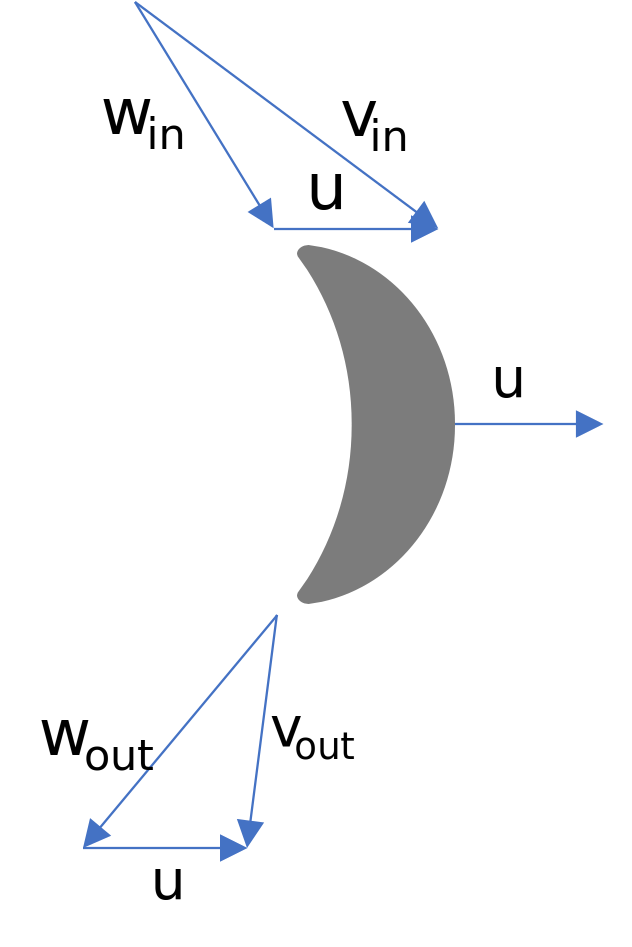
\includegraphics{Content/PowGen/Figures/Turbine/VelocityTrianglesSchematic.png}
            \caption{Fluid, blade and relative velocity vectors at the inlet and outlet of the blade.}
            \label{fig:prosim_litrev_blade_velocity}
        \end{figure}
    
        The maximum work, \(\Dot{w}\) generated by a turbine can be obtained from the Euler equation, Equation~\ref{eq:EulerEq}, or its alternate form, Equation~\ref{eq:AlternateEulerEq}, where \(v\) is the absolute fluid velocity, \(u\) is the tangential velocity of the blade, and \(w\) is the relative velocity from the perspective of the blade.
        
        \begin{align}
            \Dot{w} = \vec{u}_{in} \cdot \vec{c}_{in} - \vec{u}_{in}\cdot \vec{c}_{in} \label{eq:EulerEq}
        \end{align}
        \begin{align}
            \Dot{w} = \frac{v_{in}^2 - v_{out}^2}{2} + \frac{u_{in}^2-u_{out}^2}{2} - \frac{w_{in}^2-w_{out}^2}{2} \label{eq:AlternateEulerEq}
        \end{align}
    
        Velocity triangles, Figure~\ref{fig:prosim_litrev_velocity_triangles}, summarise the inlet and outlet velocity vectors and are an important tool for and optimising the  energy conversion.  
    
        \begin{figure}[H]
            \centering
            % \includesvg[width=0.45\columnwidth]{Content/PowGen/Figures/Turbine/VelocityTriangles.svg}
            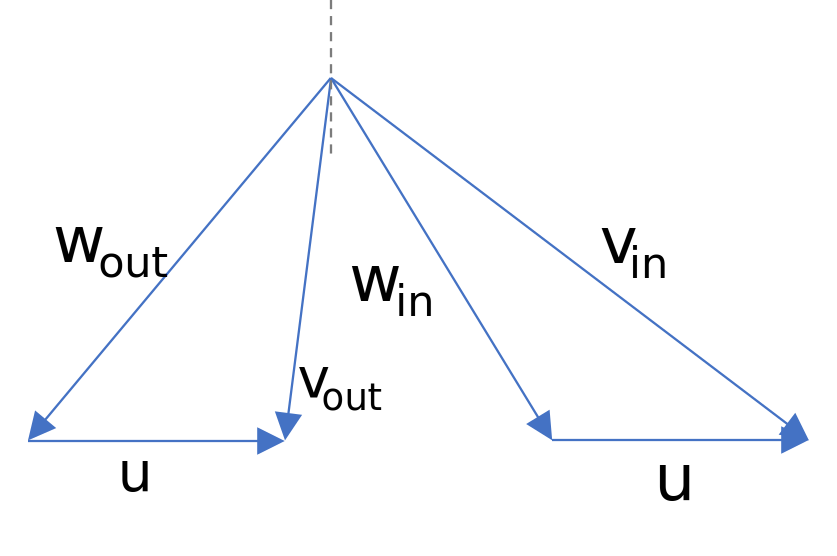
\includegraphics{Content/PowGen/Figures/Turbine/VelocityTriangles.png}
            \caption{Velocity Triangles.}
            \label{fig:prosim_litrev_velocity_triangles}
        \end{figure}
    
    \subsection{Impulse vs. Reaction Stages}
        To maximise the efficiency, the expansion is broken down into a number of stages, allowing the nozzles and blades to be specifically designed for the fluid and velocities at various stages of expansion. Each stage is comprised of a static stator, containing the nozzles, and the rotating rotor, containing the blades. There are two different types of turbine stages, impulse and reaction stages, the main difference being the mechanisms by which the fluid imparts the resultant force on the blades.
        
        In an impulse stage, Figure~\ref{fig:prosim_litrev_impulse}, the fluid is expanded in the stator nozzles, reducing the fluid pressure but increasing the volumetric flow rate and in turn the velocity of the fluid, Figure~\ref{fig:prosim_litrev_impulse_profile}. The fluid is then directed onto the blades, which deflect the fluid, and the change in momentum imparts the resultant force on the blade. In an ideal impulse stage, the fluid pressure in rotor section remains constant, such that only the kinetic energy is transferred to the blade/central shaft. 
        
        \begin{figure}[H]
            \centering
            \subfloat[Impulse stage.\label{fig:prosim_litrev_impulse}]{
                \includesvg[width=0.45\columnwidth]{Content/PowGen/Figures/Turbine/ImpulseStage.svg}
            }
            \quad
            \subfloat[Fluid pressure and velocity profile.\label{fig:prosim_litrev_impulse_profile}]{
                \includesvg[width=0.35\columnwidth]{Content/PowGen/Figures/Turbine/ImpulseStageProfiles.svg}
            }
            \caption[Configuration of an impulse turbine stage and the corresponding fluid pressure and velocity profiles.]{Configuration of an impulse turbine stage and the corresponding fluid pressure and velocity profiles. Adapted from \cite{Dick2015, Smith2005}}
            \label{fig:prosim_litrev_impulse_turbine_stage}
        \end{figure}
        
        In a reaction stage, Figure~\ref{fig:prosim_litrev_impulse}, the fluid is partially expanded in the stator nozzles and then directed onto the blades. Similarly to the impulse stage the fluid imparts some momentum on the blades, but is also expanded further, increasing its velocity, thus creating an area of low pressure on the back of the blades. This configuration allows both kinetic and pressure energy to be transferred to the shaft.
        
        \begin{figure}[H]
            \centering
            \subfloat[Reaction stage.\label{fig:prosim_litrev_reaction}]{
                \includesvg[width=0.45\columnwidth]{Content/PowGen/Figures/Turbine/ReactionStage.svg}
            }
            \quad
            \subfloat[Fluid pressure and velocity profile.\label{fig:prosim_litrev_reaction_profile}]{
                \includesvg[width=0.35\columnwidth]{Content/PowGen/Figures/Turbine/ReactionStageProfiles.svg}
            }
            \caption[Configuration of a reaction turbine stage and the corresponding fluid pressure and velocity profiles.]{Configuration of a reaction turbine stage and the corresponding fluid pressure and velocity profiles. Adapted from \cite{Dick2015, Smith2005}}
            \label{fig:prosim_litrev_reaction_turbine_stage}
        \end{figure}

        Impulse stages are typically used for small turbines or the high pressure stages of larger turbines. Reaction stages are used for low pressure and high through-put applications \cite{Smith2005}.    

    \subsection{Types of Turbines}

         \subsubsection{Axial Inflow, Axial Outflow}
            In axial turbines the fluid enters and exits the turbine parallel to the central axis, Figute~\ref{fig:prosim_litrev_axial_turbine}. Many commercial steam turbines utilise this design, as it can be readily extended to accommodate a large number of stages. The lessons from many decades of steam turbine operation can also be translated to the significantly smaller \ac{ORC} turbines, with this configuration being used extensively by \ac{ORC} system manufactures like Turboden \cite{Turboden2024} and Ormat \cite{Ormat2024, Buchanan2010}.

            \begin{figure}[H]
                \centering
                \includesvg[width=0.45\columnwidth]{Content/PowGen/Figures/Turbine/AxialTurbine.svg}
                \caption{Inlet and outlet streams of an axial turbine.}
                \label{fig:prosim_litrev_axial_turbine}
            \end{figure}
    
        \subsubsection{Radial Inflow}
            In a radial inflow, the fluid enters the turbine perpendicular to the central shaft along the outer perimeter, similar to a centrifugal compressor in reverse flow \cite{Boyce2012}. Unlike axial turbines, where the tangential velocity of the blades is constant (i.e. \(u_{in}=u_{out}\)), in this configuration due to the decreasing radius the tangential blade velocity at the outlet is lower than at the inlet (i.e. \(u_{in}>u_{out}\)), allowing the second term of Equation~\ref{eq:AlternateEulerEq} to be larger, leading to higher turbine efficiencies.

            % This configuration is similar to gas compressors, which are fed axially and discharge radially, albeit in reverse, 

            % \begin{itemize}
            %     \item (see Walraven for citation)
            %         used by Atlas Copco and Triogen 
            %         "centripetal turbine" - often a reverse action centrifugal compressor
            %         favourable velocity triangles, can yield high efficiencies (82 to 90\%) 
            % \end{itemize}

            \begin{figure}[H]
                \centering
                \includesvg[width=0.45\columnwidth]{Content/PowGen/Figures/Turbine/RadialInflowAxialOutflow.svg}
                \caption{Inlet and outlet streams of a radial inflow turbine.}
                \label{fig:prosim_litrev_RadialAxial_turbine}
            \end{figure}

        \subsubsection{Radial Outflow}
            The Ljungström brothers \cite{Dick2015} first proposed an axial inflow-radial outflow configuration, with the working fluid entering parallel to the central shaft, expanding radially through the turbine and then exiting perpendicular to the central shaft along the perimeter.

            \begin{figure}[H]
                \centering
                \includesvg[width=0.45\columnwidth]{Content/PowGen/Figures/Turbine/AxialInflowRadialOutflow.svg}
                \caption{Inlet and outlet streams of a radial-outflow turbine.}
                \label{fig:prosim_litrev_AxialRadial_turbine}
            \end{figure}

            An advantage of this design is that the flow area naturally increases as the fluid progresses radially through the turbine, thus, in principle allowing the turbine to be more compact. In axial turbines on the hand, the diameter must be increased along the length of the turbine to accommodate the increasing volume rate and prevent supersonic velocities. However, the increasing flowing radius also results in increasing blade velocities, which reduce the maximum work a given stage can extract, see Equation~\ref{eq:AlternateEulerEq} where \(u_{in}<u_{out}\).
            
            This turbine configuration has not seen extensive use in steam expansion applications, as the increase in volumetric flow rate far exceeds the aforementioned increase in flow area, however Exergy International SRL \cite{Exergy2024} have used employed a related design in \ac{ORC} applications where changes in fluid density and enthalpy are less significant    

    \subsection{Wet Expansion}
        \label{sec:prosim_litrev_wet_expansion}
        Unlike Rankine cycle power stations, where superheated or supercritical steam is expanded in turbines, guaranteeing a dry expansion, geothermal steam is typically saturated vapour or minimally super-heated. Consequently, due to the bell-shaped phase envelope of water in the temperature-entropy domain, two-phase condition during the expansion process are unavoidable. The formation of liquid droplets not only degrades the thermodynamic performance of the turbines but the droplets can also damage the turbine internals.

        The mechanism for the formation of droplets is complex, involving meta-stable non-equilibrium fluid states and continues to be subject of research \cite{Senoo2017}, but can broadly be divided into four phases: 1) Nucleation, 2) Droplet Growth, 3) Deposition and 4) Dispersion, see Figure~\ref{fig:prosim_litrev_WetExpansion_mech}.
        
        \begin{figure}[H]
            \centering
            % \includesvg[width=1.15\columnwidth]{Content/PowGen/Figures/Turbine/WetExpansionMechanism.svg}
            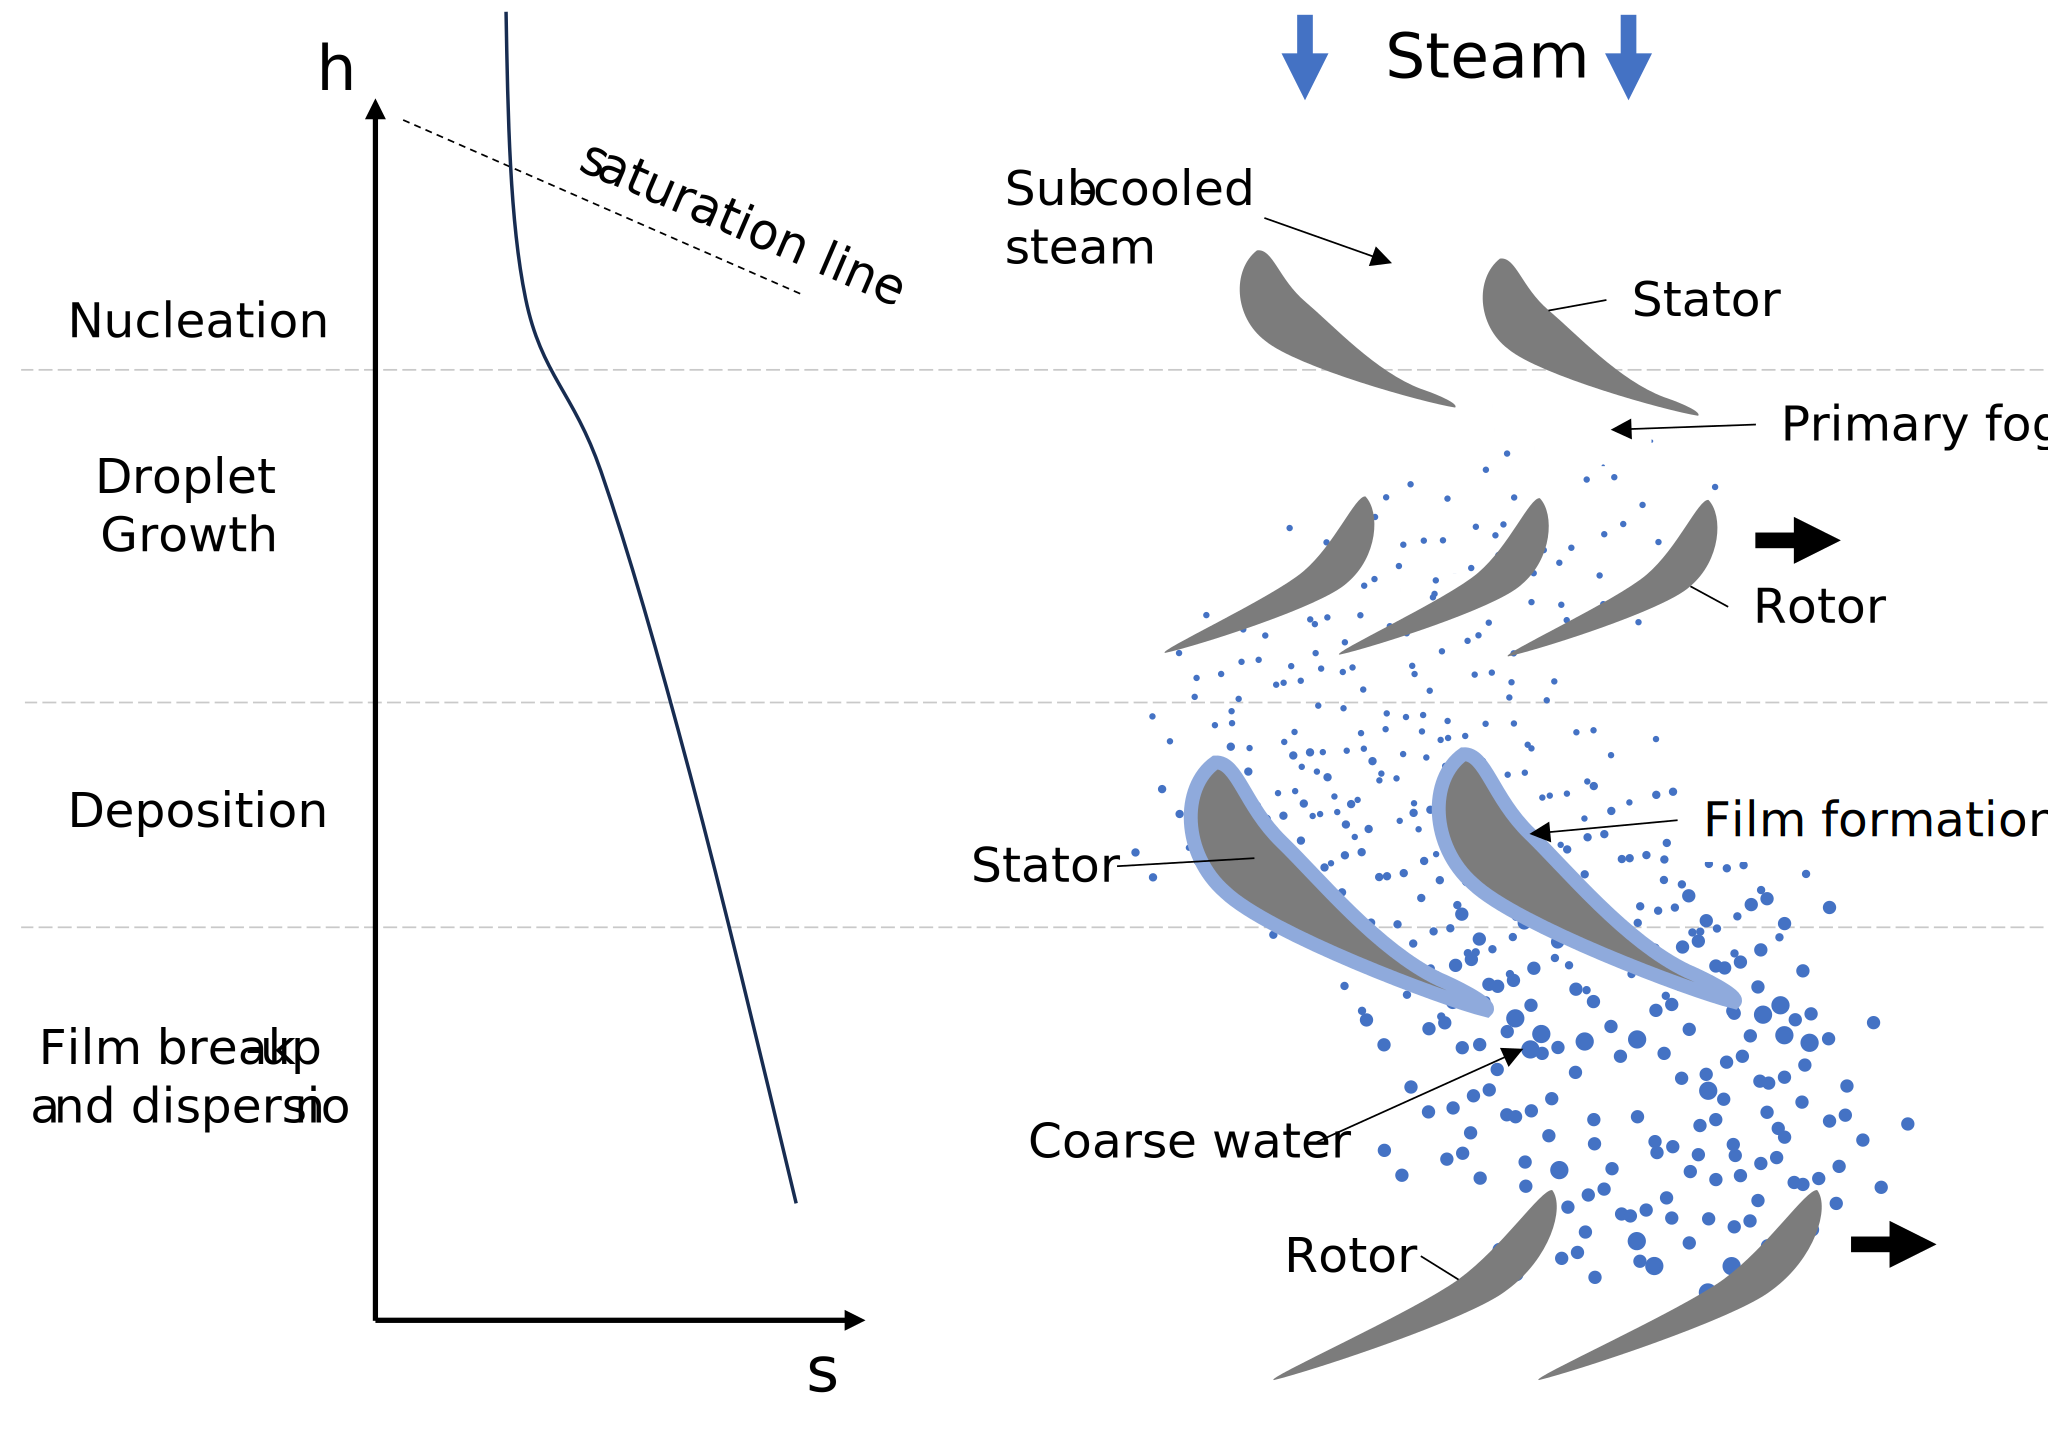
\includegraphics[width=.95\columnwidth]{Content/PowGen/Figures/Turbine/WetExpansionMechanism.png}
            \caption{Mechanism for liquid formation in a steam turbine.}
            \label{fig:prosim_litrev_WetExpansion_mech}
        \end{figure}

        The condensation of liquid is not immediate, when the fluid is initially expanded to conditions below the saturation line. The reason for this is that for a pure fluid, the only pathway from a an equilibrium vapour state to an equilibrium two-phase state is via drop-wise condensation\footnote{Droplets of condensate do not wet surfaces/sites where they form and after growing expose the condensing surface/site without forming a film \cite{Smith2005}}, due to a lack of nucleation points and wettability. However, the formation of droplets poses a thermodynamic barrier (akin to an activation energy), as it increases the surface free energy due to interactions between the droplets and the vapour. For small droplet radii, the reduction in Gibbs free energy, which is proportional to the cube of the radius, is outweighed by the change in surface free energy, which is proportional to the square of the radius \cite{McDONALD1974}. The Wilson point denotes the super-cooled conditions for which droplets are able to form spontaneously without explicit nucleation sites \cite{gyarmathy1962, McDONALD1974, Azzini2018}.

        These initial droplets, typically between \qty{0.01}{\micro\m} to \qty{1}{\micro\m}, continue to grow as the expansion progresses both due to continued condensation and coalescence with other droplets.
        
        While the difference in vapour and droplet velocity, also called slip velocity, is minimal, as the droplets grow, sharp changes in fluid velocity can result in the deposition of a small fraction of droplets on rotor or stator surfaces. Shearing with the vapour phase, gravity and centrifuging, causes the liquid to accumulate and migrate towards the trailing edge of rotor blades or nozzles, from where it is stripped of by the high velocity vapour phase. The resultant coarse droplets, \qty{10}{\micro\m} to \qty{500}{\micro\m}, are much larger than the primary fog, exhibiting higher slip velocities and therefore pressure drops, but can also have a devastating effect on the downstream turbine internals \cite{Senoo2017}.

        However, condensation also impacts the energy conversion, reducing the apparent isentropic efficiency. The main phenomena responsible for these losses are \cite{Senoo2017}:

        \begin{description}
            \item[Thermal Relaxation] Irreversible exchange of mass and heat between the vapour and the condensing droplets accounts for about \qty{60}{\percent} to \qty{90}{\percent} of losses, and is strongly droplet size dependent.
            \item[Coarse droplet \& collected Water] Coarse droplets impacting rotors and centrifuging of liquid films accounts for about \qty{10}{\percent} to \qty{40}{\percent} of losses.
            \item[Droplet Drag] Increased frictional losses due to the presence of liquid droplets, typically, account for less than \qty{5}{\percent} of losses. However, as the frictional losses depend on the slip velocity, which is small for the primary fog, higher losses can be anticipated where large or coarse droplets are more prevalent.
        \end{description}

        % \begin{itemize}
        %     \item \textbf{Thermal Relaxation}: Irreversible exchange of mass and heat between the vapour and the condensing droplets accounts for about \qty{60}{\percent} to \qty{90}{\percent} of losses, and is strongly droplet size dependent.
        %     \item \textbf{Coarse droplet \& collected Water}: Coarse droplets impacting rotors and centrifuging of liquid films accounts for about \qty{10}{\percent} to \qty{40}{\percent} of losses. 
        %     \item \textbf{Droplet Drag}: Increased frictional losses due to the presence of liquid droplets, typically, account for less than \qty{5}{\percent} of losses. However, as the frictional losses depend on the slip velocity, which is small for the primary fog, higher losses can be anticipated where large or coarse droplets are more prevalent. 
        % \end{itemize}

        Baumann \cite{Baumann1921} first proposed a rule-of-thumb for capturing the efficiency degradation due to condensation in \citeyear{Baumann1921}, see Equation~\ref{eq:litrev_Baumann}, where \(\eta_{dry, turb}\) is the isentropic efficiency corresponding to a dry expansion and \(x_{in}\) and \(x_{out}\) are the steam quality at the inlet and outlet of the turbine. Equation~\ref{eq:litrev_alternateBaumann}, is a more modern and tunable formulation of the original Baumann rule, where \(\alpha\) is the Baumann factor, typically between \num{0.4} and \num{2.5} or \num{1.0} for the original Baumann rule, and \(y_m\) is the average wetness across the turbine (sometimes weighted for dry stages) \cite{Senoo2017}.

        \begin{align}
            \eta_{isen, turb} = \eta_{dry, turb} * \frac{x_{in} + x_{out}}{2} \label{eq:litrev_Baumann}
        \end{align}
        \begin{align}
            \eta_{isen, turb} = \eta_{dry, turb} * (1-\alpha y_m) \label{eq:litrev_alternateBaumann}
        \end{align}

        However, it should be noted that the Baumann rule is entirely empirical, with the underlying source of thermodynamic losses being fluid, expansion, turbine geometry, and importantly \emph{droplet size distribution} dependent. Despite a number of analytical approaches (e.g. for predicting the droplet nucleation and growth), to accurately predict the impact of condensation on turbine performance requires sophisticated CFD simulations or experimentation\cite{Senoo2017}.


\section{Heat Exchangers}
    Heat exchangers are used to facilitate the transfer of thermal energy from one fluid stream to another. 
    
    \subsection{Working Principle}
    The rate of heat transfer \(Q\) is driven by the overall heat transfer coefficient \(U\) (the inverse of the cumulative heat transfer resistances), the area \(A\) over which the heat transfer occurs, and the difference in temperature between the two streams \(\Delta T\), Equation~\ref{eq:litrev_heatTransfer}.

    \begin{align}
        \Dot{Q} = U * A * \Delta T \label{eq:litrev_heatTransfer}
    \end{align}

    \subsubsection{Temperature Difference}
    The definition of the temperature difference depends on the heat exchange scenario. For instance, where transfer of heat does not change the temperature of either stream (e.g. exchange of latent heat), \(\Delta T\) is simply the difference in temperature between the hot and cold stream. For idealised cases of counter-current or co-current heat exchange, the log-mean temperature difference \(\Delta T_{lm}\) is used, see Equation~\ref{eq:litrev_DTlogmean}, where \(\Delta T_1\) is the difference in temperature between the two streams at the inlet of the hot stream, and \(\Delta T_2\) is the difference in temperature between the two streams at the outlet of the hot stream \cite{Smith2005}.
    
    \begin{align}
        \Delta T_{lm} = \frac{\Delta T_1 - \Delta T_2}{\ln \frac{\Delta T_1}{\Delta T_2}}\label{eq:litrev_DTlogmean}
    \end{align}   

    For real heat exchangers, where the heat transfer does not occur in a purely counter-current or co-current configuration (i.e. multiple tubing passes or shell passes in a shell and tube heat exchanger), \(\Delta T\) is obtained by applying a correction factor \(f_{T}\) to the log-mean temperature difference \(\Delta T_{lm}\), Equation~\ref{eq:litrev_DTlogmean_correction}.  

    \begin{align}
        \Delta T = f_{T}*\Delta T_{lm}\label{eq:litrev_DTlogmean_correction}
    \end{align}  

    The temperature correction factor is typically correlated based on two dimensionless numbers: the ratio of heat capacity flow rates \(R\) and thermal effectiveness of the heat exchanger \(P\), which are calculated based on the inlet and outlet temperatures of the two streams, Equations~\ref{eq:litrev_R} and \ref{eq:litrev_P} respectively. For simple geometries analytical solutions exist, for example Equation~\ref{eq:litrev_f_T_1_2} can be used to calculate the temperature correction factor for heat exchanger with one shell and two tubing passes (also referred to as a 1-2 heat exchanger). Correction factors for more complex geometries can be obtained from tables, graphical methods or simulations \cite{Smith2005}.

    \begin{align}
        R = \frac{CP^{cold}}{CP^{hot}} = \frac{\Dot{m}C_p^{cold}}{C_p^{hot}} = \frac{T_{in}^{hot} - T_{out}^{hot}}{T_{out}^{cold} - T_{in}^{cold}} \label{eq:litrev_R}
    \end{align}
    \begin{align}
        P = \frac{T_{out}^{cold} - T_{in}^{cold}}{T_{in}^{hot} - T_{in}^{cold}} \label{eq:litrev_P}
    \end{align}

    \begin{equation}
        \label{eq:litrev_f_T_1_2}
        f_T^{1-2} = \left\{
        \begin{aligned}
        \frac{\frac{\sqrt{2}P}{1-P}}{\ln\frac{2-P(2-\sqrt{2})}{2-P(2+\sqrt{2})}} \quad\quad\quad\quad\;& if\; R = 1\\
        & \\
        \frac{\sqrt{R^2+1}\ln\frac{1-P}{1-RP}}{(R-1)\ln\frac{2-P(R+1-\sqrt{R^2+1})}{2-P(R+1+\sqrt{R^2+1})}}\quad\; & if\; R \neq 1
        \end{aligned}
        \right.
    \end{equation}

    \subsubsection{Overall Heat Transfer Coefficient}
    The overall heat transfer coefficient is a measure of the ease of heat transfer between the bulk hot stream and the bulk cold stream. For a shell \& tube configuration, with the hot fluid on the shell side and the cold fluid on the tube side, the heat transfer can be broken down five stages, across the:
    
    \begin{enumerate}
        \item  \emph{Shell-side film}, Equation~\ref{eq:litrev_U_shellside}, where \(Q\) is the heat transferred, \(h_{ss}\) is the shell-side heat transfer coefficient, \(A_{ss}\) is the heat transfer area on the shell-side, and \(\Delta T_{ss}\) is the temperature difference across the shell-side fluid film.
            \begin{align}
                Q = h_{ss}A_{ss}\Delta T_{ss} \label{eq:litrev_U_shellside}
            \end{align}
        \item \emph{Shell-side fouling layer}, Equation~\ref{eq:litrev_U_shellside_fouling}, where \(Q\) is the heat transferred, \(h_{ssf}\) is the shell-side fouling layer heat transfer coefficient, \(A_{ss}\) is the heat transfer area on the shell-side, and \(\Delta T_{ssf}\) is the temperature difference across the shell-side fouling film. Fouling (i.e. the deposition of materials on surfaces, such as scales, biofilms, etc.) is a time dependent phenomenon, with complex mechanisms and multi variable dependencies, as such for design is usually performed with experienced based values of fouling resistance after a reasonable period of operation \cite{Smith2005}.     
            \begin{align}
                Q = h_{ssf}A_{ss}\Delta T_{ssf} \label{eq:litrev_U_shellside_fouling}
            \end{align}
        \item \emph{Tubing}, Equation~\ref{eq:litrev_U_tubing}, where \(Q\) is the heat transferred, \(k\) is the thermal conductivity of the tubing material, \(L\) is the length of the tubing, \(\Delta T_{tw}\) is the temperature difference across the tubing wall, and \(d_{ss}\) and \(d_{ts}\) are the tubing diameter on the shell and tubing side respectively.
            \begin{align}
                Q = \frac{2\pi kL}{\ln \frac{d_{ss}}{d_{ts}}}\Delta T_{tw} \label{eq:litrev_U_tubing}
            \end{align}
        \item \emph{Tube-side fouling layer}, Equation~\ref{eq:litrev_U_tubeside_fouling}, where \(Q\) is the heat transferred, \(h_{tsf}\) is the tube-side heat transfer coefficient, \(A_{ts}\) is the heat transfer area on the tube-side, and \(\Delta T_{tsf}\) is the temperature difference across the tube-side fluid film.
            \begin{align}
                Q = h_{tsf}A_{ts}\Delta T_{tsf} \label{eq:litrev_U_tubeside_fouling}
            \end{align}
        \item \emph{Tube-side film}, Equation~\ref{eq:litrev_U_tubeside}, where \(Q\) is the heat transferred, \(h_{ts}\) is the tube-side heat transfer coefficient, \(A_{ts}\) is the heat transfer area on the tube-side, and \(\Delta T_{ts}\) is the temperature difference across the tube-side fluid film.
            \begin{align}
                Q = h_{ts}A_{ts}\Delta T_{ts} \label{eq:litrev_U_tubeside}
            \end{align}
    \end{enumerate}

    Combining Equations~\ref{eq:litrev_U_shellside} to ~\ref{eq:litrev_U_tubeside}, an expression for the overall heat transfer coefficient \(U\) can be obtained, Equation~\ref{eq:litrev_U_overall} ( \emph{Note}, this formulation is relative to the shell-side heat transfer area).

    \begin{align}
        U = \left[\frac{1}{h_{ss}} + \frac{1}{h_{ssf}}+ \frac{d_{ss}\ln \frac{d_{ss}}{d_{ts}}}{2\pi kL} + \frac{d_{ss}}{h_{tsf}d_{ts}} + \frac{d_{ss}}{h_{ts}d_{ts}}\right]^{-1} \label{eq:litrev_U_overall}
    \end{align}

    An alternative, more generic formulation of the overall heat transfer coefficient \(U\) is given by Equation~\ref{eq:litrev_U_overall_general}.

    \begin{align}
        U = \left[\frac{1}{h_{int}\chi_{int}\frac{A_{int,\;pt}}{A_{ext,\;pt}}} +  \frac{R_{int,\;f}}{\frac{A_{int,\;pt}}{A_{ext,\;pt}}} + R_{m} + \frac{R_{ext,\;f}}{\frac{A_{ext,\;t}}{A_{ext,\;pt}}} + \frac{1}{h_{ext}\chi_{ext}\frac{A_{ext,\;t}}{A_{ext,\;pt}}}\right]^{-1} \label{eq:litrev_U_overall_general}
    \end{align}

    Here,
    \begin{itemize}
        \item \(h_{int}\) and \(h_{ext}\) are the internal and external film heat transfer coefficients. Exact values are not usually known until detailed design calculations have been performed. \citeauthor{Astolfi2014C} \cite{Astolfi2014C} obtained typical values by performing regression analysis against overall heat transfer coefficient data, see Table~\ref{table:FilmHeatTransferCoefficient}.
        \item \(\chi_{int}\) and \(\chi_{ext}\) are the internal and external enhancement factor, with typical values ranging from 1 to 5. The enhancement factor accounts for improvement of the film heat transfer from turbulence/mixing promoting texturing of the heat transfer surface.  
        \item \(\frac{A_{int,\;pt}}{A_{ext,\;pt}}\) is the ratio of the internal to the external \emph{plain} tubing area. It is usually around \num{0.87}.
        \item \(\frac{A_{ext,\;t}}{A_{ext,\;pt}}\) is the ratio of the external heat transfer area to the external plain tubing area. For plain tubes its value is \num{1}, however for finned tubes its value can be as large as \num{14}.
        \item \(R_{int,\;f}\) and \(R_{ext,\;f}\) are the heat transfer resistances the internal and external fouling layer. Typical values are shown in Table~\ref{table:FoulingResistances}
        \item \(R_{m}\) is the resistance of the material. Due to the high thermal conductivity of the materials used, the material resistance is small and can be neglected. 
    \end{itemize}

    \begin{table}[H]
        \caption{Film heat transfer coefficients for different fluids \cite{Astolfi2014C}.}
        \centering 
        \label{table:FilmHeatTransferCoefficient}
        \begin{tabular}{|c c |}
    \hline
    \rowcolor{bluepoli!40} % comment this line to remove the color
    \textbf{Fluid} & \(\mathbf{h}\)/\unit{\watt\per\m\squared\per\K} \T\B \\
    \hline \hline
    Water (liquid) & 7500 \T\B \\
    Water (boiling)& 7000 \T\B \\
    Water (condensing)& 10000 \T\B \\
    Water (vapour LP)& 125 \T\B \\
    Water (vapour HP)& 800\T\B \\
    \hline
    Organic (liquid) & 1900 \T\B \\
    Organic (boiling)& 1900 \T\B \\
    Organic (condensing)& 2500 \T\B \\
    Organic (vapour LP)& 125 \T\B \\
    Organic (vapour HP)& 600\T\B \\
    \hline
    Air & 125 \T\B \\

    \hline
\end{tabular}
        \\[10pt]
    \end{table}

    \begin{table}[H]
        \caption[Fouling resistances for different fluids.]{Fouling resistances for different fluids \cite{TEMA2019}. \textsuperscript{a}Sodium Chloride or Calcium Chloride solutions in TEMA standard \textsuperscript{b} Refrigerant in TEMA standard}
        \centering 
        \label{table:FoulingResistances}
        \begin{tabular}{|c c |}
    \hline
    \rowcolor{bluepoli!40} % comment this line to remove the color
    \textbf{Fluid} & \(\mathbf{R_f}\)/\qty{e-5}{\square\m\K\per\watt} \T\B \\
    \hline \hline
    Steam & 8.81 \T\B \\
    Water & 8.81 \T\B \\
    Brine\textsuperscript{a} & 52.83 \T\B \\
    Organic\textsuperscript{b} (vapour) & 35.22 \T\B \\
    Organic\textsuperscript{b} (liquid) & 17.61 \T\B \\
    Air & 17.61 \T\B \\

    \hline
\end{tabular}
        \\[10pt]
    \end{table}

    \subsection{Shell \& Tube Heat Exchangers}
        In shell and tube heat exchangers, one fluid flow through a collection of tubes, which are contained within an outer shell. The other fluid flows through the interspace between the tubes and the shell, Figure~\ref{fig:prosim_litrev_ShellandTubeHX}. On the shell side, baffles are used not only to hold tubes in place and reduce vibrations, but also to ensure even flow across all tubes and prevent short-circuiting \cite{Incropera2007}.

        \begin{figure}[H]
            \centering
            \includesvg[width=0.8\columnwidth]{Content/PowGen/Figures/Shell_and_Tube_HX.svg}
            \caption[Shell \& Tube heat exchanger.]{Shell \& Tube heat exchanger. Adapted from \cite{Incropera2007}}
            \label{fig:prosim_litrev_ShellandTubeHX}
        \end{figure}

        Shell and tube heat exchangers can be divided into three core components, 1) the front end, 2) the shell and 3) the rear end, with many possible configurations being available for each component \cite{TEMA2019}. This versatility has made shell and tube heat exchangers popular across many industries, with \ac{TEMA} providing standards for their design and operation since as early as 1939 \cite{TEMA2024}. 

        For \emph{dirty} fluids, such as scaling-prone geofluids, \ac{TEMA} recommend confining the fluid to the tube-side reduce maintenance costs (compared to the shell-side), and to avoid U-bends, as these may make it impossible to clean the U-bend section of the tubing, which may lead to high pressure losses and in the worst case clogging.

        % \textbf{Parallel Plate}\\
        %     In parallel plate heat exchangers, the fluids both flow between parallel plates stacked together. Their modular design makes them well suited for low-cost maintenance, and also them to be extended to increase capacity, if so required. Parallel plate heat exchangers offer some of the highest heat transfer surface area to volume ratios, allowing very low approach temperatures to be achieved \cite{Incropera2007}.

        %     % \begin{figure}[H]
        %     %     \centering
        %     %     \includesvg[width=0.8\columnwidth]{Content/PowGen/Figures/Shell_and_Tube_HX.svg}
        %     %     \caption[Parallel plate heat exchanger.]{Parallel plate heat exchanger. Adapted from \cite{Incropera2007}}
        %     %     \label{fig:prosim_litrev_ParallelPlateHX}
        %     % \end{figure}
        %     % \todo{draw parallel plate HX}

        %     However, parallel plate heat exchangers are not well suited to high pressure applications, as unlike tubes, large flat surfaces are not ideal for containing pressures. Moreover, the typical rubber gaskets are not designed to withstand the high temperatures encountered in a geothermal setting. To prevent leakage for fluids (e.g. ORC working fluid into the geofluid or the atmosphere; or geofluid into the ORC working fluid), it is possible for the parallel plates to be welded together, avoiding the need for gaskets, but this results them no longer being disassemble for maintenance \cite{Incropera2007}.

        %     \todo{probably not useful in ORC or DSC applications, but perhaps the welded ones could be used in low fouling applications... perhaps for the recuperator??}

        % \textbf{Air Coolers}\\
        %     - low heat capacity -> high mass rate -> high fan power
        %     - low air heat transfer coefficient -> use of fins and corrugated surface
        %     - humid air?

        % \textbf{Cooling Tower}\\
        %     - direct contact heat exchanger
        %         * air flows past water, evaporating some in the process -> evaporation carries away heat, cooling the remaining liquid.
        %         * for large capacity use natural draft, low capacity use mechanical draft (Walraven)
        %         * 


        % \todo{What configuration is best suited for what application}

\section{Equipment Costs}

    \subsection{Steam Turbines}
        Steam turbines have not only been installed in many power plants across the globe but also for many decades, yielding significant experience in their design, manufacture and operation. Some cost correlations, in terms of the fluid power \(\Dot{W}\), i.e. work done by the fluid, (or similar) are shown in Table~\ref{table:SteamTurbineCosts}.

        The \emph{genGEO} steam turbine cost model suggested by \citeauthor{Adams2021} \cite{Adams2021} is a development of a cost model from \emph{GETEM} \cite{GETEM2016}, where the specific cost has been matched against cost data of coal-fired power stations reported by \ac{NETL} between 2007 and 2019. This also explains the similarity in specific cost predicted by either model, see Figure~ \ref{fig:prosim_litrev_steamturb_speccost}.
        
        \begin{table}[H]
            \caption[Steam turbine cost correlations.]{Steam turbine cost correlations.\(\Dot{W}\) is the fluid power in \unit{\kilo\watt}, \(\Dot{W}_s\) is the shaft power in \unit{\kilo\watt}, and \(\Dot{W}_e\) is the electrical power in \unit{\kilo\watt}. \textsuperscript{a}Fitted against data from Thermoflex, \(R^2=0.9994\)}
            \centering 
            \label{table:SteamTurbineCosts}
            \scalebox{0.75}{
                \begin{tabular}{|c | c c | c | c |}
    \hline
    \rowcolor{bluepoli!40} % comment this line to remove the color
    \textbf{Cost Correlation} & \textbf{Min}/\unit{\kilo\watt} & \textbf{Max}/\unit{\kilo\watt} & \textbf{Currency} & \textbf{Reference} \T\B \\
    \hline \hline
        \(C_{turb,\; gen} = 2830\cdot \Dot{W}_e^{0.745} + 3685\cdot \Dot{W}_e^{0.617}\) & - & - & \euro2002 &\cite{GETEM2016} \T\B \\
    \(C_{turb,\; gen} = 0.67 \cdot(2830 \cdot \Dot{W}^{0.745} + 3680\cdot \Dot{W}^{0.617}\) & - & - & \euro2002 &\cite{Adams2021} \T\B \\
    \(\log C_{turb,\; gen} = 2.6259 + 1.4398\log \Dot{W}_s -0.1776(\log \Dot{W}_s)^2\) & 70 & 7500& \euro2001 &\cite{Turton2012} \T\B \\
    \(C_{turb,\; gen} = 10^3\cdot\exp \left(-0.0408\ln^2\Dot{W}_e + 1.3039\ln^2\Dot{W}_e -0.1583\right)\) & 500 & 70000 & \euro2021 &\cite{Thermoflex2021}\textsuperscript{a} \T\B \\
    \hline
\end{tabular}
            }
            % \\[6pt]
        \end{table}

        However, although steam turbines share the same working fluid, there are some stark differences in the expansion processes used in coal-fired and geothermal power stations. As discussed in Section~\ref{sec:prosim_litrev_wet_expansion}, wet expansion is unavoidable in geothermal \ac{DSC} power plants and reduces the isentropic efficiency of the turbine. In turn, this should lead to higher specific costs for geothermal steam turbines.

        With this in mind, a wet expansion turbine was simulated in \emph{Thermoflex} \cite{Thermoflex2021} for a range of operating conditions, analogous to a geothermal \ac{DSC} and different mass rates. The combined turbine and generator costs predicted by \emph{Thermoflex} were then correlated against the turbine power. 

        % \begin{figure}[H]
        %     \centering
        %     % This file was created with tikzplotlib v0.10.1.
\begin{tikzpicture}

\definecolor{crimson2143940}{RGB}{214,39,40}
\definecolor{darkgray176}{RGB}{176,176,176}
\definecolor{darkorange25512714}{RGB}{255,127,14}
\definecolor{forestgreen4416044}{RGB}{44,160,44}
\definecolor{lightgray204}{RGB}{204,204,204}
\definecolor{steelblue31119180}{RGB}{31,119,180}

\begin{axis}[
legend cell align={left},
legend style={
  fill opacity=0.8,
  draw opacity=1,
  text opacity=1,
  at={(0.03,0.97)},
  anchor=north west,
  draw=lightgray204
},
log basis x={10},
tick align=outside,
tick pos=left,
unbounded coords=jump,
x grid style={darkgray176},
xlabel={Fluid Power/\unit{\kilo\watt}},
xmin=6.30957344480193, xmax=158489.319246111,
xmode=log,
xtick style={color=black},
xtick={0.1,1,10,100,1000,10000,100000,1000000,10000000},
xticklabels={
  \(\displaystyle {10^{-1}}\),
  \(\displaystyle {10^{0}}\),
  \(\displaystyle {10^{1}}\),
  \(\displaystyle {10^{2}}\),
  \(\displaystyle {10^{3}}\),
  \(\displaystyle {10^{4}}\),
  \(\displaystyle {10^{5}}\),
  \(\displaystyle {10^{6}}\),
  \(\displaystyle {10^{7}}\)
},
y grid style={darkgray176},
ylabel={Turbine Cost/\unit{\USD}2023},
ymin=-1499646.00511472, ymax=32227165.3666998,
ytick style={color=black},
ytick={-5000000,0,5000000,10000000,15000000,20000000,25000000,30000000,35000000},
yticklabels={\ensuremath{-}0.5,0.0,0.5,1.0,1.5,2.0,2.5,3.0,3.5},
width=10cm, height=6.5cm
]
\addplot [semithick, steelblue31119180]
table {%
10 48812.6480559191
12.0679264063933 55491.4054284559
14.5634847750124 63093.1030820432
17.5751062485479 71746.5150730635
21.2095088792019 81598.5476326557
25.5954792269954 92816.8141278817
30.8884359647748 105592.578561663
37.2759372031494 120144.120731392
44.9843266896944 136720.583870834
54.2867543932386 155606.374428351
65.5128556859551 177126.193751249
79.060432109077 201650.793040153
95.4095476349994 229603.556225333
115.139539932645 261468.030647655
138.949549437314 297796.542885418
167.683293681101 339220.057082189
202.358964772516 386459.456075458
244.205309454865 440338.451932414
294.705170255181 501798.362662221
355.648030622313 571915.026461224
429.193426012878 651918.164510367
517.947467923121 743213.548830249
625.055192527397 847408.383867207
754.312006335462 966340.370318703
910.298177991522 1102110.98833917
1098.54114198756 1257123.61599665
1325.71136559011 1434127.18916655
1599.85871960606 1636266.21266305
1930.69772888325 1867138.0512855
2329.95181051537 2130858.56585319
2811.76869797423 2432137.31580617
3393.22177189533 2776363.72953824
4094.91506238042 3169705.8497147
4941.71336132383 3619223.49733526
5963.62331659464 4132997.96973533
7196.85673001151 4720280.69924962
8685.11373751352 5391663.65683186
10481.1313415469 6159274.69535598
12648.552168553 7037001.49845596
15264.1796717523 8040748.34159303
18420.6996932672 9188730.49291243
22229.9648252619 10501811.7942418
26826.9579527973 12003891.7809356
32374.5754281764 13722349.6388555
39069.3993705461 15688553.3755993
47148.6636345739 17938443.8218413
56898.6602901829 20513204.5010771
68664.88450043 23460030.0394899
82864.2772854684 26833007.663429
100000 30694128.4861628
};
\addlegendentry{GETEM \cite{GETEM2016}}
\addplot [semithick, darkorange25512714]
table {%
10 33390.8754223091
12.0679264063933 37960.4490544543
14.5634847750124 43161.6141882102
17.5751062485479 49082.5102628811
21.2095088792019 55823.6894198832
25.5954792269954 63499.8795177257
30.8884359647748 72241.99951316
37.2759372031494 82199.4635883837
44.9843266896944 93542.8156814665
54.2867543932386 106466.742124188
65.5128556859551 121193.517021064
79.060432109077 137976.942944889
95.4095476349994 157106.85862615
115.139539932645 178914.295746414
138.949549437314 203777.378904844
167.683293681101 232128.076536456
202.358964772516 264459.926278003
244.205309454865 301336.876297774
294.705170255181 343403.404767905
355.648030622313 391396.103351025
429.193426012878 446156.93774356
517.947467923121 508648.429478027
625.055192527397 579971.038924406
754.312006335462 661383.070421006
910.298177991522 754323.467483235
1098.54114198756 860437.919973758
1325.71136559011 981608.766991027
1599.85871960606 1119989.25021756
1930.69772888325 1278042.7539108
2329.95181051537 1458587.76116363
2811.76869797423 1664849.36328337
3393.22177189533 1900518.2821753
4094.91506238042 2169818.50680974
4941.71336132383 2477584.8068877
5963.62331659464 2829351.57278575
7196.85673001151 3231454.64429991
8685.11373751352 3691148.03569228
10481.1313415469 4216737.74574811
12648.552168553 4817735.16434458
15264.1796717523 5505032.95758494
18420.6996932672 6291106.73894627
22229.9648252619 7190246.32226551
26826.9579527973 8218820.91309568
32374.5754281764 9395583.23873954
39069.3993705461 10742018.3564526
47148.6636345739 12282743.7280706
56898.6602901829 14045968.1239458
68664.88450043 16064018.0382776
82864.2772854684 18373941.583189
100000 21018201.3049328
};
\addlegendentry{genGEO \cite{Adams2021}}
\addplot [semithick, forestgreen4416044]
table {%
10 nan
12.0679264063933 nan
14.5634847750124 nan
17.5751062485479 nan
21.2095088792019 nan
25.5954792269954 nan
30.8884359647748 nan
37.2759372031494 nan
44.9843266896944 nan
54.2867543932386 nan
65.5128556859551 nan
79.060432109077 75757.2960227814
95.4095476349994 87245.4089363145
115.139539932645 99929.4935354662
138.949549437314 113835.514898739
167.683293681101 128971.82713424
202.358964772516 145326.533700989
244.205309454865 162865.075032369
294.705170255181 181528.157113581
355.648030622313 201230.135637579
429.193426012878 221857.966192864
517.947467923121 243270.821203174
625.055192527397 265300.458892425
754.312006335462 287752.408545953
910.298177991522 310408.010271511
1098.54114198756 333027.317158292
1325.71136559011 355352.834336197
1599.85871960606 377114.034375044
1930.69772888325 398032.553372438
2329.95181051537 417827.938727689
2811.76869797423 436223.789786279
3393.22177189533 452954.107986839
4094.91506238042 467769.655384144
4941.71336132383 480444.110699502
5963.62331659464 490779.811222727
7196.85673001151 498612.87736368
8685.11373751352 nan
10481.1313415469 nan
12648.552168553 nan
15264.1796717523 nan
18420.6996932672 nan
22229.9648252619 nan
26826.9579527973 nan
32374.5754281764 nan
39069.3993705461 nan
47148.6636345739 nan
56898.6602901829 nan
68664.88450043 nan
82864.2772854684 nan
100000 nan
};
\addlegendentry{Turton \cite{Turton2012}}
\addplot [semithick, crimson2143940]
table {%
10 nan
12.0679264063933 nan
14.5634847750124 nan
17.5751062485479 nan
21.2095088792019 nan
25.5954792269954 nan
30.8884359647748 nan
37.2759372031494 nan
44.9843266896944 nan
54.2867543932386 nan
65.5128556859551 nan
79.060432109077 nan
95.4095476349994 nan
115.139539932645 nan
138.949549437314 nan
167.683293681101 nan
202.358964772516 nan
244.205309454865 nan
294.705170255181 nan
355.648030622313 nan
429.193426012878 nan
517.947467923121 631939.931792051
625.055192527397 732928.578359439
754.312006335462 847608.744485545
910.298177991522 977410.761578113
1098.54114198756 1123845.78149899
1325.71136559011 1288499.45283318
1599.85871960606 1473023.49031962
1930.69772888325 1679124.97828581
2329.95181051537 1908553.27424805
2811.76869797423 2163084.4111542
3393.22177189533 2444502.93617475
4094.91506238042 2754581.17040562
4941.71336132383 3095055.92702202
5963.62331659464 3467602.78475733
7196.85673001151 3873808.07825212
8685.11373751352 4315138.83573619
10481.1313415469 4792910.9663104
12648.552168553 5308256.0721726
15264.1796717523 5862087.33363609
18420.6996932672 6455064.98467515
22229.9648252619 7087561.96180169
26826.9579527973 7759630.36703663
32374.5754281764 8470969.43426095
39069.3993705461 9220895.72503231
47148.6636345739 10008316.3028706
56898.6602901829 10831705.6420964
68664.88450043 11689087.0168826
82864.2772854684 nan
100000 nan
};
\addlegendentry{Thermoflex \cite{Thermoflex2021}\textsuperscript{a}}
\end{axis}

\end{tikzpicture}

        %     \caption[Steam turbine cost correlations.]{Steam turbine cost correlations. \textsuperscript{a}Fitted against data from Thermoflex, \(R^2=0.9994\)}
        %     \label{fig:prosim_litrev_steamturb_cost}
        % \end{figure}

        \begin{figure}[H]
            \centering
            % This file was created with tikzplotlib v0.10.1.
\begin{tikzpicture}

\definecolor{crimson2143940}{RGB}{214,39,40}
\definecolor{darkgray176}{RGB}{176,176,176}
\definecolor{darkorange25512714}{RGB}{255,127,14}
\definecolor{forestgreen4416044}{RGB}{44,160,44}
\definecolor{lightgray204}{RGB}{204,204,204}
\definecolor{steelblue31119180}{RGB}{31,119,180}

\begin{axis}[
legend cell align={left},
legend style={fill opacity=0.8, draw opacity=1, text opacity=1, draw=lightgray204},
log basis x={10},
tick align=outside,
tick pos=left,
unbounded coords=jump,
x grid style={darkgray176},
xlabel={Fluid Power/\unit{\kilo\watt}},
xmin=6.30957344480193, xmax=158489.319246111,
xmode=log,
xtick style={color=black},
xtick={0.1,1,10,100,1000,10000,100000,1000000,10000000},
xticklabels={
  \(\displaystyle {10^{-1}}\),
  \(\displaystyle {10^{0}}\),
  \(\displaystyle {10^{1}}\),
  \(\displaystyle {10^{2}}\),
  \(\displaystyle {10^{3}}\),
  \(\displaystyle {10^{4}}\),
  \(\displaystyle {10^{5}}\),
  \(\displaystyle {10^{6}}\),
  \(\displaystyle {10^{7}}\)
},
y grid style={darkgray176},
ylabel={Specific Cost/\unit{\USD\per\kilo\watt}},
ymin=-171.317103893603, ymax=5121.86394413884,
ytick style={color=black},
width=10cm, height=6.5cm
]
\addplot [semithick, steelblue31119180]
table {%
10 4881.26480559191
12.0679264063933 4598.25520638391
14.5634847750124 4332.28063590222
17.5751062485479 4082.28058814673
21.2095088792019 3847.26247540184
25.5954792269954 3626.29717946396
30.8884359647748 3418.5148993002
37.2759372031494 3223.10127513685
44.9843266896944 3039.29377033792
54.2867543932386 2866.37829370273
65.5128556859551 2703.68604599268
79.060432109077 2550.59057559845
95.4095476349994 2406.50502928395
115.139539932645 2270.87958489856
138.949549437314 2143.19905383908
167.683293681101 2022.98064187191
202.358964772516 1909.77185769803
244.205309454865 1803.14855936332
294.705170255181 1702.71312928688
355.648030622313 1608.09276930477
429.193426012878 1518.93790770879
517.947467923121 1434.92071080182
625.055192527397 1355.73369199723
754.312006335462 1281.08841196006
910.298177991522 1210.71426372715
1098.54114198756 1144.35733715186
1325.71136559011 1081.77935740046
1599.85871960606 1022.75669258218
1930.69772888325 967.079425926236
2329.95181051537 914.550488227418
2811.76869797423 864.984846569503
3393.22177189533 818.208745603877
4094.91506238042 774.058997910475
4941.71336132383 732.382320201128
5963.62331659464 693.034712342522
7196.85673001151 655.880876378384
8685.11373751352 620.793672919181
10481.1313415469 587.653612443613
12648.552168553 556.34837922015
15264.1796717523 526.772385709868
18420.6996932672 498.826355454399
22229.9648252619 472.416932585858
26826.9579527973 447.456316219558
32374.5754281764 423.86191810604
39069.3993705461 401.556042026761
47148.6636345739 380.465583518408
56898.6602901829 360.521748604622
68664.88450043 341.659790301446
82864.2772854684 323.818761744449
100000 306.941284861628
};
\addlegendentry{GETEM \cite{GETEM2016}}
\addplot [semithick, darkorange25512714]
table {%
10 3339.08754223091
12.0679264063933 3145.5651763292
14.5634847750124 2963.68725308557
17.5751062485479 2792.72907763709
21.2095088792019 2632.012355299
25.5954792269954 2480.90215285959
30.8884359647748 2338.80406232108
37.2759372031494 2205.16155342806
44.9843266896944 2079.45350225496
54.2867543932386 1961.19188399019
65.5128556859551 1849.91961886109
79.060432109077 1745.20856089589
95.4095476349994 1646.65761991851
115.139539932645 1553.89100782473
138.949549437314 1466.55660079544
167.683293681101 1384.32440966907
202.358964772516 1306.88515122272
244.205309454865 1233.94891360242
294.705170255181 1165.24390960144
355.648030622313 1100.5153119115
429.193426012878 1039.5241648696
517.947467923121 982.046367593259
625.055192527397 927.871723742196
754.312006335462 876.803053466012
910.298177991522 828.655363397048
1098.54114198756 783.255070826927
1325.71136559011 740.439278465481
1599.85871960606 700.055096423353
1930.69772888325 661.95900828559
2329.95181051537 626.01627835427
2811.76869797423 592.100397334542
3393.22177189533 560.092563921558
4094.91506238042 529.881199916367
4941.71336132383 501.361496657909
5963.62331659464 474.434990706518
7196.85673001151 449.009166852587
8685.11373751352 424.997086652895
10481.1313415469 402.317040817254
12648.552168553 380.892223880177
15264.1796717523 360.65042969669
18420.6996932672 341.523766398824
22229.9648252619 323.448389540166
26826.9579527973 306.364252240485
32374.5754281764 290.214871221518
39069.3993705461 274.947107698586
47148.6636345739 260.510962161475
56898.6602901829 246.859382142065
68664.88450043 233.948082125981
82864.2772854684 221.735374821294
100000 210.182013049328
};
\addlegendentry{genGEO \cite{Adams2021}}
\addplot [semithick, forestgreen4416044]
table {%
10 nan
12.0679264063933 nan
14.5634847750124 nan
17.5751062485479 nan
21.2095088792019 nan
25.5954792269954 nan
30.8884359647748 nan
37.2759372031494 nan
44.9843266896944 nan
54.2867543932386 nan
65.5128556859551 nan
79.060432109077 958.22011089266
95.4095476349994 914.430590008479
115.139539932645 867.899017087647
138.949549437314 819.257891513317
167.683293681101 769.13939548157
202.358964772516 718.162073345058
244.205309454865 666.918648885764
294.705170255181 615.965294929838
355.648030622313 565.812596474853
429.193426012878 516.918370008321
517.947467923121 469.682422000531
625.055192527397 424.443252474535
754.312006335462 381.476638485299
910.298177991522 340.995970085751
1098.54114198756 303.154160030598
1325.71136559011 268.04690942513
1599.85871960606 235.717085361077
1930.69772888325 206.159953170229
2329.95181051537 179.329004506436
2811.76869797423 155.142131748092
3393.22177189533 133.487917512045
4094.91506238042 114.23183344668
4941.71336132383 97.2221728722031
5963.62331659464 82.2955752180158
7196.85673001151 69.282034653326
8685.11373751352 nan
10481.1313415469 nan
12648.552168553 nan
15264.1796717523 nan
18420.6996932672 nan
22229.9648252619 nan
26826.9579527973 nan
32374.5754281764 nan
39069.3993705461 nan
47148.6636345739 nan
56898.6602901829 nan
68664.88450043 nan
82864.2772854684 nan
100000 nan
};
\addlegendentry{Turton \cite{Turton2012}}
\addplot [semithick, crimson2143940]
table {%
10 nan
12.0679264063933 nan
14.5634847750124 nan
17.5751062485479 nan
21.2095088792019 nan
25.5954792269954 nan
30.8884359647748 nan
37.2759372031494 nan
44.9843266896944 nan
54.2867543932386 nan
65.5128556859551 nan
79.060432109077 nan
95.4095476349994 nan
115.139539932645 nan
138.949549437314 nan
167.683293681101 nan
202.358964772516 nan
244.205309454865 nan
294.705170255181 nan
355.648030622313 nan
429.193426012878 nan
517.947467923121 1220.08499110155
625.055192527397 1172.58217693682
754.312006335462 1123.68454613805
910.298177991522 1073.72593421495
1098.54114198756 1023.03476724199
1325.71136559011 971.930607428744
1599.85871960606 920.72098133911
1930.69772888325 869.698530829602
2329.95181051537 819.138518502615
2811.76869797423 769.296710896817
3393.22177189533 720.407653994669
4094.91506238042 672.683347137449
4941.71336132383 626.312313305216
5963.62331659464 581.459056125866
7196.85673001151 538.263887079759
8685.11373751352 496.843100292154
10481.1313415469 457.289467150503
12648.552168553 419.673018811598
15264.1796717523 384.042081506967
18420.6996932672 350.424527415454
22229.9648252619 318.829202723139
26826.9579527973 289.247494281308
32374.5754281764 261.654996929734
39069.3993705461 236.013244984355
47148.6636345739 212.271473491596
56898.6602901829 190.36837751284
68664.88450043 170.233840804165
82864.2772854684 nan
100000 nan
};
\addlegendentry{Thermoflex \cite{Thermoflex2021}\textsuperscript{a}}
\end{axis}

\end{tikzpicture}

            \caption[Steam turbine specific cost correlations.]{Steam turbine specific cost correlations. \textsuperscript{a}Fitted against data from Thermoflex, \(R^2=0.9994\)}
            \label{fig:prosim_litrev_steamturb_speccost}
        \end{figure}

        While the cost model developed in \emph{Thermoflex} incorporates the turbine efficiency reduction into the cost estimate, more practical consideration such as material allowances to handle the effects of liquid formation within the turbine are not captured. Moreover, given that geothermal fluids are not pure water, additional allowances could be made to incorporate the increased vapour volumetric flow rate when \ac{NCG} is present, corrosion- and erosion-resistant materials to handle the presence of minerals and \ac{NCG} in the geofluid. 

    \subsection{ORC Turbines}  
        For \ac{ORC} turbines there are two types of cost models, ones that correlate the cost to the turbine power (similar to steam turbines), and the ones correlating costs with the number of stages and the size parameter \(SP\). For \ac{ORC} turbines, the latter approach is preferred as it allows the effect of different working fluids and expansion processes on the turbine cost to be captured. A number of \ac{ORC} turbine cost models are shown in Table~\ref{table:ORCTurbineCosts}.
        
        \begin{table}[H]
            \caption[ORC turbine cost correlations.]{ORC turbine cost correlations.\(\Dot{W}\) is the fluid power in \unit{\kilo\watt}, \(\Dot{W}_s\) is the shaft power in \unit{\kilo\watt}, and \(\Dot{W}_e\) is the electrical power in \unit{\kilo\watt}.}
            \centering 
            \label{table:ORCTurbineCosts}
            \scalebox{0.8}{
                \begin{tabular}{|c | c c | c | c |}
    \hline
    \rowcolor{bluepoli!40} % comment this line to remove the color
    \textbf{Cost Correlation} & \textbf{Min}/\unit{\kilo\watt} & \textbf{Max}/\unit{\kilo\watt} & \textbf{Currency} & \textbf{Reference} \T\B \\
    \hline \hline
    \(C_{turb,\; gen} = 7400 \cdot\Dot{W}_e^{0.6} + 1800 \cdot \Dot{W}_e^{0.67}\) & - & 11000& \euro2002 &\cite{GETEM2016} \T\B \\
    \(C_{turb,\; gen} = -1.4*10^4 + 1900*W^{0.75}\) & 100 & 20000 & \$2010 &\cite{TowlerGavin2013} \T\B \\
    \(\log C_{turb,\; gen} = 2.7051 + 1.4398\log \Dot{W} -0.1776(\log \Dot{W})^2\) & 100 & 7500& \euro2001 &\cite{Turton2012} \T\B \\
    \(C_{turb} = 1.23*10^6 * \frac{n}{2}^{0.5} * \frac{SP}{0.18}^{1.1}\) & - & - & \euro2014 &\cite{Astolfi2014B} \T\B \\
    \(n = \Biggl \lceil \max \left( \frac{\Delta h_{isen}^{tot}}{\Delta h_{stage}^{max}} , \frac{V_{r, isen}^{tot}}{V_{r, stage}^{max}} \right) \Biggr \rceil \) &  &  & & \T\B \\
    \(SP = \frac{\sqrt{\Dot{V}_{isen}}}{\sqrt[4]{\frac{\Delta h_{isen}^{tot}}{n_{stages}}}}\) &  &  & & \T\B \\
    \(C_{gen} = 2*10^5 * (W_{e}/5000)^{0.67}*S_{gear}\) & - & - & \euro2014 &\cite{Astolfi2014B} \T\B \\
    \hline
\end{tabular}
            }
            % \\[6pt]
        \end{table}

        % \begin{figure}[H]
        %     \centering
        %     % This file was created with tikzplotlib v0.10.1.
\begin{tikzpicture}

\definecolor{crimson2143940}{RGB}{214,39,40}
\definecolor{darkgray176}{RGB}{176,176,176}
\definecolor{darkorange25512714}{RGB}{255,127,14}
\definecolor{forestgreen4416044}{RGB}{44,160,44}
\definecolor{lightgray204}{RGB}{204,204,204}
\definecolor{steelblue31119180}{RGB}{31,119,180}

\begin{axis}[
legend cell align={left},
legend style={
  fill opacity=0.8,
  draw opacity=1,
  text opacity=1,
  at={(0.03,0.97)},
  anchor=north west,
  draw=lightgray204
},
log basis x={10},
tick align=outside,
tick pos=left,
unbounded coords=jump,
x grid style={darkgray176},
xlabel={Fluid Power/\unit{\kilo\watt}},
xmin=6.30957344480193, xmax=158489.319246111,
xmode=log,
xtick style={color=black},
xtick={0.1,1,10,100,1000,10000,100000,1000000,10000000},
xticklabels={
  \(\displaystyle {10^{-1}}\),
  \(\displaystyle {10^{0}}\),
  \(\displaystyle {10^{1}}\),
  \(\displaystyle {10^{2}}\),
  \(\displaystyle {10^{3}}\),
  \(\displaystyle {10^{4}}\),
  \(\displaystyle {10^{5}}\),
  \(\displaystyle {10^{6}}\),
  \(\displaystyle {10^{7}}\)
},
y grid style={darkgray176},
ylabel={Cost/\unit{\USD}2022},
ymin=-524986.649421086, ymax=12340066.2524408,
ytick style={color=black},
ytick={-2000000,0,2000000,4000000,6000000,8000000,10000000,12000000,14000000},
yticklabels={\ensuremath{-}0.2,0.0,0.2,0.4,0.6,0.8,1.0,1.2,1.4}
]
\addplot [semithick, steelblue31119180]
table {%
10 59788.4824817265
12.0679264063933 67123.0393006052
14.5634847750124 75359.6324932257
17.5751062485479 84609.4948622484
21.2095088792019 94997.6142710276
25.5954792269954 106664.439612931
30.8884359647748 119767.799013301
37.2759372031494 134485.05675104
44.9843266896944 151015.538703222
54.2867543932386 169583.259849204
65.5128556859551 190439.991572964
79.060432109077 213868.711232913
95.4095476349994 240187.481793977
115.139539932645 269753.815312304
138.949549437314 302969.580813195
167.683293681101 340286.524703028
202.358964772516 382212.480413484
244.205309454865 429318.353612282
294.705170255181 482245.980165192
355.648030622313 541716.966253057
429.193426012878 608542.633807993
517.947467923121 683635.209930004
625.055192527397 768020.416398915
754.312006335462 862851.635054618
910.298177991522 969425.8469605
1098.54114198756 1089201.56820559
1325.71136559011 1223819.03329524
1599.85871960606 1375122.90872839
1930.69772888325 1545187.85501252
2329.95181051537 1736347.29553391
2811.76869797423 1951225.79595447
3393.22177189533 2192775.50879269
4094.91506238042 2464317.19529524
4941.71336132383 2769586.40143816
5963.62331659464 3112785.43783989
7196.85673001151 3498641.89556677
8685.11373751352 3932474.52244453
10481.1313415469 4420267.38888457
12648.552168553 nan
15264.1796717523 nan
18420.6996932672 nan
22229.9648252619 nan
26826.9579527973 nan
32374.5754281764 nan
39069.3993705461 nan
47148.6636345739 nan
56898.6602901829 nan
68664.88450043 nan
82864.2772854684 nan
100000 nan
};
\addlegendentry{GETEM \cite{GETEM2016}}
\addplot [semithick, darkorange25512714]
table {%
10 nan
12.0679264063933 nan
14.5634847750124 nan
17.5751062485479 nan
21.2095088792019 nan
25.5954792269954 nan
30.8884359647748 nan
37.2759372031494 nan
44.9843266896944 nan
54.2867543932386 nan
65.5128556859551 nan
79.060432109077 nan
95.4095476349994 nan
115.139539932645 63335.4835020017
138.949549437314 75467.4169450851
167.683293681101 89436.0692963859
202.358964772516 105519.511348464
244.205309454865 124037.912532561
294.705170255181 145359.914458811
355.648030622313 169909.969381125
429.193426012878 198176.789671889
517.947467923121 230723.076508262
625.055192527397 268196.721436821
754.312006335462 311343.703803557
910.298177991522 361022.940795436
1098.54114198756 418223.385709934
1325.71136559011 484083.714823912
1599.85871960606 559914.994763872
1930.69772888325 647226.781611778
2329.95181051537 747757.171295429
2811.76869797423 863507.399469679
3393.22177189533 996781.679660497
4094.91506238042 1150233.07272075
4941.71336132383 1326916.30071056
5963.62331659464 1530348.55655617
7196.85673001151 1764579.52001141
8685.11373751352 2034271.97371357
10481.1313415469 2344794.6241393
12648.552168553 2702328.97522614
15264.1796717523 3113992.38216869
18420.6996932672 3587979.73499341
22229.9648252619 nan
26826.9579527973 nan
32374.5754281764 nan
39069.3993705461 nan
47148.6636345739 nan
56898.6602901829 nan
68664.88450043 nan
82864.2772854684 nan
100000 nan
};
\addlegendentry{Towler-Sinnot \cite{TowlerGavin2013}}
\addplot [semithick, forestgreen4416044]
table {%
10 nan
12.0679264063933 nan
14.5634847750124 nan
17.5751062485479 nan
21.2095088792019 nan
25.5954792269954 nan
30.8884359647748 nan
37.2759372031494 nan
44.9843266896944 nan
54.2867543932386 nan
65.5128556859551 nan
79.060432109077 nan
95.4095476349994 nan
115.139539932645 133245.078454807
138.949549437314 151787.240953468
167.683293681101 171969.862119461
202.358964772516 193777.079213165
244.205309454865 217162.810822553
294.705170255181 242047.994847198
355.648030622313 268318.433946475
429.193426012878 295823.395729513
517.947467923121 324375.101986061
625.055192527397 353749.220660979
754.312006335462 383686.446270814
910.298177991522 413895.219702568
1098.54114198756 444055.597926169
1325.71136559011 473824.239622109
1599.85871960606 502840.425973717
1930.69772888325 530732.989083496
2329.95181051537 557127.976002622
2811.76869797423 581656.836610475
3393.22177189533 603964.890842895
4094.91506238042 623719.807088959
4941.71336132383 640619.810612618
5963.62331659464 654401.3397526
7196.85673001151 664845.878952853
8685.11373751352 nan
10481.1313415469 nan
12648.552168553 nan
15264.1796717523 nan
18420.6996932672 nan
22229.9648252619 nan
26826.9579527973 nan
32374.5754281764 nan
39069.3993705461 nan
47148.6636345739 nan
56898.6602901829 nan
68664.88450043 nan
82864.2772854684 nan
100000 nan
};
\addlegendentry{Turton \cite{Turton2012}}
\addplot [semithick, crimson2143940]
table {%
10 64653.3163168255
12.0679264063933 71814.1758316322
14.5634847750124 79770.9519022951
17.5751062485479 88612.4781483075
21.2095088792019 98437.5515828551
25.5954792269954 109356.056440862
30.8884359647748 121490.215598201
37.2759372031494 134975.984175167
44.9843266896944 149964.601600174
54.2867543932386 166624.320288395
65.5128556859551 185142.331187596
79.060432109077 205726.908785633
95.4095476349994 228609.800789613
115.139539932645 254048.890607977
138.949549437314 282331.164029648
167.683293681101 313776.015139448
202.358964772516 348738.930581275
244.205309454865 387615.595830742
294.705170255181 430846.472223774
355.648030622313 478921.899170401
429.193426012878 532387.782334881
517.947467923121 591851.935663786
625.055192527397 657991.153082109
754.312006335462 731559.094553557
910.298177991522 813395.081127094
1098.54114198756 904433.90469284
1325.71136559011 1005716.77058728
1599.85871960606 1118403.50507804
1930.69772888325 1243786.17529902
2329.95181051537 1383304.28659539
2811.76869797423 1538561.74169731
3393.22177189533 1711345.7679206
4094.91506238042 1903648.04297058
4941.71336132383 2117688.277217
5963.62331659464 2355940.54086408
7196.85673001151 2621162.6586551
8685.11373751352 2916429.03306967
10481.1313415469 3245167.29988993
12648.552168553 3611199.26808874
15264.1796717523 4018786.64985402
18420.6996932672 4472682.14691443
22229.9648252619 4978186.52695965
26826.9579527973 5541212.39974543
32374.5754281764 6168355.48743119
39069.3993705461 6866974.27894149
47148.6636345739 7645279.06492523
56898.6602901829 8512431.4696264
68664.88450043 9478655.73026279
82864.2772854684 10555363.1251224
100000 11755291.120538
};
\addlegendentry{Astolfi \cite{Astolfi2014B}\textsuperscript{a}}
\end{axis}

\end{tikzpicture}

        %     \caption[ORC turbine cost correlations.]{ORC turbine cost correlations. \textsuperscript{a}Assuming n-Butane as the working fluid, \num{3} turbine stages, \(\Delta h=\)\qty{78.74}{\kilo\watt\per\kg}, and an outlet vapour density of \qty{10.45}{\kg\per\m\cubed}}
        %     \label{fig:prosim_litrev_ORCturb_cost}
        % \end{figure}

        \begin{figure}[H]
            \centering
            % This file was created with tikzplotlib v0.10.1.
\begin{tikzpicture}

\definecolor{crimson2143940}{RGB}{214,39,40}
\definecolor{darkgray176}{RGB}{176,176,176}
\definecolor{darkorange25512714}{RGB}{255,127,14}
\definecolor{forestgreen4416044}{RGB}{44,160,44}
\definecolor{lightgray204}{RGB}{204,204,204}
\definecolor{steelblue31119180}{RGB}{31,119,180}

\begin{axis}[
legend cell align={left},
legend style={fill opacity=0.8, draw opacity=1, text opacity=1, draw=lightgray204},
log basis x={10},
tick align=outside,
tick pos=left,
unbounded coords=jump,
x grid style={darkgray176},
xlabel={Fluid Power/\unit{\kilo\watt}},
xmin=6.30957344480193, xmax=158489.319246111,
xmode=log,
xtick style={color=black},
xtick={0.1,1,10,100,1000,10000,100000,1000000,10000000},
xticklabels={
  \(\displaystyle {10^{-1}}\),
  \(\displaystyle {10^{0}}\),
  \(\displaystyle {10^{1}}\),
  \(\displaystyle {10^{2}}\),
  \(\displaystyle {10^{3}}\),
  \(\displaystyle {10^{4}}\),
  \(\displaystyle {10^{5}}\),
  \(\displaystyle {10^{6}}\),
  \(\displaystyle {10^{7}}\)
},
y grid style={darkgray176},
ylabel={Specific Cost/\unit{\USD\per\kilo\watt}},
ymin=-226.267544492086, ymax=6783.97921150039,
ytick style={color=black}
]
\addplot [semithick, steelblue31119180]
table {%
10 5978.84824817265
12.0679264063933 5562.10214084875
14.5634847750124 5174.56046114219
17.5751062485479 4814.16690549105
21.2095088792019 4479.01056135168
25.5954792269954 4167.31558987309
30.8884359647748 3877.43164302277
37.2759372031494 3607.82496273971
44.9843266896944 3357.07011344062
54.2867543932386 3123.84230268749
65.5128556859551 2906.91024805673
79.060432109077 2705.12955125069
95.4095476349994 2517.43654327807
115.139539932645 2342.84256711558
138.949549437314 2180.42866666422
167.683293681101 2029.34065304194
202.358964772516 1888.78452132404
244.205309454865 1758.0221927633
294.705170255181 1636.36755930553
355.648030622313 1523.18280887191
429.193426012878 1417.87501141673
517.947467923121 1319.89294719648
625.055192527397 1228.72416001128
754.312006335462 1143.89221940992
910.298177991522 1064.95417699224
1098.54114198756 991.498203003055
1325.71136559011 923.141390396456
1599.85871960606 859.527714464061
1930.69772888325 800.326136969294
2329.95181051537 745.228844518394
2811.76869797423 693.949611630663
3393.22177189533 646.222279650142
4094.91506238042 601.799343272019
4941.71336132383 560.450637043063
5963.62331659464 521.96211473956
7196.85673001151 486.134715031512
8685.11373751352 452.78330731111
10481.1313415469 421.735711999217
12648.552168553 nan
15264.1796717523 nan
18420.6996932672 nan
22229.9648252619 nan
26826.9579527973 nan
32374.5754281764 nan
39069.3993705461 nan
47148.6636345739 nan
56898.6602901829 nan
68664.88450043 nan
82864.2772854684 nan
100000 nan
};
\addlegendentry{GETEM \cite{GETEM2016}}
\addplot [semithick, darkorange25512714]
table {%
10 nan
12.0679264063933 nan
14.5634847750124 nan
17.5751062485479 nan
21.2095088792019 nan
25.5954792269954 nan
30.8884359647748 nan
37.2759372031494 nan
44.9843266896944 nan
54.2867543932386 nan
65.5128556859551 nan
79.060432109077 nan
95.4095476349994 nan
115.139539932645 550.075877835297
138.949549437314 543.128187537821
167.683293681101 533.363028200502
202.358964772516 521.447179111068
244.205309454865 507.924716335809
294.705170255181 493.23842650248
355.648030622313 477.747533379608
429.193426012878 461.742369898142
517.947467923121 445.456519815458
625.055192527397 429.076863360456
754.312006335462 412.751886737296
910.298177991522 396.598553665125
1098.54114198756 380.707986005198
1325.71136559011 365.150158163148
1599.85871960606 349.977774851109
1930.69772888325 335.229472707852
2329.95181051537 320.932462173984
2811.76869797423 307.104706049186
3393.22177189533 293.756714611592
4094.91506238042 280.893023468991
4941.71336132383 268.513408951565
5963.62331659464 256.613886443457
7196.85673001151 245.187529251897
8685.11373751352 234.225139151254
10481.1313415469 223.715794386109
12648.552168553 213.647296482258
15264.1796717523 204.006533540181
18420.6996932672 194.779774641504
22229.9648252619 nan
26826.9579527973 nan
32374.5754281764 nan
39069.3993705461 nan
47148.6636345739 nan
56898.6602901829 nan
68664.88450043 nan
82864.2772854684 nan
100000 nan
};
\addlegendentry{Towler-Sinnot \cite{TowlerGavin2013}}
\addplot [semithick, forestgreen4416044]
table {%
10 nan
12.0679264063933 nan
14.5634847750124 nan
17.5751062485479 nan
21.2095088792019 nan
25.5954792269954 nan
30.8884359647748 nan
37.2759372031494 nan
44.9843266896944 nan
54.2867543932386 nan
65.5128556859551 nan
79.060432109077 nan
95.4095476349994 nan
115.139539932645 1157.24866134391
138.949549437314 1092.39102658585
167.683293681101 1025.56347948718
202.358964772516 957.590781466007
244.205309454865 889.263265026144
294.705170255181 821.322525959121
355.648030622313 754.449373660166
429.193426012878 689.254256472785
517.947467923121 626.270272710761
625.055192527397 565.948775228316
754.312006335462 508.657482644096
910.298177991522 454.68092731525
1098.54114198756 404.223001719127
1325.71136559011 357.411312839728
1599.85871960606 314.30301926756
1930.69772888325 274.891807839066
2329.95181051537 239.115664748186
2811.76869797423 206.86510843852
3393.22177189533 177.991575984007
4094.91506238042 152.315688503288
4941.71336132383 129.635161688335
5963.62331659464 109.732172039041
7196.85673001151 92.3800353257539
8685.11373751352 nan
10481.1313415469 nan
12648.552168553 nan
15264.1796717523 nan
18420.6996932672 nan
22229.9648252619 nan
26826.9579527973 nan
32374.5754281764 nan
39069.3993705461 nan
47148.6636345739 nan
56898.6602901829 nan
68664.88450043 nan
82864.2772854684 nan
100000 nan
};
\addlegendentry{Turton \cite{Turton2012}}
\addplot [semithick, crimson2143940]
table {%
10 6465.33163168255
12.0679264063933 5950.82977913975
14.5634847750124 5477.46319886045
17.5751062485479 5041.93129163181
21.2095088792019 4641.19900859106
25.5954792269954 4272.47544267602
30.8884359647748 3933.19414866939
37.2759372031494 3620.99505210463
44.9843266896944 3333.7078186063
54.2867543932386 3069.33656562729
65.5128556859551 2826.04580809454
79.060432109077 2602.14753825021
95.4095476349994 2396.0893480408
115.139539932645 2206.44350981941
138.949549437314 2031.89693793876
167.683293681101 1871.24196007377
202.358964772516 1723.36783286727
244.205309454865 1587.25294178087
294.705170255181 1461.95762989401
355.648030622313 1346.61760486171
429.193426012878 1240.43787734742
517.947467923121 1142.68718802123
625.055192527397 1052.69288368206
754.312006335462 969.83620625046
910.298177991522 893.54796130842
1098.54114198756 823.30453555565
1325.71136559011 758.62423502691
1599.85871960606 699.063918189869
1930.69772888325 644.215900133912
2329.95181051537 593.705105982173
2811.76869797423 547.186453425484
3393.22177189533 504.342445900526
4094.91506238042 464.880959426779
4941.71336132383 428.533207488525
5963.62331659464 395.051869608923
7196.85673001151 364.209370422038
8685.11373751352 335.796297113849
10481.1313415469 309.619944082391
12648.552168553 285.502974567078
15264.1796717523 263.28218982453
18420.6996932672 242.807397188567
22229.9648252619 223.940369050989
26826.9579527973 206.553885442223
32374.5754281764 190.530853481486
39069.3993705461 175.763497508959
47148.6636345739 162.152614211508
56898.6602901829 149.606887512167
68664.88450043 138.042258415267
82864.2772854684 127.381345386735
100000 117.55291120538
};
\addlegendentry{Astolfi \cite{Astolfi2014B}\textsuperscript{a}}
\end{axis}

\end{tikzpicture}

            \caption[ORC turbine specific cost correlations.]{ORC turbine specific cost correlations. \textsuperscript{a}Assuming n-Butane as the working fluid, \num{3} turbine stages, \(\Delta h=\)\qty{78.74}{\kilo\watt}, and an outlet vapour density of \qty{10.45}{\kg\per\m\cubed}}
            \label{fig:prosim_litrev_ORCturb_speccost}
        \end{figure}

        From Figure~\ref{fig:prosim_litrev_ORCturb_speccost} it can be seen that the generic model from \emph{GETEM} and the \emph{Similitude} approach yield comparable costs estimates over a wide range of turbine capacities. However, for other fluids or expansion processes agreement between the two approaches may differ.
    
    \subsection{Shell \& Tube Heat Exchangers}

        Shell and Tube heat exchangers are common process equipment that have been in use for many decades, resulting in extensive design, manufacturing and operational experience. As a result, cost correlations have been published in a number of reference text books, see Table~\ref{table:ShellAndTubeCosts}, the main challenge being to accurately update the purchasing costs to today's cost levels.
        
        \begin{table}[H]
            \caption[Cost correlations for shell and tube heat exchangers.]{Cost correlations for shell and tube heat exchangers.\(A\) is the heat transfer area in \unit{\square\m}. \textsuperscript{a}Floating head \textsuperscript{b}Fixed head \textsuperscript{c}Fixed or floating head \textsuperscript{d}Kettle boiler \textsuperscript{e}Primary heat exchanger \textsuperscript{f}Recuperator}
            \centering 
            \label{table:ShellAndTubeCosts}
            \scalebox{0.8}{
                % \begin{tabular}{|c | c c | c | c | c |}
%     \hline
%     \rowcolor{bluepoli!40} % comment this line to remove the color
%     \textbf{Cost Correlation} & \textbf{Min}/\unit{\square\m} & \textbf{Max}/\unit{\square\m} & \textbf{Currency} & \textbf{Reference} \T\B \\
%     \hline \hline
%     \(C = 3.28\cdot10^4 *\left(\frac{A}{80}\right)^{0.68}\) & 80 & 4000 & \$2000 & \cite{Smith2005} \T\B \\ % Heat transfer Area
%     \(C = 181 * A + 3320\) & - & - & \$2002 & \cite{Peters2003, Adams2021} \textsuperscript{a} \T\B \\ % fixed head
%     \(C = 239 * A + 13400\) & - & - & \$2002 & \cite{Peters2003, Adams2021} \textsuperscript{b} \T\B \\ % floating head
%     \(C = 235 * A + 17900\) & - & - & \$2002 &\cite{Loh2002, Adams2021} \textsuperscript{c} \T\B \\ % flaoting/fixed head

%     \hline
% \end{tabular}

\begin{tabular}{|c | c c | c | c | c |}
    \hline
    \rowcolor{bluepoli!40} % comment this line to remove the color
    \textbf{Cost Correlation} & \textbf{Min}/\unit{\square\m} & \textbf{Max}/\unit{\square\m} & \textbf{Currency} & \textbf{Reference} \T\B \\
    \hline \hline
    \(C = 3.28\cdot10^4 *\left(\frac{A}{80}\right)^{0.68}\) & 80 & 4000 & \$2000 & \cite{Smith2005} \T\B \\ % Heat transfer Area
    \(C = 239 * A + 13400\) & - & - & \$2002 & \cite{Peters2003, Adams2021} \textsuperscript{a} \T\B \\ % floating head
    \(C = 181 * A + 3320\) & - & - & \$2002 & \cite{Peters2003, Adams2021} \textsuperscript{b} \T\B \\ % fixed head
    \(C = 235 * A + 17900\) & - & - & \$2002 &\cite{Loh2002, Adams2021} \textsuperscript{c} \T\B \\ % flaoting/fixed head
    \(\log C = 4.3247 - 0.3030\log A + 0.1634(\log A)^2\) & 10 & 1000 & \$2001 & \cite{Turton2012}\textsuperscript{a} \T\B \\ % heat exchanger
    \(\log C = 4.8306 -0.8509\log A + 0.3187(\log A)^2\) & 10 & 1000 & \$2001 & \cite{Turton2012}\textsuperscript{b} \T\B \\ % heat exchanger
    \(\log C = 4.4646 -0.5277\log A + 0.3955(\log A)^2\) & 10 & 100 & \$2001 & \cite{Turton2012} \textsuperscript{d} \T\B \\ % kettle boiler
    \(C = 1500 * \left(\frac{UA}{4000}\right)^{0.9}*10^{f_P}\) & - & - & \euro2014 & \cite{Astolfi2014B} \textsuperscript{e} \T\B \\ % PHE
    \(f_P= 0.03881 - 0.11272*\log P + 0.08183* \log^2 P\) &  &  &  &  \T\B \\ 
    \(C = 260 *\left(\frac{UA}{650}\right)^{0.9}*10^{f_P}\) & - & - & \euro2014 & \cite{Astolfi2014B} \textsuperscript{f} \T\B \\ % RECU
    \(f_P= -0.00164 - 0.00627*\log P +0.0123* \log^2 P\) &  &  &  &  \T\B \\ 

    \hline
\end{tabular}
            }
            \\[10pt]
        \end{table}

        As can be seen from Figure~\ref{fig:prosim_litrev_SandTHX_speccost} the different correlations yield remarkably similar results over a wide range of heat transfer areas. Owing to most the majority of the cost models scaling linearly to the heat transfer area, the specific cost for heat exchangers larger than \qty{10}{\square\m} remains fairly constant at around \qty{225}{\USD\per\square\m}.

        % \begin{figure}[H]
        %     \centering
        %     % This file was created with tikzplotlib v0.10.1.
\begin{tikzpicture}

\definecolor{crimson2143940}{RGB}{214,39,40}
\definecolor{darkgray176}{RGB}{176,176,176}
\definecolor{darkorange25512714}{RGB}{255,127,14}
\definecolor{forestgreen4416044}{RGB}{44,160,44}
\definecolor{goldenrod18818934}{RGB}{188,189,34}
\definecolor{gray127}{RGB}{127,127,127}
\definecolor{lightgray204}{RGB}{204,204,204}
\definecolor{mediumpurple148103189}{RGB}{148,103,189}
\definecolor{orchid227119194}{RGB}{227,119,194}
\definecolor{sienna1408675}{RGB}{140,86,75}
\definecolor{steelblue31119180}{RGB}{31,119,180}

\begin{axis}[
legend cell align={left},
legend style={
  fill opacity=0.8,
  draw opacity=1,
  text opacity=1,
  at={(0.03,0.97)},
  anchor=north west,
  draw=lightgray204
},
log basis x={10},
tick align=outside,
tick pos=left,
unbounded coords=jump,
x grid style={darkgray176},
xlabel={Heat Transfer Area/\unit{\square\m}},
xmin=7.07945784384138, xmax=14125.3754462276,
xmode=log,
xtick style={color=black},
xtick={0.1,1,10,100,1000,10000,100000,1000000},
xticklabels={
  \(\displaystyle {10^{-1}}\),
  \(\displaystyle {10^{0}}\),
  \(\displaystyle {10^{1}}\),
  \(\displaystyle {10^{2}}\),
  \(\displaystyle {10^{3}}\),
  \(\displaystyle {10^{4}}\),
  \(\displaystyle {10^{5}}\),
  \(\displaystyle {10^{6}}\)
},
y grid style={darkgray176},
ylabel={Cost/\unit{\USD}2023},
ymin=-283325.074453396, ymax=6088024.18060106,
ytick style={color=black},
ytick={-1000000,0,1000000,2000000,3000000,4000000,5000000,6000000,7000000},
yticklabels={\ensuremath{-}1,0,1,2,3,4,5,6,7}
]
\addplot [semithick, steelblue31119180]
table {%
10 nan
11.5139539932645 nan
13.2571136559011 nan
15.2641796717523 nan
17.5751062485479 nan
20.2358964772516 nan
23.2995181051537 nan
26.8269579527973 nan
30.8884359647748 nan
35.5648030622313 nan
40.9491506238043 nan
47.1486636345739 nan
54.2867543932386 nan
62.5055192527397 nan
71.9685673001152 nan
82.8642772854684 81048.665100301
95.4095476349994 89202.806695768
109.854114198756 98177.3199170556
126.48552168553 108054.74068736
145.634847750124 118925.908701488
167.683293681101 130890.802851458
193.069772888325 144059.460702569
222.29964825262 158552.99047609
255.954792269954 174504.684845477
294.705170255181 192061.246789358
339.322177189533 211384.138775108
390.693993705462 232651.067681031
449.843266896944 256057.619113556
517.947467923121 281819.056149764
596.362331659464 310172.299047746
686.6488450043 341378.104131603
790.60432109077 375723.46188964
910.298177991522 413524.236340344
1048.11313415469 455128.069939622
1206.79264063933 500917.580744846
1389.49549437314 551313.881239092
1599.85871960606 606780.451177123
1842.06996932672 667827.400070563
2120.95088792019 735016.158513022
2442.05309454865 808964.641489938
2811.76869797423 890352.931158519
3237.45754281764 979929.531360644
3727.59372031494 1078518.2513896
4291.93426012878 nan
4941.71336132383 nan
5689.86602901829 nan
6551.28556859551 nan
7543.12006335462 nan
8685.11373751352 nan
10000 nan
};
\addlegendentry{Smith \cite{Smith2005}}
\addplot [semithick, darkorange25512714]
table {%
10 48854.9356223176
11.5139539932645 49713.2847258179
13.2571136559011 50701.5839346041
15.2641796717523 51839.5070967584
17.5751062485479 53149.70659045
20.2358964772516 54658.2642596863
23.2995181051537 56395.2106196636
26.8269579527973 58395.1226674183
30.8884359647748 60697.8121982606
35.5648030622313 63349.1183301495
40.9491506238043 66401.8200126125
47.1486636345739 69916.6866853165
54.2867543932386 73963.6880015136
62.5055192527397 78623.3866980512
71.9685673001152 83988.5423394919
82.8642772854684 90165.9578617171
95.4095476349994 97278.6056737351
109.854114198756 105468.075641522
126.48552168553 114897.393685354
145.634847750124 125754.267099807
167.683293681101 138254.821200279
193.069772888325 152647.901680593
222.29964825262 169220.028327763
255.954792269954 188301.098706369
294.705170255181 210270.95535452
339.322177189533 235566.947223062
390.693993705462 264692.635881902
449.843266896944 298227.819805904
517.947467923121 336840.076291566
596.362331659464 381298.05076677
686.6488450043 432486.758040893
790.60432109077 491425.200093786
910.298177991522 559286.651116956
1048.11313415469 637422.01361665
1206.79264063933 727386.710523503
1389.49549437314 830971.648643851
1599.85871960606 950238.869835134
1842.06996932672 1087562.59960523
2120.95088792019 1245676.51028086
2442.05309454865 1427728.1396023
2811.76869797423 1637341.54804289
3237.45754281764 1878689.46215852
3727.59372031494 2156576.34010829
4291.93426012878 2476534.01291284
4941.71336132383 2844931.8053592
5689.86602901829 3269103.32870396
6551.28556859551 3757492.4692084
7543.12006335462 4319821.47866622
8685.11373751352 4967284.51306375
10000 5712770.47210301
};
\addlegendentry{NETL \cite{Loh2002, Adams2021}\textsuperscript{a}}
\addplot [semithick, forestgreen4416044]
table {%
10 38094.7868383405
11.5139539932645 38967.7461393471
13.2571136559011 39972.8674623254
15.2641796717523 41130.1595293675
17.5751062485479 42462.6602910368
20.2358964772516 43996.8955376218
23.2995181051537 45763.4069420243
26.8269579527973 47797.360045911
30.8884359647748 50139.2442921718
35.5648030622313 52835.6790390717
40.9491506238043 55940.3416012361
47.1486636345739 59515.0357917734
54.2867543932386 63630.9222367569
62.5055192527397 68369.934953661
71.9685673001152 73826.412393254
82.8642772854684 80108.9754137298
95.4095476349994 87342.6895714842
109.854114198756 95671.5547727652
126.48552168553 105261.37184713
145.634847750124 116303.043106936
167.683293681101 129016.372596352
193.069772888325 143654.441680587
222.29964825262 160508.647079197
255.954792269954 179914.50163446
294.705170255181 202258.313289389
339.322177189533 227984.87523229
390.693993705462 257606.320293832
449.843266896944 291712.315859094
517.947467923121 330981.802242385
596.362331659464 376196.508198018
686.6488450043 428256.512617232
790.60432109077 488198.16219443
910.298177991522 557214.701745653
1048.11313415469 636680.027862364
1206.79264063933 728176.038759121
1389.49549437314 833524.124762368
1599.85871960606 954821.426314354
1842.06996932672 1094482.58127202
2120.95088792019 1255287.7925549
2442.05309454865 1440438.17301373
2811.76869797423 1653619.46925756
3237.45754281764 1899075.43297516
3727.59372031494 2181692.30033683
4291.93426012878 2507096.06118913
4941.71336132383 2881764.45435798
5689.86602901829 3313155.91852563
6551.28556859551 3809858.06567696
7543.12006335462 4381758.63274256
8685.11373751352 5040242.31453409
10000 5798417.3962804
};
\addlegendentry{Peters \cite{Peters2003, Adams2021}\textsuperscript{b}}
\addplot [semithick, crimson2143940]
table {%
10 12376.5836909871
11.5139539932645 13037.6951281512
13.2571136559011 13798.8957953439
15.2641796717523 14675.3387415139
17.5751062485479 15684.4711175061
20.2358964772516 16846.3814925349
23.2995181051537 18184.1997527728
26.8269579527973 19724.5575427455
30.8884359647748 21498.1184154368
35.5648030622313 23540.1882446789
40.9491506238043 25891.4180511717
47.1486636345739 28598.6132331267
54.2867543932386 31715.6653107083
62.5055192527397 35304.6247322968
71.9685673001152 39436.9360986831
82.8642772854684 44194.8603945246
95.4095476349994 49673.1125391001
109.854114198756 55980.7468547146
126.48552168553 63243.3279863467
145.634847750124 71605.430488543
167.683293681101 81233.516838268
193.069772888325 92319.2511656591
222.29964825262 105083.314668373
255.954792269954 119779.798662107
294.705170255181 136701.262718768
339.322177189533 156184.558583476
390.693993705462 178617.535805816
449.843266896944 204446.762572813
517.947467923121 234186.415440493
596.362331659464 268428.514929906
686.6488450043 307854.710745294
790.60432109077 353249.851220076
910.298177991522 405517.607114517
1048.11313415469 465698.460784494
1206.79264063933 534990.418827645
1389.49549437314 614772.860528849
1599.85871960606 706633.996850646
1842.06996932672 812402.486588464
2120.95088792019 934183.839066292
2442.05309454865 1074402.32803302
2811.76869797423 1235849.25112981
3237.45754281764 1421738.49561887
3727.59372031494 1635770.51650784
4291.93426012878 1882206.00066794
4941.71336132383 2165950.68336067
5689.86602901829 2492653.00559642
6551.28556859551 2868816.55636793
7543.12006335462 3301929.53812055
8685.11373751352 3800613.83269907
10000 4374796.63519313
};
\addlegendentry{Peters \citea{Peters2003, Adams2021}\textsuperscript{c}}
\addplot [semithick, mediumpurple148103189]
table {%
10 36947.3604759323
11.5139539932645 37123.8539504014
13.2571136559011 37406.5523720989
15.2641796717523 37797.8676069801
17.5751062485479 38301.1581109986
20.2358964772516 38920.7770126433
23.2995181051537 39662.13491567
26.8269579527973 40531.7786915178
30.8884359647748 41537.4878688169
35.5648030622313 42688.3906074866
40.9491506238043 43995.1016777298
47.1486636345739 45469.885361979
54.2867543932386 47126.8467749011
62.5055192527397 48982.1557699135
71.9685673001152 51054.308390545
82.8642772854684 53364.43175559
95.4095476349994 55936.6393674391
109.854114198756 58798.4451382589
126.48552168553 61981.2459811849
145.634847750124 65520.8846646748
167.683293681101 69458.3068399317
193.069772888325 73840.328799578
222.29964825262 78720.5357028886
255.954792269954 84160.333821597
294.705170255181 90230.1849584617
339.322177189533 97011.0567373504
390.693993705462 104596.129165964
449.843266896944 113092.805985344
517.947467923121 122625.089158015
596.362331659464 133336.386796181
686.6488450043 145392.83937149
790.60432109077 158987.266770692
910.298177991522 174343.860401553
1048.11313415469 nan
1206.79264063933 nan
1389.49549437314 nan
1599.85871960606 nan
1842.06996932672 nan
2120.95088792019 nan
2442.05309454865 nan
2811.76869797423 nan
3237.45754281764 nan
3727.59372031494 nan
4291.93426012878 nan
4941.71336132383 nan
5689.86602901829 nan
6551.28556859551 nan
7543.12006335462 nan
8685.11373751352 nan
10000 nan
};
\addlegendentry{Turton \cite{Turton2012}\textsuperscript{a}}
\addplot [semithick, sienna1408675]
table {%
10 47960.468604936
11.5139539932645 46666.6489899994
13.2571136559011 45658.2298004642
15.2641796717523 44918.0378973173
17.5751062485479 44433.6243722527
20.2358964772516 44196.9149783664
23.2995181051537 44203.9854155278
26.8269579527973 44454.9526987188
30.8884359647748 44953.9783916106
35.5648030622313 45709.3838307106
40.9491506238043 46733.881814719
47.1486636345739 48044.9338068759
54.2867543932386 49665.2467263349
62.5055192527397 51623.429147277
71.9685673001152 53954.8334852949
82.8642772854684 56702.6188972692
95.4095476349994 59919.0796096943
109.854114198756 63667.2957968541
126.48552168553 68023.1796898253
145.634847750124 73078.0092578576
167.683293681101 78941.5667952296
193.069772888325 85746.0316737337
222.29964825262 93650.8174861541
255.954792269954 102848.596575743
294.705170255181 113572.823173524
339.322177189533 126107.154889242
390.693993705462 140797.287557736
449.843266896944 158065.869014019
517.947467923121 178431.354744956
596.362331659464 202531.927968172
686.6488450043 231155.949300266
790.60432109077 265280.854885436
910.298177991522 306123.024757088
1048.11313415469 nan
1206.79264063933 nan
1389.49549437314 nan
1599.85871960606 nan
1842.06996932672 nan
2120.95088792019 nan
2442.05309454865 nan
2811.76869797423 nan
3237.45754281764 nan
3727.59372031494 nan
4291.93426012878 nan
4941.71336132383 nan
5689.86602901829 nan
6551.28556859551 nan
7543.12006335462 nan
8685.11373751352 nan
10000 nan
};
\addlegendentry{Turton \cite{Turton2012}\textsuperscript{b}}
\addplot [semithick, orchid227119194]
table {%
10 51866.0790695367
11.5139539932645 54011.5117678878
13.2571136559011 56631.0042674539
15.2641796717523 59784.308165023
17.5751062485479 63545.5535258875
20.2358964772516 68006.1424499846
23.2995181051537 73278.4254803955
26.8269579527973 79500.366737196
30.8884359647748 86841.4666498077
35.5648030622313 95510.2939388424
40.9491506238043 105764.087863507
47.1486636345739 117921.036940429
54.2867543932386 132376.033960443
62.5055192527397 149620.966458045
71.9685673001152 170270.950599716
82.8642772854684 195098.387607057
95.4095476349994 225077.360905348
109.854114198756 nan
126.48552168553 nan
145.634847750124 nan
167.683293681101 nan
193.069772888325 nan
222.29964825262 nan
255.954792269954 nan
294.705170255181 nan
339.322177189533 nan
390.693993705462 nan
449.843266896944 nan
517.947467923121 nan
596.362331659464 nan
686.6488450043 nan
790.60432109077 nan
910.298177991522 nan
1048.11313415469 nan
1206.79264063933 nan
1389.49549437314 nan
1599.85871960606 nan
1842.06996932672 nan
2120.95088792019 nan
2442.05309454865 nan
2811.76869797423 nan
3237.45754281764 nan
3727.59372031494 nan
4291.93426012878 nan
4941.71336132383 nan
5689.86602901829 nan
6551.28556859551 nan
7543.12006335462 nan
8685.11373751352 nan
10000 nan
};
\addlegendentry{Turton \cite{Turton2012}\textsuperscript{d}}
\addplot [semithick, gray127]
table {%
10 7062.58704859496
11.5139539932645 8017.99635516461
13.2571136559011 9102.65106951462
15.2641796717523 10334.03519072
17.5751062485479 11731.9979100038
20.2358964772516 13319.0735680805
23.2995181051537 15120.8448955379
26.8269579527973 17166.3553914782
30.8884359647748 19488.5774877231
35.5648030622313 22124.9440451136
40.9491506238043 25117.9517493145
47.1486636345739 28515.8461325118
54.2867543932386 32373.3992631497
62.5055192527397 36752.7926396124
71.9685673001152 41724.6195195793
82.8642772854684 47369.0228420154
95.4095476349994 53776.987084435
109.854114198756 61051.8048794195
126.48552168553 69310.7420313908
145.634847750124 78686.9277727352
167.683293681101 89331.5007290998
193.069772888325 101416.045185567
222.29964825262 115135.35692489
255.954792269954 130710.583221484
294.705170255181 148392.787606037
339.322177189533 168466.996862662
390.693993705462 191256.795493809
449.843266896944 217129.541713032
517.947467923121 246502.289044353
596.362331659464 279848.508980934
686.6488450043 317705.7230684
790.60432109077 360684.167437505
910.298177991522 409476.629453342
1048.11313415469 464869.615042147
1206.79264063933 527756.026706422
1389.49549437314 599149.556590609
1599.85871960606 680201.026605075
1842.06996932672 772216.939001654
2120.95088792019 876680.536425162
2442.05309454865 995275.710916599
2811.76869797423 1129914.14726715
3237.45754281764 1282766.13825797
3727.59372031494 1456295.56850944
4291.93426012878 1653299.63085892
4941.71336132383 1876953.91547196
5689.86602901829 2130863.59849682
6551.28556859551 2419121.55539371
7543.12006335462 2746374.33569129
8685.11373751352 3117897.06264522
10000 3539678.46513711
};
\addlegendentry{Astolfi \cite{Astolfi2014B}\textsuperscript{e}}
\addplot [semithick, goldenrod18818934]
table {%
10 6281.70986726107
11.5139539932645 7131.48404024569
13.2571136559011 8096.21356142861
15.2641796717523 9191.44930597114
17.5751062485479 10434.8458329612
20.2358964772516 11846.4459665715
23.2995181051537 13449.0038746526
26.8269579527973 15268.3518525994
30.8884359647748 17333.8167248313
35.5648030622313 19678.6925760354
40.9491506238043 22340.7774323215
47.1486636345739 25362.9825432784
54.2867543932386 28794.0240861975
62.5055192527397 32689.2084423346
71.9685673001152 37111.3237034011
82.8642772854684 42131.6517788479
95.4095476349994 47831.1174185204
109.854114198756 54301.592672255
126.48552168553 61647.3778135437
145.634847750124 69986.8825988891
167.683293681101 79454.5349637656
193.069772888325 90202.9479222505
222.29964825262 102405.379599476
255.954792269954 116258.526051186
294.705170255181 131985.691889017
339.322177189533 149840.389820123
390.693993705462 170110.427123614
449.843266896944 193122.544935425
517.947467923121 219247.685124165
596.362331659464 248906.969656899
686.6488450043 282578.488838749
790.60432109077 320805.007848755
910.298177991522 364202.715796839
1048.11313415469 413471.158331571
1206.79264063933 469404.513906524
1389.49549437314 532904.395472065
1599.85871960606 604994.383948337
1842.06996932672 686836.527750531
2120.95088792019 779750.074329103
2442.05309454865 885232.735666439
2811.76869797423 1004984.8305173
3237.45754281764 1140936.69255185
3727.59372031494 1295279.78620444
4291.93426012878 1470502.0317975
4941.71336132383 1669427.90936079
5689.86602901829 1895263.98759614
6551.28556859551 2151650.61188786
7543.12006335462 2442720.58453944
8685.11373751352 2773165.78312747
10000 3148312.79082172
};
\addlegendentry{Astolfi \cite{Astolfi2014B}\textsuperscript{f, g}}
\end{axis}

\end{tikzpicture}

        %     \caption[Shell and tube cost correlations.]{Shell and tube cost correlations. \textsuperscript{a}Floating head \textsuperscript{b}Fixed head \textsuperscript{c}Fixed/floating head \textsuperscript{d}Kettle boiler \textsuperscript{e}Assuming an overall heat transfer coefficient of \qty{1000}{\watt\per\square\m\per\K} \textsuperscript{f}\ac{PHE} \textsuperscript{g}Recuperator.}
        %     \label{fig:prosim_litrev_SandTHX_cost}
        % \end{figure}

        \begin{figure}[H]
            \centering
            % This file was created with tikzplotlib v0.10.1.
\begin{tikzpicture}

\definecolor{crimson2143940}{RGB}{214,39,40}
\definecolor{darkgray176}{RGB}{176,176,176}
\definecolor{darkorange25512714}{RGB}{255,127,14}
\definecolor{forestgreen4416044}{RGB}{44,160,44}
\definecolor{goldenrod18818934}{RGB}{188,189,34}
\definecolor{gray127}{RGB}{127,127,127}
\definecolor{lightgray204}{RGB}{204,204,204}
\definecolor{mediumpurple148103189}{RGB}{148,103,189}
\definecolor{orchid227119194}{RGB}{227,119,194}
\definecolor{sienna1408675}{RGB}{140,86,75}
\definecolor{steelblue31119180}{RGB}{31,119,180}

\begin{axis}[
legend cell align={left},
legend style={fill opacity=0.8, draw opacity=1, text opacity=1, draw=lightgray204},
log basis x={10},
tick align=outside,
tick pos=left,
unbounded coords=jump,
x grid style={darkgray176},
xlabel={Heat Transfer Area/\unit{\square\m}},
xmin=7.07945784384138, xmax=14125.3754462276,
xmode=log,
xtick style={color=black},
xtick={0.1,1,10,100,1000,10000,100000,1000000},
xticklabels={
  \(\displaystyle {10^{-1}}\),
  \(\displaystyle {10^{0}}\),
  \(\displaystyle {10^{1}}\),
  \(\displaystyle {10^{2}}\),
  \(\displaystyle {10^{3}}\),
  \(\displaystyle {10^{4}}\),
  \(\displaystyle {10^{5}}\),
  \(\displaystyle {10^{6}}\)
},
y grid style={darkgray176},
ylabel={Specific Cost/\unit{\USD\per\square\m}},
ymin=-58.2302966684393, ymax=5436.36210712615,
ytick style={color=black}
]
\addplot [semithick, steelblue31119180]
table {%
10 nan
11.5139539932645 nan
13.2571136559011 nan
15.2641796717523 nan
17.5751062485479 nan
20.2358964772516 nan
23.2995181051537 nan
26.8269579527973 nan
30.8884359647748 nan
35.5648030622313 nan
40.9491506238043 nan
47.1486636345739 nan
54.2867543932386 nan
62.5055192527397 nan
71.9685673001152 nan
82.8642772854684 978.089325766849
95.4095476349994 934.94633301296
109.854114198756 893.706354405864
126.48552168553 854.285449017691
145.634847750124 816.603378509635
167.683293681101 780.583443812749
193.069772888325 746.152329012661
222.29964825262 713.239952120446
255.954792269954 681.779322425923
294.705170255181 651.706404143013
339.322177189533 622.959986069631
390.693993705462 595.481556996813
449.843266896944 569.215186613468
517.947467923121 544.10741166437
596.362331659464 520.107127129654
686.6488450043 497.165482204322
790.60432109077 475.235780866043
910.298177991522 454.273386828855
1048.11313415469 434.235632689297
1206.79264063933 415.08173308007
1389.49549437314 396.772701654433
1599.85871960606 379.271271732378
1842.06996932672 362.541820447058
2120.95088792019 346.550296237072
2442.05309454865 331.264149537033
2811.76869797423 316.652266525331
3237.45754281764 302.68490579425
3727.59372031494 289.333637813533
4291.93426012878 nan
4941.71336132383 nan
5689.86602901829 nan
6551.28556859551 nan
7543.12006335462 nan
8685.11373751352 nan
10000 nan
};
\addlegendentry{Smith \cite{Smith2005}}
\addplot [semithick, darkorange25512714]
table {%
10 4885.49356223176
11.5139539932645 4317.65532109122
13.2571136559011 3824.4813502097
15.2641796717523 3396.15414726098
17.5751062485479 3024.14709981291
20.2358964772516 2701.05474798861
23.2995181051537 2420.44536565712
26.8269579527973 2176.73292552089
30.8884359647748 1965.06589933787
35.5648030622313 1781.2306796498
40.9491506238043 1621.56770045463
47.1486636345739 1482.8985870566
54.2867543932386 1362.46288488239
62.5055192527397 1257.86310773836
71.9685673001152 1167.01701159692
82.8642772854684 1088.11614383716
95.4095476349994 1019.58984278896
109.854114198756 960.073970927493
126.48552168553 908.383759297079
145.634847750124 863.490222584449
167.683293681101 824.499675341607
193.069772888325 790.635941592409
222.29964825262 761.224903673543
255.954792269954 735.681082727175
294.705170255181 713.495983706187
339.322177189533 694.227972878659
390.693993705462 677.493486325386
449.843266896944 662.95939441998
517.947467923121 650.336370292987
596.362331659464 639.373130267556
686.6488450043 629.851431612303
790.60432109077 621.581728032783
910.298177991522 614.399396416418
1048.11313415469 608.16145971755
1206.79264063933 602.743740745843
1389.49549437314 598.038390199127
1599.85871960606 593.951739731817
1842.06996932672 590.402437320412
2120.95088792019 587.319827807223
2442.05309454865 584.642546384185
2811.76869797423 582.317297017543
3237.45754281764 580.297791495806
3727.59372031494 578.543827980824
4291.93426012878 577.020490718917
4941.71336132383 575.697454980892
5689.86602901829 574.548383394537
6551.28556859551 573.550401652534
7543.12006335462 572.683643158808
8685.11373751352 571.930853548711
10000 571.277047210301
};
\addlegendentry{NETL \cite{Loh2002, Adams2021}\textsuperscript{a}}
\addplot [semithick, forestgreen4416044]
table {%
10 3809.47868383405
11.5139539932645 3384.39307314783
13.2571136559011 3015.20138544882
15.2641796717523 2694.55420558777
17.5751062485479 2416.06848291715
20.2358964772516 2174.20046535035
23.2995181051537 1964.13534114689
26.8269579527973 1781.6913915477
30.8884359647748 1623.23674624868
35.5648030622313 1485.61708458275
40.9491506238043 1366.09284317407
47.1486636345739 1262.28468007164
54.2867543932386 1172.12610972893
62.5055192527397 1093.82236594514
71.9685673001152 1025.8146738616
82.8642772854684 966.749219784461
95.4095476349994 915.450201122681
109.854114198756 870.896419952642
126.48552168553 832.200954262835
145.634847750124 798.593502198632
167.683293681101 769.405047838068
193.069772888325 744.054543243697
222.29964825262 722.037341673149
255.954792269954 702.915151690952
294.705170255181 686.30731220038
339.322177189533 671.883214709381
390.693993705462 659.35572198235
449.843266896944 648.475452064336
517.947467923121 639.025813891057
596.362331659464 630.818695659729
686.6488450043 623.690720130098
790.60432109077 617.499992310793
910.298177991522 612.123274787927
1048.11313415469 607.45353446587
1206.79264063933 603.397811883698
1389.49549437314 599.875370692301
1599.85871960606 596.816090454203
1842.06996932672 594.159070771922
2120.95088792019 591.85141895758
2442.05309454865 589.847197110166
2811.76869797423 588.106507640166
3237.45754281764 586.594699037301
3727.59372031494 585.281676070778
4291.93426012878 584.141300690357
4941.71336132383 583.150871702114
5689.86602901829 582.290672860933
6551.28556859551 581.543580383679
7543.12006335462 580.89472206994
8685.11373751352 580.331181244504
10000 579.84173962804
};
\addlegendentry{Peters \cite{Peters2003, Adams2021}\textsuperscript{b}}
\addplot [semithick, crimson2143940]
table {%
10 1237.65836909871
11.5139539932645 1132.33865063019
13.2571136559011 1040.86727725998
15.2641796717523 961.423349115305
17.5751062485479 892.425393946166
20.2358964772516 832.499885116183
23.2995181051537 780.453899119506
26.8269579527973 735.251368323288
30.8884359647748 695.992456204427
35.5648030622313 661.895644508092
40.9491506238043 632.282175741166
47.1486636345739 606.562541300861
54.2867543932386 584.224746260729
62.5055192527397 564.824117203848
71.9685673001152 547.974450210015
82.8642772854684 533.340322781949
95.4095476349994 520.630416665747
109.854114198756 509.591718644513
126.48552168553 500.004483861666
145.634847750124 491.677861409938
167.683293681101 484.446095105679
193.069772888325 478.165223818118
222.29964825262 472.710215667803
255.954792269954 467.972479045348
294.705170255181 463.857700902908
339.322177189533 460.283969285735
390.693993705462 457.180142729486
449.843266896944 454.484434063232
517.947467923121 452.14318042627
596.362331659464 450.109775013732
686.6488450043 448.343739285495
790.60432109077 446.80991716907
910.298177991522 445.477775215643
1048.11313415469 444.320794777641
1206.79264063933 443.315944108029
1389.49549437314 442.443219872548
1599.85871960606 441.685248947885
1842.06996932672 441.026942578842
2120.95088792019 440.455196009916
2442.05309454865 439.9586276119
2811.76869797423 439.527352310377
3237.45754281764 439.152784805787
3727.59372031494 438.827468667813
4291.93426012878 438.544927901917
4941.71336132383 438.299538033188
5689.86602901829 438.086414141194
6551.28556859551 437.901313616979
7543.12006335462 437.740551706411
8685.11373751352 437.600928158616
10000 437.479663519313
};
\addlegendentry{Peters \citea{Peters2003, Adams2021}\textsuperscript{c}}
\addplot [semithick, mediumpurple148103189]
table {%
10 3694.73604759323
11.5139539932645 3224.24893934077
13.2571136559011 2821.62115698904
15.2641796717523 2476.24624577293
17.5751062485479 2179.28458407829
20.2358964772516 1923.35323796485
23.2995181051537 1702.27275674414
26.8269579527973 1510.86003723697
30.8884359647748 1344.75853410598
35.5648030622313 1200.29880477028
40.9491506238043 1074.38374197083
47.1486636345739 964.393937321185
54.2867543932386 868.109491931069
62.5055192527397 783.645290135984
71.9685673001152 709.39731476999
82.8642772854684 643.998035145458
95.4095476349994 586.279264014869
109.854114198756 535.241174780915
126.48552168553 490.026408993147
145.634847750124 449.898397786589
167.683293681101 414.223178201802
193.069772888325 382.454113323522
222.29964825262 354.11902952465
255.954792269954 328.809369323446
294.705170255181 306.171028083195
339.322177189533 285.896599924159
390.693993705462 267.718805129154
449.843266896944 251.404909904437
517.947467923121 236.751981141485
596.362331659464 223.582845055208
686.6488450043 211.742640258253
790.60432109077 201.095873788474
910.298177991522 191.523903504042
1048.11313415469 nan
1206.79264063933 nan
1389.49549437314 nan
1599.85871960606 nan
1842.06996932672 nan
2120.95088792019 nan
2442.05309454865 nan
2811.76869797423 nan
3237.45754281764 nan
3727.59372031494 nan
4291.93426012878 nan
4941.71336132383 nan
5689.86602901829 nan
6551.28556859551 nan
7543.12006335462 nan
8685.11373751352 nan
10000 nan
};
\addlegendentry{Turton \cite{Turton2012}\textsuperscript{a}}
\addplot [semithick, sienna1408675]
table {%
10 4796.04686049359
11.5139539932645 4053.05154226765
13.2571136559011 3444.05509265137
15.2641796717523 2942.70893446321
17.5751062485479 2528.2136986184
20.2358964772516 2184.08485277886
23.2995181051537 1897.20599439137
26.8269579527973 1657.10002516642
30.8884359647748 1455.36596423581
35.5648030622313 1285.24214658882
40.9491506238043 1141.26620705906
47.1486636345739 1019.0094501776
54.2867543932386 914.868595137836
62.5055192527397 825.901932572366
71.9685673001152 749.699980274702
82.8642772854684 684.283031902011
95.4095476349994 628.019743253809
109.854114198756 579.562233615236
126.48552168553 537.794197971098
145.634847750124 501.789306521214
167.683293681101 470.777768388545
193.069772888325 444.119399898661
222.29964825262 421.281896855411
255.954792269954 401.823289431789
294.705170255181 385.37777628802
339.322177189533 371.644305520305
390.693993705462 360.377404890131
449.843266896944 351.379870825611
517.947467923121 344.497011367649
596.362331659464 339.612207572865
686.6488450043 336.643614828797
790.60432109077 335.541873233676
910.298177991522 336.288737205337
1048.11313415469 nan
1206.79264063933 nan
1389.49549437314 nan
1599.85871960606 nan
1842.06996932672 nan
2120.95088792019 nan
2442.05309454865 nan
2811.76869797423 nan
3237.45754281764 nan
3727.59372031494 nan
4291.93426012878 nan
4941.71336132383 nan
5689.86602901829 nan
6551.28556859551 nan
7543.12006335462 nan
8685.11373751352 nan
10000 nan
};
\addlegendentry{Turton \cite{Turton2012}\textsuperscript{b}}
\addplot [semithick, orchid227119194]
table {%
10 5186.60790695367
11.5139539932645 4690.96122839155
13.2571136559011 4271.74464497753
15.2641796717523 3916.64075309982
17.5751062485479 3615.65686302111
20.2358964772516 3360.66862797181
23.2995181051537 3145.06184847603
26.8269579527973 2963.45067812307
30.8884359647748 2811.45561234767
35.5648030622313 2685.52854831555
40.9491506238043 2582.81518059193
47.1486636345739 2501.04728003272
54.2867543932386 2438.45916817105
62.5055192527397 2393.72407823788
71.9685673001152 2365.90718680937
82.8642772854684 2354.43298364795
95.4095476349994 2359.0653816577
109.854114198756 nan
126.48552168553 nan
145.634847750124 nan
167.683293681101 nan
193.069772888325 nan
222.29964825262 nan
255.954792269954 nan
294.705170255181 nan
339.322177189533 nan
390.693993705462 nan
449.843266896944 nan
517.947467923121 nan
596.362331659464 nan
686.6488450043 nan
790.60432109077 nan
910.298177991522 nan
1048.11313415469 nan
1206.79264063933 nan
1389.49549437314 nan
1599.85871960606 nan
1842.06996932672 nan
2120.95088792019 nan
2442.05309454865 nan
2811.76869797423 nan
3237.45754281764 nan
3727.59372031494 nan
4291.93426012878 nan
4941.71336132383 nan
5689.86602901829 nan
6551.28556859551 nan
7543.12006335462 nan
8685.11373751352 nan
10000 nan
};
\addlegendentry{Turton \cite{Turton2012}\textsuperscript{d}}
\addplot [semithick, gray127]
table {%
10 706.258704859496
11.5139539932645 696.372102915735
13.2571136559011 686.623899121721
15.2641796717523 677.01215610322
17.5751062485479 667.534963606441
20.2358964772516 658.190438118387
23.2995181051537 648.976722492524
26.8269579527973 639.891985579687
30.8884359647748 630.934421864154
35.5648030622313 622.102251104817
40.9491506238043 613.393717981372
47.1486636345739 604.807091745464
54.2867543932386 596.340665876716
62.5055192527397 587.992757743573
71.9685673001152 579.761708268889
82.8642772854684 571.645881600205
95.4095476349994 563.643664784633
109.854114198756 555.753467448295
126.48552168553 547.973721480252
145.634847750124 540.302880720854
167.683293681101 532.739420654451
193.069772888325 525.281838106413
222.29964825262 517.928650944383
255.954792269954 510.678397783717
294.705170255181 503.529637697044
339.322177189533 496.480949927897
390.693993705462 489.530933608348
449.843266896944 482.678207480596
517.947467923121 475.921409622455
596.362331659464 469.259197176682
686.6488450043 462.690246084097
790.60432109077 456.213250820437
910.298177991522 449.826924136891
1048.11313415469 443.529996804275
1206.79264063933 437.32121736078
1389.49549437314 431.199351863254
1599.85871960606 425.163183641969
1842.06996932672 419.211513058813
2120.95088792019 413.343157268878
2442.05309454865 407.556949985377
2811.76869797423 401.85174124785
3237.45754281764 396.226397193628
3727.59372031494 390.679799832477
4291.93426012878 385.210846824414
4941.71336132383 379.818451260625
5689.86602901829 374.501541447448
6551.28556859551 369.259060693385
7543.12006335462 364.089967099093
8685.11373751352 358.993233350315
10000 353.967846513711
};
\addlegendentry{Astolfi \cite{Astolfi2014B}\textsuperscript{e}}
\addplot [semithick, goldenrod18818934]
table {%
10 628.170986726107
11.5139539932645 619.377500067963
13.2571136559011 610.707109524159
15.2641796717523 602.15809192686
17.5751062485479 593.728748230092
20.2358964772516 585.417403172071
23.2995181051537 577.22240494226
26.8269579527973 569.142124853083
30.8884359647748 561.174957016239
35.5648030622313 553.319318023541
40.9491506238043 545.573646632234
47.1486636345739 537.936403454705
54.2867543932386 530.406070652545
62.5055192527397 522.98115163489
71.9685673001152 515.660170760988
82.8642772854684 508.441673046925
95.4095476349994 501.324223876462
109.854114198756 494.306408715915
126.48552168553 487.38683283303
145.634847750124 480.564121019787
167.683293681101 473.836917319097
193.069772888325 467.203884755308
222.29964825262 460.663705068499
255.954792269954 454.215078452483
294.705170255181 447.856723296483
339.322177189533 441.587375930421
390.693993705462 435.405790373777
449.843266896944 429.310738087957
517.947467923121 423.301007732135
596.362331659464 417.375404922507
686.6488450043 411.532751994915
790.60432109077 405.771887770801
910.298177991522 400.09166732643
1048.11313415469 394.490961765344
1206.79264063933 388.968657994008
1389.49549437314 383.523658500585
1599.85871960606 378.154881136822
1842.06996932672 372.861258902979
2120.95088792019 367.641739735769
2442.05309454865 362.495286299273
2811.76869797423 357.420875778778
3237.45754281764 352.417499677498
3727.59372031494 347.484163616147
4291.93426012878 342.619887135312
4941.71336132383 337.823703500596
5689.86602901829 333.094659510488
6551.28556859551 328.431815306921
7543.12006335462 323.834244188485
8685.11373751352 319.30103242625
10000 314.831279082172
};
\addlegendentry{Astolfi \cite{Astolfi2014B}\textsuperscript{f, g}}
\end{axis}

\end{tikzpicture}

            \caption[Shell and tube specific cost correlations.]{Shell and tube specific cost correlations.\textsuperscript{a}Floating head \textsuperscript{b}Fixed head \textsuperscript{c}Fixed/floating head \textsuperscript{d}Kettle boiler \textsuperscript{e}Assuming an overall heat transfer coefficient of \qty{1000}{\watt\per\square\m\per\K} \textsuperscript{f}\ac{PHE} \textsuperscript{g}Recuperator.}
            \label{fig:prosim_litrev_SandTHX_speccost}
        \end{figure}

        % \textbf{Parallel Plate}\\
        % \todo{check in DiPippo if they are actually used.. if not I can just comment out this section}
        % \begin{table}[H]
        %     \caption{Cost correlations for parallel plate heat exchangers.\(A\) is the heat transfer area in \unit{\square\m}. \textsuperscript{a}Spiral \textsuperscript{b}Gasketted \textsuperscript{c}Welded}
        %     \centering 
        %     \label{table:PlateHXCosts}
        %     \scalebox{0.8}{
        %         \begin{tabular}{|c | c c | c | c | c |}
    \hline
    \rowcolor{bluepoli!40} % comment this line to remove the color
    \textbf{Cost Correlation} & \textbf{Min}/\unit{\square\m} & \textbf{Max}/\unit{\square\m} & \textbf{Currency} & \textbf{Reference} \T\B \\
    \hline \hline
    \(C = 468 * A + 8190\) & - & - & \$2002 & \cite{Loh2002, Adams2021} \textsuperscript{a} \T\B \\ % spiral
    \(C = 11700 * A^{0.44}\) & - & - & \$2002 & \cite{Peters2003, Adams2021} \textsuperscript{a} \T\B \\ % spiral
    \(C = 29 * A + 1560\) & - & - & \$2002 & \cite{Peters2003, Adams2021} \textsuperscript{b} \T\B \\ % gaskets
    \(C = 69 * A + 4670\) & - & - & \$2002 & \cite{Peters2003, Adams2021} \textsuperscript{c} \T\B \\ % welded

    \hline
\end{tabular}
        %     }
        %     \\[10pt]
        % \end{table}

        % \begin{figure}[H]
        %     \centering
        %     % This file was created with tikzplotlib v0.10.1.
\begin{tikzpicture}

\definecolor{crimson2143940}{RGB}{214,39,40}
\definecolor{darkgray176}{RGB}{176,176,176}
\definecolor{darkorange25512714}{RGB}{255,127,14}
\definecolor{forestgreen4416044}{RGB}{44,160,44}
\definecolor{lightgray204}{RGB}{204,204,204}
\definecolor{steelblue31119180}{RGB}{31,119,180}

\begin{axis}[
legend cell align={left},
legend style={
  fill opacity=0.8,
  draw opacity=1,
  text opacity=1,
  at={(0.03,0.97)},
  anchor=north west,
  draw=lightgray204
},
log basis x={10},
tick align=outside,
tick pos=left,
x grid style={darkgray176},
xlabel={Heat Transfer Area/\unit{\square\m}},
xmin=7.07945784384138, xmax=14125.3754462276,
xmode=log,
xtick style={color=black},
xtick={0.1,1,10,100,1000,10000,100000,1000000},
xticklabels={
  \(\displaystyle {10^{-1}}\),
  \(\displaystyle {10^{0}}\),
  \(\displaystyle {10^{1}}\),
  \(\displaystyle {10^{2}}\),
  \(\displaystyle {10^{3}}\),
  \(\displaystyle {10^{4}}\),
  \(\displaystyle {10^{5}}\),
  \(\displaystyle {10^{6}}\)
},
y grid style={darkgray176},
ylabel={Cost/\unit{\USD}200X},
ymin=-232467, ymax=4922507,
ytick style={color=black},
ytick={-1000000,0,1000000,2000000,3000000,4000000,5000000},
yticklabels={\ensuremath{-}1,0,1,2,3,4,5}
]
\addplot [semithick, steelblue31119180]
table {%
10 12870
11.5139539932645 13578.5304688478
13.2571136559011 14394.3291909617
15.2641796717523 15333.6360863801
17.5751062485479 16415.1497243204
20.2358964772516 17660.3995513537
23.2995181051537 19094.1744732119
26.8269579527973 20745.0163219091
30.8884359647748 22645.7880315146
35.5648030622313 24834.3278331242
40.9491506238043 27354.2024919404
47.1486636345739 30255.5745809806
54.2867543932386 33596.2010560357
62.5055192527397 37442.5830102822
71.9685673001152 41871.2894964539
82.8642772854684 46970.4817695992
95.4095476349994 52841.6682931797
109.854114198756 59601.7254450177
126.48552168553 67385.2241488278
145.634847750124 76347.1087470582
167.683293681101 86665.7814427552
193.069772888325 98546.6537117361
222.29964825262 112226.235382226
255.954792269954 127976.842782338
294.705170255181 146112.019679425
339.322177189533 166992.778924701
390.693993705462 191034.789054156
449.843266896944 218716.64890777
517.947467923121 250589.414988021
596.362331659464 287287.571216629
686.6488450043 329541.659462012
790.60432109077 378192.82227048
910.298177991522 434209.547300032
1048.11313415469 498706.946784393
1206.79264063933 572968.955819206
1389.49549437314 658473.891366628
1599.85871960606 756923.880775635
1842.06996932672 870278.745644903
2120.95088792019 1000795.01554665
2442.05309454865 1151070.84824877
2811.76869797423 1324097.75065194
3237.45754281764 1523320.13003866
3727.59372031494 1752703.86110739
4291.93426012878 2016815.23374027
4941.71336132383 2320911.85309955
5689.86602901829 2671047.30158056
6551.28556859551 3074191.6461027
7543.12006335462 3538370.18964996
8685.11373751352 4072823.22915633
10000 4688190
};
\addlegendentry{\citeauthor{Loh2002}\textsuperscript{a, b}}
\addplot [semithick, darkorange25512714]
table {%
10 32224.4758290565
11.5139539932645 34286.617086665
13.2571136559011 36480.7209738252
15.2641796717523 38815.2321766294
17.5751062485479 41299.1357820653
20.2358964772516 43941.9918598972
23.2995181051537 46753.9722575451
26.8269579527973 49745.8997495798
30.8884359647748 52929.2896925114
35.5648030622313 56316.3943451934
40.9491506238043 59920.250025423
47.1486636345739 63754.7272842344
54.2867543932386 67834.5842909959
62.5055192527397 72175.5236347802
71.9685673001152 76794.2527606258
82.8642772854684 81708.5482732964
95.4095476349994 86937.3243560317
109.854114198756 92500.7055676201
126.48552168553 98420.1042979752
145.634847750124 104718.303180328
167.683293681101 111419.542777225
193.069772888325 118549.614877811
222.29964825262 126135.961765498
255.954792269954 134207.78183806
294.705170255181 142796.141986678
339.322177189533 151934.097166465
390.693993705462 161656.81761866
449.843266896944 172001.724234163
517.947467923121 183008.632579379
596.362331659464 194719.906138719
686.6488450043 207180.619363548
790.60432109077 220438.73115512
910.298177991522 234545.269449217
1048.11313415469 249554.527612914
1206.79264063933 265524.273409354
1389.49549437314 282515.971334824
1599.85871960606 300595.019183836
1842.06996932672 319830.999752732
2120.95088792019 340297.948650549
2442.05309454865 362074.63924792
2811.76869797423 385244.8858607
3237.45754281764 409897.866335239
3727.59372031494 436128.465276848
4291.93426012878 464037.639242492
4941.71336132383 493732.805303263
5689.86602901829 525328.254472138
6551.28556859551 558945.59158822
7543.12006335462 594714.203350496
8685.11373751352 632771.756302497
10000 673264.726684474
};
\addlegendentry{\citeauthor{Peters2003}\textsuperscript{a, b}}
\addplot [semithick, forestgreen4416044]
table {%
10 1850
11.5139539932645 1893.90466580467
13.2571136559011 1944.45629602113
15.2641796717523 2002.66121048082
17.5751062485479 2069.67808120789
20.2358964772516 2146.8409978403
23.2995181051537 2235.68602504946
26.8269579527973 2337.98178063112
30.8884359647748 2455.76464297847
35.5648030622313 2591.37928880471
40.9491506238043 2747.52536809032
47.1486636345739 2927.31124540264
54.2867543932386 3134.31587740392
62.5055192527397 3372.66005832945
71.9685673001152 3647.08845170334
82.8642772854684 3963.06404127858
95.4095476349994 4326.87688141498
109.854114198756 4745.76931176392
126.48552168553 5228.08012888036
145.634847750124 5783.41058475361
167.683293681101 6422.81551675192
193.069772888325 7159.02341376142
222.29964825262 8006.68979932597
255.954792269954 8982.68897582865
294.705170255181 10106.4499374002
339.322177189533 11400.3431384965
390.693993705462 12890.1258174584
449.843266896944 14605.4547400114
517.947467923121 16580.4765697705
596.362331659464 18854.5076181245
686.6488450043 21472.8165051247
790.60432109077 24487.5253116323
910.298177991522 27958.6471617541
1048.11313415469 31955.2808904859
1206.79264063933 36556.9865785405
1389.49549437314 41855.369336821
1599.85871960606 47955.9028685757
1842.06996932672 54980.0291104748
2120.95088792019 63067.5757496855
2442.05309454865 72379.5397419108
2811.76869797423 83101.2922412527
3237.45754281764 95446.2687417117
3727.59372031494 109660.217889133
4291.93426012878 126026.093543735
4941.71336132383 144869.687478391
5689.86602901829 166566.114841531
6551.28556859551 191547.28148927
7543.12006335462 220310.481837284
8685.11373751352 253428.298387892
10000 291560
};
\addlegendentry{\citeauthor{Peters2003}\textsuperscript{a, c}}
\addplot [semithick, crimson2143940]
table {%
10 5360
11.5139539932645 5464.46282553525
13.2571136559011 5584.74084225718
15.2641796717523 5723.22839735091
17.5751062485479 5882.68233114981
20.2358964772516 6066.27685693036
23.2995181051537 6277.66674925561
26.8269579527973 6521.06009874301
30.8884359647748 6801.30208156946
35.5648030622313 7123.97141129396
40.9491506238043 7495.49139304249
47.1486636345739 7923.2577907856
54.2867543932386 8415.78605313346
62.5055192527397 8982.88082843904
71.9685673001152 9635.83114370795
82.8642772854684 10387.6351326973
95.4095476349994 11253.258786815
109.854114198756 12249.9338797142
126.48552168553 13397.5009963015
145.634847750124 14718.8044947586
167.683293681101 16240.147263996
193.069772888325 17991.8143292944
222.29964825262 20008.6757294307
255.954792269954 22330.8806666268
294.705170255181 25004.6567476075
339.322177189533 28083.2302260778
390.693993705462 31627.8855656769
449.843266896944 35709.1854158892
517.947467923121 40408.3752866954
596.362331659464 45819.000884503
686.6488450043 52048.7703052967
790.60432109077 59221.6981552631
910.298177991522 67480.574281415
1048.11313415469 76989.8062566733
1206.79264063933 87938.6922041137
1389.49549437314 100545.189111746
1599.85871960606 115060.251652818
1842.06996932672 131772.827883543
2120.95088792019 151015.611266493
2442.05309454865 173171.663523857
2811.76869797423 198682.040160222
3237.45754281764 228054.570454417
3727.59372031494 261873.966701731
4291.93426012878 300813.463948886
4941.71336132383 345648.221931344
5689.86602901829 397270.756002262
6551.28556859551 456708.70423309
7543.12006335462 525145.284371468
8685.11373751352 603942.847888433
10000 694670
};
\addlegendentry{\citeauthor{Peters2003}\textsuperscript{a, d}}
\end{axis}

\end{tikzpicture}

        %     \caption{Parallel plate cost correlations. Citations in order of appearance \cite{Loh2002, Adams2021}, \cite{Peters2003, Adams2021}, \cite{Peters2003, Adams2021}, \cite{Peters2003, Adams2021}. \textsuperscript{a}Via \cite{Adams2021} \textsuperscript{b}Spiral \textsuperscript{c}Gaskets \textsuperscript{d}Welded.}
        %     \label{fig:prosim_litrev_PlateHX_cost}
        % \end{figure}

        % \begin{figure}[H]
        %     \centering
        %     % This file was created with tikzplotlib v0.10.1.
\begin{tikzpicture}

\definecolor{crimson2143940}{RGB}{214,39,40}
\definecolor{darkgray176}{RGB}{176,176,176}
\definecolor{darkorange25512714}{RGB}{255,127,14}
\definecolor{forestgreen4416044}{RGB}{44,160,44}
\definecolor{lightgray204}{RGB}{204,204,204}
\definecolor{steelblue31119180}{RGB}{31,119,180}

\begin{axis}[
legend cell align={left},
legend style={fill opacity=0.8, draw opacity=1, text opacity=1, draw=lightgray204},
log basis x={10},
tick align=outside,
tick pos=left,
x grid style={darkgray176},
xlabel={Heat Transfer Area/\unit{\square\m}},
xmin=7.07945784384138, xmax=14125.3754462276,
xmode=log,
xtick style={color=black},
xtick={0.1,1,10,100,1000,10000,100000,1000000},
xticklabels={
  \(\displaystyle {10^{-1}}\),
  \(\displaystyle {10^{0}}\),
  \(\displaystyle {10^{1}}\),
  \(\displaystyle {10^{2}}\),
  \(\displaystyle {10^{3}}\),
  \(\displaystyle {10^{4}}\),
  \(\displaystyle {10^{5}}\),
  \(\displaystyle {10^{6}}\)
},
y grid style={darkgray176},
ylabel={Specific Cost/\unit{\USD\per\square\m}},
ymin=-130.508579145283, ymax=3382.11216205094,
ytick style={color=black}
]
\addplot [semithick, steelblue31119180]
table {%
10 1287
11.5139539932645 1179.31081510236
13.2571136559011 1085.78153318874
15.2641796717523 1004.55028806797
17.5751062485479 934.000027776598
20.2358964772516 872.726324292422
23.2995181051537 819.509415904547
26.8269579527973 773.289925693794
30.8884359647748 733.147772756765
35.5648030622313 698.28385636409
40.9491506238043 668.004148443535
47.1486636345739 641.705877720664
54.2867543932386 618.865530487858
62.5055192527397 599.028429135736
71.9685673001152 581.79968098916
82.8642772854684 566.836317268361
95.4095476349994 553.840465687269
109.854114198756 542.553420777506
126.48552168553 532.750493897334
145.634847750124 524.236540405852
167.683293681101 516.84207496291
193.069772888325 510.419897622904
222.29964825262 504.84216355886
255.954792269954 499.997838084477
294.705170255181 495.790486311823
339.322177189533 492.136353443899
390.693993705462 488.962697486909
449.843266896944 486.20634119189
517.947467923121 483.812414399554
596.362331659464 481.733261752482
686.6488450043 479.927494030735
790.60432109077 478.359164226045
910.298177991522 476.997051952878
1048.11313415469 475.814041951306
1206.79264063933 474.78658430968
1389.49549437314 473.894225661879
1599.85871960606 473.119202026799
1842.06996932672 472.446085184806
2120.95088792019 471.861475551672
2442.05309454865 471.35373543609
2811.76869797423 470.912757370797
3237.45754281764 470.529762905515
3727.59372031494 470.197127856334
4291.93426012878 469.908230532812
4941.71336132383 469.657319921487
5689.86602901829 469.439401201756
6551.28556859551 469.250136315117
7543.12006335462 469.085757608418
8685.11373751352 468.942992832048
10000 468.819
};
\addlegendentry{\citeauthor{Loh2002}\textsuperscript{a, b}}
\addplot [semithick, darkorange25512714]
table {%
10 3222.44758290565
11.5139539932645 2977.8316907226
13.2571136559011 2751.78458303302
15.2641796717523 2542.89670400436
17.5751062485479 2349.86549714187
20.2358964772516 2171.48728297237
23.2995181051537 2006.64975329268
26.8269579527973 1854.3250351795
30.8884359647748 1713.56328151001
35.5648030622313 1583.48674802588
40.9491506238043 1463.28432000713
47.1486636345739 1352.20645442607
54.2867543932386 1249.56050604205
62.5055192527397 1154.70640829236
71.9685673001152 1067.05268204641
82.8642772854684 986.052747335375
95.4095476349994 911.201515058229
109.854114198756 842.032237411348
126.48552168553 778.113597401835
145.634847750124 719.047019295825
167.683293681101 664.464183230571
193.069772888325 614.024728492234
222.29964825262 567.414131137799
255.954792269954 524.34174272663
294.705170255181 484.538977931852
339.322177189533 447.757639730101
390.693993705462 413.768371726059
449.843266896944 382.359227960985
517.947467923121 353.334351287036
596.362331659464 326.512752066152
686.6488450043 301.727179577868
790.60432109077 278.823079098515
910.298177991522 257.657628148523
1048.11313415469 238.098845898141
1206.79264063933 220.024770178153
1389.49549437314 203.322696963677
1599.85871960606 187.88847758873
1842.06996932672 173.625869309205
2120.95088792019 160.445935164603
2442.05309454865 148.266489396227
2811.76869797423 137.011584963676
3237.45754281764 126.611039963939
3727.59372031494 117
4291.93426012878 108.118533770032
4941.71336132383 99.9112593553984
5689.86602901829 92.3269988771205
6551.28556859551 85.3184593673648
7543.12006335462 78.8419378659621
8685.11373751352 72.8570489030411
10000 67.3264726684474
};
\addlegendentry{\citeauthor{Peters2003}\textsuperscript{a, b}}
\addplot [semithick, forestgreen4416044]
table {%
10 185
11.5139539932645 164.487774305211
13.2571136559011 146.672672988332
15.2641796717523 131.20005487009
17.5751062485479 117.761910052685
20.2358964772516 106.090728436652
23.2995181051537 95.9541744580089
26.8269579527973 87.1504620369131
30.8884359647748 79.5043376679552
35.5648030622313 72.863591688398
40.9491506238043 67.096028274959
47.1486636345739 62.086833851555
54.2867543932386 57.7362915214968
62.5055192527397 53.9577960258545
71.9685673001152 50.6761297122209
82.8642772854684 47.8259651939735
95.4095476349994 45.3505648928131
109.854114198756 43.2006515766677
126.48552168553 41.333427409016
145.634847750124 39.7117219820671
167.683293681101 38.3032523738876
193.069772888325 37.0799804996007
222.29964825262 36.0175549635923
255.954792269954 35.0948263018052
294.705170255181 34.2934259641567
339.322177189533 33.5974006559808
390.693993705462 32.9928947594113
449.843266896944 32.4678745127409
517.947467923121 32.0118884570579
596.362331659464 31.6158593814252
686.6488450043 31.2719036249019
790.60432109077 30.9731741382943
910.298177991522 30.7137241815006
1048.11313415469 30.488388943106
1206.79264063933 30.2926827256533
1389.49549437314 30.1227096498818
1599.85871960606 29.9750861003427
1842.06996932672 29.8468733685345
2120.95088792019 29.7355191526994
2442.05309454865 29.6388067497313
2811.76869797423 29.5548109277708
3237.45754281764 29.4818596010505
3727.59372031494 29.4185005440636
4291.93426012878 29.3634724824404
4941.71336132383 29.3156799850451
5689.86602901829 29.2741716574773
6551.28556859551 29.2381212028793
7543.12006335462 29.2068109730321
8685.11373751352 29.1796176822949
10000 29.156
};
\addlegendentry{\citeauthor{Peters2003}\textsuperscript{a, c}}
\addplot [semithick, crimson2143940]
table {%
10 536
11.5139539932645 474.594811541882
13.2571136559011 421.263706958661
15.2641796717523 374.94503605341
17.5751062485479 334.716743555154
20.2358964772516 299.778013973823
23.2995181051537 269.433329948014
26.8269579527973 243.078626738708
30.8884359647748 220.189267249584
35.5648030622313 200.309598195397
40.9491506238043 183.043879515422
47.1486636345739 168.048406465873
54.2867543932386 155.024667567558
62.5055192527397 143.713402205603
71.9685673001152 133.889439587226
82.8642772854684 125.357216317857
95.4095476349994 117.946883365024
109.854114198756 111.510924912204
126.48552168553 105.921221794939
145.634847750124 101.066501061701
167.683293681101 96.850120888497
193.069772888325 93.1881467520098
222.29964825262 90.0076805640873
255.954792269954 87.2454095060451
294.705170255181 84.8463456747512
339.322177189533 82.762731450917
390.693993705462 80.9530887990068
449.843266896944 79.3813935733973
517.947467923121 78.0163583938848
596.362331659464 76.8308098149074
686.6488450043 75.8011473899308
790.60432109077 74.9068738627142
910.298177991522 74.1301871330819
1048.11313415469 73.4556258745545
1206.79264063933 72.8697617492314
1389.49549437314 72.3609320929154
1599.85871960606 71.9190077491029
1842.06996932672 71.5351914301642
2120.95088792019 71.2018425917346
2442.05309454865 70.9123253341317
2811.76869797423 70.6608763030062
3237.45754281764 70.442489959555
3727.59372031494 70.2528189363956
4291.93426012878 70.0880874955107
4941.71336132383 69.9450163654876
5689.86602901829 69.8207574618072
6551.28556859551 69.7128371906708
7543.12006335462 69.6191072077306
8685.11373751352 69.5377016514854
10000 69.467
};
\addlegendentry{\citeauthor{Peters2003}\textsuperscript{a, d}}
\end{axis}

\end{tikzpicture}

        %     \caption{Parallel plate specific cost correlations. Citations in order of appearance \cite{Loh2002, Adams2021}, \cite{Peters2003, Adams2021}, \cite{Peters2003, Adams2021}, \cite{Peters2003, Adams2021}. \textsuperscript{a}Via \cite{Adams2021} \textsuperscript{b}Spiral \textsuperscript{c}Gaskets \textsuperscript{d}Welded.}
        %     \label{fig:prosim_litrev_PlateHX_speccost}
        % \end{figure}

    \subsection{Condensers}

        A number of condenser cost models were considered, see Table~\ref{table:CondenserCosts}, however it was noticed that there appears to be some disagreement in the cost scaling between the different correlations, see Figure~\ref{fig:prosim_litrev_CondTHX_speccost}. For instance, the correlations from \citeauthor{Smith2005} \cite{Smith2005} and \citeauthor{Turton2012} \cite{Turton2012}, are at opposite ends of the spectrum, possibly indicating that they represent different cooling systems architectures or mechanisms. The remaining correlations, taken from \emph{GETEM} \cite{GETEM2016} and \citeauthor{Astolfi2014B} \cite{Astolfi2014B}, agree more closely and form a middle ground.
        
        \begin{table}[H]
            \caption[Cost correlations for condensers.]{Cost correlations for condensers.\(A\) is the heat transfer area in \unit{\square\m}. \textsuperscript{a}via \cite{Adams2021} \textsuperscript{b}\ac{NCG} condenser }
            \centering 
            \label{table:CondenserCosts}
            \scalebox{0.8}{
                \begin{tabular}{|c | c c | c | c | c |}
    \hline
    \rowcolor{bluepoli!40} % comment this line to remove the color
    \textbf{Cost Correlation} & \textbf{Min}/\unit{\square\m} & \textbf{Max}/\unit{\square\m} & \textbf{Currency} & \textbf{Reference} \T\B \\
    \hline \hline
    \(C = 1.56\cdot10^5 *\left(\frac{A}{200}\right)^{0.89}\) & 200 & 2000 & \$2000 & \cite{Smith2005} \T\B \\ % Plain tube Area
    \(\log C = 4.0336 +0.2341\log A + 0.0497(\log A)^2\) & 10 & 10000 & \$2001 & \cite{Turton2012} \T\B \\
    \(C = 1.56\cdot10^5 *\left(\frac{A}{200}\right)^{0.89}\) & 200 & 2000 & \$2000 & \cite{Smith2005} \T\B \\ % Plain tube Area
    \(C = 768 * A^{0.85}\) & - & - & \$2002 & \cite{GETEM2016}\textsuperscript{a}\T\B \\ % GETEM via genGEO
    \(C = 1780 * A^{0.72}\) & - & - & \$2002& \cite{GETEM2016}\textsuperscript{a, b} \T\B \\ % GETEM via genGEO for an NCG condenser
    \(C=5.3\cdot10^5*\left(\frac{A}{3563}\right)^{0.9}\)  & - & - & \euro2014 & \cite{Astolfi2014B} \T\B \\
    \(U=-9.84*10^3 *\delta^2 + 3.61*10^3 * \delta + 9.72*10^2\)  &  &  &  &  \T\B \\
    \(\delta = \frac{\Delta T_{min}}{\Delta T_{cold\;inlet}}\)  &  &  &  &  \T\B \\
    \hline
\end{tabular}
            }
            \\[10pt]
        \end{table}

        % \begin{figure}[H]
        %     \centering
        %     % This file was created with tikzplotlib v0.10.1.
\begin{tikzpicture}

\definecolor{crimson2143940}{RGB}{214,39,40}
\definecolor{darkgray176}{RGB}{176,176,176}
\definecolor{darkorange25512714}{RGB}{255,127,14}
\definecolor{forestgreen4416044}{RGB}{44,160,44}
\definecolor{lightgray204}{RGB}{204,204,204}
\definecolor{mediumpurple148103189}{RGB}{148,103,189}
\definecolor{steelblue31119180}{RGB}{31,119,180}

\begin{axis}[
legend cell align={left},
legend style={fill opacity=0.8, draw opacity=1, text opacity=1, draw=lightgray204, at={(0.03, 0.97)}, anchor=north west},
log basis x={10},
tick align=outside,
tick pos=left,
unbounded coords=jump,
x grid style={darkgray176},
xlabel={Heat Transfer Area/\unit{\square\m}},
xmin=7.07945784384138, xmax=14125.3754462276,
xmode=log,
xtick style={color=black},
xtick={0.1,1,10,100,1000,10000,100000,1000000},
xticklabels={
  \(\displaystyle {10^{-1}}\),
  \(\displaystyle {10^{0}}\),
  \(\displaystyle {10^{1}}\),
  \(\displaystyle {10^{2}}\),
  \(\displaystyle {10^{3}}\),
  \(\displaystyle {10^{4}}\),
  \(\displaystyle {10^{5}}\),
  \(\displaystyle {10^{6}}\)
},
y grid style={darkgray176},
ylabel={Cost/\unit{\USD}2023},
ymin=-226908.054031314, ymax=4886629.18104146,
ytick style={color=black},
ytick={-1000000,0,1000000,2000000,3000000,4000000,5000000},
yticklabels={\ensuremath{-}1,0,1,2,3,4,5}, 
width=10cm, height=6.5cm
]
\addplot [semithick, steelblue31119180]
table {%
10 nan
11.5139539932645 nan
13.2571136559011 nan
15.2641796717523 nan
17.5751062485479 nan
20.2358964772516 nan
23.2995181051537 nan
26.8269579527973 nan
30.8884359647748 nan
35.5648030622313 nan
40.9491506238043 nan
47.1486636345739 nan
54.2867543932386 nan
62.5055192527397 nan
71.9685673001152 nan
82.8642772854684 nan
95.4095476349994 nan
109.854114198756 nan
126.48552168553 nan
145.634847750124 nan
167.683293681101 nan
193.069772888325 nan
222.29964825262 413491.732182502
255.954792269954 468766.563132901
294.705170255181 531430.434053867
339.322177189533 602471.098516923
390.693993705462 683008.351214217
449.843266896944 774311.678978008
517.947467923121 877820.271356679
596.362331659464 995165.706168561
686.6488450043 1128197.66761978
790.60432109077 1279013.10237386
910.298177991522 1449989.27315218
1048.11313415469 1643821.23088043
1206.79264063933 1863564.29604404
1389.49549437314 2112682.21887488
1599.85871960606 2395101.77750509
1842.06996932672 2715274.67470383
2120.95088792019 nan
2442.05309454865 nan
2811.76869797423 nan
3237.45754281764 nan
3727.59372031494 nan
4291.93426012878 nan
4941.71336132383 nan
5689.86602901829 nan
6551.28556859551 nan
7543.12006335462 nan
8685.11373751352 nan
10000 nan
};
\addlegendentry{Smith \cite{Smith2005}}
\addplot [semithick, darkorange25512714]
table {%
10 50105.271274881
11.5139539932645 52539.7597458259
13.2571136559011 55139.8197379762
15.2641796717523 57918.2186644687
17.5751062485479 60888.8322679748
20.2358964772516 64066.7493232015
23.2995181051537 67468.3870032167
26.8269579527973 71111.6180663199
30.8884359647748 75015.9111529455
35.5648030622313 79202.4856308801
40.9491506238043 83694.4825939213
47.1486636345739 88517.1538062772
54.2867543932386 93698.0705951317
62.5055192527397 99267.3549297904
71.9685673001152 105257.935191012
82.8642772854684 111705.829432321
95.4095476349994 118650.459270554
109.854114198756 126134.997920492
126.48552168553 134206.756313709
145.634847750124 142917.611721012
167.683293681101 152324.483838215
193.069772888325 162489.863904581
222.29964825262 173482.403111413
255.954792269954 185377.567335483
294.705170255181 198258.366110264
339.322177189533 212216.164741079
390.693993705462 227351.589593884
449.843266896944 243775.537859313
517.947467923121 261610.30453438
596.362331659464 280990.840996982
686.6488450043 302066.161400019
790.60432109077 325000.915212809
910.298177991522 349977.146622755
1048.11313415469 377196.264219804
1206.79264063933 406881.247466034
1389.49549437314 439279.119955582
1599.85871960606 474663.7234562
1842.06996932672 513338.831262683
2120.95088792019 555641.644563793
2442.05309454865 601946.721419867
2811.76869797423 652670.39467333
3237.45754281764 708275.742790389
3727.59372031494 769278.186398683
4291.93426012878 836251.793303931
4941.71336132383 909836.386223963
5689.86602901829 990745.560585313
6551.28556859551 1079775.7347329
7543.12006335462 1177816.37209255
8685.11373751352 1285861.53452943
10000 1405022.94874441
};
\addlegendentry{Turton \cite{Turton2012}}
\addplot [semithick, forestgreen4416044]
table {%
10 13117.3056360972
11.5139539932645 14787.1832243837
13.2571136559011 16669.6419049479
15.2641796717523 18791.7439733202
17.5751062485479 21183.9968472269
20.2358964772516 23880.7916423538
23.2995181051537 26920.8975802963
26.8269579527973 30348.0193363209
30.8884359647748 34211.4253393914
35.5648030622313 38566.6560569234
40.9491506238043 43476.322446596
47.1486636345739 49011.0060537921
54.2867543932386 55250.2736945019
62.5055192527397 62283.8213108091
71.9685673001152 70212.7634430674
82.8642772854684 79151.0868562683
95.4095476349994 89227.2892179849
109.854114198756 100586.226385588
126.48552168553 113391.194859402
145.634847750124 127826.279339226
167.683293681101 144098.999132781
193.069772888325 162443.291460937
222.29964825262 183122.874547851
255.954792269954 206435.03884389
294.705170255181 232714.920884134
339.322177189533 262340.321223583
390.693993705462 295737.135711888
449.843266896944 333385.478187825
517.947467923121 375826.582613571
596.362331659464 423670.58387414
686.6488450043 477605.289099029
790.60432109077 538406.065602919
910.298177991522 606946.987594833
1048.11313415469 684213.401901252
1206.79264063933 771316.093348496
1389.49549437314 869507.253446414
1599.85871960606 980198.481939792
1842.06996932672 1104981.08001843
2120.95088792019 1245648.92692181
2442.05309454865 1404224.26881334
2811.76869797423 1582986.79066589
3237.45754281764 1784506.38909716
3727.59372031494 2011680.1172984
4291.93426012878 2267773.83317813
4941.71336132383 2556469.14945601
5689.86602901829 2881916.36066337
6551.28556859551 3248794.10793067
7543.12006335462 3662376.63930521
8685.11373751352 4128609.63253593
10000 4654195.67035633
};
\addlegendentry{GETEM \cite{GETEM2016, Adams2021}}
\addplot [semithick, crimson2143940]
table {%
10 22537.3796240069
11.5139539932645 24945.0887116052
13.2571136559011 27610.0177221588
15.2641796717523 30559.6459259442
17.5751062485479 33824.3882534553
20.2358964772516 37437.9089173015
23.2995181051537 41437.468538902
26.8269579527973 45864.3083593533
30.8884359647748 50764.0754962388
35.5648030622313 56187.2936313951
40.9491506238043 62189.8839831038
47.1486636345739 68833.7419346866
54.2867543932386 76187.3752653777
62.5055192527397 84326.6105645564
71.9685673001152 93335.3751134912
82.8642772854684 103306.562296928
95.4095476349994 114342.989468164
109.854114198756 126558.458144584
126.48552168553 140078.927465806
145.634847750124 155043.813014487
167.683293681101 171607.424392503
193.069772888325 189940.556376003
222.29964825262 210232.250056435
255.954792269954 232691.742127462
294.705170255181 257550.622417723
339.322177189533 285065.221916734
390.693993705462 315519.25591792
449.843266896944 349226.749533397
517.947467923121 386535.275746812
596.362331659464 427829.539393219
686.6488450043 473535.344022021
790.60432109077 524123.982547074
910.298177991522 580117.096957879
1048.11313415469 642092.057202537
1206.79264063933 710687.914706505
1389.49549437314 786611.991916545
1599.85871960606 870647.175817595
1842.06996932672 963659.990629252
2120.95088792019 1066609.53292304
2442.05309454865 1180557.36129445
2811.76869797423 1306678.44256656
3237.45754281764 1446273.26739637
3727.59372031494 1600781.26021339
4291.93426012878 1771795.6217662
4941.71336132383 1961079.75732511
5689.86602901829 2170585.45993958
6551.28556859551 2402473.03624585
7543.12006335462 2659133.58235109
8685.11373751352 2943213.63949067
10000 3257642.48369385
};
\addlegendentry{GETEM \cite{GETEM2016, Adams2021}\textsuperscript{a}}
\addplot [semithick, mediumpurple148103189]
table {%
10 5525.45665381231
11.5139539932645 6272.92676267981
13.2571136559011 7121.51277900176
15.2641796717523 8084.89341262759
17.5751062485479 9178.5977954408
20.2358964772516 10420.2558018746
23.2995181051537 11829.8822321681
26.8269579527973 13430.1994392296
30.8884359647748 15247.0035996653
35.5648030622313 17309.5805330454
40.9491506238043 19651.177772173
47.1486636345739 22309.5404938508
54.2867543932386 25327.5199490361
62.5055192527397 28753.7641999231
71.9685673001152 32643.5022982282
82.8642772854684 37059.4345451744
95.4095476349994 42072.7431836446
109.854114198756 47764.2398142689
126.48552168553 54225.6680311226
145.634847750124 61561.1822747592
167.683293681101 69889.0267408231
193.069772888325 79343.4414072676
222.29964825262 90076.8259042203
255.954792269954 102262.19610681
294.705170255181 116095.973049798
339.322177189533 131801.149119678
390.693993705462 149630.882561415
449.843266896944 169872.578241166
517.947467923121 192852.520444481
596.362331659464 218941.132387993
686.6488450043 248558.947224839
790.60432109077 282183.386792916
910.298177991522 320356.457375449
1048.11313415469 363693.486524998
1206.79264063933 412893.041783418
1389.49549437314 468748.191181712
1599.85871960606 532159.28703246
1842.06996932672 604148.479082055
2120.95088792019 685876.190966289
2442.05309454865 778659.825560089
2811.76869797423 883995.000740693
3237.45754281764 1003579.65787235
3727.59372031494 1139341.43162719
4291.93426012878 1293468.72232778
4941.71336132383 1468445.97167929
5689.86602901829 1667093.71051547
6551.28556859551 1892614.02410468
7543.12006335462 2148642.16788998
8685.11373751352 2439305.16567894
10000 2769288.3348516
};
\addlegendentry{Astolfi \cite{Astolfi2014B}}
\end{axis}

\end{tikzpicture}

        %     \caption[Condenser cost correlations.]{Condenser cost correlations. \textsuperscript{a}\ac{NCG} condenser.}
        %     \label{fig:prosim_litrev_CondHX_cost}
        % \end{figure}

        \begin{figure}[H]
            \centering
            % This file was created with tikzplotlib v0.10.1.
\begin{tikzpicture}

\definecolor{crimson2143940}{RGB}{214,39,40}
\definecolor{darkgray176}{RGB}{176,176,176}
\definecolor{darkorange25512714}{RGB}{255,127,14}
\definecolor{forestgreen4416044}{RGB}{44,160,44}
\definecolor{lightgray204}{RGB}{204,204,204}
\definecolor{mediumpurple148103189}{RGB}{148,103,189}
\definecolor{steelblue31119180}{RGB}{31,119,180}

\begin{axis}[
legend cell align={left},
legend style={fill opacity=0.8, draw opacity=1, text opacity=1, draw=lightgray204},
log basis x={10},
tick align=outside,
tick pos=left,
unbounded coords=jump,
x grid style={darkgray176},
xlabel={Heat Transfer Area/\unit{\square\m}},
xmin=7.07945784384138, xmax=14125.3754462276,
xmode=log,
xtick style={color=black},
xtick={0.1,1,10,100,1000,10000,100000,1000000},
xticklabels={
  \(\displaystyle {10^{-1}}\),
  \(\displaystyle {10^{0}}\),
  \(\displaystyle {10^{1}}\),
  \(\displaystyle {10^{2}}\),
  \(\displaystyle {10^{3}}\),
  \(\displaystyle {10^{4}}\),
  \(\displaystyle {10^{5}}\),
  \(\displaystyle {10^{6}}\)
},
y grid style={darkgray176},
ylabel={Specific Cost/\unit{\USD\per\square\m}},
ymin=-102.998946756242, ymax=5254.02836911878,
ytick style={color=black}
]
\addplot [semithick, steelblue31119180]
table {%
10 nan
11.5139539932645 nan
13.2571136559011 nan
15.2641796717523 nan
17.5751062485479 nan
20.2358964772516 nan
23.2995181051537 nan
26.8269579527973 nan
30.8884359647748 nan
35.5648030622313 nan
40.9491506238043 nan
47.1486636345739 nan
54.2867543932386 nan
62.5055192527397 nan
71.9685673001152 nan
82.8642772854684 nan
95.4095476349994 nan
109.854114198756 nan
126.48552168553 nan
145.634847750124 nan
167.683293681101 nan
193.069772888325 nan
222.29964825262 1860.06471639853
255.954792269954 1831.44280665977
294.705170255181 1803.26131907937
339.322177189533 1775.51347662256
390.693993705462 1748.19260653678
449.843266896944 1721.29213874706
517.947467923121 1694.80560427602
596.362331659464 1668.72663368823
686.6488450043 1643.04895555853
790.60432109077 1617.76639496385
910.298177991522 1592.8728719983
1048.11313415469 1568.36240031109
1206.79264063933 1544.22908566692
1389.49549437314 1520.46712452854
1599.85871960606 1497.07080266116
1842.06996932672 1474.03449375827
2120.95088792019 nan
2442.05309454865 nan
2811.76869797423 nan
3237.45754281764 nan
3727.59372031494 nan
4291.93426012878 nan
4941.71336132383 nan
5689.86602901829 nan
6551.28556859551 nan
7543.12006335462 nan
8685.11373751352 nan
10000 nan
};
\addlegendentry{Smith \cite{Smith2005}}
\addplot [semithick, darkorange25512714]
table {%
10 5010.5271274881
11.5139539932645 4563.13789134132
13.2571136559011 4159.26280555285
15.2641796717523 3794.38790095293
17.5751062485479 3464.49298268143
20.2358964772516 3165.99511147049
23.2995181051537 2895.69881654733
26.8269579527973 2650.75220945449
30.8884359647748 2428.60827393442
35.5648030622313 2226.99069898662
40.9491506238043 2043.86370215134
47.1486636345739 1877.40535961592
54.2867543932386 1725.98402027147
62.5055192527397 1588.13743356655
71.9685673001152 1462.55426694931
82.8642772854684 1348.05772875437
95.4095476349994 1243.59104734953
109.854114198756 1148.20458787988
126.48552168553 1061.04441461194
145.634847750124 981.342130190062
167.683293681101 908.405843505824
193.069772888325 841.612135725501
222.29964825262 780.398909647704
255.954792269954 724.259021257029
294.705170255181 672.734604345742
339.322177189533 625.412009609213
390.693993705462 581.917288867463
449.843266896944 541.912163187184
517.947467923121 505.090420816982
596.362331659464 471.174697125964
686.6488450043 439.913594259562
790.60432109077 411.079103089667
910.298177991522 384.464294320509
1048.11313415469 359.881249388232
1206.79264063933 337.159205122827
1389.49549437314 316.142889080587
1599.85871960606 296.691025050686
1842.06996932672 278.674990532694
2120.95088792019 261.977610008998
2442.05309454865 246.492069629273
2811.76869797423 232.120940511057
3237.45754281764 218.775299265843
3727.59372031494 206.373935605216
4291.93426012878 194.842637985522
4941.71336132383 184.113549228648
5689.86602901829 174.124584925641
6551.28556859551 164.818908201614
7543.12006335462 156.14445510612
8685.11373751352 148.053505502803
10000 140.502294874441
};
\addlegendentry{Turton \cite{Turton2012}}
\addplot [semithick, forestgreen4416044]
table {%
10 1311.73056360972
11.5139539932645 1284.28368161225
13.2571136559011 1257.41110302149
15.2641796717523 1231.10081101154
17.5751062485479 1205.34104019867
20.2358964772516 1180.1202713801
23.2995181051537 1155.42722638292
26.8269579527973 1131.25086302066
30.8884359647748 1107.58037015555
35.5648030622313 1084.40516286395
40.9491506238043 1061.71487770305
47.1486636345739 1039.49936807652
54.2867543932386 1017.74869969724
62.5055192527397 996.453146144835
71.9685673001152 975.603184516291
82.8642772854684 955.189491167489
95.4095476349994 935.202937543888
109.854114198756 915.634586098432
126.48552168553 896.475686294884
145.634847750124 877.717670694766
167.683293681101 859.352151126202
193.069772888325 841.370914932901
222.29964825262 823.765921301646
255.954792269954 806.529297666615
294.705170255181 789.653336188943
339.322177189533 773.130490309948
390.693993705462 756.953371376473
449.843266896944 741.114745336848
517.947467923121 725.607529505974
596.362331659464 710.424789398108
686.6488450043 695.559735625913
790.60432109077 681.005720864387
910.298177991522 666.756236878336
1048.11313415469 652.804911612025
1206.79264063933 639.14550633974
1389.49549437314 625.771912875966
1599.85871960606 612.67815084394
1842.06996932672 599.858365001358
2120.95088792019 587.306822622043
2442.05309454865 575.017910932389
2811.76869797423 562.986134601459
3237.45754281764 551.206113283591
3727.59372031494 539.672579212426
4291.93426012878 528.380374845277
4941.71336132383 517.324450556792
5689.86602901829 506.499862380873
6551.28556859551 495.901769799841
7543.12006335462 485.525433579863
8685.11373751352 475.366213651673
10000 465.419567035633
};
\addlegendentry{GETEM \cite{GETEM2016}}
\addplot [semithick, crimson2143940]
table {%
10 2253.73796240069
11.5139539932645 2166.50932652656
13.2571136559011 2082.65678629593
15.2641796717523 2002.04967336027
17.5751062485479 1924.56237675661
20.2358964772516 1850.07414716653
23.2995181051537 1778.46890875122
26.8269579527973 1709.63507826913
30.8884359647748 1643.46539119463
35.5648030622313 1579.85673456644
40.9491506238043 1518.7099863056
47.1486636345739 1459.92986075243
54.2867543932386 1403.42476018177
62.5055192527397 1349.1066320653
71.9685673001152 1296.89083185823
82.8642772854684 1246.69599109681
95.4095476349994 1198.44389060093
109.854114198756 1152.05933858431
126.48552168553 1107.47005348227
145.634847750124 1064.6065513146
167.683293681101 1023.40203740788
193.069772888325 983.792302308595
222.29964825262 945.715621724821
255.954792269954 909.112660340595
294.705170255181 873.92637935301
339.322177189533 840.101947588022
390.693993705462 807.586656056414
449.843266896944 776.329835816798
517.947467923121 746.282779017631
596.362331659464 717.398662995232
686.6488450043 689.632477309499
790.60432109077 662.940953603641
910.298177991522 637.282498178616
1048.11313415469 612.617127177203
1206.79264063933 588.906404276711
1389.49549437314 566.113380793235
1599.85871960606 544.202538104102
1842.06996932672 523.139732298808
2120.95088792019 502.892140972185
2442.05309454865 483.428212076875
2811.76869797423 464.717614755427
3237.45754281764 446.731192075384
3727.59372031494 429.440915593705
4291.93426012878 412.819841679736
4941.71336132383 396.842069528646
5689.86602901829 381.482700799914
6551.28556859551 366.71780081797
7543.12006335462 352.524361274518
8685.11373751352 338.880264374441
10000 325.764248369385
};
\addlegendentry{GETEM \cite{GETEM2016}\textsuperscript{a}}
\addplot [semithick, mediumpurple148103189]
table {%
10 552.545665381231
11.5139539932645 544.810824009667
13.2571136559011 537.184259247244
15.2641796717523 529.6644553778
17.5751062485479 522.249917903008
20.2358964772516 514.939173245361
23.2995181051537 507.730768455308
26.8269579527973 500.623270922494
30.8884359647748 493.615268091041
35.5648030622313 486.705367178811
40.9491506238043 479.892194900608
47.1486636345739 473.174397195242
54.2867543932386 466.550638956427
62.5055192527397 460.019603767435
71.9685673001152 453.579993639473
82.8642772854684 447.230528753714
95.4095476349994 440.969947206949
109.854114198756 434.797004760791
126.48552168553 428.710474594392
145.634847750124 422.709147060626
167.683293681101 416.791829445679
193.069772888325 410.957345732008
222.29964825262 405.204536364618
255.954792269954 399.532258020608
294.705170255181 393.939383381948
339.322177189533 388.424800911432
390.693993705462 382.987414631769
449.843266896944 377.626143907768
517.947467923121 372.33992323157
596.362331659464 367.127702010887
686.6488450043 361.988444360206
790.60432109077 356.921128894916
910.298177991522 351.924748528314
1048.11313415469 346.998310271458
1206.79264063933 342.140835035817
1389.49549437314 337.351357438683
1599.85871960606 332.628925611317
1842.06996932672 327.972601009761
2120.95088792019 323.381458228324
2442.05309454865 318.854584815652
2811.76869797423 314.391081093398
3237.45754281764 309.990059977407
3727.59372031494 305.650646801425
4291.93426012878 301.371979143262
4941.71336132383 297.153206653392
5689.86602901829 292.993490885955
6551.28556859551 288.892005132121
7543.12006335462 284.847934255792
8685.11373751352 280.860474531597
10000 276.928833485159
};
\addlegendentry{\cite{Astolfi2014B}}
\end{axis}

\end{tikzpicture}

            \caption[Condenser specific cost correlations.]{Condenser specific cost correlations. \textsuperscript{a}\ac{NCG} condenser.}
            \label{fig:prosim_litrev_CondTHX_speccost}
        \end{figure}
        
    \subsection{Pumps}
        From the pump cost models considered, Table~\ref{table:PumpCosts}, no clear conclusions on suitability. The models from \citeauthor{Turton2012} \cite{Turton2012} and \citeauthor{Astolfi2014B} \cite{Astolfi2014B} are in good agreement for pump sizes greater than \qty{10}{\kilo\watt}, Figure~\ref{fig:prosim_litrev_Pump_speccost}, whereas the models from \citeauthor{Smith2005} \cite{Smith2005} and \emph{GETEM} \cite{GETEM2016} provide significantly higher costs but agree well with each other.
        
        \begin{table}[H]
            \caption[Cost correlations for pumps.]{Cost correlations for pumps. \(\Dot{W}\) is the pump power in \unit{\kilo\watt}.}
            \centering 
            \label{table:PumpCosts}
            \scalebox{0.8}{
                \begin{tabular}{|c | c c | c | c |}
    \hline
    \rowcolor{bluepoli!40} % comment this line to remove the color
    \textbf{Cost Correlation} & \textbf{Min}/\unit{\kilo\watt} & \textbf{Max}/\unit{\kilo\watt} & \textbf{Currency} & \textbf{Reference} \T\B \\
    \hline \hline
    \(C_{pump} = 1.051\cdot10^4 *\left(\frac{\Dot{W}}{4} \right)^{0.55}\) & 4 & 700 & \$2000 &\cite{Smith2005} \T\B \\
    \(C_{pump} = 1185 * S_{mat}*(1.34*\Dot{W})^{0.767}\) &  &  & \$2002 &\cite{GETEM2016} \T\B \\ % S_mat=2.35
    \(\log C_{pump} = 3.3892 + 0.0536\log \Dot{W}_s +0.1538(\log \Dot{W}_s)^2\) & 1 & 300 & \$2001 &\cite{Turton2012} \T\B \\
    % \(C_{pump} = \log \Dot{W} - 0.03195*\Dot{W}^2 + 467.4* \Dot{W} + 2.048*10^4\) &  &  & ?? & Moein \T\B \\
    \(C_{pump} = 1.4\cdot10^4*\left(\frac{\Dot{W}_{elec}}{200} \right)^{0.67}\) & - & - & \euro2014&\cite{Astolfi2014B} \T\B \\
    \hline
\end{tabular}
            }
        \end{table}

        % \begin{figure}[H]
        %     \centering
        %     % This file was created with tikzplotlib v0.10.1.
\begin{tikzpicture}

\definecolor{crimson2143940}{RGB}{214,39,40}
\definecolor{darkgray176}{RGB}{176,176,176}
\definecolor{darkorange25512714}{RGB}{255,127,14}
\definecolor{forestgreen4416044}{RGB}{44,160,44}
\definecolor{lightgray204}{RGB}{204,204,204}
\definecolor{steelblue31119180}{RGB}{31,119,180}

\begin{axis}[
legend cell align={left},
legend style={
  fill opacity=0.8,
  draw opacity=1,
  text opacity=1,
  at={(0.03,0.97)},
  anchor=north west,
  draw=lightgray204
},
log basis x={10},
tick align=outside,
tick pos=left,
unbounded coords=jump,
x grid style={darkgray176},
xlabel={Fluid Power/\unit{\kilo\watt}},
xmin=0.707945784384138, xmax=1412.53754462275,
xmode=log,
xtick style={color=black},
xtick={0.01,0.1,1,10,100,1000,10000,100000},
xticklabels={
  \(\displaystyle {10^{-2}}\),
  \(\displaystyle {10^{-1}}\),
  \(\displaystyle {10^{0}}\),
  \(\displaystyle {10^{1}}\),
  \(\displaystyle {10^{2}}\),
  \(\displaystyle {10^{3}}\),
  \(\displaystyle {10^{4}}\),
  \(\displaystyle {10^{5}}\)
},
y grid style={darkgray176},
ylabel={Turbine Cost/\unit{\USD}2023},
ymin=-30397.2002273417, ymax=655607.279796402,
ytick style={color=black}
]
\addplot [semithick, steelblue31119180]
table {%
1 5157.89778326774
1.15139539932645 5125.87024520957
1.32571136559011 5107.58385023018
1.52641796717523 5102.89252357575
1.75751062485479 5111.75884625831
2.02358964772516 5134.253557179
2.32995181051537 5170.55649459838
2.68269579527973 5220.95899451156
3.08884359647748 5285.86779074748
3.55648030622313 5365.81048995092
4.09491506238043 5461.44272471133
4.71486636345739 5573.55712071412
5.42867543932386 5703.09424972255
6.25055192527397 5851.15578036598
7.19685673001152 6019.02008415441
8.28642772854684 6208.1606060621
9.54095476349994 6420.26736882665
10.9854114198756 6657.2720494408
12.648552168553 6921.37714711896
14.5634847750124 7215.08985661435
16.7683293681101 7541.26137190303
19.3069772888325 7903.13247624412
22.2299648252619 8304.38642943344
25.5954792269954 8749.21034646283
29.4705170255181 9242.36647953032
33.9322177189533 9789.27507436546
39.0693993705462 10396.1107805515
44.9843266896945 11069.9149641381
51.7947467923121 11818.7267117289
59.6362331659464 12651.7358434686
68.66488450043 13579.461886297
79.060432109077 14613.9637208905
91.0298177991522 15769.0855332657
104.811313415469 17060.7458086009
120.679264063933 18507.2774415601
138.949549437314 20129.8286547824
159.985871960606 21952.8363773549
184.206996932672 24004.586114562
212.095088792019 26317.8752334768
244.205309454865 28930.8001128021
281.176869797423 31887.6919043689
323.745754281764 nan
372.759372031494 nan
429.193426012878 nan
494.171336132383 nan
568.986602901829 nan
655.128556859551 nan
754.312006335462 nan
868.511373751352 nan
1000 nan
};
\addlegendentry{Turton \cite{Turton2012}}
\addplot [semithick, darkorange25512714]
table {%
1 784.82159191941
1.15139539932645 862.564044686162
1.32571136559011 948.007469271758
1.52641796717523 1041.91470457366
1.75751062485479 1145.12415439168
2.02358964772516 1258.55727269712
2.32995181051537 1383.22679037389
2.68269579527973 1520.24575687984
3.08884359647748 1670.83747755236
3.55648030622313 1836.34643527847
4.09491506238043 2018.25029403812
4.71486636345739 2218.17309148819
5.42867543932386 2437.89973837077
6.25055192527397 2679.39195419634
7.19685673001152 2944.8057814756
8.28642772854684 3236.51083486706
9.54095476349994 3557.11145709685
10.9854114198756 3909.46997053059
12.648552168553 4296.73223198762
14.5634847750124 4722.35571895073
16.7683293681101 5190.1403979253
19.3069772888325 5704.26265054033
22.2299648252619 6269.3125602838
25.5954792269954 6890.33489276815
29.4705170255181 7572.87413539788
33.9322177189533 8323.02399855326
39.0693993705462 9147.48182023679
44.9843266896945 10053.6083599071
51.7947467923121 11049.4935153397
59.6362331659464 12144.0285492344
68.66488450043 13346.9854704093
79.060432109077 14669.1042782955
91.0298177991522 16122.1888496526
104.811313415469 17719.2123235805
120.679264063933 19474.4329257062
138.949549437314 21403.5212656221
159.985871960606 23523.7002440894
184.206996932672 25853.8988190965
212.095088792019 28414.9210035962
244.205309454865 31229.6316037347
281.176869797423 34323.1603558409
323.745754281764 37723.1262847136
372.759372031494 41459.8842862757
429.193426012878 45566.796136086
494.171336132383 50080.5283432724
568.986602901829 55041.3795091265
655.128556859551 60493.6401130175
754.312006335462 66485.987937793
868.511373751352 73071.9226650266
1000 80310.2435201758
};
\addlegendentry{Astolfi \cite{Astolfi2014B}}
\addplot [semithick, forestgreen4416044]
table {%
1 nan
1.15139539932645 nan
1.32571136559011 nan
1.52641796717523 nan
1.75751062485479 nan
2.02358964772516 nan
2.32995181051537 nan
2.68269579527973 nan
3.08884359647748 nan
3.55648030622313 nan
4.09491506238043 22411.821039336
4.71486636345739 24218.6881628656
5.42867543932386 26171.2270190207
6.25055192527397 28281.1818326033
7.19685673001152 30561.2436615018
8.28642772854684 33025.1267314776
9.54095476349994 35687.6509251508
10.9854114198756 38564.8309213448
12.648552168553 41673.9725209477
14.5634847750124 45033.776738678
16.7683293681101 48664.4522868486
19.3069772888325 52587.8371277034
22.2299648252619 56827.5298254456
25.5954792269954 61409.0314880182
29.4705170255181 66359.8991523972
33.9322177189533 71709.9115359853
39.0693993705462 77491.2481510768
44.9843266896945 83738.6828597382
51.7947467923121 90489.7930333102
59.6362331659464 97785.1855745909
68.66488450043 105668.741162192
79.060432109077 114187.878186159
91.0298177991522 123393.837962388
104.811313415469 133341.992941364
120.679264063933 144092.17976504
138.949549437314 155709.059175161
159.985871960606 168262.504937802
184.206996932672 181828.02412347
212.095088792019 196487.211270664
244.205309454865 212328.239164643
281.176869797423 229446.38918334
323.745754281764 247944.624400385
372.759372031494 267934.208892365
429.193426012878 289535.376975353
494.171336132383 312878.056396062
568.986602901829 338102.649827522
655.128556859551 365360.879369842
754.312006335462 nan
868.511373751352 nan
1000 nan
};
\addlegendentry{Smith \cite{Smith2005}}
\addplot [semithick, crimson2143940]
table {%
1 3122.3419350048
1.15139539932645 3478.8815788618
1.32571136559011 3876.13441822649
1.52641796717523 4318.7494853089
1.75751062485479 4811.906684441
2.02358964772516 5361.3774122654
2.32995181051537 5973.59210013211
2.68269579527973 6655.71546914898
3.08884359647748 7415.73037859237
3.55648030622313 8262.53124895215
4.09491506238043 9206.0281529369
4.71486636345739 10257.2627926115
5.42867543932386 11428.5377199426
6.25055192527397 12733.5603130137
7.19685673001152 14187.6031928582
8.28642772854684 15807.6829582598
9.54095476349994 17612.7593302472
10.9854114198756 19623.9570368609
12.648552168553 21864.813034901
14.5634847750124 24361.5519618794
16.7683293681101 27143.3930417799
19.3069772888325 30242.8920363294
22.2299648252619 33696.3222436209
25.5954792269954 37544.0990028993
29.4705170255181 41831.2526734678
33.9322177189533 46607.9556229696
39.0693993705462 51930.1093923617
44.9843266896945 57859.9989091483
51.7947467923121 64467.0214051014
59.6362331659464 71828.4985689603
68.66488450043 80030.5814386962
79.060432109077 89169.2586232557
91.0298177991522 99351.4796529585
104.811313415469 110696.406605066
120.679264063933 123336.808652243
138.949549437314 137420.615854244
159.985871960606 153112.650376789
184.206996932672 170596.555397991
212.095088792019 190076.944276264
244.205309454865 211781.795131295
281.176869797423 235965.118861786
323.745754281764 262909.93182364
372.759372031494 292931.567957713
429.193426012878 326381.369128819
494.171336132383 363650.796863861
568.986602901829 405176.013608566
655.128556859551 451442.987117084
754.312006335462 502993.17771087
868.511373751352 560429.874964613
1000 624425.257977141
};
\addlegendentry{GETEM \cite{GETEM2016}\textsuperscript{a}}
\end{axis}

\end{tikzpicture}

        %     \caption[Pump cost correlations.]{Pump cost correlations. \textsuperscript{a}\(S_{mat}\) is \num{1} corresponding to carbon steel.}
        %     \label{fig:prosim_litrev_Pump_cost}
        % \end{figure}

        \begin{figure}[H]
            \centering
            % This file was created with tikzplotlib v0.10.1.
\begin{tikzpicture}

\definecolor{crimson2143940}{RGB}{214,39,40}
\definecolor{darkgray176}{RGB}{176,176,176}
\definecolor{darkorange25512714}{RGB}{255,127,14}
\definecolor{forestgreen4416044}{RGB}{44,160,44}
\definecolor{lightgray204}{RGB}{204,204,204}
\definecolor{steelblue31119180}{RGB}{31,119,180}

\begin{axis}[
legend cell align={left},
legend style={fill opacity=0.8, draw opacity=1, text opacity=1, draw=lightgray204},
log basis x={10},
tick align=outside,
tick pos=left,
unbounded coords=jump,
x grid style={darkgray176},
xlabel={Fluid Power/\unit{\kilo\watt}},
xmin=0.707945784384138, xmax=1412.53754462275,
xmode=log,
xtick style={color=black},
xtick={0.01,0.1,1,10,100,1000,10000,100000},
xticklabels={
  \(\displaystyle {10^{-2}}\),
  \(\displaystyle {10^{-1}}\),
  \(\displaystyle {10^{0}}\),
  \(\displaystyle {10^{1}}\),
  \(\displaystyle {10^{2}}\),
  \(\displaystyle {10^{3}}\),
  \(\displaystyle {10^{4}}\),
  \(\displaystyle {10^{5}}\)
},
y grid style={darkgray176},
ylabel={Specific Cost/\unit{\USD\per\kilo\watt}},
ymin=-189.32852892172, ymax=5742.72446479999,
ytick style={color=black}
]
\addplot [semithick, steelblue31119180]
table {%
1 5157.89778326774
1.15139539932645 4451.87660833814
1.32571136559011 3852.71182159373
1.52641796717523 3343.05061477957
1.75751062485479 2908.52230078589
2.02358964772516 2537.20094039359
2.32995181051537 2219.16885630982
2.68269579527973 1946.16139619631
3.08884359647748 1711.27725494923
3.55648030622313 1508.74179749058
4.09491506238043 1333.71331065815
4.71486636345739 1182.12409240525
5.42867543932386 1050.54986496538
6.25055192527397 936.10225949919
7.19685673001152 836.340128747398
8.28642772854684 749.196253130273
9.54095476349994 672.916655405196
10.9854114198756 606.010261699984
12.648552168553 547.207068041116
14.5634847750124 495.423311664648
16.7683293681101 449.732421540154
19.3069772888325 409.340745473163
22.2299648252619 373.567232099099
25.5954792269954 341.826393202871
29.4705170255181 313.613991621779
33.9322177189533 288.494997746567
39.0693993705462 266.09343752515
44.9843266896945 246.083820271431
51.7947467923121 228.183888206267
59.6362331659464 212.148473701606
68.66488450043 197.764286433949
79.060432109077 184.845482513024
91.0298177991522 173.229892298132
104.811313415469 162.775803991432
120.679264063933 153.359216971653
138.949549437314 144.87149282815
159.985871960606 137.2173436837
184.206996932672 130.313107071257
212.095088792019 124.085264695988
244.205309454865 118.46916914863
281.176869797423 113.407948268799
323.745754281764 nan
372.759372031494 nan
429.193426012878 nan
494.171336132383 nan
568.986602901829 nan
655.128556859551 nan
754.312006335462 nan
868.511373751352 nan
1000 nan
};
\addlegendentry{Turton \cite{Turton2012}}
\addplot [semithick, darkorange25512714]
table {%
1 784.82159191941
1.15139539932645 749.146683398902
1.32571136559011 715.093416167383
1.52641796717523 682.588076778086
1.75751062485479 651.56030250815
2.02358964772516 621.942929047865
2.32995181051537 593.671845113368
2.68269579527973 566.685853668073
3.08884359647748 540.926539452428
3.55648030622313 516.338142535258
4.09491506238043 492.867437612952
4.71486636345739 470.463618795255
5.42867543932386 449.078189628226
6.25055192527397 428.664858116333
7.19685673001152 409.179436516431
8.28642772854684 390.579745686702
9.54095476349994 372.825523783532
10.9854114198756 355.878339108657
12.648552168553 339.70150691794
14.5634847750124 324.260010011697
16.7683293681101 309.520422934671
19.3069772888325 295.45083962158
22.2299648252619 282.020804331611
25.5954792269954 269.201245722368
29.4705170255181 256.964413920551
33.9322177189533 245.28382045316
39.0693993705462 234.134180909188
44.9843266896945 223.491360207695
51.7947467923121 213.332320353765
59.6362331659464 203.635070569295
68.66488450043 194.378619690619
79.060432109077 185.542930729964
91.0298177991522 177.108877502364
104.811313415469 169.058203224132
120.679264063933 161.373480993297
138.949549437314 154.038076066437
159.985871960606 147.036109850261
184.206996932672 140.352425529993
212.095088792019 133.972555260155
244.205309454865 127.882688846725
281.176869797423 122.069643852886
323.745754281764 116.520837063649
372.759372031494 111.224257247576
429.193426012878 106.168439156659
494.171336132383 101.342438708052
568.986602901829 96.7358092939547
655.128556859551 92.3385791683423
754.312006335462 88.1412298616192
868.511373751352 84.1346755764496
1000 80.3102435201758
};
\addlegendentry{Astolfi \cite{Astolfi2014B}}
\addplot [semithick, forestgreen4416044]
table {%
1 nan
1.15139539932645 nan
1.32571136559011 nan
1.52641796717523 nan
1.75751062485479 nan
2.02358964772516 nan
2.32995181051537 nan
2.68269579527973 nan
3.08884359647748 nan
3.55648030622313 nan
4.09491506238043 5473.0856923581
4.71486636345739 5136.6648163292
5.42867543932386 4820.923135217
6.25055192527397 4524.58953556549
7.19685673001152 4246.47103700964
8.28642772854684 3985.44798957283
9.54095476349994 3740.46956617781
10.9854114198756 3510.54953222512
12.648552168553 3294.76227520793
14.5634847750124 3092.23907837948
16.7683293681101 2902.16462347157
19.3069772888325 2723.77370838475
22.2299648252619 2556.3481666362
25.5954792269954 2399.21397616383
29.4705170255181 2251.73854584692
33.9322177189533 2113.32816881965
39.0693993705462 1983.42563232483
44.9843266896945 1861.50797448575
51.7947467923121 1747.08437896527
59.6362331659464 1639.69419903651
68.66488450043 1538.90510311031
79.060432109077 1444.311334254
91.0298177991522 1355.5320766943
104.811313415469 1272.20992272848
120.679264063933 1194.00943387179
138.949549437314 1120.61579044852
159.985871960606 1051.7335241904
184.206996932672 987.085328739868
212.095088792019 926.410943269601
244.205309454865 869.46610472401
281.176869797423 816.021564464554
323.745754281764 765.862165360143
372.759372031494 718.785975607149
429.193426012878 674.603475791975
494.171336132383 633.13679592344
568.986602901829 594.21899936343
655.128556859551 557.69341077307
754.312006335462 nan
868.511373751352 nan
1000 nan
};
\addlegendentry{Smith \cite{Smith2005}}
\addplot [semithick, crimson2143940]
table {%
1 3122.3419350048
1.15139539932645 3021.44821917554
1.32571136559011 2923.81472983836
1.52641796717523 2829.33611774835
1.75751062485479 2737.91043786069
2.02358964772516 2649.43903932917
2.32995181051537 2563.82645905916
2.68269579527973 2480.98031870028
3.08884359647748 2400.81122496758
3.55648030622313 2323.23267318376
4.09491506238043 2248.16095393816
4.71486636345739 2175.51506276201
5.42867543932386 2105.21661272238
6.25055192527397 2037.18974984046
7.19685673001152 1971.36107124304
8.28642772854684 1907.65954595877
9.54095476349994 1846.01643827375
10.9854114198756 1786.36523356384
12.648552168553 1728.64156652345
14.5634847750124 1672.78315171367
16.7683293681101 1618.72971635451
19.3069772888325 1566.42293528891
22.2299648252619 1515.80636804826
25.5954792269954 1466.8253979516
29.4705170255181 1419.42717317266
33.9322177189533 1373.56054971132
39.0693993705462 1329.17603620779
44.9843266896945 1286.22574054006
51.7947467923121 1244.66331814697
59.6362331659464 1204.44392202115
68.66488450043 1165.52415431784
79.060432109077 1127.86201952744
91.0298177991522 1091.41687916115
104.811313415469 1056.14940790093
120.679264063933 1022.02155116642
138.949549437314 988.996484052946
159.985871960606 957.038571596437
184.206996932672 926.113330322328
212.095088792019 896.187391036923
244.205309454865 867.228462821105
281.176869797423 839.205298187542
323.745754281764 812.087659363782
372.759372031494 785.846285664854
429.193426012878 760.452861920178
494.171336132383 735.879987920713
568.986602901829 712.101148853365
655.128556859551 689.090686690774
754.312006335462 666.823772505586
868.511373751352 645.276379679352
1000 624.425257977141
};
\addlegendentry{GETEM \cite{GETEM2016}\textsuperscript{a}}
\end{axis}

\end{tikzpicture}

            \caption[Pump specific cost correlations.]{Pump specific cost correlations. \textsuperscript{a}\(S_{mat}\) is \num{1} corresponding to carbon steel.}
            \label{fig:prosim_litrev_Pump_speccost}
        \end{figure}

    \subsection{Compressors}
        There are significant differences in the specific cost predicted by the correlations investigated. While the correlations by \citeauthor{Turton2012} \cite{Turton2012} and \citeauthor{Smith2005} \cite{Smith2005}, appear to be in good agreement at high capacities, the model by \citeauthor{Duc2007} \cite{Duc2007} has been used in a similar context (i.e. \ce{CO2} compression) in the original paper as well as \emph{genGeo} \cite{Adams2021}.
    
        \begin{table}[H]
            \caption[Cost correlations for compressors.]{Cost correlations for compressors.\(\Dot{W}\) is the fan power in \unit{\kilo\watt}.}
            \centering 
            \label{table:CompressorsCosts}
            \scalebox{0.8}{
                \begin{tabular}{|c | c c | c | c |}
    \hline
    \rowcolor{bluepoli!40} % comment this line to remove the color
    \textbf{Cost Correlation} & \textbf{Min}/\unit{\kilo\watt} & \textbf{Max}/\unit{\kilo\watt} & \textbf{Currency} & \textbf{Reference} \T\B \\
    \hline \hline
    \(\log C_{comp} = 2.2897 + 1.3604\log \Dot{W} -0.1027(\log \Dot{W})^2\) & 1 & 300 & \$2001 &\cite{Turton2012} \T\B \\
    \(C_{comp} = 7248*(1.34*\Dot{W})^{0.82}\) & - & - & \$2005 &\cite{Duc2007} \T\B \\
    \(C = 9.84\cdot10^4 *\left(\frac{\Dot{W}}{250}\right)^{0.46}\) & 250 & 10000 & \$2000 & \cite{Smith2005} \T\B \\ % 
    \hline
\end{tabular}
            }
            \\[10pt]
        \end{table}

        % \begin{figure}[H]
        %     \centering
        %     % This file was created with tikzplotlib v0.10.1.
\begin{tikzpicture}

\definecolor{darkgray176}{RGB}{176,176,176}
\definecolor{darkorange25512714}{RGB}{255,127,14}
\definecolor{forestgreen4416044}{RGB}{44,160,44}
\definecolor{lightgray204}{RGB}{204,204,204}
\definecolor{steelblue31119180}{RGB}{31,119,180}

\begin{axis}[
legend cell align={left},
legend style={
  fill opacity=0.8,
  draw opacity=1,
  text opacity=1,
  at={(0.03,0.97)},
  anchor=north west,
  draw=lightgray204
},
log basis x={10},
tick align=outside,
tick pos=left,
unbounded coords=jump,
x grid style={darkgray176},
xlabel={Fluid Power/\unit{\kilo\watt}},
xmin=0.707945784384138, xmax=1412.53754462275,
xmode=log,
xtick style={color=black},
xtick={0.01,0.1,1,10,100,1000,10000,100000},
xticklabels={
  \(\displaystyle {10^{-2}}\),
  \(\displaystyle {10^{-1}}\),
  \(\displaystyle {10^{0}}\),
  \(\displaystyle {10^{1}}\),
  \(\displaystyle {10^{2}}\),
  \(\displaystyle {10^{3}}\),
  \(\displaystyle {10^{4}}\),
  \(\displaystyle {10^{5}}\)
},
y grid style={darkgray176},
ylabel={Compressor Cost/\unit{\USD}2023},
ymin=-239212.588157367, ymax=5417078.03411352,
ytick style={color=black},
ytick={-1000000,0,1000000,2000000,3000000,4000000,5000000,6000000},
yticklabels={\ensuremath{-}1,0,1,2,3,4,5,6},
width=10cm, height=6.5cm
]
\addplot [semithick, steelblue31119180]
table {%
1 nan
1.15139539932645 nan
1.32571136559011 nan
1.52641796717523 nan
1.75751062485479 nan
2.02358964772516 nan
2.32995181051537 nan
2.68269579527973 nan
3.08884359647748 nan
3.55648030622313 nan
4.09491506238043 nan
4.71486636345739 nan
5.42867543932386 nan
6.25055192527397 nan
7.19685673001152 nan
8.28642772854684 nan
9.54095476349994 nan
10.9854114198756 nan
12.648552168553 nan
14.5634847750124 nan
16.7683293681101 nan
19.3069772888325 nan
22.2299648252619 nan
25.5954792269954 nan
29.4705170255181 nan
33.9322177189533 nan
39.0693993705462 nan
44.9843266896945 nan
51.7947467923121 nan
59.6362331659464 nan
68.66488450043 nan
79.060432109077 nan
91.0298177991522 nan
104.811313415469 nan
120.679264063933 nan
138.949549437314 nan
159.985871960606 nan
184.206996932672 nan
212.095088792019 nan
244.205309454865 nan
281.176869797423 nan
323.745754281764 nan
372.759372031494 nan
429.193426012878 nan
494.171336132383 340747.195248809
568.986602901829 381469.865701317
655.128556859551 426302.867534644
754.312006335462 475561.121148082
868.511373751352 529571.374100317
1000 588671.121693816
};
\addlegendentry{Turton \cite{Turton2012}}
\addplot [semithick, darkorange25512714]
table {%
1 nan
1.15139539932645 nan
1.32571136559011 nan
1.52641796717523 nan
1.75751062485479 nan
2.02358964772516 nan
2.32995181051537 nan
2.68269579527973 nan
3.08884359647748 nan
3.55648030622313 nan
4.09491506238043 31249.8601953914
4.71486636345739 33343.5122194582
5.42867543932386 35577.4329925841
6.25055192527397 37961.0201232238
7.19685673001152 40504.3008329516
8.28642772854684 43217.9741387549
9.54095476349994 46113.4558614224
10.9854114198756 49202.926649366
12.648552168553 52499.3832199028
14.5634847750124 56016.6930335582
16.7683293681101 59769.6526313913
19.3069772888325 63774.0498807569
22.2299648252619 68046.7303913556
25.5954792269954 72605.6683809726
29.4705170255181 77470.0422890185
33.9322177189533 82660.3154559642
39.0693993705462 88198.3222080681
44.9843266896945 94107.3597095367
51.7947467923121 100412.285968519
59.6362331659464 107139.624409226
68.66488450043 114317.675450082
79.060432109077 121976.635557301
91.0298177991522 130148.724274711
104.811313415469 138868.319764218
120.679264063933 148172.103427096
138.949549437314 158099.214214495
159.985871960606 168691.413276312
184.206996932672 179993.259641076
212.095088792019 192052.297665876
244.205309454865 204919.257044918
281.176869797423 218648.266218073
323.745754281764 233297.080077205
372.759372031494 248927.322928165
429.193426012878 265604.747730562
494.171336132383 283399.512705858
568.986602901829 302386.476477417
655.128556859551 322645.512984106
754.312006335462 nan
868.511373751352 nan
1000 nan
};
\addlegendentry{Smith \cite{Smith2005}}
\addplot [semithick, forestgreen4416044]
table {%
1 17891.5310367637
1.15139539932645 20084.0635910986
1.32571136559011 22545.2818712075
1.52641796717523 25308.1121928668
1.75751062485479 28409.5158546107
2.02358964772516 31890.9836080487
2.32995181051537 35799.0907234618
2.68269579527973 40186.1200763717
3.08884359647748 45110.7615907737
3.55648030622313 50638.8973962215
4.09491506238043 56844.4832026404
4.71486636345739 63810.5376839499
5.42867543932386 71630.2531065259
6.25055192527397 80408.2420605512
7.19685673001152 90261.9369730964
8.28642772854684 101323.161125697
9.54095476349994 113739.892193582
10.9854114198756 127678.241899292
12.648552168553 143324.678264588
14.5634847750124 160888.520190077
16.7683293681101 180604.737735165
19.3069772888325 202737.095560653
22.2299648252619 227581.681587118
25.5954792269954 255470.868075672
29.4705170255181 286777.758122654
33.9322177189533 321921.177053718
39.0693993705462 361371.275492458
44.9843266896945 405655.819061742
51.7947467923121 455367.248861725
59.6362331659464 511170.607180012
68.66488450043 573812.434464575
79.060432109077 644130.756583605
91.0298177991522 723066.295982442
104.811313415469 811675.056721046
120.679264063933 911142.451755366
138.949549437314 1022799.16145815
159.985871960606 1148138.93553536
184.206996932672 1288838.57649332
212.095088792019 1446780.37199633
244.205309454865 1624077.27621636
281.176869797423 1823101.17705208
323.745754281764 2046514.6273778
372.759372031494 2297306.46482472
429.193426012878 2578831.79661787
494.171336132383 2894856.8843882
568.986602901829 3249609.52943125
655.128556859551 3647835.63246933
754.312006335462 4094862.6845767
868.511373751352 4596671.03865314
1000 5159973.91491938
};
\addlegendentry{Duc \cite{Duc2007}}
\end{axis}

\end{tikzpicture}

        %     \caption[Compressors cost correlations.]{Compressors cost correlations. Citations in order of appearance \cite{Turton2012}, \cite{Smith2005}, and \cite{Duc2007}.}
        %     \label{fig:prosim_litrev_Compressor_cost}
        % \end{figure}

        \begin{figure}[H]
            \centering
            % This file was created with tikzplotlib v0.10.1.
\begin{tikzpicture}

\definecolor{darkgray176}{RGB}{176,176,176}
\definecolor{darkorange25512714}{RGB}{255,127,14}
\definecolor{forestgreen4416044}{RGB}{44,160,44}
\definecolor{lightgray204}{RGB}{204,204,204}
\definecolor{steelblue31119180}{RGB}{31,119,180}

\begin{axis}[
legend cell align={left},
legend style={fill opacity=0.8, draw opacity=1, text opacity=1, draw=lightgray204},
log basis x={10},
tick align=outside,
tick pos=left,
unbounded coords=jump,
x grid style={darkgray176},
xlabel={Fluid Power/\unit{\kilo\watt}},
xmin=0.707945784384138, xmax=1412.53754462275,
xmode=log,
xtick style={color=black},
xtick={0.01,0.1,1,10,100,1000,10000,100000},
xticklabels={
  \(\displaystyle {10^{-2}}\),
  \(\displaystyle {10^{-1}}\),
  \(\displaystyle {10^{0}}\),
  \(\displaystyle {10^{1}}\),
  \(\displaystyle {10^{2}}\),
  \(\displaystyle {10^{3}}\),
  \(\displaystyle {10^{4}}\),
  \(\displaystyle {10^{5}}\)
},
y grid style={darkgray176},
ylabel={Specific Cost/\unit{\USD\per\kilo\watt}},
ymin=-377.460048388404, ymax=18761.4829931995,
ytick style={color=black},
width=10cm, height=6.5cm
]
\addplot [semithick, steelblue31119180]
table {%
1 nan
1.15139539932645 nan
1.32571136559011 nan
1.52641796717523 nan
1.75751062485479 nan
2.02358964772516 nan
2.32995181051537 nan
2.68269579527973 nan
3.08884359647748 nan
3.55648030622313 nan
4.09491506238043 nan
4.71486636345739 nan
5.42867543932386 nan
6.25055192527397 nan
7.19685673001152 nan
8.28642772854684 nan
9.54095476349994 nan
10.9854114198756 nan
12.648552168553 nan
14.5634847750124 nan
16.7683293681101 nan
19.3069772888325 nan
22.2299648252619 nan
25.5954792269954 nan
29.4705170255181 nan
33.9322177189533 nan
39.0693993705462 nan
44.9843266896945 nan
51.7947467923121 nan
59.6362331659464 nan
68.66488450043 nan
79.060432109077 nan
91.0298177991522 nan
104.811313415469 nan
120.679264063933 nan
138.949549437314 nan
159.985871960606 nan
184.206996932672 nan
212.095088792019 nan
244.205309454865 nan
281.176869797423 nan
323.745754281764 nan
372.759372031494 nan
429.193426012878 nan
494.171336132383 689.532496796874
568.986602901829 670.437342031996
655.128556859551 650.716356463205
754.312006335462 630.456783338788
868.511373751352 609.746043754091
1000 588.671121693816
};
\addlegendentry{Turton \cite{Turton2012}}
\addplot [semithick, darkorange25512714]
table {%
1 nan
1.15139539932645 nan
1.32571136559011 nan
1.52641796717523 nan
1.75751062485479 nan
2.02358964772516 nan
2.32995181051537 nan
2.68269579527973 nan
3.08884359647748 nan
3.55648030622313 nan
4.09491506238043 7631.38177943684
4.71486636345739 7071.99518482377
5.42867543932386 6553.61209013728
6.25055192527397 6073.22690492807
7.19685673001152 5628.05435101204
8.28642772854684 5215.51331339903
9.54095476349994 4833.21187496192
10.9854114198756 4478.93344807684
12.648552168553 4150.62392282555
14.5634847750124 3846.37975724532
16.7683293681101 3564.43694057328
19.3069772888325 3303.16076549408
22.2299648252619 3061.0363500903
25.5954792269954 2836.65985454165
29.4705170255181 2628.7303416475
33.9322177189533 2436.04223397969
39.0693993705462 2257.47832393245
44.9843266896945 2092.00329614127
51.7947467923121 1938.65772471395
59.6362331659464 1796.5525104695
68.66488450043 1664.86372593208
79.060432109077 1542.82783819109
91.0298177991522 1429.73728192965
104.811313415469 1324.93635695365
120.679264063933 1227.8174264354
138.949549437314 1137.81739382912
159.985871960606 1054.41443803144
184.206996932672 977.124987857349
212.095088792019 905.500918289545
244.205309454865 839.12695224504
281.176869797423 777.61825279441
323.745754281764 720.618191873368
372.759372031494 667.796282549626
429.193426012878 618.846262856302
494.171336132383 573.484320081929
568.986602901829 531.447445221464
655.128556859551 492.49190804741
754.312006335462 nan
868.511373751352 nan
1000 nan
};
\addlegendentry{Smith \cite{Smith2005}}
\addplot [semithick, forestgreen4416044]
table {%
1 17891.5310367637
1.15139539932645 17443.2376600146
1.32571136559011 17006.176801669
1.52641796717523 16580.0670177525
1.75751062485479 16164.6339162006
2.02358964772516 15759.6099801654
2.32995181051537 15364.7343957484
2.68269579527973 14979.7528840505
3.08884359647748 14604.4175374299
3.55648030622313 14238.4866598624
4.09491506238043 13881.7246113027
4.71486636345739 13533.9016559438
5.42867543932386 13194.7938142803
6.25055192527397 12864.1827188767
7.19685673001152 12541.855473751
8.28642772854684 12227.6045172803
9.54095476349994 11921.2274885431
10.9854114198756 11622.5270970086
12.648552168553 11331.3109954928
14.5634847750124 11047.3916562968
16.7683293681101 10770.5862504489
19.3069772888325 10500.7165299728
22.2299648252619 10237.608713105
25.5954792269954 9981.09337238855
29.4705170255181 9731.00532557122
33.9322177189533 9487.18352923642
39.0693993705462 9249.47097510003
44.9843266896945 9017.71458890536
51.7947467923121 8791.76513185146
59.6362331659464 8571.47710449126
68.66488450043 8356.70865303766
79.060432109077 8147.32147801722
91.0298177991522 7943.18074521265
104.811313415469 7744.15499883675
120.679264063933 7550.11607688182
138.949549437314 7360.9390285902
159.985871960606 7176.50203399258
184.206996932672 6996.68632546241
212.095088792019 6821.37611123589
244.205309454865 6650.45850084817
281.176869797423 6483.82343243794
323.745754281764 6321.36360187343
372.759372031494 6162.97439365421
429.193426012878 6008.55381354442
494.171336132383 5858.00242289387
568.986602901829 5711.22327460481
655.128556859551 5568.12185070322
754.312006335462 5428.60600147416
868.511373751352 5292.58588612235
1000 5159.97391491938
};
\addlegendentry{Duc \cite{Duc2007}}
\end{axis}

\end{tikzpicture}

            \caption[Compressor specific cost correlations.]{Compressor specific cost correlations. Citations in order of appearance \cite{Turton2012}, \cite{Smith2005}, and \cite{Duc2007}.}
            \label{fig:prosim_litrev_Compressor_speccost}
        \end{figure}

    \subsection{Fans}
        The fan models considered are not in close agreement, and the model by \citeauthor{Turton2012} \cite{Turton2012} provides unrealistic cost estimates for capacities exceeding \qty{8}{\kW}, as the specific cost begins to increase with capacity.
        \begin{table}[H]
            \caption{Cost correlations for fans.\(\Dot{V}\) is the volumetric flow rate in \unit{\m\cubed\per\s} and \(\Dot{W}\) is the fan power in \unit{\kilo\watt}.}
            \centering 
            \label{table:FanCosts}
            \scalebox{0.8}{
                \begin{tabular}{|c | c c | c | c |}
    \hline
    \rowcolor{bluepoli!40} % comment this line to remove the color
    \textbf{Cost Correlation} & \textbf{Min}/\unit{\kilo\watt} & \textbf{Max}/\unit{\kilo\watt} & \textbf{Currency} & \textbf{Reference} \T\B \\
    \hline \hline
    \(\log C_{fan} = 3.5391 -0.3533\log \Dot{V} +0.4477(\log \Dot{V})^2\) & 1 & 100 & \$2001 &\cite{Turton2012} \T\B \\
    \(C_{fan} = 1.23\cdot10^4 *\left(\frac{\Dot{W}}{50}\right)^{0.76}\) & 50 & 200 & \$2000 & \cite{Smith2005} \T\B \\ % 
    \hline
\end{tabular}
            }
            \\[10pt]
        \end{table}

        % \begin{figure}[H]
        %     \centering
        %     % This file was created with tikzplotlib v0.10.1.
\begin{tikzpicture}

\definecolor{darkgray176}{RGB}{176,176,176}
\definecolor{darkorange25512714}{RGB}{255,127,14}
\definecolor{lightgray204}{RGB}{204,204,204}
\definecolor{steelblue31119180}{RGB}{31,119,180}

\begin{axis}[
legend cell align={left},
legend style={at={(0.97, 0.03)}, anchor=south east},
log basis x={10},
tick align=outside,
tick pos=left,
unbounded coords=jump,
x grid style={darkgray176},
xlabel={Fluid Power/\unit{\kilo\watt}},
xmin=0.770432675719953, xmax=239.095514427051,
xmode=log,
xtick style={color=black},
xtick={0.01,0.1,1,10,100,1000,10000},
xticklabels={
  \(\displaystyle {10^{-2}}\),
  \(\displaystyle {10^{-1}}\),
  \(\displaystyle {10^{0}}\),
  \(\displaystyle {10^{1}}\),
  \(\displaystyle {10^{2}}\),
  \(\displaystyle {10^{3}}\),
  \(\displaystyle {10^{4}}\)
},
y grid style={darkgray176},
ylabel={Turbine Cost/\unit{\EUR}200X},
ymin=1406.91903344568, ymax=41798.2122734859,
ytick style={color=black},
width=10cm, height=6.5cm
]
\addplot [semithick, steelblue31119180]
table {%
1 3242.88690799297
1.15139539932645 3383.04086506182
1.32571136559011 3556.63285282834
1.52641796717523 3768.14129459565
1.75751062485479 4023.20047806037
2.02358964772516 4328.84983541122
2.32995181051537 4693.85553242188
2.68269579527973 5129.12482359216
3.08884359647748 5648.2403545233
3.55648030622313 6268.15059358212
4.09491506238043 7010.06469506871
4.71486636345739 7900.61650422714
5.42867543932386 8973.38473966389
6.25055192527397 10270.8869129799
7.19685673001152 11847.2064799101
8.28642772854684 13771.4706020512
9.54095476349994 16132.4761819411
10.9854114198756 19044.8737191769
12.648552168553 22657.475215274
14.5634847750124 27164.4728367833
16.7683293681101 32820.6668416506
19.3069772888325 39962.2443989386
22.2299648252619 nan
25.5954792269954 nan
29.4705170255181 nan
33.9322177189533 nan
39.0693993705462 nan
44.9843266896945 nan
51.7947467923121 nan
59.6362331659464 nan
68.66488450043 nan
79.060432109077 nan
91.0298177991522 nan
104.811313415469 nan
120.679264063933 nan
138.949549437314 nan
159.985871960606 nan
184.206996932672 nan
212.095088792019 nan
244.205309454865 nan
281.176869797423 nan
323.745754281764 nan
372.759372031494 nan
429.193426012878 nan
494.171336132383 nan
568.986602901829 nan
655.128556859551 nan
754.312006335462 nan
868.511373751352 nan
1000 nan
};
\addlegendentry{\citeauthor{Turton2012}\textsuperscript{a}}
\addplot [semithick, darkorange25512714]
table {%
1 nan
1.15139539932645 nan
1.32571136559011 nan
1.52641796717523 nan
1.75751062485479 nan
2.02358964772516 nan
2.32995181051537 nan
2.68269579527973 nan
3.08884359647748 nan
3.55648030622313 nan
4.09491506238043 nan
4.71486636345739 nan
5.42867543932386 nan
6.25055192527397 nan
7.19685673001152 nan
8.28642772854684 nan
9.54095476349994 nan
10.9854114198756 nan
12.648552168553 nan
14.5634847750124 nan
16.7683293681101 nan
19.3069772888325 nan
22.2299648252619 nan
25.5954792269954 nan
29.4705170255181 nan
33.9322177189533 nan
39.0693993705462 nan
44.9843266896945 nan
51.7947467923121 12634.12155508
59.6362331659464 14062.9250856356
68.66488450043 15653.3132202358
79.060432109077 17423.5596989055
91.0298177991522 19394.00485444
104.811313415469 21587.2893251355
120.679264063933 24028.6141982904
138.949549437314 26746.0305735564
159.985871960606 29770.7618732548
184.206996932672 33137.5626030398
212.095088792019 nan
244.205309454865 nan
281.176869797423 nan
323.745754281764 nan
372.759372031494 nan
429.193426012878 nan
494.171336132383 nan
568.986602901829 nan
655.128556859551 nan
754.312006335462 nan
868.511373751352 nan
1000 nan
};
\addlegendentry{\citeauthor{Smith2005}}
\end{axis}

\end{tikzpicture}

        %     \caption{Fan cost correlations. Citations in order of appearance \cite{Turton2012}, \cite{Smith2005}. \textsuperscript{a}Assuming a pressure drop of \qty{120}{\Pa}, an fan efficiency of \qty{60}{\percent}, resulting in a air enthalpy of \qty{0.16}{\kilo\joule\per\kg} and a density of \qty{1.18}{\kg\per\m\cubed}.}
        %     \label{fig:prosim_litrev_Fan_cost}
        % \end{figure}

        \begin{figure}[H]
            \centering
            % This file was created with tikzplotlib v0.10.1.
\begin{tikzpicture}

\definecolor{darkgray176}{RGB}{176,176,176}
\definecolor{darkorange25512714}{RGB}{255,127,14}
\definecolor{lightgray204}{RGB}{204,204,204}
\definecolor{steelblue31119180}{RGB}{31,119,180}

\begin{axis}[
legend cell align={left},
log basis x={10},
tick align=outside,
tick pos=left,
unbounded coords=jump,
x grid style={darkgray176},
xlabel={Fluid Power/\unit{\kilo\watt}},
xmin=0.770432675719953, xmax=239.095514427051,
xmode=log,
xtick style={color=black},
xtick={0.01,0.1,1,10,100,1000,10000},
xticklabels={
  \(\displaystyle {10^{-2}}\),
  \(\displaystyle {10^{-1}}\),
  \(\displaystyle {10^{0}}\),
  \(\displaystyle {10^{1}}\),
  \(\displaystyle {10^{2}}\),
  \(\displaystyle {10^{3}}\),
  \(\displaystyle {10^{4}}\)
},
y grid style={darkgray176},
ylabel={Specific Cost/\unit{\USD\per\kilo\watt}},
ymin=26.7433804336397, ymax=3396.0365997815,
ytick style={color=black},
width=10cm, height=6.5cm
]
\addplot [semithick, steelblue31119180]
table {%
1 3242.88690799297
1.15139539932645 2938.20946917181
1.32571136559011 2682.81086301556
1.52641796717523 2468.61696837133
1.75751062485479 2289.14717280459
2.02358964772516 2139.19350708161
2.32995181051537 2014.57193716965
2.68269579527973 1911.92934831336
3.08884359647748 1828.59383393985
3.55648030622313 1762.45896332228
4.09491506238043 1711.89501815788
4.71486636345739 1675.68195897575
5.42867543932386 1652.96025521495
6.25055192527397 1643.19679858186
7.19685673001152 1646.16400247433
8.28642772854684 1661.93093733362
9.54095476349994 1690.86601727301
10.9854114198756 1733.65138466453
12.648552168553 1791.30978102026
14.5634847750124 1865.24538985279
16.7683293681101 1957.30094043052
19.3069772888325 2069.83432989552
22.2299648252619 nan
25.5954792269954 nan
29.4705170255181 nan
33.9322177189533 nan
39.0693993705462 nan
44.9843266896945 nan
51.7947467923121 nan
59.6362331659464 nan
68.66488450043 nan
79.060432109077 nan
91.0298177991522 nan
104.811313415469 nan
120.679264063933 nan
138.949549437314 nan
159.985871960606 nan
184.206996932672 nan
212.095088792019 nan
244.205309454865 nan
281.176869797423 nan
323.745754281764 nan
372.759372031494 nan
429.193426012878 nan
494.171336132383 nan
568.986602901829 nan
655.128556859551 nan
754.312006335462 nan
868.511373751352 nan
1000 nan
};
\addlegendentry{\citeauthor{Turton2012}\textsuperscript{a}}
\addplot [semithick, darkorange25512714]
table {%
1 nan
1.15139539932645 nan
1.32571136559011 nan
1.52641796717523 nan
1.75751062485479 nan
2.02358964772516 nan
2.32995181051537 nan
2.68269579527973 nan
3.08884359647748 nan
3.55648030622313 nan
4.09491506238043 nan
4.71486636345739 nan
5.42867543932386 nan
6.25055192527397 nan
7.19685673001152 nan
8.28642772854684 nan
9.54095476349994 nan
10.9854114198756 nan
12.648552168553 nan
14.5634847750124 nan
16.7683293681101 nan
19.3069772888325 nan
22.2299648252619 nan
25.5954792269954 nan
29.4705170255181 nan
33.9322177189533 nan
39.0693993705462 nan
44.9843266896945 nan
51.7947467923121 243.92669792828
59.6362331659464 235.811759714996
68.66488450043 227.966788761404
79.060432109077 220.382803813503
91.0298177991522 213.051122405088
104.811313415469 205.963350917703
120.679264063933 199.111374971268
138.949549437314 192.487350134393
159.985871960606 186.083692943746
184.206996932672 179.893072222179
212.095088792019 nan
244.205309454865 nan
281.176869797423 nan
323.745754281764 nan
372.759372031494 nan
429.193426012878 nan
494.171336132383 nan
568.986602901829 nan
655.128556859551 nan
754.312006335462 nan
868.511373751352 nan
1000 nan
};
\addlegendentry{\citeauthor{Smith2005}}
\end{axis}

\end{tikzpicture}

            \caption{Fan specific cost correlations. Citations in order of appearance \cite{Turton2012}, \cite{Smith2005}. \textsuperscript{a}Assuming a pressure drop of \qty{120}{\Pa}, an fan efficiency of \qty{60}{\percent}, resulting in a air enthalpy of \qty{0.16}{\kilo\joule\per\kg} and a density of \qty{1.18}{\kg\per\m\cubed}.}
            \label{fig:prosim_litrev_Fan_speccost}
        \end{figure}

    \subsection{Power Plants}
        \label{sec:prosim_litrev_plant_cost}
        \emph{GEOPHIRES-X}\cite{Beckers2023} is a useful reference for comparing the cost of binary \ac{ORC} and \ac{DSC} geothermal power plants. As can be seen from  Figure~\ref{fig:prosim_litrev_Plant_cost} the absolute cost of both types of power plant decrease with temperature, resulting in lower specific costs, Figure~\ref{fig:prosim_litrev_Plant_speccost}. Binary \ac{ORC}s scale almost linearly with plant, indicating fewer economies of scale compared to \ac{DSC}s, whose specific costs decrease more significantly with plant capacity.

        However this approach has a number of drawbacks. For instance the geofluid temperature is not the sole discriminator between binary and \ac{DSC} geothermal power plants, but the steam quality also plays an important role, particularly for \ac{DSC}s. Moreover, the binary \ac{ORC} is generic and does not differentiate between different working fluids.

        Comparing the cost estimates from \emph{GEOPHIRES-X} against costs derived in a study by \citeauthor{Astolfi2014B} \cite{Astolfi2014B} it can be seen that there is a significant discrepancy of almost \qty{50}{\percent}.
        
        \begin{figure}[H]
            \centering
            % This file was created with tikzplotlib v0.10.1.
\begin{tikzpicture}

\definecolor{coral25314160}{RGB}{253,141,60}
\definecolor{cornflowerblue107174214}{RGB}{107,174,214}
\definecolor{darkgray150}{RGB}{150,150,150}
\definecolor{darkgray176}{RGB}{176,176,176}
\definecolor{dimgray99}{RGB}{99,99,99}
\definecolor{gainsboro217}{RGB}{217,217,217}
\definecolor{lightgray204}{RGB}{204,204,204}
\definecolor{lightsteelblue158202225}{RGB}{158,202,225}
\definecolor{navajowhite253208162}{RGB}{253,208,162}
\definecolor{orangered2308513}{RGB}{230,85,13}
\definecolor{powderblue198219239}{RGB}{198,219,239}
\definecolor{sandybrown253174107}{RGB}{253,174,107}
\definecolor{silver189}{RGB}{189,189,189}
\definecolor{steelblue49130189}{RGB}{49,130,189}

\begin{axis}[
legend cell align={left},
legend style={
  fill opacity=0.8,
  draw opacity=1,
  text opacity=1,
  at={(1.03,0.5)},
  anchor=west,
  draw=lightgray204
},
log basis x={10},
tick align=outside,
tick pos=left,
x grid style={darkgray176},
xlabel={Net power/\unit{\mega\watt}},
xmin=0.794328234724281, xmax=125.892541179417,
xmode=log,
xtick style={color=black},
xtick={0.01,0.1,1,10,100,1000,10000},
xticklabels={
  \(\displaystyle {10^{-2}}\),
  \(\displaystyle {10^{-1}}\),
  \(\displaystyle {10^{0}}\),
  \(\displaystyle {10^{1}}\),
  \(\displaystyle {10^{2}}\),
  \(\displaystyle {10^{3}}\),
  \(\displaystyle {10^{4}}\)
},
y grid style={darkgray176},
ylabel={Plant Cost/\unit{\mega\USD}},
ymin=0, ymax=302.608583660485,
ytick style={color=black},
width=10cm, height=6.5cm
]
\addplot [semithick, steelblue49130189]
table {%
1 -1
100 -1
};
\addlegendentry{ORC}
\addplot [semithick, orangered2308513]
table {%
1 -1
100 -1
};
\addlegendentry{DSC}
\addplot [semithick, red, mark=*, mark size=3, mark options={solid}]
table {%
1 -10
100 -10
};
\addlegendentry{Break-even}
\addplot [semithick, steelblue49130189, mark=asterisk, mark size=3, mark options={solid}, only marks]
table {%
10.21 19.0070478211279
};
\addlegendentry{Astolfi\textsuperscript{a}}
\addplot [semithick, dimgray99]
table {%
1 -1
100 -1
};
\addlegendentry{T=150}
\addplot [semithick, darkgray150]
table {%
1 -1
100 -1
};
\addlegendentry{T=175}
\addplot [semithick, silver189]
table {%
1 -1
100 -1
};
\addlegendentry{T=200}
\addplot [semithick, gainsboro217]
table {%
1 -1
100 -1
};
\addlegendentry{T=250}
\addplot [semithick, steelblue49130189, forget plot]
table {%
1 3.79292072558253
3.02040816326531 10.7210041226474
5.04081632653061 17.3510030691487
7.06122448979592 23.818860638099
9.08163265306122 30.1750404444208
11.1020408163265 36.4462136126704
13.1224489795918 42.6488932008369
15.1428571428571 48.7943033128483
17.1632653061224 54.8905631681402
19.1836734693878 60.9438144311146
21.2040816326531 66.9588621936924
23.2244897959184 72.9395663365025
25.2448979591837 78.8890939549056
27.265306122449 84.8100894366356
29.2857142857143 90.7047932095271
31.3061224489796 96.5751271443962
33.3265306122449 102.422757535133
35.3469387755102 108.249142551643
37.3673469387755 114.055568665841
39.3877551020408 119.843179072754
41.4081632653061 125.612996187488
43.4285714285714 131.365939682418
45.4489795918367 137.102841115565
47.469387755102 142.824455917564
49.4897959183673 148.531473306536
51.5102040816327 154.224524559132
53.530612244898 159.904189964189
55.5510204081633 165.571004710686
57.5714285714286 171.225463906191
59.5918367346939 176.868026880254
61.6122448979592 182.499120895436
63.6326530612245 188.119144364278
65.6530612244898 193.728469651608
67.6734693877551 199.327445526754
69.6938775510204 204.916399318544
71.7142857142857 210.495638816714
73.734693877551 216.065453955855
75.7551020408163 221.626118312057
77.7755102040816 227.177890437524
79.7959183673469 232.721015054456
81.8163265306122 238.255724126233
83.8367346938775 243.782237821218
85.8571428571428 249.300765382286
87.8775510204081 254.811505913293
89.8979591836735 260.314649092151
91.9183673469388 265.810375818852
93.9387755102041 271.29885880568
95.9591836734694 276.780263115894
97.9795918367347 282.254746656373
100 287.722460629033
};
\addplot [semithick, cornflowerblue107174214, forget plot]
table {%
1 3.70791577879673
3.02040816326531 10.4807306102617
5.04081632653061 16.9621415032781
7.06122448979592 23.2850448461201
9.08163265306122 29.4987732896825
11.1020408163265 35.6294002192891
13.1224489795918 41.6930686109481
15.1428571428571 47.7007510198665
17.1632653061224 53.6603847017991
19.1836734693878 59.5779736773918
21.2040816326531 65.4582153493694
23.2244897959184 71.304883092744
25.2448979591837 77.1210730235989
27.265306122449 82.9093702650391
29.2857142857143 88.6719650336076
31.3061224489796 94.4107361281615
33.3265306122449 100.127312498487
35.3469387755102 105.823119634753
37.3673469387755 111.49941517714
39.3877551020408 117.15731669999
41.4081632653061 122.797823704577
43.4285714285714 128.421835252064
45.4489795918367 134.030164264028
47.469387755102 139.623549240792
49.4897959183673 145.202663954082
51.5102040816327 150.768125532706
53.530612244898 156.320501260375
55.5510204081633 161.860314331692
57.5714285714286 167.388048758136
59.5918367346939 172.904153575004
61.6122448979592 178.409046469272
63.6326530612245 183.903116924469
65.6530612244898 189.386728960179
67.6734693877551 194.860223529292
69.6938775510204 200.323920624717
71.7142857142857 205.778121138168
73.734693877551 211.223108506374
75.7551020408163 216.659150174181
77.7755102040816 222.086498899256
79.7959183673469 227.505393919215
81.8163265306122 232.916061998796
83.8367346938775 238.318718372065
85.8571428571428 243.713567592455
87.8775510204081 249.10080430161
89.8979591836735 254.480613926482
91.9183673469388 259.853173312827
93.9387755102041 265.218651302191
95.9591836734694 270.577209258523
97.9795918367347 275.929001549775
100 281.274175989207
};
\addplot [semithick, lightsteelblue158202225, forget plot]
table {%
1 3.62291083201093
3.02040816326531 10.2404570978761
5.04081632653061 16.5732799374074
7.06122448979592 22.7512290541412
9.08163265306122 28.8225061349443
11.1020408163265 34.8125868259079
13.1224489795918 40.7372440210594
15.1428571428571 46.6071987268847
17.1632653061224 52.430206235458
19.1836734693878 58.2121329236689
21.2040816326531 63.9575685050464
23.2244897959184 69.6701998489856
25.2448979591837 75.3530520922922
27.265306122449 81.0086510934426
29.2857142857143 86.6391368576881
31.3061224489796 92.2463451119267
33.3265306122449 97.8318674618413
35.3469387755102 103.397096717863
37.3673469387755 108.943261688438
39.3877551020408 114.471454327225
41.4081632653061 119.982651221666
43.4285714285714 125.477730821709
45.4489795918367 130.957487412491
47.469387755102 136.422642564021
49.4897959183673 141.873854601627
51.5102040816327 147.31172650628
53.530612244898 152.736812556561
55.5510204081633 158.149623952699
57.5714285714286 163.550633610082
59.5918367346939 168.940280269754
61.6122448979592 174.318972043108
63.6326530612245 179.68708948466
65.6530612244898 185.044988268748
67.6734693877551 190.39300153183
69.6938775510204 195.73144193089
71.7142857142857 201.060603459622
73.734693877551 206.380763056893
75.7551020408163 211.692182036304
77.7755102040816 216.995107360988
79.7959183673469 222.289772783974
81.8163265306122 227.576399871359
83.8367346938775 232.855198922911
85.8571428571428 238.126369802623
87.8775510204081 243.390102689927
89.8979591836735 248.646578760813
91.9183673469388 253.895970806801
93.9387755102041 259.138443798702
95.9591836734694 264.374155401152
97.9795918367347 269.603256443178
100 274.825891349381
};
\addplot [semithick, powderblue198219239, forget plot]
table {%
1 3.45290093843932
3.02040816326531 9.75991007310482
5.04081632653061 15.7955568056661
7.06122448979592 21.6835974701834
9.08163265306122 27.4699718254678
11.1020408163265 33.1789600391454
13.1224489795918 38.8255948412818
15.1428571428571 44.4200941409211
17.1632653061224 49.9698493027757
19.1836734693878 55.4804514162231
21.2040816326531 60.9562748164004
23.2244897959184 66.4008333614686
25.2448979591837 71.8170102296787
27.265306122449 77.2072127502496
29.2857142857143 82.5734805058491
31.3061224489796 87.9175630794571
33.3265306122449 93.2409773885498
35.3469387755102 98.5450508840823
37.3673469387755 103.830954711036
39.3877551020408 109.099729581696
41.4081632653061 114.352306255844
43.4285714285714 119.589521961
45.4489795918367 124.812133709418
47.469387755102 130.020829210477
49.4897959183673 135.216235896717
51.5102040816327 140.398928453428
53.530612244898 145.569435148933
55.5510204081633 150.728243194712
57.5714285714286 155.875803313973
59.5918367346939 161.012533659254
61.6122448979592 166.13882319078
63.6326530612245 171.255034605042
65.6530612244898 176.361506885888
67.6734693877551 181.458557536906
69.6938775510204 186.546484543237
71.7142857142857 191.625568102531
73.734693877551 196.69607215793
75.7551020408163 201.758245760551
77.7755102040816 206.812324284451
79.7959183673469 211.858530513492
81.8163265306122 216.897075616485
83.8367346938775 221.928160024605
85.8571428571428 226.95197422296
87.8775510204081 231.968699466561
89.8979591836735 236.978508429475
91.9183673469388 241.981565794751
93.9387755102041 246.978028791724
95.9591836734694 251.96804768641
97.9795918367347 256.951766229983
100 261.929322069729
};
\addplot [semithick, orangered2308513, forget plot]
table {%
1 7.75690061375912
3.02040816326531 17.136580080102
5.04081632653061 24.7413615498579
7.06122448979592 31.505490479911
9.08163265306122 37.7354368130367
11.1020408163265 43.6407843288294
13.1224489795918 49.3059770110922
15.1428571428571 54.7394699516761
17.1632653061224 59.9800702061825
19.1836734693878 65.0563007238546
21.2040816326531 69.9899213912873
23.2244897959184 74.7980232625302
25.2448979591837 79.5534614550338
27.265306122449 84.648189994345
29.2857142857143 89.6702247365033
31.3061224489796 94.6255223558075
33.3265306122449 99.5191996368245
35.3469387755102 104.355695558223
37.3673469387755 109.138894624919
39.3877551020408 113.872222308552
41.4081632653061 118.558720011302
43.4285714285714 123.201104730898
45.4489795918367 127.801817115298
47.469387755102 132.363060581757
49.4897959183673 136.886833471184
51.5102040816327 141.943324277413
53.530612244898 147.176877718124
55.5510204081633 152.398804704076
57.5714285714286 157.609552725289
59.5918367346939 162.809536951244
61.6122448979592 167.999143582155
63.6326530612245 173.178732754196
65.6530612244898 178.348641070336
67.6734693877551 183.509183815073
69.6938775510204 188.660656900817
71.7142857142857 193.803338585275
73.734693877551 198.937490992477
75.7551020408163 203.973503404301
77.7755102040816 208.847247962001
79.7959183673469 213.707983444107
81.8163265306122 218.55607272824
83.8367346938775 223.391859866153
85.8571428571428 228.215671490289
87.8775510204081 233.027818084628
89.8979591836735 237.828595135749
91.9183673469388 242.618284177825
93.9387755102041 247.397153743448
95.9591836734694 252.165460230613
97.9795918367347 256.92344869485
100 261.6713535744
};
\addplot [semithick, coral25314160, forget plot]
table {%
1 6.89391105935897
3.02040816326531 15.1934826501228
5.04081632653061 21.9115408992333
7.06122448979592 27.8815655572104
9.08163265306122 33.3766366555237
11.1020408163265 38.5797886450289
13.1224489795918 43.5663464912019
15.1428571428571 48.3467616933542
17.1632653061224 52.9556346884936
19.1836734693878 57.4183862331787
21.2040816326531 61.7544026568855
23.2244897959184 65.9789058870579
25.2448979591837 70.1435225191366
27.265306122449 74.5116061504454
29.2857142857143 78.8104701106538
31.3061224489796 83.0458847308077
33.3265306122449 87.2227992946722
35.3469387755102 91.3455014511055
37.3673469387755 95.4177383415862
39.3877551020408 99.442810210139
41.4081632653061 103.423643837409
43.4285714285714 107.362850919097
45.4489795918367 111.262775031788
47.469387755102 115.12552982498
49.4897959183673 118.953030381646
51.5102040816327 123.241486872246
53.530612244898 127.68066352005
55.5510204081633 132.106413008351
57.5714285714286 136.519262340249
59.5918367346939 140.919700075512
61.6122448979592 145.308180343036
63.6326530612245 149.685126316649
65.6530612244898 154.050933240787
67.6734693877551 158.405971076414
69.6938775510204 162.750586824754
71.7142857142857 167.085106576291
73.734693877551 171.409837324321
75.7551020408163 175.692053182464
77.7755102040816 179.908408227307
79.7959183673469 184.113932724068
81.8163265306122 188.308927734306
83.8367346938775 192.493678728752
85.8571428571428 196.668456750764
87.8775510204081 200.833519467625
89.8979591836735 204.98911212284
91.9183673469388 209.135468400762
93.9387755102041 213.272811213371
95.9591836734694 217.401353417737
97.9795918367347 221.521298471604
100 225.6328410336
};
\addplot [semithick, sandybrown253174107, forget plot]
table {%
1 6.13655151049907
3.02040816326531 13.4910241910715
5.04081632653061 19.4340900019041
7.06122448979592 24.7105177428846
9.08163265306122 29.5640158260882
11.1020408163265 34.1545212964445
13.1224489795918 38.5493408103602
15.1428571428571 42.7604822016336
17.1632653061224 46.8188432058811
19.1836734693878 50.7471146904165
21.2040816326531 54.5625947482347
23.2244897959184 58.2788611901736
25.2448979591837 61.9303461923948
27.265306122449 65.6770445481826
29.2857142857143 69.3584334155643
31.3061224489796 72.9800503161495
33.3265306122449 76.5466376888709
35.3469387755102 80.0622981993136
37.3673469387755 83.5306125814527
39.3877551020408 86.9547305865973
41.4081632653061 90.3374422403022
43.4285714285714 93.6812344227209
45.4489795918367 96.9883363366402
47.469387755102 100.260756441968
49.4897959183673 103.500312752804
51.5102040816327 107.126349869515
53.530612244898 110.876066420664
55.5510204081633 114.610838786342
57.5714285714286 118.331267098796
59.5918367346939 122.037907194936
61.6122448979592 125.731275275884
63.6326530612245 129.41185193967
65.6530612244898 133.08008568865
67.6734693877551 136.736395994101
69.6938775510204 140.381175985479
71.7142857142857 144.014794819844
73.734693877551 147.637599777426
75.7551020408163 151.266650130415
77.7755102040816 154.914207541501
79.7959183673469 158.552798340089
81.8163265306122 162.182670821903
83.8367346938775 165.804060449815
85.8571428571428 169.417190810214
87.8775510204081 173.022274477279
89.8979591836735 176.619513795944
91.9183673469388 180.209101592853
93.9387755102041 183.791221823367
95.9591836734694 187.36605016162
97.9795918367347 190.933754539747
100 194.4944956416
};
\addplot [semithick, navajowhite253208162, forget plot]
table {%
1 4.93854475574294
3.02040816326531 10.8079601583304
5.04081632653061 15.5362983209762
7.06122448979592 19.7270769007857
9.08163265306122 23.577325607269
11.1020408163265 27.2112135832446
13.1224489795918 30.6833018913114
15.1428571428571 34.0073386880471
17.1632653061224 37.2083306137301
19.1836734693878 40.3046278304931
21.2040816326531 43.3102097531761
23.2244897959184 46.2360425522697
25.2448979591837 49.0946815512763
27.265306122449 51.9173504973689
29.2857142857143 54.683245931113
31.3061224489796 57.3973187075065
33.3265306122449 60.0637979929836
35.3469387755102 62.6863336800088
37.3673469387755 65.2681041837891
39.3877551020408 67.8118994501265
41.4081632653061 70.3201858519511
43.4285714285714 72.7951576155344
45.4489795918367 75.2387780677718
47.469387755102 77.6528130813104
49.4897959183673 80.0388584619162
51.5102040816327 82.6559959035126
53.530612244898 85.3413449812171
55.5510204081633 88.0096154334618
57.5714285714286 90.6615314881946
59.5918367346939 93.2977623751261
61.6122448979592 95.9189282225172
63.6326530612245 98.5256051493057
65.6530612244898 101.118329684419
67.6734693877551 103.697602620124
69.6938775510204 106.263892386611
71.7142857142857 108.81763801944
73.734693877551 111.359251779054
75.7551020408163 113.983993962496
77.7755102040816 116.759751641549
79.7959183673469 119.529322965929
81.8163265306122 122.292877876104
83.8367346938775 125.050577565555
85.8571428571428 127.802575130847
87.8775510204081 130.549016159238
89.8979591836735 133.290039261112
91.9183673469388 136.025776553546
93.9387755102041 138.756354100478
95.9591836734694 141.481892314203
97.9795918367347 144.202506322358
100 146.918306304
};
\addplot [semithick, red, mark=*, mark size=3, mark options={solid}, forget plot]
table {%
26.8694256411672 83.649924583022
16.1091313696928 50.5509871914162
10.1520661753677 31.9961139680098
4.64013972200322 14.598599436903
};
\end{axis}

\end{tikzpicture}

            \caption[Plant cost correlations of a sub-critical binary \ac{ORC} and a single flash \ac{DSC}.]{Cost correlations of a sub-critical binary \ac{ORC} and a single flash \ac{DSC} for different geofluid inlet temperatures \cite{Beckers2019, Ross2023, Beckers2023}. \textsuperscript{a} Super-critical \ac{ORC} with R134a as the cycle working fluid. Geofluid inlet temperature of \qty{150}{\degreeCelsius} and mass rate of \qty{200}{\kg\per\s} \cite{Astolfi2014B}}
            \label{fig:prosim_litrev_Plant_cost}
        \end{figure}

        \begin{figure}[H]
            \centering
            % This file was created with tikzplotlib v0.10.1.
\begin{tikzpicture}

\definecolor{coral25314160}{RGB}{253,141,60}
\definecolor{cornflowerblue107174214}{RGB}{107,174,214}
\definecolor{darkgray150}{RGB}{150,150,150}
\definecolor{darkgray176}{RGB}{176,176,176}
\definecolor{dimgray99}{RGB}{99,99,99}
\definecolor{gainsboro217}{RGB}{217,217,217}
\definecolor{lightgray204}{RGB}{204,204,204}
\definecolor{lightsteelblue158202225}{RGB}{158,202,225}
\definecolor{navajowhite253208162}{RGB}{253,208,162}
\definecolor{orangered2308513}{RGB}{230,85,13}
\definecolor{powderblue198219239}{RGB}{198,219,239}
\definecolor{sandybrown253174107}{RGB}{253,174,107}
\definecolor{silver189}{RGB}{189,189,189}
\definecolor{steelblue49130189}{RGB}{49,130,189}

\begin{axis}[
legend cell align={left},
legend style={fill opacity=0.8, draw opacity=1, text opacity=1, draw=lightgray204, at={(1.03, 0.5)}, anchor=west},
log basis x={10},
tick align=outside,
tick pos=left,
x grid style={darkgray176},
xlabel={Net power/\unit{\mega\watt}},
xmin=0.794328234724281, xmax=125.892541179417,
xmode=log,
xtick style={color=black},
xtick={0.01,0.1,1,10,100,1000,10000},
xticklabels={
  \(\displaystyle {10^{-2}}\),
  \(\displaystyle {10^{-1}}\),
  \(\displaystyle {10^{0}}\),
  \(\displaystyle {10^{1}}\),
  \(\displaystyle {10^{2}}\),
  \(\displaystyle {10^{3}}\),
  \(\displaystyle {10^{4}}\)
},
y grid style={darkgray176},
ylabel={Specific Plant Cost/M\unit{\USD\per\mega\watt}},
ymin=0, ymax=8.19474564444708,
ytick style={color=black}, 
width=10cm, height=6.5cm
]
\addplot [semithick, steelblue49130189]
table {%
1 -1
100 -1
};
\addlegendentry{ORC}
\addplot [semithick, orangered2308513]
table {%
1 -1
100 -1
};
\addlegendentry{DSC}
\addplot [semithick, red, mark=*, mark size=3, mark options={solid}]
table {%
1 -1
100 -1
};
\addlegendentry{Break-even}
\addplot [semithick, steelblue49130189, mark=asterisk, mark size=3, mark options={solid}, only marks]
table {%
10.21 1.86161095211831
};
\addlegendentry{Astolfi\textsuperscript{a}}
\addplot [semithick, dimgray99]
table {%
1 -1
100 -1
};
\addlegendentry{T=150}
\addplot [semithick, darkgray150]
table {%
1 -1
100 -1
};
\addlegendentry{T=175}
\addplot [semithick, silver189]
table {%
1 -1
100 -1
};
\addlegendentry{T=200}
\addplot [semithick, gainsboro217]
table {%
1 -1
100 -1
};
\addlegendentry{T=250}
\addplot [semithick, steelblue49130189, forget plot]
table {%
1 3.79292072558253
3.02040816326531 3.54952163520083
5.04081632653061 3.44210182343436
7.06122448979592 3.37319124643599
9.08163265306122 3.3226449028688
11.1020408163265 3.28283909378832
13.1224489795918 3.25007117704667
15.1428571428571 3.22226531311263
17.1632653061224 3.19814220599152
19.1836734693878 3.1768584118347
21.2040816326531 3.15782891962553
23.2244897959184 3.14063159093903
25.2448979591837 3.12495198366239
27.265306122449 3.11054968742152
29.2857142857143 3.09723684130092
31.3061224489796 3.08486390487315
33.3265306122449 3.07330993216259
35.3469387755102 3.06247574193448
37.3673469387755 3.05227900853424
39.3877551020408 3.04265066039635
41.4081632653061 3.03353218984076
43.4285714285714 3.02487361110832
45.4489795918367 3.01663188803892
47.469387755102 3.00876970763571
49.4897959183673 3.00125451217331
51.5102040816327 2.99405772717809
53.530612244898 2.9871541396284
55.5510204081633 2.98052139266113
57.5714285714286 2.97413957157155
59.5918367346939 2.96799086203166
61.6122448979592 2.96205926594116
63.6326530612245 2.95633036364644
65.6530612244898 2.95079111374847
67.6734693877551 2.94542968359799
69.6938775510204 2.94023530500985
71.7142857142857 2.93519815083067
73.734693877551 2.93030922885051
75.7551020408163 2.92556029021843
77.7755102040816 2.92094375004951
79.7959183673469 2.9164526183295
81.8163265306122 2.91208043955735
83.8367346938775 2.90782123983439
85.8571428571428 2.90366948032613
87.8775510204081 2.89962001619865
89.8979591836735 2.89566806027591
91.9183673469388 2.89180915078236
93.9387755102041 2.8880391226327
95.9591836734694 2.88435408181174
97.9795918367347 2.88075038245413
100 2.87722460629033
};
\addplot [semithick, cornflowerblue107174214, forget plot]
table {%
1 3.70791577879673
3.02040816326531 3.46997162096504
5.04081632653061 3.36495924558958
7.06122448979592 3.29759305624244
9.08163265306122 3.24817953077403
11.1020408163265 3.20926582857568
13.1224489795918 3.17723228917023
15.1428571428571 3.15004959565156
17.1632653061224 3.12646712293479
19.1836734693878 3.1056603299917
21.2040816326531 3.08705731676526
23.2244897959184 3.07024540557509
25.2448979591837 3.05491720141984
27.265306122449 3.04083768187643
29.2857142857143 3.02782319626953
31.3061224489796 3.01572755559316
33.3265306122449 3.0044325244494
35.3469387755102 2.99384114440121
37.3673469387755 2.98387293483334
39.3877551020408 2.97446037217591
41.4081632653061 2.96554625999225
43.4285714285714 2.95708173277779
45.4489795918367 2.94902471887624
47.469387755102 2.94133874153002
49.4897959183673 2.93399197268041
51.5102040816327 2.92695647824985
53.530612244898 2.92020761027769
55.5510204081633 2.91372351295111
57.5714285714286 2.90748471788326
59.5918367346939 2.90147380999151
61.6122448979592 2.89567514971657
63.6326530612245 2.89007464057055
65.6530612244898 2.88465953343138
67.6734693877551 2.87941826083694
69.6938775510204 2.87434029593298
71.7142857142857 2.86941603180712
73.734693877551 2.86463667777811
75.7551020408163 2.85999416986392
77.7755102040816 2.85548109316807
79.7959183673469 2.85109061433287
81.8163265306122 2.84681642253455
83.8367346938775 2.84265267775832
85.8571428571428 2.83859396530313
87.8775510204081 2.83463525563839
89.8979591836735 2.83077186887574
91.9183673469388 2.82699944323457
93.9387755102041 2.82331390697532
95.9591836734694 2.81971145335338
97.9795918367347 2.81618851821266
100 2.81274175989207
};
\addplot [semithick, lightsteelblue158202225, forget plot]
table {%
1 3.62291083201093
3.02040816326531 3.39042160672925
5.04081632653061 3.28781666774479
7.06122448979592 3.2219948660489
9.08163265306122 3.17371415867926
11.1020408163265 3.13569256336303
13.1224489795918 3.10439340129379
15.1428571428571 3.0778338781905
17.1632653061224 3.05479203987805
19.1836734693878 3.0344622481487
21.2040816326531 3.01628571390498
23.2244897959184 2.99985922021115
25.2448979591837 2.9848824191773
27.265306122449 2.97112567633135
29.2857142857143 2.95840955123813
31.3061224489796 2.94659120631317
33.3265306122449 2.93555511673621
35.3469387755102 2.92520654686795
37.3673469387755 2.91546686113243
39.3877551020408 2.90627008395546
41.4081632653061 2.89756033014373
43.4285714285714 2.88928985444726
45.4489795918367 2.88141754971355
47.469387755102 2.87390777542434
49.4897959183673 2.86672943318751
51.5102040816327 2.85985522932161
53.530612244898 2.85326108092699
55.5510204081633 2.84692563324109
57.5714285714286 2.84082986419497
59.5918367346939 2.83495675795136
61.6122448979592 2.82929103349198
63.6326530612245 2.82381891749465
65.6530612244898 2.81852795311429
67.6734693877551 2.81340683807589
69.6938775510204 2.80844528685611
71.7142857142857 2.80363391278358
73.734693877551 2.79896412670571
75.7551020408163 2.7944280495094
77.7755102040816 2.79001843628664
79.7959183673469 2.78572861033624
81.8163265306122 2.78155240551175
83.8367346938775 2.77748411568224
85.8571428571428 2.77351845028013
87.8775510204081 2.76965049507813
89.8979591836735 2.76587567747556
91.9183673469388 2.76218973568678
93.9387755102041 2.75858869131793
95.9591836734694 2.75506882489503
97.9795918367347 2.7516266539712
100 2.74825891349381
};
\addplot [semithick, powderblue198219239, forget plot]
table {%
1 3.45290093843932
3.02040816326531 3.23132157825768
5.04081632653061 3.13353151205522
7.06122448979592 3.07079848566181
9.08163265306122 3.02478341448971
11.1020408163265 2.98854603293773
13.1224489795918 2.95871562554092
15.1428571428571 2.93340244326837
17.1632653061224 2.91144187376458
19.1836734693878 2.8920660844627
21.2040816326531 2.87474250818443
23.2244897959184 2.85908684948327
25.2448979591837 2.84481285469221
27.265306122449 2.83170166524119
29.2857142857143 2.81958226117534
31.3061224489796 2.80831850775319
33.3265306122449 2.79780030130982
35.3469387755102 2.78793735180141
37.3673469387755 2.77865471373063
39.3877551020408 2.76988950751456
41.4081632653061 2.7615884704467
43.4285714285714 2.75370609778619
45.4489795918367 2.74620321138819
47.469387755102 2.73904584321296
49.4897959183673 2.7322043542017
51.5102040816327 2.72565273146512
53.530612244898 2.71936802222558
55.5510204081633 2.71332987382105
57.5714285714286 2.70752015681839
59.5918367346939 2.70192265387105
61.6122448979592 2.6965228010428
63.6326530612245 2.69130747134286
65.6530612244898 2.68626479248012
67.6734693877551 2.6813839925538
69.6938775510204 2.67665526870238
71.7142857142857 2.67206967473648
73.734693877551 2.66761902456091
75.7551020408163 2.66329580880037
77.7755102040816 2.65909312252378
79.7959183673469 2.65500460234299
81.8163265306122 2.65102437146615
83.8367346938775 2.6471469915301
85.8571428571428 2.64336742023414
87.8775510204081 2.63968097395762
89.8979591836735 2.6360832946752
91.9183673469388 2.6325703205912
93.9387755102041 2.62913826000315
95.9591836734694 2.62578356797832
97.9795918367347 2.62250292548827
100 2.61929322069729
};
\addplot [semithick, orangered2308513, forget plot]
table {%
1 7.75690061375912
3.02040816326531 5.67359745895268
5.04081632653061 4.9082053277046
7.06122448979592 4.46176021247295
9.08163265306122 4.1551379861546
11.1020408163265 3.9308794707953
13.1224489795918 3.75737616414233
15.1428571428571 3.61487065718616
17.1632653061224 3.49467709881444
19.1836734693878 3.39123269730731
21.2040816326531 3.30077588852077
23.2244897959184 3.22065302272757
25.2448979591837 3.15126888544596
27.265306122449 3.10461175877463
29.2857142857143 3.06191011295377
31.3061224489796 3.02258839337325
33.3265306122449 2.98618541469957
35.3469387755102 2.952326260019
37.3673469387755 2.9207022592141
39.3877551020408 2.89105642130522
41.4081632653061 2.86317263703982
43.4285714285714 2.83686754314567
45.4489795918367 2.81198430114487
47.469387755102 2.78838777665782
49.4897959183673 2.76596075879919
51.5102040816327 2.75563505926831
53.530612244898 2.74939649568742
55.5510204081633 2.74340243589262
57.5714285714286 2.7376349108611
59.5918367346939 2.73207784609964
61.6122448979592 2.72671680540762
63.6326530612245 2.72153877644504
65.6530612244898 2.71653199019163
67.6734693877551 2.71168576807557
69.6938775510204 2.70699039184189
71.7142857142857 2.70243699222495
73.734693877551 2.69801745326083
75.7551020408163 2.69253816455031
77.7755102040816 2.68525718975021
79.7959183673469 2.67818188970876
81.8163265306122 2.67130146263002
83.8367346938775 2.66460592342782
85.8571428571428 2.65808602401335
87.8775510204081 2.65173318303455
89.8979591836735 2.64553942375748
91.9183673469388 2.6394973189861
93.9387755102041 2.63359994208754
95.9591836734694 2.6278408233305
97.9795918367347 2.62221391086183
100 2.616713535744
};
\addplot [semithick, coral25314160, forget plot]
table {%
1 6.89391105935897
3.02040816326531 5.03027466118931
5.04081632653061 4.34682390308676
7.06122448979592 3.94854541128124
9.08163265306122 3.67518021600148
11.1020408163265 3.47501772721767
13.1224489795918 3.31998596900295
15.1428571428571 3.19271067786301
17.1632653061224 3.08540558827133
19.1836734693878 2.99308609087846
21.2040816326531 2.91238280095033
23.2244897959184 2.84091949777314
25.2448979591837 2.77852271902805
27.265306122449 2.73283585432023
29.2857142857143 2.69108922329062
31.3061224489796 2.65270427106231
33.3265306122449 2.61721810498404
35.3469387755102 2.58425494867446
37.3673469387755 2.55350583218882
39.3877551020408 2.52471383435068
41.4081632653061 2.4976631582223
43.4285714285714 2.47217090932131
45.4489795918367 2.44808081569719
47.469387755102 2.42525836690629
49.4897959183673 2.40358700564975
51.5102040816327 2.39256452327261
53.530612244898 2.38518967307757
55.5510204081633 2.37810956554342
57.5714285714286 2.3713023235279
59.5918367346939 2.36474839167811
61.6122448979592 2.35843022087074
63.6326530612245 2.35233200433476
65.6530612244898 2.34643945564145
67.6734693877551 2.34073962085171
69.6938775510204 2.33522071871536
71.7142857142857 2.32987200405187
73.734693877551 2.32468365039903
75.7551020408163 2.3192108313418
77.7755102040816 2.31317554529993
79.7959183673469 2.30731015434255
81.8163265306122 2.30160575180369
83.8367346938775 2.29605410362922
85.8571428571428 2.2906475827876
87.8775510204081 2.2853791114523
89.8979591836735 2.28024210987949
91.9183673469388 2.27523045107401
93.9387755102041 2.2703384204769
95.9591836734694 2.2655606800232
97.9795918367347 2.26089223601512
100 2.256328410336
};
\addplot [semithick, sandybrown253174107, forget plot]
table {%
1 6.13655151049907
3.02040816326531 4.46662287407096
5.04081632653061 3.85534578985142
7.06122448979592 3.49946638555302
9.08163265306122 3.25536354040073
11.1020408163265 3.07641827854004
13.1224489795918 2.93766360763243
15.1428571428571 2.82380542840977
17.1632653061224 2.7278517444568
19.1836734693878 2.64532831896852
21.2040816326531 2.57321187936814
23.2244897959184 2.50937100027988
25.2448979591837 2.45318267051524
27.265306122449 2.40881375962646
29.2857142857143 2.36833675077537
31.3061224489796 2.33117501009865
33.3265306122449 2.2968678792129
35.3469387755102 2.26504192365264
37.3673469387755 2.23539050600283
39.3877551020408 2.20765896307941
41.4081632653061 2.18163364700582
43.4285714285714 2.15713368736528
45.4489795918367 2.13400470610479
47.469387755102 2.11211395771989
49.4897959183673 2.09134652572676
51.5102040816327 2.07971122963796
53.530612244898 2.07126467960829
55.5510204081633 2.06316351966597
57.5714285714286 2.05538181064906
59.5918367346939 2.04789638786023
61.6122448979592 2.04068648178811
63.6326530612245 2.0337334012328
65.6530612244898 2.02702026693934
67.6734693877551 2.02053178640257
69.6938775510204 2.01425406245636
71.7142857142857 2.00817442975878
73.734693877551 2.00228131444613
75.7551020408163 1.99678498286378
77.7755102040816 1.99181216728774
79.7959183673469 1.98697880272745
81.8163265306122 1.9822775929841
83.8367346938775 1.97770179212292
85.8571428571428 1.97324515086772
87.8775510204081 1.968901869342
89.8979591836735 1.96466655527838
91.9183673469388 1.960534186956
93.9387755102041 1.95650008024005
95.9591836734694 1.9525598591917
97.9795918367347 1.94870942979538
100 1.944944956416
};
\addplot [semithick, navajowhite253208162, forget plot]
table {%
1 4.93854475574294
3.02040816326531 3.57831113350127
5.04081632653061 3.0820996669143
7.06122448979592 2.79371898305925
9.08163265306122 2.59615495450827
11.1020408163265 2.45101004702019
13.1224489795918 2.33822984863804
15.1428571428571 2.24576764921066
17.1632653061224 2.16790511304729
19.1836734693878 2.10098591882358
21.2040816326531 2.04254117219021
23.2244897959184 1.99083135769879
25.2448979591837 1.94473677931491
27.265306122449 1.90415432213404
29.2857142857143 1.86723278789166
31.3061224489796 1.83342152325151
33.3265306122449 1.80228175239204
35.3469387755102 1.77345863182473
37.3673469387755 1.74666144456891
39.3877551020408 1.72164926065088
41.4081632653061 1.6982203581792
43.4285714285714 1.6762042871998
45.4489795918367 1.65545582636768
47.469387755102 1.63585031856587
49.4897959183673 1.61728002665315
51.5102040816327 1.60465285232651
53.530612244898 1.59425310868457
55.5510204081633 1.58430240861118
57.5714285714286 1.57476605562621
59.5918367346939 1.56561313574698
61.6122448979592 1.55681599301204
63.6326530612245 1.54834979227581
65.6530612244898 1.54019215248261
67.6734693877551 1.53232283726963
69.6938775510204 1.52472349251652
71.7142857142857 1.51737742258183
73.734693877551 1.51026939860881
75.7551020408163 1.50463785133682
77.7755102040816 1.5012405747667
79.7959183673469 1.4979378069899
81.8163265306122 1.49472462357923
83.8367346938775 1.49159647047522
85.8571428571428 1.48854912797992
87.8775510204081 1.48557867900666
89.8979591836735 1.48268148099761
91.9183673469388 1.47985414101327
93.9387755102041 1.4770934935745
95.9591836734694 1.47439658090088
97.9795918367347 1.47176063524173
100 1.46918306304
};
\addplot [semithick, red, mark=*, mark size=3, mark options={solid}, forget plot]
table {%
26.8694256411672 3.11320106727031
16.1091313696928 3.13803308392663
10.1520661753677 3.15168492948194
4.64013972200322 3.14615514004405
};
\end{axis}

\end{tikzpicture}

            \caption[Specific cost cost correlations of a sub-critical binary \ac{ORC} and a single flash \ac{DSC}.]{Specific cost cost correlations of a sub-critical binary \ac{ORC} and a single flash \ac{DSC} for different geofluid inlet temperatures \cite{Beckers2019, Ross2023, Beckers2023}.}
            \label{fig:prosim_litrev_Plant_speccost}
        \end{figure}

% \subsection{Conclusions}
% \label{sec:prosim_lit_review_conclusions}
%     \todo{Write some conclusions for the ProSim lit review}

\cleardoublepage

\chapter{Power Plant Modelling}
\label{ch:PowerCycle}%
   The following section seeks to outline the governing equations used within \emph{PowerCycle}, which was inspired by Lorenzo Galieti's codebase \emph{wopycle} \cite{Galieti2023}. 

\section{Architecture}
    At its core \emph{PowerCycle} is comprised of a fluid properties calculation engine and power plant equipment models, see Section~\ref{sec:prosim_fluid_props} and \ref{sec:prosim_components}, which form the building blocks of the power plant. The thermodynamic and techno-economic performance of the power plant can then be calculated for a given set of boundary conditions, and process parameters can be optimised to maximise the thermodynamic or techno-economic performance, see Figure~\ref{fig:powercycle}.

    \begin{figure}[H]
        \centering
        \resizebox{16cm}{!}{
            \begin{tikzpicture} [node distance=1.4cm]

    \definecolor{level1}{RGB}{218,227,243}
    \definecolor{level2}{RGB}{180,199,231}
    \definecolor{level3}{RGB}{143,170,227}
    \definecolor{level4}{RGB}{115,149,211}
    \definecolor{orchid227119194}{RGB}{227,119,194}
    \definecolor{sienna1408675}{RGB}{140,86,75}
    
    \node (BCs_bkg) [process, minimum height=5.8cm, text width=2.7cm, minimum width=2cm, fill=level2] {};
    \node (Ts)  [process, yshift=0.7cm, minimum height= 1.2cm, text width=2.3cm, minimum width=2cm, fill=level1] {Temperature};
    \node (BCs)  [process, above of=Ts, minimum height= 1.2cm, text width=2.3cm, minimum width=2cm, draw=none, fill=none] {\textbf{Boundary Conditions}};
    \node (Qs)  [process, yshift=-0.7cm, minimum height= 1.2cm, text width=2.3cm, , minimum width=2cm, fill=level1] {Vapour Quality};
    \node (Cs)  [process, below of=Qs, minimum height= 1.2cm, text width=2.3cm, minimum width=2cm, fill=level1] {CO\textsubscript{2} Content};


    \node (Opt_bkg) [process, right of=BCs_bkg, xshift=10.2cm, yshift=0.1cm, minimum height=14.2cm, minimum width=2cm, text width = 19.3cm, fill=level4] {};
    \node (Opt) [process, at=(Opt_bkg), yshift=6.1cm, minimum height=1.2cm, minimum width=2cm, text width = 3cm, draw=none, fill=none] {\textbf{Optimisation}};
    
    
    \node (Ctrls_bkg) [process, right of=BCs_bkg, xshift=2.1cm, minimum height=10cm, minimum width=2cm, text width=2.7cm, fill=level2] {};
    \node (Pmax)  [process, at=(Ctrls_bkg), minimum height= 1.2cm, text width=2.3cm, minimum width=2cm, fill=level1] {\(P_{max}\)};
    \node (Tcond)  [process, above of=Pmax, minimum height= 1.2cm, text width=2.3cm, minimum width=2cm, fill=level1] {\(T_{cond}\)};
    \node (Xflash)  [process, above of=Tcond, minimum height= 1.2cm, text width=2.3cm, minimum width=2cm, fill=level1] {\(X_{flash}\)};
    \node (Ctrls)  [process, above of=Xflash, minimum height= 1.2cm, text width=2.3cm, minimum width=2cm,  draw=none, fill=none] {\textbf{Controls}};
    \node (Tmax)  [process, below of=Pmax, minimum height= 1.2cm, text width=2.3cm, minimum width=2cm, fill=level1] {\(T_{max}\)};
    \node (Tmin)  [process, below of=Tmax, minimum height= 1.2cm, text width=2.3cm, minimum width=2cm, fill=level1] {\(T_{min}\)};
    \node (Ctrls_plus)  [process, below of=Tmin, minimum height= 1.2cm, text width=2.3cm, minimum width=2cm, fill=level1] {...};

    \node (PP_bkg) [process, right of=Ctrls_bkg, yshift=-0.2cm, xshift=6.6cm, minimum height=11cm, minimum width=2cm, text width = 12.1cm, fill=level3] {};
    \node (PP) [process, at=(PP_bkg), yshift=4.65cm, minimum height=1.2cm, minimum width=2cm, text width = 3cm, draw=none, fill=none] {\textbf{Power Plant}};

    \node (Fluids_bkg) [process, right of=Ctrls_bkg, xshift=2.1cm, minimum height=5.8cm, minimum width=2cm, text width=2.7cm,fill=level2] {};
    \node (Org)  [process, at=(Fluids_bkg), yshift=0.7cm, minimum height= 1.2cm, text width=2.3cm, minimum width=2cm, fill=level1] {Organic};
    \node (Fluids)  [process, above of=Org, minimum height= 1.2cm, text width=2.3cm, minimum width=2cm,  draw=none, fill=none] {\textbf{Fluids}};
    \node (Geo)  [process, at=(Fluids_bkg), yshift=-0.7cm, minimum height= 1.2cm, text width=2.3cm, minimum width=2cm, fill=level1] {Geofluid};
    \node (NCG)  [process, below of=Geo, minimum height= 1.2cm, text width=2.3cm, minimum width=2cm, fill=level1] {NCG};

    \node (Props)  [process, below of=NCG, yshift=-0.4cm, minimum height= 1.2cm, text width=2.3cm, minimum width=2cm, fill=level1] {Properties};


    \node (Comps_bkg) [process, right of=Fluids_bkg, xshift=3.45cm, minimum height=7.2cm, minimum width=2cm, text width=5.4cm, fill=level2] {};
    \node (HX)  [process, at=(Comps_bkg), xshift=-1.35cm, minimum height= 1.2cm, text width=2.1cm, minimum width=2.5cm, fill=level1] {Heat Exchanger};
    \node (Turb)  [process, above of=HX, minimum height= 1.2cm, text width=2.3cm, minimum width=2cm, fill=level1] {Turbine};
    \node (Comps)  [process, above of=Turb, xshift=1.3cm, minimum height= 1.2cm, text width=2.3cm, minimum width=2cm,  draw=none, fill=none] {\textbf{Components}};
    \node (Pump)  [process, below of=HX, minimum height= 1.2cm, text width=2.3cm, minimum width=2cm, fill=level1] {Pump};
    \node (Compr)  [process, below of=Pump, minimum height= 1.2cm, text width=2.3cm, minimum width=2cm, fill=level1] {Compressor};
    \node (Mix)  [process, right of=HX, xshift=1.3cm, minimum height= 1.2cm, text width=2.3cm, minimum width=2cm, fill=level1] {Mixer};
    \node (Sep)  [process, above of=Mix, minimum height= 1.2cm, text width=2.3cm, minimum width=2cm, fill=level1] {Separator};
    width=2cm] {Mixer};
    \node (Split)  [process, below of=Mix, minimum height= 1.2cm, text width=2.3cm, minimum width=2cm, fill=level1] {Splitter};
    \node (Comps_plus)  [process, below of=Split, minimum height= 1.2cm, text width=2.3cm, minimum width=2cm, fill=level1] {...};

    \node (Perf1)  [process, below of=Compr, yshift=-0.4cm, minimum height= 1.2cm, text width=2.3cm, minimum width=2cm, fill=level1] {Performance};
    \node (Cost1)  [process, below of=Comps_plus, yshift=-0.4cm, minimum height= 1.2cm, text width=2.3cm, minimum width=2cm, fill=level1] {Cost};


    \node (Solver)  [process, right of=Comps_plus, xshift=1.55cm, minimum height= 1.2cm, text width=2.3cm, minimum width=2cm, fill=level1] {\textbf{Cycle Solver}};
    \node (Cost2)  [process, above of=Solver, yshift=2.8cm, minimum height= 1.2cm, text width=2.3cm, minimum width=2cm, fill=level1] {Cost};
    \draw [arrow, ultra thick] ($(Solver) + (-0.5, 0.6)$) -- ($(Cost2) + (-0.5, -0.6)$);
    \node (Perf2)  [process, below of=Cost2, yshift=-0.2cm, minimum height= 1.2cm, text width=2.3cm, minimum width=2cm, fill=level1] {Performance};
    \draw [arrow, ultra thick] ($(Solver) + (0.5, 0.6)$) -- ($(Perf2) + (0.5, -0.6)$);


    \node (ObjFunc_bkg) [process, at=(Cost2), xshift=3.5cm, minimum height=5.8cm, minimum width=2cm, text width=2.7cm, fill=level2] {};
    \node (Perf3)  [process, at=(ObjFunc_bkg), yshift=0.7cm, minimum height= 1.2cm, text width=2.3cm, minimum width=2cm, fill=level1] {Performance};
    \node (ObjFunc)  [process, above of=Perf3, minimum height= 1.2cm, text width=2.3cm, minimum width=2cm,  draw=none, fill=none] {\textbf{Objective Function}};
    \node (Cost3)  [process, below of=Perf3, minimum height= 1.2cm, text width=2.3cm, minimum width=2cm, fill=level1] {Cost};
    \node (ObjFUnc_plus)  [process, below of=Cost3, minimum height= 1.2cm, text width=2.3cm, minimum width=2cm, fill=level1] {...};


    \node (Cons_bkg) [process, right of=Solver, xshift=2.1cm, yshift=-1.8cm, minimum height=4.4cm, minimum width=2cm, text width=2.7cm, fill=level2] {};
    \node (Pinch)  [process, at=(Cons_bkg), minimum height= 1.2cm, text width=2.3cm, minimum width=2cm, fill=level1] {\(\Delta T_{min}^{HX}\)};
    \node (Cons)  [process, above of =Pinch, minimum height= 1.2cm, text width=2.3cm, minimum width=2cm,  draw=none, fill=none] {\textbf{Constraints}};
    \node (Cons_plus)  [process, below of=Pinch, minimum height= 1.2cm, text width=2.3cm, minimum width=2cm, fill=level1] {...};

    \draw [arrow, ultra thick] (BCs_bkg) -- (Opt_bkg);
    \draw [arrow, ultra thick] (Ctrls_bkg) -- (PP_bkg);
    \draw [arrow, ultra thick] (Fluids_bkg) -- (Props);
    \draw [arrow, ultra thick] (Props) -| ++ (1.7, 1.55) |- (Comps_bkg);
    \draw [arrow, ultra thick] (Comps_bkg) -- (Perf1);
    \draw [arrow, ultra thick] (Comps_bkg) -- (Cost1);
    \draw [arrow, ultra thick] (Cost1) -| ($(Solver) + (-0.5, -0.6)$);
    \draw [arrow, ultra thick] (Perf1) |- ($(Cost1) + (0, -0.8)$) -| ($(Solver) + (0.5, -0.6)$);
    \draw [arrow, ultra thick] (PP_bkg) -- (ObjFunc_bkg);
    \draw [arrow, ultra thick] (PP_bkg) -- (Cons_bkg);

\end{tikzpicture}    
        }
        \caption{Component diagram of PowerCycle}
        \label{fig:powercycle}
    \end{figure}

\section{Fluid Properties}
    \label{sec:prosim_fluid_props}
    Underlying to all power plant component calculations are the thermophysical properties of the fluid(s) a given component is handling. However, as previously discussed in \nameref{ch:thermophysmodelling}, different fluids require different modelling approaches. 
    
    For example, pure fluids like idealised geofluids (i.e. water) or binary ORC working fluids (i.e. hydrocarbons and refrigerants) are best modelled with dedicated EOS, such as the \ac{WP} \ac{HEOS} for pure water. Such fluids can be modelled using calculation frameworks like \emph{CoolProp}, \emph{REFPROP}, \emph{FluidProp}, etc.  On the other hand, geofluids, which are complex mixtures of water, minerals and \ac{NCG}, require more flexible modelling approaches, such as \emph{GeoProp}.
    
    % or mixture specific models like the semi-empirical model for binary mixtures of water and carbon dioxide presented in Section \ref{sec:semiempirical_models}.

    From a modelling perspective, this poses a logistical problem because each calculation engine follows a unique syntax and workflow for obtaining and reporting thermophysical properties, and it is impractical to generate calculation engine specific component models. An alternative approach is the use of an unified fluid property modelling interface for the component models to interact with.

    The following section aims to provide details of the implementation of such a unified fluid property modelling interface and an overview of the calculation engines used in this work.

    \subsection{Architecture}
        The unified fluid property modelling interface is comprised of three key components: 1) the calculation engines, 2) the engine interfaces and 3) the front-end, which is accessible to the user.

        \begin{figure}[H]
            \centering
            \begin{tikzpicture} [node distance=1.5cm]

    \definecolor{blue_level1}{RGB}{218,227,243}
    \definecolor{blue_level2}{RGB}{143,170,227}
    \definecolor{green_level2}{RGB}{169,209,142}
    \definecolor{green_level1}{RGB}{226,240,217}
    \definecolor{gold_level1}{RGB}{255,242,205}
    \definecolor{gold_level2}{RGB}{255,217,102}
    \definecolor{red_level1}{RGB}{251,229,214}
    \definecolor{red_level2}{RGB}{244,177,131}

    \node (CP) [process, text width=1.8cm, minimum width=2cm, minimum height=1.2cm, fill=blue_level2] {CoolProp};
    \node (CP_inter) [process, right of=CP, xshift=2cm, text width=1.8cm, minimum width=2cm, minimum height=1.2cm, , fill=blue_level1] {Interface};

    \node (GP) [process, below of=CP, text width=1.8cm, minimum width=2cm, minimum height=1.2cm, fill=red_level2] {GeoProp};
    \node (GP_inter) [process, right of=GP, xshift=2cm, text width=1.8cm, minimum width=2cm, minimum height=1.2cm, fill=red_level1] {Interface};

    \node (other) [process, below of=GP, text width=1.8cm, minimum width=2cm, minimum height=1.2cm, fill=gold_level2] {...};
    \node (other_inter) [process, right of=other, xshift=2cm, text width=1.8cm, minimum width=2cm, minimum height=1.2cm, fill=gold_level1] {Interface};

    \node (fluid) [process, right of=GP_inter, yshift=0.2cm, xshift=3.7cm, text width=1.8cm, minimum width=4.5cm, minimum height=5.5cm, fill=green_level2] {};
    \node (fluid_label) [process, at=(fluid), xshift=-0.6cm, yshift=2.35cm, text width=1.8cm, draw=none, fill=none] {Fluid};
    \node (state) [process, right of=GP_inter, xshift=1.8cm, text width=1.4cm, minimum width=1.6cm, minimum height=4.2cm, fill=green_level1] {State};
    
    \node (update) [process, right of=state, xshift=1.8cm, text width=2.4cm, minimum width=2cm, minimum height=1.2cm, fill=green_level1] {Update( State Var1, State Var2)};
    \node (comp) [process, above of=update,yshift=0.2cm, text width=2.4cm, minimum width=2.2cm, minimum height=1.2cm, fill=green_level1] {Composition, Engine};
    \node (props) [process, below of=update,yshift=-0.2cm, text width=2.4cm, minimum width=2.2cm, minimum height=1.2cm, fill=green_level1] {Properties};

    \node [above of=CP, yshift=-0.5cm] {Engines};
    \node [above of=CP_inter, yshift=-0.5cm] {Interfaces};


    \draw [arrow, thick] (CP) to [out=10, in=170] (CP_inter);
    \draw [arrow, thick] (CP_inter) to [out=190, in=-10] (CP);
    \draw [arrow, thick] (CP_inter) to [out=10, in=170] ($(CP_inter)+(2.5,0.2)$);
    \draw [arrow, thick] ($(CP_inter)+(2.5,-0.2)$) to [out=190, in=-10] (CP_inter);
    
    
    \draw [arrow, thick] (GP) to [out=10, in=170] (GP_inter);
    \draw [arrow, thick] (GP_inter) to [out=190, in=-10] (GP);
    \draw [arrow, thick] (GP_inter) to [out=10, in=170] ($(GP_inter)+(2.5,0.2)$);
    \draw [arrow, thick] ($(GP_inter)+(2.5,-0.2)$) to [out=190, in=-10] (GP_inter);
    
    \draw [arrow, thick] (other) to [out=10, in=170] (other_inter);
    \draw [arrow, thick] (other_inter) to [out=190, in=-10] (other);
    \draw [arrow, thick] (other_inter) to [out=10, in=170] ($(other_inter)+(2.5,0.2)$);
    \draw [arrow, thick] ($(other_inter)+(2.5,-0.2)$) to [out=190, in=-10] (other_inter);  

    \draw [arrow, thick] (comp) to ($(comp)+(-2.5,0)$);
    \draw [arrow, thick] (update) to [out=180, in=90] ($0.5*(update)+0.5*(props)+(-2.45,0)$) to [out=-90, in=180] (props);

    \begin{scope}[on background layer]
        \draw [dashed] ($(fluid)+(1, 3.5)$) -- ($(fluid)+(1, -3.5)$);
        \node at ($(fluid)+(1, 3.5)$) [anchor=north west] {User};
        \node at ($(fluid)+(1, 3.5)$) [anchor=north east] {Backend};
    \end{scope}

\end{tikzpicture}
            \caption{Architecture of the fluid properties module}
            \label{fig:powercycle_fluidprops}
        \end{figure}

        The user creates a \emph{Fluid} by specifying the composition and the desired calculation engine to be used for the property calculations. Internally, this then creates a \emph{State}, which represents the thermodynamic state of the \emph{Fluid}. To obtain the properties of a given \emph{State}, the user provides the defining state variable pairs, e.g. pressure and specific enthalpy.

        The \emph{State} then sends a request to the corresponding engine \emph{interface}, which parses the instructions for updating the state to a format accepted by the underlying calculation \emph{engine}. The \emph{engine} then performs the required calculations and the \emph{interface} then aggregates the fluid properties and returns them to the \emph{State} and in turn to the \emph{Fluid}, where they can then be accessed by the user.

        In principle, this plug-in architecture, allows the collection of calculation engines to be extended to any number of models. The only requirement for adding additional \emph{engines}, is the creation of a corresponding \emph{interface} script.
        
    \subsection{Calculation Engines}
        To date, three calculation engines can be used:
        
        \begin{description}
            \item[CoolProp:] For modelling pure fluids, such as pure water geofluids and coolant, pure component hydrocarbons and refrigerants for use as working fluid in binary \ac{ORC}s and air as coolant.

            \begin{notes}{Note}
                \emph{CoolProp} supports most state variable pairs for updating the fluid state of single component fluids. However, for mixtures only three calculation modes are available: pressure-temperature, pressure-vapour quality and temperature-vapour quality, other calculation modes have to be performed by iteration using the base modes.
            \end{notes}
            
            \item[GeoProp:] For modelling geofluids, in particular mixtures of water and carbon dioxide. In its default configuration the \ac{SP2009} model is used for the partition and the thermophysical properties are determined using \emph{CoolProp} and \emph{ThermoFun}.

            \begin{notes}{Note}
                Natively, \emph{GeoProp} only supports pressure-temperature calculations, meaning that other calculation modes (e.g. pressure-enthalpy or pressure-entropy) are calculated by iteration.
            \end{notes}

            \begin{notes}{Note}
                The \ac{SP2009} model is only valid for pressures between \qty{1}{\bar} and \qty{600}{\bar}, and as such to handle expansions to sub-atmospheric conditions, \emph{CoolProp} is used for pressures below \qty{1}{\bar}, see Figure~\ref{fig:geoprop_calc_regions}.

                \begin{figure}[H]
                    \centering
                    \include{Content/PowerCycle/Plots/GeoProp_PhaseEnvelope}
                    \caption{The calculation regions when using GeoProp. The \emph{Trivial} region covers the temperature and pressure conditions for which the \ac{SP2009} is used, but because the natural state of water is gaseous, the fluid as a whole is considered gaseous.}
                    \label{fig:geoprop_calc_regions}
                \end{figure}
                
            \end{notes}
            
            \item[LookUpTables:] Allow the user to use pre-generated data tables of fluid properties in order to reduce calculation time.
        \end{description} 

    \subsection{Stream}
        The material stream is a collection of a mass rate \(\Dot{m}\) and a composition \(\mathbf{z}\), as well as the properties associated with a given state of the fluid. The state of fluid can be defined based on the state variable pairs shown in Table~\ref{table:StateVars}:

        \begin{table}[H]
            \caption{State variable pairs.}
            \centering
            \label{table:StateVars}
            \begin{tabular}{|c c l|}
    \hline
    \rowcolor{bluepoli!40} % comment this line to remove the color
    \textbf{Variable 1} & \textbf{Variable 2} & \textbf{Note} \T\B \\
    \hline \hline
    Pressure & Specific Enthalpy &  \T\B\\
    Pressure & Specific Entropy &  \T\B\\
    Pressure & Temperature & Only outside the two-phase region (pure fluids) \T\B\\
    Pressure & Quality & Only inside the two-phase region \T\B\\
    Temperature & Quality & Only inside the two-phase region \T\B\\
    \hline
\end{tabular}
            \\[10pt]
        \end{table}

\section{Base Components}
    \label{sec:prosim_components}
    The base components are the building blocks that make up any power plant, such as turbines, heat exchangers, pumps, compressors, etc. The following section sees to outline the different base components that can be modelled within PowerCycle, and how their performance, exergy loss and cost is calculated.

    The notation convention for the expressions of the exergetic losses follows that presented in \nameref{ch:appendix_c}.
    
    \subsection{Turbine}
        \label{sec:prosim_pwrcyc_turbines}
        The turbine component can be used to expand a stream from a high to a low pressure, thereby providing the rotational power to drive a generator and generate electrical power, see Figure~\ref{fig:turbine}.

        \begin{figure}[H]
            \centering
            \begin{tikzpicture}
    \pic (turb) at (0,0) {turbine};

    \node (inlet) [above] at ($(turb-inlet top)+(-2,1)$) {\(\Dot{m},\, P_1,\,h_1\)};
    \draw[main stream] ($(turb-inlet top)+(-2,0.9)$) -| (turb-inlet top);
    

    \draw[main stream] (turb-outlet bottom) |- ($(turb-outlet bottom)+(2,-1)$);
    \node[below] at ($(turb-outlet bottom)+(2,-1.1)$) {\(\Dot{m},\, P_2,\,h_2\)};
    
    \draw[utility stream] (turb-right) -- ($(turb-right)+(1.5,0)$);
    \node[right] at ($(turb-right)+(1.5,0)$) {\(\Dot{W}_i\)};
\end{tikzpicture}
            \caption{The process streams entering and exiting a turbine}
            \label{fig:turbine}
        \end{figure}

        Considering a stream of mass rate \(\Dot{m}\), pressure \(P_1\), and specific enthalpy \(h_1\), the work done by the fluid on the turbine, \(\Dot{W}_{turb}\), in lowering the stream pressure to, \(P_2\), where \(P_1 > P_2\), can be calculated using Equation~\eqref{eq:turb_work}. 

        \begin{notes}{Note}
            By convention the work done by the fluid is negative, while work done on the fluid is positive.
        \end{notes}
    
        \begin{align} 
            \Dot{W}_{turb} = \Dot{m} * (h_2-h_1) \label{eq:turb_work}
        \end{align}

        The specific enthalpy of the stream at the turbine outlet, \(h_2\), can be determined from the definition of the isentropic efficiency, \(\eta_{turb}^{isen}\), see Equation~\eqref{eq:turb_iseneff}, where \(h_{2, isen}\) corresponds to the outlet specific enthalpy assuming an isentropic expansion (i.e. the specific entropy at the inlet and outlet are equal, \(s_{2}=s_{1}\)). Combining Equations~\ref{eq:turb_work} and \ref{eq:turb_iseneff} yields an expression for the turbine work, Equation~\ref{eq:turb_work2}. The electrical power can then be determined by assuming an efficiency for the generator, \(\eta_{gen}\), see Equation~\ref{eq:turb_elec}. By default the isentropic efficiency of the turbine and the efficiency of the generator are assumed to be \qty{85}{\percent} and \qty{95}{\percent} respectively \cite{DiPippo2016}.

        \begin{align} 
            \eta_{turb}^{isen} = \frac{h_{2} - h_{1}}{h_{2, isen} - h_{1}} \label{eq:turb_iseneff}
        \end{align}
        \begin{align} 
            \Dot{W}_{turb} = \Dot{m} * \eta_{turb}^{isen} * (h_{2, isen} - h_{1}) \label{eq:turb_work2}
        \end{align}
        \begin{align} 
            \Dot{W}_{turb}^{elec} =\eta_{gen}*\Dot{W}_{turb} \label{eq:turb_elec}
        \end{align}

        In case of wet expansion, i.e. the expansion crosses the phase envelope, the Baumann rule is used to correct the isentropic efficiency for the vapour \emph{wetness}, Equation~\ref{eq:turb_Baumann}. Where \(\eta_{turb}^{isen, dry}\) is the isentropic efficiency of a dry expansion, and \(x_1\) and \(x_2\) are the vapour quality at the inlet and outlet of the turbine, defined on a mole basis.
        
        \begin{align} 
            \eta_{turb}^{isen} = \eta_{turb}^{isen, dry}*\frac{x_1 - x_2}{2} \label{eq:turb_Baumann}
        \end{align}

        \begin{notes}{Note}
            While the definition of the vapour quality on a mass or mole basis is irrelevant when dealing with pure working fluids, for mixtures, such as water and \ac{NCG}, a distinction has to be made. In this work, the mole-based vapour quality is used as it underestimates the isentropic turbine efficiency compared to a mass-based vapour quality, see Figure~\ref{fig:Baumann_comparison}. For outlet mole-based vapour qualities of \qty{0.7}{\mole\per\mole} the difference in isentropic turbine efficiency is at most \qty{10}{\percent}.

        \begin{figure}[H]
            \centering
            \resizebox{0.9\linewidth}{!}{% This file was created with tikzplotlib v0.10.1.
\begin{tikzpicture}

\definecolor{crimson2143940}{RGB}{214,39,40}
\definecolor{darkgray176}{RGB}{176,176,176}
\definecolor{darkorange25512714}{RGB}{255,127,14}
\definecolor{forestgreen4416044}{RGB}{44,160,44}
\definecolor{goldenrod18818934}{RGB}{188,189,34}
\definecolor{gray127}{RGB}{127,127,127}
\definecolor{lightgray204}{RGB}{204,204,204}
\definecolor{mediumpurple148103189}{RGB}{148,103,189}
\definecolor{orchid227119194}{RGB}{227,119,194}
\definecolor{sienna1408675}{RGB}{140,86,75}
\definecolor{steelblue31119180}{RGB}{31,119,180}

\begin{groupplot}[group style={group size=2 by 1}]
\nextgroupplot[
legend cell align={left},
legend style={
  fill opacity=0.8,
  draw opacity=1,
  text opacity=1,
  at={(0.97,0.03)},
  anchor=south east,
  draw=lightgray204
},
tick align=outside,
tick pos=left,
x grid style={darkgray176},
xlabel={Mole-based Vapour Quality/\unit{\mole\per\mole}},
xmin=-0.04999895000105, xmax=1.04999995000005,
xtick style={color=black},
y grid style={darkgray176},
ylabel={Mass-based Isentropic Efficiency/\unit{\percent}},
ymin=40.3750446249554, ymax=87.1249978750021,
ytick style={color=black}
]
\addplot [semithick, steelblue31119180]
table {%
9.99999000001e-07 42.5000424999575
0.02000097999902 43.3500416499583
0.04000095999904 44.2000407999592
0.06000093999906 45.0500399499601
0.08000091999908 45.9000390999609
0.1000008999991 46.7500382499617
0.12000087999912 47.6000373999626
0.14000085999914 48.4500365499634
0.16000083999916 49.3000356999643
0.18000081999918 50.1500348499652
0.2000007999992 51.000033999966
0.22000077999922 51.8500331499669
0.24000075999924 52.7000322999677
0.26000073999926 53.5500314499685
0.28000071999928 54.4000305999694
0.3000006999993 55.2500297499703
0.32000067999932 56.1000288999711
0.34000065999934 56.9500280499719
0.36000063999936 57.8000271999728
0.38000061999938 58.6500263499737
0.4000005999994 59.5000254999745
0.42000057999942 60.3500246499753
0.44000055999944 61.2000237999762
0.46000053999946 62.050022949977
0.48000051999948 62.9000220999779
0.5000004999995 63.7500212499788
0.52000047999952 64.6000203999796
0.54000045999954 65.4500195499805
0.56000043999956 66.3000186999813
0.58000041999958 67.1500178499821
0.6000003999996 68.000016999983
0.62000037999962 68.8500161499839
0.64000035999964 69.7000152999847
0.66000033999966 70.5500144499856
0.68000031999968 71.4000135999864
0.7000002999997 72.2500127499873
0.72000027999972 73.1000118999881
0.74000025999974 73.950011049989
0.76000023999976 74.8000101999898
0.78000021999978 75.6500093499907
0.8000001999998 76.5000084999915
0.82000017999982 77.3500076499924
0.84000015999984 78.2000067999932
0.86000013999986 79.050005949994
0.88000011999988 79.9000050999949
0.9000000999999 80.7500042499958
0.92000007999992 81.6000033999966
0.94000005999994 82.4500025499974
0.96000003999996 83.3000016999983
0.98000001999998 84.1500008499992
1 85
};
\addlegendentry{\qty{0}{\percent}}
\addplot [semithick, darkorange25512714]
table {%
9.99999000001e-07 42.5001038886349
0.02000097999902 44.5194789254455
0.04000095999904 45.3456120085997
0.06000093999906 46.1717450917538
0.08000091999908 46.997878174908
0.1000008999991 47.8240112580622
0.12000087999912 48.6501443412164
0.14000085999914 49.4762774243705
0.16000083999916 50.3024105075247
0.18000081999918 51.1285435906789
0.2000007999992 51.954676673833
0.22000077999922 52.7808097569872
0.24000075999924 53.6069428401414
0.26000073999926 54.4330759232956
0.28000071999928 55.2592090064497
0.3000006999993 56.0853420896039
0.32000067999932 56.9114751727581
0.34000065999934 57.7376082559123
0.36000063999936 58.5637413390664
0.38000061999938 59.3898744222206
0.4000005999994 60.2160075053748
0.42000057999942 61.042140588529
0.44000055999944 61.8682736716831
0.46000053999946 62.6944067548373
0.48000051999948 63.5205398379915
0.5000004999995 64.3466729211457
0.52000047999952 65.1728060042998
0.54000045999954 65.998939087454
0.56000043999956 66.8250721706082
0.58000041999958 67.6512052537624
0.6000003999996 68.4773383369165
0.62000037999962 69.3034714200707
0.64000035999964 70.1296045032249
0.66000033999966 70.955737586379
0.68000031999968 71.7818706695332
0.7000002999997 72.6080037526874
0.72000027999972 73.4341368358416
0.74000025999974 74.2602699189957
0.76000023999976 75.0864030021499
0.78000021999978 75.9125360853041
0.8000001999998 76.7386691684583
0.82000017999982 77.5648022516124
0.84000015999984 78.3909353347666
0.86000013999986 79.2170684179208
0.88000011999988 80.043201501075
0.9000000999999 80.8693345842291
0.92000007999992 81.6954676673833
0.94000005999994 82.5216007505375
0.96000003999996 83.3477338336917
0.98000001999998 84.1738669168458
1 85
};
\addlegendentry{\qty{2}{\percent}}
\addplot [semithick, forestgreen4416044]
table {%
9.99999000001e-07 42.5001038886349
0.02000097999902 44.5195346188162
0.04000095999904 46.4286605640197
0.06000093999906 47.7409699015171
0.08000091999908 48.5337152227615
0.1000008999991 49.3264605440058
0.12000087999912 50.1192058652501
0.14000085999914 50.9119511864944
0.16000083999916 51.7046965077387
0.18000081999918 52.497441828983
0.2000007999992 53.2901871502274
0.22000077999922 54.0829324714717
0.24000075999924 54.875677792716
0.26000073999926 55.6684231139603
0.28000071999928 56.4611684352046
0.3000006999993 57.2539137564489
0.32000067999932 58.0466590776933
0.34000065999934 58.8394043989376
0.36000063999936 59.6321497201819
0.38000061999938 60.4248950414262
0.4000005999994 61.2176403626705
0.42000057999942 62.0103856839148
0.44000055999944 62.8031310051592
0.46000053999946 63.5958763264035
0.48000051999948 64.3886216476478
0.5000004999995 65.1813669688921
0.52000047999952 65.9741122901364
0.54000045999954 66.7668576113807
0.56000043999956 67.5596029326251
0.58000041999958 68.3523482538694
0.6000003999996 69.1450935751137
0.62000037999962 69.937838896358
0.64000035999964 70.7305842176023
0.66000033999966 71.5233295388466
0.68000031999968 72.3160748600909
0.7000002999997 73.1088201813353
0.72000027999972 73.9015655025796
0.74000025999974 74.6943108238239
0.76000023999976 75.4870561450682
0.78000021999978 76.2798014663125
0.8000001999998 77.0725467875568
0.82000017999982 77.8652921088012
0.84000015999984 78.6580374300455
0.86000013999986 79.4507827512898
0.88000011999988 80.2435280725341
0.9000000999999 81.0362733937784
0.92000007999992 81.8290187150227
0.94000005999994 82.6217640362671
0.96000003999996 83.4145093575114
0.98000001999998 84.2072546787557
1 85
};
\addlegendentry{\qty{5}{\percent}}
\addplot [semithick, crimson2143940]
table {%
9.99999000001e-07 42.5001038886349
0.02000097999902 44.5195346188162
0.04000095999904 46.4286605640197
0.06000093999906 48.2362790185953
0.08000091999908 49.9502760053713
0.1000008999991 51.1504763273998
0.12000087999912 51.9026879645687
0.14000085999914 52.6548996017376
0.16000083999916 53.4071112389065
0.18000081999918 54.1593228760754
0.2000007999992 54.9115345132443
0.22000077999922 55.6637461504131
0.24000075999924 56.415957787582
0.26000073999926 57.1681694247509
0.28000071999928 57.9203810619198
0.3000006999993 58.6725926990887
0.32000067999932 59.4248043362576
0.34000065999934 60.1770159734265
0.36000063999936 60.9292276105954
0.38000061999938 61.6814392477643
0.4000005999994 62.4336508849332
0.42000057999942 63.1858625221021
0.44000055999944 63.938074159271
0.46000053999946 64.6902857964399
0.48000051999948 65.4424974336088
0.5000004999995 66.1947090707776
0.52000047999952 66.9469207079465
0.54000045999954 67.6991323451154
0.56000043999956 68.4513439822843
0.58000041999958 69.2035556194532
0.6000003999996 69.9557672566221
0.62000037999962 70.707978893791
0.64000035999964 71.4601905309599
0.66000033999966 72.2124021681288
0.68000031999968 72.9646138052977
0.7000002999997 73.7168254424666
0.72000027999972 74.4690370796355
0.74000025999974 75.2212487168044
0.76000023999976 75.9734603539733
0.78000021999978 76.7256719911422
0.8000001999998 77.4778836283111
0.82000017999982 78.23009526548
0.84000015999984 78.9823069026489
0.86000013999986 79.7345185398178
0.88000011999988 80.4867301769866
0.9000000999999 81.2389418141555
0.92000007999992 81.9911534513244
0.94000005999994 82.7433650884933
0.96000003999996 83.4955767256622
0.98000001999998 84.2477883628311
1 85
};
\addlegendentry{\qty{8}{\percent}}
\addplot [semithick, mediumpurple148103189]
table {%
9.99999000001e-07 42.5001038886349
0.02000097999902 44.5195346188162
0.04000095999904 46.4286605640197
0.06000093999906 48.2362790185953
0.08000091999908 49.9502760053713
0.1000008999991 51.5777412902613
0.12000087999912 53.1250664061117
0.14000085999914 54.5979971302838
0.16000083999916 55.3050204528354
0.18000081999918 56.0120437753869
0.2000007999992 56.7190670979384
0.22000077999922 57.42609042049
0.24000075999924 58.1331137430415
0.26000073999926 58.8401370655931
0.28000071999928 59.5471603881446
0.3000006999993 60.2541837106961
0.32000067999932 60.9612070332477
0.34000065999934 61.6682303557992
0.36000063999936 62.3752536783508
0.38000061999938 63.0822770009023
0.4000005999994 63.7893003234538
0.42000057999942 64.4963236460054
0.44000055999944 65.2033469685569
0.46000053999946 65.9103702911084
0.48000051999948 66.61739361366
0.5000004999995 67.3244169362115
0.52000047999952 68.0314402587631
0.54000045999954 68.7384635813146
0.56000043999956 69.4454869038662
0.58000041999958 70.1525102264177
0.6000003999996 70.8595335489692
0.62000037999962 71.5665568715208
0.64000035999964 72.2735801940723
0.66000033999966 72.9806035166238
0.68000031999968 73.6876268391754
0.7000002999997 74.3946501617269
0.72000027999972 75.1016734842785
0.74000025999974 75.80869680683
0.76000023999976 76.5157201293815
0.78000021999978 77.2227434519331
0.8000001999998 77.9297667744846
0.82000017999982 78.6367900970362
0.84000015999984 79.3438134195877
0.86000013999986 80.0508367421392
0.88000011999988 80.7578600646908
0.9000000999999 81.4648833872423
0.92000007999992 82.1719067097939
0.94000005999994 82.8789300323454
0.96000003999996 83.5859533548969
0.98000001999998 84.2929766774485
1 85
};
\addlegendentry{\qty{14}{\percent}}
\addplot [semithick, sienna1408675]
table {%
9.99999000001e-07 42.5001038886349
0.02000097999902 44.5195346188162
0.04000095999904 46.4286605640197
0.06000093999906 48.2362790185953
0.08000091999908 49.9502760053713
0.1000008999991 51.5777412902613
0.12000087999912 53.1250664061117
0.14000085999914 54.5980285437497
0.16000083999916 56.0018626316807
0.18000081999918 57.3413235000779
0.2000007999992 58.6207160344564
0.22000077999922 59.280198133595
0.24000075999924 59.9396802327336
0.26000073999926 60.5991623318721
0.28000071999928 61.2586444310107
0.3000006999993 61.9181265301493
0.32000067999932 62.5776086292879
0.34000065999934 63.2370907284265
0.36000063999936 63.8965728275651
0.38000061999938 64.5560549267037
0.4000005999994 65.2155370258423
0.42000057999942 65.8750191249809
0.44000055999944 66.5345012241195
0.46000053999946 67.1939833232581
0.48000051999948 67.8534654223967
0.5000004999995 68.5129475215352
0.52000047999952 69.1724296206738
0.54000045999954 69.8319117198124
0.56000043999956 70.491393818951
0.58000041999958 71.1508759180896
0.6000003999996 71.8103580172282
0.62000037999962 72.4698401163668
0.64000035999964 73.1293222155054
0.66000033999966 73.788804314644
0.68000031999968 74.4482864137826
0.7000002999997 75.1077685129211
0.72000027999972 75.7672506120597
0.74000025999974 76.4267327111983
0.76000023999976 77.0862148103369
0.78000021999978 77.7456969094755
0.8000001999998 78.4051790086141
0.82000017999982 79.0646611077527
0.84000015999984 79.7241432068913
0.86000013999986 80.3836253060299
0.88000011999988 81.0431074051685
0.9000000999999 81.7025895043071
0.92000007999992 82.3620716034456
0.94000005999994 83.0215537025842
0.96000003999996 83.6810358017228
0.98000001999998 84.3405179008614
1 85
};
\addlegendentry{\qty{19}{\percent}}
\addplot [semithick, orchid227119194]
table {%
9.99999000001e-07 42.5001038886349
0.02000097999902 44.5195346188162
0.04000095999904 46.4286605640197
0.06000093999906 48.2362790185953
0.08000091999908 49.9502760053713
0.1000008999991 51.5777412902613
0.12000087999912 53.1250664061117
0.14000085999914 54.5980285437497
0.16000083999916 56.0018626316807
0.18000081999918 57.3413235000779
0.2000007999992 58.620739684804
0.22000077999922 59.8440601543572
0.24000075999924 61.0148950224678
0.26000073999926 62.136551130523
0.28000071999928 63.2120632384975
0.3000006999993 64.2442068023048
0.32000067999932 64.8372294650961
0.34000065999934 65.4302521278874
0.36000063999936 66.0232747906787
0.38000061999938 66.61629745347
0.4000005999994 67.2093201162613
0.42000057999942 67.8023427790526
0.44000055999944 68.3953654418439
0.46000053999946 68.9883881046351
0.48000051999948 69.5814107674264
0.5000004999995 70.1744334302177
0.52000047999952 70.767456093009
0.54000045999954 71.3604787558003
0.56000043999956 71.9535014185916
0.58000041999958 72.5465240813829
0.6000003999996 73.1395467441742
0.62000037999962 73.7325694069655
0.64000035999964 74.3255920697568
0.66000033999966 74.9186147325481
0.68000031999968 75.5116373953393
0.7000002999997 76.1046600581306
0.72000027999972 76.6976827209219
0.74000025999974 77.2907053837132
0.76000023999976 77.8837280465045
0.78000021999978 78.4767507092958
0.8000001999998 79.0697733720871
0.82000017999982 79.6627960348784
0.84000015999984 80.2558186976697
0.86000013999986 80.848841360461
0.88000011999988 81.4418640232523
0.9000000999999 82.0348866860435
0.92000007999992 82.6279093488348
0.94000005999994 83.2209320116261
0.96000003999996 83.8139546744174
0.98000001999998 84.4069773372087
1 85
};
\addlegendentry{\qty{30}{\percent}}
\addplot [semithick, gray127]
table {%
9.99999000001e-07 42.5001038886349
0.02000097999902 44.5195346188162
0.04000095999904 46.4286605640197
0.06000093999906 48.2362790185953
0.08000091999908 49.9502760053713
0.1000008999991 51.5777412902613
0.12000087999912 53.1250664061117
0.14000085999914 54.5980285437497
0.16000083999916 56.0018626316807
0.18000081999918 57.3413235000779
0.2000007999992 58.620739684804
0.22000077999922 59.8440601543572
0.24000075999924 61.0148950224678
0.26000073999926 62.136551130523
0.28000071999928 63.2120632384975
0.3000006999993 64.2442214439634
0.32000067999932 65.2355953508284
0.34000065999934 66.1885554285977
0.36000063999936 67.105291935934
0.38000061999938 67.9878317265209
0.4000005999994 68.83805320865
0.42000057999942 69.6576996909133
0.44000055999944 70.4483913135456
0.46000053999946 71.2116357372506
0.48000051999948 71.9488377378983
0.5000004999995 72.661302661278
0.52000047999952 73.1548505548269
0.54000045999954 73.6483984483757
0.56000043999956 74.1419463419246
0.58000041999958 74.6354942354735
0.6000003999996 75.1290421290224
0.62000037999962 75.6225900225713
0.64000035999964 76.1161379161202
0.66000033999966 76.609685809669
0.68000031999968 77.1032337032179
0.7000002999997 77.5967815967668
0.72000027999972 78.0903294903157
0.74000025999974 78.5838773838645
0.76000023999976 79.0774252774134
0.78000021999978 79.5709731709623
0.8000001999998 80.0645210645112
0.82000017999982 80.5580689580601
0.84000015999984 81.051616851609
0.86000013999986 81.5451647451578
0.88000011999988 82.0387126387067
0.9000000999999 82.5322605322556
0.92000007999992 83.0258084258045
0.94000005999994 83.5193563193533
0.96000003999996 84.0129042129022
0.98000001999998 84.5064521064511
1 85
};
\addlegendentry{\qty{50}{\percent}}
\addplot [semithick, goldenrod18818934]
table {%
9.99999000001e-07 42.5001038886349
0.02000097999902 44.5195346188162
0.04000095999904 46.4286605640197
0.06000093999906 48.2362790185953
0.08000091999908 49.9502760053713
0.1000008999991 51.5777412902613
0.12000087999912 53.1250664061117
0.14000085999914 54.5980285437497
0.16000083999916 56.0018626316807
0.18000081999918 57.3413235000779
0.2000007999992 58.620739684804
0.22000077999922 59.8440601543572
0.24000075999924 61.0148950224678
0.26000073999926 62.136551130523
0.28000071999928 63.2120632384975
0.3000006999993 64.2442214439634
0.32000067999932 65.2355953508284
0.34000065999934 66.1885554285977
0.36000063999936 67.105291935934
0.38000061999938 67.9878317265209
0.4000005999994 68.83805320865
0.42000057999942 69.6576996909133
0.44000055999944 70.4483913135456
0.46000053999946 71.2116357372506
0.48000051999948 71.9488377378983
0.5000004999995 72.6613078355631
0.52000047999952 73.3502700694199
0.54000045999954 74.0168690155357
0.56000043999956 74.6621761321944
0.58000041999958 75.2871955067533
0.6000003999996 75.8928690688619
0.62000037999962 76.480081326976
0.64000035999964 77.0496636782563
0.66000033999966 77.6023983360203
0.68000031999968 78.1390219137622
0.7000002999997 78.6602287002745
0.72000027999972 79.1666736564913
0.74000025999974 79.6589751612538
0.76000023999976 80.137717530202
0.78000021999978 80.603453329364
0.8000001999998 81.0567055027051
0.82000017999982 81.4979693308583
0.84000015999984 81.9277142364602
0.86000013999986 82.3463854499267
0.88000011999988 82.7544055480958
0.9000000999999 83.1521758769145
0.92000007999992 83.5400778682389
0.94000005999994 83.9184742598288
0.96000003999996 84.28771022674
0.98000001999998 84.6481144273226
1 85
};
\addlegendentry{\qty{98}{\percent}}

\nextgroupplot[
legend cell align={left},
legend style={fill opacity=0.8, draw opacity=1, text opacity=1, draw=lightgray204},
tick align=outside,
tick pos=left,
x grid style={darkgray176},
xlabel={Mole-based Vapour Quality/\unit{\mole\per\mole}},
xmin=-0.04999895000105, xmax=1.04999995000005,
xtick style={color=black},
y grid style={darkgray176},
ylabel={Difference in Isentropic Efficiency/\unit{\percent}},
ymin=-0.814221189363955, ymax=17.0986449766431,
ytick style={color=black}
]
\addplot [semithick, steelblue31119180]
table {%
9.99999000001e-07 0
0.02000097999902 0
0.04000095999904 0
0.06000093999906 0
0.08000091999908 0
0.1000008999991 0
0.12000087999912 2.22044604925031e-14
0.14000085999914 0
0.16000083999916 0
0.18000081999918 0
0.2000007999992 0
0.22000077999922 0
0.24000075999924 0
0.26000073999926 0
0.28000071999928 0
0.3000006999993 0
0.32000067999932 0
0.34000065999934 0
0.36000063999936 0
0.38000061999938 0
0.4000005999994 0
0.42000057999942 0
0.44000055999944 0
0.46000053999946 0
0.48000051999948 2.22044604925031e-14
0.5000004999995 0
0.52000047999952 0
0.54000045999954 0
0.56000043999956 0
0.58000041999958 0
0.6000003999996 0
0.62000037999962 0
0.64000035999964 0
0.66000033999966 0
0.68000031999968 0
0.7000002999997 0
0.72000027999972 0
0.74000025999974 0
0.76000023999976 0
0.78000021999978 0
0.8000001999998 0
0.82000017999982 0
0.84000015999984 0
0.86000013999986 0
0.88000011999988 0
0.9000000999999 0
0.92000007999992 2.22044604925031e-14
0.94000005999994 0
0.96000003999996 0
0.98000001999998 0
1 0
};
\addlegendentry{\qty{0}{\percent}}
\addplot [semithick, darkorange25512714]
table {%
9.99999000001e-07 0.00014444380247447
0.02000097999902 2.69766125008615
0.04000095999904 2.5917876723804
0.06000093999906 2.4899093164839
0.08000091999908 2.39180422604046
0.1000008999991 2.29726658694511
0.12000087999912 2.20610528607397
0.14000085999914 2.11814262172698
0.16000083999916 2.03321314747269
0.18000081999918 1.95116263356776
0.2000007999992 1.87184713223463
0.22000077999922 1.79513213487879
0.24000075999924 1.72089181086563
0.26000073999926 1.64900831879446
0.28000071999928 1.57937118234051
0.3000006999993 1.51187672371185
0.32000067999932 1.44642754860935
0.34000065999934 1.38293207731037
0.36000063999936 1.32130411712679
0.38000061999938 1.2614624720408
0.4000005999994 1.20333058580049
0.42000057999942 1.14683621517608
0.44000055999944 1.09191113044498
0.46000053999946 1.03849084049452
0.48000051999948 0.986514340213263
0.5000004999995 0.935923878091427
0.52000047999952 0.886664742168408
0.54000045999954 0.838685062659694
0.56000043999956 0.791935629766294
0.58000041999958 0.746369725321427
0.6000003999996 0.701942967063718
0.62000037999962 0.658613164445798
0.64000035999964 0.616340184993125
0.66000033999966 0.575085830324129
0.68000031999968 0.534813721025507
0.7000002999997 0.49548918965443
0.72000027999972 0.457079181205344
0.74000025999974 0.41955216044125
0.76000023999976 0.382878025543576
0.78000021999978 0.347028027582752
0.8000001999998 0.311974695358064
0.82000017999982 0.277691765192878
0.84000015999984 0.244154115308137
0.86000013999986 0.211337704430314
0.88000011999988 0.179219514317741
0.9000000999999 0.147777495916834
0.92000007999992 0.116990518883608
0.94000005999994 0.0868383242276005
0.96000003999996 0.057301479855032
0.98000001999998 0.0283613388064374
1 0
};
\addlegendentry{\qty{2}{\percent}}
\addplot [semithick, forestgreen4416044]
table {%
9.99999000001e-07 0.00014444380247447
0.02000097999902 2.69778972371304
0.04000095999904 5.04212150877146
0.06000093999906 5.97320214265311
0.08000091999908 5.73785158889506
0.1000008999991 5.51105922153154
0.12000087999912 5.29236656711005
0.14000085999914 5.08134732569736
0.16000083999916 4.87760459730493
0.18000081999918 4.68076839037237
0.2000007999992 4.49049337940224
0.22000077999922 4.30645688315485
0.24000075999924 4.12835703850152
0.26000073999926 3.95591114819598
0.28000071999928 3.78885418354229
0.3000006999993 3.62693742527762
0.32000067999932 3.46992722801105
0.34000065999934 3.31760389530933
0.36000063999936 3.16976065403989
0.38000061999938 3.02620271790099
0.4000005999994 2.88674643122087
0.42000057999942 2.75121848511153
0.44000055999944 2.61945519894318
0.46000053999946 2.49130186087545
0.48000051999948 2.36661212185874
0.5000004999995 2.24524743811567
0.52000047999952 2.1270765576372
0.54000045999954 2.01197504669142
0.56000043999956 1.89982485275544
0.58000041999958 1.79051390064155
0.6000003999996 1.68393571891454
0.62000037999962 1.57998909398136
0.64000035999964 1.47857774949132
0.66000033999966 1.37961004891229
0.68000031999968 1.28299871935138
0.7000002999997 1.18866059487048
0.72000027999972 1.0965163777102
0.74000025999974 1.00649041598089
0.76000023999976 0.918510496511282
0.78000021999978 0.832507651662251
0.8000001999998 0.748415979019668
0.82000017999982 0.666172472975624
0.84000015999984 0.585716867293562
0.86000013999986 0.506991487830222
0.88000011999988 0.429941114658616
0.9000000999999 0.354512852898936
0.92000007999992 0.280656011622349
0.94000005999994 0.208321990245497
0.96000003999996 0.137464171880164
0.98000001999998 0.0680378231470158
1 0
};
\addlegendentry{\qty{5}{\percent}}
\addplot [semithick, crimson2143940]
table {%
9.99999000001e-07 0.00014444380247447
0.02000097999902 2.69778972371304
0.04000095999904 5.04212150877146
0.06000093999906 7.07266646638796
0.08000091999908 8.82403802879081
0.1000008999991 9.41269406863348
0.12000087999912 9.0391747562145
0.14000085999914 8.67876136158927
0.16000083999916 8.33077599362699
0.18000081999918 7.99458671983952
0.2000007999992 7.66960373650116
0.22000077999922 7.35527591547687
0.24000075999924 7.05108768522826
0.26000073999926 6.7565562088657
0.28000071999928 6.47122882675806
0.3000006999993 6.19468073520866
0.32000067999932 5.92651287616042
0.34000065999934 5.66635001588229
0.36000063999936 5.41383899318313
0.38000061999938 5.16864711995479
0.4000005999994 4.93046071881085
0.42000057999942 4.69898378430553
0.44000055999944 4.47393675571712
0.46000053999946 4.25505539069877
0.48000051999948 4.04208973025426
0.5000004999995 3.83480314651614
0.52000047999952 3.63297146569892
0.54000045999954 3.43638215939333
0.56000043999956 3.24483359806902
0.58000041999958 3.05813436127274
0.6000003999996 2.87610259956201
0.62000037999962 2.69856544370264
0.64000035999964 2.52535845709576
0.66000033999966 2.35632512778825
0.68000031999968 2.19131639676828
0.7000002999997 2.03019021955757
0.72000027999972 1.87281115838998
0.74000025999974 1.719050002516
0.76000023999976 1.56878341439537
0.78000021999978 1.42189359974172
0.8000001999998 1.27826799956454
0.82000017999982 1.13779900251592
0.84000015999984 1.000383675997
0.86000013999986 0.865923514612676
0.88000011999988 0.734324204682402
0.9000000999999 0.605495403623846
0.92000007999992 0.479350533124911
0.94000005999994 0.355806585109542
0.96000003999996 0.234783939582939
0.98000001999998 0.116206193516577
1 0
};
\addlegendentry{\qty{8}{\percent}}
\addplot [semithick, mediumpurple148103189]
table {%
9.99999000001e-07 0.00014444380247447
0.02000097999902 2.69778972371304
0.04000095999904 5.04212150877146
0.06000093999906 7.07266646638796
0.08000091999908 8.82403802879081
0.1000008999991 10.3266290703057
0.12000087999912 11.6071946745012
0.14000085999914 12.6892795508635
0.16000083999916 12.1804876357837
0.18000081999918 11.6889428750334
0.2000007999992 11.2137829123335
0.22000077999922 10.7542019392647
0.24000075999924 10.3094461349641
0.26000073999926 9.87880954013449
0.28000071999928 9.46163031786624
0.3000006999993 9.05728735961195
0.32000067999932 8.66519719970962
0.34000065999934 8.28481120621607
0.36000063999936 7.91561301960788
0.38000061999938 7.55711621420376
0.4000005999994 7.20886216003582
0.42000057999942 6.87041806540791
0.44000055999944 6.54137518257347
0.46000053999946 6.22134716089227
0.48000051999948 5.90996853351409
0.5000004999995 5.60689332512807
0.52000047999952 5.31179376962634
0.54000045999954 5.02435912768973
0.56000043999956 4.74429459532828
0.58000041999958 4.47132029531745
0.6000003999996 4.20517034427643
0.62000037999962 3.94559198885178
0.64000035999964 3.69234480510676
0.66000033999966 3.44519995578654
0.68000031999968 3.20393950063533
0.7000002999997 2.96835575539749
0.72000027999972 2.73825069553877
0.74000025999974 2.51343540109088
0.76000023999976 2.29372953934701
0.78000021999978 2.07896088243196
0.8000001999998 1.86896485703432
0.82000017999982 1.66358412382641
0.84000015999984 1.46266818431351
0.86000013999986 1.26607301304735
0.88000011999988 1.07366071331569
0.9000000999999 0.885299194577582
0.92000007999992 0.700861870058778
0.94000005999994 0.520227373052951
0.96000003999996 0.343279290591703
0.98000001999998 0.169905913256208
1 0
};
\addlegendentry{\qty{14}{\percent}}
\addplot [semithick, sienna1408675]
table {%
9.99999000001e-07 0.00014444380247447
0.02000097999902 2.69778972371304
0.04000095999904 5.04212150877146
0.06000093999906 7.07266646638796
0.08000091999908 8.82403802879081
0.1000008999991 10.3266290703057
0.12000087999912 11.6071946745012
0.14000085999914 12.6893443876894
0.16000083999916 13.5939595916383
0.18000081999918 14.3395486595912
0.2000007999992 14.9425038314591
0.22000077999922 14.3301065249808
0.24000075999924 13.7374639384619
0.26000073999926 13.1636353724452
0.28000071999928 12.6077389210976
0.3000006999993 12.0689469496307
0.32000067999932 11.5464819828643
0.34000065999934 11.0396129619776
0.36000063999936 10.5476518315465
0.38000061999938 10.0699504233602
0.4000005999994 9.60589760733839
0.42000057999942 9.15491668321593
0.44000055999944 8.71646298958684
0.46000053999946 8.29002170946485
0.48000051999948 7.87510585377122
0.5000004999995 7.47125440614356
0.52000047999952 7.07803061420651
0.54000045999954 6.69502041399048
0.56000043999956 6.32183097554828
0.58000041999958 5.95808935903137
0.6000003999996 5.60344127156049
0.62000037999962 5.25754991617933
0.64000035999964 4.92009492503143
0.66000033999966 4.59077136965644
0.68000031999968 4.26928884197961
0.7000002999997 3.9553706001725
0.72000027999972 3.64875277410461
0.74000025999974 3.34918362559153
0.76000023999976 3.05642285908061
0.78000021999978 2.77024097880711
0.8000001999998 2.49041868880682
0.82000017999982 2.2167463324879
0.84000015999984 1.94902336875271
0.86000013999986 1.68705788191774
0.88000011999988 1.43066612291574
0.9000000999999 1.17967207947405
0.92000007999992 0.933907073157147
0.94000005999994 0.693209381334081
0.96000003999996 0.457423882290886
0.98000001999998 0.226401721851266
1 0
};
\addlegendentry{\qty{19}{\percent}}
\addplot [semithick, orchid227119194]
table {%
9.99999000001e-07 0.00014444380247447
0.02000097999902 2.69778972371304
0.04000095999904 5.04212150877146
0.06000093999906 7.07266646638796
0.08000091999908 8.82403802879081
0.1000008999991 10.3266290703057
0.12000087999912 11.6071946745012
0.14000085999914 12.6893443876894
0.16000083999916 13.5939595916383
0.18000081999918 14.3395486595912
0.2000007999992 14.9425502046589
0.22000077999922 15.4175928514242
0.24000075999924 15.7777184559812
0.26000073999926 16.0345744868083
0.28000071999928 16.1985802973668
0.3000006999993 16.2790447227577
0.32000067999932 15.5743245350263
0.34000065999934 14.8906407394116
0.36000063999936 14.2270652611557
0.38000061999938 13.5827238268579
0.4000005999994 12.9567921215262
0.42000057999942 12.3484922703843
0.44000055999944 11.7570896138613
0.46000053999946 11.1818897476502
0.48000051999948 10.6222358027612
0.5000004999995 10.0775059431704
0.52000047999952 9.54711106102275
0.54000045999954 9.03049265142906
0.56000043999956 8.52712085073952
0.58000041999958 8.03649262380977
0.6000003999996 7.5581300872211
0.62000037999962 7.091578956707
0.64000035999964 6.63640710818194
0.66000033999966 6.19220324279239
0.68000031999968 5.75857564732134
0.7000002999997 5.33515104209317
0.72000027999972 4.92157350925742
0.74000025999974 4.51750349498397
0.76000023999976 4.12261687969013
0.78000021999978 3.73660411094912
0.8000001999998 3.35916939420455
0.82000017999982 2.99002993684416
0.84000015999984 2.62891524157343
0.86000013999986 2.27556644537743
0.88000011999988 1.92973570067703
0.9000000999999 1.59118559556963
0.92000007999992 1.25968861030499
0.94000005999994 0.935026607380873
0.96000003999996 0.616990352857494
0.98000001999998 0.305379066683109
1 0
};
\addlegendentry{\qty{30}{\percent}}
\addplot [semithick, gray127]
table {%
9.99999000001e-07 0.00014444380247447
0.02000097999902 2.69778972371304
0.04000095999904 5.04212150877146
0.06000093999906 7.07266646638796
0.08000091999908 8.82403802879081
0.1000008999991 10.3266290703057
0.12000087999912 11.6071946745012
0.14000085999914 12.6893443876894
0.16000083999916 13.5939595916383
0.18000081999918 14.3395486595912
0.2000007999992 14.9425502046589
0.22000077999922 15.4175928514242
0.24000075999924 15.7777184559812
0.26000073999926 16.0345744868083
0.28000071999928 16.1985802973668
0.3000006999993 16.279071223483
0.32000067999932 16.2844237872791
0.34000065999934 16.222164755598
0.36000063999936 16.0990663616255
0.38000061999938 15.9212296356479
0.4000005999994 15.6941574902005
0.42000057999942 15.4228189547919
0.44000055999944 15.1117057467108
0.46000053999946 14.7648821897445
0.48000051999948 14.3860293459636
0.5000004999995 13.9784759856879
0.52000047999952 13.2427669556122
0.54000045999954 12.5261672261757
0.56000043999956 11.8279418252193
0.58000041999958 11.1473929943168
0.6000003999996 10.4838578629196
0.62000037999962 9.83670629478712
0.64000035999964 9.20533889199429
0.66000033999966 8.58918514322815
0.68000031999968 7.98770170434895
0.7000002999997 7.40037080032276
0.72000027999972 6.82669873864736
0.74000025999974 6.2662145253003
0.76000023999976 5.71846857505405
0.78000021999978 5.18303150873587
0.8000001999998 4.65949303067081
0.82000017999982 4.14746088013871
0.84000015999984 3.64655985121476
0.86000013999986 3.15643087584612
0.88000011999988 2.6767301654552
0.9000000999999 2.20712840675785
0.92000007999992 1.74731000784238
0.94000005999994 1.29697239088313
0.96000003999996 0.855825328157178
0.98000001999998 0.423590318302369
1 0
};
\addlegendentry{\qty{50}{\percent}}
\addplot [semithick, goldenrod18818934]
table {%
9.99999000001e-07 0.00014444380247447
0.02000097999902 2.69778972371304
0.04000095999904 5.04212150877146
0.06000093999906 7.07266646638796
0.08000091999908 8.82403802879081
0.1000008999991 10.3266290703057
0.12000087999912 11.6071946745012
0.14000085999914 12.6893443876894
0.16000083999916 13.5939595916383
0.18000081999918 14.3395486595912
0.2000007999992 14.9425502046589
0.22000077999922 15.4175928514242
0.24000075999924 15.7777184559812
0.26000073999926 16.0345744868083
0.28000071999928 16.1985802973668
0.3000006999993 16.279071223483
0.32000067999932 16.2844237872791
0.34000065999934 16.222164755598
0.36000063999936 16.0990663616255
0.38000061999938 15.9212296356479
0.4000005999994 15.6941574902005
0.42000057999942 15.4228189547919
0.44000055999944 15.1117057467108
0.46000053999946 14.7648821897445
0.48000051999948 14.3860293459636
0.5000004999995 13.9784841022109
0.52000047999952 13.545273848618
0.54000045999954 13.0891472981352
0.56000043999956 12.6126019210542
0.58000041999958 12.1179084046562
0.6000003999996 11.60713249363
0.62000037999962 11.0821545202992
0.64000035999964 10.544686893739
0.66000033999966 9.99628978252631
0.68000031999968 9.43838519629792
0.7000002999997 8.87226964577714
0.72000027999972 8.2991255388621
0.74000025999974 7.72003145125388
0.76000023999976 7.13597139350788
0.78000021999978 6.54784318195718
0.8000001999998 5.95646600838495
0.82000017999982 5.36258729234449
0.84000015999984 4.76688889043333
0.86000013999986 4.16999272842289
0.88000011999988 3.57246591477511
0.9000000999999 2.97482538760225
0.92000007999992 2.37754214142882
0.94000005999994 1.78104507509365
0.96000003999996 1.18572449770036
0.98000001999998 0.591935320608372
1 0
};
\addlegendentry{\qty{98}{\percent}}
\end{groupplot}

\end{tikzpicture}
}
            \caption[Comparing the Baumann-corrected isentropic turbine efficiency as calculated from mole- or mass-based vapour quality for geofluids of different \ce{CO2} content.]{Comparing the Baumann-corrected isentropic turbine efficiency as calculated from mole- or mass-based vapour quality for geofluids of different \ce{CO2} content. The fluid was partitioned by assuming that \ce{CO2} only exists in the vapour phase, i.e. the liquid phase is pure water. The line corresponding to pure water is used as the reference, since for pure fluids mole- and mass-based vapour quality are equal.}
            \label{fig:Baumann_comparison}
        \end{figure}
            
        \end{notes}

        \begin{notes}{Note}
            The Baumann rule is a purely empirical correlation, but does not captures the underlying processes, see Section \nameref{sec:prosim_litrev_turbine}. In this respect, it is unclear whether the Baumann rule holds for water-\ac{NCG} mixtures, nevertheless, it is used in this work to capture the anticipated drying effect of \ac{NCG}.
        \end{notes}

        The exergetic loss, see Appendix~\ref{ch:appendix_c} for derivations, across the turbine is calculated from the difference in exergy between the turbine inlet and outlet and the work done by the fluid on the turbine, see Equation~\ref{eq:turb_exloss}. Similarly, the brute-force and functional efficiencies can be calculated as shown in Equations~\ref{eq:turb_exBF} and \ref{eq:turb_exFUNC}.

        \begin{align}
            \Delta\Dot{E}_{loss} = \Dot{m}*(e_1 - e_2) - \Dot{E}_W \label{eq:turb_exloss}
        \end{align}
        \begin{align}
            \eta_{bf}^{II}= \frac{\Dot{E}_W + \Dot{m}_2*e_2}{\Dot{m}_1*e_1} \label{eq:turb_exBF}
        \end{align}
        \begin{align}
            \eta_{func}^{II}= \frac{\Dot{E}_W}{\Dot{m}*(e_1 - e_2)} \label{eq:turb_exFUNC}
        \end{align}

        Depending on the power plant configuration two different cost models are used, one binary \acp{ORC} and another for \acp{DSC}. 
        
        For \ac{ORC} turbines, a cost correlation presented by \citeauthor{Astolfi2014B} \cite{Astolfi2014B} is used, Equation~\ref{eq:ORCturb_cost}, which correlates the turbine cost \(C_{turb, ORC}\) to the number of stages \(n_{stages}\), Equation~\ref{eq:turb_nstages} and the size parameter \(SP\), Equation~\ref{eq:turb_SP} of the turbine, which are analogous to the turbine length and diameter respectively. The cost of the accompanying generator, \(C_{gen, ORC}\), was taken from the same work, Equation~\ref{eq:ORCgen_cost}.

        \begin{align}
            C_{turb, ORC} = 1.23\cdot 10^6 *\left(\frac{n_{stages}}{2}\right)^{0.5} \left(\frac{SP}{0.18}\right)^{1.1} \quad  \textup{\euro}2013\label{eq:ORCturb_cost}
        \end{align}
        
        \begin{align}
            n_{stages}= \Biggl \lceil \max \left( \frac{\Delta h_{isen}^{tot}}{\Delta h_{stage}^{max}} , \quad \log_{V_{r, stage}^{max}} V_{r, isen}^{tot} \right) \Biggr \rceil \label{eq:turb_nstages}
        \end{align}
        
        \begin{align}
            SP = \frac{\sqrt{\Dot{V}_{isen}}}{\sqrt[4]{\frac{\Delta h_{isen}^{tot}}{n_{stages}}}} \label{eq:turb_SP}
        \end{align}
        
        \begin{align}
            C_{gen, ORC} = 0.2\cdot 10^6 *\left(\frac{\Dot{W}_{turb}^{elec}}{5\cdot 10^6}\right)^{0.67}  \quad \textup{\euro}2013 \label{eq:ORCgen_cost}
        \end{align}

        For \ac{DSC}s, the cost of the turbine and generator, \(C_{turb+gen, DSC}\) is calculated from a correlation based on cost data from \emph{THERMOFLEX v31} \cite{Thermoflex2021} for a steam turbine with wet expansion, see Equation~\ref{eq:DSCturbgen_cost}. 

        \begin{equation}
            \label{eq:DSCturbgen_cost}
            \begin{aligned}
                C_{turb+gen, DSC} = a_0*\exp \left(a_1\ln^2\frac{\Dot{W}_{elec}}{1000} + a_2\ln^2\frac{\Dot{W}_{elec}}{1000} + a_3\right)*f_{mix}*f_{mat} &  \quad \textup{\euro}2021 \\
                a_0=1000 \quad a_1=-0.0408229 \quad a_2=1.303859 \quad a_3=-0.158304 &
            \end{aligned}
        \end{equation}

        \(f_{mix}\) is a correction to account for the difference in volumetric flow rate of water-\ac{NCG} mixtures compared to pure water for the same turbine power. The correction is based on the turbine size parameter \(SP\) (analogous to the turbine width), assuming that the specific enthalpy change and number of stages are constant, as well as near ideal gas behaviour of outlet vapour, Equation~\ref{eq:DSC_mixtureCostCorrection}. 
        
        \begin{align}
            f_{mix} = \left(\frac{SP^{mix}}{SP^{H_2O}} \right) \Rightarrow  \left(\frac{\Dot{V}_{isen}^{H_2O+NCG}}{\Dot{V}_{isen}^{H_2O}} \right) ^{0.55} \Rightarrow \left(\frac{1}{1 - z_{NCG}} \right) ^{0.55}  \label{eq:DSC_mixtureCostCorrection}
        \end{align}
        
        \(f_{mat}\) is a material correction factor to account for more expensive non-corrosive materials and more durable turbine internals (e.g. blades).
        
    \subsection{Heat Exchanger}
        The heat exchanger component allows two streams to exchange heat along a temperature gradient, see Figure~\ref{fig:heat_exchanger}. Besides the cost calculations, no assumptions of the heat exchanger dimensions are made, other than the two streams being contacted indirectly, i.e. separated by an impermeable barrier.

        \begin{figure}[H]
            \centering
            \begin{tikzpicture}
    \pic (heatX) at (0,0) {tube bundle heat exchanger var};

    \draw[main stream] ($(heatX-head left)+(-2,0)$) -- (heatX-head left);
    \node[above] at ($(heatX-head left)+(-2,0.1)$) {\(\Dot{m}_1,\, P_1,\,h_1\)};
    \draw[main stream] (heatX-head right) -- ($(heatX-head right)+(2,0)$);
    \node[below] at ($(heatX-head right)+(2,-0.1)$) {\(\Dot{m}_2,\, P_2,\,h_2\)};

    \draw[main stream] ($(heatX-shell top right)+(0,2)$) -- (heatX-shell top right);
    \node[left] at ($(heatX-shell top right)+(-0.1,2)$) {\(\Dot{m}_A,\, P_A,\,h_A\)};
    \draw[main stream] (heatX-shell bottom left) -- ($(heatX-shell bottom left)+(0,-2)$);
    \node[right] at ($(heatX-shell bottom left)+(0.1,-2)$) {\(\Dot{m}_B,\, P_B,\,h_B\)};
    
\end{tikzpicture}
            
            \caption{The process streams entering and exiting a heat exchanger}
            \label{fig:heat_exchanger}
        \end{figure}

        Assuming negligible changes in kinetic and potential energy for each stream, the heat exchanger duty can be calculated from Equation~\eqref{eq:HX_energybal}, provided four out of five variables (i.e. \(R\) -the ratio of mass rate \(\frac{\Dot{m}_{cold}}{\Dot{m}_{hot}}\), \(h_{hot,\, in}\), \(h_{hot,\, out}\), \(h_{cold,\, in}\), \(h_{cold,\, out}\)) are known.
    
        \begin{align} 
            \Dot{m}_{1} * (h_{1} - h_{2}) = \Dot{m}_{A} * (h_{B} - h_{A}) \label{eq:HX_energybal}
        \end{align}
    
        It is also possible to determine the heat exchanger duty for cases where only three out of five variables are known by ensuring a pre-defined minimum approach temperature. 
        
        The minimum approach temperature is an important design parameter and, less the heat transfer area be infinite, must be strictly larger that zero (i.e. \(T_{hot}(z)>T_{cold}(z)\). The choice of minimum approach temperature difference is ultimately a compromise between cost and performance - a larger minimum approach temperature difference reduces heat transfer area require but increases the exergetic losses in the heat exchanger.
    
        % The values in Table~\ref{table:PinchDTs} can be used to calculate a first estimate of the minimum approach temperature difference based on the phases present on the hot and cold side of the heat exchanger. \todo{CITATION NEEDED}

        % \begin{table}[H]
        %     \caption{Minimum approach temperature difference contribution by phase.}
        %     \centering 
        %     \label{table:PinchDTs}
        %     \begin{tabular}{|c p{6cm}|}
    \hline
    \rowcolor{bluepoli!40} % comment this line to remove the color
    \textbf{Phase} & \textbf{Minimum Approach \newline Temperature Difference \newline Contribution, K} \T\B \\
    \hline \hline
    Liquid & \hfill2.5\hfill \T\B\\
    Liquid (evaporating) & \hfill3.75\hfill \T\B\\
    Vapour (condensing)  & \hfill3.75\hfill \T\B\\
    Vapour & \hfill5\hfill\T\B\\
    \hline
\end{tabular}
        %     \\[10pt]
        % \end{table}

        The exergetic loss across the heat exchanger is calculated from the difference in exergy between the inlet and outlet streams, see Equation~\ref{eq:HX_exloss}. Similarly, the brute-force and functional efficiencies can be calculated as shown in Equations~\ref{eq:HX_exBF}, \ref{eq:HX_exFUNC1}, and \ref{eq:heatX_exFUNC2}.

        \begin{align}
            \Delta\Dot{E}_{loss} = \Dot{m}_1*(e_1 - e_2) + \Dot{m}_A*(e_A - e_B) \label{eq:HX_exloss}
        \end{align}
        \begin{align}
            \eta_{bf}^{II}= \frac{\Dot{m}_2*e_2 + \Dot{m}_B*e_B}{\Dot{m}_1*e_1 + \Dot{m}_A*e_A} \label{eq:HX_exBF}
        \end{align}
        \begin{align}
            \eta_{func,\,1}^{II}= \frac{\Dot{m}_C*(e_4 - e_3)}{\Dot{m}*(e_1 - e_2)} \label{eq:HX_exFUNC1}
        \end{align}
        \begin{align}
            \eta_{func,\,2}^{II}= \frac{\Dot{m}_C*(e_4 - e_3)}{\Dot{m}*e_1} \label{eq:heatX_exFUNC2}
        \end{align}

        Depending on the type of heat exchanger different cost correlations are used.

        The cost of recuperators, \(C_{rec}\), is calculated from the \(UA\) of the recuperator,  Equation\ref{eq:HX_cost_rec} \cite{Astolfi2014B}, with a correction factor for the fluid pressure, to account for the increased wall thickness required to contain the fluids, Equation~\ref{eq:HX_cost_rec_Pcorr}. 

        \begin{align}
            C_{rec}= 2.60\cdot10^5 * \frac{UA}{6.5\cdot10^5}^{0.9}*10^{f_P} \quad  \textup{\euro}2013 \label{eq:HX_cost_rec}
        \end{align}
        \begin{align}
            f_P= a_1 + a_2\cdot \log_{10}\frac{P}{10^5} +a_3\cdot\log_{10}^2\frac{P}{10^5} \label{eq:HX_cost_rec_Pcorr}
        \end{align}

        \(UA\) is determined by discretising the heat exchanger into \(N+1\) points, yielding \(N\) segments of equal duty \(Q^i\), and the fluid temperature on the hot and cold side were calculated at each point – this allows the log-mean temperature, \(\Delta T_{lm}^i\), for each of the \(N\) intervals to be determined Equation~\ref{eq:HX_logmean}, where \(\Delta T_{in}^i\) and \(\Delta T_{out}^i\) are the differences in temperature between the hot and cold side at the inlet and outlet of interval \(i\) respectively. Subsequently, the \(UA\) is calculated using Equation~\ref{eq:HX_UA}, where \(Q^i\) is the heat transferred in interval \(i\).

        \begin{notes}{Note}
            Where \(\Delta T_{in}^i=\Delta T_{out}^i\), \(\Delta T_{lm}^i\) is assumed to be \(\Delta T_{in}^i\).
        \end{notes}

        \begin{align}
            \Delta T_{lm}^i= \frac{\Delta T_{in}^i - \Delta T_{out}^i}{\log \frac{\Delta T_{in}^i}{\Delta T_{out}^i}} \label{eq:HX_logmean}
        \end{align}
        \begin{align}
            UA = \sum_{i=0}^N UA^i = \sum_{i=0}^N \frac{Q^i}{\Delta T_{lm}^i} \label{eq:HX_UA}
        \end{align}

        For all other heat exchangers the cost is estimated from the heat transfer area \(A\). The cost of pre-heater, evaporators and superheaters \(C_{Pre-H, eva, SH}\), is evaluated using Equation~\ref{eq:HX_cost_PHE} \cite{Peters2003}. The cost of air-cooled condensers \(C_{cond}\) is calculated from Equation~\ref{eq:HX_cost_cond} \cite{GETEM2016}.

        \begin{align}
            C_{preh, evap, sh}= 239*A + 1.34\cdot 10^4 \quad  \textup{\unit{\USD}}2002 \label{eq:HX_cost_PHE}
        \end{align}
        \begin{align}
            C_{cond} = 768*A^{0.85} \quad  \textup{\unit{\USD}}2002 \label{eq:HX_cost_cond}
        \end{align}

        To calculate the heat exchange area \(A\), similarly to above, the heat exchanger was discretized into \(N+1\) points, yielding \(N\) segments of equal duty, and the temperature and vapor quality on the hot and cold side as well as the log-mean temperature difference, Equation~\ref{eq:HX_logmean} were calculated for each point. The vapor qualities, \(x_{in}^i\) and \(x_{out}^i\) at the inlet and outlet of interval \(i\), were used to detect any phase changes as well as determine the dominant phase on the hot and cold side of the heat exchanger, see Equation~\ref{eq:HX_fluid_type}, allowing the appropriate heat transfer coefficient, \(U^i\), to be selected from Table~\ref{table:HX_PHEUvals} and Table~\ref{table:HX_CondUvals}. The heat transfer area is then calculated using Equation~\ref{eq:HX_A}.

        \begin{equation}
            \label{eq:HX_fluid_type}
            Fluid\;Type = \left\{
            \begin{aligned}
                boiling \quad & \quad x_{out}^i - x_{in}^i > 0\\
                condensing \quad & \quad x_{out}^i - x_{in}^i < 0\\
                liquid \quad & \quad x_{in}^i \\
                vapour \quad & \quad x_{in}^i
            \end{aligned}
            \right.
        \end{equation}
        
        \begin{align}
            A = \sum_{i=0}^N A^i = \sum_{i=0}^N \frac{Q^i}{\Delta T_{lm}^i U^i} \label{eq:HX_A}
        \end{align}

        \begin{table}[H]
            \centering
            \caption[Estimated overall heat transfer coefficients in the \ac{PHE} and recuperator for different fluid combinations.]{Estimated overall heat transfer coefficients \(U\), \unit{\watt\per\square\m\per\K}, in the \ac{PHE} and recuperator for different combinations of fluids and states. The values were derived using values from Tables~\ref{table:FilmHeatTransferCoefficient} and \ref{table:FoulingResistances} and Equation~\ref{eq:litrev_U_overall_general}. \(R_m\) was assumed to be zero; \(A_r\) was assumed to be \num{0.87} for liquid and condensing water as well as LP organic vapour, \num{1} for liquid or boiling organic fluid and \num{3.7} for HP water vapour or HP organic vapour; \(\chi\) was assumed to be \num{1} for all fluids but condensing water, for which a value of \num{4} was used \cite{Astolfi2014C}.}
            \label{table:HX_PHEUvals}
            \begin{tabular}{|cc|ccc|}
    \hline
    \rowcolor{bluepoli!40}\multicolumn{2}{|l|}{\multirow{2}{*}{}} & \multicolumn{3}{c|}{Cold Side} \\
    \rowcolor{bluepoli!40}\multicolumn{2}{|l|}{\multirow{2}{*}{}} & \multicolumn{3}{c|}{Organic} \\
    \rowcolor{bluepoli!40}\multicolumn{2}{|c|}{Hot Side} & Liquid & Boiling & Vapor \\ 
    \hline\hline
    \multirow{3}{*}{Water} & Liquid & 1038 & 1038 & 1323 \\
     & Condensing & 1193 & 1193 & 1584 \\
     & Vapor & 936 & 936 & 1161 \\
     Organic & Vapour & 99 & - & - \\
     \hline
\end{tabular}
        \end{table}

        \begin{table}[H]
            \centering
            \caption[Estimated overall heat transfer coefficients in air-cooled condensers for different fluid combinations.]{Estimated overall heat transfer coefficients \(U\), \unit{\watt\per\square\m\per\K}, in air-cooled condensers for different combinations of fluids and states. The values were derived using values from Tables~\ref{table:FilmHeatTransferCoefficient} and \ref{table:FoulingResistances} and Equation~\ref{eq:litrev_U_overall_general}.  \(R_m\) was assumed to be zero; \(A_r\) was assumed to be \num{0.87} for water and organic fluids and \num{14} for air; \(\chi\) was assumed to be \num{4} for water and organic fluids and \num{1} for air \cite{Astolfi2014C}. }
            \label{table:HX_CondUvals}
            \begin{tabular}{|ll|ccc|ccc|}
    \hline
    \rowcolor{bluepoli!40}\multicolumn{2}{|l|}{} & \multicolumn{6}{c|}{Hot Side} \\
    \rowcolor{bluepoli!40}\multicolumn{2}{|l|}{} & \multicolumn{3}{c|}{Organic} & \multicolumn{3}{c|}{Water} \\
    \rowcolor{bluepoli!40}\multicolumn{2}{|c|}{Cold Side} & Liquid & Condensing & Vapor & Liquid & Condensing & Vapor \\ 
    \hline\hline
    Air & Vapor & 1048 & 1089 & 322 & 1355 & 1372 & 333 \\
    \hline
\end{tabular}        
        \end{table}
    
    \subsection{Pump \& Compressor}
        The turbine component can be used to expand a stream from a high to a low pressure, thereby providing the rotational power to drive a generator and generate electrical power, see Figure~\ref{fig:pump_comp}.
    
        The pump and compressor component can be used to compress a stream from a low to a high pressure. The performance calculations for pumps and compressors are identical, the only difference being the fluid phase they can handle - pumps are used for liquids, while compressors are used for gases. Two-phase compression is generally avoided as it can be damaging to the pump/compressor internals (e.g. bubbles causing cavitation or liquid droplets colliding with fast moving blades).

        \begin{figure}[H]
            \centering
            \subfloat[A pump.\label{fig:perf_pump}]{
    \begin{tikzpicture}
        \pic (pump) at (0,0) {centrifugal pump};
    
        \draw[main stream] ($(pump-anchor) +(-2, 0)$)-- (pump-anchor);
        \node[above] at ($(pump-anchor)+(-2, 0.1)$) {\(\Dot{m},\, P_1,\,h_1\)};

        \draw[main stream] (pump-top)-- ($(pump-top) +(2, 0)$);
        \node[below] at ($(pump-top) +(2, -0.1)$) {\(\Dot{m},\, P_2,\,h_2\)};
        
        \draw[utility stream] ($(pump-top) +(0, 1.5)$)-- (pump-top);
        \node[left] at ($(pump-top) +(-0.1, 1.5)$) {\(\Dot{W}\)};

        \node[above] at ($(pump-bottom)+(0, -1)$) {};
    \end{tikzpicture}
    }
\qquad
\subfloat[A compressor.\label{fig:perf_comp}]{
    \begin{tikzpicture}
        \pic (comp) at (1.9,0) {compressor};
    
        \draw[main stream] ($(comp-inlet top) + (-2, 1)$) -| (comp-inlet top);
        \node[above] at ($(comp-inlet top) + (-2, 1.1)$) {\(\Dot{m},\, P_1,\,h_1\)};

        \draw[main stream] (comp-outlet bottom) |- ($(comp-outlet bottom) + (2, -1)$) ;
        \node[below] at ($(comp-outlet bottom) + (2, -1.1)$) {\(\Dot{m},\, P_2,\,h_2\)};
        
        \draw[utility stream] ($(comp-left) + (-1.5, 0)$) -- (comp-left);
        \node[left] at ($(comp-left) + (-1.6, 0)$) {\(\Dot{W}\)};
    \end{tikzpicture}
    }
            \caption{The process streams entering and exiting a pump and compressor}
            \label{fig:pump_comp}
        \end{figure}
    
        Considering a stream of mass rate \(\Dot{m}\), pressure \(P_1\) and specific enthalpy \(h_1\), the work done by a pump/compressor in raising the pressure to \(P_2\), where \(P_2 > P_1\), can be calculated as follows, see Equation~\eqref{eq:pump_work}. 
        
        \begin{notes}{Note}
            By convention the work done by the fluid is negative, while work done on the fluid is positive.
        \end{notes}

        \begin{align} 
            \Dot{W}_{pump, comp} = \Dot{m} * (h_2-h_1) \label{eq:pump_work}
        \end{align}

        The specific enthalpy at the outlet \(h_2\) can be determined from the definition of the isentropic efficiency \(\eta_{isen}^{pump, comp}\), see Equation~\eqref{eq:pump_isen}, where \(h_{2, isen}\) corresponds to the outlet specific enthalpy assuming an isentropic compression (i.e. specific entropy at the inlet and outlet are equal, \(s_2=s_1\)). Combining Equations~\ref{eq:pump_work} and \ref{eq:pump_isen} yields an expression for the pump/compressor work, Equation~\ref{eq:pump_work2}. The electrical power can then be determined by assuming an efficiency of the motor, \(\eta_{motor}\), see Equation~\ref{eq:pump_elec}. By default the isentropic efficiency of pumps, compressors and fans are assumed to be \qty{75}{\percent}, \qty{70}{\percent} and \qty{60}{\percent} respectively and an efficiency of the motor of \qty{95}{\percent}.

        \begin{align} 
            \eta_{isen}^{pump, comp} = \frac{h_{2, isen} - h_{1}}{h_{2} - h_{1}} \label{eq:pump_isen}
        \end{align}
        \begin{align} 
            \Dot{W}_{pump, comp} = \Dot{m} * \frac{h_{2, isen} - h_{1}}{\eta_{isen}^{pump, comp}} \label{eq:pump_work2}
        \end{align}
        \begin{align} 
            \Dot{W}_{pump, comp}^{elec} = \frac{\Dot{W}_{pump, comp}}{\eta_{motor}} \label{eq:pump_elec}
        \end{align}

        The exergetic losses across the pump/compressor is calculated from the difference in exergy between the inlet and outlet streams, see Equation~\ref{eq:pump_exloss}. Similarly, the brute-force and functional efficiencies can be calculated as shown in Equation~\ref{eq:pump_exBF} and \ref{eq:pump_exFUNC}.

        \begin{align}
            \Delta\Dot{E}_{loss} = \Dot{m}*(e_1 - e_2) + \Dot{E}_W \label{eq:pump_exloss}
        \end{align}
        \begin{align}
            \eta_{bf}^{II}= \frac{\Dot{m}_2*e_2}{\Dot{m}_1*e_1 + \Dot{E}_W} \label{eq:pump_exBF}
        \end{align}
        \begin{align}
            \eta_{func}^{II}= \frac{\Dot{m}*(e_2 - e_1)}{\Dot{E}_W} \label{eq:pump_exFUNC}
        \end{align}

        The cost of pumps is calculated from the pump electrical power using Equations~\ref{eq:pump_cost} \cite{Astolfi2014B}. The cost of fans is calculated from the fan electrical power using Equation~\ref{eq:fan_cost} \cite{Smith2005}, where the total fan power is between \qty{20}{\kilo\watt} and  \qty{200}{\kilo\watt}, outside these limits the specific cost is kept constant. 

        \begin{align}
            C_{pump} = 14000* \left(\frac{\Dot{W}}{200000}\right)^{0.67} \textup{\euro}2013  \label{eq:pump_cost}
        \end{align}
        \begin{align}
            C_{fan} = 1.31\cdot10^4 * \left(\frac{\Dot{W}_{elec}}{50000}\right)^{0.76} \quad  \textup{\euro}2005  \label{eq:fan_cost}
        \end{align}

    \subsection{Multi-Stage Compressor}
        Compressing gases through large compression ratios can result in excessive heating (i.e. \(\frac{P_{out}}{P_{in}}\propto \frac{T_{out}}{T_{in}}\) from the ideal gas law). Compression work can be reduced by cooling the fluid, thus reducing its compressibility. This can be achieved by dividing the compression processes into multiple compression stages with cooling between each compression stage, see Figure~\ref{fig:multi_comp}.

        \begin{figure}[H]
            \centering
            \begin{tikzpicture}
    \pic (comp1) at (0,0) {compressor};
    \pic (cooler1) at ($(comp1-anchor) + (1.9, -1)$) {heat exchanger};
    
    \draw[main stream] ($(comp1-inlet top) + (-1.1, 1)$) -| (comp1-inlet top);
    \node[above right] at ($(comp1-inlet top) + (-1.1, 1.1)$) {\(\Dot{m}, P_{0},\,h_{0}\)};
    
    \draw[utility stream] ($(comp1-left) + (-0.4, 0)$)-- (comp1-left);
    \node[left] at ($(comp1-left) + (-0.4, 0)$) {\(\Dot{W}_1\)};
    
    \draw[main stream] (comp1-outlet bottom) |- (cooler1-pipes left);
    \node[below] at ($(comp1-outlet bottom) + (0, -0.9)$) {\(P_{1}^{'},\,h_{1}^{'}\)};
    
    \draw[utility stream] (cooler1-shell top)-- ++(0,1);
    \node[right] at ($(cooler1-shell top) + (0, 1.1)$) {\(\Dot{Q}_1\)};

    \draw[main stream] (cooler1-pipes right) -- ++(1.1, 0);
    \node[below] at ($(cooler1-pipes right) + (1.1,-0.2)$) {\(P_{1},\,h_{1}\)};



    \pic (compi) at ($(cooler1-pipes right) + (3.2,1)$) {compressor};
    \pic (cooleri) at ($(compi-anchor) + (1.9, -1)$) {heat exchanger};

    \draw[main stream, hidden stream] ($(cooler1-pipes right) + (1.3, 0)$) -| ($0.5*(cooler1-pipes right) + 0.5*(compi-inlet top)$) |- ($(compi-inlet top) + (-1.2, 1)$);
    
    \draw[main stream] ($(compi-inlet top) + (-1.1, 1)$) -| (compi-inlet top);
    \node[above right] at ($(compi-inlet top) + (-1.1, 1.1)$) {\(P_{i-1},\,h_{i-1}\)};
    
    \draw[utility stream] ($(compi-left) + (-0.4, 0)$)-- (compi-left);
    \node[left] at ($(compi-left) + (-0.4, 0)$) {\(\Dot{W}_i\)};
    
    \draw[main stream] (compi-outlet bottom) |- (cooleri-pipes left);
    \node[below] at ($(compi-outlet bottom) + (0, -0.9)$) {\(P_{i}^{'},\,h_{i}^{'}\)};
    
    \draw[utility stream] (cooleri-shell top)-- ++(0,1);
    \node[right] at ($(cooleri-shell top) + (0, 1.1)$) {\(\Dot{Q}_i\)};

    \draw[main stream] (cooleri-pipes right) -- ++(1.1, 0);
    \node[below] at ($(cooleri-pipes right) + (1.1,-0.2)$) {\(P_{i},\,h_{i}\)};

    % \draw[main stream, hidden stream] (5.6 + 6.2,-1.7) -| (5.8 + 6.2,-1) |- (6 + 6.2,0);

    \pic (compN) at ($(cooleri-pipes right) + (3.2,1)$) {compressor};

    \draw[main stream, hidden stream] ($(cooleri-pipes right) + (1.3, 0)$) -| ($0.5*(cooleri-pipes right) + 0.5*(compN-inlet top)$) |- ($(compN-inlet top) + (-1.2, 1)$);
    
    \draw[main stream] ($(compN-inlet top) + (-1.1, 1)$) -| (compN-inlet top);
    \node[above right] at ($(compN-inlet top) + (-1.1, 1.1)$) {\(P_{N-1},\,h_{N-1}\)};
    
    \draw[utility stream] ($(compN-left) + (-0.4, 0)$)-- (compN-left);
    \node[left] at ($(compN-left) + (-0.4, 0)$) {\(\Dot{W}_N\)};
    
    \draw[main stream] (compN-outlet bottom) |- ($(compN-anchor) + (1.5, -1)$) ;
    \node[below] at ($(compN-outlet bottom) + (0, -0.9)$) {\(\Dot{m}, P_{N},\,h_{N}\)};            
\end{tikzpicture}                
            \caption{The process streams entering and exiting a stage of a multi-stage compressor}
            \label{fig:multi_comp}
        \end{figure}

        Considering a stream of mass rate \(\Dot{m}\), pressure \(P_1\) and specific enthalpy \(h_1\), the compression is split into \(N\) stages of equal compression ratio. The work done by each compression stage is determined using Equation~\ref{eq:multi_work}, assuming an isentropic efficiency of \qty{70}{\percent}. The inter-stage cooling reduces the fluid temperature to a pre-defined temperature, by default \qty{298}{\K} (\qty{25}{\degreeCelsius}), the heat removed from the fluid is calculated via Equation~\ref{eq:multi_cooling}.
        
        The number of stages is determined iteratively to avoid outlet temperatures above \qty{473}{\K} (\qty{200}{\degreeCelsius}).
        
        \begin{align} 
            \Dot{W}_i = \Dot{m} * \frac{h_{i, isen}^{'} - h_{i-1}}{\eta_{isen}^{comp}} \label{eq:multi_work}
        \end{align}
        \begin{align} 
            \Dot{Q}_i = \Dot{m} * (h_i^{'} - h_{i}) \label{eq:multi_cooling}
        \end{align}
        \begin{align}
            h_{i} = \textrm{h}(P_i^{'},\, T_{ambient}) \label{eq:inter_hout}
        \end{align}

        The exergetic losses across the multi-stage compressor is calculated from the difference in exergy between the inlet and outlet streams, the work done on the fluid and the heat removed from the fluid, see Equation~\ref{eq:multi_exloss}. Similarly, the brute-force and functional efficiencies can be calculated as shown in Equation~\ref{eq:multi_exBF} and \ref{eq:multi_exFUNC}.

        \begin{align}
            \Delta\Dot{E}_{loss} = \Dot{m} * (e_{in} - e_{out}) + \sum_{i=1}^N \Dot{E}_{W_i} + \sum_{i=1}^{N-1} \left( 1 - \frac{T_0}{T_i} \right)*Q_i\label{eq:multi_exloss}
        \end{align}
        \begin{align}
            \eta_{bf}^{II}= \frac{\Dot{m} * e_{out} + \sum_{i=1}^{N-1} \left( 1 - \frac{T_0}{T_i} \right)*Q_i}{\Dot{m} * e_{in} + \sum_{i=1}^N \Dot{E}_{W_i}} \label{eq:multi_exBF}
        \end{align}
        \begin{align}
            \eta_{func}^{II}= \frac{\Dot{m}*(e_2 - e_1)}{\sum_{i=1}^N \Dot{E}_{W_i}} \label{eq:multi_exFUNC}
        \end{align}

        The cost of multi-stage compressors is calculated from the component's electrical power using Equations~\ref{eq:multi_cost} \cite{Duc2007}.

        \begin{align}
            C_{comp}= 6950*\left(\frac{1.34*\Dot{W}_{elec}}{1000}\right)^{0.82} \quad  \textup{\euro}2005 \label{eq:multi_cost}
        \end{align}
        
    \subsection{Mixer and Joint}
        Mixers and jonts can be used to combine various streams into a single outlet stream, see Figure~\ref{fig:mixer}. These do not have to represent explicit mixing units but can also be points in the system where two or more streams are joined.

        \begin{figure}[H]
            \centering
            \begin{tikzpicture}
    \pic (mixer) at (0,0) {valve quadruple = main};
    \draw[main stream] ($(mixer-top)+(-2.5, 1.5)$) -| (mixer-top);
    \node[above] at ($(mixer-top)+(-2.5, 1.5)$) {\(\Dot{m}_1,\, P_1,\,h_1\)};

    \draw[main stream] ($(mixer-left)+(-2.5, 0)$) -- (mixer-left);
    \node[above] at ($(mixer-left)+(-2.5, 0)$) {\(\Dot{m}_i,\, P_i,\,h_i\)};

    \draw[main stream] ($(mixer-bottom)+(-2.5, -1.5)$) -| (mixer-bottom);
    \node[above] at ($(mixer-bottom)+(-2.5, -1.5)$) {\(\Dot{m}_N,\, P_N,\,h_N\)};
    
    \draw[main stream] (mixer-right)-- ++(2.5,0);
    \node[above] at ($(mixer-right)+(2.5, 0)$) {\(\Dot{m}_{out},\, P_{out},\,h_{out}\)};
    
\end{tikzpicture}

% LEGACY
% \begin{tikzpicture}
%     \pic (mixer) at (0,0) {stirred reactor};
%     \draw[main stream] ($(mixer-top left)+(-2.5, 0.5)$) -- ($(mixer-top left)+(-0.5, 0.5)$) -- (mixer-top left);
%     \node[above] at ($(mixer-top left)+(-2.5, 0.6)$) {\(\Dot{m}_1,\, P_1,\,h_1\)};

%     \draw[main stream] ($(mixer-left)+(-2.5, 0)$) -- (mixer-left);
%     \node[above] at ($(mixer-left)+(-2.5, 0.1)$) {\(\Dot{m}_i,\, P_i,\,h_i\)};

%     \draw[main stream] ($(mixer-bottom left)+(-2.5, -0.5)$) -- ($(mixer-bottom left)+(-0.5, -0.5)$) -- (mixer-bottom left);
%     \node[above] at ($(mixer-bottom left)+(-2.5, -0.4)$) {\(\Dot{m}_N,\, P_N,\,h_N\)};
    
%     \draw[main stream] (mixer-right)-- ++(2,0);
%     \node[above] at ($(mixer-right)+(2.5, 0.1)$) {\(\Dot{m}_{out},\, P_{out},\,h_{out}\)};
% \end{tikzpicture}            
            \caption{The process streams entering and exiting a mixer}
            \label{fig:mixer}
        \end{figure}

        To calculate the mixer performance, the combined mass and enthalpy rates of the inlet streams must be conserved, see Equations~\eqref{eq:mix_massbal} and \eqref{eq:mix_enthalpbal}. The outlet pressure is assumed to be the minimum pressure of the mixed streams.

        \begin{align} 
            \Dot{m}_{out} = \sum_{i=1}^{N}\Dot{m}_{i} \label{eq:mix_massbal}
        \end{align}
        \begin{align}
            h_{out} = \frac{\sum_{i=1}^{N}\Dot{m}_{i} * h_{i}}{\sum_{i=1}^{N}\Dot{m}_{i}} \label{eq:mix_enthalpbal}
        \end{align}    

        The exergetic losses across the mixer are calculated from the difference in exergy between the inlet and outlet streams, see Equation~\ref{eq:mix_exloss}. The brute-force is using Equation~\ref{eq:mix_exBF}.
        
        \begin{align}
            \Delta\Dot{E}_{loss} = \sum_{i=1}^N\Dot{m}_i*e_i - \Dot{m}_{out}*e_{out} \label{eq:mix_exloss}
        \end{align}
        \begin{align}
            \eta_{bf}^{II}= \frac{\Dot{m}_{out}*e_{out}}{\sum_{i=1}^N\Dot{m}_i*e_i} \label{eq:mix_exBF}
        \end{align}

        As the mixers are mostly used for simply blending streams, their cost is assumed to be negligible when compared to the other power plant components.
    
    \subsection{Separator}
        Separators are used to split two-phase streams into their constituent phase streams. They have one inlet and two outlet streams, see Figure~\ref{fig:separator_schematic}.

        \begin{figure}[H]
            \centering
            \begin{tikzpicture}
    \pic (sep) at (0,0) {gas-liquid separator};

    \draw[main stream] ($(sep-inlet left)+(-2,0)$) -- (sep-inlet left);
    \node[above] at ($(sep-inlet left)+(-2,0.1)$) {\(\Dot{m}_{in},\, P_{in},\,h_{in}\)};
    
    \draw[main stream] (sep-gas outlet) |- ($(sep-gas outlet)+(2,1)$);
    \node[above] at ($(sep-gas outlet)+(2,1.1)$) {\(\Dot{m}_{vap},\, P_{vap},\,h_{vap}\)};

    \draw[main stream] (sep-liquid outlet) |-($(sep-liquid outlet)+(2,-1)$);
    \node[below] at ($(sep-liquid outlet)+(2,-1.1)$) {\(\Dot{m}_{liq},\, P_{liq},\,h_{liq}\)};
\end{tikzpicture}
            \caption{The process streams entering and exiting a separator}
            \label{fig:separator_schematic}
        \end{figure}

        The performance calculations ensure that the inlet stream is equilibrated and that the combined mass and enthalpy flows at the inlet and outlet are equal, see Equation~\ref{eq:sep_massbal} and \ref{eq:sep_enthalpbal}, although this is implicitly achieved as part of the equilibration and partitioning of the fluid. 
        
        \begin{align} 
            \Dot{m}_{in} = \Dot{m}_{vap} + \Dot{m}_{liq} \label{eq:sep_massbal}
        \end{align}
        \begin{align}
            h_{in} = \frac{\Dot{m}_{vap}*h_{vap} + \Dot{m}_{liq}*h_{liq}}{\Dot{m}_{vap} + \Dot{m}_{liq}} \label{eq:sep_enthalpbal}
        \end{align}

        The exergetic losses across the mixer are calculated from the difference in exergy between the inlet and outlet streams, see Equation~\ref{eq:sep_exloss}. The brute-force is using Equation~\ref{eq:sep_exBF}.
        
        \begin{align}
            \Delta\Dot{E}_{loss} = \Dot{m}_{in}*e_{in} - \Dot{m}_{vap}*e_{vap} + \Dot{m}_{liq}*e_{liq}\label{eq:sep_exloss}
        \end{align}
        \begin{align}
            \eta_{bf}^{II}= \frac{\Dot{m}_{vap}*e_{vap} + \Dot{m}_{liq}*e_{liq}}{\Dot{m}_{in}*e_{in}} \label{eq:sep_exBF}
        \end{align}

        The cost of the separator is assumed to be negligible compared to the other power plant components.

\section{Economic Model}
    \label{sec:prosim_Power_Cycle_economic_model}
    The total plant costs are split into three categories, the primary equipment cost (i.e., the main components of the direct and binary cycle), the secondary equipment (i.e., minor components like mixers and separators as well as piping, wiring, control system), and construction. The primary equipment costs are evaluated from equipment specific cost correlations. The secondary equipment is assumed to be \qty{40}{\percent} of the primary equipment cost, and construction costs are around \qty{70}{\percent} of the total equipment cost\cite{Astolfi2014B}. 
    
    The total plant construction cost is calculated using Equation~\ref{eq:total_cost}, where the secondary equipment and construction costs are determined from Equation~\ref{eq:secondary_cost} and Equation~\ref{eq:construction_cost}, with \(X_{sec}=\)\qty{40}{\percent} and \( X_{constr}=\)\qty{70}{\percent}.

    \begin{align}
        C_{total} = C_{primary} + C_{secondary} + C_{construction} \label{eq:total_cost}
    \end{align}
    \begin{align}
        C_{secondary} = X_{sec}*C_{primary} \label{eq:secondary_cost}
    \end{align}
    \begin{align}
        C_{constr} = X_{constr}*(C_{primary} + C_{secondary}) \label{eq:construction_cost}
    \end{align}

    The primary equipment cost is calculated as the sum of the primary equipment in the reference year (assumed to be 2023 in this study) and currency (assumed to be USD), see Equation~\ref{eq:primary_cost}. 
    
    \begin{align}
        C_{primary} = \sum_{i=1}^N f_{PPI}*f_{currency}*C_i \label{eq:primary_cost}
    \end{align}    
    
    As the individual cost correlations have been developed at different points in time and in currencies, the calculated cost must be corrected to the reference year and currency. By convention, the currency is converted to the reference currency in the year of publication of the correlation, Equation~\ref{eq:currency_correction} and then corrected for inflation using the ratio of the \ac{PPI} of the corresponding equipment in the reference and publication year, Equation~\ref{eq:PPI_correction}. The USD-EUR exchange rate and PPI values are shown in Figure~\ref{fig:USD_EUR_exchange_rate} and \ref{fig:PPI_correction}.

    \begin{align}
        f_{currency} = \frac{USD(year_{pub})}{EUR(year_{pub})} \label{eq:currency_correction}
    \end{align}
    \begin{align}
        f_{PPI} = \frac{PPI(year_{ref})}{PPI(year_{pub})} \label{eq:PPI_correction}
    \end{align}

    \begin{figure}[H]
        \centering
        % This file was created with tikzplotlib v0.10.1.
\begin{tikzpicture}

\definecolor{darkgray176}{RGB}{176,176,176}
\definecolor{steelblue31119180}{RGB}{31,119,180}

\begin{axis}[
tick align=outside,
tick pos=left,
x grid style={darkgray176},
xlabel={Year},
xmin=1998.85, xmax=2024.15,
xtick style={color=black},
y grid style={darkgray176},
ylabel={Exchange Rate/\unit{\USD\per\EUR}},
ymin=0.8715, ymax=1.4985,
ytick style={color=black}
]
\addplot [semithick, steelblue31119180]
table {%
2023 1.08
2022 1.05
2021 1.18
2020 1.14
2019 1.12
2018 1.18
2017 1.13
2016 1.11
2015 1.11
2014 1.33
2013 1.33
2012 1.29
2011 1.39
2010 1.33
2009 1.39
2008 1.47
2007 1.37
2006 1.26
2005 1.24
2004 1.24
2003 1.13
2002 0.95
2001 0.9
2000 0.92
};
\end{axis}

\end{tikzpicture}

        \caption{USD-EUR exchanger rate between 2002 and 2023 \cite{Macrotrends2024}}
        \label{fig:USD_EUR_exchange_rate}
    \end{figure}

    \begin{figure}[H]
        \centering
        % This file was created with tikzplotlib v0.10.1.
\begin{tikzpicture}

\definecolor{darkgray176}{RGB}{176,176,176}
\definecolor{darkorange25512714}{RGB}{255,127,14}
\definecolor{forestgreen4416044}{RGB}{44,160,44}
\definecolor{lightgray204}{RGB}{204,204,204}
\definecolor{steelblue31119180}{RGB}{31,119,180}

\begin{axis}[
legend cell align={left},
legend style={
  fill opacity=0.8,
  draw opacity=1,
  text opacity=1,
  at={(0.03,0.97)},
  anchor=north west,
  draw=lightgray204
},
tick align=outside,
tick pos=left,
x grid style={darkgray176},
xlabel={Year},
xmin=2000.95, xmax=2024.05,
xtick style={color=black},
y grid style={darkgray176},
ylabel={PPI},
ymin=83.92, ymax=437.68,
ytick style={color=black}
]
\addplot [semithick, steelblue31119180]
table {%
2002 165.6
2003 167.8
2004 168.72
2005 168.51
2006 173.92
2007 183.27
2008 206.19
2009 223.63
2010 221.96
2011 225.18
2012 223.54
2013 227.98
2014 233.78
2015 231.68
2016 232.34
2017 223.05
2018 220.63
2019 233.13
2020 240.5
2021 246.89
2022 255.18
2023 266.33
};
\addlegendentry{Turbine}
\addplot [semithick, darkorange25512714]
table {%
2002 174.75
2003 174.48
2004 186.33
2005 214.33
2006 232.92
2007 240.75
2008 251.32
2009 247.23
2010 248.73
2011 255.83
2012 264.39
2013 268.2
2014 271.66
2015 280.33
2016 287.18
2017 289.62
2018 304.47
2019 313.91
2020 320.12
2021 349.08
2022 397.02
2023 421.6
};
\addlegendentry{Heat Exchanger}
\addplot [semithick, forestgreen4416044]
table {%
2002 100
2003 100
2004 102.22
2005 108.41
2006 112.63
2007 117.89
2008 123.65
2009 127.46
2010 128.96
2011 133.39
2012 137.22
2013 140.17
2014 143.48
2015 145.98
2016 147.46
2017 150.13
2018 155.15
2019 158.88
2020 161.53
2021 168.08
2022 192.57
2023 210.51
};
\addlegendentry{Pump}
\end{axis}

\end{tikzpicture}

        \caption{PPI for turbines (WPU1197), heat exchangers (WPU1075) and pumps/compressors (PCU33391-33391) between 2002 and 2023 \cite{US_BLS2024}}
        \label{fig:PPI_correction}
    \end{figure}

    The \ac{NPV} can then be calculated using Equation~\ref{eq:economics_NPV}, where \(C_{rev_i}\) and \(C_{op_i}\) are the revenue and operating costs, calculated using Equations~\ref{eq:economics_revenue} and \ref{eq:economics_opcosts}, in year \(i\). \(f_{tax}\) is the tax rate, by default set at \qty{20}{\percent}, \(f_{disc\;rate}\) is the discount rate, by default set at \num{0.1}, \(f_{price}\) is the electricity price, by default set at \qty{0.4}{\USD\per\kWh}, and \(f_{inf}\) is the year on year rate of inflation, assumed to be \qty{3}{\percent}. \(C_{op_0}\) is the operating cost in year zero, which assumed to be \qty{5}{\percent} of the total plant cost \(C_{total}\).

    \begin{align}
        NPV = - C_{total} + \mathlarger{\sum}_{i=1}^N *\frac{(1-f_{tax})*(C_{rev_i} - C_{op_i})}{(1+f_{disc\;rate})^i}\label{eq:economics_NPV}
    \end{align}
    \begin{align}
        C_{rev_i} =  8.76*\Dot W_{elec}\cdot f_{price} \label{eq:economics_revenue}
    \end{align}
    \begin{align}
        C_{op_i} = C_{op_0} *(1+f_{inf})^i \label{eq:economics_opcosts}
    \end{align}

    Additional economic performance metrics are also calculated. The \ac{LCOE} is obtained by iteratively determining the price of electricity \(f_{price}\) for which the \ac{NPV} becomes zero. Similarly, the \ac{IRR} is found by determining the discount rate \(f_{disc\;rate}\) for which the \ac{NPV} becomes zero.

\section{Optimisation}
    The system performance can also be optimised. Here, a process metric (\emph{Objective Function}) is maximised/minimised, by adjusting process variables (\emph{Controls}), while ensuring that all process variables, parameters and metrics remain within their allowable range (\emph{Constraints}). In principle, any \emph{Objective Function}, \emph{Control} and \emph{Constraint} can be defined within \emph{PowerCycle}. 
    
    The optimisation is performed using \emph{pymoo} \cite{Blank2020}, an open-source framework for performing single and multi objective optimisation, and its \ac{GA}. While Newton and gradient-based optimisation algorithms, generally have a higher rate of convergence, requiring fewer iterations, obtaining derivatives can be computationally expensive, and require the \emph{Objective Function} to be calculable over the entire solution space, which may not be the case. \ac{GA}s on the other hand only require individual evaluations of the \emph{Objective Function}, allowing these to be parallelised, and non-calculable cases do not prevent the algorithm from proceeding.

\section{Validation}
    The following section provides a description of the validation of the various component models against their respective counterparts in \emph{Aspen Plus v11}. Validations for additional equipment is included in Appendix~\ref{ch:appendix_f}. 

    \subsection{Fluid Properties}
        \label{sec:PC_props_validation}
        The thermophysical properties calculations were validated by calculating relevant thermophysical properties (i.e. enthalpy, entropy and density) for a range of temperatures and pressures for several fluids. In \emph{Aspen Plus v11} this was achieved using an inlet stream, initialised to \qty{298}{K} and \qty{101325}{\Pa}, and a heater element to heat the fluid to the desired temperature and pressure, Figure~\ref{fig:Aspen_properties_validation}. \emph{REFPROP} was used as the property model for all fluids. A corresponding calculation was configured in \emph{PowerCycle}, see Listing~\ref{lst:PC_properties_validation}.

        \begin{figure}[H]
            \centering
            \includegraphics{Content/PowerCycle/Figures/AspenPlus_FluidPropertiesValidation.png}
            \caption{Process diagram of the \emph{Aspen Plus v11} simulation used to calculate the enthalpy, entropy and density of different fluids}
            \label{fig:Aspen_properties_validation}
        \end{figure}

        \begin{listing}[H]
            \caption{Configuration of a fluid properties calculation in \emph{PowerCycle} for water at a given temperature \(T\) and pressure \(P\)}
            \inputminted[bgcolor=bg,linenos, fontsize=\footnotesize]{python}{Content/PowerCycle/Code/FluidPropertiesComparison_snippet.py}
            \label{lst:PC_properties_validation}
            \vspace{-20pt}
        \end{listing}

        From Figure~\ref{fig:powercycle_val_water} it can be seen that the thermophysical properties calculated by \emph{Aspen Plus} and \emph{PowerCycle} are in close agreement, without any noticeable differences. Similar validation plots for n-butane and n-pentane, can be found in \nameref{ch:appendix_f}.   
        
        \begin{figure}[H]
            \centering
            % This file was created with tikzplotlib v0.10.1.
\begin{tikzpicture}

\definecolor{crimson2143940}{RGB}{214,39,40}
\definecolor{darkgray176}{RGB}{176,176,176}
\definecolor{darkorange25512714}{RGB}{255,127,14}
\definecolor{forestgreen4416044}{RGB}{44,160,44}
\definecolor{lightgray204}{RGB}{204,204,204}
\definecolor{mediumpurple148103189}{RGB}{148,103,189}
\definecolor{steelblue31119180}{RGB}{31,119,180}

\begin{groupplot}[group style={group size=1 by 3}]
\nextgroupplot[
tick align=outside,
tick pos=left,
x grid style={darkgray176},
xlabel={Temperature/K},
xmin=284.25, xmax=586.75,
xtick style={color=black},
y grid style={darkgray176},
ylabel={Enthalpy/J/kg},
ymin=-148498.207187226, ymax=3118435.34465385,
ytick style={color=black},
ytick={-2000000,0,2000000,4000000},
yticklabels={\ensuremath{-}2,0,2,4}
]
\addplot [semithick, steelblue31119180, mark=*, mark size=3, mark options={solid}, only marks]
table {%
298 -1.22755726
303.6122449 23460.4511
309.2244898 46916.2874
314.8367347 70371.8656
320.4489796 93831.4468
326.0612245 117298.454
331.6734694 140775.821
337.2857143 164266.246
342.8979592 187772.364
348.5102041 211296.875
354.122449 234842.625
359.7346939 258412.657
365.3469388 282010.25
370.9591837 305638.938
376.571429 2578551.65
382.183673 2590072.91
387.795918 2601503.9
393.408163 2612863.45
399.020408 2624165
404.632653 2635418.88
410.244898 2646633.45
415.857143 2657815.7
421.469388 2668971.57
427.081633 2680106.13
432.693878 2691223.8
438.306122 2702328.42
443.918367 2713423.34
449.530612 2724511.49
455.142857 2735595.46
460.755102 2746677.55
466.367347 2757759.78
471.979592 2768843.95
477.591837 2779931.67
483.204082 2791024.36
488.816327 2802123.32
494.428571 2813229.68
500.040816 2824344.5
505.653061 2835468.71
511.265306 2846603.15
516.877551 2857748.6
522.489796 2868905.76
528.102041 2880075.26
533.714286 2891257.69
539.326531 2902453.57
544.938776 2913663.4
550.55102 2924887.63
556.163265 2936126.68
561.77551 2947380.92
567.387755 2958650.71
573 2969936.39
};
\addplot [semithick, steelblue31119180]
table {%
298 -1.2275580863934
303.6122449 23460.4667807529
309.2244898 46916.3186999077
314.8367347 70371.912512831
320.4489796 93831.5093465216
326.0612245 117298.532017244
331.6734694 140775.914953586
337.2857143 164266.355050817
342.8979592 187772.488988366
348.5102041 211297.016069876
354.122449 234842.781157048
359.7346939 258412.828920894
365.3469388 282010.43804737
370.9591837 305639.14199851
376.571429 2578553.36879519
382.183673 2590074.63464815
387.795918 2601505.63122095
393.408163 2612865.19413648
399.020408 2624166.7475429
404.632653 2635420.63055021
410.244898 2646635.21239531
415.857143 2657817.47419529
421.469388 2668973.34502586
427.081633 2680107.91739338
432.693878 2691225.59839614
438.306122 2702330.22116953
443.918367 2713425.14185221
449.530612 2724513.29968866
455.142857 2735597.28418652
460.755102 2746679.38247807
466.367347 2757761.62074956
471.979592 2768845.79923413
477.591837 2779933.52190742
483.204082 2791026.22178783
488.816327 2802125.18256781
494.428571 2813231.55518854
500.040816 2824346.3817204
505.653061 2835470.59726347
511.265306 2846605.04977947
516.877551 2857750.50845271
522.489796 2868907.67268279
528.102041 2880077.17992583
533.714286 2891259.61254781
539.326531 2902455.50382836
544.938776 2913665.34323201
550.55102 2924889.57904469
556.163265 2936128.63046488
561.77551 2947382.87921564
567.387755 2958652.68073783
573 2969938.36502471
};
\addplot [semithick, darkorange25512714, mark=*, mark size=3, mark options={solid}, only marks]
table {%
298 199.080917
303.6122449 23657.3647
309.2244898 47110.0194
314.8367347 70562.5799
320.4489796 94019.2684
326.0612245 117483.476
331.6734694 140958.112
337.2857143 164445.852
342.8979592 187949.312
348.5102041 211471.176
354.122449 235014.273
359.7346939 258581.634
365.3469388 282176.523
370.9591837 305802.463
376.571429 329463.239
382.183673 353162.914
387.795918 376905.832
393.408163 400696.619
399.020408 424540.2
404.632653 448441.8
410.244898 2627015.65
415.857143 2639562.96
421.469388 2651903.54
427.081633 2664087.57
432.693878 2676146.34
438.306122 2688101.5
443.918367 2699969.35
449.530612 2711762.89
455.142857 2723492.89
460.755102 2735168.45
466.367347 2746797.41
471.979592 2758386.56
477.591837 2769941.84
483.204082 2781468.45
488.816327 2792970.98
494.428571 2804453.48
500.040816 2815919.56
505.653061 2827372.41
511.265306 2838814.9
516.877551 2850249.57
522.489796 2861678.73
528.102041 2873104.43
533.714286 2884528.54
539.326531 2895952.73
544.938776 2907378.53
550.55102 2918807.31
556.163265 2930240.34
561.77551 2941678.76
567.387755 2953123.63
573 2964575.89
};
\addplot [semithick, darkorange25512714]
table {%
298 198.870071259924
303.6122449 23657.1730435904
309.2244898 47109.8467849125
314.8367347 70562.426090556
320.4489796 94019.1332350799
326.0612245 117483.359771365
331.6734694 140958.014346615
337.2857143 164445.772074942
342.8979592 187949.250785155
348.5102041 211471.133064169
354.122449 235014.248591692
359.7346939 258581.627921156
365.3469388 282176.536309611
370.9591837 305802.494169545
376.571429 329463.29081899
382.183673 353162.981356334
387.795918 376905.918004399
393.408163 400696.725149054
399.020408 424540.325160014
404.632653 448441.944858426
410.244898 2627040.03026555
415.857143 2639585.39646113
421.469388 2651924.43201108
427.081633 2664107.16280619
432.693878 2676164.79769353
438.306122 2688118.95286543
443.918367 2699985.90696036
449.530612 2711778.63995856
455.142857 2723507.8993297
460.755102 2735182.78952239
466.367347 2746811.13483061
471.979592 2758399.7228564
477.591837 2769954.48070791
483.204082 2781480.60993522
488.816327 2792982.69395703
494.428571 2804464.78375153
500.040816 2815930.47889051
505.653061 2827382.97643571
511.265306 2838825.13088471
516.877551 2850259.49617096
522.489796 2861688.36331863
528.102041 2873113.79275495
533.714286 2884537.64213066
539.326531 2895961.5903454
544.938776 2907387.15835426
550.55102 2918815.72519743
556.163265 2930248.55187306
561.77551 2941686.78284252
567.387755 2953131.46617782
573 2964583.56204689
};
\addplot [semithick, forestgreen4416044, mark=*, mark size=3, mark options={solid}, only marks]
table {%
298 832.279824
303.6122449 24279.8621
309.2244898 47722.4864
314.8367347 71165.5317
320.4489796 94613.0978
326.0612245 118068.478
331.6734694 141534.5
337.2857143 165013.769
342.8979592 188508.846
348.5102041 212022.358
354.122449 235557.089
359.7346939 259116.025
365.3469388 282702.387
370.9591837 306319.657
376.571429 329971.58
382.183673 353662.178
387.795918 377395.752
393.408163 401176.886
399.020408 425010.456
404.632653 448901.64
410.244898 472855.931
415.857143 496879.156
421.469388 520977.501
427.081633 545157.538
432.693878 569426.266
438.306122 593791.153
443.918367 618260.191
449.530612 642841.962
455.142857 2678493.42
460.755102 2693129.84
466.367347 2707297.42
471.979592 2721122.31
477.591837 2734679.1
483.204082 2748016.33
488.816327 2761168.39
494.428571 2774161.48
500.040816 2787016.56
505.653061 2799750.99
511.265306 2812379.48
516.877551 2824914.7
522.489796 2837367.64
528.102041 2849747.93
533.714286 2862064.05
539.326531 2874323.48
544.938776 2886532.87
550.55102 2898698.16
556.163265 2910824.62
561.77551 2922917
567.387755 2934979.56
573 2947016.14
};
\addplot [semithick, forestgreen4416044]
table {%
298 832.280378689014
303.6122449 24279.8783191078
309.2244898 47722.5182373214
314.8367347 71165.5790841124
320.4489796 94613.1608375229
326.0612245 118068.55662703
331.6734694 141534.593929866
337.2857143 165013.879277051
342.8979592 188508.971137076
348.5102041 212022.499464626
354.122449 235557.24613719
359.7346939 259116.19726191
365.3469388 282702.575824454
370.9591837 306319.861167047
376.571429 329971.801907641
382.183673 353662.412083923
387.795918 377396.001811477
393.408163 401177.151686471
399.020408 425010.737954187
404.632653 448901.938311006
410.244898 472856.245835383
415.857143 496879.487603299
421.469388 520977.848697162
427.081633 545157.902326344
432.693878 569426.646852511
438.306122 593791.546302843
443.918367 618260.601597329
449.530612 642842.388760011
455.142857 2678495.20474186
460.755102 2693131.63765482
466.367347 2707299.2270643
471.979592 2721124.11950873
477.591837 2734680.92494883
483.204082 2748018.1579053
488.816327 2761170.23258511
494.428571 2774163.33077316
500.040816 2787018.41703466
505.653061 2799752.85401465
511.265306 2812381.35716423
516.877551 2824916.58409575
522.489796 2837369.53356684
528.102041 2849749.83279621
533.714286 2862065.95546553
539.326531 2874325.39362371
544.938776 2886534.79696356
550.55102 2898700.08563215
556.163265 2910826.5550527
561.77551 2922918.94409955
567.387755 2934981.51278961
573 2947018.09910582
};
\addplot [semithick, crimson2143940, mark=*, mark size=3, mark options={solid}, only marks]
table {%
298 2832.3173
303.6122449 26246.3992
309.2244898 49657.6063
314.8367347 73070.8345
320.4489796 96489.8045
326.0612245 119917.504
331.6734694 143356.508
337.2857143 166809.211
342.8979592 190277.987
348.5102041 213765.302
354.122449 237273.789
359.7346939 260806.297
365.3469388 284365.919
370.9591837 307956.004
376.571429 331580.176
382.183673 355242.327
387.795918 378946.628
393.408163 402697.528
399.020408 426499.761
404.632653 450358.354
410.244898 474278.637
415.857143 498266.26
421.469388 522327.216
427.081633 546467.868
432.693878 570694.978
438.306122 595015.755
443.918367 619437.898
449.530612 643969.658
455.142857 668619.906
460.755102 693398.217
466.367347 718314.967
471.979592 743381.451
477.591837 768610.021
483.204082 794014.258
488.816327 819609.178
494.428571 845411.478
500.040816 871439.851
505.653061 897715.374
511.265306 2703676.76
516.877551 2723240.53
522.489796 2741711.61
528.102041 2759375.53
533.714286 2776405.22
539.326531 2792915.01
544.938776 2808986.51
550.55102 2824681.55
556.163265 2840049.16
561.77551 2855129.45
567.387755 2869955.99
573 2884557.3
};
\addplot [semithick, crimson2143940]
table {%
298 2832.06258685984
303.6122449 26246.1643495965
309.2244898 49657.3910839368
314.8367347 73070.6387107605
320.4489796 96489.6279290683
326.0612245 119917.346478823
331.6734694 143356.369892557
337.2857143 166809.091798549
342.8979592 190277.886376128
348.5102041 213765.220180715
354.122449 237273.726713408
359.7346939 260806.254160866
365.3469388 284365.894392133
370.9591837 307955.999428457
376.571429 331580.191799612
382.183673 355242.358439164
387.795918 378946.679236845
393.408163 402697.599495583
399.020408 426499.853110855
404.632653 450358.46635252
410.244898 474278.769644677
415.857143 498266.413832947
421.469388 522327.391571718
427.081633 546468.064462032
432.693878 570695.196630643
438.306122 595015.99121672
443.918367 619438.156789783
449.530612 643969.939892881
455.142857 668620.211941404
460.755102 693398.54751944
466.367347 718315.32260127
471.979592 743381.831675647
477.591837 768610.428055804
483.204082 794014.692968891
488.816327 819609.640792846
494.428571 845411.965624531
500.040816 871440.370025011
505.653061 897715.924861783
511.265306 2703696.35004122
516.877551 2723258.41845852
522.489796 2741728.2006432
528.102041 2759391.06980465
533.714286 2776419.86881205
539.326531 2792928.8951716
544.938776 2808999.71178909
550.55102 2824694.14468704
556.163265 2840061.21211399
561.77551 2855141.01677188
567.387755 2869967.11258103
573 2884568.01651329
};
\addplot [semithick, mediumpurple148103189, mark=*, mark size=3, mark options={solid}, only marks]
table {%
298 9134.10495
303.6122449 32445.5819
309.2244898 55760.397
314.8367347 79082.0105
320.4489796 102413.013
326.0612245 125755.483
331.6734694 149111.242
337.2857143 172482.048
342.8979592 195869.726
348.5102041 219276.253
354.122449 242703.82
359.7346939 266154.864
365.3469388 289632.086
370.9591837 313138.458
376.571429 336677.228
382.183673 360251.912
387.795918 383866.296
393.408163 407524.431
399.020408 431230.632
404.632653 454989.483
410.244898 478805.84
415.857143 502684.842
421.469388 526631.924
427.081633 550652.839
432.693878 574753.681
438.306122 598940.912
443.918367 623221.405
449.530612 647602.48
455.142857 672091.963
460.755102 696698.242
466.367347 721430.343
471.979592 746298.01
477.591837 771311.812
483.204082 796483.258
488.816327 821824.941
494.428571 847350.71
500.040816 873075.876
505.653061 899017.466
511.265306 925194.537
516.877551 951628.558
522.489796 978343.903
528.102041 1005368.47
533.714286 1032734.49
539.326531 1060479.55
544.938776 1088648.05
550.55102 1117293.03
556.163265 1146478.91
561.77551 1176285.16
567.387755 1206811.93
573 1238188.48
};
\addplot [semithick, mediumpurple148103189]
table {%
298 9134.11103567471
303.6122449 32445.6034774607
309.2244898 55760.4341986775
314.8367347 79082.0632010597
320.4489796 102413.081579511
326.0612245 125755.566320415
331.6734694 149111.340895512
337.2857143 172482.163029961
342.8979592 195869.856323291
348.5102041 219276.39919069
354.122449 242703.982052125
359.7346939 266155.041553891
365.3469388 289632.278777777
370.9591837 313138.666856061
376.571429 336677.453819817
382.183673 360252.149952611
387.795918 383866.550255841
393.408163 407524.701347566
399.020408 431230.918999452
404.632653 454989.786254433
410.244898 478806.159233774
415.857143 502685.176949492
421.469388 526632.275553291
427.081633 550653.207429556
432.693878 574754.065563496
438.306122 598941.309366952
443.918367 623221.818462801
449.530612 647602.910512849
455.142857 672092.410252134
460.755102 696698.706367191
466.367347 721430.823625519
471.979592 746298.507973789
477.591837 771312.327189161
483.204082 796483.79040331
488.816327 821825.49078507
494.428571 847351.272386935
500.040816 873076.455809986
505.653061 899018.064039517
511.265306 925195.152309596
516.877551 951629.191330613
522.489796 978344.555060809
528.102041 1005369.14187235
533.714286 1032735.17642761
539.326531 1060480.26064784
544.938776 1088648.77480529
550.55102 1117293.77666525
556.163265 1146479.66824416
561.77551 1176285.93869443
567.387755 1206812.73239766
573 1238189.30636406
};

\nextgroupplot[
tick align=outside,
tick pos=left,
x grid style={darkgray176},
xlabel={Temperature/K},
xmin=284.25, xmax=586.75,
xtick style={color=black},
y grid style={darkgray176},
ylabel={Entropy/J/kg},
ymin=-395.294950179178, ymax=8244.23963920896,
ytick style={color=black}
]
\addplot [semithick, steelblue31119180, mark=*, mark size=3, mark options={solid}, only marks]
table {%
298 0.000339981509
303.6122449 77.9986647
309.2244898 154.54922
314.8367347 229.721997
320.4489796 303.579105
326.0612245 376.176826
331.6734694 447.56707
337.2857143 517.798427
342.8979592 586.9169
348.5102041 654.966433
354.122449 721.989278
359.7346939 788.026255
365.3469388 853.116931
370.9591837 917.299757
376.571429 7014.83099
382.183673 7045.20073
387.795918 7074.89317
393.408163 7103.97604
399.020408 7132.50049
404.632653 7160.50787
410.244898 7188.03297
415.857143 7215.1058
421.469388 7241.75265
427.081633 7267.99679
432.693878 7293.859
438.306122 7319.35793
443.918367 7344.51042
449.530612 7369.33176
455.142857 7393.8359
460.755102 7418.03561
466.367347 7441.94262
471.979592 7465.56779
477.591837 7488.92114
483.204082 7512.01203
488.816327 7534.84914
494.428571 7557.44062
500.040816 7579.79411
505.653061 7601.91677
511.265306 7623.81538
516.877551 7645.49632
522.489796 7666.96564
528.102041 7688.22907
533.714286 7709.29207
539.326531 7730.15982
544.938776 7750.83727
550.55102 7771.32913
556.163265 7791.63994
561.77551 7811.77399
567.387755 7831.73545
573 7851.52829
};
\addplot [semithick, steelblue31119180]
table {%
298 0.000339981943511702
303.6122449 77.9987166831037
309.2244898 154.549323218255
314.8367347 229.722149736493
320.4489796 303.579307351125
326.0612245 376.177076292281
331.6734694 447.567368653518
337.2857143 517.798772043611
342.8979592 586.917290762874
348.5102041 654.966869136519
354.122449 721.989759384547
359.7346939 788.026780161389
365.3469388 853.11749975097
370.9591837 917.300368756212
376.571429 7014.83566534461
382.183673 7045.20541731615
387.795918 7074.89788133581
393.408163 7103.98076831736
399.020408 7132.50524270301
404.632653 7160.51264235907
410.244898 7188.0377595118
415.857143 7215.11060604581
421.469388 7241.75747310588
427.081633 7268.00163610431
432.693878 7293.86386399493
438.306122 7319.36280450836
443.918367 7344.51531193975
449.530612 7369.33667186618
455.142857 7393.84082756409
460.755102 7418.04054923403
466.367347 7441.94758020618
471.979592 7465.5727606785
477.591837 7488.92613298071
483.204082 7512.01703153734
488.816327 7534.85416008529
494.428571 7557.44565421931
500.040816 7579.79915503111
505.653061 7601.92183497203
511.265306 7623.8204575979
516.877551 7645.5014116716
522.489796 7666.97074466137
528.102041 7688.23419225673
533.714286 7709.29720446331
539.326531 7730.16496874908
544.938776 7750.84243064078
550.55102 7771.33430847354
556.163265 7791.64512442277
561.77551 7811.77919737755
567.387755 7831.74067088689
573 7851.5335215095
};
\addplot [semithick, darkorange25512714, mark=*, mark size=3, mark options={solid}, only marks]
table {%
298 -0.0551653682
303.6122449 77.9318716
309.2244898 154.472043
314.8367347 229.635147
320.4489796 303.483148
326.0612245 376.072209
331.6734694 447.454148
337.2857143 517.677477
342.8979592 586.788134
348.5102041 654.830008
354.122449 721.845304
359.7346939 787.874796
365.3469388 852.958015
370.9591837 917.133374
376.571429 980.438273
382.183673 1042.90917
387.795918 1104.58167
393.408163 1165.49056
399.020408 1225.6699
404.632653 1285.15307
410.244898 6618.71758
415.857143 6649.09585
421.469388 6678.57292
427.081633 6707.29097
432.693878 6735.34262
438.306122 6762.7948
443.918367 6789.69974
449.530612 6816.10028
455.142857 6842.03275
460.755102 6867.52851
466.367347 6892.61505
471.979592 6917.31663
477.591837 6941.65486
483.204082 6965.64906
488.816327 6989.31662
494.428571 7012.67326
500.040816 7035.73322
505.653061 7058.5095
511.265306 7081.01398
516.877551 7103.25757
522.489796 7125.25033
528.102041 7147.00152
533.714286 7168.51977
539.326531 7189.81307
544.938776 7210.8889
550.55102 7231.75423
556.163265 7252.41562
561.77551 7272.87919
567.387755 7293.15076
573 7313.23578
};
\addplot [semithick, darkorange25512714]
table {%
298 -0.0551069125806976
303.6122449 77.9319939460611
309.2244898 154.472227245274
314.8367347 229.635391883431
320.4489796 303.483451470588
326.0612245 376.07256990565
331.6734694 447.454565586426
337.2857143 517.677949109243
342.8979592 586.788660192269
348.5102041 654.830587906524
354.122449 721.845936233544
359.7346939 787.87548084856
365.3469388 852.958750954651
370.9591837 917.134160892267
376.571429 980.439113886468
382.183673 1042.91005379744
387.795918 1104.58260233188
393.408163 1165.49154233567
399.020408 1225.67093067077
404.632653 1285.15415478295
410.244898 6619.09900527373
415.857143 6649.47257046048
421.469388 6678.94594117181
427.081633 6707.66091688682
432.693878 6735.70993428702
438.306122 6763.15981308538
443.918367 6790.06271454956
449.530612 6816.46144600256
455.142857 6842.39228380871
460.755102 6867.88658155745
466.367347 6892.9717916596
471.979592 6917.67217116107
477.591837 6942.0093040781
483.204082 6966.00250728305
488.816327 6989.66915632762
494.428571 7013.02494846353
500.040816 7036.08414137379
505.653061 7058.85971470946
511.265306 7081.36354448298
516.877551 7103.60653296032
522.489796 7125.59872319757
528.102041 7147.34939728594
533.714286 7168.867160941
539.326531 7190.16001659284
544.938776 7211.2354267539
550.55102 7232.10036543759
556.163265 7252.7613810855
561.77551 7273.22461635692
567.387755 7293.49585998988
573 7313.58057560176
};
\addplot [semithick, forestgreen4416044, mark=*, mark size=3, mark options={solid}, only marks]
table {%
298 -0.230999382
303.6122449 77.7204567
309.2244898 154.22789
314.8367347 229.360496
320.4489796 303.179776
326.0612245 375.741526
331.6734694 447.09727
337.2857143 517.295276
342.8979592 586.381279
348.5102041 654.398996
354.122449 721.390478
359.7346939 787.396365
365.3469388 852.456064
370.9591837 916.607875
376.571429 979.889087
382.183673 1042.33606
387.795918 1103.98429
393.408163 1164.86846
399.020408 1225.02254
404.632653 1284.47979
410.244898 1343.27291
415.857143 1401.43403
421.469388 1458.9949
427.081633 1515.98686
432.693878 1572.44107
438.306122 1628.38852
443.918367 1683.86024
449.530612 1738.88738
455.142857 6232.42397
460.755102 6264.38643
466.367347 6294.95013
471.979592 6324.41758
477.591837 6352.97192
483.204082 6380.73551
488.816327 6407.79744
494.428571 6434.22702
500.040816 6460.08067
505.653061 6485.40581
511.265306 6510.24303
516.877551 6534.62762
522.489796 6558.59053
528.102041 6582.15909
533.714286 6605.35761
539.326531 6628.20779
544.938776 6650.72911
550.55102 6672.93913
556.163265 6694.85372
561.77551 6716.4873
567.387755 6737.853
573 6758.96283
};
\addplot [semithick, forestgreen4416044]
table {%
298 -0.230999535999047
303.6122449 77.7205085376295
309.2244898 154.227992499774
314.8367347 229.360649265595
320.4489796 303.179978064888
326.0612245 375.741776494069
331.6734694 447.09756788891
337.2857143 517.29562030134
342.8979592 586.381670044973
348.5102041 654.399432160429
354.122449 721.390958699888
359.7346939 787.396889983761
365.3469388 852.456632149995
370.9591837 916.608485368707
376.571429 979.889744830807
382.183673 1042.33675020928
387.795918 1103.98502086375
393.408163 1164.86923739908
399.020408 1225.02335289067
404.632653 1284.48064788524
410.244898 1343.27380164064
415.857143 1401.43496986548
421.469388 1458.9958701296
427.081633 1515.9878760292
432.693878 1572.44212126571
438.306122 1628.38960508968
443.918367 1683.86136047358
449.530612 1738.88853793705
455.142857 6232.4281162405
460.755102 6264.39059878625
466.367347 6294.95432611553
471.979592 6324.42179663052
477.591837 6352.9761523741
483.204082 6380.73975870556
488.816327 6407.80171169259
494.428571 6434.23130183993
500.040816 6460.08497624649
505.653061 6485.4101262721
511.265306 6510.24736609397
516.877551 6534.63197561145
522.489796 6558.59489891929
528.102041 6582.16347674628
533.714286 6605.3620095617
539.326531 6628.21220527535
544.938776 6650.73354355882
550.55102 6672.94357319003
556.163265 6694.85817981296
561.77551 6716.49177472673
567.387755 6737.85749118105
573 6758.96733435048
};
\addplot [semithick, crimson2143940, mark=*, mark size=3, mark options={solid}, only marks]
table {%
298 -0.790130433
303.6122449 77.0499414
309.2244898 153.454832
314.8367347 228.491872
320.4489796 302.221118
326.0612245 374.697231
331.6734694 445.970818
337.2857143 516.089393
342.8979592 585.09806
348.5102041 653.039994
354.122449 719.956774
359.7346939 785.888621
365.3469388 850.874558
370.9591837 914.95253
376.571429 978.159494
382.183673 1040.53149
387.795918 1102.10368
393.408163 1162.91045
399.020408 1222.98544
404.632653 1282.36159
410.244898 1341.07124
415.857143 1399.14618
421.469388 1456.61774
427.081633 1513.51688
432.693878 1569.87428
438.306122 1625.72045
443.918367 1681.08586
449.530612 1736.00106
455.142857 1790.49683
460.755102 1844.60435
466.367347 1898.35542
471.979592 1951.78262
477.591837 2004.91964
483.204082 2057.80152
488.816327 2110.46505
494.428571 2162.94918
500.040816 2215.29554
505.653061 2267.54912
511.265306 5809.20269
516.877551 5847.26186
522.489796 5882.80673
528.102041 5916.43487
533.714286 5948.51263
539.326531 5979.28567
544.938776 6008.93152
550.55102 6037.58624
556.163265 6065.35854
561.77551 6092.33792
567.387755 6118.59959
573 6144.20773
};
\addplot [semithick, crimson2143940]
table {%
298 -0.790058860248507
303.6122449 77.0500790419415
309.2244898 153.455033772736
314.8367347 228.49213544922
320.4489796 302.221442281261
326.0612245 374.697614633208
331.6734694 445.971259447559
337.2857143 516.089891291404
342.8979592 585.098614484645
348.5102041 653.040603314956
354.122449 719.957437785131
359.7346939 785.889337746677
365.3469388 850.875327177987
370.9591837 914.953351888946
376.571429 978.160371980665
382.183673 1040.5324042378
387.795918 1102.10465115055
393.408163 1162.91147714642
399.020408 1222.98651475434
404.632653 1282.36271482265
410.244898 1341.0724129835
415.857143 1399.14740246478
421.469388 1456.61901425003
427.081633 1513.51820548963
432.693878 1569.87565712336
438.306122 1625.72187195137
443.918367 1681.08733412952
449.530612 1736.00258293959
455.142857 1790.49840226972
460.755102 1844.60597951249
466.367347 1898.35709788296
471.979592 1951.7843575175
477.591837 2004.92143233138
483.204082 2057.80337177002
488.816327 2110.4669595003
494.428571 2162.95113573506
500.040816 2215.29756081061
505.653061 2267.55120922828
511.265306 5809.27586634518
516.877551 5847.3317413483
522.489796 5882.87411438038
528.102041 5916.50023940157
533.714286 5948.57633143251
539.326531 5979.34792986842
544.938776 6008.99253620308
550.55102 6037.64614683878
556.163265 6065.41746587574
561.77551 6092.39596798305
567.387755 6118.65685699272
573 6144.26428020594
};
\addplot [semithick, mediumpurple148103189, mark=*, mark size=3, mark options={solid}, only marks]
table {%
298 -2.58883076
303.6122449 74.9100947
309.2244898 151.000373
314.8367347 225.743777
320.4489796 299.196064
326.0612245 371.408497
331.6734694 442.428944
337.2857143 512.302661
342.8979592 581.072862
348.5102041 648.781101
354.122449 715.467543
359.7346939 781.17115
365.3469388 845.929803
370.9591837 909.780389
376.571429 972.758864
382.183673 1034.9003
387.795918 1096.23895
393.408163 1156.80823
399.020408 1216.64085
404.632653 1275.76879
410.244898 1334.22337
415.857143 1392.03535
421.469388 1449.23492
427.081633 1505.85186
432.693878 1561.91555
438.306122 1617.45509
443.918367 1672.4994
449.530612 1727.07731
455.142857 1781.21768
460.755102 1834.94957
466.367347 1888.30233
471.979592 1941.3058
477.591837 1993.99051
483.204082 2046.38784
488.816327 2098.53036
494.428571 2150.45204
500.040816 2202.18866
505.653061 2253.77821
511.265306 2305.26142
516.877551 2356.68237
522.489796 2408.08929
528.102041 2459.5356
533.714286 2511.08116
539.326531 2562.79395
544.938776 2614.75238
550.55102 2667.04827
556.163265 2719.79112
561.77551 2773.11415
567.387755 2827.18318
573 2882.21015
};
\addplot [semithick, mediumpurple148103189]
table {%
298 -2.58883247971755
303.6122449 74.9101445860753
309.2244898 151.000473932854
314.8367347 225.743927050884
320.4489796 299.196263133424
326.0612245 371.408744888213
331.6734694 442.429238377762
337.2857143 512.303002736577
342.8979592 581.073249537403
348.5102041 648.781533221977
354.122449 715.468019912851
359.7346939 781.171670700911
365.3469388 845.930366550405
370.9591837 909.780994884571
376.571429 972.759516869029
382.183673 1034.90098903796
387.795918 1096.23967424766
393.408163 1156.80900249061
399.020408 1216.64166252366
404.632653 1275.7696385104
410.244898 1334.22426308897
415.857143 1392.03627653052
421.469388 1449.23589252933
427.081633 1505.85287105757
432.693878 1561.91659873577
438.306122 1617.45616743395
443.918367 1672.50051106532
449.530612 1727.07845342158
455.142857 1781.21886636541
460.755102 1834.95079160067
466.367347 1888.30358802864
471.979592 1941.3070979294
477.591837 1993.9918360745
483.204082 2046.38920707322
488.816327 2098.53175781247
494.428571 2150.45346468208
500.040816 2202.19012271264
505.653061 2253.77971342403
511.265306 2305.26295704922
516.877551 2356.68393823777
522.489796 2408.09089915156
528.102041 2459.53724407919
533.714286 2511.08283125163
539.326531 2562.7956612522
544.938776 2614.75412369033
550.55102 2667.05003784152
556.163265 2719.79292574755
561.77551 2773.11599543669
567.387755 2827.18505859505
573 2882.21207448056
};

\nextgroupplot[
legend cell align={left},
legend style={
  fill opacity=0.8,
  draw opacity=1,
  text opacity=1,
  at={(0.97,0.03)},
  anchor=south east,
  draw=lightgray204
},
tick align=outside,
tick pos=left,
unbounded coords=jump,
x grid style={darkgray176},
xlabel={Temperature/K},
xmin=284.25, xmax=586.75,
xtick style={color=black},
y grid style={darkgray176},
ylabel={Density/kg/m3},
ymin=-49.6773840421895, ymax=1051.56424781153,
ytick style={color=black}
]
\addplot [semithick, black, mark=*, mark size=3, mark options={solid}, only marks]
table {%
nan nan
nan nan
};
\addlegendentry{AspenPlus}
\addplot [semithick, black]
table {%
nan nan
nan nan
};
\addlegendentry{PowerCycle}
\addplot [semithick, steelblue31119180]
table {%
nan nan
nan nan
};
\addlegendentry{\qty{1.00}{\bar}}
\addplot [semithick, darkorange25512714]
table {%
nan nan
nan nan
};
\addlegendentry{\qty{3.16}{\bar}}
\addplot [semithick, forestgreen4416044]
table {%
nan nan
nan nan
};
\addlegendentry{\qty{10.00}{\bar}}
\addplot [semithick, crimson2143940]
table {%
nan nan
nan nan
};
\addlegendentry{\qty{31.62}{\bar}}
\addplot [semithick, mediumpurple148103189]
table {%
nan nan
nan nan
};
\addlegendentry{\qty{100.00}{\bar}}
\addplot [semithick, steelblue31119180, mark=*, mark size=3, mark options={solid}, only marks, forget plot]
table {%
298 997.086075
303.6122449 995.508975
309.2244898 993.659344
314.8367347 991.560774
320.4489796 989.23261
326.0612245 986.690894
331.6734694 983.949048
337.2857143 981.018372
342.8979592 977.908429
348.5102041 974.627332
354.122449 971.181963
359.7346939 967.578144
365.3469388 963.820775
370.9591837 959.913932
376.571429 0.583891623
382.183673 0.574700222
387.795918 0.565839995
393.408163 0.55728692
399.020408 0.549020594
404.632653 0.541023181
410.244898 0.533278823
415.857143 0.525773264
421.469388 0.518493595
427.081633 0.511428056
432.693878 0.504565882
438.306122 0.497897177
443.918367 0.491412811
449.530612 0.485104332
455.142857 0.478963891
460.755102 0.472984181
466.367347 0.467158381
471.979592 0.461480108
477.591837 0.455943378
483.204082 0.45054257
488.816327 0.445272393
494.428571 0.440127858
500.040816 0.435104255
505.653061 0.430197133
511.265306 0.425402273
516.877551 0.420715679
522.489796 0.416133558
528.102041 0.411652303
533.714286 0.407268486
539.326531 0.402978844
544.938776 0.398780264
550.55102 0.394669781
556.163265 0.390644561
561.77551 0.386701901
567.387755 0.382839212
573 0.379054022
};
\addplot [semithick, steelblue31119180, forget plot]
table {%
298 997.085410835717
303.6122449 995.508311906078
309.2244898 993.658682289052
314.8367347 991.560113156837
320.4489796 989.231950816091
326.0612245 986.690237209797
331.6734694 983.948392238154
337.2857143 981.017718085838
342.8979592 977.907777814422
348.5102041 974.626683248729
354.122449 971.181316206272
359.7346939 967.577499917741
365.3469388 963.82013264274
370.9591837 959.913292153242
376.571429 0.583891233208001
382.183673 0.574699839636566
387.795918 0.565839619147328
393.408163 0.557286549475379
399.020408 0.549020228732728
404.632653 0.541022821091274
410.244898 0.533278467362627
415.857143 0.525772913174118
421.469388 0.518493249048296
427.081633 0.511427714834872
432.693878 0.504565545364488
438.306122 0.497896846107139
443.918367 0.491412484415452
449.530612 0.485104009283203
455.142857 0.478963572480164
460.755102 0.472983866457594
466.367347 0.467158069900331
471.979592 0.461479800613977
477.591837 0.455943074535561
483.204082 0.450542269888973
488.816327 0.445272095687935
494.428571 0.440127564838369
500.040816 0.435103965844943
505.653061 0.43019684636694
511.265306 0.425401989920581
516.877551 0.420715399217547
522.489796 0.416133280333007
528.102041 0.411652028408294
533.714286 0.407268214699212
539.326531 0.402978574808796
544.938776 0.3987799979665
550.55102 0.394669517959907
556.163265 0.390644301253183
561.77551 0.386701643149802
567.387755 0.382838957276329
573 0.379053769343343
};
\addplot [semithick, darkorange25512714, mark=*, mark size=3, mark options={solid}, only marks, forget plot]
table {%
298 997.183639
303.6122449 995.605244
309.2244898 993.754687
314.8367347 991.65551
320.4489796 989.327023
326.0612245 986.785236
331.6734694 984.043548
337.2857143 981.113241
342.8979592 978.003865
348.5102041 974.723521
354.122449 971.279084
359.7346939 967.67637
365.3469388 963.920275
370.9591837 960.014875
376.571429 955.963511
382.183673 951.768847
387.795918 947.432925
393.408163 942.957198
399.020408 938.342558
404.632653 933.589351
410.244898 1.72567406
415.857143 1.69863
421.469388 1.67270861
427.081633 1.64779273
432.693878 1.62379392
438.306122 1.60064058
443.918367 1.57827217
449.530612 1.5566362
455.142857 1.53568635
460.755102 1.51538135
466.367347 1.49568412
471.979592 1.47656115
477.591837 1.45798197
483.204082 1.43991877
488.816327 1.42234607
494.428571 1.40524044
500.040816 1.38858022
505.653061 1.3723454
511.265306 1.35651738
516.877551 1.34107883
522.489796 1.32601359
528.102041 1.31130656
533.714286 1.29694356
539.326531 1.28291129
544.938776 1.26919722
550.55102 1.25578955
556.163265 1.24267715
561.77551 1.22984948
567.387755 1.21729656
573 1.20500895
};
\addplot [semithick, darkorange25512714, forget plot]
table {%
298 997.182871900019
303.6122449 995.604478976757
309.2244898 993.753924201489
314.8367347 991.65474981225
320.4489796 989.326264178803
326.0612245 986.784479598511
331.6734694 984.04279274061
337.2857143 981.112487637078
342.8979592 978.003113302513
348.5102041 974.722770901791
354.122449 971.278334443502
359.7346939 967.675621798931
365.3469388 963.91952801904
370.9591837 960.014129598699
376.571429 955.962765712742
382.183673 951.768103511306
387.795918 947.432182394185
393.408163 942.956456113212
399.020408 938.341816035328
404.632653 933.588609401369
410.244898 1.72438470791264
415.857143 1.69736449067032
421.469388 1.6714654132611
427.081633 1.64657062263568
432.693878 1.62259185684379
438.306122 1.59945764070986
443.918367 1.577107534333
449.530612 1.55548910662879
455.142857 1.53455611836226
460.755102 1.51426735092068
466.367347 1.49458577111536
471.979592 1.47547789959728
477.591837 1.45691331265222
483.204082 1.438864238172
488.816327 1.42130522192488
494.428571 1.4042128513621
500.040816 1.38756550772489
505.653061 1.37134318367421
511.265306 1.35552729922111
516.877551 1.34010055686237
522.489796 1.32504681351959
528.102041 1.31035096916265
533.714286 1.29599886950557
539.326531 1.28197722063139
544.938776 1.26827351377617
550.55102 1.25487596116452
556.163265 1.24177342745636
561.77551 1.22895539144812
567.387755 1.21641188942979
573 1.20413347540526
};
\addplot [semithick, forestgreen4416044, mark=*, mark size=3, mark options={solid}, only marks, forget plot]
table {%
298 997.491869
303.6122449 995.90938
309.2244898 994.055894
314.8367347 991.954799
320.4489796 989.625284
326.0612245 987.083267
331.6734694 984.342071
337.2857143 981.412923
342.8979592 978.305328
348.5102041 975.027352
354.122449 971.585846
359.7346939 967.98661
365.3469388 964.234528
370.9591837 960.333674
376.571429 956.287388
382.183673 952.098342
387.795918 947.76859
393.408163 943.299601
399.020408 938.692288
404.632653 933.947027
410.244898 929.063662
415.857143 924.041513
421.469388 918.879367
427.081633 913.57547
432.693878 908.127506
438.306122 902.532572
443.918367 896.787142
449.530612 890.887023
455.142857 5.11157713
460.755102 5.02647559
466.367347 4.94597392
471.979592 4.86938713
477.591837 4.79624062
483.204082 4.7261768
488.816327 4.65890986
494.428571 4.59420235
500.040816 4.53185191
505.653061 4.47168318
511.265306 4.41354241
516.877551 4.35729362
522.489796 4.30281567
528.102041 4.25000001
533.714286 4.1987489
539.326531 4.1489739
544.938776 4.10059466
550.55102 4.05353788
556.163265 4.00773649
561.77551 3.96312887
567.387755 3.91965827
573 3.87727224
};
\addplot [semithick, forestgreen4416044, forget plot]
table {%
298 997.491204743459
303.6122449 995.908716584422
309.2244898 994.055231879167
314.8367347 991.954138352954
320.4489796 989.624624529871
326.0612245 987.082609010957
331.6734694 984.341415008978
337.2857143 981.412269126171
342.8979592 978.3046759069
348.5102041 975.026702737382
354.122449 971.585198845593
359.7346939 967.985965051992
365.3469388 964.233886140571
370.9591837 960.33303442907
376.571429 956.286750513216
382.183673 952.097708234851
387.795918 947.767958780692
393.408163 943.298972724129
399.020408 938.691663358034
404.632653 933.94640513385
410.244898 929.06304348469
415.857143 924.040897345931
421.469388 918.878754662531
427.081633 913.574860909207
432.693878 908.126900396347
438.306122 902.531970885506
443.918367 896.786544711234
449.530612 890.88643033397
455.142857 5.11157372748583
460.755102 5.02647224272531
466.367347 4.94597062917312
471.979592 4.86938388475276
477.591837 4.79623742021247
483.204082 4.72617364258968
488.816327 4.65890675432384
494.428571 4.59419929704343
500.040816 4.53184889213317
505.653061 4.47168020009255
511.265306 4.41353947386765
516.877551 4.35729071923405
522.489796 4.30281279994365
528.102041 4.24999717822361
533.714286 4.19874610411213
539.326531 4.14897113740837
544.938776 4.100591924916
550.55102 4.05353518688691
556.163265 4.00773382290506
561.77551 3.96312623210466
567.387755 3.91965565657972
573 3.87726965573098
};
\addplot [semithick, crimson2143940, mark=*, mark size=3, mark options={solid}, only marks, forget plot]
table {%
298 998.463653
303.6122449 996.868243
309.2244898 995.005493
314.8367347 992.898307
320.4489796 990.565498
326.0612245 988.02269
331.6734694 985.282975
337.2857143 982.357399
342.8979592 979.255326
348.5102041 975.984716
354.122449 972.552339
359.7346939 968.963943
365.3469388 965.224377
370.9591837 961.3377
376.571429 957.307256
382.183673 953.135737
387.795918 948.82523
393.408163 944.377256
399.020408 939.792794
404.632653 935.072303
410.244898 930.215725
415.857143 925.2225
421.469388 920.091552
427.081633 914.821286
432.693878 909.409573
438.306122 903.853721
443.918367 898.150449
449.530612 892.295847
455.142857 886.285325
460.755102 880.113553
466.367347 873.774387
471.979592 867.260775
477.591837 860.56465
483.204082 853.676789
488.816327 846.586648
494.428571 839.282149
500.040816 831.749424
505.653061 823.972483
511.265306 15.7336043
516.877551 15.4026862
522.489796 15.0986992
528.102041 14.8164905
533.714286 14.5525657
539.326531 14.30437
544.938776 14.0699336
550.55102 13.8476796
556.163265 13.6363132
561.77551 13.4347506
567.387755 13.2420727
573 13.0574911
};
\addplot [semithick, crimson2143940, forget plot]
table {%
298 998.462863580588
303.6122449 996.867455912107
309.2244898 995.004708433794
314.8367347 992.897524918994
320.4489796 990.56471795097
326.0612245 988.021911795957
331.6734694 985.282198573025
337.2857143 982.356623911356
342.8979592 979.254551929575
348.5102041 975.983943042374
354.122449 972.551567653545
359.7346939 968.963171921611
365.3469388 965.223607150608
370.9591837 961.336931163563
376.571429 957.306487479551
382.183673 953.13496922518
387.795918 948.824462647091
393.408163 944.376488920922
399.020408 939.792027651654
404.632653 935.071535817578
410.244898 930.214958457912
415.857143 925.221732433449
421.469388 920.090783584029
427.081633 914.820517360917
432.693878 909.408802779918
438.306122 903.852950309397
443.918367 898.149677062424
449.530612 892.295073282206
455.142857 886.2845490659
460.755102 880.112774440826
466.367347 873.773604719357
471.979592 867.259989257685
477.591837 860.563859893032
483.204082 853.675994169534
488.816327 846.585846886976
494.428571 839.281342662785
500.040816 831.74860996944
505.653061 823.971660328153
511.265306 15.7319001709238
516.877551 15.4010473955903
522.489796 15.0971159603537
528.102041 14.814956000095
533.714286 14.5510746067404
539.326531 14.3029182629358
544.938776 14.0685176762777
550.55102 13.8462967152289
556.163265 13.6349607148212
561.77551 13.433426509401
567.387755 13.2407750990881
573 13.0562182668176
};
\addplot [semithick, mediumpurple148103189, mark=*, mark size=3, mark options={solid}, only marks, forget plot]
table {%
298 1001.50781
303.6122449 999.871809
309.2244898 997.979772
314.8367347 995.853115
320.4489796 993.50949
326.0612245 990.963611
331.6734694 988.227848
337.2857143 985.312681
342.8979592 982.227032
348.5102041 978.978522
354.122449 975.573667
359.7346939 972.018034
365.3469388 968.316359
370.9591837 964.472643
376.571429 960.490223
382.183673 956.371836
387.795918 952.11966
393.408163 947.735352
399.020408 943.220074
404.632653 938.574513
410.244898 933.798891
415.857143 928.892975
421.469388 923.856078
427.081633 918.687052
432.693878 913.384281
438.306122 907.945669
443.918367 902.368614
449.530612 896.649982
455.142857 890.786079
460.755102 884.772601
466.367347 878.604588
471.979592 872.276361
477.591837 865.781441
483.204082 859.112468
488.816327 852.261077
494.428571 845.217773
500.040816 837.971759
505.653061 830.510731
511.265306 822.820628
516.877551 814.885306
522.489796 806.686137
528.102041 798.20149
533.714286 789.406054
539.326531 780.269954
544.938776 770.75756
550.55102 760.825859
556.163265 750.422189
561.77551 739.480984
567.387755 727.918964
573 715.627759
};
\addplot [semithick, mediumpurple148103189, forget plot]
table {%
298 1001.50714350671
303.6122449 999.871143278598
309.2244898 997.979106874195
314.8367347 995.852451267508
320.4489796 993.508828597005
326.0612245 990.962950550455
331.6734694 988.227189523801
337.2857143 985.312024692735
342.8979592 982.226377916246
348.5102041 978.977869861562
354.122449 975.573017369897
359.7346939 972.01738687418
365.3469388 968.315714472532
370.9591837 964.472000349529
376.571429 960.489582897014
382.183673 956.371199099158
387.795918 952.119025917968
393.408163 947.734721009649
399.020408 943.219446295997
404.632653 938.57388793472
410.244898 933.798269036989
415.857143 928.892356484092
421.469388 923.855462239564
427.081633 918.686439352041
432.693878 913.383672662163
438.306122 907.945065033598
443.918367 902.368012907165
449.530612 896.649385245278
455.142857 890.785485744489
460.755102 884.772011794214
466.367347 878.604003113948
471.979592 872.275779341183
477.591837 865.780864398941
483.204082 859.111894843195
488.816327 852.260508565129
494.428571 845.217210398514
500.040816 837.971200831775
505.653061 830.510178510855
511.265306 822.820080423545
516.877551 814.884763548324
522.489796 806.68559994389
528.102041 798.20095778489
533.714286 789.405527497224
539.326531 780.26943377325
544.938776 770.757045676958
550.55102 760.825353146697
556.163265 750.421690048373
561.77551 739.480491619378
567.387755 727.918478902401
573 715.627282354213
};
\end{groupplot}

\end{tikzpicture}

            \caption[Comparison of the thermophysical properties of water calculated by \emph{Aspen Plus} and \emph{PowerCycle}.]{Comparison of the thermophysical properties of water calculated by \emph{Aspen Plus} and \emph{PowerCycle}. The enthalpy and entropy are reported relative to \qty{298}{\K} and \qty{101325}{\Pa}}
            \label{fig:powercycle_val_water}
        \end{figure}

    \subsection{Turbine}
        \label{sec:PC_dry_turbine_validation}
        A stream of saturated steam at a temperature of \qty{473}{\K} (\qty{200}{\degreeCelsius}) was expanded in a turbine to a discharge pressure of \qty{0.1}{\bar}. The expansion process is assumed to be dry (i.e. wetness effects are negligible), with the isentropic efficiency of the turbine being \qty{85}{\percent} and the efficiency of the generator being \qty{95}{\percent} respectively, see Table~\ref{table:turbine_dry_validation_inputs}.

        \begin{table}[H]
            \caption{The boundary conditions for the turbine performance validation calculations for a dry expansion}
            \centering 
            \label{table:turbine_dry_validation_inputs}
            \input{Content/PowerCycle/DataTables/TurbineValidation/Dry_inputs}        
        \end{table}

        Models for each scenario were then formulated in \emph{AspenPlus v11} and \emph{PowerCycle}, Figure~\ref{fig:Aspen_turb_dry_validation} and Listing~\ref{lst:PC_turbine_dry_validation} respectively.

        \begin{figure}[H]
            \centering
            \includegraphics{Content/PowerCycle/Figures/AspenPlus_TurbineDryValidation.png}
            \caption{Process diagram of the \emph{Aspen Plus v11} simulation used to calculate the performance of a turbine, assuming dry expansion}
            \label{fig:Aspen_turb_dry_validation}
        \end{figure}

        \begin{listing}[H]
            \caption{Configuration of a turbine performance calculation in \emph{PowerCycle} for saturated steam at temperature \(T\) assuming dry expansion}
            \inputminted[bgcolor=bg,linenos, fontsize=\footnotesize]{python}{Content/PowerCycle/Code/TurbineDryPerf_snippet.py}
            \label{lst:PC_turbine_dry_validation}
            \vspace{-20pt}
        \end{listing}

        The calculation results are in close agreement, with negligible differences, see Table~\ref{table:turbine_dry_validation_outputs}. A similar validation was also performed for a wet expansion process, however as this is not captured by the native functionality in \emph{Aspen Plus v11}, this has been moved to Appendix~\ref{ch:appendix_f}.

        \begin{table}[H]
            \caption{The turbine performance calculation results for Aspen Plus v11 and PowerCycle for a dry expansion process}
            \centering 
            \label{table:turbine_dry_validation_outputs}
            \begin{tabular}{|p{2.5cm} c c c c|}
    \hline
    \rowcolor{bluepoli!40} % comment this line to remove the color
    \textbf{Parameter} & \textbf{Units} & \textbf{Aspen Plus v11} & \textbf{Power Cycle} & \textbf{Difference/\unit{\percent}} \T\B \\
    \hline \hline
    \(T_{out}\) & \unit{\K} & 318.96 & 318.96 & 0.00 \T\B\\
    \(\Dot{W}\) & \unit{\kilo\watt} & -642.88 & -642.88 & -0.00 \T\B\\
    \(\Dot{W}_{elec}\) & \unit{\kilo\watt} & -610.73 & -610.73 & -0.00 \T\B\\
    \hline
\end{tabular}        
        \end{table}

    \subsection{Heat Exchanger}
        For validating the heat exchanger calculations, two calculation modes were considered: 1) fixed mass rate ratio of the hot and cold streams, known inlet conditions of the hot stream and known inlet and outlet conditions of the cold stream - here the outlet conditions of hot stream and the minimum temperature approach are to be determined; and 2) known inlet conditions of the hot stream, known inlet and outlet conditions of the cold stream, and fixed minimum temperature approach - here the outlet conditions of the hot stream and the mass rate ratio of the hot and cold stream are to be determined.

        \subsubsection{Fixed Mass Rate Ratio}
            The hot inlet stream, water, was initialised to a temperature of \qty{453}{\K} (\qty{180}{\degreeCelsius}) and vapour quality of \qty{5}{\percent}, the cold inlet stream, n-Butane, was initialised to a temperature of \qty{298}{\K} and is assumed to be super-heated by\qty{10}{\K} at the outlet. The validation was repeated for three different pressures of the cold stream, \qty{20}{\bar}, \qty{32}{\bar}, and \qty{45}{\bar}, Table~\ref{table:HX_validation_inputs}.

            Corresponding models were formulated in \emph{Aspen Plus v11} and \emph{PowerCycle}, see Figure~\ref{fig:Aspen_HX_validation} and Listing~\ref{lst:PC_HX_validation}.
            
            \begin{figure}[H]
                \centering
                \includegraphics{Content/PowerCycle/Figures/AspenPlus_HXValidation.png}
                \caption[Process diagram of the \emph{Aspen Plus} simulation used to calculate the performance of a heat exchanger.]{Process diagram of the \emph{Aspen Plus} simulation used to calculate the performance of a heat exchanger for a fixed mass rate ratio, and hot inlet, cold inlet and cold outlet stream conditions}
                \label{fig:Aspen_HX_validation}
            \end{figure}


            \begin{table}[H]
                \caption{The boundary conditions for the heat exchanger performance calculation validation for scenario 1}
                \centering 
                \label{table:HX_validation_inputs}
                \begin{tabular}{|p{2.5cm} c c|}
    \hline
    \rowcolor{bluepoli!40} % comment this line to remove the color
    \textbf{Parameter} & \textbf{Units} & \textbf{Value} \T\B \\
    \hline \hline
    Hot Fluid & - & Water \T\B\\
    \(\Dot{m}^{hot}\) & \unit{\kg\per\s} & \num{1} \T\B\\
    \(T_{in}^{hot}\) & \unit{\K} & \num{453} \T\B\\
    \(Q_{in}^{hot}\) & \unit{\percent} & \num{0.05} \T\B\\
    \hline
    Cold Fluid & - & n-Butane \T\B\\
    \(\Dot{m}^{cold}\) & \unit{\kg\per\s} & \num{1} \T\B\\
    \(T_{in}^{cold}\) & \unit{\K} & \num{298} \T\B\\
    \(T_{out}^{cold}\) & \unit{\K} & \num{397.5} \T\B\\
    \(P^{cold}\) & \unit{\bar} & \num{20}, \num{30}, \num{45} \T\B\\
    \hline
\end{tabular}
            \end{table}
        
            \begin{listing}[H]
                \caption{Configuration of a heat exchanger performance calculation in \emph{PowerCycle} for a fixed mass rate ratio, and hot inlet, cold inlet and cold outlet stream conditions}
                \inputminted[bgcolor=bg,linenos, fontsize=\footnotesize]{python}{Content/PowerCycle/Code/HeatExchangerPerf_snippet.py}
                \label{lst:PC_HX_validation}
                \vspace{-20pt}
            \end{listing}
    
            For the cases where the pressure of the cold fluid is \qty{20}{\bar} and \qty{45}{\bar}, \emph{PowerCycle} and \emph{Aspen Plus v11} are in close agreement, Figure~\ref{fig:Aspen_HX_validation_plot}. Minor discrepancies are observed near the bubble and dew-points, because unlike \emph{Aspen Plus v11} \emph{PowerCylce} does not add an additional point at saturation. Nevertheless,  with sufficient discretisation, differences can be minimised.

            For the case where the pressure of the cold fluid is \qty{32}{\bar}, near the critical pressure of n-Butane, some differences are observed, Figure~\ref{fig:Aspen_HX_validation_plot}: 
            \begin{itemize}
                \item The phase transition occurs at a higher temperature compared to \emph{Power Cycle}
                \item There is a discontinuity in the TQ profile (at \qty{45}{\kilo\watt}
            \end{itemize}

            \begin{figure}[H]
                \centering
                % This file was created with tikzplotlib v0.10.1.
\begin{tikzpicture}

\definecolor{darkgray176}{RGB}{176,176,176}
\definecolor{firebrick19200}{RGB}{192,0,0}
\definecolor{lightgray204}{RGB}{204,204,204}
\definecolor{midnightblue3256100}{RGB}{32,56,100}

\begin{groupplot}[
    group style={
        group size=2 by 2,
        horizontal sep=2.2cm, 
        vertical sep= 2.2cm,
        },
    width=7cm,
    height=6.5cm,
    legend cell align={left},
    unbounded coords=jump,
    ylabel={Temperature/\unit{\K}},
    xlabel={Heat Transferred/\unit{\kilo\watt}},
    ylabel near ticks,
    xlabel near ticks,
    xmin=0, ymin=298,
    ]
\nextgroupplot[
title={\(P^{cold}\)=\qty{20}{\bar}},
]
\addplot [semithick, black, dashed]
table {%
0 297
0 297
};
\addplot [semithick, black]
table {%
0 297
0 297
};
\addplot [semithick, red]
table {%
0 297
0 297
};
\addplot [semithick, blue]
table {%
0 297
0 297
};
\addplot [semithick, firebrick19200, dashed]
table {%
0 453.15
25.1947 453.15
28.6053 453.15
50.3894 453.15
75.5841 453.15
100.779 453.134
125.974 447.399
151.168 441.637
176.363 435.847
201.558 430.033
226.752 424.196
251.947 418.337
256.043 417.383
277.142 412.459
302.337 406.562
327.531 400.649
352.726 394.719
377.921 388.776
403.115 382.82
428.31 376.852
453.505 370.874
478.7 364.887
503.894 358.891
};
\addplot [semithick, midnightblue3256100, dashed]
table {%
0 397.521
25.1947 388.671
28.6053 387.521
50.3894 387.521
75.5841 387.521
100.779 387.521
125.974 387.521
151.168 387.521
176.363 387.521
201.558 387.521
226.752 387.521
251.947 387.521
256.043 387.521
277.142 381.118
302.337 373.081
327.531 364.688
352.726 355.981
377.921 346.988
403.115 337.725
428.31 328.204
453.505 318.432
478.7 308.413
503.894 298.15
};
\addplot [semithick, red]
table {%
504.270680950988 358.801269885171
477.730118795673 365.117248224792
451.189556640358 371.423975197858
424.648994485043 377.720231989299
398.108432329728 384.004717594419
371.567870174412 390.276051994791
345.027308019097 396.532779728388
318.486745863782 402.773373157999
291.946183708467 408.996234989478
265.405621553152 415.199699764447
238.865059397837 421.382034168452
212.324497242521 427.541436071922
185.783935087206 433.676032261393
159.243372931891 439.783874841941
132.702810776576 445.862936290425
106.162248621261 451.911103128535
79.6216864659455 453.149999999968
53.0811243106303 453.149999999958
26.5405621553152 453.149999999947
0 453.149999999937
};
\addplot [semithick, blue]
table {%
504.270680950988 298
477.730118795673 308.807940883588
451.189556640358 319.345075188201
424.648994485043 329.607787733528
398.108432329728 339.590557990125
371.567870174412 349.284578540941
345.027308019097 358.675758359757
318.486745863782 367.741498536252
291.946183708467 376.444892989731
265.405621553152 384.723018449649
238.865059397837 387.520468487059
212.324497242521 387.520468480395
185.783935087206 387.520468473732
159.243372931891 387.520468467069
132.702810776576 387.520468460406
106.162248621261 387.520468453743
79.6216864659455 387.520468447079
53.0811243106303 387.520468440416
26.5405621553152 388.216237775329
0 397.520999978011
};

\nextgroupplot[
title={\(P^{cold}\)=\qty{32}{\bar}},
]
\addplot [semithick, black, dashed]
table {%
0 297
0 297
};
\addplot [semithick, black]
table {%
0 297
0 297
};
\addplot [semithick, red]
table {%
0 297
0 297
};
\addplot [semithick, blue]
table {%
0 297
0 297
};
\addplot [semithick, firebrick19200, dashed]
table {%
0 453.15
26.4636 453.15
44.3597 453.15
52.9271 453.15
79.3907 453.15
105.854 451.981
132.318 445.951
158.781 439.89
181.715 434.614
185.245 433.8
211.709 427.684
238.172 421.543
264.636 415.379
291.099 409.194
317.563 402.99
344.026 396.768
370.49 390.53
396.954 384.278
423.417 378.012
449.881 371.735
476.344 365.447
502.808 359.15
529.271 352.844
};
\addplot [semithick, midnightblue3256100, dashed]
table {%
0 425.125
26.4636 425.125
44.3597 414.733
52.9271 425.125
79.3907 425.125
105.854 425.05
132.318 423.406
158.781 419.433
181.715 414.733
185.245 414.086
211.709 408.272
238.172 401.35
264.636 393.738
291.099 385.625
317.563 377.107
344.026 368.241
370.49 359.061
396.954 349.588
423.417 339.836
449.881 329.812
476.344 319.521
502.808 308.967
529.271 298.15
};
\addplot [semithick, red]
table {%
531.078208925593 352.413524768269
503.126724245298 359.073677690102
475.175239565004 365.724775053558
447.22375488471 372.365484337052
419.272270204415 378.994369911179
391.320785524121 385.609895571685
363.369300843827 392.210428798952
335.417816163532 398.794245341807
307.466331483238 405.359533213881
279.514846802944 411.904395534799
251.563362122649 418.426851882198
223.611877442355 424.924837973057
195.66039276206 431.396203584795
167.708908081766 437.838708674573
139.757423401472 444.250017670005
111.805938721177 450.62769189474
83.8544540408831 453.149999999949
55.9029693605887 453.149999999944
27.9514846802943 453.149999999941
0 453.149999999937
};
\addplot [semithick, blue]
table {%
531.078208925593 298.000000000001
503.126724245298 309.42061634374
475.175239565004 320.548725227908
447.22375488471 331.382254402853
419.272270204415 341.917619575517
391.320785524121 352.14844864849
363.369300843827 362.063870235712
335.417816163532 371.64592753536
307.466331483238 380.865221612122
279.514846802944 389.672794631002
251.563362122649 397.983351250519
223.611877442355 405.635818246058
195.66039276206 412.282888438755
167.708908081766 414.732936870246
139.757423401472 414.73293687025
111.805938721177 414.732936870253
83.8544540408831 414.732936870257
55.9029693605887 414.73293687026
27.9514846802943 418.154119276804
0 425.125
};

\nextgroupplot[
legend style={
        at={(1.65,0.5)},
        anchor=west
        },
title={\(P^{cold}\)=\qty{45}{\bar}},
]
\addplot [semithick, black, dashed]
table {%
0 297
0 297
};
\addlegendentry{Aspen Plus}
\addplot [semithick, black]
table {%
0 297
0 297
};
\addlegendentry{PowerCycle}
\addplot [semithick, red]
table {%
0 297
0 297
};
\addlegendentry{Hot}
\addplot [semithick, blue]
table {%
0 297
0 297
};
\addlegendentry{Cold}
\addplot [semithick, firebrick19200, dashed, forget plot]
table {%
0 453.15
26.1513 453.15
52.3026 453.15
78.4539 453.15
104.605 452.265
130.756 446.308
156.908 440.32
183.059 434.304
209.21 428.263
235.362 422.196
261.513 416.108
287.664 409.998
313.816 403.87
339.967 397.724
366.118 391.562
392.269 385.386
418.421 379.196
444.572 372.995
470.723 366.783
496.875 360.562
523.026 354.333
};
\addplot [semithick, midnightblue3256100, dashed, forget plot]
table {%
0 443.15
26.1513 439.454
52.3026 436.87
78.4539 434.712
104.605 432.095
130.756 428.178
156.908 422.87
183.059 416.541
209.21 409.501
235.362 401.935
261.513 393.949
287.664 385.608
313.816 376.954
339.967 368.011
366.118 358.795
392.269 349.318
418.421 339.586
444.572 329.602
470.723 319.367
496.875 308.883
523.026 298.15
};
\addplot [semithick, red, forget plot]
table {%
523.399192546192 354.244075788259
495.851866622708 360.805664676139
468.304540699224 367.358131032107
440.75721477574 373.900174259182
413.209888852257 380.43039681636
385.662562928773 386.947307116056
358.115237005289 393.449323653669
330.567911081805 399.934779217215
303.020585158321 406.401924429568
275.473259234838 412.84893015945
247.925933311354 419.273888529862
220.37860738787 425.674812377592
192.831281464386 432.049633092111
165.283955540903 438.396196799931
137.736629617419 444.71225887047
110.189303693935 450.995476708416
82.6419777704513 453.149999999768
55.0946518469675 453.149999999824
27.5473259234838 453.149999999881
0 453.149999999937
};
\addplot [semithick, blue, forget plot]
table {%
523.399192546192 298
495.851866622708 309.302710801606
468.304540699224 320.328635278798
440.75721477574 331.077660606848
413.209888852257 341.548976002376
385.662562928773 351.740246908059
358.115237005289 361.646645999738
330.567911081805 371.259578714963
303.020585158321 380.564817908508
275.473259234838 389.539525082115
247.925933311354 398.147166320342
220.37860738787 406.328319744664
192.831281464386 413.983163881351
165.283955540903 420.937406639855
137.736629617419 426.884713314558
110.189303693935 431.385104225567
82.6419777704513 434.349173776669
55.0946518469675 436.633929798851
27.5473259234838 439.292588369341
0 443.15
};
\end{groupplot}

\end{tikzpicture}

                \caption{Comparison of the temperature duty profiles calculated in \emph{Aspen Plus} and \emph{PowerCycle} for scenario 1.}
                \label{fig:Aspen_HX_validation_plot}
            \end{figure}

            The apparent saturation temperature of \qty{425}{\K} (compared to about \qty{415}{\K} calculated by \emph{PowerCycle}) is inconsistent with the validation of the fluid properties performed in Section~\ref{sec:PC_props_validation} (also see Appendix\ref{ch:appendix_f}). Recalculating the saturation temperature of n-Butane at a pressure of \qty{32}{\bar} using a heater element, it can be seen to be consistent with \emph{PowerCycle}, Figure~\ref{fig:Aspen_HX_Tsat}.
    
            Moreover, the \emph{Aspen Plus} results are also inconsistent with the boundary conditions imposed, as the cold fluid at the outlet of the heat exchanger is not super-heated by \qty{10}{\K}. That being said, no convergence issues, calculation warnings or errors were raised for this calculation in \emph{Aspen Plus}, and as such the cause of the observed behaviour remains unclear. 
    
            \begin{figure}[H]
                \centering
                \includegraphics{Content/PowerCycle/Figures/AspenPlus_HX_Tsat.png}
                \caption{The saturation temperature of n-butane at \qty{32}{\bar} in \emph{Aspen Plus} using a Heater element}
                \label{fig:Aspen_HX_Tsat}
            \end{figure}
    
            Despite the above, the calculated hot stream outlet temperature and the minimum temperature difference between the hot and cold stream are in good agreement, Table~\ref{table:HX_validation_outputs}.
            
            \begin{table}[H]
                \caption{The heat exchanger performance calculation results for \emph{Aspen Plus v11} and \emph{PowerCycle} for scenario 1}
                \centering 
                \label{table:HX_validation_outputs}
                \begin{tabular}{|p{2.5cm} c c c c|}
    \hline
    \rowcolor{bluepoli!40} % comment this line to remove the color
    \textbf{Parameter} & \textbf{Units} & \textbf{Aspen Plus v11} & \textbf{Power Cycle} & \textbf{Difference/\unit{\percent}} \T\B \\
    \hline \hline
    \(P^{cold}\) & \unit{\bar} & \multicolumn{2}{c}{\num{20}} & - \T\B\\
    \hline
    \(T_{out}^{hot}\) & \unit{\K} & 358.89 & 358.80 & 0.03 \T\B\\
    \(DT_{min}\) & \unit{\K} & 29.86 & 30.48 & -2.06 \T\B\\
    \hline \hline
    \(P^{cold}\) & \unit{\bar} & \multicolumn{2}{c}{\num{32}} & - \T\B\\
    \hline
    \(T_{out}^{hot}\) & \unit{\K} & 352.84 & 352.41 & 0.12 \T\B\\
    \(DT_{min}\) & \unit{\K} & 19.41 & 19.11 & 1.54 \T\B\\
    \hline \hline
    \(P^{cold}\) & \unit{\bar} & \multicolumn{2}{c}{\num{45}} & - \T\B\\
    \hline
    \(T_{out}^{hot}\) & \unit{\K} & 354.33 & 354.24 & 0.03 \T\B\\
    \(DT_{min}\) & \unit{\K} & 10.0 & 10.0 & 0.00 \T\B\\
    \hline
\end{tabular}
            \end{table}
    
        \subsubsection{Fixed Minimum Approach Temperature Difference}

            The hot inlet stream, water, was initialised to a temperature of \qty{453}{\K} (\qty{180}{\degreeCelsius}), the cold inlet stream, n-butane, was initialised to a temperature of \qty{298}{\K}, a pressure of \qty{20}{\bar} at the outlet the cold stream is to be super-heated by \qty{10}{\K}, corresponding to an outlet temperature of \qty{397.5}{\K}. Three vapour qualities were considered: \qty{0}{\percent}, \qty{5}{\percent} and \qty{15}{\percent}, see Table~\ref{table:HXPinch_validation_inputs}.
    
            \begin{table}[H]
                \caption{The boundary conditions for the heat exchanger performance calculation validation for scenario 2}
                \centering 
                \label{table:HXPinch_validation_inputs}
                \begin{tabular}{|p{2.5cm} c c|}
    \hline
    \rowcolor{bluepoli!40} % comment this line to remove the color
    \textbf{Parameter} & \textbf{Units} & \textbf{Value} \T\B \\
    \hline \hline
    Hot Fluid & - & Water \T\B\\
    \(\Dot{m}^{hot}\) & \unit{\kg\per\s} & \num{1}\T\B\\
    \(T_{in}^{hot}\) & \unit{\K} & \num{453} \T\B\\
    \(Q_{in}^{hot}\) & \unit{\percent} & \num{0}, \num{5}, \num{15} \T\B\\
    \hline
    Cold Fluid & - & n-Butane \T\B\\
    \(P^{cold}\) & \unit{\bar} & \num{20} \T\B\\
    \(T_{in}^{cold}\) & \unit{\K} & \num{298} \T\B\\
    \(T_{out}^{cold}\) & \unit{\K} & \num{397.5} \T\B\\
    \hline
\end{tabular}
            \end{table}
    
            Corresponding models were formulated, in \emph{Aspen Plus v11} this was achieved using a \emph{Design Spec} to iterate on the mass rate of the cold stream to achieve the desired minimum approach temperature, in this case \qty{5}{\K}, Figure~\ref{fig:Aspen_HXpinch_validation}. The corresponding \emph{PowerCycle} model can be seen in Listing~\ref{lst:PC_HXpinch_validation}.

        \begin{figure}[H]
            \centering
            \includegraphics{Content/PowerCycle/Figures/AspenPLus_HXpinchValidation.png}
            \caption{Process flow diagram of the \emph{Aspen Plus v11} simulation used to calculate the performance of a heat exchanger}
            \label{fig:Aspen_HXpinch_validation}
        \end{figure}

        The calculated hot stream outlet temperatures and mass rate ratios can be seen to be in close agreement, Table~\ref{table:HXPinch_validation_outputs}. The location of the minimum temperature approach within the heat exchanger (by cumulative heat transferred) correlate well, Figure~\ref{fig:Aspen_HXpinch_validation_plot}, and the observed differences can explained by differences in the discretisation of the heat exchanger when calculating the approach temperature differences.

        \begin{listing}[H]
            \caption{Configuration of a heat exchanger performance calculation in \emph{PowerCycle} for a fixed mass rate ratio, and hot inlet, cold inlet and cold outlet stream conditions}
            \inputminted[bgcolor=bg,linenos, fontsize=\footnotesize]{python}{Content/PowerCycle/Code/HeatExchangerPerf_Pinch_snippet.py}
            \label{lst:PC_HXpinch_validation}
            \vspace{-20pt}
        \end{listing}  

        \begin{table}[H]
            \caption{The heat exchanger performance calculation results for \emph{Aspen Plus v11} and \emph{PowerCycle} for scenario 2}
            \centering 
            \label{table:HXPinch_validation_outputs}
            \begin{tabular}{|p{2.5cm} c c c c|}
    \hline
    \rowcolor{bluepoli!40} % comment this line to remove the color
    \textbf{Parameter} & \textbf{Units} & \textbf{Aspen Plus v11} & \textbf{Power Cycle} & \textbf{Difference/\unit{\percent}} \T\B \\
    \hline\hline
    \(Q_{in}^{hot}\) & \unit{\percent} & \multicolumn{2}{c}{\num{0}} & - \T\B\\
    \hline
    \(T_{out}^{hot}\) & \unit{\K} & 332.37 & 331.16 & 0.36 \T\B\\
    \(R\) & \unit{\kg\per\kg} & 1.021 & 1.030 & -0.90 \T\B\\
    \hline \hline
    \(Q_{in}^{hot}\) & \unit{\percent} & \multicolumn{2}{c}{\num{5}} & - \T\B\\
    \hline
    \(T_{out}^{hot}\) & \unit{\K} & 310.79 & 310.64 & 0.05 \T\B\\
    \(R\) & \unit{\kg\per\kg} & 1.400 & 1.400 & -0.01 \T\B\\
    \hline \hline
    \(Q_{in}^{hot}\) & \unit{\percent} & \multicolumn{2}{c}{\num{15}} & - \T\B\\
    \hline
    \(T_{out}^{hot}\) & \unit{\K} & 303.15 & 302.96 & 0.06 \T\B\\
    \(R\) & \unit{\kg\per\kg} & 1.863 & 1.863 & -0.01 \T\B\\
    \hline
\end{tabular}
        \end{table}
        
        \begin{figure}[H]
            \centering
            % This file was created with tikzplotlib v0.10.1.
\begin{tikzpicture}

\definecolor{darkgray176}{RGB}{176,176,176}
\definecolor{firebrick19200}{RGB}{192,0,0}
\definecolor{green}{RGB}{0,128,0}
\definecolor{lightgray204}{RGB}{204,204,204}
\definecolor{midnightblue3256100}{RGB}{32,56,100}

\begin{groupplot}[
    group style={
        group size=2 by 2,
        horizontal sep=2.2cm, 
        vertical sep= 2.2cm,
        },
    width=7cm,
    height=6.5cm,
    legend cell align={left},
    unbounded coords=jump,
    ylabel={Temperature/\unit{\K}},
    xlabel={Heat Transferred/\unit{\kilo\watt}},
    ylabel near ticks,
    xlabel near ticks,
    xmin=0, ymin=298,
    ]
\nextgroupplot[
title={Vapour Quality=\qty{0}{\percent}},
]
\addplot [semithick, black, dashed]
table {%
0 297
0 297
};
\addplot [semithick, black]
table {%
0 297
0 297
};
\addplot [semithick, red]
table {%
0 297
0 297
};
\addplot [semithick, blue]
table {%
0 297
0 297
};
\addplot [semithick, green]
table {%
0 297
0 297
};
\addplot [semithick, red]
table {%
519.357730897193 331.173307669562
492.023113481551 337.706480994822
464.688496065909 344.234592352186
437.353878650267 350.756900001515
410.019261234626 357.272621026084
382.684643818984 363.780149923435
355.350026403342 370.276265893672
328.015408987701 376.762003140532
300.680791572059 383.236289897458
273.346174156417 389.698018449651
246.011556740775 396.14315410439
218.676939325134 402.56934167486
191.342321909492 408.977818767732
164.00770449385 415.367214821064
136.673087078209 421.736128135393
109.338469662567 428.076323202115
82.0038522469251 434.389231489457
54.6692348312834 440.675289664912
27.3346174156417 446.932825384363
0 453.160128232194
};
\addplot [semithick, blue]
table {%
519.357730897193 298
492.023113481551 308.807940883588
464.688496065909 319.345075188201
437.353878650267 329.607787733528
410.019261234626 339.590557990125
382.684643818984 349.284578540941
355.350026403342 358.675758359757
328.015408987701 367.741498536252
300.680791572059 376.444892989731
273.346174156417 384.723018449649
246.011556740775 387.520468487059
218.676939325134 387.520468480395
191.342321909492 387.520468473732
164.00770449385 387.520468467069
136.673087078209 387.520468460406
109.338469662567 387.520468453743
82.0038522469251 387.520468447079
54.6692348312834 387.520468440416
27.3346174156417 388.216237775329
0 397.520999978011
};
\addplot [semithick, firebrick19200, dashed]
table {%
0 453.15
25.7166 447.297
29.1978 446.502
51.4331 441.414
77.1497 435.503
102.866 429.567
128.583 423.607
154.299 417.624
180.016 411.622
205.732 405.6
231.449 399.561
257.166 393.506
261.346 392.52
282.882 387.437
308.599 381.354
334.315 375.26
360.032 369.156
385.748 363.042
411.465 356.919
437.181 350.789
462.898 344.653
488.614 338.511
514.331 332.365
};
\addplot [semithick, midnightblue3256100, dashed]
table {%
0 397.521
25.7166 388.671
29.1978 387.521
51.4331 387.521
77.1497 387.521
102.866 387.521
128.583 387.521
154.299 387.521
180.016 387.521
205.732 387.521
231.449 387.521
257.166 387.521
261.346 387.521
282.882 381.118
308.599 373.081
334.315 364.688
360.032 355.981
385.748 346.988
411.465 337.725
437.181 328.204
462.898 318.432
488.614 308.413
514.331 298.15
};
\addplot [semithick, green, dashed]
table {%
261.346 298.15
261.346 453.15
};
\addplot [semithick, green]
table {%
273.346174156417 298.15
273.346174156417 453.15
};

\nextgroupplot[
title={Vapour Quality=\qty{5}{\percent}},
]
\addplot [semithick, black, dashed]
table {%
0 297
0 297
};
\addplot [semithick, black]
table {%
0 297
0 297
};
\addplot [semithick, red]
table {%
0 297
0 297
};
\addplot [semithick, blue]
table {%
0 297
0 297
};
\addplot [semithick, green]
table {%
0 297
0 297
};
\addplot [semithick, red]
table {%
705.819341432575 310.652735291731
668.670955041387 319.544838986769
631.522568650199 328.432816114295
594.37418225901 337.313948104079
557.225795867822 346.18583230289
520.077409476634 355.045609385794
482.929023085446 363.889965534728
445.780636694258 372.716498536253
408.63225030307 381.521892264606
371.483863911881 390.302532098204
334.335477520693 399.054521349796
297.187091129505 407.77369673107
260.038704738317 416.455638806029
222.890318347129 425.095675227554
185.741931955941 433.688875666433
148.593545564753 442.230037940081
111.445159173564 449.727210109893
74.2967727823763 453.160118422136
37.1483863911882 453.160123318742
0 453.160128215349
};
\addplot [semithick, blue]
table {%
705.819341432575 298
668.670955041387 308.807940883588
631.522568650199 319.345075188201
594.37418225901 329.607787733528
557.225795867822 339.590557990125
520.077409476634 349.284578540941
482.929023085446 358.675758359757
445.780636694258 367.741498536252
408.63225030307 376.444892989731
371.483863911881 384.723018449649
334.335477520693 387.520468487059
297.187091129505 387.520468480395
260.038704738317 387.520468473732
222.890318347129 387.520468467069
185.741931955941 387.520468460406
148.593545564753 387.520468453743
111.445159173564 387.520468447079
74.2967727823763 387.520468440416
37.1483863911882 388.216237775329
0 397.520999978011
};
\addplot [semithick, firebrick19200, dashed]
table {%
0 453.15
35.2604 453.15
40.0336 453.15
70.5208 453.15
105.781 451.998
141.042 443.956
176.302 435.861
211.562 427.718
246.823 419.531
282.083 411.304
317.344 403.042
352.604 394.748
358.336 393.397
387.864 386.427
423.125 378.081
458.385 369.715
493.645 361.331
528.906 352.931
564.166 344.519
599.427 336.097
634.687 327.666
669.947 319.23
705.208 310.789
};
\addplot [semithick, midnightblue3256100, dashed]
table {%
0 397.521
35.2604 388.671
40.0336 387.521
70.5208 387.521
105.781 387.521
141.042 387.521
176.302 387.521
211.562 387.521
246.823 387.521
282.083 387.521
317.344 387.521
352.604 387.521
358.336 387.521
387.864 381.118
423.125 373.081
458.385 364.688
493.645 355.981
528.906 346.988
564.166 337.725
599.427 328.204
634.687 318.432
669.947 308.413
705.208 298.15
};
\addplot [semithick, green, dashed]
table {%
423.125 298.15
423.125 453.15
};
\addplot [semithick, green]
table {%
445.780636694258 298.15
445.780636694258 453.15
};

\nextgroupplot[
legend cell align={left},
legend style={
  at={(1.65,0.5)},
  anchor=west,
},
title={Vapour Quality=\qty{15}{\percent}},
]
\addplot [semithick, black, dashed]
table {%
0 297
0 297
};
\addlegendentry{Aspen Plus}
\addplot [semithick, black]
table {%
0 297
0 297
};
\addlegendentry{PowerCycle}
\addplot [semithick, red]
table {%
0 297
0 297
};
\addlegendentry{Hot}
\addplot [semithick, blue]
table {%
0 297
0 297
};
\addlegendentry{Cold}
\addplot [semithick, green]
table {%
0 297
0 297
};
\addlegendentry{Pinch Point}
\addplot [semithick, red, forget plot]
table {%
939.309287989206 302.975
889.871957042406 314.809011836903
840.434626095606 326.639010377299
790.997295148805 338.45764303271
741.559964202005 350.258964711304
692.122633255205 362.036902933038
642.685302308404 373.784612964503
593.247971361604 385.494282183417
543.810640414804 397.157132464433
494.373309468003 408.76348436666
444.935978521203 420.302814405802
395.498647574403 431.763774103029
346.061316627602 443.134158517823
296.623985680802 452.952688379607
247.186654734002 453.160102444997
197.749323787201 453.160107594449
148.311992840401 453.160112743902
98.8746618936006 453.160117893355
49.4373309468004 453.160123042808
0 453.16012819226
};
\addplot [semithick, blue, forget plot]
table {%
939.309287989206 298
889.871957042406 308.807940883588
840.434626095606 319.345075188201
790.997295148805 329.607787733528
741.559964202005 339.590557990125
692.122633255205 349.284578540941
642.685302308404 358.675758359757
593.247971361604 367.741498536252
543.810640414804 376.444892989731
494.373309468003 384.723018449649
444.935978521203 387.520468487059
395.498647574403 387.520468480395
346.061316627602 387.520468473732
296.623985680802 387.520468467069
247.186654734002 387.520468460406
197.749323787201 387.520468453743
148.311992840401 387.520468447079
98.8746618936006 387.520468440416
49.4373309468004 388.216237775329
0 397.520999978011
};
\addplot [semithick, firebrick19200, dashed, forget plot]
table {%
0 453.15
46.9266 453.15
53.2791 453.15
93.8533 453.15
140.78 453.15
187.707 453.15
234.633 453.15
281.56 453.15
328.487 447.149
375.413 436.392
422.34 425.548
469.266 414.629
476.896 412.847
516.193 403.644
563.12 392.603
610.046 381.515
656.973 370.387
703.9 359.227
750.826 348.041
797.753 336.835
844.68 325.615
891.606 314.384
938.533 303.15
};
\addplot [semithick, midnightblue3256100, dashed, forget plot]
table {%
0 397.521
46.9266 388.671
53.2791 387.521
93.8533 387.521
140.78 387.521
187.707 387.521
234.633 387.521
281.56 387.521
328.487 387.521
375.413 387.521
422.34 387.521
469.266 387.521
476.896 387.521
516.193 381.118
563.12 373.081
610.046 364.688
656.973 355.981
703.9 346.988
750.826 337.725
797.753 328.204
844.68 318.432
891.606 308.413
938.533 298.15
};
\addplot [semithick, green, dashed, forget plot]
table {%
938.533 298.15
938.533 453.15
};
\addplot [semithick, green, forget plot]
table {%
939.309287989206 298.15
939.309287989206 453.15
};
\end{groupplot}

\end{tikzpicture}

            \caption{Comparing the heat exchanger performance calculations between PowerCycle and Aspen Plus v11}
            \label{fig:Aspen_HXpinch_validation_plot}
        \end{figure}
        
    \subsection{Direct Steam Cycle}

        The geofluid stream, water, was initialised to a temperature of \qty{453}{\K} (\qty{180}{\degreeCelsius}) and a vapour qualitiy of \qty{10}{\percent}, and is assumed to be expanded to \qty{0.1}{\bar} in a dry expansion process. The coolant, water, was initialised to a temperature of \qty{298}{\K} and a pressure of \qty{1.0325}{\bar}. Following expansion and condensation, the condensate is re-pressurised to the inlet pressure and then returned to the reservoir. The inputs are summarised in Table~\ref{table:DSC_validation_inputs}.

        \begin{table}[H]
            \caption{The boundary conditions for the direct steam cycle performance calculation validation}
            \centering 
            \label{table:DSC_validation_inputs}
            \begin{tabular}{|p{3cm} c c|}
    \hline
    \rowcolor{bluepoli!40} % comment this line to remove the color
    \textbf{Parameter} & \textbf{Units} & \textbf{Value} \T\B \\
    \hline \hline
    Geofluid & - & Water \T\B\\
    \(\Dot{m}^{geo}\)  & \unit{\kg\per\s} & \num{1} \T\B\\
    \(T_{in}^{geo}\) & \unit{\K} & \num{473} \T\B\\
    \(Q_{in}^{geo}\) & \unit{\kg\per\kg} & \num{0} \T\B\\
    \hline
    Coolant & - & Water \T\B\\
    \(\Dot{m}^{cool}\)  & \unit{\kg\per\s} & \num{100} \T\B\\
    \(P_{in}^{cool}\) & \unit{\bar} & \num{1.01325} \T\B\\
    \(T_{in}^{cool}\) & \unit{\K} & \num{298} \T\B\\
    \hline
    Working Fluid & - & n-Butane \T\B\\
    \(\Dot{m}^{wf}\)  & \unit{\kg\per\s} & \num{1} \T\B\\
    \(P_{evap}^{wf}\) & \unit{\bar} & \num{20} \T\B\\
    \(Q_{evap}^{wf}\) & \unit{\kg\per\kg} & \num{1} \T\B\\
    \(P_{cond}^{wf}\) & \unit{\bar} & \num{3} \T\B\\
    \(Q_{cond}^{wf}\) & \unit{\kg\per\kg} & \num{0} \T\B\\
    \hline
\end{tabular}
        \end{table}

        Corresponding models were formulated in \emph{Aspen Plus v11} and \emph{PowerCycle}, Figure~\ref{fig:Aspen_flash_validation} and Listing~\ref{lst:PC_flash_validation}. The performance calculation results were found to be in good agreement, Table~\ref{table:DSC_validation_outputs}.

        \begin{figure}[H]
            \centering
            \includegraphics{Content/PowerCycle/Figures/AspenPLus_FlashValidation.png}
            \caption{Process diagram of the \emph{Aspen Plus} simulation used to calculate the performance of a direct steam cycle}
            \label{fig:Aspen_flash_validation}
        \end{figure}

        \begin{listing}[H]
            \caption{Configuration of a direct steam cycle performance calculation in \emph{PowerCycle}}
            \inputminted[bgcolor=bg,linenos, fontsize=\footnotesize]{python}{Content/PowerCycle/Code/FlashPerf_snippet.py}
            \label{lst:PC_flash_validation}
            \vspace{-20pt}
        \end{listing}

        \begin{table}[H]
            \caption{The single flash \ac{DSC} performance calculation results for \emph{Aspen Plus v11} and \emph{PowerCycle}}
            \centering 
            \label{table:DSC_validation_outputs}
            \begin{tabular}{|p{2.5cm} c c c c|}
    \hline
    \rowcolor{bluepoli!40} % comment this line to remove the color
    \textbf{Parameter} & \textbf{Units} & \textbf{Aspen Plus v11} & \textbf{Power Cycle} & \textbf{Difference/\unit{\percent}} \T\B \\
    \hline \hline
    \(T_{out}\) & \unit{\K} & 298.05 & 298.05 & 0.00 \T\B\\
    \(\Dot{W}\) & \unit{\kilo\watt} & 1.06 & 1.06 & 0.02 \T\B\\
    \(\Dot{W}_{elec}\) & \unit{\kilo\watt} & 1.12 & 1.12 & 0.02 \T\B\\
    \hline
\end{tabular}
        \end{table}

    \subsection{Binary ORC}
        The geofluid stream, water, was initialised to a temperature of \qty{473}{\K} (\qty{180}{\degreeCelsius}) and a vapour quality of \qty{0}{\percent}. The working fluid, n-Butane, is to be evaporated at a pressure of \qty{20}{\bar} and condensed at a pressure of \qty{3}{\bar}. The coolant, water, was initialised to a temperature of \qty{298}{\K} and a pressure of \qty{1.0325}{\bar}. The boundary conditions are summarised in Table~\ref{table:ORC_validation_inputs}.

        \begin{table}[H]
            \caption{The boundary conditions for the direct steam cycle performance calculation validation}
            \centering 
            \label{table:ORC_validation_inputs}
            \begin{tabular}{|p{3cm} c c|}
    \hline
    \rowcolor{bluepoli!40} % comment this line to remove the color
    \textbf{Parameter} & \textbf{Units} & \textbf{Value} \T\B \\
    \hline \hline
    Geofluid & - & Water \T\B\\
    \(\Dot{m}^{geo}\)  & \unit{\kg\per\s} & \num{1} \T\B\\
    \(T_{in}^{geo}\) & \unit{\K} & \num{473} \T\B\\
    \(Q_{in}^{geo}\) & \unit{\kg\per\kg} & \num{0} \T\B\\
    \hline
    Coolant & - & Water \T\B\\
    \(\Dot{m}^{cool}\)  & \unit{\kg\per\s} & \num{100} \T\B\\
    \(P_{in}^{cool}\) & \unit{\bar} & \num{1.01325} \T\B\\
    \(T_{in}^{cool}\) & \unit{\K} & \num{298} \T\B\\
    \hline
    Working Fluid & - & n-Butane \T\B\\
    \(\Dot{m}^{wf}\)  & \unit{\kg\per\s} & \num{1} \T\B\\
    \(P_{evap}^{wf}\) & \unit{\bar} & \num{20} \T\B\\
    \(Q_{evap}^{wf}\) & \unit{\kg\per\kg} & \num{1} \T\B\\
    \(P_{cond}^{wf}\) & \unit{\bar} & \num{3} \T\B\\
    \(Q_{cond}^{wf}\) & \unit{\kg\per\kg} & \num{0} \T\B\\
    \hline
\end{tabular}
        \end{table}

        Corresponding models were formulated in \emph{Aspen Plus v11} and \emph{PowerCycle}, Figure~\ref{fig:Aspen_ORC_validation} and Listing~\ref{lst:PC_ORC_validation}. The performance calculation results were found to be in good agreement, Table~\ref{table:ORC_validation_outputs}.

        \begin{figure}[H]
            \centering
            \includegraphics{Content/PowerCycle/Figures/AspenPLus_ORCValidation.png}
            \caption{Process diagram of the \emph{Aspen Plus} simulation used to calculate the performance of a binary ORC}
            \label{fig:Aspen_ORC_validation}
        \end{figure}

        \begin{table}[H]
            \caption{The binary \ac{ORC} performance calculation results for \emph{Aspen Plus v11} and \emph{PowerCycle}}
            \centering 
            \label{table:ORC_validation_outputs}
            \begin{tabular}{|p{2.5cm} c c c c|}
    \hline
    \rowcolor{bluepoli!40} % comment this line to remove the color
    \textbf{Parameter} & \textbf{Units} & \textbf{Aspen Plus v11} & \textbf{Power Cycle} & \textbf{Difference/\unit{\percent}} \T\B \\
    \hline \hline
    \(T_{out}\) & \unit{\K} & 298.05 & 298.05 & 0.00 \T\B\\
    \(\Dot{W}\) & \unit{\kilo\watt} & 1.06 & 1.06 & 0.02 \T\B\\
    \(\Dot{W}_{elec}\) & \unit{\kilo\watt} & 1.12 & 1.12 & 0.02 \T\B\\
    \hline
\end{tabular}
        \end{table}

        \begin{listing}[H]
            \caption{Configuration of a binary ORC performance calculation in \emph{PowerCycle}}
            \inputminted[bgcolor=bg,linenos, fontsize=\footnotesize]{python}{Content/PowerCycle/Code/ORCPerf_snippet.py}
            \label{lst:PC_ORC_validation}
            \vspace{-20pt}
        \end{listing}
        

\chapter{Power Plant Simulations}
\label{ch:process_simulation}%
   % \section{Literature Review}
% \label{sec:prosim_lit_review}
%     % The following section aims to provide an overview of the make-up of geothermal geofluids and the various techniques employed for the modelling of thermophysical properties of pure fluids and mixtures.

\section{Geofluids}
\label{sec:pure_fluids}
    Geofluids typically have three main constituents: water, minerals and gases\cite{DiPippo2016}. The compositions of minerals depends not only on the chemical composition of the reservoir rock, but also the composition the waters migrating through the rock and the left over waters from the original deposition of the reservoir rock. \ce{Na}, \ce{Ca}, \ce{K}, \ce{Fe}, \ce{Cl}, \ce{SO4} and \ce{HCO3} are common minerals found in geothermal geofluids. For the gases, \ce{CO2}, \ce{CH4} and \ce{H2S} are common constituents. \ce{CO2} is either produced as part of the dissolution of the reservoir rock (e.g. in case of a carbonate reservoir) or, similarly to \ce{H2S}, migrates into the formation from deeper within the Earth (e.g. magmatic origin). \ce{CH4} is typically created deeper within the Earth in hydrocarbon source rock and then migrates into the reservoir. \citeauthor{kottsova_2022} \cite{kottsova_2022} and \citeauthor{REFLECT_2022} \cite{REFLECT_2022} have collated geofluid compositions from a large number of geothermal wells across Europe. 
    
\section{Equations of State}
\label{sec:equations_of_state}
    In thermodynamics, substances can exist in different \emph{states}, where each \emph{state} is uniquely defined by \emph{state variables}, such as the temperature, pressure, and volume/density of the substance. In this context, an \ac{EOS} is any mathematical expression that correlates the state variables of a substance, allowing the all thermodynamic properties for any given state to be determined. The following sections aim to provide background on the most common \acp{EOS}.
    
    \subsection{Ideal Gas Law}
        The simplest \ac{EOS} is the \emph{Ideal Gas Law}, Equation~\ref{eq:ideal_gas_law}, which links the pressure, molar volume and temperature, and describes the behaviour of a gases, assuming non-interacting, spherical particles of zero volume. 
        
        \begin{align}
            P V_m = R T  \label{eq:ideal_gas_law}
        \end{align}

    \subsection{Real Gas Law}
        Over time, as experimental techniques and equipment improved, temperature and pressure dependent deviations from the ideal gas law were observed. To capture these deviations the \ac{Z} was introduced, leading to the \emph{Real Gas Law}, Equation~\ref{eq:real_gas_law}. Standing and Katz provided graphical methods for evaluating \ac{Z} from the reduced temperature and pressure, based on the law of corresponding states.
    
        \begin{align}
            P V_m = Z R T  \label{eq:real_gas_law}
        \end{align}

    \subsection{Cubic Equations of State}
        \citeauthor{Waals1873} was the first to present a cubic \ac{EOS} based on the the insight that particles did indeed have an irreducible volume and that there are short-ranged attractive interactions between particles. This is now known as the \ac{VDW} \ac{EOS}, Equation~\ref{eq:van_der_Waals_EOS}. One significant advance of the \ac{VDW} \ac{EOS} is that its domain is not restricted to just gases, but also allows the behaviour of liquids to be approximated - though it is considered non-predictive and typically underestimates liquid densities.
    
        \begin{align}
            P = \frac{R T}{V_m - b} + \frac{a}{V_m^2}  \label{eq:van_der_Waals_EOS}
        \end{align}

        To improve on the accuracy of liquid phase predictions modifications to the original \ac{VDW} \ac{EOS} were suggested. These modifications have primarily focused on the definition of the attraction term, for example \citeauthor{Redlich1949} modified the attraction term to include a temperature dependence and the irreducible volume, Equation~\ref{eq:RK_EOS}, \citeauthor{Soave1972} further modified the \ac{EOS} proposed by \citeauthor{Redlich1949} by including a temperature dependent \(\alpha\) term, Equation~\ref{eq:SRK_EOS} and \citeauthor{Peng1976} changed the definition of the denominator in the attraction term, Equation~\ref{eq:PR_EOS}. These \ac{EOS} are commonly referred to as the \ac{RK} \ac{EOS}, \ac{SRK} \ac{EOS} and \ac{PR} \ac{EOS}, respectively.
    
        \begin{align}
            P = \frac{R T}{V_m - b} + \frac{a}{\sqrt{T}V_m(V_m-b)}  \label{eq:RK_EOS}
        \end{align}
        \begin{align}
            P = \frac{R T}{V_m - b} + \frac{a\alpha (T)}{V_m(V_m-b)}  \label{eq:SRK_EOS}
        \end{align}
        \begin{align}
            P = \frac{R T}{V_m - b} + \frac{a\alpha (T)}{V_m^2 + 2V_mb-b^2}  \label{eq:PR_EOS}
        \end{align}

        Cubic \ac{EOS} above can also be used to model mixtures and have been successfully applied in the petroleum sector for many decades. When applied to mixtures, mixing rules are applied to determine the overall values of \(a\), see Equation~\ref{eq:mixing_rule_a}, and \(b\), see Equation~\ref{eq:mixing_rule_b}. Here, \ac{BIC}, \(k_{ij}\), are used to account for differences in the interactions between different species, and are usually obtain by tuning against experimental data of the mixture's phase behaviour.   

        \begin{align}
            a = \sum_{i=0}^N \sum_{j=0}^N x_i x_j \sqrt{a_i a_j} (1-k_{ij})  \label{eq:mixing_rule_a}
        \end{align}
        \begin{align}
            b = \sum_{i=0}^N x_i b_i  \label{eq:mixing_rule_b}
        \end{align}

    \subsection{Excess Property Formulations}
    \label{sec:excess_properties}
        \citeauthor{Peneloux1989} \cite{Peneloux1989} first investigated the use of \emph{Excess Property} formulations, for example in terms of the Helmholtz free energy, as single mathematical formulation to obtain all thermodynamic properties. Here, the \emph{excess} refers to the difference between the actual thermodynamic property or potential at a given state and that of an ideal gas. The equations below shows the \ac{HEOS} for Nitrogen \cite{Span2000}, where \(\delta=\frac{\rho}{\rho_c}\) and \(\tau =\frac{T_c}{T}\) with \(\rho_c\) and \(T_c\) being the critical density and temperature respectively; and \(a_1\) to \(a_7\),the \(N_k\)s, the \(i_k\)s, the \(j_k\)s, the \(l_k\)s, the \(\phi_k\)s, the \(beta_k\)s and the \(\gamma_k\)s as fluid specific correlation parameters - a total of \emph{\num{154}} parameters in the case of Nitrogen.

        \begin{align}
            \frac{a (\delta, \tau)}{R T} = \alpha^0 (\delta, \tau) + \alpha^r (\delta, \tau) \label{eq:helmholtz_EOS}
        \end{align}
        \begin{align}
            \alpha^0 (\delta, \tau) = \ln \delta + a_1 \ln \tau + a_2 + a_3 \tau + \frac{a_4}{\tau} + \frac{a_5}{\tau^2} + \frac{a_6}{\tau^3} + a_7 \ln[1-e^{-a_8\tau}]  \label{eq:HEOS_ig_term}
        \end{align}
        \begin{align}
            \alpha^r (\delta, \tau) = \sum_{k=1}^{6} N_k \delta^{i_k} \tau^{j_k} + \sum_{k=7}^{32} N_k \delta^{i_k} \tau^{j_k} e^{(-\delta^{l_k})} + \sum_{k=33}^{36} N_k \delta^{i_k} \tau^{j_k} e^{-\phi_k(\delta-1)^2-\beta_k(\tau-\gamma_k)^2} \label{eq:HEOS_residual}
        \end{align}

        As a result of their complexity, these \ac{HEOS} are typically only created for fluids where large experimental datasets over a wide range of thermodynamic conditions exist \cite{Lemmon1999}. Given the high-accuracy of \ac{HEOS}, limited only by the experimental uncertainty \cite{Lemmon1999},  they are primarily developed as reference \ac{EOS}s for specific common-use fluids to calculate thermodynamic property charts and look-up tables for scientific and industrial use.

        One such reference \ac{EOS} is the \ac{HEOS} developed by \citeauthor{Wagner2002} for the properties and phase behaviour of water, better known as the IAPWS95 \cite{IAPWS2018} formulation or the \ac{WP} \ac{EOS}. This original model was developed further by \citeauthor{Wagner2000} leading to the IAPWS97 \cite{IAPWS2018} formulation, which primarily improves the speed and is more commonly used in industry than scientific use. Similar reference \ac{EOS} have also been developed for other common geofluid components, such as carbon dioxide \cite{Span1996} (i.e. the \ac{SW} \ac{EOS}), nitrogen \cite{Span2000}, methane \cite{Setzmann1991} and hydrogen sulphide \cite{Lemmon2006}.

        \begin{figure}[H]
            \centering
            \begin{tikzpicture}[baseline]
    \begin{axis}[xlabel = {Temperature/\unit{\K}},
                 ylabel = {Pressure/\unit{\bar}},
                 legend style={at={(0.97, 0.03)}, anchor=south east},
                 ymode = log,
                 ymin = 0.1,
                 xmin = 250,
                 height=7cm,
                 width=8cm]
        \addplot[color=blue]
            coordinates {(273.16,0.006) (282.748,0.012) (292.336,0.022) (301.924,0.04) (311.512,0.068) (321.1,0.111) (330.688,0.178) (340.277,0.275) (349.865,0.414) (359.453,0.609) (369.041,0.874) (378.629,1.229) (388.217,1.696) (397.805,2.298) (407.393,3.064) (416.981,4.025) (426.569,5.214) (436.157,6.67) (445.745,8.431) (455.333,10.542) (464.922,13.047) (474.51,15.996) (484.098,19.441) (493.686,23.434) (503.274,28.034) (512.862,33.3) (522.45,39.294) (532.038,46.081) (541.626,53.73) (551.214,62.313) (560.802,71.906) (570.39,82.59) (579.978,94.452) (589.567,107.586) (599.155,122.099) (608.743,138.108) (618.331,155.754) (627.919,175.208) (637.507,196.692) (647.095,220.637) (647.095,220.637) (637.507,196.692) (627.919,175.208) (618.331,155.754) (608.743,138.108) (599.155,122.099) (589.567,107.586) (579.978,94.452) (570.39,82.59) (560.802,71.906) (551.214,62.313) (541.626,53.73) (532.038,46.081) (522.45,39.294) (512.862,33.3) (503.274,28.034) (493.686,23.434) (484.098,19.441) (474.51,15.996) (464.922,13.047) (455.333,10.542) (445.745,8.431) (436.157,6.67) (426.569,5.214) (416.981,4.025) (407.393,3.064) (397.805,2.298) (388.217,1.696) (378.629,1.229) (369.041,0.874) (359.453,0.609) (349.865,0.414) (340.277,0.275) (330.688,0.178) (321.1,0.111) (311.512,0.068) (301.924,0.04) (292.336,0.022) (282.748,0.012) (273.16,0.006)};
        \addlegendentry{\(Water\)}
        \addplot[color=red]
            coordinates {(216.592,5.18) (218.836,5.704) (221.081,6.268) (223.325,6.872) (225.57,7.519) (227.814,8.211) (230.059,8.949) (232.303,9.735) (234.548,10.572) (236.792,11.461) (239.037,12.403) (241.281,13.402) (243.526,14.459) (245.77,15.576) (248.015,16.754) (250.259,17.997) (252.504,19.307) (254.748,20.685) (256.993,22.133) (259.237,23.654) (261.482,25.25) (263.726,26.924) (265.971,28.678) (268.215,30.513) (270.46,32.434) (272.704,34.442) (274.949,36.54) (277.193,38.732) (279.438,41.019) (281.682,43.406) (283.927,45.895) (286.171,48.491) (288.416,51.198) (290.66,54.02) (292.905,56.962) (295.149,60.03) (297.394,63.232) (299.638,66.577) (301.883,70.08) (304.127,73.771) (301.883,70.08) (299.638,66.577) (297.394,63.232) (295.149,60.03) (292.905,56.962) (290.66,54.02) (288.416,51.198) (286.171,48.491) (283.927,45.895) (281.682,43.406) (279.438,41.019) (277.193,38.732) (274.949,36.54) (272.704,34.442) (270.46,32.434) (268.215,30.513) (265.971,28.678) (263.726,26.924) (261.482,25.25) (259.237,23.654) (256.993,22.133) (254.748,20.685) (252.504,19.307) (250.259,17.997) (248.015,16.754) (245.77,15.576) (243.526,14.459) (241.281,13.402) (239.037,12.403) (236.792,11.461) (234.548,10.572) (232.303,9.735) (230.059,8.949) (227.814,8.211) (225.57,7.519) (223.325,6.872) (221.081,6.268) (218.836,5.704)};
        \addlegendentry{\(CO_2\)}
            
    \end{axis}
\end{tikzpicture}%
~%
%
\begin{tikzpicture}[baseline]
    \begin{axis}[xlabel = {Enthalpy/\unit{\joule \per \mol}},
                 ylabel = {Pressure/\unit{\bar}},
                 legend style={at={(0.5,0.03)}, anchor=south},
                 ymode = log,
                 ymin = 0.1,
                 height=7cm,
                 width=8cm]
        \addplot[color=blue]
            coordinates {(-7549.426,0.006) (-6822.795,0.012) (-6099.057,0.022) (-5376.621,0.04) (-4654.607,0.068) (-3932.499,0.111) (-3209.957,0.178) (-2486.713,0.275) (-1762.516,0.414) (-1037.095,0.609) (-310.149,0.874) (418.663,1.229) (1149.722,1.696) (1883.452,2.298) (2620.319,3.064) (3360.829,4.025) (4105.534,5.214) (4855.034,6.67) (5609.981,8.431) (6371.087,10.542) (7139.135,13.047) (7914.986,15.996) (8699.602,19.441) (9494.058,23.434) (10299.575,28.034) (11117.551,33.3) (11949.607,39.294) (12797.653,46.081) (13663.974,53.73) (14551.362,62.313) (15463.302,71.906) (16404.255,82.59) (17380.11,94.452) (18398.923,107.586) (19472.244,122.099) (20617.874,138.108) (21866.943,155.754) (23286.343,175.208) (25056.85,196.692) (29845.253,220.637) (30157.268,220.637) (36255.986,196.692) (38002.414,175.208) (39179.569,155.754) (40059.906,138.108) (40746.4,122.099) (41292.188,107.586) (41729.218,94.452) (42078.551,82.59) (42354.966,71.906) (42569.309,62.313) (42729.831,53.73) (42842.991,46.081) (42913.975,39.294) (42947.035,33.3) (42945.727,28.034) (42913.07,23.434) (42851.668,19.441) (42763.8,15.996) (42651.488,13.047) (42516.55,10.542) (42360.654,8.431) (42185.353,6.67) (41992.12,5.214) (41782.381,4.025) (41557.526,3.064) (41318.929,2.298) (41067.943,1.696) (40805.889,1.229) (40534.048,0.874) (40253.639,0.609) (39965.808,0.414) (39671.62,0.275) (39372.052,0.178) (39067.993,0.111) (38760.247,0.068) (38449.528,0.04) (38136.453,0.022) (37821.544,0.012) (37505.22,0.006)};
        \addlegendentry{\(Water\)}
        \addplot[color=red]
            coordinates {(-8542.563,5.18) (-8348.728,5.704) (-8154.31,6.268) (-7959.246,6.872) (-7763.469,7.519) (-7566.91,8.211) (-7369.497,8.949) (-7171.153,9.735) (-6971.796,10.572) (-6771.341,11.461) (-6569.696,12.403) (-6366.764,13.402) (-6162.44,14.459) (-5956.611,15.576) (-5749.155,16.754) (-5539.939,17.997) (-5328.82,19.307) (-5115.642,20.685) (-4900.235,22.133) (-4682.411,23.654) (-4461.959,25.25) (-4238.645,26.924) (-4012.199,28.678) (-3782.315,30.513) (-3548.632,32.434) (-3310.734,34.442) (-3068.125,36.54) (-2820.214,38.732) (-2566.284,41.019) (-2305.439,43.406) (-2036.535,45.895) (-1758.065,48.491) (-1468.004,51.198) (-1163.567,54.02) (-840.796,56.962) (-493.647,60.03) (-111.567,63.232) (327.48,66.577) (883.531,70.08) (2688.586,73.771) (4507.633,70.08) (5041.028,66.577) (5404.377,63.232) (5682.78,60.03) (5907.697,56.962) (6094.968,54.02) (6253.895,51.198) (6390.477,48.491) (6508.842,45.895) (6611.968,43.406) (6702.086,41.019) (6780.916,38.732) (6849.818,36.54) (6909.891,34.442) (6962.037,32.434) (7007.011,30.513) (7045.448,28.678) (7077.891,26.924) (7104.809,25.25) (7126.607,23.654) (7143.636,22.133) (7156.207,20.685) (7164.592,19.307) (7169.034,17.997) (7169.752,16.754) (7166.945,15.576) (7160.798,14.459) (7151.48,13.402) (7139.148,12.403) (7123.95,11.461) (7106.02,10.572) (7085.483,9.735) (7062.456,8.949) (7037.046,8.211) (7009.354,7.519) (6979.478,6.872) (6947.506,6.268) (6913.526,5.704)};
        \addlegendentry{\(CO_2\)}
    \end{axis}
\end{tikzpicture}
            \caption[Saturation curves of water and carbon dioxide]{The saturation curves for water and carbon dioxide in Pressure-Temperature and Pressure-Molar Enthalpy domains. Calculated using the Water and Carbon Dioxide \ac{HEOS} implemented in \emph{CoolProp}.}
            \label{fig:SaturationCurves}
        \end{figure}

        \subsubsection{Mixtures}
        Methodologies for modelling mixtures of reference \ac{EOS} have been developed \cite{Lemmon1999b}, but require an additional set of parameters for each component pair to capture their interactions. The equations below outline the general formulation of the mixture model, with \(N_k\), \(d_k\), \(t_k\) common to all mixtures and \(F_{ij}\), \(\xi_{ij}\), \(\beta_{ij}\), \(\phi_{ij}\) and \(\zeta_{ij}\) specific to each component pair.

        \begin{align}
            A = A^{id\;mix} + A^{excess} \label{eq:HEOS_mixture}
        \end{align}
        \begin{align}
            A^{id\;mix} = \sum_{i=1}^n x_i \cdot \left[A^0_i(\rho,T) + A^r_i(\delta, \tau) + R T \ln x_i\right] \label{eq:HEOSmixture_id_term}
        \end{align}
        \begin{align}
            A^{excess} = RT \sum_{i=1}^{n-1} \sum_{j=i+1}^n x_i x_j F_{ij} \sum_{k=1}^{10} N_k \delta^{d_k} \tau^{t_k} \label{eq:HEOS_excess}
        \end{align}
        \begin{align}
            \delta = \frac{\rho}{\rho_{red}} \label{eq:reduced_density}
        \end{align}
        \begin{align}
            \tau = \frac{T_{red}}{T} \label{eq:reduced_temperature}
        \end{align}

        \begin{align}
            \rho_{red} = \left[\sum_{i=1}^n \frac{x_i}{\rho_c} + \sum_{i=1}^{n-1} \sum_{j=i+1}^n x_i x_j \xi_{ij} \right]^{-1} \label{eq:red_density}
        \end{align}
        \begin{align}
            T_{red} = \sum_{i=1}^{n} x_i T_{c_i} + \sum_{i=1}^{n-1} \sum_{j=i+1}{n} x_i^{\beta_{ij}} x_j^{\phi_{ij}}\zeta_{ij} \label{eq:red_temperature}
        \end{align}

    As a result of the complexity of the formulation, the convergence can be challenging and may not be guaranteed for all compositions, temperatures and pressure of interest. The convergence was investigated using binary mixtures of water and carbon dioxide over a range of temperatures (\qtyrange{298}{573}{\K} corresponding to \qtyrange{25}{300}{\degreeCelsius}) and pressures (\qtyrange{1}{300}{\bar}) using \emph{CoolProp} \cite{Bell2014}, see Section~\ref{sec:calc_frameworks}. 

    \begin{figure}[H]
        \centering
        \input{Content/TPPM/LiteratureReview/Plots/CP_H2O_CO2_calcmap}
        \caption{Convergence maps of the water-carbon dioxide binary \ac{HEOS} mixture implemented in \emph{CoolProp} for a range of compositions.}
        \label{fig:wat_co2_calcmap}
    \end{figure}

    From Figure~\ref{fig:wat_co2_calcmap}, for pure water (\(z_{CO_2}=\)\qty{0.00}{\mol\percent}), the \ac{HEOS} formulation does not converge for a broad range of temperatures and pressures, appearing to shadow the saturation line of pure water. Convergence generally improves for quasi pure water (\qty{0.00}{\mol\percent}\(\leq z_{CO_2}<\)\qty{0.05}{\mol\percent}), however the \ac{HEOS} formulation does not converge at elevated (approaching reservoir-like) pressures. The areas of non-convergence appear to be correlated where the fluid is expected to be liquid (i.e. low temperatures and high pressures). 

    \subsection{Incompressible Binary Mixtures}
    \label{sec:incompressible_fluids}
        Furthermore, \ac{EOS} have also been developed for some industrially relevant mixtures, like seawater \cite{Sharqawy2010}, lithium bromide solution \cite{Patek2006}, and calcium chloride solution \cite{Preisegger2010} or potassium carbonate solution \cite{Melinder2010}. However, the application range of such binary incompressible fluid \ac{EOS} is limited, Table 1, due to the scope in which these fluids are used /handled in industry (e.g. seawater in desalination plants or lithium bromide in adsorption cooling). Moreover, no interaction models exist to allow mixtures of these binary mixtures (e.g. seawater and lithium bromide) or binary mixtures with other pure components (e.g. seawater and carbon dioxide) to be modelled.

        \begin{table}[H]
            \caption[The applicability range of various incompressible fluid \ac{EOS}.]{The applicability range of various incompressible fluid \ac{EOS}. \(x_{min}\) and \(x_{max}\) are the lower and upper limit for the amount of the species other than water.}
            \centering 
            \label{table:IncompressibleEOS}
            \begin{tabular}{|p{10em} c c c c |}
    \hline
    \rowcolor{bluepoli!40} % comment this line to remove the color
    \textbf{Fluid}& \(\mathbf{T_{min}}\)\textbf{, \unit{\degreeCelsius}} & \(\mathbf{T_{max}}\)\textbf{, \unit{\degreeCelsius}} & \(\mathbf{x_{min}}\)\textbf{, \unit{\percent}} & \(\mathbf{x_{max}}\)\textbf{, \unit{\percent}}\T\B \\
    \hline \hline
    Seawater & 0 & 120 & 0 & 12 \T\B\\
    Lithium Bromide & 0 & 227 & 0 & 75 \T\B \\
    Calcium Chloride & -55 & 20 & 15 & 30 \T\B\\
    Potassium Carbonate & -100 & 0 &  & 40 \B\\
    \hline
\end{tabular}        
            \\[10pt]
        \end{table}
    
\subsection{Chemically reactive Systems}
\label{sec:chemically_active_system}
    An alternative approach is to treat the geofluid as a chemically reactive system. In such a system, the constituent species can partition into different phases (e.g. gaseous, aqueous – a water-rich liquid phase, solid, etc.), react with each other to form new species or dissociate into other species, Figure~\ref{fig:chemically_reactive_system}. Determining the amounts and composition of all phases at equilibrium, at a given temperature and pressure, is equivalent to assessing the geofluid’s phase behaviour and also allows the thermophysical properties of the individual phases and overall fluid to be obtained.

    \begin{figure}[H]
        \centering
        \begin{tikzpicture}
    \draw [draw=none, fill=cyan!20](210:4)--(0,0)--(90:4) arc (90:210:4)--cycle;
    \draw [draw=none, fill=gray!20](-30:4)--(0,0)--(-150:4) arc (-150:-30:4)--cycle;
    \draw [draw=none, fill=red!20](90:4)--(0,0)--(-30:4) arc (-30:90:4)--cycle;
    \draw[dashed] (0,0) -- (90:4);
    \draw[dashed] (0,0) -- (210:4);
    \draw[dashed] (0,0) -- (330:4);
    \draw circle(4)[thick];

    \draw [draw=none, postaction={decorate,decoration={text along path,text align=center,text={||Gaseous}}}] (90:3.5) arc (90:-30:3.5);
    \draw [draw=none, postaction={decorate,decoration={text along path,text align=center,text={||Solid}}}] (210:3.5) arc (210:330:3.5);
    \draw [draw=none, postaction={decorate,decoration={text along path,text align=center,text={||Aqueous}}}] (210:3.5) arc (210:90:3.5);

    % draw water
    \node (water) at ($(0,0) + (110:3)$) {\(H_2O\)};
    \node (steam) at ($(0,0) + (70:3)$) {\(H_2O\)};
    \draw[<->]{} (water) to (steam);

    % draw CO2
    \node (CO2) at ($(0,0) + (30:1.5)$) {\(CO_2\)};
    \node (CO3) at ($(0,0) + (150:1.5)$) {\(CO_3^{2-}\)};
    \node (HCO3) at ($(CO3) + (0,1)$) {\(HCO_3^{-}\)};
    \node (Cs) at ($(0,0) + (0,-1)$) {\(C\)};
    \draw[<->]{} (CO2) to (CO3);
    \draw[<->]{} (CO3) to (Cs);
    \draw[<->]{} (CO3) to (HCO3);
    \draw[<->]{} (CO2) to (Cs);

    % draw NaCL
    \node (NaCl) at ($(0,0) + (230:2.5)$) {\(NaCl\)};
    \node (Na) at ($(0,0) + (195:3)$) {\(Na^+\)};
    \node (Cl) at ($(0,0) + (190:2)$) {\(Cl^-\)};
    \draw[<->]{} (NaCl) to (Na);
    \draw[<->]{} (NaCl) to (Cl);
    
    
\end{tikzpicture}
        \caption{Schematic of a possible chemical reactive system describing a geofluid}
        \label{fig:chemically_reactive_system}
    \end{figure}

    A unit amount of geofluid of arbitrary overall composition can be approximated as a closed thermodynamic system (i.e. no mass transfer into or out of the system). From the Second Law of Thermodynamics, such systems reach equilibrium when the system entropy reaches a global maximum. For systems at constant temperature and pressure, it can be shown that this is consistent with the Gibbs free energy,~\ref{eq:Gibbs_energy} of the system reaching a global minimum, also see \nameref{ch:appendix_a}.

    \begin{align}
        G = H - TS \label{eq:Gibbs_energy}
    \end{align}

    Thus, determining the equilibrium state (i.e. finding the phase amounts and compositions) represents a minimisation problem (i.e. \(\min G(P, T, \mathbf{n}) \) ), subject to the constraint that the total mass of each chemical element (i.e. H, O, Na, Cl, etc.) is conserved across all species and phases considered (i.e. \(\sum_{i=0}^N w_{ij} n_i = b_j\), where \(w_{ij} \) is the number of atoms of element \(j\) that make up species \(i\), \(n_i\) is the amount of species \(i\), and \(b_j\) is the total amount of element \(j\) in the system).

    A convenient expression for calculating the Gibbs free energy of the system can be obtained by combining the differential form of the Gibbs free energy (at constant temperature and pressure), Equation~\ref{eq:gibbs_differential}, with the First Law of Thermodynamics (i.e. \(dU= \delta Q + \delta W + \sum _{i=1}^N \mu_i dn_i\)), assuming fully reversible processes (i.e. \(\delta Q = TdS\) ) and mechanical work (i.e. \(\delta W = pdV\)), followed by integration over the molar amounts. This allows the Gibbs free energy of the system to be calculated from the amounts of each species and their respective chemical potential, Equation~\ref{eq:gibbs_energy_from_chemical_potential}. Here, \(G\) is Gibbs free energy, \(P\) is pressure, \(T\) is temperature, \(U\) is internal energy, \(V\) is volume, \(S\) is entropy, \(\mu_i\) is the chemical potential of species \(i\), \(n_i\) is the number of moles of species \(i\) and \(\mathbf{y}\) is the vector of all species’ mole fractions.

    \begin{align}
        dG \big|_{P,T} = dU + PdV - TdS \label{eq:gibbs_differential}
    \end{align}
    \begin{align}
        G(P, T, \mathbf{n}) = \sum _{i=1}^N n_i \mu_i(P, T, \mathbf{y}) \label{eq:gibbs_energy_from_chemical_potential}
    \end{align}

    The partial derivatives of the chemical potential are the partial molar enthalpy, Equation~\ref{eq:partial_molar_enthalpy}, the partial molar entropy, Equation~\ref{eq:partial_molar_entropy}, and the partial molar volume, Equation~\ref{eq:partial_molar_volume}, - the thermodynamic properties of interest.

    \begin{align}
        h_i (P, T, \mathbf{y}) = \frac{ \partial\left( \frac{\mu_i (P, T, \mathbf{y})}{T} \right)}{\partial\left( \frac{1}{T} \right) } \Bigg|_{P, \mathbf{y}} \label{eq:partial_molar_enthalpy}
    \end{align}
    \begin{align}
        s_i (P, T, \mathbf{y}) = - \frac{ \partial\left( \mu_i (P, T, \mathbf{y})\right)}{\partial T} \Bigg|_{P, \mathbf{y}} \label{eq:partial_molar_entropy}
    \end{align}
    \begin{align}
        v_i (P, T, \mathbf{y}) = \frac{ \partial\left( \mu_i (P, T, \mathbf{y})\right)}{\partial P} \Bigg|_{T, \mathbf{y}} = \frac{1}{\rho_i (P, T, \mathbf{y}}) \label{eq:partial_molar_volume}
    \end{align} 

    \begin{notes}{Note}
        For convenience the above equations can also be re-written as shown in Equation~\ref{eq:partial_molar_prop}, where \(\Psi_i (P,T, \mathbf{y})\) is a placeholder for a thermodynamic property and the choice of \(x\) and \(f(x)\) depends on the thermodynamic property of interest, see Table~\ref{table:PartialMolarProperties}. 
        % For instance, when calculating the partial molar enthalpy, \(x=\frac{1}{T}\) and \(f(x)=x\), when calculating the partial molar entropy, \(x=T\) and \(f(x)=-1\), and when calculating the partial molar volume, \(x=P\) and \(f(x)=1\).

        \begin{align}
            \Psi_i (P, T, \mathbf{y}) = \frac{ \partial \left( f(x)*\mu_i (P, T, \mathbf{y}) \right)} {\partial x } \label{eq:partial_molar_prop}
        \end{align}

        \begin{table}[H]
            \caption{The definition of the auxiliary variable and function by partial molar property.}
            \centering 
            \label{table:PartialMolarProperties}
            \begin{tabular}{|c c c |}
    \hline
    \rowcolor{bluepoli!40} % comment this line to remove the color
    \(\mathbf{\Psi_i}\)& \(\mathbf{x}\) & \(\mathbf{f(x)}\) \T\B \\
    \hline \hline
    \rowcolor{white} \(h\) & \(\frac{1}{T}\) & \(x\) \T\B\\
    \rowcolor{white}\(s\) & \(T\) & \(-1\) \T\B \\
    \rowcolor{white}\(v\) & \(P\) & \(1\) \T\B\\
    \hline
\end{tabular}        
            \\[10pt]
        \end{table}
    \end{notes}

    The calculation of the chemical potential is broken down into two components; the standard chemical potential of the species at a reference state, and the species’ activity, Equation~\ref{eq:chemical_potential}. The species’ activity is defined as the difference between the actual chemical potential and the standard chemical potential, Equation~\ref{eq:activity_def}.
    
    The reference state is chosen by convention: For liquid or gaseous species, the reference composition, \(y^o\), is that of the pure component, whereas for aqueous species (e.g. \(Na^+\)), a 1-molal solution of the solute is chosen, with all other species at infinite dilution. Meanwhile, the reference pressure for liquid and aqueous species is taken as the system pressure (i.e. \(P^o=P\)), whereas for gases, the reference pressure is taken to be \qty{1}{\bar} (i.e. \(P^o=1\) \unit{\bar}).

    \begin{align}
        \mu_i (P, T, \mathbf{y}) = \mu_i (P^o, T^o, \mathbf{y}^o) + RT \ln a_i (P, T, \mathbf{y}) \label{eq:chemical_potential}
    \end{align}
        \begin{align}
        RT \ln a_i (P, T, \mathbf{y}) \equiv \mu_i (P, T, \mathbf{y}) - \mu_i (P^o, T^o, \mathbf{y}^o) \label{eq:activity_def}
    \end{align}

    With the above in mind, determining the equilibrium composition and thermophysical properties of a geofluid at a given temperature and pressure requires three inputs: 1) The amounts of all elements across all species, 2) the chemical potential of all species at their respective reference state (also called the standard chemical potential) and 3) the activity of all species.
    
    The elemental amounts can be obtained from the geofluid composition, which is specific to each geothermal site as it is dependent on several factors, such as reservoir rock composition, temperature and pressure. Thus, the geofluid composition can only reliably be obtained from geofluid samples.

    \subsubsection{Standard Chemical Potential}
    The species’ standard chemical potential can be obtained from peer-reviewed open-source databases, such as SUPCRT92 \cite{Johnson1992} or SUPCRTBL \cite{Zimmer2016}. Frameworks, such as ThermoFun \cite{Miron2021} and Reaktoro \cite{Leal2015}, implement several models for computing standard thermodynamic properties from such databases. Alternatively, high-fidelity \ac{EOS} for species, such as water and carbon dioxide, can be used. Computationally cheaper \ac{EOS}, such as \ac{SRK} or \ac{PR}, can be used, provided their input parameters (e.g. critical properties, acentric factor, etc.) have been calibrated to the specific component in question.

    \subsubsection{Activity Models}
    The species’ activity can be calculated from phase and species-specific activity models. The simplest activity models approximate the fluid as an ideal fluid (i.e. Ideal Gas, Ideal Solution or Ideal Solid). However, this approach limits their application to low concentrations (for Ideal Solutions) or low pressures and high temperatures (for Ideal Gases), where the species exhibit ideal behaviour and where interactions among molecules are negligible. For gaseous species, such as \(CH_4\), \(N2\), \(H2S\), etc., the \ac{SRK} \ac{EOS} or the \ac{PR} \ac{EOS} may also be used to approximate the real gas behaviour and interactions among other gaseous species.

    Various activity models have been proposed for the different types of aqueous species. For example, the Setschenow equation \cite{Setschenow1889} for neutral species, the HKF-Debye-Hückel model \cite{Helgeson1981} for water and ionic species, or the Pitzer model for various aqueous species \cite{Pitzer1973}. Moreover, species-specific activity models have been developed for common mixtures of species. For example, for mixtures of \(H_2O\), \(CO_2\), \(CH_4\) and some mineral species, models by \citeauthor{Duan2003}, \citeauthor{Spycher2003} and \citeauthor{Spycher2009}, amongst others, can be used. The selection of an activity model is ultimately dependent on the species present, their relative amounts as well as the system temperature and pressure.

    \subsubsection{Limitations}
    \label{sec:chemically_active_system_limitations}
    In principle, chemically reactive systems allow any number of species and reactions to be modelled. However, the main barrier to this approach, being applied universally to geofluid modelling in a geothermal context, is the availability of appropriate activity models for all species - particularly gaseous water (i.e. steam). While the \ac{WP} \ac{EOS} represents the highest fidelity model for the properties of water and steam \cite{IAPWS2018}, it is computationally expensive and it only works with a single component: water. For this reason, most geochemical modelling codes (e.g., PHREEQC, GEMS, Reaktoro) adopt cubic equations of state for the vapour phase, such as the \ac{PR} \ac{EOS} or the \ac{SRK} \ac{EOS}, to permit other gases such as \(CO_2\), \(H_2S\), \(O_2\), and others to be considered. However, this can result in deviations from the expected phase behaviour when water steam is in higher proportion compared to other gases or simply the only gaseous species.

    For example, for pure water at a pressure of \qty{10}{\bar} the \ac{WP} \ac{EOS} predicts a saturation temperature of around \qty{453}{\K}. To model the same fluid using a chemically reactive system we assume a system consisting of only an aqueous and a gaseous water species (i.e. \(H_2O^{(aq)}\) and \(H_2O^{(g)}\). This system was then simulated in \emph{Reaktoro}, see ~\ref{sec:calc_frameworks}, as part of a \ac{VLE} calculation, for a pressure of \qty{10}{\bar} and a temperature between \qty{445}{\K} and \qty{465}{\K}. The SUPCRTBL database was used for the standard thermodynamic properties and different \ac{EOS} (ideal gas and \ac{SRK}) as activity models for the vapour phase (i.e., \(H_2O^{(g)}\)). The specific volume of the fluid was evaluated for each state and compared against values calculated via the \ac{WP} \ac{EOS} (Figure~\ref{fig:Tsat_at_P}). In the case of \emph{Reaktoro}, the saturation temperature was inferred by the temperature at which the transition from liquid-like to vapour-like densities occurs.

    \begin{figure}[H]
        \centering
        \begin{tikzpicture}
    \begin{axis}[xlabel = {Temperature/\unit{\K}},
                 ylabel = {Specific Volume/\unit{\cubic\m \per \kg}},
                 legend style={at={(0.97,0.03)}, anchor=south east},
                 width=12cm,
                 height=7cm,
                 xmin=445,
                 xmax=465,
                 ymin = 0,
                 y tick label style={/pgf/number format/.cd,fixed,fixed zerofill,precision=2,/tikz/.cd},]
        
        % Plot Liquid Lines
        \addplot[color=blue]
                coordinates {(4.450e+02,1.116e-03) (4.451e+02,1.117e-03) (4.452e+02,1.117e-03) (4.453e+02,1.117e-03) (4.454e+02,1.117e-03) (4.455e+02,1.117e-03) (4.456e+02,1.117e-03) (4.457e+02,1.117e-03) (4.458e+02,1.118e-03) (4.459e+02,1.118e-03) (4.460e+02,1.118e-03) (4.461e+02,1.118e-03) (4.462e+02,1.118e-03) (4.463e+02,1.118e-03) (4.464e+02,1.118e-03) (4.465e+02,1.118e-03) (4.466e+02,1.119e-03) (4.467e+02,1.119e-03) (4.468e+02,1.119e-03) (4.469e+02,1.119e-03) (4.470e+02,1.119e-03) (4.471e+02,1.119e-03) (4.472e+02,1.119e-03) (4.473e+02,1.120e-03) (4.474e+02,1.120e-03) (4.475e+02,1.120e-03) (4.476e+02,1.120e-03) (4.477e+02,1.120e-03) (4.478e+02,1.120e-03) (4.479e+02,1.120e-03) (4.480e+02,1.120e-03) (4.481e+02,1.121e-03) (4.482e+02,1.121e-03) (4.483e+02,1.121e-03) (4.484e+02,1.121e-03) (4.485e+02,1.121e-03) (4.486e+02,1.121e-03) (4.487e+02,1.121e-03) (4.488e+02,1.122e-03) (4.489e+02,1.122e-03) (4.490e+02,1.122e-03) (4.491e+02,1.122e-03) (4.492e+02,1.122e-03) (4.493e+02,1.122e-03) (4.494e+02,1.122e-03) (4.495e+02,1.122e-03) (4.496e+02,1.123e-03) (4.497e+02,1.123e-03) (4.498e+02,1.123e-03) (4.499e+02,1.123e-03) (4.500e+02,1.123e-03) (4.501e+02,1.123e-03) (4.502e+02,1.123e-03) (4.503e+02,1.124e-03) (4.504e+02,1.124e-03) (4.505e+02,1.124e-03) (4.506e+02,1.124e-03) (4.507e+02,1.124e-03) (4.508e+02,1.124e-03) (4.509e+02,1.124e-03) (4.510e+02,1.125e-03) (4.511e+02,1.125e-03) (4.512e+02,1.125e-03) (4.513e+02,1.125e-03) (4.514e+02,1.125e-03) (4.515e+02,1.125e-03) (4.516e+02,1.125e-03) (4.517e+02,1.125e-03) (4.518e+02,1.126e-03) (4.519e+02,1.126e-03) (4.520e+02,1.126e-03) (4.521e+02,1.126e-03) (4.522e+02,1.126e-03) (4.523e+02,1.126e-03) (4.524e+02,1.126e-03) (4.525e+02,1.127e-03) (4.526e+02,1.127e-03) (4.527e+02,1.127e-03) (4.528e+02,1.127e-03) (4.529e+02,1.127e-03)};
        \addlegendentry{\ac{WP} \ac{EOS}};

        \addplot[color=red]
                coordinates {(4.450e+02,1.116e-03) (4.451e+02,1.117e-03) (4.452e+02,1.117e-03) (4.453e+02,1.117e-03) (4.454e+02,1.117e-03) (4.455e+02,1.117e-03) (4.456e+02,1.117e-03) (4.457e+02,1.117e-03) (4.458e+02,1.118e-03) (4.459e+02,1.118e-03) (4.460e+02,1.118e-03) (4.461e+02,1.118e-03) (4.462e+02,1.118e-03) (4.463e+02,1.118e-03) (4.464e+02,1.118e-03) (4.465e+02,1.118e-03) (4.466e+02,1.119e-03) (4.467e+02,1.119e-03) (4.468e+02,1.119e-03) (4.469e+02,1.119e-03) (4.470e+02,1.119e-03) (4.471e+02,1.119e-03) (4.472e+02,1.119e-03) (4.473e+02,1.120e-03) (4.474e+02,1.120e-03) (4.475e+02,1.120e-03) (4.476e+02,1.120e-03) (4.477e+02,1.120e-03) (4.478e+02,1.120e-03) (4.479e+02,1.120e-03) (4.480e+02,1.120e-03) (4.481e+02,1.121e-03) (4.482e+02,1.121e-03) (4.483e+02,1.121e-03) (4.484e+02,1.121e-03) (4.485e+02,1.121e-03) (4.486e+02,1.121e-03) (4.487e+02,1.121e-03) (4.488e+02,1.122e-03) (4.489e+02,1.122e-03) (4.490e+02,1.122e-03) (4.491e+02,1.122e-03) (4.492e+02,1.122e-03) (4.493e+02,1.122e-03) (4.494e+02,1.122e-03) (4.495e+02,1.122e-03) (4.496e+02,1.123e-03) (4.497e+02,1.123e-03) (4.498e+02,1.123e-03) (4.499e+02,1.123e-03) (4.500e+02,1.123e-03) (4.501e+02,1.123e-03) (4.502e+02,1.123e-03) (4.503e+02,1.124e-03) (4.504e+02,1.124e-03) (4.505e+02,1.124e-03) (4.506e+02,1.124e-03) (4.507e+02,1.124e-03) (4.508e+02,1.124e-03) (4.509e+02,1.124e-03) (4.510e+02,1.125e-03) (4.511e+02,1.125e-03) (4.512e+02,1.125e-03) (4.513e+02,1.125e-03) (4.514e+02,1.125e-03) (4.515e+02,1.125e-03) (4.516e+02,1.125e-03) (4.517e+02,1.125e-03) (4.518e+02,1.126e-03) (4.519e+02,1.126e-03) (4.520e+02,1.126e-03) (4.521e+02,1.126e-03) (4.522e+02,1.126e-03) (4.523e+02,1.126e-03) (4.524e+02,1.126e-03) (4.525e+02,1.127e-03) (4.526e+02,1.127e-03) (4.527e+02,1.127e-03) (4.528e+02,1.127e-03) (4.529e+02,1.127e-03) (4.530e+02,1.127e-03) (4.531e+02,1.127e-03) (4.532e+02,1.128e-03) (4.533e+02,1.128e-03) (4.534e+02,1.128e-03) (4.535e+02,1.128e-03) (4.536e+02,1.128e-03) (4.537e+02,1.128e-03) (4.538e+02,1.128e-03) (4.539e+02,1.128e-03) (4.540e+02,1.129e-03) (4.541e+02,1.129e-03) (4.542e+02,1.129e-03) (4.543e+02,1.129e-03) (4.544e+02,1.129e-03) (4.545e+02,1.129e-03) (4.546e+02,1.129e-03) (4.547e+02,1.130e-03) (4.548e+02,1.130e-03) (4.549e+02,1.130e-03) (4.551e+02,1.130e-03) (4.552e+02,1.130e-03) (4.553e+02,1.130e-03) (4.554e+02,1.130e-03) (4.555e+02,1.131e-03) (4.556e+02,1.131e-03) (4.557e+02,1.131e-03) (4.558e+02,1.131e-03) (4.559e+02,1.131e-03) (4.560e+02,1.131e-03) (4.561e+02,1.131e-03) (4.562e+02,1.132e-03) (4.563e+02,1.132e-03) (4.564e+02,1.132e-03) (4.565e+02,1.132e-03) (4.566e+02,1.132e-03) (4.567e+02,1.132e-03) (4.568e+02,1.132e-03) (4.569e+02,1.133e-03)};
        \addlegendentry{Ideal Gas};

        \addplot[color=green]
                coordinates {(4.450e+02,1.116e-03) (4.451e+02,1.117e-03) (4.452e+02,1.117e-03) (4.453e+02,1.117e-03) (4.454e+02,1.117e-03) (4.455e+02,1.117e-03) (4.456e+02,1.117e-03) (4.457e+02,1.117e-03) (4.458e+02,1.118e-03) (4.459e+02,1.118e-03) (4.460e+02,1.118e-03) (4.461e+02,1.118e-03) (4.462e+02,1.118e-03) (4.463e+02,1.118e-03) (4.464e+02,1.118e-03) (4.465e+02,1.118e-03) (4.466e+02,1.119e-03) (4.467e+02,1.119e-03) (4.468e+02,1.119e-03) (4.469e+02,1.119e-03) (4.470e+02,1.119e-03) (4.471e+02,1.119e-03) (4.472e+02,1.119e-03) (4.473e+02,1.120e-03) (4.474e+02,1.120e-03) (4.475e+02,1.120e-03) (4.476e+02,1.120e-03) (4.477e+02,1.120e-03) (4.478e+02,1.120e-03) (4.479e+02,1.120e-03) (4.480e+02,1.120e-03) (4.481e+02,1.121e-03) (4.482e+02,1.121e-03) (4.483e+02,1.121e-03) (4.484e+02,1.121e-03) (4.485e+02,1.121e-03) (4.486e+02,1.121e-03) (4.487e+02,1.121e-03) (4.488e+02,1.122e-03) (4.489e+02,1.122e-03) (4.490e+02,1.122e-03) (4.491e+02,1.122e-03) (4.492e+02,1.122e-03) (4.493e+02,1.122e-03) (4.494e+02,1.122e-03) (4.495e+02,1.122e-03) (4.496e+02,1.123e-03) (4.497e+02,1.123e-03) (4.498e+02,1.123e-03) (4.499e+02,1.123e-03) (4.500e+02,1.123e-03) (4.501e+02,1.123e-03) (4.502e+02,1.123e-03) (4.503e+02,1.124e-03) (4.504e+02,1.124e-03) (4.505e+02,1.124e-03) (4.506e+02,1.124e-03) (4.507e+02,1.124e-03) (4.508e+02,1.124e-03) (4.509e+02,1.124e-03) (4.510e+02,1.125e-03) (4.511e+02,1.125e-03) (4.512e+02,1.125e-03) (4.513e+02,1.125e-03) (4.514e+02,1.125e-03) (4.515e+02,1.125e-03) (4.516e+02,1.125e-03) (4.517e+02,1.125e-03) (4.518e+02,1.126e-03) (4.519e+02,1.126e-03) (4.520e+02,1.126e-03) (4.521e+02,1.126e-03) (4.522e+02,1.126e-03) (4.523e+02,1.126e-03) (4.524e+02,1.126e-03) (4.525e+02,1.127e-03) (4.526e+02,1.127e-03) (4.527e+02,1.127e-03) (4.528e+02,1.127e-03) (4.529e+02,1.127e-03) (4.530e+02,1.127e-03) (4.531e+02,1.127e-03) (4.532e+02,1.128e-03) (4.533e+02,1.128e-03) (4.534e+02,1.128e-03) (4.535e+02,1.128e-03) (4.536e+02,1.128e-03) (4.537e+02,1.128e-03) (4.538e+02,1.128e-03) (4.539e+02,1.128e-03) (4.540e+02,1.129e-03) (4.541e+02,1.129e-03) (4.542e+02,1.129e-03) (4.543e+02,1.129e-03) (4.544e+02,1.129e-03) (4.545e+02,1.129e-03) (4.546e+02,1.129e-03)};
        \addlegendentry{\ac{SRK} \ac{EOS}};

        % Vapour Lines
        \addplot[color=blue]
                coordinates {(4.531e+02,1.944e-01) (4.532e+02,1.944e-01) (4.533e+02,1.945e-01) (4.534e+02,1.946e-01) (4.535e+02,1.946e-01) (4.536e+02,1.947e-01) (4.537e+02,1.947e-01) (4.538e+02,1.948e-01) (4.539e+02,1.949e-01) (4.540e+02,1.949e-01) (4.541e+02,1.950e-01) (4.542e+02,1.950e-01) (4.543e+02,1.951e-01) (4.544e+02,1.952e-01) (4.545e+02,1.952e-01) (4.546e+02,1.953e-01) (4.547e+02,1.953e-01) (4.548e+02,1.954e-01) (4.549e+02,1.955e-01) (4.551e+02,1.955e-01) (4.552e+02,1.956e-01) (4.553e+02,1.956e-01) (4.554e+02,1.957e-01) (4.555e+02,1.958e-01) (4.556e+02,1.958e-01) (4.557e+02,1.959e-01) (4.558e+02,1.959e-01) (4.559e+02,1.960e-01) (4.560e+02,1.961e-01) (4.561e+02,1.961e-01) (4.562e+02,1.962e-01) (4.563e+02,1.962e-01) (4.564e+02,1.963e-01) (4.565e+02,1.964e-01) (4.566e+02,1.964e-01) (4.567e+02,1.965e-01) (4.568e+02,1.965e-01) (4.569e+02,1.966e-01) (4.570e+02,1.967e-01) (4.571e+02,1.967e-01) (4.572e+02,1.968e-01) (4.573e+02,1.968e-01) (4.574e+02,1.969e-01) (4.575e+02,1.970e-01) (4.576e+02,1.970e-01) (4.577e+02,1.971e-01) (4.578e+02,1.971e-01) (4.579e+02,1.972e-01) (4.580e+02,1.973e-01) (4.581e+02,1.973e-01) (4.582e+02,1.974e-01) (4.583e+02,1.974e-01) (4.584e+02,1.975e-01) (4.585e+02,1.975e-01) (4.586e+02,1.976e-01) (4.587e+02,1.977e-01) (4.588e+02,1.977e-01) (4.589e+02,1.978e-01) (4.590e+02,1.978e-01) (4.591e+02,1.979e-01) (4.592e+02,1.980e-01) (4.593e+02,1.980e-01) (4.594e+02,1.981e-01) (4.595e+02,1.981e-01) (4.596e+02,1.982e-01) (4.597e+02,1.983e-01) (4.598e+02,1.983e-01) (4.599e+02,1.984e-01) (4.600e+02,1.984e-01) (4.601e+02,1.985e-01) (4.602e+02,1.985e-01) (4.603e+02,1.986e-01) (4.604e+02,1.987e-01) (4.605e+02,1.987e-01) (4.606e+02,1.988e-01) (4.607e+02,1.988e-01) (4.608e+02,1.989e-01) (4.609e+02,1.990e-01) (4.610e+02,1.990e-01) (4.611e+02,1.991e-01) (4.612e+02,1.991e-01) (4.613e+02,1.992e-01) (4.614e+02,1.993e-01) (4.615e+02,1.993e-01) (4.616e+02,1.994e-01) (4.617e+02,1.994e-01) (4.618e+02,1.995e-01) (4.619e+02,1.995e-01) (4.620e+02,1.996e-01) (4.621e+02,1.997e-01) (4.622e+02,1.997e-01) (4.623e+02,1.998e-01) (4.624e+02,1.998e-01) (4.625e+02,1.999e-01) (4.626e+02,2.000e-01) (4.627e+02,2.000e-01) (4.628e+02,2.001e-01) (4.629e+02,2.001e-01) (4.630e+02,2.002e-01) (4.631e+02,2.002e-01) (4.632e+02,2.003e-01) (4.633e+02,2.004e-01) (4.634e+02,2.004e-01) (4.635e+02,2.005e-01) (4.636e+02,2.005e-01) (4.637e+02,2.006e-01) (4.638e+02,2.007e-01) (4.639e+02,2.007e-01) (4.640e+02,2.008e-01) (4.641e+02,2.008e-01) (4.642e+02,2.009e-01) (4.643e+02,2.009e-01) (4.644e+02,2.010e-01) (4.645e+02,2.011e-01) (4.646e+02,2.011e-01) (4.647e+02,2.012e-01) (4.648e+02,2.012e-01) (4.649e+02,2.013e-01) (4.650e+02,2.013e-01)};
        
        \addplot[color=red]
                coordinates {(4.571e+02,2.109e-01) (4.572e+02,2.109e-01) (4.573e+02,2.110e-01) (4.574e+02,2.110e-01) (4.575e+02,2.111e-01) (4.576e+02,2.111e-01) (4.577e+02,2.112e-01) (4.578e+02,2.112e-01) (4.579e+02,2.113e-01) (4.580e+02,2.113e-01) (4.581e+02,2.114e-01) (4.582e+02,2.114e-01) (4.583e+02,2.115e-01) (4.584e+02,2.115e-01) (4.585e+02,2.115e-01) (4.586e+02,2.116e-01) (4.587e+02,2.116e-01) (4.588e+02,2.117e-01) (4.589e+02,2.117e-01) (4.590e+02,2.118e-01) (4.591e+02,2.118e-01) (4.592e+02,2.119e-01) (4.593e+02,2.119e-01) (4.594e+02,2.120e-01) (4.595e+02,2.120e-01) (4.596e+02,2.121e-01) (4.597e+02,2.121e-01) (4.598e+02,2.121e-01) (4.599e+02,2.122e-01) (4.600e+02,2.122e-01) (4.601e+02,2.123e-01) (4.602e+02,2.123e-01) (4.603e+02,2.124e-01) (4.604e+02,2.124e-01) (4.605e+02,2.125e-01) (4.606e+02,2.125e-01) (4.607e+02,2.126e-01) (4.608e+02,2.126e-01) (4.609e+02,2.127e-01) (4.610e+02,2.127e-01) (4.611e+02,2.128e-01) (4.612e+02,2.128e-01) (4.613e+02,2.128e-01) (4.614e+02,2.129e-01) (4.615e+02,2.129e-01) (4.616e+02,2.130e-01) (4.617e+02,2.130e-01) (4.618e+02,2.131e-01) (4.619e+02,2.131e-01) (4.620e+02,2.132e-01) (4.621e+02,2.132e-01) (4.622e+02,2.133e-01) (4.623e+02,2.133e-01) (4.624e+02,2.134e-01) (4.625e+02,2.134e-01) (4.626e+02,2.134e-01) (4.627e+02,2.135e-01) (4.628e+02,2.135e-01) (4.629e+02,2.136e-01) (4.630e+02,2.136e-01) (4.631e+02,2.137e-01) (4.632e+02,2.137e-01) (4.633e+02,2.138e-01) (4.634e+02,2.138e-01) (4.635e+02,2.139e-01) (4.636e+02,2.139e-01) (4.637e+02,2.140e-01) (4.638e+02,2.140e-01) (4.639e+02,2.141e-01) (4.640e+02,2.141e-01) (4.641e+02,2.141e-01) (4.642e+02,2.142e-01) (4.643e+02,2.142e-01) (4.644e+02,2.143e-01) (4.645e+02,2.143e-01) (4.646e+02,2.144e-01) (4.647e+02,2.144e-01) (4.648e+02,2.145e-01) (4.649e+02,2.145e-01) (4.650e+02,2.146e-01)};

        \addplot[color=green]
                coordinates {(4.548e+02,1.995e-01) (4.549e+02,1.995e-01) (4.551e+02,1.996e-01) (4.552e+02,1.996e-01) (4.553e+02,1.997e-01) (4.554e+02,1.997e-01) (4.555e+02,1.998e-01) (4.556e+02,1.998e-01) (4.557e+02,1.999e-01) (4.558e+02,1.999e-01) (4.559e+02,2.000e-01) (4.560e+02,2.000e-01) (4.561e+02,2.001e-01) (4.562e+02,2.001e-01) (4.563e+02,2.002e-01) (4.564e+02,2.003e-01) (4.565e+02,2.003e-01) (4.566e+02,2.004e-01) (4.567e+02,2.004e-01) (4.568e+02,2.005e-01) (4.569e+02,2.005e-01) (4.570e+02,2.006e-01) (4.571e+02,2.006e-01) (4.572e+02,2.007e-01) (4.573e+02,2.007e-01) (4.574e+02,2.008e-01) (4.575e+02,2.008e-01) (4.576e+02,2.009e-01) (4.577e+02,2.009e-01) (4.578e+02,2.010e-01) (4.579e+02,2.010e-01) (4.580e+02,2.011e-01) (4.581e+02,2.011e-01) (4.582e+02,2.012e-01) (4.583e+02,2.012e-01) (4.584e+02,2.013e-01) (4.585e+02,2.013e-01) (4.586e+02,2.014e-01) (4.587e+02,2.014e-01) (4.588e+02,2.015e-01) (4.589e+02,2.015e-01) (4.590e+02,2.016e-01) (4.591e+02,2.016e-01) (4.592e+02,2.017e-01) (4.593e+02,2.017e-01) (4.594e+02,2.018e-01) (4.595e+02,2.018e-01) (4.596e+02,2.019e-01) (4.597e+02,2.019e-01) (4.598e+02,2.020e-01) (4.599e+02,2.020e-01) (4.600e+02,2.021e-01) (4.601e+02,2.021e-01) (4.602e+02,2.022e-01) (4.603e+02,2.022e-01) (4.604e+02,2.023e-01) (4.605e+02,2.023e-01) (4.606e+02,2.024e-01) (4.607e+02,2.024e-01) (4.608e+02,2.025e-01) (4.609e+02,2.025e-01) (4.610e+02,2.026e-01) (4.611e+02,2.027e-01) (4.612e+02,2.027e-01) (4.613e+02,2.028e-01) (4.614e+02,2.028e-01) (4.615e+02,2.029e-01) (4.616e+02,2.029e-01) (4.617e+02,2.030e-01) (4.618e+02,2.030e-01) (4.619e+02,2.031e-01) (4.620e+02,2.031e-01) (4.621e+02,2.032e-01) (4.622e+02,2.032e-01) (4.623e+02,2.033e-01) (4.624e+02,2.033e-01) (4.625e+02,2.034e-01) (4.626e+02,2.034e-01) (4.627e+02,2.035e-01) (4.628e+02,2.035e-01) (4.629e+02,2.036e-01) (4.630e+02,2.036e-01) (4.631e+02,2.037e-01) (4.632e+02,2.037e-01) (4.633e+02,2.038e-01) (4.634e+02,2.038e-01) (4.635e+02,2.039e-01) (4.636e+02,2.039e-01) (4.637e+02,2.040e-01) (4.638e+02,2.040e-01) (4.639e+02,2.041e-01) (4.640e+02,2.041e-01) (4.641e+02,2.042e-01) (4.642e+02,2.042e-01) (4.643e+02,2.043e-01) (4.644e+02,2.043e-01) (4.645e+02,2.044e-01) (4.646e+02,2.044e-01) (4.647e+02,2.045e-01) (4.648e+02,2.045e-01) (4.649e+02,2.046e-01) (4.650e+02,2.046e-01)};

        % Saturation Lines
        \addplot[color=blue, dashed]
                coordinates {(453.0904,1.127e-03) (453.0904,1.944e-01)};
        \addplot[color=red, dashed]
                coordinates {(457.010,1.133e-03) (457.010,2.109e-01)};
        \addplot[color=green, dashed]
                coordinates {(454.7989,1.129e-03) (454.7989,1.995e-01)};

        \node (WP) at (axis cs:451, 0.175) {\qty{453.1}{\K}};
        \node (SRK) at (axis cs:459, 0.15) {\qty{454.8}{\K}};
        \node (Ideal) at (axis cs:459, 0.1) {\qty{457.0}{\K}};

        \draw (WP) -- (axis cs:453.0904, 0.15) {};
        \draw (SRK) -- (axis cs:454.7989, 0.125) {};
        \draw (Ideal) -- (axis cs:457.010, 0.075) {};
        
    \end{axis}
\end{tikzpicture}
        \caption[The specific volume of water as calculated with \emph{Reaktoro}]{The specific volume of pure water at a pressure of \qty{10}{\bar} over temperatures \num{445} to \qty{465}{\K} calculated with \emph{Reaktoro} using the Ideal Gas and \ac{SRK} \ac{EOS}, compared to the \ac{WP} \ac{EOS}.}
        \label{fig:Tsat_at_P}
    \end{figure}

    Depending on the equation of state selected in \emph{Reaktoro}, the specific volume differs from the values predicted by the \ac{WP} \ac{EOS} by \qty{1.3}{\percent} (\ac{SRK}) and \qty{6.5}{\percent} (Ideal Gas) (Figure~\ref{fig:Tsat_at_P}). These differences indicate that the partial derivatives of the chemical potential (in this case with respect to pressure) of gaseous water equation, see Equation~\ref{eq:partial_molar_volume}, are inconsistent with the \ac{WP} \ac{EOS}. Consequently, in direct steam cycle geothermal power plants, the steam turbine would be designed and optimised for different volumetric rates and velocities, resulting in sub-optimal turbine designs.

    Furthermore, the transition from liquid-like to vapour-like specific volume occurs at higher temperatures compared to \ac{WP} \ac{EOS}, indicating that the selected \ac{EOS} (i.e., \ac{SRK} and Ideal Gas) result in the chemical potential of gaseous water to be overestimated. By definition, at saturation, the chemical potential of the same chemical species in different phases is the same (i.e. \(\mu_i^L=\mu_i^G\)).
    
    Although the differences in saturation temperature are small in relative terms (less than \qty{0.7}{\percent} in the case of the \ac{SRK} activity model), the absolute differences (\qty{2}{\K} in the case of the \ac{SRK} activity model), when compared to key power plant design parameters, such as the minimum approach temperature difference in the heat exchange equipment (typically between \qty{5}{\K} and \qty{10}{\K}), are significant, representing differences of \qty{20}{\percent} to \qty{40}{\percent}. This can affect the required heat transfer area, which is the primary driver for the cost of heat exchange equipment.

    Repeating the above experiment for different system pressures (Figure~\ref{fig:Tsat_vs_P}), for the \ac{SRK} activity model, the deviations range between \qty{0.28}{\percent} and \qty{0.68}{\percent} in relative terms, and \qty{1.16}{\K} to \qty{3.6}{\K} in absolute terms, while for the Ideal Gas activity model the saturation temperature deviation increases from \qty{0.28}{\percent} (corresponding to \qty{1.06}{\K}) at \qty{1}{\bar} to \qty{3.32}{\percent} (corresponding to \qty{18.4}{\K}) at \qty{64}{bar}. The latter can be explained by the deviation from ideal gas behaviour at elevated pressures. Thus, for pressures exceeding \qty{2.5}{\bar} (corresponding to a saturation temperature of \qty{400}{\K} for pure water), the \ac{SRK} activity model provides more accurate saturation temperature estimates than the Ideal Gas activity model.

    \begin{figure}[H]
        \centering
        \begin{tikzpicture}
    \begin{axis}[xlabel = {Pressure/\unit{\bar}},
                 ylabel = {Deviation from \ac{WP} Tsat/\unit{\K}},
                 legend style={at={(0.03,0.97)}, anchor=north west},
                 axis y line*=left,
                 ymin = 0,
                 ymax=20,
                 xmin = 1,
                 xmax = 64,
                 xmode = log,
                 log basis x={4},
                 log ticks with fixed point,
                 height=6.5cm, width=10cm]
        
        \addplot[color=black, smooth]
                coordinates {(1.000e+00,30e+00) (2.000e+00,30e+00)};
        \addlegendentry{Abs Diff.};
        \addplot[color=black, smooth, dashed]
                coordinates {(1.000e+00,2.600e+00) (2.000e+00,1.900e+00)};
        \addlegendentry{\% Diff.};
        
        \addplot[color=blue, smooth]
                coordinates {(1.000e+00,2.600e+00) (2.000e+00,1.900e+00) (4.000e+00,1.300e+00) (8.000e+00,1.600e+00) (1.600e+01,2.100e+00) (3.200e+01,2.700e+00) (6.400e+01,3.700e+00)};
        \addlegendentry{\ac{SRK}};
        \addplot[color=red, smooth]
                coordinates {(1.000e+00,1.100e+00) (2.000e+00,1.500e+00) (4.000e+00,2.200e+00) (8.000e+00,3.400e+00) (1.600e+01,5.600e+00) (3.200e+01,9.900e+00) (6.400e+01,1.840e+01)};
        \addlegendentry{Ideal Gas};
    \end{axis}
    
    \begin{axis}[legend style={at={(0.97,0.03)}, anchor=south east},
                 axis y line*=right,
                 axis x line=none,
                 ylabel = {Deviation from \ac{WP} Tsat/\unit{\percent}},
                 ylabel near ticks,
                 ymin = 0,
                 ymax = 5,
                 xmin = 1,
                 xmax = 64,
                 xmode = log,
                 log basis x={4},
                 log ticks with fixed point,
                 height=6.5cm, width=10cm]
       
        \addplot[color=blue, dashed]
                coordinates {(1.000e+00,6.975e-01) (2.000e+00,4.830e-01) (4.000e+00,3.119e-01) (8.000e+00,3.607e-01) (1.600e+01,4.426e-01) (3.200e+01,5.288e-01) (6.400e+01,6.691e-01)};
        \addplot[color=red, dashed]
                coordinates {(1.000e+00,2.951e-01) (2.000e+00,3.813e-01) (4.000e+00,5.279e-01) (8.000e+00,7.665e-01) (1.600e+01,1.180e+00) (3.200e+01,1.939e+00) (6.400e+01,3.327e+00)};
    \end{axis}
    \label{axis_right}

\end{tikzpicture}
        \caption[The deviation of saturation temperature from the \ac{WP} \ac{EOS}]{The deviation of saturation temperature (from the \ac{WP} \ac{EOS}) when computed as part of a \ac{VLE} calculation in \emph{Reaktoro} assuming either the ideal gas and \ac{SRK} \ac{EOS} for the vapour phase and the SUPCRTLBL thermodynamic database.}
        \label{fig:Tsat_vs_P}
    \end{figure}   
    
\subsection{Empirical Models}
\label{sec:partitioning_models}

    Empirical models for specific geofluid mixtures, most commonly for mixtures comprised of water, and carbon dioxide as well as impurities , such as \(CH_4\), \(N_2\) and \(H_2S\) , have been developed. An example of this is a model originally presented by \citeauthor{Spycher2003} \cite{Spycher2003} for the mutual solubilities of carbon dioxide and water at low temperatures (\qty{12}{\degreeCelsius} to \qty{100}{\degreeCelsius}). This model was later extended to higher temperatures (\qty{12}{\degreeCelsius} to \qty{300}{\degreeCelsius}) by \citeauthor{Spycher2009} \cite{Spycher2009}. Corrections for salinity are applied using an approach similar to that of \citeauthor{Duan2003} \cite{Duan2003}.

    While such empirical models can be used to determine equilibrium phases and compositions, they do not provide methods for estimating the thermophysical properties of the fluid. Moreover, these models make simplifying assumptions, particularly regarding the reactivity of the various aqueous species, meaning that advanced phase behaviours, such as scaling/mineralisation, cannot be captured.

% \subsection{Conclusions}
% \label{sec:tppm_lit_review_conclusions}
    % \begin{itemize}
    %     \item EOS approaches can be used but not for all mixtures and all conditions
    %     \item Fluid specific EOS exist but conditions are limited to non geothermal conditions
    %     \item chemically reactive systems, provide a holistic approach, however availability of underlying models makes application difficult for two-phase systems
    %     \item Empirical models exsist but usually just provide information about the partitioning NOT the properties
    % \end{itemize}

\subsection{Calculation Libraries}
\label{sec:calc_frameworks}
    There are a number of calculation libraries that implement \ac{HEOS} for pure fluids and their mixtures, for example \emph{CoolProp} \cite{Bell2014}, \emph{REFPROP} \cite{Lemmon2018} and \emph{FluidProp} \cite{Colonna2019}. Out of the former, only \emph{CoolProp} is fully open-source, while the others are commercial libraries and represent an black box.

    \emph{Reaktoro} \cite{Leal2015} is a unified open-source framework for modelling chemically reactive systems. \emph{Reaktoro} pairs the aforementioned thermodynamic databases, \ac{EOS} and activity models with scalable optimisation algorithms \cite{Leal2017} and on-demand machine learning acceleration strategies \cite{Kyas2022, Leal2020}. \emph{Reaktoro} was used in \citeauthor{Walsh2017} to produce a computer code to compute both thermodynamic and thermophysical properties, such as viscosity and thermal conductivity. The core \emph{Reaktoro} calculation engine is written in C\textsuperscript{++} for performance reasons, with Python API provided for more convenient usage in Jupyter Notebooks and/or with the rich ecosystem of Python libraries.

    \emph{ThermoFun} \cite{Miron2021} is an open-source framework for calculating the thermodynamic properties of species and reactions from thermodynamic databases such as SUPCRT98 or SUPCRTBL. The core \emph{ThermoFun} calculation engine is written in C\textsuperscript{++} for performance reasons, but also offers a Python API for more convenient usage. \emph{ThermoFun} is integrated into \emph{Reaktoro}, where it can be used to provide the standard thermodynamic properties of species.


\section{Commercial Software}
\label{sec:prosim_aspen_plus}
    \subsection{Objectives}

    Refine the application range of \ac{DSC}s with flash and binary \ac{ORC} geothermal power plants for two-phase sources, which are currently predominantly exploited via \ac{DSC}s.

\subsection{Geothermal Sources}

    Primarily two-phase geothermal sources were considered, with wellhead temperatures ranging between \qty{100}{\degreeCelsius} and \qty{200}{\degreeCelsius} and vapour quality ranging between \qty{0}{\percent} to \qty{50}{\percent}. In the context of this study the vapour quality is exclusively defined as the ratio of the mass of water in the vapour phase to the total mass of water, Equation~\ref{eq:aspen_vap_quality}. The brine salinity, defined in terms of \ce{NaCl} and relative to the total mass of water, Equation~\ref{eq:aspen_salinity}, ranges between \qty{0.0}{\kg\per\kg} to \qty{0.3}{\kg\per\kg}. The \ac{NCG} content, defined in terms of \ce{CO2} and relative to the total mass of water, Equation~\ref{eq:aspen_ncg_content}, ranges between \qty{0.00}{\kg\per\kg} to \qty{0.03}{\kg\per\kg}. Heat losses between the wellhead and the plant inlet were assumed to be insignificant and therefore neglected.

    \begin{align}
        x = \frac{\Dot{m}_{H_2O}^V}{\Dot{m}_{H_2O}^V+\Dot{m}_{H_2O}^L} \label{eq:aspen_vap_quality}
    \end{align}
    \begin{align}
        s_{NaCl} = \frac{\Dot{m}_{NaCl}}{\Dot{m}_{H_2O}^V+\Dot{m}_{H_2O}^L} \label{eq:aspen_salinity}
    \end{align}
    \begin{align}
        s_{NCG} = \frac{\Dot{m}_{NCG}}{\Dot{m}_{H_2O}^V+\Dot{m}_{H_2O}^L} \label{eq:aspen_ncg_content}
    \end{align}

    While a unit geofluid mass rate could be considered for the power plant simulations, this has the undesirable effect of artificially reducing the power plants’ performance as the effective inlet heat rate is lower due to the lower specific heat capacities of salinity and \ac{NCG} compared to water. Instead, the combined mass rate of liquid water and steam is assumed to be \qty{1}{\kg\per\s} (i.e. \(\Dot{m}_{H_2O}^V+\Dot{m}_{H_2O}^L=1\)\unit{\kg\per\s}) for the followinf calculations, to which the mass rates of salinity and \ac{NCG} are added, see Equation~\ref{eq:aspen_mgeo}.

    \begin{align}
        \Dot{m} = \Dot{m}_{H_2O}^V+\Dot{m}_{H_2O}^L+ \Dot{m}_{NaCl} + \Dot{m}_{NCG} \label{eq:aspen_mgeo}
    \end{align}

\subsection{Power Plant Configurations}

    Two power plant configurations are considered, 1) a direct single flash steam cycle and 2) a binary \ac{ORC}. In a \ac{DSC} only the vapour portion of the geofluid is utilised and subsequently expanded in a turbine, see Figure~\ref{fig:aspen_DSC}. On the other hand, in a binary \ac{ORC} the geofluid merely serves as a heat source to vaporise a secondary fluid, which is then expanded in a turbine similarly to the \ac{DSC}, see Figure~\ref{fig:aspen_binarORC}. This allows exploiting the heat contained within both the vapour as well as the liquid phase. 

    \begin{figure}[H]
        \centering
        \resizebox{0.95\linewidth}{!}{
\begin{tikzpicture}
    % draw equipment
    \pic (producer) at (0,0) {producer};
    \pic (valve) at ($(producer-anchor) + (1, 3)$) {lamination valve};
    \pic[scale=0.4] (separator) at ($(valve-anchor) + (1.5, 0)$) {gas-liquid separator};
    \pic (turbine) at ($(separator-anchor) + (1.5, 2)$) {turbine_gen};
    \pic[yscale=-1] (condenser) at ($(turbine-anchor) + (2.3, -1.5)$) {condenser};
    \pic[scale=0.4] (NCGsep) at ($(condenser-anchor) + (2, -0.5)$) {gas-liquid separator};
    \pic (compr) at ($(NCGsep-gas outlet) + (4.3, 0.5)$) {compressor};
    
    \pic (brinepump) at ($(separator-liquid outlet) + (8, -2)$) {centrifugal pump};
    \pic (condpump) at ($(NCGsep-liquid outlet) + (1, -0.5)$) {centrifugal pump};
    \pic[rotate=-90] (joint) at ($(brinepump-top) + (0, 1)$) {valve triple=main};
    
    \pic (injector) at ($(producer-anchor) + (13,0)$) {injector};
    \pic (reinj) at ($(injector-anchor) + (0, 1.8)$) {block};
    
    % % draw connectors
    \draw[main stream] (producer-top) |- (valve-inlet);
    \draw[main stream] (valve-outlet) -- (separator-inlet left);
    \draw[main stream] (separator-gas outlet) |- (turbine-inlet top);
    \draw[main stream] (turbine-outlet bottom) |- (condenser-pipes inlet);
    \draw[main stream] (condenser-pipes outlet) -- (NCGsep-inlet left);
    \draw[main stream] (NCGsep-gas outlet) |- (compr-inlet top);
    \draw[main stream] (compr-outlet bottom) -- (reinj-top);
    \draw[main stream] (NCGsep-liquid outlet) |- (condpump-anchor);
    
    \draw[main stream] (condpump-top) -| (joint-left);
    \draw[main stream] (separator-liquid outlet) |- (brinepump-anchor);
    \draw[main stream] (brinepump-top) |- (joint-right);
    \draw[main stream] (joint-top) -- (reinj-left);
    \draw[main stream] (reinj-bottom) -- (injector-top);

    % % draw labels
    \node[below] at (producer-bottom) {Producer};
    \node[above, align=center] at (valve-top) {Expansion\\ Valve};
    \node[right, align=left] at (separator-inlet right) {Steam \\ Separator};
    \node[above] at (turbine-top) {Turbine};
    \node[below] at (condenser-top) {Condenser};
    \node[above right, align=left] at (NCGsep-inlet right) {NCG \\ separator};
    \node[align=center] at (reinj-anchor) {Reinjection\\Handling};
    \node[below left] at (condpump-bottom) {Condensate Pump};
    \node[below left] at (brinepump-bottom) {Brine Pump};
    \node[above right, align=left] at (compr-outlet top) {NCG\\Compressor};
    \node[below] at (injector-bottom) {Injector};

\end{tikzpicture}}
        \caption{\ac{DSC} geothermal power plant.}
        \label{fig:aspen_DSC}
    \end{figure}

    Both power plants are subject to the same boundary conditions:
    \begin{itemize}
        \item Geofluid composition, inlet temperature, pressure and steam quality
        \item Heat is rejected into the surrounding environment at a temperature of \qty{25}{\degreeCelsius}
        \item Geofluid enters and exits the power plant at the same pressure – this is to penalise for \ac{NCG} handling to ensure that it is not released into the atmosphere but instead re-injected into the formation.
        \item Geofluid re-injection temperature is not constraint, as scaling is assumed to be negligible. 
    \end{itemize}

    \begin{figure}[H]
        \centering
        \resizebox{\linewidth}{!}{\begin{tikzpicture}
    % draw equipment
    \pic (producer) at (0,0) {producer};
    \pic[scale=0.4] (separator) at ($(producer-anchor) + (1.5, 5)$) {gas-liquid separator};
    \pic[rotate=180] (BPHE) at ($(separator-liquid outlet) + (0.65, -1)$) {heat exchanger biphase};

    \pic[rotate=-90] (evap) at ($(separator-gas outlet) + (1.8, 1)$) {heat exchanger biphase};

    \pic[scale=0.4] (vsep) at ($(evap-pipes top) + (2.3, -1)$) {gas-liquid separator};
    
    \pic[rotate=180] (vpreh) at ($(vsep-gas outlet) + (1.7, 0)$) {heat exchanger biphase};
    \pic (cpreh) at ($(vsep-liquid outlet) + (-1, -1)$) {heat exchanger biphase};


    \pic[rotate=-90] (joint1) at ($(evap-anchor) + (-1.15, 0)$) {valve triple=main};
    \pic (joint2) at ($(cpreh-shell bottom) + (0, -0.5)$) {valve triple=main};
    \pic (joint3) at ($(joint2-anchor) + (2.7, 0)$) {valve triple=main};
    \pic[rotate=180] (joint4) at ($(evap-shell top) + (1.05, 0)$) {valve triple=main};

    
    \pic (injector) at ($(producer-anchor) + (5.5, 0)$) {injector};
    \pic[xscale=0.75] (reinj) at ($(injector-anchor) + (0, 1.5)$) {block};

    % \pic (solids) [scale=0.25] at ($(PHE-pipes bottom) + (-1.5, 0)$) {block};
    \pic (turbine) at ($(BPHE-anchor) + (8, 0.7)$) {turbine_gen};
    \pic (condenser) at ($(turbine-outlet bottom) + (0, -1)$) {heat exchanger biphase};
    \pic (pump) at ($(condenser-anchor) + (-1.5, -1)$) {centrifugal pump};
    
    % % draw connectors
    % geofluid loop
    \draw[main stream] (producer-top) |- (separator-inlet left);
    \draw[main stream] (separator-liquid outlet) |- (BPHE-pipes bottom);
    \draw[main stream] (BPHE-pipes top) -| ++(-0.2, -1) |- (reinj-left);
    
    \draw[main stream] (separator-gas outlet) |- ($0.5*(separator-gas outlet) + 0.5*(evap-pipes bottom)$) -| (evap-pipes bottom);
    \draw[main stream] (evap-pipes top) |- (vsep-inlet left);

    \draw[main stream] (vsep-gas outlet) |- (vpreh-pipes bottom);
    \draw[main stream] (vpreh-pipes top) -| ++(-0.2,-2) |- (reinj-right);

    \draw[main stream] (vsep-liquid outlet) |- (cpreh-pipes top);
    \draw[main stream] (cpreh-pipes bottom) -| (reinj-top);
    \draw[main stream] (reinj-bottom) -- (injector-top);

    % working fluid loop
    \draw[main stream] (cpreh-shell top) -- (joint4-top);
    \draw[main stream] (joint4-right) -- (evap-shell top);
    \draw[main stream] (vpreh-shell bottom) |- (joint4-left);

    \draw[main stream] (evap-shell bottom) -- (joint1-top);
    \draw[main stream] (BPHE-shell bottom) -- (joint1-right);

    \draw[main stream] (joint1-left) |- ++(2,1) -| (turbine-inlet top);
    \draw[main stream] (turbine-outlet bottom) -- (condenser-shell top);
    \draw[main stream] (condenser-shell bottom) |- (pump-anchor);
    \draw[main stream] (pump-top) |- (joint3-right);
    \draw[main stream] (joint3-left) -- (joint2-right);
    \draw[main stream] (joint3-top) -- (vpreh-shell top);
    \draw[main stream] (joint2-top) -- (cpreh-shell bottom);
    \draw[main stream] (joint2-left) -| (BPHE-shell top);
    %coolant
    \draw[main stream] (condenser-pipes top) -- ++ (1,0);
    \draw[main stream] ($(condenser-pipes bottom) + (1, 0)$) -- (condenser-pipes bottom);
    
    
    % % draw labels
    \node[below] at (producer-bottom) {Producer};
    \node[above] at ($(turbine-top)+ (0.5,0.1)$) {Turbine};
    \node[right] at (turbine-right) {Generator};
    \node[below right, align=right] at (condenser-shell bottom) {Condenser};
    \node[below, align=center] at (pump-bottom) {Circulation \\ Pump};
    \node[below] at (injector-bottom) {Injector};
    \node[align=center] at (reinj-anchor) {Reinjection\\Handling};
    \node[right, align=left] at ($(condenser-pipes bottom) + (1, 0)$) {Coolant in};
    \node[right, align=left] at ($(condenser-pipes top) + (1, 0)$) {Coolant out};

    \node[above left, align=right] at (separator-gas outlet) {Steam \\ Separator};

    \node[left] at (BPHE-shell right) {BPHE};
    \node[above] at (evap-shell left) {S. Evap};
    \node[above left] at (cpreh-shell left) {C. PreH};
    \node[above right] at (vpreh-shell left) {S. PreH};
    
\end{tikzpicture}

}
        \caption{Binary \ac{ORC} geothermal power plant.}
        \label{fig:aspen_binarORC}
    \end{figure}

    \begin{figure}[H]
        \centering
        \resizebox{\linewidth}{!}{
\begin{tikzpicture}

\definecolor{darkgray176}{RGB}{176,176,176}
\definecolor{Col_brine}{RGB}{68,114,196}
\definecolor{Col_wf}{RGB}{112,173,71}
\definecolor{Col_cool}{RGB}{0,32,96}
\definecolor{Col_steam}{RGB}{255,0,0}
\definecolor{Col_cond}{RGB}{91,155,213}

\begin{groupplot}[group style={group size=1 by 1}, width=12cm, height=8cm]
\nextgroupplot[
legend style={fill opacity=0.8, draw opacity=1, text opacity=1, at={(1.05, 0.5)}, anchor=west},
tick align=outside,
tick pos=left,
x grid style={darkgray176},
xlabel={Heat Transferred/\unit{\kilo\watt\per\kg}},
xmin=0, xmax=900,
xtick style={color=black},
y grid style={darkgray176},
ylabel={Temperature/\unit{\degreeCelsius}},
ymin=0, ymax=200,
]
\addplot [semithick, Col_wf,]
table {%
338.8455	133.62
330.324525	131.754
323.2053	130.62
321.803625	130.619
313.28265	130.619
304.761675	130.619
296.240775	130.619
287.7198	130.619
279.198825	130.619
270.677925	130.619
262.15725	130.619
261.891	130.62
253.63575	129.62
228.272175	124.683
202.908525	117.803
177.54525	109.628
152.181	100.493
126.8175	90.5831
101.454	80.0056
76.0905	68.8217
50.727	57.0644
25.3635	44.7463
0	31.865
};
\addlegendentry{Working Fluid}

\addplot [semithick, Col_brine,]
table {%
338.8455	165
330.324525	162.388
323.2053	160.201
321.803625	159.77
313.28265	157.148
304.761675	154.521
296.240775	151.89
287.7198	149.254
279.198825	146.613
270.677925	143.969
262.15725	141.32
261.891	141.238
253.63575	138.668
228.272175	130.75
202.908525	122.803
177.54525	114.828
152.181	106.829
126.8175	98.8095
101.454	90.7723
76.0905	82.7201
50.727	74.6554
25.3635	66.5805
0	58.4972
};
\addlegendentry{Brine}

\addplot [semithick, Col_cond,]
table {%
368.0495207	165
365.2266707	154.586
362.4038207	144.099
359.5809707	133.548
356.7580957	122.94
353.9352457	112.284
351.1123957	101.588
348.2895457	90.8576
345.4666957	80.1007
342.6437707	69.3228
339.8210207	58.529
338.8455	54.44717372
};
\addlegendentry{Condensate}

\addplot [semithick, Col_wf,]
table {%
368.0495207	129.62
365.2266707	124.929
362.4038207	118.419
359.5809707	110.685
356.7580957	102.041
353.9352457	92.6622
351.1123957	82.6536
348.2895457	72.0763
345.4666957	60.9651
342.6437707	49.3359
339.8210207	37.1909
338.8455	33.5632
};

\addplot [semithick, Col_steam,]
table {%
855.3367707	165
842.2255457	165
831.2711457	165
829.1142707	165
816.0030207	165
802.8917707	165
789.7805207	165
776.6692707	165
763.5580207	165
750.4467707	165
737.3355207	165
736.9265207	165
724.2245207	165
688.6070207	165
652.9895207	165
617.3722707	165
581.7547707	165
546.1372707	165
510.5197707	165
474.9022707	165
439.2845207	165
403.6670207	165
368.0495207	165
};
\addlegendentry{Steam}

\addplot [semithick, Col_wf,]
table {%
855.3367707	133.62
842.2255457	131.754
831.2711457	130.62
829.1142707	130.619
816.0030207	130.619
802.8917707	130.619
789.7805207	130.619
776.6692707	130.619
763.5580207	130.619
750.4467707	130.619
737.3355207	130.619
736.9265207	130.62
724.2245207	129.62
688.6070207	124.762
652.9895207	117.999
617.3722707	109.964
581.7547707	100.986
546.1372707	91.2451
510.5197707	80.8488
474.9022707	69.8583
439.2845207	58.307
403.6670207	46.209
368.0495207	33.5632
};

% The Condenser
\addplot [semithick, Col_wf,]
table {%
0	30
4.97992467	31
72.73652408	31
145.4734606	31
218.2099847	31
290.9465088	31
363.6834453	31
436.4183195	31
509.1581434	31
581.8938425	31
654.6295416	31
658.1479465	31
727.3652408	49.9103
};

\addplot [semithick, Col_cool,]
table {%
0	25
4.97992467	25.0029
72.73652408	25.0422
145.4734606	25.0844
218.2099847	25.1266
290.9465088	25.1688
363.6834453	25.211
436.4183195	25.2532
509.1581434	25.2954
581.8938425	25.3376
654.6295416	25.3798
658.1479465	25.3818
727.3652408	25.422
};
\addlegendentry{Coolant}

\addplot [semithick, black, dashed, <->]
table{%
0	165
169.42275	165
338.8455	165
};

\addplot [semithick, black, dashed, <->]
table{%
339.8210207	165
353.9352707	165
368.0495207	165
};

\addplot [semithick, black, dashed, <->]
table{%
368.0495207	129.62
546.1370207	129.62
724.2245207	129.62
};

\addplot [semithick, black, dashed, <->]
table{%
724.2245207	141.465
789.7806457	141.465
855.3367707	141.465
};

\addplot [semithick, black, dashed, <->]
table{%
0	18.75
363.6826204	18.75
727.3652408	18.75
};

\node at (axis cs:169.42275, 165
) [anchor=south] {\footnotesize Brine PreH \& Evap};

\node at (axis cs:546.1370207, 129.62) [anchor=south] {\footnotesize Steam PreH};

\node at (axis cs:789.7806457, 	141.465) [anchor=south] {\footnotesize Steam Evap};

\node at (axis cs:363.6826204, 18.75) [anchor=north] {\footnotesize Condenser};

\node at (axis cs:353.9352707,	165) [anchor=south west] {\footnotesize Condensate PreH};
\end{groupplot}

\end{tikzpicture}
 
}
        \caption{Temperature Heat Transferred diagram for the Binary \ac{ORC} geothermal power plant shown in Figure~\ref{fig:aspen_binarORC}. For an inlet temperature of \qty{165}{\degreeCelsius} and a vapour quality of \qty{25}{\percent}.}
        \label{fig:aspen_binarORC}
    \end{figure}  

    % \begin{figure}[H]
    %     \centering
    %     \subfloat[\ac{DSC} geothermal power plant.\label{fig:aspen_DSC}]{
    %         % \includesvg[width=0.45\columnwidth]{Content/ProSim/AspenPlus/Figures/DirectSteamCycle.svg}
    %         
\begin{tikzpicture}
    % draw equipment
    \pic (producer) at (0,0) {producer};
    \pic (valve) at ($(producer-anchor) + (1, 3)$) {lamination valve};
    \pic[scale=0.4] (separator) at ($(valve-anchor) + (1.5, 0)$) {gas-liquid separator};
    \pic (turbine) at ($(separator-anchor) + (1.5, 2)$) {turbine_gen};
    \pic[yscale=-1] (condenser) at ($(turbine-anchor) + (2.3, -1.5)$) {condenser};
    \pic[scale=0.4] (NCGsep) at ($(condenser-anchor) + (2, -0.5)$) {gas-liquid separator};
    \pic (compr) at ($(NCGsep-gas outlet) + (4.3, 0.5)$) {compressor};
    
    \pic (brinepump) at ($(separator-liquid outlet) + (8, -2)$) {centrifugal pump};
    \pic (condpump) at ($(NCGsep-liquid outlet) + (1, -0.5)$) {centrifugal pump};
    \pic[rotate=-90] (joint) at ($(brinepump-top) + (0, 1)$) {valve triple=main};
    
    \pic (injector) at ($(producer-anchor) + (13,0)$) {injector};
    \pic (reinj) at ($(injector-anchor) + (0, 1.8)$) {block};
    
    % % draw connectors
    \draw[main stream] (producer-top) |- (valve-inlet);
    \draw[main stream] (valve-outlet) -- (separator-inlet left);
    \draw[main stream] (separator-gas outlet) |- (turbine-inlet top);
    \draw[main stream] (turbine-outlet bottom) |- (condenser-pipes inlet);
    \draw[main stream] (condenser-pipes outlet) -- (NCGsep-inlet left);
    \draw[main stream] (NCGsep-gas outlet) |- (compr-inlet top);
    \draw[main stream] (compr-outlet bottom) -- (reinj-top);
    \draw[main stream] (NCGsep-liquid outlet) |- (condpump-anchor);
    
    \draw[main stream] (condpump-top) -| (joint-left);
    \draw[main stream] (separator-liquid outlet) |- (brinepump-anchor);
    \draw[main stream] (brinepump-top) |- (joint-right);
    \draw[main stream] (joint-top) -- (reinj-left);
    \draw[main stream] (reinj-bottom) -- (injector-top);

    % % draw labels
    \node[below] at (producer-bottom) {Producer};
    \node[above, align=center] at (valve-top) {Expansion\\ Valve};
    \node[right, align=left] at (separator-inlet right) {Steam \\ Separator};
    \node[above] at (turbine-top) {Turbine};
    \node[below] at (condenser-top) {Condenser};
    \node[above right, align=left] at (NCGsep-inlet right) {NCG \\ separator};
    \node[align=center] at (reinj-anchor) {Reinjection\\Handling};
    \node[below left] at (condpump-bottom) {Condensate Pump};
    \node[below left] at (brinepump-bottom) {Brine Pump};
    \node[above right, align=left] at (compr-outlet top) {NCG\\Compressor};
    \node[below] at (injector-bottom) {Injector};

\end{tikzpicture}
    %     }
    %     \quad
    %     \subfloat[Binary \ac{ORC} geothermal power plant.\label{fig:aspen_binarORC}]{
    %         \includesvg[width=0.45\columnwidth]{Content/ProSim/AspenPlus/Figures/BinaryORC.svg}
    %     }
    % \end{figure}
    
    The specific net power output from the power plant, defined in Equation~\ref{eq:aspen_specific_power}, will be used to judge which performs better for a set of boundary condition. This definition was chosen with the simulations of real geofluids, containing \ac{NCG} and salinity, in mind because the presence of impurities diminishes the heat flow into the power plant. As such, the mass rate of the main heat-carrying constituent of the real geofluid (i.e. water) was chosen as a reference. 

    \begin{align}
        \Dot{w}_{net} = \frac{\Dot{W}_{turb}-\Dot{W}_{pump} + \Dot{W}_{repr}}{\Dot{m}_{H_2O}^V+\Dot{m}_{H_2O}^L}\label{eq:aspen_specific_power}
    \end{align}

\subsection{Model Description}
    For the \ac{DSC}:
    \begin{itemize}
        \item The net power is optimised by adjusting the flash temperature/pressure, increasing the vapour mass rate while sacrificing specific enthalpy drop across the turbine; the pressure of the liquid fraction is consequently also decreased by the flash process.
        \item The stream exiting the turbine is then cooled to \qty{30}{\degreeCelsius}, partially condensing the stream, before separating it into a liquid stream and a \ac{NCG} stream. All outlet streams, i.e. the liquid stream from the flash chamber, the condensate stream and the \ac{NCG} stream, must then be re-pressurised to the inlet pressure so that they can be re-injected into the reservoir.
        \item Given the bell-shaped vapour dome of water in the T-s (temperature-specific entropy) diagram, the turbine efficiency is corrected for liquid drop out using the empirical Baumann Rule, Equation~\ref{eq:aspen_baumann_rule}, where \(\eta_{turb}^{wet}\) is the turbine wet efficiency, \(\eta_{turb}^{dry}\) is the turbine dry efficiency, assumed to be \qty{85}{\percent} \cite{DiPippo2016}, and \(x_{in}\) and \(x_{out}\) are the mole-based vapour fraction at the turbine inlet and outlet respectively.

        \begin{align}
            \eta_{turb}^{wet} = \eta_{turb}^{dry}*\left(\frac{x_{i}+x_{out}}{2}\right) \label{eq:aspen_baumann_rule}
        \end{align}
    \end{itemize}
    
    For the binary \ac{ORC}:
    \begin{itemize}
        \item The incoming geofluid is split into a liquid and vapour stream with each stream being used to pre-heat and evaporate the cycle working fluid. The vapour stream is further split into a vapour and condensate following the vapour powered evaporator.
        \item The net power is optimised by adjusting evaporation and condensation temperature/pressure and the working fluid mass flow rates, while ensuring that the minimum approach temperatures do not fall below \qty{5}{\degreeCelsius} in liquid dominated and \qty{10}{\degreeCelsius} in vapour dominated heat exchangers. Moreover, the vapour quality at the vapour evaporator outlet should be above \qty{75}{\percent} to avoid excessive conditions of simultaneous condensation on the hot-side and evaporation on the cold-side, which may be difficult to find a suitable heat exchanger design for\footnote{Private communication: This constraint may be unnecessary, as there is at least one example of a binary \ac{ORC} geothermal power plant, where condensing steam is used to evaporate the working fluid. In any case, a heat transfer fluid could be used to facilitate the heat transfer, to first condense the steam, heating the heat transfer fluid, and then evaporate the working fluid, cooling the heat transfer fluid. The main disadvantage of this approach is the pumping cost of the heat transfer fluid and the cost of an additional heat exchanger.}.
        \item Iso-butane, n-butane, iso-pentane, n-pentane and cyclopentane were considered as \ac{ORC} working fluids.
    \end{itemize}

    The simulations were run in \emph{Aspen Plus V11}.

\subsection{Case 1: Pure Water}
    To establish a base case, the two power plants were simulated in \emph{Aspen Plus V11} for a geofluid modelled as pure water for inlet temperatures and steam quality ranging between \qty{100}{\degreeCelsius} to \qty{200}{\degreeCelsius} and \qty{0}{\percent} to \qty{50}{\percent} respectively. The results are shown in Figure~\ref{fig:prosim_aspen_pureWAT_map}. Figures~\ref{fig:prosim_aspen_pureWAT_Tslice} and \ref{fig:prosim_aspen_pureWAT_Qslice} are constant vapour quality and constant temperature slices of Figure~\ref{fig:prosim_aspen_pureWAT_map} showing all working fluids considered. The key observations are:
    \begin{itemize}
        \item The investigated \ac{ORC} configurations thermodynamically outperform the \ac{DSC}s at any temperature for saturated liquid sources. For inlet temperatures above \qty{150}{\degreeCelsius}, the \ac{ORC} configurations begin to outperform the \ac{DSC}s at increasingly higher steam quality.
        \item All \ac{ORC} working fluids perform similarly poorly at lower temperatures (up to \qty{150}{\degreeCelsius}), which can likely be attributed to the critical temperatures of the selected working fluids being too high. Isobutane and n-butane appear to be the most favourable working fluids for the conditions studied.
        \item Cross-over of isobutane and n-butane in Figure~\ref{fig:prosim_aspen_pureWAT_Tslice} can be attributed to the vapour heated branch becoming vapour fraction constraint (i.e. the vapour quality in the vapour evaporator outlet reaches the limit of \qty{75}{\percent}), limiting the amount of working fluid that can be evaporated.
    \end{itemize}

    \begin{figure}[H]
        \centering
        % \includesvg[width=0.9\columnwidth]{Content/ProSim/AspenPlus/Figures/PureWaterMap.svg}
        \input{Content/ProSim/AspenPlus/Plots/PureWater_map}
        \caption[Maximum specific net power from a geofluid of pure water.]{Maximum specific net power from a geofluid of pure water as a function of inlet temperature and steam quality. The grey line indicates the performance boundary between binary \ac{ORC} and \ac{DSC}s.}
        \label{fig:prosim_aspen_pureWAT_map}
    \end{figure}

    \begin{figure}[H]
        \centering
        % \includesvg[width=0.9\columnwidth]{Content/ProSim/AspenPlus/Figures/TemperatureSlices.svg}
        % This file was created with tikzplotlib v0.10.1.
\begin{tikzpicture}

\definecolor{crimson2143940}{RGB}{214,39,40}
\definecolor{darkgray176}{RGB}{176,176,176}
\definecolor{darkorange25512714}{RGB}{255,127,14}
\definecolor{forestgreen4416044}{RGB}{44,160,44}
\definecolor{lightgray204}{RGB}{204,204,204}
\definecolor{mediumpurple148103189}{RGB}{148,103,189}
\definecolor{sienna1408675}{RGB}{140,86,75}
\definecolor{steelblue31119180}{RGB}{31,119,180}

\begin{axis}[
legend cell align={left},
legend style={
  fill opacity=0.8,
  draw opacity=1,
  text opacity=1,
  at={(1.03,0.5)},
  anchor=west,
  draw=lightgray204
},
tick align=outside,
tick pos=left,
x grid style={darkgray176},
xlabel={Temperature/\unit{\degreeCelsius}},
xmin=95, xmax=205,
xtick style={color=black},
y grid style={darkgray176},
ylabel={Specific net power/\unit{\kilo\watt\s\per\kg}},
ymin=0, ymax=150,
ytick style={color=black},
width=10cm, height=6.5cm
]
\addplot [semithick, steelblue31119180]
table {%
100 35.2567433
105 38.2818443
110 41.3004323
115 44.3117238
120 47.3148713
125 50.3089601
130 53.3340685
135 56.4482273
140 59.626363
145 62.8741286
150 66.1929052
155 69.5629039
160 73.0278918
165 76.5381404
170 80.102991
175 83.7524883
180 87.4502268
185 91.2069006
190 95.0211773
195 98.892433
200 102.819033
};
\addlegendentry{DSC}
\addplot [semithick, darkorange25512714]
table {%
100 16.81617538
105 19.05751841
110 21.47542806
115 24.16540297
120 27.03802771
125 30.20499215
130 33.19663929
135 36.90585492
140 41.02826437
145 45.53822915
150 50.53598622
155 56.63516703
160 65.81557373
165 75.19588111
170 84.57618849
175 97.12765292
180 101.90288357
185 106.14390762
190 109.81742035
195 111.77087391
200 114.37518581
};
\addlegendentry{iso-Butane}
\addplot [semithick, forestgreen4416044]
table {%
100 16.8292014
105 19.13499754
110 21.57513281
115 24.18017411
120 26.93225864
125 29.89666033
130 33.22485914
135 36.39397393
140 39.95785152
145 43.64281233
150 48.05258889
155 52.43564947
160 57.74866508
165 63.33219831
170 69.38585437
175 76.75831134
180 86.54745138
185 95.88322838
190 124.96199506
195 130.83175868
200 136.7015223
};
\addlegendentry{n-Butane}
\addplot [semithick, crimson2143940]
table {%
100 15.962330818
105 18.88305143
110 21.80709184
115 24.73610752
120 27.66006249
125 30.59799153
130 33.54160133
135 36.4927679
140 39.8805452
145 43.2683225
150 46.90076797
155 51.06383234
160 55.35175701
165 59.88245942
170 64.67161774
175 69.74350827
180 75.12461463
185 80.84996528
190 87.05322895
195 93.71435417
200 101.0889739
};
\addlegendentry{iso-Pentane}
\addplot [semithick, mediumpurple148103189]
table {%
100 12.181814031
105 15.674996195
110 19.168178359
115 22.6577126
120 26.15435538
125 29.66857772
130 33.18644436
135 36.71857279
140 40.25595982
145 43.79334685
150 47.34352201
155 50.98726603
160 54.95416534
165 59.36924121
170 64.05907519
175 68.95824173
180 74.14377322
185 79.61504083
190 85.41044739
195 91.56633738
200 98.13321794
};
\addlegendentry{n-Pentane}
\addplot [semithick, sienna1408675]
table {%
100 15.33078002
105 18.09750337
110 20.86422672
115 23.63095007
120 26.39767342
125 29.16439677
130 31.83450878
135 34.99649668
140 38.319305605
145 41.64211453
150 45.13984965
155 48.7568396
160 52.58167674
165 56.5874609
170 60.74854179
175 65.06128243
180 69.62452441
185 74.32135168
190 79.23943479
195 84.501764495
200 89.7640942
};
\addlegendentry{cyclo-Pentane}
% \addplot [semithick, black]
% table {%
% 100 16.8292014
% 105 19.13499754
% 110 21.80709184
% 115 24.73610752
% 120 27.66006249
% 125 30.59799153
% 130 33.54160133
% 135 36.90585492
% 140 41.02826437
% 145 45.53822915
% 150 50.53598622
% 155 56.63516703
% 160 65.81557373
% 165 75.19588111
% 170 84.57618849
% 175 97.12765292
% 180 101.90288357
% 185 106.14390762
% 190 124.96199506
% 195 130.83175868
% 200 136.7015223
% };
% \addlegendentry{Best WF}
\end{axis}

\end{tikzpicture}

        \caption[Specific net power from a geofluid of pure water by working fluid as a function of temperature.]{Specific net power from a geofluid of pure water as a function of inlet temperature and a steam quality of \qty{25}{\percent} for a \ac{DSC} and binary \ac{ORC} plant using various working fluids.}
        \label{fig:prosim_aspen_pureWAT_Tslice}
    \end{figure}
    
    \begin{figure}[H]
        \centering
        % \includesvg[width=0.9\columnwidth]{Content/ProSim/AspenPlus/Figures/VapQualitySlices.svg}
        % This file was created with tikzplotlib v0.10.1.
\begin{tikzpicture}

\definecolor{crimson2143940}{RGB}{214,39,40}
\definecolor{darkgray176}{RGB}{176,176,176}
\definecolor{darkorange25512714}{RGB}{255,127,14}
\definecolor{forestgreen4416044}{RGB}{44,160,44}
\definecolor{lightgray204}{RGB}{204,204,204}
\definecolor{mediumpurple148103189}{RGB}{148,103,189}
\definecolor{sienna1408675}{RGB}{140,86,75}
\definecolor{steelblue31119180}{RGB}{31,119,180}

\begin{axis}[
legend cell align={left},
legend style={
  fill opacity=0.8,
  draw opacity=1,
  text opacity=1,
  at={(1.03,0.5)},
  anchor=west,
  draw=lightgray204
},
tick align=outside,
tick pos=left,
x grid style={darkgray176},
xlabel={Steam Quality/\unit{\percent}},
xmin=-2.5, xmax=52.5,
xtick style={color=black},
y grid style={darkgray176},
ylabel={Specific net power/\unit{\kilo\watt\s\per\kg}},
ymin=0, ymax=315,
ytick style={color=black},
width=10cm, height=6.5cm
]
\addplot [semithick, steelblue31119180]
table {%
0 44.2443961
5 61.1068329
10 80.102991
15 101.262474
20 124.495623
25 149.777019
30 176.744952
35 206.202446
40 235.659939
45 265.117433
50 294.574926
};
\addlegendentry{DSC}
\addplot [semithick, darkorange25512714]
table {%
0 67.9126881
5 76.244438295
10 84.57618849
15 92.907938685
20 101.23968888
25 109.571439075
30 117.90318927
35 126.234939465
40 134.56668966
45 142.898439855
50 151.23019005
};
\addlegendentry{iso-Butane}
\addplot [semithick, forestgreen4416044]
table {%
0 61.6912993
5 65.538576835
10 69.38585437
15 73.233131905
20 77.08040944
25 80.927686975
30 84.77496451
35 88.622242045
40 92.46951958
45 96.316797115
50 100.16407465
};
\addlegendentry{n-Butane}
\addplot [semithick, crimson2143940]
table {%
0 59.1833916
5 61.92750467
10 64.67161774
15 67.41573081
20 70.15984388
25 72.90395695
30 75.64807002
35 78.39218309
40 81.13629616
45 83.88040923
50 86.6245223
};
\addlegendentry{iso-Pentane}
\addplot [semithick, mediumpurple148103189]
table {%
0 58.7602131
5 61.409644145
10 64.05907519
15 66.708506235
20 69.35793728
25 72.007368325
30 74.65679937
35 77.306230415
40 79.95566146
45 82.605092505
50 85.25452355
};
\addlegendentry{n-Pentane}
\addplot [semithick, sienna1408675]
table {%
0 56.0217031
5 58.385122445
10 60.74854179
15 63.111961135
20 65.47538048
25 67.838799825
30 70.20221917
35 72.565638515
40 74.92905786
45 77.292477205
50 79.65589655
};
\addlegendentry{cyclo-Pentane}
\end{axis}

\end{tikzpicture}

        \caption[Specific net power from a geofluid of pure water by working fluid as a function of steam quality.]{Specific net power from a geofluid of pure water as a function of steam quality and an inlet temperature of \qty{165}{\degreeCelsius} for a \ac{DSC} and binary \ac{ORC} plant using various working fluids. }
        \label{fig:prosim_aspen_pureWAT_Qslice}
    \end{figure}

\subsection{Role of Salinity and NCG}  % the acronym version is purposefully not use to preserve the heading style
    In reality geofluids are not only comprised of pure water, but may also carry dissolved minerals and \ac{NCG}. The presence of such impurities alters the geofluid’s phase behaviour and thermophysical properties compared to pure water, the magnitude of deviations being strongly related to the effective salinity, Equation~\ref{eq:aspen_salinity_eff}, and effective \ac{NCG} content, Equation~\ref{eq:aspen_ncg_content_eff}, and has implications for the performance of direct steam and binary \ac{ORC} power plants.

    \begin{align}
        s_{NaCl}^{eff} = \frac{\Dot{m}_{NaCl}}{\Dot{m}_{H_2O}^L} \label{eq:aspen_salinity_eff}
    \end{align}
    \begin{align}
        s_{NCG}^{eff} = \frac{\Dot{m}_{NCG}}{\Dot{m}_{H_2O}^V} \label{eq:aspen_ncg_content_eff}
    \end{align}

    Perhaps most consequential is their effect on the geofluid saturation pressure. Considering a geofluid comprised of \ce{H2O(aq)}, \ce{Na^+(aq)}, \ce{Cl^-(aq)} and \ce{H2O(g)}, the presence of the \ce{Na^+(aq)}, \ce{Cl^-(aq)} causes a reduction in chemical potential of the \ce{H2O(aq)}, meaning that mixture prefers to be in the liquid state and thus the saturation pressure is reduced, see Figure~\ref{fig:prosim_aspen_Psat}. Similarly, for a geofluid comprised of \ce{H2O(aq)}, \ce{H2O(g)} and \ce{CO2(g)}, the fluid prefers to be in the gaseous state and hence the saturation pressure increases.

    The change in saturation pressure is particularly important for \ac{DSC}s, as, for example in the case of high salinity, impedes the ability to optimise flash temperature/pressure and reduces net power. Specifically, a geofluid with an effective salinity of \qty{0.3}{\kg\per\kg} of \ce{NaCl}, the saturation pressure is reduced from \qty{10}{\bar} to \qty{8}{\bar}.
    
    Salinity and \ac{NCG} also affect the geofluid’s thermophysical properties, such as the specific enthalpy or specific heat capacity. Changes can primarily be attributed to both salts and \ac{NCG} having far lower heat capacity than pure water and to a smaller extent to the reduction in species chemical potential, although this is more significant for higher concentrations of salts and \ac{NCG}. That being said, the heat flow is relatively unchanged compared to pure water, see Figure~\ref{fig:prosim_aspen_Heatflow}. This suggests that, assuming the total mass rate scales with the mass rate of impurities, the performance of the binary \ac{ORC} is only weakly affected.

    \begin{figure}[H]
        \centering
        % \includesvg[width=0.9\columnwidth]{Content/ProSim/AspenPlus/Figures/DeltaPsat.svg}
        % This file was created with tikzplotlib v0.10.1.
\begin{tikzpicture}

\definecolor{coral25314160}{RGB}{253,141,60}
\definecolor{darkgray176}{RGB}{176,176,176}
\definecolor{darkseagreen116196118}{RGB}{116,196,118}
\definecolor{lightgray204}{RGB}{204,204,204}
\definecolor{lightgreen161217155}{RGB}{161,217,155}
\definecolor{orangered2308513}{RGB}{230,85,13}
\definecolor{sandybrown253174107}{RGB}{253,174,107}
\definecolor{seagreen4916384}{RGB}{49,163,84}
\definecolor{steelblue49130189}{RGB}{49,130,189}

\begin{axis}[
legend cell align={left},
legend style={
  fill opacity=0.8,
  draw opacity=1,
  text opacity=1,
  at={(0.03,0.97)},
  anchor=north west,
  draw=lightgray204
},
tick align=outside,
tick pos=left,
x grid style={darkgray176},
xlabel={Temperature/\unit{\degreeCelsius}},
xmin=95, xmax=205,
xtick style={color=black},
y grid style={darkgray176},
ylabel={Saturation Pressure/\unit{\bar}},
ymin=0, ymax=21.6945178,
ytick style={color=black}
]
\addplot [semithick, orangered2308513]
table {%
100 -0.5
110 -0.5
120 -0.5
130 -0.5
140 -0.5
150 -0.5
160 -0.5
170 -0.5
180 -0.5
190 -0.5
200 -0.5
};
\addlegendentry{NCG content/\unit{\kg\per\kg}}
\addplot [semithick, orangered2308513]
table {%
100 1.32694489
110 1.87646689
120 2.60146395
130 3.54174579
140 4.74234333
150 6.25375799
160 8.13206051
170 10.4389907
180 13.242035
190 16.6149404
200 20.637636
};
\addlegendentry{\quad0.075}
\addplot [semithick, coral25314160]
table {%
100 1.22225823
110 1.72805284
120 2.39508611
130 3.25969806
140 4.36302273
150 5.75093743
160 7.47423692
170 9.58862852
180 12.1547321
190 15.2383372
200 18.9103017
};
\addlegendentry{\quad0.050}
\addplot [semithick, sandybrown253174107]
table {%
100 1.11771903
110 1.57991823
120 2.18919427
130 2.97856163
140 3.98522846
150 5.25065772
160 6.82055935
170 8.74487943
180 11.0777943
190 13.8776023
200 17.2069516
};
\addlegendentry{\quad0.025}
\addplot [semithick, steelblue49130189]
table {%
100 1.01332883
110 1.43206525
120 1.98382281
130 2.69831838
140 3.60897491
150 4.75292844
160 6.17099981
170 7.90766027
180 10.0109236
190 12.5323195
200 15.5268135
};
\addlegendentry{Pure Water}
\addplot [semithick, seagreen4916384]
table {%
100 -0.5
110 -0.5
120 -0.5
130 -0.5
140 -0.5
150 -0.5
160 -0.5
170 -0.5
180 -0.5
190 -0.5
200 -0.5
};
\addlegendentry{Salinity/\unit{\kg\per\kg}}
\addplot [semithick, lightgreen161217155]
table {%
100 0.953434508
110 1.34769276
120 1.86737105
130 2.54055782
140 3.39885964
150 4.47640207
160 5.8140898
170 7.45136415
180 9.43748458
190 11.8168986
200 14.6430085
};
\addlegendentry{\quad0.1}
\addplot [semithick, darkseagreen116196118]
table {%
100 0.886120221
110 1.25302271
120 1.73691634
130 2.36410994
140 3.16423413
150 4.17024883
160 5.41799728
170 6.94708898
180 8.80210229
190 11.0260644
200 13.6686461
};
\addlegendentry{\quad0.2}
\addplot [semithick, seagreen4916384]
table {%
100 0.817598089
110 1.15669107
120 1.60416042
130 2.18445831
140 2.92513654
150 3.85684996
160 5.01332359
170 6.42975023
180 8.14905756
190 10.2127584
200 12.663908
};
\addlegendentry{\quad0.3}
\end{axis}

\end{tikzpicture}

        \caption{Geofluid saturation pressure as a function of temperature for a range of effective salinity and \ac{NCG} content.}
        \label{fig:prosim_aspen_Psat}
    \end{figure}

    \begin{figure}[H]
        \centering
        % \includesvg[width=0.9\columnwidth]{Content/ProSim/AspenPlus/Figures/DeltaHeat.svg}
        % This file was created with tikzplotlib v0.10.1.
\begin{tikzpicture}

\definecolor{coral25314160}{RGB}{253,141,60}
\definecolor{darkgray176}{RGB}{176,176,176}
\definecolor{darkseagreen116196118}{RGB}{116,196,118}
\definecolor{lightgray204}{RGB}{204,204,204}
\definecolor{lightgreen161217155}{RGB}{161,217,155}
\definecolor{orangered2308513}{RGB}{230,85,13}
\definecolor{sandybrown253174107}{RGB}{253,174,107}
\definecolor{seagreen4916384}{RGB}{49,163,84}
\definecolor{steelblue49130189}{RGB}{49,130,189}

\begin{axis}[
legend cell align={left},
legend style={
  fill opacity=0.8,
  draw opacity=1,
  text opacity=1,
  at={(1.03,0.5)},
  anchor=west,
  draw=lightgray204
},
tick align=outside,
tick pos=left,
x grid style={darkgray176},
xlabel={Temperature/\unit{\degreeCelsius}},
xmin=95, xmax=205,
xtick style={color=black},
y grid style={darkgray176},
ylabel={Delta Heat Flow/\unit{\percent}},
ymin=-1.39725884403236, ymax=3.90094438467001,
ytick style={color=black},
width=10cm, height=6.5cm
]
\addplot [semithick, orangered2308513]
table {%
100 -0.5
110 -0.5
120 -0.5
130 -0.5
140 -0.5
150 -0.5
160 -0.5
170 -0.5
180 -0.5
190 -0.5
200 -0.5
};
\addlegendentry{NCG content/\unit{\kg\per\kg}}
\addplot [semithick, orangered2308513]
table {%
100 0.946972911413679
110 1.18424392033392
120 1.41644552150046
130 1.63932683056198
140 1.85603202720328
150 2.06261090261397
160 2.25676298270778
170 2.43702981631009
180 2.60717831888078
190 2.75868296786039
200 2.89124087095927
};
\addlegendentry{\quad0.075}
\addplot [semithick, coral25314160]
table {%
100 0.641500053668009
110 0.800148585333682
120 0.95280232810584
130 1.10601042046981
140 1.24987755924573
150 1.38843086822893
160 1.51879132729662
170 1.64026538799675
180 1.75564487267748
190 1.85875202501793
200 1.94965593792722
};
\addlegendentry{\quad0.050}
\addplot [semithick, sandybrown253174107]
table {%
100 0.334917798829082
110 0.414624722820633
120 0.492419823541601
130 0.567927608013052
140 0.642084636075668
150 0.711786888647059
160 0.776429515430443
170 0.837170004033716
180 0.892299335556879
190 0.947566168466629
200 0.994084695774733
};
\addlegendentry{\quad0.025}
\addplot [semithick, steelblue49130189]
table {%
100 0
110 0
120 0
130 0
140 0
150 0
160 0
170 0
180 0
190 0
200 0
};
\addlegendentry{Pure Water}
\addplot [semithick, seagreen4916384]
table {%
100 -0.5
110 -0.5
120 -0.5
130 -0.5
140 -0.5
150 -0.5
160 -0.5
170 -0.5
180 -0.5
190 -0.5
200 -0.5
};
\addlegendentry{Salinity/\unit{\kg\per\kg}}
\addplot [semithick, lightgreen161217155]
table {%
100 -1.15643142454589
110 -1.12101293316309
120 -1.0785727800762
130 -1.02877803059441
140 -0.97114586941317
150 -0.905013510669539
160 -0.829507669997931
170 -0.743499179094675
180 -0.645549510780064
190 -0.53383677112917
200 -0.406060889160786
};
\addlegendentry{\quad0.1}
\addplot [semithick, darkseagreen116196118]
table {%
100 -0.498530369472294
110 -0.417538739330847
120 -0.319831353124334
130 -0.204661458596656
140 -0.0709244192296676
150 0.0829081186268121
160 0.258867089470671
170 0.459585993949019
180 0.688431060417716
190 0.949673458609124
200 1.24871542456848
};
\addlegendentry{\quad0.2}
\addplot [semithick, seagreen4916384]
table {%
100 0.766029237295895
110 0.907206137326422
120 1.07432666748657
130 1.26874711224931
140 1.49238538931435
150 1.74783270195655
160 2.0384854742781
170 2.3687124247
180 2.74406970507353
190 3.17158207423769
200 3.66011696518354
};
\addlegendentry{\quad0.3}
\end{axis}

\end{tikzpicture}

        \caption[Deviation of liquid and vapour heat flow from pure water/steam for a range of effective salinity and \ac{NCG} content.]{Deviation of liquid and vapour heat flow from pure water/steam for a range of effective salinity and \ac{NCG} content, at a steam quality of \qty{10}{\percent}, as a function of temperature. The reference conditions are \qty{25}{\degreeCelsius} and \qty{1}{\bar}.}
        \label{fig:prosim_aspen_Heatflow}
    \end{figure}

\subsection{ELECNRTL vs. SP2009}
    Within \emph{Aspen Plus v11}, the ELECNRTL model has so far been used to capture the phase behaviour of water, sodium chloride and carbon dioxide mixtures. Given the particular focus of this work on the thermophysical properties and phase behaviour of the geofluid, it was important to compare the ELECNRTL model against other available models, such as \ac{SP2009}.

    To compare the mutual solubilities of water and carbon dioxide from the ELECNRTL model, a simple process was modelled in \emph{Aspen Plus v11}. Two streams of pure water and carbon dioxide are mixed, then taken to the desired temperature and pressure in the Heater element. Finally the mixture is partitioned into a vapour and liquid phase in the Separator, see Figure~\ref{fig:SP2009vsAspen_process_diagram}. 

    The methodology above relies on a two-phase mixture to exist at the desired temperature and pressure, such that both the liquid and vapour phase are considered saturated. For conditions, where only a single phase exists, water or carbon dioxide, would need to be added until mixture becomes saturated, however, this procedure is difficult to implement in \emph{Aspen Plus v11}. In this respect, the ratio of water to carbon dioxide at the inlet was set to 1 to 10 on a mole basis as this was found to yield a two-phase mixture over a wide range of conditions.

    \begin{figure}[H]
        \centering
        \includegraphics{Content/TPPM/CaseStudies/Figures/Aspen11vsSP2009_process_diagram.png}
        \caption{Process flow diagram of the \emph{Aspen Plus v11} simulation used to calculate the mutual solubilities of water and carbon dioxide}
        \label{fig:SP2009vsAspen_process_diagram}
    \end{figure}

    Comparing the equilibrium mole fraction of water in the vapour/carbon dioxide-rich phase, see Figures~\ref{fig:SP2009vsAspen_yH2O}, it can be seen that the ELECNRTL model generally provides higher estimates than the \ac{SP2009} model. The deviations from \ac{SP2009}'s estimates increase with decreasing temperature; from a ratio of \num{1.31} at \qty{250}{\degreeCelsius} and \qty{600}{\bar} to \num{2.20} at \qty{60}{\degreeCelsius} and \qty{600}{\bar}.
    
    \begin{figure}[H]
        \centering
        % This file was created with tikzplotlib v0.10.1.
\begin{tikzpicture}

\definecolor{crimson2143940}{RGB}{214,39,40}
\definecolor{darkgray176}{RGB}{176,176,176}
\definecolor{darkorange25512714}{RGB}{255,127,14}
\definecolor{forestgreen4416044}{RGB}{44,160,44}
\definecolor{lightgray204}{RGB}{204,204,204}
\definecolor{mediumpurple148103189}{RGB}{148,103,189}
\definecolor{orchid227119194}{RGB}{227,119,194}
\definecolor{sienna1408675}{RGB}{140,86,75}
\definecolor{steelblue31119180}{RGB}{31,119,180}

\begin{axis}[
legend cell align={left},
legend style={
  fill opacity=0.8,
  draw opacity=1,
  text opacity=1,
  at={(1.03,0.5)},
  anchor=west,
  draw=lightgray204
},
log basis x={10},
log basis y={10},
tick align=outside,
tick pos=left,
unbounded coords=jump,
x grid style={darkgray176},
xlabel={Pressure/\unit{\bar}},
xmin=1, xmax=1000,
xmode=log,
xtick style={color=black},
xtick={0.01,0.1,1,10,100,1000,10000},
xticklabels={
  \(\displaystyle {10^{-2}}\),
  \(\displaystyle {10^{-1}}\),
  \(\displaystyle {10^{0}}\),
  \(\displaystyle {10^{1}}\),
  \(\displaystyle {10^{2}}\),
  \(\displaystyle {10^{3}}\),
  \(\displaystyle {10^{4}}\)
},
y grid style={darkgray176},
ylabel={\(y_{H_2O}\)/\unit{\percent}},
ymin=0.0126543843365414, ymax=6115.23386006851,
ymode=log,
ytick style={color=black},
ytick={0.001,0.01,0.1,1,10,100,1000,10000,100000},
yticklabels={
  \(\displaystyle {10^{-3}}\),
  \(\displaystyle {10^{-2}}\),
  \(\displaystyle {10^{-1}}\),
  \(\displaystyle {10^{0}}\),
  \(\displaystyle {10^{1}}\),
  \(\displaystyle {10^{2}}\),
  \(\displaystyle {10^{3}}\),
  \(\displaystyle {10^{4}}\),
  \(\displaystyle {10^{5}}\)
},
width=10cm, height=6.5cm
]
\addplot [semithick, black, dashed]
table {%
0.1 1000
0.1 1000
};
\addlegendentry{Aspen Plus v11}
\addplot [semithick, black]
table {%
0.1 1000
0.1 1000
};
\addlegendentry{SP2009}
\addplot [semithick, steelblue31119180]
table {%
1 3373.19628441501
1.13945443811362 2960.57440652025
1.29835641653683 2596.61026399792
1.47941798107619 2273.88479876632
1.68572938436235 1984.66315199842
1.92081182847022 1718.36015421073
2.18867756273154 1460.52998183261
2.49389836245415 1207.44227609138
2.84168355730268 996.020629281356
3.23796894108304 854.848556247554
3.68951808039113 761.034876295503
4.20403775120212 687.309824728934
4.79030947360446 621.8730754414
5.45833938963633 561.399093104249
6.2195290422515 505.16871623835
7.08686997017003 453.053927303501
8.07516543984439 405.034011430344
9.20128309893242 361.091688473493
10.4844428634184 321.176883683117
11.9465449518708 285.183958633531
13.612543665533 252.941373060122
15.5108732937071 224.216503676891
17.6739334135326 198.732710581511
20.1386418669743 176.191533024508
22.9470648529046 156.29308290988
26.1471348883233 138.750803287338
29.7934688924555 123.299998795865
33.9483003563085 109.701406675184
38.6825415074099 97.7415617855309
44.0769935981326 87.2314373359878
50.2237259740978 78.0043571115077
57.2276474597881 69.9137494615865
65.2082968808572 62.8310245446456
74.3018832827234 56.6436892912557
84.6636106666994 51.2537299917828
96.4703269208944 46.5762548077101
109.923542156285 42.5383723592239
125.252867963149 39.0782698446046
142.719936287069 36.1444290850645
162.622864809594 33.6948622017724
185.301345046043 31.6961345469627
211.142440001138 30.1217489514418
240.587190333435 28.949227388388
274.138141778719 28.155174836941
312.367922305983 27.7083198587104
355.929015395883 27.5625384486293
405.56489624625 27.6541355648871
462.12272097088 27.9067937641988
526.567785363411 28.2423176640955
600 28.5909404160944
};
\addlegendentry{\qty{250}{\degreeCelsius}}
\addplot [semithick, darkorange25512714]
table {%
1 1156.51829327808
1.13945443811362 1019.55875203778
1.29835641653683 918.223639910853
1.47941798107619 830.467636835335
1.68572938436235 749.787577756501
1.92081182847022 674.750595230861
2.18867756273154 605.095654629038
2.49389836245415 540.779357945645
2.84168355730268 481.780382618666
3.23796894108304 428.044329242216
3.68951808039113 379.452343429832
4.20403775120212 335.804410506307
4.79030947360446 296.82094353616
5.45833938963633 262.160645816056
6.2195290422515 231.446827220237
7.08686997017003 204.29345954493
8.07516543984439 180.325387877163
9.20128309893242 159.191085947299
10.4844428634184 140.568971498794
11.9465449518708 124.169241146949
13.612543665533 109.733062929476
15.5108732937071 97.0304528730336
17.6739334135326 85.8576497026092
20.1386418669743 76.0344268909869
22.9470648529046 67.401549146502
26.1471348883233 59.8184530922515
29.7934688924555 53.161169305434
33.9483003563085 47.3204759549417
38.6825415074099 42.2002651367393
44.0769935981326 37.7161018702001
50.2237259740978 33.7939576977779
57.2276474597881 30.369103690498
65.2082968808572 27.3851504283947
74.3018832827234 24.7932246492538
84.6636106666994 22.5512730295482
96.4703269208944 20.6234814798429
109.923542156285 18.9797901674505
125.252867963149 17.5954637412936
142.719936287069 16.4506314929063
162.622864809594 15.5296281885145
185.301345046043 14.8198392833718
211.142440001138 14.3096470992937
240.587190333435 13.9852226437876
274.138141778719 13.8267093514817
312.367922305983 13.8057448732246
355.929015395883 13.8867278413171
405.56489624625 14.0319640869373
462.12272097088 14.2076200146599
526.567785363411 14.3872584215695
600 14.5523487339373
};
\addlegendentry{\qty{200}{\degreeCelsius}}
\addplot [semithick, forestgreen4416044]
table {%
1 450.35786229226
1.13945443811362 397.131513990463
1.29835641653683 349.906387487119
1.47941798107619 308.125780916619
1.68572938436235 271.235939429506
1.92081182847022 238.708694670326
2.18867756273154 210.054558476577
2.49389836245415 184.828409494779
2.84168355730268 162.630328380704
3.23796894108304 143.103677423025
3.68951808039113 125.931849241737
4.20403775120212 110.834537962859
4.79030947360446 97.563993058965
5.45833938963633 85.9014775370628
6.2195290422515 75.6540202415319
7.08686997017003 66.6514847331509
8.07516543984439 58.7439457492805
9.20128309893242 51.7993513201801
10.4844428634184 45.7014446348215
11.9465449518708 40.347919769229
13.612543665533 35.6487870099195
15.5108732937071 31.5249256344226
17.6739334135326 27.9068041970731
20.1386418669743 24.7333504494129
22.9470648529046 21.9509549629421
26.1471348883233 19.5125943287514
29.7934688924555 17.3770615127894
33.9483003563085 15.5082925834985
38.6825415074099 13.8747806416328
44.0769935981326 12.4490694157359
50.2237259740978 11.207320685064
57.2276474597881 10.1289514751784
65.2082968808572 9.19633877004624
74.3018832827234 8.39459095548301
84.6636106666994 7.71138526683685
96.4703269208944 7.13686618290132
109.923542156285 6.66358353874882
125.252867963149 6.28640439884998
142.719936287069 6.00222921116125
162.622864809594 5.80915563293411
185.301345046043 5.70456281150174
211.142440001138 5.68193965695884
240.587190333435 5.72788653396462
274.138141778719 5.82241939431826
312.367922305983 5.94363088834874
355.929015395883 6.07303121241615
405.56489624625 6.19781665921682
462.12272097088 6.31024286169953
526.567785363411 6.40604153370362
600 6.48306419504825
};
\addlegendentry{\qty{150}{\degreeCelsius}}
\addplot [semithick, crimson2143940]
table {%
1 95.8606316813074
1.13945443811362 84.1884141736987
1.29835641653683 73.9447949006265
1.47941798107619 64.954941917326
1.68572938436235 57.0654218702594
1.92081182847022 50.1415812997309
2.18867756273154 44.0652484707533
2.49389836245415 38.7327165096214
2.84168355730268 34.0529734252121
3.23796894108304 29.9461488082524
3.68951808039113 26.3421507006461
4.20403775120212 23.1794693736255
4.79030947360446 20.4041276034963
5.45833938963633 17.9687595358366
6.2195290422515 15.8318024260778
7.08686997017003 13.9567874741843
8.07516543984439 12.311717666945
9.20128309893242 10.8685220326594
10.4844428634184 9.60257702594147
11.9465449518708 8.49228691848849
13.612543665533 7.51871609640129
15.5108732937071 6.66526707597206
17.6739334135326 5.91739886718249
20.1386418669743 5.26238105737708
22.9470648529046 4.68907967878422
26.1471348883233 4.18777158957555
29.7934688924555 3.74998477472516
33.9483003563085 3.36836271161317
38.6825415074099 3.03655182498669
44.0769935981326 2.74911220144044
50.2237259740978 2.50145334404371
57.2276474597881 2.28979912833264
65.2082968808572 2.11118967341309
74.3018832827234 1.96353279528713
84.6636106666994 1.84572267611708
96.4703269208944 1.75783917595871
109.923542156285 1.70138755229428
125.252867963149 1.67929514914175
142.719936287069 1.69465815522904
162.622864809594 1.74651313149671
185.301345046043 1.82453677280605
211.142440001138 1.91194331536674
240.587190333435 1.99545863397715
274.138141778719 2.06891233549542
312.367922305983 2.13057725203185
355.929015395883 2.18047725320878
405.56489624625 2.21911428797825
462.12272097088 2.24701759968249
526.567785363411 2.26462174639402
600 2.27225878878611
};
\addlegendentry{\qty{99}{\degreeCelsius}}
\addplot [semithick, mediumpurple148103189]
table {%
1 19.9873187323954
1.13945443811362 17.5572599522687
1.29835641653683 15.424634958853
1.47941798107619 13.5530454381869
1.68572938436235 11.9105483007531
1.92081182847022 10.4691105029361
2.18867756273154 9.20413060515791
2.49389836245415 8.0940189016654
2.84168355730268 7.11982895685902
3.23796894108304 6.26493426076065
3.68951808039113 5.51474448674224
4.20403775120212 4.85645651116649
4.79030947360446 4.27883594874423
5.45833938963633 3.77202547942856
6.2195290422515 3.32737670159478
7.08686997017003 2.9373026501444
8.07516543984439 2.59514847423393
9.20128309893242 2.29507808413095
10.4844428634184 2.03197485637354
11.9465449518708 1.80135473693086
13.612543665533 1.59929030964659
15.5108732937071 1.42234460898291
17.6739334135326 1.26751366099953
20.1386418669743 1.13217694751987
22.9470648529046 1.01405522604548
26.1471348883233 0.911175437586962
29.7934688924555 0.821842861823804
33.9483003563085 0.744621363395653
38.6825415074099 0.678323786272784
44.0769935981326 0.62201690294655
50.2237259740978 0.575050275710673
57.2276474597881 0.537129779041046
65.2082968808572 0.508485504797335
74.3018832827234 0.490266611237576
84.6636106666994 0.485564724278958
96.4703269208944 0.502376646537759
109.923542156285 0.559422747651799
125.252867963149 0.653396391078758
142.719936287069 0.73234236621848
162.622864809594 0.791175390862061
185.301345046043 0.837470961903073
211.142440001138 0.875459001026982
240.587190333435 0.907330047558825
274.138141778719 0.934279145060401
312.367922305983 0.956979850564411
355.929015395883 0.975809589754821
405.56489624625 0.990966892409101
462.12272097088 1.00253816153125
526.567785363411 1.01053922642512
600 1.01494358195364
};
\addlegendentry{\qty{60}{\degreeCelsius}}
\addplot [semithick, sienna1408675]
table {%
1 4.51683471711622
1.13945443811362 3.96848222173234
1.29835641653683 3.48725037329212
1.47941798107619 3.06492582733172
1.68572938436235 2.69430064650029
1.92081182847022 2.36904928338135
2.18867756273154 2.08362062459628
2.49389836245415 1.83314325404748
2.84168355730268 1.61334231890936
3.23796894108304 1.42046658018884
3.68951808039113 1.25122440375662
4.20403775120212 1.10272760069786
4.79030947360446 0.972442160301424
5.45833938963633 0.858145037361983
6.2195290422515 0.757886259832108
7.08686997017003 0.669955715171282
8.07516543984439 0.592854055821143
9.20128309893242 0.525267237895015
10.4844428634184 0.466044274326347
11.9465449518708 0.41417784664369
13.612543665533 0.368787481256889
15.5108732937071 0.329105061213603
17.6739334135326 0.29446252047195
20.1386418669743 0.264281668861185
22.9470648529046 0.238066249801743
26.1471348883233 0.215396598474587
29.7934688924555 0.19592778074906
33.9483003563085 0.179393192067036
38.6825415074099 0.165618229318464
44.0769935981326 0.154555871045265
50.2237259740978 0.146379736869834
57.2276474597881 0.141772824770119
65.2082968808572 0.143292664397778
74.3018832827234 0.317764275754135
84.6636106666994 0.343432696770958
96.4703269208944 0.362550146097316
109.923542156285 0.378571700934359
125.252867963149 0.392681512340584
142.719936287069 0.405423035840708
162.622864809594 0.417076089147238
185.301345046043 0.427787382545507
211.142440001138 0.437626535958328
240.587190333435 0.44661377725109
274.138141778719 0.454735214419107
312.367922305983 0.461952127778652
355.929015395883 0.468207233558588
405.56489624625 0.473429404703805
462.12272097088 0.477537655040954
526.567785363411 0.480444847544117
600 0.482061393794867
};
\addlegendentry{\qty{31}{\degreeCelsius}}
\addplot [semithick, orchid227119194]
table {%
1 2.35264971957208
1.13945443811362 2.06721676607966
1.29835641653683 1.81672301381666
1.47941798107619 1.59689320954923
1.68572938436235 1.40397546270596
1.92081182847022 1.23467721292662
2.18867756273154 1.08610903803006
2.49389836245415 0.955735343629354
2.84168355730268 0.841331093174557
3.23796894108304 0.740943840435379
3.68951808039113 0.65286041712844
4.20403775120212 0.575577708116548
4.79030947360446 0.507777016759015
5.45833938963633 0.44830158482439
6.2195290422515 0.396136886031587
7.08686997017003 0.350393360830532
8.07516543984439 0.310291303516491
9.20128309893242 0.275147652296223
10.4844428634184 0.244364469775067
11.9465449518708 0.217418937207
13.612543665533 0.193854723277746
15.5108732937071 0.173274631406898
17.6739334135326 0.155334486317274
20.1386418669743 0.139738306324819
22.9470648529046 0.126234955385299
26.1471348883233 0.114616754684432
29.7934688924555 0.104721151259144
33.9483003563085 0.0964380423581058
38.6825415074099 0.0897295603970565
44.0769935981326 0.0846834348272989
50.2237259740978 0.0816869744775875
57.2276474597881 0.0823716981990398
65.2082968808572 0.262472294979018
74.3018832827234 0.270557951325723
84.6636106666994 0.27818776886782
96.4703269208944 0.285469514955282
109.923542156285 0.292462141844152
125.252867963149 0.299194093038642
142.719936287069 0.305672673941479
162.622864809594 0.311889234582566
185.301345046043 0.317822225720444
211.142440001138 0.323439126999483
240.587190333435 0.328697779166832
274.138141778719 0.333547430236899
312.367922305983 0.337929692527985
355.929015395883 0.341779546157087
405.56489624625 0.345026488242659
462.12272097088 0.34759590236487
526.567785363411 0.349410702494331
600 0.350393285369793
};
\addlegendentry{\qty{20}{\degreeCelsius}}
\addplot [semithick, steelblue31119180, dashed, forget plot]
table {%
1 nan
1.30543816 nan
1.70416878 nan
2.22468695 nan
2.90419122 nan
3.79124203 nan
4.949232 nan
6.4609163 nan
8.43432665 nan
11.0104918 nan
14.3735161 nan
18.7637364 nan
24.4948974 nan
31.9765737 nan
41.7434394 nan
54.4934785 76.7984284
71.1378661 62.3061543
92.8660847 51.4784731
121.23093 43.63366
158.259482 38.3348659
206.597966 35.3797986
269.700868 34.68412
352.077804 35.6423097
459.615798 36.8649336
600 37.4712302
};
\addplot [semithick, darkorange25512714, dashed, forget plot]
table {%
1 nan
1.30543816 nan
1.70416878 nan
2.22468695 nan
2.90419122 nan
3.79124203 nan
4.949232 nan
6.4609163 nan
8.43432665 nan
11.0104918 nan
14.3735161 nan
18.7637364 83.9000243
24.4948974 65.8213751
31.9765737 51.9947908
41.7434394 41.4614556
54.4934785 33.48904
71.1378661 27.524002
92.8660847 23.1713889
121.23093 20.1725313
158.259482 18.3888823
206.597966 17.7916596
269.700868 18.2592387
352.077804 19.2682148
459.615798 20.1780966
600 20.6859035
};
\addplot [semithick, forestgreen4416044, dashed, forget plot]
table {%
1 nan
1.30543816 nan
1.70416878 nan
2.22468695 nan
2.90419122 nan
3.79124203 nan
4.949232 nan
6.4609163 74.2482788
8.43432665 57.4692029
11.0104918 44.6134907
14.3735161 34.7727646
18.7637364 27.2455532
24.4948974 21.5018428
31.9765737 17.1348321
41.7434394 13.8261116
54.4934785 11.3589038
71.1378661 9.5627172
92.8660847 8.33124835
121.23093 7.62602411
158.259482 7.47430133
206.597966 7.90621816
269.700868 8.72002513
352.077804 9.51917344
459.615798 10.1091906
600 10.451141
};
\addplot [semithick, crimson2143940, dashed, forget plot]
table {%
1 nan
1.30543816 75.0774333
1.70416878 57.6743116
2.22468695 44.3396329
2.90419122 34.1244948
3.79124203 26.2996104
4.949232 20.3054286
6.4609163 15.71746
8.43432665 12.2044791
11.0104918 9.51744011
14.3735161 7.46373554
18.7637364 5.89802023
24.4948974 4.70864877
31.9765737 3.81234196
41.7434394 3.1459413
54.4934785 2.66848699
71.1378661 2.3562028
92.8660847 2.2140027
121.23093 2.29697691
158.259482 2.70948901
206.597966 3.30966709
269.700868 3.82468614
352.077804 4.2137009
459.615798 4.488278
600 4.6553549
};
\addplot [semithick, mediumpurple148103189, dashed, forget plot]
table {%
1 20.1218616
1.30543816 15.4556028
1.70416878 11.8814474
2.22468695 9.1436424
2.90419122 7.04657104
3.79124203 5.44062675
4.949232 4.21092417
6.4609163 3.26976322
8.43432665 2.54994356
11.0104918 2.00002175
14.3735161 1.58078533
18.7637364 1.26252113
24.4948974 1.02290536
31.9765737 0.845604916
41.7434394 0.719814474
54.4934785 0.640780576
71.1378661 0.616115247
92.8660847 0.697989773
121.23093 1.0852623
158.259482 1.45801127
206.597966 1.71473199
269.700868 1.91194013
352.077804 2.06630463
459.615798 2.18004756
600 2.25097997
};
\addplot [semithick, sienna1408675, dashed, forget plot]
table {%
1 4.56234095
1.30543816 3.5065469
1.70416878 2.69781338
2.22468695 2.07839741
2.90419122 1.60403408
3.79124203 1.24082531
4.949232 0.962817969
6.4609163 0.750163637
8.43432665 0.587702044
11.0104918 0.463803306
14.3735161 0.369695335
18.7637364 0.298775015
24.4948974 0.246215205
31.9765737 0.208880925
41.7434394 0.185294769
54.4934785 0.178621908
71.1378661 0.229108887
92.8660847 0.195699226
121.23093 0.157508577
158.259482 0.125762562
206.597966 0.100387976
269.700868 0.0805893448
352.077804 0.0654485219
459.615798 0.0540875656
600 0.0458457638
};
\addplot [semithick, orchid227119194, dashed, forget plot]
table {%
1 2.37790553
1.30543816 1.82811645
1.70416878 1.40700803
2.22468695 1.08448625
2.90419122 0.837502255
3.79124203 0.648405269
4.949232 0.503694336
6.4609163 0.393105375
8.43432665 0.308610612
11.0104918 0.244251419
14.3735161 0.195480671
18.7637364 0.158875684
24.4948974 0.132050477
31.9765737 0.113612919
41.7434394 0.103343085
54.4934785 0.106454451
71.1378661 0.119686933
92.8660847 0.0983175743
121.23093 0.0789271052
158.259482 0.0628608871
206.597966 0.0501321653
269.700868 0.0402180678
352.077804 0.0326626227
459.615798 0.0270086968
600 0.022941007
};
\end{axis}

\end{tikzpicture}
         
        \caption[Comparison of the equilibrium mole fraction of water in a carbon dioxide-rich phase predictions.]{The equilibrium mole fraction of water in a carbon dioxide-rich phase as a function of temperature and pressure, as calculated using the ELECNRTL model in \emph{Aspen Plus v11} and the \ac{SP2009} model}
        \label{fig:SP2009vsAspen_yH2O}
    \end{figure}

    The observed deviations at temperatures below \qty{60}{\degreeCelsius} can in part be explained by phase change of the carbon dioxide-rich phase from vapour to liquid, visible as the discontinuities of the lines corresponding to temperatures of \qty{31}{\degreeCelsius} and \qty{20}{\degreeCelsius}. This phase change does not appear to be captured within the ELECNRTL model in \emph{Aspen Plus v11}. 
    
    % \begin{figure}[H]
    %     \centering
    %     \input{Content/ProSim/AspenPlus/Plots/ELECNRTLvsSP2009/SP2009vsAspen_yH2O_log_ratio}         
    %     \caption{The ratio of equilibrium mole fractions of water in a carbon dioxide-rich phase, as a function of temperature and pressure, as calculated using the ELECNRTL model in \emph{Aspen Plus v11} and the \ac{SP2009} model}
    %     \label{fig:SP2009vsAspen_yH2O_ratio}
    % \end{figure}

    As for the equilibrium mole fraction of carbon dioxide in a water-rich phase, while the ELECNRTL and \ac{SP2009} models show good agreement at low temperatures, they deviate considerably at higher temperatures, see Figures~\ref{fig:SP2009vsAspen_xCO2_part2} and \ref{fig:SP2009vsAspen_xCO2_part1}. As described above, the low-temperature and high-pressure behaviour of the ELECNRTL model can likely be attributed to the phase change from vapour to liquid carbon dioxide not being captured.
    
    \begin{figure}[H]
        \centering
        % This file was created with tikzplotlib v0.10.1.
\begin{tikzpicture}

\definecolor{crimson2143940}{RGB}{214,39,40}
\definecolor{darkgray176}{RGB}{176,176,176}
\definecolor{darkorange25512714}{RGB}{255,127,14}
\definecolor{forestgreen4416044}{RGB}{44,160,44}
\definecolor{lightgray204}{RGB}{204,204,204}
\definecolor{steelblue31119180}{RGB}{31,119,180}

\begin{axis}[
legend cell align={left},
legend style={
  fill opacity=0.8,
  draw opacity=1,
  text opacity=1,
  at={(1.03,0.5)},
  anchor=west,
  draw=lightgray204
},
log basis x={10},
tick align=outside,
tick pos=left,
unbounded coords=jump,
x grid style={darkgray176},
xlabel={Pressure/\unit{\bar}},
xmin=1, xmax=1000,
xmode=log,
xtick style={color=black},
xtick={0.01,0.1,1,10,100,1000,10000},
xticklabels={
  \(\displaystyle {10^{-2}}\),
  \(\displaystyle {10^{-1}}\),
  \(\displaystyle {10^{0}}\),
  \(\displaystyle {10^{1}}\),
  \(\displaystyle {10^{2}}\),
  \(\displaystyle {10^{3}}\),
  \(\displaystyle {10^{4}}\)
},
y grid style={darkgray176},
ylabel={\(x_{CO_2}\)/\unit{\percent}},
ymin=0, ymax=10,
ytick style={color=black},
width=10cm, height=6cm
]
\addplot [semithick, black, dashed]
table {%
0.1 1000
0.1 1000
};
\addlegendentry{Aspen Plus v11}
\addplot [semithick, black]
table {%
0.1 1000
0.1 1000
};
\addlegendentry{SP2009}
\addplot [semithick, steelblue31119180]
table {%
1 -0.653841086378044
1.13945443811362 -0.639977912981851
1.29835641653683 -0.629536756553862
1.47941798107619 -0.61920677137267
1.68572938436235 -0.607199532350994
1.92081182847022 -0.592524966880268
2.18867756273154 -0.574441048478481
2.49389836245415 -0.553488382736491
2.84168355730268 -0.533858444920141
3.23796894108304 -0.519814865831549
3.68951808039113 -0.510590837438871
4.20403775120212 -0.503336774867244
4.79030947360446 -0.496221871570127
5.45833938963633 -0.488436070804888
6.2195290422515 -0.47957595266589
7.08686997017003 -0.469318009911993
8.07516543984439 -0.457309495908206
9.20128309893242 -0.443143725975259
10.4844428634184 -0.426361648768918
11.9465449518708 -0.406460837871598
13.612543665533 -0.382904053106502
15.5108732937071 -0.355122419881978
17.6739334135326 -0.322511093296748
20.1386418669743 -0.284418265703673
22.9470648529046 -0.240129998325265
26.1471348883233 -0.188853266951984
29.7934688924555 -0.129698652956862
33.9483003563085 -0.0616631835323898
38.6825415074099 0.016386692244764
44.0769935981326 0.105732136287345
50.2237259740978 0.207818997289116
57.2276474597881 0.324274718714433
65.2082968808572 0.456924532950762
74.3018832827234 0.607805969248388
84.6636106666994 0.779180171209233
96.4703269208944 0.973537885910133
109.923542156285 1.19359732258776
125.252867963149 1.44229061812427
142.719936287069 1.72273597144024
162.622864809594 2.03819488439619
185.301345046043 2.39202083047252
211.142440001138 2.7876211853091
240.587190333435 3.22848356232278
274.138141778719 3.71836237836517
312.367922305983 4.26176671751886
355.929015395883 4.86488973296516
405.56489624625 5.53701486549281
462.12272097088 6.29225186143922
526.567785363411 7.15135760056152
600 8.14344582145374
};
\addlegendentry{\qty{250}{\degreeCelsius}}
\addplot [semithick, darkorange25512714]
table {%
1 -0.209830680589779
1.13945443811362 -0.206672465150957
1.29835641653683 -0.204343195219421
1.47941798107619 -0.202148885090668
1.68572938436235 -0.199781094358791
1.92081182847022 -0.197100753861871
2.18867756273154 -0.194007946830008
2.49389836245415 -0.190397637726997
2.84168355730268 -0.186149087537316
3.23796894108304 -0.181125453777519
3.68951808039113 -0.175176251384995
4.20403775120212 -0.168140037777978
4.79030947360446 -0.15984576527303
5.45833938963633 -0.15011201325226
6.2195290422515 -0.138744184759723
7.08686997017003 -0.125530315986764
8.07516543984439 -0.110236220209321
9.20128309893242 -0.0926004543785929
10.4844428634184 -0.0723293195778993
11.9465449518708 -0.0490919246886503
13.612543665533 -0.0225152699266934
15.5108732937071 0.00782069267966676
17.6739334135326 0.0423880263115314
20.1386418669743 0.081715750718756
22.9470648529046 0.126394633524274
26.1471348883233 0.177081620021581
29.7934688924555 0.234503581237518
33.9483003563085 0.299459922013575
38.6825415074099 0.372823415557409
44.0769935981326 0.455538411046307
50.2237259740978 0.548615292337232
57.2276474597881 0.653119752715694
65.2082968808572 0.770155114669575
74.3018832827234 0.900835621964688
84.6636106666994 1.04624848705273
96.4703269208944 1.20740273071647
109.923542156285 1.38516393869656
125.252867963149 1.58017671018863
142.719936287069 1.79278186466946
162.622864809594 2.02294464393256
185.301345046043 2.2702235830944
211.142440001138 2.53382409733677
240.587190333435 2.81278394393854
274.138141778719 3.10630646466055
312.367922305983 3.41417681982969
355.929015395883 3.73710698542361
405.56489624625 4.07685783592469
462.12272097088 4.43611451500369
526.567785363411 4.81822065280279
600 5.22688825336974
};
\addlegendentry{\qty{200}{\degreeCelsius}}
\addplot [semithick, forestgreen4416044]
table {%
1 -0.0609944522738537
1.13945443811362 -0.0588783927944637
1.29835641653683 -0.0564045253951016
1.47941798107619 -0.0535250725040262
1.68572938436235 -0.0501872360360478
1.92081182847022 -0.0463319701527379
2.18867756273154 -0.0418927083608173
2.49389836245415 -0.0367940569943088
2.84168355730268 -0.0309504390221846
3.23796894108304 -0.0242646617015433
3.68951808039113 -0.0166263811129694
4.20403775120212 -0.00791044041366548
4.79030947360446 0.00202493605584547
5.45833938963633 0.0133401047069528
6.2195290422515 0.0262161257633246
7.08686997017003 0.0408570442361912
8.07516543984439 0.057492314956856
9.20128309893242 0.0763793437503298
10.4844428634184 0.0978060980969823
11.9465449518708 0.122093715678384
13.612543665533 0.149599006172738
15.5108732937071 0.180716698299916
17.6739334135326 0.215881227738877
20.1386418669743 0.25556778906762
22.9470648529046 0.300292282933201
26.1471348883233 0.350609674883038
29.7934688924555 0.407110141962441
33.9483003563085 0.470412216465029
38.6825415074099 0.541151946394881
44.0769935981326 0.619966890677415
50.2237259740978 0.707473580502984
57.2276474597881 0.804236960250663
65.2082968808572 0.910730374173663
74.3018832827234 1.0272850738227
84.6636106666994 1.15402931336516
96.4703269208944 1.29081943556018
109.923542156285 1.43716983839833
125.252867963149 1.59219664938918
142.719936287069 1.75460253174629
162.622864809594 1.92274599987058
185.301345046043 2.09484689221178
211.142440001138 2.26934876630732
240.587190333435 2.44535198232017
274.138141778719 2.6228990096453
312.367922305983 2.80292784922501
355.929015395883 2.98695897799016
405.56489624625 3.17674725110351
462.12272097088 3.37404582125602
526.567785363411 3.58048485599962
600 3.79751201982416
};
\addlegendentry{\qty{150}{\degreeCelsius}}
\addplot [semithick, crimson2143940]
table {%
1 0.000842091372508321
1.13945443811362 0.00366345772156311
1.29835641653683 0.00687498985999162
1.47941798107619 0.0105301205808869
1.68572938436235 0.0146894438550586
1.92081182847022 0.0194216275560075
2.18867756273154 0.0248044281491446
2.49389836245415 0.030925814162754
2.84168355730268 0.0378852040730069
3.23796894108304 0.0457948222819718
3.68951808039113 0.0547811738752559
4.20403775120212 0.064986634464907
4.79030947360446 0.0765711452050088
5.45833938963633 0.089713994441227
6.2195290422515 0.10461565570101
7.08686997017003 0.121499635947259
8.07516543984439 0.140614267090361
9.20128309893242 0.162234346319772
10.4844428634184 0.186662495239121
11.9465449518708 0.214230062137678
13.612543665533 0.245297333790684
15.5108732937071 0.28025275050416
17.6739334135326 0.319510728157049
20.1386418669743 0.363507581350716
22.9470648529046 0.412694910677971
26.1471348883233 0.467529664212294
29.7934688924555 0.528459910993262
33.9483003563085 0.595905179960589
38.6825415074099 0.670230037760589
44.0769935981326 0.751709435179402
50.2237259740978 0.840484305543162
57.2276474597881 0.936506065701868
65.2082968808572 1.03946928239895
74.3018832827234 1.14873331147446
84.6636106666994 1.26323729583121
96.4703269208944 1.38142115527017
109.923542156285 1.50118449029363
125.252867963149 1.61995921359021
142.719936287069 1.73505218217708
162.622864809594 1.84444243040359
185.301345046043 1.94779328655861
211.142440001138 2.0466217408854
240.587190333435 2.14327252271507
274.138141778719 2.23993502877001
312.367922305983 2.33834838698105
355.929015395883 2.43986090841645
405.56489624625 2.54554373136545
462.12272097088 2.65627373672423
526.567785363411 2.77278047392794
600 2.89566559681683
};
\addlegendentry{\qty{99}{\degreeCelsius}}
\addplot [semithick, steelblue31119180, dashed, forget plot]
table {%
1 nan
1.30543816 nan
1.70416878 nan
2.22468695 nan
2.90419122 nan
3.79124203 nan
4.949232 nan
6.4609163 nan
8.43432665 nan
11.0104918 nan
14.3735161 nan
18.7637364 nan
24.4948974 nan
31.9765737 nan
41.7434394 nan
54.4934785 0.213602393
71.1378661 0.448842376
92.8660847 0.745290452
121.23093 1.10965743
158.259482 1.53991563
206.597966 2.0063757
269.700868 2.43524648
352.077804 2.7095663
459.615798 2.73751778
600 2.50691772
};
\addplot [semithick, darkorange25512714, dashed, forget plot]
table {%
1 nan
1.30543816 nan
1.70416878 nan
2.22468695 nan
2.90419122 nan
3.79124203 nan
4.949232 nan
6.4609163 nan
8.43432665 nan
11.0104918 nan
14.3735161 nan
18.7637364 0.0447417211
24.4948974 0.122706488
31.9765737 0.222245297
41.7434394 0.348161283
54.4934785 0.50552179
71.1378661 0.698684619
92.8660847 0.929256961
121.23093 1.19228276
158.259482 1.47120876
206.597966 1.73330509
269.700868 1.9338488
352.077804 2.03575831
459.615798 2.02129437
600 1.88524523
};
\addplot [semithick, forestgreen4416044, dashed, forget plot]
table {%
1 nan
1.30543816 nan
1.70416878 nan
2.22468695 nan
2.90419122 nan
3.79124203 nan
4.949232 nan
6.4609163 0.0243098532
8.43432665 0.0521000416
11.0104918 0.0880011224
14.3735161 0.1341864
18.7637364 0.193361602
24.4948974 0.268699338
31.9765737 0.363696699
41.7434394 0.482417002
54.4934785 0.627742314
71.1378661 0.801559517
92.8660847 1.00198535
121.23093 1.21983707
158.259482 1.43789752
206.597966 1.63024709
269.700868 1.77918024
352.077804 1.87800835
459.615798 1.92192679
600 1.90224267
};
\addplot [semithick, crimson2143940, dashed, forget plot]
table {%
1 nan
1.30543816 0.0060493967
1.70416878 0.013347286
2.22468695 0.0228321992
2.90419122 0.0351636858
3.79124203 0.0511549794
4.949232 0.071883732
6.4609163 0.0987231506
8.43432665 0.133278569
11.0104918 0.177671153
14.3735161 0.23454185
18.7637364 0.306668642
24.4948974 0.39740976
31.9765737 0.510085645
41.7434394 0.64762426
54.4934785 0.810901049
71.1378661 0.997540267
92.8660847 1.19879819
121.23093 1.39544009
158.259482 1.56318506
206.597966 1.69347999
269.700868 1.79830562
352.077804 1.88408078
459.615798 1.95028623
600 1.98935022
};
\end{axis}

\end{tikzpicture}

        \caption[Comparison of the equilibrium mole fraction of carbon dioxide in a water-rich phase predictions. Part 1.]{The equilibrium mole fraction of carbon dioxide in a water-rich phase as a function of temperature and pressure, as calculated using the ELECNRTL model in \emph{Aspen Plus v11} and the \ac{SP2009} model}
        \label{fig:SP2009vsAspen_xCO2_part2}
    \end{figure}
    \begin{figure}[H]
        \centering
        % This file was created with tikzplotlib v0.10.1.
\begin{tikzpicture}

\definecolor{crimson2143940}{RGB}{214,39,40}
\definecolor{darkgray176}{RGB}{176,176,176}
\definecolor{lightgray204}{RGB}{204,204,204}
\definecolor{mediumpurple148103189}{RGB}{148,103,189}
\definecolor{orchid227119194}{RGB}{227,119,194}
\definecolor{sienna1408675}{RGB}{140,86,75}

\begin{axis}[
legend cell align={left},
legend style={
  fill opacity=0.8,
  draw opacity=1,
  text opacity=1,
  at={(0.03,0.97)},
  anchor=north west,
  draw=lightgray204
},
log basis x={10},
tick align=outside,
tick pos=left,
unbounded coords=jump,
x grid style={darkgray176},
xlabel={Pressure/\unit{\bar}},
xmin=0.726260522026317, xmax=826.149820626293,
xmode=log,
xtick style={color=black},
xtick={0.01,0.1,1,10,100,1000,10000},
xticklabels={
  \(\displaystyle {10^{-2}}\),
  \(\displaystyle {10^{-1}}\),
  \(\displaystyle {10^{0}}\),
  \(\displaystyle {10^{1}}\),
  \(\displaystyle {10^{2}}\),
  \(\displaystyle {10^{3}}\),
  \(\displaystyle {10^{4}}\)
},
y grid style={darkgray176},
ylabel={\(x_{CO_2}\)/\unit{\percent}},
ymin=0, ymax=10,
ytick style={color=black}
]
\addplot [semithick, black, dashed]
table {%
-1 1000
-1 1000
};
\addlegendentry{Aspen Plus v11}
\addplot [semithick, black]
table {%
-1 1000
-1 1000
};
\addlegendentry{SP2009}
\addplot [semithick, crimson2143940]
table {%
1 0.000842091372508321
1.13945443811362 0.00366345772156311
1.29835641653683 0.00687498985999162
1.47941798107619 0.0105301205808869
1.68572938436235 0.0146894438550586
1.92081182847022 0.0194216275560075
2.18867756273154 0.0248044281491446
2.49389836245415 0.030925814162754
2.84168355730268 0.0378852040730069
3.23796894108304 0.0457948222819718
3.68951808039113 0.0547811738752559
4.20403775120212 0.064986634464907
4.79030947360446 0.0765711452050088
5.45833938963633 0.089713994441227
6.2195290422515 0.10461565570101
7.08686997017003 0.121499635947259
8.07516543984439 0.140614267090361
9.20128309893242 0.162234346319772
10.4844428634184 0.186662495239121
11.9465449518708 0.214230062137678
13.612543665533 0.245297333790684
15.5108732937071 0.28025275050416
17.6739334135326 0.319510728157049
20.1386418669743 0.363507581350716
22.9470648529046 0.412694910677971
26.1471348883233 0.467529664212294
29.7934688924555 0.528459910993262
33.9483003563085 0.595905179960589
38.6825415074099 0.670230037760589
44.0769935981326 0.751709435179402
50.2237259740978 0.840484305543162
57.2276474597881 0.936506065701868
65.2082968808572 1.03946928239895
74.3018832827234 1.14873331147446
84.6636106666994 1.26323729583121
96.4703269208944 1.38142115527017
109.923542156285 1.50118449029363
125.252867963149 1.61995921359021
142.719936287069 1.73505218217708
162.622864809594 1.84444243040359
185.301345046043 1.94779328655861
211.142440001138 2.0466217408854
240.587190333435 2.14327252271507
274.138141778719 2.23993502877001
312.367922305983 2.33834838698105
355.929015395883 2.43986090841645
405.56489624625 2.54554373136545
462.12272097088 2.65627373672423
526.567785363411 2.77278047392794
600 2.89566559681683
};
\addlegendentry{\qty{99}{\degreeCelsius}}
\addplot [semithick, mediumpurple148103189]
table {%
1 0.0240980682246103
1.13945443811362 0.0282745251266536
1.29835641653683 0.033026877993203
1.47941798107619 0.0384334965086635
1.68572938436235 0.0445831032101791
1.92081182847022 0.0515760468355555
2.18867756273154 0.059525703115842
2.49389836245415 0.0685600061668129
2.84168355730268 0.0788231098717408
3.23796894108304 0.090477173182895
3.68951808039113 0.103704255546935
4.20403775120212 0.118708297969926
4.79030947360446 0.135717150677498
5.45833938963633 0.154984588752501
6.2195290422515 0.176792231113292
7.08686997017003 0.201451243947138
8.07516543984439 0.22930366503681
9.20128309893242 0.260723127632304
10.4844428634184 0.296114688391748
11.9465449518708 0.335913369603102
13.612543665533 0.38058090690156
15.5108732937071 0.430600044830597
17.6739334135326 0.486465537964968
20.1386418669743 0.548670788268976
22.9470648529046 0.617688772275085
26.1471348883233 0.693945575227912
29.7934688924555 0.777784440572882
33.9483003563085 0.869417740314168
38.6825415074099 0.968863631638488
44.0769935981326 1.07586329260649
50.2237259740978 1.18977330328974
57.2276474597881 1.30942542899887
65.2082968808572 1.43294148422634
74.3018832827234 1.55748106291853
84.6636106666994 1.67887922154745
96.4703269208944 1.79111928166653
109.923542156285 1.88619076058784
125.252867963149 1.9604893909678
142.719936287069 2.02333920491929
162.622864809594 2.0826558210044
185.301345046043 2.1416998149942
211.142440001138 2.20206825582779
240.587190333435 2.26474531696006
274.138141778719 2.33044100767523
312.367922305983 2.39972155472342
355.929015395883 2.47306510254641
405.56489624625 2.55088485904988
462.12272097088 2.63353508398598
526.567785363411 2.72130601056684
600 2.81441003966434
};
\addlegendentry{\qty{60}{\degreeCelsius}}
\addplot [semithick, sienna1408675]
table {%
1 0.0492827466363969
1.13945443811362 0.0564319766004036
1.29835641653683 0.0645639486196628
1.47941798107619 0.0738114746178488
1.68572938436235 0.084324631434466
1.92081182847022 0.0962727972319106
2.18867756273154 0.109846862808871
2.49389836245415 0.125261610463398
2.84168355730268 0.142758242923519
3.23796894108304 0.162607030783053
3.68951808039113 0.185110027613429
4.20403775120212 0.210603775895751
4.79030947360446 0.239461892134059
5.45833938963633 0.272097373446832
6.2195290422515 0.308964407417498
7.08686997017003 0.350559388047301
8.07516543984439 0.397420738349136
9.20128309893242 0.450127008294896
10.4844428634184 0.50929254780944
11.9465449518708 0.575559838640007
13.612543665533 0.649587293823883
15.5108732937071 0.732030982572552
17.6739334135326 0.82351828813462
20.1386418669743 0.924610920011274
22.9470648529046 1.03575391673211
26.1471348883233 1.15720617049384
29.7934688924555 1.28894632537434
33.9483003563085 1.43054505772893
38.6825415074099 1.58098924865883
44.0769935981326 1.73843117748235
50.2237259740978 1.89980265954622
57.2276474597881 2.0601220050466
65.2082968808572 2.2107635569298
74.3018832827234 2.29375983077898
84.6636106666994 2.32510066217716
96.4703269208944 2.35732938791603
109.923542156285 2.3911688354176
125.252867963149 2.42707602007208
142.719936287069 2.46541369000824
162.622864809594 2.50650405127708
185.301345046043 2.55065019829834
211.142440001138 2.59814514391716
240.587190333435 2.6492747409016
274.138141778719 2.70431677245408
312.367922305983 2.76353700007062
355.929015395883 2.82718228766096
405.56489624625 2.89547055636822
462.12272097088 2.96857708513498
526.567785363411 3.04661649063404
600 3.12961957499624
};
\addlegendentry{\qty{31}{\degreeCelsius}}
\addplot [semithick, orchid227119194]
table {%
1 0.0653247926336365
1.13945443811362 0.0745852094002488
1.29835641653683 0.0851166689054567
1.47941798107619 0.097090371394312
1.68572938436235 0.110699597084132
1.92081182847022 0.126162255128633
2.18867756273154 0.143723632350198
2.49389836245415 0.163659324314376
2.84168355730268 0.18627831592281
3.23796894108304 0.21192615753484
3.68951808039113 0.240988153919776
4.20403775120212 0.273892444826732
4.79030947360446 0.311112804759125
5.45833938963633 0.353170922013027
6.2195290422515 0.400637828584968
7.08686997017003 0.454134037383873
8.07516543984439 0.514327793993338
9.20128309893242 0.581930657775951
10.4844428634184 0.657689379529053
11.9465449518708 0.742372724610481
13.612543665533 0.836751480141146
15.5108732937071 0.941569351562593
17.6739334135326 1.05750174854906
20.1386418669743 1.18509849803247
22.9470648529046 1.32470513983392
26.1471348883233 1.47635531414414
29.7934688924555 1.63962304397092
33.9483003563085 1.81341641616122
38.6825415074099 1.99567740705381
44.0769935981326 2.18290640121608
50.2237259740978 2.36926618803906
57.2276474597881 2.54410251378048
65.2082968808572 2.52015780659073
74.3018832827234 2.54303978477881
84.6636106666994 2.5678533946345
96.4703269208944 2.59480927837136
109.923542156285 2.62412239648652
125.252867963149 2.65601445284037
142.719936287069 2.69071480655795
162.622864809594 2.72846028353984
185.301345046043 2.7694939890957
211.142440001138 2.81406305754705
240.587190333435 2.86241516307756
274.138141778719 2.91479352271017
312.367922305983 2.97143003141135
355.929015395883 3.03253607395257
405.56489624625 3.09829045598115
462.12272097088 3.1688237891392
526.567785363411 3.24419855749769
600 3.32438399595852
};
\addlegendentry{\qty{20}{\degreeCelsius}}
\addplot [semithick, crimson2143940, dashed, forget plot]
table {%
1 nan
1.30543816 0.0060493967
1.70416878 0.013347286
2.22468695 0.0228321992
2.90419122 0.0351636858
3.79124203 0.0511549794
4.949232 0.071883732
6.4609163 0.0987231506
8.43432665 0.133278569
11.0104918 0.177671153
14.3735161 0.23454185
18.7637364 0.306668642
24.4948974 0.39740976
31.9765737 0.510085645
41.7434394 0.64762426
54.4934785 0.810901049
71.1378661 0.997540267
92.8660847 1.19879819
121.23093 1.39544009
158.259482 1.56318506
206.597966 1.69347999
269.700868 1.79830562
352.077804 1.88408078
459.615798 1.95028623
600 1.98935022
};
\addplot [semithick, mediumpurple148103189, dashed, forget plot]
table {%
1 0.0234478746
1.30543816 0.0323227308
1.70416878 0.0438655753
2.22468695 0.0588453738
2.90419122 0.0782878596
3.79124203 0.103465847
4.949232 0.13601389
6.4609163 0.177911395
8.43432665 0.231739678
11.0104918 0.300326713
14.3735161 0.387381199
18.7637364 0.496275111
24.4948974 0.631015627
31.9765737 0.794244727
41.7434394 0.987258201
54.4934785 1.20529824
71.1378661 1.43622926
92.8660847 1.64935318
121.23093 1.79973624
158.259482 1.90027842
206.597966 1.99100204
269.700868 2.07940795
352.077804 2.16708189
459.615798 2.25147009
600 2.32727064
};
\addplot [semithick, sienna1408675, dashed, forget plot]
table {%
1 0.0504832048
1.30543816 0.0664544837
1.70416878 0.087171495
2.22468695 0.114018717
2.90419122 0.148734811
3.79124203 0.193497996
4.949232 0.250999288
6.4609163 0.324513614
8.43432665 0.41797484
11.0104918 0.535615234
14.3735161 0.682118221
18.7637364 0.861834023
24.4948974 1.07774696
31.9765737 1.3300831
41.7434394 1.61167415
54.4934785 1.90484524
71.1378661 2.16261568
92.8660847 2.66833533
121.23093 3.27336683
158.259482 3.95971157
206.597966 4.70596578
269.700868 5.46982679
352.077804 6.18837023
459.615798 6.77106047
600 7.10473765
};
\addplot [semithick, orchid227119194, dashed, forget plot]
table {%
1 0.0695278598
1.30543816 0.0909530598
1.70416878 0.118715692
2.22468695 0.154612308
2.90419122 0.200894242
3.79124203 0.260344775
4.949232 0.336351852
6.4609163 0.432985886
8.43432665 0.554713719
11.0104918 0.70648159
14.3735161 0.89314025
18.7637364 1.11816442
24.4948974 1.38335802
31.9765737 1.68539327
41.7434394 2.01101376
54.4934785 2.32864355
71.1378661 2.73628764
92.8660847 3.35017968
121.23093 4.05218189
158.259482 4.82786712
206.597966 5.64549415
269.700868 6.46301683
352.077804 7.21384495
459.615798 7.81368413
600 8.15739397
};
\end{axis}

\end{tikzpicture}

        \caption[Comparison of the equilibrium mole fraction of carbon dioxide in a water-rich phase predictions. Part 2.]{The equilibrium mole fraction of carbon dioxide in a water-rich phase as a function of temperature and pressure, as calculated using the ELECNRTL model in \emph{Aspen Plus v11} and the \ac{SP2009} model}
        \label{fig:SP2009vsAspen_xCO2_part1}
    \end{figure}

    % \begin{figure}[H]
    %     \centering
    %     \input{Content/ProSim/AspenPlus/Plots/ELECNRTLvsSP2009/SP2009vsAspen_xCO2_log_ratio}         
    %     \caption{The ratio of equilibrium mole fractions of carbon dioxide in a water-rich phase, as a function of temperature and pressure, as calculated using the ELECNRTL model in \emph{Aspen Plus v11} and the \ac{SP2009} model}
    %     \label{fig:SP2009vsAspen_xCO2_ratio}
    % \end{figure}

    Another factor to consider when comparing these results is nature of the phases considered by each model: \emph{Aspen Plus v11} differentiates between a vapour, liquid and solid phase, whereas \ac{SP2009} considers a water-rich and a carbon dioxide-rich phase. For the vast majority of conditions these definitions are congruent, however below the critical temperature of carbon dioxide (about \qty{31}{\degreeCelsius}) carbon dioxide can exist in its liquid state, provided pressures are sufficiently high. For our investigation it is unclear, whether the ELECNRTL model makes this distinction, nevertheless, \emph{Aspen Plus v11} still reports carbon dioxide in the vapour phase at these conditions, see Figure~\ref{fig:SP2009vsAspen_supcritCO2}.

    \begin{figure}[H]
        \centering
        \frame{\includegraphics[scale=0.9]{Content/TPPM/CaseStudies/Figures/Aspen11vsSP2009_SupcritCO2.png}}
        \caption{Reported stream composition with the ELECNRTL model in \emph{Aspen Plus v11} for supercritical conditions}
        \label{fig:SP2009vsAspen_supcritCO2}
    \end{figure}

    In summary, at low pressures (less than \qty{100}{\bar}) mutual solubilities predicted by ELECNRTL and \ac{SP2009} compare well, though for the vapour phase deviations increase with increasing temperature, while for the liquid phase deviations increase with decreasing temperature. In this respect, the ELECNRTL model can be used to model the inlet two-phase geofluid and partition it into a vapour and liquid phase. However, given the large deviations at low temperatures for the liquid phase, care should be taken when investigating re-injection scenarios involving the re-dissolution of carbon dioxide in brine similar to the \emph{CarbFix} process. 

\subsection{Case 2: Salinity and NCG} % the acronym version is purposefully not use to preserve the heading style
    To investigate the effect of impurities, the two power plants were simulated in \emph{Aspen Plus V11} for an inlet temperature of \qty{150}{\degreeCelsius} and steam quality of \qty{10}{\percent} for geofluids with salinity between \qty{0.0}{\kg\per\kg} to \qty{0.2}{\kg\per\kg} of \ce{NaCl} and \ac{NCG} content ranging between \qty{0.00}{\kg\per\kg} to \qty{0.03}{\kg\per\kg} of \ce{CO2} respectively, see Figures~\ref{fig:prosim_aspen_NCGSal_map} and \ref{fig:prosim_aspen_NCGSlice}. The key observations were:
    \begin{itemize}
        \item Salinity does not significantly affect the performance of \ac{DSC}s or \ac{ORC}s.
        \item \ac{NCG} content primarily impacts the performance of \ac{DSC}s due to the additional compression requirements to reinject the \ac{NCG}.
        \item \ac{ORC}s begin to thermodynamically outperform \ac{DSC}s at about \qty{0.025}{\kg\per\kg} of \ce{CO2} for any salinity studied.
    \end{itemize}
	
    \ac{NCG} content primarily impacts the performance of \ac{DSC}s due to the additional compression requirements to reinject the \ac{NCG}.
	
    \begin{figure}[H]
        \centering
        % \includesvg[width=0.9\columnwidth]{Content/ProSim/AspenPlus/Figures/NCGSalMap.svg}
        \resizebox{!}{8cm}{\input{Content/ProSim/AspenPlus/Plots/PureWater_Sal_NCG_map}}
        \caption[Maximum specific net power from a \ac{DSC} or a binary \ac{ORC} as a function of salinity and \ac{NCG} content.]{Maximum specific net power from a \ac{DSC} or a binary \ac{ORC} as a function of salinity and \ac{NCG} content. Inlet temperature is \qty{150}{\degreeCelsius} and a steam quality of \qty{10}{\percent}}
        \label{fig:prosim_aspen_NCGSal_map}
    \end{figure}

    \begin{figure}[H]
        \centering
        % \includesvg[width=0.9\columnwidth]{Content/ProSim/AspenPlus/Figures/NCGSlice.svg}
        % This file was created with tikzplotlib v0.10.1.
\begin{tikzpicture}

\definecolor{darkgray176}{RGB}{176,176,176}
\definecolor{darkorange25512714}{RGB}{255,127,14}
\definecolor{lightgray204}{RGB}{204,204,204}
\definecolor{steelblue31119180}{RGB}{31,119,180}

\begin{axis}[
legend cell align={left},
legend style={fill opacity=0.8, draw opacity=1, text opacity=1, draw=lightgray204},
tick align=outside,
tick pos=left,
x grid style={darkgray176},
xlabel={NCG content/\unit{\kg\per\kg}},
xmin=-0.0015, xmax=0.0315,
xtick style={color=black},
y grid style={darkgray176},
ylabel={Specific net power/\unit{\kilo\watt\s\per\kg}},
ymin=75, ymax=150,
ytick style={color=black},
width=10cm, height=6cm
]
\addplot [semithick, steelblue31119180]
table {%
0 132.711179
0.003 128.465446
0.006 124.193662
0.009 119.90836
0.012 115.609411
0.015 111.185462
0.018 106.859127
0.021 102.518494
0.024 98.167011
0.027 93.8024848
0.03 89.4235443
};
\addlegendentry{DSC}
\addplot [semithick, darkorange25512714]
table {%
0 112.510505
0.003 112.930169
0.006 113.355197
0.009 113.780212
0.012 114.205472
0.015 114.631033
0.018 115.056365
0.021 115.483483
0.024 115.91014
0.027 116.33709
0.03 116.764336
};
\addlegendentry{ORC}
\end{axis}

\end{tikzpicture}

        \caption[Specific net power as a function of \ac{NCG} content.]{Specific net power as a function of \ac{NCG} content. Inlet temperature is \qty{150}{\degreeCelsius} and steam quality is \qty{10}{\percent}}
        \label{fig:prosim_aspen_NCGSlice}
    \end{figure}

\subsection{Observations}
    Simulations of geothermal power plants showed that \ac{ORC}s can thermodynamically outperform \ac{DSC}s for inlet steam quality as high as \qty{30}{\percent}, provided an appropriate working fluid has been selected - iso-butane and n-butane were found to be thermodynamically promising working fluids. The presence of impurities in the geofluid such as salts and \ac{NCG} does not significantly affect the heat flow entering the power plant, and in turn the turbine power. That being said, \ac{NCG} compression for re-injection reduced the net power of \ac{DSC}s significantly, rendering binary \ac{ORC}s thermodynamically favourable for \ac{NCG} content as low as \qty{0.025}{\kg\per\kg} of \ce{CO2}.

    From a practical perspective, \emph{Aspen Plus v11} represents a black box to the user, meaning that any troubleshooting of potential issues (e.g. model assumptions/implementation, calculation convergence, solver order or crashes) is limited to outputs provided by the tool (e.g. error, warning and debug messages) or the user guides. 

    Formulating stable optimisable power plant models for a wide range of inlet conditions without expert knowledge in this black-box environment proved to be a challenging task, resulting in a number of unresolved issues to be encountered:
    \begin{itemize}
        \item Achieving consistent initialisation of individual cases between a standalone and sensitivity calculation
        \item Unoptimised solver order leading to unnecessary iterations and runtime
        \item Difficulty in tracing severity of warnings and errors in sensitivty calculations, undermining reliability of results
        \item Small model modifications (e.g. enabling/disabling the recuperator, or super-critical vs. sub-critical \ac{ORC}) require separate model templates
        \item Connectivity to non-standard third party applications/models
        \item Reproducible and non-reproducible (random) system crashes
    \end{itemize}

\clearpage
    
% \section{PowerCycle}
% \label{sec:prosim_power_cycle}
%     The following section seeks to outline the governing equations used within \emph{PowerCycle}, which was inspired by Lorenzo Galieti's codebase \emph{wopycle} \cite{Galieti2023}. 

\section{Architecture}
    At its core \emph{PowerCycle} is comprised of a fluid properties calculation engine and power plant equipment models, see Section~\ref{sec:prosim_fluid_props} and \ref{sec:prosim_components}, which form the building blocks of the power plant. The thermodynamic and techno-economic performance of the power plant can then be calculated for a given set of boundary conditions, and process parameters can be optimised to maximise the thermodynamic or techno-economic performance, see Figure~\ref{fig:powercycle}.

    \begin{figure}[H]
        \centering
        \resizebox{16cm}{!}{
            \begin{tikzpicture} [node distance=1.4cm]

    \definecolor{level1}{RGB}{218,227,243}
    \definecolor{level2}{RGB}{180,199,231}
    \definecolor{level3}{RGB}{143,170,227}
    \definecolor{level4}{RGB}{115,149,211}
    \definecolor{orchid227119194}{RGB}{227,119,194}
    \definecolor{sienna1408675}{RGB}{140,86,75}
    
    \node (BCs_bkg) [process, minimum height=5.8cm, text width=2.7cm, minimum width=2cm, fill=level2] {};
    \node (Ts)  [process, yshift=0.7cm, minimum height= 1.2cm, text width=2.3cm, minimum width=2cm, fill=level1] {Temperature};
    \node (BCs)  [process, above of=Ts, minimum height= 1.2cm, text width=2.3cm, minimum width=2cm, draw=none, fill=none] {\textbf{Boundary Conditions}};
    \node (Qs)  [process, yshift=-0.7cm, minimum height= 1.2cm, text width=2.3cm, , minimum width=2cm, fill=level1] {Vapour Quality};
    \node (Cs)  [process, below of=Qs, minimum height= 1.2cm, text width=2.3cm, minimum width=2cm, fill=level1] {CO\textsubscript{2} Content};


    \node (Opt_bkg) [process, right of=BCs_bkg, xshift=10.2cm, yshift=0.1cm, minimum height=14.2cm, minimum width=2cm, text width = 19.3cm, fill=level4] {};
    \node (Opt) [process, at=(Opt_bkg), yshift=6.1cm, minimum height=1.2cm, minimum width=2cm, text width = 3cm, draw=none, fill=none] {\textbf{Optimisation}};
    
    
    \node (Ctrls_bkg) [process, right of=BCs_bkg, xshift=2.1cm, minimum height=10cm, minimum width=2cm, text width=2.7cm, fill=level2] {};
    \node (Pmax)  [process, at=(Ctrls_bkg), minimum height= 1.2cm, text width=2.3cm, minimum width=2cm, fill=level1] {\(P_{max}\)};
    \node (Tcond)  [process, above of=Pmax, minimum height= 1.2cm, text width=2.3cm, minimum width=2cm, fill=level1] {\(T_{cond}\)};
    \node (Xflash)  [process, above of=Tcond, minimum height= 1.2cm, text width=2.3cm, minimum width=2cm, fill=level1] {\(X_{flash}\)};
    \node (Ctrls)  [process, above of=Xflash, minimum height= 1.2cm, text width=2.3cm, minimum width=2cm,  draw=none, fill=none] {\textbf{Controls}};
    \node (Tmax)  [process, below of=Pmax, minimum height= 1.2cm, text width=2.3cm, minimum width=2cm, fill=level1] {\(T_{max}\)};
    \node (Tmin)  [process, below of=Tmax, minimum height= 1.2cm, text width=2.3cm, minimum width=2cm, fill=level1] {\(T_{min}\)};
    \node (Ctrls_plus)  [process, below of=Tmin, minimum height= 1.2cm, text width=2.3cm, minimum width=2cm, fill=level1] {...};

    \node (PP_bkg) [process, right of=Ctrls_bkg, yshift=-0.2cm, xshift=6.6cm, minimum height=11cm, minimum width=2cm, text width = 12.1cm, fill=level3] {};
    \node (PP) [process, at=(PP_bkg), yshift=4.65cm, minimum height=1.2cm, minimum width=2cm, text width = 3cm, draw=none, fill=none] {\textbf{Power Plant}};

    \node (Fluids_bkg) [process, right of=Ctrls_bkg, xshift=2.1cm, minimum height=5.8cm, minimum width=2cm, text width=2.7cm,fill=level2] {};
    \node (Org)  [process, at=(Fluids_bkg), yshift=0.7cm, minimum height= 1.2cm, text width=2.3cm, minimum width=2cm, fill=level1] {Organic};
    \node (Fluids)  [process, above of=Org, minimum height= 1.2cm, text width=2.3cm, minimum width=2cm,  draw=none, fill=none] {\textbf{Fluids}};
    \node (Geo)  [process, at=(Fluids_bkg), yshift=-0.7cm, minimum height= 1.2cm, text width=2.3cm, minimum width=2cm, fill=level1] {Geofluid};
    \node (NCG)  [process, below of=Geo, minimum height= 1.2cm, text width=2.3cm, minimum width=2cm, fill=level1] {NCG};

    \node (Props)  [process, below of=NCG, yshift=-0.4cm, minimum height= 1.2cm, text width=2.3cm, minimum width=2cm, fill=level1] {Properties};


    \node (Comps_bkg) [process, right of=Fluids_bkg, xshift=3.45cm, minimum height=7.2cm, minimum width=2cm, text width=5.4cm, fill=level2] {};
    \node (HX)  [process, at=(Comps_bkg), xshift=-1.35cm, minimum height= 1.2cm, text width=2.1cm, minimum width=2.5cm, fill=level1] {Heat Exchanger};
    \node (Turb)  [process, above of=HX, minimum height= 1.2cm, text width=2.3cm, minimum width=2cm, fill=level1] {Turbine};
    \node (Comps)  [process, above of=Turb, xshift=1.3cm, minimum height= 1.2cm, text width=2.3cm, minimum width=2cm,  draw=none, fill=none] {\textbf{Components}};
    \node (Pump)  [process, below of=HX, minimum height= 1.2cm, text width=2.3cm, minimum width=2cm, fill=level1] {Pump};
    \node (Compr)  [process, below of=Pump, minimum height= 1.2cm, text width=2.3cm, minimum width=2cm, fill=level1] {Compressor};
    \node (Mix)  [process, right of=HX, xshift=1.3cm, minimum height= 1.2cm, text width=2.3cm, minimum width=2cm, fill=level1] {Mixer};
    \node (Sep)  [process, above of=Mix, minimum height= 1.2cm, text width=2.3cm, minimum width=2cm, fill=level1] {Separator};
    width=2cm] {Mixer};
    \node (Split)  [process, below of=Mix, minimum height= 1.2cm, text width=2.3cm, minimum width=2cm, fill=level1] {Splitter};
    \node (Comps_plus)  [process, below of=Split, minimum height= 1.2cm, text width=2.3cm, minimum width=2cm, fill=level1] {...};

    \node (Perf1)  [process, below of=Compr, yshift=-0.4cm, minimum height= 1.2cm, text width=2.3cm, minimum width=2cm, fill=level1] {Performance};
    \node (Cost1)  [process, below of=Comps_plus, yshift=-0.4cm, minimum height= 1.2cm, text width=2.3cm, minimum width=2cm, fill=level1] {Cost};


    \node (Solver)  [process, right of=Comps_plus, xshift=1.55cm, minimum height= 1.2cm, text width=2.3cm, minimum width=2cm, fill=level1] {\textbf{Cycle Solver}};
    \node (Cost2)  [process, above of=Solver, yshift=2.8cm, minimum height= 1.2cm, text width=2.3cm, minimum width=2cm, fill=level1] {Cost};
    \draw [arrow, ultra thick] ($(Solver) + (-0.5, 0.6)$) -- ($(Cost2) + (-0.5, -0.6)$);
    \node (Perf2)  [process, below of=Cost2, yshift=-0.2cm, minimum height= 1.2cm, text width=2.3cm, minimum width=2cm, fill=level1] {Performance};
    \draw [arrow, ultra thick] ($(Solver) + (0.5, 0.6)$) -- ($(Perf2) + (0.5, -0.6)$);


    \node (ObjFunc_bkg) [process, at=(Cost2), xshift=3.5cm, minimum height=5.8cm, minimum width=2cm, text width=2.7cm, fill=level2] {};
    \node (Perf3)  [process, at=(ObjFunc_bkg), yshift=0.7cm, minimum height= 1.2cm, text width=2.3cm, minimum width=2cm, fill=level1] {Performance};
    \node (ObjFunc)  [process, above of=Perf3, minimum height= 1.2cm, text width=2.3cm, minimum width=2cm,  draw=none, fill=none] {\textbf{Objective Function}};
    \node (Cost3)  [process, below of=Perf3, minimum height= 1.2cm, text width=2.3cm, minimum width=2cm, fill=level1] {Cost};
    \node (ObjFUnc_plus)  [process, below of=Cost3, minimum height= 1.2cm, text width=2.3cm, minimum width=2cm, fill=level1] {...};


    \node (Cons_bkg) [process, right of=Solver, xshift=2.1cm, yshift=-1.8cm, minimum height=4.4cm, minimum width=2cm, text width=2.7cm, fill=level2] {};
    \node (Pinch)  [process, at=(Cons_bkg), minimum height= 1.2cm, text width=2.3cm, minimum width=2cm, fill=level1] {\(\Delta T_{min}^{HX}\)};
    \node (Cons)  [process, above of =Pinch, minimum height= 1.2cm, text width=2.3cm, minimum width=2cm,  draw=none, fill=none] {\textbf{Constraints}};
    \node (Cons_plus)  [process, below of=Pinch, minimum height= 1.2cm, text width=2.3cm, minimum width=2cm, fill=level1] {...};

    \draw [arrow, ultra thick] (BCs_bkg) -- (Opt_bkg);
    \draw [arrow, ultra thick] (Ctrls_bkg) -- (PP_bkg);
    \draw [arrow, ultra thick] (Fluids_bkg) -- (Props);
    \draw [arrow, ultra thick] (Props) -| ++ (1.7, 1.55) |- (Comps_bkg);
    \draw [arrow, ultra thick] (Comps_bkg) -- (Perf1);
    \draw [arrow, ultra thick] (Comps_bkg) -- (Cost1);
    \draw [arrow, ultra thick] (Cost1) -| ($(Solver) + (-0.5, -0.6)$);
    \draw [arrow, ultra thick] (Perf1) |- ($(Cost1) + (0, -0.8)$) -| ($(Solver) + (0.5, -0.6)$);
    \draw [arrow, ultra thick] (PP_bkg) -- (ObjFunc_bkg);
    \draw [arrow, ultra thick] (PP_bkg) -- (Cons_bkg);

\end{tikzpicture}    
        }
        \caption{Component diagram of PowerCycle}
        \label{fig:powercycle}
    \end{figure}

\section{Fluid Properties}
    \label{sec:prosim_fluid_props}
    Underlying to all power plant component calculations are the thermophysical properties of the fluid(s) a given component is handling. However, as previously discussed in \nameref{ch:thermophysmodelling}, different fluids require different modelling approaches. 
    
    For example, pure fluids like idealised geofluids (i.e. water) or binary ORC working fluids (i.e. hydrocarbons and refrigerants) are best modelled with dedicated EOS, such as the \ac{WP} \ac{HEOS} for pure water. Such fluids can be modelled using calculation frameworks like \emph{CoolProp}, \emph{REFPROP}, \emph{FluidProp}, etc.  On the other hand, geofluids, which are complex mixtures of water, minerals and \ac{NCG}, require more flexible modelling approaches, such as \emph{GeoProp}.
    
    % or mixture specific models like the semi-empirical model for binary mixtures of water and carbon dioxide presented in Section \ref{sec:semiempirical_models}.

    From a modelling perspective, this poses a logistical problem because each calculation engine follows a unique syntax and workflow for obtaining and reporting thermophysical properties, and it is impractical to generate calculation engine specific component models. An alternative approach is the use of an unified fluid property modelling interface for the component models to interact with.

    The following section aims to provide details of the implementation of such a unified fluid property modelling interface and an overview of the calculation engines used in this work.

    \subsection{Architecture}
        The unified fluid property modelling interface is comprised of three key components: 1) the calculation engines, 2) the engine interfaces and 3) the front-end, which is accessible to the user.

        \begin{figure}[H]
            \centering
            \begin{tikzpicture} [node distance=1.5cm]

    \definecolor{blue_level1}{RGB}{218,227,243}
    \definecolor{blue_level2}{RGB}{143,170,227}
    \definecolor{green_level2}{RGB}{169,209,142}
    \definecolor{green_level1}{RGB}{226,240,217}
    \definecolor{gold_level1}{RGB}{255,242,205}
    \definecolor{gold_level2}{RGB}{255,217,102}
    \definecolor{red_level1}{RGB}{251,229,214}
    \definecolor{red_level2}{RGB}{244,177,131}

    \node (CP) [process, text width=1.8cm, minimum width=2cm, minimum height=1.2cm, fill=blue_level2] {CoolProp};
    \node (CP_inter) [process, right of=CP, xshift=2cm, text width=1.8cm, minimum width=2cm, minimum height=1.2cm, , fill=blue_level1] {Interface};

    \node (GP) [process, below of=CP, text width=1.8cm, minimum width=2cm, minimum height=1.2cm, fill=red_level2] {GeoProp};
    \node (GP_inter) [process, right of=GP, xshift=2cm, text width=1.8cm, minimum width=2cm, minimum height=1.2cm, fill=red_level1] {Interface};

    \node (other) [process, below of=GP, text width=1.8cm, minimum width=2cm, minimum height=1.2cm, fill=gold_level2] {...};
    \node (other_inter) [process, right of=other, xshift=2cm, text width=1.8cm, minimum width=2cm, minimum height=1.2cm, fill=gold_level1] {Interface};

    \node (fluid) [process, right of=GP_inter, yshift=0.2cm, xshift=3.7cm, text width=1.8cm, minimum width=4.5cm, minimum height=5.5cm, fill=green_level2] {};
    \node (fluid_label) [process, at=(fluid), xshift=-0.6cm, yshift=2.35cm, text width=1.8cm, draw=none, fill=none] {Fluid};
    \node (state) [process, right of=GP_inter, xshift=1.8cm, text width=1.4cm, minimum width=1.6cm, minimum height=4.2cm, fill=green_level1] {State};
    
    \node (update) [process, right of=state, xshift=1.8cm, text width=2.4cm, minimum width=2cm, minimum height=1.2cm, fill=green_level1] {Update( State Var1, State Var2)};
    \node (comp) [process, above of=update,yshift=0.2cm, text width=2.4cm, minimum width=2.2cm, minimum height=1.2cm, fill=green_level1] {Composition, Engine};
    \node (props) [process, below of=update,yshift=-0.2cm, text width=2.4cm, minimum width=2.2cm, minimum height=1.2cm, fill=green_level1] {Properties};

    \node [above of=CP, yshift=-0.5cm] {Engines};
    \node [above of=CP_inter, yshift=-0.5cm] {Interfaces};


    \draw [arrow, thick] (CP) to [out=10, in=170] (CP_inter);
    \draw [arrow, thick] (CP_inter) to [out=190, in=-10] (CP);
    \draw [arrow, thick] (CP_inter) to [out=10, in=170] ($(CP_inter)+(2.5,0.2)$);
    \draw [arrow, thick] ($(CP_inter)+(2.5,-0.2)$) to [out=190, in=-10] (CP_inter);
    
    
    \draw [arrow, thick] (GP) to [out=10, in=170] (GP_inter);
    \draw [arrow, thick] (GP_inter) to [out=190, in=-10] (GP);
    \draw [arrow, thick] (GP_inter) to [out=10, in=170] ($(GP_inter)+(2.5,0.2)$);
    \draw [arrow, thick] ($(GP_inter)+(2.5,-0.2)$) to [out=190, in=-10] (GP_inter);
    
    \draw [arrow, thick] (other) to [out=10, in=170] (other_inter);
    \draw [arrow, thick] (other_inter) to [out=190, in=-10] (other);
    \draw [arrow, thick] (other_inter) to [out=10, in=170] ($(other_inter)+(2.5,0.2)$);
    \draw [arrow, thick] ($(other_inter)+(2.5,-0.2)$) to [out=190, in=-10] (other_inter);  

    \draw [arrow, thick] (comp) to ($(comp)+(-2.5,0)$);
    \draw [arrow, thick] (update) to [out=180, in=90] ($0.5*(update)+0.5*(props)+(-2.45,0)$) to [out=-90, in=180] (props);

    \begin{scope}[on background layer]
        \draw [dashed] ($(fluid)+(1, 3.5)$) -- ($(fluid)+(1, -3.5)$);
        \node at ($(fluid)+(1, 3.5)$) [anchor=north west] {User};
        \node at ($(fluid)+(1, 3.5)$) [anchor=north east] {Backend};
    \end{scope}

\end{tikzpicture}
            \caption{Architecture of the fluid properties module}
            \label{fig:powercycle_fluidprops}
        \end{figure}

        The user creates a \emph{Fluid} by specifying the composition and the desired calculation engine to be used for the property calculations. Internally, this then creates a \emph{State}, which represents the thermodynamic state of the \emph{Fluid}. To obtain the properties of a given \emph{State}, the user provides the defining state variable pairs, e.g. pressure and specific enthalpy.

        The \emph{State} then sends a request to the corresponding engine \emph{interface}, which parses the instructions for updating the state to a format accepted by the underlying calculation \emph{engine}. The \emph{engine} then performs the required calculations and the \emph{interface} then aggregates the fluid properties and returns them to the \emph{State} and in turn to the \emph{Fluid}, where they can then be accessed by the user.

        In principle, this plug-in architecture, allows the collection of calculation engines to be extended to any number of models. The only requirement for adding additional \emph{engines}, is the creation of a corresponding \emph{interface} script.
        
    \subsection{Calculation Engines}
        To date, three calculation engines can be used:
        
        \begin{description}
            \item[CoolProp:] For modelling pure fluids, such as pure water geofluids and coolant, pure component hydrocarbons and refrigerants for use as working fluid in binary \ac{ORC}s and air as coolant.

            \begin{notes}{Note}
                \emph{CoolProp} supports most state variable pairs for updating the fluid state of single component fluids. However, for mixtures only three calculation modes are available: pressure-temperature, pressure-vapour quality and temperature-vapour quality, other calculation modes have to be performed by iteration using the base modes.
            \end{notes}
            
            \item[GeoProp:] For modelling geofluids, in particular mixtures of water and carbon dioxide. In its default configuration the \ac{SP2009} model is used for the partition and the thermophysical properties are determined using \emph{CoolProp} and \emph{ThermoFun}.

            \begin{notes}{Note}
                Natively, \emph{GeoProp} only supports pressure-temperature calculations, meaning that other calculation modes (e.g. pressure-enthalpy or pressure-entropy) are calculated by iteration.
            \end{notes}

            \begin{notes}{Note}
                The \ac{SP2009} model is only valid for pressures between \qty{1}{\bar} and \qty{600}{\bar}, and as such to handle expansions to sub-atmospheric conditions, \emph{CoolProp} is used for pressures below \qty{1}{\bar}, see Figure~\ref{fig:geoprop_calc_regions}.

                \begin{figure}[H]
                    \centering
                    \include{Content/PowerCycle/Plots/GeoProp_PhaseEnvelope}
                    \caption{The calculation regions when using GeoProp. The \emph{Trivial} region covers the temperature and pressure conditions for which the \ac{SP2009} is used, but because the natural state of water is gaseous, the fluid as a whole is considered gaseous.}
                    \label{fig:geoprop_calc_regions}
                \end{figure}
                
            \end{notes}
            
            \item[LookUpTables:] Allow the user to use pre-generated data tables of fluid properties in order to reduce calculation time.
        \end{description} 

    \subsection{Stream}
        The material stream is a collection of a mass rate \(\Dot{m}\) and a composition \(\mathbf{z}\), as well as the properties associated with a given state of the fluid. The state of fluid can be defined based on the state variable pairs shown in Table~\ref{table:StateVars}:

        \begin{table}[H]
            \caption{State variable pairs.}
            \centering
            \label{table:StateVars}
            \begin{tabular}{|c c l|}
    \hline
    \rowcolor{bluepoli!40} % comment this line to remove the color
    \textbf{Variable 1} & \textbf{Variable 2} & \textbf{Note} \T\B \\
    \hline \hline
    Pressure & Specific Enthalpy &  \T\B\\
    Pressure & Specific Entropy &  \T\B\\
    Pressure & Temperature & Only outside the two-phase region (pure fluids) \T\B\\
    Pressure & Quality & Only inside the two-phase region \T\B\\
    Temperature & Quality & Only inside the two-phase region \T\B\\
    \hline
\end{tabular}
            \\[10pt]
        \end{table}

\section{Base Components}
    \label{sec:prosim_components}
    The base components are the building blocks that make up any power plant, such as turbines, heat exchangers, pumps, compressors, etc. The following section sees to outline the different base components that can be modelled within PowerCycle, and how their performance, exergy loss and cost is calculated.

    The notation convention for the expressions of the exergetic losses follows that presented in \nameref{ch:appendix_c}.
    
    \subsection{Turbine}
        \label{sec:prosim_pwrcyc_turbines}
        The turbine component can be used to expand a stream from a high to a low pressure, thereby providing the rotational power to drive a generator and generate electrical power, see Figure~\ref{fig:turbine}.

        \begin{figure}[H]
            \centering
            \begin{tikzpicture}
    \pic (turb) at (0,0) {turbine};

    \node (inlet) [above] at ($(turb-inlet top)+(-2,1)$) {\(\Dot{m},\, P_1,\,h_1\)};
    \draw[main stream] ($(turb-inlet top)+(-2,0.9)$) -| (turb-inlet top);
    

    \draw[main stream] (turb-outlet bottom) |- ($(turb-outlet bottom)+(2,-1)$);
    \node[below] at ($(turb-outlet bottom)+(2,-1.1)$) {\(\Dot{m},\, P_2,\,h_2\)};
    
    \draw[utility stream] (turb-right) -- ($(turb-right)+(1.5,0)$);
    \node[right] at ($(turb-right)+(1.5,0)$) {\(\Dot{W}_i\)};
\end{tikzpicture}
            \caption{The process streams entering and exiting a turbine}
            \label{fig:turbine}
        \end{figure}

        Considering a stream of mass rate \(\Dot{m}\), pressure \(P_1\), and specific enthalpy \(h_1\), the work done by the fluid on the turbine, \(\Dot{W}_{turb}\), in lowering the stream pressure to, \(P_2\), where \(P_1 > P_2\), can be calculated using Equation~\eqref{eq:turb_work}. 

        \begin{notes}{Note}
            By convention the work done by the fluid is negative, while work done on the fluid is positive.
        \end{notes}
    
        \begin{align} 
            \Dot{W}_{turb} = \Dot{m} * (h_2-h_1) \label{eq:turb_work}
        \end{align}

        The specific enthalpy of the stream at the turbine outlet, \(h_2\), can be determined from the definition of the isentropic efficiency, \(\eta_{turb}^{isen}\), see Equation~\eqref{eq:turb_iseneff}, where \(h_{2, isen}\) corresponds to the outlet specific enthalpy assuming an isentropic expansion (i.e. the specific entropy at the inlet and outlet are equal, \(s_{2}=s_{1}\)). Combining Equations~\ref{eq:turb_work} and \ref{eq:turb_iseneff} yields an expression for the turbine work, Equation~\ref{eq:turb_work2}. The electrical power can then be determined by assuming an efficiency for the generator, \(\eta_{gen}\), see Equation~\ref{eq:turb_elec}. By default the isentropic efficiency of the turbine and the efficiency of the generator are assumed to be \qty{85}{\percent} and \qty{95}{\percent} respectively \cite{DiPippo2016}.

        \begin{align} 
            \eta_{turb}^{isen} = \frac{h_{2} - h_{1}}{h_{2, isen} - h_{1}} \label{eq:turb_iseneff}
        \end{align}
        \begin{align} 
            \Dot{W}_{turb} = \Dot{m} * \eta_{turb}^{isen} * (h_{2, isen} - h_{1}) \label{eq:turb_work2}
        \end{align}
        \begin{align} 
            \Dot{W}_{turb}^{elec} =\eta_{gen}*\Dot{W}_{turb} \label{eq:turb_elec}
        \end{align}

        In case of wet expansion, i.e. the expansion crosses the phase envelope, the Baumann rule is used to correct the isentropic efficiency for the vapour \emph{wetness}, Equation~\ref{eq:turb_Baumann}. Where \(\eta_{turb}^{isen, dry}\) is the isentropic efficiency of a dry expansion, and \(x_1\) and \(x_2\) are the vapour quality at the inlet and outlet of the turbine, defined on a mole basis.
        
        \begin{align} 
            \eta_{turb}^{isen} = \eta_{turb}^{isen, dry}*\frac{x_1 - x_2}{2} \label{eq:turb_Baumann}
        \end{align}

        \begin{notes}{Note}
            While the definition of the vapour quality on a mass or mole basis is irrelevant when dealing with pure working fluids, for mixtures, such as water and \ac{NCG}, a distinction has to be made. In this work, the mole-based vapour quality is used as it underestimates the isentropic turbine efficiency compared to a mass-based vapour quality, see Figure~\ref{fig:Baumann_comparison}. For outlet mole-based vapour qualities of \qty{0.7}{\mole\per\mole} the difference in isentropic turbine efficiency is at most \qty{10}{\percent}.

        \begin{figure}[H]
            \centering
            \resizebox{0.9\linewidth}{!}{% This file was created with tikzplotlib v0.10.1.
\begin{tikzpicture}

\definecolor{crimson2143940}{RGB}{214,39,40}
\definecolor{darkgray176}{RGB}{176,176,176}
\definecolor{darkorange25512714}{RGB}{255,127,14}
\definecolor{forestgreen4416044}{RGB}{44,160,44}
\definecolor{goldenrod18818934}{RGB}{188,189,34}
\definecolor{gray127}{RGB}{127,127,127}
\definecolor{lightgray204}{RGB}{204,204,204}
\definecolor{mediumpurple148103189}{RGB}{148,103,189}
\definecolor{orchid227119194}{RGB}{227,119,194}
\definecolor{sienna1408675}{RGB}{140,86,75}
\definecolor{steelblue31119180}{RGB}{31,119,180}

\begin{groupplot}[group style={group size=2 by 1}]
\nextgroupplot[
legend cell align={left},
legend style={
  fill opacity=0.8,
  draw opacity=1,
  text opacity=1,
  at={(0.97,0.03)},
  anchor=south east,
  draw=lightgray204
},
tick align=outside,
tick pos=left,
x grid style={darkgray176},
xlabel={Mole-based Vapour Quality/\unit{\mole\per\mole}},
xmin=-0.04999895000105, xmax=1.04999995000005,
xtick style={color=black},
y grid style={darkgray176},
ylabel={Mass-based Isentropic Efficiency/\unit{\percent}},
ymin=40.3750446249554, ymax=87.1249978750021,
ytick style={color=black}
]
\addplot [semithick, steelblue31119180]
table {%
9.99999000001e-07 42.5000424999575
0.02000097999902 43.3500416499583
0.04000095999904 44.2000407999592
0.06000093999906 45.0500399499601
0.08000091999908 45.9000390999609
0.1000008999991 46.7500382499617
0.12000087999912 47.6000373999626
0.14000085999914 48.4500365499634
0.16000083999916 49.3000356999643
0.18000081999918 50.1500348499652
0.2000007999992 51.000033999966
0.22000077999922 51.8500331499669
0.24000075999924 52.7000322999677
0.26000073999926 53.5500314499685
0.28000071999928 54.4000305999694
0.3000006999993 55.2500297499703
0.32000067999932 56.1000288999711
0.34000065999934 56.9500280499719
0.36000063999936 57.8000271999728
0.38000061999938 58.6500263499737
0.4000005999994 59.5000254999745
0.42000057999942 60.3500246499753
0.44000055999944 61.2000237999762
0.46000053999946 62.050022949977
0.48000051999948 62.9000220999779
0.5000004999995 63.7500212499788
0.52000047999952 64.6000203999796
0.54000045999954 65.4500195499805
0.56000043999956 66.3000186999813
0.58000041999958 67.1500178499821
0.6000003999996 68.000016999983
0.62000037999962 68.8500161499839
0.64000035999964 69.7000152999847
0.66000033999966 70.5500144499856
0.68000031999968 71.4000135999864
0.7000002999997 72.2500127499873
0.72000027999972 73.1000118999881
0.74000025999974 73.950011049989
0.76000023999976 74.8000101999898
0.78000021999978 75.6500093499907
0.8000001999998 76.5000084999915
0.82000017999982 77.3500076499924
0.84000015999984 78.2000067999932
0.86000013999986 79.050005949994
0.88000011999988 79.9000050999949
0.9000000999999 80.7500042499958
0.92000007999992 81.6000033999966
0.94000005999994 82.4500025499974
0.96000003999996 83.3000016999983
0.98000001999998 84.1500008499992
1 85
};
\addlegendentry{\qty{0}{\percent}}
\addplot [semithick, darkorange25512714]
table {%
9.99999000001e-07 42.5001038886349
0.02000097999902 44.5194789254455
0.04000095999904 45.3456120085997
0.06000093999906 46.1717450917538
0.08000091999908 46.997878174908
0.1000008999991 47.8240112580622
0.12000087999912 48.6501443412164
0.14000085999914 49.4762774243705
0.16000083999916 50.3024105075247
0.18000081999918 51.1285435906789
0.2000007999992 51.954676673833
0.22000077999922 52.7808097569872
0.24000075999924 53.6069428401414
0.26000073999926 54.4330759232956
0.28000071999928 55.2592090064497
0.3000006999993 56.0853420896039
0.32000067999932 56.9114751727581
0.34000065999934 57.7376082559123
0.36000063999936 58.5637413390664
0.38000061999938 59.3898744222206
0.4000005999994 60.2160075053748
0.42000057999942 61.042140588529
0.44000055999944 61.8682736716831
0.46000053999946 62.6944067548373
0.48000051999948 63.5205398379915
0.5000004999995 64.3466729211457
0.52000047999952 65.1728060042998
0.54000045999954 65.998939087454
0.56000043999956 66.8250721706082
0.58000041999958 67.6512052537624
0.6000003999996 68.4773383369165
0.62000037999962 69.3034714200707
0.64000035999964 70.1296045032249
0.66000033999966 70.955737586379
0.68000031999968 71.7818706695332
0.7000002999997 72.6080037526874
0.72000027999972 73.4341368358416
0.74000025999974 74.2602699189957
0.76000023999976 75.0864030021499
0.78000021999978 75.9125360853041
0.8000001999998 76.7386691684583
0.82000017999982 77.5648022516124
0.84000015999984 78.3909353347666
0.86000013999986 79.2170684179208
0.88000011999988 80.043201501075
0.9000000999999 80.8693345842291
0.92000007999992 81.6954676673833
0.94000005999994 82.5216007505375
0.96000003999996 83.3477338336917
0.98000001999998 84.1738669168458
1 85
};
\addlegendentry{\qty{2}{\percent}}
\addplot [semithick, forestgreen4416044]
table {%
9.99999000001e-07 42.5001038886349
0.02000097999902 44.5195346188162
0.04000095999904 46.4286605640197
0.06000093999906 47.7409699015171
0.08000091999908 48.5337152227615
0.1000008999991 49.3264605440058
0.12000087999912 50.1192058652501
0.14000085999914 50.9119511864944
0.16000083999916 51.7046965077387
0.18000081999918 52.497441828983
0.2000007999992 53.2901871502274
0.22000077999922 54.0829324714717
0.24000075999924 54.875677792716
0.26000073999926 55.6684231139603
0.28000071999928 56.4611684352046
0.3000006999993 57.2539137564489
0.32000067999932 58.0466590776933
0.34000065999934 58.8394043989376
0.36000063999936 59.6321497201819
0.38000061999938 60.4248950414262
0.4000005999994 61.2176403626705
0.42000057999942 62.0103856839148
0.44000055999944 62.8031310051592
0.46000053999946 63.5958763264035
0.48000051999948 64.3886216476478
0.5000004999995 65.1813669688921
0.52000047999952 65.9741122901364
0.54000045999954 66.7668576113807
0.56000043999956 67.5596029326251
0.58000041999958 68.3523482538694
0.6000003999996 69.1450935751137
0.62000037999962 69.937838896358
0.64000035999964 70.7305842176023
0.66000033999966 71.5233295388466
0.68000031999968 72.3160748600909
0.7000002999997 73.1088201813353
0.72000027999972 73.9015655025796
0.74000025999974 74.6943108238239
0.76000023999976 75.4870561450682
0.78000021999978 76.2798014663125
0.8000001999998 77.0725467875568
0.82000017999982 77.8652921088012
0.84000015999984 78.6580374300455
0.86000013999986 79.4507827512898
0.88000011999988 80.2435280725341
0.9000000999999 81.0362733937784
0.92000007999992 81.8290187150227
0.94000005999994 82.6217640362671
0.96000003999996 83.4145093575114
0.98000001999998 84.2072546787557
1 85
};
\addlegendentry{\qty{5}{\percent}}
\addplot [semithick, crimson2143940]
table {%
9.99999000001e-07 42.5001038886349
0.02000097999902 44.5195346188162
0.04000095999904 46.4286605640197
0.06000093999906 48.2362790185953
0.08000091999908 49.9502760053713
0.1000008999991 51.1504763273998
0.12000087999912 51.9026879645687
0.14000085999914 52.6548996017376
0.16000083999916 53.4071112389065
0.18000081999918 54.1593228760754
0.2000007999992 54.9115345132443
0.22000077999922 55.6637461504131
0.24000075999924 56.415957787582
0.26000073999926 57.1681694247509
0.28000071999928 57.9203810619198
0.3000006999993 58.6725926990887
0.32000067999932 59.4248043362576
0.34000065999934 60.1770159734265
0.36000063999936 60.9292276105954
0.38000061999938 61.6814392477643
0.4000005999994 62.4336508849332
0.42000057999942 63.1858625221021
0.44000055999944 63.938074159271
0.46000053999946 64.6902857964399
0.48000051999948 65.4424974336088
0.5000004999995 66.1947090707776
0.52000047999952 66.9469207079465
0.54000045999954 67.6991323451154
0.56000043999956 68.4513439822843
0.58000041999958 69.2035556194532
0.6000003999996 69.9557672566221
0.62000037999962 70.707978893791
0.64000035999964 71.4601905309599
0.66000033999966 72.2124021681288
0.68000031999968 72.9646138052977
0.7000002999997 73.7168254424666
0.72000027999972 74.4690370796355
0.74000025999974 75.2212487168044
0.76000023999976 75.9734603539733
0.78000021999978 76.7256719911422
0.8000001999998 77.4778836283111
0.82000017999982 78.23009526548
0.84000015999984 78.9823069026489
0.86000013999986 79.7345185398178
0.88000011999988 80.4867301769866
0.9000000999999 81.2389418141555
0.92000007999992 81.9911534513244
0.94000005999994 82.7433650884933
0.96000003999996 83.4955767256622
0.98000001999998 84.2477883628311
1 85
};
\addlegendentry{\qty{8}{\percent}}
\addplot [semithick, mediumpurple148103189]
table {%
9.99999000001e-07 42.5001038886349
0.02000097999902 44.5195346188162
0.04000095999904 46.4286605640197
0.06000093999906 48.2362790185953
0.08000091999908 49.9502760053713
0.1000008999991 51.5777412902613
0.12000087999912 53.1250664061117
0.14000085999914 54.5979971302838
0.16000083999916 55.3050204528354
0.18000081999918 56.0120437753869
0.2000007999992 56.7190670979384
0.22000077999922 57.42609042049
0.24000075999924 58.1331137430415
0.26000073999926 58.8401370655931
0.28000071999928 59.5471603881446
0.3000006999993 60.2541837106961
0.32000067999932 60.9612070332477
0.34000065999934 61.6682303557992
0.36000063999936 62.3752536783508
0.38000061999938 63.0822770009023
0.4000005999994 63.7893003234538
0.42000057999942 64.4963236460054
0.44000055999944 65.2033469685569
0.46000053999946 65.9103702911084
0.48000051999948 66.61739361366
0.5000004999995 67.3244169362115
0.52000047999952 68.0314402587631
0.54000045999954 68.7384635813146
0.56000043999956 69.4454869038662
0.58000041999958 70.1525102264177
0.6000003999996 70.8595335489692
0.62000037999962 71.5665568715208
0.64000035999964 72.2735801940723
0.66000033999966 72.9806035166238
0.68000031999968 73.6876268391754
0.7000002999997 74.3946501617269
0.72000027999972 75.1016734842785
0.74000025999974 75.80869680683
0.76000023999976 76.5157201293815
0.78000021999978 77.2227434519331
0.8000001999998 77.9297667744846
0.82000017999982 78.6367900970362
0.84000015999984 79.3438134195877
0.86000013999986 80.0508367421392
0.88000011999988 80.7578600646908
0.9000000999999 81.4648833872423
0.92000007999992 82.1719067097939
0.94000005999994 82.8789300323454
0.96000003999996 83.5859533548969
0.98000001999998 84.2929766774485
1 85
};
\addlegendentry{\qty{14}{\percent}}
\addplot [semithick, sienna1408675]
table {%
9.99999000001e-07 42.5001038886349
0.02000097999902 44.5195346188162
0.04000095999904 46.4286605640197
0.06000093999906 48.2362790185953
0.08000091999908 49.9502760053713
0.1000008999991 51.5777412902613
0.12000087999912 53.1250664061117
0.14000085999914 54.5980285437497
0.16000083999916 56.0018626316807
0.18000081999918 57.3413235000779
0.2000007999992 58.6207160344564
0.22000077999922 59.280198133595
0.24000075999924 59.9396802327336
0.26000073999926 60.5991623318721
0.28000071999928 61.2586444310107
0.3000006999993 61.9181265301493
0.32000067999932 62.5776086292879
0.34000065999934 63.2370907284265
0.36000063999936 63.8965728275651
0.38000061999938 64.5560549267037
0.4000005999994 65.2155370258423
0.42000057999942 65.8750191249809
0.44000055999944 66.5345012241195
0.46000053999946 67.1939833232581
0.48000051999948 67.8534654223967
0.5000004999995 68.5129475215352
0.52000047999952 69.1724296206738
0.54000045999954 69.8319117198124
0.56000043999956 70.491393818951
0.58000041999958 71.1508759180896
0.6000003999996 71.8103580172282
0.62000037999962 72.4698401163668
0.64000035999964 73.1293222155054
0.66000033999966 73.788804314644
0.68000031999968 74.4482864137826
0.7000002999997 75.1077685129211
0.72000027999972 75.7672506120597
0.74000025999974 76.4267327111983
0.76000023999976 77.0862148103369
0.78000021999978 77.7456969094755
0.8000001999998 78.4051790086141
0.82000017999982 79.0646611077527
0.84000015999984 79.7241432068913
0.86000013999986 80.3836253060299
0.88000011999988 81.0431074051685
0.9000000999999 81.7025895043071
0.92000007999992 82.3620716034456
0.94000005999994 83.0215537025842
0.96000003999996 83.6810358017228
0.98000001999998 84.3405179008614
1 85
};
\addlegendentry{\qty{19}{\percent}}
\addplot [semithick, orchid227119194]
table {%
9.99999000001e-07 42.5001038886349
0.02000097999902 44.5195346188162
0.04000095999904 46.4286605640197
0.06000093999906 48.2362790185953
0.08000091999908 49.9502760053713
0.1000008999991 51.5777412902613
0.12000087999912 53.1250664061117
0.14000085999914 54.5980285437497
0.16000083999916 56.0018626316807
0.18000081999918 57.3413235000779
0.2000007999992 58.620739684804
0.22000077999922 59.8440601543572
0.24000075999924 61.0148950224678
0.26000073999926 62.136551130523
0.28000071999928 63.2120632384975
0.3000006999993 64.2442068023048
0.32000067999932 64.8372294650961
0.34000065999934 65.4302521278874
0.36000063999936 66.0232747906787
0.38000061999938 66.61629745347
0.4000005999994 67.2093201162613
0.42000057999942 67.8023427790526
0.44000055999944 68.3953654418439
0.46000053999946 68.9883881046351
0.48000051999948 69.5814107674264
0.5000004999995 70.1744334302177
0.52000047999952 70.767456093009
0.54000045999954 71.3604787558003
0.56000043999956 71.9535014185916
0.58000041999958 72.5465240813829
0.6000003999996 73.1395467441742
0.62000037999962 73.7325694069655
0.64000035999964 74.3255920697568
0.66000033999966 74.9186147325481
0.68000031999968 75.5116373953393
0.7000002999997 76.1046600581306
0.72000027999972 76.6976827209219
0.74000025999974 77.2907053837132
0.76000023999976 77.8837280465045
0.78000021999978 78.4767507092958
0.8000001999998 79.0697733720871
0.82000017999982 79.6627960348784
0.84000015999984 80.2558186976697
0.86000013999986 80.848841360461
0.88000011999988 81.4418640232523
0.9000000999999 82.0348866860435
0.92000007999992 82.6279093488348
0.94000005999994 83.2209320116261
0.96000003999996 83.8139546744174
0.98000001999998 84.4069773372087
1 85
};
\addlegendentry{\qty{30}{\percent}}
\addplot [semithick, gray127]
table {%
9.99999000001e-07 42.5001038886349
0.02000097999902 44.5195346188162
0.04000095999904 46.4286605640197
0.06000093999906 48.2362790185953
0.08000091999908 49.9502760053713
0.1000008999991 51.5777412902613
0.12000087999912 53.1250664061117
0.14000085999914 54.5980285437497
0.16000083999916 56.0018626316807
0.18000081999918 57.3413235000779
0.2000007999992 58.620739684804
0.22000077999922 59.8440601543572
0.24000075999924 61.0148950224678
0.26000073999926 62.136551130523
0.28000071999928 63.2120632384975
0.3000006999993 64.2442214439634
0.32000067999932 65.2355953508284
0.34000065999934 66.1885554285977
0.36000063999936 67.105291935934
0.38000061999938 67.9878317265209
0.4000005999994 68.83805320865
0.42000057999942 69.6576996909133
0.44000055999944 70.4483913135456
0.46000053999946 71.2116357372506
0.48000051999948 71.9488377378983
0.5000004999995 72.661302661278
0.52000047999952 73.1548505548269
0.54000045999954 73.6483984483757
0.56000043999956 74.1419463419246
0.58000041999958 74.6354942354735
0.6000003999996 75.1290421290224
0.62000037999962 75.6225900225713
0.64000035999964 76.1161379161202
0.66000033999966 76.609685809669
0.68000031999968 77.1032337032179
0.7000002999997 77.5967815967668
0.72000027999972 78.0903294903157
0.74000025999974 78.5838773838645
0.76000023999976 79.0774252774134
0.78000021999978 79.5709731709623
0.8000001999998 80.0645210645112
0.82000017999982 80.5580689580601
0.84000015999984 81.051616851609
0.86000013999986 81.5451647451578
0.88000011999988 82.0387126387067
0.9000000999999 82.5322605322556
0.92000007999992 83.0258084258045
0.94000005999994 83.5193563193533
0.96000003999996 84.0129042129022
0.98000001999998 84.5064521064511
1 85
};
\addlegendentry{\qty{50}{\percent}}
\addplot [semithick, goldenrod18818934]
table {%
9.99999000001e-07 42.5001038886349
0.02000097999902 44.5195346188162
0.04000095999904 46.4286605640197
0.06000093999906 48.2362790185953
0.08000091999908 49.9502760053713
0.1000008999991 51.5777412902613
0.12000087999912 53.1250664061117
0.14000085999914 54.5980285437497
0.16000083999916 56.0018626316807
0.18000081999918 57.3413235000779
0.2000007999992 58.620739684804
0.22000077999922 59.8440601543572
0.24000075999924 61.0148950224678
0.26000073999926 62.136551130523
0.28000071999928 63.2120632384975
0.3000006999993 64.2442214439634
0.32000067999932 65.2355953508284
0.34000065999934 66.1885554285977
0.36000063999936 67.105291935934
0.38000061999938 67.9878317265209
0.4000005999994 68.83805320865
0.42000057999942 69.6576996909133
0.44000055999944 70.4483913135456
0.46000053999946 71.2116357372506
0.48000051999948 71.9488377378983
0.5000004999995 72.6613078355631
0.52000047999952 73.3502700694199
0.54000045999954 74.0168690155357
0.56000043999956 74.6621761321944
0.58000041999958 75.2871955067533
0.6000003999996 75.8928690688619
0.62000037999962 76.480081326976
0.64000035999964 77.0496636782563
0.66000033999966 77.6023983360203
0.68000031999968 78.1390219137622
0.7000002999997 78.6602287002745
0.72000027999972 79.1666736564913
0.74000025999974 79.6589751612538
0.76000023999976 80.137717530202
0.78000021999978 80.603453329364
0.8000001999998 81.0567055027051
0.82000017999982 81.4979693308583
0.84000015999984 81.9277142364602
0.86000013999986 82.3463854499267
0.88000011999988 82.7544055480958
0.9000000999999 83.1521758769145
0.92000007999992 83.5400778682389
0.94000005999994 83.9184742598288
0.96000003999996 84.28771022674
0.98000001999998 84.6481144273226
1 85
};
\addlegendentry{\qty{98}{\percent}}

\nextgroupplot[
legend cell align={left},
legend style={fill opacity=0.8, draw opacity=1, text opacity=1, draw=lightgray204},
tick align=outside,
tick pos=left,
x grid style={darkgray176},
xlabel={Mole-based Vapour Quality/\unit{\mole\per\mole}},
xmin=-0.04999895000105, xmax=1.04999995000005,
xtick style={color=black},
y grid style={darkgray176},
ylabel={Difference in Isentropic Efficiency/\unit{\percent}},
ymin=-0.814221189363955, ymax=17.0986449766431,
ytick style={color=black}
]
\addplot [semithick, steelblue31119180]
table {%
9.99999000001e-07 0
0.02000097999902 0
0.04000095999904 0
0.06000093999906 0
0.08000091999908 0
0.1000008999991 0
0.12000087999912 2.22044604925031e-14
0.14000085999914 0
0.16000083999916 0
0.18000081999918 0
0.2000007999992 0
0.22000077999922 0
0.24000075999924 0
0.26000073999926 0
0.28000071999928 0
0.3000006999993 0
0.32000067999932 0
0.34000065999934 0
0.36000063999936 0
0.38000061999938 0
0.4000005999994 0
0.42000057999942 0
0.44000055999944 0
0.46000053999946 0
0.48000051999948 2.22044604925031e-14
0.5000004999995 0
0.52000047999952 0
0.54000045999954 0
0.56000043999956 0
0.58000041999958 0
0.6000003999996 0
0.62000037999962 0
0.64000035999964 0
0.66000033999966 0
0.68000031999968 0
0.7000002999997 0
0.72000027999972 0
0.74000025999974 0
0.76000023999976 0
0.78000021999978 0
0.8000001999998 0
0.82000017999982 0
0.84000015999984 0
0.86000013999986 0
0.88000011999988 0
0.9000000999999 0
0.92000007999992 2.22044604925031e-14
0.94000005999994 0
0.96000003999996 0
0.98000001999998 0
1 0
};
\addlegendentry{\qty{0}{\percent}}
\addplot [semithick, darkorange25512714]
table {%
9.99999000001e-07 0.00014444380247447
0.02000097999902 2.69766125008615
0.04000095999904 2.5917876723804
0.06000093999906 2.4899093164839
0.08000091999908 2.39180422604046
0.1000008999991 2.29726658694511
0.12000087999912 2.20610528607397
0.14000085999914 2.11814262172698
0.16000083999916 2.03321314747269
0.18000081999918 1.95116263356776
0.2000007999992 1.87184713223463
0.22000077999922 1.79513213487879
0.24000075999924 1.72089181086563
0.26000073999926 1.64900831879446
0.28000071999928 1.57937118234051
0.3000006999993 1.51187672371185
0.32000067999932 1.44642754860935
0.34000065999934 1.38293207731037
0.36000063999936 1.32130411712679
0.38000061999938 1.2614624720408
0.4000005999994 1.20333058580049
0.42000057999942 1.14683621517608
0.44000055999944 1.09191113044498
0.46000053999946 1.03849084049452
0.48000051999948 0.986514340213263
0.5000004999995 0.935923878091427
0.52000047999952 0.886664742168408
0.54000045999954 0.838685062659694
0.56000043999956 0.791935629766294
0.58000041999958 0.746369725321427
0.6000003999996 0.701942967063718
0.62000037999962 0.658613164445798
0.64000035999964 0.616340184993125
0.66000033999966 0.575085830324129
0.68000031999968 0.534813721025507
0.7000002999997 0.49548918965443
0.72000027999972 0.457079181205344
0.74000025999974 0.41955216044125
0.76000023999976 0.382878025543576
0.78000021999978 0.347028027582752
0.8000001999998 0.311974695358064
0.82000017999982 0.277691765192878
0.84000015999984 0.244154115308137
0.86000013999986 0.211337704430314
0.88000011999988 0.179219514317741
0.9000000999999 0.147777495916834
0.92000007999992 0.116990518883608
0.94000005999994 0.0868383242276005
0.96000003999996 0.057301479855032
0.98000001999998 0.0283613388064374
1 0
};
\addlegendentry{\qty{2}{\percent}}
\addplot [semithick, forestgreen4416044]
table {%
9.99999000001e-07 0.00014444380247447
0.02000097999902 2.69778972371304
0.04000095999904 5.04212150877146
0.06000093999906 5.97320214265311
0.08000091999908 5.73785158889506
0.1000008999991 5.51105922153154
0.12000087999912 5.29236656711005
0.14000085999914 5.08134732569736
0.16000083999916 4.87760459730493
0.18000081999918 4.68076839037237
0.2000007999992 4.49049337940224
0.22000077999922 4.30645688315485
0.24000075999924 4.12835703850152
0.26000073999926 3.95591114819598
0.28000071999928 3.78885418354229
0.3000006999993 3.62693742527762
0.32000067999932 3.46992722801105
0.34000065999934 3.31760389530933
0.36000063999936 3.16976065403989
0.38000061999938 3.02620271790099
0.4000005999994 2.88674643122087
0.42000057999942 2.75121848511153
0.44000055999944 2.61945519894318
0.46000053999946 2.49130186087545
0.48000051999948 2.36661212185874
0.5000004999995 2.24524743811567
0.52000047999952 2.1270765576372
0.54000045999954 2.01197504669142
0.56000043999956 1.89982485275544
0.58000041999958 1.79051390064155
0.6000003999996 1.68393571891454
0.62000037999962 1.57998909398136
0.64000035999964 1.47857774949132
0.66000033999966 1.37961004891229
0.68000031999968 1.28299871935138
0.7000002999997 1.18866059487048
0.72000027999972 1.0965163777102
0.74000025999974 1.00649041598089
0.76000023999976 0.918510496511282
0.78000021999978 0.832507651662251
0.8000001999998 0.748415979019668
0.82000017999982 0.666172472975624
0.84000015999984 0.585716867293562
0.86000013999986 0.506991487830222
0.88000011999988 0.429941114658616
0.9000000999999 0.354512852898936
0.92000007999992 0.280656011622349
0.94000005999994 0.208321990245497
0.96000003999996 0.137464171880164
0.98000001999998 0.0680378231470158
1 0
};
\addlegendentry{\qty{5}{\percent}}
\addplot [semithick, crimson2143940]
table {%
9.99999000001e-07 0.00014444380247447
0.02000097999902 2.69778972371304
0.04000095999904 5.04212150877146
0.06000093999906 7.07266646638796
0.08000091999908 8.82403802879081
0.1000008999991 9.41269406863348
0.12000087999912 9.0391747562145
0.14000085999914 8.67876136158927
0.16000083999916 8.33077599362699
0.18000081999918 7.99458671983952
0.2000007999992 7.66960373650116
0.22000077999922 7.35527591547687
0.24000075999924 7.05108768522826
0.26000073999926 6.7565562088657
0.28000071999928 6.47122882675806
0.3000006999993 6.19468073520866
0.32000067999932 5.92651287616042
0.34000065999934 5.66635001588229
0.36000063999936 5.41383899318313
0.38000061999938 5.16864711995479
0.4000005999994 4.93046071881085
0.42000057999942 4.69898378430553
0.44000055999944 4.47393675571712
0.46000053999946 4.25505539069877
0.48000051999948 4.04208973025426
0.5000004999995 3.83480314651614
0.52000047999952 3.63297146569892
0.54000045999954 3.43638215939333
0.56000043999956 3.24483359806902
0.58000041999958 3.05813436127274
0.6000003999996 2.87610259956201
0.62000037999962 2.69856544370264
0.64000035999964 2.52535845709576
0.66000033999966 2.35632512778825
0.68000031999968 2.19131639676828
0.7000002999997 2.03019021955757
0.72000027999972 1.87281115838998
0.74000025999974 1.719050002516
0.76000023999976 1.56878341439537
0.78000021999978 1.42189359974172
0.8000001999998 1.27826799956454
0.82000017999982 1.13779900251592
0.84000015999984 1.000383675997
0.86000013999986 0.865923514612676
0.88000011999988 0.734324204682402
0.9000000999999 0.605495403623846
0.92000007999992 0.479350533124911
0.94000005999994 0.355806585109542
0.96000003999996 0.234783939582939
0.98000001999998 0.116206193516577
1 0
};
\addlegendentry{\qty{8}{\percent}}
\addplot [semithick, mediumpurple148103189]
table {%
9.99999000001e-07 0.00014444380247447
0.02000097999902 2.69778972371304
0.04000095999904 5.04212150877146
0.06000093999906 7.07266646638796
0.08000091999908 8.82403802879081
0.1000008999991 10.3266290703057
0.12000087999912 11.6071946745012
0.14000085999914 12.6892795508635
0.16000083999916 12.1804876357837
0.18000081999918 11.6889428750334
0.2000007999992 11.2137829123335
0.22000077999922 10.7542019392647
0.24000075999924 10.3094461349641
0.26000073999926 9.87880954013449
0.28000071999928 9.46163031786624
0.3000006999993 9.05728735961195
0.32000067999932 8.66519719970962
0.34000065999934 8.28481120621607
0.36000063999936 7.91561301960788
0.38000061999938 7.55711621420376
0.4000005999994 7.20886216003582
0.42000057999942 6.87041806540791
0.44000055999944 6.54137518257347
0.46000053999946 6.22134716089227
0.48000051999948 5.90996853351409
0.5000004999995 5.60689332512807
0.52000047999952 5.31179376962634
0.54000045999954 5.02435912768973
0.56000043999956 4.74429459532828
0.58000041999958 4.47132029531745
0.6000003999996 4.20517034427643
0.62000037999962 3.94559198885178
0.64000035999964 3.69234480510676
0.66000033999966 3.44519995578654
0.68000031999968 3.20393950063533
0.7000002999997 2.96835575539749
0.72000027999972 2.73825069553877
0.74000025999974 2.51343540109088
0.76000023999976 2.29372953934701
0.78000021999978 2.07896088243196
0.8000001999998 1.86896485703432
0.82000017999982 1.66358412382641
0.84000015999984 1.46266818431351
0.86000013999986 1.26607301304735
0.88000011999988 1.07366071331569
0.9000000999999 0.885299194577582
0.92000007999992 0.700861870058778
0.94000005999994 0.520227373052951
0.96000003999996 0.343279290591703
0.98000001999998 0.169905913256208
1 0
};
\addlegendentry{\qty{14}{\percent}}
\addplot [semithick, sienna1408675]
table {%
9.99999000001e-07 0.00014444380247447
0.02000097999902 2.69778972371304
0.04000095999904 5.04212150877146
0.06000093999906 7.07266646638796
0.08000091999908 8.82403802879081
0.1000008999991 10.3266290703057
0.12000087999912 11.6071946745012
0.14000085999914 12.6893443876894
0.16000083999916 13.5939595916383
0.18000081999918 14.3395486595912
0.2000007999992 14.9425038314591
0.22000077999922 14.3301065249808
0.24000075999924 13.7374639384619
0.26000073999926 13.1636353724452
0.28000071999928 12.6077389210976
0.3000006999993 12.0689469496307
0.32000067999932 11.5464819828643
0.34000065999934 11.0396129619776
0.36000063999936 10.5476518315465
0.38000061999938 10.0699504233602
0.4000005999994 9.60589760733839
0.42000057999942 9.15491668321593
0.44000055999944 8.71646298958684
0.46000053999946 8.29002170946485
0.48000051999948 7.87510585377122
0.5000004999995 7.47125440614356
0.52000047999952 7.07803061420651
0.54000045999954 6.69502041399048
0.56000043999956 6.32183097554828
0.58000041999958 5.95808935903137
0.6000003999996 5.60344127156049
0.62000037999962 5.25754991617933
0.64000035999964 4.92009492503143
0.66000033999966 4.59077136965644
0.68000031999968 4.26928884197961
0.7000002999997 3.9553706001725
0.72000027999972 3.64875277410461
0.74000025999974 3.34918362559153
0.76000023999976 3.05642285908061
0.78000021999978 2.77024097880711
0.8000001999998 2.49041868880682
0.82000017999982 2.2167463324879
0.84000015999984 1.94902336875271
0.86000013999986 1.68705788191774
0.88000011999988 1.43066612291574
0.9000000999999 1.17967207947405
0.92000007999992 0.933907073157147
0.94000005999994 0.693209381334081
0.96000003999996 0.457423882290886
0.98000001999998 0.226401721851266
1 0
};
\addlegendentry{\qty{19}{\percent}}
\addplot [semithick, orchid227119194]
table {%
9.99999000001e-07 0.00014444380247447
0.02000097999902 2.69778972371304
0.04000095999904 5.04212150877146
0.06000093999906 7.07266646638796
0.08000091999908 8.82403802879081
0.1000008999991 10.3266290703057
0.12000087999912 11.6071946745012
0.14000085999914 12.6893443876894
0.16000083999916 13.5939595916383
0.18000081999918 14.3395486595912
0.2000007999992 14.9425502046589
0.22000077999922 15.4175928514242
0.24000075999924 15.7777184559812
0.26000073999926 16.0345744868083
0.28000071999928 16.1985802973668
0.3000006999993 16.2790447227577
0.32000067999932 15.5743245350263
0.34000065999934 14.8906407394116
0.36000063999936 14.2270652611557
0.38000061999938 13.5827238268579
0.4000005999994 12.9567921215262
0.42000057999942 12.3484922703843
0.44000055999944 11.7570896138613
0.46000053999946 11.1818897476502
0.48000051999948 10.6222358027612
0.5000004999995 10.0775059431704
0.52000047999952 9.54711106102275
0.54000045999954 9.03049265142906
0.56000043999956 8.52712085073952
0.58000041999958 8.03649262380977
0.6000003999996 7.5581300872211
0.62000037999962 7.091578956707
0.64000035999964 6.63640710818194
0.66000033999966 6.19220324279239
0.68000031999968 5.75857564732134
0.7000002999997 5.33515104209317
0.72000027999972 4.92157350925742
0.74000025999974 4.51750349498397
0.76000023999976 4.12261687969013
0.78000021999978 3.73660411094912
0.8000001999998 3.35916939420455
0.82000017999982 2.99002993684416
0.84000015999984 2.62891524157343
0.86000013999986 2.27556644537743
0.88000011999988 1.92973570067703
0.9000000999999 1.59118559556963
0.92000007999992 1.25968861030499
0.94000005999994 0.935026607380873
0.96000003999996 0.616990352857494
0.98000001999998 0.305379066683109
1 0
};
\addlegendentry{\qty{30}{\percent}}
\addplot [semithick, gray127]
table {%
9.99999000001e-07 0.00014444380247447
0.02000097999902 2.69778972371304
0.04000095999904 5.04212150877146
0.06000093999906 7.07266646638796
0.08000091999908 8.82403802879081
0.1000008999991 10.3266290703057
0.12000087999912 11.6071946745012
0.14000085999914 12.6893443876894
0.16000083999916 13.5939595916383
0.18000081999918 14.3395486595912
0.2000007999992 14.9425502046589
0.22000077999922 15.4175928514242
0.24000075999924 15.7777184559812
0.26000073999926 16.0345744868083
0.28000071999928 16.1985802973668
0.3000006999993 16.279071223483
0.32000067999932 16.2844237872791
0.34000065999934 16.222164755598
0.36000063999936 16.0990663616255
0.38000061999938 15.9212296356479
0.4000005999994 15.6941574902005
0.42000057999942 15.4228189547919
0.44000055999944 15.1117057467108
0.46000053999946 14.7648821897445
0.48000051999948 14.3860293459636
0.5000004999995 13.9784759856879
0.52000047999952 13.2427669556122
0.54000045999954 12.5261672261757
0.56000043999956 11.8279418252193
0.58000041999958 11.1473929943168
0.6000003999996 10.4838578629196
0.62000037999962 9.83670629478712
0.64000035999964 9.20533889199429
0.66000033999966 8.58918514322815
0.68000031999968 7.98770170434895
0.7000002999997 7.40037080032276
0.72000027999972 6.82669873864736
0.74000025999974 6.2662145253003
0.76000023999976 5.71846857505405
0.78000021999978 5.18303150873587
0.8000001999998 4.65949303067081
0.82000017999982 4.14746088013871
0.84000015999984 3.64655985121476
0.86000013999986 3.15643087584612
0.88000011999988 2.6767301654552
0.9000000999999 2.20712840675785
0.92000007999992 1.74731000784238
0.94000005999994 1.29697239088313
0.96000003999996 0.855825328157178
0.98000001999998 0.423590318302369
1 0
};
\addlegendentry{\qty{50}{\percent}}
\addplot [semithick, goldenrod18818934]
table {%
9.99999000001e-07 0.00014444380247447
0.02000097999902 2.69778972371304
0.04000095999904 5.04212150877146
0.06000093999906 7.07266646638796
0.08000091999908 8.82403802879081
0.1000008999991 10.3266290703057
0.12000087999912 11.6071946745012
0.14000085999914 12.6893443876894
0.16000083999916 13.5939595916383
0.18000081999918 14.3395486595912
0.2000007999992 14.9425502046589
0.22000077999922 15.4175928514242
0.24000075999924 15.7777184559812
0.26000073999926 16.0345744868083
0.28000071999928 16.1985802973668
0.3000006999993 16.279071223483
0.32000067999932 16.2844237872791
0.34000065999934 16.222164755598
0.36000063999936 16.0990663616255
0.38000061999938 15.9212296356479
0.4000005999994 15.6941574902005
0.42000057999942 15.4228189547919
0.44000055999944 15.1117057467108
0.46000053999946 14.7648821897445
0.48000051999948 14.3860293459636
0.5000004999995 13.9784841022109
0.52000047999952 13.545273848618
0.54000045999954 13.0891472981352
0.56000043999956 12.6126019210542
0.58000041999958 12.1179084046562
0.6000003999996 11.60713249363
0.62000037999962 11.0821545202992
0.64000035999964 10.544686893739
0.66000033999966 9.99628978252631
0.68000031999968 9.43838519629792
0.7000002999997 8.87226964577714
0.72000027999972 8.2991255388621
0.74000025999974 7.72003145125388
0.76000023999976 7.13597139350788
0.78000021999978 6.54784318195718
0.8000001999998 5.95646600838495
0.82000017999982 5.36258729234449
0.84000015999984 4.76688889043333
0.86000013999986 4.16999272842289
0.88000011999988 3.57246591477511
0.9000000999999 2.97482538760225
0.92000007999992 2.37754214142882
0.94000005999994 1.78104507509365
0.96000003999996 1.18572449770036
0.98000001999998 0.591935320608372
1 0
};
\addlegendentry{\qty{98}{\percent}}
\end{groupplot}

\end{tikzpicture}
}
            \caption[Comparing the Baumann-corrected isentropic turbine efficiency as calculated from mole- or mass-based vapour quality for geofluids of different \ce{CO2} content.]{Comparing the Baumann-corrected isentropic turbine efficiency as calculated from mole- or mass-based vapour quality for geofluids of different \ce{CO2} content. The fluid was partitioned by assuming that \ce{CO2} only exists in the vapour phase, i.e. the liquid phase is pure water. The line corresponding to pure water is used as the reference, since for pure fluids mole- and mass-based vapour quality are equal.}
            \label{fig:Baumann_comparison}
        \end{figure}
            
        \end{notes}

        \begin{notes}{Note}
            The Baumann rule is a purely empirical correlation, but does not captures the underlying processes, see Section \nameref{sec:prosim_litrev_turbine}. In this respect, it is unclear whether the Baumann rule holds for water-\ac{NCG} mixtures, nevertheless, it is used in this work to capture the anticipated drying effect of \ac{NCG}.
        \end{notes}

        The exergetic loss, see Appendix~\ref{ch:appendix_c} for derivations, across the turbine is calculated from the difference in exergy between the turbine inlet and outlet and the work done by the fluid on the turbine, see Equation~\ref{eq:turb_exloss}. Similarly, the brute-force and functional efficiencies can be calculated as shown in Equations~\ref{eq:turb_exBF} and \ref{eq:turb_exFUNC}.

        \begin{align}
            \Delta\Dot{E}_{loss} = \Dot{m}*(e_1 - e_2) - \Dot{E}_W \label{eq:turb_exloss}
        \end{align}
        \begin{align}
            \eta_{bf}^{II}= \frac{\Dot{E}_W + \Dot{m}_2*e_2}{\Dot{m}_1*e_1} \label{eq:turb_exBF}
        \end{align}
        \begin{align}
            \eta_{func}^{II}= \frac{\Dot{E}_W}{\Dot{m}*(e_1 - e_2)} \label{eq:turb_exFUNC}
        \end{align}

        Depending on the power plant configuration two different cost models are used, one binary \acp{ORC} and another for \acp{DSC}. 
        
        For \ac{ORC} turbines, a cost correlation presented by \citeauthor{Astolfi2014B} \cite{Astolfi2014B} is used, Equation~\ref{eq:ORCturb_cost}, which correlates the turbine cost \(C_{turb, ORC}\) to the number of stages \(n_{stages}\), Equation~\ref{eq:turb_nstages} and the size parameter \(SP\), Equation~\ref{eq:turb_SP} of the turbine, which are analogous to the turbine length and diameter respectively. The cost of the accompanying generator, \(C_{gen, ORC}\), was taken from the same work, Equation~\ref{eq:ORCgen_cost}.

        \begin{align}
            C_{turb, ORC} = 1.23\cdot 10^6 *\left(\frac{n_{stages}}{2}\right)^{0.5} \left(\frac{SP}{0.18}\right)^{1.1} \quad  \textup{\euro}2013\label{eq:ORCturb_cost}
        \end{align}
        
        \begin{align}
            n_{stages}= \Biggl \lceil \max \left( \frac{\Delta h_{isen}^{tot}}{\Delta h_{stage}^{max}} , \quad \log_{V_{r, stage}^{max}} V_{r, isen}^{tot} \right) \Biggr \rceil \label{eq:turb_nstages}
        \end{align}
        
        \begin{align}
            SP = \frac{\sqrt{\Dot{V}_{isen}}}{\sqrt[4]{\frac{\Delta h_{isen}^{tot}}{n_{stages}}}} \label{eq:turb_SP}
        \end{align}
        
        \begin{align}
            C_{gen, ORC} = 0.2\cdot 10^6 *\left(\frac{\Dot{W}_{turb}^{elec}}{5\cdot 10^6}\right)^{0.67}  \quad \textup{\euro}2013 \label{eq:ORCgen_cost}
        \end{align}

        For \ac{DSC}s, the cost of the turbine and generator, \(C_{turb+gen, DSC}\) is calculated from a correlation based on cost data from \emph{THERMOFLEX v31} \cite{Thermoflex2021} for a steam turbine with wet expansion, see Equation~\ref{eq:DSCturbgen_cost}. 

        \begin{equation}
            \label{eq:DSCturbgen_cost}
            \begin{aligned}
                C_{turb+gen, DSC} = a_0*\exp \left(a_1\ln^2\frac{\Dot{W}_{elec}}{1000} + a_2\ln^2\frac{\Dot{W}_{elec}}{1000} + a_3\right)*f_{mix}*f_{mat} &  \quad \textup{\euro}2021 \\
                a_0=1000 \quad a_1=-0.0408229 \quad a_2=1.303859 \quad a_3=-0.158304 &
            \end{aligned}
        \end{equation}

        \(f_{mix}\) is a correction to account for the difference in volumetric flow rate of water-\ac{NCG} mixtures compared to pure water for the same turbine power. The correction is based on the turbine size parameter \(SP\) (analogous to the turbine width), assuming that the specific enthalpy change and number of stages are constant, as well as near ideal gas behaviour of outlet vapour, Equation~\ref{eq:DSC_mixtureCostCorrection}. 
        
        \begin{align}
            f_{mix} = \left(\frac{SP^{mix}}{SP^{H_2O}} \right) \Rightarrow  \left(\frac{\Dot{V}_{isen}^{H_2O+NCG}}{\Dot{V}_{isen}^{H_2O}} \right) ^{0.55} \Rightarrow \left(\frac{1}{1 - z_{NCG}} \right) ^{0.55}  \label{eq:DSC_mixtureCostCorrection}
        \end{align}
        
        \(f_{mat}\) is a material correction factor to account for more expensive non-corrosive materials and more durable turbine internals (e.g. blades).
        
    \subsection{Heat Exchanger}
        The heat exchanger component allows two streams to exchange heat along a temperature gradient, see Figure~\ref{fig:heat_exchanger}. Besides the cost calculations, no assumptions of the heat exchanger dimensions are made, other than the two streams being contacted indirectly, i.e. separated by an impermeable barrier.

        \begin{figure}[H]
            \centering
            \begin{tikzpicture}
    \pic (heatX) at (0,0) {tube bundle heat exchanger var};

    \draw[main stream] ($(heatX-head left)+(-2,0)$) -- (heatX-head left);
    \node[above] at ($(heatX-head left)+(-2,0.1)$) {\(\Dot{m}_1,\, P_1,\,h_1\)};
    \draw[main stream] (heatX-head right) -- ($(heatX-head right)+(2,0)$);
    \node[below] at ($(heatX-head right)+(2,-0.1)$) {\(\Dot{m}_2,\, P_2,\,h_2\)};

    \draw[main stream] ($(heatX-shell top right)+(0,2)$) -- (heatX-shell top right);
    \node[left] at ($(heatX-shell top right)+(-0.1,2)$) {\(\Dot{m}_A,\, P_A,\,h_A\)};
    \draw[main stream] (heatX-shell bottom left) -- ($(heatX-shell bottom left)+(0,-2)$);
    \node[right] at ($(heatX-shell bottom left)+(0.1,-2)$) {\(\Dot{m}_B,\, P_B,\,h_B\)};
    
\end{tikzpicture}
            
            \caption{The process streams entering and exiting a heat exchanger}
            \label{fig:heat_exchanger}
        \end{figure}

        Assuming negligible changes in kinetic and potential energy for each stream, the heat exchanger duty can be calculated from Equation~\eqref{eq:HX_energybal}, provided four out of five variables (i.e. \(R\) -the ratio of mass rate \(\frac{\Dot{m}_{cold}}{\Dot{m}_{hot}}\), \(h_{hot,\, in}\), \(h_{hot,\, out}\), \(h_{cold,\, in}\), \(h_{cold,\, out}\)) are known.
    
        \begin{align} 
            \Dot{m}_{1} * (h_{1} - h_{2}) = \Dot{m}_{A} * (h_{B} - h_{A}) \label{eq:HX_energybal}
        \end{align}
    
        It is also possible to determine the heat exchanger duty for cases where only three out of five variables are known by ensuring a pre-defined minimum approach temperature. 
        
        The minimum approach temperature is an important design parameter and, less the heat transfer area be infinite, must be strictly larger that zero (i.e. \(T_{hot}(z)>T_{cold}(z)\). The choice of minimum approach temperature difference is ultimately a compromise between cost and performance - a larger minimum approach temperature difference reduces heat transfer area require but increases the exergetic losses in the heat exchanger.
    
        % The values in Table~\ref{table:PinchDTs} can be used to calculate a first estimate of the minimum approach temperature difference based on the phases present on the hot and cold side of the heat exchanger. \todo{CITATION NEEDED}

        % \begin{table}[H]
        %     \caption{Minimum approach temperature difference contribution by phase.}
        %     \centering 
        %     \label{table:PinchDTs}
        %     \begin{tabular}{|c p{6cm}|}
    \hline
    \rowcolor{bluepoli!40} % comment this line to remove the color
    \textbf{Phase} & \textbf{Minimum Approach \newline Temperature Difference \newline Contribution, K} \T\B \\
    \hline \hline
    Liquid & \hfill2.5\hfill \T\B\\
    Liquid (evaporating) & \hfill3.75\hfill \T\B\\
    Vapour (condensing)  & \hfill3.75\hfill \T\B\\
    Vapour & \hfill5\hfill\T\B\\
    \hline
\end{tabular}
        %     \\[10pt]
        % \end{table}

        The exergetic loss across the heat exchanger is calculated from the difference in exergy between the inlet and outlet streams, see Equation~\ref{eq:HX_exloss}. Similarly, the brute-force and functional efficiencies can be calculated as shown in Equations~\ref{eq:HX_exBF}, \ref{eq:HX_exFUNC1}, and \ref{eq:heatX_exFUNC2}.

        \begin{align}
            \Delta\Dot{E}_{loss} = \Dot{m}_1*(e_1 - e_2) + \Dot{m}_A*(e_A - e_B) \label{eq:HX_exloss}
        \end{align}
        \begin{align}
            \eta_{bf}^{II}= \frac{\Dot{m}_2*e_2 + \Dot{m}_B*e_B}{\Dot{m}_1*e_1 + \Dot{m}_A*e_A} \label{eq:HX_exBF}
        \end{align}
        \begin{align}
            \eta_{func,\,1}^{II}= \frac{\Dot{m}_C*(e_4 - e_3)}{\Dot{m}*(e_1 - e_2)} \label{eq:HX_exFUNC1}
        \end{align}
        \begin{align}
            \eta_{func,\,2}^{II}= \frac{\Dot{m}_C*(e_4 - e_3)}{\Dot{m}*e_1} \label{eq:heatX_exFUNC2}
        \end{align}

        Depending on the type of heat exchanger different cost correlations are used.

        The cost of recuperators, \(C_{rec}\), is calculated from the \(UA\) of the recuperator,  Equation\ref{eq:HX_cost_rec} \cite{Astolfi2014B}, with a correction factor for the fluid pressure, to account for the increased wall thickness required to contain the fluids, Equation~\ref{eq:HX_cost_rec_Pcorr}. 

        \begin{align}
            C_{rec}= 2.60\cdot10^5 * \frac{UA}{6.5\cdot10^5}^{0.9}*10^{f_P} \quad  \textup{\euro}2013 \label{eq:HX_cost_rec}
        \end{align}
        \begin{align}
            f_P= a_1 + a_2\cdot \log_{10}\frac{P}{10^5} +a_3\cdot\log_{10}^2\frac{P}{10^5} \label{eq:HX_cost_rec_Pcorr}
        \end{align}

        \(UA\) is determined by discretising the heat exchanger into \(N+1\) points, yielding \(N\) segments of equal duty \(Q^i\), and the fluid temperature on the hot and cold side were calculated at each point – this allows the log-mean temperature, \(\Delta T_{lm}^i\), for each of the \(N\) intervals to be determined Equation~\ref{eq:HX_logmean}, where \(\Delta T_{in}^i\) and \(\Delta T_{out}^i\) are the differences in temperature between the hot and cold side at the inlet and outlet of interval \(i\) respectively. Subsequently, the \(UA\) is calculated using Equation~\ref{eq:HX_UA}, where \(Q^i\) is the heat transferred in interval \(i\).

        \begin{notes}{Note}
            Where \(\Delta T_{in}^i=\Delta T_{out}^i\), \(\Delta T_{lm}^i\) is assumed to be \(\Delta T_{in}^i\).
        \end{notes}

        \begin{align}
            \Delta T_{lm}^i= \frac{\Delta T_{in}^i - \Delta T_{out}^i}{\log \frac{\Delta T_{in}^i}{\Delta T_{out}^i}} \label{eq:HX_logmean}
        \end{align}
        \begin{align}
            UA = \sum_{i=0}^N UA^i = \sum_{i=0}^N \frac{Q^i}{\Delta T_{lm}^i} \label{eq:HX_UA}
        \end{align}

        For all other heat exchangers the cost is estimated from the heat transfer area \(A\). The cost of pre-heater, evaporators and superheaters \(C_{Pre-H, eva, SH}\), is evaluated using Equation~\ref{eq:HX_cost_PHE} \cite{Peters2003}. The cost of air-cooled condensers \(C_{cond}\) is calculated from Equation~\ref{eq:HX_cost_cond} \cite{GETEM2016}.

        \begin{align}
            C_{preh, evap, sh}= 239*A + 1.34\cdot 10^4 \quad  \textup{\unit{\USD}}2002 \label{eq:HX_cost_PHE}
        \end{align}
        \begin{align}
            C_{cond} = 768*A^{0.85} \quad  \textup{\unit{\USD}}2002 \label{eq:HX_cost_cond}
        \end{align}

        To calculate the heat exchange area \(A\), similarly to above, the heat exchanger was discretized into \(N+1\) points, yielding \(N\) segments of equal duty, and the temperature and vapor quality on the hot and cold side as well as the log-mean temperature difference, Equation~\ref{eq:HX_logmean} were calculated for each point. The vapor qualities, \(x_{in}^i\) and \(x_{out}^i\) at the inlet and outlet of interval \(i\), were used to detect any phase changes as well as determine the dominant phase on the hot and cold side of the heat exchanger, see Equation~\ref{eq:HX_fluid_type}, allowing the appropriate heat transfer coefficient, \(U^i\), to be selected from Table~\ref{table:HX_PHEUvals} and Table~\ref{table:HX_CondUvals}. The heat transfer area is then calculated using Equation~\ref{eq:HX_A}.

        \begin{equation}
            \label{eq:HX_fluid_type}
            Fluid\;Type = \left\{
            \begin{aligned}
                boiling \quad & \quad x_{out}^i - x_{in}^i > 0\\
                condensing \quad & \quad x_{out}^i - x_{in}^i < 0\\
                liquid \quad & \quad x_{in}^i \\
                vapour \quad & \quad x_{in}^i
            \end{aligned}
            \right.
        \end{equation}
        
        \begin{align}
            A = \sum_{i=0}^N A^i = \sum_{i=0}^N \frac{Q^i}{\Delta T_{lm}^i U^i} \label{eq:HX_A}
        \end{align}

        \begin{table}[H]
            \centering
            \caption[Estimated overall heat transfer coefficients in the \ac{PHE} and recuperator for different fluid combinations.]{Estimated overall heat transfer coefficients \(U\), \unit{\watt\per\square\m\per\K}, in the \ac{PHE} and recuperator for different combinations of fluids and states. The values were derived using values from Tables~\ref{table:FilmHeatTransferCoefficient} and \ref{table:FoulingResistances} and Equation~\ref{eq:litrev_U_overall_general}. \(R_m\) was assumed to be zero; \(A_r\) was assumed to be \num{0.87} for liquid and condensing water as well as LP organic vapour, \num{1} for liquid or boiling organic fluid and \num{3.7} for HP water vapour or HP organic vapour; \(\chi\) was assumed to be \num{1} for all fluids but condensing water, for which a value of \num{4} was used \cite{Astolfi2014C}.}
            \label{table:HX_PHEUvals}
            \begin{tabular}{|cc|ccc|}
    \hline
    \rowcolor{bluepoli!40}\multicolumn{2}{|l|}{\multirow{2}{*}{}} & \multicolumn{3}{c|}{Cold Side} \\
    \rowcolor{bluepoli!40}\multicolumn{2}{|l|}{\multirow{2}{*}{}} & \multicolumn{3}{c|}{Organic} \\
    \rowcolor{bluepoli!40}\multicolumn{2}{|c|}{Hot Side} & Liquid & Boiling & Vapor \\ 
    \hline\hline
    \multirow{3}{*}{Water} & Liquid & 1038 & 1038 & 1323 \\
     & Condensing & 1193 & 1193 & 1584 \\
     & Vapor & 936 & 936 & 1161 \\
     Organic & Vapour & 99 & - & - \\
     \hline
\end{tabular}
        \end{table}

        \begin{table}[H]
            \centering
            \caption[Estimated overall heat transfer coefficients in air-cooled condensers for different fluid combinations.]{Estimated overall heat transfer coefficients \(U\), \unit{\watt\per\square\m\per\K}, in air-cooled condensers for different combinations of fluids and states. The values were derived using values from Tables~\ref{table:FilmHeatTransferCoefficient} and \ref{table:FoulingResistances} and Equation~\ref{eq:litrev_U_overall_general}.  \(R_m\) was assumed to be zero; \(A_r\) was assumed to be \num{0.87} for water and organic fluids and \num{14} for air; \(\chi\) was assumed to be \num{4} for water and organic fluids and \num{1} for air \cite{Astolfi2014C}. }
            \label{table:HX_CondUvals}
            \begin{tabular}{|ll|ccc|ccc|}
    \hline
    \rowcolor{bluepoli!40}\multicolumn{2}{|l|}{} & \multicolumn{6}{c|}{Hot Side} \\
    \rowcolor{bluepoli!40}\multicolumn{2}{|l|}{} & \multicolumn{3}{c|}{Organic} & \multicolumn{3}{c|}{Water} \\
    \rowcolor{bluepoli!40}\multicolumn{2}{|c|}{Cold Side} & Liquid & Condensing & Vapor & Liquid & Condensing & Vapor \\ 
    \hline\hline
    Air & Vapor & 1048 & 1089 & 322 & 1355 & 1372 & 333 \\
    \hline
\end{tabular}        
        \end{table}
    
    \subsection{Pump \& Compressor}
        The turbine component can be used to expand a stream from a high to a low pressure, thereby providing the rotational power to drive a generator and generate electrical power, see Figure~\ref{fig:pump_comp}.
    
        The pump and compressor component can be used to compress a stream from a low to a high pressure. The performance calculations for pumps and compressors are identical, the only difference being the fluid phase they can handle - pumps are used for liquids, while compressors are used for gases. Two-phase compression is generally avoided as it can be damaging to the pump/compressor internals (e.g. bubbles causing cavitation or liquid droplets colliding with fast moving blades).

        \begin{figure}[H]
            \centering
            \subfloat[A pump.\label{fig:perf_pump}]{
    \begin{tikzpicture}
        \pic (pump) at (0,0) {centrifugal pump};
    
        \draw[main stream] ($(pump-anchor) +(-2, 0)$)-- (pump-anchor);
        \node[above] at ($(pump-anchor)+(-2, 0.1)$) {\(\Dot{m},\, P_1,\,h_1\)};

        \draw[main stream] (pump-top)-- ($(pump-top) +(2, 0)$);
        \node[below] at ($(pump-top) +(2, -0.1)$) {\(\Dot{m},\, P_2,\,h_2\)};
        
        \draw[utility stream] ($(pump-top) +(0, 1.5)$)-- (pump-top);
        \node[left] at ($(pump-top) +(-0.1, 1.5)$) {\(\Dot{W}\)};

        \node[above] at ($(pump-bottom)+(0, -1)$) {};
    \end{tikzpicture}
    }
\qquad
\subfloat[A compressor.\label{fig:perf_comp}]{
    \begin{tikzpicture}
        \pic (comp) at (1.9,0) {compressor};
    
        \draw[main stream] ($(comp-inlet top) + (-2, 1)$) -| (comp-inlet top);
        \node[above] at ($(comp-inlet top) + (-2, 1.1)$) {\(\Dot{m},\, P_1,\,h_1\)};

        \draw[main stream] (comp-outlet bottom) |- ($(comp-outlet bottom) + (2, -1)$) ;
        \node[below] at ($(comp-outlet bottom) + (2, -1.1)$) {\(\Dot{m},\, P_2,\,h_2\)};
        
        \draw[utility stream] ($(comp-left) + (-1.5, 0)$) -- (comp-left);
        \node[left] at ($(comp-left) + (-1.6, 0)$) {\(\Dot{W}\)};
    \end{tikzpicture}
    }
            \caption{The process streams entering and exiting a pump and compressor}
            \label{fig:pump_comp}
        \end{figure}
    
        Considering a stream of mass rate \(\Dot{m}\), pressure \(P_1\) and specific enthalpy \(h_1\), the work done by a pump/compressor in raising the pressure to \(P_2\), where \(P_2 > P_1\), can be calculated as follows, see Equation~\eqref{eq:pump_work}. 
        
        \begin{notes}{Note}
            By convention the work done by the fluid is negative, while work done on the fluid is positive.
        \end{notes}

        \begin{align} 
            \Dot{W}_{pump, comp} = \Dot{m} * (h_2-h_1) \label{eq:pump_work}
        \end{align}

        The specific enthalpy at the outlet \(h_2\) can be determined from the definition of the isentropic efficiency \(\eta_{isen}^{pump, comp}\), see Equation~\eqref{eq:pump_isen}, where \(h_{2, isen}\) corresponds to the outlet specific enthalpy assuming an isentropic compression (i.e. specific entropy at the inlet and outlet are equal, \(s_2=s_1\)). Combining Equations~\ref{eq:pump_work} and \ref{eq:pump_isen} yields an expression for the pump/compressor work, Equation~\ref{eq:pump_work2}. The electrical power can then be determined by assuming an efficiency of the motor, \(\eta_{motor}\), see Equation~\ref{eq:pump_elec}. By default the isentropic efficiency of pumps, compressors and fans are assumed to be \qty{75}{\percent}, \qty{70}{\percent} and \qty{60}{\percent} respectively and an efficiency of the motor of \qty{95}{\percent}.

        \begin{align} 
            \eta_{isen}^{pump, comp} = \frac{h_{2, isen} - h_{1}}{h_{2} - h_{1}} \label{eq:pump_isen}
        \end{align}
        \begin{align} 
            \Dot{W}_{pump, comp} = \Dot{m} * \frac{h_{2, isen} - h_{1}}{\eta_{isen}^{pump, comp}} \label{eq:pump_work2}
        \end{align}
        \begin{align} 
            \Dot{W}_{pump, comp}^{elec} = \frac{\Dot{W}_{pump, comp}}{\eta_{motor}} \label{eq:pump_elec}
        \end{align}

        The exergetic losses across the pump/compressor is calculated from the difference in exergy between the inlet and outlet streams, see Equation~\ref{eq:pump_exloss}. Similarly, the brute-force and functional efficiencies can be calculated as shown in Equation~\ref{eq:pump_exBF} and \ref{eq:pump_exFUNC}.

        \begin{align}
            \Delta\Dot{E}_{loss} = \Dot{m}*(e_1 - e_2) + \Dot{E}_W \label{eq:pump_exloss}
        \end{align}
        \begin{align}
            \eta_{bf}^{II}= \frac{\Dot{m}_2*e_2}{\Dot{m}_1*e_1 + \Dot{E}_W} \label{eq:pump_exBF}
        \end{align}
        \begin{align}
            \eta_{func}^{II}= \frac{\Dot{m}*(e_2 - e_1)}{\Dot{E}_W} \label{eq:pump_exFUNC}
        \end{align}

        The cost of pumps is calculated from the pump electrical power using Equations~\ref{eq:pump_cost} \cite{Astolfi2014B}. The cost of fans is calculated from the fan electrical power using Equation~\ref{eq:fan_cost} \cite{Smith2005}, where the total fan power is between \qty{20}{\kilo\watt} and  \qty{200}{\kilo\watt}, outside these limits the specific cost is kept constant. 

        \begin{align}
            C_{pump} = 14000* \left(\frac{\Dot{W}}{200000}\right)^{0.67} \textup{\euro}2013  \label{eq:pump_cost}
        \end{align}
        \begin{align}
            C_{fan} = 1.31\cdot10^4 * \left(\frac{\Dot{W}_{elec}}{50000}\right)^{0.76} \quad  \textup{\euro}2005  \label{eq:fan_cost}
        \end{align}

    \subsection{Multi-Stage Compressor}
        Compressing gases through large compression ratios can result in excessive heating (i.e. \(\frac{P_{out}}{P_{in}}\propto \frac{T_{out}}{T_{in}}\) from the ideal gas law). Compression work can be reduced by cooling the fluid, thus reducing its compressibility. This can be achieved by dividing the compression processes into multiple compression stages with cooling between each compression stage, see Figure~\ref{fig:multi_comp}.

        \begin{figure}[H]
            \centering
            \begin{tikzpicture}
    \pic (comp1) at (0,0) {compressor};
    \pic (cooler1) at ($(comp1-anchor) + (1.9, -1)$) {heat exchanger};
    
    \draw[main stream] ($(comp1-inlet top) + (-1.1, 1)$) -| (comp1-inlet top);
    \node[above right] at ($(comp1-inlet top) + (-1.1, 1.1)$) {\(\Dot{m}, P_{0},\,h_{0}\)};
    
    \draw[utility stream] ($(comp1-left) + (-0.4, 0)$)-- (comp1-left);
    \node[left] at ($(comp1-left) + (-0.4, 0)$) {\(\Dot{W}_1\)};
    
    \draw[main stream] (comp1-outlet bottom) |- (cooler1-pipes left);
    \node[below] at ($(comp1-outlet bottom) + (0, -0.9)$) {\(P_{1}^{'},\,h_{1}^{'}\)};
    
    \draw[utility stream] (cooler1-shell top)-- ++(0,1);
    \node[right] at ($(cooler1-shell top) + (0, 1.1)$) {\(\Dot{Q}_1\)};

    \draw[main stream] (cooler1-pipes right) -- ++(1.1, 0);
    \node[below] at ($(cooler1-pipes right) + (1.1,-0.2)$) {\(P_{1},\,h_{1}\)};



    \pic (compi) at ($(cooler1-pipes right) + (3.2,1)$) {compressor};
    \pic (cooleri) at ($(compi-anchor) + (1.9, -1)$) {heat exchanger};

    \draw[main stream, hidden stream] ($(cooler1-pipes right) + (1.3, 0)$) -| ($0.5*(cooler1-pipes right) + 0.5*(compi-inlet top)$) |- ($(compi-inlet top) + (-1.2, 1)$);
    
    \draw[main stream] ($(compi-inlet top) + (-1.1, 1)$) -| (compi-inlet top);
    \node[above right] at ($(compi-inlet top) + (-1.1, 1.1)$) {\(P_{i-1},\,h_{i-1}\)};
    
    \draw[utility stream] ($(compi-left) + (-0.4, 0)$)-- (compi-left);
    \node[left] at ($(compi-left) + (-0.4, 0)$) {\(\Dot{W}_i\)};
    
    \draw[main stream] (compi-outlet bottom) |- (cooleri-pipes left);
    \node[below] at ($(compi-outlet bottom) + (0, -0.9)$) {\(P_{i}^{'},\,h_{i}^{'}\)};
    
    \draw[utility stream] (cooleri-shell top)-- ++(0,1);
    \node[right] at ($(cooleri-shell top) + (0, 1.1)$) {\(\Dot{Q}_i\)};

    \draw[main stream] (cooleri-pipes right) -- ++(1.1, 0);
    \node[below] at ($(cooleri-pipes right) + (1.1,-0.2)$) {\(P_{i},\,h_{i}\)};

    % \draw[main stream, hidden stream] (5.6 + 6.2,-1.7) -| (5.8 + 6.2,-1) |- (6 + 6.2,0);

    \pic (compN) at ($(cooleri-pipes right) + (3.2,1)$) {compressor};

    \draw[main stream, hidden stream] ($(cooleri-pipes right) + (1.3, 0)$) -| ($0.5*(cooleri-pipes right) + 0.5*(compN-inlet top)$) |- ($(compN-inlet top) + (-1.2, 1)$);
    
    \draw[main stream] ($(compN-inlet top) + (-1.1, 1)$) -| (compN-inlet top);
    \node[above right] at ($(compN-inlet top) + (-1.1, 1.1)$) {\(P_{N-1},\,h_{N-1}\)};
    
    \draw[utility stream] ($(compN-left) + (-0.4, 0)$)-- (compN-left);
    \node[left] at ($(compN-left) + (-0.4, 0)$) {\(\Dot{W}_N\)};
    
    \draw[main stream] (compN-outlet bottom) |- ($(compN-anchor) + (1.5, -1)$) ;
    \node[below] at ($(compN-outlet bottom) + (0, -0.9)$) {\(\Dot{m}, P_{N},\,h_{N}\)};            
\end{tikzpicture}                
            \caption{The process streams entering and exiting a stage of a multi-stage compressor}
            \label{fig:multi_comp}
        \end{figure}

        Considering a stream of mass rate \(\Dot{m}\), pressure \(P_1\) and specific enthalpy \(h_1\), the compression is split into \(N\) stages of equal compression ratio. The work done by each compression stage is determined using Equation~\ref{eq:multi_work}, assuming an isentropic efficiency of \qty{70}{\percent}. The inter-stage cooling reduces the fluid temperature to a pre-defined temperature, by default \qty{298}{\K} (\qty{25}{\degreeCelsius}), the heat removed from the fluid is calculated via Equation~\ref{eq:multi_cooling}.
        
        The number of stages is determined iteratively to avoid outlet temperatures above \qty{473}{\K} (\qty{200}{\degreeCelsius}).
        
        \begin{align} 
            \Dot{W}_i = \Dot{m} * \frac{h_{i, isen}^{'} - h_{i-1}}{\eta_{isen}^{comp}} \label{eq:multi_work}
        \end{align}
        \begin{align} 
            \Dot{Q}_i = \Dot{m} * (h_i^{'} - h_{i}) \label{eq:multi_cooling}
        \end{align}
        \begin{align}
            h_{i} = \textrm{h}(P_i^{'},\, T_{ambient}) \label{eq:inter_hout}
        \end{align}

        The exergetic losses across the multi-stage compressor is calculated from the difference in exergy between the inlet and outlet streams, the work done on the fluid and the heat removed from the fluid, see Equation~\ref{eq:multi_exloss}. Similarly, the brute-force and functional efficiencies can be calculated as shown in Equation~\ref{eq:multi_exBF} and \ref{eq:multi_exFUNC}.

        \begin{align}
            \Delta\Dot{E}_{loss} = \Dot{m} * (e_{in} - e_{out}) + \sum_{i=1}^N \Dot{E}_{W_i} + \sum_{i=1}^{N-1} \left( 1 - \frac{T_0}{T_i} \right)*Q_i\label{eq:multi_exloss}
        \end{align}
        \begin{align}
            \eta_{bf}^{II}= \frac{\Dot{m} * e_{out} + \sum_{i=1}^{N-1} \left( 1 - \frac{T_0}{T_i} \right)*Q_i}{\Dot{m} * e_{in} + \sum_{i=1}^N \Dot{E}_{W_i}} \label{eq:multi_exBF}
        \end{align}
        \begin{align}
            \eta_{func}^{II}= \frac{\Dot{m}*(e_2 - e_1)}{\sum_{i=1}^N \Dot{E}_{W_i}} \label{eq:multi_exFUNC}
        \end{align}

        The cost of multi-stage compressors is calculated from the component's electrical power using Equations~\ref{eq:multi_cost} \cite{Duc2007}.

        \begin{align}
            C_{comp}= 6950*\left(\frac{1.34*\Dot{W}_{elec}}{1000}\right)^{0.82} \quad  \textup{\euro}2005 \label{eq:multi_cost}
        \end{align}
        
    \subsection{Mixer and Joint}
        Mixers and jonts can be used to combine various streams into a single outlet stream, see Figure~\ref{fig:mixer}. These do not have to represent explicit mixing units but can also be points in the system where two or more streams are joined.

        \begin{figure}[H]
            \centering
            \begin{tikzpicture}
    \pic (mixer) at (0,0) {valve quadruple = main};
    \draw[main stream] ($(mixer-top)+(-2.5, 1.5)$) -| (mixer-top);
    \node[above] at ($(mixer-top)+(-2.5, 1.5)$) {\(\Dot{m}_1,\, P_1,\,h_1\)};

    \draw[main stream] ($(mixer-left)+(-2.5, 0)$) -- (mixer-left);
    \node[above] at ($(mixer-left)+(-2.5, 0)$) {\(\Dot{m}_i,\, P_i,\,h_i\)};

    \draw[main stream] ($(mixer-bottom)+(-2.5, -1.5)$) -| (mixer-bottom);
    \node[above] at ($(mixer-bottom)+(-2.5, -1.5)$) {\(\Dot{m}_N,\, P_N,\,h_N\)};
    
    \draw[main stream] (mixer-right)-- ++(2.5,0);
    \node[above] at ($(mixer-right)+(2.5, 0)$) {\(\Dot{m}_{out},\, P_{out},\,h_{out}\)};
    
\end{tikzpicture}

% LEGACY
% \begin{tikzpicture}
%     \pic (mixer) at (0,0) {stirred reactor};
%     \draw[main stream] ($(mixer-top left)+(-2.5, 0.5)$) -- ($(mixer-top left)+(-0.5, 0.5)$) -- (mixer-top left);
%     \node[above] at ($(mixer-top left)+(-2.5, 0.6)$) {\(\Dot{m}_1,\, P_1,\,h_1\)};

%     \draw[main stream] ($(mixer-left)+(-2.5, 0)$) -- (mixer-left);
%     \node[above] at ($(mixer-left)+(-2.5, 0.1)$) {\(\Dot{m}_i,\, P_i,\,h_i\)};

%     \draw[main stream] ($(mixer-bottom left)+(-2.5, -0.5)$) -- ($(mixer-bottom left)+(-0.5, -0.5)$) -- (mixer-bottom left);
%     \node[above] at ($(mixer-bottom left)+(-2.5, -0.4)$) {\(\Dot{m}_N,\, P_N,\,h_N\)};
    
%     \draw[main stream] (mixer-right)-- ++(2,0);
%     \node[above] at ($(mixer-right)+(2.5, 0.1)$) {\(\Dot{m}_{out},\, P_{out},\,h_{out}\)};
% \end{tikzpicture}            
            \caption{The process streams entering and exiting a mixer}
            \label{fig:mixer}
        \end{figure}

        To calculate the mixer performance, the combined mass and enthalpy rates of the inlet streams must be conserved, see Equations~\eqref{eq:mix_massbal} and \eqref{eq:mix_enthalpbal}. The outlet pressure is assumed to be the minimum pressure of the mixed streams.

        \begin{align} 
            \Dot{m}_{out} = \sum_{i=1}^{N}\Dot{m}_{i} \label{eq:mix_massbal}
        \end{align}
        \begin{align}
            h_{out} = \frac{\sum_{i=1}^{N}\Dot{m}_{i} * h_{i}}{\sum_{i=1}^{N}\Dot{m}_{i}} \label{eq:mix_enthalpbal}
        \end{align}    

        The exergetic losses across the mixer are calculated from the difference in exergy between the inlet and outlet streams, see Equation~\ref{eq:mix_exloss}. The brute-force is using Equation~\ref{eq:mix_exBF}.
        
        \begin{align}
            \Delta\Dot{E}_{loss} = \sum_{i=1}^N\Dot{m}_i*e_i - \Dot{m}_{out}*e_{out} \label{eq:mix_exloss}
        \end{align}
        \begin{align}
            \eta_{bf}^{II}= \frac{\Dot{m}_{out}*e_{out}}{\sum_{i=1}^N\Dot{m}_i*e_i} \label{eq:mix_exBF}
        \end{align}

        As the mixers are mostly used for simply blending streams, their cost is assumed to be negligible when compared to the other power plant components.
    
    \subsection{Separator}
        Separators are used to split two-phase streams into their constituent phase streams. They have one inlet and two outlet streams, see Figure~\ref{fig:separator_schematic}.

        \begin{figure}[H]
            \centering
            \begin{tikzpicture}
    \pic (sep) at (0,0) {gas-liquid separator};

    \draw[main stream] ($(sep-inlet left)+(-2,0)$) -- (sep-inlet left);
    \node[above] at ($(sep-inlet left)+(-2,0.1)$) {\(\Dot{m}_{in},\, P_{in},\,h_{in}\)};
    
    \draw[main stream] (sep-gas outlet) |- ($(sep-gas outlet)+(2,1)$);
    \node[above] at ($(sep-gas outlet)+(2,1.1)$) {\(\Dot{m}_{vap},\, P_{vap},\,h_{vap}\)};

    \draw[main stream] (sep-liquid outlet) |-($(sep-liquid outlet)+(2,-1)$);
    \node[below] at ($(sep-liquid outlet)+(2,-1.1)$) {\(\Dot{m}_{liq},\, P_{liq},\,h_{liq}\)};
\end{tikzpicture}
            \caption{The process streams entering and exiting a separator}
            \label{fig:separator_schematic}
        \end{figure}

        The performance calculations ensure that the inlet stream is equilibrated and that the combined mass and enthalpy flows at the inlet and outlet are equal, see Equation~\ref{eq:sep_massbal} and \ref{eq:sep_enthalpbal}, although this is implicitly achieved as part of the equilibration and partitioning of the fluid. 
        
        \begin{align} 
            \Dot{m}_{in} = \Dot{m}_{vap} + \Dot{m}_{liq} \label{eq:sep_massbal}
        \end{align}
        \begin{align}
            h_{in} = \frac{\Dot{m}_{vap}*h_{vap} + \Dot{m}_{liq}*h_{liq}}{\Dot{m}_{vap} + \Dot{m}_{liq}} \label{eq:sep_enthalpbal}
        \end{align}

        The exergetic losses across the mixer are calculated from the difference in exergy between the inlet and outlet streams, see Equation~\ref{eq:sep_exloss}. The brute-force is using Equation~\ref{eq:sep_exBF}.
        
        \begin{align}
            \Delta\Dot{E}_{loss} = \Dot{m}_{in}*e_{in} - \Dot{m}_{vap}*e_{vap} + \Dot{m}_{liq}*e_{liq}\label{eq:sep_exloss}
        \end{align}
        \begin{align}
            \eta_{bf}^{II}= \frac{\Dot{m}_{vap}*e_{vap} + \Dot{m}_{liq}*e_{liq}}{\Dot{m}_{in}*e_{in}} \label{eq:sep_exBF}
        \end{align}

        The cost of the separator is assumed to be negligible compared to the other power plant components.

\section{Economic Model}
    \label{sec:prosim_Power_Cycle_economic_model}
    The total plant costs are split into three categories, the primary equipment cost (i.e., the main components of the direct and binary cycle), the secondary equipment (i.e., minor components like mixers and separators as well as piping, wiring, control system), and construction. The primary equipment costs are evaluated from equipment specific cost correlations. The secondary equipment is assumed to be \qty{40}{\percent} of the primary equipment cost, and construction costs are around \qty{70}{\percent} of the total equipment cost\cite{Astolfi2014B}. 
    
    The total plant construction cost is calculated using Equation~\ref{eq:total_cost}, where the secondary equipment and construction costs are determined from Equation~\ref{eq:secondary_cost} and Equation~\ref{eq:construction_cost}, with \(X_{sec}=\)\qty{40}{\percent} and \( X_{constr}=\)\qty{70}{\percent}.

    \begin{align}
        C_{total} = C_{primary} + C_{secondary} + C_{construction} \label{eq:total_cost}
    \end{align}
    \begin{align}
        C_{secondary} = X_{sec}*C_{primary} \label{eq:secondary_cost}
    \end{align}
    \begin{align}
        C_{constr} = X_{constr}*(C_{primary} + C_{secondary}) \label{eq:construction_cost}
    \end{align}

    The primary equipment cost is calculated as the sum of the primary equipment in the reference year (assumed to be 2023 in this study) and currency (assumed to be USD), see Equation~\ref{eq:primary_cost}. 
    
    \begin{align}
        C_{primary} = \sum_{i=1}^N f_{PPI}*f_{currency}*C_i \label{eq:primary_cost}
    \end{align}    
    
    As the individual cost correlations have been developed at different points in time and in currencies, the calculated cost must be corrected to the reference year and currency. By convention, the currency is converted to the reference currency in the year of publication of the correlation, Equation~\ref{eq:currency_correction} and then corrected for inflation using the ratio of the \ac{PPI} of the corresponding equipment in the reference and publication year, Equation~\ref{eq:PPI_correction}. The USD-EUR exchange rate and PPI values are shown in Figure~\ref{fig:USD_EUR_exchange_rate} and \ref{fig:PPI_correction}.

    \begin{align}
        f_{currency} = \frac{USD(year_{pub})}{EUR(year_{pub})} \label{eq:currency_correction}
    \end{align}
    \begin{align}
        f_{PPI} = \frac{PPI(year_{ref})}{PPI(year_{pub})} \label{eq:PPI_correction}
    \end{align}

    \begin{figure}[H]
        \centering
        % This file was created with tikzplotlib v0.10.1.
\begin{tikzpicture}

\definecolor{darkgray176}{RGB}{176,176,176}
\definecolor{steelblue31119180}{RGB}{31,119,180}

\begin{axis}[
tick align=outside,
tick pos=left,
x grid style={darkgray176},
xlabel={Year},
xmin=1998.85, xmax=2024.15,
xtick style={color=black},
y grid style={darkgray176},
ylabel={Exchange Rate/\unit{\USD\per\EUR}},
ymin=0.8715, ymax=1.4985,
ytick style={color=black}
]
\addplot [semithick, steelblue31119180]
table {%
2023 1.08
2022 1.05
2021 1.18
2020 1.14
2019 1.12
2018 1.18
2017 1.13
2016 1.11
2015 1.11
2014 1.33
2013 1.33
2012 1.29
2011 1.39
2010 1.33
2009 1.39
2008 1.47
2007 1.37
2006 1.26
2005 1.24
2004 1.24
2003 1.13
2002 0.95
2001 0.9
2000 0.92
};
\end{axis}

\end{tikzpicture}

        \caption{USD-EUR exchanger rate between 2002 and 2023 \cite{Macrotrends2024}}
        \label{fig:USD_EUR_exchange_rate}
    \end{figure}

    \begin{figure}[H]
        \centering
        % This file was created with tikzplotlib v0.10.1.
\begin{tikzpicture}

\definecolor{darkgray176}{RGB}{176,176,176}
\definecolor{darkorange25512714}{RGB}{255,127,14}
\definecolor{forestgreen4416044}{RGB}{44,160,44}
\definecolor{lightgray204}{RGB}{204,204,204}
\definecolor{steelblue31119180}{RGB}{31,119,180}

\begin{axis}[
legend cell align={left},
legend style={
  fill opacity=0.8,
  draw opacity=1,
  text opacity=1,
  at={(0.03,0.97)},
  anchor=north west,
  draw=lightgray204
},
tick align=outside,
tick pos=left,
x grid style={darkgray176},
xlabel={Year},
xmin=2000.95, xmax=2024.05,
xtick style={color=black},
y grid style={darkgray176},
ylabel={PPI},
ymin=83.92, ymax=437.68,
ytick style={color=black}
]
\addplot [semithick, steelblue31119180]
table {%
2002 165.6
2003 167.8
2004 168.72
2005 168.51
2006 173.92
2007 183.27
2008 206.19
2009 223.63
2010 221.96
2011 225.18
2012 223.54
2013 227.98
2014 233.78
2015 231.68
2016 232.34
2017 223.05
2018 220.63
2019 233.13
2020 240.5
2021 246.89
2022 255.18
2023 266.33
};
\addlegendentry{Turbine}
\addplot [semithick, darkorange25512714]
table {%
2002 174.75
2003 174.48
2004 186.33
2005 214.33
2006 232.92
2007 240.75
2008 251.32
2009 247.23
2010 248.73
2011 255.83
2012 264.39
2013 268.2
2014 271.66
2015 280.33
2016 287.18
2017 289.62
2018 304.47
2019 313.91
2020 320.12
2021 349.08
2022 397.02
2023 421.6
};
\addlegendentry{Heat Exchanger}
\addplot [semithick, forestgreen4416044]
table {%
2002 100
2003 100
2004 102.22
2005 108.41
2006 112.63
2007 117.89
2008 123.65
2009 127.46
2010 128.96
2011 133.39
2012 137.22
2013 140.17
2014 143.48
2015 145.98
2016 147.46
2017 150.13
2018 155.15
2019 158.88
2020 161.53
2021 168.08
2022 192.57
2023 210.51
};
\addlegendentry{Pump}
\end{axis}

\end{tikzpicture}

        \caption{PPI for turbines (WPU1197), heat exchangers (WPU1075) and pumps/compressors (PCU33391-33391) between 2002 and 2023 \cite{US_BLS2024}}
        \label{fig:PPI_correction}
    \end{figure}

    The \ac{NPV} can then be calculated using Equation~\ref{eq:economics_NPV}, where \(C_{rev_i}\) and \(C_{op_i}\) are the revenue and operating costs, calculated using Equations~\ref{eq:economics_revenue} and \ref{eq:economics_opcosts}, in year \(i\). \(f_{tax}\) is the tax rate, by default set at \qty{20}{\percent}, \(f_{disc\;rate}\) is the discount rate, by default set at \num{0.1}, \(f_{price}\) is the electricity price, by default set at \qty{0.4}{\USD\per\kWh}, and \(f_{inf}\) is the year on year rate of inflation, assumed to be \qty{3}{\percent}. \(C_{op_0}\) is the operating cost in year zero, which assumed to be \qty{5}{\percent} of the total plant cost \(C_{total}\).

    \begin{align}
        NPV = - C_{total} + \mathlarger{\sum}_{i=1}^N *\frac{(1-f_{tax})*(C_{rev_i} - C_{op_i})}{(1+f_{disc\;rate})^i}\label{eq:economics_NPV}
    \end{align}
    \begin{align}
        C_{rev_i} =  8.76*\Dot W_{elec}\cdot f_{price} \label{eq:economics_revenue}
    \end{align}
    \begin{align}
        C_{op_i} = C_{op_0} *(1+f_{inf})^i \label{eq:economics_opcosts}
    \end{align}

    Additional economic performance metrics are also calculated. The \ac{LCOE} is obtained by iteratively determining the price of electricity \(f_{price}\) for which the \ac{NPV} becomes zero. Similarly, the \ac{IRR} is found by determining the discount rate \(f_{disc\;rate}\) for which the \ac{NPV} becomes zero.

\section{Optimisation}
    The system performance can also be optimised. Here, a process metric (\emph{Objective Function}) is maximised/minimised, by adjusting process variables (\emph{Controls}), while ensuring that all process variables, parameters and metrics remain within their allowable range (\emph{Constraints}). In principle, any \emph{Objective Function}, \emph{Control} and \emph{Constraint} can be defined within \emph{PowerCycle}. 
    
    The optimisation is performed using \emph{pymoo} \cite{Blank2020}, an open-source framework for performing single and multi objective optimisation, and its \ac{GA}. While Newton and gradient-based optimisation algorithms, generally have a higher rate of convergence, requiring fewer iterations, obtaining derivatives can be computationally expensive, and require the \emph{Objective Function} to be calculable over the entire solution space, which may not be the case. \ac{GA}s on the other hand only require individual evaluations of the \emph{Objective Function}, allowing these to be parallelised, and non-calculable cases do not prevent the algorithm from proceeding.

\section{Validation}
    The following section provides a description of the validation of the various component models against their respective counterparts in \emph{Aspen Plus v11}. Validations for additional equipment is included in Appendix~\ref{ch:appendix_f}. 

    \subsection{Fluid Properties}
        \label{sec:PC_props_validation}
        The thermophysical properties calculations were validated by calculating relevant thermophysical properties (i.e. enthalpy, entropy and density) for a range of temperatures and pressures for several fluids. In \emph{Aspen Plus v11} this was achieved using an inlet stream, initialised to \qty{298}{K} and \qty{101325}{\Pa}, and a heater element to heat the fluid to the desired temperature and pressure, Figure~\ref{fig:Aspen_properties_validation}. \emph{REFPROP} was used as the property model for all fluids. A corresponding calculation was configured in \emph{PowerCycle}, see Listing~\ref{lst:PC_properties_validation}.

        \begin{figure}[H]
            \centering
            \includegraphics{Content/PowerCycle/Figures/AspenPlus_FluidPropertiesValidation.png}
            \caption{Process diagram of the \emph{Aspen Plus v11} simulation used to calculate the enthalpy, entropy and density of different fluids}
            \label{fig:Aspen_properties_validation}
        \end{figure}

        \begin{listing}[H]
            \caption{Configuration of a fluid properties calculation in \emph{PowerCycle} for water at a given temperature \(T\) and pressure \(P\)}
            \inputminted[bgcolor=bg,linenos, fontsize=\footnotesize]{python}{Content/PowerCycle/Code/FluidPropertiesComparison_snippet.py}
            \label{lst:PC_properties_validation}
            \vspace{-20pt}
        \end{listing}

        From Figure~\ref{fig:powercycle_val_water} it can be seen that the thermophysical properties calculated by \emph{Aspen Plus} and \emph{PowerCycle} are in close agreement, without any noticeable differences. Similar validation plots for n-butane and n-pentane, can be found in \nameref{ch:appendix_f}.   
        
        \begin{figure}[H]
            \centering
            % This file was created with tikzplotlib v0.10.1.
\begin{tikzpicture}

\definecolor{crimson2143940}{RGB}{214,39,40}
\definecolor{darkgray176}{RGB}{176,176,176}
\definecolor{darkorange25512714}{RGB}{255,127,14}
\definecolor{forestgreen4416044}{RGB}{44,160,44}
\definecolor{lightgray204}{RGB}{204,204,204}
\definecolor{mediumpurple148103189}{RGB}{148,103,189}
\definecolor{steelblue31119180}{RGB}{31,119,180}

\begin{groupplot}[group style={group size=1 by 3}]
\nextgroupplot[
tick align=outside,
tick pos=left,
x grid style={darkgray176},
xlabel={Temperature/K},
xmin=284.25, xmax=586.75,
xtick style={color=black},
y grid style={darkgray176},
ylabel={Enthalpy/J/kg},
ymin=-148498.207187226, ymax=3118435.34465385,
ytick style={color=black},
ytick={-2000000,0,2000000,4000000},
yticklabels={\ensuremath{-}2,0,2,4}
]
\addplot [semithick, steelblue31119180, mark=*, mark size=3, mark options={solid}, only marks]
table {%
298 -1.22755726
303.6122449 23460.4511
309.2244898 46916.2874
314.8367347 70371.8656
320.4489796 93831.4468
326.0612245 117298.454
331.6734694 140775.821
337.2857143 164266.246
342.8979592 187772.364
348.5102041 211296.875
354.122449 234842.625
359.7346939 258412.657
365.3469388 282010.25
370.9591837 305638.938
376.571429 2578551.65
382.183673 2590072.91
387.795918 2601503.9
393.408163 2612863.45
399.020408 2624165
404.632653 2635418.88
410.244898 2646633.45
415.857143 2657815.7
421.469388 2668971.57
427.081633 2680106.13
432.693878 2691223.8
438.306122 2702328.42
443.918367 2713423.34
449.530612 2724511.49
455.142857 2735595.46
460.755102 2746677.55
466.367347 2757759.78
471.979592 2768843.95
477.591837 2779931.67
483.204082 2791024.36
488.816327 2802123.32
494.428571 2813229.68
500.040816 2824344.5
505.653061 2835468.71
511.265306 2846603.15
516.877551 2857748.6
522.489796 2868905.76
528.102041 2880075.26
533.714286 2891257.69
539.326531 2902453.57
544.938776 2913663.4
550.55102 2924887.63
556.163265 2936126.68
561.77551 2947380.92
567.387755 2958650.71
573 2969936.39
};
\addplot [semithick, steelblue31119180]
table {%
298 -1.2275580863934
303.6122449 23460.4667807529
309.2244898 46916.3186999077
314.8367347 70371.912512831
320.4489796 93831.5093465216
326.0612245 117298.532017244
331.6734694 140775.914953586
337.2857143 164266.355050817
342.8979592 187772.488988366
348.5102041 211297.016069876
354.122449 234842.781157048
359.7346939 258412.828920894
365.3469388 282010.43804737
370.9591837 305639.14199851
376.571429 2578553.36879519
382.183673 2590074.63464815
387.795918 2601505.63122095
393.408163 2612865.19413648
399.020408 2624166.7475429
404.632653 2635420.63055021
410.244898 2646635.21239531
415.857143 2657817.47419529
421.469388 2668973.34502586
427.081633 2680107.91739338
432.693878 2691225.59839614
438.306122 2702330.22116953
443.918367 2713425.14185221
449.530612 2724513.29968866
455.142857 2735597.28418652
460.755102 2746679.38247807
466.367347 2757761.62074956
471.979592 2768845.79923413
477.591837 2779933.52190742
483.204082 2791026.22178783
488.816327 2802125.18256781
494.428571 2813231.55518854
500.040816 2824346.3817204
505.653061 2835470.59726347
511.265306 2846605.04977947
516.877551 2857750.50845271
522.489796 2868907.67268279
528.102041 2880077.17992583
533.714286 2891259.61254781
539.326531 2902455.50382836
544.938776 2913665.34323201
550.55102 2924889.57904469
556.163265 2936128.63046488
561.77551 2947382.87921564
567.387755 2958652.68073783
573 2969938.36502471
};
\addplot [semithick, darkorange25512714, mark=*, mark size=3, mark options={solid}, only marks]
table {%
298 199.080917
303.6122449 23657.3647
309.2244898 47110.0194
314.8367347 70562.5799
320.4489796 94019.2684
326.0612245 117483.476
331.6734694 140958.112
337.2857143 164445.852
342.8979592 187949.312
348.5102041 211471.176
354.122449 235014.273
359.7346939 258581.634
365.3469388 282176.523
370.9591837 305802.463
376.571429 329463.239
382.183673 353162.914
387.795918 376905.832
393.408163 400696.619
399.020408 424540.2
404.632653 448441.8
410.244898 2627015.65
415.857143 2639562.96
421.469388 2651903.54
427.081633 2664087.57
432.693878 2676146.34
438.306122 2688101.5
443.918367 2699969.35
449.530612 2711762.89
455.142857 2723492.89
460.755102 2735168.45
466.367347 2746797.41
471.979592 2758386.56
477.591837 2769941.84
483.204082 2781468.45
488.816327 2792970.98
494.428571 2804453.48
500.040816 2815919.56
505.653061 2827372.41
511.265306 2838814.9
516.877551 2850249.57
522.489796 2861678.73
528.102041 2873104.43
533.714286 2884528.54
539.326531 2895952.73
544.938776 2907378.53
550.55102 2918807.31
556.163265 2930240.34
561.77551 2941678.76
567.387755 2953123.63
573 2964575.89
};
\addplot [semithick, darkorange25512714]
table {%
298 198.870071259924
303.6122449 23657.1730435904
309.2244898 47109.8467849125
314.8367347 70562.426090556
320.4489796 94019.1332350799
326.0612245 117483.359771365
331.6734694 140958.014346615
337.2857143 164445.772074942
342.8979592 187949.250785155
348.5102041 211471.133064169
354.122449 235014.248591692
359.7346939 258581.627921156
365.3469388 282176.536309611
370.9591837 305802.494169545
376.571429 329463.29081899
382.183673 353162.981356334
387.795918 376905.918004399
393.408163 400696.725149054
399.020408 424540.325160014
404.632653 448441.944858426
410.244898 2627040.03026555
415.857143 2639585.39646113
421.469388 2651924.43201108
427.081633 2664107.16280619
432.693878 2676164.79769353
438.306122 2688118.95286543
443.918367 2699985.90696036
449.530612 2711778.63995856
455.142857 2723507.8993297
460.755102 2735182.78952239
466.367347 2746811.13483061
471.979592 2758399.7228564
477.591837 2769954.48070791
483.204082 2781480.60993522
488.816327 2792982.69395703
494.428571 2804464.78375153
500.040816 2815930.47889051
505.653061 2827382.97643571
511.265306 2838825.13088471
516.877551 2850259.49617096
522.489796 2861688.36331863
528.102041 2873113.79275495
533.714286 2884537.64213066
539.326531 2895961.5903454
544.938776 2907387.15835426
550.55102 2918815.72519743
556.163265 2930248.55187306
561.77551 2941686.78284252
567.387755 2953131.46617782
573 2964583.56204689
};
\addplot [semithick, forestgreen4416044, mark=*, mark size=3, mark options={solid}, only marks]
table {%
298 832.279824
303.6122449 24279.8621
309.2244898 47722.4864
314.8367347 71165.5317
320.4489796 94613.0978
326.0612245 118068.478
331.6734694 141534.5
337.2857143 165013.769
342.8979592 188508.846
348.5102041 212022.358
354.122449 235557.089
359.7346939 259116.025
365.3469388 282702.387
370.9591837 306319.657
376.571429 329971.58
382.183673 353662.178
387.795918 377395.752
393.408163 401176.886
399.020408 425010.456
404.632653 448901.64
410.244898 472855.931
415.857143 496879.156
421.469388 520977.501
427.081633 545157.538
432.693878 569426.266
438.306122 593791.153
443.918367 618260.191
449.530612 642841.962
455.142857 2678493.42
460.755102 2693129.84
466.367347 2707297.42
471.979592 2721122.31
477.591837 2734679.1
483.204082 2748016.33
488.816327 2761168.39
494.428571 2774161.48
500.040816 2787016.56
505.653061 2799750.99
511.265306 2812379.48
516.877551 2824914.7
522.489796 2837367.64
528.102041 2849747.93
533.714286 2862064.05
539.326531 2874323.48
544.938776 2886532.87
550.55102 2898698.16
556.163265 2910824.62
561.77551 2922917
567.387755 2934979.56
573 2947016.14
};
\addplot [semithick, forestgreen4416044]
table {%
298 832.280378689014
303.6122449 24279.8783191078
309.2244898 47722.5182373214
314.8367347 71165.5790841124
320.4489796 94613.1608375229
326.0612245 118068.55662703
331.6734694 141534.593929866
337.2857143 165013.879277051
342.8979592 188508.971137076
348.5102041 212022.499464626
354.122449 235557.24613719
359.7346939 259116.19726191
365.3469388 282702.575824454
370.9591837 306319.861167047
376.571429 329971.801907641
382.183673 353662.412083923
387.795918 377396.001811477
393.408163 401177.151686471
399.020408 425010.737954187
404.632653 448901.938311006
410.244898 472856.245835383
415.857143 496879.487603299
421.469388 520977.848697162
427.081633 545157.902326344
432.693878 569426.646852511
438.306122 593791.546302843
443.918367 618260.601597329
449.530612 642842.388760011
455.142857 2678495.20474186
460.755102 2693131.63765482
466.367347 2707299.2270643
471.979592 2721124.11950873
477.591837 2734680.92494883
483.204082 2748018.1579053
488.816327 2761170.23258511
494.428571 2774163.33077316
500.040816 2787018.41703466
505.653061 2799752.85401465
511.265306 2812381.35716423
516.877551 2824916.58409575
522.489796 2837369.53356684
528.102041 2849749.83279621
533.714286 2862065.95546553
539.326531 2874325.39362371
544.938776 2886534.79696356
550.55102 2898700.08563215
556.163265 2910826.5550527
561.77551 2922918.94409955
567.387755 2934981.51278961
573 2947018.09910582
};
\addplot [semithick, crimson2143940, mark=*, mark size=3, mark options={solid}, only marks]
table {%
298 2832.3173
303.6122449 26246.3992
309.2244898 49657.6063
314.8367347 73070.8345
320.4489796 96489.8045
326.0612245 119917.504
331.6734694 143356.508
337.2857143 166809.211
342.8979592 190277.987
348.5102041 213765.302
354.122449 237273.789
359.7346939 260806.297
365.3469388 284365.919
370.9591837 307956.004
376.571429 331580.176
382.183673 355242.327
387.795918 378946.628
393.408163 402697.528
399.020408 426499.761
404.632653 450358.354
410.244898 474278.637
415.857143 498266.26
421.469388 522327.216
427.081633 546467.868
432.693878 570694.978
438.306122 595015.755
443.918367 619437.898
449.530612 643969.658
455.142857 668619.906
460.755102 693398.217
466.367347 718314.967
471.979592 743381.451
477.591837 768610.021
483.204082 794014.258
488.816327 819609.178
494.428571 845411.478
500.040816 871439.851
505.653061 897715.374
511.265306 2703676.76
516.877551 2723240.53
522.489796 2741711.61
528.102041 2759375.53
533.714286 2776405.22
539.326531 2792915.01
544.938776 2808986.51
550.55102 2824681.55
556.163265 2840049.16
561.77551 2855129.45
567.387755 2869955.99
573 2884557.3
};
\addplot [semithick, crimson2143940]
table {%
298 2832.06258685984
303.6122449 26246.1643495965
309.2244898 49657.3910839368
314.8367347 73070.6387107605
320.4489796 96489.6279290683
326.0612245 119917.346478823
331.6734694 143356.369892557
337.2857143 166809.091798549
342.8979592 190277.886376128
348.5102041 213765.220180715
354.122449 237273.726713408
359.7346939 260806.254160866
365.3469388 284365.894392133
370.9591837 307955.999428457
376.571429 331580.191799612
382.183673 355242.358439164
387.795918 378946.679236845
393.408163 402697.599495583
399.020408 426499.853110855
404.632653 450358.46635252
410.244898 474278.769644677
415.857143 498266.413832947
421.469388 522327.391571718
427.081633 546468.064462032
432.693878 570695.196630643
438.306122 595015.99121672
443.918367 619438.156789783
449.530612 643969.939892881
455.142857 668620.211941404
460.755102 693398.54751944
466.367347 718315.32260127
471.979592 743381.831675647
477.591837 768610.428055804
483.204082 794014.692968891
488.816327 819609.640792846
494.428571 845411.965624531
500.040816 871440.370025011
505.653061 897715.924861783
511.265306 2703696.35004122
516.877551 2723258.41845852
522.489796 2741728.2006432
528.102041 2759391.06980465
533.714286 2776419.86881205
539.326531 2792928.8951716
544.938776 2808999.71178909
550.55102 2824694.14468704
556.163265 2840061.21211399
561.77551 2855141.01677188
567.387755 2869967.11258103
573 2884568.01651329
};
\addplot [semithick, mediumpurple148103189, mark=*, mark size=3, mark options={solid}, only marks]
table {%
298 9134.10495
303.6122449 32445.5819
309.2244898 55760.397
314.8367347 79082.0105
320.4489796 102413.013
326.0612245 125755.483
331.6734694 149111.242
337.2857143 172482.048
342.8979592 195869.726
348.5102041 219276.253
354.122449 242703.82
359.7346939 266154.864
365.3469388 289632.086
370.9591837 313138.458
376.571429 336677.228
382.183673 360251.912
387.795918 383866.296
393.408163 407524.431
399.020408 431230.632
404.632653 454989.483
410.244898 478805.84
415.857143 502684.842
421.469388 526631.924
427.081633 550652.839
432.693878 574753.681
438.306122 598940.912
443.918367 623221.405
449.530612 647602.48
455.142857 672091.963
460.755102 696698.242
466.367347 721430.343
471.979592 746298.01
477.591837 771311.812
483.204082 796483.258
488.816327 821824.941
494.428571 847350.71
500.040816 873075.876
505.653061 899017.466
511.265306 925194.537
516.877551 951628.558
522.489796 978343.903
528.102041 1005368.47
533.714286 1032734.49
539.326531 1060479.55
544.938776 1088648.05
550.55102 1117293.03
556.163265 1146478.91
561.77551 1176285.16
567.387755 1206811.93
573 1238188.48
};
\addplot [semithick, mediumpurple148103189]
table {%
298 9134.11103567471
303.6122449 32445.6034774607
309.2244898 55760.4341986775
314.8367347 79082.0632010597
320.4489796 102413.081579511
326.0612245 125755.566320415
331.6734694 149111.340895512
337.2857143 172482.163029961
342.8979592 195869.856323291
348.5102041 219276.39919069
354.122449 242703.982052125
359.7346939 266155.041553891
365.3469388 289632.278777777
370.9591837 313138.666856061
376.571429 336677.453819817
382.183673 360252.149952611
387.795918 383866.550255841
393.408163 407524.701347566
399.020408 431230.918999452
404.632653 454989.786254433
410.244898 478806.159233774
415.857143 502685.176949492
421.469388 526632.275553291
427.081633 550653.207429556
432.693878 574754.065563496
438.306122 598941.309366952
443.918367 623221.818462801
449.530612 647602.910512849
455.142857 672092.410252134
460.755102 696698.706367191
466.367347 721430.823625519
471.979592 746298.507973789
477.591837 771312.327189161
483.204082 796483.79040331
488.816327 821825.49078507
494.428571 847351.272386935
500.040816 873076.455809986
505.653061 899018.064039517
511.265306 925195.152309596
516.877551 951629.191330613
522.489796 978344.555060809
528.102041 1005369.14187235
533.714286 1032735.17642761
539.326531 1060480.26064784
544.938776 1088648.77480529
550.55102 1117293.77666525
556.163265 1146479.66824416
561.77551 1176285.93869443
567.387755 1206812.73239766
573 1238189.30636406
};

\nextgroupplot[
tick align=outside,
tick pos=left,
x grid style={darkgray176},
xlabel={Temperature/K},
xmin=284.25, xmax=586.75,
xtick style={color=black},
y grid style={darkgray176},
ylabel={Entropy/J/kg},
ymin=-395.294950179178, ymax=8244.23963920896,
ytick style={color=black}
]
\addplot [semithick, steelblue31119180, mark=*, mark size=3, mark options={solid}, only marks]
table {%
298 0.000339981509
303.6122449 77.9986647
309.2244898 154.54922
314.8367347 229.721997
320.4489796 303.579105
326.0612245 376.176826
331.6734694 447.56707
337.2857143 517.798427
342.8979592 586.9169
348.5102041 654.966433
354.122449 721.989278
359.7346939 788.026255
365.3469388 853.116931
370.9591837 917.299757
376.571429 7014.83099
382.183673 7045.20073
387.795918 7074.89317
393.408163 7103.97604
399.020408 7132.50049
404.632653 7160.50787
410.244898 7188.03297
415.857143 7215.1058
421.469388 7241.75265
427.081633 7267.99679
432.693878 7293.859
438.306122 7319.35793
443.918367 7344.51042
449.530612 7369.33176
455.142857 7393.8359
460.755102 7418.03561
466.367347 7441.94262
471.979592 7465.56779
477.591837 7488.92114
483.204082 7512.01203
488.816327 7534.84914
494.428571 7557.44062
500.040816 7579.79411
505.653061 7601.91677
511.265306 7623.81538
516.877551 7645.49632
522.489796 7666.96564
528.102041 7688.22907
533.714286 7709.29207
539.326531 7730.15982
544.938776 7750.83727
550.55102 7771.32913
556.163265 7791.63994
561.77551 7811.77399
567.387755 7831.73545
573 7851.52829
};
\addplot [semithick, steelblue31119180]
table {%
298 0.000339981943511702
303.6122449 77.9987166831037
309.2244898 154.549323218255
314.8367347 229.722149736493
320.4489796 303.579307351125
326.0612245 376.177076292281
331.6734694 447.567368653518
337.2857143 517.798772043611
342.8979592 586.917290762874
348.5102041 654.966869136519
354.122449 721.989759384547
359.7346939 788.026780161389
365.3469388 853.11749975097
370.9591837 917.300368756212
376.571429 7014.83566534461
382.183673 7045.20541731615
387.795918 7074.89788133581
393.408163 7103.98076831736
399.020408 7132.50524270301
404.632653 7160.51264235907
410.244898 7188.0377595118
415.857143 7215.11060604581
421.469388 7241.75747310588
427.081633 7268.00163610431
432.693878 7293.86386399493
438.306122 7319.36280450836
443.918367 7344.51531193975
449.530612 7369.33667186618
455.142857 7393.84082756409
460.755102 7418.04054923403
466.367347 7441.94758020618
471.979592 7465.5727606785
477.591837 7488.92613298071
483.204082 7512.01703153734
488.816327 7534.85416008529
494.428571 7557.44565421931
500.040816 7579.79915503111
505.653061 7601.92183497203
511.265306 7623.8204575979
516.877551 7645.5014116716
522.489796 7666.97074466137
528.102041 7688.23419225673
533.714286 7709.29720446331
539.326531 7730.16496874908
544.938776 7750.84243064078
550.55102 7771.33430847354
556.163265 7791.64512442277
561.77551 7811.77919737755
567.387755 7831.74067088689
573 7851.5335215095
};
\addplot [semithick, darkorange25512714, mark=*, mark size=3, mark options={solid}, only marks]
table {%
298 -0.0551653682
303.6122449 77.9318716
309.2244898 154.472043
314.8367347 229.635147
320.4489796 303.483148
326.0612245 376.072209
331.6734694 447.454148
337.2857143 517.677477
342.8979592 586.788134
348.5102041 654.830008
354.122449 721.845304
359.7346939 787.874796
365.3469388 852.958015
370.9591837 917.133374
376.571429 980.438273
382.183673 1042.90917
387.795918 1104.58167
393.408163 1165.49056
399.020408 1225.6699
404.632653 1285.15307
410.244898 6618.71758
415.857143 6649.09585
421.469388 6678.57292
427.081633 6707.29097
432.693878 6735.34262
438.306122 6762.7948
443.918367 6789.69974
449.530612 6816.10028
455.142857 6842.03275
460.755102 6867.52851
466.367347 6892.61505
471.979592 6917.31663
477.591837 6941.65486
483.204082 6965.64906
488.816327 6989.31662
494.428571 7012.67326
500.040816 7035.73322
505.653061 7058.5095
511.265306 7081.01398
516.877551 7103.25757
522.489796 7125.25033
528.102041 7147.00152
533.714286 7168.51977
539.326531 7189.81307
544.938776 7210.8889
550.55102 7231.75423
556.163265 7252.41562
561.77551 7272.87919
567.387755 7293.15076
573 7313.23578
};
\addplot [semithick, darkorange25512714]
table {%
298 -0.0551069125806976
303.6122449 77.9319939460611
309.2244898 154.472227245274
314.8367347 229.635391883431
320.4489796 303.483451470588
326.0612245 376.07256990565
331.6734694 447.454565586426
337.2857143 517.677949109243
342.8979592 586.788660192269
348.5102041 654.830587906524
354.122449 721.845936233544
359.7346939 787.87548084856
365.3469388 852.958750954651
370.9591837 917.134160892267
376.571429 980.439113886468
382.183673 1042.91005379744
387.795918 1104.58260233188
393.408163 1165.49154233567
399.020408 1225.67093067077
404.632653 1285.15415478295
410.244898 6619.09900527373
415.857143 6649.47257046048
421.469388 6678.94594117181
427.081633 6707.66091688682
432.693878 6735.70993428702
438.306122 6763.15981308538
443.918367 6790.06271454956
449.530612 6816.46144600256
455.142857 6842.39228380871
460.755102 6867.88658155745
466.367347 6892.9717916596
471.979592 6917.67217116107
477.591837 6942.0093040781
483.204082 6966.00250728305
488.816327 6989.66915632762
494.428571 7013.02494846353
500.040816 7036.08414137379
505.653061 7058.85971470946
511.265306 7081.36354448298
516.877551 7103.60653296032
522.489796 7125.59872319757
528.102041 7147.34939728594
533.714286 7168.867160941
539.326531 7190.16001659284
544.938776 7211.2354267539
550.55102 7232.10036543759
556.163265 7252.7613810855
561.77551 7273.22461635692
567.387755 7293.49585998988
573 7313.58057560176
};
\addplot [semithick, forestgreen4416044, mark=*, mark size=3, mark options={solid}, only marks]
table {%
298 -0.230999382
303.6122449 77.7204567
309.2244898 154.22789
314.8367347 229.360496
320.4489796 303.179776
326.0612245 375.741526
331.6734694 447.09727
337.2857143 517.295276
342.8979592 586.381279
348.5102041 654.398996
354.122449 721.390478
359.7346939 787.396365
365.3469388 852.456064
370.9591837 916.607875
376.571429 979.889087
382.183673 1042.33606
387.795918 1103.98429
393.408163 1164.86846
399.020408 1225.02254
404.632653 1284.47979
410.244898 1343.27291
415.857143 1401.43403
421.469388 1458.9949
427.081633 1515.98686
432.693878 1572.44107
438.306122 1628.38852
443.918367 1683.86024
449.530612 1738.88738
455.142857 6232.42397
460.755102 6264.38643
466.367347 6294.95013
471.979592 6324.41758
477.591837 6352.97192
483.204082 6380.73551
488.816327 6407.79744
494.428571 6434.22702
500.040816 6460.08067
505.653061 6485.40581
511.265306 6510.24303
516.877551 6534.62762
522.489796 6558.59053
528.102041 6582.15909
533.714286 6605.35761
539.326531 6628.20779
544.938776 6650.72911
550.55102 6672.93913
556.163265 6694.85372
561.77551 6716.4873
567.387755 6737.853
573 6758.96283
};
\addplot [semithick, forestgreen4416044]
table {%
298 -0.230999535999047
303.6122449 77.7205085376295
309.2244898 154.227992499774
314.8367347 229.360649265595
320.4489796 303.179978064888
326.0612245 375.741776494069
331.6734694 447.09756788891
337.2857143 517.29562030134
342.8979592 586.381670044973
348.5102041 654.399432160429
354.122449 721.390958699888
359.7346939 787.396889983761
365.3469388 852.456632149995
370.9591837 916.608485368707
376.571429 979.889744830807
382.183673 1042.33675020928
387.795918 1103.98502086375
393.408163 1164.86923739908
399.020408 1225.02335289067
404.632653 1284.48064788524
410.244898 1343.27380164064
415.857143 1401.43496986548
421.469388 1458.9958701296
427.081633 1515.9878760292
432.693878 1572.44212126571
438.306122 1628.38960508968
443.918367 1683.86136047358
449.530612 1738.88853793705
455.142857 6232.4281162405
460.755102 6264.39059878625
466.367347 6294.95432611553
471.979592 6324.42179663052
477.591837 6352.9761523741
483.204082 6380.73975870556
488.816327 6407.80171169259
494.428571 6434.23130183993
500.040816 6460.08497624649
505.653061 6485.4101262721
511.265306 6510.24736609397
516.877551 6534.63197561145
522.489796 6558.59489891929
528.102041 6582.16347674628
533.714286 6605.3620095617
539.326531 6628.21220527535
544.938776 6650.73354355882
550.55102 6672.94357319003
556.163265 6694.85817981296
561.77551 6716.49177472673
567.387755 6737.85749118105
573 6758.96733435048
};
\addplot [semithick, crimson2143940, mark=*, mark size=3, mark options={solid}, only marks]
table {%
298 -0.790130433
303.6122449 77.0499414
309.2244898 153.454832
314.8367347 228.491872
320.4489796 302.221118
326.0612245 374.697231
331.6734694 445.970818
337.2857143 516.089393
342.8979592 585.09806
348.5102041 653.039994
354.122449 719.956774
359.7346939 785.888621
365.3469388 850.874558
370.9591837 914.95253
376.571429 978.159494
382.183673 1040.53149
387.795918 1102.10368
393.408163 1162.91045
399.020408 1222.98544
404.632653 1282.36159
410.244898 1341.07124
415.857143 1399.14618
421.469388 1456.61774
427.081633 1513.51688
432.693878 1569.87428
438.306122 1625.72045
443.918367 1681.08586
449.530612 1736.00106
455.142857 1790.49683
460.755102 1844.60435
466.367347 1898.35542
471.979592 1951.78262
477.591837 2004.91964
483.204082 2057.80152
488.816327 2110.46505
494.428571 2162.94918
500.040816 2215.29554
505.653061 2267.54912
511.265306 5809.20269
516.877551 5847.26186
522.489796 5882.80673
528.102041 5916.43487
533.714286 5948.51263
539.326531 5979.28567
544.938776 6008.93152
550.55102 6037.58624
556.163265 6065.35854
561.77551 6092.33792
567.387755 6118.59959
573 6144.20773
};
\addplot [semithick, crimson2143940]
table {%
298 -0.790058860248507
303.6122449 77.0500790419415
309.2244898 153.455033772736
314.8367347 228.49213544922
320.4489796 302.221442281261
326.0612245 374.697614633208
331.6734694 445.971259447559
337.2857143 516.089891291404
342.8979592 585.098614484645
348.5102041 653.040603314956
354.122449 719.957437785131
359.7346939 785.889337746677
365.3469388 850.875327177987
370.9591837 914.953351888946
376.571429 978.160371980665
382.183673 1040.5324042378
387.795918 1102.10465115055
393.408163 1162.91147714642
399.020408 1222.98651475434
404.632653 1282.36271482265
410.244898 1341.0724129835
415.857143 1399.14740246478
421.469388 1456.61901425003
427.081633 1513.51820548963
432.693878 1569.87565712336
438.306122 1625.72187195137
443.918367 1681.08733412952
449.530612 1736.00258293959
455.142857 1790.49840226972
460.755102 1844.60597951249
466.367347 1898.35709788296
471.979592 1951.7843575175
477.591837 2004.92143233138
483.204082 2057.80337177002
488.816327 2110.4669595003
494.428571 2162.95113573506
500.040816 2215.29756081061
505.653061 2267.55120922828
511.265306 5809.27586634518
516.877551 5847.3317413483
522.489796 5882.87411438038
528.102041 5916.50023940157
533.714286 5948.57633143251
539.326531 5979.34792986842
544.938776 6008.99253620308
550.55102 6037.64614683878
556.163265 6065.41746587574
561.77551 6092.39596798305
567.387755 6118.65685699272
573 6144.26428020594
};
\addplot [semithick, mediumpurple148103189, mark=*, mark size=3, mark options={solid}, only marks]
table {%
298 -2.58883076
303.6122449 74.9100947
309.2244898 151.000373
314.8367347 225.743777
320.4489796 299.196064
326.0612245 371.408497
331.6734694 442.428944
337.2857143 512.302661
342.8979592 581.072862
348.5102041 648.781101
354.122449 715.467543
359.7346939 781.17115
365.3469388 845.929803
370.9591837 909.780389
376.571429 972.758864
382.183673 1034.9003
387.795918 1096.23895
393.408163 1156.80823
399.020408 1216.64085
404.632653 1275.76879
410.244898 1334.22337
415.857143 1392.03535
421.469388 1449.23492
427.081633 1505.85186
432.693878 1561.91555
438.306122 1617.45509
443.918367 1672.4994
449.530612 1727.07731
455.142857 1781.21768
460.755102 1834.94957
466.367347 1888.30233
471.979592 1941.3058
477.591837 1993.99051
483.204082 2046.38784
488.816327 2098.53036
494.428571 2150.45204
500.040816 2202.18866
505.653061 2253.77821
511.265306 2305.26142
516.877551 2356.68237
522.489796 2408.08929
528.102041 2459.5356
533.714286 2511.08116
539.326531 2562.79395
544.938776 2614.75238
550.55102 2667.04827
556.163265 2719.79112
561.77551 2773.11415
567.387755 2827.18318
573 2882.21015
};
\addplot [semithick, mediumpurple148103189]
table {%
298 -2.58883247971755
303.6122449 74.9101445860753
309.2244898 151.000473932854
314.8367347 225.743927050884
320.4489796 299.196263133424
326.0612245 371.408744888213
331.6734694 442.429238377762
337.2857143 512.303002736577
342.8979592 581.073249537403
348.5102041 648.781533221977
354.122449 715.468019912851
359.7346939 781.171670700911
365.3469388 845.930366550405
370.9591837 909.780994884571
376.571429 972.759516869029
382.183673 1034.90098903796
387.795918 1096.23967424766
393.408163 1156.80900249061
399.020408 1216.64166252366
404.632653 1275.7696385104
410.244898 1334.22426308897
415.857143 1392.03627653052
421.469388 1449.23589252933
427.081633 1505.85287105757
432.693878 1561.91659873577
438.306122 1617.45616743395
443.918367 1672.50051106532
449.530612 1727.07845342158
455.142857 1781.21886636541
460.755102 1834.95079160067
466.367347 1888.30358802864
471.979592 1941.3070979294
477.591837 1993.9918360745
483.204082 2046.38920707322
488.816327 2098.53175781247
494.428571 2150.45346468208
500.040816 2202.19012271264
505.653061 2253.77971342403
511.265306 2305.26295704922
516.877551 2356.68393823777
522.489796 2408.09089915156
528.102041 2459.53724407919
533.714286 2511.08283125163
539.326531 2562.7956612522
544.938776 2614.75412369033
550.55102 2667.05003784152
556.163265 2719.79292574755
561.77551 2773.11599543669
567.387755 2827.18505859505
573 2882.21207448056
};

\nextgroupplot[
legend cell align={left},
legend style={
  fill opacity=0.8,
  draw opacity=1,
  text opacity=1,
  at={(0.97,0.03)},
  anchor=south east,
  draw=lightgray204
},
tick align=outside,
tick pos=left,
unbounded coords=jump,
x grid style={darkgray176},
xlabel={Temperature/K},
xmin=284.25, xmax=586.75,
xtick style={color=black},
y grid style={darkgray176},
ylabel={Density/kg/m3},
ymin=-49.6773840421895, ymax=1051.56424781153,
ytick style={color=black}
]
\addplot [semithick, black, mark=*, mark size=3, mark options={solid}, only marks]
table {%
nan nan
nan nan
};
\addlegendentry{AspenPlus}
\addplot [semithick, black]
table {%
nan nan
nan nan
};
\addlegendentry{PowerCycle}
\addplot [semithick, steelblue31119180]
table {%
nan nan
nan nan
};
\addlegendentry{\qty{1.00}{\bar}}
\addplot [semithick, darkorange25512714]
table {%
nan nan
nan nan
};
\addlegendentry{\qty{3.16}{\bar}}
\addplot [semithick, forestgreen4416044]
table {%
nan nan
nan nan
};
\addlegendentry{\qty{10.00}{\bar}}
\addplot [semithick, crimson2143940]
table {%
nan nan
nan nan
};
\addlegendentry{\qty{31.62}{\bar}}
\addplot [semithick, mediumpurple148103189]
table {%
nan nan
nan nan
};
\addlegendentry{\qty{100.00}{\bar}}
\addplot [semithick, steelblue31119180, mark=*, mark size=3, mark options={solid}, only marks, forget plot]
table {%
298 997.086075
303.6122449 995.508975
309.2244898 993.659344
314.8367347 991.560774
320.4489796 989.23261
326.0612245 986.690894
331.6734694 983.949048
337.2857143 981.018372
342.8979592 977.908429
348.5102041 974.627332
354.122449 971.181963
359.7346939 967.578144
365.3469388 963.820775
370.9591837 959.913932
376.571429 0.583891623
382.183673 0.574700222
387.795918 0.565839995
393.408163 0.55728692
399.020408 0.549020594
404.632653 0.541023181
410.244898 0.533278823
415.857143 0.525773264
421.469388 0.518493595
427.081633 0.511428056
432.693878 0.504565882
438.306122 0.497897177
443.918367 0.491412811
449.530612 0.485104332
455.142857 0.478963891
460.755102 0.472984181
466.367347 0.467158381
471.979592 0.461480108
477.591837 0.455943378
483.204082 0.45054257
488.816327 0.445272393
494.428571 0.440127858
500.040816 0.435104255
505.653061 0.430197133
511.265306 0.425402273
516.877551 0.420715679
522.489796 0.416133558
528.102041 0.411652303
533.714286 0.407268486
539.326531 0.402978844
544.938776 0.398780264
550.55102 0.394669781
556.163265 0.390644561
561.77551 0.386701901
567.387755 0.382839212
573 0.379054022
};
\addplot [semithick, steelblue31119180, forget plot]
table {%
298 997.085410835717
303.6122449 995.508311906078
309.2244898 993.658682289052
314.8367347 991.560113156837
320.4489796 989.231950816091
326.0612245 986.690237209797
331.6734694 983.948392238154
337.2857143 981.017718085838
342.8979592 977.907777814422
348.5102041 974.626683248729
354.122449 971.181316206272
359.7346939 967.577499917741
365.3469388 963.82013264274
370.9591837 959.913292153242
376.571429 0.583891233208001
382.183673 0.574699839636566
387.795918 0.565839619147328
393.408163 0.557286549475379
399.020408 0.549020228732728
404.632653 0.541022821091274
410.244898 0.533278467362627
415.857143 0.525772913174118
421.469388 0.518493249048296
427.081633 0.511427714834872
432.693878 0.504565545364488
438.306122 0.497896846107139
443.918367 0.491412484415452
449.530612 0.485104009283203
455.142857 0.478963572480164
460.755102 0.472983866457594
466.367347 0.467158069900331
471.979592 0.461479800613977
477.591837 0.455943074535561
483.204082 0.450542269888973
488.816327 0.445272095687935
494.428571 0.440127564838369
500.040816 0.435103965844943
505.653061 0.43019684636694
511.265306 0.425401989920581
516.877551 0.420715399217547
522.489796 0.416133280333007
528.102041 0.411652028408294
533.714286 0.407268214699212
539.326531 0.402978574808796
544.938776 0.3987799979665
550.55102 0.394669517959907
556.163265 0.390644301253183
561.77551 0.386701643149802
567.387755 0.382838957276329
573 0.379053769343343
};
\addplot [semithick, darkorange25512714, mark=*, mark size=3, mark options={solid}, only marks, forget plot]
table {%
298 997.183639
303.6122449 995.605244
309.2244898 993.754687
314.8367347 991.65551
320.4489796 989.327023
326.0612245 986.785236
331.6734694 984.043548
337.2857143 981.113241
342.8979592 978.003865
348.5102041 974.723521
354.122449 971.279084
359.7346939 967.67637
365.3469388 963.920275
370.9591837 960.014875
376.571429 955.963511
382.183673 951.768847
387.795918 947.432925
393.408163 942.957198
399.020408 938.342558
404.632653 933.589351
410.244898 1.72567406
415.857143 1.69863
421.469388 1.67270861
427.081633 1.64779273
432.693878 1.62379392
438.306122 1.60064058
443.918367 1.57827217
449.530612 1.5566362
455.142857 1.53568635
460.755102 1.51538135
466.367347 1.49568412
471.979592 1.47656115
477.591837 1.45798197
483.204082 1.43991877
488.816327 1.42234607
494.428571 1.40524044
500.040816 1.38858022
505.653061 1.3723454
511.265306 1.35651738
516.877551 1.34107883
522.489796 1.32601359
528.102041 1.31130656
533.714286 1.29694356
539.326531 1.28291129
544.938776 1.26919722
550.55102 1.25578955
556.163265 1.24267715
561.77551 1.22984948
567.387755 1.21729656
573 1.20500895
};
\addplot [semithick, darkorange25512714, forget plot]
table {%
298 997.182871900019
303.6122449 995.604478976757
309.2244898 993.753924201489
314.8367347 991.65474981225
320.4489796 989.326264178803
326.0612245 986.784479598511
331.6734694 984.04279274061
337.2857143 981.112487637078
342.8979592 978.003113302513
348.5102041 974.722770901791
354.122449 971.278334443502
359.7346939 967.675621798931
365.3469388 963.91952801904
370.9591837 960.014129598699
376.571429 955.962765712742
382.183673 951.768103511306
387.795918 947.432182394185
393.408163 942.956456113212
399.020408 938.341816035328
404.632653 933.588609401369
410.244898 1.72438470791264
415.857143 1.69736449067032
421.469388 1.6714654132611
427.081633 1.64657062263568
432.693878 1.62259185684379
438.306122 1.59945764070986
443.918367 1.577107534333
449.530612 1.55548910662879
455.142857 1.53455611836226
460.755102 1.51426735092068
466.367347 1.49458577111536
471.979592 1.47547789959728
477.591837 1.45691331265222
483.204082 1.438864238172
488.816327 1.42130522192488
494.428571 1.4042128513621
500.040816 1.38756550772489
505.653061 1.37134318367421
511.265306 1.35552729922111
516.877551 1.34010055686237
522.489796 1.32504681351959
528.102041 1.31035096916265
533.714286 1.29599886950557
539.326531 1.28197722063139
544.938776 1.26827351377617
550.55102 1.25487596116452
556.163265 1.24177342745636
561.77551 1.22895539144812
567.387755 1.21641188942979
573 1.20413347540526
};
\addplot [semithick, forestgreen4416044, mark=*, mark size=3, mark options={solid}, only marks, forget plot]
table {%
298 997.491869
303.6122449 995.90938
309.2244898 994.055894
314.8367347 991.954799
320.4489796 989.625284
326.0612245 987.083267
331.6734694 984.342071
337.2857143 981.412923
342.8979592 978.305328
348.5102041 975.027352
354.122449 971.585846
359.7346939 967.98661
365.3469388 964.234528
370.9591837 960.333674
376.571429 956.287388
382.183673 952.098342
387.795918 947.76859
393.408163 943.299601
399.020408 938.692288
404.632653 933.947027
410.244898 929.063662
415.857143 924.041513
421.469388 918.879367
427.081633 913.57547
432.693878 908.127506
438.306122 902.532572
443.918367 896.787142
449.530612 890.887023
455.142857 5.11157713
460.755102 5.02647559
466.367347 4.94597392
471.979592 4.86938713
477.591837 4.79624062
483.204082 4.7261768
488.816327 4.65890986
494.428571 4.59420235
500.040816 4.53185191
505.653061 4.47168318
511.265306 4.41354241
516.877551 4.35729362
522.489796 4.30281567
528.102041 4.25000001
533.714286 4.1987489
539.326531 4.1489739
544.938776 4.10059466
550.55102 4.05353788
556.163265 4.00773649
561.77551 3.96312887
567.387755 3.91965827
573 3.87727224
};
\addplot [semithick, forestgreen4416044, forget plot]
table {%
298 997.491204743459
303.6122449 995.908716584422
309.2244898 994.055231879167
314.8367347 991.954138352954
320.4489796 989.624624529871
326.0612245 987.082609010957
331.6734694 984.341415008978
337.2857143 981.412269126171
342.8979592 978.3046759069
348.5102041 975.026702737382
354.122449 971.585198845593
359.7346939 967.985965051992
365.3469388 964.233886140571
370.9591837 960.33303442907
376.571429 956.286750513216
382.183673 952.097708234851
387.795918 947.767958780692
393.408163 943.298972724129
399.020408 938.691663358034
404.632653 933.94640513385
410.244898 929.06304348469
415.857143 924.040897345931
421.469388 918.878754662531
427.081633 913.574860909207
432.693878 908.126900396347
438.306122 902.531970885506
443.918367 896.786544711234
449.530612 890.88643033397
455.142857 5.11157372748583
460.755102 5.02647224272531
466.367347 4.94597062917312
471.979592 4.86938388475276
477.591837 4.79623742021247
483.204082 4.72617364258968
488.816327 4.65890675432384
494.428571 4.59419929704343
500.040816 4.53184889213317
505.653061 4.47168020009255
511.265306 4.41353947386765
516.877551 4.35729071923405
522.489796 4.30281279994365
528.102041 4.24999717822361
533.714286 4.19874610411213
539.326531 4.14897113740837
544.938776 4.100591924916
550.55102 4.05353518688691
556.163265 4.00773382290506
561.77551 3.96312623210466
567.387755 3.91965565657972
573 3.87726965573098
};
\addplot [semithick, crimson2143940, mark=*, mark size=3, mark options={solid}, only marks, forget plot]
table {%
298 998.463653
303.6122449 996.868243
309.2244898 995.005493
314.8367347 992.898307
320.4489796 990.565498
326.0612245 988.02269
331.6734694 985.282975
337.2857143 982.357399
342.8979592 979.255326
348.5102041 975.984716
354.122449 972.552339
359.7346939 968.963943
365.3469388 965.224377
370.9591837 961.3377
376.571429 957.307256
382.183673 953.135737
387.795918 948.82523
393.408163 944.377256
399.020408 939.792794
404.632653 935.072303
410.244898 930.215725
415.857143 925.2225
421.469388 920.091552
427.081633 914.821286
432.693878 909.409573
438.306122 903.853721
443.918367 898.150449
449.530612 892.295847
455.142857 886.285325
460.755102 880.113553
466.367347 873.774387
471.979592 867.260775
477.591837 860.56465
483.204082 853.676789
488.816327 846.586648
494.428571 839.282149
500.040816 831.749424
505.653061 823.972483
511.265306 15.7336043
516.877551 15.4026862
522.489796 15.0986992
528.102041 14.8164905
533.714286 14.5525657
539.326531 14.30437
544.938776 14.0699336
550.55102 13.8476796
556.163265 13.6363132
561.77551 13.4347506
567.387755 13.2420727
573 13.0574911
};
\addplot [semithick, crimson2143940, forget plot]
table {%
298 998.462863580588
303.6122449 996.867455912107
309.2244898 995.004708433794
314.8367347 992.897524918994
320.4489796 990.56471795097
326.0612245 988.021911795957
331.6734694 985.282198573025
337.2857143 982.356623911356
342.8979592 979.254551929575
348.5102041 975.983943042374
354.122449 972.551567653545
359.7346939 968.963171921611
365.3469388 965.223607150608
370.9591837 961.336931163563
376.571429 957.306487479551
382.183673 953.13496922518
387.795918 948.824462647091
393.408163 944.376488920922
399.020408 939.792027651654
404.632653 935.071535817578
410.244898 930.214958457912
415.857143 925.221732433449
421.469388 920.090783584029
427.081633 914.820517360917
432.693878 909.408802779918
438.306122 903.852950309397
443.918367 898.149677062424
449.530612 892.295073282206
455.142857 886.2845490659
460.755102 880.112774440826
466.367347 873.773604719357
471.979592 867.259989257685
477.591837 860.563859893032
483.204082 853.675994169534
488.816327 846.585846886976
494.428571 839.281342662785
500.040816 831.74860996944
505.653061 823.971660328153
511.265306 15.7319001709238
516.877551 15.4010473955903
522.489796 15.0971159603537
528.102041 14.814956000095
533.714286 14.5510746067404
539.326531 14.3029182629358
544.938776 14.0685176762777
550.55102 13.8462967152289
556.163265 13.6349607148212
561.77551 13.433426509401
567.387755 13.2407750990881
573 13.0562182668176
};
\addplot [semithick, mediumpurple148103189, mark=*, mark size=3, mark options={solid}, only marks, forget plot]
table {%
298 1001.50781
303.6122449 999.871809
309.2244898 997.979772
314.8367347 995.853115
320.4489796 993.50949
326.0612245 990.963611
331.6734694 988.227848
337.2857143 985.312681
342.8979592 982.227032
348.5102041 978.978522
354.122449 975.573667
359.7346939 972.018034
365.3469388 968.316359
370.9591837 964.472643
376.571429 960.490223
382.183673 956.371836
387.795918 952.11966
393.408163 947.735352
399.020408 943.220074
404.632653 938.574513
410.244898 933.798891
415.857143 928.892975
421.469388 923.856078
427.081633 918.687052
432.693878 913.384281
438.306122 907.945669
443.918367 902.368614
449.530612 896.649982
455.142857 890.786079
460.755102 884.772601
466.367347 878.604588
471.979592 872.276361
477.591837 865.781441
483.204082 859.112468
488.816327 852.261077
494.428571 845.217773
500.040816 837.971759
505.653061 830.510731
511.265306 822.820628
516.877551 814.885306
522.489796 806.686137
528.102041 798.20149
533.714286 789.406054
539.326531 780.269954
544.938776 770.75756
550.55102 760.825859
556.163265 750.422189
561.77551 739.480984
567.387755 727.918964
573 715.627759
};
\addplot [semithick, mediumpurple148103189, forget plot]
table {%
298 1001.50714350671
303.6122449 999.871143278598
309.2244898 997.979106874195
314.8367347 995.852451267508
320.4489796 993.508828597005
326.0612245 990.962950550455
331.6734694 988.227189523801
337.2857143 985.312024692735
342.8979592 982.226377916246
348.5102041 978.977869861562
354.122449 975.573017369897
359.7346939 972.01738687418
365.3469388 968.315714472532
370.9591837 964.472000349529
376.571429 960.489582897014
382.183673 956.371199099158
387.795918 952.119025917968
393.408163 947.734721009649
399.020408 943.219446295997
404.632653 938.57388793472
410.244898 933.798269036989
415.857143 928.892356484092
421.469388 923.855462239564
427.081633 918.686439352041
432.693878 913.383672662163
438.306122 907.945065033598
443.918367 902.368012907165
449.530612 896.649385245278
455.142857 890.785485744489
460.755102 884.772011794214
466.367347 878.604003113948
471.979592 872.275779341183
477.591837 865.780864398941
483.204082 859.111894843195
488.816327 852.260508565129
494.428571 845.217210398514
500.040816 837.971200831775
505.653061 830.510178510855
511.265306 822.820080423545
516.877551 814.884763548324
522.489796 806.68559994389
528.102041 798.20095778489
533.714286 789.405527497224
539.326531 780.26943377325
544.938776 770.757045676958
550.55102 760.825353146697
556.163265 750.421690048373
561.77551 739.480491619378
567.387755 727.918478902401
573 715.627282354213
};
\end{groupplot}

\end{tikzpicture}

            \caption[Comparison of the thermophysical properties of water calculated by \emph{Aspen Plus} and \emph{PowerCycle}.]{Comparison of the thermophysical properties of water calculated by \emph{Aspen Plus} and \emph{PowerCycle}. The enthalpy and entropy are reported relative to \qty{298}{\K} and \qty{101325}{\Pa}}
            \label{fig:powercycle_val_water}
        \end{figure}

    \subsection{Turbine}
        \label{sec:PC_dry_turbine_validation}
        A stream of saturated steam at a temperature of \qty{473}{\K} (\qty{200}{\degreeCelsius}) was expanded in a turbine to a discharge pressure of \qty{0.1}{\bar}. The expansion process is assumed to be dry (i.e. wetness effects are negligible), with the isentropic efficiency of the turbine being \qty{85}{\percent} and the efficiency of the generator being \qty{95}{\percent} respectively, see Table~\ref{table:turbine_dry_validation_inputs}.

        \begin{table}[H]
            \caption{The boundary conditions for the turbine performance validation calculations for a dry expansion}
            \centering 
            \label{table:turbine_dry_validation_inputs}
            \input{Content/PowerCycle/DataTables/TurbineValidation/Dry_inputs}        
        \end{table}

        Models for each scenario were then formulated in \emph{AspenPlus v11} and \emph{PowerCycle}, Figure~\ref{fig:Aspen_turb_dry_validation} and Listing~\ref{lst:PC_turbine_dry_validation} respectively.

        \begin{figure}[H]
            \centering
            \includegraphics{Content/PowerCycle/Figures/AspenPlus_TurbineDryValidation.png}
            \caption{Process diagram of the \emph{Aspen Plus v11} simulation used to calculate the performance of a turbine, assuming dry expansion}
            \label{fig:Aspen_turb_dry_validation}
        \end{figure}

        \begin{listing}[H]
            \caption{Configuration of a turbine performance calculation in \emph{PowerCycle} for saturated steam at temperature \(T\) assuming dry expansion}
            \inputminted[bgcolor=bg,linenos, fontsize=\footnotesize]{python}{Content/PowerCycle/Code/TurbineDryPerf_snippet.py}
            \label{lst:PC_turbine_dry_validation}
            \vspace{-20pt}
        \end{listing}

        The calculation results are in close agreement, with negligible differences, see Table~\ref{table:turbine_dry_validation_outputs}. A similar validation was also performed for a wet expansion process, however as this is not captured by the native functionality in \emph{Aspen Plus v11}, this has been moved to Appendix~\ref{ch:appendix_f}.

        \begin{table}[H]
            \caption{The turbine performance calculation results for Aspen Plus v11 and PowerCycle for a dry expansion process}
            \centering 
            \label{table:turbine_dry_validation_outputs}
            \begin{tabular}{|p{2.5cm} c c c c|}
    \hline
    \rowcolor{bluepoli!40} % comment this line to remove the color
    \textbf{Parameter} & \textbf{Units} & \textbf{Aspen Plus v11} & \textbf{Power Cycle} & \textbf{Difference/\unit{\percent}} \T\B \\
    \hline \hline
    \(T_{out}\) & \unit{\K} & 318.96 & 318.96 & 0.00 \T\B\\
    \(\Dot{W}\) & \unit{\kilo\watt} & -642.88 & -642.88 & -0.00 \T\B\\
    \(\Dot{W}_{elec}\) & \unit{\kilo\watt} & -610.73 & -610.73 & -0.00 \T\B\\
    \hline
\end{tabular}        
        \end{table}

    \subsection{Heat Exchanger}
        For validating the heat exchanger calculations, two calculation modes were considered: 1) fixed mass rate ratio of the hot and cold streams, known inlet conditions of the hot stream and known inlet and outlet conditions of the cold stream - here the outlet conditions of hot stream and the minimum temperature approach are to be determined; and 2) known inlet conditions of the hot stream, known inlet and outlet conditions of the cold stream, and fixed minimum temperature approach - here the outlet conditions of the hot stream and the mass rate ratio of the hot and cold stream are to be determined.

        \subsubsection{Fixed Mass Rate Ratio}
            The hot inlet stream, water, was initialised to a temperature of \qty{453}{\K} (\qty{180}{\degreeCelsius}) and vapour quality of \qty{5}{\percent}, the cold inlet stream, n-Butane, was initialised to a temperature of \qty{298}{\K} and is assumed to be super-heated by\qty{10}{\K} at the outlet. The validation was repeated for three different pressures of the cold stream, \qty{20}{\bar}, \qty{32}{\bar}, and \qty{45}{\bar}, Table~\ref{table:HX_validation_inputs}.

            Corresponding models were formulated in \emph{Aspen Plus v11} and \emph{PowerCycle}, see Figure~\ref{fig:Aspen_HX_validation} and Listing~\ref{lst:PC_HX_validation}.
            
            \begin{figure}[H]
                \centering
                \includegraphics{Content/PowerCycle/Figures/AspenPlus_HXValidation.png}
                \caption[Process diagram of the \emph{Aspen Plus} simulation used to calculate the performance of a heat exchanger.]{Process diagram of the \emph{Aspen Plus} simulation used to calculate the performance of a heat exchanger for a fixed mass rate ratio, and hot inlet, cold inlet and cold outlet stream conditions}
                \label{fig:Aspen_HX_validation}
            \end{figure}


            \begin{table}[H]
                \caption{The boundary conditions for the heat exchanger performance calculation validation for scenario 1}
                \centering 
                \label{table:HX_validation_inputs}
                \begin{tabular}{|p{2.5cm} c c|}
    \hline
    \rowcolor{bluepoli!40} % comment this line to remove the color
    \textbf{Parameter} & \textbf{Units} & \textbf{Value} \T\B \\
    \hline \hline
    Hot Fluid & - & Water \T\B\\
    \(\Dot{m}^{hot}\) & \unit{\kg\per\s} & \num{1} \T\B\\
    \(T_{in}^{hot}\) & \unit{\K} & \num{453} \T\B\\
    \(Q_{in}^{hot}\) & \unit{\percent} & \num{0.05} \T\B\\
    \hline
    Cold Fluid & - & n-Butane \T\B\\
    \(\Dot{m}^{cold}\) & \unit{\kg\per\s} & \num{1} \T\B\\
    \(T_{in}^{cold}\) & \unit{\K} & \num{298} \T\B\\
    \(T_{out}^{cold}\) & \unit{\K} & \num{397.5} \T\B\\
    \(P^{cold}\) & \unit{\bar} & \num{20}, \num{30}, \num{45} \T\B\\
    \hline
\end{tabular}
            \end{table}
        
            \begin{listing}[H]
                \caption{Configuration of a heat exchanger performance calculation in \emph{PowerCycle} for a fixed mass rate ratio, and hot inlet, cold inlet and cold outlet stream conditions}
                \inputminted[bgcolor=bg,linenos, fontsize=\footnotesize]{python}{Content/PowerCycle/Code/HeatExchangerPerf_snippet.py}
                \label{lst:PC_HX_validation}
                \vspace{-20pt}
            \end{listing}
    
            For the cases where the pressure of the cold fluid is \qty{20}{\bar} and \qty{45}{\bar}, \emph{PowerCycle} and \emph{Aspen Plus v11} are in close agreement, Figure~\ref{fig:Aspen_HX_validation_plot}. Minor discrepancies are observed near the bubble and dew-points, because unlike \emph{Aspen Plus v11} \emph{PowerCylce} does not add an additional point at saturation. Nevertheless,  with sufficient discretisation, differences can be minimised.

            For the case where the pressure of the cold fluid is \qty{32}{\bar}, near the critical pressure of n-Butane, some differences are observed, Figure~\ref{fig:Aspen_HX_validation_plot}: 
            \begin{itemize}
                \item The phase transition occurs at a higher temperature compared to \emph{Power Cycle}
                \item There is a discontinuity in the TQ profile (at \qty{45}{\kilo\watt}
            \end{itemize}

            \begin{figure}[H]
                \centering
                % This file was created with tikzplotlib v0.10.1.
\begin{tikzpicture}

\definecolor{darkgray176}{RGB}{176,176,176}
\definecolor{firebrick19200}{RGB}{192,0,0}
\definecolor{lightgray204}{RGB}{204,204,204}
\definecolor{midnightblue3256100}{RGB}{32,56,100}

\begin{groupplot}[
    group style={
        group size=2 by 2,
        horizontal sep=2.2cm, 
        vertical sep= 2.2cm,
        },
    width=7cm,
    height=6.5cm,
    legend cell align={left},
    unbounded coords=jump,
    ylabel={Temperature/\unit{\K}},
    xlabel={Heat Transferred/\unit{\kilo\watt}},
    ylabel near ticks,
    xlabel near ticks,
    xmin=0, ymin=298,
    ]
\nextgroupplot[
title={\(P^{cold}\)=\qty{20}{\bar}},
]
\addplot [semithick, black, dashed]
table {%
0 297
0 297
};
\addplot [semithick, black]
table {%
0 297
0 297
};
\addplot [semithick, red]
table {%
0 297
0 297
};
\addplot [semithick, blue]
table {%
0 297
0 297
};
\addplot [semithick, firebrick19200, dashed]
table {%
0 453.15
25.1947 453.15
28.6053 453.15
50.3894 453.15
75.5841 453.15
100.779 453.134
125.974 447.399
151.168 441.637
176.363 435.847
201.558 430.033
226.752 424.196
251.947 418.337
256.043 417.383
277.142 412.459
302.337 406.562
327.531 400.649
352.726 394.719
377.921 388.776
403.115 382.82
428.31 376.852
453.505 370.874
478.7 364.887
503.894 358.891
};
\addplot [semithick, midnightblue3256100, dashed]
table {%
0 397.521
25.1947 388.671
28.6053 387.521
50.3894 387.521
75.5841 387.521
100.779 387.521
125.974 387.521
151.168 387.521
176.363 387.521
201.558 387.521
226.752 387.521
251.947 387.521
256.043 387.521
277.142 381.118
302.337 373.081
327.531 364.688
352.726 355.981
377.921 346.988
403.115 337.725
428.31 328.204
453.505 318.432
478.7 308.413
503.894 298.15
};
\addplot [semithick, red]
table {%
504.270680950988 358.801269885171
477.730118795673 365.117248224792
451.189556640358 371.423975197858
424.648994485043 377.720231989299
398.108432329728 384.004717594419
371.567870174412 390.276051994791
345.027308019097 396.532779728388
318.486745863782 402.773373157999
291.946183708467 408.996234989478
265.405621553152 415.199699764447
238.865059397837 421.382034168452
212.324497242521 427.541436071922
185.783935087206 433.676032261393
159.243372931891 439.783874841941
132.702810776576 445.862936290425
106.162248621261 451.911103128535
79.6216864659455 453.149999999968
53.0811243106303 453.149999999958
26.5405621553152 453.149999999947
0 453.149999999937
};
\addplot [semithick, blue]
table {%
504.270680950988 298
477.730118795673 308.807940883588
451.189556640358 319.345075188201
424.648994485043 329.607787733528
398.108432329728 339.590557990125
371.567870174412 349.284578540941
345.027308019097 358.675758359757
318.486745863782 367.741498536252
291.946183708467 376.444892989731
265.405621553152 384.723018449649
238.865059397837 387.520468487059
212.324497242521 387.520468480395
185.783935087206 387.520468473732
159.243372931891 387.520468467069
132.702810776576 387.520468460406
106.162248621261 387.520468453743
79.6216864659455 387.520468447079
53.0811243106303 387.520468440416
26.5405621553152 388.216237775329
0 397.520999978011
};

\nextgroupplot[
title={\(P^{cold}\)=\qty{32}{\bar}},
]
\addplot [semithick, black, dashed]
table {%
0 297
0 297
};
\addplot [semithick, black]
table {%
0 297
0 297
};
\addplot [semithick, red]
table {%
0 297
0 297
};
\addplot [semithick, blue]
table {%
0 297
0 297
};
\addplot [semithick, firebrick19200, dashed]
table {%
0 453.15
26.4636 453.15
44.3597 453.15
52.9271 453.15
79.3907 453.15
105.854 451.981
132.318 445.951
158.781 439.89
181.715 434.614
185.245 433.8
211.709 427.684
238.172 421.543
264.636 415.379
291.099 409.194
317.563 402.99
344.026 396.768
370.49 390.53
396.954 384.278
423.417 378.012
449.881 371.735
476.344 365.447
502.808 359.15
529.271 352.844
};
\addplot [semithick, midnightblue3256100, dashed]
table {%
0 425.125
26.4636 425.125
44.3597 414.733
52.9271 425.125
79.3907 425.125
105.854 425.05
132.318 423.406
158.781 419.433
181.715 414.733
185.245 414.086
211.709 408.272
238.172 401.35
264.636 393.738
291.099 385.625
317.563 377.107
344.026 368.241
370.49 359.061
396.954 349.588
423.417 339.836
449.881 329.812
476.344 319.521
502.808 308.967
529.271 298.15
};
\addplot [semithick, red]
table {%
531.078208925593 352.413524768269
503.126724245298 359.073677690102
475.175239565004 365.724775053558
447.22375488471 372.365484337052
419.272270204415 378.994369911179
391.320785524121 385.609895571685
363.369300843827 392.210428798952
335.417816163532 398.794245341807
307.466331483238 405.359533213881
279.514846802944 411.904395534799
251.563362122649 418.426851882198
223.611877442355 424.924837973057
195.66039276206 431.396203584795
167.708908081766 437.838708674573
139.757423401472 444.250017670005
111.805938721177 450.62769189474
83.8544540408831 453.149999999949
55.9029693605887 453.149999999944
27.9514846802943 453.149999999941
0 453.149999999937
};
\addplot [semithick, blue]
table {%
531.078208925593 298.000000000001
503.126724245298 309.42061634374
475.175239565004 320.548725227908
447.22375488471 331.382254402853
419.272270204415 341.917619575517
391.320785524121 352.14844864849
363.369300843827 362.063870235712
335.417816163532 371.64592753536
307.466331483238 380.865221612122
279.514846802944 389.672794631002
251.563362122649 397.983351250519
223.611877442355 405.635818246058
195.66039276206 412.282888438755
167.708908081766 414.732936870246
139.757423401472 414.73293687025
111.805938721177 414.732936870253
83.8544540408831 414.732936870257
55.9029693605887 414.73293687026
27.9514846802943 418.154119276804
0 425.125
};

\nextgroupplot[
legend style={
        at={(1.65,0.5)},
        anchor=west
        },
title={\(P^{cold}\)=\qty{45}{\bar}},
]
\addplot [semithick, black, dashed]
table {%
0 297
0 297
};
\addlegendentry{Aspen Plus}
\addplot [semithick, black]
table {%
0 297
0 297
};
\addlegendentry{PowerCycle}
\addplot [semithick, red]
table {%
0 297
0 297
};
\addlegendentry{Hot}
\addplot [semithick, blue]
table {%
0 297
0 297
};
\addlegendentry{Cold}
\addplot [semithick, firebrick19200, dashed, forget plot]
table {%
0 453.15
26.1513 453.15
52.3026 453.15
78.4539 453.15
104.605 452.265
130.756 446.308
156.908 440.32
183.059 434.304
209.21 428.263
235.362 422.196
261.513 416.108
287.664 409.998
313.816 403.87
339.967 397.724
366.118 391.562
392.269 385.386
418.421 379.196
444.572 372.995
470.723 366.783
496.875 360.562
523.026 354.333
};
\addplot [semithick, midnightblue3256100, dashed, forget plot]
table {%
0 443.15
26.1513 439.454
52.3026 436.87
78.4539 434.712
104.605 432.095
130.756 428.178
156.908 422.87
183.059 416.541
209.21 409.501
235.362 401.935
261.513 393.949
287.664 385.608
313.816 376.954
339.967 368.011
366.118 358.795
392.269 349.318
418.421 339.586
444.572 329.602
470.723 319.367
496.875 308.883
523.026 298.15
};
\addplot [semithick, red, forget plot]
table {%
523.399192546192 354.244075788259
495.851866622708 360.805664676139
468.304540699224 367.358131032107
440.75721477574 373.900174259182
413.209888852257 380.43039681636
385.662562928773 386.947307116056
358.115237005289 393.449323653669
330.567911081805 399.934779217215
303.020585158321 406.401924429568
275.473259234838 412.84893015945
247.925933311354 419.273888529862
220.37860738787 425.674812377592
192.831281464386 432.049633092111
165.283955540903 438.396196799931
137.736629617419 444.71225887047
110.189303693935 450.995476708416
82.6419777704513 453.149999999768
55.0946518469675 453.149999999824
27.5473259234838 453.149999999881
0 453.149999999937
};
\addplot [semithick, blue, forget plot]
table {%
523.399192546192 298
495.851866622708 309.302710801606
468.304540699224 320.328635278798
440.75721477574 331.077660606848
413.209888852257 341.548976002376
385.662562928773 351.740246908059
358.115237005289 361.646645999738
330.567911081805 371.259578714963
303.020585158321 380.564817908508
275.473259234838 389.539525082115
247.925933311354 398.147166320342
220.37860738787 406.328319744664
192.831281464386 413.983163881351
165.283955540903 420.937406639855
137.736629617419 426.884713314558
110.189303693935 431.385104225567
82.6419777704513 434.349173776669
55.0946518469675 436.633929798851
27.5473259234838 439.292588369341
0 443.15
};
\end{groupplot}

\end{tikzpicture}

                \caption{Comparison of the temperature duty profiles calculated in \emph{Aspen Plus} and \emph{PowerCycle} for scenario 1.}
                \label{fig:Aspen_HX_validation_plot}
            \end{figure}

            The apparent saturation temperature of \qty{425}{\K} (compared to about \qty{415}{\K} calculated by \emph{PowerCycle}) is inconsistent with the validation of the fluid properties performed in Section~\ref{sec:PC_props_validation} (also see Appendix\ref{ch:appendix_f}). Recalculating the saturation temperature of n-Butane at a pressure of \qty{32}{\bar} using a heater element, it can be seen to be consistent with \emph{PowerCycle}, Figure~\ref{fig:Aspen_HX_Tsat}.
    
            Moreover, the \emph{Aspen Plus} results are also inconsistent with the boundary conditions imposed, as the cold fluid at the outlet of the heat exchanger is not super-heated by \qty{10}{\K}. That being said, no convergence issues, calculation warnings or errors were raised for this calculation in \emph{Aspen Plus}, and as such the cause of the observed behaviour remains unclear. 
    
            \begin{figure}[H]
                \centering
                \includegraphics{Content/PowerCycle/Figures/AspenPlus_HX_Tsat.png}
                \caption{The saturation temperature of n-butane at \qty{32}{\bar} in \emph{Aspen Plus} using a Heater element}
                \label{fig:Aspen_HX_Tsat}
            \end{figure}
    
            Despite the above, the calculated hot stream outlet temperature and the minimum temperature difference between the hot and cold stream are in good agreement, Table~\ref{table:HX_validation_outputs}.
            
            \begin{table}[H]
                \caption{The heat exchanger performance calculation results for \emph{Aspen Plus v11} and \emph{PowerCycle} for scenario 1}
                \centering 
                \label{table:HX_validation_outputs}
                \begin{tabular}{|p{2.5cm} c c c c|}
    \hline
    \rowcolor{bluepoli!40} % comment this line to remove the color
    \textbf{Parameter} & \textbf{Units} & \textbf{Aspen Plus v11} & \textbf{Power Cycle} & \textbf{Difference/\unit{\percent}} \T\B \\
    \hline \hline
    \(P^{cold}\) & \unit{\bar} & \multicolumn{2}{c}{\num{20}} & - \T\B\\
    \hline
    \(T_{out}^{hot}\) & \unit{\K} & 358.89 & 358.80 & 0.03 \T\B\\
    \(DT_{min}\) & \unit{\K} & 29.86 & 30.48 & -2.06 \T\B\\
    \hline \hline
    \(P^{cold}\) & \unit{\bar} & \multicolumn{2}{c}{\num{32}} & - \T\B\\
    \hline
    \(T_{out}^{hot}\) & \unit{\K} & 352.84 & 352.41 & 0.12 \T\B\\
    \(DT_{min}\) & \unit{\K} & 19.41 & 19.11 & 1.54 \T\B\\
    \hline \hline
    \(P^{cold}\) & \unit{\bar} & \multicolumn{2}{c}{\num{45}} & - \T\B\\
    \hline
    \(T_{out}^{hot}\) & \unit{\K} & 354.33 & 354.24 & 0.03 \T\B\\
    \(DT_{min}\) & \unit{\K} & 10.0 & 10.0 & 0.00 \T\B\\
    \hline
\end{tabular}
            \end{table}
    
        \subsubsection{Fixed Minimum Approach Temperature Difference}

            The hot inlet stream, water, was initialised to a temperature of \qty{453}{\K} (\qty{180}{\degreeCelsius}), the cold inlet stream, n-butane, was initialised to a temperature of \qty{298}{\K}, a pressure of \qty{20}{\bar} at the outlet the cold stream is to be super-heated by \qty{10}{\K}, corresponding to an outlet temperature of \qty{397.5}{\K}. Three vapour qualities were considered: \qty{0}{\percent}, \qty{5}{\percent} and \qty{15}{\percent}, see Table~\ref{table:HXPinch_validation_inputs}.
    
            \begin{table}[H]
                \caption{The boundary conditions for the heat exchanger performance calculation validation for scenario 2}
                \centering 
                \label{table:HXPinch_validation_inputs}
                \begin{tabular}{|p{2.5cm} c c|}
    \hline
    \rowcolor{bluepoli!40} % comment this line to remove the color
    \textbf{Parameter} & \textbf{Units} & \textbf{Value} \T\B \\
    \hline \hline
    Hot Fluid & - & Water \T\B\\
    \(\Dot{m}^{hot}\) & \unit{\kg\per\s} & \num{1}\T\B\\
    \(T_{in}^{hot}\) & \unit{\K} & \num{453} \T\B\\
    \(Q_{in}^{hot}\) & \unit{\percent} & \num{0}, \num{5}, \num{15} \T\B\\
    \hline
    Cold Fluid & - & n-Butane \T\B\\
    \(P^{cold}\) & \unit{\bar} & \num{20} \T\B\\
    \(T_{in}^{cold}\) & \unit{\K} & \num{298} \T\B\\
    \(T_{out}^{cold}\) & \unit{\K} & \num{397.5} \T\B\\
    \hline
\end{tabular}
            \end{table}
    
            Corresponding models were formulated, in \emph{Aspen Plus v11} this was achieved using a \emph{Design Spec} to iterate on the mass rate of the cold stream to achieve the desired minimum approach temperature, in this case \qty{5}{\K}, Figure~\ref{fig:Aspen_HXpinch_validation}. The corresponding \emph{PowerCycle} model can be seen in Listing~\ref{lst:PC_HXpinch_validation}.

        \begin{figure}[H]
            \centering
            \includegraphics{Content/PowerCycle/Figures/AspenPLus_HXpinchValidation.png}
            \caption{Process flow diagram of the \emph{Aspen Plus v11} simulation used to calculate the performance of a heat exchanger}
            \label{fig:Aspen_HXpinch_validation}
        \end{figure}

        The calculated hot stream outlet temperatures and mass rate ratios can be seen to be in close agreement, Table~\ref{table:HXPinch_validation_outputs}. The location of the minimum temperature approach within the heat exchanger (by cumulative heat transferred) correlate well, Figure~\ref{fig:Aspen_HXpinch_validation_plot}, and the observed differences can explained by differences in the discretisation of the heat exchanger when calculating the approach temperature differences.

        \begin{listing}[H]
            \caption{Configuration of a heat exchanger performance calculation in \emph{PowerCycle} for a fixed mass rate ratio, and hot inlet, cold inlet and cold outlet stream conditions}
            \inputminted[bgcolor=bg,linenos, fontsize=\footnotesize]{python}{Content/PowerCycle/Code/HeatExchangerPerf_Pinch_snippet.py}
            \label{lst:PC_HXpinch_validation}
            \vspace{-20pt}
        \end{listing}  

        \begin{table}[H]
            \caption{The heat exchanger performance calculation results for \emph{Aspen Plus v11} and \emph{PowerCycle} for scenario 2}
            \centering 
            \label{table:HXPinch_validation_outputs}
            \begin{tabular}{|p{2.5cm} c c c c|}
    \hline
    \rowcolor{bluepoli!40} % comment this line to remove the color
    \textbf{Parameter} & \textbf{Units} & \textbf{Aspen Plus v11} & \textbf{Power Cycle} & \textbf{Difference/\unit{\percent}} \T\B \\
    \hline\hline
    \(Q_{in}^{hot}\) & \unit{\percent} & \multicolumn{2}{c}{\num{0}} & - \T\B\\
    \hline
    \(T_{out}^{hot}\) & \unit{\K} & 332.37 & 331.16 & 0.36 \T\B\\
    \(R\) & \unit{\kg\per\kg} & 1.021 & 1.030 & -0.90 \T\B\\
    \hline \hline
    \(Q_{in}^{hot}\) & \unit{\percent} & \multicolumn{2}{c}{\num{5}} & - \T\B\\
    \hline
    \(T_{out}^{hot}\) & \unit{\K} & 310.79 & 310.64 & 0.05 \T\B\\
    \(R\) & \unit{\kg\per\kg} & 1.400 & 1.400 & -0.01 \T\B\\
    \hline \hline
    \(Q_{in}^{hot}\) & \unit{\percent} & \multicolumn{2}{c}{\num{15}} & - \T\B\\
    \hline
    \(T_{out}^{hot}\) & \unit{\K} & 303.15 & 302.96 & 0.06 \T\B\\
    \(R\) & \unit{\kg\per\kg} & 1.863 & 1.863 & -0.01 \T\B\\
    \hline
\end{tabular}
        \end{table}
        
        \begin{figure}[H]
            \centering
            % This file was created with tikzplotlib v0.10.1.
\begin{tikzpicture}

\definecolor{darkgray176}{RGB}{176,176,176}
\definecolor{firebrick19200}{RGB}{192,0,0}
\definecolor{green}{RGB}{0,128,0}
\definecolor{lightgray204}{RGB}{204,204,204}
\definecolor{midnightblue3256100}{RGB}{32,56,100}

\begin{groupplot}[
    group style={
        group size=2 by 2,
        horizontal sep=2.2cm, 
        vertical sep= 2.2cm,
        },
    width=7cm,
    height=6.5cm,
    legend cell align={left},
    unbounded coords=jump,
    ylabel={Temperature/\unit{\K}},
    xlabel={Heat Transferred/\unit{\kilo\watt}},
    ylabel near ticks,
    xlabel near ticks,
    xmin=0, ymin=298,
    ]
\nextgroupplot[
title={Vapour Quality=\qty{0}{\percent}},
]
\addplot [semithick, black, dashed]
table {%
0 297
0 297
};
\addplot [semithick, black]
table {%
0 297
0 297
};
\addplot [semithick, red]
table {%
0 297
0 297
};
\addplot [semithick, blue]
table {%
0 297
0 297
};
\addplot [semithick, green]
table {%
0 297
0 297
};
\addplot [semithick, red]
table {%
519.357730897193 331.173307669562
492.023113481551 337.706480994822
464.688496065909 344.234592352186
437.353878650267 350.756900001515
410.019261234626 357.272621026084
382.684643818984 363.780149923435
355.350026403342 370.276265893672
328.015408987701 376.762003140532
300.680791572059 383.236289897458
273.346174156417 389.698018449651
246.011556740775 396.14315410439
218.676939325134 402.56934167486
191.342321909492 408.977818767732
164.00770449385 415.367214821064
136.673087078209 421.736128135393
109.338469662567 428.076323202115
82.0038522469251 434.389231489457
54.6692348312834 440.675289664912
27.3346174156417 446.932825384363
0 453.160128232194
};
\addplot [semithick, blue]
table {%
519.357730897193 298
492.023113481551 308.807940883588
464.688496065909 319.345075188201
437.353878650267 329.607787733528
410.019261234626 339.590557990125
382.684643818984 349.284578540941
355.350026403342 358.675758359757
328.015408987701 367.741498536252
300.680791572059 376.444892989731
273.346174156417 384.723018449649
246.011556740775 387.520468487059
218.676939325134 387.520468480395
191.342321909492 387.520468473732
164.00770449385 387.520468467069
136.673087078209 387.520468460406
109.338469662567 387.520468453743
82.0038522469251 387.520468447079
54.6692348312834 387.520468440416
27.3346174156417 388.216237775329
0 397.520999978011
};
\addplot [semithick, firebrick19200, dashed]
table {%
0 453.15
25.7166 447.297
29.1978 446.502
51.4331 441.414
77.1497 435.503
102.866 429.567
128.583 423.607
154.299 417.624
180.016 411.622
205.732 405.6
231.449 399.561
257.166 393.506
261.346 392.52
282.882 387.437
308.599 381.354
334.315 375.26
360.032 369.156
385.748 363.042
411.465 356.919
437.181 350.789
462.898 344.653
488.614 338.511
514.331 332.365
};
\addplot [semithick, midnightblue3256100, dashed]
table {%
0 397.521
25.7166 388.671
29.1978 387.521
51.4331 387.521
77.1497 387.521
102.866 387.521
128.583 387.521
154.299 387.521
180.016 387.521
205.732 387.521
231.449 387.521
257.166 387.521
261.346 387.521
282.882 381.118
308.599 373.081
334.315 364.688
360.032 355.981
385.748 346.988
411.465 337.725
437.181 328.204
462.898 318.432
488.614 308.413
514.331 298.15
};
\addplot [semithick, green, dashed]
table {%
261.346 298.15
261.346 453.15
};
\addplot [semithick, green]
table {%
273.346174156417 298.15
273.346174156417 453.15
};

\nextgroupplot[
title={Vapour Quality=\qty{5}{\percent}},
]
\addplot [semithick, black, dashed]
table {%
0 297
0 297
};
\addplot [semithick, black]
table {%
0 297
0 297
};
\addplot [semithick, red]
table {%
0 297
0 297
};
\addplot [semithick, blue]
table {%
0 297
0 297
};
\addplot [semithick, green]
table {%
0 297
0 297
};
\addplot [semithick, red]
table {%
705.819341432575 310.652735291731
668.670955041387 319.544838986769
631.522568650199 328.432816114295
594.37418225901 337.313948104079
557.225795867822 346.18583230289
520.077409476634 355.045609385794
482.929023085446 363.889965534728
445.780636694258 372.716498536253
408.63225030307 381.521892264606
371.483863911881 390.302532098204
334.335477520693 399.054521349796
297.187091129505 407.77369673107
260.038704738317 416.455638806029
222.890318347129 425.095675227554
185.741931955941 433.688875666433
148.593545564753 442.230037940081
111.445159173564 449.727210109893
74.2967727823763 453.160118422136
37.1483863911882 453.160123318742
0 453.160128215349
};
\addplot [semithick, blue]
table {%
705.819341432575 298
668.670955041387 308.807940883588
631.522568650199 319.345075188201
594.37418225901 329.607787733528
557.225795867822 339.590557990125
520.077409476634 349.284578540941
482.929023085446 358.675758359757
445.780636694258 367.741498536252
408.63225030307 376.444892989731
371.483863911881 384.723018449649
334.335477520693 387.520468487059
297.187091129505 387.520468480395
260.038704738317 387.520468473732
222.890318347129 387.520468467069
185.741931955941 387.520468460406
148.593545564753 387.520468453743
111.445159173564 387.520468447079
74.2967727823763 387.520468440416
37.1483863911882 388.216237775329
0 397.520999978011
};
\addplot [semithick, firebrick19200, dashed]
table {%
0 453.15
35.2604 453.15
40.0336 453.15
70.5208 453.15
105.781 451.998
141.042 443.956
176.302 435.861
211.562 427.718
246.823 419.531
282.083 411.304
317.344 403.042
352.604 394.748
358.336 393.397
387.864 386.427
423.125 378.081
458.385 369.715
493.645 361.331
528.906 352.931
564.166 344.519
599.427 336.097
634.687 327.666
669.947 319.23
705.208 310.789
};
\addplot [semithick, midnightblue3256100, dashed]
table {%
0 397.521
35.2604 388.671
40.0336 387.521
70.5208 387.521
105.781 387.521
141.042 387.521
176.302 387.521
211.562 387.521
246.823 387.521
282.083 387.521
317.344 387.521
352.604 387.521
358.336 387.521
387.864 381.118
423.125 373.081
458.385 364.688
493.645 355.981
528.906 346.988
564.166 337.725
599.427 328.204
634.687 318.432
669.947 308.413
705.208 298.15
};
\addplot [semithick, green, dashed]
table {%
423.125 298.15
423.125 453.15
};
\addplot [semithick, green]
table {%
445.780636694258 298.15
445.780636694258 453.15
};

\nextgroupplot[
legend cell align={left},
legend style={
  at={(1.65,0.5)},
  anchor=west,
},
title={Vapour Quality=\qty{15}{\percent}},
]
\addplot [semithick, black, dashed]
table {%
0 297
0 297
};
\addlegendentry{Aspen Plus}
\addplot [semithick, black]
table {%
0 297
0 297
};
\addlegendentry{PowerCycle}
\addplot [semithick, red]
table {%
0 297
0 297
};
\addlegendentry{Hot}
\addplot [semithick, blue]
table {%
0 297
0 297
};
\addlegendentry{Cold}
\addplot [semithick, green]
table {%
0 297
0 297
};
\addlegendentry{Pinch Point}
\addplot [semithick, red, forget plot]
table {%
939.309287989206 302.975
889.871957042406 314.809011836903
840.434626095606 326.639010377299
790.997295148805 338.45764303271
741.559964202005 350.258964711304
692.122633255205 362.036902933038
642.685302308404 373.784612964503
593.247971361604 385.494282183417
543.810640414804 397.157132464433
494.373309468003 408.76348436666
444.935978521203 420.302814405802
395.498647574403 431.763774103029
346.061316627602 443.134158517823
296.623985680802 452.952688379607
247.186654734002 453.160102444997
197.749323787201 453.160107594449
148.311992840401 453.160112743902
98.8746618936006 453.160117893355
49.4373309468004 453.160123042808
0 453.16012819226
};
\addplot [semithick, blue, forget plot]
table {%
939.309287989206 298
889.871957042406 308.807940883588
840.434626095606 319.345075188201
790.997295148805 329.607787733528
741.559964202005 339.590557990125
692.122633255205 349.284578540941
642.685302308404 358.675758359757
593.247971361604 367.741498536252
543.810640414804 376.444892989731
494.373309468003 384.723018449649
444.935978521203 387.520468487059
395.498647574403 387.520468480395
346.061316627602 387.520468473732
296.623985680802 387.520468467069
247.186654734002 387.520468460406
197.749323787201 387.520468453743
148.311992840401 387.520468447079
98.8746618936006 387.520468440416
49.4373309468004 388.216237775329
0 397.520999978011
};
\addplot [semithick, firebrick19200, dashed, forget plot]
table {%
0 453.15
46.9266 453.15
53.2791 453.15
93.8533 453.15
140.78 453.15
187.707 453.15
234.633 453.15
281.56 453.15
328.487 447.149
375.413 436.392
422.34 425.548
469.266 414.629
476.896 412.847
516.193 403.644
563.12 392.603
610.046 381.515
656.973 370.387
703.9 359.227
750.826 348.041
797.753 336.835
844.68 325.615
891.606 314.384
938.533 303.15
};
\addplot [semithick, midnightblue3256100, dashed, forget plot]
table {%
0 397.521
46.9266 388.671
53.2791 387.521
93.8533 387.521
140.78 387.521
187.707 387.521
234.633 387.521
281.56 387.521
328.487 387.521
375.413 387.521
422.34 387.521
469.266 387.521
476.896 387.521
516.193 381.118
563.12 373.081
610.046 364.688
656.973 355.981
703.9 346.988
750.826 337.725
797.753 328.204
844.68 318.432
891.606 308.413
938.533 298.15
};
\addplot [semithick, green, dashed, forget plot]
table {%
938.533 298.15
938.533 453.15
};
\addplot [semithick, green, forget plot]
table {%
939.309287989206 298.15
939.309287989206 453.15
};
\end{groupplot}

\end{tikzpicture}

            \caption{Comparing the heat exchanger performance calculations between PowerCycle and Aspen Plus v11}
            \label{fig:Aspen_HXpinch_validation_plot}
        \end{figure}
        
    \subsection{Direct Steam Cycle}

        The geofluid stream, water, was initialised to a temperature of \qty{453}{\K} (\qty{180}{\degreeCelsius}) and a vapour qualitiy of \qty{10}{\percent}, and is assumed to be expanded to \qty{0.1}{\bar} in a dry expansion process. The coolant, water, was initialised to a temperature of \qty{298}{\K} and a pressure of \qty{1.0325}{\bar}. Following expansion and condensation, the condensate is re-pressurised to the inlet pressure and then returned to the reservoir. The inputs are summarised in Table~\ref{table:DSC_validation_inputs}.

        \begin{table}[H]
            \caption{The boundary conditions for the direct steam cycle performance calculation validation}
            \centering 
            \label{table:DSC_validation_inputs}
            \begin{tabular}{|p{3cm} c c|}
    \hline
    \rowcolor{bluepoli!40} % comment this line to remove the color
    \textbf{Parameter} & \textbf{Units} & \textbf{Value} \T\B \\
    \hline \hline
    Geofluid & - & Water \T\B\\
    \(\Dot{m}^{geo}\)  & \unit{\kg\per\s} & \num{1} \T\B\\
    \(T_{in}^{geo}\) & \unit{\K} & \num{473} \T\B\\
    \(Q_{in}^{geo}\) & \unit{\kg\per\kg} & \num{0} \T\B\\
    \hline
    Coolant & - & Water \T\B\\
    \(\Dot{m}^{cool}\)  & \unit{\kg\per\s} & \num{100} \T\B\\
    \(P_{in}^{cool}\) & \unit{\bar} & \num{1.01325} \T\B\\
    \(T_{in}^{cool}\) & \unit{\K} & \num{298} \T\B\\
    \hline
    Working Fluid & - & n-Butane \T\B\\
    \(\Dot{m}^{wf}\)  & \unit{\kg\per\s} & \num{1} \T\B\\
    \(P_{evap}^{wf}\) & \unit{\bar} & \num{20} \T\B\\
    \(Q_{evap}^{wf}\) & \unit{\kg\per\kg} & \num{1} \T\B\\
    \(P_{cond}^{wf}\) & \unit{\bar} & \num{3} \T\B\\
    \(Q_{cond}^{wf}\) & \unit{\kg\per\kg} & \num{0} \T\B\\
    \hline
\end{tabular}
        \end{table}

        Corresponding models were formulated in \emph{Aspen Plus v11} and \emph{PowerCycle}, Figure~\ref{fig:Aspen_flash_validation} and Listing~\ref{lst:PC_flash_validation}. The performance calculation results were found to be in good agreement, Table~\ref{table:DSC_validation_outputs}.

        \begin{figure}[H]
            \centering
            \includegraphics{Content/PowerCycle/Figures/AspenPLus_FlashValidation.png}
            \caption{Process diagram of the \emph{Aspen Plus} simulation used to calculate the performance of a direct steam cycle}
            \label{fig:Aspen_flash_validation}
        \end{figure}

        \begin{listing}[H]
            \caption{Configuration of a direct steam cycle performance calculation in \emph{PowerCycle}}
            \inputminted[bgcolor=bg,linenos, fontsize=\footnotesize]{python}{Content/PowerCycle/Code/FlashPerf_snippet.py}
            \label{lst:PC_flash_validation}
            \vspace{-20pt}
        \end{listing}

        \begin{table}[H]
            \caption{The single flash \ac{DSC} performance calculation results for \emph{Aspen Plus v11} and \emph{PowerCycle}}
            \centering 
            \label{table:DSC_validation_outputs}
            \begin{tabular}{|p{2.5cm} c c c c|}
    \hline
    \rowcolor{bluepoli!40} % comment this line to remove the color
    \textbf{Parameter} & \textbf{Units} & \textbf{Aspen Plus v11} & \textbf{Power Cycle} & \textbf{Difference/\unit{\percent}} \T\B \\
    \hline \hline
    \(T_{out}\) & \unit{\K} & 298.05 & 298.05 & 0.00 \T\B\\
    \(\Dot{W}\) & \unit{\kilo\watt} & 1.06 & 1.06 & 0.02 \T\B\\
    \(\Dot{W}_{elec}\) & \unit{\kilo\watt} & 1.12 & 1.12 & 0.02 \T\B\\
    \hline
\end{tabular}
        \end{table}

    \subsection{Binary ORC}
        The geofluid stream, water, was initialised to a temperature of \qty{473}{\K} (\qty{180}{\degreeCelsius}) and a vapour quality of \qty{0}{\percent}. The working fluid, n-Butane, is to be evaporated at a pressure of \qty{20}{\bar} and condensed at a pressure of \qty{3}{\bar}. The coolant, water, was initialised to a temperature of \qty{298}{\K} and a pressure of \qty{1.0325}{\bar}. The boundary conditions are summarised in Table~\ref{table:ORC_validation_inputs}.

        \begin{table}[H]
            \caption{The boundary conditions for the direct steam cycle performance calculation validation}
            \centering 
            \label{table:ORC_validation_inputs}
            \begin{tabular}{|p{3cm} c c|}
    \hline
    \rowcolor{bluepoli!40} % comment this line to remove the color
    \textbf{Parameter} & \textbf{Units} & \textbf{Value} \T\B \\
    \hline \hline
    Geofluid & - & Water \T\B\\
    \(\Dot{m}^{geo}\)  & \unit{\kg\per\s} & \num{1} \T\B\\
    \(T_{in}^{geo}\) & \unit{\K} & \num{473} \T\B\\
    \(Q_{in}^{geo}\) & \unit{\kg\per\kg} & \num{0} \T\B\\
    \hline
    Coolant & - & Water \T\B\\
    \(\Dot{m}^{cool}\)  & \unit{\kg\per\s} & \num{100} \T\B\\
    \(P_{in}^{cool}\) & \unit{\bar} & \num{1.01325} \T\B\\
    \(T_{in}^{cool}\) & \unit{\K} & \num{298} \T\B\\
    \hline
    Working Fluid & - & n-Butane \T\B\\
    \(\Dot{m}^{wf}\)  & \unit{\kg\per\s} & \num{1} \T\B\\
    \(P_{evap}^{wf}\) & \unit{\bar} & \num{20} \T\B\\
    \(Q_{evap}^{wf}\) & \unit{\kg\per\kg} & \num{1} \T\B\\
    \(P_{cond}^{wf}\) & \unit{\bar} & \num{3} \T\B\\
    \(Q_{cond}^{wf}\) & \unit{\kg\per\kg} & \num{0} \T\B\\
    \hline
\end{tabular}
        \end{table}

        Corresponding models were formulated in \emph{Aspen Plus v11} and \emph{PowerCycle}, Figure~\ref{fig:Aspen_ORC_validation} and Listing~\ref{lst:PC_ORC_validation}. The performance calculation results were found to be in good agreement, Table~\ref{table:ORC_validation_outputs}.

        \begin{figure}[H]
            \centering
            \includegraphics{Content/PowerCycle/Figures/AspenPLus_ORCValidation.png}
            \caption{Process diagram of the \emph{Aspen Plus} simulation used to calculate the performance of a binary ORC}
            \label{fig:Aspen_ORC_validation}
        \end{figure}

        \begin{table}[H]
            \caption{The binary \ac{ORC} performance calculation results for \emph{Aspen Plus v11} and \emph{PowerCycle}}
            \centering 
            \label{table:ORC_validation_outputs}
            \begin{tabular}{|p{2.5cm} c c c c|}
    \hline
    \rowcolor{bluepoli!40} % comment this line to remove the color
    \textbf{Parameter} & \textbf{Units} & \textbf{Aspen Plus v11} & \textbf{Power Cycle} & \textbf{Difference/\unit{\percent}} \T\B \\
    \hline \hline
    \(T_{out}\) & \unit{\K} & 298.05 & 298.05 & 0.00 \T\B\\
    \(\Dot{W}\) & \unit{\kilo\watt} & 1.06 & 1.06 & 0.02 \T\B\\
    \(\Dot{W}_{elec}\) & \unit{\kilo\watt} & 1.12 & 1.12 & 0.02 \T\B\\
    \hline
\end{tabular}
        \end{table}

        \begin{listing}[H]
            \caption{Configuration of a binary ORC performance calculation in \emph{PowerCycle}}
            \inputminted[bgcolor=bg,linenos, fontsize=\footnotesize]{python}{Content/PowerCycle/Code/ORCPerf_snippet.py}
            \label{lst:PC_ORC_validation}
            \vspace{-20pt}
        \end{listing}
        

\section{Thermodynamic Optimisation}
\label{sec:thermo_comp}
    The following section aims to investigate the performance of thermodynamically optimised single flash \ac{DSC} and binary \ac{ORC} geothermal power plants for two-phase geothermal heat sources.

\subsection{Plant Configurations}
    \label{sec:prosim_plant_configurations}

    \subsubsection{Single Flash DSC}
        \label{sec:thermo_opt_DSC_config}
        The hot geofluid is expanded via an expansion valve and then passed through a separator to split the liquid brine and vapor phases, Figure~\ref{fig:prosim_purewater_DSC}, into two streams. The vapour is then expanded in a turbine connected to an electrical generator, producing electricity, before being condensed. The brine and condensate streams are re-pressurised, by means of pumps, and re-injected. The model parameters used are summarised in Table~\ref{table:prosim_pure_water_DSC_inputs}

        \begin{figure}[H]
            \centering
            \begin{tikzpicture}
    % draw equipment
    \pic (producer) at (0,0) {producer};
    \pic (valve) at ($(producer-anchor) + (1, 2.5)$) {lamination valve};
    \pic[scale=0.4] (separator) at ($(valve-anchor) + (1.5, 0)$) {gas-liquid separator};
    \pic (turbine) at ($(separator-anchor) + (6, 1.5)$) {turbine_gen};

    \pic (condenser) at ($(turbine-outlet bottom) + (0, -1.5)$) {heat exchanger biphase};

    \pic (condpump) at ($(condenser-anchor) + (-1, -1.8)$) {centrifugal pump};
    \pic (brinepump) at ($(separator-liquid outlet) + (+1, -1.7)$) {centrifugal pump};
    \pic (injector) at ($0.5*(brinepump-anchor) + 0.5*(condpump-anchor)$) {injector};
    \pic[rotate=180] (joint) at ($(injector-anchor) + (0, 1)$) {valve triple=main};
    
    % % draw connectors
    \draw[main stream] (producer-top) |- (valve-inlet);
    \draw[main stream] (valve-outlet) -- (separator-inlet left);
    \draw[main stream] (separator-gas outlet) |- (turbine-inlet top);

    \draw[main stream] (turbine-outlet bottom) -- (condenser-shell top);
    \draw[main stream] (condenser-shell bottom) |- (condpump-anchor);

    \draw[main stream] (condenser-pipes top) -- ++ (1, 0);
    \draw[main stream] ($(condenser-pipes bottom) + (1, 0)$) -- (condenser-pipes bottom);
    
    
    \draw[main stream] (condpump-top) |- (joint-left);
    \draw[main stream] (separator-liquid outlet) |- (brinepump-anchor);
    \draw[main stream] (brinepump-top) |- (joint-right);
    \draw[main stream] (joint-top) -- (injector-top);

    % % draw labels
    \node[below] at (producer-bottom) {Producer};
    \node[above, align=center] at (valve-top) {Expansion\\ Valve};
    \node[right, align=left] at (separator-inlet right) {Steam \\ Separator};
    \node[above] at (turbine-top) {Turbine};
    \node[right] at (turbine-right) {Generator};

    \node[left] at (condenser-shell left) {Condenser};
    \node[above right, align=left] at ($(condenser-pipes top) + (1, 0)$) {Coolant out};
    \node[below right, align=left] at ($(condenser-pipes bottom) + (1, 0)$) {Coolant in};

    \node[below, align=center] at (condpump-bottom) {Condensate\\Pump};
    \node[below, align=center] at (brinepump-bottom) {Brine\\Pump};
    \node[below] at (injector-bottom) {Injector};
\end{tikzpicture}
            \caption{Single flash \ac{DSC} geothermal power plant.}
            \label{fig:prosim_purewater_DSC}
        \end{figure}

        \begin{table}[H]
            \centering
            \caption{The model parameters used for the single flash \ac{DSC} component models.}
            \label{table:prosim_pure_water_DSC_inputs}
            \begin{tabular}{|c | c |c |}
    \hline
    \rowcolor{bluepoli!40} % comment this line to remove the color
    \textbf{Parameter} & \textbf{Unit} & \textbf{Value} \T\B \\
    \hline \hline
    \(\eta_{dry,\;turb}\)  & \unit{\percent} & \num{85} \T\B \\
    \(\eta_{gen}\)  & \unit{\percent} & \num{95} \T\B \\
    \(\eta_{pump,\;brine}\)  & \unit{\percent} & \num{75} \T\B \\
    \(\eta_{pump,\;condensate}\)  & \unit{\percent} & \num{75} \T\B \\
    \(\eta_{fan}\)  & \unit{\percent} & \num{60} \T\B \\
    \(\eta_{motor}\)  & \unit{\percent} & \num{95} \T\B \\
    \(\Delta T_{cond}^{min}\)  & \unit{\K} & \num{5} \T\B \\
    \(\Delta T_{sc}^{min}\)  & \unit{\K} & \num{3} \T\B \\
    \hline
\end{tabular}        
        \end{table}
    
    \subsubsection{Binary ORC}
        The hot geofluid heats and evaporates a secondary high-pressure low-boiling point fluid, Figure~\ref{fig:prosim_purewater_ORC}. The resulting high-pressure vapor is expanded in a turbine which drives an alternator, generating electricity. The expanded vapor is then condensed, re-pressurised and returned to the pre-heater. The cold geofluid is re-pressurized and re-injected. The model parameters used are summarised in Table~\ref{table:prosim_pure_water_ORC_inputs}

        \begin{figure}[H]
            \centering
            \begin{tikzpicture}
    % draw equipment
    \pic (producer) at (0,0) {producer};
    \pic (injector) at (2,0) {injector};
    
    \pic[rotate=180] (preheater) at ($(injector-anchor) + (0.925, 2)$) {heat exchanger biphase};
    \pic[rotate=180] (evaporator) at ($(preheater-anchor) + (0, 1.5)$) {heat exchanger biphase};
    \pic[rotate=180] (superheater) at ($(evaporator-anchor) + (0, 1.5)$) {heat exchanger biphase};
    
    \pic (turbine) at ($(superheater-anchor) + (5, 0.5)$) {turbine_gen};

    % \pic[yscale=-1, xscale=-1] (condenser) at ($(turbine-anchor) + (-1, -4.5)$) {condenser};
    \pic (condenser) at ($(turbine-outlet bottom) + (0, -2.2)$) {heat exchanger biphase};
    
    \pic (pump) at ($(condenser-shell bottom) + (-3, -1.8)$) {centrifugal pump};
    
    % % draw connectors
    \draw[main stream] (producer-top) |- (superheater-pipes bottom);
    \draw[main stream] (superheater-pipes top) 
        -- ($(superheater-pipes top) + (-0.5, 0)$) 
        |- (evaporator-pipes bottom);
    \draw[main stream] (evaporator-pipes top) 
        -- ($(evaporator-pipes top) + (-0.5, 0)$) 
        |- (preheater-pipes bottom);
    \draw[main stream] (preheater-pipes top) 
        -| ($(preheater-pipes top) + (-0.5, -1)$) 
        -- (injector-top);

    \draw[main stream] (preheater-shell bottom) -- (evaporator-shell top);
    \draw[main stream] (evaporator-shell bottom) -- (superheater-shell top);
    \draw[main stream] (superheater-shell bottom) |- (turbine-inlet top);

    \draw[main stream] (turbine-outlet bottom) -- (condenser-shell top);
    \draw[main stream] (condenser-pipes top) -- ++ (1, 0);
    \draw[main stream] ($(condenser-pipes bottom) + (1, 0)$) -- (condenser-pipes bottom);
    
    \draw[main stream] (condenser-shell bottom) |- (pump-anchor);
    \draw[main stream] (pump-top) -| (preheater-shell top);
    
    % % draw labels
    \node[below] at (producer-bottom) {Producer};
    \node[right] at (preheater-shell left) {Pre-Heater};
    \node[right] at (evaporator-shell left) {Evaporator};
    \node[right] at (superheater-shell left) {Super-Heater};
    \node[above] at (turbine-top) {Turbine};
    \node[right] at (turbine-right) {Generator};
    \node[left, align=left] at (condenser-shell left) {Condenser};
    \node[above right, align=left] at ($(condenser-pipes top) + (1, 0)$) {Coolant out};
    \node[below right, align=left] at ($(condenser-pipes bottom) + (1, 0)$) {Coolant in};
    
    \node[below, align=center] at (pump-bottom) {Circulation \\ Pump};
    \node[below] at (injector-bottom) {Injector};


\end{tikzpicture}
            \caption{Binary \ac{ORC} geothermal power plant.}
            \label{fig:prosim_purewater_ORC}
        \end{figure}

        \begin{table}[H]
            \centering
            \caption{The model parameters used for the binary \ac{ORC} component models.}
            \label{table:prosim_pure_water_ORC_inputs}
            \begin{tabular}{|c | c |c |}
    \hline
    \rowcolor{bluepoli!40} % comment this line to remove the color
    \textbf{Parameter} & \textbf{Unit} & \textbf{Value} \T\B \\
    \hline \hline
    \(\eta_{dry,\;turb}\)  & \unit{\percent} & \num{85} \T\B \\
    \(\eta_{gen}\)  & \unit{\percent} & \num{95} \T\B \\
    \(\eta_{pump}\)  & \unit{\percent} & \num{75} \T\B \\
    \(\eta_{fan}\)  & \unit{\percent} & \num{60} \T\B \\
    \(\eta_{motor}\)  & \unit{\percent} & \num{95} \T\B \\
    \(\Delta T_{preh}^{min}\)  & \unit{\K} & \num{5} \T\B \\
    \(\Delta T_{evap}^{min}\)  & \unit{\K} & \num{10} \T\B \\
    \(\Delta T_{suph}^{min}\)  & \unit{\K} & \num{10} \T\B \\
    \(\Delta T_{cond}^{min}\)  & \unit{\K} & \num{5} \T\B \\
    \(\Delta T_{sc}\)  & \unit{\K} & \num{3} \T\B \\
    \(\Delta T_{sh}\)  & \unit{\K} & \num{5} \T\B \\
    \hline
\end{tabular}        
        \end{table}

        n-Propane, Cyclepropane, Isobutane, n-Butane, Isopentane, Isohexane, Cyclopentane and n-Heptane were chosen as candidate cycle working fluids based on their critical temperatures covering the full range of geothermal source temperatures to be considered. Vendor safety sheets \cite{Airgas2024} suggest that all fluids are dangerous, with hazards including flammability, explosiveness, toxicity to aquatic life, and may cause irritation on contact or inhalation. 

        \begin{figure}[H]
            \centering
            % This file was created with tikzplotlib v0.10.1.
\begin{tikzpicture}

\definecolor{crimson2143940}{RGB}{214,39,40}
\definecolor{darkgray176}{RGB}{176,176,176}
\definecolor{darkorange25512714}{RGB}{255,127,14}
\definecolor{forestgreen4416044}{RGB}{44,160,44}
\definecolor{gray127}{RGB}{127,127,127}
\definecolor{lightgray204}{RGB}{204,204,204}
\definecolor{mediumpurple148103189}{RGB}{148,103,189}
\definecolor{orchid227119194}{RGB}{227,119,194}
\definecolor{sienna1408675}{RGB}{140,86,75}
\definecolor{steelblue31119180}{RGB}{31,119,180}

\begin{axis}[
legend cell align={left},
legend style={
  fill opacity=0.8,
  draw opacity=1,
  text opacity=1,
  at={(1.03,0.5)},
  anchor=west,
  draw=lightgray204
},
tick align=outside,
tick pos=left,
x grid style={darkgray176},
xlabel={Critical Temperature/\unit{\K}},
xmin=361.378, xmax=548.642,
xtick style={color=black},
y grid style={darkgray176},
ylabel={Critical Pressure/\unit{\bar}},
ymin=25.93815, ymax=57.21885,
ytick style={color=black},
width=10cm, height=6.5cm,
ytick distance=5
]
\addplot [semithick, steelblue31119180, mark=*, mark size=3, mark options={solid}, only marks]
table {%
369.89 42.512
};
\addlegendentry{n-Propane}
\addplot [semithick, darkorange25512714, mark=*, mark size=3, mark options={solid}, only marks]
table {%
398.3 55.797
};
\addlegendentry{CycloPropane}
\addplot [semithick, forestgreen4416044, mark=*, mark size=3, mark options={solid}, only marks]
table {%
407.817 36.29
};
\addlegendentry{IsoButane}
\addplot [semithick, crimson2143940, mark=*, mark size=3, mark options={solid}, only marks]
table {%
425.125 37.96
};
\addlegendentry{n-Butane}
\addplot [semithick, mediumpurple148103189, mark=*, mark size=3, mark options={solid}, only marks]
table {%
460.35 33.78
};
\addlegendentry{Isopentane}
\addplot [semithick, sienna1408675, mark=*, mark size=3, mark options={solid}, only marks]
table {%
497.7 30.4
};
\addlegendentry{Isohexane}
\addplot [semithick, orchid227119194, mark=*, mark size=3, mark options={solid}, only marks]
table {%
511.72 45.712
};
\addlegendentry{Cyclopentane}
\addplot [semithick, gray127, mark=*, mark size=3, mark options={solid}, only marks]
table {%
540.13 27.36
};
\addlegendentry{n-Heptane}
\end{axis}

\begin{axis}[
axis x line=top,
tick align=outside,
x grid style={darkgray176},
xlabel={Critical Temperature/\unit{\degreeCelsius}},
xmin=88.228, xmax=275.492,
xtick pos=right,
xtick style={color=black},
y grid style={darkgray176},
ymin=25.93815, ymax=57.21885,
ytick pos=left,
ytick style={color=black},
width=10cm, height=6.5cm,
ymajorticks=false,
]
\end{axis}

\end{tikzpicture}

            \caption{The critical temperature and pressure of the \ac{ORC} working fluids considered.}
            \label{fig:prosim_purewater_wfs}
        \end{figure}

        \begin{figure}[H]
            \centering
            \input{Content/ProSim/Thermo_Comp/Plots/WorkingFluid_TS_envelopes}
            \caption{The phase envelopes in the temperature-entropy domain of the \ac{ORC} working fluids considered.}
            \label{fig:prosim_purewater_wfs_envelopes}
        \end{figure}

\subsection{Boundary Conditions}
    The geofluid is assumed to be pure water, arriving at the wellhead at a temperature between \qty{423}{\K} and \qty{548}{\K} (\qty{150}{\degreeCelsius} and \qty{275}{\degreeCelsius} respectively) and a steam quality between \qty{0}{\percent} (saturated liquid) and \qty{100}{\percent} (saturated vapour). The geofluid inlet pressure is back-calculated from the inlet temperature and steam quality. The mass rate of geofluid is fixed at \qty{50}{\kg\per\s}.

    \begin{table}[H]
        \centering
        \caption{The boundary conditions used for the single flash \ac{DSC} and the binary \ac{ORC} geothermal power plants.}
        \label{table:prosim_pure_water_boundary}
        \begin{tabular}{|c | c |}
    \hline
    \rowcolor{bluepoli!40} % comment this line to remove the color
    \textbf{Condition} & \textbf{Values} \T\B \\
    \hline \hline
    Inlet Temperature & \qty{423}{\K}\(\leq T_{geo,\;in}\leq\)\qty{548}{\K} \T\B \\
    Inlet Steam Quality & \qty{0}{\percent}\(\leq x_{geo,\;in}\leq\)\qty{100}{\percent} \T\B \\
    Inlet Pressure & calculated \T\B \\
    Outlet Pressure &  \(P_{geo,\;out} = P_{geo,\;in}\) \T\B \\
    \hline
\end{tabular}        
    \end{table}

\subsection{Optimisation Configuration}
    \label{sec:prosim_thermo_BCs}
    The performance of the power plants is optimised based on the net electrical power generated, while ensuring that the approach temperatures in the heat exchangers (i.e. condenser, pre-heater, evaporator and super-heater) do not exceed the defined minimum values, Table~\ref{table:prosim_pure_water_thermo_opt_params}, by adjusting the process variables. For the \ac{DSC} plant, the flash pressure and the condensation pressure adjusted; for the binary \ac{ORC} plant, the evaporation pressure, the degree of super-heating and the condensation temperature are adjusted.

    \begin{table}[H]
        \centering
        \caption{The optimisation parameters used for the single flash \ac{DSC} and the binary \ac{ORC} geothermal power plants.}
        \label{table:prosim_pure_water_thermo_opt_params}
        \input{Content/ProSim/Thermo_Comp/DataTables/ThermodynamicOptmisationConfig}        
    \end{table}
        
        
\subsection{Performance Analysis: DSC}
    \label{sec:thermo_opt_DSCresults}

    The net power produced by the \ac{DSC} geothermal power plant increases with both steam quality, due to the higher steam mass rate, and temperature, due to the higher heat content of the vapour, Figure~\ref{fig:prosim_purewater_DSC_Wnet}. The gains in net power with temperature appear to be diminishing, which can be attributed to the shape of the phase envelope in the pressure-enthalpy domain, Figure~\ref{fig:prosim_purewater_DSC_flash_region}, where with increasing temperature (or pressure) the gradient of the dew-point line becomes vertical for temperatures higher than around \qty{500}{\K}.

    \begin{figure}[H]
        \centering
        % This file was created with tikzplotlib v0.10.1.
\begin{tikzpicture}

\definecolor{burlywood253194140}{RGB}{253,194,140}
\definecolor{chocolate2369815}{RGB}{236,98,15}
\definecolor{darkgray176}{RGB}{176,176,176}
\definecolor{lightblue182212233}{RGB}{182,212,233}
\definecolor{lightgray204}{RGB}{204,204,204}
\definecolor{midnightblue848107}{RGB}{8,48,107}
\definecolor{saddlebrown127394}{RGB}{127,39,4}
\definecolor{steelblue59139194}{RGB}{59,139,194}

\begin{groupplot}[group style={group size=1 by 2}]
\nextgroupplot[
legend cell align={left},
legend style={
  fill opacity=0.8,
  draw opacity=1,
  text opacity=1,
  at={(0.97,0.03)},
  anchor=south east,
  draw=lightgray204
},
tick align=outside,
tick pos=left,
title={n-Butane},
x grid style={darkgray176},
xlabel={Drilling Cost/\unit{\mega\USD\of{2023}}},
xmin=0, xmax=63,
xtick style={color=black},
y grid style={darkgray176},
ylabel={Net electrical power/\unit{\mega\watt}},
ymin=0, ymax=9,
ytick style={color=black}
]
\addplot [semithick, burlywood253194140]
table {%
0 6.52143371948183
1 6.52143371948183
2 6.52143371948183
4 6.52143371948183
8 6.52143371948183
12 6.52143371948183
16 6.52143371948183
20 6.52143371948183
25 6.52143371948183
30 6.52143371948183
35 6.52143371948183
40 6.52143371948183
50 6.52143371948183
60 6.52143371948183
};
\addlegendentry{Thermodynamic Opt.}
\addplot [semithick, saddlebrown127394]
table {%
0 3.35312380103824
1 3.35312380103824
2 3.35312380103824
4 3.35312380103824
8 3.35312380103824
12 3.35312380103824
16 3.35312380103824
20 3.35312380103824
25 3.35312380103824
30 3.35312380103824
35 3.35312380103824
40 3.35312380103824
50 3.35312380103824
60 3.35312380103824
};
\addlegendentry{Techno-economic Opt. (excluding drilling costs)}
\addplot [semithick, chocolate2369815]
table {%
0 3.41586816872176
1 3.45484599362514
2 3.59827794491314
4 5.44747672618843
8 5.71741855543081
12 6.13905459187174
16 6.22879829708411
20 6.33475894364317
25 6.35406610908275
30 6.39668208743175
35 6.4680377937982
40 6.40986537612564
50 6.50452302914855
60 6.47623187635999
};
\addlegendentry{Techno-economic Opt. (including drilling costs)}

\nextgroupplot[
legend cell align={left},
legend style={fill opacity=0.8, draw opacity=1, text opacity=1, draw=lightgray204},
tick align=outside,
tick pos=left,
title={Cyclopentane},
x grid style={darkgray176},
xlabel={Drilling Cost/\unit{\mega\USD\of{2023}}},
xmin=0, xmax=63,
xtick style={color=black},
y grid style={darkgray176},
ylabel={Net electrical power/\unit{\mega\watt}},
ymin=0, ymax=9,
ytick style={color=black}
]
\addplot [semithick, lightblue182212233]
table {%
0 8.67312917722771
1 8.67312917722771
2 8.67312917722771
4 8.67312917722771
8 8.67312917722771
12 8.67312917722771
16 8.67312917722771
20 8.67312917722771
25 8.67312917722771
30 8.67312917722771
35 8.67312917722771
40 8.67312917722771
50 8.67312917722771
60 8.67312917722771
};
\addlegendentry{Thermodynamic Opt.}
\addplot [semithick, midnightblue848107]
table {%
0 3.24768016868321
1 3.24768016868321
2 3.24768016868321
4 3.24768016868321
8 3.24768016868321
12 3.24768016868321
16 3.24768016868321
20 3.24768016868321
25 3.24768016868321
30 3.24768016868321
35 3.24768016868321
40 3.24768016868321
50 3.24768016868321
60 3.24768016868321
};
\addlegendentry{Techno-economic Opt. (excluding drilling costs)}
\addplot [semithick, steelblue59139194]
table {%
0 3.14095734400058
1 6.21228907960342
2 6.29436173932615
4 6.55325520823824
8 6.84360915751591
12 7.168577206856
16 7.28400752660467
20 7.26659096414527
25 7.38675295828168
30 7.51110970957674
35 7.43616663970955
40 7.57638400329378
50 7.75201144638119
60 8.36888127426749
};
\addlegendentry{Techno-economic Opt. (including drilling costs)}
\end{groupplot}

\end{tikzpicture}

        \caption{The net electrical power of the single flash \ac{DSC} geothermal power plant as a function of inlet steam quality at different inlet temperatures.}
        \label{fig:prosim_purewater_DSC_Wnet}
    \end{figure}

    The sensitivity study indicates that, the lower condensation pressures are favoured, Figure~\ref{fig:prosim_purewater_DSC_OPs}. In fact, for all inlet conditions considered, the optimised condensation pressure is equal to the minimum condensation pressure of \qty{0.1}{\bar}. This indicates that even lower condensation pressures would be favoured, the lower limit being the saturation pressure at the ambient temperature plus the required minimum approach temperature in the condenser.

    \begin{figure}[H]
        \centering
        % This file was created with tikzplotlib v0.10.1.
\begin{tikzpicture}

\definecolor{coral25112593}{RGB}{251,125,93}
\definecolor{crimson2113132}{RGB}{211,31,32}
\definecolor{darkgray168}{RGB}{168,168,168}
\definecolor{darkgray176}{RGB}{176,176,176}
\definecolor{darkgreen06827}{RGB}{0,68,27}
\definecolor{darkseagreen137206135}{RGB}{137,206,135}
\definecolor{darkslategray41}{RGB}{41,41,41}
\definecolor{dimgray89}{RGB}{89,89,89}
\definecolor{firebrick1681521}{RGB}{168,15,21}
\definecolor{forestgreen311146}{RGB}{3,111,46}
\definecolor{gray127}{RGB}{127,127,127}
\definecolor{lightblue182212233}{RGB}{182,212,233}
\definecolor{lightgray204}{RGB}{204,204,204}
\definecolor{lightgray206}{RGB}{206,206,206}
\definecolor{lightsalmon252171142}{RGB}{252,171,142}
\definecolor{maroon103012}{RGB}{103,0,12}
\definecolor{mediumseagreen83179101}{RGB}{83,179,101}
\definecolor{midnightblue848107}{RGB}{8,48,107}
\definecolor{seagreen4114674}{RGB}{41,146,74}
\definecolor{silver184226177}{RGB}{184,226,177}
\definecolor{skyblue131187219}{RGB}{131,187,219}
\definecolor{steelblue40120184}{RGB}{40,120,184}
\definecolor{steelblue80155203}{RGB}{80,155,203}
\definecolor{teal1084158}{RGB}{10,84,158}
\definecolor{tomato2437554}{RGB}{243,75,54}

\begin{axis}[
legend cell align={left},
legend style={
  fill opacity=0.8,
  draw opacity=1,
  text opacity=1,
  at={(1.03,0.5)},
  anchor=west,
  draw=lightgray204
},
log basis y={10},
tick align=outside,
tick pos=left,
x grid style={darkgray176},
xlabel={Inlet Steam Quality/\unit{\percent}},
xmin=-5, xmax=105,
xtick style={color=black},
y grid style={darkgray176},
ylabel={Geofluid Pressure/\unit{\bar}},
ymin=0.06, ymax=100,
ymode=log,
ytick style={color=black},
ytick={0.001,0.01,0.1,1,10,100,1000},
yticklabels={
  \(\displaystyle {10^{-3}}\),
  \(\displaystyle {10^{-2}}\),
  \(\displaystyle {10^{-1}}\),
  \(\displaystyle {10^{0}}\),
  \(\displaystyle {10^{1}}\),
  \(\displaystyle {10^{2}}\),
  \(\displaystyle {10^{3}}\)
},
width=10cm, height=6.5cm
]
\addplot [semithick, tomato2437554]
table {%
0 0.0001
1 0.0001
};
\addlegendentry{Inlet}
\addplot [semithick, mediumseagreen83179101]
table {%
0 0.0001
1 0.0001
};
\addlegendentry{Post-Flash}
\addplot [semithick, steelblue80155203]
table {%
0 0.0001
1 0.0001
};
\addlegendentry{Condenser}
\addplot [semithick, lightgray206]
table {%
0 0.0001
1 0.0001
};
\addlegendentry{\(T_{geo}^{in}=\)\qty{423}{\K}}
\addplot [semithick, darkgray168]
table {%
0 0.0001
1 0.0001
};
\addlegendentry{\(T_{geo}^{in}=\)\qty{448}{\K}}
\addplot [semithick, gray127]
table {%
0 0.0001
1 0.0001
};
\addlegendentry{\(T_{geo}^{in}=\)\qty{473}{\K}}
\addplot [semithick, dimgray89]
table {%
0 0.0001
1 0.0001
};
\addlegendentry{\(T_{geo}^{in}=\)\qty{498}{\K}}
\addplot [semithick, darkslategray41]
table {%
0 0.0001
1 0.0001
};
\addlegendentry{\(T_{geo}^{in}=\)\qty{523}{\K}}
\addplot [semithick, black]
table {%
0 0.0001
1 0.0001
};
\addlegendentry{\(T_{geo}^{in}=\)\qty{548}{\K}}
\addplot [semithick, lightsalmon252171142, forget plot]
table {%
0 4.76164537969003
10 4.76164537969003
20 4.76164537969003
30 4.76164537969003
40 4.76164537969003
50 4.76164537969003
60 4.76164537969003
70 4.76164537969003
80 4.76164537969003
90 4.76164537969003
100 4.76164537969003
};
\addplot [semithick, coral25112593, forget plot]
table {%
0 8.9260210406725
10 8.9260210406725
20 8.9260210406725
30 8.9260210406725
40 8.9260210406725
50 8.9260210406725
60 8.9260210406725
70 8.9260210406725
80 8.9260210406725
90 8.9260210406725
100 8.9260210406725
};
\addplot [semithick, tomato2437554, forget plot]
table {%
0 15.5492790046731
10 15.5492790046731
20 15.5492790046731
30 15.5492790046731
40 15.5492790046731
50 15.5492790046731
60 15.5492790046731
70 15.5492790046731
80 15.5492790046731
90 15.5492790046731
100 15.5492790046731
};
\addplot [semithick, crimson2113132, forget plot]
table {%
0 25.4972400533247
10 25.4972400533247
20 25.4972400533247
30 25.4972400533247
40 25.4972400533247
50 25.4972400533247
60 25.4972400533247
70 25.4972400533247
80 25.4972400533247
90 25.4972400533247
100 25.4972400533247
};
\addplot [semithick, firebrick1681521, forget plot]
table {%
0 39.7617493065298
10 39.7617493065298
20 39.7617493065298
30 39.7617493065298
40 39.7617493065298
50 39.7617493065298
60 39.7617493065298
70 39.7617493065298
80 39.7617493065298
90 39.7617493065298
100 39.7617493065298
};
\addplot [semithick, maroon103012, forget plot]
table {%
0 59.4639320560481
10 59.4639320560481
20 59.4639320560481
30 59.4639320560481
40 59.4639320560481
50 59.4639320560481
60 59.4639320560481
70 59.4639320560481
80 59.4639320560481
90 59.4639320560481
100 59.4639320560481
};
\addplot [semithick, silver184226177, forget plot]
table {%
0 1.14491862176549
10 2.51769601062072
20 4.47971391025293
30 4.70396989989004
40 4.70550207087047
50 4.69920127931364
60 4.68667704512904
70 4.71018324763509
80 4.70776500084414
90 4.69821540494228
100 4.71285445146545
};
\addplot [semithick, darkseagreen137206135, forget plot]
table {%
0 1.72150903319373
10 3.38446066901975
20 5.99376560297459
30 8.8006954246863
40 8.78676288198254
50 8.83464828415264
60 8.81010505314248
70 8.80360232597381
80 8.8272230959775
90 8.7003545271383
100 8.80199721235361
};
\addplot [semithick, mediumseagreen83179101, forget plot]
table {%
0 2.17892483067189
10 4.34754218663546
20 7.87761716608188
30 11.3825630804618
40 14.931401581809
50 15.3708848602245
60 14.8882759657915
70 15.3057436013422
80 15.2982480358831
90 15.3017959709033
100 15.3876998860886
};
\addplot [semithick, seagreen4114674, forget plot]
table {%
0 3.85000948349269
10 5.68541182653616
20 10.0941856207188
30 15.9899872489568
40 21.0779608904904
50 24.7372176237917
60 25.0571212689266
70 25.2382866335329
80 25.1114889195905
90 25.1996275264325
100 25.1115717990525
};
\addplot [semithick, forestgreen311146, forget plot]
table {%
0 5.44738160130025
10 8.10764597696567
20 11.6582678842512
30 16.8666708892729
40 24.3215542486348
50 37.7706356908842
60 39.1202894386792
70 39.1667810528461
80 39.0759249690885
90 38.9890077124017
100 38.4860714395683
};
\addplot [semithick, darkgreen06827, forget plot]
table {%
0 6.91024473508352
10 10.4518783574289
20 15.304029577213
30 20.2851001912193
40 31.875717833633
50 39.9505830160563
60 58.0567083276573
70 57.9580817836041
80 58.7158100856428
90 58.2940725174791
100 58.691925387748
};
\addplot [semithick, lightblue182212233, forget plot]
table {%
0 0.100516491966174
10 0.102676267369932
20 0.100460119085997
30 0.100944455859148
40 0.100370383781244
50 0.101555772966705
60 0.100474664537123
70 0.10093537554516
80 0.100552445826177
90 0.100367889705308
100 0.102673421258905
};
\addplot [semithick, skyblue131187219, forget plot]
table {%
0 0.100427505111133
10 0.100298519511268
20 0.100802699353455
30 0.101671232248898
40 0.100245627732832
50 0.102284883310557
60 0.10111311899883
70 0.10031374744751
80 0.100201991194485
90 0.101185357894364
100 0.100828199165435
};
\addplot [semithick, steelblue80155203, forget plot]
table {%
0 0.10072981601582
10 0.100084989109323
20 0.100275599880607
30 0.102098519737992
40 0.100534653029888
50 0.100038595400906
60 0.103427391373637
70 0.101579568091028
80 0.100280359399207
90 0.101506718874735
100 0.100464855786057
};
\addplot [semithick, steelblue40120184, forget plot]
table {%
0 0.100162850135975
10 0.100599011721345
20 0.10017218044337
30 0.100367682820982
40 0.10017961065062
50 0.100057962608877
60 0.10179001911445
70 0.102475223022779
80 0.102684612973322
90 0.103367454416272
100 0.108776583793794
};
\addplot [semithick, teal1084158, forget plot]
table {%
0 0.10016468404342
10 0.100725669665807
20 0.100490008736702
30 0.100532559799386
40 0.10036656379412
50 0.100559664796721
60 0.101143340826097
70 0.102388823487284
80 0.1021372834801
90 0.101210859976612
100 0.100535152123263
};
\addplot [semithick, midnightblue848107, forget plot]
table {%
0 0.100456903580965
10 0.100415601521599
20 0.101440587576695
30 0.101903842312231
40 0.100143180817111
50 0.100022003475026
60 0.100916246650399
70 0.100726327650037
80 0.100655408129229
90 0.102374143043026
100 0.101657926171715
};
\end{axis}

\end{tikzpicture}

        \caption[The geofluid inlet pressure and optimised flash and condensation pressures for the single flash \ac{DSC} geothermal power plant.]{The geofluid inlet pressure and optimised flash and condensation pressures for the single flash \ac{DSC} geothermal power plant as a function of inlet steam quality at different inlet temperatures.}
        \label{fig:prosim_purewater_DSC_OPs}
    \end{figure}

    \begin{figure}[H]
        \centering
        %% Creator: Matplotlib, PGF backend
%%
%% To include the figure in your LaTeX document, write
%%   \input{<filename>.pgf}
%%
%% Make sure the required packages are loaded in your preamble
%%   \usepackage{pgf}
%%
%% Also ensure that all the required font packages are loaded; for instance,
%% the lmodern package is sometimes necessary when using math font.
%%   \usepackage{lmodern}
%%
%% Figures using additional raster images can only be included by \input if
%% they are in the same directory as the main LaTeX file. For loading figures
%% from other directories you can use the `import` package
%%   \usepackage{import}
%%
%% and then include the figures with
%%   \import{<path to file>}{<filename>.pgf}
%%
%% Matplotlib used the following preamble
%%   
%%   \makeatletter\@ifpackageloaded{underscore}{}{\usepackage[strings]{underscore}}\makeatother
%%
\begingroup%
\makeatletter%
\begin{pgfpicture}%
\pgfpathrectangle{\pgfpointorigin}{\pgfqpoint{4.900000in}{3.500000in}}%
\pgfusepath{use as bounding box, clip}%
\begin{pgfscope}%
\pgfsetbuttcap%
\pgfsetmiterjoin%
\definecolor{currentfill}{rgb}{1.000000,1.000000,1.000000}%
\pgfsetfillcolor{currentfill}%
\pgfsetlinewidth{0.000000pt}%
\definecolor{currentstroke}{rgb}{1.000000,1.000000,1.000000}%
\pgfsetstrokecolor{currentstroke}%
\pgfsetdash{}{0pt}%
\pgfpathmoveto{\pgfqpoint{0.000000in}{0.000000in}}%
\pgfpathlineto{\pgfqpoint{4.900000in}{0.000000in}}%
\pgfpathlineto{\pgfqpoint{4.900000in}{3.500000in}}%
\pgfpathlineto{\pgfqpoint{0.000000in}{3.500000in}}%
\pgfpathlineto{\pgfqpoint{0.000000in}{0.000000in}}%
\pgfpathclose%
\pgfusepath{fill}%
\end{pgfscope}%
\begin{pgfscope}%
\pgfsetbuttcap%
\pgfsetmiterjoin%
\definecolor{currentfill}{rgb}{1.000000,1.000000,1.000000}%
\pgfsetfillcolor{currentfill}%
\pgfsetlinewidth{0.000000pt}%
\definecolor{currentstroke}{rgb}{0.000000,0.000000,0.000000}%
\pgfsetstrokecolor{currentstroke}%
\pgfsetstrokeopacity{0.000000}%
\pgfsetdash{}{0pt}%
\pgfpathmoveto{\pgfqpoint{0.744234in}{0.647592in}}%
\pgfpathlineto{\pgfqpoint{3.886637in}{0.647592in}}%
\pgfpathlineto{\pgfqpoint{3.886637in}{3.262130in}}%
\pgfpathlineto{\pgfqpoint{0.744234in}{3.262130in}}%
\pgfpathlineto{\pgfqpoint{0.744234in}{0.647592in}}%
\pgfpathclose%
\pgfusepath{fill}%
\end{pgfscope}%
\begin{pgfscope}%
\pgfpathrectangle{\pgfqpoint{0.744234in}{0.647592in}}{\pgfqpoint{3.142403in}{2.614538in}}%
\pgfusepath{clip}%
\pgfsetbuttcap%
\pgfsetroundjoin%
\definecolor{currentfill}{rgb}{0.999262,0.949712,0.900161}%
\pgfsetfillcolor{currentfill}%
\pgfsetlinewidth{0.000000pt}%
\definecolor{currentstroke}{rgb}{0.000000,0.000000,0.000000}%
\pgfsetstrokecolor{currentstroke}%
\pgfsetdash{}{0pt}%
\pgfpathmoveto{\pgfqpoint{1.686955in}{0.647592in}}%
\pgfpathlineto{\pgfqpoint{2.001195in}{0.647592in}}%
\pgfpathlineto{\pgfqpoint{2.315435in}{0.647592in}}%
\pgfpathlineto{\pgfqpoint{2.629676in}{0.647592in}}%
\pgfpathlineto{\pgfqpoint{2.943916in}{0.647592in}}%
\pgfpathlineto{\pgfqpoint{3.258156in}{0.647592in}}%
\pgfpathlineto{\pgfqpoint{3.572397in}{0.647592in}}%
\pgfpathlineto{\pgfqpoint{3.886637in}{0.647592in}}%
\pgfpathlineto{\pgfqpoint{3.886637in}{1.170500in}}%
\pgfpathlineto{\pgfqpoint{3.886637in}{1.693407in}}%
\pgfpathlineto{\pgfqpoint{3.886637in}{2.216315in}}%
\pgfpathlineto{\pgfqpoint{3.886637in}{2.739222in}}%
\pgfpathlineto{\pgfqpoint{3.886637in}{3.262130in}}%
\pgfpathlineto{\pgfqpoint{3.572397in}{3.262130in}}%
\pgfpathlineto{\pgfqpoint{3.258156in}{3.262130in}}%
\pgfpathlineto{\pgfqpoint{2.943916in}{3.262130in}}%
\pgfpathlineto{\pgfqpoint{2.629676in}{3.262130in}}%
\pgfpathlineto{\pgfqpoint{2.605884in}{3.262130in}}%
\pgfpathlineto{\pgfqpoint{2.316140in}{2.739222in}}%
\pgfpathlineto{\pgfqpoint{2.315435in}{2.737259in}}%
\pgfpathlineto{\pgfqpoint{2.269660in}{2.216315in}}%
\pgfpathlineto{\pgfqpoint{2.001195in}{1.735112in}}%
\pgfpathlineto{\pgfqpoint{1.987064in}{1.693407in}}%
\pgfpathlineto{\pgfqpoint{1.686955in}{1.227329in}}%
\pgfpathlineto{\pgfqpoint{1.659580in}{1.170500in}}%
\pgfpathlineto{\pgfqpoint{1.466977in}{0.647592in}}%
\pgfpathlineto{\pgfqpoint{1.686955in}{0.647592in}}%
\pgfpathclose%
\pgfusepath{fill}%
\end{pgfscope}%
\begin{pgfscope}%
\pgfpathrectangle{\pgfqpoint{0.744234in}{0.647592in}}{\pgfqpoint{3.142403in}{2.614538in}}%
\pgfusepath{clip}%
\pgfsetbuttcap%
\pgfsetroundjoin%
\definecolor{currentfill}{rgb}{0.997662,0.925721,0.853779}%
\pgfsetfillcolor{currentfill}%
\pgfsetlinewidth{0.000000pt}%
\definecolor{currentstroke}{rgb}{0.000000,0.000000,0.000000}%
\pgfsetstrokecolor{currentstroke}%
\pgfsetdash{}{0pt}%
\pgfpathmoveto{\pgfqpoint{1.372714in}{0.647592in}}%
\pgfpathlineto{\pgfqpoint{1.466977in}{0.647592in}}%
\pgfpathlineto{\pgfqpoint{1.659580in}{1.170500in}}%
\pgfpathlineto{\pgfqpoint{1.686955in}{1.227329in}}%
\pgfpathlineto{\pgfqpoint{1.987064in}{1.693407in}}%
\pgfpathlineto{\pgfqpoint{2.001195in}{1.735112in}}%
\pgfpathlineto{\pgfqpoint{2.269660in}{2.216315in}}%
\pgfpathlineto{\pgfqpoint{2.315435in}{2.737259in}}%
\pgfpathlineto{\pgfqpoint{2.316140in}{2.739222in}}%
\pgfpathlineto{\pgfqpoint{2.605884in}{3.262130in}}%
\pgfpathlineto{\pgfqpoint{2.553674in}{3.262130in}}%
\pgfpathlineto{\pgfqpoint{2.315435in}{2.833101in}}%
\pgfpathlineto{\pgfqpoint{2.269054in}{2.739222in}}%
\pgfpathlineto{\pgfqpoint{2.156309in}{2.216315in}}%
\pgfpathlineto{\pgfqpoint{2.001195in}{1.938285in}}%
\pgfpathlineto{\pgfqpoint{1.918222in}{1.693407in}}%
\pgfpathlineto{\pgfqpoint{1.686955in}{1.334243in}}%
\pgfpathlineto{\pgfqpoint{1.608079in}{1.170500in}}%
\pgfpathlineto{\pgfqpoint{1.372714in}{0.715225in}}%
\pgfpathlineto{\pgfqpoint{1.346333in}{0.647592in}}%
\pgfpathlineto{\pgfqpoint{1.372714in}{0.647592in}}%
\pgfpathclose%
\pgfusepath{fill}%
\end{pgfscope}%
\begin{pgfscope}%
\pgfpathrectangle{\pgfqpoint{0.744234in}{0.647592in}}{\pgfqpoint{3.142403in}{2.614538in}}%
\pgfusepath{clip}%
\pgfsetbuttcap%
\pgfsetroundjoin%
\definecolor{currentfill}{rgb}{0.996063,0.901622,0.807166}%
\pgfsetfillcolor{currentfill}%
\pgfsetlinewidth{0.000000pt}%
\definecolor{currentstroke}{rgb}{0.000000,0.000000,0.000000}%
\pgfsetstrokecolor{currentstroke}%
\pgfsetdash{}{0pt}%
\pgfpathmoveto{\pgfqpoint{1.372714in}{0.715225in}}%
\pgfpathlineto{\pgfqpoint{1.608079in}{1.170500in}}%
\pgfpathlineto{\pgfqpoint{1.686955in}{1.334243in}}%
\pgfpathlineto{\pgfqpoint{1.918222in}{1.693407in}}%
\pgfpathlineto{\pgfqpoint{2.001195in}{1.938285in}}%
\pgfpathlineto{\pgfqpoint{2.156309in}{2.216315in}}%
\pgfpathlineto{\pgfqpoint{2.269054in}{2.739222in}}%
\pgfpathlineto{\pgfqpoint{2.315435in}{2.833101in}}%
\pgfpathlineto{\pgfqpoint{2.553674in}{3.262130in}}%
\pgfpathlineto{\pgfqpoint{2.501464in}{3.262130in}}%
\pgfpathlineto{\pgfqpoint{2.315435in}{2.927122in}}%
\pgfpathlineto{\pgfqpoint{2.222602in}{2.739222in}}%
\pgfpathlineto{\pgfqpoint{2.042958in}{2.216315in}}%
\pgfpathlineto{\pgfqpoint{2.001195in}{2.141458in}}%
\pgfpathlineto{\pgfqpoint{1.849379in}{1.693407in}}%
\pgfpathlineto{\pgfqpoint{1.686955in}{1.441157in}}%
\pgfpathlineto{\pgfqpoint{1.556578in}{1.170500in}}%
\pgfpathlineto{\pgfqpoint{1.372714in}{0.814845in}}%
\pgfpathlineto{\pgfqpoint{1.307475in}{0.647592in}}%
\pgfpathlineto{\pgfqpoint{1.346333in}{0.647592in}}%
\pgfpathlineto{\pgfqpoint{1.372714in}{0.715225in}}%
\pgfpathclose%
\pgfusepath{fill}%
\end{pgfscope}%
\begin{pgfscope}%
\pgfpathrectangle{\pgfqpoint{0.744234in}{0.647592in}}{\pgfqpoint{3.142403in}{2.614538in}}%
\pgfusepath{clip}%
\pgfsetbuttcap%
\pgfsetroundjoin%
\definecolor{currentfill}{rgb}{0.994587,0.869143,0.742207}%
\pgfsetfillcolor{currentfill}%
\pgfsetlinewidth{0.000000pt}%
\definecolor{currentstroke}{rgb}{0.000000,0.000000,0.000000}%
\pgfsetstrokecolor{currentstroke}%
\pgfsetdash{}{0pt}%
\pgfpathmoveto{\pgfqpoint{1.372714in}{0.814845in}}%
\pgfpathlineto{\pgfqpoint{1.556578in}{1.170500in}}%
\pgfpathlineto{\pgfqpoint{1.686955in}{1.441157in}}%
\pgfpathlineto{\pgfqpoint{1.849379in}{1.693407in}}%
\pgfpathlineto{\pgfqpoint{2.001195in}{2.141458in}}%
\pgfpathlineto{\pgfqpoint{2.042958in}{2.216315in}}%
\pgfpathlineto{\pgfqpoint{2.222602in}{2.739222in}}%
\pgfpathlineto{\pgfqpoint{2.315435in}{2.927122in}}%
\pgfpathlineto{\pgfqpoint{2.501464in}{3.262130in}}%
\pgfpathlineto{\pgfqpoint{2.449254in}{3.262130in}}%
\pgfpathlineto{\pgfqpoint{2.315435in}{3.021144in}}%
\pgfpathlineto{\pgfqpoint{2.176150in}{2.739222in}}%
\pgfpathlineto{\pgfqpoint{2.001195in}{2.291407in}}%
\pgfpathlineto{\pgfqpoint{1.952660in}{2.216315in}}%
\pgfpathlineto{\pgfqpoint{1.780537in}{1.693407in}}%
\pgfpathlineto{\pgfqpoint{1.686955in}{1.548071in}}%
\pgfpathlineto{\pgfqpoint{1.505078in}{1.170500in}}%
\pgfpathlineto{\pgfqpoint{1.372714in}{0.914464in}}%
\pgfpathlineto{\pgfqpoint{1.268617in}{0.647592in}}%
\pgfpathlineto{\pgfqpoint{1.307475in}{0.647592in}}%
\pgfpathlineto{\pgfqpoint{1.372714in}{0.814845in}}%
\pgfpathclose%
\pgfusepath{fill}%
\end{pgfscope}%
\begin{pgfscope}%
\pgfpathrectangle{\pgfqpoint{0.744234in}{0.647592in}}{\pgfqpoint{3.142403in}{2.614538in}}%
\pgfusepath{clip}%
\pgfsetbuttcap%
\pgfsetroundjoin%
\definecolor{currentfill}{rgb}{0.992987,0.833956,0.671834}%
\pgfsetfillcolor{currentfill}%
\pgfsetlinewidth{0.000000pt}%
\definecolor{currentstroke}{rgb}{0.000000,0.000000,0.000000}%
\pgfsetstrokecolor{currentstroke}%
\pgfsetdash{}{0pt}%
\pgfpathmoveto{\pgfqpoint{1.372714in}{0.914464in}}%
\pgfpathlineto{\pgfqpoint{1.505078in}{1.170500in}}%
\pgfpathlineto{\pgfqpoint{1.686955in}{1.548071in}}%
\pgfpathlineto{\pgfqpoint{1.780537in}{1.693407in}}%
\pgfpathlineto{\pgfqpoint{1.952660in}{2.216315in}}%
\pgfpathlineto{\pgfqpoint{2.001195in}{2.291407in}}%
\pgfpathlineto{\pgfqpoint{2.176150in}{2.739222in}}%
\pgfpathlineto{\pgfqpoint{2.315435in}{3.021144in}}%
\pgfpathlineto{\pgfqpoint{2.449254in}{3.262130in}}%
\pgfpathlineto{\pgfqpoint{2.397044in}{3.262130in}}%
\pgfpathlineto{\pgfqpoint{2.315435in}{3.115166in}}%
\pgfpathlineto{\pgfqpoint{2.129698in}{2.739222in}}%
\pgfpathlineto{\pgfqpoint{2.001195in}{2.410306in}}%
\pgfpathlineto{\pgfqpoint{1.875810in}{2.216315in}}%
\pgfpathlineto{\pgfqpoint{1.711694in}{1.693407in}}%
\pgfpathlineto{\pgfqpoint{1.686955in}{1.654986in}}%
\pgfpathlineto{\pgfqpoint{1.453577in}{1.170500in}}%
\pgfpathlineto{\pgfqpoint{1.372714in}{1.014084in}}%
\pgfpathlineto{\pgfqpoint{1.229759in}{0.647592in}}%
\pgfpathlineto{\pgfqpoint{1.268617in}{0.647592in}}%
\pgfpathlineto{\pgfqpoint{1.372714in}{0.914464in}}%
\pgfpathclose%
\pgfusepath{fill}%
\end{pgfscope}%
\begin{pgfscope}%
\pgfpathrectangle{\pgfqpoint{0.744234in}{0.647592in}}{\pgfqpoint{3.142403in}{2.614538in}}%
\pgfusepath{clip}%
\pgfsetbuttcap%
\pgfsetroundjoin%
\definecolor{currentfill}{rgb}{0.992157,0.789542,0.593003}%
\pgfsetfillcolor{currentfill}%
\pgfsetlinewidth{0.000000pt}%
\definecolor{currentstroke}{rgb}{0.000000,0.000000,0.000000}%
\pgfsetstrokecolor{currentstroke}%
\pgfsetdash{}{0pt}%
\pgfpathmoveto{\pgfqpoint{1.372714in}{1.014084in}}%
\pgfpathlineto{\pgfqpoint{1.453577in}{1.170500in}}%
\pgfpathlineto{\pgfqpoint{1.686955in}{1.654986in}}%
\pgfpathlineto{\pgfqpoint{1.711694in}{1.693407in}}%
\pgfpathlineto{\pgfqpoint{1.875810in}{2.216315in}}%
\pgfpathlineto{\pgfqpoint{2.001195in}{2.410306in}}%
\pgfpathlineto{\pgfqpoint{2.129698in}{2.739222in}}%
\pgfpathlineto{\pgfqpoint{2.315435in}{3.115166in}}%
\pgfpathlineto{\pgfqpoint{2.397044in}{3.262130in}}%
\pgfpathlineto{\pgfqpoint{2.344834in}{3.262130in}}%
\pgfpathlineto{\pgfqpoint{2.315435in}{3.209187in}}%
\pgfpathlineto{\pgfqpoint{2.083246in}{2.739222in}}%
\pgfpathlineto{\pgfqpoint{2.001195in}{2.529204in}}%
\pgfpathlineto{\pgfqpoint{1.798961in}{2.216315in}}%
\pgfpathlineto{\pgfqpoint{1.686955in}{1.853070in}}%
\pgfpathlineto{\pgfqpoint{1.642300in}{1.693407in}}%
\pgfpathlineto{\pgfqpoint{1.402076in}{1.170500in}}%
\pgfpathlineto{\pgfqpoint{1.372714in}{1.113704in}}%
\pgfpathlineto{\pgfqpoint{1.190902in}{0.647592in}}%
\pgfpathlineto{\pgfqpoint{1.229759in}{0.647592in}}%
\pgfpathlineto{\pgfqpoint{1.372714in}{1.014084in}}%
\pgfpathclose%
\pgfusepath{fill}%
\end{pgfscope}%
\begin{pgfscope}%
\pgfpathrectangle{\pgfqpoint{0.744234in}{0.647592in}}{\pgfqpoint{3.142403in}{2.614538in}}%
\pgfusepath{clip}%
\pgfsetbuttcap%
\pgfsetroundjoin%
\definecolor{currentfill}{rgb}{0.992157,0.735163,0.505037}%
\pgfsetfillcolor{currentfill}%
\pgfsetlinewidth{0.000000pt}%
\definecolor{currentstroke}{rgb}{0.000000,0.000000,0.000000}%
\pgfsetstrokecolor{currentstroke}%
\pgfsetdash{}{0pt}%
\pgfpathmoveto{\pgfqpoint{1.372714in}{1.113704in}}%
\pgfpathlineto{\pgfqpoint{1.402076in}{1.170500in}}%
\pgfpathlineto{\pgfqpoint{1.642300in}{1.693407in}}%
\pgfpathlineto{\pgfqpoint{1.686955in}{1.853070in}}%
\pgfpathlineto{\pgfqpoint{1.798961in}{2.216315in}}%
\pgfpathlineto{\pgfqpoint{2.001195in}{2.529204in}}%
\pgfpathlineto{\pgfqpoint{2.083246in}{2.739222in}}%
\pgfpathlineto{\pgfqpoint{2.315435in}{3.209187in}}%
\pgfpathlineto{\pgfqpoint{2.344834in}{3.262130in}}%
\pgfpathlineto{\pgfqpoint{2.315435in}{3.262130in}}%
\pgfpathlineto{\pgfqpoint{2.264883in}{3.262130in}}%
\pgfpathlineto{\pgfqpoint{2.036794in}{2.739222in}}%
\pgfpathlineto{\pgfqpoint{2.001195in}{2.648103in}}%
\pgfpathlineto{\pgfqpoint{1.722111in}{2.216315in}}%
\pgfpathlineto{\pgfqpoint{1.686955in}{2.102299in}}%
\pgfpathlineto{\pgfqpoint{1.572595in}{1.693407in}}%
\pgfpathlineto{\pgfqpoint{1.372714in}{1.238669in}}%
\pgfpathlineto{\pgfqpoint{1.349609in}{1.170500in}}%
\pgfpathlineto{\pgfqpoint{1.152044in}{0.647592in}}%
\pgfpathlineto{\pgfqpoint{1.190902in}{0.647592in}}%
\pgfpathlineto{\pgfqpoint{1.372714in}{1.113704in}}%
\pgfpathclose%
\pgfusepath{fill}%
\end{pgfscope}%
\begin{pgfscope}%
\pgfpathrectangle{\pgfqpoint{0.744234in}{0.647592in}}{\pgfqpoint{3.142403in}{2.614538in}}%
\pgfusepath{clip}%
\pgfsetbuttcap%
\pgfsetroundjoin%
\definecolor{currentfill}{rgb}{0.992157,0.680830,0.417439}%
\pgfsetfillcolor{currentfill}%
\pgfsetlinewidth{0.000000pt}%
\definecolor{currentstroke}{rgb}{0.000000,0.000000,0.000000}%
\pgfsetstrokecolor{currentstroke}%
\pgfsetdash{}{0pt}%
\pgfpathmoveto{\pgfqpoint{1.349609in}{1.170500in}}%
\pgfpathlineto{\pgfqpoint{1.372714in}{1.238669in}}%
\pgfpathlineto{\pgfqpoint{1.572595in}{1.693407in}}%
\pgfpathlineto{\pgfqpoint{1.686955in}{2.102299in}}%
\pgfpathlineto{\pgfqpoint{1.722111in}{2.216315in}}%
\pgfpathlineto{\pgfqpoint{2.001195in}{2.648103in}}%
\pgfpathlineto{\pgfqpoint{2.036794in}{2.739222in}}%
\pgfpathlineto{\pgfqpoint{2.264883in}{3.262130in}}%
\pgfpathlineto{\pgfqpoint{2.149178in}{3.262130in}}%
\pgfpathlineto{\pgfqpoint{2.001195in}{2.819992in}}%
\pgfpathlineto{\pgfqpoint{1.981048in}{2.739222in}}%
\pgfpathlineto{\pgfqpoint{1.686955in}{2.288079in}}%
\pgfpathlineto{\pgfqpoint{1.650091in}{2.216315in}}%
\pgfpathlineto{\pgfqpoint{1.502891in}{1.693407in}}%
\pgfpathlineto{\pgfqpoint{1.372714in}{1.397250in}}%
\pgfpathlineto{\pgfqpoint{1.295861in}{1.170500in}}%
\pgfpathlineto{\pgfqpoint{1.113186in}{0.647592in}}%
\pgfpathlineto{\pgfqpoint{1.152044in}{0.647592in}}%
\pgfpathlineto{\pgfqpoint{1.349609in}{1.170500in}}%
\pgfpathclose%
\pgfusepath{fill}%
\end{pgfscope}%
\begin{pgfscope}%
\pgfpathrectangle{\pgfqpoint{0.744234in}{0.647592in}}{\pgfqpoint{3.142403in}{2.614538in}}%
\pgfusepath{clip}%
\pgfsetbuttcap%
\pgfsetroundjoin%
\definecolor{currentfill}{rgb}{0.992157,0.632111,0.348051}%
\pgfsetfillcolor{currentfill}%
\pgfsetlinewidth{0.000000pt}%
\definecolor{currentstroke}{rgb}{0.000000,0.000000,0.000000}%
\pgfsetstrokecolor{currentstroke}%
\pgfsetdash{}{0pt}%
\pgfpathmoveto{\pgfqpoint{1.295861in}{1.170500in}}%
\pgfpathlineto{\pgfqpoint{1.372714in}{1.397250in}}%
\pgfpathlineto{\pgfqpoint{1.502891in}{1.693407in}}%
\pgfpathlineto{\pgfqpoint{1.650091in}{2.216315in}}%
\pgfpathlineto{\pgfqpoint{1.686955in}{2.288079in}}%
\pgfpathlineto{\pgfqpoint{1.981048in}{2.739222in}}%
\pgfpathlineto{\pgfqpoint{2.001195in}{2.819992in}}%
\pgfpathlineto{\pgfqpoint{2.149178in}{3.262130in}}%
\pgfpathlineto{\pgfqpoint{2.033474in}{3.262130in}}%
\pgfpathlineto{\pgfqpoint{2.001195in}{3.165689in}}%
\pgfpathlineto{\pgfqpoint{1.894817in}{2.739222in}}%
\pgfpathlineto{\pgfqpoint{1.686955in}{2.420358in}}%
\pgfpathlineto{\pgfqpoint{1.582142in}{2.216315in}}%
\pgfpathlineto{\pgfqpoint{1.433186in}{1.693407in}}%
\pgfpathlineto{\pgfqpoint{1.372714in}{1.555831in}}%
\pgfpathlineto{\pgfqpoint{1.242113in}{1.170500in}}%
\pgfpathlineto{\pgfqpoint{1.074328in}{0.647592in}}%
\pgfpathlineto{\pgfqpoint{1.113186in}{0.647592in}}%
\pgfpathlineto{\pgfqpoint{1.295861in}{1.170500in}}%
\pgfpathclose%
\pgfusepath{fill}%
\end{pgfscope}%
\begin{pgfscope}%
\pgfpathrectangle{\pgfqpoint{0.744234in}{0.647592in}}{\pgfqpoint{3.142403in}{2.614538in}}%
\pgfusepath{clip}%
\pgfsetbuttcap%
\pgfsetroundjoin%
\definecolor{currentfill}{rgb}{0.992157,0.579331,0.272880}%
\pgfsetfillcolor{currentfill}%
\pgfsetlinewidth{0.000000pt}%
\definecolor{currentstroke}{rgb}{0.000000,0.000000,0.000000}%
\pgfsetstrokecolor{currentstroke}%
\pgfsetdash{}{0pt}%
\pgfpathmoveto{\pgfqpoint{1.058474in}{0.647592in}}%
\pgfpathlineto{\pgfqpoint{1.074328in}{0.647592in}}%
\pgfpathlineto{\pgfqpoint{1.242113in}{1.170500in}}%
\pgfpathlineto{\pgfqpoint{1.372714in}{1.555831in}}%
\pgfpathlineto{\pgfqpoint{1.433186in}{1.693407in}}%
\pgfpathlineto{\pgfqpoint{1.582142in}{2.216315in}}%
\pgfpathlineto{\pgfqpoint{1.686955in}{2.420358in}}%
\pgfpathlineto{\pgfqpoint{1.894817in}{2.739222in}}%
\pgfpathlineto{\pgfqpoint{2.001195in}{3.165689in}}%
\pgfpathlineto{\pgfqpoint{2.033474in}{3.262130in}}%
\pgfpathlineto{\pgfqpoint{2.001195in}{3.262130in}}%
\pgfpathlineto{\pgfqpoint{1.943074in}{3.262130in}}%
\pgfpathlineto{\pgfqpoint{1.808587in}{2.739222in}}%
\pgfpathlineto{\pgfqpoint{1.686955in}{2.552637in}}%
\pgfpathlineto{\pgfqpoint{1.514193in}{2.216315in}}%
\pgfpathlineto{\pgfqpoint{1.372714in}{1.724682in}}%
\pgfpathlineto{\pgfqpoint{1.363547in}{1.693407in}}%
\pgfpathlineto{\pgfqpoint{1.188364in}{1.170500in}}%
\pgfpathlineto{\pgfqpoint{1.058474in}{0.750482in}}%
\pgfpathlineto{\pgfqpoint{1.026306in}{0.647592in}}%
\pgfpathlineto{\pgfqpoint{1.058474in}{0.647592in}}%
\pgfpathclose%
\pgfusepath{fill}%
\end{pgfscope}%
\begin{pgfscope}%
\pgfpathrectangle{\pgfqpoint{0.744234in}{0.647592in}}{\pgfqpoint{3.142403in}{2.614538in}}%
\pgfusepath{clip}%
\pgfsetbuttcap%
\pgfsetroundjoin%
\definecolor{currentfill}{rgb}{0.982561,0.524152,0.202507}%
\pgfsetfillcolor{currentfill}%
\pgfsetlinewidth{0.000000pt}%
\definecolor{currentstroke}{rgb}{0.000000,0.000000,0.000000}%
\pgfsetstrokecolor{currentstroke}%
\pgfsetdash{}{0pt}%
\pgfpathmoveto{\pgfqpoint{1.058474in}{0.750482in}}%
\pgfpathlineto{\pgfqpoint{1.188364in}{1.170500in}}%
\pgfpathlineto{\pgfqpoint{1.363547in}{1.693407in}}%
\pgfpathlineto{\pgfqpoint{1.372714in}{1.724682in}}%
\pgfpathlineto{\pgfqpoint{1.514193in}{2.216315in}}%
\pgfpathlineto{\pgfqpoint{1.686955in}{2.552637in}}%
\pgfpathlineto{\pgfqpoint{1.808587in}{2.739222in}}%
\pgfpathlineto{\pgfqpoint{1.943074in}{3.262130in}}%
\pgfpathlineto{\pgfqpoint{1.862466in}{3.262130in}}%
\pgfpathlineto{\pgfqpoint{1.722356in}{2.739222in}}%
\pgfpathlineto{\pgfqpoint{1.686955in}{2.684916in}}%
\pgfpathlineto{\pgfqpoint{1.446244in}{2.216315in}}%
\pgfpathlineto{\pgfqpoint{1.372714in}{1.960801in}}%
\pgfpathlineto{\pgfqpoint{1.294339in}{1.693407in}}%
\pgfpathlineto{\pgfqpoint{1.134616in}{1.170500in}}%
\pgfpathlineto{\pgfqpoint{1.058474in}{0.924284in}}%
\pgfpathlineto{\pgfqpoint{0.971968in}{0.647592in}}%
\pgfpathlineto{\pgfqpoint{1.026306in}{0.647592in}}%
\pgfpathlineto{\pgfqpoint{1.058474in}{0.750482in}}%
\pgfpathclose%
\pgfusepath{fill}%
\end{pgfscope}%
\begin{pgfscope}%
\pgfpathrectangle{\pgfqpoint{0.744234in}{0.647592in}}{\pgfqpoint{3.142403in}{2.614538in}}%
\pgfusepath{clip}%
\pgfsetbuttcap%
\pgfsetroundjoin%
\definecolor{currentfill}{rgb}{0.963368,0.466574,0.136932}%
\pgfsetfillcolor{currentfill}%
\pgfsetlinewidth{0.000000pt}%
\definecolor{currentstroke}{rgb}{0.000000,0.000000,0.000000}%
\pgfsetstrokecolor{currentstroke}%
\pgfsetdash{}{0pt}%
\pgfpathmoveto{\pgfqpoint{1.058474in}{0.924284in}}%
\pgfpathlineto{\pgfqpoint{1.134616in}{1.170500in}}%
\pgfpathlineto{\pgfqpoint{1.294339in}{1.693407in}}%
\pgfpathlineto{\pgfqpoint{1.372714in}{1.960801in}}%
\pgfpathlineto{\pgfqpoint{1.446244in}{2.216315in}}%
\pgfpathlineto{\pgfqpoint{1.686955in}{2.684916in}}%
\pgfpathlineto{\pgfqpoint{1.722356in}{2.739222in}}%
\pgfpathlineto{\pgfqpoint{1.862466in}{3.262130in}}%
\pgfpathlineto{\pgfqpoint{1.781858in}{3.262130in}}%
\pgfpathlineto{\pgfqpoint{1.686955in}{2.913680in}}%
\pgfpathlineto{\pgfqpoint{1.618990in}{2.739222in}}%
\pgfpathlineto{\pgfqpoint{1.378295in}{2.216315in}}%
\pgfpathlineto{\pgfqpoint{1.372714in}{2.196921in}}%
\pgfpathlineto{\pgfqpoint{1.225131in}{1.693407in}}%
\pgfpathlineto{\pgfqpoint{1.080868in}{1.170500in}}%
\pgfpathlineto{\pgfqpoint{1.058474in}{1.098086in}}%
\pgfpathlineto{\pgfqpoint{0.917630in}{0.647592in}}%
\pgfpathlineto{\pgfqpoint{0.971968in}{0.647592in}}%
\pgfpathlineto{\pgfqpoint{1.058474in}{0.924284in}}%
\pgfpathclose%
\pgfusepath{fill}%
\end{pgfscope}%
\begin{pgfscope}%
\pgfpathrectangle{\pgfqpoint{0.744234in}{0.647592in}}{\pgfqpoint{3.142403in}{2.614538in}}%
\pgfusepath{clip}%
\pgfsetbuttcap%
\pgfsetroundjoin%
\definecolor{currentfill}{rgb}{0.943253,0.409227,0.073126}%
\pgfsetfillcolor{currentfill}%
\pgfsetlinewidth{0.000000pt}%
\definecolor{currentstroke}{rgb}{0.000000,0.000000,0.000000}%
\pgfsetstrokecolor{currentstroke}%
\pgfsetdash{}{0pt}%
\pgfpathmoveto{\pgfqpoint{1.058474in}{1.098086in}}%
\pgfpathlineto{\pgfqpoint{1.080868in}{1.170500in}}%
\pgfpathlineto{\pgfqpoint{1.225131in}{1.693407in}}%
\pgfpathlineto{\pgfqpoint{1.372714in}{2.196921in}}%
\pgfpathlineto{\pgfqpoint{1.378295in}{2.216315in}}%
\pgfpathlineto{\pgfqpoint{1.618990in}{2.739222in}}%
\pgfpathlineto{\pgfqpoint{1.686955in}{2.913680in}}%
\pgfpathlineto{\pgfqpoint{1.781858in}{3.262130in}}%
\pgfpathlineto{\pgfqpoint{1.701250in}{3.262130in}}%
\pgfpathlineto{\pgfqpoint{1.686955in}{3.209643in}}%
\pgfpathlineto{\pgfqpoint{1.503689in}{2.739222in}}%
\pgfpathlineto{\pgfqpoint{1.372714in}{2.450007in}}%
\pgfpathlineto{\pgfqpoint{1.289310in}{2.216315in}}%
\pgfpathlineto{\pgfqpoint{1.155922in}{1.693407in}}%
\pgfpathlineto{\pgfqpoint{1.058474in}{1.323679in}}%
\pgfpathlineto{\pgfqpoint{1.009276in}{1.170500in}}%
\pgfpathlineto{\pgfqpoint{0.863292in}{0.647592in}}%
\pgfpathlineto{\pgfqpoint{0.917630in}{0.647592in}}%
\pgfpathlineto{\pgfqpoint{1.058474in}{1.098086in}}%
\pgfpathclose%
\pgfusepath{fill}%
\end{pgfscope}%
\begin{pgfscope}%
\pgfpathrectangle{\pgfqpoint{0.744234in}{0.647592in}}{\pgfqpoint{3.142403in}{2.614538in}}%
\pgfusepath{clip}%
\pgfsetbuttcap%
\pgfsetroundjoin%
\definecolor{currentfill}{rgb}{0.907820,0.360507,0.046551}%
\pgfsetfillcolor{currentfill}%
\pgfsetlinewidth{0.000000pt}%
\definecolor{currentstroke}{rgb}{0.000000,0.000000,0.000000}%
\pgfsetstrokecolor{currentstroke}%
\pgfsetdash{}{0pt}%
\pgfpathmoveto{\pgfqpoint{1.009276in}{1.170500in}}%
\pgfpathlineto{\pgfqpoint{1.058474in}{1.323679in}}%
\pgfpathlineto{\pgfqpoint{1.155922in}{1.693407in}}%
\pgfpathlineto{\pgfqpoint{1.289310in}{2.216315in}}%
\pgfpathlineto{\pgfqpoint{1.372714in}{2.450007in}}%
\pgfpathlineto{\pgfqpoint{1.503689in}{2.739222in}}%
\pgfpathlineto{\pgfqpoint{1.686955in}{3.209643in}}%
\pgfpathlineto{\pgfqpoint{1.701250in}{3.262130in}}%
\pgfpathlineto{\pgfqpoint{1.686955in}{3.262130in}}%
\pgfpathlineto{\pgfqpoint{1.532649in}{3.262130in}}%
\pgfpathlineto{\pgfqpoint{1.388388in}{2.739222in}}%
\pgfpathlineto{\pgfqpoint{1.372714in}{2.704612in}}%
\pgfpathlineto{\pgfqpoint{1.198443in}{2.216315in}}%
\pgfpathlineto{\pgfqpoint{1.086714in}{1.693407in}}%
\pgfpathlineto{\pgfqpoint{1.058474in}{1.586261in}}%
\pgfpathlineto{\pgfqpoint{0.924941in}{1.170500in}}%
\pgfpathlineto{\pgfqpoint{0.808954in}{0.647592in}}%
\pgfpathlineto{\pgfqpoint{0.863292in}{0.647592in}}%
\pgfpathlineto{\pgfqpoint{1.009276in}{1.170500in}}%
\pgfpathclose%
\pgfusepath{fill}%
\end{pgfscope}%
\begin{pgfscope}%
\pgfpathrectangle{\pgfqpoint{0.744234in}{0.647592in}}{\pgfqpoint{3.142403in}{2.614538in}}%
\pgfusepath{clip}%
\pgfsetbuttcap%
\pgfsetroundjoin%
\definecolor{currentfill}{rgb}{0.869435,0.307728,0.017762}%
\pgfsetfillcolor{currentfill}%
\pgfsetlinewidth{0.000000pt}%
\definecolor{currentstroke}{rgb}{0.000000,0.000000,0.000000}%
\pgfsetstrokecolor{currentstroke}%
\pgfsetdash{}{0pt}%
\pgfpathmoveto{\pgfqpoint{0.924941in}{1.170500in}}%
\pgfpathlineto{\pgfqpoint{1.058474in}{1.586261in}}%
\pgfpathlineto{\pgfqpoint{1.086714in}{1.693407in}}%
\pgfpathlineto{\pgfqpoint{1.198443in}{2.216315in}}%
\pgfpathlineto{\pgfqpoint{1.372714in}{2.704612in}}%
\pgfpathlineto{\pgfqpoint{1.388388in}{2.739222in}}%
\pgfpathlineto{\pgfqpoint{1.532649in}{3.262130in}}%
\pgfpathlineto{\pgfqpoint{1.372714in}{3.262130in}}%
\pgfpathlineto{\pgfqpoint{1.344345in}{3.262130in}}%
\pgfpathlineto{\pgfqpoint{1.220681in}{2.739222in}}%
\pgfpathlineto{\pgfqpoint{1.107576in}{2.216315in}}%
\pgfpathlineto{\pgfqpoint{1.058474in}{1.966771in}}%
\pgfpathlineto{\pgfqpoint{0.991786in}{1.693407in}}%
\pgfpathlineto{\pgfqpoint{0.840605in}{1.170500in}}%
\pgfpathlineto{\pgfqpoint{0.754616in}{0.647592in}}%
\pgfpathlineto{\pgfqpoint{0.808954in}{0.647592in}}%
\pgfpathlineto{\pgfqpoint{0.924941in}{1.170500in}}%
\pgfpathclose%
\pgfusepath{fill}%
\end{pgfscope}%
\begin{pgfscope}%
\pgfpathrectangle{\pgfqpoint{0.744234in}{0.647592in}}{\pgfqpoint{3.142403in}{2.614538in}}%
\pgfusepath{clip}%
\pgfsetbuttcap%
\pgfsetroundjoin%
\definecolor{currentfill}{rgb}{0.808627,0.267405,0.005582}%
\pgfsetfillcolor{currentfill}%
\pgfsetlinewidth{0.000000pt}%
\definecolor{currentstroke}{rgb}{0.000000,0.000000,0.000000}%
\pgfsetstrokecolor{currentstroke}%
\pgfsetdash{}{0pt}%
\pgfpathmoveto{\pgfqpoint{0.840605in}{1.170500in}}%
\pgfpathlineto{\pgfqpoint{0.991786in}{1.693407in}}%
\pgfpathlineto{\pgfqpoint{1.058474in}{1.966771in}}%
\pgfpathlineto{\pgfqpoint{1.107576in}{2.216315in}}%
\pgfpathlineto{\pgfqpoint{1.220681in}{2.739222in}}%
\pgfpathlineto{\pgfqpoint{1.344345in}{3.262130in}}%
\pgfpathlineto{\pgfqpoint{1.151792in}{3.262130in}}%
\pgfpathlineto{\pgfqpoint{1.058474in}{2.811806in}}%
\pgfpathlineto{\pgfqpoint{1.040130in}{2.739222in}}%
\pgfpathlineto{\pgfqpoint{0.968057in}{2.216315in}}%
\pgfpathlineto{\pgfqpoint{0.879129in}{1.693407in}}%
\pgfpathlineto{\pgfqpoint{0.756270in}{1.170500in}}%
\pgfpathlineto{\pgfqpoint{0.744234in}{1.092079in}}%
\pgfpathlineto{\pgfqpoint{0.744234in}{0.647592in}}%
\pgfpathlineto{\pgfqpoint{0.754616in}{0.647592in}}%
\pgfpathlineto{\pgfqpoint{0.840605in}{1.170500in}}%
\pgfpathclose%
\pgfusepath{fill}%
\end{pgfscope}%
\begin{pgfscope}%
\pgfpathrectangle{\pgfqpoint{0.744234in}{0.647592in}}{\pgfqpoint{3.142403in}{2.614538in}}%
\pgfusepath{clip}%
\pgfsetbuttcap%
\pgfsetroundjoin%
\definecolor{currentfill}{rgb}{0.727059,0.238616,0.008781}%
\pgfsetfillcolor{currentfill}%
\pgfsetlinewidth{0.000000pt}%
\definecolor{currentstroke}{rgb}{0.000000,0.000000,0.000000}%
\pgfsetstrokecolor{currentstroke}%
\pgfsetdash{}{0pt}%
\pgfpathmoveto{\pgfqpoint{0.756270in}{1.170500in}}%
\pgfpathlineto{\pgfqpoint{0.879129in}{1.693407in}}%
\pgfpathlineto{\pgfqpoint{0.968057in}{2.216315in}}%
\pgfpathlineto{\pgfqpoint{1.040130in}{2.739222in}}%
\pgfpathlineto{\pgfqpoint{1.058474in}{2.811806in}}%
\pgfpathlineto{\pgfqpoint{1.151792in}{3.262130in}}%
\pgfpathlineto{\pgfqpoint{1.058474in}{3.262130in}}%
\pgfpathlineto{\pgfqpoint{0.922518in}{3.262130in}}%
\pgfpathlineto{\pgfqpoint{0.805289in}{2.739222in}}%
\pgfpathlineto{\pgfqpoint{0.771341in}{2.216315in}}%
\pgfpathlineto{\pgfqpoint{0.766472in}{1.693407in}}%
\pgfpathlineto{\pgfqpoint{0.744234in}{1.595539in}}%
\pgfpathlineto{\pgfqpoint{0.744234in}{1.170500in}}%
\pgfpathlineto{\pgfqpoint{0.744234in}{1.092079in}}%
\pgfpathlineto{\pgfqpoint{0.756270in}{1.170500in}}%
\pgfpathclose%
\pgfusepath{fill}%
\end{pgfscope}%
\begin{pgfscope}%
\pgfpathrectangle{\pgfqpoint{0.744234in}{0.647592in}}{\pgfqpoint{3.142403in}{2.614538in}}%
\pgfusepath{clip}%
\pgfsetbuttcap%
\pgfsetroundjoin%
\definecolor{currentfill}{rgb}{0.646782,0.210150,0.011872}%
\pgfsetfillcolor{currentfill}%
\pgfsetlinewidth{0.000000pt}%
\definecolor{currentstroke}{rgb}{0.000000,0.000000,0.000000}%
\pgfsetstrokecolor{currentstroke}%
\pgfsetdash{}{0pt}%
\pgfpathmoveto{\pgfqpoint{0.766472in}{1.693407in}}%
\pgfpathlineto{\pgfqpoint{0.771341in}{2.216315in}}%
\pgfpathlineto{\pgfqpoint{0.805289in}{2.739222in}}%
\pgfpathlineto{\pgfqpoint{0.922518in}{3.262130in}}%
\pgfpathlineto{\pgfqpoint{0.744234in}{3.262130in}}%
\pgfpathlineto{\pgfqpoint{0.744234in}{2.739222in}}%
\pgfpathlineto{\pgfqpoint{0.744234in}{2.216315in}}%
\pgfpathlineto{\pgfqpoint{0.744234in}{1.693407in}}%
\pgfpathlineto{\pgfqpoint{0.744234in}{1.595539in}}%
\pgfpathlineto{\pgfqpoint{0.766472in}{1.693407in}}%
\pgfpathclose%
\pgfusepath{fill}%
\end{pgfscope}%
\begin{pgfscope}%
\pgfsetbuttcap%
\pgfsetroundjoin%
\definecolor{currentfill}{rgb}{0.000000,0.000000,0.000000}%
\pgfsetfillcolor{currentfill}%
\pgfsetlinewidth{0.803000pt}%
\definecolor{currentstroke}{rgb}{0.000000,0.000000,0.000000}%
\pgfsetstrokecolor{currentstroke}%
\pgfsetdash{}{0pt}%
\pgfsys@defobject{currentmarker}{\pgfqpoint{0.000000in}{-0.048611in}}{\pgfqpoint{0.000000in}{0.000000in}}{%
\pgfpathmoveto{\pgfqpoint{0.000000in}{0.000000in}}%
\pgfpathlineto{\pgfqpoint{0.000000in}{-0.048611in}}%
\pgfusepath{stroke,fill}%
}%
\begin{pgfscope}%
\pgfsys@transformshift{0.744234in}{0.647592in}%
\pgfsys@useobject{currentmarker}{}%
\end{pgfscope}%
\end{pgfscope}%
\begin{pgfscope}%
\definecolor{textcolor}{rgb}{0.000000,0.000000,0.000000}%
\pgfsetstrokecolor{textcolor}%
\pgfsetfillcolor{textcolor}%
\pgftext[x=0.744234in,y=0.550370in,,top]{\color{textcolor}\rmfamily\fontsize{12.000000}{14.400000}\selectfont \(\displaystyle {0}\)}%
\end{pgfscope}%
\begin{pgfscope}%
\pgfsetbuttcap%
\pgfsetroundjoin%
\definecolor{currentfill}{rgb}{0.000000,0.000000,0.000000}%
\pgfsetfillcolor{currentfill}%
\pgfsetlinewidth{0.803000pt}%
\definecolor{currentstroke}{rgb}{0.000000,0.000000,0.000000}%
\pgfsetstrokecolor{currentstroke}%
\pgfsetdash{}{0pt}%
\pgfsys@defobject{currentmarker}{\pgfqpoint{0.000000in}{-0.048611in}}{\pgfqpoint{0.000000in}{0.000000in}}{%
\pgfpathmoveto{\pgfqpoint{0.000000in}{0.000000in}}%
\pgfpathlineto{\pgfqpoint{0.000000in}{-0.048611in}}%
\pgfusepath{stroke,fill}%
}%
\begin{pgfscope}%
\pgfsys@transformshift{1.372714in}{0.647592in}%
\pgfsys@useobject{currentmarker}{}%
\end{pgfscope}%
\end{pgfscope}%
\begin{pgfscope}%
\definecolor{textcolor}{rgb}{0.000000,0.000000,0.000000}%
\pgfsetstrokecolor{textcolor}%
\pgfsetfillcolor{textcolor}%
\pgftext[x=1.372714in,y=0.550370in,,top]{\color{textcolor}\rmfamily\fontsize{12.000000}{14.400000}\selectfont \(\displaystyle {20}\)}%
\end{pgfscope}%
\begin{pgfscope}%
\pgfsetbuttcap%
\pgfsetroundjoin%
\definecolor{currentfill}{rgb}{0.000000,0.000000,0.000000}%
\pgfsetfillcolor{currentfill}%
\pgfsetlinewidth{0.803000pt}%
\definecolor{currentstroke}{rgb}{0.000000,0.000000,0.000000}%
\pgfsetstrokecolor{currentstroke}%
\pgfsetdash{}{0pt}%
\pgfsys@defobject{currentmarker}{\pgfqpoint{0.000000in}{-0.048611in}}{\pgfqpoint{0.000000in}{0.000000in}}{%
\pgfpathmoveto{\pgfqpoint{0.000000in}{0.000000in}}%
\pgfpathlineto{\pgfqpoint{0.000000in}{-0.048611in}}%
\pgfusepath{stroke,fill}%
}%
\begin{pgfscope}%
\pgfsys@transformshift{2.001195in}{0.647592in}%
\pgfsys@useobject{currentmarker}{}%
\end{pgfscope}%
\end{pgfscope}%
\begin{pgfscope}%
\definecolor{textcolor}{rgb}{0.000000,0.000000,0.000000}%
\pgfsetstrokecolor{textcolor}%
\pgfsetfillcolor{textcolor}%
\pgftext[x=2.001195in,y=0.550370in,,top]{\color{textcolor}\rmfamily\fontsize{12.000000}{14.400000}\selectfont \(\displaystyle {40}\)}%
\end{pgfscope}%
\begin{pgfscope}%
\pgfsetbuttcap%
\pgfsetroundjoin%
\definecolor{currentfill}{rgb}{0.000000,0.000000,0.000000}%
\pgfsetfillcolor{currentfill}%
\pgfsetlinewidth{0.803000pt}%
\definecolor{currentstroke}{rgb}{0.000000,0.000000,0.000000}%
\pgfsetstrokecolor{currentstroke}%
\pgfsetdash{}{0pt}%
\pgfsys@defobject{currentmarker}{\pgfqpoint{0.000000in}{-0.048611in}}{\pgfqpoint{0.000000in}{0.000000in}}{%
\pgfpathmoveto{\pgfqpoint{0.000000in}{0.000000in}}%
\pgfpathlineto{\pgfqpoint{0.000000in}{-0.048611in}}%
\pgfusepath{stroke,fill}%
}%
\begin{pgfscope}%
\pgfsys@transformshift{2.629676in}{0.647592in}%
\pgfsys@useobject{currentmarker}{}%
\end{pgfscope}%
\end{pgfscope}%
\begin{pgfscope}%
\definecolor{textcolor}{rgb}{0.000000,0.000000,0.000000}%
\pgfsetstrokecolor{textcolor}%
\pgfsetfillcolor{textcolor}%
\pgftext[x=2.629676in,y=0.550370in,,top]{\color{textcolor}\rmfamily\fontsize{12.000000}{14.400000}\selectfont \(\displaystyle {60}\)}%
\end{pgfscope}%
\begin{pgfscope}%
\pgfsetbuttcap%
\pgfsetroundjoin%
\definecolor{currentfill}{rgb}{0.000000,0.000000,0.000000}%
\pgfsetfillcolor{currentfill}%
\pgfsetlinewidth{0.803000pt}%
\definecolor{currentstroke}{rgb}{0.000000,0.000000,0.000000}%
\pgfsetstrokecolor{currentstroke}%
\pgfsetdash{}{0pt}%
\pgfsys@defobject{currentmarker}{\pgfqpoint{0.000000in}{-0.048611in}}{\pgfqpoint{0.000000in}{0.000000in}}{%
\pgfpathmoveto{\pgfqpoint{0.000000in}{0.000000in}}%
\pgfpathlineto{\pgfqpoint{0.000000in}{-0.048611in}}%
\pgfusepath{stroke,fill}%
}%
\begin{pgfscope}%
\pgfsys@transformshift{3.258156in}{0.647592in}%
\pgfsys@useobject{currentmarker}{}%
\end{pgfscope}%
\end{pgfscope}%
\begin{pgfscope}%
\definecolor{textcolor}{rgb}{0.000000,0.000000,0.000000}%
\pgfsetstrokecolor{textcolor}%
\pgfsetfillcolor{textcolor}%
\pgftext[x=3.258156in,y=0.550370in,,top]{\color{textcolor}\rmfamily\fontsize{12.000000}{14.400000}\selectfont \(\displaystyle {80}\)}%
\end{pgfscope}%
\begin{pgfscope}%
\pgfsetbuttcap%
\pgfsetroundjoin%
\definecolor{currentfill}{rgb}{0.000000,0.000000,0.000000}%
\pgfsetfillcolor{currentfill}%
\pgfsetlinewidth{0.803000pt}%
\definecolor{currentstroke}{rgb}{0.000000,0.000000,0.000000}%
\pgfsetstrokecolor{currentstroke}%
\pgfsetdash{}{0pt}%
\pgfsys@defobject{currentmarker}{\pgfqpoint{0.000000in}{-0.048611in}}{\pgfqpoint{0.000000in}{0.000000in}}{%
\pgfpathmoveto{\pgfqpoint{0.000000in}{0.000000in}}%
\pgfpathlineto{\pgfqpoint{0.000000in}{-0.048611in}}%
\pgfusepath{stroke,fill}%
}%
\begin{pgfscope}%
\pgfsys@transformshift{3.886637in}{0.647592in}%
\pgfsys@useobject{currentmarker}{}%
\end{pgfscope}%
\end{pgfscope}%
\begin{pgfscope}%
\definecolor{textcolor}{rgb}{0.000000,0.000000,0.000000}%
\pgfsetstrokecolor{textcolor}%
\pgfsetfillcolor{textcolor}%
\pgftext[x=3.886637in,y=0.550370in,,top]{\color{textcolor}\rmfamily\fontsize{12.000000}{14.400000}\selectfont \(\displaystyle {100}\)}%
\end{pgfscope}%
\begin{pgfscope}%
\definecolor{textcolor}{rgb}{0.000000,0.000000,0.000000}%
\pgfsetstrokecolor{textcolor}%
\pgfsetfillcolor{textcolor}%
\pgftext[x=2.315435in,y=0.346667in,,top]{\color{textcolor}\rmfamily\fontsize{12.000000}{14.400000}\selectfont Geofluid Vapour Quality/\unit{\percent}}%
\end{pgfscope}%
\begin{pgfscope}%
\pgfsetbuttcap%
\pgfsetroundjoin%
\definecolor{currentfill}{rgb}{0.000000,0.000000,0.000000}%
\pgfsetfillcolor{currentfill}%
\pgfsetlinewidth{0.803000pt}%
\definecolor{currentstroke}{rgb}{0.000000,0.000000,0.000000}%
\pgfsetstrokecolor{currentstroke}%
\pgfsetdash{}{0pt}%
\pgfsys@defobject{currentmarker}{\pgfqpoint{-0.048611in}{0.000000in}}{\pgfqpoint{-0.000000in}{0.000000in}}{%
\pgfpathmoveto{\pgfqpoint{-0.000000in}{0.000000in}}%
\pgfpathlineto{\pgfqpoint{-0.048611in}{0.000000in}}%
\pgfusepath{stroke,fill}%
}%
\begin{pgfscope}%
\pgfsys@transformshift{0.744234in}{1.000032in}%
\pgfsys@useobject{currentmarker}{}%
\end{pgfscope}%
\end{pgfscope}%
\begin{pgfscope}%
\definecolor{textcolor}{rgb}{0.000000,0.000000,0.000000}%
\pgfsetstrokecolor{textcolor}%
\pgfsetfillcolor{textcolor}%
\pgftext[x=0.402222in, y=0.942161in, left, base]{\color{textcolor}\rmfamily\fontsize{12.000000}{14.400000}\selectfont \(\displaystyle {440}\)}%
\end{pgfscope}%
\begin{pgfscope}%
\pgfsetbuttcap%
\pgfsetroundjoin%
\definecolor{currentfill}{rgb}{0.000000,0.000000,0.000000}%
\pgfsetfillcolor{currentfill}%
\pgfsetlinewidth{0.803000pt}%
\definecolor{currentstroke}{rgb}{0.000000,0.000000,0.000000}%
\pgfsetstrokecolor{currentstroke}%
\pgfsetdash{}{0pt}%
\pgfsys@defobject{currentmarker}{\pgfqpoint{-0.048611in}{0.000000in}}{\pgfqpoint{-0.000000in}{0.000000in}}{%
\pgfpathmoveto{\pgfqpoint{-0.000000in}{0.000000in}}%
\pgfpathlineto{\pgfqpoint{-0.048611in}{0.000000in}}%
\pgfusepath{stroke,fill}%
}%
\begin{pgfscope}%
\pgfsys@transformshift{0.744234in}{1.418358in}%
\pgfsys@useobject{currentmarker}{}%
\end{pgfscope}%
\end{pgfscope}%
\begin{pgfscope}%
\definecolor{textcolor}{rgb}{0.000000,0.000000,0.000000}%
\pgfsetstrokecolor{textcolor}%
\pgfsetfillcolor{textcolor}%
\pgftext[x=0.402222in, y=1.360487in, left, base]{\color{textcolor}\rmfamily\fontsize{12.000000}{14.400000}\selectfont \(\displaystyle {460}\)}%
\end{pgfscope}%
\begin{pgfscope}%
\pgfsetbuttcap%
\pgfsetroundjoin%
\definecolor{currentfill}{rgb}{0.000000,0.000000,0.000000}%
\pgfsetfillcolor{currentfill}%
\pgfsetlinewidth{0.803000pt}%
\definecolor{currentstroke}{rgb}{0.000000,0.000000,0.000000}%
\pgfsetstrokecolor{currentstroke}%
\pgfsetdash{}{0pt}%
\pgfsys@defobject{currentmarker}{\pgfqpoint{-0.048611in}{0.000000in}}{\pgfqpoint{-0.000000in}{0.000000in}}{%
\pgfpathmoveto{\pgfqpoint{-0.000000in}{0.000000in}}%
\pgfpathlineto{\pgfqpoint{-0.048611in}{0.000000in}}%
\pgfusepath{stroke,fill}%
}%
\begin{pgfscope}%
\pgfsys@transformshift{0.744234in}{1.836684in}%
\pgfsys@useobject{currentmarker}{}%
\end{pgfscope}%
\end{pgfscope}%
\begin{pgfscope}%
\definecolor{textcolor}{rgb}{0.000000,0.000000,0.000000}%
\pgfsetstrokecolor{textcolor}%
\pgfsetfillcolor{textcolor}%
\pgftext[x=0.402222in, y=1.778814in, left, base]{\color{textcolor}\rmfamily\fontsize{12.000000}{14.400000}\selectfont \(\displaystyle {480}\)}%
\end{pgfscope}%
\begin{pgfscope}%
\pgfsetbuttcap%
\pgfsetroundjoin%
\definecolor{currentfill}{rgb}{0.000000,0.000000,0.000000}%
\pgfsetfillcolor{currentfill}%
\pgfsetlinewidth{0.803000pt}%
\definecolor{currentstroke}{rgb}{0.000000,0.000000,0.000000}%
\pgfsetstrokecolor{currentstroke}%
\pgfsetdash{}{0pt}%
\pgfsys@defobject{currentmarker}{\pgfqpoint{-0.048611in}{0.000000in}}{\pgfqpoint{-0.000000in}{0.000000in}}{%
\pgfpathmoveto{\pgfqpoint{-0.000000in}{0.000000in}}%
\pgfpathlineto{\pgfqpoint{-0.048611in}{0.000000in}}%
\pgfusepath{stroke,fill}%
}%
\begin{pgfscope}%
\pgfsys@transformshift{0.744234in}{2.255010in}%
\pgfsys@useobject{currentmarker}{}%
\end{pgfscope}%
\end{pgfscope}%
\begin{pgfscope}%
\definecolor{textcolor}{rgb}{0.000000,0.000000,0.000000}%
\pgfsetstrokecolor{textcolor}%
\pgfsetfillcolor{textcolor}%
\pgftext[x=0.402222in, y=2.197140in, left, base]{\color{textcolor}\rmfamily\fontsize{12.000000}{14.400000}\selectfont \(\displaystyle {500}\)}%
\end{pgfscope}%
\begin{pgfscope}%
\pgfsetbuttcap%
\pgfsetroundjoin%
\definecolor{currentfill}{rgb}{0.000000,0.000000,0.000000}%
\pgfsetfillcolor{currentfill}%
\pgfsetlinewidth{0.803000pt}%
\definecolor{currentstroke}{rgb}{0.000000,0.000000,0.000000}%
\pgfsetstrokecolor{currentstroke}%
\pgfsetdash{}{0pt}%
\pgfsys@defobject{currentmarker}{\pgfqpoint{-0.048611in}{0.000000in}}{\pgfqpoint{-0.000000in}{0.000000in}}{%
\pgfpathmoveto{\pgfqpoint{-0.000000in}{0.000000in}}%
\pgfpathlineto{\pgfqpoint{-0.048611in}{0.000000in}}%
\pgfusepath{stroke,fill}%
}%
\begin{pgfscope}%
\pgfsys@transformshift{0.744234in}{2.673336in}%
\pgfsys@useobject{currentmarker}{}%
\end{pgfscope}%
\end{pgfscope}%
\begin{pgfscope}%
\definecolor{textcolor}{rgb}{0.000000,0.000000,0.000000}%
\pgfsetstrokecolor{textcolor}%
\pgfsetfillcolor{textcolor}%
\pgftext[x=0.402222in, y=2.615466in, left, base]{\color{textcolor}\rmfamily\fontsize{12.000000}{14.400000}\selectfont \(\displaystyle {520}\)}%
\end{pgfscope}%
\begin{pgfscope}%
\pgfsetbuttcap%
\pgfsetroundjoin%
\definecolor{currentfill}{rgb}{0.000000,0.000000,0.000000}%
\pgfsetfillcolor{currentfill}%
\pgfsetlinewidth{0.803000pt}%
\definecolor{currentstroke}{rgb}{0.000000,0.000000,0.000000}%
\pgfsetstrokecolor{currentstroke}%
\pgfsetdash{}{0pt}%
\pgfsys@defobject{currentmarker}{\pgfqpoint{-0.048611in}{0.000000in}}{\pgfqpoint{-0.000000in}{0.000000in}}{%
\pgfpathmoveto{\pgfqpoint{-0.000000in}{0.000000in}}%
\pgfpathlineto{\pgfqpoint{-0.048611in}{0.000000in}}%
\pgfusepath{stroke,fill}%
}%
\begin{pgfscope}%
\pgfsys@transformshift{0.744234in}{3.091662in}%
\pgfsys@useobject{currentmarker}{}%
\end{pgfscope}%
\end{pgfscope}%
\begin{pgfscope}%
\definecolor{textcolor}{rgb}{0.000000,0.000000,0.000000}%
\pgfsetstrokecolor{textcolor}%
\pgfsetfillcolor{textcolor}%
\pgftext[x=0.402222in, y=3.033792in, left, base]{\color{textcolor}\rmfamily\fontsize{12.000000}{14.400000}\selectfont \(\displaystyle {540}\)}%
\end{pgfscope}%
\begin{pgfscope}%
\definecolor{textcolor}{rgb}{0.000000,0.000000,0.000000}%
\pgfsetstrokecolor{textcolor}%
\pgfsetfillcolor{textcolor}%
\pgftext[x=0.346667in,y=1.954861in,,bottom,rotate=90.000000]{\color{textcolor}\rmfamily\fontsize{12.000000}{14.400000}\selectfont Geofluid Temperature/\unit{\K}}%
\end{pgfscope}%
\begin{pgfscope}%
\pgfpathrectangle{\pgfqpoint{0.744234in}{0.647592in}}{\pgfqpoint{3.142403in}{2.614538in}}%
\pgfusepath{clip}%
\pgfsetbuttcap%
\pgfsetroundjoin%
\pgfsetlinewidth{1.003750pt}%
\definecolor{currentstroke}{rgb}{0.000000,0.000000,0.000000}%
\pgfsetstrokecolor{currentstroke}%
\pgfsetdash{{3.700000pt}{1.600000pt}}{0.000000pt}%
\pgfpathmoveto{\pgfqpoint{1.466977in}{0.647592in}}%
\pgfpathlineto{\pgfqpoint{1.659580in}{1.170500in}}%
\pgfpathlineto{\pgfqpoint{1.686955in}{1.227329in}}%
\pgfpathlineto{\pgfqpoint{1.927493in}{1.600891in}}%
\pgfusepath{stroke}%
\end{pgfscope}%
\begin{pgfscope}%
\pgfpathrectangle{\pgfqpoint{0.744234in}{0.647592in}}{\pgfqpoint{3.142403in}{2.614538in}}%
\pgfusepath{clip}%
\pgfsetbuttcap%
\pgfsetroundjoin%
\pgfsetlinewidth{1.003750pt}%
\definecolor{currentstroke}{rgb}{0.000000,0.000000,0.000000}%
\pgfsetstrokecolor{currentstroke}%
\pgfsetdash{{3.700000pt}{1.600000pt}}{0.000000pt}%
\pgfpathmoveto{\pgfqpoint{2.076269in}{1.869676in}}%
\pgfpathlineto{\pgfqpoint{2.269660in}{2.216315in}}%
\pgfpathlineto{\pgfqpoint{2.315435in}{2.737259in}}%
\pgfpathlineto{\pgfqpoint{2.316140in}{2.739222in}}%
\pgfpathlineto{\pgfqpoint{2.605884in}{3.262130in}}%
\pgfusepath{stroke}%
\end{pgfscope}%
\begin{pgfscope}%
\pgfpathrectangle{\pgfqpoint{0.744234in}{0.647592in}}{\pgfqpoint{3.142403in}{2.614538in}}%
\pgfusepath{clip}%
\pgfsetbuttcap%
\pgfsetroundjoin%
\pgfsetlinewidth{1.003750pt}%
\definecolor{currentstroke}{rgb}{0.000000,0.000000,0.000000}%
\pgfsetstrokecolor{currentstroke}%
\pgfsetdash{{3.700000pt}{1.600000pt}}{0.000000pt}%
\pgfpathmoveto{\pgfqpoint{1.346333in}{0.647592in}}%
\pgfpathlineto{\pgfqpoint{1.372714in}{0.715225in}}%
\pgfpathlineto{\pgfqpoint{1.608079in}{1.170500in}}%
\pgfpathlineto{\pgfqpoint{1.686955in}{1.334243in}}%
\pgfpathlineto{\pgfqpoint{1.918222in}{1.693407in}}%
\pgfpathlineto{\pgfqpoint{1.939954in}{1.757545in}}%
\pgfusepath{stroke}%
\end{pgfscope}%
\begin{pgfscope}%
\pgfpathrectangle{\pgfqpoint{0.744234in}{0.647592in}}{\pgfqpoint{3.142403in}{2.614538in}}%
\pgfusepath{clip}%
\pgfsetbuttcap%
\pgfsetroundjoin%
\pgfsetlinewidth{1.003750pt}%
\definecolor{currentstroke}{rgb}{0.000000,0.000000,0.000000}%
\pgfsetstrokecolor{currentstroke}%
\pgfsetdash{{3.700000pt}{1.600000pt}}{0.000000pt}%
\pgfpathmoveto{\pgfqpoint{2.091996in}{2.101040in}}%
\pgfpathlineto{\pgfqpoint{2.156309in}{2.216315in}}%
\pgfpathlineto{\pgfqpoint{2.269054in}{2.739222in}}%
\pgfpathlineto{\pgfqpoint{2.315435in}{2.833101in}}%
\pgfpathlineto{\pgfqpoint{2.553674in}{3.262130in}}%
\pgfusepath{stroke}%
\end{pgfscope}%
\begin{pgfscope}%
\pgfpathrectangle{\pgfqpoint{0.744234in}{0.647592in}}{\pgfqpoint{3.142403in}{2.614538in}}%
\pgfusepath{clip}%
\pgfsetbuttcap%
\pgfsetroundjoin%
\pgfsetlinewidth{1.003750pt}%
\definecolor{currentstroke}{rgb}{0.000000,0.000000,0.000000}%
\pgfsetstrokecolor{currentstroke}%
\pgfsetdash{{3.700000pt}{1.600000pt}}{0.000000pt}%
\pgfpathmoveto{\pgfqpoint{1.268617in}{0.647592in}}%
\pgfpathlineto{\pgfqpoint{1.372714in}{0.914464in}}%
\pgfpathlineto{\pgfqpoint{1.505078in}{1.170500in}}%
\pgfpathlineto{\pgfqpoint{1.686955in}{1.548071in}}%
\pgfpathlineto{\pgfqpoint{1.780537in}{1.693407in}}%
\pgfpathlineto{\pgfqpoint{1.892937in}{2.034878in}}%
\pgfusepath{stroke}%
\end{pgfscope}%
\begin{pgfscope}%
\pgfpathrectangle{\pgfqpoint{0.744234in}{0.647592in}}{\pgfqpoint{3.142403in}{2.614538in}}%
\pgfusepath{clip}%
\pgfsetbuttcap%
\pgfsetroundjoin%
\pgfsetlinewidth{1.003750pt}%
\definecolor{currentstroke}{rgb}{0.000000,0.000000,0.000000}%
\pgfsetstrokecolor{currentstroke}%
\pgfsetdash{{3.700000pt}{1.600000pt}}{0.000000pt}%
\pgfpathmoveto{\pgfqpoint{2.036808in}{2.382562in}}%
\pgfpathlineto{\pgfqpoint{2.176150in}{2.739222in}}%
\pgfpathlineto{\pgfqpoint{2.315435in}{3.021144in}}%
\pgfpathlineto{\pgfqpoint{2.449254in}{3.262130in}}%
\pgfusepath{stroke}%
\end{pgfscope}%
\begin{pgfscope}%
\pgfpathrectangle{\pgfqpoint{0.744234in}{0.647592in}}{\pgfqpoint{3.142403in}{2.614538in}}%
\pgfusepath{clip}%
\pgfsetbuttcap%
\pgfsetroundjoin%
\pgfsetlinewidth{1.003750pt}%
\definecolor{currentstroke}{rgb}{0.000000,0.000000,0.000000}%
\pgfsetstrokecolor{currentstroke}%
\pgfsetdash{{3.700000pt}{1.600000pt}}{0.000000pt}%
\pgfpathmoveto{\pgfqpoint{1.113186in}{0.647592in}}%
\pgfpathlineto{\pgfqpoint{1.295861in}{1.170500in}}%
\pgfpathlineto{\pgfqpoint{1.372714in}{1.397250in}}%
\pgfpathlineto{\pgfqpoint{1.502891in}{1.693407in}}%
\pgfpathlineto{\pgfqpoint{1.598103in}{2.031634in}}%
\pgfusepath{stroke}%
\end{pgfscope}%
\begin{pgfscope}%
\pgfpathrectangle{\pgfqpoint{0.744234in}{0.647592in}}{\pgfqpoint{3.142403in}{2.614538in}}%
\pgfusepath{clip}%
\pgfsetbuttcap%
\pgfsetroundjoin%
\pgfsetlinewidth{1.003750pt}%
\definecolor{currentstroke}{rgb}{0.000000,0.000000,0.000000}%
\pgfsetstrokecolor{currentstroke}%
\pgfsetdash{{3.700000pt}{1.600000pt}}{0.000000pt}%
\pgfpathmoveto{\pgfqpoint{1.744293in}{2.376037in}}%
\pgfpathlineto{\pgfqpoint{1.981048in}{2.739222in}}%
\pgfpathlineto{\pgfqpoint{2.001195in}{2.819992in}}%
\pgfpathlineto{\pgfqpoint{2.149178in}{3.262130in}}%
\pgfusepath{stroke}%
\end{pgfscope}%
\begin{pgfscope}%
\pgfpathrectangle{\pgfqpoint{0.744234in}{0.647592in}}{\pgfqpoint{3.142403in}{2.614538in}}%
\pgfusepath{clip}%
\pgfsetbuttcap%
\pgfsetroundjoin%
\pgfsetlinewidth{1.003750pt}%
\definecolor{currentstroke}{rgb}{0.000000,0.000000,0.000000}%
\pgfsetstrokecolor{currentstroke}%
\pgfsetdash{{3.700000pt}{1.600000pt}}{0.000000pt}%
\pgfpathmoveto{\pgfqpoint{0.917630in}{0.647592in}}%
\pgfpathlineto{\pgfqpoint{1.058474in}{1.098086in}}%
\pgfpathlineto{\pgfqpoint{1.080868in}{1.170500in}}%
\pgfpathlineto{\pgfqpoint{1.225131in}{1.693407in}}%
\pgfpathlineto{\pgfqpoint{1.318805in}{2.012999in}}%
\pgfusepath{stroke}%
\end{pgfscope}%
\begin{pgfscope}%
\pgfpathrectangle{\pgfqpoint{0.744234in}{0.647592in}}{\pgfqpoint{3.142403in}{2.614538in}}%
\pgfusepath{clip}%
\pgfsetbuttcap%
\pgfsetroundjoin%
\pgfsetlinewidth{1.003750pt}%
\definecolor{currentstroke}{rgb}{0.000000,0.000000,0.000000}%
\pgfsetstrokecolor{currentstroke}%
\pgfsetdash{{3.700000pt}{1.600000pt}}{0.000000pt}%
\pgfpathmoveto{\pgfqpoint{1.448783in}{2.369450in}}%
\pgfpathlineto{\pgfqpoint{1.618990in}{2.739222in}}%
\pgfpathlineto{\pgfqpoint{1.686955in}{2.913680in}}%
\pgfpathlineto{\pgfqpoint{1.781858in}{3.262130in}}%
\pgfusepath{stroke}%
\end{pgfscope}%
\begin{pgfscope}%
\pgfpathrectangle{\pgfqpoint{0.744234in}{0.647592in}}{\pgfqpoint{3.142403in}{2.614538in}}%
\pgfusepath{clip}%
\pgfsetbuttcap%
\pgfsetroundjoin%
\pgfsetlinewidth{1.003750pt}%
\definecolor{currentstroke}{rgb}{0.000000,0.000000,0.000000}%
\pgfsetstrokecolor{currentstroke}%
\pgfsetdash{{3.700000pt}{1.600000pt}}{0.000000pt}%
\pgfpathmoveto{\pgfqpoint{0.744234in}{1.092079in}}%
\pgfpathlineto{\pgfqpoint{0.756270in}{1.170500in}}%
\pgfpathlineto{\pgfqpoint{0.879129in}{1.693407in}}%
\pgfpathlineto{\pgfqpoint{0.935622in}{2.025590in}}%
\pgfusepath{stroke}%
\end{pgfscope}%
\begin{pgfscope}%
\pgfpathrectangle{\pgfqpoint{0.744234in}{0.647592in}}{\pgfqpoint{3.142403in}{2.614538in}}%
\pgfusepath{clip}%
\pgfsetbuttcap%
\pgfsetroundjoin%
\pgfsetlinewidth{1.003750pt}%
\definecolor{currentstroke}{rgb}{0.000000,0.000000,0.000000}%
\pgfsetstrokecolor{currentstroke}%
\pgfsetdash{{3.700000pt}{1.600000pt}}{0.000000pt}%
\pgfpathmoveto{\pgfqpoint{0.994519in}{2.408303in}}%
\pgfpathlineto{\pgfqpoint{1.040130in}{2.739222in}}%
\pgfpathlineto{\pgfqpoint{1.058474in}{2.811806in}}%
\pgfpathlineto{\pgfqpoint{1.151792in}{3.262130in}}%
\pgfusepath{stroke}%
\end{pgfscope}%
\begin{pgfscope}%
\pgfsetrectcap%
\pgfsetmiterjoin%
\pgfsetlinewidth{0.803000pt}%
\definecolor{currentstroke}{rgb}{0.000000,0.000000,0.000000}%
\pgfsetstrokecolor{currentstroke}%
\pgfsetdash{}{0pt}%
\pgfpathmoveto{\pgfqpoint{0.744234in}{0.647592in}}%
\pgfpathlineto{\pgfqpoint{0.744234in}{3.262130in}}%
\pgfusepath{stroke}%
\end{pgfscope}%
\begin{pgfscope}%
\pgfsetrectcap%
\pgfsetmiterjoin%
\pgfsetlinewidth{0.803000pt}%
\definecolor{currentstroke}{rgb}{0.000000,0.000000,0.000000}%
\pgfsetstrokecolor{currentstroke}%
\pgfsetdash{}{0pt}%
\pgfpathmoveto{\pgfqpoint{3.886637in}{0.647592in}}%
\pgfpathlineto{\pgfqpoint{3.886637in}{3.262130in}}%
\pgfusepath{stroke}%
\end{pgfscope}%
\begin{pgfscope}%
\pgfsetrectcap%
\pgfsetmiterjoin%
\pgfsetlinewidth{0.803000pt}%
\definecolor{currentstroke}{rgb}{0.000000,0.000000,0.000000}%
\pgfsetstrokecolor{currentstroke}%
\pgfsetdash{}{0pt}%
\pgfpathmoveto{\pgfqpoint{0.744234in}{0.647592in}}%
\pgfpathlineto{\pgfqpoint{3.886637in}{0.647592in}}%
\pgfusepath{stroke}%
\end{pgfscope}%
\begin{pgfscope}%
\pgfsetrectcap%
\pgfsetmiterjoin%
\pgfsetlinewidth{0.803000pt}%
\definecolor{currentstroke}{rgb}{0.000000,0.000000,0.000000}%
\pgfsetstrokecolor{currentstroke}%
\pgfsetdash{}{0pt}%
\pgfpathmoveto{\pgfqpoint{0.744234in}{3.262130in}}%
\pgfpathlineto{\pgfqpoint{3.886637in}{3.262130in}}%
\pgfusepath{stroke}%
\end{pgfscope}%
\begin{pgfscope}%
\definecolor{textcolor}{rgb}{0.000000,0.000000,0.000000}%
\pgfsetstrokecolor{textcolor}%
\pgfsetfillcolor{textcolor}%
\pgftext[x=1.969198in, y=1.618588in, left, base,rotate=57.946039]{\color{textcolor}\rmfamily\fontsize{10.000000}{12.000000}\selectfont 5 \%}%
\end{pgfscope}%
\begin{pgfscope}%
\definecolor{textcolor}{rgb}{0.000000,0.000000,0.000000}%
\pgfsetstrokecolor{textcolor}%
\pgfsetfillcolor{textcolor}%
\pgftext[x=1.962709in, y=1.788740in, left, base,rotate=62.573381]{\color{textcolor}\rmfamily\fontsize{10.000000}{12.000000}\selectfont 10 \%}%
\end{pgfscope}%
\begin{pgfscope}%
\definecolor{textcolor}{rgb}{0.000000,0.000000,0.000000}%
\pgfsetstrokecolor{textcolor}%
\pgfsetfillcolor{textcolor}%
\pgftext[x=1.915573in, y=2.066417in, left, base,rotate=63.108606]{\color{textcolor}\rmfamily\fontsize{10.000000}{12.000000}\selectfont 20 \%}%
\end{pgfscope}%
\begin{pgfscope}%
\definecolor{textcolor}{rgb}{0.000000,0.000000,0.000000}%
\pgfsetstrokecolor{textcolor}%
\pgfsetfillcolor{textcolor}%
\pgftext[x=1.615330in, y=2.065860in, left, base,rotate=63.996024]{\color{textcolor}\rmfamily\fontsize{10.000000}{12.000000}\selectfont 40 \%}%
\end{pgfscope}%
\begin{pgfscope}%
\definecolor{textcolor}{rgb}{0.000000,0.000000,0.000000}%
\pgfsetstrokecolor{textcolor}%
\pgfsetfillcolor{textcolor}%
\pgftext[x=1.345947in, y=2.044841in, left, base,rotate=67.023156]{\color{textcolor}\rmfamily\fontsize{10.000000}{12.000000}\selectfont 60 \%}%
\end{pgfscope}%
\begin{pgfscope}%
\definecolor{textcolor}{rgb}{0.000000,0.000000,0.000000}%
\pgfsetstrokecolor{textcolor}%
\pgfsetfillcolor{textcolor}%
\pgftext[x=0.975512in, y=2.062077in, left, base,rotate=79.772470]{\color{textcolor}\rmfamily\fontsize{10.000000}{12.000000}\selectfont 80 \%}%
\end{pgfscope}%
\begin{pgfscope}%
\pgfsetbuttcap%
\pgfsetmiterjoin%
\definecolor{currentfill}{rgb}{1.000000,1.000000,1.000000}%
\pgfsetfillcolor{currentfill}%
\pgfsetlinewidth{0.000000pt}%
\definecolor{currentstroke}{rgb}{0.000000,0.000000,0.000000}%
\pgfsetstrokecolor{currentstroke}%
\pgfsetstrokeopacity{0.000000}%
\pgfsetdash{}{0pt}%
\pgfpathmoveto{\pgfqpoint{4.083037in}{0.647592in}}%
\pgfpathlineto{\pgfqpoint{4.213764in}{0.647592in}}%
\pgfpathlineto{\pgfqpoint{4.213764in}{3.262130in}}%
\pgfpathlineto{\pgfqpoint{4.083037in}{3.262130in}}%
\pgfpathlineto{\pgfqpoint{4.083037in}{0.647592in}}%
\pgfpathclose%
\pgfusepath{fill}%
\end{pgfscope}%
\begin{pgfscope}%
\pgfpathrectangle{\pgfqpoint{4.083037in}{0.647592in}}{\pgfqpoint{0.130727in}{2.614538in}}%
\pgfusepath{clip}%
\pgfsetbuttcap%
\pgfsetroundjoin%
\definecolor{currentfill}{rgb}{0.999262,0.949712,0.900161}%
\pgfsetfillcolor{currentfill}%
\pgfsetlinewidth{0.000000pt}%
\definecolor{currentstroke}{rgb}{0.000000,0.000000,0.000000}%
\pgfsetstrokecolor{currentstroke}%
\pgfsetdash{}{0pt}%
\pgfpathmoveto{\pgfqpoint{4.083037in}{0.647592in}}%
\pgfpathlineto{\pgfqpoint{4.213764in}{0.647592in}}%
\pgfpathlineto{\pgfqpoint{4.213764in}{0.792844in}}%
\pgfpathlineto{\pgfqpoint{4.083037in}{0.792844in}}%
\pgfpathlineto{\pgfqpoint{4.083037in}{0.647592in}}%
\pgfusepath{fill}%
\end{pgfscope}%
\begin{pgfscope}%
\pgfpathrectangle{\pgfqpoint{4.083037in}{0.647592in}}{\pgfqpoint{0.130727in}{2.614538in}}%
\pgfusepath{clip}%
\pgfsetbuttcap%
\pgfsetroundjoin%
\definecolor{currentfill}{rgb}{0.997662,0.925721,0.853779}%
\pgfsetfillcolor{currentfill}%
\pgfsetlinewidth{0.000000pt}%
\definecolor{currentstroke}{rgb}{0.000000,0.000000,0.000000}%
\pgfsetstrokecolor{currentstroke}%
\pgfsetdash{}{0pt}%
\pgfpathmoveto{\pgfqpoint{4.083037in}{0.792844in}}%
\pgfpathlineto{\pgfqpoint{4.213764in}{0.792844in}}%
\pgfpathlineto{\pgfqpoint{4.213764in}{0.938096in}}%
\pgfpathlineto{\pgfqpoint{4.083037in}{0.938096in}}%
\pgfpathlineto{\pgfqpoint{4.083037in}{0.792844in}}%
\pgfusepath{fill}%
\end{pgfscope}%
\begin{pgfscope}%
\pgfpathrectangle{\pgfqpoint{4.083037in}{0.647592in}}{\pgfqpoint{0.130727in}{2.614538in}}%
\pgfusepath{clip}%
\pgfsetbuttcap%
\pgfsetroundjoin%
\definecolor{currentfill}{rgb}{0.996063,0.901622,0.807166}%
\pgfsetfillcolor{currentfill}%
\pgfsetlinewidth{0.000000pt}%
\definecolor{currentstroke}{rgb}{0.000000,0.000000,0.000000}%
\pgfsetstrokecolor{currentstroke}%
\pgfsetdash{}{0pt}%
\pgfpathmoveto{\pgfqpoint{4.083037in}{0.938096in}}%
\pgfpathlineto{\pgfqpoint{4.213764in}{0.938096in}}%
\pgfpathlineto{\pgfqpoint{4.213764in}{1.083348in}}%
\pgfpathlineto{\pgfqpoint{4.083037in}{1.083348in}}%
\pgfpathlineto{\pgfqpoint{4.083037in}{0.938096in}}%
\pgfusepath{fill}%
\end{pgfscope}%
\begin{pgfscope}%
\pgfpathrectangle{\pgfqpoint{4.083037in}{0.647592in}}{\pgfqpoint{0.130727in}{2.614538in}}%
\pgfusepath{clip}%
\pgfsetbuttcap%
\pgfsetroundjoin%
\definecolor{currentfill}{rgb}{0.994587,0.869143,0.742207}%
\pgfsetfillcolor{currentfill}%
\pgfsetlinewidth{0.000000pt}%
\definecolor{currentstroke}{rgb}{0.000000,0.000000,0.000000}%
\pgfsetstrokecolor{currentstroke}%
\pgfsetdash{}{0pt}%
\pgfpathmoveto{\pgfqpoint{4.083037in}{1.083348in}}%
\pgfpathlineto{\pgfqpoint{4.213764in}{1.083348in}}%
\pgfpathlineto{\pgfqpoint{4.213764in}{1.228600in}}%
\pgfpathlineto{\pgfqpoint{4.083037in}{1.228600in}}%
\pgfpathlineto{\pgfqpoint{4.083037in}{1.083348in}}%
\pgfusepath{fill}%
\end{pgfscope}%
\begin{pgfscope}%
\pgfpathrectangle{\pgfqpoint{4.083037in}{0.647592in}}{\pgfqpoint{0.130727in}{2.614538in}}%
\pgfusepath{clip}%
\pgfsetbuttcap%
\pgfsetroundjoin%
\definecolor{currentfill}{rgb}{0.992987,0.833956,0.671834}%
\pgfsetfillcolor{currentfill}%
\pgfsetlinewidth{0.000000pt}%
\definecolor{currentstroke}{rgb}{0.000000,0.000000,0.000000}%
\pgfsetstrokecolor{currentstroke}%
\pgfsetdash{}{0pt}%
\pgfpathmoveto{\pgfqpoint{4.083037in}{1.228600in}}%
\pgfpathlineto{\pgfqpoint{4.213764in}{1.228600in}}%
\pgfpathlineto{\pgfqpoint{4.213764in}{1.373852in}}%
\pgfpathlineto{\pgfqpoint{4.083037in}{1.373852in}}%
\pgfpathlineto{\pgfqpoint{4.083037in}{1.228600in}}%
\pgfusepath{fill}%
\end{pgfscope}%
\begin{pgfscope}%
\pgfpathrectangle{\pgfqpoint{4.083037in}{0.647592in}}{\pgfqpoint{0.130727in}{2.614538in}}%
\pgfusepath{clip}%
\pgfsetbuttcap%
\pgfsetroundjoin%
\definecolor{currentfill}{rgb}{0.992157,0.789542,0.593003}%
\pgfsetfillcolor{currentfill}%
\pgfsetlinewidth{0.000000pt}%
\definecolor{currentstroke}{rgb}{0.000000,0.000000,0.000000}%
\pgfsetstrokecolor{currentstroke}%
\pgfsetdash{}{0pt}%
\pgfpathmoveto{\pgfqpoint{4.083037in}{1.373852in}}%
\pgfpathlineto{\pgfqpoint{4.213764in}{1.373852in}}%
\pgfpathlineto{\pgfqpoint{4.213764in}{1.519105in}}%
\pgfpathlineto{\pgfqpoint{4.083037in}{1.519105in}}%
\pgfpathlineto{\pgfqpoint{4.083037in}{1.373852in}}%
\pgfusepath{fill}%
\end{pgfscope}%
\begin{pgfscope}%
\pgfpathrectangle{\pgfqpoint{4.083037in}{0.647592in}}{\pgfqpoint{0.130727in}{2.614538in}}%
\pgfusepath{clip}%
\pgfsetbuttcap%
\pgfsetroundjoin%
\definecolor{currentfill}{rgb}{0.992157,0.735163,0.505037}%
\pgfsetfillcolor{currentfill}%
\pgfsetlinewidth{0.000000pt}%
\definecolor{currentstroke}{rgb}{0.000000,0.000000,0.000000}%
\pgfsetstrokecolor{currentstroke}%
\pgfsetdash{}{0pt}%
\pgfpathmoveto{\pgfqpoint{4.083037in}{1.519105in}}%
\pgfpathlineto{\pgfqpoint{4.213764in}{1.519105in}}%
\pgfpathlineto{\pgfqpoint{4.213764in}{1.664357in}}%
\pgfpathlineto{\pgfqpoint{4.083037in}{1.664357in}}%
\pgfpathlineto{\pgfqpoint{4.083037in}{1.519105in}}%
\pgfusepath{fill}%
\end{pgfscope}%
\begin{pgfscope}%
\pgfpathrectangle{\pgfqpoint{4.083037in}{0.647592in}}{\pgfqpoint{0.130727in}{2.614538in}}%
\pgfusepath{clip}%
\pgfsetbuttcap%
\pgfsetroundjoin%
\definecolor{currentfill}{rgb}{0.992157,0.680830,0.417439}%
\pgfsetfillcolor{currentfill}%
\pgfsetlinewidth{0.000000pt}%
\definecolor{currentstroke}{rgb}{0.000000,0.000000,0.000000}%
\pgfsetstrokecolor{currentstroke}%
\pgfsetdash{}{0pt}%
\pgfpathmoveto{\pgfqpoint{4.083037in}{1.664357in}}%
\pgfpathlineto{\pgfqpoint{4.213764in}{1.664357in}}%
\pgfpathlineto{\pgfqpoint{4.213764in}{1.809609in}}%
\pgfpathlineto{\pgfqpoint{4.083037in}{1.809609in}}%
\pgfpathlineto{\pgfqpoint{4.083037in}{1.664357in}}%
\pgfusepath{fill}%
\end{pgfscope}%
\begin{pgfscope}%
\pgfpathrectangle{\pgfqpoint{4.083037in}{0.647592in}}{\pgfqpoint{0.130727in}{2.614538in}}%
\pgfusepath{clip}%
\pgfsetbuttcap%
\pgfsetroundjoin%
\definecolor{currentfill}{rgb}{0.992157,0.632111,0.348051}%
\pgfsetfillcolor{currentfill}%
\pgfsetlinewidth{0.000000pt}%
\definecolor{currentstroke}{rgb}{0.000000,0.000000,0.000000}%
\pgfsetstrokecolor{currentstroke}%
\pgfsetdash{}{0pt}%
\pgfpathmoveto{\pgfqpoint{4.083037in}{1.809609in}}%
\pgfpathlineto{\pgfqpoint{4.213764in}{1.809609in}}%
\pgfpathlineto{\pgfqpoint{4.213764in}{1.954861in}}%
\pgfpathlineto{\pgfqpoint{4.083037in}{1.954861in}}%
\pgfpathlineto{\pgfqpoint{4.083037in}{1.809609in}}%
\pgfusepath{fill}%
\end{pgfscope}%
\begin{pgfscope}%
\pgfpathrectangle{\pgfqpoint{4.083037in}{0.647592in}}{\pgfqpoint{0.130727in}{2.614538in}}%
\pgfusepath{clip}%
\pgfsetbuttcap%
\pgfsetroundjoin%
\definecolor{currentfill}{rgb}{0.992157,0.579331,0.272880}%
\pgfsetfillcolor{currentfill}%
\pgfsetlinewidth{0.000000pt}%
\definecolor{currentstroke}{rgb}{0.000000,0.000000,0.000000}%
\pgfsetstrokecolor{currentstroke}%
\pgfsetdash{}{0pt}%
\pgfpathmoveto{\pgfqpoint{4.083037in}{1.954861in}}%
\pgfpathlineto{\pgfqpoint{4.213764in}{1.954861in}}%
\pgfpathlineto{\pgfqpoint{4.213764in}{2.100113in}}%
\pgfpathlineto{\pgfqpoint{4.083037in}{2.100113in}}%
\pgfpathlineto{\pgfqpoint{4.083037in}{1.954861in}}%
\pgfusepath{fill}%
\end{pgfscope}%
\begin{pgfscope}%
\pgfpathrectangle{\pgfqpoint{4.083037in}{0.647592in}}{\pgfqpoint{0.130727in}{2.614538in}}%
\pgfusepath{clip}%
\pgfsetbuttcap%
\pgfsetroundjoin%
\definecolor{currentfill}{rgb}{0.982561,0.524152,0.202507}%
\pgfsetfillcolor{currentfill}%
\pgfsetlinewidth{0.000000pt}%
\definecolor{currentstroke}{rgb}{0.000000,0.000000,0.000000}%
\pgfsetstrokecolor{currentstroke}%
\pgfsetdash{}{0pt}%
\pgfpathmoveto{\pgfqpoint{4.083037in}{2.100113in}}%
\pgfpathlineto{\pgfqpoint{4.213764in}{2.100113in}}%
\pgfpathlineto{\pgfqpoint{4.213764in}{2.245365in}}%
\pgfpathlineto{\pgfqpoint{4.083037in}{2.245365in}}%
\pgfpathlineto{\pgfqpoint{4.083037in}{2.100113in}}%
\pgfusepath{fill}%
\end{pgfscope}%
\begin{pgfscope}%
\pgfpathrectangle{\pgfqpoint{4.083037in}{0.647592in}}{\pgfqpoint{0.130727in}{2.614538in}}%
\pgfusepath{clip}%
\pgfsetbuttcap%
\pgfsetroundjoin%
\definecolor{currentfill}{rgb}{0.963368,0.466574,0.136932}%
\pgfsetfillcolor{currentfill}%
\pgfsetlinewidth{0.000000pt}%
\definecolor{currentstroke}{rgb}{0.000000,0.000000,0.000000}%
\pgfsetstrokecolor{currentstroke}%
\pgfsetdash{}{0pt}%
\pgfpathmoveto{\pgfqpoint{4.083037in}{2.245365in}}%
\pgfpathlineto{\pgfqpoint{4.213764in}{2.245365in}}%
\pgfpathlineto{\pgfqpoint{4.213764in}{2.390617in}}%
\pgfpathlineto{\pgfqpoint{4.083037in}{2.390617in}}%
\pgfpathlineto{\pgfqpoint{4.083037in}{2.245365in}}%
\pgfusepath{fill}%
\end{pgfscope}%
\begin{pgfscope}%
\pgfpathrectangle{\pgfqpoint{4.083037in}{0.647592in}}{\pgfqpoint{0.130727in}{2.614538in}}%
\pgfusepath{clip}%
\pgfsetbuttcap%
\pgfsetroundjoin%
\definecolor{currentfill}{rgb}{0.943253,0.409227,0.073126}%
\pgfsetfillcolor{currentfill}%
\pgfsetlinewidth{0.000000pt}%
\definecolor{currentstroke}{rgb}{0.000000,0.000000,0.000000}%
\pgfsetstrokecolor{currentstroke}%
\pgfsetdash{}{0pt}%
\pgfpathmoveto{\pgfqpoint{4.083037in}{2.390617in}}%
\pgfpathlineto{\pgfqpoint{4.213764in}{2.390617in}}%
\pgfpathlineto{\pgfqpoint{4.213764in}{2.535869in}}%
\pgfpathlineto{\pgfqpoint{4.083037in}{2.535869in}}%
\pgfpathlineto{\pgfqpoint{4.083037in}{2.390617in}}%
\pgfusepath{fill}%
\end{pgfscope}%
\begin{pgfscope}%
\pgfpathrectangle{\pgfqpoint{4.083037in}{0.647592in}}{\pgfqpoint{0.130727in}{2.614538in}}%
\pgfusepath{clip}%
\pgfsetbuttcap%
\pgfsetroundjoin%
\definecolor{currentfill}{rgb}{0.907820,0.360507,0.046551}%
\pgfsetfillcolor{currentfill}%
\pgfsetlinewidth{0.000000pt}%
\definecolor{currentstroke}{rgb}{0.000000,0.000000,0.000000}%
\pgfsetstrokecolor{currentstroke}%
\pgfsetdash{}{0pt}%
\pgfpathmoveto{\pgfqpoint{4.083037in}{2.535869in}}%
\pgfpathlineto{\pgfqpoint{4.213764in}{2.535869in}}%
\pgfpathlineto{\pgfqpoint{4.213764in}{2.681121in}}%
\pgfpathlineto{\pgfqpoint{4.083037in}{2.681121in}}%
\pgfpathlineto{\pgfqpoint{4.083037in}{2.535869in}}%
\pgfusepath{fill}%
\end{pgfscope}%
\begin{pgfscope}%
\pgfpathrectangle{\pgfqpoint{4.083037in}{0.647592in}}{\pgfqpoint{0.130727in}{2.614538in}}%
\pgfusepath{clip}%
\pgfsetbuttcap%
\pgfsetroundjoin%
\definecolor{currentfill}{rgb}{0.869435,0.307728,0.017762}%
\pgfsetfillcolor{currentfill}%
\pgfsetlinewidth{0.000000pt}%
\definecolor{currentstroke}{rgb}{0.000000,0.000000,0.000000}%
\pgfsetstrokecolor{currentstroke}%
\pgfsetdash{}{0pt}%
\pgfpathmoveto{\pgfqpoint{4.083037in}{2.681121in}}%
\pgfpathlineto{\pgfqpoint{4.213764in}{2.681121in}}%
\pgfpathlineto{\pgfqpoint{4.213764in}{2.826373in}}%
\pgfpathlineto{\pgfqpoint{4.083037in}{2.826373in}}%
\pgfpathlineto{\pgfqpoint{4.083037in}{2.681121in}}%
\pgfusepath{fill}%
\end{pgfscope}%
\begin{pgfscope}%
\pgfpathrectangle{\pgfqpoint{4.083037in}{0.647592in}}{\pgfqpoint{0.130727in}{2.614538in}}%
\pgfusepath{clip}%
\pgfsetbuttcap%
\pgfsetroundjoin%
\definecolor{currentfill}{rgb}{0.808627,0.267405,0.005582}%
\pgfsetfillcolor{currentfill}%
\pgfsetlinewidth{0.000000pt}%
\definecolor{currentstroke}{rgb}{0.000000,0.000000,0.000000}%
\pgfsetstrokecolor{currentstroke}%
\pgfsetdash{}{0pt}%
\pgfpathmoveto{\pgfqpoint{4.083037in}{2.826373in}}%
\pgfpathlineto{\pgfqpoint{4.213764in}{2.826373in}}%
\pgfpathlineto{\pgfqpoint{4.213764in}{2.971626in}}%
\pgfpathlineto{\pgfqpoint{4.083037in}{2.971626in}}%
\pgfpathlineto{\pgfqpoint{4.083037in}{2.826373in}}%
\pgfusepath{fill}%
\end{pgfscope}%
\begin{pgfscope}%
\pgfpathrectangle{\pgfqpoint{4.083037in}{0.647592in}}{\pgfqpoint{0.130727in}{2.614538in}}%
\pgfusepath{clip}%
\pgfsetbuttcap%
\pgfsetroundjoin%
\definecolor{currentfill}{rgb}{0.727059,0.238616,0.008781}%
\pgfsetfillcolor{currentfill}%
\pgfsetlinewidth{0.000000pt}%
\definecolor{currentstroke}{rgb}{0.000000,0.000000,0.000000}%
\pgfsetstrokecolor{currentstroke}%
\pgfsetdash{}{0pt}%
\pgfpathmoveto{\pgfqpoint{4.083037in}{2.971626in}}%
\pgfpathlineto{\pgfqpoint{4.213764in}{2.971626in}}%
\pgfpathlineto{\pgfqpoint{4.213764in}{3.116878in}}%
\pgfpathlineto{\pgfqpoint{4.083037in}{3.116878in}}%
\pgfpathlineto{\pgfqpoint{4.083037in}{2.971626in}}%
\pgfusepath{fill}%
\end{pgfscope}%
\begin{pgfscope}%
\pgfpathrectangle{\pgfqpoint{4.083037in}{0.647592in}}{\pgfqpoint{0.130727in}{2.614538in}}%
\pgfusepath{clip}%
\pgfsetbuttcap%
\pgfsetroundjoin%
\definecolor{currentfill}{rgb}{0.646782,0.210150,0.011872}%
\pgfsetfillcolor{currentfill}%
\pgfsetlinewidth{0.000000pt}%
\definecolor{currentstroke}{rgb}{0.000000,0.000000,0.000000}%
\pgfsetstrokecolor{currentstroke}%
\pgfsetdash{}{0pt}%
\pgfpathmoveto{\pgfqpoint{4.083037in}{3.116878in}}%
\pgfpathlineto{\pgfqpoint{4.213764in}{3.116878in}}%
\pgfpathlineto{\pgfqpoint{4.213764in}{3.262130in}}%
\pgfpathlineto{\pgfqpoint{4.083037in}{3.262130in}}%
\pgfpathlineto{\pgfqpoint{4.083037in}{3.116878in}}%
\pgfusepath{fill}%
\end{pgfscope}%
\begin{pgfscope}%
\pgfsetbuttcap%
\pgfsetroundjoin%
\definecolor{currentfill}{rgb}{0.000000,0.000000,0.000000}%
\pgfsetfillcolor{currentfill}%
\pgfsetlinewidth{0.803000pt}%
\definecolor{currentstroke}{rgb}{0.000000,0.000000,0.000000}%
\pgfsetstrokecolor{currentstroke}%
\pgfsetdash{}{0pt}%
\pgfsys@defobject{currentmarker}{\pgfqpoint{0.000000in}{0.000000in}}{\pgfqpoint{0.048611in}{0.000000in}}{%
\pgfpathmoveto{\pgfqpoint{0.000000in}{0.000000in}}%
\pgfpathlineto{\pgfqpoint{0.048611in}{0.000000in}}%
\pgfusepath{stroke,fill}%
}%
\begin{pgfscope}%
\pgfsys@transformshift{4.213764in}{0.647592in}%
\pgfsys@useobject{currentmarker}{}%
\end{pgfscope}%
\end{pgfscope}%
\begin{pgfscope}%
\definecolor{textcolor}{rgb}{0.000000,0.000000,0.000000}%
\pgfsetstrokecolor{textcolor}%
\pgfsetfillcolor{textcolor}%
\pgftext[x=4.310986in, y=0.589722in, left, base]{\color{textcolor}\rmfamily\fontsize{12.000000}{14.400000}\selectfont \(\displaystyle {0}\)}%
\end{pgfscope}%
\begin{pgfscope}%
\pgfsetbuttcap%
\pgfsetroundjoin%
\definecolor{currentfill}{rgb}{0.000000,0.000000,0.000000}%
\pgfsetfillcolor{currentfill}%
\pgfsetlinewidth{0.803000pt}%
\definecolor{currentstroke}{rgb}{0.000000,0.000000,0.000000}%
\pgfsetstrokecolor{currentstroke}%
\pgfsetdash{}{0pt}%
\pgfsys@defobject{currentmarker}{\pgfqpoint{0.000000in}{0.000000in}}{\pgfqpoint{0.048611in}{0.000000in}}{%
\pgfpathmoveto{\pgfqpoint{0.000000in}{0.000000in}}%
\pgfpathlineto{\pgfqpoint{0.048611in}{0.000000in}}%
\pgfusepath{stroke,fill}%
}%
\begin{pgfscope}%
\pgfsys@transformshift{4.213764in}{0.938096in}%
\pgfsys@useobject{currentmarker}{}%
\end{pgfscope}%
\end{pgfscope}%
\begin{pgfscope}%
\definecolor{textcolor}{rgb}{0.000000,0.000000,0.000000}%
\pgfsetstrokecolor{textcolor}%
\pgfsetfillcolor{textcolor}%
\pgftext[x=4.310986in, y=0.880226in, left, base]{\color{textcolor}\rmfamily\fontsize{12.000000}{14.400000}\selectfont \(\displaystyle {10}\)}%
\end{pgfscope}%
\begin{pgfscope}%
\pgfsetbuttcap%
\pgfsetroundjoin%
\definecolor{currentfill}{rgb}{0.000000,0.000000,0.000000}%
\pgfsetfillcolor{currentfill}%
\pgfsetlinewidth{0.803000pt}%
\definecolor{currentstroke}{rgb}{0.000000,0.000000,0.000000}%
\pgfsetstrokecolor{currentstroke}%
\pgfsetdash{}{0pt}%
\pgfsys@defobject{currentmarker}{\pgfqpoint{0.000000in}{0.000000in}}{\pgfqpoint{0.048611in}{0.000000in}}{%
\pgfpathmoveto{\pgfqpoint{0.000000in}{0.000000in}}%
\pgfpathlineto{\pgfqpoint{0.048611in}{0.000000in}}%
\pgfusepath{stroke,fill}%
}%
\begin{pgfscope}%
\pgfsys@transformshift{4.213764in}{1.228600in}%
\pgfsys@useobject{currentmarker}{}%
\end{pgfscope}%
\end{pgfscope}%
\begin{pgfscope}%
\definecolor{textcolor}{rgb}{0.000000,0.000000,0.000000}%
\pgfsetstrokecolor{textcolor}%
\pgfsetfillcolor{textcolor}%
\pgftext[x=4.310986in, y=1.170730in, left, base]{\color{textcolor}\rmfamily\fontsize{12.000000}{14.400000}\selectfont \(\displaystyle {20}\)}%
\end{pgfscope}%
\begin{pgfscope}%
\pgfsetbuttcap%
\pgfsetroundjoin%
\definecolor{currentfill}{rgb}{0.000000,0.000000,0.000000}%
\pgfsetfillcolor{currentfill}%
\pgfsetlinewidth{0.803000pt}%
\definecolor{currentstroke}{rgb}{0.000000,0.000000,0.000000}%
\pgfsetstrokecolor{currentstroke}%
\pgfsetdash{}{0pt}%
\pgfsys@defobject{currentmarker}{\pgfqpoint{0.000000in}{0.000000in}}{\pgfqpoint{0.048611in}{0.000000in}}{%
\pgfpathmoveto{\pgfqpoint{0.000000in}{0.000000in}}%
\pgfpathlineto{\pgfqpoint{0.048611in}{0.000000in}}%
\pgfusepath{stroke,fill}%
}%
\begin{pgfscope}%
\pgfsys@transformshift{4.213764in}{1.519105in}%
\pgfsys@useobject{currentmarker}{}%
\end{pgfscope}%
\end{pgfscope}%
\begin{pgfscope}%
\definecolor{textcolor}{rgb}{0.000000,0.000000,0.000000}%
\pgfsetstrokecolor{textcolor}%
\pgfsetfillcolor{textcolor}%
\pgftext[x=4.310986in, y=1.461234in, left, base]{\color{textcolor}\rmfamily\fontsize{12.000000}{14.400000}\selectfont \(\displaystyle {30}\)}%
\end{pgfscope}%
\begin{pgfscope}%
\pgfsetbuttcap%
\pgfsetroundjoin%
\definecolor{currentfill}{rgb}{0.000000,0.000000,0.000000}%
\pgfsetfillcolor{currentfill}%
\pgfsetlinewidth{0.803000pt}%
\definecolor{currentstroke}{rgb}{0.000000,0.000000,0.000000}%
\pgfsetstrokecolor{currentstroke}%
\pgfsetdash{}{0pt}%
\pgfsys@defobject{currentmarker}{\pgfqpoint{0.000000in}{0.000000in}}{\pgfqpoint{0.048611in}{0.000000in}}{%
\pgfpathmoveto{\pgfqpoint{0.000000in}{0.000000in}}%
\pgfpathlineto{\pgfqpoint{0.048611in}{0.000000in}}%
\pgfusepath{stroke,fill}%
}%
\begin{pgfscope}%
\pgfsys@transformshift{4.213764in}{1.809609in}%
\pgfsys@useobject{currentmarker}{}%
\end{pgfscope}%
\end{pgfscope}%
\begin{pgfscope}%
\definecolor{textcolor}{rgb}{0.000000,0.000000,0.000000}%
\pgfsetstrokecolor{textcolor}%
\pgfsetfillcolor{textcolor}%
\pgftext[x=4.310986in, y=1.751739in, left, base]{\color{textcolor}\rmfamily\fontsize{12.000000}{14.400000}\selectfont \(\displaystyle {40}\)}%
\end{pgfscope}%
\begin{pgfscope}%
\pgfsetbuttcap%
\pgfsetroundjoin%
\definecolor{currentfill}{rgb}{0.000000,0.000000,0.000000}%
\pgfsetfillcolor{currentfill}%
\pgfsetlinewidth{0.803000pt}%
\definecolor{currentstroke}{rgb}{0.000000,0.000000,0.000000}%
\pgfsetstrokecolor{currentstroke}%
\pgfsetdash{}{0pt}%
\pgfsys@defobject{currentmarker}{\pgfqpoint{0.000000in}{0.000000in}}{\pgfqpoint{0.048611in}{0.000000in}}{%
\pgfpathmoveto{\pgfqpoint{0.000000in}{0.000000in}}%
\pgfpathlineto{\pgfqpoint{0.048611in}{0.000000in}}%
\pgfusepath{stroke,fill}%
}%
\begin{pgfscope}%
\pgfsys@transformshift{4.213764in}{2.100113in}%
\pgfsys@useobject{currentmarker}{}%
\end{pgfscope}%
\end{pgfscope}%
\begin{pgfscope}%
\definecolor{textcolor}{rgb}{0.000000,0.000000,0.000000}%
\pgfsetstrokecolor{textcolor}%
\pgfsetfillcolor{textcolor}%
\pgftext[x=4.310986in, y=2.042243in, left, base]{\color{textcolor}\rmfamily\fontsize{12.000000}{14.400000}\selectfont \(\displaystyle {50}\)}%
\end{pgfscope}%
\begin{pgfscope}%
\pgfsetbuttcap%
\pgfsetroundjoin%
\definecolor{currentfill}{rgb}{0.000000,0.000000,0.000000}%
\pgfsetfillcolor{currentfill}%
\pgfsetlinewidth{0.803000pt}%
\definecolor{currentstroke}{rgb}{0.000000,0.000000,0.000000}%
\pgfsetstrokecolor{currentstroke}%
\pgfsetdash{}{0pt}%
\pgfsys@defobject{currentmarker}{\pgfqpoint{0.000000in}{0.000000in}}{\pgfqpoint{0.048611in}{0.000000in}}{%
\pgfpathmoveto{\pgfqpoint{0.000000in}{0.000000in}}%
\pgfpathlineto{\pgfqpoint{0.048611in}{0.000000in}}%
\pgfusepath{stroke,fill}%
}%
\begin{pgfscope}%
\pgfsys@transformshift{4.213764in}{2.390617in}%
\pgfsys@useobject{currentmarker}{}%
\end{pgfscope}%
\end{pgfscope}%
\begin{pgfscope}%
\definecolor{textcolor}{rgb}{0.000000,0.000000,0.000000}%
\pgfsetstrokecolor{textcolor}%
\pgfsetfillcolor{textcolor}%
\pgftext[x=4.310986in, y=2.332747in, left, base]{\color{textcolor}\rmfamily\fontsize{12.000000}{14.400000}\selectfont \(\displaystyle {60}\)}%
\end{pgfscope}%
\begin{pgfscope}%
\pgfsetbuttcap%
\pgfsetroundjoin%
\definecolor{currentfill}{rgb}{0.000000,0.000000,0.000000}%
\pgfsetfillcolor{currentfill}%
\pgfsetlinewidth{0.803000pt}%
\definecolor{currentstroke}{rgb}{0.000000,0.000000,0.000000}%
\pgfsetstrokecolor{currentstroke}%
\pgfsetdash{}{0pt}%
\pgfsys@defobject{currentmarker}{\pgfqpoint{0.000000in}{0.000000in}}{\pgfqpoint{0.048611in}{0.000000in}}{%
\pgfpathmoveto{\pgfqpoint{0.000000in}{0.000000in}}%
\pgfpathlineto{\pgfqpoint{0.048611in}{0.000000in}}%
\pgfusepath{stroke,fill}%
}%
\begin{pgfscope}%
\pgfsys@transformshift{4.213764in}{2.681121in}%
\pgfsys@useobject{currentmarker}{}%
\end{pgfscope}%
\end{pgfscope}%
\begin{pgfscope}%
\definecolor{textcolor}{rgb}{0.000000,0.000000,0.000000}%
\pgfsetstrokecolor{textcolor}%
\pgfsetfillcolor{textcolor}%
\pgftext[x=4.310986in, y=2.623251in, left, base]{\color{textcolor}\rmfamily\fontsize{12.000000}{14.400000}\selectfont \(\displaystyle {70}\)}%
\end{pgfscope}%
\begin{pgfscope}%
\pgfsetbuttcap%
\pgfsetroundjoin%
\definecolor{currentfill}{rgb}{0.000000,0.000000,0.000000}%
\pgfsetfillcolor{currentfill}%
\pgfsetlinewidth{0.803000pt}%
\definecolor{currentstroke}{rgb}{0.000000,0.000000,0.000000}%
\pgfsetstrokecolor{currentstroke}%
\pgfsetdash{}{0pt}%
\pgfsys@defobject{currentmarker}{\pgfqpoint{0.000000in}{0.000000in}}{\pgfqpoint{0.048611in}{0.000000in}}{%
\pgfpathmoveto{\pgfqpoint{0.000000in}{0.000000in}}%
\pgfpathlineto{\pgfqpoint{0.048611in}{0.000000in}}%
\pgfusepath{stroke,fill}%
}%
\begin{pgfscope}%
\pgfsys@transformshift{4.213764in}{2.971626in}%
\pgfsys@useobject{currentmarker}{}%
\end{pgfscope}%
\end{pgfscope}%
\begin{pgfscope}%
\definecolor{textcolor}{rgb}{0.000000,0.000000,0.000000}%
\pgfsetstrokecolor{textcolor}%
\pgfsetfillcolor{textcolor}%
\pgftext[x=4.310986in, y=2.913755in, left, base]{\color{textcolor}\rmfamily\fontsize{12.000000}{14.400000}\selectfont \(\displaystyle {80}\)}%
\end{pgfscope}%
\begin{pgfscope}%
\pgfsetbuttcap%
\pgfsetroundjoin%
\definecolor{currentfill}{rgb}{0.000000,0.000000,0.000000}%
\pgfsetfillcolor{currentfill}%
\pgfsetlinewidth{0.803000pt}%
\definecolor{currentstroke}{rgb}{0.000000,0.000000,0.000000}%
\pgfsetstrokecolor{currentstroke}%
\pgfsetdash{}{0pt}%
\pgfsys@defobject{currentmarker}{\pgfqpoint{0.000000in}{0.000000in}}{\pgfqpoint{0.048611in}{0.000000in}}{%
\pgfpathmoveto{\pgfqpoint{0.000000in}{0.000000in}}%
\pgfpathlineto{\pgfqpoint{0.048611in}{0.000000in}}%
\pgfusepath{stroke,fill}%
}%
\begin{pgfscope}%
\pgfsys@transformshift{4.213764in}{3.262130in}%
\pgfsys@useobject{currentmarker}{}%
\end{pgfscope}%
\end{pgfscope}%
\begin{pgfscope}%
\definecolor{textcolor}{rgb}{0.000000,0.000000,0.000000}%
\pgfsetstrokecolor{textcolor}%
\pgfsetfillcolor{textcolor}%
\pgftext[x=4.310986in, y=3.204260in, left, base]{\color{textcolor}\rmfamily\fontsize{12.000000}{14.400000}\selectfont \(\displaystyle {90}\)}%
\end{pgfscope}%
\begin{pgfscope}%
\definecolor{textcolor}{rgb}{0.000000,0.000000,0.000000}%
\pgfsetstrokecolor{textcolor}%
\pgfsetfillcolor{textcolor}%
\pgftext[x=4.529735in,y=1.954861in,,top,rotate=90.000000]{\color{textcolor}\rmfamily\fontsize{12.000000}{14.400000}\selectfont Degree of Flashing/\unit{\percent}}%
\end{pgfscope}%
\begin{pgfscope}%
\pgfsetrectcap%
\pgfsetmiterjoin%
\pgfsetlinewidth{0.803000pt}%
\definecolor{currentstroke}{rgb}{0.000000,0.000000,0.000000}%
\pgfsetstrokecolor{currentstroke}%
\pgfsetdash{}{0pt}%
\pgfpathmoveto{\pgfqpoint{4.083037in}{0.647592in}}%
\pgfpathlineto{\pgfqpoint{4.148401in}{0.647592in}}%
\pgfpathlineto{\pgfqpoint{4.213764in}{0.647592in}}%
\pgfpathlineto{\pgfqpoint{4.213764in}{3.262130in}}%
\pgfpathlineto{\pgfqpoint{4.148401in}{3.262130in}}%
\pgfpathlineto{\pgfqpoint{4.083037in}{3.262130in}}%
\pgfpathlineto{\pgfqpoint{4.083037in}{0.647592in}}%
\pgfpathclose%
\pgfusepath{stroke}%
\end{pgfscope}%
\end{pgfpicture}%
\makeatother%
\endgroup%

        \caption{The degree of flashing \(X_{flash}\) for a single flash \ac{DSC} geothermal power plant as a function of geofluid inlet temperature ans vapour quality.}
        \label{fig:prosim_purewater_DSC_flash_region}
    \end{figure}

    The optimum degree of flashing \(X_{flash}\) (i.e. \(X_{flash}=1- \frac{P_{flash}}{P_{in}}\)) decreases with increasing geofluid inlet steam quality, Figure~\ref{fig:prosim_purewater_DSC_flash_region}, which can be attributed to the lines of equal vapour quality in the pressure-enthalpy domain becoming more vertical, Figure~\ref{fig:prosim_purewater_DSC_flashing_degree}, and as such flashing liberates less additional vapour. For instance, flashing a geofluid arriving at \qty{423}{\K} and an inlet vapour quality of \qty{15}{\percent} by \qty{50}{\percent} (i.e. \(P_{flash}=0.5*P_{in}\)), raises the vapour quality to \qty{19}{\percent}. Considering a geofluid at the same temperature and an inlet vapour quality of \qty{70}{\percent}, the same flash only raises the vapour quality to \qty{72}{\percent}.
            
    Similarly, the optimum degree of flashing increases with geofluid temperature, as the lines of equal vapour quality are more curved, Figure~\ref{fig:prosim_purewater_DSC_flashing_degree}, and thus larger amounts of vapour can be liberated for the same degree of flashing. For instance, flashing a geofluid arriving at \qty{548}{\K} and an inlet vapour quality of \qty{15}{\percent} by \qty{50}{\percent} (i.e. \(P_{flash}=0.5*P_{in}\)), raises the vapour quality to \qty{25}{\percent}. Considering a geofluid at \qty{423}{\K}, the same flash only raises the vapour quality to \qty{19}{\percent}.

    \begin{figure}[H]
        \centering
        % This file was created with tikzplotlib v0.10.1.
\begin{tikzpicture}

\definecolor{crimson2143940}{RGB}{214,39,40}
\definecolor{darkgray176}{RGB}{176,176,176}
\definecolor{darkorange25512714}{RGB}{255,127,14}
\definecolor{forestgreen4416044}{RGB}{44,160,44}
\definecolor{steelblue31119180}{RGB}{31,119,180}

\begin{axis}[
log basis y={10},
tick align=outside,
tick pos=left,
x grid style={darkgray176},
xlabel={Specific Enthalpy/\unit{\kilo\joule\per\kg}},
xmin=0, xmax=3000,
xtick style={color=black},
y grid style={darkgray176},
ylabel={Pressure/\unit{\bar}},
ymin=0.1, ymax=300,
ymode=log,
ytick style={color=black},
ytick={0.01,0.1,1,10,100,1000,10000},
yticklabels={
  \(\displaystyle {10^{-2}}\),
  \(\displaystyle {10^{-1}}\),
  \(\displaystyle {10^{0}}\),
  \(\displaystyle {10^{1}}\),
  \(\displaystyle {10^{2}}\),
  \(\displaystyle {10^{3}}\),
  \(\displaystyle {10^{4}}\)
},
width=12cm, height=7.5cm
]
\addplot [semithick, black]
table {%
2084.25625590795 220.640000000012
1841.38585572749 202.583223654242
1758.56942262655 185.979956984064
1692.41840295046 170.582447886207
1634.90350472718 156.271895440713
1582.58351328502 142.96136970578
1533.80391563607 130.578669582267
1487.65911611395 119.062072461678
1443.58645704319 108.357576334883
1401.20162593189 98.416918117951
1360.22528493035 89.1961948103546
1320.44594624458 80.6549055439112
1281.69876670439 72.7552724393643
1243.85228798477 65.4617469843658
1206.79963562339 58.7406435536505
1170.45244367868 52.559863218553
1134.73654265053 46.888683783119
1099.58883217823 41.6975997078969
1064.95497180178 36.9582004137728
1030.78764864981 32.6430785958492
997.04525916402 28.7257622897249
963.690892485148 25.1806659058197
930.691536631849 21.9830565146957
898.01745131805 19.1090324538022
865.641666934736 16.5355119124784
833.539580217321 14.2402295763354
801.688624936708 12.2017397175891
770.068001580333 10.3994243408014
738.658454089959 8.81350515062044
707.442084745092 7.42505822519474
676.402200530226 6.21603035340629
645.523186012522 5.16925604974145
614.790399026346 4.26847429248632
584.190086406713 3.4983440607682
553.709317689045 2.84445776918439
523.335935121904 2.29335173058087
493.05851851145 1.83251281482923
462.866363291888 1.45038052636066
432.749469715986 1.13634379493447
402.698540059711 0.880731862658776
372.704979060481 0.674798769710554
342.760890213321 0.51070108459089
312.859056711204 0.381468697363753
282.992890317455 0.280968698419716
253.15632376962 0.203862592317481
223.343611759489 0.145557346582569
193.548991184892 0.102151020699422
163.766131702253 0.0703739808155898
133.987279410647 0.0475268997693834
104.201951512522 0.03141693564469
};
\addplot [semithick, black, dotted]
table {%
2084.25625590795 220.640000000012
1924.57220829759 202.583223654242
1867.46380586675 185.979956984064
1820.37131287244 170.582447886207
1778.51195372693 156.271895440713
1739.70690245175 142.96136970578
1702.92851909977 130.578669582267
1667.63277741168 119.062072461678
1633.48967991103 108.357576334883
1600.27649768411 98.416918117951
1567.83213956759 89.1961948103546
1536.0349258797 80.6549055439112
1504.79016803172 72.7552724393643
1474.02246413137 65.4617469843658
1443.67059344578 58.7406435536505
1413.68399322199 52.559863218553
1384.02026089895 46.888683783119
1354.64334627271 41.6975997078969
1325.5222193106 36.9582004137728
1296.62987217752 32.6430785958492
1267.94256074201 28.7257622897249
1239.43922140435 25.1806659058197
1211.10101872202 21.9830565146957
1182.91099177787 19.1090324538022
1154.85377573354 16.5355119124784
1126.91538148021 14.2402295763354
1099.08302122563 12.2017397175891
1071.34497116261 10.3994243408014
1043.69046426402 8.81350515062044
1016.10960725324 7.42505822519474
988.593316344835 6.21603035340629
961.133266704059 5.16925604974145
933.721850930523 4.26847429248632
906.352142409843 3.4983440607682
879.017860225152 2.84445776918439
851.713333507881 2.29335173058087
824.433464524289 1.83251281482923
797.173691185487 1.45038052636066
769.929950648243 1.13634379493447
742.698645784101 0.880731862658776
715.476615094534 0.674798769710554
688.261103794992 0.51070108459089
661.049729092322 0.381468697363753
633.840426090378 0.280968698419716
606.63135228568 0.203862592317481
579.420718170719 0.145557346582569
552.20649864536 0.102151020699422
524.985963648377 0.0703739808155898
497.754943892385 0.0475268997693834
470.506711522109 0.03141693564469
};
\addplot [semithick, black, dotted]
table {%
2084.25625590795 220.640000000012
2229.58883438795 202.583223654242
2266.74321108081 185.979956984064
2289.53198258636 170.582447886207
2305.07626672601 156.271895440713
2315.82599606312 142.96136970578
2323.05206513337 130.578669582267
2327.53620217 119.062072461678
2329.8014970931 108.357576334883
2330.21769410889 98.416918117951
2329.05727323749 89.1961948103546
2326.52785120848 80.6549055439112
2322.79197289858 72.7552724393643
2317.97977666889 65.4617469843658
2312.19743879451 58.7406435536505
2305.53300821413 52.559863218553
2298.06056114316 46.888683783119
2289.84323128582 41.6975997078969
2280.93546017629 36.9582004137728
2271.38469177914 32.6430785958492
2261.23266652799 28.7257622897249
2250.51642744143 25.1806659058197
2239.26911971934 21.9830565146957
2227.52064013053 19.1090324538022
2215.29817466247 16.5355119124784
2202.62665277748 14.2402295763354
2189.52914095168 12.2017397175891
2176.02719296429 10.3994243408014
2162.14116823559 8.81350515062044
2147.89052311646 7.42505822519474
2133.29407433173 6.21603035340629
2118.37022923969 5.16925604974145
2103.13717457917 4.26847429248632
2087.61301442132 3.4983440607682
2071.81584952421 2.84445776918439
2055.76379425646 2.29335173058087
2039.47493323803 1.83251281482923
2022.96722679535 1.45038052636066
2006.25838073318 1.13634379493447
1989.36570010686 0.880731862658776
1972.30594721939 0.674798769710554
1955.09522026112 0.51070108459089
1937.74886115642 0.381468697363753
1920.28139059109 0.280968698419716
1902.70645684457 0.203862592317481
1885.0367750119 0.145557346582569
1867.28402600041 0.102151020699422
1849.45868078416 0.0703739808155898
1831.56971365876 0.0475268997693834
1813.62416489059 0.03141693564469
};
\addplot [semithick, black]
table {%
2084.25625590795 220.640000000012
2395.96153952815 202.583223654242
2484.53197756121 185.979956984064
2545.43780243032 170.582447886207
2592.2931647255 156.271895440713
2630.0727743966 142.96136970578
2661.30127206079 130.578669582267
2687.48352476545 119.062072461678
2709.60794282878 108.357576334883
2728.36743761331 98.416918117951
2744.27098251199 89.1961948103546
2757.70581047872 80.6549055439112
2768.97477555323 72.7552724393643
2778.32012896208 65.4617469843658
2785.93935443928 58.7406435536505
2791.99610730075 52.559863218553
2796.62799764 46.888683783119
2799.95225947479 41.6975997078969
2802.06995519394 36.9582004137728
2803.06913883457 32.6430785958492
2803.02726968398 28.7257622897249
2802.01308527983 25.1806659058197
2800.08808389969 21.9830565146957
2797.30772105016 19.1090324538022
2793.72239226007 16.5355119124784
2789.37825530326 14.2402295763354
2784.31793352953 12.2017397175891
2778.58113212885 10.3994243408014
2772.20518858371 8.81350515062044
2765.22556813276 7.42505822519474
2757.67630596095 6.21603035340629
2749.59039062277 5.16925604974145
2741.00007838753 4.26847429248632
2731.93712642758 3.4983440607682
2722.43293459642 2.84445776918439
2712.51859102841 2.29335173058087
2702.22482526371 1.83251281482923
2691.58188258254 1.45038052636066
2680.61934259769 1.13634379493447
2669.36591155565 0.880731862658776
2657.8492192875 0.674798769710554
2646.09564742446 0.51070108459089
2634.13020591866 0.381468697363753
2621.97646213694 0.280968698419716
2609.65651387669 0.203862592317481
2597.19098783436 0.145557346582569
2584.59904092135 0.102151020699422
2571.89834467641 0.0703739808155898
2559.10504262223 0.0475268997693834
2546.23368490976 0.03141693564469
};
\addplot [semithick, crimson2143940]
table {%
0 59.4639320560481
3000 59.4639320560481
};
\addplot [semithick, steelblue31119180]
table {%
0 4.76164537969003
3000 4.76164537969003
};
\addplot [semithick, steelblue31119180, mark=*, mark size=3, mark options={solid}]
table {%
1447.04157668034 59.4639320560481
1447.04157668034 29.7319660280241
};
\addplot [semithick, darkorange25512714, mark=*, mark size=3, mark options={solid}]
table {%
949.241343227995 4.76164537969003
949.241343227995 2.38082268984502
};
\addplot [semithick, forestgreen4416044, mark=*, mark size=3, mark options={solid}]
table {%
2312.88850173906 59.4639320560481
2312.88850173906 29.7319660280241
};
\addplot [semithick, crimson2143940, mark=*, mark size=3, mark options={solid}]
table {%
2111.80164853522 4.76164537969003
2111.80164853522 2.38082268984502
};
\draw (axis cs:600.613853644249,0.11) node[
  scale=0.8,
  anchor=base west,
  text=black,
  rotate=0.0
]{\(x=15\)\unit{\percent}};
\draw (axis cs:1916.24285362194,0.11) node[
  scale=0.8,
  anchor=base west,
  text=black,
  rotate=0.0
]{\(x=70\)\unit{\percent}};
\draw (axis cs:0,68.3835218644553) node[
  scale=0.8,
  anchor=base west,
  text=black,
  rotate=0.0
]{\(T_{geo}=548\)\unit{\K}};
\draw (axis cs:0,5.47589218664354) node[
  scale=0.8,
  anchor=base west,
  text=black,
  rotate=0.0
]{\(T_{geo}=423\)\unit{\K}};
\draw (axis cs:1497.04157668034,26.7587694252217) node[
  scale=0.8,
  anchor=base west,
  text=black,
  rotate=0.0
]{\(x=25\)\unit{\percent}};
\draw (axis cs:999.241343227995,2.14274042086051) node[
  scale=0.8,
  anchor=base west,
  text=black,
  rotate=0.0
]{\(x=19\)\unit{\percent}};
\draw (axis cs:2387.88850173906,26.7587694252217) node[
  scale=0.8,
  anchor=base west,
  text=black,
  rotate=0.0
]{\(x=73\)\unit{\percent}};
\draw (axis cs:2186.80164853522,2.14274042086051) node[
  scale=0.8,
  anchor=base west,
  text=black,
  rotate=0.0
]{\(x=72\)\unit{\percent}};
\end{axis}

\end{tikzpicture}

        \caption{The inlet geofluid vapour quality and the resultant vapour quality following a \qty{50}{\percent} flash.}
        \label{fig:prosim_purewater_DSC_flashing_degree}
    \end{figure}

   With regards to the cost, four main cost components can be identified for the single flash \ac{DSC}; the turbine, the condenser, secondary equipment and construction, Figure~\ref{fig:prosim_purewater_DSC_CostBreakdown}. By definition, see Section~\ref{sec:prosim_Power_Cycle_economic_model}, the combined construction and secondary equipment cost amount to about \qty{45}{\percent} of total plant cost, with the remainder being roughly evenly split between the turbine and the condenser. The increasing cost share of the condenser relative to the turbine with geofluid inlet vapour quality, Figure~\ref{fig:prosim_purewater_DSC_CostBreakdown}, can be attributed to the scaling of the respective cost correlations, and can more generally be observed with increasing power plant capacity. Re-pressurisation is not a significant cost component, owing to the low power requirements, as the geofluid is virtually in-compressible. The specific costs calculated in this study, Figure~\ref{fig:prosim_purewater_DSC_costs}, are about \qty{50}{\percent} lower than cost estimates from \emph{GEOPHIRES-X} \cite{Beckers2023}, see Section~\ref{sec:prosim_litrev_plant_cost}.

    \begin{figure}[H]
        \centering
        % This file was created with tikzplotlib v0.10.1.
\begin{tikzpicture}

\definecolor{crimson2143940}{RGB}{214,39,40}
\definecolor{darkgray176}{RGB}{176,176,176}
\definecolor{darkorange25512714}{RGB}{255,127,14}
\definecolor{forestgreen4416044}{RGB}{44,160,44}
\definecolor{lightgray204}{RGB}{204,204,204}
\definecolor{mediumpurple148103189}{RGB}{148,103,189}
\definecolor{sienna1408675}{RGB}{140,86,75}
\definecolor{steelblue31119180}{RGB}{31,119,180}

\begin{groupplot}[group style={group size=2 by 3}]
\nextgroupplot[
legend cell align={left},
legend style={
  fill opacity=0.8,
  draw opacity=1,
  text opacity=1,
  at={(0.97,0.03)},
  anchor=south east,
  draw=lightgray204
},
tick align=outside,
tick pos=left,
title={n-Propane: Techno-Economic Opt.},
x grid style={darkgray176},
xlabel={Steam Quality/\unit{\percent}},
xmin=-7.75, xmax=107.75,
xtick style={color=black},
y grid style={darkgray176},
ylabel={Cost/\unit{\mega\USD\of{2023}}},
ymin=0, ymax=25,
ytick style={color=black}
]
\draw[draw=none,fill=steelblue31119180] (axis cs:-2.5,0) rectangle (axis cs:2.5,1.09806963284392);
\addlegendimage{ybar,ybar legend,draw=none,fill=steelblue31119180}
\addlegendentry{Turbine}

\draw[draw=none,fill=steelblue31119180] (axis cs:7.5,0) rectangle (axis cs:12.5,1.26530378524131);
\draw[draw=none,fill=steelblue31119180] (axis cs:17.5,0) rectangle (axis cs:22.5,1.40028192728013);
\draw[draw=none,fill=steelblue31119180] (axis cs:27.5,0) rectangle (axis cs:32.5,1.54827553312375);
\draw[draw=none,fill=steelblue31119180] (axis cs:37.5,0) rectangle (axis cs:42.5,1.66600683645375);
\draw[draw=none,fill=steelblue31119180] (axis cs:47.5,0) rectangle (axis cs:52.5,1.80586427313008);
\draw[draw=none,fill=steelblue31119180] (axis cs:57.5,0) rectangle (axis cs:62.5,1.93239815895959);
\draw[draw=none,fill=steelblue31119180] (axis cs:67.5,0) rectangle (axis cs:72.5,2.02107190033263);
\draw[draw=none,fill=steelblue31119180] (axis cs:77.5,0) rectangle (axis cs:82.5,2.12142629882707);
\draw[draw=none,fill=steelblue31119180] (axis cs:97.5,0) rectangle (axis cs:102.5,2.34999602972163);
\draw[draw=none,fill=darkorange25512714] (axis cs:-2.5,1.09806963284392) rectangle (axis cs:2.5,2.4585731534801);
\addlegendimage{ybar,ybar legend,draw=none,fill=darkorange25512714}
\addlegendentry{Condenser}

\draw[draw=none,fill=darkorange25512714] (axis cs:7.5,1.26530378524131) rectangle (axis cs:12.5,2.93581071720872);
\draw[draw=none,fill=darkorange25512714] (axis cs:17.5,1.40028192728013) rectangle (axis cs:22.5,3.35035553837254);
\draw[draw=none,fill=darkorange25512714] (axis cs:27.5,1.54827553312375) rectangle (axis cs:32.5,3.84049998355437);
\draw[draw=none,fill=darkorange25512714] (axis cs:37.5,1.66600683645375) rectangle (axis cs:42.5,4.03208447550319);
\draw[draw=none,fill=darkorange25512714] (axis cs:47.5,1.80586427313008) rectangle (axis cs:52.5,4.85947624598488);
\draw[draw=none,fill=darkorange25512714] (axis cs:57.5,1.93239815895959) rectangle (axis cs:62.5,5.20482863078825);
\draw[draw=none,fill=darkorange25512714] (axis cs:67.5,2.02107190033263) rectangle (axis cs:72.5,5.23476197715533);
\draw[draw=none,fill=darkorange25512714] (axis cs:77.5,2.12142629882707) rectangle (axis cs:82.5,5.51153530890175);
\draw[draw=none,fill=darkorange25512714] (axis cs:97.5,2.34999602972163) rectangle (axis cs:102.5,6.45933722913955);
\draw[draw=none,fill=forestgreen4416044] (axis cs:-2.5,2.4585731534801) rectangle (axis cs:2.5,3.64430621960428);
\addlegendimage{ybar,ybar legend,draw=none,fill=forestgreen4416044}
\addlegendentry{Other Equipment}

\draw[draw=none,fill=forestgreen4416044] (axis cs:7.5,2.93581071720872) rectangle (axis cs:12.5,4.32195197795991);
\draw[draw=none,fill=forestgreen4416044] (axis cs:17.5,3.35035553837254) rectangle (axis cs:22.5,4.90514415736816);
\draw[draw=none,fill=forestgreen4416044] (axis cs:27.5,3.84049998355437) rectangle (axis cs:32.5,5.60722112223543);
\draw[draw=none,fill=forestgreen4416044] (axis cs:37.5,4.03208447550319) rectangle (axis cs:42.5,5.89277783967164);
\draw[draw=none,fill=forestgreen4416044] (axis cs:47.5,4.85947624598488) rectangle (axis cs:52.5,7.06670163261852);
\draw[draw=none,fill=forestgreen4416044] (axis cs:57.5,5.20482863078825) rectangle (axis cs:62.5,7.57141926754694);
\draw[draw=none,fill=forestgreen4416044] (axis cs:67.5,5.23476197715533) rectangle (axis cs:72.5,7.6247103916875);
\draw[draw=none,fill=forestgreen4416044] (axis cs:77.5,5.51153530890175) rectangle (axis cs:82.5,8.02439891153024);
\draw[draw=none,fill=forestgreen4416044] (axis cs:97.5,6.45933722913955) rectangle (axis cs:102.5,9.39611911620646);
\draw[draw=none,fill=crimson2143940] (axis cs:-2.5,3.64430621960428) rectangle (axis cs:2.5,4.09917174724563);
\addlegendimage{ybar,ybar legend,draw=none,fill=crimson2143940}
\addlegendentry{PHE}

\draw[draw=none,fill=crimson2143940] (axis cs:7.5,4.32195197795991) rectangle (axis cs:12.5,4.79143750047219);
\draw[draw=none,fill=crimson2143940] (axis cs:17.5,4.90514415736816) rectangle (axis cs:22.5,5.37435455251223);
\draw[draw=none,fill=crimson2143940] (axis cs:27.5,5.60722112223543) rectangle (axis cs:32.5,6.10774502025506);
\draw[draw=none,fill=crimson2143940] (axis cs:37.5,5.89277783967164) rectangle (axis cs:42.5,6.42971593109318);
\draw[draw=none,fill=crimson2143940] (axis cs:47.5,7.06670163261852) rectangle (axis cs:52.5,7.63452622787765);
\draw[draw=none,fill=crimson2143940] (axis cs:57.5,7.57141926754694) rectangle (axis cs:62.5,8.18464236112955);
\draw[draw=none,fill=crimson2143940] (axis cs:67.5,7.6247103916875) rectangle (axis cs:72.5,8.26130737871622);
\draw[draw=none,fill=crimson2143940] (axis cs:77.5,8.02439891153024) rectangle (axis cs:82.5,8.68555242038975);
\draw[draw=none,fill=crimson2143940] (axis cs:97.5,9.39611911620646) rectangle (axis cs:102.5,10.1554746007775);
\draw[draw=none,fill=mediumpurple148103189] (axis cs:-2.5,4.09917174724563) rectangle (axis cs:2.5,4.15006573143461);
\addlegendimage{ybar,ybar legend,draw=none,fill=mediumpurple148103189}
\addlegendentry{Pump}

\draw[draw=none,fill=mediumpurple148103189] (axis cs:7.5,4.79143750047219) rectangle (axis cs:12.5,4.85149441262917);
\draw[draw=none,fill=mediumpurple148103189] (axis cs:17.5,5.37435455251223) rectangle (axis cs:22.5,5.44176016648466);
\draw[draw=none,fill=mediumpurple148103189] (axis cs:27.5,6.10774502025506) rectangle (axis cs:32.5,6.1835239853837);
\draw[draw=none,fill=mediumpurple148103189] (axis cs:37.5,6.42971593109318) rectangle (axis cs:42.5,6.51242677458959);
\draw[draw=none,fill=mediumpurple148103189] (axis cs:47.5,7.63452622787765) rectangle (axis cs:52.5,7.72528885321774);
\draw[draw=none,fill=mediumpurple148103189] (axis cs:57.5,8.18464236112955) rectangle (axis cs:62.5,8.2830672286554);
\draw[draw=none,fill=mediumpurple148103189] (axis cs:67.5,8.26130737871622) rectangle (axis cs:72.5,8.36481945086261);
\draw[draw=none,fill=mediumpurple148103189] (axis cs:77.5,8.68555242038975) rectangle (axis cs:82.5,8.79502260919972);
\draw[draw=none,fill=mediumpurple148103189] (axis cs:97.5,10.1554746007775) rectangle (axis cs:102.5,10.2787366047342);
\draw[draw=none,fill=sienna1408675] (axis cs:-2.5,4.15006573143461) rectangle (axis cs:2.5,7.05511174343884);
\addlegendimage{ybar,ybar legend,draw=none,fill=sienna1408675}
\addlegendentry{Construction}

\draw[draw=none,fill=sienna1408675] (axis cs:7.5,4.85149441262917) rectangle (axis cs:12.5,8.24754050146958);
\draw[draw=none,fill=sienna1408675] (axis cs:17.5,5.44176016648466) rectangle (axis cs:22.5,9.25099228302393);
\draw[draw=none,fill=sienna1408675] (axis cs:27.5,6.1835239853837) rectangle (axis cs:32.5,10.5119907751523);
\draw[draw=none,fill=sienna1408675] (axis cs:37.5,6.51242677458959) rectangle (axis cs:42.5,11.0711255168023);
\draw[draw=none,fill=sienna1408675] (axis cs:47.5,7.72528885321774) rectangle (axis cs:52.5,13.1329910504702);
\draw[draw=none,fill=sienna1408675] (axis cs:57.5,8.2830672286554) rectangle (axis cs:62.5,14.0812142887142);
\draw[draw=none,fill=sienna1408675] (axis cs:67.5,8.36481945086261) rectangle (axis cs:72.5,14.2201930664664);
\draw[draw=none,fill=sienna1408675] (axis cs:77.5,8.79502260919972) rectangle (axis cs:82.5,14.9515384356395);
\draw[draw=none,fill=sienna1408675] (axis cs:97.5,10.2787366047342) rectangle (axis cs:102.5,17.4738522280481);

\nextgroupplot[
tick align=outside,
tick pos=left,
title={n-Propane: Thermodynamic Opt.},
x grid style={darkgray176},
xlabel={Steam Quality/\unit{\percent}},
xmin=-7.75, xmax=107.75,
xtick style={color=black},
y grid style={darkgray176},
ylabel={Cost/\unit{\mega\USD\of{2023}}},
ymin=0, ymax=25,
ytick style={color=black}
]
\draw[draw=none,fill=steelblue31119180] (axis cs:-2.5,0) rectangle (axis cs:2.5,1.23411541695185);
\draw[draw=none,fill=steelblue31119180] (axis cs:7.5,0) rectangle (axis cs:12.5,1.3864814498535);
\draw[draw=none,fill=steelblue31119180] (axis cs:17.5,0) rectangle (axis cs:22.5,1.52938044726175);
\draw[draw=none,fill=steelblue31119180] (axis cs:27.5,0) rectangle (axis cs:32.5,1.66583302812863);
\draw[draw=none,fill=steelblue31119180] (axis cs:37.5,0) rectangle (axis cs:42.5,1.79400584882137);
\draw[draw=none,fill=steelblue31119180] (axis cs:47.5,0) rectangle (axis cs:52.5,1.91748933410088);
\draw[draw=none,fill=steelblue31119180] (axis cs:57.5,0) rectangle (axis cs:62.5,2.03254339641068);
\draw[draw=none,fill=steelblue31119180] (axis cs:67.5,0) rectangle (axis cs:72.5,2.14179745195344);
\draw[draw=none,fill=steelblue31119180] (axis cs:77.5,0) rectangle (axis cs:82.5,2.25335327021377);
\draw[draw=none,fill=steelblue31119180] (axis cs:87.5,0) rectangle (axis cs:92.5,2.3631911957944);
\draw[draw=none,fill=steelblue31119180] (axis cs:97.5,0) rectangle (axis cs:102.5,2.4575976272655);
\draw[draw=none,fill=darkorange25512714] (axis cs:-2.5,1.23411541695185) rectangle (axis cs:2.5,3.47533273022563);
\draw[draw=none,fill=darkorange25512714] (axis cs:7.5,1.3864814498535) rectangle (axis cs:12.5,4.0078837358027);
\draw[draw=none,fill=darkorange25512714] (axis cs:17.5,1.52938044726175) rectangle (axis cs:22.5,4.5395224379318);
\draw[draw=none,fill=darkorange25512714] (axis cs:27.5,1.66583302812863) rectangle (axis cs:32.5,5.08331686850128);
\draw[draw=none,fill=darkorange25512714] (axis cs:37.5,1.79400584882137) rectangle (axis cs:42.5,5.59885811997817);
\draw[draw=none,fill=darkorange25512714] (axis cs:47.5,1.91748933410088) rectangle (axis cs:52.5,6.11935206004068);
\draw[draw=none,fill=darkorange25512714] (axis cs:57.5,2.03254339641068) rectangle (axis cs:62.5,6.6055187888777);
\draw[draw=none,fill=darkorange25512714] (axis cs:67.5,2.14179745195344) rectangle (axis cs:72.5,7.04894295150115);
\draw[draw=none,fill=darkorange25512714] (axis cs:77.5,2.25335327021377) rectangle (axis cs:82.5,7.5911085332406);
\draw[draw=none,fill=darkorange25512714] (axis cs:87.5,2.3631911957944) rectangle (axis cs:92.5,8.15017716733619);
\draw[draw=none,fill=darkorange25512714] (axis cs:97.5,2.4575976272655) rectangle (axis cs:102.5,8.50378831540512);
\draw[draw=none,fill=forestgreen4416044] (axis cs:-2.5,3.47533273022563) rectangle (axis cs:2.5,5.26832693037256);
\draw[draw=none,fill=forestgreen4416044] (axis cs:7.5,4.0078837358027) rectangle (axis cs:12.5,5.98575970144018);
\draw[draw=none,fill=forestgreen4416044] (axis cs:17.5,4.5395224379318) rectangle (axis cs:22.5,6.72335045014837);
\draw[draw=none,fill=forestgreen4416044] (axis cs:27.5,5.08331686850128) rectangle (axis cs:32.5,7.48700477918955);
\draw[draw=none,fill=forestgreen4416044] (axis cs:37.5,5.59885811997818) rectangle (axis cs:42.5,8.21531969375626);
\draw[draw=none,fill=forestgreen4416044] (axis cs:47.5,6.11935206004068) rectangle (axis cs:52.5,8.95338993354969);
\draw[draw=none,fill=forestgreen4416044] (axis cs:57.5,6.6055187888777) rectangle (axis cs:62.5,9.64554864160387);
\draw[draw=none,fill=forestgreen4416044] (axis cs:67.5,7.04894295150115) rectangle (axis cs:72.5,10.2784235232394);
\draw[draw=none,fill=forestgreen4416044] (axis cs:77.5,7.5911085332406) rectangle (axis cs:82.5,11.0513157724679);
\draw[draw=none,fill=forestgreen4416044] (axis cs:87.5,8.15017716733619) rectangle (axis cs:92.5,11.8483165184431);
\draw[draw=none,fill=forestgreen4416044] (axis cs:97.5,8.50378831540512) rectangle (axis cs:102.5,12.3570972428124);
\draw[draw=none,fill=crimson2143940] (axis cs:-2.5,5.26832693037256) rectangle (axis cs:2.5,6.21739789058035);
\draw[draw=none,fill=crimson2143940] (axis cs:7.5,5.98575970144018) rectangle (axis cs:12.5,6.85598675939002);
\draw[draw=none,fill=crimson2143940] (axis cs:17.5,6.72335045014837) rectangle (axis cs:22.5,7.56875764700185);
\draw[draw=none,fill=crimson2143940] (axis cs:27.5,7.48700477918955) rectangle (axis cs:32.5,8.3304665836589);
\draw[draw=none,fill=crimson2143940] (axis cs:37.5,8.21531969375626) rectangle (axis cs:42.5,9.06776847095174);
\draw[draw=none,fill=crimson2143940] (axis cs:47.5,8.95338993354969) rectangle (axis cs:52.5,9.82192011489636);
\draw[draw=none,fill=crimson2143940] (axis cs:57.5,9.64554864160387) rectangle (axis cs:62.5,10.5362489506295);
\draw[draw=none,fill=crimson2143940] (axis cs:67.5,10.2784235232394) rectangle (axis cs:72.5,11.1929776443361);
\draw[draw=none,fill=crimson2143940] (axis cs:77.5,11.0513157724679) rectangle (axis cs:82.5,11.9936187679885);
\draw[draw=none,fill=crimson2143940] (axis cs:87.5,11.8483165184431) rectangle (axis cs:92.5,12.8198346713061);
\draw[draw=none,fill=crimson2143940] (axis cs:97.5,12.3570972428124) rectangle (axis cs:102.5,13.3571856325186);
\draw[draw=none,fill=mediumpurple148103189] (axis cs:-2.5,6.21739789058035) rectangle (axis cs:2.5,6.27547970051428);
\draw[draw=none,fill=mediumpurple148103189] (axis cs:7.5,6.85598675939002) rectangle (axis cs:12.5,6.92256587973117);
\draw[draw=none,fill=mediumpurple148103189] (axis cs:17.5,7.56875764700185) rectangle (axis cs:22.5,7.64339804275798);
\draw[draw=none,fill=mediumpurple148103189] (axis cs:27.5,8.3304665836589) rectangle (axis cs:32.5,8.41290768740894);
\draw[draw=none,fill=mediumpurple148103189] (axis cs:37.5,9.06776847095174) rectangle (axis cs:42.5,9.1576155082233);
\draw[draw=none,fill=mediumpurple148103189] (axis cs:47.5,9.82192011489636) rectangle (axis cs:52.5,9.91913255728151);
\draw[draw=none,fill=mediumpurple148103189] (axis cs:57.5,10.5362489506295) rectangle (axis cs:62.5,10.6401044845416);
\draw[draw=none,fill=mediumpurple148103189] (axis cs:67.5,11.1929776443361) rectangle (axis cs:72.5,11.3031820010839);
\draw[draw=none,fill=mediumpurple148103189] (axis cs:77.5,11.9936187679885) rectangle (axis cs:82.5,12.1107253372956);
\draw[draw=none,fill=mediumpurple148103189] (axis cs:87.5,12.8198346713061) rectangle (axis cs:92.5,12.9434877288742);
\draw[draw=none,fill=mediumpurple148103189] (axis cs:97.5,13.3571856325186) rectangle (axis cs:102.5,13.4865812459253);
\draw[draw=none,fill=sienna1408675] (axis cs:-2.5,6.27547970051428) rectangle (axis cs:2.5,10.6683154908743);
\draw[draw=none,fill=sienna1408675] (axis cs:7.5,6.92256587973117) rectangle (axis cs:12.5,11.768361995543);
\draw[draw=none,fill=sienna1408675] (axis cs:17.5,7.64339804275798) rectangle (axis cs:22.5,12.9937766726886);
\draw[draw=none,fill=sienna1408675] (axis cs:27.5,8.41290768740894) rectangle (axis cs:32.5,14.3019430685952);
\draw[draw=none,fill=sienna1408675] (axis cs:37.5,9.1576155082233) rectangle (axis cs:42.5,15.5679463639796);
\draw[draw=none,fill=sienna1408675] (axis cs:47.5,9.91913255728151) rectangle (axis cs:52.5,16.8625253473786);
\draw[draw=none,fill=sienna1408675] (axis cs:57.5,10.6401044845416) rectangle (axis cs:62.5,18.0881776237207);
\draw[draw=none,fill=sienna1408675] (axis cs:67.5,11.3031820010839) rectangle (axis cs:72.5,19.2154094018426);
\draw[draw=none,fill=sienna1408675] (axis cs:77.5,12.1107253372956) rectangle (axis cs:82.5,20.5882330734025);
\draw[draw=none,fill=sienna1408675] (axis cs:87.5,12.9434877288742) rectangle (axis cs:92.5,22.0039291390861);
\draw[draw=none,fill=sienna1408675] (axis cs:97.5,13.4865812459253) rectangle (axis cs:102.5,22.9271881180731);

\nextgroupplot[
tick align=outside,
tick pos=left,
title={Isopentane: Techno-Economic Opt.},
x grid style={darkgray176},
xlabel={Steam Quality/\unit{\percent}},
xmin=-7.75, xmax=107.75,
xtick style={color=black},
y grid style={darkgray176},
ylabel={Cost/\unit{\mega\USD\of{2023}}},
ymin=0, ymax=40,
ytick style={color=black}
]
\draw[draw=none,fill=steelblue31119180] (axis cs:-2.5,0) rectangle (axis cs:2.5,1.38671486720845);
\draw[draw=none,fill=steelblue31119180] (axis cs:7.5,0) rectangle (axis cs:12.5,1.50553902635262);
\draw[draw=none,fill=steelblue31119180] (axis cs:17.5,0) rectangle (axis cs:22.5,1.73516557320752);
\draw[draw=none,fill=steelblue31119180] (axis cs:27.5,0) rectangle (axis cs:32.5,1.95528035432267);
\draw[draw=none,fill=steelblue31119180] (axis cs:37.5,0) rectangle (axis cs:42.5,2.02008620379623);
\draw[draw=none,fill=steelblue31119180] (axis cs:47.5,0) rectangle (axis cs:52.5,2.26980023336974);
\draw[draw=none,fill=steelblue31119180] (axis cs:57.5,0) rectangle (axis cs:62.5,2.51032417548439);
\draw[draw=none,fill=steelblue31119180] (axis cs:67.5,0) rectangle (axis cs:72.5,2.43006771670593);
\draw[draw=none,fill=steelblue31119180] (axis cs:77.5,0) rectangle (axis cs:82.5,2.56444356179905);
\draw[draw=none,fill=steelblue31119180] (axis cs:97.5,0) rectangle (axis cs:102.5,2.86429048483017);
\draw[draw=none,fill=darkorange25512714] (axis cs:-2.5,1.38671486720845) rectangle (axis cs:2.5,1.8038598245359);
\draw[draw=none,fill=darkorange25512714] (axis cs:7.5,1.50553902635262) rectangle (axis cs:12.5,2.00668689758469);
\draw[draw=none,fill=darkorange25512714] (axis cs:17.5,1.73516557320752) rectangle (axis cs:22.5,2.34966843175949);
\draw[draw=none,fill=darkorange25512714] (axis cs:27.5,1.95528035432267) rectangle (axis cs:32.5,2.69036123295542);
\draw[draw=none,fill=darkorange25512714] (axis cs:37.5,2.02008620379623) rectangle (axis cs:42.5,2.81616936954724);
\draw[draw=none,fill=darkorange25512714] (axis cs:47.5,2.26980023336974) rectangle (axis cs:52.5,3.1909718015358);
\draw[draw=none,fill=darkorange25512714] (axis cs:57.5,2.51032417548439) rectangle (axis cs:62.5,3.56420367019747);
\draw[draw=none,fill=darkorange25512714] (axis cs:67.5,2.43006771670593) rectangle (axis cs:72.5,3.53057316481063);
\draw[draw=none,fill=darkorange25512714] (axis cs:77.5,2.56444356179905) rectangle (axis cs:82.5,3.73336444372474);
\draw[draw=none,fill=darkorange25512714] (axis cs:97.5,2.86429048483017) rectangle (axis cs:102.5,4.21703650145565);
\draw[draw=none,fill=forestgreen4416044] (axis cs:-2.5,1.8038598245359) rectangle (axis cs:2.5,2.73976040973023);
\draw[draw=none,fill=forestgreen4416044] (axis cs:7.5,2.00668689758469) rectangle (axis cs:12.5,3.05404038265525);
\draw[draw=none,fill=forestgreen4416044] (axis cs:17.5,2.34966843175949) rectangle (axis cs:22.5,3.52950260951987);
\draw[draw=none,fill=forestgreen4416044] (axis cs:27.5,2.69036123295542) rectangle (axis cs:32.5,4.04269922056962);
\draw[draw=none,fill=forestgreen4416044] (axis cs:37.5,2.81616936954724) rectangle (axis cs:42.5,4.2357675195326);
\draw[draw=none,fill=forestgreen4416044] (axis cs:47.5,3.1909718015358) rectangle (axis cs:52.5,4.7752836681758);
\draw[draw=none,fill=forestgreen4416044] (axis cs:57.5,3.56420367019747) rectangle (axis cs:62.5,5.33222167708973);
\draw[draw=none,fill=forestgreen4416044] (axis cs:67.5,3.53057316481063) rectangle (axis cs:72.5,5.32052301019367);
\draw[draw=none,fill=forestgreen4416044] (axis cs:77.5,3.73336444372474) rectangle (axis cs:82.5,5.63505730579891);
\draw[draw=none,fill=forestgreen4416044] (axis cs:97.5,4.21703650145565) rectangle (axis cs:102.5,6.35047693170186);
\draw[draw=none,fill=crimson2143940] (axis cs:-2.5,2.73976040973023) rectangle (axis cs:2.5,3.25262300651678);
\draw[draw=none,fill=crimson2143940] (axis cs:7.5,3.05404038265525) rectangle (axis cs:12.5,3.63284092699456);
\draw[draw=none,fill=crimson2143940] (axis cs:17.5,3.52950260951987) rectangle (axis cs:22.5,4.09186167226194);
\draw[draw=none,fill=crimson2143940] (axis cs:27.5,4.04269922056962) rectangle (axis cs:32.5,4.68919808313939);
\draw[draw=none,fill=crimson2143940] (axis cs:37.5,4.2357675195326) rectangle (axis cs:42.5,4.91679281217858);
\draw[draw=none,fill=crimson2143940] (axis cs:47.5,4.7752836681758) rectangle (axis cs:52.5,5.49127662991172);
\draw[draw=none,fill=crimson2143940] (axis cs:57.5,5.33222167708973) rectangle (axis cs:62.5,6.13141193844766);
\draw[draw=none,fill=crimson2143940] (axis cs:67.5,5.32052301019367) rectangle (axis cs:72.5,6.1980042494838);
\draw[draw=none,fill=crimson2143940] (axis cs:77.5,5.63505730579891) rectangle (axis cs:82.5,6.58111630168535);
\draw[draw=none,fill=crimson2143940] (axis cs:97.5,6.35047693170186) rectangle (axis cs:102.5,7.38588181585669);
\draw[draw=none,fill=mediumpurple148103189] (axis cs:-2.5,3.25262300651678) rectangle (axis cs:2.5,3.27565204818013);
\draw[draw=none,fill=mediumpurple148103189] (axis cs:7.5,3.63284092699456) rectangle (axis cs:12.5,3.66573719774697);
\draw[draw=none,fill=mediumpurple148103189] (axis cs:17.5,4.09186167226194) rectangle (axis cs:22.5,4.12941962216131);
\draw[draw=none,fill=mediumpurple148103189] (axis cs:27.5,4.68919808313939) rectangle (axis cs:32.5,4.73318295664969);
\draw[draw=none,fill=mediumpurple148103189] (axis cs:37.5,4.91679281217858) rectangle (axis cs:42.5,4.96859352494877);
\draw[draw=none,fill=mediumpurple148103189] (axis cs:47.5,5.49127662991172) rectangle (axis cs:52.5,5.54509153324002);
\draw[draw=none,fill=mediumpurple148103189] (axis cs:57.5,6.13141193844767) rectangle (axis cs:62.5,6.1880630241229);
\draw[draw=none,fill=mediumpurple148103189] (axis cs:67.5,6.1980042494838) rectangle (axis cs:72.5,6.26482445884063);
\draw[draw=none,fill=mediumpurple148103189] (axis cs:77.5,6.58111630168535) rectangle (axis cs:82.5,6.65592501725959);
\draw[draw=none,fill=mediumpurple148103189] (axis cs:97.5,7.38588181585669) rectangle (axis cs:102.5,7.46704150586176);
\draw[draw=none,fill=sienna1408675] (axis cs:-2.5,3.27565204818013) rectangle (axis cs:2.5,5.56860848190623);
\draw[draw=none,fill=sienna1408675] (axis cs:7.5,3.66573719774697) rectangle (axis cs:12.5,6.23175323616985);
\draw[draw=none,fill=sienna1408675] (axis cs:17.5,4.12941962216131) rectangle (axis cs:22.5,7.02001335767423);
\draw[draw=none,fill=sienna1408675] (axis cs:27.5,4.73318295664969) rectangle (axis cs:32.5,8.04641102630447);
\draw[draw=none,fill=sienna1408675] (axis cs:37.5,4.96859352494877) rectangle (axis cs:42.5,8.44660899241291);
\draw[draw=none,fill=sienna1408675] (axis cs:47.5,5.54509153324002) rectangle (axis cs:52.5,9.42665560650804);
\draw[draw=none,fill=sienna1408675] (axis cs:57.5,6.1880630241229) rectangle (axis cs:62.5,10.5197071410089);
\draw[draw=none,fill=sienna1408675] (axis cs:67.5,6.26482445884063) rectangle (axis cs:72.5,10.6502015800291);
\draw[draw=none,fill=sienna1408675] (axis cs:77.5,6.65592501725959) rectangle (axis cs:82.5,11.3150725293413);
\draw[draw=none,fill=sienna1408675] (axis cs:97.5,7.46704150586176) rectangle (axis cs:102.5,12.693970559965);

\nextgroupplot[
tick align=outside,
tick pos=left,
title={Isopentane: Thermodynamic Opt.},
x grid style={darkgray176},
xlabel={Steam Quality/\unit{\percent}},
xmin=-7.75, xmax=107.75,
xtick style={color=black},
y grid style={darkgray176},
ylabel={Cost/\unit{\mega\USD\of{2023}}},
ymin=0, ymax=40,
ytick style={color=black}
]
\draw[draw=none,fill=steelblue31119180] (axis cs:-2.5,0) rectangle (axis cs:2.5,4.49474889687567);
\draw[draw=none,fill=steelblue31119180] (axis cs:7.5,0) rectangle (axis cs:12.5,5.46268458860504);
\draw[draw=none,fill=steelblue31119180] (axis cs:17.5,0) rectangle (axis cs:22.5,5.98723358975186);
\draw[draw=none,fill=steelblue31119180] (axis cs:27.5,0) rectangle (axis cs:32.5,6.4111840285717);
\draw[draw=none,fill=steelblue31119180] (axis cs:37.5,0) rectangle (axis cs:42.5,6.96606763782149);
\draw[draw=none,fill=steelblue31119180] (axis cs:47.5,0) rectangle (axis cs:52.5,7.24363062641058);
\draw[draw=none,fill=steelblue31119180] (axis cs:57.5,0) rectangle (axis cs:62.5,7.64450732924417);
\draw[draw=none,fill=steelblue31119180] (axis cs:67.5,0) rectangle (axis cs:72.5,8.20766015167626);
\draw[draw=none,fill=steelblue31119180] (axis cs:77.5,0) rectangle (axis cs:82.5,8.66786005274812);
\draw[draw=none,fill=steelblue31119180] (axis cs:87.5,0) rectangle (axis cs:92.5,8.94859294170154);
\draw[draw=none,fill=steelblue31119180] (axis cs:97.5,0) rectangle (axis cs:102.5,9.20652789100236);
\draw[draw=none,fill=darkorange25512714] (axis cs:-2.5,4.49474889687567) rectangle (axis cs:2.5,6.14762977029736);
\draw[draw=none,fill=darkorange25512714] (axis cs:7.5,5.46268458860504) rectangle (axis cs:12.5,7.76348671488161);
\draw[draw=none,fill=darkorange25512714] (axis cs:17.5,5.98723358975186) rectangle (axis cs:22.5,8.5795430688423);
\draw[draw=none,fill=darkorange25512714] (axis cs:27.5,6.4111840285717) rectangle (axis cs:32.5,9.27656795292993);
\draw[draw=none,fill=darkorange25512714] (axis cs:37.5,6.96606763782149) rectangle (axis cs:42.5,10.2380062008393);
\draw[draw=none,fill=darkorange25512714] (axis cs:47.5,7.24363062641058) rectangle (axis cs:52.5,10.6289095804139);
\draw[draw=none,fill=darkorange25512714] (axis cs:57.5,7.64450732924417) rectangle (axis cs:62.5,11.2804843983882);
\draw[draw=none,fill=darkorange25512714] (axis cs:67.5,8.20766015167626) rectangle (axis cs:72.5,12.3482659392818);
\draw[draw=none,fill=darkorange25512714] (axis cs:77.5,8.66786005274812) rectangle (axis cs:82.5,13.2380066371274);
\draw[draw=none,fill=darkorange25512714] (axis cs:87.5,8.94859294170154) rectangle (axis cs:92.5,13.6919814731419);
\draw[draw=none,fill=darkorange25512714] (axis cs:97.5,9.20652789100236) rectangle (axis cs:102.5,14.0547831541176);
\draw[draw=none,fill=forestgreen4416044] (axis cs:-2.5,6.14762977029736) rectangle (axis cs:2.5,9.15485888139164);
\draw[draw=none,fill=forestgreen4416044] (axis cs:7.5,7.76348671488161) rectangle (axis cs:12.5,11.9107818139682);
\draw[draw=none,fill=forestgreen4416044] (axis cs:17.5,8.5795430688423) rectangle (axis cs:22.5,12.7217872579869);
\draw[draw=none,fill=forestgreen4416044] (axis cs:27.5,9.27656795292993) rectangle (axis cs:32.5,13.5892193640659);
\draw[draw=none,fill=forestgreen4416044] (axis cs:37.5,10.2380062008393) rectangle (axis cs:42.5,14.9137820570919);
\draw[draw=none,fill=forestgreen4416044] (axis cs:47.5,10.6289095804139) rectangle (axis cs:52.5,15.4564456101978);
\draw[draw=none,fill=forestgreen4416044] (axis cs:57.5,11.2804843983882) rectangle (axis cs:62.5,16.3814296230762);
\draw[draw=none,fill=forestgreen4416044] (axis cs:67.5,12.3482659392818) rectangle (axis cs:72.5,17.8896919855011);
\draw[draw=none,fill=forestgreen4416044] (axis cs:77.5,13.2380066371274) rectangle (axis cs:82.5,19.1492449438862);
\draw[draw=none,fill=forestgreen4416044] (axis cs:87.5,13.6919814731418) rectangle (axis cs:92.5,19.8056317290135);
\draw[draw=none,fill=forestgreen4416044] (axis cs:97.5,14.0547831541176) rectangle (axis cs:102.5,20.3404144740556);
\draw[draw=none,fill=crimson2143940] (axis cs:-2.5,9.15485888139164) rectangle (axis cs:2.5,10.4842713836114);
\draw[draw=none,fill=crimson2143940] (axis cs:7.5,11.9107818139682) rectangle (axis cs:12.5,14.464947162184);
\draw[draw=none,fill=crimson2143940] (axis cs:17.5,12.7217872579869) rectangle (axis cs:22.5,14.441444942172);
\draw[draw=none,fill=crimson2143940] (axis cs:27.5,13.5892193640659) rectangle (axis cs:32.5,15.0316891541905);
\draw[draw=none,fill=crimson2143940] (axis cs:37.5,14.9137820570919) rectangle (axis cs:42.5,16.2970437625586);
\draw[draw=none,fill=crimson2143940] (axis cs:47.5,15.4564456101978) rectangle (axis cs:52.5,16.822810728154);
\draw[draw=none,fill=crimson2143940] (axis cs:57.5,16.3814296230762) rectangle (axis cs:62.5,17.7748304579085);
\draw[draw=none,fill=crimson2143940] (axis cs:67.5,17.8896919855011) rectangle (axis cs:72.5,19.3112798619089);
\draw[draw=none,fill=crimson2143940] (axis cs:77.5,19.1492449438862) rectangle (axis cs:82.5,20.6002635500275);
\draw[draw=none,fill=crimson2143940] (axis cs:87.5,19.8056317290135) rectangle (axis cs:92.5,21.303767557094);
\draw[draw=none,fill=crimson2143940] (axis cs:97.5,20.3404144740556) rectangle (axis cs:102.5,21.9015792566499);
\draw[draw=none,fill=mediumpurple148103189] (axis cs:-2.5,10.4842713836114) rectangle (axis cs:2.5,10.52530188883);
\draw[draw=none,fill=mediumpurple148103189] (axis cs:7.5,14.464947162184) rectangle (axis cs:12.5,14.5155328468032);
\draw[draw=none,fill=mediumpurple148103189] (axis cs:17.5,14.441444942172) rectangle (axis cs:22.5,14.4978546620061);
\draw[draw=none,fill=mediumpurple148103189] (axis cs:27.5,15.0316891541905) rectangle (axis cs:32.5,15.0942799389759);
\draw[draw=none,fill=mediumpurple148103189] (axis cs:37.5,16.2970437625586) rectangle (axis cs:42.5,16.3652154968842);
\draw[draw=none,fill=mediumpurple148103189] (axis cs:47.5,16.822810728154) rectangle (axis cs:52.5,16.8963761042438);
\draw[draw=none,fill=mediumpurple148103189] (axis cs:57.5,17.7748304579085) rectangle (axis cs:62.5,17.8533082864078);
\draw[draw=none,fill=mediumpurple148103189] (axis cs:67.5,19.3112798619089) rectangle (axis cs:72.5,19.3949911617677);
\draw[draw=none,fill=mediumpurple148103189] (axis cs:77.5,20.6002635500275) rectangle (axis cs:82.5,20.6893340736558);
\draw[draw=none,fill=mediumpurple148103189] (axis cs:87.5,21.303767557094) rectangle (axis cs:92.5,21.3977758955508);
\draw[draw=none,fill=mediumpurple148103189] (axis cs:97.5,21.9015792566499) rectangle (axis cs:102.5,21.9997096197828);
\draw[draw=none,fill=sienna1408675] (axis cs:-2.5,10.52530188883) rectangle (axis cs:2.5,17.8930132110109);
\draw[draw=none,fill=sienna1408675] (axis cs:7.5,14.5155328468032) rectangle (axis cs:12.5,24.6764058395654);
\draw[draw=none,fill=sienna1408675] (axis cs:17.5,14.4978546620061) rectangle (axis cs:22.5,24.6463529254104);
\draw[draw=none,fill=sienna1408675] (axis cs:27.5,15.0942799389759) rectangle (axis cs:32.5,25.660275896259);
\draw[draw=none,fill=sienna1408675] (axis cs:37.5,16.3652154968842) rectangle (axis cs:42.5,27.8208663447032);
\draw[draw=none,fill=sienna1408675] (axis cs:47.5,16.8963761042438) rectangle (axis cs:52.5,28.7238393772144);
\draw[draw=none,fill=sienna1408675] (axis cs:57.5,17.8533082864078) rectangle (axis cs:62.5,30.3506240868932);
\draw[draw=none,fill=sienna1408675] (axis cs:67.5,19.3949911617677) rectangle (axis cs:72.5,32.9714849750051);
\draw[draw=none,fill=sienna1408675] (axis cs:77.5,20.6893340736558) rectangle (axis cs:82.5,35.1718679252148);
\draw[draw=none,fill=sienna1408675] (axis cs:87.5,21.3977758955508) rectangle (axis cs:92.5,36.3762190224363);
\draw[draw=none,fill=sienna1408675] (axis cs:97.5,21.9997096197828) rectangle (axis cs:102.5,37.3995063536307);

\nextgroupplot[
tick align=outside,
tick pos=left,
title={n-Heptane: Techno-Economic Opt.},
x grid style={darkgray176},
xlabel={Steam Quality/\unit{\percent}},
xmin=-7.75, xmax=107.75,
xtick style={color=black},
y grid style={darkgray176},
ylabel={Cost/\unit{\mega\USD\of{2023}}},
ymin=0, ymax=100,
ytick style={color=black}
]
\draw[draw=none,fill=steelblue31119180] (axis cs:-2.5,0) rectangle (axis cs:2.5,2.50246703235107);
\draw[draw=none,fill=steelblue31119180] (axis cs:7.5,0) rectangle (axis cs:12.5,3.56028386475888);
\draw[draw=none,fill=steelblue31119180] (axis cs:17.5,0) rectangle (axis cs:22.5,4.29483712345468);
\draw[draw=none,fill=steelblue31119180] (axis cs:27.5,0) rectangle (axis cs:32.5,4.64195642532773);
\draw[draw=none,fill=steelblue31119180] (axis cs:37.5,0) rectangle (axis cs:42.5,5.10521443326306);
\draw[draw=none,fill=steelblue31119180] (axis cs:47.5,0) rectangle (axis cs:52.5,5.18002047114059);
\draw[draw=none,fill=steelblue31119180] (axis cs:57.5,0) rectangle (axis cs:62.5,3.07661570219744);
\draw[draw=none,fill=steelblue31119180] (axis cs:67.5,0) rectangle (axis cs:72.5,6.02571807326633);
\draw[draw=none,fill=steelblue31119180] (axis cs:77.5,0) rectangle (axis cs:82.5,6.42921982307525);
\draw[draw=none,fill=steelblue31119180] (axis cs:97.5,0) rectangle (axis cs:102.5,3.89912492262932);
\draw[draw=none,fill=darkorange25512714] (axis cs:-2.5,2.50246703235107) rectangle (axis cs:2.5,2.7185138043728);
\draw[draw=none,fill=darkorange25512714] (axis cs:7.5,3.56028386475888) rectangle (axis cs:12.5,3.94476383385775);
\draw[draw=none,fill=darkorange25512714] (axis cs:17.5,4.29483712345468) rectangle (axis cs:22.5,4.84435648148312);
\draw[draw=none,fill=darkorange25512714] (axis cs:27.5,4.64195642532773) rectangle (axis cs:32.5,5.2630846589918);
\draw[draw=none,fill=darkorange25512714] (axis cs:37.5,5.10521443326306) rectangle (axis cs:42.5,5.80704655558632);
\draw[draw=none,fill=darkorange25512714] (axis cs:47.5,5.18002047114059) rectangle (axis cs:52.5,5.9824162949978);
\draw[draw=none,fill=darkorange25512714] (axis cs:57.5,3.07661570219744) rectangle (axis cs:62.5,3.88564154691131);
\draw[draw=none,fill=darkorange25512714] (axis cs:67.5,6.02571807326633) rectangle (axis cs:72.5,6.99896255110936);
\draw[draw=none,fill=darkorange25512714] (axis cs:77.5,6.42921982307525) rectangle (axis cs:82.5,7.53107665356865);
\draw[draw=none,fill=darkorange25512714] (axis cs:97.5,3.89912492262932) rectangle (axis cs:102.5,5.05697231078165);
\draw[draw=none,fill=forestgreen4416044] (axis cs:-2.5,2.7185138043728) rectangle (axis cs:2.5,4.06761676300045);
\draw[draw=none,fill=forestgreen4416044] (axis cs:7.5,3.94476383385775) rectangle (axis cs:12.5,5.85306848221411);
\draw[draw=none,fill=forestgreen4416044] (axis cs:17.5,4.84435648148312) rectangle (axis cs:22.5,7.15446308977937);
\draw[draw=none,fill=forestgreen4416044] (axis cs:27.5,5.2630846589918) rectangle (axis cs:32.5,7.81318214980871);
\draw[draw=none,fill=forestgreen4416044] (axis cs:37.5,5.80704655558632) rectangle (axis cs:42.5,8.60061833294261);
\draw[draw=none,fill=forestgreen4416044] (axis cs:47.5,5.9824162949978) rectangle (axis cs:52.5,8.98725226912071);
\draw[draw=none,fill=forestgreen4416044] (axis cs:57.5,3.88564154691131) rectangle (axis cs:62.5,5.93956448743807);
\draw[draw=none,fill=forestgreen4416044] (axis cs:67.5,6.99896255110936) rectangle (axis cs:72.5,10.5504746414926);
\draw[draw=none,fill=forestgreen4416044] (axis cs:77.5,7.53107665356865) rectangle (axis cs:82.5,11.3888422430357);
\draw[draw=none,fill=forestgreen4416044] (axis cs:97.5,5.05697231078165) rectangle (axis cs:102.5,7.79510264892584);
\draw[draw=none,fill=crimson2143940] (axis cs:-2.5,4.06761676300045) rectangle (axis cs:2.5,4.71144741832624);
\draw[draw=none,fill=crimson2143940] (axis cs:7.5,5.8530684822141) rectangle (axis cs:12.5,6.66235207747417);
\draw[draw=none,fill=crimson2143940] (axis cs:17.5,7.15446308977937) rectangle (axis cs:22.5,8.06464154422093);
\draw[draw=none,fill=crimson2143940] (axis cs:27.5,7.81318214980871) rectangle (axis cs:32.5,8.90003403125671);
\draw[draw=none,fill=crimson2143940] (axis cs:37.5,8.60061833294261) rectangle (axis cs:42.5,9.74948711170014);
\draw[draw=none,fill=crimson2143940] (axis cs:47.5,8.98725226912071) rectangle (axis cs:52.5,10.4833581369116);
\draw[draw=none,fill=crimson2143940] (axis cs:57.5,5.93956448743807) rectangle (axis cs:62.5,7.1586833790211);
\draw[draw=none,fill=crimson2143940] (axis cs:67.5,10.5504746414926) rectangle (axis cs:72.5,12.3909253195866);
\draw[draw=none,fill=crimson2143940] (axis cs:77.5,11.3888422430357) rectangle (axis cs:82.5,13.4595251557775);
\draw[draw=none,fill=crimson2143940] (axis cs:97.5,7.79510264892584) rectangle (axis cs:102.5,9.54356836672505);
\draw[draw=none,fill=mediumpurple148103189] (axis cs:-2.5,4.71144741832624) rectangle (axis cs:2.5,4.7218603551968);
\draw[draw=none,fill=mediumpurple148103189] (axis cs:7.5,6.66235207747417) rectangle (axis cs:12.5,6.67906626924726);
\draw[draw=none,fill=mediumpurple148103189] (axis cs:17.5,8.06464154422093) rectangle (axis cs:22.5,8.0853731290369);
\draw[draw=none,fill=mediumpurple148103189] (axis cs:27.5,8.90003403125671) rectangle (axis cs:32.5,8.92534121785918);
\draw[draw=none,fill=mediumpurple148103189] (axis cs:37.5,9.74948711170014) rectangle (axis cs:42.5,9.777501220747);
\draw[draw=none,fill=mediumpurple148103189] (axis cs:47.5,10.4833581369116) rectangle (axis cs:52.5,10.5169259094302);
\draw[draw=none,fill=mediumpurple148103189] (axis cs:57.5,7.1586833790211) rectangle (axis cs:62.5,7.18873029184366);
\draw[draw=none,fill=mediumpurple148103189] (axis cs:67.5,12.3909253195866) rectangle (axis cs:72.5,12.4302923163413);
\draw[draw=none,fill=mediumpurple148103189] (axis cs:77.5,13.4595251557775) rectangle (axis cs:82.5,13.5021795631348);
\draw[draw=none,fill=mediumpurple148103189] (axis cs:97.5,9.54356836672505) rectangle (axis cs:102.5,9.58345618350469);
\draw[draw=none,fill=sienna1408675] (axis cs:-2.5,4.7218603551968) rectangle (axis cs:2.5,8.02716260383457);
\draw[draw=none,fill=sienna1408675] (axis cs:7.5,6.67906626924726) rectangle (axis cs:12.5,11.3544126577203);
\draw[draw=none,fill=sienna1408675] (axis cs:17.5,8.0853731290369) rectangle (axis cs:22.5,13.7451343193627);
\draw[draw=none,fill=sienna1408675] (axis cs:27.5,8.92534121785918) rectangle (axis cs:32.5,15.1730800703606);
\draw[draw=none,fill=sienna1408675] (axis cs:37.5,9.777501220747) rectangle (axis cs:42.5,16.6217520752699);
\draw[draw=none,fill=sienna1408675] (axis cs:47.5,10.5169259094302) rectangle (axis cs:52.5,17.8787740460313);
\draw[draw=none,fill=sienna1408675] (axis cs:57.5,7.18873029184366) rectangle (axis cs:62.5,12.2208414961342);
\draw[draw=none,fill=sienna1408675] (axis cs:67.5,12.4302923163413) rectangle (axis cs:72.5,21.1314969377802);
\draw[draw=none,fill=sienna1408675] (axis cs:77.5,13.5021795631348) rectangle (axis cs:82.5,22.9537052573292);
\draw[draw=none,fill=sienna1408675] (axis cs:97.5,9.58345618350469) rectangle (axis cs:102.5,16.291875511958);

\nextgroupplot[
tick align=outside,
tick pos=left,
title={n-Heptane: Thermodynamic Opt.},
x grid style={darkgray176},
xlabel={Steam Quality/\unit{\percent}},
xmin=-7.75, xmax=107.75,
xtick style={color=black},
y grid style={darkgray176},
ylabel={Cost/\unit{\mega\USD\of{2023}}},
ymin=0, ymax=100,
ytick style={color=black}
]
\draw[draw=none,fill=steelblue31119180] (axis cs:-2.5,0) rectangle (axis cs:2.5,10.5482166281292);
\draw[draw=none,fill=steelblue31119180] (axis cs:7.5,0) rectangle (axis cs:12.5,18.342970592654);
\draw[draw=none,fill=steelblue31119180] (axis cs:17.5,0) rectangle (axis cs:22.5,21.1920833997126);
\draw[draw=none,fill=steelblue31119180] (axis cs:27.5,0) rectangle (axis cs:32.5,22.8250622025424);
\draw[draw=none,fill=steelblue31119180] (axis cs:37.5,0) rectangle (axis cs:42.5,24.6123913180102);
\draw[draw=none,fill=steelblue31119180] (axis cs:47.5,0) rectangle (axis cs:52.5,25.6230860587628);
\draw[draw=none,fill=steelblue31119180] (axis cs:57.5,0) rectangle (axis cs:62.5,28.2722061220809);
\draw[draw=none,fill=steelblue31119180] (axis cs:67.5,0) rectangle (axis cs:72.5,29.7322715542559);
\draw[draw=none,fill=steelblue31119180] (axis cs:77.5,0) rectangle (axis cs:82.5,30.7391118163241);
\draw[draw=none,fill=steelblue31119180] (axis cs:87.5,0) rectangle (axis cs:92.5,31.0874086022326);
\draw[draw=none,fill=steelblue31119180] (axis cs:97.5,0) rectangle (axis cs:102.5,32.4496261395772);
\draw[draw=none,fill=darkorange25512714] (axis cs:-2.5,10.5482166281292) rectangle (axis cs:2.5,11.3290543006367);
\draw[draw=none,fill=darkorange25512714] (axis cs:7.5,18.342970592654) rectangle (axis cs:12.5,20.1906947599283);
\draw[draw=none,fill=darkorange25512714] (axis cs:17.5,21.1920833997126) rectangle (axis cs:22.5,23.524748652807);
\draw[draw=none,fill=darkorange25512714] (axis cs:27.5,22.8250622025424) rectangle (axis cs:32.5,25.4273941893116);
\draw[draw=none,fill=darkorange25512714] (axis cs:37.5,24.6123913180102) rectangle (axis cs:42.5,27.5435958819857);
\draw[draw=none,fill=darkorange25512714] (axis cs:47.5,25.6230860587628) rectangle (axis cs:52.5,28.73058118834);
\draw[draw=none,fill=darkorange25512714] (axis cs:57.5,28.2722061220809) rectangle (axis cs:62.5,31.9032276253697);
\draw[draw=none,fill=darkorange25512714] (axis cs:67.5,29.7322715542559) rectangle (axis cs:72.5,33.66326312497);
\draw[draw=none,fill=darkorange25512714] (axis cs:77.5,30.7391118163241) rectangle (axis cs:82.5,34.8672554747015);
\draw[draw=none,fill=darkorange25512714] (axis cs:87.5,31.0874086022326) rectangle (axis cs:92.5,35.2800821832387);
\draw[draw=none,fill=darkorange25512714] (axis cs:97.5,32.4496261395772) rectangle (axis cs:102.5,36.9266696026712);
\draw[draw=none,fill=forestgreen4416044] (axis cs:-2.5,11.3290543006367) rectangle (axis cs:2.5,16.027462933643);
\draw[draw=none,fill=forestgreen4416044] (axis cs:7.5,20.1906947599283) rectangle (axis cs:12.5,28.7324464121862);
\draw[draw=none,fill=forestgreen4416044] (axis cs:17.5,23.524748652807) rectangle (axis cs:22.5,34.4616172396593);
\draw[draw=none,fill=forestgreen4416044] (axis cs:27.5,25.4273941893116) rectangle (axis cs:32.5,36.6387415249723);
\draw[draw=none,fill=forestgreen4416044] (axis cs:37.5,27.5435958819857) rectangle (axis cs:42.5,39.4602669969264);
\draw[draw=none,fill=forestgreen4416044] (axis cs:47.5,28.73058118834) rectangle (axis cs:52.5,41.1792745397914);
\draw[draw=none,fill=forestgreen4416044] (axis cs:57.5,31.9032276253697) rectangle (axis cs:62.5,45.5252950734578);
\draw[draw=none,fill=forestgreen4416044] (axis cs:67.5,33.66326312497) rectangle (axis cs:72.5,48.0732188836759);
\draw[draw=none,fill=forestgreen4416044] (axis cs:77.5,34.8672554747015) rectangle (axis cs:82.5,49.7953831858563);
\draw[draw=none,fill=forestgreen4416044] (axis cs:87.5,35.2800821832387) rectangle (axis cs:92.5,50.5945121176278);
\draw[draw=none,fill=forestgreen4416044] (axis cs:97.5,36.9266696026712) rectangle (axis cs:102.5,52.8706872060387);
\draw[draw=none,fill=crimson2143940] (axis cs:-2.5,16.027462933643) rectangle (axis cs:2.5,16.4351129587924);
\draw[draw=none,fill=crimson2143940] (axis cs:7.5,28.7324464121862) rectangle (axis cs:12.5,29.8785470625654);
\draw[draw=none,fill=crimson2143940] (axis cs:17.5,34.4616172396593) rectangle (axis cs:22.5,38.252747030258);
\draw[draw=none,fill=crimson2143940] (axis cs:27.5,36.6387415249723) rectangle (axis cs:32.5,39.2110067701689);
\draw[draw=none,fill=crimson2143940] (axis cs:37.5,39.4602669969264) rectangle (axis cs:42.5,41.677218080787);
\draw[draw=none,fill=crimson2143940] (axis cs:47.5,41.1792745397914) rectangle (axis cs:52.5,43.5358264428027);
\draw[draw=none,fill=crimson2143940] (axis cs:57.5,45.5252950734578) rectangle (axis cs:62.5,47.6421193001478);
\draw[draw=none,fill=crimson2143940] (axis cs:67.5,48.0732188836759) rectangle (axis cs:72.5,50.3963696041391);
\draw[draw=none,fill=crimson2143940] (axis cs:77.5,49.7953831858563) rectangle (axis cs:82.5,52.2076096483015);
\draw[draw=none,fill=crimson2143940] (axis cs:87.5,50.5945121176278) rectangle (axis cs:92.5,53.5552724216557);
\draw[draw=none,fill=crimson2143940] (axis cs:97.5,52.8706872060387) rectangle (axis cs:102.5,55.7574314516592);
\draw[draw=none,fill=mediumpurple148103189] (axis cs:-2.5,16.4351129587924) rectangle (axis cs:2.5,16.4444302155218);
\draw[draw=none,fill=mediumpurple148103189] (axis cs:7.5,29.8785470625654) rectangle (axis cs:12.5,29.8961307829025);
\draw[draw=none,fill=mediumpurple148103189] (axis cs:17.5,38.252747030258) rectangle (axis cs:22.5,38.2790400539832);
\draw[draw=none,fill=mediumpurple148103189] (axis cs:27.5,39.2110067701689) rectangle (axis cs:32.5,39.2397156748123);
\draw[draw=none,fill=mediumpurple148103189] (axis cs:37.5,41.677218080787) rectangle (axis cs:42.5,41.7083489022925);
\draw[draw=none,fill=mediumpurple148103189] (axis cs:47.5,43.5358264428027) rectangle (axis cs:52.5,43.5704267300798);
\draw[draw=none,fill=mediumpurple148103189] (axis cs:57.5,47.6421193001478) rectangle (axis cs:62.5,47.6772360683081);
\draw[draw=none,fill=mediumpurple148103189] (axis cs:67.5,50.3963696041391) rectangle (axis cs:72.5,50.4348451554709);
\draw[draw=none,fill=mediumpurple148103189] (axis cs:77.5,52.2076096483015) rectangle (axis cs:82.5,52.2484469890419);
\draw[draw=none,fill=mediumpurple148103189] (axis cs:87.5,53.5552724216557) rectangle (axis cs:92.5,53.6005047703617);
\draw[draw=none,fill=mediumpurple148103189] (axis cs:97.5,55.7574314516592) rectangle (axis cs:102.5,55.804061611786);
\draw[draw=none,fill=sienna1408675] (axis cs:-2.5,16.4444302155218) rectangle (axis cs:2.5,27.955531366387);
\draw[draw=none,fill=sienna1408675] (axis cs:7.5,29.8961307829025) rectangle (axis cs:12.5,50.8234223309343);
\draw[draw=none,fill=sienna1408675] (axis cs:17.5,38.2790400539832) rectangle (axis cs:22.5,65.0743680917715);
\draw[draw=none,fill=sienna1408675] (axis cs:27.5,39.2397156748123) rectangle (axis cs:32.5,66.7075166471809);
\draw[draw=none,fill=sienna1408675] (axis cs:37.5,41.7083489022925) rectangle (axis cs:42.5,70.9041931338973);
\draw[draw=none,fill=sienna1408675] (axis cs:47.5,43.5704267300798) rectangle (axis cs:52.5,74.0697254411356);
\draw[draw=none,fill=sienna1408675] (axis cs:57.5,47.6772360683081) rectangle (axis cs:62.5,81.0513013161238);
\draw[draw=none,fill=sienna1408675] (axis cs:67.5,50.4348451554709) rectangle (axis cs:72.5,85.7392367643005);
\draw[draw=none,fill=sienna1408675] (axis cs:77.5,52.2484469890419) rectangle (axis cs:82.5,88.8223598813712);
\draw[draw=none,fill=sienna1408675] (axis cs:87.5,53.6005047703617) rectangle (axis cs:92.5,91.1208581096148);
\draw[draw=none,fill=sienna1408675] (axis cs:97.5,55.804061611786) rectangle (axis cs:102.5,94.8669047400362);
\end{groupplot}

\end{tikzpicture}

        \caption[The absolute cost (left) and relative cost (right) of plant components of a single flash \ac{DSC} geothermal power plant.]{The absolute cost (left) and relative cost (right) of plant components of a single flash \ac{DSC} geothermal power plant for a geofluid inlet temperature of \qty{523}{\K} (\qty{225}{\degreeCelsius}) as a function of inlet steam quality.}
        \label{fig:prosim_purewater_DSC_CostBreakdown}
    \end{figure}

    \begin{figure}[H]
        \centering
        % This file was created with tikzplotlib v0.10.1.
\begin{tikzpicture}

\definecolor{chocolate2369815}{RGB}{236,98,15}
\definecolor{darkgray165}{RGB}{165,165,165}
\definecolor{darkgray176}{RGB}{176,176,176}
\definecolor{darkslategray45}{RGB}{45,45,45}
\definecolor{dimgray108}{RGB}{108,108,108}
\definecolor{firebrick175572}{RGB}{175,57,2}
\definecolor{gainsboro216}{RGB}{216,216,216}
\definecolor{lightgray204}{RGB}{204,204,204}
\definecolor{lightsteelblue157201224}{RGB}{157,201,224}
\definecolor{midnightblue848107}{RGB}{8,48,107}
\definecolor{navajowhite253207161}{RGB}{253,207,161}
\definecolor{powderblue197218238}{RGB}{197,218,238}
\definecolor{saddlebrown127394}{RGB}{127,39,4}
\definecolor{sandybrown25315378}{RGB}{253,153,78}
\definecolor{sandybrown253173106}{RGB}{253,173,106}
\definecolor{silver188}{RGB}{188,188,188}
\definecolor{skyblue127184218}{RGB}{127,184,218}
\definecolor{steelblue59139194}{RGB}{59,139,194}
\definecolor{teal1287160}{RGB}{12,87,160}

\begin{groupplot}[
    group style={
        group size=2 by 3, 
        vertical sep=2.5cm, 
        horizontal sep=2cm},
    height=6.5cm, 
    width=7cm, 
    legend cell align={left},
]
\nextgroupplot[
legend cell align={left},
legend style={fill opacity=0.8, draw opacity=1, text opacity=1, draw=lightgray204},
tick align=outside,
tick pos=left,
x grid style={darkgray176},
xlabel={Inlet Steam Quality/\unit{\percent}},
xmin=-5, xmax=105,
xtick style={color=black},
y grid style={darkgray176},
ylabel={Specific Cost/\unit{\USD_{2023}\per\kilo\watt}},
ymin=0, ymax=5667.82284402038,
ytick style={color=black}
]
\addplot [semithick, chocolate2369815]
table {%
0 -1
1 -1
};
\addlegendentry{PowerCycle}
\addplot [semithick, steelblue59139194]
table {%
0 -1
1 -1
};
\addlegendentry{Geophires-X}
\addplot [semithick, saddlebrown127394, forget plot]
table {%
0 2958.66976346962
10 2533.37988676905
20 2219.38817607804
30 1986.18834016362
40 1789.29486320968
50 1628.54153899057
60 1484.71067372609
70 1393.578164606
80 1317.58503166833
90 1253.56802416479
100 1199.23934850659
};
\addplot [semithick, midnightblue848107, forget plot]
table {%
0 4860.67383304014
10 3765.12980524342
20 3173.80738183245
30 2819.39734846578
40 2592.07180748366
50 2428.67127891438
60 2304.08460417741
70 2205.18308866245
80 2123.743819429
90 2054.20138295519
100 1994.35377315004
};
\addplot [semithick, firebrick175572, forget plot]
table {%
0 3226.82549267642
10 2688.90676066591
20 2325.75230073436
30 2046.54231571548
40 1825.64459127168
50 1644.53344341149
60 1519.78143988873
70 1426.9685532797
80 1350.86351200683
90 1286.85504034817
100 1232.59923079975
};
\addplot [semithick, teal1287160, forget plot]
table {%
0 4637.79426946783
10 3801.60192501953
20 3295.88144437057
30 2948.90017068407
40 2712.08250098104
50 2543.48276014279
60 2416.26157268562
70 2313.99068206405
80 2228.17481534821
90 2155.51107905257
100 2093.53609528445
};
\addplot [semithick, chocolate2369815, forget plot]
table {%
0 3549.64809783391
10 2897.23230903276
20 2429.89306471283
30 2103.22460391644
40 1869.11159709999
50 1699.98113196286
60 1581.30868606629
70 1486.45117067198
80 1410.2843034799
90 1344.69043048712
100 1285.6882429292
};
\addplot [semithick, steelblue59139194, forget plot]
table {%
0 4617.42553408543
10 3935.26493011981
20 3487.58674722337
30 3163.98384408338
40 2916.62236886891
50 2739.67008647742
60 2607.71163306462
70 2495.30261880691
80 2403.71637393088
90 2326.82919774794
100 2258.81810478136
};
\addplot [semithick, sandybrown25315378, forget plot]
table {%
0 3997.591337054
10 3127.91569148296
20 2572.52535475938
30 2188.20053767263
40 1953.30434225776
50 1797.74666476365
60 1672.2143192466
70 1578.73530661691
80 1498.53083730244
90 1430.09446218898
100 1371.73706471868
};
\addplot [semithick, skyblue127184218, forget plot]
table {%
0 4715.46981202007
10 4145.64833537042
20 3740.98976008368
30 3435.70375931447
40 3194.52430736088
50 3006.36722684588
60 2859.39947793904
70 2740.10484357237
80 2641.3415525229
90 2556.9447259365
100 2491.43648179502
};
\addplot [semithick, sandybrown253173106, forget plot]
table {%
0 4553.23201853484
10 3404.12568059557
20 2750.02155834648
30 2338.40989961059
40 2112.53568938616
50 1947.98212479846
60 1821.86395592416
70 1719.56546058179
80 1633.92926564459
90 1561.93392933804
100 1500.04333525452
};
\addplot [semithick, lightsteelblue157201224, forget plot]
table {%
0 4907.86020227873
10 4416.63715787213
20 4048.7432573104
30 3759.22174408321
40 3529.46119046053
50 3337.7723896255
60 3176.89271229331
70 3046.26210678425
80 2938.07683536803
90 2850.10588847022
100 2785.74575095223
};
\addplot [semithick, navajowhite253207161, forget plot]
table {%
0 5397.87889906703
10 3768.29270492488
20 2972.77549062956
30 2595.59903943147
40 2356.89776792824
50 2182.49680235925
60 2046.68855521956
70 1936.77197539381
80 1844.9470110938
90 1768.1882260683
100 1698.50453307752
};
\addplot [semithick, powderblue197218238, forget plot]
table {%
0 5162.75097784106
10 4738.31301025292
20 4405.76847598018
30 4135.24523756535
40 3915.64143293939
50 3726.19166349
60 3559.10663835568
70 3415.34085704901
80 3294.23808812212
90 3208.51989308932
100 3144.03260447605
};

\nextgroupplot[
legend cell align={left},
legend style={
    fill opacity=0.8,
    draw opacity=1,
    text opacity=1,
    draw=lightgray204,
    at={(-.25, -0.3)},
    anchor= north},
legend columns=3,
tick align=outside,
tick pos=left,
x grid style={darkgray176},
xlabel={Inlet Steam Quality/\unit{\percent}},
xmin=-5, xmax=105,
xtick style={color=black},
y grid style={darkgray176},
ylabel={LCOE/\unit{\USD_{2023}\per\MWh}},
ymin=0, ymax=128.532878779644,
ytick style={color=black}
]
\addplot [semithick, black]
table {%
0 -1
1 -1
};
\addlegendentry{\(T_{geo}^{in}=\)\qty{548}{\K}}
\addplot [semithick, saddlebrown127394, forget plot]
table {%
0 67.0076773225063
10 57.455821568355
20 50.3814954656055
30 45.1151882206495
40 40.6633623691023
50 37.0238744739228
60 33.7650813858827
70 31.6928767185596
80 29.9649116901378
90 28.5091333483617
100 27.2736075087202
};
\addplot [semithick, darkslategray45]
table {%
0 -1
1 -1
};
\addlegendentry{\(T_{geo}^{in}=\)\qty{523}{\K}}
\addplot [semithick, firebrick175572, forget plot]
table {%
0 73.1179835671946
10 61.0192222522672
20 52.8232772611479
30 46.5097408406701
40 41.5078395901349
50 37.4026288293559
60 34.568045922186
70 32.4572181241047
80 30.7262432131718
90 29.2703698028363
100 28.036242764201
};
\addplot [semithick, dimgray108]
table {%
0 -1
1 -1
};
\addlegendentry{\(T_{geo}^{in}=\)\qty{498}{\K}}
\addplot [semithick, chocolate2369815, forget plot]
table {%
0 80.4675105799832
10 65.7734817886233
20 55.2163382605168
30 47.8209868063878
40 42.5111700279408
50 38.6689781286285
60 35.9699400802007
70 33.8123810023815
80 32.0797237715097
90 30.5876803384183
100 29.2457794525149
};
\addplot [semithick, darkgray165]
table {%
0 -1
1 -1
};
\addlegendentry{\(T_{geo}^{in}=\)\qty{473}{\K}}
\addplot [semithick, sandybrown25315378, forget plot]
table {%
0 90.6391197589233
10 71.0366820950796
20 58.4762032782701
30 49.7681267240434
40 44.4309121868012
50 40.8925346761479
60 38.0377128521622
70 35.9109661395295
80 34.0865585353781
90 32.5299189917153
100 31.2024318812166
};
\addplot [semithick, silver188]
table {%
0 -1
1 -1
};
\addlegendentry{\(T_{geo}^{in}=\)\qty{448}{\K}}
\addplot [semithick, sandybrown253173106, forget plot]
table {%
0 103.248301962257
10 77.3312450759051
20 62.5231296080938
30 53.184362094839
40 48.047437879664
50 44.305003106208
60 41.4365277923953
70 39.1098873140516
80 37.1622282282262
90 35.5247647454825
100 34.1171592852857
};
\addplot [semithick, gainsboro216]
table {%
0 -1
1 -1
};
\addlegendentry{\(T_{geo}^{in}=\)\qty{423}{\K}}
\addplot [semithick, navajowhite253207161, forget plot]
table {%
0 122.364646456804
10 85.6141560238939
20 67.5924427505102
30 59.0196801430256
40 53.5920747523968
50 49.6265256914082
60 46.5384755108123
70 44.0391404539988
80 41.9512700241639
90 40.2058173654528
100 38.621598130741
};
\end{groupplot}

\end{tikzpicture}

        \caption[The specific plant cost (left) and the LCOE (right) of the single flash \ac{DSC} geothermal power plant.]{The specific plant cost (left) and the LCOE (right) of a single flash \ac{DSC} geothermal power plant as a function of inlet steam quality at different inlet temperatures.}
        \label{fig:prosim_purewater_DSC_costs}
    \end{figure}

\subsection{Performance Analysis: Binary ORC}
    \label{sec:ORC_thermo_opt}

    The net power of binary \ac{ORC} geothermal power plants increases with geofluid inlet temperature and steam quality, Figure~\ref{fig:prosim_purewater_isopentane_by_temp}, due to the higher heat flow entering the power plant. Similarly to the performance of the \ac{DSC} plant, with increasing geofluid inlet temperature, the increases in net power diminish, as a result of the dew-line undergoing an inflection in the temperature-enthalpy domain at temperatures above \qty{473}{\K} (\qty{200}{\degreeCelsius}). Consequently, the heat flow entering the power plant is almost constant with temperature as \(\frac{\partial H}{\partial T}\) is close to zero. 
    
    \begin{figure}[H]
        \centering
        % This file was created with tikzplotlib v0.10.1.
\begin{tikzpicture}

\definecolor{darkgray176}{RGB}{176,176,176}
\definecolor{darkgreen06827}{RGB}{0,68,27}
\definecolor{darkseagreen137206135}{RGB}{137,206,135}
\definecolor{forestgreen311146}{RGB}{3,111,46}
\definecolor{lightgray204}{RGB}{204,204,204}
\definecolor{mediumseagreen83179101}{RGB}{83,179,101}
\definecolor{seagreen4114674}{RGB}{41,146,74}
\definecolor{silver184226177}{RGB}{184,226,177}

\begin{axis}[
legend cell align={left},
legend style={
  fill opacity=0.8,
  draw opacity=1,
  text opacity=1,
  at={(1.03,0.5)},
  anchor=west,
  draw=lightgray204
},
tick align=outside,
tick pos=left,
x grid style={darkgray176},
xlabel={Inlet Steam Quality/\%},
xmin=-5, xmax=105,
xtick style={color=black},
y grid style={darkgray176},
ylabel={Net electric power/MW},
ymin=0.0920045033005894, ymax=20.0003393789243,
ytick style={color=black},
width=10cm, height=6.5cm
]
\addplot [semithick, silver184226177]
table {%
0 0.996928815828938
10 3.11058833145425
20 5.46557782830719
30 6.76140309847463
40 8.11093311520466
50 9.35682719969268
60 10.6869402494694
70 11.8743304888068
80 13.1830309885614
90 14.4827119441876
100 15.7342034289621
};
\addlegendentry{\(T_{geo}^{in}=\)\qty{423}{\K}}
\addplot [semithick, darkseagreen137206135]
table {%
0 2.06915745116888
10 4.50223017746847
20 6.76790514393831
30 8.208067191828
40 9.6316961427017
50 10.9726043914408
60 12.4176998239804
70 13.9291544365588
80 15.0637670570443
90 16.7527035446637
100 18.1500871993978
};
\addlegendentry{\(T_{geo}^{in}=\)\qty{448}{\K}}
\addplot [semithick, mediumseagreen83179101]
table {%
0 3.20582250186082
10 6.19997990798818
20 7.7614623276642
30 9.14922427565124
40 10.5871295071888
50 12.000787287588
60 13.4035441691335
70 14.8305129464694
80 16.2528658444977
90 17.5542142805822
100 19.0023038371704
};
\addlegendentry{\(T_{geo}^{in}=\)\qty{473}{\K}}
\addplot [semithick, seagreen4114674]
table {%
0 4.91795932112408
10 7.08629915949846
20 8.42974441921597
30 9.76491221593696
40 11.1109928808856
50 12.4301793089641
60 13.7667647948044
70 15.1360127212942
80 16.4604420990036
90 17.7893267685513
100 19.0954150663959
};
\addlegendentry{\(T_{geo}^{in}=\)\qty{498}{\K}}
\addplot [semithick, forestgreen311146]
table {%
0 6.51869778418778
10 7.87581049957509
20 9.08463379407769
30 10.3775023462663
40 11.6189613334952
50 12.8510782011073
60 14.1100450572359
70 15.3695725417207
80 16.492034103703
90 17.8728343673776
100 19.0751400690423
};
\addlegendentry{\(T_{geo}^{in}=\)\qty{523}{\K}}
\addplot [semithick, darkgreen06827]
table {%
0 7.51989223310443
10 8.65572935011302
20 9.81488624874976
30 10.9642071429144
40 12.1135070433028
50 13.2414452380362
60 14.3674083893936
70 15.5509312316087
80 16.5541893435885
90 17.8479699155465
100 18.9241703814868
};
\addlegendentry{\(T_{geo}^{in}=\)\qty{548}{\K}}
\end{axis}

\end{tikzpicture}

        \caption[The net electrical power for a binary \ac{ORC} using IsoPentane as the working fluid.]{The net electrical power for a binary \ac{ORC} using IsoPentane as the working fluid as a function of inlet steam quality at different inlet temperatures.}
        \label{fig:prosim_purewater_isopentane_by_temp}
    \end{figure}

    As can be seen in Figure~\ref{fig:prosim_purewater_isopentane_by_temp}, the dependency of the net power on the geofluid inlet steam quality follows two distinct slopes, which can be attributed to a shift in the location of the pinch-point from the outlet of the pre-heater (on the working fluid side) to its inlet, Figure~\ref{fig:prosim_purewater_isopentane_TQ_by_Q}. 
    
    Considering a binary \ac{ORC} using Isopentane as the working fluid, for saturated liquid geofluids (i.e. \(x_{geo}^{in}=\)\qty{0}{\percent}) the pinch-point is located at the pre-heater outlet (on the working fluid side). The cycle parameters (i.e. \(P_{max}\) and \(\Delta T_{sh}\)) are chosen such that the cycle net power is optimised. For two-phase geofluids with small inlet steam qualities, the additional heat content of the steam, allows the pinch-point to occur at a higher temperature (and in turn maximum cycle pressure \(P_{max}\)). Once the maximum cycle pressure is reached, for any higher geofluid inlet qualities, the pinch-point is then pushed inside the pre-heater, and the cycle power can now only be maximised by raising the degree of super-heating \(\Delta T_{sh}\). For high enough steam qualities (in this case about \qty{20}{\percent}), the pinch-point is located at the pre-heater inlet (on the working fluid side. Up until this point, the increase in cycle power is driven by 1) the increase in heat flow entering the plant, thus increasing the working fluid mass rate and 2) increasingly favourable operating parameters for the \ac{ORC}. 
    
    At even higher geofluid inlet steam qualities, the cycle operating parameters remain unchanged, either because they have reached their upper bound or because the optimum parameters with respect to the source temperature have been determined. As such, the subsequent increase in net power with geofluid inlet steam quality are now simply a result of the increased heat flow.

    \begin{figure}[H]
        \centering
        \input{Content/ProSim/Thermo_Comp/Plots/00_SimpleORC_higher_def/Isopentane_TQs_by_Q}
        \caption[TQ diagrams for a binary \ac{ORC} using Isopentane as the working fluid by steam quality.]{Temperature-Heat transferred diagrams for a binary \ac{ORC} using Isopentane as the working fluid for different geofluid steam qualities.}
        \label{fig:prosim_purewater_isopentane_TQ_by_Q}
    \end{figure}        

    At even higher geofluid inlet steam qualities, the cycle operating parameters remain unchanged, either because they have reached their upper bound or because the optimum parameters with respect to the source temperature have been determined. As such, the subsequent increase in net power with geofluid inlet steam quality are now simply a result of the increased heat flow.

    A similar behaviour can also be observed with respect to the geofluid inlet temperature, where for higher geofluid inlet temperatures, the pinch-point shifts towards the pre-heater inlet (on the working fluid side), Figure~\ref{fig:prosim_purewater_isopentane_TQ_by_T}

    \begin{figure}[H]
        \centering
        \input{Content/ProSim/Thermo_Comp/Plots/00_SimpleORC_higher_def/Isopentane_TQs_by_T}
        \caption[TQ diagrams for a binary \ac{ORC} using Isopentane as the working fluid by inlet temperature.]{Temperature-Heat transferred diagrams for a binary \ac{ORC} using Isopentane as the working fluid for different geofluid inlet temperatures.}
        \label{fig:prosim_purewater_isopentane_TQ_by_T}
    \end{figure}

    Regarding the optimisation of process variables, the following trends can be identified:

    \begin{itemize}
        \item The reduced pressure \(P_r\) increases with both geofluid inlet temperature and pressure as a result of the pinch-point shifting towards the pre-heater inlet, Figure~\ref{fig:prosim_purewater_isopentane_Pr}.

        \begin{figure}[H]
            \centering
            % This file was created with tikzplotlib v0.10.1.
\begin{tikzpicture}

\definecolor{darkgray176}{RGB}{176,176,176}
\definecolor{darkgreen06827}{RGB}{0,68,27}
\definecolor{darkseagreen137206135}{RGB}{137,206,135}
\definecolor{forestgreen311146}{RGB}{3,111,46}
\definecolor{lightgray204}{RGB}{204,204,204}
\definecolor{mediumseagreen83179101}{RGB}{83,179,101}
\definecolor{seagreen4114674}{RGB}{41,146,74}
\definecolor{silver184226177}{RGB}{184,226,177}

\begin{axis}[
legend cell align={left},
legend style={
  fill opacity=0.8,
  draw opacity=1,
  text opacity=1,
  at={(1.03,0.5)},
  anchor=west,
  draw=lightgray204
},
tick align=outside,
tick pos=left,
x grid style={darkgray176},
xlabel={Inlet Steam Quality/\unit{\percent}},
xmin=-5, xmax=105,
xtick style={color=black},
y grid style={darkgray176},
ylabel={Reduced Pressure},
ymin=0.25, ymax=0.85,
ytick style={color=black},
width=10cm, height=6.5cm
]
\addplot [semithick, silver184226177]
table {%
0 0.300338998908966
10 0.378995417582669
20 0.432812302192289
30 0.430646390124058
40 0.437268634518456
50 0.429988447815741
60 0.431494372005636
70 0.418716172877991
80 0.418583858373748
90 0.419822254338872
100 0.415795788318756
};
\addlegendentry{\(T_{geo}^{in}=\)\qty{423}{\K}}
\addplot [semithick, darkseagreen137206135]
table {%
0 0.301700622227905
10 0.560169067077117
20 0.649577789361573
30 0.669499475737548
40 0.663819268934738
50 0.64084212334826
60 0.65964621215178
70 0.668557391454019
80 0.656556432213913
90 0.664681280470279
100 0.660615950846251
};
\addlegendentry{\(T_{geo}^{in}=\)\qty{448}{\K}}
\addplot [semithick, mediumseagreen83179101]
table {%
0 0.389248654268729
10 0.799184909347775
20 0.794339933629174
30 0.795348763920488
40 0.796515228692639
50 0.796108157301763
60 0.796609059402139
70 0.798010787152417
80 0.797637852149423
90 0.778777797019763
100 0.788454108024286
};
\addlegendentry{\(T_{geo}^{in}=\)\qty{473}{\K}}
\addplot [semithick, seagreen4114674]
table {%
0 0.79655946561082
10 0.791619816001734
20 0.794037569406178
30 0.792898147500602
40 0.79649446811868
50 0.797679261012402
60 0.799676507907949
70 0.799670350396366
80 0.798427829467034
90 0.796944291418998
100 0.790201679893791
};
\addlegendentry{\(T_{geo}^{in}=\)\qty{498}{\K}}
\addplot [semithick, forestgreen311146]
table {%
0 0.792970937565368
10 0.798951538284644
20 0.794456316884689
30 0.797685043430649
40 0.7976957307693
50 0.799730247997903
60 0.795643913737324
70 0.799270778064242
80 0.799079022014512
90 0.796664944928293
100 0.790325352294371
};
\addlegendentry{\(T_{geo}^{in}=\)\qty{523}{\K}}
\addplot [semithick, darkgreen06827]
table {%
0 0.799775920206272
10 0.799469519618339
20 0.795486271125095
30 0.79649446811868
40 0.798114039266387
50 0.796084332137947
60 0.789952071335059
70 0.799298824455227
80 0.777614892720135
90 0.796664944928293
100 0.788454108024286
};
\addlegendentry{\(T_{geo}^{in}=\)\qty{548}{\K}}
\end{axis}

\end{tikzpicture}

            \caption[The optimised reduced pressure \(P_r\) for a binary \ac{ORC} using Isopentane as the working fluid.]{The optimised reduced pressure \(P_r\) for a binary \ac{ORC} using Isopentane as the working fluid as a function of inlet steam quality at different inlet temperatures.}
            \label{fig:prosim_purewater_isopentane_Pr}
        \end{figure}
        
        \item The minimum temperature \(T_{min}\) is virtually independent of the geofluid inlet temperature and steam quality, Figure~\ref{fig:prosim_purewater_isopentane_TminTmax}, and assumes values close to the specified lower bound value of \qty{303}{\K} (\qty{30}{\degreeCelsius}). As such, the condensation pressure for each working fluid is essentially fixed for all geofluid inlet conditions and may therefore be omitted as an optimisation variable. Instead, the minimum cycle temperature \(T_{min}\), could be estimated based on the ambient temperature \(T_{amb}\) and the minimum approach temperature in the condenser \(\Delta T_{cond}^{min}\).

        \begin{figure}[H]
            \centering
            % This file was created with tikzplotlib v0.10.1.
\begin{tikzpicture}

\definecolor{darkgray176}{RGB}{176,176,176}
\definecolor{darkgreen06827}{RGB}{0,68,27}
\definecolor{darkseagreen137206135}{RGB}{137,206,135}
\definecolor{forestgreen311146}{RGB}{3,111,46}
\definecolor{lightgray204}{RGB}{204,204,204}
\definecolor{mediumseagreen83179101}{RGB}{83,179,101}
\definecolor{seagreen4114674}{RGB}{41,146,74}
\definecolor{silver184226177}{RGB}{184,226,177}

\begin{axis}[
legend cell align={left},
legend style={
  fill opacity=0.8,
  draw opacity=1,
  text opacity=1,
  at={(1.03,0.5)},
  anchor=west,
  draw=lightgray204
},
tick align=outside,
tick pos=left,
x grid style={darkgray176},
xlabel={Inlet Steam Quality/\unit{\percent}},
xmin=-5, xmax=105,
xtick style={color=black},
y grid style={darkgray176},
ylabel={Working fluid temperature/\unit{\K}},
ymin=300, ymax=500,
ytick style={color=black},
width=10cm, height=6.5cm
]
\addplot [semithick, black]
table {%
0 273
1 273
};
\addlegendentry{\(T_{max}\)}
\addplot [semithick, black, dashed]
table {%
0 273
1 273
};
\addlegendentry{\(T_{min}\)}
\addplot [semithick, silver184226177]
table {%
0 392.683028606844
10 405.106748686668
20 412.548950415348
30 412.124641900786
40 412.752708583283
50 412.221458337194
60 411.994211514532
70 411.011523138382
80 410.280764089709
90 411.604231935841
100 410.211288811167
};
\addlegendentry{\(T_{geo}^{in}=\)\qty{423}{\K}}
\addplot [semithick, darkseagreen137206135]
table {%
0 392.997306377288
10 426.967382597129
20 438.028674061724
30 437.76264661153
40 437.240736069498
50 435.419171230334
60 436.935641522517
70 437.78903267515
80 436.693202630144
90 437.592611247219
100 437.389060189307
};
\addlegendentry{\(T_{geo}^{in}=\)\qty{448}{\K}}
\addplot [semithick, mediumseagreen83179101]
table {%
0 406.530837412821
10 449.209886882464
20 455.492245361728
30 459.268347787927
40 456.169519211034
50 456.068946123952
60 455.628775390454
70 458.369772696946
80 455.237971067129
90 457.93507950534
100 458.557204900285
};
\addlegendentry{\(T_{geo}^{in}=\)\qty{473}{\K}}
\addplot [semithick, seagreen4114674]
table {%
0 448.644518389569
10 454.36432258145
20 456.975410959116
30 455.456556843315
40 456.222600169204
50 457.226502864521
60 460.216594183369
70 457.389892330748
80 456.933909190057
90 455.548034125113
100 459.171526936686
};
\addlegendentry{\(T_{geo}^{in}=\)\qty{498}{\K}}
\addplot [semithick, forestgreen311146]
table {%
0 449.826311890658
10 458.144141265068
20 459.604859572225
30 455.16774274565
40 457.781936849657
50 457.343138247923
60 458.505611028065
70 458.901090798296
80 459.733889422291
90 455.251141619798
100 456.51313946343
};
\addlegendentry{\(T_{geo}^{in}=\)\qty{523}{\K}}
\addplot [semithick, darkgreen06827]
table {%
0 457.845682330817
10 455.025467795955
20 455.82493614095
30 456.186007697846
40 457.22380340233
50 457.714003086593
60 458.405480563938
70 455.899252975323
80 456.093429767371
90 455.251141619798
100 458.557204900285
};
\addlegendentry{\(T_{geo}^{in}=\)\qty{548}{\K}}
\addplot [semithick, silver184226177, dashed, forget plot]
table {%
0 307.274392731185
10 308.787642333499
20 307.964636173449
30 307.754706703285
40 308.198675050012
50 309.643958933097
60 309.368708143228
70 308.099983400492
80 308.813906081799
90 308.928606769924
100 309.357186184384
};
\addplot [semithick, darkseagreen137206135, dashed, forget plot]
table {%
0 308.948430904111
10 307.722355851882
20 307.279991441864
30 306.638201312088
40 307.301067205274
50 307.648971376968
60 306.88712446077
70 308.480219823182
80 305.843330676772
90 308.315114217303
100 309.125195108615
};
\addplot [semithick, mediumseagreen83179101, dashed, forget plot]
table {%
0 307.748878101654
10 309.084880478159
20 307.273056407061
30 306.737080665534
40 307.433277009679
50 308.577053921001
60 309.242021990555
70 308.537190713157
80 307.964525076868
90 309.376733498304
100 307.476691902325
};
\addplot [semithick, seagreen4114674, dashed, forget plot]
table {%
0 308.095106234119
10 307.231846026009
20 307.133420208092
30 307.265762066347
40 307.494475051292
50 309.397242862393
60 309.356759813683
70 307.980297273959
80 307.586430540329
90 309.459359835631
100 308.036548579989
};
\addplot [semithick, forestgreen311146, dashed, forget plot]
table {%
0 309.209965743579
10 307.792803049655
20 306.574683151019
30 307.817262505918
40 308.505085850467
50 309.547738182962
60 308.603535553553
70 307.787203031096
80 311.249288502868
90 308.996098086154
100 309.455500855707
};
\addplot [semithick, darkgreen06827, dashed, forget plot]
table {%
0 308.4209661978
10 306.58702840077
20 307.705658598355
30 308.019579765881
40 308.008357718843
50 309.023949583397
60 308.890132052346
70 309.238940050966
80 306.747052660442
90 308.996098086154
100 307.476691902325
};
\end{axis}

\end{tikzpicture}

            \caption[The minimum cycle temperature \(T_{min}\) and the maximum cycle temperatures \(T_{max}\) for a binary \ac{ORC} using Isopentane as the working fluid.]{The minimum cycle temperature \(T_{min}\) and the maximum cycle temperatures \(T_{max}\) for a binary \ac{ORC} using Isopentane as the working fluid as a function of inlet steam quality at different inlet temperatures.}
            \label{fig:prosim_purewater_isopentane_TminTmax}
        \end{figure}

        \item The degree of super-heating \(\Delta T_{sh}\) generally only begins to increase once the maximum cycle temperature can no longer be increased by raising the reduced pressure \(P_r\), Figure~\ref{fig:prosim_purewater_isopentane_DTsh}.

        \begin{figure}[H]
            \centering
            % This file was created with tikzplotlib v0.10.1.
\begin{tikzpicture}

\definecolor{darkgray176}{RGB}{176,176,176}
\definecolor{darkgreen06827}{RGB}{0,68,27}
\definecolor{darkseagreen137206135}{RGB}{137,206,135}
\definecolor{forestgreen311146}{RGB}{3,111,46}
\definecolor{lightgray204}{RGB}{204,204,204}
\definecolor{mediumseagreen83179101}{RGB}{83,179,101}
\definecolor{seagreen4114674}{RGB}{41,146,74}
\definecolor{silver184226177}{RGB}{184,226,177}

\begin{axis}[
legend cell align={left},
legend style={
  fill opacity=0.8,
  draw opacity=1,
  text opacity=1,
  at={(0.91,0.5)},
  anchor=east,
  draw=lightgray204
},
tick align=outside,
tick pos=left,
x grid style={darkgray176},
xlabel={Inlet Steam Quality/\unit{\percent}},
xmin=-5, xmax=105,
xtick style={color=black},
y grid style={darkgray176},
ylabel={Superheating/\unit{\K}},
ymin=2.44836194923737, ymax=14.6905336373335,
ytick style={color=black}
]
\addplot [semithick, silver184226177]
table {%
0 3.03255147384084
10 3.04989975693593
20 3.32365093059053
30 3.17780611939241
40 3.10338376923193
50 3.50759502715692
60 3.0858798447436
70 3.06528689107108
80 3.05640285627334
90 3.2728406555234
100 3.15111495791228
};
\addlegendentry{\(T_{geo}^{in}=\)\qty{423}{\K}}
\addplot [semithick, darkseagreen137206135]
table {%
0 3.07726771656274
10 3.05439804289551
20 5.17619667388823
30 3.04981613014303
40 3.93895767799694
50 3.18143260842862
60 3.13744033465753
70 3.16319260346307
80 3.19093430376813
90 3.21166322534577
100 3.50036948389373
};
\addlegendentry{\(T_{geo}^{in}=\)\qty{448}{\K}}
\addplot [semithick, mediumseagreen83179101]
table {%
0 3.28202033542709
10 3.02086172912459
20 10.0308147906924
30 13.7258408326094
40 10.5803747542313
50 10.465465686841
60 13.0217403330603
70 10.8348847009139
80 9.23726117683225
90 11.6179067123497
100 13.5938237784206
};
\addlegendentry{\(T_{geo}^{in}=\)\qty{473}{\K}}
\addplot [semithick, seagreen4114674]
table {%
0 3.00482429869629
10 9.12192663039394
20 11.8439792388323
30 10.0946062697594
40 10.5881205202329
50 11.1123042252462
60 12.5931618854648
70 11.5010405812411
80 10.0300959511133
90 10.0502699280686
100 11.5958312913974
};
\addlegendentry{\(T_{geo}^{in}=\)\qty{498}{\K}}
\addplot [semithick, forestgreen311146]
table {%
0 3.05063190889007
10 12.3085263604075
20 14.1340712878746
30 9.43780506863891
40 10.5444988484767
50 11.449497109823
60 11.9017831853617
70 9.99915489322495
80 11.4591088560492
90 9.60298617596192
100 13.4891216813468
};
\addlegendentry{\(T_{geo}^{in}=\)\qty{523}{\K}}
\addplot [semithick, darkgreen06827]
table {%
0 11.8594046646244
10 9.15267658268192
20 10.271384814248
30 10.5515280488742
40 11.4594987849496
50 13.7367012508931
60 12.9628115921322
70 10.0401149870127
80 11.6105435645221
90 9.60298617596192
100 14.0472551702903
};
\addlegendentry{\(T_{geo}^{in}=\)\qty{548}{\K}}
\end{axis}

\end{tikzpicture}

            \caption[The degrees of super-heating \(\Delta T_{sh}\) for a binary \ac{ORC} using Isopentane.]{The degrees of super-heating \(\Delta T_{sh}\) for a binary \ac{ORC} using Isopentane as the working fluid as a function of inlet steam quality at different inlet temperatures.}
            \label{fig:prosim_purewater_isopentane_DTsh}
        \end{figure}

    \end{itemize}

    The \emph{noisiness} of the optimisation variables (e.g. the degrees of super-heating) with respect to the geofluid inlet conditions, can be attributed to degeneracy of the optimisation problem. As such there may be multiple (or even infinite) combinations of the optimisation variables that yield the same value (or similar values) of the objective function. 
    
    For example, considering a binary \ac{ORC} using IsoPentane as the working fluid, operating on a geofluid inlet temperature of \qty{473}{\K} (\qty{200}{\degreeCelsius}) and steam quality of \qty{20}{\percent}, the normalised objective function (i.e. \(\frac{W_{net,\;elec}}{W_{net,\;elec}^{max}}\)) was calculated for the full range of optimisation variables (i.e. \(P_r\) and \(DT_{sh}\)). For simplicity, the minimum cycle temperature \(T_{min}\) was fixed at \qty{308}{\K} (\qty{35}{\degreeCelsius}), Figure~\ref{fig:prosim_purewater_isopentane_objFunc_shape}.

    As can be seen from Figure~\ref{fig:prosim_purewater_isopentane_objFunc_shape}, there are many combinations of the reduced pressure \(P_r\) and the degrees of super-heating \(\Delta T_{sh}\) that yield a normalised objective function value of \num{0.99}. Nevertheless, the optimisation has converged satisfactorily (i.e. the average value of the objective function across all \emph{species} is within \qty{1}{\percent} of the best \emph{species} encountered, Figure~\ref{fig:prosim_purewater_isopentane_objFunc_Convergence}. In principle the \emph{noisiness} could be reduced by lowering the convergence tolerance for the optimisation (set at \qty{1}{\percent} for this study), however this comes at the expense of increased model runtime, however even with the default tolerance, the optimisation comes within \qty{0.1}{\percent} of the global optimum value of the objective function as determined via the brute-force approach.

    \begin{figure}[H]
        \centering
        \input{Content/ProSim/Thermo_Comp/Plots/00_SimpleORC/ObjFuncShape}
        \caption[The normalised objective function space for a binary \ac{ORC} using IsoPentane as the working fluid.]{The normalised objective function space (i.e. \(\frac{W_{net,\;elec}}{W_{net,\;elec}^{max}}\)) for a binary \ac{ORC} using IsoPentane as the working fluid, operating on a geofluid temperature of \qty{473}{\K} (\qty{200}{\degreeCelsius}) and steam quality of \qty{20}{\percent}. The minimum cycle temperature \(T_{min}\) is fixed at \qty{308}{\K} (\qty{35}{\degreeCelsius}). The black star indicates the global optimum point; the black circle indicates the optimum operating conditions found in \emph{PowerCycle}.}
        \label{fig:prosim_purewater_isopentane_objFunc_shape}
    \end{figure}

    \begin{figure}[H]
        \centering
        \input{Content/ProSim/Thermo_Comp/Plots/00_SimpleORC/ObjFuncConvergence}
        \caption[The normalised objective function convergence for a binary \ac{ORC} using IsoPentane as the working fluid.]{The normalised objective function (i.e. \(\frac{W_{net,\;elec}}{W_{net,\;elec}^{max}}\)) as a function of the optimiser iterations for a binary \ac{ORC} using IsoPentane as the working fluid, operating on a geofluid temperature of \qty{473}{\K} (\qty{200}{\degreeCelsius}) and steam quality of \qty{20}{\percent}. The minimum cycle temperature \(T_{min}\) is fixed at \qty{308}{\K} (\qty{35}{\degreeCelsius}). The black star indicates the global optimum point; the black circle indicates the optimum operating conditions found in \emph{PowerCycle}.}
        \label{fig:prosim_purewater_isopentane_objFunc_Convergence}
    \end{figure}

    \begin{figure}[H]
        \centering
        % This file was created with tikzplotlib v0.10.1.
\begin{tikzpicture}

\definecolor{crimson2143940}{RGB}{214,39,40}
\definecolor{darkgray176}{RGB}{176,176,176}
\definecolor{darkorange25512714}{RGB}{255,127,14}
\definecolor{forestgreen4416044}{RGB}{44,160,44}
\definecolor{gray127}{RGB}{127,127,127}
\definecolor{lightgray204}{RGB}{204,204,204}
\definecolor{mediumpurple148103189}{RGB}{148,103,189}
\definecolor{orchid227119194}{RGB}{227,119,194}
\definecolor{sienna1408675}{RGB}{140,86,75}
\definecolor{steelblue31119180}{RGB}{31,119,180}

\begin{groupplot}[
    group style={
        group size=2 by 3, 
        vertical sep=2.5cm, 
        horizontal sep=2cm},
    height=6cm, 
    width=7cm,
    ymin=0,
    ymax=30
]
\nextgroupplot[
tick align=outside,
tick pos=left,
title={\(T_{geo}^{in}=\)\qty{423}{\K}},
unbounded coords=jump,
x grid style={darkgray176},
xlabel={Inlet Steam Quality/\unit{\percent}},
xmin=-5, xmax=105,
xtick style={color=black},
y grid style={darkgray176},
ylabel={Net electric power/\unit{\mega\watt}},
% ymin=0.249722311926874, ymax=16.6916073852991,
ytick style={color=black}
]
\addplot [semithick, steelblue31119180]
table {%
0 1.23307554564229
10 2.05815064988225
20 2.71008207381181
30 3.37317976519898
40 4.02686322561301
50 4.68572554047509
60 5.33656273188152
70 5.99452273687179
80 6.66016555489133
90 7.31336965330137
100 7.92987716054522
};
\addplot [semithick, darkorange25512714]
table {%
0 1.23605473349499
10 3.09772594029469
20 4.38840529184299
30 5.46189923595034
40 6.4897661177099
50 7.58614921737735
60 8.63847561605827
70 9.70373614857271
80 10.7596993623856
90 11.8353663021898
100 12.8708089665933
};
\addplot [semithick, forestgreen4416044]
table {%
0 1.30383936970953
10 3.43578747361516
20 4.61071939495868
30 5.71555476015857
40 6.82301411139795
50 7.92598328364551
60 9.04457194969536
70 10.1576803422948
80 11.2644085561581
90 12.3755565142169
100 13.4531729451081
};
\addplot [semithick, crimson2143940]
table {%
0 1.26892558049531
10 3.57560728887553
20 5.23704673458202
30 6.47128718827251
40 7.72845748287371
50 9.0180983307172
60 10.2716770649003
70 11.5255850010607
80 12.7270348488864
90 14.0169076020581
100 15.3300887365762
};
\addplot [semithick, mediumpurple148103189]
table {%
0 0.997080724352886
10 3.11247857630618
20 5.4661107357926
30 6.76528969957147
40 8.11107101643414
50 9.37305147896936
60 10.6932339061055
70 12.0184774258505
80 13.1831280972173
90 14.6036011158268
100 15.9442489728731
};
\addplot [semithick, sienna1408675]
table {%
0 nan
10 nan
20 nan
30 nan
40 nan
50 nan
60 nan
70 nan
80 nan
90 nan
100 nan
};
\addplot [semithick, orchid227119194]
table {%
0 nan
10 nan
20 nan
30 nan
40 nan
50 nan
60 nan
70 nan
80 nan
90 nan
100 nan
};
\addplot [semithick, gray127]
table {%
0 nan
10 nan
20 nan
30 nan
40 nan
50 nan
60 nan
70 nan
80 nan
90 nan
100 nan
};
\addplot [very thick, black, dotted]
table {%
0 1.30383936970953
10 3.57560728887553
20 5.4661107357926
30 6.76528969957147
40 8.11107101643414
50 9.37305147896936
60 10.6932339061055
70 12.0184774258505
80 13.1831280972173
90 14.6036011158268
100 15.9442489728731
};

\nextgroupplot[
tick align=outside,
tick pos=left,
title={\(T_{geo}^{in}=\)\qty{448}{\K}},
unbounded coords=jump,
x grid style={darkgray176},
xlabel={Inlet Steam Quality/\unit{\percent}},
xmin=-5, xmax=105,
xtick style={color=black},
y grid style={darkgray176},
ylabel={Net electric power/\unit{\mega\watt}},
% ymin=-0.603621914129284, ymax=21.9976318404959,
ytick style={color=black}
]
\addplot [semithick, steelblue31119180]
table {%
0 1.74044380449781
10 2.3679970423708
20 3.00304723513269
30 3.63586311110214
40 4.26733960838878
50 4.89176595320707
60 5.52902977727053
70 6.16243761324868
80 6.78477081687379
90 7.42503823061354
100 8.04869483009499
};
\addplot [semithick, darkorange25512714]
table {%
0 2.18417660227125
10 3.80858746550322
20 4.8484937672049
30 5.88301980081586
40 6.89621118590216
50 7.91626850527473
60 8.92870605645356
70 9.97199176870959
80 11.0162329668643
90 12.0029026692291
100 13.041015769229
};
\addplot [semithick, forestgreen4416044]
table {%
0 2.43235913934194
10 4.02253638350673
20 5.08668865792427
30 6.15419445905022
40 7.19661763614806
50 8.27688117447675
60 9.32211695261562
70 10.4187577457176
80 11.4887629559207
90 12.5349485627673
100 13.5919942860922
};
\addplot [semithick, crimson2143940]
table {%
0 2.19190926377515
10 4.64737177870475
20 5.95606611316397
30 7.20175010897739
40 8.45050815445731
50 9.6917614241624
60 10.8923606719033
70 12.1802896588927
80 13.4370912870964
90 14.6910491419213
100 15.9627685659099
};
\addplot [semithick, mediumpurple148103189]
table {%
0 2.06984836523573
10 4.50262146929036
20 6.76808706370316
30 8.21366092030203
40 9.63243065593898
50 10.9750629359449
60 12.4189373032357
70 13.9294211595266
80 15.2157970005596
90 16.7792938304432
100 18.1562041420369
};
\addplot [semithick, sienna1408675]
table {%
0 0.971115623399739
10 4.05951316868544
20 6.85632563895486
30 8.25863624951761
40 9.65506686829158
50 11.3168135267237
60 12.7164190632256
70 14.1979101956436
80 15.3979217619467
90 16.7674424792211
100 18.2138658663401
};
\addplot [semithick, orchid227119194]
table {%
0 0.423707801990044
10 3.67193133589524
20 6.8039035955362
30 9.4842162356594
40 11.1434320567881
50 12.7814962389121
60 14.414929485041
70 16.050822588424
80 17.6868807451047
90 19.3298281437926
100 20.9703021243766
};
\addplot [semithick, gray127]
table {%
0 nan
10 nan
20 nan
30 nan
40 nan
50 nan
60 nan
70 nan
80 nan
90 nan
100 nan
};
\addplot [very thick, black, dotted]
table {%
0 2.43235913934194
10 4.64737177870475
20 6.85632563895486
30 9.4842162356594
40 11.1434320567881
50 12.7814962389121
60 14.414929485041
70 16.050822588424
80 17.6868807451047
90 19.3298281437926
100 20.9703021243766
};

\nextgroupplot[
tick align=outside,
tick pos=left,
title={\(T_{geo}^{in}=\)\qty{473}{\K}},
unbounded coords=jump,
x grid style={darkgray176},
xlabel={Inlet Steam Quality/\unit{\percent}},
xmin=-5, xmax=105,
xtick style={color=black},
y grid style={darkgray176},
ylabel={Net electric power/\unit{\mega\watt}},
% ymin=1.0316404306704, ymax=24.1600227299206,
ytick style={color=black}
]
\addplot [semithick, steelblue31119180]
table {%
0 2.08293053518177
10 2.68021051917038
20 3.29139380829806
30 3.88995077267013
40 4.4949840309543
50 5.09495606783933
60 5.69258822474231
70 6.26701417625023
80 6.89048949521264
90 7.50373845006295
100 8.10183027573824
};
\addplot [semithick, darkorange25512714]
table {%
0 3.18050884619529
10 4.34442460968987
20 5.31974952052081
30 6.28674698495501
40 7.27855962178412
50 8.25479724082798
60 9.23878936820798
70 10.2211822653079
80 11.1795045291975
90 12.157092502791
100 13.1399915533479
};
\addplot [semithick, forestgreen4416044]
table {%
0 3.48387222154788
10 4.55810651647044
20 5.55691956390842
30 6.59185721295109
40 7.61157637142634
50 8.62651868541596
60 9.64828309505694
70 10.6622234405878
80 11.6875118150123
90 12.7043603681735
100 13.7318381314814
};
\addplot [semithick, crimson2143940]
table {%
0 3.75045845803565
10 5.3233703834005
20 6.52143371948183
30 7.72325173820614
40 8.90734085878473
50 10.0900882744869
60 11.2859816404378
70 12.4799494051229
80 13.6582927603245
90 14.8580333710726
100 16.0578783341456
};
\addplot [semithick, mediumpurple148103189]
table {%
0 3.20582250186064
10 6.20864419417077
20 7.77026521865386
30 9.15793721359779
40 10.5942558910995
50 12.0016291313923
60 13.4131519723005
70 14.8333281654913
80 16.2534795641855
90 17.5885050963295
100 19.0062543011339
};
\addplot [semithick, sienna1408675]
table {%
0 2.66390898999459
10 5.58764839607512
20 8.20326772106154
30 9.52415154429392
40 10.8759656629603
50 12.7047094653499
60 14.0275429276572
70 15.7691999870244
80 17.2234139111199
90 18.7308158836152
100 20.1875507563209
};
\addplot [semithick, orchid227119194]
table {%
0 2.19758099329316
10 5.23652585332202
20 8.67312917722763
30 11.0935064407358
40 12.8214828457216
50 14.4968444963231
60 16.2755538019646
70 17.9171619822363
80 19.7341420230545
90 21.4724684505193
100 23.1087326254092
};
\addplot [semithick, gray127]
table {%
0 nan
10 nan
20 nan
30 nan
40 nan
50 nan
60 nan
70 nan
80 nan
90 nan
100 nan
};
\addplot [very thick, black, dotted]
table {%
0 3.75045845803565
10 6.20864419417077
20 8.67312917722763
30 11.0935064407358
40 12.8214828457216
50 14.4968444963231
60 16.2755538019646
70 17.9171619822363
80 19.7341420230545
90 21.4724684505193
100 23.1087326254092
};

\nextgroupplot[
tick align=outside,
tick pos=left,
title={\(T_{geo}^{in}=\)\qty{498}{\K}},
x grid style={darkgray176},
xlabel={Inlet Steam Quality/\unit{\percent}},
xmin=-5, xmax=105,
xtick style={color=black},
y grid style={darkgray176},
ylabel={Net electric power/\unit{\mega\watt}},
% ymin=1.32292057843257, ymax=25.7920105582779,
ytick style={color=black}
]
\addplot [semithick, steelblue31119180]
table {%
0 2.43515194115281
10 3.0074878400552
20 3.57889969384682
30 4.15009748891496
40 4.71459711608513
50 5.27807478627922
60 5.85701131088781
70 6.41435196343493
80 7.00545026663586
90 7.57119632014405
100 8.13727110182161
};
\addplot [semithick, darkorange25512714]
table {%
0 3.91328722366362
10 4.8557129366323
20 5.78773150015289
30 6.70102643826149
40 7.62514915278658
50 8.57511413979024
60 9.4855235606839
70 10.3574896359272
80 11.3560957385295
90 12.2357884666063
100 13.1576506285015
};
\addplot [semithick, forestgreen4416044]
table {%
0 4.13400807449359
10 5.09484745877595
20 6.04834955640886
30 7.02296950633189
40 7.98103177861806
50 8.94850028875134
60 9.90111359237432
70 10.8564064607697
80 11.8097606026707
90 12.8069565408167
100 13.7626444981277
};
\addplot [semithick, crimson2143940]
table {%
0 4.80339701119734
10 5.96167414778723
20 7.08860788743319
30 8.22014410954733
40 9.34712087668993
50 10.470895671257
60 11.6094636572213
70 12.7332688105737
80 13.8550959632204
90 14.9815179684642
100 16.1238187732441
};
\addplot [semithick, mediumpurple148103189]
table {%
0 4.91836536741632
10 7.08665384060379
20 8.43363490574898
30 9.7686182632356
40 11.1121946281129
50 12.4312961855516
60 13.7751722398373
70 15.1360297718138
80 16.4710949067942
90 17.8198968055177
100 19.1328357287923
};
\addplot [semithick, sienna1408675]
table {%
0 4.38257730595009
10 7.59080808732406
20 9.43539933958951
30 10.9378142168666
40 12.4462939692142
50 13.9582547675079
60 15.4444469355154
70 16.9305695954869
80 18.3676208006646
90 19.9100104699709
100 21.3607695637703
};
\addplot [semithick, orchid227119194]
table {%
0 4.01115250570606
10 6.89451930154602
20 10.5703119236632
30 12.6288049426315
40 14.3877520929666
50 15.992178274343
60 17.5854937896778
70 19.392511447984
80 21.2100022069709
90 23.1240239921779
100 24.6797791955576
};
\addplot [semithick, gray127]
table {%
0 2.53658566704817
10 6.51318334331483
20 9.77471386852545
30 11.3443650376048
40 12.8818712285688
50 14.5057530989909
60 15.8578752607341
70 17.4818665806058
80 19.0793419439125
90 20.8521788290564
100 22.336590936633
};
\addplot [very thick, black, dotted]
table {%
0 4.91836536741632
10 7.59080808732406
20 10.5703119236632
30 12.6288049426315
40 14.3877520929666
50 15.992178274343
60 17.5854937896778
70 19.392511447984
80 21.2100022069709
90 23.1240239921779
100 24.6797791955576
};

\nextgroupplot[
tick align=outside,
tick pos=left,
title={\(T_{geo}^{in}=\)\qty{523}{\K}},
x grid style={darkgray176},
xlabel={Inlet Steam Quality/\unit{\percent}},
xmin=-5, xmax=105,
xtick style={color=black},
y grid style={darkgray176},
ylabel={Net electric power/\unit{\mega\watt}},
% ymin=1.659500996677, ymax=26.7615302078282,
ytick style={color=black}
]
\addplot [semithick, steelblue31119180]
table {%
0 2.80050232445661
10 3.33672770345504
20 3.86717590842396
30 4.39871815695255
40 4.92553194411864
50 5.46790312886749
60 5.99953076905021
70 6.47176067380605
80 7.04751284776612
90 7.57517997000357
100 8.12961056388782
};
\addplot [semithick, darkorange25512714]
table {%
0 4.51636812399582
10 5.38557162087143
20 6.24740997416727
30 7.09865809143434
40 7.98259140472522
50 8.86818804009482
60 9.73082712545302
70 10.5749942779788
80 11.4485397084628
90 12.2443972823418
100 13.1452620276055
};
\addplot [semithick, forestgreen4416044]
table {%
0 4.75623063709061
10 5.65012957274326
20 6.55723645455799
30 7.44333687793577
40 8.35893958659411
50 9.25184548605669
60 10.1497473204996
70 11.0071508746171
80 11.9398994519688
90 12.8521688345108
100 13.747282036225
};
\addplot [semithick, crimson2143940]
table {%
0 5.56624744040748
10 6.61781825102417
20 7.675231881771
30 8.71559081277125
40 9.75364620342651
50 10.8054575132135
60 11.8875343731025
70 12.9449823291906
80 13.9996307249257
90 15.0346834885723
100 16.1046299223092
};
\addplot [semithick, mediumpurple148103189]
table {%
0 6.53105227469323
10 7.87688511535702
20 9.09292638514086
30 10.3780177105548
40 11.6287945891221
50 12.851078204806
60 14.1239950057462
70 15.3698511721734
80 16.6070792253073
90 17.8730988329725
100 19.081941626471
};
\addplot [semithick, sienna1408675]
table {%
0 6.26479539752084
10 8.75157630419359
20 10.2264053611258
30 11.6337016735094
40 13.0244631289518
50 14.3522407393466
60 15.7415488488664
70 17.1295218423127
80 18.5044741264228
90 20.022845627633
100 21.3263100024636
};
\addplot [semithick, orchid227119194]
table {%
0 5.81671091183224
10 9.61890130932818
20 11.9702430503271
30 13.8953058038587
40 15.5939424367384
50 17.2581199254491
60 18.8143960365805
70 20.5940896671126
80 22.1619594200049
90 23.7640892261003
100 25.6205288800486
};
\addplot [semithick, gray127]
table {%
0 5.14385786490399
10 8.78384848982208
20 11.1477919046381
30 12.7168736648255
40 14.2450848181026
50 15.7465427869412
60 17.2234422789721
70 18.8021483666101
80 20.3336267356163
90 21.8625538128379
100 23.2864320685793
};
\addplot [very thick, black, dotted]
table {%
0 6.53105227469323
10 9.61890130932818
20 11.9702430503271
30 13.8953058038587
40 15.5939424367384
50 17.2581199254491
60 18.8143960365805
70 20.5940896671126
80 22.1619594200049
90 23.7640892261003
100 25.6205288800486
};

\nextgroupplot[
legend cell align={left},
legend style={fill opacity=0.8, draw opacity=1, text opacity=1, draw=lightgray204, anchor=north, at={(-0.3, -0.35)}},
legend columns=5,
tick align=outside,
tick pos=left,
title={\(T_{geo}^{in}=\)\qty{548}{\K}},
x grid style={darkgray176},
xlabel={Inlet Steam Quality/\unit{\percent}},
xmin=-5, xmax=105,
xtick style={color=black},
y grid style={darkgray176},
ylabel={Net electric power/\unit{\mega\watt}},
% ymin=2.07307940442529, ymax=26.4697708661096,
ytick style={color=black}
]
\addplot [semithick, steelblue31119180]
table {%
0 3.18201992541094
10 3.67768140811823
20 4.16655315318367
30 4.61701352510218
40 5.11926490396278
50 5.62046096181834
60 6.10689567315101
70 6.60920852938923
80 7.07784819976678
90 7.57465425889384
100 8.06798273249152
};
\addlegendentry{n-Propane}
\addplot [semithick, darkorange25512714]
table {%
0 5.14582202665663
10 5.95066627693157
20 6.72741614545184
30 7.54068487394895
40 8.33612834910577
50 9.13335774480046
60 9.90175698562114
70 10.7243236471868
80 11.4772710108401
90 12.2273585425551
100 13.0861404956773
};
\addlegendentry{CycloPropane}
\addplot [semithick, forestgreen4416044]
table {%
0 5.39089074707897
10 6.22342823199286
20 7.03550458247434
30 7.88017221186999
40 8.70506026141174
50 9.51912959842921
60 10.3534542051022
70 11.1811242890462
80 12.0141637667457
90 12.8342925300575
100 13.6755977550725
};
\addlegendentry{IsoButane}
\addplot [semithick, crimson2143940]
table {%
0 6.32348038479439
10 7.27355075494732
20 8.24488357844415
30 9.21668949583983
40 10.1917076371687
50 11.1674060360614
60 12.1275077347452
70 13.0816190503667
80 14.0395743002748
90 15.0137655256353
100 15.9998988639108
};
\addlegendentry{n-Butane}
\addplot [semithick, mediumpurple148103189]
table {%
0 7.52481264977529
10 8.65685276960452
20 9.81498883374623
30 10.9655575525893
40 12.113598271586
50 13.2440516619393
60 14.3738060330612
70 15.5510565127949
80 16.6359546608385
90 17.8482340058449
100 18.9300969842363
};
\addlegendentry{Isopentane}
\addplot [semithick, sienna1408675]
table {%
0 8.28572116340374
10 9.70115668495822
20 10.955850687072
30 12.2317182910455
40 13.5441232490194
50 14.8401099701842
60 16.1307272994057
70 17.32751091613
80 18.6438679173911
90 19.9949705612754
100 21.2902746323701
};
\addlegendentry{Isohexane}
\addplot [semithick, orchid227119194]
table {%
0 8.11701481951015
10 11.2626661490276
20 13.0758332060624
30 14.7003222648862
40 16.2513290278568
50 17.6932411667334
60 19.2969638942674
70 20.8304609730813
80 22.3119648153718
90 23.7310047679186
100 25.3608303451239
};
\addlegendentry{Cyclopentane}
\addplot [semithick, gray127]
table {%
0 7.77907269483702
10 10.4880578531455
20 12.2229811370103
30 13.646041069426
40 15.0457676183341
50 16.5062751358658
60 17.9188896157763
70 19.2844067815501
80 20.766981555164
90 22.2039901651134
100 23.6294221477471
};
\addlegendentry{n-Heptane}
\addplot [very thick, black, dotted]
table {%
0 8.28572116340374
10 11.2626661490276
20 13.0758332060624
30 14.7003222648862
40 16.2513290278568
50 17.6932411667334
60 19.2969638942674
70 20.8304609730813
80 22.3119648153718
90 23.7310047679186
100 25.3608303451239
};
\addlegendentry{Best WF}
\end{groupplot}

\end{tikzpicture}

        \caption[The net electrical power by working fluid.]{The net electrical power as a function of inlet steam quality at different inlet temperatures for a range of working fluids. The best performing working fluid is indicated by the dotted black line}
        \label{fig:prosim_purewater_wfs_by_temp}
    \end{figure}

    Comparing the performance of the different working fluids considered, Figure~\ref{fig:prosim_purewater_wfs_by_temp}, several working fluids can be seen to dominate at different geofluid inlet conditions. Overall, CycloPentane appears to be the best performing working fluid, yielding the highest net power for virtually all geofluid inlet steam qualities and temperatures greater than or equal to \qty{448}{\K}. n-Butane and Isopentane can be seen to perform well at lower temperatures and low steam qualities.

    \begin{figure}[H]
        \centering
        \input{Content/ProSim/Thermo_Comp/Plots/00_SimpleORC/Eta1stLaw}
        \caption[The 1\textsuperscript{st} law cycle, thermal recovery and plant efficiency of the binary ORC plant.]{The maximum 1\textsuperscript{st} law plant efficiency (bottom left) and corresponding cycle (top left) and thermal recovery (top right) efficiencies of the binary ORC plant across all working fluids as a function of inlet steam quality at different inlet temperatures for a range of working fluids.}
        \label{fig:prosim_purewater_eta1st_by_temp}
    \end{figure}

    The 1\textsuperscript{st} law plant efficiency for two-phase heat sources is higher than that of single-phase sources, Figure~\ref{fig:prosim_purewater_eta1st_by_temp}. The cycle efficiency increases with geofluid inlet vapour quality (up to a threshold) because the pinch point in the \ac{PHE} is shifted towards to the working fluid inlet, allowing for higher cycle temperatures. For the same reason the thermal recovery efficiency increases with geofluid inlet vapour quality, reaching values as high as \qty{97}{\percent}, irrespective of geofluid inlet temperature, for saturated vapour sources. Consequently, the plant efficiency approaches the cycle efficiency. Two-phase sources can reach plant efficiencies almost twice as high as single-phase liquid heat sources, though the effect diminished with source temperature. These trends are in keeping with what was previously identified from a theoretical perspective in section~\ref{sec:prosim_litrev_orc_efficiency}. 

    The maximum net power and the corresponding specific plant cost across all working fluids for the different geofluid inlet conditions is shown in Figure~\ref{fig:prosim_purewater_Wnet_bestWf_SpecCost}. The specific cost is compared against estimates from \emph{GEOPHIRES-X} \cite{Beckers2023}, though while the specific costs are of similar magnitude, overall agreement is poor. This could be the result of a number of factors, such as the \emph{GEOPHIRES-X} cost model being intended for at most saturated geofluids and geofluid temperatures below \qty{473}{\K}, as well as in this case the binary \ac{ORC} being optimised solely on net power.

    \begin{figure}[H]
        \centering
        % This file was created with tikzplotlib v0.10.1.
\begin{tikzpicture}

\definecolor{chocolate2369815}{RGB}{236,98,15}
\definecolor{darkgray165}{RGB}{165,165,165}
\definecolor{darkgray176}{RGB}{176,176,176}
\definecolor{darkslategray45}{RGB}{45,45,45}
\definecolor{dimgray108}{RGB}{108,108,108}
\definecolor{firebrick175572}{RGB}{175,57,2}
\definecolor{gainsboro216}{RGB}{216,216,216}
\definecolor{lightgray204}{RGB}{204,204,204}
\definecolor{lightsteelblue157201224}{RGB}{157,201,224}
\definecolor{midnightblue848107}{RGB}{8,48,107}
\definecolor{navajowhite253207161}{RGB}{253,207,161}
\definecolor{powderblue197218238}{RGB}{197,218,238}
\definecolor{saddlebrown127394}{RGB}{127,39,4}
\definecolor{sandybrown25315378}{RGB}{253,153,78}
\definecolor{sandybrown253173106}{RGB}{253,173,106}
\definecolor{silver188}{RGB}{188,188,188}
\definecolor{skyblue127184218}{RGB}{127,184,218}
\definecolor{steelblue59139194}{RGB}{59,139,194}
\definecolor{teal1287160}{RGB}{12,87,160}

\begin{groupplot}[group style={group size=1 by 2}]
\nextgroupplot[
legend cell align={left},
legend style={fill opacity=0.8, draw opacity=1, text opacity=1, draw=lightgray204},
tick align=outside,
tick pos=left,
x grid style={darkgray176},
xlabel={Inlet Steam Quality/\unit{\percent}},
xmin=-5, xmax=105,
xtick style={color=black},
y grid style={darkgray176},
ylabel={Net electric power/\unit{\mega\watt}},
ymin=0, ymax=30,
ytick style={color=black}
]
\addplot [semithick, skyblue127184218]
table {%
0 -1
1 -1
};
\addlegendentry{Binary ORC}
\addplot [semithick, chocolate2369815]
table {%
0 -1
1 -1
};
\addlegendentry{Single flash DSC}
\addplot [semithick, gainsboro216]
table {%
0 1
1 1
};
\addlegendentry{\(T_{geo}^{in}=\)\qty{423}{\K}}
\addplot [semithick, silver188]
table {%
0 1
1 1
};
\addlegendentry{\(T_{geo}^{in}=\)\qty{448}{\K}}
\addplot [semithick, darkgray165]
table {%
0 1
1 1
};
\addlegendentry{\(T_{geo}^{in}=\)\qty{473}{\K}}
\addplot [semithick, dimgray108]
table {%
0 1
1 1
};
\addlegendentry{\(T_{geo}^{in}=\)\qty{498}{\K}}
\addplot [semithick, darkslategray45]
table {%
0 1
1 1
};
\addlegendentry{\(T_{geo}^{in}=\)\qty{523}{\K}}
\addplot [semithick, black]
table {%
0 1
1 1
};
\addlegendentry{\(T_{geo}^{in}=\)\qty{548}{\K}}
\addplot [semithick, powderblue197218238, forget plot]
table {%
0 0.960849687129581
10 2.14458569253811
20 3.23035885785677
30 4.27566680248484
40 5.00700544345708
50 5.86983853781537
60 7.0594488651544
70 7.93193718867346
80 8.93664837449323
100 10.3793750090752
};
\addplot [semithick, lightsteelblue157201224, forget plot]
table {%
0 1.50952974466483
10 2.62305472157002
20 5.13252644589229
30 4.57207068080773
40 5.1310978081115
50 5.87176342204058
60 7.11533208609615
70 7.39108765599484
80 8.22080579508858
100 15.3542513774987
};
\addplot [semithick, skyblue127184218, forget plot]
table {%
0 2.09801582575957
10 3.59825615669869
20 3.89507826651621
30 4.66246522274257
40 5.48383732096798
50 6.32697641805644
60 7.05923199079413
70 8.07467669867112
80 8.93821959686381
100 10.7181908644327
};
\addplot [semithick, steelblue59139194, forget plot]
table {%
0 2.72625581513927
10 4.27047342573569
20 5.72840856540256
30 6.89239857439898
40 8.12016385080602
50 8.88948575778284
60 10.3053070490078
70 11.5409117007058
80 12.6644711957681
100 14.8640801493018
};
\addplot [semithick, teal1287160, forget plot]
table {%
0 3.40981980098837
10 4.70211364120694
20 6.01522355697679
30 7.03110269087159
40 8.1430117390292
50 9.0887040876772
60 10.2269550781848
70 11.1570874630651
80 12.1982183362838
100 14.4174746039932
};
\addplot [semithick, midnightblue848107, forget plot]
table {%
0 4.03006986002843
10 5.40480345953533
20 6.42088686926434
30 7.37991543828771
40 8.37226810980826
50 9.21659321716415
60 10.2901081894353
70 11.1013053206093
80 12.3122709020346
100 14.0852296591021
};
\addplot [semithick, navajowhite253207161, forget plot]
table {%
0 0.557114149477613
10 1.638809379093
20 3.21412473778287
30 4.88993046912543
40 6.40119018667188
50 8.01183196896339
60 9.44767830676006
70 10.8199603723257
80 12.2488536362307
100 15.2483801805043
};
\addplot [semithick, sandybrown253173106, forget plot]
table {%
0 1.08066458863151
10 2.2510134932247
20 3.92997004383771
30 5.74272006643475
40 7.49889052798885
50 9.71407527195079
60 11.2066841203576
70 13.5069457281367
80 14.7331560417993
100 18.7500172587311
};
\addplot [semithick, sandybrown25315378, forget plot]
table {%
0 1.64052050679576
10 2.87437434461262
20 4.43651027514178
30 6.54064816254777
40 8.79912360916101
50 10.7969730793877
60 12.751824036599
70 15.3704403856425
80 17.1222600178921
100 20.7412826958224
};
\addplot [semithick, chocolate2369815, forget plot]
table {%
0 2.30555058647817
10 3.65977973139912
20 4.83127169874635
30 7.24894705666434
40 9.50696724488665
50 11.9924728626009
60 13.6748087725596
70 16.757977411243
80 18.9233907014631
100 23.2626803222292
};
\addplot [semithick, firebrick175572, forget plot]
table {%
0 3.14394468871166
10 4.57715473188939
20 5.88207130807426
30 7.59483919695904
40 10.0956998814759
50 13.0154460785487
60 15.5655359107965
70 17.8582574715776
80 20.0412390531391
100 25.2823359007929
};
\addplot [semithick, saddlebrown127394, forget plot]
table {%
0 4.04694608432612
10 5.56385477936918
20 6.78431620199085
30 8.51801675553119
40 10.9574501504885
50 13.4872385647876
60 16.0443522656724
70 18.7578315602252
80 21.4234178239481
100 26.2259847001766
};
\addplot [semithick, red, mark=*, mark size=3, mark options={solid}, only marks]
table {%
20.2574810001872 3.25727355136542
25.0672234506447 4.84853098630374
15.7209666111048 3.76806709466906
27.155997056422 6.56135947321086
21.9106672040425 6.20932425141718
0 4.04694608432612
};
\addlegendentry{Break-even}

\nextgroupplot[
legend cell align={left},
legend style={fill opacity=0.8, draw opacity=1, text opacity=1, draw=lightgray204},
tick align=outside,
tick pos=left,
x grid style={darkgray176},
xlabel={Inlet Steam Quality/\unit{\percent}},
xmin=-5, xmax=105,
xtick style={color=black},
y grid style={darkgray176},
ylabel={Specific Cost/\unit{\USD\of{2023}\kilo\watt}},
ymin=0, ymax=6000,
ytick style={color=black}
]
\addplot [semithick, powderblue197218238, forget plot]
table {%
0 5019.56547982306
10 2522.57106687602
20 2240.69951062353
30 2053.98683462622
40 1941.96587910678
50 1842.47234948347
60 1780.06832167425
70 1726.41617758276
80 1686.31698562254
100 1602.83504349693
};
\addplot [semithick, lightsteelblue157201224, forget plot]
table {%
0 2744.8946588861
10 2272.38543986691
20 3348.05408810455
30 1882.88408329855
40 1771.02522520651
50 1688.72521989823
60 1631.21205136017
70 1574.09109359846
80 1533.21516140621
100 2205.44172551837
};
\addplot [semithick, skyblue127184218, forget plot]
table {%
0 2405.49149207129
10 3097.84203214475
20 1910.86221173232
30 1786.31917938869
40 1692.84297911923
50 1620.69761919165
60 1608.72937527545
70 1559.30680599622
80 1497.69192144539
100 1417.43111503078
};
\addplot [semithick, steelblue59139194, forget plot]
table {%
0 2198.3771443697
10 2622.27468624185
20 2308.61160681393
30 2113.50877997879
40 1983.50285339464
50 1884.01973590842
60 1785.66175509507
70 1723.64384618247
80 1668.84963609376
100 1569.36440336915
};
\addplot [semithick, teal1287160, forget plot]
table {%
0 2765.12486847892
10 2301.36862785584
20 2055.65553040038
30 1889.16536367077
40 1775.25384422885
50 1688.64847789024
60 1626.58498625757
70 1569.94847324597
80 1501.58429232089
100 1419.16357696616
};
\addplot [semithick, midnightblue848107, forget plot]
table {%
0 2364.49395107708
10 2082.70271598588
20 1902.65310939968
30 1778.30302161461
40 1681.76596511172
50 1605.11369334188
60 1540.95964264706
70 1487.43202350552
80 1443.68293367015
100 1365.31239325101
};
\addplot [semithick, navajowhite253207161, forget plot]
table {%
0 4888.7143335263
10 3404.0250225565
20 2765.54563623294
30 2409.1559187536
40 2183.27858115757
50 2009.69985620321
60 1878.59416928319
70 1781.0224664262
80 1687.7740515826
100 1554.39592832416
};
\addplot [semithick, sandybrown253173106, forget plot]
table {%
0 4151.52655916405
10 3093.66458210808
20 2505.74674359629
30 2179.5159627031
40 1957.18513763749
50 1799.12235928086
60 1671.81829312684
70 1573.71545917379
80 1494.37146800752
100 1352.99672129195
};
\addplot [semithick, sandybrown25315378, forget plot]
table {%
0 3655.98032140456
10 2848.07438984096
20 2334.75521170762
30 2013.49500986261
40 1811.64639061245
50 1658.35478306289
60 1536.22860528175
70 1435.11969747933
80 1358.52998816526
100 1238.4966377997
};
\addplot [semithick, chocolate2369815, forget plot]
table {%
0 3287.81162533514
10 2646.12175390539
20 2229.84454889565
30 1914.53283550025
40 1708.56313786346
50 1561.84904973759
60 1460.04569452233
70 1351.78587022443
80 1276.63372935777
100 1158.48133985561
};
\addplot [semithick, firebrick175572, forget plot]
table {%
0 2990.67224582709
10 2482.06128606799
20 2131.63812586402
30 1851.79844429968
40 1651.15991464286
50 1500.51750608008
60 1386.25897980577
70 1297.77276358557
80 1226.84937810228
100 1105.73508294575
};
\addplot [semithick, saddlebrown127394, forget plot]
table {%
0 2759.98967849107
10 2339.78553853144
20 2056.06477249343
30 1810.13960903689
40 1612.61074215184
50 1466.83729484511
60 1357.69912260723
70 1266.77667555141
80 1194.20844445113
100 1078.92746231424
};
\addplot [semithick, red, mark=*, mark size=3, mark options={solid}, only marks]
table {%
80.5840390695152 1683.87914983252
14.9367985901707 2803.42138647796
8.33516703959791 2982.5772322181
12.3239556472682 2549.38077776425
26.7033895623133 1944.05068581207
33.1523929813526 1747.8707476786
};
\addlegendentry{Break-even}
\end{groupplot}

\end{tikzpicture}

        \caption[The net electrical power and the corresponding specific plant cost for the best performing working fluid.]{The net electrical power (left) and the corresponding specific plant cost (right) for the best performing working fluid.}
        \label{fig:prosim_purewater_Wnet_bestWf_SpecCost}
    \end{figure}

    The above being said, the thermodynamically best performing working fluids can be see to be less favourable from a specific cost perspective. Particularly CycloPentane achieves specific costs about \qty{1000}{\USD\of{2023}\per\kilo\watt} higher than the minimum specific cost observed across all working fluids considered, Figure~\ref{fig:prosim_purewater_specCost_by_wf}. Although this gap closes at higher temperatures, and for some geofluid inlet vapour qualities at inlet temperatures exceeding \qty{523}{\K}, CycloPentane actually achieves the lowest specific cost across all working fluids. 

    \begin{figure}[H]
        \centering
        % This file was created with tikzplotlib v0.10.1.
\begin{tikzpicture}

\definecolor{crimson2143940}{RGB}{214,39,40}
\definecolor{darkgray176}{RGB}{176,176,176}
\definecolor{darkorange25512714}{RGB}{255,127,14}
\definecolor{forestgreen4416044}{RGB}{44,160,44}
\definecolor{gray127}{RGB}{127,127,127}
\definecolor{lightgray204}{RGB}{204,204,204}
\definecolor{mediumpurple148103189}{RGB}{148,103,189}
\definecolor{orchid227119194}{RGB}{227,119,194}
\definecolor{sienna1408675}{RGB}{140,86,75}
\definecolor{steelblue31119180}{RGB}{31,119,180}

\begin{groupplot}[
    group style={
        group size=2 by 3, 
        vertical sep=2.5cm, 
        horizontal sep=2.5cm},
    height=6cm, 
    width=7cm, 
]
\nextgroupplot[
tick align=outside,
tick pos=left,
title={\(T_{geo}^{in}=\)\qty{423}{\K}},
unbounded coords=jump,
x grid style={darkgray176},
xlabel={Inlet Steam Quality/\unit{\percent}},
xmin=-5, xmax=105,
xtick style={color=black},
y grid style={darkgray176},
ylabel={Specific Cost/\unit{\USD\of{2023}\per\kilo\watt}},
ymin=0, ymax=6000,
ytick style={color=black},
ytick distance=1000
]
\addplot [semithick, steelblue31119180]
table {%
0 5636.78268806238
10 4834.91273521094
20 4143.67838757694
30 3824.47580002022
40 3609.63297960667
50 3411.08578286318
60 3356.15543091883
70 3206.85971240794
80 3121.5007497413
90 3043.17418883113
100 3029.98525862708
};
\addplot [semithick, darkorange25512714]
table {%
0 4117.01145790685
10 3821.41004683764
20 3277.25763449713
30 2885.83148442942
40 2656.84286821076
50 2536.98129798357
60 2400.00244256873
70 2319.41169144592
80 2256.62107661807
90 2198.9079664171
100 2155.92716102352
};
\addplot [semithick, forestgreen4416044]
table {%
0 5608.14945239042
10 4383.79992917521
20 3387.17489700407
30 2990.9738802304
40 2812.34623230089
50 2690.00229839314
60 2517.9217324337
70 2465.12981580366
80 2395.43206271705
90 2325.89602009409
100 2250.54221269804
};
\addplot [semithick, crimson2143940]
table {%
0 6015.05086471675
10 3783.78993639367
20 3360.27255306109
30 2968.57109736565
40 2742.83162757135
50 2643.01567128475
60 2539.18502644177
70 2425.42322041977
80 2316.83016249702
90 2289.16691681944
100 2258.02815814669
};
\addplot [semithick, mediumpurple148103189]
table {%
0 6789.99451818448
10 4142.63526204851
20 3994.91609526373
30 3370.74670744573
40 3135.76542278655
50 2947.77835438852
60 2819.5958379688
70 2714.58363661046
80 2619.19741887611
90 2550.99483295636
100 2473.67062373302
};
\addplot [semithick, sienna1408675]
table {%
0 nan
10 nan
20 nan
30 nan
40 nan
50 nan
60 nan
70 nan
80 nan
90 nan
100 nan
};
\addplot [semithick, orchid227119194]
table {%
0 nan
10 nan
20 nan
30 nan
40 nan
50 nan
60 nan
70 nan
80 nan
90 nan
100 nan
};
\addplot [semithick, gray127]
table {%
0 nan
10 nan
20 nan
30 nan
40 nan
50 nan
60 nan
70 nan
80 nan
90 nan
100 nan
};
\addplot [very thick, black, dotted]
table {%
0 4117.01145790685
10 3783.78993639367
20 3277.25763449713
30 2885.83148442942
40 2656.84286821076
50 2536.98129798357
60 2400.00244256873
70 2319.41169144592
80 2256.62107661807
90 2198.9079664171
100 2155.92716102352
};

\nextgroupplot[
tick align=outside,
tick pos=left,
title={\(T_{geo}^{in}=\)\qty{448}{\K}},
unbounded coords=jump,
x grid style={darkgray176},
xlabel={Inlet Steam Quality/\unit{\percent}},
xmin=-5, xmax=105,
xtick style={color=black},
y grid style={darkgray176},
ylabel={Specific Cost/\unit{\USD\of{2023}\per\kilo\watt}},
ymin=0, ymax=6000,
ytick style={color=black}
]
\addplot [semithick, steelblue31119180]
table {%
0 5583.12118392819
10 4404.76970263663
20 3945.84880173031
30 3658.16018510811
40 3462.88319698818
50 3373.86698776891
60 3206.88121782713
70 3111.8909934604
80 3060.19632686717
90 2957.16082686545
100 2888.77688533762
};
\addplot [semithick, darkorange25512714]
table {%
0 4029.44230073679
10 3663.73861319967
20 2936.57518847813
30 2697.5917529062
40 2526.76226761428
50 2407.72350179667
60 2310.38303111227
70 2200.95109270192
80 2130.56614350126
90 2100.18557052456
100 2037.08178195508
};
\addplot [semithick, forestgreen4416044]
table {%
0 4215.27453582358
10 3725.76281913839
20 3062.89275494976
30 2772.28623599354
40 2636.3314678827
50 2508.14449583107
60 2343.02340471848
70 2300.20555207932
80 2196.89926263664
90 2138.47043660487
100 2117.2748172069
};
\addplot [semithick, crimson2143940]
table {%
0 4355.69191670323
10 3642.68250030288
20 2868.93817215068
30 2489.35795422181
40 2306.02690091371
50 2194.26852866462
60 2106.6579818493
70 2039.42548899139
80 1983.61606583196
90 1932.14879806245
100 1878.31732336969
};
\addplot [semithick, mediumpurple148103189]
table {%
0 5095.77641459832
10 4048.58421586083
20 3730.73984686543
30 3322.92334734092
40 3025.30048152942
50 2859.77094759373
60 2785.92054650773
70 2611.58034706355
80 2604.17114541967
90 2464.00984102231
100 2367.42595590569
};
\addplot [semithick, sienna1408675]
table {%
0 9607.31015112415
10 5456.47791262369
20 5009.88789545307
30 4421.5510919788
40 3964.28189282596
50 3773.44040210195
60 3645.78704752358
70 3458.30996908255
80 3298.39693611113
90 3192.90995282265
100 3144.59902289986
};
\addplot [semithick, orchid227119194]
table {%
0 10558.0039814536
10 4615.11845642959
20 3770.08406633382
30 3724.77294084392
40 3294.4861069992
50 3066.48558687058
60 2931.48622110949
70 2809.95755804615
80 2719.38690587932
90 2625.24503086864
100 2554.85055025721
};
\addplot [semithick, gray127]
table {%
0 nan
10 nan
20 nan
30 nan
40 nan
50 nan
60 nan
70 nan
80 nan
90 nan
100 nan
};
\addplot [very thick, black, dotted]
table {%
0 4029.44230073679
10 3642.68250030288
20 2868.93817215068
30 2489.35795422181
40 2306.02690091371
50 2194.26852866462
60 2106.6579818493
70 2039.42548899139
80 1983.61606583196
90 1932.14879806245
100 1878.31732336969
};

\nextgroupplot[
tick align=outside,
tick pos=left,
title={\(T_{geo}^{in}=\)\qty{473}{\K}},
unbounded coords=jump,
x grid style={darkgray176},
xlabel={Inlet Steam Quality/\unit{\percent}},
xmin=-5, xmax=105,
xtick style={color=black},
y grid style={darkgray176},
ylabel={Specific Cost/\unit{\USD\of{2023}\per\kilo\watt}},
ymin=0, ymax=6000,
ytick style={color=black}
]
\addplot [semithick, steelblue31119180]
table {%
0 4818.87473126873
10 4101.45096997771
20 3780.30586033126
30 3535.40587658671
40 3388.65666110231
50 3297.92864591477
60 3142.68002509326
70 3066.95637244568
80 2987.74209361564
90 2894.28608618823
100 2842.5808688757
};
\addplot [semithick, darkorange25512714]
table {%
0 3871.22081812578
10 3222.91964094452
20 2789.47832431177
30 2606.63993786538
40 2432.82916567396
50 2291.82980171767
60 2250.51310328748
70 2125.79975056604
80 2085.69564634538
90 2034.28135260425
100 1985.34520567429
};
\addplot [semithick, forestgreen4416044]
table {%
0 4212.12098820491
10 3238.62323170359
20 2819.55821216991
30 2628.17689760322
40 2510.80654765015
50 2371.11863108118
60 2290.48043993554
70 2206.43508200682
80 2146.2672113589
90 2068.73718358085
100 2025.43488111832
};
\addplot [semithick, crimson2143940]
table {%
0 3585.04906524688
10 3062.9507888521
20 2601.18929971873
30 2369.45723598485
40 2183.39927794781
50 2088.17400353476
60 1989.79460530036
70 1937.16780877678
80 1880.15982435527
90 1827.92110615512
100 1784.41937885107
};
\addplot [semithick, mediumpurple148103189]
table {%
0 4066.3587249879
10 3830.12396695293
20 3184.42638331559
30 2852.32149870313
40 2599.5330436099
50 2454.47178514987
60 2332.58694758582
70 2276.40090922026
80 2224.36607799415
90 2103.49632472101
100 2092.34360427748
};
\addplot [semithick, sienna1408675]
table {%
0 6453.59862279044
10 4656.62276879316
20 4132.43881181728
30 3716.44053546275
40 3445.69510926242
50 3200.37826940576
60 2862.98918346266
70 2971.30796206836
80 2748.32202152346
90 2699.23118790078
100 2662.41594240638
};
\addplot [semithick, orchid227119194]
table {%
0 5482.69294210521
10 3878.69951774269
20 3324.10043004782
30 3162.06561021993
40 2788.83498555061
50 2618.63143087418
60 2494.32439252302
70 2367.62913357302
80 2290.68904813693
90 2253.74420893196
100 2163.22927318782
};
\addplot [semithick, gray127]
table {%
0 nan
10 nan
20 nan
30 nan
40 nan
50 nan
60 nan
70 nan
80 nan
90 nan
100 nan
};
\addplot [very thick, black, dotted]
table {%
0 3585.04906524688
10 3062.9507888521
20 2601.18929971873
30 2369.45723598485
40 2183.39927794781
50 2088.17400353476
60 1989.79460530036
70 1937.16780877678
80 1880.15982435527
90 1827.92110615512
100 1784.41937885107
};

\nextgroupplot[
tick align=outside,
tick pos=left,
title={\(T_{geo}^{in}=\)\qty{498}{\K}},
x grid style={darkgray176},
xlabel={Inlet Steam Quality/\unit{\percent}},
xmin=-5, xmax=105,
xtick style={color=black},
y grid style={darkgray176},
ylabel={Specific Cost/\unit{\USD\of{2023}\per\kilo\watt}},
ymin=0, ymax=6000,
ytick style={color=black}
]
\addplot [semithick, steelblue31119180]
table {%
0 4380.96502751456
10 3913.0206409514
20 3630.63312982714
30 3446.16410256226
40 3302.0879598458
50 3194.85304244975
60 3088.31897258707
70 2995.70815163334
80 2938.88050993957
90 2906.27022127245
100 2817.56985778493
};
\addplot [semithick, darkorange25512714]
table {%
0 3604.39120764445
10 2889.28037573153
20 2713.15084833822
30 2511.00097200852
40 2343.22433878091
50 2241.87666946009
60 2172.70964279506
70 2114.23111008715
80 2049.19870712137
90 2004.562189134
100 1970.39375717108
};
\addplot [semithick, forestgreen4416044]
table {%
0 3587.78637983955
10 3025.36529977836
20 2752.29527230657
30 2585.22176409924
40 2421.57079375827
50 2319.26809020304
60 2289.72123413205
70 2208.66494138933
80 2167.38835048066
90 2040.60346529727
100 2011.79457065351
};
\addplot [semithick, crimson2143940]
table {%
0 3491.68852579043
10 2806.33578371039
20 2440.97165110853
30 2258.39769781539
40 2150.75332049865
50 2034.46239515689
60 1955.37703180708
70 1929.28475313696
80 1847.95711026273
90 1795.40076231829
100 1745.94834408622
};
\addplot [semithick, mediumpurple148103189]
table {%
0 3638.000000884
10 3482.09257916699
20 2922.5788643999
30 2626.67422718171
40 2503.435593587
50 2310.72729757971
60 2203.32440191003
70 2178.24912097282
80 2135.74168390996
90 2041.6625205961
100 1954.72886945719
};
\addplot [semithick, sienna1408675]
table {%
0 5198.44467946551
10 4813.7949500976
20 4124.35000740964
30 3800.17027335871
40 3412.14717976173
50 3235.51242084867
60 3115.22408894537
70 3007.10940767041
80 2903.51330170105
90 2768.01204565835
100 2697.44533849705
};
\addplot [semithick, orchid227119194]
table {%
0 4277.83376506471
10 3335.82680912057
20 3188.57464170207
30 2736.91900078115
40 2544.34478044786
50 2301.71491824838
60 2263.28982545707
70 2145.92409780058
80 1985.59652370036
90 1984.15094757133
100 1876.79541615124
};
\addplot [semithick, gray127]
table {%
0 11020.9293262024
10 7803.22015467586
20 6657.37593385386
30 5880.2577509906
40 5503.71161573419
50 5106.13882135573
60 5110.89822393126
70 4904.48607803922
80 4655.51399651398
90 4369.50349081123
100 4247.3874052299
};
\addplot [very thick, black, dotted]
table {%
0 3491.68852579043
10 2806.33578371039
20 2440.97165110853
30 2258.39769781539
40 2150.75332049865
50 2034.46239515689
60 1955.37703180708
70 1929.28475313696
80 1847.95711026273
90 1795.40076231829
100 1745.94834408622
};

\nextgroupplot[
tick align=outside,
tick pos=left,
title={\(T_{geo}^{in}=\)\qty{523}{\K}},
x grid style={darkgray176},
xlabel={Inlet Steam Quality/\unit{\percent}},
xmin=-5, xmax=105,
xtick style={color=black},
y grid style={darkgray176},
ylabel={Specific Cost/\unit{\USD\of{2023}\per\kilo\watt}},
ymin=0, ymax=6000,
ytick style={color=black}
]
\addplot [semithick, steelblue31119180]
table {%
0 4008.16410146713
10 3735.77568767845
20 3523.29308327001
30 3365.97497518555
40 3316.16123882878
50 3162.90051567371
60 3046.79770606974
70 2955.26945234723
80 2962.60846936093
90 2922.42373282344
100 2801.75954024318
};
\addplot [semithick, darkorange25512714]
table {%
0 3112.33248960084
10 2728.30199445039
20 2536.24557095404
30 2430.87065563744
40 2295.07462322901
50 2203.95089485451
60 2124.30877598652
70 2087.76663684779
80 2047.23607056614
90 1995.21433673371
100 1956.26629196956
};
\addplot [semithick, forestgreen4416044]
table {%
0 3142.27497478494
10 2862.54838333401
20 2631.36335161487
30 2472.45741688452
40 2368.85401840709
50 2320.58275783571
60 2249.43644872459
70 2154.72946355091
80 2135.67838218017
90 2047.33087335302
100 2026.89048879479
};
\addplot [semithick, crimson2143940]
table {%
0 2927.37542690604
10 2548.06623022907
20 2345.31852232322
30 2195.69612168755
40 2064.74232422318
50 1987.41985280692
60 1912.98140229848
70 1857.06911774083
80 1813.57854635635
90 1771.75356657405
100 1730.35486561275
};
\addplot [semithick, mediumpurple148103189]
table {%
0 3619.6029623089
10 3030.88741577701
20 2776.03842960429
30 2558.66739045996
40 2387.20206352553
50 2240.76258870684
60 2181.952153661
70 2151.64280172463
80 2031.05133279948
90 2006.45627066742
100 1956.42878178862
};
\addplot [semithick, sienna1408675]
table {%
0 4531.06988911285
10 4460.21327728258
20 3707.63604530105
30 3510.24271176262
40 3327.11979072241
50 3182.40393242006
60 2928.55967450453
70 2959.84084111843
80 2829.08878081374
90 2694.70069862186
100 2744.95588373134
};
\addplot [semithick, orchid227119194]
table {%
0 3777.52539788976
10 3430.39050598204
20 3094.57516409378
30 2464.26510048662
40 2556.84476468279
50 2428.25000393544
60 1958.2406680781
70 1899.38314513003
80 1824.41682000571
90 2114.57764902365
100 1737.79700798325
};
\addplot [semithick, gray127]
table {%
0 8278.49846672507
10 7235.65831395028
20 5883.54957703593
30 5220.01126943478
40 4953.98166878494
50 4651.23855308465
60 4489.53045916979
70 4318.30571848894
80 4168.39805700184
90 4006.65358429956
100 3922.89214427656
};
\addplot [very thick, black, dotted]
table {%
0 2927.37542690604
10 2548.06623022907
20 2345.31852232322
30 2195.69612168755
40 2064.74232422318
50 1987.41985280692
60 1912.98140229848
70 1857.06911774083
80 1813.57854635635
90 1771.75356657405
100 1730.35486561275
};

\nextgroupplot[
legend cell align={left},
legend style={
    fill opacity=0.8,
    draw opacity=1,
    text opacity=1,
    draw=lightgray204,
    at={(-0.25, -0.35)},
    anchor= north},
legend columns=5,
tick align=outside,
tick pos=left,
title={\(T_{geo}^{in}=\)\qty{548}{\K}},
x grid style={darkgray176},
xlabel={Inlet Steam Quality/\unit{\percent}},
xmin=-5, xmax=105,
xtick style={color=black},
y grid style={darkgray176},
ylabel={Specific Cost/\unit{\USD\of{2023}\per\kilo\watt}},
ymin=0, ymax=6000,
ytick style={color=black}
]
\addplot [semithick, steelblue31119180]
table {%
0 3794.30252943965
10 3616.3858019002
20 3439.97381189878
30 3232.54312936594
40 3202.46695683511
50 3109.90005693515
60 3049.02933249963
70 2949.29644655461
80 2901.51840920958
90 2843.51487626438
100 2798.10415193808
};
\addlegendentry{n-Propane}
\addplot [semithick, darkorange25512714]
table {%
0 2808.20628541252
10 2586.94594645394
20 2486.0357615116
30 2368.09136805752
40 2245.48267443016
50 2186.63226073635
60 2119.8597855129
70 2059.06750501341
80 2025.6257253099
90 1986.48550074422
100 1938.91552566501
};
\addlegendentry{CycloPropane}
\addplot [semithick, forestgreen4416044]
table {%
0 2864.25867413576
10 2729.95579118713
20 2557.83395333283
30 2451.28931457742
40 2340.98959520593
50 2241.99539433181
60 2176.2318129333
70 2144.52239293882
80 2065.4909613651
90 2038.32753664808
100 1974.88061550931
};
\addlegendentry{IsoButane}
\addplot [semithick, crimson2143940]
table {%
0 2631.00541665112
10 2395.11796420687
20 2209.91349808223
30 2141.13673607652
40 2068.73044333239
50 1977.65816400769
60 1904.15846643403
70 1837.51854252178
80 1839.54503913714
90 1761.74786420681
100 1721.74852652578
};
\addlegendentry{n-Butane}
\addplot [semithick, mediumpurple148103189]
table {%
0 3172.46064422403
10 2889.85328876362
20 2618.81217622657
30 2459.47067061927
40 2341.58832735385
50 2219.9112636778
60 2177.41523914051
70 2085.7059638961
80 2107.3382456136
90 1992.01182367821
100 1968.09358741761
};
\addlegendentry{Isopentane}
\addplot [semithick, sienna1408675]
table {%
0 4667.13727911956
10 4018.07779893199
20 3569.85152268664
30 3350.54893837479
40 3103.53007590582
50 3084.02510320296
60 2951.60598990819
70 2805.43402239865
80 2699.45819387679
90 2665.9024523162
100 2578.05468521091
};
\addlegendentry{Isohexane}
\addplot [semithick, orchid227119194]
table {%
0 3356.37579510657
10 3308.84251632636
20 2593.54709792146
30 2650.87326323937
40 2434.29802579254
50 2352.28706259443
60 1894.86028147439
70 1825.7812651966
80 1779.42933859627
90 2063.77045332205
100 1673.2012243568
};
\addlegendentry{Cyclopentane}
\addplot [semithick, gray127]
table {%
0 7287.92105050667
10 6902.95073358376
20 6093.78733708914
30 5600.99732615278
40 5430.26371912767
50 4952.92216008926
60 4757.75239924192
70 4561.18711089429
80 4444.60160955019
90 4448.8769471013
100 4341.0112721528
};
\addlegendentry{n-Heptane}
\addplot [very thick, black, dotted]
table {%
0 2631.00541665112
10 2395.11796420687
20 2209.91349808223
30 2141.13673607652
40 2068.73044333239
50 1977.65816400769
60 1894.86028147439
70 1825.7812651966
80 1779.42933859627
90 1761.74786420681
100 1673.2012243568
};
\addlegendentry{Best WF}
\end{groupplot}

\end{tikzpicture}

        \caption[The specific plant cost as a function of inlet steam quality at different inlet temperatures for a range of working fluids.]{The specific plant cost as a function of inlet steam quality at different inlet temperatures for a range of working fluids. The best performing working fluid is indicated by the dotted black line}
        \label{fig:prosim_purewater_specCost_by_wf}
    \end{figure}

    CycloPropane produces the lowest specific cost for geofluid inlet temperatures of \qty{423}{\K} and n-Butane produces the lowest cost for virtually all other inlet conditions investigated, see Figure~\ref{fig:prosim_purewater_specCost_by_wf}. The minimum specific cost and the corresponding net electrical power across all working fluids for the different geofluid inlet conditions is shown in Figure~\ref{fig:prosim_purewater_specCost_bestWf}. For saturated geofluids, better agreement between the specific cost calculated in PowerCycle and \emph{GEOPHIRES-X} can be observed.

    \begin{notes}{Note}
        The \emph{oscillations} in the net power between geofluid inlet vapour qualities of \qtyrange{60}{100}{\percent}, Figure~\ref{fig:prosim_purewater_specCost_bestWf}, are a result of the working fluid with the lowest specific cost switching from n-Butane to CycloPentane (and vice versa), Figure~\ref{fig:prosim_purewater_specCost_by_wf}
    \end{notes}

    \begin{figure}[H]
        \centering
        % This file was created with tikzplotlib v0.10.1.
\begin{tikzpicture}

\definecolor{chocolate2369815}{RGB}{236,98,15}
\definecolor{darkgray165}{RGB}{165,165,165}
\definecolor{darkgray176}{RGB}{176,176,176}
\definecolor{darkslategray45}{RGB}{45,45,45}
\definecolor{dimgray108}{RGB}{108,108,108}
\definecolor{firebrick175572}{RGB}{175,57,2}
\definecolor{gainsboro216}{RGB}{216,216,216}
\definecolor{lightgray204}{RGB}{204,204,204}
\definecolor{lightsteelblue157201224}{RGB}{157,201,224}
\definecolor{midnightblue848107}{RGB}{8,48,107}
\definecolor{navajowhite253207161}{RGB}{253,207,161}
\definecolor{powderblue197218238}{RGB}{197,218,238}
\definecolor{saddlebrown127394}{RGB}{127,39,4}
\definecolor{sandybrown25315378}{RGB}{253,153,78}
\definecolor{sandybrown253173106}{RGB}{253,173,106}
\definecolor{silver188}{RGB}{188,188,188}
\definecolor{skyblue127184218}{RGB}{127,184,218}
\definecolor{steelblue59139194}{RGB}{59,139,194}
\definecolor{teal1287160}{RGB}{12,87,160}

\begin{groupplot}[group style={group size=1 by 2}]
\nextgroupplot[
legend cell align={left},
legend style={fill opacity=0.8, draw opacity=1, text opacity=1, draw=lightgray204},
tick align=outside,
tick pos=left,
x grid style={darkgray176},
xlabel={Inlet Steam Quality/\unit{\percent}},
xmin=-5, xmax=105,
xtick style={color=black},
y grid style={darkgray176},
ylabel={Specific Cost/\unit{\USD\of{2023}\kilo\watt}},
ymin=0, ymax=6000,
ytick style={color=black}
]
\addplot [semithick, skyblue127184218]
table {%
0 1
1 1
};
\addlegendentry{Binary ORC}
\addplot [semithick, chocolate2369815]
table {%
0 1
1 1
};
\addlegendentry{Single flash DSC}
\addplot [semithick, gainsboro216]
table {%
0 1
1 1
};
\addlegendentry{\(T_{geo}^{in}=\)\qty{423}{\K}}
\addplot [semithick, silver188]
table {%
0 1
1 1
};
\addlegendentry{\(T_{geo}^{in}=\)\qty{448}{\K}}
\addplot [semithick, darkgray165]
table {%
0 1
1 1
};
\addlegendentry{\(T_{geo}^{in}=\)\qty{473}{\K}}
\addplot [semithick, dimgray108]
table {%
0 1
1 1
};
\addlegendentry{\(T_{geo}^{in}=\)\qty{498}{\K}}
\addplot [semithick, darkslategray45]
table {%
0 1
1 1
};
\addlegendentry{\(T_{geo}^{in}=\)\qty{523}{\K}}
\addplot [semithick, black]
table {%
0 1
1 1
};
\addlegendentry{\(T_{geo}^{in}=\)\qty{548}{\K}}
\addplot [semithick, powderblue197218238, forget plot]
table {%
0 4117.01145790712
10 3783.79307127179
20 3277.26496537247
30 2885.83060038486
40 2656.88510105255
50 2536.98129798443
60 2399.92027092259
70 2319.33618155377
80 2256.56992800507
90 2198.84722936431
100 2155.76951812054
};
\addplot [semithick, lightsteelblue157201224, forget plot]
table {%
0 4029.44230073587
10 3642.65226356929
20 2868.92887945694
30 2489.35808638132
40 2306.02690091309
50 2194.26850678537
60 2106.59876178413
70 2039.41301512096
80 1983.63481498905
90 1932.14886330554
100 1878.31732336987
};
\addplot [semithick, skyblue127184218, forget plot]
table {%
0 3585.04906524689
10 3062.95078885213
20 2601.17267795214
30 2369.45547809689
40 2183.42127474037
50 2088.17516605231
60 1989.79208588077
70 1937.15559430886
80 1880.15962224779
90 1827.92110615512
100 1784.4193788523
};
\addplot [semithick, steelblue59139194, forget plot]
table {%
0 3491.68852578916
10 2806.34893142611
20 2440.9865908632
30 2258.44513282194
40 2150.75196042525
50 2034.4618935711
60 1955.37708447813
70 1929.28337237939
80 1847.95728199719
90 1795.39877551786
100 1745.9490823015
};
\addplot [semithick, teal1287160, forget plot]
table {%
0 2927.37542690606
10 2548.05853688079
20 2345.34176091862
30 2195.68613503973
40 2064.77806427466
50 1987.38617608607
60 1912.96108394623
70 1857.05789687585
80 1813.56632871972
90 1771.72803343882
100 1730.33619163488
};
\addplot [semithick, midnightblue848107, forget plot]
table {%
0 2631.00541665103
10 2395.11796420667
20 2209.91996902185
30 2141.15005612907
40 2068.73044333239
50 1977.637505201
60 1894.86025458744
70 1825.78126517306
80 1779.4294219757
90 1761.74684698698
100 1673.20129902748
};
\addplot [semithick, navajowhite253207161, forget plot]
table {%
0 5397.87889906703
10 3768.29270492488
20 2972.77549062956
30 2595.59903943147
40 2356.89776792824
50 2182.49680235925
60 2046.68855521956
70 1936.77197539381
80 1844.9470110938
90 1768.1882260683
100 1698.50453307752
};
\addplot [semithick, sandybrown253173106, forget plot]
table {%
0 4553.23201853484
10 3404.12568059557
20 2750.02155834648
30 2338.40989961059
40 2112.53568938616
50 1947.98212479846
60 1821.86395592416
70 1719.56546058179
80 1633.92926564459
90 1561.93392933804
100 1500.04333525452
};
\addplot [semithick, sandybrown25315378, forget plot]
table {%
0 3997.591337054
10 3127.91569148296
20 2572.52535475938
30 2188.20053767263
40 1953.30434225776
50 1797.74666476365
60 1672.2143192466
70 1578.73530661691
80 1498.53083730244
90 1430.09446218898
100 1371.73706471868
};
\addplot [semithick, chocolate2369815, forget plot]
table {%
0 3549.64809783391
10 2897.23230903276
20 2429.89306471283
30 2103.22460391644
40 1869.11159709999
50 1699.98113196286
60 1581.30868606629
70 1486.45117067198
80 1410.2843034799
90 1344.69043048712
100 1285.6882429292
};
\addplot [semithick, firebrick175572, forget plot]
table {%
0 3226.82549267642
10 2688.90676066591
20 2325.75230073436
30 2046.54231571548
40 1825.64459127168
50 1644.53344341149
60 1519.78143988873
70 1426.9685532797
80 1350.86351200683
90 1286.85504034817
100 1232.59923079975
};
\addplot [semithick, saddlebrown127394, forget plot]
table {%
0 2958.66976346962
10 2533.37988676905
20 2219.38817607804
30 1986.18834016362
40 1789.29486320968
50 1628.54153899057
60 1484.71067372609
70 1393.578164606
80 1317.58503166833
90 1253.56802416479
100 1199.23934850659
};
\addplot [semithick, red, mark=*, mark size=3, mark options={solid}, only marks]
table {%
9.88043234136831 3787.77728550209
6.87102869593706 3763.67775626845
16.9397882658249 2742.48655730827
18.9121530717588 2480.73242085083
18.7789988175102 2370.09350323465
20.5758201963607 2205.96005854729
};
\addlegendentry{Break-even}

\nextgroupplot[
tick align=outside,
tick pos=left,
x grid style={darkgray176},
xlabel={Inlet Steam Quality/\unit{\percent}},
xmin=-5, xmax=105,
xtick style={color=black},
y grid style={darkgray176},
ylabel={Net electric power/\unit{\mega\watt}},
ymin=0, ymax=30,
ytick style={color=black}
]
\addplot [semithick, powderblue197218238]
table {%
0 1.23605473349593
10 3.5756072888753
20 4.38840529184303
30 5.46189923594778
40 6.48976611771234
50 7.58614921737993
60 8.63847561605714
70 9.70373614856986
80 10.7596993623872
90 11.835366302188
100 12.8708089665906
};
\addplot [semithick, lightsteelblue157201224]
table {%
0 2.18417660227053
10 4.64737177870483
20 5.95606611315968
30 7.20175010897652
40 8.45050815445565
50 9.69176142416153
60 10.8923606719086
70 12.1802896588963
80 13.4370912870973
90 14.691049141923
100 15.962768565911
};
\addplot [semithick, skyblue127184218]
table {%
0 3.75045845803564
10 5.3233703834005
20 6.52143371948183
30 7.72325173820182
40 8.90734085878374
50 10.0900882744848
60 11.2859816404375
70 12.4799494051215
80 13.6582927603204
90 14.8580333710726
100 16.0578783341511
};
\addplot [semithick, steelblue59139194]
table {%
0 4.80339701119718
10 5.96167414778747
20 7.0886078874336
30 8.22014410954725
40 9.34712087668599
50 10.4708956712552
60 11.6094636572235
70 12.7332688105754
80 13.8550959632211
90 14.9815179684654
100 16.1238187732451
};
\addplot [semithick, teal1287160]
table {%
0 5.56624744040748
10 6.61781825102425
20 7.67523188177118
30 8.715590812771
40 9.75364620420889
50 10.8054575156457
60 11.887534375607
70 12.9449823333358
80 13.9996307255139
90 15.0346834881891
100 16.1046299241576
};
\addplot [semithick, midnightblue848107]
table {%
0 6.32348038479448
10 7.27355075494739
20 8.24488357844434
30 9.21668949583969
40 10.1917076371687
50 11.1674060349929
60 19.2969638942651
70 20.8304609730809
80 22.3119648153803
90 15.01376552939
100 25.3608303451308
};
\addplot [semithick, navajowhite253207161]
table {%
0 0.848766335311801
10 2.02965916823412
20 3.63678012234456
30 5.44833428255714
40 7.25930671017054
50 9.0662679860003
60 10.8803147696488
70 12.6991628508844
80 14.4995989214377
90 16.3042529392927
100 18.0943906521875
};
\addplot [semithick, sandybrown253173106]
table {%
0 1.37298923719255
10 2.7159042785621
20 4.43218820144198
30 6.49193207610785
40 8.651963212448
50 10.8113503472737
60 12.9710914641018
70 15.1231233082903
80 17.2939633303419
90 19.4536693432826
100 21.5760042101645
};
\addplot [semithick, sandybrown25315378]
table {%
0 2.00704976317278
10 3.48622124228406
20 5.29070301214816
30 7.40602998595349
40 9.81065940251747
50 12.2687276928164
60 14.6430124095696
70 17.1478727162591
80 19.6069623546236
90 22.0296823002723
100 24.5007022429487
};
\addplot [semithick, chocolate2369815]
table {%
0 2.77203624120037
10 4.33961104553125
20 6.20418692713397
30 8.34349028695991
40 10.7804704280669
50 13.4322474411363
60 16.1066765210045
70 18.7955337328933
80 21.4689540327441
90 24.1492382123889
100 26.7903244331684
};
\addplot [semithick, firebrick175572]
table {%
0 3.65272804686847
10 5.28756622552709
20 7.17354497696852
30 9.30569577039438
40 11.6868609499473
50 14.3397742532943
60 17.1845519572385
70 20.0420402295364
80 22.8808897324396
90 25.7327822006828
100 28.612139819668
};
\addplot [semithick, saddlebrown127394]
table {%
0 4.68019046356514
10 6.33786824208722
20 8.19662468617633
30 10.2665258268757
40 12.5659729496647
50 15.0996305321506
60 17.8961824166246
70 20.8488991260731
80 23.8316642482924
90 26.7962209044811
100 29.7567639294773
};
\addplot [semithick, red, mark=*, mark size=3, mark options={solid}, only marks]
table {%
30.1732199888322 5.4797039449258
37.7893009240293 8.17444532873048
32.5990272774492 8.03099973053415
28.7760448540457 8.08164915135828
24.595078256838 8.15328495208563
20.4394782095746 8.28759233090743
};
\end{groupplot}

\end{tikzpicture}

        \caption{The specific plant cost (left) and the corresponding net power (right) for the best performing working fluid.}
        \label{fig:prosim_purewater_specCost_bestWf}
    \end{figure}

    Besides the construction and secondary equipment costs, the main cost components of the binary \ac{ORC} geothermal power plant are the turbine, condenser and \ac{PHE}. Construction and secondary plant equipment, by definition (Section~\ref{sec:prosim_Power_Cycle_economic_model}), make up \qty{41.2}{\percent} and \qty{16.8}{\percent} of the total plant cost respectively. Depending on the working fluid, the turbine represents between \qty{11.5}{\percent} and \qty{37.7}{\percent}, the condenser accounts for between \qty{4.1}{\percent} and \qty{25.2}{\percent}, with the remainder (between \qty{0.6}{\percent} to \qty{6.7}{\percent}) being attributable to the \ac{PHE}, Figure~\ref{fig:prosim_purewater_ORC_Costbreakdown}. The cost of the circulation pump is negligible.

    \begin{figure}[H]
        \centering
        % This file was created with tikzplotlib v0.10.1.
\begin{tikzpicture}

\definecolor{crimson2143940}{RGB}{214,39,40}
\definecolor{darkgray176}{RGB}{176,176,176}
\definecolor{darkorange25512714}{RGB}{255,127,14}
\definecolor{forestgreen4416044}{RGB}{44,160,44}
\definecolor{lightgray204}{RGB}{204,204,204}
\definecolor{mediumpurple148103189}{RGB}{148,103,189}
\definecolor{sienna1408675}{RGB}{140,86,75}
\definecolor{steelblue31119180}{RGB}{31,119,180}

\begin{groupplot}[
    group style={
        group size=2 by 3, 
        vertical sep=2.5cm, 
        horizontal sep=2.5cm},
    height=6cm, 
    width=6.5cm, 
    legend cell align={left},
    legend style={
        fill opacity=0.8,
        draw opacity=1,
        text opacity=1,
        draw=lightgray204,
        at={(1.25, 1.3)},
        anchor= south},
    legend columns=3
]
\nextgroupplot[
tick align=outside,
tick pos=left,
title={n-Propane},
x grid style={darkgray176},
xlabel={Steam Quality/\unit{\percent}},
xmin=-7.75, xmax=107.75,
xtick style={color=black},
y grid style={darkgray176},
ylabel={Cost/\unit{\mega\USD\of{2023}}},
ymin=0, ymax=100,
ytick style={color=black}
]
\draw[draw=none,fill=steelblue31119180] (axis cs:-2.5,0) rectangle (axis cs:2.5,1.23411541695186);
\addlegendimage{ybar,area legend,draw=none,fill=steelblue31119180}
\addlegendentry{Turbine}

\draw[draw=none,fill=steelblue31119180] (axis cs:7.5,0) rectangle (axis cs:12.5,1.38648144985356);
\draw[draw=none,fill=steelblue31119180] (axis cs:17.5,0) rectangle (axis cs:22.5,1.52938044726177);
\draw[draw=none,fill=steelblue31119180] (axis cs:27.5,0) rectangle (axis cs:32.5,1.66583302812867);
\draw[draw=none,fill=steelblue31119180] (axis cs:37.5,0) rectangle (axis cs:42.5,1.79400584882135);
\draw[draw=none,fill=steelblue31119180] (axis cs:47.5,0) rectangle (axis cs:52.5,1.91748933410086);
\draw[draw=none,fill=steelblue31119180] (axis cs:57.5,0) rectangle (axis cs:62.5,2.03254339641066);
\draw[draw=none,fill=steelblue31119180] (axis cs:67.5,0) rectangle (axis cs:72.5,2.14179745195345);
\draw[draw=none,fill=steelblue31119180] (axis cs:77.5,0) rectangle (axis cs:82.5,2.25335327021408);
\draw[draw=none,fill=steelblue31119180] (axis cs:87.5,0) rectangle (axis cs:92.5,2.36319119579435);
\draw[draw=none,fill=steelblue31119180] (axis cs:97.5,0) rectangle (axis cs:102.5,2.45759762726588);
\draw[draw=none,fill=darkorange25512714] (axis cs:-2.5,1.23411541695186) rectangle (axis cs:2.5,3.47533273022566);
\addlegendimage{ybar,area legend,draw=none,fill=darkorange25512714}
\addlegendentry{Condenser}

\draw[draw=none,fill=darkorange25512714] (axis cs:7.5,1.38648144985356) rectangle (axis cs:12.5,4.00788373580291);
\draw[draw=none,fill=darkorange25512714] (axis cs:17.5,1.52938044726177) rectangle (axis cs:22.5,4.53952243793188);
\draw[draw=none,fill=darkorange25512714] (axis cs:27.5,1.66583302812867) rectangle (axis cs:32.5,5.08331686850143);
\draw[draw=none,fill=darkorange25512714] (axis cs:37.5,1.79400584882135) rectangle (axis cs:42.5,5.59885811997806);
\draw[draw=none,fill=darkorange25512714] (axis cs:47.5,1.91748933410086) rectangle (axis cs:52.5,6.11935206004063);
\draw[draw=none,fill=darkorange25512714] (axis cs:57.5,2.03254339641066) rectangle (axis cs:62.5,6.60551878887765);
\draw[draw=none,fill=darkorange25512714] (axis cs:67.5,2.14179745195345) rectangle (axis cs:72.5,7.0489429515011);
\draw[draw=none,fill=darkorange25512714] (axis cs:77.5,2.25335327021408) rectangle (axis cs:82.5,7.59110853324202);
\draw[draw=none,fill=darkorange25512714] (axis cs:87.5,2.36319119579435) rectangle (axis cs:92.5,8.15017716733602);
\draw[draw=none,fill=darkorange25512714] (axis cs:97.5,2.45759762726588) rectangle (axis cs:102.5,8.50378831540716);
\draw[draw=none,fill=forestgreen4416044] (axis cs:-2.5,3.47533273022566) rectangle (axis cs:2.5,5.26832693037266);
\addlegendimage{ybar,area legend,draw=none,fill=forestgreen4416044}
\addlegendentry{Other Equipment}

\draw[draw=none,fill=forestgreen4416044] (axis cs:7.5,4.00788373580291) rectangle (axis cs:12.5,5.98575970144095);
\draw[draw=none,fill=forestgreen4416044] (axis cs:17.5,4.53952243793188) rectangle (axis cs:22.5,6.7233328239501);
\draw[draw=none,fill=forestgreen4416044] (axis cs:27.5,5.08331686850143) rectangle (axis cs:32.5,7.48700039596908);
\draw[draw=none,fill=forestgreen4416044] (axis cs:37.5,5.59885811997806) rectangle (axis cs:42.5,8.21533112376771);
\draw[draw=none,fill=forestgreen4416044] (axis cs:47.5,6.11935206004063) rectangle (axis cs:52.5,8.95341479772491);
\draw[draw=none,fill=forestgreen4416044] (axis cs:57.5,6.60551878887765) rectangle (axis cs:62.5,9.64557242821746);
\draw[draw=none,fill=forestgreen4416044] (axis cs:67.5,7.0489429515011) rectangle (axis cs:72.5,10.2784431976032);
\draw[draw=none,fill=forestgreen4416044] (axis cs:77.5,7.59110853324202) rectangle (axis cs:82.5,11.0513070629844);
\draw[draw=none,fill=forestgreen4416044] (axis cs:87.5,8.15017716733602) rectangle (axis cs:92.5,11.8483187479482);
\draw[draw=none,fill=forestgreen4416044] (axis cs:97.5,8.50378831540715) rectangle (axis cs:102.5,12.3571210517293);
\draw[draw=none,fill=crimson2143940] (axis cs:-2.5,5.26832693037266) rectangle (axis cs:2.5,6.21739789058058);
\addlegendimage{ybar,area legend,draw=none,fill=crimson2143940}
\addlegendentry{PHE}

\draw[draw=none,fill=crimson2143940] (axis cs:7.5,5.98575970144096) rectangle (axis cs:12.5,6.85598675939199);
\draw[draw=none,fill=crimson2143940] (axis cs:17.5,6.7233328239501) rectangle (axis cs:22.5,7.56869595530766);
\draw[draw=none,fill=crimson2143940] (axis cs:27.5,7.48700039596908) rectangle (axis cs:32.5,8.33045124238674);
\draw[draw=none,fill=crimson2143940] (axis cs:37.5,8.21533112376771) rectangle (axis cs:42.5,9.06780847599223);
\draw[draw=none,fill=crimson2143940] (axis cs:47.5,8.95341479772491) rectangle (axis cs:52.5,9.82200713950986);
\draw[draw=none,fill=crimson2143940] (axis cs:57.5,9.64557242821746) rectangle (axis cs:62.5,10.5363322037772);
\draw[draw=none,fill=crimson2143940] (axis cs:67.5,10.2784431976032) rectangle (axis cs:72.5,11.1930465046094);
\draw[draw=none,fill=crimson2143940] (axis cs:77.5,11.0513070629844) rectangle (axis cs:82.5,11.9935882847912);
\draw[draw=none,fill=crimson2143940] (axis cs:87.5,11.8483187479482) rectangle (axis cs:92.5,12.8198424745744);
\draw[draw=none,fill=crimson2143940] (axis cs:97.5,12.3571210517293) rectangle (axis cs:102.5,13.3572689637209);
\draw[draw=none,fill=mediumpurple148103189] (axis cs:-2.5,6.21739789058058) rectangle (axis cs:2.5,6.2754797005145);
\addlegendimage{ybar,area legend,draw=none,fill=mediumpurple148103189}
\addlegendentry{Pump}

\draw[draw=none,fill=mediumpurple148103189] (axis cs:7.5,6.85598675939199) rectangle (axis cs:12.5,6.92256587973315);
\draw[draw=none,fill=mediumpurple148103189] (axis cs:17.5,7.56869595530766) rectangle (axis cs:22.5,7.64333635106379);
\draw[draw=none,fill=mediumpurple148103189] (axis cs:27.5,8.33045124238674) rectangle (axis cs:32.5,8.41289234613678);
\draw[draw=none,fill=mediumpurple148103189] (axis cs:37.5,9.06780847599223) rectangle (axis cs:42.5,9.15765551326379);
\draw[draw=none,fill=mediumpurple148103189] (axis cs:47.5,9.82200713950986) rectangle (axis cs:52.5,9.919219581895);
\draw[draw=none,fill=mediumpurple148103189] (axis cs:57.5,10.5363322037772) rectangle (axis cs:62.5,10.6401877376893);
\draw[draw=none,fill=mediumpurple148103189] (axis cs:67.5,11.1930465046094) rectangle (axis cs:72.5,11.3032508613572);
\draw[draw=none,fill=mediumpurple148103189] (axis cs:77.5,11.9935882847912) rectangle (axis cs:82.5,12.1106948540983);
\draw[draw=none,fill=mediumpurple148103189] (axis cs:87.5,12.8198424745744) rectangle (axis cs:92.5,12.9434955321425);
\draw[draw=none,fill=mediumpurple148103189] (axis cs:97.5,13.3572689637209) rectangle (axis cs:102.5,13.4866645771276);
\draw[draw=none,fill=sienna1408675] (axis cs:-2.5,6.2754797005145) rectangle (axis cs:2.5,10.6683154908747);
\addlegendimage{ybar,area legend,draw=none,fill=sienna1408675}
\addlegendentry{Construction}

\draw[draw=none,fill=sienna1408675] (axis cs:7.5,6.92256587973315) rectangle (axis cs:12.5,11.7683619955464);
\draw[draw=none,fill=sienna1408675] (axis cs:17.5,7.64333635106379) rectangle (axis cs:22.5,12.9936717968084);
\draw[draw=none,fill=sienna1408675] (axis cs:27.5,8.41289234613678) rectangle (axis cs:32.5,14.3019169884325);
\draw[draw=none,fill=sienna1408675] (axis cs:37.5,9.15765551326379) rectangle (axis cs:42.5,15.5680143725484);
\draw[draw=none,fill=sienna1408675] (axis cs:47.5,9.919219581895) rectangle (axis cs:52.5,16.8626732892215);
\draw[draw=none,fill=sienna1408675] (axis cs:57.5,10.6401877376893) rectangle (axis cs:62.5,18.0883191540719);
\draw[draw=none,fill=sienna1408675] (axis cs:67.5,11.3032508613572) rectangle (axis cs:72.5,19.2155264643073);
\draw[draw=none,fill=sienna1408675] (axis cs:77.5,12.1106948540983) rectangle (axis cs:82.5,20.5881812519671);
\draw[draw=none,fill=sienna1408675] (axis cs:87.5,12.9434955321425) rectangle (axis cs:92.5,22.0039424046422);
\draw[draw=none,fill=sienna1408675] (axis cs:97.5,13.4866645771276) rectangle (axis cs:102.5,22.9273297811169);

\nextgroupplot[
tick align=outside,
tick pos=left,
title={n-Propane},
x grid style={darkgray176},
xlabel={Steam Quality/\unit{\percent}},
xmin=-7.75, xmax=107.75,
xtick style={color=black},
y grid style={darkgray176},
ylabel={Cost Contribution/\unit{\percent}},
ymin=0, ymax=105,
ytick style={color=black},
ytick distance=20
]
\draw[draw=none,fill=steelblue31119180] (axis cs:-2.5,0) rectangle (axis cs:2.5,11.5680438772877);
\draw[draw=none,fill=steelblue31119180] (axis cs:7.5,0) rectangle (axis cs:12.5,11.7814310128993);
\draw[draw=none,fill=steelblue31119180] (axis cs:17.5,0) rectangle (axis cs:22.5,11.7701945314443);
\draw[draw=none,fill=steelblue31119180] (axis cs:27.5,0) rectangle (axis cs:32.5,11.6476205915333);
\draw[draw=none,fill=steelblue31119180] (axis cs:37.5,0) rectangle (axis cs:42.5,11.5236651630074);
\draw[draw=none,fill=steelblue31119180] (axis cs:47.5,0) rectangle (axis cs:52.5,11.3712061024542);
\draw[draw=none,fill=steelblue31119180] (axis cs:57.5,0) rectangle (axis cs:62.5,11.2367731854903);
\draw[draw=none,fill=steelblue31119180] (axis cs:67.5,0) rectangle (axis cs:72.5,11.1461814795021);
\draw[draw=none,fill=steelblue31119180] (axis cs:77.5,0) rectangle (axis cs:82.5,10.9448874703237);
\draw[draw=none,fill=steelblue31119180] (axis cs:87.5,0) rectangle (axis cs:92.5,10.7398535786741);
\draw[draw=none,fill=steelblue31119180] (axis cs:97.5,0) rectangle (axis cs:102.5,10.7190747929573);
\draw[draw=none,fill=darkorange25512714] (axis cs:-2.5,11.5680438772877) rectangle (axis cs:2.5,32.576208804458);
\draw[draw=none,fill=darkorange25512714] (axis cs:7.5,11.7814310128993) rectangle (axis cs:12.5,34.0564280510717);
\draw[draw=none,fill=darkorange25512714] (axis cs:17.5,11.7701945314443) rectangle (axis cs:22.5,34.9364098841321);
\draw[draw=none,fill=darkorange25512714] (axis cs:27.5,11.6476205915333) rectangle (axis cs:32.5,35.542905700074);
\draw[draw=none,fill=darkorange25512714] (axis cs:37.5,11.5236651630074) rectangle (axis cs:42.5,35.9638550299048);
\draw[draw=none,fill=darkorange25512714] (axis cs:47.5,11.3712061024542) rectangle (axis cs:52.5,36.2893353567615);
\draw[draw=none,fill=darkorange25512714] (axis cs:57.5,11.2367731854903) rectangle (axis cs:62.5,36.5181459516136);
\draw[draw=none,fill=darkorange25512714] (axis cs:67.5,11.1461814795021) rectangle (axis cs:72.5,36.6835796281431);
\draw[draw=none,fill=darkorange25512714] (axis cs:77.5,10.9448874703237) rectangle (axis cs:82.5,36.8711953733977);
\draw[draw=none,fill=darkorange25512714] (axis cs:87.5,10.7398535786741) rectangle (axis cs:92.5,37.0396223433877);
\draw[draw=none,fill=darkorange25512714] (axis cs:97.5,10.7190747929573) rectangle (axis cs:102.5,37.0901818772238);
\draw[draw=none,fill=forestgreen4416044] (axis cs:-2.5,32.576208804458) rectangle (axis cs:2.5,49.3829314935336);
\draw[draw=none,fill=forestgreen4416044] (axis cs:7.5,34.0564280510717) rectangle (axis cs:12.5,50.8631507401474);
\draw[draw=none,fill=forestgreen4416044] (axis cs:17.5,34.9364098841321) rectangle (axis cs:22.5,51.7431325732078);
\draw[draw=none,fill=forestgreen4416044] (axis cs:27.5,35.542905700074) rectangle (axis cs:32.5,52.3496283891496);
\draw[draw=none,fill=forestgreen4416044] (axis cs:37.5,35.9638550299048) rectangle (axis cs:42.5,52.7705777189804);
\draw[draw=none,fill=forestgreen4416044] (axis cs:47.5,36.2893353567615) rectangle (axis cs:52.5,53.0960580458371);
\draw[draw=none,fill=forestgreen4416044] (axis cs:57.5,36.5181459516136) rectangle (axis cs:62.5,53.3248686406892);
\draw[draw=none,fill=forestgreen4416044] (axis cs:67.5,36.6835796281431) rectangle (axis cs:72.5,53.4903023172188);
\draw[draw=none,fill=forestgreen4416044] (axis cs:77.5,36.8711953733977) rectangle (axis cs:82.5,53.6779180624733);
\draw[draw=none,fill=forestgreen4416044] (axis cs:87.5,37.0396223433877) rectangle (axis cs:92.5,53.8463450324633);
\draw[draw=none,fill=forestgreen4416044] (axis cs:97.5,37.0901818772238) rectangle (axis cs:102.5,53.8969045662994);
\draw[draw=none,fill=crimson2143940] (axis cs:-2.5,49.3829314935336) rectangle (axis cs:2.5,58.2790966005715);
\draw[draw=none,fill=crimson2143940] (axis cs:7.5,50.8631507401474) rectangle (axis cs:12.5,58.2577827057545);
\draw[draw=none,fill=crimson2143940] (axis cs:17.5,51.7431325732078) rectangle (axis cs:22.5,58.2490928943326);
\draw[draw=none,fill=crimson2143940] (axis cs:27.5,52.3496283891496) rectangle (axis cs:32.5,58.2470954706593);
\draw[draw=none,fill=crimson2143940] (axis cs:37.5,52.7705777189804) rectangle (axis cs:42.5,58.2464035489444);
\draw[draw=none,fill=crimson2143940] (axis cs:47.5,53.0960580458371) rectangle (axis cs:52.5,58.2470345659132);
\draw[draw=none,fill=crimson2143940] (axis cs:57.5,53.3248686406892) rectangle (axis cs:62.5,58.2493713983665);
\draw[draw=none,fill=crimson2143940] (axis cs:67.5,53.4903023172188) rectangle (axis cs:72.5,58.2500121732309);
\draw[draw=none,fill=crimson2143940] (axis cs:77.5,53.6779180624733) rectangle (axis cs:82.5,58.2547245820719);
\draw[draw=none,fill=crimson2143940] (axis cs:87.5,53.8463450324633) rectangle (axis cs:92.5,58.261570762291);
\draw[draw=none,fill=crimson2143940] (axis cs:97.5,53.8969045662994) rectangle (axis cs:102.5,58.2591566102128);
\draw[draw=none,fill=mediumpurple148103189] (axis cs:-2.5,58.2790966005715) rectangle (axis cs:2.5,58.8235294117647);
\draw[draw=none,fill=mediumpurple148103189] (axis cs:7.5,58.2577827057545) rectangle (axis cs:12.5,58.8235294117647);
\draw[draw=none,fill=mediumpurple148103189] (axis cs:17.5,58.2490928943326) rectangle (axis cs:22.5,58.8235294117647);
\draw[draw=none,fill=mediumpurple148103189] (axis cs:27.5,58.2470954706593) rectangle (axis cs:32.5,58.8235294117647);
\draw[draw=none,fill=mediumpurple148103189] (axis cs:37.5,58.2464035489444) rectangle (axis cs:42.5,58.8235294117647);
\draw[draw=none,fill=mediumpurple148103189] (axis cs:47.5,58.2470345659132) rectangle (axis cs:52.5,58.8235294117647);
\draw[draw=none,fill=mediumpurple148103189] (axis cs:57.5,58.2493713983665) rectangle (axis cs:62.5,58.8235294117647);
\draw[draw=none,fill=mediumpurple148103189] (axis cs:67.5,58.2500121732309) rectangle (axis cs:72.5,58.8235294117647);
\draw[draw=none,fill=mediumpurple148103189] (axis cs:77.5,58.2547245820719) rectangle (axis cs:82.5,58.8235294117647);
\draw[draw=none,fill=mediumpurple148103189] (axis cs:87.5,58.261570762291) rectangle (axis cs:92.5,58.8235294117647);
\draw[draw=none,fill=mediumpurple148103189] (axis cs:97.5,58.2591566102128) rectangle (axis cs:102.5,58.8235294117647);
\draw[draw=none,fill=sienna1408675] (axis cs:-2.5,58.8235294117647) rectangle (axis cs:2.5,100);
\draw[draw=none,fill=sienna1408675] (axis cs:7.5,58.8235294117647) rectangle (axis cs:12.5,100);
\draw[draw=none,fill=sienna1408675] (axis cs:17.5,58.8235294117647) rectangle (axis cs:22.5,100);
\draw[draw=none,fill=sienna1408675] (axis cs:27.5,58.8235294117647) rectangle (axis cs:32.5,100);
\draw[draw=none,fill=sienna1408675] (axis cs:37.5,58.8235294117647) rectangle (axis cs:42.5,100);
\draw[draw=none,fill=sienna1408675] (axis cs:47.5,58.8235294117647) rectangle (axis cs:52.5,100);
\draw[draw=none,fill=sienna1408675] (axis cs:57.5,58.8235294117647) rectangle (axis cs:62.5,100);
\draw[draw=none,fill=sienna1408675] (axis cs:67.5,58.8235294117647) rectangle (axis cs:72.5,100);
\draw[draw=none,fill=sienna1408675] (axis cs:77.5,58.8235294117647) rectangle (axis cs:82.5,100);
\draw[draw=none,fill=sienna1408675] (axis cs:87.5,58.8235294117647) rectangle (axis cs:92.5,100);
\draw[draw=none,fill=sienna1408675] (axis cs:97.5,58.8235294117647) rectangle (axis cs:102.5,100);

\nextgroupplot[
tick align=outside,
tick pos=left,
title={Isopentane},
x grid style={darkgray176},
xlabel={Steam Quality/\unit{\percent}},
xmin=-7.75, xmax=107.75,
xtick style={color=black},
y grid style={darkgray176},
ylabel={Cost/\unit{\mega\USD\of{2023}}},
ymin=0, ymax=100,
ytick style={color=black}
]
\draw[draw=none,fill=steelblue31119180] (axis cs:-2.5,0) rectangle (axis cs:2.5,4.49474889687541);
\draw[draw=none,fill=steelblue31119180] (axis cs:7.5,0) rectangle (axis cs:12.5,5.46268458860476);
\draw[draw=none,fill=steelblue31119180] (axis cs:17.5,0) rectangle (axis cs:22.5,5.98723358975187);
\draw[draw=none,fill=steelblue31119180] (axis cs:27.5,0) rectangle (axis cs:32.5,6.41118402857234);
\draw[draw=none,fill=steelblue31119180] (axis cs:37.5,0) rectangle (axis cs:42.5,6.96606763782058);
\draw[draw=none,fill=steelblue31119180] (axis cs:47.5,0) rectangle (axis cs:52.5,7.24363062640908);
\draw[draw=none,fill=steelblue31119180] (axis cs:57.5,0) rectangle (axis cs:62.5,7.64450732924325);
\draw[draw=none,fill=steelblue31119180] (axis cs:67.5,0) rectangle (axis cs:72.5,8.20766015167422);
\draw[draw=none,fill=steelblue31119180] (axis cs:77.5,0) rectangle (axis cs:82.5,8.66786005274831);
\draw[draw=none,fill=steelblue31119180] (axis cs:87.5,0) rectangle (axis cs:92.5,8.94859294170044);
\draw[draw=none,fill=steelblue31119180] (axis cs:97.5,0) rectangle (axis cs:102.5,9.20652789100374);
\draw[draw=none,fill=darkorange25512714] (axis cs:-2.5,4.49474889687541) rectangle (axis cs:2.5,6.14762977029696);
\draw[draw=none,fill=darkorange25512714] (axis cs:7.5,5.46268458860476) rectangle (axis cs:12.5,7.76348671488115);
\draw[draw=none,fill=darkorange25512714] (axis cs:17.5,5.98723358975187) rectangle (axis cs:22.5,8.57954306884231);
\draw[draw=none,fill=darkorange25512714] (axis cs:27.5,6.41118402857234) rectangle (axis cs:32.5,9.276567952931);
\draw[draw=none,fill=darkorange25512714] (axis cs:37.5,6.96606763782058) rectangle (axis cs:42.5,10.2380062008377);
\draw[draw=none,fill=darkorange25512714] (axis cs:47.5,7.24363062640908) rectangle (axis cs:52.5,10.6289095804113);
\draw[draw=none,fill=darkorange25512714] (axis cs:57.5,7.64450732924325) rectangle (axis cs:62.5,11.2804843983867);
\draw[draw=none,fill=darkorange25512714] (axis cs:67.5,8.20766015167422) rectangle (axis cs:72.5,12.3482659392782);
\draw[draw=none,fill=darkorange25512714] (axis cs:77.5,8.66786005274831) rectangle (axis cs:82.5,13.2380066371278);
\draw[draw=none,fill=darkorange25512714] (axis cs:87.5,8.94859294170044) rectangle (axis cs:92.5,13.6919814731399);
\draw[draw=none,fill=darkorange25512714] (axis cs:97.5,9.20652789100374) rectangle (axis cs:102.5,14.0547831541201);
\draw[draw=none,fill=forestgreen4416044] (axis cs:-2.5,6.14762977029696) rectangle (axis cs:2.5,9.1548588813908);
\draw[draw=none,fill=forestgreen4416044] (axis cs:7.5,7.76348671488115) rectangle (axis cs:12.5,11.9107782694176);
\draw[draw=none,fill=forestgreen4416044] (axis cs:17.5,8.57954306884231) rectangle (axis cs:22.5,12.7220578798687);
\draw[draw=none,fill=forestgreen4416044] (axis cs:27.5,9.276567952931) rectangle (axis cs:32.5,13.5890012012028);
\draw[draw=none,fill=forestgreen4416044] (axis cs:37.5,10.2380062008377) rectangle (axis cs:42.5,14.913411840314);
\draw[draw=none,fill=forestgreen4416044] (axis cs:47.5,10.6289095804113) rectangle (axis cs:52.5,15.4566970493614);
\draw[draw=none,fill=forestgreen4416044] (axis cs:57.5,11.2804843983867) rectangle (axis cs:62.5,16.3815219003274);
\draw[draw=none,fill=forestgreen4416044] (axis cs:67.5,12.3482659392782) rectangle (axis cs:72.5,17.8894497284331);
\draw[draw=none,fill=forestgreen4416044] (axis cs:77.5,13.2380066371278) rectangle (axis cs:82.5,19.1502762122668);
\draw[draw=none,fill=forestgreen4416044] (axis cs:87.5,13.6919814731399) rectangle (axis cs:92.5,19.8066395283862);
\draw[draw=none,fill=forestgreen4416044] (axis cs:97.5,14.0547831541201) rectangle (axis cs:102.5,20.3404144740617);
\draw[draw=none,fill=crimson2143940] (axis cs:-2.5,9.1548588813908) rectangle (axis cs:2.5,10.4842713836099);
\draw[draw=none,fill=crimson2143940] (axis cs:7.5,11.9107782694176) rectangle (axis cs:12.5,14.4649347562583);
\draw[draw=none,fill=crimson2143940] (axis cs:17.5,12.7220578798687) rectangle (axis cs:22.5,14.4423921187584);
\draw[draw=none,fill=crimson2143940] (axis cs:27.5,13.5890012012028) rectangle (axis cs:32.5,15.0309255841661);
\draw[draw=none,fill=crimson2143940] (axis cs:37.5,14.913411840314) rectangle (axis cs:42.5,16.2957480038415);
\draw[draw=none,fill=crimson2143940] (axis cs:47.5,15.4566970493614) rectangle (axis cs:52.5,16.8236907652353);
\draw[draw=none,fill=crimson2143940] (axis cs:57.5,16.3815219003274) rectangle (axis cs:62.5,17.7751534282932);
\draw[draw=none,fill=crimson2143940] (axis cs:67.5,17.8894497284331) rectangle (axis cs:72.5,19.3104319621835);
\draw[draw=none,fill=crimson2143940] (axis cs:77.5,19.1502762122668) rectangle (axis cs:82.5,20.6038729893585);
\draw[draw=none,fill=crimson2143940] (axis cs:87.5,19.8066395283862) rectangle (axis cs:92.5,21.3072948549053);
\draw[draw=none,fill=crimson2143940] (axis cs:97.5,20.3404144740617) rectangle (axis cs:102.5,21.9015792566627);
\draw[draw=none,fill=mediumpurple148103189] (axis cs:-2.5,10.4842713836099) rectangle (axis cs:2.5,10.5253018888285);
\draw[draw=none,fill=mediumpurple148103189] (axis cs:7.5,14.4649347562583) rectangle (axis cs:12.5,14.5155204408775);
\draw[draw=none,fill=mediumpurple148103189] (axis cs:17.5,14.4423921187584) rectangle (axis cs:22.5,14.4988018385925);
\draw[draw=none,fill=mediumpurple148103189] (axis cs:27.5,15.0309255841661) rectangle (axis cs:32.5,15.0935163689514);
\draw[draw=none,fill=mediumpurple148103189] (axis cs:37.5,16.2957480038415) rectangle (axis cs:42.5,16.3639197381671);
\draw[draw=none,fill=mediumpurple148103189] (axis cs:47.5,16.8236907652353) rectangle (axis cs:52.5,16.8972561413251);
\draw[draw=none,fill=mediumpurple148103189] (axis cs:57.5,17.7751534282932) rectangle (axis cs:62.5,17.8536312567925);
\draw[draw=none,fill=mediumpurple148103189] (axis cs:67.5,19.3104319621835) rectangle (axis cs:72.5,19.3941432620423);
\draw[draw=none,fill=mediumpurple148103189] (axis cs:77.5,20.6038729893585) rectangle (axis cs:82.5,20.6929435129867);
\draw[draw=none,fill=mediumpurple148103189] (axis cs:87.5,21.3072948549053) rectangle (axis cs:92.5,21.4013031933621);
\draw[draw=none,fill=mediumpurple148103189] (axis cs:97.5,21.9015792566627) rectangle (axis cs:102.5,21.9997096197955);
\draw[draw=none,fill=sienna1408675] (axis cs:-2.5,10.5253018888285) rectangle (axis cs:2.5,17.8930132110084);
\draw[draw=none,fill=sienna1408675] (axis cs:7.5,14.5155204408775) rectangle (axis cs:12.5,24.6763847494917);
\draw[draw=none,fill=sienna1408675] (axis cs:17.5,14.4988018385925) rectangle (axis cs:22.5,24.6479631256073);
\draw[draw=none,fill=sienna1408675] (axis cs:27.5,15.0935163689514) rectangle (axis cs:32.5,25.6589778272175);
\draw[draw=none,fill=sienna1408675] (axis cs:37.5,16.3639197381671) rectangle (axis cs:42.5,27.8186635548841);
\draw[draw=none,fill=sienna1408675] (axis cs:47.5,16.8972561413251) rectangle (axis cs:52.5,28.7253354402526);
\draw[draw=none,fill=sienna1408675] (axis cs:57.5,17.8536312567925) rectangle (axis cs:62.5,30.3511731365472);
\draw[draw=none,fill=sienna1408675] (axis cs:67.5,19.3941432620423) rectangle (axis cs:72.5,32.9700435454719);
\draw[draw=none,fill=sienna1408675] (axis cs:77.5,20.6929435129867) rectangle (axis cs:82.5,35.1780039720774);
\draw[draw=none,fill=sienna1408675] (axis cs:87.5,21.4013031933621) rectangle (axis cs:92.5,36.3822154287156);
\draw[draw=none,fill=sienna1408675] (axis cs:97.5,21.9997096197955) rectangle (axis cs:102.5,37.3995063536524);

\nextgroupplot[
tick align=outside,
tick pos=left,
title={Isopentane},
x grid style={darkgray176},
xlabel={Steam Quality/\unit{\percent}},
xmin=-7.75, xmax=107.75,
xtick style={color=black},
y grid style={darkgray176},
ylabel={Cost Contribution/\unit{\percent}},
ymin=0, ymax=105,
ytick style={color=black},
ytick distance=20
]
\draw[draw=none,fill=steelblue31119180] (axis cs:-2.5,0) rectangle (axis cs:2.5,25.1201340091231);
\draw[draw=none,fill=steelblue31119180] (axis cs:7.5,0) rectangle (axis cs:12.5,22.1372970313947);
\draw[draw=none,fill=steelblue31119180] (axis cs:17.5,0) rectangle (axis cs:22.5,24.2909872886478);
\draw[draw=none,fill=steelblue31119180] (axis cs:27.5,0) rectangle (axis cs:32.5,24.9861240449405);
\draw[draw=none,fill=steelblue31119180] (axis cs:37.5,0) rectangle (axis cs:42.5,25.040985970002);
\draw[draw=none,fill=steelblue31119180] (axis cs:47.5,0) rectangle (axis cs:52.5,25.2168704573547);
\draw[draw=none,fill=steelblue31119180] (axis cs:57.5,0) rectangle (axis cs:62.5,25.1868594826675);
\draw[draw=none,fill=steelblue31119180] (axis cs:67.5,0) rectangle (axis cs:72.5,24.8942957577667);
\draw[draw=none,fill=steelblue31119180] (axis cs:77.5,0) rectangle (axis cs:82.5,24.6399996419025);
\draw[draw=none,fill=steelblue31119180] (axis cs:87.5,0) rectangle (axis cs:92.5,24.596063863218);
\draw[draw=none,fill=steelblue31119180] (axis cs:97.5,0) rectangle (axis cs:102.5,24.6167096537215);
\draw[draw=none,fill=darkorange25512714] (axis cs:-2.5,25.1201340091231) rectangle (axis cs:2.5,34.3577110115513);
\draw[draw=none,fill=darkorange25512714] (axis cs:7.5,22.1372970313947) rectangle (axis cs:12.5,31.461199821992);
\draw[draw=none,fill=darkorange25512714] (axis cs:17.5,24.2909872886478) rectangle (axis cs:22.5,34.8083248304151);
\draw[draw=none,fill=darkorange25512714] (axis cs:27.5,24.9861240449405) rectangle (axis cs:32.5,36.1533028143116);
\draw[draw=none,fill=darkorange25512714] (axis cs:37.5,25.040985970002) rectangle (axis cs:42.5,36.8026529406739);
\draw[draw=none,fill=darkorange25512714] (axis cs:47.5,25.2168704573547) rectangle (axis cs:52.5,37.0018640949172);
\draw[draw=none,fill=darkorange25512714] (axis cs:57.5,25.1868594826675) rectangle (axis cs:62.5,37.1665515123148);
\draw[draw=none,fill=darkorange25512714] (axis cs:67.5,24.8942957577667) rectangle (axis cs:72.5,37.4529864428224);
\draw[draw=none,fill=darkorange25512714] (axis cs:77.5,24.6399996419025) rectangle (axis cs:82.5,37.6314888349988);
\draw[draw=none,fill=darkorange25512714] (axis cs:87.5,24.596063863218) rectangle (axis cs:92.5,37.6337210689295);
\draw[draw=none,fill=darkorange25512714] (axis cs:97.5,24.6167096537215) rectangle (axis cs:102.5,37.5801301258286);
\draw[draw=none,fill=forestgreen4416044] (axis cs:-2.5,34.3577110115513) rectangle (axis cs:2.5,51.1644337006269);
\draw[draw=none,fill=forestgreen4416044] (axis cs:7.5,31.461199821992) rectangle (axis cs:12.5,48.2679225110676);
\draw[draw=none,fill=forestgreen4416044] (axis cs:17.5,34.8083248304151) rectangle (axis cs:22.5,51.6150475194907);
\draw[draw=none,fill=forestgreen4416044] (axis cs:27.5,36.1533028143116) rectangle (axis cs:32.5,52.9600255033872);
\draw[draw=none,fill=forestgreen4416044] (axis cs:37.5,36.8026529406739) rectangle (axis cs:42.5,53.6093756297495);
\draw[draw=none,fill=forestgreen4416044] (axis cs:47.5,37.0018640949172) rectangle (axis cs:52.5,53.8085867839928);
\draw[draw=none,fill=forestgreen4416044] (axis cs:57.5,37.1665515123148) rectangle (axis cs:62.5,53.9732742013904);
\draw[draw=none,fill=forestgreen4416044] (axis cs:67.5,37.4529864428224) rectangle (axis cs:72.5,54.259709131898);
\draw[draw=none,fill=forestgreen4416044] (axis cs:77.5,37.6314888349988) rectangle (axis cs:82.5,54.4382115240745);
\draw[draw=none,fill=forestgreen4416044] (axis cs:87.5,37.6337210689295) rectangle (axis cs:92.5,54.4404437580051);
\draw[draw=none,fill=forestgreen4416044] (axis cs:97.5,37.5801301258286) rectangle (axis cs:102.5,54.3868528149043);
\draw[draw=none,fill=crimson2143940] (axis cs:-2.5,51.1644337006269) rectangle (axis cs:2.5,58.5942192070791);
\draw[draw=none,fill=crimson2143940] (axis cs:7.5,48.2679225110676) rectangle (axis cs:12.5,58.6185330756616);
\draw[draw=none,fill=crimson2143940] (axis cs:17.5,51.6150475194907) rectangle (axis cs:22.5,58.5946678237032);
\draw[draw=none,fill=crimson2143940] (axis cs:27.5,52.9600255033872) rectangle (axis cs:32.5,58.5795961373888);
\draw[draw=none,fill=crimson2143940] (axis cs:37.5,53.6093756297495) rectangle (axis cs:42.5,58.5784718654484);
\draw[draw=none,fill=crimson2143940] (axis cs:47.5,53.8085867839928) rectangle (axis cs:52.5,58.5674301357694);
\draw[draw=none,fill=crimson2143940] (axis cs:57.5,53.9732742013904) rectangle (axis cs:62.5,58.5649633650877);
\draw[draw=none,fill=crimson2143940] (axis cs:67.5,54.259709131898) rectangle (axis cs:72.5,58.5696283219972);
\draw[draw=none,fill=crimson2143940] (axis cs:77.5,54.4382115240745) rectangle (axis cs:82.5,58.5703299303531);
\draw[draw=none,fill=crimson2143940] (axis cs:87.5,54.4404437580051) rectangle (axis cs:92.5,58.565138499202);
\draw[draw=none,fill=crimson2143940] (axis cs:97.5,54.3868528149043) rectangle (axis cs:102.5,58.5611452984426);
\draw[draw=none,fill=mediumpurple148103189] (axis cs:-2.5,58.5942192070791) rectangle (axis cs:2.5,58.8235294117647);
\draw[draw=none,fill=mediumpurple148103189] (axis cs:7.5,58.6185330756616) rectangle (axis cs:12.5,58.8235294117647);
\draw[draw=none,fill=mediumpurple148103189] (axis cs:17.5,58.5946678237032) rectangle (axis cs:22.5,58.8235294117647);
\draw[draw=none,fill=mediumpurple148103189] (axis cs:27.5,58.5795961373888) rectangle (axis cs:32.5,58.8235294117647);
\draw[draw=none,fill=mediumpurple148103189] (axis cs:37.5,58.5784718654484) rectangle (axis cs:42.5,58.8235294117647);
\draw[draw=none,fill=mediumpurple148103189] (axis cs:47.5,58.5674301357694) rectangle (axis cs:52.5,58.8235294117647);
\draw[draw=none,fill=mediumpurple148103189] (axis cs:57.5,58.5649633650877) rectangle (axis cs:62.5,58.8235294117647);
\draw[draw=none,fill=mediumpurple148103189] (axis cs:67.5,58.5696283219972) rectangle (axis cs:72.5,58.8235294117647);
\draw[draw=none,fill=mediumpurple148103189] (axis cs:77.5,58.5703299303531) rectangle (axis cs:82.5,58.8235294117647);
\draw[draw=none,fill=mediumpurple148103189] (axis cs:87.5,58.565138499202) rectangle (axis cs:92.5,58.8235294117647);
\draw[draw=none,fill=mediumpurple148103189] (axis cs:97.5,58.5611452984426) rectangle (axis cs:102.5,58.8235294117647);
\draw[draw=none,fill=sienna1408675] (axis cs:-2.5,58.8235294117647) rectangle (axis cs:2.5,100);
\draw[draw=none,fill=sienna1408675] (axis cs:7.5,58.8235294117647) rectangle (axis cs:12.5,100);
\draw[draw=none,fill=sienna1408675] (axis cs:17.5,58.8235294117647) rectangle (axis cs:22.5,100);
\draw[draw=none,fill=sienna1408675] (axis cs:27.5,58.8235294117647) rectangle (axis cs:32.5,100);
\draw[draw=none,fill=sienna1408675] (axis cs:37.5,58.8235294117647) rectangle (axis cs:42.5,100);
\draw[draw=none,fill=sienna1408675] (axis cs:47.5,58.8235294117647) rectangle (axis cs:52.5,100);
\draw[draw=none,fill=sienna1408675] (axis cs:57.5,58.8235294117647) rectangle (axis cs:62.5,100);
\draw[draw=none,fill=sienna1408675] (axis cs:67.5,58.8235294117647) rectangle (axis cs:72.5,100);
\draw[draw=none,fill=sienna1408675] (axis cs:77.5,58.8235294117647) rectangle (axis cs:82.5,100);
\draw[draw=none,fill=sienna1408675] (axis cs:87.5,58.8235294117647) rectangle (axis cs:92.5,100);
\draw[draw=none,fill=sienna1408675] (axis cs:97.5,58.8235294117647) rectangle (axis cs:102.5,100);

\nextgroupplot[
legend cell align={left},
legend style={fill opacity=0.8, draw opacity=1, text opacity=1, draw=lightgray204},
tick align=outside,
tick pos=left,
title={n-Heptane},
x grid style={darkgray176},
xlabel={Steam Quality/\unit{\percent}},
xmin=-7.75, xmax=107.75,
xtick style={color=black},
y grid style={darkgray176},
ylabel={Cost/\unit{\mega\USD\of{2023}}},
ymin=0, ymax=100,
ytick style={color=black}
]
\draw[draw=none,fill=steelblue31119180] (axis cs:-2.5,0) rectangle (axis cs:2.5,10.5482166281321);
\draw[draw=none,fill=steelblue31119180] (axis cs:7.5,0) rectangle (axis cs:12.5,18.3429705926547);
\draw[draw=none,fill=steelblue31119180] (axis cs:17.5,0) rectangle (axis cs:22.5,21.1920833997127);
\draw[draw=none,fill=steelblue31119180] (axis cs:27.5,0) rectangle (axis cs:32.5,22.8250622025442);
\draw[draw=none,fill=steelblue31119180] (axis cs:37.5,0) rectangle (axis cs:42.5,24.6123913180124);
\draw[draw=none,fill=steelblue31119180] (axis cs:47.5,0) rectangle (axis cs:52.5,25.6230860587608);
\draw[draw=none,fill=steelblue31119180] (axis cs:57.5,0) rectangle (axis cs:62.5,28.2722061220806);
\draw[draw=none,fill=steelblue31119180] (axis cs:67.5,0) rectangle (axis cs:72.5,29.7322715542587);
\draw[draw=none,fill=steelblue31119180] (axis cs:77.5,0) rectangle (axis cs:82.5,30.7391118163294);
\draw[draw=none,fill=steelblue31119180] (axis cs:87.5,0) rectangle (axis cs:92.5,31.0874086022318);
\draw[draw=none,fill=steelblue31119180] (axis cs:97.5,0) rectangle (axis cs:102.5,32.4496261395749);
\draw[draw=none,fill=darkorange25512714] (axis cs:-2.5,10.5482166281321) rectangle (axis cs:2.5,11.3290543006401);
\draw[draw=none,fill=darkorange25512714] (axis cs:7.5,18.3429705926547) rectangle (axis cs:12.5,20.1906947599291);
\draw[draw=none,fill=darkorange25512714] (axis cs:17.5,21.1920833997127) rectangle (axis cs:22.5,23.5247486528071);
\draw[draw=none,fill=darkorange25512714] (axis cs:27.5,22.8250622025442) rectangle (axis cs:32.5,25.4273941893138);
\draw[draw=none,fill=darkorange25512714] (axis cs:37.5,24.6123913180124) rectangle (axis cs:42.5,27.5435958819884);
\draw[draw=none,fill=darkorange25512714] (axis cs:47.5,25.6230860587608) rectangle (axis cs:52.5,28.7305811883376);
\draw[draw=none,fill=darkorange25512714] (axis cs:57.5,28.2722061220806) rectangle (axis cs:62.5,31.9032276253694);
\draw[draw=none,fill=darkorange25512714] (axis cs:67.5,29.7322715542587) rectangle (axis cs:72.5,33.6632631249733);
\draw[draw=none,fill=darkorange25512714] (axis cs:77.5,30.7391118163294) rectangle (axis cs:82.5,34.8672554747079);
\draw[draw=none,fill=darkorange25512714] (axis cs:87.5,31.0874086022318) rectangle (axis cs:92.5,35.2800821832378);
\draw[draw=none,fill=darkorange25512714] (axis cs:97.5,32.4496261395749) rectangle (axis cs:102.5,36.9266696026684);
\draw[draw=none,fill=forestgreen4416044] (axis cs:-2.5,11.3290543006401) rectangle (axis cs:2.5,16.0274629336478);
\draw[draw=none,fill=forestgreen4416044] (axis cs:7.5,20.1906947599291) rectangle (axis cs:12.5,28.732510480207);
\draw[draw=none,fill=forestgreen4416044] (axis cs:17.5,23.5247486528071) rectangle (axis cs:22.5,34.4615461097195);
\draw[draw=none,fill=forestgreen4416044] (axis cs:27.5,25.4273941893138) rectangle (axis cs:32.5,36.6387875409848);
\draw[draw=none,fill=forestgreen4416044] (axis cs:37.5,27.5435958819884) rectangle (axis cs:42.5,39.4592436656969);
\draw[draw=none,fill=forestgreen4416044] (axis cs:47.5,28.7305811883376) rectangle (axis cs:52.5,41.179049933171);
\draw[draw=none,fill=forestgreen4416044] (axis cs:57.5,31.9032276253694) rectangle (axis cs:62.5,45.5247379624129);
\draw[draw=none,fill=forestgreen4416044] (axis cs:67.5,33.6632631249733) rectangle (axis cs:72.5,48.073275101901);
\draw[draw=none,fill=forestgreen4416044] (axis cs:77.5,34.8672554747079) rectangle (axis cs:82.5,49.7956829476761);
\draw[draw=none,fill=forestgreen4416044] (axis cs:87.5,35.2800821832378) rectangle (axis cs:92.5,50.593303726865);
\draw[draw=none,fill=forestgreen4416044] (axis cs:97.5,36.9266696026684) rectangle (axis cs:102.5,52.8715696060344);
\draw[draw=none,fill=crimson2143940] (axis cs:-2.5,16.0274629336478) rectangle (axis cs:2.5,16.4351129587976);
\draw[draw=none,fill=crimson2143940] (axis cs:7.5,28.732510480207) rectangle (axis cs:12.5,29.8787713006354);
\draw[draw=none,fill=crimson2143940] (axis cs:17.5,34.4615461097195) rectangle (axis cs:22.5,38.2524980754683);
\draw[draw=none,fill=crimson2143940] (axis cs:27.5,36.6387875409848) rectangle (axis cs:32.5,39.2111678262051);
\draw[draw=none,fill=crimson2143940] (axis cs:37.5,39.4592436656969) rectangle (axis cs:42.5,41.6736364214745);
\draw[draw=none,fill=crimson2143940] (axis cs:47.5,41.179049933171) rectangle (axis cs:52.5,43.5350403196398);
\draw[draw=none,fill=crimson2143940] (axis cs:57.5,45.5247379624129) rectangle (axis cs:62.5,47.6401694114921);
\draw[draw=none,fill=crimson2143940] (axis cs:67.5,48.073275101901) rectangle (axis cs:72.5,50.3965663679153);
\draw[draw=none,fill=crimson2143940] (axis cs:77.5,49.7956829476761) rectangle (axis cs:82.5,52.2086588146484);
\draw[draw=none,fill=crimson2143940] (axis cs:87.5,50.593303726865) rectangle (axis cs:92.5,53.5510430539893);
\draw[draw=none,fill=crimson2143940] (axis cs:97.5,52.8715696060344) rectangle (axis cs:102.5,55.760519851654);
\draw[draw=none,fill=mediumpurple148103189] (axis cs:-2.5,16.4351129587976) rectangle (axis cs:2.5,16.444430215527);
\draw[draw=none,fill=mediumpurple148103189] (axis cs:7.5,29.8787713006354) rectangle (axis cs:12.5,29.8963550209726);
\draw[draw=none,fill=mediumpurple148103189] (axis cs:17.5,38.2524980754683) rectangle (axis cs:22.5,38.2787910991935);
\draw[draw=none,fill=mediumpurple148103189] (axis cs:27.5,39.2111678262051) rectangle (axis cs:32.5,39.2398767308485);
\draw[draw=none,fill=mediumpurple148103189] (axis cs:37.5,41.6736364214745) rectangle (axis cs:42.5,41.70476724298);
\draw[draw=none,fill=mediumpurple148103189] (axis cs:47.5,43.5350403196398) rectangle (axis cs:52.5,43.5696406069169);
\draw[draw=none,fill=mediumpurple148103189] (axis cs:57.5,47.6401694114921) rectangle (axis cs:62.5,47.6752861796524);
\draw[draw=none,fill=mediumpurple148103189] (axis cs:67.5,50.3965663679153) rectangle (axis cs:72.5,50.4350419192471);
\draw[draw=none,fill=mediumpurple148103189] (axis cs:77.5,52.2086588146484) rectangle (axis cs:82.5,52.2494961553888);
\draw[draw=none,fill=mediumpurple148103189] (axis cs:87.5,53.5510430539893) rectangle (axis cs:92.5,53.5962754026952);
\draw[draw=none,fill=mediumpurple148103189] (axis cs:97.5,55.760519851654) rectangle (axis cs:102.5,55.8071500117808);
\draw[draw=none,fill=sienna1408675] (axis cs:-2.5,16.444430215527) rectangle (axis cs:2.5,27.9555313663959);
\draw[draw=none,fill=sienna1408675] (axis cs:7.5,29.8963550209726) rectangle (axis cs:12.5,50.8238035356534);
\draw[draw=none,fill=sienna1408675] (axis cs:17.5,38.2787910991935) rectangle (axis cs:22.5,65.0739448686289);
\draw[draw=none,fill=sienna1408675] (axis cs:27.5,39.2398767308485) rectangle (axis cs:32.5,66.7077904424424);
\draw[draw=none,fill=sienna1408675] (axis cs:37.5,41.70476724298) rectangle (axis cs:42.5,70.898104313066);
\draw[draw=none,fill=sienna1408675] (axis cs:47.5,43.5696406069169) rectangle (axis cs:52.5,74.0683890317587);
\draw[draw=none,fill=sienna1408675] (axis cs:57.5,47.6752861796524) rectangle (axis cs:62.5,81.0479865054091);
\draw[draw=none,fill=sienna1408675] (axis cs:67.5,50.4350419192471) rectangle (axis cs:72.5,85.7395712627201);
\draw[draw=none,fill=sienna1408675] (axis cs:77.5,52.2494961553888) rectangle (axis cs:82.5,88.8241434641609);
\draw[draw=none,fill=sienna1408675] (axis cs:87.5,53.5962754026952) rectangle (axis cs:92.5,91.1136681845819);
\draw[draw=none,fill=sienna1408675] (axis cs:97.5,55.8071500117808) rectangle (axis cs:102.5,94.8721550200273);

\nextgroupplot[
tick align=outside,
tick pos=left,
title={n-Heptane},
x grid style={darkgray176},
xlabel={Steam Quality/\unit{\percent}},
xmin=-7.75, xmax=107.75,
xtick style={color=black},
y grid style={darkgray176},
ylabel={Cost Contribution/\unit{\percent}},
ymin=0, ymax=105,
ytick style={color=black},
ytick distance=20
]
\draw[draw=none,fill=steelblue31119180] (axis cs:-2.5,0) rectangle (axis cs:2.5,37.7321271053059);
\draw[draw=none,fill=steelblue31119180] (axis cs:7.5,0) rectangle (axis cs:12.5,36.0912984007325);
\draw[draw=none,fill=steelblue31119180] (axis cs:17.5,0) rectangle (axis cs:22.5,32.5661575343177);
\draw[draw=none,fill=steelblue31119180] (axis cs:27.5,0) rectangle (axis cs:32.5,34.216486636952);
\draw[draw=none,fill=steelblue31119180] (axis cs:37.5,0) rectangle (axis cs:42.5,34.7151613664183);
\draw[draw=none,fill=steelblue31119180] (axis cs:47.5,0) rectangle (axis cs:52.5,34.5938211883807);
\draw[draw=none,fill=steelblue31119180] (axis cs:57.5,0) rectangle (axis cs:62.5,34.8832924062755);
\draw[draw=none,fill=steelblue31119180] (axis cs:67.5,0) rectangle (axis cs:72.5,34.677420374723);
\draw[draw=none,fill=steelblue31119180] (axis cs:77.5,0) rectangle (axis cs:82.5,34.6067078358398);
\draw[draw=none,fill=steelblue31119180] (axis cs:87.5,0) rectangle (axis cs:92.5,34.1193689395246);
\draw[draw=none,fill=steelblue31119180] (axis cs:97.5,0) rectangle (axis cs:102.5,34.2035301429854);
\draw[draw=none,fill=darkorange25512714] (axis cs:-2.5,37.7321271053059) rectangle (axis cs:2.5,40.5252690501824);
\draw[draw=none,fill=darkorange25512714] (axis cs:7.5,36.0912984007325) rectangle (axis cs:12.5,39.7268471765699);
\draw[draw=none,fill=darkorange25512714] (axis cs:17.5,32.5661575343177) rectangle (axis cs:22.5,36.1507953763965);
\draw[draw=none,fill=darkorange25512714] (axis cs:27.5,34.216486636952) rectangle (axis cs:32.5,38.1175782028837);
\draw[draw=none,fill=darkorange25512714] (axis cs:37.5,34.7151613664183) rectangle (axis cs:42.5,38.8495519716065);
\draw[draw=none,fill=darkorange25512714] (axis cs:47.5,34.5938211883807) rectangle (axis cs:52.5,38.7892616052695);
\draw[draw=none,fill=darkorange25512714] (axis cs:57.5,34.8832924062755) rectangle (axis cs:62.5,39.3633808820657);
\draw[draw=none,fill=darkorange25512714] (axis cs:67.5,34.677420374723) rectangle (axis cs:72.5,39.2622246988191);
\draw[draw=none,fill=darkorange25512714] (axis cs:77.5,34.6067078358398) rectangle (axis cs:82.5,39.2542546596875);
\draw[draw=none,fill=darkorange25512714] (axis cs:87.5,34.1193689395246) rectangle (axis cs:92.5,38.7209546999753);
\draw[draw=none,fill=darkorange25512714] (axis cs:97.5,34.2035301429854) rectangle (axis cs:102.5,38.9225580412644);
\draw[draw=none,fill=forestgreen4416044] (axis cs:-2.5,40.5252690501824) rectangle (axis cs:2.5,57.3319917392581);
\draw[draw=none,fill=forestgreen4416044] (axis cs:7.5,39.7268471765699) rectangle (axis cs:12.5,56.5335698656455);
\draw[draw=none,fill=forestgreen4416044] (axis cs:17.5,36.1507953763965) rectangle (axis cs:22.5,52.9575180654721);
\draw[draw=none,fill=forestgreen4416044] (axis cs:27.5,38.1175782028837) rectangle (axis cs:32.5,54.9243008919593);
\draw[draw=none,fill=forestgreen4416044] (axis cs:37.5,38.8495519716065) rectangle (axis cs:42.5,55.6562746606821);
\draw[draw=none,fill=forestgreen4416044] (axis cs:47.5,38.7892616052695) rectangle (axis cs:52.5,55.5959842943452);
\draw[draw=none,fill=forestgreen4416044] (axis cs:57.5,39.3633808820657) rectangle (axis cs:62.5,56.1701035711413);
\draw[draw=none,fill=forestgreen4416044] (axis cs:67.5,39.2622246988191) rectangle (axis cs:72.5,56.0689473878947);
\draw[draw=none,fill=forestgreen4416044] (axis cs:77.5,39.2542546596875) rectangle (axis cs:82.5,56.0609773487631);
\draw[draw=none,fill=forestgreen4416044] (axis cs:87.5,38.7209546999753) rectangle (axis cs:92.5,55.5276773890509);
\draw[draw=none,fill=forestgreen4416044] (axis cs:97.5,38.9225580412644) rectangle (axis cs:102.5,55.72928073034);
\draw[draw=none,fill=crimson2143940] (axis cs:-2.5,57.3319917392581) rectangle (axis cs:2.5,58.7902005631471);
\draw[draw=none,fill=crimson2143940] (axis cs:7.5,56.5335698656455) rectangle (axis cs:12.5,58.7889320004851);
\draw[draw=none,fill=crimson2143940] (axis cs:17.5,52.9575180654721) rectangle (axis cs:22.5,58.7831245711203);
\draw[draw=none,fill=crimson2143940] (axis cs:27.5,54.9243008919593) rectangle (axis cs:32.5,58.7804926023411);
\draw[draw=none,fill=crimson2143940] (axis cs:37.5,55.6562746606821) rectangle (axis cs:42.5,58.779620167918);
\draw[draw=none,fill=crimson2143940] (axis cs:47.5,55.5959842943452) rectangle (axis cs:52.5,58.7768154387334);
\draw[draw=none,fill=crimson2143940] (axis cs:57.5,56.1701035711413) rectangle (axis cs:62.5,58.7802010458491);
\draw[draw=none,fill=crimson2143940] (axis cs:67.5,56.0689473878947) rectangle (axis cs:72.5,58.7786545065545);
\draw[draw=none,fill=crimson2143940] (axis cs:77.5,56.0609773487631) rectangle (axis cs:82.5,58.7775539155226);
\draw[draw=none,fill=crimson2143940] (axis cs:87.5,55.5276773890509) rectangle (axis cs:92.5,58.7738855442669);
\draw[draw=none,fill=crimson2143940] (axis cs:97.5,55.72928073034) rectangle (axis cs:102.5,58.7743788890249);
\draw[draw=none,fill=mediumpurple148103189] (axis cs:-2.5,58.7902005631471) rectangle (axis cs:2.5,58.8235294117647);
\draw[draw=none,fill=mediumpurple148103189] (axis cs:7.5,58.7889320004851) rectangle (axis cs:12.5,58.8235294117647);
\draw[draw=none,fill=mediumpurple148103189] (axis cs:17.5,58.7831245711203) rectangle (axis cs:22.5,58.8235294117647);
\draw[draw=none,fill=mediumpurple148103189] (axis cs:27.5,58.7804926023411) rectangle (axis cs:32.5,58.8235294117647);
\draw[draw=none,fill=mediumpurple148103189] (axis cs:37.5,58.779620167918) rectangle (axis cs:42.5,58.8235294117647);
\draw[draw=none,fill=mediumpurple148103189] (axis cs:47.5,58.7768154387334) rectangle (axis cs:52.5,58.8235294117647);
\draw[draw=none,fill=mediumpurple148103189] (axis cs:57.5,58.7802010458491) rectangle (axis cs:62.5,58.8235294117647);
\draw[draw=none,fill=mediumpurple148103189] (axis cs:67.5,58.7786545065545) rectangle (axis cs:72.5,58.8235294117647);
\draw[draw=none,fill=mediumpurple148103189] (axis cs:77.5,58.7775539155226) rectangle (axis cs:82.5,58.8235294117647);
\draw[draw=none,fill=mediumpurple148103189] (axis cs:87.5,58.7738855442669) rectangle (axis cs:92.5,58.8235294117647);
\draw[draw=none,fill=mediumpurple148103189] (axis cs:97.5,58.7743788890249) rectangle (axis cs:102.5,58.8235294117647);
\draw[draw=none,fill=sienna1408675] (axis cs:-2.5,58.8235294117647) rectangle (axis cs:2.5,100);
\draw[draw=none,fill=sienna1408675] (axis cs:7.5,58.8235294117647) rectangle (axis cs:12.5,100);
\draw[draw=none,fill=sienna1408675] (axis cs:17.5,58.8235294117647) rectangle (axis cs:22.5,100);
\draw[draw=none,fill=sienna1408675] (axis cs:27.5,58.8235294117647) rectangle (axis cs:32.5,100);
\draw[draw=none,fill=sienna1408675] (axis cs:37.5,58.8235294117647) rectangle (axis cs:42.5,100);
\draw[draw=none,fill=sienna1408675] (axis cs:47.5,58.8235294117647) rectangle (axis cs:52.5,100);
\draw[draw=none,fill=sienna1408675] (axis cs:57.5,58.8235294117647) rectangle (axis cs:62.5,100);
\draw[draw=none,fill=sienna1408675] (axis cs:67.5,58.8235294117647) rectangle (axis cs:72.5,100);
\draw[draw=none,fill=sienna1408675] (axis cs:77.5,58.8235294117647) rectangle (axis cs:82.5,100);
\draw[draw=none,fill=sienna1408675] (axis cs:87.5,58.8235294117647) rectangle (axis cs:92.5,100);
\draw[draw=none,fill=sienna1408675] (axis cs:97.5,58.8235294117647) rectangle (axis cs:102.5,100);
\end{groupplot}

\end{tikzpicture}
        \caption[The absolute cost and relative cost of plant components of a binary \ac{ORC} geothermal power plant by working fluids.]{The absolute cost (left) and relative cost (right) of plant components of binary \ac{ORC} geothermal power plants operating on different working fluids for a geofluid inlet temperature of \qty{523}{\K} (\qty{225}{\degreeCelsius}) as a function of inlet steam quality.}
        \label{fig:prosim_purewater_ORC_Costbreakdown}
    \end{figure}

    The cost contribution of the turbine is primarily dependent on the working fluid with lighter less complex working fluids like Propane yielding cheaper turbines than more complex working fluids such as n-Heptane, see Figure~\ref{fig:prosim_purewater_spec_turb_cost}. This can be attributed to the latter requiring a larger number of stages and having a higher size parameter \(SP\), Figure~\ref{fig:prosim_purewater_turb_stages_SP}.

    \begin{figure}[H]
        \centering
        % This file was created with tikzplotlib v0.10.1.
\begin{tikzpicture}

\definecolor{crimson2143940}{RGB}{214,39,40}
\definecolor{darkgray176}{RGB}{176,176,176}
\definecolor{darkorange25512714}{RGB}{255,127,14}
\definecolor{forestgreen4416044}{RGB}{44,160,44}
\definecolor{gray127}{RGB}{127,127,127}
\definecolor{lightgray204}{RGB}{204,204,204}
\definecolor{mediumpurple148103189}{RGB}{148,103,189}
\definecolor{orchid227119194}{RGB}{227,119,194}
\definecolor{sienna1408675}{RGB}{140,86,75}
\definecolor{steelblue31119180}{RGB}{31,119,180}

\begin{axis}[
legend cell align={left},
legend style={fill opacity=0.8, draw opacity=1, text opacity=1, draw=lightgray204, at={(1.03, 0.5)}, anchor=west},
tick align=outside,
tick pos=left,
x grid style={darkgray176},
xlabel={Inlet Steam Quality/\unit{\percent}},
xmin=-5, xmax=105,
xtick style={color=black},
y grid style={darkgray176},
ylabel={Specific turbine cost/\unit{\mega\USD\of{2023}\per\mega\watt}},
ymin=0, ymax=2750,
ytick style={color=black},
width=10cm, height=6.5cm
]
\addplot [semithick, steelblue31119180]
table {%
0 449.658810628838
10 423.537800698972
20 401.190429787472
30 382.532756893306
40 368.445565173586
50 353.70668034236
60 342.023747820191
70 329.508259750756
80 320.883194095662
90 311.569247956414
100 303.376972147955
};
\addlegendentry{n-Propane}
\addplot [semithick, darkorange25512714]
table {%
0 420.211833587219
10 393.813602628269
20 376.446530259207
30 357.651308227016
40 340.81545275945
50 328.424160748597
60 317.355836818803
70 306.010757337157
80 298.306093371085
90 290.88118818194
100 281.543407935272
};
\addlegendentry{CycloPropane}
\addplot [semithick, forestgreen4416044]
table {%
0 532.021938400619
10 501.821885340853
20 473.787409968001
30 451.141853469953
40 430.630238433845
50 412.461714169733
60 397.564799722804
70 386.661461543603
80 372.421516427121
90 363.385197068872
100 351.630061136439
};
\addlegendentry{IsoButane}
\addplot [semithick, crimson2143940]
table {%
0 487.614077533168
10 457.741194777296
20 428.79486532795
30 412.819274069713
40 396.402428731642
50 378.869599949751
60 364.315573844917
70 351.088744958712
80 345.171488329626
90 331.757016083289
100 322.295626524815
};
\addlegendentry{n-Butane}
\addplot [semithick, mediumpurple148103189]
table {%
0 735.55328494188
10 710.693801210166
20 660.929910731335
30 626.278034984857
40 598.130178994363
50 569.730522996218
60 555.425020637487
70 529.820986575716
80 529.278580649745
90 500.89366201233
100 493.776478064397
};
\addlegendentry{Isopentane}
\addplot [semithick, sienna1408675]
table {%
0 1278.35027721533
10 1189.91543109335
20 1098.72609136877
30 1043.86564604802
40 973.327123634844
50 965.053147235702
60 924.149195405177
70 878.544440925065
80 844.952847306535
90 830.648382437895
100 801.142545849923
};
\addlegendentry{Isohexane}
\addplot [semithick, orchid227119194]
table {%
0 972.395540696674
10 842.320256620227
20 621.095273677515
30 727.178238314762
40 687.749553102469
50 672.28261635953
60 508.51909032631
70 490.757850834817
80 478.243237767186
90 593.119211658311
100 450.262995414432
};
\addlegendentry{Cyclopentane}
\addplot [semithick, gray127]
table {%
0 2563.6345185508
10 2277.56238526957
20 2092.69425222637
30 1977.72507217664
40 1939.78220677754
50 1774.92358217779
60 1707.80190131428
70 1639.1742542134
80 1594.59192976858
90 1594.03375260923
100 1552.72082777858
};
\addlegendentry{n-Heptane}
\end{axis}

\end{tikzpicture}

        \caption{The turbine cost fluid normalised by the plant power by working for a geofluid inlet temperature of \qty{548}{\K} as a function of inlet vapour quality.}
        \label{fig:prosim_purewater_spec_turb_cost}
    \end{figure}

    \begin{figure}[H]
        \centering
        % This file was created with tikzplotlib v0.10.1.
\begin{tikzpicture}

\definecolor{crimson2143940}{RGB}{214,39,40}
\definecolor{darkgray176}{RGB}{176,176,176}
\definecolor{darkorange25512714}{RGB}{255,127,14}
\definecolor{forestgreen4416044}{RGB}{44,160,44}
\definecolor{gray127}{RGB}{127,127,127}
\definecolor{lightgray204}{RGB}{204,204,204}
\definecolor{mediumpurple148103189}{RGB}{148,103,189}
\definecolor{orchid227119194}{RGB}{227,119,194}
\definecolor{sienna1408675}{RGB}{140,86,75}
\definecolor{steelblue31119180}{RGB}{31,119,180}

\begin{groupplot}[
    group style={
        group size=2 by 3, 
        vertical sep=2.5cm, 
        horizontal sep=2cm},
    height=6cm, 
    width=7cm, 
]
\nextgroupplot[
tick align=outside,
tick pos=left,
x grid style={darkgray176},
xlabel={Inlet Steam Quality/\%},
xmin=-5, xmax=105,
xtick style={color=black},
y grid style={darkgray176},
ylabel={Turbine Stages},
ymin=0, ymax=6,
ytick style={color=black},
ytick distance=1
]
\addplot [semithick, steelblue31119180]
table {%
0 1
10 1
20 1
30 1
40 1
50 1
60 1
70 1
80 1
90 1
100 1
};
\addplot [semithick, darkorange25512714]
table {%
0 2
10 2
20 2
30 2
40 2
50 2
60 2
70 2
80 2
90 2
100 2
};
\addplot [semithick, forestgreen4416044]
table {%
0 2
10 2
20 2
30 2
40 2
50 2
60 2
70 2
80 2
90 2
100 2
};
\addplot [semithick, crimson2143940]
table {%
0 2
10 2
20 2
30 2
40 2
50 2
60 2
70 2
80 2
90 2
100 2
};
\addplot [semithick, mediumpurple148103189]
table {%
0 3
10 3
20 3
30 3
40 3
50 3
60 3
70 3
80 3
90 3
100 3
};
\addplot [semithick, sienna1408675]
table {%
0 4
10 4
20 4
30 4
40 4
50 4
60 4
70 4
80 4
90 4
100 4
};
\addplot [semithick, orchid227119194]
table {%
0 4
10 4
20 3
30 4
40 4
50 4
60 3
70 3
80 3
90 4
100 3
};
\addplot [semithick, gray127]
table ,
xmin=-5, xmax=105,
xtick style={color=black},
y grid style={darkgray176},
ylabel={Size Parameter},
ymin=0.0753166527425309, ymax=1.77872564602775,
ytick style={color=black}
]
\addplot [semithick, steelblue31119180]
table {%
0 0.152744334255495
10 0.164244733494571
20 0.174703910521067
30 0.183858974286969
40 0.194342573162008
50 0.203286089715308
60 0.212111094594654
70 0.219949515756627
80 0.228231053192796
90 0.235909963714923
100 0.243405532232877
};
\addlegendentry{n-Propane}
\addplot [semithick, darkorange25512714]
table {%
0 0.168602376934695
10 0.180838419231206
20 0.19361201900078
30 0.204435649648913
40 0.213987482259405
50 0.224362939442097
60 0.233783338288609
70 0.242685932894372
80 0.251970234054973
90 0.26065817501731
100 0.268545244413766
};
\addlegendentry{CycloPropane}
\addplot [semithick, forestgreen4416044]
table {%
0 0.228487532731693
10 0.246286999351492
20 0.260924543073676
30 0.276002432834379
40 0.289245253105037
50 0.301292325298675
60 0.314096699778801
70 0.328058140660166
80 0.337963581929897
90 0.350734754144035
100 0.360077049186816
};
\addlegendentry{IsoButane}
\addplot [semithick, crimson2143940]
table {%
0 0.243595049431039
10 0.260730624375473
20 0.274640377027089
30 0.293290410183946
40 0.309231202730229
50 0.321909955318962
60 0.334404811761884
70 0.345917906264345
80 0.363068978138155
90 0.371641415995875
100 0.383086456709609
};
\addlegendentry{n-Butane}
\addplot [semithick, mediumpurple148103189]
table {%
0 0.364349048255373
10 0.401092103734614
20 0.420141001964235
30 0.441928025705291
40 0.463477267769209
50 0.48023159951414
60 0.505409752492474
70 0.519464429613086
80 0.552029818772609
90 0.558889076843493
100 0.581778129602201
};
\addlegendentry{Isopentane}
\addplot [semithick, sienna1408675]
table {%
0 0.597529971402767
10 0.645565930125369
20 0.669839616966975
30 0.706288164343626
40 0.725977775181725
50 0.783159081722614
60 0.811726543763642
70 0.826680655466945
80 0.85219592707589
90 0.894221679703736
100 0.915529490836502
};
\addlegendentry{Isohexane}
\addplot [semithick, orchid227119194]
table {%
0 0.451069601428825
10 0.531996024232716
20 0.517630241665729
30 0.591085033946579
40 0.614787056983751
50 0.650586309320895
60 0.611663379088943
70 0.634324742879696
80 0.659371524387243
90 0.756632936136435
100 0.700125632839871
};
\addlegendentry{Cyclopentane}
\addplot [semithick, gray127]
table {%
0 1.08488674200672
10 1.15456216846186
20 1.22790212170273
30 1.28868565868517
40 1.38394583005574
50 1.38729858752802
60 1.44298301659933
70 1.48565193145746
80 1.54960022466979
90 1.64684100518382
100 1.70129796451478
};
\addlegendentry{n-Heptane}
\end{groupplot}

\end{tikzpicture}

        \caption{The turbine stages and size parameter \(SP\) by working fluid for a geofluid inlet temperature of \qty{548}{\K} as a function of inlet vapour quality.}
        \label{fig:prosim_purewater_turb_stages_SP}
    \end{figure}

    \begin{notes}{Note}
        The \emph{oscillations} in the specific turbine cost and the number of stages that can be observed for Cyclopentane, Figures~\ref{fig:prosim_purewater_spec_turb_cost} and \ref{fig:prosim_purewater_turb_stages_SP} are a result of how the number of stages are calculated from the overall change in specific enthalpy and volume across the turbine, Equation~\ref{eq:turb_nstages}, see Section~\ref{sec:prosim_pwrcyc_turbines}. In this particular case, the minimum number of stages is numerically close to \num{3.0}, meaning that if the value is found to be less than \num{3.0} it is rounded up to \num{3} stages, but if it is just above \num{3.0} it is rounded up to \num{4} stages.

        \begin{align}
            n_{stages}= \Biggl \lceil \max \left( \frac{\Delta h_{isen}^{tot}}{\Delta h_{stage}^{max}} , \quad \log_{V_{r, stage}^{max}} V_{r, isen}^{tot} \right) \Biggr \rceil \tag{\ref{eq:turb_nstages}}
        \end{align}

        
    \end{notes}

    Similarly to the turbine, the specific cost of the condenser is dependent on the working fluid, with lighter less complex working fluids like Propane requiring more expensive condensers (per unit net plant power) than heavier more complex fluids like n-Heptane, Figure~\ref{fig:prosim_purewater_spec_cond_cost}. This can be primarily attributed to the differences in net plant power, as the absolute condenser costs only demonstrate slight variability with working fluid. The general reduction in specific condenser cost with geofluid inlet vapour quality is a result of the increased cooling duty, and in turn heat transfer area, leading to lower specific equipment costs. 

    \begin{figure}[H]
        \centering
        % This file was created with tikzplotlib v0.10.1.
\begin{tikzpicture}

\definecolor{crimson2143940}{RGB}{214,39,40}
\definecolor{darkgray176}{RGB}{176,176,176}
\definecolor{darkorange25512714}{RGB}{255,127,14}
\definecolor{forestgreen4416044}{RGB}{44,160,44}
\definecolor{gray127}{RGB}{127,127,127}
\definecolor{lightgray204}{RGB}{204,204,204}
\definecolor{mediumpurple148103189}{RGB}{148,103,189}
\definecolor{orchid227119194}{RGB}{227,119,194}
\definecolor{sienna1408675}{RGB}{140,86,75}
\definecolor{steelblue31119180}{RGB}{31,119,180}

\begin{axis}[
legend cell align={left},
legend style={fill opacity=0.8, draw opacity=1, text opacity=1, draw=lightgray204, at={(1.03, 0.5)}, anchor=west},
tick align=outside,
tick pos=left,
x grid style={darkgray176},
xlabel={Inlet Steam Quality/\unit{\percent}},
xmin=-5, xmax=105,
xtick style={color=black},
y grid style={darkgray176},
ylabel={Condenser Cost/\unit{\mega\USD\of{2023}}},
ymin=0, ymax=1000,
ytick style={color=black},
width=10cm, height=6.5cm
]
\addplot [semithick, steelblue31119180]
table {%
0 856.609000900582
10 850.281668141461
20 828.151059076382
30 780.737197757208
40 798.493911536669
50 787.529527046714
60 783.882247343145
70 763.468205962579
80 758.887194908456
90 750.089246286169
100 744.530168914593
};
\addlegendentry{n-Propane}
\addplot [semithick, darkorange25512714]
table {%
0 516.020558463637
10 501.30553103517
20 505.951010775091
30 495.930613592412
40 476.058719056902
50 474.465231083977
60 465.846760809336
70 458.597779590553
80 457.455359087093
90 452.955727230435
100 446.518652150664
};
\addlegendentry{CycloPropane}
\addplot [semithick, forestgreen4416044]
table {%
0 473.417755288306
10 470.893654149313
20 453.096463936788
30 448.222594455954
40 435.48606761682
50 421.74408930848
60 416.670607472408
70 420.185272351232
80 406.199944998692
90 408.057194194791
100 396.646477482316
};
\addlegendentry{IsoButane}
\addplot [semithick, crimson2143940]
table {%
0 393.113621184754
10 379.949114674235
20 360.960244683953
30 366.734822249057
40 365.490006366735
50 354.234240925274
60 345.336844113957
70 336.288787694947
80 347.587040781091
90 332.253366975394
100 328.231293348672
};
\addlegendentry{n-Butane}
\addplot [semithick, mediumpurple148103189]
table {%
0 301.427979295675
10 321.553366969466
20 299.276005915914
30 290.18299799146
40 282.907689436532
50 270.425242588046
60 274.477753849377
70 267.771508935847
80 281.535854241728
90 266.121038005447
100 265.256632573786
};
\addlegendentry{Isopentane}
\addplot [semithick, sienna1408675]
table {%
0 270.460227534844
10 264.013186451221
20 243.986067069608
30 240.815973794602
40 223.005487370836
50 235.15299464401
60 229.226864312327
70 221.041169754597
80 214.31395140297
90 218.306473228498
100 214.154437933311
};
\addlegendentry{Isohexane}
\addplot [semithick, orchid227119194]
table {%
0 253.108729399176
10 242.33020515504
20 222.047955860749
30 220.861023593587
40 210.473799515506
50 212.362646025425
60 196.411403710576
70 193.425554516576
80 192.910023851364
90 201.73889288785
100 183.90198272787
};
\addlegendentry{Cyclopentane}
\addplot [semithick, gray127]
table {%
0 279.305900217209
10 213.611355054458
20 202.920760767026
30 196.495202123842
40 202.586078949849
50 184.807072179587
60 182.123581299592
70 178.019934884727
80 177.424316997207
90 183.9607764994
100 182.550130406954
};
\addlegendentry{n-Heptane}
\end{axis}

\end{tikzpicture}

        \caption{The condenser cost fluid normalised by the plant power by working for a geofluid inlet temperature of \qty{548}{\K} as a function of inlet vapour quality.}
        \label{fig:prosim_purewater_spec_cond_cost}
    \end{figure}

\subsection{Direct Comparison}
    \label{sec:thermo_opt_direc_comp}
    To draw a direct comparison between the single flash \ac{DSC} and the binary \ac{ORC} geothermal power plants, a suitable metric must first be chosen to select the optimum binary \ac{ORC} configuration amongst the configurations considered (in this case the different working fluids investigated). 
    
    For instance, if net electrical power is considered the most important, then the for each geofluid inlet condition studied, the binary \ac{ORC} configuration(s) yielding the maximum net electrical power should be selected, Figure~\ref{fig:prosim_purewater_Wnet_DSC_vs_ORC}. For further comparison of plant metrics, such as the specific plant cost, the values corresponding to the selected binary \ac{ORC} configuration(s) should be considered. 

    \begin{figure}[H]
        \centering
        % This file was created with tikzplotlib v0.10.1.
\begin{tikzpicture}

\definecolor{chocolate2369815}{RGB}{236,98,15}
\definecolor{darkgray165}{RGB}{165,165,165}
\definecolor{darkgray176}{RGB}{176,176,176}
\definecolor{darkslategray45}{RGB}{45,45,45}
\definecolor{dimgray108}{RGB}{108,108,108}
\definecolor{firebrick175572}{RGB}{175,57,2}
\definecolor{gainsboro216}{RGB}{216,216,216}
\definecolor{lightgray204}{RGB}{204,204,204}
\definecolor{lightsteelblue157201224}{RGB}{157,201,224}
\definecolor{midnightblue848107}{RGB}{8,48,107}
\definecolor{navajowhite253207161}{RGB}{253,207,161}
\definecolor{powderblue197218238}{RGB}{197,218,238}
\definecolor{saddlebrown127394}{RGB}{127,39,4}
\definecolor{sandybrown25315378}{RGB}{253,153,78}
\definecolor{sandybrown253173106}{RGB}{253,173,106}
\definecolor{silver188}{RGB}{188,188,188}
\definecolor{skyblue127184218}{RGB}{127,184,218}
\definecolor{steelblue59139194}{RGB}{59,139,194}
\definecolor{teal1287160}{RGB}{12,87,160}

\begin{groupplot}[group style={group size=1 by 2}]
\nextgroupplot[
legend cell align={left},
legend style={fill opacity=0.8, draw opacity=1, text opacity=1, draw=lightgray204},
tick align=outside,
tick pos=left,
x grid style={darkgray176},
xlabel={Inlet Steam Quality/\unit{\percent}},
xmin=-5, xmax=105,
xtick style={color=black},
y grid style={darkgray176},
ylabel={Net electric power/\unit{\mega\watt}},
ymin=0, ymax=30,
ytick style={color=black}
]
\addplot [semithick, skyblue127184218]
table {%
0 -1
1 -1
};
\addlegendentry{Binary ORC}
\addplot [semithick, chocolate2369815]
table {%
0 -1
1 -1
};
\addlegendentry{Single flash DSC}
\addplot [semithick, gainsboro216]
table {%
0 1
1 1
};
\addlegendentry{\(T_{geo}^{in}=\)\qty{423}{\K}}
\addplot [semithick, silver188]
table {%
0 1
1 1
};
\addlegendentry{\(T_{geo}^{in}=\)\qty{448}{\K}}
\addplot [semithick, darkgray165]
table {%
0 1
1 1
};
\addlegendentry{\(T_{geo}^{in}=\)\qty{473}{\K}}
\addplot [semithick, dimgray108]
table {%
0 1
1 1
};
\addlegendentry{\(T_{geo}^{in}=\)\qty{498}{\K}}
\addplot [semithick, darkslategray45]
table {%
0 1
1 1
};
\addlegendentry{\(T_{geo}^{in}=\)\qty{523}{\K}}
\addplot [semithick, black]
table {%
0 1
1 1
};
\addlegendentry{\(T_{geo}^{in}=\)\qty{548}{\K}}
\addplot [semithick, powderblue197218238, forget plot]
table {%
0 0.960849687129581
10 2.14458569253811
20 3.23035885785677
30 4.27566680248484
40 5.00700544345708
50 5.86983853781537
60 7.0594488651544
70 7.93193718867346
80 8.93664837449323
100 10.3793750090752
};
\addplot [semithick, lightsteelblue157201224, forget plot]
table {%
0 1.50952974466483
10 2.62305472157002
20 5.13252644589229
30 4.57207068080773
40 5.1310978081115
50 5.87176342204058
60 7.11533208609615
70 7.39108765599484
80 8.22080579508858
100 15.3542513774987
};
\addplot [semithick, skyblue127184218, forget plot]
table {%
0 2.09801582575957
10 3.59825615669869
20 3.89507826651621
30 4.66246522274257
40 5.48383732096798
50 6.32697641805644
60 7.05923199079413
70 8.07467669867112
80 8.93821959686381
100 10.7181908644327
};
\addplot [semithick, steelblue59139194, forget plot]
table {%
0 2.72625581513927
10 4.27047342573569
20 5.72840856540256
30 6.89239857439898
40 8.12016385080602
50 8.88948575778284
60 10.3053070490078
70 11.5409117007058
80 12.6644711957681
100 14.8640801493018
};
\addplot [semithick, teal1287160, forget plot]
table {%
0 3.40981980098837
10 4.70211364120694
20 6.01522355697679
30 7.03110269087159
40 8.1430117390292
50 9.0887040876772
60 10.2269550781848
70 11.1570874630651
80 12.1982183362838
100 14.4174746039932
};
\addplot [semithick, midnightblue848107, forget plot]
table {%
0 4.03006986002843
10 5.40480345953533
20 6.42088686926434
30 7.37991543828771
40 8.37226810980826
50 9.21659321716415
60 10.2901081894353
70 11.1013053206093
80 12.3122709020346
100 14.0852296591021
};
\addplot [semithick, navajowhite253207161, forget plot]
table {%
0 0.557114149477613
10 1.638809379093
20 3.21412473778287
30 4.88993046912543
40 6.40119018667188
50 8.01183196896339
60 9.44767830676006
70 10.8199603723257
80 12.2488536362307
100 15.2483801805043
};
\addplot [semithick, sandybrown253173106, forget plot]
table {%
0 1.08066458863151
10 2.2510134932247
20 3.92997004383771
30 5.74272006643475
40 7.49889052798885
50 9.71407527195079
60 11.2066841203576
70 13.5069457281367
80 14.7331560417993
100 18.7500172587311
};
\addplot [semithick, sandybrown25315378, forget plot]
table {%
0 1.64052050679576
10 2.87437434461262
20 4.43651027514178
30 6.54064816254777
40 8.79912360916101
50 10.7969730793877
60 12.751824036599
70 15.3704403856425
80 17.1222600178921
100 20.7412826958224
};
\addplot [semithick, chocolate2369815, forget plot]
table {%
0 2.30555058647817
10 3.65977973139912
20 4.83127169874635
30 7.24894705666434
40 9.50696724488665
50 11.9924728626009
60 13.6748087725596
70 16.757977411243
80 18.9233907014631
100 23.2626803222292
};
\addplot [semithick, firebrick175572, forget plot]
table {%
0 3.14394468871166
10 4.57715473188939
20 5.88207130807426
30 7.59483919695904
40 10.0956998814759
50 13.0154460785487
60 15.5655359107965
70 17.8582574715776
80 20.0412390531391
100 25.2823359007929
};
\addplot [semithick, saddlebrown127394, forget plot]
table {%
0 4.04694608432612
10 5.56385477936918
20 6.78431620199085
30 8.51801675553119
40 10.9574501504885
50 13.4872385647876
60 16.0443522656724
70 18.7578315602252
80 21.4234178239481
100 26.2259847001766
};
\addplot [semithick, red, mark=*, mark size=3, mark options={solid}, only marks]
table {%
20.2574810001872 3.25727355136542
25.0672234506447 4.84853098630374
15.7209666111048 3.76806709466906
27.155997056422 6.56135947321086
21.9106672040425 6.20932425141718
0 4.04694608432612
};
\addlegendentry{Break-even}

\nextgroupplot[
legend cell align={left},
legend style={fill opacity=0.8, draw opacity=1, text opacity=1, draw=lightgray204},
tick align=outside,
tick pos=left,
x grid style={darkgray176},
xlabel={Inlet Steam Quality/\unit{\percent}},
xmin=-5, xmax=105,
xtick style={color=black},
y grid style={darkgray176},
ylabel={Specific Cost/\unit{\USD\of{2023}\kilo\watt}},
ymin=0, ymax=6000,
ytick style={color=black}
]
\addplot [semithick, powderblue197218238, forget plot]
table {%
0 5019.56547982306
10 2522.57106687602
20 2240.69951062353
30 2053.98683462622
40 1941.96587910678
50 1842.47234948347
60 1780.06832167425
70 1726.41617758276
80 1686.31698562254
100 1602.83504349693
};
\addplot [semithick, lightsteelblue157201224, forget plot]
table {%
0 2744.8946588861
10 2272.38543986691
20 3348.05408810455
30 1882.88408329855
40 1771.02522520651
50 1688.72521989823
60 1631.21205136017
70 1574.09109359846
80 1533.21516140621
100 2205.44172551837
};
\addplot [semithick, skyblue127184218, forget plot]
table {%
0 2405.49149207129
10 3097.84203214475
20 1910.86221173232
30 1786.31917938869
40 1692.84297911923
50 1620.69761919165
60 1608.72937527545
70 1559.30680599622
80 1497.69192144539
100 1417.43111503078
};
\addplot [semithick, steelblue59139194, forget plot]
table {%
0 2198.3771443697
10 2622.27468624185
20 2308.61160681393
30 2113.50877997879
40 1983.50285339464
50 1884.01973590842
60 1785.66175509507
70 1723.64384618247
80 1668.84963609376
100 1569.36440336915
};
\addplot [semithick, teal1287160, forget plot]
table {%
0 2765.12486847892
10 2301.36862785584
20 2055.65553040038
30 1889.16536367077
40 1775.25384422885
50 1688.64847789024
60 1626.58498625757
70 1569.94847324597
80 1501.58429232089
100 1419.16357696616
};
\addplot [semithick, midnightblue848107, forget plot]
table {%
0 2364.49395107708
10 2082.70271598588
20 1902.65310939968
30 1778.30302161461
40 1681.76596511172
50 1605.11369334188
60 1540.95964264706
70 1487.43202350552
80 1443.68293367015
100 1365.31239325101
};
\addplot [semithick, navajowhite253207161, forget plot]
table {%
0 4888.7143335263
10 3404.0250225565
20 2765.54563623294
30 2409.1559187536
40 2183.27858115757
50 2009.69985620321
60 1878.59416928319
70 1781.0224664262
80 1687.7740515826
100 1554.39592832416
};
\addplot [semithick, sandybrown253173106, forget plot]
table {%
0 4151.52655916405
10 3093.66458210808
20 2505.74674359629
30 2179.5159627031
40 1957.18513763749
50 1799.12235928086
60 1671.81829312684
70 1573.71545917379
80 1494.37146800752
100 1352.99672129195
};
\addplot [semithick, sandybrown25315378, forget plot]
table {%
0 3655.98032140456
10 2848.07438984096
20 2334.75521170762
30 2013.49500986261
40 1811.64639061245
50 1658.35478306289
60 1536.22860528175
70 1435.11969747933
80 1358.52998816526
100 1238.4966377997
};
\addplot [semithick, chocolate2369815, forget plot]
table {%
0 3287.81162533514
10 2646.12175390539
20 2229.84454889565
30 1914.53283550025
40 1708.56313786346
50 1561.84904973759
60 1460.04569452233
70 1351.78587022443
80 1276.63372935777
100 1158.48133985561
};
\addplot [semithick, firebrick175572, forget plot]
table {%
0 2990.67224582709
10 2482.06128606799
20 2131.63812586402
30 1851.79844429968
40 1651.15991464286
50 1500.51750608008
60 1386.25897980577
70 1297.77276358557
80 1226.84937810228
100 1105.73508294575
};
\addplot [semithick, saddlebrown127394, forget plot]
table {%
0 2759.98967849107
10 2339.78553853144
20 2056.06477249343
30 1810.13960903689
40 1612.61074215184
50 1466.83729484511
60 1357.69912260723
70 1266.77667555141
80 1194.20844445113
100 1078.92746231424
};
\addplot [semithick, red, mark=*, mark size=3, mark options={solid}, only marks]
table {%
80.5840390695152 1683.87914983252
14.9367985901707 2803.42138647796
8.33516703959791 2982.5772322181
12.3239556472682 2549.38077776425
26.7033895623133 1944.05068581207
33.1523929813526 1747.8707476786
};
\addlegendentry{Break-even}
\end{groupplot}

\end{tikzpicture}

        \caption[The net electrical power and the corresponding specific cost of the single flash \ac{DSC} and the binary \ac{ORC} geothermal power plants.]{The net electrical power (left) and the corresponding specific cost (right) of the single flash \ac{DSC} and the binary \ac{ORC} geothermal power plants. For the binary \ac{ORC},  the net electrical power is the maximum across all working fluids.}
        \label{fig:prosim_purewater_Wnet_DSC_vs_ORC}
    \end{figure}

    From a second law efficiency perspective, the break-even in brute-force efficiencies closely matches the break-even in net electrical power at geofluid inlet vapour qualities between around \qty{55}{\percent} and \qty{85}{\percent}. By contrast, for the functional efficiency the break-even is less dependent on the geofluid inlet vapour quality and occurs at around \qty{45}{\percent}, see Figure~\ref{fig:prosim_purewater_EFF_II_DSC_vs_ORC}. Combined, the two technologies generate electricity at second law efficiencies in excess of \qty{50}{\percent} for temperatures above \qty{200}{\K} irrespective of the geofluid inlet vapour quality.   

    \begin{figure}[H]
        \centering
        % This file was created with tikzplotlib v0.10.1.
\begin{tikzpicture}

\definecolor{chocolate2369815}{RGB}{236,98,15}
\definecolor{darkgray165}{RGB}{165,165,165}
\definecolor{darkgray176}{RGB}{176,176,176}
\definecolor{darkslategray45}{RGB}{45,45,45}
\definecolor{dimgray108}{RGB}{108,108,108}
\definecolor{firebrick175572}{RGB}{175,57,2}
\definecolor{gainsboro216}{RGB}{216,216,216}
\definecolor{lightgray204}{RGB}{204,204,204}
\definecolor{lightsteelblue157201224}{RGB}{157,201,224}
\definecolor{midnightblue848107}{RGB}{8,48,107}
\definecolor{navajowhite253207161}{RGB}{253,207,161}
\definecolor{powderblue197218238}{RGB}{197,218,238}
\definecolor{saddlebrown127394}{RGB}{127,39,4}
\definecolor{sandybrown25315378}{RGB}{253,153,78}
\definecolor{sandybrown253173106}{RGB}{253,173,106}
\definecolor{silver188}{RGB}{188,188,188}
\definecolor{skyblue127184218}{RGB}{127,184,218}
\definecolor{steelblue59139194}{RGB}{59,139,194}
\definecolor{teal1287160}{RGB}{12,87,160}

\begin{groupplot}[
    group style={
        group size=2 by 1, 
        vertical sep=2.5cm, 
        horizontal sep=2.5cm},
    height=6cm, 
    width=7cm, 
]
\nextgroupplot[
legend cell align={left},
legend style={
  fill opacity=0.8,
  draw opacity=1,
  text opacity=1,
  at={(1.15, -0.35)},
  anchor=north,
  draw=lightgray204
},
legend columns=4,
tick align=outside,
tick pos=left,
x grid style={darkgray176},
xlabel={Inlet Steam Quality/\unit{\percent}},
xmin=0, xmax=100,
xtick style={color=black},
y grid style={darkgray176},
ylabel={\(\eta_{bf}^{II}\)/\unit{\percent}},
ymin=0, ymax=100,
ytick style={color=black},
ytick distance=10
]
\addplot [semithick, skyblue127184218]
table {%
0 -1
1 -1
};
\addlegendentry{Binary ORC}
\addplot [semithick, gainsboro216]
table {%
0 1
1 1
};
\addlegendentry{\(T_{geo}^{in}=\)\qty{423}{\K}}
\addplot [semithick, silver188]
table {%
0 1
1 1
};
\addlegendentry{\(T_{geo}^{in}=\)\qty{448}{\K}}
\addplot [semithick, darkgray165]
table {%
0 1
1 1
};
\addlegendentry{\(T_{geo}^{in}=\)\qty{473}{\K}}
\addplot [semithick, chocolate2369815]
table {%
0 -1
1 -1
};
\addlegendentry{Single flash DSC}
\addplot [semithick, dimgray108]
table {%
0 1
1 1
};
\addlegendentry{\(T_{geo}^{in}=\)\qty{498}{\K}}
\addplot [semithick, darkslategray45]
table {%
0 1
1 1
};
\addlegendentry{\(T_{geo}^{in}=\)\qty{523}{\K}}
\addplot [semithick, black]
table {%
0 1
1 1
};
\addlegendentry{\(T_{geo}^{in}=\)\qty{548}{\K}}
\addplot [semithick, powderblue197218238, forget plot]
table {%
0 31.1609685819596
10 49.3638012443299
20 53.0349433067496
30 50.8949627776234
40 49.7404944363951
50 48.5688623284494
60 47.960526744935
70 47.5140406604914
80 46.6007626183509
90 46.6744409019044
100 46.5599082517036
};
\addplot [semithick, lightsteelblue157201224, forget plot]
table {%
0 41.5292956148498
10 50.739186873
20 54.8487893186427
30 59.9056231777704
40 58.3157382468863
50 57.1165608026614
60 56.1430467851468
70 55.4453817454217
80 54.8651160890618
90 54.4593352746145
100 54.0939924676854
};
\addplot [semithick, skyblue127184218, forget plot]
table {%
0 48.2463313832379
10 55.2869153810212
20 58.6050232646661
30 60.7543326151704
40 59.1354313754362
50 57.6571256546261
60 56.938304807727
70 56.0026141386724
80 55.7118019941583
90 55.1728012280721
100 54.6151022923497
};
\addplot [semithick, steelblue59139194, forget plot]
table {%
0 49.5100848590999
10 56.2326770068909
20 61.6157455678554
30 61.2509038144814
40 59.363545551934
50 57.75942384777
60 56.1329734541446
70 55.699270496093
80 55.5903879535986
90 55.4157634383169
100 54.6511769118745
};
\addplot [semithick, teal1287160, forget plot]
table {%
0 52.8898945247783
10 60.5263797138339
20 61.5730986598603
30 60.4304359837121
40 58.7511602369679
50 57.3449787827985
60 56.1142795771936
70 55.6038843344709
80 54.6263561888649
90 53.6802221941346
100 53.8422920321341
};
\addplot [semithick, midnightblue848107, forget plot]
table {%
0 54.673333456994
10 60.5169612555457
20 59.3768801522648
30 57.7215881985748
40 56.3083204689002
50 54.6968171002875
60 54.1413532095568
70 53.3321195306357
80 52.5119536069318
90 51.4724502450234
100 51.4037011677787
};
\addplot [semithick, navajowhite253207161, forget plot]
table {%
0 20.2876531125098
10 28.2983716854617
20 35.784326501965
30 41.3973548257075
40 44.9219324850523
50 47.3224947964041
60 49.1048467808433
70 50.4810687978879
80 51.4999414049741
90 52.3351997147298
100 52.9840146553728
};
\addplot [semithick, sandybrown253173106, forget plot]
table {%
0 23.5318833552946
10 29.8856208745372
20 35.9135606908992
30 41.6208260744231
40 45.8745402628604
50 48.8711591147968
60 51.098344746787
70 52.7920117264809
80 54.1979178588982
90 55.3114292335778
100 56.1399232692997
};
\addplot [semithick, sandybrown25315378, forget plot]
table {%
0 25.9836248849728
10 31.2510498256866
20 36.2731546422741
30 41.1066149422701
40 45.7298293184509
50 49.2857962257922
60 51.6897344726654
70 53.9745105937255
80 55.6862037877521
90 57.0008228744584
100 58.2132743542725
};
\addplot [semithick, chocolate2369815, forget plot]
table {%
0 28.1202452549684
10 32.4289392784475
20 36.7022593995827
30 40.8440792430857
40 45.0047536116939
50 48.8754384063451
60 51.9360917276202
70 54.4124524195702
80 56.3882269931657
90 58.0456097805059
100 59.36011595882
};
\addplot [semithick, firebrick175572, forget plot]
table {%
0 29.8081281102171
10 33.5062767439937
20 37.1514742432
30 40.7488452953087
40 44.3273300529919
50 47.9683484085701
60 51.4100678305885
70 54.2274980428021
80 56.5078474612088
90 58.4512010877023
100 60.1620915361008
};
\addplot [semithick, saddlebrown127394, forget plot]
table {%
0 31.3085300190252
10 34.4787697730121
20 37.5735207933994
30 40.6606262739984
40 43.8087712003011
50 47.0110241435891
60 50.3332215153913
70 53.4679441118929
80 56.1650861195349
90 58.4191284872196
100 60.3503231402517
};
\addplot [semithick, red, mark=*, mark size=3, mark options={solid}, only marks]
table {%
55.2134270857992 48.2517110076145
84.3915070118743 54.6869171598689
80.1380984691528 55.7043584760914
76.1728044702929 55.6320594315883
74.2247944087056 55.19089879008
69.6556133694898 53.3599884566336
};
\addlegendentry{Break-even}

\nextgroupplot[
legend cell align={left},
legend style={
  fill opacity=0.8,
  draw opacity=1,
  text opacity=1,
  at={(0.03,0.03)},
  anchor=south west,
  draw=lightgray204
},
tick align=outside,
tick pos=left,
x grid style={darkgray176},
xlabel={Inlet Steam Quality/\unit{\percent}},
xmin=0, xmax=100,
xtick style={color=black},
y grid style={darkgray176},
ylabel={\(\eta_{func}^{II}\)/\unit{\percent}},
ymin=0, ymax=100,
ytick style={color=black},
ytick distance=10
]
\addplot [semithick, powderblue197218238, forget plot]
table {%
0 45.4975041918806
10 54.4891791470967
20 56.7589384318806
30 54.4680935169156
40 52.9543874199277
50 51.7144492408028
60 51.028589701504
70 50.5179378394815
80 49.5499474479603
90 49.6009308324017
100 49.6334732811971
};
\addplot [semithick, lightsteelblue157201224, forget plot]
table {%
0 52.8178129668459
10 55.6522976296432
20 60.3216459882072
30 63.1367290811166
40 61.3096626226862
50 60.0019990264797
60 58.7966106161852
70 58.0353987629765
80 57.3457648408464
90 56.968336643768
100 56.5738204289271
};
\addplot [semithick, skyblue127184218, forget plot]
table {%
0 53.5288596320671
10 59.8746377403843
20 62.5944295396745
30 63.7543468695528
40 62.0787109341717
50 60.3377922765878
60 59.5308140290528
70 58.6769000586243
80 58.379489104071
90 57.5584766815278
100 57.1376992127984
};
\addplot [semithick, steelblue59139194, forget plot]
table {%
0 55.9510919874033
10 60.807684786037
20 64.7648795814376
30 64.4839648801353
40 61.8169809385292
50 60.5022013855969
60 58.2763387991087
70 57.9269604402395
80 58.6024446863567
90 58.0422789954656
100 57.6838182077878
};
\addplot [semithick, teal1287160, forget plot]
table {%
0 57.5907900996761
10 65.9162708667047
20 65.5066981021631
30 63.7966914331639
40 61.6872803147199
50 59.9552397902744
60 59.0590058153545
70 58.5193328900802
80 57.3441880107545
90 55.6867531779032
100 56.5538941888313
};
\addplot [semithick, midnightblue848107, forget plot]
table {%
0 61.2382346595959
10 64.1322939882725
20 62.7426930974776
30 60.6520188917468
40 59.2108345679003
50 57.1386858922306
60 57.1147088700528
70 56.2122487591182
80 55.2504888294616
90 53.4257846490431
100 53.939152102532
};
\addplot [semithick, navajowhite253207161, forget plot]
table {%
0 39.0928308921832
10 49.0725091397082
20 57.6731737567844
30 58.8239796219953
40 59.2392966099709
50 59.6550705010777
60 60.1280116057264
70 60.6378008052204
80 61.1253867434522
90 61.6397651216655
100 62.2022070355577
};
\addplot [semithick, sandybrown253173106, forget plot]
table {%
0 41.7013020042509
10 48.4075876802402
20 55.2276569341543
30 60.0455757337378
40 60.6443516328184
50 61.2152347834474
60 61.7802041742735
70 62.3759567349422
80 63.0773149167004
90 63.7845689815702
100 64.4616872020477
};
\addplot [semithick, sandybrown25315378, forget plot]
table {%
0 42.835793148178
10 47.8660835727176
20 53.821132660941
30 59.3930199057579
40 61.1727678172062
50 61.8447403007973
60 62.4033586946449
70 63.232545256549
80 64.0525003917748
90 64.8757672303416
100 65.8687770059879
};
\addplot [semithick, chocolate2369815, forget plot]
table {%
0 44.7342442746775
10 47.8407273824714
20 52.8567998511674
30 57.0447575550628
40 59.9938473207944
50 61.7482829835147
60 62.5896521998131
70 63.4941524486697
80 64.3911496479703
90 65.4321153843
100 66.5600435908383
};
\addplot [semithick, firebrick175572, forget plot]
table {%
0 45.3493444988466
10 48.6881163006269
20 51.5171476129728
30 54.6888933404898
40 57.7992772033355
50 60.8390828379274
60 62.2751942484205
70 63.2851590389729
80 64.3392581486818
90 65.5486581107401
100 66.9521414401464
};
\addplot [semithick, saddlebrown127394, forget plot]
table {%
0 46.0018658356573
10 48.6995677201996
20 51.4273229226825
30 53.6180498431893
40 56.364024890237
50 58.8608720519897
60 61.5465751775503
70 62.635987832475
80 63.9232994638279
90 65.3288963675301
100 66.9268550414058
};
\addplot [semithick, red, mark=*, mark size=3, mark options={solid}, only marks]
table {%
18.5559169235394 56.431166334801
43.5416259456335 60.8465370906376
43.7545958933081 61.4250663299369
45.9400644452596 61.0359934109565
48.1477964330868 60.276048954016
46.2307119090511 57.9197384248183
};
\end{groupplot}

\end{tikzpicture}

        \caption[The brute-force and functional second law efficiency of the single flash \ac{DSC} and the binary \ac{ORC} geothermal power plants.]{The brute-force (left) and functional (right) second law efficiency of the single flash \ac{DSC} and the binary \ac{ORC} geothermal power plants. For the binary \ac{ORC},  the maximum efficiency across all working fluids is shown.}
        \label{fig:prosim_purewater_EFF_II_DSC_vs_ORC}
    \end{figure}

    Plotting the geofluid inlet conditions for which the single flash \ac{DSC} and binary \ac{ORC} reach parity, then allows feasibility regions to be identified, Figure~\ref{fig:prosim_purewater_Breakeven_NetPow}. Three regions can be identified:

    \begin{description}
       \item[Region 1] Left of the yellow line (representing parity in specific plant cost), where the binary \ac{ORC} produces more net electrical power and at a lower specific plant cost compared to the single flash \ac{DSC}. 
       \item[Region 2] Between the blue line (representing parity of net electrical power) and yellow line, where the binary \ac{ORC} produces more net electrical power than the single flash \ac{DSC}, albeit at a higher specific cost.
       \item[Region 3] Right of the blue line, where the single flash \ac{DSC} produces more net electrical power and at a lower specific plant cost than the binary \ac{ORC}.
    \end{description}

    \begin{figure}[H]
        \centering
        % This file was created with tikzplotlib v0.10.1.
\begin{tikzpicture}

\definecolor{darkgray176}{RGB}{176,176,176}
\definecolor{darkorange25512714}{RGB}{255,127,14}
\definecolor{lightgray204}{RGB}{204,204,204}
\definecolor{steelblue31119180}{RGB}{31,119,180}

\begin{axis}[
legend cell align={left},
legend style={
  fill opacity=0.8,
  draw opacity=1,
  text opacity=1,
  at={(1.03,0.5)},
  anchor=west,
  draw=lightgray204
},
tick align=outside,
tick pos=left,
x grid style={darkgray176},
xlabel={Geofluid Inlet Steam Quality/\unit{\percent}},
xmin=0, xmax=100,
xtick style={color=black},
y grid style={darkgray176},
ylabel={Geofluid Inlet Temperature/\unit{\K}},
ymin=423, ymax=548,
ytick style={color=black}
]
\addplot [semithick, steelblue31119180]
table {%
56.211897840536 423.15
87.6035000467854 448.15
81.8582827723205 473.15
76.9746128225413 498.15
74.343495146738 523.15
69.870082455215 548.15
};
\addlegendentry{Net Power Parity}
\addplot [semithick, darkorange25512714]
table {%
0 423.15
5.86239070301085 448.15
3.70072396216428 473.15
0 498.15
0 523.15
0 548.15
};
\addlegendentry{Specific Cost Parity}
\draw (axis cs:87,525) node[
  scale=0.8,
  anchor=base,
  text=black,
  rotate=0.0
]{Region 3};
\draw (axis cs:45,487.5) node[
  scale=0.8,
  anchor=base,
  text=black,
  rotate=0.0
]{Region 2};
\draw[-,draw=black] (axis cs:10,450) -- (axis cs:2.5,450);
\draw (axis cs:10,450) node[
  scale=0.8,
  anchor=west,
  text=black,
  rotate=0.0
]{Region 1};
\end{axis}

\end{tikzpicture}

        \caption[The geofluid inlet conditions for which the binary \ac{ORC} and single flash \ac{DSC} geothermal power plants deliver equal net electrical power and have equal specific plant cost.]{The geofluid inlet conditions for which the binary \ac{ORC} and single flash \ac{DSC} geothermal power plants deliver equal net electrical power and have equal specific plant cost. For the binary \ac{ORC},  the net electrical power is the maximum across all working fluids.}
        \label{fig:prosim_purewater_Breakeven_NetPow}
    \end{figure}

    \begin{notes}{Note}
        The \emph{kink} in \emph{Net Power Parity} line in Figure~\ref{fig:prosim_purewater_Breakeven_NetPow} can be attributed a change in working fluid. While the upper part of the line follows the net power parity inlet conditions of Cyclopentane, at the lowest temperature considered (\qty{423}{\K}) Cyclopentane is not a viable working fluid, as such the next best viable working fluid, Isohexane, is selected, see Figure~\ref{fig:prosim_purewater_Breakeven_NetPow_by_WF}.

        \begin{figure}[H]
            \centering
            % This file was created with tikzplotlib v0.10.1.
\begin{tikzpicture}

\definecolor{crimson2143940}{RGB}{214,39,40}
\definecolor{darkgray176}{RGB}{176,176,176}
\definecolor{darkorange25512714}{RGB}{255,127,14}
\definecolor{forestgreen4416044}{RGB}{44,160,44}
\definecolor{gray127}{RGB}{127,127,127}
\definecolor{lightgray204}{RGB}{204,204,204}
\definecolor{mediumpurple148103189}{RGB}{148,103,189}
\definecolor{orchid227119194}{RGB}{227,119,194}
\definecolor{sienna1408675}{RGB}{140,86,75}
\definecolor{steelblue31119180}{RGB}{31,119,180}

\begin{axis}[
legend cell align={left},
legend style={fill opacity=0.8, draw opacity=1, text opacity=1, draw=lightgray204},
tick align=outside,
tick pos=left,
x grid style={darkgray176},
xlabel={Inlet Steam Quality/\unit{\percent}},
xmin=0, xmax=100,
xtick style={color=black},
y grid style={darkgray176},
ylabel={Inlet Temperature/\unit{\K}},
ymin=423, ymax=548,
ytick style={color=black}
]
\addplot [semithick, steelblue31119180]
table {%
0.860432064814202 473.15
5.1366254880995 448.15
10.2982809248621 423.15
};
\addlegendentry{n-Propane}
\addplot [semithick, darkorange25512714]
table {%
5.45981774483597 548.15
10.9569527334517 523.15
15.5342645550449 498.15
20.2698916289944 473.15
24.0782774108881 448.15
30.1732199888322 423.15
};
\addlegendentry{CycloPropane}
\addplot [semithick, forestgreen4416044]
table {%
8.61667934959712 548.15
13.7038897374226 523.15
18.2895197571598 498.15
22.4640798058543 473.15
26.5962038137456 448.15
33.7983725758173 423.15
};
\addlegendentry{IsoButane}
\addplot [semithick, crimson2143940]
table {%
20.4394782095746 548.15
24.595078256838 523.15
28.7760448540457 498.15
32.5990272774492 473.15
37.7893009240293 448.15
49.0688623012555 423.15
};
\addlegendentry{n-Butane}
\addplot [semithick, mediumpurple148103189]
table {%
36.0711120192674 548.15
39.4863149169637 523.15
42.4891596723533 498.15
47.4578869347348 473.15
52.2869142724592 448.15
56.211897840536 423.15
};
\addlegendentry{Isopentane}
\addplot [semithick, sienna1408675]
table {%
47.9031536469212 548.15
50.0856527082001 523.15
54.4267883039785 498.15
54.1464763172917 473.15
56.9070485383301 448.15
};
\addlegendentry{Isohexane}
\addplot [semithick, orchid227119194]
table {%
69.870082455215 548.15
74.343495146738 523.15
76.9746128225413 498.15
81.8582827723205 473.15
87.6035000467854 448.15
};
\addlegendentry{Cyclopentane}
\addplot [semithick, gray127]
table {%
60.143064588981 548.15
60.3041199838426 523.15
58.1184303215883 498.15
};
\addlegendentry{n-Heptane}
\end{axis}

\end{tikzpicture}

            \caption{The geofluid inlet conditions for which the binary \ac{ORC} and single flash \ac{DSC} geothermal power plants deliver equal net electrical power by working fluid.}
            \label{fig:prosim_purewater_Breakeven_NetPow_by_WF}
        \end{figure}
        
    \end{notes}

    % Safe this for later
    % This can be attributed to the binary \ac{ORC} being capable of utilising the entire heat content of the geofluid, while \ac{DSC} is only able to utilise the vapour portion. For instance, for a geofluid arriving at \qty{473}{\K} and a vapour quality of \qty{20}{\percent}, the vapour carries only about \qty{45}{\percent} of the total enthalpy entering the plant.

    Similarly, if the specific cost is considered the most important metric, then the for each geofluid inlet condition studied, the binary \ac{ORC} configuration(s) yielding the minimum specific plant cost should be selected, Figure~\ref{fig:prosim_purewater_SpecCost_DSC_vs_ORC}. The same three region are observed, however their spread is reduced, and Region 1 extends to higher geofluid inlet vapour qualities for all temperatures (about \qty{20}{\percent}). 

    % However, from a cost perspective, the \ac{DSC} geothermal power plants are favourable for geofluid inlet vapour qualities higher than \qty{10}{\percent}, Figures~\ref{fig:prosim_purewater_SpecCost_DSC_vs_ORC} and \ref{fig:prosim_purewater_Breakeven_DSC_vs_ORC}. While the steam turbine costs are comparable to many of the heavier \ac{ORC} working fluids, for the working fluid with the lowest specific plant cost, it is the difference in condenser costs and the lack of a \ac{PHE} unit that makes the \ac{DSC} economically favourable. 

    \begin{figure}[H]
        \centering
        % This file was created with tikzplotlib v0.10.1.
\begin{tikzpicture}

\definecolor{chocolate2369815}{RGB}{236,98,15}
\definecolor{darkgray165}{RGB}{165,165,165}
\definecolor{darkgray176}{RGB}{176,176,176}
\definecolor{darkslategray45}{RGB}{45,45,45}
\definecolor{dimgray108}{RGB}{108,108,108}
\definecolor{firebrick175572}{RGB}{175,57,2}
\definecolor{gainsboro216}{RGB}{216,216,216}
\definecolor{lightgray204}{RGB}{204,204,204}
\definecolor{lightsteelblue157201224}{RGB}{157,201,224}
\definecolor{midnightblue848107}{RGB}{8,48,107}
\definecolor{navajowhite253207161}{RGB}{253,207,161}
\definecolor{powderblue197218238}{RGB}{197,218,238}
\definecolor{saddlebrown127394}{RGB}{127,39,4}
\definecolor{sandybrown25315378}{RGB}{253,153,78}
\definecolor{sandybrown253173106}{RGB}{253,173,106}
\definecolor{silver188}{RGB}{188,188,188}
\definecolor{skyblue127184218}{RGB}{127,184,218}
\definecolor{steelblue59139194}{RGB}{59,139,194}
\definecolor{teal1287160}{RGB}{12,87,160}

\begin{groupplot}[group style={group size=1 by 2}]
\nextgroupplot[
legend cell align={left},
legend style={fill opacity=0.8, draw opacity=1, text opacity=1, draw=lightgray204},
tick align=outside,
tick pos=left,
x grid style={darkgray176},
xlabel={Inlet Steam Quality/\unit{\percent}},
xmin=-5, xmax=105,
xtick style={color=black},
y grid style={darkgray176},
ylabel={Specific Cost/\unit{\USD\of{2023}\kilo\watt}},
ymin=0, ymax=6000,
ytick style={color=black}
]
\addplot [semithick, skyblue127184218]
table {%
0 1
1 1
};
\addlegendentry{Binary ORC}
\addplot [semithick, chocolate2369815]
table {%
0 1
1 1
};
\addlegendentry{Single flash DSC}
\addplot [semithick, gainsboro216]
table {%
0 1
1 1
};
\addlegendentry{\(T_{geo}^{in}=\)\qty{423}{\K}}
\addplot [semithick, silver188]
table {%
0 1
1 1
};
\addlegendentry{\(T_{geo}^{in}=\)\qty{448}{\K}}
\addplot [semithick, darkgray165]
table {%
0 1
1 1
};
\addlegendentry{\(T_{geo}^{in}=\)\qty{473}{\K}}
\addplot [semithick, dimgray108]
table {%
0 1
1 1
};
\addlegendentry{\(T_{geo}^{in}=\)\qty{498}{\K}}
\addplot [semithick, darkslategray45]
table {%
0 1
1 1
};
\addlegendentry{\(T_{geo}^{in}=\)\qty{523}{\K}}
\addplot [semithick, black]
table {%
0 1
1 1
};
\addlegendentry{\(T_{geo}^{in}=\)\qty{548}{\K}}
\addplot [semithick, powderblue197218238, forget plot]
table {%
0 4117.01145790712
10 3783.79307127179
20 3277.26496537247
30 2885.83060038486
40 2656.88510105255
50 2536.98129798443
60 2399.92027092259
70 2319.33618155377
80 2256.56992800507
90 2198.84722936431
100 2155.76951812054
};
\addplot [semithick, lightsteelblue157201224, forget plot]
table {%
0 4029.44230073587
10 3642.65226356929
20 2868.92887945694
30 2489.35808638132
40 2306.02690091309
50 2194.26850678537
60 2106.59876178413
70 2039.41301512096
80 1983.63481498905
90 1932.14886330554
100 1878.31732336987
};
\addplot [semithick, skyblue127184218, forget plot]
table {%
0 3585.04906524689
10 3062.95078885213
20 2601.17267795214
30 2369.45547809689
40 2183.42127474037
50 2088.17516605231
60 1989.79208588077
70 1937.15559430886
80 1880.15962224779
90 1827.92110615512
100 1784.4193788523
};
\addplot [semithick, steelblue59139194, forget plot]
table {%
0 3491.68852578916
10 2806.34893142611
20 2440.9865908632
30 2258.44513282194
40 2150.75196042525
50 2034.4618935711
60 1955.37708447813
70 1929.28337237939
80 1847.95728199719
90 1795.39877551786
100 1745.9490823015
};
\addplot [semithick, teal1287160, forget plot]
table {%
0 2927.37542690606
10 2548.05853688079
20 2345.34176091862
30 2195.68613503973
40 2064.77806427466
50 1987.38617608607
60 1912.96108394623
70 1857.05789687585
80 1813.56632871972
90 1771.72803343882
100 1730.33619163488
};
\addplot [semithick, midnightblue848107, forget plot]
table {%
0 2631.00541665103
10 2395.11796420667
20 2209.91996902185
30 2141.15005612907
40 2068.73044333239
50 1977.637505201
60 1894.86025458744
70 1825.78126517306
80 1779.4294219757
90 1761.74684698698
100 1673.20129902748
};
\addplot [semithick, navajowhite253207161, forget plot]
table {%
0 5397.87889906703
10 3768.29270492488
20 2972.77549062956
30 2595.59903943147
40 2356.89776792824
50 2182.49680235925
60 2046.68855521956
70 1936.77197539381
80 1844.9470110938
90 1768.1882260683
100 1698.50453307752
};
\addplot [semithick, sandybrown253173106, forget plot]
table {%
0 4553.23201853484
10 3404.12568059557
20 2750.02155834648
30 2338.40989961059
40 2112.53568938616
50 1947.98212479846
60 1821.86395592416
70 1719.56546058179
80 1633.92926564459
90 1561.93392933804
100 1500.04333525452
};
\addplot [semithick, sandybrown25315378, forget plot]
table {%
0 3997.591337054
10 3127.91569148296
20 2572.52535475938
30 2188.20053767263
40 1953.30434225776
50 1797.74666476365
60 1672.2143192466
70 1578.73530661691
80 1498.53083730244
90 1430.09446218898
100 1371.73706471868
};
\addplot [semithick, chocolate2369815, forget plot]
table {%
0 3549.64809783391
10 2897.23230903276
20 2429.89306471283
30 2103.22460391644
40 1869.11159709999
50 1699.98113196286
60 1581.30868606629
70 1486.45117067198
80 1410.2843034799
90 1344.69043048712
100 1285.6882429292
};
\addplot [semithick, firebrick175572, forget plot]
table {%
0 3226.82549267642
10 2688.90676066591
20 2325.75230073436
30 2046.54231571548
40 1825.64459127168
50 1644.53344341149
60 1519.78143988873
70 1426.9685532797
80 1350.86351200683
90 1286.85504034817
100 1232.59923079975
};
\addplot [semithick, saddlebrown127394, forget plot]
table {%
0 2958.66976346962
10 2533.37988676905
20 2219.38817607804
30 1986.18834016362
40 1789.29486320968
50 1628.54153899057
60 1484.71067372609
70 1393.578164606
80 1317.58503166833
90 1253.56802416479
100 1199.23934850659
};
\addplot [semithick, red, mark=*, mark size=3, mark options={solid}, only marks]
table {%
9.88043234136831 3787.77728550209
6.87102869593706 3763.67775626845
16.9397882658249 2742.48655730827
18.9121530717588 2480.73242085083
18.7789988175102 2370.09350323465
20.5758201963607 2205.96005854729
};
\addlegendentry{Break-even}

\nextgroupplot[
tick align=outside,
tick pos=left,
x grid style={darkgray176},
xlabel={Inlet Steam Quality/\unit{\percent}},
xmin=-5, xmax=105,
xtick style={color=black},
y grid style={darkgray176},
ylabel={Net electric power/\unit{\mega\watt}},
ymin=0, ymax=30,
ytick style={color=black}
]
\addplot [semithick, powderblue197218238]
table {%
0 1.23605473349593
10 3.5756072888753
20 4.38840529184303
30 5.46189923594778
40 6.48976611771234
50 7.58614921737993
60 8.63847561605714
70 9.70373614856986
80 10.7596993623872
90 11.835366302188
100 12.8708089665906
};
\addplot [semithick, lightsteelblue157201224]
table {%
0 2.18417660227053
10 4.64737177870483
20 5.95606611315968
30 7.20175010897652
40 8.45050815445565
50 9.69176142416153
60 10.8923606719086
70 12.1802896588963
80 13.4370912870973
90 14.691049141923
100 15.962768565911
};
\addplot [semithick, skyblue127184218]
table {%
0 3.75045845803564
10 5.3233703834005
20 6.52143371948183
30 7.72325173820182
40 8.90734085878374
50 10.0900882744848
60 11.2859816404375
70 12.4799494051215
80 13.6582927603204
90 14.8580333710726
100 16.0578783341511
};
\addplot [semithick, steelblue59139194]
table {%
0 4.80339701119718
10 5.96167414778747
20 7.0886078874336
30 8.22014410954725
40 9.34712087668599
50 10.4708956712552
60 11.6094636572235
70 12.7332688105754
80 13.8550959632211
90 14.9815179684654
100 16.1238187732451
};
\addplot [semithick, teal1287160]
table {%
0 5.56624744040748
10 6.61781825102425
20 7.67523188177118
30 8.715590812771
40 9.75364620420889
50 10.8054575156457
60 11.887534375607
70 12.9449823333358
80 13.9996307255139
90 15.0346834881891
100 16.1046299241576
};
\addplot [semithick, midnightblue848107]
table {%
0 6.32348038479448
10 7.27355075494739
20 8.24488357844434
30 9.21668949583969
40 10.1917076371687
50 11.1674060349929
60 19.2969638942651
70 20.8304609730809
80 22.3119648153803
90 15.01376552939
100 25.3608303451308
};
\addplot [semithick, navajowhite253207161]
table {%
0 0.848766335311801
10 2.02965916823412
20 3.63678012234456
30 5.44833428255714
40 7.25930671017054
50 9.0662679860003
60 10.8803147696488
70 12.6991628508844
80 14.4995989214377
90 16.3042529392927
100 18.0943906521875
};
\addplot [semithick, sandybrown253173106]
table {%
0 1.37298923719255
10 2.7159042785621
20 4.43218820144198
30 6.49193207610785
40 8.651963212448
50 10.8113503472737
60 12.9710914641018
70 15.1231233082903
80 17.2939633303419
90 19.4536693432826
100 21.5760042101645
};
\addplot [semithick, sandybrown25315378]
table {%
0 2.00704976317278
10 3.48622124228406
20 5.29070301214816
30 7.40602998595349
40 9.81065940251747
50 12.2687276928164
60 14.6430124095696
70 17.1478727162591
80 19.6069623546236
90 22.0296823002723
100 24.5007022429487
};
\addplot [semithick, chocolate2369815]
table {%
0 2.77203624120037
10 4.33961104553125
20 6.20418692713397
30 8.34349028695991
40 10.7804704280669
50 13.4322474411363
60 16.1066765210045
70 18.7955337328933
80 21.4689540327441
90 24.1492382123889
100 26.7903244331684
};
\addplot [semithick, firebrick175572]
table {%
0 3.65272804686847
10 5.28756622552709
20 7.17354497696852
30 9.30569577039438
40 11.6868609499473
50 14.3397742532943
60 17.1845519572385
70 20.0420402295364
80 22.8808897324396
90 25.7327822006828
100 28.612139819668
};
\addplot [semithick, saddlebrown127394]
table {%
0 4.68019046356514
10 6.33786824208722
20 8.19662468617633
30 10.2665258268757
40 12.5659729496647
50 15.0996305321506
60 17.8961824166246
70 20.8488991260731
80 23.8316642482924
90 26.7962209044811
100 29.7567639294773
};
\addplot [semithick, red, mark=*, mark size=3, mark options={solid}, only marks]
table {%
30.1732199888322 5.4797039449258
37.7893009240293 8.17444532873048
32.5990272774492 8.03099973053415
28.7760448540457 8.08164915135828
24.595078256838 8.15328495208563
20.4394782095746 8.28759233090743
};
\end{groupplot}

\end{tikzpicture}

        \caption[The specific plant cost and the corresponding net electrical power of the single flash \ac{DSC} and the binary \ac{ORC}.]{The specific plant cost (left) and the corresponding net electrical power (right) of the single flash \ac{DSC} and the binary \ac{ORC}. For the binary \ac{ORC}, the specific plant cost is the minimum across all working fluids considered.}
        \label{fig:prosim_purewater_SpecCost_DSC_vs_ORC}
    \end{figure}  

    \begin{figure}[H]
        \centering
        % This file was created with tikzplotlib v0.10.1.
\begin{tikzpicture}

\definecolor{darkgray176}{RGB}{176,176,176}
\definecolor{darkorange25512714}{RGB}{255,127,14}
\definecolor{lightgray204}{RGB}{204,204,204}
\definecolor{steelblue31119180}{RGB}{31,119,180}

\begin{axis}[
legend cell align={left},
legend style={
  fill opacity=0.8,
  draw opacity=1,
  text opacity=1,
  at={(0.5,0.09)},
  anchor=south,
  draw=lightgray204
},
tick align=outside,
tick pos=left,
x grid style={darkgray176},
xlabel={Geofluid Inlet Steam Quality/\unit{\percent}},
xmin=0, xmax=100,
xtick style={color=black},
y grid style={darkgray176},
ylabel={Geofluid Inlet Temperature/\unit{\K}},
ymin=423, ymax=548,
ytick style={color=black}
]
\addplot [semithick, steelblue31119180]
table {%
20.2574810001872 423.15
14.6736248492937 448.15
10.9828903695487 473.15
7.17456971654515 498.15
2.5857550533881 523.15
0 548.15
};
\addlegendentry{Net Power Parity}
\addplot [semithick, darkorange25512714]
table {%
80.5840390695152 423.15
69.9083413304653 448.15
68.8529408109643 473.15
64.9111763437638 498.15
60.6841000655588 523.15
65.9803998207952 548.15
};
\addlegendentry{Specific Cost Parity}
\draw (axis cs:10,430) node[
  scale=0.5,
  text=black,
  rotate=0.0
]{Region 1};
\draw (axis cs:40,480) node[
  scale=0.5,
  text=black,
  rotate=0.0
]{Region 2};
\draw (axis cs:90,530) node[
  scale=0.5,
  text=black,
  rotate=0.0
]{Region 3};
\end{axis}

\end{tikzpicture}

        \caption[The geofluid inlet conditions for which binary \ac{ORC} and single flash \ac{DSC} geothermal power plants deliver equal net electrical power and have equal specific plant costs.]{The geofluid inlet conditions for which binary \ac{ORC} and single flash \ac{DSC} geothermal power plants deliver equal net electrical power and have equal specific plant costs. For the binary \ac{ORC}, the specific plant cost is the minimum across all working fluids considered.}
        \label{fig:prosim_purewater_Breakeven_SpecCost}
    \end{figure}

    % \begin{figure}[H]
    %     \centering
    %     % This file was created with tikzplotlib v0.10.1.
\begin{tikzpicture}

\definecolor{crimson2143940}{RGB}{214,39,40}
\definecolor{darkgray176}{RGB}{176,176,176}
\definecolor{darkorange25512714}{RGB}{255,127,14}
\definecolor{forestgreen4416044}{RGB}{44,160,44}
\definecolor{gray127}{RGB}{127,127,127}
\definecolor{lightgray204}{RGB}{204,204,204}
\definecolor{mediumpurple148103189}{RGB}{148,103,189}
\definecolor{orchid227119194}{RGB}{227,119,194}
\definecolor{sienna1408675}{RGB}{140,86,75}
\definecolor{steelblue31119180}{RGB}{31,119,180}

\begin{axis}[
legend cell align={left},
legend style={fill opacity=0.8, draw opacity=1, text opacity=1, draw=lightgray204, at={(1.03, 0.5)}, anchor=west},
tick align=outside,
tick pos=left,
x grid style={darkgray176},
xlabel={Inlet Steam Quality/\unit{\percent}},
xmin=0, xmax=100,
xtick style={color=black},
y grid style={darkgray176},
ylabel={Inlet Temperature/\unit{\K}},
ymin=423, ymax=548,
ytick style={color=black}
]
\addplot [semithick, steelblue31119180]
table {%
0 548.15
0 523.15
0 498.15
0 473.15
0 448.15
0 423.15
};
\addlegendentry{n-Propane}
\addplot [semithick, darkorange25512714]
table {%
7.37459290074186 548.15
7.44024453282398 523.15
0 498.15
10.2728103470557 498.15
5.70867385369574 473.15
6.68611121421122 448.15
9.60181428355033 423.15
};
\addlegendentry{CycloPropane}
\addplot [semithick, forestgreen4416044]
table {%
1.89072290870401 548.15
3.27471307641813 523.15
0 498.15
0 473.15
5.12368290885298 448.15
0 423.15
};
\addlegendentry{IsoButane}
\addplot [semithick, crimson2143940]
table {%
20.5758201963607 548.15
18.7789988175102 523.15
18.9121530717588 498.15
16.939788265825 473.15
4.53004342488796 448.15
0 423.15
};
\addlegendentry{n-Butane}
\addplot [semithick, mediumpurple148103189]
table {%
0 548.15
0 523.15
0 498.15
0 473.15
0 448.15
0 423.15
};
\addlegendentry{Isopentane}
\addplot [semithick, sienna1408675]
table {%
0 548.15
0 523.15
0 498.15
0 473.15
0 448.15
};
\addlegendentry{Isohexane}
\addplot [semithick, orchid227119194]
table {%
0 548.15
0 523.15
0 498.15
0 473.15
0 448.15
};
\addlegendentry{Cyclopentane}
\addplot [semithick, gray127]
table {%
0 548.15
0 523.15
0 498.15
};
\addlegendentry{n-Heptane}
\end{axis}

\end{tikzpicture}

    %     \caption{To be removed. The geofluid inlet conditions for which the binary \ac{ORC} and single flash \ac{DSC} geothermal power plants have equal specific plant costs by working fluid.}
    % \end{figure}

    % \begin{figure}[H]
    %     \centering
    %     % This file was created with tikzplotlib v0.10.1.
\begin{tikzpicture}

\definecolor{chocolate2369815}{RGB}{236,98,15}
\definecolor{darkgray165}{RGB}{165,165,165}
\definecolor{darkgray176}{RGB}{176,176,176}
\definecolor{darkslategray45}{RGB}{45,45,45}
\definecolor{dimgray108}{RGB}{108,108,108}
\definecolor{firebrick175572}{RGB}{175,57,2}
\definecolor{gainsboro216}{RGB}{216,216,216}
\definecolor{lightgray204}{RGB}{204,204,204}
\definecolor{lightsteelblue157201224}{RGB}{157,201,224}
\definecolor{midnightblue848107}{RGB}{8,48,107}
\definecolor{navajowhite253207161}{RGB}{253,207,161}
\definecolor{powderblue197218238}{RGB}{197,218,238}
\definecolor{saddlebrown127394}{RGB}{127,39,4}
\definecolor{sandybrown25315378}{RGB}{253,153,78}
\definecolor{sandybrown253173106}{RGB}{253,173,106}
\definecolor{silver188}{RGB}{188,188,188}
\definecolor{skyblue127184218}{RGB}{127,184,218}
\definecolor{steelblue59139194}{RGB}{59,139,194}
\definecolor{teal1287160}{RGB}{12,87,160}

\begin{axis}[
legend cell align={left},
legend style={
  fill opacity=0.8,
  draw opacity=1,
  text opacity=1,
  at={(1.03,0.5)},
  anchor=west,
  draw=lightgray204
},
tick align=outside,
tick pos=left,
x grid style={darkgray176},
xlabel={Inlet Steam Quality/\unit{\percent}},
xmin=-5, xmax=105,
xtick style={color=black},
y grid style={darkgray176},
ylabel={LCOE/\unit{\USD\of{2023}\per\MWh}},
ymin=0, ymax=95.2412225563262,
ytick style={color=black},
width=10cm, height=6.5cm
]
\addplot [semithick, skyblue127184218]
table {%
0 -1
1 -1
};
\addlegendentry{Thermodynamic Opt.}
\addplot [semithick, chocolate2369815]
table {%
0 -1
1 -1
};
\addlegendentry{Techno-economic Opt.}
\addplot [semithick, gainsboro216]
table {%
0 -1
1 -1
};
\addlegendentry{\(T_{geo}^{in}=\)\qty{423}{\K}}
\addplot [semithick, silver188]
table {%
0 -1
1 -1
};
\addlegendentry{\(T_{geo}^{in}=\)\qty{448}{\K}}
\addplot [semithick, darkgray165]
table {%
0 -1
1 -1
};
\addlegendentry{\(T_{geo}^{in}=\)\qty{473}{\K}}
\addplot [semithick, dimgray108]
table {%
0 -1
1 -1
};
\addlegendentry{\(T_{geo}^{in}=\)\qty{498}{\K}}
\addplot [semithick, darkslategray45]
table {%
0 -1
1 -1
};
\addlegendentry{\(T_{geo}^{in}=\)\qty{523}{\K}}
\addplot [semithick, black]
table {%
0 -1
1 -1
};
\addlegendentry{\(T_{geo}^{in}=\)\qty{548}{\K}}
\addplot [semithick, powderblue197218238, forget plot]
table {%
0 90.6583071965011
10 84.0310818887662
20 72.2737154668601
30 63.5871080819099
40 58.6101932969457
50 55.9102561808189
60 52.9691672564642
70 51.1875523161685
80 49.7938636043741
90 48.5193174892524
100 47.5659053885652
};
\addplot [semithick, lightsteelblue157201224, forget plot]
table {%
0 88.1867614919631
10 80.6941825232629
20 63.8409124955318
30 55.5288711213873
40 51.4617417519294
50 48.9659253013169
60 47.016221383792
70 45.5025652125277
80 44.2393784046589
90 43.0951938028827
100 41.8934778849503
};
\addplot [semithick, skyblue127184218, forget plot]
table {%
0 79.7980510215401
10 68.3411619621519
20 57.9655853783276
30 52.8082180199367
40 48.7289231137485
50 46.5999882020035
60 44.4209352237552
70 43.230915184305
80 41.9605391494199
90 40.7965357918193
100 39.8231967263325
};
\addplot [semithick, steelblue59139194, forget plot]
table {%
0 77.7861485339713
10 62.4299597888963
20 54.4255267036977
30 50.3737502972331
40 47.9511490567326
50 45.3965599651333
60 43.6309681897607
70 43.0004132817441
80 41.2286863224372
90 40.0611821902413
100 38.9657152764291
};
\addplot [semithick, teal1287160, forget plot]
table {%
0 65.2381228229504
10 56.7853159389337
20 52.267030625297
30 48.9663333242235
40 46.0870144827189
50 44.3583500780843
60 42.6973245480908
70 41.4477162563803
80 40.4714988694263
90 39.5398016985733
100 38.614669847406
};
\addplot [semithick, midnightblue848107, forget plot]
table {%
0 58.6185075695539
10 53.4049668259427
20 49.3284518217783
30 47.7430826686359
40 46.1021097996825
50 44.096865884123
60 42.4842730788587
70 41.0194172557534
80 40.1019574736714
90 39.3165068256748
100 37.69951247739
};
\addplot [semithick, navajowhite253207161, forget plot]
table {%
0 87.2291394678071
10 63.7119413056852
20 55.6852205734553
30 50.3975575665353
40 47.5243306086635
50 45.2781719056648
60 43.1279149657673
70 42.1293341017887
80 40.5539055166915
100 38.5616356370198
};
\addplot [semithick, sandybrown253173106, forget plot]
table {%
0 69.2802682223896
10 53.6882268634588
20 46.8841182624463
30 43.0073311818876
40 40.4851391610946
50 38.2412026186124
60 36.9056286553239
70 35.5338773060914
80 34.2886407780947
100 32.5630807737716
};
\addplot [semithick, sandybrown25315378, forget plot]
table {%
0 58.5664746481522
10 47.7361920291882
20 42.1594634622475
30 39.6261648301639
40 37.260822793148
50 35.3250091018566
60 33.1023180945567
70 32.0964285690076
80 31.7589773453615
100 29.5075998368524
};
\addplot [semithick, chocolate2369815, forget plot]
table {%
0 50.3709875213588
10 45.0324857443901
20 40.4214502308899
30 38.9131815950235
40 34.8556756583711
50 33.8412434551296
60 31.9243716606042
70 30.6920703508383
80 29.7199113837673
100 28.7705175936364
};
\addplot [semithick, firebrick175572, forget plot]
table {%
0 46.5051692809905
10 42.1098410184679
20 38.8193594698208
30 36.0706650320335
40 33.6908725866902
50 32.7213580709836
60 30.9583681361395
70 30.0910169147207
80 29.2352141320458
100 27.5686631959804
};
\addplot [semithick, saddlebrown127394, forget plot]
table {%
0 43.5886794488328
10 38.7062187216988
20 35.9533344263913
30 34.329061599446
40 32.7615277013278
50 31.4038514775584
60 30.0060486277253
70 28.9927985847287
80 27.9605421630525
100 26.4791680715253
};
\end{axis}

\end{tikzpicture}

    %     \caption{The LCOE of the single flash \ac{DSC} and the binary \ac{ORC} (using best performing working fluid) geothermal power plants as a function of inlet steam quality at different inlet temperatures.}
    %     \label{fig:prosim_purewater_LCOE_DSC_vs_ORC}
    % \end{figure}

    % \begin{figure}[H]
    %     \centering
    %     % This file was created with tikzplotlib v0.10.1.
\begin{tikzpicture}

\definecolor{darkgray176}{RGB}{176,176,176}
\definecolor{darkorange25512714}{RGB}{255,127,14}
\definecolor{lightgray204}{RGB}{204,204,204}
\definecolor{steelblue31119180}{RGB}{31,119,180}

\begin{axis}[
legend cell align={left},
legend style={fill opacity=0.8, draw opacity=1, text opacity=1, draw=lightgray204, at={(1.03, 0.5)}, anchor=west},
tick align=outside,
tick pos=left,
x grid style={darkgray176},
xlabel={Geofluid Inlet Steam Quality/\unit{\percent}},
xmin=0, xmax=100,
xtick style={color=black},
y grid style={darkgray176},
ylabel={Geofluid Inlet Temperature/\unit{\K}},
ymin=423, ymax=548,
ytick style={color=black}
]
\addplot [semithick, steelblue31119180]
table {%
56.211897840536 423.15
87.6035000467854 448.15
81.8582827723205 473.15
76.9746128225413 498.15
74.343495146738 523.15
69.870082455215 548.15
};
\addlegendentry{Net Power}
\addplot [semithick, darkorange25512714]
table {%
0 423.15
5.86239070301085 448.15
3.70072396216428 473.15
0 498.15
0 523.15
0 548.15
};
\addlegendentry{Specific Cost}
\addplot [semithick, black]
table {%
0 -1
1 -1
};
\addlegendentry{max \(W_{elec}^{net}\)}
\addplot [semithick, black, dashed]
table {%
0 -1
1 -1
};
\addlegendentry{min \(\frac{C_{plant}}{W_{elec}^{net}}\)}
\addplot [semithick, steelblue31119180, dashed, forget plot]
table {%
30.1732199888322 423.15
37.7893009240293 448.15
32.5990272774492 473.15
28.7760448540457 498.15
24.595078256838 523.15
20.4394782095746 548.15
};
\addplot [semithick, darkorange25512714, dashed, forget plot]
table {%
9.88043234136831 423.15
6.87102869593706 448.15
16.9397882658249 473.15
18.9121530717588 498.15
18.7789988175102 523.15
20.5758201963607 548.15
};
\end{axis}

\end{tikzpicture}

    %     \caption{The geofluid inlet conditions for which the binary \ac{ORC} and single flash \ac{DSC} geothermal power plants deliver equal net electrical power or have equal specific plant costs. Left of the lines the binary \ac{ORC} outperforms the single flash \ac{DSC} plant. Solid lines indicate binary \ac{ORC}s with maximum net electrical power. Dashed lines indicate binary \ac{ORC}s with minimum specific cost.}
    %     \label{fig:prosim_purewater_Breakeven_DSC_vs_ORC}
    % \end{figure}

\subsection{Conclusions}
    Binary \ac{ORC}s can thermodynamically outperform \ac{DSC} geothermal power plants for a wide range of geofluid inlet conditions. However from a cost perspective, the application envelope of such thermodynamically optimised binary \ac{ORC}s is limited to low geofluid inlet vapour qualities.

    With the turbine and condenser being the main cost components, their size optimisation represents the largest potential for cost reductions. For instance, the size and cost of the condenser could be reduced by enforcing a larger approach temperature, at the expense of turbine power, or the use of a recuperator to improve the overall heat transfer coefficient for the cooling of the super-heating turbine outlet vapour (i.e. vapour-liquid contacting in the recuperator versus vapour-vapour contacting in the condenser).

\clearpage

% \section{Advanced Plant Configurations}
% \label{sec:advanced_configs}
%     \subsection{Super-heated ORC}
    \label{sec:ORCvsDSC_superheated}

    \begin{figure}[H]
        \centering
        % This file was created with tikzplotlib v0.10.1.
\begin{tikzpicture}

\definecolor{burlywood253194140}{RGB}{253,194,140}
\definecolor{chocolate2369815}{RGB}{236,98,15}
\definecolor{darkgray176}{RGB}{176,176,176}
\definecolor{lightblue182212233}{RGB}{182,212,233}
\definecolor{lightgray204}{RGB}{204,204,204}
\definecolor{midnightblue848107}{RGB}{8,48,107}
\definecolor{saddlebrown127394}{RGB}{127,39,4}
\definecolor{steelblue59139194}{RGB}{59,139,194}

\begin{groupplot}[group style={group size=1 by 2}]
\nextgroupplot[
legend cell align={left},
legend style={
  fill opacity=0.8,
  draw opacity=1,
  text opacity=1,
  at={(0.97,0.03)},
  anchor=south east,
  draw=lightgray204
},
tick align=outside,
tick pos=left,
title={n-Butane},
x grid style={darkgray176},
xlabel={Drilling Cost/\unit{\mega\USD\of{2023}}},
xmin=0, xmax=63,
xtick style={color=black},
y grid style={darkgray176},
ylabel={Net electrical power/\unit{\mega\watt}},
ymin=0, ymax=9,
ytick style={color=black}
]
\addplot [semithick, burlywood253194140]
table {%
0 6.52143371948183
1 6.52143371948183
2 6.52143371948183
4 6.52143371948183
8 6.52143371948183
12 6.52143371948183
16 6.52143371948183
20 6.52143371948183
25 6.52143371948183
30 6.52143371948183
35 6.52143371948183
40 6.52143371948183
50 6.52143371948183
60 6.52143371948183
};
\addlegendentry{Thermodynamic Opt.}
\addplot [semithick, saddlebrown127394]
table {%
0 3.35312380103824
1 3.35312380103824
2 3.35312380103824
4 3.35312380103824
8 3.35312380103824
12 3.35312380103824
16 3.35312380103824
20 3.35312380103824
25 3.35312380103824
30 3.35312380103824
35 3.35312380103824
40 3.35312380103824
50 3.35312380103824
60 3.35312380103824
};
\addlegendentry{Techno-economic Opt. (excluding drilling costs)}
\addplot [semithick, chocolate2369815]
table {%
0 3.41586816872176
1 3.45484599362514
2 3.59827794491314
4 5.44747672618843
8 5.71741855543081
12 6.13905459187174
16 6.22879829708411
20 6.33475894364317
25 6.35406610908275
30 6.39668208743175
35 6.4680377937982
40 6.40986537612564
50 6.50452302914855
60 6.47623187635999
};
\addlegendentry{Techno-economic Opt. (including drilling costs)}

\nextgroupplot[
legend cell align={left},
legend style={fill opacity=0.8, draw opacity=1, text opacity=1, draw=lightgray204},
tick align=outside,
tick pos=left,
title={Cyclopentane},
x grid style={darkgray176},
xlabel={Drilling Cost/\unit{\mega\USD\of{2023}}},
xmin=0, xmax=63,
xtick style={color=black},
y grid style={darkgray176},
ylabel={Net electrical power/\unit{\mega\watt}},
ymin=0, ymax=9,
ytick style={color=black}
]
\addplot [semithick, lightblue182212233]
table {%
0 8.67312917722771
1 8.67312917722771
2 8.67312917722771
4 8.67312917722771
8 8.67312917722771
12 8.67312917722771
16 8.67312917722771
20 8.67312917722771
25 8.67312917722771
30 8.67312917722771
35 8.67312917722771
40 8.67312917722771
50 8.67312917722771
60 8.67312917722771
};
\addlegendentry{Thermodynamic Opt.}
\addplot [semithick, midnightblue848107]
table {%
0 3.24768016868321
1 3.24768016868321
2 3.24768016868321
4 3.24768016868321
8 3.24768016868321
12 3.24768016868321
16 3.24768016868321
20 3.24768016868321
25 3.24768016868321
30 3.24768016868321
35 3.24768016868321
40 3.24768016868321
50 3.24768016868321
60 3.24768016868321
};
\addlegendentry{Techno-economic Opt. (excluding drilling costs)}
\addplot [semithick, steelblue59139194]
table {%
0 3.14095734400058
1 6.21228907960342
2 6.29436173932615
4 6.55325520823824
8 6.84360915751591
12 7.168577206856
16 7.28400752660467
20 7.26659096414527
25 7.38675295828168
30 7.51110970957674
35 7.43616663970955
40 7.57638400329378
50 7.75201144638119
60 8.36888127426749
};
\addlegendentry{Techno-economic Opt. (including drilling costs)}
\end{groupplot}

\end{tikzpicture}

        \caption{.}
        \label{fig:prosim_purewater_suph_ORC_Wnet}
    \end{figure}



\subsubsection{Super-critical ORC}
    \label{sec:ORCvsDSC_supercritical}

    \begin{figure}[H]
        \centering
        % This file was created with tikzplotlib v0.10.1.
\begin{tikzpicture}

\definecolor{burlywood253194140}{RGB}{253,194,140}
\definecolor{chocolate2369815}{RGB}{236,98,15}
\definecolor{darkgray176}{RGB}{176,176,176}
\definecolor{lightblue182212233}{RGB}{182,212,233}
\definecolor{lightgray204}{RGB}{204,204,204}
\definecolor{midnightblue848107}{RGB}{8,48,107}
\definecolor{saddlebrown127394}{RGB}{127,39,4}
\definecolor{steelblue59139194}{RGB}{59,139,194}

\begin{groupplot}[group style={group size=1 by 2}]
\nextgroupplot[
legend cell align={left},
legend style={
  fill opacity=0.8,
  draw opacity=1,
  text opacity=1,
  at={(0.97,0.03)},
  anchor=south east,
  draw=lightgray204
},
tick align=outside,
tick pos=left,
title={n-Butane},
x grid style={darkgray176},
xlabel={Drilling Cost/\unit{\mega\USD\of{2023}}},
xmin=0, xmax=63,
xtick style={color=black},
y grid style={darkgray176},
ylabel={Net electrical power/\unit{\mega\watt}},
ymin=0, ymax=9,
ytick style={color=black}
]
\addplot [semithick, burlywood253194140]
table {%
0 6.52143371948183
1 6.52143371948183
2 6.52143371948183
4 6.52143371948183
8 6.52143371948183
12 6.52143371948183
16 6.52143371948183
20 6.52143371948183
25 6.52143371948183
30 6.52143371948183
35 6.52143371948183
40 6.52143371948183
50 6.52143371948183
60 6.52143371948183
};
\addlegendentry{Thermodynamic Opt.}
\addplot [semithick, saddlebrown127394]
table {%
0 3.35312380103824
1 3.35312380103824
2 3.35312380103824
4 3.35312380103824
8 3.35312380103824
12 3.35312380103824
16 3.35312380103824
20 3.35312380103824
25 3.35312380103824
30 3.35312380103824
35 3.35312380103824
40 3.35312380103824
50 3.35312380103824
60 3.35312380103824
};
\addlegendentry{Techno-economic Opt. (excluding drilling costs)}
\addplot [semithick, chocolate2369815]
table {%
0 3.41586816872176
1 3.45484599362514
2 3.59827794491314
4 5.44747672618843
8 5.71741855543081
12 6.13905459187174
16 6.22879829708411
20 6.33475894364317
25 6.35406610908275
30 6.39668208743175
35 6.4680377937982
40 6.40986537612564
50 6.50452302914855
60 6.47623187635999
};
\addlegendentry{Techno-economic Opt. (including drilling costs)}

\nextgroupplot[
legend cell align={left},
legend style={fill opacity=0.8, draw opacity=1, text opacity=1, draw=lightgray204},
tick align=outside,
tick pos=left,
title={Cyclopentane},
x grid style={darkgray176},
xlabel={Drilling Cost/\unit{\mega\USD\of{2023}}},
xmin=0, xmax=63,
xtick style={color=black},
y grid style={darkgray176},
ylabel={Net electrical power/\unit{\mega\watt}},
ymin=0, ymax=9,
ytick style={color=black}
]
\addplot [semithick, lightblue182212233]
table {%
0 8.67312917722771
1 8.67312917722771
2 8.67312917722771
4 8.67312917722771
8 8.67312917722771
12 8.67312917722771
16 8.67312917722771
20 8.67312917722771
25 8.67312917722771
30 8.67312917722771
35 8.67312917722771
40 8.67312917722771
50 8.67312917722771
60 8.67312917722771
};
\addlegendentry{Thermodynamic Opt.}
\addplot [semithick, midnightblue848107]
table {%
0 3.24768016868321
1 3.24768016868321
2 3.24768016868321
4 3.24768016868321
8 3.24768016868321
12 3.24768016868321
16 3.24768016868321
20 3.24768016868321
25 3.24768016868321
30 3.24768016868321
35 3.24768016868321
40 3.24768016868321
50 3.24768016868321
60 3.24768016868321
};
\addlegendentry{Techno-economic Opt. (excluding drilling costs)}
\addplot [semithick, steelblue59139194]
table {%
0 3.14095734400058
1 6.21228907960342
2 6.29436173932615
4 6.55325520823824
8 6.84360915751591
12 7.168577206856
16 7.28400752660467
20 7.26659096414527
25 7.38675295828168
30 7.51110970957674
35 7.43616663970955
40 7.57638400329378
50 7.75201144638119
60 8.36888127426749
};
\addlegendentry{Techno-economic Opt. (including drilling costs)}
\end{groupplot}

\end{tikzpicture}

        \caption{.}
        \label{fig:prosim_purewater_supcrit_ORC_Wnet}
    \end{figure}

\subsubsection{Recuperated ORC}

    \begin{figure}[H]
        \centering
        % This file was created with tikzplotlib v0.10.1.
\begin{tikzpicture}

\definecolor{burlywood253194140}{RGB}{253,194,140}
\definecolor{chocolate2369815}{RGB}{236,98,15}
\definecolor{darkgray176}{RGB}{176,176,176}
\definecolor{lightblue182212233}{RGB}{182,212,233}
\definecolor{lightgray204}{RGB}{204,204,204}
\definecolor{midnightblue848107}{RGB}{8,48,107}
\definecolor{saddlebrown127394}{RGB}{127,39,4}
\definecolor{steelblue59139194}{RGB}{59,139,194}

\begin{groupplot}[group style={group size=1 by 2}]
\nextgroupplot[
legend cell align={left},
legend style={
  fill opacity=0.8,
  draw opacity=1,
  text opacity=1,
  at={(0.97,0.03)},
  anchor=south east,
  draw=lightgray204
},
tick align=outside,
tick pos=left,
title={n-Butane},
x grid style={darkgray176},
xlabel={Drilling Cost/\unit{\mega\USD\of{2023}}},
xmin=0, xmax=63,
xtick style={color=black},
y grid style={darkgray176},
ylabel={Net electrical power/\unit{\mega\watt}},
ymin=0, ymax=9,
ytick style={color=black}
]
\addplot [semithick, burlywood253194140]
table {%
0 6.52143371948183
1 6.52143371948183
2 6.52143371948183
4 6.52143371948183
8 6.52143371948183
12 6.52143371948183
16 6.52143371948183
20 6.52143371948183
25 6.52143371948183
30 6.52143371948183
35 6.52143371948183
40 6.52143371948183
50 6.52143371948183
60 6.52143371948183
};
\addlegendentry{Thermodynamic Opt.}
\addplot [semithick, saddlebrown127394]
table {%
0 3.35312380103824
1 3.35312380103824
2 3.35312380103824
4 3.35312380103824
8 3.35312380103824
12 3.35312380103824
16 3.35312380103824
20 3.35312380103824
25 3.35312380103824
30 3.35312380103824
35 3.35312380103824
40 3.35312380103824
50 3.35312380103824
60 3.35312380103824
};
\addlegendentry{Techno-economic Opt. (excluding drilling costs)}
\addplot [semithick, chocolate2369815]
table {%
0 3.41586816872176
1 3.45484599362514
2 3.59827794491314
4 5.44747672618843
8 5.71741855543081
12 6.13905459187174
16 6.22879829708411
20 6.33475894364317
25 6.35406610908275
30 6.39668208743175
35 6.4680377937982
40 6.40986537612564
50 6.50452302914855
60 6.47623187635999
};
\addlegendentry{Techno-economic Opt. (including drilling costs)}

\nextgroupplot[
legend cell align={left},
legend style={fill opacity=0.8, draw opacity=1, text opacity=1, draw=lightgray204},
tick align=outside,
tick pos=left,
title={Cyclopentane},
x grid style={darkgray176},
xlabel={Drilling Cost/\unit{\mega\USD\of{2023}}},
xmin=0, xmax=63,
xtick style={color=black},
y grid style={darkgray176},
ylabel={Net electrical power/\unit{\mega\watt}},
ymin=0, ymax=9,
ytick style={color=black}
]
\addplot [semithick, lightblue182212233]
table {%
0 8.67312917722771
1 8.67312917722771
2 8.67312917722771
4 8.67312917722771
8 8.67312917722771
12 8.67312917722771
16 8.67312917722771
20 8.67312917722771
25 8.67312917722771
30 8.67312917722771
35 8.67312917722771
40 8.67312917722771
50 8.67312917722771
60 8.67312917722771
};
\addlegendentry{Thermodynamic Opt.}
\addplot [semithick, midnightblue848107]
table {%
0 3.24768016868321
1 3.24768016868321
2 3.24768016868321
4 3.24768016868321
8 3.24768016868321
12 3.24768016868321
16 3.24768016868321
20 3.24768016868321
25 3.24768016868321
30 3.24768016868321
35 3.24768016868321
40 3.24768016868321
50 3.24768016868321
60 3.24768016868321
};
\addlegendentry{Techno-economic Opt. (excluding drilling costs)}
\addplot [semithick, steelblue59139194]
table {%
0 3.14095734400058
1 6.21228907960342
2 6.29436173932615
4 6.55325520823824
8 6.84360915751591
12 7.168577206856
16 7.28400752660467
20 7.26659096414527
25 7.38675295828168
30 7.51110970957674
35 7.43616663970955
40 7.57638400329378
50 7.75201144638119
60 8.36888127426749
};
\addlegendentry{Techno-economic Opt. (including drilling costs)}
\end{groupplot}

\end{tikzpicture}

        \caption{.}
        \label{fig:prosim_purewater_recup_ORC_Wnet}
    \end{figure}

\subsubsection{Recuperated Super-heated ORC}

    \begin{figure}[H]
        \centering
        % This file was created with tikzplotlib v0.10.1.
\begin{tikzpicture}

\definecolor{burlywood253194140}{RGB}{253,194,140}
\definecolor{chocolate2369815}{RGB}{236,98,15}
\definecolor{darkgray176}{RGB}{176,176,176}
\definecolor{lightblue182212233}{RGB}{182,212,233}
\definecolor{lightgray204}{RGB}{204,204,204}
\definecolor{midnightblue848107}{RGB}{8,48,107}
\definecolor{saddlebrown127394}{RGB}{127,39,4}
\definecolor{steelblue59139194}{RGB}{59,139,194}

\begin{groupplot}[group style={group size=1 by 2}]
\nextgroupplot[
legend cell align={left},
legend style={
  fill opacity=0.8,
  draw opacity=1,
  text opacity=1,
  at={(0.97,0.03)},
  anchor=south east,
  draw=lightgray204
},
tick align=outside,
tick pos=left,
title={n-Butane},
x grid style={darkgray176},
xlabel={Drilling Cost/\unit{\mega\USD\of{2023}}},
xmin=0, xmax=63,
xtick style={color=black},
y grid style={darkgray176},
ylabel={Net electrical power/\unit{\mega\watt}},
ymin=0, ymax=9,
ytick style={color=black}
]
\addplot [semithick, burlywood253194140]
table {%
0 6.52143371948183
1 6.52143371948183
2 6.52143371948183
4 6.52143371948183
8 6.52143371948183
12 6.52143371948183
16 6.52143371948183
20 6.52143371948183
25 6.52143371948183
30 6.52143371948183
35 6.52143371948183
40 6.52143371948183
50 6.52143371948183
60 6.52143371948183
};
\addlegendentry{Thermodynamic Opt.}
\addplot [semithick, saddlebrown127394]
table {%
0 3.35312380103824
1 3.35312380103824
2 3.35312380103824
4 3.35312380103824
8 3.35312380103824
12 3.35312380103824
16 3.35312380103824
20 3.35312380103824
25 3.35312380103824
30 3.35312380103824
35 3.35312380103824
40 3.35312380103824
50 3.35312380103824
60 3.35312380103824
};
\addlegendentry{Techno-economic Opt. (excluding drilling costs)}
\addplot [semithick, chocolate2369815]
table {%
0 3.41586816872176
1 3.45484599362514
2 3.59827794491314
4 5.44747672618843
8 5.71741855543081
12 6.13905459187174
16 6.22879829708411
20 6.33475894364317
25 6.35406610908275
30 6.39668208743175
35 6.4680377937982
40 6.40986537612564
50 6.50452302914855
60 6.47623187635999
};
\addlegendentry{Techno-economic Opt. (including drilling costs)}

\nextgroupplot[
legend cell align={left},
legend style={fill opacity=0.8, draw opacity=1, text opacity=1, draw=lightgray204},
tick align=outside,
tick pos=left,
title={Cyclopentane},
x grid style={darkgray176},
xlabel={Drilling Cost/\unit{\mega\USD\of{2023}}},
xmin=0, xmax=63,
xtick style={color=black},
y grid style={darkgray176},
ylabel={Net electrical power/\unit{\mega\watt}},
ymin=0, ymax=9,
ytick style={color=black}
]
\addplot [semithick, lightblue182212233]
table {%
0 8.67312917722771
1 8.67312917722771
2 8.67312917722771
4 8.67312917722771
8 8.67312917722771
12 8.67312917722771
16 8.67312917722771
20 8.67312917722771
25 8.67312917722771
30 8.67312917722771
35 8.67312917722771
40 8.67312917722771
50 8.67312917722771
60 8.67312917722771
};
\addlegendentry{Thermodynamic Opt.}
\addplot [semithick, midnightblue848107]
table {%
0 3.24768016868321
1 3.24768016868321
2 3.24768016868321
4 3.24768016868321
8 3.24768016868321
12 3.24768016868321
16 3.24768016868321
20 3.24768016868321
25 3.24768016868321
30 3.24768016868321
35 3.24768016868321
40 3.24768016868321
50 3.24768016868321
60 3.24768016868321
};
\addlegendentry{Techno-economic Opt. (excluding drilling costs)}
\addplot [semithick, steelblue59139194]
table {%
0 3.14095734400058
1 6.21228907960342
2 6.29436173932615
4 6.55325520823824
8 6.84360915751591
12 7.168577206856
16 7.28400752660467
20 7.26659096414527
25 7.38675295828168
30 7.51110970957674
35 7.43616663970955
40 7.57638400329378
50 7.75201144638119
60 8.36888127426749
};
\addlegendentry{Techno-economic Opt. (including drilling costs)}
\end{groupplot}

\end{tikzpicture}

        \caption{.}
        \label{fig:prosim_purewater_suphrecup_ORC_Wnet}
    \end{figure}

\subsubsection{Recuperated Super-critical ORC}

    \begin{figure}[H]
        \centering
        % This file was created with tikzplotlib v0.10.1.
\begin{tikzpicture}

\definecolor{burlywood253194140}{RGB}{253,194,140}
\definecolor{chocolate2369815}{RGB}{236,98,15}
\definecolor{darkgray176}{RGB}{176,176,176}
\definecolor{lightblue182212233}{RGB}{182,212,233}
\definecolor{lightgray204}{RGB}{204,204,204}
\definecolor{midnightblue848107}{RGB}{8,48,107}
\definecolor{saddlebrown127394}{RGB}{127,39,4}
\definecolor{steelblue59139194}{RGB}{59,139,194}

\begin{groupplot}[group style={group size=1 by 2}]
\nextgroupplot[
legend cell align={left},
legend style={
  fill opacity=0.8,
  draw opacity=1,
  text opacity=1,
  at={(0.97,0.03)},
  anchor=south east,
  draw=lightgray204
},
tick align=outside,
tick pos=left,
title={n-Butane},
x grid style={darkgray176},
xlabel={Drilling Cost/\unit{\mega\USD\of{2023}}},
xmin=0, xmax=63,
xtick style={color=black},
y grid style={darkgray176},
ylabel={Net electrical power/\unit{\mega\watt}},
ymin=0, ymax=9,
ytick style={color=black}
]
\addplot [semithick, burlywood253194140]
table {%
0 6.52143371948183
1 6.52143371948183
2 6.52143371948183
4 6.52143371948183
8 6.52143371948183
12 6.52143371948183
16 6.52143371948183
20 6.52143371948183
25 6.52143371948183
30 6.52143371948183
35 6.52143371948183
40 6.52143371948183
50 6.52143371948183
60 6.52143371948183
};
\addlegendentry{Thermodynamic Opt.}
\addplot [semithick, saddlebrown127394]
table {%
0 3.35312380103824
1 3.35312380103824
2 3.35312380103824
4 3.35312380103824
8 3.35312380103824
12 3.35312380103824
16 3.35312380103824
20 3.35312380103824
25 3.35312380103824
30 3.35312380103824
35 3.35312380103824
40 3.35312380103824
50 3.35312380103824
60 3.35312380103824
};
\addlegendentry{Techno-economic Opt. (excluding drilling costs)}
\addplot [semithick, chocolate2369815]
table {%
0 3.41586816872176
1 3.45484599362514
2 3.59827794491314
4 5.44747672618843
8 5.71741855543081
12 6.13905459187174
16 6.22879829708411
20 6.33475894364317
25 6.35406610908275
30 6.39668208743175
35 6.4680377937982
40 6.40986537612564
50 6.50452302914855
60 6.47623187635999
};
\addlegendentry{Techno-economic Opt. (including drilling costs)}

\nextgroupplot[
legend cell align={left},
legend style={fill opacity=0.8, draw opacity=1, text opacity=1, draw=lightgray204},
tick align=outside,
tick pos=left,
title={Cyclopentane},
x grid style={darkgray176},
xlabel={Drilling Cost/\unit{\mega\USD\of{2023}}},
xmin=0, xmax=63,
xtick style={color=black},
y grid style={darkgray176},
ylabel={Net electrical power/\unit{\mega\watt}},
ymin=0, ymax=9,
ytick style={color=black}
]
\addplot [semithick, lightblue182212233]
table {%
0 8.67312917722771
1 8.67312917722771
2 8.67312917722771
4 8.67312917722771
8 8.67312917722771
12 8.67312917722771
16 8.67312917722771
20 8.67312917722771
25 8.67312917722771
30 8.67312917722771
35 8.67312917722771
40 8.67312917722771
50 8.67312917722771
60 8.67312917722771
};
\addlegendentry{Thermodynamic Opt.}
\addplot [semithick, midnightblue848107]
table {%
0 3.24768016868321
1 3.24768016868321
2 3.24768016868321
4 3.24768016868321
8 3.24768016868321
12 3.24768016868321
16 3.24768016868321
20 3.24768016868321
25 3.24768016868321
30 3.24768016868321
35 3.24768016868321
40 3.24768016868321
50 3.24768016868321
60 3.24768016868321
};
\addlegendentry{Techno-economic Opt. (excluding drilling costs)}
\addplot [semithick, steelblue59139194]
table {%
0 3.14095734400058
1 6.21228907960342
2 6.29436173932615
4 6.55325520823824
8 6.84360915751591
12 7.168577206856
16 7.28400752660467
20 7.26659096414527
25 7.38675295828168
30 7.51110970957674
35 7.43616663970955
40 7.57638400329378
50 7.75201144638119
60 8.36888127426749
};
\addlegendentry{Techno-economic Opt. (including drilling costs)}
\end{groupplot}

\end{tikzpicture}

        \caption{.}
        \label{fig:prosim_purewater_supcritrecup_ORC_Wnet}
    \end{figure}


\clearpage


\section{Techno-Economic Optimisation}
\label{sec:techno_comp}
    The following section aims to investigate the performance of techno-economically optimised single flash \ac{DSC} and binary \ac{ORC} geothermal power plants for two-phase geothermal heat sources.

\subsection{Plant Configurations}
    The power plant configurations used for the techno-economic optimisation are the same as those used for the thermodynamic optimisation, see Section~\ref{sec:prosim_plant_configurations}.

\subsection{Boundary Conditions}
    The boundary conditions used for the techno-economic optimisation are the same as those used for the thermodynamic optimisation, see Section~\ref{sec:prosim_thermo_BCs}.

\subsection{Optimisation Configuration}
    The performance of the power plants is optimised based on the specific plant cost, by adjusting the process variables. For the \ac{DSC} plant, the flash pressure and the condensation pressure, as well as the minimum temperature in the condenser are adjusted; for the binary \ac{ORC} plant, the evaporation pressure, the degree of super-heating and the condensation temperature, as well as the minimum approach temperature differences in the pre-heater, evaporator, super-heater and condenser are adjusted,  Table~\ref{table:prosim_pure_water_techno_opt_params}, .

    \begin{table}[H]
        \centering
        \caption{The optimisation parameters used for the single flash \ac{DSC} and the binary \ac{ORC} geothermal power plants.}
        \label{table:prosim_pure_water_techno_opt_params}
        \begin{tabular}{|c | c c |}
    \hline
    \rowcolor{bluepoli!40} % comment this line to remove the color
      & \textbf{Single Flash DSC} & \textbf{Binary ORC} \T\B \\
    \hline \hline
    Objective Function & \(c_{plant}\) & \(c_{plant}\) \T\B \\
    \hline
    \multicolumn{1}{|l|}{\multirow{7}{*}{Controls}} & \qty{0.1}{\bar}\(\leq P_{cond}\leq\)\qty{5.0}{\bar} & \qty{303}{\K}\(\leq T_{cond}\leq\)\qty{400}{\K} \T\B \\
    \multicolumn{1}{|l|}{} & \num{0.3}\(\leq \frac{P_{flash]}}{P_{in}}\leq\)\num{1.0} & \num{0.2}\(\leq \frac{P_{evap}}{P_{crit}}\leq\)\num{0.8} \T\B \\
    \multicolumn{1}{|l|}{} & \qty{2}{\K}\(\leq \Delta T_{cond}^{min}\leq\)\qty{30}{\K} & \qty{3}{\K}\(\leq \Delta T_{sh}\leq\)\qty{15}{\K} \T\B \\
    \multicolumn{1}{|l|}{} &  & \qty{2}{\K}\(\leq \Delta T_{preh}^{min}\leq\)\qty{30}{\K} \T\B \\
    \multicolumn{1}{|l|}{} &  & \qty{2}{\K}\(\leq \Delta T_{evap}^{min}\leq\)\qty{30}{\K} \T\B \\
    \multicolumn{1}{|l|}{} &  & \qty{2}{\K}\(\leq \Delta T_{suph}^{min}\leq\)\qty{30}{\K} \T\B \\
    \multicolumn{1}{|l|}{} &  & \qty{2}{\K}\(\leq \Delta T_{cond}^{min}\leq\)\qty{30}{\K} \T\B \\
    \hline
\end{tabular}        
    \end{table}

\subsection{Performance Analysis: DSC}

    The techno-economic optimisation of the \ac{DSC} geothermal power plant reduces the specific plant costs by between \qty{7}{\percent} and \qty{10}{\percent},  Figure~\ref{fig:prosim_purewater_DeltaSpecCost_DSC_thermo_vs_techno}, at the expense of between \qty{10}{\percent} to \qty{35}{\percent} of net plant power, Figure~\ref{fig:prosim_purewater_DeltaWnet_DSC_thermo_vs_techno}.

    \begin{figure}[H]
        \centering
        \resizebox{\linewidth}{!}{% This file was created with tikzplotlib v0.10.1.
\begin{tikzpicture}

\definecolor{chocolate2369815}{RGB}{236,98,15}
\definecolor{crimson2143940}{RGB}{214,39,40}
\definecolor{darkgray165}{RGB}{165,165,165}
\definecolor{darkgray176}{RGB}{176,176,176}
\definecolor{darkgreen06827}{RGB}{0,68,27}
\definecolor{darkorange25512714}{RGB}{255,127,14}
\definecolor{darkseagreen133204132}{RGB}{133,204,132}
\definecolor{darkslategray45}{RGB}{45,45,45}
\definecolor{dimgray108}{RGB}{108,108,108}
\definecolor{firebrick175572}{RGB}{175,57,2}
\definecolor{forestgreen4416044}{RGB}{44,160,44}
\definecolor{forestgreen611448}{RGB}{6,114,48}
\definecolor{gainsboro216}{RGB}{216,216,216}
\definecolor{lightgray198232191}{RGB}{198,232,191}
\definecolor{lightgray204}{RGB}{204,204,204}
\definecolor{lightgreen160216154}{RGB}{160,216,154}
\definecolor{mediumpurple148103189}{RGB}{148,103,189}
\definecolor{navajowhite253207161}{RGB}{253,207,161}
\definecolor{saddlebrown127394}{RGB}{127,39,4}
\definecolor{sandybrown25315378}{RGB}{253,153,78}
\definecolor{sandybrown253173106}{RGB}{253,173,106}
\definecolor{seagreen5816488}{RGB}{58,164,88}
\definecolor{sienna1408675}{RGB}{140,86,75}
\definecolor{silver188}{RGB}{188,188,188}
\definecolor{steelblue31119180}{RGB}{31,119,180}

\begin{groupplot}[
    group style={
        group size=2 by 3, 
        vertical sep=2.5cm, 
        horizontal sep=2.5cm},
    height=6cm, 
    width=7cm, 
]
\nextgroupplot[
legend cell align={left},
legend style={
  fill opacity=0.8,
  draw opacity=1,
  text opacity=1,
  at={(1.15,-0.35)},
  anchor=north,
  draw=lightgray204
},
legend columns=3,
tick align=outside,
tick pos=left,
x grid style={darkgray176},
xlabel={Inlet Steam Quality/\unit{\percent}},
xmin=-5, xmax=105,
xtick style={color=black},
y grid style={darkgray176},
ylabel={Specific Cost/\unit{\USD\of{2023}\per\kilo\watt}},
ymin=0, ymax=5133.20005020261,
ytick style={color=black},
ytick distance=1000
]
\addplot [semithick, gainsboro216]
table {%
0 -1
1 -1
};
\addlegendentry{\(T_{geo}^{in}=\)\qty{423}{\K}}
\addplot [semithick, navajowhite253207161, forget plot]
table {%
0 4888.7143335263
10 3404.0250225565
20 2765.54563623294
30 2409.1559187536
40 2183.27858115757
50 2009.69985620321
60 1878.59416928319
70 1781.0224664262
80 1687.7740515826
90 1617.80913453152
100 1554.39592832416
};
\addplot [semithick, silver188]
table {%
0 -1
1 -1
};
\addlegendentry{\(T_{geo}^{in}=\)\qty{448}{\K}}
\addplot [semithick, sandybrown253173106, forget plot]
table {%
0 4151.52655916405
10 3093.66458210808
20 2505.74674359629
30 2179.5159627031
40 1957.18513763749
50 1799.12235928086
60 1671.81829312684
70 1573.71545917379
80 1494.37146800752
90 1427.06656072871
100 1352.99672129195
};
\addplot [semithick, darkgray165]
table {%
0 -1
1 -1
};
\addlegendentry{\(T_{geo}^{in}=\)\qty{473}{\K}}
\addplot [semithick, sandybrown25315378, forget plot]
table {%
0 3655.98032140456
10 2848.07438984096
20 2334.75521170762
30 2013.49500986261
40 1811.64639061245
50 1658.35478306289
60 1536.22860528175
70 1435.11969747933
80 1358.52998816526
90 1292.05743230332
100 1238.4966377997
};
\addplot [semithick, dimgray108]
table {%
0 -1
1 -1
};
\addlegendentry{\(T_{geo}^{in}=\)\qty{498}{\K}}
\addplot [semithick, chocolate2369815, forget plot]
table {%
0 3287.81162533514
10 2646.12175390539
20 2229.84454889565
30 1914.53283550025
40 1708.56313786346
50 1561.84904973759
60 1460.04569452233
70 1351.78587022443
80 1276.63372935777
90 1211.32101615723
100 1158.48133985561
};
\addplot [semithick, darkslategray45]
table {%
0 -1
1 -1
};
\addlegendentry{\(T_{geo}^{in}=\)\qty{523}{\K}}
\addplot [semithick, firebrick175572, forget plot]
table {%
0 2990.67224582709
10 2482.06128606799
20 2131.63812586402
30 1851.79844429968
40 1651.15991464286
50 1500.51750608008
60 1386.25897980577
70 1297.77276358557
80 1226.84937810228
90 1159.36552719218
100 1105.73508294575
};
\addplot [semithick, black]
table {%
0 -1
1 -1
};
\addlegendentry{\(T_{geo}^{in}=\)\qty{548}{\K}}
\addplot [semithick, saddlebrown127394, forget plot]
table {%
0 2759.98967849107
10 2339.78553853144
20 2056.06477249343
30 1810.13960903689
40 1612.61074215184
50 1466.83729484511
60 1357.69912260723
70 1266.77667555141
80 1194.20844445113
90 1131.04009908877
100 1078.92746231424
};

\nextgroupplot[
tick align=outside,
tick pos=left,
x grid style={darkgray176},
xlabel={Inlet Steam Quality/\unit{\percent}},
xmin=-5, xmax=105,
xtick style={color=black},
y grid style={darkgray176},
ylabel={Delta Specific Cost/\unit{\USD\of{2023}\per\kilo\watt}},
ymin=-528.607199508152, ymax=0,
ytick style={color=black},
ytick distance=100
]
\addplot [semithick, steelblue31119180, draw=none]
table {%
0 -509.164565540733
100 -144.108604753362
};
\addplot [semithick, darkorange25512714, draw=none]
table {%
0 -401.705459370786
100 -134.867368609329
};
\addplot [semithick, forestgreen4416044, draw=none]
table {%
0 -341.611015649443
100 -133.240426918982
};
\addplot [semithick, crimson2143940, draw=none]
table {%
0 -261.836472498775
100 -121.262991543959
};
\addplot [semithick, mediumpurple148103189, draw=none]
table {%
0 -236.153246849334
100 -124.014133904551
};
\addplot [semithick, sienna1408675, draw=none]
table {%
0 -198.680084978547
100 -120.311886192345
};
\end{groupplot}

\begin{groupplot}[
    group style={
        group size=2 by 3, 
        vertical sep=2.5cm, 
        horizontal sep=2.5cm},
    height=6cm, 
    width=7cm, 
]
\nextgroupplot[
axis x line= none,
axis y line=none,
xmajorticks=false,
ymajorticks=false
]
\nextgroupplot[
axis y line=right,
tick align=outside,
x grid style={darkgray176},
xmin=-5, xmax=105,
xtick pos=left,
xtick style={color=black},
y grid style={darkgray176},
ylabel={Delta specific cost/\unit{\percent}},
ymin=-10.4712697691791, ymax=0,
ytick pos=right,
ytick style={color=black},
yticklabel style={anchor=west}
]
\addplot [semithick, lightgray198232191]
table {%
0 -9.43267855877124
10 -9.66665041418657
20 -6.97092178840367
30 -7.183047837724
40 -7.36642840997197
50 -7.91739744907043
60 -8.21299291031309
70 -8.04170604213445
80 -8.51910426511487
90 -8.50469929161117
100 -8.48444039723883
};
\addplot [semithick, lightgreen160216154]
table {%
0 -8.8224245488823
10 -9.12014207516495
20 -8.88265090172837
30 -6.79495656146299
40 -7.3537480350831
50 -7.64174186316002
60 -8.23583244563439
70 -8.48179407829317
80 -8.54123863079325
90 -8.63463979340574
100 -9.80282439224453
};
\addplot [semithick, darkseagreen133204132]
table {%
0 -8.54542115105721
10 -8.94657430838011
20 -9.24267442541881
30 -7.98398157765914
40 -7.25222120182117
50 -7.75369991962051
60 -8.13207448349782
70 -9.09687700880866
80 -9.34254041706648
90 -9.65230154617713
100 -9.71326286545352
};
\addplot [semithick, seagreen5816488]
table {%
0 -7.37640648543595
10 -8.667256482833
20 -8.23281150608275
30 -8.97154626590142
40 -8.58955984680807
50 -8.1255067852301
60 -7.66852118201009
70 -9.05951726531824
80 -9.47685326939709
90 -9.91822439619652
100 -9.8940706483996
};
\addplot [semithick, forestgreen611448]
table {%
0 -7.31843873755507
10 -7.69254916621559
20 -8.34629615583095
30 -9.51575102651698
40 -9.55742850843078
50 -8.75725196762542
60 -8.78563565644909
70 -9.05386382882763
80 -9.18036002914291
90 -9.90706094771151
100 -10.2924084880118
};
\addplot [semithick, darkgreen06827]
table {%
0 -6.71518286466536
10 -7.64174173990568
20 -7.35893816796081
30 -8.86364739771983
40 -9.87451116586232
50 -9.929390210439
60 -8.55463312593488
70 -9.09898649929263
80 -9.36384250365879
90 -9.77433395827571
100 -10.0323497842336
};
\end{groupplot}

\end{tikzpicture}
}
        \caption[The specific plant cost of the techno-economically optimised single flash \ac{DSC}.]{Left: the specific plant cost of the techno-economically optimised single flash \ac{DSC}. Right: the change in specific plant cost compared to the thermodynamically optimised single flash \ac{DSC}.}
        \label{fig:prosim_purewater_DeltaSpecCost_DSC_thermo_vs_techno}
    \end{figure}

    \begin{figure}[H]
        \centering
        \resizebox{\linewidth}{!}{\input{Content/ProSim/Techno_Comp/Plots/DSC_thermo_vs_techno_opt/DeltaWnet}}
        \caption[The net electrical power of the techno-economically optimised single flash \ac{DSC}.]{Left: the net electrical power of the techno-economically optimised single flash \ac{DSC}. Right: the change in net electrical power compared to the thermodynamically optimised single flash \ac{DSC}.}
        \label{fig:prosim_purewater_DeltaWnet_DSC_thermo_vs_techno}
    \end{figure}

    \begin{figure}[H]
        \centering
        % This file was created with tikzplotlib v0.10.1.
\begin{tikzpicture}

\definecolor{crimson2143940}{RGB}{214,39,40}
\definecolor{darkgray176}{RGB}{176,176,176}
\definecolor{darkorange25512714}{RGB}{255,127,14}
\definecolor{forestgreen4416044}{RGB}{44,160,44}
\definecolor{lightgray204}{RGB}{204,204,204}
\definecolor{mediumpurple148103189}{RGB}{148,103,189}
\definecolor{sienna1408675}{RGB}{140,86,75}
\definecolor{steelblue31119180}{RGB}{31,119,180}

\begin{groupplot}[
    group style={
        group size=2 by 1, 
        vertical sep=2.5cm, 
        horizontal sep=2cm},
    height=6cm, 
    width=7cm, 
]
\nextgroupplot[
legend cell align={left},
legend style={fill opacity=0.8, draw opacity=1, text opacity=1, draw=lightgray204, at={(1.15, -0.35)}, anchor=north},
legend columns=3,
tick align=outside,
tick pos=left,
title={Binary ORC},
x grid style={darkgray176},
xlabel={Geofluid \ce{CO2} content/\unit{\mol\percent}},
xmin=0, xmax=16,
xtick style={color=black}, xtick distance=4,
y grid style={darkgray176},
ylabel={Cost/\unit{\mega\USD\of{2023}}},
ymin=0, ymax=80,
ytick style={color=black}
]
\draw[draw=none,fill=steelblue31119180] (axis cs:0.55,0) rectangle (axis cs:1.45,3.32727904879437);
\addlegendimage{ybar,area legend,draw=none,fill=steelblue31119180}
\addlegendentry{Turbine}

\draw[draw=none,fill=steelblue31119180] (axis cs:1.55,0) rectangle (axis cs:2.45,3.31506746344461);
\draw[draw=none,fill=steelblue31119180] (axis cs:2.55,0) rectangle (axis cs:3.45,3.36226651630017);
\draw[draw=none,fill=steelblue31119180] (axis cs:3.55,0) rectangle (axis cs:4.45,3.35478449081312);
\draw[draw=none,fill=steelblue31119180] (axis cs:4.55,0) rectangle (axis cs:5.45,3.35260405374644);
\draw[draw=none,fill=steelblue31119180] (axis cs:6.55,0) rectangle (axis cs:7.45,3.36705687357246);
\draw[draw=none,fill=steelblue31119180] (axis cs:8.55,0) rectangle (axis cs:9.45,3.33149983973469);
\draw[draw=none,fill=steelblue31119180] (axis cs:10.55,0) rectangle (axis cs:11.45,3.38894267582062);
\draw[draw=none,fill=steelblue31119180] (axis cs:12.55,0) rectangle (axis cs:13.45,3.38984333013471);
\draw[draw=none,fill=steelblue31119180] (axis cs:14.55,0) rectangle (axis cs:15.45,3.37829092884536);
\draw[draw=none,fill=darkorange25512714] (axis cs:0.55,3.32727904879437) rectangle (axis cs:1.45,6.01588520601527);
\addlegendimage{ybar,area legend,draw=none,fill=darkorange25512714}
\addlegendentry{Condenser}

\draw[draw=none,fill=darkorange25512714] (axis cs:1.55,3.31506746344461) rectangle (axis cs:2.45,5.94113258125354);
\draw[draw=none,fill=darkorange25512714] (axis cs:2.55,3.36226651630017) rectangle (axis cs:3.45,6.06994026468901);
\draw[draw=none,fill=darkorange25512714] (axis cs:3.55,3.35478449081312) rectangle (axis cs:4.45,6.08565724906099);
\draw[draw=none,fill=darkorange25512714] (axis cs:4.55,3.35260405374644) rectangle (axis cs:5.45,6.10543087227862);
\draw[draw=none,fill=darkorange25512714] (axis cs:6.55,3.36705687357246) rectangle (axis cs:7.45,6.12154494156857);
\draw[draw=none,fill=darkorange25512714] (axis cs:8.55,3.33149983973469) rectangle (axis cs:9.45,5.99203064415512);
\draw[draw=none,fill=darkorange25512714] (axis cs:10.55,3.38894267582062) rectangle (axis cs:11.45,6.18827656491483);
\draw[draw=none,fill=darkorange25512714] (axis cs:12.55,3.38984333013471) rectangle (axis cs:13.45,6.21578655527019);
\draw[draw=none,fill=darkorange25512714] (axis cs:14.55,3.37829092884536) rectangle (axis cs:15.45,6.15505506967462);
\draw[draw=none,fill=forestgreen4416044] (axis cs:0.55,6.01588520601527) rectangle (axis cs:1.45,9.24154697100833);
\addlegendimage{ybar,area legend,draw=none,fill=forestgreen4416044}
\addlegendentry{Other Equipment}

\draw[draw=none,fill=forestgreen4416044] (axis cs:1.55,5.94113258125354) rectangle (axis cs:2.45,9.58723577428724);
\draw[draw=none,fill=forestgreen4416044] (axis cs:2.55,6.06994026468901) rectangle (axis cs:3.45,10.1297435087752);
\draw[draw=none,fill=forestgreen4416044] (axis cs:3.55,6.08565724906099) rectangle (axis cs:4.45,10.4801966800108);
\draw[draw=none,fill=forestgreen4416044] (axis cs:4.55,6.10543087227862) rectangle (axis cs:5.45,10.8108923911147);
\draw[draw=none,fill=forestgreen4416044] (axis cs:6.55,6.12154494156857) rectangle (axis cs:7.45,11.3406510210149);
\draw[draw=none,fill=forestgreen4416044] (axis cs:8.55,5.99203064415512) rectangle (axis cs:9.45,11.6007819549027);
\draw[draw=none,fill=forestgreen4416044] (axis cs:10.55,6.18827656491483) rectangle (axis cs:11.45,12.2570779222926);
\draw[draw=none,fill=forestgreen4416044] (axis cs:12.55,6.21578655527019) rectangle (axis cs:13.45,12.6083156609361);
\draw[draw=none,fill=forestgreen4416044] (axis cs:14.55,6.15505506967462) rectangle (axis cs:15.45,12.8360852897125);
\draw[draw=none,fill=crimson2143940] (axis cs:0.55,9.24154697100833) rectangle (axis cs:1.45,9.93149525416407);
\addlegendimage{ybar,area legend,draw=none,fill=crimson2143940}
\addlegendentry{NCG Handling}

\draw[draw=none,fill=crimson2143940] (axis cs:1.55,9.58723577428724) rectangle (axis cs:2.45,11.3951118080087);
\draw[draw=none,fill=crimson2143940] (axis cs:2.55,10.1297435087752) rectangle (axis cs:3.45,12.8498061458072);
\draw[draw=none,fill=crimson2143940] (axis cs:3.55,10.4801966800108) rectangle (axis cs:4.45,13.9945653937189);
\draw[draw=none,fill=crimson2143940] (axis cs:4.55,10.8108923911147) rectangle (axis cs:5.45,15.0110638594064);
\draw[draw=none,fill=crimson2143940] (axis cs:6.55,11.3406510210149) rectangle (axis cs:7.45,16.7939432695488);
\draw[draw=none,fill=crimson2143940] (axis cs:8.55,11.6007819549027) rectangle (axis cs:9.45,18.1137420468739);
\draw[draw=none,fill=crimson2143940] (axis cs:10.55,12.2570779222926) rectangle (axis cs:11.45,19.6927010901965);
\draw[draw=none,fill=crimson2143940] (axis cs:12.55,12.6083156609361) rectangle (axis cs:13.45,20.7787517869734);
\draw[draw=none,fill=crimson2143940] (axis cs:14.55,12.8360852897125) rectangle (axis cs:15.45,21.7463683022343);
\draw[draw=none,fill=mediumpurple148103189] (axis cs:0.55,9.93149525416407) rectangle (axis cs:1.45,11.2898161774757);
\addlegendimage{ybar,area legend,draw=none,fill=mediumpurple148103189}
\addlegendentry{PHE}

\draw[draw=none,fill=mediumpurple148103189] (axis cs:1.55,11.3951118080087) rectangle (axis cs:2.45,12.7613611756179);
\draw[draw=none,fill=mediumpurple148103189] (axis cs:2.55,12.8498061458072) rectangle (axis cs:3.45,14.2093113543018);
\draw[draw=none,fill=mediumpurple148103189] (axis cs:3.55,13.9945653937189) rectangle (axis cs:4.45,15.3808880083243);
\draw[draw=none,fill=mediumpurple148103189] (axis cs:4.55,15.0110638594064) rectangle (axis cs:5.45,16.4691153159264);
\draw[draw=none,fill=mediumpurple148103189] (axis cs:6.55,16.7939432695488) rectangle (axis cs:7.45,18.2668712780623);
\draw[draw=none,fill=mediumpurple148103189] (axis cs:8.55,18.1137420468739) rectangle (axis cs:9.45,19.6306295876164);
\draw[draw=none,fill=mediumpurple148103189] (axis cs:10.55,19.6927010901965) rectangle (axis cs:11.45,21.2408047508221);
\draw[draw=none,fill=mediumpurple148103189] (axis cs:12.55,20.7787517869734) rectangle (axis cs:13.45,22.3738518698306);
\draw[draw=none,fill=mediumpurple148103189] (axis cs:14.55,21.7463683022343) rectangle (axis cs:15.45,23.3836057701325);
\draw[draw=none,fill=sienna1408675] (axis cs:0.55,11.2898161774757) rectangle (axis cs:1.45,19.1926875017087);
\addlegendimage{ybar,area legend,draw=none,fill=sienna1408675}
\addlegendentry{Construction}

\draw[draw=none,fill=sienna1408675] (axis cs:1.55,12.7613611756179) rectangle (axis cs:2.45,21.6943139985505);
\draw[draw=none,fill=sienna1408675] (axis cs:2.55,14.2093113543018) rectangle (axis cs:3.45,24.155829302313);
\draw[draw=none,fill=sienna1408675] (axis cs:3.55,15.3808880083243) rectangle (axis cs:4.45,26.1475096141514);
\draw[draw=none,fill=sienna1408675] (axis cs:4.55,16.4691153159264) rectangle (axis cs:5.45,27.9974960370749);
\draw[draw=none,fill=sienna1408675] (axis cs:6.55,18.2668712780623) rectangle (axis cs:7.45,31.0536811727059);
\draw[draw=none,fill=sienna1408675] (axis cs:8.55,19.6306295876164) rectangle (axis cs:9.45,33.3720702989479);
\draw[draw=none,fill=sienna1408675] (axis cs:10.55,21.2408047508221) rectangle (axis cs:11.45,36.1093680763976);
\draw[draw=none,fill=sienna1408675] (axis cs:12.55,22.3738518698306) rectangle (axis cs:13.45,38.035548178712);
\draw[draw=none,fill=sienna1408675] (axis cs:14.55,23.3836057701325) rectangle (axis cs:15.45,39.7521298092252);

\nextgroupplot[
tick align=outside,
tick pos=left,
title={Single flash DSC},
x grid style={darkgray176},
xlabel={Geofluid \ce{CO2} content/\unit{\mol\percent}},
xmin=0, xmax=16,
xtick style={color=black},
y grid style={darkgray176},
ylabel={Cost/\unit{\mega\USD\of{2023}}},
ymin=0, ymax=80,
ytick style={color=black}
]
\draw[draw=none,fill=steelblue31119180] (axis cs:0.55,0) rectangle (axis cs:1.45,4.8299271786291);
\draw[draw=none,fill=steelblue31119180] (axis cs:1.55,0) rectangle (axis cs:2.45,4.78966508875775);
\draw[draw=none,fill=steelblue31119180] (axis cs:2.55,0) rectangle (axis cs:3.45,4.89756629898145);
\draw[draw=none,fill=steelblue31119180] (axis cs:3.55,0) rectangle (axis cs:4.45,5.03557954169426);
\draw[draw=none,fill=steelblue31119180] (axis cs:4.55,0) rectangle (axis cs:5.45,5.33716548108707);
\draw[draw=none,fill=steelblue31119180] (axis cs:6.55,0) rectangle (axis cs:7.45,5.27049748244794);
\draw[draw=none,fill=steelblue31119180] (axis cs:8.55,0) rectangle (axis cs:9.45,5.42262752684113);
\draw[draw=none,fill=steelblue31119180] (axis cs:10.55,0) rectangle (axis cs:11.45,5.83975084530036);
\draw[draw=none,fill=steelblue31119180] (axis cs:12.55,0) rectangle (axis cs:13.45,6.07773382730978);
\draw[draw=none,fill=steelblue31119180] (axis cs:14.55,0) rectangle (axis cs:15.45,6.29970797022702);
\draw[draw=none,fill=darkorange25512714] (axis cs:0.55,4.8299271786291) rectangle (axis cs:1.45,6.38328438990831);
\draw[draw=none,fill=darkorange25512714] (axis cs:1.55,4.78966508875775) rectangle (axis cs:2.45,6.10704167963618);
\draw[draw=none,fill=darkorange25512714] (axis cs:2.55,4.89756629898145) rectangle (axis cs:3.45,6.09259749718013);
\draw[draw=none,fill=darkorange25512714] (axis cs:3.55,5.03557954169426) rectangle (axis cs:4.45,6.19594232041816);
\draw[draw=none,fill=darkorange25512714] (axis cs:4.55,5.33716548108707) rectangle (axis cs:5.45,6.50721632960603);
\draw[draw=none,fill=darkorange25512714] (axis cs:6.55,5.27049748244794) rectangle (axis cs:7.45,6.30221685156145);
\draw[draw=none,fill=darkorange25512714] (axis cs:8.55,5.42262752684113) rectangle (axis cs:9.45,6.43268223251233);
\draw[draw=none,fill=darkorange25512714] (axis cs:10.55,5.83975084530036) rectangle (axis cs:11.45,6.84654139814259);
\draw[draw=none,fill=darkorange25512714] (axis cs:12.55,6.07773382730978) rectangle (axis cs:13.45,7.07109713789424);
\draw[draw=none,fill=darkorange25512714] (axis cs:14.55,6.29970797022702) rectangle (axis cs:15.45,7.2523966792832);
\draw[draw=none,fill=forestgreen4416044] (axis cs:0.55,6.38328438990831) rectangle (axis cs:1.45,11.3667388756839);
\draw[draw=none,fill=forestgreen4416044] (axis cs:1.55,6.10704167963618) rectangle (axis cs:2.45,11.7660975083721);
\draw[draw=none,fill=forestgreen4416044] (axis cs:2.55,6.09259749718013) rectangle (axis cs:3.45,12.6301094593691);
\draw[draw=none,fill=forestgreen4416044] (axis cs:3.55,6.19594232041816) rectangle (axis cs:4.45,13.6829635356833);
\draw[draw=none,fill=forestgreen4416044] (axis cs:4.55,6.50721632960603) rectangle (axis cs:5.45,15.4120635338693);
\draw[draw=none,fill=forestgreen4416044] (axis cs:6.55,6.30221685156145) rectangle (axis cs:7.45,15.5279982790066);
\draw[draw=none,fill=forestgreen4416044] (axis cs:8.55,6.43268223251233) rectangle (axis cs:9.45,16.3707646881525);
\draw[draw=none,fill=forestgreen4416044] (axis cs:10.55,6.84654139814259) rectangle (axis cs:11.45,18.2144226907353);
\draw[draw=none,fill=forestgreen4416044] (axis cs:12.55,7.07109713789424) rectangle (axis cs:13.45,19.2663239264335);
\draw[draw=none,fill=forestgreen4416044] (axis cs:14.55,7.2523966792832) rectangle (axis cs:15.45,20.1728569847691);
\draw[draw=none,fill=crimson2143940] (axis cs:0.55,11.3667388756839) rectangle (axis cs:1.45,17.4420907002144);
\draw[draw=none,fill=crimson2143940] (axis cs:1.55,11.7660975083721) rectangle (axis cs:2.45,19.8066954005759);
\draw[draw=none,fill=crimson2143940] (axis cs:2.55,12.6301094593691) rectangle (axis cs:3.45,22.8812918676616);
\draw[draw=none,fill=crimson2143940] (axis cs:3.55,13.6829635356833) rectangle (axis cs:4.45,26.2045742534281);
\draw[draw=none,fill=crimson2143940] (axis cs:4.55,15.4120635338693) rectangle (axis cs:5.45,31.1669652149213);
\draw[draw=none,fill=crimson2143940] (axis cs:6.55,15.5279982790066) rectangle (axis cs:7.45,32.2902349960581);
\draw[draw=none,fill=crimson2143940] (axis cs:8.55,16.3707646881525) rectangle (axis cs:9.45,34.7832885947404);
\draw[draw=none,fill=crimson2143940] (axis cs:10.55,18.2144226907353) rectangle (axis cs:11.45,39.7875845240746);
\draw[draw=none,fill=crimson2143940] (axis cs:12.55,19.2663239264335) rectangle (axis cs:13.45,42.6832937598873);
\draw[draw=none,fill=crimson2143940] (axis cs:14.55,20.1728569847691) rectangle (axis cs:15.45,45.2216110692007);
\draw[draw=none,fill=mediumpurple148103189] (axis cs:0.55,17.4420907002144) rectangle (axis cs:1.45,17.4420907002144);
\draw[draw=none,fill=mediumpurple148103189] (axis cs:1.55,19.8066954005759) rectangle (axis cs:2.45,19.8066954005759);
\draw[draw=none,fill=mediumpurple148103189] (axis cs:2.55,22.8812918676616) rectangle (axis cs:3.45,22.8812918676616);
\draw[draw=none,fill=mediumpurple148103189] (axis cs:3.55,26.2045742534281) rectangle (axis cs:4.45,26.2045742534281);
\draw[draw=none,fill=mediumpurple148103189] (axis cs:4.55,31.1669652149213) rectangle (axis cs:5.45,31.1669652149213);
\draw[draw=none,fill=mediumpurple148103189] (axis cs:6.55,32.2902349960581) rectangle (axis cs:7.45,32.2902349960581);
\draw[draw=none,fill=mediumpurple148103189] (axis cs:8.55,34.7832885947404) rectangle (axis cs:9.45,34.7832885947404);
\draw[draw=none,fill=mediumpurple148103189] (axis cs:10.55,39.7875845240746) rectangle (axis cs:11.45,39.7875845240746);
\draw[draw=none,fill=mediumpurple148103189] (axis cs:12.55,42.6832937598873) rectangle (axis cs:13.45,42.6832937598873);
\draw[draw=none,fill=mediumpurple148103189] (axis cs:14.55,45.2216110692007) rectangle (axis cs:15.45,45.2216110692007);
\draw[draw=none,fill=sienna1408675] (axis cs:0.55,17.4420907002144) rectangle (axis cs:1.45,29.6515541903645);
\draw[draw=none,fill=sienna1408675] (axis cs:1.55,19.8066954005759) rectangle (axis cs:2.45,33.671382180979);
\draw[draw=none,fill=sienna1408675] (axis cs:2.55,22.8812918676616) rectangle (axis cs:3.45,38.8981961750247);
\draw[draw=none,fill=sienna1408675] (axis cs:3.55,26.2045742534281) rectangle (axis cs:4.45,44.5477762308278);
\draw[draw=none,fill=sienna1408675] (axis cs:4.55,31.1669652149213) rectangle (axis cs:5.45,52.9838408653662);
\draw[draw=none,fill=sienna1408675] (axis cs:6.55,32.2902349960581) rectangle (axis cs:7.45,54.8933994932988);
\draw[draw=none,fill=sienna1408675] (axis cs:8.55,34.7832885947404) rectangle (axis cs:9.45,59.1315906110587);
\draw[draw=none,fill=sienna1408675] (axis cs:10.55,39.7875845240746) rectangle (axis cs:11.45,67.6388936909268);
\draw[draw=none,fill=sienna1408675] (axis cs:12.55,42.6832937598873) rectangle (axis cs:13.45,72.5615993918084);
\draw[draw=none,fill=sienna1408675] (axis cs:14.55,45.2216110692007) rectangle (axis cs:15.45,76.8767388176412);
\end{groupplot}

\end{tikzpicture}

        \caption[The absolute cost of plant components for a techno-economically optimised and thermodynamically optimised single flash \ac{DSC} geothermal power plant.]{The absolute cost of plant components for techno-economically optimised (left) and thermodynamically optimised single flash \ac{DSC} geothermal power plant. The geofluid inlet temperature is \qty{523}{\K} (\qty{225}{\degreeCelsius}).}
        \label{fig:prosim_purewater_DSC_techno_opt_CostBreakdown}
    \end{figure}

    The reduction in specific cost is primarily driven by the decrease in the cost of the condenser. Compared to the thermodynamically optimised single flash \ac{DSC}, the specific cost of the condenser (relative to the net electrical power) is between \qty{40}{\percent} to \qty{60}{\percent} lower for the techno-economically optimised power plant. This is achieved by raising the minimum approach temperature difference in the condenser and the condensation pressure/temperature, Figure~\ref{fig:prosim_purewater_DSC_techno_opt_DTpinch_Pmin}, as well as reducing the degree of flashing, compared to the thermodynamically optimised case, Figure~\ref{fig:prosim_purewater_DSC_techno_opt_Xflash}.

    Raising the minimum approach temperature difference, has the effect of providing a greater driving force for the heat transfer in the condenser, thus allowing the heat transfer area to be reduced. This in turn requires the condensation temperature to be raised to allow for the greater temperature difference, but decreases the turbine power. Reducing the degree of flashing maintains a higher turbine inlet pressure, thus providing a greater driving force for the expansion, and by virtue of reducing the vapour mass rate also reduces the duty, and thus the size of the condenser. 

    \begin{figure}[H]
        \centering
        \resizebox{\linewidth}{!}{\input{Content/ProSim/Techno_Comp/Plots/DSC_thermo_vs_techno_opt/Pmin_and_DTpinchCond}}
        \caption[The minimum approach temperature in the condenser and condensation pressure for a techno-economically and a thermodynamically optimised single flash \ac{DSC} geothermal power plant.]{The minimum approach temperature in the condenser \(T_{cond}^{min}\) (left) and the condensation pressure (right) for a techno-economically and a thermodynamically optimised single flash \ac{DSC} geothermal power plant.}
        \label{fig:prosim_purewater_DSC_techno_opt_DTpinch_Pmin}
    \end{figure}
    
    % Replaced by a more compact version
    % \begin{figure}[H]
    %     \centering
    %     % This file was created with tikzplotlib v0.10.1.
\begin{tikzpicture}

\definecolor{burlywood253194140}{RGB}{253,194,140}
\definecolor{chocolate24511733}{RGB}{245,117,33}
\definecolor{darkgray168}{RGB}{168,168,168}
\definecolor{darkgray176}{RGB}{176,176,176}
\definecolor{darkslategray41}{RGB}{41,41,41}
\definecolor{dimgray89}{RGB}{89,89,89}
\definecolor{gray127}{RGB}{127,127,127}
\definecolor{lightblue182212233}{RGB}{182,212,233}
\definecolor{lightgray204}{RGB}{204,204,204}
\definecolor{lightgray206}{RGB}{206,206,206}
\definecolor{midnightblue848107}{RGB}{8,48,107}
\definecolor{orangered222795}{RGB}{222,79,5}
\definecolor{saddlebrown127394}{RGB}{127,39,4}
\definecolor{saddlebrown171552}{RGB}{171,55,2}
\definecolor{sandybrown25315782}{RGB}{253,157,82}
\definecolor{skyblue131187219}{RGB}{131,187,219}
\definecolor{steelblue40120184}{RGB}{40,120,184}
\definecolor{steelblue80155203}{RGB}{80,155,203}
\definecolor{teal1084158}{RGB}{10,84,158}

\begin{axis}[
legend cell align={left},
legend style={
  fill opacity=0.8,
  draw opacity=1,
  text opacity=1,
  at={(1.03,0.5)},
  anchor=west,
  draw=lightgray204
},
tick align=outside,
tick pos=left,
x grid style={darkgray176},
xlabel={Inlet Steam Quality/\unit{\percent}},
xmin=-5, xmax=105,
xtick style={color=black},
y grid style={darkgray176},
ylabel={\(\Delta T_{cond}^{min}\)/\unit{\K}},
ymin=0, ymax=35,
ytick style={color=black},
width=10cm, height=6.5cm
]
\addplot [semithick, orangered222795]
table {%
0 -1
1 -1
};
\addlegendentry{Techno-economic Opt.}
\addplot [semithick, steelblue40120184]
table {%
0 -1
1 -1
};
\addlegendentry{Thermodynamic Opt.}
\addplot [semithick, lightgray206]
table {%
0 -1
1 -1
};
\addlegendentry{\(T_{geo}^{in}=\)\qty{423}{\K}}
\addplot [semithick, burlywood253194140, forget plot]
table {%
0 21.477693690657
10 21.516203103838
20 23.3776950121904
30 22.5939381327143
40 24.0531021944763
50 23.2025880174416
60 21.59941031362
70 24.5927744914032
80 24.9192024808735
90 27.1153552191322
100 28.5757311977719
};
\addplot [semithick, lightblue182212233, forget plot]
table {%
0 5
10 5
20 5
30 5
40 5
50 5
60 5
70 5
80 5
90 5
100 5
};
\addplot [semithick, darkgray168]
table {%
0 -1
1 -1
};
\addlegendentry{\(T_{geo}^{in}=\)\qty{448}{\K}}
\addplot [semithick, sandybrown25315782, forget plot]
table {%
0 21.1005872595034
10 22.1895163211857
20 24.4560746478686
30 24.5306942098682
40 26.2140837942385
50 24.4177148350573
60 27.6432915426399
70 24.8010573346589
80 27.7277120690675
90 27.7585803630629
100 27.7910844860225
};
\addplot [semithick, skyblue131187219, forget plot]
table {%
0 5
10 5
20 5
30 5
40 5
50 5
60 5
70 5
80 5
90 5
100 5
};
\addplot [semithick, gray127]
table {%
0 -1
1 -1
};
\addlegendentry{\(T_{geo}^{in}=\)\qty{473}{\K}}
\addplot [semithick, chocolate24511733, forget plot]
table {%
0 20.4899769126707
10 23.0688525352336
20 24.6197294934274
30 24.4177148350573
40 26.8809487432662
50 28.022670322494
60 27.931082697435
70 24.5241543075799
80 27.9275238192777
90 28.3209271291002
100 29.178323032567
};
\addplot [semithick, steelblue80155203, forget plot]
table {%
0 5
10 5
20 5
30 5
40 5
50 5
60 5
70 5
80 5
90 5
100 5
};
\addplot [semithick, dimgray89]
table {%
0 -1
1 -1
};
\addlegendentry{\(T_{geo}^{in}=\)\qty{498}{\K}}
\addplot [semithick, orangered222795, forget plot]
table {%
0 21.2688722310976
10 23.0719844000401
20 28.5713775512313
30 27.0703274918728
40 27.2298353506859
50 27.330702041515
60 29.056712917268
70 27.4676495547989
80 28.8407866227749
90 28.0792904190134
100 28.1017830769427
};
\addplot [semithick, steelblue40120184, forget plot]
table {%
0 5
10 5
20 5
30 5
40 5
50 5
60 5
70 5
80 5
90 5
100 5
};
\addplot [semithick, darkslategray41]
table {%
0 -1
1 -1
};
\addlegendentry{\(T_{geo}^{in}=\)\qty{523}{\K}}
\addplot [semithick, saddlebrown171552, forget plot]
table {%
0 21.4022921735182
10 24.4031776279197
20 27.9957652291495
30 29.7937737909401
40 28.5740034472093
50 27.307388008633
60 27.4188975700408
70 27.9991573926123
80 28.2806255438038
90 28.838797816093
100 29.6612520171413
};
\addplot [semithick, teal1084158, forget plot]
table {%
0 5
10 5
20 5
30 5
40 5
50 5
60 5
70 5
80 5
90 5
100 5
};
\addplot [semithick, black]
table {%
0 -1
1 -1
};
\addlegendentry{\(T_{geo}^{in}=\)\qty{548}{\K}}
\addplot [semithick, saddlebrown127394, forget plot]
table {%
0 25.035044694954
10 22.6286164997631
20 29.8554530172785
30 27.4389842257544
40 27.9613786274637
50 27.9681627613132
60 29.7893217104112
70 29.0673588298923
80 27.6780752995856
90 28.14074625524
100 29.3563569232359
};
\addplot [semithick, midnightblue848107, forget plot]
table {%
0 5
10 5
20 5
30 5
40 5
50 5
60 5
70 5
80 5
90 5
100 5
};
\end{axis}

\end{tikzpicture}

    %     \caption{The minimum approach temperature in the condenser \(T_{cond}^{min}\) for a techno-economically and a thermodynamically optimised single flash \ac{DSC} geothermal power plant.}
    %     \label{fig:prosim_purewater_DSC_techno_opt_DTpinch}
    % \end{figure}

    % \begin{figure}[H]
    %     \centering
    %     % This file was created with tikzplotlib v0.10.1.
\begin{tikzpicture}

\definecolor{burlywood253194140}{RGB}{253,194,140}
\definecolor{chocolate24511733}{RGB}{245,117,33}
\definecolor{darkgray168}{RGB}{168,168,168}
\definecolor{darkgray176}{RGB}{176,176,176}
\definecolor{darkslategray41}{RGB}{41,41,41}
\definecolor{dimgray89}{RGB}{89,89,89}
\definecolor{gray127}{RGB}{127,127,127}
\definecolor{lightblue182212233}{RGB}{182,212,233}
\definecolor{lightgray204}{RGB}{204,204,204}
\definecolor{lightgray206}{RGB}{206,206,206}
\definecolor{midnightblue848107}{RGB}{8,48,107}
\definecolor{orangered222795}{RGB}{222,79,5}
\definecolor{saddlebrown127394}{RGB}{127,39,4}
\definecolor{saddlebrown171552}{RGB}{171,55,2}
\definecolor{sandybrown25315782}{RGB}{253,157,82}
\definecolor{skyblue131187219}{RGB}{131,187,219}
\definecolor{steelblue40120184}{RGB}{40,120,184}
\definecolor{steelblue80155203}{RGB}{80,155,203}
\definecolor{teal1084158}{RGB}{10,84,158}

\begin{axis}[
legend cell align={left},
legend style={
  fill opacity=0.8,
  draw opacity=1,
  text opacity=1,
  at={(0.03,0.97)},
  anchor=north west,
  draw=lightgray204
},
log basis y={10},
tick align=outside,
tick pos=left,
x grid style={darkgray176},
xlabel={Inlet Steam Quality/\unit{\percent}},
xmin=-5, xmax=105,
xtick style={color=black},
y grid style={darkgray176},
ylabel={Condensation Pressure/\unit{\bar}},
ymin=0.08, ymax=1,
ymode=log,
ytick style={color=black},
ytick={0.001,0.01,0.1,1,10},
yticklabels={
  \(\displaystyle {10^{-3}}\),
  \(\displaystyle {10^{-2}}\),
  \(\displaystyle {10^{-1}}\),
  \(\displaystyle {10^{0}}\),
  \(\displaystyle {10^{1}}\)
}
]
\addplot [semithick, orangered222795]
table {%
0 0.01
1 0.01
};
\addlegendentry{Techno-economic Opt.}
\addplot [semithick, steelblue40120184]
table {%
0 0.01
1 0.01
};
\addlegendentry{Thermodynamic Opt.}
\addplot [semithick, lightgray206]
table {%
0 0.01
1 0.01
};
\addlegendentry{\(T_{geo}^{in}=\)\qty{423}{\K}}
\addplot [semithick, burlywood253194140, forget plot]
table {%
0 0.174087530100699
10 0.179924814092318
20 0.191028520165388
30 0.175800341628324
40 0.190242570275734
50 0.190211210886669
60 0.213592820065317
70 0.221635735978842
80 0.238725306724181
90 0.26427481641744
100 0.231780268129945
};
\addplot [semithick, lightblue182212233, forget plot]
table {%
0 0.100516491966174
10 0.10085891483133
20 0.100192045867075
30 0.100224882024193
40 0.100235163042185
50 0.100456267186974
60 0.100298468067612
70 0.100019683468695
80 0.100552445826177
90 0.100367889705308
100 0.101703752447466
};
\addplot [semithick, darkgray168]
table {%
0 0.01
1 0.01
};
\addlegendentry{\(T_{geo}^{in}=\)\qty{448}{\K}}
\addplot [semithick, sandybrown25315782, forget plot]
table {%
0 0.176247433450165
10 0.191371717927421
20 0.192756954730681
30 0.222926367856714
40 0.253958216620199
50 0.191371717927421
60 0.255801730589167
70 0.197677501032082
80 0.266807170011231
90 0.329412964191945
100 0.248176784962188
};
\addplot [semithick, skyblue131187219, forget plot]
table {%
0 0.100427505111133
10 0.100298519511268
20 0.100802699353455
30 0.100741003867798
40 0.100245627732832
50 0.100385680920635
60 0.100073305448595
70 0.10031374744751
80 0.10018924342083
90 0.100163248779866
100 0.100828199165435
};
\addplot [semithick, gray127]
table {%
0 0.01
1 0.01
};
\addlegendentry{\(T_{geo}^{in}=\)\qty{473}{\K}}
\addplot [semithick, chocolate24511733, forget plot]
table {%
0 0.168345370894104
10 0.192574965177159
20 0.235986118151431
30 0.262367931261817
40 0.228385938878899
50 0.260053708598205
60 0.30033000727183
70 0.239748996736392
80 0.285317892252238
90 0.295601392858194
100 0.350457434700946
};
\addplot [semithick, steelblue80155203, forget plot]
table {%
0 0.101777825050233
10 0.100084989109323
20 0.100275599880607
30 0.100594750538591
40 0.101191622080754
50 0.100038595400906
60 0.105528680012676
70 0.101151881995041
80 0.100594066365943
90 0.101345630716496
100 0.100464855786057
};
\addplot [semithick, dimgray89]
table {%
0 0.01
1 0.01
};
\addlegendentry{\(T_{geo}^{in}=\)\qty{498}{\K}}
\addplot [semithick, orangered222795, forget plot]
table {%
0 0.180056801692935
10 0.201970379280427
20 0.277771230742529
30 0.271324038156164
40 0.303931042880012
50 0.274186268854712
60 0.392991840098521
70 0.278637252067119
80 0.304817779923271
90 0.289948504939809
100 0.344617793309213
};
\addplot [semithick, steelblue40120184, forget plot]
table {%
0 0.100075621657955
10 0.100599011721345
20 0.100061467714184
30 0.100367682820982
40 0.100023572839883
50 0.100229732036354
60 0.100792351342826
70 0.100803498325385
80 0.100295265209646
90 0.100193863626635
100 0.102379512057631
};
\addplot [semithick, darkslategray41]
table {%
0 0.01
1 0.01
};
\addlegendentry{\(T_{geo}^{in}=\)\qty{523}{\K}}
\addplot [semithick, saddlebrown171552, forget plot]
table {%
0 0.184170191219056
10 0.191292384808462
20 0.297294679219482
30 0.345241155932278
40 0.355474241186701
50 0.262278682770742
60 0.270467807360662
70 0.313902515812438
80 0.361816384303774
90 0.294299906151366
100 0.335883059460169
};
\addplot [semithick, teal1084158, forget plot]
table {%
0 0.100664112501131
10 0.100725669665807
20 0.100490008736702
30 0.100277275370116
40 0.10045229035902
50 0.100108110826363
60 0.100141637623649
70 0.100439344052684
80 0.101215905538596
90 0.101255431363736
100 0.100186542305672
};
\addplot [semithick, black]
table {%
0 0.01
1 0.01
};
\addlegendentry{\(T_{geo}^{in}=\)\qty{548}{\K}}
\addplot [semithick, saddlebrown127394, forget plot]
table {%
0 0.20317544817479
10 0.207165598480273
20 0.281188563306618
30 0.241107217504802
40 0.26678469179397
50 0.301814539518751
60 0.319845281389624
70 0.314397413671355
80 0.314187822272418
90 0.350487430621055
100 0.38309688458165
};
\addplot [semithick, midnightblue848107, forget plot]
table {%
0 0.100456903580965
10 0.100415601521599
20 0.101440587576695
30 0.101903842312231
40 0.100941988080672
50 0.100022003475026
60 0.100269533130819
70 0.100726327650037
80 0.100655408129229
90 0.10139462330821
100 0.101648415540876
};
\end{axis}

\end{tikzpicture}

    %     \caption{The condensation pressure for a techno-economically and a thermodynamically optimised single flash \ac{DSC} geothermal power plant.}
    %     \label{fig:prosim_purewater_DSC_techno_opt_Pmin}
    % \end{figure}
    
    \begin{figure}[H]
        \centering
        \resizebox{\linewidth}{!}{% This file was created with tikzplotlib v0.10.1.
\begin{tikzpicture}

\definecolor{burlywood253194140}{RGB}{253,194,140}
\definecolor{chocolate24511733}{RGB}{245,117,33}
\definecolor{darkgray168}{RGB}{168,168,168}
\definecolor{darkgray176}{RGB}{176,176,176}
\definecolor{darkslategray41}{RGB}{41,41,41}
\definecolor{dimgray89}{RGB}{89,89,89}
\definecolor{gray127}{RGB}{127,127,127}
\definecolor{lightblue182212233}{RGB}{182,212,233}
\definecolor{lightgray204}{RGB}{204,204,204}
\definecolor{lightgray206}{RGB}{206,206,206}
\definecolor{midnightblue848107}{RGB}{8,48,107}
\definecolor{orangered222795}{RGB}{222,79,5}
\definecolor{saddlebrown127394}{RGB}{127,39,4}
\definecolor{saddlebrown171552}{RGB}{171,55,2}
\definecolor{sandybrown25315782}{RGB}{253,157,82}
\definecolor{skyblue131187219}{RGB}{131,187,219}
\definecolor{steelblue40120184}{RGB}{40,120,184}
\definecolor{steelblue80155203}{RGB}{80,155,203}
\definecolor{teal1084158}{RGB}{10,84,158}

\begin{groupplot}[
    group style={
        group size=2 by 3, 
        vertical sep=2.5cm, 
        horizontal sep=2.5cm},
    height=6cm, 
    width=7cm, 
]
\nextgroupplot[
legend cell align={left},
legend style={
  fill opacity=0.8,
  draw opacity=1,
  text opacity=1,
  at={(1.15,-0.35)},
  anchor=north,
  draw=lightgray204
},
legend columns=3
tick align=outside,
tick pos=left,
title={Techno-Economic Opt.},
x grid style={darkgray176},
xlabel={Inlet Steam Quality/\unit{\percent}},
xmin=-5, xmax=105,
xtick style={color=black},
y grid style={darkgray176},
ylabel={\(1-\frac{P_{flash}}{P_{geo}^{in}}\)/\unit{\percent}},
ymin=0, ymax=100,
ytick style={color=black}
]
\addplot [semithick, lightgray206]
table {%
0 -1
1 -1
};
\addlegendentry{\(T_{geo}^{in}=\)\qty{423}{\K}}
\addplot [semithick, burlywood253194140, forget plot]
table {%
0 48.8655923748958
10 1.27673416472691
20 2.01691736453029
30 1.14893035981736
40 1.67021018164867
50 1.87764169762544
60 2.15364683757056
70 3.4757072285431
80 1.86832437998504
90 1.1139266387809
100 1.31828855232208
};
\addplot [semithick, darkgray168]
table {%
0 -1
1 -1
};
\addlegendentry{\(T_{geo}^{in}=\)\qty{448}{\K}}
\addplot [semithick, sandybrown25315782, forget plot]
table {%
0 65.2100537980984
10 30.0004094873969
20 3.50288194229642
30 5.71800601142176
40 2.10674568068242
50 5.05862093783691
60 1.27089428796796
70 4.78287946534518
80 3.86299892483102
90 2.60897523578015
100 1.00040172795542
};
\addplot [semithick, gray127]
table {%
0 -1
1 -1
};
\addlegendentry{\(T_{geo}^{in}=\)\qty{473}{\K}}
\addplot [semithick, chocolate24511733, forget plot]
table {%
0 69.2196714410532
10 40.1575276804729
20 2.35637531392502
30 1.04514638115183
40 4.50982038531067
50 3.63903054778967
60 1.45510886558041
70 2.04827408298445
80 1.07118065877069
90 1.14886386035751
100 1.15389427038711
};
\addplot [semithick, dimgray89]
table {%
0 -1
1 -1
};
\addlegendentry{\(T_{geo}^{in}=\)\qty{498}{\K}}
\addplot [semithick, orangered222795, forget plot]
table {%
0 73.4164367124513
10 53.4655224762364
20 2.5603317643306
30 3.46105972108147
40 1.01086514943177
50 3.46597179345464
60 5.45277186224735
70 1.68609158314699
80 1.41801521528577
90 1.85543868187463
100 2.4154630844431
};
\addplot [semithick, darkslategray41]
table {%
0 -1
1 -1
};
\addlegendentry{\(T_{geo}^{in}=\)\qty{523}{\K}}
\addplot [semithick, saddlebrown171552, forget plot]
table {%
0 77.7388922969157
10 62.7776327491535
20 35.8138789516029
30 1.42892121799895
40 2.86115658776543
50 2.65855867264709
60 1.12566123351746
70 1.79764629875228
80 2.97322146606209
90 1.1517002469928
100 1.04230526139474
};
\addplot [semithick, black]
table {%
0 -1
1 -1
};
\addlegendentry{\(T_{geo}^{in}=\)\qty{548}{\K}}
\addplot [semithick, saddlebrown127394, forget plot]
table {%
0 80.6163901203627
10 69.5586428664754
20 45.7598815410276
30 10.9898990136667
40 3.75715454968593
50 1.73970607086177
60 1.93518113197584
70 1.17032279260463
80 2.92808934078091
90 1.2291493679313
100 1.40325218029683
};

\nextgroupplot[
tick align=outside,
tick pos=left,
title={Thermodynamic Opt.},
x grid style={darkgray176},
xlabel={Inlet Steam Quality/\unit{\percent}},
xmin=-5, xmax=105,
xtick style={color=black},
y grid style={darkgray176},
ylabel={\(1-\frac{P_{flash}}{P_{geo}^{in}}\)/\unit{\percent}},
ymin=0, ymax=100,
ytick style={color=black}
]
\addplot [semithick, lightblue182212233]
table {%
0 75.9553992271465
10 47.040006584378
20 6.19537876077439
30 1.23123396337197
40 1.19435940298285
50 1.26772820765488
60 1.18571701556611
70 1.0671695397221
80 1.13154959156995
90 1.33210202965343
100 1.08752011769148
};
\addplot [semithick, skyblue131187219]
table {%
0 80.7135897915828
10 62.0832098244219
20 32.850644473464
30 2.35294930171279
40 1.56013702024018
50 1.22629553228444
60 1.29572885174183
70 1.37148135928505
80 1.04227767364871
90 1.04238391278078
100 1.38946376838861
};
\addplot [semithick, steelblue80155203]
table {%
0 84.5242095937589
10 72.0402329565964
20 49.3377335134679
30 13.501848045413
40 1.5610804680803
50 1.14728241994362
60 1.73451597591555
70 1.20330128902574
80 1.04195945660294
90 1.33326235488206
100 1.03914219132547
};
\addplot [semithick, steelblue40120184]
table {%
0 85.7522101639238
10 77.7018539471498
20 60.439600051367
30 37.2873800634286
40 15.2857242748563
50 2.66582388697717
60 1.72506888865658
70 1.03761815241697
80 1.52076914113826
90 1.47881613895756
100 1.35712876596985
};
\addplot [semithick, teal1084158]
table {%
0 87.4625706053439
10 79.609433391719
20 70.6796906887176
30 57.0527181384922
40 37.9587873631251
50 10.9180989331347
60 1.97363947376031
70 1.21724721469586
80 1.45123541301602
90 1.43487511985059
100 1.22580664404766
};
\addplot [semithick, midnightblue848107]
table {%
0 88.3790988988582
10 82.4231630905649
20 74.2633407377298
30 65.8867157118041
40 51.221293652908
50 32.8154367955341
60 2.97218366096765
70 2.53237587959152
80 1.2581104957879
90 1.05331741021293
100 1.20352683086877
};
\end{groupplot}

\end{tikzpicture}
}
        \caption{The degree of flashing \(X_{flash}\) a techno-economically (left) and a thermodynamically (right) optimised single flash \ac{DSC} geothermal power plant.}
        \label{fig:prosim_purewater_DSC_techno_opt_Xflash}
    \end{figure}

\subsection{Performance Analysis: ORC}
    The techno-economic optimisation of the binary \ac{ORC} geothermal power plant reduces the specific plant cost by between about \qty{20}{\percent} to \qty{30}{\percent}, Figure~\ref{fig:prosim_purewater_Wnet_ORC_thermo_vs_techno}, at the expense of \qty{40}{\percent} to \qty{65}{\percent} of net electrical power, Figure~\ref{fig:prosim_purewater_SpecCost_ORC_thermo_vs_techno}. 
    \begin{figure}[H]
        \centering
        \resizebox{\linewidth}{!}{% This file was created with tikzplotlib v0.10.1.
\begin{tikzpicture}

\definecolor{chocolate2369815}{RGB}{236,98,15}
\definecolor{crimson2143940}{RGB}{214,39,40}
\definecolor{darkgray165}{RGB}{165,165,165}
\definecolor{darkgray176}{RGB}{176,176,176}
\definecolor{darkgreen06827}{RGB}{0,68,27}
\definecolor{darkorange25512714}{RGB}{255,127,14}
\definecolor{darkseagreen133204132}{RGB}{133,204,132}
\definecolor{darkslategray45}{RGB}{45,45,45}
\definecolor{dimgray108}{RGB}{108,108,108}
\definecolor{firebrick175572}{RGB}{175,57,2}
\definecolor{forestgreen4416044}{RGB}{44,160,44}
\definecolor{forestgreen611448}{RGB}{6,114,48}
\definecolor{gainsboro216}{RGB}{216,216,216}
\definecolor{lightgray198232191}{RGB}{198,232,191}
\definecolor{lightgray204}{RGB}{204,204,204}
\definecolor{lightgreen160216154}{RGB}{160,216,154}
\definecolor{mediumpurple148103189}{RGB}{148,103,189}
\definecolor{navajowhite253207161}{RGB}{253,207,161}
\definecolor{saddlebrown127394}{RGB}{127,39,4}
\definecolor{sandybrown25315378}{RGB}{253,153,78}
\definecolor{sandybrown253173106}{RGB}{253,173,106}
\definecolor{seagreen5816488}{RGB}{58,164,88}
\definecolor{sienna1408675}{RGB}{140,86,75}
\definecolor{silver188}{RGB}{188,188,188}
\definecolor{steelblue31119180}{RGB}{31,119,180}

\begin{groupplot}[
    group style={
        group size=2 by 3, 
        vertical sep=2.5cm, 
        horizontal sep=2.5cm},
    height=6cm, 
    width=7cm, 
]
\nextgroupplot[
legend cell align={left},
legend style={
  fill opacity=0.8,
  draw opacity=1,
  text opacity=1,
  at={(1.15,-0.35)},
  anchor=north,
  draw=lightgray204
},
legend columns=3,
tick align=outside,
tick pos=left,
x grid style={darkgray176},
xlabel={Inlet Steam Quality/\unit{\percent}},
xmin=-5, xmax=105,
xtick style={color=black},
y grid style={darkgray176},
ylabel={Specific Cost/\unit{\USD\of{2023}\per\kilo\watt}},
ymin=0, ymax=4121.03620848401,
ytick style={color=black}
]
\addplot [semithick, gainsboro216]
table {%
0 -1
1 -1
};
\addlegendentry{\(T_{geo}^{in}=\)\qty{423}{\K}}
\addplot [semithick, navajowhite253207161, forget plot]
table {%
0 3924.74876998477
10 2864.45589931569
20 2505.38785686709
30 2269.89381335059
40 2141.99269420881
50 2042.09967285358
60 1946.27753464857
70 1899.51219909746
80 1827.22934978168
100 1739.19911462868
};
\addplot [semithick, silver188]
table {%
0 -1
1 -1
};
\addlegendentry{\(T_{geo}^{in}=\)\qty{448}{\K}}
\addplot [semithick, sandybrown253173106, forget plot]
table {%
0 3121.71117657015
10 2406.06809173759
20 2107.01784237964
30 1929.20092397943
40 1819.42216592799
50 1718.7121447071
60 1657.84149154046
70 1596.26295036253
80 1542.8292558676
100 1463.56809441349
};
\addplot [semithick, darkgray165]
table {%
0 -1
1 -1
};
\addlegendentry{\(T_{geo}^{in}=\)\qty{473}{\K}}
\addplot [semithick, sandybrown25315378, forget plot]
table {%
0 2625.2265999825
10 2145.05130794449
20 1893.74166250286
30 1782.13037671762
40 1674.71105037335
50 1587.89848380553
60 1487.75793090714
70 1441.39829920263
80 1427.97710681161
100 1325.36906819417
};
\addplot [semithick, dimgray108]
table {%
0 -1
1 -1
};
\addlegendentry{\(T_{geo}^{in}=\)\qty{498}{\K}}
\addplot [semithick, chocolate2369815, forget plot]
table {%
0 2262.03270107405
10 2020.58462764707
20 1816.3157104373
30 1742.05751609993
40 1564.73764758435
50 1522.07798250182
60 1434.53880608932
70 1379.31503816859
80 1334.71528741857
100 1288.80327344859
};
\addplot [semithick, darkslategray45]
table {%
0 -1
1 -1
};
\addlegendentry{\(T_{geo}^{in}=\)\qty{523}{\K}}
\addplot [semithick, firebrick175572, forget plot]
table {%
0 2090.08535835198
10 1892.68127999503
20 1742.17921155996
30 1622.83845995606
40 1514.16724155544
50 1452.06053559895
60 1383.3251196894
70 1335.35027058075
80 1294.98002490666
100 1220.93724373735
};
\addplot [semithick, black]
table {%
0 -1
1 -1
};
\addlegendentry{\(T_{geo}^{in}=\)\qty{548}{\K}}
\addplot [semithick, saddlebrown127394, forget plot]
table {%
0 1957.04090182849
10 1738.82345776563
20 1616.26252861641
30 1542.81948667963
40 1455.43757331271
50 1392.0701307236
60 1330.19220729471
70 1285.26488993122
80 1241.74951039109
100 1173.97094076806
};

\nextgroupplot[
tick align=outside,
tick pos=left,
x grid style={darkgray176},
xlabel={Inlet Steam Quality/\unit{\percent}},
xmin=-5, xmax=105,
xtick style={color=black},
y grid style={darkgray176},
ylabel={Delta Specific Cost/\unit{\USD\of{2023}\per\kilo\watt}},
ymin=-1288.80024602716, ymax=0,
ytick style={color=black},
ytick distance=250
]
\addplot [semithick, steelblue31119180, draw=none]
table {%
0 -919.337171956103
100 -192.262687922356
};
\addplot [semithick, darkorange25512714, draw=none]
table {%
0 -1236.5841718317
100 -414.749228956379
};
\addplot [semithick, forestgreen4416044, draw=none]
table {%
0 -959.82246526439
100 -452.182515436185
};
\addplot [semithick, crimson2143940, draw=none]
table {%
0 -1229.65582471511
100 -457.145808852914
};
\addplot [semithick, mediumpurple148103189, draw=none]
table {%
0 -837.290068554075
100 -509.398947897534
};
\addplot [semithick, sienna1408675, draw=none]
table {%
0 -673.964514822544
100 -499.230358259416
};
\end{groupplot}

\begin{groupplot}[
    group style={
        group size=2 by 3, 
        vertical sep=2.5cm, 
        horizontal sep=2.5cm},
    height=6cm, 
    width=7cm, 
]
\nextgroupplot[
axis x line= none,
axis y line=none,
xmajorticks=false,
ymajorticks=false
]
\nextgroupplot[
axis y line=right,
tick align=outside,
x grid style={darkgray176},
xmin=-5, xmax=105,
xtick pos=left,
xtick style={color=black},
y grid style={darkgray176},
ylabel={Delta Specific Cost/\unit{\percent}},
ymin=-36.743987553777, ymax=0,
ytick pos=right,
ytick style={color=black},
yticklabel style={anchor=west}
]
\addplot [semithick, lightgray198232191]
table {%
0 -4.66995756237445
10 -24.2967084784871
20 -23.5524779552772
30 -21.3434838119786
40 -19.3795511382771
50 -19.5067115994913
60 -18.9024086245842
70 -18.1010405388953
80 -19.0262474428587
100 -19.3235130189168
};
\addplot [semithick, lightgreen160216154]
table {%
0 -22.5274630188885
10 -33.9473571001811
20 -26.5573344300375
30 -22.5020725409645
40 -21.1014335865908
50 -21.6726604154279
60 -21.3024558062308
70 -21.7292947270982
80 -22.2221124468358
100 -22.0808924986265
};
\addplot [semithick, darkseagreen133204132]
table {%
0 -26.7729241021779
10 -29.967816794459
20 -27.1966187191474
30 -24.7873448903543
40 -23.29876649331
50 -23.9576013727118
60 -25.2304830507662
70 -25.592022476806
80 -24.0502194646424
100 -25.7254721675003
};
\addplot [semithick, seagreen5816488]
table {%
0 -35.2166527922817
10 -27.9995226174436
20 -25.5909181461337
30 -22.8647404011439
40 -27.2469500725241
50 -25.1852301922399
60 -26.6362065160344
70 -28.5063532959662
80 -27.7734772106816
100 -26.1832268470457
};
\addplot [semithick, forestgreen611448]
table {%
0 -28.6020734087738
10 -25.7206515234946
20 -25.7174693858864
30 -26.0896885917308
40 -26.6668283747315
50 -26.9361660521047
60 -27.6867087731992
70 -28.0932343128763
80 -28.5948352481351
100 -29.4393049373969
};
\addplot [semithick, darkgreen06827]
table {%
0 -25.6162344082295
10 -27.4013437437694
20 -26.8633004238702
30 -27.9443548450381
40 -29.645857051911
50 -29.6094391888003
60 -29.7999837151933
70 -29.6046621548943
80 -30.2164224635348
100 -29.8368378359248
};
\end{groupplot}

\end{tikzpicture}
}
        \caption[The minimum specific cost of the techno-economically optimised  binary \ac{ORC}.]{Left: the minimum specific cost of the techno-economically optimised  binary \ac{ORC}. Right: the difference to the minimum specific cost obtained for the thermodynamically optimised binary \ac{ORC}.}
        \label{fig:prosim_purewater_Wnet_ORC_thermo_vs_techno}
    \end{figure}

    \begin{figure}[H]
        \centering
        \resizebox{\linewidth}{!}{% This file was created with tikzplotlib v0.10.1.
\begin{tikzpicture}

\definecolor{chocolate2369815}{RGB}{236,98,15}
\definecolor{crimson2143940}{RGB}{214,39,40}
\definecolor{darkgray165}{RGB}{165,165,165}
\definecolor{darkgray176}{RGB}{176,176,176}
\definecolor{darkgreen06827}{RGB}{0,68,27}
\definecolor{darkorange25512714}{RGB}{255,127,14}
\definecolor{darkseagreen133204132}{RGB}{133,204,132}
\definecolor{darkslategray45}{RGB}{45,45,45}
\definecolor{dimgray108}{RGB}{108,108,108}
\definecolor{firebrick175572}{RGB}{175,57,2}
\definecolor{forestgreen4416044}{RGB}{44,160,44}
\definecolor{forestgreen611448}{RGB}{6,114,48}
\definecolor{gainsboro216}{RGB}{216,216,216}
\definecolor{lightgray198232191}{RGB}{198,232,191}
\definecolor{lightgray204}{RGB}{204,204,204}
\definecolor{lightgreen160216154}{RGB}{160,216,154}
\definecolor{mediumpurple148103189}{RGB}{148,103,189}
\definecolor{navajowhite253207161}{RGB}{253,207,161}
\definecolor{saddlebrown127394}{RGB}{127,39,4}
\definecolor{sandybrown25315378}{RGB}{253,153,78}
\definecolor{sandybrown253173106}{RGB}{253,173,106}
\definecolor{seagreen5816488}{RGB}{58,164,88}
\definecolor{sienna1408675}{RGB}{140,86,75}
\definecolor{silver188}{RGB}{188,188,188}
\definecolor{steelblue31119180}{RGB}{31,119,180}

\begin{groupplot}[group style={group size=1 by 2}]
\nextgroupplot[
legend cell align={left},
legend style={
  fill opacity=0.8,
  draw opacity=1,
  text opacity=1,
  at={(0.03,0.97)},
  anchor=north west,
  draw=lightgray204
},
tick align=outside,
tick pos=left,
x grid style={darkgray176},
xlabel={Inlet Steam Quality/\unit{\percent}},
xmin=-5, xmax=105,
xtick style={color=black},
y grid style={darkgray176},
ylabel={Net electric power/\unit{\mega\watt}},
ymin=0, ymax=27.5872839351855,
ytick style={color=black}
]
\addplot [semithick, gainsboro216]
table {%
0 -1
1 -1
};
\addlegendentry{\(T_{geo}^{in}=\)\qty{423}{\K}}
\addplot [semithick, navajowhite253207161, forget plot]
table {%
0 0.557114149477613
10 1.638809379093
20 3.21412473778287
30 4.88993046912543
40 6.40119018667188
50 8.01183196896339
60 9.44767830676006
70 10.8199603723257
80 12.2488536362307
90 13.4670866211045
100 15.2483801805043
};
\addplot [semithick, silver188]
table {%
0 -1
1 -1
};
\addlegendentry{\(T_{geo}^{in}=\)\qty{448}{\K}}
\addplot [semithick, sandybrown253173106, forget plot]
table {%
0 1.08066458863151
10 2.2510134932247
20 3.92997004383771
30 5.74272006643475
40 7.49889052798885
50 9.71407527195079
60 11.2066841203576
70 13.5069457281367
80 14.7331560417993
90 16.0484312745728
100 18.7500172587311
};
\addplot [semithick, darkgray165]
table {%
0 -1
1 -1
};
\addlegendentry{\(T_{geo}^{in}=\)\qty{473}{\K}}
\addplot [semithick, sandybrown25315378, forget plot]
table {%
0 1.64052050679576
10 2.87437434461262
20 4.43651027514178
30 6.54064816254777
40 8.79912360916101
50 10.7969730793877
60 12.751824036599
70 15.3704403856425
80 17.1222600178921
90 19.1540821291431
100 20.7412826958224
};
\addplot [semithick, dimgray108]
table {%
0 -1
1 -1
};
\addlegendentry{\(T_{geo}^{in}=\)\qty{498}{\K}}
\addplot [semithick, chocolate2369815, forget plot]
table {%
0 2.30555058647817
10 3.65977973139912
20 4.83127169874635
30 7.24894705666434
40 9.50696724488665
50 11.9924728626009
60 13.6748087725596
70 16.757977411243
80 18.9233907014631
90 21.4106157835453
100 23.2626803222292
};
\addplot [semithick, darkslategray45]
table {%
0 -1
1 -1
};
\addlegendentry{\(T_{geo}^{in}=\)\qty{523}{\K}}
\addplot [semithick, firebrick175572, forget plot]
table {%
0 3.14394468871166
10 4.57715473188939
20 5.88207130807426
30 7.59483919695904
40 10.0956998814759
50 13.0154460785487
60 15.5655359107965
70 17.8582574715776
80 20.0412390531391
90 23.0908760896533
100 25.2823359007929
};
\addplot [semithick, black]
table {%
0 -1
1 -1
};
\addlegendentry{\(T_{geo}^{in}=\)\qty{548}{\K}}
\addplot [semithick, saddlebrown127394, forget plot]
table {%
0 4.04694608432612
10 5.56385477936918
20 6.78431620199085
30 8.51801675553119
40 10.9574501504885
50 13.4872385647876
60 16.0443522656724
70 18.7578315602252
80 21.4234178239481
90 23.8643640354297
100 26.2259847001766
};

\nextgroupplot[
tick align=outside,
tick pos=left,
x grid style={darkgray176},
xlabel={Inlet Steam Quality/\unit{\percent}},
xmin=-5, xmax=105,
xtick style={color=black},
y grid style={darkgray176},
ylabel={Delta net electric power/\unit{\mega\watt}},
ymin=-3.93280791519094, ymax=0,
ytick style={color=black}
]
\addplot [semithick, steelblue31119180]
table {%
0 -2.84601047168316
100 -0.291652185834188
};
\addplot [semithick, darkorange25512714]
table {%
0 -3.40523806870981
100 -0.292324648561037
};
\addplot [semithick, forestgreen4416044]
table {%
0 -3.75941954712633
100 -0.366529256377018
};
\addplot [semithick, crimson2143940]
table {%
0 -3.52764411093916
100 -0.466485654722207
};
\addplot [semithick, mediumpurple148103189]
table {%
0 -3.32980391887508
100 -0.508783358156812
};
\addplot [semithick, sienna1408675]
table {%
0 -3.53077922930065
100 -0.633244379239026
};
\end{groupplot}

\begin{groupplot}[group style={group size=1 by 2}]
\nextgroupplot[
axis y line=right,
tick align=outside,
x grid style={darkgray176},
xmin=-5, xmax=105,
xtick pos=left,
xtick style={color=black},
y grid style={darkgray176},
ylabel={Delta net electric power/\unit{\percent}},
ymin=-35.6182209348513, ymax=0,
ytick pos=right,
ytick style={color=black},
yticklabel style={anchor=west}
]
\addplot [semithick, lightgray198232191]
table {%
0 -34.3618936921016
10 -19.2569173809202
20 -11.6216920007034
30 -10.2490740191813
40 -11.820915657089
50 -11.630320421425
60 -13.1672336069283
70 -14.7978453432296
80 -15.5228106473986
90 -17.401388022819
100 -15.7286892186065
};
\addplot [semithick, lightgreen160216154]
table {%
0 -21.2911099841375
10 -17.1173479495208
20 -11.3311559613124
30 -11.5406631013656
40 -13.327295275599
50 -10.1492879249782
60 -13.6026127687655
70 -10.6867976092452
80 -14.8075212120392
90 -17.5043484528313
100 -13.0978235075709
};
\addplot [semithick, darkseagreen133204132]
table {%
0 -18.2620911101678
10 -17.5504322631739
20 -16.1451651140697
30 -11.6848274317958
40 -10.3105790534007
50 -11.99598401952
60 -12.9152958426412
70 -10.3653226264698
80 -12.6725511672419
90 -13.0532984177156
100 -15.3441297716611
};
\addplot [semithick, seagreen5816488]
table {%
0 -16.8282668093908
10 -15.6657199688942
20 -22.1288501541303
30 -13.1185294481165
40 -11.813057618197
50 -10.7187913626876
60 -15.0985074125849
70 -10.8406409235639
80 -11.8569508668125
90 -11.3404091870634
100 -13.1676050424073
};
\addplot [semithick, forestgreen611448]
table {%
0 -13.9288595161909
10 -13.4355100879494
20 -18.0032839138904
30 -18.3850473478656
40 -13.6149567902455
50 -9.235348837108
60 -9.42134569740691
70 -10.8960102511941
80 -12.4105780522798
90 -10.2666944072584
100 -11.6377311863483
};
\addplot [semithick, darkgreen06827]
table {%
0 -13.5303121564982
10 -12.2125205692685
20 -17.230366623561
30 -17.0311661493831
40 -12.8006228058856
50 -10.6783537777951
60 -10.3476267051903
70 -10.029630596816
80 -10.1052381371849
90 -10.9413072817334
100 -11.8654677560655
};
\end{groupplot}

\end{tikzpicture}
}
        \caption[The maximum net electrical power of the techno-economically optimised  binary \ac{ORC}.]{Left: the maximum net electrical power of the techno-economically optimised  binary \ac{ORC}. Right: the difference to the maximum net electrical power obtained for the thermodynamically optimised binary \ac{ORC}.}
        \label{fig:prosim_purewater_SpecCost_ORC_thermo_vs_techno}
    \end{figure}

    The reduction in specific plant cost is primarily driven by the miniaturisation of the turbine and the condenser, Figure~\ref{fig:prosim_purewater_ORC_techno_Costbreakdown}. The cost of the condenser is reduced irrespective of working fluid, while the cost of the turbine is only reduced for heavier more complex working fluids like Isopentane or n-Heptane.

    \begin{figure}[H]
        \centering
        % This file was created with tikzplotlib v0.10.1.
\begin{tikzpicture}

\definecolor{crimson2143940}{RGB}{214,39,40}
\definecolor{darkgray176}{RGB}{176,176,176}
\definecolor{darkorange25512714}{RGB}{255,127,14}
\definecolor{forestgreen4416044}{RGB}{44,160,44}
\definecolor{lightgray204}{RGB}{204,204,204}
\definecolor{mediumpurple148103189}{RGB}{148,103,189}
\definecolor{sienna1408675}{RGB}{140,86,75}
\definecolor{steelblue31119180}{RGB}{31,119,180}

\begin{groupplot}[
    group style={
        group size=2 by 3, 
        vertical sep=2.5cm, 
        horizontal sep=2.5cm},
    height=6cm, 
    width=6.5cm, 
    legend cell align={left},
    legend style={
        fill opacity=0.8,
        draw opacity=1,
        text opacity=1,
        draw=lightgray204,
        at={(1.25, 1.3)},
        anchor= south},
    legend columns=3
]
\nextgroupplot[
legend cell align={left},
tick align=outside,
tick pos=left,
title={n-Propane: Techno-Economic Opt.},
x grid style={darkgray176},
xlabel={Steam Quality/\unit{\percent}},
xmin=-7.75, xmax=107.75,
xtick style={color=black},
y grid style={darkgray176},
ylabel={Cost/\unit{\mega\USD\of{2023}}},
ymin=0, ymax=25,
ytick style={color=black},
ytick distance=5
]
\draw[draw=none,fill=steelblue31119180] (axis cs:-2.5,0) rectangle (axis cs:2.5,1.09806963284397);
\addlegendimage{ybar,area legend,draw=none,fill=steelblue31119180}
\addlegendentry{Turbine}

\draw[draw=none,fill=steelblue31119180] (axis cs:7.5,0) rectangle (axis cs:12.5,1.26530378524128);
\draw[draw=none,fill=steelblue31119180] (axis cs:17.5,0) rectangle (axis cs:22.5,1.40028192728012);
\draw[draw=none,fill=steelblue31119180] (axis cs:27.5,0) rectangle (axis cs:32.5,1.54827553312375);
\draw[draw=none,fill=steelblue31119180] (axis cs:37.5,0) rectangle (axis cs:42.5,1.66600683645384);
\draw[draw=none,fill=steelblue31119180] (axis cs:47.5,0) rectangle (axis cs:52.5,1.80586427313009);
\draw[draw=none,fill=steelblue31119180] (axis cs:57.5,0) rectangle (axis cs:62.5,1.9323981589596);
\draw[draw=none,fill=steelblue31119180] (axis cs:67.5,0) rectangle (axis cs:72.5,2.02107190036164);
\draw[draw=none,fill=steelblue31119180] (axis cs:77.5,0) rectangle (axis cs:82.5,2.12142629923048);
\draw[draw=none,fill=steelblue31119180] (axis cs:97.5,0) rectangle (axis cs:102.5,2.34999603027922);
\draw[draw=none,fill=darkorange25512714] (axis cs:-2.5,1.09806963284397) rectangle (axis cs:2.5,2.45857315348023);
\addlegendimage{ybar,area legend,draw=none,fill=darkorange25512714}
\addlegendentry{Condenser}

\draw[draw=none,fill=darkorange25512714] (axis cs:7.5,1.26530378524128) rectangle (axis cs:12.5,2.93581071720844);
\draw[draw=none,fill=darkorange25512714] (axis cs:17.5,1.40028192728012) rectangle (axis cs:22.5,3.3503555383725);
\draw[draw=none,fill=darkorange25512714] (axis cs:27.5,1.54827553312375) rectangle (axis cs:32.5,3.84049998355439);
\draw[draw=none,fill=darkorange25512714] (axis cs:37.5,1.66600683645384) rectangle (axis cs:42.5,4.03208447550348);
\draw[draw=none,fill=darkorange25512714] (axis cs:47.5,1.80586427313009) rectangle (axis cs:52.5,4.85947624598491);
\draw[draw=none,fill=darkorange25512714] (axis cs:57.5,1.9323981589596) rectangle (axis cs:62.5,5.20482863078829);
\draw[draw=none,fill=darkorange25512714] (axis cs:67.5,2.02107190036164) rectangle (axis cs:72.5,5.23476197725251);
\draw[draw=none,fill=darkorange25512714] (axis cs:77.5,2.12142629923048) rectangle (axis cs:82.5,5.51153531025739);
\draw[draw=none,fill=darkorange25512714] (axis cs:97.5,2.34999603027922) rectangle (axis cs:102.5,6.4593372311355);
\draw[draw=none,fill=forestgreen4416044] (axis cs:-2.5,2.45857315348023) rectangle (axis cs:2.5,3.64430621960449);
\addlegendimage{ybar,area legend,draw=none,fill=forestgreen4416044}
\addlegendentry{Other Equipment}

\draw[draw=none,fill=forestgreen4416044] (axis cs:7.5,2.93581071720844) rectangle (axis cs:12.5,4.32195201636134);
\draw[draw=none,fill=forestgreen4416044] (axis cs:17.5,3.3503555383725) rectangle (axis cs:22.5,4.90514560677214);
\draw[draw=none,fill=forestgreen4416044] (axis cs:27.5,3.84049998355439) rectangle (axis cs:32.5,5.60722864983634);
\draw[draw=none,fill=forestgreen4416044] (axis cs:37.5,4.03208447550348) rectangle (axis cs:42.5,5.89280657829721);
\draw[draw=none,fill=forestgreen4416044] (axis cs:47.5,4.85947624598491) rectangle (axis cs:52.5,7.06673325018463);
\draw[draw=none,fill=forestgreen4416044] (axis cs:57.5,5.20482863078829) rectangle (axis cs:62.5,7.57143647401275);
\draw[draw=none,fill=forestgreen4416044] (axis cs:67.5,5.23476197725251) rectangle (axis cs:72.5,7.62475183786065);
\draw[draw=none,fill=forestgreen4416044] (axis cs:77.5,5.51153531025739) rectangle (axis cs:82.5,8.02440830566714);
\draw[draw=none,fill=forestgreen4416044] (axis cs:97.5,6.4593372311355) rectangle (axis cs:102.5,9.39613635765176);
\draw[draw=none,fill=crimson2143940] (axis cs:-2.5,3.64430621960449) rectangle (axis cs:2.5,4.09917174724593);
\addlegendimage{ybar,area legend,draw=none,fill=crimson2143940}
\addlegendentry{PHE}

\draw[draw=none,fill=crimson2143940] (axis cs:7.5,4.32195201636134) rectangle (axis cs:12.5,4.79143763487817);
\draw[draw=none,fill=crimson2143940] (axis cs:17.5,4.90514560677214) rectangle (axis cs:22.5,5.3743596254263);
\draw[draw=none,fill=crimson2143940] (axis cs:27.5,5.60722864983634) rectangle (axis cs:32.5,6.10777136685818);
\draw[draw=none,fill=crimson2143940] (axis cs:37.5,5.89280657829721) rectangle (axis cs:42.5,6.42981651628164);
\draw[draw=none,fill=crimson2143940] (axis cs:47.5,7.06673325018463) rectangle (axis cs:52.5,7.63463688935893);
\draw[draw=none,fill=crimson2143940] (axis cs:57.5,7.57143647401275) rectangle (axis cs:62.5,8.18470258375979);
\draw[draw=none,fill=crimson2143940] (axis cs:67.5,7.62475183786065) rectangle (axis cs:72.5,8.26145243998036);
\draw[draw=none,fill=crimson2143940] (axis cs:77.5,8.02440830566714) rectangle (axis cs:82.5,8.68558529509994);
\draw[draw=none,fill=crimson2143940] (axis cs:97.5,9.39613635765176) rectangle (axis cs:102.5,10.1555349388163);
\draw[draw=none,fill=mediumpurple148103189] (axis cs:-2.5,4.09917174724593) rectangle (axis cs:2.5,4.15006573143491);
\addlegendimage{ybar,area legend,draw=none,fill=mediumpurple148103189}
\addlegendentry{Pump}

\draw[draw=none,fill=mediumpurple148103189] (axis cs:7.5,4.79143763487817) rectangle (axis cs:12.5,4.85149454703514);
\draw[draw=none,fill=mediumpurple148103189] (axis cs:17.5,5.3743596254263) rectangle (axis cs:22.5,5.44176523939873);
\draw[draw=none,fill=mediumpurple148103189] (axis cs:27.5,6.10777136685818) rectangle (axis cs:32.5,6.18355033198683);
\draw[draw=none,fill=mediumpurple148103189] (axis cs:37.5,6.42981651628164) rectangle (axis cs:42.5,6.51252735977806);
\draw[draw=none,fill=mediumpurple148103189] (axis cs:47.5,7.63463688935893) rectangle (axis cs:52.5,7.72539951469903);
\draw[draw=none,fill=mediumpurple148103189] (axis cs:57.5,8.18470258375979) rectangle (axis cs:62.5,8.28312745128564);
\draw[draw=none,fill=mediumpurple148103189] (axis cs:67.5,8.26145243998036) rectangle (axis cs:72.5,8.36496451212848);
\draw[draw=none,fill=mediumpurple148103189] (axis cs:77.5,8.68558529509994) rectangle (axis cs:82.5,8.79505548393412);
\draw[draw=none,fill=mediumpurple148103189] (axis cs:97.5,10.1555349388163) rectangle (axis cs:102.5,10.2787969428069);
\draw[draw=none,fill=sienna1408675] (axis cs:-2.5,4.15006573143491) rectangle (axis cs:2.5,7.05511174343934);
\addlegendimage{ybar,area legend,draw=none,fill=sienna1408675}
\addlegendentry{Construction}

\draw[draw=none,fill=sienna1408675] (axis cs:7.5,4.85149454703514) rectangle (axis cs:12.5,8.24754072995973);
\draw[draw=none,fill=sienna1408675] (axis cs:17.5,5.44176523939873) rectangle (axis cs:22.5,9.25100090697785);
\draw[draw=none,fill=sienna1408675] (axis cs:27.5,6.18355033198683) rectangle (axis cs:32.5,10.5120355643776);
\draw[draw=none,fill=sienna1408675] (axis cs:37.5,6.51252735977806) rectangle (axis cs:42.5,11.0712965116227);
\draw[draw=none,fill=sienna1408675] (axis cs:47.5,7.72539951469903) rectangle (axis cs:52.5,13.1331791749883);
\draw[draw=none,fill=sienna1408675] (axis cs:57.5,8.28312745128564) rectangle (axis cs:62.5,14.0813166671856);
\draw[draw=none,fill=sienna1408675] (axis cs:67.5,8.36496451212848) rectangle (axis cs:72.5,14.2204396706184);
\draw[draw=none,fill=sienna1408675] (axis cs:77.5,8.79505548393412) rectangle (axis cs:82.5,14.951594322688);
\draw[draw=none,fill=sienna1408675] (axis cs:97.5,10.2787969428069) rectangle (axis cs:102.5,17.4739548027718);

\nextgroupplot[
tick align=outside,
tick pos=left,
title={n-Propane: Thermodynamic Opt.},
x grid style={darkgray176},
xlabel={Steam Quality/\unit{\percent}},
xmin=-7.75, xmax=107.75,
xtick style={color=black},
y grid style={darkgray176},
ylabel={Cost/\unit{\mega\USD\of{2023}}},
ymin=0, ymax=25,
ytick style={color=black},
ytick distance=5
]
\draw[draw=none,fill=steelblue31119180] (axis cs:-2.5,0) rectangle (axis cs:2.5,1.23411541695185);
\draw[draw=none,fill=steelblue31119180] (axis cs:7.5,0) rectangle (axis cs:12.5,1.3864814498535);
\draw[draw=none,fill=steelblue31119180] (axis cs:17.5,0) rectangle (axis cs:22.5,1.52938044726175);
\draw[draw=none,fill=steelblue31119180] (axis cs:27.5,0) rectangle (axis cs:32.5,1.66583302812863);
\draw[draw=none,fill=steelblue31119180] (axis cs:37.5,0) rectangle (axis cs:42.5,1.79400584882137);
\draw[draw=none,fill=steelblue31119180] (axis cs:47.5,0) rectangle (axis cs:52.5,1.91748933410088);
\draw[draw=none,fill=steelblue31119180] (axis cs:57.5,0) rectangle (axis cs:62.5,2.03254339641068);
\draw[draw=none,fill=steelblue31119180] (axis cs:67.5,0) rectangle (axis cs:72.5,2.14179745195344);
\draw[draw=none,fill=steelblue31119180] (axis cs:77.5,0) rectangle (axis cs:82.5,2.25335327021377);
\draw[draw=none,fill=steelblue31119180] (axis cs:87.5,0) rectangle (axis cs:92.5,2.3631911957944);
\draw[draw=none,fill=steelblue31119180] (axis cs:97.5,0) rectangle (axis cs:102.5,2.4575976272655);
\draw[draw=none,fill=darkorange25512714] (axis cs:-2.5,1.23411541695185) rectangle (axis cs:2.5,3.47533273022563);
\draw[draw=none,fill=darkorange25512714] (axis cs:7.5,1.3864814498535) rectangle (axis cs:12.5,4.0078837358027);
\draw[draw=none,fill=darkorange25512714] (axis cs:17.5,1.52938044726175) rectangle (axis cs:22.5,4.5395224379318);
\draw[draw=none,fill=darkorange25512714] (axis cs:27.5,1.66583302812863) rectangle (axis cs:32.5,5.08331686850128);
\draw[draw=none,fill=darkorange25512714] (axis cs:37.5,1.79400584882137) rectangle (axis cs:42.5,5.59885811997817);
\draw[draw=none,fill=darkorange25512714] (axis cs:47.5,1.91748933410088) rectangle (axis cs:52.5,6.11935206004068);
\draw[draw=none,fill=darkorange25512714] (axis cs:57.5,2.03254339641068) rectangle (axis cs:62.5,6.6055187888777);
\draw[draw=none,fill=darkorange25512714] (axis cs:67.5,2.14179745195344) rectangle (axis cs:72.5,7.04894295150115);
\draw[draw=none,fill=darkorange25512714] (axis cs:77.5,2.25335327021377) rectangle (axis cs:82.5,7.5911085332406);
\draw[draw=none,fill=darkorange25512714] (axis cs:87.5,2.3631911957944) rectangle (axis cs:92.5,8.15017716733619);
\draw[draw=none,fill=darkorange25512714] (axis cs:97.5,2.4575976272655) rectangle (axis cs:102.5,8.50378831540512);
\draw[draw=none,fill=forestgreen4416044] (axis cs:-2.5,3.47533273022563) rectangle (axis cs:2.5,5.26832693037256);
\draw[draw=none,fill=forestgreen4416044] (axis cs:7.5,4.0078837358027) rectangle (axis cs:12.5,5.98575970144018);
\draw[draw=none,fill=forestgreen4416044] (axis cs:17.5,4.5395224379318) rectangle (axis cs:22.5,6.72335045014837);
\draw[draw=none,fill=forestgreen4416044] (axis cs:27.5,5.08331686850128) rectangle (axis cs:32.5,7.48700477918955);
\draw[draw=none,fill=forestgreen4416044] (axis cs:37.5,5.59885811997818) rectangle (axis cs:42.5,8.21531969375626);
\draw[draw=none,fill=forestgreen4416044] (axis cs:47.5,6.11935206004068) rectangle (axis cs:52.5,8.95338993354969);
\draw[draw=none,fill=forestgreen4416044] (axis cs:57.5,6.6055187888777) rectangle (axis cs:62.5,9.64554864160387);
\draw[draw=none,fill=forestgreen4416044] (axis cs:67.5,7.04894295150115) rectangle (axis cs:72.5,10.2784235232394);
\draw[draw=none,fill=forestgreen4416044] (axis cs:77.5,7.5911085332406) rectangle (axis cs:82.5,11.0513157724679);
\draw[draw=none,fill=forestgreen4416044] (axis cs:87.5,8.15017716733619) rectangle (axis cs:92.5,11.8483165184431);
\draw[draw=none,fill=forestgreen4416044] (axis cs:97.5,8.50378831540512) rectangle (axis cs:102.5,12.3570972428124);
\draw[draw=none,fill=crimson2143940] (axis cs:-2.5,5.26832693037256) rectangle (axis cs:2.5,6.21739789058035);
\draw[draw=none,fill=crimson2143940] (axis cs:7.5,5.98575970144018) rectangle (axis cs:12.5,6.85598675939002);
\draw[draw=none,fill=crimson2143940] (axis cs:17.5,6.72335045014837) rectangle (axis cs:22.5,7.56875764700185);
\draw[draw=none,fill=crimson2143940] (axis cs:27.5,7.48700477918955) rectangle (axis cs:32.5,8.3304665836589);
\draw[draw=none,fill=crimson2143940] (axis cs:37.5,8.21531969375626) rectangle (axis cs:42.5,9.06776847095174);
\draw[draw=none,fill=crimson2143940] (axis cs:47.5,8.95338993354969) rectangle (axis cs:52.5,9.82192011489636);
\draw[draw=none,fill=crimson2143940] (axis cs:57.5,9.64554864160387) rectangle (axis cs:62.5,10.5362489506295);
\draw[draw=none,fill=crimson2143940] (axis cs:67.5,10.2784235232394) rectangle (axis cs:72.5,11.1929776443361);
\draw[draw=none,fill=crimson2143940] (axis cs:77.5,11.0513157724679) rectangle (axis cs:82.5,11.9936187679885);
\draw[draw=none,fill=crimson2143940] (axis cs:87.5,11.8483165184431) rectangle (axis cs:92.5,12.8198346713061);
\draw[draw=none,fill=crimson2143940] (axis cs:97.5,12.3570972428124) rectangle (axis cs:102.5,13.3571856325186);
\draw[draw=none,fill=mediumpurple148103189] (axis cs:-2.5,6.21739789058035) rectangle (axis cs:2.5,6.27547970051428);
\draw[draw=none,fill=mediumpurple148103189] (axis cs:7.5,6.85598675939002) rectangle (axis cs:12.5,6.92256587973117);
\draw[draw=none,fill=mediumpurple148103189] (axis cs:17.5,7.56875764700185) rectangle (axis cs:22.5,7.64339804275798);
\draw[draw=none,fill=mediumpurple148103189] (axis cs:27.5,8.3304665836589) rectangle (axis cs:32.5,8.41290768740894);
\draw[draw=none,fill=mediumpurple148103189] (axis cs:37.5,9.06776847095174) rectangle (axis cs:42.5,9.1576155082233);
\draw[draw=none,fill=mediumpurple148103189] (axis cs:47.5,9.82192011489636) rectangle (axis cs:52.5,9.91913255728151);
\draw[draw=none,fill=mediumpurple148103189] (axis cs:57.5,10.5362489506295) rectangle (axis cs:62.5,10.6401044845416);
\draw[draw=none,fill=mediumpurple148103189] (axis cs:67.5,11.1929776443361) rectangle (axis cs:72.5,11.3031820010839);
\draw[draw=none,fill=mediumpurple148103189] (axis cs:77.5,11.9936187679885) rectangle (axis cs:82.5,12.1107253372956);
\draw[draw=none,fill=mediumpurple148103189] (axis cs:87.5,12.8198346713061) rectangle (axis cs:92.5,12.9434877288742);
\draw[draw=none,fill=mediumpurple148103189] (axis cs:97.5,13.3571856325186) rectangle (axis cs:102.5,13.4865812459253);
\draw[draw=none,fill=sienna1408675] (axis cs:-2.5,6.27547970051428) rectangle (axis cs:2.5,10.6683154908743);
\draw[draw=none,fill=sienna1408675] (axis cs:7.5,6.92256587973117) rectangle (axis cs:12.5,11.768361995543);
\draw[draw=none,fill=sienna1408675] (axis cs:17.5,7.64339804275798) rectangle (axis cs:22.5,12.9937766726886);
\draw[draw=none,fill=sienna1408675] (axis cs:27.5,8.41290768740894) rectangle (axis cs:32.5,14.3019430685952);
\draw[draw=none,fill=sienna1408675] (axis cs:37.5,9.1576155082233) rectangle (axis cs:42.5,15.5679463639796);
\draw[draw=none,fill=sienna1408675] (axis cs:47.5,9.91913255728151) rectangle (axis cs:52.5,16.8625253473786);
\draw[draw=none,fill=sienna1408675] (axis cs:57.5,10.6401044845416) rectangle (axis cs:62.5,18.0881776237207);
\draw[draw=none,fill=sienna1408675] (axis cs:67.5,11.3031820010839) rectangle (axis cs:72.5,19.2154094018426);
\draw[draw=none,fill=sienna1408675] (axis cs:77.5,12.1107253372956) rectangle (axis cs:82.5,20.5882330734025);
\draw[draw=none,fill=sienna1408675] (axis cs:87.5,12.9434877288742) rectangle (axis cs:92.5,22.0039291390861);
\draw[draw=none,fill=sienna1408675] (axis cs:97.5,13.4865812459253) rectangle (axis cs:102.5,22.9271881180731);

\nextgroupplot[
tick align=outside,
tick pos=left,
title={Isopentane: Techno-Economic Opt.},
x grid style={darkgray176},
xlabel={Steam Quality/\unit{\percent}},
xmin=-7.75, xmax=107.75,
xtick style={color=black},
y grid style={darkgray176},
ylabel={Cost/\unit{\mega\USD\of{2023}}},
ymin=0, ymax=40,
ytick style={color=black}
]
\draw[draw=none,fill=steelblue31119180] (axis cs:-2.5,0) rectangle (axis cs:2.5,1.38671486720846);
\draw[draw=none,fill=steelblue31119180] (axis cs:7.5,0) rectangle (axis cs:12.5,1.50553902635262);
\draw[draw=none,fill=steelblue31119180] (axis cs:17.5,0) rectangle (axis cs:22.5,1.73516557320737);
\draw[draw=none,fill=steelblue31119180] (axis cs:27.5,0) rectangle (axis cs:32.5,1.95528035432266);
\draw[draw=none,fill=steelblue31119180] (axis cs:37.5,0) rectangle (axis cs:42.5,2.02008620379634);
\draw[draw=none,fill=steelblue31119180] (axis cs:47.5,0) rectangle (axis cs:52.5,2.26980023338207);
\draw[draw=none,fill=steelblue31119180] (axis cs:57.5,0) rectangle (axis cs:62.5,2.5103241754765);
\draw[draw=none,fill=steelblue31119180] (axis cs:67.5,0) rectangle (axis cs:72.5,2.43006771670594);
\draw[draw=none,fill=steelblue31119180] (axis cs:77.5,0) rectangle (axis cs:82.5,2.56444356179835);
\draw[draw=none,fill=steelblue31119180] (axis cs:97.5,0) rectangle (axis cs:102.5,2.86429048483044);
\draw[draw=none,fill=darkorange25512714] (axis cs:-2.5,1.38671486720846) rectangle (axis cs:2.5,1.80385982453592);
\draw[draw=none,fill=darkorange25512714] (axis cs:7.5,1.50553902635262) rectangle (axis cs:12.5,2.00668689758469);
\draw[draw=none,fill=darkorange25512714] (axis cs:17.5,1.73516557320737) rectangle (axis cs:22.5,2.34966843175925);
\draw[draw=none,fill=darkorange25512714] (axis cs:27.5,1.95528035432266) rectangle (axis cs:32.5,2.69036123295542);
\draw[draw=none,fill=darkorange25512714] (axis cs:37.5,2.02008620379634) rectangle (axis cs:42.5,2.81616936954741);
\draw[draw=none,fill=darkorange25512714] (axis cs:47.5,2.26980023338207) rectangle (axis cs:52.5,3.19097180155558);
\draw[draw=none,fill=darkorange25512714] (axis cs:57.5,2.5103241754765) rectangle (axis cs:62.5,3.56420367018462);
\draw[draw=none,fill=darkorange25512714] (axis cs:67.5,2.43006771670594) rectangle (axis cs:72.5,3.53057316481065);
\draw[draw=none,fill=darkorange25512714] (axis cs:77.5,2.56444356179835) rectangle (axis cs:82.5,3.73336444372357);
\draw[draw=none,fill=darkorange25512714] (axis cs:97.5,2.86429048483044) rectangle (axis cs:102.5,4.21703650145611);
\draw[draw=none,fill=forestgreen4416044] (axis cs:-2.5,1.80385982453592) rectangle (axis cs:2.5,2.73976040973025);
\draw[draw=none,fill=forestgreen4416044] (axis cs:7.5,2.00668689758469) rectangle (axis cs:12.5,3.05402904835388);
\draw[draw=none,fill=forestgreen4416044] (axis cs:17.5,2.34966843175925) rectangle (axis cs:22.5,3.52950260826638);
\draw[draw=none,fill=forestgreen4416044] (axis cs:27.5,2.69036123295542) rectangle (axis cs:32.5,4.04269922475449);
\draw[draw=none,fill=forestgreen4416044] (axis cs:37.5,2.81616936954741) rectangle (axis cs:42.5,4.23362477150408);
\draw[draw=none,fill=forestgreen4416044] (axis cs:47.5,3.19097180155558) rectangle (axis cs:52.5,4.77479106437247);
\draw[draw=none,fill=forestgreen4416044] (axis cs:57.5,3.56420367018462) rectangle (axis cs:62.5,5.33222167166934);
\draw[draw=none,fill=forestgreen4416044] (axis cs:67.5,3.53057316481065) rectangle (axis cs:72.5,5.3201234401027);
\draw[draw=none,fill=forestgreen4416044] (axis cs:77.5,3.73336444372357) rectangle (axis cs:82.5,5.63505730004039);
\draw[draw=none,fill=forestgreen4416044] (axis cs:97.5,4.21703650145611) rectangle (axis cs:102.5,6.34588007675802);
\draw[draw=none,fill=crimson2143940] (axis cs:-2.5,2.73976040973025) rectangle (axis cs:2.5,3.25262300651684);
\draw[draw=none,fill=crimson2143940] (axis cs:7.5,3.05402904835388) rectangle (axis cs:12.5,3.63280125693977);
\draw[draw=none,fill=crimson2143940] (axis cs:17.5,3.52950260826638) rectangle (axis cs:22.5,4.09186166787558);
\draw[draw=none,fill=crimson2143940] (axis cs:27.5,4.04269922475449) rectangle (axis cs:32.5,4.68919809778647);
\draw[draw=none,fill=crimson2143940] (axis cs:37.5,4.23362477150408) rectangle (axis cs:42.5,4.90929319407815);
\draw[draw=none,fill=crimson2143940] (axis cs:47.5,4.77479106437247) rectangle (axis cs:52.5,5.48955251653045);
\draw[draw=none,fill=crimson2143940] (axis cs:57.5,5.33222167166934) rectangle (axis cs:62.5,6.13141191952149);
\draw[draw=none,fill=crimson2143940] (axis cs:67.5,5.3201234401027) rectangle (axis cs:72.5,6.19660575416534);
\draw[draw=none,fill=crimson2143940] (axis cs:77.5,5.63505730004039) rectangle (axis cs:82.5,6.58111628153464);
\draw[draw=none,fill=crimson2143940] (axis cs:97.5,6.34588007675802) rectangle (axis cs:102.5,7.36979282355159);
\draw[draw=none,fill=mediumpurple148103189] (axis cs:-2.5,3.25262300651684) rectangle (axis cs:2.5,3.27565204818019);
\draw[draw=none,fill=mediumpurple148103189] (axis cs:7.5,3.63280125693977) rectangle (axis cs:12.5,3.66569752769218);
\draw[draw=none,fill=mediumpurple148103189] (axis cs:17.5,4.09186166787558) rectangle (axis cs:22.5,4.12941961777495);
\draw[draw=none,fill=mediumpurple148103189] (axis cs:27.5,4.68919809778647) rectangle (axis cs:32.5,4.73318297129677);
\draw[draw=none,fill=mediumpurple148103189] (axis cs:37.5,4.90929319407815) rectangle (axis cs:42.5,4.96109390684834);
\draw[draw=none,fill=mediumpurple148103189] (axis cs:47.5,5.48955251653045) rectangle (axis cs:52.5,5.54336741985909);
\draw[draw=none,fill=mediumpurple148103189] (axis cs:57.5,6.13141191952149) rectangle (axis cs:62.5,6.18806300519652);
\draw[draw=none,fill=mediumpurple148103189] (axis cs:67.5,6.19660575416534) rectangle (axis cs:72.5,6.26342596352218);
\draw[draw=none,fill=mediumpurple148103189] (axis cs:77.5,6.58111628153464) rectangle (axis cs:82.5,6.65592499710886);
\draw[draw=none,fill=mediumpurple148103189] (axis cs:97.5,7.36979282355159) rectangle (axis cs:102.5,7.45095251355667);
\draw[draw=none,fill=sienna1408675] (axis cs:-2.5,3.27565204818019) rectangle (axis cs:2.5,5.56860848190632);
\draw[draw=none,fill=sienna1408675] (axis cs:7.5,3.66569752769218) rectangle (axis cs:12.5,6.23168579707671);
\draw[draw=none,fill=sienna1408675] (axis cs:17.5,4.12941961777495) rectangle (axis cs:22.5,7.02001335021741);
\draw[draw=none,fill=sienna1408675] (axis cs:27.5,4.73318297129677) rectangle (axis cs:32.5,8.04641105120451);
\draw[draw=none,fill=sienna1408675] (axis cs:37.5,4.96109390684834) rectangle (axis cs:42.5,8.43385964164218);
\draw[draw=none,fill=sienna1408675] (axis cs:47.5,5.54336741985909) rectangle (axis cs:52.5,9.42372461376046);
\draw[draw=none,fill=sienna1408675] (axis cs:57.5,6.18806300519652) rectangle (axis cs:62.5,10.5197071088341);
\draw[draw=none,fill=sienna1408675] (axis cs:67.5,6.26342596352218) rectangle (axis cs:72.5,10.6478241379877);
\draw[draw=none,fill=sienna1408675] (axis cs:77.5,6.65592499710886) rectangle (axis cs:82.5,11.3150724950851);
\draw[draw=none,fill=sienna1408675] (axis cs:97.5,7.45095251355667) rectangle (axis cs:102.5,12.6666192730463);

\nextgroupplot[
tick align=outside,
tick pos=left,
title={Isopentane: Thermodynamic Opt.},
x grid style={darkgray176},
xlabel={Steam Quality/\unit{\percent}},
xmin=-7.75, xmax=107.75,
xtick style={color=black},
y grid style={darkgray176},
ylabel={Cost/\unit{\mega\USD\of{2023}}},
ymin=0, ymax=40,
ytick style={color=black}
]
\draw[draw=none,fill=steelblue31119180] (axis cs:-2.5,0) rectangle (axis cs:2.5,4.49474889687567);
\draw[draw=none,fill=steelblue31119180] (axis cs:7.5,0) rectangle (axis cs:12.5,5.46268458860504);
\draw[draw=none,fill=steelblue31119180] (axis cs:17.5,0) rectangle (axis cs:22.5,5.98723358975186);
\draw[draw=none,fill=steelblue31119180] (axis cs:27.5,0) rectangle (axis cs:32.5,6.4111840285717);
\draw[draw=none,fill=steelblue31119180] (axis cs:37.5,0) rectangle (axis cs:42.5,6.96606763782149);
\draw[draw=none,fill=steelblue31119180] (axis cs:47.5,0) rectangle (axis cs:52.5,7.24363062641058);
\draw[draw=none,fill=steelblue31119180] (axis cs:57.5,0) rectangle (axis cs:62.5,7.64450732924417);
\draw[draw=none,fill=steelblue31119180] (axis cs:67.5,0) rectangle (axis cs:72.5,8.20766015167626);
\draw[draw=none,fill=steelblue31119180] (axis cs:77.5,0) rectangle (axis cs:82.5,8.66786005274812);
\draw[draw=none,fill=steelblue31119180] (axis cs:87.5,0) rectangle (axis cs:92.5,8.94859294170154);
\draw[draw=none,fill=steelblue31119180] (axis cs:97.5,0) rectangle (axis cs:102.5,9.20652789100236);
\draw[draw=none,fill=darkorange25512714] (axis cs:-2.5,4.49474889687567) rectangle (axis cs:2.5,6.14762977029736);
\draw[draw=none,fill=darkorange25512714] (axis cs:7.5,5.46268458860504) rectangle (axis cs:12.5,7.76348671488161);
\draw[draw=none,fill=darkorange25512714] (axis cs:17.5,5.98723358975186) rectangle (axis cs:22.5,8.5795430688423);
\draw[draw=none,fill=darkorange25512714] (axis cs:27.5,6.4111840285717) rectangle (axis cs:32.5,9.27656795292993);
\draw[draw=none,fill=darkorange25512714] (axis cs:37.5,6.96606763782149) rectangle (axis cs:42.5,10.2380062008393);
\draw[draw=none,fill=darkorange25512714] (axis cs:47.5,7.24363062641058) rectangle (axis cs:52.5,10.6289095804139);
\draw[draw=none,fill=darkorange25512714] (axis cs:57.5,7.64450732924417) rectangle (axis cs:62.5,11.2804843983882);
\draw[draw=none,fill=darkorange25512714] (axis cs:67.5,8.20766015167626) rectangle (axis cs:72.5,12.3482659392818);
\draw[draw=none,fill=darkorange25512714] (axis cs:77.5,8.66786005274812) rectangle (axis cs:82.5,13.2380066371274);
\draw[draw=none,fill=darkorange25512714] (axis cs:87.5,8.94859294170154) rectangle (axis cs:92.5,13.6919814731419);
\draw[draw=none,fill=darkorange25512714] (axis cs:97.5,9.20652789100236) rectangle (axis cs:102.5,14.0547831541176);
\draw[draw=none,fill=forestgreen4416044] (axis cs:-2.5,6.14762977029736) rectangle (axis cs:2.5,9.15485888139164);
\draw[draw=none,fill=forestgreen4416044] (axis cs:7.5,7.76348671488161) rectangle (axis cs:12.5,11.9107818139682);
\draw[draw=none,fill=forestgreen4416044] (axis cs:17.5,8.5795430688423) rectangle (axis cs:22.5,12.7217872579869);
\draw[draw=none,fill=forestgreen4416044] (axis cs:27.5,9.27656795292993) rectangle (axis cs:32.5,13.5892193640659);
\draw[draw=none,fill=forestgreen4416044] (axis cs:37.5,10.2380062008393) rectangle (axis cs:42.5,14.9137820570919);
\draw[draw=none,fill=forestgreen4416044] (axis cs:47.5,10.6289095804139) rectangle (axis cs:52.5,15.4564456101978);
\draw[draw=none,fill=forestgreen4416044] (axis cs:57.5,11.2804843983882) rectangle (axis cs:62.5,16.3814296230762);
\draw[draw=none,fill=forestgreen4416044] (axis cs:67.5,12.3482659392818) rectangle (axis cs:72.5,17.8896919855011);
\draw[draw=none,fill=forestgreen4416044] (axis cs:77.5,13.2380066371274) rectangle (axis cs:82.5,19.1492449438862);
\draw[draw=none,fill=forestgreen4416044] (axis cs:87.5,13.6919814731418) rectangle (axis cs:92.5,19.8056317290135);
\draw[draw=none,fill=forestgreen4416044] (axis cs:97.5,14.0547831541176) rectangle (axis cs:102.5,20.3404144740556);
\draw[draw=none,fill=crimson2143940] (axis cs:-2.5,9.15485888139164) rectangle (axis cs:2.5,10.4842713836114);
\draw[draw=none,fill=crimson2143940] (axis cs:7.5,11.9107818139682) rectangle (axis cs:12.5,14.464947162184);
\draw[draw=none,fill=crimson2143940] (axis cs:17.5,12.7217872579869) rectangle (axis cs:22.5,14.441444942172);
\draw[draw=none,fill=crimson2143940] (axis cs:27.5,13.5892193640659) rectangle (axis cs:32.5,15.0316891541905);
\draw[draw=none,fill=crimson2143940] (axis cs:37.5,14.9137820570919) rectangle (axis cs:42.5,16.2970437625586);
\draw[draw=none,fill=crimson2143940] (axis cs:47.5,15.4564456101978) rectangle (axis cs:52.5,16.822810728154);
\draw[draw=none,fill=crimson2143940] (axis cs:57.5,16.3814296230762) rectangle (axis cs:62.5,17.7748304579085);
\draw[draw=none,fill=crimson2143940] (axis cs:67.5,17.8896919855011) rectangle (axis cs:72.5,19.3112798619089);
\draw[draw=none,fill=crimson2143940] (axis cs:77.5,19.1492449438862) rectangle (axis cs:82.5,20.6002635500275);
\draw[draw=none,fill=crimson2143940] (axis cs:87.5,19.8056317290135) rectangle (axis cs:92.5,21.303767557094);
\draw[draw=none,fill=crimson2143940] (axis cs:97.5,20.3404144740556) rectangle (axis cs:102.5,21.9015792566499);
\draw[draw=none,fill=mediumpurple148103189] (axis cs:-2.5,10.4842713836114) rectangle (axis cs:2.5,10.52530188883);
\draw[draw=none,fill=mediumpurple148103189] (axis cs:7.5,14.464947162184) rectangle (axis cs:12.5,14.5155328468032);
\draw[draw=none,fill=mediumpurple148103189] (axis cs:17.5,14.441444942172) rectangle (axis cs:22.5,14.4978546620061);
\draw[draw=none,fill=mediumpurple148103189] (axis cs:27.5,15.0316891541905) rectangle (axis cs:32.5,15.0942799389759);
\draw[draw=none,fill=mediumpurple148103189] (axis cs:37.5,16.2970437625586) rectangle (axis cs:42.5,16.3652154968842);
\draw[draw=none,fill=mediumpurple148103189] (axis cs:47.5,16.822810728154) rectangle (axis cs:52.5,16.8963761042438);
\draw[draw=none,fill=mediumpurple148103189] (axis cs:57.5,17.7748304579085) rectangle (axis cs:62.5,17.8533082864078);
\draw[draw=none,fill=mediumpurple148103189] (axis cs:67.5,19.3112798619089) rectangle (axis cs:72.5,19.3949911617677);
\draw[draw=none,fill=mediumpurple148103189] (axis cs:77.5,20.6002635500275) rectangle (axis cs:82.5,20.6893340736558);
\draw[draw=none,fill=mediumpurple148103189] (axis cs:87.5,21.303767557094) rectangle (axis cs:92.5,21.3977758955508);
\draw[draw=none,fill=mediumpurple148103189] (axis cs:97.5,21.9015792566499) rectangle (axis cs:102.5,21.9997096197828);
\draw[draw=none,fill=sienna1408675] (axis cs:-2.5,10.52530188883) rectangle (axis cs:2.5,17.8930132110109);
\draw[draw=none,fill=sienna1408675] (axis cs:7.5,14.5155328468032) rectangle (axis cs:12.5,24.6764058395654);
\draw[draw=none,fill=sienna1408675] (axis cs:17.5,14.4978546620061) rectangle (axis cs:22.5,24.6463529254104);
\draw[draw=none,fill=sienna1408675] (axis cs:27.5,15.0942799389759) rectangle (axis cs:32.5,25.660275896259);
\draw[draw=none,fill=sienna1408675] (axis cs:37.5,16.3652154968842) rectangle (axis cs:42.5,27.8208663447032);
\draw[draw=none,fill=sienna1408675] (axis cs:47.5,16.8963761042438) rectangle (axis cs:52.5,28.7238393772144);
\draw[draw=none,fill=sienna1408675] (axis cs:57.5,17.8533082864078) rectangle (axis cs:62.5,30.3506240868932);
\draw[draw=none,fill=sienna1408675] (axis cs:67.5,19.3949911617677) rectangle (axis cs:72.5,32.9714849750051);
\draw[draw=none,fill=sienna1408675] (axis cs:77.5,20.6893340736558) rectangle (axis cs:82.5,35.1718679252148);
\draw[draw=none,fill=sienna1408675] (axis cs:87.5,21.3977758955508) rectangle (axis cs:92.5,36.3762190224363);
\draw[draw=none,fill=sienna1408675] (axis cs:97.5,21.9997096197828) rectangle (axis cs:102.5,37.3995063536307);

\nextgroupplot[
tick align=outside,
tick pos=left,
title={n-Heptane: Techno-Economic Opt.},
x grid style={darkgray176},
xlabel={Steam Quality/\unit{\percent}},
xmin=-7.75, xmax=107.75,
xtick style={color=black},
y grid style={darkgray176},
ylabel={Cost/\unit{\mega\USD\of{2023}}},
ymin=0, ymax=100,
ytick style={color=black}
]
\draw[draw=none,fill=steelblue31119180] (axis cs:-2.5,0) rectangle (axis cs:2.5,2.50246703235104);
\draw[draw=none,fill=steelblue31119180] (axis cs:7.5,0) rectangle (axis cs:12.5,3.56028386475884);
\draw[draw=none,fill=steelblue31119180] (axis cs:17.5,0) rectangle (axis cs:22.5,4.29483712345457);
\draw[draw=none,fill=steelblue31119180] (axis cs:27.5,0) rectangle (axis cs:32.5,4.64195642532804);
\draw[draw=none,fill=steelblue31119180] (axis cs:37.5,0) rectangle (axis cs:42.5,5.10521443326532);
\draw[draw=none,fill=steelblue31119180] (axis cs:47.5,0) rectangle (axis cs:52.5,5.18002047113234);
\draw[draw=none,fill=steelblue31119180] (axis cs:57.5,0) rectangle (axis cs:62.5,3.07661570219823);
\draw[draw=none,fill=steelblue31119180] (axis cs:67.5,0) rectangle (axis cs:72.5,6.02571807328017);
\draw[draw=none,fill=steelblue31119180] (axis cs:77.5,0) rectangle (axis cs:82.5,6.429219822965);
\draw[draw=none,fill=steelblue31119180] (axis cs:97.5,0) rectangle (axis cs:102.5,3.89912492262821);
\draw[draw=none,fill=darkorange25512714] (axis cs:-2.5,2.50246703235104) rectangle (axis cs:2.5,2.71851380437276);
\draw[draw=none,fill=darkorange25512714] (axis cs:7.5,3.56028386475884) rectangle (axis cs:12.5,3.9447638338577);
\draw[draw=none,fill=darkorange25512714] (axis cs:17.5,4.29483712345457) rectangle (axis cs:22.5,4.84435648148298);
\draw[draw=none,fill=darkorange25512714] (axis cs:27.5,4.64195642532804) rectangle (axis cs:32.5,5.26308465899218);
\draw[draw=none,fill=darkorange25512714] (axis cs:37.5,5.10521443326532) rectangle (axis cs:42.5,5.80704655558906);
\draw[draw=none,fill=darkorange25512714] (axis cs:47.5,5.18002047113234) rectangle (axis cs:52.5,5.9824162949876);
\draw[draw=none,fill=darkorange25512714] (axis cs:57.5,3.07661570219823) rectangle (axis cs:62.5,3.88564154691242);
\draw[draw=none,fill=darkorange25512714] (axis cs:67.5,6.02571807328017) rectangle (axis cs:72.5,6.99896255112661);
\draw[draw=none,fill=darkorange25512714] (axis cs:77.5,6.429219822965) rectangle (axis cs:82.5,7.53107665342968);
\draw[draw=none,fill=darkorange25512714] (axis cs:97.5,3.89912492262821) rectangle (axis cs:102.5,5.05697231078004);
\draw[draw=none,fill=forestgreen4416044] (axis cs:-2.5,2.71851380437276) rectangle (axis cs:2.5,4.06761676300039);
\draw[draw=none,fill=forestgreen4416044] (axis cs:7.5,3.9447638338577) rectangle (axis cs:12.5,5.85306946521139);
\draw[draw=none,fill=forestgreen4416044] (axis cs:17.5,4.84435648148298) rectangle (axis cs:22.5,7.15417778309689);
\draw[draw=none,fill=forestgreen4416044] (axis cs:27.5,5.26308465899218) rectangle (axis cs:32.5,7.81318219594857);
\draw[draw=none,fill=forestgreen4416044] (axis cs:37.5,5.80704655558906) rectangle (axis cs:42.5,8.6006182911631);
\draw[draw=none,fill=forestgreen4416044] (axis cs:47.5,5.9824162949876) rectangle (axis cs:52.5,8.98618522208339);
\draw[draw=none,fill=forestgreen4416044] (axis cs:57.5,3.88564154691242) rectangle (axis cs:62.5,5.93674908886162);
\draw[draw=none,fill=forestgreen4416044] (axis cs:67.5,6.99896255112661) rectangle (axis cs:72.5,10.5497809674319);
\draw[draw=none,fill=forestgreen4416044] (axis cs:77.5,7.53107665342968) rectangle (axis cs:82.5,11.3889412596251);
\draw[draw=none,fill=forestgreen4416044] (axis cs:97.5,5.05697231078004) rectangle (axis cs:102.5,7.79781239600397);
\draw[draw=none,fill=crimson2143940] (axis cs:-2.5,4.06761676300039) rectangle (axis cs:2.5,4.71144741832613);
\draw[draw=none,fill=crimson2143940] (axis cs:7.5,5.85306946521139) rectangle (axis cs:12.5,6.66235551796481);
\draw[draw=none,fill=crimson2143940] (axis cs:17.5,7.15417778309689) rectangle (axis cs:22.5,8.06364297083272);
\draw[draw=none,fill=crimson2143940] (axis cs:27.5,7.81318219594857) rectangle (axis cs:32.5,8.90003419274486);
\draw[draw=none,fill=crimson2143940] (axis cs:37.5,8.6006182911631) rectangle (axis cs:42.5,9.74948696546226);
\draw[draw=none,fill=crimson2143940] (axis cs:47.5,8.98618522208339) rectangle (axis cs:52.5,10.4796234723167);
\draw[draw=none,fill=crimson2143940] (axis cs:57.5,5.93674908886162) rectangle (axis cs:62.5,7.14882948399964);
\draw[draw=none,fill=crimson2143940] (axis cs:67.5,10.5497809674319) rectangle (axis cs:72.5,12.3884974603139);
\draw[draw=none,fill=crimson2143940] (axis cs:77.5,11.3889412596251) rectangle (axis cs:82.5,13.4598717143273);
\draw[draw=none,fill=crimson2143940] (axis cs:97.5,7.79781239600397) rectangle (axis cs:102.5,9.55305248150413);
\draw[draw=none,fill=mediumpurple148103189] (axis cs:-2.5,4.71144741832613) rectangle (axis cs:2.5,4.7218603551967);
\draw[draw=none,fill=mediumpurple148103189] (axis cs:7.5,6.66235551796481) rectangle (axis cs:12.5,6.67906970973789);
\draw[draw=none,fill=mediumpurple148103189] (axis cs:17.5,8.06364297083272) rectangle (axis cs:22.5,8.08437455564869);
\draw[draw=none,fill=mediumpurple148103189] (axis cs:27.5,8.90003419274486) rectangle (axis cs:32.5,8.92534137934733);
\draw[draw=none,fill=mediumpurple148103189] (axis cs:37.5,9.74948696546226) rectangle (axis cs:42.5,9.77750107450914);
\draw[draw=none,fill=mediumpurple148103189] (axis cs:47.5,10.4796234723167) rectangle (axis cs:52.5,10.5131912448352);
\draw[draw=none,fill=mediumpurple148103189] (axis cs:57.5,7.14882948399964) rectangle (axis cs:62.5,7.17887639682221);
\draw[draw=none,fill=mediumpurple148103189] (axis cs:67.5,12.3884974603139) rectangle (axis cs:72.5,12.4278644570686);
\draw[draw=none,fill=mediumpurple148103189] (axis cs:77.5,13.4598717143273) rectangle (axis cs:82.5,13.5025261216838);
\draw[draw=none,fill=mediumpurple148103189] (axis cs:97.5,9.55305248150413) rectangle (axis cs:102.5,9.59294029828375);
\draw[draw=none,fill=sienna1408675] (axis cs:-2.5,4.7218603551967) rectangle (axis cs:2.5,8.02716260383439);
\draw[draw=none,fill=sienna1408675] (axis cs:7.5,6.67906970973789) rectangle (axis cs:12.5,11.3544185065544);
\draw[draw=none,fill=sienna1408675] (axis cs:17.5,8.08437455564869) rectangle (axis cs:22.5,13.7434367446028);
\draw[draw=none,fill=sienna1408675] (axis cs:27.5,8.92534137934733) rectangle (axis cs:32.5,15.1730803448905);
\draw[draw=none,fill=sienna1408675] (axis cs:37.5,9.77750107450914) rectangle (axis cs:42.5,16.6217518266655);
\draw[draw=none,fill=sienna1408675] (axis cs:47.5,10.5131912448352) rectangle (axis cs:52.5,17.8724251162199);
\draw[draw=none,fill=sienna1408675] (axis cs:57.5,7.17887639682221) rectangle (axis cs:62.5,12.2040898745978);
\draw[draw=none,fill=sienna1408675] (axis cs:67.5,12.4278644570686) rectangle (axis cs:72.5,21.1273695770167);
\draw[draw=none,fill=sienna1408675] (axis cs:77.5,13.5025261216838) rectangle (axis cs:82.5,22.9542944068625);
\draw[draw=none,fill=sienna1408675] (axis cs:97.5,9.59294029828375) rectangle (axis cs:102.5,16.3079985070824);

\nextgroupplot[
tick align=outside,
tick pos=left,
title={n-Heptane: Thermodynamic Opt.},
x grid style={darkgray176},
xlabel={Steam Quality/\unit{\percent}},
xmin=-7.75, xmax=107.75,
xtick style={color=black},
y grid style={darkgray176},
ylabel={Cost/\unit{\mega\USD\of{2023}}},
ymin=0, ymax=100,
ytick style={color=black}
]
\draw[draw=none,fill=steelblue31119180] (axis cs:-2.5,0) rectangle (axis cs:2.5,10.5482166281292);
\draw[draw=none,fill=steelblue31119180] (axis cs:7.5,0) rectangle (axis cs:12.5,18.342970592654);
\draw[draw=none,fill=steelblue31119180] (axis cs:17.5,0) rectangle (axis cs:22.5,21.1920833997126);
\draw[draw=none,fill=steelblue31119180] (axis cs:27.5,0) rectangle (axis cs:32.5,22.8250622025424);
\draw[draw=none,fill=steelblue31119180] (axis cs:37.5,0) rectangle (axis cs:42.5,24.6123913180102);
\draw[draw=none,fill=steelblue31119180] (axis cs:47.5,0) rectangle (axis cs:52.5,25.6230860587628);
\draw[draw=none,fill=steelblue31119180] (axis cs:57.5,0) rectangle (axis cs:62.5,28.2722061220809);
\draw[draw=none,fill=steelblue31119180] (axis cs:67.5,0) rectangle (axis cs:72.5,29.7322715542559);
\draw[draw=none,fill=steelblue31119180] (axis cs:77.5,0) rectangle (axis cs:82.5,30.7391118163241);
\draw[draw=none,fill=steelblue31119180] (axis cs:87.5,0) rectangle (axis cs:92.5,31.0874086022326);
\draw[draw=none,fill=steelblue31119180] (axis cs:97.5,0) rectangle (axis cs:102.5,32.4496261395772);
\draw[draw=none,fill=darkorange25512714] (axis cs:-2.5,10.5482166281292) rectangle (axis cs:2.5,11.3290543006367);
\draw[draw=none,fill=darkorange25512714] (axis cs:7.5,18.342970592654) rectangle (axis cs:12.5,20.1906947599283);
\draw[draw=none,fill=darkorange25512714] (axis cs:17.5,21.1920833997126) rectangle (axis cs:22.5,23.524748652807);
\draw[draw=none,fill=darkorange25512714] (axis cs:27.5,22.8250622025424) rectangle (axis cs:32.5,25.4273941893116);
\draw[draw=none,fill=darkorange25512714] (axis cs:37.5,24.6123913180102) rectangle (axis cs:42.5,27.5435958819857);
\draw[draw=none,fill=darkorange25512714] (axis cs:47.5,25.6230860587628) rectangle (axis cs:52.5,28.73058118834);
\draw[draw=none,fill=darkorange25512714] (axis cs:57.5,28.2722061220809) rectangle (axis cs:62.5,31.9032276253697);
\draw[draw=none,fill=darkorange25512714] (axis cs:67.5,29.7322715542559) rectangle (axis cs:72.5,33.66326312497);
\draw[draw=none,fill=darkorange25512714] (axis cs:77.5,30.7391118163241) rectangle (axis cs:82.5,34.8672554747015);
\draw[draw=none,fill=darkorange25512714] (axis cs:87.5,31.0874086022326) rectangle (axis cs:92.5,35.2800821832387);
\draw[draw=none,fill=darkorange25512714] (axis cs:97.5,32.4496261395772) rectangle (axis cs:102.5,36.9266696026712);
\draw[draw=none,fill=forestgreen4416044] (axis cs:-2.5,11.3290543006367) rectangle (axis cs:2.5,16.027462933643);
\draw[draw=none,fill=forestgreen4416044] (axis cs:7.5,20.1906947599283) rectangle (axis cs:12.5,28.7324464121862);
\draw[draw=none,fill=forestgreen4416044] (axis cs:17.5,23.524748652807) rectangle (axis cs:22.5,34.4616172396593);
\draw[draw=none,fill=forestgreen4416044] (axis cs:27.5,25.4273941893116) rectangle (axis cs:32.5,36.6387415249723);
\draw[draw=none,fill=forestgreen4416044] (axis cs:37.5,27.5435958819857) rectangle (axis cs:42.5,39.4602669969264);
\draw[draw=none,fill=forestgreen4416044] (axis cs:47.5,28.73058118834) rectangle (axis cs:52.5,41.1792745397914);
\draw[draw=none,fill=forestgreen4416044] (axis cs:57.5,31.9032276253697) rectangle (axis cs:62.5,45.5252950734578);
\draw[draw=none,fill=forestgreen4416044] (axis cs:67.5,33.66326312497) rectangle (axis cs:72.5,48.0732188836759);
\draw[draw=none,fill=forestgreen4416044] (axis cs:77.5,34.8672554747015) rectangle (axis cs:82.5,49.7953831858563);
\draw[draw=none,fill=forestgreen4416044] (axis cs:87.5,35.2800821832387) rectangle (axis cs:92.5,50.5945121176278);
\draw[draw=none,fill=forestgreen4416044] (axis cs:97.5,36.9266696026712) rectangle (axis cs:102.5,52.8706872060387);
\draw[draw=none,fill=crimson2143940] (axis cs:-2.5,16.027462933643) rectangle (axis cs:2.5,16.4351129587924);
\draw[draw=none,fill=crimson2143940] (axis cs:7.5,28.7324464121862) rectangle (axis cs:12.5,29.8785470625654);
\draw[draw=none,fill=crimson2143940] (axis cs:17.5,34.4616172396593) rectangle (axis cs:22.5,38.252747030258);
\draw[draw=none,fill=crimson2143940] (axis cs:27.5,36.6387415249723) rectangle (axis cs:32.5,39.2110067701689);
\draw[draw=none,fill=crimson2143940] (axis cs:37.5,39.4602669969264) rectangle (axis cs:42.5,41.677218080787);
\draw[draw=none,fill=crimson2143940] (axis cs:47.5,41.1792745397914) rectangle (axis cs:52.5,43.5358264428027);
\draw[draw=none,fill=crimson2143940] (axis cs:57.5,45.5252950734578) rectangle (axis cs:62.5,47.6421193001478);
\draw[draw=none,fill=crimson2143940] (axis cs:67.5,48.0732188836759) rectangle (axis cs:72.5,50.3963696041391);
\draw[draw=none,fill=crimson2143940] (axis cs:77.5,49.7953831858563) rectangle (axis cs:82.5,52.2076096483015);
\draw[draw=none,fill=crimson2143940] (axis cs:87.5,50.5945121176278) rectangle (axis cs:92.5,53.5552724216557);
\draw[draw=none,fill=crimson2143940] (axis cs:97.5,52.8706872060387) rectangle (axis cs:102.5,55.7574314516592);
\draw[draw=none,fill=mediumpurple148103189] (axis cs:-2.5,16.4351129587924) rectangle (axis cs:2.5,16.4444302155218);
\draw[draw=none,fill=mediumpurple148103189] (axis cs:7.5,29.8785470625654) rectangle (axis cs:12.5,29.8961307829025);
\draw[draw=none,fill=mediumpurple148103189] (axis cs:17.5,38.252747030258) rectangle (axis cs:22.5,38.2790400539832);
\draw[draw=none,fill=mediumpurple148103189] (axis cs:27.5,39.2110067701689) rectangle (axis cs:32.5,39.2397156748123);
\draw[draw=none,fill=mediumpurple148103189] (axis cs:37.5,41.677218080787) rectangle (axis cs:42.5,41.7083489022925);
\draw[draw=none,fill=mediumpurple148103189] (axis cs:47.5,43.5358264428027) rectangle (axis cs:52.5,43.5704267300798);
\draw[draw=none,fill=mediumpurple148103189] (axis cs:57.5,47.6421193001478) rectangle (axis cs:62.5,47.6772360683081);
\draw[draw=none,fill=mediumpurple148103189] (axis cs:67.5,50.3963696041391) rectangle (axis cs:72.5,50.4348451554709);
\draw[draw=none,fill=mediumpurple148103189] (axis cs:77.5,52.2076096483015) rectangle (axis cs:82.5,52.2484469890419);
\draw[draw=none,fill=mediumpurple148103189] (axis cs:87.5,53.5552724216557) rectangle (axis cs:92.5,53.6005047703617);
\draw[draw=none,fill=mediumpurple148103189] (axis cs:97.5,55.7574314516592) rectangle (axis cs:102.5,55.804061611786);
\draw[draw=none,fill=sienna1408675] (axis cs:-2.5,16.4444302155218) rectangle (axis cs:2.5,27.955531366387);
\draw[draw=none,fill=sienna1408675] (axis cs:7.5,29.8961307829025) rectangle (axis cs:12.5,50.8234223309343);
\draw[draw=none,fill=sienna1408675] (axis cs:17.5,38.2790400539832) rectangle (axis cs:22.5,65.0743680917715);
\draw[draw=none,fill=sienna1408675] (axis cs:27.5,39.2397156748123) rectangle (axis cs:32.5,66.7075166471809);
\draw[draw=none,fill=sienna1408675] (axis cs:37.5,41.7083489022925) rectangle (axis cs:42.5,70.9041931338973);
\draw[draw=none,fill=sienna1408675] (axis cs:47.5,43.5704267300798) rectangle (axis cs:52.5,74.0697254411356);
\draw[draw=none,fill=sienna1408675] (axis cs:57.5,47.6772360683081) rectangle (axis cs:62.5,81.0513013161238);
\draw[draw=none,fill=sienna1408675] (axis cs:67.5,50.4348451554709) rectangle (axis cs:72.5,85.7392367643005);
\draw[draw=none,fill=sienna1408675] (axis cs:77.5,52.2484469890419) rectangle (axis cs:82.5,88.8223598813712);
\draw[draw=none,fill=sienna1408675] (axis cs:87.5,53.6005047703617) rectangle (axis cs:92.5,91.1208581096148);
\draw[draw=none,fill=sienna1408675] (axis cs:97.5,55.804061611786) rectangle (axis cs:102.5,94.8669047400362);
\end{groupplot}

\end{tikzpicture}

        \caption[The absolute cost of plant components for techno-economically optimised and thermodynamically optimised binary \ac{ORC} geothermal power plants by working fluid.]{The absolute cost of plant components for techno-economically optimised (left) and thermodynamically optimised binary \ac{ORC} geothermal power plants operating for different working fluids. The geofluid inlet temperature is \qty{523}{\K} (\qty{225}{\degreeCelsius}).}
        \label{fig:prosim_purewater_ORC_techno_Costbreakdown}
    \end{figure}

    Compared to the thermodynamically optimised binary \ac{ORC}, the specific cost of the turbine (relative to the net electrical plant power) is between \qtyrange{25}{55}{\percent} lower for the techno-economically optimised power plant. This can be attributed to significantly smaller turbines, both in terms of number of stages, Figure~\ref{fig:prosim_purewater_ORC_techno_opt_stages}, and the size parameter, Figure~\ref{fig:prosim_purewater_ORC_techno_opt_sp}. 

    \begin{figure}[H]
        \centering
        \input{Content/ProSim/Techno_Comp/Plots/ORC_thermo_vs_techno/Stages}
        \caption[The number of turbine stages of the techno-economically optimised binary \ac{ORC} geothermal power plant.]{Left: the number of turbine stages of the techno-economically optimised binary \ac{ORC}. Right: the change in the number of turbine stages compared to the thermodynamically optimised binary \ac{ORC}.}
        \label{fig:prosim_purewater_ORC_techno_opt_stages}
    \end{figure}

    \begin{figure}[H]
        \centering
        % This file was created with tikzplotlib v0.10.1.
\begin{tikzpicture}

\definecolor{crimson2143940}{RGB}{214,39,40}
\definecolor{darkgray176}{RGB}{176,176,176}
\definecolor{darkorange25512714}{RGB}{255,127,14}
\definecolor{forestgreen4416044}{RGB}{44,160,44}
\definecolor{gray127}{RGB}{127,127,127}
\definecolor{lightgray204}{RGB}{204,204,204}
\definecolor{mediumpurple148103189}{RGB}{148,103,189}
\definecolor{orchid227119194}{RGB}{227,119,194}
\definecolor{sienna1408675}{RGB}{140,86,75}
\definecolor{steelblue31119180}{RGB}{31,119,180}

\begin{groupplot}[
    group style={
        group size=2 by 3, 
        vertical sep=2.5cm, 
        horizontal sep=2.5cm},
    height=6cm, 
    width=7cm, 
]
\nextgroupplot[
legend cell align={left},
legend style={
  fill opacity=0.8,
  draw opacity=1,
  text opacity=1,
  at={(1.15,-0.35)},
  anchor=north,
  draw=lightgray204
},
legend columns=4,
tick align=outside,
tick pos=left,
x grid style={darkgray176},
xlabel={Inlet Steam Quality/\%},
xmin=-5, xmax=105,
xtick style={color=black},
y grid style={darkgray176},
ylabel={Size Parameter/\unit{\m}},
ymin=0.109710420697072, ymax=0.447026400329598,
ytick style={color=black}
]
\addplot [semithick, steelblue31119180]
table {%
0 0.14336174279153
10 0.154972337557237
20 0.165837670931798
30 0.175372533885006
40 0.186498521593816
50 0.194994185988233
60 0.203956311569964
70 0.212101450513384
80 0.220281808518294
100 0.235462210876791
};
\addlegendentry{n-Propane}
\addplot [semithick, darkorange25512714]
table {%
0 0.125042965225823
10 0.134771071650074
20 0.145680645014376
30 0.154935483957563
40 0.162925707907637
50 0.170210522458748
60 0.17877535049311
70 0.185804125721683
80 0.193920783107093
100 0.207180822461522
};
\addlegendentry{Cyclopropane}
\addplot [semithick, forestgreen4416044]
table {%
0 0.158220961300689
10 0.173458997591189
20 0.185441945077059
30 0.199082135085455
40 0.210029117931691
50 0.217604953656947
60 0.233042351960013
70 0.240152458315219
80 0.249656417142444
100 0.26947838269073
};
\addlegendentry{IsoButane}
\addplot [semithick, crimson2143940]
table {%
0 0.162115982608852
10 0.164528213359704
20 0.172592170224231
30 0.189919822068729
40 0.201364724560806
50 0.214188742015693
60 0.22159826261523
70 0.227501138290753
80 0.236598044276801
100 0.263114639225842
};
\addlegendentry{n-Butane}
\addplot [semithick, mediumpurple148103189]
table {%
0 0.180956038831869
10 0.199926013868413
20 0.204352791550292
30 0.215583767120403
40 0.223899311463182
50 0.260761760430858
60 0.271159127892108
70 0.261891801550747
80 0.285457279959348
100 0.304336736322257
};
\addlegendentry{Isopentane}
\addplot [semithick, sienna1408675]
table {%
0 0.236818505722569
10 0.269903699024964
20 0.294844183603007
30 0.313773435659234
40 0.333964011102714
50 0.34890460143517
60 0.368811946075403
70 0.382403034112385
80 0.405316557491518
100 0.429477863134786
};
\addlegendentry{Isohexane}
\addplot [semithick, orchid227119194]
table {%
0 0.160446042375929
10 0.171035749869421
20 0.1724366944193
30 0.187253340706997
40 0.223282691661183
50 0.236089499344365
60 0.247453035622795
70 0.259466112151906
80 0.245851323081568
100 0.289734832841294
};
\addlegendentry{Cyclopentane}
\addplot [semithick, gray127]
table ,
xmin=-5, xmax=105,
xtick style={color=black},
y grid style={darkgray176},
ylabel={Delta Size Parameter/\unit{\m}},
ymin=-1.33269211157111, ymax=0.055243951289091,
ytick style={color=black}
]
\addplot [semithick, steelblue31119180]
table {%
0 -0.00938259146396547
10 -0.00927239593733509
20 -0.00886623958927049
30 -0.00848644040196292
40 -0.00784405156819099
50 -0.00829190372707519
60 -0.00815478302469014
70 -0.00784806524324275
80 -0.0079492446745025
100 -0.00794332135608589
};
\addplot [semithick, darkorange25512714]
table {%
0 -0.0435594117088705
10 -0.0460673475811311
20 -0.0479313739864003
30 -0.0495001656913503
40 -0.0510617743517676
50 -0.0541524169833493
60 -0.0550079877954981
70 -0.0568818071726897
80 -0.0580494509478909
100 -0.0613644219522438
};
\addplot [semithick, forestgreen4416044]
table {%
0 -0.070266571431011
10 -0.0728280017603032
20 -0.0754825979966164
30 -0.0769202977489238
40 -0.0792161351733459
50 -0.0836873716417278
60 -0.0810543478187793
70 -0.0879056823449471
80 -0.0883071647874529
100 -0.0905986664960826
};
\addplot [semithick, crimson2143940]
table {%
0 -0.0814790668221888
10 -0.0962024110157694
20 -0.102048206802861
30 -0.103370588115214
40 -0.107866478169422
50 -0.10772121328787
60 -0.112806549180035
70 -0.118416767930283
80 -0.126470933919624
100 -0.119971817524037
};
\addplot [semithick, mediumpurple148103189]
table {%
0 -0.183393009423504
10 -0.201166089866201
20 -0.215788210413941
30 -0.226344258584883
40 -0.239577956305993
50 -0.219469839083317
60 -0.234250624600284
70 -0.257572628032395
80 -0.266572538869573
100 -0.277441393279993
};
\addplot [semithick, sienna1408675]
table {%
0 -0.36071146568021
10 -0.375662231100393
20 -0.374995433363968
30 -0.392514728615874
40 -0.392013764156046
50 -0.434254480226556
60 -0.442914597697356
70 -0.444277621355042
80 -0.446879369584421
100 -0.486105627048464
};
\addplot [semithick, orchid227119194]
table {%
0 -0.290623559052875
10 -0.360960274363295
20 -0.345193547246432
30 -0.403831693121877
40 -0.391504365034415
50 -0.41449681000331
60 -0.364210343466113
70 -0.374858630727784
80 -0.413520201305801
100 -0.410390799998671
};
\addplot [semithick, gray127]
table {%
0 -0.810768820814487
10 -0.904484592823739
20 -0.924283946168938
30 -0.962483590111998
40 -1.05675593811021
50 -1.04577798608668
60 -1.07765420152095
70 -1.06783470296534
80 -1.13724120548341
100 -1.26960410871383
};
\end{groupplot}

\end{tikzpicture}

        \caption[The turbine size parameter of the techno-economically optimised binary \ac{ORC}.]{Left: the turbine size parameter of the techno-economically optimised binary \ac{ORC}. Right: the change in the turbine size parameter compared to the thermodynamically optimised binary \ac{ORC}.}
        \label{fig:prosim_purewater_ORC_techno_opt_sp}
    \end{figure}

    The number of turbine stages are reduced by opting for lower evaporation pressures, thereby decreasing the expansion ratio and in turn the volume ratio across the turbine, Figure~\ref{fig:prosim_purewater_techno_op_Pmax}. For most working fluids, except n-Heptane, this allows the expansion to be performed with just a single stage, Figure~\ref{fig:prosim_purewater_ORC_techno_opt_stages}. 

    \begin{figure}[H]
        \centering
        \input{Content/ProSim/Techno_Comp/Plots/ORC_thermo_vs_techno/OP_Pmax}
        \caption{The techno-economically and thermodynamically optimised reduced pressure for some working fluids.}
        \label{fig:prosim_purewater_techno_op_Pmax}
    \end{figure}

    The size parameter \(SP\), Equation~\ref{eq:turb_SP}, is reduced by raising the turbine exhaust pressure (i.e. the condensation pressure) thereby reducing the volumetric rate. In practice this is achieved by raising the minimum cycle temperature (i.e. the condensation temperature), Figure~\ref{fig:prosim_purewater_techno_op_Tmin}.

    \begin{align}
        SP = \frac{\sqrt{\Dot{V}_{isen}}}{\sqrt[4]{\frac{\Delta h_{isen}^{tot}}{n_{stages}}}} \tag{\ref{eq:turb_SP}}
    \end{align}

    \begin{figure}[H]
        \centering
        % This file was created with tikzplotlib v0.10.1.
\begin{tikzpicture}

\definecolor{burlywood253194140}{RGB}{253,194,140}
\definecolor{chocolate24511733}{RGB}{245,117,33}
\definecolor{coral25112593}{RGB}{251,125,93}
\definecolor{crimson2113132}{RGB}{211,31,32}
\definecolor{darkgray168}{RGB}{168,168,168}
\definecolor{darkgray176}{RGB}{176,176,176}
\definecolor{darkgreen06827}{RGB}{0,68,27}
\definecolor{darkseagreen137206135}{RGB}{137,206,135}
\definecolor{darkslategray41}{RGB}{41,41,41}
\definecolor{dimgray89}{RGB}{89,89,89}
\definecolor{firebrick1681521}{RGB}{168,15,21}
\definecolor{forestgreen311146}{RGB}{3,111,46}
\definecolor{gray127}{RGB}{127,127,127}
\definecolor{lightblue182212233}{RGB}{182,212,233}
\definecolor{lightgray204}{RGB}{204,204,204}
\definecolor{lightgray206}{RGB}{206,206,206}
\definecolor{lightsalmon252171142}{RGB}{252,171,142}
\definecolor{maroon103012}{RGB}{103,0,12}
\definecolor{mediumseagreen83179101}{RGB}{83,179,101}
\definecolor{midnightblue848107}{RGB}{8,48,107}
\definecolor{orangered222795}{RGB}{222,79,5}
\definecolor{saddlebrown127394}{RGB}{127,39,4}
\definecolor{saddlebrown171552}{RGB}{171,55,2}
\definecolor{sandybrown25315782}{RGB}{253,157,82}
\definecolor{seagreen4114674}{RGB}{41,146,74}
\definecolor{silver184226177}{RGB}{184,226,177}
\definecolor{skyblue131187219}{RGB}{131,187,219}
\definecolor{steelblue40120184}{RGB}{40,120,184}
\definecolor{steelblue80155203}{RGB}{80,155,203}
\definecolor{teal1084158}{RGB}{10,84,158}
\definecolor{tomato2437554}{RGB}{243,75,54}

\begin{groupplot}[
    group style={
        group size=2 by 3, 
        vertical sep=2.5cm, 
        horizontal sep=2cm},
    height=6cm, 
    width=7cm, 
]
\nextgroupplot[
tick align=outside,
tick pos=left,
title={CycloPropane},
x grid style={darkgray176},
xlabel={Inlet Steam Quality/\unit{\percent}},
xmin=-5, xmax=105,
xtick style={color=black},
y grid style={darkgray176},
ylabel={\(T_{min}\)/\unit{\K}},
ymin=303, ymax=400,
ytick style={color=black}
]
\addplot [semithick, lightblue182212233]
table {%
0 317.112455430718
10 318.675706760037
20 320.480498587721
30 320.340698973576
40 320.340634052302
50 322.635020214631
60 320.12537949099
70 319.521940434413
80 319.874039393614
100 322.285887597573
};
\addplot [semithick, skyblue131187219]
table {%
0 319.803555952531
10 318.846613066222
20 320.813276273303
30 319.943714005219
40 322.515000479875
50 323.224825302287
60 320.66637093314
70 324.549560564883
80 323.604536723769
100 324.336691155991
};
\addplot [semithick, steelblue80155203]
table {%
0 318.80405705885
10 321.790363042693
20 320.980073170399
30 321.815160094513
40 322.315785225867
50 321.950947782035
60 324.081493208258
70 323.332635282232
80 322.146287877857
100 323.283071027512
};
\addplot [semithick, steelblue40120184]
table {%
0 320.025944089693
10 321.599672646698
20 321.995543788842
30 323.314916550334
40 324.791604943465
50 324.198344945213
60 323.605674039055
70 325.322319892392
80 323.363543102605
100 322.007358483012
};
\addplot [semithick, teal1084158]
table {%
0 319.905510700513
10 320.365113929715
20 321.826989112414
30 322.823833899872
40 322.532178117881
50 324.271690177908
60 323.224217683291
70 323.062474074408
80 322.946906658129
100 324.705261180607
};
\addplot [semithick, midnightblue848107]
table {%
0 320.512388463822
10 322.239598549543
20 321.679045338461
30 321.144790630887
40 322.647504901284
50 323.985910313751
60 323.731098977236
70 324.273280085593
80 324.063149749845
100 323.601187882387
};
\addplot [semithick, lightblue182212233, dashed]
table {%
0 308.923540321179
10 308.441527805927
20 308.977463205659
30 308.547091261834
40 309.293108051401
50 308.666064106764
60 309.407300322801
70 309.413452133531
80 309.413296235301
90 309.309202027527
100 309.259376394575
};
\addplot [semithick, skyblue131187219, dashed]
table {%
0 307.620340693597
10 308.342232923481
20 309.411632972854
30 308.660252019361
40 308.677772461193
50 308.62544520777
60 308.713631139686
70 309.3644400414
80 309.401988175985
90 309.038191605328
100 309.306799409321
};
\addplot [semithick, steelblue80155203, dashed]
table {%
0 309.293480744857
10 308.916103853674
20 308.578079963879
30 308.37594307921
40 308.773229119636
50 309.44776119123
60 308.460386672846
70 309.640730655351
80 309.335039249267
90 309.310533714366
100 309.39859300884
};
\addplot [semithick, steelblue40120184, dashed]
table {%
0 308.15538454168
10 309.830309464025
20 307.985125588022
30 308.565747449772
40 309.43239064897
50 309.403819681356
60 309.352370878169
70 309.49848873517
80 309.294312466749
90 309.42277391837
100 309.288599436186
};
\addplot [semithick, teal1084158, dashed]
table {%
0 308.757158638998
10 309.469694707404
20 309.455468421536
30 308.903955121041
40 309.393357454523
50 309.389750122633
60 309.657055953858
70 309.291577963697
80 308.978412398051
90 309.506951447293
100 309.288599436186
};
\addplot [semithick, midnightblue848107, dashed]
table {%
0 309.286215216152
10 309.400474411446
20 308.694548430052
30 308.708874443169
40 309.431831143289
50 309.116277867146
60 309.398158227981
70 309.411084815968
80 309.361634811294
90 309.506951447293
100 309.39859300884
};

\nextgroupplot[
tick align=outside,
tick pos=left,
title={n-Butane},
unbounded coords=jump,
x grid style={darkgray176},
xlabel={Inlet Steam Quality/\unit{\percent}},
xmin=-5, xmax=105,
xtick style={color=black},
y grid style={darkgray176},
ylabel={\(T_{min}\)/\unit{\K}},
ymin=303, ymax=400,
ytick style={color=black}
]
\addplot [semithick, burlywood253194140]
table {%
0 nan
10 nan
20 nan
30 nan
40 nan
50 nan
60 nan
70 nan
80 nan
100 nan
};
\addplot [semithick, sandybrown25315782]
table {%
0 328.270883136425
10 336.217637024442
20 341.751684525147
30 337.122185350942
40 341.701323578336
50 341.719284900378
60 335.746402122823
70 335.19637052252
80 342.836435834674
100 341.038871558354
};
\addplot [semithick, chocolate24511733]
table {%
0 336.565605457714
10 345.686937290601
20 343.670649993045
30 343.690232229388
40 341.855471639819
50 341.42285526703
60 343.75781937018
70 344.258449865217
80 341.973863466511
100 344.179020022513
};
\addplot [semithick, orangered222795]
table {%
0 341.829829321074
10 336.406874369363
20 343.092233685839
30 335.933367222469
40 341.209381716267
50 341.981188346055
60 342.005247121743
70 342.565678367091
80 342.444902749417
100 342.396753491306
};
\addplot [semithick, saddlebrown171552]
table {%
0 342.872691824426
10 343.518096767019
20 340.907818617391
30 345.241482244712
40 342.25612398137
50 341.867943969269
60 341.979728469038
70 341.108261687296
80 340.991741411867
100 341.734407370794
};
\addplot [semithick, saddlebrown127394]
table {%
0 335.908802457229
10 341.773244210655
20 344.206845858249
30 341.587634178025
40 340.928932772341
50 341.775439043141
60 343.725581798531
70 344.006371027981
80 344.263839113634
100 341.988506886895
};
\addplot [semithick, burlywood253194140, dashed]
table {%
0 308.861725269108
10 307.458733073013
20 308.388588670551
30 308.389608821153
40 309.141865367933
50 308.838555537968
60 308.734599828605
70 309.447751130269
80 310.108599187834
90 309.579160881912
100 309.537451663399
};
\addplot [semithick, sandybrown25315782, dashed]
table {%
0 308.124082886049
10 307.977817326157
20 307.345855457914
30 308.932241999752
40 309.319643168584
50 309.347559817119
60 309.323026432958
70 309.216127067238
80 308.786954765084
90 308.952547309264
100 308.820577847115
};
\addplot [semithick, chocolate24511733, dashed]
table {%
0 308.928790233557
10 309.116301921894
20 308.225749960576
30 308.276067685578
40 309.363098995298
50 309.352349633113
60 309.657935930604
70 309.388141508157
80 309.399126492184
90 309.449981229488
100 309.379079158262
};
\addplot [semithick, orangered222795, dashed]
table {%
0 308.159185926729
10 307.219147054995
20 308.58044226315
30 308.948702230315
40 308.550133393688
50 309.273581690664
60 309.203804144709
70 308.370151393911
80 309.12024079004
90 309.183869859555
100 309.379963324483
};
\addplot [semithick, saddlebrown171552, dashed]
table {%
0 308.264228082172
10 308.245193021806
20 308.244276173659
30 308.778517979943
40 309.479715416004
50 309.432421331175
60 309.454996532115
70 309.414342716667
80 309.312130418564
90 309.326412346539
100 309.280814311181
};
\addplot [semithick, saddlebrown127394, dashed]
table {%
0 308.036031940835
10 308.611476477243
20 309.559180040586
30 308.682651270883
40 308.260400879149
50 308.608749491098
60 309.15115723916
70 309.632718949084
80 308.353767207816
90 309.326412346539
100 309.430500112371
};

\nextgroupplot[
tick align=outside,
tick pos=left,
title={Isohexane},
unbounded coords=jump,
x grid style={darkgray176},
xlabel={Inlet Steam Quality/\unit{\percent}},
xmin=-5, xmax=105,
xtick style={color=black},
y grid style={darkgray176},
ylabel={\(T_{min}\)/\unit{\K}},
ymin=303, ymax=400,
ytick style={color=black}
]
\addplot [semithick, silver184226177]
table {%
0 nan
10 nan
20 nan
30 nan
40 nan
50 nan
60 nan
70 nan
80 nan
100 nan
};
\addplot [semithick, darkseagreen137206135]
table {%
0 320.247066237345
10 nan
20 326.723574099753
30 365.776260214905
40 362.923270505175
50 364.08625685015
60 364.539056396952
70 363.592378775148
80 364.510136120832
100 324.979490742548
};
\addplot [semithick, mediumseagreen83179101]
table {%
0 361.98117416348
10 334.679681965747
20 370.346575544879
30 362.800760709976
40 370.733033722283
50 371.448578954984
60 368.217114160314
70 363.384108088976
80 366.283324779178
100 366.348472680775
};
\addplot [semithick, seagreen4114674]
table {%
0 362.848476653393
10 341.623945775711
20 343.793204776985
30 343.754645196472
40 343.91440246118
50 347.021397265604
60 346.073617479536
70 346.73212675317
80 343.694998862958
100 344.080649446952
};
\addplot [semithick, forestgreen311146]
table {%
0 346.565916863874
10 353.12440863913
20 353.850542937139
30 352.109948966842
40 353.118811943389
50 353.160173099493
60 350.937191426828
70 353.104229986739
80 354.645601495124
100 353.977106535726
};
\addplot [semithick, darkgreen06827]
table {%
0 352.744266195713
10 354.068591289062
20 353.512737325269
30 354.418646682073
40 354.160236981665
50 354.949514433962
60 354.798405041232
70 355.147339137277
80 354.239585779199
100 355.590019855021
};
\addplot [semithick, silver184226177, dashed]
table {%
0 nan
10 nan
20 nan
30 nan
40 nan
50 nan
60 nan
70 nan
80 nan
90 nan
100 nan
};
\addplot [semithick, darkseagreen137206135, dashed]
table {%
0 307.043245673615
10 307.863349820203
20 307.494234302013
30 306.25377844733
40 307.794902426662
50 306.836518266017
60 307.043674007669
70 306.84446019715
80 307.72320448591
90 307.773224927379
100 307.021251577318
};
\addplot [semithick, mediumseagreen83179101, dashed]
table {%
0 306.717531268136
10 307.561003984083
20 307.925776282804
30 306.908469187297
40 307.482094359299
50 307.369551416622
60 312.272229467742
70 307.009050246735
80 309.458160889588
90 308.620422661607
100 307.76393657054
};
\addplot [semithick, seagreen4114674, dashed]
table {%
0 308.733601824684
10 307.354230656921
20 307.558419128765
30 306.254939577497
40 308.384911426274
50 308.54897100675
60 308.046115256466
70 308.122469937722
80 308.349376134215
90 309.39822579635
100 309.329266307337
};
\addplot [semithick, forestgreen311146, dashed]
table {%
0 307.891891187132
10 306.517308809562
20 308.541119289926
30 307.157763371929
40 306.993468755766
50 307.255414849656
60 309.050938119907
70 307.133580434624
80 307.37456200791
90 308.392827399562
100 306.254939577497
};
\addplot [semithick, darkgreen06827, dashed]
table {%
0 306.290005956518
10 306.254939577497
20 307.926367891409
30 308.261181500023
40 308.978100227078
50 307.039758117228
60 307.443552010342
70 309.39822579635
80 309.442161809375
90 308.392827399562
100 309.00772660418
};

\nextgroupplot[
legend cell align={left},
legend style={
    fill opacity=0.8,
    draw opacity=1,
    text opacity=1,
    draw=lightgray204,
    at={(-0.25, -0.35)},
    anchor= north},
legend columns=4,
tick align=outside,
tick pos=left,
title={n-Heptane},
unbounded coords=jump,
x grid style={darkgray176},
xlabel={Inlet Steam Quality/\unit{\percent}},
xmin=-5, xmax=105,
xtick style={color=black},
y grid style={darkgray176},
ylabel={\(T_{min}\)/\unit{\K}},
ymin=303, ymax=400,
ytick style={color=black}
]
\addplot [semithick, black]
table {%
0 -1
1 -1
};
\addlegendentry{Techno-economic opt.}
\addplot [semithick, lightgray206]
table {%
0 -1
1 -1
};
\addlegendentry{\(T_{geo}^{in}=\)\qty{423}{\K}}
\addplot [semithick, darkgray168]
table {%
0 -1
1 -1
};
\addlegendentry{\(T_{geo}^{in}=\)\qty{448}{\K}}
\addplot [semithick, gray127]
table {%
0 -1
1 -1
};
\addlegendentry{\(T_{geo}^{in}=\)\qty{473}{\K}}
\addplot [semithick, black, dashed]
table {%
0 -1
1 -1
};
\addlegendentry{Thermodynamic opt.}
\addplot [semithick, dimgray89]
table {%
0 -1
1 -1
};
\addlegendentry{\(T_{geo}^{in}=\)\qty{498}{\K}}
\addplot [semithick, darkslategray41]
table {%
0 -1
1 -1
};
\addlegendentry{\(T_{geo}^{in}=\)\qty{523}{\K}}
\addplot [semithick, black]
table {%
0 -1
1 -1
};
\addlegendentry{\(T_{geo}^{in}=\)\qty{548}{\K}}
\addplot [semithick, lightsalmon252171142, forget plot]
table {%
0 nan
10 nan
20 nan
30 nan
40 nan
50 nan
60 nan
70 nan
80 nan
100 nan
};
\addplot [semithick, coral25112593, forget plot]
table {%
0 nan
10 nan
20 nan
30 nan
40 nan
50 nan
60 nan
70 nan
80 nan
100 nan
};
\addplot [semithick, tomato2437554, forget plot]
table {%
0 nan
10 nan
20 nan
30 nan
40 nan
50 nan
60 nan
70 nan
80 nan
100 nan
};
\addplot [semithick, crimson2113132, forget plot]
table {%
0 374.244308994309
10 375.326807692627
20 375.264058335519
30 378.766676089787
40 377.77875319967
50 383.743155704066
60 399.959264470496
70 382.574475966018
80 382.582189188362
100 399.92766015561
};
\addplot [semithick, firebrick1681521, forget plot]
table {%
0 381.989538139272
10 382.221640758322
20 392.699246927022
30 387.17297031309
40 395.187685627373
50 393.17461254605
60 395.032916394176
70 394.25063151959
80 391.369450253568
100 386.866679887756
};
\addplot [semithick, maroon103012, forget plot]
table {%
0 382.386255353699
10 399.053858220431
20 392.952815309038
30 393.203290255446
40 398.744940523859
50 399.157797107706
60 398.665740364103
70 392.9328340535
80 398.669391842547
100 399.152012554475
};
\addplot [semithick, lightsalmon252171142, dashed, forget plot]
table {%
0 nan
10 nan
20 nan
30 nan
40 nan
50 nan
60 nan
70 nan
80 nan
90 nan
100 nan
};
\addplot [semithick, coral25112593, dashed, forget plot]
table {%
0 nan
10 nan
20 nan
30 nan
40 nan
50 nan
60 nan
70 nan
80 nan
90 nan
100 nan
};
\addplot [semithick, tomato2437554, dashed, forget plot]
table {%
0 nan
10 nan
20 nan
30 nan
40 nan
50 nan
60 nan
70 nan
80 nan
90 nan
100 nan
};
\addplot [semithick, crimson2113132, dashed, forget plot]
table {%
0 307.549440452968
10 306.113530223403
20 307.094160128194
30 307.568945510576
40 307.498407287673
50 308.212332546543
60 306.660422793547
70 306.421721508674
80 307.106821395099
90 308.231007874755
100 308.279478433931
};
\addplot [semithick, firebrick1681521, dashed, forget plot]
table {%
0 307.257054957523
10 306.909868048953
20 307.022836840356
30 307.670224593572
40 307.079747041529
50 307.77084587411
60 307.594034615084
70 307.56674609799
80 307.670806061001
90 308.107547267491
100 307.990212379486
};
\addplot [semithick, maroon103012, dashed, forget plot]
table {%
0 306.232492757151
10 306.258820842763
20 307.030613740482
30 307.13489733127
40 306.254939577497
50 308.381675841695
60 308.54419498749
70 309.133916290582
80 308.684547627445
90 307.211235326591
100 307.054834706644
};
\end{groupplot}

\end{tikzpicture}

        \caption{The techno-economically and thermodynamically optimised minimum cycle temperature for some working fluids.}
        \label{fig:prosim_purewater_techno_op_Tmin}
    \end{figure}

    Similarly to the single flash \ac{DSC}, the condenser cost is minimised by increasing the minimum approach temperature difference, Figure~\ref{fig:prosim_purewater_techno_op_DTpinchCond}, thus providing a larger driving force to the heat transfer, reducing the required heat transfer area.

    \begin{figure}[H]
        \centering
        \input{Content/ProSim/Techno_Comp/Plots/ORC_thermo_vs_techno/OP_DTcond}
        \caption{The techno-economically and thermodynamically optimised condenser minimum approach temperature difference for some working fluids.}
        \label{fig:prosim_purewater_techno_op_DTpinchCond}
    \end{figure}

    Increasing the minimum approach temperature difference in the pre-heater, Figure~\ref{fig:prosim_purewater_techno_op_DTpinchPreH}, not only increases the driving force for heat transfer in the \ac{PHE}, reducing the heat transfer area required, but also reduces the duty of the condenser by decreasing the working fluid mass rate. However this comes at the expense of the net electrical power generated by the power plant.   

    \begin{figure}[H]
        \centering
        % This file was created with tikzplotlib v0.10.1.
\begin{tikzpicture}

\definecolor{burlywood253194140}{RGB}{253,194,140}
\definecolor{chocolate24511733}{RGB}{245,117,33}
\definecolor{coral25112593}{RGB}{251,125,93}
\definecolor{crimson2113132}{RGB}{211,31,32}
\definecolor{darkgray168}{RGB}{168,168,168}
\definecolor{darkgray176}{RGB}{176,176,176}
\definecolor{darkgreen06827}{RGB}{0,68,27}
\definecolor{darkseagreen137206135}{RGB}{137,206,135}
\definecolor{darkslategray41}{RGB}{41,41,41}
\definecolor{dimgray89}{RGB}{89,89,89}
\definecolor{firebrick1681521}{RGB}{168,15,21}
\definecolor{forestgreen311146}{RGB}{3,111,46}
\definecolor{gray127}{RGB}{127,127,127}
\definecolor{lightblue182212233}{RGB}{182,212,233}
\definecolor{lightgray204}{RGB}{204,204,204}
\definecolor{lightgray206}{RGB}{206,206,206}
\definecolor{lightsalmon252171142}{RGB}{252,171,142}
\definecolor{maroon103012}{RGB}{103,0,12}
\definecolor{mediumseagreen83179101}{RGB}{83,179,101}
\definecolor{midnightblue848107}{RGB}{8,48,107}
\definecolor{orangered222795}{RGB}{222,79,5}
\definecolor{saddlebrown127394}{RGB}{127,39,4}
\definecolor{saddlebrown171552}{RGB}{171,55,2}
\definecolor{sandybrown25315782}{RGB}{253,157,82}
\definecolor{seagreen4114674}{RGB}{41,146,74}
\definecolor{silver184226177}{RGB}{184,226,177}
\definecolor{skyblue131187219}{RGB}{131,187,219}
\definecolor{steelblue40120184}{RGB}{40,120,184}
\definecolor{steelblue80155203}{RGB}{80,155,203}
\definecolor{teal1084158}{RGB}{10,84,158}
\definecolor{tomato2437554}{RGB}{243,75,54}

\begin{groupplot}[
    group style={
        group size=2 by 3, 
        vertical sep=2.5cm, 
        horizontal sep=2cm},
    height=6cm, 
    width=7cm, 
]
\nextgroupplot[
tick align=outside,
tick pos=left,
title={CycloPropane},
x grid style={darkgray176},
xlabel={Inlet Steam Quality/\unit{\percent}},
xmin=-5, xmax=105,
xtick style={color=black},
y grid style={darkgray176},
ylabel={\(\Delta T_{preh}^{min}\)/\unit{\K}},
ymin=0, ymax=35,
ytick style={color=black}
]
\addplot [semithick, lightblue182212233]
table {%
0 4.57661879349278
10 23.9125978665558
20 25.7420988072456
30 21.0659274772004
40 25.640081318403
50 21.6145723550117
60 21.8390744990911
70 21.9934991740903
80 17.899101006327
100 22.1788149476415
};
\addplot [semithick, lightblue182212233, dashed]
table {%
0 5
100 5
};
\addplot [semithick, skyblue131187219]
table {%
0 14.7150892323369
10 29.7797430511405
20 29.6597833905145
30 26.7591530519559
40 27.6161877391221
50 27.5885523314565
60 27.1943291831563
70 29.5363990641633
80 29.038038276901
100 24.6829355158202
};
\addplot [semithick, skyblue131187219, dashed]
table {%
0 5
100 5
};
\addplot [semithick, steelblue80155203]
table {%
0 27.4298913157194
10 29.6611890945427
20 29.137271041358
30 29.8153112767031
40 29.2730199499788
50 28.5426025329782
60 27.504811771539
70 24.6471866720791
80 27.1880804407552
100 29.9489818431152
};
\addplot [semithick, steelblue80155203, dashed]
table {%
0 5
100 5
};
\addplot [semithick, steelblue40120184]
table {%
0 29.7238600323017
10 28.0778020731825
20 25.5224587089367
30 29.2024011213506
40 26.4211969514832
50 28.9592083459568
60 28.7987450407544
70 28.6095233499767
80 29.1511399995341
100 26.0535535423974
};
\addplot [semithick, steelblue40120184, dashed]
table {%
0 5
100 5
};
\addplot [semithick, teal1084158]
table {%
0 29.0998063256226
10 28.6162803494703
20 26.4510598014019
30 29.9436004198128
40 24.1630051004477
50 28.2345755914139
60 27.174071338858
70 29.1714860121284
80 29.5616476205893
100 26.7887032074006
};
\addplot [semithick, teal1084158, dashed]
table {%
0 5
100 5
};
\addplot [semithick, midnightblue848107]
table {%
0 29.9834964782652
10 29.8017384133199
20 27.3934516966543
30 29.597711940803
40 28.8079608154567
50 29.8516403218902
60 27.5636083556567
70 27.9420562172268
80 26.2731936044644
100 28.514615431841
};
\addplot [semithick, midnightblue848107, dashed]
table {%
0 5
100 5
};

\nextgroupplot[
tick align=outside,
tick pos=left,
title={n-Butane},
unbounded coords=jump,
x grid style={darkgray176},
xlabel={Inlet Steam Quality/\unit{\percent}},
xmin=-5, xmax=105,
xtick style={color=black},
y grid style={darkgray176},
ylabel={\(\Delta T_{preh}^{min}\)/\unit{\K}},
ymin=0, ymax=35,
ytick style={color=black}
]
\addplot [semithick, burlywood253194140]
table {%
0 nan
10 nan
20 nan
30 nan
40 nan
50 nan
60 nan
70 nan
80 nan
100 nan
};
\addplot [semithick, burlywood253194140, dashed]
table {%
0 5
100 5
};
\addplot [semithick, sandybrown25315782]
table {%
0 10.3088209223222
10 5.2968708101127
20 29.0666521231922
30 25.0814289170854
40 21.1283623422783
50 27.9276269302896
60 26.972895722611
70 29.743933356934
80 27.012390440714
100 25.60035569069
};
\addplot [semithick, sandybrown25315782, dashed]
table {%
0 5
100 5
};
\addplot [semithick, chocolate24511733]
table {%
0 4.62789272711558
10 29.0704024075432
20 28.5636119919297
30 28.517043211266
40 29.1061686474881
50 29.7368934409956
60 29.3787216680889
70 29.1670896652378
80 28.1613207263589
100 21.0889825808569
};
\addplot [semithick, chocolate24511733, dashed]
table {%
0 5
100 5
};
\addplot [semithick, orangered222795]
table {%
0 29.6504676569786
10 29.4760011937607
20 29.9481145182367
30 27.3186153930785
40 25.1574138428478
50 25.8771738689768
60 21.5897133399529
70 28.1753350885225
80 27.3841016862361
100 29.8054719400401
};
\addplot [semithick, orangered222795, dashed]
table {%
0 5
100 5
};
\addplot [semithick, saddlebrown171552]
table {%
0 29.8340319457958
10 21.804245441891
20 25.7101715350195
30 28.7128580218873
40 27.1913269345765
50 26.3230913122268
60 25.6660245837883
70 27.5193561895601
80 24.3544715444659
100 21.4480300676976
};
\addplot [semithick, saddlebrown171552, dashed]
table {%
0 5
100 5
};
\addplot [semithick, saddlebrown127394]
table {%
0 26.585657823149
10 26.7350889674465
20 29.4214827075955
30 26.6140086900085
40 29.8662336302749
50 29.2535292569682
60 26.3602814152339
70 24.2480537601945
80 24.7325921506198
100 23.2010296036758
};
\addplot [semithick, saddlebrown127394, dashed]
table {%
0 5
100 5
};

\nextgroupplot[
tick align=outside,
tick pos=left,
title={Isohexane},
unbounded coords=jump,
x grid style={darkgray176},
xlabel={Inlet Steam Quality/\unit{\percent}},
xmin=-5, xmax=105,
xtick style={color=black},
y grid style={darkgray176},
ylabel={\(\Delta T_{preh}^{min}\)/\unit{\K}},
ymin=0, ymax=35,
ytick style={color=black}
]
\addplot [semithick, silver184226177]
table {%
0 nan
10 nan
20 nan
30 nan
40 nan
50 nan
60 nan
70 nan
80 nan
100 nan
};
\addplot [semithick, silver184226177, dashed]
table {%
0 5
100 5
};
\addplot [semithick, darkseagreen137206135]
table {%
0 2.84387693719498
10 nan
20 16.6314043652612
30 16.491489630083
40 17.3585996941927
50 15.8146493223163
60 17.5564454974062
70 13.2536720681022
80 14.1113041381265
100 10.8867767083316
};
\addplot [semithick, darkseagreen137206135, dashed]
table {%
0 5
100 5
};
\addplot [semithick, mediumseagreen83179101]
table {%
0 7.77766784487478
10 5.00914035679061
20 24.4488543100564
30 29.5601114828052
40 25.0051526042733
50 29.1494968310865
60 24.8410853374743
70 19.0756412033443
80 27.2857541040362
100 29.0192671966027
};
\addplot [semithick, mediumseagreen83179101, dashed]
table {%
0 5
100 5
};
\addplot [semithick, seagreen4114674]
table {%
0 4.1931039108696
10 6.36319143721957
20 25.538192704128
30 25.0545416494569
40 21.0288060016499
50 24.7200179779494
60 21.2696892032567
70 13.9275797708151
80 21.0101877973187
100 23.346140203519
};
\addplot [semithick, seagreen4114674, dashed]
table {%
0 5
100 5
};
\addplot [semithick, forestgreen311146]
table {%
0 6.70180772998181
10 28.2267128479152
20 21.5576713972243
30 26.180020783591
40 21.5343407996158
50 24.9651100054427
60 27.6314264928877
70 23.4692647549994
80 22.0364754807732
100 19.0271652434401
};
\addplot [semithick, forestgreen311146, dashed]
table {%
0 5
100 5
};
\addplot [semithick, darkgreen06827]
table {%
0 16.4281896420777
10 29.4920073787391
20 29.1736264979259
30 27.1978421999852
40 26.7269346948695
50 28.9376762012515
60 24.5669311418101
70 28.4709028333654
80 21.2766422645804
100 21.2249300906654
};
\addplot [semithick, darkgreen06827, dashed]
table {%
0 5
100 5
};

\nextgroupplot[
legend cell align={left},
legend style={
    fill opacity=0.8,
    draw opacity=1,
    text opacity=1,
    draw=lightgray204,
    at={(-0.25, -0.35)},
    anchor= north},
legend columns=4,
tick align=outside,
tick pos=left,
title={n-Heptane},
unbounded coords=jump,
x grid style={darkgray176},
xlabel={Inlet Steam Quality/\unit{\percent}},
xmin=-5, xmax=105,
xtick style={color=black},
y grid style={darkgray176},
ylabel={\(\Delta T_{preh}^{min}\)/\unit{\K}},
ymin=0, ymax=35,
ytick style={color=black}
]
\addplot [semithick, black]
table {%
0 -1
1 -1
};
\addlegendentry{Techno-economic opt.}
\addplot [semithick, lightgray206]
table {%
0 -1
1 -1
};
\addlegendentry{\(T_{geo}^{in}=\)\qty{423}{\K}}
\addplot [semithick, darkgray168]
table {%
0 -1
1 -1
};
\addlegendentry{\(T_{geo}^{in}=\)\qty{448}{\K}}
\addplot [semithick, gray127]
table {%
0 -1
1 -1
};
\addlegendentry{\(T_{geo}^{in}=\)\qty{473}{\K}}
\addplot [semithick, black, dashed]
table {%
0 -1
1 -1
};
\addlegendentry{Thermodynamic opt.}
\addplot [semithick, dimgray89]
table {%
0 -1
1 -1
};
\addlegendentry{\(T_{geo}^{in}=\)\qty{498}{\K}}
\addplot [semithick, darkslategray41]
table {%
0 -1
1 -1
};
\addlegendentry{\(T_{geo}^{in}=\)\qty{523}{\K}}
\addplot [semithick, black]
table {%
0 -1
1 -1
};
\addlegendentry{\(T_{geo}^{in}=\)\qty{548}{\K}}
\addplot [semithick, lightsalmon252171142, forget plot]
table {%
0 nan
10 nan
20 nan
30 nan
40 nan
50 nan
60 nan
70 nan
80 nan
100 nan
};
\addplot [semithick, lightsalmon252171142, dashed, forget plot]
table {%
0 5
100 5
};
\addplot [semithick, coral25112593, forget plot]
table {%
0 nan
10 nan
20 nan
30 nan
40 nan
50 nan
60 nan
70 nan
80 nan
100 nan
};
\addplot [semithick, coral25112593, dashed, forget plot]
table {%
0 5
100 5
};
\addplot [semithick, tomato2437554, forget plot]
table {%
0 nan
10 nan
20 nan
30 nan
40 nan
50 nan
60 nan
70 nan
80 nan
100 nan
};
\addplot [semithick, tomato2437554, dashed, forget plot]
table {%
0 5
100 5
};
\addplot [semithick, crimson2113132, forget plot]
table {%
0 2.38179874062682
10 2.85098584045046
20 2.36714362518719
30 19.1884072907398
40 21.8786693187167
50 17.76138684291
60 22.8866100388746
70 13.2637488081326
80 8.63232369959596
100 17.658870565589
};
\addplot [semithick, crimson2113132, dashed, forget plot]
table {%
0 5
100 5
};
\addplot [semithick, firebrick1681521, forget plot]
table {%
0 2.84914291611819
10 6.99215100562079
20 25.0152814897923
30 18.04852099661
40 21.7336825831774
50 28.8376617087569
60 22.8397776109578
70 21.3168447091645
80 19.9452987342581
100 19.1860226957397
};
\addplot [semithick, firebrick1681521, dashed, forget plot]
table {%
0 5
100 5
};
\addplot [semithick, maroon103012, forget plot]
table {%
0 2.02323406156936
10 16.9635139287081
20 27.0356823453239
30 29.656753473362
40 27.2519226612862
50 22.7279583314767
60 18.8648852566404
70 23.3064698395324
80 19.0909975184535
100 15.7792335407875
};
\addplot [semithick, maroon103012, dashed, forget plot]
table {%
0 5
100 5
};
\end{groupplot}

\end{tikzpicture}

        \caption{The techno-economically and thermodynamically optimised pre-heater minimum approach temperature difference for some working fluids.}
        \label{fig:prosim_purewater_techno_op_DTpinchPreH}
    \end{figure}

    Given that the pinch-point occurs within the pre-heater for most conditions investigated, the minimum approach temperature differences in the evaporator and the super-heater have no effect on the objective function.

    \begin{notes}{Note:}
        As discussed in Section~\ref{sec:ORC_thermo_opt}, the \emph{noisiness} of the optimised variables can be attributed to the \emph{shape} of the objective function. For example, the objective function for the techno-economic optimisation is discontinuous (e.g. the cost of the turbine), whereas the objective function for the thermodynamic optimisation is continuous. As such, changes in the optimisation variables does not necessarily translate into a change of the objective function.
    \end{notes}

\subsection{Direct Comparison}
    Similarly to Section~\ref{sec:thermo_opt_direc_comp}, a direct comparison between the single flash \ac{DSC} and the binary \ac{ORC}, requires the selection of a suitable metric to select the optimum binary ORC plant configuration. Based on the specific plant cost, it can be seen that binary \ac{ORC} can compete up to geofluid inlet vapour qualities of \qtyrange{60}{80}{\percent}, Figure~\ref{fig:prosim_purewater_SpecCost_DSC_vs_ORC_techno}, although the net electrical power is significantly below that of the single flash \ac{DSC}.

    \begin{figure}[H]
        \centering
        % This file was created with tikzplotlib v0.10.1.
\begin{tikzpicture}

\definecolor{chocolate2369815}{RGB}{236,98,15}
\definecolor{darkgray165}{RGB}{165,165,165}
\definecolor{darkgray176}{RGB}{176,176,176}
\definecolor{darkslategray45}{RGB}{45,45,45}
\definecolor{dimgray108}{RGB}{108,108,108}
\definecolor{firebrick175572}{RGB}{175,57,2}
\definecolor{gainsboro216}{RGB}{216,216,216}
\definecolor{lightgray204}{RGB}{204,204,204}
\definecolor{lightsteelblue157201224}{RGB}{157,201,224}
\definecolor{midnightblue848107}{RGB}{8,48,107}
\definecolor{navajowhite253207161}{RGB}{253,207,161}
\definecolor{powderblue197218238}{RGB}{197,218,238}
\definecolor{saddlebrown127394}{RGB}{127,39,4}
\definecolor{sandybrown25315378}{RGB}{253,153,78}
\definecolor{sandybrown253173106}{RGB}{253,173,106}
\definecolor{silver188}{RGB}{188,188,188}
\definecolor{skyblue127184218}{RGB}{127,184,218}
\definecolor{steelblue59139194}{RGB}{59,139,194}
\definecolor{teal1287160}{RGB}{12,87,160}

\begin{groupplot}[group style={group size=1 by 2}]
\nextgroupplot[
legend cell align={left},
legend style={fill opacity=0.8, draw opacity=1, text opacity=1, draw=lightgray204},
tick align=outside,
tick pos=left,
x grid style={darkgray176},
xlabel={Inlet Steam Quality/\unit{\percent}},
xmin=-5, xmax=105,
xtick style={color=black},
y grid style={darkgray176},
ylabel={Specific Cost/\unit{\USD\of{2023}\kilo\watt}},
ymin=0, ymax=6000,
ytick style={color=black}
]
\addplot [semithick, skyblue127184218]
table {%
0 1
1 1
};
\addlegendentry{Binary ORC}
\addplot [semithick, chocolate2369815]
table {%
0 1
1 1
};
\addlegendentry{Single flash DSC}
\addplot [semithick, gainsboro216]
table {%
0 1
1 1
};
\addlegendentry{\(T_{geo}^{in}=\)\qty{423}{\K}}
\addplot [semithick, silver188]
table {%
0 1
1 1
};
\addlegendentry{\(T_{geo}^{in}=\)\qty{448}{\K}}
\addplot [semithick, darkgray165]
table {%
0 1
1 1
};
\addlegendentry{\(T_{geo}^{in}=\)\qty{473}{\K}}
\addplot [semithick, dimgray108]
table {%
0 1
1 1
};
\addlegendentry{\(T_{geo}^{in}=\)\qty{498}{\K}}
\addplot [semithick, darkslategray45]
table {%
0 1
1 1
};
\addlegendentry{\(T_{geo}^{in}=\)\qty{523}{\K}}
\addplot [semithick, black]
table {%
0 1
1 1
};
\addlegendentry{\(T_{geo}^{in}=\)\qty{548}{\K}}
\addplot [semithick, powderblue197218238, forget plot]
table {%
0 4117.01145790712
10 3783.79307127179
20 3277.26496537247
30 2885.83060038486
40 2656.88510105255
50 2536.98129798443
60 2399.92027092259
70 2319.33618155377
80 2256.56992800507
90 2198.84722936431
100 2155.76951812054
};
\addplot [semithick, lightsteelblue157201224, forget plot]
table {%
0 4029.44230073587
10 3642.65226356929
20 2868.92887945694
30 2489.35808638132
40 2306.02690091309
50 2194.26850678537
60 2106.59876178413
70 2039.41301512096
80 1983.63481498905
90 1932.14886330554
100 1878.31732336987
};
\addplot [semithick, skyblue127184218, forget plot]
table {%
0 3585.04906524689
10 3062.95078885213
20 2601.17267795214
30 2369.45547809689
40 2183.42127474037
50 2088.17516605231
60 1989.79208588077
70 1937.15559430886
80 1880.15962224779
90 1827.92110615512
100 1784.4193788523
};
\addplot [semithick, steelblue59139194, forget plot]
table {%
0 3491.68852578916
10 2806.34893142611
20 2440.9865908632
30 2258.44513282194
40 2150.75196042525
50 2034.4618935711
60 1955.37708447813
70 1929.28337237939
80 1847.95728199719
90 1795.39877551786
100 1745.9490823015
};
\addplot [semithick, teal1287160, forget plot]
table {%
0 2927.37542690606
10 2548.05853688079
20 2345.34176091862
30 2195.68613503973
40 2064.77806427466
50 1987.38617608607
60 1912.96108394623
70 1857.05789687585
80 1813.56632871972
90 1771.72803343882
100 1730.33619163488
};
\addplot [semithick, midnightblue848107, forget plot]
table {%
0 2631.00541665103
10 2395.11796420667
20 2209.91996902185
30 2141.15005612907
40 2068.73044333239
50 1977.637505201
60 1894.86025458744
70 1825.78126517306
80 1779.4294219757
90 1761.74684698698
100 1673.20129902748
};
\addplot [semithick, navajowhite253207161, forget plot]
table {%
0 5397.87889906703
10 3768.29270492488
20 2972.77549062956
30 2595.59903943147
40 2356.89776792824
50 2182.49680235925
60 2046.68855521956
70 1936.77197539381
80 1844.9470110938
90 1768.1882260683
100 1698.50453307752
};
\addplot [semithick, sandybrown253173106, forget plot]
table {%
0 4553.23201853484
10 3404.12568059557
20 2750.02155834648
30 2338.40989961059
40 2112.53568938616
50 1947.98212479846
60 1821.86395592416
70 1719.56546058179
80 1633.92926564459
90 1561.93392933804
100 1500.04333525452
};
\addplot [semithick, sandybrown25315378, forget plot]
table {%
0 3997.591337054
10 3127.91569148296
20 2572.52535475938
30 2188.20053767263
40 1953.30434225776
50 1797.74666476365
60 1672.2143192466
70 1578.73530661691
80 1498.53083730244
90 1430.09446218898
100 1371.73706471868
};
\addplot [semithick, chocolate2369815, forget plot]
table {%
0 3549.64809783391
10 2897.23230903276
20 2429.89306471283
30 2103.22460391644
40 1869.11159709999
50 1699.98113196286
60 1581.30868606629
70 1486.45117067198
80 1410.2843034799
90 1344.69043048712
100 1285.6882429292
};
\addplot [semithick, firebrick175572, forget plot]
table {%
0 3226.82549267642
10 2688.90676066591
20 2325.75230073436
30 2046.54231571548
40 1825.64459127168
50 1644.53344341149
60 1519.78143988873
70 1426.9685532797
80 1350.86351200683
90 1286.85504034817
100 1232.59923079975
};
\addplot [semithick, saddlebrown127394, forget plot]
table {%
0 2958.66976346962
10 2533.37988676905
20 2219.38817607804
30 1986.18834016362
40 1789.29486320968
50 1628.54153899057
60 1484.71067372609
70 1393.578164606
80 1317.58503166833
90 1253.56802416479
100 1199.23934850659
};
\addplot [semithick, red, mark=*, mark size=3, mark options={solid}, only marks]
table {%
9.88043234136831 3787.77728550209
6.87102869593706 3763.67775626845
16.9397882658249 2742.48655730827
18.9121530717588 2480.73242085083
18.7789988175102 2370.09350323465
20.5758201963607 2205.96005854729
};
\addlegendentry{Break-even}

\nextgroupplot[
tick align=outside,
tick pos=left,
x grid style={darkgray176},
xlabel={Inlet Steam Quality/\unit{\percent}},
xmin=-5, xmax=105,
xtick style={color=black},
y grid style={darkgray176},
ylabel={Net electric power/\unit{\mega\watt}},
ymin=0, ymax=30,
ytick style={color=black}
]
\addplot [semithick, powderblue197218238]
table {%
0 1.23605473349593
10 3.5756072888753
20 4.38840529184303
30 5.46189923594778
40 6.48976611771234
50 7.58614921737993
60 8.63847561605714
70 9.70373614856986
80 10.7596993623872
90 11.835366302188
100 12.8708089665906
};
\addplot [semithick, lightsteelblue157201224]
table {%
0 2.18417660227053
10 4.64737177870483
20 5.95606611315968
30 7.20175010897652
40 8.45050815445565
50 9.69176142416153
60 10.8923606719086
70 12.1802896588963
80 13.4370912870973
90 14.691049141923
100 15.962768565911
};
\addplot [semithick, skyblue127184218]
table {%
0 3.75045845803564
10 5.3233703834005
20 6.52143371948183
30 7.72325173820182
40 8.90734085878374
50 10.0900882744848
60 11.2859816404375
70 12.4799494051215
80 13.6582927603204
90 14.8580333710726
100 16.0578783341511
};
\addplot [semithick, steelblue59139194]
table {%
0 4.80339701119718
10 5.96167414778747
20 7.0886078874336
30 8.22014410954725
40 9.34712087668599
50 10.4708956712552
60 11.6094636572235
70 12.7332688105754
80 13.8550959632211
90 14.9815179684654
100 16.1238187732451
};
\addplot [semithick, teal1287160]
table {%
0 5.56624744040748
10 6.61781825102425
20 7.67523188177118
30 8.715590812771
40 9.75364620420889
50 10.8054575156457
60 11.887534375607
70 12.9449823333358
80 13.9996307255139
90 15.0346834881891
100 16.1046299241576
};
\addplot [semithick, midnightblue848107]
table {%
0 6.32348038479448
10 7.27355075494739
20 8.24488357844434
30 9.21668949583969
40 10.1917076371687
50 11.1674060349929
60 19.2969638942651
70 20.8304609730809
80 22.3119648153803
90 15.01376552939
100 25.3608303451308
};
\addplot [semithick, navajowhite253207161]
table {%
0 0.848766335311801
10 2.02965916823412
20 3.63678012234456
30 5.44833428255714
40 7.25930671017054
50 9.0662679860003
60 10.8803147696488
70 12.6991628508844
80 14.4995989214377
90 16.3042529392927
100 18.0943906521875
};
\addplot [semithick, sandybrown253173106]
table {%
0 1.37298923719255
10 2.7159042785621
20 4.43218820144198
30 6.49193207610785
40 8.651963212448
50 10.8113503472737
60 12.9710914641018
70 15.1231233082903
80 17.2939633303419
90 19.4536693432826
100 21.5760042101645
};
\addplot [semithick, sandybrown25315378]
table {%
0 2.00704976317278
10 3.48622124228406
20 5.29070301214816
30 7.40602998595349
40 9.81065940251747
50 12.2687276928164
60 14.6430124095696
70 17.1478727162591
80 19.6069623546236
90 22.0296823002723
100 24.5007022429487
};
\addplot [semithick, chocolate2369815]
table {%
0 2.77203624120037
10 4.33961104553125
20 6.20418692713397
30 8.34349028695991
40 10.7804704280669
50 13.4322474411363
60 16.1066765210045
70 18.7955337328933
80 21.4689540327441
90 24.1492382123889
100 26.7903244331684
};
\addplot [semithick, firebrick175572]
table {%
0 3.65272804686847
10 5.28756622552709
20 7.17354497696852
30 9.30569577039438
40 11.6868609499473
50 14.3397742532943
60 17.1845519572385
70 20.0420402295364
80 22.8808897324396
90 25.7327822006828
100 28.612139819668
};
\addplot [semithick, saddlebrown127394]
table {%
0 4.68019046356514
10 6.33786824208722
20 8.19662468617633
30 10.2665258268757
40 12.5659729496647
50 15.0996305321506
60 17.8961824166246
70 20.8488991260731
80 23.8316642482924
90 26.7962209044811
100 29.7567639294773
};
\addplot [semithick, red, mark=*, mark size=3, mark options={solid}, only marks]
table {%
30.1732199888322 5.4797039449258
37.7893009240293 8.17444532873048
32.5990272774492 8.03099973053415
28.7760448540457 8.08164915135828
24.595078256838 8.15328495208563
20.4394782095746 8.28759233090743
};
\end{groupplot}

\end{tikzpicture}

        \caption[The specific plant cost and the corresponding net electrical power of the single flash \ac{DSC} and the binary \ac{ORC}.]{The specific plant cost (left) and the corresponding net electrical power (right) of the single flash \ac{DSC} and the binary \ac{ORC}. For the binary \ac{ORC}, the specific cost is the minimum across all working fluids considered.}
        \label{fig:prosim_purewater_SpecCost_DSC_vs_ORC_techno}
    \end{figure}

    From a geofluid inlet conditions perspective, three feasibility regions can be identified:
    \begin{description}
       \item[Region 1] Left of the blue line (representing parity in net power), where the binary \ac{ORC} produces more net electrical power and at a lower specific plant cost compared to the single flash \ac{DSC}. 
       \item[Region 2] Between the blue line and the yellow line (representing parity of specific plant cost), where the binary \ac{ORC} produces less net electrical power than the single flash \ac{DSC}, albeit at a lower specific cost.
       \item[Region 3] Right of the yellow line, where the single flash \ac{DSC} produces more net electrical power and a lower specific plant cost than the binary \ac{ORC}.
    \end{description}

    \begin{figure}[H]
        \centering
        % This file was created with tikzplotlib v0.10.1.
\begin{tikzpicture}

\definecolor{darkgray176}{RGB}{176,176,176}
\definecolor{darkorange25512714}{RGB}{255,127,14}
\definecolor{lightgray204}{RGB}{204,204,204}
\definecolor{steelblue31119180}{RGB}{31,119,180}

\begin{axis}[
legend cell align={left},
legend style={
  fill opacity=0.8,
  draw opacity=1,
  text opacity=1,
  at={(0.5,0.09)},
  anchor=south,
  draw=lightgray204
},
tick align=outside,
tick pos=left,
x grid style={darkgray176},
xlabel={Geofluid Inlet Steam Quality/\unit{\percent}},
xmin=0, xmax=100,
xtick style={color=black},
y grid style={darkgray176},
ylabel={Geofluid Inlet Temperature/\unit{\K}},
ymin=423, ymax=548,
ytick style={color=black}
]
\addplot [semithick, steelblue31119180]
table {%
20.2574810001872 423.15
14.6736248492937 448.15
10.9828903695487 473.15
7.17456971654515 498.15
2.5857550533881 523.15
0 548.15
};
\addlegendentry{Net Power Parity}
\addplot [semithick, darkorange25512714]
table {%
80.5840390695152 423.15
69.9083413304653 448.15
68.8529408109643 473.15
64.9111763437638 498.15
60.6841000655588 523.15
65.9803998207952 548.15
};
\addlegendentry{Specific Cost Parity}
\draw (axis cs:10,430) node[
  scale=0.5,
  text=black,
  rotate=0.0
]{Region 1};
\draw (axis cs:40,480) node[
  scale=0.5,
  text=black,
  rotate=0.0
]{Region 2};
\draw (axis cs:90,530) node[
  scale=0.5,
  text=black,
  rotate=0.0
]{Region 3};
\end{axis}

\end{tikzpicture}

        \caption[The geofluid inlet conditions for which the binary ORC and single flash \ac{DSC} geothermal power plants deliver equal net electrical power and have equal specific plant costs.]{The geofluid inlet conditions for which the binary ORC and single flash \ac{DSC} geothermal power plants deliver equal net electrical power and have equal specific plant costs. For the binary ORC, the specific plant cost is the minimum across all working fluids considered.}
        \label{fig:prosim_purewater_Breakeven_DSC_vs_ORC_SpecCost_techno}
    \end{figure}

    Alternatively, based on the net electrical power, it can be seen that the binary \ac{ORC} can compete up to geofluid inlet vapour qualities of \qtyrange{10}{30}{\percent}, Figure~\ref{fig:prosim_purewater_Wnet_DSC_vs_ORC_techno} and at similar specific plant costs to the single flash \ac{DSC}. 
    \begin{figure}[H]
        \centering
        % This file was created with tikzplotlib v0.10.1.
\begin{tikzpicture}

\definecolor{chocolate2369815}{RGB}{236,98,15}
\definecolor{darkgray165}{RGB}{165,165,165}
\definecolor{darkgray176}{RGB}{176,176,176}
\definecolor{darkslategray45}{RGB}{45,45,45}
\definecolor{dimgray108}{RGB}{108,108,108}
\definecolor{firebrick175572}{RGB}{175,57,2}
\definecolor{gainsboro216}{RGB}{216,216,216}
\definecolor{lightgray204}{RGB}{204,204,204}
\definecolor{lightsteelblue157201224}{RGB}{157,201,224}
\definecolor{midnightblue848107}{RGB}{8,48,107}
\definecolor{navajowhite253207161}{RGB}{253,207,161}
\definecolor{powderblue197218238}{RGB}{197,218,238}
\definecolor{saddlebrown127394}{RGB}{127,39,4}
\definecolor{sandybrown25315378}{RGB}{253,153,78}
\definecolor{sandybrown253173106}{RGB}{253,173,106}
\definecolor{silver188}{RGB}{188,188,188}
\definecolor{skyblue127184218}{RGB}{127,184,218}
\definecolor{steelblue59139194}{RGB}{59,139,194}
\definecolor{teal1287160}{RGB}{12,87,160}

\begin{groupplot}[group style={group size=1 by 2}]
\nextgroupplot[
legend cell align={left},
legend style={fill opacity=0.8, draw opacity=1, text opacity=1, draw=lightgray204},
tick align=outside,
tick pos=left,
x grid style={darkgray176},
xlabel={Inlet Steam Quality/\unit{\percent}},
xmin=-5, xmax=105,
xtick style={color=black},
y grid style={darkgray176},
ylabel={Net electric power/\unit{\mega\watt}},
ymin=0, ymax=30,
ytick style={color=black}
]
\addplot [semithick, skyblue127184218]
table {%
0 -1
1 -1
};
\addlegendentry{Binary ORC}
\addplot [semithick, chocolate2369815]
table {%
0 -1
1 -1
};
\addlegendentry{Single flash DSC}
\addplot [semithick, gainsboro216]
table {%
0 1
1 1
};
\addlegendentry{\(T_{geo}^{in}=\)\qty{423}{\K}}
\addplot [semithick, silver188]
table {%
0 1
1 1
};
\addlegendentry{\(T_{geo}^{in}=\)\qty{448}{\K}}
\addplot [semithick, darkgray165]
table {%
0 1
1 1
};
\addlegendentry{\(T_{geo}^{in}=\)\qty{473}{\K}}
\addplot [semithick, dimgray108]
table {%
0 1
1 1
};
\addlegendentry{\(T_{geo}^{in}=\)\qty{498}{\K}}
\addplot [semithick, darkslategray45]
table {%
0 1
1 1
};
\addlegendentry{\(T_{geo}^{in}=\)\qty{523}{\K}}
\addplot [semithick, black]
table {%
0 1
1 1
};
\addlegendentry{\(T_{geo}^{in}=\)\qty{548}{\K}}
\addplot [semithick, powderblue197218238, forget plot]
table {%
0 0.960849687129581
10 2.14458569253811
20 3.23035885785677
30 4.27566680248484
40 5.00700544345708
50 5.86983853781537
60 7.0594488651544
70 7.93193718867346
80 8.93664837449323
100 10.3793750090752
};
\addplot [semithick, lightsteelblue157201224, forget plot]
table {%
0 1.50952974466483
10 2.62305472157002
20 5.13252644589229
30 4.57207068080773
40 5.1310978081115
50 5.87176342204058
60 7.11533208609615
70 7.39108765599484
80 8.22080579508858
100 15.3542513774987
};
\addplot [semithick, skyblue127184218, forget plot]
table {%
0 2.09801582575957
10 3.59825615669869
20 3.89507826651621
30 4.66246522274257
40 5.48383732096798
50 6.32697641805644
60 7.05923199079413
70 8.07467669867112
80 8.93821959686381
100 10.7181908644327
};
\addplot [semithick, steelblue59139194, forget plot]
table {%
0 2.72625581513927
10 4.27047342573569
20 5.72840856540256
30 6.89239857439898
40 8.12016385080602
50 8.88948575778284
60 10.3053070490078
70 11.5409117007058
80 12.6644711957681
100 14.8640801493018
};
\addplot [semithick, teal1287160, forget plot]
table {%
0 3.40981980098837
10 4.70211364120694
20 6.01522355697679
30 7.03110269087159
40 8.1430117390292
50 9.0887040876772
60 10.2269550781848
70 11.1570874630651
80 12.1982183362838
100 14.4174746039932
};
\addplot [semithick, midnightblue848107, forget plot]
table {%
0 4.03006986002843
10 5.40480345953533
20 6.42088686926434
30 7.37991543828771
40 8.37226810980826
50 9.21659321716415
60 10.2901081894353
70 11.1013053206093
80 12.3122709020346
100 14.0852296591021
};
\addplot [semithick, navajowhite253207161, forget plot]
table {%
0 0.557114149477613
10 1.638809379093
20 3.21412473778287
30 4.88993046912543
40 6.40119018667188
50 8.01183196896339
60 9.44767830676006
70 10.8199603723257
80 12.2488536362307
100 15.2483801805043
};
\addplot [semithick, sandybrown253173106, forget plot]
table {%
0 1.08066458863151
10 2.2510134932247
20 3.92997004383771
30 5.74272006643475
40 7.49889052798885
50 9.71407527195079
60 11.2066841203576
70 13.5069457281367
80 14.7331560417993
100 18.7500172587311
};
\addplot [semithick, sandybrown25315378, forget plot]
table {%
0 1.64052050679576
10 2.87437434461262
20 4.43651027514178
30 6.54064816254777
40 8.79912360916101
50 10.7969730793877
60 12.751824036599
70 15.3704403856425
80 17.1222600178921
100 20.7412826958224
};
\addplot [semithick, chocolate2369815, forget plot]
table {%
0 2.30555058647817
10 3.65977973139912
20 4.83127169874635
30 7.24894705666434
40 9.50696724488665
50 11.9924728626009
60 13.6748087725596
70 16.757977411243
80 18.9233907014631
100 23.2626803222292
};
\addplot [semithick, firebrick175572, forget plot]
table {%
0 3.14394468871166
10 4.57715473188939
20 5.88207130807426
30 7.59483919695904
40 10.0956998814759
50 13.0154460785487
60 15.5655359107965
70 17.8582574715776
80 20.0412390531391
100 25.2823359007929
};
\addplot [semithick, saddlebrown127394, forget plot]
table {%
0 4.04694608432612
10 5.56385477936918
20 6.78431620199085
30 8.51801675553119
40 10.9574501504885
50 13.4872385647876
60 16.0443522656724
70 18.7578315602252
80 21.4234178239481
100 26.2259847001766
};
\addplot [semithick, red, mark=*, mark size=3, mark options={solid}, only marks]
table {%
20.2574810001872 3.25727355136542
25.0672234506447 4.84853098630374
15.7209666111048 3.76806709466906
27.155997056422 6.56135947321086
21.9106672040425 6.20932425141718
0 4.04694608432612
};
\addlegendentry{Break-even}

\nextgroupplot[
legend cell align={left},
legend style={fill opacity=0.8, draw opacity=1, text opacity=1, draw=lightgray204},
tick align=outside,
tick pos=left,
x grid style={darkgray176},
xlabel={Inlet Steam Quality/\unit{\percent}},
xmin=-5, xmax=105,
xtick style={color=black},
y grid style={darkgray176},
ylabel={Specific Cost/\unit{\USD\of{2023}\kilo\watt}},
ymin=0, ymax=6000,
ytick style={color=black}
]
\addplot [semithick, powderblue197218238, forget plot]
table {%
0 5019.56547982306
10 2522.57106687602
20 2240.69951062353
30 2053.98683462622
40 1941.96587910678
50 1842.47234948347
60 1780.06832167425
70 1726.41617758276
80 1686.31698562254
100 1602.83504349693
};
\addplot [semithick, lightsteelblue157201224, forget plot]
table {%
0 2744.8946588861
10 2272.38543986691
20 3348.05408810455
30 1882.88408329855
40 1771.02522520651
50 1688.72521989823
60 1631.21205136017
70 1574.09109359846
80 1533.21516140621
100 2205.44172551837
};
\addplot [semithick, skyblue127184218, forget plot]
table {%
0 2405.49149207129
10 3097.84203214475
20 1910.86221173232
30 1786.31917938869
40 1692.84297911923
50 1620.69761919165
60 1608.72937527545
70 1559.30680599622
80 1497.69192144539
100 1417.43111503078
};
\addplot [semithick, steelblue59139194, forget plot]
table {%
0 2198.3771443697
10 2622.27468624185
20 2308.61160681393
30 2113.50877997879
40 1983.50285339464
50 1884.01973590842
60 1785.66175509507
70 1723.64384618247
80 1668.84963609376
100 1569.36440336915
};
\addplot [semithick, teal1287160, forget plot]
table {%
0 2765.12486847892
10 2301.36862785584
20 2055.65553040038
30 1889.16536367077
40 1775.25384422885
50 1688.64847789024
60 1626.58498625757
70 1569.94847324597
80 1501.58429232089
100 1419.16357696616
};
\addplot [semithick, midnightblue848107, forget plot]
table {%
0 2364.49395107708
10 2082.70271598588
20 1902.65310939968
30 1778.30302161461
40 1681.76596511172
50 1605.11369334188
60 1540.95964264706
70 1487.43202350552
80 1443.68293367015
100 1365.31239325101
};
\addplot [semithick, navajowhite253207161, forget plot]
table {%
0 4888.7143335263
10 3404.0250225565
20 2765.54563623294
30 2409.1559187536
40 2183.27858115757
50 2009.69985620321
60 1878.59416928319
70 1781.0224664262
80 1687.7740515826
100 1554.39592832416
};
\addplot [semithick, sandybrown253173106, forget plot]
table {%
0 4151.52655916405
10 3093.66458210808
20 2505.74674359629
30 2179.5159627031
40 1957.18513763749
50 1799.12235928086
60 1671.81829312684
70 1573.71545917379
80 1494.37146800752
100 1352.99672129195
};
\addplot [semithick, sandybrown25315378, forget plot]
table {%
0 3655.98032140456
10 2848.07438984096
20 2334.75521170762
30 2013.49500986261
40 1811.64639061245
50 1658.35478306289
60 1536.22860528175
70 1435.11969747933
80 1358.52998816526
100 1238.4966377997
};
\addplot [semithick, chocolate2369815, forget plot]
table {%
0 3287.81162533514
10 2646.12175390539
20 2229.84454889565
30 1914.53283550025
40 1708.56313786346
50 1561.84904973759
60 1460.04569452233
70 1351.78587022443
80 1276.63372935777
100 1158.48133985561
};
\addplot [semithick, firebrick175572, forget plot]
table {%
0 2990.67224582709
10 2482.06128606799
20 2131.63812586402
30 1851.79844429968
40 1651.15991464286
50 1500.51750608008
60 1386.25897980577
70 1297.77276358557
80 1226.84937810228
100 1105.73508294575
};
\addplot [semithick, saddlebrown127394, forget plot]
table {%
0 2759.98967849107
10 2339.78553853144
20 2056.06477249343
30 1810.13960903689
40 1612.61074215184
50 1466.83729484511
60 1357.69912260723
70 1266.77667555141
80 1194.20844445113
100 1078.92746231424
};
\addplot [semithick, red, mark=*, mark size=3, mark options={solid}, only marks]
table {%
80.5840390695152 1683.87914983252
14.9367985901707 2803.42138647796
8.33516703959791 2982.5772322181
12.3239556472682 2549.38077776425
26.7033895623133 1944.05068581207
33.1523929813526 1747.8707476786
};
\addlegendentry{Break-even}
\end{groupplot}

\end{tikzpicture}

        \caption[The net electrical plant power and the corresponding specific plant cost of the single flash \ac{DSC} and the binary \ac{ORC}.]{The net electrical plant power (left) and the corresponding specific plant cost (right) of the single flash \ac{DSC} and the binary \ac{ORC}. For the binary \ac{ORC}, the net power is the maximum across all working fluids considered.}
        \label{fig:prosim_purewater_Wnet_DSC_vs_ORC_techno}
    \end{figure}

    From a geofluid inlet conditions perspective, four feasibility regions can be identified:
    \begin{description}
       \item[Region 1] Left of the blue line (representing parity in net power) and left of the yellow line (representing parity in specific plant cost), where the binary \ac{ORC} produces more net electrical power and at a lower specific plant cost compared to the single flash \ac{DSC}.
       \item[Region 2a] Right of the blue line and left of the yellow line, where the binary \ac{ORC} produces less net electrical power than the single flash \ac{DSC}, albeit at a lower specific cost.
      \item[Region 2b] Left of the blue line and right of the yellow line, where the binary \ac{ORC} produces more net electrical power than the single flash \ac{DSC}, but at a higher specific cost.
       \item[Region 3] Right of the yellow line, where the single flash \ac{DSC} produces more net electrical power and at a lower specific plant cost than the binary \ac{ORC}.
    \end{description}

    \begin{figure}[H]
        \centering
        % This file was created with tikzplotlib v0.10.1.
\begin{tikzpicture}

\definecolor{darkgray176}{RGB}{176,176,176}
\definecolor{lightgray204}{RGB}{204,204,204}
\definecolor{steelblue31119180}{RGB}{31,119,180}

\begin{axis}[
legend cell align={left},
legend style={
  fill opacity=0.8,
  draw opacity=1,
  text opacity=1,
  at={(0.03,0.97)},
  anchor=north west,
  draw=lightgray204
},
tick align=outside,
tick pos=left,
x grid style={darkgray176},
xlabel={Geofluid Inlet Steam Quality/\unit{\percent}},
xmin=0, xmax=100,
xtick style={color=black},
y grid style={darkgray176},
ylabel={Geofluid Inlet Temperature/\unit{\K}},
ymin=423, ymax=548,
ytick style={color=black}
]
\addplot [semithick, steelblue31119180]
table {%
55.2134270857992 423.15
84.3915070118743 448.15
80.1380984691528 473.15
76.1728044702929 498.15
74.2247944087056 523.15
69.6556133694898 548.15
};
\addlegendentry{Net Power Parity}
\draw (axis cs:90,500) node[
  scale=0.5,
  anchor=base,
  text=black,
  rotate=0.0
]{Region 3};
\draw (axis cs:40,475) node[
  scale=0.5,
  anchor=base,
  text=black,
  rotate=0.0
]{Region 2};
\draw[-,draw=black] (axis cs:10,450) -- (axis cs:2.5,450);
\draw (axis cs:10,450) node[
  scale=0.5,
  anchor=base west,
  text=black,
  rotate=0.0
]{Region 1};
\end{axis}

\end{tikzpicture}

        \caption[The geofluid inlet conditions for which the binary ORC and single flash DSC geothermal power plants deliver equal net electrical power and have equal specific plant costs.]{The geofluid inlet conditions for which the binary ORC and single flash DSC geothermal power plants deliver equal net electrical power and have equal specific plant costs. For the binary ORC, the net electrical power is the maximum across all working fluids considered.}
        \label{fig:prosim_purewater_Breakeven_DSC_vs_ORC_Wnet_techno}
    \end{figure}

    % \begin{figure}[H]
    %     \centering
    %     % This file was created with tikzplotlib v0.10.1.
\begin{tikzpicture}

\definecolor{darkgray176}{RGB}{176,176,176}
\definecolor{darkorange25512714}{RGB}{255,127,14}
\definecolor{lightgray204}{RGB}{204,204,204}
\definecolor{steelblue31119180}{RGB}{31,119,180}

\begin{axis}[
legend cell align={left},
legend style={
  fill opacity=0.8,
  draw opacity=1,
  text opacity=1,
  at={(1.03,0.5)},
  anchor=west,
  draw=lightgray204
},
tick align=outside,
tick pos=left,
x grid style={darkgray176},
xlabel={Geofluid Inlet Steam Quality/\unit{\percent}},
xmin=0, xmax=100,
xtick style={color=black},
y grid style={darkgray176},
ylabel={Geofluid Inlet Temperature/\unit{\K}},
ymin=423, ymax=548,
ytick style={color=black}
]
\addplot [semithick, black]
table {%
0 -1
1 -1
};
\addlegendentry{max \(W_{elec}^{net}\)}
\addplot [semithick, black, dashed]
table {%
0 -1
1 -1
};
\addlegendentry{min \(\frac{C_{plant}}{W_{elec}^{net}}\)}
\addplot [semithick, steelblue31119180]
table {%
20.2574810001872 423.15
25.0672234506447 448.15
15.7209666111048 473.15
27.155997056422 498.15
21.9106672040425 523.15
0 548.15
};
\addlegendentry{Net Power}
\addplot [semithick, darkorange25512714]
table {%
80.5840390695152 423.15
14.9367985901707 448.15
8.33516703959791 473.15
12.3239556472682 498.15
26.7033895623133 523.15
33.1523929813526 548.15
};
\addlegendentry{Specific Cost}
\addplot [semithick, steelblue31119180, dashed, forget plot]
table {%
20.2574810001872 423.15
14.6736248492937 448.15
10.9828903695487 473.15
7.17456971654515 498.15
2.5857550533881 523.15
0 548.15
};
\addplot [semithick, darkorange25512714, dashed, forget plot]
table {%
80.5840390695152 423.15
69.9083413304653 448.15
68.8529408109643 473.15
64.9111763437638 498.15
60.6841000655588 523.15
65.9803998207952 548.15
};
\end{axis}

\end{tikzpicture}

    %     \caption{The geofluid inlet conditions for which the binary \ac{ORC} outperforms the single flash \ac{DSC}.}
    %     \label{fig:prosim_purewater_Breakeven_DSC_vs_ORC_techno}
    % \end{figure}            

\subsection{Conclusions}
    For the single flash \ac{DSC}, specific cost reductions of about \qtyrange{6}{10}{\percent}, at the expense of around \qtyrange{10}{20}{\percent} of net electrical power were observed. The cost reductions are almost entirely a result of a reduction in condenser size, by raising the minimum approach temperature difference and condensation temperature. For the binary \ac{ORC}, larger cost reductions of about \qtyrange{20}{30}{\percent} were observed, at the expense of up to \qty{65}{\percent} net electrical power. For all fluids the condenser costs are reduced by raising the minimum approach temperature difference and condensation temperature, for the heavier working fluids simultaneously reducing the number of turbine stages from a maximum of 5 to a minimum of 1. Nevertheless, n-Butane achieves the lowest specific net electrical power across a broad range of geofluid inlet conditions.
    
    From a specific cost perspective, techno-economically optimised binary ORCs can compete with single flash DSCs to geofluid inlet vapour qualities as high as \qty{80}{\percent}, but produce significantly less power. Here, the envelope for competitive specific power and net electrical power reduces from a geofluid inlet vapour quality of \qty{20}{\percent} at a geofluid inlet temperature \qty{423}{\K} to \qty{0}{\percent} at \qty{548}{\K}.

\clearpage


\section{Impact of Drilling Costs}
\label{sec:drilling_cost}
    The following section aims to investigate the impact of drilling costs on the design of single flash \ac{DSC} and binary \ac{ORC} geothermal power plants.

\subsection{Boundary Conditions}
    The geofluid is assumed to be pure water, arriving at the wellhead at a temperature of \qty{473}{\K} (\qty{200}{\degreeCelsius}) and a steam quality \qty{20}{\percent}. The geofluid inlet pressure is back-calculated from the inlet conditions. The mass rate of geofluid is fixed at \qty{50}{\kg\per\s}. The working fluid is assumed to be n-Butane.

    \begin{table}[H]
        \centering
        \caption{The boundary conditions used for the single flash \ac{DSC} and the binary \ac{ORC} geothermal power plants.}
        \label{table:prosim_pure_water_drilling_boundary}
        \begin{tabular}{|c | c |}
    \hline
    \rowcolor{bluepoli!40} % comment this line to remove the color
    \textbf{Condition} & \textbf{Values} \T\B \\
    \hline \hline
    Inlet Temperature & \qty{473}{\K} \T\B \\
    Inlet Steam Quality & \qty{20}{\percent} \T\B \\
    Inlet Pressure & calculated \T\B \\
    Outlet Pressure &  \(P_{geo,\;out} = P_{geo,\;in}\) \T\B \\
    Working Fluid &  n-Butane \T\B \\
    \hline
\end{tabular}        
    \end{table}

\subsection{Optimisation Configuration}
    Three optimisations were considered: a thermodynamic optimisation (i.e. maximising the net electrical power) and two techno-economic optimisations (i.e. maximising the specific plant cost), and excluding and the other including the drilling cost.
    
    For all optimisations the evaporation pressure, the degree of super-heating and condensation temperature could be adjusted by the optimiser. For the thermodynamic optimisation, the minimum approach temperature differences in the pre-heater, evaporator, super-heater and condenser are treated as constraints, whereas for the techno-economic optimisations they are adjusted by the optimiser, Table~\ref{table:prosim_pure_water_drilling_opt_params}

    \begin{table}[H]
        \centering
        \caption{The optimisation parameters used for the single flash \ac{DSC} and the binary \ac{ORC} geothermal power plants.}
        \label{table:prosim_pure_water_drilling_opt_params}
        \resizebox{\linewidth}{!}{\begin{tabular}{|c | c | c | c |}
    \hline
    \rowcolor{bluepoli!40} % comment this line to remove the color
       &  & \multicolumn{2}{c|}{\textbf{Techno-economic}} \T\B \\
    \rowcolor{bluepoli!40} % comment this line to remove the color
       & \textbf{Thermodynamic} & \textbf{incl. drilling cost} & \textbf{excl. drilling costs} \T\B \\
    \hline \hline
    Objective Function & \(W_{elec}^{net}\) & \(\frac{C_{plant} + C_{drilling}}{W_{elec}^{net}}\) & \(\frac{C_{plant}}{W_{elec}^{net}}\) \T\B \\
    \hline
    \multicolumn{1}{|l|}{\multirow{7}{*}{Controls}} & \qty{303}{\K}\(\leq T_{cond}\leq\)\qty{400}{\K} & \qty{303}{\K}\(\leq T_{cond}\leq\)\qty{400}{\K} & \qty{303}{\K}\(\leq T_{cond}\leq\)\qty{400}{\K} \T\B \\
    \multicolumn{1}{|l|}{} & \num{0.2}\(\leq \frac{P_{evap}}{P_{crit}}\leq\)\num{0.8} & \num{0.2}\(\leq \frac{P_{evap}}{P_{crit}}\leq\)\num{0.8} & \num{0.2}\(\leq \frac{P_{evap}}{P_{crit}}\leq\)\num{0.8} \T\B \\
    \multicolumn{1}{|l|}{} & \qty{3}{\K}\(\leq \Delta T_{sh}\leq\)\qty{15}{\K} & \qty{3}{\K}\(\leq \Delta T_{sh}\leq\)\qty{15}{\K} & \qty{3}{\K}\(\leq \Delta T_{sh}\leq\)\qty{15}{\K} \T\B \\
    \multicolumn{1}{|l|}{}  &   & \qty{5}{\K}\(\leq \Delta T_{preh}^{min}\leq\)\qty{30}{\K} & \qty{5}{\K}\(\leq \Delta T_{preh}^{min}\leq\)\qty{30}{\K} \T\B \\
    \multicolumn{1}{|l|}{}  &   & \qty{10}{\K}\(\leq \Delta T_{evap}^{min}\leq\)\qty{30}{\K} & \qty{10}{\K}\(\leq \Delta T_{evap}^{min}\leq\)\qty{30}{\K} \T\B \\
    \multicolumn{1}{|l|}{} &   & \qty{10}{\K}\(\leq \Delta T_{suph}^{min}\leq\)\qty{30}{\K} & \qty{10}{\K}\(\leq \Delta T_{suph}^{min}\leq\)\qty{30}{\K} \T\B \\
    \multicolumn{1}{|l|}{} &   & \qty{5}{\K}\(\leq \Delta T_{cond}^{min}\leq\)\qty{30}{\K} & \qty{5}{\K}\(\leq \Delta T_{cond}^{min}\leq\)\qty{30}{\K} \T\B \\
    \hline
    \multicolumn{1}{|l|}{\multirow{4}{*}{Constraints}} & \qty{5}{\K}\(\leq \Delta T_{preh}^{min}\leq\)\qty{30}{\K} &   &   \T\B \\
    \multicolumn{1}{|l|}{}  & \qty{10}{\K}\(\leq \Delta T_{evap}^{min}\leq\)\qty{30}{\K} &  &  \T\B \\
    \multicolumn{1}{|l|}{} & \qty{10}{\K}\(\leq \Delta T_{suph}^{min}\leq\)\qty{30}{\K} &  &  \T\B \\
    \multicolumn{1}{|l|}{} & \qty{5}{\K}\(\leq \Delta T_{cond}^{min}\leq\)\qty{30}{\K} &  &  \T\B \\
    \hline
\end{tabular}}        
    \end{table}

\subsection{Results}
    The power plant was optimised for drilling costs ranging between zero to \qty{60}{\mega\USD\of{2023}}, Figure~\ref{fig:prosim_purewater_drilling}. The specific plant cost obtained from the thermodynamic and simple techno-economic optimisation, are by definition, independent of the drilling cost and form an upper and lower bound for the specific plant cost.

    When the drilling cost is included in the objective function, the specific plant cost tends towards the upper bound determined from the thermodynamic optimisation. This is a result of the contribution of the plant costs towards the total cost diminishing with increasing drilling costs. As such, greater reductions in specific total plant cost can be achieved by maximising the net electrical power, instead of reducing the cost the power plant, which also tends to reduce net electrical power. The significance of this effect also depends on the working fluid, see Figure~\ref{fig:prosim_purewater_drilling_cyclopentane} for CycloPentane for comparison. 
    
    \begin{figure}[H]
        \centering
        \resizebox{\linewidth}{!}{% This file was created with tikzplotlib v0.10.1.
\begin{tikzpicture}

\definecolor{darkgray176}{RGB}{176,176,176}
\definecolor{darkorange25512714}{RGB}{255,127,14}
\definecolor{forestgreen4416044}{RGB}{44,160,44}
\definecolor{lightgray204}{RGB}{204,204,204}
\definecolor{steelblue31119180}{RGB}{31,119,180}

\begin{groupplot}[
    group style={
        group size=2 by 1, 
        vertical sep=2.5cm, 
        horizontal sep=2.5cm},
    height=6cm, 
    width=7cm, 
]
\nextgroupplot[
legend cell align={left},
legend style={
  fill opacity=0.8,
  draw opacity=1,
  text opacity=1,
  at={(1.15, -0.35)},
  anchor=north,
  draw=lightgray204
},
tick align=outside,
tick pos=left,
x grid style={darkgray176},
xlabel={Drilling Cost/\unit{\mega\USD\of{2023}}},
xmin=0, xmax=60,
xtick style={color=black},
y grid style={darkgray176},
ylabel={Specific plant cost/\unit{\USD\of{2023}\kilo\watt}},
ymin=0, ymax=4000,
ytick style={color=black},
ytick distance=1000
]
\addplot [semithick, steelblue31119180]
table {%
0 2601.17267795214
1 2601.17267795214
2 2601.17267795214
4 2601.17267795214
8 2601.17267795214
12 2601.17267795214
16 2601.17267795214
20 2601.17267795214
25 2601.17267795214
30 2601.17267795214
35 2601.17267795214
40 2601.17267795214
50 2601.17267795214
60 2601.17267795214
};
\addlegendentry{Thermodynamic Opt.}
\addplot [semithick, darkorange25512714]
table {%
0 1893.73345388824
1 1893.73345388824
2 1893.73345388824
4 1893.73345388824
8 1893.73345388824
12 1893.73345388824
16 1893.73345388824
20 1893.73345388824
25 1893.73345388824
30 1893.73345388824
35 1893.73345388824
40 1893.73345388824
50 1893.73345388824
60 1893.73345388824
};
\addlegendentry{Techno-economic Opt. (excluding drilling costs)}
\addplot [semithick, forestgreen4416044]
table {%
0 1929.71485831579
1 1940.69729140754
2 1920.60711514522
4 2160.78497049723
8 2206.90107421575
12 2340.41495437103
16 2369.93511566778
20 2417.35914659394
25 2434.77748293875
30 2477.23818703967
35 2528.39069241134
40 2468.04581179375
50 2545.83303619237
60 2540.61724380931
};
\addlegendentry{Techno-economic Opt. (including drilling costs)}

\nextgroupplot[
legend cell align={left},
legend style={
  fill opacity=0.8,
  draw opacity=1,
  text opacity=1,
  at={(0.97,0.03)},
  anchor=south east,
  draw=lightgray204
},
tick align=outside,
tick pos=left,
x grid style={darkgray176},
xlabel={Drilling Cost/\unit{\mega\USD\of{2023}}},
xmin=0, xmax=63,
xtick style={color=black},
y grid style={darkgray176},
ylabel={Net electrical power/\unit{\mega\watt}},
ymin=0, ymax=10,
ytick style={color=black},
ytick distance=2
]
\addplot [semithick, steelblue31119180]
table {%
0 6.52143371948183
1 6.52143371948183
2 6.52143371948183
4 6.52143371948183
8 6.52143371948183
12 6.52143371948183
16 6.52143371948183
20 6.52143371948183
25 6.52143371948183
30 6.52143371948183
35 6.52143371948183
40 6.52143371948183
50 6.52143371948183
60 6.52143371948183
};
\addplot [semithick, darkorange25512714]
table {%
0 3.35312380103824
1 3.35312380103824
2 3.35312380103824
4 3.35312380103824
8 3.35312380103824
12 3.35312380103824
16 3.35312380103824
20 3.35312380103824
25 3.35312380103824
30 3.35312380103824
35 3.35312380103824
40 3.35312380103824
50 3.35312380103824
60 3.35312380103824
};
\addplot [semithick, forestgreen4416044]
table {%
0 3.41586816872176
1 3.45484599362514
2 3.59827794491314
4 5.44747672618843
8 5.71741855543081
12 6.13905459187174
16 6.22879829708411
20 6.33475894364317
25 6.35406610908275
30 6.39668208743175
35 6.4680377937982
40 6.40986537612564
50 6.50452302914855
60 6.47623187635999
};
\end{groupplot}

\end{tikzpicture}
}
        \caption[The specific plant cost (excl. drilling costs) and net electrical power (right) obtained from thermodynamic and techno-economic optimisations using n-Butane as the working fluid.]{The specific plant cost (excl. drilling costs) (left) and the net electrical power (right) as obtained from the thermodynamic and techno-economic optimisations as a function of the drilling cost. The working fluid is n-Butane}
        \label{fig:prosim_purewater_drilling}
    \end{figure}

    \begin{figure}[H]
        \centering
        \resizebox{\linewidth}{!}{% This file was created with tikzplotlib v0.10.1.
\begin{tikzpicture}

\definecolor{darkgray176}{RGB}{176,176,176}
\definecolor{darkorange25512714}{RGB}{255,127,14}
\definecolor{forestgreen4416044}{RGB}{44,160,44}
\definecolor{lightgray204}{RGB}{204,204,204}
\definecolor{steelblue31119180}{RGB}{31,119,180}

\begin{groupplot}[
    group style={
        group size=2 by 1, 
        vertical sep=2.5cm, 
        horizontal sep=2.5cm},
    height=6cm, 
    width=7cm, 
]
\nextgroupplot[
legend cell align={left},
legend style={
  fill opacity=0.8,
  draw opacity=1,
  text opacity=1,
  at={(1.15, -0.35)},
  anchor=north,
  draw=lightgray204
},
tick align=outside,
tick pos=left,
x grid style={darkgray176},
xlabel={Drilling Cost/\unit{\mega\USD\of{2023}}},
xmin=0, xmax=60,
xtick style={color=black},
y grid style={darkgray176},
ylabel={Specific plant cost/\unit{\USD\of{2023}\kilo\watt}},
ymin=0, ymax=4000,
ytick style={color=black},
ytick distance=1000
]
\addplot [semithick, steelblue31119180]
table {%
0 3324.1004335473
1 3324.1004335473
2 3324.1004335473
4 3324.1004335473
8 3324.1004335473
12 3324.1004335473
16 3324.1004335473
20 3324.1004335473
25 3324.1004335473
30 3324.1004335473
35 3324.1004335473
40 3324.1004335473
50 3324.1004335473
60 3324.1004335473
};
\addlegendentry{Thermodynamic Opt.}
\addplot [semithick, darkorange25512714]
table {%
0 2125.94793147044
1 2125.94793147044
2 2125.94793147044
4 2125.94793147044
8 2125.94793147044
12 2125.94793147044
16 2125.94793147044
20 2125.94793147044
25 2125.94793147044
30 2125.94793147044
35 2125.94793147044
40 2125.94793147044
50 2125.94793147044
60 2125.94793147044
};
\addlegendentry{Techno-economic Opt. (excluding drilling costs)}
\addplot [semithick, forestgreen4416044]
table {%
0 2134.86158164739
1 2240.07273722083
2 2235.67594525793
4 2269.77662935057
8 2287.91086994343
12 2349.86685781443
16 2378.85680973178
20 2375.26499444228
25 2429.34208179927
30 2496.20905156471
35 2465.9562363496
40 2530.17562567409
50 2673.29019016132
60 3153.76749697075
};
\addlegendentry{Techno-economic Opt. (including drilling costs)}

\nextgroupplot[
tick align=outside,
tick pos=left,
x grid style={darkgray176},
xlabel={Drilling Cost/\unit{\mega\USD\of{2023}}},
xmin=0, xmax=60,
xtick style={color=black},
y grid style={darkgray176},
ylabel={Net electrical power/\unit{\mega\watt}},
ymin=0, ymax=10,
ytick style={color=black}
]
\addplot [semithick, steelblue31119180]
table {%
0 8.67312917722771
1 8.67312917722771
2 8.67312917722771
4 8.67312917722771
8 8.67312917722771
12 8.67312917722771
16 8.67312917722771
20 8.67312917722771
25 8.67312917722771
30 8.67312917722771
35 8.67312917722771
40 8.67312917722771
50 8.67312917722771
60 8.67312917722771
};
\addplot [semithick, darkorange25512714]
table {%
0 3.24768016868321
1 3.24768016868321
2 3.24768016868321
4 3.24768016868321
8 3.24768016868321
12 3.24768016868321
16 3.24768016868321
20 3.24768016868321
25 3.24768016868321
30 3.24768016868321
35 3.24768016868321
40 3.24768016868321
50 3.24768016868321
60 3.24768016868321
};
\addplot [semithick, forestgreen4416044]
table {%
0 3.14095734400058
1 6.21228907960342
2 6.29436173932615
4 6.55325520823824
8 6.84360915751591
12 7.168577206856
16 7.28400752660467
20 7.26659096414527
25 7.38675295828168
30 7.51110970957674
35 7.43616663970955
40 7.57638400329378
50 7.75201144638119
60 8.36888127426749
};
\end{groupplot}

\end{tikzpicture}
}
        \caption[The specific plant cost (excl. drilling costs) and net electrical power (right) obtained from thermodynamic and techno-economic optimisations using CycloPentane as the working fluid.]{The specific plant cost (excl. drilling costs) (left) and the net electrical power (right) as obtained from the thermodynamic and techno-economic optimisations as a function of the drilling cost. The working fluid is CycloPentane}
        \label{fig:prosim_purewater_drilling_cyclopentane}
    \end{figure}

\clearpage

% \section{Integrated System Optimisation}
% \label{sec:integrated_opt}
%     \input{Content/ProSim/Integrated/Integrated}

\section{Impact of NCG handling}
\label{sec:prosim_water_co2}
    The presence of impurities like \ac{NCG} in the geofluid represents a challenge for the operation of geothermal power plants, as they can not only be harmful and toxic, but may also pose a global warming potential. Harmful and toxic substances maybe removed by means of scrubbing the \ac{NCG} stream (e.g. AMIS or CarbFix process), however species like carbon dioxide and methane are mostly released into the environment.

The following chapter focuses on the latter constituents of \ac{NCG} (i.e. \ce{CO2} and \ce{CH4}), and aims to investigate the impact of the presence of \ac{NCG} in the geofluid on the performance of the power plant, as well as various options for their disposal.

\subsection{NCG Venting}
    To prevent the build of \ac{NCG} with the power plant, \ac{NCG} must be released from the power plant. Venting to the atmosphere (following the removal of harmful constituents) represents a low-effort solution, but raises the carbon-foot print of the power plant.

    Nevertheless, venting still represents a challenge to \ac{DSC} geothermal power plants, as the vapour is typically expanded to sub-atmospheric conditions, see Section~\ref{sec:thermo_opt_DSCresults}, and as such the \ac{NCG} must be re-pressurised to atmospheric pressure to be vented. Binary \ac{ORC}s do not face this challenge as the pressure losses within the \ac{PHE} are comparatively low, and so the \ac{NCG} remains about atmospheric pressure and can be vented without issue.

    \subsubsection{Plant Configurations}
        The \ac{DSC} plant used for the thermodynamic, see Section~\ref{sec:thermo_opt_DSC_config} is modified to include an \ac{NCG} separator following the condenser, as well as compressor and a pump to repressurise the \ac{NCG} and condensate streams to atmospheric pressure (if required, Figure~\ref{fig:prosim_NCG_ventingDSC}.

        \begin{figure}[H]
            \centering
            \resizebox{\linewidth}{!}{\begin{tikzpicture}
    % draw equipment
    \pic (producer) at (0,0) {producer};
    \pic (valve) at ($(producer-anchor) + (1, 2.5)$) {lamination valve};
    \pic[scale=0.4] (separator) at ($(valve-anchor) + (1.5, 0)$) {gas-liquid separator};
    \pic (turbine) at ($(separator-anchor) + (2, 1.5)$) {turbine_gen};

    \pic[rotate=90] (condenser) at ($(turbine-outlet bottom) + (3, -1)$) {heat exchanger biphase};

    \pic[scale=0.4] (NCGsep) at ($(condenser-shell bottom) + (2,0)$) {gas-liquid separator};
    \pic (NCGcomp) at ($(NCGsep-gas outlet) + (1, 1)$) {compressor};

    \pic (condpump) at ($(condenser-anchor) + (0, -2.2)$) {centrifugal pump};
    \pic (brinepump) at ($(separator-liquid outlet) + (+1, -1.7)$) {centrifugal pump};
    \pic (injector) at ($0.5*(brinepump-anchor) + 0.5*(condpump-anchor)$) {injector};
    \pic[rotate=180] (joint) at ($(injector-anchor) + (0, 1)$) {valve triple=main};
    
    % % draw connectors
    \draw[main stream] (producer-top) |- (valve-inlet);
    \draw[main stream] (valve-outlet) -- (separator-inlet left);
    \draw[main stream] (separator-gas outlet) |- (turbine-inlet top);

    \draw[main stream] (turbine-outlet bottom) |- (condenser-shell top);
    \draw[main stream] (condenser-shell bottom) -- (NCGsep-inlet left);
    \draw[main stream] (NCGsep-liquid outlet) |- (condpump-anchor);
    \draw[main stream] (NCGsep-gas outlet) |- (NCGcomp-inlet bottom);
    \draw[main stream] (NCGcomp-outlet top) -- ($(NCGcomp-outlet top) + (1.5, 0)$);

    \draw[main stream] (condenser-pipes top) -- ++ (0, 1);
    \draw[main stream] ($(condenser-pipes bottom) + (0, 0.5)$) -- (condenser-pipes bottom);

    \draw[main stream] (condpump-top) |- (joint-left);
    \draw[main stream] (separator-liquid outlet) |- (brinepump-anchor);
    \draw[main stream] (brinepump-top) |- (joint-right);
    \draw[main stream] (joint-top) -- (injector-top);

    % % draw labels
    \node[below] at (producer-bottom) {Producer};
    \node[above, align=center] at (valve-top) {Expansion\\ Valve};
    \node[right, align=left] at (separator-inlet right) {Steam \\ Separator};
    \node[above] at (turbine-top) {Turbine \& Generator};
    \node[right] at (NCGsep-inlet right) {NCG Separator.};
    \node[above] at ($(NCGcomp-anchor) + (0, 0.5)$) {NCG Compressor};

    \node[below] at (condenser-shell left) {Condenser};
    \node[above, align=left] at ($(condenser-pipes top) + (0, 1)$) {Coolant out};
    \node[above right, align=left] at ($(condenser-pipes bottom) + (-0.3, 0.5)$) {Coolant in};

    \node[below, align=center] at (condpump-bottom) {Condensate\\Pump};
    \node[below, align=center] at (brinepump-bottom) {Brine\\Pump};
    \node[below] at (injector-bottom) {Injector};
    \node[below] at ($(NCGcomp-outlet top) + (1.5, 0)$) {To atmosphere};
    
\end{tikzpicture}}
            \caption{Single flash \ac{DSC} geothermal power plant with \ac{NCG} re-pressurisation to atmospheric pressure to allow venting.}
            \label{fig:prosim_NCG_ventingDSC}
        \end{figure}

        Besides a \ac{NCG} separator, the binary \ac{ORC} does not required any modifications to facilitate the venting of \ac{NCG} to the atmosphere, Figure~\ref{fig:prosim_NCG_ventingORC}.

        \begin{figure}[H]
            \centering
            \begin{tikzpicture}
    % draw equipment
    \pic (producer) at (0,0) {producer};
    \pic (injector) at (2.0,0) {injector};
    
    \pic[rotate=180] (preheater) at ($(injector-anchor) + (2.225, 3)$) {heat exchanger biphase};    
    \pic[rotate=180] (evaporator) at ($(preheater-anchor) + (0, 1.5)$) {heat exchanger biphase};
    \pic[rotate=180] (superheater) at ($(evaporator-anchor) + (0, 1.5)$) {heat exchanger biphase};
    
    \pic (turbine) at ($(superheater-anchor) + (5, 0.5)$) {turbine_gen};

    % \pic[yscale=-1, xscale=-1] (condenser) at ($(turbine-anchor) + (-1, -4.5)$) {condenser};
    \pic (condenser) at ($(turbine-outlet bottom) + (0, -2.2)$) {heat exchanger biphase};
    
    \pic (pump) at ($(condenser-shell bottom) + (-3, -1.8)$) {centrifugal pump};

    \pic[scale=0.4] (NCGsep) at ($(preheater-pipes top) + (-1.8, 0)$) {gas-liquid separator};
    
    % % draw connectors
    \draw[main stream] (producer-top) |- (superheater-pipes bottom);
    \draw[main stream] (superheater-pipes top) 
        -- ($(superheater-pipes top) + (-0.5, 0)$) 
        |- (evaporator-pipes bottom);
    \draw[main stream] (evaporator-pipes top) 
        -- ($(evaporator-pipes top) + (-0.5, 0)$) 
        |- (preheater-pipes bottom);
    \draw[main stream] (preheater-pipes top) 
        -| (NCGsep-inlet right);
    \draw[main stream] (NCGsep-liquid outlet)
        -- (injector-top);
    \draw[main stream] (NCGsep-gas outlet)
        -- ($(NCGsep-gas outlet) + (0,1)$);

    \draw[main stream] (preheater-shell bottom) -- (evaporator-shell top);
    \draw[main stream] (evaporator-shell bottom) -- (superheater-shell top);
    \draw[main stream] (superheater-shell bottom) |- (turbine-inlet top);

    \draw[main stream] (turbine-outlet bottom) -- (condenser-shell top);
    \draw[main stream] (condenser-pipes top) -- ++ (1, 0);
    \draw[main stream] ($(condenser-pipes bottom) + (1, 0)$) -- (condenser-pipes bottom);
    
    \draw[main stream] (condenser-shell bottom) |- (pump-anchor);
    \draw[main stream] (pump-top) -| (preheater-shell top);
    
    % % draw labels
    \node[below] at (producer-bottom) {Producer};
    \node[right] at (preheater-shell left) {Pre-Heater};
    \node[right] at (evaporator-shell left) {Evaporator};
    \node[right] at (superheater-shell left) {Super-Heater};
    \node[above] at (turbine-top) {Turbine \& Generator};
    \node[left, align=left] at (condenser-shell left) {Condenser};
    \node[above right, align=left] at ($(condenser-pipes top) + (1, 0)$) {Coolant out};
    \node[below right, align=left] at ($(condenser-pipes bottom) + (1, 0)$) {Coolant in};
    
    \node[below, align=center] at (pump-bottom) {Circulation \\ Pump};
    \node[below] at (injector-bottom) {Injector};
    \node[left, align=left] at (NCGsep-inlet left) {NCG\\Sep.};
    \node[above, align=center] at ($(NCGsep-gas outlet) + (0, 1)$) {To\\atmosphere};
\end{tikzpicture}
            \caption{Binary \ac{ORC} geothermal power plant with \ac{NCG} venting to atmosphere.}
            \label{fig:prosim_NCG_ventingORC}
        \end{figure}

    \subsubsection{Boundary Conditions and Assumptions}
        Unlike the previous investigations, the geofluid is assumed to be a mixture of water and carbon dioxide, ranging between pure water and up to \qty{12}{\mol\percent\of{\ce{CO2}}} (corresponding to \qty{30}{mass\percent\of{\ce{CO2}}}). The working fluid used in the binary \ac{ORC} is n-Butane.

        The geofluid inlet temperature and vapour quality were chosen to be \qty{473}{\K} (\qty{200}{\degreeCelsius}) and \qty{20}{\percent} respectively, such that for the pure water case the binary \ac{ORC} and single flash \ac{DSC} have a similar net electrical power and specific cost, Figure~\ref{fig:prosim_NCG_nButane_Wnet_specCost}. 

        \begin{figure}[H]
            \centering
            \input{Content/ProSim/NCGHandling/Plots/nButane_Wnet_specCost}
            \caption[The net electrical power and specific plant cost of a thermodynamically optimised binary \ac{ORC} using n-Butane as the working fluid and a single flash \ac{DSC} geothermal power plant.]{The net electrical power (left) and specific plant cost (right) of a thermodynamically optimised binary \ac{ORC} using n-Butane as the working fluid and a thermodynamically optimised single flash \ac{DSC} geothermal power plant, Section~\ref{sec:thermo_comp}.}
            \label{fig:prosim_NCG_nButane_Wnet_specCost}
        \end{figure}

        The geofluid mass flow rate is scaled to ensure a constant heat flow rate into the power plant (equal to that of pure water at the aforementioned conditions), Equation~\ref{eq:NCG_mrate_scaling}.

        \begin{align}
            \Dot{m}_{geo} = \Dot{m}_{\ce{H2O}} * \frac{h_{\ce{H2O}}^{in}-h_{\ce{H2O}}^{ref}}{h_{geo}^{in}-h_{geo}^{ref}} \label{eq:NCG_mrate_scaling}
        \end{align}

        With this in mind, to minimise the scaling of the geofluid mass rate and to ensure that the geofluid compositions remain \emph{similar}, for this study, the vapour quality of the geofluid is defined solely based on the fraction of the total amount of water that is in the vapour phase, Equation~\ref{eq:NCG_vapqual_def}.

        \begin{align}
            x_{geo} = \frac{\Dot{n}_{\ce{H2O}}^{vap}}{\Dot{n}_{\ce{H2O}}^{vap}+\Dot{n}_{\ce{H2O}}^{liq}} \label{eq:NCG_vapqual_def}
        \end{align}

        \begin{table}[H]
            \centering
            \caption{The boundary conditions used for the single flash \ac{DSC} and the binary \ac{ORC} geothermal power plants.}
            \label{table:NCG_Venting_BCs}
            \begin{tabular}{| c | c |}
    \hline
    \rowcolor{bluepoli!40} % comment this line to remove the color
    \textbf{Condition} & \textbf{Values} \T\B \\
    \hline \hline
    \ce{CO2} Content & \qty{0}{\mol\percent}\(\leq z_{NCG,\;in}\leq\)\qty{15}{\mol\percent} \T\B \\
    Inlet Temperature & \qty{473}{\K} \T\B \\
    Inlet Steam Quality & \qty{25}{\percent} \T\B \\
    Inlet Pressure & calculated \T\B \\
    NCG Outlet Pressure &  \qty{1.1}{\bar} \T\B \\
    Brine/Condensate Outlet Pressure &  \(P_{brine/cond,\;out} = P_{brine/condo,\;in}\) \T\B \\
    Working Fluid &  n-Butane \T\B \\
    \hline
\end{tabular}        
        \end{table}
    
    \subsubsection{Optimisation Configuration}
        \label{sec:NCG_Venting_opt_config}
        The two power plants are thermodynamically optimised (i.e. to maximise their net electrical power) using the same optimisation configuration as previously used in Section~\ref{sec:thermo_comp}, see Table~\ref{table:NCG_Venting_opt_config}.

        \begin{table}[H]
            \centering
            \caption{The optimisation parameters used for the single flash \ac{DSC} and the binary \ac{ORC} geothermal power plants.}
            \label{table:NCG_Venting_opt_config}
            \input{Content/ProSim/NCGHandling/DataTables/OptConfig_Venting}        
        \end{table}

    \subsubsection{Results}
        The performance of the binary \ac{ORC} is unaffected by the presence of \ac{NCG} within the geofluid, Figure~\ref{fig:prosim_NCG_Ventilation_Wnet}. This is a result of the heat flow being the same as in the pure water case, and with the pinch-point being located at the pre-heater inlet (on the working fluid side) the operating conditions of the \ac{ORC} are unchanged. Moreover, as there are no pressure losses in the \ac{PHE}, the geofluid exits the \ac{PHE} at a pressure equal to the inlet pressure, which is well above atmospheric pressure, Figure~\ref{fig:prosim_NCG_Ventilation_Power_Breakdown}.

        \begin{figure}[H]
            \centering
            % This file was created with tikzplotlib v0.10.1.
\begin{tikzpicture}

\definecolor{burlywood253194140}{RGB}{253,194,140}
\definecolor{chocolate2369815}{RGB}{236,98,15}
\definecolor{darkgray176}{RGB}{176,176,176}
\definecolor{lightblue182212233}{RGB}{182,212,233}
\definecolor{lightgray204}{RGB}{204,204,204}
\definecolor{midnightblue848107}{RGB}{8,48,107}
\definecolor{saddlebrown127394}{RGB}{127,39,4}
\definecolor{steelblue59139194}{RGB}{59,139,194}

\begin{groupplot}[group style={group size=1 by 2}]
\nextgroupplot[
legend cell align={left},
legend style={
  fill opacity=0.8,
  draw opacity=1,
  text opacity=1,
  at={(0.97,0.03)},
  anchor=south east,
  draw=lightgray204
},
tick align=outside,
tick pos=left,
title={n-Butane},
x grid style={darkgray176},
xlabel={Drilling Cost/\unit{\mega\USD\of{2023}}},
xmin=0, xmax=63,
xtick style={color=black},
y grid style={darkgray176},
ylabel={Net electrical power/\unit{\mega\watt}},
ymin=0, ymax=9,
ytick style={color=black}
]
\addplot [semithick, burlywood253194140]
table {%
0 6.52143371948183
1 6.52143371948183
2 6.52143371948183
4 6.52143371948183
8 6.52143371948183
12 6.52143371948183
16 6.52143371948183
20 6.52143371948183
25 6.52143371948183
30 6.52143371948183
35 6.52143371948183
40 6.52143371948183
50 6.52143371948183
60 6.52143371948183
};
\addlegendentry{Thermodynamic Opt.}
\addplot [semithick, saddlebrown127394]
table {%
0 3.35312380103824
1 3.35312380103824
2 3.35312380103824
4 3.35312380103824
8 3.35312380103824
12 3.35312380103824
16 3.35312380103824
20 3.35312380103824
25 3.35312380103824
30 3.35312380103824
35 3.35312380103824
40 3.35312380103824
50 3.35312380103824
60 3.35312380103824
};
\addlegendentry{Techno-economic Opt. (excluding drilling costs)}
\addplot [semithick, chocolate2369815]
table {%
0 3.41586816872176
1 3.45484599362514
2 3.59827794491314
4 5.44747672618843
8 5.71741855543081
12 6.13905459187174
16 6.22879829708411
20 6.33475894364317
25 6.35406610908275
30 6.39668208743175
35 6.4680377937982
40 6.40986537612564
50 6.50452302914855
60 6.47623187635999
};
\addlegendentry{Techno-economic Opt. (including drilling costs)}

\nextgroupplot[
legend cell align={left},
legend style={fill opacity=0.8, draw opacity=1, text opacity=1, draw=lightgray204},
tick align=outside,
tick pos=left,
title={Cyclopentane},
x grid style={darkgray176},
xlabel={Drilling Cost/\unit{\mega\USD\of{2023}}},
xmin=0, xmax=63,
xtick style={color=black},
y grid style={darkgray176},
ylabel={Net electrical power/\unit{\mega\watt}},
ymin=0, ymax=9,
ytick style={color=black}
]
\addplot [semithick, lightblue182212233]
table {%
0 8.67312917722771
1 8.67312917722771
2 8.67312917722771
4 8.67312917722771
8 8.67312917722771
12 8.67312917722771
16 8.67312917722771
20 8.67312917722771
25 8.67312917722771
30 8.67312917722771
35 8.67312917722771
40 8.67312917722771
50 8.67312917722771
60 8.67312917722771
};
\addlegendentry{Thermodynamic Opt.}
\addplot [semithick, midnightblue848107]
table {%
0 3.24768016868321
1 3.24768016868321
2 3.24768016868321
4 3.24768016868321
8 3.24768016868321
12 3.24768016868321
16 3.24768016868321
20 3.24768016868321
25 3.24768016868321
30 3.24768016868321
35 3.24768016868321
40 3.24768016868321
50 3.24768016868321
60 3.24768016868321
};
\addlegendentry{Techno-economic Opt. (excluding drilling costs)}
\addplot [semithick, steelblue59139194]
table {%
0 3.14095734400058
1 6.21228907960342
2 6.29436173932615
4 6.55325520823824
8 6.84360915751591
12 7.168577206856
16 7.28400752660467
20 7.26659096414527
25 7.38675295828168
30 7.51110970957674
35 7.43616663970955
40 7.57638400329378
50 7.75201144638119
60 8.36888127426749
};
\addlegendentry{Techno-economic Opt. (including drilling costs)}
\end{groupplot}

\end{tikzpicture}

            \caption[The net electrical power of a thermodynamically optimised binary \ac{ORC} and single flash \ac{DSC} geothermal power plants venting \ac{NCG} to atmosphere.]{The net electrical power of thermodynamically optimised binary \ac{ORC} (using n-Butane as the working fluid) and single flash \ac{DSC} geothermal power plants with \ac{NCG} venting to atmosphere.}
            \label{fig:prosim_NCG_Ventilation_Wnet}
        \end{figure}

        On the other hand, the net electrical power of the single flash \ac{DSC} initiall decreases for geofluid \ce{CO2} contents up to about \qty{6}{\percent}, but then exceeds the net power observed with pure water as the geofluid, Figure~\ref{fig:prosim_NCG_Ventilation_Wnet}. The increase in net power can be attributed to the increase in geofluid inlet pressure, which allows for larger expansion ratios and higher turbine power, Figures~\ref{fig:prosim_NCG_Ventilation_Power_Breakdown} and ~\ref{fig:prosim_NCG_Ventilation_OPs}. Although \ac{NCG} handling power could be expected to increase inline with \ce{CO2} content, reducing the degree of flashing, thus lowering the vapour mass rate, and raising the condensation pressure, thus lowering re-pressurisation power requirements, help to minimise this effect.

        \begin{figure}[H]
            \centering
            % This file was created with tikzplotlib v0.10.1.
\begin{tikzpicture}

\definecolor{crimson2143940}{RGB}{214,39,40}
\definecolor{darkgray176}{RGB}{176,176,176}
\definecolor{darkorange25512714}{RGB}{255,127,14}
\definecolor{forestgreen4416044}{RGB}{44,160,44}
\definecolor{lightgray204}{RGB}{204,204,204}
\definecolor{steelblue31119180}{RGB}{31,119,180}

\begin{groupplot}[
    group style={
        group size=2 by 1, 
        vertical sep=2.5cm, 
        horizontal sep=2cm},
    height=6cm, 
    width=7cm, 
]
\nextgroupplot[
legend cell align={left},
legend style={
  fill opacity=0.8,
  draw opacity=1,
  text opacity=1,
  at={(1.15, -0.35)},
  anchor=north,
  draw=lightgray204
},
legend columns=-1,
tick align=outside,
tick pos=left,
title={Binary ORC},
x grid style={darkgray176},
xlabel={Geofluid \ce{CO2} content/\unit{\mol\percent}},
xmin=0, xmax=16,
xtick style={color=black},
xtick distance=4,
y grid style={darkgray176},
ylabel={Net electrical power /\unit{\mega\watt}},
ymin=-2, ymax=10,
ytick style={color=black},
ytick distance=2,
]
\addplot [semithick, black, dotted, forget plot]
table {%
0 0
15 0
};
\addplot [semithick, steelblue31119180]
table {%
1 7.01448533671156
2 7.09927339965173
3 7.1464152434167
4 7.07749065024379
5 7.01679759619276
7 7.11050265098926
9 7.11962449744598
11 7.1600886565322
13 7.09670547840913
15 7.09712060873134
};
\addlegendentry{Net}
\addplot [semithick, darkorange25512714]
table {%
1 7.76806090357288
2 7.87592091391509
3 8.0364303101519
4 7.83800597707966
5 7.80280936226836
7 7.87193917422286
9 7.9096332957137
11 8.00038818344087
13 7.9509565715266
15 8.17994924596017
};
\addlegendentry{Cycle}
\addplot [semithick, forestgreen4416044]
table {%
1 -0.753575566861316
2 -0.776647514263361
3 -0.890015066735204
4 -0.760515326835868
5 -0.786011766075599
7 -0.761436523233596
9 -0.790008798267723
11 -0.840299526908673
13 -0.854251093117472
15 -1.08282863722884
};
\addlegendentry{Parasitic}
\addplot [semithick, crimson2143940]
table {%
1 0
2 0
3 0
4 0
5 0
7 0
9 0
11 0
13 0
15 0
};
\addlegendentry{NCG Handling}

\nextgroupplot[
tick align=outside,
tick pos=left,
title={Single flash DSC},
x grid style={darkgray176},
xlabel={Geofluid \ce{CO2} content/\unit{\mol\percent}},
xmin=0, xmax=16,
xtick style={color=black},
xtick distance=4,
y grid style={darkgray176},
ylabel={Net electrical power /\unit{\mega\watt}},
ymin=-2, ymax=10,
ytick style={color=black},
ytick distance=2
]
\addplot [semithick, black, dotted]
table {%
0 0
15 0
};
\addplot [semithick, steelblue31119180]
table {%
1 6.05622907082415
2 5.82162034028068
3 5.7796192166751
4 5.81472582415529
5 5.91325095696919
7 6.19689216122147
9 6.56577446488
11 7.0369710587965
13 7.57368260572439
15 8.0978373660655
};
\addplot [semithick, darkorange25512714]
table {%
1 6.90032913124049
2 6.51557306121636
3 6.74939354239069
4 6.70268719099458
5 6.83401811219064
7 7.2990108939922
9 7.79568408471777
11 7.70341961475493
13 7.78644734762378
15 8.97712779560728
};
\addplot [semithick, forestgreen4416044]
table {%
1 -0.844100060416344
2 -0.693952720935684
3 -0.969774325715595
4 -0.887961366839294
5 -0.920767155221454
7 -1.10211873277074
9 -1.22990961983777
11 -0.666448555958437
13 -0.212764741899389
15 -0.879290429541779
};
\addplot [semithick, crimson2143940]
table {%
1 -0.650281713579303
2 -0.553332372935146
3 -0.834544053797203
4 -0.769052461656707
5 -0.813423035442634
7 -0.998876384547606
9 -1.12901589347039
11 -0.581156214843795
13 -0.134697073760764
15 -0.791714449304675
};
\end{groupplot}

\end{tikzpicture}

            \caption{Breakdown of the net electrical power for thermodynamically optimised binary \ac{ORC} (using n-Butane as the working fluid) (left) and single flash \ac{DSC} (right) geothermal power plants with \ac{NCG} venting to atmosphere.}
            \label{fig:prosim_NCG_Ventilation_Power_Breakdown}
        \end{figure}

        \begin{figure}[H]
            \centering
            % This file was created with tikzplotlib v0.10.1.
\begin{tikzpicture}

\definecolor{crimson2143940}{RGB}{214,39,40}
\definecolor{darkgray176}{RGB}{176,176,176}
\definecolor{darkorange25512714}{RGB}{255,127,14}
\definecolor{forestgreen4416044}{RGB}{44,160,44}
\definecolor{lightgray204}{RGB}{204,204,204}
\definecolor{steelblue31119180}{RGB}{31,119,180}

\begin{axis}[
legend cell align={left},
legend style={
  fill opacity=0.8,
  draw opacity=1,
  text opacity=1,
  at={(0.97,0.03)},
  anchor=south east,
  draw=lightgray204
},
log basis y={10},
tick align=outside,
tick pos=left,
x grid style={darkgray176},
xlabel={Geofluid \ce{CO2} content/\unit{\mol\percent}},
xmin=0.3, xmax=15.7,
xtick style={color=black},
y grid style={darkgray176},
ylabel={Pressure/\unit{\bar}},
ymin=0.142832233002548, ymax=34.1714024287807,
ymode=log,
ytick style={color=black},
ytick={0.01,0.1,1,10,100,1000},
yticklabels={
  \(\displaystyle {10^{-2}}\),
  \(\displaystyle {10^{-1}}\),
  \(\displaystyle {10^{0}}\),
  \(\displaystyle {10^{1}}\),
  \(\displaystyle {10^{2}}\),
  \(\displaystyle {10^{3}}\)
}
]
\addplot [semithick, steelblue31119180]
table {%
1 15.6630536688748
2 16.3198841873615
3 16.9938113190951
4 17.6848295204466
5 18.3935694555122
7 19.8673757145131
9 21.4215479157084
11 23.0630210435187
13 24.799575491809
15 26.6399783604382
};
\addlegendentry{Inlet}
\addplot [semithick, darkorange25512714]
table {%
1 8.91280006879514
2 11.619514683976
3 12.742153323404
4 15.2413970634192
5 17.0756406138661
7 18.4471428119401
9 20.4355582975179
11 22.6041335886886
13 23.6051569686054
15 26.2202186408983
};
\addlegendentry{Flash Sep.}
\addplot [semithick, forestgreen4416044]
table {%
1 0.183212525464347
2 0.298665812602474
3 0.3069901933328
4 0.385668843640606
5 0.42807608145105
7 0.465726351278403
9 0.503653005999805
11 0.769740739905919
13 1.02082952300736
15 0.777502984609375
};
\addlegendentry{Condenser}
\addplot [semithick, crimson2143940]
table {%
1 1.1
2 1.1
3 1.1
4 1.1
5 1.1
7 1.1
9 1.1
11 1.1
13 1.1
15 1.1
};
\addlegendentry{Outlet}
\end{axis}

\end{tikzpicture}

            \caption{The pressures of the geofluid at different points in the power plant.}
            \label{fig:prosim_NCG_Ventilation_OPs}
        \end{figure}

        At higher geofluid \ce{CO2} contents (above \qty{9}{\percent}, the optimisation problem becomes degenerate as many combinations of process variables yield similar values for the objective function. For instance, increasing the degree of flashing and raising the condensation pressure has the same effect as reducing the degree of flashing and lowering the condensation pressure. While this does not significantly alter the maximum net electrical power found by the optimisation, it has a considerable impact on the cost of the power plant, Figure~\ref{fig:prosim_NCG_Ventilation_Cost}. This is because, in one case virtually no \ac{NCG} re-pressurisation is required, while in the other it is required and represents a considerable cost item, Figure~\ref{fig:prosim_NCG_Ventilation_CostBreakdown}.

        \begin{figure}[H]
            \centering
            % This file was created with tikzplotlib v0.10.1.
\begin{tikzpicture}

\definecolor{darkgray176}{RGB}{176,176,176}
\definecolor{darkorange25512714}{RGB}{255,127,14}
\definecolor{lightgray204}{RGB}{204,204,204}
\definecolor{steelblue31119180}{RGB}{31,119,180}

\begin{axis}[
legend cell align={left},
legend style={fill opacity=0.8, draw opacity=1, text opacity=1, draw=lightgray204},
tick align=outside,
tick pos=left,
x grid style={darkgray176},
xlabel={Geofluid \ce{CO2} content/\unit{\mol\percent}},
xmin=0, xmax=16,
xtick style={color=black},
y grid style={darkgray176},
ylabel={Plant Cost/\unit{\mega\USD\of{2023}}},
ymin=0, ymax=100,
ytick style={color=black}
]
\addplot [semithick, steelblue31119180]
table {%
1 19.1926875017161
2 21.6943139984392
3 24.1558293022766
4 26.1475096140439
5 27.9974960372848
7 31.0536811733364
9 33.3720702989873
11 36.1093680763004
13 38.0355481783677
15 39.7521298098009
};
\addlegendentry{Binary ORC}
\addplot [semithick, darkorange25512714]
table {%
1 29.6515541903645
2 33.671382180979
3 38.8981961750247
4 44.5477762308278
5 52.9838408653663
7 54.8933994932988
9 59.1315906110587
11 67.6388936909268
13 72.5615993918084
15 76.8767388176412
};
\addlegendentry{Single Flash DSC}
\end{axis}

\end{tikzpicture}

            \caption{The total plant cost of thermodynamically optimised binary \ac{ORC} (using n-Butane as the working fluid) and single flash \ac{DSC} geothermal power plants with \ac{NCG} venting to atmosphere.}
            \label{fig:prosim_NCG_Ventilation_Cost}
        \end{figure}

        \begin{figure}[H]
            \centering
            \input{Content/ProSim/NCGHandling/Plots/Ventilation/Cost_Breakdown}
            \caption{The cost breakdown of thermodynamically optimised binary \ac{ORC} (using n-Butane as the working fluid) and single flash \ac{DSC} geothermal power plants with \ac{NCG} venting to atmosphere.}
            \label{fig:prosim_NCG_Ventilation_CostBreakdown}
        \end{figure}

\subsection{NCG Re-injection}
    In previous studies the geofluid was discharged at a pressure equal to the pressure at the power plant inlet, under the assumption that this would be sufficient to re-inject the geofluid into the reservoir. Even if higher pressures were required, as the geofluid was assumed to be as pure water and in its liquid state at the outlet, the re-pressurisation to higher pressure would have been possible with only small reductions in net electrical power and small capital cost increases.

    For geofluids comprised of water and \ac{NCG}, the existence of an \ac{NCG}-rich vapour phase is all but guaranteed, which poses a significant challenge for re-injection. Due to the low density of \ac{NCG}, the pressures required for re-injection are about one to two orders of magnitude higher, and owing to the high compressibility of gases, the power required for compression is significant.

    \begin{notes}{Note}
        Owing to the large differences in density between the liquid and vapour phases, injection of a two-phase fluid is likely to be technically challenging, if not impossible.

        As the vapour has a lower density than the liquid, it has a natural tendency to rise in the wellbore (i.e. buoyancy). Hence, the liquid must exert a significant drag on the gas phase to prevent the vapour phase from moving upwards, towards the surface. This may be possible when the fluid is predominantly liquid (e.g. bubble flow) or predominantly vapour (i.e. mist flow), where the effect of buoyancy is reduced due to the significant drag between the bulk fluid and the bubbles/droplets. 
        
        For this reason, injection of single phase fluids is preferred. Where two-phase fluids are to be injected (e.g. brine and \ac{NCG}), this can be achieved by means of a secondary tubing within the wellbore, with the one fluid flowing through the secondary tubing, and the other in the annular space between the primary and secondary tubing.  
    \end{notes}

    \begin{notes}{Note}
        The injection of liquids containing dissolved gases (e.g. brine containing dissolved \ac{NCG} is also not without risks. For instance, loss in wellhead pressure or increase in fluid temperature (i.e. during shut-in conditions), may result in previously dissolved gases coming out of solution. The presence of gas as well as its upward movement due to buoyancy, lightens the fluid in the wellbore resulting in a reducing in pressure all along the wellbore, causing more gas to come out of solution.

        This run cascading effect could simply result in the accumulation of gas near the wellhead (if in shut-in conditions) or in the worst-case lead to a blow-out event.
    \end{notes}

    \subsubsection{Injection Pressure and Depth of Injection}
        \label{sec:prosim_NCGhandling_Pinj}
        To determine the maximum depth of injection, given the wellhead conditions of the geothermal brine and the \ac{NCG} (i.e. temperature and pressure) it is useful to consider the static pressure profiles within the wellbore.

        The static pressure of the geothermal brine at a depth \(z\) can be estimated using Equation~\ref{eq:brine_static_grad}, assuming that the brine is pure water and in-compressible. Where, \(\rho_{brine}\) is the density of the brine, taken to be \qty{1000}{\kg\per\cubic\m} (i.e. independent of temperature and pressure), \(g\) the acceleration due to gravity and \(z\) the \ac{TVD} along the wellbore. 

        \begin{align}
            P_{brine}^{static}(z) = \rho_{brine} \cdot g \cdot z  \label{eq:brine_static_grad}
        \end{align}

        For the \ac{NCG}, the static pressure was determined by assuming negligible heat transfer between the \ac{NCG}, the brine and the surrounding formation along the wellbore, i.e. constant enthalpy. The enthalpy of the \ac{NCG} at the wellhead is defined by the wellhead temperature and pressure. The static pressure along the wellbore is then determined by discretising the wellbore into \(N\) nodes and iteratively solving Equations~\ref{eq:ncg_static_grad} and \ref{eq:ncg_average_density}. Here, \(P_i\) and \(P_{i+1}\) are the static pressure at node \(i\) and \(i+1\) respectively, \(g\) is the acceleration due to gravity, \(\Delta z\) is the difference in vertical depth between nodes \(i+1\) and \(i\), and \(\rho_{av}\) is the average density between nodes \(i\) and \(i+1\). The inlet enthalpy and density are calculated using \emph{CoolProp} treating the \ac{NCG} as pure \ce{CO2}.

        \begin{align}
            P_{i+1} = P_i + \rho_{av} \cdot g \cdot \Delta z \label{eq:ncg_static_grad}
        \end{align}

        \begin{align}
            \rho_{av} = \frac{\rho (h, P_i) + \rho (h, P_{i+1})}{2} \label{eq:ncg_average_density}
        \end{align}

        The depth at which the pressure of the brine and the pressure of the \ac{NCG} are equal, is the maximum depth of injection. In reality, frictional losses, as well as heat transfer effects between the surrounding rock, the geothermal brine and the \ac{NCG} result in injection at shallower depths.

        The static pressure profiles for brine and \ac{NCG} along a wellbore were calculated for a range of \ac{NCG} injection pressures, Figure~\ref{fig:prosim_NCG_Reinjection_PvD_by_Pinj}, assuming the brine to be pure water, a brine injection temperature and pressure (at the wellhead) of \qty{298}{\K} and \qty{1}{\bar} respectively, the \ac{NCG} is pure \ce{CO2}, and a \ac{NCG} injection temperature (at the wellhead) of \qty{298}{\K}. 
        
        \begin{figure}[H]
            \centering
            % This file was created with tikzplotlib v0.10.1.
\begin{tikzpicture}

\definecolor{crimson2143940}{RGB}{214,39,40}
\definecolor{darkgray176}{RGB}{176,176,176}
\definecolor{darkorange25512714}{RGB}{255,127,14}
\definecolor{darkturquoise23190207}{RGB}{23,190,207}
\definecolor{forestgreen4416044}{RGB}{44,160,44}
\definecolor{goldenrod18818934}{RGB}{188,189,34}
\definecolor{gray127}{RGB}{127,127,127}
\definecolor{lightgray204}{RGB}{204,204,204}
\definecolor{mediumpurple148103189}{RGB}{148,103,189}
\definecolor{orchid227119194}{RGB}{227,119,194}
\definecolor{sienna1408675}{RGB}{140,86,75}
\definecolor{steelblue31119180}{RGB}{31,119,180}

\begin{axis}[y dir = {reverse},
                 xlabel = {Pressure/\unit{\bar}},
                 ylabel = {Depth/\unit{\m}},
                 xmin = 0,
                 xmax = 450,
                 ymin = 0,
                 ymax = 4000,
                 axis x line=top,
                 legend cell align={left},
legend style={fill opacity=0.8, draw opacity=1, text opacity=1, draw=lightgray204, at={(1.03, 0.5)}, anchor=west}, width=10cm, height=6.5cm,]
\addplot [semithick, steelblue31119180]
table {%
10 0
10.4905 5
10.981 10
11.4715 15
11.962 20
12.4525 25
12.943 30
13.4335 35
13.924 40
14.4145 45
14.905 50
15.3955 55
15.886 60
16.3765 65
16.867 70
17.3575 75
17.848 80
18.3385 85
18.829 90
19.3195 95
19.81 100
20.3005 105
20.791 110
21.2815 115
21.772 120
22.2625 125
22.753 130
23.2435 135
23.734 140
24.2245 145
24.715 150
25.2055 155
25.696 160
26.1865 165
26.677 170
27.1675 175
27.658 180
28.1485 185
28.639 190
29.1295 195
29.62 200
30.1105 205
30.601 210
31.0915 215
31.582 220
32.0725 225
32.563 230
33.0535 235
33.544 240
34.0345 245
34.525 250
35.0155 255
35.506 260
35.9965 265
36.487 270
36.9775 275
37.468 280
37.9585 285
38.449 290
38.9395 295
39.43 300
39.9205 305
40.411 310
40.9015 315
41.392 320
41.8825 325
42.373 330
42.8635 335
43.354 340
43.8445 345
44.335 350
44.8255 355
45.316 360
45.8065 365
46.297 370
46.7875 375
47.278 380
47.7685 385
48.259 390
48.7495 395
49.24 400
49.7305 405
50.221 410
50.7115 415
51.202 420
51.6925 425
52.183 430
52.6735 435
53.164 440
53.6545 445
54.145 450
54.6355 455
55.126 460
55.6165 465
56.107 470
56.5975 475
57.088 480
57.5785 485
58.069 490
58.5595 495
59.05 500
59.5405 505
60.031 510
60.5215 515
61.012 520
61.5025 525
61.993 530
62.4835 535
62.974 540
63.4645 545
63.955 550
64.4455 555
64.936 560
65.4265 565
65.917 570
66.4075 575
66.898 580
67.3885 585
67.879 590
68.3695 595
68.86 600
69.3505 605
69.841 610
70.3315 615
70.822 620
71.3125 625
71.803 630
72.2935 635
72.784 640
73.2745 645
73.765 650
74.2555 655
74.746 660
75.2365 665
75.727 670
76.2175 675
76.708 680
77.1985 685
77.689 690
78.1795 695
78.67 700
79.1605 705
79.651 710
80.1415 715
80.632 720
81.1225 725
81.613 730
82.1035 735
82.594 740
83.0845 745
83.575 750
84.0655 755
84.556 760
85.0465 765
85.537 770
86.0275 775
86.518 780
87.0085 785
87.499 790
87.9895 795
88.48 800
88.9705 805
89.461 810
89.9515 815
90.442 820
90.9325 825
91.423 830
91.9135 835
92.404 840
92.8945 845
93.385 850
93.8755 855
94.366 860
94.8565 865
95.347 870
95.8375 875
96.328 880
96.8185 885
97.309 890
97.7995 895
98.29 900
98.7805 905
99.271 910
99.7615 915
100.252 920
100.7425 925
101.233 930
101.7235 935
102.214 940
102.7045 945
103.195 950
103.6855 955
104.176 960
104.6665 965
105.157 970
105.6475 975
106.138 980
106.6285 985
107.119 990
107.6095 995
108.1 1000
108.5905 1005
109.081 1010
109.5715 1015
110.062 1020
110.5525 1025
111.043 1030
111.5335 1035
112.024 1040
112.5145 1045
113.005 1050
113.4955 1055
113.986 1060
114.4765 1065
114.967 1070
115.4575 1075
115.948 1080
116.4385 1085
116.929 1090
117.4195 1095
117.91 1100
118.4005 1105
118.891 1110
119.3815 1115
119.872 1120
120.3625 1125
120.853 1130
121.3435 1135
121.834 1140
122.3245 1145
122.815 1150
123.3055 1155
123.796 1160
124.2865 1165
124.777 1170
125.2675 1175
125.758 1180
126.2485 1185
126.739 1190
127.2295 1195
127.72 1200
128.2105 1205
128.701 1210
129.1915 1215
129.682 1220
130.1725 1225
130.663 1230
131.1535 1235
131.644 1240
132.1345 1245
132.625 1250
133.1155 1255
133.606 1260
134.0965 1265
134.587 1270
135.0775 1275
135.568 1280
136.0585 1285
136.549 1290
137.0395 1295
137.53 1300
138.0205 1305
138.511 1310
139.0015 1315
139.492 1320
139.9825 1325
140.473 1330
140.9635 1335
141.454 1340
141.9445 1345
142.435 1350
142.9255 1355
143.416 1360
143.9065 1365
144.397 1370
144.8875 1375
145.378 1380
145.8685 1385
146.359 1390
146.8495 1395
147.34 1400
147.8305 1405
148.321 1410
148.8115 1415
149.302 1420
149.7925 1425
150.283 1430
150.7735 1435
151.264 1440
151.7545 1445
152.245 1450
152.7355 1455
153.226 1460
153.7165 1465
154.207 1470
154.6975 1475
155.188 1480
155.6785 1485
156.169 1490
156.6595 1495
157.15 1500
157.6405 1505
158.131 1510
158.6215 1515
159.112 1520
159.6025 1525
160.093 1530
160.5835 1535
161.074 1540
161.5645 1545
162.055 1550
162.5455 1555
163.036 1560
163.5265 1565
164.017 1570
164.5075 1575
164.998 1580
165.4885 1585
165.979 1590
166.4695 1595
166.96 1600
167.4505 1605
167.941 1610
168.4315 1615
168.922 1620
169.4125 1625
169.903 1630
170.3935 1635
170.884 1640
171.3745 1645
171.865 1650
172.3555 1655
172.846 1660
173.3365 1665
173.827 1670
174.3175 1675
174.808 1680
175.2985 1685
175.789 1690
176.2795 1695
176.77 1700
177.2605 1705
177.751 1710
178.2415 1715
178.732 1720
179.2225 1725
179.713 1730
180.2035 1735
180.694 1740
181.1845 1745
181.675 1750
182.1655 1755
182.656 1760
183.1465 1765
183.637 1770
184.1275 1775
184.618 1780
185.1085 1785
185.599 1790
186.0895 1795
186.58 1800
187.0705 1805
187.561 1810
188.0515 1815
188.542 1820
189.0325 1825
189.523 1830
190.0135 1835
190.504 1840
190.9945 1845
191.485 1850
191.9755 1855
192.466 1860
192.9565 1865
193.447 1870
193.9375 1875
194.428 1880
194.9185 1885
195.409 1890
195.8995 1895
196.39 1900
196.8805 1905
197.371 1910
197.8615 1915
198.352 1920
198.8425 1925
199.333 1930
199.8235 1935
200.314 1940
200.8045 1945
201.295 1950
201.7855 1955
202.276 1960
202.7665 1965
203.257 1970
203.7475 1975
204.238 1980
204.7285 1985
205.219 1990
205.7095 1995
206.2 2000
206.6905 2005
207.181 2010
207.6715 2015
208.162 2020
208.6525 2025
209.143 2030
209.6335 2035
210.124 2040
210.6145 2045
211.105 2050
211.5955 2055
212.086 2060
212.5765 2065
213.067 2070
213.5575 2075
214.048 2080
214.5385 2085
215.029 2090
215.5195 2095
216.01 2100
216.5005 2105
216.991 2110
217.4815 2115
217.972 2120
218.4625 2125
218.953 2130
219.4435 2135
219.934 2140
220.4245 2145
220.915 2150
221.4055 2155
221.896 2160
222.3865 2165
222.877 2170
223.3675 2175
223.858 2180
224.3485 2185
224.839 2190
225.3295 2195
225.82 2200
226.3105 2205
226.801 2210
227.2915 2215
227.782 2220
228.2725 2225
228.763 2230
229.2535 2235
229.744 2240
230.2345 2245
230.725 2250
231.2155 2255
231.706 2260
232.1965 2265
232.687 2270
233.1775 2275
233.668 2280
234.1585 2285
234.649 2290
235.1395 2295
235.63 2300
236.1205 2305
236.611 2310
237.1015 2315
237.592 2320
238.0825 2325
238.573 2330
239.0635 2335
239.554 2340
240.0445 2345
240.535 2350
241.0255 2355
241.516 2360
242.0065 2365
242.497 2370
242.9875 2375
243.478 2380
243.9685 2385
244.459 2390
244.9495 2395
245.44 2400
245.9305 2405
246.421 2410
246.9115 2415
247.402 2420
247.8925 2425
248.383 2430
248.8735 2435
249.364 2440
249.8545 2445
250.345 2450
250.8355 2455
251.326 2460
251.8165 2465
252.307 2470
252.7975 2475
253.288 2480
253.7785 2485
254.269 2490
254.7595 2495
255.25 2500
255.7405 2505
256.231 2510
256.7215 2515
257.212 2520
257.7025 2525
258.193 2530
258.6835 2535
259.174 2540
259.6645 2545
260.155 2550
260.6455 2555
261.136 2560
261.6265 2565
262.117 2570
262.6075 2575
263.098 2580
263.5885 2585
264.079 2590
264.5695 2595
265.06 2600
265.5505 2605
266.041 2610
266.5315 2615
267.022 2620
267.5125 2625
268.003 2630
268.4935 2635
268.984 2640
269.4745 2645
269.965 2650
270.4555 2655
270.946 2660
271.4365 2665
271.927 2670
272.4175 2675
272.908 2680
273.3985 2685
273.889 2690
274.3795 2695
274.87 2700
275.3605 2705
275.851 2710
276.3415 2715
276.832 2720
277.3225 2725
277.813 2730
278.3035 2735
278.794 2740
279.2845 2745
279.775 2750
280.2655 2755
280.756 2760
281.2465 2765
281.737 2770
282.2275 2775
282.718 2780
283.2085 2785
283.699 2790
284.1895 2795
284.68 2800
285.1705 2805
285.661 2810
286.1515 2815
286.642 2820
287.1325 2825
287.623 2830
288.1135 2835
288.604 2840
289.0945 2845
289.585 2850
290.0755 2855
290.566 2860
291.0565 2865
291.547 2870
292.0375 2875
292.528 2880
293.0185 2885
293.509 2890
293.9995 2895
294.49 2900
294.9805 2905
295.471 2910
295.9615 2915
296.452 2920
296.9425 2925
297.433 2930
297.9235 2935
298.414 2940
298.9045 2945
299.395 2950
299.8855 2955
300.376 2960
300.8665 2965
301.357 2970
301.8475 2975
302.338 2980
302.8285 2985
303.319 2990
303.8095 2995
304.3 3000
304.7905 3005
305.281 3010
305.7715 3015
306.262 3020
306.7525 3025
307.243 3030
307.7335 3035
308.224 3040
308.7145 3045
309.205 3050
309.6955 3055
310.186 3060
310.6765 3065
311.167 3070
311.6575 3075
312.148 3080
312.6385 3085
313.129 3090
313.6195 3095
314.11 3100
314.6005 3105
315.091 3110
315.5815 3115
316.072 3120
316.5625 3125
317.053 3130
317.5435 3135
318.034 3140
318.5245 3145
319.015 3150
319.5055 3155
319.996 3160
320.4865 3165
320.977 3170
321.4675 3175
321.958 3180
322.4485 3185
322.939 3190
323.4295 3195
323.92 3200
324.4105 3205
324.901 3210
325.3915 3215
325.882 3220
326.3725 3225
326.863 3230
327.3535 3235
327.844 3240
328.3345 3245
328.825 3250
329.3155 3255
329.806 3260
330.2965 3265
330.787 3270
331.2775 3275
331.768 3280
332.2585 3285
332.749 3290
333.2395 3295
333.73 3300
334.2205 3305
334.711 3310
335.2015 3315
335.692 3320
336.1825 3325
336.673 3330
337.1635 3335
337.654 3340
338.1445 3345
338.635 3350
339.1255 3355
339.616 3360
340.1065 3365
340.597 3370
341.0875 3375
341.578 3380
342.0685 3385
342.559 3390
343.0495 3395
343.54 3400
344.0305 3405
344.521 3410
345.0115 3415
345.502 3420
345.9925 3425
346.483 3430
346.9735 3435
347.464 3440
347.9545 3445
348.445 3450
348.9355 3455
349.426 3460
349.9165 3465
350.407 3470
350.8975 3475
351.388 3480
351.8785 3485
352.369 3490
352.8595 3495
353.35 3500
353.8405 3505
354.331 3510
354.8215 3515
355.312 3520
355.8025 3525
356.293 3530
356.7835 3535
357.274 3540
357.7645 3545
358.255 3550
358.7455 3555
359.236 3560
359.7265 3565
360.217 3570
360.7075 3575
361.198 3580
361.6885 3585
362.179 3590
362.6695 3595
363.16 3600
363.6505 3605
364.141 3610
364.6315 3615
365.122 3620
365.6125 3625
366.103 3630
366.5935 3635
367.084 3640
367.5745 3645
368.065 3650
368.5555 3655
369.046 3660
369.5365 3665
370.027 3670
370.5175 3675
371.008 3680
371.4985 3685
371.989 3690
372.4795 3695
372.97 3700
373.4605 3705
373.951 3710
374.4415 3715
374.932 3720
375.4225 3725
375.913 3730
376.4035 3735
376.894 3740
377.3845 3745
377.875 3750
378.3655 3755
378.856 3760
379.3465 3765
379.837 3770
380.3275 3775
380.818 3780
381.3085 3785
381.799 3790
382.2895 3795
382.78 3800
383.2705 3805
383.761 3810
384.2515 3815
384.742 3820
385.2325 3825
385.723 3830
386.2135 3835
386.704 3840
387.1945 3845
387.685 3850
388.1755 3855
388.666 3860
389.1565 3865
389.647 3870
390.1375 3875
390.628 3880
391.1185 3885
391.609 3890
392.0995 3895
392.59 3900
393.0805 3905
393.571 3910
394.0615 3915
394.552 3920
395.0425 3925
395.533 3930
396.0235 3935
396.514 3940
397.0045 3945
397.495 3950
397.9855 3955
398.476 3960
398.9665 3965
399.457 3970
399.9475 3975
400.438 3980
400.9285 3985
401.419 3990
401.9095 3995
};
\addlegendentry{Brine}
\addplot [semithick, darkorange25512714]
table {%
15 0
15.0141945926766 5
15.0284028660842 10
15.0426248338267 15
15.056860509522 20
15.0711099068023 25
15.085373039314 30
15.0996499207177 35
15.1139405646881 40
15.1282449849144 45
15.1425631950997 50
15.1568952089618 55
};
\addlegendentry{\(P_{inj}\)=\qty{15}{\bar}}
\addplot [semithick, forestgreen4416044]
table {%
20 0
20.0195328695005 5
20.039085272273 10
20.0586572285953 15
20.0782487587673 20
20.0978598831108 25
20.1174906219699 30
20.1371409957109 35
20.1568110247219 40
20.1765007294136 45
20.1962101302187 50
20.215939247592 55
20.2356881020109 60
20.2554567139746 65
20.2752451040051 70
20.2950532926463 75
20.3148813004648 80
20.3347291480494 85
20.3545968560113 90
20.3744844449842 95
20.3943919356241 100
20.4143193486096 105
20.4342667046419 110
};
\addlegendentry{\(P_{inj}\)=\qty{20}{\bar}}
\addplot [semithick, mediumpurple148103189]
table {%
30 0
30.0314826764753 5
30.0629994771659 10
30.0945504405837 15
30.1261356052851 20
30.1577550098704 25
30.1894086929846 30
30.2210966933166 35
30.2528190495999 40
30.2845758006126 45
30.3163669851769 50
30.3481926421598 55
30.3800528104729 60
30.411947529072 65
30.4438768369581 70
30.4758407731765 75
30.5078393768174 80
30.5398726870157 85
30.5719407429512 90
30.6040435838486 95
30.6361812489774 100
30.6683537776522 105
30.7005612092324 110
30.7328035831226 115
30.7650809387726 120
30.797393315677 125
30.829740753376 130
30.8621232914547 135
30.8945409695435 140
30.9269938273184 145
30.9594819045003 150
30.992005240856 155
31.0245638761974 160
31.057157850382 165
31.0897872033128 170
31.1224519749384 175
31.155152205253 180
31.1878879342967 185
31.2206592021549 190
31.253466048959 195
31.2863085148863 200
31.3191866401596 205
31.352100465048 210
31.3850500298662 215
31.4180353749752 220
};
\addlegendentry{\(P_{inj}\)=\qty{30}{\bar}}
\addplot [semithick, orchid227119194]
table {%
40 0
40.0458717428958 5
40.0917980440623 10
40.1377789699778 15
40.1838145871948 20
40.2299049623405 25
40.2760501621169 30
40.3222502533003 35
40.3685053027418 40
40.4148153773672 45
40.461180544177 50
40.5076008702466 55
40.5540764227259 60
40.6006072688398 65
40.6471934758881 70
40.6938351112452 75
40.7405322423609 80
40.7872849367593 85
40.83409326204 90
40.8809572858772 95
40.9278770760205 100
40.9748527002942 105
41.0218842265978 110
41.0689717229061 115
41.1161152572686 120
41.1633148978103 125
41.2105707127312 130
41.2578827703068 135
41.3052511388874 140
41.3526758868988 145
41.4001570828422 150
41.4476947952938 155
41.4952890929054 160
41.542940044404 165
41.5906477185921 170
41.6384121843475 175
41.6862335106235 180
41.7341117664488 185
41.7820470209276 190
41.8300393432395 195
41.8780888026398 200
41.9261954684593 205
41.9743594101042 210
42.0225806970564 215
42.0708593988734 220
42.1191955851884 225
42.16758932571 230
42.2160406902228 235
42.2645497485867 240
42.3131165707376 245
42.3617412266871 250
42.4104237865223 255
42.4591643204063 260
42.5079628985779 265
42.5568195913516 270
42.6057344691178 275
42.6547076023428 280
42.7037390615686 285
42.752828917413 290
42.8019772405698 295
42.8511841018088 300
42.9004495719754 305
42.9497737219911 310
42.9991566228534 315
43.0485983456356 320
43.0980989614869 325
43.1476585416328 330
43.1972771573743 335
43.2469548800888 340
};
\addlegendentry{\(P_{inj}\)=\qty{40}{\bar}}
\addplot [semithick, goldenrod18818934]
table {%
50 0
50.0645533035053 5
50.1291925783721 10
50.1939179356399 15
50.2587294864301 20
50.3236273419598 25
50.3886116135415 30
50.4536824125831 35
50.5188398505871 40
50.5840840391512 45
50.6494150899674 50
50.7148331148223 55
50.7803382255967 60
50.8459305342651 65
50.9116101528959 70
50.9773771936512 75
51.0432317687862 80
51.1091739906494 85
51.1752039716819 90
51.2413218244179 95
51.3075276614836 100
51.3738215955977 105
51.4402037395708 110
51.5066742063053 115
51.5732331087952 120
51.6398805601257 125
51.7066166734731 130
51.7734415621047 135
51.8403553393781 140
51.9073581187417 145
51.9744500137335 150
52.041631137982 155
52.1089016052048 160
52.1762615292093 165
52.2437110238918 170
52.3112502032377 175
52.378879181321 180
52.4465980723042 185
52.5144069904378 190
52.5823060500602 195
52.6502953655978 200
52.7183750515639 205
52.7865452225594 210
52.8548059932718 215
52.9231574784753 220
52.9915997930305 225
53.060133051884 230
53.1287573700683 235
53.1974728627013 240
53.2662796449866 245
53.3351778322122 250
53.4041675397514 255
53.4732488830617 260
53.5424219776848 265
53.6116869392462 270
53.6810438834553 275
53.7504929261047 280
53.8200341830701 285
53.8896677703098 290
53.9593938038649 295
54.0292123998585 300
54.0991236744956 305
54.169127744063 310
54.2392247249285 315
54.3094147335414 320
54.3796978864313 325
54.4500743002084 330
54.5205440915632 335
54.5911073772657 340
54.6617642741658 345
54.7325148991924 350
54.8033593693533 355
54.8742978017351 360
54.9453303135024 365
55.0164570218981 370
55.0876780442427 375
55.158993497934 380
55.2304035004467 385
55.3019081693326 390
55.3735076222196 395
55.4452019768118 400
55.516991350889 405
55.5888758623066 410
55.6608556289949 415
55.7329307689592 420
55.8051014002791 425
55.8773676411083 430
55.9497296096744 435
56.0221874242785 440
56.0947412032946 445
56.1673910651697 450
56.2401371284232 455
56.3129795116464 460
56.3859183335028 465
56.4589537127268 470
56.5320857681242 475
};
\addlegendentry{\(P_{inj}\)=\qty{50}{\bar}}
\addplot [semithick, steelblue31119180]
table {%
60 0
60.0939411024971 5
60.1880291675174 10
60.2822643822429 15
60.3766469338008 20
60.4711770092613 25
60.5658547956363 30
60.660680479877 35
60.7556542488721 40
60.8507762894464 45
60.9460467883579 50
61.0414659322969 55
61.1370339078834 60
61.2327509016653 65
61.3286171001167 70
61.4246326896356 75
61.5207978565422 80
61.6171127870765 85
61.7135776673969 90
61.8101926835777 95
61.9069580216075 100
62.0038738673868 105
62.1009404067262 110
62.1981578253442 115
62.2955263088655 120
62.3930460428185 125
62.4907172126336 130
62.5885400036408 135
62.686514601068 140
62.7846411900388 145
62.88291995557 150
62.9813510825701 155
63.0799347558369 160
63.1786711600554 165
63.2775604797955 170
63.3766028995104 175
63.4757986035338 180
63.5751477760788 185
63.6746506012346 190
63.7743072629643 195
63.8741179451036 200
63.9740828313584 205
64.0742021053022 210
64.1744759503745 215
64.274904549878 220
64.3754880869769 225
64.4762267446944 230
64.5771207059109 235
64.6781701533611 240
64.7793752696324 245
64.8807362371625 250
64.982253238237 255
65.0839264549874 260
65.1857560693889 265
65.2877422632578 270
65.3898852182497 275
65.4921851158569 280
65.5946421374064 285
65.6972564640576 290
65.8000282767998 295
65.9029577564505 300
66.0060450836525 305
66.1092904388718 310
66.2126940023958 315
66.3162559543306 320
66.4199764745985 325
66.5238557429365 330
66.6278939388931 335
66.7320912418269 340
66.8364478309036 345
66.9409638850943 350
67.0456395831729 355
67.1504751037136 360
67.2554706250894 365
67.3606263254689 370
67.4659423828147 375
67.5714189748808 380
67.6770562792104 385
67.7828544731337 390
67.8888137337654 395
67.9949342380027 400
68.1012161625231 405
68.2076596837816 410
68.3142649780089 415
68.4210322212093 420
68.5279615891579 425
68.6350532573986 430
68.742307401242 435
68.849724195763 440
68.9573038157987 445
69.0650464359457 450
69.1729522305585 455
69.281021373747 460
69.3892540393741 465
69.4976504010537 470
69.6062106321486 475
69.7149349057678 480
69.8238233947651 485
69.9328762717359 490
70.042093709016 495
70.1514758786789 500
70.2610229525335 505
70.3707351021224 510
70.4806124987193 515
70.5906553133274 520
70.7008637166765 525
70.8112378792217 530
70.9217779711405 535
71.0324841623315 540
71.1433566224116 545
71.2543955207142 550
71.3656010262873 555
71.4769733078911 560
71.5885125339963 565
71.7002188727817 570
71.8120924921324 575
71.9241335596376 580
72.036342242589 585
72.1487187079783 590
72.2612631224955 595
72.3739756525269 600
72.486856464153 605
72.5999057231469 610
72.713123594972 615
72.8265102447803 620
72.9400658374104 625
73.0537905373858 630
73.1676845089126 635
73.2817479158782 640
73.3959809218492 645
73.5103836900694 650
};
\addlegendentry{\(P_{inj}\)=\qty{60}{\bar}}
\addplot [semithick, darkorange25512714]
table {%
65 0
65.3528994986556 5
65.7061064390694 10
66.059618579142 15
66.4134337490375 20
66.7675498457739 25
67.1219648283842 30
67.4766767135806 35
67.8316835718612 40
68.1869835240076 45
68.5425747379277 50
68.8984554258037 55
69.2546238415126 60
69.6110782782858 65
69.9678170665846 70
70.3248385721653 75
70.6821411943153 80
71.0397233642403 85
71.3975835435883 90
71.7557202230946 95
72.1141319213361 100
72.472817183583 105
72.8317745807388 110
73.1910027083595 115
73.550500185743 120
73.910265655084 125
74.2702977806858 130
74.6305952482249 135
74.991156764063 140
75.351981054602 145
75.7130668656777 150
76.0744129619894 155
76.4360181265615 160
76.7978811602345 165
77.1600008811832 170
77.5223761244593 175
77.885005741556 180
78.2478885999939 185
78.6110235829264 190
78.9744095887616 195
79.3380455308007 200
79.7019303368917 205
80.0660629490968 210
80.4304423233725 215
80.7950674292622 220
81.1599372495988 225
81.5250507802192 230
81.8904070296886 235
82.2560050190322 240
82.6218437814773 245
82.9879223622034 250
83.3542398180971 255
83.7207952175187 260
84.0875876400753 265
84.4546161763957 270
84.821879927916 275
85.1893780066694 280
85.5571095350823 285
85.9250736457752 290
86.2932694813691 295
86.6616961942971 300
87.0303529466201 305
87.399238909848 310
87.768353264764 315
88.1376952012552 320
88.5072639181443 325
88.8770586230276 330
89.2470785321177 335
89.6173228700867 340
89.9877908699154 345
90.358481772745 350
90.7293948277326 355
91.1005292919099 360
91.4718844300451 365
91.8434595145072 370
92.215253825135 375
92.5872666491068 380
92.9594972808147 385
93.331945021741 390
93.7046091803371 395
94.0774890719055 400
94.4505840184838 405
94.8238933487319 410
95.1974163978211 415
95.5711525073255 420
95.9451010251162 425
96.3192613052574 430
96.6936327079048 435
97.0682145992062 440
97.4430063512042 445
97.8180073417405 450
98.1932169543628 455
98.5686345782339 460
98.9442596080418 465
99.3200914439122 470
99.6961294913229 475
100.07237316102 480
100.448821868934 485
100.825475036102 490
101.202332088587 495
101.579392457402 500
101.956655578432 505
102.334120892363 510
102.711787844605 515
103.089655885226 520
103.46772446888 525
103.845993054736 530
104.224461106417 535
104.60312809193 540
104.981993483602 545
105.361056758018 550
105.740317395961 555
106.119774882348 560
106.499428706175 565
106.879278360453 570
107.259323342158 575
107.63956315217 580
108.01999729522 585
108.400625279838 590
108.781446618297 595
109.162460826564 600
109.54366742425 605
109.925065934557 610
110.306655884233 615
110.688436803523 620
111.070408226121 625
111.452569689125 630
111.834920732994 635
112.217460901501 640
112.60018974169 645
112.983106803835 650
113.366211641397 655
113.749503810985 660
114.132982872313 665
114.516648388163 670
114.900499924344 675
115.284537049656 680
115.668759335853 685
116.053166357605 690
116.437757692462 695
116.822532920819 700
117.207491625884 705
117.592633393638 710
117.97795781281 715
118.363464474835 720
118.749152973828 725
119.135022906552 730
119.521073872384 735
119.907305473285 740
120.293717313774 745
120.680309000893 750
121.067080144181 755
121.454030355645 760
121.841159249733 765
122.228466443305 770
122.615951555607 775
123.003614208242 780
123.391454025148 785
123.779470632569 790
124.167663659031 795
124.556032735318 800
124.944577494445 805
125.333297571637 810
125.722192604302 815
126.111262232012 820
126.500506096476 825
126.889923841521 830
127.279515113065 835
127.669279559103 840
128.059216829677 845
128.44932657686 850
128.839608454736 855
129.230062119374 860
129.620687228815 865
130.011483443046 870
130.402450423985 875
130.79358783546 880
131.184895343189 885
131.576372614763 890
131.968019319628 895
132.359835129063 900
132.75181971617 905
133.143972755848 910
133.536293924781 915
133.92878290142 920
134.321439365963 925
134.714263000346 930
135.107253488217 935
135.500410514928 940
135.893733767515 945
136.287222934683 950
136.680877706793 955
137.074697775843 960
137.468682835456 965
137.862832580864 970
138.257146708894 975
138.651624917953 980
139.046266908016 985
139.441072380609 990
139.836041038796 995
140.231172587169 1000
140.626466731828 1005
141.021923180375 1010
141.417541641895 1015
141.813321826948 1020
142.209263447552 1025
142.605366217175 1030
143.001629850717 1035
143.398054064505 1040
143.794638576273 1045
144.191383105156 1050
144.588287371679 1055
144.985351097738 1060
145.382574006596 1065
145.77995582287 1070
146.177496272518 1075
146.575195082829 1080
146.973051982412 1085
147.371066701186 1090
147.769238970368 1095
148.167568522465 1100
148.566055091261 1105
148.964698411807 1110
149.363498220414 1115
149.762454254638 1120
150.161566253275 1125
150.560833956349 1130
150.960257105102 1135
151.359835441984 1140
151.759568710647 1145
152.159456655932 1150
152.559499023861 1155
152.959695561629 1160
153.360046017593 1165
153.760550141265 1170
154.161207683303 1175
154.5620183955 1180
154.962982030779 1185
155.364098343183 1190
155.765367087865 1195
156.166788021081 1200
156.568360900182 1205
156.970085483609 1210
157.371961530876 1215
157.773988802573 1220
158.176167060349 1225
158.578496066912 1230
158.980975586014 1235
159.383605382449 1240
159.786385222042 1245
160.189314871644 1250
160.592394099124 1255
160.995622673361 1260
161.399000364234 1265
161.802526942624 1270
162.206202180394 1275
162.610025850395 1280
163.013997726449 1285
163.418117583348 1290
163.822385196844 1295
164.226800343644 1300
164.631362801404 1305
165.03607234872 1310
165.440928765124 1315
165.845931831076 1320
166.251081327958 1325
166.656377038067 1330
167.061818744611 1335
167.467406231699 1340
167.87313928434 1345
168.279017688431 1350
168.685041230757 1355
169.091209698979 1360
169.497522881634 1365
169.903980568125 1370
170.310582548715 1375
170.717328614526 1380
171.124218557527 1385
171.531252170533 1390
171.938429247198 1395
172.345749582008 1400
172.753212970278 1405
173.160819208146 1410
173.568568092566 1415
173.976459421302 1420
174.384492992928 1425
174.792668606817 1430
175.200986063139 1435
175.609445162853 1440
176.018045707706 1445
176.426787500225 1450
176.835670343713 1455
177.244694042242 1460
177.653858400652 1465
178.063163224543 1470
178.472608320271 1475
178.882193494945 1480
179.291918556419 1485
179.701783313288 1490
180.111787574888 1495
180.521931151283 1500
180.932213853269 1505
181.342635492363 1510
181.753195880802 1515
182.163894831539 1520
182.574732158234 1525
182.985707675255 1530
183.396821197671 1535
183.808072541248 1540
184.219461522446 1545
184.630987958411 1550
185.042651666976 1555
185.454452466652 1560
185.866390176627 1565
186.278464616763 1570
186.690675607587 1575
187.10302297029 1580
187.515506526726 1585
187.928126099402 1590
188.340881511477 1595
188.753772586759 1600
189.166799149701 1605
189.579961025396 1610
189.993258039571 1615
190.40669001859 1620
190.820256789442 1625
191.233958179745 1630
191.647794017736 1635
192.061764132271 1640
192.475868352821 1645
192.890106509466 1650
193.304478432895 1655
193.718983954399 1660
194.133622905871 1665
194.5483951198 1670
194.963300429266 1675
195.378338667942 1680
195.793509670087 1685
196.20881327054 1690
196.624249304722 1695
197.039817608632 1700
197.455518018837 1705
197.871350372479 1710
198.287314507262 1715
198.703410261457 1720
199.119637473894 1725
199.535995983957 1730
199.952485631589 1735
200.369106257278 1740
200.785857702064 1745
201.202739807528 1750
201.619752415796 1755
202.036895369529 1760
202.454168511924 1765
202.871571686712 1770
203.289104738153 1775
203.706767511032 1780
204.124559850657 1785
204.54248160286 1790
204.960532613987 1795
205.378712730902 1800
205.797021800979 1805
206.215459672101 1810
206.634026192658 1815
207.052721211546 1820
207.471544578157 1825
207.890496142386 1830
208.309575754621 1835
208.728783265743 1840
209.148118527123 1845
209.56758139062 1850
209.987171708578 1855
210.406889333822 1860
210.826734119658 1865
211.246705919869 1870
211.666804588711 1875
212.087029980913 1880
212.507381951673 1885
212.927860356657 1890
213.348465051993 1895
213.769195894275 1900
214.190052740553 1905
214.611035448334 1910
215.032143875583 1915
215.453377880713 1920
215.87473732259 1925
216.296222060527 1930
216.71783195428 1935
217.139566864052 1940
217.561426650482 1945
217.98341117465 1950
218.405520298071 1955
218.827753882695 1960
219.250111790901 1965
219.672593885499 1970
220.095200029726 1975
220.517930087243 1980
220.940783922134 1985
221.363761398903 1990
221.786862382473 1995
222.210086738183 2000
222.633434331785 2005
223.056905029444 2010
223.480498697734 2015
223.904215203638 2020
224.328054414542 2025
224.752016198239 2030
225.176100422922 2035
225.600306957181 2040
226.024635670008 2045
226.449086430788 2050
226.873659109299 2055
227.298353575711 2060
227.723169700585 2065
228.148107354868 2070
228.573166409893 2075
228.998346737377 2080
229.423648209418 2085
229.849070698497 2090
230.274614077469 2095
230.700278219567 2100
231.126062998399 2105
231.551968287945 2110
231.977993962556 2115
232.40413989695 2120
232.830405966215 2125
233.256792045802 2130
233.683298011526 2135
234.109923739565 2140
234.536669106454 2145
234.963533989091 2150
235.390518264725 2155
235.817621810962 2160
236.244844505764 2165
236.672186227439 2170
237.099646854648 2175
237.527226266399 2180
237.954924342047 2185
238.382740961291 2190
238.810676004172 2195
239.238729351074 2200
239.666900882719 2205
240.095190480169 2210
240.523598024822 2215
240.952123398409 2220
241.380766482997 2225
241.809527160983 2230
242.238405315094 2235
242.667400828386 2240
243.096513584244 2245
243.525743466374 2250
243.955090358811 2255
244.384554145909 2260
244.814134712345 2265
245.243831943113 2270
245.673645723529 2275
246.103575939221 2280
246.533622476135 2285
246.96378522053 2290
247.394064058976 2295
247.824458878356 2300
248.25496956586 2305
248.685596008987 2310
249.116338095541 2315
249.547195713634 2320
249.978168751678 2325
250.40925709839 2330
250.840460642787 2335
251.271779274185 2340
251.703212882198 2345
252.134761356739 2350
252.566424588012 2355
252.998202466521 2360
253.430094883057 2365
253.862101728706 2370
254.294222894844 2375
254.726458273134 2380
255.158807755528 2385
255.591271234263 2390
256.023848601864 2395
256.456539751136 2400
256.889344575168 2405
257.32226296733 2410
257.755294821273 2415
258.188440030926 2420
258.621698490495 2425
259.055070094462 2430
259.488554737585 2435
259.922152314896 2440
260.355862721698 2445
260.789685853568 2450
261.22362160635 2455
261.65766987616 2460
262.091830559381 2465
262.526103552661 2470
262.960488752915 2475
263.394986057324 2480
263.829595363329 2485
264.264316568636 2490
264.69914957121 2495
265.134094269276 2500
265.56915056132 2505
266.004318346082 2510
266.439597522561 2515
266.874987990012 2520
267.310489647942 2525
267.746102396113 2530
268.181826134539 2535
268.617660763484 2540
269.053606183464 2545
269.489662295241 2550
269.925828999828 2555
270.362106198483 2560
270.79849379271 2565
271.234991684259 2570
271.671599775122 2575
272.108317967536 2580
272.545146163977 2585
272.982084267164 2590
273.419132180055 2595
273.856289805845 2600
274.29355704797 2605
274.730933810099 2610
275.168419996141 2615
275.606015510235 2620
276.043720256758 2625
276.481534140318 2630
276.919457065754 2635
277.357488938138 2640
277.795629662769 2645
278.233879145179 2650
278.672237291124 2655
279.110704006591 2660
279.549279197789 2665
279.987962771157 2670
280.426754633354 2675
280.865654691266 2680
281.304662851999 2685
281.743779022882 2690
282.183003111465 2695
282.622335025516 2700
283.061774673025 2705
283.501321962198 2710
283.940976801458 2715
284.380739099445 2720
284.820608765015 2725
285.260585707239 2730
285.7006698354 2735
286.140861058995 2740
286.581159287733 2745
287.021564431535 2750
287.462076400531 2755
287.902695105061 2760
288.343420455675 2765
288.784252363129 2770
289.225190738387 2775
289.66623549262 2780
290.107386537204 2785
290.548643783718 2790
290.990007143948 2795
291.431476529881 2800
291.873051853706 2805
292.314733027814 2810
292.756519964799 2815
293.19841257745 2820
293.640410778761 2825
294.082514481919 2830
294.524723600312 2835
294.967038047525 2840
295.409457737336 2845
295.851982583722 2850
296.294612500852 2855
296.73734740309 2860
297.180187204994 2865
297.623131821312 2870
298.066181166985 2875
298.509335157146 2880
298.952593707117 2885
299.395956732408 2890
299.839424148722 2895
300.282995871945 2900
300.726671818153 2905
301.170451903609 2910
301.614336044762 2915
302.058324158243 2920
302.502416160873 2925
302.946611969651 2930
303.390911501764 2935
303.835314674579 2940
304.279821405644 2945
304.724431612691 2950
305.16914521363 2955
305.613962126551 2960
306.058882269724 2965
306.503905561597 2970
306.949031920796 2975
307.394261266124 2980
307.83959351656 2985
308.28502859126 2990
308.730566409554 2995
309.176206890946 3000
309.621949955116 3005
310.067795521916 3010
310.51374351137 3015
310.959793843675 3020
311.4059464392 3025
311.852201218482 3030
312.298558102232 3035
312.745017011326 3040
313.191577866814 3045
313.638240589911 3050
314.085005101999 3055
314.531871324629 3060
314.978839179519 3065
315.425908588551 3070
315.873079473773 3075
316.320351757398 3080
316.767725361803 3085
317.215200209529 3090
317.662776223278 3095
318.110453325917 3100
318.558231440473 3105
319.006110490135 3110
319.454090398253 3115
319.902171088335 3120
320.350352484052 3125
320.798634509231 3130
321.247017087858 3135
321.695500144078 3140
322.144083602192 3145
322.592767386659 3150
323.041551422092 3155
323.490435633263 3160
323.939419945097 3165
324.388504282672 3170
324.837688571224 3175
325.286972736139 3180
325.736356702958 3185
326.185840397374 3190
326.63542374523 3195
327.085106672524 3200
327.534889105401 3205
327.98477097016 3210
328.434752193247 3215
328.884832701259 3220
329.335012420942 3225
329.785291279187 3230
330.235669203038 3235
330.686146119681 3240
331.136721956454 3245
331.587396640837 3250
332.038170100459 3255
332.489042263091 3260
332.940013056651 3265
333.391082409202 3270
333.842250248949 3275
334.293516504241 3280
334.74488110357 3285
335.196343975571 3290
335.64790504902 3295
336.099564252835 3300
336.551321516074 3305
337.003176767936 3310
337.455129937762 3315
337.907180955029 3320
338.359329749355 3325
338.811576250498 3330
339.263920388352 3335
339.71636209295 3340
340.16890129446 3345
340.621537923191 3350
341.074271909584 3355
341.527103184218 3360
341.980031677809 3365
342.433057321204 3370
342.886180045389 3375
343.339399781482 3380
343.792716460734 3385
344.24613001453 3390
344.699640374388 3395
345.153247471959 3400
345.606951239025 3405
346.0607516075 3410
346.514648509429 3415
346.968641876987 3420
347.422731642481 3425
347.876917738347 3430
348.33120009715 3435
348.785578651585 3440
349.240053334473 3445
349.694624078768 3450
350.149290817547 3455
350.604053484017 3460
351.058912011511 3465
351.51386633349 3470
351.968916383539 3475
352.424062095371 3480
352.879303402822 3485
353.334640239856 3490
353.790072540558 3495
354.245600239141 3500
354.701223269938 3505
355.156941567409 3510
355.612755066134 3515
356.068663700817 3520
356.524667406285 3525
356.980766117486 3530
357.436959769489 3535
357.893248297484 3540
358.349631636785 3545
358.806109722821 3550
359.262682491145 3555
359.719349877428 3560
360.176111817462 3565
360.632968247154 3570
361.089919102534 3575
361.546964319747 3580
362.004103835058 3585
362.461337584847 3590
362.918665505613 3595
363.376087533972 3600
363.833603606653 3605
364.291213660506 3610
364.748917632493 3615
365.206715459691 3620
365.664607079295 3625
366.122592428613 3630
366.580671445065 3635
};
\addlegendentry{\(P_{inj}\)=\qty{65}{\bar}}
\addplot [semithick, forestgreen4416044]
table {%
70 0
70.3658184465872 5
70.7318964508825 10
71.0982327475693 15
71.4648260918431 20
71.8316752587184 25
72.1987790423804 30
72.5661362555746 35
72.9337457290343 40
73.30160631094 45
73.6697168664097 50
74.0380762770174 55
74.4066834403345 60
74.7755372694976 65
75.1446366927985 70
75.5139806532897 75
75.8835681084111 80
76.2533980296357 85
76.6234694021271 90
76.9937812244106 95
77.3643325080639 100
77.735122277415 105
78.106149569254 110
78.4774134325554 115
78.8489129282106 120
79.2206471287706 125
79.5926151181964 130
79.964815991619 135
80.3372488551074 140
80.7099128254434 145
81.0828070299044 150
81.455930606052 155
81.8292827015275 160
82.2028624738538 165
82.5766690902424 170
82.9507017274065 175
83.3249595713787 180
83.6994418173341 185
84.0741476694184 190
84.44907634058 195
84.8242270524071 200
85.1995990349685 205
85.5751915266586 210
85.951003774046 215
86.3270350317277 220
86.7032845621842 225
87.0797516356392 230
87.4564355299233 235
87.8333355303405 240
88.2104509295373 245
88.5877810273758 250
88.965325130809 255
89.3430825537592 260
89.7210526169995 265
90.0992346480374 270
90.4776279810015 275
90.8562319565303 280
91.2350459216639 285
91.6140692297384 290
91.9933012402805 295
92.3727413189071 300
92.7523888372261 305
93.1322431727388 310
93.5123037087456 315
93.8925698342516 320
94.2730409438766 325
94.6537164377654 330
95.0345957215005 335
95.4156782060168 340
95.7969633075181 345
96.178450447395 350
96.5601390521447 355
96.9420285532924 360
97.3241183873142 365
97.7064079955622 370
98.0888968241903 375
98.471584324082 380
98.8544699507796 385
99.2375531644146 390
99.6208334296398 395
100.004310215563 400
100.387982995681 405
100.771851247816 410
101.155914454053 415
101.540172100678 420
101.924623678117 425
102.30926868088 430
102.6941066075 435
103.079136960474 440
103.464359246216 445
103.849772974991 450
104.235377660872 455
104.62117282168 460
105.007157978936 465
105.39333265781 470
105.77969638707 475
106.166248699037 480
106.552989129532 485
106.939917217833 490
107.327032506631 495
107.714334541979 500
108.101822873251 505
108.489497053101 510
108.877356637417 515
109.265401185279 520
109.653630258921 525
110.04204342369 530
110.430640248002 535
110.819420303311 540
111.208383164063 545
111.597528407666 550
111.986855614446 555
112.376364367617 560
112.766054253242 565
113.1559248602 570
113.545975780152 575
113.936206607503 580
114.326616939377 585
114.717206375579 590
115.107974518561 595
115.4989209734 600
115.890045347757 605
116.281347251852 610
116.672826298436 615
117.064482102755 620
117.45631428253 625
117.848322457921 630
118.240506251506 635
118.632865288247 640
119.02539919547 645
119.418107602834 650
119.810990142305 655
120.204046448133 660
120.597276156828 665
120.990678907129 670
121.384254339988 675
121.77800209854 680
122.171921828081 685
122.566013176047 690
122.96027579199 695
123.354709327553 700
123.749313436453 705
124.144087774456 710
124.539031999356 715
124.934145770955 720
125.32942875104 725
125.724880603367 730
126.120500993636 735
126.516289589476 740
126.912246060421 745
127.308370077893 750
127.704661315186 755
128.101119447442 760
128.497744151636 765
128.894535106557 770
129.291491992792 775
129.688614492706 780
130.085902290426 785
130.483355071825 790
130.880972524502 795
131.278754337769 800
131.676700202635 805
132.074809811785 810
132.473082859572 815
132.871519041992 820
133.270118056679 825
133.66887960288 830
134.067803381448 835
134.466889094823 840
134.866136447018 845
135.265545143605 850
135.665114891702 855
136.064845399957 860
136.464736378537 865
136.864787539112 870
137.264998594842 875
137.665369260366 880
138.065899251784 885
138.466588286652 890
138.86743608396 895
139.268442364129 900
139.669606848991 905
140.07092926178 910
140.472409327121 915
140.874046771015 920
141.275841320832 925
141.677792705294 930
142.079900654467 935
142.482164899749 940
142.88458517386 945
143.287161210828 950
143.68989274598 955
144.092779515932 960
144.495821258578 965
144.899017713078 970
145.30236861985 975
145.705873720557 980
146.109532758099 985
146.513345476604 990
146.917311621416 995
147.321430939084 1000
147.725703177356 1005
148.130128085169 1010
148.534705412637 1015
148.939434911042 1020
149.344316332828 1025
149.74934943159 1030
150.154533962063 1035
150.559869680117 1040
150.965356342745 1045
151.370993708057 1050
151.776781535268 1055
152.182719584694 1060
152.588807617741 1065
152.995045396894 1070
153.401432685716 1075
153.807969248833 1080
154.214654851929 1085
154.621489261739 1090
155.028472246039 1095
155.435603573639 1100
155.842883014376 1105
156.250310339106 1110
156.657885319696 1115
157.065607729018 1120
157.473477340939 1125
157.881493930317 1130
158.289657272992 1135
158.697967145778 1140
159.106423326459 1145
159.515025593777 1150
159.923773727432 1155
160.33266750807 1160
160.741706717275 1165
161.150891137569 1170
161.5602205524 1175
161.969694746135 1180
162.379313504058 1185
162.789076612359 1190
163.19898385813 1195
163.609035029359 1200
164.019229914923 1205
164.429568304581 1210
164.840049988969 1215
165.250674759594 1220
165.661442408828 1225
166.072352729902 1230
166.4834055169 1235
166.894600564751 1240
167.305937669228 1245
167.71741662694 1250
168.129037235323 1255
168.540799292641 1260
168.952702597974 1265
169.364746951217 1270
169.776932153074 1275
170.189258005049 1280
170.601724309446 1285
171.014330869359 1290
171.427077488669 1295
171.83996397204 1300
172.252990124911 1305
172.666155753494 1310
173.079460664765 1315
173.492904666464 1320
173.906487567086 1325
174.320209175876 1330
174.734069302829 1335
175.148067758679 1340
175.562204354898 1345
175.976478903692 1350
176.390891217991 1355
176.80544111145 1360
177.220128398444 1365
177.634952894059 1370
178.049914414092 1375
178.465012775043 1380
178.880247794115 1385
179.295619289205 1390
179.711127078902 1395
180.126770982482 1400
180.542550819906 1405
180.95846641181 1410
181.374517579507 1415
181.790704144981 1420
182.20702593088 1425
182.623482760515 1430
183.040074457856 1435
183.456800847525 1440
183.873661754795 1445
184.290657005585 1450
184.707786426455 1455
185.125049844606 1460
185.542447087869 1465
185.959977984709 1470
186.377642364216 1475
186.795440056103 1480
187.213370890701 1485
187.631434698959 1490
188.049631312435 1495
188.467960563296 1500
188.886422284314 1505
189.305016308862 1510
189.723742470908 1515
190.142600605015 1520
190.561590546338 1525
190.980712130616 1530
191.399965194173 1535
191.819349573911 1540
192.23886510731 1545
192.658511632424 1550
193.078288987873 1555
193.498197012848 1560
193.918235547099 1565
194.338404430939 1570
194.758703505236 1575
195.179132611412 1580
195.599691591438 1585
196.020380287834 1590
196.441198543663 1595
196.862146202529 1600
197.283223108573 1605
197.704429106471 1610
198.125764041432 1615
198.547227759191 1620
198.96882010601 1625
199.390540928675 1630
199.81239007449 1635
200.234367391276 1640
200.656472727367 1645
201.078705931611 1650
201.501066853361 1655
201.923555342477 1660
202.34617124932 1665
202.768914424753 1670
203.191784720133 1675
203.614781987315 1680
204.037906078641 1685
204.461156846946 1690
204.884534145547 1695
205.308037828249 1700
205.731667749332 1705
206.15542376356 1710
206.579305726168 1715
207.003313492866 1720
207.427446919834 1725
207.85170586372 1730
208.276090181637 1735
208.700599731161 1740
209.125234370327 1745
209.549993957629 1750
209.974878352017 1755
210.399887412892 1760
210.825021000106 1765
211.250278973961 1770
211.6756611952 1775
212.101167525015 1780
212.526797825036 1785
212.95255195733 1790
213.378429784403 1795
213.804431169194 1800
214.230555975073 1805
214.656804065841 1810
215.083175305725 1815
215.509669559377 1820
215.936286691871 1825
216.363026568702 1830
216.789889055785 1835
217.216874019449 1840
217.643981326437 1845
218.071210843906 1850
218.498562439419 1855
218.926035980949 1860
219.353631336875 1865
219.781348375979 1870
220.209186967442 1875
220.637146980847 1880
221.065228286173 1885
221.493430753795 1890
221.92175425448 1895
222.350198659387 1900
222.778763840064 1905
223.207449668446 1910
223.636256016853 1915
224.065182757991 1920
224.494229764942 1925
224.923396911173 1930
225.352684070525 1935
225.782091117217 1940
226.211617925839 1945
226.641264371356 1950
227.071030329101 1955
227.500915674776 1960
227.930920284449 1965
228.361044034554 1970
228.791286801885 1975
229.2216484636 1980
229.652128897215 1985
230.082727980603 1990
230.513445591993 1995
230.944281609969 2000
231.375235913464 2005
231.806308381766 2010
232.237498894508 2015
232.668807331673 2020
233.100233573588 2025
233.531777500923 2030
233.963438994691 2035
234.395217936246 2040
234.827114207279 2045
235.259127689821 2050
235.691258266235 2055
236.123505819221 2060
236.55587023181 2065
236.988351387364 2070
237.420949169573 2075
237.853663462456 2080
238.286494150358 2085
238.719441117948 2090
239.152504250217 2095
239.585683432481 2100
240.018978550371 2105
240.452389489841 2110
240.885916137158 2115
241.319558378907 2120
241.753316101985 2125
242.187189193605 2130
242.621177541286 2135
243.055281032861 2140
243.489499556469 2145
243.923833000555 2150
244.358281253872 2155
244.792844205474 2160
245.227521744719 2165
245.662313761266 2170
246.097220145073 2175
246.532240786397 2180
246.967375575791 2185
247.402624404106 2190
247.837987162483 2195
248.273463742361 2200
248.709054035465 2205
249.144757933816 2210
249.58057532972 2215
250.016506115771 2220
250.45255018485 2225
250.888707430124 2230
251.324977745042 2235
251.761361023336 2240
252.19785715902 2245
252.634466046387 2250
253.071187580009 2255
253.508021654735 2260
253.944968165691 2265
254.382027008277 2270
254.819198078167 2275
255.256481271309 2280
255.69387648392 2285
256.131383612489 2290
256.569002553773 2295
257.006733204795 2300
257.444575462849 2305
257.882529225491 2310
258.320594390542 2315
258.758770856085 2320
259.197058520468 2325
259.635457282296 2330
260.073967040437 2335
260.512587694014 2340
260.951319142412 2345
261.390161285268 2350
261.829114022476 2355
262.268177254184 2360
262.707350880793 2365
263.146634802957 2370
263.586028921577 2375
264.025533137808 2380
264.465147353053 2385
264.904871468959 2390
265.344705387424 2395
265.78464901059 2400
266.224702240842 2405
266.66486498081 2410
267.105137133366 2415
267.545518601623 2420
267.986009288935 2425
268.426609098895 2430
268.867317935334 2435
269.308135702321 2440
269.749062304162 2445
270.190097645395 2450
270.631241630796 2455
271.072494165374 2460
271.513855154368 2465
271.95532450325 2470
272.396902117723 2475
272.838587903719 2480
273.280381767399 2485
273.72228361515 2490
274.164293353588 2495
274.606410889553 2500
275.04863613011 2505
275.49096898255 2510
275.933409354384 2515
276.375957153347 2520
276.818612287395 2525
277.261374664703 2530
277.704244193668 2535
278.147220782902 2540
278.590304341238 2545
279.033494777724 2550
279.476792001623 2555
279.920195922415 2560
280.363706449793 2565
280.807323493664 2570
281.251046964146 2575
281.694876771569 2580
282.138812826476 2585
282.582855039616 2590
283.02700332195 2595
283.471257584646 2600
283.91561773908 2605
284.360083696833 2610
284.804655369694 2615
285.249332669656 2620
285.694115508915 2625
286.139003799872 2630
286.583997455129 2635
287.02909638749 2640
287.474300509962 2645
287.919609735749 2650
288.365023978257 2655
288.810543151089 2660
289.256167168046 2665
289.701895943126 2670
290.147729390524 2675
290.59366742463 2680
291.039709960029 2685
291.485856911499 2690
291.932108194012 2695
292.378463722734 2700
292.82492341302 2705
293.271487180418 2710
293.718154940665 2715
294.164926609689 2720
294.611802103606 2725
295.058781338719 2730
295.505864231521 2735
295.953050698689 2740
296.400340657089 2745
296.847734023769 2750
297.295230715964 2755
297.742830651092 2760
298.190533746754 2765
298.638339920734 2770
299.086249090997 2775
299.534261175691 2780
299.982376093142 2785
300.430593761857 2790
300.878914100522 2795
301.327337028003 2800
301.77586246334 2805
302.224490325755 2810
302.673220534641 2815
303.122053009572 2820
303.570987670294 2825
304.020024436729 2830
304.469163228971 2835
304.91840396729 2840
305.367746572126 2845
305.817190964092 2850
306.266737063972 2855
306.716384792723 2860
307.166134071468 2865
307.615984821503 2870
308.065936964291 2875
308.515990421464 2880
308.966145114821 2885
309.416400966328 2890
309.866757898118 2895
310.31721583249 2900
310.767774691907 2905
311.218434398998 2910
311.669194876555 2915
312.120056047534 2920
312.571017835054 2925
313.022080162395 2930
313.473242953001 2935
313.924506130475 2940
314.375869618581 2945
314.827333341244 2950
315.278897222547 2955
315.730561186733 2960
316.182325158203 2965
316.634189061515 2970
317.086152821384 2975
317.538216362684 2980
317.990379610441 2985
318.442642489841 2990
318.895004926222 2995
319.347466845077 3000
319.800028172052 3005
320.25268883295 3010
320.705448753722 3015
321.158307860474 3020
321.611266079464 3025
322.0643233371 3030
322.517479559941 3035
322.970734674696 3040
323.424088608225 3045
323.877541287535 3050
324.331092639784 3055
324.784742592276 3060
325.238491072463 3065
325.692338007946 3070
326.14628332647 3075
326.600326955928 3080
327.054468824357 3085
327.508708859942 3090
327.963046991008 3095
328.417483146028 3100
328.872017253618 3105
329.326649242535 3110
329.781379041682 3115
330.2362065801 3120
330.691131786976 3125
331.146154591636 3130
331.601274923546 3135
332.056492712315 3140
332.511807887688 3145
332.967220379553 3150
333.422730117935 3155
333.878337032997 3160
334.334041055042 3165
334.789842114508 3170
335.245740141971 3175
335.701735068145 3180
336.157826823879 3185
336.614015340156 3190
337.070300548098 3195
337.526682378958 3200
337.983160764125 3205
338.439735635122 3210
338.896406923606 3215
339.353174561366 3220
339.810038480324 3225
340.266998612535 3230
340.724054890182 3235
341.181207245585 3240
341.638455611191 3245
342.095799919578 3250
342.553240103455 3255
343.01077609566 3260
343.46840782916 3265
343.926135237052 3270
344.383958252558 3275
344.841876809033 3280
345.299890839955 3285
345.758000278931 3290
346.216205059696 3295
346.674505116109 3300
347.132900382156 3305
347.591390791947 3310
348.049976279721 3315
348.508656779837 3320
348.967432226782 3325
349.426302555164 3330
349.885267699716 3335
350.344327595295 3340
350.803482176878 3345
351.262731379568 3350
351.722075138586 3355
352.181513389279 3360
352.641046067111 3365
353.100673107669 3370
353.560394446659 3375
354.020210019911 3380
354.480119763368 3385
354.9401236131 3390
355.400221505289 3395
355.860413376239 3400
356.320699162373 3405
356.781078800231 3410
357.241552226468 3415
357.70211937786 3420
358.162780191297 3425
358.623534603787 3430
359.084382552453 3435
359.545323974533 3440
360.006358807384 3445
360.467486988473 3450
360.928708455384 3455
361.390023145817 3460
361.851430997582 3465
362.312931948606 3470
362.774525936927 3475
363.236212900697 3480
363.69799277818 3485
364.159865507753 3490
364.621831027904 3495
365.083889277233 3500
365.54604019445 3505
366.008283718377 3510
366.470619787948 3515
366.933048342203 3520
367.395569320296 3525
367.858182661488 3530
368.32088830515 3535
368.783686190761 3540
369.246576257911 3545
369.709558446296 3550
370.17263269572 3555
370.635798946095 3560
371.09905713744 3565
371.562407209882 3570
372.025849103652 3575
372.489382759091 3580
372.953008116643 3585
373.416725116859 3590
373.880533700394 3595
374.34443380801 3600
374.808425380572 3605
375.272508359051 3610
375.736682684521 3615
376.200948298159 3620
376.665305141248 3625
377.129753155173 3630
377.59429228142 3635
378.058922461581 3640
378.523643637347 3645
378.988455750513 3650
379.453358742977 3655
379.918352556734 3660
380.383437133885 3665
380.848612416629 3670
381.313878347266 3675
381.779234868196 3680
382.24468192192 3685
382.710219451037 3690
383.175847398248 3695
383.641565706351 3700
384.107374318243 3705
384.57327317692 3710
385.039262225477 3715
385.505341407104 3720
385.971510665093 3725
386.437769942829 3730
386.904119183798 3735
387.370558331581 3740
387.837087329856 3745
388.303706122395 3750
388.770414653071 3755
389.237212865848 3760
389.704100704787 3765
390.171078114046 3770
390.638145037876 3775
391.105301420624 3780
391.572547206729 3785
392.039882340727 3790
392.507306767246 3795
392.974820431008 3800
393.442423276831 3805
393.910115249621 3810
394.377896294381 3815
394.845766356206 3820
395.313725380281 3825
395.781773311886 3830
396.249910096391 3835
396.718135679257 3840
397.186450006039 3845
397.654853022381 3850
398.123344674018 3855
398.591924906776 3860
399.060593666571 3865
399.52935089941 3870
399.998196551387 3875
400.46713056869 3880
400.936152897592 3885
401.405263484458 3890
401.87446227574 3895
402.343749217981 3900
402.813124257809 3905
403.282587341943 3910
403.752138417188 3915
404.221777430438 3920
404.691504328674 3925
405.161319058963 3930
405.63122156846 3935
406.101211804408 3940
406.571289714133 3945
407.041455245051 3950
407.511708344661 3955
407.982048960549 3960
408.452477040387 3965
408.922992531932 3970
409.393595383026 3975
409.864285541594 3980
410.33506295565 3985
410.805927573287 3990
411.276879342687 3995
};
\addlegendentry{\(P_{inj}\)=\qty{70}{\bar}}
\end{axis}

\end{tikzpicture}

            \caption{The static pressure with depth of \ac{NCG} for a range of injection wellhead pressures.}
            \label{fig:prosim_NCG_Reinjection_PvD_by_Pinj}
        \end{figure}

        From these static pressure profiles, Figure\ref{fig:prosim_NCG_Reinjection_PvD_by_Pinj}, the depth of injection be seen to be a few hundreds of meters for \ac{NCG} injection pressures up to \qty{60}{\bar}, which is insufficient for geothermal reservoirs. Injection depths of a few thousands of meters can be achieved with injection pressures in excess of \qty{65}{\bar}, which can be attributed to the \ce{CO2} being a liquid at the wellhead. Liquefaction is possible in this case, as the \ac{NCG} injection temperature at the wellhead (\qty{298}{\K}) is below the critical temperature of \ce{CO2} (\qty{304.12}{\K}) and the injection pressure (\qty{65}{\bar}) is above the saturation pressure of \ce{CO2} (\qty{64.12}{\bar} at \qty{298}{\K}).   

        \begin{notes}{Note}

            For low \ac{NCG} content geofluids, it can be thermodynamically possible to fully dissolve the \ac{NCG} the geofluids at these shallow depths of injection, allowing for the \ac{NCG} to be carried to the reservoir. However, it is also important to consider the rate of mass transfer, as the dissolution must take place before the \ac{NCG} can large enough bubbles for buoyancy effects to manifest, which could lead to well unloading and a potentially catastrophic blow-out event.

            To prevent this, large mass transfer coefficients and mass transfer area are required. 
        \end{notes}

        Besides the injection pressure, the depth of injection also depends on the temperature of the \ac{NCG} at the wellhead, as this affects the density in the wellbore, Figure~\ref{fig:prosim_NCG_Reinjection_Pinj_v_Depth_v_Tinj}. For injection temperatures below \qty{313}{\K}, \ac{NCG} can be injected to depths of \qty{4000}{m} with injection pressures below \qty{100}{\bar}. For injection temperatures below \qty{303}{\K} similar depths can be obtained with just \qty{80}{\bar} of pressure at the wellhead.

        \begin{figure}[H]
            \centering
            \input{Content/ProSim/NCGHandling/Plots/Reinjection/Pinj_vs_Depth_vs_Tinj}
            \caption[The minimum \ac{NCG} injection pressure required to inject at a given depth for different \ac{NCG} injection temperatures.]{The minimum \ac{NCG} injection pressure required to inject at a given depth for different \ac{NCG} injection temperatures. The brine injection pressure is assumed to be \qty{15.5}{\bar} corresponding to the saturation pressure of pure water at \qty{473}{\K}.}
            \label{fig:prosim_NCG_Reinjection_Pinj_v_Depth_v_Tinj}
        \end{figure}

    % \subsubsection{Determination of Re-injection Pressure}
        
    %     The maximum depth of \ac{NCG} re-injection was estimated for a range of wellhead pressures. Here, the \ac{NCG} was assumed to be pure \ce{CO2}, at a temperature of \qty{298}{\K} (\qty{25}{\degreeCelsius}) at the wellhead. The static pressure gradient was then evaluated assuming negligible heat transfer with the surrounding formation along the wellbore (i.e. constant enthalpy). For reference, the static pressure gradient of pure water (also at \qty{298}{\K} (\qty{25}{\degreeCelsius}) and \qty{1}{\bar} of pressure at the wellhead) was calculated in a similar fashion. The depth of injection, is thus given by the intersection of the static pressure profiles, Figure~\ref{fig:prosim_NCG_Reinjection_PvD_by_Pinj}. The corresponding injection pressures required to reach a given depth are shown in Figure~\ref{fig:prosim_NCG_Reinjection_Pinj_v_D}.

    %     \begin{figure}[H]
    %         \centering
    %         % This file was created with tikzplotlib v0.10.1.
\begin{tikzpicture}

\definecolor{crimson2143940}{RGB}{214,39,40}
\definecolor{darkgray176}{RGB}{176,176,176}
\definecolor{darkorange25512714}{RGB}{255,127,14}
\definecolor{darkturquoise23190207}{RGB}{23,190,207}
\definecolor{forestgreen4416044}{RGB}{44,160,44}
\definecolor{goldenrod18818934}{RGB}{188,189,34}
\definecolor{gray127}{RGB}{127,127,127}
\definecolor{lightgray204}{RGB}{204,204,204}
\definecolor{mediumpurple148103189}{RGB}{148,103,189}
\definecolor{orchid227119194}{RGB}{227,119,194}
\definecolor{sienna1408675}{RGB}{140,86,75}
\definecolor{steelblue31119180}{RGB}{31,119,180}

\begin{axis}[y dir = {reverse},
                 xlabel = {Pressure/\unit{\bar}},
                 ylabel = {Depth/\unit{\m}},
                 xmin = 0,
                 xmax = 450,
                 ymin = 0,
                 ymax = 4000,
                 axis x line=top,
                 legend cell align={left},
legend style={fill opacity=0.8, draw opacity=1, text opacity=1, draw=lightgray204, at={(1.03, 0.5)}, anchor=west}, width=10cm, height=6.5cm,]
\addplot [semithick, steelblue31119180]
table {%
10 0
10.4905 5
10.981 10
11.4715 15
11.962 20
12.4525 25
12.943 30
13.4335 35
13.924 40
14.4145 45
14.905 50
15.3955 55
15.886 60
16.3765 65
16.867 70
17.3575 75
17.848 80
18.3385 85
18.829 90
19.3195 95
19.81 100
20.3005 105
20.791 110
21.2815 115
21.772 120
22.2625 125
22.753 130
23.2435 135
23.734 140
24.2245 145
24.715 150
25.2055 155
25.696 160
26.1865 165
26.677 170
27.1675 175
27.658 180
28.1485 185
28.639 190
29.1295 195
29.62 200
30.1105 205
30.601 210
31.0915 215
31.582 220
32.0725 225
32.563 230
33.0535 235
33.544 240
34.0345 245
34.525 250
35.0155 255
35.506 260
35.9965 265
36.487 270
36.9775 275
37.468 280
37.9585 285
38.449 290
38.9395 295
39.43 300
39.9205 305
40.411 310
40.9015 315
41.392 320
41.8825 325
42.373 330
42.8635 335
43.354 340
43.8445 345
44.335 350
44.8255 355
45.316 360
45.8065 365
46.297 370
46.7875 375
47.278 380
47.7685 385
48.259 390
48.7495 395
49.24 400
49.7305 405
50.221 410
50.7115 415
51.202 420
51.6925 425
52.183 430
52.6735 435
53.164 440
53.6545 445
54.145 450
54.6355 455
55.126 460
55.6165 465
56.107 470
56.5975 475
57.088 480
57.5785 485
58.069 490
58.5595 495
59.05 500
59.5405 505
60.031 510
60.5215 515
61.012 520
61.5025 525
61.993 530
62.4835 535
62.974 540
63.4645 545
63.955 550
64.4455 555
64.936 560
65.4265 565
65.917 570
66.4075 575
66.898 580
67.3885 585
67.879 590
68.3695 595
68.86 600
69.3505 605
69.841 610
70.3315 615
70.822 620
71.3125 625
71.803 630
72.2935 635
72.784 640
73.2745 645
73.765 650
74.2555 655
74.746 660
75.2365 665
75.727 670
76.2175 675
76.708 680
77.1985 685
77.689 690
78.1795 695
78.67 700
79.1605 705
79.651 710
80.1415 715
80.632 720
81.1225 725
81.613 730
82.1035 735
82.594 740
83.0845 745
83.575 750
84.0655 755
84.556 760
85.0465 765
85.537 770
86.0275 775
86.518 780
87.0085 785
87.499 790
87.9895 795
88.48 800
88.9705 805
89.461 810
89.9515 815
90.442 820
90.9325 825
91.423 830
91.9135 835
92.404 840
92.8945 845
93.385 850
93.8755 855
94.366 860
94.8565 865
95.347 870
95.8375 875
96.328 880
96.8185 885
97.309 890
97.7995 895
98.29 900
98.7805 905
99.271 910
99.7615 915
100.252 920
100.7425 925
101.233 930
101.7235 935
102.214 940
102.7045 945
103.195 950
103.6855 955
104.176 960
104.6665 965
105.157 970
105.6475 975
106.138 980
106.6285 985
107.119 990
107.6095 995
108.1 1000
108.5905 1005
109.081 1010
109.5715 1015
110.062 1020
110.5525 1025
111.043 1030
111.5335 1035
112.024 1040
112.5145 1045
113.005 1050
113.4955 1055
113.986 1060
114.4765 1065
114.967 1070
115.4575 1075
115.948 1080
116.4385 1085
116.929 1090
117.4195 1095
117.91 1100
118.4005 1105
118.891 1110
119.3815 1115
119.872 1120
120.3625 1125
120.853 1130
121.3435 1135
121.834 1140
122.3245 1145
122.815 1150
123.3055 1155
123.796 1160
124.2865 1165
124.777 1170
125.2675 1175
125.758 1180
126.2485 1185
126.739 1190
127.2295 1195
127.72 1200
128.2105 1205
128.701 1210
129.1915 1215
129.682 1220
130.1725 1225
130.663 1230
131.1535 1235
131.644 1240
132.1345 1245
132.625 1250
133.1155 1255
133.606 1260
134.0965 1265
134.587 1270
135.0775 1275
135.568 1280
136.0585 1285
136.549 1290
137.0395 1295
137.53 1300
138.0205 1305
138.511 1310
139.0015 1315
139.492 1320
139.9825 1325
140.473 1330
140.9635 1335
141.454 1340
141.9445 1345
142.435 1350
142.9255 1355
143.416 1360
143.9065 1365
144.397 1370
144.8875 1375
145.378 1380
145.8685 1385
146.359 1390
146.8495 1395
147.34 1400
147.8305 1405
148.321 1410
148.8115 1415
149.302 1420
149.7925 1425
150.283 1430
150.7735 1435
151.264 1440
151.7545 1445
152.245 1450
152.7355 1455
153.226 1460
153.7165 1465
154.207 1470
154.6975 1475
155.188 1480
155.6785 1485
156.169 1490
156.6595 1495
157.15 1500
157.6405 1505
158.131 1510
158.6215 1515
159.112 1520
159.6025 1525
160.093 1530
160.5835 1535
161.074 1540
161.5645 1545
162.055 1550
162.5455 1555
163.036 1560
163.5265 1565
164.017 1570
164.5075 1575
164.998 1580
165.4885 1585
165.979 1590
166.4695 1595
166.96 1600
167.4505 1605
167.941 1610
168.4315 1615
168.922 1620
169.4125 1625
169.903 1630
170.3935 1635
170.884 1640
171.3745 1645
171.865 1650
172.3555 1655
172.846 1660
173.3365 1665
173.827 1670
174.3175 1675
174.808 1680
175.2985 1685
175.789 1690
176.2795 1695
176.77 1700
177.2605 1705
177.751 1710
178.2415 1715
178.732 1720
179.2225 1725
179.713 1730
180.2035 1735
180.694 1740
181.1845 1745
181.675 1750
182.1655 1755
182.656 1760
183.1465 1765
183.637 1770
184.1275 1775
184.618 1780
185.1085 1785
185.599 1790
186.0895 1795
186.58 1800
187.0705 1805
187.561 1810
188.0515 1815
188.542 1820
189.0325 1825
189.523 1830
190.0135 1835
190.504 1840
190.9945 1845
191.485 1850
191.9755 1855
192.466 1860
192.9565 1865
193.447 1870
193.9375 1875
194.428 1880
194.9185 1885
195.409 1890
195.8995 1895
196.39 1900
196.8805 1905
197.371 1910
197.8615 1915
198.352 1920
198.8425 1925
199.333 1930
199.8235 1935
200.314 1940
200.8045 1945
201.295 1950
201.7855 1955
202.276 1960
202.7665 1965
203.257 1970
203.7475 1975
204.238 1980
204.7285 1985
205.219 1990
205.7095 1995
206.2 2000
206.6905 2005
207.181 2010
207.6715 2015
208.162 2020
208.6525 2025
209.143 2030
209.6335 2035
210.124 2040
210.6145 2045
211.105 2050
211.5955 2055
212.086 2060
212.5765 2065
213.067 2070
213.5575 2075
214.048 2080
214.5385 2085
215.029 2090
215.5195 2095
216.01 2100
216.5005 2105
216.991 2110
217.4815 2115
217.972 2120
218.4625 2125
218.953 2130
219.4435 2135
219.934 2140
220.4245 2145
220.915 2150
221.4055 2155
221.896 2160
222.3865 2165
222.877 2170
223.3675 2175
223.858 2180
224.3485 2185
224.839 2190
225.3295 2195
225.82 2200
226.3105 2205
226.801 2210
227.2915 2215
227.782 2220
228.2725 2225
228.763 2230
229.2535 2235
229.744 2240
230.2345 2245
230.725 2250
231.2155 2255
231.706 2260
232.1965 2265
232.687 2270
233.1775 2275
233.668 2280
234.1585 2285
234.649 2290
235.1395 2295
235.63 2300
236.1205 2305
236.611 2310
237.1015 2315
237.592 2320
238.0825 2325
238.573 2330
239.0635 2335
239.554 2340
240.0445 2345
240.535 2350
241.0255 2355
241.516 2360
242.0065 2365
242.497 2370
242.9875 2375
243.478 2380
243.9685 2385
244.459 2390
244.9495 2395
245.44 2400
245.9305 2405
246.421 2410
246.9115 2415
247.402 2420
247.8925 2425
248.383 2430
248.8735 2435
249.364 2440
249.8545 2445
250.345 2450
250.8355 2455
251.326 2460
251.8165 2465
252.307 2470
252.7975 2475
253.288 2480
253.7785 2485
254.269 2490
254.7595 2495
255.25 2500
255.7405 2505
256.231 2510
256.7215 2515
257.212 2520
257.7025 2525
258.193 2530
258.6835 2535
259.174 2540
259.6645 2545
260.155 2550
260.6455 2555
261.136 2560
261.6265 2565
262.117 2570
262.6075 2575
263.098 2580
263.5885 2585
264.079 2590
264.5695 2595
265.06 2600
265.5505 2605
266.041 2610
266.5315 2615
267.022 2620
267.5125 2625
268.003 2630
268.4935 2635
268.984 2640
269.4745 2645
269.965 2650
270.4555 2655
270.946 2660
271.4365 2665
271.927 2670
272.4175 2675
272.908 2680
273.3985 2685
273.889 2690
274.3795 2695
274.87 2700
275.3605 2705
275.851 2710
276.3415 2715
276.832 2720
277.3225 2725
277.813 2730
278.3035 2735
278.794 2740
279.2845 2745
279.775 2750
280.2655 2755
280.756 2760
281.2465 2765
281.737 2770
282.2275 2775
282.718 2780
283.2085 2785
283.699 2790
284.1895 2795
284.68 2800
285.1705 2805
285.661 2810
286.1515 2815
286.642 2820
287.1325 2825
287.623 2830
288.1135 2835
288.604 2840
289.0945 2845
289.585 2850
290.0755 2855
290.566 2860
291.0565 2865
291.547 2870
292.0375 2875
292.528 2880
293.0185 2885
293.509 2890
293.9995 2895
294.49 2900
294.9805 2905
295.471 2910
295.9615 2915
296.452 2920
296.9425 2925
297.433 2930
297.9235 2935
298.414 2940
298.9045 2945
299.395 2950
299.8855 2955
300.376 2960
300.8665 2965
301.357 2970
301.8475 2975
302.338 2980
302.8285 2985
303.319 2990
303.8095 2995
304.3 3000
304.7905 3005
305.281 3010
305.7715 3015
306.262 3020
306.7525 3025
307.243 3030
307.7335 3035
308.224 3040
308.7145 3045
309.205 3050
309.6955 3055
310.186 3060
310.6765 3065
311.167 3070
311.6575 3075
312.148 3080
312.6385 3085
313.129 3090
313.6195 3095
314.11 3100
314.6005 3105
315.091 3110
315.5815 3115
316.072 3120
316.5625 3125
317.053 3130
317.5435 3135
318.034 3140
318.5245 3145
319.015 3150
319.5055 3155
319.996 3160
320.4865 3165
320.977 3170
321.4675 3175
321.958 3180
322.4485 3185
322.939 3190
323.4295 3195
323.92 3200
324.4105 3205
324.901 3210
325.3915 3215
325.882 3220
326.3725 3225
326.863 3230
327.3535 3235
327.844 3240
328.3345 3245
328.825 3250
329.3155 3255
329.806 3260
330.2965 3265
330.787 3270
331.2775 3275
331.768 3280
332.2585 3285
332.749 3290
333.2395 3295
333.73 3300
334.2205 3305
334.711 3310
335.2015 3315
335.692 3320
336.1825 3325
336.673 3330
337.1635 3335
337.654 3340
338.1445 3345
338.635 3350
339.1255 3355
339.616 3360
340.1065 3365
340.597 3370
341.0875 3375
341.578 3380
342.0685 3385
342.559 3390
343.0495 3395
343.54 3400
344.0305 3405
344.521 3410
345.0115 3415
345.502 3420
345.9925 3425
346.483 3430
346.9735 3435
347.464 3440
347.9545 3445
348.445 3450
348.9355 3455
349.426 3460
349.9165 3465
350.407 3470
350.8975 3475
351.388 3480
351.8785 3485
352.369 3490
352.8595 3495
353.35 3500
353.8405 3505
354.331 3510
354.8215 3515
355.312 3520
355.8025 3525
356.293 3530
356.7835 3535
357.274 3540
357.7645 3545
358.255 3550
358.7455 3555
359.236 3560
359.7265 3565
360.217 3570
360.7075 3575
361.198 3580
361.6885 3585
362.179 3590
362.6695 3595
363.16 3600
363.6505 3605
364.141 3610
364.6315 3615
365.122 3620
365.6125 3625
366.103 3630
366.5935 3635
367.084 3640
367.5745 3645
368.065 3650
368.5555 3655
369.046 3660
369.5365 3665
370.027 3670
370.5175 3675
371.008 3680
371.4985 3685
371.989 3690
372.4795 3695
372.97 3700
373.4605 3705
373.951 3710
374.4415 3715
374.932 3720
375.4225 3725
375.913 3730
376.4035 3735
376.894 3740
377.3845 3745
377.875 3750
378.3655 3755
378.856 3760
379.3465 3765
379.837 3770
380.3275 3775
380.818 3780
381.3085 3785
381.799 3790
382.2895 3795
382.78 3800
383.2705 3805
383.761 3810
384.2515 3815
384.742 3820
385.2325 3825
385.723 3830
386.2135 3835
386.704 3840
387.1945 3845
387.685 3850
388.1755 3855
388.666 3860
389.1565 3865
389.647 3870
390.1375 3875
390.628 3880
391.1185 3885
391.609 3890
392.0995 3895
392.59 3900
393.0805 3905
393.571 3910
394.0615 3915
394.552 3920
395.0425 3925
395.533 3930
396.0235 3935
396.514 3940
397.0045 3945
397.495 3950
397.9855 3955
398.476 3960
398.9665 3965
399.457 3970
399.9475 3975
400.438 3980
400.9285 3985
401.419 3990
401.9095 3995
};
\addlegendentry{Brine}
\addplot [semithick, darkorange25512714]
table {%
15 0
15.0141945926766 5
15.0284028660842 10
15.0426248338267 15
15.056860509522 20
15.0711099068023 25
15.085373039314 30
15.0996499207177 35
15.1139405646881 40
15.1282449849144 45
15.1425631950997 50
15.1568952089618 55
};
\addlegendentry{\(P_{inj}\)=\qty{15}{\bar}}
\addplot [semithick, forestgreen4416044]
table {%
20 0
20.0195328695005 5
20.039085272273 10
20.0586572285953 15
20.0782487587673 20
20.0978598831108 25
20.1174906219699 30
20.1371409957109 35
20.1568110247219 40
20.1765007294136 45
20.1962101302187 50
20.215939247592 55
20.2356881020109 60
20.2554567139746 65
20.2752451040051 70
20.2950532926463 75
20.3148813004648 80
20.3347291480494 85
20.3545968560113 90
20.3744844449842 95
20.3943919356241 100
20.4143193486096 105
20.4342667046419 110
};
\addlegendentry{\(P_{inj}\)=\qty{20}{\bar}}
\addplot [semithick, mediumpurple148103189]
table {%
30 0
30.0314826764753 5
30.0629994771659 10
30.0945504405837 15
30.1261356052851 20
30.1577550098704 25
30.1894086929846 30
30.2210966933166 35
30.2528190495999 40
30.2845758006126 45
30.3163669851769 50
30.3481926421598 55
30.3800528104729 60
30.411947529072 65
30.4438768369581 70
30.4758407731765 75
30.5078393768174 80
30.5398726870157 85
30.5719407429512 90
30.6040435838486 95
30.6361812489774 100
30.6683537776522 105
30.7005612092324 110
30.7328035831226 115
30.7650809387726 120
30.797393315677 125
30.829740753376 130
30.8621232914547 135
30.8945409695435 140
30.9269938273184 145
30.9594819045003 150
30.992005240856 155
31.0245638761974 160
31.057157850382 165
31.0897872033128 170
31.1224519749384 175
31.155152205253 180
31.1878879342967 185
31.2206592021549 190
31.253466048959 195
31.2863085148863 200
31.3191866401596 205
31.352100465048 210
31.3850500298662 215
31.4180353749752 220
};
\addlegendentry{\(P_{inj}\)=\qty{30}{\bar}}
\addplot [semithick, orchid227119194]
table {%
40 0
40.0458717428958 5
40.0917980440623 10
40.1377789699778 15
40.1838145871948 20
40.2299049623405 25
40.2760501621169 30
40.3222502533003 35
40.3685053027418 40
40.4148153773672 45
40.461180544177 50
40.5076008702466 55
40.5540764227259 60
40.6006072688398 65
40.6471934758881 70
40.6938351112452 75
40.7405322423609 80
40.7872849367593 85
40.83409326204 90
40.8809572858772 95
40.9278770760205 100
40.9748527002942 105
41.0218842265978 110
41.0689717229061 115
41.1161152572686 120
41.1633148978103 125
41.2105707127312 130
41.2578827703068 135
41.3052511388874 140
41.3526758868988 145
41.4001570828422 150
41.4476947952938 155
41.4952890929054 160
41.542940044404 165
41.5906477185921 170
41.6384121843475 175
41.6862335106235 180
41.7341117664488 185
41.7820470209276 190
41.8300393432395 195
41.8780888026398 200
41.9261954684593 205
41.9743594101042 210
42.0225806970564 215
42.0708593988734 220
42.1191955851884 225
42.16758932571 230
42.2160406902228 235
42.2645497485867 240
42.3131165707376 245
42.3617412266871 250
42.4104237865223 255
42.4591643204063 260
42.5079628985779 265
42.5568195913516 270
42.6057344691178 275
42.6547076023428 280
42.7037390615686 285
42.752828917413 290
42.8019772405698 295
42.8511841018088 300
42.9004495719754 305
42.9497737219911 310
42.9991566228534 315
43.0485983456356 320
43.0980989614869 325
43.1476585416328 330
43.1972771573743 335
43.2469548800888 340
};
\addlegendentry{\(P_{inj}\)=\qty{40}{\bar}}
\addplot [semithick, goldenrod18818934]
table {%
50 0
50.0645533035053 5
50.1291925783721 10
50.1939179356399 15
50.2587294864301 20
50.3236273419598 25
50.3886116135415 30
50.4536824125831 35
50.5188398505871 40
50.5840840391512 45
50.6494150899674 50
50.7148331148223 55
50.7803382255967 60
50.8459305342651 65
50.9116101528959 70
50.9773771936512 75
51.0432317687862 80
51.1091739906494 85
51.1752039716819 90
51.2413218244179 95
51.3075276614836 100
51.3738215955977 105
51.4402037395708 110
51.5066742063053 115
51.5732331087952 120
51.6398805601257 125
51.7066166734731 130
51.7734415621047 135
51.8403553393781 140
51.9073581187417 145
51.9744500137335 150
52.041631137982 155
52.1089016052048 160
52.1762615292093 165
52.2437110238918 170
52.3112502032377 175
52.378879181321 180
52.4465980723042 185
52.5144069904378 190
52.5823060500602 195
52.6502953655978 200
52.7183750515639 205
52.7865452225594 210
52.8548059932718 215
52.9231574784753 220
52.9915997930305 225
53.060133051884 230
53.1287573700683 235
53.1974728627013 240
53.2662796449866 245
53.3351778322122 250
53.4041675397514 255
53.4732488830617 260
53.5424219776848 265
53.6116869392462 270
53.6810438834553 275
53.7504929261047 280
53.8200341830701 285
53.8896677703098 290
53.9593938038649 295
54.0292123998585 300
54.0991236744956 305
54.169127744063 310
54.2392247249285 315
54.3094147335414 320
54.3796978864313 325
54.4500743002084 330
54.5205440915632 335
54.5911073772657 340
54.6617642741658 345
54.7325148991924 350
54.8033593693533 355
54.8742978017351 360
54.9453303135024 365
55.0164570218981 370
55.0876780442427 375
55.158993497934 380
55.2304035004467 385
55.3019081693326 390
55.3735076222196 395
55.4452019768118 400
55.516991350889 405
55.5888758623066 410
55.6608556289949 415
55.7329307689592 420
55.8051014002791 425
55.8773676411083 430
55.9497296096744 435
56.0221874242785 440
56.0947412032946 445
56.1673910651697 450
56.2401371284232 455
56.3129795116464 460
56.3859183335028 465
56.4589537127268 470
56.5320857681242 475
};
\addlegendentry{\(P_{inj}\)=\qty{50}{\bar}}
\addplot [semithick, steelblue31119180]
table {%
60 0
60.0939411024971 5
60.1880291675174 10
60.2822643822429 15
60.3766469338008 20
60.4711770092613 25
60.5658547956363 30
60.660680479877 35
60.7556542488721 40
60.8507762894464 45
60.9460467883579 50
61.0414659322969 55
61.1370339078834 60
61.2327509016653 65
61.3286171001167 70
61.4246326896356 75
61.5207978565422 80
61.6171127870765 85
61.7135776673969 90
61.8101926835777 95
61.9069580216075 100
62.0038738673868 105
62.1009404067262 110
62.1981578253442 115
62.2955263088655 120
62.3930460428185 125
62.4907172126336 130
62.5885400036408 135
62.686514601068 140
62.7846411900388 145
62.88291995557 150
62.9813510825701 155
63.0799347558369 160
63.1786711600554 165
63.2775604797955 170
63.3766028995104 175
63.4757986035338 180
63.5751477760788 185
63.6746506012346 190
63.7743072629643 195
63.8741179451036 200
63.9740828313584 205
64.0742021053022 210
64.1744759503745 215
64.274904549878 220
64.3754880869769 225
64.4762267446944 230
64.5771207059109 235
64.6781701533611 240
64.7793752696324 245
64.8807362371625 250
64.982253238237 255
65.0839264549874 260
65.1857560693889 265
65.2877422632578 270
65.3898852182497 275
65.4921851158569 280
65.5946421374064 285
65.6972564640576 290
65.8000282767998 295
65.9029577564505 300
66.0060450836525 305
66.1092904388718 310
66.2126940023958 315
66.3162559543306 320
66.4199764745985 325
66.5238557429365 330
66.6278939388931 335
66.7320912418269 340
66.8364478309036 345
66.9409638850943 350
67.0456395831729 355
67.1504751037136 360
67.2554706250894 365
67.3606263254689 370
67.4659423828147 375
67.5714189748808 380
67.6770562792104 385
67.7828544731337 390
67.8888137337654 395
67.9949342380027 400
68.1012161625231 405
68.2076596837816 410
68.3142649780089 415
68.4210322212093 420
68.5279615891579 425
68.6350532573986 430
68.742307401242 435
68.849724195763 440
68.9573038157987 445
69.0650464359457 450
69.1729522305585 455
69.281021373747 460
69.3892540393741 465
69.4976504010537 470
69.6062106321486 475
69.7149349057678 480
69.8238233947651 485
69.9328762717359 490
70.042093709016 495
70.1514758786789 500
70.2610229525335 505
70.3707351021224 510
70.4806124987193 515
70.5906553133274 520
70.7008637166765 525
70.8112378792217 530
70.9217779711405 535
71.0324841623315 540
71.1433566224116 545
71.2543955207142 550
71.3656010262873 555
71.4769733078911 560
71.5885125339963 565
71.7002188727817 570
71.8120924921324 575
71.9241335596376 580
72.036342242589 585
72.1487187079783 590
72.2612631224955 595
72.3739756525269 600
72.486856464153 605
72.5999057231469 610
72.713123594972 615
72.8265102447803 620
72.9400658374104 625
73.0537905373858 630
73.1676845089126 635
73.2817479158782 640
73.3959809218492 645
73.5103836900694 650
};
\addlegendentry{\(P_{inj}\)=\qty{60}{\bar}}
\addplot [semithick, darkorange25512714]
table {%
65 0
65.3528994986556 5
65.7061064390694 10
66.059618579142 15
66.4134337490375 20
66.7675498457739 25
67.1219648283842 30
67.4766767135806 35
67.8316835718612 40
68.1869835240076 45
68.5425747379277 50
68.8984554258037 55
69.2546238415126 60
69.6110782782858 65
69.9678170665846 70
70.3248385721653 75
70.6821411943153 80
71.0397233642403 85
71.3975835435883 90
71.7557202230946 95
72.1141319213361 100
72.472817183583 105
72.8317745807388 110
73.1910027083595 115
73.550500185743 120
73.910265655084 125
74.2702977806858 130
74.6305952482249 135
74.991156764063 140
75.351981054602 145
75.7130668656777 150
76.0744129619894 155
76.4360181265615 160
76.7978811602345 165
77.1600008811832 170
77.5223761244593 175
77.885005741556 180
78.2478885999939 185
78.6110235829264 190
78.9744095887616 195
79.3380455308007 200
79.7019303368917 205
80.0660629490968 210
80.4304423233725 215
80.7950674292622 220
81.1599372495988 225
81.5250507802192 230
81.8904070296886 235
82.2560050190322 240
82.6218437814773 245
82.9879223622034 250
83.3542398180971 255
83.7207952175187 260
84.0875876400753 265
84.4546161763957 270
84.821879927916 275
85.1893780066694 280
85.5571095350823 285
85.9250736457752 290
86.2932694813691 295
86.6616961942971 300
87.0303529466201 305
87.399238909848 310
87.768353264764 315
88.1376952012552 320
88.5072639181443 325
88.8770586230276 330
89.2470785321177 335
89.6173228700867 340
89.9877908699154 345
90.358481772745 350
90.7293948277326 355
91.1005292919099 360
91.4718844300451 365
91.8434595145072 370
92.215253825135 375
92.5872666491068 380
92.9594972808147 385
93.331945021741 390
93.7046091803371 395
94.0774890719055 400
94.4505840184838 405
94.8238933487319 410
95.1974163978211 415
95.5711525073255 420
95.9451010251162 425
96.3192613052574 430
96.6936327079048 435
97.0682145992062 440
97.4430063512042 445
97.8180073417405 450
98.1932169543628 455
98.5686345782339 460
98.9442596080418 465
99.3200914439122 470
99.6961294913229 475
100.07237316102 480
100.448821868934 485
100.825475036102 490
101.202332088587 495
101.579392457402 500
101.956655578432 505
102.334120892363 510
102.711787844605 515
103.089655885226 520
103.46772446888 525
103.845993054736 530
104.224461106417 535
104.60312809193 540
104.981993483602 545
105.361056758018 550
105.740317395961 555
106.119774882348 560
106.499428706175 565
106.879278360453 570
107.259323342158 575
107.63956315217 580
108.01999729522 585
108.400625279838 590
108.781446618297 595
109.162460826564 600
109.54366742425 605
109.925065934557 610
110.306655884233 615
110.688436803523 620
111.070408226121 625
111.452569689125 630
111.834920732994 635
112.217460901501 640
112.60018974169 645
112.983106803835 650
113.366211641397 655
113.749503810985 660
114.132982872313 665
114.516648388163 670
114.900499924344 675
115.284537049656 680
115.668759335853 685
116.053166357605 690
116.437757692462 695
116.822532920819 700
117.207491625884 705
117.592633393638 710
117.97795781281 715
118.363464474835 720
118.749152973828 725
119.135022906552 730
119.521073872384 735
119.907305473285 740
120.293717313774 745
120.680309000893 750
121.067080144181 755
121.454030355645 760
121.841159249733 765
122.228466443305 770
122.615951555607 775
123.003614208242 780
123.391454025148 785
123.779470632569 790
124.167663659031 795
124.556032735318 800
124.944577494445 805
125.333297571637 810
125.722192604302 815
126.111262232012 820
126.500506096476 825
126.889923841521 830
127.279515113065 835
127.669279559103 840
128.059216829677 845
128.44932657686 850
128.839608454736 855
129.230062119374 860
129.620687228815 865
130.011483443046 870
130.402450423985 875
130.79358783546 880
131.184895343189 885
131.576372614763 890
131.968019319628 895
132.359835129063 900
132.75181971617 905
133.143972755848 910
133.536293924781 915
133.92878290142 920
134.321439365963 925
134.714263000346 930
135.107253488217 935
135.500410514928 940
135.893733767515 945
136.287222934683 950
136.680877706793 955
137.074697775843 960
137.468682835456 965
137.862832580864 970
138.257146708894 975
138.651624917953 980
139.046266908016 985
139.441072380609 990
139.836041038796 995
140.231172587169 1000
140.626466731828 1005
141.021923180375 1010
141.417541641895 1015
141.813321826948 1020
142.209263447552 1025
142.605366217175 1030
143.001629850717 1035
143.398054064505 1040
143.794638576273 1045
144.191383105156 1050
144.588287371679 1055
144.985351097738 1060
145.382574006596 1065
145.77995582287 1070
146.177496272518 1075
146.575195082829 1080
146.973051982412 1085
147.371066701186 1090
147.769238970368 1095
148.167568522465 1100
148.566055091261 1105
148.964698411807 1110
149.363498220414 1115
149.762454254638 1120
150.161566253275 1125
150.560833956349 1130
150.960257105102 1135
151.359835441984 1140
151.759568710647 1145
152.159456655932 1150
152.559499023861 1155
152.959695561629 1160
153.360046017593 1165
153.760550141265 1170
154.161207683303 1175
154.5620183955 1180
154.962982030779 1185
155.364098343183 1190
155.765367087865 1195
156.166788021081 1200
156.568360900182 1205
156.970085483609 1210
157.371961530876 1215
157.773988802573 1220
158.176167060349 1225
158.578496066912 1230
158.980975586014 1235
159.383605382449 1240
159.786385222042 1245
160.189314871644 1250
160.592394099124 1255
160.995622673361 1260
161.399000364234 1265
161.802526942624 1270
162.206202180394 1275
162.610025850395 1280
163.013997726449 1285
163.418117583348 1290
163.822385196844 1295
164.226800343644 1300
164.631362801404 1305
165.03607234872 1310
165.440928765124 1315
165.845931831076 1320
166.251081327958 1325
166.656377038067 1330
167.061818744611 1335
167.467406231699 1340
167.87313928434 1345
168.279017688431 1350
168.685041230757 1355
169.091209698979 1360
169.497522881634 1365
169.903980568125 1370
170.310582548715 1375
170.717328614526 1380
171.124218557527 1385
171.531252170533 1390
171.938429247198 1395
172.345749582008 1400
172.753212970278 1405
173.160819208146 1410
173.568568092566 1415
173.976459421302 1420
174.384492992928 1425
174.792668606817 1430
175.200986063139 1435
175.609445162853 1440
176.018045707706 1445
176.426787500225 1450
176.835670343713 1455
177.244694042242 1460
177.653858400652 1465
178.063163224543 1470
178.472608320271 1475
178.882193494945 1480
179.291918556419 1485
179.701783313288 1490
180.111787574888 1495
180.521931151283 1500
180.932213853269 1505
181.342635492363 1510
181.753195880802 1515
182.163894831539 1520
182.574732158234 1525
182.985707675255 1530
183.396821197671 1535
183.808072541248 1540
184.219461522446 1545
184.630987958411 1550
185.042651666976 1555
185.454452466652 1560
185.866390176627 1565
186.278464616763 1570
186.690675607587 1575
187.10302297029 1580
187.515506526726 1585
187.928126099402 1590
188.340881511477 1595
188.753772586759 1600
189.166799149701 1605
189.579961025396 1610
189.993258039571 1615
190.40669001859 1620
190.820256789442 1625
191.233958179745 1630
191.647794017736 1635
192.061764132271 1640
192.475868352821 1645
192.890106509466 1650
193.304478432895 1655
193.718983954399 1660
194.133622905871 1665
194.5483951198 1670
194.963300429266 1675
195.378338667942 1680
195.793509670087 1685
196.20881327054 1690
196.624249304722 1695
197.039817608632 1700
197.455518018837 1705
197.871350372479 1710
198.287314507262 1715
198.703410261457 1720
199.119637473894 1725
199.535995983957 1730
199.952485631589 1735
200.369106257278 1740
200.785857702064 1745
201.202739807528 1750
201.619752415796 1755
202.036895369529 1760
202.454168511924 1765
202.871571686712 1770
203.289104738153 1775
203.706767511032 1780
204.124559850657 1785
204.54248160286 1790
204.960532613987 1795
205.378712730902 1800
205.797021800979 1805
206.215459672101 1810
206.634026192658 1815
207.052721211546 1820
207.471544578157 1825
207.890496142386 1830
208.309575754621 1835
208.728783265743 1840
209.148118527123 1845
209.56758139062 1850
209.987171708578 1855
210.406889333822 1860
210.826734119658 1865
211.246705919869 1870
211.666804588711 1875
212.087029980913 1880
212.507381951673 1885
212.927860356657 1890
213.348465051993 1895
213.769195894275 1900
214.190052740553 1905
214.611035448334 1910
215.032143875583 1915
215.453377880713 1920
215.87473732259 1925
216.296222060527 1930
216.71783195428 1935
217.139566864052 1940
217.561426650482 1945
217.98341117465 1950
218.405520298071 1955
218.827753882695 1960
219.250111790901 1965
219.672593885499 1970
220.095200029726 1975
220.517930087243 1980
220.940783922134 1985
221.363761398903 1990
221.786862382473 1995
222.210086738183 2000
222.633434331785 2005
223.056905029444 2010
223.480498697734 2015
223.904215203638 2020
224.328054414542 2025
224.752016198239 2030
225.176100422922 2035
225.600306957181 2040
226.024635670008 2045
226.449086430788 2050
226.873659109299 2055
227.298353575711 2060
227.723169700585 2065
228.148107354868 2070
228.573166409893 2075
228.998346737377 2080
229.423648209418 2085
229.849070698497 2090
230.274614077469 2095
230.700278219567 2100
231.126062998399 2105
231.551968287945 2110
231.977993962556 2115
232.40413989695 2120
232.830405966215 2125
233.256792045802 2130
233.683298011526 2135
234.109923739565 2140
234.536669106454 2145
234.963533989091 2150
235.390518264725 2155
235.817621810962 2160
236.244844505764 2165
236.672186227439 2170
237.099646854648 2175
237.527226266399 2180
237.954924342047 2185
238.382740961291 2190
238.810676004172 2195
239.238729351074 2200
239.666900882719 2205
240.095190480169 2210
240.523598024822 2215
240.952123398409 2220
241.380766482997 2225
241.809527160983 2230
242.238405315094 2235
242.667400828386 2240
243.096513584244 2245
243.525743466374 2250
243.955090358811 2255
244.384554145909 2260
244.814134712345 2265
245.243831943113 2270
245.673645723529 2275
246.103575939221 2280
246.533622476135 2285
246.96378522053 2290
247.394064058976 2295
247.824458878356 2300
248.25496956586 2305
248.685596008987 2310
249.116338095541 2315
249.547195713634 2320
249.978168751678 2325
250.40925709839 2330
250.840460642787 2335
251.271779274185 2340
251.703212882198 2345
252.134761356739 2350
252.566424588012 2355
252.998202466521 2360
253.430094883057 2365
253.862101728706 2370
254.294222894844 2375
254.726458273134 2380
255.158807755528 2385
255.591271234263 2390
256.023848601864 2395
256.456539751136 2400
256.889344575168 2405
257.32226296733 2410
257.755294821273 2415
258.188440030926 2420
258.621698490495 2425
259.055070094462 2430
259.488554737585 2435
259.922152314896 2440
260.355862721698 2445
260.789685853568 2450
261.22362160635 2455
261.65766987616 2460
262.091830559381 2465
262.526103552661 2470
262.960488752915 2475
263.394986057324 2480
263.829595363329 2485
264.264316568636 2490
264.69914957121 2495
265.134094269276 2500
265.56915056132 2505
266.004318346082 2510
266.439597522561 2515
266.874987990012 2520
267.310489647942 2525
267.746102396113 2530
268.181826134539 2535
268.617660763484 2540
269.053606183464 2545
269.489662295241 2550
269.925828999828 2555
270.362106198483 2560
270.79849379271 2565
271.234991684259 2570
271.671599775122 2575
272.108317967536 2580
272.545146163977 2585
272.982084267164 2590
273.419132180055 2595
273.856289805845 2600
274.29355704797 2605
274.730933810099 2610
275.168419996141 2615
275.606015510235 2620
276.043720256758 2625
276.481534140318 2630
276.919457065754 2635
277.357488938138 2640
277.795629662769 2645
278.233879145179 2650
278.672237291124 2655
279.110704006591 2660
279.549279197789 2665
279.987962771157 2670
280.426754633354 2675
280.865654691266 2680
281.304662851999 2685
281.743779022882 2690
282.183003111465 2695
282.622335025516 2700
283.061774673025 2705
283.501321962198 2710
283.940976801458 2715
284.380739099445 2720
284.820608765015 2725
285.260585707239 2730
285.7006698354 2735
286.140861058995 2740
286.581159287733 2745
287.021564431535 2750
287.462076400531 2755
287.902695105061 2760
288.343420455675 2765
288.784252363129 2770
289.225190738387 2775
289.66623549262 2780
290.107386537204 2785
290.548643783718 2790
290.990007143948 2795
291.431476529881 2800
291.873051853706 2805
292.314733027814 2810
292.756519964799 2815
293.19841257745 2820
293.640410778761 2825
294.082514481919 2830
294.524723600312 2835
294.967038047525 2840
295.409457737336 2845
295.851982583722 2850
296.294612500852 2855
296.73734740309 2860
297.180187204994 2865
297.623131821312 2870
298.066181166985 2875
298.509335157146 2880
298.952593707117 2885
299.395956732408 2890
299.839424148722 2895
300.282995871945 2900
300.726671818153 2905
301.170451903609 2910
301.614336044762 2915
302.058324158243 2920
302.502416160873 2925
302.946611969651 2930
303.390911501764 2935
303.835314674579 2940
304.279821405644 2945
304.724431612691 2950
305.16914521363 2955
305.613962126551 2960
306.058882269724 2965
306.503905561597 2970
306.949031920796 2975
307.394261266124 2980
307.83959351656 2985
308.28502859126 2990
308.730566409554 2995
309.176206890946 3000
309.621949955116 3005
310.067795521916 3010
310.51374351137 3015
310.959793843675 3020
311.4059464392 3025
311.852201218482 3030
312.298558102232 3035
312.745017011326 3040
313.191577866814 3045
313.638240589911 3050
314.085005101999 3055
314.531871324629 3060
314.978839179519 3065
315.425908588551 3070
315.873079473773 3075
316.320351757398 3080
316.767725361803 3085
317.215200209529 3090
317.662776223278 3095
318.110453325917 3100
318.558231440473 3105
319.006110490135 3110
319.454090398253 3115
319.902171088335 3120
320.350352484052 3125
320.798634509231 3130
321.247017087858 3135
321.695500144078 3140
322.144083602192 3145
322.592767386659 3150
323.041551422092 3155
323.490435633263 3160
323.939419945097 3165
324.388504282672 3170
324.837688571224 3175
325.286972736139 3180
325.736356702958 3185
326.185840397374 3190
326.63542374523 3195
327.085106672524 3200
327.534889105401 3205
327.98477097016 3210
328.434752193247 3215
328.884832701259 3220
329.335012420942 3225
329.785291279187 3230
330.235669203038 3235
330.686146119681 3240
331.136721956454 3245
331.587396640837 3250
332.038170100459 3255
332.489042263091 3260
332.940013056651 3265
333.391082409202 3270
333.842250248949 3275
334.293516504241 3280
334.74488110357 3285
335.196343975571 3290
335.64790504902 3295
336.099564252835 3300
336.551321516074 3305
337.003176767936 3310
337.455129937762 3315
337.907180955029 3320
338.359329749355 3325
338.811576250498 3330
339.263920388352 3335
339.71636209295 3340
340.16890129446 3345
340.621537923191 3350
341.074271909584 3355
341.527103184218 3360
341.980031677809 3365
342.433057321204 3370
342.886180045389 3375
343.339399781482 3380
343.792716460734 3385
344.24613001453 3390
344.699640374388 3395
345.153247471959 3400
345.606951239025 3405
346.0607516075 3410
346.514648509429 3415
346.968641876987 3420
347.422731642481 3425
347.876917738347 3430
348.33120009715 3435
348.785578651585 3440
349.240053334473 3445
349.694624078768 3450
350.149290817547 3455
350.604053484017 3460
351.058912011511 3465
351.51386633349 3470
351.968916383539 3475
352.424062095371 3480
352.879303402822 3485
353.334640239856 3490
353.790072540558 3495
354.245600239141 3500
354.701223269938 3505
355.156941567409 3510
355.612755066134 3515
356.068663700817 3520
356.524667406285 3525
356.980766117486 3530
357.436959769489 3535
357.893248297484 3540
358.349631636785 3545
358.806109722821 3550
359.262682491145 3555
359.719349877428 3560
360.176111817462 3565
360.632968247154 3570
361.089919102534 3575
361.546964319747 3580
362.004103835058 3585
362.461337584847 3590
362.918665505613 3595
363.376087533972 3600
363.833603606653 3605
364.291213660506 3610
364.748917632493 3615
365.206715459691 3620
365.664607079295 3625
366.122592428613 3630
366.580671445065 3635
};
\addlegendentry{\(P_{inj}\)=\qty{65}{\bar}}
\addplot [semithick, forestgreen4416044]
table {%
70 0
70.3658184465872 5
70.7318964508825 10
71.0982327475693 15
71.4648260918431 20
71.8316752587184 25
72.1987790423804 30
72.5661362555746 35
72.9337457290343 40
73.30160631094 45
73.6697168664097 50
74.0380762770174 55
74.4066834403345 60
74.7755372694976 65
75.1446366927985 70
75.5139806532897 75
75.8835681084111 80
76.2533980296357 85
76.6234694021271 90
76.9937812244106 95
77.3643325080639 100
77.735122277415 105
78.106149569254 110
78.4774134325554 115
78.8489129282106 120
79.2206471287706 125
79.5926151181964 130
79.964815991619 135
80.3372488551074 140
80.7099128254434 145
81.0828070299044 150
81.455930606052 155
81.8292827015275 160
82.2028624738538 165
82.5766690902424 170
82.9507017274065 175
83.3249595713787 180
83.6994418173341 185
84.0741476694184 190
84.44907634058 195
84.8242270524071 200
85.1995990349685 205
85.5751915266586 210
85.951003774046 215
86.3270350317277 220
86.7032845621842 225
87.0797516356392 230
87.4564355299233 235
87.8333355303405 240
88.2104509295373 245
88.5877810273758 250
88.965325130809 255
89.3430825537592 260
89.7210526169995 265
90.0992346480374 270
90.4776279810015 275
90.8562319565303 280
91.2350459216639 285
91.6140692297384 290
91.9933012402805 295
92.3727413189071 300
92.7523888372261 305
93.1322431727388 310
93.5123037087456 315
93.8925698342516 320
94.2730409438766 325
94.6537164377654 330
95.0345957215005 335
95.4156782060168 340
95.7969633075181 345
96.178450447395 350
96.5601390521447 355
96.9420285532924 360
97.3241183873142 365
97.7064079955622 370
98.0888968241903 375
98.471584324082 380
98.8544699507796 385
99.2375531644146 390
99.6208334296398 395
100.004310215563 400
100.387982995681 405
100.771851247816 410
101.155914454053 415
101.540172100678 420
101.924623678117 425
102.30926868088 430
102.6941066075 435
103.079136960474 440
103.464359246216 445
103.849772974991 450
104.235377660872 455
104.62117282168 460
105.007157978936 465
105.39333265781 470
105.77969638707 475
106.166248699037 480
106.552989129532 485
106.939917217833 490
107.327032506631 495
107.714334541979 500
108.101822873251 505
108.489497053101 510
108.877356637417 515
109.265401185279 520
109.653630258921 525
110.04204342369 530
110.430640248002 535
110.819420303311 540
111.208383164063 545
111.597528407666 550
111.986855614446 555
112.376364367617 560
112.766054253242 565
113.1559248602 570
113.545975780152 575
113.936206607503 580
114.326616939377 585
114.717206375579 590
115.107974518561 595
115.4989209734 600
115.890045347757 605
116.281347251852 610
116.672826298436 615
117.064482102755 620
117.45631428253 625
117.848322457921 630
118.240506251506 635
118.632865288247 640
119.02539919547 645
119.418107602834 650
119.810990142305 655
120.204046448133 660
120.597276156828 665
120.990678907129 670
121.384254339988 675
121.77800209854 680
122.171921828081 685
122.566013176047 690
122.96027579199 695
123.354709327553 700
123.749313436453 705
124.144087774456 710
124.539031999356 715
124.934145770955 720
125.32942875104 725
125.724880603367 730
126.120500993636 735
126.516289589476 740
126.912246060421 745
127.308370077893 750
127.704661315186 755
128.101119447442 760
128.497744151636 765
128.894535106557 770
129.291491992792 775
129.688614492706 780
130.085902290426 785
130.483355071825 790
130.880972524502 795
131.278754337769 800
131.676700202635 805
132.074809811785 810
132.473082859572 815
132.871519041992 820
133.270118056679 825
133.66887960288 830
134.067803381448 835
134.466889094823 840
134.866136447018 845
135.265545143605 850
135.665114891702 855
136.064845399957 860
136.464736378537 865
136.864787539112 870
137.264998594842 875
137.665369260366 880
138.065899251784 885
138.466588286652 890
138.86743608396 895
139.268442364129 900
139.669606848991 905
140.07092926178 910
140.472409327121 915
140.874046771015 920
141.275841320832 925
141.677792705294 930
142.079900654467 935
142.482164899749 940
142.88458517386 945
143.287161210828 950
143.68989274598 955
144.092779515932 960
144.495821258578 965
144.899017713078 970
145.30236861985 975
145.705873720557 980
146.109532758099 985
146.513345476604 990
146.917311621416 995
147.321430939084 1000
147.725703177356 1005
148.130128085169 1010
148.534705412637 1015
148.939434911042 1020
149.344316332828 1025
149.74934943159 1030
150.154533962063 1035
150.559869680117 1040
150.965356342745 1045
151.370993708057 1050
151.776781535268 1055
152.182719584694 1060
152.588807617741 1065
152.995045396894 1070
153.401432685716 1075
153.807969248833 1080
154.214654851929 1085
154.621489261739 1090
155.028472246039 1095
155.435603573639 1100
155.842883014376 1105
156.250310339106 1110
156.657885319696 1115
157.065607729018 1120
157.473477340939 1125
157.881493930317 1130
158.289657272992 1135
158.697967145778 1140
159.106423326459 1145
159.515025593777 1150
159.923773727432 1155
160.33266750807 1160
160.741706717275 1165
161.150891137569 1170
161.5602205524 1175
161.969694746135 1180
162.379313504058 1185
162.789076612359 1190
163.19898385813 1195
163.609035029359 1200
164.019229914923 1205
164.429568304581 1210
164.840049988969 1215
165.250674759594 1220
165.661442408828 1225
166.072352729902 1230
166.4834055169 1235
166.894600564751 1240
167.305937669228 1245
167.71741662694 1250
168.129037235323 1255
168.540799292641 1260
168.952702597974 1265
169.364746951217 1270
169.776932153074 1275
170.189258005049 1280
170.601724309446 1285
171.014330869359 1290
171.427077488669 1295
171.83996397204 1300
172.252990124911 1305
172.666155753494 1310
173.079460664765 1315
173.492904666464 1320
173.906487567086 1325
174.320209175876 1330
174.734069302829 1335
175.148067758679 1340
175.562204354898 1345
175.976478903692 1350
176.390891217991 1355
176.80544111145 1360
177.220128398444 1365
177.634952894059 1370
178.049914414092 1375
178.465012775043 1380
178.880247794115 1385
179.295619289205 1390
179.711127078902 1395
180.126770982482 1400
180.542550819906 1405
180.95846641181 1410
181.374517579507 1415
181.790704144981 1420
182.20702593088 1425
182.623482760515 1430
183.040074457856 1435
183.456800847525 1440
183.873661754795 1445
184.290657005585 1450
184.707786426455 1455
185.125049844606 1460
185.542447087869 1465
185.959977984709 1470
186.377642364216 1475
186.795440056103 1480
187.213370890701 1485
187.631434698959 1490
188.049631312435 1495
188.467960563296 1500
188.886422284314 1505
189.305016308862 1510
189.723742470908 1515
190.142600605015 1520
190.561590546338 1525
190.980712130616 1530
191.399965194173 1535
191.819349573911 1540
192.23886510731 1545
192.658511632424 1550
193.078288987873 1555
193.498197012848 1560
193.918235547099 1565
194.338404430939 1570
194.758703505236 1575
195.179132611412 1580
195.599691591438 1585
196.020380287834 1590
196.441198543663 1595
196.862146202529 1600
197.283223108573 1605
197.704429106471 1610
198.125764041432 1615
198.547227759191 1620
198.96882010601 1625
199.390540928675 1630
199.81239007449 1635
200.234367391276 1640
200.656472727367 1645
201.078705931611 1650
201.501066853361 1655
201.923555342477 1660
202.34617124932 1665
202.768914424753 1670
203.191784720133 1675
203.614781987315 1680
204.037906078641 1685
204.461156846946 1690
204.884534145547 1695
205.308037828249 1700
205.731667749332 1705
206.15542376356 1710
206.579305726168 1715
207.003313492866 1720
207.427446919834 1725
207.85170586372 1730
208.276090181637 1735
208.700599731161 1740
209.125234370327 1745
209.549993957629 1750
209.974878352017 1755
210.399887412892 1760
210.825021000106 1765
211.250278973961 1770
211.6756611952 1775
212.101167525015 1780
212.526797825036 1785
212.95255195733 1790
213.378429784403 1795
213.804431169194 1800
214.230555975073 1805
214.656804065841 1810
215.083175305725 1815
215.509669559377 1820
215.936286691871 1825
216.363026568702 1830
216.789889055785 1835
217.216874019449 1840
217.643981326437 1845
218.071210843906 1850
218.498562439419 1855
218.926035980949 1860
219.353631336875 1865
219.781348375979 1870
220.209186967442 1875
220.637146980847 1880
221.065228286173 1885
221.493430753795 1890
221.92175425448 1895
222.350198659387 1900
222.778763840064 1905
223.207449668446 1910
223.636256016853 1915
224.065182757991 1920
224.494229764942 1925
224.923396911173 1930
225.352684070525 1935
225.782091117217 1940
226.211617925839 1945
226.641264371356 1950
227.071030329101 1955
227.500915674776 1960
227.930920284449 1965
228.361044034554 1970
228.791286801885 1975
229.2216484636 1980
229.652128897215 1985
230.082727980603 1990
230.513445591993 1995
230.944281609969 2000
231.375235913464 2005
231.806308381766 2010
232.237498894508 2015
232.668807331673 2020
233.100233573588 2025
233.531777500923 2030
233.963438994691 2035
234.395217936246 2040
234.827114207279 2045
235.259127689821 2050
235.691258266235 2055
236.123505819221 2060
236.55587023181 2065
236.988351387364 2070
237.420949169573 2075
237.853663462456 2080
238.286494150358 2085
238.719441117948 2090
239.152504250217 2095
239.585683432481 2100
240.018978550371 2105
240.452389489841 2110
240.885916137158 2115
241.319558378907 2120
241.753316101985 2125
242.187189193605 2130
242.621177541286 2135
243.055281032861 2140
243.489499556469 2145
243.923833000555 2150
244.358281253872 2155
244.792844205474 2160
245.227521744719 2165
245.662313761266 2170
246.097220145073 2175
246.532240786397 2180
246.967375575791 2185
247.402624404106 2190
247.837987162483 2195
248.273463742361 2200
248.709054035465 2205
249.144757933816 2210
249.58057532972 2215
250.016506115771 2220
250.45255018485 2225
250.888707430124 2230
251.324977745042 2235
251.761361023336 2240
252.19785715902 2245
252.634466046387 2250
253.071187580009 2255
253.508021654735 2260
253.944968165691 2265
254.382027008277 2270
254.819198078167 2275
255.256481271309 2280
255.69387648392 2285
256.131383612489 2290
256.569002553773 2295
257.006733204795 2300
257.444575462849 2305
257.882529225491 2310
258.320594390542 2315
258.758770856085 2320
259.197058520468 2325
259.635457282296 2330
260.073967040437 2335
260.512587694014 2340
260.951319142412 2345
261.390161285268 2350
261.829114022476 2355
262.268177254184 2360
262.707350880793 2365
263.146634802957 2370
263.586028921577 2375
264.025533137808 2380
264.465147353053 2385
264.904871468959 2390
265.344705387424 2395
265.78464901059 2400
266.224702240842 2405
266.66486498081 2410
267.105137133366 2415
267.545518601623 2420
267.986009288935 2425
268.426609098895 2430
268.867317935334 2435
269.308135702321 2440
269.749062304162 2445
270.190097645395 2450
270.631241630796 2455
271.072494165374 2460
271.513855154368 2465
271.95532450325 2470
272.396902117723 2475
272.838587903719 2480
273.280381767399 2485
273.72228361515 2490
274.164293353588 2495
274.606410889553 2500
275.04863613011 2505
275.49096898255 2510
275.933409354384 2515
276.375957153347 2520
276.818612287395 2525
277.261374664703 2530
277.704244193668 2535
278.147220782902 2540
278.590304341238 2545
279.033494777724 2550
279.476792001623 2555
279.920195922415 2560
280.363706449793 2565
280.807323493664 2570
281.251046964146 2575
281.694876771569 2580
282.138812826476 2585
282.582855039616 2590
283.02700332195 2595
283.471257584646 2600
283.91561773908 2605
284.360083696833 2610
284.804655369694 2615
285.249332669656 2620
285.694115508915 2625
286.139003799872 2630
286.583997455129 2635
287.02909638749 2640
287.474300509962 2645
287.919609735749 2650
288.365023978257 2655
288.810543151089 2660
289.256167168046 2665
289.701895943126 2670
290.147729390524 2675
290.59366742463 2680
291.039709960029 2685
291.485856911499 2690
291.932108194012 2695
292.378463722734 2700
292.82492341302 2705
293.271487180418 2710
293.718154940665 2715
294.164926609689 2720
294.611802103606 2725
295.058781338719 2730
295.505864231521 2735
295.953050698689 2740
296.400340657089 2745
296.847734023769 2750
297.295230715964 2755
297.742830651092 2760
298.190533746754 2765
298.638339920734 2770
299.086249090997 2775
299.534261175691 2780
299.982376093142 2785
300.430593761857 2790
300.878914100522 2795
301.327337028003 2800
301.77586246334 2805
302.224490325755 2810
302.673220534641 2815
303.122053009572 2820
303.570987670294 2825
304.020024436729 2830
304.469163228971 2835
304.91840396729 2840
305.367746572126 2845
305.817190964092 2850
306.266737063972 2855
306.716384792723 2860
307.166134071468 2865
307.615984821503 2870
308.065936964291 2875
308.515990421464 2880
308.966145114821 2885
309.416400966328 2890
309.866757898118 2895
310.31721583249 2900
310.767774691907 2905
311.218434398998 2910
311.669194876555 2915
312.120056047534 2920
312.571017835054 2925
313.022080162395 2930
313.473242953001 2935
313.924506130475 2940
314.375869618581 2945
314.827333341244 2950
315.278897222547 2955
315.730561186733 2960
316.182325158203 2965
316.634189061515 2970
317.086152821384 2975
317.538216362684 2980
317.990379610441 2985
318.442642489841 2990
318.895004926222 2995
319.347466845077 3000
319.800028172052 3005
320.25268883295 3010
320.705448753722 3015
321.158307860474 3020
321.611266079464 3025
322.0643233371 3030
322.517479559941 3035
322.970734674696 3040
323.424088608225 3045
323.877541287535 3050
324.331092639784 3055
324.784742592276 3060
325.238491072463 3065
325.692338007946 3070
326.14628332647 3075
326.600326955928 3080
327.054468824357 3085
327.508708859942 3090
327.963046991008 3095
328.417483146028 3100
328.872017253618 3105
329.326649242535 3110
329.781379041682 3115
330.2362065801 3120
330.691131786976 3125
331.146154591636 3130
331.601274923546 3135
332.056492712315 3140
332.511807887688 3145
332.967220379553 3150
333.422730117935 3155
333.878337032997 3160
334.334041055042 3165
334.789842114508 3170
335.245740141971 3175
335.701735068145 3180
336.157826823879 3185
336.614015340156 3190
337.070300548098 3195
337.526682378958 3200
337.983160764125 3205
338.439735635122 3210
338.896406923606 3215
339.353174561366 3220
339.810038480324 3225
340.266998612535 3230
340.724054890182 3235
341.181207245585 3240
341.638455611191 3245
342.095799919578 3250
342.553240103455 3255
343.01077609566 3260
343.46840782916 3265
343.926135237052 3270
344.383958252558 3275
344.841876809033 3280
345.299890839955 3285
345.758000278931 3290
346.216205059696 3295
346.674505116109 3300
347.132900382156 3305
347.591390791947 3310
348.049976279721 3315
348.508656779837 3320
348.967432226782 3325
349.426302555164 3330
349.885267699716 3335
350.344327595295 3340
350.803482176878 3345
351.262731379568 3350
351.722075138586 3355
352.181513389279 3360
352.641046067111 3365
353.100673107669 3370
353.560394446659 3375
354.020210019911 3380
354.480119763368 3385
354.9401236131 3390
355.400221505289 3395
355.860413376239 3400
356.320699162373 3405
356.781078800231 3410
357.241552226468 3415
357.70211937786 3420
358.162780191297 3425
358.623534603787 3430
359.084382552453 3435
359.545323974533 3440
360.006358807384 3445
360.467486988473 3450
360.928708455384 3455
361.390023145817 3460
361.851430997582 3465
362.312931948606 3470
362.774525936927 3475
363.236212900697 3480
363.69799277818 3485
364.159865507753 3490
364.621831027904 3495
365.083889277233 3500
365.54604019445 3505
366.008283718377 3510
366.470619787948 3515
366.933048342203 3520
367.395569320296 3525
367.858182661488 3530
368.32088830515 3535
368.783686190761 3540
369.246576257911 3545
369.709558446296 3550
370.17263269572 3555
370.635798946095 3560
371.09905713744 3565
371.562407209882 3570
372.025849103652 3575
372.489382759091 3580
372.953008116643 3585
373.416725116859 3590
373.880533700394 3595
374.34443380801 3600
374.808425380572 3605
375.272508359051 3610
375.736682684521 3615
376.200948298159 3620
376.665305141248 3625
377.129753155173 3630
377.59429228142 3635
378.058922461581 3640
378.523643637347 3645
378.988455750513 3650
379.453358742977 3655
379.918352556734 3660
380.383437133885 3665
380.848612416629 3670
381.313878347266 3675
381.779234868196 3680
382.24468192192 3685
382.710219451037 3690
383.175847398248 3695
383.641565706351 3700
384.107374318243 3705
384.57327317692 3710
385.039262225477 3715
385.505341407104 3720
385.971510665093 3725
386.437769942829 3730
386.904119183798 3735
387.370558331581 3740
387.837087329856 3745
388.303706122395 3750
388.770414653071 3755
389.237212865848 3760
389.704100704787 3765
390.171078114046 3770
390.638145037876 3775
391.105301420624 3780
391.572547206729 3785
392.039882340727 3790
392.507306767246 3795
392.974820431008 3800
393.442423276831 3805
393.910115249621 3810
394.377896294381 3815
394.845766356206 3820
395.313725380281 3825
395.781773311886 3830
396.249910096391 3835
396.718135679257 3840
397.186450006039 3845
397.654853022381 3850
398.123344674018 3855
398.591924906776 3860
399.060593666571 3865
399.52935089941 3870
399.998196551387 3875
400.46713056869 3880
400.936152897592 3885
401.405263484458 3890
401.87446227574 3895
402.343749217981 3900
402.813124257809 3905
403.282587341943 3910
403.752138417188 3915
404.221777430438 3920
404.691504328674 3925
405.161319058963 3930
405.63122156846 3935
406.101211804408 3940
406.571289714133 3945
407.041455245051 3950
407.511708344661 3955
407.982048960549 3960
408.452477040387 3965
408.922992531932 3970
409.393595383026 3975
409.864285541594 3980
410.33506295565 3985
410.805927573287 3990
411.276879342687 3995
};
\addlegendentry{\(P_{inj}\)=\qty{70}{\bar}}
\end{axis}

\end{tikzpicture}

    %         \caption{The static pressure with depth of \ac{NCG} for a range of injection wellhead pressures.}
    %         \label{fig:prosim_NCG_Reinjection_PvD_by_Pinj}
    %     \end{figure}

    %     Under the previously used boundary conditions (i.e. \(P_{geo}^{out} = P_{geo}^{in}\)) power plant discharge pressures of around \qtyrange{10}{20}{\bar} could be expected - however this would only permit injection of \ac{NCG} to depths of a few hundred meters. While the \ac{NCG} remains in its vapour state, even at elevated pressures (e.g. \qty{60}{\bar} only relatively shallow depths of around \qty{650}{\m} can be reached.

    %     \begin{notes}{Note:}
    %         For low geofluid \ac{NCG} contents, it can be thermodynamically possible to inject the \ac{NCG} at these shallow depths, and for the \ac{NCG} to fully dissolve in the geofluid. However, here it is also important to consider the rate of mass transfer, as the dissolution of the \ac{NCG} with in the geofluid, must take place before the \ac{NCG} coalesce into bubbles large enough for buoyancy effects to manifest, which could lead to well unloading and a potential catastrophic blow-out event.

    %         To prevent this, large mass transfer coefficients and mass transfer area are required. 
    %     \end{notes}

    %     However, as the injection temperature (\qty{298}{\K} or \qty{25}{\degreeCelsius}) is below the critical temperature of \ce{CO2} (\qty{304.1}{\K} or \qty{31}{\degreeCelsius}), and as such it is possible to liquefy to \ce{CO2} at sufficiently high pressures, in this case, at pressures in excess of \qty{64.1}{\bar}. Liquefaction has several advantages over gaseous \ce{CO2}, since liquid \ce{CO2} has a similar density to water thus allowing deeper injection depths to be obtained, and owing to its low compressibility pressurisation to even higher pressures is energetically cheap. With pressures of \qty{70}{\bar} injection depths in excess of \qty{4000}{\m} can be obtained.
        
    %     \begin{figure}[H]
    %         \centering
    %         % This file was created with tikzplotlib v0.10.1.
\begin{tikzpicture}

\definecolor{darkgray176}{RGB}{176,176,176}
\definecolor{steelblue31119180}{RGB}{31,119,180}

\begin{axis}[
tick align=outside,
tick pos=left,
unbounded coords=jump,
x grid style={darkgray176},
xlabel={Reservoir Depth/\unit{\m}},
xmin=-187.5, xmax=4000,
xtick style={color=black},
xtick distance=500,
y grid style={darkgray176},
ylabel={Minimum Wellhead Pressure/\unit{\bar}},
ymin=10, ymax=70,
ytick style={color=black},
ytick distance=10,
width=12cm, height=6.5cm
]
\addplot [semithick, steelblue31119180]
table {%
0 5
0 8.10636014739756
20 11.2127202947951
50 14.3190804421927
80 17.4254405895902
120 20.5318007369878
150 23.6381608843854
190 26.7445210317829
220 29.8508811791805
260 32.957241326578
300 36.0636014739756
330 39.1699616213732
370 42.2763217687707
410 45.3826819161683
460 48.4890420635659
500 51.5954022109634
550 54.701762358361
610 57.8081225057585
670 60.9144826531561
760 64.0208428005537
nan nan
3360 64.2208428005536
3750 65.2682112216063
nan 66.3155796426589
nan 67.3629480637115
nan 68.4103164847642
nan 69.4576849058168
nan 70.5050533268694
nan 71.5524217479221
nan 72.5997901689747
nan 73.6471585900273
nan 74.69452701108
nan 75.7418954321326
nan 76.7892638531852
nan 77.8366322742379
nan 78.8840006952905
nan 79.9313691163431
nan 80.9787375373957
nan 82.0261059584484
nan 83.073474379501
nan 84.1208428005536
};
\end{axis}

\end{tikzpicture}

    %         \caption{The minimum wellhead pressure required to inject \ac{NCG} at a given depth against a static column of water with a header pressure of \qty{10}{\bar}.}
    %         \label{fig:prosim_NCG_Reinjection_Pinj_v_D}
    %     \end{figure}

    \subsubsection{Boundary Conditions}
        \label{sec:prosim_NCG_reinj}
        The boundary conditions used for this study resemble those used in the previous study, the only difference being the geofluid outlet pressure, which is assumed to be \qty{75}{\bar} for all outlet geofluid streams (i.e. brine, condensate and \ac{NCG}).

        \begin{table}[H]
            \centering
            \caption{The boundary conditions used for the single flash \ac{DSC} and the binary \ac{ORC} geothermal power plants.}
            \label{table:NCG_Reinj_BCs}
            \begin{tabular}{| c | c |}
    \hline
    \rowcolor{bluepoli!40} % comment this line to remove the color
    \textbf{Condition} & \textbf{Values} \T\B \\
    \hline \hline
    \ce{CO2} Content & \qty{0}{\mol\percent}\(\leq z_{NCG,\;in}\leq\)\qty{15}{\mol\percent} \T\B \\
    Inlet Temperature & \qty{473}{\K} \T\B \\
    Inlet Steam Quality & \qty{25}{\percent} \T\B \\
    Inlet Pressure & calculated \T\B \\
    Brine/Condensate/NCG Outlet Pressure &  \qty{75}{\bar} \T\B \\
    NCG Liquefaction Temperature &  \qty{300}{\K} \T\B \\
    Working Fluid &  n-Butane \T\B \\
    \hline
\end{tabular}        
        \end{table}

    \subsubsection{Plant Configurations}
    \label{sec:NCG_reinjection_plant_config}
        The power plants are extended with \ac{NCG} handling facilities: the vapour and liquid streams are separated and then separately pressurised to the target outlet pressure of \qty{75}{\bar}, Figure~\ref{fig:prosim_NCG_reinjection}. The brine and condensate streams (\ac{DSC} only) are pressurised with pumps, and the \ac{NCG} stream is pressurised to its saturation pressure at \qty{298}{\K}, around \qty{64.1}{\bar}, before liquefied and then pressurised to the target pressure.

        \begin{figure}[H]
            \centering
            \begin{tikzpicture}
    % draw equipment

    \pic (producer) at (0,0) {producer};
    \pic (injector) at (9.5,0) {injector};
    \pic[scale=0.6, yscale=2] (pplant) at ($(producer-top) + (1.5, 3)$) {block};

    \pic (Bpump) at ($(pplant-bottom right) + (2, -2)$) {centrifugal pump};

    \pic[scale=0.4] (NCGsep) at ($(pplant-top right) + (2.5, 0)$) {gas-liquid separator};
    
    \pic (Cpump) at ($(NCGsep-liquid outlet) + (1.5, -1)$) {centrifugal pump};
    
    \pic (NCGcomp) at ($(NCGsep-gas outlet) + (1, 1)$) {compressor};
    \pic[rotate=90] (NCGcond) at ($(NCGcomp-outlet bottom) + (1.5, 0)$) {heat exchanger biphase};
    \pic (NCGpump) at ($(NCGcond-shell bottom) + (1.2, 0)$) {centrifugal pump};

    \pic[rotate=90] (Ljoint) at ($(injector-top) + (-0.2, 0.7)$) {valve triple=main};

    % draw connectors
    \draw[main stream] (producer-top) |- (pplant-left);
    \draw[main stream] (pplant-top right) -- (NCGsep-inlet left);

    \draw[main stream] (pplant-bottom right) -| ($0.75*(pplant-bottom right) + 0.25*(Bpump-anchor)$) |- (Bpump-anchor);
    
    \draw[main stream] (Bpump-top) -- (Ljoint-top);
    \draw[main stream] (Cpump-top) -| (Ljoint-right);
    
    \draw[main stream] (Ljoint-left) -- ($(injector-top) + (-0.2, 0)$);
    
    \draw[main stream] (NCGsep-liquid outlet) |- (Cpump-anchor);
    \draw[main stream] (NCGsep-gas outlet) |- (NCGcomp-inlet top);
    
    \draw[main stream] (NCGcomp-outlet bottom) -- (NCGcond-shell top);
    \draw[main stream] (NCGcond-shell bottom) -- (NCGpump-anchor);
    \draw[main stream] (NCGpump-top) -| ++(1.5, -3) -| ($(injector-top) + (0.2, 0)$);

    \draw[main stream] ($(NCGcond-pipes bottom) + (0,1)$) -- (NCGcond-pipes bottom);
    \draw[main stream] (NCGcond-pipes top) -- ($(NCGcond-pipes top) + (0,1.75)$);


    % draw labels
    \node[below] at (producer-bottom) {Producer};
    \node[below] at (injector-bottom) {Injector};
    \node[align=center] at (pplant-anchor) {Power\\Plant};

    \node[below] at (Bpump-bottom) {Brine Pump};
    \node[below] at (Cpump-bottom) {Condensate Pump};

    \node[below right] at (NCGsep-inlet right) {NCG Sep.};
    \node[above] at (NCGcomp-inlet top) {NCG Compr.};
    \node[below] at (NCGcond-shell left) {NCG Liquefier};
    \node[above] at (NCGpump-top) {NCG pump};

    \node[below right, align=left, font=\footnotesize] at ($(pplant-top right) - (0, 0.1)$) {From DSC\textsuperscript{2}};
    \node[above right, align=left, font=\footnotesize] at ($(pplant-top right) + (0, 0.1)$) {From ORC\textsuperscript{1}};
    \node[below left, align=left, font=\footnotesize] at ($(pplant-bottom right) - (-0.4, 0.75)$) {DSC only\textsuperscript{3}};

    \node[above right] at ($(NCGcond-pipes bottom) + (0,1)$) {Coolant In};
    \node[above] at ($(NCGcond-pipes top) + (0,1.75)$) {Coolant Out};
\end{tikzpicture}
            \caption[Binary \ac{ORC} or single flash \ac{DSC} geothermal power plants with \ac{NCG} reinjection into the reservoir.]{Binary \ac{ORC} or single flash \ac{DSC} geothermal power plants with \ac{NCG} reinjection into the reservoir. \textsuperscript{1}Geofluid from \ac{PHE}. \textsuperscript{2}Condensate and \ac{NCG} from Condenser. \textsuperscript{3}Brine from flash separator.}
            \label{fig:prosim_NCG_reinjection}
        \end{figure}

    \subsubsection{Optimisation Configuration}
        The power plants were optimised for the net electrical power based on the optimisation configuration used in the previous study, Section~\ref{sec:NCG_Venting_opt_config}.

    \subsubsection{Results}
        Re-pressurisation of \ac{NCG} for re-injection into the reservoir, significantly reduces the net electrical power of the \ac{DSC} plant, with it just about breaking even at a geofluid \ce{CO2} content of \qty{15}{\percent} (i.e. a \qty{100}{\percent} reduction compared to the pure water case), Figure~\ref{fig:prosim_NCG_Reinjection_Wnet}. The net electrical power of the \ac{ORC}, decreases by about \qty{20}{\percent} over the full range of \ce{CO2} contents studied. In both cases, the reduction can be seen to be driven entirely by the power requirements of the \ac{NCG} re-pressurisation, Figure~\ref{fig:prosim_NCG_Reinjection_Power_Breakdown}
    
        \begin{figure}[H]
            \centering
            % This file was created with tikzplotlib v0.10.1.
\begin{tikzpicture}

\definecolor{burlywood253194140}{RGB}{253,194,140}
\definecolor{chocolate2369815}{RGB}{236,98,15}
\definecolor{darkgray176}{RGB}{176,176,176}
\definecolor{lightblue182212233}{RGB}{182,212,233}
\definecolor{lightgray204}{RGB}{204,204,204}
\definecolor{midnightblue848107}{RGB}{8,48,107}
\definecolor{saddlebrown127394}{RGB}{127,39,4}
\definecolor{steelblue59139194}{RGB}{59,139,194}

\begin{groupplot}[group style={group size=1 by 2}]
\nextgroupplot[
legend cell align={left},
legend style={
  fill opacity=0.8,
  draw opacity=1,
  text opacity=1,
  at={(0.97,0.03)},
  anchor=south east,
  draw=lightgray204
},
tick align=outside,
tick pos=left,
title={n-Butane},
x grid style={darkgray176},
xlabel={Drilling Cost/\unit{\mega\USD\of{2023}}},
xmin=0, xmax=63,
xtick style={color=black},
y grid style={darkgray176},
ylabel={Net electrical power/\unit{\mega\watt}},
ymin=0, ymax=9,
ytick style={color=black}
]
\addplot [semithick, burlywood253194140]
table {%
0 6.52143371948183
1 6.52143371948183
2 6.52143371948183
4 6.52143371948183
8 6.52143371948183
12 6.52143371948183
16 6.52143371948183
20 6.52143371948183
25 6.52143371948183
30 6.52143371948183
35 6.52143371948183
40 6.52143371948183
50 6.52143371948183
60 6.52143371948183
};
\addlegendentry{Thermodynamic Opt.}
\addplot [semithick, saddlebrown127394]
table {%
0 3.35312380103824
1 3.35312380103824
2 3.35312380103824
4 3.35312380103824
8 3.35312380103824
12 3.35312380103824
16 3.35312380103824
20 3.35312380103824
25 3.35312380103824
30 3.35312380103824
35 3.35312380103824
40 3.35312380103824
50 3.35312380103824
60 3.35312380103824
};
\addlegendentry{Techno-economic Opt. (excluding drilling costs)}
\addplot [semithick, chocolate2369815]
table {%
0 3.41586816872176
1 3.45484599362514
2 3.59827794491314
4 5.44747672618843
8 5.71741855543081
12 6.13905459187174
16 6.22879829708411
20 6.33475894364317
25 6.35406610908275
30 6.39668208743175
35 6.4680377937982
40 6.40986537612564
50 6.50452302914855
60 6.47623187635999
};
\addlegendentry{Techno-economic Opt. (including drilling costs)}

\nextgroupplot[
legend cell align={left},
legend style={fill opacity=0.8, draw opacity=1, text opacity=1, draw=lightgray204},
tick align=outside,
tick pos=left,
title={Cyclopentane},
x grid style={darkgray176},
xlabel={Drilling Cost/\unit{\mega\USD\of{2023}}},
xmin=0, xmax=63,
xtick style={color=black},
y grid style={darkgray176},
ylabel={Net electrical power/\unit{\mega\watt}},
ymin=0, ymax=9,
ytick style={color=black}
]
\addplot [semithick, lightblue182212233]
table {%
0 8.67312917722771
1 8.67312917722771
2 8.67312917722771
4 8.67312917722771
8 8.67312917722771
12 8.67312917722771
16 8.67312917722771
20 8.67312917722771
25 8.67312917722771
30 8.67312917722771
35 8.67312917722771
40 8.67312917722771
50 8.67312917722771
60 8.67312917722771
};
\addlegendentry{Thermodynamic Opt.}
\addplot [semithick, midnightblue848107]
table {%
0 3.24768016868321
1 3.24768016868321
2 3.24768016868321
4 3.24768016868321
8 3.24768016868321
12 3.24768016868321
16 3.24768016868321
20 3.24768016868321
25 3.24768016868321
30 3.24768016868321
35 3.24768016868321
40 3.24768016868321
50 3.24768016868321
60 3.24768016868321
};
\addlegendentry{Techno-economic Opt. (excluding drilling costs)}
\addplot [semithick, steelblue59139194]
table {%
0 3.14095734400058
1 6.21228907960342
2 6.29436173932615
4 6.55325520823824
8 6.84360915751591
12 7.168577206856
16 7.28400752660467
20 7.26659096414527
25 7.38675295828168
30 7.51110970957674
35 7.43616663970955
40 7.57638400329378
50 7.75201144638119
60 8.36888127426749
};
\addlegendentry{Techno-economic Opt. (including drilling costs)}
\end{groupplot}

\end{tikzpicture}

            \caption[The net electrical power of thermodynamically optimised binary \ac{ORC} and single flash \ac{DSC} geothermal power plants re-injecting \ac{NCG} into the reservoir.]{The net electrical power of thermodynamically optimised binary \ac{ORC} (using n-Butane as the working fluid) and single flash \ac{DSC} geothermal power plants with \ac{NCG} re-pressurisation to \qty{75}{\bar} for re-injection into the reservoir.}
            \label{fig:prosim_NCG_Reinjection_Wnet}
        \end{figure}

        \begin{figure}[H]
            \centering
            % This file was created with tikzplotlib v0.10.1.
\begin{tikzpicture}

\definecolor{crimson2143940}{RGB}{214,39,40}
\definecolor{darkgray176}{RGB}{176,176,176}
\definecolor{darkorange25512714}{RGB}{255,127,14}
\definecolor{forestgreen4416044}{RGB}{44,160,44}
\definecolor{lightgray204}{RGB}{204,204,204}
\definecolor{steelblue31119180}{RGB}{31,119,180}

\begin{groupplot}[group style={group size=1 by 2}]
\nextgroupplot[
legend cell align={left},
legend style={
  fill opacity=0.8,
  draw opacity=1,
  text opacity=1,
  at={(0.5,0.09)},
  anchor=south,
  draw=lightgray204
},
tick align=outside,
tick pos=left,
title={Binary ORC},
x grid style={darkgray176},
xlabel={Geofluid \ce{CO2} content/\unit{\mol\percent}},
xmin=0, xmax=16,
xtick style={color=black},
y grid style={darkgray176},
ylabel={Net electrical power /\unit{\mega\watt}},
ymin=-10, ymax=10,
ytick style={color=black}
]
\addplot [semithick, black, dotted, forget plot]
table {%
0 0
15 0
};
\addplot [semithick, steelblue31119180]
table {%
1 6.55053136664628
2 6.45897092818831
3 6.39492422245896
4 6.17205961707096
5 5.99848102437757
7 5.82878375693394
9 5.62850587440294
11 5.50896456987317
13 5.32202151383855
15 5.26612762767
};
\addlegendentry{Net}
\addplot [semithick, darkorange25512714]
table {%
1 7.85336079595166
2 7.84244748331583
3 7.96249454533374
4 7.93702933335966
5 7.94737112855562
7 7.98529882390817
9 7.89450599346438
11 8.07288573249151
13 8.04087158282228
15 8.06032755071626
};
\addlegendentry{Cycle}
\addplot [semithick, forestgreen4416044]
table {%
1 -1.30282942930539
2 -1.38347655512752
3 -1.56757032287478
4 -1.7649697162887
5 -1.94889010417805
7 -2.15651506697422
9 -2.26600011906144
11 -2.56392116261835
13 -2.71885006898373
15 -2.79419992304626
};
\addlegendentry{Parasitic}
\addplot [semithick, crimson2143940]
table {%
1 -0.471010741119679
2 -0.6343006750446
3 -0.78363034850153
4 -0.917783133932867
5 -1.04459330405587
7 -1.28569212412358
9 -1.48348362777772
11 -1.65255708233234
13 -1.76603687017963
15 -1.89346942668607
};
\addlegendentry{NCG Handling}

\nextgroupplot[
tick align=outside,
tick pos=left,
title={Single flash DSC},
x grid style={darkgray176},
xlabel={Geofluid \ce{CO2} content/\unit{\mol\percent}},
xmin=0, xmax=16,
xtick style={color=black},
y grid style={darkgray176},
ylabel={Net electrical power /\unit{\mega\watt}},
ymin=-10, ymax=10,
ytick style={color=black}
]
\addplot [semithick, black, dotted]
table {%
0 0
15 0
};
\addplot [semithick, steelblue31119180]
table {%
1 4.93051246835845
2 4.19029885324923
3 3.66627047825475
4 3.13203730200944
5 2.64291217913743
7 1.85880097825933
9 1.32052238269359
11 0.776437586549237
13 0.299772606188324
15 -0.139823843070852
};
\addplot [semithick, darkorange25512714]
table {%
1 6.77342896109221
2 6.44579489179965
3 6.46216096146654
4 6.51105135863938
5 6.93950521444493
7 6.35909370310959
9 6.26481184649974
11 6.64634365721825
13 6.68394426019312
15 6.68144873794428
};
\addplot [semithick, forestgreen4416044]
table {%
1 -1.84291649273376
2 -2.25549603855041
3 -2.79589048321179
4 -3.37901405662994
5 -4.2965930353075
7 -4.50029272485026
9 -4.94428946380614
11 -5.86990607066902
13 -6.3841716540048
15 -6.82127258101513
};
\addplot [semithick, crimson2143940]
table {%
1 -1.66767841375239
2 -2.12548986408418
3 -2.6758716273896
4 -3.27296395886854
5 -4.184428663601
7 -4.41774048970405
9 -4.87527410008465
11 -5.80200767519317
13 -6.32111465623136
15 -6.76145255194789
};
\end{groupplot}

\end{tikzpicture}

            \caption[Breakdown of the net electrical power for thermodynamically optimised binary \ac{ORC} and single flash \ac{DSC} geothermal power plants re-injecting \ac{NCG} into the reservoir.]{Breakdown of the net electrical power for thermodynamically optimised binary \ac{ORC} (using n-Butane as the working fluid) (left) and single flash \ac{DSC} (right) geothermal power plants with \ac{NCG} re-pressurisation to \qty{75}{\bar} for re-injection into the reservoir.}
            \label{fig:prosim_NCG_Reinjection_Power_Breakdown}
        \end{figure}

        However, unlike in the venting case, where the cycle (or turbine power) could be seen to marginally increase with geofluid \ce{CO2} content for the single flash \ac{DSC}, the cycle power is not strongly affected by geofluid \ce{CO2} content. Given the re-pressurisation power is on a comparable magnitude to the turbine power, it is favourable to raise the condensation pressure to reduce the required compression ratio and hence power requirement, Figure~\ref{fig:prosim_NCG_Reinjection_OPs}.  
        \begin{figure}[H]
            \centering
            % This file was created with tikzplotlib v0.10.1.
\begin{tikzpicture}

\definecolor{crimson2143940}{RGB}{214,39,40}
\definecolor{darkgray176}{RGB}{176,176,176}
\definecolor{darkorange25512714}{RGB}{255,127,14}
\definecolor{forestgreen4416044}{RGB}{44,160,44}
\definecolor{lightgray204}{RGB}{204,204,204}
\definecolor{steelblue31119180}{RGB}{31,119,180}

\begin{axis}[
legend cell align={left},
legend style={
  fill opacity=0.8,
  draw opacity=1,
  text opacity=1,
  at={(0.97,0.03)},
  anchor=south east,
  draw=lightgray204
},
log basis y={10},
tick align=outside,
tick pos=left,
x grid style={darkgray176},
xlabel={Geofluid \ce{CO2} content/\unit{\mol\percent}},
xmin=0.3, xmax=15.7,
xtick style={color=black},
y grid style={darkgray176},
ylabel={Pressure/\unit{\bar}},
ymin=0.142832233002548, ymax=34.1714024287807,
ymode=log,
ytick style={color=black},
ytick={0.01,0.1,1,10,100,1000},
yticklabels={
  \(\displaystyle {10^{-2}}\),
  \(\displaystyle {10^{-1}}\),
  \(\displaystyle {10^{0}}\),
  \(\displaystyle {10^{1}}\),
  \(\displaystyle {10^{2}}\),
  \(\displaystyle {10^{3}}\)
}
]
\addplot [semithick, steelblue31119180]
table {%
1 15.6630536688748
2 16.3198841873615
3 16.9938113190951
4 17.6848295204466
5 18.3935694555122
7 19.8673757145131
9 21.4215479157084
11 23.0630210435187
13 24.799575491809
15 26.6399783604382
};
\addlegendentry{Inlet}
\addplot [semithick, darkorange25512714]
table {%
1 8.91280006879514
2 11.619514683976
3 12.742153323404
4 15.2413970634192
5 17.0756406138661
7 18.4471428119401
9 20.4355582975179
11 22.6041335886886
13 23.6051569686054
15 26.2202186408983
};
\addlegendentry{Flash Sep.}
\addplot [semithick, forestgreen4416044]
table {%
1 0.183212525464347
2 0.298665812602474
3 0.3069901933328
4 0.385668843640606
5 0.42807608145105
7 0.465726351278403
9 0.503653005999805
11 0.769740739905919
13 1.02082952300736
15 0.777502984609375
};
\addlegendentry{Condenser}
\addplot [semithick, crimson2143940]
table {%
1 1.1
2 1.1
3 1.1
4 1.1
5 1.1
7 1.1
9 1.1
11 1.1
13 1.1
15 1.1
};
\addlegendentry{Outlet}
\end{axis}

\end{tikzpicture}

            \caption{The pressures of the geofluid at different points in the single flash geothermal power plant.}
            \label{fig:prosim_NCG_Reinjection_OPs}
        \end{figure}

        The cost of the binary \ac{ORC} roughly doubles compared to the pure water, while the single flash \ac{DSC} increases by a factor of \num{2.6}, Figure~\ref{fig:prosim_NCG_Reinjection_Cost}. Compared to the venting case, where \ac{NCG} handling already presented a significant cost item for the \ac{DSC}, the \ac{NCG} handling is now the primary cost item for both the binary \ac{ORC} and the \ac{DSC} plant, Figure~\ref{fig:prosim_NCG_Reinjection_CostBreakdown}.
        
        \begin{figure}[H]
            \centering
            % This file was created with tikzplotlib v0.10.1.
\begin{tikzpicture}

\definecolor{darkgray176}{RGB}{176,176,176}
\definecolor{darkorange25512714}{RGB}{255,127,14}
\definecolor{lightgray204}{RGB}{204,204,204}
\definecolor{steelblue31119180}{RGB}{31,119,180}

\begin{axis}[
legend cell align={left},
legend style={fill opacity=0.8, draw opacity=1, text opacity=1, draw=lightgray204},
tick align=outside,
tick pos=left,
x grid style={darkgray176},
xlabel={Geofluid \ce{CO2} content/\unit{\mol\percent}},
xmin=0, xmax=16,
xtick style={color=black},
y grid style={darkgray176},
ylabel={Plant Cost/\unit{\mega\USD\of{2023}}},
ymin=0, ymax=100,
ytick style={color=black}
]
\addplot [semithick, steelblue31119180]
table {%
1 19.1926875017161
2 21.6943139984392
3 24.1558293022766
4 26.1475096140439
5 27.9974960372848
7 31.0536811733364
9 33.3720702989873
11 36.1093680763004
13 38.0355481783677
15 39.7521298098009
};
\addlegendentry{Binary ORC}
\addplot [semithick, darkorange25512714]
table {%
1 29.6515541903645
2 33.671382180979
3 38.8981961750247
4 44.5477762308278
5 52.9838408653663
7 54.8933994932988
9 59.1315906110587
11 67.6388936909268
13 72.5615993918084
15 76.8767388176412
};
\addlegendentry{Single Flash DSC}
\end{axis}

\end{tikzpicture}

            \caption[The total plant cost of thermodynamically optimised binary \ac{ORC} and single flash \ac{DSC} geothermal power plants re-injecting \ac{NCG} into the reservoir.]{The total plant cost of thermodynamically optimised binary \ac{ORC} (using n-Butane as the working fluid) and single flash \ac{DSC} geothermal power plants with \ac{NCG} re-pressurisation to \qty{75}{\bar} for re-injection into the reservoir.}
            \label{fig:prosim_NCG_Reinjection_Cost}
        \end{figure}

        \begin{figure}[H]
            \centering
            % This file was created with tikzplotlib v0.10.1.
\begin{tikzpicture}

\definecolor{crimson2143940}{RGB}{214,39,40}
\definecolor{darkgray176}{RGB}{176,176,176}
\definecolor{darkorange25512714}{RGB}{255,127,14}
\definecolor{forestgreen4416044}{RGB}{44,160,44}
\definecolor{lightgray204}{RGB}{204,204,204}
\definecolor{mediumpurple148103189}{RGB}{148,103,189}
\definecolor{sienna1408675}{RGB}{140,86,75}
\definecolor{steelblue31119180}{RGB}{31,119,180}

\begin{groupplot}[
    group style={
        group size=2 by 1, 
        vertical sep=2.5cm, 
        horizontal sep=2cm},
    height=6cm, 
    width=7cm, 
]
\nextgroupplot[
legend cell align={left},
legend style={fill opacity=0.8, draw opacity=1, text opacity=1, draw=lightgray204, at={(1.15, -0.35)}, anchor=north},
legend columns=3,
tick align=outside,
tick pos=left,
title={Binary ORC},
x grid style={darkgray176},
xlabel={Geofluid \ce{CO2} content/\unit{\mol\percent}},
xmin=0, xmax=16,
xtick style={color=black}, xtick distance=4,
y grid style={darkgray176},
ylabel={Cost/\unit{\mega\USD\of{2023}}},
ymin=0, ymax=80,
ytick style={color=black}
]
\draw[draw=none,fill=steelblue31119180] (axis cs:0.55,0) rectangle (axis cs:1.45,3.32727904879437);
\addlegendimage{ybar,area legend,draw=none,fill=steelblue31119180}
\addlegendentry{Turbine}

\draw[draw=none,fill=steelblue31119180] (axis cs:1.55,0) rectangle (axis cs:2.45,3.31506746344461);
\draw[draw=none,fill=steelblue31119180] (axis cs:2.55,0) rectangle (axis cs:3.45,3.36226651630017);
\draw[draw=none,fill=steelblue31119180] (axis cs:3.55,0) rectangle (axis cs:4.45,3.35478449081312);
\draw[draw=none,fill=steelblue31119180] (axis cs:4.55,0) rectangle (axis cs:5.45,3.35260405374644);
\draw[draw=none,fill=steelblue31119180] (axis cs:6.55,0) rectangle (axis cs:7.45,3.36705687357246);
\draw[draw=none,fill=steelblue31119180] (axis cs:8.55,0) rectangle (axis cs:9.45,3.33149983973469);
\draw[draw=none,fill=steelblue31119180] (axis cs:10.55,0) rectangle (axis cs:11.45,3.38894267582062);
\draw[draw=none,fill=steelblue31119180] (axis cs:12.55,0) rectangle (axis cs:13.45,3.38984333013471);
\draw[draw=none,fill=steelblue31119180] (axis cs:14.55,0) rectangle (axis cs:15.45,3.37829092884536);
\draw[draw=none,fill=darkorange25512714] (axis cs:0.55,3.32727904879437) rectangle (axis cs:1.45,6.01588520601527);
\addlegendimage{ybar,area legend,draw=none,fill=darkorange25512714}
\addlegendentry{Condenser}

\draw[draw=none,fill=darkorange25512714] (axis cs:1.55,3.31506746344461) rectangle (axis cs:2.45,5.94113258125354);
\draw[draw=none,fill=darkorange25512714] (axis cs:2.55,3.36226651630017) rectangle (axis cs:3.45,6.06994026468901);
\draw[draw=none,fill=darkorange25512714] (axis cs:3.55,3.35478449081312) rectangle (axis cs:4.45,6.08565724906099);
\draw[draw=none,fill=darkorange25512714] (axis cs:4.55,3.35260405374644) rectangle (axis cs:5.45,6.10543087227862);
\draw[draw=none,fill=darkorange25512714] (axis cs:6.55,3.36705687357246) rectangle (axis cs:7.45,6.12154494156857);
\draw[draw=none,fill=darkorange25512714] (axis cs:8.55,3.33149983973469) rectangle (axis cs:9.45,5.99203064415512);
\draw[draw=none,fill=darkorange25512714] (axis cs:10.55,3.38894267582062) rectangle (axis cs:11.45,6.18827656491483);
\draw[draw=none,fill=darkorange25512714] (axis cs:12.55,3.38984333013471) rectangle (axis cs:13.45,6.21578655527019);
\draw[draw=none,fill=darkorange25512714] (axis cs:14.55,3.37829092884536) rectangle (axis cs:15.45,6.15505506967462);
\draw[draw=none,fill=forestgreen4416044] (axis cs:0.55,6.01588520601527) rectangle (axis cs:1.45,9.24154697100833);
\addlegendimage{ybar,area legend,draw=none,fill=forestgreen4416044}
\addlegendentry{Other Equipment}

\draw[draw=none,fill=forestgreen4416044] (axis cs:1.55,5.94113258125354) rectangle (axis cs:2.45,9.58723577428724);
\draw[draw=none,fill=forestgreen4416044] (axis cs:2.55,6.06994026468901) rectangle (axis cs:3.45,10.1297435087752);
\draw[draw=none,fill=forestgreen4416044] (axis cs:3.55,6.08565724906099) rectangle (axis cs:4.45,10.4801966800108);
\draw[draw=none,fill=forestgreen4416044] (axis cs:4.55,6.10543087227862) rectangle (axis cs:5.45,10.8108923911147);
\draw[draw=none,fill=forestgreen4416044] (axis cs:6.55,6.12154494156857) rectangle (axis cs:7.45,11.3406510210149);
\draw[draw=none,fill=forestgreen4416044] (axis cs:8.55,5.99203064415512) rectangle (axis cs:9.45,11.6007819549027);
\draw[draw=none,fill=forestgreen4416044] (axis cs:10.55,6.18827656491483) rectangle (axis cs:11.45,12.2570779222926);
\draw[draw=none,fill=forestgreen4416044] (axis cs:12.55,6.21578655527019) rectangle (axis cs:13.45,12.6083156609361);
\draw[draw=none,fill=forestgreen4416044] (axis cs:14.55,6.15505506967462) rectangle (axis cs:15.45,12.8360852897125);
\draw[draw=none,fill=crimson2143940] (axis cs:0.55,9.24154697100833) rectangle (axis cs:1.45,9.93149525416407);
\addlegendimage{ybar,area legend,draw=none,fill=crimson2143940}
\addlegendentry{NCG Handling}

\draw[draw=none,fill=crimson2143940] (axis cs:1.55,9.58723577428724) rectangle (axis cs:2.45,11.3951118080087);
\draw[draw=none,fill=crimson2143940] (axis cs:2.55,10.1297435087752) rectangle (axis cs:3.45,12.8498061458072);
\draw[draw=none,fill=crimson2143940] (axis cs:3.55,10.4801966800108) rectangle (axis cs:4.45,13.9945653937189);
\draw[draw=none,fill=crimson2143940] (axis cs:4.55,10.8108923911147) rectangle (axis cs:5.45,15.0110638594064);
\draw[draw=none,fill=crimson2143940] (axis cs:6.55,11.3406510210149) rectangle (axis cs:7.45,16.7939432695488);
\draw[draw=none,fill=crimson2143940] (axis cs:8.55,11.6007819549027) rectangle (axis cs:9.45,18.1137420468739);
\draw[draw=none,fill=crimson2143940] (axis cs:10.55,12.2570779222926) rectangle (axis cs:11.45,19.6927010901965);
\draw[draw=none,fill=crimson2143940] (axis cs:12.55,12.6083156609361) rectangle (axis cs:13.45,20.7787517869734);
\draw[draw=none,fill=crimson2143940] (axis cs:14.55,12.8360852897125) rectangle (axis cs:15.45,21.7463683022343);
\draw[draw=none,fill=mediumpurple148103189] (axis cs:0.55,9.93149525416407) rectangle (axis cs:1.45,11.2898161774757);
\addlegendimage{ybar,area legend,draw=none,fill=mediumpurple148103189}
\addlegendentry{PHE}

\draw[draw=none,fill=mediumpurple148103189] (axis cs:1.55,11.3951118080087) rectangle (axis cs:2.45,12.7613611756179);
\draw[draw=none,fill=mediumpurple148103189] (axis cs:2.55,12.8498061458072) rectangle (axis cs:3.45,14.2093113543018);
\draw[draw=none,fill=mediumpurple148103189] (axis cs:3.55,13.9945653937189) rectangle (axis cs:4.45,15.3808880083243);
\draw[draw=none,fill=mediumpurple148103189] (axis cs:4.55,15.0110638594064) rectangle (axis cs:5.45,16.4691153159264);
\draw[draw=none,fill=mediumpurple148103189] (axis cs:6.55,16.7939432695488) rectangle (axis cs:7.45,18.2668712780623);
\draw[draw=none,fill=mediumpurple148103189] (axis cs:8.55,18.1137420468739) rectangle (axis cs:9.45,19.6306295876164);
\draw[draw=none,fill=mediumpurple148103189] (axis cs:10.55,19.6927010901965) rectangle (axis cs:11.45,21.2408047508221);
\draw[draw=none,fill=mediumpurple148103189] (axis cs:12.55,20.7787517869734) rectangle (axis cs:13.45,22.3738518698306);
\draw[draw=none,fill=mediumpurple148103189] (axis cs:14.55,21.7463683022343) rectangle (axis cs:15.45,23.3836057701325);
\draw[draw=none,fill=sienna1408675] (axis cs:0.55,11.2898161774757) rectangle (axis cs:1.45,19.1926875017087);
\addlegendimage{ybar,area legend,draw=none,fill=sienna1408675}
\addlegendentry{Construction}

\draw[draw=none,fill=sienna1408675] (axis cs:1.55,12.7613611756179) rectangle (axis cs:2.45,21.6943139985505);
\draw[draw=none,fill=sienna1408675] (axis cs:2.55,14.2093113543018) rectangle (axis cs:3.45,24.155829302313);
\draw[draw=none,fill=sienna1408675] (axis cs:3.55,15.3808880083243) rectangle (axis cs:4.45,26.1475096141514);
\draw[draw=none,fill=sienna1408675] (axis cs:4.55,16.4691153159264) rectangle (axis cs:5.45,27.9974960370749);
\draw[draw=none,fill=sienna1408675] (axis cs:6.55,18.2668712780623) rectangle (axis cs:7.45,31.0536811727059);
\draw[draw=none,fill=sienna1408675] (axis cs:8.55,19.6306295876164) rectangle (axis cs:9.45,33.3720702989479);
\draw[draw=none,fill=sienna1408675] (axis cs:10.55,21.2408047508221) rectangle (axis cs:11.45,36.1093680763976);
\draw[draw=none,fill=sienna1408675] (axis cs:12.55,22.3738518698306) rectangle (axis cs:13.45,38.035548178712);
\draw[draw=none,fill=sienna1408675] (axis cs:14.55,23.3836057701325) rectangle (axis cs:15.45,39.7521298092252);

\nextgroupplot[
tick align=outside,
tick pos=left,
title={Single flash DSC},
x grid style={darkgray176},
xlabel={Geofluid \ce{CO2} content/\unit{\mol\percent}},
xmin=0, xmax=16,
xtick style={color=black},
y grid style={darkgray176},
ylabel={Cost/\unit{\mega\USD\of{2023}}},
ymin=0, ymax=80,
ytick style={color=black}
]
\draw[draw=none,fill=steelblue31119180] (axis cs:0.55,0) rectangle (axis cs:1.45,4.8299271786291);
\draw[draw=none,fill=steelblue31119180] (axis cs:1.55,0) rectangle (axis cs:2.45,4.78966508875775);
\draw[draw=none,fill=steelblue31119180] (axis cs:2.55,0) rectangle (axis cs:3.45,4.89756629898145);
\draw[draw=none,fill=steelblue31119180] (axis cs:3.55,0) rectangle (axis cs:4.45,5.03557954169426);
\draw[draw=none,fill=steelblue31119180] (axis cs:4.55,0) rectangle (axis cs:5.45,5.33716548108707);
\draw[draw=none,fill=steelblue31119180] (axis cs:6.55,0) rectangle (axis cs:7.45,5.27049748244794);
\draw[draw=none,fill=steelblue31119180] (axis cs:8.55,0) rectangle (axis cs:9.45,5.42262752684113);
\draw[draw=none,fill=steelblue31119180] (axis cs:10.55,0) rectangle (axis cs:11.45,5.83975084530036);
\draw[draw=none,fill=steelblue31119180] (axis cs:12.55,0) rectangle (axis cs:13.45,6.07773382730978);
\draw[draw=none,fill=steelblue31119180] (axis cs:14.55,0) rectangle (axis cs:15.45,6.29970797022702);
\draw[draw=none,fill=darkorange25512714] (axis cs:0.55,4.8299271786291) rectangle (axis cs:1.45,6.38328438990831);
\draw[draw=none,fill=darkorange25512714] (axis cs:1.55,4.78966508875775) rectangle (axis cs:2.45,6.10704167963618);
\draw[draw=none,fill=darkorange25512714] (axis cs:2.55,4.89756629898145) rectangle (axis cs:3.45,6.09259749718013);
\draw[draw=none,fill=darkorange25512714] (axis cs:3.55,5.03557954169426) rectangle (axis cs:4.45,6.19594232041816);
\draw[draw=none,fill=darkorange25512714] (axis cs:4.55,5.33716548108707) rectangle (axis cs:5.45,6.50721632960603);
\draw[draw=none,fill=darkorange25512714] (axis cs:6.55,5.27049748244794) rectangle (axis cs:7.45,6.30221685156145);
\draw[draw=none,fill=darkorange25512714] (axis cs:8.55,5.42262752684113) rectangle (axis cs:9.45,6.43268223251233);
\draw[draw=none,fill=darkorange25512714] (axis cs:10.55,5.83975084530036) rectangle (axis cs:11.45,6.84654139814259);
\draw[draw=none,fill=darkorange25512714] (axis cs:12.55,6.07773382730978) rectangle (axis cs:13.45,7.07109713789424);
\draw[draw=none,fill=darkorange25512714] (axis cs:14.55,6.29970797022702) rectangle (axis cs:15.45,7.2523966792832);
\draw[draw=none,fill=forestgreen4416044] (axis cs:0.55,6.38328438990831) rectangle (axis cs:1.45,11.3667388756839);
\draw[draw=none,fill=forestgreen4416044] (axis cs:1.55,6.10704167963618) rectangle (axis cs:2.45,11.7660975083721);
\draw[draw=none,fill=forestgreen4416044] (axis cs:2.55,6.09259749718013) rectangle (axis cs:3.45,12.6301094593691);
\draw[draw=none,fill=forestgreen4416044] (axis cs:3.55,6.19594232041816) rectangle (axis cs:4.45,13.6829635356833);
\draw[draw=none,fill=forestgreen4416044] (axis cs:4.55,6.50721632960603) rectangle (axis cs:5.45,15.4120635338693);
\draw[draw=none,fill=forestgreen4416044] (axis cs:6.55,6.30221685156145) rectangle (axis cs:7.45,15.5279982790066);
\draw[draw=none,fill=forestgreen4416044] (axis cs:8.55,6.43268223251233) rectangle (axis cs:9.45,16.3707646881525);
\draw[draw=none,fill=forestgreen4416044] (axis cs:10.55,6.84654139814259) rectangle (axis cs:11.45,18.2144226907353);
\draw[draw=none,fill=forestgreen4416044] (axis cs:12.55,7.07109713789424) rectangle (axis cs:13.45,19.2663239264335);
\draw[draw=none,fill=forestgreen4416044] (axis cs:14.55,7.2523966792832) rectangle (axis cs:15.45,20.1728569847691);
\draw[draw=none,fill=crimson2143940] (axis cs:0.55,11.3667388756839) rectangle (axis cs:1.45,17.4420907002144);
\draw[draw=none,fill=crimson2143940] (axis cs:1.55,11.7660975083721) rectangle (axis cs:2.45,19.8066954005759);
\draw[draw=none,fill=crimson2143940] (axis cs:2.55,12.6301094593691) rectangle (axis cs:3.45,22.8812918676616);
\draw[draw=none,fill=crimson2143940] (axis cs:3.55,13.6829635356833) rectangle (axis cs:4.45,26.2045742534281);
\draw[draw=none,fill=crimson2143940] (axis cs:4.55,15.4120635338693) rectangle (axis cs:5.45,31.1669652149213);
\draw[draw=none,fill=crimson2143940] (axis cs:6.55,15.5279982790066) rectangle (axis cs:7.45,32.2902349960581);
\draw[draw=none,fill=crimson2143940] (axis cs:8.55,16.3707646881525) rectangle (axis cs:9.45,34.7832885947404);
\draw[draw=none,fill=crimson2143940] (axis cs:10.55,18.2144226907353) rectangle (axis cs:11.45,39.7875845240746);
\draw[draw=none,fill=crimson2143940] (axis cs:12.55,19.2663239264335) rectangle (axis cs:13.45,42.6832937598873);
\draw[draw=none,fill=crimson2143940] (axis cs:14.55,20.1728569847691) rectangle (axis cs:15.45,45.2216110692007);
\draw[draw=none,fill=mediumpurple148103189] (axis cs:0.55,17.4420907002144) rectangle (axis cs:1.45,17.4420907002144);
\draw[draw=none,fill=mediumpurple148103189] (axis cs:1.55,19.8066954005759) rectangle (axis cs:2.45,19.8066954005759);
\draw[draw=none,fill=mediumpurple148103189] (axis cs:2.55,22.8812918676616) rectangle (axis cs:3.45,22.8812918676616);
\draw[draw=none,fill=mediumpurple148103189] (axis cs:3.55,26.2045742534281) rectangle (axis cs:4.45,26.2045742534281);
\draw[draw=none,fill=mediumpurple148103189] (axis cs:4.55,31.1669652149213) rectangle (axis cs:5.45,31.1669652149213);
\draw[draw=none,fill=mediumpurple148103189] (axis cs:6.55,32.2902349960581) rectangle (axis cs:7.45,32.2902349960581);
\draw[draw=none,fill=mediumpurple148103189] (axis cs:8.55,34.7832885947404) rectangle (axis cs:9.45,34.7832885947404);
\draw[draw=none,fill=mediumpurple148103189] (axis cs:10.55,39.7875845240746) rectangle (axis cs:11.45,39.7875845240746);
\draw[draw=none,fill=mediumpurple148103189] (axis cs:12.55,42.6832937598873) rectangle (axis cs:13.45,42.6832937598873);
\draw[draw=none,fill=mediumpurple148103189] (axis cs:14.55,45.2216110692007) rectangle (axis cs:15.45,45.2216110692007);
\draw[draw=none,fill=sienna1408675] (axis cs:0.55,17.4420907002144) rectangle (axis cs:1.45,29.6515541903645);
\draw[draw=none,fill=sienna1408675] (axis cs:1.55,19.8066954005759) rectangle (axis cs:2.45,33.671382180979);
\draw[draw=none,fill=sienna1408675] (axis cs:2.55,22.8812918676616) rectangle (axis cs:3.45,38.8981961750247);
\draw[draw=none,fill=sienna1408675] (axis cs:3.55,26.2045742534281) rectangle (axis cs:4.45,44.5477762308278);
\draw[draw=none,fill=sienna1408675] (axis cs:4.55,31.1669652149213) rectangle (axis cs:5.45,52.9838408653662);
\draw[draw=none,fill=sienna1408675] (axis cs:6.55,32.2902349960581) rectangle (axis cs:7.45,54.8933994932988);
\draw[draw=none,fill=sienna1408675] (axis cs:8.55,34.7832885947404) rectangle (axis cs:9.45,59.1315906110587);
\draw[draw=none,fill=sienna1408675] (axis cs:10.55,39.7875845240746) rectangle (axis cs:11.45,67.6388936909268);
\draw[draw=none,fill=sienna1408675] (axis cs:12.55,42.6832937598873) rectangle (axis cs:13.45,72.5615993918084);
\draw[draw=none,fill=sienna1408675] (axis cs:14.55,45.2216110692007) rectangle (axis cs:15.45,76.8767388176412);
\end{groupplot}

\end{tikzpicture}

            \caption[The cost breakdown of thermodynamically optimised binary \ac{ORC} and single flash \ac{DSC} geothermal power plants re-injecting \ac{NCG} into the reservoir.]{The cost breakdown of thermodynamically optimised binary \ac{ORC} (using n-Butane as the working fluid) and single flash \ac{DSC} geothermal power plants with \ac{NCG} re-pressurisation to \qty{75}{\bar} for re-injection into the reservoir.}
            \label{fig:prosim_NCG_Reinjection_CostBreakdown}
        \end{figure}

\subsection{Re-injection with partial dissolution}
    To reduce the power requirements of pressurising the \ac{NCG} to the re-injection pressure of \qty{75}{\bar}, it may be possible to re-dissolve some \ac{NCG} in the brine. This could reduce the re-pressurisation power requirements by reducing the mass rate of \ac{NCG} requiring further pressurisation to the target pressure. 

    \subsubsection{Plant Configurations}
        The plant configuration shown for the previous study, Section~\ref{sec:NCG_reinjection_plant_config}, were adapted to include an absorption unit to redissolve the \ac{NCG} in the brine. 
        
        The streams exiting the power plant, split into their constituent phases, which are then re-pressurised to a common absorption pressure \(P_{absorb}\) and then fed to an absorption column. The absorption column is modelled using a Mixer and a Separator element, to combine and equilibrate the streams and to then separate them into a vapour and liquid stream. 

        \begin{figure}[H]
            \centering
            \resizebox{\linewidth}{!}{\begin{tikzpicture}
    % draw equipment
    \pic (producer) at (0,0) {producer};
    \pic (injector) at (14,0) {injector};
    \pic[scale=0.6, yscale=2] (pplant) at ($(producer-top) + (1.5, 3)$) {block};

    \pic (Bpump) at ($(pplant-bottom right) + (1, -2.2)$) {centrifugal pump};

    \pic[scale=0.4] (NCGsep) at ($(pplant-top right) + (2.5, 0)$) {gas-liquid separator};
    
    \pic (Cpump) at ($(NCGsep-liquid outlet) + (1.2, -0.5)$) {centrifugal pump};
    \pic (NCGcomp_lp) at ($(NCGsep-gas outlet) + (1, 1.5)$) {compressor};

    \pic[yscale=0.5] (absorb) at ($(NCGsep-inlet right) + (3.75, 0)$) {column=packed};
    \pic (NCGcomp_hp) at ($(NCGcomp_lp-anchor) + (4, 0)$) {compressor};
    \pic[rotate=90] (Ljoint) at ($(Cpump-top) + (1.55, 0)$) {valve triple=main};

    
    \pic[rotate=90] (NCGcond) at ($(NCGcomp_hp-outlet bottom) + (1.75, 0)$) {heat exchanger biphase};
    \pic (NCGpump) at ($(NCGcond-shell bottom) + (1.5, 0)$) {centrifugal pump};

    \pic (Bpump_hp) at ($(absorb-bottom) + (2, -1)$) {centrifugal pump};

    % \pic[rotate=90] (Ljoint) at ($(injector-top) + (-0.2, 0.7)$) {valve triple=main};

    % draw connectors
    \draw[main stream] (producer-top) |- (pplant-left);
    \draw[main stream] (pplant-top right) -- (NCGsep-inlet left);

    \draw[main stream] (pplant-bottom right) -| ($0.75*(pplant-bottom right) + 0.25*(Bpump-anchor)$) |- (Bpump-anchor);

    \draw[main stream] (Cpump-top) -- (Ljoint-top);
    \draw[main stream] (Bpump-top) -| (Ljoint-left);
    \draw[main stream] (Ljoint-right) |- (absorb-top left);
    
    
    \draw[main stream] (NCGsep-liquid outlet) |- (Cpump-anchor);
    \draw[main stream] (NCGsep-gas outlet) |- (NCGcomp_lp-inlet top);
    
    \draw[main stream] (NCGcomp_lp-outlet bottom) -- ++(1.75,0) |- (absorb-bottom left);

    \draw[main stream] (absorb-top) |- (NCGcomp_hp-inlet top);
    \draw[main stream] (absorb-bottom) |- (Bpump_hp-anchor);
    \draw[main stream] (NCGcomp_hp-outlet bottom) -- (NCGcond-shell top);

    \draw[main stream] (NCGcond-shell bottom) -- (NCGpump-anchor);
    \draw[main stream] (NCGpump-top) -| ++(1.5, -3) -| ($(injector-top) + (0.2, 0)$);
    \draw[main stream] (Bpump_hp-top) -| ($(injector-top) + (-0.2, 0)$);

    \draw[main stream] ($(NCGcond-pipes bottom) + (0,1)$) -- (NCGcond-pipes bottom);
    \draw[main stream] (NCGcond-pipes top) -- ($(NCGcond-pipes top) + (0,1.75)$);


    % draw labels
    \node[below] at (producer-bottom) {Producer};
    \node[below] at (injector-bottom) {Injector};
    \node[align=center] at (pplant-anchor) {Power\\Plant};

    \node[below] at (Bpump-bottom) {Brine Pump};
    \node[below, align=center] at (Cpump-bottom) {Condensate or\\Brine Pump};

    \node[right] at (NCGsep-inlet right) {NCG Sep.};
    \node[above] at (NCGcomp_lp-inlet top) {LP NCG Compr.};
    \node[below] at (NCGcond-shell left) {NCG Liquefier};
    \node[above] at (NCGpump-top) {NCG pump};

    \node[right] at (absorb-right) {\ce{CO2} Absorber};
    \node[below] at (Bpump_hp-bottom) {HP Brine Pump};
    \node[above] at (NCGcomp_hp-inlet top) {HP NCG Compr.};

    \node[below right, align=left, font=\footnotesize] at ($(pplant-top right) - (0, 0.1)$) {From DSC\textsuperscript{2}};
    \node[above right, align=left, font=\footnotesize] at ($(pplant-top right) + (0, 0.1)$) {From ORC\textsuperscript{1}};
    \node[below left, align=left, font=\footnotesize] at ($(pplant-bottom right) - (-0.2, 0.75)$) {DSC only\textsuperscript{3}};

    \node[above right] at ($(NCGcond-pipes bottom) + (0,1)$) {Coolant In};
    \node[above] at ($(NCGcond-pipes top) + (0,1.75)$) {Coolant Out};
\end{tikzpicture}}
            \caption[Binary \ac{ORC} or single flash \ac{DSC} geothermal power plants with partial dissolution of \ac{NCG} subsequent re-injection into the reservoir.]{Binary \ac{ORC} or single flash \ac{DSC} geothermal power plants with partial dissolution of \ac{NCG} subsequent re-injection into the reservoir. \textsuperscript{1}Geofluid from \ac{PHE}. \textsuperscript{2}Condensate and \ac{NCG} from Condenser. \textsuperscript{3}Brine from flash separator.}
            \label{fig:prosim_NCG_reinjection_CarbFix}
        \end{figure}

    \subsubsection{Boundary Conditions}
        The same boundary conditions as in the previous study are used, see Section~\ref{sec:prosim_NCG_reinj}.

    \subsubsection{Optimisation Configuration}
        The binary \ac{ORC} and single flash \ac{DSC} power plants were thermodynamically optimised using the same optimisation configuration as used for previous studies, but with an additional optimisation variable, the absorption pressure \(P_{absorb}\), which is allowed to range between the power plant outlet pressure and saturation pressure of \ac{NCG}, Table~\ref{table:NCG_CarbFix_opt_config}.

        \begin{table}[H]
            \centering
            \caption{The optimisation parameters used for the single flash \ac{DSC} and the binary \ac{ORC} geothermal power plants.}
            \label{table:NCG_CarbFix_opt_config}
            \begin{tabular}{|c | c c |}
    \hline
    \rowcolor{bluepoli!40} % comment this line to remove the color
      & \textbf{Single Flash DSC} & \textbf{Binary ORC} \T\B \\
    \hline \hline
    Objective Function & \(W_{net,\;elec}\) & \(W_{net,\;elec}\) \T\B \\
    \hline
    \multicolumn{1}{|l|}{\multirow{4}{*}{Constraints}} & \multirow{4}{*}{\(\Delta T_{cond}^{min}\geq5\)\unit{\K}} & \(\Delta T_{cond}^{min}\geq5\)\unit{\K} \T\B \\
    \multicolumn{1}{|l|}{} &  & \(\Delta T_{preh}^{min}\geq5\)\unit{\K} \T\B \\
    \multicolumn{1}{|l|}{} &  & \(\Delta T_{evap}^{min}\geq10\)\unit{\K} \T\B \\
    \multicolumn{1}{|l|}{} &  & \(\Delta T_{sh}^{min}\geq10\)\unit{\K} \T\B \\
    \hline
    \multicolumn{1}{|l|}{\multirow{4}{*}{Controls}} & \num{0}\(\leq \frac{P_{absorb} - P_{geo}^{out}}{P_{sat} - P_{geo}^{out}}\leq\)\num{1} & \num{0}\(\leq \frac{P_{absorb} - P_{geo}^{out}}{P_{sat} - P_{geo}^{out}}\leq\)\num{1} \T\B \\
    \multicolumn{1}{|l|}{} & \qty{0.1}{\bar}\(\leq P_{cond}\leq\)\qty{5.0}{\bar} & \qty{303}{\K}\(\leq T_{cond}\leq\)\qty{400}{\K} \T\B \\
 
    \multicolumn{1}{|l|}{} & \num{0.3}\(\leq \frac{P_{flash]}}{P_{in}}\leq\)\num{1.0} & \num{0.2}\(\leq \frac{P_{evap}}{P_{crit}}\leq\)\num{0.8} \T\B \\
    \multicolumn{1}{|l|}{} &  & \qty{3}{\K}\(\leq \Delta T_{sh}\leq\)\qty{15}{\K} \T\B \\
    \hline
\end{tabular}        
        \end{table}

    \subsubsection{Results}
        Partial dissolution can reduce the power requirements of \ac{NCG} re-pressurisation in single flash \ac{DSC} power plants for geofluid \ce{CO2} contents of up to \qty{8}{\mol\percent}, beyond which an increase in pressurisation power compared to the direct pressurisation case, Figure~\ref{fig:prosim_NCG_CarbFix_Wnet}. 

        \begin{figure}[H]
            \centering
            % This file was created with tikzplotlib v0.10.1.
\begin{tikzpicture}

\definecolor{burlywood253194140}{RGB}{253,194,140}
\definecolor{chocolate2369815}{RGB}{236,98,15}
\definecolor{darkgray176}{RGB}{176,176,176}
\definecolor{lightblue182212233}{RGB}{182,212,233}
\definecolor{lightgray204}{RGB}{204,204,204}
\definecolor{midnightblue848107}{RGB}{8,48,107}
\definecolor{saddlebrown127394}{RGB}{127,39,4}
\definecolor{steelblue59139194}{RGB}{59,139,194}

\begin{groupplot}[group style={group size=1 by 2}]
\nextgroupplot[
legend cell align={left},
legend style={
  fill opacity=0.8,
  draw opacity=1,
  text opacity=1,
  at={(0.97,0.03)},
  anchor=south east,
  draw=lightgray204
},
tick align=outside,
tick pos=left,
title={n-Butane},
x grid style={darkgray176},
xlabel={Drilling Cost/\unit{\mega\USD\of{2023}}},
xmin=0, xmax=63,
xtick style={color=black},
y grid style={darkgray176},
ylabel={Net electrical power/\unit{\mega\watt}},
ymin=0, ymax=9,
ytick style={color=black}
]
\addplot [semithick, burlywood253194140]
table {%
0 6.52143371948183
1 6.52143371948183
2 6.52143371948183
4 6.52143371948183
8 6.52143371948183
12 6.52143371948183
16 6.52143371948183
20 6.52143371948183
25 6.52143371948183
30 6.52143371948183
35 6.52143371948183
40 6.52143371948183
50 6.52143371948183
60 6.52143371948183
};
\addlegendentry{Thermodynamic Opt.}
\addplot [semithick, saddlebrown127394]
table {%
0 3.35312380103824
1 3.35312380103824
2 3.35312380103824
4 3.35312380103824
8 3.35312380103824
12 3.35312380103824
16 3.35312380103824
20 3.35312380103824
25 3.35312380103824
30 3.35312380103824
35 3.35312380103824
40 3.35312380103824
50 3.35312380103824
60 3.35312380103824
};
\addlegendentry{Techno-economic Opt. (excluding drilling costs)}
\addplot [semithick, chocolate2369815]
table {%
0 3.41586816872176
1 3.45484599362514
2 3.59827794491314
4 5.44747672618843
8 5.71741855543081
12 6.13905459187174
16 6.22879829708411
20 6.33475894364317
25 6.35406610908275
30 6.39668208743175
35 6.4680377937982
40 6.40986537612564
50 6.50452302914855
60 6.47623187635999
};
\addlegendentry{Techno-economic Opt. (including drilling costs)}

\nextgroupplot[
legend cell align={left},
legend style={fill opacity=0.8, draw opacity=1, text opacity=1, draw=lightgray204},
tick align=outside,
tick pos=left,
title={Cyclopentane},
x grid style={darkgray176},
xlabel={Drilling Cost/\unit{\mega\USD\of{2023}}},
xmin=0, xmax=63,
xtick style={color=black},
y grid style={darkgray176},
ylabel={Net electrical power/\unit{\mega\watt}},
ymin=0, ymax=9,
ytick style={color=black}
]
\addplot [semithick, lightblue182212233]
table {%
0 8.67312917722771
1 8.67312917722771
2 8.67312917722771
4 8.67312917722771
8 8.67312917722771
12 8.67312917722771
16 8.67312917722771
20 8.67312917722771
25 8.67312917722771
30 8.67312917722771
35 8.67312917722771
40 8.67312917722771
50 8.67312917722771
60 8.67312917722771
};
\addlegendentry{Thermodynamic Opt.}
\addplot [semithick, midnightblue848107]
table {%
0 3.24768016868321
1 3.24768016868321
2 3.24768016868321
4 3.24768016868321
8 3.24768016868321
12 3.24768016868321
16 3.24768016868321
20 3.24768016868321
25 3.24768016868321
30 3.24768016868321
35 3.24768016868321
40 3.24768016868321
50 3.24768016868321
60 3.24768016868321
};
\addlegendentry{Techno-economic Opt. (excluding drilling costs)}
\addplot [semithick, steelblue59139194]
table {%
0 3.14095734400058
1 6.21228907960342
2 6.29436173932615
4 6.55325520823824
8 6.84360915751591
12 7.168577206856
16 7.28400752660467
20 7.26659096414527
25 7.38675295828168
30 7.51110970957674
35 7.43616663970955
40 7.57638400329378
50 7.75201144638119
60 8.36888127426749
};
\addlegendentry{Techno-economic Opt. (including drilling costs)}
\end{groupplot}

\end{tikzpicture}

            \caption[The net electrical power of thermodynamically optimised binary \ac{ORC} and single flash \ac{DSC} geothermal power plants partially dissolving and re-injecting \ac{NCG} into the reservoir.]{The net electrical power of thermodynamically optimised binary \ac{ORC} (using n-Butane as the working fluid) and single flash \ac{DSC} geothermal power plants with partial \ac{NCG} re-dissolution and re-pressurisation to \qty{75}{\bar} for re-injection into the reservoir.}
            \label{fig:prosim_NCG_CarbFix_Wnet}
        \end{figure}

        Partial dissolution is only effective at reducing the pressurisation power where 1) a significant portion of the \ac{NCG} stream can be absorbed by the brine and 2) the compression ratio for the secondary compression (i.e. from the absorption pressure \(P_{absorb}\) to the saturation pressure \(P_{sat}\) is large. This is illustrated in Equation~\ref{eq:power_partial_dis}, which can be derived assuming that the pressurisation power is approximately proportional to the product of the mass flow rate and the logarithm of the compression ratio.

        \begin{align}
            \Dot{W}_{compr}^{tot} \propto \Dot{m}_{NCG} * \log \frac{P_{out}}{P_{in}} - \Dot{m}_{absorbed} * \log \frac{P_{out}}{P_{absorb}} \label{eq:power_partial_dis}
        \end{align}

        However, in reality the fraction of the total \ac{NCG} mass flow rate that can be dissolved in the geothermal brine diminishes as the geofluid \ce{CO2} content increases. This is because the brine can only accommodate a few \unit{\mol\percent} of \ce{CO2}, Figure~\ref{fig:prosim_NCG_CarbFix_Solubility}, which represents a fraction of the total \ac{NCG} contained within the geofluid. For example, at a temperature of \qty{375}{\K} and a pressure of around \qty{30}{\bar} the brine is saturated at just \qty{0.5}{\mol\percent} of \ce{CO2}. For a geofluid \ce{CO2} content of \qty{1}{\mol\percent} this represents a \ac{NCG} mass rate reduction of \qty{50}{\percent}, however this reduces to a reduction of just \qty{3.3}{\percent} for geofluid \ce{CO2} contents of \qty{15}{\mol\percent}. To achieve higher \ce{CO2} concentrations in the brine, higher pressures are required, however this reduces the compression ratio of the secondary pressurisation and hence the overall reduction in pressurisation power.
        
        \begin{figure}[H]
            \centering
            \input{Content/ProSim/NCGHandling/Plots/CarbFix/Solubility_P_vs_T}
            \caption{The bubble point pressure for different water-carbon dioxide mixtures as a function of temperature.}
            \label{fig:prosim_NCG_CarbFix_Solubility}
        \end{figure}

        Another factor to consider is that, the average temperature of the \ac{NCG} is higher in this process, due to its exposure to the hot brine in the absorption unit. In turn, this results in higher power consumption in the compressor, undoing any savings from reducing the \ac{NCG} mass rate. This is particularly evident at higher geofluid \ce{CO2} contents, where the savings from partial dissolution are insignificant.

        As for the binary \ac{ORC}, partial dissolution somewhat reduces the pressurisation power requirement, however, as the overall compression ratio is smaller than for the \ac{DSC}, the potential gains from partial dissolution are small.

        \begin{figure}[H]
            \centering
            % This file was created with tikzplotlib v0.10.1.
\begin{tikzpicture}

\definecolor{crimson2143940}{RGB}{214,39,40}
\definecolor{darkgray176}{RGB}{176,176,176}
\definecolor{darkorange25512714}{RGB}{255,127,14}
\definecolor{forestgreen4416044}{RGB}{44,160,44}
\definecolor{lightgray204}{RGB}{204,204,204}
\definecolor{steelblue31119180}{RGB}{31,119,180}

\begin{axis}[
legend cell align={left},
legend style={
  fill opacity=0.8,
  draw opacity=1,
  text opacity=1,
  at={(0.97,0.03)},
  anchor=south east,
  draw=lightgray204
},
log basis y={10},
tick align=outside,
tick pos=left,
x grid style={darkgray176},
xlabel={Geofluid \ce{CO2} content/\unit{\mol\percent}},
xmin=0.3, xmax=15.7,
xtick style={color=black},
y grid style={darkgray176},
ylabel={Pressure/\unit{\bar}},
ymin=0.142832233002548, ymax=34.1714024287807,
ymode=log,
ytick style={color=black},
ytick={0.01,0.1,1,10,100,1000},
yticklabels={
  \(\displaystyle {10^{-2}}\),
  \(\displaystyle {10^{-1}}\),
  \(\displaystyle {10^{0}}\),
  \(\displaystyle {10^{1}}\),
  \(\displaystyle {10^{2}}\),
  \(\displaystyle {10^{3}}\)
}
]
\addplot [semithick, steelblue31119180]
table {%
1 15.6630536688748
2 16.3198841873615
3 16.9938113190951
4 17.6848295204466
5 18.3935694555122
7 19.8673757145131
9 21.4215479157084
11 23.0630210435187
13 24.799575491809
15 26.6399783604382
};
\addlegendentry{Inlet}
\addplot [semithick, darkorange25512714]
table {%
1 8.91280006879514
2 11.619514683976
3 12.742153323404
4 15.2413970634192
5 17.0756406138661
7 18.4471428119401
9 20.4355582975179
11 22.6041335886886
13 23.6051569686054
15 26.2202186408983
};
\addlegendentry{Flash Sep.}
\addplot [semithick, forestgreen4416044]
table {%
1 0.183212525464347
2 0.298665812602474
3 0.3069901933328
4 0.385668843640606
5 0.42807608145105
7 0.465726351278403
9 0.503653005999805
11 0.769740739905919
13 1.02082952300736
15 0.777502984609375
};
\addlegendentry{Condenser}
\addplot [semithick, crimson2143940]
table {%
1 1.1
2 1.1
3 1.1
4 1.1
5 1.1
7 1.1
9 1.1
11 1.1
13 1.1
15 1.1
};
\addlegendentry{Outlet}
\end{axis}

\end{tikzpicture}

            \caption{The pressures of the geofluid at different points in the power plant.}
            \label{fig:prosim_NCG_CarbFix_OPs}
        \end{figure}

\subsection{Conclusion}  
    Single flash DSC geothermal power plants are particularly vulnerable to the presence of \ac{NCG} because power is directly generated from the geofluid. On the other hand, binary \ac{ORC} geothermal power plants are virtually unaffected by the presence of \ac{NCG} in the geofluid.

    With regards to \ac{NCG} disposal, venting \ac{NCG} to atmosphere is by far the least energy intensive option. While binary \ac{ORC} do not require an re-pressurisation to vent \ac{NCG} to the atmosphere, in single flash \ac{DSC} power plants the re-pressurisation power requirements can be mitigated by raising the condensation pressure, however a net plant power reduced for NCG contents less than \qty{7}{\mol\percent}

    \ac{NCG} disposal by re-injection into the geothermal reservoir requires wellhead pressures in excess of \qty{60}{\bar} depending on the injection temperature and whether the NCG can be liquefied. For single flash \acp{DSC}, the re-pressurisation power requirements are significant, and increase with \ac{NCG} content, ultimately resulting in zero net plant power for \ac{NCG} contents higher than \qty{14}{\mol\percent}. Binary \ac{ORC} plants are not as strongly affected due to the smaller pressure differential across the power plant.
    
    Partial dissolution of NCG, akin to the CarbFix process, could help reduce the re-pressurisation power requirements in single flash \ac{DSC} geothermal power plants for geofluid \ac{NCG} contents less than about \qty{8}{\mol\percent}. For binary \ac{ORC} plants no significant power savings can be realised.

\clearpage
 

\chapter{Conclusions and future developments}
\label{ch:conclusions}%
    This chapter aims to provide a summary of the main conclusions of this work. The main achievements are the development of \emph{GeoProp} and \emph{PowerCycle}. \emph{GeoProp} can be used to compute the thermophysical properties and phase behaviour of geothermal geofluids. \emph{PowerCycle} can be used to simulate different configurations and types of geothermal power plants for a variety of heat sources and both ideal and real geofluids.

\section{Overall Motivation}
    Two-phase geothermal heat sources are traditionally exploited using \ac{DSC} power plants. However, due to the higher temperatures and/or geological setting of these two-phase heat sources, co-production of \ac{NCG} is more prevalent. The need for treatment and/or re-pressurisation prior to disposal is not only an operational challenge but also raises the cost of the power plant. By virtue of their closed-loop nature, binary \ac{ORC} geothermal power plants could be better suited to handle and dispose \ac{NCG}. Thus the overall objective of this work was to establish the thermodynamic and techno-economic application envelope of binary \ac{ORC} power plants for two-phase sources, as well as the effect of impurities, such \ac{NCG}, have on power production and plant operation.

\section{Thermophysical Property Modelling}
    The simulation of geothermal power systems requires reliable and robust models for predicting the thermophysical properties and phase behaviour of the geofluid. Given the site-specificity of the composition of geothermal fluids, such models must be capable of capturing a broad range of compositions, temperatures and pressures to be holistically applicable.

    A review of the literature identified three approaches for modelling geofluids: \ac{EOS} that provide high-fidelity predictions of thermophysical properties and phase behaviour of pure fluids and mixtures, but require extensive data for calibration; Chemically active systems, which allow virtually any arbitrary geofluid composition to be modelled, but require extensive input data for the underlying models; and empirical models that are computationally inexpensive but are restricted to specific applications, e.g. phase behaviour.

    % A review of the literature identified three approaches for modelling geofluids. \ac{EOS} provide high-fidelity predictions of thermophysical properties and phase behaviour of fluids and mixtures. However, due to the large quantities of experimental data required to calibrate an \ac{EOS}, they primarily exist for commercially or industrially important fluids, such as water, carbon dioxide, hydrocarbons, etc. Although mixtures, can be captured, the need for calibration data can be prohibitive, and due to their complexity convergence is not guaranteed. 

    % Chemically active systems are a promising alternative, allowing geofluids of virtually arbitrary composition to be modelled, and is not limited to traditional vapour-liquid phase behaviour, but can also capture the formation of solids (i.e. scaling). The main draw-back of this approach is the need for appropriate models for capturing the thermodynamic properties and activity of species, which can lead to discrepancies for quasi-pure fluids. 
    
    % The chemically active system approach, e.g. as implemented in \emph{Reaktoro}, is perhaps the prime candidate for a holistic model of geofluids, but is computationally complex and requires specialised algorithms.

    % Empirical models are a computationally inexpensive alternative to the above approaches, however, they do not offer the same versatility, and are intended for specific applications. For instance, \ac{SP2009} was originally intended to model the phase behaviour of water carbon dioxide in reservoir simulations, but does not provide any thermophysical properties or capabilities for including other common gases such as \ce{H2S} or \ce{CH4}.

    Recognising the synergies between the approaches presented above, \emph{GeoProp} was developed, which couples existing partitioning and property models, extending their individual capabilities. The approach presented, allows the thermophysical properties and phase behaviour of geothermal brines for a wide range of temperatures, pressures and compositions to be calculated, which are required for the accurate simulation, and the proper design and evaluation, of direct steam cycle or binary cycle geothermal power plants. \emph{GeoProp} is available on GitHub (https://github.com/EASYGO-ITN/GeoProp) under an Apache License 2.0 license.

\section{Power Plant Modelling}
    Commercial softwares, such as \emph{Aspen Plus v11}, provide a convenient basis for simulating simple geothermal power plants. Nevertheless, capturing non-standard physics, such as wet expansion effects in turbines, or complex fluids, such as geothermal brines, requires bespoke solutions. 
    
    \emph{PowerCycle} was specifically developed with the challenges of geothermal power plant simulations in mind. The fluid properties module currently enables the use of both \emph{CoolProp} and \emph{GeoProp}, as well as the means for generating look-up tables, but is arbitrarily extendable. Component models for turbines, pumps/compressors/fans, heat exchangers, separators, joints/mixers, etc. are included, each calculating the component thermodynamic performance, exergy loss and cost. The geothermal power plant can then be calculated by means of a script, specifying the order in which the component are calculated. A number of power plant models for various \ac{DSC} and binary \ac{ORC} geothermal power plant configurations were formulated as part of this work. Although \emph{PowerCycle} was created with geothermal power applications in mind, as the fluid properties and base component modules can be extended arbitrarily, in principles it could also be used in non-geothermal applications. \emph{PowerCycle} is entirely written in Python and the codebase will be made available on GitHub under an open-source license.
    
\section{Power Plant Simulations}
    The thermodynamic and techno-economic performance of single flash \ac{DSC} and binary \ac{ORC} geothermal power plants was investigated for both ideal (pure water) and real (water and carbon dioxide mixtures) two-phase geofluids using both commercial and bespoke modelling tools, i.e \emph{Aspen Plus v11} and \emph{PowerCycle} respectively. The conclusions from the different studies are summarised below.

    \subsection{Commercial Software}
        The first comparative study of binary \ac{ORC} and single flash \ac{DSC} geothermal power plants was conducted using \emph{Aspen Plus v11}, with each plant optimised to deliver the maximum specific net power. With increasing geofluid inlet temperature, the binary \ac{ORC} was found to deliver comparable specific net power at increasingly higher geofluid inlet vapour qualities. At the lower temperatures, the single \ac{DSC} outperforms the binary \ac{ORC} across the full range of geofluid vapour qualities, which can be attributed to the critical temperatures of the selected working fluids being poorly aligned with the heat source.

        The effect of impurities such as salinity and \ac{NCG} on the performance was also investigated. The performance of both binary \ac{ORC} and single flash \ac{DSC} was found to be only weakly dependent on the salinity, as the presence of salts does not alter the heat flow to the power plant. On the other hand, the presence of \ac{NCG} has a significant effect on the single flash \ac{DSC}, while the binary \ac{ORC} is virtually unaffected.

        Several issues were encountered (i.e. crashes, difficulties in debugging, scenario initialisation, etc.) as part of the modelling, as well as doubts in the reliability accuracy of the underlying property model for water-carbon dioxide mixtures, ultimately led to the development of a bespoke alternative, \emph{PowerCycle}. 
        
    \subsection{Thermodynamic Optimisation}
        Optimising for the thermodynamic performance (i.e. maximum net electrical power), the performance of binary \ac{ORC} and single flash \ac{DSC} was investigated for a geofluid comprised of pure water and inlet temperatures of \qtyrange{423}{548}{\K} and vapour qualities of \qtyrange{0}{100}{\percent} and a geofluid mass rate of \qty{50}{\kg\per\s}.

        The net electrical power for both binary \ac{ORC} and single flash \ac{DSC} was found to increase with both geofluid inlet temperature and vapour quality. For the single flash \ac{DSC}, the optimum condensation pressure was found to be independent of geofluid inlet condition, but the optimum degree of flashing was found to increase with increasing geofluid inlet temperature and decreasing geofluid vapour quality, a result of the curvature of the quality lines in the pressure-enthalpy domain. 

        For the binary \ac{ORC}, at low geofluid inlet temperatures and vapour quality the net electrical power is limited by temperature approach of the working fluid and geofluid in the \ac{PHE} performance. However, as the location of  pinch-point shifts towards the cold-side inlet of the heat exchanger with increasing geofluid inlet temperature and vapour quality, the net electrical power is only limited by the heat flow entering the power plant. While lighter working fluids (e.g. n-Butane) dominate at pinch-point constraint geofluid inlet conditions, the more complex working fluids (e.g. Cyclopentane) achieve the highest net electrical power. Super-heating is only used with the lighter working fluids to increase the cycle temperature, but the net power is not strongly dependent on the degree of super-heating. There is a significant spread in specific cost of the power plant as well as the cost contributions of the power plant equipment between light and heavy working fluids considered, which is almost solely attributed to size and cost of the turbine. Moreover, the heaviest working fluids (e.g. n-Heptane) require \acp{ORC} with sub-atmospheric condensation pressures, which can lead to operational issues due to air ingress into the system.

        In line with results generated using \emph{Aspen Plus}, it can be seen that binary \acp{ORC} can compete with single flash \acp{DSC}. When the focus is on net electrical power, binary \acp{ORC} can compete up to geofluid inlet vapour qualities of around \qty{70}{\percent} (depending on the inlet temperature), although at a higher specific cost. Similarly, when the focus is on specific cost of the power plant, binary \acp{ORC} can achieve lower specific costs (and more net electrical power) for geofluid inlet vapour qualities around \qtyrange{10}{20}{\percent} across the range of temperatures investigated.

    
    \subsection{Techno-economic optimisation}
        Optimising for the techno-economic performance (i.e. minimum specific cost of the power plant), the performance of binary \ac{ORC} and single flash \ac{DSC} was investigated for a geofluid comprised of pure water and inlet temperatures of \qtyrange{423}{548}{\K} and vapour qualities of \qtyrange{0}{100}{\percent} and a geofluid mass rate of \qty{50}{\kg\per\s}.

        For the single flash \ac{DSC}, specific cost reductions of about \qtyrange{6}{10}{\percent}, at the expense of around \qtyrange{10}{20}{\percent} of net electrical power were observed. The cost reductions are almost entirely a result of a reduction in condenser size, by raising the minimum approach temperature difference and condensation temperature.

        For the binary \ac{ORC}, larger cost reductions of about \qtyrange{20}{30}{\percent} were observed, at the expense of up to \qty{65}{\percent} of net electrical power. For all fluids the condenser costs are reduced by raising the minimum approach temperature difference and condensation temperature, for the heavier working fluids simultaneously reducing the number of turbine stages from a maximum of \num{5} to a minimum of \num{1}. Nevertheless, n-Butane achieves the lowest specific net electrical power across a broad range of geofluid inlet conditions.

        From a specific cost perspective, techno-economically optimised binary \acp{ORC} can compete with single flash \acp{DSC} for geofluid inlet vapour qualities as high as \qty{80}{\percent}, but produce significantly less power. Here, the envelope for competitive specific power and net electrical reduces from a geofluid inlet vapour quality of \qty{20}{\percent} at a geofluid inlet temperature of \qty{423}{\K} to \qty{0}{\percent} at \qty{548}{\K}. 
        
        When drilling costs are considered as part of the optimisation, the techno-economic and thermodynamic optimisations tend converge where drilling and plant costs are of comparable magnitude.
    
    \subsection{Impact and handling of NCG}
        The impact of the presence of \ac{NCG} in geofluid on the performance of single flash \ac{DSC} and binary \ac{ORC} geothermal power plants was investigated for a series of \ac{NCG} disposal scenarios and \ac{NCG} contents.

        Single flash \ac{DSC} geothermal power plants are particularly vulnerable to the presence of \ac{NCG} because power is directly generated from the geofluid. As such, the power generation and subsequent \ac{NCG} handling process are closely coupled. For instance, the power required to re-pressurise is directly dependent on the geofluid condensation pressure (i.e. turbine discharge pressure), which drives the overall power generated in the power plant. On the other hand, binary \ac{ORC} geothermal power plants are virtually unaffected by the presence of \ac{NCG} in the geofluid.

        As can be expected, venting \ac{NCG} to atmosphere is by far the least energy intensive option. In fact, due to minimal pressure losses in the \ac{PHE}, binary \ac{ORC} geothermal power plants would not require any additional re-pressurisation power to vent the \ac{NCG} to atmosphere. For single flash \ac{DSC} a reduction in net plant power is observed for \ac{NCG} content less than \qty{7}{\mol\percent}, however at higher \ac{NCG} contents, with the assumptions considered in this work, the increase in geofluid inlet pressure leads to an increase in net plant power. This is in part facilitated by raising the condensation pressure thus reducing the need for subsequent \ac{NCG} re-pressurisation. 

        \ac{NCG} disposal by re-injection into the geothermal reservoir requires wellhead pressures in excess of \qty{60}{\bar} depending on the injection temperature and whether the \ac{NCG} can be liquefied. For single flash \acp{DSC}, the re-pressurisation power requirements are significant, and increase with \ac{NCG} content, ultimately resulting in zero net plant power for \ac{NCG} contents higher than \qty{14}{\mol\percent}. Again, binary \ac{ORC} plants are not as strongly affected because the pressure differential across the power plant is smaller, meaning that lower compression ratios are required to re-inject the \ac{NCG}. Partial dissolution of \ac{NCG}, akin to the \emph{CarbFix} process, could help reduce the re-pressurisation power requirements in single flash \ac{DSC} geothermal power plants for geofluid \ac{NCG} contents less than about \qty{8}{\mol\percent}. For binary \ac{ORC} plants no significant power savings can be realised. 

        Depending on the \ac{NCG} composition, different handling and disposal approaches can be used. Given the power requirements of re-pressurisation, harmful components, such as \ce{H2S}, are best stripped from the \ac{NCG} stream, for example using the \emph{AMIS} process. The preferred method of \ce{CO2} disposal is primarily a function of whether geothermal plant changes the overall emissions of the region (i.e. natural emissions and emissions from the power plant), relative to natural emissions prior to geothermal operations. Venting is a suitable option where there is no net increase in the overall emissions of \ce{CO2} in the region. Where geothermal operations increase the overall emissions of \ce{CO2} in the region, re-injection can be used to reduce the carbon footprint of the geothermal plant. For sufficiently high carbon prices, re-injection of \ce{CO2} could be an additional income stream for the geothermal power plant, although this was not considered in this study.

        The preferred method of \ce{CO2} disposal is primarily a function of whether geothermal plant changes the overall emissions of the region (i.e. natural emissions and emissions from the power plant), relative to natural emissions prior to geothermal operations. Venting is a suitable option where there is no net increase in the overall emissions of \ce{CO2} in the region. Where geothermal operations increase the overall emissions of \ce{CO2} in the region, re-injection can be used to reduce the carbon footprint of the geothermal plant. For sufficiently high carbon prices, re-injection of \ce{CO2} could be an additional income stream for the geothermal power plant, although this was not considered in this study.
        
\section{Future Work}
    The component models in \emph{PowerCycle} make a number of simplifying assumptions that could be constrained in future studies. For instance, for \ac{ORC} turbines the isentropic efficiency is currently assumed to be constant for all working fluids and expansion conditions. This could be improved by also considering the effects of the volume ratio across the turbine and the specific rotational speed of the turbine. Similarly for steam turbines, the effect of wetness on the isentropic turbine efficiency is currently captured using the empirical Baumann rule, which was originally developed for pure water, but in this context is also being used for mixtures of water and \ac{NCG}. Perhaps more detailed turbine performance calculations could aid in the development of an analogous empirical model for such working fluid mixtures. Finally, the \ac{ORC} evaporator unit was assumed to be capable of handling the simultaneous condensation of steam on the hot-side and evaporation on the cold side. Whether this can be realised using conventional heat exchanger designs (e.g. kettle reboiler or condensers) or, requires specialised heat exchanger designs, requires more detailed design calculations accounting for the heat transfer coefficients and two-phase behaviour of the fluids.

    With respect to the handling of the \ac{NCG}, the calculation of the required wellhead pressure for re-injecting \ac{NCG} into the reservoir is also based on many simplifying assumptions (i.e. static pressures and no heat transfer). To provide more reliable estimates, as well as to explore alternative re-injection strategies (e.g. mixing in the wellbore at depth) requires more detailed wellbore simulations, including frictional pressure losses; heat transfer between surrounding formation, the brine and the \ac{NCG}; mass transfer resistances (to capture the dissolution of \ac{NCG} in the brine); distribution of phases within the wellbore; and flow instability detection. Particularly, simulations of "worst case scenarios", such as infinite mass transfer resistances may aid establish whether simultaneous injection of water and \ac{NCG} is possible.

    Given the particular focus on \ac{NCG}, the work underpinning \emph{GeoProp}, could be expanded to provide a tighter coupling between the empirical \ac{SP2009} partitioning model and the pure component \ac{HEOS} models for \ce{H2O} and \ac{CO2}. Moreover to capture a wider range of \ac{NCG} compositions, as opposed to just \ce{CO2}, further work could focus on expanding the \ac{SP2009} model to include other constituents such as \ce{H2S} or \ce{CH4}.


%-------------------------------------------------------------------------
%	BIBLIOGRAPHY
%-------------------------------------------------------------------------

\addtocontents{toc}{\vspace{2em}} % Add a gap in the Contents, for aesthetics
\bibliography{Thesis_bibliography} % The references information are stored in the file named "Thesis_bibliography.bib"

\chapter*{Nomenclature}        
    \section*{Acronyms}
        \begin{longtable}{  c|p{10cm}}
        \hline
        \rowcolor{bluepoli!40}\textbf{Acronym} & \textbf{Description} \T\B \\
        \hline  \hline
        \endhead
        \ac{BIC} & \acf{BIC}  \\[2px]
        \ac{CFC} & \acf{CFC}  \\[2px]
        \ac{DSC} & \acf{DSC}  \\[2px]
        \ac{EGS} & \acf{EGS} \\[2px]
        \ac{ESP} & \acf{ESP} \\[2px]
        \ac{GA} & \acf{GA} \\[2px]
        \ac{GWP} & \acf{GWP} \\[2px]
        \ac{HCFC} & \acf{HCFC} \\[2px]
        \ac{HEOS} & \acf{HEOS} \\[2px]
        \ac{HFC} & \acf{HFC} \\[2px]
        \ac{IRR} & \acf{IRR} \\[2px]
        \ac{LCOE} & \acf{LCOE} \\[2px]
        \ac{LSP} & \acf{LSP} \\[2px]
        \ac{NCG} & \acf{NCG} \\[2px]
        \ac{NETL} & \acf{NETL} \\[2px]
        \ac{NPV} & \acf{NPV} \\[2px]
        \ac{ODP} & \acf{ODP} \\[2px]
        \ac{ORC} & \acf{ORC} \\[2px]
        \ac{PPI} & \acf{PPI} \\[2px]
        \ac{PR} & \acf{PR} \\[2px]
        \ac{RK} & \acf{RK} \\[2px]
        \ac{SRK} & \acf{SRK} \\[2px]
        \ac{SP2009} & \acf{SP2009} \\[2px]
        \ac{SW} & \acf{SW} \\[2px]
        \ac{TEMA} & \acf{TEMA} \\[2px]
        \ac{TVD} & \acf{TVD} \\[2px]
        \ac{VDW} & \acf{VDW} \\[2px]
        \ac{VLE} & \acf{VLE} \\[2px]
        \ac{WHP} & \acf{WHP} \\[2px]
        \ac{WP} & \acf{WP} \\[2px]
        \ac{Z} & \acf{Z} \\[2px]
    \end{longtable}

    % \begin{acronym}[TDMA]
    %     \acro{BIC}{Binary Interaction Coefficients}
    %     \acro{CFC}{chlorofluorocarbon}
    %     \acro{DSC}{Direct Steam Cycle}
    %     \acro{EGS}{Enhanced Geothermal System}
    %     \acro{EOS}{Equation of State}
    %     \acro{ESP}{Electrical Submersible Pump}
    %     \acro{GA}{Genetic Algorithm}
    %     \acro{GWP}{Global Warming Potential}
    %     \acro{HCFC}{hydrochlorofluorocarbon}
    %     \acro{HEOS}{Helmholtz free energy \ac{EOS}}
    %     \acro{HFC}{hydrofluorocarbon}
    %     \acro{IRR}{internal rate of return}
    %     \acro{LCOE}{levelised cost of electricity}
    %     \acro{LSP}{Line Shaft Pump}
    %     \acro{NCG}{Non-condensable gases}
    %     \acro{NETL}{National Energy Technology Laboratory}
    %     \acro{NPV}{net present value}
    %     \acro{ODP}{Ozone Depletion Potential}
    %     \acro{ORC}{Organic Rankine Cycle}
    %     \acro{PHE}{Primary Heat Exchanger}
    %     \acro{PPI}{Producer Price Index}
    %     \acro{PR}{Reng-Robinson}
    %     \acro{RK}{Redlich-Kwong}
    %     \acro{SRK}{Soave-Redlich-Kwong}
    %     \acro{SP2009}{Spycher Pruess 2009}
    %     \acro{SW}{Span-Wagner}
    %     \acro{TEMA}{Tubular Exchangers Manufacturers Association}
    %     \acro{TVD}{True Vertical Depth}
    %     \acro{VDW}{van der Waals}
    %     \acro{VLE}{Vapour-Liquid Equilibirum}
    %     \acro{WHP}{Wellhead Pressure}
    %     \acro{WP}{Wagner-Pruß}
    %     \acro{Z}{Compressibility Factor}
    % \end{acronym}

\section*{Greek symbols}
    \begin{longtable}{  c|p{10cm}|c}
        \hline
        \rowcolor{bluepoli!40}\textbf{Variable} & \textbf{Description} & \textbf{SI unit} \T\B \\
        \hline  \hline
        \endhead
        $\alpha$ & \ac{SRK} and \ac{PR} \ac{EOS} attractive term coefficient & \unit{-} \\[2px]
        $\alpha$ & Molar Helmholtz energy & \unit{\joule\per\mol} \\[2px]
        $\alpha^0$ & Molar Helmholtz energy of ideal gas & \unit{\joule\per\mol} \\[2px]
        $\alpha^r$ & Residual molar Helmholtz energy & \unit{\joule\per\mol} \\[2px]
        $\alpha$ & Baumann Coefficient & - \\[2px]
        $\delta$ & Reduced density & \unit{-} \\[2px]
        $\Delta \Dot{E}_{loss}$ & Exergy destruction rate & \unit{\watt} \\[2px]
        $\Delta H_{fg}$ & Latent Heat & \unit{\joule\per\kg} \\[2px]
        $\Delta T$ & Temperature difference & \unit{\K} \\[2px]
        $\Delta T_{cond}^{min}$ & Minimum approach temperature difference in the condenser & \unit{\K} \\[2px]
        $\Delta T_{evap}^{min}$ & Minimum approach temperature difference in the evaporator & \unit{\K} \\[2px]
        $\Delta T_i^{min}$ & Minimum approach temperature difference in equipment \(i\)& \unit{\K} \\[2px]
        $\Delta T_{lm}$ & Log-mean temperature difference & \unit{\K} \\[2px]
        $\Delta T_{preh}^{min}$ & Minimum approach temperature difference in the pre-heater& \unit{\K} \\[2px]
        $\Delta T_{sc}$ & Degree of super-cooling & \unit{\K} \\[2px]
        $\Delta T_{sh}$ & Degree of super-heating & \unit{\K} \\[2px]
        $\Delta T_{sh}^{min}$ & Minimum approach temperature difference in the super-heater & \unit{\K} \\[2px]
        $\Delta z $ & Difference in depth & \unit{\m} \\[2px]
        $\eta_{bf}^{II}$ & Second law brute-force efficiency & \unit{\percent} \\[2px]
        $\eta_{cycle}$ & Cycle efficiency & \unit{\percent} \\[2px]
        $\eta_{cycle}^{carnot}$ & Carnot cycle efficiency & \unit{\percent} \\[2px]
        $\eta_{cycle}^{miced}$ & Mixed cycle efficiency & \unit{\percent} \\[2px]
        $\eta_{cycle}^{tri}$ & Triangular cycle efficiency & \unit{\percent} \\[2px]
        $\eta_{dry,turb}$ & Dry isentropic turbine efficiency & \unit{\percent} \\[2px]
        $\eta_{func}^{II}$ & Second law functional efficiency & \unit{\percent} \\[2px]
        $\eta_{gen}$ & Generator efficiency & \unit{\percent} \\[2px]
        $\eta_{isen}$ & Isentropic efficiency & \unit{\percent} \\[2px]
        $\eta_{isen, comp}$ & Isentropic compressor efficiency & \unit{\percent} \\[2px]
        $\eta_{isen, pump}$ & Isentropic pump efficiency & \unit{\percent} \\[2px]
        $\eta_{isen,turb}$ & Isentropic turbine efficiency & \unit{\percent} \\[2px]
        $\eta_{motor}$ & Motor efficiency & \unit{\percent} \\[2px]
        $\eta_{plant}$ & Plant efficiency & \unit{\percent} \\[2px]
        $\eta_{recov}$ & Thermal recovery efficiency & \unit{\percent} \\[2px]
        $\eta_{turb}^{wet}$ & Wet turbine efficiency & \unit{\percent} \\[2px]
        $\mu_i$ & Chemical potential of species \(i\) & \unit{\joule\per\mol} \\[2px]
        $\Psi_i$ & Placeholder for \(h_i\), \(s_i\), or \(v_i\) &  \\[2px]
        $\Psi_i^{aq}$ & Placeholder for \(h_i\), \(s_i\), or \(v_i\) in the aqueous phase &  \\[2px]
        $\Psi_i^{s}$ & Placeholder for \(h_i\), \(s_i\), or \(v_i\) in the solid phase &  \\[2px]
        $\Psi_i^{t}$ & Placeholder for \(h_i\), \(s_i\), or \(v_i\) in the total phase &  \\[2px]
        $\rho$ & Density & \unit{\kg\per\cubic\m} or \unit{\mol\per\cubic\m} \\[2px]
        $\rho_c$ & Critical density & \unit{\kg\per\cubic\m} or \unit{\mol\per\cubic\m} \\[2px]
        $\rho_i$ & Partial molar density & \unit{\mol\per\cubic\m} \\[2px]
        $\tau$ & Reduced temperature & \unit{\K} \\[2px]
    \end{longtable}
    \vspace{1cm}
\section*{Latin symbols}
    \begin{longtable}{  c|p{10cm}|c}
        \hline
        \rowcolor{bluepoli!40}\textbf{Variable} & \textbf{Description} & \textbf{SI unit} \T\B \\
        \hline  \hline
        \endhead
        $a$ & \ac{VDW} \ac{EOS} attractive term constant & \unit{\bar.\mol^2\m^{-6}} \\[2px]
        $a_i,\; a_j$ & \(a\) of species \(i\) and \(j\) respectively & - \\[2px]
        $a$ & Activity  & - \\[2px]
        $a_i$ & \(a\) of species \(i\)  & - \\[2px]
        $A$ & Area & \unit{\m\squared} \\[2px]
        $A$ & Molar Helmholtz energy of mixture & \unit{\joule\per\mol} \\[2px]
        $A^{id\;mix}$ & Molar Helmholtz energy of ideal mixture & \unit{\joule\per\mol} \\[2px]
        $A^{excess}$ & Excess molar Helmholtz energy of mixture & \unit{\joule\per\mol} \\[2px]
        $b$ & \ac{VDW} \ac{EOS} repulsive term constant & \unit{\cubic\m\per\mol} \\[2px]
        $b_i$ & \(b\) of species \(i\) & \unit{\cubic\m\per\mol} \\[2px]
        $e$ & Specific exergy & \unit{\joule\per\kg} \\[2px]
        $\Dot{E}$ & Exergy flow rate & \unit{\watt} \\[2px]
        $\Dot{E}_W$ & Work exergy flow rate & \unit{\watt} \\[2px]
        $C$ & Cost & \unit{\USD} or \unit{\EUR} \\[2px]
        $C_{comp}$ & Cost of compressor & \unit{\USD} or \unit{\EUR} \\[2px]
        $C_{cond}$ & Cost of evaporator & \unit{\USD} or \unit{\EUR} \\[2px]
        $C_{constr}$ & Cost of construction & \unit{\USD} \\[2px]
        $C_{evap}$ & Cost of evaporator & \unit{\USD} or \unit{\EUR} \\[2px]
        $C_{fan}$ & Cost of fan & \unit{\USD} or \unit{\EUR} \\[2px]
        $C_{i}$ & Cost of equipment \(i\) & \unit{\USD} or \unit{\EUR} \\[2px]
        $C_{gen}$ & Cost of generator & \unit{\USD} or \unit{\EUR} \\[2px]
        $C_{op_i}$ & Operating cost in year \(i\) & \unit{\USD} \\[2px]
        $C_{op_0}$ & Operating cost in year zero & \unit{\USD} \\[2px]
        $C_p$ & Specific heat capacity & \unit{\joule\per\kg\per\K} \\[2px]
        $C_{preh}$ & Cost of pre-heater & \unit{\USD} or \unit{\EUR} \\[2px]
        $C_{primary}$ & Cost of primary equipment & \unit{\USD} \\[2px]
        $C_{pump}$ & Cost of pump & \unit{\USD} or \unit{\EUR} \\[2px]
        $C_{rec}$ & Cost of recuperator & \unit{\USD} or \unit{\EUR} \\[2px]
        $C_{rev_i}$ & Revenue in year \(i\) & \unit{\USD} \\[2px]
        $C_{secondary}$ & Cost of secondary equipment & \unit{\USD} \\[2px]
        $C_{sh}$ & Cost of super-heater & \unit{\USD} or \unit{\EUR} \\[2px]
        $C_{total}$ & Cost of power plant & \unit{\USD} \\[2px]
        $C_{turb}$ & Cost of turbine & \unit{\USD} or \unit{\EUR} \\[2px]
        $C_{turb,gen}$ & Cost of turbine and generator & \unit{\USD} or \unit{\EUR} \\[2px]
        $f_{currency}$ & Currency correction factor & - \\[2px]
        $f_{disc\;rate}$ & Discount rate & \unit{\percent} \\[2px]
        $f_{inf}$ & Rate of inflation & \unit{\percent} \\[2px]
        $f_{PPI}$ & \ac{PPI} correction factor & - \\[2px]
        $f_{price}$ & Electricity price & \unit{\USD\per\kWh} \\[2px]
        $f_{tax}$ & Tax rate & \unit{\percent} \\[2px]
        $g$ & Acceleration due to gravity & \unit{\m\per\s\squared} \\[2px]
        $G$ & Gibbs free energy & \unit{\joule} \\[2px]
        $h$ & Depth & \unit{\m} \\[2px]
        $h$ & Heat transfer coefficient & \unit{\joule\per\s\per\m\squared} \\[2px]
        $h_i$ & Partial molar enthalpy & \unit{\joule\per\mol} \\[2px]
        $h_{in}$ & Inlet specific enthalpy & \unit{\joule\per\kg} \\[2px]
        $h_{out,\;isen}$ & Outlet specific enthalpy from isentropic process & \unit{\joule\per\kg} \\[2px]
        $H$ & Enthalpy & \unit{\joule} \\[2px]
        $i$ & Index & - \\[2px]
        $k_{ij}$ & \ac{BIC} for species \(i\) and \(j\) & - \\[2px]
        $M_r$ & Molar mass & \unit{\kg\per\mol} \\[2px]
        $M_{r_i}$ & Molar mass of species \(i\) & \unit{\kg\per\mol} \\[2px]
        $m$ & Mass & \unit{\kg} \\[2px]
        $m_r$ & Mass of species \(i\) & \unit{\kg} \\[2px]
        $\Dot{m}$ & Mass flow rate & \unit{\kg\per\s} \\[2px]
        $\Dot{m}_{max}$ & Mass flow rate of \ce{H2O} & \unit{\kg\per\s} \\[2px]
        $\Dot{m}_{geo}$ & Geofluid mass flow rate & \unit{\kg\per\s} \\[2px]
        $\Dot{m}_{max}$ & Maximum mass flow rate & \unit{\kg\per\s} \\[2px]
        $n$ & Molar amount & \unit{\mol} \\[2px]
        $\bm{n}$ & Vector of molar amounts & \unit{\mol} \\[2px]
        $n_i$ & Molar amount of species \(i\) & \unit{\mol} \\[2px]
        $n_{stages}$ & Number of stages & - \\[2px]
        $N$ & Number of species & - \\[2px]
        $NPV$ & Net present value & \unit{\USD} \\[2px]
        $P$ & Pressure & \unit{\bar}, \unit{\Pa} \\[2px]
        $P_{absorb}$ & Absorption pressure & \unit{\bar} \\[2px]
        $P_{cond}$ & Condensation pressure & \unit{\bar} \\[2px]
        $P_{crit}$ & Critical pressure & \unit{\bar} \\[2px]
        $P_{evap}$ & Evaporation pressure & \unit{\bar} \\[2px]
        $P_{flash}$ & Flash pressure & \unit{\bar} \\[2px]
        $P_{geo}^{in}$ & Geofluid inlet pressure & \unit{\bar} \\[2px]
        $P_{r}$ & Reduced pressure & - \\[2px]
        $P_{sat}$ & Saturation pressure & \unit{\bar} \\[2px]
        $P_{shut-in}$ & Shut-in pressure of wellbore & \unit{\bar}, \unit{\Pa} \\[2px]
        $P^o$ & Reference pressure & \unit{\Pa} \\[2px]
        $\Dot{Q}$ & Heat flow rate & \unit{\watt} \\[2px]
        $\Dot{Q}_{i}$ & Inter-stage cooling of stage \(i\) & \unit{\watt} \\[2px]
        $\Dot{Q}_{in}$ & Inlet heat flow rate & \unit{\watt} \\[2px]
        $\Dot{Q}_{max}$ & Maximum heat flow power & \unit{\watt} \\[2px]
        $R$ & Universal gas constant & \unit{\bar\cubic\m\per\mol\per\K} \\[2px]
        $R_f$ & Fouling resistance & \unit{\m\squared\K\per\joule} \\[2px]
        $R_m$ & Material resistance & \unit{\m\squared\K\per\joule} \\[2px]
        $s_i$ & Partial molar entropy & \unit{\joule\per\mol\per\K} \\[2px]
        $s_{\ce{NaCl}}$ & Salinity & \unit{\kg\per\kg} \\[2px]
        $s_{NCG}$ & \ac{NCG} content & \unit{\kg\per\kg} \\[2px]
        $s_{\ce{NaCl}}^{eff}$ & Effective salinity & \unit{\kg\per\kg} \\[2px]
        $s_{NCG}^{eff}$ & Effective \ac{NCG} content & \unit{\kg\per\kg} \\[2px]
        $S$ & Entropy & \unit{\joule\per\K} \\[2px]
        $SP$ & Size parameter & \unit{m^{1.5}.kg^{0.25}.s^{-0.5}.J^{-0.25}} \\[2px]
        $T$ & Temperature & \unit{\K} \\[2px]
        $T_c$ & Critical temperature & \unit{\K} \\[2px]
        $T_{cond}$ & Condensation temperature & \unit{\K} \\[2px]
        $T_{cycle}^{max}$ & Maximum cycle temperature & \unit{\K} \\[2px]
        $T_C$ & Temperature of surroundings & \unit{\K} \\[2px]
        $T_{geo}^{in}$ & Geofluid inlet temperature & \unit{\K} \\[2px]
        $T_{min}$ & Minimum cycle temperature & \unit{\K} \\[2px]
        $T_o$ & Reference temperature & \unit{\K} \\[2px]
        $T_H$ & Temperature of heat source & \unit{\K} \\[2px]
        $u$ & Tangential velocity & \unit{\m\per\s} \\[2px]
        $U$ & Internal energy & \unit{\joule} \\[2px]
        $U$ & Overall heat transfer coefficient & \unit{\joule\per\m\squared\per\K} \\[2px]
        $v$ & Fluid velocity & \unit{\m\per\s} \\[2px]
        $v_i$ & Partial molar volume & \unit{\cubic\m\per\mol} \\[2px]
        $V$ & Volume & \unit{\cubic\m} \\[2px]
        $V_m$ & Molar volume & \unit{\cubic\m\per\mol} \\[2px]
        $\Dot{V}$ & Volumetric flow rate & \unit{\cubic\m\per\s} \\[2px]
        $w$ & Relative velocity & \unit{\m\per\s} \\[2px]
        $\Dot{W}_{i}$ & Compression power of stage \(i\) & \unit{\watt} \\[2px]
        $\Dot{W}_{net}$ & Net power & \unit{\watt} \\[2px]
        $\Dot{w}_{net}$ & Specific net power & \unit{\watt\per\kg} \\[2px]
        $x$ & Mole fraction & \unit{\mol\percent} \\[2px]
        $x$ & Steam quality & \unit{\kg\per\kg} or \unit{\mass\percent} \\[2px]
        $x$ & Vapour quality & \unit{\mol\per\mol} or \unit{\mol\percent}\\[2px]
        $x_{geo}^{in}$ & Geofluid inlet vapour quality & \unit{\mol\percent} \\[2px]
        $x_i,\; x_j$ & \(x\) of species \(i\) and \(j\) respectively & - \\[2px]
        $X_{constr}$ & Construction cost coefficient & - \\[2px]
        $X_{sec}$ & Secondary equipment cost coefficient & - \\[2px]
        
        $\bm{y}$ & Vector of mole fractions & - \\[2px]
        $y_m$ & Average wetness & \unit{\percent} \\[2px]
        $\bm{y}^o$ & Reference vector of mole fractions & - \\[2px]
        $z$ & \ac{TVD} & \unit{\m} \\[2px]
        $Z$ & Compressibility factor & - \\[2px]
    \end{longtable}

% \begin{longtable}{  c|p{7cm}|c}
%     \hline
%     \rowcolor{bluepoli!40}\textbf{Variable} & \textbf{Description} & \textbf{SI unit} \T\B \\
%     \hline  \hline
%     \endhead
%     $\alpha$ & \ac{SRK} and \ac{PR} \ac{EOS} attractive term coefficient & \unit{-} \\[2px]
%     $\alpha$ & Molar Helmholtz energy & \unit{\joule\per\mol} \\[2px]
%     $\alpha^0$ & Molar Helmholtz energy of ideal gas & \unit{\joule\per\mol} \\[2px]
%     $\alpha^r$ & Residual molar Helmholtz energy & \unit{\joule\per\mol} \\[2px]
%     $\alpha$ & Baumann Coefficient & - \\[2px]
%     $\delta$ & Reduced density & \unit{-} \\[2px]
%     $\Delta \Dot{E}_{loss}$ & Exergy destruction rate & \unit{\watt} \\[2px]
%     $\Delta H_{fg}$ & Latent Heat & \unit{\joule\per\kg} \\[2px]
%     $\Delta T$ & Temperature difference & \unit{\K} \\[2px]
%     $\Delta T_{cond}^{min}$ & Minimum approach temperature difference in the condenser & \unit{\K} \\[2px]
%     $\Delta T_{evap}^{min}$ & Minimum approach temperature difference in the evaporator & \unit{\K} \\[2px]
%     $\Delta T_i^{min}$ & Minimum approach temperature difference in equipment \(i\)& \unit{\K} \\[2px]
%     $\Delta T_{lm}$ & Log-mean temperature difference & \unit{\K} \\[2px]
%     $\Delta T_{preh}^{min}$ & Minimum approach temperature difference in the pre-heater& \unit{\K} \\[2px]
%     $\Delta T_{sh}$ & Degree of super-heating & \unit{\K} \\[2px]
%     $\Delta T_{sh}^{min}$ & Minimum approach temperature difference in the super-heater & \unit{\K} \\[2px]
%     $\Delta z $ & Difference in depth & \unit{\m} \\[2px]
%     $\eta_{bf}^{II}$ & Second law brute-force efficiency & \unit{\percent} \\[2px]
%     $\eta_{cycle}$ & Cycle efficiency & \unit{\percent} \\[2px]
%     $\eta_{cycle}^{carnot}$ & Carnot cycle efficiency & \unit{\percent} \\[2px]
%     $\eta_{cycle}^{miced}$ & Mixed cycle efficiency & \unit{\percent} \\[2px]
%     $\eta_{cycle}^{tri}$ & Triangular cycle efficiency & \unit{\percent} \\[2px]
%     $\eta_{dry,turb}$ & Dry isentropic turbine efficiency & \unit{\percent} \\[2px]
%     $\eta_{func}^{II}$ & Second law functional efficiency & \unit{\percent} \\[2px]
%     $\eta_{gen}$ & Generator efficiency & \unit{\percent} \\[2px]
%     $\eta_{isen}$ & Isentropic efficiency & \unit{\percent} \\[2px]
%     $\eta_{isen, comp}$ & Isentropic compressor efficiency & \unit{\percent} \\[2px]
%     $\eta_{isen, pump}$ & Isentropic pump efficiency & \unit{\percent} \\[2px]
%     $\eta_{isen,turb}$ & Isentropic turbine efficiency & \unit{\percent} \\[2px]
%     $\eta_{motor}$ & Motor efficiency & \unit{\percent} \\[2px]
%     $\eta_{plant}$ & Plant efficiency & \unit{\percent} \\[2px]
%     $\eta_{recov}$ & Thermal recovery efficiency & \unit{\percent} \\[2px]
%     $\eta_{turb}^{wet}$ & Wet turbine efficiency & \unit{\percent} \\[2px]
%     $\mu_i$ & Chemical potential of species \(i\) & \unit{\joule\per\mol} \\[2px]
%     $\Psi_i$ & Placeholder for \(h_i\), \(s_i\), or \(v_i\) &  \\[2px]
%     $\Psi_i^{aq}$ & Placeholder for \(h_i\), \(s_i\), or \(v_i\) in the aqueous phase &  \\[2px]
%     $\Psi_i^{s}$ & Placeholder for \(h_i\), \(s_i\), or \(v_i\) in the solid phase &  \\[2px]
%     $\Psi_i^{t}$ & Placeholder for \(h_i\), \(s_i\), or \(v_i\) in the total phase &  \\[2px]
%     $\rho$ & Density & \unit{\kg\per\cubic\m} or \unit{\mol\per\cubic\m} \\[2px]
%     $\rho_c$ & Critical density & \unit{\kg\per\cubic\m} or \unit{\mol\per\cubic\m} \\[2px]
%     $\rho_i$ & Partial molar density & \unit{\mol\per\cubic\m} \\[2px]
%     $\tau$ & Reduced temperature & \unit{\K} \\[2px]
%     $a$ & \ac{VDW} \ac{EOS} attractive term constant & \unit{\bar.\mol^2\m^{-6}} \\[2px]
%     $a_i,\; a_j$ & \(a\) of species \(i\) and \(j\) respectively & - \\[2px]
%     $a$ & Activity  & - \\[2px]
%     $a_i$ & \(a\) of species \(i\)  & - \\[2px]
%     $A$ & Area & \unit{\m\squared} \\[2px]
%     $A$ & Molar Helmholtz energy of mixture & \unit{\joule\per\mol} \\[2px]
%     $A^{id\;mix}$ & Molar Helmholtz energy of ideal mixture & \unit{\joule\per\mol} \\[2px]
%     $A^{excess}$ & Excess molar Helmholtz energy of mixture & \unit{\joule\per\mol} \\[2px]
%     $b$ & \ac{VDW} \ac{EOS} repulsive term constant & \unit{\cubic\m\per\mol} \\[2px]
%     $b_i$ & \(b\) of species \(i\) & \unit{\cubic\m\per\mol} \\[2px]
%     $e$ & Specific exergy & \unit{\joule\per\kg} \\[2px]
%     $\Dot{E}$ & Exergy flow rate & \unit{\watt} \\[2px]
%     $\Dot{E}_W$ & Work exergy flow rate & \unit{\watt} \\[2px]
%     $C$ & Cost & \unit{\USD} or \unit{\EUR} \\[2px]
%     $C_{comp}$ & Cost of compressor & \unit{\USD} or \unit{\EUR} \\[2px]
%     $C_{cond}$ & Cost of evaporator & \unit{\USD} or \unit{\EUR} \\[2px]
%     $C_{constr}$ & Cost of construction & \unit{\USD} \\[2px]
%     $C_{evap}$ & Cost of evaporator & \unit{\USD} or \unit{\EUR} \\[2px]
%     $C_{fan}$ & Cost of fan & \unit{\USD} or \unit{\EUR} \\[2px]
%     $C_{i}$ & Cost of equipment \(i\) & \unit{\USD} or \unit{\EUR} \\[2px]
%     $C_{gen}$ & Cost of generator & \unit{\USD} or \unit{\EUR} \\[2px]
%     $C_{op_i}$ & Operating cost in year \(i\) & \unit{\USD} \\[2px]
%     $C_{op_0}$ & Operating cost in year zero & \unit{\USD} \\[2px]
%     $C_p$ & Specific heat capacity & \unit{\joule\per\kg\per\K} \\[2px]
%     $C_{preh}$ & Cost of pre-heater & \unit{\USD} or \unit{\EUR} \\[2px]
%     $C_{primary}$ & Cost of primary equipment & \unit{\USD} \\[2px]
%     $C_{pump}$ & Cost of pump & \unit{\USD} or \unit{\EUR} \\[2px]
%     $C_{rec}$ & Cost of recuperator & \unit{\USD} or \unit{\EUR} \\[2px]
%     $C_{rev_i}$ & Revenue in year \(i\) & \unit{\USD} \\[2px]
%     $C_{secondary}$ & Cost of secondary equipment & \unit{\USD} \\[2px]
%     $C_{sh}$ & Cost of super-heater & \unit{\USD} or \unit{\EUR} \\[2px]
%     $C_{total}$ & Cost of power plant & \unit{\USD} \\[2px]
%     $C_{turb}$ & Cost of turbine & \unit{\USD} or \unit{\EUR} \\[2px]
%     $C_{turb,gen}$ & Cost of turbine and generator & \unit{\USD} or \unit{\EUR} \\[2px]
%     $f_{currency}$ & Currency correction factor & - \\[2px]
%     $f_{disc\;rate}$ & Discount rate & \unit{\percent} \\[2px]
%     $f_{inf}$ & Rate of inflation & \unit{\percent} \\[2px]
%     $f_{PPI}$ & \ac{PPI} correction factor & - \\[2px]
%     $f_{price}$ & Electricity price & \unit{\USD\per\kWh} \\[2px]
%     $f_{tax}$ & Tax rate & \unit{\percent} \\[2px]
%     $k_{ij}$ & \ac{BIC} for species \(i\) and \(j\) & - \\[2px]
%     $g$ & Acceleration due to gravity & \unit{\m\per\s\squared} \\[2px]
%     $G$ & Gibbs free energy & \unit{\joule} \\[2px]
%     $h$ & Depth & \unit{\m} \\[2px]
%     $h$ & Heat transfer coefficient & \unit{\joule\per\s\per\m\squared} \\[2px]
%     $h_i$ & Partial molar enthalpy & \unit{\joule\per\mol} \\[2px]
%     $h_{in}$ & Inlet specific enthalpy & \unit{\joule\per\kg} \\[2px]
%     $h_{out,\;isen}$ & Outlet specific enthalpy from isentropic process & \unit{\joule\per\kg} \\[2px]
%     $H$ & Enthalpy & \unit{\joule} \\[2px]
%     $i$ & Index & - \\[2px]
%     $M_r$ & Molar mass & \unit{\kg\per\mol} \\[2px]
%     $M_{r_i}$ & Molar mass of species \(i\) & \unit{\kg\per\mol} \\[2px]
%     $m$ & Mass & \unit{\kg} \\[2px]
%     $m_r$ & Mass of species \(i\) & \unit{\kg} \\[2px]
%     $\Dot{m}$ & Mass flow rate & \unit{\kg\per\s} \\[2px]
%     $\Dot{m}_{max}$ & Mass flow rate of \ce{H2O} & \unit{\kg\per\s} \\[2px]
%     $\Dot{m}_{geo}$ & Geofluid mass flow rate & \unit{\kg\per\s} \\[2px]
%     $\Dot{m}_{max}$ & Maximum mass flow rate & \unit{\kg\per\s} \\[2px]
%     $n$ & Molar amount & \unit{\mol} \\[2px]
%     $n_i$ & Molar amount of species \(i\) & \unit{\mol} \\[2px]
%     $\bm{n}$ & Vector of molar amounts & \unit{\mol} \\[2px]
%     $N$ & Number of species & - \\[2px]
%     $n_{stages}$ & Number of stages & - \\[2px]
%     $NPV$ & Net present value & \unit{\USD} \\[2px]
%     $P$ & Pressure & \unit{\bar}, \unit{\Pa} \\[2px]
%     $P_{absorb}$ & Absorption pressure & \unit{\bar} \\[2px]
%     $P_{cond}$ & Condensation pressure & \unit{\bar} \\[2px]
%     $P_{crit}$ & Critical pressure & \unit{\bar} \\[2px]
%     $P_{evap}$ & Evaporation pressure & \unit{\bar} \\[2px]
%     $P_{flash}$ & Flash pressure & \unit{\bar} \\[2px]
%     $P_{geo}^{in}$ & Geofluid inlet pressure & \unit{\bar} \\[2px]
%     $P_{r}$ & Reduced pressure & - \\[2px]
%     $P_{sat}$ & Saturation pressure & \unit{\bar} \\[2px]
%     $P_{shut-in}$ & Shut-in pressure of wellbore & \unit{\bar}, \unit{\Pa} \\[2px]
%     $P^o$ & Reference pressure & \unit{\Pa} \\[2px]
%     $\Dot{Q}$ & Heat flow rate & \unit{\watt} \\[2px]
%     $\Dot{Q}_{i}$ & Inter-stage cooling of stage \(i\) & \unit{\watt} \\[2px]
%     $\Dot{Q}_{in}$ & Inlet heat flow rate & \unit{\watt} \\[2px]
%     $\Dot{Q}_{max}$ & Maximum heat flow power & \unit{\watt} \\[2px]
%     $R$ & Universal gas constant & \unit{\bar\cubic\m\per\mol\per\K} \\[2px]
%     $R_f$ & Fouling resistance & \unit{\m\squared\K\per\joule} \\[2px]
%     $R_m$ & Material resistance & \unit{\m\squared\K\per\joule} \\[2px]
%     $s_i$ & Partial molar entropy & \unit{\joule\per\mol\per\K} \\[2px]
%     $s_{\ce{NaCl}}$ & Salinity & \unit{\kg\per\kg} \\[2px]
%     $s_{NCG}$ & \ac{NCG} content & \unit{\kg\per\kg} \\[2px]
%     $s_{\ce{NaCl}}^{eff}$ & Effective salinity & \unit{\kg\per\kg} \\[2px]
%     $s_{NCG}^{eff}$ & Effective \ac{NCG} content & \unit{\kg\per\kg} \\[2px]
%     $S$ & Entropy & \unit{\joule\per\K} \\[2px]
%     $SP$ & Size parameter & \unit{m^{1.5}.kg^{0.25}.s^{-0.5}.J^{-0.25}} \\[2px]
%     $T$ & Temperature & \unit{\K} \\[2px]
%     $T_c$ & Critical temperature & \unit{\K} \\[2px]
%     $T_{cond}$ & Condensation temperature & \unit{\K} \\[2px]
%     $T_{cycle}^{max}$ & Maximum cycle temperature & \unit{\K} \\[2px]
%     $T_C$ & Temperature of surroundings & \unit{\K} \\[2px]
%     $T_{geo}^{in}$ & Geofluid inlet temperature & \unit{\K} \\[2px]
%     $T_{min}$ & Minimum cycle temperature & \unit{\K} \\[2px]
%     $T_o$ & Reference temperature & \unit{\K} \\[2px]
%     $T_H$ & Temperature of heat source & \unit{\K} \\[2px]
%     $u$ & Tangential velocity & \unit{\m\per\s} \\[2px]
%     $U$ & Internal energy & \unit{\joule} \\[2px]
%     $U$ & Overall heat transfer coefficient & \unit{\joule\per\m\squared\per\K} \\[2px]
%     $v$ & Fluid velocity & \unit{\m\per\s} \\[2px]
%     $v_i$ & Partial molar volume & \unit{\cubic\m\per\mol} \\[2px]
%     $V$ & Volume & \unit{\cubic\m} \\[2px]
%     $V_m$ & Molar volume & \unit{\cubic\m\per\mol} \\[2px]
%     $\Dot{V}$ & Volumetric flow rate & \unit{\cubic\m\per\s} \\[2px]
%     $w$ & Relative velocity & \unit{\m\per\s} \\[2px]
%     $\Dot{W}_{i}$ & Compression power of stage \(i\) & \unit{\watt} \\[2px]
%     $\Dot{W}_{net}$ & Net power & \unit{\watt} \\[2px]
%     $\Dot{w}_{net}$ & Specific net power & \unit{\watt\per\kg} \\[2px]
%     $x$ & Mole fraction & \unit{\mol\percent} \\[2px]
%     $x$ & Steam quality & \unit{\kg\per\kg} or \unit{\mass\percent} \\[2px]
%     $x$ & Vapour quality & \unit{\mol\per\mol} or \unit{\mol\percent}\\[2px]
%     $x_{geo}^{in}$ & Geofluid inlet vapour quality & \unit{\mol\percent} \\[2px]
%     $x_i,\; x_j$ & \(x\) of species \(i\) and \(j\) respectively & - \\[2px]
%     $X_{constr}$ & Construction cost coefficient & - \\[2px]
%     $X_{sec}$ & Secondary equipment cost coefficient & - \\[2px]
    
%     $\bm{y}$ & Vector of mole fractions & - \\[2px]
%     $y_m$ & Average wetness & \unit{\percent} \\[2px]
%     $\bm{y}^o$ & Reference vector of mole fractions & - \\[2px]
%     $z$ & \ac{TVD} & \unit{\m} \\[2px]
%     $Z$ & Compressibility factor & - \\[2px]
% \end{longtable}
    
% LIST OF FIGURES
\listoffigures

% LIST OF TABLES
\listoftables

% LIST OF CODE SNIPPETS
\listoflistings

\chapter*{List of Publications}        
    \section*{International journals}
    \subsection*{Published}
    \begin{itemize}
        \item Merbecks T., Leal A.M.M, Bombarda P., Silva P., Alfani D., Saar M. O. "GeoProp: A thermophysical property modelling framework for single and two-phase geothermal geofluids". \textit{Geothermics} 
    \end{itemize}

% doi: 10.1016/j.geothermics.2024.103146

\section*{International conference proceedings}
    \begin{itemize}
        \item Merbecks T., Bombarda P., Saar M. O., Silva P., Alfani D. "Investigating the design of ORC heat introduction for single- and two-phase geofluid brines with and without non-condensable gases". \textit{Proceedings of the European Geothermal Congress 2022}
        \item Merbecks T., Pietra C., Bombarda P., Saar M. O., Silva P., Alfani D. "Investigating the application range of ORC power plants for the exploitation of two-phase geothermal resources". \textit{Proceedings of the ORC 2023} doi: 10.12795/9788447227457\_104
        
        \item Merbecks T., Bombarda P., Silva P., Alfani D. "On the thermodynamic and economic performance of binary power plant configurations for the exploitation of two-phase geothermal resources". \textit{Proceedings of the Stanford Geothermal Workshop 2024}
    \end{itemize}

\section*{Conference presentations \& posters}
    \begin{itemize}
        \item Merbecks T., Bombarda P., Saar M. O., Silva P., Alfani D. "Design and Operation of a Binary ORC Plant for the Exploitation of Different Geothermal Sources, Including Two-Phase Sources". \textit{EGPD 2022} - Poster
        \item Merbecks T., Bombarda P., Saar M. O., Silva P., Alfani D. "A novel thermophysical property model for single and two-phase geothermal brines and non-condensable gas". \textit{EGPD 2023} - Poster \& Presentation
        \item Merbecks T., Pietra C., Bombarda P., Saar M. O., Silva P., Alfani D. "Investigating the thermodynamic application envelope of different geothermal power plant technologies and configurations". \textit{EGPD 2023} - Poster
        \item Merbecks T., Galieti L., Bombarda P., Saar M. O., Silva P., Alfani D. de Servi C., Colonna P. "On novel binary power plant configurations for the exploitation of two-phase geothermal resources". \textit{EGW 2023} - Poster \& Presentation
    \end{itemize}


\section*{Easygo Workshops}
    \begin{itemize}
        \item 1\textsuperscript{st} Training Week. Delft, Netherlands. 2021
        \item 2\textsuperscript{nd} Training Week. Aachen, Germany. 2022
        \item 3\textsuperscript{rd} Training Week. Volterra, Italy. 2023
        \item Final Training Week. Zurich, Switzerland. 2024
    \end{itemize}

\section*{Easygo deliverables}
    \begin{itemize}
        \item Merbecks T., Bombarda P., Saar M. O., Silva P., Alfani D. "D1.7: Thermodynamic model of fluid mixtures including \ce{CO2}".
        \item EASYGO-ITN, Kottsova, A., Luo, W., Naranjo, D., Eltayieb, M., Galieti, L. Söding, H., Rangel Jurado, N., Türkdoğan, S., Ouf, J., Santoso, R., Balza Morales, A.E., Gómez Diaz, E., Merbecks, T. "D4.2: Geothermal energy - an introduction to the topic and key issues". \url{https://easygo-itn.github.io/Deliverable_4_2/}
        \item Merbecks T., Bombarda P., Saar M. O., Silva P., Alfani D. "D1.14: Report on optimised operating conditions and maintenance strategy for geothermal plants operating with two-phase fluids at real scale".
    \end{itemize}

%-------------------------------------------------------------------------
%	APPENDICES
%-------------------------------------------------------------------------

\cleardoublepage
\addtocontents{toc}{\vspace{2em}} % Add a gap in the Contents, for aesthetics
\appendix
\chapter{Chemical Equilibrium}
\label{ch:appendix_a}%
   For a closed system at constant temperature and pressure, equilibrium is established when the Gibbs free energy reaches a global minimum \cite{Gyftopoulos2005}. The Gibbs free energy, \(G\), is defined in Equation~\eqref{eq:gibbs_potential}, where  \(H\) is the enthalpy,  \(S\), is the entropy and  \(T\) is the absolute temperature.

\begin{align} 
    G = H - TS \label{eq:gibbs_potential}
\end{align}

Equation~\eqref{eq:dG_def} gives the differential form of Equation~\eqref{eq:gibbs_potential}, where \(U\) is the internal energy, \(P\) is the absolute pressure and \(V\) is the volume. At constant temperature and pressure Equation~\eqref{eq:dG_def} reduces to Equation~\eqref{eq:dG_def_PT}.

\begin{align} 
    dG = dU + PdV + VdP - TdS - SdT \label{eq:dG_def}
\end{align}
\begin{align} 
    dG|_{P,T} = dU + PdV - TdS \label{eq:dG_def_PT}
\end{align}

The change in internal energy can be attributed to either a heat or work interaction, see Equation~\eqref{eq:dU_def}, where \(\delta Q\) is heat added to the system and \(\delta W\) is the work done on the system. The work done captures both mechanical (i.e. pressure-volume) and non-mechanical (i.e. electromagnetic) work, see Equation~\eqref{eq:dW_def}, where  \(\delta W_x\) is the non-mechanical work.

\begin{align} 
    dU = \delta Q + \delta W \label{eq:dU_def}
\end{align}
\begin{align} 
    \delta W = - PdV + \delta W_x \label{eq:dW_def}
\end{align}

Substituting Equations ~\eqref{eq:dU_def} and \eqref{eq:dW_def} into \eqref{eq:dG_def_PT}, reduces the differential form of the Gibbs free energy, yielding Equation~\eqref{eq:dG_def_PT_reduced}.

\begin{align} 
    dG|_{P,T} = \delta Q + \delta W_x - TdS \label{eq:dG_def_PT_reduced}
\end{align}

Since \(Q \leq TdS\), from the second law of thermodynamics; it follows that \(Q - TdS \leq 0\), yielding Equation ~\eqref{eq:dG_def_PT_reduced2}, meaning that in the absence of non-mechanical work (i.e. \(\delta W_x = 0\) the change in Gibbs free energy is strictly negative, see Equation ~\eqref{eq:dG_def_PT_reduced3}. Hence, as the system approaches equilibrium, the Gibbs free energy tends towards a global minimum.

\begin{align} 
    dG|_{P,T} \leq \delta W_x \label{eq:dG_def_PT_reduced2}
\end{align}
\begin{align} 
    dG|_{P,T} \leq 0 \label{eq:dG_def_PT_reduced3}
\end{align}

From the second law of thermodynamics, equilibrium is established when the entropy of the system no longer changes (i.e. \(dS = 0\)). The Gibbs free energy also provides a derived equilibrium condition, whereby equilibrium (at constant temperature and pressure for closed systems) is established when the Gibbs Energy no longer changes (i.e. \(dG = 0\)).


\chapter{Spycher-Pruess Partition Model}
\label{ch:appendix_b}%
   In their 2009 paper, Spycher and Pruess \cite{Spycher2009} provide a model for computing the mutual solubilities of water and carbon dioxide. This model is based on a simplified chemically active system approach, where two reversible reactions are taking place, water migrating to the carbon dioxide-rich phase, and carbon dioxide migrating to the water-rich phase. Salts may be present but are considered nonreactive and are thus confined to the water-rich phase.

\begin{align} 
    H_2O^{(aq)} \rightleftharpoons H_2O^{(g)}
\end{align}
\begin{align} 
    CO_2^{(g)} \rightleftharpoons CO_2^{(aq)}
\end{align}

For each reaction an equilibrium constant is defined based on the species activity in the aqueous (water-rich phase) and the fugacity in the gaseous (carbon dioxide-rich phase), see Equations ~\eqref{eq:eqConst_water} and ~\eqref{eq:eqConst_CO2}.

\begin{align} 
    K_{H_2 O}=f_{H_2 O} / a_{H_2 O} \label{eq:eqConst_water}
\end{align}
\begin{align} 
    K_{CO_2}=f_{CO_2} / a_{CO_2} \label{eq:eqConst_CO2}
\end{align}

Where \(f_i\) is taken to be the ratio of the component fugacity and the reference fugacity - \(f_i = f_i (P,T,y)/f_i^{o}\) - and the reference fugacity, \(f_i^{o}\), is defined to be 1 bar. In turn, \(f_i\) can be calculated from the component’s fugacity coefficient and mole fraction in the carbon dioxide-rich phase as well as the total pressure, see Equation ~\eqref{eq:fugacity}. Similarly, the component’s activity is calculated from its activity coefficient and water rich phase mole fraction, see Equations ~\eqref{eq:activity_water} and ~\eqref{eq:activity_CO2}. 

\begin{align} 
    f_i= \Phi_i*y_i*P_{tot} \label{eq:fugacity}
\end{align}
\begin{align} 
   a_{H_2 O}= \gamma_{H_2 O}*x_{H_2 O} \label{eq:activity_water}
\end{align}
\begin{align} 
   a_{CO_2}= \gamma_{CO_2}^{'} * \gamma_{CO_2}*x_{CO_2} \label{eq:activity_CO2}
\end{align}

Substituting Equations ~\eqref{eq:fugacity}, ~\eqref{eq:activity_water} and ~\eqref{eq:activity_CO2} into the respective expression for the equilibrium constant (i.e. Equations ~\eqref{eq:eqConst_water} and ~\eqref{eq:eqConst_CO2}) and using the fact that that mole fractions ought to sum to one, expressions for the mole fraction of water in the carbon dioxide rich phase and the mole fraction of carbon dioxide in the water rich phase can be obtained, see Equations~\eqref{eq:yH2O} and ~\eqref{eq:xCO2}.

\begin{align} 
    y_{H_2 O} = A*(1 - x_{CO_2} - x_{salt}) \label{eq:yH2O}
\end{align}
\begin{align} 
    x_{CO_2} = B^{'} * (1 - y_{H_2 O}) \label{eq:xCO2}
\end{align}
\begin{align} 
    A = \frac{K_{H_2 O} * \gamma_{H_2 O}}{\Phi_{H_2 O} * P_{tot}} \label{eq:defA}
\end{align}
\begin{align} 
    B^{'}= \frac{\Phi_{CO_2} * P_{tot}}{55.508*\gamma_{CO_2}^{'}* \gamma_{CO_2} * K_{CO_2}} \label{eq:defBdash}
\end{align}

Parameters \(x_{salt}\) and \(m_{CO_2}\) can be calculated from \eqref{eq:defx_salt} and \eqref{eq:defmolal_CO2} respectively.
\begin{align} 
    x_{salt}= \frac{v*m_{salt}}{55.508 + v*m_{salt}+m_{CO_2}} \label{eq:defx_salt}
\end{align}
\begin{align} 
    m_{CO_2} = \frac{55.508 * x_{CO_2}}{x_{H_2 O}}  \label{eq:defmolal_CO2}
\end{align}

Equations~\eqref{eq:yH2O} and ~\eqref{eq:xCO2} can either be solved by iteration or by substitution using Equation~\eqref{eq:solution_yH2O} below, followed by substituting the result into Equation~\eqref{eq:xCO2} to obtain \(x_{CO_2}\).

\begin{align} 
    y_{H_2 O}=\frac{55.508*(1-B^{'})}{(\frac{1}{A} - B^{'} )(v*m_{salt} + 55.508) + v*m_{salt} B^{'}}  \label{eq:solution_yH2O}
\end{align}

Thus, to calculate the mutual solubilities, a total of six parameters, three for water and three for carbon dioxide must be calculated:

\begin{itemize}
    \item The equilibrium constant
    \item The fugacity coefficient
    \item The activity coefficient
\end{itemize}

Subsequently, a mole balance can be used to estimate vapour fraction, \(\alpha\), see Equation~\eqref{eq:mole_balance}. Note, \(z_{H_2O}\) is the mole fraction across all phases.

\begin{align} 
    \alpha = \frac{z_{H_2 O} - x_{H_2 O}}{y_{H_2 O} - x_{H_2 O}}  \label{eq:mole_balance}
\end{align}

If \(\alpha \leq 0\), the geofluid is entirely liquid, i.e. all carbon dioxide is contained within the water-rich phase, whereas if \(\alpha \geq 1 \), the geofluid is entirely vapour, i.e. all water is contained within the carbon dioxide rich phase. Only when \(0 < \alpha < 1\) can the water and carbon dioxide rich phases coexist.

\begin{notes}{Note}
    If the pressure is below the saturation pressure of pure water then the geofluid is also assumed to be fully vapour.
\end{notes}

A Python implementation of this model is available from the following Github repository: \url{https://github.com/EASYGO-ITN/GeoProp}.

\section{The Equilibrium Constant}
\label{sec:equib_constant}

The equilibrium constant is calculated as per Equation~\eqref{eq:defEquilibConst}.  \(K_i^{o}\) and \(P_i^{ref}\) are calculated from polynomials of the form of \eqref{eq:Polynomial1}, while \(\bar{V_i}\) is calculated using \eqref{eq:Polynomial2}. The coefficients can be found in Tables~\ref{table:EquibDataLow} and ~\ref{table:EquibDataHigh}.
\begin{align} 
    K_i(T,P) = K_i^{o}(T)*\exp{\frac{(P-P_i^{ref})\bar V_i}{RT}}   \label{eq:defEquilibConst}
\end{align}
\begin{align} 
    F(T) = a + b(T-273.15) + c(T-273.15)^2 + d(T-273.15)^3 + e(T-273.15)^4   \label{eq:Polynomial1}
\end{align}
\begin{align} 
    \bar{V_i} = a + b(T-373.15)  \label{eq:Polynomial2}
\end{align}

\begin{table}[H]
    \caption{Low   temperature parameters: 285.15 K to 382.15 K , 1 bar to 600 bar \cite{Spycher2003}.}
    \centering
    \label{table:EquibDataLow}
    \begin{tabular}{|p{6em} c c c c c c|}
        \hline
        \rowcolor{bluepoli!40} % comment this line to remove the color
        \textbf{Parameter}& \textbf{Units} & \textbf{a} & \textbf{b} & \textbf{c} & \textbf{d} & \textbf{e} \T\B \\
        \hline \hline
        \(\log_{10}K_{H_2O}^{o}\) & bar & -2.21 & 3.097E-02 & -1.098E-04 & 2.048E-07 & 0.000E+00 \T\B \\
        \(\log_{10}K_{CO_2}^{o}\)(L) & bar mol\textsuperscript{-1} & 1.169 & 1.368E-02 & -5.380E-05 & - & - \T\B\\
        \(\log_{10}K_{CO_2}^{o}\) & bar mol\textsuperscript{-1} & 1.189 & 1.304E-02 & -5.446E-05 & - & - \B\\
        \(\Bar{V}_{CO_2}\) & cm\textsuperscript{3} mol\textsuperscript{-1} & 32.6 & - & - & - & - \B\\
        \(\Bar{V}_{H_2O}\) & cm\textsuperscript{3} mol\textsuperscript{-1} & 18.1 & - & - & - & - \B\\
        \(P_{ref}\) & bar & 1 & - & - & - & - \B\\
        \hline
    \end{tabular}
    \\[10pt]

    \caption{High   temperature parameters: 372.15 K to 573.15 K, 1 bar  to 600 bar \cite{Spycher2009}.}
    \centering 
    \label{table:EquibDataHigh}
    \begin{tabular}{|p{8.25em} c c c c c c|}
        \hline
        \rowcolor{bluepoli!40} % comment this line to remove the color
        \textbf{Parameter}& \textbf{Units} & \textbf{a} & \textbf{b} & \textbf{c} & \textbf{d} & \textbf{e} \T\B \\
        \hline \hline
        \(\log_{10}K_{H_2O}^{o}\) & bar & -2.11 & 2.813E-02 & -8.430E-05 & 1.497E-07 & -1.1812E-10 \T\B \\
        \(\log_{10}K_{CO_2}^{o}\) & bar mol\textsuperscript{-1} & 1.668 & 3.992E-03 & -1.156E-05 & 1.593E-09 & 0.000E+00 \T\B\\
        \(\Bar{V}_{CO_2}\) & cm\textsuperscript{3} mol\textsuperscript{-1} & 32.6 & 3.413E-02 & - & - & - \B\\
        \(\Bar{V}_{H_2O}\) & cm\textsuperscript{3} mol\textsuperscript{-1} & 18.1 & 3.137E-02 & - & - & - \B\\
        \(P_{ref}, T\leq373.15 K\) & bar & 1 & - & - & - & - \B\\
        \(P_{ref}, T>373.15 K\) & bar & 0.19906 & 2.0471E-03 & 1.0152E-04 & -1.4234E-06 & 1.4168E-08 \B\\
        \hline
    \end{tabular}
    \\[10pt]
\end{table}

\section{The Fugacity Coefficient}
\label{sec:fug_constant}
A Soave-Redlich-Kwong stlye cubic equation of state with asymmetric binary interaction coefficients is used to calculate the fugacity of water and carbon dioxide in the carbon dioxide-rich phase, see Equation~\eqref{eq:SRKEOS}

\begin{align} 
    P = \frac{RT}{V-b_{mix}} - \frac{a_{mix}}{\sqrt{T}*V(V-b_{mix}}  \label{eq:SRKEOS}
\end{align}

\(a_{mix}\) and \(b_{mix}\) are calculate using the following mixing rules:

\begin{align} 
    b_{mix} = \sum_{i=1}^N y_i * b_i \label{eq:bmix}
\end{align}
\begin{align} 
    a_{mix} = \sum_{i=1}^N \sum_{j=1}^N y_i y_j * a_{ij} \label{eq:amix}
\end{align}
\begin{align} 
    a_{ij} = \sqrt{a_i a_j} (1 - k_{ij}) \label{eq:aij}
\end{align}
\begin{align} 
    k_{ij} = K_{ij}y_i + K_{ji}y_j) \label{eq:kij}
\end{align}

Parameters \(a_i\), \(b_i\) and \(K_{ij}\) are calculated from polynomials of the form of Equation~\eqref{eq:Polynomial3}. The coefficients can be found in Tables~\ref{table:SRKDataLow} and ~\ref{table:SRKDataHigh}
\begin{align} 
    F(T) = a + bT \label{eq:Polynomial3}
\end{align}

\begin{table}[H]
    \caption{Low   temperature parameters: 285.15 K to 382.15 K , 1 bar to 600 bar \cite{Spycher2003}.}
    \centering
    \label{table:SRKDataLow}
    \begin{tabular}{|p{6em} c c c |}
        \hline
        \rowcolor{bluepoli!40} % comment this line to remove the color
        \textbf{Parameter}& \textbf{Units} & \textbf{a} & \textbf{b} \T\B \\
        \hline \hline
        \(a_{CO_2}\) & bar cm\textsuperscript{6} K\textsuperscript{0.5} mol\textsuperscript{-2} & 7.54E+07 & -4.13E+04 \T\B \\
        \(a_{H_2O}\) & bar cm\textsuperscript{6} K\textsuperscript{0.5} mol\textsuperscript{-2} & 0 & - \T\B\\
        \(a_{CO_2-H_2O}\) & bar cm\textsuperscript{6} K\textsuperscript{0.5} mol\textsuperscript{-2} & 7.89E+07 & - \B\\
        \(b_{CO_2}\) & cm\textsuperscript{3} mol\textsuperscript{-1} & 27.8 & - \B\\
        \(a_{H_2O}\) & cm\textsuperscript{3} mol\textsuperscript{-1} & 18.18 & - \B\\
        \hline
    \end{tabular}
    \\[10pt]

    \caption{High   temperature parameters: 372.15 K to 573.15 K, 1 bar  to 600 bar \cite{Spycher2009}.}
    \centering 
    \label{table:SRKDataHigh}
    \begin{tabular}{|p{6em} c c c |}
        \hline
        \rowcolor{bluepoli!40} % comment this line to remove the color
        \textbf{Parameter}& \textbf{Units} & \textbf{a} & \textbf{b} \T\B \\
        \hline \hline
        \(a_{CO_2}\) & bar cm\textsuperscript{6} K\textsuperscript{0.5} mol\textsuperscript{-2} & 8.008E+07 & -4.984E+07 \T\B \\
        \(a_{H_2O}\) & bar cm\textsuperscript{6} K\textsuperscript{0.5} mol\textsuperscript{-2} & 1.337E+08 & -1.400E+04 \T\B\\
        \(K_{H_2O-CO_2}\) & - & 1.427E-02 & -4.037E-04 \B\\
        \(K_{CO_2-H_2O}\) & - & 4.228E-01 & -7.422E-04 \B\\
        \(b_{CO_2}\) & cm\textsuperscript{3} mol\textsuperscript{-1} & 28.25 & - \B\\
        \(b_{H_2O}\) & cm\textsuperscript{3} mol\textsuperscript{-1} & 15.70 & - \B\\
        \hline
    \end{tabular}
    \\[10pt]
\end{table}

Determining the fugacity coefficient requires the volume to be determined, which can be achieved by recasting Equation~\eqref{eq:SRKEOS} into its cubic form, ~\eqref{eq:DepressedCubic}, and then applying the Cadorna method (or similar) to obtain the roots.

\begin{align} 
    V^3 + a_1 V^2 + a_2 V^3 + a_3= 0 \label{eq:DepressedCubic}
\end{align}
\begin{align} 
    a_1 = - \frac{RT}{P}
\end{align}
\begin{align} 
    a_2 = - \left( \frac{RTb_mix}{P} - \frac{a_{mix}}{P\sqrt{T}}+b_{mix}^2 \right)
\end{align}
\begin{align} 
    a_3 = - \frac{a_{mix}b_{mix}}{P\sqrt{T}}
\end{align}

If a single real root is found then this corresponds to the stable phase, however if three or more roots are found, the smallest root corresponds to the liquid phase and the largest root to the vapour phase. To determine, which is stable the following auxiliary parameters need to be calculated, Equation~\eqref{eq:Auxillary1} and ~\eqref{eq:Auxillary2}. If \(w_2 - w_1 \geq 0\), then largest root is accepted (i.e. stable vapour), otherwise the smallest root is taken (i.e. stable liquid).

\begin{align} 
    V_{liq} = \min V_1, V_2, V3
\end{align}
\begin{align} 
    V_{vap} = \max V_1, V_2, V3
\end{align}
\begin{align} 
    w_1 = P(V_{gas}-V_{liq})  \label{eq:Auxillary1}
\end{align}
\begin{align} 
    w_2 = RT * \ln \frac{V_{gas}-b_{mix}}{V_{liq}-b_{mix}} + \frac{a_{mix}}{b_{mix}\sqrt{T}} \ln \frac{(V_{gas} + b_{mix})*V_{liq}}{(V_{liq} + b_{mix})*V_{gas}}  \label{eq:Auxillary2}
\end{align}

With this in place the fugacity coefficient can be calculated using Equation~\eqref{eq:FugacityCoeff}. 

\begin{equation}
    \label{eq:FugacityCoeff}
    \begin{split}
        \ln \Phi_i =& \frac{b_k}{b_{mix}} \left( \frac{PV}{RT} - 1 \right) - \ln \frac{P(V-b_{mix})}{RT} \\
        & + \frac{a_{mix}}{b_{mix}RT^{1.5}} \ln \frac{V}{V+b_{mix}}\left(
        \begin{aligned}
            & \frac{1}{a_{mix}}\sum_{i=1}^N y_i(a_{ik} - a_{ki}) \\
            & \qquad - \frac{1}{a_{mix}}\sum_{i=1}^N\sum_{j=1}^N y_1^2 y_j (\mathbf{K_{ij}} - \mathbf{K_{ji}})\sqrt{a_i a_j} \\
            & \qquad \qquad + \frac{1}{a_{mix}} y_k \sum_{i=1}^N y_i(\mathbf{K_{ki}} - \mathbf{K_{ik}})\sqrt{a_i a_k} \\
            & \qquad \qquad \qquad- \frac{b_k}{b_{mix}}
        \end{aligned}
        \right)
    \end{split}
\end{equation}

\begin{notes}{Note}
    There appears to be a misprint in the original paper by Spycher and Pruess, whereby the \(K_{ij}\) highlighted above are instead written as \(k_{ij}\). This has the effect that since \(k_{ij} = k_{ji}\) by definition, most terms cancel out.
\end{notes}

\section{The Activity Coefficient}
\label{sec:activ_constant}

The activity coefficients for water and carbon dioxide in the water-rich phase are defined as per Equations~\eqref{eq:GammaH2O} and ~\eqref{eq:GammaCO2}	

\begin{align} 
    \ln \gamma_{H_2O} = \left( A_M -2A_M * x_{H_2O} \right) * x_{CO_2}^2 \label{eq:GammaH2O}
\end{align}
\begin{align} 
    \ln \gamma_{CO_2} = 2A_M * x_{CO_2} * x_{H_2O}^2  \label{eq:GammaCO2}
\end{align}
\begin{equation}
    \label{eq:activityAM}
    A_M = \left\{
    \begin{aligned}
    0 , & \ T \leq 373.15 K \\
    a * (T - 373.15) + b * (T373.15)^2 , & \ T > 373.15 K
    \end{aligned}
    \right.
\end{equation}

To account for salinity effects, a correction term for the activity of carbon dioxide in the water-rich phase is provided, see Equation ~\eqref{eq:activityCO2_corr}, where parameters \(\lambda\) and \(\xi\) are calculated using Equation~\eqref{eq:Polynomial4}.

\begin{equation}
    \label{eq:activityCO2_corr}
    \gamma_{CO_2}°{'} = \left(1 +\frac{\sum m_{i\neq CO_2}}{55.508} \right) \exp \left(
    \begin{aligned}
    &2\gamma (m_{Na^{+}} + m_{K^{+}} + 2m_{Ca^{+2}} + 2m_{Mg^{+2}}) \\
    &\qquad \quad+ \xi m_{Cl^{-}}(m_{Na^{+}} + m_{K^{+}} + m_{Ca^{+2}} + m_{Mg^{+2}}) \\
    &\qquad \qquad \quad - 0.07m_{SO_4^{-2}}
    \end{aligned}
    \right)
\end{equation}
\begin{align} 
    F(T) = aT +\frac{b}{T} + \frac{c}{T^2} \label{eq:Polynomial4}
\end{align}

The coefficients for Equations~\eqref{eq:activityAM} and ~\eqref{eq:Polynomial4} can be found in Table~\ref{table:ActDataHigh}

\begin{table}[H]
    \caption{High   temperature parameters: 372.15 K to 573.15 K, 1 bar  to 600 bar \cite{Spycher2009}.}
    \centering 
    \label{table:ActDataHigh}
    \begin{tabular}{|p{6em} c c c c |}
        \hline
        \rowcolor{bluepoli!40} % comment this line to remove the color
        \textbf{Parameter}& \textbf{Units} & \textbf{a} & \textbf{b} & \textbf{c}\T\B \\
        \hline \hline
        \(A_M\) & - & -3.084E-02 & 1.927E-05 & - \T\B\\
        \(\lambda\) & - & 2.217E-04 & 1.074 & 2648 \T\B \\

        \(\xi\) & - & 1.300E-05 & -20.12 & 5259 \B\\
        \hline
    \end{tabular}
    \\[10pt]
\end{table}

\section{Validation}
\label{sec:appb_validation}
The above equations were implemented in Python and then validated by digitalising the plots of the equilibrium mole fraction of water/carbon dioxide for different temperatures as calculated by \citeauthor{Spycher2009}. The plots were digitalised using WebPlotDigitizer \cite{Rohatgi2024}. From Figures~\ref{fig:SP2009_validation_yH2O} and \ref{fig:SP2009_validation_xCO2} it can be seen that our implementation of the model presented by \citeauthor{Spycher2009} matches their calculations for a wide range of temperatures and pressures

    \begin{figure}[H]
        \centering
        \input{Content/Appendices/Appendix_B/Plots/SP2009validationYH2O}        
        \caption{Comparison of the equilibrium mole fraction of water in a carbon dioxide-rich phase as calculated by \citeauthor{Spycher2003} and \citeauthor{Spycher2009} against our implementation of their model}
        \label{fig:SP2009_validation_yH2O}
    \end{figure}
    \begin{figure}[H]
        \centering
        % This file was created with tikzplotlib v0.10.1.
\begin{tikzpicture}

\definecolor{crimson2143940}{RGB}{214,39,40}
\definecolor{darkgray176}{RGB}{176,176,176}
\definecolor{darkorange25512714}{RGB}{255,127,14}
\definecolor{forestgreen4416044}{RGB}{44,160,44}
\definecolor{lightgray204}{RGB}{204,204,204}
\definecolor{mediumpurple148103189}{RGB}{148,103,189}
\definecolor{orchid227119194}{RGB}{227,119,194}
\definecolor{sienna1408675}{RGB}{140,86,75}
\definecolor{steelblue31119180}{RGB}{31,119,180}

\begin{axis}[
legend cell align={left},
legend style={
  % fill opacity=0.8,
  % draw opacity=1,
  % text opacity=1,
  % at={(0.03,0.97)},
  % anchor=north west,
  % draw=lightgray204,
  at={(1.03, 0.5)},
  anchor=west,
},
% tick align=outside,
% tick pos=left,
% x grid style={darkgray176},
xlabel={Pressure/\unit{\bar}},
xmin=0, xmax=600,
% xtick style={color=black},
% y grid style={darkgray176},
ylabel={\(x_{CO_2}\)/\unit{\percent}},
ymin=0, ymax=9,
% ytick style={color=black}
ylabel near ticks,
xlabel near ticks
]
\addplot [semithick, black, mark=x, mark size=3, mark options={solid}, only marks]
table {%
-1 0
-1 0
};
\addlegendentry{Samples}
\addplot [semithick, black]
table {%
-1 0
-1 0
};
\addlegendentry{This Study}
\addplot [semithick, orchid227119194, mark=x, mark size=3, mark options={solid}, only marks, forget plot]
table {%
3.9648 0.2566
12.7753 0.7743
24.2291 1.2655
32.1586 1.7168
41.8502 2.0619
50.6608 2.3274
55.9471 2.4602
64.7577 2.5398
73.5683 2.5531
89.4273 2.6062
103.5242 2.6195
125.5507 2.6858
147.5771 2.6991
170.4846 2.7655
207.489 2.8053
245.3744 2.8982
276.2115 2.9381
309.6916 2.9912
332.5991 3.0044
356.3877 3.0442
388.9868 3.0973
415.4185 3.1239
445.3744 3.177
486.7841 3.2168
542.2907 3.2832
};
\addplot [semithick, orchid227119194]
table {%
1 0.0653247926336365
2 0.131360247318469
3 0.196540672844325
4 0.260870725067352
5 0.324354999479936
6 0.3869980298946
7 0.448804287030193
8 0.509778176992118
9 0.569924039637462
10 0.629246146814943
11 0.687748700468461
13 0.802311593020832
15 0.913644852836863
17 1.02177934772966
21 1.22856859671631
23 1.32727781705191
25 1.42289691708249
27 1.5154486203101
29 1.60495347262642
31 1.6914295612775
33 1.77489216647402
35 1.85535332411346
37 1.93282126909016
39 2.00729971489879
41 2.07878690349778
43 2.14727432386141
45 2.21274493712173
47 2.2751706379597
49 2.33450847652741
51 2.39069474575702
54 2.46884604789077
57 2.53911916860705
60 2.60019599323272
63 2.51441493832889
66 2.52219759386243
69 2.52984060875024
72 2.53735511134764
75 2.54475056853287
80 2.55683345629869
85 2.56863954506079
90 2.58019457609512
95 2.59151990430326
100 2.60263353829511
125 2.6554999674246
150 2.70472701965934
200 2.79510892268245
250 2.87738460949771
300 2.95343535127034
350 3.02441618976896
400 3.09110719549519
450 3.15406988156671
500 3.21372750000453
550 3.27041047261781
600 3.32438399595852
};
\addlegendentry{\qty{20}{\degreeCelsius}}
\addplot [semithick, sienna1408675, mark=x, mark size=3, mark options={solid}, only marks, forget plot]
table {%
2.0225 0.0633
11.9101 0.6063
26.2921 1.1222
38.8764 1.5294
54.1573 1.991
63.1461 2.1674
68.5393 2.2353
73.9326 2.3032
85.618 2.3167
117.9775 2.3846
142.2472 2.4389
171.9101 2.5339
197.0787 2.5611
223.1461 2.6018
261.7978 2.6968
293.2584 2.7511
334.6067 2.8054
382.2472 2.8869
452.3596 2.9683
525.1685 3.0769
593.4831 3.1584
};
\addplot [semithick, sienna1408675]
table {%
1 0.0492827466363969
2 0.100290118453331
3 0.150699066946316
4 0.200512743348626
5 0.249734266316697
6 0.298366721434451
7 0.346413160684667
8 0.393876601885051
9 0.440760028086468
10 0.487066386930558
11 0.532798589963713
13 0.62255198985819
15 0.710042769087295
17 0.795292838911824
21 0.959155148732422
23 1.03780774870784
25 1.11430026766752
27 1.18865087723116
29 1.26087683456559
31 1.33099440365012
33 1.39901876210206
35 1.46496389016083
37 1.52884243740475
39 1.59066556136614
41 1.65044273024263
43 1.70818147910462
45 1.76388710493679
47 1.8175622798233
49 1.86920655240391
51 1.91881569332855
54 1.98939253443561
57 2.05531242943015
60 2.11647359474034
63 2.17270057074217
66 2.22368164135647
69 2.26878917620921
72 2.30584807264241
75 2.29600128843308
80 2.31145177865509
85 2.32606166293033
90 2.34002568841602
95 2.35346465853231
100 2.366461262498
125 2.42650252604883
150 2.48073142450865
200 2.57799601199996
250 2.66503754558897
300 2.74474923496738
350 2.81873684422587
400 2.8880181030512
450 2.95329362235444
500 3.01507407528993
550 3.07374773147589
600 3.12961957499625
};
\addlegendentry{\qty{31}{\degreeCelsius}}
\addplot [semithick, mediumpurple148103189, mark=x, mark size=3, mark options={solid}, only marks, forget plot]
table {%
6.1503 0.1818
23.4624 0.5636
43.508 1.0136
55.3531 1.2455
72.6651 1.5455
88.1549 1.7091
110.0228 1.8727
129.1572 1.9682
154.6697 2.0773
253.9863 2.2818
342.369 2.4727
444.4191 2.6091
520.0456 2.7182
595.672 2.8136
};
\addplot [semithick, mediumpurple148103189]
table {%
1 0.0240980682246103
2 0.0539282236908063
3 0.0834840626515818
4 0.112766906803538
5 0.141778069866682
6 0.170518857564195
7 0.198990567600705
8 0.227194489638992
9 0.255131905275075
10 0.282804088011631
11 0.310212303229661
13 0.364241851843101
15 0.417230510537358
17 0.469188106657489
21 0.570048752496079
23 0.61897078448649
25 0.666899715160711
27 0.713844689560489
29 0.759814710683541
31 0.804818637153197
33 0.84886518065199
35 0.891962903098731
37 0.934120213546735
39 0.975345364778864
41 1.01564644957297
43 1.0550313966092
45 1.09350796598841
47 1.13108374432907
49 1.16776613940797
51 1.20356237430902
54 1.25561050490897
57 1.30570344043661
60 1.35386300902356
63 1.400109911549
66 1.4444636487019
69 1.48694244141512
72 1.52756314660185
75 1.56634117249993
80 1.62691336651363
85 1.68245947457602
90 1.73302272385372
95 1.77863992774758
100 1.81935769866457
125 1.95945622148193
150 2.04612502273426
200 2.17676564827454
250 2.28371754263978
300 2.37786910403317
350 2.463384999714
400 2.54242614590541
450 2.61629882353388
500 2.68587051039568
550 2.75175556138895
600 2.81441003966434
};
\addlegendentry{\qty{60}{\degreeCelsius}}
\addplot [semithick, crimson2143940, mark=x, mark size=3, mark options={solid}, only marks, forget plot]
table {%
26.9406 0.4533
47.032 0.7617
68.9498 1.0981
85.3881 1.2664
112.7854 1.5187
137.4429 1.6729
165.7534 1.8271
191.3242 1.9813
233.3333 2.1215
273.516 2.2757
334.7032 2.4159
383.105 2.5421
446.1187 2.6542
518.2648 2.7944
598.6301 2.9065
};
\addplot [semithick, crimson2143940]
table {%
1 0.000842091372508321
2 0.0210139570098535
3 0.0410476956525778
4 0.0609438987978718
5 0.0807031559452749
6 0.100326054609207
7 0.119813180331676
8 0.139165116695176
9 0.158382445335765
10 0.177465745956357
11 0.196415596340209
13 0.233917248014918
15 0.270891984759432
17 0.307344361160281
21 0.378700105070782
23 0.413612437039206
25 0.448020338621845
27 0.48192822281512
29 0.515340475936113
31 0.548261458224602
33 0.580695504472868
35 0.612646924685472
37 0.644120004771363
39 0.675119007270853
41 0.705648172120167
43 0.735711717456504
45 0.765313840466724
47 0.794458718283002
49 0.823150508929045
51 0.851393352320671
54 0.892924855690442
57 0.933469349192333
60 0.973040610177722
63 1.01165235463741
66 1.0493182481707
69 1.08605191799506
72 1.12186696609924
75 1.15677698364687
80 1.21298610437518
85 1.26678214802429
90 1.31822865910022
95 1.36738989165389
100 1.41433113270418
125 1.61814201534475
150 1.77747593487639
200 2.00598203845093
250 2.17160118515993
300 2.30761918369489
350 2.42658564914289
400 2.53413423695859
450 2.63327998505786
500 2.72584501247257
550 2.81302759281723
600 2.89566559681683
};
\addlegendentry{\qty{99}{\degreeCelsius}}
\addplot [semithick, forestgreen4416044, mark=x, mark size=3, mark options={solid}, only marks, forget plot]
table {%
5.9406 0.0044
24.7525 0.2832
42.5743 0.5619
58.4158 0.7876
78.2178 1.0398
96.0396 1.2655
114.8515 1.4779
140.5941 1.7035
162.3762 1.8894
186.1386 2.0885
213.8614 2.2743
237.6238 2.4336
263.3663 2.5398
289.1089 2.6858
313.8614 2.7788
338.6139 2.8982
365.3465 3.0177
390.099 3.1239
412.8713 3.2035
437.6238 3.2832
459.4059 3.3628
487.1287 3.4425
507.9208 3.5354
531.6832 3.6018
555.4455 3.6814
578.2178 3.7345
598.0198 3.8142
};
\addplot [semithick, forestgreen4416044]
table {%
1 -0.0609944522738537
2 -0.0450239450828673
3 -0.0282821716908178
4 -0.0113677177321072
5 0.00557777432155286
6 0.0225049629355507
7 0.039392321806293
8 0.0562290127699571
9 0.0730090138005047
10 0.0897287322702979
11 0.106385908950199
13 0.139507209209479
15 0.172365928872223
17 0.204958741227428
21 0.269341261773402
23 0.301130204362337
25 0.33265110939945
27 0.363904404284206
29 0.394890663945583
31 0.425610569714571
33 0.456064883115899
35 0.486254428618943
37 0.516180081962328
39 0.54584276205432
41 0.575243425230086
43 0.604383061100091
45 0.633262689495958
47 0.661883358188064
49 0.690246141155386
51 0.718352137256959
54 0.760032118275156
57 0.801140745980103
60 0.841682018139158
63 0.881660041275716
66 0.92107902821152
69 0.959943296244722
72 0.998257265781078
75 1.03602545929171
80 1.09777221670985
85 1.1580378409528
90 1.2168451285062
95 1.2742176409104
100 1.33017969974697
125 1.58973676139832
150 1.81810031810904
200 2.19666609082599
250 2.49735923208106
300 2.74686771662808
350 2.96299418345139
400 3.15633601632836
450 3.33318082407821
500 3.49742663083469
550 3.6516210888643
600 3.79751201982417
};
\addlegendentry{\qty{150}{\degreeCelsius}}
\addplot [semithick, darkorange25512714, mark=x, mark size=3, mark options={solid}, only marks, forget plot]
table {%
25.7426 0.136
50.495 0.536
79.2079 0.952
106.9307 1.304
129.703 1.624
162.3762 2.008
192.0792 2.328
219.802 2.6
248.5149 2.872
274.2574 3.08
300 3.288
331.6832 3.528
362.3762 3.768
393.0693 3.992
432.6733 4.216
462.3762 4.408
494.0594 4.6
522.7723 4.76
555.4455 4.92
587.1287 5.112
};
\addplot [semithick, darkorange25512714]
table {%
1 -0.209830680589779
2 -0.196192370565988
3 -0.184165282072564
4 -0.170960331838576
5 -0.156819285309495
6 -0.14204804380314
7 -0.126863830642195
8 -0.111406385982936
9 -0.0957653235864359
10 -0.0799994737128217
11 -0.0641486180210685
13 -0.032294794281159
15 -0.000345378909574973
17 0.0316212542844356
21 0.0954361845356526
23 0.127235132346014
25 0.158941527098648
27 0.190545607840569
29 0.222040184910984
31 0.253419828970211
33 0.284680349656216
35 0.315818450158069
37 0.346831492241519
39 0.37771733266618
41 0.408474206944814
43 0.439100645219942
45 0.469595410377783
47 0.499957451843782
49 0.530185870621655
51 0.560279892516352
54 0.605167489678274
57 0.649749301971555
60 0.694023779734938
63 0.737989661648074
66 0.781645926345186
69 0.824991756734955
72 0.868026513327649
75 0.910749714047461
80 0.981261837575989
85 1.05090684576567
90 1.11968484313151
95 1.18759675272537
100 1.2546442624723
125 1.57702429580435
150 1.87843899555021
200 2.42243363504952
250 2.89758542429717
300 3.31734951101392
350 3.69465896122736
400 4.04003161191148
450 4.36122490138826
500 4.66372269607187
550 4.95137032345634
600 5.22688825336974
};
\addlegendentry{\qty{200}{\degreeCelsius}}
\addplot [semithick, steelblue31119180, mark=x, mark size=3, mark options={solid}, only marks, forget plot]
table {%
38.9313 -0.0435
64.3766 0.4348
105.0891 1.087
149.8728 1.8043
191.6031 2.4565
230.2799 3.0435
307.6336 4.1304
345.2926 4.6957
386.0051 5.2609
427.7354 5.8261
476.5903 6.4783
519.3384 7.0435
551.9084 7.5
586.514 7.9565
};
\addplot [semithick, steelblue31119180]
table {%
1 -0.653841086378044
2 -0.587318523834475
3 -0.527281299132599
4 -0.506015076503974
5 -0.493764302302543
6 -0.482140363523801
7 -0.470356117000907
8 -0.458236300156135
9 -0.445714655475876
10 -0.432776119439212
11 -0.419434502395587
13 -0.391664375281455
15 -0.362685201804279
17 -0.332765308382717
21 -0.270921271293673
23 -0.239288020715552
25 -0.207316001819702
27 -0.175076269618617
29 -0.142623276698775
31 -0.109999283136248
33 -0.0772375075615523
35 -0.0443643864785528
37 -0.0114012077192016
39 0.0216346960746392
41 0.0547290654310063
43 0.0878700546399711
45 0.12104773317503
47 0.154253704608061
49 0.187480812314075
51 0.220722909979323
54 0.270602723554086
57 0.320489293744996
60 0.370370119834738
63 0.420234761156227
66 0.470074388206378
69 0.5198814466336
72 0.569649402483058
75 0.619372546783056
80 0.702131450227207
85 0.784732039760643
90 0.867157434785795
95 0.949393166279459
100 1.03142662525023
125 1.43820715596948
150 1.83864431033483
200 2.61804066756336
250 3.36722783281498
300 4.08756180335536
350 4.78365190525344
400 5.46224457543851
450 6.13083340315622
500 6.79657752970924
550 7.4657308112937
600 8.14344582145374
};
\addlegendentry{\qty{250}{\degreeCelsius}}
\end{axis}

\end{tikzpicture}
        
        \caption{Comparison of the equilibrium mole fraction of carbon dioxide in a water-rich phase as calculated by \citeauthor{Spycher2003} and \citeauthor{Spycher2009} against our implementation of their model}
        \label{fig:SP2009_validation_xCO2}
    \end{figure}


\chapter{Exergy Analysis}
\label{ch:appendix_c}%
   \section{Exergy Analysis}
    Exergy is a measurement of the maximum work that can be extracted from a substrance relative to its surroundings. This makes it a useful metric for bench-marking the performance of different power plant configurations.

    \subsection{Exergy}
        For an open system at steady state (i.e. the system boundaries permit mass and energy transfer and the systems thermodynamic properties do not change with time), the exergy can be calculated by considering the First and Second Law of Thermodynamics. The general forms are given by Equations~\eqref{eq:ex_1stLaw_general} and~\eqref{eq:ex_2ndLaw_general} respectively, where
    
        \begin{itemize}
            \item[]
            \begin{enumerate}
                \item[\(\Dot{Q} = \)] is the rate of heat transfer into the system 
                \item[\(\Dot{W} = \)] is the rate of work done by the system
                \item[\(i = \)] is the index of a system inlet/outlet
                \item[\(N = \)] is the total number of inlets and outlets to the system
                \item[\(\Dot{m} = \)] is the mass rate through inlet/outlet \emph{i} into the system
                \item[\(h_i = \)] is the specific enthalpy of the fluid at inlet/outlet \emph{i}
                \item[\(v_i = \)] is the fluid velocity at inlet/outlet \emph{i}
                \item[\(z_i = \)] is the relative elevation of inlet/outlet \emph{i}
                \item[\(g = \)] is the gravitational acceleration
                \item[\(\Dot{\theta} = \)] is the rate of production of entropy within the system
                \item[\(\tau = \)] is time
                \item[\(s_i = \)] is the specific entropy of the fluid at inlet/outlet \emph{i}
                \item[\(T = \)] is the absolute temperature
            \end{enumerate}
        \end{itemize}
        
        \begin{align} 
            \Dot{Q} - \Dot{W} = - \sum_{i=1}^N \Dot{m}_i*(h_i + \frac{1}{2}v_i^2 + gz_i) \label{eq:ex_1stLaw_general}
        \end{align}
        \begin{align}
            \Dot{\theta} = - \sum_{i=1}^N \Dot{m}_is_i - \int_{\tau_1}^{\tau_2} \frac{1}{T} \frac{dQ}{d\tau} \label{eq:ex_2ndLaw_general}
        \end{align}
    
        For such a system the maximum work can be extracted if the following conditions are met:
        \begin{enumerate}
            \item All processes within the system are reversible 
            \item Streams leaving the system are in thermodynamic equilibrium with the surroundings
        \end{enumerate}
    
        With the above in mind, consider a simplified open system at steady state with one inlet and one outlet. As the system is at steady state, by mass balance the inlet and outlet mass rates must balance (\(\Dot{m}_1=\Dot{m}_2\equiv\Dot{m})\). By condition 2, the outlet stream is in thermodynamic equilibrium with the surroundings, thus no more work can be extracted and it can be considered in its \emph{dead state}, denoted by a 0 subscript. Similarly, as heat is only transferred between the system and the surroundings \(\int_{\tau_1}^{\tau_2} \frac{1}{T} \frac{dQ}{d\tau} = \frac{Q_0}{T_0}\). By condition 1 all processes are fully reversible and so \(\Dot{\theta} = 0\). For simplicity, the kinetic and potential energy are ignored.
    
        \begin{align} 
            \Dot{Q}_0 - \Dot{W} = \Dot{m}*(h_0 - h_1) \label{eq:ex_1stLaw_simple}
        \end{align}
        \begin{align}
            0 = \Dot{m}*(s_0 - s_1) - \frac{Q_0}{T_0} \label{eq:ex_2ndLaw_simple}
        \end{align}
    
        Combining Equations~\eqref{eq:ex_1stLaw_simple} and~\eqref{eq:ex_2ndLaw_simple}, we obtain Equation~\eqref{eq:ex_1st2nd_comb}.
    
        \begin{align} 
            \Dot{W} = \Dot{m}*[(h_1 - h_0) - T_0*(s_1 - s_0)] \label{eq:ex_1st2nd_comb}
        \end{align}
    
        As the outlet stream is in its \emph{dead state}, Equation~\eqref{eq:ex_1st2nd_comb} represents the maximum work that can be extracted from the inlet stream - i.e. the Exergy, \(E\). The specific exergy of a stream can thus be calculated from Equation~\eqref{eq:ex_exergy}
    
        \begin{align} 
            e = (h - h_0) - T_0*(s - s_0)] \label{eq:ex_exergy}
        \end{align}
    
        For completeness, the exergy associated with a heat transfer \(Q\) at a temperature \(T\), can be calculated assuming a reversible Carnot cycle operating between a reservoir of temperature \(T\) and the \emph{dead state} at temperature \(T_0\), see Equation~\eqref{eq:ex_exergyQ}.
    
        \begin{align} 
            E_Q = \left(1- \frac{T_0}{T}\right)*Q \label{eq:ex_exergyQ}
        \end{align}
    
        And somewhat trivially the exergy associated with a work interaction, is the work done itself, see Equation~\eqref{eq:ex_exergyW}.
    
        \begin{align} 
            E_W = W \label{eq:ex_exergyW}
        \end{align}

    \subsection{Open System Analysis}
        Considering an open system with multiple inlet and outlet streams at steady state, accounting for the exergy entering and leaving the system it is possible to asses how closely to thermodynamic ideality the system is operating.
        
        Equations~\eqref{eq:ex_exergyIN} and ~\eqref{eq:ex_exergyOUT} can be used to determine the total exergy entering , \(\Dot{E}_{in}\), and leaving, \(\Dot{E}_{in}\),  the system. \(\Delta\Dot{E}_{loss}\), the difference between the two terms, see Equation~\eqref{eq:ex_exergyloss}, is the exergy \emph{destroyed} within the system - its value is strictly positive.

        \begin{align} 
            \Dot{E}_{in} = \Dot{E}_Q + \sum_{i=1}^N \Dot{m}_i*e_i \label{eq:ex_exergyIN}
        \end{align}
        \begin{align}
            \Dot{E}_{out} = \Dot{E}_W + \sum_{j=1}^M \Dot{m}_j*e_j \label{eq:ex_exergyOUT}
        \end{align}
        \begin{align}
            \Delta\Dot{E}_{loss} = \Dot{E}_{in} - \Dot{E}_{out} \label{eq:ex_exergyloss}
        \end{align}

        Equation~\eqref{eq:ex_exergyloss} allows the destruction of exergetic potential in various plant components to be quantified and can help to identify optimisation opportunities.

        It is also useful to define efficiencies to asses the conservation of exergy within a system. Although there are no standardised definitions, two distinct approaches are generally taken. 
        
        The \emph{brute-force} approach compares the total outlet exergy to the total inlet exergy, see Equation~\eqref{eq:ex_eta_BF}.

        \begin{align} 
            \eta_{bf}^{II}= \frac{\Dot{E}_{out}}{\Dot{E}_{in}} \label{eq:ex_eta_BF}
        \end{align}

         The \emph{functional} approach compares the exergy of the desired output to the exergy destroyed in the process. However as the definition of \emph{desired} varies across application it is not possible to define a general formula.

\chapter{GeoProp Code Examples}
\label{ch:appendix_d}%
   The following chapter aims to provide some code examples for using the various software tools created.

\section{GeoProp}
\label{sec:geoprop_examples}
    
    \subsection{Getting Started}
    \label{sec:geoprop_example1}

        \begin{longlisting}
            \caption{Example for using GeoProp to equilibrate a fluid comprised of water, carbon dioxide and sodium chloride}
            \hrule
            \vspace{5pt}Input:\vspace{-10pt}
            % \hrule
            \inputminted[bgcolor=bg,linenos, fontsize=\footnotesize]{python}{Content/Appendices/Appendix_D/Code/GeoPropExample.py}
            \hrule
            \vspace{5pt}Output:\vspace{-10pt}
            % \hrule
            \inputminted[bgcolor=bg,fontsize=\scriptsize]{text}{Content/Appendices/Appendix_D/Code/GeoPropExample_Output.txt}
            \hrule
            \label{lst:geoprop_example1}
        \end{longlisting}
        
    

% \chapter{Appendix E: Coupled Model Validation}
% \label{ch:appendix_e}%
%    some introduction \todo{finish}

\section{Density Validation Plots}
    \todo{switch to proper plots}
    \includepdf[scale=0.9, pages={1-}]{Content/Appendices/Appendix_E/Plots/DensityPlots.pdf}
    % \begin{figure}[H]
    %     \centering
    %     % This file was created with tikzplotlib v0.10.1.
\begin{tikzpicture}

\definecolor{crimson2143940}{RGB}{214,39,40}
\definecolor{darkgray176}{RGB}{176,176,176}
\definecolor{darkorange25512714}{RGB}{255,127,14}
\definecolor{forestgreen4416044}{RGB}{44,160,44}
\definecolor{lightgray204}{RGB}{204,204,204}
\definecolor{mediumpurple148103189}{RGB}{148,103,189}
\definecolor{steelblue31119180}{RGB}{31,119,180}

\begin{groupplot}[
    group style={
        group size=2 by 3,
        vertical sep=2cm,
        horizontal sep=2cm
        },
    width=7cm,
    height=6.5cm,
    legend style={
        at={(1.55,0.5)},
        anchor=west
        },
    legend cell align={left},
    unbounded coords=jump,
    xlabel={Pressure/\unit{\bar}},
    xmin=0, xmax=100,
    ylabel={Density/\unit{\mole\per\cubic\m}},
    ymin=10, ymax=100000,
    ymode=log,
    ylabel near ticks,
    xlabel near ticks
    ]
\nextgroupplot[
title={Pure Water},
]
\addplot [semithick, steelblue31119180]
table {%
1 55346.6876449308
6.21052631578947 55359.7336640969
11.4210526315789 55372.765303954
16.6315789473684 55385.7825941134
21.8421052631579 55398.7855640288
27.0526315789474 55411.774243006
32.2631578947368 55424.7486602014
37.4736842105263 55437.7088446281
42.6842105263158 55450.6548251514
47.8947368421053 55463.5866304936
53.1052631578947 55476.5042892349
58.3157894736842 55489.4078298171
63.5263157894737 55502.2972805496
68.7368421052632 55515.1726695971
73.9473684210526 55528.0340249936
79.1578947368421 55540.8813746443
84.3684210526316 55553.7147463169
89.5789473684211 55566.5341676527
94.7894736842105 55579.3396661676
100 55592.1312692496
};
\addplot [semithick, steelblue31119180, mark=x, mark size=3, mark options={solid}, only marks]
table {%
1 nan
6.21052631578947 nan
11.4210526315789 nan
16.6315789473684 nan
21.8421052631579 nan
27.0526315789474 nan
32.2631578947368 nan
37.4736842105263 nan
42.6842105263158 nan
47.8947368421053 nan
53.1052631578947 nan
58.3157894736842 nan
63.5263157894737 nan
68.7368421052632 nan
73.9473684210526 nan
79.1578947368421 nan
84.3684210526316 nan
89.5789473684211 nan
94.7894736842105 nan
100 nan
};
\addplot [semithick, darkorange25512714]
table {%
1 53903.0319480481
6.21052631578947 53916.0217330558
11.4210526315789 53928.9938870419
16.6315789473684 53941.9484716093
21.8421052631579 53954.8855479787
27.0526315789474 53967.8051769898
32.2631578947368 53980.7074191095
37.4736842105263 53993.5923344298
42.6842105263158 54006.4599826763
47.8947368421053 54019.3104232092
53.1052631578947 54032.1437150261
58.3157894736842 54044.9599167676
63.5263157894737 54057.7590867183
68.7368421052632 54070.5412828112
73.9473684210526 54083.3065626325
79.1578947368421 54096.0549834216
84.3684210526316 54108.786602076
89.5789473684211 54121.5014751539
94.7894736842105 54134.1996588799
100 54146.8812091418
};
\addplot [semithick, darkorange25512714, mark=x, mark size=3, mark options={solid}, only marks]
table {%
1 34.6632843720896
6.21052631578947 nan
11.4210526315789 nan
16.6315789473684 nan
21.8421052631579 nan
27.0526315789474 nan
32.2631578947368 nan
37.4736842105263 nan
42.6842105263158 nan
47.8947368421053 nan
53.1052631578947 nan
58.3157894736842 nan
63.5263157894737 nan
68.7368421052632 nan
73.9473684210526 nan
79.1578947368421 nan
84.3684210526316 nan
89.5789473684211 nan
94.7894736842105 nan
100 nan
};
\addplot [semithick, forestgreen4416044]
table {%
1 29.5766083874201
6.21052631578947 51543.4096233871
11.4210526315789 51558.9116736915
16.6315789473684 51574.3831644336
21.8421052631579 51589.8242567592
27.0526315789474 51605.23511039
32.2631578947368 51620.6158836386
37.4736842105263 51635.9667334287
42.6842105263158 51651.2878153108
47.8947368421053 51666.5792834796
53.1052631578947 51681.8412907908
58.3157894736842 51697.073988778
63.5263157894737 51712.2775276682
68.7368421052632 51727.4520563991
73.9473684210526 51742.597722633
79.1578947368421 51757.714672773
84.3684210526316 51772.8030519799
89.5789473684211 51787.8630041849
94.7894736842105 51802.8946721048
100 51817.8981972579
};
\addplot [semithick, forestgreen4416044, mark=x, mark size=3, mark options={solid}, only marks]
table {%
1 29.5762906647965
6.21052631578947 196.701505041145
11.4210526315789 nan
16.6315789473684 nan
21.8421052631579 nan
27.0526315789474 nan
32.2631578947368 nan
37.4736842105263 nan
42.6842105263158 nan
47.8947368421053 nan
53.1052631578947 nan
58.3157894736842 nan
63.5263157894737 nan
68.7368421052632 nan
73.9473684210526 nan
79.1578947368421 nan
84.3684210526316 nan
89.5789473684211 nan
94.7894736842105 nan
100 nan
};
\addplot [semithick, crimson2143940]
table {%
1 25.9030977473043
6.21052631578947 165.938043814185
11.4210526315789 316.437536689252
16.6315789473684 48409.8809350715
21.8421052631579 48430.9598398886
27.0526315789474 48451.9711415711
32.2631578947368 48472.915410659
37.4736842105263 48493.7932097745
42.6842105263158 48514.6050937781
47.8947368421053 48535.3516099159
53.1052631578947 48556.0332979664
58.3157894736842 48576.6506903837
63.5263157894737 48597.2043124351
68.7368421052632 48617.6946823374
73.9473684210526 48638.1223113885
79.1578947368421 48658.4877040972
84.3684210526316 48678.7913583086
89.5789473684211 48699.0337653276
94.7894736842105 48719.2154100377
100 48739.3367710199
};
\addplot [semithick, crimson2143940, mark=x, mark size=3, mark options={solid}, only marks]
table {%
1 25.9028206873977
6.21052631578947 165.936208489129
11.4210526315789 316.433877864753
16.6315789473684 482.020820241062
21.8421052631579 679.439914112205
27.0526315789474 nan
32.2631578947368 nan
37.4736842105263 nan
42.6842105263158 nan
47.8947368421053 nan
53.1052631578947 nan
58.3157894736842 nan
63.5263157894737 nan
68.7368421052632 nan
73.9473684210526 nan
79.1578947368421 nan
84.3684210526316 nan
89.5789473684211 nan
94.7894736842105 nan
100 nan
};
\addplot [semithick, mediumpurple148103189]
table {%
1 23.0693739987382
6.21052631578947 145.97890149067
11.4210526315789 273.933477887658
16.6315789473684 407.750565268564
21.8421052631579 548.458431508256
27.0526315789474 697.391645473569
32.2631578947368 856.360246618709
37.4736842105263 1027.98327689515
42.6842105263158 44364.3474277645
47.8947368421053 44397.9700395218
53.1052631578947 44431.3857522382
58.3157894736842 44464.5978334946
63.5263157894737 44497.609466965
68.7368421052632 44530.4237553994
73.9473684210526 44563.043723475
79.1578947368421 44595.4723205181
84.3684210526316 44627.7124231044
89.5789473684211 44659.7668375455
94.7894736842105 44691.6383022666
100 44723.3294900814
};
\addplot [semithick, mediumpurple148103189, mark=x, mark size=3, mark options={solid}, only marks]
table {%
1 23.0691277569764
6.21052631578947 145.977312727851
11.4210526315789 273.930429706346
16.6315789473684 407.745911338745
21.8421052631579 548.451985293008
27.0526315789474 697.383162721749
32.2631578947368 856.34939443412
37.4736842105263 1027.9695717039
42.6842105263158 1216.42633327057
47.8947368421053 1429.54227848316
53.1052631578947 1686.76338281056
58.3157894736842 2108.21919412605
63.5263157894737 nan
68.7368421052632 nan
73.9473684210526 nan
79.1578947368421 nan
84.3684210526316 nan
89.5789473684211 nan
94.7894736842105 nan
100 nan
};
\addplot [semithick, steelblue31119180, mark=*, mark size=3, mark options={solid}, only marks]
table {%
1 55346.6876449308
6.21052631578947 55359.7336640969
11.4210526315789 55372.765303954
16.6315789473684 55385.7825941134
21.8421052631579 55398.7855640288
27.0526315789474 55411.774243006
32.2631578947368 55424.7486602014
37.4736842105263 55437.7088446281
42.6842105263158 55450.6548251514
47.8947368421053 55463.5866304936
53.1052631578947 55476.5042892349
58.3157894736842 55489.4078298171
63.5263157894737 55502.2972805496
68.7368421052632 55515.1726695971
73.9473684210526 55528.0340249936
79.1578947368421 55540.8813746443
84.3684210526316 55553.7147463169
89.5789473684211 55566.5341676527
94.7894736842105 55579.3396661676
100 55592.1312692496
};
\addplot [semithick, darkorange25512714, mark=*, mark size=3, mark options={solid}, only marks]
table {%
1 53903.0319480481
6.21052631578947 53916.0217330558
11.4210526315789 53928.9938870419
16.6315789473684 53941.9484716093
21.8421052631579 53954.8855479787
27.0526315789474 53967.8051769898
32.2631578947368 53980.7074191095
37.4736842105263 53993.5923344298
42.6842105263158 54006.4599826763
47.8947368421053 54019.3104232092
53.1052631578947 54032.1437150261
58.3157894736842 54044.9599167676
63.5263157894737 54057.7590867183
68.7368421052632 54070.5412828112
73.9473684210526 54083.3065626325
79.1578947368421 54096.0549834216
84.3684210526316 54108.786602076
89.5789473684211 54121.5014751539
94.7894736842105 54134.1996588799
100 54146.8812091418
};
\addplot [semithick, forestgreen4416044, mark=*, mark size=3, mark options={solid}, only marks]
table {%
1 29.5766083874201
6.21052631578947 51543.4096233871
11.4210526315789 51558.9116736915
16.6315789473684 51574.3831644336
21.8421052631579 51589.8242567592
27.0526315789474 51605.2351103899
32.2631578947368 51620.6158836386
37.4736842105263 51635.9667334287
42.6842105263158 51651.2878153108
47.8947368421053 51666.5792834796
53.1052631578947 51681.8412907907
58.3157894736842 51697.073988778
63.5263157894737 51712.2775276682
68.7368421052632 51727.4520563991
73.9473684210526 51742.597722633
79.1578947368421 51757.714672773
84.3684210526316 51772.8030519799
89.5789473684211 51787.8630041849
94.7894736842105 51802.8946721048
100 51817.8981972579
};
\addplot [semithick, crimson2143940, mark=*, mark size=3, mark options={solid}, only marks]
table {%
1 25.9030977473043
6.21052631578947 165.938043814185
11.4210526315789 316.437536689252
16.6315789473684 48409.8809350715
21.8421052631579 48430.9598398886
27.0526315789474 48451.9711415711
32.2631578947368 48472.915410659
37.4736842105263 48493.7932097745
42.6842105263158 48514.6050937781
47.8947368421053 48535.3516099159
53.1052631578947 48556.0332979664
58.3157894736842 48576.6506903837
63.5263157894737 48597.2043124351
68.7368421052632 48617.6946823374
73.9473684210526 48638.1223113885
79.1578947368421 48658.4877040972
84.3684210526316 48678.7913583086
89.5789473684211 48699.0337653276
94.7894736842105 48719.2154100377
100 48739.3367710199
};
\addplot [semithick, mediumpurple148103189, mark=*, mark size=3, mark options={solid}, only marks]
table {%
1 23.0693739987382
6.21052631578947 145.97890149067
11.4210526315789 273.933477887658
16.6315789473684 407.750565268564
21.8421052631579 548.458431508256
27.0526315789474 697.391645473569
32.2631578947368 856.360246618709
37.4736842105263 1027.98327689515
42.6842105263158 44364.3474277645
47.8947368421053 44397.9700395218
53.1052631578947 44431.3857522382
58.3157894736842 44464.5978334946
63.5263157894737 44497.609466965
68.7368421052632 44530.4237553994
73.9473684210526 44563.043723475
79.1578947368421 44595.4723205181
84.3684210526316 44627.7124231044
89.5789473684211 44659.7668375455
94.7894736842105 44691.6383022666
100 44723.3294900814
};

\nextgroupplot[
log basis y={10},
tick align=outside,
tick pos=left,
title={zC=0.01},
unbounded coords=jump,
x grid style={darkgray176},
xlabel={Pressure/\unit{\bar}},
xmin=0, xmax=100,
xtick style={color=black},
y grid style={darkgray176},
ylabel={Density/\unit{\mole\per\cubic\m}},
ymin=15.4202880895, ymax=108749.862111796,
ymode=log,
ytick style={color=black},
ytick={1,10,100,1000,10000,100000,1000000,10000000},
yticklabels={
  \(\displaystyle {10^{0}}\),
  \(\displaystyle {10^{1}}\),
  \(\displaystyle {10^{2}}\),
  \(\displaystyle {10^{3}}\),
  \(\displaystyle {10^{4}}\),
  \(\displaystyle {10^{5}}\),
  \(\displaystyle {10^{6}}\),
  \(\displaystyle {10^{7}}\)
}
]
\addplot [semithick, steelblue31119180]
table {%
1 4021.68091249443
6.21052631578947 23971.0585787982
11.4210526315789 40181.4565677768
16.6315789473684 52255.9441422551
21.8421052631579 54967.0511307879
27.0526315789474 54980.0001163274
32.2631578947368 54992.9342287639
37.4736842105263 55005.8535015431
42.6842105263158 55018.7579679281
47.8947368421053 55031.6476610037
53.1052631578947 55044.5226136784
58.3157894736842 55057.3828586877
63.5263157894737 55070.2284286004
68.7368421052632 55083.0593558074
73.9473684210526 55095.8756725356
79.1578947368421 55108.6774108496
84.3684210526316 55121.4646026441
89.5789473684211 55134.237279655
94.7894736842105 55146.9954734604
100 55159.7392154788
};
\addplot [semithick, steelblue31119180, mark=x, mark size=3, mark options={solid}, only marks]
table {%
1 4085.29835707682
6.21052631578947 25874.5385858412
11.4210526315789 44415.9567094405
16.6315789473684 57758.5626792717
21.8421052631579 66110.7915506479
27.0526315789474 70621.233018295
32.2631578947368 72501.3377170702
37.4736842105263 72694.9665405843
42.6842105263158 71845.5596634085
47.8947368421053 70356.6351120056
53.1052631578947 68453.3303347613
58.3157894736842 66200.768060586
63.5263157894737 63292.1322659654
68.7368421052632 nan
73.9473684210526 nan
79.1578947368421 nan
84.3684210526316 nan
89.5789473684211 nan
94.7894736842105 56056.3081612809
100 56044.3333286285
};
\addplot [semithick, darkorange25512714]
table {%
1 1768.0783417302
6.21052631578947 16521.1126844806
11.4210526315789 26854.4861614247
16.6315789473684 34320.3432687444
21.8421052631579 39835.5919540424
27.0526315789474 43976.058793841
32.2631578947368 47120.2276941294
37.4736842105263 49526.0877873098
42.6842105263158 51374.7958919277
47.8947368421053 52796.7417331162
53.1052631578947 53569.8334766976
58.3157894736842 53582.7443950806
63.5263157894737 53595.6373330522
68.7368421052632 53608.5123543604
73.9473684210526 53621.3695223622
79.1578947368421 53634.2089000234
84.3684210526316 53647.0305499241
89.5789473684211 53659.8345342619
94.7894736842105 53672.6209148573
100 53685.3897531521
};
\addplot [semithick, darkorange25512714, mark=x, mark size=3, mark options={solid}, only marks]
table {%
1 1748.57947486389
6.21052631578947 16456.5437732946
11.4210526315789 26796.3600922272
16.6315789473684 34296.1172219086
21.8421052631579 39855.9361002995
27.0526315789474 44041.3401214162
32.2631578947368 47224.9322574973
37.4736842105263 49661.6868855438
42.6842105263158 nan
47.8947368421053 nan
53.1052631578947 nan
58.3157894736842 nan
63.5263157894737 nan
68.7368421052632 nan
73.9473684210526 nan
79.1578947368421 nan
84.3684210526316 nan
89.5789473684211 nan
94.7894736842105 nan
100 nan
};
\addplot [semithick, forestgreen4416044]
table {%
1 29.5744833766325
6.21052631578947 8073.09033883638
11.4210526315789 18952.6857586987
16.6315789473684 26748.902864002
21.8421052631579 32541.9640968804
27.0526315789474 36964.3542398221
32.2631578947368 40410.4722753226
37.4736842105263 43138.8676470401
42.6842105263158 45325.9958787927
47.8947368421053 47096.3262393382
53.1052631578947 48540.107796202
58.3157894736842 49724.3229574612
63.5263157894737 50699.6874038521
68.7368421052632 51301.5934093093
73.9473684210526 51316.8048108495
79.1578947368421 51331.9868168269
84.3684210526316 51347.1395758175
89.5789473684211 51362.2632351482
94.7894736842105 51377.3579409132
100 51392.4238379892
};
\addplot [semithick, forestgreen4416044, mark=x, mark size=3, mark options={solid}, only marks]
table {%
1 29.5721964095828
6.21052631578947 7819.54738447746
11.4210526315789 18600.2615863983
16.6315789473684 26364.0802459119
21.8421052631579 32166.0069934678
27.0526315789474 36619.0068248986
32.2631578947368 40105.780693658
37.4736842105263 42878.0045086409
42.6842105263158 45108.0818418377
47.8947368421053 46918.1105384494
53.1052631578947 48396.9963673994
58.3157894736842 49611.0184499953
63.5263157894737 50610.596852064
68.7368421052632 nan
73.9473684210526 nan
79.1578947368421 nan
84.3684210526316 nan
89.5789473684211 nan
94.7894736842105 nan
100 nan
};
\addplot [semithick, crimson2143940]
table {%
1 25.9020917456315
6.21052631578947 165.893328559882
11.4210526315789 316.259642247984
16.6315789473684 8493.58334131532
21.8421052631579 18061.8016302933
27.0526315789474 25024.4977344618
32.2631578947368 30271.2374590547
37.4736842105263 34335.063511425
42.6842105263158 37551.3341121786
47.8947368421053 40140.8345353746
53.1052631578947 42254.6461588787
58.3157894736842 43999.5710449009
63.5263157894737 45453.2268479144
68.7368421052632 46673.3716505293
73.9473684210526 47703.8766877676
79.1578947368421 48296.2826321016
84.3684210526316 48316.538397782
89.5789473684211 48336.7330033907
94.7894736842105 48356.866929829
100 48376.9406517721
};
\addplot [semithick, crimson2143940, mark=x, mark size=3, mark options={solid}, only marks]
table {%
1 25.9012779665272
6.21052631578947 165.852325940848
11.4210526315789 316.023459020153
16.6315789473684 7308.3505173311
21.8421052631579 17095.7408944419
27.0526315789474 24414.9244227936
32.2631578947368 30035.3869043754
37.4736842105263 34448.1227510268
42.6842105263158 37975.2855377781
47.8947368421053 40835.0520553431
53.1052631578947 43180.0317636355
58.3157894736842 45120.1240714991
63.5263157894737 46736.4978879766
68.7368421052632 nan
73.9473684210526 nan
79.1578947368421 nan
84.3684210526316 nan
89.5789473684211 nan
94.7894736842105 nan
100 nan
};
\addplot [semithick, mediumpurple148103189]
table {%
1 23.0688233887444
6.21052631578947 145.955990433087
11.4210526315789 273.848850786845
16.6315789473684 407.553740831739
21.8421052631579 548.083717542493
27.0526315789474 696.752592616328
32.2631578947368 855.340415098494
37.4736842105263 1026.42045444179
42.6842105263158 10749.8661948038
47.8947368421053 18822.060389312
53.1052631578947 24809.6465425054
58.3157894736842 29390.0274599379
63.5263157894737 32981.5200666963
68.7368421052632 35854.1471171858
73.9473684210526 38189.1161329634
79.1578947368421 40112.1956720702
84.3684210526316 41713.2694707511
89.5789473684211 43058.2403559942
94.7894736842105 44196.5351425131
100 44441.076146993
};
\addplot [semithick, mediumpurple148103189, mark=x, mark size=3, mark options={solid}, only marks]
table {%
1 23.0683674986092
6.21052631578947 145.941965695228
11.4210526315789 273.787167971022
16.6315789473684 407.382400165924
21.8421052631579 547.699652594533
27.0526315789474 695.986562163824
32.2631578947368 853.905633367605
37.4736842105263 1023.79320747283
42.6842105263158 6412.17817560874
47.8947368421053 15629.9667069503
53.1052631578947 22830.2089631759
58.3157894736842 28586.2919609116
63.5263157894737 33256.9046919139
68.7368421052632 37089.0778334647
73.9473684210526 40261.6538469776
79.1578947368421 42907.7712182642
84.3684210526316 nan
89.5789473684211 nan
94.7894736842105 nan
100 nan
};

\nextgroupplot[
title={zC=0.03},
]
\addplot [semithick, steelblue31119180]
table {%
1 1528.57371844781
6.21052631578947 9657.05094460268
11.4210526315789 17412.0199089895
16.6315789473684 24545.9937420454
21.8421052631579 30892.1560060983
27.0526315789474 36366.6910788731
32.2631578947368 40957.44793582
37.4736842105263 44705.6105039584
42.6842105263158 47686.1776005584
47.8947368421053 49991.0018796579
53.1052631578947 51715.956479133
58.3157894736842 52952.2605397181
63.5263157894737 53784.0299511318
68.7368421052632 54265.9095555255
73.9473684210526 54296.6176853678
79.1578947368421 54324.0250378441
84.3684210526316 54349.3757247209
89.5789473684211 54373.2734046701
94.7894736842105 54396.0691308472
100 54417.9904508825
};
\addplot [semithick, steelblue31119180, mark=x, mark size=3, mark options={solid}, only marks]
table {%
1 1537.02525946178
6.21052631578947 9944.55405543436
11.4210526315789 18146.030601231
16.6315789473684 25672.3981709275
21.8421052631579 32248.385880429
27.0526315789474 37769.9713727615
32.2631578947368 42256.5784320447
37.4736842105263 45800.948383254
42.6842105263158 48529.1508705673
47.8947368421053 50573.8883781613
53.1052631578947 52059.2062013337
58.3157894736842 53093.2507880382
63.5263157894737 53768.8215024794
68.7368421052632 nan
73.9473684210526 nan
79.1578947368421 nan
84.3684210526316 nan
89.5789473684211 nan
94.7894736842105 54276.5357894094
100 54292.4828044653
};
\addplot [semithick, darkorange25512714]
table {%
1 674.999057411329
6.21052631578947 7106.48776108265
11.4210526315789 12741.4988761535
16.6315789473684 17676.8630669989
21.8421052631579 21998.1433378897
27.0526315789474 25781.6062263034
32.2631578947368 29094.7860055419
37.4736842105263 31997.1541431238
42.6842105263158 34540.8517251823
47.8947368421053 36771.4358971766
53.1052631578947 38728.6296633184
58.3157894736842 40447.0145560953
63.5263157894737 41956.6690691277
68.7368421052632 43283.7490947304
73.9473684210526 44450.9928690379
79.1578947368421 45478.1746496743
84.3684210526316 46382.4939142623
89.5789473684211 47178.9167443122
94.7894736842105 47880.4633333838
100 48498.4627438784
};
\addplot [semithick, darkorange25512714, mark=x, mark size=3, mark options={solid}, only marks]
table {%
1 667.442825951926
6.21052631578947 7072.75499770619
11.4210526315789 12695.4647336741
16.6315789473684 17630.4585550541
21.8421052631579 21960.2128769949
27.0526315789474 25757.82707689
32.2631578947368 29087.9593320627
37.4736842105263 32007.6732231999
42.6842105263158 34567.2322574434
47.8947368421053 36810.8405910529
53.1052631578947 38777.3259653623
58.3157894736842 40500.7626557923
63.5263157894737 42011.034331516
68.7368421052632 43334.3384419077
73.9473684210526 44493.6349720213
79.1578947368421 45509.0431845748
84.3684210526316 46398.1903838467
89.5789473684211 47176.5169109327
94.7894736842105 47857.5416429073
100 48453.0923850342
};
\addplot [semithick, forestgreen4416044]
table {%
1 29.5709407652139
6.21052631578947 3265.98548645826
11.4210526315789 8528.48230959737
16.6315789473684 13120.8893258913
21.8421052631579 17144.8819139872
27.0526315789474 20684.0905258176
32.2631578947368 23807.4649951162
37.4736842105263 26572.2629414861
42.6842105263158 29026.3790009594
47.8947368421053 31210.1428079456
53.1052631578947 33157.7157820348
58.3157894736842 34898.2020645569
63.5263157894737 36456.521157979
68.7368421052632 37854.1094670388
73.9473684210526 39109.4892240602
79.1578947368421 40238.7284871296
84.3684210526316 41255.820431939
89.5789473684211 42172.9940961986
94.7894736842105 43000.9722933615
100 43749.1888895342
};
\addplot [semithick, forestgreen4416044, mark=x, mark size=3, mark options={solid}, only marks]
table {%
1 29.5654906577202
6.21052631578947 3155.68870451669
11.4210526315789 8337.15725013827
16.6315789473684 12867.3470211621
21.8421052631579 16849.108749048
27.0526315789474 20362.5922376839
32.2631578947368 23473.0505226035
37.4736842105263 26234.5133775304
42.6842105263158 28692.1898894773
47.8947368421053 30884.2228098626
53.1052631578947 32843.0226363786
58.3157894736842 34596.3036402455
63.5263157894737 36167.8999030398
68.7368421052632 37578.4152742056
73.9473684210526 38845.7459835598
79.1578947368421 39985.5044096617
84.3684210526316 41011.3653282842
89.5789473684211 41935.3508054915
94.7894736842105 42768.066124041
100 43518.8963303304
};
\addplot [semithick, crimson2143940]
table {%
1 25.9004124174219
6.21052631578947 165.818639556018
11.4210526315789 315.962926579009
16.6315789473684 3471.60521199229
21.8421052631579 8172.71016448527
27.0526315789474 12297.2075856989
32.2631578947368 15927.0935044037
37.4736842105263 19134.8100131999
42.6842105263158 21980.9406777301
47.8947368421053 24515.7297819129
53.1052631578947 26780.9506373135
58.3157894736842 28811.5190277953
63.5263157894737 30636.8102223012
68.7368421052632 32281.6929052709
73.9473684210526 33767.3498828788
79.1578947368421 35111.9349438014
84.3684210526316 36331.0901735243
89.5789473684211 37438.3644700541
94.7894736842105 38445.5567313278
100 39362.9864140824
};
\addplot [semithick, crimson2143940, mark=x, mark size=3, mark options={solid}, only marks]
table {%
1 25.8986764641673
6.21052631578947 165.714609991638
11.4210526315789 315.37442784698
16.6315789473684 2933.73820980489
21.8421052631579 7530.25684509144
27.0526315789474 11618.524889248
32.2631578947368 15257.1750705953
37.4736842105263 18503.5268970055
42.6842105263158 21408.2016932745
47.8947368421053 24014.2294244166
53.1052631578947 26357.9915976936
58.3157894736842 28470.3769301762
63.5263157894737 30377.7784190109
68.7368421052632 32102.8945316227
73.9473684210526 33665.3649302768
79.1578947368421 35082.2767749109
84.3684210526316 36368.5712657486
89.5789473684211 37537.3730152958
94.7894736842105 38600.2591892093
100 39567.4811640422
};
\addplot [semithick, mediumpurple148103189]
table {%
1 23.0679042586174
6.21052631578947 145.917608784872
11.4210526315789 273.70730524974
16.6315789473684 407.224755268138
21.8421052631579 547.458099154042
27.0526315789474 695.686834779886
32.2631578947368 853.641725569507
37.4736842105263 1023.82125544228
42.6842105263158 4535.17412109996
47.8947368421053 8736.48905814259
53.1052631578947 12455.3300060359
58.3157894736842 15753.7374445687
63.5263157894737 18687.9440651017
68.7368421052632 21306.6637491151
73.9473684210526 23651.3562101739
79.1578947368421 25757.0904281842
84.3684210526316 27653.522060836
89.5789473684211 29365.7916590576
94.7894736842105 30915.2918136604
100 32320.3163793868
};
\addplot [semithick, mediumpurple148103189, mark=x, mark size=3, mark options={solid}, only marks]
table {%
1 23.0670643473556
6.21052631578947 145.8823025055
11.4210526315789 273.548519326925
16.6315789473684 406.784094474076
21.8421052631579 546.47611711888
27.0526315789474 693.745482965668
32.2631578947368 850.051136805476
37.4736842105263 1017.36939148052
42.6842105263158 2542.74677649769
47.8947368421053 6703.8634513397
53.1052631578947 10467.9502953565
58.3157894736842 13890.3077771521
63.5263157894737 17006.5795202199
68.7368421052632 19845.438582016
73.9473684210526 22432.4131368802
79.1578947368421 24790.8170914901
84.3684210526316 26941.9583717944
89.5789473684211 28905.2035317618
94.7894736842105 30698.0551028497
100 32336.2693457823
};

\nextgroupplot[
title={zC=0.06},
]
\addplot [semithick, steelblue31119180]
table {%
1 660.668423912022
6.21052631578947 4262.83680409808
11.4210526315789 7911.56445636406
16.6315789473684 11558.0547194983
21.8421052631579 15157.4933931238
27.0526315789474 18671.657393182
32.2631578947368 22071.0730154982
37.4736842105263 25336.9959786875
42.6842105263158 28463.7718327933
47.8947368421053 31463.1592446345
53.1052631578947 34375.6213645933
58.3157894736842 37310.0656832658
63.5263157894737 40705.6153702041
68.7368421052632 50354.5852185742
73.9473684210526 50524.7568543492
79.1578947368421 50654.3078090183
84.3684210526316 50760.7486469501
89.5789473684211 50851.9929915165
94.7894736842105 50932.3677753683
100 51004.5438669487
};
\addplot [semithick, steelblue31119180, mark=x, mark size=3, mark options={solid}, only marks]
table {%
1 661.986953233891
6.21052631578947 4314.97192361237
11.4210526315789 8052.88258599976
16.6315789473684 11791.3772613059
21.8421052631579 15463.6797245287
27.0526315789474 19020.3890321554
32.2631578947368 22429.0050360085
37.4736842105263 25673.4180303762
42.6842105263158 28754.1177169742
47.8947368421053 31690.877583881
53.1052631578947 34533.1211571552
58.3157894736842 37400.7243479067
63.5263157894737 40769.3099261376
68.7368421052632 nan
73.9473684210526 nan
79.1578947368421 nan
84.3684210526316 nan
89.5789473684211 nan
94.7894736842105 50854.9410525552
100 50919.5670964435
};
\addplot [semithick, darkorange25512714]
table {%
1 292.194293170584
6.21052631578947 3219.11711323676
11.4210526315789 6028.13257973683
16.6315789473684 8717.87860698233
21.8421052631579 11287.5112525488
27.0526315789474 13737.3335821648
32.2631578947368 16068.6870557153
37.4736842105263 18283.8056037025
42.6842105263158 20385.6554088408
47.8947368421053 22377.7692273149
53.1052631578947 24264.1104251899
58.3157894736842 26048.9372341282
63.5263157894737 27736.6824749885
68.7368421052632 29331.8540762727
73.9473684210526 30838.9308938351
79.1578947368421 32262.2821087453
84.3684210526316 33606.0821657658
89.5789473684211 34874.2365410585
94.7894736842105 36070.2931363144
100 37197.3683809033
};
\addplot [semithick, darkorange25512714, mark=x, mark size=3, mark options={solid}, only marks]
table {%
1 288.906345748062
6.21052631578947 3202.72355625242
11.4210526315789 6002.20882023274
16.6315789473684 8686.01276525696
21.8421052631579 11252.954933813
27.0526315789474 13702.8635793335
32.2631578947368 16036.5096030723
37.4736842105263 18255.5029914527
42.6842105263158 20362.1780598046
47.8947368421053 22359.4752477389
53.1052631578947 24250.8238068514
58.3157894736842 26040.028130813
63.5263157894737 27731.1592919021
68.7368421052632 29328.4523290375
73.9473684210526 30836.2089222701
79.1578947368421 32258.7042684142
84.3684210526316 33600.096253321
89.5789473684211 34864.3344751671
94.7894736842105 36055.0665338553
100 37175.5397737689
};
\addplot [semithick, forestgreen4416044]
table {%
1 29.563304764994
6.21052631578947 1443.96010560634
11.4210526315789 3938.26865264168
16.6315789473684 6309.18875899931
21.8421052631579 8561.09006836355
27.0526315789474 10698.7034233075
32.2631578947368 12726.7771979193
37.4736842105263 14650.012976271
42.6842105263158 16473.0402854207
47.8947368421053 18200.3963550337
53.1052631578947 19836.504274182
58.3157894736842 21385.6656685061
63.5263157894737 22852.0459101751
68.7368421052632 24239.66407137
73.9473684210526 25552.388333981
79.1578947368421 26793.9299378641
84.3684210526316 27967.8428106946
89.5789473684211 29077.5223849916
94.7894736842105 30126.2064945619
100 31116.9821528673
};
\addplot [semithick, forestgreen4416044, mark=x, mark size=3, mark options={solid}, only marks]
table {%
1 29.5515364146901
6.21052631578947 1393.90536008147
11.4210526315789 3843.29928251316
16.6315789473684 6171.82023332511
21.8421052631579 8386.44559869493
27.0526315789474 10492.1320833202
32.2631578947368 12493.3442835861
37.4736842105263 14394.3549094287
42.6842105263158 16199.3177586519
47.8947368421053 17912.2866967012
53.1052631578947 19537.2184180917
58.3157894736842 21077.9697854382
63.5263157894737 22538.293492079
68.7368421052632 23921.8335362183
73.9473684210526 25232.1211499539
79.1578947368421 26472.5714693032
84.3684210526316 27646.4810640215
89.5789473684211 28757.0263607961
94.7894736842105 29807.2629470012
100 30800.1257157349
};
\addplot [semithick, crimson2143940]
table {%
1 25.8967748220662
6.21052631578947 165.65753287473
11.4210526315789 315.324809317725
16.6315789473684 1540.90434930745
21.8421052631579 3783.22801261771
27.0526315789474 5918.46480375875
32.2631578947368 7947.04457379573
37.4736842105263 9872.76133239047
42.6842105263158 11700.2183778327
47.8947368421053 13434.1429933717
53.1052631578947 15079.1622976088
58.3157894736842 16639.7148271673
63.5263157894737 18120.0267273864
68.7368421052632 19524.0998269957
73.9473684210526 20855.7118266987
79.1578947368421 22118.4275333353
84.3684210526316 23315.6038723184
89.5789473684211 24450.39914334
94.7894736842105 25525.7896703371
100 26544.5732927154
};
\addplot [semithick, crimson2143940, mark=x, mark size=3, mark options={solid}, only marks]
table {%
1 25.8929929283436
6.21052631578947 165.426610550253
11.4210526315789 314.085475658493
16.6315789473684 1293.27494248655
21.8421052631579 3445.2395733964
27.0526315789474 5504.64322676972
32.2631578947368 7469.25585284712
37.4736842105263 9341.19692356135
42.6842105263158 11124.1124381045
47.8947368421053 12821.879853357
53.1052631578947 14438.2669878953
58.3157894736842 15976.867712956
63.5263157894737 17441.1055852825
68.7368421052632 18834.2500147403
73.9473684210526 20159.4315853039
79.1578947368421 21419.6541696354
84.3684210526316 22617.8041361794
89.5789473684211 23756.6573911451
94.7894736842105 24838.8849075926
100 25867.0572207296
};
\addplot [semithick, mediumpurple148103189]
table {%
1 23.0659030077319
6.21052631578947 145.834463142931
11.4210526315789 273.401177995562
16.6315789473684 406.514326338558
21.8421052631579 546.109738748661
27.0526315789474 693.394859495864
32.2631578947368 849.997571752928
37.4736842105263 1018.26068106096
42.6842105263158 2038.18770664438
47.8947368421053 4091.06598684456
53.1052631578947 6060.26324963043
58.3157894736842 7943.50593931236
63.5263157894737 9741.488654475
68.7368421052632 11456.3484412348
73.9473684210526 13090.8978990247
79.1578947368421 14648.2150021834
84.3684210526316 16131.4259819703
89.5789473684211 17543.5835617709
94.7894736842105 18887.5925487913
100 20166.1749405912
};
\addplot [semithick, mediumpurple148103189, mark=x, mark size=3, mark options={solid}, only marks]
table {%
1 23.0641425583752
6.21052631578947 145.751756920709
11.4210526315789 273.03752340059
16.6315789473684 405.528503145012
21.8421052631579 543.958923523142
27.0526315789474 689.23186157399
32.2631578947368 842.480759337089
37.4736842105263 1005.16422407957
42.6842105263158 1179.22026831476
47.8947368421053 3033.13966118804
53.1052631578947 4874.53792381001
58.3157894736842 6647.91755575416
63.5263157894737 8355.12991621216
68.7368421052632 9996.53564663445
73.9473684210526 11572.5319820012
79.1578947368421 13083.9092901881
84.3684210526316 14531.8625037022
89.5789473684211 15917.903684188
94.7894736842105 17243.7619589111
100 18511.3012730919
};

\nextgroupplot[
title={zC=0.12},
]
\addplot [semithick, black]
table {%
-1 10
-1 10
};
\addlegendentry{Coupled Model}
\addplot [semithick, black, mark=x, mark size=3, mark options={solid}, only marks]
table {%
-1 10
-1 10
};
\addlegendentry{HEOS mixture}
\addplot [semithick, black, mark=*, mark size=3, mark options={solid}, only marks]
table {%
-1 10
-1 10
};
\addlegendentry{HEOS pure}
\addplot [semithick, steelblue31119180]
table {%
1 324.592428588193
6.21052631578947 2111.79567225632
11.4210526315789 3965.76319411889
16.6315789473684 5882.32439947884
21.8421052631579 7858.50817813833
27.0526315789474 9893.42117847027
32.2631578947368 11989.47919497
37.4736842105263 14154.4213640967
42.6842105263158 16404.9752864873
47.8947368421053 18774.5206281223
53.1052631578947 21332.3825334914
58.3157894736842 24248.1875416379
63.5263157894737 28200.8186804064
68.7368421052632 44505.0757665181
73.9473684210526 44844.0675097374
79.1578947368421 45098.8564585235
84.3684210526316 45305.6871576986
89.5789473684211 45480.9589667301
94.7894736842105 45633.6445339771
100 45769.2878480136
};
\addlegendentry{\qty{298}{\K}}
\addplot [semithick, steelblue31119180, mark=x, mark size=3, mark options={solid}, only marks, forget plot]
table {%
1 324.798294230605
6.21052631578947 2123.20111323927
11.4210526315789 3997.89492247719
16.6315789473684 5937.30902113513
21.8421052631579 7933.69210994501
27.0526315789474 9983.26000288531
32.2631578947368 12086.972109188
37.4736842105263 14252.2195044295
42.6842105263158 16496.2826106995
47.8947368421053 18853.9620594494
53.1052631578947 21397.2572591722
58.3157894736842 24302.3973539457
63.5263157894737 28294.9432980539
68.7368421052632 nan
73.9473684210526 nan
79.1578947368421 nan
84.3684210526316 nan
89.5789473684211 nan
94.7894736842105 45611.6345773926
100 45738.0537112866
};
\addplot [semithick, darkorange25512714]
table {%
1 143.643780795425
6.21052631578947 1611.57081198185
11.4210526315789 3074.32306263131
16.6315789473684 4530.64706638918
21.8421052631579 5979.01266626133
27.0526315789474 7418.00539411875
32.2631578947368 8846.36162861903
37.4736842105263 10262.9828150783
42.6842105263158 11666.9345338273
47.8947368421053 13057.4300303505
53.1052631578947 14433.8204328784
58.3157894736842 15795.5702986634
63.5263157894737 17142.227828354
68.7368421052632 18473.3949185257
73.9473684210526 19788.6751424507
79.1578947368421 21087.623377618
84.3684210526316 22369.6721002858
89.5789473684211 23634.0472661425
94.7894736842105 24879.6466110924
100 26104.9085772423
};
\addlegendentry{\qty{354}{\K}}
\addplot [semithick, darkorange25512714, mark=x, mark size=3, mark options={solid}, only marks, forget plot]
table {%
1 142.024171367928
6.21052631578947 1603.13344163177
11.4210526315789 3060.1729701181
16.6315789473684 4511.90861251536
21.8421052631579 5956.75342055987
27.0526315789474 7393.2306806992
32.2631578947368 8819.99953782333
37.4736842105263 10235.864185415
42.6842105263158 11639.7763768295
47.8947368421053 13030.8324345422
53.1052631578947 14408.2646823651
58.3157894736842 15771.426768696
63.5263157894737 17119.7719629934
68.7368421052632 18452.8230427924
73.9473684210526 19770.1317855889
79.1578947368421 21071.2253051445
84.3684210526316 22355.5355283589
89.5789473684211 23622.3070970433
94.7894736842105 24870.4782357092
100 26098.5294963931
};
\addplot [semithick, forestgreen4416044]
table {%
1 29.5490235538823
6.21052631578947 715.784919958722
11.4210526315789 1987.5551395859
16.6315789473684 3240.99131989501
21.8421052631579 4475.28060821423
27.0526315789474 5689.82467282727
32.2631578947368 6884.08544104681
37.4736842105263 8057.56544289889
42.6842105263158 9209.80624991027
47.8947368421053 10340.3873535361
53.1052631578947 11448.9210923986
58.3157894736842 12535.0551252175
63.5263157894737 13598.4676532387
68.7368421052632 14638.8636051622
73.9473684210526 15655.9730993156
79.1578947368421 16649.5470578359
84.3684210526316 17619.3560183223
89.5789473684211 18565.1871496723
94.7894736842105 19486.8420453784
100 20384.1395310832
};
\addlegendentry{\qty{410}{\K}}
\addplot [semithick, forestgreen4416044, mark=x, mark size=3, mark options={solid}, only marks, forget plot]
table {%
1 29.5269671326774
6.21052631578947 690.717019909494
11.4210526315789 1938.2099912487
16.6315789473684 3166.8634348102
21.8421052631579 4377.31077672067
27.0526315789474 5569.28144378101
32.2631578947368 6742.33068048352
37.4736842105263 7895.98872439978
42.6842105263158 9029.80051854894
47.8947368421053 10143.338741331
53.1052631578947 11236.2082283697
58.3157894736842 12308.0469674848
63.5263157894737 13358.5254987589
68.7368421052632 14387.3454929536
73.9473684210526 15394.2378948621
79.1578947368421 16378.9608611853
84.3684210526316 17341.2976506498
89.5789473684211 18281.0545918677
94.7894736842105 19198.0592331606
100 20092.1587669893
};
\addplot [semithick, crimson2143940]
table {%
1 25.8899137669679
6.21052631578947 165.354977251085
11.4210526315789 314.132602527327
16.6315789473684 765.043402603539
21.8421052631579 1911.29985801292
27.0526315789474 3041.51696602893
32.2631578947368 4152.80969006283
37.4736842105263 5244.03420347133
42.6842105263158 6314.59476751854
47.8947368421053 7364.11382732724
53.1052631578947 8392.31689444615
58.3157894736842 9398.97959759561
63.5263157894737 10383.9074081243
68.7368421052632 11346.9194862763
73.9473684210526 12287.838709622
79.1578947368421 13206.4891771648
84.3684210526316 14102.6890149825
89.5789473684211 14976.246320323
94.7894736842105 15826.96193349
100 16654.6218548426
};
\addlegendentry{\qty{466}{\K}}
\addplot [semithick, crimson2143940, mark=x, mark size=3, mark options={solid}, only marks, forget plot]
table {%
1 25.8822497751533
6.21052631578947 164.915110911247
11.4210526315789 311.937670618903
16.6315789473684 640.340720219543
21.8421052631579 1731.94634195271
27.0526315789474 2809.09970366339
32.2631578947368 3868.45966498811
37.4736842105263 4908.7932174773
42.6842105263158 5929.73123904229
47.8947368421053 6931.1356254894
53.1052631578947 7912.91810729072
58.3157894736842 8874.99848620967
63.5263157894737 9817.30006401567
68.7368421052632 10739.7535123635
73.9473684210526 11642.3015475853
79.1578947368421 12524.9026601097
84.3684210526316 13387.5337323946
89.5789473684211 14230.1917464627
94.7894736842105 15052.8948142979
100 15855.682722981
};
\addplot [semithick, mediumpurple148103189]
table {%
1 23.0621131755601
6.21052631578947 145.677039807821
11.4210526315789 272.823305591254
16.6315789473684 405.178031637853
21.8421052631579 543.582841497649
27.0526315789474 689.117012098281
32.2631578947368 843.227420346493
37.4736842105263 1007.98490362174
42.6842105263158 1186.03829839621
47.8947368421053 2077.08406501907
53.1052631578947 3129.8581639134
58.3157894736842 4171.89524902471
63.5263157894737 5201.07315649934
68.7368421052632 6216.00864309927
73.9473684210526 7215.73098245689
79.1578947368421 8199.49468888892
84.3684210526316 9166.6709979744
89.5789473684211 10116.6773025746
94.7894736842105 11048.9234254765
100 11962.7762263545
};
\addlegendentry{\qty{523}{\K}}
\addplot [semithick, mediumpurple148103189, mark=x, mark size=3, mark options={solid}, only marks, forget plot]
table {%
1 23.0584217646637
6.21052631578947 145.504498164431
11.4210526315789 272.099165570057
16.6315789473684 403.290357594003
21.8421052631579 539.602786466324
27.0526315789474 681.657601729526
32.2631578947368 830.198978122132
37.4736842105263 986.130882482116
42.6842105263158 1150.56925106139
47.8947368421053 1517.72271475791
53.1052631578947 2468.89555698865
58.3157894736842 3407.81322390616
63.5263157894737 4334.35603818923
68.7368421052632 5247.57271233103
73.9473684210526 6146.44841739502
79.1578947368421 7030.12035042136
84.3684210526316 7897.91865844127
89.5789473684211 8749.34779951369
94.7894736842105 9584.05180670142
100 10401.7817959316
};
\end{groupplot}

\end{tikzpicture}

    %     \caption{The molar density, as a function of temperature, pressure and composition, as calculated using the \ac{HEOS} mixture in \emph{CoolProp} and the coupled model - part 1}
    %     \label{fig:SemiEmpirical_appen_density_1}
    % \end{figure}

    % \begin{figure}[H]
    %     \centering
    %     % This file was created with tikzplotlib v0.10.1.
\begin{tikzpicture}

\definecolor{crimson2143940}{RGB}{214,39,40}
\definecolor{darkgray176}{RGB}{176,176,176}
\definecolor{darkorange25512714}{RGB}{255,127,14}
\definecolor{forestgreen4416044}{RGB}{44,160,44}
\definecolor{lightgray204}{RGB}{204,204,204}
\definecolor{mediumpurple148103189}{RGB}{148,103,189}
\definecolor{steelblue31119180}{RGB}{31,119,180}

\begin{groupplot}[
    group style={
        group size=2 by 3,
        vertical sep=2cm,
        horizontal sep=2cm
        },
    width=7cm,
    height=6.5cm,
    legend style={
        at={(1.55,0.5)},
        anchor=west
        },
    legend cell align={left},
    unbounded coords=jump,
    xlabel={Pressure/\unit{\bar}},
    xmin=0, xmax=100,
    ylabel={Density/\unit{\mole\per\cubic\m}},
    ymin=10, ymax=50000,
    ymode=log,
    ylabel near ticks,
    xlabel near ticks
    ]
\nextgroupplot[
title={zC=0.22},
]
\addplot [semithick, steelblue31119180]
table {%
1 180.505854416134
6.21052631578947 1178.57360540077
11.4210526315789 2224.68192443158
16.6315789473684 3322.26661427139
21.8421052631579 4476.15704065243
27.0526315789474 5693.2726057591
32.2631578947368 6983.71399695705
37.4736842105263 8362.66990173479
42.6842105263158 9854.03265539097
47.8947368421053 11498.1075347506
53.1052631578947 13371.1313651884
58.3157894736842 15650.4430922398
63.5263157894737 19028.1293295212
68.7368421052632 37643.1680748469
73.9473684210526 38118.737542422
79.1578947368421 38476.965068694
84.3684210526316 38768.0106379691
89.5789473684211 39014.6567808335
94.7894736842105 39229.4074783725
100 39420.0133373582
};
\addplot [semithick, steelblue31119180, mark=x, mark size=3, mark options={solid}, only marks]
table {%
1 180.515174351209
6.21052631578947 1181.48058871359
11.4210526315789 2233.25802878108
16.6315789473684 3337.32718940641
21.8421052631579 4497.26034123867
27.0526315789474 5719.19243583193
32.2631578947368 7012.79696490127
37.4736842105263 8393.12931410353
42.6842105263158 9884.24321669588
47.8947368421053 11527.0304439466
53.1052631578947 13399.2524859121
58.3157894736842 15683.4311585544
63.5263157894737 19116.4603636379
68.7368421052632 nan
73.9473684210526 nan
79.1578947368421 nan
84.3684210526316 nan
89.5789473684211 nan
94.7894736842105 39259.809160311
100 39440.2407362803
};
\addplot [semithick, darkorange25512714]
table {%
1 79.9008437255759
6.21052631578947 903.539798687033
11.4210526315789 1737.97168229599
16.6315789473684 2583.48938729517
21.8421052631579 3440.18376914991
27.0526315789474 4308.16094673044
32.2631578947368 5187.56390232
37.4736842105263 6078.58423546238
42.6842105263158 6981.46614427721
47.8947368421053 7896.50088893358
53.1052631578947 8824.02545978953
58.3157894736842 9764.4108046218
63.5263157894737 10718.0444838435
68.7368421052632 11685.3106071182
73.9473684210526 12666.5496028378
79.1578947368421 13662.012986746
84.3684210526316 14671.7920599783
89.5789473684211 15695.726804022
94.7894736842105 16733.2684650216
100 17783.3130614143
};
\addplot [semithick, darkorange25512714, mark=x, mark size=3, mark options={solid}, only marks]
table {%
1 78.9991734616133
6.21052631578947 898.752452079763
11.4210526315789 1729.73485703796
16.6315789473684 2572.22714654385
21.8421052631579 3426.28913850876
27.0526315789474 4292.01376214267
32.2631578947368 5169.53992785469
37.4736842105263 6059.05758923004
42.6842105263158 6960.81007878743
47.8947368421053 7875.09393987474
53.1052631578947 8802.25563951743
58.3157894736842 9742.68409841649
63.5263157894737 10696.7974892243
68.7368421052632 11665.0221154152
73.9473684210526 12647.7603119467
79.1578947368421 13645.3431293893
84.3684210526316 14657.9620158479
89.5789473684211 15685.5718156245
94.7894736842105 16727.7554161538
100 17783.5391212869
};
\addplot [semithick, forestgreen4416044]
table {%
1 29.5258246877234
6.21052631578947 399.582405851957
11.4210526315789 1118.32534752919
16.6315789473684 1838.22243334206
21.8421052631579 2558.90284915049
27.0526315789474 3280.07661570128
32.2631578947368 4001.44812138777
37.4736842105263 4722.70451586773
42.6842105263158 5443.51458501111
47.8947368421053 6163.52800128057
53.1052631578947 6882.37204586984
58.3157894736842 7599.65329366834
63.5263157894737 8314.95465678369
68.7368421052632 9027.83294600836
73.9473684210526 9737.81798906725
79.1578947368421 10444.4097405514
84.3684210526316 11147.077660339
89.5789473684211 11845.2588481992
94.7894736842105 12538.3567751891
100 13225.7440866084
};
\addplot [semithick, forestgreen4416044, mark=x, mark size=3, mark options={solid}, only marks]
table {%
1 29.4909094659845
6.21052631578947 385.526558876454
11.4210526315789 1090.20590877008
16.6315789473684 1795.25635510419
21.8421052631579 2501.09891950176
27.0526315789474 3207.63107452325
32.2631578947368 3914.6252710549
37.4736842105263 4621.81017583248
42.6842105263158 5328.89180878751
47.8947368421053 6035.56005897549
53.1052631578947 6741.49050177379
58.3157894736842 7446.34435069424
63.5263157894737 8149.7675400269
68.7368421052632 8851.38935895899
73.9473684210526 9550.82085257893
79.1578947368421 10247.6531275711
84.3684210526316 10941.4556708811
89.5789473684211 11631.7747809761
94.7894736842105 12318.1322111696
100 13000.024127801
};
\addplot [semithick, crimson2143940]
table {%
1 25.8786528077374
6.21052631578947 164.86185586361
11.4210526315789 312.206190911435
16.6315789473684 470.548819363568
21.8421052631579 1075.91900270468
27.0526315789474 1725.40600824696
32.2631578947368 2374.12158494623
37.4736842105263 3021.27776798103
42.6842105263158 3666.36377312274
47.8947368421053 4308.96628788385
53.1052631578947 4948.70633719826
58.3157894736842 5585.20935751075
63.5263157894737 6218.09356484999
68.7368421052632 6846.95985114823
73.9473684210526 7471.38489874208
79.1578947368421 8090.91890971623
84.3684210526316 8705.07989133684
89.5789473684211 9313.3497805015
94.7894736842105 9915.17542227613
100 10509.9620886139
};
\addplot [semithick, crimson2143940, mark=x, mark size=3, mark options={solid}, only marks]
table {%
1 25.8652426528751
6.21052631578947 164.156597948549
11.4210526315789 308.95335796056
16.6315789473684 461.226403801787
21.8421052631579 972.811181957078
27.0526315789474 1588.48504171307
32.2631578947368 2202.38878987043
37.4736842105263 2813.72902885212
42.6842105263158 3422.18079520987
47.8947368421053 4027.53816308555
53.1052631578947 4629.61125208458
58.3157894736842 5228.20129028722
63.5263157894737 5823.09720417415
68.7368421052632 6414.0774758997
73.9473684210526 7000.91280468532
79.1578947368421 7583.36847220242
84.3684210526316 8161.20625016193
89.5789473684211 8734.18592412189
94.7894736842105 9302.06654267811
100 9864.60748663263
};
\addplot [semithick, mediumpurple148103189]
table {%
1 23.0558327393974
6.21052631578947 145.417550829837
11.4210526315789 271.875603417122
16.6315789473684 402.998430168879
21.8421052631579 539.486081398499
27.0526315789474 682.228160066637
32.2631578947368 832.407060888977
37.4736842105263 991.702936547488
42.6842105263158 1162.29481286568
47.8947368421053 1344.1830786509
53.1052631578947 1779.5645813943
58.3157894736842 2390.68479963419
63.5263157894737 3003.98843138125
68.7368421052632 3618.62850518098
73.9473684210526 4233.95387132955
79.1578947368421 4849.40893201739
84.3684210526316 5464.47296726524
89.5789473684211 6078.61759631484
94.7894736842105 6691.27075498478
100 7301.78941422838
};
\addplot [semithick, mediumpurple148103189, mark=x, mark size=3, mark options={solid}, only marks]
table {%
1 23.0490402375288
6.21052631578947 145.112324370148
11.4210526315789 270.658966468003
16.6315789473684 399.966447489606
21.8421052631579 533.346900098603
27.0526315789474 671.153274299466
32.2631578947368 813.786957803588
37.4736842105263 961.707288268045
42.6842105263158 1115.44355763336
47.8947368421053 1275.61034589202
53.1052631578947 1442.92737274629
58.3157894736842 1930.98390752336
63.5263157894737 2469.50381047732
68.7368421052632 3006.40302084401
73.9473684210526 3541.06975968087
79.1578947368421 4072.94697381594
84.3684210526316 4601.56255628441
89.5789473684211 5126.52465470958
94.7894736842105 5647.50605791137
100 6164.22845135366
};

\nextgroupplot[
title={zC=0.35},
]
\addplot [semithick, steelblue31119180]
table {%
1 112.856784331643
6.21052631578947 738.114323587288
11.4210526315789 1396.67178544959
16.6315789473684 2092.51320834823
21.8421052631579 2830.85595865948
27.0526315789474 3618.72694427807
32.2631578947368 4465.88318355037
37.4736842105263 5386.43039033434
42.6842105263158 6401.9069464906
47.8947368421053 7547.87764790462
53.1052631578947 8890.65116508796
58.3157894736842 10583.2036024026
63.5263157894737 13221.1225841753
68.7368421052632 31156.3597453566
73.9473684210526 31699.1731100999
79.1578947368421 32110.3255427515
84.3684210526316 32445.6871668143
89.5789473684211 32730.7301478585
94.7894736842105 32979.4788038149
100 33200.6543962362
};
\addplot [semithick, steelblue31119180, mark=x, mark size=3, mark options={solid}, only marks]
table {%
1 112.831768027421
6.21052631578947 738.917057354388
11.4210526315789 1399.25229470241
16.6315789473684 2097.19406291544
21.8421052631579 2837.56775892366
27.0526315789474 3627.16297972224
32.2631578947368 4475.6222038313
37.4736842105263 5397.05068597585
42.6842105263158 6413.1318789808
47.8947368421053 7559.85142266312
53.1052631578947 8904.66274904696
58.3157894736842 10604.7138218811
63.5263157894737 13293.4383514871
68.7368421052632 nan
73.9473684210526 nan
79.1578947368421 nan
84.3684210526316 nan
89.5789473684211 nan
94.7894736842105 33045.603366069
100 33256.6635630683
};
\addplot [semithick, darkorange25512714]
table {%
1 49.9620403543451
6.21052631578947 567.097957807528
11.4210526315789 1095.14693781507
16.6315789473684 1634.75783254932
21.8421052631579 2186.47345700121
27.0526315789474 2750.8680331772
32.2631578947368 3328.56321537145
37.4736842105263 3920.23866215411
42.6842105263158 4526.63817730852
47.8947368421053 5148.56985949242
53.1052631578947 5786.90933187593
58.3157894736842 6442.59592790702
63.5263157894737 7116.62463873943
68.7368421052632 7810.03542999434
73.9473684210526 8523.88664966115
79.1578947368421 9259.22214015198
84.3684210526316 10017.0150820837
89.5789473684211 10798.0905938629
94.7894736842105 11603.0033783485
100 12431.8785616777
};
\addplot [semithick, darkorange25512714, mark=x, mark size=3, mark options={solid}, only marks]
table {%
1 49.3979981710089
6.21052631578947 564.076267238641
11.4210526315789 1089.88469346075
16.6315789473684 1627.45354304892
21.8421052631579 2177.30140952048
27.0526315789474 2739.99563906986
32.2631578947368 3316.16264015339
37.4736842105263 3906.4938333827
42.6842105263158 4511.75037508243
47.8947368421053 5132.76671067949
53.1052631578947 5770.45242092192
58.3157894736842 6425.79143520538
63.5263157894737 7099.83721708366
68.7368421052632 7793.70187533749
73.9473684210526 8508.5362288245
79.1578947368421 9245.49654850431
84.3684210526316 10005.691901588
89.5789473684211 10790.1036574475
94.7894736842105 11599.4658867997
100 12434.0926934987
};
\addplot [semithick, forestgreen4416044]
table {%
1 29.4935048661818
6.21052631578947 250.281907024804
11.4210526315789 703.101390399372
16.6315789473684 1160.15459037693
21.8421052631579 1621.3624507345
27.0526315789474 2086.69252460872
32.2631578947368 2556.10391135771
37.4736842105263 3029.53888023185
42.6842105263158 3506.92106266704
47.8947368421053 3988.15380893285
53.1052631578947 4473.11673277596
58.3157894736842 4961.66550250984
63.5263157894737 5453.62840383586
68.7368421052632 5948.80308934887
73.9473684210526 6446.95427914367
79.1578947368421 6947.80991960192
84.3684210526316 7451.05881660278
89.5789473684211 7956.34727790706
94.7894736842105 8463.27607645621
100 8971.40039782653
};
\addplot [semithick, forestgreen4416044, mark=x, mark size=3, mark options={solid}, only marks]
table {%
1 29.4480457022266
6.21052631578947 241.459617653509
11.4210526315789 685.315963202679
16.6315789473684 1132.75632004504
21.8421052631579 1584.18385644683
27.0526315789474 2039.67512042607
32.2631578947368 2499.22661250477
37.4736842105263 2962.80451899081
42.6842105263158 3430.35699701142
47.8947368421053 3901.81727960891
53.1052631578947 4377.10376225716
58.3157894736842 4856.11882259169
63.5263157894737 5338.74698375113
68.7368421052632 5824.852675927
73.9473684210526 6314.27772630004
79.1578947368421 6806.83866337606
84.3684210526316 7302.32390882975
89.5789473684211 7800.49093113451
94.7894736842105 8301.06344302046
100 8803.72873589327
};
\addplot [semithick, crimson2143940]
table {%
1 25.8627734598733
6.21052631578947 164.173592220483
11.4210526315789 309.548624593469
16.6315789473684 464.051149281621
21.8421052631579 676.590323287453
27.0526315789474 1089.05096067983
32.2631578947368 1504.15903521669
37.4736842105263 1921.48253776054
42.6842105263158 2340.75500388847
47.8947368421053 2761.7635667769
53.1052631578947 3184.30901069672
58.3157894736842 3608.18610419752
63.5263157894737 4033.17534991474
68.7368421052632 4459.03535804036
73.9473684210526 4885.49706240604
79.1578947368421 5312.26089161499
84.3684210526316 5738.99139374149
89.5789473684211 6165.31293395163
94.7894736842105 6590.80873229961
100 7015.01450430845
};
\addplot [semithick, crimson2143940, mark=x, mark size=3, mark options={solid}, only marks]
table {%
1 25.8437694754537
6.21052631578947 163.24723746054
11.4210526315789 305.563043313602
16.6315789473684 453.262734423467
21.8421052631579 611.108343900059
27.0526315789474 1001.08718327096
32.2631578947368 1392.53036713197
37.4736842105263 1784.98670079582
42.6842105263158 2178.29521128582
47.8947368421053 2572.36723525645
53.1052631578947 2967.12104594515
58.3157894736842 3362.46536715921
63.5263157894737 3758.29655521018
68.7368421052632 4154.49921754188
73.9473684210526 4550.94742169201
79.1578947368421 4947.50577497097
84.3684210526316 5344.0302580963
89.5789473684211 5740.36885268243
94.7894736842105 6136.36202980663
100 6531.84316051036
};
\addplot [semithick, mediumpurple148103189]
table {%
1 23.0468946564428
6.21052631578947 145.050543999748
11.4210526315789 270.544656927978
16.6315789473684 399.960997004422
21.8421052631579 533.825032686111
27.0526315789474 672.797382174912
32.2631578947368 817.747449671676
37.4736842105263 969.902952935946
42.6842105263158 1130.91884119416
47.8947368421053 1300.64676978432
53.1052631578947 1479.5522701993
58.3157894736842 1668.48626362705
63.5263157894737 1912.84370581696
68.7368421052632 2313.32868582555
73.9473684210526 2717.53536266814
79.1578947368421 3125.18518653495
84.3684210526316 3536.01226583053
89.5789473684211 3949.73463436769
94.7894736842105 4366.02837124523
100 4784.50632848465
};
\addplot [semithick, mediumpurple148103189, mark=x, mark size=3, mark options={solid}, only marks]
table {%
1 23.0368544611089
6.21052631578947 144.616239387535
11.4210526315789 268.885965328937
16.6315789473684 395.987598132447
21.8421052631579 526.073806164243
27.0526315789474 659.309507044143
32.2631578947368 795.873160464497
37.4736842105263 935.95822887941
42.6842105263158 1079.77483169806
47.8947368421053 1227.55162293
53.1052631578947 1379.53792741448
58.3157894736842 1536.0061769801
63.5263157894737 1697.25469487336
68.7368421052632 1906.7445588648
73.9473684210526 2252.02339770523
79.1578947368421 2597.51081772195
84.3684210526316 2942.92941110033
89.5789473684211 3288.04661134484
94.7894736842105 3632.66578516318
100 3976.61685328299
};

\nextgroupplot[
title={zC=0.50},
]
\addplot [semithick, steelblue31119180]
table {%
1 78.6181231807981
6.21052631578947 514.622589769306
11.4210526315789 974.985519021075
16.6315789473684 1463.15545586596
21.8421052631579 1983.59576324449
27.0526315789474 2542.25329903563
32.2631578947368 3147.31225867986
37.4736842105263 3810.52201975274
42.6842105263158 4549.73206626009
47.8947368421053 5394.3208088903
53.1052631578947 6398.98001483221
58.3157894736842 7689.92400808856
63.5263157894737 9759.92566203363
68.7368421052632 25958.2656723849
73.9473684210526 26510.9773428999
79.1578947368421 26931.8772757895
84.3684210526316 27276.5685972453
89.5789473684211 27570.4754912051
94.7894736842105 27827.6301300102
100 28056.7811032421
};
\addplot [semithick, steelblue31119180, mark=x, mark size=3, mark options={solid}, only marks]
table {%
1 78.5898262771933
6.21052631578947 514.82292905089
11.4210526315789 975.793187577952
16.6315789473684 1464.71493842127
21.8421052631579 1985.91323578295
27.0526315789474 2545.25915374247
32.2631578947368 3150.91613832405
37.4736842105263 3814.67294657867
42.6842105263158 4554.51213166329
47.8947368421053 5400.1498911377
53.1052631578947 6407.19044357623
58.3157894736842 7705.22301303514
63.5263157894737 9818.13030472255
68.7368421052632 nan
73.9473684210526 nan
79.1578947368421 nan
84.3684210526316 nan
89.5789473684211 nan
94.7894736842105 27911.7039015851
100 28131.4106447992
};
\addplot [semithick, darkorange25512714]
table {%
1 34.8066078194273
6.21052631578947 395.82480749396
11.4210526315789 765.94041123069
16.6315789473684 1145.80186456717
21.8421052631579 1535.99920584729
27.0526315789474 1937.16153026038
32.2631578947368 2349.97036368346
37.4736842105263 2775.1696874478
42.6842105263158 3213.57326807184
47.8947368421053 3666.06806793108
53.1052631578947 4133.62028541041
58.3157894736842 4617.27664309938
63.5263157894737 5118.16280827484
68.7368421052632 5637.48001033265
73.9473684210526 6176.48961741407
79.1578947368421 6736.49231021913
84.3684210526316 7318.78823653631
89.5789473684211 7924.61832724859
94.7894736842105 8555.06644057043
100 9210.92562681569
};
\addplot [semithick, darkorange25512714, mark=x, mark size=3, mark options={solid}, only marks]
table {%
1 34.183163488496
6.21052631578947 393.709692763133
11.4210526315789 762.234244526454
16.6315789473684 1140.61804746057
21.8421052631579 1529.43155633068
27.0526315789474 1929.29845828602
32.2631578947368 2340.90510509946
37.4736842105263 2765.0073070839
42.6842105263158 3202.43669687345
47.8947368421053 3654.10671776687
53.1052631578947 4121.01785489631
58.3157894736842 4604.26141461595
63.5263157894737 5105.02075860801
68.7368421052632 5624.56832568942
73.9473684210526 6164.25593596656
79.1578947368421 6725.49465466176
84.3684210526316 7309.71875993487
89.5789473684211 7918.32598449698
94.7894736842105 8552.58317818906
100 9213.48325188865
};
\addplot [semithick, forestgreen4416044]
table {%
1 29.455491285494
6.21052631578947 189.021571737763
11.4210526315789 491.178746333363
16.6315789473684 812.065893823356
21.8421052631579 1137.19569781502
27.0526315789474 1466.62508378298
32.2631578947368 1800.40613584438
37.4736842105263 2138.57989184851
42.6842105263158 2481.17469071288
47.8947368421053 2828.20457548431
53.1052631578947 3179.66630829352
58.3157894736842 3535.5386577688
63.5263157894737 3895.77926346434
68.7368421052632 4260.32151846909
73.9473684210526 4629.07204079565
79.1578947368421 5001.90688402734
84.3684210526316 5378.66871634548
89.5789473684211 5759.16313526844
94.7894736842105 6143.15508862893
100 6530.36746161477
};
\addplot [semithick, forestgreen4416044, mark=x, mark size=3, mark options={solid}, only marks]
table {%
1 29.4078976760542
6.21052631578947 186.489181483051
11.4210526315789 478.716090700305
16.6315789473684 792.787115437114
21.8421052631579 1110.91904551143
27.0526315789474 1433.23981197277
32.2631578947368 1759.82351705616
37.4736842105263 2090.72478629783
42.6842105263158 2425.98705974478
47.8947368421053 2765.64445192434
53.1052631578947 3109.72145284401
58.3157894736842 3458.23167782197
63.5263157894737 3811.1760806705
68.7368421052632 4168.54079767839
73.9473684210526 4530.29470400293
79.1578947368421 4896.38673448684
84.3684210526316 5266.74301378634
89.5789473684211 5641.26384409261
94.7894736842105 6019.82060763931
100 6402.25265340539
};
\addplot [semithick, crimson2143940]
table {%
1 25.8439165666813
6.21052631578947 163.36547752645
11.4210526315789 306.469194238175
16.6315789473684 456.632024820297
21.8421052631579 614.234449863661
27.0526315789474 779.61981828486
32.2631578947368 1054.94669375207
37.4736842105263 1350.29992057475
42.6842105263158 1648.24601741846
47.8947368421053 1948.67599529701
53.1052631578947 2251.48862529711
58.3157894736842 2556.57627299398
63.5263157894737 2863.81864930327
68.7368421052632 3173.07683650953
73.9473684210526 3484.18849215078
79.1578947368421 3796.96509428599
84.3684210526316 4111.18721061734
89.5789473684211 4426.60042843191
94.7894736842105 4742.91367736579
100 5059.79343786605
};
\addplot [semithick, crimson2143940, mark=x, mark size=3, mark options={solid}, only marks]
table {%
1 25.8228373674791
6.21052631578947 162.390542752225
11.4210526315789 302.483037762943
16.6315789473684 446.305094707113
21.8421052631579 594.079293017459
27.0526315789474 746.04802281413
32.2631578947368 975.635685010843
37.4736842105263 1252.74355401234
42.6842105263158 1531.44633216032
47.8947368421053 1811.71297374055
53.1052631578947 2093.51701584741
58.3157894736842 2376.82474056036
63.5263157894737 2661.59291833818
68.7368421052632 2947.76898372636
73.9473684210526 3235.29164126462
79.1578947368421 3524.09138915215
84.3684210526316 3814.09087386066
89.5789473684211 4105.20510137776
94.7894736842105 4397.34155186076
100 4690.40024123136
};
\addplot [semithick, mediumpurple148103189]
table {%
1 23.0361826190002
6.21052631578947 144.613988747703
11.4210526315789 268.974803158886
16.6315789473684 396.410891669675
21.8421052631579 527.27385741685
27.0526315789474 662.001472241784
32.2631578947368 801.165897762212
37.4736842105263 945.572372565025
42.6842105263158 1096.39086712809
47.8947368421053 1253.4104543006
53.1052631578947 1416.75959852651
58.3157894736842 1586.87336202841
63.5263157894737 1764.21412381928
68.7368421052632 1949.2692559799
73.9473684210526 2142.54992638886
79.1578947368421 2344.58458309772
84.3684210526316 2555.91255517219
89.5789473684211 2807.24766462329
94.7894736842105 3110.11509528931
100 3416.00591901316
};
\addplot [semithick, mediumpurple148103189, mark=x, mark size=3, mark options={solid}, only marks]
table {%
1 23.0247136537989
6.21052631578947 144.131002358246
11.4210526315789 267.184609130274
16.6315789473684 392.244929686455
21.8421052631579 519.373570914644
27.0526315789474 648.634401784888
32.2631578947368 780.093597522793
37.4736842105263 913.819675303201
42.6842105263158 1049.88351934842
47.8947368421053 1188.3583929545
53.1052631578947 1329.31993469357
58.3157894736842 1472.84613525723
63.5263157894737 1619.01729145387
68.7368421052632 1767.91593273705
73.9473684210526 1919.62671541197
79.1578947368421 2074.23627881802
84.3684210526316 2231.83305708681
89.5789473684211 2392.50703927727
94.7894736842105 2568.0187119573
100 2815.51011282874
};

\nextgroupplot[
title={zC=0.65},
]
\addplot [semithick, steelblue31119180]
table {%
1 60.3185811992403
6.21052631578947 395.01654739496
11.4210526315789 748.881533112899
16.6315789473684 1124.84102344518
21.8421052631579 1526.67116826422
27.0526315789474 1959.38817458266
32.2631578947368 2429.8799205544
37.4736842105263 2948.01966911678
42.6842105263158 3528.79483522543
47.8947368421053 4196.87145379886
53.1052631578947 4998.1978675434
58.3157894736842 6038.96656691807
63.5263157894737 7734.96596449453
68.7368421052632 22246.6569762251
73.9473684210526 22782.2174822471
79.1578947368421 23191.7346281245
84.3684210526316 23528.1558515226
89.5789473684211 23815.7387042452
94.7894736842105 24067.8937435819
100 24292.9969154692
};
\addplot [semithick, steelblue31119180, mark=x, mark size=3, mark options={solid}, only marks]
table {%
1 60.2924143358436
6.21052631578947 395.022871445639
11.4210526315789 749.093276919722
16.6315789473684 1125.33305704473
21.8421052631579 1527.46647912041
27.0526315789474 1960.48817253456
32.2631578947368 2431.29519162575
37.4736842105263 2949.80935233323
42.6842105263158 3531.13684553962
47.8947368421053 4200.22721513322
53.1052631578947 5003.78830773126
58.3157894736842 6050.83284957667
63.5263157894737 7783.33137331632
68.7368421052632 nan
73.9473684210526 nan
79.1578947368421 nan
84.3684210526316 nan
89.5789473684211 nan
94.7894736842105 24158.4889278558
100 24374.9386465238
};
\addplot [semithick, darkorange25512714]
table {%
1 34.2282449577121
6.21052631578947 304.008969893996
11.4210526315789 588.910910721011
16.6315789473684 881.996704161382
21.8421052631579 1183.81508545465
27.0526315789474 1494.95421535866
32.2631578947368 1816.05328155895
37.4736842105263 2147.811797965
42.6842105263158 2490.99709784012
47.8947368421053 2846.44904333044
53.1052631578947 3215.08709683163
58.3157894736842 3597.9139763197
63.5263157894737 3996.01733560178
68.7368421052632 4410.57028978604
73.9473684210526 4842.82251591519
79.1578947368421 5294.08699883669
84.3684210526316 5765.71114928204
89.5789473684211 6259.03179414777
94.7894736842105 6775.2965113558
100 7315.5523879837
};
\addplot [semithick, darkorange25512714, mark=x, mark size=3, mark options={solid}, only marks]
table {%
1 34.1194094488629
6.21052631578947 302.381997966202
11.4210526315789 586.050681281441
16.6315789473684 877.979712651641
21.8421052631579 1178.70145690541
27.0526315789474 1488.79940630452
32.2631578947368 1808.91680067198
37.4736842105263 2139.76347464686
42.6842105263158 2482.12265593035
47.8947368421053 2836.85778563256
53.1052631578947 3204.91909098897
58.3157894736842 3587.34938635113
63.5263157894737 3985.28824394411
68.7368421052632 4399.97318413528
73.9473684210526 4832.73580181993
79.1578947368421 5284.98966034934
84.3684210526316 5758.20520775625
89.5789473684211 6253.86475697743
94.7894736842105 6773.38765858057
100 7318.01242816728
};
\addplot [semithick, forestgreen4416044]
table {%
1 29.4181728171127
6.21052631578947 187.308893178146
11.4210526315789 377.420096602581
16.6315789473684 624.648544814722
21.8421052631579 875.697378300094
27.0526315789474 1130.64905562926
32.2631578947368 1389.58355631861
37.4736842105263 1652.57351182429
42.6842105263158 1919.68281558794
47.8947368421053 2190.96524628643
53.1052631578947 2466.46196608829
58.3157894736842 2746.20075879439
63.5263157894737 3030.19332406714
68.7368421052632 3318.43252388731
73.9473684210526 3610.89003257491
79.1578947368421 3907.51291849858
84.3684210526316 4208.22091979311
89.5789473684211 4512.90295331091
94.7894736842105 4821.41362184997
100 5133.57138905216
};
\addplot [semithick, forestgreen4416044, mark=x, mark size=3, mark options={solid}, only marks]
table {%
1 29.3781511030102
6.21052631578947 185.260638412757
11.4210526315789 367.828180267201
16.6315789473684 609.77731452931
21.8421052631579 855.379794217511
27.0526315789474 1104.77006332763
32.2631578947368 1358.04280320701
37.4736842105263 1615.27922051091
42.6842105263158 1876.55335004508
47.8947368421053 2141.9334063699
53.1052631578947 2411.48145251558
58.3157894736842 2685.25230567367
63.5263157894737 2963.29199151202
68.7368421052632 3245.63586915293
73.9473684210526 3532.30648297116
79.1578947368421 3823.31117477244
84.3684210526316 4118.63948487484
89.5789473684211 4418.2603740059
94.7894736842105 4722.11930603501
100 5030.13524275563
};
\addplot [semithick, crimson2143940]
table {%
1 25.825305968374
6.21052631578947 162.576385288909
11.4210526315789 303.498807086608
16.6315789473684 449.561497562972
21.8421052631579 600.967021481375
27.0526315789474 757.845082210737
32.2631578947368 920.426226714925
37.4736842105263 1088.94624993348
42.6842105263158 1271.94339997276
47.8947368421053 1505.45635583818
53.1052631578947 1741.36754696427
58.3157894736842 1979.61522573499
63.5263157894737 2220.12717477211
68.7368421052632 2462.81581919299
73.9473684210526 2707.57418598067
79.1578947368421 2954.27340938307
84.3684210526316 3202.75861785642
89.5789473684211 3452.84527280981
94.7894736842105 3704.31735364585
100 3956.92220962086
};
\addplot [semithick, crimson2143940, mark=x, mark size=3, mark options={solid}, only marks]
table {%
1 25.8069337481128
6.21052631578947 161.752847257876
11.4210526315789 300.23955421154
16.6315789473684 441.352447807928
21.8421052631579 585.180367365062
27.0526315789474 731.81564546279
32.2631578947368 881.354130631093
37.4736842105263 1033.89517952754
42.6842105263158 1189.54161137746
47.8947368421053 1398.24813546875
53.1052631578947 1617.32961219003
58.3157894736842 1838.03957065774
63.5263157894737 2060.36150372879
68.7368421052632 2284.2715551532
73.9473684210526 2509.73888056991
79.1578947368421 2736.72594528233
84.3684210526316 2965.18868973731
89.5789473684211 3195.07658132822
94.7894736842105 3426.33258820978
100 3658.8931088467
};
\addplot [semithick, mediumpurple148103189]
table {%
1 23.0255279131065
6.21052631578947 144.183153846503
11.4210526315789 267.43831424991
16.6315789473684 392.966931869407
21.8421052631579 520.979169664586
27.0526315789474 651.73528694094
32.2631578947368 785.575043950245
37.4736842105263 922.977826977398
42.6842105263158 1064.71599032044
47.8947368421053 1210.59495886306
53.1052631578947 1360.57104899646
58.3157894736842 1514.83724048138
63.5263157894737 1673.59005443635
68.7368421052632 1837.02730000573
73.9473684210526 2005.34502898929
79.1578947368421 2178.73365657882
84.3684210526316 2357.37148433698
89.5789473684211 2541.4172580473
94.7894736842105 2731.0008738244
100 2926.21038225796
};
\addplot [semithick, mediumpurple148103189, mark=x, mark size=3, mark options={solid}, only marks]
table {%
1 23.015323546778
6.21052631578947 143.760058644972
11.4210526315789 265.899626771616
16.6315789473684 389.453425441687
21.8421052631579 514.440706474902
27.0526315789474 640.880504922188
32.2631578947368 768.791560328128
37.4736842105263 898.192229796045
42.6842105263158 1029.1003924279
47.8947368421053 1161.53334470399
53.1052631578947 1295.50768640219
58.3157894736842 1431.03919669993
63.5263157894737 1568.14270015837
68.7368421052632 1706.8319223609
73.9473684210526 1847.119335067
79.1578947368421 1989.01599085102
84.3684210526316 2132.53134732441
89.5789473684211 2277.67308119138
94.7894736842105 2424.44689256306
100 2572.85630015498
};

\nextgroupplot[
title={zC=0.78},
]
\addplot [semithick, black]
table {%
-1 10
-1 10
};
\addlegendentry{Coupled Model}
\addplot [semithick, black, mark=x, mark size=3, mark options={solid}, only marks]
table {%
-1 10
-1 10
};
\addlegendentry{HEOS mixture}
\addplot [semithick, black, mark=*, mark size=3, mark options={solid}, only marks]
table {%
-1 10
-1 10
};
\addlegendentry{HEOS pure}
\addplot [semithick, steelblue31119180]
table {%
1 50.2526693890895
6.21052631578947 329.179102478046
11.4210526315789 624.293745479156
16.6315789473684 938.166012164986
21.8421052631579 1274.10604593449
27.0526315789474 1636.50648435432
32.2631578947368 2031.39496947915
37.4736842105263 2467.40901328558
42.6842105263158 2957.66082134452
47.8947368421053 3523.73896918358
53.1052631578947 4205.88965792418
58.3157894736842 5097.23903554337
63.5263157894737 6563.15176116003
68.7368421052632 19809.2353538663
73.9473684210526 20322.4645453905
79.1578947368421 20716.0010814037
84.3684210526316 21039.9884038849
89.5789473684211 21317.4278224894
94.7894736842105 21561.0486948584
100 21778.8105672868
};
\addlegendentry{\qty{298}{\K}}
\addplot [semithick, steelblue31119180, mark=x, mark size=3, mark options={solid}, only marks, forget plot]
table {%
1 50.2288271910936
6.21052631578947 329.116773505817
11.4210526315789 624.28272073004
16.6315789473684 938.251402852336
21.8421052631579 1274.3143205488
27.0526315789474 1636.86282652913
32.2631578947368 2031.94389343775
37.4736842105263 2468.24437023083
42.6842105263158 2958.98394133856
47.8947368421053 3526.00011456152
53.1052631578947 nan
58.3157894736842 nan
63.5263157894737 nan
68.7368421052632 nan
73.9473684210526 nan
79.1578947368421 nan
84.3684210526316 nan
89.5789473684211 28790.9650302422
94.7894736842105 nan
100 nan
};
\addplot [semithick, darkorange25512714]
table {%
1 34.1564725310091
6.21052631578947 253.422322774763
11.4210526315789 491.21080971295
16.6315789473684 736.144423209484
21.8421052631579 988.726676134263
27.0526315789474 1249.49891877986
32.2631578947368 1519.05075007638
37.4736842105263 1798.02866128721
42.6842105263158 2087.14332923923
47.8947368421053 2387.1747343345
53.1052631578947 2698.97945588203
58.3157894736842 3023.4952879913
63.5263157894737 3361.74438582086
68.7368421052632 3714.83564049302
73.9473684210526 4083.95920739166
79.1578947368421 4470.37741055464
84.3684210526316 4875.40223781637
89.5789473684211 5300.35868928739
94.7894736842105 5746.5183978865
100 6215.00362063406
};
\addlegendentry{\qty{354}{\K}}
\addplot [semithick, darkorange25512714, mark=x, mark size=3, mark options={solid}, only marks, forget plot]
table {%
1 34.0811967662914
6.21052631578947 252.064937183001
11.4210526315789 488.820185286097
16.6315789473684 732.779395940655
21.8421052631579 984.431766493225
27.0526315789474 1244.31444948702
32.2631578947368 1513.0205059858
37.4736842105263 1791.20552640414
42.6842105263158 2079.5943756351
47.8947368421053 2378.9881436299
53.1052631578947 2690.27109761284
58.3157894736842 3014.41721544105
63.5263157894737 3352.49558961399
68.7368421052632 3705.6735588666
73.9473684210526 4075.21577121876
79.1578947368421 4462.4764040303
84.3684210526316 4868.88032745694
89.5789473684211 5295.88694885688
94.7894736842105 5744.92772770021
100 6217.30507398314
};
\addplot [semithick, forestgreen4416044]
table {%
1 29.3875555411705
6.21052631578947 185.911369977679
11.4210526315789 348.436240734673
16.6315789473684 521.145336396318
21.8421052631579 731.037029707825
27.0526315789474 944.461776178794
32.2631578947368 1161.50636692817
37.4736842105263 1382.252235466
42.6842105263158 1606.77426073711
47.8947368421053 1835.1395669436
53.1052631578947 2067.40535715448
58.3157894736842 2303.61819333624
63.5263157894737 2543.81161501347
68.7368421052632 2788.00368614016
73.9473684210526 3036.1948516707
79.1578947368421 3288.36485136095
84.3684210526316 3544.47018242931
89.5789473684211 3804.44086662253
94.7894736842105 4068.17716712675
100 4335.54768776288
};
\addlegendentry{\qty{410}{\K}}
\addplot [semithick, forestgreen4416044, mark=x, mark size=3, mark options={solid}, only marks, forget plot]
table {%
1 29.3599760390053
6.21052631578947 184.526017272344
11.4210526315789 343.482322144493
16.6315789473684 508.718978692241
21.8421052631579 714.037356827123
27.0526315789474 922.778792844192
32.2631578947368 1135.04118000395
37.4736842105263 1350.91208921916
42.6842105263158 1570.47401257765
47.8947368421053 1793.80547437284
53.1052631578947 2020.98072790325
58.3157894736842 2252.06880085936
63.5263157894737 2487.13214547318
68.7368421052632 2726.22499149208
73.9473684210526 2969.39144499745
79.1578947368421 3216.66335716524
84.3684210526316 3468.05798291321
89.5789473684211 3723.57545241973
94.7894736842105 3983.1960857031
100 4246.87759051936
};
\addplot [semithick, crimson2143940]
table {%
1 25.8100289304035
6.21052631578947 161.933656443856
11.4210526315789 301.100821507139
16.6315789473684 443.89365395136
21.8421052631579 590.415108397066
27.0526315789474 740.69644971131
32.2631578947368 894.833554163863
37.4736842105263 1052.91983634758
42.6842105263158 1215.04473458703
47.8947368421053 1381.29087389774
53.1052631578947 1551.73051363729
58.3157894736842 1726.42225010462
63.5263157894737 1905.40589751401
68.7368421052632 2088.69824238481
73.9473684210526 2276.28646196671
79.1578947368421 2480.52098416116
84.3684210526316 2691.05097576214
89.5789473684211 2903.25283954829
94.7894736842105 3116.95224329237
100 3331.9424556491
};
\addlegendentry{\qty{466}{\K}}
\addplot [semithick, crimson2143940, mark=x, mark size=3, mark options={solid}, only marks, forget plot]
table {%
1 25.7970910180985
6.21052631578947 161.362589521718
11.4210526315789 298.882630615646
16.6315789473684 438.39355947288
21.8421052631579 579.931818280078
27.0526315789474 723.533786672542
32.2631578947368 869.23559696998
37.4736842105263 1017.07292206282
42.6842105263158 1167.08073371475
47.8947368421053 1319.29302911311
53.1052631578947 1473.74252359698
58.3157894736842 1630.46030766655
63.5263157894737 1789.47546663735
68.7368421052632 1950.81466166534
73.9473684210526 2114.50167134964
79.1578947368421 2295.39612855424
84.3684210526316 2488.54987967223
89.5789473684211 2683.16824082857
94.7894736842105 2879.21193394385
100 3076.63590245567
};
\addplot [semithick, mediumpurple148103189]
table {%
1 23.0167319076677
6.21052631578947 143.829714950595
11.4210526315789 266.186098113226
16.6315789473684 390.17974178924
21.8421052631579 515.922847977884
27.0526315789474 643.55461666245
32.2631578947368 773.257907588068
37.4736842105263 905.293325348095
42.6842105263158 1040.13022877238
47.8947368421053 1177.62619494264
53.1052631578947 1317.69008930757
58.3157894736842 1460.3956418282
63.5263157894737 1605.81397739127
68.7368421052632 1754.0127475472
73.9473684210526 1905.05362493319
79.1578947368421 2058.9901501859
84.3684210526316 2215.86501002566
89.5789473684211 2375.70609419983
94.7894736842105 2538.5200913086
100 2704.28939412313
};
\addlegendentry{\qty{523}{\K}}
\addplot [semithick, mediumpurple148103189, mark=x, mark size=3, mark options={solid}, only marks, forget plot]
table {%
1 23.0094370273722
6.21052631578947 143.528995477944
11.4210526315789 265.104451620444
16.6315789473684 387.737671148626
21.8421052631579 511.42995551882
27.0526315789474 636.181978855154
32.2631578947368 761.993720972639
37.4736842105263 888.864396657129
42.6842105263158 1016.79238138102
47.8947368421053 1145.77513371268
53.1052631578947 1275.80911471153
58.3157894736842 1406.88970467989
63.5263157894737 1539.0111177048
68.7368421052632 1672.16631447409
73.9473684210526 1806.34691404503
79.1578947368421 1941.5431049972
84.3684210526316 2077.74355695777
89.5789473684211 2214.9353331206
94.7894736842105 2353.10380470038
100 2492.23256825158
};
\end{groupplot}

\end{tikzpicture}

    %     \caption{The molar density, as a function of temperature, pressure and composition, as calculated using the \ac{HEOS} mixture in \emph{CoolProp} and the coupled model - part 2}
    %     \label{fig:SemiEmpirical_appen_density_2}
    % \end{figure}

    % \begin{figure}[H]
    %     \centering
    %     % This file was created with tikzplotlib v0.10.1.
\begin{tikzpicture}

\definecolor{crimson2143940}{RGB}{214,39,40}
\definecolor{darkgray176}{RGB}{176,176,176}
\definecolor{darkorange25512714}{RGB}{255,127,14}
\definecolor{forestgreen4416044}{RGB}{44,160,44}
\definecolor{lightgray204}{RGB}{204,204,204}
\definecolor{mediumpurple148103189}{RGB}{148,103,189}
\definecolor{steelblue31119180}{RGB}{31,119,180}

\begin{groupplot}[
    group style={
        group size=2 by 3,
        vertical sep=2cm,
        horizontal sep=2cm
        },
    width=7cm,
    height=6.5cm,
    legend style={
        at={(1.55,0.5)},
        anchor=west
        },
    legend cell align={left},
    unbounded coords=jump,
    xlabel={Pressure/\unit{\bar}},
    xmin=0, xmax=100,
    ylabel={Density/\unit{\mole\per\cubic\m}},
    ymin=10, ymax=25000,
    ymode=log,
    ylabel near ticks,
    xlabel near ticks
    ]
\nextgroupplot[
title={zC=0.88},
]
\addplot [semithick, steelblue31119180]
table {%
1 44.7254387853925
6.21052631578947 293.013457320259
11.4210526315789 555.816713913456
16.6315789473684 835.486152504547
21.8421052631579 1135.04887016176
27.0526315789474 1458.52026657518
32.2631578947368 1811.40917082358
37.4736842105263 2201.60944607791
42.6842105263158 2641.10633431238
47.8947368421053 3149.63980069537
53.1052631578947 3764.02963024986
58.3157894736842 4569.54022258647
63.5263157894737 5901.1104846836
68.7368421052632 18322.6015328095
73.9473684210526 18817.8781926261
79.1578947368421 19198.3059278099
84.3684210526316 19511.920334953
89.5789473684211 19780.7719180862
94.7894736842105 20017.0713846059
100 20228.4591770023
};
\addplot [semithick, steelblue31119180, mark=x, mark size=3, mark options={solid}, only marks]
table {%
1 44.7032210635816
6.21052631578947 292.92493310686
11.4210526315789 555.715169166998
16.6315789473684 835.40308978137
21.8421052631579 1135.01113735026
27.0526315789474 1458.56170356215
32.2631578947368 1811.58657721867
37.4736842105263 2202.02799958107
42.6842105263158 2641.97127140518
47.8947368421053 3151.38456908501
53.1052631578947 nan
58.3157894736842 nan
63.5263157894737 nan
68.7368421052632 nan
73.9473684210526 nan
79.1578947368421 nan
84.3684210526316 nan
89.5789473684211 22273.8585324002
94.7894736842105 nan
100 nan
};
\addplot [semithick, darkorange25512714]
table {%
1 34.1048991201284
6.21052631578947 225.620171994768
11.4210526315789 437.465541671605
16.6315789473684 655.830829020272
21.8421052631579 881.18745774608
27.0526315789474 1114.04315170704
32.2631578947368 1354.95160470286
37.4736842105263 1604.52065941876
42.6842105263158 1863.41937075443
47.8947368421053 2132.38321683098
53.1052631578947 2412.22136706421
58.3157894736842 2703.82166708536
63.5263157894737 3008.154426001
68.7368421052632 3326.2756398193
73.9473684210526 3659.32326644208
79.1578947368421 4008.51031445028
84.3684210526316 4375.10584236364
89.5789473684211 4760.40304970197
94.7894736842105 5165.66008880386
100 5592.01325562257
};
\addplot [semithick, darkorange25512714, mark=x, mark size=3, mark options={solid}, only marks]
table {%
1 34.0607634960999
6.21052631578947 224.411143316465
11.4210526315789 435.33408119617
16.6315789473684 652.826888678723
21.8421052631579 877.34790097586
27.0526315789474 1109.40093561177
32.2631578947368 1349.54278892681
37.4736842105263 1598.38962646442
42.6842105263158 1856.6235761715
47.8947368421053 2124.9996102032
53.1052631578947 2404.35254764631
58.3157894736842 2695.60381602694
63.5263157894737 2999.76734651256
68.7368421052632 3317.95358212073
73.9473684210526 3651.36997648539
79.1578947368421 4001.3154528151
84.3684210526316 4369.16494738858
89.5789473684211 4756.33823114469
94.7894736842105 5164.24458615871
100 5594.19174112945
};
\addplot [semithick, forestgreen4416044]
table {%
1 29.366255037162
6.21052631578947 184.937251612728
11.4210526315789 344.979163962485
16.6315789473684 509.551706986064
21.8421052631579 678.733184517711
27.0526315789474 852.613917501778
32.2631578947368 1035.62778267529
37.4736842105263 1232.90412927316
42.6842105263158 1433.71254117445
47.8947368421053 1638.12440505729
53.1052631578947 1846.20265544897
58.3157894736842 2058.00109752647
63.5263157894737 2273.56223015652
68.7368421052632 2492.9149885158
73.9473684210526 2716.07274826534
79.1578947368421 2943.03046316194
84.3684210526316 3173.76227493545
89.5789473684211 3408.21847370013
94.7894736842105 3646.32238684353
100 3887.96849176561
};
\addplot [semithick, forestgreen4416044, mark=x, mark size=3, mark options={solid}, only marks]
table {%
1 29.3502903650332
6.21052631578947 184.138820025567
11.4210526315789 342.124505603793
16.6315789473684 503.419696263723
21.8421052631579 668.141335302602
27.0526315789474 836.41083156373
32.2631578947368 1011.98091173995
37.4736842105263 1204.87810458467
42.6842105263158 1401.22298285027
47.8947368421053 1601.09671985309
53.1052631578947 1804.57719182964
58.3157894736842 2011.73811407587
63.5263157894737 2222.64781584339
68.7368421052632 2437.3677393222
73.9473684210526 2655.9506989301
79.1578947368421 2878.43892019097
84.3684210526316 3104.86187375641
89.5789473684211 3335.23392288272
94.7894736842105 3569.55180925573
100 3807.79201133358
};
\addplot [semithick, crimson2143940]
table {%
1 25.7994340080734
6.21052631578947 161.489821942445
11.4210526315789 299.452631506969
16.6315789473684 440.005400238364
21.8421052631579 583.199116881175
27.0526315789474 729.033509938779
32.2631578947368 877.545610274915
37.4736842105263 1028.76908184658
42.6842105263158 1182.73378772209
47.8947368421053 1339.46370775554
53.1052631578947 1498.9757525578
58.3157894736842 1661.2775296819
63.5263157894737 1826.36542705159
68.7368421052632 1994.22219569144
73.9473684210526 2164.81428586361
79.1578947368421 2338.08894323591
84.3684210526316 2513.97203919295
89.5789473684211 2692.36293040398
94.7894736842105 2873.13276595484
100 3056.12085661177
};
\addplot [semithick, crimson2143940, mark=x, mark size=3, mark options={solid}, only marks]
table {%
1 25.7918579589283
6.21052631578947 161.156230667855
11.4210526315789 298.169186235783
16.6315789473684 436.846998951325
21.8421052631579 577.205280659959
27.0526315789474 719.258807652068
32.2631578947368 863.021329002422
37.4736842105263 1008.50535574124
42.6842105263158 1155.72193082261
47.8947368421053 1304.68037993796
53.1052631578947 1455.38804357513
58.3157894736842 1607.84999107199
63.5263157894737 1762.06871781736
68.7368421052632 1918.04382720659
73.9473684210526 2075.77169946028
79.1578947368421 2235.24514995866
84.3684210526316 2396.45308037133
89.5789473684211 2559.38012628182
94.7894736842105 2724.00630604115
100 2890.30667566603
};
\addplot [semithick, mediumpurple148103189]
table {%
1 23.0106076855694
6.21052631578947 143.584710164998
11.4210526315789 265.321602534839
16.6315789473684 388.263987888698
21.8421052631579 512.463514287153
27.0526315789474 637.985349034057
32.2631578947368 764.916680703885
37.4736842105263 893.384657277019
42.6842105263158 1023.64396732734
47.8947368421053 1155.60443842252
53.1052631578947 1289.18732762832
58.3157894736842 1424.41313044066
63.5263157894737 1561.29968422375
68.7368421052632 1699.86135394366
73.9473684210526 1840.10800727952
79.1578947368421 1982.04376115169
84.3684210526316 2125.66614994906
89.5789473684211 2270.96298552303
94.7894736842105 2417.91142364353
100 2566.47522378813
};
\addplot [semithick, mediumpurple148103189, mark=x, mark size=3, mark options={solid}, only marks]
table {%
1 23.0062979491667
6.21052631578947 143.406094716223
11.4210526315789 264.682646801768
16.6315789473684 386.830111580876
21.8421052631579 509.84208627954
27.0526315789474 633.71155167275
32.2631578947368 758.430813287961
37.4736842105263 883.991440490956
42.6842105263158 1010.38420387858
47.8947368421053 1137.59901145003
53.1052631578947 1265.62484407494
58.3157894736842 1394.44969082171
63.5263157894737 1524.06048475278
68.7368421052632 1654.44303981379
73.9473684210526 1785.5819896196
79.1578947368421 1917.46072854714
84.3684210526316 2050.06135631264
89.5789473684211 2183.36462642061
94.7894736842105 2317.34989944887
100 2451.9951018897
};

\nextgroupplot[
title={zC=0.94},
]
\addplot [semithick, steelblue31119180]
table {%
1 41.795871022777
6.21052631578947 273.840737107134
11.4210526315789 519.503386600241
16.6315789473684 781.012643134346
21.8421052631579 1061.23767984406
27.0526315789474 1363.98375732199
32.2631578947368 1694.47104114871
37.4736842105263 2060.17994868252
42.6842105263158 2472.46938121477
47.8947368421053 2950.05182280755
53.1052631578947 3527.84172592395
58.3157894736842 4286.72764010067
63.5263157894737 5544.68309552719
68.7368421052632 17486.3127749412
73.9473684210526 17970.0427393391
79.1578947368421 18341.9659400102
84.3684210526316 18648.8029124937
89.5789473684211 18912.0091190892
94.7894736842105 19143.469805369
100 19350.6245814987
};
\addplot [semithick, steelblue31119180, mark=x, mark size=3, mark options={solid}, only marks]
table {%
1 41.7746143378181
6.21052631578947 273.741636986764
11.4210526315789 519.363021681373
16.6315789473684 780.856113104199
21.8421052631579 1061.09162660863
27.0526315789474 1363.88537983658
32.2631578947368 1694.48185593721
37.4736842105263 2060.4089271392
42.6842105263158 2473.12124266778
47.8947368421053 2951.54796625905
53.1052631578947 nan
58.3157894736842 nan
63.5263157894737 nan
68.7368421052632 nan
73.9473684210526 nan
79.1578947368421 nan
84.3684210526316 nan
89.5789473684211 9866.5927627589
94.7894736842105 4775.75177910618
100 nan
};
\addplot [semithick, darkorange25512714]
table {%
1 34.0727437298844
6.21052631578947 215.603581157683
11.4210526315789 408.951066513413
16.6315789473684 613.197602369122
21.8421052631579 824.069067907972
27.0526315789474 1042.05299158982
32.2631578947368 1267.68142279237
37.4736842105263 1501.53882940411
42.6842105263158 1744.26899882992
47.8947368421053 1996.58025337671
53.1052631578947 2259.2526520026
58.3157894736842 2533.14311482775
63.5263157894737 2819.18949047071
68.7368421052632 3118.41416624059
73.9473684210526 3431.92121257141
79.1578947368421 3760.89058109474
84.3684210526316 4106.5609399072
89.5789473684211 4470.20029950999
94.7894736842105 4853.05074373931
100 5256.24672298188
};
\addplot [semithick, darkorange25512714, mark=x, mark size=3, mark options={solid}, only marks]
table {%
1 34.0505787622621
6.21052631578947 214.893549318339
11.4210526315789 406.957344890206
16.6315789473684 610.385940397906
21.8421052631579 820.472537016525
27.0526315789474 1037.70092302288
32.2631578947368 1262.60605183433
37.4736842105263 1495.78027459665
42.6842105263158 1737.87981132643
47.8947368421053 1989.63154835749
53.1052631578947 2251.84001324694
58.3157894736842 2525.39419602298
63.5263157894737 2811.27363777235
68.7368421052632 3110.55283285075
73.9473684210526 3424.40241860088
79.1578947368421 3754.08475943349
84.3684210526316 4100.9402423039
89.5789473684211 4466.35874127882
94.7894736842105 4851.72817488953
100 5258.34898068566
};
\addplot [semithick, forestgreen4416044]
table {%
1 29.3534531362259
6.21052631578947 184.348379099948
11.4210526315789 342.891878313157
16.6315789473684 505.042765527313
21.8421052631579 670.86910261818
27.0526315789474 840.445150435263
32.2631578947368 1013.84821234943
37.4736842105263 1191.15531789708
42.6842105263158 1372.44129789644
47.8947368421053 1557.7752309562
53.1052631578947 1747.21880834844
58.3157894736842 1940.82311125495
63.5263157894737 2138.62614246353
68.7368421052632 2340.64983712492
73.9473684210526 2546.89638888449
79.1578947368421 2758.42572500824
84.3684210526316 2975.44773007649
89.5789473684211 3196.09461201689
94.7894736842105 3420.30118151854
100 3647.97498307657
};
\addplot [semithick, forestgreen4416044, mark=x, mark size=3, mark options={solid}, only marks]
table {%
1 29.3455662846178
6.21052631578947 183.951059184685
11.4210526315789 341.470030525805
16.6315789473684 501.988866137008
21.8421052631579 665.596479212023
27.0526315789474 832.384000048032
32.2631578947368 1002.44436898414
37.4736842105263 1175.87181783111
42.6842105263158 1352.76122387415
47.8947368421053 1533.20731955285
53.1052631578947 1717.30374025193
58.3157894736842 1905.1418924243
63.5263157894737 2096.80962469375
68.7368421052632 2292.38968583663
73.9473684210526 2491.9579560377
79.1578947368421 2697.67540328018
84.3684210526316 2910.61194665081
89.5789473684211 3127.38097532997
94.7894736842105 3347.98698466533
100 3572.41550335341
};
\addplot [semithick, crimson2143940]
table {%
1 25.7930962660552
6.21052631578947 161.224649773862
11.4210526315789 298.469440171067
16.6315789473684 437.68291165747
21.8421052631579 578.889327438785
27.0526315789474 722.08364184388
32.2631578947368 867.279364921061
37.4736842105263 1014.48723562475
42.6842105263158 1163.71526282165
47.8947368421053 1314.96722706752
53.1052631578947 1468.24245983944
58.3157894736842 1623.53445997098
63.5263157894737 1780.83008084108
68.7368421052632 1940.10838433383
73.9473684210526 2101.33905851678
79.1578947368421 2264.48176788705
84.3684210526316 2429.48423762076
89.5789473684211 2596.28111354139
94.7894736842105 2764.79226901756
100 2934.92152627404
};
\addplot [semithick, crimson2143940, mark=x, mark size=3, mark options={solid}, only marks]
table {%
1 25.7893515436057
6.21052631578947 161.057625754344
11.4210526315789 297.829123799623
16.6315789473684 436.111745073323
21.8421052631579 575.912558473285
27.0526315789474 717.237627690637
32.2631578947368 860.091820378982
37.4736842105263 1004.47860201859
42.6842105263158 1150.39981476076
47.8947368421053 1297.85544242837
53.1052631578947 1446.84336289272
58.3157894736842 1597.35908948078
63.5263157894737 1749.39550341191
68.7368421052632 1902.94257978624
73.9473684210526 2057.98710973055
79.1578947368421 2214.5124222724
84.3684210526316 2372.49810932139
89.5789473684211 2531.91975796
94.7894736842105 2692.7486944017
100 2854.95174433224
};
\addplot [semithick, mediumpurple148103189]
table {%
1 23.0069363612782
6.21052631578947 143.438116122314
11.4210526315789 264.805406852837
16.6315789473684 387.122485450719
21.8421052631579 510.407004885286
27.0526315789474 634.682543922713
32.2631578947368 759.982814100036
37.4736842105263 886.35987096951
42.6842105263158 1013.93205820308
47.8947368421053 1142.64632265042
53.1052631578947 1272.4496650884
58.3157894736842 1403.34007935168
63.5263157894737 1535.31360844534
68.7368421052632 1668.36395766505
73.9473684210526 1802.48176321374
79.1578947368421 1937.65451775032
84.3684210526316 2073.86550564081
89.5789473684211 2211.09322901221
94.7894736842105 2349.31030442364
100 2488.48248483117
};
\addplot [semithick, mediumpurple148103189, mark=x, mark size=3, mark options={solid}, only marks]
table {%
1 23.0048092426413
6.21052631578947 143.347828555432
11.4210526315789 264.482761235883
16.6315789473684 386.400268771779
21.8421052631579 509.090508825942
27.0526315789474 632.543078968717
32.2631578947368 756.746958384657
37.4736842105263 881.69044808036
42.6842105263158 1007.36111016063
47.8947368421053 1133.74570677747
53.1052631578947 1260.83013939042
58.3157894736842 1388.59938900658
63.5263157894737 1517.03745809409
68.7368421052632 1646.12731488237
73.9473684210526 1775.85084077615
79.1578947368421 1906.1887816163
84.3684210526316 2037.12070351945
89.5789473684211 2168.62495399766
94.7894736842105 2300.67862918039
100 2433.25754751101
};

\nextgroupplot[
title={zC=0.97},
]
\addplot [semithick, steelblue31119180]
table {%
1 40.5893481273103
6.21052631578947 264.355011513252
11.4210526315789 501.534462919813
16.6315789473684 754.051760959463
21.8421052631579 1024.69591695331
27.0526315789474 1317.16560017686
32.2631578947368 1636.53462579292
37.4736842105263 1990.07385740363
42.6842105263158 2388.82476477788
47.8947368421053 2850.97904172205
53.1052631578947 3410.48509943343
58.3157894736842 4146.01160875436
63.5263157894737 5366.91695639897
68.7368421052632 17059.3227314876
73.9473684210526 17536.7544197521
79.1578947368421 17904.0197957968
84.3684210526316 18207.1325435218
89.5789473684211 18467.2278103356
94.7894736842105 18696.0154174927
100 18900.8265737568
};
\addplot [semithick, steelblue31119180, mark=x, mark size=3, mark options={solid}, only marks]
table {%
1 40.5709980486733
6.21052631578947 264.251527159735
11.4210526315789 501.37724163832
16.6315789473684 753.862945850537
21.8421052631579 1024.50194835973
27.0526315789474 1317.00502889689
32.2631578947368 1636.47084623272
37.4736842105263 1990.2171537355
42.6842105263158 2389.37893585151
47.8947368421053 2852.35871385383
53.1052631578947 nan
58.3157894736842 nan
63.5263157894737 nan
68.7368421052632 17943.98149628
73.9473684210526 18256.699181777
79.1578947368421 18520.2150188296
84.3684210526316 18749.7721052289
89.5789473684211 18954.2367512002
94.7894736842105 19139.2830766053
100 19308.7882839252
};
\addplot [semithick, darkorange25512714]
table {%
1 34.0553489403577
6.21052631578947 215.008255964359
11.4210526315789 402.038835156253
16.6315789473684 595.485810538778
21.8421052631579 795.781957930477
27.0526315789474 1006.38948378274
32.2631578947368 1224.43360685971
37.4736842105263 1450.48647032634
42.6842105263158 1685.17851430249
47.8947368421053 1929.20368084381
53.1052631578947 2183.32656829034
58.3157894736842 2448.38760890661
63.5263157894737 2725.30725757518
68.7368421052632 3015.08977489304
73.9473684210526 3318.82078457293
79.1578947368421 3637.66200469655
84.3684210526316 3972.83498226818
89.5789473684211 4325.59297480333
94.7894736842105 4697.1676440082
100 5088.6899284212
};
\addplot [semithick, darkorange25512714, mark=x, mark size=3, mark options={solid}, only marks]
table {%
1 34.0457890942787
6.21052631578947 214.700260925623
11.4210526315789 401.093002831598
16.6315789473684 593.626887314589
21.8421052631579 792.748118956814
27.0526315789474 998.9516286834
32.2631578947368 1219.52424038311
37.4736842105263 1444.91363784292
42.6842105263158 1678.99239192428
47.8947368421053 1922.47252988554
53.1052631578947 2176.14250853196
58.3157894736842 2440.87404766315
63.5263157894737 2717.62829512733
68.7368421052632 3007.46040337092
73.9473684210526 3311.52104006101
79.1578947368421 3631.05250949383
84.3684210526316 3967.37590064111
89.5789473684211 4321.86385608861
94.7894736842105 4695.89106667678
100 5090.75153876034
};
\addplot [semithick, forestgreen4416044]
table {%
1 29.3467249033903
6.21052631578947 184.03700954775
11.4210526315789 341.787928662408
16.6315789473684 502.663163094816
21.8421052631579 666.731080776466
27.0526315789474 834.063394604033
32.2631578947368 1004.73333371648
37.4736842105263 1178.81386859677
42.6842105263158 1356.37691142604
47.8947368421053 1537.49072372474
53.1052631578947 1722.21920648449
58.3157894736842 1910.61987272011
63.5263157894737 2102.74144007779
68.7368421052632 2298.62304972436
73.9473684210526 2498.29036243865
79.1578947368421 2701.75487707091
84.3684210526316 2909.01068547884
89.5789473684211 3120.03178546537
94.7894736842105 3334.769828206
100 3553.1519761166
};
\addplot [semithick, forestgreen4416044, mark=x, mark size=3, mark options={solid}, only marks]
table {%
1 29.3434046932817
6.21052631578947 183.865427185333
11.4210526315789 341.172553265139
16.6315789473684 501.340777111791
21.8421052631579 664.447920085697
27.0526315789474 830.573260600819
32.2631578947368 999.797068426722
37.4736842105263 1172.20003128073
42.6842105263158 1347.86256106572
47.8947368421053 1526.86396691763
53.1052631578947 1709.28148243032
58.3157894736842 1895.18913515193
63.5263157894737 2084.65644783648
68.7368421052632 2277.74696313665
73.9473684210526 2474.51658659084
79.1578947368421 2675.01174703763
84.3684210526316 2879.26737911699
89.5789473684211 3087.30473939556
94.7894736842105 3299.12907595467
100 3514.72718102404
};
\addplot [semithick, crimson2143940]
table {%
1 25.7897783391445
6.21052631578947 161.085806096002
11.4210526315789 297.95467880629
16.6315789473684 436.464398429752
21.8421052631579 576.625876173886
27.0526315789474 718.436056825812
32.2631578947368 861.899308432309
37.4736842105263 1007.01784188296
42.6842105263158 1153.79192094974
47.8947368421053 1302.21864951785
53.1052631578947 1452.29213436799
58.3157894736842 1604.00273148437
63.5263157894737 1757.33610698897
68.7368421052632 1912.27352179897
73.9473684210526 2068.7900044087
79.1578947368421 2226.8548469712
84.3684210526316 2386.43036604778
89.5789473684211 2547.47109601433
94.7894736842105 2709.92327652784
100 2873.7243672493
};
\addplot [semithick, crimson2143940, mark=x, mark size=3, mark options={solid}, only marks]
table {%
1 25.7882333512125
6.21052631578947 161.013679014499
11.4210526315789 297.677726297103
16.6315789473684 435.784781347424
21.8421052631579 575.338385356954
27.0526315789474 716.341037089911
32.2631578947368 858.794000527664
37.4736842105263 1002.69709840968
42.6842105263158 1148.04849273902
47.8947368421053 1294.84445353002
53.1052631578947 1443.07911761112
58.3157894736842 1592.74423938261
63.5263157894737 1743.82893606195
68.7368421052632 1896.31942986983
73.9473684210526 2050.19879066665
79.1578947368421 2205.44668211205
84.3684210526316 2362.03911531589
89.5789473684211 2519.94821396369
94.7894736842105 2679.1419952028
100 2839.58417073416
};
\addplot [semithick, mediumpurple148103189]
table {%
1 23.0050118198185
6.21052631578947 143.361329380081
11.4210526315789 264.535252858593
16.6315789473684 386.525591676559
21.8421052631579 509.332594890463
27.0526315789474 632.958735916718
32.2631578947368 757.410329168532
37.4736842105263 882.701176825177
42.6842105263158 1008.8742089985
47.8947368421053 1135.89750382896
53.1052631578947 1263.73759937419
58.3157894736842 1392.38326892574
63.5263157894737 1521.82160080194
68.7368421052632 1652.03847851123
73.9473684210526 1783.01746293847
79.1578947368421 1914.7404025919
84.3684210526316 2047.18671876363
89.5789473684211 2180.33298279959
94.7894736842105 2314.15265644575
100 2448.61577289104
};
\addplot [semithick, mediumpurple148103189, mark=x, mark size=3, mark options={solid}, only marks]
table {%
1 23.0041568399976
6.21052631578947 143.322279474001
11.4210526315789 264.395070893248
16.6315789473684 386.211619827498
21.8421052631579 508.760550313312
27.0526315789474 632.029963710939
32.2631578947368 756.007378872371
37.4736842105263 880.679671080121
42.6842105263158 1006.03301041108
47.8947368421053 1132.05280021032
53.1052631578947 1258.72361638536
58.3157894736842 1386.02914825191
63.5263157894737 1513.95214167646
68.7368421052632 1642.47434526861
73.9473684210526 1771.57646037654
79.1578947368421 1901.23809563116
84.3684210526316 2031.43772676765
89.5789473684211 2162.15266241857
94.7894736842105 2293.35901659852
100 2425.03168837487
};

\nextgroupplot[
title={zC=0.99},
]
\addplot [semithick, steelblue31119180]
table {%
1 40.5722400137418
6.21052631578947 260.103308381403
11.4210526315789 493.4797955174
16.6315789473684 741.965162252963
21.8421052631579 1008.31205247275
27.0526315789474 1296.17079242754
32.2631578947368 1610.54883587712
37.4736842105263 1958.62203683461
42.6842105263158 2351.28794765529
47.8947368421053 2806.50212839114
53.1052631578947 3357.77490023166
58.3157894736842 4082.76795689657
63.5263157894737 5286.9297724168
68.7368421052632 16864.9881447797
73.9473684210526 17339.4630576318
79.1578947368421 17704.5376782642
84.3684210526316 18005.8961155352
89.5789473684211 18264.5240643822
94.7894736842105 18492.049447753
100 18695.7528332924
};
\addplot [semithick, steelblue31119180, mark=x, mark size=3, mark options={solid}, only marks]
table {%
1 40.5654346146595
6.21052631578947 259.998041144878
11.4210526315789 493.315523867019
16.6315789473684 741.762749830899
21.8421052631579 1008.09782837601
27.0526315789474 1295.98384731875
32.2631578947368 1610.45330841759
37.4736842105263 1958.72867866307
42.6842105263158 2351.80000209561
47.8947368421053 nan
53.1052631578947 3370.02056187173
58.3157894736842 4128.1263313015
63.5263157894737 16706.2729159861
68.7368421052632 17257.5050267986
73.9473684210526 17653.3427966666
79.1578947368421 17970.284816163
84.3684210526316 18237.8792875504
89.5789473684211 18471.1686852098
94.7894736842105 18679.0021607953
100 18867.0830127905
};
\addplot [semithick, darkorange25512714]
table {%
1 34.0471976636017
6.21052631578947 214.732059732219
11.4210526315789 401.153507627706
16.6315789473684 593.672797566117
21.8421052631579 792.69807835273
27.0526315789474 998.684316436421
32.2631578947368 1212.13644978208
37.4736842105263 1433.61319548875
42.6842105263158 1663.73305372791
47.8947368421053 1903.17831364259
53.1052631578947 2152.70225744177
58.3157894736842 2413.13328146286
63.5263157894737 2685.37948230859
68.7368421052632 2970.43152486899
73.9473684210526 3269.3615715717
79.1578947368421 3583.31798530476
84.3684210526316 3913.50825195308
89.5789473684211 4261.1726370173
94.7894736842105 4627.53280135465
100 5013.71409051526
};
\addplot [semithick, darkorange25512714, mark=x, mark size=3, mark options={solid}, only marks]
table {%
1 34.0437036432749
6.21052631578947 214.616420465716
11.4210526315789 400.797065663469
16.6315789473684 592.970909139403
21.8421052631579 791.563589748863
27.0526315789474 997.045875001982
32.2631578947368 1209.9389269329
37.4736842105263 1430.82007657073
42.6842105263158 1660.32907321682
47.8947368421053 1899.17471581389
53.1052631578947 2148.14167782179
58.3157894736842 2408.09718553839
63.5263157894737 2679.99697297284
68.7368421052632 2964.88957015654
73.9473684210526 3263.91742140171
79.1578947368421 3578.31248389377
84.3684210526316 3909.38270473608
89.5789473684211 4258.48398160611
94.7894736842105 4626.96979100094
100 5016.10774852737
};
\addplot [semithick, forestgreen4416044]
table {%
1 29.343626273014
6.21052631578947 183.893076870391
11.4210526315789 341.277318511132
16.6315789473684 501.563509668375
21.8421052631579 664.821534001193
27.0526315789474 831.123110397487
32.2631578947368 1000.5409613694
37.4736842105263 1173.14750694182
42.6842105263158 1349.01451392854
47.8947368421053 1528.21103235813
53.1052631578947 1710.80327187892
58.3157894736842 1896.85248525096
63.5263157894737 2086.41361631249
68.7368421052632 2279.5338473654
73.9473684210526 2476.25059022828
79.1578947368421 2676.59007053006
84.3684210526316 2880.56408598866
89.5789473684211 3088.16918089196
94.7894736842105 3299.38327028132
100 3514.16423351551
};
\addplot [semithick, forestgreen4416044, mark=x, mark size=3, mark options={solid}, only marks]
table {%
1 29.3424829176572
6.21052631578947 183.828977461286
11.4210526315789 341.046167287304
16.6315789473684 501.065956924175
21.8421052631579 663.961826927658
27.0526315789474 829.808440895181
32.2631578947368 998.68115764369
37.4736842105263 1170.6554374995
42.6842105263158 1345.80613141162
47.8947368421053 1524.20664170042
53.1052631578947 1705.92794377102
58.3157894736842 1891.03745917158
63.5263157894737 2079.59777208096
68.7368421052632 2271.66518379242
73.9473684210526 2467.28810313566
79.1578947368421 2666.50527515478
84.3684210526316 2869.34385581293
89.5789473684211 3075.81734707558
94.7894736842105 3285.92341444217
100 3499.64161781402
};
\addplot [semithick, crimson2143940]
table {%
1 25.7882535177859
6.21052631578947 161.022006693533
11.4210526315789 297.718087255147
16.6315789473684 435.903447296338
21.8421052631579 575.583004782677
27.0526315789474 716.755582174489
32.2631578947368 859.422124460721
37.4736842105263 1003.58172332511
42.6842105263158 1149.23185369734
47.8947368421053 1296.36736130091
53.1052631578947 1444.98092334029
58.3157894736842 1595.06213630965
63.5263157894737 1746.59725786995
68.7368421052632 1899.56896975518
73.9473684210526 2053.95584813664
79.1578947368421 2209.73234087833
84.3684210526316 2366.86757821489
89.5789473684211 2525.32591796606
94.7894736842105 2685.06580503786
100 2846.03999802783
};
\addplot [semithick, crimson2143940, mark=x, mark size=3, mark options={solid}, only marks]
table {%
1 25.7877662753553
6.21052631578947 160.995330617866
11.4210526315789 297.614547371491
16.6315789473684 435.648411332706
21.8421052631579 575.099046126302
27.0526315789474 715.967524743877
32.2631578947368 858.253675594764
37.4736842105263 1001.95587501436
42.6842105263158 1147.07082744669
47.8947368421053 1293.59333485964
53.1052631578947 1441.51605722825
58.3157894736842 1590.82926626496
63.5263157894737 1741.52059503507
68.7368421052632 1893.57478607476
73.9473684210526 2046.97344157458
79.1578947368421 2201.69477884483
84.3684210526316 2357.71339501838
89.5789473684211 2515.00004497939
94.7894736842105 2673.52143673559
100 2833.24004855341
};
\addplot [semithick, mediumpurple148103189]
table {%
1 23.0041271435579
6.21052631578947 143.326054082095
11.4210526315789 264.411154743686
16.6315789473684 386.251466278168
21.8421052631579 508.839345524374
27.0526315789474 632.16756901282
32.2631578947368 756.23012044472
37.4736842105263 881.023270314457
42.6842105263158 1006.55414145063
47.8947368421053 1132.80088640871
53.1052631578947 1259.74062274289
58.3157894736842 1387.35827968732
63.5263157894737 1515.63761943404
68.7368421052632 1644.5612402022
73.9473684210526 1774.11035547735
79.1578947368421 1904.26494717415
84.3684210526316 2035.00303891667
89.5789473684211 2166.30124602155
94.7894736842105 2298.13404819487
100 2430.47404162431
};
\addplot [semithick, mediumpurple148103189, mark=x, mark size=3, mark options={solid}, only marks]
table {%
1 23.0038887169192
6.21052631578947 143.311772697934
11.4210526315789 264.35898872753
16.6315789473684 386.13395654221
21.8421052631579 508.624650781103
27.0526315789474 631.818541738533
32.2631578947368 755.702534337991
37.4736842105263 880.262905994589
42.6842105263158 1005.48524406489
47.8947368421053 1131.3543836099
53.1052631578947 1257.85434621837
58.3157894736842 1384.96828065332
63.5263157894737 1512.67840609315
68.7368421052632 1640.96595874107
73.9473684210526 1769.81114256965
79.1578947368421 1899.19308495321
84.3684210526316 2029.08979791661
89.5789473684211 2159.47814568804
94.7894736842105 2290.33381925295
100 2421.63131839873
};

\nextgroupplot[
title={Pure Carbon Dioxide},
]
\addplot [semithick, black]
table {%
-1 10
-1 10
};
\addlegendentry{Coupled Model}
\addplot [semithick, black, mark=x, mark size=3, mark options={solid}, only marks]
table {%
-1 10
-1 10
};
\addlegendentry{HEOS mixture}
\addplot [semithick, black, mark=*, mark size=3, mark options={solid}, only marks]
table {%
-1 10
-1 10
};
\addlegendentry{HEOS pure}
\addplot [semithick, steelblue31119180]
table {%
1 40.5619258938253
6.21052631578947 258.822083525056
11.4210526315789 489.953929346652
16.6315789473684 736.070769322286
21.8421052631579 999.902181819253
27.0526315789474 1285.07004630029
32.2631578947368 1596.54490505665
37.4736842105263 1941.45048208322
42.6842105263158 2330.60597879784
47.8947368421053 2781.84207164495
53.1052631578947 3328.43852197576
58.3157894736842 4047.54175701539
63.5263157894737 5242.66302125219
68.7368421052632 16812.8898522925
73.9473684210526 17278.7699021241
79.1578947368421 17636.024126784
84.3684210526316 17930.623927043
89.5789473684211 18183.5982247358
94.7894736842105 18406.5763545104
100 18606.7552244466
};
\addlegendentry{\qty{298}{\K}}
\addplot [semithick, steelblue31119180, mark=x, mark size=3, mark options={solid}, only marks, forget plot]
table {%
1 40.5621720243339
6.21052631578947 258.823698298857
11.4210526315789 489.957082078537
16.6315789473684 736.075673148054
21.8421052631579 999.90911162606
27.0526315789474 1285.07936733006
32.2631578947368 1596.55712111085
37.4736842105263 1941.46632265489
42.6842105263158 2330.6265723002
47.8947368421053 2781.86933800825
53.1052631578947 3328.47625793719
58.3157894736842 4047.5998775561
63.5263157894737 5242.79854390797
68.7368421052632 16812.9337307903
73.9473684210526 17278.8041932881
79.1578947368421 17636.0535875108
84.3684210526316 17930.6504507871
89.5789473684211 18183.6227733891
94.7894736842105 18406.5994884747
100 18606.7773008264
};
\addplot [semithick, darkorange25512714]
table {%
1 34.0422873046461
6.21052631578947 214.56654617889
11.4210526315789 400.623533495299
16.6315789473684 592.588858575798
21.8421052631579 790.876916577258
27.0526315789474 995.94531475386
32.2631578947368 1208.29973203847
37.4736842105263 1428.49919944567
42.6842105263158 1657.16175135534
47.8947368421053 1894.97033760521
53.1052631578947 2142.67879180863
58.3157894736842 2401.11750491793
63.5263157894737 2671.19822871449
68.7368421052632 2953.9170932424
73.9473684210526 3250.35440985628
79.1578947368421 3561.66907085878
84.3684210526316 3889.08424969989
89.5789473684211 4233.85954833165
94.7894736842105 4597.24267586034
100 4980.39131614504
};
\addlegendentry{\qty{354}{\K}}
\addplot [semithick, darkorange25512714, mark=x, mark size=3, mark options={solid}, only marks, forget plot]
table {%
1 34.0424934156166
6.21052631578947 214.567864786572
11.4210526315789 400.62603401787
16.6315789473684 592.592617616683
21.8421052631579 790.88201890661
27.0526315789474 995.951854482765
32.2631578947368 1208.30781385249
37.4736842105263 1428.50894010242
42.6842105263158 1657.17328131815
47.8947368421053 1894.98380287087
53.1052631578947 2142.69435591035
58.3157894736842 2401.13535106995
63.5263157894737 2671.21856202575
68.7368421052632 2953.94014286305
73.9473684210526 3250.38043081933
79.1578947368421 3561.69834522095
84.3684210526316 3889.11708634373
89.5789473684211 4233.89628043471
94.7894736842105 4597.2836545319
100 4980.43689815586
};
\addplot [semithick, forestgreen4416044]
table {%
1 29.3417774280261
6.21052631578947 183.806997062648
11.4210526315789 340.971816763799
16.6315789473684 500.905903609264
21.8421052631579 663.680370139961
27.0526315789474 829.367368741564
32.2631578947368 998.03959164877
37.4736842105263 1169.76966612757
42.6842105263158 1344.62943431474
47.8947368421053 1522.68910744841
53.1052631578947 1704.01628490683
58.3157894736842 1888.6748296901
63.5263157894737 2076.72359384175
68.7368421052632 2268.21498992121
73.9473684210526 2463.19340810257
79.1578947368421 2661.69348286853
84.3684210526316 2863.73821864507
89.5789473684211 3069.33699010003
94.7894736842105 3278.48344018792
100 3491.15330730132
};
\addlegendentry{\qty{410}{\K}}
\addplot [semithick, forestgreen4416044, mark=x, mark size=3, mark options={solid}, only marks, forget plot]
table {%
1 29.3419548762542
6.21052631578947 183.808118292445
11.4210526315789 340.97391486701
16.6315789473684 500.909012961668
21.8421052631579 663.684526423241
27.0526315789474 829.372608961536
32.2631578947368 998.045954134272
37.4736842105263 1169.77719050796
42.6842105263158 1344.63816147149
47.8947368421053 1522.69907943583
53.1052631578947 1704.02754483674
58.3157894736842 1888.6874215747
63.5263157894737 2076.73756238909
68.7368421052632 2268.23038027757
73.9473684210526 2463.21026553619
79.1578947368421 2661.7118523899
84.3684210526316 2863.75814455962
89.5789473684211 3069.35851549036
94.7894736842105 3278.50660632437
100 3491.17815298163
};
\addplot [semithick, crimson2143940]
table {%
1 25.7873464401589
6.21052631578947 160.983984861947
11.4210526315789 297.577040347016
16.6315789473684 435.568724034047
21.8421052631579 574.960374768932
27.0526315789474 715.75227818493
32.2631578947368 857.943471502487
37.4736842105263 1001.53153509648
42.6842105263158 1146.51237216483
47.8947368421053 1292.87997813703
53.1052631578947 1440.62620178066
58.3157894736842 1589.74050029428
63.5263157894737 1740.2096910088
68.7368421052632 1892.01770264961
73.9473684210526 2045.14532942853
79.1578947368421 2199.56999152655
84.3684210526316 2355.26550578481
89.5789473684211 2512.20187062859
94.7894736842105 2670.34506939547
100 2829.65689631209
};
\addlegendentry{\qty{466}{\K}}
\addplot [semithick, crimson2143940, mark=x, mark size=3, mark options={solid}, only marks, forget plot]
table {%
1 25.7875022904459
6.21052631578947 160.984962815244
11.4210526315789 297.578857283333
16.6315789473684 435.571396865523
21.8421052631579 574.963920415949
27.0526315789474 715.756713546338
32.2631578947368 857.948813422416
37.4736842105263 1001.53780032068
42.6842105263158 1146.51957729239
47.8947368421053 1292.88813956451
53.1052631578947 1440.63533563907
58.3157894736842 1589.75062235883
63.5263157894737 1740.22081666713
68.7368421052632 1892.0298467653
73.9473684210526 2045.15850627206
79.1578947368421 2199.58421467048
84.3684210526316 2355.2807879977
89.5789473684211 2512.21822376386
94.7894736842105 2670.36250427629
100 2829.67542261353
};
\addplot [semithick, mediumpurple148103189]
table {%
1 23.0035998965522
6.21052631578947 143.305029647779
11.4210526315789 264.337199406965
16.6315789473684 386.088146036166
21.8421052631579 508.545473391604
27.0526315789474 631.696292167701
32.2631578947368 755.527158001717
37.4736842105263 880.024008536238
42.6842105263158 1005.17210016656
47.8947368421053 1130.95594522455
53.1052631578947 1257.35925036934
58.3157894736842 1384.36485696755
63.5263157894737 1511.95468425133
68.7368421052632 1640.10967604057
73.9473684210526 1768.80975180513
79.1578947368421 1898.03376282431
84.3684210526316 2027.75945417246
89.5789473684211 2157.96343322147
94.7894736842105 2288.62114530332
100 2419.70685711785
};
\addlegendentry{\qty{523}{\K}}
\addplot [semithick, mediumpurple148103189, mark=x, mark size=3, mark options={solid}, only marks, forget plot]
table {%
1 23.0037388675151
6.21052631578947 143.305898030859
11.4210526315789 264.338805941171
16.6315789473684 386.090499239512
21.8421052631579 508.548581549962
27.0526315789474 631.700163321709
32.2631578947368 755.531799931797
37.4736842105263 880.029428745691
42.6842105263158 1005.17830586276
47.8947368421053 1130.96294329829
53.1052631578947 1257.36704737236
58.3157894736842 1384.37345908839
63.5263157894737 1511.96409728973
68.7368421052632 1640.11990538036
73.9473684210526 1768.82080238612
79.1578947368421 1898.04563911319
84.3684210526316 2027.7721601331
89.5789473684211 2157.97697227776
94.7894736842105 2288.63552032914
100 2419.72207038862
};
\addplot [semithick, steelblue31119180, mark=*, mark size=3, mark options={solid}, only marks, forget plot]
table {%
1 40.5619258938253
6.21052631578947 258.822083525056
11.4210526315789 489.953929346652
16.6315789473684 736.070769322286
21.8421052631579 999.902181819253
27.0526315789474 1285.07004630029
32.2631578947368 1596.54490505665
37.4736842105263 1941.45048208322
42.6842105263158 2330.60597879784
47.8947368421053 2781.84207164495
53.1052631578947 3328.43852197576
58.3157894736842 4047.54175701539
63.5263157894737 5242.66302125219
68.7368421052632 16812.8898522925
73.9473684210526 17278.7699021241
79.1578947368421 17636.024126784
84.3684210526316 17930.623927043
89.5789473684211 18183.5982247358
94.7894736842105 18406.5763545104
100 18606.7552244466
};
\addplot [semithick, darkorange25512714, mark=*, mark size=3, mark options={solid}, only marks, forget plot]
table {%
1 34.0422873046461
6.21052631578947 214.56654617889
11.4210526315789 400.6235334953
16.6315789473684 592.588858575798
21.8421052631579 790.876916577258
27.0526315789474 995.94531475386
32.2631578947368 1208.29973203847
37.4736842105263 1428.49919944567
42.6842105263158 1657.16175135534
47.8947368421053 1894.97033760521
53.1052631578947 2142.67879180863
58.3157894736842 2401.11750491793
63.5263157894737 2671.19822871449
68.7368421052632 2953.9170932424
73.9473684210526 3250.35440985628
79.1578947368421 3561.66907085878
84.3684210526316 3889.08424969989
89.5789473684211 4233.85954833165
94.7894736842105 4597.24267586034
100 4980.39131614504
};
\addplot [semithick, forestgreen4416044, mark=*, mark size=3, mark options={solid}, only marks, forget plot]
table {%
1 29.3417774280261
6.21052631578947 183.806997062648
11.4210526315789 340.971816763799
16.6315789473684 500.905903609264
21.8421052631579 663.680370139961
27.0526315789474 829.367368741564
32.2631578947368 998.03959164877
37.4736842105263 1169.76966612757
42.6842105263158 1344.62943431474
47.8947368421053 1522.68910744841
53.1052631578947 1704.01628490683
58.3157894736842 1888.6748296901
63.5263157894737 2076.72359384175
68.7368421052632 2268.21498992121
73.9473684210526 2463.19340810257
79.1578947368421 2661.69348286853
84.3684210526316 2863.73821864507
89.5789473684211 3069.33699010003
94.7894736842105 3278.48344018792
100 3491.15330730132
};
\addplot [semithick, crimson2143940, mark=*, mark size=3, mark options={solid}, only marks, forget plot]
table {%
1 25.7873464401589
6.21052631578947 160.983984861947
11.4210526315789 297.577040347016
16.6315789473684 435.568724034047
21.8421052631579 574.960374768932
27.0526315789474 715.75227818493
32.2631578947368 857.943471502487
37.4736842105263 1001.53153509648
42.6842105263158 1146.51237216483
47.8947368421053 1292.87997813703
53.1052631578947 1440.62620178066
58.3157894736842 1589.74050029428
63.5263157894737 1740.2096910088
68.7368421052632 1892.01770264961
73.9473684210526 2045.14532942853
79.1578947368421 2199.56999152655
84.3684210526316 2355.26550578481
89.5789473684211 2512.20187062859
94.7894736842105 2670.34506939547
100 2829.65689631209
};
\addplot [semithick, mediumpurple148103189, mark=*, mark size=3, mark options={solid}, only marks, forget plot]
table {%
1 23.0035998965522
6.21052631578947 143.305029647779
11.4210526315789 264.337199406965
16.6315789473684 386.088146036166
21.8421052631579 508.545473391604
27.0526315789474 631.696292167701
32.2631578947368 755.527158001717
37.4736842105263 880.024008536238
42.6842105263158 1005.17210016656
47.8947368421053 1130.95594522455
53.1052631578947 1257.35925036934
58.3157894736842 1384.36485696755
63.5263157894737 1511.95468425133
68.7368421052632 1640.10967604057
73.9473684210526 1768.80975180513
79.1578947368421 1898.03376282431
84.3684210526316 2027.75945417246
89.5789473684211 2157.96343322147
94.7894736842105 2288.62114530332
100 2419.70685711785
};
\end{groupplot}

\end{tikzpicture}

    %     \caption{The molar density, as a function of temperature, pressure and composition, as calculated using the \ac{HEOS} mixture in \emph{CoolProp} and the coupled model - part 3}
    %     \label{fig:SemiEmpirical_appen_density_3}
    % \end{figure}

\section{Volume Validation Plots}
    \todo{switch to proper plots}
    \includepdf[scale=0.9, pages={1-}]{Content/Appendices/Appendix_E/Plots/VolumePlots.pdf}
    % \begin{figure}[H]
    %     \centering
    %     % This file was created with tikzplotlib v0.10.1.
\begin{tikzpicture}

\definecolor{crimson2143940}{RGB}{214,39,40}
\definecolor{darkgray176}{RGB}{176,176,176}
\definecolor{darkorange25512714}{RGB}{255,127,14}
\definecolor{forestgreen4416044}{RGB}{44,160,44}
\definecolor{lightgray204}{RGB}{204,204,204}
\definecolor{mediumpurple148103189}{RGB}{148,103,189}
\definecolor{steelblue31119180}{RGB}{31,119,180}

\begin{groupplot}[group style={group size=5 by 1}]
\nextgroupplot[
log basis y={10},
tick align=outside,
tick pos=left,
title={Pure Water},
unbounded coords=jump,
x grid style={darkgray176},
xlabel={Pressure/\unit{\bar}},
xmin=0, xmax=100,
xtick style={color=black},
y grid style={darkgray176},
ylabel={Volume/\unit{\cubic\m\per\mole}},
ymin=1.21867406349572e-05, ymax=0.063983491208609,
ymode=log,
ytick style={color=black},
ytick={1e-06,1e-05,0.0001,0.001,0.01,0.1,1},
yticklabels={
  \(\displaystyle {10^{-6}}\),
  \(\displaystyle {10^{-5}}\),
  \(\displaystyle {10^{-4}}\),
  \(\displaystyle {10^{-3}}\),
  \(\displaystyle {10^{-2}}\),
  \(\displaystyle {10^{-1}}\),
  \(\displaystyle {10^{0}}\)
}
]
\addplot [semithick, steelblue31119180]
table {%
1 1.80679285888862e-05
6.21052631578947 1.80636707190039e-05
11.4210526315789 1.80594195451639e-05
16.6315789473684 1.80551750496757e-05
21.8421052631579 1.80509372149363e-05
27.0526315789474 1.80467060234264e-05
32.2631578947368 1.80424814577114e-05
37.4736842105263 1.80382635004386e-05
42.6842105263158 1.80340521343387e-05
47.8947368421053 1.80298473422237e-05
53.1052631578947 1.80256491069869e-05
58.3157894736842 1.80214574116009e-05
63.5263157894737 1.80172722391158e-05
68.7368421052632 1.80130935726631e-05
73.9473684210526 1.80089213954503e-05
79.1578947368421 1.80047556907608e-05
84.3684210526316 1.80005964419562e-05
89.5789473684211 1.79964436324722e-05
94.7894736842105 1.79922972458185e-05
100 1.79881572655795e-05
};
\addplot [semithick, steelblue31119180, mark=x, mark size=3, mark options={solid}, only marks]
table {%
1 nan
6.21052631578947 nan
11.4210526315789 nan
16.6315789473684 nan
21.8421052631579 nan
27.0526315789474 nan
32.2631578947368 nan
37.4736842105263 nan
42.6842105263158 nan
47.8947368421053 nan
53.1052631578947 nan
58.3157894736842 nan
63.5263157894737 nan
68.7368421052632 nan
73.9473684210526 nan
79.1578947368421 nan
84.3684210526316 nan
89.5789473684211 nan
94.7894736842105 nan
100 nan
};
\addplot [semithick, darkorange25512714]
table {%
1 1.85518321300331e-05
6.21052631578947 1.8547362506661e-05
11.4210526315789 1.85429010987034e-05
16.6315789473684 1.85384478746874e-05
21.8421052631579 1.85340028033377e-05
27.0526315789474 1.85295658535761e-05
32.2631578947368 1.85251369945181e-05
37.4736842105263 1.85207161954722e-05
42.6842105263158 1.85163034259378e-05
47.8947368421053 1.85118986556029e-05
53.1052631578947 1.85075018543435e-05
58.3157894736842 1.85031129922209e-05
63.5263157894737 1.84987320394806e-05
68.7368421052632 1.84943589665505e-05
73.9473684210526 1.84899937440386e-05
79.1578947368421 1.84856363427326e-05
84.3684210526316 1.84812867335974e-05
89.5789473684211 1.8476944887774e-05
94.7894736842105 1.84726107765771e-05
100 1.84682843714952e-05
};
\addplot [semithick, darkorange25512714, mark=x, mark size=3, mark options={solid}, only marks]
table {%
1 0.0288489685300907
6.21052631578947 nan
11.4210526315789 nan
16.6315789473684 nan
21.8421052631579 nan
27.0526315789474 nan
32.2631578947368 nan
37.4736842105263 nan
42.6842105263158 nan
47.8947368421053 nan
53.1052631578947 nan
58.3157894736842 nan
63.5263157894737 nan
68.7368421052632 nan
73.9473684210526 nan
79.1578947368421 nan
84.3684210526316 nan
89.5789473684211 nan
94.7894736842105 nan
100 nan
};
\addplot [semithick, forestgreen4416044]
table {%
1 0.0338105027764215
6.21052631578947 1.94011224190777e-05
11.4210526315789 1.9395289146692e-05
16.6315789473684 1.9389470869903e-05
21.8421052631579 1.93836675043331e-05
27.0526315789474 1.9377878966366e-05
32.2631578947368 1.93721051731379e-05
37.4736842105263 1.93663460425271e-05
42.6842105263158 1.93606014931456e-05
47.8947368421053 1.93548714443294e-05
53.1052631578947 1.93491558161298e-05
58.3157894736842 1.93434545293042e-05
63.5263157894737 1.93377675053078e-05
68.7368421052632 1.93320946662845e-05
73.9473684210526 1.93264359350591e-05
79.1578947368421 1.93207912351286e-05
84.3684210526316 1.93151604906537e-05
89.5789473684211 1.93095436264515e-05
94.7894736842105 1.9303940567987e-05
100 1.92983512413655e-05
};
\addplot [semithick, forestgreen4416044, mark=x, mark size=3, mark options={solid}, only marks]
table {%
1 0.0338108659849715
6.21052631578947 0.00508384518863151
11.4210526315789 nan
16.6315789473684 nan
21.8421052631579 nan
27.0526315789474 nan
32.2631578947368 nan
37.4736842105263 nan
42.6842105263158 nan
47.8947368421053 nan
53.1052631578947 nan
58.3157894736842 nan
63.5263157894737 nan
68.7368421052632 nan
73.9473684210526 nan
79.1578947368421 nan
84.3684210526316 nan
89.5789473684211 nan
94.7894736842105 nan
100 nan
};
\addplot [semithick, crimson2143940]
table {%
1 0.038605421241715
6.21052631578947 0.00602634559872108
11.4210526315789 0.00316018134404206
16.6315789473684 2.0656939878477e-05
21.8421052631579 2.06479492313589e-05
27.0526315789474 2.06389952036856e-05
32.2631578947368 2.06300774675522e-05
37.4736842105263 2.06211956997094e-05
42.6842105263158 2.06123495814717e-05
47.8947368421053 2.06035387986289e-05
53.1052631578947 2.05947630413599e-05
58.3157894736842 2.0586022004147e-05
63.5263157894737 2.05773153856943e-05
68.7368421052632 2.05686428888471e-05
73.9473684210526 2.05600042205135e-05
79.1578947368421 2.05513990915874e-05
84.3684210526316 2.05428272168741e-05
89.5789473684211 2.05342883150173e-05
94.7894736842105 2.0525782108428e-05
100 2.05173083232145e-05
};
\addplot [semithick, crimson2143940, mark=x, mark size=3, mark options={solid}, only marks]
table {%
1 0.0386058341702732
6.21052631578947 0.00602641225266706
11.4210526315789 0.00316021788421595
16.6315789473684 0.00207459918328817
21.8421052631579 0.0014718004921843
27.0526315789474 nan
32.2631578947368 nan
37.4736842105263 nan
42.6842105263158 nan
47.8947368421053 nan
53.1052631578947 nan
58.3157894736842 nan
63.5263157894737 nan
68.7368421052632 nan
73.9473684210526 nan
79.1578947368421 nan
84.3684210526316 nan
89.5789473684211 nan
94.7894736842105 nan
100 nan
};
\addplot [semithick, mediumpurple148103189]
table {%
1 0.043347513463291
6.21052631578947 0.00685030500838449
11.4210526315789 0.00365052131528848
16.6315789473684 0.00245247973927725
21.8421052631579 0.00182329223611352
27.0526315789474 0.0014339145105774
32.2631578947368 0.00116773286002993
37.4736842105263 0.000972778470696847
42.6842105263158 2.25406223235501e-05
47.8947368421053 2.25235522955178e-05
53.1052631578947 2.25066129059373e-05
58.3157894736842 2.24898019711024e-05
63.5263157894737 2.2473117364707e-05
68.7368421052632 2.24565570157807e-05
73.9473684210526 2.24401189067168e-05
79.1578947368421 2.24238010713905e-05
84.3684210526316 2.24076015933608e-05
89.5789473684211 2.23915186041522e-05
94.7894736842105 2.23755502816124e-05
100 2.23596948483403e-05
};
\addplot [semithick, mediumpurple148103189, mark=x, mark size=3, mark options={solid}, only marks]
table {%
1 0.0433479761582051
6.21052631578947 0.00685037956455826
11.4210526315789 0.00365056193673701
16.6315789473684 0.00245250773138771
21.8421052631579 0.00182331366612841
27.0526315789474 0.00143393195226738
32.2631578947368 0.00116774765825672
37.4736842105263 0.000972791440064181
42.6842105263158 0.000822080197253974
47.8947368421053 0.000699524606618188
53.1052631578947 0.000592851380454889
58.3157894736842 0.000474333979496163
63.5263157894737 nan
68.7368421052632 nan
73.9473684210526 nan
79.1578947368421 nan
84.3684210526316 nan
89.5789473684211 nan
94.7894736842105 nan
100 nan
};
\addplot [semithick, steelblue31119180, mark=*, mark size=3, mark options={solid}, only marks]
table {%
1 1.80679285888862e-05
6.21052631578947 1.80636707190039e-05
11.4210526315789 1.80594195451639e-05
16.6315789473684 1.80551750496757e-05
21.8421052631579 1.80509372149363e-05
27.0526315789474 1.80467060234264e-05
32.2631578947368 1.80424814577114e-05
37.4736842105263 1.80382635004386e-05
42.6842105263158 1.80340521343387e-05
47.8947368421053 1.80298473422237e-05
53.1052631578947 1.80256491069869e-05
58.3157894736842 1.80214574116009e-05
63.5263157894737 1.80172722391158e-05
68.7368421052632 1.80130935726631e-05
73.9473684210526 1.80089213954503e-05
79.1578947368421 1.80047556907608e-05
84.3684210526316 1.80005964419562e-05
89.5789473684211 1.79964436324722e-05
94.7894736842105 1.79922972458185e-05
100 1.79881572655795e-05
};
\addplot [semithick, darkorange25512714, mark=*, mark size=3, mark options={solid}, only marks]
table {%
1 1.85518321300331e-05
6.21052631578947 1.8547362506661e-05
11.4210526315789 1.85429010987034e-05
16.6315789473684 1.85384478746874e-05
21.8421052631579 1.85340028033377e-05
27.0526315789474 1.85295658535761e-05
32.2631578947368 1.85251369945181e-05
37.4736842105263 1.85207161954722e-05
42.6842105263158 1.85163034259378e-05
47.8947368421053 1.85118986556029e-05
53.1052631578947 1.85075018543435e-05
58.3157894736842 1.85031129922209e-05
63.5263157894737 1.84987320394806e-05
68.7368421052632 1.84943589665505e-05
73.9473684210526 1.84899937440386e-05
79.1578947368421 1.84856363427326e-05
84.3684210526316 1.84812867335974e-05
89.5789473684211 1.8476944887774e-05
94.7894736842105 1.84726107765771e-05
100 1.84682843714952e-05
};
\addplot [semithick, forestgreen4416044, mark=*, mark size=3, mark options={solid}, only marks]
table {%
1 0.0338105027764215
6.21052631578947 1.94011224190777e-05
11.4210526315789 1.9395289146692e-05
16.6315789473684 1.9389470869903e-05
21.8421052631579 1.93836675043331e-05
27.0526315789474 1.9377878966366e-05
32.2631578947368 1.93721051731379e-05
37.4736842105263 1.93663460425271e-05
42.6842105263158 1.93606014931456e-05
47.8947368421053 1.93548714443294e-05
53.1052631578947 1.93491558161298e-05
58.3157894736842 1.93434545293042e-05
63.5263157894737 1.93377675053078e-05
68.7368421052632 1.93320946662845e-05
73.9473684210526 1.93264359350591e-05
79.1578947368421 1.93207912351286e-05
84.3684210526316 1.93151604906537e-05
89.5789473684211 1.93095436264515e-05
94.7894736842105 1.9303940567987e-05
100 1.92983512413655e-05
};
\addplot [semithick, crimson2143940, mark=*, mark size=3, mark options={solid}, only marks]
table {%
1 0.038605421241715
6.21052631578947 0.00602634559872108
11.4210526315789 0.00316018134404206
16.6315789473684 2.0656939878477e-05
21.8421052631579 2.06479492313589e-05
27.0526315789474 2.06389952036856e-05
32.2631578947368 2.06300774675522e-05
37.4736842105263 2.06211956997094e-05
42.6842105263158 2.06123495814717e-05
47.8947368421053 2.06035387986289e-05
53.1052631578947 2.05947630413599e-05
58.3157894736842 2.0586022004147e-05
63.5263157894737 2.05773153856943e-05
68.7368421052632 2.05686428888471e-05
73.9473684210526 2.05600042205135e-05
79.1578947368421 2.05513990915874e-05
84.3684210526316 2.05428272168741e-05
89.5789473684211 2.05342883150173e-05
94.7894736842105 2.0525782108428e-05
100 2.05173083232145e-05
};
\addplot [semithick, mediumpurple148103189, mark=*, mark size=3, mark options={solid}, only marks]
table {%
1 0.043347513463291
6.21052631578947 0.00685030500838449
11.4210526315789 0.00365052131528848
16.6315789473684 0.00245247973927725
21.8421052631579 0.00182329223611352
27.0526315789474 0.0014339145105774
32.2631578947368 0.00116773286002993
37.4736842105263 0.000972778470696847
42.6842105263158 2.25406223235501e-05
47.8947368421053 2.25235522955178e-05
53.1052631578947 2.25066129059373e-05
58.3157894736842 2.24898019711024e-05
63.5263157894737 2.2473117364707e-05
68.7368421052632 2.24565570157807e-05
73.9473684210526 2.24401189067168e-05
79.1578947368421 2.24238010713905e-05
84.3684210526316 2.24076015933608e-05
89.5789473684211 2.23915186041522e-05
94.7894736842105 2.23755502816124e-05
100 2.23596948483403e-05
};

\nextgroupplot[
log basis y={10},
tick align=outside,
tick pos=left,
title={zC=0.01},
unbounded coords=jump,
x grid style={darkgray176},
xlabel={Pressure/\unit{\bar}},
xmin=0, xmax=100,
xtick style={color=black},
y grid style={darkgray176},
ylabel={Volume/\unit{\cubic\m\per\mole}},
ymin=9.19541395806084e-06, ymax=0.0648496314852197,
ymode=log,
ytick style={color=black},
ytick={1e-07,1e-06,1e-05,0.0001,0.001,0.01,0.1,1},
yticklabels={
  \(\displaystyle {10^{-7}}\),
  \(\displaystyle {10^{-6}}\),
  \(\displaystyle {10^{-5}}\),
  \(\displaystyle {10^{-4}}\),
  \(\displaystyle {10^{-3}}\),
  \(\displaystyle {10^{-2}}\),
  \(\displaystyle {10^{-1}}\),
  \(\displaystyle {10^{0}}\)
}
]
\addplot [semithick, steelblue31119180]
table {%
1 0.000248652248091894
6.21052631578947 4.17169728534424e-05
11.4210526315789 2.48871017981449e-05
16.6315789473684 1.91365789368904e-05
21.8421052631579 1.81927168990858e-05
27.0526315789474 1.81884321186647e-05
32.2631578947368 1.81841542740768e-05
37.4736842105263 1.81798833459051e-05
42.6842105263158 1.81756193148331e-05
47.8947368421053 1.81713621616424e-05
53.1052631578947 1.81671118672124e-05
58.3157894736842 1.81628684125186e-05
63.5263157894737 1.81586317786301e-05
68.7368421052632 1.81544019467134e-05
73.9473684210526 1.81501788980275e-05
79.1578947368421 1.81459626139226e-05
84.3684210526316 1.81417530758432e-05
89.5789473684211 1.81375502653232e-05
94.7894736842105 1.81333541639862e-05
100 1.81291647535451e-05
};
\addplot [semithick, steelblue31119180, mark=x, mark size=3, mark options={solid}, only marks]
table {%
1 0.000244780163551025
6.21052631578947 3.86480321835462e-05
11.4210526315789 2.25144311658484e-05
16.6315789473684 1.73134502247383e-05
21.8421052631579 1.5126123535125e-05
27.0526315789474 1.4160047301085e-05
32.2631578947368 1.37928489526967e-05
37.4736842105263 1.37561106028121e-05
42.6842105263158 1.39187446612558e-05
47.8947368421053 1.42133005424155e-05
53.1052631578947 1.46084930435034e-05
58.3157894736842 1.51055649246367e-05
63.5263157894737 1.57997521050138e-05
68.7368421052632 nan
73.9473684210526 nan
79.1578947368421 nan
84.3684210526316 nan
89.5789473684211 nan
94.7894736842105 1.78392054846508e-05
100 1.7843017136742e-05
};
\addplot [semithick, darkorange25512714]
table {%
1 0.000565585798093893
6.21052631578947 6.05286108204666e-05
11.4210526315789 3.72377260912352e-05
16.6315789473684 2.91372377067889e-05
21.8421052631579 2.51031791156431e-05
27.0526315789474 2.27396457851756e-05
32.2631578947368 2.12223083150463e-05
37.4736842105263 2.01913788202797e-05
42.6842105263158 1.94647975264682e-05
47.8947368421053 1.89405627539466e-05
53.1052631578947 1.86672224851136e-05
58.3157894736842 1.86627245634662e-05
63.5263157894737 1.8658235068385e-05
68.7368421052632 1.8653753967091e-05
73.9473684210526 1.86492812270108e-05
79.1578947368421 1.8644816815776e-05
84.3684210526316 1.86403607012209e-05
89.5789473684211 1.86359128513805e-05
94.7894736842105 1.86314732344883e-05
100 1.86270418189762e-05
};
\addplot [semithick, darkorange25512714, mark=x, mark size=3, mark options={solid}, only marks]
table {%
1 0.000571892793193082
6.21052631578947 6.07661009368676e-05
11.4210526315789 3.73185013396677e-05
16.6315789473684 2.91578196309987e-05
21.8421052631579 2.50903653971004e-05
27.0526315789474 2.27059394024598e-05
32.2631578947368 2.11752553618802e-05
37.4736842105263 2.01362471295975e-05
42.6842105263158 nan
47.8947368421053 nan
53.1052631578947 nan
58.3157894736842 nan
63.5263157894737 nan
68.7368421052632 nan
73.9473684210526 nan
79.1578947368421 nan
84.3684210526316 nan
89.5789473684211 nan
94.7894736842105 nan
100 nan
};
\addplot [semithick, forestgreen4416044]
table {%
1 0.033812932157257
6.21052631578947 0.000123868302970599
11.4210526315789 5.27629705220555e-05
16.6315789473684 3.73847108826948e-05
21.8421052631579 3.07295526792085e-05
27.0526315789474 2.70530899447633e-05
32.2631578947368 2.47460607039396e-05
37.4736842105263 2.31809515303449e-05
42.6842105263158 2.20623944518312e-05
47.8947368421053 2.12330786677099e-05
53.1052631578947 2.0601519967746e-05
58.3157894736842 2.01108821703916e-05
63.5263157894737 1.97239874880179e-05
68.7368421052632 1.94925719367332e-05
73.9473684210526 1.94867939203529e-05
79.1578947368421 1.94810304843333e-05
84.3684210526316 1.94752815494899e-05
89.5789473684211 1.94695470373214e-05
94.7894736842105 1.94638268700009e-05
100 1.94581209703677e-05
};
\addplot [semithick, forestgreen4416044, mark=x, mark size=3, mark options={solid}, only marks]
table {%
1 0.0338155470817837
6.21052631578947 0.000127884639715221
11.4210526315789 5.37626847533834e-05
16.6315789473684 3.79303958519494e-05
21.8421052631579 3.10887204682595e-05
27.0526315789474 2.73082228794928e-05
32.2631578947368 2.49340614421235e-05
37.4736842105263 2.33219808491432e-05
42.6842105263158 2.21689763600744e-05
47.8947368421053 2.13137312761242e-05
53.1052631578947 2.06624393052956e-05
58.3157894736842 2.01568125638851e-05
63.5263157894737 1.97587079030706e-05
68.7368421052632 nan
73.9473684210526 nan
79.1578947368421 nan
84.3684210526316 nan
89.5789473684211 nan
94.7894736842105 nan
100 nan
};
\addplot [semithick, crimson2143940]
table {%
1 0.0386069206232602
6.21052631578947 0.0060279699532283
11.4210526315789 0.0031619589299854
16.6315789473684 0.000117735937803271
21.8421052631579 5.5365462453247e-05
27.0526315789474 3.99608419961563e-05
32.2631578947368 3.30346587698179e-05
37.4736842105263 2.91247458932834e-05
42.6842105263158 2.66302123118358e-05
47.8947368421053 2.49122872400358e-05
53.1052631578947 2.36660365404545e-05
58.3157894736842 2.27274942971493e-05
63.5263157894737 2.20006382241239e-05
68.7368421052632 2.14254930517465e-05
73.9473684210526 2.09626569040755e-05
79.1578947368421 2.0705527330489e-05
84.3684210526316 2.06968469422865e-05
89.5789473684211 2.06882000057772e-05
94.7894736842105 2.06795862405872e-05
100 2.0671005370063e-05
};
\addplot [semithick, crimson2143940, mark=x, mark size=3, mark options={solid}, only marks]
table {%
1 0.0386081335945015
6.21052631578947 0.00602946021002233
11.4210526315789 0.00316432205096593
16.6315789473684 0.000136829780896331
21.8421052631579 5.8494101318833e-05
27.0526315789474 4.09585539845623e-05
32.2631578947368 3.32940608750516e-05
37.4736842105263 2.90291580539085e-05
42.6842105263158 2.63329158909205e-05
47.8947368421053 2.44887651580489e-05
53.1052631578947 2.315885281127e-05
58.3157894736842 2.21630596231376e-05
63.5263157894737 2.13965539822199e-05
68.7368421052632 nan
73.9473684210526 nan
79.1578947368421 nan
84.3684210526316 nan
89.5789473684211 nan
94.7894736842105 nan
100 nan
};
\addplot [semithick, mediumpurple148103189]
table {%
1 0.0433485480879754
6.21052631578947 0.00685138031698975
11.4210526315789 0.00365164943043112
16.6315789473684 0.00245366414244952
21.8421052631579 0.00182453878484808
27.0526315789474 0.00143522967922512
32.2631578947368 0.0011691251604016
37.4736842105263 0.000974259618144338
42.6842105263158 9.3024413688365e-05
47.8947368421053 5.31291462951551e-05
53.1052631578947 4.03069023287671e-05
58.3157894736842 3.40251468414965e-05
63.5263157894737 3.03200094470409e-05
68.7368421052632 2.78907763928005e-05
73.9473684210526 2.61854711828965e-05
79.1578947368421 2.49300738402683e-05
84.3684210526316 2.39731867745632e-05
89.5789473684211 2.32243582583093e-05
94.7894736842105 2.26262080675661e-05
100 2.25017053298261e-05
};
\addplot [semithick, mediumpurple148103189, mark=x, mark size=3, mark options={solid}, only marks]
table {%
1 0.0433494047665181
6.21052631578947 0.00685203872125655
11.4210526315789 0.00365247212793348
16.6315789473684 0.00245469612725711
21.8421052631579 0.00182581821124562
27.0526315789474 0.00143680935001244
32.2631578947368 0.00117108959224948
37.4736842105263 0.000976759752556314
42.6842105263158 0.000155953245935039
47.8947368421053 6.39796628328915e-05
53.1052631578947 4.38016139761556e-05
58.3157894736842 3.49818018149183e-05
63.5263157894737 3.00689438558346e-05
68.7368421052632 2.69621154909848e-05
73.9473684210526 2.48375291238829e-05
79.1578947368421 2.33058015274943e-05
84.3684210526316 nan
89.5789473684211 nan
94.7894736842105 nan
100 nan
};

\nextgroupplot[
log basis y={10},
tick align=outside,
tick pos=left,
title={zC=0.03},
unbounded coords=jump,
x grid style={darkgray176},
xlabel={Pressure/\unit{\bar}},
xmin=0, xmax=100,
xtick style={color=black},
y grid style={darkgray176},
ylabel={Volume/\unit{\cubic\m\per\mole}},
ymin=1.2462925279494e-05, ymax=0.0639212385744656,
ymode=log,
ytick style={color=black},
ytick={1e-06,1e-05,0.0001,0.001,0.01,0.1,1},
yticklabels={
  \(\displaystyle {10^{-6}}\),
  \(\displaystyle {10^{-5}}\),
  \(\displaystyle {10^{-4}}\),
  \(\displaystyle {10^{-3}}\),
  \(\displaystyle {10^{-2}}\),
  \(\displaystyle {10^{-1}}\),
  \(\displaystyle {10^{0}}\)
}
]
\addplot [semithick, steelblue31119180]
table {%
1 0.000654204627445414
6.21052631578947 0.000103551281414633
11.4210526315789 5.74315906613293e-05
16.6315789473684 4.07398457976089e-05
21.8421052631579 3.23706768735271e-05
27.0526315789474 2.74976900656475e-05
32.2631578947368 2.44155837435719e-05
37.4736842105263 2.23685570720806e-05
42.6842105263158 2.09704373534919e-05
47.8947368421053 2.00035998959828e-05
53.1052631578947 1.9336391862026e-05
58.3157894736842 1.88849350302982e-05
63.5263157894737 1.85928797248663e-05
68.7368421052632 1.84277755259366e-05
73.9473684210526 1.84173534674792e-05
79.1578947368421 1.8408061613685e-05
84.3684210526316 1.83994753695975e-05
89.5789473684211 1.83913885882418e-05
94.7894736842105 1.83836813206952e-05
100 1.83762757814917e-05
};
\addplot [semithick, steelblue31119180, mark=x, mark size=3, mark options={solid}, only marks]
table {%
1 0.000650607394929978
6.21052631578947 0.000100557550838947
11.4210526315789 5.5108470936457e-05
16.6315789473684 3.89523406945457e-05
21.8421052631579 3.10093039604467e-05
27.0526315789474 2.64760592516935e-05
32.2631578947368 2.3664954359903e-05
37.4736842105263 2.18336090255639e-05
42.6842105263158 2.06061713848469e-05
47.8947368421053 1.9773049533439e-05
53.1052631578947 1.92088983480194e-05
58.3157894736842 1.88347856866451e-05
63.5263157894737 1.85981386992811e-05
68.7368421052632 nan
73.9473684210526 nan
79.1578947368421 nan
84.3684210526316 nan
89.5789473684211 nan
94.7894736842105 1.8424167744971e-05
100 1.84187561213862e-05
};
\addplot [semithick, darkorange25512714]
table {%
1 0.00148148355026609
6.21052631578947 0.000140716488034541
11.4210526315789 7.84837019349085e-05
16.6315789473684 5.65711232931882e-05
21.8421052631579 4.54583818570541e-05
27.0526315789474 3.87873428529741e-05
32.2631578947368 3.43704194906098e-05
37.4736842105263 3.12527794042865e-05
42.6842105263158 2.89512258689018e-05
47.8947368421053 2.71950217771285e-05
53.1052631578947 2.5820691532165e-05
58.3157894736842 2.47237036150868e-05
63.5263157894737 2.383411319789e-05
68.7368421052632 2.31033591339653e-05
73.9473684210526 2.24966853484288e-05
79.1578947368421 2.19885694116609e-05
84.3684210526316 2.15598583777856e-05
89.5789473684211 2.11959084482489e-05
94.7894736842105 2.08853450944525e-05
100 2.06192102475706e-05
};
\addplot [semithick, darkorange25512714, mark=x, mark size=3, mark options={solid}, only marks]
table {%
1 0.00149825567242224
6.21052631578947 0.000141387620569964
11.4210526315789 7.87682862327638e-05
16.6315789473684 5.67200221637644e-05
21.8421052631579 4.55368991913362e-05
27.0526315789474 3.88231506102937e-05
32.2631578947368 3.43784859083509e-05
37.4736842105263 3.12425084143629e-05
42.6842105263158 2.89291312811042e-05
47.8947368421053 2.71659104748359e-05
53.1052631578947 2.57882660834645e-05
58.3157894736842 2.46908930703058e-05
63.5263157894737 2.38032701625205e-05
68.7368421052632 2.30763878244169e-05
73.9473684210526 2.24751248269292e-05
79.1578947368421 2.19736546853824e-05
84.3684210526316 2.15525646954573e-05
89.5789473684211 2.11969866679212e-05
94.7894736842105 2.08953482705312e-05
100 2.06385176007646e-05
};
\addplot [semithick, forestgreen4416044]
table {%
1 0.0338169829610683
6.21052631578947 0.000306186296340353
11.4210526315789 0.000117254156566013
16.6315789473684 7.62143460829831e-05
21.8421052631579 5.83264443008019e-05
27.0526315789474 4.8346336463371e-05
32.2631578947368 4.20036320626802e-05
37.4736842105263 3.76332268803025e-05
42.6842105263158 3.44514208943164e-05
47.8947368421053 3.2040865886247e-05
53.1052631578947 3.01588929277755e-05
58.3157894736842 2.86547713303435e-05
63.5263157894737 2.74299348439377e-05
68.7368421052632 2.64172110790439e-05
73.9473684210526 2.55692421414903e-05
79.1578947368421 2.4851679901363e-05
84.3684210526316 2.42390040854897e-05
89.5789473684211 2.37118568750171e-05
94.7894736842105 2.32552881171568e-05
100 2.28575666288347e-05
};
\addplot [semithick, forestgreen4416044, mark=x, mark size=3, mark options={solid}, only marks]
table {%
1 0.0338232167893644
6.21052631578947 0.000316888037330398
11.4210526315789 0.000119944960853823
16.6315789473684 7.77160978370575e-05
21.8421052631579 5.93503202391346e-05
27.0526315789474 4.9109660907974e-05
32.2631578947368 4.26020469319505e-05
37.4736842105263 3.81177262794777e-05
42.6842105263158 3.48526900125788e-05
47.8947368421053 3.23789918935781e-05
53.1052631578947 3.04478674533552e-05
58.3157894736842 2.89048220410665e-05
63.5263157894737 2.764882679616e-05
68.7368421052632 2.6611021052993e-05
73.9473684210526 2.57428445427002e-05
79.1578947368421 2.500906302831e-05
84.3684210526316 2.43834847241804e-05
89.5789473684211 2.38462295126204e-05
94.7894736842105 2.33819316753692e-05
100 2.2978523913141e-05
};
\addplot [semithick, crimson2143940]
table {%
1 0.0386094238147092
6.21052631578947 0.00603068510679808
11.4210526315789 0.00316492827442508
16.6315789473684 0.00028805118639228
21.8421052631579 0.000122358431887812
27.0526315789474 8.13192745614015e-05
32.2631578947368 6.27860946332431e-05
37.4736842105263 5.22607749598853e-05
42.6842105263158 4.54939583642635e-05
47.8947368421053 4.07901379602321e-05
53.1052631578947 3.73399739816074e-05
58.3157894736842 3.47083400578523e-05
63.5263157894737 3.26404737550673e-05
68.7368421052632 3.09773097381991e-05
73.9473684210526 2.96144057341922e-05
79.1578947368421 2.84803444071241e-05
84.3684210526316 2.75246351051897e-05
89.5789473684211 2.6710568534581e-05
94.7894736842105 2.60108081406749e-05
100 2.54045765095263e-05
};
\addplot [semithick, crimson2143940, mark=x, mark size=3, mark options={solid}, only marks]
table {%
1 0.0386120117521671
6.21052631578947 0.00603447095008978
11.4210526315789 0.0031708341314382
16.6315789473684 0.000340862043060926
21.8421052631579 0.000132797595164612
27.0526315789474 8.606944595225e-05
32.2631578947368 6.55429327757581e-05
37.4736842105263 5.40437509868368e-05
42.6842105263158 4.67110696324463e-05
47.8947368421053 4.16419774428925e-05
53.1052631578947 3.79391577045462e-05
58.3157894736842 3.51242276297397e-05
63.5263157894737 3.2918799597741e-05
68.7368421052632 3.11498391216704e-05
73.9473684210526 2.97041188197742e-05
79.1578947368421 2.85044213753866e-05
84.3684210526316 2.74962684866806e-05
89.5789473684211 2.66401167602357e-05
94.7894736842105 2.5906561795304e-05
100 2.52732792328659e-05
};
\addplot [semithick, mediumpurple148103189]
table {%
1 0.0433502752911085
6.21052631578947 0.00685318247967122
11.4210526315789 0.00365353785163887
16.6315789473684 0.00245564638952646
21.8421052631579 0.00182662381202369
27.0526315789474 0.00143742838013658
32.2631578947368 0.00117145164071361
37.4736842105263 0.000976732993854489
42.6842105263158 0.000220498700446249
47.8947368421053 0.000114462456639602
53.1052631578947 8.02869132745096e-05
58.3157894736842 6.34770005224863e-05
63.5263157894737 5.35104341342406e-05
68.7368421052632 4.69336735105482e-05
73.9473684210526 4.22808734989091e-05
79.1578947368421 3.88242609462508e-05
84.3684210526316 3.61617589904122e-05
89.5789473684211 3.40532280420085e-05
94.7894736842105 3.2346451912129e-05
100 3.0940291185942e-05
};
\addplot [semithick, mediumpurple148103189, mark=x, mark size=3, mark options={solid}, only marks]
table {%
1 0.0433518537487688
6.21052631578947 0.00685484107959086
11.4210526315789 0.00365565861025507
16.6315789473684 0.00245830654045823
21.8421052631579 0.00182990613619526
27.0526315789474 0.00144145082678612
32.2631578947368 0.00117639981490765
37.4736842105263 0.000982927153474471
42.6842105263158 0.000393275496106369
47.8947368421053 0.000149167716087678
53.1052631578947 9.55296855434624e-05
58.3157894736842 7.19926452346062e-05
63.5263157894737 5.8800771713739e-05
68.7368421052632 5.03894129558922e-05
73.9473684210526 4.45783515976684e-05
79.1578947368421 4.03375167631433e-05
84.3684210526316 3.71168267057714e-05
89.5789473684211 3.45958470384467e-05
94.7894736842105 3.25753536062671e-05
100 3.09250269196695e-05
};

\nextgroupplot[
log basis y={10},
tick align=outside,
tick pos=left,
title={zC=0.06},
unbounded coords=jump,
x grid style={darkgray176},
xlabel={Pressure/\unit{\bar}},
xmin=0, xmax=100,
xtick style={color=black},
y grid style={darkgray176},
ylabel={Volume/\unit{\cubic\m\per\mole}},
ymin=1.33400529761229e-05, ymax=0.0637230073825865,
ymode=log,
ytick style={color=black},
ytick={1e-06,1e-05,0.0001,0.001,0.01,0.1,1},
yticklabels={
  \(\displaystyle {10^{-6}}\),
  \(\displaystyle {10^{-5}}\),
  \(\displaystyle {10^{-4}}\),
  \(\displaystyle {10^{-3}}\),
  \(\displaystyle {10^{-2}}\),
  \(\displaystyle {10^{-1}}\),
  \(\displaystyle {10^{0}}\)
}
]
\addplot [semithick, steelblue31119180]
table {%
1 0.00151361857749866
6.21052631578947 0.000234585569646637
11.4210526315789 0.000126397251203029
16.6315789473684 8.65197495832069e-05
21.8421052631579 6.59739690504269e-05
27.0526315789474 5.35571095239328e-05
32.2631578947368 4.53081732500184e-05
37.4736842105263 3.94679780050153e-05
42.6842105263158 3.51323783044063e-05
47.8947368421053 3.17832037216839e-05
53.1052631578947 2.90903832513699e-05
58.3157894736842 2.68024186419087e-05
63.5263157894737 2.45666351166868e-05
68.7368421052632 1.98591646750599e-05
73.9473684210526 1.97922773360941e-05
79.1578947368421 1.97416575855759e-05
84.3684210526316 1.97002610610646e-05
89.5789473684211 1.96649126449543e-05
94.7894736842105 1.96338800585591e-05
100 1.96060963236651e-05
};
\addplot [semithick, steelblue31119180, mark=x, mark size=3, mark options={solid}, only marks]
table {%
1 0.00151060378926635
6.21052631578947 0.000231751218247286
11.4210526315789 0.000124179135771648
16.6315789473684 8.48077351643696e-05
21.8421052631579 6.46676611139189e-05
27.0526315789474 5.25751601772931e-05
32.2631578947368 4.45851253051376e-05
37.4736842105263 3.89507933387297e-05
42.6842105263158 3.47776276720769e-05
47.8947368421053 3.15548219626658e-05
53.1052631578947 2.89577068765127e-05
58.3157894736842 2.67374500744387e-05
63.5263157894737 2.4528254263114e-05
68.7368421052632 nan
73.9473684210526 nan
79.1578947368421 nan
84.3684210526316 nan
89.5789473684211 nan
94.7894736842105 1.96637726699273e-05
100 1.96388158231189e-05
};
\addplot [semithick, darkorange25512714]
table {%
1 0.00342238032491688
6.21052631578947 0.000310644181253325
11.4210526315789 0.000165888853102109
16.6315789473684 0.000114706804841155
21.8421052631579 8.85934886465067e-05
27.0526315789474 7.27943304294729e-05
32.2631578947368 6.22328380988862e-05
37.4736842105263 5.46932089344408e-05
42.6842105263158 4.90541010305865e-05
47.8947368421053 4.46872067471038e-05
53.1052631578947 4.12131325845701e-05
58.3157894736842 3.8389282104371e-05
63.5263157894737 3.60533384229259e-05
68.7368421052632 3.40926283554958e-05
73.9473684210526 3.24265456361818e-05
79.1578947368421 3.09959474233514e-05
84.3684210526316 2.97565183310387e-05
89.5789473684211 2.86744628465965e-05
94.7894736842105 2.77236449457416e-05
100 2.68836222433786e-05
};
\addplot [semithick, darkorange25512714, mark=x, mark size=3, mark options={solid}, only marks]
table {%
1 0.00346132930175248
6.21052631578947 0.00031223425388925
11.4210526315789 0.000166605333128217
16.6315789473684 0.000115127622653271
21.8421052631579 8.88655473945947e-05
27.0526315789474 7.29774469555539e-05
32.2631578947368 6.23577090496312e-05
37.4736842105263 5.47780031296975e-05
42.6842105263158 4.9110659825435e-05
47.8947368421053 4.4723768734292e-05
53.1052631578947 4.12357125664935e-05
58.3157894736842 3.84024162714596e-05
63.5263157894737 3.60605191248536e-05
68.7368421052632 3.40965826897699e-05
73.9473684210526 3.24294079898322e-05
79.1578947368421 3.09993852102467e-05
84.3684210526316 2.9761819503751e-05
89.5789473684211 2.86826068833258e-05
94.7894736842105 2.77353530622669e-05
100 2.6899407677346e-05
};
\addplot [semithick, forestgreen4416044]
table {%
1 0.033825717657388
6.21052631578947 0.000692539908905645
11.4210526315789 0.000253918685646097
16.6315789473684 0.000158498982705759
21.8421052631579 0.000116807555114433
27.0526315789474 9.34692701006618e-05
32.2631578947368 7.85744878258334e-05
37.4736842105263 6.82593252046754e-05
42.6842105263158 6.07052482525063e-05
47.8947368421053 5.49438583914921e-05
53.1052631578947 5.04121082110994e-05
58.3157894736842 4.67602933432492e-05
63.5263157894737 4.37597580510172e-05
68.7368421052632 4.12546971383618e-05
73.9473684210526 3.91352850046563e-05
79.1578947368421 3.73218860510209e-05
84.3684210526316 3.57553496981759e-05
89.5789473684211 3.43908255579627e-05
94.7894736842105 3.3193691352428e-05
100 3.21367925426487e-05
};
\addplot [semithick, forestgreen4416044, mark=x, mark size=3, mark options={solid}, only marks]
table {%
1 0.0338391881209567
6.21052631578947 0.000717408820310119
11.4210526315789 0.00026019311182711
16.6315789473684 0.000162026754214331
21.8421052631579 0.000119240027045023
27.0526315789474 9.53095130769222e-05
32.2631578947368 8.00426192779951e-05
37.4736842105263 6.94716787443507e-05
42.6842105263158 6.17309947800676e-05
47.8947368421053 5.5827601295828e-05
53.1052631578947 5.11843589297231e-05
58.3157894736842 4.74428993958828e-05
63.5263157894737 4.43689314965859e-05
68.7368421052632 4.18028157618425e-05
73.9473684210526 3.96320227719669e-05
79.1578947368421 3.77749475965933e-05
84.3684210526316 3.61709686554422e-05
89.5789473684211 3.47741100715226e-05
94.7894736842105 3.35488703467357e-05
100 3.24673999460051e-05
};
\addplot [semithick, crimson2143940]
table {%
1 0.0386148470947014
6.21052631578947 0.00603655012027855
11.4210526315789 0.00317133308401493
16.6315789473684 0.000648969548596214
21.8421052631579 0.000264324538902976
27.0526315789474 0.00016896273495872
32.2631578947368 0.000125832942135163
37.4736842105263 0.00010128878500478
42.6842105263158 8.54684902202005e-05
47.8947368421053 7.44372008317457e-05
53.1052631578947 6.63166812760267e-05
58.3157894736842 6.00971837790946e-05
63.5263157894737 5.51875565662722e-05
68.7368421052632 5.12187506139113e-05
73.9473684210526 4.79484952759962e-05
79.1578947368421 4.52111705722693e-05
84.3684210526316 4.28897319355839e-05
89.5789473684211 4.08991278276284e-05
94.7894736842105 3.91760651840705e-05
100 3.76724835231926e-05
};
\addplot [semithick, crimson2143940, mark=x, mark size=3, mark options={solid}, only marks]
table {%
1 0.0386204871243508
6.21052631578947 0.00604497666169748
11.4210526315789 0.00318384668346558
16.6315789473684 0.000773230785773459
21.8421052631579 0.000290255576918901
27.0526315789474 0.000181664816193152
32.2631578947368 0.000133882145651607
37.4736842105263 0.000107052662328282
42.6842105263158 8.98948123334858e-05
47.8947368421053 7.79916838589139e-05
53.1052631578947 6.92603898264506e-05
58.3157894736842 6.25904913257233e-05
63.5263157894737 5.73358148146203e-05
68.7368421052632 5.30947608329171e-05
73.9473684210526 4.96045732127186e-05
79.1578947368421 4.66860945597153e-05
84.3684210526316 4.42129569245142e-05
89.5789473684211 4.20934638882629e-05
94.7894736842105 4.02594562404984e-05
100 3.86592101090885e-05
};
\addplot [semithick, mediumpurple148103189]
table {%
1 0.0433540364608656
6.21052631578947 0.00685708973344599
11.4210526315789 0.00365762871737236
16.6315789473684 0.00245993790429705
21.8421052631579 0.00183113379792745
27.0526315789474 0.00144217971377384
32.2631578947368 0.0011764739491405
37.4736842105263 0.000982066791539146
42.6842105263158 0.000490631945595616
47.8947368421053 0.000244435069787593
53.1052631578947 0.000165009333556753
58.3157894736842 0.000125888997583675
63.5263157894737 0.000102653714998747
68.7368421052632 8.72878478801065e-05
73.9473684210526 7.63889541965266e-05
79.1578947368421 6.82677035973972e-05
84.3684210526316 6.19907998907026e-05
89.5789473684211 5.70008970219229e-05
94.7894736842105 5.29448100607188e-05
100 4.95879859688793e-05
};
\addplot [semithick, mediumpurple148103189, mark=x, mark size=3, mark options={solid}, only marks]
table {%
1 0.0433573456055869
6.21052631578947 0.00686098076021145
11.4210526315789 0.00366250025837232
16.6315789473684 0.00246591791266128
21.8421052631579 0.00183837410649162
27.0526315789474 0.00145089055766562
32.2631578947368 0.00118697072771948
37.4736842105263 0.000994862308112591
42.6842105263158 0.000848017988555367
47.8947368421053 0.000329691379792354
53.1052631578947 0.000205147650019386
58.3157894736842 0.000150423044752479
63.5263157894737 0.00011968694802215
68.7368421052632 0.000100034655539559
73.9473684210526 8.64115131896203e-05
79.1578947368421 7.64297564146156e-05
84.3684210526316 6.88143037236444e-05
89.5789473684211 6.28223426802957e-05
94.7894736842105 5.79919858777235e-05
100 5.40210536929461e-05
};

\nextgroupplot[
legend cell align={left},
legend style={
  fill opacity=0.8,
  draw opacity=1,
  text opacity=1,
  at={(0.03,0.97)},
  anchor=north west,
  draw=lightgray204
},
log basis y={10},
tick align=outside,
tick pos=left,
title={zC=0.12},
unbounded coords=jump,
x grid style={darkgray176},
xlabel={Pressure/\unit{\bar}},
xmin=0, xmax=100,
xtick style={color=black},
y grid style={darkgray176},
ylabel={Volume/\unit{\cubic\m\per\mole}},
ymin=1.49464693594262e-05, ymax=0.0633953859495337,
ymode=log,
ytick style={color=black},
ytick={1e-06,1e-05,0.0001,0.001,0.01,0.1,1},
yticklabels={
  \(\displaystyle {10^{-6}}\),
  \(\displaystyle {10^{-5}}\),
  \(\displaystyle {10^{-4}}\),
  \(\displaystyle {10^{-3}}\),
  \(\displaystyle {10^{-2}}\),
  \(\displaystyle {10^{-1}}\),
  \(\displaystyle {10^{0}}\)
}
]
\addplot [semithick, black]
table {%
-1 nan
-1 nan
};
\addlegendentry{Coupled Model}
\addplot [semithick, black, mark=x, mark size=3, mark options={solid}, only marks]
table {%
-1 nan
-1 nan
};
\addlegendentry{HEOS mixture}
\addplot [semithick, black, mark=*, mark size=3, mark options={solid}, only marks]
table {%
-1 nan
-1 nan
};
\addlegendentry{HEOS pure}
\addplot [semithick, steelblue31119180]
table {%
1 0.00308078658627214
6.21052631578947 0.000473530660725128
11.4210526315789 0.000252158273464984
16.6315789473684 0.000170000824859064
21.8421052631579 0.000127250615171708
27.0526315789474 0.00010107726962804
32.2631578947368 8.34064585907561e-05
37.4736842105263 7.06493027356487e-05
42.6842105263158 6.09571171267594e-05
47.8947368421053 5.32636768633178e-05
53.1052631578947 4.68770892529243e-05
58.3157894736842 4.12401957170136e-05
63.5263157894737 3.54599634617979e-05
68.7368421052632 2.2469347209882e-05
73.9473684210526 2.22994936795789e-05
79.1578947368421 2.21735112268241e-05
84.3684210526316 2.20722841377338e-05
89.5789473684211 2.19872232846171e-05
94.7894736842105 2.19136562554288e-05
100 2.18487122482811e-05
};
\addlegendentry{\qty{298}{\K}}
\addplot [semithick, steelblue31119180, mark=x, mark size=3, mark options={solid}, only marks, forget plot]
table {%
1 0.00307883390326553
6.21052631578947 0.000470986942199906
11.4210526315789 0.000250131636621499
16.6315789473684 0.000168426470045653
21.8421052631579 0.000126044719928882
27.0526315789474 0.000100167680668538
32.2631578947368 8.27337062555017e-05
37.4736842105263 7.01645101444872e-05
42.6842105263158 6.06197180055219e-05
47.8947368421053 5.30392496201513e-05
53.1052631578947 4.67349617704549e-05
58.3157894736842 4.11482038350279e-05
63.5263157894737 3.5342004027581e-05
68.7368421052632 nan
73.9473684210526 nan
79.1578947368421 nan
84.3684210526316 nan
89.5789473684211 nan
94.7894736842105 2.19242307201954e-05
100 2.18636325522796e-05
};
\addplot [semithick, darkorange25512714]
table {%
1 0.00696166582682881
6.21052631578947 0.000620512603334035
11.4210526315789 0.000325274858766502
16.6315789473684 0.000220719024313005
21.8421052631579 0.000167251694521881
27.0526315789474 0.000134807127640111
32.2631578947368 0.000113040823106856
37.4736842105263 9.74375596274808e-05
42.6842105263158 8.57123177558409e-05
47.8947368421053 7.6584748888228e-05
53.1052631578947 6.92817265290436e-05
58.3157894736842 6.33088885739451e-05
63.5263157894737 5.83354748293544e-05
68.7368421052632 5.41319018193657e-05
73.9473684210526 5.05339540318592e-05
79.1578947368421 4.74211807605299e-05
84.3684210526316 4.4703382129022e-05
89.5789473684211 4.231183887969e-05
94.7894736842105 4.01934969427643e-05
100 3.830697192603e-05
};
\addlegendentry{\qty{354}{\K}}
\addplot [semithick, darkorange25512714, mark=x, mark size=3, mark options={solid}, only marks, forget plot]
table {%
1 0.0070410549864037
6.21052631578947 0.000623778391761411
11.4210526315789 0.000326778914056419
16.6315789473684 0.00022163569475369
21.8421052631579 0.000167876682044363
27.0526315789474 0.000135258866277581
32.2631578947368 0.000113378690748411
37.4736842105263 9.76957081381453e-05
42.6842105263158 8.59123034348525e-05
47.8947368421053 7.67410681568734e-05
53.1052631578947 6.94046106207325e-05
58.3157894736842 6.34058043489672e-05
63.5263157894737 5.84119929962637e-05
68.7368421052632 5.41922500248869e-05
73.9473684210526 5.05813522562824e-05
79.1578947368421 4.74580849247457e-05
84.3684210526316 4.47316504107655e-05
89.5789473684211 4.23328676530992e-05
94.7894736842105 4.02083140711059e-05
100 3.83163350309911e-05
};
\addplot [semithick, forestgreen4416044]
table {%
1 0.033842065819079
6.21052631578947 0.00139706771142604
11.4210526315789 0.000503130695638637
16.6315789473684 0.000308547571189544
21.8421052631579 0.000223449675572194
27.0526315789474 0.000175752339922822
32.2631578947368 0.000145262578241321
37.4736842105263 0.000124106965942336
42.6842105263158 0.000108579917195299
47.8947368421053 9.67081759909151e-05
53.1052631578947 8.7344474813783e-05
58.3157894736842 7.97762746163151e-05
63.5263157894737 7.35376974450379e-05
68.7368421052632 6.83113134305974e-05
73.9473684210526 6.38733851710384e-05
79.1578947368421 6.00616939623809e-05
84.3684210526316 5.67557633184835e-05
89.5789473684211 5.38642563599285e-05
94.7894736842105 5.13166780780248e-05
100 4.90577489658137e-05
};
\addlegendentry{\qty{410}{\K}}
\addplot [semithick, forestgreen4416044, mark=x, mark size=3, mark options={solid}, only marks, forget plot]
table {%
1 0.0338673455863776
6.21052631578947 0.00144777089774193
11.4210526315789 0.000515939967555191
16.6315789473684 0.00031576985259547
21.8421052631579 0.000228450766008706
27.0526315789474 0.000179556377262395
32.2631578947368 0.000148316664872967
37.4736842105263 0.00012664658409527
42.6842105263158 0.000110744417658597
47.8947368421053 9.85868682394788e-05
53.1052631578947 8.8997994668268e-05
58.3157894736842 8.12476587586792e-05
63.5263157894737 7.48585613055051e-05
68.7368421052632 6.95055248718234e-05
73.9473684210526 6.49593703065843e-05
79.1578947368421 6.10539342803969e-05
84.3684210526316 5.76658114142067e-05
89.5789473684211 5.47014394040947e-05
94.7894736842105 5.20885985325386e-05
100 4.97706598677173e-05
};
\addplot [semithick, crimson2143940]
table {%
1 0.0386250803691695
6.21052631578947 0.00604759540126535
11.4210526315789 0.00318336903573391
16.6315789473684 0.00130711538273106
21.8421052631579 0.000523204140788064
27.0526315789474 0.000328783304899865
32.2631578947368 0.000240800825136023
37.4736842105263 0.000190692882845432
42.6842105263158 0.000158363289619767
47.8947368421053 0.000135793664173024
53.1052631578947 0.000119156606283752
58.3157894736842 0.000106394528216213
63.5263157894737 9.63028617933948e-05
68.7368421052632 8.8129646218911e-05
73.9473684210526 8.13812765313193e-05
79.1578947368421 7.57203513049547e-05
84.3684210526316 7.09084628426265e-05
89.5789473684211 6.67724060229285e-05
94.7894736842105 6.3183319970208e-05
100 6.0043392681968e-05
};
\addlegendentry{\qty{466}{\K}}
\addplot [semithick, crimson2143940, mark=x, mark size=3, mark options={solid}, only marks, forget plot]
table {%
1 0.0386365176399769
6.21052631578947 0.00606372572212727
11.4210526315789 0.00320576863325272
16.6315789473684 0.0015616686061401
21.8421052631579 0.000577385093162029
27.0526315789474 0.000355985940511789
32.2631578947368 0.000258500821153857
37.4736842105263 0.000203716057225551
42.6842105263158 0.000168641707302996
47.8947368421053 0.000144276501576809
53.1052631578947 0.000126375628616532
58.3157894736842 0.000112676075556953
63.5263157894737 0.000101860999814542
68.7368421052632 9.31120066069309e-05
73.9473684210526 8.58936693842471e-05
79.1578947368421 7.98409398569522e-05
84.3684210526316 7.46963570728671e-05
89.5789473684211 7.02731219520339e-05
94.7894736842105 6.64324046860514e-05
100 6.30688704782552e-05
};
\addplot [semithick, mediumpurple148103189]
table {%
1 0.0433611608956868
6.21052631578947 0.00686449972706208
11.4210526315789 0.00366537601262777
16.6315789473684 0.00246805088607024
21.8421052631579 0.00183964599994521
27.0526315789474 0.00145113236568506
32.2631578947368 0.00118591968888902
37.4736842105263 0.000992078349990112
42.6842105263158 0.000843143093568082
47.8947368421053 0.000481444163402611
53.1052631578947 0.000319503296197185
58.3157894736842 0.00023969921110406
63.5263157894737 0.000192268012756249
68.7368421052632 0.000160874937184998
73.9473684210526 0.000138586097850825
79.1578947368421 0.00012195873501267
84.3684210526316 0.000109090857544792
89.5789473684211 9.88466835593846e-05
94.7894736842105 9.05065553892977e-05
100 8.35926361137606e-05
};
\addlegendentry{\qty{523}{\K}}
\addplot [semithick, mediumpurple148103189, mark=x, mark size=3, mark options={solid}, only marks, forget plot]
table {%
1 0.0433681025616623
6.21052631578947 0.0068726397645104
11.4210526315789 0.00367513071164685
16.6315789473684 0.0024796030482006
21.8421052631579 0.00185321504091678
27.0526315789474 0.00146701217365253
32.2631578947368 0.00120453051178399
37.4736842105263 0.00101406417521676
42.6842105263158 0.000869134994766726
47.8947368421053 0.00065888188288696
53.1052631578947 0.000405039410099517
58.3157894736842 0.000293443312263975
63.5263157894737 0.000230714780047873
68.7368421052632 0.000190564296069713
73.9473684210526 0.000162695581593088
79.1578947368421 0.000142245075497187
84.3684210526316 0.000126615636757819
89.5789473684211 0.000114294233457674
94.7894736842105 0.000104340003598559
100 9.61373752707566e-05
};
\end{groupplot}

\end{tikzpicture}

    %     \caption{The molar volume, as a function of temperature, pressure and composition, as calculated using the \ac{HEOS} mixture in \emph{CoolProp} and the coupled model - part 1}
    %     \label{fig:SemiEmpirical_appen_volume_1}
    % \end{figure}

    % \begin{figure}[H]
    %     \centering
    %     % This file was created with tikzplotlib v0.10.1.
\begin{tikzpicture}

\definecolor{crimson2143940}{RGB}{214,39,40}
\definecolor{darkgray176}{RGB}{176,176,176}
\definecolor{darkorange25512714}{RGB}{255,127,14}
\definecolor{forestgreen4416044}{RGB}{44,160,44}
\definecolor{lightgray204}{RGB}{204,204,204}
\definecolor{mediumpurple148103189}{RGB}{148,103,189}
\definecolor{steelblue31119180}{RGB}{31,119,180}

\begin{groupplot}[group style={group size=5 by 1}]
\nextgroupplot[
log basis y={10},
tick align=outside,
tick pos=left,
title={zC=0.22},
unbounded coords=jump,
x grid style={darkgray176},
xlabel={Pressure/\unit{\bar}},
xmin=0, xmax=100,
xtick style={color=black},
y grid style={darkgray176},
ylabel={Volume/\unit{\cubic\m\per\mole}},
ymin=1.74741519268848e-05, ymax=0.0629522836983722,
ymode=log,
ytick style={color=black},
ytick={1e-06,1e-05,0.0001,0.001,0.01,0.1,1},
yticklabels={
  \(\displaystyle {10^{-6}}\),
  \(\displaystyle {10^{-5}}\),
  \(\displaystyle {10^{-4}}\),
  \(\displaystyle {10^{-3}}\),
  \(\displaystyle {10^{-2}}\),
  \(\displaystyle {10^{-1}}\),
  \(\displaystyle {10^{0}}\)
}
]
\addplot [semithick, steelblue31119180]
table {%
1 0.0055399865186346
6.21052631578947 0.000848483281330533
11.4210526315789 0.000449502461011591
16.6315789473684 0.000300999322481923
21.8421052631579 0.000223405924081306
27.0526315789474 0.00017564590161877
32.2631578947368 0.000143190285346124
37.4736842105263 0.000119579035373925
42.6842105263158 0.000101481295523505
47.8947368421053 8.69708338505017e-05
53.1052631578947 7.47879870961025e-05
58.3157894736842 6.38959545174694e-05
63.5263157894737 5.25537735571594e-05
68.7368421052632 2.65652454653039e-05
73.9473684210526 2.62338173945847e-05
79.1578947368421 2.5989575794626e-05
84.3684210526316 2.57944625876833e-05
89.5789473684211 2.56313929818105e-05
94.7894736842105 2.54910809078956e-05
100 2.53678250040647e-05
};
\addplot [semithick, steelblue31119180, mark=x, mark size=3, mark options={solid}, only marks]
table {%
1 0.00553970049107566
6.21052631578947 0.000846395623891555
11.4210526315789 0.000447776292355167
16.6315789473684 0.000299640983111957
21.8421052631579 0.000222357596430491
27.0526315789474 0.00017484986057381
32.2631578947368 0.000142596456878041
37.4736842105263 0.00011914507242485
42.6842105263158 0.000101171124392291
47.8947368421053 8.67526120333232e-05
53.1052631578947 7.46310289362329e-05
58.3157894736842 6.37615576521698e-05
63.5263157894737 5.2310939419629e-05
68.7368421052632 nan
73.9473684210526 nan
79.1578947368421 nan
84.3684210526316 nan
89.5789473684211 nan
94.7894736842105 2.54713413383306e-05
100 2.53548148117697e-05
};
\addplot [semithick, darkorange25512714]
table {%
1 0.0125155123947697
6.21052631578947 0.00110675811010554
11.4210526315789 0.000575383367972329
16.6315789473684 0.000387073391869811
21.8421052631579 0.000290682145810805
27.0526315789474 0.000232117604788865
32.2631578947368 0.000192768709712236
37.4736842105263 0.000164511991816452
42.6842105263158 0.000143236388938119
47.8947368421053 0.000126638369838144
53.1052631578947 0.000113326962230212
58.3157894736842 0.000102412733344512
63.5263157894737 9.3300601756917e-05
68.7368421052632 8.5577528370606e-05
73.9473684210526 7.89480980499981e-05
79.1578947368421 7.31956557917298e-05
84.3684210526316 6.81579997802586e-05
89.5789473684211 6.37116084196721e-05
94.7894736842105 5.97611878450616e-05
100 5.62324914680703e-05
};
\addplot [semithick, darkorange25512714, mark=x, mark size=3, mark options={solid}, only marks]
table {%
1 0.0126583602863378
6.21052631578947 0.00111265343163843
11.4210526315789 0.000578123286312462
16.6315789473684 0.000388768154221388
21.8421052631579 0.000291860949141973
27.0526315789474 0.00023299086522518
32.2631578947368 0.00019344081174647
37.4736842105263 0.000165042167907019
42.6842105263158 0.000143661440073969
47.8947368421053 0.000126982612224675
53.1052631578947 0.000113607243524096
58.3157894736842 0.000102641119212983
63.5263157894737 9.34859242691443e-05
68.7368421052632 8.572636983504e-05
73.9473684210526 7.90653819597951e-05
79.1578947368421 7.32850753929526e-05
84.3684210526316 6.82223080479279e-05
89.5789473684211 6.37528559209997e-05
94.7894736842105 5.97808836345318e-05
100 5.62317766547942e-05
};
\addplot [semithick, forestgreen4416044]
table {%
1 0.0338686560181262
6.21052631578947 0.00250261269103649
11.4210526315789 0.000894194164702952
16.6315789473684 0.000544003805993112
21.8421052631579 0.000390792483713081
27.0526315789474 0.00030487092746954
32.2631578947368 0.000249909525167899
37.4736842105263 0.000211743079974646
42.6842105263158 0.000183704844431487
47.8947368421053 0.000162244740316299
53.1052631578947 0.000145298741965004
58.3157894736842 0.000131584950175708
63.5263157894737 0.000120265237908923
68.7368421052632 0.000110768553868971
73.9473684210526 0.000102692410263029
79.1578947368421 9.57449989842327e-05
84.3684210526316 8.97096109375801e-05
89.5789473684211 8.44219626447444e-05
94.7894736842105 7.97552676104095e-05
100 7.5610112629696e-05
};
\addplot [semithick, forestgreen4416044, mark=x, mark size=3, mark options={solid}, only marks]
table {%
1 0.033908754192658
6.21052631578947 0.00259385501977948
11.4210526315789 0.00091725791610151
16.6315789473684 0.000557023512077729
21.8421052631579 0.000399824250133701
27.0526315789474 0.000311756550789941
32.2631578947368 0.000255452292558905
37.4736842105263 0.000216365441668076
42.6842105263158 0.000187656277492999
47.8947368421053 0.00016568470700791
53.1052631578947 0.00014833514928737
58.3157894736842 0.000134294084842688
63.5263157894737 0.000122702886320203
68.7368421052632 0.000112976614116274
73.9473684210526 0.000104703042328553
79.1578947368421 9.75833185951151e-05
84.3684210526316 9.13955172035598e-05
89.5789473684211 8.59714032320766e-05
94.7894736842105 8.11811387357282e-05
100 7.69229341552886e-05
};
\addplot [semithick, crimson2143940]
table {%
1 0.0386418878691017
6.21052631578947 0.0060656844772347
11.4210526315789 0.00320301143638653
16.6315789473684 0.00212517800247067
21.8421052631579 0.000929437994390069
27.0526315789474 0.0005795737323391
32.2631578947368 0.000421208419291065
37.4736842105263 0.000330985787072551
42.6842105263158 0.000272749803860372
47.8947368421053 0.000232074222258793
53.1052631578947 0.00020207301299801
58.3157894736842 0.000179044317945798
63.5263157894737 0.000160820995948478
68.7368421052632 0.000146050221082033
73.9473684210526 0.000133843994594411
79.1578947368421 0.000123595355627544
84.3684210526316 0.000114875453468863
89.5789473684211 0.000107372752400389
94.7894736842105 0.00010085550254142
100 9.5147821806452e-05
};
\addplot [semithick, crimson2143940, mark=x, mark size=3, mark options={solid}, only marks]
table {%
1 0.0386619222336522
6.21052631578947 0.00609174417901512
11.4210526315789 0.00323673452394603
16.6315789473684 0.00216813259552624
21.8421052631579 0.00102794871044577
27.0526315789474 0.000629530636890085
32.2631578947368 0.000454052438243128
37.4736842105263 0.000355400249898249
42.6842105263158 0.000292211329512377
47.8947368421053 0.000248290633013862
53.1052631578947 0.000216000857426145
58.3157894736842 0.000191270370912797
63.5263157894737 0.00017172991707629
68.7368421052632 0.000155907065943218
73.9473684210526 0.00014283851661897
79.1578947368421 0.000131867520833993
84.3684210526316 0.00012253090650419
89.5789473684211 0.000114492639461478
94.7894736842105 0.000107502993599538
100 0.000101372507862587
};
\addplot [semithick, mediumpurple148103189]
table {%
1 0.0433729725273039
6.21052631578947 0.00687674901890053
11.4210526315789 0.0036781527560079
16.6315789473684 0.00248139924411354
21.8421052631579 0.00185361594020687
27.0526315789474 0.00146578528787543
32.2631578947368 0.00120133531656019
37.4736842105263 0.00100836648067353
42.6842105263158 0.000860366912878555
47.8947368421053 0.000743946279255099
53.1052631578947 0.000561935211823836
58.3157894736842 0.000418290190389387
63.5263157894737 0.000332890762678535
68.7368421052632 0.000276347792697771
73.9473684210526 0.000236185851426383
79.1578947368421 0.00020621069784354
84.3684210526316 0.000183000264799638
89.5789473684211 0.000164511088936776
94.7894736842105 0.00014944844359422
100 0.0001369527307993
};
\addplot [semithick, mediumpurple148103189, mark=x, mark size=3, mark options={solid}, only marks]
table {%
1 0.0433857544476749
6.21052631578947 0.00689121343993656
11.4210526315789 0.00369468639095768
16.6315789473684 0.00250020972078161
21.8421052631579 0.00187495230555409
27.0526315789474 0.00148997261623103
32.2631578947368 0.00122882283920966
37.4736842105263 0.00103981742906505
42.6842105263158 0.000896504348567582
47.8947368421053 0.000783938452067596
53.1052631578947 0.000693035573992005
58.3157894736842 0.000517870706277704
63.5263157894737 0.000404939646481741
68.7368421052632 0.000332623401808339
73.9473684210526 0.000282400536523212
79.1578947368421 0.000245522469707751
84.3684210526316 0.000217317484608416
89.5789473684211 0.000195063920951074
94.7894736842105 0.00017706930984149
100 0.000162226304214991
};

\nextgroupplot[
log basis y={10},
tick align=outside,
tick pos=left,
title={zC=0.35},
unbounded coords=jump,
x grid style={darkgray176},
xlabel={Pressure/\unit{\bar}},
xmin=0, xmax=100,
xtick style={color=black},
y grid style={darkgray176},
ylabel={Volume/\unit{\cubic\m\per\mole}},
ymin=2.09001088568866e-05, ymax=0.0624524666772993,
ymode=log,
ytick style={color=black},
ytick={1e-06,1e-05,0.0001,0.001,0.01,0.1,1},
yticklabels={
  \(\displaystyle {10^{-6}}\),
  \(\displaystyle {10^{-5}}\),
  \(\displaystyle {10^{-4}}\),
  \(\displaystyle {10^{-3}}\),
  \(\displaystyle {10^{-2}}\),
  \(\displaystyle {10^{-1}}\),
  \(\displaystyle {10^{0}}\)
}
]
\addplot [semithick, steelblue31119180]
table {%
1 0.00886078764269396
6.21052631578947 0.00135480367748444
11.4210526315789 0.000715987829365434
16.6315789473684 0.000477894235510882
21.8421052631579 0.000353250046842206
27.0526315789474 0.000276340275295211
32.2631578947368 0.000223919874053893
37.4736842105263 0.000185651707630799
42.6842105263158 0.000156203457556999
47.8947368421053 0.000132487574209369
53.1052631578947 0.000112477700612844
58.3157894736842 9.44893472306416e-05
63.5263157894737 7.56365424821738e-05
68.7368421052632 3.20961758104309e-05
73.9473684210526 3.1546564212471e-05
79.1578947368421 3.11426303874935e-05
84.3684210526316 3.08207372788457e-05
89.5789473684211 3.05523279035505e-05
94.7894736842105 3.03218861022244e-05
100 3.01198882427259e-05
};
\addplot [semithick, steelblue31119180, mark=x, mark size=3, mark options={solid}, only marks]
table {%
1 0.00886275219720898
6.21052631578947 0.00135333186593417
11.4210526315789 0.000714667400429514
16.6315789473684 0.000476827594395265
21.8421052631579 0.000352414491902501
27.0526315789474 0.000275697564622965
32.2631578947368 0.000223432621087625
37.4736842105263 0.00018528638291252
42.6842105263158 0.000155930053969033
47.8947368421053 0.000132277731940892
53.1052631578947 0.000112300715724133
58.3157894736842 9.42976884427244e-05
63.5263157894737 7.52250827482967e-05
68.7368421052632 nan
73.9473684210526 nan
79.1578947368421 nan
84.3684210526316 nan
89.5789473684211 nan
94.7894736842105 3.02612117237597e-05
100 3.00691618719836e-05
};
\addplot [semithick, darkorange25512714]
table {%
1 0.0200151953944978
6.21052631578947 0.00176336378262783
11.4210526315789 0.0009131194778256
16.6315789473684 0.000611711398525954
21.8421052631579 0.00045735748439934
27.0526315789474 0.000363521618608879
32.2631578947368 0.000300429925855684
37.4736842105263 0.000255086510332643
42.6842105263158 0.000220914497874576
47.8947368421053 0.000194228694043318
53.1052631578947 0.000172803813339829
58.3157894736842 0.00015521693602859
63.5263157894737 0.000140516052308912
68.7368421052632 0.000128040392257315
73.9473684210526 0.000117317374233238
79.1578947368421 0.000108000432959003
84.3684210526316 9.98301382004093e-05
89.5789473684211 9.2608965567334e-05
94.7894736842105 8.61845823354685e-05
100 8.04383661760164e-05
};
\addplot [semithick, darkorange25512714, mark=x, mark size=3, mark options={solid}, only marks]
table {%
1 0.020243735313689
6.21052631578947 0.00177280991610472
11.4210526315789 0.000917528254135458
16.6315789473684 0.000614456863774171
21.8421052631579 0.000459284137523355
27.0526315789474 0.000364964084519297
32.2631578947368 0.000301553364087639
37.4736842105263 0.000255984021132854
42.6842105263158 0.000221643468025806
47.8947368421053 0.000194826699978269
53.1052631578947 0.000173296637257471
58.3157894736842 0.000155622853633443
63.5263157894737 0.000140848299675631
68.7368421052632 0.000128308731331438
73.9473684210526 0.00011752902886072
79.1578947368421 0.00010816076721826
84.3684210526316 9.99431133634341e-05
89.5789473684211 9.2677515596413e-05
94.7894736842105 8.62108660656528e-05
100 8.0424042561856e-05
};
\addplot [semithick, forestgreen4416044]
table {%
1 0.0339057702547462
6.21052631578947 0.0039954945680548
11.4210526315789 0.00142226997934392
16.6315789473684 0.000861954094992726
21.8421052631579 0.000616765239349772
27.0526315789474 0.000479227288259689
32.2631578947368 0.000391220402095795
37.4736842105263 0.000330083236932569
42.6842105263158 0.000285150416028894
47.8947368421053 0.000250742586146039
53.1052631578947 0.000223557769613451
58.3157894736842 0.000201545226999715
63.5263157894737 0.000183364161609662
68.7368421052632 0.000168101042340848
73.9473684210526 0.000155112004320407
79.1578947368421 0.00014393024731127
84.3684210526316 0.000134209113713041
89.5789473684211 0.000125685815999607
94.7894736842105 0.000118157553997544
100 0.000111465318195169
};
\addplot [semithick, forestgreen4416044, mark=x, mark size=3, mark options={solid}, only marks]
table {%
1 0.0339581108407608
6.21052631578947 0.00414147926563433
11.4210526315789 0.00145918095257363
16.6315789473684 0.000882802401808924
21.8421052631579 0.000631239862677873
27.0526315789474 0.000490274156891765
32.2631578947368 0.000400123780291289
37.4736842105263 0.000337518048723856
42.6842105263158 0.000291514848417006
47.8947368421053 0.000256290832793747
53.1052631578947 0.000228461570553293
58.3157894736842 0.000205925768403316
63.5263157894737 0.000187309869346417
68.7368421052632 0.00017167816177271
73.9473684210526 0.000158371241073992
79.1578947368421 0.000146911077146644
84.3684210526316 0.000136942706525361
89.5789473684211 0.000128197059496428
94.7894736842105 0.000120466492861321
100 0.000113588234031218
};
\addplot [semithick, crimson2143940]
table {%
1 0.0386656133980187
6.21052631578947 0.00609111359795926
11.4210526315789 0.00323051023506663
16.6315789473684 0.00215493486342629
21.8421052631579 0.0014779992642241
27.0526315789474 0.000918230676162077
32.2631578947368 0.000664823317606135
37.4736842105263 0.000520431479520748
42.6842105263158 0.000427212586681988
47.8947368421053 0.000362087476288582
53.1052631578947 0.000314039873844154
58.3157894736842 0.000277147566982941
63.5263157894737 0.000247943596109983
68.7368421052632 0.000224263752068447
73.9473684210526 0.000204687463164191
79.1578947368421 0.000188243766713044
84.3684210526316 0.000174246645689437
89.5789473684211 0.000162197768501437
94.7894736842105 0.000151726448242883
100 0.000142551380241028
};
\addplot [semithick, crimson2143940, mark=x, mark size=3, mark options={solid}, only marks]
table {%
1 0.0386940458105307
6.21052631578947 0.00612567793217154
11.4210526315789 0.00327264707523446
16.6315789473684 0.00220622593488071
21.8421052631579 0.00163637104611934
27.0526315789474 0.000998913997412886
32.2631578947368 0.00071811719414032
37.4736842105263 0.00056022826363589
42.6842105263158 0.000459074598713236
47.8947368421053 0.00038874698227149
53.1052631578947 0.000337027032101233
58.3157894736842 0.000297400832664889
63.5263157894737 0.000266077991800218
68.7368421052632 0.00024070289766276
73.9473684210526 0.000219734465670493
79.1578947368421 0.000202122048054783
84.3684210526316 0.000187124688990108
89.5789473684211 0.000174204833463395
94.7894736842105 0.000162963005628192
100 0.000153096143833599
};
\addplot [semithick, mediumpurple148103189]
table {%
1 0.0433897935017657
6.21052631578947 0.00689414856659713
11.4210526315789 0.00369624745635324
16.6315789473684 0.00250024379249396
21.8421052631579 0.00187327296168219
27.0526315789474 0.0014863315858444
32.2631578947368 0.00122287143836584
37.4736842105263 0.00103103098817562
42.6842105263158 0.000884236749424107
47.8947368421053 0.00076884825552277
53.1052631578947 0.000675880143028199
58.3157894736842 0.000599345659475879
63.5263157894737 0.000522781865010194
68.7368421052632 0.000432277525510014
73.9473684210526 0.000367980492080212
79.1578947368421 0.000319981038022502
84.3684210526316 0.000282804448859886
89.5789473684211 0.000253181565996544
94.7894736842105 0.000229041113563536
100 0.000209007979370093
};
\addplot [semithick, mediumpurple148103189, mark=x, mark size=3, mark options={solid}, only marks]
table {%
1 0.0434087041565597
6.21052631578947 0.00691485274568822
11.4210526315789 0.00371904870072586
16.6315789473684 0.00252533161320251
21.8421052631579 0.0019008739615669
27.0526315789474 0.00151673832898795
32.2631578947368 0.00125648162254444
37.4736842105263 0.00106842374920648
42.6842105263158 0.000926119011708576
47.8947368421053 0.000814629691591412
53.1052631578947 0.000724880396637007
58.3157894736842 0.000651039048531739
63.5263157894737 0.000589186763200919
68.7368421052632 0.000524454099187445
73.9473684210526 0.000444045120054694
79.1578947368421 0.00038498395971148
84.3684210526316 0.000339797480778213
89.5789473684211 0.000304131941606203
94.7894736842105 0.000275279934665138
100 0.000251470040211298
};

\nextgroupplot[
log basis y={10},
tick align=outside,
tick pos=left,
title={zC=0.50},
unbounded coords=jump,
x grid style={darkgray176},
xlabel={Pressure/\unit{\bar}},
xmin=0, xmax=100,
xtick style={color=black},
y grid style={darkgray176},
ylabel={Volume/\unit{\cubic\m\per\mole}},
ymin=2.4914870032953e-05, ymax=0.0619663086408526,
ymode=log,
ytick style={color=black},
ytick={1e-06,1e-05,0.0001,0.001,0.01,0.1,1},
yticklabels={
  \(\displaystyle {10^{-6}}\),
  \(\displaystyle {10^{-5}}\),
  \(\displaystyle {10^{-4}}\),
  \(\displaystyle {10^{-3}}\),
  \(\displaystyle {10^{-2}}\),
  \(\displaystyle {10^{-1}}\),
  \(\displaystyle {10^{0}}\)
}
]
\addplot [semithick, steelblue31119180]
table {%
1 0.0127197134647987
6.21052631578947 0.00194317159774949
11.4210526315789 0.0010256562589812
16.6315789473684 0.000683454376628871
21.8421052631579 0.000504134974741193
27.0526315789474 0.000393351834917212
32.2631578947368 0.000317731422181621
37.4736842105263 0.000262431235094894
42.6842105263158 0.000219793162638258
47.8947368421053 0.000185380149870196
53.1052631578947 0.000156274905950964
58.3157894736842 0.000130040296750418
63.5263157894737 0.00010245979678821
68.7368421052632 3.85233748903273e-05
73.9473684210526 3.77202238554143e-05
79.1578947368421 3.71307202152949e-05
84.3684210526316 3.66615029465616e-05
89.5789473684211 3.6270683845079e-05
94.7894736842105 3.59355070959337e-05
100 3.56420074106236e-05
};
\addplot [semithick, steelblue31119180, mark=x, mark size=3, mark options={solid}, only marks]
table {%
1 0.0127242933006737
6.21052631578947 0.00194241542785121
11.4210526315789 0.00102480731852836
16.6315789473684 0.000682726702492596
21.8421052631579 0.000503546671617679
27.0526315789474 0.000392887301290964
32.2631578947368 0.000317368014920224
37.4736842105263 0.000262145671202793
42.6842105263158 0.000219562484650756
47.8947368421053 0.000185180045028217
53.1052631578947 0.000156074649069092
58.3157894736842 0.000129782096937139
63.5263157894737 0.000101852386244965
68.7368421052632 nan
73.9473684210526 nan
79.1578947368421 nan
84.3684210526316 nan
89.5789473684211 nan
94.7894736842105 3.58272645599113e-05
100 3.55474530810589e-05
};
\addplot [semithick, darkorange25512714]
table {%
1 0.0287301769016931
6.21052631578947 0.00252637020486711
11.4210526315789 0.00130558459292314
16.6315789473684 0.000872751241662321
21.8421052631579 0.000651042003272637
27.0526315789474 0.000516219212687745
32.2631578947368 0.000425537281428754
37.4736842105263 0.000360338326165437
42.6842105263158 0.000311180084155979
47.8947368421053 0.000272771803870064
53.1052631578947 0.000241918688934611
58.3157894736842 0.000216577882872693
63.5263157894737 0.000195382608459278
68.7368421052632 0.000177384220993627
73.9473684210526 0.000161904263091544
79.1578947368421 0.000148445207676259
84.3684210526316 0.000136634640555369
89.5789473684211 0.000126189042639634
94.7894736842105 0.000116889799389252
100 0.000108566721794899
};
\addplot [semithick, darkorange25512714, mark=x, mark size=3, mark options={solid}, only marks]
table {%
1 0.029254167781649
6.21052631578947 0.00253994254746893
11.4210526315789 0.00131193266004634
16.6315789473684 0.00087671767269189
21.8421052631579 0.000653837692743268
27.0526315789474 0.000518323121912612
32.2631578947368 0.000427185193377376
37.4736842105263 0.000361662697034478
42.6842105263158 0.000312262222380947
47.8947368421053 0.000273664694886396
53.1052631578947 0.000242658497296213
58.3157894736842 0.00021719010063711
63.5263157894737 0.000195885589360986
68.7368421052632 0.000177791421864793
73.9473684210526 0.000162225580895385
79.1578947368421 0.000148687948076333
84.3684210526316 0.000136804168921119
89.5789473684211 0.000126289319479631
94.7894736842105 0.000116923738613875
100 0.000108536584119259
};
\addplot [semithick, forestgreen4416044]
table {%
1 0.0339495271121984
6.21052631578947 0.00529040146479863
11.4210526315789 0.00203591871078497
16.6315789473684 0.00123142716324634
21.8421052631579 0.000879356123067806
27.0526315789474 0.000681837513252279
32.2631578947368 0.0005554302332629
37.4736842105263 0.000467600019906499
42.6842105263158 0.000403034902678571
47.8947368421053 0.000353581211440038
53.1052631578947 0.000314498410538144
58.3157894736842 0.000282842332328245
63.5263157894737 0.000256688054525642
68.7368421052632 0.000234724068515688
73.9473684210526 0.000216026017998225
79.1578947368421 0.00019992375371747
84.3684210526316 0.000185919611847641
89.5789473684211 0.000173636338563865
94.7894736842105 0.000162782802252708
100 0.0001531307397138
};
\addplot [semithick, forestgreen4416044, mark=x, mark size=3, mark options={solid}, only marks]
table {%
1 0.0340044708743074
6.21052631578947 0.00536224134851966
11.4210526315789 0.00208892080175772
16.6315789473684 0.00126137266931821
21.8421052631579 0.000900155600032613
27.0526315789474 0.000697719943059327
32.2631578947368 0.000568238797986293
37.4736842105263 0.000478303029912778
42.6842105263158 0.000412203352851025
47.8947368421053 0.000361579377748358
53.1052631578947 0.000321572209975734
58.3157894736842 0.000289165126331215
63.5263157894737 0.000262386197549831
68.7368421052632 0.000239892098586857
73.9473684210526 0.00022073619164696
79.1578947368421 0.000204232233732004
84.3684210526316 0.000189870665301568
89.5789473684211 0.000177265241909785
94.7894736842105 0.000166117907023836
100 0.000156195022929639
};
\addplot [semithick, crimson2143940]
table {%
1 0.0386938255825059
6.21052631578947 0.0061212443114739
11.4210526315789 0.0032629706959155
16.6315789473684 0.00218994714703495
21.8421052631579 0.00162804284295999
27.0526315789474 0.0012826764745411
32.2631578947368 0.000947915194125458
37.4736842105263 0.000740576211819927
42.6842105263158 0.000606705546036284
47.8947368421053 0.000513168942612023
53.1052631578947 0.000444150589420828
58.3157894736842 0.000391148118897665
63.5263157894737 0.000349184121782043
68.7368421052632 0.00031515152374943
73.9473684210526 0.000287010878502357
79.1578947368421 0.000263368236253972
84.3684210526316 0.000243238740726146
89.5789473684211 0.000225906994807354
94.7894736842105 0.000210840860286413
100 0.000197636526526218
};
\addplot [semithick, crimson2143940, mark=x, mark size=3, mark options={solid}, only marks]
table {%
1 0.0387254113778908
6.21052631578947 0.00615799407435811
11.4210526315789 0.00330597050133999
16.6315789473684 0.00224061972820689
21.8421052631579 0.00168327698297778
27.0526315789474 0.00134039628739709
32.2631578947368 0.00102497275915947
37.4736842105263 0.000798247970861358
42.6842105263158 0.000652977501725026
47.8947368421053 0.000551963812421872
53.1052631578947 0.000477665092965686
58.3157894736842 0.00042072938022525
63.5263157894737 0.00037571485598345
68.7368421052632 0.000339239609861107
73.9473684210526 0.00030909114567771
79.1578947368421 0.000283761086071206
84.3684210526316 0.000262185677549888
89.5789473684211 0.000243593188477815
94.7894736842105 0.000227410126824659
100 0.000213201421748493
};
\addplot [semithick, mediumpurple148103189]
table {%
1 0.043409970156045
6.21052631578947 0.00691496036213083
11.4210526315789 0.00371782036181764
16.6315789473684 0.00252263502596515
21.8421052631579 0.00189654765912171
27.0526315789474 0.0015105706587232
32.2631578947368 0.00124818093580014
37.4736842105263 0.00105756050939531
42.6842105263158 0.000912083482252472
47.8947368421053 0.000797823248217595
53.1052631578947 0.000705836050830389
58.3157894736842 0.000630170008476137
63.5263157894737 0.000566824619811534
68.7368421052632 0.000513012759490376
73.9473684210526 0.000466733581179805
79.1578947368421 0.000426514789532045
84.3684210526316 0.000391249692003893
89.5789473684211 0.000356220796833112
94.7894736842105 0.000321531509079724
100 0.000292739539599184
};
\addplot [semithick, mediumpurple148103189, mark=x, mark size=3, mark options={solid}, only marks]
table {%
1 0.0434315933321067
6.21052631578947 0.00693813255745242
11.4210526315789 0.00374273055343701
16.6315789473684 0.00254942747328655
21.8421052631579 0.0019253963928872
27.0526315789474 0.00154170052844597
32.2631578947368 0.00128189745842746
37.4736842105263 0.0010943078016658
42.6842105263158 0.000952486615487227
47.8947368421053 0.000841496980985504
53.1052631578947 0.000752264352546943
58.3157894736842 0.000678957547609242
63.5263157894737 0.000617658628649977
68.7368421052632 0.00056563775544
73.9473684210526 0.00052093461294916
79.1578947368421 0.000482105153695335
84.3684210526316 0.000448062186741372
89.5789473684211 0.000417971601998747
94.7894736842105 0.000389405262252866
100 0.000355175424674749
};

\nextgroupplot[
log basis y={10},
tick align=outside,
tick pos=left,
title={zC=0.65},
unbounded coords=jump,
x grid style={darkgray176},
xlabel={Pressure/\unit{\bar}},
xmin=0, xmax=100,
xtick style={color=black},
y grid style={darkgray176},
ylabel={Volume/\unit{\cubic\m\per\mole}},
ymin=2.89607727926307e-05, ymax=0.0615501673100891,
ymode=log,
ytick style={color=black},
ytick={1e-06,1e-05,0.0001,0.001,0.01,0.1,1},
yticklabels={
  \(\displaystyle {10^{-6}}\),
  \(\displaystyle {10^{-5}}\),
  \(\displaystyle {10^{-4}}\),
  \(\displaystyle {10^{-3}}\),
  \(\displaystyle {10^{-2}}\),
  \(\displaystyle {10^{-1}}\),
  \(\displaystyle {10^{0}}\)
}
]
\addplot [semithick, steelblue31119180]
table {%
1 0.0165786392869034
6.21052631578947 0.00253153951801453
11.4210526315789 0.00133532468859697
16.6315789473684 0.00088901451774686
21.8421052631579 0.00065501990264018
27.0526315789474 0.000510363394539214
32.2631578947368 0.000411542970309348
37.4736842105263 0.000339210762558989
42.6842105263158 0.000283382867719516
47.8947368421053 0.000238272725531023
53.1052631578947 0.000200072111289083
58.3157894736842 0.000165591246270194
63.5263157894737 0.000129283051094246
68.7368421052632 4.49505739702238e-05
73.9473684210526 4.38938834983576e-05
79.1578947368421 4.31188100430964e-05
84.3684210526316 4.25022686142775e-05
89.5789473684211 4.19890397866075e-05
94.7894736842105 4.1549128089643e-05
100 4.11641265785213e-05
};
\addplot [semithick, steelblue31119180, mark=x, mark size=3, mark options={solid}, only marks]
table {%
1 0.0165858344041384
6.21052631578947 0.00253149898976828
11.4210526315789 0.0013349472366272
16.6315789473684 0.000888625810589918
21.8421052631579 0.000654678851332861
27.0526315789474 0.000510077037958958
32.2631578947368 0.000411303408752815
37.4736842105263 0.000339004959493068
42.6842105263158 0.000283194915332482
47.8947368421053 0.000238082358115544
53.1052631578947 0.000199848582414032
58.3157894736842 0.000165266505431556
63.5263157894737 0.000128479689741633
68.7368421052632 nan
73.9473684210526 nan
79.1578947368421 nan
84.3684210526316 nan
89.5789473684211 nan
94.7894736842105 4.13933173960626e-05
100 4.10257442901345e-05
};
\addplot [semithick, darkorange25512714]
table {%
1 0.0292156375892328
6.21052631578947 0.00328937662710639
11.4210526315789 0.00169804970802067
16.6315789473684 0.00113379108479869
21.8421052631579 0.000844726522145935
27.0526315789474 0.000668916806766612
32.2631578947368 0.000550644637001825
37.4736842105263 0.000465590141998231
42.6842105263158 0.000401445670437382
47.8947368421053 0.00035131491369681
53.1052631578947 0.000311033564529394
58.3157894736842 0.000277938829716796
63.5263157894737 0.000250249164609643
68.7368421052632 0.000226728049729939
73.9473684210526 0.00020649115194985
79.1578947368421 0.000188889982393515
84.3684210526316 0.000173439142910328
89.5789473684211 0.000159769119711935
94.7894736842105 0.000147595016443036
100 0.000136695077413781
};
\addplot [semithick, darkorange25512714, mark=x, mark size=3, mark options={solid}, only marks]
table {%
1 0.0293088308430065
6.21052631578947 0.00330707517883315
11.4210526315789 0.00170633706595721
16.6315789473684 0.0011389784816096
21.8421052631579 0.000848391247963179
27.0526315789474 0.000671682159305926
32.2631578947368 0.000552817022667111
37.4736842105263 0.000467341372936107
42.6842105263158 0.000402880976736091
47.8947368421053 0.000352502689794519
53.1052631578947 0.000312020357334956
58.3157894736842 0.000278757347640774
63.5263157894737 0.000250922879046343
68.7368421052632 0.000227274112398148
73.9473684210526 0.000206922132930051
79.1578947368421 0.000189215128934405
84.3684210526316 0.000173665224478803
89.5789473684211 0.000159901123362846
94.7894736842105 0.000147636611162096
100 0.000136649125676661
};
\addplot [semithick, forestgreen4416044]
table {%
1 0.0339925938370413
6.21052631578947 0.0053387748068583
11.4210526315789 0.00264956744222602
16.6315789473684 0.00160090023149996
21.8421052631579 0.00114194700678584
27.0526315789474 0.000884447738244869
32.2631578947368 0.000719640064430005
37.4736842105263 0.00060511680288043
42.6842105263158 0.000520919389328248
47.8947368421053 0.000456419836734036
53.1052631578947 0.000405439051462837
58.3157894736842 0.000364139437656775
63.5263157894737 0.000330011947441622
68.7368421052632 0.000301347094690529
73.9473684210526 0.000276940031676042
79.1578947368421 0.00025591726012367
84.3684210526316 0.00023763010998224
89.5789473684211 0.000221586861128123
94.7894736842105 0.000207408050507872
100 0.000194796161232431
};
\addplot [semithick, forestgreen4416044, mark=x, mark size=3, mark options={solid}, only marks]
table {%
1 0.0340389017843106
6.21052631578947 0.00539780067999127
11.4210526315789 0.00271866065094189
16.6315789473684 0.00163994293682753
21.8421052631579 0.00116907133738737
27.0526315789474 0.000905165729226895
32.2631578947368 0.000736353815681291
37.4736842105263 0.000619088011101699
42.6842105263158 0.000532891857285046
47.8947368421053 0.000466867922702964
53.1052631578947 0.000414682849398171
58.3157894736842 0.000372404484259114
63.5263157894737 0.000337462525753242
68.7368421052632 0.000308106035401004
73.9473684210526 0.00028310114221993
79.1578947368421 0.000261553390317365
84.3684210526316 0.000242798624077773
89.5789473684211 0.000226333424323142
94.7894736842105 0.000211769321186352
100 0.000198801811828061
};
\addplot [semithick, crimson2143940]
table {%
1 0.0387217096759517
6.21052631578947 0.00615095481562672
11.4210526315789 0.00329490586667985
16.6315789473684 0.00222438977853064
21.8421052631579 0.00166398481822682
27.0526315789474 0.00131953089552665
32.2631578947368 0.00108645317894632
37.4736842105263 0.000918318971263355
42.6842105263158 0.00078619850539058
47.8947368421053 0.000664250408935463
53.1052631578947 0.000574261304997503
58.3157894736842 0.000505148670812389
63.5263157894737 0.000450424647454102
68.7368421052632 0.000406039295430414
73.9473684210526 0.000369334293840524
79.1578947368421 0.000338492705794901
84.3684210526316 0.000312230835762856
89.5789473684211 0.000289616221113271
94.7894736842105 0.000269955272329943
100 0.000252721672811409
};
\addplot [semithick, crimson2143940, mark=x, mark size=3, mark options={solid}, only marks]
table {%
1 0.0387492760573746
6.21052631578947 0.00618227139090629
11.4210526315789 0.00333067374359152
16.6315789473684 0.00226576289531579
21.8421052631579 0.00170887482863237
27.0526315789474 0.00136646436325861
32.2631578947368 0.00113461770387795
37.4736842105263 0.000967216038725484
42.6842105263158 0.000840659957109042
47.8947368421053 0.000715180642572257
53.1052631578947 0.000618303153830157
58.3157894736842 0.000544057927785608
63.5263157894737 0.000485351720166693
68.7368421052632 0.000437776322059456
73.9473684210526 0.000398447825684926
79.1578947368421 0.00036540012408763
84.3684210526316 0.000337246666109667
89.5789473684211 0.000312981543492235
94.7894736842105 0.000291857248021124
100 0.000273306699663386
};
\addplot [semithick, mediumpurple148103189]
table {%
1 0.0434300574464042
6.21052631578947 0.00693562301366081
11.4210526315789 0.00373918001541672
16.6315789473684 0.00254474338398613
21.8421052631579 0.00191946253944052
27.0526315789474 0.0015343652860868
32.2631578947368 0.00127295286134794
37.4736842105263 0.00108344964610346
42.6842105263158 0.000939217602713972
47.8947368421053 0.000826040115794927
53.1052631578947 0.000734985505341735
58.3157894736842 0.000660136926447771
63.5263157894737 0.000597517891164087
68.7368421052632 0.000544357724023417
73.9473684210526 0.000498667304400982
79.1578947368421 0.00045898221518745
84.3684210526316 0.000424201279537092
89.5789473684211 0.000393481234470072
94.7894736842105 0.000366166122312379
100 0.000341738928295499
};
\addplot [semithick, mediumpurple148103189, mark=x, mark size=3, mark options={solid}, only marks]
table {%
1 0.0434493131485868
6.21052631578947 0.00695603500322427
11.4210526315789 0.00376081761430568
16.6315789473684 0.00256770112848765
21.8421052631579 0.00194385861657856
27.0526315789474 0.00156035328320903
32.2631578947368 0.00130074268709869
37.4736842105263 0.00111334741809899
42.6842105263158 0.000971722494090933
47.8947368421053 0.000860930944909591
53.1052631578947 0.000771898160463365
58.3157894736842 0.000698792878843618
63.5263157894737 0.000637697066663009
68.7368421052632 0.000585880769453149
73.9473684210526 0.000541383537606533
79.1578947368421 0.00050276116662699
84.3684210526316 0.000468926283899486
89.5789473684211 0.00043904457064441
94.7894736842105 0.000412465211371501
100 0.000388673086771214
};

\nextgroupplot[
legend cell align={left},
legend style={
  fill opacity=0.8,
  draw opacity=1,
  text opacity=1,
  at={(0.03,0.97)},
  anchor=north west,
  draw=lightgray204
},
log basis y={10},
tick align=outside,
tick pos=left,
title={zC=0.78},
unbounded coords=jump,
x grid style={darkgray176},
xlabel={Pressure/\unit{\bar}},
xmin=0, xmax=100,
xtick style={color=black},
y grid style={darkgray176},
ylabel={Volume/\unit{\cubic\m\per\mole}},
ymin=2.43151115614306e-05, ymax=0.0620814023447176,
ymode=log,
ytick style={color=black},
ytick={1e-06,1e-05,0.0001,0.001,0.01,0.1,1},
yticklabels={
  \(\displaystyle {10^{-6}}\),
  \(\displaystyle {10^{-5}}\),
  \(\displaystyle {10^{-4}}\),
  \(\displaystyle {10^{-3}}\),
  \(\displaystyle {10^{-2}}\),
  \(\displaystyle {10^{-1}}\),
  \(\displaystyle {10^{0}}\)
}
]
\addplot [semithick, black]
table {%
-1 nan
-1 nan
};
\addlegendentry{Coupled Model}
\addplot [semithick, black, mark=x, mark size=3, mark options={solid}, only marks]
table {%
-1 nan
-1 nan
};
\addlegendentry{HEOS mixture}
\addplot [semithick, black, mark=*, mark size=3, mark options={solid}, only marks]
table {%
-1 nan
-1 nan
};
\addlegendentry{HEOS pure}
\addplot [semithick, steelblue31119180]
table {%
1 0.0198994404109628
6.21052631578947 0.00303785991416844
11.4210526315789 0.00160181005695081
16.6315789473684 0.00106590943077582
21.8421052631579 0.00078486402540108
27.0526315789474 0.000611057768215655
32.2631578947368 0.000492272559017117
37.4736842105263 0.000405283434815863
42.6842105263158 0.00033810502975301
47.8947368421053 0.00028378946588989
53.1052631578947 0.000237761824805825
58.3157894736842 0.000196184638983367
63.5263157894737 0.00015236582001926
68.7368421052632 5.04815043153508e-05
73.9473684210526 4.92066303162438e-05
79.1578947368421 4.82718646359638e-05
84.3684210526316 4.752854330544e-05
89.5789473684211 4.69099747083475e-05
94.7894736842105 4.63799332839718e-05
100 4.59161898171825e-05
};
\addlegendentry{\qty{298}{\K}}
\addplot [semithick, steelblue31119180, mark=x, mark size=3, mark options={solid}, only marks, forget plot]
table {%
1 0.0199088861102717
6.21052631578947 0.00303843523181089
11.4210526315789 0.00160183834470157
16.6315789473684 0.00106581242187323
21.8421052631579 0.00078473574680487
27.0526315789474 0.000610924742008126
32.2631578947368 0.000492139572962395
37.4736842105263 0.000405146269980747
42.6842105263158 0.000337953844909219
47.8947368421053 0.000283607478023113
53.1052631578947 nan
58.3157894736842 nan
63.5263157894737 nan
68.7368421052632 nan
73.9473684210526 nan
79.1578947368421 nan
84.3684210526316 nan
89.5789473684211 3.47331184956667e-05
94.7894736842105 nan
100 nan
};
\addplot [semithick, darkorange25512714]
table {%
1 0.0292770279217839
6.21052631578947 0.00394598229962868
11.4210526315789 0.00203578581787394
16.6315789473684 0.00135842909145483
21.8421052631579 0.00101140186073447
27.0526315789474 0.000800320820586626
32.2631578947368 0.000658305853145272
37.4736842105263 0.000556164660514422
42.6842105263158 0.000479123779373839
47.8947368421053 0.000418905237901984
53.1052631578947 0.00037051041563901
58.3157894736842 0.000330743032400875
63.5263157894737 0.000297464615161638
68.7368421052632 0.000269190913616647
73.9473684210526 0.000244860428133091
79.1578947368421 0.000223694759560788
84.3684210526316 0.000205111281330479
89.5789473684211 0.000188666476859597
94.7894736842105 0.000174018410933442
100 0.000160900952121727
};
\addlegendentry{\qty{354}{\K}}
\addplot [semithick, darkorange25512714, mark=x, mark size=3, mark options={solid}, only marks, forget plot]
table {%
1 0.0293416926306141
6.21052631578947 0.00396723166329949
11.4210526315789 0.00204574203378021
16.6315789473684 0.00136466719116238
21.8421052631579 0.00101581443634457
27.0526315789474 0.000803655378600049
32.2631578947368 0.000660929575008277
37.4736842105263 0.000558283226161941
42.6842105263158 0.000480863004687923
47.8947368421053 0.000420346777548114
53.1052631578947 0.000371709751068333
58.3157894736842 0.000331739082061236
63.5263157894737 0.00029828525445283
68.7368421052632 0.000269856473894547
73.9473684210526 0.000245385779830974
79.1578947368421 0.000224090820759713
84.3684210526316 0.00020538602979431
89.5789473684211 0.00018882578303826
94.7894736842105 0.000174066593593218
100 0.000160841391583725
};
\addplot [semithick, forestgreen4416044]
table {%
1 0.0340280088488152
6.21052631578947 0.00537890716484992
11.4210526315789 0.0028699655291066
16.6315789473684 0.00191885052049957
21.8421052631579 0.00136791976242253
27.0526315789474 0.00105880409903502
32.2631578947368 0.000860950941357901
37.4736842105263 0.000723456959838352
42.6842105263158 0.000622364960925655
47.8947368421053 0.000544917682563777
53.1052631578947 0.000483698079111284
58.3157894736842 0.000434099714480783
63.5263157894737 0.000393110871142361
68.7368421052632 0.000358679583162405
73.9473684210526 0.00032935962573342
79.1578947368421 0.000304102508450707
84.3684210526316 0.000282129612757701
89.5789473684211 0.000262850714482985
94.7894736842105 0.000245810336895007
100 0.000230651366797904
};
\addlegendentry{\qty{410}{\K}}
\addplot [semithick, forestgreen4416044, mark=x, mark size=3, mark options={solid}, only marks, forget plot]
table {%
1 0.0340599733007779
6.21052631578947 0.00541928999922047
11.4210526315789 0.00291135798126847
16.6315789473684 0.00196572182655872
21.8421052631579 0.00140048694993155
27.0526315789474 0.00108368333532872
32.2631578947368 0.000881025303413679
37.4736842105263 0.000740240618157478
42.6842105263158 0.000636750428209049
47.8947368421053 0.000557474048488801
53.1052631578947 0.000494809270664097
58.3157894736842 0.000444036167819745
63.5263157894737 0.000402069508779457
68.7368421052632 0.00036680758305744
73.9473684210526 0.00033676934096537
79.1578947368421 0.000310881148868893
84.3684210526316 0.000288345813399575
89.5789473684211 0.000268559080587493
94.7894736842105 0.000251054675311945
100 0.000235467111703991
};
\addplot [semithick, crimson2143940]
table {%
1 0.0387446291786999
6.21052631578947 0.00617536849324904
11.4210526315789 0.00332114670094412
16.6315789473684 0.00225279183673479
21.8421052631579 0.00169372359510739
27.0526315789474 0.00135008072522793
32.2631578947368 0.00111752626546778
37.4736842105263 0.000949739918918088
42.6842105263158 0.000823014965239021
47.8947368421053 0.000723960477041444
53.1052631578947 0.000644441796569416
58.3157894736842 0.000579232571834268
63.5263157894737 0.000524822559489662
68.7368421052632 0.000478767099865144
73.9473684210526 0.000439312018372241
79.1578947368421 0.000403141116880401
84.3684210526316 0.00037160202798343
89.5789473684211 0.00034444123721432
94.7894736842105 0.000320826218031406
100 0.000300125231245985
};
\addlegendentry{\qty{466}{\K}}
\addplot [semithick, crimson2143940, mark=x, mark size=3, mark options={solid}, only marks, forget plot]
table {%
1 0.0387640606182468
6.21052631578947 0.00619722330289828
11.4210526315789 0.00334579496285942
16.6315789473684 0.00228105540875735
21.8421052631579 0.0017243406353625
27.0526315789474 0.00138210546407086
32.2631578947368 0.00115043608831236
37.4736842105263 0.000983213669647019
42.6842105263158 0.000856838752548897
47.8947368421053 0.000757981720461484
53.1052631578947 0.000678544578844946
58.3157894736842 0.000613323731524113
63.5263157894737 0.00055882297278941
68.7368421052632 0.000512606358589871
73.9473684210526 0.00047292466757036
79.1578947368421 0.000435654651308423
84.3684210526316 0.000401840448595593
89.5789473684211 0.000372693737494149
94.7894736842105 0.000347317260049778
100 0.000325030335634396
};
\addplot [semithick, mediumpurple148103189]
table {%
1 0.043446654547289
6.21052631578947 0.00695266621604231
11.4210526315789 0.00375677019607026
16.6315789473684 0.00256292137417058
21.8421052631579 0.00193827430577928
27.0526315789474 0.0015538696702793
32.2631578947368 0.00129322958121331
37.4736842105263 0.00110461435205599
42.6842105263158 0.00096141807279292
47.8947368421053 0.000849165893468181
53.1052631578947 0.000758903787859165
58.3157894736842 0.000684745949219726
63.5263157894737 0.000622737137725349
68.7368421052632 0.000570121284123158
73.9473684210526 0.000524919606940235
79.1578947368421 0.000485674979994302
84.3684210526316 0.000451291028774547
89.5789473684211 0.000420927488649143
94.7894736842105 0.000393930307435347
100 0.000369782909393191
};
\addlegendentry{\qty{523}{\K}}
\addplot [semithick, mediumpurple148103189, mark=x, mark size=3, mark options={solid}, only marks, forget plot]
table {%
1 0.0434604288149419
6.21052631578947 0.00696723332222909
11.4210526315789 0.00377209810656716
16.6315789473684 0.00257906330596566
21.8421052631579 0.00195530197089365
27.0526315789474 0.00157187728234547
32.2631578947368 0.00131234677199644
37.4736842105263 0.00112503099883496
42.6842105263158 0.000983484945709159
47.8947368421053 0.000872771602888326
53.1052631578947 0.00078381631583351
58.3157894736842 0.000710787772967271
63.5263157894737 0.000649767885687106
68.7368421052632 0.000598026638465389
73.9473684210526 0.000553603514488067
79.1578947368421 0.000515054235688186
84.3684210526316 0.000481291349286722
89.5789473684211 0.000451480449585455
94.7894736842105 0.000424970627306146
100 0.00040124666242587
};
\end{groupplot}

\end{tikzpicture}

    %     \caption{The molar volume, as a function of temperature, pressure and composition, as calculated using the \ac{HEOS} mixture in \emph{CoolProp} and the coupled model - part 2}
    %     \label{fig:SemiEmpirical_appen_volume_2}
    % \end{figure}

    % \begin{figure}[H]
    %     \centering
    %     % This file was created with tikzplotlib v0.10.1.
\begin{tikzpicture}

\definecolor{crimson2143940}{RGB}{214,39,40}
\definecolor{darkgray176}{RGB}{176,176,176}
\definecolor{darkorange25512714}{RGB}{255,127,14}
\definecolor{forestgreen4416044}{RGB}{44,160,44}
\definecolor{lightgray204}{RGB}{204,204,204}
\definecolor{mediumpurple148103189}{RGB}{148,103,189}
\definecolor{steelblue31119180}{RGB}{31,119,180}

\begin{groupplot}[group style={group size=5 by 1}]
\nextgroupplot[
log basis y={10},
tick align=outside,
tick pos=left,
title={zC=0.88},
unbounded coords=jump,
x grid style={darkgray176},
xlabel={Pressure/\unit{\bar}},
xmin=0, xmax=100,
xtick style={color=black},
y grid style={darkgray176},
ylabel={Volume/\unit{\cubic\m\per\mole}},
ymin=3.18351651472825e-05, ymax=0.0612986197807685,
ymode=log,
ytick style={color=black},
ytick={1e-06,1e-05,0.0001,0.001,0.01,0.1,1},
yticklabels={
  \(\displaystyle {10^{-6}}\),
  \(\displaystyle {10^{-5}}\),
  \(\displaystyle {10^{-4}}\),
  \(\displaystyle {10^{-3}}\),
  \(\displaystyle {10^{-2}}\),
  \(\displaystyle {10^{-1}}\),
  \(\displaystyle {10^{0}}\)
}
]
\addplot [semithick, steelblue31119180]
table {%
1 0.0223586403433253
6.21052631578947 0.00341281253477384
11.4210526315789 0.00179915424449742
16.6315789473684 0.00119690792839868
21.8421052631579 0.000881019334310678
27.0526315789474 0.000685626400206385
32.2631578947368 0.000552056385772485
37.4736842105263 0.000454213167454139
42.6842105263158 0.000378629208149756
47.8947368421053 0.000317496622877074
53.1052631578947 0.000265672722649003
58.3157894736842 0.000218840397783822
63.5263157894737 0.000169459630114622
68.7368421052632 5.45774025707727e-05
73.9473684210526 5.31409540312496e-05
79.1578947368421 5.20879292037657e-05
84.3684210526316 5.12507217553895e-05
89.5789473684211 5.05541444055409e-05
94.7894736842105 4.99573579364386e-05
100 4.9435302572966e-05
};
\addplot [semithick, steelblue31119180, mark=x, mark size=3, mark options={solid}, only marks]
table {%
1 0.0223697526980818
6.21052631578947 0.00341384391350256
11.4210526315789 0.00179948300043523
16.6315789473684 0.00119702693493952
21.8421052631579 0.000881048623306509
27.0526315789474 0.000685606921913393
32.2631578947368 0.000552002323584944
37.4736842105263 0.0004541268322611
42.6842105263158 0.000378505251295989
47.8947368421053 0.000317320840436286
53.1052631578947 nan
58.3157894736842 nan
63.5263157894737 nan
68.7368421052632 nan
73.9473684210526 nan
79.1578947368421 nan
84.3684210526316 nan
89.5789473684211 4.48956788759959e-05
94.7894736842105 nan
100 nan
};
\addplot [semithick, darkorange25512714]
table {%
1 0.0293213006283255
6.21052631578947 0.00443222780640018
11.4210526315789 0.00228589432707977
16.6315789473684 0.00152478345901164
21.8421052631579 0.00113483231202339
27.0526315789474 0.00089763129773538
32.2631578947368 0.000738033739750653
37.4736842105263 0.000623239092703393
42.6842105263158 0.000536647850556118
47.8947368421053 0.0004689588588519
53.1052631578947 0.000414555651340179
58.3157894736842 0.000369846877171441
63.5263157894737 0.000332429742089201
68.7368421052632 0.000300636540167888
73.9473684210526 0.000273274572151229
79.1578947368421 0.000249469234591988
84.3684210526316 0.000228565898981716
89.5789473684211 0.000210066246399579
94.7894736842105 0.00019358610183574
100 0.000178826471663767
};
\addplot [semithick, darkorange25512714, mark=x, mark size=3, mark options={solid}, only marks]
table {%
1 0.0293592948999662
6.21052631578947 0.00445610670317648
11.4210526315789 0.00229708640603624
16.6315789473684 0.0015317996506301
21.8421052631579 0.00113979870344218
27.0526315789474 0.000901387377547647
32.2631578947368 0.000740991696006337
37.4736842105263 0.000625629685930811
42.6842105263158 0.00053861214132704
47.8947368421053 0.000470588321615916
53.1052631578947 0.000415912383971698
58.3157894736842 0.000370974396925251
63.5263157894737 0.000333359185725709
68.7368421052632 0.000301390593704699
73.9473684210526 0.000273869809534487
79.1578947368421 0.000249917811227919
84.3684210526316 0.000228876687431472
89.5789473684211 0.000210245771306162
94.7894736842105 0.000193639163156644
100 0.000178756833207527
};
\addplot [semithick, forestgreen4416044]
table {%
1 0.0340526907068856
6.21052631578947 0.00540723943542794
11.4210526315789 0.00289872579118647
16.6315789473684 0.00196250937106045
21.8421052631579 0.00147333300155432
27.0526315789474 0.00117286380092185
32.2631578947368 0.00096559788828448
37.4736842105263 0.000811093073870662
42.6842105263158 0.000697489888161843
47.8947368421053 0.000610454246889161
53.1052631578947 0.000541652346262505
58.3157894736842 0.000485908390040175
63.5263157894737 0.000439838411606246
68.7368421052632 0.000401136823600779
73.9473684210526 0.000368178650825411
79.1578947368421 0.000339785813472559
84.3684210526316 0.000315083460376798
89.5789473684211 0.000293408420767801
94.7894736842105 0.000274248926427391
100 0.000257203730461786
};
\addplot [semithick, forestgreen4416044, mark=x, mark size=3, mark options={solid}, only marks]
table {%
1 0.0340712131826594
6.21052631578947 0.0054306853919296
11.4210526315789 0.00292291251757943
16.6315789473684 0.0019864141340154
21.8421052631579 0.00149668931880573
27.0526315789474 0.00119558470821143
32.2631578947368 0.000988160931099624
37.4736842105263 0.000829959475730289
42.6842105263158 0.000713662288043458
47.8947368421053 0.000624571887257228
53.1052631578947 0.000554146425283205
58.3157894736842 0.000497082593903813
63.5263157894737 0.000449913833794018
68.7368421052632 0.000410278672301656
73.9473684210526 0.000376513012987338
79.1578947368421 0.00034741053318361
84.3684210526316 0.000322075519188927
89.5789473684211 0.000299829044415474
94.7894736842105 0.000280147215515134
100 0.000262619385991562
};
\addplot [semithick, crimson2143940]
table {%
1 0.0387605402384824
6.21052631578947 0.00619234071826768
11.4210526315789 0.00333942632251248
16.6315789473684 0.00227269937927642
21.8421052631579 0.0017146802370823
27.0526315789474 0.00137167906051942
32.2631578947368 0.00113954190903732
37.4736842105263 0.000972035433068283
42.6842105263158 0.000845498801489361
47.8947368421053 0.000746567446516069
53.1052631578947 0.000667122198803841
58.3157894736842 0.00060194638290899
63.5263157894737 0.000547535550765632
68.7368421052632 0.000501448636044931
73.9473684210526 0.000461933389173413
79.1578947368421 0.000427699725835067
84.3684210526316 0.000397776898235124
89.5789473684211 0.000371420950982249
94.7894736842105 0.000348052137321843
100 0.000327212190524648
};
\addplot [semithick, crimson2143940, mark=x, mark size=3, mark options={solid}, only marks]
table {%
1 0.0387719256826099
6.21052631578947 0.0062051587819835
11.4210526315789 0.00335380061442442
16.6315789473684 0.00228913098270231
21.8421052631579 0.00173248588241714
27.0526315789474 0.00139032013144806
32.2631578947368 0.00115871991385881
37.4736842105263 0.000991566375237556
42.6842105263158 0.000865260036458967
47.8947368421053 0.000766471248726491
53.1052631578947 0.000687101975596502
58.3157894736842 0.00062194856830722
63.5263157894737 0.00056751475688115
68.7368421052632 0.000521364520359467
73.9473684210526 0.000481748546942811
79.1578947368421 0.000447378221587236
84.3684210526316 0.000417283362729159
89.5789473684211 0.000390719608131351
94.7894736842105 0.000367106345452378
100 0.000345984046751566
};
\addplot [semithick, mediumpurple148103189]
table {%
1 0.0434582177778437
6.21052631578947 0.00696452985036403
11.4210526315789 0.00376901085492536
16.6315789473684 0.00257556722022508
21.8421052631579 0.00195135843259207
27.0526315789474 0.00156743411351695
32.2631578947368 0.00130733192938058
37.4736842105263 0.00111933867663223
42.6842105263158 0.000976902157310546
47.8947368421053 0.000865348009016879
53.1052631578947 0.000775682461787512
58.3157894736842 0.000702043514363445
63.5263157894737 0.000640492027318368
68.7368421052632 0.000588283272444551
73.9473684210526 0.000543446360780981
79.1578947368421 0.000504529728152388
84.3684210526316 0.000470440760428895
89.5789473684211 0.000440341831361769
94.7894736842105 0.00041358007999032
100 0.000389639452090247
};
\addplot [semithick, mediumpurple148103189, mark=x, mark size=3, mark options={solid}, only marks]
table {%
1 0.0434663587427033
6.21052631578947 0.00697320432565181
11.4210526315789 0.00377810941549539
16.6315789473684 0.00258511416268308
21.8421052631579 0.00196139162872426
27.0526315789474 0.00157800500458038
32.2631578947368 0.0013185118305845
37.4736842105263 0.00113123267284649
42.6842105263158 0.000989722519573527
47.8947368421053 0.000879044364433264
53.1052631578947 0.000790123554133385
58.3157894736842 0.000717128776019685
63.5263157894737 0.000656141937937728
68.7368421052632 0.000604433018203243
73.9473684210526 0.000560041491129198
79.1578947368421 0.000521523066997936
84.3684210526316 0.000487790278530326
89.5789473684211 0.000458008702668868
94.7894736842105 0.000431527409925376
100 0.000407831157260193
};

\nextgroupplot[
log basis y={10},
tick align=outside,
tick pos=left,
title={zC=0.94},
unbounded coords=jump,
x grid style={darkgray176},
xlabel={Pressure/\unit{\bar}},
xmin=0, xmax=100,
xtick style={color=black},
y grid style={darkgray176},
ylabel={Volume/\unit{\cubic\m\per\mole}},
ymin=3.69029593748096e-05, ymax=0.060873066654434,
ymode=log,
ytick style={color=black},
ytick={1e-06,1e-05,0.0001,0.001,0.01,0.1,1},
yticklabels={
  \(\displaystyle {10^{-6}}\),
  \(\displaystyle {10^{-5}}\),
  \(\displaystyle {10^{-4}}\),
  \(\displaystyle {10^{-3}}\),
  \(\displaystyle {10^{-2}}\),
  \(\displaystyle {10^{-1}}\),
  \(\displaystyle {10^{0}}\)
}
]
\addplot [semithick, steelblue31119180]
table {%
1 0.0239258083520987
6.21052631578947 0.00365175762585233
11.4210526315789 0.00192491526675937
16.6315789473684 0.00128038900367453
21.8421052631579 0.000942295980431959
27.0526315789474 0.000733146560310492
32.2631578947368 0.000590154671113223
37.4736842105263 0.000485394492184772
42.6842105263158 0.000404453946972109
47.8947368421053 0.000338977096018708
53.1052631578947 0.000283459428650558
58.3157894736842 0.000233278174858927
63.5263157894737 0.000180352958459733
68.7368421052632 5.71875851055948e-05
73.9473684210526 5.56481703747345e-05
79.1578947368421 5.4519782845014e-05
84.3684210526316 5.36227448320586e-05
89.5789473684211 5.28764550452037e-05
94.7894736842105 5.22371341333084e-05
100 5.16779184975821e-05
};
\addplot [semithick, steelblue31119180, mark=x, mark size=3, mark options={solid}, only marks]
table {%
1 0.023937982812081
6.21052631578947 0.00365307963745519
11.4210526315789 0.00192543550128506
16.6315789473684 0.00128064566982081
21.8421052631579 0.000942425682121454
27.0526315789474 0.000733199442404626
32.2631578947368 0.000590150904535301
37.4736842105263 0.000485340549066861
42.6842105263158 0.000404347341629434
47.8947368421053 0.000338805268093763
53.1052631578947 nan
58.3157894736842 nan
63.5263157894737 nan
68.7368421052632 nan
73.9473684210526 nan
79.1578947368421 nan
84.3684210526316 nan
89.5789473684211 0.000101352110505104
94.7894736842105 0.000209391117095947
100 nan
};
\addplot [semithick, darkorange25512714]
table {%
1 0.0293489719503547
6.21052631578947 0.00463814188349981
11.4210526315789 0.00244528033274416
16.6315789473684 0.00163079567848349
21.8421052631579 0.00121349051789877
27.0526315789474 0.000959644094946018
32.2631578947368 0.000788841724758623
37.4736842105263 0.000665983443396433
42.6842105263158 0.000573306067281372
47.8947368421053 0.000500856400993024
53.1052631578947 0.000442624245284652
58.3157894736842 0.000394766483641015
63.5263157894737 0.000354711878495629
68.7368421052632 0.000320675813631757
73.9473684210526 0.000291381980546907
79.1578947368421 0.000265894467929167
84.3684210526316 0.000243512762779699
89.5789473684211 0.000223703622432672
94.7894736842105 0.000206055953832762
100 0.000190249821346418
};
\addplot [semithick, darkorange25512714, mark=x, mark size=3, mark options={solid}, only marks]
table {%
1 0.0293680764424565
6.21052631578947 0.0046534668126246
11.4210526315789 0.00245725998696446
16.6315789473684 0.00163830772273049
21.8421052631579 0.00121880983809195
27.0526315789474 0.00096366879686967
32.2631578947368 0.000792012677705121
37.4736842105263 0.00066854739093926
42.6842105263158 0.000575413784936459
47.8947368421053 0.000502605621038497
53.1052631578947 0.000444081282025936
58.3157894736842 0.000395977785002758
63.5263157894737 0.000355710659597121
68.7368421052632 0.000321486261039818
73.9473684210526 0.000292021753800937
79.1578947368421 0.000266376510942418
84.3684210526316 0.000243846518338488
89.5789473684211 0.000223896032075936
94.7894736842105 0.000206112124165482
100 0.000190173760561172
};
\addplot [semithick, forestgreen4416044]
table {%
1 0.0340675420830087
6.21052631578947 0.0054245120292478
11.4210526315789 0.00291637120400594
16.6315789473684 0.0019800303424917
21.8421052631579 0.00149060374981845
27.0526315789474 0.00118984564249327
32.2631578947368 0.000986340941197361
37.4736842105263 0.000839521080899378
42.6842105263158 0.000728628613502606
47.8947368421053 0.000641941135105978
53.1052631578947 0.000572338161209042
58.3157894736842 0.000515245307107556
63.5263157894737 0.000467589907438464
68.7368421052632 0.000427231781592895
73.9473684210526 0.000392634739428088
79.1578947368421 0.000362525621383919
84.3684210526316 0.000336083873997105
89.5789473684211 0.000312881851569767
94.7894736842105 0.000292371913152988
100 0.000274124686884951
};
\addplot [semithick, forestgreen4416044, mark=x, mark size=3, mark options={solid}, only marks]
table {%
1 0.0340766980027294
6.21052631578947 0.0054362285513997
11.4210526315789 0.00292851468827344
16.6315789473684 0.00199207605478459
21.8421052631579 0.00150241179337947
27.0526315789474 0.00120136859903878
32.2631578947368 0.00099756159138625
37.4736842105263 0.000850432831908917
42.6842105263158 0.000739228758447197
47.8947368421053 0.000652227514992324
53.1052631578947 0.000582308170978127
58.3157894736842 0.000524895286790158
63.5263157894737 0.000476915018046074
68.7368421052632 0.000436226007374937
73.9473684210526 0.00040129087955803
79.1578947368421 0.000370689519867391
84.3684210526316 0.00034357036194766
89.5789473684211 0.000319756373748001
94.7894736842105 0.000298686943700876
100 0.000279922645913193
};
\addplot [semithick, crimson2143940]
table {%
1 0.0387700642716571
6.21052631578947 0.00620252549100046
11.4210526315789 0.0033504267620392
16.6315789473684 0.00228475906498858
21.8421052631579 0.00172744590822629
27.0526315789474 0.00138488111632947
32.2631578947368 0.00115303100759352
37.4736842105263 0.000985719647210912
42.6842105263158 0.000859316734898969
47.8947368421053 0.000760475226618442
53.1052631578947 0.000681086419547733
58.3157894736842 0.000615940113779829
63.5263157894737 0.000561535887538302
68.7368421052632 0.000515435121086479
73.9473684210526 0.000475887028296063
79.1578947368421 0.000441602142344949
84.3684210526316 0.000411609997099351
89.5789473684211 0.000385166303750512
94.7894736842105 0.000361690826181072
100 0.000340724612582581
};
\addplot [semithick, crimson2143940, mark=x, mark size=3, mark options={solid}, only marks]
table {%
1 0.0387756938482598
6.21052631578947 0.00620895778958811
11.4210526315789 0.00335762999683265
16.6315789473684 0.00229299029731903
21.8421052631579 0.00173637470704051
27.0526315789474 0.00139423806196532
32.2631578947368 0.00116266656222747
37.4736842105263 0.000995541366426734
42.6842105263158 0.000869263005060516
47.8947368421053 0.000770501835034057
53.1052631578947 0.000691159821199075
58.3157894736842 0.000626033311223119
63.5263157894737 0.000571626026275742
68.7368421052632 0.00052550193086348
73.9473684210526 0.000485911692678644
79.1578947368421 0.000451566669910055
84.3684210526316 0.000421496647803877
89.5789473684211 0.000394957224397077
94.7894736842105 0.000371367741103738
100 0.000350268617319098
};
\addplot [semithick, mediumpurple148103189]
table {%
1 0.0434651526086302
6.21052631578947 0.0069716476138551
11.4210526315789 0.00377635793726727
16.6315789473684 0.00258316175779798
21.8421052631579 0.0019592207599595
27.0526315789474 0.00157559083604129
32.2631578947368 0.00131581922833898
37.4736842105263 0.0011282099209954
42.6842105263158 0.000986259376956906
47.8947368421053 0.000875161439001048
53.1052631578947 0.000785885703329981
58.3157894736842 0.000712585648135969
63.5263157894737 0.000651332727398019
68.7368421052632 0.000599389596859634
73.9473684210526 0.000554790633896373
79.1578947368421 0.000516087873684021
84.3684210526316 0.000482191346198706
89.5789473684211 0.000452264964171929
94.7894736842105 0.000425656839846592
100 0.00040185133152257
};
\addplot [semithick, mediumpurple148103189, mark=x, mark size=3, mark options={solid}, only marks]
table {%
1 0.043469171574195
6.21052631578947 0.00697603870304395
11.4210526315789 0.00378096476052794
16.6315789473684 0.00258798991827471
21.8421052631579 0.00196428725867663
27.0526315789474 0.00158091999303886
32.2631578947368 0.00132144568130751
37.4736842105263 0.00113418490829432
42.6842105263158 0.000992692679828135
47.8947368421053 0.000882032005962229
53.1052631578947 0.000793128248412172
58.3157894736842 0.000720150108027493
63.5263157894737 0.000659179504543243
68.7368421052632 0.000607486426450227
73.9473684210526 0.000563110356477316
79.1578947368421 0.00052460701145879
84.3684210526316 0.0004908889288064
89.5789473684211 0.000461121688264535
94.7894736842105 0.000434654361246554
100 0.000410971703765146
};

\nextgroupplot[
log basis y={10},
tick align=outside,
tick pos=left,
title={zC=0.97},
unbounded coords=jump,
x grid style={darkgray176},
xlabel={Pressure/\unit{\bar}},
xmin=0, xmax=100,
xtick style={color=black},
y grid style={darkgray176},
ylabel={Volume/\unit{\cubic\m\per\mole}},
ymin=3.69868668881025e-05, ymax=0.0608682919662537,
ymode=log,
ytick style={color=black},
ytick={1e-06,1e-05,0.0001,0.001,0.01,0.1,1},
yticklabels={
  \(\displaystyle {10^{-6}}\),
  \(\displaystyle {10^{-5}}\),
  \(\displaystyle {10^{-4}}\),
  \(\displaystyle {10^{-3}}\),
  \(\displaystyle {10^{-2}}\),
  \(\displaystyle {10^{-1}}\),
  \(\displaystyle {10^{0}}\)
}
]
\addplot [semithick, steelblue31119180]
table {%
1 0.0246370056711297
6.21052631578947 0.00378279191408434
11.4210526315789 0.00199388092730107
16.6315789473684 0.00132616890746013
21.8421052631579 0.000975899272608859
27.0526315789474 0.000759205979768777
32.2631578947368 0.000611047260619669
37.4736842105263 0.000502493913117707
42.6842105263158 0.000418615887923023
47.8947368421053 0.000350756699844409
53.1052631578947 0.000293213420039901
58.3157894736842 0.000241195658470538
63.5263157894737 0.000186326713851553
68.7368421052632 5.86189742547181e-05
73.9473684210526 5.70230942433494e-05
79.1578947368421 5.58533788169048e-05
84.3684210526316 5.49235305235258e-05
89.5789473684211 5.41499791019162e-05
94.7894736842105 5.34873328711722e-05
100 5.29077390397554e-05
};
\addplot [semithick, steelblue31119180, mark=x, mark size=3, mark options={solid}, only marks]
table {%
1 0.0246481488771928
6.21052631578947 0.00378427330486351
11.4210526315789 0.00199450616612027
16.6315789473684 0.00132650106429062
21.8421052631579 0.000976084039274931
27.0526315789474 0.000759298543330233
32.2631578947368 0.000611071075480553
37.4736842105263 0.000502457733380033
42.6842105263158 0.000418518797916676
47.8947368421053 0.000350587040522998
53.1052631578947 nan
58.3157894736842 nan
63.5263157894737 nan
68.7368421052632 5.57289919300971e-05
73.9473684210526 5.47744140407459e-05
79.1578947368421 5.39950534582506e-05
84.3684210526316 5.33339815752278e-05
89.5789473684211 5.27586530191822e-05
94.7894736842105 5.22485610353054e-05
100 5.17898888990623e-05
};
\addplot [semithick, darkorange25512714]
table {%
1 0.0293639628168642
6.21052631578947 0.00465098419367565
11.4210526315789 0.00248732190165497
16.6315789473684 0.00167930113917447
21.8421052631579 0.00125662562468822
27.0526315789474 0.000993651082522516
32.2631578947368 0.000816704143366899
37.4736842105263 0.000689423872926587
42.6842105263158 0.000593408942443056
47.8947368421053 0.000518348585962999
53.1052631578947 0.000458016686337057
58.3157894736842 0.000408432062130299
63.5263157894737 0.000366931103720665
68.7368421052632 0.000331665082853288
73.9473684210526 0.00030131184083466
79.1578947368421 0.000274901845940857
84.3684210526316 0.000251709422732952
89.5789473684211 0.00023118217683102
94.7894736842105 0.000212894253684052
100 0.000196514233342226
};
\addplot [semithick, darkorange25512714, mark=x, mark size=3, mark options={solid}, only marks]
table {%
1 0.0293722080352089
6.21052631578947 0.00465765619328438
11.4210526315789 0.00249318734792254
16.6315789473684 0.0016845598158866
21.8421052631579 0.00126143471814971
27.0526315789474 0.00100104947155247
32.2631578947368 0.000819991900846396
37.4736842105263 0.000692082885654593
42.6842105263158 0.000595595313480787
47.8947368421053 0.000520163479297952
53.1052631578947 0.000459528728508964
58.3157894736842 0.000409689308203912
63.5263157894737 0.000367967908559455
68.7368421052632 0.00033250645590517
73.9473684210526 0.000301976036963841
79.1578947368421 0.000275402241467282
84.3684210526316 0.00025205577314678
89.5789473684211 0.000231381652291339
94.7894736842105 0.000212952128957218
100 0.000196434650637755
};
\addplot [semithick, forestgreen4416044]
table {%
1 0.0340753526429954
6.21052631578947 0.00543368968262082
11.4210526315789 0.00292579086661579
16.6315789473684 0.00198940378651016
21.8421052631579 0.00149985508225507
27.0526315789474 0.00119894963196982
32.2631578947368 0.000995288965183458
37.4736842105263 0.000848310345373161
42.6842105263158 0.000737258199823413
47.8947368421053 0.000650410428218644
53.1052631578947 0.000580646178044471
58.3157894736842 0.000523390347958811
63.5263157894737 0.000475569644912218
68.7368421052632 0.000435043057677471
73.9473684210526 0.000400273729200905
79.1578947368421 0.000370129802850265
84.3684210526316 0.000343759479809334
89.5789473684211 0.00032050955527392
94.7894736842105 0.000299870771152433
100 0.000281440255503213
};
\addplot [semithick, forestgreen4416044, mark=x, mark size=3, mark options={solid}, only marks]
table {%
1 0.0340792082736382
6.21052631578947 0.00543876037658791
11.4210526315789 0.00293106813672336
16.6315789473684 0.0019946512345574
21.8421052631579 0.00150500884985993
27.0526315789474 0.00120398771238629
32.2631578947368 0.00100020297276286
37.4736842105263 0.000853096718405142
42.6842105263158 0.000741915406574781
47.8947368421053 0.000654937192616288
53.1052631578947 0.000585041147569306
58.3157894736842 0.000527651821895778
63.5263157894737 0.000479695347901488
68.7368421052632 0.000439030329612607
73.9473684210526 0.000404119336042805
79.1578947368421 0.000373830134057326
84.3684210526316 0.000347310571867306
89.5789473684211 0.000323907124307975
94.7894736842105 0.000303110298802307
100 0.000284517104314379
};
\addplot [semithick, crimson2143940]
table {%
1 0.038775052148555
6.21052631578947 0.00620787159486934
11.4210526315789 0.00335621512642912
16.6315789473684 0.00229113761305081
21.8421052631579 0.00173422671669775
27.0526315789474 0.00139191232190961
32.2631578947368 0.00116022833551042
37.4736842105263 0.000993031065000956
42.6842105263158 0.000866707403512459
47.8947368421053 0.000767920195560284
53.1052631578947 0.000688566698349008
58.3157894736842 0.000623440334839445
63.5263157894737 0.00056904310793079
68.7368421052632 0.000522937743267633
73.9473684210526 0.000483374338559712
79.1578947368421 0.000449063845072851
84.3684210526316 0.000419035901582213
89.5789473684211 0.000392546161392982
94.7894736842105 0.000369014137286306
100 0.00034798048532302
};
\addplot [semithick, crimson2143940, mark=x, mark size=3, mark options={solid}, only marks]
table {%
1 0.0387773751842905
6.21052631578947 0.00621065244965898
11.4210526315789 0.00335933767178109
16.6315789473684 0.00229471069849675
21.8421052631579 0.00173810756495862
27.0526315789474 0.00139598312566656
32.2631578947368 0.00116442359795897
37.4736842105263 0.000997310156363319
42.6842105263158 0.000871043345576979
47.8947368421053 0.000772293534774611
53.1052631578947 0.000692962698854242
58.3157894736842 0.000627847193085832
63.5263157894737 0.000573450743544993
68.7368421052632 0.000527337316829921
73.9473684210526 0.000487757579680766
79.1578947368421 0.000453422886216569
84.3684210526316 0.000423363014403877
89.5789473684211 0.000396833551760604
94.7894736842105 0.000373253825960167
100 0.000352164239506045
};
\addplot [semithick, mediumpurple148103189]
table {%
1 0.0434687887940364
6.21052631578947 0.0069753817457202
11.4210526315789 0.0037802145052272
16.6315789473684 0.00258715081623053
21.8421052631579 0.00196335363185437
27.0526315789474 0.00157988182049766
32.2631578947368 0.0013202883054127
37.4736842105263 0.00113288622044973
42.6842105263158 0.00099120384987608
47.8947368421053 0.000880361121165538
53.1052631578947 0.000791303511500496
58.3157894736842 0.000718193059567231
63.5263157894737 0.000657107245338772
68.7368421052632 0.000605312777521486
73.9473684210526 0.00056084700278368
79.1578947368421 0.000522264009599602
84.3684210526316 0.000488475228387538
89.5789473684211 0.000458645540790737
94.7894736842105 0.000432123610002407
100 0.0004083940041027
};
\addplot [semithick, mediumpurple148103189, mark=x, mark size=3, mark options={solid}, only marks]
table {%
1 0.0434704043688873
6.21052631578947 0.00697728227369844
11.4210526315789 0.00378221877065084
16.6315789473684 0.00258925404794048
21.8421052631579 0.00196556120435078
27.0526315789474 0.00158220346726687
32.2631578947368 0.00132273841227788
37.4736842105263 0.00113548663928343
42.6842105263158 0.000994003168535575
47.8947368421053 0.000883351023745723
53.1052631578947 0.000794455579431865
58.3157894736842 0.000721485548309875
63.5263157894737 0.000660522860975419
68.7368421052632 0.000608837515715633
73.9473684210526 0.000564469003944348
79.1578947368421 0.000525973050034023
84.3684210526316 0.000492262197764322
89.5789473684211 0.000462502032063456
94.7894736842105 0.000436041628354895
100 0.000412365745484401
};

\nextgroupplot[
log basis y={10},
tick align=outside,
tick pos=left,
title={zC=0.99},
unbounded coords=jump,
x grid style={darkgray176},
xlabel={Pressure/\unit{\bar}},
xmin=0, xmax=100,
xtick style={color=black},
y grid style={darkgray176},
ylabel={Volume/\unit{\cubic\m\per\mole}},
ymin=3.78965840162295e-05, ymax=0.0607986473405484,
ymode=log,
ytick style={color=black},
ytick={1e-06,1e-05,0.0001,0.001,0.01,0.1,1},
yticklabels={
  \(\displaystyle {10^{-6}}\),
  \(\displaystyle {10^{-5}}\),
  \(\displaystyle {10^{-4}}\),
  \(\displaystyle {10^{-3}}\),
  \(\displaystyle {10^{-2}}\),
  \(\displaystyle {10^{-1}}\),
  \(\displaystyle {10^{0}}\)
}
]
\addplot [semithick, steelblue31119180]
table {%
1 0.0246473943677081
6.21052631578947 0.00384462622264553
11.4210526315789 0.00202642541616426
16.6315789473684 0.00134777217432085
21.8421052631579 0.000991756468196165
27.0526315789474 0.000771503266268751
32.2631578947368 0.00062090635050839
37.4736842105263 0.00051056302910598
42.6842105263158 0.000425298824415445
47.8947368421053 0.0003563154254842
53.1052631578947 0.000297816271105907
58.3157894736842 0.000244931872336955
63.5263157894737 0.00018914569382352
68.7368421052632 5.92944383604285e-05
73.9473684210526 5.7671912715882e-05
79.1578947368421 5.64826948984778e-05
84.3684210526316 5.55373636270853e-05
89.5789473684211 5.47509476006609e-05
94.7894736842105 5.40772942893852e-05
100 5.34880841074907e-05
};
\addplot [semithick, steelblue31119180, mark=x, mark size=3, mark options={solid}, only marks]
table {%
1 0.0246515293007269
6.21052631578947 0.00384618282351894
11.4210526315789 0.00202710020589088
16.6315789473684 0.00134813995476043
21.8421052631579 0.000991967219700239
27.0526315789474 0.000771614555280833
32.2631578947368 0.000620943180887736
37.4736842105263 0.000510535231802778
42.6842105263158 0.000425206224640247
47.8947368421053 nan
53.1052631578947 0.00029673409453757
58.3157894736842 0.000242240648600675
63.5263157894737 5.98577555286499e-05
68.7368421052632 5.79458037791173e-05
73.9473684210526 5.66464953135574e-05
79.1578947368421 5.5647420740965e-05
84.3684210526316 5.48309364391189e-05
89.5789473684211 5.41384260542602e-05
94.7894736842105 5.35360503410007e-05
100 5.30023639225031e-05
};
\addplot [semithick, darkorange25512714]
table {%
1 0.0293709928752537
6.21052631578947 0.00465696645972217
11.4210526315789 0.00249281130785489
16.6315789473684 0.00168442954452302
21.8421052631579 0.00126151434866356
27.0526315789474 0.0010013174168673
32.2631578947368 0.000824989628997444
37.4736842105263 0.000697538222406692
42.6842105263158 0.000601057962850055
47.8947368421053 0.000525436840485035
53.1052631578947 0.000464532425022112
58.3157894736842 0.000414398992248696
63.5263157894737 0.000372386847590088
68.7368421052632 0.000336651423077024
73.9473684210526 0.000305870115038779
79.1578947368421 0.000279070962750449
84.3684210526316 0.000255525205421744
89.5789473684211 0.000234677185175011
94.7894736842105 0.000216097873948568
100 0.000199452936874035
};
\addplot [semithick, darkorange25512714, mark=x, mark size=3, mark options={solid}, only marks]
table {%
1 0.0293740073194869
6.21052631578947 0.0046594757187265
11.4210526315789 0.00249502824663805
16.6315789473684 0.00168642337185028
21.8421052631579 0.00126332238237141
27.0526315789474 0.00100296287770912
32.2631578947368 0.000826487996823872
37.4736842105263 0.000698899894105987
42.6842105263158 0.00060229024241715
47.8947368421053 0.000526544499394016
53.1052631578947 0.000465518643544031
58.3157894736842 0.000415265632137028
63.5263157894737 0.000373134749809337
68.7368421052632 0.000337280690001281
73.9473684210526 0.000306380300384727
79.1578947368421 0.000279461339528358
84.3684210526316 0.000255794859579374
89.5789473684211 0.000234825352007745
94.7894736842105 0.00021612416876914
100 0.000199357759069984
};
\addplot [semithick, forestgreen4416044]
table {%
1 0.0340789509345562
6.21052631578947 0.00543794261871428
11.4210526315789 0.00293016835798709
16.6315789473684 0.00199376545686345
21.8421052631579 0.00150416307062371
27.0526315789474 0.0012031911849037
32.2631578947368 0.000999459331111584
37.4736842105263 0.000852407727146619
42.6842105263158 0.00074128186885688
47.8947368421053 0.000654359888016863
53.1052631578947 0.000584520743230595
58.3157894736842 0.000527189123970121
63.5263157894737 0.000479291350565183
68.7368421052632 0.000438686181894497
73.9473684210526 0.000403836349982581
79.1578947368421 0.000373609695040811
84.3684210526316 0.000347154227487628
89.5789473684211 0.000323816456102049
94.7894736842105 0.000303086946280944
100 0.000284562682205555
};
\addplot [semithick, forestgreen4416044, mark=x, mark size=3, mark options={solid}, only marks]
table {%
1 0.0340802788505071
6.21052631578947 0.00543983877737991
11.4210526315789 0.00293215434131409
16.6315789473684 0.0019957452430785
21.8421052631579 0.00150611068203618
27.0526315789474 0.00120509740648242
32.2631578947368 0.00100132058399842
37.4736842105263 0.000854222316803983
42.6842105263158 0.000743049074201422
47.8947368421053 0.000656079020154637
53.1052631578947 0.000586191230204869
58.3157894736842 0.00052881025447168
63.5263157894737 0.000480862219331647
68.7368421052632 0.000440205716553068
73.9473684210526 0.000405303295844984
79.1578947368421 0.000375022697055026
84.3684210526316 0.000348511733082853
89.5789473684211 0.000325116834701118
94.7894736842105 0.00030432845622781
100 0.000285743544398877
};
\addplot [semithick, crimson2143940]
table {%
1 0.0387773448601438
6.21052631578947 0.00621033124933825
11.4210526315789 0.00335888225408015
16.6315789473684 0.00229408600964832
21.8421052631579 0.00173736887936358
27.0526315789474 0.00139517574033565
32.2631578947368 0.00116357255827861
37.4736842105263 0.000996431059631848
42.6842105263158 0.000870146434579559
47.8947368421053 0.000771386282817621
53.1052631578947 0.000692050658833857
58.3157894736842 0.000626934824190366
63.5263157894737 0.000572541835557181
68.7368421052632 0.000526435215526226
73.9473684210526 0.000486865382674708
79.1578947368421 0.000452543496558735
84.3684210526316 0.000422499344367295
89.5789473684211 0.000395988491182722
94.7894736842105 0.000372430350914956
100 0.000351365406211069
};
\addplot [semithick, crimson2143940, mark=x, mark size=3, mark options={solid}, only marks]
table {%
1 0.0387780775318905
6.21052631578947 0.00621136026841405
11.4210526315789 0.00336005080676306
16.6315789473684 0.00229542900647994
21.8421052631579 0.00173883091397161
27.0526315789474 0.00139671139463725
32.2631578947368 0.00116515667620882
37.4736842105263 0.000998047942965223
42.6842105263158 0.000871785748597532
47.8947368421053 0.000773040470333363
53.1052631578947 0.000693714090096785
58.3157894736842 0.000628602969033792
63.5263157894737 0.000574210837845339
68.7368421052632 0.000528101666411036
73.9473684210526 0.000488526123343729
79.1578947368421 0.000454195563167331
84.3684210526316 0.00042413976275187
89.5789473684211 0.000397614307004195
94.7894736842105 0.000374038519482012
100 0.000352952797102589
};
\addplot [semithick, mediumpurple148103189]
table {%
1 0.0434704604856108
6.21052631578947 0.00697709852130035
11.4210526315789 0.00378198870228973
16.6315789473684 0.0025889869354692
21.8421052631579 0.00196525683164196
27.0526315789474 0.0015818590655664
32.2631578947368 0.00132234881019011
37.4736842105263 0.00113504379928929
42.6842105263158 0.000993488535608046
47.8947368421053 0.000882767670821897
53.1052631578947 0.000793814204246788
58.3157894736842 0.000720794343206987
63.5263157894737 0.000659788320887291
68.7368421052632 0.000608064920633208
73.9473684210526 0.000563662794094303
79.1578947368421 0.000525137009681326
84.3684210526316 0.000491399757580876
89.5789473684211 0.000461616315753184
94.7894736842105 0.000435135627003775
100 0.000411442370037283
};
\addplot [semithick, mediumpurple148103189, mark=x, mark size=3, mark options={solid}, only marks]
table {%
1 0.043470911040554
6.21052631578947 0.00697779380698718
11.4210526315789 0.00378273500293452
16.6315789473684 0.00258977482569753
21.8421052631579 0.00196608638308089
27.0526315789474 0.001582732911333
32.2631578947368 0.00132327199468243
37.4736842105263 0.00113602424138289
42.6842105263158 0.000994544679698413
47.8947368421053 0.000883896340958369
53.1052631578947 0.000795004606858028
58.3157894736842 0.000722038196808581
63.5263157894737 0.000661079047583375
68.7368421052632 0.000609397163099706
73.9473684210526 0.000565032039830004
79.1578947368421 0.000526539406615751
84.3684210526316 0.000492831811104052
89.5789473684211 0.000463074841482772
94.7894736842105 0.00043661757582839
100 0.000412944775037529
};

\nextgroupplot[
legend cell align={left},
legend style={
  fill opacity=0.8,
  draw opacity=1,
  text opacity=1,
  at={(0.03,0.97)},
  anchor=north west,
  draw=lightgray204
},
log basis y={10},
tick align=outside,
tick pos=left,
title={Pure Carbon Dioxide},
unbounded coords=jump,
x grid style={darkgray176},
xlabel={Pressure/\unit{\bar}},
xmin=0, xmax=100,
xtick style={color=black},
y grid style={darkgray176},
ylabel={Volume/\unit{\cubic\m\per\mole}},
ymin=3.84534289506688e-05, ymax=0.060757229559229,
ymode=log,
ytick style={color=black},
ytick={1e-06,1e-05,0.0001,0.001,0.01,0.1,1},
yticklabels={
  \(\displaystyle {10^{-6}}\),
  \(\displaystyle {10^{-5}}\),
  \(\displaystyle {10^{-4}}\),
  \(\displaystyle {10^{-3}}\),
  \(\displaystyle {10^{-2}}\),
  \(\displaystyle {10^{-1}}\),
  \(\displaystyle {10^{0}}\)
}
]
\addplot [semithick, black]
table {%
-1 nan
-1 nan
};
\addlegendentry{Coupled Model}
\addplot [semithick, black, mark=x, mark size=3, mark options={solid}, only marks]
table {%
-1 nan
-1 nan
};
\addlegendentry{HEOS mixture}
\addplot [semithick, black, mark=*, mark size=3, mark options={solid}, only marks]
table {%
-1 nan
-1 nan
};
\addlegendentry{HEOS pure}
\addplot [semithick, steelblue31119180]
table {%
1 0.0246536617274435
6.21052631578947 0.00386365794749965
11.4210526315789 0.00204100822567846
16.6315789473684 0.00135856502075299
21.8421052631579 0.00100009782775008
27.0526315789474 0.000778167698234814
32.2631578947368 0.000626352567242395
37.4736842105263 0.00051507880794723
42.6842105263158 0.000429072957461396
47.8947368421053 0.000359474037075254
53.1052631578947 0.000300441180871324
58.3157894736842 0.000247063541288179
63.5263157894737 0.000190742757248806
68.7368421052632 5.94781747091294e-05
73.9473684210526 5.78744902365458e-05
79.1578947368421 5.6702122474492e-05
84.3684210526316 5.57705077117701e-05
89.5789473684211 5.49946158972907e-05
94.7894736842105 5.43284085394271e-05
100 5.37439219217622e-05
};
\addlegendentry{\qty{298}{\K}}
\addplot [semithick, steelblue31119180, mark=x, mark size=3, mark options={solid}, only marks, forget plot]
table {%
1 0.0246535121294807
6.21052631578947 0.00386363384254453
11.4210526315789 0.0020409950923818
16.6315789473684 0.00135855596982738
21.8421052631579 0.00100009089663539
27.0526315789474 0.000778162053973093
32.2631578947368 0.000626347774706753
37.4736842105263 0.000515074605379985
42.6842105263158 0.000429069166156917
47.8947368421053 0.000359470513707152
53.1052631578947 0.000300437774677036
58.3157894736842 0.00024705999363845
63.5263157894737 0.000190737826682656
68.7368421052632 5.94780194826234e-05
73.9473684210526 5.78743753800074e-05
79.1578947368421 5.67020277545633e-05
84.3684210526316 5.57704252137772e-05
89.5789473684211 5.4994541652253e-05
94.7894736842105 5.43283402578597e-05
100 5.37438581562206e-05
};
\addplot [semithick, darkorange25512714]
table {%
1 0.0293752294330564
6.21052631578947 0.00466055877679213
11.4210526315789 0.00249610898110591
16.6315789473684 0.00168751063326326
21.8421052631579 0.00126441925290699
27.0526315789474 0.00100407119265092
32.2631578947368 0.000827609221027422
37.4736842105263 0.00070003539406116
42.6842105263158 0.000603441395616409
47.8947368421053 0.000527712745764539
53.1052631578947 0.000466705510794692
58.3157894736842 0.000416472745691044
63.5263157894737 0.0003743638301532
68.7368421052632 0.00033853353646508
73.9473684210526 0.00030765875775504
79.1578947368421 0.000280767241454828
84.3684210526316 0.000257129940056497
89.5789473684211 0.000236191113234743
94.7894736842105 0.000217521690828048
100 0.000200787435468831
};
\addlegendentry{\qty{354}{\K}}
\addplot [semithick, darkorange25512714, mark=x, mark size=3, mark options={solid}, only marks, forget plot]
table {%
1 0.0293750515801307
6.21052631578947 0.0046605301357437
11.4210526315789 0.00249609340154712
16.6315789473684 0.00168749992874
21.8421052631579 0.00126441109557971
27.0526315789474 0.00100406459960792
32.2631578947368 0.000827603685530812
37.4736842105263 0.00070003062068922
42.6842105263158 0.000603437197107462
47.8947368421053 0.000527708995974011
53.1052631578947 0.000466702120739538
58.3157894736842 0.00041646965030705
63.5263157894737 0.000374360980496346
68.7368421052632 0.000338530894884948
73.9473684210526 0.000307656294788831
79.1578947368421 0.000280764933768687
84.3684210526316 0.000257127769053652
89.5789473684211 0.000236189064106532
94.7894736842105 0.000217519751911375
100 0.000200785597819797
};
\addplot [semithick, forestgreen4416044]
table {%
1 0.0340810982720099
6.21052631578947 0.00544048929573211
11.4210526315789 0.00293279371148944
16.6315789473684 0.00199638293898021
21.8421052631579 0.00150674940075313
27.0526315789474 0.00120573829847845
32.2631578947368 0.00100196425910118
37.4736842105263 0.000854869149847609
42.6842105263158 0.000743699323010599
47.8947368421053 0.000656732878109119
53.1052631578947 0.000586848851655591
58.3157894736842 0.00052947176733651
63.5263157894737 0.000481527730972658
68.7368421052632 0.000440875315807139
73.9473684210526 0.000405977052679072
79.1578947368421 0.000375700660664462
84.3684210526316 0.000349193928931512
89.5789473684211 0.000325803260842795
94.7894736842105 0.000305019079169935
100 0.000286438294734471
};
\addlegendentry{\qty{410}{\K}}
\addplot [semithick, forestgreen4416044, mark=x, mark size=3, mark options={solid}, only marks, forget plot]
table {%
1 0.034080892163367
6.21052631578947 0.00544045610873926
11.4210526315789 0.0029327756652295
16.6315789473684 0.00199637054659371
21.8421052631579 0.00150673996482824
27.0526315789474 0.0012057306802694
32.2631578947368 0.00100195787163671
37.4736842105263 0.000854863651056284
42.6842105263158 0.000743694496150297
47.8947368421053 0.000656728577238323
53.1052631578947 0.000586844973856223
58.3157894736842 0.00052946823734668
63.5263157894737 0.000481524492121958
68.7368421052632 0.000440872324387802
73.9473684210526 0.000405974274300258
79.1578947368421 0.000375698067806295
84.3684210526316 0.000349191499254131
89.5789473684211 0.000325800975986749
94.7894736842105 0.000305016923885699
100 0.000286436256238013
};
\addplot [semithick, crimson2143940]
table {%
1 0.038778708864852
6.21052631578947 0.00621179802983231
11.4210526315789 0.00336047431224486
16.6315789473684 0.00229584895521983
21.8421052631579 0.00173925029251257
27.0526315789474 0.00139713142448654
32.2631578947368 0.00116557795847404
37.4736842105263 0.000998470806916398
42.6842105263158 0.000872210387151609
47.8947368421053 0.000773467001508482
53.1052631578947 0.000694142587969016
58.3157894736842 0.00062903348050508
63.5263157894737 0.000574643392211143
68.7368421052632 0.00052853628092358
73.9473684210526 0.000488962806510884
79.1578947368421 0.000454634316640216
84.3684210526316 0.000424580582335147
89.5789473684211 0.000398057183099615
94.7894736842105 0.000374483437163567
100 0.000353399735955023
};
\addlegendentry{\qty{466}{\K}}
\addplot [semithick, crimson2143940, mark=x, mark size=3, mark options={solid}, only marks, forget plot]
table {%
1 0.0387784745004363
6.21052631578947 0.00621176029433047
11.4210526315789 0.00336045379409422
16.6315789473684 0.00229583486701891
21.8421052631579 0.00173923956702634
27.0526315789474 0.00139712276682021
32.2631578947368 0.00116557070113651
37.4736842105263 0.000998464560878099
42.6842105263158 0.000872204905878354
47.8947368421053 0.000773462118955498
53.1052631578947 0.000694138186994004
58.3157894736842 0.000629029475400506
63.5263157894737 0.00057463971837505
68.7368421052632 0.000528532888479346
73.9473684210526 0.000488959656150472
79.1578947368421 0.000454631376844014
84.3684210526316 0.000424577827448816
89.5789473684211 0.000398054591970031
94.7894736842105 0.000374480992149422
100 0.00035339742219494
};
\addplot [semithick, mediumpurple148103189]
table {%
1 0.0434714568370614
6.21052631578947 0.00697812213889381
11.4210526315789 0.00378304681385548
16.6315789473684 0.00259008211017783
21.8421052631579 0.00196639249058845
27.0526315789474 0.00158303921108741
32.2631578947368 0.00132357915848437
37.4736842105263 0.00113633263445087
42.6842105263158 0.000994854512808603
47.8947368421053 0.000884207739675883
53.1052631578947 0.000795317646652106
58.3157894736842 0.000722352922328946
63.5263157894737 0.000661395483883279
68.7368421052632 0.000609715322461924
73.9473684210526 0.000565351926050537
79.1578947368421 0.000526861017747114
84.3684210526316 0.000493155141228576
89.5789473684211 0.000463399881853963
94.7894736842105 0.000436944315599019
100 0.000413273201693166
};
\addlegendentry{\qty{523}{\K}}
\addplot [semithick, mediumpurple148103189, mark=x, mark size=3, mark options={solid}, only marks, forget plot]
table {%
1 0.0434711942158307
6.21052631578947 0.00697807985394056
11.4210526315789 0.00378302382217218
16.6315789473684 0.00259006632374978
21.8421052631579 0.00196638047234777
27.0526315789474 0.00158302950998404
32.2631578947368 0.0013235710265144
37.4736842105263 0.00113632563563846
42.6842105263158 0.000994848370848674
47.8947368421053 0.000884202268452443
53.1052631578947 0.000795312714843131
58.3157894736842 0.00072234843382399
63.5263157894737 0.000661391366231878
68.7368421052632 0.000609711519700195
73.9473684210526 0.000565348394054962
79.1578947368421 0.000526857721117402
84.3684210526316 0.000493152051132984
89.5789473684211 0.000463396974502694
94.7894736842105 0.000436941571131513
100 0.000413270603362888
};
\addplot [semithick, steelblue31119180, mark=*, mark size=3, mark options={solid}, only marks, forget plot]
table {%
1 0.0246536617274435
6.21052631578947 0.00386365794749965
11.4210526315789 0.00204100822567846
16.6315789473684 0.00135856502075299
21.8421052631579 0.00100009782775008
27.0526315789474 0.000778167698234814
32.2631578947368 0.000626352567242395
37.4736842105263 0.00051507880794723
42.6842105263158 0.000429072957461396
47.8947368421053 0.000359474037075254
53.1052631578947 0.000300441180871324
58.3157894736842 0.000247063541288179
63.5263157894737 0.000190742757248806
68.7368421052632 5.94781747091294e-05
73.9473684210526 5.78744902365458e-05
79.1578947368421 5.6702122474492e-05
84.3684210526316 5.57705077117701e-05
89.5789473684211 5.49946158972907e-05
94.7894736842105 5.43284085394271e-05
100 5.37439219217622e-05
};
\addplot [semithick, darkorange25512714, mark=*, mark size=3, mark options={solid}, only marks, forget plot]
table {%
1 0.0293752294330564
6.21052631578947 0.00466055877679213
11.4210526315789 0.00249610898110591
16.6315789473684 0.00168751063326326
21.8421052631579 0.00126441925290699
27.0526315789474 0.00100407119265092
32.2631578947368 0.000827609221027422
37.4736842105263 0.00070003539406116
42.6842105263158 0.000603441395616409
47.8947368421053 0.000527712745764539
53.1052631578947 0.000466705510794692
58.3157894736842 0.000416472745691044
63.5263157894737 0.0003743638301532
68.7368421052632 0.00033853353646508
73.9473684210526 0.00030765875775504
79.1578947368421 0.000280767241454828
84.3684210526316 0.000257129940056497
89.5789473684211 0.000236191113234743
94.7894736842105 0.000217521690828048
100 0.000200787435468831
};
\addplot [semithick, forestgreen4416044, mark=*, mark size=3, mark options={solid}, only marks, forget plot]
table {%
1 0.0340810982720099
6.21052631578947 0.00544048929573211
11.4210526315789 0.00293279371148944
16.6315789473684 0.00199638293898021
21.8421052631579 0.00150674940075313
27.0526315789474 0.00120573829847845
32.2631578947368 0.00100196425910118
37.4736842105263 0.000854869149847609
42.6842105263158 0.000743699323010599
47.8947368421053 0.000656732878109119
53.1052631578947 0.000586848851655591
58.3157894736842 0.00052947176733651
63.5263157894737 0.000481527730972658
68.7368421052632 0.000440875315807139
73.9473684210526 0.000405977052679072
79.1578947368421 0.000375700660664462
84.3684210526316 0.000349193928931512
89.5789473684211 0.000325803260842795
94.7894736842105 0.000305019079169935
100 0.000286438294734471
};
\addplot [semithick, crimson2143940, mark=*, mark size=3, mark options={solid}, only marks, forget plot]
table {%
1 0.038778708864852
6.21052631578947 0.00621179802983231
11.4210526315789 0.00336047431224486
16.6315789473684 0.00229584895521983
21.8421052631579 0.00173925029251257
27.0526315789474 0.00139713142448654
32.2631578947368 0.00116557795847404
37.4736842105263 0.000998470806916398
42.6842105263158 0.000872210387151609
47.8947368421053 0.000773467001508482
53.1052631578947 0.000694142587969016
58.3157894736842 0.00062903348050508
63.5263157894737 0.000574643392211143
68.7368421052632 0.00052853628092358
73.9473684210526 0.000488962806510884
79.1578947368421 0.000454634316640216
84.3684210526316 0.000424580582335147
89.5789473684211 0.000398057183099615
94.7894736842105 0.000374483437163567
100 0.000353399735955023
};
\addplot [semithick, mediumpurple148103189, mark=*, mark size=3, mark options={solid}, only marks, forget plot]
table {%
1 0.0434714568370614
6.21052631578947 0.00697812213889381
11.4210526315789 0.00378304681385548
16.6315789473684 0.00259008211017783
21.8421052631579 0.00196639249058845
27.0526315789474 0.00158303921108741
32.2631578947368 0.00132357915848437
37.4736842105263 0.00113633263445087
42.6842105263158 0.000994854512808603
47.8947368421053 0.000884207739675883
53.1052631578947 0.000795317646652106
58.3157894736842 0.000722352922328946
63.5263157894737 0.000661395483883279
68.7368421052632 0.000609715322461924
73.9473684210526 0.000565351926050537
79.1578947368421 0.000526861017747114
84.3684210526316 0.000493155141228576
89.5789473684211 0.000463399881853963
94.7894736842105 0.000436944315599019
100 0.000413273201693166
};
\end{groupplot}

\end{tikzpicture}

    %     \caption{The molar volume, as a function of temperature, pressure and composition, as calculated using the \ac{HEOS} mixture in \emph{CoolProp} and the coupled model - part 3}
    %     \label{fig:SemiEmpirical_appen_volume_3}
    % \end{figure}
    
\section{Enthalpy Validation Plots}
    \todo{switch to proper plots}
    \includepdf[scale=0.9, pages={1-}]{Content/Appendices/Appendix_E/Plots/EnthalpyPlots.pdf}
    % \begin{figure}[H]
    %     \centering
    %     % This file was created with tikzplotlib v0.10.1.
\begin{tikzpicture}

\definecolor{crimson2143940}{RGB}{214,39,40}
\definecolor{darkgray176}{RGB}{176,176,176}
\definecolor{darkorange25512714}{RGB}{255,127,14}
\definecolor{forestgreen4416044}{RGB}{44,160,44}
\definecolor{lightgray204}{RGB}{204,204,204}
\definecolor{mediumpurple148103189}{RGB}{148,103,189}
\definecolor{steelblue31119180}{RGB}{31,119,180}

\begin{groupplot}[group style={group size=5 by 1}]
\nextgroupplot[
tick align=outside,
tick pos=left,
title={Pure Water},
unbounded coords=jump,
x grid style={darkgray176},
xlabel={Pressure/\unit{\bar}},
xmin=0, xmax=100,
xtick style={color=black},
y grid style={darkgray176},
ylabel={Enthalpy/\unit{\joule\per\mole}},
ymin=-2585.44074453836, ymax=54293.7691099614,
ytick style={color=black}
]
\addplot [semithick, steelblue31119180]
table {%
1 -0.022114788369128
6.21052631578947 8.67262416960245
11.4210526315789 17.3636754122937
16.6315789473684 26.05104526868
21.8421052631579 34.734740072464
27.0526315789474 43.4147661486632
32.2631578947368 52.0911298309725
37.4736842105263 60.7638374448656
42.6842105263158 69.4328953192639
47.8947368421053 78.0983097826346
53.1052631578947 86.7600871593342
58.3157894736842 95.4182337791675
63.5263157894737 104.072755962294
68.7368421052632 112.723660035863
73.9473684210526 121.370952323338
79.1578947368421 130.014639149022
84.3684210526316 138.654726832954
89.5789473684211 147.291221696917
94.7894736842105 155.924130063772
100 164.55345824898
};
\addplot [semithick, steelblue31119180, mark=x, mark size=3, mark options={solid}, only marks]
table {%
1 nan
6.21052631578947 nan
11.4210526315789 nan
16.6315789473684 nan
21.8421052631579 nan
27.0526315789474 nan
32.2631578947368 nan
37.4736842105263 nan
42.6842105263158 nan
47.8947368421053 nan
53.1052631578947 nan
58.3157894736842 nan
63.5263157894737 nan
68.7368421052632 nan
73.9473684210526 nan
79.1578947368421 nan
84.3684210526316 nan
89.5789473684211 nan
94.7894736842105 nan
100 nan
};
\addplot [semithick, darkorange25512714]
table {%
1 4243.2368263423
6.21052631578947 4250.68512647403
11.4210526315789 4258.13370992704
16.6315789473684 4265.58256891279
21.8421052631579 4273.03169571031
27.0526315789474 4280.48108266631
32.2631578947368 4287.93072219348
37.4736842105263 4295.38060676989
42.6842105263158 4302.83072894021
47.8947368421053 4310.28108131239
53.1052631578947 4317.73165655915
58.3157894736842 4325.18244741731
63.5263157894737 4332.63344668447
68.7368421052632 4340.08464722318
73.9473684210526 4347.53604195491
79.1578947368421 4354.98762386441
84.3684210526316 4362.43938599574
89.5789473684211 4369.89132145375
94.7894736842105 4377.34342340208
100 4384.79568506356
};
\addplot [semithick, darkorange25512714, mark=x, mark size=3, mark options={solid}, only marks]
table {%
1 45593.5139248001
6.21052631578947 nan
11.4210526315789 nan
16.6315789473684 nan
21.8421052631579 nan
27.0526315789474 nan
32.2631578947368 nan
37.4736842105263 nan
42.6842105263158 nan
47.8947368421053 nan
53.1052631578947 nan
58.3157894736842 nan
63.5263157894737 nan
68.7368421052632 nan
73.9473684210526 nan
79.1578947368421 nan
84.3684210526316 nan
89.5789473684211 nan
94.7894736842105 nan
100 nan
};
\addplot [semithick, forestgreen4416044]
table {%
1 47691.7066475992
6.21052631578947 8539.57520122999
11.4210526315789 8545.73171691413
16.6315789473684 8551.89298388632
21.8421052631579 8558.05896720413
27.0526315789474 8564.2296322941
32.2631578947368 8570.40494490755
37.4736842105263 8576.5848711172
42.6842105263158 8582.76937731302
47.8947368421053 8588.95843019769
53.1052631578947 8595.15199678435
58.3157894736842 8601.3500443905
63.5263157894737 8607.55254063606
68.7368421052632 8613.75945343887
73.9473684210526 8619.97075101131
79.1578947368421 8626.18640185679
84.3684210526316 8632.40637476564
89.5789473684211 8638.63063881282
94.7894736842105 8644.85916335319
100 8651.0919180186
};
\addplot [semithick, forestgreen4416044, mark=x, mark size=3, mark options={solid}, only marks]
table {%
1 47692.2155646183
6.21052631578947 46542.8481029525
11.4210526315789 nan
16.6315789473684 nan
21.8421052631579 nan
27.0526315789474 nan
32.2631578947368 nan
37.4736842105263 nan
42.6842105263158 nan
47.8947368421053 nan
53.1052631578947 nan
58.3157894736842 nan
63.5263157894737 nan
68.7368421052632 nan
73.9473684210526 nan
79.1578947368421 nan
84.3684210526316 nan
89.5789473684211 nan
94.7894736842105 nan
100 nan
};
\addplot [semithick, crimson2143940]
table {%
1 49699.4304387872
6.21052631578947 49204.844906939
11.4210526315789 48626.8244605677
16.6315789473684 12968.4891454119
21.8421052631579 12972.6054290168
27.0526315789474 12976.7377593965
32.2631578947368 12980.8859854706
37.4736842105263 12985.0499582714
42.6842105263158 12989.2295309025
47.8947368421053 12993.4245584996
53.1052631578947 12997.6348981925
58.3157894736842 13001.8604090663
63.5263157894737 13006.1009521262
68.7368421052632 13010.35639026
73.9473684210526 13014.6265882044
79.1578947368421 13018.9114125101
84.3684210526316 13023.210731509
89.5789473684211 13027.524415281
94.7894736842105 13031.8523356228
100 13036.1943660163
};
\addplot [semithick, crimson2143940, mark=x, mark size=3, mark options={solid}, only marks]
table {%
1 49699.960045527
6.21052631578947 49205.3750522839
11.4210526315789 48627.3565031678
16.6315789473684 47890.9979625275
21.8421052631579 46578.5118077822
27.0526315789474 nan
32.2631578947368 nan
37.4736842105263 nan
42.6842105263158 nan
47.8947368421053 nan
53.1052631578947 nan
58.3157894736842 nan
63.5263157894737 nan
68.7368421052632 nan
73.9473684210526 nan
79.1578947368421 nan
84.3684210526316 nan
89.5789473684211 nan
94.7894736842105 nan
100 nan
};
\addplot [semithick, mediumpurple148103189]
table {%
1 51707.7998205584
6.21052631578947 51388.8675910207
11.4210526315789 51046.3996015052
16.6315789473684 50677.7103918635
21.8421052631579 50279.20785803
27.0526315789474 49845.7876098194
32.2631578947368 49369.6221810599
37.4736842105263 48837.5817459674
42.6842105263158 17681.3768229889
47.8947368421053 17681.1568553118
53.1052631578947 17680.9970165589
58.3157894736842 17680.8963347368
63.5263157894737 17680.8538625324
68.7368421052632 17680.868676448
73.9473684210526 17680.9398759735
79.1578947368421 17681.0665827952
84.3684210526316 17681.2479400404
89.5789473684211 17681.4831115541
94.7894736842105 17681.771281207
100 17682.1116522334
};
\addplot [semithick, mediumpurple148103189, mark=x, mark size=3, mark options={solid}, only marks]
table {%
1 51708.3504802114
6.21052631578947 51389.4184174368
11.4210526315789 51046.9508758906
16.6315789473684 50678.2624662602
21.8421052631579 50279.7611950662
27.0526315789474 49846.3428605771
32.2631578947368 49370.1803419907
37.4736842105263 48838.1445971816
42.6842105263158 48225.7427018841
47.8947368421053 47480.3128599255
53.1052631578947 46456.8888087033
58.3157894736842 44207.2977701336
63.5263157894737 nan
68.7368421052632 nan
73.9473684210526 nan
79.1578947368421 nan
84.3684210526316 nan
89.5789473684211 nan
94.7894736842105 nan
100 nan
};
\addplot [semithick, steelblue31119180, mark=*, mark size=3, mark options={solid}, only marks]
table {%
1 -0.022114788369128
6.21052631578947 8.67262416960245
11.4210526315789 17.3636754122937
16.6315789473684 26.05104526868
21.8421052631579 34.734740072464
27.0526315789474 43.4147661486632
32.2631578947368 52.0911298309725
37.4736842105263 60.7638374448656
42.6842105263158 69.4328953192639
47.8947368421053 78.0983097826346
53.1052631578947 86.7600871593342
58.3157894736842 95.4182337791675
63.5263157894737 104.072755962294
68.7368421052632 112.723660035863
73.9473684210526 121.370952323338
79.1578947368421 130.014639149022
84.3684210526316 138.654726832954
89.5789473684211 147.291221696917
94.7894736842105 155.924130063772
100 164.55345824898
};
\addplot [semithick, darkorange25512714, mark=*, mark size=3, mark options={solid}, only marks]
table {%
1 4243.2368263423
6.21052631578947 4250.68512647403
11.4210526315789 4258.13370992704
16.6315789473684 4265.58256891279
21.8421052631579 4273.03169571031
27.0526315789474 4280.48108266631
32.2631578947368 4287.93072219348
37.4736842105263 4295.38060676989
42.6842105263158 4302.83072894021
47.8947368421053 4310.28108131239
53.1052631578947 4317.73165655915
58.3157894736842 4325.18244741731
63.5263157894737 4332.63344668447
68.7368421052632 4340.08464722318
73.9473684210526 4347.53604195491
79.1578947368421 4354.98762386441
84.3684210526316 4362.43938599574
89.5789473684211 4369.89132145375
94.7894736842105 4377.34342340208
100 4384.79568506356
};
\addplot [semithick, forestgreen4416044, mark=*, mark size=3, mark options={solid}, only marks]
table {%
1 47691.7066475992
6.21052631578947 8539.57520122999
11.4210526315789 8545.73171691413
16.6315789473684 8551.89298388632
21.8421052631579 8558.05896720413
27.0526315789474 8564.2296322941
32.2631578947368 8570.40494490755
37.4736842105263 8576.5848711172
42.6842105263158 8582.76937731302
47.8947368421053 8588.95843019769
53.1052631578947 8595.15199678435
58.3157894736842 8601.3500443905
63.5263157894737 8607.55254063606
68.7368421052632 8613.75945343887
73.9473684210526 8619.97075101131
79.1578947368421 8626.18640185679
84.3684210526316 8632.40637476564
89.5789473684211 8638.63063881282
94.7894736842105 8644.85916335319
100 8651.0919180186
};
\addplot [semithick, crimson2143940, mark=*, mark size=3, mark options={solid}, only marks]
table {%
1 49699.4304387872
6.21052631578947 49204.844906939
11.4210526315789 48626.8244605677
16.6315789473684 12968.4891454119
21.8421052631579 12972.6054290168
27.0526315789474 12976.7377593965
32.2631578947368 12980.8859854706
37.4736842105263 12985.0499582714
42.6842105263158 12989.2295309025
47.8947368421053 12993.4245584996
53.1052631578947 12997.6348981925
58.3157894736842 13001.8604090663
63.5263157894737 13006.1009521262
68.7368421052632 13010.35639026
73.9473684210526 13014.6265882044
79.1578947368421 13018.9114125101
84.3684210526316 13023.210731509
89.5789473684211 13027.524415281
94.7894736842105 13031.8523356228
100 13036.1943660163
};
\addplot [semithick, mediumpurple148103189, mark=*, mark size=3, mark options={solid}, only marks]
table {%
1 51707.7998205584
6.21052631578947 51388.8675910207
11.4210526315789 51046.3996015052
16.6315789473684 50677.7103918635
21.8421052631579 50279.20785803
27.0526315789474 49845.7876098194
32.2631578947368 49369.6221810599
37.4736842105263 48837.5817459674
42.6842105263158 17681.3768229889
47.8947368421053 17681.1568553118
53.1052631578947 17680.9970165589
58.3157894736842 17680.8963347368
63.5263157894737 17680.8538625324
68.7368421052632 17680.868676448
73.9473684210526 17680.9398759735
79.1578947368421 17681.0665827952
84.3684210526316 17681.2479400404
89.5789473684211 17681.4831115541
94.7894736842105 17681.771281207
100 17682.1116522334
};

\nextgroupplot[
tick align=outside,
tick pos=left,
title={zC=0.01},
unbounded coords=jump,
x grid style={darkgray176},
xlabel={Pressure/\unit{\bar}},
xmin=0, xmax=100,
xtick style={color=black},
y grid style={darkgray176},
ylabel={Enthalpy/\unit{\joule\per\mole}},
ymin=-2971.76280420521, ymax=53885.5119882423,
ytick style={color=black}
]
\addplot [semithick, steelblue31119180]
table {%
1 12.8437441022424
6.21052631578947 8.64059095341312
11.4210526315789 16.1810056244632
16.6315789473684 25.5083159822296
21.8421052631579 34.5962261387212
27.0526315789474 43.2423182326095
32.2631578947368 51.8850325785404
37.4736842105263 60.5243744559356
42.6842105263158 69.1603491533855
47.8947368421053 77.7929619647543
53.1052631578947 86.4222181855074
58.3157894736842 95.048123122149
63.5263157894737 103.670682077191
68.7368421052632 112.28990036564
73.9473684210526 120.90578330433
79.1578947368421 129.51833621641
84.3684210526316 138.127564426217
89.5789473684211 146.733473265185
94.7894736842105 155.33606807115
100 163.935354179933
};
\addplot [semithick, steelblue31119180, mark=x, mark size=3, mark options={solid}, only marks]
table {%
1 -5.74944456241927
6.21052631578947 -98.9272131643678
11.4210526315789 -166.198871190372
16.6315789473684 -220.790395475734
21.8421052631579 -265.372076485287
27.0526315789474 -301.608970778235
32.2631578947368 -330.658755107957
37.4736842105263 -353.34028176794
42.6842105263158 -370.206539539496
47.8947368421053 -381.554351885887
53.1052631578947 -387.341222730324
58.3157894736842 -386.81423518313
63.5263157894737 -376.015199800399
68.7368421052632 nan
73.9473684210526 nan
79.1578947368421 nan
84.3684210526316 nan
89.5789473684211 nan
94.7894736842105 -237.585935239297
100 -229.279388094559
};
\addplot [semithick, darkorange25512714]
table {%
1 4607.86791645175
6.21052631578947 4271.67064735305
11.4210526315789 4272.70058933547
16.6315789473684 4284.23463200992
21.8421052631579 4298.50428315801
27.0526315789474 4313.83610739298
32.2631578947368 4329.65351656374
37.4736842105263 4345.70403202504
42.6842105263158 4361.85922207405
47.8947368421053 4378.04664054713
53.1052631578947 4391.41806404058
58.3157894736842 4398.9308555733
63.5263157894737 4406.44388472734
68.7368421052632 4413.95714430437
73.9473684210526 4421.47062716522
79.1578947368421 4428.98432623418
84.3684210526316 4436.49823449512
89.5789473684211 4444.01234499291
94.7894736842105 4451.52665083138
100 4459.04114517385
};
\addplot [semithick, darkorange25512714, mark=x, mark size=3, mark options={solid}, only marks]
table {%
1 4612.69412028273
6.21052631578947 4245.93161529281
11.4210526315789 4223.16903978948
16.6315789473684 4212.00426795333
21.8421052631579 4204.58064934426
27.0526315789474 4199.19232532026
32.2631578947368 4195.23876700276
37.4736842105263 4192.44545834138
42.6842105263158 nan
47.8947368421053 nan
53.1052631578947 nan
58.3157894736842 nan
63.5263157894737 nan
68.7368421052632 nan
73.9473684210526 nan
79.1578947368421 nan
84.3684210526316 nan
89.5789473684211 nan
94.7894736842105 nan
100 nan
};
\addplot [semithick, forestgreen4416044]
table {%
1 47274.9422227252
6.21052631578947 8918.2790967345
11.4210526315789 8661.5244763176
16.6315789473684 8622.18264181247
21.8421052631579 8616.84017322102
27.0526315789474 8623.04940656016
32.2631578947368 8634.51633722802
37.4736842105263 8648.78438217403
42.6842105263158 8664.69610277343
47.8947368421053 8681.6341251312
53.1052631578947 8699.23903967081
58.3157894736842 8717.28745028958
63.5263157894737 8735.63326267102
68.7368421052632 8750.77357443637
73.9473684210526 8757.08009678127
79.1578947368421 8763.39091136708
84.3684210526316 8769.705987305
89.5789473684211 8776.02529398866
94.7894736842105 8782.34880108941
100 8788.67647855346
};
\addplot [semithick, forestgreen4416044, mark=x, mark size=3, mark options={solid}, only marks]
table {%
1 47278.0452955115
6.21052631578947 8933.2159882026
11.4210526315789 8644.23161732796
16.6315789473684 8586.28131673269
21.8421052631579 8564.00145155931
27.0526315789474 8553.97903511387
32.2631578947368 8549.69443344402
37.4736842105263 8548.61218317554
42.6842105263158 8549.53973729208
47.8947368421053 8551.84125061662
53.1052631578947 8555.14570573543
58.3157894736842 8559.22115858425
63.5263157894737 8563.91436043112
68.7368421052632 nan
73.9473684210526 nan
79.1578947368421 nan
84.3684210526316 nan
89.5789473684211 nan
94.7894736842105 nan
100 nan
};
\addplot [semithick, crimson2143940]
table {%
1 49286.5169852541
6.21052631578947 48795.7718985551
11.4210526315789 48222.4175028155
16.6315789473684 14218.6076112961
21.8421052631579 13415.0054895253
27.0526315789474 13233.6559599745
32.2631578947368 13165.0678615074
37.4736842105263 13136.7435766403
42.6842105263158 13127.3854415221
47.8947368421053 13128.4792909354
53.1052631578947 13135.9554979467
58.3157894736842 13147.6244605544
63.5263157894737 13162.2050301244
68.7368421052632 13178.8988619056
73.9473684210526 13197.1846363245
79.1578947368421 13211.3090365627
84.3684210526316 13215.7274095108
89.5789473684211 13220.160004311
94.7894736842105 13224.6066935439
100 13229.0673514705
};
\addplot [semithick, crimson2143940, mark=x, mark size=3, mark options={solid}, only marks]
table {%
1 49288.2962607257
6.21052631578947 48802.870738711
11.4210526315789 48241.024823856
16.6315789473684 14519.9946921338
21.8421052631579 13455.1383734054
27.0526315789474 13223.3783506318
32.2631578947368 13127.4105494648
37.4736842105263 13078.3257704523
42.6842105263158 13050.9081158342
47.8947368421053 13035.2815873001
53.1052631578947 13026.7913977443
58.3157894736842 13022.9579652897
63.5263157894737 13022.3393790433
68.7368421052632 nan
73.9473684210526 nan
79.1578947368421 nan
84.3684210526316 nan
89.5789473684211 nan
94.7894736842105 nan
100 nan
};
\addplot [semithick, mediumpurple148103189]
table {%
1 51299.6901255863
6.21052631578947 50983.0628778034
11.4210526315789 50643.1402036195
16.6315789473684 50277.2688679968
21.8421052631579 49881.8940977798
27.0526315789474 49451.9691714517
32.2631578947368 48979.7494090474
37.4736842105263 48452.2432653823
42.6842105263158 19984.4597842595
47.8947368421053 18689.1437813067
53.1052631578947 18288.9615954305
58.3157894736842 18105.8975543428
63.5263157894737 18008.9070915945
68.7368421052632 17954.9273376825
73.9473684210526 17925.6609877958
79.1578947368421 17912.020723001
84.3684210526316 17908.9924941334
89.5789473684211 17913.5940067008
94.7894736842105 17923.9519219776
100 17927.1657999509
};
\addplot [semithick, mediumpurple148103189, mark=x, mark size=3, mark options={solid}, only marks]
table {%
1 51301.0904067674
6.21052631578947 50986.231447453
11.4210526315789 50649.2183174107
16.6315789473684 50287.5959279337
21.8421052631579 49898.1483991072
27.0526315789474 49476.4503278415
32.2631578947368 49016.0100313184
37.4736842105263 48506.5314006024
42.6842105263158 22331.1691997879
47.8947368421053 19113.0598636021
53.1052631578947 18416.3644848318
58.3157894736842 18118.7344798866
63.5263157894737 17958.6273440344
68.7368421052632 17862.2709660263
73.9473684210526 17800.6942582205
79.1578947368421 17760.1701856477
84.3684210526316 nan
89.5789473684211 nan
94.7894736842105 nan
100 nan
};

\nextgroupplot[
tick align=outside,
tick pos=left,
title={zC=0.03},
unbounded coords=jump,
x grid style={darkgray176},
xlabel={Pressure/\unit{\bar}},
xmin=0, xmax=100,
xtick style={color=black},
y grid style={darkgray176},
ylabel={Enthalpy/\unit{\joule\per\mole}},
ymin=-2998.8472968321, ymax=53181.1430452324,
ytick style={color=black}
]
\addplot [semithick, steelblue31119180]
table {%
1 35.4730772200926
6.21052631578947 8.5904729935948
11.4210526315789 10.6874641517708
16.6315789473684 15.3644786436671
21.8421052631579 21.3942528033978
27.0526315789474 28.451189674115
32.2631578947368 36.381780154114
37.4736842105263 45.0838749114458
42.6842105263158 54.4735266678787
47.8947368421053 64.4715727855835
53.1052631578947 74.9933818567717
58.3157894736842 85.9279304817581
63.5263157894737 97.0167779662803
68.7368421052632 96.3027351064818
73.9473684210526 106.169659170589
79.1578947368421 116.071058483461
84.3684210526316 125.980133051631
89.5789473684211 135.885985837348
94.7894736842105 145.783470954336
100 155.670008805182
};
\addplot [semithick, steelblue31119180, mark=x, mark size=3, mark options={solid}, only marks]
table {%
1 17.3766286018239
6.21052631578947 -97.0321893081143
11.4210526315789 -168.541914896526
16.6315789473684 -226.752747471982
21.8421052631579 -275.06261575599
27.0526315789474 -315.324411142475
32.2631578947368 -348.800031575296
37.4736842105263 -376.411971065923
42.6842105263158 -398.854653633923
47.8947368421053 -416.652624935586
53.1052631578947 -430.18786183236
58.3157894736842 -439.696298633575
63.5263157894737 -445.211372192808
68.7368421052632 nan
73.9473684210526 nan
79.1578947368421 nan
84.3684210526316 nan
89.5789473684211 nan
94.7894736842105 -408.97844562334
100 -401.748087932034
};
\addplot [semithick, darkorange25512714]
table {%
1 5216.87648542148
6.21052631578947 4292.9647457353
11.4210526315789 4264.1254023568
16.6315789473684 4263.27021682568
21.8421052631579 4269.78218389585
27.0526315789474 4279.21996299776
32.2631578947368 4290.05293596063
37.4736842105263 4301.61019696542
42.6842105263158 4313.54943314296
47.8947368421053 4325.67616148845
53.1052631578947 4337.87046553106
58.3157894736842 4350.05333376622
63.5263157894737 4362.16976116184
68.7368421052632 4374.17961959254
73.9473684210526 4386.05243953901
79.1578947368421 4397.76436356989
84.3684210526316 4409.29629680857
89.5789473684211 4420.63287678248
94.7894736842105 4431.76192128203
100 4442.67432380546
};
\addplot [semithick, darkorange25512714, mark=x, mark size=3, mark options={solid}, only marks]
table {%
1 5233.76907027455
6.21052631578947 4269.87102520469
11.4210526315789 4217.36943240524
16.6315789473684 4194.10024466044
21.8421052631579 4179.23806284458
27.0526315789474 4168.28440304891
32.2631578947368 4159.67618956226
37.4736842105263 4152.71681750752
42.6842105263158 4147.04062699969
47.8947368421053 4142.43074689561
53.1052631578947 4138.74528621719
58.3157894736842 4135.88350622158
63.5263157894737 4133.76882601233
68.7368421052632 4132.33965918691
73.9473684210526 4131.5441935157
79.1578947368421 4131.33729211932
84.3684210526316 4131.67860714099
89.5789473684211 4132.53143078147
94.7894736842105 4133.86202809234
100 4135.63931186023
};
\addplot [semithick, forestgreen4416044]
table {%
1 46585.6869280123
6.21052631578947 9567.14907906862
11.4210526315789 8848.28321354107
16.6315789473684 8706.46000434655
21.8421052631579 8654.97304942175
27.0526315789474 8634.26393292579
32.2631578947368 8627.63643640582
37.4736842105263 8628.57629495515
42.6842105263158 8634.01542265527
47.8947368421053 8642.31815922563
53.1052631578947 8652.53213658575
58.3157894736842 8664.06466839486
63.5263157894737 8676.52705443617
68.7368421052632 8689.65353105549
73.9473684210526 8703.25597103675
79.1578947368421 8717.19715899924
84.3684210526316 8731.37464788803
89.5789473684211 8745.71040050903
94.7894736842105 8760.14325767397
100 8774.62549092708
};
\addplot [semithick, forestgreen4416044, mark=x, mark size=3, mark options={solid}, only marks]
table {%
1 46592.813726391
6.21052631578947 9622.94703007317
11.4210526315789 8846.27239576977
16.6315789473684 8682.53985993224
21.8421052631579 8613.13638256603
27.0526315789474 8575.90128717055
32.2631578947368 8553.52667610241
37.4736842105263 8539.28411076808
42.6842105263158 8530.01170344426
47.8947368421053 8524.0265024452
53.1052631578947 8520.34945106694
58.3157894736842 8518.37144392716
63.5263157894737 8517.6929837279
68.7368421052632 8518.04055276516
73.9473684210526 8519.22004557061
79.1578947368421 8521.08942268667
84.3684210526316 8523.54192810586
89.5789473684211 8526.49539971684
94.7894736842105 8529.88524091635
100 8533.65967078335
};
\addplot [semithick, crimson2143940]
table {%
1 48603.6291608674
6.21052631578947 48119.2780409815
11.4210526315789 47553.6840167327
16.6315789473684 16393.2145563314
21.8421052631579 14217.373450636
27.0526315789474 13692.5160401478
32.2631578947368 13466.6402606959
37.4736842105263 13347.3967172383
42.6842105263158 13278.286384657
47.8947368421053 13236.7229932087
53.1052631578947 13211.9071055603
58.3157894736842 13198.023266958
63.5263157894737 13191.6616623401
68.7368421052632 13190.6897585382
73.9473684210526 13193.7051418548
79.1578947368421 13199.747008571
84.3684210526316 13208.1347889905
89.5789473684211 13218.372719039
94.7894736842105 13230.0909819883
100 13243.00767079
};
\addplot [semithick, crimson2143940, mark=x, mark size=3, mark options={solid}, only marks]
table {%
1 48607.3898139041
6.21052631578947 48136.6143115923
11.4210526315789 47598.9748914639
16.6315789473684 17243.4034425981
21.8421052631579 14398.5131718076
27.0526315789474 13763.8271444372
32.2631578947368 13489.4207256159
37.4736842105263 13339.4112154248
42.6842105263158 13246.8593398109
47.8947368421053 13185.530588015
53.1052631578947 13143.0539845368
58.3157894736842 13112.838115592
63.5263157894737 13091.0504071149
68.7368421052632 13075.3107438001
73.9473684210526 13064.0628446803
79.1578947368421 13056.2459685521
84.3684210526316 13051.1119553399
89.5789473684211 13048.1177218869
94.7894736842105 13046.8592530558
100 13047.02953661
};
\addplot [semithick, mediumpurple148103189]
table {%
1 50624.7452614523
6.21052631578947 50311.9641304595
11.4210526315789 49976.2881309017
16.6315789473684 49615.1128806838
21.8421052631579 49224.9497871574
27.0526315789474 48800.8438772357
32.2631578947368 48335.189365408
37.4736842105263 47815.2229202007
42.6842105263158 24113.4520419146
47.8947368421053 20626.6188755774
53.1052631578947 19514.1649439789
58.3157894736842 18976.7716047983
63.5263157894737 18666.6704969237
68.7368421052632 18469.5615952218
73.9473684210526 18336.8512643792
79.1578947368421 18244.3710844313
84.3684210526316 18178.7457992111
89.5789473684211 18131.974698121
94.7894736842105 18098.9803012916
100 18076.3872742515
};
\addplot [semithick, mediumpurple148103189, mark=x, mark size=3, mark options={solid}, only marks]
table {%
1 50627.5071205931
6.21052631578947 50319.3846195204
11.4210526315789 49991.2046606637
16.6315789473684 49640.8433132118
21.8421052631579 49265.593169469
27.0526315789474 48861.8779555728
32.2631578947368 48424.7462030356
37.4736842105263 47946.9204357552
42.6842105263158 30594.9006657122
47.8947368421053 22031.8724513476
53.1052631578947 20157.4443993043
58.3157894736842 19339.9743750237
63.5263157894737 18886.1377025004
68.7368421052632 18600.6695283612
73.9473684210526 18407.0081310082
79.1578947368421 18268.925370477
84.3684210526316 18167.034379914
89.5789473684211 18090.0155768549
94.7894736842105 18030.8148090793
100 17984.8077002149
};

\nextgroupplot[
tick align=outside,
tick pos=left,
title={zC=0.06},
unbounded coords=jump,
x grid style={darkgray176},
xlabel={Pressure/\unit{\bar}},
xmin=0, xmax=100,
xtick style={color=black},
y grid style={darkgray176},
ylabel={Enthalpy/\unit{\joule\per\mole}},
ymin=-3270.78599900027, ymax=51698.5535846704,
ytick style={color=black}
]
\addplot [semithick, steelblue31119180]
table {%
1 83.4273380060458
6.21052631578947 8.48426704829931
11.4210526315789 -0.954006635193426
16.6315789473684 -6.13152473258827
21.8421052631579 -9.89310490109414
27.0526315789474 -13.0144933967818
32.2631578947368 -15.9074668385821
37.4736842105263 -18.9207032894304
42.6842105263158 -22.4562578275479
47.8947368421053 -27.0854150878078
53.1052631578947 -33.7870449953589
58.3157894736842 -44.7152288813951
63.5263157894737 -68.0622191678666
68.7368421052632 -265.550083831381
73.9473684210526 -261.677541493755
79.1578947368421 -256.409495579342
84.3684210526316 -250.350796080854
89.5789473684211 -243.779170467122
94.7894736842105 -236.849034099767
100 -229.656842049314
};
\addplot [semithick, steelblue31119180, mark=x, mark size=3, mark options={solid}, only marks]
table {%
1 66.3835409006355
6.21052631578947 -93.016407320025
11.4210526315789 -173.5071044728
16.6315789473684 -239.387683777425
21.8421052631579 -295.598026364478
27.0526315789474 -344.389068091313
32.2631578947368 -387.243564059127
37.4736842105263 -425.303637456791
42.6842105263158 -459.563430478499
47.8947368421053 -491.030059313509
53.1052631578947 -520.985009701368
58.3157894736842 -551.759709800174
63.5263157894737 -591.84632953007
68.7368421052632 nan
73.9473684210526 nan
79.1578947368421 nan
84.3684210526316 nan
89.5789473684211 nan
94.7894736842105 -772.179654287969
100 -767.229870641077
};
\addplot [semithick, darkorange25512714]
table {%
1 6507.43841162416
6.21052631578947 4338.08948457343
11.4210526315789 4245.95355652637
16.6315789473684 4218.84411607694
21.8421052631579 4208.91662364428
27.0526315789474 4205.86421684796
32.2631578947368 4206.13457391138
37.4736842105263 4208.1700918377
42.6842105263158 4211.17521801027
47.8947368421053 4214.69685877606
53.1052631578947 4218.45431534769
58.3157894736842 4222.26110785978
63.5263157894737 4225.98576119637
68.7368421052632 4229.53064387047
73.9473684210526 4232.8198985693
79.1578947368421 4235.7925134846
84.3684210526316 4238.39820885189
89.5789473684211 4240.5954051397
94.7894736842105 4242.35038705848
100 4243.6377783834
};
\addplot [semithick, darkorange25512714, mark=x, mark size=3, mark options={solid}, only marks]
table {%
1 6549.90109963767
6.21052631578947 4320.60149525432
11.4210526315789 4205.07937138181
16.6315789473684 4156.15948000558
21.8421052631579 4125.53409394479
27.0526315789474 4102.78682266336
32.2631578947368 4084.31483870343
37.4736842105263 4068.52708052933
42.6842105263158 4054.60107984071
47.8947368421053 4042.05991939355
53.1052631578947 4030.60070227191
58.3157894736842 4020.01587505943
63.5263157894737 4010.15369248456
68.7368421052632 4000.89694210734
73.9473684210526 3992.15092487998
79.1578947368421 3983.83649426011
84.3684210526316 3975.88608940479
89.5789473684211 3968.24172461719
94.7894736842105 3960.85443016729
100 3953.68493094827
};
\addplot [semithick, forestgreen4416044]
table {%
1 45125.1099896535
6.21052631578947 10942.1821031078
11.4210526315789 9244.04729294316
16.6315789473684 8885.05380559841
21.8421052631579 8735.78117047086
27.0526315789474 8658.02885428374
32.2631578947368 8613.05710450545
37.4736842105263 8585.7529435363
42.6842105263158 8568.99939554504
47.8947368421053 8559.0029297282
53.1052631578947 8553.5546280847
58.3157894736842 8551.27923413386
63.5263157894737 8551.27393676798
68.7368421052632 8552.91996854123
73.9473684210526 8555.77729519667
79.1578947368421 8559.52263427692
84.3684210526316 8563.91144880933
89.5789473684211 8568.75352263425
94.7894736842105 8573.89604280097
100 8579.213428483
};
\addplot [semithick, forestgreen4416044, mark=x, mark size=3, mark options={solid}, only marks]
table {%
1 45139.7693179059
6.21052631578947 11084.5695216329
11.4210526315789 9274.4209464327
16.6315789473684 8886.52321460825
21.8421052631579 8717.2591723511
27.0526315789474 8622.35715870075
32.2631578947368 8561.64765619846
37.4736842105263 8519.51681075461
42.6842105263158 8488.6294663763
47.8947368421053 8465.08372757141
53.1052631578947 8446.61202972722
58.3157894736842 8431.80601756273
63.5263157894737 8419.74436364501
68.7368421052632 8409.79865048546
73.9473684210526 8401.52527735729
79.1578947368421 8394.60198344105
84.3684210526316 8388.78889211499
89.5789473684211 8383.90369904398
94.7894736842105 8379.80535890801
100 8376.38306089966
};
\addplot [semithick, crimson2143940]
table {%
1 47156.5380444305
6.21052631578947 46685.9013903393
11.4210526315789 46136.9252332638
16.6315789473684 21001.466509939
21.8421052631579 15917.6870327028
27.0526315789474 14664.8953778108
32.2631578947368 14105.7082085324
37.4736842105263 13793.7958924596
42.6842105263158 13598.0635138481
47.8947368421053 13466.104332032
53.1052631578947 13372.8576373169
58.3157894736842 13304.8243597251
63.5263157894737 13254.0837856874
68.7368421052632 13215.6760773604
73.9473684210526 13186.3316773195
79.1578947368421 13163.8020218542
84.3684210526316 13146.4841303573
89.5789473684211 13133.1984169351
94.7894736842105 13123.0511591476
100 13115.3453964244
};
\addplot [semithick, crimson2143940, mark=x, mark size=3, mark options={solid}, only marks]
table {%
1 47164.1628514531
6.21052631578947 46722.657362867
11.4210526315789 46229.3683739277
16.6315789473684 23014.6319965446
21.8421052631579 16397.637090602
27.0526315789474 14909.1027150708
32.2631578947368 14256.5635443597
37.4736842105263 13892.6824696162
42.6842105263158 13662.103397025
47.8947368421053 13503.9261733195
53.1052631578947 13389.4282978082
58.3157894736842 13303.3048935842
63.5263157894737 13236.6572856673
68.7368421052632 13183.960163255
73.9473684210526 13141.6019375676
79.1578947368421 13107.1223373226
84.3684210526316 13078.787463348
89.5789473684211 13055.3400659108
94.7894736842105 13035.8461946954
100 13019.5974633419
};
\addplot [semithick, mediumpurple148103189]
table {%
1 49194.4816640609
6.21052631578947 48889.9878210186
11.4210526315789 48563.4500249296
16.6315789473684 48212.3691701667
21.8421052631579 47833.397059434
27.0526315789474 47421.7727039463
32.2631578947368 46970.1832217979
37.4736842105263 46466.3449167465
42.6842105263158 32863.2799964374
47.8947368421053 24732.3601032609
53.1052631578947 22110.5172353227
58.3157894736842 20822.2577757679
63.5263157894737 20060.5497469372
68.7368421052632 19560.133079008
73.9473684210526 19208.2125923174
79.1578947368421 18948.6612118219
84.3684210526316 18750.3852846614
89.5789473684211 18594.7494768758
94.7894736842105 18469.8863506591
100 18367.860037141
};
\addplot [semithick, mediumpurple148103189, mark=x, mark size=3, mark options={solid}, only marks]
table {%
1 49199.9472399581
6.21052631578947 48906.0787356483
11.4210526315789 48595.9256769588
16.6315789473684 48267.9137810353
21.8421052631579 47920.1136634549
27.0526315789474 47550.1131327819
32.2631578947368 47154.8181933097
37.4736842105263 46730.1287324942
42.6842105263158 46270.3805429758
47.8947368421053 28217.1850846951
53.1052631578947 23847.0007746045
58.3157894736842 21927.9276350084
63.5263157894737 20851.6429774425
68.7368421052632 20165.4243109158
73.9473684210526 19691.8596740203
79.1578947368421 19347.0383967187
84.3684210526316 19086.0710096922
89.5789473684211 18882.7512213868
94.7894736842105 18720.7478417841
100 18589.3539654812
};

\nextgroupplot[
legend cell align={left},
legend style={
  fill opacity=0.8,
  draw opacity=1,
  text opacity=1,
  at={(0.03,0.97)},
  anchor=north west,
  draw=lightgray204
},
tick align=outside,
tick pos=left,
title={zC=0.12},
unbounded coords=jump,
x grid style={darkgray176},
xlabel={Pressure/\unit{\bar}},
xmin=0, xmax=100,
xtick style={color=black},
y grid style={darkgray176},
ylabel={Enthalpy/\unit{\joule\per\mole}},
ymin=-12829.8088088614, ymax=49425.9849860899,
ytick style={color=black}
]
\addplot [semithick, black]
table {%
-1 -10000
-1 -10000
};
\addlegendentry{Coupled Model}
\addplot [semithick, black, mark=x, mark size=3, mark options={solid}, only marks]
table {%
-1 -10000
-1 -10000
};
\addlegendentry{HEOS mixture}
\addplot [semithick, black, mark=*, mark size=3, mark options={solid}, only marks]
table {%
-1 -10000
-1 -10000
};
\addlegendentry{HEOS pure}
\addplot [semithick, steelblue31119180]
table {%
1 170.873420750536
6.21052631578947 8.29059721108255
11.4210526315789 -22.1825898939023
16.6315789473684 -45.3301539911273
21.8421052631579 -66.946572639771
27.0526315789474 -88.628453312865
32.2631578947368 -111.258531462016
37.4736842105263 -135.635037941827
42.6842105263158 -162.740107275884
47.8947368421053 -194.042423833068
53.1052631578947 -232.151529226525
58.3157894736842 -282.947084329334
63.5263157894737 -369.088893464942
68.7368421052632 -925.399928820262
73.9473684210526 -932.458327589114
79.1578947368421 -935.639345387194
84.3684210526316 -936.601924319911
89.5789473684211 -936.110365427917
94.7894736842105 -934.591281593525
100 -932.312312725786
};
\addlegendentry{\qty{298}{\K}}
\addplot [semithick, steelblue31119180, mark=x, mark size=3, mark options={solid}, only marks, forget plot]
table {%
1 155.749166346566
6.21052631578947 -85.6935042430058
11.4210526315789 -182.561281751798
16.6315789473684 -262.427882240012
21.8421052631579 -333.044984898354
27.0526315789474 -397.389372023361
32.2631578947368 -457.346538588094
37.4736842105263 -514.459108411945
42.6842105263158 -570.267769074697
47.8947368421053 -626.659619111658
53.1052631578947 -686.556426619344
58.3157894736842 -756.110817810057
63.5263157894737 -859.239724869092
68.7368421052632 nan
73.9473684210526 nan
79.1578947368421 nan
84.3684210526316 nan
89.5789473684211 nan
94.7894736842105 -1434.48832978786
100 -1433.69724368805
};
\addplot [semithick, darkorange25512714]
table {%
1 8860.81813505148
6.21052631578947 4420.37584623535
11.4210526315789 4212.81663171375
16.6315789473684 4137.8317426524
21.8421052631579 4097.92638563798
27.0526315789474 4072.09773723874
32.2631578947368 4053.10683641177
37.4736842105263 4037.77916033896
42.6842105263158 4024.49265965839
47.8947368421053 4012.32265617431
53.1052631578947 4000.69525955547
58.3157894736842 3989.22801804537
63.5263157894737 3977.65001095696
68.7368421052632 3965.75874763883
73.9473684210526 3953.39560472821
79.1578947368421 3940.4318182576
84.3684210526316 3926.76024185161
89.5789473684211 3912.29148835834
94.7894736842105 3896.95257624862
100 3880.68846095273
};
\addlegendentry{\qty{354}{\K}}
\addplot [semithick, darkorange25512714, mark=x, mark size=3, mark options={solid}, only marks, forget plot]
table {%
1 8949.90869971466
6.21052631578947 4413.11008174771
11.4210526315789 4182.66806369774
16.6315789473684 4086.97331821282
21.8421052631579 4027.60324001932
27.0526315789474 3983.3499521944
32.2631578947368 3946.89107666557
37.4736842105263 3915.0044824247
42.6842105263158 3886.03469684859
47.8947368421053 3859.03060055819
53.1052631578947 3833.3956973142
58.3157894736842 3808.72765382645
63.5263157894737 3784.73766025372
68.7368421052632 3761.20706835019
73.9473684210526 3737.96297362517
79.1578947368421 3714.86421185917
84.3684210526316 3691.7935984841
89.5789473684211 3668.65434689758
94.7894736842105 3645.36970627368
100 3621.88547062619
};
\addplot [semithick, forestgreen4416044]
table {%
1 42461.8206647332
6.21052631578947 13449.5974948963
11.4210526315789 9965.73537378268
16.6315789473684 9210.72514461939
21.8421052631579 8883.13728698424
27.0526315789474 8701.36492589496
32.2631578947368 8586.47124033354
37.4736842105263 8507.66323325418
42.6842105263158 8450.44065241736
47.8947368421053 8407.07502315429
53.1052631578947 8373.06606968821
58.3157894736842 8345.61149460217
63.5263157894737 8322.87098962409
68.7368421052632 8303.58207393911
73.9473684210526 8286.84535298358
79.1578947368421 8271.99824521146
84.3684210526316 8258.53710827558
89.5789473684211 8246.06716419127
94.7894736842105 8234.2684665276
100 8222.87346824403
};
\addlegendentry{\qty{410}{\K}}
\addplot [semithick, forestgreen4416044, mark=x, mark size=3, mark options={solid}, only marks, forget plot]
table {%
1 42487.2754301505
6.21052631578947 13749.8834946423
11.4210526315789 10055.1631156284
16.6315789473684 9258.49319223204
21.8421052631579 8907.13031084618
27.0526315789474 8707.0708821368
32.2631578947368 8576.45651542822
37.4736842105263 8483.47052572637
42.6842105263158 8413.16767283635
47.8947368421053 8357.59974837451
53.1052631578947 8312.14955356983
58.3157894736842 8273.9512761464
63.5263157894737 8241.13201522743
68.7368421052632 8212.41618255525
73.9473684210526 8186.90521500209
79.1578947368421 8163.94821258568
84.3684210526316 8143.06254907795
89.5789473684211 8123.88330769068
94.7894736842105 8106.13003649668
100 8089.58428185868
};
\addplot [semithick, crimson2143940]
table {%
1 44517.8196305819
6.21052631578947 44072.7036106443
11.4210526315789 43554.5584081452
16.6315789473684 29404.7569587548
21.8421052631579 19018.2616167353
27.0526315789474 16438.0592766321
32.2631578947368 15271.0684440973
37.4736842105263 14607.8186419232
42.6842105263158 14181.1870328166
47.8947368421053 13884.3883219431
53.1052631578947 13666.3559268762
58.3157894736842 13499.5794668259
63.5263157894737 13367.9124648049
68.7368421052632 13261.2394051524
73.9473684210526 13172.8859359131
79.1578947368421 13098.2552230679
84.3684210526316 13034.0622410874
89.5789473684211 12977.8804337691
94.7894736842105 12927.8607203488
100 12882.5492772774
};
\addlegendentry{\qty{466}{\K}}
\addplot [semithick, crimson2143940, mark=x, mark size=3, mark options={solid}, only marks, forget plot]
table {%
1 44531.3897670724
6.21052631578947 44138.2612338023
11.4210526315789 43711.3639900975
16.6315789473684 33538.6463676218
21.8421052631579 20043.1015968682
27.0526315789474 16997.5482603351
32.2631578947368 15655.4722816695
37.4736842105263 14901.5897717247
42.6842105263158 14419.313821942
47.8947368421053 14084.5304041366
53.1052631578947 13838.6995039815
58.3157894736842 13650.6269741547
63.5263157894737 13502.1759474379
68.7368421052632 13382.0857514322
73.9473684210526 13282.9968797792
79.1578947368421 13199.8969746633
84.3684210526316 13129.254611079
89.5789473684211 13068.5102343791
94.7894736842105 13015.7635410047
100 12969.5742264257
};
\addplot [semithick, mediumpurple148103189]
table {%
1 46586.4330966398
6.21052631578947 46297.475286772
11.4210526315789 45988.0358393995
16.6315789473684 45655.8064922404
21.8421052631579 45297.6901921324
27.0526315789474 44909.2783320502
32.2631578947368 44483.7884557749
37.4736842105263 44009.8048383503
42.6842105263158 43476.4258903037
47.8947368421053 32219.3066485541
53.1052631578947 26845.0462131774
58.3157894736842 24187.559080917
63.5263157894737 22602.3318166591
68.7368421052632 21548.8240242323
73.9473684210526 20797.1670154362
79.1578947368421 20232.9561158937
84.3684210526316 19792.787626506
89.5789473684211 19438.6336475794
94.7894736842105 19146.2450422924
100 18899.3696657675
};
\addlegendentry{\qty{523}{\K}}
\addplot [semithick, mediumpurple148103189, mark=x, mark size=3, mark options={solid}, only marks, forget plot]
table {%
1 46596.1761772285
6.21052631578947 46328.0449094631
11.4210526315789 46048.6989841519
16.6315789473684 45757.2199410391
21.8421052631579 45452.5316573898
27.0526315789474 45133.3603332627
32.2631578947368 44798.1799936949
37.4736842105263 44445.1364914873
42.6842105263158 44071.9385718196
47.8947368421053 39496.2946251495
53.1052631578947 30575.0213257942
58.3157894736842 26647.1407185259
63.5263157894737 24435.8028433298
68.7368421052632 23018.803217138
73.9473684210526 22034.8263364847
79.1578947368421 21313.0109579775
84.3684210526316 20761.9628252605
89.5789473684211 20328.3292707638
94.7894736842105 19978.8621381435
100 19691.7628415475
};
\end{groupplot}

\end{tikzpicture}

    %     \caption{The molar enthalpy, as a function of temperature, pressure and composition, as calculated using the \ac{HEOS} mixture in \emph{CoolProp} and the coupled model - part 1}
    %     \label{fig:SemiEmpirical_appen_enthalpy_1}
    % \end{figure}

    % \begin{figure}[H]
    %     \centering
    %     % This file was created with tikzplotlib v0.10.1.
\begin{tikzpicture}

\definecolor{crimson2143940}{RGB}{214,39,40}
\definecolor{darkgray176}{RGB}{176,176,176}
\definecolor{darkorange25512714}{RGB}{255,127,14}
\definecolor{forestgreen4416044}{RGB}{44,160,44}
\definecolor{lightgray204}{RGB}{204,204,204}
\definecolor{mediumpurple148103189}{RGB}{148,103,189}
\definecolor{steelblue31119180}{RGB}{31,119,180}

\begin{groupplot}[group style={group size=5 by 1}]
\nextgroupplot[
tick align=outside,
tick pos=left,
title={zC=0.22},
unbounded coords=jump,
x grid style={darkgray176},
xlabel={Pressure/\unit{\bar}},
xmin=0, xmax=100,
xtick style={color=black},
y grid style={darkgray176},
ylabel={Enthalpy/\unit{\joule\per\mole}},
ymin=-4728.93273702835, ymax=44758.1958783164,
ytick style={color=black}
]
\addplot [semithick, steelblue31119180]
table {%
1 308.093807822448
6.21052631578947 7.98669051574562
11.4210526315789 -55.4944812939991
16.6315789473684 -106.840640347178
21.8421052631579 -156.474870319742
27.0526315789474 -207.281874050327
32.2631578947368 -260.88341555862
37.4736842105263 -318.783163909214
42.6842105263158 -382.873514251754
47.8947368421053 -456.031350556452
53.1052631578947 -543.425064337915
58.3157894736842 -656.780495631975
63.5263157894737 -841.459930218072
68.7368421052632 -1960.83626052284
73.9473684210526 -1985.04749132962
79.1578947368421 -2001.48677932845
84.3684210526316 -2013.46714789601
89.5789473684211 -2022.51642928863
94.7894736842105 -2029.4883687195
100 -2034.9192293346
};
\addplot [semithick, steelblue31119180, mark=x, mark size=3, mark options={solid}, only marks]
table {%
1 295.981699694651
6.21052631578947 -74.2024052343562
11.4210526315789 -196.769096120252
16.6315789473684 -298.582560094003
21.8421052631579 -391.806749676662
27.0526315789474 -480.557445335147
32.2631578947368 -567.352121434422
37.4736842105263 -654.361867345532
42.6842105263158 -743.985009641112
47.8947368421053 -839.489515087862
53.1052631578947 -946.371082740475
58.3157894736842 -1076.7785625496
63.5263157894737 -1278.83342257795
68.7368421052632 nan
73.9473684210526 nan
79.1578947368421 nan
84.3684210526316 nan
89.5789473684211 nan
94.7894736842105 -2473.78305816225
100 -2479.51779996722
};
\addplot [semithick, darkorange25512714]
table {%
1 12553.7414363669
6.21052631578947 4549.49959933679
11.4210526315789 4160.81817156036
16.6315789473684 4010.70713180608
21.8421052631579 3923.76051173682
27.0526315789474 3862.19138656942
32.2631578947368 3812.97572117599
37.4736842105263 3770.40172226527
42.6842105263158 3731.55040183914
47.8947368421053 3694.75707126958
53.1052631578947 3658.98776407472
58.3157894736842 3623.55250941989
63.5263157894737 3587.96156863742
68.7368421052632 3551.84790608226
73.9473684210526 3514.92302191163
79.1578947368421 3476.95183547435
84.3684210526316 3437.73796531314
89.5789473684211 3397.11700456133
94.7894736842105 3354.95435510924
100 3311.14841682238
};
\addplot [semithick, darkorange25512714, mark=x, mark size=3, mark options={solid}, only marks]
table {%
1 12716.000461885
6.21052631578947 4558.27454935644
11.4210526315789 4147.50024121127
16.6315789473684 3978.40639785149
21.8421052631579 3873.93015072676
27.0526315789474 3795.92962320878
32.2631578947368 3731.24571865896
37.4736842105263 3674.09683196191
42.6842105263158 3621.52034016678
47.8947368421053 3571.8210059393
53.1052631578947 3523.94161699927
58.3157894736842 3477.17419149417
63.5263157894737 3431.01483786855
68.7368421052632 3385.08573481648
73.9473684210526 3339.09125787152
79.1578947368421 3292.7929246805
84.3684210526316 3245.99568112902
89.5789473684211 3198.54185423579
94.7894736842105 3150.31109908066
100 3101.22578014392
};
\addplot [semithick, forestgreen4416044]
table {%
1 38282.8287038829
6.21052631578947 17384.2335564866
11.4210526315789 11098.2082609598
16.6315789473684 9721.76858757457
21.8421052631579 9114.36849495569
27.0526315789474 8769.36788650834
32.2631578947368 8544.75270409024
37.4736842105263 8385.12486521136
42.6842105263158 8264.3982807965
47.8947368421053 8168.66976253203
53.1052631578947 8089.84343617603
58.3157894736842 8022.87769177185
63.5263157894737 7964.46110056105
68.7368421052632 7912.32106675404
73.9473684210526 7864.83736762524
79.1578947368421 7820.81499352187
84.3684210526316 7779.34371396073
89.5789473684211 7739.70775255528
94.7894736842105 7701.32489702889
100 7663.7048269676
};
\addplot [semithick, forestgreen4416044, mark=x, mark size=3, mark options={solid}, only marks]
table {%
1 38319.2619403781
6.21052631578947 17932.2939991035
11.4210526315789 11280.3036742221
16.6315789473684 9842.18845572172
21.8421052631579 9205.07608840838
27.0526315789474 8840.00365116857
32.2631578947368 8599.69457632049
37.4736842105263 8426.90669772071
42.6842105263158 8294.75303156545
47.8947368421053 8188.9358955551
53.1052631578947 8101.15104515564
58.3157894736842 8026.24562668513
63.5263157894737 7960.85353023414
68.7368421052632 7902.68362726876
73.9473684210526 7850.12342781198
79.1578947368421 7802.00633111346
84.3684210526316 7757.46878836987
89.5789473684211 7715.85932734385
94.7894736842105 7676.67873926923
100 7639.53965738817
};
\addplot [semithick, crimson2143940]
table {%
1 40377.343167624
6.21052631578947 39973.3271679074
11.4210526315789 39504.6268814169
16.6315789473684 38944.3857149246
21.8421052631579 23883.6830422947
27.0526315789474 19220.5079455924
32.2631578947368 17099.751646176
37.4736842105263 15885.1830848008
42.6842105263158 15096.2244189669
47.8947368421053 14540.7595303515
53.1052631578947 14126.9134228128
58.3157894736842 13805.189167591
63.5263157894737 13546.5324203038
68.7368421052632 13332.7373760125
73.9473684210526 13151.7868794162
79.1578947368421 12995.3991908878
84.3684210526316 12857.6498201212
89.5789473684211 12734.1554651902
94.7894736842105 12621.5678971131
100 12517.2456230072
};
\addplot [semithick, crimson2143940, mark=x, mark size=3, mark options={solid}, only marks]
table {%
1 40397.6189729351
6.21052631578947 40070.422486395
11.4210526315789 39725.3183400933
16.6315789473684 39360.1258504523
21.8421052631579 25763.5642511909
27.0526315789474 20274.7368673663
32.2631578947368 17850.6397767398
37.4736842105263 16484.7670413061
42.6842105263158 15607.5283690199
47.8947368421053 14995.6145234914
53.1052631578947 14543.6958500326
58.3157894736842 14195.6447592709
63.5263157894737 13918.8278133592
68.7368421052632 13692.9844108729
73.9473684210526 13504.8738134459
79.1578947368421 13345.4789292507
84.3684210526316 13208.4476558509
89.5789473684211 13089.1768618379
94.7894736842105 12984.2498422008
100 12891.0777664669
};
\addplot [semithick, mediumpurple148103189]
table {%
1 42494.0519869163
6.21052631578947 42230.3624825136
11.4210526315789 41948.6489658951
16.6315789473684 41646.895191431
21.8421052631579 41322.3929671012
27.0526315789474 40971.2758071102
32.2631578947368 40587.5765866962
37.4736842105263 40161.2211724155
42.6842105263158 39681.9303073508
47.8947368421053 39178.2455629467
53.1052631578947 34274.4687619576
58.3157894736842 29468.3896591771
63.5263157894737 26590.8960669161
68.7368421052632 24669.4777196922
73.9473684210526 23290.5541877018
79.1578947368421 22248.2715916726
84.3684210526316 21428.5253101541
89.5789473684211 20762.8566306278
94.7894736842105 20207.5870550221
100 19733.4145387172
};
\addplot [semithick, mediumpurple148103189, mark=x, mark size=3, mark options={solid}, only marks]
table {%
1 42508.7809412553
6.21052631578947 42279.4653324488
11.4210526315789 42043.823734294
16.6315789473684 41801.4663322825
21.8421052631579 41551.9578267036
27.0526315789474 41294.8097599796
32.2631578947368 41029.4710935643
37.4736842105263 40755.3165207028
42.6842105263158 40471.6318127659
47.8947368421053 40177.5952237143
53.1052631578947 39872.2535744786
58.3157894736842 34052.5295669575
63.5263157894737 30060.0662601564
68.7368421052632 27496.3252019551
73.9473684210526 25711.4094632486
79.1578947368421 24398.0149668699
84.3684210526316 23391.7721478215
89.5789473684211 22596.7302471434
94.7894736842105 21953.0950060877
100 21421.6627745996
};

\nextgroupplot[
tick align=outside,
tick pos=left,
title={zC=0.35},
unbounded coords=jump,
x grid style={darkgray176},
xlabel={Pressure/\unit{\bar}},
xmin=0, xmax=100,
xtick style={color=black},
y grid style={darkgray176},
ylabel={Enthalpy/\unit{\joule\per\mole}},
ymin=-5935.65254415481, ymax=39030.1967351596,
ytick style={color=black}
]
\addplot [semithick, steelblue31119180]
table {%
1 493.390501123229
6.21052631578947 7.5763075768869
11.4210526315789 -100.477471473132
16.6315789473684 -189.901838237007
21.8421052631579 -277.370153236067
27.0526315789474 -367.506509621104
32.2631578947368 -462.930624797897
37.4736842105263 -566.098762197147
42.6842105263158 -680.132494991162
47.8947368421053 -809.81028121799
53.1052631578947 -963.755876682572
58.3157894736842 -1161.58955817622
63.5263157894737 -1479.33009651884
68.7368421052632 -3359.04634054127
73.9473684210526 -3406.42004104511
79.1578947368421 -3440.76274470622
84.3684210526316 -3467.62107733133
89.5789473684211 -3489.55391191727
94.7894736842105 -3507.99177538003
100 -3523.83366849233
};
\addplot [semithick, steelblue31119180, mark=x, mark size=3, mark options={solid}, only marks]
table {%
1 485.345869823157
6.21052631578947 -58.6853039188725
11.4210526315789 -215.954736665931
16.6315789473684 -347.404330654966
21.8421052631579 -471.15618847344
27.0526315789474 -592.86414626832
32.2631578947368 -715.899077034475
37.4736842105263 -843.280723847565
42.6842105263158 -978.565533229727
47.8947368421053 -1126.88613888023
53.1052631578947 -1297.21396897573
58.3157894736842 -1509.79492415642
63.5263157894737 -1845.43526924456
68.7368421052632 nan
73.9473684210526 nan
79.1578947368421 nan
84.3684210526316 nan
89.5789473684211 nan
94.7894736842105 -3877.20335628235
100 -3891.75030418597
};
\addplot [semithick, darkorange25512714]
table {%
1 17540.5111937539
6.21052631578947 4723.8629354768
11.4210526315789 4090.60161752815
16.6315789473684 3839.04335407145
21.8421052631579 3688.57417238614
27.0526315789474 3578.74259654759
32.2631578947368 3488.71266842347
37.4736842105263 3409.34637039307
42.6842105263158 3335.97338256193
47.8947368421053 3265.92973704747
53.1052631578947 3197.56019970345
58.3157894736842 3129.75953874511
63.5263157894737 3061.74253282097
68.7368421052632 2992.91995158245
73.9473684210526 2922.82791539961
79.1578947368421 2851.08777800139
84.3684210526316 2777.38265859395
89.5789473684211 2701.44684681361
94.7894736842105 2623.06254008762
100 2542.06527158662
};
\addplot [semithick, darkorange25512714, mark=x, mark size=3, mark options={solid}, only marks]
table {%
1 17801.573860186
6.21052631578947 4754.29859801754
11.4210526315789 4100.01107902064
16.6315789473684 3831.80215212707
21.8421052631579 3666.4164138623
27.0526315789474 3542.84501997016
32.2631578947368 3440.0472122496
37.4736842105263 3348.7851783932
42.6842105263158 3264.33117411416
47.8947368421053 3183.9851361912
53.1052631578947 3106.06772060263
58.3157894736842 3029.45821041044
63.5263157894737 2953.36227667405
68.7368421052632 2877.18715741947
73.9473684210526 2800.47151223868
79.1578947368421 2722.84544442419
84.3684210526316 2644.00874807215
89.5789473684211 2563.72153177171
94.7894736842105 2481.80458295445
100 2398.14862783382
};
\addplot [semithick, forestgreen4416044]
table {%
1 32639.9702974853
6.21052631578947 22697.4021541864
11.4210526315789 12627.4524623826
16.6315789473684 10411.8603598927
21.8421052631579 9426.61348376045
27.0526315789474 8861.19625112095
32.2631578947368 8488.41773098466
37.4736842105263 8219.65415866898
42.6842105263158 8013.17441376927
47.8947368421053 7846.73723194046
53.1052631578947 7707.39139258689
58.3157894736842 7587.0714114011
63.5263157894737 7480.47931981534
68.7368421052632 7383.97850486539
73.9473684210526 7294.97536750973
79.1578947368421 7211.55592936427
84.3684210526316 7132.26092026779
89.5789473684211 7055.9411009665
94.7894736842105 6981.66010631326
100 6908.62679201269
};
\addplot [semithick, forestgreen4416044, mark=x, mark size=3, mark options={solid}, only marks]
table {%
1 32682.6799883685
6.21052631578947 23580.046880729
11.4210526315789 12934.6824380503
16.6315789473684 10630.3862193911
21.8421052631579 9607.40965227069
27.0526315789474 9019.51052371501
32.2631578947368 8631.07428551617
37.4736842105263 8350.52526116114
42.6842105263158 8134.85083383752
47.8947368421053 7961.17925622672
53.1052631578947 7816.22745082016
58.3157894736842 7691.754238501
63.5263157894737 7582.37714216255
68.7368421052632 7484.43368992057
73.9473684210526 7395.34733468263
79.1578947368421 7313.25509498186
84.3684210526316 7236.77903999325
89.5789473684211 7164.88074494043
94.7894736842105 7096.76560093745
100 7031.81814798535
};
\addplot [semithick, crimson2143940]
table {%
1 34786.4558219597
6.21052631578947 34439.1695800538
11.4210526315789 34038.4111765841
16.6315789473684 33561.128860882
21.8421052631579 30453.7454135547
27.0526315789474 22977.810695127
32.2631578947368 19569.1292486622
37.4736842105263 17610.0828060146
42.6842105263158 16331.8527794333
47.8947368421053 15427.095861936
53.1052631578947 14748.8310758159
58.3157894736842 14217.8717740226
63.5263157894737 13787.7333658611
68.7368421052632 13429.2852568398
73.9473684210526 13123.2955926325
79.1578947368421 12856.5066906137
84.3684210526316 12619.4298372182
89.5789473684211 12405.0394226239
94.7894736842105 12207.9628305598
100 12023.9547889601
};
\addplot [semithick, crimson2143940, mark=x, mark size=3, mark options={solid}, only marks]
table {%
1 34811.2505784968
6.21052631578947 34557.5678575981
11.4210526315789 34295.9654290747
16.6315789473684 34025.8257721698
21.8421052631579 33488.2386717746
27.0526315789474 24700.1158155229
32.2631578947368 20814.9024986107
37.4736842105263 18622.6236617559
42.6842105263158 17212.0437854501
47.8947368421053 16225.9045571937
53.1052631578947 15495.6935414832
58.3157894736842 14931.6140676744
63.5263157894737 14481.457132954
68.7368421052632 14112.8090067314
73.9473684210526 13804.4871799831
79.1578947368421 13542.0667349327
84.3684210526316 13315.3866438669
89.5789473684211 13117.0842144661
94.7894736842105 12941.6950563801
100 12785.0794175584
};
\addplot [semithick, mediumpurple148103189]
table {%
1 36968.0829524472
6.21052631578947 36739.6008330387
11.4210526315789 36496.3795701918
16.6315789473684 36236.7830185505
21.8421052631579 35958.605666897
27.0526315789474 35658.6872298606
32.2631578947368 35332.127051069
37.4736842105263 34970.6180196858
42.6842105263158 34564.7026247939
47.8947368421053 34138.0375677298
53.1052631578947 33695.1539243541
58.3157894736842 33234.8335069991
63.5263157894737 31976.8870436286
68.7368421052632 28883.4784454191
73.9473684210526 26657.5203360867
79.1578947368421 24969.6696403752
84.3684210526316 23637.3573237866
89.5789473684211 22551.0321720885
94.7894736842105 21640.7790873179
100 20859.6739839778
};
\addplot [semithick, mediumpurple148103189, mark=x, mark size=3, mark options={solid}, only marks]
table {%
1 36986.2944951908
6.21052631578947 36804.0284753102
11.4210526315789 36618.826634521
16.6315789473684 36430.5752764576
21.8421052631579 36239.1534608702
27.0526315789474 36044.4323865185
32.2631578947368 35846.2747103318
37.4736842105263 35644.5337956846
42.6842105263158 35439.0528816229
47.8947368421053 35229.6641641485
53.1052631578947 35016.1877798199
58.3157894736842 34798.4306810137
63.5263157894737 34576.1853918439
68.7368421052632 33542.584330589
73.9473684210526 30676.1141297475
79.1578947368421 28563.8758412296
84.3684210526316 26942.9570838234
89.5789473684211 25659.88441084
94.7894736842105 24619.0168129114
100 23757.6475664785
};

\nextgroupplot[
tick align=outside,
tick pos=left,
title={zC=0.50},
unbounded coords=jump,
x grid style={darkgray176},
xlabel={Pressure/\unit{\bar}},
xmin=0, xmax=100,
xtick style={color=black},
y grid style={darkgray176},
ylabel={Enthalpy/\unit{\joule\per\mole}},
ymin=-7337.71622804739, ymax=32369.7729794299,
ytick style={color=black}
]
\addplot [semithick, steelblue31119180]
table {%
1 708.71390286158
6.21052631578947 7.09942345749788
11.4210526315789 -152.749804525569
16.6315789473684 -286.42282500426
21.8421052631579 -417.856111770729
27.0526315789474 -553.695010661354
32.2631578947368 -697.718907471252
37.4736842105263 -853.491024723231
42.6842105263158 -1025.5612977933
47.8947368421053 -1220.9179024951
53.1052631578947 -1452.19988913228
58.3157894736842 -1748.20123828285
63.5263157894737 -2220.5649865141
68.7368421052632 -4983.83168026514
73.9473684210526 -5058.1212510902
79.1578947368421 -5113.26855894831
84.3684210526316 -5157.4157798679
89.5789473684211 -5194.31990428447
94.7894736842105 -5226.08170635963
100 -5254.02170491015
};
\addplot [semithick, steelblue31119180, mark=x, mark size=3, mark options={solid}, only marks]
table {%
1 705.395869383656
6.21052631578947 -40.6537083137584
11.4210526315789 -238.249345991862
16.6315789473684 -404.137505588901
21.8421052631579 -563.363938019849
27.0526315789474 -723.369771880287
32.2631578947368 -888.51756918407
37.4736842105263 -1062.81324819917
42.6842105263158 -1251.15904486175
47.8947368421053 -1460.85442282885
53.1052631578947 -1704.90976966169
58.3157894736842 -2012.98013663158
63.5263157894737 -2503.85304714544
68.7368421052632 nan
73.9473684210526 nan
79.1578947368421 nan
84.3684210526316 nan
89.5789473684211 nan
94.7894736842105 -5508.04321249885
100 -5532.83035498024
};
\addplot [semithick, darkorange25512714]
table {%
1 23335.3702855107
6.21052631578947 4926.48126615134
11.4210526315789 4009.00670612832
16.6315789473684 3639.56203619884
21.8421052631579 3415.27667457717
27.0526315789474 3249.36187960706
32.2631578947368 3111.90387419746
37.4736842105263 2989.78320822287
42.6842105263158 2876.29443242532
47.8947368421053 2767.61236981195
53.1052631578947 2661.35984422822
58.3157894736842 2555.94907129339
63.5263157894737 2450.25146499306
68.7368421052632 2343.41959436776
73.9473684210526 2234.78578029334
79.1578947368421 2123.80454655109
84.3684210526316 2010.0189864968
89.5789473684211 1893.04567037736
94.7894736842105 1772.57010815252
100 1648.35477896071
};
\addplot [semithick, darkorange25512714, mark=x, mark size=3, mark options={solid}, only marks]
table {%
1 23991.4413008831
6.21052631578947 4982.08768711739
11.4210526315789 4044.82645717823
16.6315789473684 3661.44117948127
21.8421052631579 3425.27577107421
27.0526315789474 3248.74890456664
32.2631578947368 3101.66096334113
37.4736842105263 2970.75786110119
42.6842105263158 2849.26070022392
47.8947368421053 2733.30176293403
53.1052631578947 2620.47875910023
58.3157894736842 2509.19135436311
63.5263157894737 2398.30771799119
68.7368421052632 2286.98531692753
73.9473684210526 2174.57024110867
79.1578947368421 2060.53988421771
84.3684210526316 1944.47184906588
89.5789473684211 1826.0307025911
94.7894736842105 1704.96882527082
100 1581.14017817866
};
\addplot [semithick, forestgreen4416044]
table {%
1 26082.750285621
6.21052631578947 25582.2873166182
11.4210526315789 14404.5055639428
16.6315789473684 11213.7791922272
21.8421052631579 9789.4567270344
27.0526315789474 8967.90509460991
32.2631578947368 8422.95386419974
37.4736842105263 8027.36947842961
42.6842105263158 7721.2405606467
47.8947368421053 7472.63661318472
53.1052631578947 7262.96427648222
58.3157894736842 7080.64418317181
63.5263157894737 6918.06991275491
68.7368421052632 6770.01980067873
73.9473684210526 6632.76913921448
79.1578947368421 6503.56847477225
84.3684210526316 6380.32052747216
89.5789473684211 6261.37235398758
94.7894736842105 6145.37604701453
100 6031.19089087394
};
\addplot [semithick, forestgreen4416044, mark=x, mark size=3, mark options={solid}, only marks]
table {%
1 26123.7843325479
6.21052631578947 25852.3446205405
11.4210526315789 14857.1477386746
16.6315789473684 11546.3087903372
21.8421052631579 10074.9400224092
27.0526315789474 9228.10588364075
32.2631578947368 8667.53897147035
37.4736842105263 8261.76646867109
42.6842105263158 7949.0370206123
47.8947368421053 7696.51541644035
53.1052631578947 7485.1329424674
58.3157894736842 7303.05964135004
63.5263157894737 7142.56992323432
68.7368421052632 6998.40775129014
73.9473684210526 6866.87629908273
79.1578947368421 6745.30335826711
84.3684210526316 6631.7132621125
89.5789473684211 6524.61792894134
94.7894736842105 6422.87948114745
100 6325.61740374568
};
\addplot [semithick, crimson2143940]
table {%
1 28289.6519271448
6.21052631578947 28008.5498132446
11.4210526315789 27686.8124211914
16.6315789473684 27305.8869908899
21.8421052631579 26904.6421839262
27.0526315789474 26493.2030181292
32.2631578947368 22438.6612196441
37.4736842105263 19614.496748936
42.6842105263158 17767.7105765724
47.8947368421053 16457.0600269805
53.1052631578947 15471.5284011718
58.3157894736842 14697.4282144113
63.5263157894737 14068.0201166646
68.7368421052632 13541.4783983364
73.9473684210526 13090.1873882664
79.1578947368421 12695.1071259359
84.3684210526316 12342.6071040814
89.5789473684211 12022.5912278414
94.7894736842105 11727.334448477
100 11450.7278276945
};
\addplot [semithick, crimson2143940, mark=x, mark size=3, mark options={solid}, only marks]
table {%
1 28314.2012883851
6.21052631578947 28126.3283050289
11.4210526315789 27935.280832301
16.6315789473684 27740.9214174641
21.8421052631579 27543.1032436704
27.0526315789474 27341.6693131726
32.2631578947368 24259.5140647931
37.4736842105263 21106.9127861002
42.6842105263158 19076.5655502645
47.8947368421053 17655.5589695989
53.1052631578947 16601.9592698062
58.3157894736842 15786.8447371348
63.5263157894737 15135.2586490784
68.7368421052632 14600.664772009
73.9473684210526 14152.6518889145
79.1578947368421 13770.5109359907
84.3684210526316 13439.654736664
89.5789473684211 13149.5138601027
94.7894736842105 12892.2444100687
100 12661.9043912856
};
\addplot [semithick, mediumpurple148103189]
table {%
1 30546.7322242544
6.21052631578947 30359.540283888
11.4210526315789 30161.3150804211
16.6315789473684 29950.8361339489
21.8421052631579 29726.4506504769
27.0526315789474 29485.7785836934
32.2631578947368 29225.1110693597
37.4736842105263 28938.1335776383
42.6842105263158 28616.5702957424
47.8947368421053 28278.4795958639
53.1052631578947 27928.1034161847
58.3157894736842 27564.5235665577
63.5263157894737 27186.5969200893
68.7368421052632 26792.9647923019
73.9473684210526 26382.0416182051
79.1578947368421 25951.9896113252
84.3684210526316 25500.68308696
89.5789473684211 24628.9755699646
94.7894736842105 23306.2150875022
100 22168.4399995689
};
\addplot [semithick, mediumpurple148103189, mark=x, mark size=3, mark options={solid}, only marks]
table {%
1 30564.8871063627
6.21052631578947 30426.9833083227
11.4210526315789 30287.9169759124
16.6315789473684 30147.66899045
21.8421052631579 30006.2203087588
27.0526315789474 29863.5520376789
32.2631578947368 29719.6455194869
37.4736842105263 29574.4824294432
42.6842105263158 29428.0448868851
47.8947368421053 29280.3155814371
53.1052631578947 29131.277915919
58.3157894736842 28980.916168038
63.5263157894737 28829.2156725163
68.7368421052632 28676.1630260607
73.9473684210526 28521.7463173112
79.1578947368421 28365.9553842092
84.3684210526316 28208.7821012926
89.5789473684211 28050.2206995007
94.7894736842105 27716.9423181545
100 26472.1708687376
};

\nextgroupplot[
tick align=outside,
tick pos=left,
title={zC=0.65},
unbounded coords=jump,
x grid style={darkgray176},
xlabel={Pressure/\unit{\bar}},
xmin=0, xmax=100,
xtick style={color=black},
y grid style={darkgray176},
ylabel={Enthalpy/\unit{\joule\per\mole}},
ymin=-8739.60270248515, ymax=25705.6278251674,
ytick style={color=black}
]
\addplot [semithick, steelblue31119180]
table {%
1 924.037304599931
6.21052631578947 6.62253933810886
11.4210526315789 -205.022137578007
16.6315789473684 -382.943811771513
21.8421052631579 -558.342070305392
27.0526315789474 -739.883511701603
32.2631578947368 -932.507190144607
37.4736842105263 -1140.88328724932
42.6842105263158 -1370.99010059545
47.8947368421053 -1632.02552377222
53.1052631578947 -1940.64390158199
58.3157894736842 -2334.81291838948
63.5263157894737 -2961.79987650936
68.7368421052632 -6608.61701998902
73.9473684210526 -6709.82246113528
79.1578947368421 -6785.77437319041
84.3684210526316 -6847.21048240447
89.5789473684211 -6899.08589665167
94.7894736842105 -6944.17163733923
100 -6984.20974132796
};
\addplot [semithick, steelblue31119180, mark=x, mark size=3, mark options={solid}, only marks]
table {%
1 925.445868943897
6.21052631578947 -22.6221127090394
11.4210526315789 -260.543955317666
16.6315789473684 -460.870680524525
21.8421052631579 -655.571687566242
27.0526315789474 -853.875397491839
32.2631578947368 -1061.13606133395
37.4736842105263 -1282.34577255012
42.6842105263158 -1523.75255649357
47.8947368421053 -1794.82270677746
53.1052631578947 -2112.60557032761
58.3157894736842 -2516.16534910622
63.5263157894737 -3162.27082504679
68.7368421052632 nan
73.9473684210526 nan
79.1578947368421 nan
84.3684210526316 nan
89.5789473684211 nan
94.7894736842105 -7138.88306871512
100 -7173.91040577367
};
\addplot [semithick, darkorange25512714]
table {%
1 17320.9280750847
6.21052631578947 5129.09959682588
11.4210526315789 3927.41179472848
16.6315789473684 3440.08071832623
21.8421052631579 3141.97917676821
27.0526315789474 2919.98116266653
32.2631578947368 2735.09507997145
37.4736842105263 2570.22004605266
42.6842105263158 2416.61548228872
47.8947368421053 2269.29500257642
53.1052631578947 2125.159488753
58.3157894736842 1982.13860384167
63.5263157894737 1838.76039716516
68.7368421052632 1693.91923715307
73.9473684210526 1546.74364518707
79.1578947368421 1396.5213151008
84.3684210526316 1242.65531439964
89.5789473684211 1084.64449394112
94.7894736842105 922.077676217426
100 754.644286334792
};
\addplot [semithick, darkorange25512714, mark=x, mark size=3, mark options={solid}, only marks]
table {%
1 17378.9451951257
6.21052631578947 5209.87677621761
11.4210526315789 3989.64183533573
16.6315789473684 3491.08020683521
21.8421052631579 3184.13512828601
27.0526315789474 2954.65278916294
32.2631578947368 2763.27471443258
37.4736842105263 2592.73054380947
42.6842105263158 2434.19022633389
47.8947368421053 2282.61838967633
53.1052631578947 2134.88979759792
58.3157894736842 1988.92449831585
63.5263157894737 1843.25315930856
68.7368421052632 1696.78347643549
73.9473684210526 1548.66896997847
79.1578947368421 1398.23432401138
84.3684210526316 1244.93495005937
89.5789473684211 1088.33987340984
94.7894736842105 928.133067587092
100 764.131728523301
};
\addplot [semithick, forestgreen4416044]
table {%
1 19525.1387055993
6.21052631578947 19149.0134519922
11.4210526315789 16181.5586655031
16.6315789473684 12015.6980245616
21.8421052631579 10152.2999703084
27.0526315789474 9074.61393809888
32.2631578947368 8357.48999741481
37.4736842105263 7835.08479819024
42.6842105263158 7429.30670752413
47.8947368421053 7098.53599442899
53.1052631578947 6818.53716037755
58.3157894736842 6574.21695494252
63.5263157894737 6355.66050569448
68.7368421052632 6156.06109649207
73.9473684210526 5970.56291091923
79.1578947368421 5795.58102018023
84.3684210526316 5628.38013467653
89.5789473684211 5466.80360700866
94.7894736842105 5309.09198771581
100 5153.75498973519
};
\addplot [semithick, forestgreen4416044, mark=x, mark size=3, mark options={solid}, only marks]
table {%
1 19557.7286073783
6.21052631578947 19360.3316205406
11.4210526315789 16779.6130392998
16.6315789473684 12462.2313612832
21.8421052631579 10542.4703925478
27.0526315789474 9436.70124356653
32.2631578947368 8704.00365742472
37.4736842105263 8173.00767618159
42.6842105263158 7763.22320738727
47.8947368421053 7431.85157665401
53.1052631578947 7154.03843411448
58.3157894736842 6914.36504419892
63.5263157894737 6702.76270430606
68.7368421052632 6512.38181265955
73.9473684210526 6338.40526348294
79.1578947368421 6177.35162155245
84.3684210526316 6026.6474842319
89.5789473684211 5884.35511294234
94.7894736842105 5748.99336135736
100 5619.4166595061
};
\addplot [semithick, crimson2143940]
table {%
1 21792.5786364615
6.21052631578947 21576.1149334946
11.4210526315789 21331.5756430256
16.6315789473684 21045.2462375596
21.8421052631579 20744.0381653324
27.0526315789474 20435.5599428489
32.2631578947368 20119.8956241927
37.4736842105263 19796.499037092
42.6842105263158 19203.5683737114
47.8947368421053 17487.0241920251
53.1052631578947 16194.2257265277
58.3157894736842 15176.9846547999
63.5263157894737 14348.3068674681
68.7368421052632 13653.6715398331
73.9473684210526 13057.0791839002
79.1578947368421 12533.7075612582
84.3684210526316 12065.7843709446
89.5789473684211 11640.143033059
94.7894736842105 11246.7060663941
100 10877.5008664289
};
\addplot [semithick, crimson2143940, mark=x, mark size=3, mark options={solid}, only marks]
table {%
1 21812.4227678627
6.21052631578947 21671.8073373895
11.4210526315789 21529.8947789055
16.6315789473684 21386.6617076604
21.8421052631579 21242.0850556351
27.0526315789474 21096.1422348722
32.2631578947368 20948.8113272265
37.4736842105263 20800.071303888
42.6842105263158 20649.9022784659
47.8947368421053 19085.213382004
53.1052631578947 17708.2249981293
58.3157894736842 16642.0754065953
63.5263157894737 15789.0601652026
68.7368421052632 15088.5205372869
73.9473684210526 14500.8165978461
79.1578947368421 13998.9551370485
84.3684210526316 13563.9228294611
89.5789473684211 13181.9435057394
94.7894736842105 12842.793763757
100 12538.7293650126
};
\addplot [semithick, mediumpurple148103189]
table {%
1 24125.1988220082
6.21052631578947 23978.2578785866
11.4210526315789 23823.828160988
16.6315789473684 23661.0790174137
21.8421052631579 23488.880312323
27.0526315789474 23305.5983670814
32.2631578947368 23108.675704078
37.4736842105263 22893.7419548287
42.6842105263158 22654.1846516328
47.8947368421053 22402.542907292
53.1052631578947 22142.4031062468
58.3157894736842 21873.1373940323
63.5263157894737 21593.9601913555
68.7368421052632 21303.9346721165
73.9473684210526 21001.9634582947
79.1578947368421 20686.7743426864
84.3684210526316 20356.8929173059
89.5789473684211 20010.6102335127
94.7894736842105 19645.9363852877
100 19260.5458430459
};
\addplot [semithick, mediumpurple148103189, mark=x, mark size=3, mark options={solid}, only marks]
table {%
1 24139.9355284559
6.21052631578947 24034.727097582
11.4210526315789 23929.1121441618
16.6315789473684 23823.0940642489
21.8421052631579 23716.6769268039
27.0526315789474 23609.8655279036
32.2631578947368 23502.6654475139
37.4736842105263 23395.0831088199
42.6842105263158 23287.1258399954
47.8947368421053 23178.8019382775
53.1052631578947 23070.1207361648
58.3157894736842 22961.0926695092
63.5263157894737 22851.7293472125
68.7368421052632 22742.0436221827
73.9473684210526 22632.049663133
79.1578947368421 22521.7630267375
84.3684210526316 22411.2007295778
89.5789473684211 22300.3813192317
94.7894736842105 22189.3249437692
100 22078.0534188298
};

\nextgroupplot[
legend cell align={left},
legend style={
  fill opacity=0.8,
  draw opacity=1,
  text opacity=1,
  at={(0.03,0.03)},
  anchor=south west,
  draw=lightgray204
},
tick align=outside,
tick pos=left,
title={zC=0.78},
unbounded coords=jump,
x grid style={darkgray176},
xlabel={Pressure/\unit{\bar}},
xmin=0, xmax=100,
xtick style={color=black},
y grid style={darkgray176},
ylabel={Enthalpy/\unit{\joule\per\mole}},
ymin=-11430.4378865841, ymax=20039.1956182668,
ytick style={color=black}
]
\addplot [semithick, black]
table {%
-1 -10000
-1 -10000
};
\addlegendentry{Coupled Model}
\addplot [semithick, black, mark=x, mark size=3, mark options={solid}, only marks]
table {%
-1 -10000
-1 -10000
};
\addlegendentry{HEOS mixture}
\addplot [semithick, black, mark=*, mark size=3, mark options={solid}, only marks]
table {%
-1 -10000
-1 -10000
};
\addlegendentry{HEOS pure}
\addplot [semithick, steelblue31119180]
table {%
1 1109.33399790071
6.21052631578947 6.21215639925014
11.4210526315789 -250.00512775714
16.6315789473684 -466.005009661342
21.8421052631579 -679.237353221717
27.0526315789474 -900.10814727238
32.2631578947368 -1134.55439938388
37.4736842105263 -1388.19888553725
42.6842105263158 -1668.24908133485
47.8947368421053 -1985.80445443375
53.1052631578947 -2360.97471392664
58.3157894736842 -2839.62198093373
63.5263157894737 -3599.67004281013
68.7368421052632 -8006.82710000744
73.9473684210526 -8131.19501085077
79.1578947368421 -8225.05033856818
84.3684210526316 -8301.36441183979
89.5789473684211 -8366.12337928032
94.7894736842105 -8422.67504399977
100 -8473.12418048569
};
\addlegendentry{\qty{298}{\K}}
\addplot [semithick, steelblue31119180, mark=x, mark size=3, mark options={solid}, only marks, forget plot]
table {%
1 1114.81003907294
6.21052631578947 -7.10501139363406
11.4210526315789 -279.729595862098
16.6315789473684 -509.692451084942
21.8421052631579 -734.921126363029
27.0526315789474 -966.182098424792
32.2631578947368 -1209.68301693409
37.4736842105263 -1471.26462905105
42.6842105263158 -1758.33308008295
47.8947368421053 -2082.21933056715
53.1052631578947 nan
58.3157894736842 nan
63.5263157894737 nan
68.7368421052632 nan
73.9473684210526 nan
79.1578947368421 nan
84.3684210526316 nan
89.5789473684211 -4983.4922354212
94.7894736842105 nan
100 nan
};
\addplot [semithick, darkorange25512714]
table {%
1 11637.0535552101
6.21052631578947 5303.4629329659
11.4210526315789 3857.19524069627
16.6315789473684 3268.4169405916
21.8421052631579 2906.79283741753
27.0526315789474 2636.5323726447
32.2631578947368 2410.83202721893
37.4736842105263 2209.16469418046
42.6842105263158 2021.03846301151
47.8947368421053 1840.46766835431
53.1052631578947 1663.73192438173
58.3157894736842 1488.34563316689
63.5263157894737 1312.54136134871
68.7368421052632 1134.99128265326
73.9473684210526 954.648538675046
79.1578947368421 770.657257627833
84.3684210526316 582.300007680452
89.5789473684211 388.974336193394
94.7894736842105 190.185861195801
100 -14.4388589009662
};
\addlegendentry{\qty{354}{\K}}
\addplot [semithick, darkorange25512714, mark=x, mark size=3, mark options={solid}, only marks, forget plot]
table {%
1 11681.4512126751
6.21052631578947 5405.90082487809
11.4210526315789 3942.15267314537
16.6315789473684 3344.47596111032
21.8421052631579 2976.62139142166
27.0526315789474 2701.56818592445
32.2631578947368 2472.07620802322
37.4736842105263 2267.41889024073
42.6842105263158 2077.00106028083
47.8947368421053 1894.78251992866
53.1052631578947 1717.01590120149
58.3157894736842 1541.20851723201
63.5263157894737 1365.60059811408
68.7368421052632 1188.88489903855
73.9473684210526 1010.04922434546
79.1578947368421 828.28684375505
84.3684210526316 642.948017002704
89.5789473684211 453.519550946199
94.7894736842105 259.626551460843
100 61.054576213325
};
\addplot [semithick, forestgreen4416044]
table {%
1 13881.3179038533
6.21052631578947 13609.0459496091
11.4210526315789 13321.8150778474
16.6315789473684 12705.7897968798
21.8421052631579 10464.5449591131
27.0526315789474 9166.44230271149
32.2631578947368 8301.15502430924
37.4736842105263 7669.61409164787
42.6842105263158 7178.08284049689
47.8947368421053 6776.60346383742
53.1052631578947 6436.08511678841
58.3157894736842 6138.41067457177
63.5263157894737 5871.67872494877
68.7368421052632 5627.71853460342
73.9473684210526 5400.70091080372
79.1578947368421 5186.32195602264
84.3684210526316 4981.29734098359
89.5789473684211 4783.03695541988
94.7894736842105 4589.42719700018
100 4398.67695478028
};
\addlegendentry{\qty{410}{\K}}
\addplot [semithick, forestgreen4416044, mark=x, mark size=3, mark options={solid}, only marks, forget plot]
table {%
1 13903.0874753625
6.21052631578947 13749.2155279902
11.4210526315789 13593.3014656232
16.6315789473684 13250.4291249524
21.8421052631579 10944.8039564101
27.0526315789474 9616.20811611312
32.2631578947368 8735.38336662052
37.4736842105263 8096.62623962202
42.6842105263158 7603.3210096591
47.8947368421053 7204.0949373258
53.1052631578947 6869.11483977907
58.3157894736842 6579.87365601495
63.5263157894737 6324.28631623458
68.7368421052632 6094.1318753114
73.9473684210526 5883.62917035367
79.1578947368421 5688.60038542088
84.3684210526316 5505.95773585512
89.5789473684211 5333.37653053898
94.7894736842105 5169.08022302576
100 5011.6951501032
};
\addplot [semithick, crimson2143940]
table {%
1 16201.0291732411
6.21052631578947 16037.5181001262
11.4210526315789 15856.5101515669
16.6315789473684 15648.9177547745
21.8421052631579 15431.4734011199
27.0526315789474 15209.2971752074
32.2631578947368 14982.4749272963
37.4736842105263 14750.6896774163
42.6842105263158 14513.4373213747
47.8947368421053 14270.1060693278
53.1052631578947 14020.0049011078
58.3157894736842 13762.3671040282
63.5263157894737 13496.3428222453
68.7368421052632 13220.986540583
73.9473684210526 12935.23722522
79.1578947368421 12394.8150609841
84.3684210526316 11827.5643880415
89.5789473684211 11311.0269904927
94.7894736842105 10833.1009998409
100 10384.2100323818
};
\addlegendentry{\qty{466}{\K}}
\addplot [semithick, crimson2143940, mark=x, mark size=3, mark options={solid}, only marks, forget plot]
table {%
1 16214.4160305288
6.21052631578947 16102.0974131608
11.4210526315789 15989.1619606686
16.6315789473684 15875.6106512202
21.8421052631579 15761.4456070034
27.0526315789474 15646.6702301632
32.2631578947368 15531.2893484902
37.4736842105263 15415.3093708281
42.6842105263158 15298.73845209
47.8947368421053 15181.5866675871
53.1052631578947 15063.8661961701
58.3157894736842 14945.5915114495
63.5263157894737 14826.7795800844
68.7368421052632 14707.4500658179
73.9473684210526 14587.6255375856
79.1578947368421 14195.5429427306
84.3684210526316 13670.861817477
89.5789473684211 13209.8508583679
94.7894736842105 12800.2389779366
100 12432.7310161045
};
\addplot [semithick, mediumpurple148103189]
table {%
1 18598.7799278977
6.21052631578947 18484.5061608278
11.4210526315789 18365.6583696552
16.6315789473684 18241.7261868711
21.8421052631579 18112.0132210224
27.0526315789474 17975.5079631096
32.2631578947368 17830.623060047
37.4736842105263 17674.6384864915
42.6842105263158 17502.9062391039
47.8947368421053 17323.2584205623
53.1052631578947 17138.3232435423
58.3157894736842 16947.7183279395
63.5263157894737 16750.9609299824
68.7368421052632 16547.4734466321
73.9473684210526 16336.5779816343
79.1578947368421 16117.4854887399
84.3684210526316 15889.2818945779
89.5789473684211 15650.9053672835
94.7894736842105 15401.1186233249
100 15138.4740430445
};
\addlegendentry{\qty{523}{\K}}
\addplot [semithick, mediumpurple148103189, mark=x, mark size=3, mark options={solid}, only marks, forget plot]
table {%
1 18608.7577316826
6.21052631578947 18523.2423710717
11.4210526315789 18437.6110922147
16.6315789473684 18351.8710148897
21.8421052631579 18266.0298272707
27.0526315789474 18180.0958175263
32.2631578947368 18094.077905082
37.4736842105263 18007.9856713063
42.6842105263158 17921.8293893625
47.8947368421053 17835.6200529356
53.1052631578947 17749.3694035427
58.3157894736842 17663.0899561046
63.5263157894737 17576.7950224466
68.7368421052632 17490.4987323915
73.9473684210526 17404.2160520195
79.1578947368421 17317.9627988666
84.3684210526316 17231.7556535161
89.5789473684211 17145.6121673221
94.7894736842105 17059.5507658443
100 16973.5907476355
};
\end{groupplot}

\end{tikzpicture}

    %     \caption{The molar enthalpy, as a function of temperature, pressure and composition, as calculated using the \ac{HEOS} mixture in \emph{CoolProp} and the coupled model - part 2}
    %     \label{fig:SemiEmpirical_appen_enthalpy_2}
    % \end{figure}

    % \begin{figure}[H]
    %     \centering
    %     % This file was created with tikzplotlib v0.10.1.
\begin{tikzpicture}

\definecolor{crimson2143940}{RGB}{214,39,40}
\definecolor{darkgray176}{RGB}{176,176,176}
\definecolor{darkorange25512714}{RGB}{255,127,14}
\definecolor{forestgreen4416044}{RGB}{44,160,44}
\definecolor{lightgray204}{RGB}{204,204,204}
\definecolor{mediumpurple148103189}{RGB}{148,103,189}
\definecolor{steelblue31119180}{RGB}{31,119,180}

\begin{groupplot}[group style={group size=5 by 1}]
\nextgroupplot[
tick align=outside,
tick pos=left,
title={zC=0.88},
unbounded coords=jump,
x grid style={darkgray176},
xlabel={Pressure/\unit{\bar}},
xmin=0, xmax=100,
xtick style={color=black},
y grid style={darkgray176},
ylabel={Enthalpy/\unit{\joule\per\mole}},
ymin=-10780.1000366675, ymax=15716.0166339388,
ytick style={color=black}
]
\addplot [semithick, steelblue31119180]
table {%
1 1246.55438497262
6.21052631578947 5.90824970391321
11.4210526315789 -283.317019157237
16.6315789473684 -527.515496017393
21.8421052631579 -768.765650901688
27.0526315789474 -1018.76156800984
32.2631578947368 -1284.17928348049
37.4736842105263 -1571.34701150464
42.6842105263158 -1888.38248831072
47.8947368421053 -2247.79338115714
53.1052631578947 -2672.24824903803
58.3157894736842 -3213.45539223637
63.5263157894737 -4072.04107956326
68.7368421052632 -9042.26343171002
73.9473684210526 -9183.78417459128
79.1578947368421 -9290.89777250943
84.3684210526316 -9378.22963541589
89.5789473684211 -9452.52944314102
94.7894736842105 -9517.57213112574
100 -9575.73109709451
};
\addplot [semithick, steelblue31119180, mark=x, mark size=3, mark options={solid}, only marks]
table {%
1 1255.04257242026
6.21052631578947 4.38608761589442
11.4210526315789 -293.937410231571
16.6315789473684 -545.847128939529
21.8421052631579 -793.682891139282
27.0526315789474 -1049.35017173652
32.2631578947368 -1319.68859977959
37.4736842105263 -1611.16738798587
42.6842105263158 -1932.05032064949
47.8947368421053 -2295.04922654446
53.1052631578947 nan
58.3157894736842 nan
63.5263157894737 nan
68.7368421052632 nan
73.9473684210526 nan
79.1578947368421 nan
84.3684210526316 nan
89.5789473684211 -7991.61109925946
94.7894736842105 nan
100 nan
};
\addplot [semithick, darkorange25512714]
table {%
1 7430.71623833991
6.21052631578947 5432.58668606734
11.4210526315789 3805.19678054288
16.6315789473684 3141.29232974527
21.8421052631579 2732.62696351636
27.0526315789474 2426.62602197538
32.2631578947368 2170.70091198314
37.4736842105263 1941.78725610677
42.6842105263158 1728.09620519226
47.8947368421053 1522.90208344958
53.1052631578947 1322.02442890098
58.3157894736842 1122.67012454141
63.5263157894737 922.852919029169
68.7368421052632 721.080441096688
73.9473684210526 516.175955858465
79.1578947368421 307.177274844589
84.3684210526316 93.2777311419838
89.5789473684211 -126.200147603611
94.7894736842105 -351.812359943575
100 -583.978903031316
};
\addplot [semithick, darkorange25512714, mark=x, mark size=3, mark options={solid}, only marks]
table {%
1 7459.23704958044
6.21052631578947 5551.06529248695
11.4210526315789 3906.98485065828
16.6315789473684 3235.90904074946
21.8421052631579 2822.94830212909
27.0526315789474 2514.14785693919
32.2631578947368 2256.43085001665
37.4736842105263 2026.51123977757
42.6842105263158 1812.48670359929
47.8947368421053 1607.57292530964
53.1052631578947 1407.56182088665
58.3157894736842 1209.65505489975
63.5263157894737 1011.87777572887
68.7368421052632 812.763565504776
73.9473684210526 611.17750859198
79.1578947368421 406.215556576362
84.3684210526316 197.150099647741
89.5789473684211 -16.5929417155215
94.7894736842105 -235.432055732161
100 -459.60511426918
};
\addplot [semithick, forestgreen4416044]
table {%
1 9701.2418898239
6.21052631578947 9503.17129574248
11.4210526315789 9295.92067897082
16.6315789473684 9087.31913449826
21.8421052631579 8877.24654228681
27.0526315789474 8665.06069488658
32.2631578947368 8259.43648806593
37.4736842105263 7547.07572360505
42.6842105263158 6992.04046887603
47.8947368421053 6538.19820321516
53.1052631578947 6152.86248327624
58.3157894736842 5815.67687174145
63.5263157894737 5513.26883588573
68.7368421052632 5236.45752741835
73.9473684210526 4978.69292544538
79.1578947368421 4735.13870433304
84.3684210526316 4502.10394666874
89.5789473684211 4276.67754378389
94.7894736842105 4056.48362750147
100 3839.50831350386
};
\addplot [semithick, forestgreen4416044, mark=x, mark size=3, mark options={solid}, only marks]
table {%
1 9713.69373311087
6.21052631578947 9583.05191249796
11.4210526315789 9451.02182428029
16.6315789473684 9317.57604773405
21.8421052631579 9182.68813123495
27.0526315789474 9046.33297370891
32.2631578947368 8758.62142751248
37.4736842105263 8040.06241161635
42.6842105263158 7484.90636838801
47.8947368421053 7035.43108450618
53.1052631578947 6658.11633136439
58.3157894736842 6332.16800654446
63.5263157894737 6044.00783126201
68.7368421052632 5784.39932006
73.9473684210526 5546.84738316354
79.1578947368421 5326.65850394872
84.3684210526316 5120.36397514713
89.5789473684211 4925.35255019197
94.7894736842105 4739.62892579825
100 4561.65052563285
};
\addplot [semithick, crimson2143940]
table {%
1 12059.8061426247
6.21052631578947 11933.1818870247
11.4210526315789 11796.7698235644
16.6315789473684 11645.2807147894
21.8421052631579 11487.9803545158
27.0526315789474 11327.8879537326
32.2631578947368 11165.0708092604
37.4736842105263 10999.3676462333
42.6842105263158 10830.5122322844
47.8947368421053 10658.176038889
53.1052631578947 10481.9869386565
58.3157894736842 10301.5305347812
63.5263157894737 10116.346569671
68.7368421052632 9925.92179799086
73.9473684210526 9729.67909543136
79.1578947368421 9526.96519358953
84.3684210526316 9317.03495032838
89.5789473684211 9099.03188914093
94.7894736842105 8871.96519911162
100 8634.67948670219
};
\addplot [semithick, crimson2143940, mark=x, mark size=3, mark options={solid}, only marks]
table {%
1 12067.5047619401
6.21052631578947 11970.1925166426
11.4210526315789 11872.5017712357
16.6315789473684 11774.4388025207
21.8421052631579 11676.0110658634
27.0526315789474 11577.2273024682
32.2631578947368 11478.097649431
37.4736842105263 11378.6337519977
42.6842105263158 11278.8488770597
47.8947368421053 11178.7580268953
53.1052631578947 11078.3780519813
58.3157894736842 10977.7277615467
63.5263157894737 10876.8280303811
68.7368421052632 10775.7019002547
73.9473684210526 10674.3746741606
79.1578947368421 10572.8740014518
84.3684210526316 10471.2299518012
89.5789473684211 10369.4750759392
94.7894736842105 10267.6444507997
100 10165.7757070237
};
\addplot [semithick, mediumpurple148103189]
table {%
1 14505.8925290939
6.21052631578947 14414.0497748298
11.4210526315789 14319.7187182119
16.6315789473684 14222.6207284422
21.8421052631579 14122.373637034
27.0526315789474 14018.4206503354
32.2631578947368 13909.8850503338
37.4736842105263 13795.2607796094
42.6842105263158 13671.7371593348
47.8947368421053 13543.6719444939
53.1052631578947 13412.7027968706
58.3157894736842 13278.6249947439
63.5263157894737 13141.1778506132
68.7368421052632 13000.0475803808
73.9473684210526 12854.8644136049
79.1578947368421 12705.1974036815
84.3684210526316 12550.5456010592
89.5789473684211 12390.3259220305
94.7894736842105 12223.8584514519
100 12050.3460456912
};
\addplot [semithick, mediumpurple148103189, mark=x, mark size=3, mark options={solid}, only marks]
table {%
1 14511.6476943658
6.21052631578947 14436.4368793465
11.4210526315789 14361.2188456963
16.6315789473684 14286.0007981736
21.8421052631579 14210.7904661008
27.0526315789474 14135.5961277567
32.2631578947368 14060.4266331507
37.4736842105263 13985.291424921
42.6842105263158 13910.200557096
47.8947368421053 13835.1647114543
53.1052631578947 13760.1952112241
58.3157894736842 13685.3040318649
63.5263157894737 13610.5038086777
68.7368421052632 13535.8078410174
73.9473684210526 13461.2300928072
79.1578947368421 13386.7851893206
84.3684210526316 13312.4884097874
89.5789473684211 13238.3556758712
94.7894736842105 13164.4035357665
100 13090.6491438412
};

\nextgroupplot[
tick align=outside,
tick pos=left,
title={zC=0.94},
unbounded coords=jump,
x grid style={darkgray176},
xlabel={Pressure/\unit{\bar}},
xmin=0, xmax=100,
xtick style={color=black},
y grid style={darkgray176},
ylabel={Enthalpy/\unit{\joule\per\mole}},
ymin=-61228.3148775884, ymax=15382.6124293572,
ytick style={color=black}
]
\addplot [semithick, steelblue31119180]
table {%
1 1334.00046771711
6.21052631578947 5.71457986669644
11.4210526315789 -304.545602415945
16.6315789473684 -566.714125275932
21.8421052631579 -825.819118640365
27.0526315789474 -1094.37552792593
32.2631578947368 -1379.53034810392
37.4736842105263 -1688.06134615703
42.6842105263158 -2028.66633775906
47.8947368421053 -2414.7503899024
53.1052631578947 -2870.6127332692
58.3157894736842 -3451.68724768431
63.5263157894737 -4373.06775386034
68.7368421052632 -9702.1132766989
73.9473684210526 -9854.56496068664
79.1578947368421 -9970.12762231729
84.3684210526316 -10064.4807636549
89.5789473684211 -10144.8606381018
94.7894736842105 -10215.3143786195
100 -10278.386567771
};
\addplot [semithick, steelblue31119180, mark=x, mark size=3, mark options={solid}, only marks]
table {%
1 1344.4081978662
6.21052631578947 11.7089906934684
11.4210526315789 -302.991587511667
16.6315789473684 -568.887327402296
21.8421052631579 -831.129849674603
27.0526315789474 -1102.35047566852
32.2631578947368 -1389.79157430922
37.4736842105263 -1700.32285894044
42.6842105263158 -2042.75465924602
47.8947368421053 -2430.6787863441
53.1052631578947 nan
58.3157894736842 nan
63.5263157894737 nan
68.7368421052632 nan
73.9473684210526 nan
79.1578947368421 nan
84.3684210526316 nan
89.5789473684211 -23995
94.7894736842105 -57746
100 nan
};
\addplot [semithick, darkorange25512714]
table {%
1 4752.26627196492
6.21052631578947 4537.75122608908
11.4210526315789 3772.05985573027
16.6315789473684 3060.27995632074
21.8421052631579 2621.63672551007
27.0526315789474 2292.85954236616
32.2631578947368 2017.67317448353
37.4736842105263 1771.39632460803
42.6842105263158 1541.41364684038
47.8947368421053 1320.52788084784
53.1052631578947 1104.26537310876
58.3157894736842 889.637034726998
63.5263157894737 674.517168789757
68.7368421052632 457.308544865049
73.9473684210526 236.751662017382
79.1578947368421 11.8165796175849
84.3684210526316 -218.360235858295
89.5789473684211 -454.504064384971
94.7894736842105 -697.210170753439
100 -946.928220461989
};
\addplot [semithick, darkorange25512714, mark=x, mark size=3, mark options={solid}, only marks]
table {%
1 4767.57531354101
6.21052631578947 4602.00116868899
11.4210526315789 3884.5735429747
16.6315789473684 3166.72287895686
21.8421052631579 2725.01744820368
27.0526315789474 2394.71098646989
32.2631578947368 2119.00708797879
37.4736842105263 1872.98864167295
42.6842105263158 1643.9203206072
47.8947368421053 1424.54360647443
53.1052631578947 1210.35681592883
58.3157894736842 998.366833666715
63.5263157894737 786.461743498153
68.7368421052632 573.073691747686
73.9473684210526 356.989557337001
79.1578947368421 137.243274175218
84.3684210526316 -86.9423912729666
89.5789473684211 -316.180319435023
94.7894736842105 -550.916779625901
100 -791.404574591275
};
\addplot [semithick, forestgreen4416044]
table {%
1 7037.09770572531
6.21052631578947 6884.83397919055
11.4210526315789 6727.38524607838
16.6315789473684 6568.67842285523
21.8421052631579 6408.66684416147
27.0526315789474 6247.04012777327
32.2631578947368 6083.45818835535
37.4736842105263 5917.59472771291
42.6842105263158 5749.140930647
47.8947368421053 5577.79765095309
53.1052631578947 5403.2690266211
58.3157894736842 5225.25331976112
63.5263157894737 5043.43558856503
68.7368421052632 4857.47946919862
73.9473684210526 4667.01882710043
79.1578947368421 4447.61431526759
84.3684210526316 4196.72960613499
89.5789473684211 3953.9911853409
94.7894736842105 3716.85605122809
100 3483.16835326488
};
\addplot [semithick, forestgreen4416044, mark=x, mark size=3, mark options={solid}, only marks]
table {%
1 7043.26581063539
6.21052631578947 6924.3534453811
11.4210526315789 6804.27155597145
16.6315789473684 6683.00347525096
21.8421052631579 6560.53415569616
27.0526315789474 6436.85055296452
32.2631578947368 6311.94205677567
37.4736842105263 6185.80097213943
42.6842105263158 6058.42305355935
47.8947368421053 5929.80809421228
53.1052631578947 5799.96057122509
58.3157894736842 5668.8903469926
63.5263157894737 5536.61342496585
68.7368421052632 5403.1527564608
73.9473684210526 5268.53909264507
79.1578947368421 5096.00473309664
84.3684210526316 4874.63763211494
89.5789473684211 4665.33215884548
94.7894736842105 4465.953603396
100 4274.85174660344
};
\addplot [semithick, crimson2143940]
table {%
1 9420.49916558481
6.21052631578947 9316.10192777015
11.4210526315789 9206.78207739524
16.6315789473684 9089.86647568771
21.8421052631579 8969.89466445842
27.0526315789474 8848.4106556462
32.2631578947368 8725.45885212937
37.4736842105263 8600.97007701652
42.6842105263158 8474.82367116433
47.8947368421053 8346.86866017828
53.1052631578947 8216.9332671003
58.3157894736842 8084.82529899497
63.5263157894737 7950.33103288328
68.7368421052632 7813.21137186047
73.9473684210526 7673.19686816214
79.1578947368421 7529.9817058086
84.3684210526316 7383.21533032827
89.5789473684211 7232.49417449073
94.7894736842105 7077.34927975459
100 6917.23151391836
};
\addplot [semithick, crimson2143940, mark=x, mark size=3, mark options={solid}, only marks]
table {%
1 9424.31734826111
6.21052631578947 9334.41807423491
11.4210526315789 9244.2197823163
16.6315789473684 9153.72997969076
21.8421052631579 9062.95737475519
27.0526315789474 8971.91197334156
32.2631578947368 8880.60517488676
37.4736842105263 8789.04986731953
42.6842105263158 8697.26051984487
47.8947368421053 8605.2532723174
53.1052631578947 8513.04601997711
58.3157894736842 8420.65849217771
63.5263157894737 8328.11232367848
68.7368421052632 8235.43111693012
73.9473684210526 8142.64049394116
79.1578947368421 8049.76813595827
84.3684210526316 7956.84380956931
89.5789473684211 7863.89937761742
94.7894736842105 7770.96879351572
100 7678.08807763849
};
\addplot [semithick, mediumpurple148103189]
table {%
1 11897.4439995303
6.21052631578947 11818.9173787335
11.4210526315789 11739.2047576914
16.6315789473684 11658.1729114422
21.8421052631579 11575.6386509733
27.0526315789474 11491.3325257134
32.2631578947368 11404.8291991644
37.4736842105263 11315.3947990152
42.6842105263158 11221.5775319841
47.8947368421053 11125.5225743706
53.1052631578947 11028.0961732475
58.3157894736842 10929.2045072304
63.5263157894737 10828.7266543854
68.7368421052632 10726.5156307735
73.9473684210526 10622.3973212726
79.1578947368421 10516.1679202626
84.3684210526316 10407.5889401422
89.5789473684211 10296.3825311022
94.7894736842105 10182.2231806419
100 10064.727775912
};
\addplot [semithick, mediumpurple148103189, mark=x, mark size=3, mark options={solid}, only marks]
table {%
1 11900.2975517687
6.21052631578947 11830.034421715
11.4210526315789 11759.8034371125
16.6315789473684 11689.611459602
21.8421052631579 11619.4658863495
27.0526315789474 11549.3746721475
32.2631578947368 11479.3463490822
37.4736842105263 11409.3900435182
42.6842105263158 11339.5154901562
47.8947368421053 11269.733042934
53.1052631578947 11200.0536825507
58.3157894736842 11130.4890204093
63.5263157894737 11061.0512987938
68.7368421052632 10991.753387116
73.9473684210526 10922.6087740919
79.1578947368421 10853.6315557371
84.3684210526316 10784.8364190996
89.5789473684211 10716.238621694
94.7894736842105 10647.8539665632
100 10579.6987731543
};

\nextgroupplot[
tick align=outside,
tick pos=left,
title={zC=0.97},
unbounded coords=jump,
x grid style={darkgray176},
xlabel={Pressure/\unit{\bar}},
xmin=0, xmax=100,
xtick style={color=black},
y grid style={darkgray176},
ylabel={Enthalpy/\unit{\joule\per\mole}},
ymin=-11720.3063710399, ymax=11524.7385820774,
ytick style={color=black}
]
\addplot [semithick, steelblue31119180]
table {%
1 1113.29537627703
6.21052631578947 5.60837392140096
11.4210526315789 -316.18707320291
16.6315789473684 -588.210128652187
21.8421052631579 -857.106476344856
27.0526315789474 -1135.84121099682
32.2631578947368 -1431.81959509662
37.4736842105263 -1752.06592435791
42.6842105263158 -2105.59612225448
47.8947368421053 -2506.30737777579
53.1052631578947 -2979.39316012133
58.3157894736842 -3582.33040704746
63.5263157894737 -4538.14675099448
68.7368421052632 -10063.9660956368
73.9473684210526 -10222.412161351
79.1578947368421 -10342.6081763801
84.3684210526316 -10440.8116927874
89.5789473684211 -10524.5257944063
94.7894736842105 -10597.9468836736
100 -10663.7134186255
};
\addplot [semithick, steelblue31119180, mark=x, mark size=3, mark options={solid}, only marks]
table {%
1 1124.08615851342
6.21052631578947 15.7247726801555
11.4210526315789 -307.956777087512
16.6315789473684 -581.522263707807
21.8421052631579 -851.665260282793
27.0526315789474 -1131.41513261752
32.2631578947368 -1428.23510679186
37.4736842105263 -1749.21452533037
42.6842105263158 -2103.4634360897
47.8947368421053 -2505.05622072193
53.1052631578947 nan
58.3157894736842 nan
63.5263157894737 nan
68.7368421052632 -9933.25670855567
73.9473684210526 -10034.9665490451
79.1578947368421 -10118.5736942518
84.3684210526316 -10189.5886166655
89.5789473684211 -10251.2392840542
94.7894736842105 -10305.6041273215
100 -10354.1112092247
};
\addplot [semithick, darkorange25512714]
table {%
1 3284.32694833281
6.21052631578947 3107.61280667332
11.4210526315789 2928.65401014616
16.6315789473684 2747.31585094224
21.8421052631579 2560.77116525849
27.0526315789474 2219.50379621636
32.2631578947368 1933.75481243428
37.4736842105263 1677.95621948031
42.6842105263158 1439.03943170769
47.8947368421053 1209.54857813545
53.1052631578947 984.849222925394
58.3157894736842 761.844808820564
63.5263157894737 538.33316882429
68.7368421052632 312.659569142986
73.9473684210526 83.5191210476701
79.1578947368421 -150.1552704677
84.3684210526316 -389.25832381498
89.5789473684211 -634.541536027747
94.7894736842105 -886.621704976988
100 -1145.96476588404
};
\addplot [semithick, darkorange25512714, mark=x, mark size=3, mark options={solid}, only marks]
table {%
1 3291.24461141372
6.21052631578947 3135.4246012047
11.4210526315789 2976.15546340806
16.6315789473684 2813.24276394971
21.8421052631579 2646.47639951222
27.0526315789474 2475.62939998274
32.2631578947368 2043.64573711997
37.4736842105263 1788.79890469469
42.6842105263158 1551.48077344801
47.8947368421053 1324.17277897217
53.1052631578947 1102.21223198353
58.3157894736842 882.499202504628
63.5263157894737 662.8466099705
68.7368421052632 441.630974668139
73.9473684210526 217.596288701419
79.1578947368421 -10.2575236837542
84.3684210526316 -242.734909009242
89.5789473684211 -480.470025599495
94.7894736842105 -723.924377550899
100 -973.35895550289
};
\addplot [semithick, forestgreen4416044]
table {%
1 5575.99827715615
6.21052631578947 5448.30392854179
11.4210526315789 5317.73470013992
16.6315789473684 5185.99873236457
21.8421052631579 5053.07438058382
27.0526315789474 4918.82672000606
32.2631578947368 4783.10837810808
37.4736842105263 4645.77826651175
42.6842105263158 4506.70655452855
47.8947368421053 4365.76804744253
53.1052631578947 4222.84276138491
58.3157894736842 4077.81114480727
63.5263157894737 3930.54994327447
68.7368421052632 3780.93248492369
73.9473684210526 3628.82144017127
79.1578947368421 3474.06864261829
84.3684210526316 3316.50838145029
89.5789473684211 3155.95378914219
94.7894736842105 2992.19054939168
100 2824.96888887546
};
\addplot [semithick, forestgreen4416044, mark=x, mark size=3, mark options={solid}, only marks]
table {%
1 5578.65182779454
6.21052631578947 5465.35536093551
11.4210526315789 5350.96017613314
16.6315789473684 5235.45316874629
21.8421052631579 5118.82308683144
27.0526315789474 5001.06091065507
32.2631578947368 4882.1602725053
37.4736842105263 4762.11791818473
42.6842105263158 4640.93421096579
47.8947368421053 4518.6136779737
53.1052631578947 4395.16559792609
58.3157894736842 4270.60462788266
63.5263157894737 4144.95146513175
68.7368421052632 4018.23353856181
73.9473684210526 3890.4857218477
79.1578947368421 3761.75105854788
84.3684210526316 3632.08148679748
89.5789473684211 3501.53854873957
94.7894736842105 3370.19406721462
100 3238.13076957245
};
\addplot [semithick, crimson2143940]
table {%
1 7973.04858460114
6.21052631578947 7880.36332076545
11.4210526315789 7785.40968324992
16.6315789473684 7687.02067517329
21.8421052631579 7587.15377784035
27.0526315789474 7486.49519958085
32.2631578947368 7385.07236378483
37.4736842105263 7282.86311834844
42.6842105263158 7179.82564502887
47.8947368421053 7075.90407236376
53.1052631578947 6971.03562460135
58.3157894736842 6865.14965918595
63.5263157894737 6758.16589220611
68.7368421052632 6649.99623553061
73.9473684210526 6540.53866408109
79.1578947368421 6429.67793473885
84.3684210526316 6317.27973711021
89.5789473684211 6203.18803912114
94.7894736842105 6087.21998238412
100 5969.159428772
};
\addplot [semithick, crimson2143940, mark=x, mark size=3, mark options={solid}, only marks]
table {%
1 7974.68147323484
6.21052631578947 7888.24763824071
11.4210526315789 7801.53932476893
16.6315789473684 7714.56434804542
21.8421052631579 7627.3317542983
27.0526315789474 7539.85191298544
32.2631578947368 7452.13660736151
37.4736842105263 7364.19912233852
42.6842105263158 7276.05432850319
47.8947368421053 7187.71876113041
53.1052631578947 7099.21069283158
58.3157894736842 7010.55019857347
63.5263157894737 6921.75921159387
68.7368421052632 6832.86156898073
73.9473684210526 6743.88304527271
79.1578947368421 6654.85137293447
84.3684210526316 6565.79624828514
89.5789473684211 6476.74932171662
94.7894736842105 6387.74417113087
100 6298.81625770077
};
\addplot [semithick, mediumpurple148103189]
table {%
1 10466.9363161212
6.21052631578947 10395.3456450108
11.4210526315789 10323.2755183311
16.6315789473684 10250.6720630382
21.8421052631579 10177.4606699183
27.0526315789474 10103.5292027411
32.2631578947368 10028.6995116087
37.4736842105263 9952.66021604116
42.6842105263158 9874.77283819046
47.8947368421053 9795.96726918725
53.1052631578947 9716.63729276956
58.3157894736842 9636.74960056502
63.5263157894737 9556.25815899226
68.7368421052632 9475.10812453109
73.9473684210526 9393.23137380564
79.1578947368421 9310.54869687435
84.3684210526316 9226.96539424095
89.5789473684211 9142.37016805278
94.7894736842105 9056.63177877251
100 8969.59469096373
};
\addplot [semithick, mediumpurple148103189, mark=x, mark size=3, mark options={solid}, only marks]
table {%
1 10468.145629663
6.21052631578947 10400.1250979963
11.4210526315789 10332.1501583256
16.6315789473684 10264.2274346479
21.8421052631579 10196.3641071846
27.0526315789474 10128.567933628
32.2631578947368 10060.847267462
37.4736842105263 9993.21107311417
42.6842105263158 9925.66893771649
47.8947368421053 9858.23107926128
53.1052631578947 9790.90835096354
58.3157894736842 9723.71224165894
63.5263157894737 9656.65487209247
68.7368421052632 9589.74898697979
73.9473684210526 9523.00794275356
79.1578947368421 9456.44569094022
84.3684210526316 9390.07675714854
89.5789473684211 9323.91621569373
94.7894736842105 9257.97965989044
100 9192.28316818027
};

\nextgroupplot[
tick align=outside,
tick pos=left,
title={zC=0.99},
unbounded coords=jump,
x grid style={darkgray176},
xlabel={Pressure/\unit{\bar}},
xmin=0, xmax=100,
xtick style={color=black},
y grid style={darkgray176},
ylabel={Enthalpy/\unit{\joule\per\mole}},
ymin=-11877.4388427616, ymax=10824.1841357349,
ytick style={color=black}
]
\addplot [semithick, steelblue31119180]
table {%
1 419.790168818937
6.21052631578947 5.55825596158264
11.4210526315789 -321.680614675602
16.6315789473684 -598.35396599075
21.8421052631579 -871.870796100145
27.0526315789474 -1155.40862252171
32.2631578947368 -1456.49458266364
37.4736842105263 -1782.26930769521
42.6842105263158 -2141.89883428673
47.8947368421053 -2549.51258089845
53.1052631578947 -3030.72600261736
58.3157894736842 -3643.98014419998
63.5263157894737 -4616.04655709479
68.7368421052632 -10234.7223088527
73.9473684210526 -10395.9970879847
79.1578947368421 -10518.3795551827
84.3684210526316 -10618.400040899
89.5789473684211 -10703.687544675
94.7894736842105 -10778.5089083336
100 -10845.5468891936
};
\addplot [semithick, steelblue31119180, mark=x, mark size=3, mark options={solid}, only marks]
table {%
1 423.920594163739
6.21052631578947 17.6197965385285
11.4210526315789 -310.299820793343
16.6315789473684 -587.48461570519
21.8421052631579 -861.355799553971
27.0526315789474 -1145.13057298252
32.2631578947368 -1446.37638326068
37.4736842105263 -1772.28621462968
42.6842105263158 -2132.11155018548
47.8947368421053 nan
53.1052631578947 -2761.77457074593
58.3157894736842 -3420.17349773339
63.5263157894737 -10044.096306805
68.7368421052632 -10233.680751944
73.9473684210526 -10366.7350634037
79.1578947368421 -10470.7167100138
84.3684210526316 -10556.3602223528
89.5789473684211 -10629.169012852
94.7894736842105 -10692.3999060715
100 -10748.1633314386
};
\addplot [semithick, darkorange25512714]
table {%
1 2591.85948007588
6.21052631578947 2432.56392033892
11.4210526315789 2270.3057419058
16.6315789473684 2104.9840897174
21.8421052631579 1936.19879738773
27.0526315789474 1763.59700933021
32.2631578947368 1586.84686544378
37.4736842105263 1405.62347800429
42.6842105263158 1219.60044588181
47.8947368421053 1028.44136936741
53.1052631578947 831.800138592769
58.3157894736842 629.316719729246
63.5263157894737 420.618170902866
68.7368421052632 205.322445905044
73.9473684210526 -16.9579342885024
79.1578947368421 -246.605153496343
84.3684210526316 -483.983804160192
89.5789473684211 -729.416786604482
94.7894736842105 -983.155103166319
100 -1245.33391761751
};
\addplot [semithick, darkorange25512714, mark=x, mark size=3, mark options={solid}, only marks]
table {%
1 2594.51803548421
6.21052631578947 2443.05224893251
11.4210526315789 2288.23872559484
16.6315789473684 2129.89388773537
21.8421052631579 1967.82009849816
27.0526315789474 1801.80473945739
32.2631578947368 1631.61934891923
37.4736842105263 1457.01888836532
42.6842105263158 1277.74123696676
47.8947368421053 1093.50705979968
53.1052631578947 904.020261468957
58.3157894736842 708.969331283567
63.5263157894737 508.030021469145
68.7368421052632 300.86999321328
73.9473684210526 87.1563394315592
79.1578947368421 -133.432724211819
84.3684210526316 -361.190190180468
89.5789473684211 -596.354139513815
94.7894736842105 -839.069948534125
100 -1089.33697870562
};
\addplot [semithick, forestgreen4416044]
table {%
1 4886.48299161821
6.21052631578947 4770.2388690881
11.4210526315789 4652.24115107549
16.6315789473684 4533.1305278545
21.8421052631579 4412.89381061539
27.0526315789474 4291.47664819532
32.2631578947368 4168.8208215815
37.4736842105263 4044.87297184595
42.6842105263158 3919.58643477578
47.8947368421053 3792.91794908815
53.1052631578947 3664.83045854686
58.3157894736842 3535.28953225306
63.5263157894737 3404.26320837028
68.7368421052632 3271.72247128529
73.9473684210526 3137.63874520553
79.1578947368421 3001.98451323049
84.3684210526316 2864.7300254221
89.5789473684211 2725.84421599263
94.7894736842105 2585.2913492418
100 2443.02802632414
};
\addplot [semithick, forestgreen4416044, mark=x, mark size=3, mark options={solid}, only marks]
table {%
1 4887.46740909891
6.21052631578947 4776.64975346292
11.4210526315789 4664.7560265545
16.6315789473684 4551.77438921752
21.8421052631579 4437.69494953304
27.0526315789474 4322.5101402789
32.2631578947368 4206.21513372401
37.4736842105263 4088.80829450317
42.6842105263158 3970.29167064911
47.8947368421053 3850.67152198737
53.1052631578947 3729.95888402827
58.3157894736842 3608.17016420765
63.5263157894737 3485.327765836
68.7368421052632 3361.4607334265
73.9473684210526 3236.60541121364
79.1578947368421 3110.80610468291
84.3684210526316 2984.11573286031
89.5789473684211 2856.59645701172
94.7894736842105 2728.32026933025
100 2599.36952318775
};
\addplot [semithick, crimson2143940]
table {%
1 7289.98151637189
6.21052631578947 7202.69816045062
11.4210526315789 7114.39572978566
16.6315789473684 7024.63620216196
21.8421052631579 6934.16202699796
27.0526315789474 6843.24132975107
32.2631578947368 6751.8917347607
37.4736842105263 6660.11361067214
42.6842105263158 6567.90104853869
47.8947368421053 6475.24290216194
53.1052631578947 6382.12776459108
58.3157894736842 6288.54150016696
63.5263157894737 6194.46763054464
68.7368421052632 6099.88803158721
73.9473684210526 6004.78046606556
79.1578947368421 5909.11915522256
84.3684210526316 5812.87142363026
89.5789473684211 5715.99859800463
94.7894736842105 5618.45273791762
100 5520.17389289711
};
\addplot [semithick, crimson2143940, mark=x, mark size=3, mark options={solid}, only marks]
table {%
1 7290.57260708204
6.21052631578947 7205.64323302668
11.4210526315789 7120.44661161152
16.6315789473684 7034.99064269539
21.8421052631579 6949.28447677901
27.0526315789474 6863.33860570916
32.2631578947368 6777.16495104298
37.4736842105263 6690.77694899895
42.6842105263158 6604.18963085076
47.8947368421053 6517.4196975279
53.1052631578947 6430.48558715493
58.3157894736842 6343.4075342121
63.5263157894737 6256.20761890746
68.7368421052632 6168.90980556024
73.9473684210526 6081.53996846376
79.1578947368421 5994.12590413589
84.3684210526316 5906.6973286864
89.5789473684211 5819.28585927178
94.7894736842105 5731.92497873599
100 5644.64998272951
};
\addplot [semithick, mediumpurple148103189]
table {%
1 9791.86990442543
6.21052631578947 9723.45617797521
11.4210526315789 9654.89459604616
16.6315789473684 9586.16861090197
21.8421052631579 9517.2549547553
27.0526315789474 9448.11592870646
32.2631578947368 9378.68940576345
37.4736842105263 9308.86378882672
42.6842105263158 9238.40098047785
47.8947368421053 9167.65748467625
53.1052631578947 9096.79147084454
58.3157894736842 9025.79733433278
63.5263157894737 8954.66521738859
68.7368421052632 8883.38246085639
73.9473684210526 8811.93174031099
79.1578947368421 8740.29217592877
84.3684210526316 8668.43651163252
89.5789473684211 8596.33259286465
94.7894736842105 8523.94076533721
100 8451.21193576739
};
\addplot [semithick, mediumpurple148103189, mark=x, mark size=3, mark options={solid}, only marks]
table {%
1 9792.29218216684
6.21052631578947 9725.22388034406
11.4210526315789 9658.20560184656
16.6315789473684 9591.24385404626
21.8421052631579 9524.3457141611
27.0526315789474 9457.51885015534
32.2631578947368 9390.77153846401
37.4736842105263 9324.11267830716
42.6842105263158 9257.55180237668
47.8947368421053 9191.09908369749
53.1052631578947 9124.76533848647
58.3157894736842 9058.56202485703
63.5263157894737 8992.50123724438
68.7368421052632 8926.59569645644
73.9473684210526 8860.85873528836
79.1578947368421 8795.30427967416
84.3684210526316 8729.94682538676
89.5789473684211 8664.80141034187
94.7894736842105 8599.88358257655
100 8535.20936409289
};

\nextgroupplot[
legend cell align={left},
legend style={
  fill opacity=0.8,
  draw opacity=1,
  text opacity=1,
  at={(0.97,0.03)},
  anchor=south east,
  draw=lightgray204
},
tick align=outside,
tick pos=left,
title={Pure Carbon Dioxide},
x grid style={darkgray176},
xlabel={Pressure/\unit{\bar}},
xmin=0, xmax=100,
xtick style={color=black},
y grid style={darkgray176},
ylabel={Enthalpy/\unit{\joule\per\mole}},
ymin=-12010.8278874705, ymax=10402.4711168535,
ytick style={color=black}
]
\addplot [semithick, black]
table {%
-1 -10000
-1 -10000
};
\addlegendentry{Coupled Model}
\addplot [semithick, black, mark=x, mark size=3, mark options={solid}, only marks]
table {%
-1 -10000
-1 -10000
};
\addlegendentry{HEOS mixture}
\addplot [semithick, black, mark=*, mark size=3, mark options={solid}, only marks]
table {%
-1 -10000
-1 -10000
};
\addlegendentry{HEOS pure}
\addplot [semithick, steelblue31119180]
table {%
1 0.542998911573095
6.21052631578947 -217.969035705425
11.4210526315789 -447.41625262629
16.6315789473684 -689.501750857858
21.8421052631579 -946.410051349463
27.0526315789474 -1221.02026082741
32.2631578947368 -1517.25783076228
37.4736842105263 -1840.71338364598
42.6842105263158 -2199.82612790801
47.8947368421053 -2608.42035481547
53.1052631578947 -3092.13237460502
58.3157894736842 -3709.92597914189
63.5263157894737 -4691.22437478876
68.7368421052632 -10407.0481642076
73.9473684210526 -10566.4833410296
79.1578947368421 -10685.8551065866
84.3684210526316 -10781.9122979524
89.5789473684211 -10862.3712439952
94.7894736842105 -10931.5241543278
100 -10992.0415690921
};
\addlegendentry{\qty{298}{\K}}
\addplot [semithick, steelblue31119180, mark=x, mark size=3, mark options={solid}, only marks, forget plot]
table {%
1 0.542748219498123
6.21052631578947 -217.969329723421
11.4210526315789 -447.416667211086
16.6315789473684 -689.502388154326
21.8421052631579 -946.411049477539
27.0526315789474 -1221.02181190493
32.2631578947368 -1517.26021189862
37.4736842105263 -1840.7170140965
42.6842105263158 -2199.83168509093
47.8947368421053 -2608.4290430361
53.1052631578947 -3092.14668950945
58.3157894736842 -3709.95266747413
63.5263157894737 -4691.30425628194
68.7368421052632 -10407.0005100524
73.9473684210526 -10566.4311353439
79.1578947368421 -10685.80031012
84.3684210526316 -10781.8557397174
89.5789473684211 -10862.3133690002
94.7894736842105 -10931.4652358604
100 -10991.9817903267
};
\addplot [semithick, darkorange25512714]
table {%
1 2173.23977959418
6.21052631578947 2024.3390919106
11.4210526315789 1872.14271178109
16.6315789473684 1716.47279934612
21.8421052631579 1557.13829976316
27.0526315789474 1393.93416056539
32.2631578947368 1226.64063084831
37.4736842105263 1055.02271127416
42.6842105263158 878.829854724137
47.8947368421053 697.796060995351
53.1052631578947 511.64057052442
58.3157894736842 320.069449218123
63.5263157894737 122.778479598154
68.7368421052632 -80.5420529762541
73.9473684210526 -290.199847448274
79.1578947368421 -506.489181774409
84.3684210526316 -729.674003581096
89.5789473684211 -959.963345720069
94.7894736842105 -1197.4762305386
100 -1442.1930073641
};
\addlegendentry{\qty{354}{\K}}
\addplot [semithick, darkorange25512714, mark=x, mark size=3, mark options={solid}, only marks, forget plot]
table {%
1 2173.22648766689
6.21052631578947 2024.32578648601
11.4210526315789 1872.12937171416
16.6315789473684 1716.4594012117
21.8421052631579 1557.12481761547
27.0526315789474 1393.92056563797
32.2631578947368 1226.6268913173
37.4736842105263 1055.00879193944
42.6842105263158 878.815716730952
47.8947368421053 697.78166157162
53.1052631578947 511.625862770881
58.3157894736842 320.054381998862
63.5263157894737 122.762997607408
68.7368421052632 -80.5580088469686
73.9473684210526 -290.216339232384
79.1578947368421 -506.506272666314
84.3684210526316 -729.691754574801
89.5789473684211 -959.981809228465
94.7894736842105 -1197.49548574967
100 -1442.21306738846
};
\addplot [semithick, forestgreen4416044]
table {%
1 4469.55731555804
6.21052631578947 4360.19031036924
11.4210526315789 4249.75772402466
16.6315789473684 4138.24837281007
21.8421052631579 4025.65307417142
27.0526315789474 3911.96502297525
32.2631578947368 3797.18020340694
37.4736842105263 3681.29783691382
42.6842105263158 3564.32086588488
47.8947368421053 3446.25647186444
53.1052631578947 3327.11662601222
58.3157894736842 3206.918668244
63.5263157894737 3085.68591002389
68.7368421052632 2963.44825415092
73.9473684210526 2840.24282312343
79.1578947368421 2716.11458582047
84.3684210526316 2591.11697036516
89.5789473684211 2465.31244918884
94.7894736842105 2338.77308054889
100 2211.58098910355
};
\addlegendentry{\qty{410}{\K}}
\addplot [semithick, forestgreen4416044, mark=x, mark size=3, mark options={solid}, only marks, forget plot]
table {%
1 4469.53020387454
6.21052631578947 4360.16319425209
11.4210526315789 4249.73059695787
16.6315789473684 4138.22122815751
21.8421052631579 4025.62590522358
27.0526315789474 3911.9378229985
32.2631578947368 3797.15296570504
37.4736842105263 3681.2705549013
42.6842105263158 3564.2935331734
47.8947368421053 3446.22908236328
53.1052631578947 3327.08917404404
58.3157894736842 3206.89114867712
63.5263157894737 3085.65831842237
68.7368421052632 2963.42058694422
73.9473684210526 2840.21507779771
79.1578947368421 2716.08676113458
84.3684210526316 2591.08906659541
89.5789473684211 2465.28446840815
94.7894736842105 2338.74502694763
100 2211.55286936116
};
\addplot [semithick, crimson2143940]
table {%
1 6876.95717942564
6.21052631578947 6792.89968675477
11.4210526315789 6708.57799220923
16.6315789473684 6624.0000315381
21.8421052631579 6539.17500488227
27.0526315789474 6454.11346665779
32.2631578947368 6368.82741269638
37.4736842105263 6283.3303635513
42.6842105263158 6197.63744280515
47.8947368421053 6111.7654491522
53.1052631578947 6025.73292097735
58.3157894736842 5939.56019211875
63.5263157894737 5853.26943748699
68.7368421052632 5766.88470722411
73.9473684210526 5680.43194812356
79.1578947368421 5593.93901110216
84.3684210526316 5507.43564361749
89.5789473684211 5420.95346606098
94.7894736842105 5334.52593132787
100 5248.18826696712
};
\addlegendentry{\qty{466}{\K}}
\addplot [semithick, crimson2143940, mark=x, mark size=3, mark options={solid}, only marks, forget plot]
table {%
1 6876.9155616042
6.21052631578947 6792.85806781794
11.4210526315789 6708.53637061592
16.6315789473684 6623.95840585543
21.8421052631579 6539.13337380994
27.0526315789474 6454.07182905476
32.2631578947368 6368.78576760782
37.4736842105263 6283.28871023989
42.6842105263158 6197.59578078251
47.8947368421053 6111.72377821214
53.1052631578947 6025.69124123027
58.3157894736842 5939.51850403836
63.5263157894737 5853.22774191993
68.7368421052632 5766.84300545642
73.9473684210526 5680.39024190477
79.1578947368421 5593.89730268664
84.3684210526316 5507.39393580342
89.5789473684211 5420.91176222957
94.7894736842105 5334.48423548252
100 5248.14658377229
};
\addplot [semithick, mediumpurple148103189]
table {%
1 9383.68479847517
6.21052631578947 9317.16098408279
11.4210526315789 9250.68927642873
16.6315789473684 9184.27611194263
21.8421052631579 9117.92850637112
27.0526315789474 9051.65407547912
32.2631578947368 8985.46105241894
37.4736842105263 8919.35830153698
42.6842105263158 8853.35532840658
47.8947368421053 8787.46228589639
53.1052631578947 8721.68997610707
58.3157894736842 8656.04984803518
63.5263157894737 8590.55399085194
68.7368421052632 8525.21512271647
73.9473684210526 8460.0465750769
79.1578947368421 8395.06227245069
84.3684210526316 8330.27670771363
89.5789473684211 8265.70491296925
94.7894736842105 8201.36242611229
100 8137.26525324353
};
\addlegendentry{\qty{523}{\K}}
\addplot [semithick, mediumpurple148103189, mark=x, mark size=3, mark options={solid}, only marks, forget plot]
table {%
1 9383.62806607334
6.21052631578947 9317.10425188899
11.4210526315789 9250.63254480237
16.6315789473684 9184.21938132671
21.8421052631579 9117.87177730299
27.0526315789474 9051.59734860171
32.2631578947368 8985.40432849231
37.4736842105263 8919.30158145014
42.6842105263158 8853.29861318941
47.8947368421053 8787.40557673159
53.1052631578947 8721.63327434201
58.3157894736842 8655.99315519352
63.5263157894737 8590.49730864502
68.7368421052632 8525.15845305422
73.9473684210526 8459.98992007845
79.1578947368421 8395.00563445422
84.3684210526316 8330.22008928586
89.5789473684211 8265.64831691757
94.7894736842105 8201.30585548278
100 8137.2087113373
};
\addplot [semithick, steelblue31119180, mark=*, mark size=3, mark options={solid}, only marks, forget plot]
table {%
1 0.542998911573095
6.21052631578947 -217.969035705425
11.4210526315789 -447.41625262629
16.6315789473684 -689.501750857858
21.8421052631579 -946.410051349463
27.0526315789474 -1221.02026082741
32.2631578947368 -1517.25783076228
37.4736842105263 -1840.71338364598
42.6842105263158 -2199.82612790801
47.8947368421053 -2608.42035481547
53.1052631578947 -3092.13237460502
58.3157894736842 -3709.92597914189
63.5263157894737 -4691.22437478876
68.7368421052632 -10407.0481642076
73.9473684210526 -10566.4833410296
79.1578947368421 -10685.8551065866
84.3684210526316 -10781.9122979524
89.5789473684211 -10862.3712439952
94.7894736842105 -10931.5241543278
100 -10992.0415690921
};
\addplot [semithick, darkorange25512714, mark=*, mark size=3, mark options={solid}, only marks, forget plot]
table {%
1 2173.23977959418
6.21052631578947 2024.3390919106
11.4210526315789 1872.14271178109
16.6315789473684 1716.47279934612
21.8421052631579 1557.13829976316
27.0526315789474 1393.93416056539
32.2631578947368 1226.64063084831
37.4736842105263 1055.02271127416
42.6842105263158 878.829854724137
47.8947368421053 697.796060995351
53.1052631578947 511.64057052442
58.3157894736842 320.069449218123
63.5263157894737 122.778479598154
68.7368421052632 -80.5420529762541
73.9473684210526 -290.199847448274
79.1578947368421 -506.489181774409
84.3684210526316 -729.674003581096
89.5789473684211 -959.963345720069
94.7894736842105 -1197.4762305386
100 -1442.1930073641
};
\addplot [semithick, forestgreen4416044, mark=*, mark size=3, mark options={solid}, only marks, forget plot]
table {%
1 4469.55731555804
6.21052631578947 4360.19031036924
11.4210526315789 4249.75772402466
16.6315789473684 4138.24837281007
21.8421052631579 4025.65307417142
27.0526315789474 3911.96502297525
32.2631578947368 3797.18020340694
37.4736842105263 3681.29783691382
42.6842105263158 3564.32086588488
47.8947368421053 3446.25647186444
53.1052631578947 3327.11662601222
58.3157894736842 3206.918668244
63.5263157894737 3085.68591002389
68.7368421052632 2963.44825415092
73.9473684210526 2840.24282312343
79.1578947368421 2716.11458582047
84.3684210526316 2591.11697036516
89.5789473684211 2465.31244918884
94.7894736842105 2338.77308054889
100 2211.58098910355
};
\addplot [semithick, crimson2143940, mark=*, mark size=3, mark options={solid}, only marks, forget plot]
table {%
1 6876.95717942564
6.21052631578947 6792.89968675477
11.4210526315789 6708.57799220923
16.6315789473684 6624.0000315381
21.8421052631579 6539.17500488227
27.0526315789474 6454.11346665779
32.2631578947368 6368.82741269638
37.4736842105263 6283.3303635513
42.6842105263158 6197.63744280515
47.8947368421053 6111.7654491522
53.1052631578947 6025.73292097735
58.3157894736842 5939.56019211875
63.5263157894737 5853.26943748699
68.7368421052632 5766.88470722411
73.9473684210526 5680.43194812356
79.1578947368421 5593.93901110216
84.3684210526316 5507.43564361749
89.5789473684211 5420.95346606098
94.7894736842105 5334.52593132787
100 5248.18826696712
};
\addplot [semithick, mediumpurple148103189, mark=*, mark size=3, mark options={solid}, only marks, forget plot]
table {%
1 9383.68479847517
6.21052631578947 9317.16098408279
11.4210526315789 9250.68927642873
16.6315789473684 9184.27611194263
21.8421052631579 9117.92850637112
27.0526315789474 9051.65407547912
32.2631578947368 8985.46105241894
37.4736842105263 8919.35830153698
42.6842105263158 8853.35532840658
47.8947368421053 8787.46228589639
53.1052631578947 8721.68997610707
58.3157894736842 8656.04984803518
63.5263157894737 8590.55399085194
68.7368421052632 8525.21512271647
73.9473684210526 8460.0465750769
79.1578947368421 8395.06227245069
84.3684210526316 8330.27670771363
89.5789473684211 8265.70491296925
94.7894736842105 8201.36242611229
100 8137.26525324353
};
\end{groupplot}

\end{tikzpicture}

    %     \caption{The molar enthalpy, as a function of temperature, pressure and composition, as calculated using the \ac{HEOS} mixture in \emph{CoolProp} and the coupled model - part 3}
    %     \label{fig:SemiEmpirical_appen_enthalpy_3}
    % \end{figure}
    
\section{Entropy Validation Plots}
    \todo{switch to proper plots}
    \includepdf[scale=0.9, pages={1-}]{Content/Appendices/Appendix_E/Plots/EntropyPlots.pdf}
    % \begin{figure}[H]
    %     \centering
    %     % This file was created with tikzplotlib v0.10.1.
\begin{tikzpicture}

\definecolor{crimson2143940}{RGB}{214,39,40}
\definecolor{darkgray176}{RGB}{176,176,176}
\definecolor{darkorange25512714}{RGB}{255,127,14}
\definecolor{forestgreen4416044}{RGB}{44,160,44}
\definecolor{lightgray204}{RGB}{204,204,204}
\definecolor{mediumpurple148103189}{RGB}{148,103,189}
\definecolor{steelblue31119180}{RGB}{31,119,180}

\begin{groupplot}[
    group style={
        group size=2 by 3,
        vertical sep=2cm,
        horizontal sep=2cm
        },
    width=7cm,
    height=6.5cm,
    legend style={
        at={(1.55,0.5)},
        anchor=west
        },
    legend cell align={left},
    unbounded coords=jump,
    xlabel={Pressure/\unit{\bar}},
    xmin=0, xmax=100,
    ylabel={Entropy/\unit{\joule\per\mole\K}},
    ymin=-10, ymax=150,
    ylabel near ticks,
    xlabel near ticks
    ]
\nextgroupplot[
title={Pure Water},
]
\addplot [semithick, steelblue31119180]
table {%
1 6.12486582797879e-06
6.21052631578947 -0.00240492614722597
11.4210526315789 -0.00482091302417536
16.6315789473684 -0.00724182620856558
21.8421052631579 -0.0096676561227481
27.0526315789474 -0.0120983931568626
32.2631578947368 -0.0145340276728984
37.4736842105263 -0.0169745500017703
42.6842105263158 -0.0194199504481628
47.8947368421053 -0.0218702192914164
53.1052631578947 -0.0243253467819532
58.3157894736842 -0.0267853231427246
63.5263157894737 -0.0292501385607185
68.7368421052632 -0.0317197832098817
73.9473684210526 -0.0341942472300588
79.1578947368421 -0.036673520730758
84.3684210526316 -0.0391575938041043
89.5789473684211 -0.0416464565102766
94.7894736842105 -0.0441400988829577
100 -0.0466385109292162
};
\addplot [semithick, steelblue31119180, mark=x, mark size=3, mark options={solid}, only marks]
table {%
1 nan
6.21052631578947 nan
11.4210526315789 nan
16.6315789473684 nan
21.8421052631579 nan
27.0526315789474 nan
32.2631578947368 nan
37.4736842105263 nan
42.6842105263158 nan
47.8947368421053 nan
53.1052631578947 nan
58.3157894736842 nan
63.5263157894737 nan
68.7368421052632 nan
73.9473684210526 nan
79.1578947368421 nan
84.3684210526316 nan
89.5789473684211 nan
94.7894736842105 nan
100 nan
};
\addplot [semithick, darkorange25512714]
table {%
1 13.0420761933717
6.21052631578947 13.035818518438
11.4210526315789 13.0295682106524
16.6315789473684 13.0233252359719
21.8421052631579 13.0170895605915
27.0526315789474 13.0108611509396
32.2631578947368 13.0046399736809
37.4736842105263 12.998425995708
42.6842105263158 12.9922191841447
47.8947368421053 12.9860195063419
53.1052631578947 12.9798269298747
58.3157894736842 12.9736414225421
63.5263157894737 12.9674629523641
68.7368421052632 12.9612914875795
73.9473684210526 12.9551269966467
79.1578947368421 12.9489694482372
84.3684210526316 12.9428188112382
89.5789473684211 12.936675054746
94.7894736842105 12.9305381480713
100 12.9244080607273
};
\addplot [semithick, darkorange25512714, mark=x, mark size=3, mark options={solid}, only marks]
table {%
1 124.01936319263
6.21052631578947 nan
11.4210526315789 nan
16.6315789473684 nan
21.8421052631579 nan
27.0526315789474 nan
32.2631578947368 nan
37.4736842105263 nan
42.6842105263158 nan
47.8947368421053 nan
53.1052631578947 nan
58.3157894736842 nan
63.5263157894737 nan
68.7368421052632 nan
73.9473684210526 nan
79.1578947368421 nan
84.3684210526316 nan
89.5789473684211 nan
94.7894736842105 nan
100 nan
};
\addplot [semithick, forestgreen4416044]
table {%
1 129.523334310165
6.21052631578947 24.2683765365811
11.4210526315789 24.2587535206196
16.6315789473684 24.2491494701681
21.8421052631579 24.2395642812775
27.0526315789474 24.2299978508707
32.2631578947368 24.220450076766
37.4736842105263 24.2109208576704
42.6842105263158 24.2014100931665
47.8947368421053 24.1919176837027
53.1052631578947 24.1824435305822
58.3157894736842 24.1729875359542
63.5263157894737 24.1635496028023
68.7368421052632 24.1541296349364
73.9473684210526 24.1447275369813
79.1578947368421 24.1353432143673
84.3684210526316 24.125976573323
89.5789473684211 24.1166275208628
94.7894736842105 24.1072959647792
100 24.0979818136355
};
\addplot [semithick, forestgreen4416044, mark=x, mark size=3, mark options={solid}, only marks]
table {%
1 129.524803597878
6.21052631578947 111.993006189219
11.4210526315789 nan
16.6315789473684 nan
21.8421052631579 nan
27.0526315789474 nan
32.2631578947368 nan
37.4736842105263 nan
42.6842105263158 nan
47.8947368421053 nan
53.1052631578947 nan
58.3157894736842 nan
63.5263157894737 nan
68.7368421052632 nan
73.9473684210526 nan
79.1578947368421 nan
84.3684210526316 nan
89.5789473684211 nan
94.7894736842105 nan
100 nan
};
\addplot [semithick, crimson2143940]
table {%
1 134.106432347763
6.21052631578947 118.105605991944
11.4210526315789 112.059980940258
16.6315789473684 34.3253790050971
21.8421052631579 34.3111462805113
27.0526315789474 34.2969579412008
32.2631578947368 34.2828136228715
37.4736842105263 34.2687129661165
42.6842105263158 34.2546556163252
47.8947368421053 34.2406412235931
53.1052631578947 34.2266694426335
58.3157894736842 34.2127399326936
63.5263157894737 34.1988523574697
68.7368421052632 34.1850063850264
73.9473684210526 34.1712016877164
79.1578947368421 34.1574379421039
84.3684210526316 34.1437148288882
89.5789473684211 34.1300320328294
94.7894736842105 34.1163892426759
100 34.1027861510947
};
\addplot [semithick, crimson2143940, mark=x, mark size=3, mark options={solid}, only marks]
table {%
1 134.107948850741
6.21052631578947 118.106962026573
11.4210526315789 112.061286860193
16.6315789473684 107.635945295856
21.8421052631579 102.86915882111
27.0526315789474 nan
32.2631578947368 nan
37.4736842105263 nan
42.6842105263158 nan
47.8947368421053 nan
53.1052631578947 nan
58.3157894736842 nan
63.5263157894737 nan
68.7368421052632 nan
73.9473684210526 nan
79.1578947368421 nan
84.3684210526316 nan
89.5789473684211 nan
94.7894736842105 nan
100 nan
};
\addplot [semithick, mediumpurple148103189]
table {%
1 138.16778583545
6.21052631578947 122.524690744367
11.4210526315789 116.959858760923
16.6315789473684 113.289904842186
21.8421052631579 110.426970717108
27.0526315789474 107.989966748366
32.2631578947368 105.791686567442
37.4736842105263 103.713284246419
42.6842105263158 43.7359177373275
47.8947368421053 43.7130555269784
53.1052631578947 43.6903251892788
58.3157894736842 43.6677247372424
63.5263157894737 43.6452522332069
68.7368421052632 43.6229057871224
73.9473684210526 43.6006835549153
79.1578947368421 43.5785837369251
84.3684210526316 43.5566045764081
89.5789473684211 43.5347443581076
94.7894736842105 43.5130014068842
100 43.4913740864037
};
\addplot [semithick, mediumpurple148103189, mark=x, mark size=3, mark options={solid}, only marks]
table {%
1 138.169344908018
6.21052631578947 122.526088586608
11.4210526315789 116.961203497389
16.6315789473684 113.291217727736
21.8421052631579 110.428261704799
27.0526315789474 107.991242183168
32.2631578947368 105.792951600639
37.4736842105263 103.714544463583
42.6842105263158 101.653002297904
47.8947368421053 99.4721799027435
53.1052631578947 96.8730828217736
58.3157894736842 92.0367846519548
63.5263157894737 nan
68.7368421052632 nan
73.9473684210526 nan
79.1578947368421 nan
84.3684210526316 nan
89.5789473684211 nan
94.7894736842105 nan
100 nan
};
\addplot [semithick, steelblue31119180, mark=*, mark size=3, mark options={solid}, only marks]
table {%
1 6.12486582797879e-06
6.21052631578947 -0.00240492614722597
11.4210526315789 -0.00482091302417536
16.6315789473684 -0.00724182620856558
21.8421052631579 -0.0096676561227481
27.0526315789474 -0.0120983931568626
32.2631578947368 -0.0145340276728984
37.4736842105263 -0.0169745500017703
42.6842105263158 -0.0194199504481628
47.8947368421053 -0.0218702192914164
53.1052631578947 -0.0243253467819532
58.3157894736842 -0.0267853231427246
63.5263157894737 -0.0292501385607185
68.7368421052632 -0.0317197832098817
73.9473684210526 -0.0341942472300588
79.1578947368421 -0.036673520730758
84.3684210526316 -0.0391575938041043
89.5789473684211 -0.0416464565102766
94.7894736842105 -0.0441400988829577
100 -0.0466385109292162
};
\addplot [semithick, darkorange25512714, mark=*, mark size=3, mark options={solid}, only marks]
table {%
1 13.0420761933717
6.21052631578947 13.035818518438
11.4210526315789 13.0295682106524
16.6315789473684 13.0233252359719
21.8421052631579 13.0170895605915
27.0526315789474 13.0108611509396
32.2631578947368 13.0046399736809
37.4736842105263 12.998425995708
42.6842105263158 12.9922191841447
47.8947368421053 12.9860195063419
53.1052631578947 12.9798269298747
58.3157894736842 12.9736414225421
63.5263157894737 12.9674629523641
68.7368421052632 12.9612914875795
73.9473684210526 12.9551269966467
79.1578947368421 12.9489694482372
84.3684210526316 12.9428188112382
89.5789473684211 12.936675054746
94.7894736842105 12.9305381480713
100 12.9244080607273
};
\addplot [semithick, forestgreen4416044, mark=*, mark size=3, mark options={solid}, only marks]
table {%
1 129.523334310165
6.21052631578947 24.2683765365811
11.4210526315789 24.2587535206196
16.6315789473684 24.2491494701681
21.8421052631579 24.2395642812775
27.0526315789474 24.2299978508707
32.2631578947368 24.220450076766
37.4736842105263 24.2109208576704
42.6842105263158 24.2014100931665
47.8947368421053 24.1919176837027
53.1052631578947 24.1824435305822
58.3157894736842 24.1729875359542
63.5263157894737 24.1635496028023
68.7368421052632 24.1541296349364
73.9473684210526 24.1447275369813
79.1578947368421 24.1353432143673
84.3684210526316 24.125976573323
89.5789473684211 24.1166275208628
94.7894736842105 24.1072959647792
100 24.0979818136355
};
\addplot [semithick, crimson2143940, mark=*, mark size=3, mark options={solid}, only marks]
table {%
1 134.106432347763
6.21052631578947 118.105605991944
11.4210526315789 112.059980940258
16.6315789473684 34.3253790050971
21.8421052631579 34.3111462805113
27.0526315789474 34.2969579412008
32.2631578947368 34.2828136228715
37.4736842105263 34.2687129661165
42.6842105263158 34.2546556163252
47.8947368421053 34.2406412235931
53.1052631578947 34.2266694426335
58.3157894736842 34.2127399326936
63.5263157894737 34.1988523574697
68.7368421052632 34.1850063850264
73.9473684210526 34.1712016877164
79.1578947368421 34.1574379421039
84.3684210526316 34.1437148288882
89.5789473684211 34.1300320328294
94.7894736842105 34.1163892426759
100 34.1027861510947
};
\addplot [semithick, mediumpurple148103189, mark=*, mark size=3, mark options={solid}, only marks]
table {%
1 138.16778583545
6.21052631578947 122.524690744367
11.4210526315789 116.959858760923
16.6315789473684 113.289904842186
21.8421052631579 110.426970717108
27.0526315789474 107.989966748366
32.2631578947368 105.791686567442
37.4736842105263 103.713284246419
42.6842105263158 43.7359177373275
47.8947368421053 43.7130555269784
53.1052631578947 43.6903251892788
58.3157894736842 43.6677247372424
63.5263157894737 43.6452522332069
68.7368421052632 43.6229057871224
73.9473684210526 43.6006835549153
79.1578947368421 43.5785837369251
84.3684210526316 43.5566045764081
89.5789473684211 43.5347443581076
94.7894736842105 43.5130014068842
100 43.4913740864037
};

\nextgroupplot[
title={zC=0.01},
]
\addplot [semithick, steelblue31119180]
table {%
1 0.0360271185849391
6.21052631578947 -0.0944417019281962
11.4210526315789 -0.0747439541765974
16.6315789473684 -0.0257379748074837
21.8421052631579 -0.0111241985557723
27.0526315789474 -0.0139166621929837
32.2631578947368 -0.016712974695717
37.4736842105263 -0.0195131304455442
42.6842105263158 -0.0223171237748647
47.8947368421053 -0.025124948967913
53.1052631578947 -0.0279366002574297
58.3157894736842 -0.0307520718262194
63.5263157894737 -0.0335713577990351
68.7368421052632 -0.0363944522653122
73.9473684210526 -0.0392213492585838
79.1578947368421 -0.0420520427602969
84.3684210526316 -0.0448865267128594
89.5789473684211 -0.0477247950054012
94.7894736842105 -0.0505668414793448
100 -0.0534126599283264
};
\addplot [semithick, steelblue31119180, mark=x, mark size=3, mark options={solid}, only marks]
table {%
1 -0.00952614707309121
6.21052631578947 -0.469201666848087
11.4210526315789 -0.745332024161769
16.6315789473684 -0.96264686725193
21.8421052631579 -1.14035429119891
27.0526315789474 -1.28743997995335
32.2631578947368 -1.40929786149298
37.4736842105263 -1.50945873241819
42.6842105263158 -1.59022868548101
47.8947368421053 -1.65288686633177
53.1052631578947 -1.69748959327161
58.3157894736842 -1.72168158978851
63.5263157894737 -1.71241191644653
68.7368421052632 nan
73.9473684210526 nan
79.1578947368421 nan
84.3684210526316 nan
89.5789473684211 nan
94.7894736842105 -1.43458442267283
100 -1.4379053995185
};
\addplot [semithick, darkorange25512714]
table {%
1 14.0147420313759
6.21052631578947 12.954188101151
11.4210526315789 12.9202760087081
16.6315789473684 12.9342280332657
21.8421052631579 12.9642498850021
27.0526315789474 13.0017987649995
32.2631578947368 13.0433140918142
37.4736842105263 13.0869526321688
42.6842105263158 13.1316280574331
47.8947368421053 13.1766433328457
53.1052631578947 13.2049915086523
58.3157894736842 13.1987461810421
63.5263157894737 13.1925081330537
68.7368421052632 13.186277331996
73.9473684210526 13.1800537454023
79.1578947368421 13.173837341025
84.3684210526316 13.1676280868367
89.5789473684211 13.161425951025
94.7894736842105 13.1552309019966
100 13.149042908366
};
\addplot [semithick, darkorange25512714, mark=x, mark size=3, mark options={solid}, only marks]
table {%
1 14.1365394709587
6.21052631578947 12.8909616155615
11.4210526315789 12.7582932651118
16.6315789473684 12.6786938563055
21.8421052631579 12.6181421740464
27.0526315789474 12.5679253315924
32.2631578947368 12.524574617658
37.4736842105263 12.4863583158971
42.6842105263158 nan
47.8947368421053 nan
53.1052631578947 nan
58.3157894736842 nan
63.5263157894737 nan
68.7368421052632 nan
73.9473684210526 nan
79.1578947368421 nan
84.3684210526316 nan
89.5789473684211 nan
94.7894736842105 nan
100 nan
};
\addplot [semithick, forestgreen4416044]
table {%
1 128.397844777386
6.21052631578947 24.9898743756134
11.4210526315789 24.3375489741724
16.6315789473684 24.2276865251531
21.8421052631579 24.2068664949594
27.0526315789474 24.2177923358938
32.2631578947368 24.2437651668839
37.4736842105263 24.2779819263825
42.6842105263158 24.317089209483
47.8947368421053 24.3592143375413
53.1052631578947 24.4032163271488
58.3157894736842 24.4483539301574
63.5263157894737 24.494121543617
68.7368421052632 24.5248082180224
73.9473684210526 24.5154344679745
79.1578947368421 24.5060784956507
84.3684210526316 24.4967402073665
89.5789473684211 24.487419510222
94.7894736842105 24.4781163120944
100 24.4688305216304
};
\addplot [semithick, forestgreen4416044, mark=x, mark size=3, mark options={solid}, only marks]
table {%
1 128.855759668418
6.21052631578947 25.1332706427302
11.4210526315789 24.3299160044069
16.6315789473684 24.1322560941423
21.8421052631579 24.0346812792236
27.0526315789474 23.9734198388088
32.2631578947368 23.9299391512819
37.4736842105263 23.8967435029559
42.6842105263158 23.8701750690471
47.8947368421053 23.8482147580898
53.1052631578947 23.8296455409456
58.3157894736842 23.8136833899075
63.5263157894737 23.7997960061677
68.7368421052632 nan
73.9473684210526 nan
79.1578947368421 nan
84.3684210526316 nan
89.5789473684211 nan
94.7894736842105 nan
100 nan
};
\addplot [semithick, crimson2143940]
table {%
1 132.989703372524
6.21052631578947 116.995363179599
11.4210526315789 110.957837042913
16.6315789473684 36.7148159901992
21.8421052631579 34.990988812976
27.0526315789474 34.6071172775158
32.2631578947368 34.4674359972455
37.4736842105263 34.4155694588939
42.6842105263158 34.4053533702642
47.8947368421053 34.4182059487758
53.1052631578947 34.4451679508871
58.3157894736842 34.4813684522255
63.5263157894737 34.5239226553844
68.7368421052632 34.5710078510028
73.9473684210526 34.6214148654673
79.1578947368421 34.6508329754427
84.3684210526316 34.6371929134287
89.5789473684211 34.623592983282
94.7894736842105 34.6100328748976
100 34.5965122820807
};
\addplot [semithick, crimson2143940, mark=x, mark size=3, mark options={solid}, only marks]
table {%
1 133.444554995494
6.21052631578947 117.460215907069
11.4210526315789 111.445244947825
16.6315789473684 37.5393175993312
21.8421052631579 35.1635722580493
27.0526315789474 34.6132530083249
32.2631578947368 34.3667313787586
37.4736842105263 34.2270154920854
42.6842105263158 34.1374968742061
47.8947368421053 34.0757248844948
53.1052631578947 34.0309878541348
58.3157894736842 33.997510833982
63.5263157894737 33.9718957979807
68.7368421052632 nan
73.9473684210526 nan
79.1578947368421 nan
84.3684210526316 nan
89.5789473684211 nan
94.7894736842105 nan
100 nan
};
\addplot [semithick, mediumpurple148103189]
table {%
1 137.060757173884
6.21052631578947 121.421019861813
11.4210526315789 115.859956179385
16.6315789473684 112.194237437586
21.8421052631579 109.336071820053
27.0526315789474 106.9044740347
32.2631578947368 104.712388503268
37.4736842105263 102.641223683552
42.6842105263158 47.7988679429091
47.8947368421053 45.3315205919809
53.1052631578947 44.5864524666001
58.3157894736842 44.2595649101747
63.5263157894737 44.0986921989297
68.7368421052632 44.0208963661119
73.9473684210526 43.9908866185768
79.1578947368421 43.9910984372372
84.3684210526316 44.011811024371
89.5789473684211 44.0472182138118
94.7894736842105 44.0936514404704
100 44.0878341352029
};
\addplot [semithick, mediumpurple148103189, mark=x, mark size=3, mark options={solid}, only marks]
table {%
1 137.514833887726
6.21052631578947 121.877827089993
11.4210526315789 116.321592510924
16.6315789473684 112.663074963391
21.8421052631579 109.815091847758
27.0526315789474 107.39780121571
32.2631578947368 105.226476184086
37.4736842105263 103.187564387226
42.6842105263158 52.5086641518925
47.8947368421053 46.2628147137511
53.1052631578947 44.8790541337145
58.3157894736842 44.2713862039936
63.5263157894737 43.9331524488931
68.7368421052632 43.7206720826342
73.9473684210526 43.5772338298551
79.1578947368421 43.4758357883987
84.3684210526316 nan
89.5789473684211 nan
94.7894736842105 nan
100 nan
};

\nextgroupplot[
title={zC=0.03},
]
\addplot [semithick, steelblue31119180]
table {%
1 0.0993831799772405
6.21052631578947 -0.335224579958249
11.4210526315789 -0.410334383112337
16.6315789473684 -0.423330239345543
21.8421052631579 -0.409418313881225
27.0526315789474 -0.381170699710901
32.2631578947368 -0.344772076392265
37.4736842105263 -0.303844321274135
42.6842105263158 -0.260777326858127
47.8947368421053 -0.217317414677752
53.1052631578947 -0.174899135652374
58.3157894736842 -0.134947373916362
63.5263157894737 -0.099698422446594
68.7368421052632 -0.140562667019113
73.9473684210526 -0.135136863705523
79.1578947368421 -0.129739669577918
84.3684210526316 -0.124437060061434
89.5789473684211 -0.119248251937045
94.7894736842105 -0.11417740313345
100 -0.109222951432789
};
\addplot [semithick, steelblue31119180, mark=x, mark size=3, mark options={solid}, only marks]
table {%
1 0.073959937001452
6.21052631578947 -0.699127085753492
11.4210526315789 -1.06695064958154
16.6315789473684 -1.34263460032131
21.8421052631579 -1.56520567131177
27.0526315789474 -1.75023387884329
32.2631578947368 -1.90622122017121
37.4736842105263 -2.0385465694563
42.6842105263158 -2.15089080214835
47.8947368421053 -2.2458703235947
53.1052631578947 -2.32533800329636
58.3157894736842 -2.39048180910372
63.5263157894737 -2.44169768257083
68.7368421052632 nan
73.9473684210526 nan
79.1578947368421 nan
84.3684210526316 nan
89.5789473684211 nan
94.7894736842105 -2.5136042515118
100 -2.5215511833624
};
\addplot [semithick, darkorange25512714]
table {%
1 15.6386617496497
6.21052631578947 12.7401272516816
11.4210526315789 12.5528868069011
16.6315789473684 12.4882618445536
21.8421052631579 12.4646252361356
27.0526315789474 12.4606942357571
32.2631578947368 12.4678541907626
37.4736842105263 12.4817629412677
42.6842105263158 12.4999189763372
47.8947368421053 12.5207454260788
53.1052631578947 12.5431821384116
58.3157894736842 12.5664812256518
63.5263157894737 12.5900953643867
68.7368421052632 12.6136124849901
73.9473684210526 12.6367155252641
79.1578947368421 12.6591567281735
84.3684210526316 12.6807407062864
89.5789473684211 12.7013133027191
94.7894736842105 12.7207542947217
100 12.7389730792952
};
\addplot [semithick, darkorange25512714, mark=x, mark size=3, mark options={solid}, only marks]
table {%
1 15.9733536382739
6.21052631578947 12.7233465031188
11.4210526315789 12.423103897719
16.6315789473684 12.2599099291604
21.8421052631579 12.143544822828
27.0526315789474 12.0509628101874
32.2631578947368 11.9730403280359
37.4736842105263 11.9052664317329
42.6842105263158 11.8450785195113
47.8947368421053 11.7908728000292
53.1052631578947 11.7415701560808
58.3157894736842 11.6964020301055
63.5263157894737 11.6547952086532
68.7368421052632 11.6163054988706
73.9473684210526 11.5805774529934
79.1578947368421 11.5473188456077
84.3684210526316 11.5162839556561
89.5789473684211 11.4872623603645
94.7894736842105 11.4600713460596
100 11.4345508106194
};
\addplot [semithick, forestgreen4416044]
table {%
1 126.53647130135
6.21052631578947 26.2143909462423
11.4210526315789 24.3837598461643
16.6315789473684 23.9890602082213
21.8421052631579 23.8291215661372
27.0526315789474 23.752937037133
32.2631578947368 23.716814243266
37.4736842105263 23.7031105700331
42.6842105263158 23.7032140475786
47.8947368421053 23.7123640648624
53.1052631578947 23.7276872964083
58.3157894736842 23.747332017093
63.5263157894737 23.7700427794606
68.7368421052632 23.7949340677287
73.9473684210526 23.8213610250656
79.1578947368421 23.8488414708399
84.3684210526316 23.8770075921852
89.5789473684211 23.9055742595646
94.7894736842105 23.9343159221267
100 23.963054750466
};
\addplot [semithick, forestgreen4416044, mark=x, mark size=3, mark options={solid}, only marks]
table {%
1 127.539393014772
6.21052631578947 26.6511649383326
11.4210526315789 24.5241337015587
16.6315789473684 24.0043468044926
21.8421052631579 23.7496218829081
27.0526315789474 23.5906522227927
32.2631578947368 23.478239748074
37.4736842105263 23.3924916419174
42.6842105263158 23.323706636992
47.8947368421053 23.2665359674242
53.1052631578947 23.2177618333307
58.3157894736842 23.1753174390752
63.5263157894737 23.1378056490541
68.7368421052632 23.1042423351752
73.9473684210526 23.0739103564122
79.1578947368421 23.0462719891417
84.3684210526316 23.0209140684305
89.5789473684211 22.9975123342388
94.7894736842105 22.975807519888
100 22.955588874243
};
\addplot [semithick, crimson2143940]
table {%
1 131.142815118229
6.21052631578947 115.159261762203
11.4210526315789 109.135191173683
16.6315789473684 40.8565280082943
21.8421052631579 36.1644891519002
27.0526315789474 35.026185564199
32.2631578947368 34.5345061255147
37.4736842105263 34.2749781653627
42.6842105263158 34.1254325278658
47.8947368421053 34.0367976039004
53.1052631578947 33.9854716974156
58.3157894736842 33.9586577586319
63.5263157894737 33.9487943309962
68.7368421052632 33.9511125419481
73.9473684210526 33.9624481126787
79.1578947368421 33.9806129048785
84.3684210526316 34.0040421364607
89.5789473684211 34.031584907478
94.7894736842105 34.0623744345686
100 34.0957438254013
};
\addplot [semithick, crimson2143940, mark=x, mark size=3, mark options={solid}, only marks]
table {%
1 132.137949506499
6.21052631578947 116.180047343831
11.4210526315789 110.210555907661
16.6315789473684 43.1840928579285
21.8421052631579 36.8636320224133
27.0526315789474 35.3862696682714
32.2631578947368 34.7151533529953
37.4736842105263 34.3276374582861
42.6842105263158 34.0734437061045
47.8947368421053 33.8929345529345
53.1052631578947 33.7576424662586
58.3157894736842 33.6522165778483
63.5263157894737 33.567625061348
68.7368421052632 33.4981932820003
73.9473684210526 33.4401680185151
79.1578947368421 33.3909621465556
84.3684210526316 33.34873064533
89.5789473684211 33.3121196706321
94.7894736842105 33.280111381641
100 33.2519243529287
};
\addplot [semithick, mediumpurple148103189]
table {%
1 135.229908198189
6.21052631578947 119.595766818221
11.4210526315789 114.040983621604
16.6315789473684 110.382314637964
21.8421052631579 107.532086461744
27.0526315789474 105.10947946448
32.2631578947368 102.927691271984
37.4736842105263 100.868550192632
42.6842105263158 55.0541484886975
47.8947368421053 48.3644258975706
53.1052631578947 46.2424074735099
58.3157894736842 45.2275083470756
63.5263157894737 44.6507130977194
68.7368421052632 44.2920378204576
73.9473684210526 44.0578916164092
79.1578947368421 43.9016798472939
84.3684210526316 43.7975824090542
89.5789473684211 43.7301290219484
94.7894736842105 43.6894820467617
100 43.6690858966178
};
\addplot [semithick, mediumpurple148103189, mark=x, mark size=3, mark options={solid}, only marks]
table {%
1 136.22300147927
6.21052631578947 120.596258518068
11.4210526315789 115.053928985732
16.6315789473684 111.413555852373
21.8421052631579 108.588882471721
27.0526315789474 106.201626419679
32.2631578947368 104.069911593953
37.4736842105263 102.08580852949
42.6842105263158 68.1045441876601
47.8947368421053 51.5062282257808
53.1052631578947 47.8057678307986
58.3157894736842 46.1610347435256
63.5263157894737 45.2289368199512
68.7368421052632 44.6291689942664
73.9473684210526 44.211854929718
79.1578947368421 43.9057251088799
84.3684210526316 43.6724577660314
89.5789473684211 43.4895723895071
94.7894736842105 43.3429946515959
100 43.2234558196538
};

\nextgroupplot[
title={zC=0.06},
]
\addplot [semithick, steelblue31119180]
table {%
1 0.233642244287922
6.21052631578947 -0.845472268907484
11.4210526315789 -1.12149060069261
16.6315789473684 -1.26587575497526
21.8421052631579 -1.35448460111345
27.0526315789474 -1.41357927299285
32.2631578947368 -1.45587348380039
37.4736842105263 -1.4889000983925
42.6842105263158 -1.51796638771652
47.8947368421053 -1.54764578080754
53.1052631578947 -1.58313383015918
58.3157894736842 -1.63316555815553
63.5263157894737 -1.72670173152039
68.7368421052632 -2.43264190919681
73.9473684210526 -2.44971111916315
79.1578947368421 -2.46210879987768
84.3684210526316 -2.47186267603763
89.5789473684211 -2.47989940847853
94.7894736842105 -2.48673073998839
100 -2.49267337350602
};
\addplot [semithick, steelblue31119180, mark=x, mark size=3, mark options={solid}, only marks]
table {%
1 0.25087692465092
6.21052631578947 -1.1863665214945
11.4210526315789 -1.74849894605687
16.6315789473684 -2.14787401026875
21.8421052631579 -2.46551650994221
27.0526315789474 -2.73094944839773
32.2631578947368 -2.9592611930306
37.4736842105263 -3.15974691521208
42.6842105263158 -3.33900081912898
47.8947368421053 -3.50247312329486
53.1052631578947 -3.65582380379181
58.3157894736842 -3.80774938671978
63.5263157894737 -3.98714136109262
68.7368421052632 nan
73.9473684210526 nan
79.1578947368421 nan
84.3684210526316 nan
89.5789473684211 nan
94.7894736842105 -4.80017619757971
100 -4.81792608079723
};
\addplot [semithick, darkorange25512714]
table {%
1 19.0799416698312
6.21052631578947 12.2865067341854
11.4210526315789 11.7743451900693
16.6315789473684 11.5432062035483
21.8421052631579 11.4058609065791
27.0526315789474 11.314029083381
32.2631578947368 11.2483859005052
37.4736842105263 11.1992936739984
42.6842105263158 11.1612519525249
47.8947368421053 11.1308193904215
53.1052631578947 11.1056940911992
58.3157894736842 11.0842555835002
63.5263157894737 11.0653163302267
68.7368421052632 11.0479774853176
73.9473684210526 11.0315406935892
79.1578947368421 11.0154524292758
84.3684210526316 10.99926781362
89.5789473684211 10.982627570146
94.7894736842105 10.9652436192718
100 10.9468917830756
};
\addplot [semithick, darkorange25512714, mark=x, mark size=3, mark options={solid}, only marks]
table {%
1 19.8657823340751
6.21052631578947 12.3681500520402
11.4210526315789 11.712797577467
16.6315789473684 11.372456748342
21.8421052631579 11.1378163274211
27.0526315789474 10.9554574570744
32.2631578947368 10.8042732671909
37.4736842105263 10.673863296311
42.6842105263158 10.5583495854456
47.8947368421053 10.4540794684847
53.1052631578947 10.3586174356608
58.3157894736842 10.2702477837238
63.5263157894737 10.1877069814268
68.7368421052632 10.1100297307438
73.9473684210526 10.0364557622288
79.1578947368421 9.9663712349237
84.3684210526316 9.89927106236019
89.5789473684211 9.8347347030238
94.7894736842105 9.77241126308484
100 9.71201160800175
};
\addplot [semithick, forestgreen4416044]
table {%
1 122.592056208544
6.21052631578947 28.8092878731137
11.4210526315789 24.4816862055098
16.6315789473684 23.4833825299201
21.8421052631579 23.0286349263865
27.0526315789474 22.7678531149328
32.2631578947368 22.6001422723789
37.4736842105263 22.4848894763232
42.6842105263158 22.402339229453
47.8947368421053 22.3416110469117
53.1052631578947 22.2961605633886
58.3157894736842 22.2617828203631
63.5263157894737 22.2356333602745
68.7368421052632 22.2157075360956
73.9473684210526 22.2005438938823
79.1578947368421 22.1890460912152
84.3684210526316 22.1803716322663
89.5789473684211 22.1738591317191
94.7894736842105 22.1689775384037
100 22.1652945770679
};
\addplot [semithick, forestgreen4416044, mark=x, mark size=3, mark options={solid}, only marks]
table {%
1 124.490968884175
6.21052631578947 29.8677643192228
11.4210526315789 24.9357042080125
16.6315789473684 23.7332917362391
21.8421052631579 23.1455469612471
27.0526315789474 22.779521908733
32.2631578947368 22.5210347405074
37.4736842105263 22.3239216968773
42.6842105263158 22.1656747336387
47.8947368421053 22.0338891070008
53.1052631578947 21.9211071447998
58.3157894736842 21.8225437128889
63.5263157894737 21.7349689831519
68.7368421052632 21.6561127207697
73.9473684210526 21.5843253566422
79.1578947368421 21.5183747306985
84.3684210526316 21.4573187624742
89.5789473684211 21.4004227000432
94.7894736842105 21.3471036249651
100 21.296892211442
};
\addplot [semithick, crimson2143940]
table {%
1 127.229078717947
6.21052631578947 111.268614435733
11.4210526315789 105.273302831163
16.6315789473684 49.6333106550344
21.8421052631579 38.6512765880171
27.0526315789474 35.9142413368581
32.2631578947368 34.6766357413199
37.4736842105263 33.97704841555
42.6842105263158 33.5322468159453
47.8947368421053 33.2285477478023
53.1052631578947 33.0113204086219
58.3157894736842 32.8509713418183
63.5263157894737 32.7300286913079
68.7368421052632 32.6374803126823
73.9473684210526 32.5660188256146
79.1578947368421 32.5105865125359
84.3684210526316 32.4675568808739
89.5789473684211 32.434248828209
94.7894736842105 32.4086251147228
100 32.3890967396067
};
\addplot [semithick, crimson2143940, mark=x, mark size=3, mark options={solid}, only marks]
table {%
1 129.111721709121
6.21052631578947 113.205950740312
11.4210526315789 107.318399934983
16.6315789473684 55.1460461076836
21.8421052631579 40.4662617980917
27.0526315789474 37.0243843360745
32.2631578947368 35.45350114827
37.4736842105263 34.5408674276735
42.6842105263158 33.937707389382
47.8947368421053 33.5055799993049
53.1052631578947 33.1783909281517
58.3157894736842 32.9204967909567
63.5263157894737 32.7109270653639
68.7368421052632 32.53650800919
73.9473684210526 32.3885288796407
79.1578947368421 32.2609878889754
84.3684210526316 32.1496074593447
89.5789473684211 32.05125137049
94.7894736842105 31.9635642889554
100 31.8847404012604
};
\addplot [semithick, mediumpurple148103189]
table {%
1 131.350151846567
6.21052631578947 115.728042437709
11.4210526315789 110.186744912424
16.6315789473684 106.543198240467
21.8421052631579 103.709980325022
27.0526315789474 101.3066218894
32.2631578947368 99.1468545862217
37.4736842105263 97.1133891060454
42.6842105263158 70.4289548763214
47.8947368421053 54.791514632617
53.1052631578947 49.7515739981088
58.3157894736842 47.278696146445
63.5263157894737 45.8205113415297
68.7368421052632 44.8666189600722
73.9473684210526 44.1998832130365
79.1578947368421 43.7121911708523
84.3684210526316 43.3436063756814
89.5789473684211 43.0581791363803
94.7894736842105 42.8329988085385
100 42.6527362809556
};
\addplot [semithick, mediumpurple148103189, mark=x, mark size=3, mark options={solid}, only marks]
table {%
1 133.228383939802
6.21052631578947 117.623099037655
11.4210526315789 112.10876823459
16.6315789473684 108.503924799277
21.8421052631579 105.723722846671
27.0526315789474 103.392005458224
32.2631578947368 101.330312085443
37.4736842105263 99.4365946210804
42.6842105263158 97.643054432897
47.8947368421053 62.6176479770824
53.1052631578947 54.0078238598316
58.3157894736842 50.1654257870707
63.5263157894737 47.9748587315018
68.7368421052632 46.5543825035092
73.9473684210526 45.5566928692459
79.1578947368421 44.8167119451291
84.3684210526316 44.2457024908589
89.5789473684211 43.7916152213471
94.7894736842105 43.4218631988391
100 43.1149837797128
};

\nextgroupplot[
title={zC=0.12},
]
\addplot [semithick, black]
table {%
-1 -10
-1 -10
};
\addlegendentry{Coupled Model}
\addplot [semithick, black, mark=x, mark size=3, mark options={solid}, only marks]
table {%
-1 -10
-1 -10
};
\addlegendentry{HEOS mixture}
\addplot [semithick, black, mark=*, mark size=3, mark options={solid}, only marks]
table {%
-1 -10
-1 -10
};
\addlegendentry{HEOS pure}
\addplot [semithick, steelblue31119180]
table {%
1 0.478467814622825
6.21052631578947 -1.77592476461376
11.4210526315789 -2.41830603330583
16.6315789473684 -2.80228365008637
21.8421052631579 -3.07784230484737
27.0526315789474 -3.29620834589851
32.2631578947368 -3.4820013818701
37.4736842105263 -3.64988608471144
42.6842105263158 -3.81048965550284
47.8947368421053 -3.97354084154435
53.1052631578947 -4.15109349841825
58.3157894736842 -4.36521291246812
63.5263157894737 -4.69359275765632
68.7368421052632 -6.61231953915855
73.9473684210526 -6.67040910394583
79.1578947368421 -6.71525629117698
84.3684210526316 -6.75246613622735
89.5789473684211 -6.78462005232739
94.7894736842105 -6.81315537900831
100 -6.83896918559907
};
\addlegendentry{\qty{298}{\K}}
\addplot [semithick, steelblue31119180, mark=x, mark size=3, mark options={solid}, only marks, forget plot]
table {%
1 0.573490542030119
6.21052631578947 -2.0748627534398
11.4210526315789 -2.99132341569374
16.6315789473684 -3.61625306391114
21.8421052631579 -4.10726126422573
27.0526315789474 -4.5193147247879
32.2631578947368 -4.8795122633455
37.4736842105263 -5.20429054076792
42.6842105263158 -5.50555630663202
47.8947368421053 -5.79392732567632
53.1052631578947 -6.08200595097586
58.3157894736842 -6.39218079765645
63.5263157894737 -6.80530586981132
68.7368421052632 nan
73.9473684210526 nan
79.1578947368421 nan
84.3684210526316 nan
89.5789473684211 nan
94.7894736842105 -8.9698111021807
100 -9.0054369714531
};
\addplot [semithick, darkorange25512714]
table {%
1 25.3552224001575
6.21052631578947 11.459315642978
11.4210526315789 10.3546503906983
16.6315789473684 9.81986791353939
21.8421052631579 9.47517129418834
27.0526315789474 9.22304959268514
32.2631578947368 9.02464762852733
37.4736842105263 8.86067116528176
42.6842105263158 8.72015109072418
47.8947368421053 8.59624612976135
53.1052631578947 8.48439002643964
58.3157894736842 8.38137112599319
63.5263157894737 8.28483444180049
68.7368421052632 8.19299347586453
73.9473684210526 8.10445457341008
79.1578947368421 8.01810662990136
84.3684210526316 7.93304981140649
89.5789473684211 7.84855079950825
94.7894736842105 7.76401542248145
100 7.67897592438766
};
\addlegendentry{\qty{354}{\K}}
\addplot [semithick, darkorange25512714, mark=x, mark size=3, mark options={solid}, only marks, forget plot]
table {%
1 26.9637468575899
6.21052631578947 11.7204383004135
11.4210526315789 10.417531959009
16.6315789473684 9.7541583321049
21.8421052631579 9.30383920450326
27.0526315789474 8.95776944801415
32.2631578947368 8.67299026050044
37.4736842105263 8.42836146379119
42.6842105263158 8.21195944213311
47.8947368421053 8.01639534268128
53.1052631578947 7.83676023174664
58.3157894736842 7.66961125650839
63.5263157894737 7.51242606980733
68.7368421052632 7.36328912215716
73.9473684210526 7.22070193920644
79.1578947368421 7.08346420408324
84.3684210526316 6.95059786943675
89.5789473684211 6.8212992357085
94.7894736842105 6.69491072733082
100 6.57090791514898
};
\addplot [semithick, forestgreen4416044]
table {%
1 115.39947468037
6.21052631578947 33.5411629486876
11.4210526315789 24.6602579608001
16.6315789473684 22.5612635904553
21.8421052631579 21.568922696686
27.0526315789474 20.9715220119368
32.2631578947368 20.5638562789297
37.4736842105263 20.263425505955
42.6842105263158 20.0301536275565
47.8947368421053 19.8420003790501
53.1052631578947 19.6857271400615
58.3157894736842 19.5528377579401
63.5263157894737 19.4375901658859
68.7368421052632 19.3359389463161
73.9473684210526 19.2449335551101
79.1578947368421 19.1623577067683
84.3684210526316 19.0865033063509
89.5789473684211 19.0160228544508
94.7894736842105 18.9498282105866
100 18.8870231096081
};
\addlegendentry{\qty{410}{\K}}
\addplot [semithick, forestgreen4416044, mark=x, mark size=3, mark options={solid}, only marks, forget plot]
table {%
1 118.510945327211
6.21052631578947 35.7333331134679
11.4210526315789 25.6862157991133
16.6315789473684 23.2390144074186
21.8421052631579 22.0439975948783
27.0526315789474 21.3004006086172
32.2631578947368 20.7755417035331
37.4736842105263 20.3753512403471
42.6842105263158 20.0539676197867
47.8947368421053 19.7861193033569
53.1052631578947 19.5566170802345
58.3157894736842 19.3557188416198
63.5263157894737 19.176852787752
68.7368421052632 19.0154034282906
73.9473684210526 18.8680208820647
79.1578947368421 18.7322066634226
84.3684210526316 18.6060541976707
89.5789473684211 18.4880801881833
94.7894736842105 18.3771115274876
100 18.2722073708618
};
\addplot [semithick, crimson2143940]
table {%
1 120.092392683668
6.21052631578947 104.174738042712
11.4210526315789 98.2326044773471
16.6315789473684 65.6380461879834
21.8421052631579 43.1860106521555
27.0526315789474 37.5336385980169
32.2631578947368 34.935813506558
37.4736842105263 33.4337642708844
42.6842105263158 32.4505542614718
47.8947368421053 31.7546790521707
53.1052631578947 31.2349253019233
58.3157894736842 30.8310707850778
63.5263157894737 30.5075717244486
68.7368421052632 30.2420311756611
73.9473684210526 30.0195866841936
79.1578947368421 29.8299477656441
84.3684210526316 29.6657283343877
89.5789473684211 29.5214569163079
94.7894736842105 29.3929619079147
100 29.276972814974
};
\addlegendentry{\qty{466}{\K}}
\addplot [semithick, crimson2143940, mark=x, mark size=3, mark options={solid}, only marks, forget plot]
table {%
1 123.176387182381
6.21052631578947 107.354862543131
11.4210526315789 101.586878024348
16.6315789473684 76.9590390830686
21.8421052631579 47.035768997212
27.0526315789474 40.0115372696806
32.2631578947368 36.7999012666661
37.4736842105263 34.9296988941805
42.6842105263158 33.6901880034295
47.8947368421053 32.7992269496909
53.1052631578947 32.1221077720558
58.3157894736842 31.5861830515358
63.5263157894737 31.1487116831175
68.7368421052632 30.7828450695107
73.9473684210526 30.4708322736258
79.1578947368421 30.2004447630879
84.3684210526316 29.9629691162342
89.5789473684211 29.7520188954429
94.7894736842105 29.5627998076619
100 29.3916380359996
};
\addplot [semithick, mediumpurple148103189]
table {%
1 124.275397526664
6.21052631578947 108.675756581636
11.4210526315789 103.159596818755
16.6315789473684 99.5441890058967
21.8421052631579 96.7425604928014
27.0526315789474 94.3748789439953
32.2631578947368 92.2558436418053
37.4736842105263 90.2697627753478
42.6842105263158 88.3414939423917
47.8947368421053 66.5115103977416
53.1052631578947 56.1506480583675
58.3157894736842 51.0191007546771
63.5263157894737 47.9536747423626
68.7368421052632 45.9143854995761
73.9473684210526 44.4588092960203
79.1578947368421 43.3666526888139
84.3684210526316 42.5157669902401
89.5789473684211 41.8328576669113
94.7894736842105 41.2711750437382
100 40.7993912156393
};
\addlegendentry{\qty{523}{\K}}
\addplot [semithick, mediumpurple148103189, mark=x, mark size=3, mark options={solid}, only marks, forget plot]
table {%
1 127.351578210355
6.21052631578947 111.784332198048
11.4210526315789 106.316799402259
16.6315789473684 102.768690963698
21.8421052631579 100.056700599318
27.0526315789474 97.8067354653629
32.2631578947368 95.8431925623849
37.4736842105263 94.068138400131
42.6842105263158 92.4199866248329
47.8947368421053 82.8796667227819
53.1052631578947 65.3174655019293
58.3157894736842 57.467557126309
63.5263157894737 52.982132553512
68.7368421052632 50.0650690842394
73.9473684210526 48.0090465873603
79.1578947368421 46.4779247123821
84.3684210526316 45.2910320365242
89.5789473684211 44.3423996987316
94.7894736842105 43.565682442317
100 42.9171816485574
};
\end{groupplot}

\end{tikzpicture}

    %     \caption{The molar entropy, as a function of temperature, pressure and composition, as calculated using the \ac{HEOS} mixture in \emph{CoolProp} and the coupled model - part 1}
    %     \label{fig:SemiEmpirical_appen_entropy_1}
    % \end{figure}

    % \begin{figure}[H]
    %     \centering
    %     % This file was created with tikzplotlib v0.10.1.
\begin{tikzpicture}

\definecolor{crimson2143940}{RGB}{214,39,40}
\definecolor{darkgray176}{RGB}{176,176,176}
\definecolor{darkorange25512714}{RGB}{255,127,14}
\definecolor{forestgreen4416044}{RGB}{44,160,44}
\definecolor{lightgray204}{RGB}{204,204,204}
\definecolor{mediumpurple148103189}{RGB}{148,103,189}
\definecolor{steelblue31119180}{RGB}{31,119,180}

\begin{groupplot}[group style={group size=5 by 1}]
\nextgroupplot[
tick align=outside,
tick pos=left,
title={zC=0.22},
unbounded coords=jump,
x grid style={darkgray176},
xlabel={Pressure/\unit{\bar}},
xmin=0, xmax=100,
xtick style={color=black},
y grid style={darkgray176},
ylabel={Entropy/\unit{\joule\per\mole\K}},
ymin=-22.2324926231033, ymax=124.199812031912,
ytick style={color=black}
]
\addplot [semithick, steelblue31119180]
table {%
1 0.862648082875879
6.21052631578947 -3.23599075734557
11.4210526315789 -4.45326872161707
16.6315789473684 -5.21321481419013
21.8421052631579 -5.78213509587727
27.0526315789474 -6.25042975855778
32.2631578947368 -6.66140114117885
37.4736842105263 -7.04090514689289
42.6842105263158 -7.40791701078165
47.8947368421053 -7.78025520521455
53.1052631578947 -8.18073563451231
58.3157894736842 -8.6523414343136
63.5263157894737 -9.34923795329209
68.7368421052632 -13.1710693907098
73.9473684210526 -13.2935280934812
79.1578947368421 -13.3892950441226
84.3684210526316 -13.4695887936812
89.5789473684211 -13.5395873927324
94.7894736842105 -13.6021806271538
100 -13.6591762771742
};
\addplot [semithick, steelblue31119180, mark=x, mark size=3, mark options={solid}, only marks]
table {%
1 1.07973580839388
6.21052631578947 -3.46909097994326
11.4210526315789 -4.94156348859339
16.6315789473684 -5.92043337462968
21.8421052631579 -6.68348702054087
27.0526315789474 -7.32561739438837
32.2631578947368 -7.89277011176772
37.4736842105263 -8.41258825839181
42.6842105263158 -8.90531502969202
47.8947368421053 -9.38967710358751
53.1052631578947 -9.88917081069204
58.3157894736842 -10.4476703912238
63.5263157894737 -11.2275694244727
68.7368421052632 nan
73.9473684210526 nan
79.1578947368421 nan
84.3684210526316 nan
89.5789473684211 nan
94.7894736842105 -15.512801909763
100 -15.576478775148
};
\addplot [semithick, darkorange25512714]
table {%
1 35.202392493715
6.21052631578947 10.1612874391352
11.4210526315789 8.12686540846084
16.6315789473684 7.11560558652553
21.8421052631579 6.44553328625058
27.0526315789474 5.94188471865553
32.2631578947368 5.53515768397463
37.4736842105263 5.19090488428272
42.6842105263158 4.88957578506267
47.8947368421053 4.61899394219183
53.1052631578947 4.37103986699936
58.3157894736842 4.14000501982371
63.5263157894737 3.92170245233089
68.7368421052632 3.71295276316666
73.9473684210526 3.51127123348387
79.1578947368421 3.3146718061792
84.3684210526316 3.1215407316918
89.5789473684211 2.93055774501548
94.7894736842105 2.74064835465516
100 2.55096258206498
};
\addplot [semithick, darkorange25512714, mark=x, mark size=3, mark options={solid}, only marks]
table {%
1 38.1018723032463
6.21052631578947 10.7040490639871
11.4210526315789 8.3850012389628
16.6315789473684 7.21472456784125
21.8421052631579 6.42596242844153
27.0526315789474 5.82299756059783
32.2631578947368 5.32858111192281
37.4736842105263 4.90472014152321
42.6842105263158 4.53000418945423
47.8947368421053 4.19118157891453
53.1052631578947 3.87946207955448
58.3157894736842 3.58869259557051
63.5263157894737 3.31437544595786
68.7368421052632 3.0531039467063
73.9473684210526 2.80222123237839
79.1578947368421 2.55960668812917
84.3684210526316 2.32354009643128
89.5789473684211 2.09261650615217
94.7894736842105 1.86569709675606
100 1.64188821479507
};
\addplot [semithick, forestgreen4416044]
table {%
1 104.11323822117
6.21052631578947 40.9664209941898
11.4210526315789 24.9404727470089
16.6315789473684 21.1142746136085
21.8421052631579 19.2783423655079
27.0526315789474 18.1527193677675
32.2631578947368 17.368516437045
37.4736842105263 16.7775043953328
42.6842105263158 16.3077201430312
47.8947368421053 15.919611489713
53.1052631578947 15.5894351904147
58.3157894736842 15.3019613509503
63.5263157894737 15.0469009762992
68.7368421052632 14.8170062718621
73.9473684210526 14.6069900133154
79.1578947368421 14.4128785005539
84.3684210526316 14.2316053405712
89.5789473684211 14.0607463837758
94.7894736842105 13.8983393051768
100 13.7427597467076
};
\addplot [semithick, forestgreen4416044, mark=x, mark size=3, mark options={solid}, only marks]
table {%
1 108.531790784511
6.21052631578947 44.9375832649021
11.4210526315789 26.8639185366248
16.6315789473684 22.4633944567819
21.8421052631579 20.3154464043853
27.0526315789474 18.9793635654682
32.2631578947368 18.0365141490941
37.4736842105263 17.317654613006
42.6842105263158 16.7402769609089
47.8947368421053 16.2589190809289
53.1052631578947 15.8462594322804
58.3157894736842 15.4847774219614
63.5263157894737 15.1626570280925
68.7368421052632 14.8716025859736
73.9473684210526 14.6055960860608
79.1578947368421 14.3601519225463
84.3684210526316 14.1318500373423
89.5789473684211 13.918032517536
94.7894736842105 13.7166001310658
100 13.5258721257482
};
\addplot [semithick, crimson2143940]
table {%
1 108.893773083201
6.21052631578947 93.0447081104398
11.4210526315789 87.1874585888138
16.6315789473684 83.0973542578762
21.8421052631579 50.3019150359738
27.0526315789474 40.0747966696563
32.2631578947368 35.3425152380731
37.4736842105263 32.5812428281702
42.6842105263158 30.7531623788489
47.8947368421053 29.4418843956199
53.1052631578947 28.4474062217827
58.3157894736842 27.6614429693575
63.5263157894737 27.0200924038004
68.7368421052632 26.4830925534066
73.9473684210526 26.0237255417439
79.1578947368421 25.6234896270532
84.3684210526316 25.2690991705478
89.5789473684211 24.9507040470355
94.7894736842105 24.6607834096982
100 24.3934281649335
};
\addplot [semithick, crimson2143940, mark=x, mark size=3, mark options={solid}, only marks]
table {%
1 113.274992266779
6.21052631578947 97.564906343202
11.4210526315789 91.9392392958615
16.6315789473684 88.2149637688808
21.8421052631579 57.3446392455089
27.0526315789474 44.6989774491349
32.2631578947368 38.9126722405219
37.4736842105263 35.5398532048746
42.6842105263158 33.301780599893
47.8947368421053 31.6908177924652
53.1052631578947 30.4645883156324
58.3157894736842 29.4923780227408
63.5263157894737 28.6972834119538
68.7368421052632 28.030997304264
73.9473684210526 27.4615828902738
79.1578947368421 26.9670406302664
84.3684210526316 26.5316963776149
89.5789473684211 26.1440634527262
94.7894736842105 25.7955203477425
100 25.4794619749516
};
\addplot [semithick, mediumpurple148103189]
table {%
1 113.173896829151
6.21052631578947 97.6105937285151
11.4210526315789 92.1349727347633
16.6315789473684 88.564812491938
21.8421052631579 85.8138374616596
27.0526315789474 83.5031964108148
32.2631578947368 81.4490774629428
37.4736842105263 79.5382603308985
42.6842105263158 77.6964364026564
47.8947368421053 75.9493273863675
53.1052631578947 66.1920746368021
58.3157894736842 56.8885434105234
63.5263157894737 51.301034605299
68.7368421052632 47.558540681825
73.9473684210526 44.8651160877594
79.1578947368421 42.8244337263923
84.3684210526316 41.2167214831298
89.5789473684211 39.9100833006845
94.7894736842105 38.8203612986535
100 37.8911222656899
};
\addplot [semithick, mediumpurple148103189, mark=x, mark size=3, mark options={solid}, only marks]
table {%
1 117.543798183957
6.21052631578947 102.032712722267
11.4210526315789 96.6297377378606
16.6315789473684 93.1555306679696
21.8421052631579 90.5279363368836
27.0526315789474 88.3742775586434
32.2631578947368 86.5207149785037
37.4736842105263 84.8715460401042
42.6842105263158 83.3680578989321
47.8947368421053 81.971266229614
53.1052631578947 80.6535989872309
58.3157894736842 68.9260611252579
63.5263157894737 60.8395462931176
68.7368421052632 55.5740382270136
73.9473684210526 51.8572798743813
79.1578947368421 49.0846996733288
84.3684210526316 46.9313630882079
89.5789473684211 45.2066906630367
94.7894736842105 43.7913635893625
100 42.6067905578549
};

\nextgroupplot[
tick align=outside,
tick pos=left,
title={zC=0.35},
unbounded coords=jump,
x grid style={darkgray176},
xlabel={Pressure/\unit{\bar}},
xmin=0, xmax=100,
xtick style={color=black},
y grid style={darkgray176},
ylabel={Entropy/\unit{\joule\per\mole\K}},
ymin=-30.8509354166856, ymax=109.975367293314,
ytick style={color=black}
]
\addplot [semithick, steelblue31119180]
table {%
1 1.38142910993559
6.21052631578947 -5.20760303907119
11.4210526315789 -7.20119754750597
16.6315789473684 -8.46883580475117
21.8421052631579 -9.4338994042841
27.0526315789474 -10.2396872641298
32.2631578947368 -10.9547301038239
37.4736842105263 -11.6199959988436
42.6842105263158 -12.2657330215585
47.8947368421053 -12.9206836720065
53.1052631578947 -13.6221964767151
58.3157894736842 -14.4415011634515
63.5263157894737 -15.6360272441638
68.7368421052632 -22.0277319144973
73.9473684210526 -22.2371120192091
79.1578947368421 -22.4016388967456
84.3684210526316 -22.5401113558254
89.5789473684211 -22.6612138379039
94.7894736842105 -22.7697974518871
100 -22.8688997640575
};
\addplot [semithick, steelblue31119180, mark=x, mark size=3, mark options={solid}, only marks]
table {%
1 1.7633483229633
6.21052631578947 -5.351798685339
11.4210526315789 -7.57508642466356
16.6315789473684 -9.03190246064114
21.8421052631579 -10.1623149412969
27.0526315789474 -11.1151315924834
32.2631578947368 -11.9617479603932
37.4736842105263 -12.7449398198861
42.6842105263158 -13.4962075555487
47.8947368421053 -14.2452277837858
53.1052631578947 -15.0302076085701
58.3157894736842 -15.9240345630477
63.5263157894737 -17.1992098714102
68.7368421052632 nan
73.9473684210526 nan
79.1578947368421 nan
84.3684210526316 nan
89.5789473684211 nan
94.7894736842105 -24.3481840772007
100 -24.4497398389583
};
\addplot [semithick, darkorange25512714]
table {%
1 48.4996006975535
6.21052631578947 8.40848423608658
11.4210526315789 5.11855739095462
16.6315789473684 3.46388241545665
21.8421052631579 2.35443635270943
27.0526315789474 1.51113638521923
32.2631578947368 0.82309585534063
37.4736842105263 0.235405402274516
42.6842105263158 -0.283073503608449
47.8947368421053 -0.751721696394062
53.1052631578947 -1.18345680216605
58.3157894736842 -1.5873590499143
63.5263157894737 -1.97008919273917
68.7368421052632 -2.33670755065204
73.9473684210526 -2.69117216996267
79.1578947368421 -3.03665060726595
84.3684210526316 -3.37572065404225
89.5789473684211 -3.71049516351583
94.7894736842105 -4.04269723098617
100 -4.37369297248254
};
\addplot [semithick, darkorange25512714, mark=x, mark size=3, mark options={solid}, only marks]
table {%
1 53.1423328258349
6.21052631578947 9.33155938781702
11.4210526315789 5.6403564416902
16.6315789473684 3.78557902019
21.8421052631579 2.53979753917051
27.0526315789474 1.58993221669998
32.2631578947368 0.812430345261542
37.4736842105263 0.146541715367412
42.6842105263158 -0.441954772046804
47.8947368421053 -0.974227706976322
53.1052631578947 -1.46430846105973
58.3157894736842 -1.92200992930086
63.5263157894737 -2.35449720122953
68.7368421052632 -2.76719052678475
73.9473684210526 -3.16431101446338
79.1578947368421 -3.54922201114227
84.3684210526316 -3.92464593003651
89.5789473684211 -4.29279962735742
94.7894736842105 -4.65547177678393
100 -5.01405461687086
};
\addplot [semithick, forestgreen4416044]
table {%
1 88.8731571123997
6.21052631578947 50.9931800793069
11.4210526315789 25.3188631189241
16.6315789473684 19.1603209892693
21.8421052631579 16.1852381252125
27.0526315789474 14.3463257248291
32.2631578947368 13.0536626510462
37.4736842105263 12.0702617713401
42.6842105263158 11.2811010638038
47.8947368421053 10.6229809631354
53.1052631578947 10.05797321701
58.3157894736842 9.56175496723905
63.5263157894737 9.11789723638468
68.7368421052632 8.71482787335378
73.9473684210526 8.3441042982364
79.1578947368421 7.99937967146854
84.3684210526316 7.67575341092872
89.5789473684211 7.36934750347635
94.7894736842105 7.07701916178227
100 6.79616084144245
};
\addplot [semithick, forestgreen4416044, mark=x, mark size=3, mark options={solid}, only marks]
table {%
1 94.3189899792166
6.21052631578947 57.3666191666906
11.4210526315789 28.4542392433987
16.6315789473684 21.4160295922907
21.8421052631579 17.9812828982615
27.0526315789474 15.8451318503314
32.2631578947368 14.3378454634327
37.4736842105263 13.188668488908
42.6842105263158 12.2656071628279
47.8947368421053 11.4959348642829
53.1052631578947 10.8359470596023
58.3157894736842 10.2576194147176
63.5263157894737 9.74205432931301
68.7368421052632 9.27598658387021
73.9473684210526 8.84979523899869
79.1578947368421 8.45631136575061
84.3684210526316 8.09007116065914
89.5789473684211 7.7468305579173
94.7894736842105 7.42323972540715
100 7.11661877073756
};
\addplot [semithick, crimson2143940]
table {%
1 93.7719177468826
6.21052631578947 78.0169782265894
11.4210526315789 72.2757623810657
16.6315789473684 68.3298130307775
21.8421052631579 59.9109358258296
27.0526315789474 43.5062706501415
32.2631578947368 35.8917083107465
37.4736842105263 31.4300333929412
42.6842105263158 28.4610751037943
47.8947368421053 26.3187828559196
53.1052631578947 24.683256600253
58.3157894736842 23.3813096321783
63.5263157894737 22.3107456379128
68.7368421052632 21.4071784572066
73.9473684210526 20.6278811458454
79.1578947368421 19.9432638222639
84.3684210526316 19.3320743368957
89.5789473684211 18.7785498165758
94.7894736842105 18.2706467358449
100 17.7988929464531
};
\addplot [semithick, crimson2143940, mark=x, mark size=3, mark options={solid}, only marks]
table {%
1 99.1763824581849
6.21052631578947 83.5869119166142
11.4210526315789 78.1011423685392
16.6315789473684 74.5391886625134
21.8421052631579 71.2653081011945
27.0526315789474 51.0287013613921
32.2631578947368 41.7656701332653
37.4736842105263 36.3637801634501
42.6842105263158 32.777291425473
47.8947368421053 30.1940682493342
53.1052631578947 28.2263431035993
58.3157894736842 26.6649909519782
63.5263157894737 25.3869768153652
68.7368421052632 24.3150167400924
73.9473684210526 23.3980179058649
79.1578947368421 22.6007864117667
84.3684210526316 21.8982486382052
89.5789473684211 21.2720307513339
94.7894736842105 20.7083431318872
100 20.1966224261689
};
\addplot [semithick, mediumpurple148103189]
table {%
1 98.1831307611715
6.21052631578947 82.6701099786687
11.4210526315789 77.2503951934412
16.6315789473684 73.742427501712
21.8421052631579 71.0608344478154
27.0526315789474 68.8280457423114
32.2631578947368 66.8622006897007
37.4736842105263 65.0533393524965
42.6842105263158 63.3282531402681
47.8947368421053 61.7019024710029
53.1052631578947 60.1568016073222
58.3157894736842 58.6712632812317
63.5263157894737 55.821169893686
68.7368421052632 49.7787393348459
73.9473684210526 45.4137758502146
79.1578947368421 42.0922438315405
84.3684210526316 39.4625445561354
89.5789473684211 37.313648910519
94.7894736842105 35.5108845324767
100 33.9639170511138
};
\addplot [semithick, mediumpurple148103189, mark=x, mark size=3, mark options={solid}, only marks]
table {%
1 103.574171715587
6.21052631578947 88.1298229671859
11.4210526315789 82.7993617736109
16.6315789473684 79.4039385512224
21.8421052631579 76.8619608347084
27.0526315789474 74.8013968987769
32.2631578947368 73.049151755315
37.4736842105263 71.5103863588579
42.6842105263158 70.1273961389755
47.8947368421053 68.862382617873
53.1052631578947 67.6891797372344
58.3157894736842 66.588871340459
63.5263157894737 65.5472907254941
68.7368421052632 63.0131206216523
73.9473684210526 57.0537737653456
79.1578947368421 52.6047799671526
84.3684210526316 49.1463977946488
89.5789473684211 46.3737931698349
94.7894736842105 44.0961140071411
100 42.1876513616709
};

\nextgroupplot[
tick align=outside,
tick pos=left,
title={zC=0.50},
unbounded coords=jump,
x grid style={darkgray176},
xlabel={Pressure/\unit{\bar}},
xmin=0, xmax=100,
xtick style={color=black},
y grid style={darkgray176},
ylabel={Entropy/\unit{\joule\per\mole\K}},
ymin=-40.8261034804731, ymax=92.6087441360272,
ytick style={color=black}
]
\addplot [semithick, steelblue31119180]
table {%
1 1.98427686460376
6.21052631578947 -7.49870848649087
11.4210526315789 -10.3944190345447
16.6315789473684 -12.2520192710663
21.8421052631579 -13.6774198860905
27.0526315789474 -14.8753905851583
32.2631578947368 -15.9437786429574
37.4736842105263 -16.941113184192
42.6842105263158 -17.9107418440397
47.8947368421053 -18.8941013522973
53.1052631578947 -19.9454278204458
58.3157894736842 -21.1687748340141
63.5263157894737 -22.9415696799664
68.7368421052632 -32.3195869319795
73.9473684210526 -32.6299737606445
79.1578947368421 -32.8744028808955
84.3684210526316 -33.0804817144859
89.5789473684211 -33.2609692926471
94.7894736842105 -33.4229958731404
100 -33.571028091012
};
\addplot [semithick, steelblue31119180, mark=x, mark size=3, mark options={solid}, only marks]
table {%
1 2.55773795553476
6.21052631578947 -7.53959286764862
11.4210526315789 -10.6353629306802
16.6315789473684 -12.6475746891573
21.8421052631579 -14.204875273138
27.0526315789474 -15.5187238721704
32.2631578947368 -16.6900900390198
37.4736842105263 -17.7793344392938
42.6842105263158 -18.8310388365236
47.8947368421053 -19.8876041864562
53.1052631578947 -21.0043321979625
58.3157894736842 -22.2878252040422
63.5263157894737 -24.138534648813
68.7368421052632 nan
73.9473684210526 nan
79.1578947368421 nan
84.3684210526316 nan
89.5789473684211 nan
94.7894736842105 -34.6153103278712
100 -34.7608831342685
};
\addplot [semithick, darkorange25512714]
table {%
1 63.9515769474803
6.21052631578947 6.371645145571
11.4210526315789 1.62276313652221
16.6315789473684 -0.779590262843959
21.8421052631579 -2.3996091344461
27.0526315789474 -3.63759987341111
32.2631578947368 -4.65253980803272
37.4736842105263 -5.52311617072836
42.6842105263158 -6.29393328202975
47.8947368421053 -6.99274381324586
53.1052631578947 -7.63804104996815
58.3157894736842 -8.24282328147595
63.5263157894737 -8.81662593741155
68.7368421052632 -9.36669505301108
73.9473684210526 -9.89870074982685
79.1578947368421 -10.4171835419801
84.3684210526316 -10.9258414826345
89.5789473684211 -11.4277084494979
94.7894736842105 -11.9252612457481
100 -12.420465763248
};
\addplot [semithick, darkorange25512714, mark=x, mark size=3, mark options={solid}, only marks]
table {%
1 71.4107260032673
6.21052631578947 7.7366623572252
11.4210526315789 2.4509511491046
16.6315789473684 -0.199248076412646
21.8421052631579 -1.97610735242852
27.0526315789474 -3.32908718614225
32.2631578947368 -4.43554752481536
37.4736842105263 -5.38268358567202
42.6842105263158 -6.21960302805551
47.8947368421053 -6.9766742644194
53.1052631578947 -7.67401911707537
58.3157894736842 -8.32570333843011
63.5263157894737 -8.94199167115213
68.7368421052632 -9.53064422272666
73.9473684210526 -10.0976998250546
79.1578947368421 -10.6479659376129
84.3684210526316 -11.1853295717544
89.5789473684211 -11.7129510552654
94.7894736842105 -12.2333742214954
100 -12.748570688155
};
\addplot [semithick, forestgreen4416044]
table {%
1 71.1634251118613
6.21052631578947 55.0450389214607
11.4210526315789 25.7585703830658
16.6315789473684 16.889735725512
21.8421052631579 12.5909067041405
27.0526315789474 9.92311874281181
32.2631578947368 8.03960126303883
37.4736842105263 6.60022624857664
42.6842105263158 5.43993520109075
47.8947368421053 4.46804920252061
53.1052631578947 3.63015636025445
58.3157894736842 2.89136736774434
63.5263157894737 2.22811830155234
68.7368421052632 1.62381190660765
73.9473684210526 1.06633893261103
79.1578947368421 0.546594841239898
84.3684210526316 0.0575476370559134
89.5789473684211 -0.406370150348597
94.7894736842105 -0.849673060608588
100 -1.27611114651806
};
\addplot [semithick, forestgreen4416044, mark=x, mark size=3, mark options={solid}, only marks]
table {%
1 76.9948282753147
6.21052631578947 61.318893294471
11.4210526315789 30.3022660934073
16.6315789473684 20.1989427600002
21.8421052631579 15.268876015014
27.0526315789474 12.2030083848909
32.2631578947368 10.0398199071579
37.4736842105263 8.39059399478692
42.6842105263158 7.06583211333704
47.8947368421053 5.96112501049997
53.1052631578947 5.01373035060921
58.3157894736842 4.1834179624741
63.5263157894737 3.4430611212755
68.7368421052632 2.77361975297068
73.9473684210526 2.16128614560563
79.1578947368421 1.59577322356888
84.3684210526316 1.06924225592088
89.5789473684211 0.575605993199932
94.7894736842105 0.110061347678494
100 -0.331232620564567
};
\addplot [semithick, crimson2143940]
table {%
1 76.1996230019678
6.21052631578947 60.5539372038357
11.4210526315789 54.9470992016016
16.6315789473684 51.1680507994292
21.8421052631579 48.2365039154457
27.0526315789474 45.7936342851306
32.2631578947368 36.529896281145
37.4736842105263 30.0922743250855
42.6842105263158 25.7975627639123
47.8947368421053 22.68959317356
53.1052631578947 20.3091391418035
58.3157894736842 18.4075950254143
63.5263157894737 16.8382650041088
68.7368421052632 15.5087294851501
73.9473684210526 14.3576582407354
79.1578947368421 13.342576453581
84.3684210526316 12.4329745169549
89.5789473684211 11.6062186687175
94.7894736842105 10.8450098198444
100 10.1357353863686
};
\addplot [semithick, crimson2143940, mark=x, mark size=3, mark options={solid}, only marks]
table {%
1 81.9929809847755
6.21052631578947 66.5089404422558
11.4210526315789 61.1376729457515
16.6315789473684 57.7002548697588
21.8421052631579 55.1150135768525
27.0526315789474 53.0098304639514
32.2631578947368 45.0809867774759
37.4736842105263 37.32122172565
42.6842105263158 32.167810537288
47.8947368421053 28.4547754565906
53.1052631578947 25.6253977526914
58.3157894736842 23.3794352776546
63.5263157894737 21.5402461237533
68.7368421052632 19.9968739733874
73.9473684210526 18.6759658279702
79.1578947368421 17.5269953233548
84.3684210526316 16.5139662138722
89.5789473684211 15.6105014711468
94.7894736842105 14.7968058893651
100 14.0577164251039
};
\addplot [semithick, mediumpurple148103189]
table {%
1 80.7631984553152
6.21052631578947 65.3087194290777
11.4210526315789 59.9539120614097
16.6315789473684 56.5179436228241
21.8421052631579 53.9164380750021
27.0526315789474 51.7732445750001
32.2631578947368 49.9086884684741
37.4736842105263 48.2164933411128
42.6842105263158 46.6251730311479
47.8947368421053 45.1373330968571
53.1052631578947 43.735007827716
58.3157894736842 42.3972643723918
63.5263157894737 41.1078298070483
68.7368421052632 39.8535272154755
73.9473684210526 38.6232564183311
79.1578947368421 37.4072940950858
84.3684210526316 36.1967889845729
89.5789473684211 34.2964710250325
94.7894736842105 31.6651181425146
100 29.4003213869728
};
\addplot [semithick, mediumpurple148103189, mark=x, mark size=3, mark options={solid}, only marks]
table {%
1 86.5435237898226
6.21052631578947 71.1609823026524
11.4210526315789 65.8953233000991
16.6315789473684 62.5678663462205
21.8421052631579 60.0972015391196
27.0526315789474 58.1114944167459
32.2631578947368 56.437863382714
37.4736842105263 54.9817004956845
42.6842105263158 53.6855517607292
47.8947368421053 52.5118907007625
53.1052631578947 51.4348468530823
58.3157894736842 50.4358256634995
63.5263157894737 49.5010107148194
68.7368421052632 48.61985404547
73.9473684210526 47.7841197962726
79.1578947368421 46.987254445932
84.3684210526316 46.2239584090555
89.5789473684211 45.489886451945
94.7894736842105 44.45024820926
100 41.7005920627908
};

\nextgroupplot[
tick align=outside,
tick pos=left,
title={zC=0.65},
unbounded coords=jump,
x grid style={darkgray176},
xlabel={Pressure/\unit{\bar}},
xmin=0, xmax=100,
xtick style={color=black},
y grid style={darkgray176},
ylabel={Entropy/\unit{\joule\per\mole\K}},
ymin=-50.7621894409079, ymax=74.4213968082778,
ytick style={color=black}
]
\addplot [semithick, steelblue31119180]
table {%
1 2.58712461927194
6.21052631578947 -9.78981393391055
11.4210526315789 -13.5876405215834
16.6315789473684 -16.0352027373815
21.8421052631579 -17.9209403678969
27.0526315789474 -19.5110939061867
32.2631578947368 -20.9328271820909
37.4736842105263 -22.2622303695403
42.6842105263158 -23.555750666521
47.8947368421053 -24.8675190325882
53.1052631578947 -26.2686591641765
58.3157894736842 -27.8960485045767
63.5263157894737 -30.2471121157689
68.7368421052632 -42.6114419494617
73.9473684210526 -43.0228355020799
79.1578947368421 -43.3471668650455
84.3684210526316 -43.6208520731465
89.5789473684211 -43.8607247473903
94.7894736842105 -44.0761942943936
100 -44.2731564179666
};
\addplot [semithick, steelblue31119180, mark=x, mark size=3, mark options={solid}, only marks]
table {%
1 3.35212758810556
6.21052631578947 -9.72738704996256
11.4210526315789 -13.6956394366968
16.6315789473684 -16.2632469176753
21.8421052631579 -18.2474356049805
27.0526315789474 -19.9223161518548
32.2631578947368 -21.4184321176442
37.4736842105263 -22.8137290587012
42.6842105263158 -24.1658701175001
47.8947368421053 -25.5299805891276
53.1052631578947 -26.9784567872556
58.3157894736842 -28.6516158450373
63.5263157894737 -31.0778594262162
68.7368421052632 nan
73.9473684210526 nan
79.1578947368421 nan
84.3684210526316 nan
89.5789473684211 nan
94.7894736842105 -44.8824365785388
100 -45.0720264295813
};
\addplot [semithick, darkorange25512714]
table {%
1 47.6964623647306
6.21052631578947 4.33480605505543
11.4210526315789 -1.8730311179102
16.6315789473684 -5.02306294114457
21.8421052631579 -7.15365462160162
27.0526315789474 -8.78633613204144
32.2631578947368 -10.1281754714061
37.4736842105263 -11.2816377437312
42.6842105263158 -12.304793060451
47.8947368421053 -13.2337659300977
53.1052631578947 -14.0926252977702
58.3157894736842 -14.8982875130376
63.5263157894737 -15.6631626820839
68.7368421052632 -16.3966825553701
73.9473684210526 -17.106229329691
79.1578947368421 -17.7977164766943
84.3684210526316 -18.4759623112267
89.5789473684211 -19.14492173548
94.7894736842105 -19.8078252605101
100 -20.4672385540135
};
\addplot [semithick, darkorange25512714, mark=x, mark size=3, mark options={solid}, only marks]
table {%
1 53.1759661876984
6.21052631578947 6.14176532663425
11.4210526315789 -0.738454143481341
16.6315789473684 -4.18407517301579
21.8421052631579 -6.49201224402765
27.0526315789474 -8.24810658898459
32.2631578947368 -9.68352539489158
37.4736842105263 -10.9119088867129
42.6842105263158 -11.9972512840656
47.8947368421053 -12.9791208218618
53.1052631578947 -13.8837297730914
58.3157894736842 -14.7293967475581
63.5263157894737 -15.5294861410751
68.7368421052632 -16.2940979186693
73.9473684210526 -17.0310886356476
79.1578947368421 -17.7467098640832
84.3684210526316 -18.4460132134721
89.5789473684211 -19.1331024831721
94.7894736842105 -19.8112766662069
100 -20.483086759438
};
\addplot [semithick, forestgreen4416044]
table {%
1 53.4529044479783
6.21052631578947 37.5685053987496
11.4210526315789 26.1982776472076
16.6315789473684 14.6191504617548
21.8421052631579 8.99657528306854
27.0526315789474 5.49991176079453
32.2631578947368 3.0255398750315
37.4736842105263 1.13019072581322
42.6842105263158 -0.40123066162234
47.8947368421053 -1.68688255809423
53.1052631578947 -2.79766049650113
58.3157894736842 -3.77902023175037
63.5263157894737 -4.66166063328
68.7368421052632 -5.46720406013848
73.9473684210526 -6.21142643301433
79.1578947368421 -6.90618998898875
84.3684210526316 -7.56065813681689
89.5789473684211 -8.18208780417355
94.7894736842105 -8.77636528299945
100 -9.34838313447857
};
\addplot [semithick, forestgreen4416044, mark=x, mark size=3, mark options={solid}, only marks]
table {%
1 58.8810177605159
6.21052631578947 43.3410185671622
11.4210526315789 32.1502929434176
16.6315789473684 18.9818559277084
21.8421052631579 12.5564691317663
27.0526315789474 8.56088491944994
32.2631578947368 5.74179435088406
37.4736842105263 3.59251950066762
42.6842105263158 1.86605706384634
47.8947368421053 0.426315156717883
53.1052631578947 -0.808486358383637
58.3157894736842 -1.89078348977002
63.5263157894737 -2.85593208676153
68.7368421052632 -3.72874707792913
73.9473684210526 -4.5272229477878
79.1578947368421 -5.26476491861306
84.3684210526316 -5.95158664881611
89.5789473684211 -6.59561857151738
94.7894736842105 -7.2031170300507
100 -7.77908401186613
};
\addplot [semithick, crimson2143940]
table {%
1 58.626819542188
6.21052631578947 43.0874923453665
11.4210526315789 37.6116535153892
16.6315789473684 33.9963773153435
21.8421052631579 31.2304216809286
27.0526315789474 28.9522197951063
32.2631578947368 26.9852364070636
37.4736842105263 25.2318342398817
42.6842105263158 23.1340504240303
47.8947368421053 19.0604034912003
53.1052631578947 15.9350216833541
58.3157894736842 13.4338804186503
63.5263157894737 11.3657843703049
68.7368421052632 9.61028051309365
73.9473684210526 8.08743533562541
79.1578947368421 6.74188908489796
84.3684210526316 5.53387469701412
89.5789473684211 4.43388752085918
94.7894736842105 3.41937290384401
100 2.47257782628403
};
\addplot [semithick, crimson2143940, mark=x, mark size=3, mark options={solid}, only marks]
table {%
1 64.0255266190369
6.21052631578947 48.6158459957181
11.4210526315789 43.3224917648117
16.6315789473684 39.9667694045778
21.8421052631579 37.4672553016773
27.0526315789474 35.4521018458147
32.2631578947368 33.7484150786023
37.4736842105263 32.2615757447771
42.6842105263158 30.934119889483
47.8947368421053 26.7154826638467
53.1052631578947 23.0244524017826
58.3157894736842 20.0938796033314
63.5263157894737 17.6935154321401
68.7368421052632 15.6787312066833
73.9473684210526 13.9539137500761
79.1578947368421 12.4532042349424
84.3684210526316 11.1296837895389
89.5789473684211 9.94897219095963
94.7894736842105 8.88526864684305
100 7.91881042403825
};
\addplot [semithick, mediumpurple148103189]
table {%
1 63.3429333407581
6.21052631578947 47.9451288100188
11.4210526315789 42.6531138128881
16.6315789473684 39.2867382827266
21.8421052631579 36.7625716607431
27.0526315789474 34.7058250521026
32.2631578947368 32.9389406758525
37.4736842105263 31.3592420941742
42.6842105263158 29.8978922067747
47.8947368421053 28.5452815823541
53.1052631578947 27.2822661956578
58.3157894736842 26.088653616629
63.5263157894737 24.948944633116
68.7368421052632 23.8507856125897
73.9473684210526 22.7839657510353
79.1578947368421 21.739744443611
84.3684210526316 20.7103650007847
89.5789473684211 19.6886946653117
94.7894736842105 18.6679296705156
100 17.6413483054
};
\addplot [semithick, mediumpurple148103189, mark=x, mark size=3, mark options={solid}, only marks]
table {%
1 68.7312337969511
6.21052631578947 53.3934498707924
11.4210526315789 48.1738106544102
16.6315789473684 44.8936767781748
21.8421052631579 42.4716805490939
27.0526315789474 40.5360308260136
32.2631578947368 38.9138903972369
37.4736842105263 37.5106967055999
42.6842105263158 36.2690420553561
47.8947368421053 35.1514470757979
53.1052631578947 34.1320890840295
58.3157894736842 33.1924218135724
63.5263157894737 32.318677443991
68.7368421052632 31.5003566805541
73.9473684210526 30.7292721179968
79.1578947368421 29.9989181432668
84.3684210526316 29.3040421453528
89.5789473684211 28.6403444813791
94.7894736842105 28.0042634312579
100 27.3928178025918
};

\nextgroupplot[
legend cell align={left},
legend style={
  fill opacity=0.8,
  draw opacity=1,
  text opacity=1,
  at={(0.03,0.97)},
  anchor=north west,
  draw=lightgray204
},
tick align=outside,
tick pos=left,
title={zC=0.78},
unbounded coords=jump,
x grid style={darkgray176},
xlabel={Pressure/\unit{\bar}},
xmin=0, xmax=100,
xtick style={color=black},
y grid style={darkgray176},
ylabel={Entropy/\unit{\joule\per\mole\K}},
ymin=-58.7928947702602, ymax=58.0274322687687,
ytick style={color=black}
]
\addplot [semithick, black]
table {%
-1 -10
-1 -10
};
\addlegendentry{Coupled Model}
\addplot [semithick, black, mark=x, mark size=3, mark options={solid}, only marks]
table {%
-1 -10
-1 -10
};
\addlegendentry{HEOS mixture}
\addplot [semithick, black, mark=*, mark size=3, mark options={solid}, only marks]
table {%
-1 -10
-1 -10
};
\addlegendentry{HEOS pure}
\addplot [semithick, steelblue31119180]
table {%
1 3.10590564633165
6.21052631578947 -11.7614262156362
11.4210526315789 -16.3355693474723
16.6315789473684 -19.2908237279425
21.8421052631579 -21.5727046763037
27.0526315789474 -23.5003514117587
32.2631578947368 -25.226156144736
37.4736842105263 -26.8413212214911
42.6842105263158 -28.4135666772978
47.8947368421053 -30.0079474993801
53.1052631578947 -31.7101200063793
58.3157894736842 -33.6852082337146
63.5263157894737 -36.5339014066407
68.7368421052632 -51.4681044732493
73.9473684210526 -51.9664194278078
79.1578947368421 -52.3595107176685
84.3684210526316 -52.6913746352907
89.5789473684211 -52.9823511925618
94.7894736842105 -53.2438111191269
100 -53.4828799048498
};
\addlegendentry{\qty{298}{\K}}
\addplot [semithick, steelblue31119180, mark=x, mark size=3, mark options={solid}, only marks, forget plot]
table {%
1 4.03574010267674
6.21052631578947 -11.6100947553595
11.4210526315789 -16.329162372769
16.6315789473684 -19.3747160036856
21.8421052631579 -21.7262635257359
27.0526315789474 -23.7118303499538
32.2631578947368 -25.4874099662684
37.4736842105263 -27.1460806201969
42.6842105263158 -28.7567626433559
47.8947368421053 -30.3855312693154
53.1052631578947 nan
58.3157894736842 nan
63.5263157894737 nan
68.7368421052632 nan
73.9473684210526 nan
79.1578947368421 nan
84.3684210526316 nan
89.5789473684211 -45.27334510746
94.7894736842105 nan
100 nan
};
\addplot [semithick, darkorange25512714]
table {%
1 32.3442899096294
6.21052631578947 2.58200285200681
11.4210526315789 -4.88133913541642
16.6315789473684 -8.67478611221345
21.8421052631579 -11.2447515551428
27.0526315789474 -13.2170844654777
32.2631578947368 -14.8402373000401
37.4736842105263 -16.2371372257394
42.6842105263158 -17.4774423491222
47.8947368421053 -18.6044815686836
53.1052631578947 -19.6471219669357
58.3157894736842 -20.6256515827756
63.5263157894737 -21.554954327154
68.7368421052632 -22.4463428691888
73.9473684210526 -23.3086727331376
79.1578947368421 -24.1490388901395
84.3684210526316 -24.9732236969607
89.5789473684211 -25.7859746440113
94.7894736842105 -26.5911708461514
100 -27.391894108561
};
\addlegendentry{\qty{354}{\K}}
\addplot [semithick, darkorange25512714, mark=x, mark size=3, mark options={solid}, only marks, forget plot]
table {%
1 36.7864541768953
6.21052631578947 4.76927565046144
11.4210526315789 -3.48309894075494
16.6315789473684 -7.61322072066665
21.8421052631579 -10.3781771332997
27.0526315789474 -12.4811719328835
32.2631578947368 -14.1996761615521
37.4736842105263 -15.6700873128682
42.6842105263158 -16.9692102455653
47.8947368421053 -18.144530107752
53.1052631578947 -19.2275003137059
58.3157894736842 -20.2400992724305
63.5263157894737 -21.1983587882624
68.7368421052632 -22.114392392161
73.9473684210526 -22.9976208824882
79.1578947368421 -23.855538563355
84.3684210526316 -24.6941992399407
89.5789473684211 -25.5185186166816
94.7894736842105 -26.3324455397475
100 -27.1390295911054
};
\addplot [semithick, forestgreen4416044]
table {%
1 38.2108850253189
6.21052631578947 22.5223212584411
11.4210526315789 16.9642877552821
16.6315789473684 12.6651968374156
21.8421052631579 5.90347104277312
27.0526315789474 1.69351811785614
32.2631578947368 -1.28931391096737
37.4736842105263 -3.57705189817948
42.6842105263158 -5.42784974084971
47.8947368421053 -6.98351308467183
53.1052631578947 -8.32912246990579
58.3157894736842 -9.51922661546161
63.5263157894737 -10.5906643731945
68.7368421052632 -11.5693824586468
73.9473684210526 -12.4743121480933
79.1578947368421 -13.3196888180741
84.3684210526316 -14.1165100664593
89.5789473684211 -14.873486684473
94.7894736842105 -15.597685426394
100 -16.2949820397437
};
\addlegendentry{\qty{410}{\K}}
\addplot [semithick, forestgreen4416044, mark=x, mark size=3, mark options={solid}, only marks, forget plot]
table {%
1 42.6032371701649
6.21052631578947 27.1422431755918
11.4210526315789 21.7955538506413
16.6315789473684 17.9344910632168
21.8421052631579 10.2223056256425
27.0526315789474 5.42665320431369
32.2631578947368 2.04312566522234
37.4736842105263 -0.536466623429895
42.6842105263158 -2.60861273423481
47.8947368421053 -4.33666905992818
53.1052631578947 -5.81879873106218
58.3157894736842 -7.11794149701371
63.5263157894737 -8.27653478554103
68.7368421052632 -9.32436308003233
73.9473684210526 -10.2830237948501
79.1578947368421 -11.1686054754085
84.3684210526316 -11.9933655254999
89.5789473684211 -12.7668205311359
94.7894736842105 -13.4964774357087
100 -14.1883373668777
};
\addplot [semithick, crimson2143940]
table {%
1 43.5037138707472
6.21052631578947 28.0514338993349
11.4210526315789 22.6834474010232
16.6315789473684 19.2048180153866
21.8421052631579 16.5778630922555
27.0526315789474 14.437961859264
32.2631578947368 12.6100296744126
37.4736842105263 10.9976267308772
42.6842105263158 9.54167589944504
47.8947368421053 8.20314339645941
53.1052631578947 6.95470274636592
58.3157894736842 5.7762988995011
63.5263157894737 4.65260225916641
68.7368421052632 3.57145670033731
73.9473684210526 2.52287681438435
79.1578947368421 1.06166328010869
84.3684210526316 -0.403150136637992
89.5789473684211 -1.73826670960052
94.7894736842105 -2.97076377000928
100 -4.12195739219629
};
\addlegendentry{\qty{466}{\K}}
\addplot [semithick, crimson2143940, mark=x, mark size=3, mark options={solid}, only marks, forget plot]
table {%
1 47.8767290233594
6.21052631578947 32.5110651353983
11.4210526315789 27.2629969355579
16.6315789473684 23.953879883408
21.8421052631579 21.5023420966775
27.0526315789474 19.5365894015318
32.2631578947368 17.8837829001968
37.4736842105263 16.4493599005795
42.6842105263158 15.175914343628
47.8947368421053 14.025970502891
53.1052631578947 12.9737115980856
58.3157894736842 12.0005997883538
63.5263157894737 11.0928784789368
68.7368421052632 10.2400626882886
73.9473684210526 9.43398270709961
79.1578947368421 8.08695001644229
84.3684210526316 6.49623605012824
89.5789473684211 5.07693948956903
94.7894736842105 3.79809143098812
100 2.6359708752568
};
\addplot [semithick, mediumpurple148103189]
table {%
1 48.351347517895
6.21052631578947 32.9992570878658
11.4210526315789 27.7580130067091
16.6315789473684 24.448027083678
21.8421052631579 21.9866554280308
27.0526315789474 20.0002466557337
32.2631578947368 18.3130293154781
37.4736842105263 16.8253860548281
42.6842105263158 15.4717789652319
47.8947368421053 14.2321515188683
53.1052631578947 13.0855910592584
58.3157894736842 12.0125349605499
63.5263157894737 10.9981415935487
68.7368421052632 10.0307595163292
73.9473684210526 9.10094266641048
79.1578947368421 8.20079020458619
84.3684210526316 7.32348752745371
89.5789473684211 6.46296425330185
94.7894736842105 5.61363152407193
100 4.77016738568307
};
\addlegendentry{\qty{523}{\K}}
\addplot [semithick, mediumpurple148103189, mark=x, mark size=3, mark options={solid}, only marks, forget plot]
table {%
1 52.7174174033583
6.21052631578947 37.4061644306987
11.4210526315789 32.2135295762899
16.6315789473684 28.9608810667887
21.8421052631579 26.5668586235868
27.0526315789474 24.6596782984185
32.2631578947368 23.0665098060112
37.4736842105263 21.6927971978997
42.6842105263158 20.4811390123283
47.8947368421053 19.394061674606
53.1052631578947 18.4057477902401
58.3157894736842 17.4976557972987
63.5263157894737 16.6560219130944
68.7368421052632 15.8703501243002
73.9473684210526 15.1324554540526
79.1578947368421 14.4358337624246
84.3684210526316 13.7752328471281
89.5789473684211 13.1463522951869
94.7894736842105 12.5456283181015
100 11.9700762330913
};
\end{groupplot}

\end{tikzpicture}

    %     \caption{The molar entropy, as a function of temperature, pressure and composition, as calculated using the \ac{HEOS} mixture in \emph{CoolProp} and the coupled model - part 2}
    %     \label{fig:SemiEmpirical_appen_entropy_2}
    % \end{figure}

    % \begin{figure}[H]
    %     \centering
    %     % This file was created with tikzplotlib v0.10.1.
\begin{tikzpicture}

\definecolor{crimson2143940}{RGB}{214,39,40}
\definecolor{darkgray176}{RGB}{176,176,176}
\definecolor{darkorange25512714}{RGB}{255,127,14}
\definecolor{forestgreen4416044}{RGB}{44,160,44}
\definecolor{lightgray204}{RGB}{204,204,204}
\definecolor{mediumpurple148103189}{RGB}{148,103,189}
\definecolor{steelblue31119180}{RGB}{31,119,180}

\begin{groupplot}[
    group style={
        group size=2 by 3,
        vertical sep=2cm,
        horizontal sep=2cm
        },
    width=7cm,
    height=6.5cm,
    legend style={
        at={(1.55,0.5)},
        anchor=west
        },
    legend cell align={left},
    unbounded coords=jump,
    xlabel={Pressure/\unit{\bar}},
    xmin=0, xmax=100,
    ylabel={Entropy/\unit{\joule\per\mole\K}},
    ymin=-75, ymax=50,
    ylabel near ticks,
    xlabel near ticks
    ]
\nextgroupplot[
title={zC=0.88},
]
\addplot [semithick, steelblue31119180]
table {%
1 3.4900859145847
6.21052631578947 -13.221492208368
11.4210526315789 -18.3705320357835
16.6315789473684 -21.7017548920463
21.8421052631579 -24.2769974673336
27.0526315789474 -26.454572824418
32.2631578947368 -28.4055559040447
37.4736842105263 -30.2323402836725
42.6842105263158 -32.0109940325766
47.8947368421053 -33.8146618630503
53.1052631578947 -35.7397621424734
58.3157894736842 -37.9723367555601
63.5263157894737 -41.1895466022764
68.7368421052632 -58.0268543248005
73.9473684210526 -58.5895384173431
79.1578947368421 -59.0335494706141
84.3684210526316 -59.4084972927445
89.5789473684211 -59.7373185329669
94.7894736842105 -60.0328363672724
100 -60.303086996425
};
\addplot [semithick, steelblue31119180, mark=x, mark size=3, mark options={solid}, only marks]
table {%
1 4.54198536903838
6.21052631578947 -13.004322981863
11.4210526315789 -18.2794024456668
16.6315789473684 -21.6788963144033
21.8421052631579 -24.3024892820558
27.0526315789474 -26.5181330195517
32.2631578947368 -28.5006678146926
37.4736842105263 -30.3543783378197
42.6842105263158 -32.1565213664167
47.8947368421053 -33.9812810472328
53.1052631578947 nan
58.3157894736842 nan
63.5263157894737 nan
68.7368421052632 nan
73.9473684210526 nan
79.1578947368421 nan
84.3684210526316 nan
89.5789473684211 -56.8735554491395
94.7894736842105 nan
100 nan
};
\addplot [semithick, darkorange25512714]
table {%
1 20.9832188459845
6.21052631578947 1.28397464816403
11.4210526315789 -7.10912411765388
16.6315789473684 -11.3790484392273
21.8421052631579 -14.2743895630805
27.0526315789474 -16.4982493395074
32.2631578947368 -18.3297272445928
37.4736842105263 -19.9069035067385
42.6842105263158 -21.3080176547837
47.8947368421053 -22.5817337562531
53.1052631578947 -23.7604721263759
58.3157894736842 -24.8670176889451
63.5263157894737 -25.9180863166236
68.7368421052632 -26.9263835818867
73.9473684210526 -27.9018560730638
79.1578947368421 -28.8524737138616
84.3684210526316 -29.7847327766754
89.5789473684211 -30.7039676985041
94.7894736842105 -31.6145379139777
100 -32.5199074508837
};
\addplot [semithick, darkorange25512714, mark=x, mark size=3, mark options={solid}, only marks]
table {%
1 24.1076757092649
6.21052631578947 3.75288641403536
11.4210526315789 -5.51562966080047
16.6315789473684 -10.1526544849304
21.8421052631579 -13.2560539093599
27.0526315789474 -15.6159438202992
32.2631578947368 -17.5440853101304
37.4736842105263 -19.1937286351358
42.6842105263158 -20.6511654982435
47.8947368421053 -21.9697438715195
53.1052631578947 -23.1847984658987
58.3157894736842 -24.3210179333677
63.5263157894737 -25.3964094121111
68.7368421052632 -26.4245775676112
73.9473684210526 -27.4161015893163
79.1578947368421 -28.3793960793084
84.3684210526316 -29.321257012945
89.5789473684211 -30.2472013462392
94.7894736842105 -31.1616591703224
100 -32.0680492914587
};
\addplot [semithick, forestgreen4416044]
table {%
1 26.9224650506217
6.21052631578947 11.3743167877798
11.4210526315789 5.94953246432547
16.6315789473684 2.47053897715639
21.8421052631579 -0.148280871997308
27.0526315789474 -2.28131655909121
32.2631578947368 -4.48465375285206
37.4736842105263 -7.06297300880169
42.6842105263158 -9.150283225375
47.8947368421053 -10.9059019740089
53.1052631578947 -12.4254144195525
58.3157894736842 -13.7701030224514
63.5263157894737 -14.9813535627812
68.7368421052632 -16.0883151331008
73.9473684210526 -17.1122556898881
79.1578947368421 -18.0691680242885
84.3684210526316 -18.9714080322391
89.5789473684211 -19.828763155148
94.7894736842105 -20.6491743318038
100 -21.4392454026442
};
\addplot [semithick, forestgreen4416044, mark=x, mark size=3, mark options={solid}, only marks]
table {%
1 30.0100726663467
6.21052631578947 14.59129555251
11.4210526315789 9.2882159836269
16.6315789473684 5.92212239432253
21.8421052631579 3.41157537734561
27.0526315789474 1.38471330835549
32.2631578947368 -0.695901889217632
37.4736842105263 -3.594163250772
42.6842105263158 -5.92230339311312
47.8947368421053 -7.86386928235605
53.1052631578947 -9.52915637902201
58.3157894736842 -10.9888829167594
63.5263157894737 -12.2907305449995
68.7368421052632 -13.4681639220037
73.9473684210526 -14.5454485908538
79.1578947368421 -15.5406602162846
84.3684210526316 -16.4675696858276
89.5789473684211 -17.3368682017829
94.7894736842105 -18.1569888321304
100 -18.934672611991
};
\addplot [semithick, crimson2143940]
table {%
1 32.3036841147118
6.21052631578947 16.9120929100546
11.4210526315789 11.6199846172431
16.6315789473684 8.2391311773048
21.8421052631579 5.71238834398029
27.0526315789474 3.67231840379797
32.2631578947368 1.94487032270027
37.4736842105263 0.434463045205739
42.6842105263158 -0.917216991917421
47.8947368421053 -2.14849672836108
53.1052631578947 -3.2860183238321
58.3157894736842 -4.34915157379638
63.5263157894737 -5.35251754726529
68.7368421052632 -6.30752222229244
73.9473684210526 -7.22333850360696
79.1578947368421 -8.10756084671904
84.3684210526316 -8.96666236421004
89.5789473684211 -9.8063277896179
94.7894736842105 -10.6317060756786
100 -11.4476161338008
};
\addplot [semithick, crimson2143940, mark=x, mark size=3, mark options={solid}, only marks]
table {%
1 35.380327755247
6.21052631578947 20.037989590764
11.4210526315789 14.8136791611938
16.6315789473684 11.5287635550635
21.8421052631579 9.10188259111697
27.0526315789474 7.16125381164262
32.2631578947368 5.53404997787097
37.4736842105263 4.1257199146966
42.6842105263158 2.8788688355328
47.8947368421053 1.75603192117287
53.1052631578947 0.73140279292846
58.3157894736842 -0.213546655542957
63.5263157894737 -1.0925641350289
68.7368421052632 -1.91612679986842
73.9473684210526 -2.6923978182092
79.1578947368421 -3.4278564215783
84.3684210526316 -4.12772666902379
89.5789473684211 -4.79627747920779
94.7894736842105 -5.43703770253361
100 -6.05295357348327
};
\addplot [semithick, mediumpurple148103189]
table {%
1 37.248924099736
6.21052631578947 21.928062531072
11.4210526315789 16.7216807228283
16.6315789473684 13.4505974522798
21.8421052631579 11.0327393804874
27.0526315789474 9.0952873635423
32.2631578947368 7.46377936219335
37.4736842105263 6.04084925484831
42.6842105263158 4.76413212129339
47.8947368421053 3.6058434080283
53.1052631578947 2.5432217716549
58.3157894736842 1.55716312132841
63.5263157894737 0.63330852436934
68.7368421052632 -0.239477703096799
73.9473684210526 -1.07008007240702
79.1578947368421 -1.8657772717226
84.3684210526316 -2.63268978173816
89.5789473684211 -3.37610236874024
94.7894736842105 -4.10070448547626
100 -4.8107812615575
};
\addplot [semithick, mediumpurple148103189, mark=x, mark size=3, mark options={solid}, only marks]
table {%
1 40.321608511066
6.21052631578947 25.0241259791237
11.4210526315789 19.8454288182309
16.6315789473684 16.606886178126
21.8421052631579 14.2271386079566
27.0526315789474 12.3344028791659
32.2631578947368 10.7558493031116
37.4736842105263 9.39692238761297
42.6842105263158 8.20022096724617
47.8947368421053 7.12827158195004
53.1052631578947 6.15525674618611
58.3157894736842 5.26263457525753
63.5263157894737 4.43664070401281
68.7368421052632 3.66677824722762
73.9473684210526 2.94486103535328
79.1578947368421 2.26438338276101
84.3684210526316 1.62009115469383
89.5789473684211 1.00768158513401
94.7894736842105 0.423588077822953
100 -0.135177346273292
};

\nextgroupplot[
title={zC=0.94},
]
\addplot [semithick, steelblue31119180]
table {%
1 3.7349114849196
6.21052631578947 -14.1519447040743
11.4210526315789 -19.6673474683967
16.6315789473684 -23.2381627871574
21.8421052631579 -26.0003551710675
27.0526315789474 -28.3372018973237
32.2631578947368 -30.4316838021144
37.4736842105263 -32.3933262699915
42.6842105263158 -34.303517300363
47.8947368421053 -36.2405569237871
53.1052631578947 -38.3077218107324
58.3157894736842 -40.7043841098726
63.5263157894737 -44.1564376284124
68.7368421052632 -62.2065319547622
73.9473684210526 -62.8102364021258
79.1578947368421 -63.2866969619134
84.3684210526316 -63.6891007529342
89.5789473684211 -64.0420391768157
94.7894736842105 -64.3592610062923
100 -64.649382808518
};
\addplot [semithick, steelblue31119180, mark=x, mark size=3, mark options={solid}, only marks]
table {%
1 4.86459898641758
6.21052631578947 -13.8928192138089
11.4210526315789 -19.5222269153041
16.6315789473684 -23.1472753680471
21.8421052631579 -25.9442340363372
27.0526315789474 -28.3064982959377
32.2631578947368 -30.4209188850062
37.4736842105263 -32.3989219633753
42.6842105263158 -34.3230768539202
47.8947368421053 -36.2727352496133
53.1052631578947 nan
58.3157894736842 nan
63.5263157894737 nan
68.7368421052632 nan
73.9473684210526 nan
79.1578947368421 nan
84.3684210526316 nan
89.5789473684211 -119.03125
94.7894736842105 -250.109375
100 nan
};
\addplot [semithick, darkorange25512714]
table {%
1 13.748988429287
6.21052631578947 -1.83164721138596
11.4210526315789 -8.52881891702489
16.6315789473684 -13.1023867292362
21.8421052631579 -16.2050791754713
27.0526315789474 -18.5892288302032
32.2631578947368 -20.5534655165706
37.4736842105263 -22.2455260154551
42.6842105263158 -23.7491185165844
47.8947368421053 -25.1163070169133
53.1052631578947 -26.3817761911355
58.3157894736842 -27.5699021464521
63.5263157894737 -28.6985682050499
68.7368421052632 -29.7813675913397
73.9473684210526 -30.8289421932429
79.1578947368421 -31.849819513236
84.3684210526316 -32.8509507788889
89.5789473684211 -33.8380444691419
94.7894736842105 -34.8157661107681
100 -35.7878233095717
};
\addplot [semithick, darkorange25512714, mark=x, mark size=3, mark options={solid}, only marks]
table {%
1 15.6532094049473
6.21052631578947 0.132979794225267
11.4210526315789 -6.81089527925864
16.6315789473684 -11.7709529011672
21.8421052631579 -15.0900310322788
27.0526315789474 -17.613631829359
32.2631578947368 -19.6753683168223
37.4736842105263 -21.4392304676553
42.6842105263158 -22.9975556415569
47.8947368421053 -24.4074279973226
53.1052631578947 -25.7066556698132
58.3157894736842 -26.921654460583
63.5263157894737 -28.0716903237314
68.7368421052632 -29.1713181761988
73.9473684210526 -30.2318554123382
79.1578947368421 -31.2623031101492
84.3684210526316 -32.2699302058699
89.5789473684211 -33.2606368135554
94.7894736842105 -34.2391597060757
100 -35.209152984312
};
\addplot [semithick, forestgreen4416044]
table {%
1 19.7281615498709
6.21052631578947 4.26701060915225
11.4210526315789 -1.07462273885466
16.6315789473684 -4.47467949441229
21.8421052631579 -7.01659494186359
27.0526315789474 -9.07343301255821
32.2631578947368 -10.8189867375459
37.4736842105263 -12.3485900383176
42.6842105263158 -13.7203068847692
47.8947368421053 -14.9722059159368
53.1052631578947 -16.1306601740037
58.3157894736842 -17.2147527503293
63.5263157894737 -18.2387923969086
68.7368421052632 -19.2138402883218
73.9473684210526 -20.1486820723611
79.1578947368421 -21.0958564087354
84.3684210526316 -22.0652763581545
89.5789473684211 -22.9865994324163
94.7894736842105 -23.8683236596209
100 -24.717516870104
};
\addplot [semithick, forestgreen4416044, mark=x, mark size=3, mark options={solid}, only marks]
table {%
1 21.6110068294047
6.21052631578947 6.21380044877712
11.4210526315789 0.932749931275808
16.6315789473684 -2.41083099381074
21.8421052631579 -4.89835493681259
27.0526315789474 -6.90165521458674
32.2631578947368 -8.59360760701244
37.4736842105263 -10.0688086522527
42.6842105263158 -11.3846943385333
47.8947368421053 -12.5787654120514
53.1052631578947 -13.6768576549415
58.3157894736842 -14.6975206655746
63.5263157894737 -15.6545142083611
68.7368421052632 -16.5583163906064
73.9473684210526 -17.4170784448016
79.1578947368421 -18.3268282835253
84.3684210526316 -19.3188342505806
89.5789473684211 -20.2492107135717
94.7894736842105 -21.126980929511
100 -21.959357452443
};
\addplot [semithick, crimson2143940]
table {%
1 25.1658863091153
6.21052631578947 9.8109240930292
11.4210526315789 4.56504164184721
16.6315789473684 1.24470143990855
21.8421052631579 -1.21959247011524
27.0526315789474 -3.19736642071641
32.2631578947368 -4.86203545956734
37.4736842105263 -6.30864776898722
42.6842105263158 -7.59504220657708
47.8947368421053 -8.75910110739181
53.1052631578947 -9.82703614773371
58.3157894736842 -10.8177849266174
63.5263157894737 -11.7455203702689
68.7368421052632 -12.6211729870299
73.9473684210526 -13.4533993428536
79.1578947368421 -14.2492242626704
84.3684210526316 -15.0144847211056
89.5789473684211 -15.7541438467719
94.7894736842105 -16.4725263878288
100 -17.1734997668111
};
\addplot [semithick, crimson2143940, mark=x, mark size=3, mark options={solid}, only marks]
table {%
1 27.0433113109593
6.21052631578947 11.7126286175702
11.4210526315789 6.50010974866397
16.6315789473684 3.22712493440186
21.8421052631579 0.812317160647966
27.0526315789474 -1.11609286148708
32.2631578947368 -2.73092922458406
37.4736842105263 -4.12674001655773
42.6842105263158 -5.36091703583863
47.8947368421053 -6.47092226073956
53.1052631578947 -7.48255943180662
58.3157894736842 -8.41435428299286
63.5263157894737 -9.2800524887681
68.7368421052632 -10.0901295811904
73.9473684210526 -10.8527476040271
79.1578947368421 -11.5743852531995
84.3684210526316 -12.2602667360997
89.5789473684211 -12.9146619034241
94.7894736842105 -13.5411014226405
100 -14.1425343327003
};
\addplot [semithick, mediumpurple148103189]
table {%
1 30.1734406519115
6.21052631578947 14.8710455417297
11.4210526315789 9.68540481614598
16.6315789473684 6.43759259548349
21.8421052631579 4.04589705941651
27.0526315789474 2.13802511927197
32.2631578947368 0.540346692735937
37.4736842105263 -0.843072107604178
42.6842105263158 -2.07221588421498
47.8947368421053 -3.17979793121838
53.1052631578947 -4.19002663504736
58.3157894736842 -5.12171837084998
63.5263157894737 -5.98892784337011
68.7368421052632 -6.80246463519382
73.9473684210526 -7.57085684289913
79.1578947368421 -8.30098875640486
84.3684210526316 -8.99854011074474
89.5789473684211 -9.66829495826448
94.7894736842105 -10.3143711417293
100 -10.9403940906078
};
\addplot [semithick, mediumpurple148103189, mark=x, mark size=3, mark options={solid}, only marks]
table {%
1 32.0489005859457
6.21052631578947 16.758063209071
11.4210526315789 11.5860652778039
16.6315789473684 8.35427585140256
21.8421052631579 5.98133538851002
27.0526315789474 4.0954605660913
32.2631578947368 2.52382159174606
37.4736842105263 1.17186285359241
42.6842105263158 -0.0178169574331719
47.8947368421053 -1.08269147825241
53.1052631578947 -2.04857841498688
58.3157894736842 -2.93401992827289
63.5263157894737 -3.75278072721413
68.7368421052632 -4.51535812266162
73.9473684210526 -5.22993880529297
79.1578947368421 -5.90302909296006
84.3684210526316 -6.53988387836389
89.5789473684211 -7.14480682672044
94.7894736842105 -7.72136559038205
100 -8.27254937582775
};

\nextgroupplot[
title={zC=0.97},
]
\addplot [semithick, steelblue31119180]
table {%
1 3.13767589087083
6.21052631578947 -14.6621923930235
11.4210526315789 -20.378503685977
16.6315789473684 -24.0807083027871
21.8421052631579 -26.9454214582997
27.0526315789474 -29.3696104706056
32.2631578947368 -31.5427852095226
37.4736842105263 -33.5783820471098
42.6842105263158 -35.5607063612213
47.8947368421053 -37.5708852899169
53.1052631578947 -39.7159565052392
58.3157894736842 -42.2026022941118
63.5263157894737 -45.7834409374861
68.7368421052632 -64.4986111969399
73.9473684210526 -65.1248106575834
79.1578947368421 -65.6190660922131
84.3684210526316 -66.0365263689104
89.5789473684211 -66.4026903333572
94.7894736842105 -66.7318143431472
100 -67.0328332305912
};
\addplot [semithick, steelblue31119180, mark=x, mark size=3, mark options={solid}, only marks]
table {%
1 4.13260823880646
6.21052631578947 -14.3800586495484
11.4210526315789 -20.2037752117824
16.6315789473684 -23.9525147779904
21.8421052631579 -26.8445448749689
27.0526315789474 -29.2872138654959
32.2631578947368 -31.4739588578704
37.4736842105263 -33.5201223091317
42.6842105263158 -35.5111868709066
47.8947368421053 -37.5293380493194
53.1052631578947 nan
58.3157894736842 nan
63.5263157894737 nan
68.7368421052632 -64.2109773402024
73.9473684210526 -64.6488614701392
79.1578947368421 -65.0244935313497
84.3684210526316 -65.3566165459419
89.5789473684211 -65.6562386296434
94.7894736842105 -65.9304651167841
100 -66.1841894142516
};
\addplot [semithick, darkorange25512714]
table {%
1 9.78426094339686
6.21052631578947 -5.74008580094313
11.4210526315789 -11.1525209966495
16.6315789473684 -14.6313502273067
21.8421052631579 -17.2638435050278
27.0526315789474 -19.7358939825793
32.2631578947368 -21.772933806828
37.4736842105263 -23.5279952827244
42.6842105263158 -25.0877855403967
47.8947368421053 -26.5062330525705
53.1052631578947 -27.8192642383479
58.3157894736842 -29.0521277886037
63.5263157894737 -30.2233472392097
68.7368421052632 -31.3470025910122
73.9473684210526 -32.4341170249178
79.1578947368421 -33.4935238121337
84.3684210526316 -34.5324236715554
89.5789473684211 -35.556730201715
94.7894736842105 -36.571276786218
100 -37.5799046057913
};
\addplot [semithick, darkorange25512714, mark=x, mark size=3, mark options={solid}, only marks]
table {%
1 10.7884094816716
6.21052631578947 -4.71040691518497
11.4210526315789 -10.09916293405
16.6315789473684 -13.557022700377
21.8421052631579 -16.165923785243
27.0526315789474 -18.2982759708399
32.2631578947368 -20.8441353776653
37.4736842105263 -22.6706336030773
42.6842105263158 -24.2842845756225
47.8947368421053 -25.7442213288673
53.1052631578947 -27.0896083902322
58.3157894736842 -28.3478087069654
63.5263157894737 -29.538778550958
68.7368421052632 -30.6775939443249
73.9473684210526 -31.7759771031036
79.1578947368421 -32.8432507208334
84.3684210526316 -33.8869430991656
89.5789473684211 -34.9131644708948
94.7894736842105 -35.9268197890503
100 -36.9316921869303
};
\addplot [semithick, forestgreen4416044]
table {%
1 15.782694073996
6.21052631578947 0.368332126265284
11.4210526315789 -4.92834842943371
16.6315789473684 -8.28567973108503
21.8421052631579 -10.7859336019621
27.0526315789474 -12.8014607526694
32.2631578947368 -14.5055209112236
37.4736842105263 -15.9930193700191
42.6842105263158 -17.3216501501648
47.8947368421053 -18.5291495877936
53.1052631578947 -19.6415736400875
58.3157894736842 -20.6776906681872
63.5263157894737 -21.6514886674634
68.7368421052632 -22.5736853489363
73.9473684210526 -23.4526979419986
79.1578947368421 -24.2952731427652
84.3684210526316 -25.1069271019718
89.5789473684211 -25.8922507265399
94.7894736842105 -26.6551344503973
100 -27.3989379304566
};
\addplot [semithick, forestgreen4416044, mark=x, mark size=3, mark options={solid}, only marks]
table {%
1 16.7767789518324
6.21052631578947 1.39005129460994
11.4210526315789 -3.88037543713491
16.6315789473684 -7.21317894948227
21.8421052631579 -9.68976276929744
27.0526315789474 -11.6819506179703
32.2631578947368 -13.362608190918
37.4736842105263 -14.8263214953145
42.6842105263158 -16.1305156082068
47.8947368421053 -17.3126800794241
53.1052631578947 -18.3986393383895
58.3157894736842 -19.4069316425463
63.5263157894737 -20.3513056400649
68.7368421052632 -21.2422288097199
73.9473684210526 -22.0878425604109
79.1578947368421 -22.8945907571234
84.3684210526316 -23.6676469324971
89.5789473684211 -24.4112127679888
94.7894736842105 -25.1287316516375
100 -25.8230446962595
};
\addplot [semithick, crimson2143940]
table {%
1 21.2514709719149
6.21052631578947 5.91583814351215
11.4210526315789 0.694523772792633
16.6315789473684 -2.59328559595563
21.8421052631579 -5.02384512018727
27.0526315789474 -6.96793161679135
32.2631578947368 -8.59862047246192
37.4736842105263 -10.0106746136965
42.6842105263158 -11.2616745822306
47.8947368421053 -12.3892633096208
53.1052631578947 -13.4194180901394
58.3157894736842 -14.3708401520459
63.5263157894737 -15.2574599534824
68.7368421052632 -16.0899461009457
73.9473684210526 -16.8766744201762
79.1578947368421 -17.6243573473495
84.3684210526316 -18.3384833233224
89.5789473684211 -19.0236212742131
94.7894736842105 -19.6836441423581
100 -20.3218967109367
};
\addplot [semithick, crimson2143940, mark=x, mark size=3, mark options={solid}, only marks]
table {%
1 22.2432017892886
6.21052631578947 6.91805796282006
11.4210526315789 1.71111582728513
16.6315789473684 -1.55625339402743
21.8421052631579 -3.96540568051385
27.0526315789474 -5.88811925130716
32.2631578947368 -7.49721710686915
37.4736842105263 -8.88724623279665
42.6842105263158 -10.1155973328843
47.8947368421053 -11.2197313181968
53.1052631578947 -12.2254509132289
58.3157894736842 -13.1512809136737
63.5263157894737 -14.0109661640371
68.7368421052632 -14.8149815065852
73.9473684210526 -15.5714884721963
79.1578947368421 -16.2869654579615
84.3684210526316 -16.9666366263594
89.5789473684211 -17.61477207779
94.7894736842105 -18.2349030651505
100 -18.8299795891757
};
\addplot [semithick, mediumpurple148103189]
table {%
1 26.2932393252044
6.21052631578947 11.0004378652355
11.4210526315789 5.82562656807553
16.6315789473684 2.59001891028589
21.8421052631579 0.212100362991728
27.0526315789474 -1.68013411296051
32.2631578947368 -3.25985896089753
37.4736842105263 -4.62222443123427
42.6842105263158 -5.82578003559011
47.8947368421053 -6.90594805850865
53.1052631578947 -7.88782525489985
58.3157894736842 -8.79007086046768
63.5263157894737 -9.62657603284867
68.7368421052632 -10.4079703644273
73.9473684210526 -11.1425889117578
79.1578947368421 -11.8370996710717
84.3684210526316 -12.4969409941523
89.5789473684211 -13.1266238645088
94.7894736842105 -13.7299528385765
100 -14.3101907195012
};
\addplot [semithick, mediumpurple148103189, mark=x, mark size=3, mark options={solid}, only marks]
table {%
1 27.2841073894429
6.21052631578947 11.9963234868587
11.4210526315789 6.82739416911183
16.6315789473684 3.59868836809002
21.8421052631579 1.22884643820701
27.0526315789474 -0.653915026049623
32.2631578947368 -2.22242588000833
37.4736842105263 -3.57124178193501
42.6842105263158 -4.75776407451864
47.8947368421053 -5.81946642008062
53.1052631578947 -6.78216654715214
58.3157894736842 -7.66440664167238
63.5263157894737 -8.4799514474055
68.7368421052632 -9.23929832618897
73.9473684210526 -9.95063404339706
79.1578947368421 -10.6204650229912
84.3684210526316 -11.2540463031089
89.5789473684211 -11.8556817417888
94.7894736842105 -12.4289392393715
100 -12.976808313646
};

\nextgroupplot[
title={zC=0.99},
]
\addplot [semithick, steelblue31119180]
table {%
1 1.25117113985427
6.21052631578947 -14.9029752710535
11.4210526315789 -20.7140941149127
16.6315789473684 -24.4783005673252
21.8421052631579 -27.3913926709035
27.0526315789474 -29.8567979933745
32.2631578947368 -32.0671074170566
37.4736842105263 -34.1376028859701
42.6842105263158 -36.1539664716684
47.8947368421053 -38.198659407584
53.1052631578947 -40.3804941602424
58.3157894736842 -42.909602627736
63.5263157894737 -46.5512142127164
68.7368421052632 -65.5802298863671
73.9473684210526 -66.2170446112365
79.1578947368421 -66.7196973424566
84.3684210526316 -67.1442626860316
89.5789473684211 -67.5166677051461
94.7894736842105 -67.8514082836983
100 -68.157569441451
};
\addplot [semithick, steelblue31119180, mark=x, mark size=3, mark options={solid}, only marks]
table {%
1 1.70509764706795
6.21052631578947 -14.6099840684541
11.4210526315789 -20.5253938372002
16.6315789473684 -24.3325025110632
21.8421052631579 -27.2693962550777
27.0526315789474 -29.7500077643835
32.2631578947368 -31.9708822165417
37.4736842105263 -34.0492101461696
42.6842105263158 -36.0718489875651
47.8947368421053 nan
53.1052631578947 -39.5234068373268
58.3157894736842 -42.2037158701936
63.5263157894737 -64.7738285354778
68.7368421052632 -65.5128729973893
73.9473684210526 -66.0594886364124
79.1578947368421 -66.5065604228712
84.3684210526316 -66.890518984271
89.5789473684211 -67.2300950225358
94.7894736842105 -67.5364022382198
100 -67.8166601571905
};
\addplot [semithick, darkorange25512714]
table {%
1 7.91399727286724
6.21052631578947 -7.58474873537604
11.4210526315789 -12.9726204142323
16.6315789473684 -16.4283033006868
21.8421052631579 -19.0340443663806
27.0526315789474 -21.162462819063
32.2631578947368 -22.9872011169585
37.4736842105263 -24.603628216638
42.6842105263158 -26.0699760161358
47.8947368421053 -27.4245826471441
53.1052631578947 -28.694163594332
58.3157894736842 -29.8981992331318
63.5263157894737 -31.051428910996
68.7368421052632 -32.1653502033636
73.9473684210526 -33.2491625524045
79.1578947368421 -34.3103678980639
84.3684210526316 -35.3551618466583
89.5789473684211 -36.3886675487152
94.7894736842105 -37.415063365271
100 -38.4376147660643
};
\addplot [semithick, darkorange25512714, mark=x, mark size=3, mark options={solid}, only marks]
table {%
1 8.37135817918236
6.21052631578947 -7.11782910415949
11.4210526315789 -12.4967004108185
16.6315789473684 -15.9443909983818
21.8421052631579 -18.5428052596364
27.0526315789474 -20.6643147349664
32.2631578947368 -22.4823834997674
37.4736842105263 -24.0922499054205
42.6842105263158 -25.5520482679107
47.8947368421053 -26.9000363366823
53.1052631578947 -28.1628663250419
58.3157894736842 -29.3599621989939
63.5263157894737 -30.5060110784622
68.7368421052632 -31.6124612552979
73.9473684210526 -32.6884590864854
79.1578947368421 -33.7414479360906
84.3684210526316 -34.777549382609
89.5789473684211 -35.8017923786778
94.7894736842105 -36.8182251660787
100 -37.8299265754018
};
\addplot [semithick, forestgreen4416044]
table {%
1 13.920796843285
6.21052631578947 -1.4717250713366
11.4210526315789 -6.74736108863265
16.6315789473684 -10.0846768898004
21.8421052631579 -12.5654025979296
27.0526315789474 -14.5615570594037
32.2631578947368 -16.2461519455718
37.4736842105263 -17.71388965217
42.6842105263158 -19.0222921726637
47.8947368421053 -20.2089393303331
53.1052631578947 -21.2997376043008
58.3157894736842 -22.3133084297379
63.5263157894737 -23.2634869214574
68.7368421052632 -24.1608310855669
73.9473684210526 -25.0135828964871
79.1578947368421 -25.8282969764263
84.3684210526316 -26.6102748035619
89.5789473684211 -27.3638625620373
94.7894736842105 -28.0926714628445
100 -28.7997395727158
};
\addplot [semithick, forestgreen4416044, mark=x, mark size=3, mark options={solid}, only marks]
table {%
1 14.3741890201904
6.21052631578947 -1.00786483884985
11.4210526315789 -6.27357252829484
16.6315789473684 -9.60160865929277
21.8421052631579 -12.0733734589219
27.0526315789474 -14.0606871477588
32.2631578947368 -15.7364117299466
37.4736842105263 -17.1951293495482
42.6842105263158 -18.4942610770263
47.8947368421053 -19.6712923520442
53.1052631578947 -20.7520434435803
58.3157894736842 -21.7550484669791
63.5263157894737 -22.6940520324404
68.7368421052632 -23.5795177894781
73.9473684210526 -24.4195836510996
79.1578947368421 -25.2206904652183
84.3684210526316 -25.9880093924015
89.5789473684211 -26.7257405728331
94.7894736842105 -27.437326887107
100 -28.1256101907472
};
\addplot [semithick, crimson2143940]
table {%
1 19.4042440323752
6.21052631578947 4.07753502920812
11.4210526315789 -1.13238910967311
16.6315789473684 -4.40501766620287
21.8421052631579 -6.81978982230963
27.0526315789474 -8.74810109836379
32.2631578947368 -10.3628702029365
37.4736842105263 -11.7587248228706
42.6842105263158 -12.993126151176
47.8947368421053 -14.1036044452385
53.1052631578947 -15.1160265483159
58.3157894736842 -16.0489837400671
63.5263157894737 -16.9162905419773
68.7368421052632 -17.7284943441239
73.9473684210526 -18.4938370920946
79.1578947368421 -19.21888466145
84.3684210526316 -19.9089617504204
89.5789473684211 -20.5684503131183
94.7894736842105 -21.2010102683594
100 -21.8097414165398
};
\addplot [semithick, crimson2143940, mark=x, mark size=3, mark options={solid}, only marks]
table {%
1 19.8567292514006
6.21052631578947 4.53402097820099
11.4210526315789 -0.670476133909124
16.6315789473684 -3.93539051407098
21.8421052631579 -6.34207776478294
27.0526315789474 -8.26231570185366
32.2631578947368 -9.86892690027096
37.4736842105263 -11.2564579035809
42.6842105263158 -12.4822989637147
47.8947368421053 -13.5839105389502
53.1052631578947 -14.5870949096661
58.3157894736842 -15.5103764474991
63.5263157894737 -16.3674996056173
68.7368421052632 -17.1689388816975
73.9473684210526 -17.922855523722
79.1578947368421 -18.6357277236443
84.3684210526316 -19.3127795332306
89.5789473684211 -19.958281053679
94.7894736842105 -20.5757636673507
100 -21.1681776499575
};
\addplot [semithick, mediumpurple148103189]
table {%
1 24.4621687345874
6.21052631578947 9.17375528174657
11.4210526315789 4.00391233222144
16.6315789473684 0.773918905449525
21.8421052631579 -1.59764621823293
27.0526315789474 -3.48265175299758
32.2631578947368 -5.05405830989128
37.4736842105263 -6.40664554843577
42.6842105263158 -7.59825419729556
47.8947368421053 -8.66558533040079
53.1052631578947 -9.63417922204717
58.3157894736842 -10.522622548127
63.5263157894737 -11.3447277719636
68.7368421052632 -12.1110419231437
73.9473684210526 -12.8298075632718
79.1578947368421 -13.5075914746603
84.3684210526316 -14.1497188301641
89.5789473684211 -14.7605708035463
94.7894736842105 -15.3438042942538
100 -15.9025126318568
};
\addplot [semithick, mediumpurple148103189, mark=x, mark size=3, mark options={solid}, only marks]
table {%
1 24.9143102497411
6.21052631578947 9.62783945697024
11.4210526315789 4.46022695912529
16.6315789473684 1.23284162260285
21.8421052631579 -1.13567624667093
27.0526315789474 -3.01711008623251
32.2631578947368 -4.58428976791888
37.4736842105263 -5.93177095233844
42.6842105263158 -7.11695497209462
47.8947368421053 -8.17731546910439
53.1052631578947 -9.13867014363282
58.3157894736842 -10.0195611482683
63.5263157894737 -10.8337531914032
68.7368421052632 -11.5917436007942
73.9473684210526 -12.301719112543
79.1578947368421 -12.9701861298212
84.3684210526316 -13.60239968224
89.5789473684211 -14.2026636354124
94.7894736842105 -14.7745459171551
100 -15.3210360964227
};

\nextgroupplot[
title={Pure Carbon Dioxide},
]
\addplot [semithick, black]
table {%
-1 -10
-1 -10
};
\addlegendentry{Coupled Model}
\addplot [semithick, black, mark=x, mark size=3, mark options={solid}, only marks]
table {%
-1 -10
-1 -10
};
\addlegendentry{HEOS mixture}
\addplot [semithick, black, mark=*, mark size=3, mark options={solid}, only marks]
table {%
-1 -10
-1 -10
};
\addlegendentry{HEOS pure}
\addplot [semithick, steelblue31119180]
table {%
1 0.110716448260466
6.21052631578947 -15.588807430046
11.4210526315789 -21.201759432452
16.6315789473684 -24.9121479437225
21.8421052631579 -27.8082075637546
27.0526315789474 -30.2708234768186
32.2631578947368 -32.4853005140262
37.4736842105263 -34.5640612297822
42.6842105263158 -36.5916385284145
47.8947368421053 -38.6502328210892
53.1052631578947 -40.8491730454981
58.3157894736842 -43.4005330343678
63.5263157894737 -47.0780444332125
68.7368421052632 -66.3896435015358
73.9473684210526 -67.0271692296363
79.1578947368421 -67.5278696682527
84.3684210526316 -67.9485109822615
89.5789473684211 -68.315325105483
94.7894736842105 -68.6429438272702
100 -68.94049418652
};
\addlegendentry{\qty{298}{\K}}
\addplot [semithick, steelblue31119180, mark=x, mark size=3, mark options={solid}, only marks, forget plot]
table {%
1 0.110665000280204
6.21052631578947 -15.5887673290846
11.4210526315789 -21.2016891081012
16.6315789473684 -24.9120594201256
21.8421052631579 -27.8081064494986
27.0526315789474 -30.2707133072724
32.2631578947368 -32.4851840529314
37.4736842105263 -34.5639411275456
42.6842105263158 -36.5915179253911
47.8947368421053 -38.6501163489171
53.1052631578947 -40.8490694073317
58.3157894736842 -43.4004649114599
63.5263157894737 -47.0781478481647
68.7368421052632 -66.3893018871349
73.9473684210526 -67.0268121103721
79.1578947368421 -67.5275036735361
84.3684210526316 -67.948138921379
89.5789473684211 -68.3149484893539
94.7894736842105 -68.6425635852102
100 -68.9401109422857
};
\addplot [semithick, darkorange25512714]
table {%
1 6.78336275712661
6.21052631578947 -8.70021924709108
11.4210526315789 -14.0732926408477
16.6315789473684 -17.5150267815108
21.8421052631579 -20.1073150551593
27.0526315789474 -22.2225110721756
32.2631578947368 -24.0340566956479
37.4736842105263 -25.637164003214
42.6842105263158 -27.0899366523604
47.8947368421053 -28.4305968218652
53.1052631578947 -29.685755618848
58.3157894736842 -30.8747897164181
63.5263157894737 -32.0123321591552
68.7368421052632 -33.1097699718379
73.9473684210526 -34.1761810446295
79.1578947368421 -35.2189338160228
84.3684210526316 -36.2440705186889
89.5789473684211 -37.2565405101166
94.7894736842105 -38.2603196061676
100 -39.2584340516187
};
\addlegendentry{\qty{354}{\K}}
\addplot [semithick, darkorange25512714, mark=x, mark size=3, mark options={solid}, only marks, forget plot]
table {%
1 6.78327125980727
6.21052631578947 -8.70021910176188
11.4210526315789 -14.0732620027239
16.6315789473684 -17.5149774265959
21.8421052631579 -20.1072522371814
27.0526315789474 -22.2224378080151
32.2631578947368 -24.0339749667
37.4736842105263 -25.6370752292433
42.6842105263158 -27.0898419165616
47.8947368421053 -28.4304969919679
53.1052631578947 -29.6856514181516
58.3157894736842 -30.8746817681244
63.5263157894737 -32.0122210151655
68.7368421052632 -33.1096561316604
73.9473684210526 -34.1760649672113
79.1578947368421 -35.218815925572
84.3684210526316 -36.2439512040526
89.5789473684211 -37.2564201153108
94.7894736842105 -38.2601984978624
100 -39.2583124387912
};
\addplot [semithick, forestgreen4416044]
table {%
1 12.7949824938876
6.21052631578947 -2.58441072242304
11.4210526315789 -7.8473762063539
16.6315789473684 -11.1726363276449
21.8421052631579 -13.6415961062798
27.0526315789474 -15.6260761587148
32.2631578947368 -17.2989375771207
37.4736842105263 -18.7547610250179
42.6842105263158 -20.0509657881436
47.8947368421053 -21.2250353438071
53.1052631578947 -22.3027879009163
58.3157894736842 -23.302755481867
63.5263157894737 -24.2386806338606
68.7368421052632 -25.1210250403788
73.9473684210526 -25.9579248197597
79.1578947368421 -26.7558192799899
84.3684210526316 -27.519878389341
89.5789473684211 -28.2543015453548
94.7894736842105 -28.9625314455194
100 -29.6474104373391
};
\addlegendentry{\qty{410}{\K}}
\addplot [semithick, forestgreen4416044, mark=x, mark size=3, mark options={solid}, only marks, forget plot]
table {%
1 12.7948548180472
6.21052631578947 -2.58444673165501
11.4210526315789 -7.84738165979348
16.6315789473684 -11.1726229567169
21.8421052631579 -13.6415691135757
27.0526315789474 -15.6260385021652
32.2631578947368 -17.2988911710776
37.4736842105263 -18.7547072126874
42.6842105263158 -20.0509055657203
47.8947368421053 -21.224969480567
53.1052631578947 -22.3027170093321
58.3157894736842 -23.3026800612388
63.5263157894737 -24.2386010988225
68.7368421052632 -25.1209417402453
73.9473684210526 -25.9578380520471
79.1578947368421 -26.7557293000802
84.3684210526316 -27.5197854174964
89.5789473684211 -28.2542057718491
94.7894736842105 -28.9624330343867
100 -29.647309529071
};
\addplot [semithick, crimson2143940]
table {%
1 18.2873056210797
6.21052631578947 2.96592844346631
11.4210526315789 -2.23717331156304
16.6315789473684 -5.50067727343079
21.8421052631579 -7.90594537301754
27.0526315789474 -9.82475745091987
32.2631578947368 -11.4299368886043
37.4736842105263 -12.8160305495325
42.6842105263158 -14.0404287713151
47.8947368421053 -15.1405919724436
53.1052631578947 -16.1423223236794
58.3157894736842 -17.0641440502874
63.5263157894737 -17.9198014442856
68.7368421052632 -18.7197688452084
73.9473684210526 -19.4722073598621
79.1578947368421 -20.1835950692153
84.3684210526316 -20.8591559563968
89.5789473684211 -21.5031601079451
94.7894736842105 -22.1191389566745
100 -22.7100429044473
};
\addlegendentry{\qty{466}{\K}}
\addplot [semithick, crimson2143940, mark=x, mark size=3, mark options={solid}, only marks, forget plot]
table {%
1 18.287144850832
6.21052631578947 2.96585934748768
11.4210526315789 -2.23721183271442
16.6315789473684 -5.50069693908366
21.8421052631579 -7.9059513732681
27.0526315789474 -9.82475273076247
32.2631578947368 -11.4299233491174
37.4736842105263 -12.8160095203847
42.6842105263158 -14.0404012350337
47.8947368421053 -15.1405586846643
53.1052631578947 -16.1422838834521
58.3157894736842 -17.0641009438151
63.5263157894737 -17.9197540739835
68.7368421052632 -18.7197175490458
73.9473684210526 -19.4721524253829
79.1578947368421 -20.1835367435755
84.3684210526316 -20.8590944538396
89.5789473684211 -21.5030956154636
94.7894736842105 -22.1190716383749
100 -22.7099729049622
};
\addplot [semithick, mediumpurple148103189]
table {%
1 23.3550025736485
6.21052631578947 8.06919741207228
11.4210526315789 2.90231281404817
16.6315789473684 -0.324331773607962
21.8421052631579 -2.6921026012791
27.0526315789474 -4.57278536669909
32.2631578947368 -6.13921098932258
37.4736842105263 -7.48593569422733
42.6842105263158 -8.67036114465788
47.8947368421053 -9.72996118463511
53.1052631578947 -10.6905536394317
58.3157894736842 -11.5706807376917
63.5263157894737 -12.38410723187
68.7368421052632 -13.1413304729379
73.9473684210526 -13.8505372072981
79.1578947368421 -14.5182338415689
84.3684210526316 -15.1496754068643
89.5789473684211 -15.7491657725564
94.7894736842105 -16.3202728759911
100 -16.8659863048774
};
\addlegendentry{\qty{523}{\K}}
\addplot [semithick, mediumpurple148103189, mark=x, mark size=3, mark options={solid}, only marks, forget plot]
table {%
1 23.3548112472144
6.21052631578947 8.06909776271772
11.4210526315789 2.90224374609825
16.6315789473684 -0.324381975650952
21.8421052631579 -2.69213912376032
27.0526315789474 -4.57281115097793
32.2631578947368 -6.13922793296512
37.4736842105263 -7.48594512357559
42.6842105263158 -8.67036403913009
47.8947368421053 -9.72995829701699
53.1052631578947 -10.6905455662256
58.3157894736842 -11.5706679630189
63.5263157894737 -12.38409015629
68.7368421052632 -13.141309433152
73.9473684210526 -13.8505124900762
79.1578947368421 -14.5182056938728
84.3684210526316 -15.1496440433817
89.5789473684211 -15.7491313813925
94.7894736842105 -16.3202356231847
100 -16.8659463377902
};
\addplot [semithick, steelblue31119180, mark=*, mark size=3, mark options={solid}, only marks, forget plot]
table {%
1 0.110716448260466
6.21052631578947 -15.588807430046
11.4210526315789 -21.201759432452
16.6315789473684 -24.9121479437225
21.8421052631579 -27.8082075637546
27.0526315789474 -30.2708234768186
32.2631578947368 -32.4853005140262
37.4736842105263 -34.5640612297822
42.6842105263158 -36.5916385284145
47.8947368421053 -38.6502328210892
53.1052631578947 -40.8491730454981
58.3157894736842 -43.4005330343678
63.5263157894737 -47.0780444332125
68.7368421052632 -66.3896435015358
73.9473684210526 -67.0271692296363
79.1578947368421 -67.5278696682527
84.3684210526316 -67.9485109822615
89.5789473684211 -68.315325105483
94.7894736842105 -68.6429438272702
100 -68.94049418652
};
\addplot [semithick, darkorange25512714, mark=*, mark size=3, mark options={solid}, only marks, forget plot]
table {%
1 6.78336275712661
6.21052631578947 -8.70021924709108
11.4210526315789 -14.0732926408477
16.6315789473684 -17.5150267815108
21.8421052631579 -20.1073150551593
27.0526315789474 -22.2225110721756
32.2631578947368 -24.0340566956479
37.4736842105263 -25.637164003214
42.6842105263158 -27.0899366523604
47.8947368421053 -28.4305968218652
53.1052631578947 -29.685755618848
58.3157894736842 -30.8747897164181
63.5263157894737 -32.0123321591552
68.7368421052632 -33.1097699718379
73.9473684210526 -34.1761810446295
79.1578947368421 -35.2189338160228
84.3684210526316 -36.2440705186889
89.5789473684211 -37.2565405101166
94.7894736842105 -38.2603196061676
100 -39.2584340516187
};
\addplot [semithick, forestgreen4416044, mark=*, mark size=3, mark options={solid}, only marks, forget plot]
table {%
1 12.7949824938876
6.21052631578947 -2.58441072242304
11.4210526315789 -7.8473762063539
16.6315789473684 -11.1726363276449
21.8421052631579 -13.6415961062798
27.0526315789474 -15.6260761587148
32.2631578947368 -17.2989375771207
37.4736842105263 -18.7547610250179
42.6842105263158 -20.0509657881436
47.8947368421053 -21.2250353438071
53.1052631578947 -22.3027879009163
58.3157894736842 -23.302755481867
63.5263157894737 -24.2386806338606
68.7368421052632 -25.1210250403788
73.9473684210526 -25.9579248197597
79.1578947368421 -26.7558192799899
84.3684210526316 -27.519878389341
89.5789473684211 -28.2543015453548
94.7894736842105 -28.9625314455194
100 -29.6474104373391
};
\addplot [semithick, crimson2143940, mark=*, mark size=3, mark options={solid}, only marks, forget plot]
table {%
1 18.2873056210797
6.21052631578947 2.96592844346631
11.4210526315789 -2.23717331156304
16.6315789473684 -5.50067727343079
21.8421052631579 -7.90594537301754
27.0526315789474 -9.82475745091987
32.2631578947368 -11.4299368886043
37.4736842105263 -12.8160305495325
42.6842105263158 -14.0404287713151
47.8947368421053 -15.1405919724436
53.1052631578947 -16.1423223236794
58.3157894736842 -17.0641440502874
63.5263157894737 -17.9198014442856
68.7368421052632 -18.7197688452084
73.9473684210526 -19.4722073598621
79.1578947368421 -20.1835950692153
84.3684210526316 -20.8591559563968
89.5789473684211 -21.5031601079451
94.7894736842105 -22.1191389566745
100 -22.7100429044473
};
\addplot [semithick, mediumpurple148103189, mark=*, mark size=3, mark options={solid}, only marks, forget plot]
table {%
1 23.3550025736485
6.21052631578947 8.06919741207228
11.4210526315789 2.90231281404817
16.6315789473684 -0.324331773607962
21.8421052631579 -2.6921026012791
27.0526315789474 -4.57278536669909
32.2631578947368 -6.13921098932258
37.4736842105263 -7.48593569422733
42.6842105263158 -8.67036114465788
47.8947368421053 -9.72996118463511
53.1052631578947 -10.6905536394317
58.3157894736842 -11.5706807376917
63.5263157894737 -12.38410723187
68.7368421052632 -13.1413304729379
73.9473684210526 -13.8505372072981
79.1578947368421 -14.5182338415689
84.3684210526316 -15.1496754068643
89.5789473684211 -15.7491657725564
94.7894736842105 -16.3202728759911
100 -16.8659863048774
};
\end{groupplot}

\end{tikzpicture}

    %     \caption{The molar entropy, as a function of temperature, pressure and composition, as calculated using the \ac{HEOS} mixture in \emph{CoolProp} and the coupled model - part 3}
    %     \label{fig:SemiEmpirical_appen_entropy_3}
    % \end{figure}
    
\section{Quality Validation Plots}
    \todo{switch to proper plots}
    \includepdf[scale=0.9, pages={1-}]{Content/Appendices/Appendix_E/Plots/QualityPlots.pdf}
    % \begin{figure}[H]
    %     \centering
    %     % This file was created with tikzplotlib v0.10.1.
\begin{tikzpicture}

\definecolor{crimson2143940}{RGB}{214,39,40}
\definecolor{darkgray176}{RGB}{176,176,176}
\definecolor{darkorange25512714}{RGB}{255,127,14}
\definecolor{forestgreen4416044}{RGB}{44,160,44}
\definecolor{lightgray204}{RGB}{204,204,204}
\definecolor{mediumpurple148103189}{RGB}{148,103,189}
\definecolor{steelblue31119180}{RGB}{31,119,180}

\begin{groupplot}[
    group style={
        group size=2 by 3,
        vertical sep=2cm,
        horizontal sep=2cm
        },
    width=7cm,
    height=6.5cm,
    legend style={
        at={(1.55,0.5)},
        anchor=west
        },
    legend cell align={left},
    unbounded coords=jump,
    xlabel={Pressure/\unit{\bar}},
    xmin=0, xmax=100,
    ylabel={Quality/\unit{\mole\per\mole}},
    ymin=-0.05, ymax=1.05,
    ylabel near ticks,
    xlabel near ticks
    ]
\nextgroupplot[
title={Pure Water},
]
\addplot [semithick, steelblue31119180]
table {%
1 0
6.21052631578947 0
11.4210526315789 0
16.6315789473684 0
21.8421052631579 0
27.0526315789474 0
32.2631578947368 0
37.4736842105263 0
42.6842105263158 0
47.8947368421053 0
53.1052631578947 0
58.3157894736842 0
63.5263157894737 0
68.7368421052632 0
73.9473684210526 0
79.1578947368421 0
84.3684210526316 0
89.5789473684211 0
94.7894736842105 0
100 0
};
\addplot [semithick, steelblue31119180, mark=x, mark size=3, mark options={solid}, only marks]
table {%
1 nan
6.21052631578947 nan
11.4210526315789 nan
16.6315789473684 nan
21.8421052631579 nan
27.0526315789474 nan
32.2631578947368 nan
37.4736842105263 nan
42.6842105263158 nan
47.8947368421053 nan
53.1052631578947 nan
58.3157894736842 nan
63.5263157894737 nan
68.7368421052632 nan
73.9473684210526 nan
79.1578947368421 nan
84.3684210526316 nan
89.5789473684211 nan
94.7894736842105 nan
100 nan
};
\addplot [semithick, darkorange25512714]
table {%
1 0
6.21052631578947 0
11.4210526315789 0
16.6315789473684 0
21.8421052631579 0
27.0526315789474 0
32.2631578947368 0
37.4736842105263 0
42.6842105263158 0
47.8947368421053 0
53.1052631578947 0
58.3157894736842 0
63.5263157894737 0
68.7368421052632 0
73.9473684210526 0
79.1578947368421 0
84.3684210526316 0
89.5789473684211 0
94.7894736842105 0
100 0
};
\addplot [semithick, darkorange25512714, mark=x, mark size=3, mark options={solid}, only marks]
table {%
1 0
6.21052631578947 nan
11.4210526315789 nan
16.6315789473684 nan
21.8421052631579 nan
27.0526315789474 nan
32.2631578947368 nan
37.4736842105263 nan
42.6842105263158 nan
47.8947368421053 nan
53.1052631578947 nan
58.3157894736842 nan
63.5263157894737 nan
68.7368421052632 nan
73.9473684210526 nan
79.1578947368421 nan
84.3684210526316 nan
89.5789473684211 nan
94.7894736842105 nan
100 nan
};
\addplot [semithick, forestgreen4416044]
table {%
1 1
6.21052631578947 0
11.4210526315789 0
16.6315789473684 0
21.8421052631579 0
27.0526315789474 0
32.2631578947368 0
37.4736842105263 0
42.6842105263158 0
47.8947368421053 0
53.1052631578947 0
58.3157894736842 0
63.5263157894737 0
68.7368421052632 0
73.9473684210526 0
79.1578947368421 0
84.3684210526316 0
89.5789473684211 0
94.7894736842105 0
100 0
};
\addplot [semithick, forestgreen4416044, mark=x, mark size=3, mark options={solid}, only marks]
table {%
1 0
6.21052631578947 0
11.4210526315789 nan
16.6315789473684 nan
21.8421052631579 nan
27.0526315789474 nan
32.2631578947368 nan
37.4736842105263 nan
42.6842105263158 nan
47.8947368421053 nan
53.1052631578947 nan
58.3157894736842 nan
63.5263157894737 nan
68.7368421052632 nan
73.9473684210526 nan
79.1578947368421 nan
84.3684210526316 nan
89.5789473684211 nan
94.7894736842105 nan
100 nan
};
\addplot [semithick, crimson2143940]
table {%
1 1
6.21052631578947 1
11.4210526315789 1
16.6315789473684 0
21.8421052631579 0
27.0526315789474 0
32.2631578947368 0
37.4736842105263 0
42.6842105263158 0
47.8947368421053 0
53.1052631578947 0
58.3157894736842 0
63.5263157894737 0
68.7368421052632 0
73.9473684210526 0
79.1578947368421 0
84.3684210526316 0
89.5789473684211 0
94.7894736842105 0
100 0
};
\addplot [semithick, crimson2143940, mark=x, mark size=3, mark options={solid}, only marks]
table {%
1 0
6.21052631578947 0
11.4210526315789 0
16.6315789473684 0
21.8421052631579 0
27.0526315789474 nan
32.2631578947368 nan
37.4736842105263 nan
42.6842105263158 nan
47.8947368421053 nan
53.1052631578947 nan
58.3157894736842 nan
63.5263157894737 nan
68.7368421052632 nan
73.9473684210526 nan
79.1578947368421 nan
84.3684210526316 nan
89.5789473684211 nan
94.7894736842105 nan
100 nan
};
\addplot [semithick, mediumpurple148103189]
table {%
1 1
6.21052631578947 1
11.4210526315789 1
16.6315789473684 1
21.8421052631579 1
27.0526315789474 1
32.2631578947368 1
37.4736842105263 1
42.6842105263158 0
47.8947368421053 0
53.1052631578947 0
58.3157894736842 0
63.5263157894737 0
68.7368421052632 0
73.9473684210526 0
79.1578947368421 0
84.3684210526316 0
89.5789473684211 0
94.7894736842105 0
100 0
};
\addplot [semithick, mediumpurple148103189, mark=x, mark size=3, mark options={solid}, only marks]
table {%
1 0
6.21052631578947 0
11.4210526315789 0
16.6315789473684 0
21.8421052631579 0
27.0526315789474 0
32.2631578947368 0
37.4736842105263 0
42.6842105263158 0
47.8947368421053 0
53.1052631578947 0
58.3157894736842 0
63.5263157894737 nan
68.7368421052632 nan
73.9473684210526 nan
79.1578947368421 nan
84.3684210526316 nan
89.5789473684211 nan
94.7894736842105 nan
100 nan
};
\addplot [semithick, steelblue31119180, mark=*, mark size=3, mark options={solid}, only marks]
table {%
1 0
6.21052631578947 0
11.4210526315789 0
16.6315789473684 0
21.8421052631579 0
27.0526315789474 0
32.2631578947368 0
37.4736842105263 0
42.6842105263158 0
47.8947368421053 0
53.1052631578947 0
58.3157894736842 0
63.5263157894737 0
68.7368421052632 0
73.9473684210526 0
79.1578947368421 0
84.3684210526316 0
89.5789473684211 0
94.7894736842105 0
100 0
};
\addplot [semithick, darkorange25512714, mark=*, mark size=3, mark options={solid}, only marks]
table {%
1 0
6.21052631578947 0
11.4210526315789 0
16.6315789473684 0
21.8421052631579 0
27.0526315789474 0
32.2631578947368 0
37.4736842105263 0
42.6842105263158 0
47.8947368421053 0
53.1052631578947 0
58.3157894736842 0
63.5263157894737 0
68.7368421052632 0
73.9473684210526 0
79.1578947368421 0
84.3684210526316 0
89.5789473684211 0
94.7894736842105 0
100 0
};
\addplot [semithick, forestgreen4416044, mark=*, mark size=3, mark options={solid}, only marks]
table {%
1 1
6.21052631578947 0
11.4210526315789 0
16.6315789473684 0
21.8421052631579 0
27.0526315789474 0
32.2631578947368 0
37.4736842105263 0
42.6842105263158 0
47.8947368421053 0
53.1052631578947 0
58.3157894736842 0
63.5263157894737 0
68.7368421052632 0
73.9473684210526 0
79.1578947368421 0
84.3684210526316 0
89.5789473684211 0
94.7894736842105 0
100 0
};
\addplot [semithick, crimson2143940, mark=*, mark size=3, mark options={solid}, only marks]
table {%
1 1
6.21052631578947 1
11.4210526315789 1
16.6315789473684 0
21.8421052631579 0
27.0526315789474 0
32.2631578947368 0
37.4736842105263 0
42.6842105263158 0
47.8947368421053 0
53.1052631578947 0
58.3157894736842 0
63.5263157894737 0
68.7368421052632 0
73.9473684210526 0
79.1578947368421 0
84.3684210526316 0
89.5789473684211 0
94.7894736842105 0
100 0
};
\addplot [semithick, mediumpurple148103189, mark=*, mark size=3, mark options={solid}, only marks]
table {%
1 1
6.21052631578947 1
11.4210526315789 1
16.6315789473684 1
21.8421052631579 1
27.0526315789474 1
32.2631578947368 1
37.4736842105263 1
42.6842105263158 0
47.8947368421053 0
53.1052631578947 0
58.3157894736842 0
63.5263157894737 0
68.7368421052632 0
73.9473684210526 0
79.1578947368421 0
84.3684210526316 0
89.5789473684211 0
94.7894736842105 0
100 0
};

\nextgroupplot[
title={zC=0.01},
]
\addplot [semithick, steelblue31119180]
table {%
1 0.00936728020277322
6.21052631578947 0.00614082156914745
11.4210526315789 0.00333091266701289
16.6315789473684 0.000709030977143734
21.8421052631579 0
27.0526315789474 0
32.2631578947368 0
37.4736842105263 0
42.6842105263158 0
47.8947368421053 0
53.1052631578947 0
58.3157894736842 0
63.5263157894737 0
68.7368421052632 0
73.9473684210526 0
79.1578947368421 0
84.3684210526316 0
89.5789473684211 0
94.7894736842105 0
100 0
};
\addplot [semithick, steelblue31119180, mark=x, mark size=3, mark options={solid}, only marks]
table {%
1 0.00920468105542982
6.21052631578947 0.00533567715355068
11.4210526315789 0.00214178919833937
16.6315789473684 -0.000680213923762152
21.8421052631579 -0.00319426883041493
27.0526315789474 -0.00544141513662688
32.2631578947368 -0.00745103119739576
37.4736842105263 -0.00924477334362508
42.6842105263158 -0.0108385207397012
47.8947368421053 -0.0122432469428924
53.1052631578947 -0.0134648804019333
58.3157894736842 -0.0145022598179798
63.5263157894737 -0.0153372002558878
68.7368421052632 nan
73.9473684210526 nan
79.1578947368421 nan
84.3684210526316 nan
89.5789473684211 nan
94.7894736842105 -0.0160345643556336
100 -0.0161282397805687
};
\addplot [semithick, darkorange25512714]
table {%
1 0.0187808884407529
6.21052631578947 0.00909999937704652
11.4210526315789 0.0075778278417451
16.6315789473684 0.00635540277602058
21.8421052631579 0.00524471175210498
27.0526315789474 0.00420464992201574
32.2631578947368 0.00322056089551177
37.4736842105263 0.00228560833683376
42.6842105263158 0.00139595044037074
47.8947368421053 0.000549096735906783
53.1052631578947 0
58.3157894736842 0
63.5263157894737 0
68.7368421052632 0
73.9473684210526 0
79.1578947368421 0
84.3684210526316 0
89.5789473684211 0
94.7894736842105 0
100 0
};
\addplot [semithick, darkorange25512714, mark=x, mark size=3, mark options={solid}, only marks]
table {%
1 0.0189259041949423
6.21052631578947 0.00910759515877303
11.4210526315789 0.00756885649940743
16.6315789473684 0.0063211076344754
21.8421052631579 0.00517704778874171
27.0526315789474 0.00409699389970359
32.2631578947368 0.00306768077824568
37.4736842105263 0.00208354764385502
42.6842105263158 nan
47.8947368421053 nan
53.1052631578947 nan
58.3157894736842 nan
63.5263157894737 nan
68.7368421052632 nan
73.9473684210526 nan
79.1578947368421 nan
84.3684210526316 nan
89.5789473684211 nan
94.7894736842105 nan
100 nan
};
\addplot [semithick, forestgreen4416044]
table {%
1 1
6.21052631578947 0.0198658280373395
11.4210526315789 0.0118024248423601
16.6315789473684 0.00936864776473684
21.8421052631579 0.0078341484157491
27.0526315789474 0.00662000981631721
32.2631578947368 0.00556385739134988
37.4736842105263 0.00460224950610905
42.6842105263158 0.00370521721205382
47.8947368421053 0.00285669994419434
53.1052631578947 0.00204726309545024
58.3157894736842 0.00127095425177747
63.5263157894737 0.000523791458593466
68.7368421052632 0
73.9473684210526 0
79.1578947368421 0
84.3684210526316 0
89.5789473684211 0
94.7894736842105 0
100 0
};
\addplot [semithick, forestgreen4416044, mark=x, mark size=3, mark options={solid}, only marks]
table {%
1 0
6.21052631578947 0.0203570745848233
11.4210526315789 0.0119253650820562
16.6315789473684 0.00944285709045753
21.8421052631579 0.00788298402997857
27.0526315789474 0.00664458182253791
32.2631578947368 0.00556077800209591
37.4736842105263 0.00456704528385935
42.6842105263158 0.00363332072318584
47.8947368421053 0.00274380664126975
53.1052631578947 0.00188947349418532
58.3157894736842 0.00106483006470423
63.5263157894737 0.000266372777571809
68.7368421052632 nan
73.9473684210526 nan
79.1578947368421 nan
84.3684210526316 nan
89.5789473684211 nan
94.7894736842105 nan
100 nan
};
\addplot [semithick, crimson2143940]
table {%
1 1
6.21052631578947 1
11.4210526315789 1
16.6315789473684 0.046225705069535
21.8421052631579 0.0219903424728164
27.0526315789474 0.0153193425563484
32.2631578947368 0.0118365675050559
37.4736842105263 0.00949660602042979
42.6842105263158 0.00769868571785465
47.8947368421053 0.00620268825819014
53.1052631578947 0.00489384305006108
58.3157894736842 0.00371038227662461
63.5263157894737 0.00261611343417599
68.7368421052632 0.00158842397677731
73.9473684210526 0.000612456474028113
79.1578947368421 0
84.3684210526316 0
89.5789473684211 0
94.7894736842105 0
100 0
};
\addplot [semithick, crimson2143940, mark=x, mark size=3, mark options={solid}, only marks]
table {%
1 0
6.21052631578947 0
11.4210526315789 0
16.6315789473684 0.0545251836290655
21.8421052631579 0.0232140152651928
27.0526315789474 0.0154069332440937
32.2631578947368 0.0114292559030281
37.4736842105263 0.00877478680887071
42.6842105263158 0.00673341919024524
47.8947368421053 0.00502746271593558
53.1052631578947 0.00352635350645333
58.3157894736842 0.00216079242248914
63.5263157894737 0.000890687659217476
68.7368421052632 nan
73.9473684210526 nan
79.1578947368421 nan
84.3684210526316 nan
89.5789473684211 nan
94.7894736842105 nan
100 nan
};
\addplot [semithick, mediumpurple148103189]
table {%
1 1
6.21052631578947 1
11.4210526315789 1
16.6315789473684 1
21.8421052631579 1
27.0526315789474 1
32.2631578947368 1
37.4736842105263 1
42.6842105263158 0.0862070916560521
47.8947368421053 0.0427242170132051
53.1052631578947 0.0279709361270901
58.3157894736842 0.0201724275866467
63.5263157894737 0.0151199831011737
68.7368421052632 0.0114302805021529
73.9473684210526 0.00851518247926258
79.1578947368421 0.00608215137859877
84.3684210526316 0.00396926718569386
89.5789473684211 0.00207964745585844
94.7894736842105 0.000351773353683172
100 0
};
\addplot [semithick, mediumpurple148103189, mark=x, mark size=3, mark options={solid}, only marks]
table {%
1 0
6.21052631578947 0
11.4210526315789 0
16.6315789473684 0
21.8421052631579 0
27.0526315789474 0
32.2631578947368 0
37.4736842105263 0
42.6842105263158 0.161831048051241
47.8947368421053 0.0560072331579392
53.1052631578947 0.0316520136900415
58.3157894736842 0.0201627313842468
63.5263157894737 0.013099650520771
68.7368421052632 0.00808600531143684
73.9473684210526 0.00418976047739356
79.1578947368421 0.000969909786071992
84.3684210526316 nan
89.5789473684211 nan
94.7894736842105 nan
100 nan
};

\nextgroupplot[
title={zC=0.03},
]
\addplot [semithick, steelblue31119180]
table {%
1 0.0258430859802372
6.21052631578947 0.0222297204860789
11.4210526315789 0.0194279099700318
16.6315789473684 0.0168345589068572
21.8421052631579 0.014421127504325
27.0526315789474 0.0121798971804136
32.2631578947368 0.0101074554837897
37.4736842105263 0.00820214418649699
42.6842105263158 0.00646364173150983
47.8947368421053 0.0048932708399042
53.1052631578947 0.00349503147192555
58.3157894736842 0.00227837321498934
63.5263157894737 0.00126877948221975
68.7368421052632 0.00147180171185023
73.9473684210526 0.001324878053435
79.1578947368421 0.00118336489956382
84.3684210526316 0.00104640312327533
89.5789473684211 0.000913370574928868
94.7894736842105 0.000783794937024948
100 0.000657304990312942
};
\addplot [semithick, steelblue31119180, mark=x, mark size=3, mark options={solid}, only marks]
table {%
1 0.0256824481584982
6.21052631578947 0.0214396778409984
11.4210526315789 0.0182604725259367
16.6315789473684 0.015470500189428
21.8421052631579 0.0129901637321538
27.0526315789474 0.0107752755216016
32.2631578947368 0.00879559394361032
37.4736842105263 0.00702923175899304
42.6842105263158 0.00546028785903138
47.8947368421053 0.0040778393763594
53.1052631578947 0.00287603599714036
58.3157894736842 0.00185615815247529
63.5263157894737 0.0010368941369085
68.7368421052632 nan
73.9473684210526 nan
79.1578947368421 nan
84.3684210526316 nan
89.5789473684211 nan
94.7894736842105 0.000382725884953663
100 0.00029110604520503
};
\addplot [semithick, darkorange25512714]
table {%
1 0.0502258011291168
6.21052631578947 0.0264907602580138
11.4210526315789 0.0243328970992691
16.6315789473684 0.022897038740713
21.8421052631579 0.0216855663963904
27.0526315789474 0.0205907251192479
32.2631578947368 0.0195749430561109
37.4736842105263 0.0186213942018207
42.6842105263158 0.0177211921879849
47.8947368421053 0.0168690298655685
53.1052631578947 0.0160614095841976
58.3157894736842 0.0152958297908632
63.5263157894737 0.0145703742643677
68.7368421052632 0.0138834883581329
73.9473684210526 0.0132338488080626
79.1578947368421 0.0126202829369891
84.3684210526316 0.0120417147198232
89.5789473684211 0.0114971253066549
94.7894736842105 0.0109855205765795
100 0.0105059008413973
};
\addplot [semithick, darkorange25512714, mark=x, mark size=3, mark options={solid}, only marks]
table {%
1 0.05061044626988
6.21052631578947 0.02651396957714
11.4210526315789 0.024336565173893
16.6315789473684 0.0228749347870487
21.8421052631579 0.0216303108706631
27.0526315789474 0.0204959989864071
32.2631578947368 0.0194356885828953
37.4736842105263 0.0184337632527706
42.6842105263158 0.0174824441134797
47.8947368421053 0.0165774204418396
53.1052631578947 0.0157160820170453
58.3157894736842 0.0148967108902131
63.5263157894737 0.0141180764360963
68.7368421052632 0.0133792172443943
73.9473684210526 0.0126793161905993
79.1578947368421 0.0120176245710859
84.3684210526316 0.0113934129842011
89.5789473684211 0.0108059369127801
94.7894736842105 0.0102544100850959
100 0.00973798138667426
};
\addplot [semithick, forestgreen4416044]
table {%
1 1
6.21052631578947 0.0545388450337487
11.4210526315789 0.0346295322972434
16.6315789473684 0.0296268661608714
21.8421052631579 0.0269774574816916
27.0526315789474 0.0251452038584564
32.2631578947368 0.0236994637967064
37.4736842105263 0.0224721695816401
42.6842105263158 0.0213841056311801
47.8947368421053 0.0203929877150764
53.1052631578947 0.0194741364267761
58.3157894736842 0.0186121340560731
63.5263157894737 0.0177968126486254
68.7368421052632 0.0170211589083681
73.9473684210526 0.016280146237952
79.1578947368421 0.0155700480957742
84.3684210526316 0.0148880160997598
89.5789473684211 0.0142318109500228
94.7894736842105 0.0135996252467695
100 0.0129899635498426
};
\addplot [semithick, forestgreen4416044, mark=x, mark size=3, mark options={solid}, only marks]
table {%
1 0
6.21052631578947 0.0558290578963058
11.4210526315789 0.0349203357836492
16.6315789473684 0.0297856091723375
21.8421052631579 0.0270809924761886
27.0526315789474 0.0252095025769371
32.2631578947368 0.0237271710534755
37.4736842105263 0.0224618123574212
42.6842105263158 0.0213328090066021
47.8947368421053 0.0202974845242496
53.1052631578947 0.0193311990060137
58.3157894736842 0.0184187742380215
63.5263157894737 0.0175503768034999
68.7368421052632 0.0167193708974467
73.9473684210526 0.0159211226274979
79.1578947368421 0.0151522977798541
84.3684210526316 0.0144104308120721
89.5789473684211 0.0136936503269476
94.7894736842105 0.0130004986209776
100 0.0123298098338309
};
\addplot [semithick, crimson2143940]
table {%
1 1
6.21052631578947 1
11.4210526315789 1
16.6315789473684 0.127331468392308
21.8421052631579 0.0644514720652999
27.0526315789474 0.0481707943205464
32.2631578947368 0.040337276252781
37.4736842105263 0.0355226189358642
42.6842105263158 0.0321323753920805
47.8947368421053 0.0295292261800655
53.1052631578947 0.0274085152923324
58.3157894736842 0.0256062591144143
63.5263157894737 0.0240263589494552
68.7368421052632 0.0226087676696095
73.9473684210526 0.0213140317861833
79.1578947368421 0.0201151572915537
84.3684210526316 0.0189930472941077
89.5789473684211 0.0179338064075379
94.7894736842105 0.0169270776741145
100 0.0159649782962926
};
\addplot [semithick, crimson2143940, mark=x, mark size=3, mark options={solid}, only marks]
table {%
1 0
6.21052631578947 0
11.4210526315789 0
16.6315789473684 0.150304988290915
21.8421052631579 0.0688623583860685
27.0526315789474 0.0497756667534306
32.2631578947368 0.0408447358535766
37.4736842105263 0.0354195949476033
42.6842105263158 0.0316145489081353
47.8947368421053 0.0286912812492976
53.1052631578947 0.0263020828659738
58.3157894736842 0.0242620025351174
63.5263157894737 0.0224637366082805
68.7368421052632 0.020840834642157
73.9473684210526 0.0193500006213535
79.1578947368421 0.017961853150186
84.3684210526316 0.0166557777877842
89.5789473684211 0.0154169032425128
94.7894736842105 0.0142342452142298
100 0.0130995238180036
};
\addplot [semithick, mediumpurple148103189]
table {%
1 1
6.21052631578947 1
11.4210526315789 1
16.6315789473684 1
21.8421052631579 1
27.0526315789474 1
32.2631578947368 1
37.4736842105263 1
42.6842105263158 0.242145028359565
47.8947368421053 0.12841325268819
53.1052631578947 0.0909284162911266
58.3157894736842 0.0719034728356032
63.5263157894737 0.0601691672113212
68.7368421052632 0.0520543818535618
73.9473684210526 0.0459982921736994
79.1578947368421 0.0412245451959225
84.3684210526316 0.0373034240670394
89.5789473684211 0.0339778099138565
94.7894736842105 0.0310844327517915
100 0.0285146330371597
};
\addplot [semithick, mediumpurple148103189, mark=x, mark size=3, mark options={solid}, only marks]
table {%
1 0
6.21052631578947 0
11.4210526315789 0
16.6315789473684 0
21.8421052631579 0
27.0526315789474 0
32.2631578947368 0
37.4736842105263 0
42.6842105263158 0.449778803490332
47.8947368421053 0.171358821061177
53.1052631578947 0.109100914384898
58.3157894736842 0.0809443884622541
63.5263157894737 0.0645053439150109
68.7368421052632 0.053486946649326
73.9473684210526 0.045422632278739
79.1578947368421 0.0391462373442391
84.3684210526316 0.0340341992337094
89.5789473684211 0.0297227329251379
94.7894736842105 0.0259853574724204
100 0.0226737873989175
};

\nextgroupplot[
title={zC=0.06},
]
\addplot [semithick, steelblue31119180]
table {%
1 0.0607572870659066
6.21052631578947 0.0563240197039723
11.4210526315789 0.0535393706356958
16.6315789473684 0.0510064793795236
21.8421052631579 0.0486616212069374
27.0526315789474 0.0464890817038958
32.2631578947368 0.0444826576413233
37.4736842105263 0.0426394731129456
42.6842105263158 0.0409585868659095
47.8947368421053 0.039440954078128
53.1052631578947 0.0380903059302446
58.3157894736842 0.0369158394779299
63.5263157894737 0.035942882227692
68.7368421052632 0.0362029982530698
73.9473684210526 0.0360638721576875
79.1578947368421 0.0359295881198631
84.3684210526316 0.0357994193861826
89.5789473684211 0.0356728290942891
94.7894736842105 0.0355494040680083
100 0.0354288162980587
};
\addplot [semithick, steelblue31119180, mark=x, mark size=3, mark options={solid}, only marks]
table {%
1 0.0606008055274765
6.21052631578947 0.0555659795151013
11.4210526315789 0.052417888468866
16.6315789473684 0.0496957931943078
21.8421052631579 0.0472869101601407
27.0526315789474 0.0451403807087089
32.2631578947368 0.0432241338764262
37.4736842105263 0.041515793102077
42.6842105263158 0.0399994107739848
47.8947368421053 0.0386641714430845
53.1052631578947 0.0375043903724207
58.3157894736842 0.0365216004488238
63.5263157894737 0.0357355566452628
68.7368421052632 nan
73.9473684210526 nan
79.1578947368421 nan
84.3684210526316 nan
89.5789473684211 nan
94.7894736842105 0.0351729255562146
100 0.0350856617469061
};
\addplot [semithick, darkorange25512714]
table {%
1 0.116861328371405
6.21052631578947 0.0633438605331704
11.4210526315789 0.0598388908675177
16.6315789473684 0.0579507418589654
21.8421052631579 0.0565257018546515
27.0526315789474 0.0553147763837757
32.2631578947368 0.0542318329891101
37.4736842105263 0.0532388763624037
42.6842105263158 0.052316330103971
47.8947368421053 0.0514529181858029
53.1052631578947 0.0506415588064181
58.3157894736842 0.0498774780098279
63.5263157894737 0.0491572583574246
68.7368421052632 0.0484783225020907
73.9473684210526 0.0478386351406235
79.1578947368421 0.0472365212800995
84.3684210526316 0.0466705490958841
89.5789473684211 0.0461394493397528
94.7894736842105 0.0456420549689045
100 0.0451772506768525
};
\addplot [semithick, darkorange25512714, mark=x, mark size=3, mark options={solid}, only marks]
table {%
1 0.117753776814895
6.21052631578947 0.0634001568036597
11.4210526315789 0.0598693433769328
16.6315789473684 0.0579544724891044
21.8421052631579 0.056496741290924
27.0526315789474 0.0552474502316738
32.2631578947368 0.0541214528837336
37.4736842105263 0.0530818237649138
42.6842105263158 0.0521100052878946
47.8947368421053 0.0511956528768621
53.1052631578947 0.0503325199197383
58.3157894736842 0.0495165713715213
63.5263157894737 0.0487450353855984
68.7368421052632 0.0480158907055246
73.9473684210526 0.0473275725280056
79.1578947368421 0.0466787945811822
84.3684210526316 0.0460684358173546
89.5789473684211 0.0454954640418188
94.7894736842105 0.0449588807592963
100 0.0444576778081943
};
\addplot [semithick, forestgreen4416044]
table {%
1 1
6.21052631578947 0.128015111021014
11.4210526315789 0.083002900534815
16.6315789473684 0.0725564515343231
21.8421052631579 0.0675444167673886
27.0526315789474 0.0644023035520564
32.2631578947368 0.0621309807373384
37.4736842105263 0.0603406654433317
42.6842105263158 0.0588477825871665
47.8947368421053 0.0575544768585217
53.1052631578947 0.0564037632992079
58.3157894736842 0.0553601661054724
63.5263157894737 0.0544004084503374
68.7368421052632 0.0535085505695516
73.9473684210526 0.0526732793863432
79.1578947368421 0.0518863150901757
84.3684210526316 0.0511414320863116
89.5789473684211 0.0504338345638152
94.7894736842105 0.0497597452879394
100 0.0491161271825138
};
\addplot [semithick, forestgreen4416044, mark=x, mark size=3, mark options={solid}, only marks]
table {%
1 0
6.21052631578947 0.13099842897124
11.4210526315789 0.0836494262984588
16.6315789473684 0.0728943315265494
21.8421052631579 0.0677638662845351
27.0526315789474 0.0645507879206377
32.2631578947368 0.0622239285756327
37.4736842105263 0.060382961976833
42.6842105263158 0.0588401395364374
47.8947368421053 0.0574958253931181
53.1052631578947 0.0562922994235684
58.3157894736842 0.0551938555105474
63.5263157894737 0.0541772465467829
68.7368421052632 0.0532267009751549
73.9473684210526 0.0523311475994233
79.1578947368421 0.0514825856029111
84.3684210526316 0.0506750839571754
89.5789473684211 0.0499041438889562
94.7894736842105 0.0491662795510776
100 0.0484587345529875
};
\addplot [semithick, crimson2143940]
table {%
1 1
6.21052631578947 1
11.4210526315789 1
16.6315789473684 0.299204271950804
21.8421052631579 0.154431679221203
27.0526315789474 0.117786945927544
32.2631578947368 0.100733683551006
37.4736842105263 0.0906748500716925
42.6842105263158 0.083910283317994
47.8947368421053 0.0789609472526
53.1052631578947 0.0751197959824594
58.3157894736842 0.0720062384044901
63.5263157894737 0.0693972274405422
68.7368421052632 0.0671533876107648
73.9473684210526 0.0651831434400333
79.1578947368421 0.0634238433995699
84.3684210526316 0.0618311725264946
89.5789473684211 0.0603728970025584
94.7894736842105 0.0590250047972456
100 0.0577692358695815
};
\addplot [semithick, crimson2143940, mark=x, mark size=3, mark options={solid}, only marks]
table {%
1 0
6.21052631578947 0
11.4210526315789 0
16.6315789473684 0.353273838802841
21.8421052631579 0.165596651838939
27.0526315789474 0.122607119673699
32.2631578947368 0.103179652633775
37.4736842105263 0.0918831270995356
42.6842105263158 0.0843406357498034
47.8947368421053 0.0788377402381923
53.1052631578947 0.0745665747804645
58.3157894736842 0.0710971075692181
63.5263157894737 0.0681796050284352
68.7368421052632 0.0656592209378241
73.9473684210526 0.0634349065136949
79.1578947368421 0.0614379565535277
84.3684210526316 0.0596200559835014
89.5789473684211 0.0579462577210699
94.7894736842105 0.0563906718855984
100 0.0549337191986638
};
\addplot [semithick, mediumpurple148103189]
table {%
1 1
6.21052631578947 1
11.4210526315789 1
16.6315789473684 1
21.8421052631579 1
27.0526315789474 1
32.2631578947368 1
37.4736842105263 1
42.6842105263158 0.572596148777474
47.8947368421053 0.309998558002103
53.1052631578947 0.224342839353873
58.3157894736842 0.181527738901207
63.5263157894737 0.155633771128808
68.7368421052632 0.138141706665789
73.9473684210526 0.125429480357396
79.1578947368421 0.115695476751094
84.3684210526316 0.107942485494218
89.5789473684211 0.101573827575417
94.7894736842105 0.0962106101670792
100 0.0916006701110944
};
\addplot [semithick, mediumpurple148103189, mark=x, mark size=3, mark options={solid}, only marks]
table {%
1 0
6.21052631578947 0
11.4210526315789 0
16.6315789473684 0
21.8421052631579 0
27.0526315789474 0
32.2631578947368 0
37.4736842105263 0
42.6842105263158 0
47.8947368421053 0.415802618833659
53.1052631578947 0.273224389087587
58.3157894736842 0.20974798242333
63.5263157894737 0.173440150525192
68.7368421052632 0.149696966162784
73.9473684210526 0.132800014414489
79.1578947368421 0.120046437011651
84.3684210526316 0.109991089086901
89.5789473684211 0.101790721959783
94.7894736842105 0.0949201182464663
100 0.0890351512966291
};

\nextgroupplot[
title={zC=0.12},
]
\addplot [semithick, black]
table {%
-1 0
-1 0
};
\addlegendentry{Coupled Model}
\addplot [semithick, black, mark=x, mark size=3, mark options={solid}, only marks]
table {%
-1 0
-1 0
};
\addlegendentry{HEOS mixture}
\addplot [semithick, black, mark=*, mark size=3, mark options={solid}, only marks]
table {%
-1 0
-1 0
};
\addlegendentry{HEOS pure}
\addplot [semithick, steelblue31119180]
table {%
1 0.124424416264769
6.21052631578947 0.118496032402303
11.4210526315789 0.11574267776662
16.6315789473684 0.113320036844812
21.8421052631579 0.111100224085118
27.0526315789474 0.109052944425668
32.2631578947368 0.107166905567564
37.4736842105263 0.10543701113033
42.6842105263158 0.103861189826541
47.8947368421053 0.102439726607744
53.1052631578947 0.10117586252664
58.3157894736842 0.100078334139423
63.5263157894737 0.0991721846520494
68.7368421052632 0.0995364129858077
73.9473684210526 0.0994115059886037
79.1578947368421 0.0992904044682375
84.3684210526316 0.0991726230585663
89.5789473684211 0.0990577804212423
94.7894736842105 0.098945571226133
100 0.0988357462586764
};
\addlegendentry{\qty{298}{\K}}
\addplot [semithick, steelblue31119180, mark=x, mark size=3, mark options={solid}, only marks, forget plot]
table {%
1 0.124275513837938
6.21052631578947 0.117796349685473
11.4210526315789 0.114704996474067
16.6315789473684 0.112106677128424
21.8421052631579 0.109828091628806
27.0526315789474 0.107806216496061
32.2631578947368 0.106005644891234
37.4736842105263 0.10440310795908
42.6842105263158 0.102982573288517
47.8947368421053 0.101733421310959
53.1052631578947 0.100650269223961
58.3157894736842 0.099735110275489
63.5263157894737 0.0990096445594175
68.7368421052632 nan
73.9473684210526 nan
79.1578947368421 nan
84.3684210526316 nan
89.5789473684211 nan
94.7894736842105 0.0986139343277136
100 0.098534613875142
};
\addplot [semithick, darkorange25512714]
table {%
1 0.238373280249074
6.21052631578947 0.130546632575406
11.4210526315789 0.124585172388619
16.6315789473684 0.121872257343517
21.8421052631579 0.120057770083399
27.0526315789474 0.118635161482722
32.2631578947368 0.117429747315745
37.4736842105263 0.116364929393066
42.6842105263158 0.115401637711184
47.8947368421053 0.114517711806046
53.1052631578947 0.113699534065394
58.3157894736842 0.112938186735887
63.5263157894737 0.112227514862379
68.7368421052632 0.111563076171583
73.9473684210526 0.110941536934888
79.1578947368421 0.110360306171
84.3684210526316 0.109817303243772
89.5789473684211 0.109310802295882
94.7894736842105 0.108839320956086
100 0.108401533084361
};
\addlegendentry{\qty{354}{\K}}
\addplot [semithick, darkorange25512714, mark=x, mark size=3, mark options={solid}, only marks, forget plot]
table {%
1 0.240191723774133
6.21052631578947 0.130663263928522
11.4210526315789 0.124664467146093
16.6315789473684 0.121923098138966
21.8421052631579 0.12007675919891
27.0526315789474 0.118617800045828
32.2631578947368 0.117372020516194
37.4736842105263 0.116263637368608
42.6842105263158 0.115254437713063
47.8947368421053 0.114323074056248
53.1052631578947 0.113456668713725
58.3157894736842 0.112646961343839
63.5263157894737 0.111888369634956
68.7368421052632 0.111176939668307
73.9473684210526 0.110509743225154
79.1578947368421 0.109884513761232
84.3684210526316 0.109299416050148
89.5789473684211 0.108752893308275
94.7894736842105 0.108243560044128
100 0.10777012171578
};
\addplot [semithick, forestgreen4416044]
table {%
1 1
6.21052631578947 0.262001362294032
11.4210526315789 0.171213238723814
16.6315789473684 0.150839882729517
21.8421052631579 0.141519525970376
27.0526315789474 0.135988843138979
32.2631578947368 0.132212044553282
37.4736842105263 0.129395042849163
42.6842105263158 0.12716396015539
47.8947368421053 0.12531960557255
53.1052631578947 0.123746083966484
58.3157894736842 0.122371342977377
63.5263157894737 0.121148201342184
68.7368421052632 0.120044441604892
73.9473684210526 0.11903728709841
79.1578947368421 0.118110154984997
84.3684210526316 0.117250661217815
89.5789473684211 0.116449348108693
94.7894736842105 0.115698846367714
100 0.114993307697596
};
\addlegendentry{\qty{410}{\K}}
\addplot [semithick, forestgreen4416044, mark=x, mark size=3, mark options={solid}, only marks, forget plot]
table {%
1 0
6.21052631578947 0.268072109915061
11.4210526315789 0.172508435099403
16.6315789473684 0.151504424565457
21.8421052631579 0.141950349216839
27.0526315789474 0.136290842653114
32.2631578947368 0.13242396061665
37.4736842105263 0.129533355143913
42.6842105263158 0.127235920751304
47.8947368421053 0.125328154372107
53.1052631578947 0.123692013077119
58.3157894736842 0.122254357480269
63.5263157894737 0.120967480193359
68.7368421052632 0.119798950331789
73.9473684210526 0.118725958075922
79.1578947368421 0.117731992913906
84.3684210526316 0.116804804396024
89.5789473684211 0.115935102647253
94.7894736842105 0.11511570343749
100 0.114340949994967
};
\addplot [semithick, crimson2143940]
table {%
1 1
6.21052631578947 1
11.4210526315789 1
16.6315789473684 0.612619663100079
21.8421052631579 0.318513379394681
27.0526315789474 0.244734158834258
32.2631578947368 0.210868406587288
37.4736842105263 0.191246655129307
42.6842105263158 0.178328905284373
47.8947368421053 0.169101224680828
53.1052631578947 0.162122796981623
58.3157894736842 0.15661804060604
63.5263157894737 0.152132414162952
68.7368421052632 0.148381884460771
73.9473684210526 0.145179829964572
79.1578947368421 0.142398576549165
84.3684210526316 0.139947823316104
89.5789473684211 0.137761895747382
94.7894736842105 0.135791881363492
100 0.134000596898019
};
\addlegendentry{\qty{466}{\K}}
\addplot [semithick, crimson2143940, mark=x, mark size=3, mark options={solid}, only marks, forget plot]
table {%
1 0
6.21052631578947 0
11.4210526315789 0
16.6315789473684 0.723393836599125
21.8421052631579 0.341994637979689
27.0526315789474 0.255417534308077
32.2631578947368 0.216849307869684
37.4736842105263 0.19484613025462
42.6842105263158 0.180488291394625
47.8947368421053 0.170281364437912
53.1052631578947 0.162578373615483
58.3157894736842 0.156502375068588
63.5263157894737 0.151543909828151
68.7368421052632 0.147386939231277
73.9473684210526 0.143825100529029
79.1578947368421 0.140717980336741
84.3684210526316 0.13796675061674
89.5789473684211 0.135499855458749
94.7894736842105 0.133264224193516
100 0.131219672747927
};
\addplot [semithick, mediumpurple148103189]
table {%
1 1
6.21052631578947 1
11.4210526315789 1
16.6315789473684 1
21.8421052631579 1
27.0526315789474 1
32.2631578947368 1
37.4736842105263 1
42.6842105263158 1
47.8947368421053 0.641124997517886
53.1052631578947 0.467628180160768
58.3157894736842 0.381430990125651
63.5263157894737 0.329716438998517
68.7368421052632 0.295124615074773
73.9473684210526 0.270274717059268
79.1578947368421 0.251495531555409
84.3684210526316 0.236755006202777
89.5789473684211 0.224837263540263
94.7894736842105 0.214970215794403
100 0.206640016512723
};
\addlegendentry{\qty{523}{\K}}
\addplot [semithick, mediumpurple148103189, mark=x, mark size=3, mark options={solid}, only marks, forget plot]
table {%
1 0
6.21052631578947 0
11.4210526315789 0
16.6315789473684 0
21.8421052631579 0
27.0526315789474 0
32.2631578947368 0
37.4736842105263 0
42.6842105263158 0
47.8947368421053 0.861553470083391
53.1052631578947 0.572508638577482
58.3157894736842 0.444625333271926
63.5263157894737 0.37208615103613
68.7368421052632 0.325138922504801
73.9473684210526 0.29213538238825
79.1578947368421 0.267570461743027
84.3684210526316 0.248500834962536
89.5789473684211 0.23320893650557
94.7894736842105 0.220624793823175
100 0.210047157807142
};
\end{groupplot}

\end{tikzpicture}

    %     \caption{The vapour quality, as a function of temperature, pressure and composition, as calculated using the \ac{HEOS} mixture in \emph{CoolProp} and the coupled model - part 1}
    %     \label{fig:SemiEmpirical_appen_quality_1}
    % \end{figure}

    % \begin{figure}[H]
    %     \centering
    %     % This file was created with tikzplotlib v0.10.1.
\begin{tikzpicture}

\definecolor{crimson2143940}{RGB}{214,39,40}
\definecolor{darkgray176}{RGB}{176,176,176}
\definecolor{darkorange25512714}{RGB}{255,127,14}
\definecolor{forestgreen4416044}{RGB}{44,160,44}
\definecolor{lightgray204}{RGB}{204,204,204}
\definecolor{mediumpurple148103189}{RGB}{148,103,189}
\definecolor{steelblue31119180}{RGB}{31,119,180}

\begin{groupplot}[group style={group size=5 by 1}]
\nextgroupplot[
tick align=outside,
tick pos=left,
title={zC=0.22},
unbounded coords=jump,
x grid style={darkgray176},
xlabel={Pressure/\unit{\bar}},
xmin=0, xmax=100,
xtick style={color=black},
y grid style={darkgray176},
ylabel={Quality/\unit{\mole\per\mole}},
ymin=-0.05, ymax=1.05,
ytick style={color=black}
]
\addplot [semithick, steelblue31119180]
table {%
1 0.224330871056488
6.21052631578947 0.216056350483471
11.4210526315789 0.213352103069279
16.6315789473684 0.211102466964628
21.8421052631579 0.209078875458306
27.0526315789474 0.207228153536866
32.2631578947368 0.205531023133394
37.4736842105263 0.203978903499448
42.6842105263158 0.202567950097428
47.8947368421053 0.201297396159717
53.1052631578947 0.200169713630276
58.3157894736842 0.199192916449557
63.5263157894737 0.198391601699109
68.7368421052632 0.19891920306007
73.9473684210526 0.198816608670756
79.1578947368421 0.198716193155885
84.3684210526316 0.198617849934203
89.5789473684211 0.198521441715628
94.7894736842105 0.198426832402027
100 0.198333896423507
};
\addplot [semithick, steelblue31119180, mark=x, mark size=3, mark options={solid}, only marks]
table {%
1 0.224193861771061
6.21052631578947 0.215448242307785
11.4210526315789 0.212445922102923
16.6315789473684 0.210041831936486
21.8421052631579 0.207967709319117
27.0526315789474 0.206141441734788
32.2631578947368 0.204522387688969
37.4736842105263 0.203085878138829
42.6842105263158 0.201815747605893
47.8947368421053 0.200701683897266
53.1052631578947 0.199738778006323
58.3157894736842 0.198929745579231
63.5263157894737 0.198299338994003
68.7368421052632 nan
73.9473684210526 nan
79.1578947368421 nan
84.3684210526316 nan
89.5789473684211 nan
94.7894736842105 0.198165560960138
100 0.198098705222519
};
\addplot [semithick, darkorange25512714]
table {%
1 0.42904982683878
6.21052631578947 0.236001217875536
11.4210526315789 0.226185032930711
16.6315789473684 0.222177895077369
21.8421052631579 0.219752287210036
27.0526315789474 0.217997505456527
32.2631578947368 0.216599910162001
37.4736842105263 0.215422327498588
42.6842105263158 0.214395098101013
47.8947368421053 0.213478981648921
53.1052631578947 0.212650104536235
58.3157894736842 0.211893046563088
63.5263157894737 0.211197357063572
68.7368421052632 0.210555667322379
73.9473684210526 0.209962606121835
79.1578947368421 0.209414145111763
84.3684210526316 0.208907185541031
89.5789473684211 0.208439285041355
94.7894736842105 0.208008466428116
100 0.207613072721323
};
\addplot [semithick, darkorange25512714, mark=x, mark size=3, mark options={solid}, only marks]
table {%
1 0.432321341782613
6.21052631578947 0.236212527036186
11.4210526315789 0.226340970940513
16.6315789473684 0.222302661141005
21.8421052631579 0.219846518958938
27.0526315789474 0.218058548647322
32.2631578947368 0.216624806926361
37.4736842105263 0.215408534961527
42.6842105263158 0.214340676763196
47.8947368421053 0.213382619060654
53.1052631578947 0.212511078691184
58.3157894736842 0.211711164977912
63.5263157894737 0.210972885427686
68.7368421052632 0.21028925338813
73.9473684210526 0.209655201169088
79.1578947368421 0.209066923982936
84.3684210526316 0.208521465914099
89.5789473684211 0.208016446994035
94.7894736842105 0.207549874456857
100 0.207120004372651
};
\addplot [semithick, forestgreen4416044]
table {%
1 1
6.21052631578947 0.472252578643188
11.4210526315789 0.309632895387067
16.6315789473684 0.27368223761589
21.8421052631579 0.257601262280749
27.0526315789474 0.248322436170912
32.2631578947368 0.242183245108187
37.4736842105263 0.237755167159422
42.6842105263158 0.234365701330876
47.8947368421053 0.23165664092366
53.1052631578947 0.229419648959498
58.3157894736842 0.227525277149306
63.5263157894737 0.225888833390588
68.7368421052632 0.224452557274536
73.9473684210526 0.223175683468909
79.1578947368421 0.222028600026243
84.3684210526316 0.220989259057089
89.5789473684211 0.220040887455833
94.7894736842105 0.219170479279833
100 0.218367774863826
};
\addplot [semithick, forestgreen4416044, mark=x, mark size=3, mark options={solid}, only marks]
table {%
1 0
6.21052631578947 0.48316812069284
11.4210526315789 0.311945985642626
16.6315789473684 0.274859377194693
21.8421052631579 0.258363773168821
27.0526315789474 0.248865331640971
32.2631578947368 0.242581846102216
37.4736842105263 0.238044147380162
42.6842105263158 0.234562575963672
47.8947368421053 0.231770640374408
53.1052631578947 0.229455639140275
58.3157894736842 0.227485692592325
63.5263157894737 0.225774710271188
68.7368421052632 0.224264119476725
73.9473684210526 0.222912690142267
79.1578947368421 0.221690558342865
84.3684210526316 0.220575557193389
89.5789473684211 0.219550878622248
94.7894736842105 0.218603534897083
100 0.217723317968137
};
\addplot [semithick, crimson2143940]
table {%
1 1
6.21052631578947 1
11.4210526315789 1
16.6315789473684 1
21.8421052631579 0.575990372103546
27.0526315789474 0.443939716659629
32.2631578947368 0.383691806455917
37.4736842105263 0.349063924758761
42.6842105263158 0.326490600427193
47.8947368421053 0.310549341866504
53.1052631578947 0.298647900209022
58.3157894736842 0.289390874843492
63.5263157894737 0.281960463518672
68.7368421052632 0.275845636171588
73.9473684210526 0.270710624996773
79.1578947368421 0.266325722415184
84.3684210526316 0.262528466401421
89.5789473684211 0.259200707293707
94.7894736842105 0.25625445882967
100 0.253622843418831
};
\addplot [semithick, crimson2143940, mark=x, mark size=3, mark options={solid}, only marks]
table {%
1 0
6.21052631578947 0
11.4210526315789 0
16.6315789473684 0
21.8421052631579 0.618798345787435
27.0526315789474 0.463823627884152
32.2631578947368 0.395219723104606
37.4736842105263 0.356415667775352
42.6842105263158 0.331363186067594
47.8947368421053 0.313774693288423
53.1052631578947 0.300686482338022
58.3157894736842 0.290520314997199
63.5263157894737 0.282359171227825
68.7368421052632 0.275634069197069
73.9473684210526 0.269973387488922
79.1578947368421 0.265124188244183
84.3684210526316 0.260908378485777
89.5789473684211 0.257196955733421
94.7894736842105 0.253894197226238
100 0.25092758584869
};
\addplot [semithick, mediumpurple148103189]
table {%
1 1
6.21052631578947 1
11.4210526315789 1
16.6315789473684 1
21.8421052631579 1
27.0526315789474 1
32.2631578947368 1
37.4736842105263 1
42.6842105263158 1
47.8947368421053 1
53.1052631578947 0.849391520343636
58.3157894736842 0.695119158297827
63.5263157894737 0.602886949533453
68.7368421052632 0.541462184231494
73.9473684210526 0.49756585260194
79.1578947368421 0.464592968282031
84.3684210526316 0.438887604903441
89.5789473684211 0.418262238839979
94.7894736842105 0.401327780835996
100 0.387159751031371
};
\addplot [semithick, mediumpurple148103189, mark=x, mark size=3, mark options={solid}, only marks]
table {%
1 0
6.21052631578947 0
11.4210526315789 0
16.6315789473684 0
21.8421052631579 0
27.0526315789474 0
32.2631578947368 0
37.4736842105263 0
42.6842105263158 0
47.8947368421053 0
53.1052631578947 0
58.3157894736842 0.813194856186302
63.5263157894737 0.683801441474496
68.7368421052632 0.600442428417653
73.9473684210526 0.54216443093342
79.1578947368421 0.499065151278699
84.3684210526316 0.465850318733247
89.5789473684211 0.439430389797685
94.7894736842105 0.417880562155138
100 0.399939190160846
};

\nextgroupplot[
tick align=outside,
tick pos=left,
title={zC=0.35},
unbounded coords=jump,
x grid style={darkgray176},
xlabel={Pressure/\unit{\bar}},
xmin=0, xmax=100,
xtick style={color=black},
y grid style={darkgray176},
ylabel={Quality/\unit{\mole\per\mole}},
ymin=-0.05, ymax=1.05,
ytick style={color=black}
]
\addplot [semithick, steelblue31119180]
table {%
1 0.359240384922003
6.21052631578947 0.34779773908879
11.4210526315789 0.345159804020404
16.6315789473684 0.343143786412452
21.8421052631579 0.341385163910964
27.0526315789474 0.339799865369191
32.2631578947368 0.338357829071827
37.4736842105263 0.337045769125107
42.6842105263158 0.335857446468278
47.8947368421053 0.334790674135984
53.1052631578947 0.333846885499792
58.3157894736842 0.333033118709963
63.5263157894737 0.332373368420233
68.7368421052632 0.333121581910055
73.9473684210526 0.333049117536763
79.1578947368421 0.332976635541814
84.3684210526316 0.332904540839285
89.5789473684211 0.332833025691702
94.7894736842105 0.332762182524776
100 0.332692052733224
};
\addplot [semithick, steelblue31119180, mark=x, mark size=3, mark options={solid}, only marks]
table {%
1 0.359119435639189
6.21052631578947 0.347313289357935
11.4210526315789 0.344431195615451
16.6315789473684 0.342289384439903
21.8421052631579 0.340491359979666
27.0526315789474 0.338929232678504
32.2631578947368 0.337555292381335
37.4736842105263 0.336342979290131
42.6842105263158 0.335275948237965
47.8947368421053 0.334344302099151
53.1052631578947 0.333543771661149
58.3157894736842 0.332878048066782
63.5263157894737 0.332376005371078
68.7368421052632 nan
73.9473684210526 nan
79.1578947368421 nan
84.3684210526316 nan
89.5789473684211 nan
94.7894736842105 0.332595929663617
100 0.332545905757668
};
\addplot [semithick, darkorange25512714]
table {%
1 0.68653149065721
6.21052631578947 0.378402696012154
11.4210526315789 0.363381251364377
16.6315789473684 0.357626448955652
21.8421052631579 0.354375609283183
27.0526315789474 0.352172274744358
32.2631578947368 0.350515166062576
37.4736842105263 0.349185310591714
42.6842105263158 0.348071742366884
47.8947368421053 0.347112157141432
53.1052631578947 0.346268832042549
58.3157894736842 0.34551756623751
63.5263157894737 0.344842108311579
68.7368421052632 0.344231137804076
73.9473684210526 0.343676532156992
79.1578947368421 0.343172322057093
84.3684210526316 0.342714033933198
89.5789473684211 0.34229825787047
94.7894736842105 0.341922348508926
100 0.341584202116071
};
\addplot [semithick, darkorange25512714, mark=x, mark size=3, mark options={solid}, only marks]
table {%
1 0.69176517270153
6.21052631578947 0.378741854139268
11.4210526315789 0.363640685228706
16.6315789473684 0.357851040621301
21.8421052631579 0.354571445549163
27.0526315789474 0.352339192277589
32.2631578947368 0.350651634245063
37.4736842105263 0.349289673716692
42.6842105263158 0.348142605466247
47.8947368421053 0.347148501236579
53.1052631578947 0.346270026740676
58.3157894736842 0.34548333797323
63.5263157894737 0.34477248711573
68.7368421052632 0.344126392238698
73.9473684210526 0.343537096598925
79.1578947368421 0.342998718229016
84.3684210526316 0.342506787881443
89.5789473684211 0.342057813993072
94.7894736842105 0.341648983759928
100 0.341277946417296
};
\addplot [semithick, forestgreen4416044]
table {%
1 1
6.21052631578947 0.756167060909943
11.4210526315789 0.496549032375433
16.6315789473684 0.439563435325943
21.8421052631579 0.414353202352545
27.0526315789474 0.400013039728999
32.2631578947368 0.390683772296337
37.4736842105263 0.384080164113627
42.6842105263158 0.379126465964878
47.8947368421053 0.375249742841108
53.1052631578947 0.372116828149417
58.3157894736842 0.369520768529279
63.5263157894737 0.367326218803529
68.7368421052632 0.36544092642417
73.9473684210526 0.363799834915056
79.1578947368421 0.362355738361822
84.3684210526316 0.361073539224607
89.5789473684211 0.359926585962887
94.7894736842105 0.358894261133035
100 0.357960348142272
};
\addplot [semithick, forestgreen4416044, mark=x, mark size=3, mark options={solid}, only marks]
table {%
1 0
6.21052631578947 0.773624811493624
11.4210526315789 0.500236644115122
16.6315789473684 0.441432765538889
21.8421052631579 0.415563610411806
27.0526315789474 0.400881231060809
32.2631578947368 0.391334464842343
37.4736842105263 0.384572600023927
42.6842105263158 0.379492019308434
47.8947368421053 0.37550613845753
53.1052631578947 0.372274433046841
58.3157894736842 0.369585702976867
63.5263157894737 0.367302026888201
68.7368421052632 0.365329531262214
73.9473684210526 0.363602112098134
79.1578947368421 0.362071873578359
84.3684210526316 0.360703258076548
89.5789473684211 0.35946930526171
94.7894736842105 0.358349190593869
100 0.357326560167078
};
\addplot [semithick, crimson2143940]
table {%
1 1
6.21052631578947 1
11.4210526315789 1
16.6315789473684 1
21.8421052631579 0.923676575065348
27.0526315789474 0.712938601882378
32.2631578947368 0.617065324808356
37.4736842105263 0.562173790079067
42.6842105263158 0.52656198026826
47.8947368421053 0.501554985761033
53.1052631578947 0.48300571117575
58.3157894736842 0.468681778107592
63.5263157894737 0.457274851975382
68.7368421052632 0.447967375599044
73.9473684210526 0.440222180263667
79.1578947368421 0.433671776665436
84.3684210526316 0.428056259399768
89.5789473684211 0.423186618557154
94.7894736842105 0.418922104266891
100 0.415155740960514
};
\addplot [semithick, crimson2143940, mark=x, mark size=3, mark options={solid}, only marks]
table {%
1 0
6.21052631578947 0
11.4210526315789 0
16.6315789473684 0
21.8421052631579 0.99258253955522
27.0526315789474 0.7452465332367
32.2631578947368 0.636083699886697
37.4736842105263 0.574592439314693
42.6842105263158 0.535098357506482
47.8947368421053 0.507542105799713
53.1052631578947 0.487181917968162
58.3157894736842 0.47149255710828
63.5263157894737 0.459006649695676
68.7368421052632 0.448813649979938
73.9473684210526 0.440318778126657
79.1578947368421 0.433117147914656
84.3684210526316 0.426923630295326
89.5789473684211 0.421531649333821
94.7894736842105 0.416787886661846
100 0.412576163970569
};
\addplot [semithick, mediumpurple148103189]
table {%
1 1
6.21052631578947 1
11.4210526315789 1
16.6315789473684 1
21.8421052631579 1
27.0526315789474 1
32.2631578947368 1
37.4736842105263 1
42.6842105263158 1
47.8947368421053 1
53.1052631578947 1
58.3157894736842 1
63.5263157894737 0.971765025084156
68.7368421052632 0.874106173761794
73.9473684210526 0.804490331765265
79.1578947368421 0.752350867956384
84.3684210526316 0.711839044166604
89.5789473684211 0.679455266272846
94.7894736842105 0.652977271925798
100 0.630926079021035
};
\addplot [semithick, mediumpurple148103189, mark=x, mark size=3, mark options={solid}, only marks]
table {%
1 0
6.21052631578947 0
11.4210526315789 0
16.6315789473684 0
21.8421052631579 0
27.0526315789474 0
32.2631578947368 0
37.4736842105263 0
42.6842105263158 0
47.8947368421053 0
53.1052631578947 0
58.3157894736842 0
63.5263157894737 0
68.7368421052632 0.972200812053711
73.9473684210526 0.87979324042129
79.1578947368421 0.811665934609591
84.3684210526316 0.759350005570868
89.5789473684211 0.71790324793562
94.7894736842105 0.684246532885591
100 0.656361478642409
};

\nextgroupplot[
tick align=outside,
tick pos=left,
title={zC=0.50},
unbounded coords=jump,
x grid style={darkgray176},
xlabel={Pressure/\unit{\bar}},
xmin=0, xmax=100,
xtick style={color=black},
y grid style={darkgray176},
ylabel={Quality/\unit{\mole\per\mole}},
ymin=-0.05, ymax=1.05,
ytick style={color=black}
]
\addplot [semithick, steelblue31119180]
table {%
1 0.516011533585925
6.21052631578947 0.500887378406771
11.4210526315789 0.498326501377695
16.6315789473684 0.496581959361251
21.8421052631579 0.495131243204229
27.0526315789474 0.493854379011677
32.2631578947368 0.492708773965796
37.4736842105263 0.491675674574458
42.6842105263158 0.490746059229303
47.8947368421053 0.489916090628951
53.1052631578947 0.489185995275397
58.3157894736842 0.488561677405177
63.5263157894737 0.488066431622808
68.7368421052632 0.489071006697961
73.9473684210526 0.489033554808858
79.1578947368421 0.48899353286716
84.3684210526316 0.488951940168384
89.5789473684211 0.488909351930561
94.7894736842105 0.488866126134767
100 0.488822498196382
};
\addplot [semithick, steelblue31119180, mark=x, mark size=3, mark options={solid}, only marks]
table {%
1 0.51590924677535
6.21052631578947 0.500546625557502
11.4210526315789 0.497804240572895
16.6315789473684 0.495967209820122
21.8421052631579 0.494490024298483
27.0526315789474 0.493234840328572
32.2631578947368 0.492145733641909
37.4736842105263 0.491193947294814
42.6842105263158 0.49036292731391
47.8947368421053 0.489643258901035
53.1052631578947 0.489031416314211
58.3157894736842 0.488532224268826
63.5263157894737 0.488179346400957
68.7368421052632 nan
73.9473684210526 nan
79.1578947368421 nan
84.3684210526316 nan
89.5789473684211 nan
94.7894736842105 0.488810289297036
100 0.488779824764678
};
\addplot [semithick, darkorange25512714]
table {%
1 0.98573719557845
6.21052631578947 0.54387985666053
11.4210526315789 0.522809657411654
16.6315789473684 0.515023987260721
21.8421052631579 0.510814189733477
27.0526315789474 0.508089615933051
32.2631578947368 0.506130940588933
37.4736842105263 0.504624137012261
42.6842105263158 0.50341023904244
47.8947368421053 0.502400141074518
53.1052631578947 0.501540026741673
58.3157894736842 0.500795491706181
63.5263157894737 0.500143543812563
68.7368421052632 0.499568270487665
73.9473684210526 0.499058351987659
79.1578947368421 0.498605563509695
84.3684210526316 0.498203833877555
89.5789473684211 0.497848628842174
94.7894736842105 0.497536526592628
100 0.497264904249163
};
\addplot [semithick, darkorange25512714, mark=x, mark size=3, mark options={solid}, only marks]
table {%
1 0
6.21052631578947 0.544367581250852
11.4210526315789 0.523189358287048
16.6315789473684 0.515364580932782
21.8421052631579 0.511128095188173
27.0526315789474 0.508379564391254
32.2631578947368 0.506397059964113
37.4736842105263 0.504865802528504
42.6842105263158 0.503626688502333
47.8947368421053 0.502590696526588
53.1052631578947 0.501704164252288
58.3157894736842 0.500932843488841
63.5263157894737 0.500253866051834
68.7368421052632 0.499651391108772
73.9473684210526 0.499114104702003
79.1578947368421 0.498633711084365
84.3684210526316 0.498203982445991
89.5789473684211 0.497820135498961
94.7894736842105 0.497478404516778
100 0.497175733564423
};
\addplot [semithick, forestgreen4416044]
table {%
1 1
6.21052631578947 1
11.4210526315789 0.713754303226086
16.6315789473684 0.632325125451636
21.8421052631579 0.596506269221134
27.0526315789474 0.576284597456432
32.2631578947368 0.563248312464286
37.4736842105263 0.554116636660871
42.6842105263158 0.547345227584338
47.8947368421053 0.542111625912264
53.1052631578947 0.537937607216233
58.3157894736842 0.534526153627081
63.5263157894737 0.5316830587319
68.7368421052632 0.52927598850789
73.9473684210526 0.527211659036506
79.1578947368421 0.525422419393079
84.3684210526316 0.523858007735202
89.5789473684211 0.522480293320154
94.7894736842105 0.521259813785085
100 0.520173430309554
};
\addplot [semithick, forestgreen4416044, mark=x, mark size=3, mark options={solid}, only marks]
table {%
1 0
6.21052631578947 0
11.4210526315789 0.719039173051982
16.6315789473684 0.634998813472266
21.8421052631579 0.598237154687791
27.0526315789474 0.577530797754696
32.2631578947368 0.564191947153812
37.4736842105263 0.55484549757368
42.6842105263158 0.547906793458681
47.8947368421053 0.54253349251601
53.1052631578947 0.538236534087756
58.3157894736842 0.534712544033811
63.5263157894737 0.531763371071014
68.7368421052632 0.52925412048285
73.9473684210526 0.527089783596756
79.1578947368421 0.525201510694682
84.3684210526316 0.523538183484306
89.5789473684211 0.522061044235608
94.7894736842105 0.520740161672579
100 0.519552040117685
};
\addplot [semithick, crimson2143940]
table {%
1 1
6.21052631578947 1
11.4210526315789 1
16.6315789473684 1
21.8421052631579 1
27.0526315789474 1
32.2631578947368 0.888256240048952
37.4736842105263 0.8098173951934
42.6842105263158 0.759054257008111
47.8947368421053 0.723512454412853
53.1052631578947 0.697238087842908
58.3157894736842 0.677026171652174
63.5263157894737 0.660998349808673
68.7368421052632 0.647980866322711
73.9473684210526 0.637202515227218
79.1578947368421 0.628135698426651
84.3684210526316 0.620407276764068
89.5789473684211 0.61374589741645
94.7894736842105 0.607949496738782
100 0.602864503441605
};
\addplot [semithick, crimson2143940, mark=x, mark size=3, mark options={solid}, only marks]
table {%
1 0
6.21052631578947 0
11.4210526315789 0
16.6315789473684 0
21.8421052631579 0
27.0526315789474 0
32.2631578947368 0.915978877253726
37.4736842105263 0.828124025827601
42.6842105263158 0.771848130999485
47.8947368421053 0.732708878421184
53.1052631578947 0.703898314214745
58.3157894736842 0.681790744827807
63.5263157894737 0.664279260310786
68.7368421052632 0.650056401707074
73.9473684210526 0.638268068689694
79.1578947368421 0.628332803952416
84.3684210526316 0.619841097538277
89.5789473684211 0.612496229539406
94.7894736842105 0.606077952804862
100 0.600419352682368
};
\addplot [semithick, mediumpurple148103189]
table {%
1 1
6.21052631578947 1
11.4210526315789 1
16.6315789473684 1
21.8421052631579 1
27.0526315789474 1
32.2631578947368 1
37.4736842105263 1
42.6842105263158 1
47.8947368421053 1
53.1052631578947 1
58.3157894736842 1
63.5263157894737 1
68.7368421052632 1
73.9473684210526 1
79.1578947368421 1
84.3684210526316 1
89.5789473684211 0.982973748849817
94.7894736842105 0.945405720064505
100 0.914193923886455
};
\addplot [semithick, mediumpurple148103189, mark=x, mark size=3, mark options={solid}, only marks]
table {%
1 0
6.21052631578947 0
11.4210526315789 0
16.6315789473684 0
21.8421052631579 0
27.0526315789474 0
32.2631578947368 0
37.4736842105263 0
42.6842105263158 0
47.8947368421053 0
53.1052631578947 0
58.3157894736842 0
63.5263157894737 0
68.7368421052632 0
73.9473684210526 0
79.1578947368421 0
84.3684210526316 0
89.5789473684211 0
94.7894736842105 0.993776216893024
100 0.954336140002162
};

\nextgroupplot[
tick align=outside,
tick pos=left,
title={zC=0.65},
unbounded coords=jump,
x grid style={darkgray176},
xlabel={Pressure/\unit{\bar}},
xmin=0, xmax=100,
xtick style={color=black},
y grid style={darkgray176},
ylabel={Quality/\unit{\mole\per\mole}},
ymin=-0.05, ymax=1.05,
ytick style={color=black}
]
\addplot [semithick, steelblue31119180]
table {%
1 0.672782682249847
6.21052631578947 0.653977017724753
11.4210526315789 0.651493198734987
16.6315789473684 0.650020132310051
21.8421052631579 0.648877322497495
27.0526315789474 0.647908892654164
32.2631578947368 0.647059718859764
37.4736842105263 0.646305580023808
42.6842105263158 0.645634671990327
47.8947368421053 0.645041507121919
53.1052631578947 0.644525105051001
58.3157894736842 0.644090236100391
63.5263157894737 0.643759494825384
68.7368421052632 0.645020431485867
73.9473684210526 0.645017992080952
79.1578947368421 0.645010430192506
84.3684210526316 0.644999339497484
89.5789473684211 0.644985678169419
94.7894736842105 0.644970069744757
100 0.644952943659541
};
\addplot [semithick, steelblue31119180, mark=x, mark size=3, mark options={solid}, only marks]
table {%
1 0.67269905791151
6.21052631578947 0.653779961757075
11.4210526315789 0.651177285530341
16.6315789473684 0.649645035200333
21.8421052631579 0.648488688617304
27.0526315789474 0.647540447978635
32.2631578947368 0.646736174902471
37.4736842105263 0.646044915299504
42.6842105263158 0.645449906389863
47.8947368421053 0.644942215702923
53.1052631578947 0.644519060967267
58.3157894736842 0.644186400470885
63.5263157894737 0.64398268743083
68.7368421052632 nan
73.9473684210526 nan
79.1578947368421 nan
84.3684210526316 nan
89.5789473684211 nan
94.7894736842105 0.645024648930443
100 0.645013743771713
};
\addplot [semithick, darkorange25512714]
table {%
1 1
6.21052631578947 0.709357017308906
11.4210526315789 0.682238063458931
16.6315789473684 0.672421525565791
21.8421052631579 0.66725277018377
27.0526315789474 0.664006957121744
32.2631578947368 0.66174671511529
37.4736842105263 0.660062963432808
42.6842105263158 0.658748735717995
47.8947368421053 0.657688125007604
53.1052631578947 0.656811221440797
58.3157894736842 0.656073417174853
63.5263157894737 0.655444979313547
68.7368421052632 0.654905403171254
73.9473684210526 0.654440171818326
79.1578947368421 0.654038804962296
84.3684210526316 0.653693633821911
89.5789473684211 0.653398999813878
94.7894736842105 0.653150704676329
100 0.652945606382256
};
\addplot [semithick, darkorange25512714, mark=x, mark size=3, mark options={solid}, only marks]
table {%
1 0
6.21052631578947 0.709993308362438
11.4210526315789 0.682738031345389
16.6315789473684 0.672878121244257
21.8421052631579 0.667684744827182
27.0526315789474 0.664419936504919
32.2631578947368 0.662142485683159
37.4736842105263 0.660441931340325
42.6842105263158 0.659110771538427
47.8947368421053 0.658032891816588
53.1052631578947 0.657138301763904
58.3157894736842 0.656382349004447
63.5263157894737 0.655735244987942
68.7368421052632 0.655176389978846
73.9473684210526 0.654691112805084
79.1578947368421 0.654268703939716
84.3684210526316 0.653901177010538
89.5789473684211 0.653582457004832
94.7894736842105 0.653307825273624
100 0.653073520711541
};
\addplot [semithick, forestgreen4416044]
table {%
1 1
6.21052631578947 1
11.4210526315789 0.930959574076739
16.6315789473684 0.825086815577329
21.8421052631579 0.778659336089723
27.0526315789474 0.752556155183865
32.2631578947368 0.735812852632236
37.4736842105263 0.724153109208115
42.6842105263158 0.715563989203798
47.8947368421053 0.70897350898342
53.1052631578947 0.703758386283049
58.3157894736842 0.699531538724882
63.5263157894737 0.69603989866027
68.7368421052632 0.693111050591611
73.9473684210526 0.690623483157956
79.1578947368421 0.688489100424336
84.3684210526316 0.686642476245796
89.5789473684211 0.685034000677421
94.7894736842105 0.683625366437135
100 0.682386512476835
};
\addplot [semithick, forestgreen4416044, mark=x, mark size=3, mark options={solid}, only marks]
table {%
1 0
6.21052631578947 0
11.4210526315789 0.937841701988874
16.6315789473684 0.828564861405655
21.8421052631579 0.780910698963789
27.0526315789474 0.754180364448588
32.2631578947368 0.737049429465276
37.4736842105263 0.725118395123432
42.6842105263158 0.716321567608933
47.8947368421053 0.709560846574483
53.1052631578947 0.704198635128665
58.3157894736842 0.699839385090754
63.5263157894737 0.696224715253822
68.7368421052632 0.693178709703486
73.9473684210526 0.690577455095385
79.1578947368421 0.688331147811012
84.3684210526316 0.686373108892057
89.5789473684211 0.684652783209507
94.7894736842105 0.683131132751292
100 0.681777520068291
};
\addplot [semithick, crimson2143940]
table {%
1 1
6.21052631578947 1
11.4210526315789 1
16.6315789473684 1
21.8421052631579 1
27.0526315789474 1
32.2631578947368 1
37.4736842105263 1
42.6842105263158 0.991546533747963
47.8947368421053 0.945469923064674
53.1052631578947 0.911470464510066
58.3157894736842 0.885370565196756
63.5263157894737 0.864721847641965
68.7368421052632 0.847994357046377
73.9473684210526 0.834182850190769
79.1578947368421 0.822599620187866
84.3684210526316 0.812758294128367
89.5789473684211 0.804305176275746
94.7894736842105 0.796976889210673
100 0.790573265922696
};
\addplot [semithick, crimson2143940, mark=x, mark size=3, mark options={solid}, only marks]
table {%
1 0
6.21052631578947 0
11.4210526315789 0
16.6315789473684 0
21.8421052631579 0
27.0526315789474 0
32.2631578947368 0
37.4736842105263 0
42.6842105263158 0
47.8947368421053 0.95787565104266
53.1052631578947 0.920614710461356
58.3157894736842 0.892088932547328
63.5263157894737 0.869551870925915
68.7368421052632 0.851299153434217
73.9473684210526 0.836217359252726
79.1578947368421 0.823548459990178
84.3684210526316 0.812758564781227
89.5789473684211 0.80346080974499
94.7894736842105 0.795368018947868
100 0.788262541394163
};
\addplot [semithick, mediumpurple148103189]
table {%
1 1
6.21052631578947 1
11.4210526315789 1
16.6315789473684 1
21.8421052631579 1
27.0526315789474 1
32.2631578947368 1
37.4736842105263 1
42.6842105263158 1
47.8947368421053 1
53.1052631578947 1
58.3157894736842 1
63.5263157894737 1
68.7368421052632 1
73.9473684210526 1
79.1578947368421 1
84.3684210526316 1
89.5789473684211 1
94.7894736842105 1
100 1
};
\addplot [semithick, mediumpurple148103189, mark=x, mark size=3, mark options={solid}, only marks]
table {%
1 0
6.21052631578947 0
11.4210526315789 0
16.6315789473684 0
21.8421052631579 0
27.0526315789474 0
32.2631578947368 0
37.4736842105263 0
42.6842105263158 0
47.8947368421053 0
53.1052631578947 0
58.3157894736842 0
63.5263157894737 0
68.7368421052632 0
73.9473684210526 0
79.1578947368421 0
84.3684210526316 0
89.5789473684211 0
94.7894736842105 0
100 0
};

\nextgroupplot[
legend cell align={left},
legend style={
  fill opacity=0.8,
  draw opacity=1,
  text opacity=1,
  at={(0.91,0.5)},
  anchor=east,
  draw=lightgray204
},
tick align=outside,
tick pos=left,
title={zC=0.78},
unbounded coords=jump,
x grid style={darkgray176},
xlabel={Pressure/\unit{\bar}},
xmin=0, xmax=100,
xtick style={color=black},
y grid style={darkgray176},
ylabel={Quality/\unit{\mole\per\mole}},
ymin=-927.115452723414, ymax=45.1959739392102,
ytick style={color=black}
]
\addplot [semithick, black]
table {%
-1 0
-1 0
};
\addlegendentry{Coupled Model}
\addplot [semithick, black, mark=x, mark size=3, mark options={solid}, only marks]
table {%
-1 0
-1 0
};
\addlegendentry{HEOS mixture}
\addplot [semithick, black, mark=*, mark size=3, mark options={solid}, only marks]
table {%
-1 0
-1 0
};
\addlegendentry{HEOS pure}
\addplot [semithick, steelblue31119180]
table {%
1 0.807692196115362
6.21052631578947 0.785718406330071
11.4210526315789 0.783300899686111
16.6315789473684 0.782061451757875
21.8421052631579 0.781183610950152
27.0526315789474 0.780480604486489
32.2631578947368 0.779886524798197
37.4736842105263 0.779372445649467
42.6842105263158 0.778924168361177
47.8947368421053 0.778534785098186
53.1052631578947 0.778202276920517
58.3157894736842 0.777930438360797
63.5263157894737 0.777741261546507
68.7368421052632 0.779222810335852
73.9473684210526 0.779250500946959
79.1578947368421 0.779270872578434
84.3684210526316 0.779286030402565
89.5789473684211 0.779297262145493
94.7894736842105 0.779305419867506
100 0.779311099969257
};
\addlegendentry{\qty{298}{\K}}
\addplot [semithick, steelblue31119180, mark=x, mark size=3, mark options={solid}, only marks, forget plot]
table {%
1 0.80762463177964
6.21052631578947 0.785645008807224
11.4210526315789 0.783162559042879
16.6315789473684 0.781892587703752
21.8421052631579 0.781012339277851
27.0526315789474 0.780328238922368
32.2631578947368 0.779769079594831
37.4736842105263 0.779302016450827
42.6842105263158 0.778910107021925
47.8947368421053 0.778584833904816
53.1052631578947 nan
58.3157894736842 nan
63.5263157894737 nan
68.7368421052632 nan
73.9473684210526 nan
79.1578947368421 nan
84.3684210526316 nan
89.5789473684211 -882.919478784204
94.7894736842105 nan
100 nan
};
\addplot [semithick, darkorange25512714]
table {%
1 1
6.21052631578947 0.851758495445524
11.4210526315789 0.819434281892597
16.6315789473684 0.807870079444074
21.8421052631579 0.801876092256917
27.0526315789474 0.798181726409576
32.2631578947368 0.795661971015866
37.4736842105263 0.793825946525933
42.6842105263158 0.792425379983866
47.8947368421053 0.791321300500115
53.1052631578947 0.790429948947111
58.3157894736842 0.789697936849275
63.5263157894737 0.789089730561555
68.7368421052632 0.788580873652952
73.9473684210526 0.788154097853483
79.1578947368421 0.787796981907626
84.3684210526316 0.787500482214078
89.5789473684211 0.787257972642992
94.7894736842105 0.787064586757139
100 0.786916735777004
};
\addlegendentry{\qty{354}{\K}}
\addplot [semithick, darkorange25512714, mark=x, mark size=3, mark options={solid}, only marks, forget plot]
table {%
1 0
6.21052631578947 0.85252263546553
11.4210526315789 0.820037745633584
16.6315789473684 0.808426500724551
21.8421052631579 0.80240967141741
27.0526315789474 0.798700580135192
32.2631578947368 0.796169313001859
37.4736842105263 0.794323070095487
42.6842105263158 0.792912700241468
47.8947368421053 0.791798773992516
53.1052631578947 0.7908972498134
58.3157894736842 0.790154521999767
63.5263157894737 0.789534846675986
68.7368421052632 0.789013528829418
73.9473684210526 0.788573008234915
79.1578947368421 0.788200498185795
84.3684210526316 0.787886498977886
89.5789473684211 0.787623824003876
94.7894736842105 0.787406934576697
100 0.787231462756195
};
\addplot [semithick, forestgreen4416044]
table {%
1 1
6.21052631578947 1
11.4210526315789 1
16.6315789473684 0.990968013287382
21.8421052631579 0.935411276161519
27.0526315789474 0.904246758741952
32.2631578947368 0.884313379820385
37.4736842105263 0.87047810616232
42.6842105263158 0.8603247538378
47.8947368421053 0.852566610900868
53.1052631578947 0.846455565472968
58.3157894736842 0.841527030104856
63.5263157894737 0.837477284073212
68.7368421052632 0.834099419741245
73.9473684210526 0.831247634604103
79.1578947368421 0.828816238759915
84.3684210526316 0.826726756413315
89.5789473684211 0.824919699184475
94.7894736842105 0.823349148290337
100 0.821979085755281
};
\addlegendentry{\qty{410}{\K}}
\addplot [semithick, forestgreen4416044, mark=x, mark size=3, mark options={solid}, only marks, forget plot]
table {%
1 0
6.21052631578947 0
11.4210526315789 0
16.6315789473684 0.995138249749851
21.8421052631579 0.938110536206774
27.0526315789474 0.906196263868424
32.2631578947368 0.885802048205407
37.4736842105263 0.871646847767196
42.6842105263158 0.861251010953688
47.8947368421053 0.853296344657607
53.1052631578947 0.847017429035234
58.3157894736842 0.841939395475301
63.5263157894737 0.837752031870837
68.7368421052632 0.834244121488973
73.9473684210526 0.831266877051254
79.1578947368421 0.828712463046504
84.3684210526316 0.826500809775217
89.5789473684211 0.824571209848968
94.7894736842105 0.822876788448078
100 0.821380762267238
};
\addplot [semithick, crimson2143940]
table {%
1 1
6.21052631578947 1
11.4210526315789 1
16.6315789473684 1
21.8421052631579 1
27.0526315789474 1
32.2631578947368 1
37.4736842105263 1
42.6842105263158 1
47.8947368421053 1
53.1052631578947 1
58.3157894736842 1
63.5263157894737 1
68.7368421052632 1
73.9473684210526 1
79.1578947368421 0.989945674438118
84.3684210526316 0.978286087126714
89.5789473684211 0.968291087539194
94.7894736842105 0.959644534647893
100 0.95210616346438
};
\addlegendentry{\qty{466}{\K}}
\addplot [semithick, crimson2143940, mark=x, mark size=3, mark options={solid}, only marks, forget plot]
table {%
1 0
6.21052631578947 0
11.4210526315789 0
16.6315789473684 0
21.8421052631579 0
27.0526315789474 0
32.2631578947368 0
37.4736842105263 0
42.6842105263158 0
47.8947368421053 0
53.1052631578947 0
58.3157894736842 0
63.5263157894737 0
68.7368421052632 0
73.9473684210526 0
79.1578947368421 0.991541419660659
84.3684210526316 0.978773816590794
89.5789473684211 0.967795503345384
94.7894736842105 0.958261708383477
100 0.949911119516038
};
\addplot [semithick, mediumpurple148103189]
table {%
1 1
6.21052631578947 1
11.4210526315789 1
16.6315789473684 1
21.8421052631579 1
27.0526315789474 1
32.2631578947368 1
37.4736842105263 1
42.6842105263158 1
47.8947368421053 1
53.1052631578947 1
58.3157894736842 1
63.5263157894737 1
68.7368421052632 1
73.9473684210526 1
79.1578947368421 1
84.3684210526316 1
89.5789473684211 1
94.7894736842105 1
100 1
};
\addlegendentry{\qty{523}{\K}}
\addplot [semithick, mediumpurple148103189, mark=x, mark size=3, mark options={solid}, only marks, forget plot]
table {%
1 0
6.21052631578947 0
11.4210526315789 0
16.6315789473684 0
21.8421052631579 0
27.0526315789474 0
32.2631578947368 0
37.4736842105263 0
42.6842105263158 0
47.8947368421053 0
53.1052631578947 0
58.3157894736842 0
63.5263157894737 0
68.7368421052632 0
73.9473684210526 0
79.1578947368421 0
84.3684210526316 0
89.5789473684211 0
94.7894736842105 0
100 0
};
\end{groupplot}

\end{tikzpicture}

    %     \caption{The vapour quality, as a function of temperature, pressure and composition, as calculated using the \ac{HEOS} mixture in \emph{CoolProp} and the coupled model - part 2}
    %     \label{fig:SemiEmpirical_appen_quality_2}
    % \end{figure}

    % \begin{figure}[H]
    %     \centering
    %     % This file was created with tikzplotlib v0.10.1.
\begin{tikzpicture}

\definecolor{crimson2143940}{RGB}{214,39,40}
\definecolor{darkgray176}{RGB}{176,176,176}
\definecolor{darkorange25512714}{RGB}{255,127,14}
\definecolor{forestgreen4416044}{RGB}{44,160,44}
\definecolor{lightgray204}{RGB}{204,204,204}
\definecolor{mediumpurple148103189}{RGB}{148,103,189}
\definecolor{steelblue31119180}{RGB}{31,119,180}

\begin{groupplot}[group style={group size=5 by 1}]
\nextgroupplot[
tick align=outside,
tick pos=left,
title={zC=0.88},
unbounded coords=jump,
x grid style={darkgray176},
xlabel={Pressure/\unit{\bar}},
xmin=0, xmax=100,
xtick style={color=black},
y grid style={darkgray176},
ylabel={Quality/\unit{\mole\per\mole}},
ymin=-157.400679044361, ymax=8.54288947830291,
ytick style={color=black}
]
\addplot [semithick, steelblue31119180]
table {%
1 0.907598650907081
6.21052631578947 0.88327872441124
11.4210526315789 0.88091032498877
16.6315789473684 0.87984388187769
21.8421052631579 0.87916226232334
27.0526315789474 0.878655813597687
32.2631578947368 0.878250642364028
37.4736842105263 0.877914338018585
42.6842105263158 0.877630928632064
47.8947368421053 0.877392454650158
53.1052631578947 0.877196128024153
58.3157894736842 0.877045020670931
63.5263157894737 0.876960678593567
68.7368421052632 0.878605600410114
73.9473684210526 0.878655603629111
79.1578947368421 0.878696661266082
84.3684210526316 0.878731257278202
89.5789473684211 0.878760923439879
94.7894736842105 0.8787866810434
100 0.878809250134088
};
\addplot [semithick, steelblue31119180, mark=x, mark size=3, mark options={solid}, only marks]
table {%
1 0.907542979712761
6.21052631578947 0.883296901429542
11.4210526315789 0.880903484671729
16.6315789473684 0.879827742511807
21.8421052631579 0.879151956968194
27.0526315789474 0.878663464161088
32.2631578947368 0.878285822392581
37.4736842105263 0.877984786630553
42.6842105263158 0.877743281339301
47.8947368421053 0.877553096491125
53.1052631578947 nan
58.3157894736842 nan
63.5263157894737 nan
68.7368421052632 nan
73.9473684210526 nan
79.1578947368421 nan
84.3684210526316 nan
89.5789473684211 -149.857789566058
94.7894736842105 nan
100 nan
};
\addplot [semithick, darkorange25512714]
table {%
1 1
6.21052631578947 0.957213080745654
11.4210526315789 0.921034142434689
16.6315789473684 0.908175717177926
21.8421052631579 0.901570609383554
27.0526315789474 0.897544070383381
32.2631578947368 0.894832133862122
37.4736842105263 0.892883344631456
42.6842105263158 0.891418840373695
47.8947368421053 0.890282570342991
53.1052631578947 0.889380519417953
58.3157894736842 0.888652796676476
63.5263157894737 0.888059572762747
68.7368421052632 0.887573464803747
73.9473684210526 0.887175167040431
79.1578947368421 0.88685082084839
84.3684210526316 0.886590364511338
89.5789473684211 0.886386455388465
94.7894736842105 0.886233732229169
100 0.886128275413966
};
\addplot [semithick, darkorange25512714, mark=x, mark size=3, mark options={solid}, only marks]
table {%
1 0
6.21052631578947 0.958071898573189
11.4210526315789 0.921714249427998
16.6315789473684 0.9088060637266
21.8421052631579 0.902179431177439
27.0526315789474 0.898141328736685
32.2631578947368 0.895422099412026
37.4736842105263 0.893467967688402
42.6842105263158 0.891998939291603
47.8947368421053 0.890858318996924
53.1052631578947 0.889951659790864
58.3157894736842 0.88921872563384
63.5263157894737 0.888619362468712
68.7368421052632 0.888125842549237
73.9473684210526 0.88771846617885
79.1578947368421 0.887382908407498
84.3684210526316 0.887108548841837
89.5789473684211 0.886887377689643
94.7894736842105 0.886713248989426
100 0.886581345413059
};
\addplot [semithick, forestgreen4416044]
table {%
1 1
6.21052631578947 1
11.4210526315789 1
16.6315789473684 1
21.8421052631579 1
27.0526315789474 1
32.2631578947368 0.99428458037529
37.4736842105263 0.978838230472578
42.6842105263158 0.967526495013286
47.8947368421053 0.958903646251977
53.1052631578947 0.952129130465982
58.3157894736842 0.946680964276784
63.5263157894737 0.942217916121616
68.7368421052632 0.938507535410888
73.9473684210526 0.935386030974602
79.1578947368421 0.932734683801162
84.3684210526316 0.930465354252589
89.5789473684211 0.928511238531615
94.7894736842105 0.926820781202455
100 0.925353552921511
};
\addplot [semithick, forestgreen4416044, mark=x, mark size=3, mark options={solid}, only marks]
table {%
1 0
6.21052631578947 0
11.4210526315789 0
16.6315789473684 0
21.8421052631579 0
27.0526315789474 0
32.2631578947368 0.99595993369098
37.4736842105263 0.98015764000345
42.6842105263158 0.968577666166065
47.8947368421053 0.959738830659901
53.1052631578947 0.952781055098396
58.3157894736842 0.947170730587353
63.5263157894737 0.942559261948669
68.7368421052632 0.938709290633909
73.9473684210526 0.935453609117598
79.1578947368421 0.932671028475457
84.3684210526316 0.930271562572578
89.5789473684211 0.92818698582396
94.7894736842105 0.92636461990767
100 0.924763130240407
};
\addplot [semithick, crimson2143940]
table {%
1 1
6.21052631578947 1
11.4210526315789 1
16.6315789473684 1
21.8421052631579 1
27.0526315789474 1
32.2631578947368 1
37.4736842105263 1
42.6842105263158 1
47.8947368421053 1
53.1052631578947 1
58.3157894736842 1
63.5263157894737 1
68.7368421052632 1
73.9473684210526 1
79.1578947368421 1
84.3684210526316 1
89.5789473684211 1
94.7894736842105 1
100 1
};
\addplot [semithick, crimson2143940, mark=x, mark size=3, mark options={solid}, only marks]
table {%
1 0
6.21052631578947 0
11.4210526315789 0
16.6315789473684 0
21.8421052631579 0
27.0526315789474 0
32.2631578947368 0
37.4736842105263 0
42.6842105263158 0
47.8947368421053 0
53.1052631578947 0
58.3157894736842 0
63.5263157894737 0
68.7368421052632 0
73.9473684210526 0
79.1578947368421 0
84.3684210526316 0
89.5789473684211 0
94.7894736842105 0
100 0
};
\addplot [semithick, mediumpurple148103189]
table {%
1 1
6.21052631578947 1
11.4210526315789 1
16.6315789473684 1
21.8421052631579 1
27.0526315789474 1
32.2631578947368 1
37.4736842105263 1
42.6842105263158 1
47.8947368421053 1
53.1052631578947 1
58.3157894736842 1
63.5263157894737 1
68.7368421052632 1
73.9473684210526 1
79.1578947368421 1
84.3684210526316 1
89.5789473684211 1
94.7894736842105 1
100 1
};
\addplot [semithick, mediumpurple148103189, mark=x, mark size=3, mark options={solid}, only marks]
table {%
1 0
6.21052631578947 0
11.4210526315789 0
16.6315789473684 0
21.8421052631579 0
27.0526315789474 0
32.2631578947368 0
37.4736842105263 0
42.6842105263158 0
47.8947368421053 0
53.1052631578947 0
58.3157894736842 0
63.5263157894737 0
68.7368421052632 0
73.9473684210526 0
79.1578947368421 0
84.3684210526316 0
89.5789473684211 0
94.7894736842105 0
100 0
};

\nextgroupplot[
tick align=outside,
tick pos=left,
title={zC=0.94},
unbounded coords=jump,
x grid style={darkgray176},
xlabel={Pressure/\unit{\bar}},
xmin=0, xmax=100,
xtick style={color=black},
y grid style={darkgray176},
ylabel={Quality/\unit{\mole\per\mole}},
ymin=-52443802463.1589, ymax=1101319851726.34,
ytick style={color=black},
ytick={-200000000000,0,200000000000,400000000000,600000000000,800000000000,1000000000000,1200000000000},
yticklabels={\ensuremath{-}0.2,0.0,0.2,0.4,0.6,0.8,1.0,1.2}
]
\addplot [semithick, steelblue31119180]
table {%
1 0.971265780105943
6.21052631578947 0.94545073710957
11.4210526315789 0.943113632119694
16.6315789473684 0.942157439342979
21.8421052631579 0.941600865201521
27.0526315789474 0.941219676319459
32.2631578947368 0.940934890290268
37.4736842105263 0.94071187603597
42.6842105263158 0.940533531592696
47.8947368421053 0.940391227179775
53.1052631578947 0.940281684620548
58.3157894736842 0.940207515332424
63.5263157894737 0.940189981017925
68.7368421052632 0.941939015142852
73.9473684210526 0.942003237460028
79.1578947368421 0.942057477614456
84.3684210526316 0.942104460950586
89.5789473684211 0.942145874766832
94.7894736842105 0.942182848201525
100 0.942216180094706
};
\addplot [semithick, steelblue31119180, mark=x, mark size=3, mark options={solid}, only marks]
table {%
1 0.971217688023222
6.21052631578947 0.945527271599916
11.4210526315789 0.943190592676922
16.6315789473684 0.942238626445925
21.8421052631579 0.94169313843684
27.0526315789474 0.941329299948426
32.2631578947368 0.941067333407376
37.4736842105263 0.940872101487564
42.6842105263158 0.940726443853833
47.8947368421053 0.940622346358973
53.1052631578947 nan
58.3157894736842 nan
63.5263157894737 nan
68.7368421052632 nan
73.9473684210526 nan
79.1578947368421 nan
84.3684210526316 nan
89.5789473684211 282933463963.86
94.7894736842105 1048876049263.18
100 nan
};
\addplot [semithick, darkorange25512714]
table {%
1 1
6.21052631578947 1
11.4210526315789 0.98578042395579
16.6315789473684 0.972097232662477
21.8421052631579 0.965102677612302
27.0526315789474 0.960864455482327
32.2631578947368 0.958030048188756
37.4736842105263 0.956009397662117
42.6842105263158 0.954504147980908
47.8947368421053 0.953347363963233
53.1052631578947 0.952438494676929
58.3157894736842 0.951713505402535
63.5263157894737 0.951129829267702
68.7368421052632 0.95065821847324
73.9473684210526 0.950278068834695
79.1578947368421 0.94997460573929
84.3684210526316 0.949737118659226
89.5789473684211 0.949557808344595
94.7894736842105 0.949430998216351
100 0.949352557821474
};
\addplot [semithick, darkorange25512714, mark=x, mark size=3, mark options={solid}, only marks]
table {%
1 0
6.21052631578947 0
11.4210526315789 0.986509373197166
16.6315789473684 0.972774689376445
21.8421052631579 0.965759449085427
27.0526315789474 0.961511678550835
32.2631578947368 0.958672667044491
37.4736842105263 0.956649781292097
42.6842105263158 0.955143371716774
47.8947368421053 0.953985740176307
53.1052631578947 0.953075808584848
58.3157894736842 0.952349115606156
63.5263157894737 0.951762696718075
68.7368421052632 0.951286891512023
73.9473684210526 0.950900636875997
79.1578947368421 0.950588627587546
84.3684210526316 0.950339529074633
89.5789473684211 0.950144806956103
94.7894736842105 0.949997928274255
100 0.949893789320647
};
\addplot [semithick, forestgreen4416044]
table {%
1 1
6.21052631578947 1
11.4210526315789 1
16.6315789473684 1
21.8421052631579 1
27.0526315789474 1
32.2631578947368 1
37.4736842105263 1
42.6842105263158 1
47.8947368421053 1
53.1052631578947 1
58.3157894736842 1
63.5263157894737 1
68.7368421052632 1
73.9473684210526 1
79.1578947368421 0.998958523695983
84.3684210526316 0.996574583384092
89.5789473684211 0.994526752076493
94.7894736842105 0.99275988228223
100 0.991230733436593
};
\addplot [semithick, forestgreen4416044, mark=x, mark size=3, mark options={solid}, only marks]
table {%
1 0
6.21052631578947 0
11.4210526315789 0
16.6315789473684 0
21.8421052631579 0
27.0526315789474 0
32.2631578947368 0
37.4736842105263 0
42.6842105263158 0
47.8947368421053 0
53.1052631578947 0
58.3157894736842 0
63.5263157894737 0
68.7368421052632 0
73.9473684210526 0
79.1578947368421 0.998920435786455
84.3684210526316 0.996401283011433
89.5789473684211 0.994217944582261
94.7894736842105 0.992314043794088
100 0.990645345682385
};
\addplot [semithick, crimson2143940]
table {%
1 1
6.21052631578947 1
11.4210526315789 1
16.6315789473684 1
21.8421052631579 1
27.0526315789474 1
32.2631578947368 1
37.4736842105263 1
42.6842105263158 1
47.8947368421053 1
53.1052631578947 1
58.3157894736842 1
63.5263157894737 1
68.7368421052632 1
73.9473684210526 1
79.1578947368421 1
84.3684210526316 1
89.5789473684211 1
94.7894736842105 1
100 1
};
\addplot [semithick, crimson2143940, mark=x, mark size=3, mark options={solid}, only marks]
table {%
1 0
6.21052631578947 0
11.4210526315789 0
16.6315789473684 0
21.8421052631579 0
27.0526315789474 0
32.2631578947368 0
37.4736842105263 0
42.6842105263158 0
47.8947368421053 0
53.1052631578947 0
58.3157894736842 0
63.5263157894737 0
68.7368421052632 0
73.9473684210526 0
79.1578947368421 0
84.3684210526316 0
89.5789473684211 0
94.7894736842105 0
100 0
};
\addplot [semithick, mediumpurple148103189]
table {%
1 1
6.21052631578947 1
11.4210526315789 1
16.6315789473684 1
21.8421052631579 1
27.0526315789474 1
32.2631578947368 1
37.4736842105263 1
42.6842105263158 1
47.8947368421053 1
53.1052631578947 1
58.3157894736842 1
63.5263157894737 1
68.7368421052632 1
73.9473684210526 1
79.1578947368421 1
84.3684210526316 1
89.5789473684211 1
94.7894736842105 1
100 1
};
\addplot [semithick, mediumpurple148103189, mark=x, mark size=3, mark options={solid}, only marks]
table {%
1 0
6.21052631578947 0
11.4210526315789 0
16.6315789473684 0
21.8421052631579 0
27.0526315789474 0
32.2631578947368 0
37.4736842105263 0
42.6842105263158 0
47.8947368421053 0
53.1052631578947 0
58.3157894736842 0
63.5263157894737 0
68.7368421052632 0
73.9473684210526 0
79.1578947368421 0
84.3684210526316 0
89.5789473684211 0
94.7894736842105 0
100 0
};

\nextgroupplot[
tick align=outside,
tick pos=left,
title={zC=0.97},
unbounded coords=jump,
x grid style={darkgray176},
xlabel={Pressure/\unit{\bar}},
xmin=0, xmax=100,
xtick style={color=black},
y grid style={darkgray176},
ylabel={Quality/\unit{\mole\per\mole}},
ymin=-0.05, ymax=1.05,
ytick style={color=black}
]
\addplot [semithick, steelblue31119180]
table {%
1 1
6.21052631578947 0.979545036327463
11.4210526315789 0.977225092785358
16.6315789473684 0.976329359815645
21.8421052631579 0.975841358904133
27.0526315789474 0.97552886084294
32.2631578947368 0.975310092447801
37.4736842105263 0.975149204962418
42.6842105263158 0.975028476727095
47.8947368421053 0.974938910417998
53.1052631578947 0.974876959078867
58.3157894736842 0.974844981595364
63.5263157894737 0.974864083763396
68.7368421052632 0.976670211684071
73.9473684210526 0.97674223156428
79.1578947368421 0.976803700834755
84.3684210526316 0.976857477213493
89.5789473684211 0.976905333286192
94.7894736842105 0.976948457332508
100 0.976987691402451
};
\addplot [semithick, steelblue31119180, mark=x, mark size=3, mark options={solid}, only marks]
table {%
1 0
6.21052631578947 0.979653573274013
11.4210526315789 0.977348008619858
16.6315789473684 0.976463919450796
21.8421052631579 0.975989884864832
27.0526315789474 0.975694405135543
32.2631578947368 0.975495873340222
37.4736842105263 0.975358662830662
42.6842105263158 0.975265566768817
47.8947368421053 0.97520867842572
53.1052631578947 nan
58.3157894736842 nan
63.5263157894737 nan
68.7368421052632 0
73.9473684210526 0
79.1578947368421 0
84.3684210526316 0
89.5789473684211 0
94.7894736842105 0
100 0
};
\addplot [semithick, darkorange25512714]
table {%
1 1
6.21052631578947 1
11.4210526315789 1
16.6315789473684 1
21.8421052631579 0.999942813070562
27.0526315789474 0.995588506746855
32.2631578947368 0.992686938121755
37.4736842105263 0.9906268798227
42.6842105263158 0.989099285896894
47.8947368421053 0.987931252283467
53.1052631578947 0.987018643899149
58.3157894736842 0.986295153621499
63.5263157894737 0.985716713360758
68.7368421052632 0.985253052617197
73.9473684210526 0.984882855167256
79.1578947368421 0.9845908440824
84.3684210526316 0.984365953035286
89.5789473684211 0.984200132377692
94.7894736842105 0.984087532608675
100 0.984023907656929
};
\addplot [semithick, darkorange25512714, mark=x, mark size=3, mark options={solid}, only marks]
table {%
1 0
6.21052631578947 0
11.4210526315789 0
16.6315789473684 0
21.8421052631579 0
27.0526315789474 0
32.2631578947368 0.993358431345324
37.4736842105263 0.991297841804238
42.6842105263158 0.989770932891183
47.8947368421053 0.988603972611328
53.1052631578947 0.987692246487538
58.3157894736842 0.986968976087466
63.5263157894737 0.986389655667578
68.7368421052632 0.985923564973153
73.9473684210526 0.985548893213406
79.1578947368421 0.985249797597643
84.3684210526316 0.985014551907784
89.5789473684211 0.984834334085136
94.7894736842105 0.984702398948456
100 0.984613485742174
};
\addplot [semithick, forestgreen4416044]
table {%
1 1
6.21052631578947 1
11.4210526315789 1
16.6315789473684 1
21.8421052631579 1
27.0526315789474 1
32.2631578947368 1
37.4736842105263 1
42.6842105263158 1
47.8947368421053 1
53.1052631578947 1
58.3157894736842 1
63.5263157894737 1
68.7368421052632 1
73.9473684210526 1
79.1578947368421 1
84.3684210526316 1
89.5789473684211 1
94.7894736842105 1
100 1
};
\addplot [semithick, forestgreen4416044, mark=x, mark size=3, mark options={solid}, only marks]
table {%
1 0
6.21052631578947 0
11.4210526315789 0
16.6315789473684 0
21.8421052631579 0
27.0526315789474 0
32.2631578947368 0
37.4736842105263 0
42.6842105263158 0
47.8947368421053 0
53.1052631578947 0
58.3157894736842 0
63.5263157894737 0
68.7368421052632 0
73.9473684210526 0
79.1578947368421 0
84.3684210526316 0
89.5789473684211 0
94.7894736842105 0
100 0
};
\addplot [semithick, crimson2143940]
table {%
1 1
6.21052631578947 1
11.4210526315789 1
16.6315789473684 1
21.8421052631579 1
27.0526315789474 1
32.2631578947368 1
37.4736842105263 1
42.6842105263158 1
47.8947368421053 1
53.1052631578947 1
58.3157894736842 1
63.5263157894737 1
68.7368421052632 1
73.9473684210526 1
79.1578947368421 1
84.3684210526316 1
89.5789473684211 1
94.7894736842105 1
100 1
};
\addplot [semithick, crimson2143940, mark=x, mark size=3, mark options={solid}, only marks]
table {%
1 0
6.21052631578947 0
11.4210526315789 0
16.6315789473684 0
21.8421052631579 0
27.0526315789474 0
32.2631578947368 0
37.4736842105263 0
42.6842105263158 0
47.8947368421053 0
53.1052631578947 0
58.3157894736842 0
63.5263157894737 0
68.7368421052632 0
73.9473684210526 0
79.1578947368421 0
84.3684210526316 0
89.5789473684211 0
94.7894736842105 0
100 0
};
\addplot [semithick, mediumpurple148103189]
table {%
1 1
6.21052631578947 1
11.4210526315789 1
16.6315789473684 1
21.8421052631579 1
27.0526315789474 1
32.2631578947368 1
37.4736842105263 1
42.6842105263158 1
47.8947368421053 1
53.1052631578947 1
58.3157894736842 1
63.5263157894737 1
68.7368421052632 1
73.9473684210526 1
79.1578947368421 1
84.3684210526316 1
89.5789473684211 1
94.7894736842105 1
100 1
};
\addplot [semithick, mediumpurple148103189, mark=x, mark size=3, mark options={solid}, only marks]
table {%
1 0
6.21052631578947 0
11.4210526315789 0
16.6315789473684 0
21.8421052631579 0
27.0526315789474 0
32.2631578947368 0
37.4736842105263 0
42.6842105263158 0
47.8947368421053 0
53.1052631578947 0
58.3157894736842 0
63.5263157894737 0
68.7368421052632 0
73.9473684210526 0
79.1578947368421 0
84.3684210526316 0
89.5789473684211 0
94.7894736842105 0
100 0
};

\nextgroupplot[
tick align=outside,
tick pos=left,
title={zC=0.99},
unbounded coords=jump,
x grid style={darkgray176},
xlabel={Pressure/\unit{\bar}},
xmin=0, xmax=100,
xtick style={color=black},
y grid style={darkgray176},
ylabel={Quality/\unit{\mole\per\mole}},
ymin=-0.05, ymax=1.05,
ytick style={color=black}
]
\addplot [semithick, steelblue31119180]
table {%
1 1
6.21052631578947 0.995633935244395
11.4210526315789 0.993322090088378
16.6315789473684 0.992454887745359
21.8421052631579 0.991999246137024
27.0526315789474 0.991719162869473
32.2631578947368 0.991531547806866
37.4736842105263 0.991399977577682
42.6842105263158 0.991306438091416
47.8947368421053 0.991241758582781
53.1052631578947 0.991202265260004
58.3157894736842 0.991190197840508
63.5263157894737 0.991226588548784
68.7368421052632 0.993059658695275
73.9473684210526 0.993135358199535
79.1578947368421 0.993200238847279
84.3684210526316 0.993257220822799
89.5789473684211 0.99330811695836
94.7894736842105 0.993354143442062
100 0.993396162714444
};
\addplot [semithick, steelblue31119180, mark=x, mark size=3, mark options={solid}, only marks]
table {%
1 0
6.21052631578947 0.995757573961468
11.4210526315789 0.993466691947457
16.6315789473684 0.992614633563987
21.8421052631579 0.992174317427387
27.0526315789474 0.991911095793759
32.2631578947368 0.99174249848119
37.4736842105263 0.991632667933263
42.6842105263158 0.9915643753675
47.8947368421053 nan
53.1052631578947 0
58.3157894736842 0
63.5263157894737 0
68.7368421052632 0
73.9473684210526 0
79.1578947368421 0
84.3684210526316 0
89.5789473684211 0
94.7894736842105 0
100 0
};
\addplot [semithick, darkorange25512714]
table {%
1 1
6.21052631578947 1
11.4210526315789 1
16.6315789473684 1
21.8421052631579 1
27.0526315789474 1
32.2631578947368 1
37.4736842105263 1
42.6842105263158 1
47.8947368421053 1
53.1052631578947 1
58.3157894736842 1
63.5263157894737 1
68.7368421052632 1
73.9473684210526 1
79.1578947368421 1
84.3684210526316 1
89.5789473684211 1
94.7894736842105 1
100 1
};
\addplot [semithick, darkorange25512714, mark=x, mark size=3, mark options={solid}, only marks]
table {%
1 0
6.21052631578947 0
11.4210526315789 0
16.6315789473684 0
21.8421052631579 0
27.0526315789474 0
32.2631578947368 0
37.4736842105263 0
42.6842105263158 0
47.8947368421053 0
53.1052631578947 0
58.3157894736842 0
63.5263157894737 0
68.7368421052632 0
73.9473684210526 0
79.1578947368421 0
84.3684210526316 0
89.5789473684211 0
94.7894736842105 0
100 0
};
\addplot [semithick, forestgreen4416044]
table {%
1 1
6.21052631578947 1
11.4210526315789 1
16.6315789473684 1
21.8421052631579 1
27.0526315789474 1
32.2631578947368 1
37.4736842105263 1
42.6842105263158 1
47.8947368421053 1
53.1052631578947 1
58.3157894736842 1
63.5263157894737 1
68.7368421052632 1
73.9473684210526 1
79.1578947368421 1
84.3684210526316 1
89.5789473684211 1
94.7894736842105 1
100 1
};
\addplot [semithick, forestgreen4416044, mark=x, mark size=3, mark options={solid}, only marks]
table {%
1 0
6.21052631578947 0
11.4210526315789 0
16.6315789473684 0
21.8421052631579 0
27.0526315789474 0
32.2631578947368 0
37.4736842105263 0
42.6842105263158 0
47.8947368421053 0
53.1052631578947 0
58.3157894736842 0
63.5263157894737 0
68.7368421052632 0
73.9473684210526 0
79.1578947368421 0
84.3684210526316 0
89.5789473684211 0
94.7894736842105 0
100 0
};
\addplot [semithick, crimson2143940]
table {%
1 1
6.21052631578947 1
11.4210526315789 1
16.6315789473684 1
21.8421052631579 1
27.0526315789474 1
32.2631578947368 1
37.4736842105263 1
42.6842105263158 1
47.8947368421053 1
53.1052631578947 1
58.3157894736842 1
63.5263157894737 1
68.7368421052632 1
73.9473684210526 1
79.1578947368421 1
84.3684210526316 1
89.5789473684211 1
94.7894736842105 1
100 1
};
\addplot [semithick, crimson2143940, mark=x, mark size=3, mark options={solid}, only marks]
table {%
1 0
6.21052631578947 0
11.4210526315789 0
16.6315789473684 0
21.8421052631579 0
27.0526315789474 0
32.2631578947368 0
37.4736842105263 0
42.6842105263158 0
47.8947368421053 0
53.1052631578947 0
58.3157894736842 0
63.5263157894737 0
68.7368421052632 0
73.9473684210526 0
79.1578947368421 0
84.3684210526316 0
89.5789473684211 0
94.7894736842105 0
100 0
};
\addplot [semithick, mediumpurple148103189]
table {%
1 1
6.21052631578947 1
11.4210526315789 1
16.6315789473684 1
21.8421052631579 1
27.0526315789474 1
32.2631578947368 1
37.4736842105263 1
42.6842105263158 1
47.8947368421053 1
53.1052631578947 1
58.3157894736842 1
63.5263157894737 1
68.7368421052632 1
73.9473684210526 1
79.1578947368421 1
84.3684210526316 1
89.5789473684211 1
94.7894736842105 1
100 1
};
\addplot [semithick, mediumpurple148103189, mark=x, mark size=3, mark options={solid}, only marks]
table {%
1 0
6.21052631578947 0
11.4210526315789 0
16.6315789473684 0
21.8421052631579 0
27.0526315789474 0
32.2631578947368 0
37.4736842105263 0
42.6842105263158 0
47.8947368421053 0
53.1052631578947 0
58.3157894736842 0
63.5263157894737 0
68.7368421052632 0
73.9473684210526 0
79.1578947368421 0
84.3684210526316 0
89.5789473684211 0
94.7894736842105 0
100 0
};

\nextgroupplot[
legend cell align={left},
legend style={
  fill opacity=0.8,
  draw opacity=1,
  text opacity=1,
  at={(0.91,0.5)},
  anchor=east,
  draw=lightgray204
},
tick align=outside,
tick pos=left,
title={Pure Carbon Dioxide},
x grid style={darkgray176},
xlabel={Pressure/\unit{\bar}},
xmin=0, xmax=100,
xtick style={color=black},
y grid style={darkgray176},
ylabel={Quality/\unit{\mole\per\mole}},
ymin=-0.05, ymax=1.05,
ytick style={color=black}
]
\addplot [semithick, black]
table {%
-1 0
-1 0
};
\addlegendentry{Coupled Model}
\addplot [semithick, black, mark=x, mark size=3, mark options={solid}, only marks]
table {%
-1 0
-1 0
};
\addlegendentry{HEOS mixture}
\addplot [semithick, black, mark=*, mark size=3, mark options={solid}, only marks]
table {%
-1 0
-1 0
};
\addlegendentry{HEOS pure}
\addplot [semithick, steelblue31119180]
table {%
1 1
6.21052631578947 1
11.4210526315789 1
16.6315789473684 1
21.8421052631579 1
27.0526315789474 1
32.2631578947368 1
37.4736842105263 1
42.6842105263158 1
47.8947368421053 1
53.1052631578947 1
58.3157894736842 1
63.5263157894737 1
68.7368421052632 1
73.9473684210526 1
79.1578947368421 1
84.3684210526316 1
89.5789473684211 1
94.7894736842105 1
100 1
};
\addlegendentry{\qty{298}{\K}}
\addplot [semithick, steelblue31119180, mark=x, mark size=3, mark options={solid}, only marks, forget plot]
table {%
1 0
6.21052631578947 0
11.4210526315789 0
16.6315789473684 0
21.8421052631579 0
27.0526315789474 0
32.2631578947368 0
37.4736842105263 0
42.6842105263158 0
47.8947368421053 0
53.1052631578947 0
58.3157894736842 0
63.5263157894737 0
68.7368421052632 0
73.9473684210526 0
79.1578947368421 0
84.3684210526316 0
89.5789473684211 0
94.7894736842105 0
100 0
};
\addplot [semithick, darkorange25512714]
table {%
1 1
6.21052631578947 1
11.4210526315789 1
16.6315789473684 1
21.8421052631579 1
27.0526315789474 1
32.2631578947368 1
37.4736842105263 1
42.6842105263158 1
47.8947368421053 1
53.1052631578947 1
58.3157894736842 1
63.5263157894737 1
68.7368421052632 1
73.9473684210526 1
79.1578947368421 1
84.3684210526316 1
89.5789473684211 1
94.7894736842105 1
100 1
};
\addlegendentry{\qty{354}{\K}}
\addplot [semithick, darkorange25512714, mark=x, mark size=3, mark options={solid}, only marks, forget plot]
table {%
1 0
6.21052631578947 0
11.4210526315789 0
16.6315789473684 0
21.8421052631579 0
27.0526315789474 0
32.2631578947368 0
37.4736842105263 0
42.6842105263158 0
47.8947368421053 0
53.1052631578947 0
58.3157894736842 0
63.5263157894737 0
68.7368421052632 0
73.9473684210526 0
79.1578947368421 0
84.3684210526316 0
89.5789473684211 0
94.7894736842105 0
100 0
};
\addplot [semithick, forestgreen4416044]
table {%
1 1
6.21052631578947 1
11.4210526315789 1
16.6315789473684 1
21.8421052631579 1
27.0526315789474 1
32.2631578947368 1
37.4736842105263 1
42.6842105263158 1
47.8947368421053 1
53.1052631578947 1
58.3157894736842 1
63.5263157894737 1
68.7368421052632 1
73.9473684210526 1
79.1578947368421 1
84.3684210526316 1
89.5789473684211 1
94.7894736842105 1
100 1
};
\addlegendentry{\qty{410}{\K}}
\addplot [semithick, forestgreen4416044, mark=x, mark size=3, mark options={solid}, only marks, forget plot]
table {%
1 0
6.21052631578947 0
11.4210526315789 0
16.6315789473684 0
21.8421052631579 0
27.0526315789474 0
32.2631578947368 0
37.4736842105263 0
42.6842105263158 0
47.8947368421053 0
53.1052631578947 0
58.3157894736842 0
63.5263157894737 0
68.7368421052632 0
73.9473684210526 0
79.1578947368421 0
84.3684210526316 0
89.5789473684211 0
94.7894736842105 0
100 0
};
\addplot [semithick, crimson2143940]
table {%
1 1
6.21052631578947 1
11.4210526315789 1
16.6315789473684 1
21.8421052631579 1
27.0526315789474 1
32.2631578947368 1
37.4736842105263 1
42.6842105263158 1
47.8947368421053 1
53.1052631578947 1
58.3157894736842 1
63.5263157894737 1
68.7368421052632 1
73.9473684210526 1
79.1578947368421 1
84.3684210526316 1
89.5789473684211 1
94.7894736842105 1
100 1
};
\addlegendentry{\qty{466}{\K}}
\addplot [semithick, crimson2143940, mark=x, mark size=3, mark options={solid}, only marks, forget plot]
table {%
1 0
6.21052631578947 0
11.4210526315789 0
16.6315789473684 0
21.8421052631579 0
27.0526315789474 0
32.2631578947368 0
37.4736842105263 0
42.6842105263158 0
47.8947368421053 0
53.1052631578947 0
58.3157894736842 0
63.5263157894737 0
68.7368421052632 0
73.9473684210526 0
79.1578947368421 0
84.3684210526316 0
89.5789473684211 0
94.7894736842105 0
100 0
};
\addplot [semithick, mediumpurple148103189]
table {%
1 1
6.21052631578947 1
11.4210526315789 1
16.6315789473684 1
21.8421052631579 1
27.0526315789474 1
32.2631578947368 1
37.4736842105263 1
42.6842105263158 1
47.8947368421053 1
53.1052631578947 1
58.3157894736842 1
63.5263157894737 1
68.7368421052632 1
73.9473684210526 1
79.1578947368421 1
84.3684210526316 1
89.5789473684211 1
94.7894736842105 1
100 1
};
\addlegendentry{\qty{523}{\K}}
\addplot [semithick, mediumpurple148103189, mark=x, mark size=3, mark options={solid}, only marks, forget plot]
table {%
1 0
6.21052631578947 0
11.4210526315789 0
16.6315789473684 0
21.8421052631579 0
27.0526315789474 0
32.2631578947368 0
37.4736842105263 0
42.6842105263158 0
47.8947368421053 0
53.1052631578947 0
58.3157894736842 0
63.5263157894737 0
68.7368421052632 0
73.9473684210526 0
79.1578947368421 0
84.3684210526316 0
89.5789473684211 0
94.7894736842105 0
100 0
};
\addplot [semithick, steelblue31119180, mark=*, mark size=3, mark options={solid}, only marks, forget plot]
table {%
1 1
6.21052631578947 1
11.4210526315789 1
16.6315789473684 1
21.8421052631579 1
27.0526315789474 1
32.2631578947368 1
37.4736842105263 1
42.6842105263158 1
47.8947368421053 1
53.1052631578947 1
58.3157894736842 1
63.5263157894737 1
68.7368421052632 0
73.9473684210526 0
79.1578947368421 0
84.3684210526316 0
89.5789473684211 0
94.7894736842105 0
100 0
};
\addplot [semithick, darkorange25512714, mark=*, mark size=3, mark options={solid}, only marks, forget plot]
table {%
1 1
6.21052631578947 1
11.4210526315789 1
16.6315789473684 1
21.8421052631579 1
27.0526315789474 1
32.2631578947368 1
37.4736842105263 1
42.6842105263158 1
47.8947368421053 1
53.1052631578947 1
58.3157894736842 1
63.5263157894737 1
68.7368421052632 1
73.9473684210526 1
79.1578947368421 1
84.3684210526316 1
89.5789473684211 1
94.7894736842105 1
100 1
};
\addplot [semithick, forestgreen4416044, mark=*, mark size=3, mark options={solid}, only marks, forget plot]
table {%
1 1
6.21052631578947 1
11.4210526315789 1
16.6315789473684 1
21.8421052631579 1
27.0526315789474 1
32.2631578947368 1
37.4736842105263 1
42.6842105263158 1
47.8947368421053 1
53.1052631578947 1
58.3157894736842 1
63.5263157894737 1
68.7368421052632 1
73.9473684210526 1
79.1578947368421 1
84.3684210526316 1
89.5789473684211 1
94.7894736842105 1
100 1
};
\addplot [semithick, crimson2143940, mark=*, mark size=3, mark options={solid}, only marks, forget plot]
table {%
1 1
6.21052631578947 1
11.4210526315789 1
16.6315789473684 1
21.8421052631579 1
27.0526315789474 1
32.2631578947368 1
37.4736842105263 1
42.6842105263158 1
47.8947368421053 1
53.1052631578947 1
58.3157894736842 1
63.5263157894737 1
68.7368421052632 1
73.9473684210526 1
79.1578947368421 1
84.3684210526316 1
89.5789473684211 1
94.7894736842105 1
100 1
};
\addplot [semithick, mediumpurple148103189, mark=*, mark size=3, mark options={solid}, only marks, forget plot]
table {%
1 1
6.21052631578947 1
11.4210526315789 1
16.6315789473684 1
21.8421052631579 1
27.0526315789474 1
32.2631578947368 1
37.4736842105263 1
42.6842105263158 1
47.8947368421053 1
53.1052631578947 1
58.3157894736842 1
63.5263157894737 1
68.7368421052632 1
73.9473684210526 1
79.1578947368421 1
84.3684210526316 1
89.5789473684211 1
94.7894736842105 1
100 1
};
\end{groupplot}

\end{tikzpicture}

    %     \caption{The vapour quality, as a function of temperature, pressure and composition, as calculated using the \ac{HEOS} mixture in \emph{CoolProp} and the coupled model - part 3}
    %     \label{fig:SemiEmpirical_appen_quality_3}
    % \end{figure}

\chapter{Power Cycle Validation}
\label{ch:appendix_f}%
   \section{Fluid Properties}
        
    \begin{figure}[H]
        \centering
        % This file was created with tikzplotlib v0.10.1.
\begin{tikzpicture}

\definecolor{crimson2143940}{RGB}{214,39,40}
\definecolor{darkgray176}{RGB}{176,176,176}
\definecolor{darkorange25512714}{RGB}{255,127,14}
\definecolor{forestgreen4416044}{RGB}{44,160,44}
\definecolor{lightgray204}{RGB}{204,204,204}
\definecolor{mediumpurple148103189}{RGB}{148,103,189}
\definecolor{steelblue31119180}{RGB}{31,119,180}

\begin{groupplot}[group style={group size=1 by 3}]
\nextgroupplot[
tick align=outside,
tick pos=left,
x grid style={darkgray176},
xlabel={Temperature/K},
xmin=284.25, xmax=586.75,
xtick style={color=black},
y grid style={darkgray176},
ylabel={Enthalpy/J/kg},
ymin=-418101.349433259, ymax=681363.620649662,
ytick style={color=black}
]
\addplot [semithick, steelblue31119180, mark=*, mark size=3, mark options={solid}, only marks]
table {%
298 58.2089639
303.6122449 9831.41365
309.2244898 19727.7771
314.8367347 29749.6342
320.4489796 39898.9988
326.0612245 50177.5955
331.6734694 60586.8828
337.2857143 71128.0725
342.8979592 81802.1497
348.5102041 92609.8997
354.122449 103551.937
359.7346939 114628.731
365.3469388 125840.615
370.9591837 137187.793
376.571429 148670.336
382.183673 160288.188
387.795918 172041.178
393.408163 183929.037
399.020408 195951.408
404.632653 208107.861
410.244898 220397.9
415.857143 232820.97
421.469388 245376.458
427.081633 258063.704
432.693878 270881.999
438.306122 283830.595
443.918367 296908.708
449.530612 310115.521
455.142857 323450.189
460.755102 336911.845
466.367347 350499.598
471.979592 364212.543
477.591837 378049.758
483.204082 392010.309
488.816327 406093.253
494.428571 420297.639
500.040816 434622.511
505.653061 449066.909
511.265306 463629.87
516.877551 478310.432
522.489796 493107.631
528.102041 508020.509
533.714286 523048.106
539.326531 538189.469
544.938776 553443.648
550.55102 568809.701
556.163265 584286.688
561.77551 599873.679
567.387755 615569.75
573 631373.984
};
\addplot [semithick, steelblue31119180]
table {%
298 58.2101593370317
303.6122449 9831.63063540997
309.2244898 19728.2126500804
314.8367347 29750.2910350309
320.4489796 39899.8798416733
326.0612245 50178.7035679537
331.6734694 60588.2208642155
337.2857143 71129.6434674513
342.8979592 81803.9565777662
348.5102041 92611.9453157664
354.122449 103554.224479815
359.7346939 114631.262768611
365.3469388 125843.394937357
370.9591837 137190.823838832
376.571429 148673.621303565
382.183673 160291.728151192
387.795918 172044.978538081
393.408163 183933.100021098
399.020408 195955.736797045
404.632653 208112.458918832
410.244898 220402.770352669
415.857143 232826.114903655
421.469388 245381.8811906
427.081633 258069.407397914
432.693878 270887.986051255
438.306122 283836.866460654
443.918367 296915.268593506
449.530612 310122.373601068
455.142857 323457.337085283
460.755102 336919.290539095
466.367347 350507.34476768
471.979592 364220.593016007
477.591837 378058.113826134
483.204082 392018.973646252
488.816327 406102.229211003
494.428571 420306.927168559
500.040816 434632.116199162
505.653061 449076.833619493
511.265306 463640.117106928
516.877551 478321.003643848
522.489796 493118.530836419
528.102041 508031.738098232
533.714286 523059.667708831
539.326531 538201.365756568
544.938776 553455.882974655
550.55102 568822.27273088
556.163265 584299.602646647
561.77551 599886.938732507
567.387755 615583.356808007
573 631387.940191348
};
\addplot [semithick, darkorange25512714, mark=*, mark size=3, mark options={solid}, only marks]
table {%
298 -368117.367
303.6122449 -354337.012
309.2244898 10473.7447
314.8367347 20979.6229
320.4489796 31569.7123
326.0612245 42251.2905
331.6734694 53030.4398
337.2857143 63912.2319
342.8979592 74900.887
348.5102041 85999.9373
354.122449 97212.3866
359.7346939 108540.829
365.3469388 119987.503
370.9591837 131554.299
376.571429 143242.75
382.183673 155054.049
387.795918 166989.094
393.408163 179048.546
399.020408 191232.873
404.632653 203542.394
410.244898 215977.295
415.857143 228537.643
421.469388 241223.394
427.081633 254034.402
432.693878 266970.426
438.306122 280031.141
443.918367 293216.149
449.530612 306524.983
455.142857 319957.119
460.755102 333511.981
466.367347 347188.948
471.979592 360987.36
477.591837 374906.523
483.204082 388945.712
488.816327 403104.178
494.428571 417381.148
500.040816 431775.831
505.653061 446287.422
511.265306 460915.1
516.877551 475658.035
522.489796 490515.388
528.102041 505486.313
533.714286 520569.961
539.326531 535765.477
544.938776 551072.006
550.55102 566488.693
556.163265 582014.681
561.77551 597649.117
567.387755 613391.149
573 629239.928
};
\addplot [semithick, darkorange25512714]
table {%
298 -368125.668974945
303.6122449 -354344.998138193
309.2244898 10484.5385126809
314.8367347 20990.0277811753
320.4489796 31579.7945331162
326.0612245 42261.1067601767
331.6734694 53040.0392156682
337.2857143 63921.657408223
342.8979592 74910.1764735352
348.5102041 86009.1244572948
354.122449 97221.501484689
359.7346939 108549.898625471
365.3469388 119996.552428484
370.9591837 131563.34953266
376.571429 143251.821960464
382.183673 155063.158258236
387.795918 166998.260095048
393.408163 179057.78317317
399.020408 191242.196889367
404.632653 203551.817950731
410.244898 215986.831624928
415.857143 228547.30393775
421.469388 241233.19025531
427.081633 254044.343475284
432.693878 266980.522874712
438.306122 280041.40109141
443.918367 293226.582695844
449.530612 306535.598933739
455.142857 319967.924948704
460.755102 333522.984577836
466.367347 347200.156686695
471.979592 360998.780813674
477.591837 374918.162213264
483.204082 388957.576376827
488.816327 403116.27309565
494.428571 417393.477564512
500.040816 431788.403874896
505.653061 446300.24272224
511.265306 460928.174237987
516.877551 475671.367867084
522.489796 490528.984536982
528.102041 505500.178606629
533.714286 520584.099615216
539.326531 535779.893848576
544.938776 551086.705739511
550.55102 566503.676360063
556.163265 582029.955540582
561.77551 597664.686373282
567.387755 613407.01705272
573 629256.098906665
};
\addplot [semithick, forestgreen4416044, mark=*, mark size=3, mark options={solid}, only marks]
table {%
298 -367646.719
303.6122449 -353900.651
309.2244898 -339969.933
314.8367347 -325845.28
320.4489796 -311516.327
326.0612245 -296971.307
331.6734694 -282196.622
337.2857143 -267176.241
342.8979592 -251890.857
348.5102041 -236316.639
354.122449 72408.7622
359.7346939 85157.8483
365.3469388 97865.3772
370.9591837 110562.069
376.571429 123271.242
382.183673 136010.647
387.795918 148793.981
393.408163 161632.084
399.020408 174533.81
404.632653 187506.557
410.244898 200556.593
415.857143 213689.231
421.469388 226908.957
427.081633 240219.538
432.693878 253624.116
438.306122 267125.302
443.918367 280725.255
449.530612 294425.752
455.142857 308228.245
460.755102 322133.907
466.367347 336143.675
471.979592 350258.281
477.591837 364478.279
483.204082 378804.067
488.816327 393235.909
494.428571 407773.953
500.040816 422418.239
505.653061 437168.72
511.265306 452025.268
516.877551 466987.685
522.489796 482055.712
528.102041 497229.035
533.714286 512507.294
539.326531 527890.085
544.938776 543376.97
550.55102 558967.478
556.163265 574661.109
561.77551 590457.34
567.387755 606355.628
573 622355.409
};
\addplot [semithick, forestgreen4416044]
table {%
298 -367654.856880683
303.6122449 -353908.484908849
309.2244898 -339977.457965932
314.8367347 -325852.49246809
320.4489796 -311523.222705909
326.0612245 -296977.881519898
331.6734694 -282202.868983471
337.2857143 -267182.155698789
342.8979592 -251896.434030489
348.5102041 -236321.870954613
354.122449 72410.4219675958
359.7346939 85159.784944119
365.3469388 97867.5906216177
370.9591837 110564.559782328
376.571429 123274.011323833
382.183673 136013.693590731
387.795918 148797.307222051
393.408163 161635.6929065
399.020408 174537.701503075
404.632653 187510.734555318
410.244898 200561.057821584
415.857143 213693.984704983
421.469388 226914.002055456
427.081633 240224.875876736
432.693878 253629.749286571
438.306122 267131.230673351
443.918367 280731.483945381
449.530612 294432.283191359
455.142857 308235.080030496
460.755102 322141.048912277
466.367347 336151.12647426
471.979592 350266.044206095
477.591837 364486.355799316
483.204082 378812.460263863
488.816327 393244.621634863
494.428571 407782.983295218
500.040816 422427.592975173
505.653061 437178.39990011
511.265306 452035.276195231
516.877551 466998.023979723
522.489796 482066.383854226
528.102041 497240.042365614
533.714286 512518.638587108
539.326531 527901.769930061
544.938776 543388.997286007
550.55102 558979.846795783
556.163265 574673.825022579
561.77551 590470.405874422
567.387755 606369.044889984
573 622369.17930978
};
\addplot [semithick, crimson2143940, mark=*, mark size=3, mark options={solid}, only marks]
table {%
298 -366100.092
303.6122449 -352452.257
309.2244898 -338631.964
314.8367347 -324632.01
320.4489796 -310444.605
326.0612245 -296061.221
331.6734694 -281472.383
337.2857143 -266667.413
342.8979592 -251634.086
348.5102041 -236358.164
354.122449 -220822.76
359.7346939 -205007.435
365.3469388 -188886.874
370.9591837 -172428.884
376.571429 -155591.216
382.183673 -138316.26
387.795918 -120521.564
393.408163 -102081.366
399.020408 -82786.0735
404.632653 -62236.1033
410.244898 -39465.7068
415.857143 129504.822
421.469388 153545.174
427.081633 173891.686
432.693878 192583.634
438.306122 210330.085
443.918367 227473.289
449.530612 244208.098
455.142857 260657.389
460.755102 276904.264
466.367347 293007.844
471.979592 309011.82
477.591837 324949.44
483.204082 340846.601
488.816327 356723.853
494.428571 372597.757
500.040816 388481.823
505.653061 404387.194
511.265306 420323.138
516.877551 436297.423
522.489796 452316.599
528.102041 468386.217
533.714286 484511.002
539.326531 500694.989
544.938776 516941.632
550.55102 533253.896
556.163265 549634.323
561.77551 566085.098
567.387755 582608.097
573 599204.928
};
\addplot [semithick, crimson2143940]
table {%
298 -366108.401400303
303.6122449 -352460.253051503
309.2244898 -338639.64119466
314.8367347 -324639.361962566
320.4489796 -310451.627011864
326.0612245 -296067.905601941
331.6734694 -281478.723321133
337.2857143 -266673.401405319
342.8979592 -251639.71287421
348.5102041 -236363.419449605
354.122449 -220827.633106935
359.7346939 -205011.911816649
365.3469388 -188890.937974667
370.9591837 -172432.514141494
376.571429 -155594.385458987
382.183673 -138318.93813605
387.795918 -120523.697323517
393.408163 -102082.877237404
399.020408 -82786.8304062953
404.632653 -62235.8331172677
410.244898 -39463.6367728115
415.857143 129534.562648919
421.469388 153566.300481966
427.081633 173909.53966334
432.693878 192599.738770993
438.306122 210345.118765788
443.918367 227487.628053585
449.530612 244221.972464586
455.142857 260670.9541122
460.755102 276917.630967729
466.367347 293021.095389684
471.979592 309025.018250921
477.591837 324962.63526899
483.204082 340859.833990428
488.816327 356737.158262246
494.428571 372611.158914595
500.040816 388495.349238817
505.653061 404400.864899814
511.265306 420336.971937376
516.877551 436311.435788541
522.489796 452330.804581682
528.102041 468400.628305703
533.714286 484525.630696513
539.326531 500709.84569347
544.938776 516956.726961547
550.55102 533269.233757044
556.163265 549649.915178063
561.77551 566100.952603576
567.387755 582624.221054711
573 599221.327908611
};
\addplot [semithick, mediumpurple148103189, mark=*, mark size=3, mark options={solid}, only marks]
table {%
298 -360737.537
303.6122449 -347326.004
309.2244898 -333766.566
314.8367347 -320055.278
320.4489796 -306188.19
326.0612245 -292161.325
331.6734694 -277970.652
337.2857143 -263612.063
342.8979592 -249081.342
348.5102041 -234374.13
354.122449 -219485.892
359.7346939 -204411.877
365.3469388 -189147.068
370.9591837 -173686.134
376.571429 -158023.367
382.183673 -142152.612
387.795918 -126067.185
393.408163 -109759.766
399.020408 -93222.2883
404.632653 -76445.7863
410.244898 -59420.2278
415.857143 -42134.3102
421.469388 -24575.2333
427.081633 -6728.46437
432.693878 11422.4576
438.306122 29895.9879
443.918367 48712.3368
449.530612 67892.6262
455.142857 87456.9722
460.755102 107420.876
466.367347 127789.368
471.979592 148549.049
477.591837 169659.891
483.204082 191051.021
488.816327 212625.257
494.428571 234273.242
500.040816 255891.432
505.653061 277395.675
511.265306 298726.431
516.877551 319847.293
522.489796 340740.533
528.102041 361402.295
533.714286 381838.48
539.326531 402061.498
544.938776 422087.764
550.55102 441935.839
556.163265 461625.075
561.77551 481174.688
567.387755 500603.152
573 519927.844
};
\addplot [semithick, mediumpurple148103189]
table {%
298 -360745.532574137
303.6122449 -347333.703084717
309.2244898 -333773.964925837
314.8367347 -320062.373308075
320.4489796 -306194.978102363
326.0612245 -292167.801614804
331.6734694 -277976.814145275
337.2857143 -263617.907135885
342.8979592 -249086.863634628
348.5102041 -234379.325698596
354.122449 -219490.758227968
359.7346939 -204416.40853169
365.3469388 -189151.260649811
370.9591837 -173689.983091639
376.571429 -158026.867117108
382.183673 -142155.762703479
387.795918 -126069.977242796
393.408163 -109762.195931158
399.020408 -93224.3496623767
404.632653 -76447.4737126573
410.244898 -59421.5354109313
415.857143 -42135.2318470846
421.469388 -24575.7622916425
427.081633 -6728.59376832435
432.693878 11422.735301792
438.306122 29896.6773717169
443.918367 48713.4500195258
449.530612 67894.1724645407
455.142857 87458.9614965544
460.755102 107423.318559383
466.367347 127792.274931628
471.979592 148552.429775941
477.591837 169663.754585829
483.204082 191055.373387281
488.816327 212630.100354768
494.428571 234278.573050582
500.040816 255897.250539839
505.653061 277401.976830142
511.265306 298733.209573799
516.877551 319854.541322954
522.489796 340748.244137882
528.102041 361410.462222547
533.714286 381847.098231041
539.326531 402070.560267333
544.938776 422097.266277126
550.55102 441945.773117819
556.163265 461635.441092364
561.77551 481185.482402421
567.387755 500614.372458203
573 519939.488102578
};

\nextgroupplot[
tick align=outside,
tick pos=left,
x grid style={darkgray176},
xlabel={Temperature/K},
xmin=284.25, xmax=586.75,
xtick style={color=black},
y grid style={darkgray176},
ylabel={Entropy/J/kg},
ymin=-1527.88340261826, ymax=1605.87557596765,
ytick style={color=black}
]
\addplot [semithick, steelblue31119180, mark=*, mark size=3, mark options={solid}, only marks]
table {%
298 2.02197728
303.6122449 34.5123356
309.2244898 66.8095192
314.8367347 98.9279625
320.4489796 130.880325
326.0612245 162.677709
331.6734694 194.329843
337.2857143 225.845224
342.8979592 257.231264
348.5102041 288.494436
354.122449 319.640415
359.7346939 350.674201
365.3469388 381.600191
370.9591837 412.422225
376.571429 443.143613
382.183673 473.767189
387.795918 504.29536
393.408163 534.730178
399.020408 565.073388
404.632653 595.32648
410.244898 625.490719
415.857143 655.567174
421.469388 685.556739
427.081633 715.460151
432.693878 745.278016
438.306122 775.01082
443.918367 804.658948
449.530612 834.2227
455.142857 863.702304
460.755102 893.097925
466.367347 922.40968
471.979592 951.637641
477.591837 980.781849
483.204082 1009.84232
488.816327 1038.81904
494.428571 1067.712
500.040816 1096.52115
505.653061 1125.24647
511.265306 1153.8879
516.877551 1182.44541
522.489796 1210.91896
528.102041 1239.30852
533.714286 1267.61405
539.326531 1295.83553
544.938776 1323.97296
550.55102 1352.02633
556.163265 1379.99566
561.77551 1407.88096
567.387755 1435.68227
573 1463.39964
};
\addplot [semithick, steelblue31119180]
table {%
298 2.0220217688493
303.6122449 34.51309744523
309.2244898 66.8109943019645
314.8367347 98.9301469925199
320.4489796 130.883214824198
326.0612245 162.681301715266
331.6734694 194.33413450506
337.2857143 225.850212013348
342.8979592 257.236946011631
348.5102041 288.500808335818
354.122449 319.647475668181
359.7346939 350.681947462985
365.3469388 381.608621466479
370.9591837 412.431335979245
376.571429 443.153405791052
382.183673 473.777653238104
387.795918 504.3065000723
393.408163 534.741990621663
399.020408 565.085871929474
404.632653 595.339633274502
410.244898 625.504540159306
415.857143 655.581660824491
421.469388 685.571888711707
427.081633 715.47596291412
432.693878 745.294487346931
438.306122 775.027943360948
443.918367 804.676727364378
449.530612 834.24113388659
455.142857 863.721390031152
460.755102 893.117661895208
466.367347 922.430064905506
471.979592 951.658672910145
477.591837 980.803526163611
483.204082 1009.86463832852
488.816327 1038.84200260236
494.428571 1067.73559192348
500.040816 1096.54538420017
505.653061 1125.27133544975
511.265306 1153.91340388085
516.877551 1182.47154771642
522.489796 1210.94572773109
528.102041 1239.33590939579
533.714286 1267.64206467322
539.326531 1295.86417350387
544.938776 1324.00222501801
550.55102 1352.05621351474
556.163265 1380.0261591991
561.77551 1407.91207876025
567.387755 1435.71400578818
573 1463.43198603193
};
\addplot [semithick, darkorange25512714, mark=*, mark size=3, mark options={solid}, only marks]
table {%
298 -1354.22791
303.6122449 -1308.41611
309.2244898 -119.459598
314.8367347 -85.789692
320.4489796 -52.4496215
326.0612245 -19.4054116
331.6734694 13.3715375
337.2857143 45.9053633
342.8979592 78.2165033
348.5102041 110.322409
354.122449 142.23819
359.7346939 173.977095
365.3469388 205.55078
370.9591837 236.969414
376.571429 268.241757
382.183673 299.375287
387.795918 330.376384
393.408163 361.250543
399.020408 392.002548
404.632653 422.636601
410.244898 453.156411
415.857143 483.565243
421.469388 513.865969
427.081633 544.061104
432.693878 574.152846
438.306122 604.143116
443.918367 634.033591
449.530612 663.825733
455.142857 693.520826
460.755102 723.119989
466.367347 752.624207
471.979592 782.034344
477.591837 811.351161
483.204082 840.575333
488.816327 869.707455
494.428571 898.748058
500.040816 927.697619
505.653061 956.556566
511.265306 985.325286
516.877551 1014.00413
522.489796 1042.59344
528.102041 1071.0935
533.714286 1099.50461
539.326531 1127.82703
544.938776 1156.06103
550.55102 1184.20685
556.163265 1212.26473
561.77551 1240.23491
567.387755 1268.11763
573 1295.91313
};
\addplot [semithick, darkorange25512714]
table {%
298 -1354.25726403103
303.6122449 -1308.44442068368
309.2244898 -119.334119527088
314.8367347 -85.6654605660792
320.4489796 -52.3264062670955
326.0612245 -19.2830193535756
331.6734694 13.4932701946395
337.2857143 46.0265757766629
342.8979592 78.3373155995669
348.5102041 110.442925001832
354.122449 142.358500273288
359.7346939 174.097279063133
365.3469388 205.670906156791
370.9591837 237.089543253642
376.571429 268.361945407788
382.183673 299.495573610484
387.795918 330.496817129798
393.408163 361.37115982476
399.020408 392.123382166441
404.632653 422.757684212001
410.244898 453.277769781966
415.857143 483.686902982175
421.469388 513.987952288242
427.081633 544.183430787104
432.693878 574.275535318316
438.306122 604.26617884317
443.918367 634.157046929423
449.530612 663.949597413536
455.142857 693.64510984759
460.755102 723.244704681464
466.367347 752.749364636576
471.979592 782.159953328906
477.591837 811.477231524926
483.204082 840.701871360076
488.816327 869.834468794255
494.428571 898.875549365823
500.040816 927.825598450264
505.653061 956.685038608014
511.265306 985.454257652954
516.877551 1014.13360990396
522.489796 1042.72342180619
528.102041 1071.22399683313
533.714286 1099.63561975238
539.326531 1127.95856032834
544.938776 1156.19307652687
550.55102 1184.33941227223
556.163265 1212.39781986718
561.77551 1240.36853193357
567.387755 1268.25178321715
573 1296.04780702596
};
\addplot [semithick, forestgreen4416044, mark=*, mark size=3, mark options={solid}, only marks]
table {%
298 -1356.64782
303.6122449 -1310.94999
309.2244898 -1265.48659
314.8367347 -1220.21945
320.4489796 -1175.10898
326.0612245 -1130.11336
331.6734694 -1085.18733
337.2857143 -1040.28062
342.8979592 -995.335844
348.5102041 -950.285317
354.122449 -74.5939288
359.7346939 -38.874101
365.3469388 -3.82200774
370.9591837 30.6661896
376.571429 64.6698372
382.183673 98.2500826
387.795918 131.454857
393.408163 164.322717
399.020408 196.885554
404.632653 229.170311
410.244898 261.200033
415.857143 292.994516
421.469388 324.570787
427.081633 355.943497
432.693878 387.125275
438.306122 418.127038
443.918367 448.958264
449.530612 479.627214
455.142857 510.141126
460.755102 540.506365
466.367347 570.728552
471.979592 600.812669
477.591837 630.763147
483.204082 660.583939
488.816327 690.278585
494.428571 719.850262
500.040816 749.30183
505.653061 778.635877
511.265306 807.854744
516.877551 836.960562
522.489796 865.955274
528.102041 894.840657
533.714286 923.618343
539.326531 952.289836
544.938776 980.856522
550.55102 1009.31969
556.163265 1037.68054
561.77551 1065.94019
567.387755 1094.09969
573 1122.16001
};
\addplot [semithick, forestgreen4416044]
table {%
298 -1356.6780373682
303.6122449 -1310.97919884115
309.2244898 -1265.51479713853
314.8367347 -1220.24664834478
320.4489796 -1175.13518691756
326.0612245 -1130.13857410789
331.6734694 -1085.21154206434
337.2857143 -1040.30384068219
342.8979592 -995.358071820802
348.5102041 -950.306547569198
354.122449 -74.5954518371254
359.7346939 -38.8748482416254
365.3469388 -3.8219915513273
370.9591837 30.6669584861534
376.571429 64.6713519424566
382.183673 98.2523271491214
387.795918 131.457829483158
393.408163 164.326411790089
399.020408 196.889964030137
404.632653 229.175431598293
410.244898 261.205857873283
415.857143 293.001040672964
421.469388 324.578006895812
427.081633 355.951408338975
432.693878 387.133873643674
438.306122 418.136315089892
443.918367 448.968220515519
449.530612 479.637847300048
455.142857 510.152432430959
460.755102 540.518341439903
466.367347 570.741195532661
471.979592 600.825976843338
477.591837 630.777116270945
483.204082 660.59856737028
488.816327 690.293868958478
494.428571 719.866193224497
500.040816 749.318412505787
505.653061 778.65310700823
511.265306 807.872619863894
516.877551 836.979081258748
522.489796 865.974433966588
528.102041 894.860455571602
533.714286 923.638777849657
539.326531 952.310903703531
544.938776 980.878221985901
550.55102 1009.34201543085
556.163265 1037.70349232877
561.77551 1065.9637661215
567.387755 1094.12388452844
573 1122.18483223475
};
\addplot [semithick, crimson2143940, mark=*, mark size=3, mark options={solid}, only marks]
table {%
298 -1364.05209
303.6122449 -1318.68078
309.2244898 -1273.57771
314.8367347 -1228.71013
320.4489796 -1184.04521
326.0612245 -1139.54953
331.6734694 -1095.18851
337.2857143 -1050.9257
342.8979592 -1006.72192
348.5102041 -962.534071
354.122449 -918.313593
359.7346939 -874.004255
365.3469388 -829.538999
370.9591837 -784.835156
376.571429 -739.786893
382.183673 -694.252602
387.795918 -648.032374
393.408163 -600.824114
399.020408 -552.127156
404.632653 -500.989464
410.244898 -445.11069
415.857143 -36.8430746
421.469388 20.5951013
427.081633 68.5575233
432.693878 112.042167
438.306122 152.794148
443.918367 191.659433
449.530612 229.121856
455.142857 265.488012
460.755102 300.966313
466.367347 335.70584
471.979592 369.817419
477.591837 403.385945
483.204082 436.47803
488.816327 469.146973
494.428571 501.436126
500.040816 533.381241
505.653061 565.012162
511.265306 596.354056
516.877551 627.428348
522.489796 658.253423
528.102041 688.845178
533.714286 719.217445
539.326531 749.382339
544.938776 779.350528
550.55102 809.131451
556.163265 838.733506
561.77551 868.164194
567.387755 897.430245
573 926.537719
};
\addplot [semithick, crimson2143940]
table {%
298 -1364.08153671443
303.6122449 -1318.7091840065
309.2244898 -1273.60506782036
314.8367347 -1228.73645182068
320.4489796 -1184.07049548305
326.0612245 -1139.57377290471
331.6734694 -1095.21170089496
337.2857143 -1050.94783749905
342.8979592 -1006.74299390837
348.5102041 -962.554073744887
354.122449 -918.332506107832
359.7346939 -874.022057452923
365.3469388 -829.555662360951
370.9591837 -784.850642556424
376.571429 -739.801147659964
382.183673 -694.265560394495
387.795918 -648.043917557097
393.408163 -600.834066194938
399.020408 -552.135203995691
404.632653 -500.994956621508
410.244898 -445.111768935709
415.857143 -36.7728203552597
421.469388 20.6447513717258
427.081633 68.5994518123002
432.693878 112.080025492123
438.306122 152.829545397738
443.918367 191.693254515388
449.530612 229.154638946485
455.142857 265.520111640164
460.755102 300.997979010096
466.367347 335.737254972793
471.979592 369.848720860376
477.591837 403.417241500254
483.204082 436.509405524382
488.816327 469.178495840959
494.428571 501.467845836105
500.040816 533.413210848272
505.653061 565.044419332958
511.265306 596.386634042185
516.877551 627.461273817599
522.489796 658.286720612972
528.102041 688.878866629483
533.714286 719.251543441381
539.326531 749.416862619144
544.938776 779.385489024145
550.55102 809.166856929349
556.163265 838.769372172404
561.77551 868.200529406638
567.387755 897.467057087709
573 926.575015524127
};
\addplot [semithick, mediumpurple148103189, mark=*, mark size=3, mark options={solid}, only marks]
table {%
298 -1385.40899
303.6122449 -1340.82315
309.2244898 -1296.57127
314.8367347 -1252.6287
320.4489796 -1208.97207
326.0612245 -1165.57915
331.6734694 -1122.42868
337.2857143 -1079.50023
342.8979592 -1036.77409
348.5102041 -994.231081
354.122449 -951.852437
359.7346939 -909.619675
365.3469388 -867.514445
370.9591837 -825.518377
376.571429 -783.612922
382.183673 -741.779178
387.795918 -699.997688
393.408163 -658.248217
399.020408 -616.509495
404.632653 -574.758915
410.244898 -532.972181
415.857143 -491.122916
421.469388 -449.182224
427.081633 -407.118275
432.693878 -364.895999
438.306122 -322.477104
443.918367 -279.820777
449.530612 -236.885702
455.142857 -193.634316
460.755102 -150.040508
466.367347 -106.101683
471.979592 -61.8546095
477.591837 -17.3908213
483.204082 27.1371449
488.816327 71.5278816
494.428571 115.562083
500.040816 159.039521
505.653061 201.805228
511.265306 243.757765
516.877551 284.844027
522.489796 325.048583
528.102041 364.382913
533.714286 402.87652
539.326531 440.570111
544.938776 477.510529
550.55102 513.747092
556.163265 549.329051
561.77551 584.303929
567.387755 618.71652
573 652.608372
};
\addplot [semithick, mediumpurple148103189]
table {%
298 -1385.43981268254
303.6122449 -1340.8529819698
309.2244898 -1296.60012406397
314.8367347 -1252.65658079035
320.4489796 -1208.99898441411
326.0612245 -1165.60509926019
331.6734694 -1122.45367010798
337.2857143 -1079.52427610158
342.8979592 -1036.79718882171
348.5102041 -994.253233027365
354.122449 -951.873648363623
359.7346939 -909.639949986941
365.3469388 -867.533785516795
370.9591837 -825.536785015521
376.571429 -783.630396953112
382.183673 -741.795730096843
387.795918 -700.013310321606
393.408163 -658.262910367632
399.020408 -616.523259015132
404.632653 -574.771747829935
410.244898 -532.984081940759
415.857143 -491.133881996735
421.469388 -449.19225237101
427.081633 -407.127361708713
432.693878 -364.904139260451
438.306122 -322.484298327056
443.918367 -279.827010791671
449.530612 -236.890965957018
455.142857 -193.638600899736
460.755102 -150.043802024245
466.367347 -106.103976119015
471.979592 -61.8558926064043
477.591837 -17.391087990512
483.204082 27.1378953946009
488.816327 71.5296434384572
494.428571 115.564836264362
500.040816 159.043255924105
505.653061 201.809922624562
511.265306 243.763396758053
516.877551 284.850572753333
522.489796 325.056019752627
528.102041 364.391218599767
533.714286 402.88567360112
539.326531 440.580093560801
544.938776 477.52132314857
550.55102 513.758674690837
556.163265 549.341413766281
561.77551 584.31705812003
567.387755 618.730404056196
573 652.622998746794
};

\nextgroupplot[
legend cell align={left},
legend style={
  fill opacity=0.8,
  draw opacity=1,
  text opacity=1,
  at={(0.97,0.03)},
  anchor=south east,
  draw=lightgray204
},
tick align=outside,
tick pos=left,
unbounded coords=jump,
x grid style={darkgray176},
xlabel={Temperature/K},
xmin=284.25, xmax=586.75,
xtick style={color=black},
y grid style={darkgray176},
ylabel={Density/kg/m3},
ymin=-28.1158954066006, ymax=617.354055209838,
ytick style={color=black}
]
\addplot [semithick, black, mark=*, mark size=3, mark options={solid}, only marks]
table {%
nan nan
nan nan
};
\addlegendentry{AspenPlus}
\addplot [semithick, black]
table {%
nan nan
nan nan
};
\addlegendentry{PowerCycle}
\addplot [semithick, steelblue31119180]
table {%
nan nan
nan nan
};
\addlegendentry{\qty{1.00}{\bar}}
\addplot [semithick, darkorange25512714]
table {%
nan nan
nan nan
};
\addlegendentry{\qty{3.16}{\bar}}
\addplot [semithick, forestgreen4416044]
table {%
nan nan
nan nan
};
\addlegendentry{\qty{10.00}{\bar}}
\addplot [semithick, crimson2143940]
table {%
nan nan
nan nan
};
\addlegendentry{\qty{31.62}{\bar}}
\addplot [semithick, mediumpurple148103189]
table {%
nan nan
nan nan
};
\addlegendentry{\qty{100.00}{\bar}}
\addplot [semithick, steelblue31119180, mark=*, mark size=3, mark options={solid}, only marks, forget plot]
table {%
298 2.41764881
303.6122449 2.36842732
309.2244898 2.32137809
314.8367347 2.27634256
320.4489796 2.23317899
326.0612245 2.1917601
331.6734694 2.15197117
337.2857143 2.11370831
342.8979592 2.07687718
348.5102041 2.04139176
354.122449 2.00717341
359.7346939 1.97415007
365.3469388 1.94225547
370.9591837 1.91142859
376.571429 1.8816131
382.183673 1.85275684
387.795918 1.82481146
393.408163 1.797732
399.020408 1.77147663
404.632653 1.74600631
410.244898 1.72128459
415.857143 1.69727736
421.469388 1.67395268
427.081633 1.65128059
432.693878 1.62923293
438.306122 1.60778324
443.918367 1.58690659
449.530612 1.56657949
455.142857 1.54677976
460.755102 1.52748646
466.367347 1.50867979
471.979592 1.490341
477.591837 1.47245233
483.204082 1.45499694
488.816327 1.43795885
494.428571 1.42132288
500.040816 1.40507461
505.653061 1.3892003
511.265306 1.3736869
516.877551 1.35852196
522.489796 1.34369362
528.102041 1.32919054
533.714286 1.31500195
539.326531 1.30111751
544.938776 1.28752736
550.55102 1.27422208
556.163265 1.26119265
561.77551 1.24843043
567.387755 1.23592714
573 1.22367487
};
\addplot [semithick, steelblue31119180, forget plot]
table {%
298 2.41759523306978
303.6122449 2.36837484229437
309.2244898 2.32132666612581
314.8367347 2.27629213780953
320.4489796 2.23312952393764
326.0612245 2.19171156356317
331.6734694 2.15192351218479
337.2857143 2.11366150688394
342.8979592 2.07683119170406
348.5102041 2.04134655993771
354.122449 2.0071289789217
359.7346939 1.97410636441517
365.3469388 1.94221247235461
370.9591837 1.91138628135877
376.571429 1.88157144682204
382.183673 1.8527158350404
387.795918 1.82477107260697
393.408163 1.79769221944105
399.020408 1.7714374286091
404.632653 1.74596767282588
410.244898 1.72124649785262
415.857143 1.69723980262077
421.469388 1.67391564218574
427.081633 1.65124405065448
432.693878 1.62919688182276
438.306122 1.6077476693448
443.918367 1.58687148196816
449.530612 1.56654482931241
455.142857 1.5467455403653
460.755102 1.52745267103039
466.367347 1.50864641650197
471.979592 1.49030803139449
477.591837 1.47241975680013
483.204082 1.45496475355276
488.816327 1.43792704106485
494.428571 1.4212914441093
500.040816 1.40504352941125
505.653061 1.38916957589403
511.265306 1.37365651892028
516.877551 1.35849191281569
522.489796 1.34366389344387
528.102041 1.32916114355811
533.714286 1.31497286068426
539.326531 1.30108872731466
544.938776 1.28749888321503
550.55102 1.27419390201211
556.163265 1.26116475777757
561.77551 1.24840281689434
567.387755 1.23589980766694
573 1.22364780323751
};
\addplot [semithick, darkorange25512714, mark=*, mark size=3, mark options={solid}, only marks, forget plot]
table {%
298 573.149716
303.6122449 566.494411
309.2244898 7.84118574
314.8367347 7.65334331
320.4489796 7.47685879
326.0612245 7.31049937
331.6734694 7.15322722
337.2857143 7.00415982
342.8979592 6.86253985
348.5102041 6.7277121
354.122449 6.59910567
359.7346939 6.47622009
365.3469388 6.35861418
370.9591837 6.24589709
376.571429 6.13772069
382.183673 6.03377338
387.795918 5.93377489
393.408163 5.83747202
399.020408 5.74463521
404.632653 5.65505563
410.244898 5.56854274
415.857143 5.48492219
421.469388 5.40403403
427.081633 5.32573116
432.693878 5.24987795
438.306122 5.17634905
443.918367 5.10502837
449.530612 5.03580816
455.142857 4.96858823
460.755102 4.90327524
466.367347 4.83978208
471.979592 4.77802732
477.591837 4.71793473
483.204082 4.65943282
488.816327 4.60245449
494.428571 4.54693663
500.040816 4.49281984
505.653061 4.44004813
511.265306 4.38856865
516.877551 4.33833151
522.489796 4.28928949
528.102041 4.2413979
533.714286 4.1946144
539.326531 4.14889882
544.938776 4.10421304
550.55102 4.06052081
556.163265 4.01778769
561.77551 3.97598088
567.387755 3.93506914
573 3.89502271
};
\addplot [semithick, darkorange25512714, forget plot]
table {%
298 573.137486019884
303.6122449 566.482289415752
309.2244898 7.83475910671782
314.8367347 7.6471171323503
320.4489796 7.47081633082805
326.0612245 7.30462626577755
331.6734694 7.14751101859409
337.2857143 6.99858963399849
342.8979592 6.85710608615746
348.5102041 6.72240625371857
354.122449 6.59392015245148
359.7346939 6.47114807027825
365.3469388 6.35364951743245
370.9591837 6.24103419514934
376.571429 6.1329544824283
382.183673 6.02909923514363
387.795918 5.92918851417772
393.408163 5.83296949384823
399.020408 5.74021290954512
404.632653 5.65071019282007
410.244898 5.56427103747098
415.857143 5.48072131603352
421.469388 5.39990127977106
427.081633 5.32166399637893
432.693878 5.24587399112632
438.306122 5.17240607601842
443.918367 5.10114426461944
449.530612 5.03198094624828
455.142857 4.96481603915612
460.755102 4.89955630410545
466.367347 4.83611472562893
471.979592 4.77440996304
477.591837 4.71436586177834
483.204082 4.655911017159
488.816327 4.59897838381251
494.428571 4.54350493486339
500.040816 4.48943130717377
505.653061 4.43670157606167
511.265306 4.38526295824098
516.877551 4.3350655887313
522.489796 4.28606230921739
528.102041 4.23820847551131
533.714286 4.19146178205825
539.326531 4.14578210168315
544.938776 4.10113133899655
550.55102 4.05747330376051
556.163265 4.01477355666324
561.77551 3.97299934265243
567.387755 3.93211945531105
573 3.89210414852525
};
\addplot [semithick, forestgreen4416044, mark=*, mark size=3, mark options={solid}, only marks, forget plot]
table {%
298 574.326876
303.6122449 567.756883
309.2244898 561.032746
314.8367347 554.137265
320.4489796 547.050431
326.0612245 539.748699
331.6734694 532.203996
337.2857143 524.382331
342.8979592 516.24181
348.5102041 507.729681
354.122449 24.6133033
359.7346939 23.8394086
365.3469388 23.1388787
370.9591837 22.4991498
376.571429 21.9106915
382.183673 21.366087
387.795918 20.8594368
393.408163 20.3859627
399.020408 19.9417382
404.632653 19.5234974
410.244898 19.1284961
415.857143 18.7544074
421.469388 18.3992417
427.081633 18.0612843
432.693878 17.7390467
438.306122 17.4312282
443.918367 17.136685
449.530612 16.8544057
455.142857 16.5834915
460.755102 16.3231396
466.367347 16.0726301
471.979592 15.8313147
477.591837 15.5986075
483.204082 15.373977
488.816327 15.1569397
494.428571 14.9470543
500.040816 14.7439169
505.653061 14.5471569
511.265306 14.3564332
516.877551 14.1714315
522.489796 13.991861
528.102041 13.8174527
533.714286 13.6479568
539.326531 13.483141
544.938776 13.322789
550.55102 13.1666988
556.163265 13.014682
561.77551 12.8665618
567.387755 12.7221729
573 12.5813597
};
\addplot [semithick, forestgreen4416044, forget plot]
table {%
298 574.315016540289
303.6122449 567.745158061198
309.2244898 561.02115998696
314.8367347 554.125821220691
320.4489796 547.039133182523
326.0612245 539.737551685277
331.6734694 532.193003764061
337.2857143 524.371500677226
342.8979592 516.231147344181
348.5102041 507.719192746966
354.122449 24.6127476522673
359.7346939 23.8388715406736
365.3469388 23.138358404718
370.9591837 22.498644557806
376.571429 21.9102001029586
382.183673 21.3656084763373
387.795918 20.8589700091312
393.408163 20.3855069203169
399.020408 19.9412926767992
404.632653 19.5230614908687
410.244898 19.1280692651762
415.857143 18.7539891707444
421.469388 18.3988315857262
427.081633 18.0608818823109
432.693878 17.7386516456479
438.306122 17.4308401926486
443.918367 17.1363036827629
449.530612 16.8540308303513
455.142857 16.5831227537939
460.755102 16.3227767551005
466.367347 16.0722729142724
471.979592 15.8309629611403
477.591837 15.5982609709194
483.204082 15.3736355331384
488.816327 15.1566031206567
494.428571 14.9467224802486
500.040816 14.7435896516871
505.653061 14.5468340357412
511.265306 14.3561146525869
516.877551 14.1711170643055
522.489796 13.9915506608594
528.102041 13.8171462868258
533.714286 13.6476541586262
539.326531 13.4828420304404
544.938776 13.3224935738667
550.55102 13.1664069694353
556.163265 13.0143935198716
561.77551 12.8662766793994
567.387755 12.7218909251953
573 12.5810808747486
};
\addplot [semithick, crimson2143940, mark=*, mark size=3, mark options={solid}, only marks, forget plot]
table {%
298 577.903092
303.6122449 571.579118
309.2244898 565.128509
314.8367347 558.538784
320.4489796 551.795808
326.0612245 544.883441
331.6734694 537.783098
337.2857143 530.473159
342.8979592 522.928196
348.5102041 515.117908
354.122449 507.005658
359.7346939 498.546376
365.3469388 489.683481
370.9591837 480.344198
376.571429 470.432113
382.183673 459.814687
387.795918 448.300881
393.408163 435.597408
399.020408 421.212318
404.632653 404.201353
410.244898 382.265339
415.857143 102.12699
421.469388 91.3295671
427.081633 84.4951857
432.693878 79.4343299
438.306122 75.4061329
443.918367 72.0603811
449.530612 69.2013139
455.142857 66.7075948
460.755102 64.4985127
466.367347 62.5175391
471.979592 60.723491
477.591837 59.0854146
483.204082 57.5794464
488.816327 56.1867975
494.428571 54.892408
500.040816 53.6840212
505.653061 52.5515287
511.265306 51.486496
516.877551 50.4818129
522.489796 49.5314301
528.102041 48.6301587
533.714286 47.7735144
539.326531 46.957596
544.938776 46.1789884
550.55102 45.4346852
556.163265 44.7220267
561.77551 44.0386478
567.387755 43.3824369
573 42.7515006
};
\addplot [semithick, crimson2143940, forget plot]
table {%
298 577.890707731082
303.6122449 571.566833694212
309.2244898 565.116324809892
314.8367347 558.526699470066
320.4489796 551.783820912029
326.0612245 544.871550679351
331.6734694 537.771302038764
337.2857143 530.461455416537
342.8979592 522.91657972788
348.5102041 515.106374514022
354.122449 506.994200280862
359.7346939 498.534983579606
365.3469388 489.672139745213
370.9591837 480.332888063005
376.571429 470.420803443514
382.183673 459.803334744577
387.795918 448.289412369724
393.408163 435.585696370021
399.020408 421.200124679918
404.632653 404.188140040775
410.244898 382.249447478983
415.857143 102.094968938083
421.469388 91.3081229120629
427.081633 84.4780272022219
432.693878 79.4196417798015
438.306122 75.3931003728451
443.918367 72.0485554713522
449.530612 69.1904180718015
455.142857 66.6974434805131
460.755102 64.4889747176103
466.367347 62.5085177345159
471.979592 60.7149126379217
477.591837 59.077221563959
483.204082 57.5715926636604
488.816327 56.1792454308712
494.428571 54.8851267823771
500.040816 53.6769846232637
505.653061 52.5447146415024
511.265306 51.4798856180904
516.877551 50.4753898399332
522.489796 49.525180184081
528.102041 48.6240694032253
533.714286 47.7675747387177
539.326531 46.9517961022758
544.938776 46.1733194819328
550.55102 45.4291396828139
556.163265 44.7165972124299
561.77551 44.0333280135563
567.387755 43.3772209380065
573 42.7463830967787
};
\addplot [semithick, mediumpurple148103189, mark=*, mark size=3, mark options={solid}, only marks, forget plot]
table {%
298 588.014512
303.6122449 582.295403
309.2244898 576.504568
314.8367347 570.636789
320.4489796 564.686507
326.0612245 558.647787
331.6734694 552.514277
337.2857143 546.279175
342.8979592 539.935178
348.5102041 533.47443
354.122449 526.888472
359.7346939 520.16817
365.3469388 513.303651
370.9591837 506.284215
376.571429 499.09825
382.183673 491.733117
387.795918 484.175033
393.408163 476.408925
399.020408 468.418264
404.632653 460.184873
410.244898 451.688712
415.857143 442.907644
421.469388 433.817202
427.081633 424.390409
432.693878 414.59775
438.306122 404.407504
443.918367 393.786789
449.530612 382.703954
455.142857 371.133215
460.755102 359.062687
466.367347 346.506657
471.979592 333.521283
477.591837 320.219184
483.204082 306.773884
488.816327 293.404917
494.428571 280.343793
500.040816 267.794808
505.653061 255.90837
511.265306 244.774001
516.877551 234.427981
522.489796 224.866776
528.102041 216.060258
533.714286 207.962349
539.326531 200.518825
544.938776 193.672694
550.55102 187.367714
556.163265 181.550521
561.77551 176.171783
567.387755 171.186682
573 166.554984
};
\addplot [semithick, mediumpurple148103189, forget plot]
table {%
298 588.002351623943
303.6122449 582.283360145531
309.2244898 576.492643129229
314.8367347 570.624984294489
320.4489796 564.674824075907
326.0612245 558.636226419791
331.6734694 552.502841959
337.2857143 546.267867107279
342.8979592 539.923998537159
348.5102041 533.463382414757
354.122449 526.877557652902
359.7346939 520.157392292869
365.3469388 513.293011890052
370.9591837 506.273718419396
376.571429 499.087897189249
382.183673 491.722913529498
387.795918 484.164981317452
393.408163 476.399028962487
399.020408 468.408527414706
404.632653 460.175300201485
410.244898 451.679307640101
415.857143 442.898412837396
421.469388 433.808149594313
427.081633 424.381541039448
432.693878 414.589072759432
438.306122 404.399024202581
443.918367 393.77851262547
449.530612 382.695888662435
455.142857 371.125367407952
460.755102 359.055064376816
466.367347 346.499266956851
471.979592 333.51413202538
477.591837 320.212278391718
483.204082 306.767229063145
488.816327 293.39851451344
494.428571 280.3376438227
500.040816 267.788906199654
505.653061 255.902706568558
511.265306 244.768566604489
516.877551 234.422762660852
522.489796 224.861760770499
528.102041 216.055431977753
533.714286 207.957699664853
539.326531 200.514338896365
544.938776 193.668359825352
550.55102 187.363521782127
556.163265 181.546459831811
561.77551 176.167842391537
567.387755 171.182854301901
573 166.551261193286
};
\end{groupplot}

\end{tikzpicture}

        \caption{Comparing properties of n-Butane as calculated by Aspen Plus v11 and PowerCycle (using CoolProp)}
        \label{fig:powercycle_val_butane}
    \end{figure}
    
    \begin{figure}[H]
        \centering
        % This file was created with tikzplotlib v0.10.1.
\begin{tikzpicture}

\definecolor{crimson2143940}{RGB}{214,39,40}
\definecolor{darkgray176}{RGB}{176,176,176}
\definecolor{darkorange25512714}{RGB}{255,127,14}
\definecolor{forestgreen4416044}{RGB}{44,160,44}
\definecolor{lightgray204}{RGB}{204,204,204}
\definecolor{mediumpurple148103189}{RGB}{148,103,189}
\definecolor{steelblue31119180}{RGB}{31,119,180}

\begin{groupplot}[
    group style={
        group size=2 by 2,
        vertical sep=2cm,
        horizontal sep=2.5cm
        },
    width=7cm,
    height=6.5cm,
    legend style={
        at={(1.65,0.5)},
        anchor=west
        },
    legend cell align={left},
    unbounded coords=jump,
    xlabel={Temperature/\unit{\K}},
    ylabel near ticks,
    xlabel near ticks,
    xmin=299, xmax=573,
    ]
\nextgroupplot[
ylabel={Enthalpy/\unit{\joule\per\kg}},
]
\addplot [semithick, steelblue31119180, mark=x, mark size=3, mark options={solid}, only marks]
table {%
298 -1.10754519
303.6122449 13066.9711
309.2244898 384045.262
314.8367347 393967.016
320.4489796 404010.846
326.0612245 414178.592
331.6734694 424471.969
337.2857143 434892.51
342.8979592 445441.536
348.5102041 456120.134
354.122449 466929.164
359.7346939 477869.278
365.3469388 488940.957
370.9591837 500144.537
376.571429 511480.243
382.183673 522948.209
387.795918 534548.498
393.408163 546281.107
399.020408 558145.977
404.632653 570142.997
410.244898 582271.999
415.857143 594532.767
421.469388 606925.029
427.081633 619448.465
432.693878 632102.704
438.306122 644887.33
443.918367 657801.877
449.530612 670845.84
455.142857 684018.669
460.755102 697319.778
466.367347 710748.544
471.979592 724304.31
477.591837 737986.387
483.204082 751794.058
488.816327 765726.576
494.428571 779783.17
500.040816 793963.046
505.653061 808265.384
511.265306 822689.349
516.877551 837234.083
522.489796 851898.71
528.102041 866682.342
533.714286 881584.071
539.326531 896602.978
544.938776 911738.132
550.55102 926988.59
556.163265 942353.397
561.77551 957831.59
567.387755 973422.199
573 989124.245
};
\addplot [semithick, steelblue31119180]
table {%
298 -1.10756809996383
303.6122449 13067.2427746702
309.2244898 384053.246533382
314.8367347 393975.206546024
320.4489796 404019.245199492
326.0612245 414187.203254936
331.6734694 424480.793554851
337.2857143 434901.551528902
342.8979592 445450.796982701
348.5102041 456129.617038206
354.122449 466938.871184355
359.7346939 477879.213200176
365.3469388 488951.122162885
370.9591837 500154.935196631
376.571429 511490.877543029
382.183673 522959.080535331
387.795918 534559.610329117
393.408163 546292.463366243
399.020408 558157.580966924
404.632653 570154.85019286
410.244898 582284.105127582
415.857143 594545.127517
421.469388 606937.647386663
427.081633 619461.343958113
432.693878 632115.84697828
438.306122 644900.736158095
443.918367 657815.552355419
449.530612 670859.786171774
455.142857 684032.88942542
460.755102 697334.275305618
466.367347 710763.320767724
471.979592 724319.368860015
477.591837 738001.730955981
483.204082 751809.688878461
488.816327 765742.496910979
494.428571 779799.381181833
500.040816 793979.551498033
505.653061 808282.188010025
511.265306 822706.452808879
516.877551 837251.488947794
522.489796 851916.421879009
528.102041 866700.360818767
533.714286 881602.400046004
539.326531 896621.62013967
544.938776 911757.089158993
550.55102 927007.861042757
556.163265 942372.987576272
561.77551 957851.50311608
567.387755 973442.436423749
573 989144.808900455
};
\addplot [semithick, darkorange25512714, mark=x, mark size=3, mark options={solid}, only marks]
table {%
298 179.857661
303.6122449 13242.4704
309.2244898 26452.7602
314.8367347 39815.0229
320.4489796 53333.6959
326.0612245 67013.4172
331.6734694 80859.0967
337.2857143 94876.0039
342.8979592 109069.877
348.5102041 446784.101
354.122449 458028.449
359.7346939 469372.662
365.3469388 480820.303
370.9591837 492374.27
376.571429 504036.96
382.183673 515810.409
387.795918 527696.378
393.408163 539696.41
399.020408 551811.867
404.632653 564043.947
410.244898 576393.696
415.857143 588862.011
421.469388 601449.648
427.081633 614157.23
432.693878 626985.245
438.306122 639934.059
443.918367 653003.926
449.530612 666194.988
455.142857 679507.291
460.755102 692940.788
466.367347 706495.351
471.979592 720170.772
477.591837 733966.775
483.204082 747883.021
488.816327 761919.112
494.428571 776074.594
500.040816 790348.968
505.653061 804741.687
511.265306 819252.165
516.877551 833879.775
522.489796 848623.86
528.102041 863483.727
533.714286 878458.656
539.326531 893547.9
544.938776 908750.687
550.55102 924066.223
556.163265 939493.693
561.77551 955032.264
567.387755 970681.087
573 986439.296
};
\addplot [semithick, darkorange25512714]
table {%
298 179.670539383471
303.6122449 13242.560574332
309.2244898 26453.1313785018
314.8367347 39815.678839894
320.4489796 53334.6405205452
326.0612245 67014.6547522968
331.6734694 80860.6316824802
337.2857143 94877.8408250803
342.8979592 109072.020968074
348.5102041 446804.087042685
354.122449 458048.107098036
359.7346939 469392.04068813
365.3469388 480839.447795906
370.9591837 492393.218815612
376.571429 504055.750323307
382.183673 515829.070390386
387.795918 527714.941516684
393.408163 539714.903015277
399.020408 551830.314186894
404.632653 564062.371200794
410.244898 576412.11739952
415.857143 588880.449535234
421.469388 601468.122784605
427.081633 614175.756043615
432.693878 627003.838089664
438.306122 639952.732335386
443.918367 653022.693831646
449.530612 666213.863535558
455.142857 679526.285677419
460.755102 692959.913419912
466.367347 706514.616431967
471.979592 720190.1879723
477.591837 733986.351430817
483.204082 747902.766317844
488.816327 761939.033719097
494.428571 776094.698718191
500.040816 790369.265005997
505.653061 804762.183835095
511.265306 819272.867810223
516.877551 833900.691775081
522.489796 848644.995924513
528.102041 863505.088663646
533.714286 878480.249243006
539.326531 893569.730194593
544.938776 908772.759590401
550.55102 924088.540402784
556.163265 939516.263396526
561.77551 955055.09258083
567.387755 970704.177813429
573 986462.653681718
};
\addplot [semithick, forestgreen4416044, mark=x, mark size=3, mark options={solid}, only marks]
table {%
298 755.037064
303.6122449 13800.7782
309.2244898 26992.521
314.8367347 40334.3488
320.4489796 53830.449
326.0612245 67485.1643
331.6734694 81303.0528
337.2857143 95288.9615
342.8979592 109448.117
348.5102041 123786.241
354.122449 138309.692
359.7346939 153025.658
365.3469388 167942.388
370.9591837 183069.523
376.571429 198418.516
382.183673 214003.235
387.795918 229840.804
393.408163 245952.848
399.020408 526419.005
404.632653 540073.245
410.244898 553689.092
415.857143 567293.863
421.469388 580908.659
427.081633 594550.132
432.693878 608231.636
438.306122 621964.017
443.918367 635756.168
449.530612 649615.439
455.142857 663547.938
460.755102 677558.771
466.367347 691652.213
471.979592 705831.855
477.591837 720100.716
483.204082 734461.332
488.816327 748915.827
494.428571 763465.978
500.040816 778113.256
505.653061 792858.875
511.265306 807703.819
516.877551 822648.872
522.489796 837694.646
528.102041 852841.595
533.714286 868090.038
539.326531 883440.17
544.938776 898892.079
550.55102 914445.755
556.163265 930101.1
561.77551 945857.937
567.387755 961716.02
573 977675.038
};
\addplot [semithick, forestgreen4416044]
table {%
298 755.052761711191
303.6122449 13801.065099418
309.2244898 26993.0822243283
314.8367347 40335.1873701831
320.4489796 53831.5681562962
326.0612245 67486.567351263
331.6734694 81304.7431565316
337.2857143 95290.9426157082
342.8979592 109450.392641885
348.5102041 123788.814327436
354.122449 138312.567968366
359.7346939 153028.839041696
365.3469388 167945.87987013
370.9591837 183073.328924868
376.571429 198422.642530556
382.183673 214007.682968198
387.795918 229845.581319755
393.408163 245957.960767221
399.020408 526429.948749324
404.632653 540084.473444595
410.244898 553700.603940149
415.857143 567305.657384654
421.469388 580920.736585527
427.081633 594562.493551745
432.693878 608244.2828967
438.306122 621976.94725487
443.918367 635769.385182655
449.530612 649628.943857033
455.142857 663561.733551142
460.755102 677572.857625206
466.367347 691666.592684026
471.979592 705846.530060076
477.591837 720115.688162365
483.204082 734476.602558109
488.816327 748931.398835976
494.428571 763481.849424833
500.040816 778129.432818397
505.653061 792875.358464129
511.265306 807720.610858539
516.877551 822665.975317667
522.489796 837712.061972091
528.102041 852859.326211073
533.714286 868108.086215452
539.326531 883458.53808783
544.938776 898910.768986758
550.55102 914464.765811422
556.163265 930120.436366283
561.77551 945877.601603924
567.387755 961736.014551169
573 977695.36453726
};
\addplot [semithick, crimson2143940, mark=x, mark size=3, mark options={solid}, only marks]
table {%
298 2601.48342
303.6122449 15597.676
309.2244898 28735.1726
314.8367347 42017.5015
320.4489796 55448.2056
326.0612245 69030.8756
331.6734694 82769.1869
337.2857143 96666.9439
342.8979592 110728.132
348.5102041 124956.981
354.122449 139358.043
359.7346939 153936.285
365.3469388 168697.205
370.9591837 183646.976
376.571429 198792.621
382.183673 214142.249
387.795918 229705.342
393.408163 245493.158
399.020408 261519.255
404.632653 277800.231
410.244898 294356.776
415.857143 311215.212
421.469388 328409.864
427.081633 345986.824
432.693878 364010.339
438.306122 382574.407
443.918367 401825.979
449.530612 422018.045
455.142857 443659.026
460.755102 468125.162
466.367347 591991.658
471.979592 625134.361
477.591837 648758.884
483.204082 669579.419
488.816327 688993.496
494.428571 707566.375
500.040816 725589.717
505.653061 743235.865
511.265306 760615.987
516.877551 777806.341
522.489796 794861.674
528.102041 811822.69
533.714286 828720.495
539.326531 845579.393
544.938776 862418.718
550.55102 879254.083
556.163265 896098.245
561.77551 912961.742
567.387755 929853.346
573 946780.412
};
\addplot [semithick, crimson2143940]
table {%
298 2601.29784710845
303.6122449 15597.7666815829
309.2244898 28735.5429987169
314.8367347 42018.1551459239
320.4489796 55449.1463562102
326.0612245 69032.1073881076
331.6734694 82770.7138697511
337.2857143 96668.7701914199
342.8979592 110730.262011911
348.5102041 124959.419676069
354.122449 139360.79521512
359.7346939 153939.356267456
365.3469388 168700.601374903
370.9591837 183650.702865783
376.571429 198796.687277768
382.183673 214146.657170508
387.795918 229710.104483168
393.408163 245498.283491428
399.020408 261524.754182804
404.632653 277806.116789937
410.244898 294363.062604708
415.857143 311221.920020329
421.469388 328417.016220633
427.081633 345994.452237962
432.693878 364018.487131132
438.306122 382583.137709396
443.918367 401835.401072779
449.530612 422028.353586111
455.142857 443670.657905605
460.755102 468139.615318424
466.367347 592061.131267638
471.979592 625170.893530129
477.591837 648789.163347305
483.204082 669606.87872204
488.816327 689019.359991677
494.428571 707591.236126822
500.040816 725613.920561404
505.653061 743259.62875306
511.265306 760639.459203723
516.877551 777829.627968723
522.489796 794884.855985096
528.102041 811845.82831291
533.714286 828743.63872898
539.326531 845602.582192051
544.938776 862441.986447273
550.55102 879277.454051209
556.163265 896121.746558258
561.77551 912985.393496
567.387755 929877.165249612
573 946804.4155593
};
\addplot [semithick, mediumpurple148103189, mark=x, mark size=3, mark options={solid}, only marks]
table {%
298 8674.2688
303.6122449 21543.8185
309.2244898 34544.0826
314.8367347 47677.5667
320.4489796 60946.6609
326.0612245 74353.6527
331.6734694 87900.74
337.2857143 101590.045
342.8979592 115423.629
348.5102041 129403.509
354.122449 143531.678
359.7346939 157810.119
365.3469388 172240.827
370.9591837 186825.833
376.571429 201567.22
382.183673 216467.148
387.795918 231527.878
393.408163 246751.797
399.020408 262141.441
404.632653 277699.525
410.244898 293428.973
415.857143 309332.945
421.469388 325414.873
427.081633 341678.489
432.693878 358127.859
438.306122 374767.408
443.918367 391601.942
449.530612 408636.657
455.142857 425877.133
460.755102 443329.296
466.367347 460999.345
471.979592 478893.621
477.591837 497018.401
483.204082 515379.591
488.816327 533982.304
494.428571 552830.286
500.040816 571925.217
505.653061 591265.889
511.265306 610847.347
516.877551 630660.115
522.489796 650689.672
528.102041 670916.349
533.714286 691315.759
539.326531 711859.753
544.938776 732517.761
550.55102 753258.281
556.163265 774050.292
561.77551 794864.442
567.387755 815673.967
573 836455.371
};
\addplot [semithick, mediumpurple148103189]
table {%
298 8674.44913774051
303.6122449 21544.2664272424
309.2244898 34544.8007884555
314.8367347 47678.5579130623
320.4489796 60947.9280346749
326.0612245 74355.1986132248
331.6734694 87902.5674697456
337.2857143 101592.156789371
342.8979592 115426.028278606
348.5102041 129406.199607374
354.122449 143534.662111234
359.7346939 157813.399630596
365.3469388 172244.408334231
370.9591837 186829.717408657
376.571429 201571.411629196
382.183673 216471.647136952
387.795918 231532.691003186
393.408163 246756.926508598
399.020408 262146.890527071
404.632653 277705.298442707
410.244898 293435.073295679
415.857143 309339.376376193
421.469388 325421.638851146
427.081633 341685.593616424
432.693878 358135.306012944
438.306122 374775.198286171
443.918367 391610.082432046
449.530612 408645.152182488
455.142857 425885.986754891
460.755102 443338.512725519
466.367347 461008.929270055
471.979592 478903.577602788
477.591837 497028.734569488
483.204082 515390.307454924
488.816327 533993.407003077
494.428571 552841.77807765
500.040816 571937.106734935
505.653061 591278.181281971
511.265306 610860.046745028
516.877551 630673.226929872
522.489796 650703.200531949
528.102041 670930.298202052
533.714286 691330.132491031
539.326531 711874.554186947
544.938776 732532.992023032
550.55102 753273.939806976
556.163265 774066.38359879
561.77551 794880.966774787
567.387755 815690.924956031
573 836472.761401465
};

\nextgroupplot[
ylabel={Entropy/\unit{\joule\per\kg\per\K}},
]
\addplot [semithick, steelblue31119180, mark=x, mark size=3, mark options={solid}, only marks]
table {%
298 0.00343903078
303.6122449 43.4474704
309.2244898 1245.04492
314.8367347 1276.84257
320.4489796 1308.4627
326.0612245 1339.91718
331.6734694 1371.21687
337.2857143 1402.37156
342.8979592 1433.38991
348.5102041 1464.2795
354.122449 1495.04689
359.7346939 1525.69775
365.3469388 1556.23701
370.9591837 1586.669
376.571429 1616.99753
382.183673 1647.22603
387.795918 1677.35756
393.408163 1707.39492
399.020408 1737.34061
404.632653 1767.19693
410.244898 1796.96593
415.857143 1826.64944
421.469388 1856.24913
427.081633 1885.76644
432.693878 1915.20268
438.306122 1944.55897
443.918367 1973.83629
449.530612 2003.03549
455.142857 2032.1573
460.755102 2061.20234
466.367347 2090.17111
471.979592 2119.06405
477.591837 2147.8815
483.204082 2176.62373
488.816327 2205.29093
494.428571 2233.88325
500.040816 2262.40079
505.653061 2290.84359
511.265306 2319.21165
516.877551 2347.50493
522.489796 2375.72337
528.102041 2403.86687
533.714286 2431.93532
539.326531 2459.92855
544.938776 2487.84642
550.55102 2515.68875
556.163265 2543.45534
561.77551 2571.146
567.387755 2598.76051
573 2626.29865
};
\addplot [semithick, steelblue31119180]
table {%
298 0.00343910198721176
303.6122449 43.4483736864946
309.2244898 1245.07080219394
314.8367347 1276.86911158394
320.4489796 1308.48990391337
326.0612245 1339.94503899734
331.6734694 1371.24538062919
337.2857143 1402.40071543193
342.8979592 1433.41971152536
348.5102041 1464.30994172
354.122449 1495.07796781297
359.7346939 1525.72946556053
365.3469388 1556.26936506821
370.9591837 1586.70198523094
376.571429 1617.03115090951
382.183673 1647.26026964122
387.795918 1677.39243055416
393.408163 1707.43041104776
399.020408 1737.37673138561
404.632653 1767.23367117973
410.244898 1797.00328579677
415.857143 1826.68742009823
421.469388 1856.28772120264
427.081633 1885.80565110823
432.693878 1915.24249945216
438.306122 1944.59939113998
443.918367 1973.87732001443
449.530612 2003.07712991573
455.142857 2032.19954755565
460.755102 2061.24518856466
466.367347 2090.21456803878
471.979592 2119.10811031019
477.591837 2147.92615794113
483.204082 2176.6689799674
488.816327 2205.33677943364
494.428571 2233.92969518356
500.040816 2262.44782850097
505.653061 2290.8912182676
511.265306 2319.25986658343
516.877551 2347.55373844196
522.489796 2375.77276609849
528.102041 2403.91685306796
533.714286 2431.9858777867
539.326531 2459.97969696817
544.938776 2487.89814867981
550.55102 2515.74105021041
556.163265 2543.50822048912
561.77551 2571.19945269214
567.387755 2598.81453627653
573 2626.35325400614
};
\addplot [semithick, darkorange25512714, mark=x, mark size=3, mark options={solid}, only marks]
table {%
298 -0.556760431
303.6122449 42.8691022
309.2244898 85.9814999
314.8367347 128.805477
320.4489796 171.365197
326.0612245 213.684184
331.6734694 255.785585
337.2857143 297.692454
342.8979592 339.428086
348.5102041 1312.16027
354.122449 1344.16692
359.7346939 1375.95006
365.3469388 1407.52647
370.9591837 1438.9103
376.571429 1470.11376
382.183673 1501.14756
387.795918 1532.02121
393.408163 1562.74328
399.020408 1593.32149
404.632653 1623.76284
410.244898 1654.07367
415.857143 1684.2597
421.469388 1714.32609
427.081633 1744.27746
432.693878 1774.11797
438.306122 1803.85129
443.918367 1833.48075
449.530612 1863.00926
455.142857 1892.43943
460.755102 1921.77357
466.367347 1951.01374
471.979592 1980.16173
477.591837 2009.21914
483.204082 2038.18739
488.816327 2067.06771
494.428571 2095.8612
500.040816 2124.5688
505.653061 2153.19134
511.265306 2181.72955
516.877551 2210.18406
522.489796 2238.5554
528.102041 2266.84404
533.714286 2295.05036
539.326531 2323.1747
544.938776 2351.21733
550.55102 2379.17848
556.163265 2407.05832
561.77551 2434.85699
567.387755 2462.57462
573 2490.21126
};
\addplot [semithick, darkorange25512714]
table {%
298 -0.556182978011719
303.6122449 42.8706015128066
309.2244898 85.9839161019523
314.8367347 128.808806075765
320.4489796 171.369434853167
326.0612245 213.689328028381
331.6734694 255.791632911204
337.2857143 297.699405621424
342.8979592 339.435940209575
348.5102041 1312.29326340925
354.122449 1344.29897461185
359.7346939 1376.08133889168
365.3469388 1407.65709455338
370.9591837 1439.04039472962
376.571429 1470.243433118
382.183673 1501.2768904988
387.795918 1532.15029039266
393.408163 1562.87217416276
399.020408 1593.45026579082
404.632653 1623.89155955615
410.244898 1654.20238555492
415.857143 1684.38846090697
421.469388 1714.45493460646
427.081633 1744.40643006315
432.693878 1774.24708688345
438.306122 1803.98059676002
443.918367 1833.61026474668
449.530612 1863.13901585907
455.142857 1892.56945239766
460.755102 1921.90388209549
466.367347 1951.14434872462
471.979592 1980.29265982684
477.591837 2009.35041166347
483.204082 2038.31901155814
488.816327 2067.19969785006
494.428571 2095.99355256912
500.040816 2124.70153781789
505.653061 2153.32447916121
511.265306 2181.86309883437
516.877551 2210.3180219536
522.489796 2238.68978670092
528.102041 2266.97885348313
533.714286 2295.18561318463
539.326531 2323.31039461751
544.938776 2351.35347125847
550.55102 2379.31506237497
556.163265 2407.1953584722
561.77551 2434.99449642228
567.387755 2462.71258397136
573 2490.34969889984
};
\addplot [semithick, forestgreen4416044, mark=x, mark size=3, mark options={solid}, only marks]
table {%
298 -2.31497185
303.6122449 41.0548093
309.2244898 84.1066858
314.8367347 126.865181
320.4489796 169.353846
326.0612245 211.595486
331.6734694 253.612392
337.2857143 295.426597
342.8979592 337.06016
348.5102041 378.535494
354.122449 419.875757
359.7346939 461.105326
365.3469388 502.250386
370.9591837 543.339691
376.571429 584.405557
382.183673 625.485223
387.795918 666.622755
393.408163 707.871842
399.020408 1412.69655
404.632653 1446.67769
410.244898 1480.09643
415.857143 1513.0342
421.469388 1545.55432
427.081633 1577.70709
432.693878 1609.53319
438.306122 1641.06593
443.918367 1672.33296
449.530612 1703.35741
455.142857 1734.1588
460.755102 1764.75375
466.367347 1795.15648
471.979592 1825.37925
477.591837 1855.43268
483.204082 1885.326
488.816327 1915.06728
494.428571 1944.6636
500.040816 1974.1212
505.653061 2003.44559
511.265306 2032.64165
516.877551 2061.7137
522.489796 2090.6656
528.102041 2119.50078
533.714286 2148.22231
539.326531 2176.83293
544.938776 2205.33511
550.55102 2233.73104
556.163265 2262.0227
561.77551 2290.21187
567.387755 2318.30016
573 2346.28899
};
\addplot [semithick, forestgreen4416044]
table {%
298 -2.31501998000552
303.6122449 41.0556628252544
309.2244898 84.1084344147629
314.8367347 126.867818444237
320.4489796 169.357366985362
326.0612245 211.599885030483
331.6734694 253.617664775521
337.2857143 295.432739475252
342.8979592 337.06716813983
348.5102041 378.543364450114
354.122449 419.88448680233
359.7346939 461.114912389959
365.3469388 502.260828142829
370.9591837 543.350987433618
376.571429 584.41771056418
382.183673 625.4982234291
387.795918 666.636611749717
393.408163 707.886557287006
399.020408 1412.72591545548
404.632653 1446.70776880764
410.244898 1480.12720131351
415.857143 1513.06565592634
421.469388 1545.58644995178
427.081633 1577.73989320019
432.693878 1609.56665172703
438.306122 1641.10004934873
443.918367 1672.36772922561
449.530612 1703.39281876719
455.142857 1734.19484929689
460.755102 1764.79043470287
466.367347 1795.19380149191
471.979592 1825.41720467692
477.591837 1855.47125769795
483.204082 1885.36519670335
488.816327 1915.10709413145
494.428571 1944.70402748628
500.040816 1974.16224333098
505.653061 2003.48724390069
511.265306 2032.68390676313
516.877551 2061.75656221145
522.489796 2090.70906308781
528.102041 2119.54484411541
533.714286 2148.26697260948
539.326531 2176.87819205655
544.938776 2205.38095975531
550.55102 2233.77747443094
556.163265 2262.06972492477
561.77551 2290.25948474872
567.387755 2318.34835422225
573 2346.33777468347
};
\addplot [semithick, crimson2143940, mark=x, mark size=3, mark options={solid}, only marks]
table {%
298 -7.7482295
303.6122449 35.4568508
309.2244898 78.3317138
314.8367347 120.899547
320.4489796 163.182357
326.0612245 205.201148
331.6734694 246.97611
337.2857143 288.526798
342.8979592 329.872335
348.5102041 371.031617
354.122449 412.023551
359.7346939 452.867316
365.3469388 493.582664
370.9591837 534.190274
376.571429 574.712174
382.183673 615.172265
387.795918 655.596983
393.408163 696.016154
399.020408 736.464152
404.632653 776.98147
410.244898 817.616964
415.857143 858.43114
421.469388 899.501165
427.081633 940.928878
432.693878 982.854337
438.306122 1025.48047
443.918367 1069.12241
449.530612 1114.32064
455.142857 1162.15964
460.755102 1215.57636
466.367347 1481.89213
471.979592 1552.57593
477.591837 1602.34335
483.204082 1645.68778
488.816327 1685.63612
494.428571 1723.41657
500.040816 1759.66495
505.653061 1794.75838
511.265306 1828.94107
516.877551 1862.38131
522.489796 1895.2005
528.102041 1927.48944
533.714286 1959.31793
539.326531 1990.74092
544.938776 2021.80248
550.55102 2052.53852
556.163265 2082.97871
561.77551 2113.14784
567.387755 2143.06683
573 2172.75353
};
\addplot [semithick, crimson2143940]
table {%
298 -7.74770471196904
303.6122449 35.4582938457274
309.2244898 78.3340696675581
314.8367347 120.90281126614
320.4489796 163.186524631024
326.0612245 205.206216329553
331.6734694 246.982075280448
337.2857143 288.533658847588
342.8979592 329.880088899292
348.5102041 371.040263507524
354.122449 412.033090391674
359.7346939 452.877749404216
365.3469388 493.593993645426
370.9591837 534.202502539581
376.571429 574.725308790002
382.183673 615.186302924376
387.795918 655.611938602013
393.408163 696.03203981005
399.020408 736.480981029635
404.632653 776.999260337274
410.244898 817.635740146016
415.857143 858.450933951882
421.469388 899.522020640419
427.081633 940.950855382501
432.693878 982.87752402887
438.306122 1025.50499101129
443.918367 1069.14850586392
449.530612 1114.34871760371
455.142857 1162.19063610134
460.755102 1215.61351630312
466.367347 1482.04987622157
471.979592 1552.66330898459
477.591837 1602.41754430584
483.204082 1645.75609961161
488.816327 1685.70115879562
494.428571 1723.47956039138
500.040816 1759.72662396889
505.653061 1794.8191769249
511.265306 1829.00129523669
516.877551 1862.44117032421
522.489796 1895.26016371557
528.102041 1927.54901626769
533.714286 1959.37751874395
539.326531 1990.80059549682
544.938776 2021.86229996048
550.55102 2052.59852859428
556.163265 2083.03895015163
561.77551 2113.20834561782
567.387755 2143.12764044393
573 2172.81465715603
};
\addplot [semithick, mediumpurple148103189, mark=x, mark size=3, mark options={solid}, only marks]
table {%
298 -23.8277542
303.6122449 18.9563545
309.2244898 61.3834001
314.8367347 103.47426
320.4489796 145.248339
326.0612245 186.723717
331.6734694 227.917272
337.2857143 268.844809
342.8979592 309.521169
348.5102041 349.960345
354.122449 390.175586
359.7346939 430.179491
365.3469388 469.98411
370.9591837 509.601031
376.571429 549.041467
382.183673 588.316335
387.795918 627.436334
393.408163 666.412023
399.020408 705.253894
404.632653 743.972441
410.244898 782.578235
415.857143 821.081995
421.469388 859.494651
427.081633 897.82741
432.693878 936.091816
438.306122 974.299789
443.918367 1012.46366
449.530612 1050.59617
455.142857 1088.71044
460.755102 1126.81984
466.367347 1164.93787
471.979592 1203.07784
477.591837 1241.25246
483.204082 1279.4732
488.816327 1317.74952
494.428571 1356.08779
500.040816 1394.48998
505.653061 1432.95227
511.265306 1471.4636
516.877551 1510.00447
522.489796 1548.54631
528.102041 1587.05166
533.714286 1625.47537
539.326531 1663.76668
544.938776 1701.87194
550.55102 1739.73746
556.163265 1777.31203
561.77551 1814.54899
567.387755 1851.40763
573 1887.85418
};
\addplot [semithick, mediumpurple148103189]
table {%
298 -23.8282495490516
303.6122449 18.9567486338085
309.2244898 61.3846763603666
314.8367347 103.47641089965
320.4489796 145.251359223696
326.0612245 186.727599354463
331.6734694 227.922011044271
337.2857143 268.850398070219
342.8979592 309.527603836642
348.5102041 349.967621306439
354.122449 390.183697738102
359.7346939 430.188434375222
365.3469388 469.993881134324
370.9591837 509.611626427132
376.571429 549.052885251943
382.183673 588.328562968792
387.795918 627.449376028599
393.408163 666.425876312516
399.020408 705.268554927698
404.632653 743.987907559016
410.244898 782.594505757069
415.857143 821.099066882959
421.469388 859.512521835093
427.081633 897.84607883257
432.693878 936.111280390861
438.306122 974.320042315646
443.918367 1012.48470910221
449.530612 1050.6180144861
455.142857 1088.73307054816
460.755102 1126.84326593952
466.367347 1164.96209130973
471.979592 1203.1028562724
477.591837 1241.27826338696
483.204082 1279.49980142918
488.816327 1317.7769231369
494.428571 1356.11598036368
500.040816 1394.51897062648
505.653061 1432.98206320158
511.265306 1471.4941934968
516.877551 1510.03586526601
522.489796 1548.57850610772
528.102041 1587.08465854183
533.714286 1625.50916465088
539.326531 1663.80127006433
544.938776 1701.90732655476
550.55102 1739.77362576157
556.163265 1777.34898106686
561.77551 1814.58671111568
567.387755 1851.44611716321
573 1887.89343236085
};

\nextgroupplot[
ylabel={Density/\unit{\kg\per\cubic\m}},
]
\addplot [semithick, black, mark=x, mark size=3, mark options={solid}, only marks]
table {%
298 1
298 1
};
\addlegendentry{AspenPlus}
\addplot [semithick, black]
table {%
298 1
298 1
};
\addlegendentry{PowerCycle}
\addplot [semithick, steelblue31119180]
table {%
298 1
298 1
};
\addlegendentry{\qty{1.00}{\bar}}
\addplot [semithick, darkorange25512714]
table {%
298 1
298 1
};
\addlegendentry{\qty{3.16}{\bar}}
\addplot [semithick, forestgreen4416044]
table {%
298 1
298 1
};
\addlegendentry{\qty{10.00}{\bar}}
\addplot [semithick, crimson2143940]
table {%
298 1
298 1
};
\addlegendentry{\qty{31.62}{\bar}}
\addplot [semithick, mediumpurple148103189]
table {%
298 1
298 1
};
\addlegendentry{\qty{100.00}{\bar}}
\addplot [semithick, steelblue31119180, mark=x, mark size=3, mark options={solid}, only marks, forget plot]
table {%
298 621.37161
303.6122449 615.709035
309.2244898 2.93366299
314.8367347 2.8732754
320.4489796 2.81569011
326.0612245 2.76068837
331.6734694 2.708076
337.2857143 2.65767995
342.8979592 2.60934531
348.5102041 2.56293283
354.122449 2.51831681
359.7346939 2.47538329
365.3469388 2.43402861
370.9591837 2.39415812
376.571429 2.35568518
382.183673 2.31853028
387.795918 2.28262026
393.408163 2.24788772
399.020408 2.21427038
404.632653 2.18171064
410.244898 2.15015511
415.857143 2.11955424
421.469388 2.08986192
427.081633 2.06103523
432.693878 2.0330341
438.306122 2.0058211
443.918367 1.97936121
449.530612 1.95362159
455.142857 1.92857143
460.755102 1.90418177
466.367347 1.88042537
471.979592 1.85727655
477.591837 1.8347111
483.204082 1.81270615
488.816327 1.79124009
494.428571 1.77029247
500.040816 1.74984391
505.653061 1.72987603
511.265306 1.71037141
516.877551 1.69131349
522.489796 1.67268652
528.102041 1.65447554
533.714286 1.63666628
539.326531 1.61924516
544.938776 1.60219923
550.55102 1.58551612
556.163265 1.56918403
561.77551 1.55319169
567.387755 1.53752831
573 1.52218358
};
\addplot [semithick, steelblue31119180, forget plot]
table {%
298 621.358691673058
303.6122449 615.696234186498
309.2244898 2.93360199988495
314.8367347 2.8732156695884
320.4489796 2.81563157080118
326.0612245 2.76063097336331
331.6734694 2.70801970285924
337.2857143 2.65762469646831
342.8979592 2.60929105695521
348.5102041 2.56287954328968
354.122449 2.51826445003744
359.7346939 2.47533182931041
365.3469388 2.43397800719255
370.9591837 2.39410834617193
376.571429 2.35563620523045
382.183673 2.31848207963659
387.795918 2.28257281057621
393.408163 2.24784098557448
399.020408 2.21422434324303
404.632653 2.18166528094301
410.244898 2.15011041243287
415.857143 2.11951017422163
421.469388 2.08981847439826
427.081633 2.06099237888674
432.693878 2.03299183086562
438.306122 2.0057794044256
443.918367 1.97932006036521
449.530612 1.95358097356042
455.142857 1.92853133233289
460.755102 1.90414218052846
466.367347 1.88038627085703
471.979592 1.85723793256627
477.591837 1.83467295182192
483.204082 1.81266846336424
488.816327 1.79120285218579
494.428571 1.77025566781766
500.040816 1.74980752804862
505.653061 1.72984006698174
511.265306 1.71033585205279
516.877551 1.6912783255602
522.489796 1.67265174755731
528.102041 1.65444114337644
533.714286 1.63663225533504
539.326531 1.6192114982249
544.938776 1.60216591822963
550.55102 1.58548315789536
556.163265 1.56915140916538
561.77551 1.55315939865003
567.387755 1.53749634546358
573 1.52215193616651
};
\addplot [semithick, darkorange25512714, mark=x, mark size=3, mark options={solid}, only marks, forget plot]
table {%
298 621.657098
303.6122449 616.010523
309.2244898 610.284056
314.8367347 604.470406
320.4489796 598.561514
326.0612245 592.548418
331.6734694 586.421085
337.2857143 580.168203
342.8979592 573.776929
348.5102041 8.71584745
354.122449 8.52387916
359.7346939 8.34279065
365.3469388 8.17149283
370.9591837 8.00905126
376.571429 7.85465778
382.183673 7.70760868
387.795918 7.5672876
393.408163 7.43315188
399.020408 7.30472145
404.632653 7.18156986
410.244898 7.06331673
415.857143 6.94962144
421.469388 6.84017792
427.081633 6.73471014
432.693878 6.63296831
438.306122 6.53472569
443.918367 6.4397758
449.530612 6.34793007
455.142857 6.25901579
460.755102 6.17287438
466.367347 6.08935984
471.979592 6.00833744
477.591837 5.92968258
483.204082 5.85327978
488.816327 5.77902177
494.428571 5.70680877
500.040816 5.63654774
505.653061 5.5681518
511.265306 5.50153971
516.877551 5.43663533
522.489796 5.37336726
528.102041 5.3116684
533.714286 5.25147563
539.326531 5.19272947
544.938776 5.13537384
550.55102 5.07935578
556.163265 5.02462521
561.77551 4.97113475
567.387755 4.91883951
573 4.8676969
};
\addplot [semithick, darkorange25512714, forget plot]
table {%
298 621.643874258503
303.6122449 615.997398904263
309.2244898 610.271032751156
314.8367347 604.457483840782
320.4489796 598.548693423416
326.0612245 592.535698695475
331.6734694 586.408466122567
337.2857143 580.15568565982
342.8979592 573.764512060869
348.5102041 8.70864105636999
354.122449 8.51688476014317
359.7346939 8.33599144018779
365.3469388 8.16487420524733
370.9591837 8.00260041544361
376.571429 7.8483634201601
382.183673 7.70146084263655
387.795918 7.5612773406751
393.408163 7.42727118634914
399.020408 7.29896313300411
404.632653 7.1759274055428
410.244898 7.05778420953272
415.857143 6.94419346915517
421.469388 6.8348495584901
427.081633 6.7294768463321
432.693878 6.6278259137085
438.306122 6.52967034858005
443.918367 6.43480392232354
449.530612 6.34303833331391
455.142857 6.25420110551446
460.755102 6.16813385389994
466.367347 6.08469076733841
471.979592 6.00373729066573
477.591837 5.92514897586351
483.204082 5.84881047721112
488.816327 5.77461466939874
494.428571 5.70246188367978
500.040816 5.63225917086704
505.653061 5.56391977064738
511.265306 5.49736251966101
516.877551 5.43251138314119
522.489796 5.36929502471875
528.102041 5.3076464209849
533.714286 5.2475025153001
539.326531 5.18880390611672
544.938776 5.13149456573857
550.55102 5.07552159585169
556.163265 5.02083495740294
561.77551 4.9673873211632
567.387755 4.91513383723032
573 4.8640319716061
};
\addplot [semithick, forestgreen4416044, mark=x, mark size=3, mark options={solid}, only marks, forget plot]
table {%
298 622.551338
303.6122449 616.954258
309.2244898 611.281522
314.8367347 605.526377
320.4489796 599.681402
326.0612245 593.738388
331.6734694 587.688208
337.2857143 581.520642
342.8979592 575.224174
348.5102041 568.785727
354.122449 562.19032
359.7346939 555.420636
365.3469388 548.456428
370.9591837 541.273739
376.571429 533.84382
382.183673 526.131616
387.795918 518.093593
393.408163 509.674511
399.020408 27.7669933
404.632653 26.9163135
410.244898 26.1482262
415.857143 25.4481859
421.469388 24.8052145
427.081633 24.2108168
432.693878 23.6582806
438.306122 23.1422082
443.918367 22.658193
449.530612 22.2025897
455.142857 21.7723475
460.755102 21.3648873
466.367347 20.9780083
471.979592 20.6098175
477.591837 20.2586742
483.204082 19.9231469
488.816327 19.6019793
494.428571 19.2940624
500.040816 18.9984121
505.653061 18.7141514
511.265306 18.440495
516.877551 18.1767369
522.489796 17.9222403
528.102041 17.6764283
533.714286 17.4387771
539.326531 17.2088091
544.938776 16.9860879
550.55102 16.7702138
556.163265 16.5608192
561.77551 16.3575659
567.387755 16.1601414
573 15.9682569
};
\addplot [semithick, forestgreen4416044, forget plot]
table {%
298 622.538395325832
303.6122449 616.941431736948
309.2244898 611.26881354777
314.8367347 605.513788426725
320.4489796 599.66893416559
326.0612245 593.726044100079
331.6734694 587.675989593672
337.2857143 581.508552260291
342.8979592 575.212215580809
348.5102041 568.773901525453
354.122449 562.178632208533
359.7346939 555.409088540514
365.3469388 548.44502569866
370.9591837 541.262486254441
376.571429 533.832720583808
382.183673 526.1206779661
387.795918 518.082822858093
393.408163 509.663915670033
399.020408 27.7664160844521
404.632653 26.9157539210809
410.244898 26.1476825812068
415.857143 25.4476567915558
421.469388 24.8046987728708
427.081633 24.2103134141086
432.693878 23.6577886563869
438.306122 23.1417271001086
443.918367 22.6577219767863
449.530612 22.202128098719
455.142857 21.7718948801164
460.755102 21.3644431318093
466.367347 20.977572213178
471.979592 20.6093890282795
477.591837 20.2582529701487
483.204082 19.9227326940099
488.816327 19.6015717901768
494.428571 19.2936612940417
500.040816 18.998017157337
505.653061 18.7137623453534
511.265306 18.4401115974234
516.877551 18.1763590202777
522.489796 17.9218676747276
528.102041 17.6760608192127
533.714286 17.4384145029646
539.326531 17.2084512662082
544.938776 16.9857347543468
550.55102 16.7698651292233
556.163265 16.560474924097
561.77551 16.3572258145896
567.387755 16.1598054535413
573 15.9679248812036
};
\addplot [semithick, crimson2143940, mark=x, mark size=3, mark options={solid}, only marks, forget plot]
table {%
298 625.297998
303.6122449 619.847331
309.2244898 614.332842
314.8367347 608.749182
320.4489796 603.090562
326.0612245 597.350692
331.6734694 591.522704
337.2857143 585.599061
342.8979592 579.571453
348.5102041 573.430666
354.122449 567.16642
359.7346939 560.767165
365.3469388 554.219828
370.9591837 547.509485
376.571429 540.618939
382.183673 533.528173
387.795918 526.213624
393.408163 518.647218
399.020408 510.79504
404.632653 502.615485
410.244898 494.056602
415.857143 485.052164
421.469388 475.515633
427.081633 465.330463
432.693878 454.333602
438.306122 442.285354
443.918367 428.808765
449.530612 413.250154
455.142857 394.284684
460.755102 368.292535
466.367347 136.423205
471.979592 112.47386
477.591837 101.633712
483.204082 94.4241347
488.816327 89.0051002
494.428571 84.6643977
500.040816 81.0472054
505.653061 77.9499867
511.265306 75.2447859
516.877551 72.8457788
522.489796 70.6925453
528.102041 68.7409191
533.714286 66.9576276
539.326531 65.3169783
544.938776 63.7987187
550.55102 62.3866022
556.163265 61.0673985
561.77551 59.8301917
567.387755 58.6658715
573 57.5667567
};
\addplot [semithick, crimson2143940, forget plot]
table {%
298 625.284653213688
303.6122449 619.834081702321
309.2244898 614.319688035442
314.8367347 608.736122531652
320.4489796 603.077597651188
326.0612245 597.337822865437
331.6734694 591.509929224308
337.2857143 585.586380469417
342.8979592 579.558866311896
348.5102041 573.418172060321
354.122449 567.1540170633
359.7346939 560.754852230974
365.3469388 554.207603893618
370.9591837 547.497346939752
376.571429 540.606883287408
382.183673 533.516196709858
387.795918 526.20172163779
393.408163 518.635382259296
399.020408 510.783261782496
404.632653 502.603752011936
410.244898 494.044897406918
415.857143 485.040464960457
421.469388 475.503907645249
427.081633 465.318662244462
432.693878 454.32165150296
438.306122 442.273136194468
443.918367 428.796065930462
449.530612 413.236555299234
455.142857 394.26916991141
460.755102 368.271398708778
466.367347 136.340130095912
471.979592 112.440865943043
477.591837 101.610166948884
483.204082 94.405007305365
488.816327 88.988629660459
494.428571 84.6497392583164
500.040816 81.0338788115393
505.653061 77.9376907586265
511.265306 75.2333171928846
516.877551 72.8349926390214
522.489796 70.6823346513773
528.102041 68.7312021487849
533.714286 66.948340263229
539.326531 65.3080693496063
544.938776 63.7901462391642
550.55102 62.3783319131212
556.163265 61.0594011658696
561.77551 59.8224427642744
567.387755 58.6583498782959
573 57.5594442391053
};
\addplot [semithick, mediumpurple148103189, mark=x, mark size=3, mark options={solid}, only marks, forget plot]
table {%
298 633.286318
303.6122449 628.218878
309.2244898 623.11403
314.8367347 617.968982
320.4489796 612.780839
326.0612245 607.546596
331.6734694 602.263124
337.2857143 596.927162
342.8979592 591.535302
348.5102041 586.08398
354.122449 580.569453
359.7346939 574.987784
365.3469388 569.334818
370.9591837 563.606152
376.571429 557.797108
382.183673 551.902695
387.795918 545.917567
393.408163 539.835985
399.020408 533.651765
404.632653 527.358228
410.244898 520.948148
415.857143 514.413694
421.469388 507.746377
427.081633 500.936991
432.693878 493.975568
438.306122 486.851341
443.918367 479.552726
449.530612 472.067336
455.142857 464.382043
460.755102 456.483119
466.367347 448.35647
471.979592 439.988023
477.591837 431.364306
483.204082 422.473275
488.816327 413.305455
494.428571 403.855421
500.040816 394.123625
505.653061 384.118473
511.265306 373.858462
516.877551 363.374025
522.489796 352.708614
528.102041 341.918574
533.714286 331.071473
539.326531 320.242922
544.938776 309.512289
550.55102 298.958028
556.163265 288.65334
561.77551 278.662719
567.387755 269.039625
573 259.825255
};
\addplot [semithick, mediumpurple148103189, forget plot]
table {%
298 633.273151632491
303.6122449 628.205817676249
309.2244898 623.10107574942
314.8367347 617.95613413456
320.4489796 612.76809909347
326.0612245 607.533964731829
331.6734694 602.250602743307
337.2857143 596.914751584165
342.8979592 591.523004466051
348.5102041 586.07179544718
354.122449 580.557382937104
359.7346939 574.975830010619
365.3469388 569.322981076456
370.9591837 563.594434601978
376.571429 557.785511320089
382.183673 551.891221322112
387.795918 545.906218046081
393.408163 539.824762296607
399.020408 533.640670333895
404.632653 527.347264037834
410.244898 520.937317118303
415.857143 514.402999359583
421.469388 507.735820424167
427.081633 500.926575647481
432.693878 493.965297587572
438.306122 486.841220272105
443.918367 479.542756826683
449.530612 472.057521642398
455.142857 464.372388732502
460.755102 456.473628742284
466.367347 448.347148596316
471.979592 439.978875824285
477.591837 431.355337621031
483.204082 422.464491298745
488.816327 413.296861704842
494.428571 403.847026082749
500.040816 394.115431712807
505.653061 384.110487231552
511.265306 373.850690105283
516.877551 363.366470322564
522.489796 352.701280822301
528.102041 341.911465071209
533.714286 331.064589901473
539.326531 320.236263284609
544.938776 309.505853640164
550.55102 298.951813921104
556.163265 288.647339199135
561.77551 278.656925880296
567.387755 269.034032238397
573 259.819853500408
};
\end{groupplot}

\end{tikzpicture}

        \caption{Comparing properties of n-Pentane as calculated by Aspen Plus v11 and PowerCycle (using CoolProp)}
        \label{fig:powercycle_val_pentane}
    \end{figure}

\section{Turbine - Wet expansion}
    Unlike \emph{PowerCycle}, \emph{Aspen Plus v11} does not provide native methodologies for handling handling wet fluid expansion across turbines, such as the Baumann Rule. Nevertheless, the Baumann Rule, or similar, can be implemented through the use of a \emph{Design Spec}, see Figure~\ref{fig:Aspen_turb_wet_validation}, by, in the case of the Baumann Rule, iterating on the isentropic efficiency until the value agrees with the prediction from the Baumann Rule. The implementation of a wet expansion turbine in \emph{PowerCycle} is shown in Listing~\ref{lst:PC_turbine_wet_validation}.
    
    \begin{figure}[H]
        \centering
        \includegraphics{Content/Appendices/Appendix_F/Figures/AspenPlus_TurbineWetValidation.png}
        \caption{Process flow diagram of the \emph{Aspen Plus v11} simulation used to calculate the performance of a turbine for a wet expansion}
        \label{fig:Aspen_turb_wet_validation}
    \end{figure}

    \begin{listing}[H]
        \caption{Configuration of a turbine performance calculation in \emph{PowerCycle} for saturated steam at temperature \(T\) assuming wet expansion}
        \inputminted[bgcolor=bg,linenos, fontsize=\footnotesize]{python}{Content/Appendices/Appendix_F/Code/TurbineWetPerf_snippet.py}
        \label{lst:PC_turbine_wet_validation}
        \vspace{-20pt}
    \end{listing}

    Assuming the same boundary conditions as the dry expansion case, Section~\ref{sec:PC_dry_turbine_validation}, the calculation results for a wet expansion using \emph{PowerCycle} and \emph{Aspen Plus} can be seen to be in close agreement, with negligible differences, see Table~\ref{table:turbine_wet_validation}.

    \begin{table}[H]
        \caption{The turbine performance calculation results for Aspen Plus v11 and PowerCycle for a wet expansion process}
        \centering 
        \label{table:turbine_wet_validation}
        \begin{tabular}{|p{2.5cm} c c c c|}
    \hline
    \rowcolor{bluepoli!40} % comment this line to remove the color
    \textbf{Parameter} & \textbf{Units} & \textbf{Aspen Plus v11} & \textbf{Power Cycle} & \textbf{Difference/\unit{\percent}} \T\B \\
    \hline \hline
    \(T_{out}\) & \unit{\K} & 318.96 & 318.96 & 0.00 \T\B\\
    \(Q_{out}\) & \unit{\kg\per\kg} & 0.8398 & 0.8398 & 0.00 \T\B\\
    \(\Dot{W}\) & \unit{\kilo\watt} & -591.38 & -591.40 & -0.00 \T\B\\
    \(\Dot{W}_{elec}\) & \unit{\kilo\watt} & -561.81 & -561.83 & -0.00 \T\B\\
    \hline
\end{tabular}
        \\[10pt]
    \end{table}

\section{Pump}
    The inlet stream was initialised to a temperature of \qty{298}{\K} (\qty{25}{\degreeCelsius}) and a pressure of \qty{1}{\bar}. The pump isentropic and motor efficiencies were assumed to be \qty{85}{\percent} and \qty{95}{\percent} respectively. The outlet pressure was set to \qty{10}{\bar}. For a summary of the inlet conditions, see Table~\ref{table:pump_validation_inputs}.

    \begin{table}[H]
        \caption{Comparing the pump performance calculations between PowerCycle and Aspen Plus v11}
        \centering 
        \label{table:pump_validation_inputs}
        \begin{tabular}{|p{3cm} c c|}
    \hline
    \rowcolor{bluepoli!40} % comment this line to remove the color
    \textbf{Parameter} & \textbf{Units} & \textbf{Value} \T\B \\
    \hline \hline
    Geofluid & - & Water \T\B\\
    \(\Dot{m}^{geo}\)  & \unit{\kg\per\s} & \num{1} \T\B\\
    \(T_{in}^{geo}\) & \unit{\K} & \num{473} \T\B\\
    \(Q_{in}^{geo}\) & \unit{\kg\per\kg} & \num{0} \T\B\\
    \hline
    Coolant & - & Water \T\B\\
    \(\Dot{m}^{cool}\)  & \unit{\kg\per\s} & \num{100} \T\B\\
    \(P_{in}^{cool}\) & \unit{\bar} & \num{1.01325} \T\B\\
    \(T_{in}^{cool}\) & \unit{\K} & \num{298} \T\B\\
    \hline
    Working Fluid & - & n-Butane \T\B\\
    \(\Dot{m}^{wf}\)  & \unit{\kg\per\s} & \num{1} \T\B\\
    \(P_{evap}^{wf}\) & \unit{\bar} & \num{20} \T\B\\
    \(Q_{evap}^{wf}\) & \unit{\kg\per\kg} & \num{1} \T\B\\
    \(P_{cond}^{wf}\) & \unit{\bar} & \num{3} \T\B\\
    \(Q_{cond}^{wf}\) & \unit{\kg\per\kg} & \num{0} \T\B\\
    \hline
\end{tabular}        
        \\[10pt]
    \end{table}

    A standalone pump was modelled in \emph{Aspen Plus}, see Figure~\ref{fig:Aspen_pump_validation}, and \emph{PowerCycle}, see Listing~\ref{lst:PC_pump_validation}. The performance calculation results were found to be in good agreement, Table~\ref{table:pump_validation_outputs}.

    \begin{figure}[H]
        \centering
        \includegraphics{Content/Appendices/Appendix_F/Figures/AspenPlus_PumpValidation.png}
        \caption{Process flow diagram of the \emph{Aspen Plus v11} simulation used to calculate the performance of a pump}
        \label{fig:Aspen_pump_validation}
    \end{figure}

    \begin{listing}[H]
        \caption{Configuration of a pump performance calculation in \emph{PowerCycle}}
        \inputminted[bgcolor=bg,linenos, fontsize=\footnotesize]{python}{Content/Appendices/Appendix_F/Code/PumpPerf_snippet.py}
        \label{lst:PC_pump_validation}
        \vspace{-20pt}
    \end{listing}

    \begin{table}[H]
        \caption{The pump performance calculation results for \emph{Aspen Plus v11} and \emph{PowerCycle}}
        \centering 
        \label{table:pump_validation_outputs}
        \begin{tabular}{|p{2.5cm} c c c c|}
    \hline
    \rowcolor{bluepoli!40} % comment this line to remove the color
    \textbf{Parameter} & \textbf{Units} & \textbf{Aspen Plus v11} & \textbf{Power Cycle} & \textbf{Difference/\unit{\percent}} \T\B \\
    \hline \hline
    \(T_{out}\) & \unit{\K} & 298.05 & 298.05 & 0.00 \T\B\\
    \(\Dot{W}\) & \unit{\kilo\watt} & 1.06 & 1.06 & 0.02 \T\B\\
    \(\Dot{W}_{elec}\) & \unit{\kilo\watt} & 1.12 & 1.12 & 0.02 \T\B\\
    \hline
\end{tabular}        
        \\[10pt]
    \end{table}

\section{Compressor}
    The inlet stream was initialised to a temperature of \qty{298}{\K} (\qty{25}{\degreeCelsius}) and a pressure of \qty{1}{\bar}. The compressor isentropic and mechnical efficiencies were assumed to be \qty{85}{\percent} and \qty{95}{\percent} respectively. The outlet pressure was set to \qty{10}{\bar}. For a summary of the inlet conditions, see Table~\ref{table:compressor_validation_inputs}.

    \begin{table}[H]
        \caption{Comparison of the compressor performance calculations between \emph{PowerCycle} and \emph{Aspen Plus}}
        \centering 
        \label{table:compressor_validation_inputs}
        \begin{tabular}{|p{3cm} c c|}
    \hline
    \rowcolor{bluepoli!40} % comment this line to remove the color
    \textbf{Parameter} & \textbf{Units} & \textbf{Value} \T\B \\
    \hline \hline
    Geofluid & - & Water \T\B\\
    \(\Dot{m}^{geo}\)  & \unit{\kg\per\s} & \num{1} \T\B\\
    \(T_{in}^{geo}\) & \unit{\K} & \num{473} \T\B\\
    \(Q_{in}^{geo}\) & \unit{\kg\per\kg} & \num{0} \T\B\\
    \hline
    Coolant & - & Water \T\B\\
    \(\Dot{m}^{cool}\)  & \unit{\kg\per\s} & \num{100} \T\B\\
    \(P_{in}^{cool}\) & \unit{\bar} & \num{1.01325} \T\B\\
    \(T_{in}^{cool}\) & \unit{\K} & \num{298} \T\B\\
    \hline
    Working Fluid & - & n-Butane \T\B\\
    \(\Dot{m}^{wf}\)  & \unit{\kg\per\s} & \num{1} \T\B\\
    \(P_{evap}^{wf}\) & \unit{\bar} & \num{20} \T\B\\
    \(Q_{evap}^{wf}\) & \unit{\kg\per\kg} & \num{1} \T\B\\
    \(P_{cond}^{wf}\) & \unit{\bar} & \num{3} \T\B\\
    \(Q_{cond}^{wf}\) & \unit{\kg\per\kg} & \num{0} \T\B\\
    \hline
\end{tabular}
        \\[10pt]
    \end{table}

    A standalone compressor was modelled in \emph{Aspen Plus v11} and \emph{PowerCycle}, see Figure~\ref{fig:Aspen_comp_validation}, and Listing~\ref{lst:PC_compressor_validation}. The performance calculation results were found to be in good agreement, Table~\ref{table:compressor_validation_outputs}.

    \begin{figure}[H]
        \centering
        \includegraphics{Content/Appendices/Appendix_F/Figures/AspenPLus_CompValidation.png}
        \caption{Process flow diagram of the \emph{Aspen Plus v11} simulation used to calculate the performance of a pump}
        \label{fig:Aspen_comp_validation}
    \end{figure}

    \begin{listing}[H]
        \caption{Configuration of a compressor performance calculation in \emph{PowerCycle}}
        \inputminted[bgcolor=bg,linenos, fontsize=\footnotesize]{python}{Content/Appendices/Appendix_F/Code/CompressorPerf_snippet.py}
        \label{lst:PC_compressor_validation}
        \vspace{-20pt}
    \end{listing}

    \begin{table}[H]
        \caption{The compressor performance calculation results for \emph{Aspen Plus} and \emph{PowerCycle}}
        \centering 
        \label{table:compressor_validation_outputs}
        \begin{tabular}{|p{2.5cm} c c c c|}
    \hline
    \rowcolor{bluepoli!40} % comment this line to remove the color
    \textbf{Parameter} & \textbf{Units} & \textbf{Aspen Plus v11} & \textbf{Power Cycle} & \textbf{Difference/\unit{\percent}} \T\B \\
    \hline \hline
    \(T_{out}\) & \unit{\K} & 298.05 & 298.05 & 0.00 \T\B\\
    \(\Dot{W}\) & \unit{\kilo\watt} & 1.06 & 1.06 & 0.02 \T\B\\
    \(\Dot{W}_{elec}\) & \unit{\kilo\watt} & 1.12 & 1.12 & 0.02 \T\B\\
    \hline
\end{tabular}
        \\[10pt]
    \end{table}


\section{Multi-Stage Compressor}
    The inlet stream was initialised to a temperature of \qty{298}{\K} (\qty{25}{\degreeCelsius}) and a pressure of \qty{1}{\bar}. The compressor isentropic and mechnical efficiencies were assumed to be \qty{85}{\percent} and \qty{95}{\percent} respectively. The outlet pressure was set to \qty{10}{\bar}. For a summary of the inlet conditions, see Table~\ref{table:multicompressor_validation_inputs}.

    \begin{table}[H]
        \caption{Comparison of the multi-stage compressor performance calculations between \emph{PowerCycle} and \emph{Aspen Plus}}
        \centering 
        \label{table:multicompressor_validation_inputs}
        \begin{tabular}{|p{3cm} c c|}
    \hline
    \rowcolor{bluepoli!40} % comment this line to remove the color
    \textbf{Parameter} & \textbf{Units} & \textbf{Value} \T\B \\
    \hline \hline
    Geofluid & - & Water \T\B\\
    \(\Dot{m}^{geo}\)  & \unit{\kg\per\s} & \num{1} \T\B\\
    \(T_{in}^{geo}\) & \unit{\K} & \num{473} \T\B\\
    \(Q_{in}^{geo}\) & \unit{\kg\per\kg} & \num{0} \T\B\\
    \hline
    Coolant & - & Water \T\B\\
    \(\Dot{m}^{cool}\)  & \unit{\kg\per\s} & \num{100} \T\B\\
    \(P_{in}^{cool}\) & \unit{\bar} & \num{1.01325} \T\B\\
    \(T_{in}^{cool}\) & \unit{\K} & \num{298} \T\B\\
    \hline
    Working Fluid & - & n-Butane \T\B\\
    \(\Dot{m}^{wf}\)  & \unit{\kg\per\s} & \num{1} \T\B\\
    \(P_{evap}^{wf}\) & \unit{\bar} & \num{20} \T\B\\
    \(Q_{evap}^{wf}\) & \unit{\kg\per\kg} & \num{1} \T\B\\
    \(P_{cond}^{wf}\) & \unit{\bar} & \num{3} \T\B\\
    \(Q_{cond}^{wf}\) & \unit{\kg\per\kg} & \num{0} \T\B\\
    \hline
\end{tabular}
        \\[10pt]
    \end{table}
    
    The multi-stage compressor performance calculations in \emph{Aspen Plus} and \emph{PowerCycle} were compared using corresponding standalone multi-stage compressor models, see Figure~\ref{fig:Aspen_multicomp_validation}, and Listing~\ref{lst:PC_multistage_compressor_validation}. The performance calculation results were found to be in good agreement, Table~\ref{table:multicompressor_validation_outputs}.

    \begin{figure}[H]
        \centering
        \includegraphics{Content/Appendices/Appendix_F/Figures/AspenPLus_MultiStageCompValidation.png}
        \caption{Process diagram of the \emph{Aspen Plus} simulation used to calculate the performance of a multi-stage compressor}
        \label{fig:Aspen_multicomp_validation}
    \end{figure}

    \begin{listing}[H]
        \caption{Configuration of a multi-stage compressor performance calculation in \emph{PowerCycle}}
        \inputminted[bgcolor=bg,linenos, fontsize=\footnotesize]{python}{Content/Appendices/Appendix_F/Code/MultiStageCompressorPerf_snippet.py}
        \label{lst:PC_multistage_compressor_validation}
        \vspace{-20pt}
    \end{listing}

    \begin{table}[H]
        \caption{The multi-stage compressor performance calculation results for \emph{Aspen Plus v11} and \emph{PowerCycle}}
        \centering 
        \label{table:multicompressor_validation_outputs}
        \begin{tabular}{|p{2.5cm} c c c c|}
    \hline
    \rowcolor{bluepoli!40} % comment this line to remove the color
    \textbf{Parameter} & \textbf{Units} & \textbf{Aspen Plus v11} & \textbf{Power Cycle} & \textbf{Difference/\unit{\percent}} \T\B \\
    \hline \hline
    \(T_{out}\) & \unit{\K} & 298.05 & 298.05 & 0.00 \T\B\\
    \(\Dot{W}\) & \unit{\kilo\watt} & 1.06 & 1.06 & 0.02 \T\B\\
    \(\Dot{W}_{elec}\) & \unit{\kilo\watt} & 1.12 & 1.12 & 0.02 \T\B\\
    \hline
\end{tabular}
        \\[10pt]
    \end{table}



\cleardoublepage

\end{document}
